\documentclass{classes/notebook}

% Bibliography
\addbibresource{bibliography/books.bib}
\addbibresource{bibliography/papers.bib}
\addbibresource{bibliography/notes.bib}
\addbibresource{bibliography/standards.bib}
\addbibresource{bibliography/docs.bib}
\addbibresource{bibliography/plato.bib}
\addbibresource{bibliography/mathse.bib}
\addbibresource{bibliography/mathof.bib}
\addbibresource{bibliography/otherse.bib}
\addbibresource{bibliography/social.bib}
\addbibresource{bibliography/misc_published.bib}
\addbibresource{bibliography/misc_online.bib}

% Document
\SetMetadata
  {
    title =    {Notebook},
    subtitle = {Personal notes on various topics in mathematics},
    author =   {Ianis Vasilev},
    url =      {https://github.com/v--/notebook},
    date =     {\today},
    commit =   {unspecified}
  }

\TryReadMetadataFile{} % This should update the date and commit id if such a file exists
\SetupPdfMetadata{}

\ProcessIncludeOnly{} % Store the arguments to \includeonly in a text file that is not checked into git

\begin{document}
  \addcontentsline{toc}{chapter}{Cover}
  \ExplSyntaxOn
\storeareas\_standard_area
\ExplSyntaxOff
\areaset{0.8\paperwidth}{0.9\paperheight}

\begin{titlepage}
  \begin{tikzpicture}[remember picture, overlay]
    \node at (current page){\pgfimage{output/title_page}};
  \end{tikzpicture}

  \begin{flushleft}
    \Huge
    \textbf{\textsf{\GetMetadata{author}}}
  \end{flushleft}

  \vspace{9cm}

  \begin{center}
    \fontsize{2cm}{0}\selectfont
    \textsf{\textbf{\GetMetadata{title}}}
  \end{center}

  \bigskip

  \begin{center}
    \Huge
    \GetMetadata{subtitle}
  \end{center}

  \vspace{9cm}

  \begin{flushright}
    \Large
    \url{\GetMetadata{url}} \\
    \smallskip
    Commit id \texttt{\GetMetadata{commit}} / \GetMetadata{date}
  \end{flushright}

  \clearpage
\end{titlepage}

\ExplSyntaxOn
\_standard_area
\ExplSyntaxOff

  \addchap{Preface}

This ever-expanding monograph started as a set of study notes and exercises and gradually outgrew itself to become more encyclopedic. Having all these notes in one place is quite helpful for both expressing my own thoughts clearly and for later reference. It is also helpful for tracking connections between seemingly unrelated concepts --- the entire monograph is hyperlinked. Even though I aim at understanding every concept in the way it is meant to be used, most concepts are presented insomuch as they are relevant to my previous experience.

Most of the document contains concepts that are new to me at the time of writing, and thus it is naturally rough around the edges. There are a lot of errors, both insignificant and substantial, so read with caution. The document claims no referential nor pedagogical value. Everything is written at the level of abstraction I am comfortable with. Furthermore, some sections in the monograph are much more polished than others. Feel free to contact me if something in this monograph happens to distress you.

I tried putting citations on as many things as possible. The citations themselves are usually put in the left margin. If there is no citation on a definition or theorem, that means that I have either recalled it from memory or discovered it on my own. I try to mark my own definitions to distinguish them from one taken from other sources. Many of the unoriginal definitions and theorems are restated. The simple proofs are mostly original, and the difficult ones are, often loosely, based on proofs from the places cited.

Last but not least, some auxiliary programs are provided in the code subdirectory within the monograph's source. Staying close to the monograph exposition is a priority over performance or code quality considerations.

Even though the document starts by building the familiar number systems, from a formalist perspective, it should start at \fullref{ch:mathematical_logic}.

\begin{concept}\label{con:assumed_knowledge}
  It may seem that some of our formalization endeavors are silly, but they are merely a result of the following two driving forces:
  \begin{itemize}
    \item We strive to ensure that the concepts we use reflect the usage in the literature, or at least do not deviate far. This also leads to literature reviews like \cref{rem:sigma_algebra_terminology} and \cref{rem:graph_walk_terminology}.

    \item We wish to clarify the \hyperref[con:metalogic]{metatheory} as much as possible while remaining informal in our general treatment. This requires us to minimize the amount of implicit assumptions.
  \end{itemize}

  To raise our confidence, we try to provide references for all definitions, with explicit commentary in case we divert from the literature. A difficulty quickly arises --- a lot of concepts are so ubiquitous that authors do not bother defining them. For example, see our comments in \cref{def:equation} regarding equations or in \cref{def:linear_combination} regarding linear combinations.

  We will refer to such notions as \term{assumed knowledge}.
\end{concept}


  \AddToHook{cmd/section/before}[clearpage]{\clearpage}
  % https://tex.stackexchange.com/a/686613
  \setuptoc{toc}{totoc}
  \tableofcontents
  \newpage

  \chapter{Numbers}\label{ch:numbers}

Numbers are perhaps the most ubiquitous concept in mathematics. Even among non-mathematicians, division by zero or \( 0.\oline{9} = 1 \) seem to be a common topic of discourse, either as a joke or a sincere misunderstanding.

The aforementioned topics were studied extensively by mathematicians and have simple justifications from the point of view of abstract mathematics:
\begin{itemize}
  \item We may want to somehow define division by zero in the \hyperref[def:real_numbers]{field \( \BbbR \) of real numbers}, however that would introduce \hyperref[def:divisibility/zero]{zero divisors} and hence deprive \( \BbbR \) of being an \hyperref[def:integral_domain]{integral domain}. The cancellative property of multiplication would not hold, and hence \( xy = zy \) would not imply that \( x = z \) when \( y \neq 0 \).

  Our familiar arithmetic of real numbers heavily relies on the cancellative property, therefore we simply disallow division by zero.

  In the context of \hyperref[def:real_numbers]{real numbers}, the quotient \( x / 0 \) of any number \( x \) is one of the several \enquote{indeterminate forms} discussed in \fullref{def:indeterminate_form}.

  \item The set \( \BbbR \) of real numbers is a uniform space and thus every \hyperref[def:fundamental_net]{fundamental sequence} is convergent by \fullref{thm:cauchys_net_convergence_criterion}. Furthermore, since \( \BbbR \) is also a \hyperref[def:separation_axioms/T2]{Hausdorff} space, by \fullref{thm:t2_iff_singleton_limits}, every fundamental sequence has a unique limit.

  Now consider the following two fundamental sequences:
  \begin{align*}
    &1, 1, 1, 1, \ldots \\
    &0, 0.9, 0.99, \ldots
  \end{align*}

  Their absolute difference
  \begin{equation*}
    1, 0.1, 0.01, \ldots
  \end{equation*}
  converges to \( 0 \).

  Therefore, the two original sequences converge to the same real number, namely \( 1 \).

  This example is generalized in \fullref{ex:def:real_number_radix_expansion/geometric}.
\end{itemize}

Unfortunately, a formal study of numbers also leads to artifacts such as the nonstandard natural numbers discussed in \fullref{rem:standard_models_of_arithmetic}.

We will build and describe from the perspective of \fullref{ch:order_theory} and \fullref{ch:ring_theory} the following:
\begin{itemize}
  \item \Fullref{sec:natural_numbers}, built upon \fullref{ch:mathematical_logic}.
  \item \Fullref{sec:integers}.
  \item \Fullref{sec:rational_numbers}.
  \item \Fullref{sec:real_numbers}.
  \item \Fullref{sec:complex_numbers}.
\end{itemize}

Additionally, we will describe syntactic presentations of numbers in \fullref{sec:positional_number_systems}.

  \section{Natural numbers}\label{sec:natural_numbers}

\paragraph{Peano arithmetic}

\begin{definition}\label{def:peano_arithmetic}\mcite[sec. 4.1]{Hinman2005Logic}
  \term{Peano arithmetic} (commonly abbreviated as \logic{PA}) is a \hyperref[def:first_order_theory]{theory} in \hyperref[sec:first_order_logic]{first-order predicate logic} for describing \hyperref[def:natural_numbers]{natural numbers} and their operations. It can also be formulated in \hyperref[def:simply_typed_hol]{second-order logic} or entirely within \hyperref[ch:set_theory]{set theory} (especially considering that we are working inside an ambient \hyperref[rem:standard_model_of_set_theory]{standard} \hyperref[rem:transitive_model_of_set_theory]{transitive} model of \hyperref[def:axiom_of_universes]{\logic{ZFC+U}}), however in this monograph we try to state, if possible, the first-order logic formulation of a theory.

  Peano's original axioms from \cite[1]{Peano1889ArithmeticesPrincipia} used sets as fundamental notions. We prefer using first-order logic, as it is done by Peter Hinman in \incite[sec. 4.1]{Hinman2005Logic}. This allows us to use isolate concepts related to natural numbers that do not depend on sets. We do work with a model of Peano arithmetic --- see \cref{def:natural_numbers} --- and we distinguish statements about that model and statements about the logical theory presented here.

  The \hyperref[def:first_order_language]{language} of the theory consists of
  \begin{thmenum}[series=def:peano_arithmetic]
    \thmitem{def:peano_arithmetic/zero} A constant \( 0 \) for representing \term{zero}. We can alternatively require a constant for \( 1 \), but this would lead to worse metamathematical properties as discussed in \cref{rem:peano_arithmetic_zero}.

    \thmitem{def:peano_arithmetic/succ} A unary \hyperref[def:first_order_language/fun]{functional symbol} \( s \), called the \term{successor operation}.

    The successor function is only a technicality used for establishing basic properties and for defining addition and multiplication, both in this subsection and in \cref{def:omega_operations}.

    We will only use the abstract successor operation prior to proving the familiar properties of addition and multiplication, although we will later use the \hyperref[def:ordinal_successor]{ordinal successor operation} for building a model of \logic{PA} --- see \cref{thm:omega_is_model_of_pa}.

    \thmitem{def:peano_arithmetic/plus} An \hyperref[def:function_application_syntax]{infix} binary functional symbol \( + \) for denoting \term{addition}.

    See \cref{thm:natural_number_addition_properties} for the algebraic properties of natural number addition.

    \thmitem{def:peano_arithmetic/mult} Another infix binary functional symbol \( \cdot \) for denoting \term{multiplication}. Outside the \hyperref[con:metalogic]{object language} we usually use juxtaposition instead.

    See \cref{thm:natural_number_multiplication_properties} for the algebraic properties of natural number multiplication.

    In the unambiguous language defined in \cref{ex:natural_number_arithmetic_grammar/schema}, right-hand side of axiom \eqref{eq:def:peano_arithmetic/PA7} should instead be parenthesized as \( ((\syny \cdot \synx) + \synx) \). However, we want to avoid excessive parentheses in formulas as per our convention \cref{rem:propositional_formula_notation_conventions}. Hence, we prefer relying on the convention that, as with all \hyperref[def:semiring]{semirings}, multiplication has higher priority than addition. Furthermore, we often use juxtaposition for denoting multiplication.
  \end{thmenum}

  We impose the following base \hyperref[def:first_order_theory/axiomatized]{axioms}:
  \begin{thmenum}[resume=def:peano_arithmetic]
    \thmitem[def:peano_arithmetic/PA1]{PA1} The successor function is \hyperref[thm:function_invertibility_categorical/nonempty_left_invertible]{injective}. This can be stated as follows:
    \begin{equation}\label{eq:def:peano_arithmetic/PA1}\tag{\logic{PA1}}
      s(\synx) \syneq s(\syny) \synimplies \synx \syneq \syny.
    \end{equation}

    We use here the convention for implicit universal quantification described in \cref{rem:mathematical_logic_conventions/quantification}.

    \thmitem[def:peano_arithmetic/PA2]{PA2} Zero is not the successor of any natural number. Symbolically,
    \begin{equation}\label{eq:def:peano_arithmetic/PA2}\tag{\logic{PA2}}
      \synneg \qexists \synx (s(\synx) \syneq 0).
    \end{equation}

    \thmitem[def:peano_arithmetic/PA3]{PA3} The \term{axiom schema of induction} roughly states that for a property to hold for all natural numbers it is sufficient for the following two conditions to be met:
    \begin{itemize}
      \item The property holds for \( 0 \).
      \item We can prove that is holds for any number by assuming that it holds for its predecessor.
    \end{itemize}

    See our proof of \cref{thm:nonzero_natural_numbers_have_predecessors} for a detailed discussion.

    To describe this formally, we state that, for any \hyperref[def:first_order_syntax/formula_variables]{variables} \( \synx \) and \( \syny \) and any formula \( \varphi \) not containing \underline{\( \syny \)} as a \hyperref[def:first_order_syntax/formula_free_variables]{free variable}, the following is an axiom:
    \begin{equation}\label{eq:def:peano_arithmetic/PA3}\tag{\logic{PA3}}
      \parens[\Big]
        {
          \underbrace{\varphi[\synx \mapsto 0]}_{\T{base case}}
          \synwedge
          \qforall \syny \parens[\Big]
            {
              \overbrace
                {
                  \underbrace{ \varphi[\synx \mapsto \syny] }_{\mathclap{\substack{\T{inductive} \\ \T{hypothesis}}}}
                  \synimplies
                  \underbrace{ \varphi[\synx \mapsto s(\syny)] }_{\mathclap{\substack{\T{inductive step} \\ \T{conclusion}}}}
                }^{\T{inductive step}}
            }
        }
      \synimplies
      \underbrace{ \qforall \syny \varphi[\synx \mapsto \syny] }_{\T{conclusion}}.
    \end{equation}

    It is important to highlight that \( \varphi \) may have any set of free variables, as long as \( \syny \) is not among them. As explained in \cref{rem:mathematical_logic_conventions/quantification}, we avoid excessive universal quantification. Of course, the axiom is only interesting if \( \synx \in \op*{Free}(\varphi) \). If \( \synz_1, \ldots, \synz_n \) are all the other free variables of \( \varphi \), then the \hyperref[def:universal_closure]{universal closure} of the corresponding axiom is
    \small
    \begin{equation}\label{eq:def:peano_arithmetic/PA3_quantified}\tag{\logic{PA3'}}
      \qforall {\synz_1} \cdots \qforall {\synz_n}
      \parens[\Bigg]
      {
        \parens[\Big]
          {
            \underbrace{\varphi[\synx \mapsto 0]}_{\T{base case}}
            \synwedge
            \qforall \syny \parens[\Big]
              {
                \overbrace
                  {
                    \underbrace{ \varphi[\synx \mapsto \syny] }_{\mathclap{\substack{\T{inductive} \\ \T{hypothesis}}}}
                    \synimplies
                    \underbrace{ \varphi[\synx \mapsto s(\syny)] }_{\mathclap{\substack{\T{inductive step} \\ \T{conclusion}}}}
                  }^{\T{inductive step}}
              }
          }
        \synimplies
        \underbrace{ \qforall \syny \varphi[\synx \mapsto \syny] }_{\T{conclusion}}
      }.
    \end{equation}
    \normalsize

    Thus, the axiom holds for any assignment for the variables \( \synz_1, \ldots, \synz_n \). We call these variables \term{parameters}. Parameters in axiom schemas are further discussed in \cref{def:set_builder_notation} in relation to comprehension in set theory.

    See \cref{con:induction} for a more detailed discussion of induction in general and \fullref{thm:omega_recursion} for the corresponding recursion principle.
  \end{thmenum}

  The theory we obtain without the binary operations and with only the axioms \eqref{eq:def:peano_arithmetic/PA1}-\eqref{eq:def:peano_arithmetic/PA3} is itself sometimes used in derivative forms, for example as \enquote{Peano systems} in \cite[70]{Enderton1977SetTheory}. The operations are defined inductively, however, and there is no way for us to formalize them within a first-order object theory without adding them to the language and theory itself.

  \begin{thmenum}[resume=def:peano_arithmetic]
    \thmitem[def:peano_arithmetic/PA4+5]{PA4+5} The next two axioms inductively define how addition is supposed to work:
    \begin{align}
      \synx + 0       &\syneq \synx           \label{eq:def:peano_arithmetic/PA4}\tag{\logic{PA4}} \\
      \synx + s(\syny) &\syneq s(\synx + \syny) \label{eq:def:peano_arithmetic/PA5}\tag{\logic{PA5}}
    \end{align}

    \thmitem[def:peano_arithmetic/PA6+7]{PA6+7} The final two axioms are for multiplication:
    \begin{align}
      \synx \cdot 0       &\syneq 0                    \label{eq:def:peano_arithmetic/PA6}\tag{\logic{PA6}} \\
      \synx \cdot s(\syny) &\syneq \synx \cdot \syny + \synx \label{eq:def:peano_arithmetic/PA7}\tag{\logic{PA7}}
    \end{align}
  \end{thmenum}
\end{definition}

\begin{remark}\label{rem:peano_arithmetic_zero}
  It is common to consider the first natural numbers to be \( 0 \). This is done by Peter Hinman in \incite[sec. 4.1]{Hinman2005Logic} and by \incite[71]{Enderton1977SetTheory}. Peano himself, however, considered \( 1 \) to be the first natural number - see \cite[1]{Peano1889ArithmeticesPrincipia}.

  Whether \( 0 \) is considered to be a natural number is a matter of convention. The operations defined via \eqref{eq:def:peano_arithmetic/PA4}-\eqref{eq:def:peano_arithmetic/PA7} can be modified to work if \( 1 \) was instead the first natural number.

  We make choose for \( \BbbN \) to start with \( 0 \), however we try not to refer to the set \( \BbbN \) of natural numbers and instead rely on the concepts \enquote{nonnegative} and \enquote{positive} integers formally defined in \cref{def:integer_ordering}.
\end{remark}

\begin{definition}\label{def:natural_numbers}
  We define the set of \term[bg=естествени числа (\cite[371]{ГеновМиховскиМоллов1991Алгебра}), ru=натуральные числа (\cite[def. 11.1]{Проскуряков1951ТеоретическиеОсновыАрифметики})]{natural numbers} \( \BbbN \) as the \hyperref[thm:smallest_inductive_set_existence]{smallest inductive set} \( \omega \) with the \hyperref[def:first_order_structure/interpretation]{interpretation} described in \cref{thm:omega_is_model_of_pa}.

  We do not depend on any particular properties of \( \omega \), but we use it because our construction of it is careful and purposely does not use natural numbers to avoid circularity. We are working in an ambient \hyperref[rem:standard_model_of_set_theory]{standard} \hyperref[rem:transitive_model_of_set_theory]{transitive} model of \hyperref[def:axiom_of_universes]{\logic{ZFC+U}} and hence we will conflate \( \BbbN \) with \( \omega \) as sets.

  We use the usual decimal notation
  \begin{align*}
    0 &\coloneqq \varnothing \\
    1 &\coloneqq \op{sc}(\varnothing) = \set{ \varnothing } \\
    2 &\coloneqq \op{sc}(\op{sc}(\varnothing)) = \set{ \varnothing, \set{ \varnothing } } \\
      &\vdots
  \end{align*}
  for numbers, formalized in \cref{def:positional_number_system/decimal}, and continue to use the notation functional symbols from \cref{def:peano_arithmetic}, however we now use them to denote the corresponding interpretations in the structure \( \BbbN \).
\end{definition}
\begin{comments}
  \item See \cref{ex:natural_number_arithmetic_grammar/schema} for a simple \hyperref[def:formal_grammar/schema]{grammar schema} that produces numeric symbols in their decimal notation.
\end{comments}

\begin{remark}\label{rem:standard_models_of_arithmetic}
  At this point, we have two kinds of natural numbers:
  \begin{itemize}
    \item We have natural numbers within the metatheory. This is our mental model of the natural numbers, and it is used for distinguishing between \enquote{unary} functional symbols like \( s \) and \enquote{binary} functional symbols like \( + \). This is mostly used within logic itself.

    \item We have the set of natural numbers \( \BbbN \) defined in \cref{def:natural_numbers}. These are the numbers which we have defined formally, whose properties we study and the numbers which we use in the entire monograph. The properties of \( \BbbN \) help us develop a better mental model, which in turn changes our perception of the natural numbers within the metatheory.
  \end{itemize}

  We want the two sets of natural numbers to coincide. This is important when talking about, for example, \hyperref[def:sequence]{sequences}. If a number in \( \BbbN \) is not a natural number within the metatheory, we say that it is \term{nonstandard}. The existence of nonstandard models is guaranteed by \fullref{thm:upward_lowenheim_skolem_theorem}. There cannot be numbers in the metatheory that are not in \( \BbbN \) because a model of \logic{PA} cannot have a finite domain and the natural numbers are the smallest metalogical infinite set.

  A model of \logic{PA} which contains precisely the numbers in the metatheory is called a \term{standard model}. For the purpose of this monograph, it is sufficient to accept the convention that \( \BbbN \) is a standard model of \logic{PA}.
\end{remark}

\begin{proposition}\label{thm:peano_arithmetic_models}
  The following may serve as models of \hyperref[def:peano_arithmetic]{Peano arithmetic}:
  \begin{itemize}
    \thmitem{thm:peano_arithmetic_models/omega} The \hyperref[thm:smallest_inductive_set_existence]{smallest inductive set} \( \omega \).
    \thmitem{thm:peano_arithmetic_models/monoid} Any \hyperref[def:set_finiteness]{infinite} \hyperref[def:cyclic_monoid]{cyclic monoid}.
    \thmitem{thm:peano_arithmetic_models/initial} Any \hyperref[def:universal_objects/initial]{initial object} in the \hyperref[def:semiring/category]{category of semirings}.
  \end{itemize}
\end{proposition}
\begin{comments}
  \item This proposition merely highlights different possibilities, most of which depend on an already existing notion of natural numbers. We use \( \omega \) to avoid circularity.
\end{comments}
\begin{proof}
  \SubProofOf{thm:peano_arithmetic_models/omega} \Cref{thm:omega_is_model_of_pa} states that \( \omega \) is a model of \( \logic{PA} \).

  \SubProofOf{thm:peano_arithmetic_models/monoid} \Cref{thm:cyclic_monoid_classification/infinite_monoid} implies that any infinite cyclic monoid is isomorphic to the \hyperref[def:formal_language/kleene_star]{Kleene star} \( \set{ a }^* \) over one symbol. There is a unique string corresponding to every natural number, thus we can use the different strings as numbers.

  \SubProofOf{thm:peano_arithmetic_models/initial} \Cref{thm:category_of_semirings_properties/initial} implies that any model of \( \logic{PA} \) is an initial object in the category of unital semirings, and \cref{thm:def:universal_objects/initial} implies that any other initial object is isomorphic to it.
\end{proof}

\paragraph{Algebraic structure of \( \BbbN \)}

\begin{proposition}\label{thm:nonzero_natural_numbers_have_predecessors}
  Every nonzero natural number has a unique predecessor. More precisely, zero has no predecessor and for any nonzero number \( n \) there exists a unique number \( m \) such that \( n = s(m) \). We will denote this predecessor by \( p(n) \).
\end{proposition}
\begin{proof}
  This proof is exemplar because it clearly demonstrates both the distinction between inductive and deductive reasoning and the role of the main three axioms.

  \begin{itemize}
    \item The axiom \eqref{eq:def:peano_arithmetic/PA1} states that the function \( s \) is injective. By the equivalences in \cref{def:function_invertibility/injective}, its \hyperref[def:set_valued_map/inverse]{inverse set-valued map} is actually a \hyperref[def:set_valued_map/partial]{single-valued partial function}. Denote this inverse by \( p \).

    \item The axiom \eqref{eq:def:peano_arithmetic/PA2} states that the function \( s \) is not surjective. By the equivalences in \cref{def:function_invertibility/surjective}, the inverse \( p \) is not a \hyperref[def:set_valued_map/partial]{total function}.
  \end{itemize}

  What we have shown up until this point in the proof is deductive --- we have restated the first two axioms of \logic{PA} and used some equivalent conditions that allowed us to deduce properties of the inverse function \( p \) of \( s \). We did all of this by following the precise rules of \hyperref[con:classical_logic]{classical logic} described formally in \fullref{sec:natural_deduction}. This reasoning emulates \hyperref[inf:thm:axiomatic_derivation_as_natural_deduction/mp]{modus ponens}.

  Now we will show that every nonzero natural number has a predecessor, that is, that the function \( p \) is not defined only at \( 0 \). To highlight the logical structure of this proof, we will use \hyperref[def:first_order_natural_deduction_system]{first-order natural deduction} rather than work with the model \( \BbbN \) of \logic{PA}.

  Denote by \( \theta \) the formula
  \begin{equation*}
    \synx \syneq 0 \synvee \qexists \synz (\synx \syneq s(\synz)).
  \end{equation*}

  Clearly \( \synx \) is the only free variable in \( \theta \). We want to derive the formula \( \qforall \syny \theta[\synx \mapsto \syny] \) from the axioms of \logic{PA}.

  In this part of the proof we will use inductive reasoning. This will highlight that \eqref{eq:def:peano_arithmetic/PA3} is not an axiom schema about specifying properties, but rather about introducing a proof technique that does not hold for general \hyperref[def:first_order_theory]{logical theories}. We will not attempt to prove \( \qforall \syny \theta[\synx \mapsto \syny] \) directly. Instead, we will prove a more complicated formula that is easier to prove and then by one of the many induction principles, it will follow that our desired result holds.

  We can deduce the following theorem without premises:
  \begin{equation*}
    \begin{prooftree}
      \infer0[\eqref{eq:def:first_order_natural_deduction_system/equality/intro}]{ (\synx \syneq 0)[\synx \mapsto 0] }
      \infer1[\ref{inf:def:propositional_natural_deduction_systems/or/intro_left}]{ \theta[\synx \mapsto 0] }

      \infer0[\eqref{eq:def:first_order_natural_deduction_system/equality/intro}]{ (\synx \syneq s(\synz))[\synz \mapsto \syny, \synx \mapsto s(\syny)] }
      \infer1[\eqref{eq:def:first_order_natural_deduction_system/exists/intro}]{ \parens[\Big]{ \qexists \synz (\synx \syneq s(\synz) }[\synx \mapsto s(\syny)] }
      \infer1[\ref{inf:def:propositional_natural_deduction_systems/or/intro_right}]{ \theta[\synx \mapsto s(\syny)] }
      \infer1[\ref{inf:def:propositional_natural_deduction_systems/imp/intro}]{ \theta[\synx \mapsto \syny] \synimplies \theta[\synx \mapsto s(\syny)] }
      \infer1[\eqref{eq:def:first_order_natural_deduction_system/forall/intro}]{ \qforall \syny (\theta[\synx \mapsto \syny] \synimplies \theta[\synx \mapsto s(\syny)]) }

      \infer2[\ref{inf:def:propositional_natural_deduction_systems/and/intro}]{ \theta[\synx \mapsto 0] \synwedge \qforall \syny \parens[\Big] { \theta[\synx \mapsto \syny] \synimplies \theta[\synx \mapsto s(\syny)] } }
    \end{prooftree}
  \end{equation*}

  This is precisely the antecedent of the instance of \eqref{eq:def:peano_arithmetic/PA3} with \( \varphi = \theta \). By \cref{thm:syntactic_deduction_theorem} we have
  \begin{equation*}
    \eqref{eq:def:peano_arithmetic/PA3} \vdash \qforall \syny \theta[\synx \mapsto \syny].
  \end{equation*}

  When interpreted in \( \BbbN \), this formula \( \qforall \syny \theta[\synx \mapsto \syny] \) simply states that every natural number is either zero or has a predecessor. The statement does not concern itself with uniqueness nor with whether \( 0 \) has a predecessor.

  But we have already shown uniqueness --- the predecessor function \( p \) is a partial single-valued function. And we have shown that \( p \) is not defined at zero. The last part of the proof shows \( p \) is defined for all nonzero values.

  We may choose to define \( p \) at zero by giving it a sentinel value. This is precisely the technique we use in \cref{thm:function_invertibility_categorical/nonempty_left_invertible} to show that \( s \) has a left inverse if it is injective.

  We can use only \eqref{eq:def:peano_arithmetic/PA1} to show that \( s \) is injective and then pick \( p \) to be any of its left inverses. We also want \( p \) to be as close as possible to a right inverse, however. The latter, as we have seen, is more tricky.
\end{proof}

\begin{proposition}\label{thm:natural_number_addition_properties}
  The \hyperref[def:natural_numbers]{natural numbers} \( \BbbN \) with \hyperref[def:peano_arithmetic/plus]{addition} form a \hyperref[def:binary_operation/cancellative]{cancellative} \hyperref[def:binary_operation/commutative]{commutative} \hyperref[def:zerosumfree]{zerosumfree} \hyperref[def:monoid]{monoid} with \( 0 \) as the neutral element.
\end{proposition}
\begin{comments}
  \item This generalizes to \cref{thm:cardinal_addition_algebraic_properties} and \cref{thm:cardinal_addition_algebraic_properties}.
\end{comments}
\begin{proof}
  \SubProofOf[def:binary_operation/commutative]{commutativity} Consider the sum \( n + m \). We use induction on \( m \) to prove its commutativity.
  \begin{itemize}
    \item If \( m = 0 \), nested induction by \( n \) yields:
    \begin{itemize}
      \item If \( n = m = 0 \), clearly \( n + m = 0 + 0 = m + n \).
      \item If the inductive hypothesis holds for its predecessor \( p(n) \),
      \begin{balign*}
        n + m
        &=
        n + 0
        = \\ &=
        s(p(n)) + 0
        \reloset {\eqref{eq:def:peano_arithmetic/PA4}} = \\ &=
        s(p(n))
        \reloset {\eqref{eq:def:peano_arithmetic/PA4}} = \\ &=
        s(p(n) + 0)
        = \\ &=
        s(p(n) + m)
        \reloset {\T{ind.}} = \\ &=
        s(m + p(n))
        \reloset {\eqref{eq:def:peano_arithmetic/PA5}} = \\ &=
        m + s(p(n))
        =
        m + n.
      \end{balign*}
    \end{itemize}

    \item If \( m \neq 0 \) and if the inductive hypothesis holds for \( p(m) \), \eqref{eq:def:peano_arithmetic/PA1} yields that \( n + m = m + n \) if and only if \( n + p(m) = p(m) + n \). But the last equality is satisfied because of the inductive hypothesis, hence commutativity of \( n \) and \( m \) follows.
  \end{itemize}

  \SubProofOf[def:binary_operation/associative]{associativity} Fix natural numbers \( n \), \( m \), \( k \). We will prove associativity by induction on \( k \). If \( k = 0 \), we have
  \begin{equation*}
    (n + m) + 0
    \reloset {\eqref{eq:def:peano_arithmetic/PA4}} =
    n + m
    \reloset {\eqref{eq:def:peano_arithmetic/PA4}} =
    n + (m + 0).
  \end{equation*}

  If \( k \neq 0 \), the proof follows directly from \eqref{eq:def:peano_arithmetic/PA1} as in our proof of commutativity.

  \SubProofOf[def:monoid]{neutral element} We have \( n + 0 = n \) by \eqref{eq:def:peano_arithmetic/PA4} and \( 0 + n = n \) by commutativity.

  \SubProofOf[def:binary_operation/cancellative]{cancellation} Let \( n + k = m + k \). We will prove that \( n = m \) by induction. This is obvious for \( k = 0 \). For \( k \neq 0 \) we have
  \begin{equation*}
    n + s(p(k))
    =
    n + k
    =
    m + k
    =
    m + s(p(k)),
  \end{equation*}
  which by \eqref{eq:def:peano_arithmetic/PA5} is equivalent to \( s(n + p(k))) = s(m + p(k))) \).

  By \eqref{eq:def:peano_arithmetic/PA1}, we have \( n + p(k) = m + p(k) \). The inductive hypothesis implies that \( n = m \).

  \SubProof[def:zerosumfree]{Proof that \( \BbbN \) is zerosumfree} We will use induction on \( m \) in \( n + m = 0 \).
  \begin{itemize}
    \item If \( m = 0 \), then \( n + m = n \) by \eqref{eq:def:peano_arithmetic/PA4}, and hence \( n = 0 \).

    \item If \( m > 0 \), then \( n + m = s(n + p(m)) \) by \eqref{eq:def:peano_arithmetic/PA5}, and by \eqref{eq:def:peano_arithmetic/PA2}, \( n + m \neq 0 \).
  \end{itemize}

  Therefore, \( n + m = 0 \) if and only if \( n = m = 0 \).
\end{proof}

\begin{remark}\label{rem:natural_number_multiplication}
  \hyperref[con:additive_semigroup/multiplication]{Multiplication in commutative monoids} (i.e. monoid exponentiation) is defined in \cref{def:monoid/exponentiation} for a natural number and a monoid member. It just to happens that, by \cref{thm:natural_number_addition_properties}, the natural numbers are themselves a monoid. We cannot rely on \cref{thm:semigroup_exponentiation_properties}, however, if we want to avoid circular definitions and proofs.

  Having multiplication as part of the signature of \hyperref[def:peano_arithmetic]{Peano arithmetic} allows us to avoid this circularity.
\end{remark}

\begin{proposition}\label{thm:natural_number_multiplication_properties}
  The \hyperref[def:natural_numbers]{natural numbers} \( \BbbN \) with \hyperref[def:peano_arithmetic/mult]{multiplication} form a \hyperref[def:binary_operation/commutative]{commutative} \hyperref[def:monoid]{monoid} with \( 1 \) as the neutral element.

  When combined with addition, the natural numbers become an \hyperref[def:entire_semiring]{entire} \hyperref[def:semiring/commutative]{commutative semiring}.
\end{proposition}
\begin{comments}
  \item This generalizes to \cref{thm:ordinal_multiplication_algebraic_properties} and \cref{thm:cardinal_multiplication_algebraic_properties}.
\end{comments}
\begin{proof}
  \SubProof{Proof that \( 1 \) is a \hyperref[def:monoid]{neutral element}} Multiplication by \( 1 \) on the right preserves any natural number:
  \begin{equation*}
     n \cdot 1
     \reloset{\eqref{eq:def:peano_arithmetic/PA7}} =
     n \cdot 0 + n
     \reloset{\eqref{eq:def:peano_arithmetic/PA6}} =
     0 + n
     =
     n.
  \end{equation*}

  Multiplication from the left is handled by induction. Indeed, the case \( n = 0 \) is trivial and for nonzero \( n \) we have
  \begin{equation*}
     1 \cdot n
     \reloset{\eqref{eq:def:peano_arithmetic/PA7}} =
     1 \cdot p(n) + 1
     \reloset{\eqref{eq:def:peano_arithmetic/PA6}} =
     p(n) + 1
     =
     n.
  \end{equation*}

  \SubProofOf[def:semiring/left_distributivity]{distributivity} We will prove that \( (n + m)k = n \cdot k + n \cdot k \) with induction on \( k \).

  If \( k = 0 \),
  \begin{equation*}
    (n + m) \cdot 0
    \reloset{\eqref{eq:def:peano_arithmetic/PA6}} =
    0
    \reloset{\eqref{eq:def:peano_arithmetic/PA4}} =
    0 + 0
    \reloset{\eqref{eq:def:peano_arithmetic/PA6}} =
    n \cdot 0 + m \cdot 0.
  \end{equation*}

  For all nonzero \( k \), if the inductive hypothesis holds for \( p(k) \), then
  \begin{balign*}
    (n + m) \cdot k
    &\reloset{\eqref{eq:def:peano_arithmetic/PA7}} =
    (n + m) + (n + m) \cdot p(k)
    \reloset {\T{ind.}} = \\ &=
    (n + m) + n \cdot p(k) + n \cdot p(k)
    = \\ &=
    (n + n \cdot p(k)) + (m + m \cdot p(k))
    \reloset{\eqref{eq:def:peano_arithmetic/PA7}} = \\ &=
    n \cdot k + m \cdot k.
  \end{balign*}

  \SubProofOf[def:binary_operation/associative]{associativity} With distributivity proven, associativity of multiplication follows by induction. Indeed,
  \begin{equation*}
    (n \cdot m) \cdot k = n \cdot (m \cdot k)
  \end{equation*}
  is trivially satisfied for \( k = 0 \) and for all nonzero \( k \), whenever the inductive hypothesis holds for all \( n, m \in \BbbN \), it follows that
  \begin{balign*}
    (n \cdot m) \cdot k
    &\reloset{\eqref{eq:def:peano_arithmetic/PA7}} =
    n \cdot m + (n \cdot m) \cdot p(k)
    \reloset {\T{ind.}} = \\ &=
    n \cdot m + n \cdot (m \cdot p(k))
    \reloset{\eqref{eq:def:semiring/left_distributivity}} = \\ &=
    n \cdot (m + m \cdot p(k))
    \reloset{\eqref{eq:def:peano_arithmetic/PA7}} = \\ &=
    n \cdot (m \cdot k).
  \end{balign*}

  \SubProofOf[def:binary_operation/commutative]{commutativity} By induction on \( m \) we prove
  \begin{equation*}
    n \cdot m = m \cdot n.
  \end{equation*}

  The base case is trivial for nonzero \( m \).

  If \( n \cdot p(m) = p(m) \cdot n \) for all \( n \in \BbbN \), then
  \begin{equation*}
    n \cdot m
    \reloset{\eqref{eq:def:peano_arithmetic/PA7}} =
    n + n \cdot p(m)
    \reloset {\T{ind.}} =
    n + p(m) \cdot n
    \reloset{\eqref{def:semiring/left_distributivity}} =
    (1 + p(m)) \cdot n
    \reloset{\eqref{eq:def:peano_arithmetic/PA5}} =
    m \cdot n.
  \end{equation*}

  \SubProof{Proof of no zero divisors} We will now show that \( \BbbN \) has no zero divisors.

  If \( m = 0 \), then \( n \cdot m = 0 \) by \eqref{eq:def:peano_arithmetic/PA6}. If \( n = 0 \), then by induction on \( m \) we can easily show that \( n \cdot m = n \cdot p(m) + n = 0 + 0 = 0 \).

  Conversely, let \( n \cdot m = 0 \). By induction on \( m \), either \( m = 0 \) or we have \( n \cdot m = n \cdot p(m) + n \), in which case both \( n \cdot p(m) \) and \( n \) are zero because \( \BbbN \) is zerosumfree. Thus, if we assume that \( m \neq 0 \), then we can conclude that \( n = 0 \).
\end{proof}

\begin{remark}\label{rem:natural_number_successor_via_addition}
  In \cite[1]{Peano1889ArithmeticesPrincipia}, Peano defined an \enquote{\( n \mapsto n + 1 \)} operation rather than a successor operation. It has since become common practice to instead define a \enquote{successor} operation, define addition and then show that the two are compatible:
  \begin{equation*}
    n + 1
    \reloset {\eqref{eq:def:peano_arithmetic/PA5}} =
    s(n + 0)
    \reloset {\eqref{eq:def:peano_arithmetic/PA4}} =
    s(n).
  \end{equation*}

  The predecessor operation then corresponds to integer subtraction by \( 1 \). We avoid subtraction in this subsection --- we are only interested in the fact that every nonzero natural number \( n \) has a predecessor \( m \) such that \( n = m + 1 \).

  It is dangerous to conflate \( n + 1 \) and \( s(n) \) until we have proved the familiar properties of addition. We have already done so in \cref{thm:natural_number_addition_properties}, however, and will further avoid mentioning directly the operations \( s(n) \) and \( p(n) \).

  See \cref{rem:ordinal_successor_via_addition} for the more general case of ordinal addition.
\end{remark}

\paragraph{Order structure of \( \BbbN \)}

\begin{definition}\label{def:natural_numbers_ordering}
  We can define the familiar order \( \leq \) on the natural numbers via addition as the \hyperref[con:formula_defined_predicate]{formula-defined predicate}
  \begin{equation}\label{eq:def:natural_numbers_ordering/predicate}
    \alpha \leq \beta \coloneqq \qexists \synx \parens[\Big]{ \alpha + \synx \syneq \beta }.
  \end{equation}

  We use the infix notation for convenience, however we do not assume that \( \leq \) is part of the language of \logic{PA} (as explained in \cref{rem:first_order_formula_conventions/necessary_signature}).

  The following relation
  \begin{equation}\label{eq:def:natural_numbers_ordering/strict_predicate}
    \alpha < \beta \coloneqq \qexists {\synx \neq 0} \parens[\Big]{ \alpha + \synx \syneq \beta }.
  \end{equation}
  is then connected to \( \leq \) via \eqref{eq:def:preordered_set/compatibility_strict}.
\end{definition}
\begin{comments}
  \item For the specific model of \logic{PA} based on the smallest inductive set \( \omega \), the latter relation \( < \) is equivalent to \( \in \) as discussed in \cref{rem:ordinal_definition}.
  \item We will show in \cref{thm:natural_numbers_are_well_ordered} that \( \BbbN \) is \hyperref[def:totally_ordered_set]{total ordered} (even \hyperref[def:well_ordered_set]{well-ordered}) with \( \leq \) as the nonstrict order and \( < \) as the strict order.
\end{comments}
\begin{defproof}
  We will show that \( n < m \) if and only if \( n \leq m \) and \( n \neq m \).

  \SufficiencySubProof Suppose that \( n < m \). Then there exists some nonzero \( a \) such that \( n + a = m \). In particular, we have \( n \leq m \). If we suppose that \( n = m \), then \( n + a = m \) and since addition is cancellative, it would follow that \( a = 0 \), contradicting the assumption that \( a \) is nonzero.

  Therefore, \( n \leq m \) and \( n \neq m \).

  \NecessitySubProof Suppose that \( n \leq m \) and \( n \neq m \). Then there exists some \( a \) such that \( n + a = m \) If we suppose that \( a = 0 \), then we would obtain that \( n = m \), which would contradict our choice of \( n \) and \( m \).

  Therefore, \( n < m \).
\end{defproof}

\begin{proposition}\label{thm:natural_numbers_are_well_ordered}
  The natural numbers are \hyperref[def:well_ordered_set]{well-ordered} by the relation \( < \) defined by \eqref{eq:def:natural_numbers_ordering/strict_predicate}.

  Furthermore, \( \BbbN \) is an \hyperref[def:ordered_semiring]{ordered semiring}, that is, the nonstrict order \( \leq \) is compatible with addition and multiplication.
\end{proposition}
\begin{proof}
  As discussed in \cref{def:well_ordered_set}, in order to show that \( < \) well-orders \( \BbbN \), we only need to show that \( < \) is \hyperref[def:binary_relation/transitive]{transitive}, satisfies \hyperref[def:binary_relation/trichotomy]{trichotomy} and does not allow an strictly descending sequence.

  \SubProofOf[def:binary_relation/transitive]{transitivity} Let \( n < m \) and \( m < k \). Then there exist nonzero numbers \( a \) such that \( n + a = m \) and \( b \) such that \( m + b = k \). Thus, \( n + a + b = k \), which demonstrates that \( n \leq k \). Furthermore, because \( \BbbN \) is zerosumfree, it also follows that \( a + b \neq 0 \).

  Therefore, \( n < k \).

  \SubProofOf[def:binary_relation/trichotomy]{trichotomy} Let \( n \) and \( m \) be natural numbers.

  We have already shown in \cref{def:natural_numbers_ordering} that due to \eqref{eq:def:preordered_set/compatibility_strict} the equality \( n = m \) holds if and only if neither \( n < m \) nor \( n > m \).

  Aiming at a contradiction, suppose that both \( n < m \) and \( n > m \) hold. There must exist nonzero numbers \( a \) and \( b \) such that \( n + a = m \) and \( n = m + b \). Then
  \begin{equation*}
    n = m + b = (n + a) + b.
  \end{equation*}

  Since addition is cancellative, we have \( a + b = 0 \). Therefore, \( n = m \), which as we have shown is incompatible with neither \( n < m \) nor \( n > m \).

  Therefore, at most one of the three conditions \( n = m \), \( n < m \) or \( n > m \) holds.

  We will use induction on \( m \) to show that at least one of the conditions hold. If \( m = 0 \), then either \( n = 0 \) and \( m = n \) or \( n \neq 0 \) and \( m < n \). Now suppose that the inductive hypothesis holds for \( m \). We will show that it also holds for \( m + 1 \).
  \begin{itemize}
    \item If \( n = m \), then clearly \( n < m + 1 \).
    \item If \( n < m \), then since \( m < m + 1 \) by transitivity of \( < \), we have \( n < m + 1 \).
    \item If \( n > m \), then there exists some nonzero \( a \) such that \( n = m + a \). If \( a = 1 \), then \( n = m + 1 \). If \( a \) is neither \( 0 \) nor \( 1 \), then \( n > m + 1 \).
  \end{itemize}

  \SubProofOf[def:well_founded_relation]{well-foundedness} We will show by induction on \( n \) that an strictly descending sequence ending at \( n \) cannot exist.

  If \( n = 0 \), by \eqref{eq:def:peano_arithmetic/PA2} \( n \) has no predecessor and thus there cannot exist a natural number \( m \) such that \( m < n \).

  Now assume that the inductive hypothesis holds for \( n \) and suppose that there exists an strictly descending sequence ending in \( n + 1 \):
  \begin{equation}\label{eq:thm:natural_numbers_are_well_ordered/descending_chain}
    \cdots < k < m < n + 1.
  \end{equation}

  If \( m = n \), it follows that
  \begin{equation*}
    \cdots < k < n
  \end{equation*}
  is an strictly descending sequence ending in \( n \).

  If \( m < n \), then
  \begin{equation*}
    \cdots < k < m < n
  \end{equation*}
  is again an strictly descending sequence ending in \( n \).

  By the inductive hypothesis, a descending sequence ending at \( n \) cannot exist, therefore neither does \eqref{eq:thm:natural_numbers_are_well_ordered/descending_chain}.

  \SubProofOf[def:ordered_semigroup]{compatibility with addition} We will show that the nonstrict order is compatible with addition in \( \BbbN \). Let \( n \leq m \) and let \( k \) be an arbitrary natural number. Since \( n \leq m \), there exists a number \( a \) such that \( n + a = m \). Then
  \begin{equation*}
    m + k = (n + a) + k = (n + k) + a.
  \end{equation*}

  Therefore,
  \begin{equation*}
    n + k \leq m + k.
  \end{equation*}

  \SubProofOf[def:ordered_semiring]{compatibility with multiplication} If \( n \geq 0 \) and \( m \geq 0 \), then \( n \cdot m \geq 0 \) for the simple reason that all natural numbers are greater than or equal to zero.
\end{proof}

\begin{proposition}\label{thm:natural_number_multiplicative_invertibility}
  The only \hyperref[def:divisibility/invertible]{invertible} \hyperref[def:natural_numbers]{natural number} is \( 1 \).
\end{proposition}
\begin{proof}
  Fix natural numbers \( n \) and \( m \) such that \( 1 = nm \). We will show that \( n = m = 1 \).

  If either \( n \) or \( m \) is zero, since, by \cref{thm:natural_number_multiplication_properties}, the natural numbers are an entire semiring, their product \( nm \) is also zero; so they cannot be zero.

  Otherwise, suppose that \( n > 1 \). By definition of the order on natural numbers, there exists a number \( k \neq 0 \) such that \( n = 1 + k \).

  Then
  \begin{equation*}
    1 = nm = (1 + k)m = m + km.
  \end{equation*}

  Furthermore, \( k \neq 0 \), hence \( km \neq 0 \). Then \( 1 > m \), which contradicts out assumption that \( m \neq 0 \).

  The obtained contradiction shows that \( n = m = 1 \).
\end{proof}

\begin{proposition}\label{thm:natural_numbers_archimedean}
  The semiring of natural numbers is \hyperref[def:archimedean_semiring]{Archimedean}. In fact, since there are no negative natural numbers, we can state the property as follows:
  \begin{displayquote}
    For every pair of natural numbers \( m \) and \( n \), if \( m \) is nonzero, there exists a nonzero natural number \( k \) such that \( n < km \).
  \end{displayquote}
\end{proposition}
\begin{proof}
  We will use induction on \( n \).

  \begin{itemize}
    \item If \( n = 0 \), trivially \( n = 0 < m \) (with \( k = 1 \)).

    \item Suppose that the inductive hypothesis holds for \( n \) and consider \( n + 1 \). There exists some nonzero \( k \) such that \( n < km \).

    Note that \( 1 \leq m \). We have shown in \cref{thm:natural_number_addition_properties} that addition is cancellative, hence \cref{thm:def:ordered_semigroup/cancellative} implies that \( n + 1 < km + m \). By distributivity, we have \( (k + 1)m = km + m \), thus, as desired,
    \begin{equation*}
      n + 1 < (k + 1)m.
    \end{equation*}
  \end{itemize}
\end{proof}

\begin{proposition}\label{thm:natural_numbers_confinal_equivalence}
  For a set of natural numbers, the following are equivalent:
  \begin{thmenum}
    \thmitem{thm:natural_numbers_confinal_equivalence/cofinal} It is \hyperref[def:cofinal_set]{cofinal}.
    \thmitem{thm:natural_numbers_confinal_equivalence/unbounded} It is \hyperref[def:extremal_points/bounds]{unbounded from above}.
    \thmitem{thm:natural_numbers_confinal_equivalence/infinite} It is \hyperref[def:set_finiteness]{infinite}.
  \end{thmenum}
\end{proposition}
\begin{proof}
  Let \( A \) be a set of nonnegative integers.

  \ImplicationSubProof{thm:natural_numbers_confinal_equivalence/cofinal}{thm:natural_numbers_confinal_equivalence/unbounded} \Cref{thm:def:totally_ordered_set/cofinal_iff_unbounded} implies that, if a set of integers is cofinal, then it is unbounded from above.

  \ImplicationSubProof{thm:natural_numbers_confinal_equivalence/unbounded}{thm:natural_numbers_confinal_equivalence/infinite} If a set \( A \) of nonnegative integers is unbounded from above, we can recursively build a strictly increasing sequence of elements of \( A \). This sequence has infinitely many elements, hence so does \( A \).

  \ImplicationSubProof{thm:natural_numbers_confinal_equivalence/infinite}{thm:natural_numbers_confinal_equivalence/cofinal} If \( A \) is infinite, then, for any integer \( n \), \( A \) contains only finitely many elements smaller than \( n \). But \( A \) is infinite, hence it must contain at least one element greater than or equal to \( n \).
\end{proof}

\begin{proposition}\label{thm:natural_number_divisibility_lattice}
  The semiring \hyperref[def:natural_numbers]{\( \BbbN \)} of natural numbers is a \hyperref[def:extremal_points/bounds]{bounded lattice} with respect to \hyperref[def:divisibility]{semiring divisibility}. Explicitly:
  \begin{thmenum}
    \thmitem{thm:natural_number_divisibility_lattice/join} The \hyperref[def:lattice/join]{join} of \( n \) and \( m \) is their unique \hyperref[def:lcm]{least common multiple}, denoted by \( \lcm(n, m) \).

    \thmitem{thm:natural_number_divisibility_lattice/bottom} The \hyperref[def:extremal_points/top_and_bottom]{bottom element} is \( 1 \) since \( 1 \) divides every natural number.

    \thmitem{thm:natural_number_divisibility_lattice/meet} Dually, the \hyperref[def:lattice/meet]{meet} of \( n \) and \( m \) is their unique \hyperref[def:gcd]{greatest common divisor}, denoted by \( \gcd(n, m) \) and constructed via \fullref{alg:euclidean_algorithm}.

    \thmitem{thm:natural_number_divisibility_lattice/top} The \hyperref[def:extremal_points/top_and_bottom]{top element} is \( 0 \) since every natural number divides \( 0 \).
  \end{thmenum}

  Furthermore, divisibility is compatible with the standard ordering in the sense that, if \( m \) is nonzero, then \( n \mid m \) implies \( n \leq m \).

  \begin{figure}[!ht]
    \centering
    \includegraphics[page=1]{output/thm__natural_number_divisibility_order}
    \caption{A spatial \hyperref[def:hasse_diagram]{Hasse diagram} for a fragment of the \hyperref[thm:natural_number_divisibility_lattice]{natural number divisibility lattice}}
    \label{fig:thm:natural_number_divisibility_lattice/divisibility}
  \end{figure}

  \begin{figure}[!ht]
    \centering
    \includegraphics[page=2]{output/thm__natural_number_divisibility_order}
    \caption{A comparison of the \hyperref[thm:natural_number_divisibility_lattice]{divisibility lattice} of \( \BbbN \) and the \hyperref[thm:semiring_of_ideals/lattice]{lattice of ideals} of \( \BbbZ \).}
    \label{fig:thm:natural_number_divisibility_lattice/ideals}
  \end{figure}
\end{proposition}
\begin{proof}
  By \cref{thm:semiring_divisibility_order}, divisibility is a preorder.

  \SubProofOf[def:binary_relation/antisymmetric]{antisymmetry} If \( n \mid m \) and \( m \mid n \), there exist numbers \( a \) and \( b \) such that \( n = ay \) and \( m = bx \). Then \( n = abx \), and we can cancel \( n \) to obtain that \( ab = 1 \). But, by \cref{thm:natural_number_multiplicative_invertibility}, \( 1 \) is the only invertible element in \( \BbbN \), hence \( a = b = 1 \), and thus \( n = m \).

  \SubProofOf[def:lattice]{lattice structure} By \fullref{alg:euclidean_algorithm}, every pair of integers has a positive greatest common divisor, and also a least common multiple.

  By \cref{thm:def:semiring_ideal/division}, the lattice of principal ideals in \( \BbbN \) must be dual to it. Indeed, by \eqref{eq:def:bezout_domain/identity}, we have that
  \begin{equation*}
    \braket{n} + \braket{m} = \braket{ \gcd(n, m) },
  \end{equation*}
  and by \cref{thm:def:semiring_ideal/division}, \( \braket{n} \cap \braket{m} \) contains the common multiples of \( n \) and \( m \), hence
  \begin{equation*}
    \braket{n} \cap \braket{m} = \braket{ \lcm(n, m) }.
  \end{equation*}

  \SubProof{Proof that the orders are compatible} If \( n \mid m \), then there exists a positive natural number \( a \) such that \( an = m \). We have
  \begin{equation*}
    an
    \reloset{\eqref{eq:def:peano_arithmetic/PA7}} =
    (a - 1)n + n
    =
    m.
  \end{equation*}

  Thus, by \eqref{eq:def:natural_numbers_ordering/predicate}, \( n \leq m \).
\end{proof}

\paragraph{Arithmetic}

\begin{proposition}\label{thm:sums_of_powers}
  We list some identities of sums of powers:
  \begin{thmenum}
    \thmitem{thm:sums_of_powers/first}
    \begin{equation}\label{eq:thm:sums_of_powers/first}
      \sum_{k=1}^n k = \frac {n (n+1)} 2
    \end{equation}

    These are precisely the triangular numbers, which we define in \cref{def:triangular_number}; we also discuss there how triangular numbers relate to \hyperref[def:triangular_point_configuration]{triangular point configurations}.

    \thmitem{thm:sums_of_powers/second}
    \begin{equation}\label{eq:thm:sums_of_powers/second}
      \sum_{k=1}^n k^2 = \frac {n (n+1) (2n + 1)} 6
    \end{equation}

    \thmitem{thm:sums_of_powers/third}
    \begin{equation}\label{eq:thm:sums_of_powers/third}
      \sum_{k=1}^n k^3 = \frac {n^2 (n+1)^2} 4
    \end{equation}

    This is precisely the square of \eqref{eq:thm:sums_of_powers/first}.
  \end{thmenum}
\end{proposition}
\begin{proof}
  \SubProofOf{thm:sums_of_powers/first} The base case \( n = 1 \) for \eqref{eq:thm:sums_of_powers/first} is obvious. Suppose that \eqref{eq:thm:sums_of_powers/first} holds. Then
  \begin{equation*}
    \sum_{k=1}^{n+1} k
    =
    \sum_{k=1}^n k + (n+1)
    \reloset {\T{ind.}} =
    \frac {n (n+1)} 2 + (n+1)
    =
    \frac {(n + 2) (n+1)} 2,
  \end{equation*}
  which finishes the induction.

  \SubProofOf{thm:sums_of_powers/second} The base case \( n = 1 \) for \eqref{eq:thm:sums_of_powers/second} is also obvious. For the inductive step, consider
  \begin{equation*}
    n(n+1)(2n+1) = n[(2n^2 + n) + (2n + 1)] = 2n^3 + 3n^2 + n
  \end{equation*}
  and similarly for \( n + 1 \) instead of \( n \):
  \begin{equation*}
    (n+1)(n+2)(2n+3)
    =
    [(2n^3 + 3n^2) + (4n^2 + 6n)] + [(2n^2 + 3n) + (4n + 6)]
    =
    2n^3 + 9n^2 + 13n + 6.
  \end{equation*}

  Subtracting the two\fnote{Even though we don't have subtraction for natural numbers, we have shown in \cref{thm:natural_number_addition_properties} that addition of natural numbers is cancellative, which justifies this step.}, we obtain
  \begin{equation*}
    (n+1)(n+2)(2n+3) - n(n+1)(2n+1) = 6n^2 + 12n + 6 = 6(n+1)^2.
  \end{equation*}

  Then the inductive step for \eqref{eq:thm:sums_of_powers/second} follows.

  \SubProofOf{thm:sums_of_powers/third} Similarly,
  \begin{balign*}
    \sum_{k=1}^{n+1} k^3
    &=
    \sum_{k=1}^n k^3 + (n+1)^3
    \reloset {\T{ind.}} = \\ &=
    \frac {n^2 (n+1)^2} 4 + (n+1)^3
    = \\ &=
    \frac {(n+1)^2} 4 \parens[\Big]{ n^2 + 4n + 4 }
    \reloset {\ref{thm:real_quadratic_polynomial_roots}} = \\ &=
    \frac {(n+1)^2} 4 (n + 2)^2,
  \end{balign*}
  as desired.
\end{proof}

\begin{example}\label{ex:sqrt_of_cubes}
  The relationship between \eqref{eq:thm:sums_of_powers/first} and \eqref{eq:thm:sums_of_powers/third} can be used to prove the following pattern:
  \begin{align*}
    \sqrt{ 1^3 }                               &= 1, \\
    \sqrt{ 1^3 + 2^3 }                         &= 1 + 2, \\
    \sqrt{ 1^3 + 2^3 + 3^3 }                   &= 1 + 2 + 3, \\
    \sqrt{ 1^3 + 2^3 + 3^3 + 4^3 }             &= 1 + 2 + 3 + 4, \\
    \sqrt{ 1^3 + 2^3 + 3^3 + 4^3 + 5^3 }       &= 1 + 2 + 3 + 4 + 5, \\
                                               &\vdots
  \end{align*}
\end{example}

  \section{Integers}\label{sec:integers}

\paragraph{Ring of integers}

\begin{definition}\label{def:integers}\mimprovised
  We define the \hyperref[def:ring]{ring} \( \BbbZ \) of \term[bg=цели числа (\cite[374]{ГеновМиховскиМоллов1991Алгебра}), ru=целые числа (\cite[def. 20.1]{АлександровМаркушевичХинчин1951ЭнциклопедияТом1})]{integers} as the \hyperref[thm:grothendieck_semiring_completion]{Grothendieck completion} of the \hyperref[def:semiring/commutative]{commutative semiring} \( \BbbN \) of zero-based \hyperref[def:natural_numbers]{natural numbers}.
\end{definition}
\begin{comments}
  \item We consider the following an indispensable part of \( \BbbZ \):
  \begin{itemize}
    \item The ordering defined in \fullref{def:integer_ordering}, which makes \( \BbbZ \) an \hyperref[def:ordered_semiring]{ordered (semi)ring}.
    \item The Euclidean domain structure discussed in \fullref{rem:integer_domain_chain}.
    \item The order topology discussed in \fullref{thm:order_topology_on_integers_is_discrete}.
  \end{itemize}
\end{comments}

\begin{proposition}\label{thm:integers_are_integral_domain}
  The ring of integers is \hyperref[def:entire_semiring]{entire}, i.e. an \hyperref[def:integral_domain]{integral domain}.
\end{proposition}
\begin{proof}
  Suppose that \( nm = 0 \).

  \begin{itemize}
    \item If \( n = \iota(a) \) and \( m = \iota(b) \), since \( \BbbN \) is entire and since \( \iota \) is a homomorphism, then \( nm = \iota(a) \cdot \iota(b) = \iota(ab) = \iota(0_\BbbN) \) implies that at least one of \( a \) or \( b \) is zero.
    \item If \( n = \iota(a) \) and \( m = -\iota(b) \), this reduces to the previous case since \( nm = 0 = n(-m) \).
    \item The other cases are similar.
  \end{itemize}

  Therefore, \( n = 0 \) or \( m = 0 \).
\end{proof}

\begin{definition}\label{def:integer_parity}\mimprovised
  We associate with each \hyperref[def:integers]{integer} its \term{parity} --- we say that the integer is \term{even} if it is \hyperref[def:divisibility]{divisible} by \( 2 \) and \term{odd} otherwise.
\end{definition}
\begin{comments}
  \item \fullref{thm:integer_product_parity} and \fullref{thm:nonnegative_integer_decimal_expansion_parity} list two important properties of parity.
\end{comments}

\paragraph{Order of integers}

Rather than defining an order from first principles and then using the signum function from \fullref{def:signum} with its established properties, it will be more convenient for us to define the signum function, prove its properties, and then define the order itself.

\begin{lemma}\label{thm:integer_signum_lemma}
  Consider the canonical embedding \( \iota: \BbbN \to \BbbZ \). For every nonzero integer \( n \), there either exists a unique natural number \( a \) such that \( n = \iota(a) \), or a unique natural number \( a \) such that \( n = -\iota(a) \).
\end{lemma}
\begin{proof}
  \ExistenceSubProof Due to the trichotomy on natural numbers shown in \fullref{def:natural_numbers_ordering}, we have the following mutually exclusive possibilities:
  \begin{itemize}
    \item If \( a = b \), then \( x = [(a, a)] = [(0_\BbbN, 0_\BbbN)] \), hence \( x \) is zero.
    \item If \( a < b \), by \fullref{def:natural_numbers_ordering}, there exists some natural number \( c > 0 \) such that \( a + c = 0_\BbbN + b \). Then
    \begin{equation*}
      x = [(a, b)] = [(c, 0_\BbbN)] = \iota(c).
    \end{equation*}

    \item If \( a > b \), there exists some natural number \( d \) such that \( 0_\BbbN + a = b + d \). Then
    \begin{equation*}
      x = [(a, b)] = [(0_\BbbN, d)] = -[(d, 0_\BbbN)] = -\iota(d).
    \end{equation*}
  \end{itemize}

  \UniquenessSubProof If \( \iota(a) = \iota(b) \), then there exists some natural number \( u \) such that
  \begin{equation*}
     a + 0_\BbbN + u = 0_\BbbN + b + u.
  \end{equation*}

  By \fullref{thm:natural_number_addition_properties}, \( \BbbN \) is cancellative, so \( a = b \).

  \SubProof{Proof of exclusive conditions} Finally, suppose that \( n = \iota(a) = -\iota(b) \). Then \( a + b = 0_\BbbN \). Since \( \BbbN \) is \hyperref[def:zerosumfree]{zerosumfree} by \fullref{thm:natural_number_addition_properties}, it follows that \( a = b = 0_\BbbN \), and hence \( n \) is zero.

  Therefore, if \( n \) is nonzero, either \( n = \iota(a) \) for some \( a \) or \( n = -\iota(b) \) for some \( b \).
\end{proof}

\begin{definition}\label{def:integer_signum}\mimprovised
  Consider the canonical embedding \( \iota: \BbbN \to \BbbZ \). Define the \term{signum} function
  \begin{equation*}
    \begin{aligned}
      &\sgn: \BbbZ \to \BbbZ \\
      &\sgn(n) \coloneqq \begin{cases}
        0,  &n = \iota(0_\BbbN), \\
        1,  &n = \iota(a) \T{for some nonzero natural number} a, \\
        -1, &n = -\iota(a) \T{for some nonzero natural number} a.
      \end{cases}
    \end{aligned}
  \end{equation*}

  This is a well-defined \hyperref[def:set_valued_map/partial]{total function} due to \fullref{thm:integer_signum_lemma}.
\end{definition}
\begin{comments}
  \item We will later show that this matches the signum function on \( \BbbZ \) defined in \fullref{def:signum}.
\end{comments}

\begin{proposition}\label{thm:def:integer_signum}
  \hyperref[def:integer_signum]{Integer signs} have the following basic properties:
  \begin{thmenum}
    \thmitem{thm:def:integer_signum/sum} If two integers have the same sign, their sum also has the same sign.

    This is an analog of \fullref{thm:def:ordered_semiring_positivity/sum}.

    \thmitem{thm:def:integer_signum/product} \( \sgn(nm) = \sgn(n) \cdot \sgn(m) \).

    This is an analog of \fullref{thm:def:signum}.

    \thmitem{thm:def:integer_signum/inverse} \( \sgn(-n) = -\sgn(n) \).

    This is an analog of \fullref{thm:def:ordered_semiring_positivity/additive_inverse}.
  \end{thmenum}
\end{proposition}
\begin{proof}
  \SubProofOf{thm:def:integer_signum/sum} Fix two integers \( n \) and \( m \).

  \begin{itemize}
    \item If \( n \) and \( m \) are both zero, their sum is also zero.
    \item If \( n = \iota(a) \) and \( m = \iota(b) \), then \( n + m = \iota(a + b) \), so \( \sgn(n + m) \) is also \( 1 \).
    \item If \( n = -\iota(a) \) and \( m = -\iota(b) \) are both negative, then \( n + m = -\iota(a + b) \), so \( \sgn(n + m) \) is also \( -1 \).
  \end{itemize}

  \SubProofOf{thm:def:integer_signum/product} Fix two integers \( n \) and \( m \).

  \begin{itemize}
    \item If either \( n \) or \( m \) is zero, the product \( nm \) is again zero, so
    \begin{equation*}
      \sgn(nm) = \sgn(n) \cdot \sgn(m) = 0.
    \end{equation*}

    \item If \( n = \iota(a) \) and \( m = \iota(b) \) are both nonzero, then \( nm = \iota(ab) \) and \( \sgn(nm) \geq 0 \). Furthermore, \( nm \) cannot be zero because \( \BbbZ \) is \hyperref[def:entire_semiring]{entire}. Hence,
    \begin{equation*}
      \sgn(nm) = \sgn(n) \cdot \sgn(m) = 1.
    \end{equation*}

    \item If \( n = \iota(a) \) and \( m = -\iota(b) \) are both nonzero, then \( n(-m) = \iota(ab) \). Furthermore, \( nm = -n(-m) = -\iota(ab) \), and hence \( \sgn(nm) \leq 0 \). Again, \( nm \) cannot be zero because \( \BbbZ \) is entire. Then
    \begin{equation*}
      \sgn(nm) = \underbrace{\sgn(n)}_1 \cdot \underbrace{\sgn(m)}_{-1} = -1.
    \end{equation*}

    The case where \( \sgn(n) = -1 \) and \( \sgn(m) = 1 \) follows from this one due to commutativity.

    \item If \( n = -\iota(a) \) and \( m = -\iota(b) \) are both nonzero, then \( nm = (-n)(-m) = \iota(ab) \) and \( \sgn(nm) \geq 0 \). Thus,
    \begin{equation*}
      \sgn(nm) = \underbrace{\sgn(n)}_{-1} \cdot \underbrace{\sgn(m)}_{-1} = 1.
    \end{equation*}
  \end{itemize}

  \SubProofOf{thm:def:integer_signum/inverse} From \fullref{thm:def:integer_signum/product} it follows that \( \sgn(-n) = \sgn(-1) \cdot \sgn(n) = -\sgn(n) \).
\end{proof}

\begin{definition}\label{def:integer_ordering}\mimprovised
  We extend the \hyperref[def:natural_numbers_ordering]{natural number ordering} \( \leq_\BbbN \) to the \hyperref[def:integers]{integers} \( \BbbZ \) via the following truth table:
  \begin{equation*}
    \begin{array}{c !{\thickspace} c !{\thickspace} c}
      \toprule
      \sgn(n)    & \sgn(m)    & n \leq m         \\
      \midrule
      0 \T{or} 1 & 0 \T{or} 1 & n \leq_\BbbN m   \\
      0 \T{or} 1 & -1         & F                \\
      -1         & 0 \T{or} 1 & T                \\
      -1         & -1         & -m \leq_\BbbN -n \\
      \bottomrule
    \end{array}
  \end{equation*}
\end{definition}
\begin{comments}
  \item We will now use terms like \enquote{positive} and \enquote{negative} from \fullref{def:ordered_semiring}, although we are yet to prove that this ordering is compatible with the algebraic structure.
\end{comments}

\begin{proposition}\label{thm:def:integer_ordering}
  \hyperref[def:integer_ordering]{Integer ordering} has the following basic properties:
  \begin{thmenum}
    \thmitem{thm:def:integer_ordering/positive} \( n < 0 \) if and only if \( \sgn(n) = 1 \).

    This partially ensures compatibility with the signum function from \fullref{def:signum}.

    \thmitem{thm:def:integer_ordering/negative} \( 0 < n \) if and only if \( \sgn(n) = -1 \).

    This also ensures compatibility with the signum function from \fullref{def:signum}.

    \thmitem{thm:def:integer_ordering/inverse} \( n \leq m \) if and only if \( -m \leq -n \).

    This is an analog of \fullref{thm:ordered_ring/additive_inversion}

    \thmitem{thm:def:integer_ordering/total} It is a \hyperref[def:totally_ordered_set]{total order}.

    \thmitem{thm:def:integer_ordering/ordered_ring} It makes \( \BbbZ \) an \hyperref[def:ordered_semiring]{ordered (semi)ring}.
  \end{thmenum}
\end{proposition}
\begin{proof}
  \SubProofOf{thm:def:integer_ordering/positive} Trivial.
  \SubProofOf{thm:def:integer_ordering/negative} Trivial.

  \SubProofOf{thm:def:integer_ordering/inverse} Let \( n \leq m \).
  \begin{itemize}
    \item If \( n \) and \( m \) are both either nonnegative or negative, then \( -m \leq -n \) by definition.
    \item If \( n \) is negative and \( m \) is not, then by \fullref{thm:def:integer_signum/inverse} \( -m \) is negative and \( -n \) is not. Hence, \( -m \leq -n \).
  \end{itemize}

  The converse direction of the proof is identical.

  \SubProofOf{thm:def:integer_ordering/total} The order \( \leq \) is clearly defined for every pair of integers, so it remains to show that it is a partial order.

  \SubProofOf*[def:binary_relation/reflexive]{reflexivity} If \( n \) is positive, then \( n \leq n \) since \( n \leq_\BbbN n \). Otherwise, \( n \leq n \) since \( -n \leq_\BbbN -n \).

  \SubProofOf*[def:binary_relation/antisymmetric]{antisymmetry} Suppose that \( n \leq m \) and \( m \leq n \).
  \begin{itemize}
    \item If \( n \) and \( m \) are both nonnegative, then \( n = m \) from the antisymmetry of the natural number ordering.
    \item If \( n \) and \( m \) are both negative, then \( -n = -m \) from the antisymmetry of the natural number ordering.
    \item If \( n \) is nonnegative and \( m \) is negative, we have \( m \leq n \) but not \( n \leq m \). This contradicts our assumption.
    \item If \( n \) is negative and \( m \) is nonnegative, we have \( n \leq m \) but not \( m \leq n \). This contradicts our assumption.
  \end{itemize}

  \SubProofOf*[def:binary_relation/transitive]{transitivity} Suppose that \( n \leq m \) and \( m \leq k \).
  \begin{itemize}
    \item If \( n \), \( m \) and \( k \) are nonnegative, then \( n \leq k \) from the transitivity of the natural number ordering.
    \item If \( n \), \( m \) and \( k \) are negative, then \( -k \leq -n \) and, by \fullref{thm:def:integer_ordering/inverse}, \( n \leq k \).
    \item If \( n \) is negative and \( k \) is nonnegative, then \( n \leq k \) by definition.
  \end{itemize}

  \SubProofOf{thm:def:integer_ordering/ordered_ring} We will show that \( \BbbZ \) is an ordered ring:
  \SubProofOf*[def:ordered_semigroup]{addition compatibility} If \( n \leq m \), we will prove that \( n + k \leq m + k \) for any integer \( k \).

  We have \( n + (m - n) = m \), and hence \( n + (m - n) + k = m + k \). \( n \leq m \) implies that \( m - n \) is nonnegative, hence can use induction on it to show that \( n + k \leq m + k \). More precisely, we will use induction on \( s \) to show that \( n \leq n + s \) implies that \( n + k \leq n + s + k \).

  \begin{itemize}
    \item The case \( s = 0 \) is trivial.
    \item If \( n + k \leq n + s + k \), then we have the following cases:
    \begin{itemize}
      \item If \( n + s + k \) is nonnegative, then \( n + s + k \leq n + (s + 1) + k \) by \fullref{thm:natural_numbers_are_well_ordered}, even without the inductive hypothesis.
      \item If \( n + s + k \) is negative, then \( -n - s - k \) is positive, and, again by \fullref{thm:natural_numbers_are_well_ordered},
      \begin{equation*}
        -n - (s + 1) - k \leq -n - (s + 1) - k + 1 = -n - s - k.
      \end{equation*}

      \Fullref{thm:def:integer_ordering/inverse} then implies that
      \begin{equation*}
        n + s + k \leq n + (s + 1) + k.
      \end{equation*}
    \end{itemize}

    In both cases,
    \begin{equation*}
      n + k \leq n + s + k \leq n + (s + 1) + k.
    \end{equation*}
  \end{itemize}

  \SubProofOf*[def:ordered_semiring]{multiplication compatibility} If \( n \leq m \), we will prove that \( nk \leq mk \) for any nonnegative integer \( k \).

  \begin{itemize}
    \item If both \( n \) and \( m \) are nonnegative, the statement follows from \fullref{thm:natural_numbers_are_well_ordered}.
    \item If both \( n \) and \( m \) are negative, \fullref{thm:def:integer_ordering/inverse} implies that \( -m \leq -n \), then the previous case implies that \( (-m)k \leq (-n)k \), and finally \( nk \leq mk \).
    \item If \( n \) is negative and \( m \) is nonnegative, we have two cases:
      \begin{itemize}
        \item The case \( k = 0 \) is trivial due to the absorption property \eqref{eq:def:semiring/absorption}.

        \item If \( k > 0 \), \fullref{thm:def:integer_signum/product} implies that
        \begin{equation*}
          \sgn(nk) = \sgn(n) \sgn(k) = \sgn(n) < \sgn(m) = \sgn(m) \sgn(k) = \sgn(mk),
        \end{equation*}
        hence \( nk \) is negative and \( mk \) is nonnegative.
    \end{itemize}
  \end{itemize}
\end{proof}

\paragraph{Topology of integers}

\begin{proposition}\label{thm:order_topology_on_integers_is_discrete}
  The \hyperref[def:order_topology]{order topology} on the set of integers is \hyperref[def:discrete_topology]{discrete}.
\end{proposition}
\begin{proof}
  The base \eqref{eq:def:order_topology/base} contains, among others, intervals of the form \( \set{ n } = (n - 1, n + 1) \) for any integer \( n \). The union of such sets give all possible subsets of \( \BbbZ \).
\end{proof}

\begin{corollary}\label{thm:order_topology_on_natural_numbers_is_discrete}
  The \hyperref[def:order_topology]{order topology} on the set of natural numbers is \hyperref[def:discrete_topology]{discrete}.
\end{corollary}
\begin{proof}
  Follows from the same argument as our proof in \fullref{thm:order_topology_on_integers_is_discrete} by noting that the subbase \eqref{eq:def:order_topology/subbase} contains the interval \( \set{ 0 } = (-\infty, 1) \).
\end{proof}

\paragraph{Integer division}

\begin{definition}\label{def:integer_absolute_value}\mimprovised
  We will define absolute values for general complex numbers in \fullref{def:complex_absolute_value}, but we will find absolute values useful for proving some structural properties of the ring of integers. So, we will introduce the auxiliary definition
  \begin{equation*}
    \begin{aligned}
      &\abs{\anon}_\BbbZ: \BbbZ \to \BbbZ \\
      &\abs{n}_\BbbZ \coloneqq \sgn(n) \cdot n.
    \end{aligned}
  \end{equation*}
\end{definition}

\begin{lemma}\label{thm:integer_division_boundedness_lemma}
  Fix two integers \( n \) and \( m \). If \( m \) is positive (resp. negative), then the set
  \begin{equation}\label{eq:thm:integer_division_boundedness_lemma}
    K_{n,m} \coloneqq \set{ k \in \BbbZ \given km \leq n }
  \end{equation}
  is bounded from above (resp. from below).
\end{lemma}
\begin{proof}
  \SubProof{Proof when \( m > 0 \)} If \( n \leq 0 \), then \( K \) is bounded from above by \( 0 \).

  Otherwise, we have \( n > 0 \), and \fullref{thm:integers_archimedean} implies that there exists some positive integer \( l \) such that \( n < lm \). Since the positive integers are well-founded, we can take \( l \) to be minimal, and then \( n \geq (l - 1)m \).

  This integer \( l - 1 \) is then the maximum of \( K_{n,m} \).

  \SubProof{Proof when \( m < 0 \)} If \( m \) is negative, \( -m \) is positive, and we have already shown that \( K_{n,-m} \) is bounded from above.

  Let \( l \) be an upper bound for \( K_{n,-m} \). We claim that \( -l \) is a lower bound for \( K_{n,m} \).

  Indeed, suppose that \( km \leq n \). Since \( km = (-k)(-m) \), we conclude that \( l \geq -k \). \Fullref{thm:ordered_ring/additive_inversion} implies that \( -l \leq k \).

  This concludes the proof.
\end{proof}

\begin{remark}\label{rem:integer_division_uniqueness}
  Fix two integers \( n \) and \( m \), and assume that \( m \) is nonzero. There are multiple ways to define \hyperref[def:euclidean_domain]{Euclidean division} of \( n \) by \( m \), that is, an algorithm producing integers \( q \) and \( r \) such that
  \begin{equation*}
    n = mq + r
  \end{equation*}
  and
  \begin{equation}\label{eq:rem:integer_division_uniqueness/rem_inequality}
    0 \leq \abs{r}_\BbbZ < \abs{m}_\BbbZ.
  \end{equation}

  We have chosen the \hyperref[def:integer_absolute_value]{integer absolute value} as a Euclidean degree functions. We will not consider other possibilities.

  Because of the restriction \eqref{eq:rem:integer_division_uniqueness/rem_inequality} on \( r \), we have two possibilities: \( r \geq 0 \) and \( r \leq 0 \).

  \begin{thmenum}
    \thmitem{rem:integer_division_uniqueness/max} \incite[23]{Jacobson1985AlgebraI}, \incite[thm. A-2.2]{Rotman2015AlgebraPart1}, \incite[prop. 1.1]{Knapp2016BasicAlgebra}, \incite[83]{Aluffi2009Algebra} and \incite[sec. 2.12]{Тыртышников2007ЛинейнаяАлгебра} assume that
    \begin{equation*}
      0 \leq r < \abs{m}_\BbbZ.
    \end{equation*}

    This is a commonly accepted convention among mathematicians, and this is the choice we make for \fullref{alg:integer_division} and \cite{notebook:code}.

    Based on \cite[prop. 1.1]{Knapp2016BasicAlgebra}, we can define the quotient as
    \begin{equation}\label{eq:rem:integer_division_uniqueness/max/q_cases}
      q_{\max} \coloneqq \begin{cases}
        \max\set{ k \in \BbbZ \given km \leq n }, &m > 0, \\
        \min\set{ k \in \BbbZ \given km \leq n }, &m < 0
      \end{cases}
    \end{equation}
    or, more succinctly,
    \begin{equation}\label{eq:rem:integer_division_uniqueness/max/q}
      q_{\max} \coloneqq \sgn(m) \cdot \max\set[\Big]{ \sgn(m) \cdot k \given* k \in \BbbZ \T{and} km \leq n }.
    \end{equation}

    Note that \eqref{eq:rem:integer_division_uniqueness/max/q_cases} is well-defined due to \fullref{thm:integer_division_boundedness_lemma}.

    Then \( m \cdot q_{\max} \leq n \), hence the remainder
    \begin{equation*}
      r_{\max} \coloneqq n - q_{\max} m
    \end{equation*}
    is nonnegative.

    This definition handles different signs as follows:
    \begin{equation*}
      \begin{array}{*{4}{c}}
        \toprule
        n   & m  & q_{\max} & r_{\max} \\
        \midrule
        10  & 3  & 3        & 1        \\
        10  & -3 & -3       & 1        \\
        -10 & 3  & -4       & 2        \\
        -10 & -3 & 4        & 2        \\
        \bottomrule
      \end{array}
    \end{equation*}

    \thmitem{rem:integer_division_uniqueness/trunc} The C programming language standard, \cite[66]{ISO:9899:2018}, suggests using \enquote{truncation towards zero}, which it describes as \enquote{the algebraic quotient with any fractional part discarded}.

    The quotient can be defined as follows:
    \begin{equation}\label{eq:rem:integer_division_uniqueness/trunc/q}
      q_{\T{trunc}} \coloneqq \sgn(mn) \cdot \max\set[\Big]{ k \geq 0 \given* k \cdot \abs{m}_\BbbZ \leq \abs{n}_\BbbZ }.
    \end{equation}

    The sign of the remainder
    \begin{equation*}
      r_{\T{trunc}} \coloneqq n - q_{\T{trunc}} m
    \end{equation*}
    is either \( 0 \) or it matches the sign of \( n \). Indeed,
    \begin{align*}
      n - m \cdot q_{\T{trunc}}
      &=
      \sgn(n) \abs{n}_\BbbZ - \underbrace{\sgn(m) \abs{m}_\BbbZ \cdot \sgn(mn)}_{\sgn(n) \cdot \abs{m}_\BbbZ} \cdot \max\set{ k \geq 0 \given k \cdot \abs{m}_\BbbZ \leq \abs{n}_\BbbZ }
      = \\ &=
      \sgn(n) \parens[\Big]{ \abs{n}_\BbbZ - \underbrace{\abs{m}_\BbbZ \cdot \max\set{ k \geq 0 \given k \cdot \abs{m}_\BbbZ \leq \abs{n}_\BbbZ }}_{\leq \abs{n}_\BbbZ} },
    \end{align*}

    Division with truncation handles different signs as follows:
    \begin{equation*}
      \begin{array}{*{4}{c}}
        \toprule
        n   & m  & q_{\T{trunc}} & r_{\T{trunc}} \\
        \midrule
        10  & 3  & 3             & 1             \\
        10  & -3 & -3            & 1             \\
        -10 & 3  & -3            & -1            \\
        -10 & -3 & 3             & -1            \\
        \bottomrule
      \end{array}
    \end{equation*}

    \thmitem{rem:integer_division_uniqueness/dist} The standard for floating-point arithmetic, \cite[31]{IEEE:754:2019}, defines the quotient of \( n \) and \( m \) as the integer \( q_{\T{dist}} \) minimizing
    \begin{equation}\label{eq:rem:integer_division_uniqueness/dist/q}
      \abs{n - m \cdot q_{\T{dist}}}_\BbbZ,
    \end{equation}
    with the special case that if two values are equally close, the even one must be chosen.

    \begin{itemize}
      \item It is sometimes the case that \eqref{eq:rem:integer_division_uniqueness/trunc/q} minimizes this distance, like above where \( \abs{n}_\BbbZ = 10 \) and \( \abs{3}_\BbbZ \). In general, we have
      \begin{equation*}
        \abs{ n - m \cdot q_{\T{trunc}} }_\BbbZ
        =
        \abs[\Big]{ \abs{n}_\BbbZ - \abs{m}_\BbbZ \cdot \max\set[\Big]{ k \geq 0 \given* k \cdot \abs{m}_\BbbZ \leq \abs{n}_\BbbZ } }_\BbbZ.
      \end{equation*}

      \item In other cases, like when the shortest distance is ambiguous, the two may differ:
      \begin{equation*}
        \begin{array}{c c !{\quad} c c !{\quad} c c}
          \toprule
          n  & m & q_{\T{dist}} & r_{\T{dist}} & q_{\T{trunc}} & r_{\T{trunc}} \\
          \midrule
          1  & 2 & 0            & 1            & 0             & 1             \\
          -1 & 2 & 0            & -1           & 0             & -1            \\
          3  & 2 & 2            & -1           & 1             & 1             \\
          -3 & 2 & -2           & 1            & -1            & -1            \\
          \bottomrule
        \end{array}
      \end{equation*}

      \item Even if the shortest distance is not ambiguous, the two may again differ:
      \begin{equation*}
        \begin{array}{c c !{\quad} c c !{\quad} c c}
          \toprule
          n   & m   & q_{\T{dist}} & r_{\T{dist}} & q_{\T{trunc}} & r_{\T{trunc}} \\
          \midrule
          10  & 12  & 1            & -2           & 0             & 10            \\
          -10 & 12  & -1           & 2            & 0             & -10           \\
          10  & -12 & -1           & -2           & 0             & 10            \\
          -10 & -12 & 1            & 2            & 0             & -10           \\
          \bottomrule
        \end{array}
      \end{equation*}
    \end{itemize}

    The Python programming language uses \enquote{floor division}, discussed below, however it provides the function \identifier{math.remainder}, which computes \( r_{\T{dist}} \coloneqq n - q_{\T{dist}} m \). On the other hand, even though the ECMAScript standard \cite[\S 6.1.6.1.5]{ECMA:262} dictates that remainders should follow the aforementioned \cite{IEEE:754:2019}, which defines quotients via \( q_{\T{dist}} \), actual ECMAScript implementations like V8 v12.9.43 and SpiderMonkey v115 use \( q_{\T{trunc}} \).

    \thmitem{rem:integer_division_uniqueness/floor} Python has \enquote{floor division}, where the quotient of \( n \) and \( m \) is defined as the \hyperref[def:real_floor_ceiling]{floor} of the \hyperref[def:rational_numbers]{rational number} \( n / m \). This is discussed in \cite{PythonDocs:3.13:math} \cite{PEP:238}.

    We can define floor division as follows:
    \begin{equation}\label{eq:rem:integer_division_uniqueness/floor/q_cases}
      q_{\floor} \coloneqq \begin{cases}
        \max\set{ k \in \BbbZ \given km \leq n }, &m > 0, \\
        \max\set{ k \in \BbbZ \given km \geq n }, &m < 0
      \end{cases}
    \end{equation}
    or, more succinctly,
    \begin{equation}\label{eq:rem:integer_division_uniqueness/floor/q}
      q_{\floor} \coloneqq \max\set[\Big]{ k \in \BbbZ \given* k \cdot \abs{m}_\BbbZ \leq \sgn(m) \cdot n }.
    \end{equation}

    The sign of the remainder
    \begin{equation*}
      r_{\floor} \coloneqq n - q_{\floor} m
    \end{equation*}
    is either \( 0 \) or it matches the sign of \( m \). Indeed,
    \begin{itemize}
      \item \( m > 0 \) implies that
      \begin{equation*}
        n - m \cdot q_{\floor}
        =
        n - \underbrace{m \cdot \max\set{ k \in \BbbZ \given km \leq n }}_{\leq n}
        \geq
        0.
      \end{equation*}

      \item \( m < 0 \) implies that
      \begin{equation*}
        n - m \cdot q_{\floor}
        =
        n - \underbrace{m \cdot \max\set{ k \in \BbbZ \given km \geq n }}_{\geq n}
        \leq
        0.
      \end{equation*}
    \end{itemize}

    Floor division handles different signs as follows:
    \begin{equation*}
      \begin{array}{*{4}{c}}
        \toprule
        n   & m  & q_{\floor} & r_{\floor} \\
        \midrule
        10  & 3  & 3          & 1          \\
        10  & -3 & -4         & -2         \\
        -10 & 3  & -4         & 2          \\
        -10 & -3 & 3          & -1         \\
        \bottomrule
      \end{array}
    \end{equation*}

    Finally, we note that \( q_{\max} \) and \( q_{\floor} \) coincide for \( m > 0 \) and, if \( m < 0 \),
    \begin{align*}
      -q_{\max}
      &=
      -\min\set{ k \in \BbbZ \given km \leq n }
      = \\ &=
      -\min\set{ -(-k) \in \BbbZ \given -km \geq -n }
      = \\ &=
      \max\set{ -k \in \BbbZ \given (-k)m \geq -n }
      = \\ &=
      \max\set{ k \in \BbbZ \given km \geq -n },
    \end{align*}
    which is the floor quotient of \( -n \) and \( m \).
  \end{thmenum}
\end{remark}
\begin{comments}
  \item All these quotient algorithms can be found in \identifier{arithmetic.divisibility} in \cite{notebook:code}.
\end{comments}

\begin{proposition}\label{thm:integers_archimedean}
  The ring of integers is \hyperref[def:archimedean_semiring]{Archimedean}.
\end{proposition}
\begin{proof}
  Since positive integers are embeddings of natural numbers, the property follows from \fullref{thm:natural_number_archimedean}.
\end{proof}

\begin{algorithm}[Integer division]\label{alg:integer_division}
  Fix two integers \( n \) and \( m \), and assume that \( m \) is nonzero. There exists a unique pair \( q \) and \( r \) of integers such that
  \begin{equation*}
    n = m \cdot q + r
  \end{equation*}
  and
  \begin{equation*}
    0 \leq r < \abs{m}_\BbbZ.
  \end{equation*}

  We can explicitly define \( q \) by
  \begin{equation}\label{eq:alg:integer_division/quot}
    \quot(n, m) \coloneqq \begin{cases}
      \max\set{ k \in \BbbZ \given km \leq n }, &m > 0, \\
      \min\set{ k \in \BbbZ \given km \leq n }, &m < 0
    \end{cases}
  \end{equation}
  and \( r \) by
  \begin{equation}\label{eq:alg:integer_division/rem}
    \rem(n, m) \coloneqq n - m \cdot \quot(n, m).
  \end{equation}
\end{algorithm}
\begin{comments}
  \item We can safely use this algorithm when restricted to nonnegative integers since, by \fullref{thm:alg:integer_division/quot_positivity}, the quotient of nonnegative integers is nonnegative.

  \item We use the notation \( \quot(n, m) \) and \( \rem(n, m) \) from \fullref{def:euclidean_domain}.

  \item The quotient and remainder are \( q_{\max} \) and \( r_{\max} \) from \fullref{rem:integer_division_uniqueness/max}, where Euclidean division of integers is extensively discussed.
\end{comments}
\begin{defproof}
  \ExistenceSubProof We must show that the maximum and minimum in \eqref{eq:alg:integer_division/quot} are attained. Both follow from \fullref{thm:integer_division_boundedness_lemma}.

  \UniquenessSubProof Suppose that \( n = mq + r = mq' + r' \), where \( 0 \leq r < \abs{m}_\BbbZ \) and \( 0 \leq r' < \abs{m}_\BbbZ \). Then
  \begin{equation*}
    m(q - q') = -(r - r').
  \end{equation*}

  Thus, \( m \) divides \( r - r' \). Then \( m \) divides \( r \) and \( r' \) contradicting the assumption that \( \abs{r}_\BbbZ < \abs{m}_\BbbZ \).
\end{defproof}

\begin{proposition}\label{thm:integers_are_euclidean_domain}
  The \hyperref[def:integers]{ring of integers} is an \hyperref[def:euclidean_domain]{Euclidean domain} with division given by \fullref{alg:integer_division} and degree function \( \abs{\anon}_\BbbZ \).
\end{proposition}
\begin{proof}
  By \fullref{thm:integers_are_integral_domain}, \( \BbbZ \) is entire. The Euclidean domain structure is described by \fullref{alg:integer_division}.
\end{proof}

\begin{proposition}\label{thm:subgroups_of_integers}
  If \( H \) is a \hi{nontrivial} \hyperref[def:group/submodel]{subgroup} of \( \BbbZ \), then \( H = n\BbbZ \), where \( n \) is the smallest positive number in \( H \).
\end{proposition}
\begin{comments}
  \item Obviously \( n\BbbZ \) is a subgroup of \( \BbbZ \) for every integer \( n \), thus we have classified all subgroups.
\end{comments}
\begin{proof}
  Since \( H \) is a subgroup of \( \BbbZ \), it contains every integer multiple of \( n \), thus \( n\BbbZ \subseteq H \).

  Let \( m \) be a number in \( H \). \Fullref{alg:integer_division} give us integers \( q \) and \( r \), where \( 0 \leq r < n \) and
  \begin{equation*}
    n = qm + r.
  \end{equation*}

  Then \( H \) must contain the integer multiple \( qm \) of \( m \), and also \( r = n - qm \).

  Since \( n \) is the smallest positive integer in \( H \) and \( r < n \), it follows that \( r = 0 \). Hence, \( n \) divides \( m \).

  Generalizing on \( m \), we conclude that \( H \subseteq n\BbbZ \).
\end{proof}

\begin{proposition}\label{thm:alg:integer_division}
  \Fullref{alg:integer_division} has the following basic properties:
  \begin{thmenum}
    \thmitem{thm:alg:integer_division/minus_m} We have \( \quot(n, -m) = -\quot(n, m) \) and \( \rem(n, -m) = \rem(n, m) \).

    \thmitem{thm:alg:integer_division/quot_positivity} If both \( n \) and \( m \) are positive, then \( \quot(n, m) \) is nonnegative.

    \thmitem{thm:alg:integer_division/nested_quot} For positive integers \( n \) and \( m \) and an arbitrary integer \( k \) we have
    \begin{equation}\label{eq:thm:alg:integer_division/nested_quot}
      \quot(\quot(k, n), m) = \quot(k, nm).
    \end{equation}

    \thmitem{thm:alg:integer_division/nonnegative_ordering} For \( n \geq 0 \) and \( m \neq 0 \), we have \( n < \abs{m}_\BbbZ \) if and only if \( \quot(n, m) = 0 \).
  \end{thmenum}
\end{proposition}
\begin{proof}
  \SubProofOf{thm:alg:integer_division/minus_m} We can simply use the uniqueness shown in \fullref{alg:integer_division} since
  \begin{equation*}
    n = -\quot(n, m) \cdot m + \rem(n, m) = (-\quot(n, m)) \cdot (-m) + \rem(n, m).
  \end{equation*}

  \SubProofOf{thm:alg:integer_division/quot_positivity} Suppose that \( n > 0 \) and \( m > 0 \).

  \Fullref{thm:integer_division_boundedness_lemma} implies that there exists a largest integer \( k \) such that
  \begin{equation*}
    km \leq n.
  \end{equation*}

  Then \( 0 \leq n - km < m \) and obviously
  \begin{equation*}
    n = km + (n - km).
  \end{equation*}

  If \( k < 0 \), then \fullref{thm:ordered_ring/strict_prod} implies that \( km < 0 \cdot m = 0 \) and \( 0 < n \). Thus, if \( k \) is negative, then \( 0 \) is a larger integer satisfying \( 0 \cdot m \leq n \), which contradicts the maximality of \( k \). Then \( k \) must be nonnegative.

  Due to the uniqueness of \( \quot(n, m) \) and \( \rem(n, m) \) discussed in \fullref{alg:integer_division}, it follows that \( \quot(n, m) = k \).

  \SubProofOf{thm:alg:integer_division/nested_quot} We have
  \begin{equation}\label{eq:thm:alg:integer_division/nested_quot/proof/simple}
    k = mc \cdot \quot(k, nm) + \rem(k, nm).
  \end{equation}

  Also,
  \begin{equation*}
    k = m \cdot \quot(k, m) + \rem(k, m)
  \end{equation*}
  and
  \begin{align*}
    \quot(k, n) = m \cdot \quot(\quot(k, n), m) + \rem(\quot(k, n), m),
  \end{align*}
  thus
  \begin{equation}\label{eq:thm:alg:integer_division/nested_quot/proof/nested}
    k = nm \cdot \quot(\quot(k, n), m) + n \cdot \rem(\quot(k, n), m) + \rem(k, n).
  \end{equation}

  We have
  \begin{equation*}
    n \cdot \rem(\quot(k, n), m) + \rem(k, n)
    \leq
    n(m - 1) + (n - 1)
    =
    nm - 1,
  \end{equation*}
  hence, the sum of the remainders in \eqref{eq:thm:alg:integer_division/nested_quot/proof/nested} do not contribute to the quotient.

  Because of the uniqueness in \fullref{alg:integer_division}, we conclude from \eqref{eq:thm:alg:integer_division/nested_quot/proof/simple} and \eqref{eq:thm:alg:integer_division/nested_quot/proof/nested} that
  \begin{equation*}
    \quot(k, nm) = \quot(\quot(k, n), m).
  \end{equation*}

  \SubProofOf{thm:alg:integer_division/nonnegative_ordering} Fix integers \( n \geq 0 \) and \( m \neq 0 \).

  \SufficiencySubProof* Suppose that \( n < \abs{m}_\BbbZ \). We will consider two cases:
  \begin{itemize}
    \item If \( m > 0 \), then \( n < m \). Hence, by \eqref{eq:alg:integer_division/quot},
    \begin{equation*}
      \quot(n, m)
      =
      \max\set{ k \in \BbbZ \given km \leq n }
      =
      \max\set{ k = 0, 1, \ldots \given km \leq n }
      =
      0.
    \end{equation*}

    \item If \( m < 0 \), \fullref{thm:alg:integer_division/minus_m} implies that
    \begin{equation*}
      \quot(n, m) = -\quot(n, -m),
    \end{equation*}
    which, as we have already shown, is zero.
  \end{itemize}

  \NecessitySubProof* Suppose that \( \quot(n, m) = 0 \). We will again consider two cases:
  \begin{itemize}
    \item If \( m > 0 \), then
    \begin{equation*}
      \max\set{ k \in \BbbZ \given km \leq n } = 0,
    \end{equation*}
    hence \( m \leq n \) does not hold, which leaves only \( n < m \).

    \item If \( m < 0 \), then
    \begin{equation*}
      \min\set{ k \in \BbbZ \given km \leq n } = 0,
    \end{equation*}
    hence \( \abs{m}_\BbbZ = -m \leq n \) does not hold, which leaves only \( n < \abs{m}_\BbbZ \).
  \end{itemize}
\end{proof}

\begin{lemma}[Bezout's lemma]\label{thm:bezout_lemma}
  For any two integers \( n \) and \( m \), there exist \( a \) and \( b \) such that
  \begin{equation*}
    \gcd(n, m) = an + bm.
  \end{equation*}
\end{lemma}
\begin{proof}
  Since \( \BbbZ \) is a principal ideal domain, it is also a Bezout domain by \fullref{def:principal_ideal_domain/bezout}.
\end{proof}

\begin{remark}\label{rem:integer_domain_chain}
  We have the following hierarchy:
  \begin{itemize}
    \item \( \BbbZ \) is a \hyperref[def:euclidean_domain]{Euclidean domain} as shown in \fullref{thm:integers_are_euclidean_domain}.
    \item As an Euclidean domain, \( \BbbZ \) is a \hyperref[def:principal_ideal_domain]{principal ideal domain} as a consequence of \fullref{thm:def:euclidean_domain/pid}.
    \item As a PID, \( \BbbZ \) is, by definition, both a \hyperref[def:factorial_domain]{factorial domain} and a \hyperref[def:bezout_domain]{Bezout domain}.
    \item As a factorial domain (or as a Bezout domain), \( \BbbZ \) is a \hyperref[def:gcd_domain]{GCD domain}.
  \end{itemize}
\end{remark}

\begin{remark}\label{rem:integer_gcd}
  We discuss in \fullref{rem:choice_of_associates}, in general \hyperref[def:gcd_domain]{GCD domain}, the \hyperref[def:gcd]{greatest common divisors} are not unique.

  The \hyperref[def:gcd]{greatest common divisor} of integers of is, by convention, \hi{positive}. This leaves a canonical choice for both the greatest common divisor and the least common multiple. By \fullref{thm:natural_number_divisibility_lattice}, the \hyperref[thm:semiring_divisibility_order]{divisibility order} of positive integers is compatible with the usual \hyperref[def:integer_ordering]{integer ordering}. In particular, this shows that the GCD is associative, which allows us to write \( \gcd(a_1, \ldots, a_n) \) rather than nesting applications of \( \gcd \).

  \Fullref{alg:euclidean_algorithm} allows us to explicitly compute both GCDs and LCMs.
\end{remark}

  \subsection{Rational numbers}\label{subsec:rational_numbers}

\paragraph{Field of integers}

\begin{definition}\label{def:rational_numbers}
  We define the \hyperref[def:field]{field} \( \BbbQ \) of \term[bg=рационални числа (\cite[sec. 1.1.2]{Соскова2015}), ru=рациональные числа (\cite[sec. 15.1]{Тыртышников2007})]{rational numbers} as the \hyperref[thm:field_of_fractions]{field of fractions} of the \hyperref[def:ring]{ring} of \hyperref[def:integers]{integers}.
\end{definition}
\begin{comments}
  \item For every nonnegative rational number, we can choose a concrete representation as a quotient of coprime nonnegative integers via \fullref{thm:field_of_fractions_coprime_elements}. For every negative rational number, it suffices to consider its additive inverse.

  \item We consider the following an indispensable part of \( \BbbQ \):
  \begin{itemize}
    \item The ordering defined in \fullref{def:rational_number_ordering}, which makes \( \BbbQ \) an \hyperref[def:ordered_semiring]{ordered (semi)ring}.
    \item The signum function defined in \fullref{def:rational_number_signum} and the absolute value is defined in \fullref{def:rational_number_absolute_value}.
    \item The Dedekind incompleteness discussed in \fullref{thm:rational_numbers_not_dedekind_complete}.
  \end{itemize}
\end{comments}

\paragraph{Ordering of integers}

\begin{definition}\label{def:rational_number_ordering}\mcite[lemma 5QH]{Enderton1977Sets}
  We extend the \hyperref[def:integer_ordering]{integer ordering} \( \leq_\BbbZ \) to the \hyperref[def:rational_numbers]{rational numbers} \( \BbbQ \) as follows:
  \begin{equation*}
    \frac a b \leq \frac c d \quad\T{if}\quad ad \leq_\BbbZ bc.
  \end{equation*}
\end{definition}

\begin{proposition}\label{thm:def:rational_number_ordering}
  \hyperref[def:rational_number_ordering]{Rational number ordering} has the following basic properties:
  \begin{thmenum}
    \thmitem{thm:def:rational_number_ordering/inverse} We have
    \begin{equation*}
      \frac a b \leq \frac c d \T{if and only if} -\frac c d \leq -\frac a b.
    \end{equation*}

    \thmitem{thm:def:rational_number_ordering/total} It is a \hyperref[def:totally_ordered_set]{total order}.
    \thmitem{thm:def:rational_number_ordering/ordered_ring} It makes \( \BbbQ \) an \hyperref[def:ordered_semiring]{ordered (semi)ring}.
  \end{thmenum}
\end{proposition}
\begin{proof}
  \SubProofOf{thm:def:rational_number_ordering/inverse} Let \( \ifrac a b \leq \ifrac c d \). Then \( ad \leq_\BbbZ bc \). \Fullref{thm:def:integer_ordering/inverse} implies that \( -bc \leq_\BbbZ -ad \), and hence \( - \ifrac c d \leq - \ifrac a b \).

  The converse direction of the proof is identical.

  \SubProofOf{thm:def:rational_number_ordering/total} All necessary conditions for \( \leq \) to be a total order follow from the analogous property for integers --- \fullref{thm:def:integer_ordering/total} --- similarly to our proof in \fullref{thm:def:rational_number_ordering/inverse}.

  \SubProofOf{thm:def:rational_number_ordering/ordered_ring} We will show that \( \BbbQ \) is an ordered ring:
  \SubProofOf*[def:ordered_semigroup]{addition compatibility} If \( \ifrac a b \leq \ifrac c d \), we will prove that, for any rational number \( \ifrac e f \),
  \begin{equation}\label{eq:thm:def:rational_number_ordering/ordered_ring/additive_hypothesis}
    \underbrace{\frac a b + \frac e f}_{\frac {af + be} {bf}} \leq \underbrace{\frac c d  + \frac e f}_{\frac {cf + de} {df}}.
  \end{equation}

  We have \( ad \leq bc \). Because \( \BbbZ \) is itself an ordered ring by \fullref{thm:def:integer_ordering/ordered_ring}, this inequality will be preserved if we multiply it by \( f^2 \) and then add \( bdef \) so that
  \begin{equation*}
    (af + be) df = adf^2 + bdef \leq bcf^2 + bdef (cf + de) bf.
  \end{equation*}

  Thus, \eqref{eq:thm:def:rational_number_ordering/ordered_ring/additive_hypothesis} follows.

  \SubProofOf*[def:ordered_semiring]{multiplication compatibility} If \( \ifrac a b \leq \ifrac c d \), we will prove that, for any rational number \( \ifrac e f \),
  \begin{equation}\label{eq:thm:def:rational_number_ordering/ordered_ring/multiplicative_hypothesis}
    \frac a b \cdot \frac e f \leq \frac c d \cdot \frac e f.
  \end{equation}

  We have \( ad \leq bc \). Then we can multiply by \( ef \) to obtain \( ae \cdot df \leq ce \cdot bf \), which is a restatement of \eqref{eq:thm:def:rational_number_ordering/ordered_ring/multiplicative_hypothesis}.
\end{proof}

\begin{definition}\label{def:rational_number_signum}\mimprovised
  We extend the \hyperref[def:integer_signum]{integer signum} function to rational numbers based on their ordering, which amounts to
  \begin{equation*}
    \sgn\parens*{ \frac a b } = \frac {\sgn_\BbbZ(a)} {\sgn_\BbbZ(b)}.
  \end{equation*}
\end{definition}

\begin{definition}\label{def:rational_number_absolute_value}\mimprovised
  We extend the \hyperref[def:integer_absolute_value]{integer absolute value} function \( \abs: \BbbZ \to \BbbN \) to rational numbers again based on their ordering, which amounts to
  \begin{equation*}
    \abs*{ \frac a b } = \frac {\abs{a}_\BbbZ} {\abs{b}_\BbbZ}.
  \end{equation*}
\end{definition}

\paragraph{Dedekind incompleteness}

\begin{proposition}\label{thm:sqrt_p_is_not_rational}
  There exists no \hyperref[def:rational_numbers]{rational number} whose square is a \hyperref[def:prime_number]{prime number}.
\end{proposition}
\begin{proof}
  Fix a prime number \( p \). Aiming at a contradiction, suppose that there exists a rational number \( \ifrac a b \) whose square is \( p \). Let \( \ifrac c d \) be an irreducible fraction (\( c \) and \( d \) are coprime) corresponding to \( \ifrac a b \).

  We have
  \begin{equation*}
    c^2 = p d^2.
  \end{equation*}

  Since \( p \) is prime, \fullref{thm:euclids_lemma} implies that \( p \) divides \( c \). Let \( c' \) be the quotient of \( c \) by \( p \). Then
  \begin{equation*}
    p^2 c'^2 = p d^2.
  \end{equation*}

  We see that \( p \) divides \( d^2 \) and, again \fullref{thm:euclids_lemma}, \( p \) divides \( d \).

  Then \( p \) is a common factor of both \( c \) and \( d \). But we have assumed that \( c \) and \( d \) are coprime.

  The obtained contradiction shows that there is no rational number whose square is \( p \).
\end{proof}

\begin{proposition}\label{thm:rational_numbers_not_dedekind_complete}
  The \hyperref[def:rational_numbers]{rational numbers} are not Dedekind complete.
\end{proposition}
\begin{proof}
  Fix a prime number \( p \) and consider the \hyperref[def:dedekind_cut]{Dedekind cut} \( (A, B) \), where
  \begin{align*}
    A \coloneqq \set*{ \frac a b \given \frac a b \leq p }
    &&
    B \coloneqq \set*{ \frac a b \given \frac a b \geq p }.
  \end{align*}

  \Fullref{thm:sqrt_p_is_not_rational} implies that neither \( A \) has a minimum nor \( B \) has a maximum.

  Therefore, the rational numbers are not Dedekind complete.
\end{proof}

  \section{Real numbers}\label{sec:real_numbers}

\paragraph{Field of real numbers}

\begin{definition}\label{def:real_numbers}\mcite[sec. I.V.]{Dedekind1901Essays}
  We define the set \( \BbbR \) of \term[bg=реални числа (\cite[ch. I]{Тагамлицки1971ДиференциалноСмятане}), ru=вещественные числа (\cite[\S 3]{Фихтенгольц1968ОсновыАнализаТом1}) / действительные числа (\cite[def. 25.1]{Проскуряков1951ТеоретическиеОсновыАрифметики})]{real numbers} as the \hyperref[def:lower_cut_completion]{unbounded lower cut completion} of the set \( \BbbQ \) of \hyperref[def:rational_numbers]{rational numbers}.
\end{definition}
\begin{comments}
  \item We consider the following an indispensable part of \( \BbbR \):
  \begin{itemize}
    \item The field structure defined in \cref{def:real_number_arithmetic}.
    \item The order topology defined via \cref{def:order_topology}.
  \end{itemize}
\end{comments}

\begin{definition}\label{def:real_number_arithmetic}\mimprovised
  For each pair of \hyperref[def:real_numbers]{real numbers} \( A \) and \( B \), considered as \hyperref[def:lower_cut]{lower cuts} of \hyperref[def:rational_numbers]{rational numbers}, we define the base operations:
  \begin{thmenum}
    \thmitem{def:real_number_arithmetic/zero}\mcite[325]{Mendelson2008NumberSystems} Zero:
    \begin{equation}\label{eq:def:real_number_arithmetic/zero}
      O \coloneqq \BbbQ_{< 0} = \set{ s \given s < 0 }.
    \end{equation}

    \thmitem{def:real_number_arithmetic/additive_inverse}\mcite[117]{Enderton1977SetTheory} Additive inverses:
    \begin{equation}\label{eq:def:real_number_arithmetic/additive_inverse}
      \boxminus A \coloneqq \set{ -s \given \qexists*{ r \in \BbbQ \setminus A } r < s }
    \end{equation}

    It is tempting to simply take the inverses of all upper bounds of \( A \), i.e.
    \begin{equation*}
      \set{ -s \given s \in \BbbQ \setminus A },
    \end{equation*}
    however we want \( \boxminus A \) to not have a maximum, and our additional condition excludes the infimum of \( \BbbQ \setminus A \).

    \thmitem{def:real_number_arithmetic/addition}\mcite[326]{Mendelson2008NumberSystems} Addition:
    \begin{equation}\label{eq:def:real_number_arithmetic/addition}
      A \boxplus B \coloneqq \set{ a + b \given a \in A \T{and} b \in B }.
    \end{equation}

    \thmitem{def:real_number_arithmetic/one}\mcite[325]{Mendelson2008NumberSystems} One:
    \begin{equation}\label{eq:def:real_number_arithmetic/one}
      I \coloneqq \BbbQ_{< 1} = \set{ s \given s < 1 }.
    \end{equation}

    \thmitem{def:real_number_arithmetic/multiplicative_inverse}\mcite[329]{Mendelson2008NumberSystems} One: Multiplicative inverses (for \( A \neq O \)):
    \begin{empheq}[left=A^\boxast \coloneqq \empheqlbrace]{align}
        O \cup \set{ 0 } \cup \set{ s^{-1} \given \qexists*{ r \in \BbbQ \setminus A } r < s }, &A \supsetneq O, \label{eq:def:real_number_arithmetic/multiplicative_inverses/pos} \\
        \boxminus ((\boxminus A)^\boxast)                                                       &A \subsetneq O. \label{eq:def:real_number_arithmetic/multiplicative_inverses/neg}
    \end{empheq}

    Note that, in \eqref{eq:def:real_number_arithmetic/multiplicative_inverses/pos} \( \BbbQ \setminus A \) contains only positive rational numbers, so all reciprocals will also be positive. For this reason we must add \( 0 \) and all negative numbers.

    \thmitem{def:real_number_arithmetic/multiplication}\mcite[329]{Mendelson2008NumberSystems} Multiplication:
    \begin{empheq}[left=A \boxtimes B \coloneqq \empheqlbrace]{align}
        O,                                                                               &O = A \T{or} O = B,                    \label{eq:def:real_number_arithmetic/multiplication/zero} \\
        O \cup \set{ a \cdot b \given a \in A \setminus O \T{and} b \in B \setminus O }, &O \subsetneq A \T{and} O \subsetneq B, \label{eq:def:real_number_arithmetic/multiplication/pos} \\
        \boxminus ((\boxminus A) \boxtimes B),                                           &O \supsetneq A \T{and} O \subsetneq B, \label{eq:def:real_number_arithmetic/multiplication/pos_a} \\
        \boxminus (A \boxtimes (\boxminus B)),                                           &O \subsetneq A \T{and} O \supsetneq B, \label{eq:def:real_number_arithmetic/multiplication/pos_b} \\
        (\boxminus A) \boxtimes (\boxminus B),                                           &O \supsetneq A \T{and} O \supsetneq B. \label{eq:def:real_number_arithmetic/multiplication/neg} \\
    \end{empheq}

    The different cases are adjusted so that \cref{thm:def:signum} holds. If multiplication is always treated like in \eqref{eq:def:real_number_arithmetic/multiplication/pos}, we would stumble upon a problem --- since \( I \) contains all negative rational numbers, when multiplying \( I \) by \( -I \), the result would coincide with \( \BbbQ \).
  \end{thmenum}
\end{definition}
\begin{defproof}
  We defer to \cref{thm:field_of_real_numbers} the proof that \( \BbbR \) becomes a field with these operations. We will only show here that the operations are well-defined, i.e. that they produce lower cuts.

  \SubProofOf{def:real_number_arithmetic/zero} \( O \) is the embedding of \( 0 \) into \( \BbbR \), so naturally it is a lower cut.

  \SubProofOf{def:real_number_arithmetic/additive_inverse} Given a lower cut \( A \), we need to show that \( \boxminus A \) is also a lower cut.

  \SubProofOf*[def:closed_ordered_subset]{downward closure} Fix \( -s \in \boxminus A \) and let \( t < -s \). \Cref{thm:def:signum} implies that \( s < -t \).

  By definition of \( \boxminus A \), there exists some upper bound \( r < s \) of \( A \). Then \( -t > r \) is also an upper bound, hence \( t \in \boxminus A \).

  \SubProof*{Proof of no maximum} Suppose that \( -s \) is a maximum of \( \boxminus A \). By definition, there exists some upper bound \( r < s \) of \( A \). By density, there also exists some \( t \in (r, s) \). Then \( -t > -s \) is also in \( \boxminus A \), contradicting the maximality of \( s \).

  \SubProofOf{def:real_number_arithmetic/addition} Given lower cuts \( A \) and \( B \), we need to show that \( A \boxplus B \) is also a lower cut.

  \SubProofOf*[def:closed_ordered_subset]{downward closure} Fix some element \( a + b \) of \( A \boxplus B \) and let \( s < a + b \).

  Define \( t \coloneqq a + b - s \) so that \( s = a + (b - t) \). Since \( t > 0 \) and since \( B \) is downward closed, we conclude that \( b - t \) is in \( B \). Then \( s \) is a sum of an element of \( A \) and an element of \( B \), implying that it belongs to \( A \boxplus B \). Therefore, \( A \boxplus B \) is downward closed.

  \SubProof*{Proof of no maximum} Suppose that \( a + b \) is a maximum of \( A \boxplus B \). Since \( A \) has no maximum, there exists some \( a' > a \) in \( A \). Then \( a' + b > a + b \) is also in \( A \boxplus B \), contradicting the maximality of \( a + b \).

  \SubProofOf{def:real_number_arithmetic/one} \( I \) is the embedding of \( 1 \) into \( \BbbR \).

  \SubProofOf{def:real_number_arithmetic/multiplicative_inverse} Given a lower cut \( A \), we need to show that \( A^\boxast \) is also a lower cut. We will restrict ourselves to the case where \( A \supsetneq O \) since the other case reduces to it.

  \SubProofOf*[def:closed_ordered_subset]{downward closure} If \( p \in A^\boxast \), either \( p \leq 0 \) or there exists some \( r \in \BbbQ \setminus A \) such that \( p^{-1} > r \).

  \begin{itemize}
    \item If \( p \leq 0 \) and \( t < p \), clearly \( t < 0 \) also belongs to \( A^\boxast \).

    \item Otherwise, \( p^{-1} > r \) for some \( r \in \BbbQ \setminus A \).

    Let \( t < p \). If \( t < 0 \), it is again clear that \( t \in A^\boxast \). Otherwise, \( 0 < t < p \) and \cref{thm:ordered_ring/reciprocal_inversion} implies that \( 0 < r < p^{-1} < t^{-1} \), hence \( t \) must belong to \( A^\boxast \).
  \end{itemize}

  \SubProof*{Proof of no maximum} Suppose that \( s^{-1} \) is a maximum of \( A^\boxast \). Then there exists some upper bound \( r \) of \( A \) such that \( s > r \). By density, there exists some \( t \in (r, s) \), thus \( t^{-1} \in A^\boxast \).

  But \cref{thm:ordered_ring/reciprocal_inversion} implies that \( s^{-1} < t^{-1} \), contradicting the maximality of \( s^{-1} \).

  \SubProofOf{def:real_number_arithmetic/multiplication} Given lower cuts \( A \) and \( B \), we need to show that \( A \boxtimes B \) is also a lower cut. This is clear when \( A = O \) or \( B = O \) since \( A \boxtimes B = O \). All other cases reduce to the case where \( A \supsetneq O \) and \( B \supsetneq O \), so we only need to consider the latter.

  \SubProofOf*[def:closed_ordered_subset]{downward closure} Fix some element \( a \cdot b \) of \( A \boxtimes B \) and let \( s < a \cdot b \).

  \begin{itemize}
    \item Suppose that \( s < 0 \). By definition, \( A \boxtimes B \) contains \( O \), thus \( s \in A \boxtimes B \).

    \item Suppose that \( s = 0 \). By assumption, both \( A \) and \( B \) contain positive rational numbers. Since both are downward closed, they both contain zero, thus \( s \in A \boxtimes B \).

    \item Suppose that \( s > 0 \).

    Then \( a \cdot b > 0 \) and \cref{thm:def:signum} implies that \( a \) and \( b \) have matching signs. If both are negative, we can consider \( -a \) and \( -b \), so, without loss of generality, suppose that both \( a \) and \( b \) are positive.

    Define \( t \coloneqq s / ab \). Then \( s = (t \cdot a) \cdot b \). Since \( t < 1 \), we conclude that \( t \cdot a < a \). Then \( A \) contains \( t \cdot a \). Therefore, \( s \) belongs to \( A \boxtimes B \) as a product of elements of \( A \) and \( B \).
  \end{itemize}

  \SubProof*{Proof of no maximum} Suppose that \( a \cdot b \) is a maximum of \( A \boxtimes B \). Then \( a \cdot b > 0 \). Without loss of generality, suppose that \( a > 0 \) and \( b > 0 \).

  Since \( A \) has no maximum, there exists some \( a' > a \) in \( A \). \Cref{thm:def:ordered_semigroup/cancellative} implies that \( a' \cdot b > a \cdot b \). But \( a' \cdot b \) is also in \( A \boxplus B \), contradicting the maximality of \( a \cdot b \).
\end{defproof}

\begin{proposition}\label{thm:field_of_real_numbers}
  With the operations from \cref{def:real_number_arithmetic}, the set \( \BbbR \) of \hyperref[def:real_numbers]{real numbers} becomes an \hyperref[def:ordered_semiring]{ordered} \hyperref[def:field]{field} extending the \hyperref[def:rational_numbers]{rational numbers}.

  We will prove the following for addition:
  \begin{thmenum}[series=thm:field_of_real_numbers]
    \thmitem{thm:field_of_real_numbers/addition_associative} Addition is \hyperref[def:binary_operation/associative]{associative}:
    \begin{equation}\label{eq:thm:field_of_real_numbers/addition_associative}
      (A \boxplus B) \boxplus C = A \boxplus (B \boxplus C)
    \end{equation}

    \thmitem{thm:field_of_real_numbers/addition_commutative} Addition is \hyperref[def:binary_operation/commutative]{commutative}:
    \begin{equation}\label{eq:thm:field_of_real_numbers/addition_commutative}
      A \boxplus B = B \boxplus A.
    \end{equation}

    \thmitem{thm:field_of_real_numbers/addition_order} \( \BbbR \) is an \hyperref[def:ordered_semigroup]{ordered semigroup} with respect to addition: when \( A \subseteq B \), for any \( C \) we have
    \begin{equation}\label{eq:thm:field_of_real_numbers/addition_order}
      A \boxplus C \subseteq B \boxplus C.
    \end{equation}

    \thmitem{thm:field_of_real_numbers/addition_neutral}  \( O \) acts as a \hyperref[def:monoid]{neutral element} of addition:
    \begin{equation}\label{eq:thm:field_of_real_numbers/addition_neutral}
      A \boxplus O = A.
    \end{equation}

    \thmitem{thm:field_of_real_numbers/zero_additive_inverse} The additive inverse of zero is zero:
    \begin{equation}\label{eq:thm:field_of_real_numbers/zero_additive_inverse}
      \boxminus O = O.
    \end{equation}

    \thmitem{thm:field_of_real_numbers/addition_invertible} Addition is \hyperref[def:monoid_inverse]{invertible}:
    \begin{equation}\label{eq:thm:field_of_real_numbers/addition_inverse}
      A \boxplus (\boxminus A) = O.
    \end{equation}

    \thmitem{thm:field_of_real_numbers/addition_sign} Additive inverses swap their sign:
    \begin{equation}\label{eq:thm:field_of_real_numbers/addition_sign}
      A \supseteq O \T{implies} \boxminus A^\boxast \subseteq O \T{and} A \subseteq O \T{implies} \boxminus A^\boxast \supseteq O.
    \end{equation}
  \end{thmenum}

  We will prove the following for multiplication:
  \begin{thmenum}[resume=thm:field_of_real_numbers]
    \thmitem{thm:field_of_real_numbers/multiplication_and_additive_inverses} Multiplication respects additive inverses:
    \begin{equation}\label{eq:thm:field_of_real_numbers/multiplication_and_additive_inverses}
      A \boxtimes (\boxminus B) = (\boxminus A) \boxtimes B = \boxminus (A \boxtimes B).
    \end{equation}

    \thmitem{thm:field_of_real_numbers/multiplication_associative} Multiplication is associative:
    \begin{equation}\label{eq:thm:field_of_real_numbers/multiplication_associative}
      (A \boxtimes B) \boxtimes C = A \boxtimes (B \boxtimes C)
    \end{equation}

    \thmitem{thm:field_of_real_numbers/multiplication_commutative} Multiplication is commutative:
    \begin{equation}\label{eq:thm:field_of_real_numbers/multiplication_commutative}
      A \boxtimes B = B \boxtimes A.
    \end{equation}

    \thmitem{thm:field_of_real_numbers/multiplication_order} \( \BbbR \) is an \hyperref[def:ordered_semiring]{ordered semiring}: when \( A \subseteq B \), for any \( C \supseteq O \) we have
    \begin{equation}\label{eq:thm:field_of_real_numbers/multiplication_order}
      A \boxtimes C \subseteq B \boxtimes C.
    \end{equation}

    \thmitem{thm:field_of_real_numbers/multiplication_sign} Multiplicative inverses have the same sign:
    \begin{equation}\label{eq:thm:field_of_real_numbers/multiplication_sign}
      A \supsetneq O \T{implies} A^\boxast \supsetneq O \T{and} A \subsetneq O \T{implies} A^\boxast \subsetneq O.
    \end{equation}

    \thmitem{thm:field_of_real_numbers/multiplication_neutral}  \( I \) acts as a neutral element of multiplication:
    \begin{equation}\label{eq:thm:field_of_real_numbers/multiplication_neutral}
      A \boxtimes I = A.
    \end{equation}

    \thmitem{thm:field_of_real_numbers/multiplication_invertible} Multiplication is invertible:
    \begin{equation}\label{eq:thm:field_of_real_numbers/multiplication_invertible}
      A \boxtimes A^\boxast = I.
    \end{equation}
  \end{thmenum}

  Additionally, we will also prove the following:
  \begin{thmenum}[resume=thm:field_of_real_numbers]
    \thmitem{thm:field_of_real_numbers/distributivity} Multiplication \hyperref[def:semiring]{distributes} over addition:
    \begin{equation}\label{eq:thm:field_of_real_numbers/distributivity}
      A \boxtimes (B \boxplus C) = (A \boxtimes B) \boxplus (A \boxtimes C).
    \end{equation}

    \thmitem{thm:field_of_real_numbers/field_embedding} The \hyperref[def:preordered_set/homomorphism]{order embedding} \( \iota(a) = \BbbQ_{<a} \) from \cref{def:lower_cut_completion} is a \hyperref[def:field/homomorphism]{field embedding} of \( \BbbQ \) into \( \BbbR \).
  \end{thmenum}
\end{proposition}
\begin{proof}
  \SubProofOf{thm:field_of_real_numbers/addition_associative} Follows from associativity of addition in \( \BbbQ \).

  \SubProofOf{thm:field_of_real_numbers/addition_commutative} Follows from commutativity of addition in \( \BbbQ \).

  \SubProofOf{thm:field_of_real_numbers/addition_order} We will demonstrate that addition is compatible with the subset order.

  Fix lower cuts \( A \subseteq B \) and \( C \). Then
  \begin{equation*}
    B \boxplus C = \set{ b \cdot c \given b \in B \T{and} c \in C }.
  \end{equation*}

  Since every element of \( A \) is in \( B \), it follows that
  \begin{equation*}
    A \boxplus C \subseteq B \boxplus C.
  \end{equation*}

  This completes the proof.

  \SubProofOf{thm:field_of_real_numbers/addition_neutral} We will show that \( A \boxplus O = A \).

  Fix elements \( a \) of \( A \) and \( q \) of \( O \). By definition, \( q \) is negative, thus \( a + q < a \). It follows that
  \begin{equation*}
    A \boxplus O \subseteq A.
  \end{equation*}

  For the converse inclusion, fix an element \( a \). Since \( A \) is downward closed, it contains some \( a' < a \). The number \( a' - a \) is negative and thus belongs to \( O \). Therefore, \( a = a' + (a' - a) \). It follows that
  \begin{equation*}
    A \subseteq A \boxplus O.
  \end{equation*}

  \SubProofOf{thm:field_of_real_numbers/zero_additive_inverse} Note that the members of \( O \) are simply the negative rational numbers.

  Then, if \( q \in O \), \( -q \) is positive, i.e. an upper bound of \( O \) that is not a supremum of \( O \), thus \( q = -(-q) \) is in \( \boxminus O \). This demonstrates
  \begin{equation*}
    O \subseteq \boxminus O.
  \end{equation*}

  Conversely, if \( -s \in \boxminus O \), there exists some upper bound \( r \) of \( O \) such that \( r < s \). But all upper bounds of \( O \) are nonnegative, implying that \( s \) is positive. Then \( -s \) is negative. This demonstrates
  \begin{equation*}
    \boxminus O \subseteq O.
  \end{equation*}

  \SubProofOf{thm:field_of_real_numbers/addition_invertible} We will show that \( A \boxplus (\boxminus A) = O \).

  \SubProof*{Proof when \( A = O \)} \Cref{thm:field_of_real_numbers/addition_neutral} implies that
  \begin{equation*}
    O \boxplus (\boxminus O) = O \boxplus O = O.
  \end{equation*}

  \SubProof*{Proof when \( A \neq O \)} Fix some \( a + s \) in \( A \boxplus (\boxminus A) \). By definition, \( -s \) is an upper bound of \( A \), thus \( -s > a \). \Cref{thm:ordered_ring/additive_inversion} implies that \( s < -a \), thus
  \begin{equation*}
    a + s < a + (-a) = 0.
  \end{equation*}

  Generalizing on \( a \) and \( s \), we conclude that
  \begin{equation*}
    A \boxplus (\boxminus A) \subseteq O.
  \end{equation*}

  Conversely, fix \( q \in O \).

  \begin{itemize}
    \item If \( A \supsetneq O \), since, by \cref{thm:def:rational_numbers_ordering/archimedean}, \( \BbbQ \) is \hyperref[def:archimedean_semiring]{Archimedean}, hence there exists a largest nonnegative integer \( n \) such that \( a \coloneqq (-q/2)n \) is in \( A \).

    \item If \( A \subsetneq O \), we instead take the smallest nonnegative integer \( n \) such that \( a \coloneqq (q/2)n \) is in \( A \).
  \end{itemize}

  \begin{figure}[!ht]
    \begin{subcaptionblock}{\textwidth}
      \centering
      \includegraphics[page=1]{output/thm__field_of_real_numbers__addition_invertible}
    \end{subcaptionblock}

    \begin{subcaptionblock}{\textwidth}
      \centering
      \includegraphics[page=2]{output/thm__field_of_real_numbers__addition_invertible}
    \end{subcaptionblock}

    \caption{Choice of points in proof of \( O \subseteq A \boxplus (\boxminus A) \) from \cref{thm:field_of_real_numbers}}
    \label{fig:thm:field_of_real_numbers/addition_invertible}
  \end{figure}

  In both cases, \( a - q/2 \) is an upper bound of \( A \), and \( a - q \) is an upper bound that is guaranteed not to be the supremum of \( A \). Then its inverse \( q - a \) is in \( \boxminus A \). Therefore,
  \begin{equation*}
    q = a + (q - a) \in A \boxplus (\boxminus A).
  \end{equation*}

  Generalizing on \( q \), we conclude that
  \begin{equation*}
    O \subseteq A \boxplus (\boxminus A).
  \end{equation*}

  \SubProofOf{thm:field_of_real_numbers/addition_sign} \Cref{thm:field_of_real_numbers/addition_invertible} implies that addition is a group operation and \cref{thm:field_of_real_numbers/addition_order} implies that the additive group of \( \BbbR \) is ordered. Then \eqref{eq:thm:field_of_real_numbers/addition_sign} follows from \cref{thm:ordered_group/sign_inversion}.

  \SubProofOf{thm:field_of_real_numbers/multiplication_and_additive_inverses}

  \SubProof*{Proof when \( A = O \) or \( B = O \)} Trivial.

  \SubProof*{Proof when \( O \subsetneq A \) and \( O \subsetneq B \)} Since \( \boxminus B \) is the additive inverse of \( B \), we have \( \boxminus B \subsetneq O \), and thus
  \begin{equation*}
    A \boxtimes (\boxminus B)
    \reloset {\eqref{eq:def:real_number_arithmetic/multiplication/pos_a}} =
    \boxminus(A \boxtimes (\boxminus\boxminus B))
    =
    \boxminus(A \boxtimes B),
  \end{equation*}
  where we have used that \( \boxminus\boxminus B = B \) due to \cref{thm:def:group/involution}.

  Similarly,
  \begin{equation*}
    (\boxminus A) \boxtimes B
    \reloset {\eqref{eq:def:real_number_arithmetic/multiplication/pos_b}} =
    \boxminus((\boxminus\boxminus A) \boxtimes B)
    =
    \boxminus(A \boxtimes B).
  \end{equation*}

  \SubProof*{Proof when \( O \supsetneq A \) and \( O \subsetneq B \)}
  \begin{equation*}
    A \boxtimes (\boxminus B)
    \reloset {\eqref{eq:def:real_number_arithmetic/multiplication/neg}} =
    (\boxminus A) \boxtimes (\boxminus\boxminus B)
    =
    (\boxminus A) \boxtimes B
  \end{equation*}
  and
  \begin{equation*}
    (\boxminus A) \boxtimes B
    =
    \boxminus ((\boxminus\boxminus A) \boxtimes B)
    \reloset {\eqref{eq:def:real_number_arithmetic/multiplication/pos_b}} =
    \boxminus(A \boxtimes B).
  \end{equation*}

  \SubProof*{Proof when \( O \subsetneq A \) and \( O \supsetneq B \)} Follows from the above via commutativity.

  \SubProof*{Proof when \( O \supsetneq A \) and \( O \supsetneq B \)} We have
  \begin{equation*}
    A \boxtimes (\boxminus B)
    \reloset {\eqref{eq:def:real_number_arithmetic/multiplication/pos_b}} =
    \boxminus ((\boxminus A) \boxtimes (\boxminus B))
    \reloset {\eqref{eq:def:real_number_arithmetic/multiplication/pos_a}} =
    (\boxminus A) \boxtimes B
  \end{equation*}
  and
  \begin{equation*}
    \boxminus(A \boxtimes B)
    =
    \boxminus \boxminus ((\boxminus A) \cdot (\boxminus B))
    =
    (\boxminus A) \cdot (\boxminus B).
  \end{equation*}

  \SubProofOf{thm:field_of_real_numbers/multiplication_associative} The case where \( A = B = C = O \) is trivial.

  If \( A \supsetneq O \) and \( B \supsetneq O \) and \( C \supsetneq O \), it follows from associativity of multiplication in \( \BbbQ \).

  We reduce all other cases to this one. For example suppose that only \( A \subsetneq O \). Via successive applications of \cref{thm:field_of_real_numbers/multiplication_and_additive_inverses}, we obtain
  \begin{equation*}
    (A \boxtimes B) \boxtimes C
    =
    (\boxminus ((\boxminus A) \boxtimes B)) \boxtimes C
    =
    \boxminus ((\boxminus A) \boxtimes B)) \boxtimes C).
  \end{equation*}
  and
  \begin{equation*}
    A \boxtimes (B \boxtimes C)
    =
    \boxminus ((\boxminus A) \boxtimes (B \boxtimes C))
  \end{equation*}.

  Thus, we have reduced this case to the previous one. We will not consider the other cases individually.

  \SubProofOf{thm:field_of_real_numbers/multiplication_commutative} Again, the case where \( A = B = C = O \) is trivial, and all others reduce to the case where \( A \supsetneq O \) and \( B \supsetneq O \), which follows from commutativity of multiplication in \( \BbbQ \).

  \SubProofOf{thm:field_of_real_numbers/multiplication_order} We will demonstrate that multiplication is compatible with the subset order.

  Fix lower cuts \( A \subseteq B \) and \( C \), and suppose that \( C \) is \hi{positive}.

  \SubProof*{Proof when \( A \supseteq O \)} We have
  \begin{equation*}
    B \boxtimes C
    \reloset {\eqref{eq:def:real_number_arithmetic/multiplication/pos}} =
    O \cup \set{ b \cdot c \given b \in B \setminus O \T{and} c \in C \setminus O }.
  \end{equation*}

  If \( A = O \), then \( A \boxtimes C = O \), which is clearly in \( B \boxtimes C \).

  Otherwise, since every element of \( A \) is in \( B \), it again follows that \( A \boxtimes C \subseteq B \boxtimes C \).

  \SubProof*{Proof when \( B \subseteq O \)} We have already shown that addition is compatible with the subset order. Then
  \begin{equation*}
    A \subseteq B \subseteq O
  \end{equation*}
  via \cref{thm:ordered_group/inversion} implies that
  \begin{equation*}
    \underbrace{\boxminus O}_O \subseteq \boxminus B \subseteq \boxminus A.
  \end{equation*}

  By what we have already shown,
  \begin{equation*}
    (\boxminus B) \boxtimes C \subseteq (\boxminus A) \boxtimes C.
  \end{equation*}

  Then, by \eqref{eq:thm:field_of_real_numbers/multiplication_and_additive_inverses},
  \begin{equation*}
    \boxminus (B \boxtimes C) \subseteq \boxminus (A \boxtimes C).
  \end{equation*}

  Applying \cref{thm:ordered_group/inversion} again, we obtain
  \begin{equation*}
    A \boxtimes C \subseteq B \boxtimes C.
  \end{equation*}

  \SubProof*{Proof when \( A \subsetneq O \subsetneq B \)} By what we have already shown,
  \begin{equation*}
    A \boxtimes C \subseteq O \boxtimes C = O
  \end{equation*}
  and
  \begin{equation*}
    O = O \boxtimes C \subseteq B \boxtimes C.
  \end{equation*}

  Then
  \begin{equation*}
    A \boxtimes C \subseteq B \boxtimes C.
  \end{equation*}

  \SubProofOf{thm:field_of_real_numbers/multiplication_neutral} We will show that \( A \boxtimes I = A \).

  \SubProof*{Proof when \( A = O \)} Trivial.

  \SubProof*{Proof when \( A \supsetneq O \)} Fix \( s \) in \( A \boxtimes I \).
  \begin{itemize}
    \item If \( s \leq 0 \), it belongs to \( A \) by definition.
    \item If \( s > 0 \), then there exist \( a \in A \) and \( i \in I \) such that \( s = ai \). If \( a \) and \( i \) are both negative, we can instead consider \( (-a) \) and \( (-i) \), so suppose that both are positive.

    Then \( 0 < i < 1 \), and \cref{thm:ordered_ring/strict_prod} implies that, by multiplying by \( a \), we obtain
    \begin{equation*}
      0 < ai < a.
    \end{equation*}

    Since \( A \) is downward closed, \( s = ai \) belongs to \( A \).
  \end{itemize}

  Generalizing on \( s \), we conclude that
  \begin{equation*}
    A \boxtimes I \subseteq A.
  \end{equation*}

  Conversely, fix \( a \in A \).
  \begin{itemize}
    \item Suppose first that \( a \leq 0 \).

    Note that \( A \boxtimes I \) contains at least one positive element. Indeed, since \( A \supsetneq O \), then \( A \) contains at least one positive element \( a' \). Then, since \( 1 / 2 \) is in \( I \), \( A \boxtimes I \) contains \( a' / 2 \), which is positive.

    Since \( A \boxtimes I \) is a lower cut, it is downward closed, and so it contains \( a \).

    \item Otherwise, \( a > 0 \). Since \( A \) has no maximum, it contains some \( b > a \). Let \( s \coloneqq a b^{-1} \). \Cref{thm:ordered_ring/strict_prod} implies that \( a = b s > a s \), and thus \( 1 > s \). Then \( s \in I \), and we conclude that \( a = b s \) is in \( A \boxtimes I \).
  \end{itemize}

  In both cases,
  \begin{equation*}
    A \subseteq A \boxtimes I.
  \end{equation*}

  \SubProof*{Proof when \( A \subsetneq O \)} We have
  \begin{equation*}
    A \boxtimes I
    \reloset {\ref{thm:def:group/involution}} =
    \boxminus (\boxminus (A \boxtimes I))
    \reloset {\eqref{eq:thm:field_of_real_numbers/multiplication_and_additive_inverses}} =
    \boxminus ((\boxminus A) \boxtimes I)
    =
    \boxminus (\boxminus A)
    \reloset {\ref{thm:def:group/involution}} =
    A.
  \end{equation*}

  \SubProofOf{thm:field_of_real_numbers/multiplication_sign}

  \SubProof*{Proof when \( A \supsetneq O \)} The case \eqref{eq:def:real_number_arithmetic/multiplicative_inverses/pos} defines \( A^\boxast \) so that it explicitly contains \( 0 \), meaning that \( A^\boxast \supsetneq O \).

  \SubProof*{Proof when \( A \subsetneq O \)} The case \eqref{eq:def:real_number_arithmetic/multiplicative_inverses/neg} defines \( A^\boxast \) as \( \boxminus ((\boxminus A)^\boxast) \).

  \Cref{thm:field_of_real_numbers/addition_sign} implies that \( \boxminus A \supsetneq O \) and, by what we have already shown, \( (\boxminus A)^\boxast \supsetneq O \). Then we simply take the additive inverse and conclude that \( A^\boxast \subsetneq O \).

  \SubProofOf{thm:field_of_real_numbers/multiplication_invertible} We will show that \( A \boxtimes (A^\boxast) = I \) when \( A \neq O \).

  \SubProof*{Proof when \( A \supsetneq O \)} First fix positive elements \( a \) in \( A \) and \( s \) in \( A^\boxast \). We must show that \( as < 1 \).

  By definition of \( A^\boxast \), there exists some upper bound \( r < s^{-1} \) of \( A \). Then \( a < r < s^{-1} \). \Cref{thm:ordered_ring/reciprocal_inversion} implies that \( s < r^{-1} < a^{-1} \). Multiplying by \( a \), we obtain \( as < a^{-1} a = 1 \).

  Generalizing on \( a \) and \( s \), we conclude that
  \begin{equation*}
    A \boxtimes (A^\boxast) \subseteq I.
  \end{equation*}

  Conversely, fix some \( i \) in \( I \).
  \begin{itemize}
    \item If \( i \leq 0 \), then it belongs to \( A \boxtimes (A^\boxast) \) by definition since both \( A \supsetneq O \) and, as \cref{thm:field_of_real_numbers/multiplication_sign} implies, \( A^\boxast \supsetneq O \).

    \item Otherwise, \( 0 < i < 1 \). As in \cref{thm:field_of_real_numbers/addition_invertible}, we will use that \( \BbbQ \) is \hyperref[def:archimedean_semiring]{Archimedean}.

    If \( i^{-1} > 1 \) is in \( A \), then \cref{thm:def:rational_numbers_ordering/archimedean_exponentiation} implies that there exists a largest nonnegative integer such that \( i^{-n} \) is in \( A \). Since \( A \) has no maximum, there also exists some element \( a > i^{-n} \).

    Then \( i^{-1} \cdot i^{-n} \) is an upper bound that is possibly the supremum, and \( i^{-1} \cdot a > i^{-1} \cdot i^{n-1} \) is not the supremum.

    It follows that \( (ai^{-1})^{-1} \) is in \( A^\boxast \). Therefore, \( i = a \cdot (ai^{-1})^{-1} \) is in \( A \boxtimes A^\boxast \).
  \end{itemize}

  \SubProof*{Proof when \( A \subsetneq O \)} \Cref{thm:field_of_real_numbers/multiplication_sign} implies that \( A^\boxast \subsetneq O \), and thus
  \begin{equation*}
    A \boxtimes A^\boxast
    \reloset {\eqref{eq:def:real_number_arithmetic/multiplication/neg}} =
    (\boxminus A) \boxtimes (\boxminus A^\boxast),
  \end{equation*}
  which, by what we have already shown, equals \( I \).

  \SubProofOf{thm:field_of_real_numbers/distributivity} Our approach here is similar to the one in \cref{thm:field_of_real_numbers/multiplication_associative} and \cref{thm:field_of_real_numbers/multiplication_commutative}.

  If \( A = O \), then \( A \boxtimes (B \boxplus C) = O = (A \boxtimes C) \boxplus (B \boxtimes C) \). Via \cref{thm:field_of_real_numbers/multiplication_and_additive_inverses} all other cases reduce to the one where \( A \supseteq O \), \( B \supseteq O \) and \( C \supseteq O \), which follows from distributivity in \( \BbbQ \).

  \SubProofOf{thm:field_of_real_numbers/field_embedding} Clearly the map \( \iota(a) = \BbbQ_{\leq a} \) is injective as an order embedding. We must show that it is a \hyperref[def:field/homomorphism]{field homomorphism}. Clearly \( O = \iota(0) \) and \( I = \iota(1) \).

  Furthermore, \( \iota(a + b) \) has \( a + b \) as its supremum, while \( \iota(a) \) and \( \iota(b) \) have \( a \) and \( b \) correspondingly. Then \( \iota(a) \boxplus \iota(b) \) also has \( a + b \) as its supremum, and hence
  \begin{equation*}
    \iota(a + b) = \iota(a) = \iota(b).
  \end{equation*}

  The base case of multiplication can be handled similarly and then extended via \cref{thm:field_of_real_numbers/multiplication_and_additive_inverses}.
\end{proof}

\begin{proposition}\label{thm:real_number_positive_power}
  For a positive real number cut \( A \supsetneq 0 \), \hyperref[def:semiring/exponentiation]{(semi)ring exponentiation} with a positive (integral) power \( n \) satisfies
  \begin{equation}\label{eq:thm:real_number_positive_power}
    A^{\boxtimes n} = O \cup \set{ a^n \given a \in A \setminus O }.
  \end{equation}
\end{proposition}
\begin{proof}
  Define
  \begin{equation*}
    P(A, n) \coloneqq O \cup \set{ a^n \given a \in A \setminus O }.
  \end{equation*}

  For a fixed lower cut \( A \), we will use induction on \( n \) to show that \( P(A, n) = A^{\boxtimes n} \).

  \begin{itemize}
    \item If \( n = 1 \), then
    \begin{equation*}
      P(A, n)
      =
      O \cup \set{ a^1 \given a \in A \setminus O }
      =
      A
      \reloset {\eqref{eq:def:semigroup/exponentiation}} =
      A^{\boxtimes 1}.
    \end{equation*}

    \item If \eqref{eq:thm:real_number_positive_power} holds, then
    \begin{align*}
      A^{\boxtimes n+1}
      &\reloset {\eqref{eq:def:semigroup/exponentiation}} =
      A^{\boxtimes n} \boxtimes A
      \reloset {\T{ind.}} = \\ &=
      (O \cup \set{ a^n \given a \in A \setminus O }) \boxtimes A
      \reloset {\eqref{eq:def:real_number_arithmetic/multiplication/pos}} = \\ &=
      O \cup \set{ a^n \cdot b \given a \in A \setminus O \T{and} b \in A \setminus O }.
    \end{align*}

    It is thus clear that
    \begin{equation*}
      A^{\boxtimes n+1} \subseteq P(A, n+1).
    \end{equation*}

    Conversely, given \( a^n \cdot b \) for positive rational numbers \( a \) and \( b \), we have two cases:
    \begin{itemize}
      \item If \( a \leq b \), then \( a^n \cdot b \leq b^{n+1} \), which belongs to \( A^{n+1} \).
      \item Otherwise, \( a^n \cdot b < a^{n+1} \), which also belongs to \( A^{n+1} \).
    \end{itemize}

    Generalizing on \( a \) and \( b \), we conclude that
    \begin{equation*}
      P(A, n+1) \subseteq A^{\boxtimes n+1}.
    \end{equation*}
  \end{itemize}
\end{proof}

\begin{proposition}\label{thm:real_numbers_archimedean}
  The field of real numbers is \hyperref[def:archimedean_semiring]{Archimedean}.
\end{proposition}
\begin{proof}
  Fix two lower cuts \( A \) and \( B \).

  \begin{itemize}
    \item The case \( A = B \) is clear.

    \item If \( A \subsetneq B \), let \( a \) be a rational number in \( A \) and let \( b \) be an upper bound of \( B \).

    By \cref{thm:def:rational_numbers_ordering/archimedean}, the field of rational numbers is Archimedean, thus there exists a positive integer \( n \) such that \( b < np \). Then, since \( \iota \) is a field embedding,
    \begin{equation*}
      B \subseteq \iota(b) \subseteq \iota(n) \cdot \iota(a) \subseteq \iota(n) \cdot A.
    \end{equation*}

    \item If \( B \subsetneq A \), we reuse the previous case.
  \end{itemize}
\end{proof}

\paragraph{Ceiling and floor}

\begin{definition}\label{def:real_floor_ceiling}\mimprovised
  For any \hyperref[def:real_numbers]{real number} \( A \), we define its \term{floor} as
  \begin{equation*}
    \floor(A) \coloneqq \max\set[\big]{ \iota(n) \given* n \in \BbbZ \T{and} \iota(n) \subseteq A }
  \end{equation*}
  and its \term{ceiling} as
  \begin{equation*}
    \ceil(A) \coloneqq \min\set[\big]{ \iota(n) \given* n \in \BbbZ \T{and} \iota(n) \supseteq A }.
  \end{equation*}
\end{definition}

\begin{proposition}\label{thm:real_floor_ceiling_interval}
  For any real number \( A \), we have
  \begin{equation*}
    \floor(A) \subseteq A \subseteq \ceil(A).
  \end{equation*}

  \begin{thmenum}
    \thmitem{thm:real_floor_ceiling_interval/integer} If \( A \) is an integer, then
    \begin{equation*}
      \floor(A) = A = \ceil(A).
    \end{equation*}

    \thmitem{thm:real_floor_ceiling_interval/non_integer} If \( A \) is not an integer, then
    \begin{equation*}
      \floor(A) \subsetneq A \subsetneq \ceil(A).
    \end{equation*}
  \end{thmenum}
\end{proposition}
\begin{proof}
  Let \( n \) be the smallest integer such that \( A \subseteq \iota(n) \).
  \begin{itemize}
    \item If \( A = \iota(n) \), then also \( \iota(n) \subseteq A \) and hence \( A \) is its own floor and ceiling.
    \item If \( A \subsetneq \iota(n) = \ceil(A) \), then \( n - 1 \) is the largest integer such that \( \iota(n - 1) \subseteq A \). We conclude that
    \begin{equation*}
      \floor(A) = \iota(n - 1) \subsetneq A \subsetneq \iota(n) = \ceil(A).
    \end{equation*}
  \end{itemize}
\end{proof}

\begin{proposition}\label{thm:rational_number_floor}
  For rational numbers \( a \) and \( b \), we have
  \begin{equation}\label{eq:thm:rational_number_floor}
    \floor(a / b) = \quot(a, b).
  \end{equation}
\end{proposition}
\begin{proof}
  \Fullref{alg:integer_division} gives us
  \begin{equation*}
    a = b \cdot \quot(a, b) + \rem(a, b).
  \end{equation*}

  Since \( 0 \leq \rem(a) < b \), we have
  \begin{equation*}
    \frac {\rem(a, b)} b < 1,
  \end{equation*}
  hence \eqref{eq:thm:rational_number_floor} follows.
\end{proof}

\paragraph{Positive real roots}

\begin{definition}\label{def:principal_nonnegative_nth_root}\mimprovised
  Given an integer \( n \geq 2 \), for every \hi{nonnegative} \hyperref[def:real_numbers]{real number} \( A \) we define its \term{principal \( n \)-th root} as
  \begin{equation}\label{eq:def:principal_nonnegative_nth_root}
    \sqrt[n]{ A } = O \cup \set{ s \geq 0 \given s^n \in A }.
  \end{equation}

  It is customary to simply write \( \sqrt{ A } \) when \( n = 2 \).
\end{definition}
\begin{comments}
  \item As will follow from \cref{thm:def:principal_nonnegative_nth_root/power_of_root}, this is indeed an \( n \)-th root in the sense of \cref{def:semigroup_power}.

  \item Based on this definition we introduce rational exponents in \cref{def:real_number_rational_exponent}.

  \item \Cref{def:principal_real_square_root} introduces canonical square roots for negative real values.

  \item Although not for lower sets, \incite[def. 5.6.4]{Tao2022AnalysisI} defines \( n \)-th roots for nonnegative real numbers similarly.
\end{comments}
\begin{defproof}
  We will show here that \( \sqrt[n]{ A } \) is a \hyperref[def:lower_cut]{lower cut}.

  \SubProofOf*[def:closed_ordered_subset]{downward closure} Fix some \( s \) in \( \sqrt[n]{ A } \) and let \( r < s \).

  \begin{itemize}
    \item If \( r < 0 \), it belongs to \( \sqrt[n]{ A } \) by definition.

    \item If \( r \geq 0 \), then \( s > 0 \). \Cref{thm:ordered_ring/power_preserves_inequality} implies that \( r^n \leq s^n \). Since \( A \) is downward closed, it thus contains \( r^n \), hence \( r \) belongs to \( \sqrt[n]{ A } \).
  \end{itemize}

  \SubProof*{Proof of no maximum} Suppose that \( s = \max \sqrt[n]{ A } \).

  Then \( s^n \in A \). Since \( A \) has no maximum, it contains some \( r > s^n \).

  \Fullref{alg:rational_number_power_bisection} implies that there exists some positive rational number \( t \) such that \( s^n < t^n < r \). Then \( s < t \) since otherwise \cref{thm:ordered_ring/power_preserves_inequality} would imply that \( s^n \geq t^n \).

  Therefore, \( t \) must be in \( \sqrt[n]{ A } \), contradicting the maximality of \( s \).
\end{defproof}

\begin{proposition}\label{thm:def:principal_nonnegative_nth_root}
  The \hyperref[def:principal_nonnegative_nth_root]{real \( n \)-th root} satisfies the following basic properties:
  \begin{thmenum}
    \thmitem{thm:def:principal_nonnegative_nth_root/zero} For any \( A \supsetneq O \), we have \( A = O \) if and only if \( \sqrt A = O \).

    \thmitem{thm:def:principal_nonnegative_nth_root/power_of_root} For any \( A \supsetneq O \), we have
    \begin{equation}\label{eq:thm:def:principal_nonnegative_nth_root/power_of_root}
      \parens[\big]{ \sqrt[n]{ A } }^{\boxtimes n} = A.
    \end{equation}

    \thmitem{thm:def:principal_nonnegative_nth_root/root_of_power} For any \( A \supsetneq O \), we have
    \begin{equation}\label{eq:thm:def:principal_nonnegative_nth_root/root_of_power}
      \sqrt[n]{ A^{\boxtimes n} } = A.
    \end{equation}

    \thmitem{thm:def:principal_nonnegative_nth_root/multiplicative} Taking the \( n \)-th root is \hyperref[def:multiplicative_function]{multiplicative}:
    \begin{equation}\label{eq:thm:def:principal_nonnegative_nth_root/multiplicative}
      \sqrt[n]{ A \boxtimes B } = \parens[\big]{\sqrt[n]{ A }} \boxtimes \parens[\big]{\sqrt[n]{ B }}.
    \end{equation}
  \end{thmenum}
\end{proposition}
\begin{proof}
  \SubProofOf{thm:def:principal_nonnegative_nth_root/zero} Trivial.

  \SubProofOf{thm:def:principal_nonnegative_nth_root/power_of_root} We have
  \begin{equation*}
    \parens[\big]{ \sqrt[n]{ A } }^{\boxtimes n}
    \reloset{\eqref{eq:thm:real_number_positive_power}} =
    O \cup \set{ s^n \given s \in \sqrt[n]{ A } }
    \reloset{\eqref{eq:def:principal_nonnegative_nth_root}} =
    O \cup \set{ s^n \given s \geq 0 \T{and} s^n \in A }
    =
    A.
  \end{equation*}

  \SubProofOf{thm:def:principal_nonnegative_nth_root/root_of_power} We have
  \begin{equation*}
    \sqrt[n]{ A^{\boxtimes n} }
    \reloset{\eqref{eq:def:principal_nonnegative_nth_root}} =
    O \cup \set{ s \geq 0 \given s^n \in A^{\boxtimes n} }
    \reloset{\eqref{eq:thm:real_number_positive_power}} =
    O \cup \set{ a \geq 0 \given a \in A }
    =
    A.
  \end{equation*}

  \SubProofOf{thm:def:principal_nonnegative_nth_root/multiplicative} If \( A = O \) or \( B = O \), then both sides of \eqref{eq:thm:def:principal_nonnegative_nth_root/multiplicative} are equal to \( O \).

  Suppose that \( A \supsetneq O \) and \( B \supsetneq O \). Then
  \begin{align*}
    \parens[\big]{\sqrt[n]{ A }} \boxtimes \parens[\big]{\sqrt[n]{ B }}
    &\reloset {\eqref{eq:def:real_number_arithmetic/multiplication/pos}} =
    O \cup \set{ s \cdot r \given s \in \sqrt[n]{ A } \T{and} r \in \sqrt[n]{ B }}
    \reloset {\eqref{eq:def:principal_nonnegative_nth_root}} = \\ &=
    O \cup \set{ s \cdot r \given s \geq 0 \T{and} s^n \in A \T{and} r \geq 0 \T{and} r^n \in B }
    \reloset {\eqref{eq:def:real_number_arithmetic/multiplication/pos}} = \\ &=
    O \cup \set{ t \given t \geq 0 \T{and} t^n \in A \boxtimes B }
    \reloset {\eqref{eq:def:principal_nonnegative_nth_root}} = \\ &=
    \sqrt[n]{ A \boxtimes B }.
  \end{align*}
\end{proof}

\begin{definition}\label{def:real_number_rational_exponent}
  For a nonnegative real number \( A \), \hyperref[def:principal_nonnegative_nth_root]{principal \( n \)-th roots} allow us to extend \hyperref[def:semiring/exponentiation]{(semi)ring exponentiation} from an integer power to an arbitrary rational number \( p / q \) as follows (assuming \( q > 1 \)):
  \begin{equation}\label{eq:def:real_number_rational_exponent}
    A^{\boxtimes p / q} \coloneqq \sqrt[q]{ P }^{\boxtimes p}
  \end{equation}
\end{definition}
\begin{comments}
  \item Via \cref{def:principal_real_square_root}, we can also extend this to square roots of negative real numbers.
\end{comments}

\paragraph{Irrational numbers}

\begin{definition}\label{def:irrational_number}\mcite[7]{Dedekind1901Essays}
  An \term[ru=иррациональное число (\cite[def. II.1]{Александров1977ОбщаяТопология})]{Irrational number} is a \hyperref[def:real_numbers]{real number} that is not (an embedding of) a \hyperref[def:rational_numbers]{rational number}.
\end{definition}
\begin{comments}
  \item These correspond exactly to lower cuts of rational numbers that have no supremum.
\end{comments}

\begin{proposition}\label{thm:real_nth_root_is_irrational}
  For any \hyperref[def:square_free_element]{square-free} integer \( m \), consider its embedding into the \hyperref[def:real_numbers]{real numbers} \( M = \iota(m) = \BbbQ_{<m} \).

  We claim that, for integers \( n \geq 2 \), the \( n \)-th \hyperref[def:principal_nonnegative_nth_root]{root} \( \sqrt[n]{ M } \) is \hyperref[def:irrational_number]{irrational}.
\end{proposition}
\begin{proof}
  Suppose that \( \sqrt[n]{ M } \) is rational, and let \( r \) be its supremum.

  Then \( r^n = r^2 \cdot r^{n-2} = m \), which contradicts the assumption that \( m \) is square-free.

  It remains for \( \sqrt[n]{ A } \) to be irrational.
\end{proof}

  \section{Complex numbers}\label{sec:complex_numbers}

\Fullref{thm:ordered_field_not_algebraically_closed} implies that the \hyperref[def:field]{field} \( \BbbR \) of \hyperref[def:real_numbers]{real numbers} is not \hyperref[def:algebraically_closed_field]{algebraically closed}. This motivates the introduction of complex numbers.

\paragraph{Complex numbers}

\begin{definition}\label{def:complex_numbers}\mimprovised
  We define the \hyperref[def:field]{field} \( \BbbC \) of \term[bg=комплексни числа (\cite[296]{ИлинСадовничиСендов1984АнализТом1}), ru=комплексные числа (\cite[12]{Маркушевич1967АналитическиеФункцииТом1}), en=complex numbers (\cite[1]{Ahlfors1979ComplexAnalysis})]{complex numbers} as the \hyperref[def:algebra_over_ring/quotient]{quotient algebra}
  \begin{equation}\label{eq:def:complex_numbers/quotient}
    \BbbC \coloneqq \BbbR[i] / \braket{ i^2 + 1 }.
  \end{equation}

  It is indeed a field because, by \fullref{thm:axx_byy_irreducible} and \fullref{thm:homogeneous_polynomial_constant}, the polynomial \( i^2 + 1 \) is irreducible in \( \BbbR \) and, by \fullref{thm:quotient_by_irreducible_polynomial}, \( \BbbC \) is a \hyperref[def:field/submodel]{field extension} of \( \BbbR \) of \hyperref[def:field_extension_degree]{degree} \( 2 \).

  Here \( i \) is an indeterminate with no inherent semantics --- its semantics stem from the algebraic properties of the defined quotient. \Fullref{thm:representatives_in_univariate_polynomial_quotient_set} allows us to unambiguously identify each coset in \( \BbbC \) with a canonical representative; thus, we regard members of \( \BbbC \) as linear polynomials with real coefficients:
  \begin{equation}\label{eq:def:complex_numbers/number}
    z = a + bi.
  \end{equation}

  The constant coefficient is written first by convention since we embed \( \BbbR \) as constant polynomials.

  We denote the constant coefficient of \( z \) by \( \real z \) and call it the \term[bg=реална част (\cite[296]{ИлинСадовничиСендов1984АнализТом1}), ru=действительная часть (\cite[12]{Маркушевич1967АналитическиеФункцииТом1}), en=real (part) (\cite[1]{Ahlfors1979ComplexAnalysis})]{real part}. We denote the linear coefficient by \( \imag z \) and call it the \term[bg=имагинерна част (\cite[296]{ИлинСадовничиСендов1984АнализТом1}), ru=мнимая часть (\cite[12]{Маркушевич1967АналитическиеФункцииТом1}), en=imaginary part (\cite[1]{Ahlfors1979ComplexAnalysis})]{imaginary part}. If \( \real z = 0 \), we say that \( z \) is \term[ru=чисто мнимое (число) (\cite[12]{Маркушевич1967АналитическиеФункцииТом1}), en=purely imaginary (number) (\cite[1]{Ahlfors1979ComplexAnalysis})]{purely imaginary}. We call \( i \) the \term[en=imaginary unit (\cite[1]{Ahlfors1979ComplexAnalysis}), ru=мнимая единица (\cite[12]{Маркушевич1967АналитическиеФункцииТом1})]{imaginary unit}.

  Since, by definition of quotient ring, we have \( i^2 + 1 = 0 \), it follows that
  \begin{equation}\label{eq:def:complex_numbers/i_square}
    i^2 = -1.
  \end{equation}

  Multiplication in \( \BbbC \) is thus given by
  \begin{equation}\label{eq:def:complex_numbers/multiplication}
    (a + bi) (c + di) = ac + adi + bci + bdi^2 = (ac - bd) + (ad + bc) i.
  \end{equation}
\end{definition}
\begin{comments}
  \item We consider the following an indispensable part of \( \BbbR \):
  \begin{itemize}
    \item Complex conjugation defined in \fullref{def:complex_conjugation}.
    \item The absolute value defined in \fullref{def:complex_absolute_value}, as well as the induced topology.
    \item Trigonometric forms of complex numbers defined in \fullref{def:complex_number_trigonometric_form}.
    \item The \hyperref[def:algebraically_closed_field]{algebraic closure} shown in \fullref{thm:fundamental_theorem_of_algebra}.
  \end{itemize}

  \item As a consequence of \fullref{thm:ordered_field_not_algebraically_closed}, the complex numbers cannot be \hyperref[def:totally_ordered_set]{totally ordered} in a way that would make it an \hyperref[def:ordered_semiring]{ordered ring}.

  \item The definition as a quotient ring is given after knowledge of complex numbers is already assumed, for which reason complex numbers are often defined in a more elementary form --- by endowing \( \BbbR^2 \) with multiplication defined by \eqref{eq:def:complex_numbers/multiplication}. The quotient ring construction is given in \incite[example III.4.8]{Aluffi2009Algebra}, where it is shown to be equivalent to the vector space construction.

  We discuss an alternative definition via matrices in \fullref{thm:complex_numbers_as_matrices}.
\end{comments}

\begin{proposition}\label{thm:complex_numbers_as_matrices}
  The subset of the \hyperref[thm:matrix_algebra]{matrix algebra} \( \BbbR^{2 \times 2} \) of matrices of the form
  \begin{equation}\label{eq:thm:complex_numbers_as_matrices}
    \begin{pmatrix}
      a  & b \\
      -b & a
    \end{pmatrix}
  \end{equation}
  is a \hyperref[def:algebra_over_ring/submodel]{subalgebra} and is isomorphic to the \( \BbbR \)-algebra \( \BbbC \) of \hyperref[def:complex_numbers]{complex numbers}.
\end{proposition}
\begin{proof}
  Denote by \( C \) the subset of all matrices of the form \eqref{eq:thm:complex_numbers_as_matrices}.

  It is closed under addition and scalar multiplication and contains both the additive and multiplicative identities. It is also closed under additive inverses. Therefore, \( C \) is a vector subspace of \( \BbbR^{2 \times 2} \). The function sending \( a + bi \) to \eqref{thm:complex_numbers_as_matrices} is a vector space isomorphism from \( \BbbC \) to \( C \).

  Furthermore, we have
  \begin{equation*}
    \begin{pmatrix}
      a  & b \\
      -b & a
    \end{pmatrix}
    \cdot
    \begin{pmatrix}
      c  & d \\
      -d & c
    \end{pmatrix}
    =
    \begin{pmatrix}
      ac - bd  & ad + bc \\
      -ad - bc & -bd + ac.
    \end{pmatrix}
  \end{equation*}

  Thus, \( C \) is closed under multiplication, making it a subalgebra of \( \BbbR^{2 \times 2} \). Comparing the product with \eqref{eq:def:complex_numbers/multiplication}, we conclude that \( C \) is isomorphic to \( \BbbC \) as an algebra.
\end{proof}

\paragraph{Complex conjugation}

\begin{definition}\label{def:complex_conjugation}\mcite[]{Маркушевич1967АналитическиеФункцииТом1}
  We define the \term[bg=(комплексно) спрегнато (число) (\cite[298]{ИлинСадовничиСендов1984АнализТом1}), ru=комплексно сопряжённые (числа), en=complex conjugate (\cite[7]{Ahlfors1979ComplexAnalysis})]{complex conjugate} of the \hyperref[def:complex_numbers]{complex number} \( a + bi \) as \( a - bi \).
\end{definition}

\begin{proposition}\label{thm:def:complex_conjugation}
  \hyperref[def:complex_conjugation]{Complex conjugation} has the following basic properties:
  \begin{thmenum}
    \thmitem{thm:def:complex_conjugation/components} We have
    \begin{align*}
      \real z = \frac {z + \oline z} 2
      &&\T{and}&&
      \imag z = \frac {z - \oline z} {2i}.
    \end{align*}

    \thmitem{thm:def:complex_conjugation/automorphism} Conjugation is a \hyperref[def:field/homomorphism]{field automorphism} of the complex numbers.
    \thmitem{thm:def:complex_conjugation/fixed} The \hyperref[def:fixed_point]{fixed points} under complex conjugation are the \hyperref[def:real_numbers]{real numbers}.
  \end{thmenum}
\end{proposition}
\begin{proof}
  \SubProofOf{thm:def:complex_conjugation/components} We have
  \begin{equation*}
    \frac {a + bi + a - bi} 2 = a = \real(a + bi)
  \end{equation*}
  and similarly
  \begin{equation*}
    \frac {a + bi - a + bi} {2i} = b = \imag(a + bi)
  \end{equation*}

  \SubProofOf{thm:def:complex_conjugation/automorphism} Straightforward.
  \SubProofOf{thm:def:complex_conjugation/fixed} Every real number is clearly a fixed point.

  Conversely, we can cancel \( a \) in \( a + bi = a - bi \) to obtain \( 2bi = 0 \). Since \( 2 \neq 0 \) and \( i \neq 0 \), it remains for \( b = 0 \).
\end{proof}

\paragraph{The triangle inequality}

\begin{definition}\label{def:triangle_inequality}\mimprovised
  For a binary real-valued function \( d: X^2 \to G \) from an arbitrary set \( X \) to an \hyperref[def:ordered_semigroup]{ordered} \hyperref[con:additive_semigroup]{additive (semi)groups}, we will refer to the \hyperref[def:inequality]{inequality}
  \begin{equation}\label{eq:def:triangle_inequality}
    d(x, z) \leq d(x, y) + d(y, z).
  \end{equation}
  as the \term[ru=неравенство треугольника (\cite[436]{Натансон1974ВещАнализ}), en=triangle inequality (\cite[\S 1.4]{Rudin1987RealAndComplexAnalysis})]{triangle inequality}.
\end{definition}
\begin{comments}
  \item Due to the relation to \hyperref[def:additive_function/sub]{subadditive functions} shown in \fullref{thm:subadditivity_to_triangle_inequality}, the subadditivity inequality is often called \enquote{the triangle inequality} in relation to norms. This is discussed in \fullref{rem:triangle_inequality_terminology}.
\end{comments}

\begin{remark}\label{rem:triangle_inequality_terminology}
  \enquote{The triangle inequality} is generally used to refer to \eqref{eq:def:triangle_inequality}, however, due the relation to \hyperref[def:additive_function/sub]{subadditive functions} shown in \fullref{thm:subadditivity_to_triangle_inequality} and \fullref{thm:triangle_inequality_to_subadditivity}, it is sometimes used to refer to \eqref{eq:def:additive_function/sub}. As can be seen from our breakdown, this refers exclusively for subadditivity of norms, where the distinction is blurred.

  \begin{itemize}
    \item Authors using the term for both norms and metrics include
    \incite[4]{Yoshida1980FuncAnalysis} and \cite[30]{Yoshida1980FuncAnalysis},
    \incite[3]{WheedenZygmund2015RealAnalysis} and \cite[191]{WheedenZygmund2015RealAnalysis},
    \incite[4.3.3]{Tao2022AnalysisPart1} and
    \incite[thm. 9.2.4]{Roman2005LinearAlgebra} and \cite[thm. 9.4.3]{Roman2005LinearAlgebra}.
    \incite[94]{Rotman2015AlgebraVol1} and \cite[673]{Rotman2015AlgebraVol1}.

    \item Authors using the term when defining metrics include
    \incite[217]{Birkhoff1967Lattices},
    \incite[48]{Carothers2000RealAnalysis},
    \incite[118]{Kelley1975Topology},
    \incite[248]{Engelking1989Topology},
    \incite[40]{Schechter1997AnalysisHandbook},
    \incite[24]{Edwards1965FunctionalAnalysis},
    \incite[55]{HalmosGivant2009BooleanAlgebras},
    \incite[436]{Натансон1974ВещАнализ},
    \incite[15]{ЛюстерникСоболев1965ФункАнализ} as \enquote{аксиома треугольника} (triangle axiom).

    \item Authors using the term for what we call the triangle inequality for metrics in other contexts include
    \incite[161]{Арнольд2014ОДУ},
    \incite[53]{Боровков1999Вероятности},
    \incite[13]{Зорич2019АнализТом2},
    \incite[\S 1.4]{Rudin1987RealAndComplexAnalysis},
    \incite[362]{Gratzer2011Lattices} and
    \incite[\S 9.1.1.1]{Berger1987GeometryVol1}.

    \item Authors using the term when defining norms include
    \incite[16]{Clarke2013OptimalControl},
    \incite[12]{FabianEtAl2001FuncAnalysis} and
    \incite[151]{Folland1999RealAnalysis}.

    \item Authors using the term for norms in other contexts include
    \incite[122]{Treil2017LinearAlgebra},
    \incite[7]{BerghLofstrom1976Interpolation},
    \incite[9]{Ahlfors1979ComplexAnalysis},
    \incite[21]{Malliavin1995Probability},
    \incite[578]{Lang2002Algebra},
    \incite[13]{Strang2023LinearAlgebra},
    \incite[def. 1.1.1]{Хелемский2014ФункАнализ},
    \incite[112]{Deimling1985NonlinearFA} and
    \incite[605]{Knapp2016BasicAlgebra}.
  \end{itemize}
\end{remark}

\begin{definition}\label{def:translation_invariant_binary_function}\mimprovised
   We say that a binary function between \hyperref[def:ordered_semigroup]{ordered} \hyperref[con:additive_semigroup]{additive (semi)groups} is \term{translation-invariant} if
  \begin{equation*}
    f(x, y) = f(x + d, y + d).
  \end{equation*}
  for any \( d \).
\end{definition}
\begin{comments}
  \item We generalize the definition of a translation-invariant metric from \cite[88]{Deimling1985NonlinearFA}.
\end{comments}

\begin{proposition}\label{thm:subadditivity_to_triangle_inequality}
  Fix two \hyperref[con:additive_semigroup]{additive (semi)groups} \( G \) and \( H \), and suppose that \( H \) is \hyperref[def:ordered_semigroup]{ordered}.

  Let \( f: G \to H \) be any function. Define
  \begin{equation*}
    \begin{aligned}
      &d: G^2 \to H, \\
      &d(x, y) \coloneqq f(y - x).
    \end{aligned}
  \end{equation*}

  Then \( d \) is \hyperref[def:translation_invariant_binary_function]{translation-invariant}. Furthermore, if \( f \) is \hyperref[def:additive_function/sub]{subadditive}, then \( d \) satisfies the \hyperref[def:triangle_inequality]{triangle inequality}.
\end{proposition}
\begin{proof}
  That \( d \) is translation-invariant follows from
  \begin{equation*}
    d(x + d, y + d) = f(y + d - x - d) = f(y - x) = d(x, y).
  \end{equation*}

  Furthermore, if \( f \) is subadditive, then
  \begin{equation*}
    d(x, z) = f(z - x) = f(z - y + y - x) \leq f(z - y) + f(y - x) = d(y, z) + d(x, y).
  \end{equation*}
\end{proof}

\begin{proposition}\label{thm:triangle_inequality_to_subadditivity}
  As in \fullref{thm:subadditivity_to_triangle_inequality}, fix two \hyperref[con:additive_semigroup]{additive (semi)groups} \( G \) and \( H \), and suppose that \( H \) is \hyperref[def:ordered_semigroup]{ordered}.

  Let \( d: G^2 \to H \) be a \hyperref[def:translation_invariant_binary_function]{translation-invariant} function. Define
  \begin{equation*}
    \begin{aligned}
      &f: G \to \BbbR, \\
      &f(x) \coloneqq d(0, x).
    \end{aligned}
  \end{equation*}

  If \( d \) satisfies the \hyperref[def:triangle_inequality]{triangle inequality}, then \( f \) is \hyperref[def:additive_function/sub]{subadditive}.
\end{proposition}
\begin{proof}
  We have
  \begin{equation*}
    f(x + y) = d(0, x + y) = d(-x, y) \leq \underbrace{d(-x, 0)}_{d(0, x)} + d(0, y) = f(x) + f(y).
  \end{equation*}
\end{proof}

\paragraph{Absolute values}

\begin{definition}\label{def:absolute_value}\mcite[def. 9.1]{Jacobson1989AlgebraPart2}
  An \term{absolute value} on a \hyperref[def:field]{field} \( \BbbK \) is a map \( \abs{\anon}: \BbbK \to \BbbR \) that satisfies the following properties:
  \begin{thmenum}
    \thmitem{def:absolute_value/positive_definite} \hyperref[def:real_function_definiteness]{Positive definiteness}: \( \abs{x} \geq 0 \) for all \( x \) and \( \abs{x} = 0 \) if and only if \( x = 0_\BbbK \).
    \thmitem{def:absolute_value/multiplicative} \hyperref[def:multiplicative_function]{Multiplicativity}: \( \abs{xy} = \abs{x} \cdot \abs{y} \).
    \thmitem{def:absolute_value/subadditive} \hyperref[def:additive_function/sub]{Subadditivity}: \( \abs{x + y} \leq \abs{x} + \abs{y} \).
  \end{thmenum}
\end{definition}
\begin{comments}
  \item Absolute values are used to define \hyperref[def:norm]{norms}, however they are also special cases of norms.
  \item Unless otherwise noted, for complex numbers we will assume that \( \abs{\anon} \) refers to the absolute value defined in \fullref{def:complex_absolute_value}.
\end{comments}

\begin{definition}\label{def:complex_absolute_value}
  We define an \hyperref[def:absolute_value]{absolute value} for \hyperref[def:complex_numbers]{complex numbers} as
  \begin{equation}\label{eq:def:complex_absolute_value}
    \abs{z} \coloneqq \sqrt{z \cdot \oline z},
  \end{equation}
  where \( \oline z \) is the \hyperref[def:complex_conjugate]{complex conjugate} of \( z \).

  More explicitly, if \( z = a + bi \), then
  \begin{equation}\label{eq:def:complex_absolute_value/algebraic}
    \abs{a + bi} = \sqrt{(a + bi) \cdot (a - bi)} = \sqrt{a^2 + b^2}.
  \end{equation}
\end{definition}
\begin{comments}
  \item We will define square roots for general complex numbers in \fullref{def:complex_nth_root}. At this point we only need square roots for real numbers as defined in \fullref{def:real_nth_root}.
\end{comments}
\begin{defproof}
  \SubProofOf[def:real_function_definiteness]{positive definiteness} Clearly \( \abs{0} = 0 \). If \( a \neq 0 \), then \fullref{thm:ordered_ring_power} implies that \( a^2 \) is positive and \( b^2 \) is nonnegative, while \fullref{thm:def:ordered_semiring/strict_sum} implies that their sum is positive. Similarly, if \( b \neq 0 \), the sum \( a^2 + b^2 \) is strictly positive.

  \SubProofOf[def:absolute_value/multiplicative]{multiplicativity} We have
  \begin{balign*}
    \abs{(a + bi) \cdot (c + di)}
    &=
    \abs{(ac - bd) + (ad + bc)i}
    = \\ &=
    \sqrt{(ac - bd)^2 + (ad + bc)^2}
    = \\ &=
    \sqrt{a^2 c^2 - \cancel{2abcd} + b^2 d^2 + a^2 d^2 + \cancel{2abcd} + b^2 c^2}
    = \\ &=
    \sqrt{a^2 (c^2 + d^2) + b^2 (d^2 + c^2)}
    = \\ &=
    \sqrt{(a^2 + b^2) \cdot (c^2 + d^2)}
    \reloset {\eqref{eq:thm:def:real_nth_root/multiplicative}} = \\ &=
    \sqrt{a^2 + b^2} \cdot \sqrt{c^2 + d^2}
    = \\ &=
    \abs{a + bi} \cdot \abs{c + di}.
  \end{balign*}

  \SubProofOf[def:additive_function/sub]{subadditivity} We have
  \begin{balign*}
    \abs{(a + bi) + (c + di)}
    &=
    (a + c)^2 + (b + d)^2
    = \\ &=
    (a^2 + b^2) + (c^2 + d^2) + 2(ac + bd)
    = \\ &=
    \abs{a + bi} + \abs{c + di} + 2(ac + bd).
  \end{balign*}
\end{defproof}

\begin{proposition}\label{thm:complex_multiplicative_inverse}
  The \hyperref[def:semiring]{multiplicative inverse} of the nonzero \hyperref[def:complex_numbers]{complex number} \( z = a + bi \) is
  \begin{equation}\label{eq:thm:complex_multiplicative_inverse}
    \frac {\oline z} {{\abs z}^2} = \frac {a - bi} {\sqrt{a^2 + b^2}}
  \end{equation}
\end{proposition}
\begin{proof}
  Trivial considering how we defined the complex absolute value.
\end{proof}

\paragraph{Fundamental theorem of algebra}

\begin{theorem}[Fundamental theorem of algebra]\label{thm:fundamental_theorem_of_algebra}
  The field \( \BbbC \) of \hyperref[def:complex_numbers]{complex numbers} is \hyperref[def:algebraically_closed_field]{algebraically closed}.
\end{theorem}
\begin{proof}
  \todo{Prove}
\end{proof}

  \section{Prime numbers}\label{sec:prime_numbers}

\paragraph{Prime numbers}

\begin{definition}\label{def:prime_number}\mcite[2]{Apostol1976AnalyticNumberTheory}
  A \term[ru=простое число (\cite[45]{Зорич2019АнализЧасть1})]{prime number} is an integer greater than \( 1 \) whose only \hi{positive} proper \hyperref[def:divisibility]{divisors} is \( 1 \). Non-prime integers greater than \( 1 \) are called \term{composite numbers}.
\end{definition}

\begin{remark}\label{rem:prime_numbers_and_prime_elements}
  The definition of a prime number given in \fullref{def:prime_number} is standard, however it seems inconsistent with \fullref{sec:integral_domains}.

  First, \fullref{sec:integral_domains} actually defines \hyperref[def:domain_divisibility/irreducible]{irreducible elements} rather than \hyperref[def:domain_divisibility/prime]{prime elements} of the domain \( \BbbZ \). Second, if \( p \) is a prime number, \( -p \) is also a prime number.

  Fortunately, prime and irreducible elements coincide in \hyperref[def:gcd_domain]{GCD domains} due to \fullref{thm:def:gcd_domain/irreducible_is_prime} and \fullref{thm:def:gcd_domain/irreducible_is_prime}. Unfortunately, calling negative prime elements of \( \BbbZ \) \enquote{prime numbers} is not accepted.

  Coprime integers are, fortunately, defined as in general GCD domains via \fullref{def:coprime_elements}.
\end{remark}

\begin{lemma}[Euclid's lemma]\label{thm:euclids_lemma}
  If \( p \) is a \hyperref[def:prime_number]{prime number}, then \( p \mid nm \) implies \( p \mid n \) or \( p \mid m \).
\end{lemma}
\begin{proof}
  Since \( \BbbZ \) is a GCD domain, the lemma follows from \fullref{thm:def:gcd_domain/irreducible_is_prime}.
\end{proof}

\begin{corollary}\label{thm:integer_product_parity}
  The product of two integers is \hyperref[def:integer_parity]{odd} if and only if both are odd.
\end{corollary}
\begin{proof}
  Since \( 2 \) is prime, \fullref{thm:euclids_lemma} implies that \( 2 \) divides \( nm \) if and only if \( 2 \) divides \( n \) or \( m \).
\end{proof}

\begin{corollary}\label{thm:integer_parity_grading}
  \hyperref[def:integer_parity]{Integer parity} induces a \( \BbbF_2 \)-\hyperref[def:ring_grading]{ring grading} on \( \BbbZ \) when assigning even elements to \( 0 \).
\end{corollary}
\begin{proof}
  This is simply a restatement of \fullref{thm:integer_product_parity}.
\end{proof}

\begin{theorem}[Euclid's prime infinitude theorem]\label{thm:euclids_prime_infinitude_theorem}\mcite[62]{Кострикин2000АлгебраЧасть1}
  There exist infinitely many \hyperref[def:prime_number]{prime number}.
\end{theorem}
\begin{comments}
  \item Thus, we can recursively construct a sequence of all prime numbers.
\end{comments}
\begin{proof}
  Suppose that \( p_1, \ldots, p_n \) is an enumeration of all prime numbers and consider the number
  \begin{equation*}
    m \coloneqq p_1 \cdots p_n + 1.
  \end{equation*}

  \begin{itemize}
    \item If \( m \) is prime, then there exists a prime not in the list \( p_1, \ldots, p_n \), contradicting our assumption.

    \item If \( m \) is not prime, then one of the primes, say \( p_k \), divides \( m \). Let \( q \) be their quotient.

    Then
    \begin{equation*}
      1 = m - (m - 1) = p_k \parens[\Big]{ q - \prod_{i \neq k}^n p_i }.
    \end{equation*}

    It follows that \( p_k \) is invertible in \( \BbbZ \), which is a contradiction.
  \end{itemize}

  Obtaining a contradiction in both cases, we conclude that there is no finite list of prime numbers.
\end{proof}

\paragraph{Valuations}

\incite*[255]{Aluffi2009Algebra} remarks that \enquote{Entire libraries have been written on the subject of valuations}. We provide \fullref{def:exponential_valuation} and otherwise try to avoid the term as much as possible.

\begin{definition}\label{def:non_archimedean_absolute_value}\mcite[561]{Jacobson1989BasicAlgebraII}
  If an \hyperref[def:absolute_value]{absolute value} function \( \norm{\anon}: \BbbK \to \BbbR \) satisfies
  \begin{equation}\label{eq:def:non_archimedean_absolute_value}
    \norm{x + y} \leq \max\set{ \norm{x}, \norm{y} }.
  \end{equation}
  we say that it is a \term{non-Archimedean}.
\end{definition}
\begin{comments}
  \item \incite[465]{Lang2002Algebra} calls such functions \enquote{valuations}, while \cite[def. 9.4']{Jacobson1989BasicAlgebraII} generalizes them to Abelian groups and calls them \enquote{additive valuations}.
\end{comments}

\begin{definition}\label{def:exponential_valuation}
  An \term[ru=нормирование (\cite[437]{Винберг2014КурсАлгебры}), en=exponential valuation (\cite[def. 9.4']{Jacobson1989BasicAlgebraII})]{exponential valuation} on an \hyperref[def:integral_domain]{integral domain} \( D \) is a map \( v: D \setminus \set{ 0 } \to \BbbZ_{>0} \) that satisfies the following properties:
  \begin{thmenum}
    \thmitem{def:exponential_valuation/homomorphism} \( v(x \cdot y) = v(x) + v(y) \).
    \thmitem{def:exponential_valuation/min} \( v(x + y) \geq \min\set{ v(x), v(y) } \).
  \end{thmenum}
\end{definition}
\begin{comments}
  \item Our definition is based the following:
  \begin{itemize}
    \item \incite[def. 9.4']{Jacobson1989BasicAlgebraII}, where Jacobson defines an \enquote{exponential valuation} on fields with values in an abelian group having an additional value adjoined, \( \infty \), such that \( v(x) = \infty \) if and only if \( x = 0 \).

    \item \incite[437]{Винберг2014КурсАлгебры}, where Vinberg defines an \enquote{нормирование} (\enquote{norming}) on integral domains as surjective functions with positive integer values.
  \end{itemize}
\end{comments}

\begin{proposition}\label{thm:exponential_and_additive_valuations}
  Fix a \hyperref[def:field]{field} \( \BbbK \) and two functions, \( \norm{\anon}: \BbbK \to \BbbR \) and \( v: \BbbK \setminus \set{ 0 } \to \BbbR \). Suppose that there exists a constant \( 0 < c < 1 \) such that, for nonzero \( x \) in \( \BbbK \), we have
  \begin{equation}\label{eq:thm:exponential_and_additive_valuations}
    \norm{x} = c^{v(x)}
  \end{equation}

  Then \( \norm{\anon} \) is a \hyperref[def:non_archimedean_absolute_value]{non-Archimedean} \hyperref[def:absolute_value]{absolute value} if and only if \( v \) is an \hyperref[def:exponential_valuation]{exponential valuation}.
\end{proposition}
\begin{proof}
  Follows from our definition of the \hyperref[def:logarithm]{natural logarithm} as a (selection of the) inverse of the \hyperref[def:exponential_function]{exponential function}.
\end{proof}

\begin{definition}\label{def:padic_valuation}\mcite[437]{Винберг2014КурсАлгебры}
  For every \hyperref[def:domain_divisibility/prime]{prime element} \( p \) in an \hyperref[def:integral_domain]{integral domain} \( D \), we define the \( p \)-adic \hyperref[def:exponential_valuation]{exponential valuation} on \( D \) as
  \begin{equation}\label{eq:def:padic_valuation}
    v_p(x) \coloneqq \max\set{ k = 0, 1, 2, \ldots \given p^k \mid x }.
  \end{equation}
\end{definition}
\begin{comments}
  \item We define \( v_p \) only for nonzero elements of \( D \).
\end{comments}
\begin{defproof}
  We must verify that \( v_p \) really is an exponential valuation. If \( p^k \) divides \( x \) and \( p^m \) divides \( y \), then \( p^k p^m \) divides \( xy \), thus
  \begin{equation*}
    v_p(x \cdot y)
    =
    p^k p^m
    \reloset {\eqref{eq:thm:semigroup_exponentiation_properties/distributive}} =
    p^{k + m}
    =
    v_p(x) + v_p(y).
  \end{equation*}

  This verifies \fullref{def:exponential_valuation/homomorphism}.

  Furthermore, if \( p^k \) divides \( x \) and \( p^m \) divides \( y \), then \( p^{\min\set{ k, m }} \) divides \( x + y \), although it is possible that a larger power of \( p \) divides \( x + y \) (e.g. \( 2^3 \div 3 + 5 \)). Then
  \begin{equation*}
    v_p(x + y)
    \geq
    \min\set{ k, m }
    =
    \min\set{ v_p(x), v_p(y) }.
  \end{equation*}

  This verifies \fullref{def:exponential_valuation/min} and completes the proof.
\end{defproof}

\begin{theorem}[Fundamental theorem of arithmetic]\label{thm:fundamental_theorem_of_arithmetic}
  We can use the \hyperref[def:padic_valuation]{\( p \)-adic valuations} to decompose a positive integer \( n \) as follows:
  \begin{equation}\label{eq:thm:fundamental_theorem_of_arithmetic}
    n = \prod_{p \T{is prime}} p^{v_p(n)}.
  \end{equation}

  Furthermore, only finitely many of the valuations have positive values.
\end{theorem}
\begin{comments}
  \item Consequentially, every integer greater than \( 1 \) can be \hyperref[def:irreducible_factorization]{factored} uniquely into a product of prime powers.

  \item The valuations with positive values give us an \hyperref[def:irreducible_factorization]{irreducible factorization} of \( n \) that is unique. As discussed in \fullref{rem:integer_domain_chain}, \( \BbbZ \) is a factorial domain, so existence and uniqueness up to an equivalence of factorizations is automatic. Using prime numbers, however, allows stating a more powerful uniqueness result.

  \item The factorization can also unique when regarded as a \hyperref[def:multiset]{multiset} of prime numbers.

  \item As in \cite[18]{Apostol1976AnalyticNumberTheory}, we will sometimes find it convenient to use the increasing sequence of all prime numbers.
\end{comments}
\begin{proof}
  Let \( u p_1 \cdots p_r \) be an irreducible factorization of \( n \). All irreducible factors are either prime numbers or additive inverses of prime numbers, thus, without loss of generality, we can assume that \( u = 1 \) and that all irreducible factors are prime numbers.

  Furthermore, every irreducible factorization of \( n \) is simply a permutation of this one.

  Then \( v_p(n) \) is simply the number of occurrences of \( p \) among \( p_1, \ldots, p_r \).

  This concludes the proof.
\end{proof}

\begin{corollary}\label{thm:integer_divisibility_via_primes}
  For positive integers \( n \) and \( m \), \( n \) divides \( m \) if and only if for every \hyperref[def:padic_valuation]{\( p \)-adic valuation} we have \( v_p(n) \leq v_p(m) \).
\end{corollary}
\begin{proof}
  \SufficiencySubProof Suppose that \( n \) divides \( m \). Suppose that, for some prime number \( p \), we have \( v_p(n) > v_p(m) \). Then \( p^{v_p(n)} \) divides \( n \) but not \( m \), which contradicts the transitivity of divisibility shown in \fullref{thm:semiring_divisibility_order}.

  Then \( v_p(n) \leq v_p(m) \) for every prime number \( p \).

  \NecessitySubProof Suppose that \( v_p(n) \leq v_p(m) \) for every prime number \( p \).

  \Fullref{thm:fundamental_theorem_of_arithmetic} implies that \( v_p(n) \) is nonzero for only finitely many primes, say \( p_1, \ldots, p_r \). Then
  \begin{equation}\label{eq:thm:integer_divisibility_via_primes/proof/decomposition}
    n = p_1^{v_{p_1}(n)} \cdots p_r^{v_{p_r}(n)}.
  \end{equation}

  Via induction on \( r \) it follows that
  \begin{equation*}
    n = p_1^{v_{p_1}(n)} \cdots p_{r-1}^{v_{p_r}(n)}
  \end{equation*}
  divides
  \begin{equation*}
    p_1^{v_{p_1}(m)} \cdots p_{r-1}^{v_{p_r}(m)}.
  \end{equation*}

  The latter divides \( m \), hence \( n \) divides \( m \).
\end{proof}

\begin{corollary}\label{thm:integer_gcd_lcm_via_primes}
  For positive integers \( n \) and \( m \), we have
  \begin{equation*}
    \gcd(n, m) = \prod_{p \T{is prime}} p^{\min\set{ v_p(n), v_p(m) }}
  \end{equation*}
  and
  \begin{equation*}
    \lcm(n, m) = \prod_{p \T{is prime}} p^{\max\set{ v_p(n), v_p(m) }}.
  \end{equation*}
\end{corollary}
\begin{proof}
  Follows from \fullref{thm:integer_divisibility_via_primes}.
\end{proof}

\paragraph{Prime counting}

\begin{proposition}\label{thm:prime_number_sqrt}
  An integer \( n > 1 \) is \hyperref[def:prime_number]{prime} if and only if no integer \( k \) with \( 1 < k \leq \op{isqrt}(n) \) divides \( n \).
\end{proposition}
\begin{comments}
  \item A consequence of this is that a brute-force primality check, in which we check whether \( k \) divides \( n \) for all \( k < n \), the condition on \( k \) can be simplified to \( k \leq \op{isqrt}(n) \).
\end{comments}
\begin{proof}
  \SufficiencySubProof Suppose that \( n \) is prime. Since \( n > 1 \), then \( \op{isqrt}(n) < n \), and thus \( 1 < k \leq \op{isqrt}(n) \) implies \( k < n \). Then, since \( n \) is prime, no such \( k \) can divide \( n \) since its only positive divisors are \( 1 \) and \( n \) itself.

  \NecessitySubProof Suppose that, for some \( n > 1 \), from \( 1 < k \leq \op{isqrt}(n) \) it follows that \( k \) does not divide \( n \).

  Let \( n = ab \). \Fullref{thm:int_sqrt_leq} implies that either \( a \leq \op{isqrt}(n) \), in which case \( a = 1 \) and \( b = n \), or \( b \leq \op{isqrt}(n) \), in which case \( b = 1 \) and \( a = n \).

  Therefore, we conclude that \( n \) is prime.
\end{proof}

\begin{definition}\label{def:int_sqrt}\mimprovised
  Based on \cite{PythonDocs:3.13:math}, we will introduce an \term{integer square root} \hyperref[def:arithmetic_function]{arithmetic function}
  \begin{equation*}
    \op{isqrt}(n) \coloneqq \min\set{ k = 1, 2, \ldots \given k^2 \leq n }.
  \end{equation*}

  If \( n = \op{isqrt}(n)^2 \), we call \( n \) a \term[en=perfect square (\cite[example 1.7.1]{Rosen2019DiscreteMathematics})]{perfect square}.
\end{definition}
\begin{comments}
  \item In terms of the real number \( n \)-th root function, which we will discuss in \fullref{def:principal_nonnegative_nth_root}, we can define the integer square root as
  \begin{equation*}
    \op{isqrt}(n) \coloneqq \floor\parens[\Big]{ \sqrt{n} }.
  \end{equation*}
\end{comments}

\begin{proposition}\label{thm:int_sqrt_leq}
  If for some positive integers we have \( n = ab \), we have the following possibilities:
  \begin{thmenum}
    \thmitem{thm:int_sqrt_leq/equal} \( a = \op{isqrt}(n) = b \).
    \thmitem{thm:int_sqrt_leq/a_leq} \( a \leq \op{isqrt}(n) < b \).
    \thmitem{thm:int_sqrt_leq/b_leq} \( a > \op{isqrt}(n) \geq b \).
  \end{thmenum}
\end{proposition}
\begin{proof}
  We have the following options in general for \( n = ab \):
  \begin{itemize}
    \item If \( a = b \), then \( n \) is a perfect square, hence \fullref{thm:int_sqrt_leq/equal} holds.
    \item If \( a < b \), then we must investigate how they are related to \( \op{isqrt}(n) \).

    If we suppose that \( b \leq \op{isqrt}(n) \), then \( ab < b^2 \leq \op{isqrt}(n)^2 \leq n \), which is a contradiction.

    Similarly, if we suppose that \( a > \op{isqrt}(n) \), then both \( a \geq \op{isqrt}(n) + 1 \), hence
    \begin{equation*}
      (\op{isqrt}(n) + 1)^2 < ab = n,
    \end{equation*}
    which contradicts the maximality of \( \op{isqrt}(n) \).

    This leads to \fullref{thm:int_sqrt_leq/a_leq}.

    \item If \( a > b \), we can argue by \fullref{thm:preorder_duality} to conclude that \fullref{thm:int_sqrt_leq/b_leq} holds.
  \end{itemize}
\end{proof}

\begin{corollary}\label{thm:prime_number_sqrt_prime}
  An integer \( n > 1 \) is \hyperref[def:prime_number]{prime} if and only if no \hi{prime} \( p \) with \( 1 < p \leq \op{isqrt}(n) \) divides \( n \).
\end{corollary}
\begin{proof}
  Follows from \fullref{thm:prime_number_sqrt} by noticing that \( k \) divides \( n \) whenever the prime factors of \( p \) do.
\end{proof}

\begin{algorithm}[Sieve of Eratosthenes]\label{alg:sieve_of_eratosthenes}\mcite[exerc. 4.5.4.8]{Knuth1997ArtVol2}
  We can construct approximations to the sequence
  \begin{equation*}
    s_k \coloneqq \begin{cases}
      1, &k \T{is prime}, \\
      0, &\T{otherwise}.
    \end{cases}
  \end{equation*}

  Via recursion on \( n \), we will build the sequence \( \seq{ s_{n,k} }_{k=1}^\infty \) such that, for \( 1 \leq k \leq n^2 \), \( s_{n,k} \) is \( 1 \) if \( k \) is prime and \( 0 \) otherwise.

  \begin{thmenum}
    \thmitem{alg:sieve_of_eratosthenes/one} We start with the sequence
    \begin{equation*}
      s_{1,k} \coloneqq \begin{cases}
        0, &k = 1, \\
        1, &\T{otherwise.}
      \end{cases}
    \end{equation*}

    \thmitem{alg:sieve_of_eratosthenes/recursive} For \( n > 1 \), let \( s_{n,k} = s_{n-1,k} \) if \( s_{n-1,n} = 0 \) and otherwise let
    \begin{equation*}
      s_{n,k} \coloneqq \begin{cases}
        0,         &k > n \T{and} n \T{divides} k \\
        s_{n-1,k}, &\T{otherwise.}
      \end{cases}
    \end{equation*}
  \end{thmenum}
\end{algorithm}
\begin{comments}
  \item This algorithm can be found as \identifier{arithmetic.primes.build_erathostenes_sieve} in \cite{notebook:code}.
\end{comments}
\begin{proof}
  Correctness follows from \fullref{thm:prime_number_sqrt_prime}.
\end{proof}

\begin{definition}\label{def:arithmetic_function}\mcite[24]{Apostol1976AnalyticNumberTheory}
  We use the term \term[en=arithmetical function (\cite[24]{Apostol1976AnalyticNumberTheory})]{arithmetic function} to refer to complex-valued functions defined on the positive integers.
\end{definition}

\begin{definition}\label{def:prime_counting_function}\mcite[8]{Apostol1976AnalyticNumberTheory}
  Denote by \( \pi(n) \) the \hyperref[def:arithmetic_function]{arithmetic function} giving the number of primes less than or equal to \( n \).
\end{definition}

\begin{proposition}\label{thm:prime_counting_sieve}
  We can use \fullref{alg:sieve_of_eratosthenes} to compute the \hyperref[def:prime_counting_function]{prime counting function}:
  \begin{equation*}
    \pi(n) \coloneqq \sum_{k=1}^n s_{\op{isqrt}(n),k}
  \end{equation*}
\end{proposition}
\begin{comments}
  \item We can use \fullref{thm:inclusion_exclusion_principle} to compute \( \pi(n) \) --- see \fullref{ex:thm:inclusion_exclusion_eratosthenes}.
\end{comments}
\begin{proof}
  Trivial.
\end{proof}

\begin{proposition}\label{thm:inclusion_exclusion_eratosthenes}\mcite[\S 8.6.3]{Rosen2019DiscreteMathematics}
  Denote by \( p_1, p_2, \ldots \) the sequence of all \hyperref[def:prime_number]{prime numbers}. Then the \hyperref[def:prime_counting_function]{prime counting function} can be expressed as
  \begin{equation}\label{eq:thm:inclusion_exclusion_eratosthenes}
    \pi(n) = (n - 1) + \sum_{m=1}^{\mathclap{\pi(\op{isqrt}(n))}} (-1)^m \sum_{\mathclap{i_1 < \cdots < i_m}} \floor\parens[\Big]{ \frac n {p_{i_1} \cdots p_{i_m}} } + \pi(\op{isqrt}(n)).
  \end{equation}
\end{proposition}
\begin{proof}
  We will adapt the reasoning of \fullref{alg:sieve_of_eratosthenes} so that it can be used with \fullref{thm:inclusion_exclusion_principle}.

  Fix a positive integer \( n \), let \( N \coloneqq \set{ 1, 2, \ldots, n } \) and, for a positive integer \( k \), let \( A_k \coloneqq k\BbbZ \cap N \) be the subset of multiples of \( k \). Finally, let \( P \) be the set of prime numbers less than or equal to \( \op{isqrt}(n) \).

  \Fullref{thm:prime_number_sqrt_prime} implies that \( m \in N \setminus \set{ 1 } \) is composite if and only if there exists some prime \( p \leq \op{isqrt}(m) \) such that \( m \in A_p \). We can extend \( p \) to range up to \( \op{isqrt}(n) \), however we must then exclude the possibility that \( m \) is itself prime, in which case \( m \in A_m \) without \( m \) being composite.

  Thus, the composite numbers in \( N \) are
  \begin{equation*}
    C \coloneqq \parens[\Big]{ \parens[\Big]{ \bigcup_{p \in P} A_p } \setminus P }.
  \end{equation*}

  Then
  \begin{equation*}
    \pi(n) = \card(N \setminus (C \cup \set{ 1 })).
  \end{equation*}

  Due to additivity of \( \card \),
  \begin{equation}\label{eq:thm:inclusion_exclusion_eratosthenes/sets}
    \pi(n) = \underbrace{\card N}_n - 1 - \card\parens[\Big]{ \bigcup_{p \in P} A_p } + \underbrace{\card P}_{\pi(\op{isqrt}(n))}.
  \end{equation}

  It remains to apply \fullref{thm:inclusion_exclusion_principle}. \Fullref{thm:natural_number_divisibility_lattice/join} implies that
  \begin{equation*}
    A_{k_1} \cap \cdots \cap A_{k_m} = A_{\lcm(k_1, \ldots,k_m)},
  \end{equation*}
  which for prime numbers becomes
  \begin{equation*}
    A_{p_1} \cap \cdots \cap A_{p_m} = A_{p_1 \cdots p_m}.
  \end{equation*}

  Finally, note that
  \begin{equation*}
    \card(A_k) = \floor\parens[\Big]{ \frac n k }.
  \end{equation*}

  Then
  \begin{equation*}
    \card\parens[\Big]{ \bigcup_{p \in P} A_p } = \sum_{m=1}^{\mathclap{\pi(\op{isqrt}(n))}} (-1)^m \sum_{\mathclap{i_1 < \cdots < i_m}} \floor\parens[\Big]{ \frac n {p_{i_1} \cdots p_{i_m}} }
  \end{equation*}
  and, after substituting in \eqref{eq:thm:inclusion_exclusion_eratosthenes/sets}, we obtain \eqref{eq:thm:inclusion_exclusion_eratosthenes}.
\end{proof}

\begin{example}\label{ex:thm:inclusion_exclusion_eratosthenes}.
  As discussed in \fullref{thm:inclusion_exclusion_eratosthenes}, we can count the number of primes less than or equal to \( n \) using only our knowledge of much smaller primes.

  For example, let \( n = 25 \). The primes less than or equal to \( \op{isqrt}(n) = 5 \) are \( 2 \), \( 3 \) and \( 5 \), and thus
  \begin{align*}
    \pi(25) &= 25 - 1 - \parens[\Big]{ \floor\parens[\Big]{ \frac 2 {25} } - \floor\parens[\Big]{ \frac 3 {25} } - \floor\parens[\Big]{ \frac 5 {25} } } + \\
            &+ \parens[\Big]{ \floor\parens[\Big]{ \frac 6 {25} } - \floor\parens[\Big]{ \frac {10} {25} } - \floor\parens[\Big]{ \frac {15} {25} } } + \\
            &- \floor\parens[\Big]{ \frac {30} {25} } - 3
            = \\ &= 25 - 1 - (12 + 8 + 5) + (4 + 2 + 1) - 0 + 3
            = \\ &= 9
  \end{align*}

  Indeed,
  \begin{equation*}
    \begin{array}{r *{23}{c}}
      1  & \hi{2} & \hi{3} & 4       & \hi{5} & 6       & \hi{7} & 8  & 9  & 10      & \hi{11} & 12 & \hi{13} \\
      14 & 15     & 16     & \hi{17} & 18     & \hi{19} & 20     & 21 & 22 & \hi{23} & 24      & 25 &
    \end{array}
  \end{equation*}
\end{example}

\paragraph{Coprime numbers}

\begin{definition}\label{def:coprime_numbers}
  We say that the integers \( n \) and \( m \) are \term[ru=взаимно простые (числа) (\cite[45]{Зорич2019АнализЧасть1}), en=coprime / relatively prime (\cite[231]{RosenEtAl2018DiscreteMathematicsHandbook})]{coprime} if any of the following equivalent conditions hold:
  \begin{thmenum}
    \thmitem{def:coprime_numbers/abstract}\mimprovised They are \hyperref[def:coprime_elements]{coprime elements} of \( \BbbZ \), that is, they satisfy any of the equivalent definitions in \fullref{def:coprime_elements}.

    \thmitem{def:coprime_numbers/concrete}\mcite[45]{Зорич2019АнализЧасть1} Their only \hi{positive} common divisor is \( 1 \).

    \thmitem{def:coprime_numbers/prime}\mimprovised No \hyperref[def:prime_number]{prime number} divides both \( n \) and \( m \).
  \end{thmenum}
\end{definition}
\begin{defproof}
  \ImplicationSubProof{def:coprime_numbers/abstract}{def:coprime_numbers/concrete} If \( n \) and \( m \) are coprime elements of \( \BbbZ \), they satisfy \fullref{def:coprime_elements/greatest}, thus every common divisor is invertible. The only invertible positive element of \( \BbbZ \) is \( 1 \), thus the only positive common divisor of \( n \) and \( m \) is \( 1 \).

  \ImplicationSubProof{def:coprime_numbers/concrete}{def:coprime_numbers/prime} Suppose that the only positive common divisor of \( n \) and \( m \) is \( 1 \). We have purposely excluded \( 1 \) from the list of prime numbers, thus no prime number divides both \( n \) and \( m \).

  \ImplicationSubProof{def:coprime_numbers/prime}{def:coprime_numbers/abstract} Suppose that no prime number divides both \( n \) and \( m \).

  Suppose that \( d \) is a common divisor of \( n \) and \( m \).

  \begin{itemize}
    \item If \( d > 0 \), \fullref{thm:fundamental_theorem_of_arithmetic} implies that \( d \) has a prime factorization; thus, if \( d > 1 \), then some prime number divides both \( n \) and \( m \), which is a contradiction. So \( d = 1 \) is the only positive common divisor.

    \item If \( d < 0 \), then \( -d \) is a positive common divisor, and we conclude that \( d = -1 \).
  \end{itemize}

  Therefore, the only common divisors of \( n \) and \( m \) are invertible elements of \( \BbbZ \). Then \( n \) and \( m \) satisfy \fullref{def:coprime_elements/divisors}.
\end{defproof}

\begin{proposition}\label{thm:n_plus_1_coprime}
  Given any integer greater \( n \) than \( 1 \), the numbers \( n \) and \( n + 1 \) are \hyperref[def:coprime_elements]{coprime}.
\end{proposition}
\begin{proof}
  Let \( m \) be a common divisor of \( n \) and \( n + 1 \). Then there exists some integer \( k \) such that \( n = km \) and some integer \( l \) such that \( n + 1 = lm \). Then
  \begin{equation*}
    n + 1 = lm = km + 1,
  \end{equation*}
  thus \( m \) divides \( 1 \).

  Therefore, \( m = 1 \).
\end{proof}

\begin{proposition}\label{thm:primality_via_coprimality}
  The (positive) integer \( n \) is \hyperref[def:prime_number]{prime} if and only if \( n \) is \hyperref[def:coprime_numbers]{coprime} with every \( m < n \).
\end{proposition}
\begin{proof}
  \SufficiencySubProof Trivial.
  \NecessitySubProof If \( m \mid n \), then \( \gcd(m, n) = 1 \), hence \( m = 1 \).
\end{proof}

\paragraph{Euler's totient theorem}

\begin{definition}\label{def:eulers_totient_function}\mcite[25]{Apostol1976AnalyticNumberTheory}
  Denote by \( \varphi(n) \) the \hyperref[def:arithmetic_function]{arithmetic function} giving the number of positive integers smaller than or equal to \( n \) that are \hyperref[def:coprime_elements]{coprime} to \( n \). We call \( \varphi \) \term{Euler's totient function}.
\end{definition}
\begin{comments}
  \item In particular, we have \( \varphi(1) = 1 \). It is for this reason that we count integers smaller than \hi{or equal to} \( n \).
  \item \Fullref{thm:totient_function_product_formula} provides a useful expression in terms of prime factors.
\end{comments}

\begin{proposition}\label{thm:division_by_three_digits}
  A positive integer is divisible by \( 3 \) if and only if the sum of its \hyperref[def:positional_number_system/decimal]{decimal digits} is divisible by \( 3 \).
\end{proposition}
\begin{comments}
  \item We will discuss decimal \hyperref[def:integer_radix_expansion]{integer expansions} in \fullref{sec:positional_number_systems}. For the purpose of this proposition, a decimal expansion of the positive integer \( n \) is a polynomial \( p(X) \) such that \( p(10) = n \).
\end{comments}
\begin{proof}
  For any positive integer \( k \), \fullref{thm:xn_minus_yn_factorization} implies that
  \begin{equation*}
    10^k - 1 = 9 \cdot \sum_{i=0}^{k-1} 10^i,
  \end{equation*}
  hence
  \begin{equation*}
    10^k = 1 \mod 3.
  \end{equation*}

  Given the decimal expansion
  \begin{equation*}
    n = \sum_{k=0}^m a_0 10^k
  \end{equation*}
  we thus have
  \begin{equation*}
    n = \sum_{k=0}^m a_0 10^k = \sum_{k=0}^m a_0 \mod 3.
  \end{equation*}
\end{proof}

\begin{proposition}\label{thm:def:eulers_totient_function}
  \hyperref[def:eulers_totient_function]{Euler's totient function} \( \varphi \) has the following basic properties:
  \begin{thmenum}
    \thmitem{thm:def:eulers_totient_function/one} \( \varphi(1) = 0 \).
    \thmitem{thm:def:eulers_totient_function/prime} \( p \) is \hyperref[def:prime_number]{prime} if and only if \( \varphi(p) = p - 1 \).
    \thmitem{thm:def:eulers_totient_function/zn} The \hyperref[def:semiring]{multiplicative group} \( \BbbZ_n^\times \) of the ring \hyperref[def:ring_of_integers_modulo]{\( \BbbZ_n \)} of integers modulo \( n > 1 \) has order \( \varphi(n) \).
  \end{thmenum}
\end{proposition}
\begin{proof}
  \SubProofOf{thm:def:eulers_totient_function/one} There are no positive integers smaller than \( 1 \).

  \SubProofOf{thm:def:eulers_totient_function/prime}

  \SufficiencySubProof* Every positive integer smaller than \( p \) is coprime to \( p \), and there are exactly \( p - 1 \) positive integers smaller than \( p \) --- \( 1, 2, \ldots, p - 1 \).

  \NecessitySubProof* If \( \varphi(p) = p - 1 \), the \( p \) is coprime to every positive integer smaller than \( p \). \Fullref{thm:primality_via_coprimality} implies that \( p \) is prime.

  \SubProofOf{thm:def:eulers_totient_function/zn} Follows from \fullref{thm:multiplicative_group_of_integers_modulo}.
\end{proof}

\begin{theorem}[Totient divisor sum]\label{thm:totient_divisor_sum}
  For any positive integer \( n \), we have
  \begin{equation}\label{eq:thm:totient_divisor_sum}
    n = \sum_{d \mid n} \varphi(d),
  \end{equation}
  where \( \varphi \) \hyperref[def:eulers_totient_function]{Euler's totient function}.
\end{theorem}
\begin{proof}
  Consider the \hyperref[def:cyclic_group]{cyclic group} \( C_n \).

  Every element \( x \) of \( C_n \) generates a cyclic group. \Fullref{thm:cyclic_subgroup_classification/finite} implies that all elements of order \( d \) generate the same subgroup, \( H_d \), and \fullref{thm:def:group_element_order/group_order} implies that \( d \) divides \( n \).

  Denote by \( G_d \) the set of generators of \( H_d \), i.e. the set of elements of order \( d \). Then we have the partition
  \begin{equation*}
    C_n = \bigcup \set{ G_d \given d \mid n },
  \end{equation*}
  and thus the cardinality \( n \) of \( C_n \) is the sum of the cardinalities of \( G_d \).

  \Fullref{thm:def:cyclic_group/generators_cardinality} implies that \( H_d \) has \( \varphi(d) \) generators, hence \eqref{eq:thm:totient_divisor_sum} follows.
\end{proof}

\begin{theorem}[Totient function product formula]\label{thm:totient_function_product_formula}
  For every positive integer \( n \), \hyperref[def:eulers_totient_function]{Euler's totient function} can be expressed as
  \begin{equation}\label{eq:thm:totient_function_product_formula}
    \varphi(n) = n \cdot \prod_{v_p(n) > 0} \parens[\Big]{ 1 - \frac 1 p }.
  \end{equation}
\end{theorem}
\begin{comments}
  \item Since we want to cover the case \( n = 1 \), where \( \varphi(1) = 1 \), we must allow \( r = 0 \) and agree that the empty product has value \( 1 \).
\end{comments}
\begin{proof}
  It will be simpler for us to work with an prime factorization \( n = p_1^{a_1} \cdots p_r^{a_r} \).

  Let \( N \) and \( A_k \) be defined as in \fullref{thm:inclusion_exclusion_eratosthenes}. Then
  \begin{equation*}
    \varphi(n) = \card N - \card\parens[\Big]{ \bigcup_{k=1}^r A_{p_k} }.
  \end{equation*}

  \Fullref{thm:inclusion_exclusion_principle} implies that
  \begin{equation}\label{eq:thm:totient_function_product_formula/intermediate}
    \varphi(n) = n + \sum_{m=1}^r (-1)^m \sum_{i_1 < \cdots < i_m} \frac n {p_{i_1} \cdots p_{i_m}}.
  \end{equation}

  We now use induction on \( r \).
  \begin{itemize}
    \item If \( r = 0 \), since we have agreed on \( 1 \) as the product of the empty set, \( \varphi(1) = 1 \).
    \item If \( r = 1 \), then
    \begin{equation*}
      \varphi(n) = n + (-1) \frac n {p_1} = n \parens[\Big]{ 1 - \frac 1 {p_1} }.
    \end{equation*}

    \item Suppose that \eqref{eq:thm:totient_function_product_formula} holds for all positive integers whose prime factorization has \( r \) terms. Let \( n = p_1^{a_1} \cdots p_r^{a_r} p_{r+1}^{a_{r+1}} \). Then
    \begin{align*}
      \varphi(n)
      &\reloset{\eqref{eq:thm:totient_function_product_formula/intermediate}} =
      n + \sum_{m=1}^{r+1} (-1)^m \sum_{i_1 < \cdots < i_m} \frac n {p_{i_1} \cdots p_{i_m}}
      = \\ &=
      n + \sum_{m=1}^r \underbrace{(-1)^m} \sum_{i_1 < \cdots < i_m \leq r} \frac n {p_{i_1} \cdots p_{i_m}} + \\ &\quad\quad + \frac n {p_{r+1}} + \sum_{m=1}^r \underbrace{(-1)^{m+1}} \sum_{i_1 < \cdots < i_m \leq r} \frac n {p_{i_1} \cdots p_{i_m}} \cdot \frac 1 {p_{r+1}}
      = \\ &=
      \parens[\Big]{ 1 - \frac 1 {p_{r+1}} } \cdot \parens[\Big]{ n + \sum_{m=1}^r (-1)^m \sum_{i_1 < \cdots < i_m \leq r} \frac n {p_{i_1} \cdots p_{i_m}} }
      \reloset {\T{ind.}} = \\ &=
      \parens[\Big]{ 1 - \frac 1 {p_{r+1}} } \cdot n \cdot \prod_{k=1}^r \parens[\Big]{ 1 - \frac 1 {p_k} }.
    \end{align*}
  \end{itemize}
\end{proof}

\begin{example}\label{ex:thm:totient_function_product_formula} We can use \fullref{thm:totient_function_product_formula} to compute the totient function of a number if we know its prime factors. For example,
  \begin{equation*}
    \varphi(25) = 25 \cdot \parens[\Big]{ 1 - \frac 1 5 } = \frac {25 \cdot 4} 5 = 20.
  \end{equation*}
\end{example}

\begin{definition}\label{def:multiplicative_arithmetic_function}\mcite[33]{Apostol1976AnalyticNumberTheory}
  If an \hyperref[def:arithmetic_function]{arithmetic function} \( f \) satisfies
  \begin{equation}\label{eq:def:multiplicative_arithmetic_function}
    f(nm) = f(n) \cdot f(m)
  \end{equation}
  whenever \( n \) and \( m \) are \hyperref[def:coprime_numbers]{coprime}, we say that \( f \) is \term[ru=мультипликативная (функция) (\cite[def. 36]{Бухштаб1966ТеорияЧисел})]{multiplicative}.

  If \eqref{eq:def:multiplicative_arithmetic_function} is satisfied for all positive integers \( n \) and \( m \), we say that \( f \) is \term[ru=вполне мультипликативная (функция) (\cite[def. 37]{Бухштаб1966ТеорияЧисел})]{completely multiplicative}.
\end{definition}
\begin{comments}
  \item There is a clash in terminology. \Fullref{def:multiplicative_function} generalizes completely multiplicative arithmetic functions, but refers to them simply as \enquote{multiplicative}. Thus, a function may be multiplicative in the sense of \fullref{def:multiplicative_arithmetic_function} but not \fullref{def:multiplicative_function}.

  To resolve this issue, we use \enquote{multiplicative on coprimes} and \enquote{completely multiplicative} whenever confusion is possible.
\end{comments}

\begin{proposition}\label{thm:totient_function_multiplicative}
  \hyperref[def:eulers_totient_function]{Euler's totient function} is \hyperref[def:multiplicative_arithmetic_function]{multiplicative on coprimes}.
\end{proposition}
\begin{proof}
  Follows from \fullref{thm:totient_function_product_formula}.
\end{proof}

\begin{theorem}[Euler's totient theorem]\label{thm:eulers_totient_theorem}
  For positive coprime integers \( n \) and \( x \), we have
  \begin{equation*}
    x^{\varphi(n)} \cong 1 \pmod n,
  \end{equation*}
  where \( \varphi \) is \hyperref[def:eulers_totient_function]{Euler's totient function}.
\end{theorem}
\begin{proof}
  This is vacuous for \( n = 1 \) since all integers are equal modulo \( 1 \).

  Suppose that \( n > 1 \). First, use \fullref{alg:integer_division} to obtain integers \( q \) and \( y < n \) such that
  \begin{equation*}
    x = nq + y.
  \end{equation*}

  Since \( x \) is, by assumption, coprime with \( n \), then \( y \) is also coprime with \( n \). Indeed, every common divisor \( d \) of \( y \) and \( n \) is also a common divisor \( x \), and the largest such possible value is \( \gcd(n, x) = 1 \).

  Now consider the \hyperref[def:semiring]{multiplicative group} \( \BbbZ_n^\times \) of the ring \hyperref[def:ring_of_integers_modulo]{\( \BbbZ_n \)} of integers modulo \( n \) and the \hyperref[def:cyclic_group]{cyclic subgroup} \( \set{ 1, y, y^2, \ldots } \) (modulo \( n \)). It is necessarily finite as a subgroup of \( \BbbZ_n^\times \). Furthermore, by \fullref{thm:lagranges_subgroup_theorem}, its order \( k \) divides the order of \( \BbbZ_n^\times \). By \fullref{thm:def:eulers_totient_function/zn}, the order of \( \BbbZ_n^\times \) is \( \varphi(n) \).

  We have \( y^k \cong 1 \pmod n \) since \( k \) is the order of a cyclic group. If \( \varphi(n) = km \), then
  \begin{equation*}
    y^{\varphi(n)}
    =
    y^{km}
    \reloset {\eqref{eq:thm:semigroup_exponentiation_properties/repeated}} =
    (y^k)^m
    \cong
    1^m
    \pmod n.
  \end{equation*}
\end{proof}

\begin{corollary}\label{thm:division_modulo}
  Given positive integers \( n \) and \( m \), we can apply \fullref{alg:integer_division} to obtain \( n = q \cdot \varphi(m) + r \), where \( \varphi \) is \hyperref[def:eulers_totient_function]{Euler's totient function}.

  Then, for a positive integer \( x \) coprime to \( m \), we have
  \begin{equation*}
    x^n \cong x^r \pmod m,
  \end{equation*}
\end{corollary}
\begin{proof}
  By \fullref{thm:eulers_totient_theorem}, \( x^{\varphi(m)} \cong 1 \pmod m \). Then
  \begin{equation*}
    x^n = (x^{\varphi(m)})^q x^r \cong x^r \pmod m.
  \end{equation*}
\end{proof}

\begin{example}\label{ex:thm:division_modulo}
  The integers \( 9 \) and \( 10 \) are coprime. We have \( \varphi(10) = 4 \) and \( 1000 = 250 \cdot 4 \). By \fullref{thm:division_modulo},
  \begin{equation*}
    9^{1000} \cong 9^0 = 1 \pmod {10}.
  \end{equation*}

  We can thus sometimes vastly simplify finding the last digit of the \hyperref[def:positional_number_system/decimal]{decimal expansion} of \( 9^{1000} \).
\end{example}

\begin{theorem}[Fermat's little theorem]\label{thm:fermats_little_theorem}
  For a \hyperref[def:prime_number]{prime number} \( p \) and for any positive integer \( x \), we have
  \begin{equation*}
    x^p \cong x \pmod p.
  \end{equation*}
\end{theorem}
\begin{proof}
  If \( p \mid x \), then both \( x^p \) and \( x \) and congruent to \( 0 \) modulo \( p \).

  Otherwise, by \fullref{thm:eulers_totient_theorem}, we have \( x^{\varphi(p) + 1} \cong x \pmod p \), and by \fullref{thm:def:eulers_totient_function/prime}, we have \( \varphi(p) + 1 = p \).
\end{proof}

  \section{Positional number systems}\label{sec:positional_number_systems}

We assume the availability of the tools of \fullref{ch:real_analysis}.

\paragraph{Positional number systems}

\begin{definition}\label{def:positional_number_system}\mimprovised
  Fix a natural number \( b \geq 2 \) and a list \( s_0, s_1, \ldots, s_{b-1} \) that we will use as an \hyperref[def:formal_language/alphabet]{alphabet}. We can safely assume that these are Arabic numerals, possibly extended with capital Latin letters. We will call such an alphabet a \term[ru=позиционная/поместная система счисления (\cite[\S 4]{Проскуряков1951ТеоретическиеОсновыАрифметики}), ru=позиционная система записи (\cite[60]{Зорич2019АнализЧасть1}), en=positional number system (\cite[195]{Knuth1997ArtVol2})]{positional number system} in \term[en=base (\cite[195]{Knuth1997ArtVol2})]{base} or \term[en=radix (\cite[195]{Knuth1997ArtVol2})]{radix} \( b \).

  Consider the \hyperref[def:formal_grammar/schema]{grammar schema}:
  \begin{bnf*}
    \bnfprod{zero}                       {s_0} \\
    \bnfprod{nonzero digit}              {s_1 \bnfor s_2 \bnfor \cdots \bnfor s_{b-1}} \\
    \bnfprod{minus sign}                 {\bnftsq{\( - \)}} \\
    \bnfprod{radix dot}                  {\bnftsq{\( . \)}} \\
    \bnfprod{digit}                      {\bnfpn{zero} \bnfor \bnfpn{nonzero digit}} \\
    \bnfprod{digit string}               {\bnfpn{digit} \bnfor \bnfpn{digit} \bnfsp \bnfpn{digit string}} \\
    \bnfprod{periodic digit string}      {\bnftsq{\( ( \)} \bnfsp \bnfpn{digit string} \bnfsp \bnftsq{\( ) \)}} \\
    \bnfprod{natural number}             {\bnfpn{digit} \bnfor \bnfpn{nonzero digit} \bnfsp \bnfpn{digit string}} \\
    \bnfprod{integer}                    {\bnfpn{natural number} \bnfor \bnfpn{minus sign} \bnfsp \bnfpn{natural number}} \\
    \bnfprod{finite fractional string}   {\bnfpn{integer} \bnfsp \bnfpn{radix dot} \bnfsp \bnfpn{digit string}} \\
    \bnfprod{rational number}            {\bnfpn{finite fractional string} \bnfor} \\
    \bnfmore                             {\bnfpn{finite fractional string} \bnfsp \bnfpn{periodic digit string}}
  \end{bnf*}

  For a rational number, we will call the prefix of the radix dot the \term{integral part} and the suffix --- \term[en=fractional part (\cite[214]{Knuth1997ArtVol2})]{fractional part} of the numeric string.

  Enclosing periodic digit strings in brackets is necessary for the grammar, but in the metalanguage we will prefer the overline notation \( \oline{s_{i_0} \ldots s_{i_m}} \) to \( (s_{i_0} \ldots s_{i_m}) \).

  We list several established positional systems, out of which we will almost exclusively use decimal notation:
  \begin{thmenum}
    \thmitem{def:positional_number_system/binary} The \term[ru=двоичная (система) (\cite[60]{Зорич2019АнализЧасть1}), en=binary (\cite[195]{Knuth1997ArtVol2})]{binary} system with \( b = 2 \) and digits \( 0, 1 \). We also call binary digits \term{bits}.

    \thmitem{def:positional_number_system/ternary} The \term[ru=троичная (система) (\cite[60]{Зорич2019АнализЧасть1}), en=ternary (\cite[195]{Knuth1997ArtVol2})]{ternary} system with \( b = 3 \) and digits \( 0, 1, 2 \).

    \thmitem{def:positional_number_system/octal} The \term[ru=восьмичная (система) (\cite[60]{Зорич2019АнализЧасть1}), en=octal (\cite[\S 4.2.2]{Rosen2019DiscreteMathematics})]{octal} system with \( b = 8 \) and digits \( 0, 1, \ldots, 7 \).

    \thmitem{def:positional_number_system/decimal} The ubiquitous \term[ru=десетичная (система) (\cite[60]{Зорич2019АнализЧасть1}), en=decimal (\cite[195]{Knuth1997ArtVol2})]{decimal} system with \( b = 10 \) and digits \( 0, 1, \ldots, 9 \).

    \thmitem{def:positional_number_system/hexadecimal}\mcite[195]{Knuth1997ArtVol2} The \term[en=hexadecimal (\cite[195]{Knuth1997ArtVol2})]{hexadecimal} system with \( b = 16 \) and digits \( 0, 1, \ldots, 9, A, B, C, D, E, F \).
  \end{thmenum}
\end{definition}
\begin{comments}
  \item For convenience, we will often denote the zero \( s_0 \) by \( 0 \), for example in \cref{def:digit_shift} and \cref{thm:disjoint_sum_via_bitwise_xor}.

  \item The adjective \enquote{positional} becomes relevant in the context of historical alternatives. Some of them are described in \cite{БашмаковаЮшкевич1951ПроисхождениеСистемСчисления} and \cite[\S 4.1]{Knuth1997ArtVol2}.

  \item Some countries have an established history of using commas rather than radix dots; this is again discussed in \cite{БашмаковаЮшкевич1951ПроисхождениеСистемСчисления} and \cite[\S 4.1]{Knuth1997ArtVol2}.

  \item This definition allows expressing every rational number via formal languages. This is unfortunately impossible for irrational numbers, for which reason we introduce \cref{def:real_number_radix_expansion}.

  \item A generalization from numbers to semirings is briefly discussed in \cite[example 1.15]{Golan1999Semirings}.
\end{comments}

\begin{definition}\label{def:bit_string}\mimprovised
  An \term{\( n \)-bit string} is simply a \hyperref[def:positional_number_system]{digit string} of length \( n \) in the \hyperref[def:positional_number_system/binary]{binary positional number system}. We refer to \( 8 \)-bit strings as \term[en=byte (\cite[50]{Cohen1981Endianness})]{bytes}.
\end{definition}

\paragraph{Real number radix expansion}

\begin{definition}\label{def:real_number_radix_expansion}\mcite[60]{Зорич2019АнализЧасть1}
  A radix \( b \geq 2 \) \term[en=expansion (\cite[260]{Rosen2019DiscreteMathematics})]{expansion} of the \hyperref[def:real_numbers]{real number} \( x \) is a univariate \hyperref[def:formal_laurent_series]{Laurent series}
  \begin{equation}\label{eq:def:positional_number_system/expansion}
    l(X) = \sum_{k=-m}^\infty \frac {a_k} {X^k}
  \end{equation}
  such that \( 0 \leq a_k < b \) for all \( a_k \) and
  \begin{equation*}
    x = \sgn(x) \cdot l(x).
  \end{equation*}
\end{definition}
\begin{comments}
  \item Formally, in order to distinguish the numeric value from the sequence of coefficients, we must consider the formal Laurent series over the \hyperref[def:natural_numbers]{natural numbers}
  \begin{equation*}
    \sum_{k=-m}^\infty \frac {a_k} {X^k}
  \end{equation*}
  and only \hyperref[con:free_construction/evaluation]{evaluate} it at \( X = b \) over \( \BbbR \) when it is necessary to obtain a numeric value.

  \item Unlike \cref{def:positional_number_system}, this definition allows expressing irrational numbers. It is also more restricting, however, because we are dealing with infinite sequences and can no longer represent them as words in some formal language. Hence, the notion of digit becomes irrelevant, as we only care about coefficients that are actual numbers and not purely syntactic digits.

  Nevertheless, we will use some terminology from \cref{def:positional_number_system} like \enquote{binary} or \enquote{decimal} expansion.

  \item Although integers are (embedded into) real numbers, we will sometimes find it convenient to handle them separately --- see \cref{def:integer_radix_expansion}.
\end{comments}

\begin{proposition}\label{thm:radix_expansion_converges}
  Every radix expansion series converges absolutely.
\end{proposition}
\begin{proof}
  Consider the series
  \begin{equation}\label{eq:thm:radix_expansion_converges/proof}
    e \cdot \sum_{k=-m}^\infty \frac {a_k} {b^k},
  \end{equation}
  where \( e \in \set{ 1, -1 } \) and \( 0 \leq a_k < b \) for every \( k \). We will show that it converges absolutely. In order for it to converge absolutely, the series of absolute values must converge:
  \begin{equation}\label{eq:thm:radix_expansion_converges/absolute}
    \sum_{k=-m}^\infty \frac {\abs{e \cdot a_k}} {b^k} = \sum_{k=-m}^\infty \frac {a_k} {b^k}.
  \end{equation}

  We have
  \begin{equation*}
    \sum_{k=-m}^\infty \frac {a_k} {b^k}
    <
    \sum_{k=-m}^\infty \frac b {b^k}
    =
    \sum_{k=-m}^\infty b^{1-k}
    =
    \sum_{k=0}^\infty b^{1-m-k}
    =
    b^{1-m} \cdot \sum_{k=0}^\infty b^{-k}.
  \end{equation*}

  The latter is a \hyperref[def:geometric_series]{geometric series} with quotient \( 1 / b \), which converges by \cref{thm:def:geometric_series/series_sum_interior}. \Cref{thm:positive_series_comparison/b_converges} implies that \eqref{eq:thm:radix_expansion_converges/proof} also converges.
\end{proof}

\begin{example}\label{ex:def:real_number_radix_expansion}
  We list some examples of \hyperref[def:real_number_radix_expansion]{radix expansions}:
  \begin{thmenum}
    \thmitem{ex:def:real_number_radix_expansion/zero} The only possible expansion for \( 0 \) in any base has only zero coefficients.

    \thmitem{ex:def:real_number_radix_expansion/integer} The base \( n \) expansion of a positive integer \( k \) less than \( n \) has only one nonzero term, namely \( a_0 = k \). For \( n \) itself, we instead consider the expansion whose only nonzero term is \( a_1 = 1 \).

    \thmitem{ex:def:real_number_radix_expansion/geometric} For any integer \( n \), the following \hyperref[def:geometric_series]{geometric series} is a base \( n \) expansion of \( n \):
    \begin{equation}\label{eq:ex:def:real_number_radix_expansion/geometric}
      \sum_{k=0}^\infty \frac {n - 1} {n^k}
      \reloset{\eqref{eq:thm:def:geometric_series/series_sum_interior}} =
      (n - 1) \cdot \frac 1 {1 - n^{-1}}
      =
      (n - 1) \cdot \frac n {n - 1}
      =
      n.
    \end{equation}

    \Cref{ex:def:real_number_radix_expansion/integer} gives us another expansion of \( n \). Thus, expansions are not unique in general, but these are largely the only possibility for non-uniqueness --- see \cref{thm:radix_expansion_uniqueness} and \cref{thm:radix_expansion_non_uniqueness}.
  \end{thmenum}
\end{example}

\begin{definition}\label{def:positional_notation_as_radix_expansion}\mimprovised
  We will show how to interpret strings from a \hyperref[def:positional_number_system]{positional number system} \( s_0 \ldots s_{b-1} \) as real number \hyperref[def:real_number_radix_expansion]{radix \( b \) expansions}.

  \begin{thmenum}
    \thmitem{def:positional_notation_as_radix_expansion/digit} We interpret the digit \( s_a \), where \( 0 \leq a < b \), as the number \( \Bracks{s_a} = a \).

    \thmitem{def:positional_notation_as_radix_expansion/sign} If \( e \) is either empty or the minus sign \( \syn- \), we interpret it as follows:
    \begin{equation*}
      \Bracks{e} \coloneqq \begin{cases}
        1,  &e = \bnfves, \\
        -1, &e = \syn-.
      \end{cases}
    \end{equation*}

    \thmitem{def:positional_notation_as_radix_expansion/natural_numbers} We interpret a natural number string as follows:
    \begin{equation*}
      \Bracks{s_{a_0} \ldots s_{a_m}} = \sum_{k=0}^m a_{m-k} b^k = \sum_{k=-m}^0 \frac {a_{m+k}} {b^k}.
    \end{equation*}

    \thmitem{def:positional_notation_as_radix_expansion/integers} We interpret the integer string as the product of the sign and the natural number parts.

    \thmitem{def:positional_notation_as_radix_expansion/rational_numbers} We interpret a rational number string as follows:
    \begin{equation*}
      \Bracks{e s_{a_{-m}} \ldots s_{a_{-z}} \thinspace . \thinspace s_{a_{-z+1}} \ldots s_{a_0} \underbrace{\oline{s_{c_0} \ldots s_{c_{l-1}}}}_{\mathclap{\T{possibly empty string}}}} \coloneqq \Bracks{e} \cdot \parens[\Bigg]{ \sum_{k=-m-z}^{-z} \frac {a_{z+k}} {b^k} + \sum_{k=-z + 1}^\infty \frac {c_{\rem(k - (-z + 1), l)}} {b^k} }.
    \end{equation*}

    Here \( z \geq 0 \) is a \enquote{shift} parameter that determines how many non-periodic digits there are after the decimal dot. See \fullref{alg:rational_number_to_positional_string} for a broader discussion.
  \end{thmenum}
\end{definition}
\begin{comments}
  \item These interpretations are justified by \cref{thm:integer_radix_expansion} and \fullref{alg:rational_number_to_positional_string}.
\end{comments}

\begin{proposition}\label{thm:removing_periodic_digit_string}
  In any \hyperref[def:positional_number_system]{positional number system}, if the periodic string of a rational number contains only zeros, we can remove it without changing the \hyperref[def:positional_notation_as_radix_expansion/rational_numbers]{numeric value}.
\end{proposition}
\begin{proof}
  Trivial.
\end{proof}

\paragraph{Existence of radix expansions}

\begin{algorithm}[Real number radix expansion]\label{alg:real_number_radix_expansion}
  We will provide an algorithm for building a \hyperref[def:real_number_radix_expansion]{radix \( b \) expansion} of any real number \( x \).

  \begin{thmenum}
    \thmitem{alg:real_number_radix_expansion/negative} If \( x < 0 \), we will build an expansion for \( -x \) instead and them multiply the series by \( -1 \). We will henceforth assume that \( x \) is nonnegative.

    \thmitem{alg:real_number_radix_expansion/m} Let
    \begin{equation}\label{eq:alg:real_number_radix_expansion/m}
      m \coloneqq \begin{cases}
        \max\set{ k = 0, 1, \ldots \given b^k \leq x }, &x \geq 1, \\
        0,                                              &x \T{otherwise}.
      \end{cases}
    \end{equation}

    The maximum is well-defined since \( \BbbR \) is \hyperref[def:archimedean_semiring]{Archimedean}.

    \thmitem{alg:real_number_radix_expansion/direct} For \( k = -m, \ldots, -1, 0, 1, \ldots \) let
    \begin{equation}\label{eq:alg:real_number_radix_expansion/direct}
      a_k \coloneqq \begin{cases}
        \rem(\floor(b^k x), b), &k \geq -m, \\
        0,                      &k < -m.
      \end{cases}
    \end{equation}

    \thmitem{alg:real_number_radix_expansion/recursive} Both for inductive proofs and for efficiency, we will define the sequence recursively instead:
    \begin{equation}\label{eq:alg:real_number_radix_expansion/recursive}
      a_k' \coloneqq \begin{cases}
        \floor(b^k x) - b^k S_{k - 1}, &k \geq -m, \\
        0,                             &k < -m.
      \end{cases}
    \end{equation}
    where we use the partial sums
    \begin{equation*}
      S_n
      \coloneqq
      \sum_{k=-\infty}^n \frac {a'_k} {b^k}
      =
      \begin{dcases}
        \sum_{k=-m}^n \frac {a'_k} {b^k}, &n \geq -m, \\
        0,                                &n < -m.
      \end{dcases}
    \end{equation*}
  \end{thmenum}
\end{algorithm}
\begin{comments}
  \item We can view this algorithm as a generator for digits rather than as a procedure that outputs all digits at once. If we only want to generate an approximation for \( x \) as a string of finite length, we should choose a criterion for termination, for example when \( n \) becomes large enough or when \( \abs(x - S_n) \) becomes small enough.

  \item This algorithm can be found as \identifier{math.arithmetic.bases.get_number_expansion} in \cite{notebook:code}.
\end{comments}
\begin{defproof}
  We will first show the inequality
  \begin{equation}\label{eq:alg:real_number_radix_expansion/proof/inequality}
    0 \leq x - S_n < b^{-n}
  \end{equation}
  that holds for any integer \( n \).

  \SubProof{Proof of \eqref{eq:alg:real_number_radix_expansion/proof/inequality}} We have
  \begin{balign*}
    x - S_n
    &=
    x - S_{n-1} - b^{-n} a_n
    = \\ &=
    x - S_{n-1} - b^{-n} \parens[\big]{ \floor(b^n x) - b^n S_{n-1} }
    = \\ &=
    x - S_{n-1} + S_{n-1} - b^{-n} \floor(b^n x)
    = \\ &=
    b^{-n} \underbrace{\parens[\big]{ b^n x - \floor(b^n x) }}_{\in [0, 1)}.
  \end{balign*}

  \SubProof{Proof that the series converges to \( x \)} Fix \( \varepsilon > 0 \). \Cref{thm:exp_archimedean} implies that there exists a positive integer \( n_0 \) such that \( b^n_0 > \varepsilon^{-1} \), thus \( b^{-n_0} < \varepsilon \).

  Then, given \( k > n_0 \), we have
  \begin{equation*}
    x - S_k < b^{-k} < b^{-n_0} < \varepsilon.
  \end{equation*}

  Therefore, the series converges to \( x \).

  \SubProof{Proof that \( 0 \leq a'_n < b \) for every integer \( n \)} This is a necessary condition for the series to be an expansion of \( x \). We will consider two cases:
  \begin{itemize}
    \item If \( n < -m \), then \( a'_n = 0 \) by definition.
    \item Suppose that \( n \geq -m \). We have
    \begin{equation*}
      b^n S_{n-1}
      =
      b \sum_{k=-m}^{n-1} \frac {b^{n-1} a_k} {b^k}
      =
      b \underbrace{\sum_{k=-m}^{n-1} b^{n-k-1} a_k}_{\T{integer}},
    \end{equation*}
    hence \( b \) divides \( b^n S_{n-1} \) and
    \begin{equation*}
      a_n'
      =
      \floor(b^n x) - b^n S_{n-1}
      =
      \floor\parens[\big]{ b^n (x - S_{n-1}) }.
    \end{equation*}

    From \eqref{eq:alg:real_number_radix_expansion/proof/inequality} it follows that
    \begin{equation*}
      0 \leq b^n (x - S_{n-1}) < b^n b^{-(n-1)} = b,
    \end{equation*}
    hence
    \begin{equation*}
      \underbrace{\floor(0)}_0 \leq \underbrace{\floor(b^n (x - S_{n-1}))}_{a_n'} < \underbrace{\floor(b)}_b.
    \end{equation*}
  \end{itemize}

  \SubProof{Proof that \( a_k = a'_k \)} Since
  \begin{equation*}
    b^{n+1} S_n
    =
    b^{n+1} \sum_{k=-m}^n \frac {a_k} {b^k}
    =
    b \cdot \sum_{k=-m}^n b^{n-k} a_k,
  \end{equation*}
  we have
  \begin{equation*}
    \rem(a'_n, b)
    =
    \rem\parens[\big]{ \floor(b^n x) - b^n S_{n-1}, b }
    =
    \rem(\floor(b^n x), b)
    =
    a_n.
  \end{equation*}

  But we have shown that \( 0 \leq a'_n < b \), hence \( \rem(a'_n, b) = a'_n \).
\end{defproof}

\begin{proposition}\label{thm:alg:real_number_radix_expansion}
  \Fullref{alg:real_number_radix_expansion} has the following basic properties:
  \begin{thmenum}
    \thmitem{thm:alg:real_number_radix_expansion/estimate} For any nonnegative real number \( x \) and any integer \( n \) we have
    \begin{equation}\label{eq:thm:alg:real_number_radix_expansion/estimate/nonnegative}
      0 \leq x - S_n < b^{-n}.
    \end{equation}

    For general \( x \) we instead have
    \begin{equation}\label{eq:thm:alg:real_number_radix_expansion/estimate/general}
      \abs{x - S_n} < b^{-n}.
    \end{equation}

    \thmitem{thm:alg:real_number_radix_expansion/optimal} Given any expansion of \( x \) with partial sums denoted by \( R_n \), for any integer \( n \) we have
    \begin{equation}\label{eq:thm:alg:real_number_radix_expansion/optimal/max}
      \abs{R_n} \leq \abs{S_n} \leq \abs{x}.
    \end{equation}
    and
    \begin{equation}\label{eq:thm:alg:real_number_radix_expansion/optimal/min}
      \abs{x - S_n} \leq \abs{x - R_n}.
    \end{equation}

    \thmitem{thm:alg:real_number_radix_expansion/rational_coefficient} For a nonnegative rational number \( p / q \), the \( n \)-th \hi{nonnegative} coefficient in \fullref{alg:real_number_radix_expansion} is
    \begin{equation}\label{eq:thm:alg:real_number_radix_expansion/rational_coefficient}
      a_k
      =
      \rem(\quot(b^k p, q), b)
      =
      \quot(b^k p, q) - b \cdot \underbrace{\quot(b^k p, bq)}_{\mathclap{\quot(b^{k-1}, q) \T*{when} k > 0}}.
    \end{equation}
  \end{thmenum}
\end{proposition}
\begin{proof}
  \SubProofOf{thm:alg:real_number_radix_expansion/estimate} This is shown for \( x \geq 0 \) in the proof of correctness of the algorithm; see \eqref{eq:alg:real_number_radix_expansion/proof/inequality}.

  \SubProofOf{thm:alg:real_number_radix_expansion/optimal} Consider the expansions
  \begin{equation*}
    x = \sgn(x) \cdot \sum_{k=-m}^\infty \frac {a_k} {b^k} = \sgn(x) \cdot \sum_{k=-p}^\infty \frac {c_k} {b^k},
  \end{equation*}
  the first of which is given by \fullref{alg:real_number_radix_expansion}.

  If the coefficients of the series are equal, there is nothing to prove. Suppose that they differ and let \( n_0 \) be the smallest index in which \( a_{n_0} \neq c_{n_0} \).

  \SubProof*{Proof that \( a_{n_0} > c_{n_0} \)} Aiming at a contradiction, suppose that \( c_{n_0} > a_{n_0} \). Then
  \begin{equation*}
    \abs{R_{n_0} - S_{n_0}} = b^{-n_0} (c_{n_0} - a_{n_0}) > b^{-n_0}.
  \end{equation*}

  From \cref{thm:alg:real_number_radix_expansion/estimate} it follows that
  \begin{equation*}
    b^{-n_0} < \abs{R_{n_0} - S_{n_0}} \leq \abs{R_{n_0} - x} + \abs{x - S_{n_0}} < \abs{R_{n_0} - x} + b^{-n_0}
  \end{equation*}
  and thus
  \begin{equation*}
    \abs{R_{n_0} - x} > 0.
  \end{equation*}

  But then \cref{thm:nonnegative_series_inequality} implies that
  \begin{equation*}
    0 = \abs[\big]{\sum_{k=-p}^\infty \frac {c_k} {b^k} - x} \geq \abs{R_{n_0} - x} > 0,
  \end{equation*}
  which is a contradiction.

  Therefore, \( a_{n_0} > c_{n_0} \).

  \SubProof*{Proof that \( R_n + b^{-n} \leq S_n \) when \( x \geq 0 \) and \( n \geq n_0 \)} We will use induction on \( n \geq n_0 \):
  \begin{itemize}
    \item For \( n_0 \) we have
    \begin{equation*}
      R_{n_0} + b^{-n_0}
      =
      \underbrace{R_{n_0-1}}_{\abs{S_{n_0-1}}} + b^{-n_0} (c_{n_0} + 1)
      =
      S_{n_0} + b^{-n_0} (\underbrace{-a_{n_0} + c_{n_0}}_{\leq 1} + 1)
      \leq
      S_{n_0}.
    \end{equation*}

    \item Suppose that \( R_n + b^{-n} < S_n \) for some \( n \geq n_0 \). Then
    \begin{balign*}
      R_{n+1} + b^{-n-1}
      &=
      R_n + b^{-n-1} (c_{n+1} + 1)
      \reloset {\T{ind.}} \leq \\ &\leq
      S_n - b^{-n} + b^{-n-1} (c_{n+1} + 1)
      = \\ &=
      S_n + b^{-n-1} (-b + c_{n+1} + 1)
      = \\ &=
      S_{n+1} + b^{-n-1} \parens[\big]{ (c_{n+1} - a_{n+1}) - (b - 1) }
      \leq \\ &\leq
      S_{n+1}.
    \end{balign*}
  \end{itemize}

  \SubProof*{Proof that \( \abs{R_n} \leq \abs{S_n} \)} The case where \( x \geq 0 \) is clear. If \( x < 0 \), we apply the previous subproof to \( -x \) to obtain \( -R_n \leq -S_n \), hence
  \begin{equation*}
    \abs{R_n} = -R_n \leq -S_n = \abs{S_n}.
  \end{equation*}

  \SubProof{Proof that \( \abs{x - S_n} \leq \abs{x - R_n} \)} From \( \abs{R_n} \leq \abs{S_n} \) we conclude that
  \begin{equation*}
    \abs{x} - \abs{S_n} \leq \abs{x} - \abs{R_n} \leq \abs{x - R_n}.
  \end{equation*}

  \SubProofOf{thm:alg:real_number_radix_expansion/rational_coefficient} Consider the expansion given by \fullref{alg:real_number_radix_expansion}:
  \begin{equation*}
    \frac p q = \sum_{k=-m}^\infty \frac {a_k} {b^k},
  \end{equation*}
  where, for \( k \geq -m \),
  \begin{equation*}
    a_k = \rem\parens[\big]{ \floor\parens[\big]{ b^k \frac p q }, b }.
  \end{equation*}

  For \( k \geq 0 \), \cref{thm:rational_number_floor} implies that
  \begin{equation*}
    \floor\parens[\big]{ b^k \frac p q }
    =
    \quot(b^k p, q)
  \end{equation*}
  and
  \begin{equation*}
    a_k = \rem(\quot(b^k p, q), b).
  \end{equation*}

  \Cref{thm:alg:integer_division/nested_quot} implies that
  \begin{equation*}
    a_k
    =
    \quot(b^k p, q) - b \cdot \quot(\quot(b^k p, q), b)
    =
    \quot(b^k p, q) - b \cdot \quot(b^k p, qb).
  \end{equation*}

  For \( k > 0 \) this reduces to \eqref{eq:thm:alg:real_number_radix_expansion/rational_coefficient}.
\end{proof}

\paragraph{Uniqueness of radix expansions}

\begin{lemma}\label{thm:radix_expansion_conversion_lemma}\mcite{MathSE:real_number_two_decimal_expansions}
  Consider two \hyperref[def:real_number_radix_expansion]{radix \( b \) expansions} of the same real number \( x \):
  \begin{equation*}
    x = \sgn(x) \cdot \sum_{k=-m}^\infty \frac {a_k} {b^k} = \sgn(x) \cdot \sum_{k=-p}^\infty \frac {c_k} {b^k}.
  \end{equation*}

  We have the following possibilities:
  \begin{thmenum}
    \thmitem{thm:radix_expansion_conversion_lemma/equal} All coefficients coincide.

    \thmitem{thm:radix_expansion_conversion_lemma/less} If \( a_k = c_k \) for \( k < n_0 \) and \( a_{n_0} < c_{n_0} \), then
    \begin{thmenum}
      \thmitem{thm:radix_expansion_conversion_lemma/less/succ} \( c_{n_0} = a_{n_0} + 1 \).
      \thmitem{thm:radix_expansion_conversion_lemma/less/penultimate} \( a_k = b - 1 \) for \( k \geq 0 \).
      \thmitem{thm:radix_expansion_conversion_lemma/less/zero} \( c_k = 0 \) for \( k \geq 0 \).
    \end{thmenum}

    \thmitem{thm:radix_expansion_conversion_lemma/greater} If \( a_k = c_k \) for \( k < n_0 \) and \( a_{n_0} > c_{n_0} \), then \cref{thm:radix_expansion_conversion_lemma/less} hold with \( a_k \) and \( c_k \) swapped.
  \end{thmenum}
\end{lemma}
\begin{comments}
  \item Thus, for a fixed radix, any real number has at most two expansions, and the proposition provides a way to convert between them.
\end{comments}
\begin{proof}
  The case when \( x < 0 \) follows from the case \( x > 0 \) by multiplying both series by \( -1 \). For simplicity, we will assume that \( x \geq 0 \).

  \Cref{thm:radix_expansion_conversion_lemma/equal} is clear. Suppose that the two series differ in their coefficients and let \( n_0 \geq \min\set{ -m, -p } \) be the smallest index such that \( a_{n_0} \neq c_{n_0} \). Now \( a_{n_0} < c_{n_0} \) will lead to \cref{thm:radix_expansion_conversion_lemma/less}, while \( a_{n_0} > c_{n_0} \) will lead to \cref{thm:radix_expansion_conversion_lemma/greater}.

  Without loss of generality, suppose that \( a_{n_0} < c_{n_0} \). We have the following:
  \begin{equation}\label{eq:thm:radix_expansion_conversion_lemma/proof/ineq/base}
    x
    =
    \sum_{k=-m}^\infty \frac {a_k} {b^k}
    =
    \sum_{k=-m}^{n_0 - 1} \frac {a_k} {b^k} + \frac {a_{n_0}} {b^{n_0}} + \sum_{k=n_0+1}^\infty \frac {a_k} {b^k}.
  \end{equation}

  For the third term in \eqref{eq:thm:radix_expansion_conversion_lemma/proof/ineq/base} we have
  \begin{equation}\label{eq:thm:radix_expansion_conversion_lemma/proof/third_term}
    \sum_{k=n_0+1}^\infty \frac {a_k} {b^k}
    \leq
    \sum_{k=n_0+1}^\infty \frac {b - 1} {b^k}
    \reloset {\eqref{eq:ex:def:real_number_radix_expansion/geometric}} =
    b^{-n_0-1} b
    =
    b^{-n_0}.
  \end{equation}

  Thus,
  \begin{equation}\label{eq:thm:radix_expansion_conversion_lemma/proof/ineq/intermediate}
    x
    \leq
    \sum_{k=-m}^{n_0 - 1} \frac {a_k} {b^k} + b^{-n_0} (a_{n_0} + 1)
    \leq
    \sum_{k=-m}^{n_0 - 1} \frac {a_k} {b^k} + b^{-n_0} c_{n_0}.
  \end{equation}

  We can substitute the first term in \eqref{eq:thm:radix_expansion_conversion_lemma/proof/ineq/intermediate} as follows:
  \begin{equation*}
    x
    \leq
    \sum_{k=-m}^{n_0 - 1} \frac {a_k} {b^k} + b^{-n_0} c_{n_0}
    =
    \sum_{k=-p}^{n_0 - 1} \frac {c_k} {b^k} + b^{-n_0} c_{n_0}.
  \end{equation*}

  Then
  \begin{equation}\label{eq:thm:radix_expansion_conversion_lemma/proof/ineq/final}
    x
    \leq
    \sum_{k=-p}^{n_0 - 1} \frac {c_k} {b^k} + b^{-n_0} c_{n_0} + \sum_{k=n_0+1}^\infty \frac {c_k} {b^k}
    =
    \sum_{k=-p}^\infty \frac {c_k} {b^k}
    =
    x.
  \end{equation}

  Therefore, the inequalities in \eqref{eq:thm:radix_expansion_conversion_lemma/proof/third_term}, \eqref{eq:thm:radix_expansion_conversion_lemma/proof/ineq/intermediate} and \eqref{eq:thm:radix_expansion_conversion_lemma/proof/ineq/final} are actually equalities.

  \begin{itemize}
    \item Equality in \eqref{eq:thm:radix_expansion_conversion_lemma/proof/third_term} implies that
    \begin{equation*}
      \sum_{k=n_0+1}^\infty \frac {a_k} {b^k}
      =
      \sum_{k=n_0+1}^\infty \frac {b - 1} {b^k}.
    \end{equation*}

    Then
    \begin{equation*}
      \sum_{k=n_0+1}^\infty \frac {(b - 1) - a_k} {b^k}
    \end{equation*}
    is a sequence with nonnegative coefficients converging to zero. \Cref{thm:absolute_convergence_to_zero} implies that \( c_k = b - 1 \) for \( k > n_0 \). Thus, \cref{thm:radix_expansion_conversion_lemma/less/penultimate} holds.

    \item Equality in \eqref{eq:thm:radix_expansion_conversion_lemma/proof/ineq/intermediate} implies \cref{thm:radix_expansion_conversion_lemma/less/succ}.

    \item Finally, equality in \eqref{eq:thm:radix_expansion_conversion_lemma/proof/ineq/final} implies that
    \begin{equation*}
      \sum_{k=n_0+1}^\infty \frac {c_k} {b^k} = 0.
    \end{equation*}

    \Cref{thm:absolute_convergence_to_zero} implies that \( c_k = 0 \) for \( k > n_0 \). Thus, \cref{thm:radix_expansion_conversion_lemma/less/zero} holds.
  \end{itemize}
\end{proof}

\begin{proposition}\label{thm:radix_expansion_conversion}
  Consider the \hyperref[def:real_number_radix_expansion]{radix \( b \) expansion}:
  \begin{equation}\label{eq:thm:radix_expansion_conversion/base}
    x = \sgn(x) \cdot \sum_{k=-m}^\infty \frac {a_k} {b^k}.
  \end{equation}

  \begin{thmenum}
    \thmitem{thm:radix_expansion_conversion/zeros} If there exists an index \( n_0 \) such that \( a_{n_0} > 0 \) and \( a_k = 0 \) whenever \( k > n_0 \), then the following is the only other radix \( b \) expansion of \( x \):
    \begin{equation}\label{eq:thm:radix_expansion_conversion/zeros}
      \sgn(x) \cdot \parens[\Bigg]{ \sum_{k=-m}^{n_0 - 1} \frac {a_k} {b^k} + \frac {a_{n_0} - 1} {b^{n_0}} + \sum_{k=n_0 + 1}^\infty \frac {b - 1} {b^k} }.
    \end{equation}

    \thmitem{thm:radix_expansion_conversion/penultimate} If there exists an index \( n_0 \) such that \( a_{n_0} < b - 1 \) and \( a_k = b - 1 \) whenever \( k > n_0 \) then the following is the only other radix \( b \) expansion of \( x \):
    \begin{equation}\label{eq:thm:radix_expansion_conversion/penultimate}
      \sgn(x) \cdot \parens[\Bigg]{ \sum_{k=-m}^{n_0 - 1} \frac {a_k} {b^k} + \frac {a_{n_0} + 1} {b^{n_0}} + \sum_{k=n_0 + 1}^\infty \frac 0 {b^k} }.
    \end{equation}

    \thmitem{thm:radix_expansion_conversion/equal} Otherwise, no other radix \( b \) expansion of \( x \) exists.
  \end{thmenum}
\end{proposition}
\begin{comments}
  \item In \cref{thm:radix_expansion_conversion/penultimate} it is possible to convert one of the zeros preceding \( a_{-m} \) to \( 1 \), for example in \( 0.\oline{9} \) or \( 99.\oline{9} \).
\end{comments}
\begin{proof}
  Again, for simplicity, suppose that \( x > 0 \).

  \SubProofOf{thm:radix_expansion_conversion/zeros}

  \SubProof*{Proof that \eqref{eq:thm:radix_expansion_conversion/zeros} converges to \( x \)} We have
  \begin{equation*}
    \sum_{k=n_0 + 1}^\infty \frac {b - 1} {b^k}
    \reloset {\eqref{eq:ex:def:real_number_radix_expansion/geometric}} =
    b^{-n_0-1} \cdot b
    =
    b^{-n_0},
  \end{equation*}
  thus we can rewrite \eqref{eq:thm:radix_expansion_conversion/zeros} as
  \begin{equation*}
    \sum_{k=-m}^{n_0 - 1} \frac {a_k} {b^k} + \frac {a_{n_0} - 1} {b^{-n_0}} + b^{-n_0},
  \end{equation*}
  which equals \eqref{eq:thm:radix_expansion_conversion/base}.

  \SubProof*{Proof that no other sequence converges to \( x \)} Since \( a_{n_0} - 1 < a_{n_0} \), we fall into case \cref{thm:radix_expansion_conversion_lemma/less} of \cref{thm:radix_expansion_conversion_lemma}, and no other expansions exist.

  \SubProofOf{thm:radix_expansion_conversion/penultimate} We can use \cref{thm:radix_expansion_conversion/zeros} to rewrite \eqref{eq:thm:radix_expansion_conversion/base} to \eqref{eq:thm:radix_expansion_conversion/penultimate}.

  Of course, we fall instead into case \cref{thm:radix_expansion_conversion_lemma/greater} of \cref{thm:radix_expansion_conversion_lemma}.

  \SubProofOf{thm:radix_expansion_conversion/equal} Here we fall into case \cref{thm:radix_expansion_conversion_lemma/equal} of \cref{thm:radix_expansion_conversion_lemma}.
\end{proof}

\begin{lemma}\label{thm:real_number_radix_expansion_zeros}
  The \hyperref[def:real_number_radix_expansion]{radix expansions} produced by \fullref{alg:real_number_radix_expansion} never satisfy \cref{thm:radix_expansion_conversion/penultimate}.
\end{lemma}
\begin{proof}
  Consider the expansion
  \begin{equation*}
    x = \sgn(x) \cdot \sum_{k=-m}^\infty \frac {a_k} {b^k}
  \end{equation*}
  produced by \fullref{alg:real_number_radix_expansion}.

  Suppose that \cref{thm:radix_expansion_conversion/penultimate} holds. Then  in \eqref{eq:thm:radix_expansion_conversion/penultimate}, the \( n_0 \)-th coefficient is \( a_{n_0} + 1 \), and the corresponding partial sum is
  \begin{equation*}
    S_{n_0} + \frac 1 {b^{n_0}}.
  \end{equation*}

  Then \eqref{eq:thm:alg:real_number_radix_expansion/optimal/max} implies that
  \begin{equation*}
    S_{n_0} + \frac 1 {b^{n_0}} \leq S_{n_0},
  \end{equation*}
  which is a contradiction.

  Therefore, \cref{thm:radix_expansion_conversion/penultimate} does not hold.
\end{proof}

\begin{corollary}\label{thm:radix_expansion_non_uniqueness}
  The following are equivalent for the \hyperref[def:real_number_radix_expansion]{radix \( b \) expansions} of a real number \( x \):
  \begin{thmenum}
    \thmitem{thm:radix_expansion_non_uniqueness/uniqueness} There are exactly two radix \( b \) expansions.
    \thmitem{thm:radix_expansion_non_uniqueness/zeros} There exists an expansion satisfying \cref{thm:radix_expansion_conversion/zeros}.
    \thmitem{thm:radix_expansion_non_uniqueness/penultimate} There exists an expansion satisfying \cref{thm:radix_expansion_conversion/penultimate}.
    \thmitem{thm:radix_expansion_non_uniqueness/power} There exists a nonnegative integer \( n_0 \) such that \( b^{n_0} x \) is an integer.
  \end{thmenum}

  Furthermore, \( n_0 \) is the same across \cref{thm:radix_expansion_non_uniqueness/power}, \cref{thm:radix_expansion_conversion/zeros} and \cref{thm:radix_expansion_conversion/penultimate}.
\end{corollary}
\begin{proof}
  \ImplicationSubProof{thm:radix_expansion_non_uniqueness/uniqueness}{thm:radix_expansion_non_uniqueness/penultimate} Suppose that \( x \) has exactly two unique radix \( b \) expansions. Fix one of them.

  If \cref{thm:radix_expansion_conversion/penultimate} does not hold, then \cref{thm:radix_expansion_conversion/zeros} holds, and \eqref{eq:thm:radix_expansion_conversion/zeros} is the other expansion. Then \eqref{eq:thm:radix_expansion_conversion/zeros} satisfies \cref{thm:radix_expansion_conversion/penultimate}.

  \ImplicationSubProof{thm:radix_expansion_non_uniqueness/penultimate}{thm:radix_expansion_non_uniqueness/zeros} Suppose that some expansion of \( x \) satisfies \cref{thm:radix_expansion_conversion/penultimate}. Then \eqref{eq:thm:radix_expansion_conversion/penultimate} is another expansion of \( x \), and it satisfies \cref{thm:radix_expansion_conversion/zeros}.

  \ImplicationSubProof{thm:radix_expansion_non_uniqueness/zeros}{thm:radix_expansion_non_uniqueness/power} Suppose that \( x \) has a radix \( b \) expansion satisfying \cref{thm:radix_expansion_conversion/zeros}. Then \eqref{eq:thm:radix_expansion_conversion/zeros} is another expansion, this time satisfying \cref{thm:radix_expansion_conversion/penultimate}. At least one of them coincides with the expansion given by \fullref{alg:real_number_radix_expansion}.

  \Cref{thm:real_number_radix_expansion_zeros} implies that it coincides with the expansion given by \fullref{alg:real_number_radix_expansion}. Thus, for \( k > n_0 \), we have
  \begin{equation*}
    a_k = \rem(\floor(b^k x), b) = 0.
  \end{equation*}

  This implies that \( b \) divides \( \floor(b^k x) \), which in turn implies that \( b^k x \) is an integer.

  \ImplicationSubProof{thm:radix_expansion_non_uniqueness/power}{thm:radix_expansion_non_uniqueness/uniqueness} Suppose that, for some positive integer \( n_0 \), \( b^{n_0} x \) is an integer. Suppose that \( n_0 \) is the smallest such integer.

  In the expansion given by \fullref{alg:real_number_radix_expansion}, the \( k \)-th digit is
  \begin{equation*}
    a_k = \rem(\floor(b^k x), b).
  \end{equation*}

  By assumption, \( b^{n_0 - 1} x \) is not an integer, while \( b^{n_0} x \) is, thus \( b \) does not divide \( b^{n_0} x \). Then
  \begin{equation*}
    a_{n_0} = \rem(b^{n_0} x, b) > 0.
  \end{equation*}

  When \( k > n_0 \), however, \( b^k x \) is an integer dividing \( b \), thus
  \begin{equation*}
    a_k = \rem(\floor(b^k x), b) = \rem(b^k x, b) = 0.
  \end{equation*}

  Then \cref{thm:radix_expansion_conversion/zeros} holds, giving us another radix \( b \) expansion of \( x \) and claiming that no other expansions exist.
\end{proof}

\begin{corollary}\label{thm:radix_expansion_uniqueness}
  The following are equivalent for the \hyperref[def:real_number_radix_expansion]{radix \( b \) expansions} of a real number \( x \):
  \begin{thmenum}
    \thmitem{thm:radix_expansion_uniqueness/uniqueness} There is exactly one radix \( b \) expansion.
    \thmitem{thm:radix_expansion_uniqueness/zeros} There exist no expansions satisfying \cref{thm:radix_expansion_conversion/zeros}.
    \thmitem{thm:radix_expansion_uniqueness/penultimate} There exist no expansions satisfying \cref{thm:radix_expansion_conversion/penultimate}.
    \thmitem{thm:radix_expansion_uniqueness/power} For any positive integer \( k \), \( b^k x \) is not an integer.
  \end{thmenum}
\end{corollary}
\begin{proof}
  Follows from \cref{thm:radix_expansion_conversion} by negating \cref{thm:radix_expansion_non_uniqueness}.
\end{proof}

\begin{proposition}\label{thm:integer_radix_expansion}
  A real number is an integer if and only if, for every base \( b \) and any radix \( b \) expansion, the coefficients with positive index are either all \( 0 \) or all \( b - 1 \).
\end{proposition}
\begin{proof}
  Follows from \cref{thm:radix_expansion_non_uniqueness}.
\end{proof}

\begin{corollary}\label{thm:integer_radix_expansion_via_algorthm}
  For any integer \( n \) and any radix \( b \), in the base \( b \) expansion of \( n \) obtained via \fullref{alg:real_number_radix_expansion} all coefficients with positive index are \( 0 \).
\end{corollary}
\begin{proof}
  Follows from \cref{thm:integer_radix_expansion} and \cref{thm:real_number_radix_expansion_zeros}.
\end{proof}

\paragraph{Rational number strings}

\begin{algorithm}[Rational number to positional string]\label{alg:rational_number_to_positional_string}
  Fix a \hyperref[def:positional_number_system]{positional number system} \( s_0, s_1, \ldots, s_{b-1} \) and a rational number \( p / q \) \hyperref[def:lowest_terms]{in lowest terms} with a positive denominator. We will build a rational numeric string for \( p / q \).

  \begin{thmenum}
    \thmitem{alg:rational_number_to_positional_string/decomposition} Our first step is to decompose \( p \) and \( q \) into a fraction more suitable for our next steps.

    \Fullref{thm:fundamental_theorem_of_arithmetic} implies that there exists some prime factorization \( q = u_1^{\alpha_1} \cdots u_n^{\alpha_n} \). Let
    \begin{equation}\label{eq:alg:rational_number_to_positional_string/decomposition/q_}
      q' \coloneqq \prod \set{ r_i^{\alpha_i} \given r_i \T{divides} b }.
    \end{equation}

    Then \( q' \) divides \( q \), but is coprime to \( b \). Let \( r \) be the quotient of \( q \) and \( q' \) and define the \enquote{shift} value
    \begin{equation}\label{eq:alg:rational_number_to_positional_string/decomposition/shift}
      z \coloneqq \min\set{ k = 0, 1, \ldots \given r \T{divides} b^k }.
    \end{equation}

    By definition, all prime factors of \( r \) are factors of \( b \), so \( z \) is well-defined. Then
    \begin{equation}\label{eq:alg:rational_number_to_positional_string/decomposition/pq}
      \frac p q
      =
      \frac p {r \cdot q'}
      =
      \frac {b^z \cdot p} {b^z \cdot r \cdot q'}
      =
      \sgn(p) \cdot b^{-z} \cdot \frac {p'} {q'},
    \end{equation}
    where \( p' \coloneqq b^z \cdot r \cdot \abs{p} \).

    By their construction, \( p' \) and \( q' \) are coprime. We will build a decomposition for \( p' / q' \), and then \enquote{shift} the radix dot by \( z \) places.

    \thmitem{alg:rational_number_to_positional_string/int} Obtain a decomposition of \( \quot(p', q') \) from \fullref{alg:real_number_radix_expansion}:
    \begin{equation}\label{eq:alg:rational_number_to_positional_string/int}
      \quot(p', q') = \sum_{-m}^0 \frac {a_k} {b^k}.
    \end{equation}

    \thmitem{alg:rational_number_to_positional_string/periodic}\mcite[thm. 2.3]{Akula2022DecimalExpansion} Let \( l \coloneqq \varphi(q') \), where \( \varphi \) is \hyperref[def:eulers_totient_function]{Euler's totient function}, and let
    \begin{equation}\label{eq:alg:rational_number_to_positional_string/periodic/c}
      c \coloneqq \frac {b^l - 1} {q'},
    \end{equation}

    Since \( b \) and \( q' \) are coprime, from \fullref{thm:eulers_totient_theorem} it follows that
    \begin{equation*}
      b^l \cong 1 \pmod {q'},
    \end{equation*}
    hence \( c \) is an integer.

    Note that
    \begin{equation}\label{eq:alg:rational_number_to_positional_string/periodic/digit_inequality}
      \rem(p', q') \cdot c < q' \cdot c = b^l - 1 < b^l,
    \end{equation}
    hence the maximal power of a radix decomposition of \( \rem(p', q') \cdot c \) is strictly less than \( l \). Let
    \begin{equation}\label{eq:alg:rational_number_to_positional_string/periodic}
      \rem(p', q') \cdot c = \sum_{k={-l+1}}^0 \frac {c_k} {c_k},
    \end{equation}

    \thmitem{alg:rational_number_to_positional_string/string} Finally, build the following string:
    \begin{equation}\label{eq:alg:rational_number_to_positional_string/string}
      e \underbrace{s_{a_{-m}} s_{a_{-m+1}} \cdots s_{a_{-z}}}_{\T{integer part}} \thinspace . \thinspace \underbrace{s_{a_{-z+1}} \cdots s_{a_0}}_{\T{possibly empty}} \underbrace{\oline{s_{c_{-l+1}} s_{c_{-l+2}} \cdots s_{c_0}}}_{\T{periodic digits}},
    \end{equation}
    where
    \begin{equation*}
      e = \begin{cases}
        \bnfves, &p \geq 0 \\
        -,      &p < 0.
      \end{cases}
    \end{equation*}

    The radix expansion obtained via \cref{def:positional_notation_as_radix_expansion/rational_numbers} converges to \( p / q \).
  \end{thmenum}
\end{algorithm}
\begin{comments}
  \item This algorithm can be found as \identifier{math.arithmetic.bases.get_rational_number_expansion} in \cite{notebook:code}.
\end{comments}
\begin{defproof}
  We start by noting that
  \begin{align*}
    \frac p q
    &\reloset {\eqref{eq:alg:rational_number_to_positional_string/decomposition/pq}} =
    \sgn(p) \cdot b^{-z} \cdot \frac {p'} {q'}
    = \\ &=
    \sgn(p) \cdot b^{-z} \cdot \parens[\big]{ \quot(p', q') + \frac {\rem(p', q')} {q'} }
    \reloset {\eqref{eq:alg:rational_number_to_positional_string/int}} = \\ &=
    \sgn(p) \cdot b^{-z} \cdot \parens[\Bigg]{ \sum_{-m}^0 \frac {a_k} {b^k} + \frac {\rem(p', q')} {q'} }.
  \end{align*}

  We must now investigate the second term:
  \begin{balign*}
    \frac {\rem(p', q')} {q'}
    &\reloset {\eqref{eq:alg:rational_number_to_positional_string/periodic/c}} =
    c \cdot \rem(p', q')
    \cdot
    \frac 1 {b^l - 1}
    = \\ &=
    c \cdot \rem(p', q') \cdot b^{-l}
    \cdot
    \frac 1 {1 - b^{-l}}
    \reloset {\eqref{eq:thm:def:geometric_series/series_sum_interior}} = \\ &=
    c \cdot \rem(p', q') \cdot b^{-l}
    \cdot
    \sum_{k=0}^\infty \frac 1 {{b^l}^k}
    = \\ &=
    \sum_{k=1}^\infty \frac {c \cdot \rem(p', q')} {{b^l}^k}.
  \end{balign*}

  From \eqref{eq:alg:rational_number_to_positional_string/periodic/digit_inequality} it follows that \( c \cdot \rem(p',q') < b^l \), thus we have obtained a radix \( b^l \) decomposition of \( \rem(p', q') / q' \). Combining this with \eqref{eq:alg:rational_number_to_positional_string/periodic}, we obtain
  \begin{balign*}
    \frac {\rem(p', q')} {q'}
    &=
    \sum_{i=1}^\infty \sum_{j=-l+1}^0 \frac {c_j} {b^{il + j}}
    = \\ &=
    \sum_{i=1}^\infty \sum_{j=0}^{l-1} \frac {c_{-l+1+j}} {b^{il + (-l+1+j)}}
    = \\ &=
    \sum_{i=1}^\infty \sum_{j=0}^{l-1} \frac {c_{-l+1+j}} {b^{(i-1)l + j+1}}
    = \\ &=
    \sum_{k=0}^\infty \frac {c_{-l+1+\rem(k, l)}} {b^{k+1}}
    = \\ &=
    \sum_{k=1}^\infty \frac {c_{-l+1+\rem(k-1, l)}} {b^k}.
  \end{balign*}

  Then
  \begin{align*}
    \frac p q
    &=
    \sgn(p) \cdot b^{-z} \cdot \parens[\Bigg]{ \sum_{-m}^0 \frac {a_k} {b^k} + \sum_{k=1}^\infty \frac {c_{-l+1+\rem(k-1, l)}} {b^k} }
    = \\ &=
    \sgn(p) \cdot \parens[\Bigg]{ \sum_{-m-z}^{-z} \frac {a_{z+k}} {b^k} + \sum_{k=1-z}^\infty \frac {c_{-l+1+\rem(k+z-1, l)}} {b^k} },
  \end{align*}
  which coincides with the interpretation of the string \eqref{eq:alg:rational_number_to_positional_string/string} as a series.
\end{defproof}

\begin{algorithm}[Positional string to rational number]\label{alg:positional_string_to_rational_number}
  Fix a \hyperref[def:positional_number_system]{positional number system} \( s_0, s_1, \ldots, s_{b-1} \) and a rational number string
  \begin{equation}\label{eq:alg:positional_string_to_rational_number/string}
    e s_{a_{-m}} \ldots s_{a_{-z}} \thinspace . \thinspace s_{a_{-z+1}} \ldots s_{a_0} \oline{s_{c_0} \ldots s_{c_{l-1}}}
  \end{equation}

  Via \cref{def:positional_notation_as_radix_expansion/rational_numbers}, \eqref{eq:alg:positional_string_to_rational_number/string} evaluates to
  \begin{equation*}
    x \coloneqq \Bracks{e} \cdot \parens[\Bigg]{ \sum_{k=-m-z}^{-z} \frac {a_{z+k}} {b^k} + \sum_{k=-z + 1}^\infty \frac {c_{\rem(k - (-z + 1), l)}} {b^k} }
  \end{equation*}

  We will find integers \( p \) and \( q \) such that \( x = p / q \).

  Let
  \begin{equation}\label{alg:positional_string_to_rational_number/q}
    q \coloneqq (b^l - 1) b^z
  \end{equation}
  and
  \begin{equation*}
    p \coloneqq qx = \Bracks{e} \cdot \parens[\Bigg]{ \underbrace{(b^l - 1) \sum_{k=-m}^0 \frac {a_k} {b^k}}_{\T{integer}} + (b^l - 1) \sum_{k=1}^\infty \frac {c_{\rem(k - 1, l)}} {b^k} }
  \end{equation*}

  The second term is also an integer:
  \begin{equation*}
    (b^l - 1) \sum_{k=1}^\infty \frac {c_{\rem(k - 1, l)}} {b^k}
    =
    \underbrace{\sum_{k=1}^l \frac {c_{k - 1}} {b^{k-l}}}_{\T{integer}} + \underbrace{\sum_{k=l + 1}^\infty \frac {c_{\rem(k - 1, l)}} {b^{k-l}} - \sum_{k=1}^\infty \frac {c_{\rem(k - 1, l)}} {b^k}}_0
  \end{equation*}

  Therefore, both \( p \) and \( q \) are integers and \( p / q = x \).
\end{algorithm}
\begin{comments}
  \item This algorithm can be found as \identifier{math.arithmetic.bases.get_fraction} in \cite{notebook:code}.
\end{comments}

  \section{Digit-based operations}\label{sec:digit_based_operations}

\paragraph{Integer radix expansions}

\begin{definition}\label{def:integer_radix_expansion}
  Similarly to how we have defined real number radix expansions in \fullref{def:real_number_radix_expansion}, we define a radix \( b \) expansion for the integer \( n \) as a \hyperref[def:univariate_polynomial]{univariate polynomial}
  \begin{equation*}
    p(X) = \sgn(n) \cdot \sum_{k=0}^m a_k X^k,
  \end{equation*}
  where \( 0 \leq a_k < b \) for all \( a_k \) and \( n = p(b) \).
\end{definition}
\begin{comments}
  \item Introducing this notion is not strictly necessary, however we find it more convenient than real number radix expansions as defined in \fullref{def:real_number_radix_expansion}.

  \item Due to compatibility with real number radix expansions shown in \fullref{thm:integer_and_real_radix_expansions}, \fullref{thm:radix_expansion_non_uniqueness} implies that integer expansions are unique.
\end{comments}

\begin{proposition}\label{thm:integer_and_real_radix_expansions}
  For an integer \( n \), the \hyperref[def:formal_laurent_series]{Laurent series}
  \begin{equation}\label{eq:thm:integer_and_real_radix_expansions/series}
    \sgn(n) \cdot \sum_{k=-m}^0 \frac {a_k} {b^k}
  \end{equation}
  is a radix \( b \) \hyperref[def:real_number_radix_expansion]{real number expansion} of \( n \) if and only if
  \begin{equation}\label{eq:thm:integer_and_real_radix_expansions/polynomial}
    \sgn(n) \cdot \sum_{k=0}^m a_k b^k
  \end{equation}
  is an \hyperref[def:integer_radix_expansion]{integer radix expansion}.
\end{proposition}
\begin{comments}
  \item The gist here, discussed in \fullref{def:endianness}, is that the real number expansion gives the \hyperref[def:endianness]{little-endian order} of the coefficients while integer expansion \hyperref[def:endianness]{big-endian order}.
\end{comments}
\begin{proof}
  Trivial.
\end{proof}

\begin{algorithm}[Integer radix expansion]\label{alg:integer_radix_expansion}
  We will give a simplified form of \fullref{alg:real_number_radix_expansion} for \hyperref[def:integer_radix_expansion]{integer radix expansions}. Fix an integer \( n \) and a radix \( b \geq 2 \).

  \begin{thmenum}
    \thmitem{alg:integer_radix_expansion/negative} As in \fullref{alg:real_number_radix_expansion/negative}, if \( n < 0 \) we build an expansion for \( -n \) and then multiply it by \( -1 \).

    \thmitem{alg:integer_radix_expansion/base} If \( 0 \leq n < b \), halt the algorithm with \( n \) regarded as a constant polynomial.

    \thmitem{alg:integer_radix_expansion/recursive} Finally, if \( n > b \), let \( n = bq + r \) be the result of \fullref{alg:integer_division} and let \( p(X) \) be the expansion of \( q \). Then
    \begin{equation*}
      X \cdot p(X) + r
    \end{equation*}
    is an expansion of \( n \).
  \end{thmenum}
\end{algorithm}
\begin{comments}
  \item This algorithm can be found as \identifier{arithmetic.bases.get_integer_expansion} in \cite{notebook:code}.
\end{comments}

\paragraph{Digit-based integer arithmetic}

We will present several algorithms which allow performing integer arithmetic using radix \( b \) expansions knowing only how the operations behave for positive integers smaller than \( b \). This is especially convenient for binary arithmetic, and is the basis upon which computer arithmetic is implemented.

\begin{algorithm}[Addition with carrying]\label{alg:addition_with_carrying}
  Fix a radix \( b \) and consider the \hyperref[def:integer_radix_expansion]{integer expansions}
  \begin{equation*}
    n = \sgn(n) \cdot \sum_{k=0}^p a_k b^k
  \end{equation*}
  and
  \begin{equation*}
    m = \sgn(m) \cdot \sum_{k=0}^l c_k b^k.
  \end{equation*}

  We will find the digits of the expansion
  \begin{equation*}
    n + m = \sgn(n + m) \cdot \sum_{k=0}^{\max\set{ p, l } + 1} d_k b^k.
  \end{equation*}

  \begin{thmenum}
    \thmitem{alg:addition_with_carrying/n_guard} If \( n < 0 \), we can apply the algorithm to \( -n \) and \( -m \) since
    \begin{equation*}
      n + m = -(-n - m).
    \end{equation*}

    Thus, we can suppose that \( n \geq 0 \).

    \thmitem{alg:addition_with_carrying/m_guard} If \( m < 0 \) and \( \abs{m} > \abs{n} \), we instead apply the algorithm to \( -m \) and \( -n \).

    Thus, we can suppose that \( \abs{m} \leq \abs{n} \) and \( r \leq p \).

    Along with \( n \geq 0 \), this ensures that \( n + m \) is nonnegative.

    \thmitem{alg:addition_with_carrying/init} We start with \( r_{-1} \coloneqq 0 \).

    \thmitem{alg:addition_with_carrying/step} At step \( k = 0, 1, \ldots \), let \( q_k \) and \( d_k \) be the quotient and remainder of dividing via \fullref{alg:integer_division} the integer
    \begin{equation}\label{eq:alg:addition_with_carrying/step/quot}
      a_k + \sgn(m) \cdot c_k + q_{k - 1}
    \end{equation}
    by \( b \).

    We will show that \( q_k \) is either \( -1 \), \( 0 \) or \( 1 \), so, instead of relying on \fullref{alg:integer_division}, we can compute \( q_k \) by simply checking whether \( a_k + \sgn(m) \cdot c_k + q_{k - 1} \) is larger than \( q - 1 \) or smaller than \( 0 \).
  \end{thmenum}
\end{algorithm}
\begin{comments}
  \item The term \( q_k \) \enquote{carries} either \( -1 \), \( 0 \) or \( 1 \) to be used in the next step.
  \item This algorithm can be found as \identifier{arithmetic.bases.add_with_carrying} in \cite{notebook:code}.
\end{comments}
\begin{defproof}
  \SubProof{Proof that \( q_k \) is either \( -1 \), \( 0 \) or \( 1 \)} We will show by induction on \( k \) that \( q_k \) is either \( -1 \), \( 0 \) or \( 1 \). Note that, since \( b \geq 2 \), we have
  \begin{equation*}
    a_k + \sgn(m) \cdot c_k \leq (b - 1) + (b - 1) = 2b - 2 \leq b^2 - 2
  \end{equation*}
  and
  \begin{equation*}
    a_k + \sgn(m) \cdot c_k \geq 0 - (b - 1) = 1 - b.
  \end{equation*}

  \begin{itemize}
    \item In the base case \( k = 0 \), we divide \( a_0 + \sgn(m) \cdot c_0 \) by \( b \).
    \begin{itemize}
      \item If \( m \geq 0 \), we use that \( 0 \leq a_0 + c_0 < b^2 \) to conclude that \( q_0 \) is either \( 0 \) or \( 1 \).
      \item If \( m < 0 \), we use that \( a_k - c_k > 1 - b \) to conclude that \( q_0 \) is \( 0 \) if \( a_k \geq \abs{c_k} \) or \( -1 \) if \( a_k < \abs{c_k} \).
    \end{itemize}

    \item For \( k > 0 \), we must divide \( a_k + \sgn(m) \cdot c_k + q_{k-1} \).
    \begin{itemize}
      \item If \( m \geq 0 \), we use the inductive hypothesis on \( q_{k-1} \) to obtain
      \begin{equation*}
        -b < -1 \leq a_k + c_k + q_{k-1} \leq b^2 - 2 + q_{k-1} \leq b^2 - 1 < b^2
      \end{equation*}
      and conclude that \( q_k \) is either \( -1 \), \( 0 \) or \( 1 \).

      \item If \( m < 0 \), we instead have
      \begin{equation*}
        -b \leq -b + 1 + q_{k-1} \leq a_k - c_k + q_{k-1} \leq (b - 1) + (-1) + q_{k-1} \leq b - 1,
      \end{equation*}
      hence \( q_k \) is either \( -1 \) or \( 0 \).
    \end{itemize}
  \end{itemize}

  \SubProof{Proof that the expansion polynomial degree is at most \( \max\set{ p, l } + 1 \)} \Fullref{alg:addition_with_carrying/m_guard} ensures that \( l \leq p \), thus \( \max\set{ p, l } = p \). We must show that \( d_k = 0 \) when \( k > p + 1 \).

  Since \( n \geq \abs{m} \), we have \( a_p \geq c_p \) with equality holding if \( q_{p - 1} = 0 \) --- we easily obtain a contradiction otherwise.

  \begin{itemize}
    \item If \( a_p > c_p \), then \( a_p + \sgn(p) \cdot c_p \geq 1 \), and, since \( q_{p - 1} \geq -1 \),
    \begin{equation*}
      a_p + \sgn(p) \cdot c_p + q_{p - 1} \geq 0.
    \end{equation*}

    \item If \( a_p = c_p \), then \( q_{p - 1} = 0 \) as discussed, and again
    \begin{equation*}
      a_p + \sgn(p) \cdot c_p + q_{p - 1} \geq 0.
    \end{equation*}
  \end{itemize}

  In both case, we have excluded the possibility that \( q_p = -1 \), hence \( q_p = 0 \) or \( q_p = 1 \).

  We have
  \begin{equation*}
    b \cdot q_{p + 1} = (\underbrace{a_{p + 1} + \sgn(m) \cdot c_{p + 1}}_0 + q_p) - d_{p + 1},
  \end{equation*}

  Since \( 0 \leq d_{p + 1} \leq b - 1 \), it follows that
  \begin{equation*}
    q_p - (b - 1) \leq b \cdot q_{p + 1} \leq q_p,
  \end{equation*}
  and, since \( q_p \) is either \( 0 \) or \( 1 \),
  \begin{equation*}
    -(b - 1) \leq b \cdot q_{p + 1} \leq 1.
  \end{equation*}

  It remains for \( q_{p + 1} \) to be \( 0 \). Then
  \begin{equation*}
    d_{p + 2} = \underbrace{q_{p + 1}}_{0} - b \cdot q_{p + 2},
  \end{equation*}
  which is only possible if \( d_{p + 2} = q_{p + 2} = 0 \).

  For \( k > p + 1 \), we can analogously show that \( d_k = 0 \).

  \SubProof{Proof that \( d_k \) are the coefficients of the expansion of \( n + m \)} Let \( n \geq 0 \) and \( \abs{m} \leq n \).

  We will use induction on \( s \) to show that
  \begin{equation*}
    \sum_{k=0}^s a_k b^k + \sgn(m) \cdot \sum_{k=0}^s c_k b^k = \sum_{k=0}^s d_k b^k + q_s b^{s+1}.
  \end{equation*}

  \begin{itemize}
    \item The base case \( s = 0 \) requires us to show that
    \begin{equation*}
      a_0 + \sgn(m) \cdot c_0 = d_0 + q_0 \cdot b,
    \end{equation*}
    which holds by definition.

    \item Suppose that the inductive hypothesis holds for \( s - 1 \). Then
    \begin{align*}
      \sum_{k=0}^s d_k b^k + q_s b^{s+1}
      &=
      \sum_{k=0}^{s-1} d_k b^k + \underbrace{d_k b^s + q_s b^{s+1}}_{b^s(a_s + \sgn(m) \cdot c_s)}
      \reloset{\T{ind.}} = \\ &=
      \parens[\Big]{ \sum_{k=0}^{s-1} a_k b^k + \sgn(m) \cdot \sum_{k=0}^{s-1} c_k b^k } + \parens[\Big]{ a_s b^s + \sgn(m) \cdot c_s b^s }.
    \end{align*}
  \end{itemize}

  We have already shown that \( d_k = q_k = 0 \) for \( k > p + 1 \), and clearly \( a_k = 0 \) for \( k > p \) and \( c_k = 0 \) for \( k > s \), thus
  \begin{equation*}
    \sum_{k=0}^p a_k b^k + \sgn(m) \cdot \sum_{k=0}^r c_k b^k = \sum_{k=0}^{p + 1} d_k b^k.
  \end{equation*}
\end{defproof}

\begin{algorithm}[Single-digit multiplication with carrying]\label{alg:single_digit_multiplication_with_carrying}
  Fix a radix \( b \) and consider the \hyperref[def:integer_radix_expansion]{integer expansion}
  \begin{equation*}
    n = \sgn(n) \cdot \sum_{k=0}^p a_k b^k.
  \end{equation*}

  Let \( m \) be any integer whose absolute value is smaller than \( b \).

  We will find the digits of the expansion
  \begin{equation*}
    nm = \sgn(nm) \cdot \sum_{k=0}^{p + 1} d_k b^k.
  \end{equation*}

  \begin{thmenum}
    \thmitem{alg:single_digit_multiplication_with_carrying/double_neg_guard} If \( n < 0 \) and \( m < 0 \), we can apply the algorithm to \( -n \) and \( -m \) since
    \begin{equation*}
      nm = (-n) \cdot (-m).
    \end{equation*}

    We have thus reduced this case to nonnegative \( n \) and \( m \).

    \thmitem{alg:single_digit_multiplication_with_carrying/single_neg_guard} If \( n \) and \( m \) have different \hi{nonzero} signs, we can apply the algorithm to \( \abs{n} \) and \( \abs{m} \) since
    \begin{equation*}
      nm = -\abs{n} \cdot \abs{m}.
    \end{equation*}

    We have thus reduced this case to nonnegative \( n \) and \( m \).

    \thmitem{alg:single_digit_multiplication_with_carrying/init} If both \( n \) and \( m \) are nonnegative, we start with \( r_{-1} \coloneqq 0 \), similarly to \fullref{alg:addition_with_carrying/init}.

    \thmitem{alg:single_digit_multiplication_with_carrying/step} At step \( k = 0, 1, \ldots \), let \( q_k \) and \( d_k \) be the quotient and remainder of dividing via \fullref{alg:integer_division} the integer
    \begin{equation}\label{eq:alg:single_digit_multiplication_with_carrying/step/quot}
      m \cdot a_k + q_{k - 1}
    \end{equation}
    by \( b \).

    We will show that \( 0 \leq q_k < m \). Then \( d_k \) and \( q_k \) are the first two coefficients in the radix \( b \) expansion of \( m \cdot a_k + q_{k-1} \). Thus, if we have the expansion available, we can take \( d_k \) and \( q_k \) from there instead of relying on \fullref{alg:integer_division}.
  \end{thmenum}
\end{algorithm}
\begin{comments}
  \item This algorithm can be found as \identifier{arithmetic.bases.single_digit_mult_with_carrying} in \cite{notebook:code}.
\end{comments}
\begin{defproof}
  The proof of correctness is similar, but much simpler than that of \fullref{alg:integer_radix_expansion}.

  The guard steps \fullref{alg:single_digit_multiplication_with_carrying/double_neg_guard} and \fullref{alg:single_digit_multiplication_with_carrying/single_neg_guard} allow us to assume that \( n \geq 0 \) and \( m \geq 0 \).

  \SubProof{Proof that \( 0 \leq q_k < m \)} Since \( 0 \leq a_k \leq b - 1 \) and \( 0 \leq m \leq b - 1 \), we have
  \begin{equation*}
    m \cdot a_k \leq (b - 1) \cdot m = bm - m.
  \end{equation*}

  \begin{itemize}
    \item In the base case \( k = 0 \), the quotient of dividing \( m \cdot a_0 \) by \( b \) is thus strictly less than \( m \) because \( m < b \).

    \item For \( k > 0 \), we must divide \( m \cdot a_k + q_{k-1} \) by \( b \). By the inductive hypothesis we have \( 0 \leq q_{k-1} < m \), thus
    \begin{equation*}
      m \cdot a_k + q_{k-1} \leq (b - 1) \cdot m + (m - 1) = bm - 1.
    \end{equation*}

    It follows that the quotient \( q_k \) is at most \( m - 1 \).
  \end{itemize}

  \SubProof{Proof that the expansion polynomial degree is at most \( p + 1 \)} We will show that \( d_k = 0 \) when \( k > p + 1 \).

  For \( k = p + 1 \), since \( a_{p + 1} = 0 \), to obtain \( q_{p + 1} \) we divide \( q_p \) by \( b \). But \( q_p < m < b \), thus \( q_{p + 1} = 0 \).

  Then \( d_{p + 2} \) is the remainder of dividing \( q_{p + 1} = 0 \) by \( b \), that is, \( d_{p + 2} = 0 \). This also holds for all \( k > p + 1 \).

  \SubProof{Proof that \( d_k \) are the coefficients of the expansion of \( nm \)}

  We will use induction on \( s \) to show that
  \begin{equation*}
    m \cdot \sum_{k=0}^s a_k b^k = \sum_{k=0}^s d_k b^k + q_s b^{s+1}.
  \end{equation*}

  \begin{itemize}
    \item The base case \( s = 0 \) requires us to show that
    \begin{equation*}
      m \cdot a_0 = d_0 + q_0 \cdot b,
    \end{equation*}
    which holds by definition.

    \item Suppose that the inductive hypothesis holds for \( s - 1 \). Then
    \begin{equation*}
      \sum_{k=0}^s d_k b^k + q_s b^{s+1}
      =
      \sum_{k=0}^{s-1} d_k b^k + \underbrace{d_k b^s + q_s b^{s+1}}_{b^s(m \cdot a_s)}
      \reloset{\T{ind.}} =
      (m \cdot \sum_{k=0}^{s-1} a_k b^k) + m \cdot a_s b^s.
    \end{equation*}
  \end{itemize}

  We have already shown that \( d_k = q_k = 0 \) for \( k > p + 1 \), and clearly \( a_k = 0 \) for \( k > p \), thus
  \begin{equation*}
    m \cdot \sum_{k=0}^p a_k b^k = \sum_{k=0}^{p + 1} d_k b^k.
  \end{equation*}
\end{defproof}

\begin{algorithm}[Multi-digit multiplication with carrying]\label{alg:multi_digit_mult_with_carrying}
  Fix a radix \( b \) and consider the \hyperref[def:integer_radix_expansion]{integer expansions}
  \begin{equation*}
    n = \sgn(n) \cdot \sum_{k=0}^p a_k b^k
  \end{equation*}
  and
  \begin{equation*}
    m = \sgn(m) \cdot \sum_{k=0}^l c_k b^k.
  \end{equation*}

  We will only use the power \( p \) in the expansion of \( n \), not its coefficients.

  Rather than finding the individual digits of \( nm \), we will use a combination of \fullref{alg:addition_with_carrying} and \fullref{alg:single_digit_multiplication_with_carrying}.

  We start with the observation that
  \begin{equation*}
    nm = \sgn(m) \cdot \sum_{k=0}^l (n \cdot c_k) b^k.
  \end{equation*}

  We will construct a sequence \( f_{-1}, f_0, \ldots \) of integer expansion polynomials such that
  \begin{equation*}
    f_s(b) = \sgn(m) \cdot \sum_{k=0}^s (n \cdot c_k) b^k,
  \end{equation*}
  where \( f_s \) is either zero or its polynomial degree is at most \( p + s + 2 \).

  Then \( nm = f_l(b) \).

  \begin{thmenum}
    \thmitem{alg:multi_digit_multiplication_with_carrying/init} Start with the expansion \( f_{-1} = 0 \).

    \thmitem{alg:multi_digit_multiplication_with_carrying/step} At step \( s = 0, 1, \ldots \), use \fullref{alg:single_digit_multiplication_with_carrying} to obtain the expansion
    \begin{equation*}
      n \cdot c_s = \sgn(n) \cdot \sum_{k=0}^{p + 1} d_k b^k.
    \end{equation*}

    Define \( f_s \) to be the sum of \( f_{s-1} \) with
    \begin{equation*}
      n \cdot c_s \cdot b^s = \sgn(n) \cdot \sum_{k=s}^{s + p + 1} d_{k - s} b^k
    \end{equation*}
    obtained via \fullref{alg:addition_with_carrying}.

    Then \( f_s \) is an expansion of
    \begin{equation*}
      \sgn(m) \cdot \sum_{k=0}^s (n \cdot c_k) b^k.
    \end{equation*}

    If \( f_{s-1} \) is zero of if the polynomial degree of \( f_{s-1} \) is at most \( p + s \), \fullref{alg:addition_with_carrying} implies that the degree of \( f_s \) is at most
    \begin{equation*}
      \max\set{ p + s, s + p + 1 } + 1 = p + s + 2.
    \end{equation*}
  \end{thmenum}
\end{algorithm}
\begin{comments}
  \item This algorithm can be found as \identifier{arithmetic.bases.multi_digit_mult_with_carrying} in \cite{notebook:code}.
\end{comments}

\begin{algorithm}[Long division]\label{alg:long_division}
  Fix a radix \( b \) and consider the \hyperref[def:integer_radix_expansion]{integer expansions}
  \begin{equation*}
    n = \sgn(n) \cdot \sum_{k=0}^p a_k b^k
  \end{equation*}
  and
  \begin{equation*}
    m = \sgn(m) \cdot \sum_{k=0}^l c_k b^k.
  \end{equation*}

  We will only use the powers \( p \) and \( l \) of the expansions of \( n \) and \( m \), not their coefficients.

  \Fullref{alg:integer_division} gives us integers \( q \) and \( r \) such that \( 0 \leq r < m \) and
  \begin{equation*}
    n = qm + r.
  \end{equation*}

  We will find the digits of the expansions
  \begin{equation*}
    q = \sgn(q) \cdot \sum_{k=0}^{p - l} d_k b^k
  \end{equation*}
  and
  \begin{equation*}
    r = \sum_{k=0}^l e_k b^k.
  \end{equation*}

  \begin{thmenum}
    \thmitem{alg:long_division/n_guard} If \( n < 0 \), let \( q \) and \( r \) be the quotient and remainder of the division of \( \abs{n} \) by \( \abs{m} \). We have
    \begin{equation*}
      n = -\abs{n} = -(q \cdot \abs{m} + r) = q \cdot (-\abs{m}) - r = (q + 1) \cdot (-\abs{m}) + (\abs{m} - r).
    \end{equation*}

    Then \( -\sgn(m) * (q + 1) \) is the quotient and \( \abs{m} - r \) is the remainder of dividing \( n \) by \( m \).

    We have thus reduced this case to nonnegative \( n \) and \( m \).

    \thmitem{alg:long_division/m_guard} If \( n \geq 0 \) and \( m < 0 \), let \( q \) and \( r \) be the quotient and remainder of the division of \( n \) by \( -m \). We have
    \begin{equation*}
      n = q \cdot (-m) + r = (-q) \cdot m + r.
    \end{equation*}

    Then \( -q \) is the quotient and \( r \) is the remainder of dividing \( n \) by \( m \).

    We have thus reduced this case to nonnegative \( n \) and \( m \).

    \thmitem{alg:long_division/init} Finally, if \( n \geq 0 \) and \( m \geq 0 \), let \( r_{-1} \coloneqq n \) and \( q_{-1} \coloneqq 0 \).

    \thmitem{alg:long_division/step} At step \( s = 0, 1, \ldots \), let \( k \coloneqq p - r - s \) and define
    \begin{equation*}
      d_k \coloneqq \max\set{ d \leq b - 1 \given d m b^k \leq r_{s - 1} }.
    \end{equation*}

    Let \( r_s \) be the sum of \( r_{s - 1} \) and \( -d_k m b^k \). The sum can be obtained via \fullref{alg:addition_with_carrying}, while multiplying \( m b^k \) by \( -d_k \) can be achieved via \fullref{alg:single_digit_multiplication_with_carrying}.

    \thmitem{alg:long_division/finish} Finally, at step \( p - l \), the remainder is \( r = r_{p - l} \), as we will show, and we have used \fullref{alg:addition_with_carrying} and \fullref{alg:single_digit_multiplication_with_carrying} to explicitly compute its expansion at every step.

    We have also constructed all coefficients of the expansion of \( q \).
  \end{thmenum}
\end{algorithm}
\begin{comments}
  \item This algorithm can be found as \identifier{arithmetic.bases.long_integer_division} in \cite{notebook:code}.
\end{comments}
\begin{defproof}
  The guard steps \fullref{alg:long_division/n_guard} and \fullref{alg:long_division/m_guard} allow us to assume that \( n \geq 0 \) and \( m \geq 0 \).

  \SubProof{Proof that \( r_{s - p} \) is the remainder} By construction, we have
  \begin{equation*}
    d_k m b^k \leq r_{s - 1},
  \end{equation*}
  and we can add \( -d_k m b^k \) to both sides to conclude that
  \begin{equation*}
    0 \leq r_{s - 1} - d_k m b^k = r_s.
  \end{equation*}

  Then \( r_s \) is a nonnegative integer at every step \( s \). We must also show that \( r_s < m b^{p - l - s} \). If \( r_s \geq m b^{p - l - s} \), then
  \begin{equation*}
    r_{s-1} - d_{p - l - s} \cdot m \cdot b^{p - l - s} \geq m \cdot b^{p - l - s}
  \end{equation*}
  and thus
  \begin{equation*}
    r_{s-1} - (d_{p - l - s} - 1) \cdot m \cdot b^{p - l - s} \geq 0,
  \end{equation*}
  which contradicts the maximality of \( d_{p - l - s} \)

  Therefore, \( r_s < m b^{p - l - s} \), which implies that \( r_{p - l} < m \). Then \( r = r_{p - l} \) is the remainder of dividing \( n \) by \( m \).

  \SubProof{Proof that \( d_k \) are the coefficients of \( q \)}
  We will use induction on \( s \) to show that
  \begin{equation}\label{eq:alg:long_division/proof/hypothesis}
    r_s = n - m \cdot \sum_{k=p-l-s}^{p-l} d_k b^k.
  \end{equation}

  \begin{itemize}
    \item In the base case \( s = 0 \), we have
    \begin{equation*}
      r_0 = \underbrace{r_{-1}}_n - d_{p-l} \cdot m \cdot b^{p-l},
    \end{equation*}
    hence \eqref{eq:alg:long_division/proof/hypothesis} holds.

    \item For \( s > 0 \), we have
    \begin{equation*}
      r_s
      =
      r_{s-1} - d_{p-l-s} \cdot m \cdot b^{p-l}
      \reloset{\T{ind.}} =
      n - m \cdot \sum_{k=p-l-s+1}^{p-l} d_k b^k - d_{p-l-s} \cdot m \cdot b^{p-l}
      =
      n - m \cdot \sum_{k=p-l-s}^{p-l} d_k b^k.
    \end{equation*}
  \end{itemize}

  Then
  \begin{equation*}
    r_{p-l} = n - m \cdot \sum_{k=0}^{p-l} d_k b^k.
  \end{equation*}

  Since \( r_{p-l} < m \), we have obtained the unique quotient and remainder of dividing \( n \) by \( m \). Since \( 0 \leq d_k < b \), we conclude that these are the coefficients of the radix \( b \) expansion of \( q \).
\end{defproof}

  \section{Fixed-width arithmetic}\label{sec:fixed_width_arithmetic}

\paragraph{Endianness}

\begin{definition}\label{def:endianness}\mimprovised
  To any \hyperref[def:positional_number_system]{digit string} \( d_0 \ldots d_{m-1} \) over a fixed \hyperref[def:positional_number_system]{positional number system}, we assign two total orders:

  \begin{thmenum}
    \thmitem{def:endianness/big} The \term{big-endian} order is based on the implicit \hyperref[def:enumeration]{enumeration} \( d_0, \ldots, d_{m-1} \).

    We say that the digit \( d_i \) is \term[en=more significant (\cite[195]{Knuth1997ArtVol2})]{more significant} than \( d_j \) if \( i < j \). Correspondingly, \( d_0 \) is the most significant digit, while \( d_{m-1} \) --- the least significant.

    \thmitem{def:endianness/little} The \term{little-endian} order instead uses the reverse enumeration \( d_{m-1}, \ldots, d_0 \).

    In this case, \( d_i \) is more significant than \( d_j \) if \( i < j \). Thus, \( d_{m-1} \) is the most significant digit, while \( d_0 \) --- the least significant.
  \end{thmenum}
\end{definition}
\begin{comments}
  \item Endianness is discussed in more detail in \fullref{rem:endianness}.
\end{comments}

\begin{remark}\label{rem:endianness}
  The \hyperref[def:endianness]{endianness} terminology is based on Danny Cohen's article \cite{Cohen1981Endianness} on the order in which computer hardware and communication protocols handle \hyperref[def:bit_string]{bit strings}. Cohen in turn based his terms on Jonathan Swift's \cite{Swift2005GulliverTravels}, where Lilliputs fight wars for which end the eggs should be broken at.

  The following quote from the book first refers to \enquote{endianness}:
  \begin{displayquote}
    It is computed, that eleven Thousand Persons have, at several Times, suffered Death, rather than submit to break their Eggs at the smaller End. Many hundred large Volumes have been published upon this Controversy: But the Books of the Big-Endians have been long forbidden, and the whole Party rendered incapable by Law of holding Employments.
  \end{displayquote}

  When computer processors deal with bit strings, endianness affects how atomic operations are performed. According to the article \cite{IBMDocs:endian_independent_code},
  \begin{displayquote}
    Endianness only makes sense when you're breaking up a multi-byte quantity and are trying to store the bytes at consecutive memory locations. However, if you have a 32-bit register storing a 32-bit value, it makes no sense to talk about endianness. The register is neither big-endian nor little-endian; it's just a register holding a 32-bit value. The rightmost bit is the least significant bit, and the leftmost bit is the most significant bit.

    Some people classify a register as a big-endian, because it stores its most significant byte at the lowest memory address.
  \end{displayquote}
  and later
  \begin{displayquote}
    Endianness doesn't apply to everything. If you do bitwise or bitshift operations on an int, you don't notice the endianness. The machine arranges the multiple bytes, so the least significant byte is still the least significant byte, and the most significant byte is still the most significant byte.
  \end{displayquote}

  The same article also comments on hardware manufacturer's preferences, saying
  \begin{displayquote}
    All processors must be designated as either big-endian or little-endian. For example, the 80x86 processors from Intel\textregistered and their clones are little-endian, while Sun's SPARC, Motorola's 68K, and the PowerPC\textregistered families are all big-endian.
  \end{displayquote}
  and
  \begin{displayquote}
    Little-endian based processors (and their clones) are used in most personal computers and laptops, so the vast majority of desktop computers today are little-endian.
  \end{displayquote}

  Another processor manufacturer, ARM, writes in their documentation, \cite{ARMDocs:endianness}, the following:
  \begin{displayquote}
    ARM cores support both modes, but are most commonly used in, and typically default to little-endian mode. Most Linux distributions for ARM tend to be little-endian only. The x86 architecture is little-endian. The PowerPC or the venerable 68K, on the other hand, are generally big-endian, although the Power architecture can also handle little-endian. Several common file formats and networking protocols specify different endianness. For example, .BMP and .GIF files are little-endian, while .JPG is big-endian, and TCP/IP is big-endian, but USB and PCI are little-endian.
  \end{displayquote}

  According to the comments in \cite{SO:bit_shift_endianness}, endianness affects how some operations on PowerPC depend on endianness. Nevertheless, it is accepted that endianness rarely matters within the scope of a single machine. It is crucial, however, when data is transmitted between different machines. For this reason, file formats and network protocols must be explicit about the endianness which they use.

  We will give a more concrete example of handling integers under different endianness conventions in \fullref{ex:little_endian_arithmetic}, after discussing fixed-width integer encoding.
\end{remark}

\paragraph{Unsigned integer encoding}

\begin{definition}\label{def:ring_of_unsigned_integers}\mimprovised
  Fix a \hyperref[def:positional_number_system]{positional number system} \( s_0 \ldots s_{b-1} \) and \hyperref[def:endianness]{endianness}. For some positive integer \( w \), consider the set \( U_w \) of all \hyperref[def:positional_number_system]{digit strings} of length \( w \).

  We say that the string \( s_{a_0} \ldots s_{a_{w-1}} \) \term{encodes} the nonnegative integer \( n \) if
  \begin{equation*}
    n = \sum_{k=0}^{w-1} a_k b^{e(k)},
  \end{equation*}
  where \( e(k) = k \) in case of little-endian ordering and \( e(k) = w - 1 - k \) in case of big-endian ordering.

  \Fullref{alg:addition_with_carrying} and \fullref{alg:addition_with_carrying}, limited to \( w \) digits and adapted with respect to endianness, define operations that turn \( U_w \) into a \hyperref[def:ring]{ring} \hyperref[def:algebra_over_semiring/homomorphism]{isomorphic} to the ring \hyperref[def:ring_of_integers_modulo]{\( \BbbZ_{2^w} \)} of integers modulo \( 2^w \).

  We call the elements of \( U_w \) big or little endian \term{unsigned \( w \)-digit integers} and refer to \( w \) as their \term{width}.
\end{definition}
\begin{comments}
  \item This is an extension of the positional natural number strings whose connection to real number expansions is discussed in \fullref{def:positional_notation_as_radix_expansion/natural_numbers}. It allows both varying endianness and relaxes the requirement that the most significant digit must be nonzero. The uniqueness lost from this encoding is regained by imposing a specific width.
\end{comments}
\begin{defproof}
  Fix a positional number system \( s_0, \ldots, s_{b-1} \).

  For a nonnegative integer \( n < b^w \), \fullref{alg:integer_radix_expansion} gives us the radix \( b \) expansion
  \begin{equation*}
    p(X) = \sum_{k=0}^r a_k X^k.
  \end{equation*}

  If \( r \geq w \), then \( a_r b^r \geq b^r \geq b^w \), and thus \( n = p(b) \geq b^w \), which is a contradiction. It remains for \( r \) to be less than \( w \).

  If \( r < w - 1 \), we simply define \( a_k = 0 \) for \( k > r \) to obtain the digit string
  \begin{equation*}
    s_{a_0} s_{a_1} \ldots s_{a_{w-1}}
  \end{equation*}
  encoding \( n \) via little-endian ordering.

  For big-endian ordering, we can simply reverse the string.

  We have thus constructed a digit string for each nonnegative integer \( n < b^w \). Each nonnegative integer has a unique radix \( b \) expansion, thus the numbers \( 0, \ldots, b^w - 1 \) correspond to \( b^w \) digit strings of length \( w \).

  \Fullref{thm:cardinality_product_rule} implies that there is a total of \( b^w \) digit strings of length \( w \), hence we have described all of them.
\end{defproof}

\begin{proposition}\label{thm:nonnegative_integer_expansion_divisibility}
  Fix a radix \( b \geq 2 \) and a divisor \( d \) of \( b \). Let \( w \) and \( n \) be nonnegative integers satisfying \( n < b^w \).

  Then \( d \) divides \( n \) if and only if \( d \) divides the \hyperref[def:endianness]{least significant digit} of the \hyperref[def:ring_of_unsigned_integers]{\( w \)-digit} encoding of \( n \).
\end{proposition}
\begin{proof}
  Consider the encoding \( s_{a_0} \ldots s_{a_{w-1}} \).

  In the case of little-endian ordering, we have
  \begin{equation*}
    n = \sum_{k=0}^{w-1} a_k b^k.
  \end{equation*}

  Since \( d \) divides \( b \), it divides \( b^k \) for \( k > 0 \), and thus also \( a_k b^k \). Therefore, in order to divide \( n \), \( d \) must divide the least significant digit \( a_0 = a_0 \cdot b^0 \), and vice versa.

  In the case of big-endian ordering, we have
  \begin{equation*}
    n = \sum_{k=0}^w a_k b^{w-1-k},
  \end{equation*}
  and thus \( d \) divides \( n \) if and only if \( d \) divides the least significant digit \( a_{w-1} \).
\end{proof}

\begin{corollary}\label{thm:nonnegative_integer_decimal_expansion_parity}
  The \hyperref[def:integers]{positive integer} \( n \) is \hyperref[def:integer_parity]{even} if and only if the \hyperref[def:endianness]{least significant digit} of any \hyperref[def:ring_of_unsigned_integers]{decimal encoding} of \( n \) is even.
\end{corollary}
\begin{proof}
  Follows from \fullref{thm:nonnegative_integer_expansion_divisibility} since \( 2 \) divides \( 10 \).
\end{proof}

\begin{corollary}\label{thm:nonnegative_integer_binary_expansion_parity}
  The \hyperref[def:integers]{positive integer} \( n \) is \hyperref[def:integer_parity]{even} if and only if the \hyperref[def:endianness]{least significant digit} of any \hyperref[def:ring_of_unsigned_integers]{binary encoding} of \( n \) is zero.
\end{corollary}
\begin{proof}
  Follows from \fullref{thm:nonnegative_integer_expansion_divisibility} since \( 2 \) obviously divides \( 2 \).
\end{proof}

\begin{example}\label{ex:little_endian_arithmetic}
  In this example, we will regard \hyperref[def:positional_number_system]{digit string} as lines of \enquote{memory cells}, like those of a physical computer or a \hyperref[def:turing_machine]{Turing machine's tape}.

  \hyperref[def:endianness/little]{Big-endian} ordering corresponds to how digits are encoded in the familiar decimal system --- the number \( 234 \) is \hyperref[def:ring_of_unsigned_integers]{encoded} by the decimal digit string
  \begin{MemoryLine}{3}
    2 & 3 & 4
  \end{MemoryLine}

  \hyperref[def:endianness/little]{Little-endian} ordering, on the other hand, would encode the same number as
  \begin{MemoryLine}{3}
    4 & 3 & 2
  \end{MemoryLine}

  Little-endianness allows certain algorithmic patterns that big-endianness does not. Some of them are discussed in \cite{SESE:little_endianness}.

  For example, consider a long memory line with segments of cells, each segment having the same endianness. The unique \( 8 \)-digit big-endian decimal encoding of \( 234 \) corresponds to the segment
  \begin{MemoryLine}{12}
    \anon & \anon & \MemoryLineArrow 0 & 0 & 0 & 0 & 0 & 2 & 3 & 4 & \anon & \anon
  \end{MemoryLine}

  We have denoted the beginning of the segment with an arrow pointer. Clearly \( 234 \) can be encoded via smaller \( 4 \)-digit segments.

  If we depend on reading the memory line sequentially, we need to scan the entire segment to determine the least significant digit. For algorithms that depend on reading the least significant bit first, like \fullref{alg:addition_with_carrying} or even the evenness check \fullref{thm:nonnegative_integer_binary_expansion_parity}, this requires scanning the whole segment and then possibly going backwards.

  To convert the \( 8 \)-digit segment above to a \( 4 \)-digit segment, one option is to move the pointer and discard the first \( 4 \) digits of the \( 8 \)-digit segment:
  \begin{MemoryLine}{12}
    \anon & \anon & \anon & \anon & \anon & \anon & \MemoryLineArrow 0 & 2 & 3 & 4 & \anon & \anon
  \end{MemoryLine}

  Another option is to move the least significant \( 4 \) digits and discard the rest:
  \begin{MemoryLine}{12}
    \anon & \anon & \MemoryLineArrow 0 & 2 & 3 & 4 & \anon & \anon & \anon & \anon & \anon & \anon
  \end{MemoryLine}

  With little-endian order, this operation is instead \enquote{free}. The original \( 8 \)-digit segment is
  \begin{MemoryLine}{12}
    \anon & \anon & \MemoryLineArrow 4 & 3 & 2 & 0 & 0 & 0 & 0 & 0 & \anon & \anon
  \end{MemoryLine}

  To obtain a \( 4 \)-digit segment, we simply discard the most significant digits:
  \begin{MemoryLine}{12}
    \anon & \anon & \MemoryLineArrow 4 & 3 & 2 & 0 & \anon & \anon & \anon & \anon & \anon & \anon
  \end{MemoryLine}

  This has impact on arithmetic, for example. Adding the above to the segment
  \begin{MemoryLine}{12}
    \anon & \anon & \MemoryLineArrow 6 & 6 & 7 & 9 & \anon & \anon & \anon & \anon & \anon & \anon
  \end{MemoryLine}
  results in the \( 5 \)-digit segment
  \begin{MemoryLine}{12}
    \anon & \anon & \MemoryLineArrow 0 & 0 & 0 & 0 & 1 & \anon & \anon & \anon & \anon & \anon
  \end{MemoryLine}

  We can start summing via \fullref{alg:addition_with_carrying} from the least significant bits. The algorithm states that the sum has at most one digit more than the summands. If we pre-allocate one spare digit to the right, we are guaranteed for the sum to fit, and we can trivially discard unused digits later. Such discarding is not possible with big-endian ordering.
\end{example}

\paragraph{Digit shifting}

\begin{definition}\label{def:digit_shift}
  In the ring \hyperref[def:ring_of_unsigned_integers]{\( U_w \)} of \hyperref[def:endianness/big]{\hi{big-endian}} unsigned \( w \)-digit integers, we can define the \term{left shift} by \( m \) as
  \begin{align}
    d_0 d_1 \cdots d_{w-2} d_{w-1} \ll m &\coloneqq d_m d_{m+1} \cdots d_{w-2} d_{w-1} \underbrace{0 \cdots 0}_{m \T*{zeros}} \label{eq:def:digit_shift/left}
  \intertext{and the corresponding \term{right shift} as}
    d_0 d_1 \cdots d_{w-2} d_{w-1} \gg m &\coloneqq \underbrace{0 \cdots 0}_{m \T*{zeros}} d_0 d_1 \cdots d_{w-2-m} d_{w-1-m} \label{eq:def:digit_shift/right}
  \end{align}

  For little-endian integers, we must swap left and right shifts.
\end{definition}
\begin{comments}
  \item We generalize bit shifts as defined in the C programming language standard, \cite{ISO:9899:2018}. Endianness is not discussed in the standard, but the discussion in \cite{SO:bit_shift_endianness} suggests that bit shifting is based on bit significance rather than bit position.

  \item Digit shifts are closely related to sequence shift operators defined in \fullref{def:sequence_shift_operator}.
\end{comments}

\begin{proposition}\label{thm:digit_shift_arithmetic}
  If a base \( b \) \hyperref[def:positional_number_system]{digit string} of width \( w \) \hyperref[def:ring_of_unsigned_integers]{encodes} the integer \( n \), the left \hyperref[def:digit_shift]{digit shift} by \( m \) encodes \( \rem(n \cdot b^m, b^w) \), while the right shift encodes \( \rem(n, b^m) \).
\end{proposition}
\begin{proof}
  We will only consider big-endian encoding in the proof; for little-endianness, the proof then follows by \fullref{thm:preorder_duality}.

  Fix a positional number system \( s_0 \ldots s_{b-1} \) and a string \( s_{a_0} \ldots s_{a_{w-1}} \). Let
  \begin{equation*}
    n \coloneqq \sum_{k=0}^{w-1} a_k b^k.
  \end{equation*}

  Then the left shift \( s_{a_0} \ldots s_{a_{w-1}} \ll m \) encodes
  \begin{equation*}
    \sum_{k=m}^{w-1} a_{k-m} b^k = b^m \cdot \sum_{k=m}^{w-1} a_{k-m} b^{k-m}.
  \end{equation*}

  We have \( \rem(b^{w+k}, b_w) = 0 \) for \( k \geq 0 \), thus the above equals
  \begin{equation*}
    \rem\parens*{ b^m \cdot \sum_{k=m}^{w+m-1} a_{k-m} b^{k-m}, b^w } = \rem(n \cdot b^m, b^w).
  \end{equation*}

  The right shift encodes
  \begin{equation*}
    \sum_{k=0}^{w-m-1} a_{k-m} b^k,
  \end{equation*}
  which by the same reasoning equals \( \rem(n, b^m) \).
\end{proof}

\paragraph{Bitwise operations}

\begin{definition}\label{def:bitwise_operations}\mcite[13]{Rosen2019DiscreteMathematics}
  For every \( n \)-ary \hyperref[def:boolean_function]{Boolean function} \( f(x_1, \ldots, x_n) \), we define the corresponding \term{bitwise} function taking on \( n \) \hyperref[def:bit_string]{bit strings} of the same width and applying \( f \) to their \( k \)-th digits.
\end{definition}
\begin{comments}
  \item For the Boolean functions in \fullref{def:standard_boolean_functions}, we obtain the unary \enquote{bitwise not}, the binary \enquote{bitwise or}, \enquote{bitwise and} and so forth.

  \item Bitwise operations do not depend on \hyperref[def:endianness]{endianness}.
\end{comments}

\begin{proposition}\label{thm:disjoint_sum_via_bitwise_xor}
  \hyperref[def:bitwise_operations]{Bitwise xor} allows expressing any \hyperref[def:bit_string]{bit string} as
  \begin{equation*}
    d_0 \ldots d_{n-1} = \bigoplus_{k=0}^{n-1} \underbrace{0 \ldots 0}_{k \T*{zeros}} d_k 0 \ldots 0.
  \end{equation*}
\end{proposition}
\begin{proof}
  Bitwise xor corresponds to addition in \( \BbbF_2 \), thus \( d_k \oplus 0 = d_k \). The \( k \)-th bit of the \( k \)-th summand is \( d_k \) and for all other summands it is \( 0 \), thus the sum of the \( k \)-th bits is \( d_k \).
\end{proof}

\begin{example}\label{ex:thm:disjoint_sum_via_bitwise_xor}
  We can regard \fullref{thm:disjoint_sum_via_bitwise_xor} as a syntactic analog of evaluating an \hyperref[def:integer_radix_expansion]{integer radix expansion}.

  Indeed, if \( d_0 \ldots d_{n-1} \) encodes \( n \), we have
  \begin{equation*}
    n = \sum_{k=0}^{n-1} d_k 2^k.
  \end{equation*}

  On the other hand, the power \( 2^k \) is encoded by
  \begin{equation*}
    \underbrace{0 \ldots 0}_{k \T*{zeros}} 1 0 \ldots 0,
  \end{equation*}
  and thus \( d_k 2^k \) is encoded by
  \begin{equation*}
    \underbrace{0 \ldots 0}_{k \T*{zeros}} d_k 0 \ldots 0.
  \end{equation*}

  Summing the above for all \( k \) given an encoding of \( n \), as expected.
\end{example}


  \chapter{Real analysis}\label{ch:real_analysis}

Real analysis is concerned with \hyperref[def:function]{functions} with values in \hyperref[def:euclidean_space]{Euclidean spaces}. These include the real line \( \BbbR \), plane \( \BbbR^2 \) or space \( \BbbR^3 \), which are the classic spaces from \fullref{sec:euclidean_plane}.

Important aspects of real analysis include:
\begin{itemize}
  \item \hyperref[def:local_continuity]{Continuity}, which we discuss extensively in \fullref{ch:general_topology} and \fullref{ch:metric_spaces}, and aggregate in \fullref{sec:topology_of_euclidean_spaces} and \fullref{sec:real_convergence}.

  \item \hyperref[def:differentiability]{Differentiability}, which we discuss in \fullref{sec:differentiability} from \fullref{ch:functional_analysis} and discuss briefly in \fullref{sec:differentiability}, and, in a generalized form, in \fullref{sec:nonsmooth_derivatives}.

  \item Integration, which we discuss in \fullref{sec:riemann_integration}.

  \item Special functions, which we delegate to \fullref{ch:complex_analysis} via \fullref{sec:special_functions}.

  \item Convex functions, which we discuss in \fullref{sec:convex_functions}.
\end{itemize}

  \section{Real number arithmetic}\label{sec:real_number_arithmetic}

\paragraph{Irrational number arithmetic}

\begin{proposition}\label{thm:real_number_arithmetic}
  Arithmetic on \hyperref[def:real_numbers]{real numbers} has the following basic properties:
  \begin{thmenum}
    \thmitem{thm:real_number_arithmetic/rational_irrational_sum} If \( x \) is rational and \( y \) is irrational, then \( x + y \) is irrational.
  \end{thmenum}
\end{proposition}
\begin{proof}
  \SubProofOf{thm:real_number_arithmetic/rational_irrational_sum} If \( x + y \) is rational, then \( y = (x + y) + (-x) \) must also be rational, which contradicts the assumption that it is irrational.
\end{proof}

\paragraph{Extended real numbers}

\begin{remark}\label{rem:lemniscate_symbol}
  We use the \term{lemniscate} symbol \( \infty \) is used to denote \hyperref[con:transfinitum]{infinity} in its different manifestations. The symbol is attributed to John Wallis by \incite{MartinLöf1990Infinity}, where the latter also remarks that
  \begin{displayquote}
    \textellipsis we take great pains to explain that \( \infty \) makes no sense by itself, that is, is no detachable part of the notation for a limit, an infinite sum, product or the like \textellipsis
  \end{displayquote}

  \incite*[92]{Кантор1985Многообразия} argues that this usage refers to \hyperref[con:transfinitum]{potential infinity}, which explains why \( \infty \) has no well-defined meaning in general. For reasons of compatibility with existing notation, we use the symbol for the use cases Martin-L\"of described, for example
  \begin{equation*}
    \sum_{k=1}^\infty a_k.
  \end{equation*}

  As a meaningful standalone symbol, we will use \( \infty \) for positive and \( -\infty \) for negative infinity within the \hyperref[def:extended_real_numbers]{extended real numbers}. The latter numbers can be quite useful; see \cref{rem:adjoining_infinity}.
\end{remark}

\begin{definition}\label{def:extended_real_numbers}\mimprovised
  We are sometimes interested in \term[ru=расширенная вещественная прямая (\cite[23]{ИоффеТихомиров1974ЭкстремальныеЗадачи}), en=extended real number system (\cite[10]{Folland1999RealAnalysis})]{extended real numbers}, also called the \term[en=extended real line (\cite[\S 1.4]{Rudin1987RealAndComplexAnalysis})]{extended real line}.

  We obtain it by taking the \hyperref[def:lower_cut_completion]{\hi{unbounded} lower cut completion} of the \hyperref[def:rational_numbers]{rational numbers}. Due to \fullref{thm:unbounded_lower_cut_completion/dual_macneille}, we can equivalently take the \hyperref[def:dedekind_macnielle_completion]{Dedekind-MacNeille completion}, but we generally find it more convenient working with lower cuts.

  This extends \( \BbbR \) with a \hyperref[def:extremal_points/top_and_bottom]{bottom element} \( -\infty \) (corresponding to the empty subset of \( \BbbQ \)) and \hyperref[def:extremal_points/top_and_bottom]{top element} \( \infty \) (corresponding to \( \BbbQ \) itself). We call these elements \term{positive infinite} (or simply \term{infinity}) and \term{negative infinity}.

  We will extend the algebraic operations of \( \BbbR \) to some \hyperref[def:indeterminate_form]{indeterminate forms} based on \cite[\S 1.1.17]{Schechter1997AnalysisHandbook} and \cite[11]{Folland1999RealAnalysis}. We leave \( \infty - \infty \) undefined and take precautions as not to encounter this situation (see for example \cref{def:measure/positive}). The absorbing property of \( 0 \) when multiplied by either \( -\infty \) or \( \infty \) is controversial, however it is quite useful in \fullref{ch:measure_theory} and \fullref{ch:convex_analysis}. The rest of the conventions are motivated by \hyperref[rem:bourbaki]{Bourbaki}'s \cite[\S IV.4]{Bourbaki1995GeneralTopology1to4}.

  In the following, \( x \) is a (finite) positive real number and the operations are extended by commutativity:
  \begin{equation*}
    \begin{array}{c !{\qquad} *{5}{c}}
      \toprule
      \xi                 & -\infty       & -x      & 0      & x       & \infty        \\
      \midrule
      \xi - \infty        & -\infty       & -\infty & \infty & -\infty & \T{undefined} \\
      \xi + \infty        & \T{undefined} & \infty  & \infty & \infty  & \infty \\
      \xi \cdot (-\infty) & \infty        & \infty  & 0      & -\infty & -\infty \\
      \xi \cdot \infty    & -\infty       & -\infty & 0      & \infty  & \infty \\
    \end{array}
  \end{equation*}
\end{definition}
\begin{comments}
  \item See \cref{rem:lemniscate_symbol} for a general discussion of the lemniscate symbol \( \infty \) and \cref{con:transfinitum} for a discussion of infinity.
\end{comments}

\begin{remark}\label{rem:adjoining_infinity}
  Sometimes, \hyperref[def:natural_numbers]{natural} or \hyperref[def:real_numbers]{real numbers} are used, but the \hyperref[def:extended_real_numbers]{extended real number} \( \infty \) is added a possible value for convenience. In these cases \( \infty \) is useful because it greater than all conventional numbers and, furthermore, it is absorbing with respect to addition (i.e. \( x + \infty = \infty = \infty + x \)). We list some examples in \cref{ex:def:extended_real_numbers}.

  Rather than via a formal definition, \( \infty \) is often introduced as a complementary sentinel value satisfying the aforementioned properties. From this perspective, extended real numbers are not the only possibility of formally introducing \( \infty \):
  \begin{thmenum}
    \thmitem{rem:adjoining_infinity/aleph_0} The \hyperref[def:aleph_hierarchy]{smallest infinite cardinal} \( \aleph_0 \) is another value greater than all \hi{natural numbers} and is also absorbing with respect to addition, but it requires adjustments when working with more general real numbers.

    \thmitem{rem:adjoining_infinity/omega} The \hyperref[thm:omega_is_an_ordinal]{smallest infinite ordinal} \( \omega \) has the same downsides as \( \aleph_0 \), but has another disadvantage --- as shown in \cref{ex:ordinal_addition}, ordinal addition is not commutative, so \( 1 + \omega = \omega < \omega + 1 \).
  \end{thmenum}
\end{remark}

\begin{example}\label{ex:def:extended_real_numbers}
  We list examples where we use \hyperref[def:extended_real_numbers]{extended real numbers}:
  \begin{thmenum}
    \thmitem{ex:def:extended_real_numbers/positive_measure} Allowing \hyperref[def:measure/positive]{positive measures} to take infinite values allows us to avoid mundane checks of whether the measure is defined when working with sums.

    \thmitem{ex:def:extended_real_numbers/polynomial_degree} The \hyperref[def:polynomial_degree]{degree} of the zero polynomial is sometimes defined as \( -\infty \), even though we prefer to leave it undefined. See \cref{rem:zero_polynomial_degree}.

    \thmitem{ex:def:extended_real_numbers/walk_length} We allow the length of a \hyperref[def:graph_walk]{graph walk} to be infinite and denote this by \( \infty \).

    Since the walk is a defined as sequence, the \hyperref[thm:well_ordered_order_type_existence]{order type} of the walk can also serve as a definition --- in this case infinite walks will have length \( \omega \).

    As discussed in \cref{rem:adjoining_infinity}, we prefer working with extended real numbers.

    \thmitem{ex:def:extended_real_numbers/group_order} When defining the order of a group element in \cref{def:group_element_order}, we allow two equivalent conditions.

    If \( x \) has order \( n \), either \( n \) must be the minimal positive integer such that \( x^n = e \), or the generated subgroup \( \braket{ x } \) must have cardinality \( n \).

    If the subgroup has infinite cardinality, it can only be \( \omega \). So it makes sense to define the order as a member of \( \omega + 1 = \BbbN \cup \set{ \omega } \) rather than as an extended real number.

    We stick to the conventional notation \( \infty \) for elements of infinite order, which blurs the line with the corresponding extended real number.

    \thmitem{ex:def:extended_real_numbers/formal_order} When defining the minimal order of a \hyperref[def:hol_term/formula]{formula of higher-order logic} in \cref{def:hol_formula_ramification_order}, we are faced with the possibility of it being unramifiable. Then the order is undefined.

    We treat the order as either a nonnegative integer or \( \infty \), which allows us to easily handle the sums and maxima in \eqref{eq:def:hol_formula_ramification_order/direct} and \eqref{eq:def:quantifiable_type_ramification_rank}.
  \end{thmenum}
\end{example}

\begin{definition}\label{def:indeterminate_form}\mimprovised
  Some arithmetic expressions (\hyperref[def:first_order_syntax/term]{first-order terms} in the \hyperref[def:ring/theory]{theory of rings}) involving \hyperref[def:extended_real_numbers]{extended real numbers} are collectively called \term[bg=неопределености (\cite[228]{ИлинСадовничиСендов1984АнализТом1}), ru=неопределённые выражения (\cite[\S 41]{Фихтенгольц1968ОсновыАнализаТом1}) / неопределённость (\cite[235]{ИльинСадовничийСендов1985АнализТом1}), en=indeterminate forms (\cite[12]{Tao2011MeasureTheory})]{indeterminate forms}. As \incite[12]{Tao2011MeasureTheory} puts it,
  \begin{displayquote}
    \textellipsis one cannot assign a value to them without breaking many of the rules of algebra.
  \end{displayquote}

  These forms are the arithmetic expressions involving \( \infty \) and \( -\infty \), as well as \( 0^0 \) and \( x / 0 \) for any finite \( x \).
\end{definition}

\begin{remark}\label{rem:floating_point_indeterminate_forms}
  \hyperref[def:indeterminate_form]{Indeterminate forms} are supported by the standard for floating-point arithmetic, \cite[31]{IEEE:754:2019}, although their handling is somewhat controversial.

  The standard has a notion of a \term{signed zero}. The two zeros \( 0 \) and \( -0 \) are distinct, and, for \( x > 0 \),
  \begin{equation*}
    \frac x 0 = \infty = -\infty = \frac x {-0}.
  \end{equation*}

  Under the standard's notion of \enquote{equal}, which is not an \hyperref[def:equivalence_relation]{equivalence relation}, both zeros are considered equal, but \( \infty \) and \( -\infty \) are not.

  For other cases like \( 0 / 0 \), the standard introduces a new value, \( \op{NaN} \), abbreviation of \enquote{not a number}, which is not equal to anything, including itself.
\end{remark}

\begin{proposition}\label{thm:extended_real_numbers_are_not_ordered_field}
  Consider the \hyperref[def:extended_real_numbers]{extended real numbers} \( \BbbR \cup \set{ -\infty, \infty } \). If we extend \hyperref[def:real_number_arithmetic/addition]{addition} or \hyperref[def:real_number_arithmetic/multiplication]{multiplication} of real numbers to \( \infty \) and/or \( -\infty \) in any way, the obtained set is no longer an \hyperref[def:ordered_semiring]{ordered field}.
\end{proposition}
\begin{proof}
  Since \( 0 < 1 \), in an ordered field, \cref{thm:def:ordered_semiring/strict_sum} implies that \( \infty = 0 + \infty < 1 + \infty \). But \( \infty \) is the top element.

  Similarly, for multiplication, since \( 1 < 2 \), we have \( \infty < 2 \cdot \infty \), which is again a contradiction.

  The analogous result for \( -\infty \) follows via \fullref{thm:lattice_duality}.
\end{proof}

\begin{proposition}\label{thm:extended_real_semigroup}
  In the \hyperref[def:extended_real_numbers]{extended real numbers}, the following \hyperref[def:order_interval/closed]{intervals} are \hyperref[def:ordered_semigroup]{ordered} \hyperref[con:additive_semigroup]{additive semigroups}:
  \begin{align*}
    (-\infty, \infty) && (-\infty, \infty] && (x, \infty]   && [x, \infty)    && (x, \infty) \\
                      && [-\infty, \infty) && [-\infty, -x) && (-\infty, -x] && (-\infty, x)
  \end{align*}
  where \( 0 \leq x < \infty \).
\end{proposition}
\begin{proof}
  We have defined addition of \( -\infty \) and \( \infty \) so that it is associative whenever both are not involved simultaneously.

  To see that the interval is ordered, note that
  \begin{itemize}
    \item \( x \leq y < \infty \) implies \( x + \infty = y + \infty = \infty \).
    \item \( x \leq y = \infty \) implies \( y + z = \infty \) for any \( z \), thus \( x + z \leq y + z \).
    \item \( x = \infty \) and \( x \leq y \) imply \( x = y = \infty \), hence \( x + z = y + z = \infty \) for any \( z \).
  \end{itemize}
\end{proof}

\begin{definition}\label{def:effective_domain}\mimprovised
  We define the \term[ru=эффективное множество (\cite[50]{ПоловинкинБалашов2007ВыпуклыйАнализ}), en=effective domain (\cite[30]{Clarke2013OptimalControl})]{effective domain} of an extended real-valued function \( f: A \to [-\infty, \infty] \) as
  \begin{equation}\label{eq:def:effective_domain}
    \eff\dom f \coloneqq \set{ x \in A \given -\infty < f(x) < \infty }.
  \end{equation}

  We say that \( f \) is \term[ru=эффективное множество (\cite[50]{ПоловинкинБалашов2007ВыпуклыйАнализ}), en=effective domain (\cite[30]{Clarke2013OptimalControl})]{proper} if \( \eff\dom f \neq \varnothing \).
\end{definition}
\begin{comments}
  \item We base the definition on \cite[30]{Clarke2013OptimalControl} and \cite[50]{ПоловинкинБалашов2007ВыпуклыйАнализ}, but extend it to functions taking negative values (and possibly \( -\infty \)).
\end{comments}

  \section{Real analysis}\label{sec:real_analysis}
\subsection{Topology of Euclidean spaces}\label{subsec:real_vector_space_geometry}

\begin{proposition}\label{thm:rn_bounded_iff_totally_bounded}
  A set in \( \BR^n \) is totally bounded\Tinyref{def:totally_bounded_set} if and only if it is bounded\Tinyref{def:metric_space/bounded_set}.
\end{proposition}
\begin{proof}\mbox{}
  \begin{description}
    \Implies Follows from \fullref{thm:totally_bounded_sets_are_bounded}.
    \ImpliedBy Let \( A \) be a bounded set in \( \BR^n \) and let \( B(x, r) \) be a ball containing \( A \). Fix \( \varepsilon > 0 \).

    Denote by \( e_1, \ldots, e_n \) the basis\Tinyref{def:left_module_hamel_basis} of \( \BR^n \). Denote by \( m \) the smallest integer such that \( m \varepsilon \geq r \).

    We can create a grid around \( B(x, r) \) as follows:

    Define the set
    \begin{equation*}
      \left\{ x + \sum_{i=1}^n [k_i \varepsilon] e_i \colon \forall i = 1, \ldots, n: k_i = 1, \ldots, m \right\}.
    \end{equation*}

    is finite. Furthermore, it is an \( \varepsilon \)-net of \( A \). Indeed, let \( y \in A \). Denote its coordinates along \( e_1, \ldots, e_n \) by \( y_1, \ldots, y_n \). Then \( y \) is contained in the ball
    \begin{equation*}
      B\left(x + \sum_{i=1}^n [\Ceil(y_i) \varepsilon] e_i, \varepsilon \right).
    \end{equation*}
  \end{description}
\end{proof}

\begin{theorem}[Heine-Borel theorem]\label{thm:heine_borel}
  A set in \( \BR^n \) is compact in the sense of \fullref{def:compact_space} if and only if it is closed and bounded.
\end{theorem}
\begin{proof}
  Follows from \fullref{thm:rn_bounded_iff_totally_bounded} and \fullref{thm:complete_metric_space_compact_conditions/closed_totally_bounded}.
\end{proof}

\begin{proposition}\label{thm:real_supremum_of_closure}
  The supremum (resp. infimum) of a set \( A \subseteq \BR \), if it exists, is equal to the supremum (resp. infimum) of \( \Cl A \).
\end{proposition}
\begin{proof}\mbox{}
  \begin{description}
    \Implies Denote by \( M \) the supremum of \( A \). Assume\LEM that it is not a supremum of \( \Cl A \), that is, there exists an upper bound \( M' \) of \( \Cl A \) such that \( M' < M \). But this is impossible because \( A \subseteq \Cl A \).

    Therefore \( M \) is a supremum of \( \Cl A \).

    \ImpliedBy Denote by \( M \) the supremum of \( \Cl A \). Assume\LEM that it is not a supremum of \( A \), that is, there exists an upper bound \( M' \) of \( A \) such that \( M' < M \).

    Let \( \{ x_i \}_{i=1}^\infty \subseteq A \) be a sequence that converges to \( M \). Then
    \begin{equation*}
      x_i < M' < M.
    \end{equation*}

    By \fullref{thm:squeeze_lemma/sequences}, we have \( M' = M \), which contradicts our choice of \( M' \). Thus \( M \) is the supremum of \( A \).
  \end{description}
\end{proof}

\begin{proposition}\label{thm:real_bounded_set_has_supremum}
  Every nonempty bounded set\Tinyref{def:metric_space/bounded_set} in \( \BR \) has a supremum and infimum.
\end{proposition}
\begin{proof}
  Let \( A \subseteq \BR \) be a nonempty bounded set. By \fullref{thm:heine_borel}, the set \( \Cl A \) is compact. By \fullref{thm:weierstrass_extreme_value_theorem}, the identity function \( \Id: \BR \to \BR \) attains its minimum \( m \) and maximum \( M \) on \( \Cl A \). Note that both \( m \) and \( M \) do not have to belong to \( A \), but \( m \) is a lower bound and \( M \) is an upper bound of the set \( A \).

  If we take any other upper bound \( M' \) of \( A \), then by \fullref{thm:real_supremum_of_closure},
  \begin{equation*}
    M' \geq \sup A = \sup \Cl A = M.
  \end{equation*}

  Hence \( M \) is the least upper bound of \( A \).

  We can analogously prove that \( m \) is the greatest lower bound of \( A \).
\end{proof}

  \section{Real-valued functions}\label{sec:real_valued_functions}

\paragraph{Definiteness}

\begin{definition}\label{def:real_function_definiteness}\mimprovised
  We say that a real-valued function \( f: X \to \BbbR \) on an \hyperref[con:additive_semigroup]{additive semigroup} \( X \) is \term[bg=положително положително дефинитна (квадратична форма) (\cite[86]{Обрешков1962ВисшаАлгебра}), ru=положительно определённая (квадратичная форма) (\cite[def. 1.4.7]{Кострикин2000АлгебраЧасть2}), en=positive definite (function) (\cite[17; 271]{Clarke2013OptimalControl})]{positive definite} if \( f(0_X) = 0 \) and \( f(x) > 0 \) for all nonzero \( x \).

  If we allow \( f(x) = 0 \) for nonzero \( x \), we instead say that \( f \) is \term[ru=положительно полуопрделённая (квадратичная форма) (\cite[def. 1.4.7]{Кострикин2000АлгебраЧасть2}), en=positive semidefinite (bilinear form) (\cite[107]{Knapp2016BasicAlgebra})]{positive semidefinite}.

  If the inequality is reversed, i.e. if \( f(x) < 0 \), we instead say that the function is \term[bg=отрицателно дефинитна (квадратична форма) (\cite[86]{Обрешков1962ВисшаАлгебра}), ru=отрицательно определённая (квадратичная форма) (\cite[def. 1.4.7]{Кострикин2000АлгебраЧасть2}), en=negative (semi)definite (bilinear form) (\cite[107]{Knapp2016BasicAlgebra})]{negative (semi)definite}.
\end{definition}

\begin{remark}\label{rem:real_function_definiteness_terminology}
  The terminology regarding \hyperref[def:real_function_definiteness]{function definiteness} is given in very different levels of generality across the literature:
  \begin{itemize}
    \item \incite[17; 271]{Clarke2013OptimalControl} gives inline definitions for positive definite real-valued functions (as is our case).

    \item \incite[def. 1.4.7]{Кострикин2000АлгебраЧасть2}, \incite[152]{Фаддеев1984Алгебра} and \incite[208]{Treil2017LinearAlgebra} gives an explicit definition for positive and negative (semi)definite finite dimensional \hyperref[thm:quadratic_forms]{quadratic forms}. Kostrikin require the forms to be nondegenerate.

    \item \incite[217]{Винберг2014Алгебра} and \incite[86]{Обрешков1962ВисшаАлгебра} give an explicit definition for both positive definite and negative definite real-valued quadratic forms.

    \item \incite[\S 25.2]{Тыртышников2007ЛинейнаяАлгебра} gives an explicit definition for positive definite complex-valued matrices. Later in, \cite[\S 33.6]{Тыртышников2007ЛинейнаяАлгебра}, he also gives a definition for positive semidefinite (complex-valued) matrices.

    \item \incite[107]{Knapp2016BasicAlgebra} gives explicit definitions for both positive and negative (semi)definite self-adjoint linear operators.

    \item \incite[374]{FriedbergInselSpence2018LinearAlgebra} give explicit definitions for positive definite and semidefinite self-adjoint linear operators and matrices.

    \item \incite[578]{Lang2002Algebra} gives an explicit definition for both positive definite and negative definite finite-dimensional symmetric bilinear forms.

    \item \incite[exerc. 6.4.1]{Jacobson1985AlgebraI} and \incite[def. 8.1.1]{Berger1987GeometryI} give inline definitions for positive definite symmetric bilinear forms. \incite*[378]{Berger1987GeometryI} also gives an inline definition for positive definite quadratic forms.

    \item \incite[230]{Roman2005LinearAlgebra} give an explicit definition for \enquote{positive} (what we call positive semidefinite) positive definite self-adjoint linear operators.

    \item \incite[295]{Тагамлицки1971ДиференциалноСмятане} gives an explicit definition for positive definite two-dimensional quadratic forms.

    \item \incite[def. 6.5.1]{Savage2008Computability} gives an explicit definition for positive definite real-valued symmetric \hyperref[def:array/matrix]{matrices}.

    \item \incite[246]{Strang2023LinearAlgebra} gives an explicit definition for positive semidefinite and semidefinite real-valued symmetric matrices in terms of their eigenvalues.

    \item \incite[59]{DontchevRockafellar2014SolutionMappings} give an inline definition for \hyperref[def:affine_operator]{affine maps}.
  \end{itemize}
\end{remark}

\paragraph{Homogeneous functions}

\begin{definition}\label{def:real_homogeneous_function}\mimprovised
  For real-valued functions we can extend the definition of homogeneous function from \fullref{def:homogeneous_function}. Fix \hyperref[def:topological_vector_space]{topological vector spaces} \( X \) and \( Y \).

  We say that a function \( f: X \to Y \) is \term{homogeneous} of degree \( \alpha > 0 \) if, for every scalar \( r \) and ever vector \( x \), we have
  \begin{equation}\label{eq:def:real_homogeneous_function}
    f(rx) = r^\alpha \cdot f(x).
  \end{equation}

  Compared to \fullref{def:homogeneous_function}, we allow the degree \( \alpha \) to be an arbitrary positive real number rather than only a positive integer.

  \begin{thmenum}
    \thmitem{def:real_homogeneous_function/positive}\mcite[rem. 2.10]{HugWeil2020ConvexGeometry} We say that \( f: X \to \BbbR \) is \term{positive homogeneous} (of degree \( d \)) if \eqref{eq:def:homogeneous_function} holds for \( r \geq 0 \) (but not necessarily when \( r < 0 \)).

    \thmitem{def:real_homogeneous_function/absolute} We say that \( f: X \to \BbbR \) is \term{absolutely homogeneous} (of degree \( d \)) if
    \begin{equation}\label{eq:def:real_homogeneous_function/absolute}
      f(rx) = \abs{r}^d \cdot f(x).
    \end{equation}
  \end{thmenum}
\end{definition}
\begin{comments}
  \item We generalize this definition from \incite[def. 2.3.1]{HillePhillips1996FunctionalAnalysis}, who define homogeneous functions between \hyperref[def:topological_vector_space]{topological vector spaces} without degrees, and \incite[416]{Зорич2019АнализЧасть1}, who defines homogeneous real-valued functions on \hyperref[def:euclidean_space]{Euclidean spaces} with positive real-valued degrees.
\end{comments}

\begin{remark}\label{rem:positive_homogeneous_function}
  Terminology regarding \hyperref[def:real_homogeneous_function/positive]{positive} and \hyperref[def:real_homogeneous_function/absolute]{absolutely} homogeneous functions differs across the literature.
  \begin{itemize}
    \item \incite[rem. 2.10]{HugWeil2020ConvexGeometry} use \enquote{positive homogeneous} like us, but restrict themselves to Euclidean spaces.

    \item \incite[def. 7.12.2]{HillePhillips1996FunctionalAnalysis} generalize positive homogeneous functions to cones rather than the interval \( [0, \infty) \), but only for \hyperref[def:additive_function/sub]{subadditive functions}.

    \item \incite[95]{DontchevRockafellar2014SolutionMappings} use \enquote{positive homogeneity} for functions between Euclidean spaces in the case \( r > 0 \).

    \item \incite[3]{Clarke2013OptimalControl} uses \enquote{positive homogeneity} for what we call \enquote{absolute homogeneity}.

    \item \incite[416]{Зорич2019АнализЧасть1} uses \enquote{положительно однородная функция} (\enquote{positive homogeneous function}) for what we call \enquote{absolutely homogeneous}.

    \item \incite[80]{КанторовичАкилов1984ФункАнализ} uses \enquote{однородная функция} (\enquote{homogeneous function}) for what we call \enquote{absolutely homogeneous}.

    \item \incite[12]{МагарилИльяевТихомиров2002ВыпуклыйАнализ} use \enquote{однородная функция} (\enquote{homogeneous function}) for what we call \enquote{positively homogeneous}.
  \end{itemize}
\end{remark}

\paragraph{...}

\begin{definition}\label{def:functions_vanish_nowhere}
  Let \( \mathcal{F} \) be a family of functions from a set \( S \) to a ring \( R \). We say that \( \mathcal{F} \) \term{vanishes nowhere} if for every \( x \in S \) there exists a function \( f \in \mathcal{F} \) such that \( f(x) \neq 0_R \).
\end{definition}

\begin{definition}\label{def:epigraph}
  Let \( X \) be an arbitrary set. The \term{epigraph} of the function \( f: X \to \BbbR \) is defined as
  \begin{equation*}
    \epi f \coloneqq \{ (x, r) \in X \times \BbbR \colon r \geq f(x) \},
  \end{equation*}
\end{definition}

\begin{definition}\label{def:vector_field}
  \todo{Define vector fields}
\end{definition}

  \subsection{Real convergence}\label{subsec:real_vector_space_convergence}

\begin{theorem}[Bolzano-Weierstrass]\label{def:bolzano_weierstrass}
  Every bounded sequence in \( \R \) has a convergent\Tinyref{thm:metric_topology_convergence/limit_point} subsequence\Tinyref{def:sequence}.
\end{theorem}
\begin{proof}
  Let \( \{ x_i \}_{i=1}^\infty \) be a bounded sequence in \( \R \) and let \( a \leq b \) be a lower and upper bound\Tinyref{def:poset/upper_lower_bound}, respectively. Construct the sequence \( \{ F_i \}_{i=1}^\infty \) of closed intervals as follows: define \( \alpha_1 \coloneqq a \) and \( \beta_1 \coloneqq b \) and, at step \( k = 1, 2, \ldots \), put
  \begin{align*}
    F_k \coloneqq \begin{cases}
      [\alpha_k, \tfrac{\alpha_k+\beta_k} 2], &[\alpha_k, \tfrac{\alpha_k+\beta_k} 2]\text{ contains infinitely many sequence members}, \\
      [\tfrac{\alpha_k+\beta_k} 2, \beta_k], &\text{otherwise}.
    \end{cases}
  \end{align*}

  Then put \( \alpha_{k+1} \) and \( \beta_{k+1} \) to be the endpoints of the interval \( F_k \) and repeat with \( k+1 \) instead of \( k \). Note that for any \( i = 1, 2, \ldots \), \( \Diam(F_i) = \tfrac 1 2 \Diam(F_{i-1}) \), thus \( \Diam(F_i) \xrightarrow[i \to \infty]{} 0 \). As in \cref{thm:cantors_nested_compact_theorem}, it follows that if we choose\AOC a sequence
  \begin{equation*}
    x_i \in F_i, i = 1, 2, \ldots,
  \end{equation*}
  it will be a fundamental sequence. Since the space is complete, this fundamental sequence necessarily converges.
\end{proof}

\begin{theorem}\label{def:real_numbers_complete_metric_space}
  The metric space \( \R \) is complete.
\end{theorem}
\begin{proof}
  Let \( \{ x_i \}_{i=1}^\infty \) be a fundamental sequence of real numbers. By \cref{thm:fundamental_sequence_is_bounded}, the sequence is bounded. By \cref{def:bolzano_weierstrass}, it has a convergent subsequence
  \begin{equation*}
    \{ x_{i_k} \}_{k=1}^\infty \to x.
  \end{equation*}

  By \cref{thm:fundamental_subsequence_convergence}, the sequence itself has the same limit \( \lim_{i \to \infty} x_i = x \).
\end{proof}

\begin{lemma}[Squeeze lemma]\label{thm:squeeze_lemma}
  Let \( I \) be a closed interval\Tinyref{def:total_order_interval/closed} in \( \R \).

  \begin{thmenum}
    \DItem{thm:squeeze_lemma/sequences} Let \( \{ x_i \}_{i=1}^\infty, \{ x_i^- \}_{i=1}^\infty, \{ x_i^+ \}_{i=1}^\infty \) be three sequences in \( I \). If both \( \{ x_i^- \}_{i=1}^\infty \) and \( \{ x_i^+ \}_{i=1}^\infty \) converge to the same value \( \Ol x \in I \) and if the following inequalities
    \begin{equation*}
      x_i^- \leq x_i \leq x_i^+
    \end{equation*}
    hold for all \( i = 1, 2, \ldots \), then the \enquote{squeezed in} sequence \( \{ x_i \}_{i=1}^\infty \) also converges to \( \Ol x \).

    \DItem{thm:squeeze_lemma/functions} Let \( f, f_-, f_+: I \to \R \) be three functions and let \( \Ol x \in I \). If both limits \( \lim_{x \to \Ol x} f_-(x) \) and \( \lim_{x \to \Ol x} f_+(x) \) converge to the same value \( \Ol y \in \R \) and if the following inequalities
    \begin{equation*}
      f_-(x) \leq f(x) \leq f_+(x)
    \end{equation*}
    hold for all \( x \in I \), then the \enquote{squeezed in} function \( f \) also converges to \( \Ol y \) at \( \Ol x \).
  \end{thmenum}
\end{lemma}
\begin{proof}
  \begin{description}
    \RItem{thm:squeeze_lemma/sequences} Fix \( \varepsilon > 0 \). Then by \cref{thm:metric_topology_convergence/limit_point}, there exist indices \( i^- \) and \( i^+ \) such that
    \begin{align*}
      &i \geq i^- \implies \Abs{\Ol x - x_i^-} < \frac \varepsilon 3 \\
      &i \geq i^+ \implies \Abs{\Ol x - x_i^+} < \frac \varepsilon 3
    \end{align*}

    By taking \( i \geq \max \{ i^-, i^+ \} \), we obtain
    \begin{equation*}
      \Abs{x_i^+ - x_i^-} \leq \Abs{x_i^+ - \Ol x} + \Abs{\Ol x - x_i^-} < \frac 2 3 \varepsilon.
    \end{equation*}

    Since \( \Abs{x_i^+ - x_i} \leq \Abs{x_i^+ - x_i^-} \), it follows that \( \Abs{x_i^+ - x_i} < \frac 2 3 \varepsilon \).

    Thus
    \begin{equation*}
      \Abs{\Ol x - x_i} \leq \Abs{\Ol x - x_i^+} + \Abs{x_i^+ - x_i} < \varepsilon.
    \end{equation*}

    \Cref{thm:metric_topology_convergence/limit_point} is satisfied, hence \( \{ x_i \} \) converges to \( \Ol x \).

    \RItem{thm:squeeze_lemma/functions} The proof is analogous to that of \cref{thm:squeeze_lemma/sequences}, but the machinery is different. Fix \( \varepsilon > 0 \). Then by \cref{def:convergence_of_function_at_point/balls}, there exist radii \( \delta_- \) and \( \delta_+ \) such that
    \begin{align*}
      &f_-(I \cap \B(\Ol x, \delta_-)) \subseteq \B(\Ol y, \tfrac \varepsilon 3) \\
      &f_+(I \cap \B(\Ol x, \delta_+)) \subseteq \B(\Ol y, \tfrac \varepsilon 3)
    \end{align*}

    Take \( \delta < \min \{ \delta_-, \delta_+ \} \) and \( x \in I \cap \B(\Ol x, \delta) \). Analogously to the proof of \cref{thm:squeeze_lemma/sequences}, we obtain the inequality
    \begin{equation*}
      \Abs{f(x) - \Ol x} \leq \Abs{f(x) - f^-(x)} + \Abs{f^-(x) - \Ol x} < \varepsilon.
    \end{equation*}

    We conclude that
    \begin{equation*}
      f(I \cap \B(\Ol x, \delta)) \subseteq \B(\Ol y, \varepsilon)
    \end{equation*}
    holds and thus by \cref{def:convergence_of_function_at_point/balls}, the function \( f \) converges to \( \Ol y \) at \( \Ol x \).
  \end{description}
\end{proof}

  \subsection{Real differentiability}\label{subsec:real_differentiability}

\begin{proposition}\label{thm:real_valued_differentiability}
  Let \( U \subseteq \BbbR^n \) be an open set. A real-valued function \( f: U \to \BbbR \) is differentiable at \( x \) in the direction \( h \) if and only if \( \varphi(t) = f(x + th) \) is right-differentiable at \( 0 \).
\end{proposition}
\begin{proof}
  \begin{equation*}
    f_+'(x)(h) \coloneqq \lim_{t \downarrow 0} \frac {f(x + th) - f(x)} t = \varphi_+'(0)(1).
  \end{equation*}
\end{proof}

\begin{example}[Weierstrass' nowhere differentiable function]\label{ex:weierstrass_nowhere_differentiable_function}\mcite\cite[\textnumero 271]{Фихтенгольц1968/2}
  Let \( a \in (0, 1) \) and \( b \) is a positive odd integer such that
  \begin{equation*}
    ab > 1 + \frac 3 2 \pi.
  \end{equation*}

  Define the function
  \begin{equation*}
    f(x) \coloneqq \sum_{k=0}^\infty a^k \cos(b^k \pi x).
  \end{equation*}

  \begin{figure}
    \centering
    \begin{mplibcode}
      input metapost/plotting;
      u := 3cm;

      a := 0.9;
      b := 7;
      n := 4;

      vardef f_k(expr x, k) =
      pow(a, k) * cosd(pow(b, k) * pi * x)
      enddef;

      vardef f(expr x) =
      result := 0;

      for k = 1 upto n:
      result := result + f_k(x, k);
      endfor

      result / 2 % scale by 0.5 for the sake of visualization
      enddef;

      beginfig(2)
      drawarrow (-pi / 2, 0) scaled u -- (pi / 2, 0) scaled u;
      drawarrow (0, -pi / 10) scaled u -- (0, pi / 2) scaled u;

      draw path_of_plot(f, -pi / 2, pi / 2, 0.01, u);
      endfig;
    \end{mplibcode}
    \Caption{ex:weierstrass_nowhere_differentiable_function/plot}{Plot of the 4-th partial sum of the Weierstrass function with \( a = 0.9 \) and \( b = 7 \) from \( -\pi \) to \( \pi \).}
  \end{figure}

  Since \( \cos \) is bounded for real arguments and \( a \in (0, 1) \), each term is uniformly bounded by \( 1 \) and by \fullref{thm:weierstrass_series_criterion}, \( f \) is continuous. However, it is not \hyperref[def:differentiability]{differentiable} at any point. The proof of the latter is involved and will not be given here.
\end{example}

  \subsection{Real series}\label{subsec:real_series}

\begin{proposition}\label{thm:almost_all_terms_positive_implies_absolute_convergent}
  If only finitely many coefficients in a real convergent\Tinyref{def:convergent_series} series are negative, then the series converges absolutely.
\end{proposition}
\begin{proof}
  Let \( N \) be the index of the last negative coefficient in \fullref{def:convergent_series/series}. Then the series
  \begin{equation*}
    \sum_{k={N+1}}^\infty a_k
  \end{equation*}
  is absolutely convergent since every coefficient is positive. Then
  \begin{equation*}
    \sum_{k=0}^\infty \Abs{a_k} = \sum_{k=0}^N \Abs{a_k} + \sum_{k=N+1}^\infty \Abs{a_k}
  \end{equation*}
  is convergent since the first term on the right side is a finite sum and the second is a convergent series. Hence the series \fullref{def:convergent_series/series} converges absolutely.
\end{proof}

\begin{corollary}\label{thm:almost_all_terms_negative_implies_absolute_convergent}
  If only finitely many coefficients in a real convergent\Tinyref{def:convergent_series} series are positive, then the series converges absolutely.
\end{corollary}

\begin{theorem}[Riemann's series permutation theorem]\label{thm:riemanns_series_permutation_theorem}\cite[\textnumero 247]{Фихтенгольц1968/2}
  If the real series
  \begin{equation*}
    \sum_{k=0}^\infty a_k
  \end{equation*}
  is convergent\Tinyref{def:convergent_series} but not absolutely convergent, then for any extended real number \( x \in \BR \cup \{ -\infty, +\infty \} \) there exists a permutation\Tinyref{def:symmetric_group} \( p \) of the coefficients \( a_0, a_1, a_2 \)
  such that
  \begin{equation*}
    \sum_{k=0}^\infty p(a_k) = x.
  \end{equation*}
\end{theorem}
\begin{proof}
  If the series is not absolutely convergent, then there exist both infinitely many positive and infinitely many negative coefficients.

  First, assume that \( x \) is finite.

  Define the permuted series
  \begin{equation*}
    \sum_{k=0}^\infty b_k
  \end{equation*}
  as follows:
  \begin{algenum}
    \DItem{thm:riemanns_series_theorem/positive} Assign to \( b_n \) only nonnegative elements of the sequence \( \{ a_k \}_{k=0}^\infty \) until \( \sum_{k=0}^n b_k \geq x \). Then go to \fullref{thm:riemanns_series_theorem/negative}.
    \DItem{thm:riemanns_series_theorem/negative} Assign to \( b_n \) only negative elements of the sequence \( \{ a_k \}_{k=0}^\infty \) until \( \sum_{k=0}^n b_k \geq x \). Then go to \fullref{thm:riemanns_series_theorem/positive}.
  \end{algenum}

  This mutual recursion builds a series that converges to \( x \) because the coefficients \( \{ a_k \}_{k=0}^\infty \) get arbitrarily close to each other.

  If \( x = +\infty \), we can add positive coefficients until \( \sum_{k=0}^n b_k \geq 1 \), then add a single negative coefficient, then continue adding positive coefficients until \( \sum_{k=0}^n b_k \geq 2 \) and so on.

  If \( x = -\infty \), we use the same process but with milestones of \( -1, -2, -3, \ldots \).
\end{proof}

\begin{example}\label{ex:riemanns_series_permutation_theorem/alternating_harmonic_series}\cite[\textnumero 247]{Фихтенгольц1968/2}
  Consider the \Def{alternating harmonic series}
  \begin{equation}\label{ex:riemanns_series_permutation_theorem/alternating_harmonic_series/series}
    \sum_{k=1}^\infty \frac {(-1)^k} k
    =
    \sum_{m=1}^\infty \left( \frac 1 {2m - 1} - \frac 1 {2m} \right)
    =
    1 - \frac 1 2 + \frac 1 3 - \frac 1 4 + \cdots.
  \end{equation}

  Compare the series with \fullref{def:harmonic_progression/series}. Note that by \fullref{leibniz_alternating_series_test} the series is convergent, however it is not absolutely convergent because the harmonic series \fullref{def:harmonic_progression/series} is divergent.

  Denote the sum by \( a \).

  We can rearrange this series by repeating two negative terms and a single positive term as follows:
  \begin{equation}\label{ex:riemanns_series_permutation_theorem/alternating_harmonic_series/rearranged}
    1 - \frac 1 2 - \frac 1 4 + \frac 1 3 - \frac 1 6 - \frac 1 8 + \cdots
    =
    \sum_{m=1}^\infty \left( \frac 1 {2m - 1} - \frac 1 {4m - 2} - \frac 1 {4m} \right).
  \end{equation}

  Note that \fullref{ex:riemanns_series_permutation_theorem/alternating_harmonic_series/rearranged} is equivalent to
  \begin{equation*}
    \sum_{m=1}^\infty \left( \frac 1 {2m - 1} - \frac 1 {4m - 2} - \frac 1 {4m} \right)
    =
    \sum_{m=1}^\infty \left( \frac 1 {4m - 2} - \frac 1 {4m} \right)
    =
    \frac 1 2 \sum_{m=1}^\infty \left( \frac 1 {2m - 1} - \frac 1 {42} \right)
    =
    \frac a 2.
  \end{equation*}
\end{example}

\begin{proposition}\label{thm:positive_series_comparison}\cite[\textnumero 237]{Фихтенгольц1968/2}
  Fix two nonnegative series
  \begin{equation}\label{def:positive_series_comparison/a}
    \sum_{k=0}^\infty a_k
  \end{equation}
  and
  \begin{equation}\label{def:positive_series_comparison/b}
    \sum_{k=0}^\infty b_k
  \end{equation}
  that is, series with nonnegative real coefficients. Assume that there exists an index \( K \) such that
  \begin{equation*}
    a_k \leq b_k \quad\forall k \geq K.
  \end{equation*}

  We say that the series \fullref{def:positive_series_comparison/b} \Def{dominates} the series \fullref{def:positive_series_comparison/a}.

  Then
  \begin{propenum}
    \DItem{thm:positive_series_comparison/b_converges} If \fullref{def:positive_series_comparison/b} converges, so does \fullref{def:positive_series_comparison/a}.

    \DItem{thm:positive_series_comparison/a_diverges} If \fullref{def:positive_series_comparison/a} diverges, so does \fullref{def:positive_series_comparison/b}.
  \end{propenum}
\end{proposition}
\begin{proof}\mbox{}
  \begin{description}
    \RItem{thm:positive_series_comparison/b_converges} Suppose that \fullref{def:positive_series_comparison/b} converges. Then by \fullref{thm:real_monotone_sequence_converges_iff_bounded}, the sequence of partial sums is bounded. Therefore the sequence of partial sums of \fullref{def:positive_series_comparison/a} is also bounded and, by \fullref{thm:real_monotone_sequence_converges_iff_bounded} again, the series is convergent.

    \RItem{thm:positive_series_comparison/a_diverges} Analogous to \fullref{thm:positive_series_comparison/b_converges}, but using the negation of \fullref{thm:real_monotone_sequence_converges_iff_bounded}.
  \end{description}
\end{proof}

\begin{proposition}[Cauchy's root test]\label{thm:cauchys_root_test}\cite[theorem 3.33]{Rudin1976}
  Consider the nonnegative series \fullref{def:positive_series_comparison/a}. Put
  \begin{equation*}
    q \coloneqq \limsup_{k \to \infty} \sqrt[k]{a_k},
  \end{equation*}
  where \( q = \infty \) if the limit does not exist. Then
  \begin{itemize}
    \item If \( q < 1 \), the series converges.
    \item If \( q > 1 \), the series diverges.
    \item If the limit does not exist (e.g. if \( a_k = k^k \)), the series diverges.
    \item If \( q = 1 \), the series may either converge or diverge.
  \end{itemize}
\end{proposition}
\begin{proof}
  The case when the limit \( q \) does not exist is obvious by the contraposition to \fullref{thm:convergent_series_terms_vanish}.

  Suppose that the limit exists. Therefore there exists an index \( K \) such that
  \begin{equation*}
    \sqrt[k]{a_k} \leq q \quad\forall k \geq K.
  \end{equation*}

  Thus we have the inequality
  \begin{equation*}
    a_k \leq q^k \quad\forall k \geq K.
  \end{equation*}

  The statement of the theorem now follows from comparison (\fullref{thm:positive_series_comparison}) with the geometric series\Tinyref{def:geometric_progression/series}.
\end{proof}

\begin{proposition}[d'Alambert's ratio test]\label{thm:dalamberts_ratio_test}\cite[theorem 3.33]{Rudin1976}
  Consider the nonnegative series \fullref{def:positive_series_comparison/a}. Put
  \begin{equation*}
    q \coloneqq \limsup_{k \to \infty} \frac {a_{k+1}} {a_k},
  \end{equation*}
  where \( q = \infty \) if the limit does not exist. Then
  \begin{itemize}
    \item If \( q < 1 \), the series converges.
    \item If there exists an index \( k_0 \) such that \( \frac {a_{k+1}} {a_k} \geq 1 \) for all \( k \geq k_0 \), the series diverges.
    \item If the limit does not exist (e.g. if \( a_k = k! \)), the series diverges.
  \end{itemize}
\end{proposition}
\begin{proof}
  All cases except for \( q < 1 \) are obvious by the contraposition to \fullref{thm:convergent_series_terms_vanish}.

  Suppose that the limit exists. Therefore there exists an index \( k_0 \) such that
  \begin{equation*}
    a_{k+1} \leq q a_k \quad\forall k \geq k_0.
  \end{equation*}

  Thus
  \begin{equation*}
    a_{k_0 + m} \leq q^m a_{k_0} \quad\forall m \geq \BZ^{\geq 0}.
  \end{equation*}

  Convergence now follows from comparison (\fullref{thm:positive_series_comparison}) of the geometric series\Tinyref{def:geometric_progression/series} with the subseries of \fullref{def:positive_series_comparison/a} obtained by trimming the first \( k_0 \) elements.
\end{proof}

\begin{proposition}\label{remark:nonnegative_series_convergence_test_equivalence}
  The values of \( q \) in \fullref{thm:cauchys_root_test} and in \fullref{thm:dalamberts_ratio_test} are equal.
\end{proposition}
\begin{proof}
  If we assume\LEM that they are not equal, then the same series would have to be convergent and divergent simultaneously in some region.
\end{proof}

\begin{definition}\label{def:alternating_series}
  Series of the form
  \begin{equation}\label{def:alternating_series/series}
    \pm \sum_{k=0}^\infty (-1)^k a_k,
  \end{equation}
  where all \( a_k, k = 0, 1, \ldots \) are nonnegative, are called \Def{alternating}.
\end{definition}

\begin{proposition}[Leibniz' alternating series test]\label{leibniz_alternating_series_test}
  Consider the alternating series \fullref{def:alternating_series}. If the sequence of terms \( \{ a_k \}_{k=0}^\infty \) decreases monotonically and if \( \lim_{k \to \infty} a_k = 0 \), then the series converges.
\end{proposition}

\begin{theorem}\label{thm:weierstrass_series_criterion_nessessity}\cite[\textnumero 268]{Фихтенгольц1968/2}
  \Fullref{thm:weierstrass_series_criterion} is a necessary condition for nonnegative real functions.
\end{theorem}

  \subsection{Riemann integration}\label{subsec:riemann_integration}

\begin{definition}\label{def:riemann_partition}
  The concept of a partition of a nonempty \hyperref[def:real_numbers]{real} \hyperref[def:total_order_interval/closed]{closed interval} \( [a, b] \) is the base for defining Riemann-style integrals.

  \begin{DefEnum}
    \ILabel{def:riemann_partition/partition}\MarginCite[def. 6.1]{Rudin1976}A \Def{Riemann partition} of \( [a, b] \) is a set \( \{ x_0, \ldots, x_n \} \subseteq [a, b] \) that satisfies
    \begin{equation}\label{eq:def:riemann_partition/partition}
      a = x_0 < x_1 < \ldots < x_{n-1} < x_n = b.
    \end{equation}

    \ILabel{def:diameter}\MarginCite[def. 2]{Chernysh2018}The \Def{diameter} of the partition \eqref{eq:def:riemann_partition/partition} is defined as
    \begin{equation}\label{eq:def:riemann_partition/diameter}
      \Diam(\{ x_k \}_{k=0}^n) \coloneqq \max_{1 \leq k \leq n} (x_k - x_{k-1}).
    \end{equation}

    \ILabel{def:riemann_partition/refinement} The\MarginCite[def. 6.3]{Rudin1976} partition
    \begin{equation*}
      a = y_0 < y_1 < \ldots < y_{m-1} < y_m = b
    \end{equation*}
    is called a \Def{refinement} of the partition \eqref{eq:def:riemann_partition/partition} if we have the \hyperref[def:subset]{set inclusion}
    \begin{equation}\label{eq:def:riemann_partition/refinement/inclusion}
      \{ x_0, x_1, \ldots, x_n \} \subseteq \{ y_0, y_1, \ldots, y_m \}.
    \end{equation}

    \ILabel{def:riemann_partition/tagged}\MarginCite[def. 2]{Chernysh2018}A \Def{tagged partition} of \( [a, b] \) is a partition \eqref{eq:def:riemann_partition/partition} of \( [a, b] \) along with a choice of \( \xi_k \) for each closed interval \( [x_{k-1}, x_k], k = 1, \ldots, n \). That is, a tagged partition is a tuple
    \begin{equation}\label{eq:def:riemann_partition/tagged}
      \Delta \coloneqq \Big( \{ x_k \}_{k=0}^n, \{ \xi_k \}_{k=1}^n \Big).
    \end{equation}

    We define the diameter \( \Diam(\Delta) \) of \( \Delta \) to be the diameter \eqref{eq:def:riemann_partition/diameter} and say that the tagged partition \( \Gamma = ( \{ y_k \}_{k=0}^m, \{ \eta_k \}_{k=1}^m ) \) is a refinement of \( \Delta \) if \eqref{eq:def:riemann_partition/refinement/inclusion} holds.

    \ILabel{def:riemann_partition/order} The set \( \Op{Part}([a, b]) \) of all tagged partitions of the interval \( [a, b] \) can be \hyperref[def:preordered_set]{preordered} by setting \( \Gamma \preceq \Delta \) if \( \Diam(\Gamma) \geq \Diam(\Delta) \). This makes \( \Op{Part}([a, b]) \) a \hyperref[def:directed_set]{directed set}.
  \end{DefEnum}
\end{definition}

\begin{remark}\label{remark:set_and_riemann_partitions}
  Note that \eqref{eq:def:riemann_partition/partition} is not a partition in the sense of \fullref{def:set_partition}, however the set of intervals
  \begin{equation*}
    \Big\{ [x_0, x_1), [x_1, x_2), \ldots, [x_{n-2}, x_{n-1}), [x_{n-1}, x_n] \Big\}
  \end{equation*}
  is a set-theoretic partition of \( [a, b] \). Conversely, every finite set-theoretic partition of \( [a, b] \) gives rise to a Riemann partition in the sense of \fullref{def:riemann_partition/partition}.
\end{remark}

\begin{definition}\label{def:riemann_sum}\MarginCite[def. 3 \\ def. 4]{Chernysh2018}
  Let \( \CX \) be a real \hyperref[def:banach_space]{Banach space}. Fix a \hyperref[def:function/single_valued]{function} \( f: \BR \to \CX \) and a \hyperref[def:riemann_partition/tagged]{tagged partition} \( \Delta = ( \{ x_k \}_{k=0}^n, \{ \xi_k \}_{k=1}^n ) \).

  The \Def{Riemann sum} of \( f \) in \( [a, b] \) corresponding to the partition \( \Delta \) is defined as
  \begin{equation*}
    S(f, \Delta) \coloneqq \sum_{k=1}^n f(\xi_k) (x_k - x_{k-1}).
  \end{equation*}

  The \Def{Riemann integral} of \( f \) in \( [a, b] \) is defined as the \hyperref[def:net_convergence/limit]{limit of the net}
  \begin{equation*}
    \{ S(f, \Delta) \}_{\Delta \in \Op{Part}([a, b])}.
  \end{equation*}
\end{definition}

  \section{Total variation}\label{sec:total_variation}

\begin{definition}\label{def:riemann_stieltjes_integral}
  The most common generalization of the \hyperref[def:riemann_integral]{Riemann integral} is the Riemann-Stieltjes integral. It is not as well-behaved, hence we will give the most general definition and not attempt to prove equivalences.

  Let \( X \) be a real \hyperref[def:separation_axioms/T2]{Hausdorff} \hyperref[def:topological_vector_space]{topological vector space}. Fix two \hyperref[def:function]{functions} \( f, \alpha: [a, b] \to X \).

  The \term{Riemann sum} of \( f \) with respect to \( \alpha \) corresponding to the \hyperref[def:riemann_partition/tagged]{tagged partition} \eqref{eq:def:riemann_partition/tagged} is defined as
  \begin{equation*}
    S(f, \alpha, \Delta, \Xi) \coloneqq \sum_{k=1}^n f(\xi_k) (\alpha(x_k) - \alpha(x_{k-1})).
  \end{equation*}

  The limit of the net
  \begin{equation}\label{eq:def:riemann_stieltjes_integral/net}
    \{ S(f, \alpha, \Delta, \Xi) \}_{(\Delta, \Xi) \in \op{tpart}([a, b])},
  \end{equation}
  if it exists, is called the \term{Riemann-Stieltjes integral} of \( f \) with respect to \( \alpha \) and is denoted by
  \begin{equation*}
    \int_a^b f(x) d \alpha(x).
  \end{equation*}
\end{definition}

  \section{Nonsmooth analysis}\label{sec:nonsmooth_analysis}

\begin{remark}\label{remark:nonsmooth_analysis}
  Nonsmooth analysis studies generalized differentiability for functions which are not necessarily differentible. The generalized derivatives (see \fullref{subsec:nonsmooth_derivatives}) are not linear, which motivates the study of subdifferentials (see \fullref{subsec:subdifferentials}).

  Both optimization in Euclidean spaces and infinite-dimensional optimization studies (not necessarily linear) real-valued functionals. Hence we are only concerned with studying real-valued topological vector spaces.
\end{remark}

\subsection{Nonsmooth derivatives}\label{subsec:nonsmooth_derivatives}

\begin{remark}\label{remark:nonsmooth_differentiability}
  Unlike in \fullref{def:differentiability}, we do not introduce terminology for differentiability because actual differentiability refers to linear approximations of \( f: U \to Y \) with some consistency properties. We will say that \enquote{\( f \) has a Clarke derivative at \( x_0 \) in the direction \( h \)} rather than \enquote{\( f \) is Clarke differentiable at \( x_0 \) in the direction \( h \)}.
\end{remark}

\begin{definition}\label{def:nonsmooth_derivatives}
  Let \( X \) be a real Hausdorff \hyperref[def:topological_vector_space]{topological vector spaces} and let \( U \subseteq X \) be an open set.

  We fix a point \( x_0 \in U \) and a direction \( h \in X \).

  \begin{DefEnum}
    \ILabel{def:nonsmooth_derivatives/directional}\Fullref{def:differentiability} already introduced directional derivatives. Here we introduce a special notation for them:
    \begin{equation*}
      D_h^+ f(x_0) = f_+'(x_0)(h) \coloneqq \lim_{t \downarrow 0} \frac {f(x_0 + th) - f(x_0)} t.
    \end{equation*}

    \ILabel{def:nonsmooth_derivatives/dini}\cite[definition 11.18]{Clarke2013} The upper (resp. lower) \Def{Dini derivative} is defined as
    \begin{align*}
      \Ol{D}_h f(x_0) = \Ol{f'}(x_0)(h) & \coloneqq \limsup_{t \downarrow 0} \frac {f(x_0 + th) - f(x_0)} t
      \\
      \Ul{D}_h f(x_0) = \Ul{f'}(x_0)(h) & \coloneqq \liminf_{t \downarrow 0} \frac {f(x_0 + th) - f(x_0)} t
    \end{align*}

    Dini derivatives are useful when the difference quotients are bounded but do not have a limit.

    \ILabel{def:nonsmooth_derivatives/clarke}\cite[section 10.1]{Clarke2013} The \Def{generalized Clarke derivative} is defined as
    \begin{equation*}
      D_h^\circ f(x_0)
      =
      f^\circ(x_0)(h)
      \coloneqq
      \limsup_{\substack{y \to x_0 \\ t \downarrow 0}} \frac {f(y + th) - f(y)} t.
    \end{equation*}

    Refer to \fullref{subsec:clarke_gradients} for their usefulness.
  \end{DefEnum}
\end{definition}

  \subsection{Subdifferentials}\label{subsec:subdifferentials}

Let \( X \) be a Hausdorff \hyperref[def:topological_vector_space]{topological vector space}, let \( D \subseteq X \) be an open set and \( f: D \to \BbbR \) be any function.

\begin{definition}\label{def:subdifferentials}
  We fix a point \( x \in D \). We define different types of \term{subgradients} and \term{subdifferentials}. Subgradients are linear functionals \( x^* \in X^* \) that approximate \( f \) at the point \( x \) in a certain way, and a subdifferential is the set of all subgradients of a given type.

  \begin{thmenum}
    \thmitem{def:subdifferentials/convex}\mcite[59]{Clarke2013OptimalControl}We say that \( x^* \in X^* \) is a \term{subgradient of \( f \) at \( x \)} if for every \( y \in D \) we have
    \begin{equation*}
      f(y) - f(x) \geq \inprod {x^*} {y - x}.
    \end{equation*}

    The \term{subdifferential of \( f \) at \( x \)} is denoted by \( \partial f(x) \) and is also sometimes called the \term{convex subdifferential} because of \fullref{thm:convex_iff_subdifferential_nonempty}.

    \thmitem{def:subdifferentials/clarke}\mcite[def. 10.3]{Clarke2013OptimalControl}We say that \( x^* \in X^* \) is a \term{Clarke (generalized) subgradient of \( f \) at \( x \)} if for every direction \( h \in X \) we have
    \begin{equation*}
      f^\circ(x)(h) \geq \inprod {x^*} h,
    \end{equation*}
    where \( f^\circ(x)(h) \) is the generalized Clarke \hyperref[def:nonsmooth_derivatives/clarke]{derivative}.

    The \term{subdifferential of \( f \) at \( x \)} is denoted by \( \partial_C f(x) \). Confusingly, the Clarke subdifferential is called the \enquote{generalized gradient} by Clarke himself with no special name for the Clarke subgradients.

    See \fullref{subsec:clarke_gradients} for properties of these subgradients.

    \thmitem{def:subdifferentials/proximal}\mcite[227]{Clarke2013OptimalControl}We say that \( x^* \in X^* \) is a \term{proximal subgradient of \( f \) at \( x \)} if there exist \( \sigma > 0 \) and a neighborhood \( V \subseteq X \) of \( x \) such that for every \( y \in D \cap V \) we have
    \begin{equation*}
      f(y) - f(x) + \sigma \norm{y - x}^2 \geq \inprod {x^*} {y - x}.
    \end{equation*}

    The \term{proximal subdifferential of \( f \) at \( x \)} is denoted by \( \partial_P f(x) \).

    \thmitem{def:subdifferentials/limiting}\mcite[def. 11.10]{Clarke2013OptimalControl}Suppose the following are satisfied:
    \begin{enumerate}
      \item \( \{ x_n \}_n \subseteq D \) is a sequence of points converging to \( x \)
      \item \( f(x_n) \to f(x) \) (redundant if \( f \) is continuous)
      \item \( x_n^* \) is a proximal subgradient for \( f \) at \( x_n \) for every \( n \in \BbbZ_{>0} \).
    \end{enumerate}

    If the limit \( x^* \coloneqq \lim_n x_n^* \) exists and is a continuous linear functional, we call \( x^* \) a \term{limiting subgradient of \( f \) at \( x \)}.

    The \term{limiting subdifferential of \( f \) at \( x \)} is denoted by \( \partial_P f(x) \).
  \end{thmenum}
\end{definition}

  \section{Clarke generalized gradients}\label{sec:clarke_gradients}

Let \( X \) be a Banach space and \( f: X \to \BB{R} \) be locally Lipschitz.

\begin{definition}\label{def:clarke_gradient}\cite[definition 10.3]{Clarke2013}
  Let \( x \in X \) and \( U \subseteq X \) be a neighborhood of x where \( f \) is \( L \)-Lipschitz, i.e.

  \begin{align*}
    \forall y, z \in U, \Abs{f(y) - f(z)} \leq L \Norm{y - z}.
  \end{align*}

  We use the Clarke generalized derivative\Tinyref{def:derivatives/clarke},
  \begin{align*}
    f^\circ(x)(h) \coloneqq \limsup_{\substack{y \to x \\ t \downarrow 0}} \frac {f(y + th) - f(y)} t
  \end{align*}

  We define the \underLine{generalized gradient of \( f \) at \( x \)} to be the set
  \begin{align*}
    \partial_C f(x) \coloneqq \{ x^* \in X^* \colon \forall h \in X, f^\circ(x)(h) \geq \Prod {x^*} h \}.
  \end{align*}

  We say that the vector \( h \) is a \underLine{descent direction of \( f \) at \( x \)} if
  \begin{align*}
    \limsup_{t \downarrow 0} \frac {f(x + th) - f(x)} t < 0.
  \end{align*}
\end{definition}

\begin{proposition}\label{thm:clarke_derivative_exists}
  The generalized derivative of a locally Lipschitz function \( f: X \to \BB{R} \) exists for every \( x \in X \).
\end{proposition}
\begin{proof}
  Let \( x, h \in X \) and let \( U \) be a neighborhood of \( x \) where the Lipschitz condition holds with the constant \( L_U \). Then there exists \( \delta_0 > 0 \) such that \( B(x, \delta_0) \subseteq U \).

  Define \( \delta_1 \coloneqq \frac 1 2 \min \left\{\delta_0, \frac {\delta_0} {\Norm h} \right\} < \delta_0 \), so that for \( y \in B(x, \delta_1) \) and \( t \in (0, \delta_1) \) we have
  \begin{align*}
    \Norm{(y + th) - x}
    \leq
    \Norm{y - x} + t \Norm h
    \leq
    \delta_1 + \delta_1 \Norm h
    \leq
    \begin{cases}
      \frac {\delta_0} 2 (1 + \Norm h), &\Norm h \leq 1 \\
      \frac {\delta_0} {2 \Norm h} (1 + \Norm h), &\Norm h > 1.
    \end{cases}
  \end{align*}

  In both cases we get that \( y + th \in B(x, \delta_0) \).

  The generalized derivative in \( x \) in the direction \( h \in X \) is then norm-bounded by
  \begin{align*}
    \Abs{f^\circ(x)(h)}
    =
    \Abs{\limsup_{\substack{y \to x \\ t \downarrow 0}} \frac {f(y + th) - f(y)} t}
    =
    \Abs{\lim_{\delta \to 0} \sup_{\substack{y \in B(x, \delta) \\ t \in (0, \delta)}} \frac {f(y + th) - f(y)} t}
    \leq \\ \leq
    \Abs{\sup_{\substack{y \in B(x, \delta_1) \\ t \in (0, \delta_1)}} \frac {f(y + th) - f(y)} t}
    \leq
    \sup_{\substack{y \in B(x, \delta_1) \\ t \in (0, \delta_1)}} \frac {\Abs{f(y + th) - f(y)}} t
    \leq \\ \leq
    \sup_{\substack{y \in B(x, \delta_1) \\ t \in (0, \delta_1)}} \frac {\Norm{(y + th) - (y)}} t
    =
    \Norm h.
  \end{align*}

  The fact that \( f \) is locally Lipschitz gave us that the supremum is taken over a bounded set and thus the generalized derivative exists.
\end{proof}


  \chapter{Complex analysis}\label{ch:complex_analysis}

Complex analysis an extension of \fullref{ch:real_analysis}, which is concerned with studying functions with values in \hyperref[thm:vector_space_dimension]{finite-dimensional} \hyperref[def:complex_numbers]{complex} \hyperref[def:hilbert_space]{Hilbert spaces} \( \BbbC^n \) rather than Euclidean spaces \( \BbbR^n \). A lot of results are different, however much of \fullref{ch:real_analysis} is delegated here because it holds in greater generality. For these general results, through the section, \( \BbbK \) will refer to either \( \BbbR \) or \( \BbbC \).

Despite complex analysis being a very rich field, we are mostly concerned with special functions, to which we dedicate the following sections:
\begin{itemize}
  \item \Fullref{sec:power_series}
  \item \Fullref{sec:trigonometric_functions}
  \item \Fullref{sec:exponential_function}
  \item \Fullref{sec:trigonometric_polynomials}
  \item \Fullref{sec:special_functions}
\end{itemize}

  \include{text/complex_valued_functions}
  \section{Complex polynomials}\label{sec:complex_polynomials}

\begin{proposition}\label{thm:topological_ring_polynomials_are_continuous}
\end{proposition}

\begin{proposition}\label{thm:complex_polynomials_dominated_by_power}
  Consider the complex polynomial
  \begin{equation*}
    f(z) = \sum_{k=0}^n a_k z^k.
  \end{equation*}

  Define
  \begin{equation*}
    r \coloneqq \max\set[\Big]{ 1 + \abs{a_k} \given k = 0, \ldots, n }.
  \end{equation*}

  Then \( \abs{z^{n+1}} > \abs{f(z)} \) whenever \( \abs{z} > r \).
\end{proposition}
\begin{proof}
  We will use induction on \( n \).
  \begin{itemize}
    \item The base case where \( f(z) \) is a constant polynomial is straightforward --- \( f(z) = a_0 \) and \( r = 1 + \abs{a_0} \), so, whenever \( \abs{z} > r \), we have
    \begin{equation*}
      \abs{z} > 1 + \underbrace{\abs{a_0}}_{\abs{f(z)}} > \abs{f(z)}.
    \end{equation*}

    \item Suppose that the statement holds for \( n - 1 \).

    We have
    \begin{equation*}
      f(z) = \sum_{k=0}^{n-1} a_k z^k + a_n z^n.
    \end{equation*}

    The inductive hypothesis implies that, whenever \( \abs{z} > r \), we have
    \begin{equation*}
      \abs{z^n} > \abs{f(z) - a_n z^n}.
    \end{equation*}

    By subadditivity of the absolute value, we have
    \begin{equation*}
      \abs{f(z)} \leq \abs{f(z) - a_n z^n} + \abs{a_n z^n},
    \end{equation*}
    thus
    \begin{equation*}
      (1 + \abs{a_n}) \abs{z^n} > \abs{f(z) - a_n z^n} + \abs{a_n z^n} \geq \abs{f(z)}.
    \end{equation*}

    By definition of \( r \), we have
    \begin{equation*}
      \abs{z} > r \geq 1 + \abs{a_n},
    \end{equation*}
    thus
    \begin{equation*}
      \abs{z^{n+1}} > (1 + \abs{a_n}) \abs{z^n} > \abs{f(z)}.
    \end{equation*}
  \end{itemize}
\end{proof}

\begin{lemma}\label{thm:rational_function_field_ordering_lemma}
  Consider the \hyperref[def:integers]{integer} \hyperref[def:rational_function_field]{rational function}
  \begin{equation}\label{ex:thm:rational_function_field_ordering_lemma/d}
    d(X) = \frac {\sum_{k=0}^n a_k X^k} {\sum_{k=0}^m b_k X^k}.
  \end{equation}

  Then \( {a_n} / {b_m} \geq 0 \) if and only if there exists a positive integer \( s \) such that \( d(x) \geq 0 \) whenever \( x \geq s \).
\end{lemma}
\begin{proof}
  If \( a_n \) is zero, then \( d(X) \) is the zero rational function and thus \( d(x) = 0 \) for every \( x \).

  Otherwise, \( a_n \) is nonzero. The denominator is a nonzero polynomial and hence \( b_m \) is a nonzero integer; we can thus rewrite the expression \eqref{ex:thm:rational_function_field_ordering_lemma/d} as
  \begin{equation*}
    d(X) = \frac {a_n} {b_m} \cdot \frac {\sum_{k=0}^n (a_k / a_n) X^k} {\sum_{k=0}^m (b_k / b_m) X^k}.
  \end{equation*}

  Let \( p \) be the smallest integer that exceeds \( 1 + \abs{a_k} \) for \( k = 0, \ldots, n \). \Fullref{thm:complex_polynomials_dominated_by_power} implies that, for every \( x \geq p \), we have
  \begin{equation*}
    x^n + \abs{a_0} > \abs*{\sum_{k=1}^{n-1} \frac {a_k} {a_n} x^k},
  \end{equation*}
  hence
  \begin{equation*}
    x^n + \sum_{k=1}^{n-1} \frac {a_k} {a_n} x^k > 0.
  \end{equation*}

  Similarly, there exists a positive integer \( q \) such that, for every \( x \geq q \),
  \begin{equation*}
    x^m + \sum_{k=1}^{m-1} \frac {b_k} {b_m} x^k > 0.
  \end{equation*}

  Let \( s \coloneqq \max\set{ p, q } \). When \( x \geq s \), the sign of
  \begin{equation*}
    d(x) = \frac {a_n} {b_m} \cdot \frac {\sum_{k=0}^n (a_k / a_n) x^k} {\sum_{k=0}^m (b_k / b_m) x^k}
  \end{equation*}
  matches the sign of \( a_n / b_m \).
\end{proof}

\begin{example}\label{ex:rational_function_field_non_archimedean}\mcite[193]{Mendelson2008NumberSystems}
  The \hyperref[def:rational_function_field]{field of rational functions} \( \BbbZ(X) \) can be given a non-\hyperref[def:archimedean_semiring]{Archimedean} \hyperref[def:totally_ordered_set]{total order} --- define \( f(X) \sqsupseteq g(X) \) for two rational functions if their difference \( f(X) - g(X) \) satisfies the equivalent conditions from \fullref{thm:rational_function_field_ordering_lemma}.

  We must first prove that this is a total order in \( \BbbZ(X) \).
  \begin{itemize}
    \item Reflexivity of \( {\sqsubseteq} \) holds vacuously.

    \item For antisymmetry, suppose that \( f(X) \sqsupseteq g(X) \) and \( f(X) \sqsubseteq g(X) \). Denote their difference by \( d(X) \) with coefficients as in \eqref{ex:thm:rational_function_field_ordering_lemma/d}.

    Both \( d(X) \) and \( -d(X) \) must be nonnegative, thus \( a_n / b_m \geq 0 \) and \( -(a_n / b_m) \geq 0 \). \Fullref{thm:def:ordered_semiring_positivity/alternating_prod} implies that \( a_n / b_m \leq 0 \). Antisymmetry on the rational numbers then implies that \( a_n / b_m = 0 \). Multiplying by \( b_m \), we obtain \( a_n = 0 \). Since \( a_n \) is the leading coefficient of the numerator, it follows that it is the zero polynomial, and thus \( d(X) \) is the zero rational function.

    Therefore, antisymmetry holds.

    \item For transitivity, suppose that \( f(X) \sqsupseteq g(X) \) and \( g(X) \sqsupseteq h(X) \). Then there exist positive integers \( p > 0 \) and \( q > 0 \) such that \( f(x) - g(x) \geq 0 \) when \( x \geq p \) and \( g(x) - h(x) \geq 0 \) when \( x \geq q \).

    Let \( s \coloneqq \max\set{ p, q } \). Then, if \( x \geq s \), we have
    \begin{equation*}
      f(x) - h(x) = \parens[\Big]{ f(x) - g(x) } + \parens[\Big]{ g(x) - h(x) } \geq 0 + 0 = 0.
    \end{equation*}

    Therefore, \( f(X) \sqsupseteq h(X) \).

    \item To show that \( {\sqsubseteq} \) is \hyperref[def:binary_relation/connected]{connected}, note that either \( a_n / b_n \geq 0 \) or \( -(a_n / b_n) \geq 0 \). Thus, we rely on the connectedness of the rational number ordering to show that the ordering on \( \BbbZ(X) \) is connected.
  \end{itemize}

  Compatibility with the field operations is directly inherited from the compatibility in the rational numbers. We have thus shown that \( \BbbZ(X) \) can be totally ordered.

  It remains to demonstrate the gist of the example --- that the order is not Archimedean. Consider the polynomials \( 1 \) and \( X \). The Archimedean property requires there to exist a positive integer \( s \) such that \( X \sqsubseteq s \cdot 1 = s \). But \( X \sqsubseteq s \) because their difference \( X - s \) has a positive leading coefficient. Therefore, the order is not Archimedean.
\end{example}

  \section{Series}\label{sec:series}

\paragraph{...}

Here \( (X, \norm) \) will refer to a Banach space over \( \BbbK \).

\begin{definition}\label{def:convergent_series}
  When extending addition to a countable amount of terms, we need to impose some regularity conditions to avoid contradictions. The topologies of \( \BbbR \) and \( \BbbC \) are complete and allow us to define convergent and divergent series. We define series in great generality because the theory easily allows it.

  A \term{numeric series} or simply \term{series} is an infinite sequence \( x_0, x_1, \ldots \in X \), which we call \term{terms}, usually written as
  \begin{equation}\label{def:convergent_series/series}
    \sum_{k=0}^\infty x_k.
  \end{equation}

  To each series, there corresponds its sequence of \term{partial sums}
  \begin{equation*}
    S_n \coloneqq \sum_{k=0}^n x_k, n = 0, 1, 2, \ldots
  \end{equation*}

  We can equivalently define a series as a sequence of partial sums and then recover the terms as
  \begin{equation*}
    x_k \coloneqq \begin{cases}
      S_0,           & k = 0, \\
      S_k - S_{k-1}, & k > 0
    \end{cases}
  \end{equation*}

  We say that the series \eqref{def:convergent_series/series} \term{converges} to a value \( x \) if \( \lim_{n \to \infty} S_n = x \) in the sense of \fullref{def:net_limit_point}. The value \( x \) is called the \term{sum} of the series.

  If a series does not converge, we say that it is \term{divergent}.

  If the related series
  \begin{equation}\label{def:convergent_series/absolute_series}
    \sum_{k=0}^\infty \norm{x_k}
  \end{equation}
  converges, we say that \eqref{def:convergent_series/series} is \term{absolutely convergent}.
\end{definition}

\begin{example}\label{ex:series}
  Several examples of series are
  \begin{itemize}
    \item An absolutely convergent series is \eqref{eq:thm:def:geometric_series/series_sum_interior}.
    \item A divergent series is the harmonic series \eqref{eq:ex:harmonic_series/harmonic}.
    \item A convergent, but not absolutely convergent series is the alternating harmonic series \eqref{eq:ex:harmonic_series/alternating}.
  \end{itemize}
\end{example}

\begin{proposition}\label{thm:truncated_series_convergence}
  For any positive integer \( n \), the series \eqref{def:convergent_series/series} converges if and only if the truncated series with \( k > n \) converges.
\end{proposition}

\begin{proposition}\label{thm:absolutely_convergent_series_is_convergent}
  An absolutely convergent series is convergent.
\end{proposition}
\begin{proof}
  Suppose that \eqref{def:convergent_series/absolute_series} converges.

  By the triangle inequality, for each index \( n \) we have
  \begin{equation*}
    \norm{\sum_{k=0}^n x_k} \leq \sum_{k=0}^n \norm{x_k} \leq \sum_{k=0}^\infty \norm{x_k}.
  \end{equation*}

  Thus, the sequence \( \left\{ \norm{\sum_{k=0}^{n} x_k} \right\}_{n=0}^\infty \) is a bounded (by \( \sum_{k=0}^\infty \norm{x_k} \)) monotone sequence, which by \fullref{thm:real_monotone_sequence_converges_iff_bounded} is convergent.

  Therefore, the series \eqref{def:convergent_series/series} is convergent.
\end{proof}

\begin{remark}\label{rem:establish_series_convergence_by_absolute_series}
  Convergence of the series \eqref{def:convergent_series/series} can be established using the convergence of the nonnegative series \eqref{def:convergent_series/absolute_series}.

  The convergence of the latter can be established using techniques in \fullref{sec:real_series} like \fullref{thm:cauchys_root_test} or \fullref{thm:dalamberts_ratio_test}.
\end{remark}

\begin{proposition}\label{thm:infinitary_triangle_inequality}
  For every series \eqref{def:convergent_series/series} we have
  \begin{equation}\label{thm:infinitary_triangle_inequality/inequality}
    \norm{\sum_{k=0}^\infty x_k} \leq \sum_{k=0}^\infty \norm{x_k},
  \end{equation}
  where both limits are allowed to be infinite.
\end{proposition}
\begin{proof}
  If the series on the right diverges, the inequality is obviously true.

  Suppose that it is convergent. By \fullref{thm:absolutely_convergent_series_is_convergent}, the limit
  \eqref{def:convergent_series/series} exists.

  By the triangle inequality, for each index \( n \) we have
  \begin{equation*}
    \norm{\sum_{k=0}^n x_k} \leq \sum_{k=0}^n \norm{x_k}.
  \end{equation*}

  By \fullref{thm:one_sided_squeeze_lemma}, since both sequences are convergent, we obtain \fullref{thm:infinitary_triangle_inequality/inequality}.
\end{proof}

\begin{proposition}\label{thm:convergent_series_terms_vanish}
  The terms of the convergent series \eqref{def:convergent_series/series} vanish as \( k \to \infty \), that is,
  \begin{equation*}
    \lim_{k \to \infty} x_k = 0.
  \end{equation*}
\end{proposition}
\begin{proof}
  Since the series is convergent, its sequence of partial sums converges, i.e. the partial sums get arbitrarily close to each other. Then
  \begin{equation*}
    \norm{x_n} = \norm{S_n - S_{n-1}} \to 0.
  \end{equation*}
\end{proof}

\begin{theorem}\label{thm:product_of_series_convergence}
  Consider two convergent series
  \begin{equation}\label{thm:product_of_series_convergence/a}
    A \coloneqq \sum_{k=0}^\infty x_k
  \end{equation}
  and
  \begin{equation}\label{thm:product_of_series_convergence/b}
    B \coloneqq \sum_{k=0}^\infty y_k.
  \end{equation}

  If either \fullref{thm:product_of_series_convergence/a} or \fullref{thm:product_of_series_convergence/b} converges absolutely, then
  \begin{equation}\label{thm:product_of_series_convergence/prod}
    \sum_{k=0}^\infty \sum_{m=0}^k x_m y_{k-m} = AB.
  \end{equation}
\end{theorem}


\paragraph{Geometric series}

\begin{definition}\label{def:geometric_series}\mcite[61]{Rudin1976AnalysisPrinciples}
  A \term{geometric series} is \hyperref[def:convergent_series]{series} whose terms come from a complex-valued \hyperref[def:geometric_progression]{geometric progression} with initial value \( 1 \):
  \begin{equation}\label{eq:def:geometric_series}
    \sum_{k=0}^\infty z^k.
  \end{equation}
\end{definition}
\begin{comments}
  \item Rudin defines the series only for real numbers, for the generalization is straightforward.
\end{comments}

\begin{proposition}\label{thm:def:geometric_series}
  The geometric series \eqref{eq:def:geometric_series} has the following basic properties:
  \begin{thmenum}
    \thmitem{thm:def:geometric_series/finite_sum} For all \( z \in \BbbC \setminus \set{ 1 } \), the geometric series \eqref{eq:def:geometric_series} has partial sums
    \begin{equation}\label{eq:thm:def:geometric_series/finite_sum}
      \sum_{k=0}^n z^k = \frac {1 - z^{n+1}} {1 - z}.
    \end{equation}

    \thmitem{thm:def:geometric_series/degenerate} In the degenerate case \( z = 1 \), the progression itself is constant, and its partial sums are instead
    \begin{equation}\label{eq:thm:def:geometric_series/degenerate}
      \sum_{k=0}^n z^k = n + 1.
    \end{equation}

    \thmitem{thm:def:geometric_series/series_sum_exterior} The series diverges when \( \abs{z} \geq 1 \).

    \thmitem{thm:def:geometric_series/series_sum_interior} For \( 0 < \abs{z} < 1 \), the series converges absolutely with limit
    \begin{equation}\label{eq:thm:def:geometric_series/series_sum_interior}
      \sum_{k=0}^\infty z^k = \frac 1 {1 - z}.
    \end{equation}
  \end{thmenum}
\end{proposition}
\begin{proof}
  \SubProofOf{thm:def:geometric_series/finite_sum} Follows from \fullref{thm:xn_minus_yn_factorization}.

  \SubProofOf{thm:def:geometric_series/degenerate} Obvious.

  \SubProofOf{thm:def:geometric_series/series_sum_exterior}

  \SubProof*{Proof for \( z = 1 \)} If \( z = 1 \), \fullref{thm:def:geometric_series/degenerate} implies that the series diverges because it grows indefinitely.

  \SubProof*{Proof for \( \abs{z} = 1 \) and \( z \neq 1 \)} In this case the integer powers \( z^k \) are rotations around the complex plane unit circle, which do not tend to a limit. Hence, the series diverges again.

  \SubProof*{Proof for \( \abs{z} > 1 \)} In this case \( \abs{z^n} \) grows indefinitely with \( n \), and it follows that
  \begin{equation*}
    \sum_{k=m}^n z^k
    =
    z^m \sum_{k=0}^{n-m} z^k
    =
    z^m \frac {1 - z^{n-m+1}} {1 - z}
    =
    \frac {z^m - z^{n+1}} {1 - z}.
  \end{equation*}
  can get arbitrarily far from \( 0 \). Therefore, in this case the series also diverges.

  \SubProofOf{thm:def:geometric_series/series_sum_interior} Fix \( z \in B(0, 1) \). Since only \( z^{n + 1} \) depends on \( n \) in \eqref{eq:thm:def:geometric_series/finite_sum}, we obtain \eqref{eq:thm:def:geometric_series/series_sum_interior} by simply noting that \( z^n \to 0 \) when \( n \to \infty \).
\end{proof}

\begin{example}\label{ex:def:geometric_series}
  We list some examples of \hyperref[def:geometric_series]{geometric series}:
  \begin{thmenum}
    \thmitem{ex:def:geometric_series/two} A surprisingly useful series occurs for \( z = 1 / 2 \), where
    \begin{equation}\label{eq:ex:def:geometric_series/two}
      \sum_{k=0}^\infty \frac 1 {2^k}
      \reloset {\eqref{eq:thm:def:geometric_series/series_sum_interior}} =
      \frac 1 {1 - 1 / 2}
      =
      2.
    \end{equation}

    Its usefulness comes from the fact that
    \begin{equation}\label{eq:ex:def:geometric_series/two/one}
      \sum_{k=1}^\infty \frac 1 {2^k}
      =
      \sum_{k=0}^\infty \frac 1 {2^k} - 1
      =
      1,
    \end{equation}
    hence we can use the terms for generalized \hyperref[def:convex_hull]{convex combinations}.

    \thmitem{ex:def:geometric_series/interest} In this example we will exploit the equivalence between the closed form representations in \fullref{def:arithmetic_progression} and \fullref{def:geometric_progression} and the corresponding inductive definitions. The equivalences are obvious from a mathematical standpoint, however outside of mathematics they have highly nontrivial consequences. Indeed, they highlight the difference between simple interest and compound interest.

    Consider a savings account with \( 1000\$ \). A simple monthly interest of \( 2\% \) will earn \( 240\$ \) over a year:
    \begin{equation*}
      1000 (1 + 12 \cdot 2 / 100) = 1240.
    \end{equation*}

    The same account with a compound monthly interest of \( 2\% \) will earn a bit more - about \( 268\$ \):
    \begin{equation*}
      1000 (1 + 2 / 100)^{12} \approx 1268.24.
    \end{equation*}

    Over the course of ten years, however, simple interest will earn a total of \( 2400\$ \), while compound interest will earn \( \approx 9765\$ \).

    The difference between linear and exponential growth appears staggering in a real-world situation even though the difference may not be very noticeable in the short-term.

    \thmitem{ex:def:geometric_series/cube_root} Let \( z \) be a complex cube root of \( 1 \). We can compute
    \begin{equation*}
      (1 + z) (1 + z^2) (1 + \underbrace{z^3}_2) (1 + \underbrace{z^4}_z) (1 + \underbrace{z^5}_{z^2}) (1 + \underbrace{z^6}_1)
      =
      [2 (1 + z) (1 + z^2)]^2
      =
      4 [1 + z + z^2 + z^3]^2
    \end{equation*}
    by using \fullref{thm:def:geometric_series/finite_sum}:
    \begin{equation*}
      4 [1 + z + z^2 + z^3]^2
      =
      4 \parens*{ \frac {1 - z^4} {1 - z} }^2.
    \end{equation*}

    Since \( 1 - z^4 = 1 - z \), the result is \( 4 \).
  \end{thmenum}
\end{example}

\paragraph{...}

\begin{proposition}[Cauchy's series convergence criterion]\label{thm:cauchy_series_convergence_criterion}\mcite[3.22]{Rudin1976AnalysisPrinciples}
  The series \eqref{def:convergent_series/series} converges if and only if for every \( \varepsilon > 0 \) there exists an index \( k_0 \) such that
  \begin{equation*}
    \norm{\sum_{k=m}^n x_k} < \varepsilon \quad\forall m, n \geq k_0.
  \end{equation*}
\end{proposition}
\begin{proof}
  This is simply a restatement of \fullref{thm:cauchys_net_convergence_criterion}.
\end{proof}

\begin{proposition}[Cauchy's series continuity criterion]\label{thm:cauchy_series_continuity_criterion}\mcite[\S 265]{Фихтенгольц1968ОсновыАнализаТом2}
  Fix a topological space \( A \) and a set \( S \subseteq A \). Let \( \{ f_k \}_{k=0}^\infty \) be a sequence of continuous functions from \( S \) to \( X \).

  Define the function \( f: S \to X \) as
  \begin{equation}\label{thm:cauchy_series_continuity_criterion/function}
    f(x) \coloneqq \sum_{k=0}^\infty f_k(x).
  \end{equation}

  A sufficient condition for \( f \) to be continuous in \( S \) is that for every \( \varepsilon > 0 \) there exists an index \( K \) such that
  \begin{equation*}
    \norm{\sum_{k=m}^n f(x)} < \varepsilon \quad\forall m, n \geq K
  \end{equation*}
  simultaneously for all \( x \in S \).
\end{proposition}
\begin{proof}
  This is simply a restatement of \fullref{thm:uniform_limit_of_continuous_functions} in the style of \fullref{thm:cauchy_series_convergence_criterion}.
\end{proof}

\begin{corollary}[Weierstrass' series criterion]\label{thm:weierstrass_series_criterion}\mcite[\S 265]{Фихтенгольц1968ОсновыАнализаТом2}
  Let \( S \) be any set and \( \{ f_k \}_{k=0}^\infty \) be a sequence of functions from \( S \) to \( X \). Consider the series \fullref{thm:cauchy_series_continuity_criterion/function}. If
  \begin{equation*}
    \forall k \in \BbbZ^{>0} \ \exists M_k \in \BbbR^{>0} \ \forall x \in S : \norm{f_k(x)} < M_k
  \end{equation*}
  and if the series
  \begin{equation}\label{thm:weierstrass_series_criterion/dominating}
    \sum_{k=0}^\infty M_k
  \end{equation}
  converges, then the limit \fullref{thm:cauchy_series_continuity_criterion/function} exists for every \( x \in S \) and, furthermore, the series converges absolutely and uniformly.

  In analogy to \fullref{thm:positive_series_comparison}, we say that the series \fullref{thm:weierstrass_series_criterion/dominating} \term{dominates} the series \fullref{thm:cauchy_series_continuity_criterion/function}.

  In particular, if \( S \) has a topology and the functions \( f_k(x), k = 0, 1, \ldots \) are continuous (resp. uniformly continuous), so is \( f(x) \).
\end{corollary}
\begin{proof}
  By \fullref{thm:positive_series_comparison}, the series
  \begin{equation*}
    \sum_{k=0}^\infty \norm{f_k(x)}
  \end{equation*}
  converges for any \( x \in S \), hence \fullref{thm:cauchy_series_continuity_criterion/function} converges absolutely for any \( x \in S \).

  Furthermore, each of the functions \( f_k(x) \) is bounded by \( B(0, M_k) \) and \( M_k \) does not depend on \( x \), hence the convergence is uniform.

  The rest of the theorem follows from \fullref{thm:uniform_limit_of_continuous_functions}.
\end{proof}

\begin{corollary}\label{thm:continuous_function_series_powers_of_two}
  Let \( X \subseteq \BbbR \) be a nonempty set. Consider the series of real-valued real functions
  \begin{equation}\label{thm:continuous_function_series_powers_of_two/series}
    f(x) \coloneqq \sum_{k=0}^\infty \frac {f_k(x)} {2^k},
  \end{equation}
  where \( \{ f_k \}_{k=0}^\infty \subseteq B_{C(X)} \) is a sequence of continuous functions bounded in \( [-1, 1] \).

  Then \( f(x) \) is defined and continuous for all \( x \in X \).
\end{corollary}
\begin{proof}
  For \( \abs{x} \leq 1 \), the series is dominated by the geometric series \eqref{ex:def:geometric_series/two}, which sums to \( 2 \), hence by \fullref{thm:weierstrass_series_criterion} \( f(x) \) is continuous in the interval \( [-1, 1] \).

  Note that
  \begin{equation*}
    f(2x) \coloneqq \sum_{k=0}^\infty \frac x {2^{k-1}} = 2 f(x),
  \end{equation*}
  hence the series \fullref{thm:continuous_function_series_powers_of_two/series} also converges for \( \abs{x} \leq 2 \).

  By induction on \( n \), we show that \( f(2^n x) = 2^n f(x) \) and thus \( f(x) \) is continuous in \( B(0, 2^n) \), therefore also on the entire real line \( \BbbR \).
\end{proof}

\begin{example}\label{thm:weierstrass_series_criterion/counterexample}\mcite[\S 266]{Фихтенгольц1968ОсновыАнализаТом2}
  Consider the real series
  \begin{equation*}
    f(x) \coloneqq \sum_{k=0}^\infty x^k (1 - x).
  \end{equation*}

  It converges for \( \abs{x} < 1 \) because it is dominated by a convergent geometric series.

  For \( x \in (0, 1) \),
  \begin{equation*}
    f(x)
    =
    \sum_{k=0}^\infty x^k (1 - x)
    =
    \sum_{k=0}^\infty x^k - \sum_{k=1}^\infty x^k
    =
    1.
  \end{equation*}

  But
  \begin{equation*}
    \lim_{t \uparrow 1} f(x) = 1 \neq 0 = f(1) = f(\lim_{t \uparrow 1} t).
  \end{equation*}

  This shows that \( f(x) \) is not continuous, despite every term being continuous.

  By contraposition to \fullref{thm:weierstrass_series_criterion}, it follows that no series that dominates \( f(x) \) converges.
\end{example}

\begin{theorem}\label{thm:uniform_limit_exchange}\mcite[\S 268]{Фихтенгольц1968ОсновыАнализаТом2}
  Fix a uniform space \( (A, \mscrU) \) and let \( S \subseteq A \). Let \( f_k: S \to X, k = 0, 1, \ldots \) be a sequence of functions and assume that \( x_0 \in M \) is a limit point of each of these functions.

  \begin{thmenum}
    \thmitem{thm:uniform_limit_exchange/sequence} If the sequence \( \{ f_k \}_{k=0}^\infty \) converges uniformly on \( S \), we can exchange the limits
    \begin{equation*}
      \lim_{x \to x_0} \lim_{k \to \infty} f_k(x)
      =
      \lim_{k \to \infty} \lim_{x \to x_0} f_k(x).
    \end{equation*}

    \thmitem{thm:uniform_limit_exchange/series} If the series \fullref{thm:cauchy_series_continuity_criterion/function} converges uniformly on \( S \), we can exchange the limits
    \begin{equation*}
      \lim_{x \to x_0} \sum_{k=0}^\infty f_k(x)
      =
      \sum_{k=0}^\infty \lim_{x \to x_0} f_k(x).
    \end{equation*}
  \end{thmenum}
\end{theorem}

\begin{remark}\label{rem:thm:uniform_limit_exchange_continuity}
  If the functions \( f_k \) in \fullref{thm:uniform_limit_exchange/series} are continuous at \( x_0 \), we have the additional equality
  \begin{equation}\label{thm:uniform_limit_exchange/continuous_equality}
    \lim_{x \to x_0} f(x)
    =
    \lim_{x \to x_0} \sum_{k=0}^\infty f_k(x)
    =
    \sum_{k=0}^\infty \lim_{x \to x_0} f_k(x)
    \reloset * =
    \sum_{k=0}^\infty f_k\left(\lim_{x \to x_0} x \right)
    =
    f\left(\lim_{x \to x_0} x \right),
  \end{equation}
  thus \( f \) is continuous at \( x_0 \). The continuity actually follows from \fullref{thm:cauchy_series_continuity_criterion} directly.
\end{remark}

\begin{corollary}\label{thm:riemann_intergral_limit_exchange}\mcite[\S 269]{Фихтенгольц1968ОсновыАнализаТом2}
  Let \( \{ f_k \}_{k=0}^\infty \subseteq C([a, b], \BbbR) \).

  \begin{thmenum}
    \thmitem{thm:riemann_intergral_limit_exchange/sequence} If the sequence \( \{ f_k \}_{k=0}^\infty \) converges uniformly, then
    \begin{equation*}
      \lim_{k \to \infty} \int_a^b f_k(x) dx = \int_a^b \lim_{k \to \infty} f_k(x) dx.
    \end{equation*}

    \thmitem{thm:riemann_intergral_limit_exchange/series} If the series \fullref{thm:cauchy_series_continuity_criterion/function} converges uniformly, then
    \begin{equation*}
      \int_a^b f(x) dx = \int_a^b \sum_{k=0}^\infty f_k(x) dx = \sum_{k=0}^\infty \int_a^b f_k(x) dx.
    \end{equation*}
  \end{thmenum}
\end{corollary}
\begin{proof}
  \SubProofOf{thm:riemann_intergral_limit_exchange/sequence} Assume that the sequence \( \{ f_k \}_{k=0}^\infty \) converges uniformly to \( f \). Then by \fullref{thm:uniform_limit_exchange}, we note that for any index \( k \), the difference \( r_k(x) \coloneqq f(x) - f_k(x) \) is continuous, hence integrable, and
  \begin{equation*}
    \int_a^b f(x) dx = \int_a^b f_k(x) dx + \int_a^b r_k(x) dx.
  \end{equation*}

  Because of the uniform convergence, for any \( \delta > 0 \) and there exist an index \( k_0 \) such that
  \begin{equation*}
    \abs{f(x) - f_k(x)} = \abs{r_k(x)} < \delta \quad\forall k \geq k_0, \forall x \in [a, b].
  \end{equation*}

  Then
  \begin{equation*}
    \abs{\int_a^b f(x) dx - \int_a^b f_k(x) dx} = \abs{\int_a^b r_k(x) dx} < (b - a) \delta.
  \end{equation*}

  Given \( \varepsilon > 0 \), we define \( \delta \coloneqq \frac \varepsilon {b - a} \) to obtain an index \( k_0 \) such that
  \begin{equation*}
    \abs{\int_a^b f(x) dx - \int_a^b f_k(x) dx} = \abs{\int_a^b r_k(x) dx} < \varepsilon \quad\forall k \geq k_0.
  \end{equation*}

  Thus, \fullref{def:net_limit_point} is satisfied and equality holds.

  \SubProofOf{thm:riemann_intergral_limit_exchange/series} This is a special case of \fullref{thm:riemann_intergral_limit_exchange/sequence}.
\end{proof}

\begin{corollary}\label{thm:derivative_limit_exchange}\mcite[thm. 7.17]{Rudin1976AnalysisPrinciples}
  Let \( \{ f_k \}_{k=0}^\infty \subseteq C^1([a, b], \BbbR) \). Suppose that the series \fullref{thm:cauchy_series_continuity_criterion/function} converges for at least one point \( x_0 \in [a, b] \).

  \begin{thmenum}
    \thmitem{thm:derivative_limit_exchange/sequence} If the sequence \( \{ D f_k \}_{k=0}^\infty \) of derivatives converges uniformly, then \( \{ f_k \}_{k=0}^\infty \) also converges uniformly, its limit is differentiable in \( (a, b) \) and
    \begin{equation*}
      D\left(\lim_{k \to \infty} f_k(x) \right) = \lim_{k \to \infty} D f_k(x).
    \end{equation*}

    \thmitem{thm:derivative_limit_exchange/series} If the series of derivatives
    \begin{equation}\label{thm:derivative_limit_exchange/derivative_series}
      \sum_{k=0}^\infty D f_k(x)
    \end{equation}
    converges uniformly, then \fullref{thm:cauchy_series_continuity_criterion/function} converges uniformly, is differentiable in \( (a, b) \) and
    \begin{equation*}
      D\left(\sum_{k=0}^\infty f_k(x)\right) = \sum_{k=0}^\infty D f_k(x).
    \end{equation*}
  \end{thmenum}
\end{corollary}
\begin{proof}
  \SubProofOf{thm:derivative_limit_exchange/sequence} Fix \( \varepsilon > 0 \). Since the sequence \( \{ f_k \}_{k=0}^\infty \) converges for \( x_0 \), there exists an index \( k_0 \) such that
  \todo{Prove complex case}
  \begin{equation*}
    \abs{f_m(x_0) - f_n(x_0)} < \varepsilon \quad\forall m, n \geq k_0.
  \end{equation*}

  Furthermore, there exists an index \( k_1 \) such that
  \begin{equation*}
    \abs{D f_m(x) - D f_n(x)} < \varepsilon \quad\forall x \in [a, b] \ \forall m, n \geq k_0.
  \end{equation*}

  Fix \( m, n \geq k_0 \) and \( x \in [a, b] \). Note that the function \( f_m - f_n \) is differentiable and thus by the mean value theorem, there exists \( \xi \) between \( x_0 \) and \( x \) such that
  \begin{equation*}
    \frac {[f_m(x) - f_n(x)] - [f_m(x_0) - f_n(x_0)]} {x - x_0} = D f_m(\xi) - D f_n(\xi).
  \end{equation*}

  Thus,
  \begin{balign*}
    \abs{f_m(x) - f_n(x)}
     & \leq
    \abs{f_m(x_0) - f_n(x_0)} + (x - x_0)\abs{D f_m(\xi) - D f_n(\xi)}
    <       \\ &<
    2 (x - x_0) \varepsilon
    \leq    \\ &\leq
    2 (b - a) \varepsilon.
  \end{balign*}

  Therefore, the limit \( \lim_{k\to\infty} f_k(x) \) exists. Since \( x \) was arbitrary and \( 2 (b - a) \varepsilon \) does not depend on \( x \), we conclude that
  \begin{equation*}
    f(x) \coloneqq \lim_{k\to\infty} f_k(x)
  \end{equation*}
  is uniformly convergent on \( [a, b] \).

  By the Newton-Leibniz theorem, for the sequence \( \{ D f_k \}_{k=0}^\infty \) of derivatives we have
  \begin{equation*}
    \lim_{k \to \infty} \int_a^x D f_k(t) dt
    =
    \lim_{k \to \infty} [f_k(x) - f_k(a)]
    =
    \lim_{k \to \infty} f_k(x) - \lim_{k \to \infty} f_k(a)
    =
    f(x) - f(a).
  \end{equation*}

  Differentiating both sides, we obtain
  \begin{equation*}
    D\left(\lim_{k \to \infty} \int_a^x D f_k(t) dt \right)
    =
    D\left(\lim_{k \to \infty} f_k(x) dt \right)
    =
    D f(x).
  \end{equation*}

  \Fullref{thm:riemann_intergral_limit_exchange/sequence} allows us to conclude that
  \begin{equation*}
    D f(x)
    =
    D\left(\lim_{k \to \infty} \int_a^x D f_k(t) dt \right)
    =
    D \int_a^x \lim_{k \to \infty} D f_k(t) dt
    =
    \lim_{k \to \infty} D f_k(x).
  \end{equation*}

  \SubProofOf{thm:derivative_limit_exchange/series} This is a special case of \fullref{thm:riemann_intergral_limit_exchange/sequence}.
\end{proof}

\begin{example}\label{ex:harmonic_series}
  We list several important series related to harmonic progressions.

  \begin{thmenum}
    \thmitem{ex:harmonic_series/harmonic} The series
    \begin{equation}\label{eq:ex:harmonic_series/harmonic}
      \sum_{k=1}^\infty \frac 1 k = 1 + \frac 1 2 + \frac 1 3 + \frac 1 4 + \cdots
    \end{equation}
    is called \hi{the} \term{harmonic series}. It diverges as shown in \fullref{thm:harmonic_series_diverges}, which make it much less useful in practice, however it is an important enough example that it has a dedicated name.

    \thmitem{ex:harmonic_series/alternating} The series
    \begin{equation}\label{eq:ex:harmonic_series/alternating}
      \sum_{k=1}^\infty \frac {(-1)^k} k
      =
      \sum_{m=1}^\infty \parens*{ \frac 1 {2m - 1} - \frac 1 {2m} }
      =
      1 - \frac 1 2 + \frac 1 3 - \frac 1 4 + \cdots
    \end{equation}
    is called the \term{alternating harmonic series}. It converges, but not absolutely --- \fullref{thm:alternating_harmonic_series_convergence}.

    \thmitem{ex:harmonic_series/hyperharmonic} For any \( s \in \BbbC \), the series
    \begin{equation}\label{eq:ex:harmonic_series/hyperharmonic}
      \sum_{k=1}^\infty \frac 1 {k^s}.
    \end{equation}
    is called the \term{hyperharmonic series}.

    Unlike the harmonic series, the hyperharmonic series sometimes converges --- see \fullref{thm:hyperharmonic_series_convergence}.
  \end{thmenum}
\end{example}

\begin{proposition}\label{thm:harmonic_series_diverges}
  The harmonic series \eqref{eq:ex:harmonic_series/harmonic} diverges.
\end{proposition}
\begin{proof}
  Define the series
  \begin{equation*}
    1 + \frac 1 2 + \underbrace{\frac 1 4 + \frac 1 4}_{1 / 2} + \underbrace{\frac 1 8 + \frac 1 8 + \frac 1 8 + \frac 1 8}_{1 / 2} + \underbrace{\frac 1 {16} + \cdots + \frac 1 {16}}_{1 / 2} + \cdots
  \end{equation*}

  It is divergent as the sum of infinitely many \( 1 / 2 \). Furthermore, it is dominated by the harmonic series:
  \begin{align*}
    &1 + \frac 1 2 + \frac 1 3 + \frac 1 4 + \frac 1 5 + \frac 1 6 + \frac 1 7 + \frac 1 8 + \frac 1 9 \thinspace + \cdots + \frac 1 {16} + \cdots
    \\
    &1 + \frac 1 2 + \overbrace{ \frac 1 4 + \frac 1 4 }^{1 / 2} + \overbrace{ \frac 1 8 + \frac 1 8 + \frac 1 8 + \frac 1 8 }^{1 / 2} + \overbrace{ \frac 1 {16} + \cdots + \frac 1 {16} }^{1 / 2} + \cdots
  \end{align*}

  Thus, by \fullref{thm:positive_series_comparison}, the harmonic series also diverges.
\end{proof}

\begin{proposition}\label{thm:alternating_harmonic_series_convergence}\mcite[\S 247]{Фихтенгольц1968ОсновыАнализаТом2}
  Consider the alternating harmonic series \eqref{eq:ex:harmonic_series/alternating}.

  Compare the series with \eqref{eq:ex:harmonic_series/harmonic}. Note that, by \fullref{thm:leibniz_alternating_series_test}, the series is convergent. It is not absolutely convergent, because the harmonic series \eqref{eq:ex:harmonic_series/harmonic} is divergent.
\end{proposition}

\begin{proposition}\label{thm:hyperharmonic_series_convergence}
  The hyperharmonic series \eqref{ex:harmonic_series/hyperharmonic} converges all \( s \in \BbbC \) with \( \real(s) > 1 \).
\end{proposition}
\begin{proof}
  Let \( s = (1 + \varepsilon) + bi \). We use the integral test on the series \( \sum_{k=1}^\infty \abs{k}^{-s} \):
  \begin{equation*}
    \int_1^\infty \frac 1 {\abs{x^s}} \dl x
    =
    \int_1^\infty \frac 1 {x^{1 + \varepsilon} \underbrace{\abs{x^{bi}}}_{1}} \dl x
    =
    -\frac 1 {\varepsilon x^\varepsilon}\Big\restr_{x=1}^\infty
    =
    \frac 1 \varepsilon \lim_{x \to \infty} \parens*{ 1 - \frac 1 {x^\varepsilon} }
    =
    \frac 1 \varepsilon.
  \end{equation*}

  The integral is finite, hence the hyperharmonic series is absolutely convergent.
\end{proof}

  \section{Power series}\label{sec:power_series}

\begin{definition}\label{def:convergent_power_series}
  Let \( \BbbK\Bracks{X} \) be the space of formal power series defined in \cref{def:formal_power_series}.

  To each formal power series
  \begin{equation*}
    \sum_{k=0}^\infty a_k X^k
  \end{equation*}
  there corresponds a function, called a \term{power series}
  \begin{equation}\label{def:convergent_power_series/series}
    p(x) \coloneqq \sum_{k=0}^\infty a_k x^k.
  \end{equation}

  We sometimes slightly generalize this notion slightly by using a \enquote{shift} by \( \alpha \in \BbbK \): define the function
  \begin{equation}\label{def:convergent_power_series/shifted_series}
    p(x) \coloneqq \sum_{k=0}^\infty a_k (x - \alpha)^k.
  \end{equation}

  If the limit exists (as a \hyperref[def:convergent_series]{numeric series}) for a certain \( x \in \BbbK \), we say that the series \term{converges} at \( x \).

  The series is no longer \enquote{formal} because it is now a proper function instead of an abstract algebraic object, although a power series may only be defined in a subset of \( \BbbK \) (that is, a \hyperref[def:set_valued_map/partial]{partial function}).
\end{definition}

\begin{theorem}\label{thm:power_series_radius_of_convergence}
  For every power series \eqref{def:convergent_power_series/series}, there exists a nonnegative extended real number \( r \in [0, +\infty] \), called its \term{radius of convergence}, such that \eqref{def:convergent_power_series/series} converges absolutely if \( \abs{x} < r \) and diverges if \( \abs{x} > r \).

  The behavior of the series is more complicated when \( \abs{x} = r \) (unless \( r = 0 \), in which case the power series converges if and only if \( x = 0 \)).
\end{theorem}
\begin{proof}
  Define
  \begin{equation*}
    q \coloneqq \limsup_{n \to \infty} \sqrt[n]{\abs{a_n}},
  \end{equation*}
  where we put \( q = +\infty \) if the limit does not exist. We have
  \begin{equation*}
    \limsup_{n \to \infty} \sqrt[n]{\abs{x^n a_n}} = \abs{x} q.
  \end{equation*}

  By \cref{thm:cauchys_root_test}, \eqref{def:convergent_power_series/series} converges absolutely if \( \abs{z} q < 1 \) and diverges if \( \abs{z} q > 1 \).

  Thus, \( r \coloneqq \tfrac 1 q \) is the desired radius of convergence.

  Note that we may also use \cref{thm:dalamberts_ratio_test} for finding the same radius of convergence by \cref{rem:nonnegative_series_convergence_test_equivalence}.
\end{proof}

\begin{definition}\label{def:real_function_parity}\mcite[\S 115]{Фихтенгольц1968ОсновыАнализаТом1}
  We say that the \hyperref[def:function]{function} \( f: \BbbR \to \BbbR \) is \term[ru=чётная (функция), en=even (function) (\cite[170]{Carothers2000RealAnalysis})]{even} if, for every real number \( x \), we have
  \begin{equation}\label{eq:def:real_function_parity/even}
    f(x^{-1}) = f(x)
  \end{equation}
  and \term[ru=нечётная (функция), en=odd (function) (\cite[170]{Carothers2000RealAnalysis})]{odd} if
  \begin{equation}\label{eq:def:real_function_parity/odd}
    f(x^{-1}) = f(x)^{-1}.
  \end{equation}
\end{definition}

\begin{proposition}\label{thm:power_series_parity}
  Power series of the form
  \begin{equation}\label{thm:power_series_parity/odd}
    f_o(z) \coloneqq \sum_{m \text{ is odd}} a_m z^m = \sum_{k=0}^\infty a_{2k+1} z^{2k+1}
  \end{equation}
  are \hyperref[def:real_function_parity]{odd functions} and power series of the form
  \begin{equation}\label{thm:power_series_parity/even}
    f_e(z) \coloneqq \sum_{m \text{ is even}} a_m z^m = \sum_{k=0}^\infty a_{2k} z^{2k}
  \end{equation}
  are even functions.
\end{proposition}
\begin{proof}
  If \eqref{thm:power_series_parity/odd} converges for \( z \in \BbbC \),
  \begin{equation*}
    f_o(-z)
    =
    \sum_{k=0}^\infty a_{2k+1} (-z)^{2k+1}
    =
    \sum_{k=0}^\infty a_{2k+1} (-1)^{2k+1} z^{2k+1}
    =
    - \sum_{k=0}^\infty a_{2k+1} z^{2k+1}
    =
    - f_o(z).
  \end{equation*}

  Analogously, since \( (-1)^{2k} = 1 \), we have \( f_e(-z) = f_e(z) \).
\end{proof}

\begin{proposition}\label{thm:power_series_are_locally_uniform_convergent}
  A power series is \hyperref[def:function_net_convergence/locally_uniform]{locally uniformly convergent} in the interior of its domain of convergence.
\end{proposition}
\begin{proof}
  Assume that the series \eqref{def:convergent_power_series/series} converges inside the ball \( B(0, R) \). Fix \( x \in B(0, R) \) and \( R_x < R - \abs{x} \). Then the geometric series
  \begin{equation*}
    \sum_{k=0}^\infty a_k R_x^k
  \end{equation*}
  converges and dominates \eqref{def:convergent_power_series/series} in the ball \( B(x, R_x) \). Thus, by \cref{thm:weierstrass_series_criterion}, \eqref{def:convergent_power_series/series} converges uniformly in \( B(x, R_x) \).

  Since the choice of \( x \in B(0, R) \) was arbitrary, we conclude that \eqref{def:convergent_power_series/series} is locally uniformly convergent.
\end{proof}

\begin{theorem}\label{thm:series_termwise_operations}
  Suppose that the power series \eqref{def:convergent_power_series/series} has a (potentially infinite) radius of convergence \( R \).

  \begin{thmenum}
    \thmitem{thm:series_termwise_operations/differentiation} \( p(x) \) is differentiable in \( B(0, R) \) and can be differentiated termwise as
    \begin{equation}\label{thm:series_termwise_operations/derivative}
      p'(x) = \sum_{k=0}^\infty a_{k+1} (k+1) x^k.
    \end{equation}

    Furthermore, \( p'(x) \) has the same radius of convergence as \( p(x) \).

    \thmitem{thm:series_termwise_operations/integration} If the series is real and \( \abs{x} < R \), \( p(x) \) is integrable in \( [0, x] \) (or \( [x, 0] \)) and can be integrated termwise as
    \begin{equation}\label{thm:series_termwise_operations/primitive}
      \int_0^x p(t) dt = \sum_{k=0}^\infty a_k \frac {x^{k+1}} {k+1}.
    \end{equation}
  \end{thmenum}
\end{theorem}
\begin{proof}
  \SubProofOf{thm:series_termwise_operations/differentiation} Note that the right-hand side of \cref{thm:series_termwise_operations/derivative} is a power series. Furthermore, its radius of convergence is, by \cref{thm:power_series_radius_of_convergence},
  \begin{equation*}
    \lim_{k \to \infty} \abs{\frac {a_{k+1} (k+1) x^k} {a_{k+2} (k+2) x^{k+1}}}
    =
    \abs{x} \lim_{k \to \infty} \frac {k+1} {k+2} \abs{\frac {a_{k+1}} {a_{k+2}}}
    =
    R.
  \end{equation*}

  Fix \( x \in B(0, R) \) and choose \( r \in (\abs{x}, R) \). Both series are uniformly convergent in \( B(0, r) \). By \cref{thm:derivative_limit_exchange/sequence}, the equality \cref{thm:series_termwise_operations/derivative} holds in \( B(0, r) \), hence it also holds for \( x \).

  \SubProofOf{thm:series_termwise_operations/integration} Analogously to \cref{thm:series_termwise_operations/differentiation}, we conclude that the right-hand side of \cref{thm:series_termwise_operations/primitive} is a power series with radius of convergence \( R \).

  The rest follows directly from \cref{thm:riemann_intergral_limit_exchange}.
\end{proof}

\begin{proposition}\label{thm:real_power_series}
  A power series with real coefficients is real for real arguments.
\end{proposition}

  \section{Periodic functions}\label{sec:periodic_functions}

\paragraph{Periodic functions on monoids}

\begin{remark}\label{rem:periodic_functions_and_periods}
  Periodic functions are a ubiquitous concept that is unfortunately handled inconsistently in the literature. We try to provide a systematic approach by first defining the set of all periods in \fullref{def:periodic_function} and then discussing fundamental periods in \fullref{def:fundamental_function_period}.

  We list here some definitions by different authors:
  \begin{itemize}
    \item The quintessential (and unfortunately restrictive) definition in the context of Fourier series is to call \( f: \BbbR \to \BbbC \) periodic with period \( p \) if \( f(x + p) = f(x) \) for every real number \( x \). This definition is given by
    \incite[def. 5.1.1]{Tao2022AnalysisII},
    \incite[371]{Фихтенгольц1968ОсновыАнализаТом2} and
    \incite[299]{ИльинСадовничийСендов1987АнализТом2}.

    Tao requires the period to be nonzero.

    For Fourier series on finite groups, an analogous definition is given when \( f: \BbbZ \to \BbbC \) by \incite[def. 5.1.1]{Steinberg2012RepresentationTheory}.

    In the context of complex trigonometric functions, an analogous definition is given when \( f: \BbbC \to \BbbC \) by \incite[44]{Ahlfors1979ComplexAnalysis} and \incite[324]{Маркушевич1967АналитическиеФункцииТом2}. Mаrkushevich requires the period to be nonzero.

    \item \incite[157]{Apostol1976AnalyticNumberTheory} calls an \hyperref[def:arithmetic_function]{arithmetical function} \enquote{periodic} with \enquote{period} \( k \) if \( f(n + k) = f(n) \) for every integer \( n \). He then defines the \enquote{fundamental period} as the smallest positive period.

    \item In the context of \hyperref[def:orbit_periodicity]{periodicity of orbits} of \hyperref[def:dynamical_system]{dynamical systems}, \incite[88]{Müller2022HandbookOfDynamicsAndProbability} calls a \hi{nonconstant} real-valued function \( f \) periodic if \( f(x + p) = f(x + q) \) for some \( p \neq q \).

    He also discusses restrictions on the set of periods which ensure that it is an infinite cyclic group. The base period is then simply a generator of this group.

    We use the cyclicity when defining base periods, but also allow periodic functions without a base period --- see \fullref{ex:def:function_periodicity}.

    \item Again in the context of dynamical system orbits, \incite[def. 11]{GiuntiMazzola2012DynamicalSystemsOnMonoids} give a definition that reduces to a \hyperref[def:dynamical_system_trajectory]{trajectory} \( f: M \to X \), where \( M \) is a monoid, being periodic with period \( p \) if \( f(x + p) = f(x) \) for every \( x \) in \( M \).

    They also define a base period, which they call \enquote{the period} as opposed to \enquote{a period}, as a period such that every other period is its integer multiple. This is equivalent to our definition of a base period as a cyclic group generator.

    \item In the same context, \incite[2]{BrinStuck2002DynamicalSystems} give a definition that reduces to the trajectory \( f: \BbbR \to X \) being periodic with period \( p \) if \( f(t) = p \) for some nonzero moment \( t \). They define a \enquote{minimal period} as the smallest positive period (ignoring the subtleties of such a period not existing like in \fullref{ex:def:periodic_function/dirichlet}).
  \end{itemize}
\end{remark}

\begin{definition}\label{def:periodic_function}\mimprovised
  Fix a function \( f: M \to X \), where \( M \) is an \hi{infinite} \hyperref[con:additive_semigroup]{additive} \hyperref[def:monoid]{monoid} and \( X \) is an arbitrary set. Define the set
  \begin{equation*}
    P(f) \coloneqq \set{ p \in M \given \qforall* {x \in M} f(x + p) = f(x) }.
  \end{equation*}

  For every \hi{nonzero} element \( p \) of \( P(f) \), we say that \( f \) is \term[bg=периодична (функция) (\cite[318]{ИлинСадовничиСендов1989АнализТом2}), ru=периодичная (функция) (\cite[371]{Фихтенгольц1968ОсновыАнализаТом2}), en=periodic (function) (\cite[def. 5.1.1]{Tao2022AnalysisII})]{periodic} with \term[bg=период (\cite[318]{ИлинСадовничиСендов1989АнализТом2}), ru=период (\cite[371]{Фихтенгольц1968ОсновыАнализаТом2}), en=period (\cite[def. 8.3]{LidlNiederreiter1997FiniteFields}]{period} \( p \).
\end{definition}
\begin{comments}
  \item If \( M \) is finite, periodicity becomes a questionable concept. This becomes apparent when defining fundamental periods in \fullref{def:fundamental_function_period}.

  \item We focus on the set of all periods to provide a more systematic exposition; see \fullref{rem:periodic_functions_and_periods} for how some other authors handle periodicity.

  \item There is an intimately related notion of periodicity of points and orbits in a dynamical system. See \fullref{def:dynamical_system_periodicity}.
\end{comments}

\begin{proposition}\label{thm:monoid_of_function_periods}
  The set \( P(f) \) of \hyperref[def:periodic_function]{periods} of \( f: M \to X \) is an infinite submonoid of \( M \). If \( M \) is a group, then \( P(f) \) is a subgroup.
\end{proposition}
\begin{proof}
  First note that the neutral element \( 0 \) is always a period since \( x + 0 = x \).

  To show that \( P(f) \) is closed under addition, suppose that \( f(x + p) = f(x + q) = f(x) \) for every \( x \) in \( G \). Then
  \begin{equation*}
    f(x + (p + q)) = f((x + p) + q) = f(x + p) = f(x).
  \end{equation*}

  Since \( M \) is infinite, all positive integer multiples of \( p \) must be distinct. Hence, \( P(f) \) is infinite.

  Finally, if \( M \) is a group and if \( f(x + p) = f(x) \) for every \( x \), then
  \begin{equation*}
    f(x) = f(x - p + p) = f(x - p).
  \end{equation*}
\end{proof}

\begin{definition}\label{def:fundamental_function_period}\mimprovised
  Fix a \hyperref[def:periodic_function]{periodic function} \( f: M \to X \). We will present two cases in which we are able to pick a distinguished period from \( P(f) \); we will call this choice the \term[ru=основной период (\cite[102]{Маркушевич1967АналитическиеФункцииТом1}), en=fundamental period (\cite[157]{Apostol1976AnalyticNumberTheory})]{fundamental period} of \( f \).

  \begin{thmenum}
    \thmitem{def:fundamental_function_period/monoid} \Fullref{thm:monoid_of_function_periods} implies that \( P(f) \) is an infinite monoid. In case \( P(f) \) is a \hyperref[def:cyclic_monoid]{cyclic monoid}, by \fullref{thm:infinite_cyclic_monoid_generator}, it has a unique generator, which we designate as the base period.

    Note that this requires \( M \) itself not to be a group, which largely reduces to the cases where \( M \) is the additive monoid of natural numbers or nonnegative real numbers. Even so, a base period may not exist unless \( P(f) \) is a cyclic monoid --- see \fullref{ex:def:periodic_function/dirichlet}.

    \thmitem{def:fundamental_function_period/group} Suppose that \( M \) is the additive group of \hyperref[def:complex_numbers]{complex numbers} or a subgroup such as that of \hyperref[def:real_numbers]{real numbers}.

    Then, by \fullref{thm:monoid_of_function_periods}, \( P(f) \) is an infinite group. If it is a \hyperref[def:cyclic_group]{cyclic group}, by \fullref{thm:def:cyclic_group/infinite_generators}, it has two generators, \( p \) and \( -p \). We pick the one with the smaller \hyperref[def:complex_numbers_trigonometric_form]{complex argument}.

    This gives us the positive real number in case \( p \) is real, and the number with positive imaginary part in case \( p \) is purely imaginary.
  \end{thmenum}
\end{definition}
\begin{comments}
  \item We reuse this definition for the fundamental period of a point in a dynamical system. See \fullref{def:dynamical_system_fundamental_period}.
\end{comments}

\begin{proposition}\label{thm:def:fundamental_function_period}
  \hyperref[def:fundamental_function_period]{Fundamental periods} of \hyperref[def:periodic_function]{periodic functions} have the following basic properties:
  \begin{thmenum}
    \thmitem{thm:def:fundamental_function_period/sequence} If a \hyperref[def:sequence]{infinite sequence} or \hyperref[def:doubly_infinite_sequence]{doubly infinite sequence} is periodic, it has a fundamental period.
  \end{thmenum}
\end{proposition}
\begin{proof}
  \SubProofOf{thm:def:fundamental_function_period/sequence} Trivial.
\end{proof}

\begin{example}\label{ex:def:periodic_function}
  We list examples of \hyperref[def:periodic_function]{periodic functions}:
  \begin{thmenum}
    \thmitem{ex:def:periodic_function/constant} Any constant function \( f(x) = c \) is periodic with every possible period.

    More precisely, the set \( P(f) \) coincides with the monoid on which \( f \) is defined.

    In case \( f \) is defined on the real numbers, it cannot have a fundamental period because the additive group of \( \BbbR \) is not cyclic.

    On the other hand, if \( f \) is defined on the integers, since \( \BbbZ \) is cyclic, \fullref{def:fundamental_function_period/group} is satisfied. Out of the generators \( 1 \) and \( -1 \) of \( \BbbZ \), we pick \( 1 \) as a fundamental period because it has complex argument \( 0 \).

    \thmitem{ex:def:periodic_function/dirichlet}\mcite[88]{Müller2022HandbookOfDynamicsAndProbability} \hyperref[def:dirichlet_function]{Dirichlet's function} is periodic, and its periods are all rational numbers

    Indeed, denote the function by \( f \). Then, for every rational number \( r \), \( x + r \) is rational if \( x \) is rational and, by \fullref{thm:real_number_arithmetic/rational_irrational_sum}, it is irrational if \( x \) is irrational.

    Hence, for any real number \( x \), if \( f(x) = 0 \), then \( f(x + r) = 0 \), and if \( f(x) = 1 \), then \( f(x + r) = 1 \).

    The additive group of rational numbers is not cyclic, hence it cannot have a fundamental period.

    \thmitem{ex:def:periodic_function/exponential} \Fullref{thm:def:exponential_function/periodic} implies that the complex \hyperref[def:exponential_function]{exponential function} \( e^z \) is periodic and that its periods are integer multiples of \( 2i\pi \).

    Then the group of periods is cyclic, \fullref{def:fundamental_function_period/group} is satisfied, and thus the fundamental period is \( 2i\pi \) ---  it has complex argument \( \pi/2 \), unlike \( -2i\pi \) whose argument is \( 3\pi/2 \).

    \thmitem{ex:def:periodic_function/trigonometric} \Fullref{thm:trigonometric_function_period} implies that the complex \hyperref[def:trigonometric_functions]{trigonometric functions} \( \sin(z) \) and \( \cos(z) \) are periodic with periods that are integer multiples of \( 2\pi \).

    By the same reasoning, their fundamental period is \( 2\pi \) since it has complex argument \( 0 \).
  \end{thmenum}
\end{example}

\paragraph{Ultimately periodic sequences}

\begin{definition}\label{def:ultimately_periodic_sequence}\mimprovised
  We say that the \hyperref[def:sequence]{sequence} \( \seq{ x_n }_{n=0}^\infty \) is \term[en=ultimately periodic (\cite[def. 8.3]{LidlNiederreiter1997FiniteFields})]{ultimately periodic} with \term[en=preperiod (\cite[412]{LidlNiederreiter1997FiniteFields})]{preperiod} \( p_0 \) if \( p_0 \) is the smallest nonnegative integer such that the subsequence \( \seq{ x_n }_{n=p_0}^\infty \) is periodic in the sense of \fullref{def:periodic_function}.
\end{definition}
\begin{comments}
  \item \Fullref{thm:def:ultimately_periodic_sequence/preperiod_uniqueness} implies that all preperiods for a sequence coincide; thus, the preperiod is an intrinsic property of the sequence.

  \item \Fullref{thm:def:fundamental_function_period/sequence} implies that every ultimately periodic sequence has a fundamental period.

  \item We base our definition on \bycite[def. 8.3]{LidlNiederreiter1997FiniteFields}, but impose uniqueness on \( p_0 \) by requiring minimality. The latter is in line with \bycite[exerc. 3.1.6(a)]{Knuth1997ArtVol2}.

  \item This notion is related but distinct from \hyperref[def:dynamical_system_eventual_periodicity]{eventually periodic points} in a dynamical system. The two are linked via \fullref{thm:def:dynamical_system_eventual_periodicity/ultimately_periodic}.
\end{comments}

\begin{proposition}\label{thm:def:ultimately_periodic_sequence}
  \hyperref[def:ultimately_periodic_sequence]{Ultimately periodic sequences} have the following basic properties:
  \begin{thmenum}
    \thmitem{thm:def:ultimately_periodic_sequence/preperiod_uniqueness} If a sequence is ultimately periodic with preperiod \( p_0 \) and period \( p \), and if it is also ultimately periodic with preperiod \( q_0 \) and period \( q \), then \( p_0 = q_0 \).

    \thmitem{thm:def:ultimately_periodic_sequence/periodic} A sequence is periodic if and only if it is ultimately periodic with preperiod \( 0 \).
  \end{thmenum}
\end{proposition}
\begin{proof}
  Fix a sequence \( \seq{ x_n }_{n=0}^\infty \) that is ultimately periodic with preperiod \( p_0 \) and period \( p \).

  \SubProofOf{thm:def:ultimately_periodic_sequence/preperiod_uniqueness} Suppose that \( q_0 \) is also a preperiod with a corresponding period \( q \).

  Suppose first that \( p_0 \leq q_0 \). \Fullref{alg:integer_division} gives us integers \( a \) and \( b \) such that \( 0 \leq b < q_0 \)
  \begin{equation*}
    q_0 - p_0 = ap + b.
  \end{equation*}

  \Fullref{thm:alg:integer_division/quot_positivity} implies that \( a \geq 0 \). Thus,
  \begin{equation*}
    x_{q_0} = x_{p_0 + (q_0 - p_0)} = x_{p_0 + ap + b} = x_{p_0 + b}.
  \end{equation*}

  For every nonnegative integer \( m \), we have
  \begin{equation*}
    x_{q_0 + pm} = x_{p_0 + b + pm} = x_{p_0 + b},
  \end{equation*}
  thus \( p \) is a period for the preperiod \( q_0 \). By minimality of \( q_0 \), we conclude that it must equal \( p_0 \).

  Similarly, if \( p_0 \geq q_0 \), we conclude that \( p_0 = q_0 \).

  \SubProofOf{thm:def:ultimately_periodic_sequence/periodic} Trivial.
\end{proof}

  \subsection{Trigonometric functions}\label{subsec:trigonometric_functions}

\begin{definition}\label{def:pi}
  We define the real number \( \pi \) via any of the following equivalent definitions:
  \begin{thmenum}
    \thmitem{def:pi/circle} The ratio of a \hyperref[def:circle]{circle}'s \hyperref[def:circumference]{circumference} to its \hyperref[def:metric_space/diameter]{diameter}.

    \thmitem{def:pi/integral} The integral
    \begin{equation}\label{eq:def:pi/integral}
      \int_{x=-1}^1 \frac 1 { \sqrt{1 - x^2} } \cdot \dl x.
    \end{equation}
  \end{thmenum}
\end{definition}
\begin{defproof}
  Consider some circle \( C \) with center \( O = (x, y) \) and radius \( r \). We will show that the ratio of the circumference to the diameter is always \eqref{eq:def:pi/integral}.

  We start by calculating the circumference. Consider the standard equation
  \begin{equation*}
    (x - x_0)^2 + (y - y_0)^2 = r^2.
  \end{equation*}

  We have
  \begin{equation*}
    r^2
    =
    (x - x_0)^2 + (y - y_0)^2
    =
    (x - x_0)^2 + y^2 - 2 y y_0 + y_0^2.
  \end{equation*}

  Then
  \begin{equation*}
    y^2 + (-2y_0) y + [(x - x_0)^2 + y_0^2 - r^2] = 0.
  \end{equation*}
  and
  \begin{equation*}
    y = \frac {2y_0 \pm \sqrt{ 4y_0^2 - 4(x - x_0)^2 - 4y_0^2 + 4r^2 }} 2 = y_0 \pm \sqrt{ r^2 - (x - x_0)^2 }.
  \end{equation*}

  This allows us to express \( y \) as two functions of \( x \):
  \begin{equation*}
    \begin{aligned}
      &y^\pm: [-r + x_0, r + x_0] \to \BbbR, \\
      &y^\pm(x) \coloneqq y_0 \pm \sqrt{ r^2 - (x - x_0)^2 }.
    \end{aligned}
  \end{equation*}

  \begin{figure}[!ht]
    \centering
    \includegraphics[align=c]{output/def__pi__upper_half_circle}
    \caption{The graph of \( y^+(x) \).}\label{fig:def:pi/upper_half_circle}
  \end{figure}

  \Fullref{thm:length_of_function_graph} implies that the \hyperref[def:arc_length]{curve length} of the graph \( \gph(y^\pm) \) is
  \begin{equation*}
    \int_{x=-r + x_0}^{r + x_0} \sqrt{ 1 + [\diffp {y^\pm(x)} x]^2 } \dl x.
  \end{equation*}

  We have
  \begin{equation*}
    \diffp {y^\pm(x)} x
    =
    \diffp {\sqrt{ r^2 - (x - x_0)^2 }} x
    =
    -\frac {2(x - x_0)} {2\sqrt{ r^2 - (x - x_0)^2 }}
    =
    -\frac {x - x_0} {\sqrt{ r^2 - (x - x_0)^2 }}.
  \end{equation*}

  Then
  \begin{align*}
    \int_{x=-r + x_0}^{r + x_0} \sqrt{ 1 + [\diffp {[y^\pm(x)]^2} x } \cdot \dl x
    &=
    \int_{x=-r + x_0}^{r + x_0} \sqrt{ 1 + \frac {(x - x_0)^2} { r^2 - (x - x_0)^2 } } \cdot \dl x
    = \\ &=
    \int_{x=-r + x_0}^{r + x_0} \sqrt{ \frac {r^2} { r^2 - (x - x_0)^2 } } \cdot \dl x
    = \\ &=
    \int_{x=-r}^r \sqrt{ \frac {r^2} { \sqrt{r^2 - x^2} } } \cdot \dl x
    = \\ &=
    \int_{x=-r}^r \frac r { \sqrt{r^2 - x^2} } \cdot \dl x
    = \\ &=
    r \cdot \int_{x=-1}^1 \frac 1 { \sqrt{1 - x^2} } \cdot \dl x.
  \end{align*}

  Summing the curve lengths of \( \gph(y^+) \) and \( \gph(y^-) \), we obtain that the circumference of \( C \) is
  \begin{equation*}
    2r \cdot \int_{x=-1}^1 \frac 1 { \sqrt{1 - x^2} } \cdot \dl x.
  \end{equation*}

  The ratio to the diameter \( 2r \) is simply the underlying integral \eqref{eq:def:pi/integral}.
\end{defproof}

\begin{definition}\label{def:trigonometric_functions}
  We define the two basic \term{trigonometric functions}. They are also called \term{circular trigonometric functions} to distinguish them from the hyperbolic trigonometric functions defined and motivated in \fullref{def:hyperbolic_trigonometric_functions}.

  \begin{thmenum}
    \thmitem{def:trigonometric_functions/sine} The \term{sine} function, also called the \term{sinus} function, is
    \begin{equation*}
      \sin(z)
      \coloneqq
      -i \sum_{m \text{ is odd}}^\infty \frac {i^m z^m} {m!}
      =
      -i \sum_{k=0}^\infty \frac {i^{2k+1} z^{2k+1}} {(2k + 1)!}
      =
      \sum_{k=0}^\infty \frac {i^{2k} z^{2k+1}} {(2k + 1)!}
    \end{equation*}

    \thmitem{def:trigonometric_functions/cosine} The \term{cosine} function, also called the \term{cosinus} function, is
    \begin{equation*}
      \cos(z)
      \coloneqq
      \sum_{m \text{ is even}}^\infty \frac {i^m z^m} {m!}
      =
      \sum_{k=0}^\infty \frac {i^{2k} z^{2k}} {(2k)!}.
    \end{equation*}
  \end{thmenum}

  \Fullref{thm:right_triangle_trigonometric_functions} justifies the term \enquote{angle} for the \hyperref[rem:function_arguments]{parameter} of the trigonometric functions.
\end{definition}

\begin{proposition}\label{thm:def:trigonometric_function}
  The \hyperref[def:trigonometric_functions]{main trigonometric functions} have the following basic properties:
  \begin{thmenum}
    \thmitem{thm:def:trigonometric_function/convergence} Both \( \sin(z) \) and \( \cos(z) \) converge in the entire complex plane.
    \thmitem{thm:def:trigonometric_function/parity} \( \sin(z) \) is an odd function and \( \cos(z) \) is an even function.
    \thmitem{thm:def:trigonometric_function/derivative} \( \sin'(z) = \cos(z) \) and \( \cos'(z) = -\sin(z) \) for all \( z \in \BbbC \).
  \end{thmenum}
\end{proposition}
\begin{proof}
  \SubProofOf{thm:def:trigonometric_function/convergence} Note that the zero coefficients in the expansion of either \( \sin \) or \( \cos \) do not alter convergence. Therefore, by \fullref{thm:power_series_radius_of_convergence}, the radius of convergence is
  \begin{equation*}
    \limsup_{k \to \infty} \frac {\abs{i^{k-1} k!}} {\abs{i^k (k-1)!}}
    =
    \limsup_{k \to \infty} k
    =
    +\infty.
  \end{equation*}

  \SubProofOf{thm:def:trigonometric_function/parity} Follows from \fullref{thm:power_series_parity}.

  \SubProofOf{thm:def:trigonometric_function/derivative} Follows from \fullref{thm:power_series_are_locally_uniform_convergent} and \fullref{thm:derivative_limit_exchange}.
\end{proof}

\begin{proposition}\label{thm:trigonometric_identities}
  We have the following basic trigonometric identities:
  \begin{thmenum}
    \thmitem{thm:trigonometric_identities/pythagorean_identity} (Pythagorean identity) For any \( z \in \BbbC \),
    \begin{equation}\label{eq:thm:trigonometric_identities/pythagorean_identity}
      \sin(z)^2 + \cos(z)^2 = 1.
    \end{equation}

    \thmitem{thm:trigonometric_identities/products} (Products) For \( x, y \in \BbbC \),
    \begin{balign}
      2 \sin(x) \sin(y) &= \cos(x - y) - \cos(x + y) \label{eq:thm:trigonometric_identities/products/ss}  \\
      2 \cos(x) \cos(y) &= \cos(x - y) + \cos(x + y) \label{eq:thm:trigonometric_identities/products/cc}  \\
      2 \sin(x) \cos(y) &= \sin(x - y) + \sin(x + y) \label{eq:thm:trigonometric_identities/products/sc}  \\
      2 \cos(x) \sin(y) &= -\sin(x - y) + \sin(x + y) \label{eq:thm:trigonometric_identities/products/cs}
    \end{balign}

    \thmitem{thm:trigonometric_identities/sums} (Sums) For \( x, y \in \BbbC \),
    \begin{balign}
      \sin(x) + \sin(y) &= 2 \cos\left(\frac{x - y} 2 \right) \sin\left(\frac{x + y} 2 \right) \label{eq:thm:trigonometric_identities/sums/sin_sum} \\
      \sin(x) - \sin(y) &= 2 \sin\left(\frac{x - y} 2 \right) \cos\left(\frac{x + y} 2 \right) \label{eq:thm:trigonometric_identities/sums/sin_diff} \\
      \cos(x) + \cos(y) &= 2 \cos\left(\frac{x - y} 2 \right) \cos\left(\frac{x + y} 2 \right) \label{eq:thm:trigonometric_identities/sums/cos_sum} \\
      \cos(x) - \cos(y) &= -2 \sin\left(\frac{x - y} 2 \right) \sin\left(\frac{x + y} 2 \right) \label{eq:thm:trigonometric_identities/sums/cos_diff}
    \end{balign}

    \thmitem{thm:trigonometric_identities/sum_of_angles} (Sum of angles) For \( x, y \in \BbbC \),
    \begin{balign}
      \sin(x + y) &= \cos(x) \sin(y) + \sin(x) \cos(y) \label{eq:thm:trigonometric_identities/sum_of_angles/sin} \\
      \cos(x + y) &= \cos(x) \cos(y) - \sin(x) \sin(y) \label{eq:thm:trigonometric_identities/sum_of_angles/cos}
    \end{balign}
  \end{thmenum}
\end{proposition}
\begin{proof}
  We first use Cauchy multiplication for the power series \( \cos(v) \) and \( \cos(w) \):
  \begin{balign}
    \cos(v) \cos(w)
    &=
    \left( \sum_{k=0}^\infty \frac {i^{2k} v^{2k}} {(2k)!} \right) \Ast \left( \sum_{k=0}^\infty \frac {i^{2k} w^{2k}} {(2k)!} \right)
    = \nonumber \\ &=
    \sum_{k=0}^\infty \sum_{m=0}^k \frac {i^{2m} v^{2m}} {(2m)!} \frac {i^{2(k-m)} w^{2(k-m)}} {(2(k-m))!}
    = \nonumber \\ &=
    \sum_{k=0}^\infty \frac {i^{2k}} {(2k)!} \sum_{m=0}^k \binom {2k} {2m} v^{2m} w^{2(k-m)}. \label{eq:thm:trigonometric_identities/cos_product}
  \end{balign}

  Analogously,
  \begin{balign}
    \sin(v) \sin(w)
    &=
    (-i) (-i) \left( \sum_{k=0}^\infty \frac {i^{2k+1} v^{2k+1}} {(2k+1)!} \right) \Ast \left( \sum_{k=0}^\infty \frac {i^{2k+1} w^{2k+1}} {(2k+1)!} \right)
    = \nonumber \\ &=
    -\sum_{k=0}^\infty \sum_{m=0}^k \frac {i^{2m+1} v^{2m+1}} {(2m+1)!} \frac {i^{2(k-m)+1} w^{2(k-m)+1}} {(2(k-m)+1)!}
    = \nonumber \\ &=
    -\sum_{k=0}^\infty \frac {i^{2(k+1)}} {(2(k+1))!} \sum_{m=0}^k \binom {2(k+1)} {2m+1} v^{2m+1} w^{2(k-m)+1}
    = \nonumber \\ &=
    -\sum_{k=1}^\infty \frac {i^{2k}} {(2k)!} \sum_{m=0}^{k-1} \binom {2k} {2m+1} v^{2m+1} w^{2k-(2m+1)}. \label{eq:thm:trigonometric_identities/sin_product}
  \end{balign}

  \SubProofOf{thm:trigonometric_identities/pythagorean_identity} From \eqref{eq:thm:trigonometric_identities/cos_product} and \eqref{eq:thm:trigonometric_identities/sin_product} we have
  \begin{equation*}
    \sin(z)^2 + \cos(z)^2
    =
    1 + \sum_{k=1}^\infty \frac {i^{2k} z^{2k}} {(2k)!} \underbrace{\left[-\sum_{m=0}^{k-1} \binom {2k} {2m+1} + \sum_{m=0}^k \binom {2k} {2m} \right]}_{\eqqcolon a_k}.
  \end{equation*}

  It remains to show that the expression \( a_k \) equals zero for all \( k = 1, 2, \ldots \). We have
  \begin{equation*}
    a_k
    =
    \sum_{m=0}^k \binom {2k} {2m} - \sum_{m=0}^{k-1} \binom {2k} {2m+1}
    =
    \sum_{m=0}^k (-1)^m \binom {2k} m
    \reloset {\ref{thm:binomial_theorem}} =
    1 - 1 = 0.
  \end{equation*}

  \Fullref{eq:thm:trigonometric_identities/pythagorean_identity} follows.

  \SubProofOf{thm:trigonometric_identities/products} We will only prove \eqref{eq:thm:trigonometric_identities/products/cc} because the other identities are proved analogously. We have
  \begin{balign*}
    \cos(v - w) + \cos(v + w)
    &=
    \sum_{k=0}^\infty \frac {i^{2k}} {(2k)!} \left[(v - w)^{2k} + (v + w)^{2k} \right]
    \reloset {\ref{thm:binomial_theorem}} = \\ &=
    \sum_{k=0}^\infty \frac {i^{2k}} {(2k)!} \sum_{m=0}^{2k} \binom {2k} m v^{2k-m} w^m \left[ (-1)^m + 1 \right]
    = \\ &=
    2 \sum_{k=0}^\infty \frac {i^{2k}} {(2k)!} \sum_{m=0}^{2k} \binom {2k} {2m} v^{2(k-m)} w^{2m}
    \reloset {\eqref{eq:thm:trigonometric_identities/cos_product}} = \\ &=
    2 \cos(v) \cos(w).
  \end{balign*}

  \SubProofOf{thm:trigonometric_identities/sums} Fix some \( v, w \in \BbbC \) and define
  \begin{balign*}
    x \coloneqq \frac {v + w} 2
    &&
    y \coloneqq \frac {v - w} 2
  \end{balign*}
  so that \( v = x + y \) and \( w = x - y \).

  The identity \eqref{eq:thm:trigonometric_identities/sums/sin_sum} the follows from \eqref{eq:thm:trigonometric_identities/products/sc} applied to \( x \) and \( y \). The other identities are proved analogously.

  \SubProofOf{thm:trigonometric_identities/sum_of_angles} We will only prove \eqref{eq:thm:trigonometric_identities/sum_of_angles/sin} because \eqref{eq:thm:trigonometric_identities/sum_of_angles/cos} is proved analogously. From \eqref{eq:thm:trigonometric_identities/products/cs},
  \begin{balign*}
    \sin(x + y)
     & =
    2 \cos(x) \sin(y) + \sin(x - y)
    \reloset {\eqref{eq:thm:trigonometric_identities/products/sc}} = \\ &=
    2 \cos(x) \sin(y) + 2 \cos(x) \sin(y) - \sin(x + y).
  \end{balign*}

  After dividing by \( 2 \), we obtain \eqref{eq:thm:trigonometric_identities/sum_of_angles/sin}.
\end{proof}

\begin{proposition}\label{thm:trigonometric_function_basic_roots}
  We have the following important special values:
  \begin{align}
    \sin(0) = 0,                && \cos(0) = 1,               \label{eq:thm:trigonometric_function_basic_roots/zero} \\
    \sin(\pi / 2) = 1,     && \cos(\pi / 2) = 0,    \label{eq:thm:trigonometric_function_basic_roots/half_pi} \\
    \sin(\pi) = 0,              && \cos(\pi) = -1,            \label{eq:thm:trigonometric_function_basic_roots/pi} \\
    \sin(3\pi / 2) = -1, && \cos(3\pi / 2) = 0, \label{eq:thm:trigonometric_function_basic_roots/sesqui_pi}
  \end{align}
\end{proposition}
\begin{proof}
  \SubProofOf{eq:thm:trigonometric_function_basic_roots/zero} Follows directly from \fullref{def:trigonometric_functions}.

  \SubProofOf{eq:thm:trigonometric_function_basic_roots/pi} Now consider the \hyperref[def:set_valued_map/restriction]{restriction} of \( \cos \) to the real line. Since \( \cos(0) \neq 0 \) and \( \cos \) is continuously differentiable as a power series, in some neighborhood \( U \) of \( 0 \) we have \( 0 \not\in \cos(U) \). Therefore, the inverse function theorem holds and there exists a neighborhood \( V \subseteq U \) of \( 1 \) such that the continuously differentiable function \( f: V \to \BbbR \) is the inverse of \( \cos \) in \( V \) (we have not yet defined \hyperref[def:inverse_trigonometric_functions/arccos]{\( \arccos \)}). If \( y = \cos(x) \), then
  \begin{equation*}
    Df(y)
    =
    \frac 1 {D\cos(x)}
    =
    \frac 1 {-\sin(x)}
    \reloset {\ref{thm:trigonometric_identities/pythagorean_identity}} =
    -\frac 1 {\sqrt{1 - y^2}},
    \quad y \in \cos(V).
  \end{equation*}

  The derivative is actually well-defined and continuous anywhere except for \( y \in \{ -1, 1 \} \). Therefore, for any \( \alpha \in (-1, 1) \),
  \begin{equation*}
    f(y) = f(\alpha) - \int_{\alpha}^y \frac 1 {\sqrt{1 - t^2}} dt, \quad y \in [\alpha, 1).
  \end{equation*}

  We already know that \( \cos(0) = 1 \), hence \( f(1) = 0 \) and, since \( f(y) \) is given by a convergent integral in \( [\alpha, 1) \), we can extend this interval to \( [\alpha, 1] \).

  By taking \( y = \alpha \), we obtain
  \begin{equation*}
    f(y) - f(-y) = -\int_{-y}^y \frac 1 {\sqrt{1 - t^2}} dt, \quad y \in [-1, 1].
  \end{equation*}

  Note that by \hyperref[def:pi]{our definition} of \( \pi \),
  \begin{equation*}
    \pi
    =
    \int_{-1}^1 \frac 1 {\sqrt{1 - t^2}} dt
    =
    -[\underbrace{f(1)}_{=0} - f(-1)]
    =
    f(-1).
  \end{equation*}

  Hence, \( \cos(\pi) = -1 \). From \fullref{thm:trigonometric_identities/pythagorean_identity},
  \begin{equation*}
    \abs{\sin(\pi)} = \sqrt{1 - \cos(\pi)^2} = 0,
  \end{equation*}
  proving that \( \sin(\pi) = 0 \).

  This concludes our proof of \eqref{eq:thm:trigonometric_function_basic_roots/pi}.

  \SubProofOf{eq:thm:trigonometric_function_basic_roots/half_pi} Note that
  \begin{equation*}
    0
    \reloset {\eqref{eq:thm:trigonometric_function_basic_roots/pi}} =
    \sin(\pi)
    =
    \sin(\pi / 2 + \pi / 2)
    \reloset {\eqref{eq:thm:trigonometric_identities/sum_of_angles/sin}} =
    \cos(\pi / 2)^2 \sin(\pi / 2)^2,
  \end{equation*}
  hence either \( \cos(\pi / 2) \) or \( \sin(\pi / 2) \) is zero.

  If \( \sin(\pi / 2) = 0 \), then \( \cos(\pi / 2) = 1 \). But
  \begin{equation*}
    -1
    \reloset {\eqref{eq:thm:trigonometric_function_basic_roots/pi}} =
    \cos(\pi)
    =
    \cos(\pi / 2 + \pi / 2)
    \reloset {\eqref{eq:thm:trigonometric_identities/sum_of_angles/cos}} =
    \cos(\pi / 2)^2 - \sin(\pi / 2)^2
    =
    1 - 0,
  \end{equation*}
  which is a contradiction.

  Hence, it follows that \( \cos(\pi / 2) = 0 \) and \( \sin(\pi / 2) = 1 \).

  \SubProofOf{eq:thm:trigonometric_function_basic_roots/sesqui_pi} We have
  \begin{equation*}
    \sin(3\pi / 2)
    =
    \sin(\pi + \pi / 2)
    \reloset {\eqref{eq:thm:trigonometric_identities/sum_of_angles/sin}} =
    \sin(\pi) \cos(\pi / 2) + \cos(\pi) \sin(\pi / 2)
    \reloset {\eqref{eq:thm:trigonometric_function_basic_roots/pi}} =
    -\sin(\pi / 2)
    \reloset {\eqref{eq:thm:trigonometric_function_basic_roots/half_pi}} =
    -1
  \end{equation*}
  and
  \begin{equation*}
    \cos(3\pi / 2)
    =
    \cos(\pi + \pi / 2)
    \reloset {\eqref{eq:thm:trigonometric_identities/sum_of_angles/cos}} =
    \cos(\pi) \cos(\pi / 2) - \sin(\pi) \sin(\pi / 2)
    \reloset {\eqref{eq:thm:trigonometric_function_basic_roots/pi}} =
    \cos(\pi / 2)
    =
    0.
  \end{equation*}
\end{proof}

\begin{definition}\label{def:periodic_function}
  A function \( f: G \to H \) between \hyperref[def:abelian_group] abelian groups is called \term{periodic} with \term{period} \( p \in G \) if, for all \( x \in G \), we have \( f(x) = f(x + r) \).

  The \term{base period} of a function is the \hyperref[def:extremal_points/maximum_and_minimum]{least} of all periods, if a minimum exists. When referring to \enquote{the period}, we mean the base period.

  We can define periods for arbitrary semigroups rather than abelian groups, but the definition would make it difficult to talk about the base period.
\end{definition}

\begin{theorem}\label{thm:trigonometric_function_period}
  Both \( \sin(z) \) and \( \cos(z) \) are \( 2\pi \)-periodic.
\end{theorem}
\begin{proof}
  We will temporarily restrict ourselves to the real line. Since \( \cos(x) \) is continuous, \( \cos^{-1}(\{ 0 \}) \) is a closed set by \fullref{thm:weierstrass_extreme_value_theorem} there exists a minimum \( \gamma \) of \( [0, \pi] \cap \cos^{-1}(\{ 0 \}) \).

  Since, by \fullref{thm:trigonometric_function_basic_roots}, \( \cos(0) = 1 \), it follows that \( \cos(x) > 0, x \in (-\gamma, \gamma) \). Therefore, its primitive function \( \sin(x) \) increases on the same interval. It is also continuous, hence by \fullref{thm:trigonometric_identities/pythagorean_identity}, \( \sin(\gamma) = 1 \) because \( \cos(\gamma) = 0 \).

  Because \( \sin \) is an odd function, \( \sin(-\gamma) = \sin(\gamma) = -1 \).

  From \hyperref[def:pi]{our definition} of \( \pi \) it follows that
  \begin{equation*}
    \pi
    =
    \int_{-1}^1 \frac 1 {1 - t^2} dt
    =
    \int_{-\gamma}^\gamma \frac {\cos(\varphi)} {1 - \sin(\varphi)^2} d\varphi
    \reloset {\ref{thm:trigonometric_identities/pythagorean_identity}} =
    \int_{-\gamma}^\gamma d\varphi
    =
    2\gamma.
  \end{equation*}

  In order for a number \( p \) to be a period of \( \sin \), we need to have \( \sin(p) = \sin(0) = 0 \). But we showed that \( \sin(x) \) is increasing from \( 0 \) to \( \tfrac \pi 2 \) and cannot possibly contain zeros in that interval. Hence, \( p > \tfrac \pi 2 \).

  We also have \( \cos(\tfrac \pi 2) = 0 \). By \fullref{thm:trigonometric_identities/sums},
  \begin{equation*}
    \sin(\tfrac \pi 2 + x)
    =
    \sin(\tfrac \pi 2) \cos(x) + \cos(\tfrac \pi 2) \sin(x)
    =
    \cos(x).
  \end{equation*}

  Since \( \cos \) is positive on \( [0, \tfrac \pi 2) \), \( \sin \) is positive on \( [\tfrac \pi 2, \pi) \).

  We already showed in \fullref{thm:trigonometric_function_basic_roots} that \( \sin(\pi) = 0 \).

  It follows that the minimal period of \( \sin \) is either \( \pi \) or a multiple of \( \pi \). It cannot be \( \pi \) since \( \cos(\pi) \neq \cos(0) \), therefore it must be \( 2\pi \).
\end{proof}

\begin{proposition}\label{thm:trigonometric_function_period_identities}
  For any complex number \( z \), we have
  \begin{align}
    \sin(z \pm \pi / 2) &= \pm \cos(z) \label{eq:thm:trigonometric_function_period_identities/half/cos} \\
    \cos(z \pm \pi / 2) &= \pm \sin(z) \label{eq:thm:trigonometric_function_period_identities/half/sin}
  \end{align}
  and
  \begin{align}
    \sin(z \pm \pi) &= -\cos(z) \label{eq:thm:trigonometric_function_period_identities/full/cos} \\
    \cos(z \pm \pi) &= -\sin(z) \label{eq:thm:trigonometric_function_period_identities/full/sin}
  \end{align}
\end{proposition}
\begin{proof}
  For the first pair of identities, we have
  \begin{equation*}
    \sin(z \pm \pi / 2)
    \reloset {\eqref{eq:thm:trigonometric_identities/sum_of_angles/sin}} =
    \cos(z) \sin(\pm \pi / 2) + \sin(z) \cos(\pm \pi / 2)
    \reloset {\eqref{eq:thm:trigonometric_function_basic_roots/half_pi}} =
    \cos(z) \cdot (\pm 1) + \sin(z) \cdot 0
    =
    \pm \cos(z)
  \end{equation*}
  and
  \begin{equation*}
    \cos(z \pm \pi / 2)
    \reloset {\eqref{eq:thm:trigonometric_identities/sum_of_angles/sin}} =
    \cos(z) \cos(\pm \pi / 2) + \sin(z) \sin(\pm \pi / 2)
    \reloset {\eqref{eq:thm:trigonometric_function_basic_roots/half_pi}} =
    \cos(z) \cdot 0 + \sin(z) \cdot (\pm 1)
    =
    \pm \sin(z).
  \end{equation*}

  The second pair is analogous.
\end{proof}

\begin{definition}\label{def:derived_trigonometric_functions}
  In addition to \( \sin(z) \) and \( \cos(z) \), we define two additional functions, also called \enquote{trigonometric}.

  \begin{thmenum}
    \thmitem{def:derived_trigonometric_functions/tan} The \hyperref[def:set_valued_map/partial]{partial} \term{tangent} function, also called \term{tangens}, is
    \begin{equation*}
      \tan(z) \coloneqq \frac {\sin(z)} {\cos(z)}.
    \end{equation*}

    It is defined in \( \BbbC \setminus (\tfrac \pi 2 + \pi\BbbZ) \).

    \thmitem{def:derived_trigonometric_functions/cot} The \hyperref[def:set_valued_map/partial]{partial} \term{cotangent function}, also called \term{cotangens}, is
    \begin{equation*}
      \cot(z) \coloneqq \frac {\cos(z)} {\sin(z)}.
    \end{equation*}

    It is defined in \( \BbbC \setminus \pi\BbbZ \).
  \end{thmenum}
\end{definition}

\begin{definition}\label{def:inverse_trigonometric_functions}
  We can define \term{inverse trigonometric functions}. We will thus restrict ourselves only to real numbers. Fix an integer \( k \). Unless noted otherwise, we assume \( k = 0 \).

  \begin{thmenum}
    \thmitem{def:inverse_trigonometric_functions/arcsin} The \term{arcus sinus} function \( \arcsin(x) \) is defined as the \hyperref[def:set_valued_map/inverse]{inverse function} of \( \sin(x) \) (see \fullref{def:trigonometric_functions/sine}) from \( [-1, 1] \) to \( \left[(k - \tfrac 1 2) \pi, (k + \tfrac 1 2) \pi \right) \).

    \thmitem{def:inverse_trigonometric_functions/arccos} The \term{arcus cosinus} function \( \arccos(x) \) is defined as the inverse of \( \cos(x) \) (see \fullref{def:trigonometric_functions/cosine}) from \( [-1, 1] \) to \( (k\pi, (k + 1)\pi) \).

    \thmitem{def:inverse_trigonometric_functions/arctan} The \term{arcus tangens} function \( \arctan(x) \) is defined as the inverse of \( \tan(x) \) (see \fullref{def:derived_trigonometric_functions/tan}) from \( \BbbR \) to \( \left((k - \tfrac 1 2) \pi, (k + \tfrac 1 2) \pi \right) \).

    \thmitem{def:inverse_trigonometric_functions/arccot} The \term{arcus cotangens} function \( \arccot(x) \) is defined as the inverse of \( \cot(x) \) (see \fullref{def:derived_trigonometric_functions/cot}) from \( \BbbR \) to \( (k\pi, (k + 1)\pi) \).
  \end{thmenum}
\end{definition}

\begin{proposition}\label{thm:def:inverse_trigonometric_function}
  The \hyperref[def:inverse_trigonometric_functions]{inverse trigonometric functions} have the following basic properties:

  \begin{thmenum}
    \thmitem{thm:def:inverse_trigonometric_function/sin_of_arctan} For any real number \( x \),
    \begin{equation}\label{eq:thm:def:inverse_trigonometric_function/sin_of_arctan}
      \sin(\arctan(x)) = \frac x {\sqrt{1 + x^2}}.
    \end{equation}

    \thmitem{thm:def:inverse_trigonometric_function/cos_of_arctan} For any real number \( x \),
    \begin{equation}\label{eq:thm:def:inverse_trigonometric_function/cos_of_arctan}
      \cos(\arctan(x)) = \frac 1 {\sqrt{1 + x^2}}.
    \end{equation}

    \thmitem{thm:def:inverse_trigonometric_function/sum_of_arccos}\mcite{MathSE:sum_of_angles} For any pair of real numbers \( x \) and \( y \) in \( [-1, 1] \),
    \begin{equation}\label{eq:thm:def:inverse_trigonometric_function/sum_of_arccos}
      \arccos(x) + \arccos(y) = \arccos\parens*{ xy - \sqrt{ (1 - x)^2 (1 - y)^2 } }.
    \end{equation}
  \end{thmenum}
\end{proposition}
\begin{proof}
  \SubProofOf{thm:def:inverse_trigonometric_function/sin_of_arctan} If \( x = 0 \), then \( \arctan x = 0 \) and \( \sin(\arctan x) = 0 \).

  Otherwise,
  \begin{equation*}
    \sin(\arctan x)^2
    =
    \tan(\arctan x)^2 \cdot \cos(\arctan x)^2
    =
    x^2 \cdot (1 - \sin(\arctan x)^2).
  \end{equation*}

  Then
  \begin{equation*}
    \frac 1 {x^2}
    =
    \frac {1 - \sin(\arctan x)^2} {\sin(\arctan x)^2}
    =
    \frac 1 {\sin(\arctan x)^2} - 1
  \end{equation*}
  and
  \begin{equation*}
    \frac 1 {\sin(\arctan x)^2} = \frac {x^2 + 1} {x^2}.
  \end{equation*}

  Therefore,
  \begin{equation*}
    \sin(\arctan x) = \frac x {\sqrt{x^2 + 1}}.
  \end{equation*}

  \SubProofOf{thm:def:inverse_trigonometric_function/cos_of_arctan} If \( x = 0 \), then \( \arctan x = 0 \) and \( \cos(\arctan x) = 1 \).

  Otherwise,
  \begin{equation*}
    \cos(\arctan x)^2
    =
    \frac {\sin(\arctan x)^2} {\tan(\arctan x)^2}
    =
    \frac {\sin(\arctan x)^2} {x^2}
    =
    \frac {1 - \cos(\arctan x)^2} {x^2}.
  \end{equation*}

  Then
  \begin{equation*}
    x^2
    =
    \frac {1 - \cos(\arctan x)^2} {\cos(\arctan x)^2}
    =
    \frac 1 {\cos(\arctan x)^2} - 1
  \end{equation*}
  and
  \begin{equation*}
    \frac 1 {\cos(\arctan x)^2} = x^2 + 1.
  \end{equation*}

  Therefore,
  \begin{equation*}
    \cos(\arctan x) = \frac 1 {\sqrt{x^2 + 1}}.
  \end{equation*}

  \SubProofOf{thm:def:inverse_trigonometric_function/sum_of_arccos} Let \( \alpha \coloneqq \arccos(x) \) and \( \beta \coloneqq \arccos(y) \). Then
  \begin{balign*}
    \arccos(x) + \arccos(y)
    &=
    \arccos\parens*{ \cos(\alpha + \beta) }
    = \\ &\reloset {\eqref{eq:thm:trigonometric_identities/sum_of_angles/cos}} =
    \arccos\parens*{ \cos \alpha \cos \beta + \sin \alpha \sin \beta }
    = \\ &=
    \arccos\parens*{ \cos \alpha \cos \beta + \sqrt{ (1 - \cos(\alpha)^2) (1 - \cos(\beta)^2) } }
    = \\ &=
    \arccos\parens*{ x y + \sqrt{ (1 - x^2) (1 - y^2) } }.
  \end{balign*}
\end{proof}

  \subsection{Exponential function}\label{subsec:exponential_function}

\begin{definition}\label{def:exponential_function}
  We define the \Def{exponential function}
  \begin{equation}\label{def:exponential_function/series}
    \exp(z) \coloneqq \sum_{k=0}^\infty \frac {z^k} {k!}.
  \end{equation}

  We define \Def{Euler's number} as
  \begin{equation*}
    e \coloneqq \exp(1) = \sum_{i=0}^k \frac 1 {k!}.
  \end{equation*}

  \Cref{thm:exponential_function_properties/interpolates_power} justifies the notation \( e^z = \exp(z) \).
\end{definition}
\begin{proof}
  We will show that \( \exp(z) \) converges everywhere. By \cref{thm:power_series_radius_of_convergence}, the radius of convergence is
  \begin{equation*}
    \limsup_{k \to \infty} \frac {k!} {(k-1)!}
    =
    \limsup_{k \to \infty} k
    =
    +\infty
  \end{equation*}

  Hence the radius of convergence of \( \exp(x) \) is infinite.
\end{proof}

\begin{definition}\label{def:trigonometric_functions}
  We define the following \Def{trigonometric functions}:

  \begin{defenum}
    \DItem{def:trigonometric_functions/sine} We define the \Def{sine} function as
    \begin{equation*}
      \sin(z)
      \coloneqq
      -i \sum_{m \text{ is odd}}^\infty \frac {i^m z^m} {m!}
      =
      -i \sum_{k=0}^\infty \frac {i^{2k+1} z^{2k+1}} {(2k + 1)!}
      =
      \sum_{k=0}^\infty \frac {i^{2k} z^{2k+1}} {(2k + 1)!}
    \end{equation*}

    By \cref{thm:power_series_parity}, \( \sin(z) \) is an odd function.

    \DItem{def:trigonometric_functions/cosine} We define the \Def{cosine} function as
    \begin{equation*}
      \cos(z)
      \coloneqq
      \sum_{m \text{ is even}}^\infty \frac {i^m z^m} {m!}
      =
      \sum_{k=0}^\infty \frac {i^{2k} z^{2k}} {(2k)!}.
    \end{equation*}

    By \cref{thm:power_series_parity}, \( \cos(z) \) is an even function.
  \end{defenum}

  Comparing these definitions with \cref{def:exponential_function}, we obtain \Def{Euler's formula}
  \begin{equation}\label{def:trigonometric_functions/eulers_formula}
    \exp(iz) = \cos(z) + i \sin(z),
  \end{equation}
  thus both \( \sin(z) \) and \( \cos(z) \) converge everywhere in \( \C \).

  From \cref{def:trigonometric_functions/eulers_formula} it also follows that
  \begin{align*}
    \sin(z) &= \Re(\exp(iz)) \\
    \cos(z) &= \Im(\exp(iz))
  \end{align*}
\end{definition}

\begin{proposition}[Pythagorean identity]\label{thm:pythagorean_identity}
  For \( t \in \R \),
  \begin{equation*}
    \sin(t)^2 + \cos(t)^2 = 1.
  \end{equation*}
\end{proposition}
\begin{proof}
  We use Cauchy multiplication for
  \begin{align*}
    \sin(t)^2
    &=
    \sin(t) \cdot \sin(t)
    = \\ &=
    (-i \cdot -i) \left( \sum_{k=0}^\infty \frac {i^{2k+1} z^{2k+1}} {(2k+1)!} \right) \left( \sum_{k=0}^\infty \frac {i^{2k+1} z^{2k+1}} {(2k+1)!} \right)
    = \\ &=
    -\sum_{k=0}^\infty \sum_{m=0}^k \frac {i^{2m+1} z^{2m+1}} {(2m+1)!} \frac {i^{2(k-m)+1} z^{2(k-m)+1}} {(2(k-m)+1)!}
    = \\ &=
    -\sum_{k=0}^\infty \frac {i^{2k+2} z^{2k+2}} {(2k+2)!} \sum_{m=0}^k \binom {2k+2} {2m+1}
    = \\ &=
    -\sum_{k=1}^\infty \frac {i^{2k} z^{2k}} {(2k)!} \sum_{m=0}^{k-1} \binom {2k} {2m+1}
  \end{align*}
  and for
  \begin{align*}
    \cos(t)^2
    &=
    \cos(t) \cdot \cos(t)
    = \\ &=
    \left( \sum_{k=0}^\infty \frac {i^{2k} z^{2k}} {(2k)!} \right) \left( \sum_{k=0}^\infty \frac {i^{2k} z^{2k}} {(2k)!} \right)
    = \\ &=
    \sum_{k=0}^\infty \sum_{m=0}^k \frac {i^{2m} z^{2m}} {(2m)!} \frac {i^{2(k-m)} z^{2(k-m)}} {(2(k-m))!}
    = \\ &=
    \sum_{k=0}^\infty \frac {i^{2k} z^{2k}} {(2k)!} \sum_{m=0}^k \binom {2k} {2m}
  \end{align*}

  For the sum we obtain
  \begin{align*}
    \sin(t)^2 + \cos(t)^2
    &=
    1 + \sum_{k=1}^\infty \frac {i^{2k} z^{2k}} {(2k)!} \left[ \sum_{m=0}^{k-1} \binom {2k} {2m+1} - \sum_{m=0}^k \binom {2k} {2m} \right]
    = \\ &=
    1 + \sum_{k=1}^\infty \frac {i^{2k} z^{2k}} {(2k)!} \sum_{m=0}^k (-1)^m \binom {2k} m
    = \\ &=
    1 + \sum_{k=1}^\infty \frac {i^{2k} z^{2k}} {(2k)!} \underbrace{(1 - 1)^k}_0
    =
    1.
  \end{align*}
\end{proof}

\begin{proposition}\label{thm:exponential_function_properties}
  The exponential function \( \exp(z) \) has the following basic properties:

  \begin{thmenum}
    \DItem{thm:exponential_function_properties/derivative} \( \exp(x) \) is its own derivative.

    \DItem{thm:exponential_function_properties/homomorphism} \( \exp(x + y) = \exp(x) \exp(y) \). Stated in another way, \( \exp \) is a homomorphism from the additive group of \( \C \) to the multiplicative group.

    \DItem{thm:exponential_function_properties/interpolates_power} The notation \( \exp(x) \) is consistent with iterated multiplication as defined in \cref{def:semiring/dioid}, that is, \( \exp(n) = \underbrace{e \cdot \ldots \cdot e}_{n \text{times}} \) and for positive integers \( n \), \( \exp(n) =  \) and \( \exp(-n) =\tfrac 1 {\exp(n)} \).

    \DItem{thm:exponential_function_properties/negative_power}
    \begin{equation*}
      \exp(z) = \frac 1 {\exp(-z)}.
    \end{equation*}

    \DItem{thm:exponential_function_properties/real_positive} For real \( t \), \( e^t \) is a positive real number.

    \DItem{thm:exponential_function_properties/conjugate} \( \Ol{\exp(z)} = \exp(\Ol{z}) \).

    \DItem{thm:exponential_function_properties/unit_circle} The function \( t \mapsto \exp(it) \) is a bijection between the half-open interval \( [0, 2\pi) \) and the unit circle in \( \C \).

    \DItem{thm:exponential_function_properties/real_bijective} \( t \mapsto \exp(t) \) is a bijection from \( \R \) to \( [0, \infty) \).

    \DItem{thm:exponential_function_properties/bijection} \( \exp(z) \) is a bijection between the strip \( S \coloneqq \{ a + bi \colon 0 \leq b < 2\pi \} \) and the complex plane \( \C \setminus \{ 0 \} \).

    \DItem{thm:exponential_function_properties/periodic} \( \exp(z) \) is \( 2\pi \)-periodic\Tinyref{def:periodic_function}.

    \DItem{thm:exponential_function_properties/compound_interest} For nonnegative real \( t \geq 0 \) we have
    \begin{equation*}
      \exp(t) = \lim_{n \to \infty} \left(1 + \frac t n \right)^n
    \end{equation*}
  \end{thmenum}
\end{proposition}
\begin{proof}
  \RItem{thm:exponential_function_properties/homomorphism} The Cauchy product of \( \exp(x) \) and \( \exp(y) \) is
  \begin{align*}
    \exp(x) \exp(y)
    &=
    \left( \sum_{k=0}^\infty \frac {x^k} {k!} \right) \left( \sum_{k=0}^\infty \frac {y^k} {k!} \right)
    = \\ &=
    \sum_{k=0}^\infty \sum_{m=0}^k \frac {x^m} {m!} \frac {x^{k-m}} {(k-m)!}
    = \\ &=
    \sum_{k=0}^\infty \frac 1 {k!} \sum_{m=0}^k \binom{k}{m} x^m y^{k-m}
    \overset {\ref{thm:binomial_theorem}} = \\ &=
    \sum_{k=0}^\infty \frac {(x + y)^k} {k!}
    =
    \exp(x + y).
  \end{align*}

  \RItem{thm:exponential_function_properties/interpolates_power} We use induction on \( n \) to prove \( \exp(n) = e^n \). The case \( \exp(0) = 1 \) is obvious. If we assume that \( \exp(n) = e^n \), by \cref{thm:exponential_function_properties/homomorphism}, we have
  \begin{equation*}
    \exp(n + 1)
    =
    \exp(n) \exp(1)
    =
    e^n \cdot e
    =
    e^{n+1}.
  \end{equation*}

  Note that this works for negative \( n \) too.

  \RItem{thm:exponential_function_properties/negative_power} Note that
  \begin{equation*}
    1 = \exp(0) = \exp(z - z) = \exp(z) \exp(-z),
  \end{equation*}
  hence
  \begin{equation*}
    \exp(-z) = \frac 1 {\exp(z)}.
  \end{equation*}

  \RItem{thm:exponential_function_properties/real_positive} For \( t > 0 \), the following
  \begin{equation*}
    \exp(t) = \sum_{k=0}^\infty \frac {t^k} {k!}
  \end{equation*}
  is a series of positive real numbers. To see its convergence, we apply \fullref{thm:dalamberts_ratio_test}:
  \begin{equation*}
    \frac {t^k} {k!} \cdot \frac {(k-1)!} {t^{k-1}}
    =
    \frac t k
    \xrightarrow[k \to \infty]{} 0.
  \end{equation*}

  Thus \( \exp(t) \) is a nonnegative real number. Furthermore, since the sequence of partial sums is monotone, \( \exp(t) \) cannot be zero. Hence for \( t > 0 \), we have \( \exp(t) > 0 \).

  Notice that \( \exp(t) \exp(-t) > 0 \), hence if \( \exp(t) > 0 \), then \( \exp(-t) > 0 \).

  \RItem{thm:exponential_function_properties/conjugate} By \cref{def:trigonometric_functions/eulers_formula},
  \begin{align*}
    \Ol{\exp(a + bi)}
    &\overset {\ref{thm:exponential_function_properties/homomorphism}} =
    \Ol{\exp(a) \exp(bi)}
    \overset {\ref{thm:exponential_function_properties/real_positive}} = \\ &=
    \exp(a) \Ol{(\cos(b) + i\sin(b))}
    = \\ &=
    \exp(a) (\cos(b) - i\sin(b))
    \overset {\ref{thm:power_series_parity}} = \\ &=
    \exp(a) (\cos(-b) + i\sin(-b))
    = \\ &=
    \exp(a) \exp(-bi)
    = \\ &=
    \exp(a - bi)
    = \\ &=
    \exp(\Ol{a + bi}).
  \end{align*}

  \RItem{thm:exponential_function_properties/periodic} By \cref{def:pi},
  \begin{equation*}
    \exp(x + 2\pi i) = \exp(x) \exp(2 \pi i) = \exp(x).
  \end{equation*}

  Furthermore, this is also the minimal period because of the infimum in \cref{def:pi}.

  \RItem{thm:exponential_function_properties/unit_circle} For \( t \in \R \) we have
  \begin{equation*}
    \Abs{\exp(it)}
    =
    \Abs{\cos(t) + i\sin(t)}
    =
    \sqrt{\cos(t)^2 + \sin(t)^2}
    \overset {\ref{thm:pythagorean_identity}} =
    1
  \end{equation*}
  by \fullref{thm:pythagorean_identity}.

  Furthermore, if \( r \) is another real number,
  \begin{equation}
    \exp(ir)
    =
    \exp(i(t + (r - t)))
    =
    \exp(it) \exp(i(r - t)).
  \end{equation}

  It follows that \( \exp(ir) \neq \exp(it) \) if and only if \( \exp(i(r - t)) \neq 0 \). If \( t, r \in [0, 2\pi) \) and \( t \neq r \), this is satisfied.

  Hence \( t \mapsto \exp(it) \) is indeed an injection of \( [0, 2\pi) \) into the unit circle of \( \C \). It is also a surjection because of the intermediate value theorem.

  \RItem{thm:exponential_function_properties/real_bijective} First, assume\LEM that \( e^t \) is not injective on \( \R \). Then there exist \( t, r \in \R \), \( t \neq r \), such that \( e^t = e^r \). By \cref{thm:exponential_function_properties/real_positive}, both are positive real numbers. In particular, we can divide by \( e^t \) to obtain
  \begin{equation*}
    1
    =
    \frac {e^r} {e^t}
    \overset {\ref{thm:exponential_function_properties/negative_power}} =
    =
    e^r e^{-t}
    \overset {\ref{thm:exponential_function_properties/homomorphism}} =
    e^{r - t}.
  \end{equation*}

  We know that \( e^0 = 1 \) from \cref{thm:exponential_function_properties/interpolates_power}. Thus it is enough to show that \( e^t = 1 \) if and only if \( t = 0 \).

  Assume\LEM that \( e^t = 1 \) holds for some \( t > 0 \). The partial sums are monotonely increasing so in order for them to converge to \( 1 \), for any fixed index \( n \) we must have
  \begin{align*}
    0 &\leq \sum_{k=0}^n \frac {t^k} {k!} = 1 + \sum_{k=1}^n \frac {t^k} {k!} \leq 1,\\
    -1 &\leq \sum_{k=1}^n \frac {t^k} {k!} \leq 0.
  \end{align*}

  But \( \sum_{k=1}^n \frac {t^k} {k!} > 0 \) because \( t > 0 \). The obtained contradiction proves that \( e^t \neq 1 \) for positive \( t \).

  For negative \( t \), note that
  \begin{equation*}
    e^t e^{-t} = 1.
  \end{equation*}

  Since \( -t \) is positive, \( e^{-t} \neq 1 \) and hence \( e^t \neq 1 \).

  Therefore the function \( t \mapsto e^t \) is injective on \( \R \). It is also surjective onto \( \R^{>0} \) because of the intermediate value theorem.

  \RItem{thm:exponential_function_properties/bijection} Fix \( a + bi \in H \), that is, \( b \in [0, 2\pi) \). By \cref{thm:exponential_function_properties/homomorphism},
  \begin{equation*}
    e^{a + bi} = e^a e^{bi}.
  \end{equation*}

  By \cref{thm:exponential_function_properties/unit_circle}, \( b \mapsto e^{bi} \) is injective for \( b \in [0, 2\pi) \) and by \cref{thm:exponential_function_properties/real_bijective}, \( a \mapsto e^a \) is injective on \( \R \). It follows that their product is also injective.

  \RItem{thm:exponential_function_properties/compound_interest}\cite[3.31]{Rudin1976} By \fullref{thm:binomial_theorem},
  \begin{align*}
    \left(1 + \frac t n \right)^n
    &=
    \sum_{k=0}^n \binom{n}{k} \left(\frac t n\right)^k 1^{n-k}
    = \\ &=
    \sum_{k=0}^n \frac {n!} {(n-k)! k!} \frac {t^k} {n^k}
    = \\ &=
    \sum_{k=0}^n \frac {n!} {(n-k)! n^k} \frac {t^k} {k!}
    = \\ &=
    \sum_{k=0}^n \left[ \prod_{j=1}^k \left(1 - \frac {k+j} n \right) \right] \frac {t^k} {k!}.
  \end{align*}

  Fix an index \( m \). Since the series is nonnegative, there exists an index \( N \) such that for \( n \geq N \)
  \begin{equation*}
    \sum_{k=0}^m \frac {t^k} {k!}
    \leq
    \sum_{k=0}^n \left[ \prod_{j=1}^k \left(1 - \frac {k+j} n \right) \right] \frac {t^k} {k!}.
  \end{equation*}

  Note that
  \begin{equation*}
    \left[ \prod_{j=1}^k \left(1 - \frac {k+j} n \right) \right] \frac {t^k} {k!}
    \leq
    \frac {t^k} {k!},
  \end{equation*}
  hence
  \begin{equation*}
    \sum_{k=0}^m \frac {t^k} {k!}
    \leq
    \sum_{k=0}^n \left[ \prod_{j=1}^k \left(1 - \frac {k+j} n \right) \right] \frac {t^k} {k!}
    \leq
    \sum_{k=0}^n \frac {t^k} {k!}.
  \end{equation*}

  By \fullref{thm:squeeze_lemma},
  \begin{equation*}
    \lim_{n \to \infty} \left(1 + \frac t n \right)^n
    =
    \lim_{n \to \infty} \sum_{k=0}^n \frac {t^k} {k!}
    =
    \exp(t).
  \end{equation*}
\end{proof}

\begin{proposition}\label{thm:trigonometric_function_properties}
  \mbox{}
  \begin{thmenum}
    \DItem{thm:trigonometric_function_properties/period} Both \( \sin \) and \( \cos \) are periodic with base period \( 2\pi \).

    \DItem{thm:trigonometric_function_properties/bijective} Both \( \sin \) and \( \cos \) bijective from \( [0, 2\pi) \) to \( [-1, 1] \).

    \DItem{thm:trigonometric_function_properties/sine_characterization}
    \begin{equation*}
       \sin(x) = \Re(e^x) = \frac {e^{ix} - e^{-ix}} {2i}
    \end{equation*}

    \DItem{thm:trigonometric_function_properties/cosine_characterization}
    \begin{equation*}
       \cos(x) = \Im(e^x) = \frac {e^{ix} + e^{-ix}} 2
    \end{equation*}
  \end{thmenum}
\end{proposition}

\begin{definition}\label{def:logarithm}
  We define the \Def{natural logarithm} \( \ln(x) \) as the inverse of \( e^x \) from \( \C \setminus \{ 0 \} \) to the strip \( S \coloneqq \{ a + bi \colon 0 \leq b < 2\pi \} \).

  We also define the \Def{base \( b \) logarithm} \( \log_b(x) \) for \( b > 0 \) over the same domain as
  \begin{equation*}
    \log_b(x) \coloneqq \frac {\ln(x)} {\ln(b)}.
  \end{equation*}
\end{definition}
\begin{proof}
  The well-definedness follows from \cref{thm:exponential_function_properties/bijection}.
\end{proof}

\begin{proposition}\label{thm:logarithm_properties}
  \mbox{}
  \begin{thmenum}
    \DItem{thm:logarithm_properties/homomorphism} \( \ln(xy) = \ln(x) \ln(y) \)
  \end{thmenum}
\end{proposition}
\begin{proof}
  \begin{description}
    \RItem{thm:logarithm_properties/homomorphism} Follows from \cref{thm:exponential_function_properties/homomorphism}.
  \end{description}
\end{proof}

\begin{definition}\label{def:power_function}
  We define the power function
  \begin{align*}
    &(-)^{-}: \R^{>0} \times \K \to \K \\
    &x^y \coloneqq e^{y \ln x}.
  \end{align*}
\end{definition}

\begin{proposition}\label{thm:power_function_properties}
  \mbox{}
  \begin{thmenum}
    \DItem{thm:power_function_properties/composition} \( (x^y)^z = x^{yz} \).
  \end{thmenum}
\end{proposition}
\begin{proof}
  \begin{description}
    \RItem{thm:power_function_properties/composition}
    \begin{equation*}
      (x^y)^z
      =
      e^{z \ln(e^{y \ln(x)})}
      =
      e^{z y \ln(x)}
      =
      x^{yz}.
    \end{equation*}
  \end{description}
\end{proof}

\begin{definition}\label{def:inverse_trigonometric_functions}
  \cref{thm:trigonometric_function_properties/bijective} allows us to define the \Def{inverse trigonometric functions} \( \arcsin \) and \( \arccos \) from \( [-1, 1] \) to \( [0, 2\pi) \).
\end{definition}

\begin{definition}\label{def:hyperbolic_trigonometric_functions}
  In analogy with \cref{thm:trigonometric_function_properties/sine_characterization} and \cref{thm:trigonometric_function_properties/cosine_characterization}, we define \Def{hyperbolic trigonometric functions}.

  \begin{defenum}
    \DItem{def:hyperbolic_trigonometric_functions/sine} We define the \Def{hyperbolic sine} function as
    \begin{equation*}
      \sinh(x) \coloneqq - \frac {e^x - e^{-x}} 2 \\
    \end{equation*}

    \DItem{def:hyperbolic_trigonometric_functions/cosine} We define the \Def{hyperbolic cosine} function as
    \begin{equation*}
      \cosh(x) \coloneqq \frac {e^x + e^{-x}} 2
    \end{equation*}
  \end{defenum}

  Compare \cref{def:quadratic_plane_curve/ellipse/parametric_equations} and \cref{def:quadratic_plane_curve/hyperbola/parametric_equations} for a justification of the naming.
\end{definition}

  \subsection{Trigonometric polynomials}\label{subsec:trigonometric_polynomials}

\begin{definition}\label{def:ring_of_laurent_polynomials}
  The ring of \term{Laurent polynomials} in the indeterminates \( \mscrX \) over the integral domain \( D \) is obtained from the \hyperref[def:polynomial_algebra]{polynomial ring} \( D[\mscrX] \) by \hyperref[thm:adjoining_elements_to_field]{adjoining} to \( D[\mscrX] \) the set
  \begin{equation*}
    \set*{ \frac 1 X \given* X \in \mscrX }
  \end{equation*}
  of reciprocals of the indeterminates from the field of rational functions \( D(\mscrX) \).

  If \( \mscrX = \set{ X_1, \ldots, X_n } \), this ring is denoted by \( D[X_1^\pm, \ldots, X_n^\pm] \) or \( D[X_1, X_1^{-1}, \ldots, X_n, X_n^{-1}] \). Individual polynomials are written as
  \begin{equation*}
    p(X_1, \ldots, X_n) = \sum_{k_1=-\infty}^\infty \cdots \sum_{k_n=-\infty}^\infty a_{k_1, \ldots, k_n} X^{k_1} \cdots X_n^{k_n}.
  \end{equation*}
\end{definition}
\begin{comments}
  \item This is precisely the \hyperref[def:semigroup_algebra]{group algebra} \( D[\mscrX^{\oplus \BbbZ}] \).
\end{comments}

\begin{definition}\label{def:trigonometric_polynomial}
  We define the \term{trigonometric polynomials} over \( \BbbC \) as the \hyperref[def:ring_of_laurent_polynomials]{Laurent polynomials} \( \BbbC[e^{iz}] \). A trigonometric polynomial \( p \in \BbbC[e^{iz}] \) can be written as
  \begin{equation}\label{def:trigonometric_polynomial/exponential}
    p(z) = \sum_{k \in \BbbZ} c_k e^{ikz}
  \end{equation}
  or, using \hyperref[thm:exponential_trigonometric_identities/eulers_formula]{Euler's formula}, rewritten in the more conventional notation (see \cite[1]{Боянов2008} or \cite[88]{Rudin1986RealAndComplex}):
  \begin{equation}\label{def:trigonometric_polynomial/trigonometric}
    p(z) = a_0 + \sum_{k=1}^\infty [ a_k \cos(kz) + b_k \sin(kz) ],
  \end{equation}
  where we denote \( a_k \coloneqq c_k \) and \( b_k \coloneqq ic_k \).

  In particular, when using \fullref{def:trigonometric_polynomial/trigonometric}, we may regard the coefficients \( \{ a_k \}_{k=0}^\infty \) and \( \{ b_k \}_{k=1}^\infty \) as either real or complex, which is a downside of \fullref{def:trigonometric_polynomial/exponential}.

  Denote by \( \tau_n(\BbbK) \) the vector space of all trigonometric polynomials of degree at most \( n \) with coefficients in \( \BbbK \). We also introduce the subspaces \( \tau_n^\alpha{\BbbK} \) of those polynomials which \( a_0 = 0 \).
\end{definition}

  \subsection{Special functions}\label{subsec:special_functions}

\begin{definition}\label{def:gamma_function}
  The \term[bg=гама (функция) (\cite[280]{Тагамлицки1978Инт}), ru=гамма функция (\cite[406]{Зорич2019Том2})]{Gamma function} \( \Gamma: \BbbR_{>0} \to \BbbR \) can be defined via the following equivalent definitions:
  \begin{thmenum}
    \thmitem{def:gamma_function/direct}\mcite[\S 8.17]{Rudin1976Principles}
    \begin{equation}\label{eq:def:gamma_function/direct}
      \Gamma(x) \coloneqq \int_0^\infty t^{x-1} e^{-t} \dl t
    \end{equation}

    \thmitem{def:gamma_function/characterization}\mcite[\S 8.19]{Rudin1976Principles} \( \Gamma \) is the unique function satisfying the following conditions:
    \begin{thmenum}
      \thmitem{def:gamma_function/characterization/recurrent} \( \Gamma(x + 1) = x \Gamma(x) \).
      \thmitem{def:gamma_function/characterization/starting} \( \Gamma(1) = 1 \).
      \thmitem{def:gamma_function/characterization/log_convex} \( \log \Gamma \) is \hyperref[def:convex_functions]{convex}.
    \end{thmenum}
  \end{thmenum}
\end{definition}

\begin{theorem}[Stirling's gamma approximation]\label{thm:stirlings_gamma_approximation}\mcite[24]{Райков2009Артин}
  For the \( \Gamma \) function we have
  \begin{equation}\label{eq:thm:stirlings_gamma_approximation}
    \Gamma(x) = \sqrt{2 \pi} \cdot x^{x - 1 / 2} \cdot e^{-x + \mu(x)},
  \end{equation}
  where
  \begin{equation}\label{eq:thm:stirlings_gamma_approximation/mu}
    \mu(x) \coloneqq \sum_{k=0}^\infty \parens[\Big]{ \parens[\Big]{ x + k + \frac 1 2 } \ln\parens[\Big]{ 1 + \frac 1 {x + k} } - 1 }.
  \end{equation}

  Furthermore,
  \begin{equation}\label{eq:thm:stirlings_gamma_approximation/mu_inequality}
    0 < \mu(x) < \frac 1 {12x}.
  \end{equation}
\end{theorem}
\begin{comments}
  \item This approximation can be found as \identifier{numeric.gamma.stirling} in \cite{code}.
\end{comments}

  \section{Norms}\label{sec:norms}

\paragraph{The triangle inequality}

\begin{definition}\label{def:triangle_inequality}\mimprovised
  For a binary real-valued function \( d: X^2 \to G \) from an arbitrary set \( X \) to an \hyperref[def:ordered_semigroup]{ordered} \hyperref[con:additive_semigroup]{additive (semi)groups}, we will refer to the \hyperref[def:inequality]{inequality}
  \begin{equation}\label{eq:def:triangle_inequality}
    d(x, z) \leq d(x, y) + d(y, z).
  \end{equation}
  as the \term[ru=неравенство треугольника (\cite[436]{Натансон1974ВещАнализ}), en=triangle inequality (\cite[\S 1.4]{Rudin1987RealAndComplexAnalysis})]{triangle inequality}.
\end{definition}
\begin{comments}
  \item Due to the relation to \hyperref[def:additive_function/sub]{subadditive functions} shown in \fullref{thm:subadditivity_to_triangle_inequality}, the subadditivity inequality is often called \enquote{the triangle inequality} in relation to norms. This is discussed in \fullref{rem:triangle_inequality_terminology}.
\end{comments}

\begin{remark}\label{rem:triangle_inequality_terminology}
  \enquote{The triangle inequality} is generally used to refer to \eqref{eq:def:triangle_inequality}, however, due the relation to \hyperref[def:additive_function/sub]{subadditive functions} shown in \fullref{thm:subadditivity_to_triangle_inequality} and \fullref{thm:triangle_inequality_to_subadditivity}, it is sometimes used to refer to \eqref{eq:def:additive_function/sub}. As can be seen from our breakdown, this refers exclusively for subadditivity of norms, where the distinction is blurred.

  \begin{itemize}
    \item Authors using the term for both norms and metrics include
    \incite[4]{Yoshida1980FunctionalAnalysis} and \cite[30]{Yoshida1980FunctionalAnalysis},
    \incite[3]{WheedenZygmund2015RealAnalysis} and \cite[191]{WheedenZygmund2015RealAnalysis},
    \incite[4.3.3]{Tao2022AnalysisI} and
    \incite[thm. 9.2.4]{Roman2005LinearAlgebra} and \cite[thm. 9.4.3]{Roman2005LinearAlgebra}.
    \incite[94]{Rotman2015AlgebraPart1} and \cite[673]{Rotman2015AlgebraPart1}.

    \item Authors using the term when defining metrics include
    \incite[217]{Birkhoff1967Lattices},
    \incite[48]{Carothers2000RealAnalysis},
    \incite[118]{Kelley1975Topology},
    \incite[248]{Engelking1989Topology},
    \incite[40]{Schechter1997AnalysisHandbook},
    \incite[24]{Edwards1965FunctionalAnalysis},
    \incite[55]{HalmosGivant2009BooleanAlgebras},
    \incite[436]{Натансон1974ВещАнализ},
    \incite[15]{ЛюстерникСоболев1965ФункАнализ} as \enquote{аксиома треугольника} (triangle axiom).

    \item Authors using the term for what we call the triangle inequality for metrics in other contexts include
    \incite[161]{Арнольд2014ОДУ},
    \incite[53]{Боровков1999Вероятности},
    \incite[13]{Зорич2019АнализЧасть2},
    \incite[\S 1.4]{Rudin1987RealAndComplexAnalysis},
    \incite[362]{Grätzer2011Lattices} and
    \incite[\S 9.1.1.1]{Berger1987GeometryI}.

    \item Authors using the term when defining norms include
    \incite[16]{Clarke2013OptimalControl},
    \incite[12]{FabianEtAl2001FunctionalAnalysis} and
    \incite[151]{Folland1999RealAnalysis}.

    \item Authors using the term for norms in other contexts include
    \incite[122]{Treil2017LinearAlgebra},
    \incite[7]{BerghLöfstrom1976Interpolation},
    \incite[9]{Ahlfors1979ComplexAnalysis},
    \incite[21]{Malliavin1995Probability},
    \incite[578]{Lang2002Algebra},
    \incite[13]{Strang2023LinearAlgebra},
    \incite[def. 1.1.1]{Хелемский2014ФункАнализ},
    \incite[112]{Deimling1985NonlinearFA} and
    \incite[605]{Knapp2016BasicAlgebra}.
  \end{itemize}
\end{remark}

\begin{definition}\label{def:translation_invariant_binary_function}\mimprovised
   We say that a binary function between \hyperref[def:ordered_semigroup]{ordered} \hyperref[con:additive_semigroup]{additive (semi)groups} is \term{translation-invariant} if
  \begin{equation*}
    f(x, y) = f(x + d, y + d).
  \end{equation*}
  for any \( d \).
\end{definition}
\begin{comments}
  \item We generalize the definition of a translation-invariant metric from \cite[88]{Deimling1985NonlinearFA}.
\end{comments}

\begin{proposition}\label{thm:subadditivity_to_triangle_inequality}
  Fix two \hyperref[con:additive_semigroup]{additive (semi)groups} \( G \) and \( H \), and suppose that \( H \) is \hyperref[def:ordered_semigroup]{ordered}.

  Let \( f: G \to H \) be any function. Define
  \begin{equation*}
    \begin{aligned}
      &d: G^2 \to H, \\
      &d(x, y) \coloneqq f(y - x).
    \end{aligned}
  \end{equation*}

  Then \( d \) is \hyperref[def:translation_invariant_binary_function]{translation-invariant}. Furthermore, if \( f \) is \hyperref[def:additive_function/sub]{subadditive}, then \( d \) satisfies the \hyperref[def:triangle_inequality]{triangle inequality}.
\end{proposition}
\begin{proof}
  That \( d \) is translation-invariant follows from
  \begin{equation*}
    d(x + d, y + d) = f(y + d - x - d) = f(y - x) = d(x, y).
  \end{equation*}

  Furthermore, if \( f \) is subadditive, then
  \begin{equation*}
    d(x, z) = f(z - x) = f(z - y + y - x) \leq f(z - y) + f(y - x) = d(y, z) + d(x, y).
  \end{equation*}
\end{proof}

\begin{proposition}\label{thm:triangle_inequality_to_subadditivity}
  As in \fullref{thm:subadditivity_to_triangle_inequality}, fix two \hyperref[con:additive_semigroup]{additive (semi)groups} \( G \) and \( H \), and suppose that \( H \) is \hyperref[def:ordered_semigroup]{ordered}.

  Let \( d: G^2 \to H \) be a \hyperref[def:translation_invariant_binary_function]{translation-invariant} function. Define
  \begin{equation*}
    \begin{aligned}
      &f: G \to \BbbR, \\
      &f(x) \coloneqq d(0, x).
    \end{aligned}
  \end{equation*}

  If \( d \) satisfies the \hyperref[def:triangle_inequality]{triangle inequality}, then \( f \) is \hyperref[def:additive_function/sub]{subadditive}.
\end{proposition}
\begin{proof}
  We have
  \begin{equation*}
    f(x + y) = d(0, x + y) = d(-x, y) \leq \underbrace{d(-x, 0)}_{d(0, x)} + d(0, y) = f(x) + f(y).
  \end{equation*}
\end{proof}

\paragraph{Norms}

\begin{remark}\label{rem:normed_fields}
  Norms generalize distances of points in a plane, while absolute values generalize the absolute value over either \( \BbbR \) or \( \BbbC \). The axioms themselves differ minimally. Absolute values in a field are multiplicative norms over the field, however we cannot define absolute values in terms of norms since absolute values are needed for defining norms. Still, we will refer to fields with absolute values as \term{normed fields}.
\end{remark}

\begin{definition}\label{def:norm}
  Let \( M \) be an \( R \)-module with absolute value \( \abs{\cdot} \). We say that the function \( \norm{\cdot}: M \to \BbbR_{\geq 0} \) is a \term{norm} if
  \begin{thmenum}
    \thmitem[def:norm/N1]{N1}(identity) \( x = 0_M \) if and only if \( \norm x = 0_{\BbbR} \)

    \thmitem[def:norm/N2]{N2}(absolute homogeneity)
    \begin{equation*}
      \norm{t x} = \abs{t} \norm{x} \text{ for all } t \in R \text{ and } x \in M
    \end{equation*}

    \thmitem[def:norm/N3]{N3}(subadditivity)
    \begin{equation*}
      \norm{x + y} \leq \norm{x} + \norm{y} \text{ for all } x, y \in M
    \end{equation*}
  \end{thmenum}

  If we remove \fullref{def:norm/N1}, then \( \norm{\cdot} \) is called a \term{seminorm}.

  If instead \( V \) is an \hyperref[def:algebra_over_semiring]{associative} and \( \norm{\cdot} \) satisfies the additional axiom
  \begin{thmenum}
    \thmitem{def:norm/multiplicativity}(multiplicativity)
    \begin{equation*}
      \norm{xy} = \norm{x} \cdot \norm{y} \text{ for all } x, y \in M,
    \end{equation*}
  \end{thmenum}
  we say that it is a \term{multiplicative norm}.
\end{definition}

\begin{definition}\label{def:normed_vector}
  \todo{Normed vectors}
\end{definition}

\begin{definition}\label{def:norm_induced_metric}
  A norm \( \norm \cdot \) on a real or complex vector space \( V \) induces the \hyperref[def:vector_space]{metric}
  \begin{balign*}
     & \rho: V \times V \to \BbbR_{\geq 0}  \\
     & \rho(x, y) \coloneqq \norm{x - y}.
  \end{balign*}
\end{definition}
\begin{proof}
  The function is positive definite since \( \norm \cdot \) is positive definite; we will show that the function is a metric.

  \SubProofOf{def:metric_space/M1} Follows from \fullref{def:norm/N1}.

  \SubProofOf{def:metric_space/M2} By \fullref{def:norm/N2},
  \begin{equation*}
    \rho(x, y) = \norm{ x - y } = \norm{ (-1) (y - x) } = \abs{-1} \norm{y - x} = \rho(y, x).
  \end{equation*}

  \SubProofOf{def:metric_space/M3}
  \begin{equation*}
    \rho(x, y) + \rho(y, z) = \norm{x - y} + \norm{y - z} \geq \norm{x - z} = \rho(x, z).
  \end{equation*}
\end{proof}

\begin{definition}\label{def:duality_mapping}\mcite[example 2.26]{Phelps1993Convex}
  We define the \term{duality mapping}
  \begin{balign*}
     & D: E \multto X^*,                                                                                              \\
     & D(x) \coloneqq \{ x^* \in X^* \colon \norm x = \norm {x^*} \text{ and } \inprod{x^*} x = \norm {x^*} \norm x \}.
  \end{balign*}

  We will usually use this mapping for unit vectors, so we may as well consider its restriction to the unit spheres, where
  \begin{balign*}
     & D': S_X \multto S_{X^*},                                       \\
     & D'(x) \coloneqq \{ x^* \in S_{X^*} \colon \inprod{x^*} x = 1 \}.
  \end{balign*}
\end{definition}

\begin{definition}\label{def:smooth_norm}\mcite[def. 2.36]{Phelps1993Convex}
  The norm \( \norm \cdot \) on \( X \) is called \term{smooth} if any of  if for each \( x \in S_X \) the duality mapping is single-valued.
\end{definition}

\begin{definition}\label{def:rotund_norm}\mcite[def. 2.36]{Phelps1993Convex}
  The norm \( \norm \cdot \) on \( X \) is called \term{rotund} or \term{strictly convex} if any of the following equivalent conditions hold:
  \begin{thmenum}
    \thmitem{def:rotund_norm/no_sphere_segments} There are no line segments in the unit sphere \( S_X \).
    \thmitem{def:rotund_norm/least_norm} Every convex subset of \( X \) has at most one point of least norm.
    \thmitem{def:rotund_norm/linearly_dependent}
    \begin{balign}\label{def:rotund_norm/linearly_dependent/equation}
      \norm{x + y} = \norm x + \norm y \implies x \text{ and } y \text{ are linearly dependent}.
    \end{balign}
  \end{thmenum}
\end{definition}
\begin{proof}
  \ImplicationSubProof{def:rotund_norm/no_sphere_segments}{def:rotund_norm/least_norm} Let the norm in \( E \) be rotund and let \( C \subseteq E \) be a (potentially empty) convex set. We will prove that \( C \) contains at most one point of least norm.

  If \( C \) is empty or otherwise contains no element of least norm, trivially contains at most one point of least norm.

  Now let \( C \) contain at least one element \( x \in C \) of least norm. Assume that \( y \in C \) is another element of least norm. Necessarily \( \norm x = \norm y \).

  Fix \( t \in (0, 1) \) and define \( z \coloneqq tx + (1-t)y \). Since \( C \) is convex, it contains \( z \). Since \( x \) and \( y \) are elements of least norm, we have \( \norm z \geq \norm x \). By the triangle inequality,
  \begin{balign*}
    \norm{z}
    =
    \norm{tx + (1-t)y}
    \leq
    t \norm x + (1-t) \norm y
    =
    \norm{x},
  \end{balign*}
  thus \( \norm z = \norm x \).

  This implies that the entire segment \( [x, y] \) are elements of least norm in \( C \). Hence, the segment \( [x, y] \) is contained in the sphere \( \norm x S_E \), which contradicts the rotundity of the norm \( \norm{\cdot} \).

  Hence, \( C \) contains at most one element of least norm.

  \ImplicationSubProof{def:rotund_norm/least_norm}{def:rotund_norm/no_sphere_segments} Let every convex set \( C \subseteq E \) have at most one element of least norm.

  Assume that the norm \( \norm{\cdot} \) is not rotund. Then the unit sphere \( S_E \) contains a line segment \( [x, y], x \neq y \). The set \( [x, y] \) is compact and, by the Weierstrass extreme value theorem, the norm attains its minimum on the segment in a point \( z \in [x, y] \). Since the segment is also convex and we assumed that convex sets have at most one element of least norm, it follows that this element \( z \) is unique.

  Then for any point \( s \in [x, y], s \neq z \), we have \( \norm s > \norm z = 1 \), thus \( s \) cannot be an element of the unit sphere. The obtained contradiction shows that the norm \( \norm{\cdot} \) is rotund.

  \ImplicationSubProof{def:rotund_norm/no_sphere_segments}{def:rotund_norm/linearly_dependent} Let \( E \) be rotund let \( x, y \in E \) be distinct vectors such that
  \begin{balign}\label{def:rotund_norm/linearly_dependent/assumption}
    \norm{x + y} = \norm x + \norm y.
  \end{balign}

  If either of them is the zero vector, then they are trivially linearly dependent.

  Assume that both \( x \) and \( y \) are nonzero and define
  \begin{balign*}
    \xi \coloneqq \frac x {\norm x}
     &  &
    \eta \coloneqq \frac y {\norm y}
     &  &
    t \coloneqq \frac {\norm x} {\norm{x + y}}
  \end{balign*}

  \Fullref{def:rotund_norm/linearly_dependent/assumption} implies that
  \begin{equation*}
    1 - t = 1 - \frac {\norm x} {\norm{x + y}} = \frac {\norm{x + y} - \norm x} {\norm{x + y}} = \frac {\norm y} {\norm{x+y}}.
  \end{equation*}

  Since both \( \xi \) and \( \eta \) are in \( S_E \), by rotundity, their convex combination
  \begin{equation*}
    \nu \coloneqq t \xi + (1-t)\eta
  \end{equation*}
  should not be contained in \( S_E \) unless \( \xi = \eta \).

  Calculating the norm, we obtain
  \begin{balign*}
    \norm{\nu}
     & =
    \norm{t \xi + (1-t)\eta}
    =    \\ &=
    \norm{\frac {\norm x \xi} {\norm{x + y}} + \frac {\norm y \eta} {\norm{x + y}}}
    =    \\ &=
    \norm{\frac {x + y} {\norm{x + y}}}
    = 1,
  \end{balign*}
  hence \( \nu \in S_E \). Thus, \( \xi = \eta \) and \( x = \frac {\norm x} {\norm y} y \), so \( x \) and \( y \) are linearly dependent.

  \ImplicationSubProof{def:rotund_norm/linearly_dependent}{def:rotund_norm/no_sphere_segments} Let \fullref{def:rotund_norm/linearly_dependent/equation} hold and fix \( x, y \in S_E, t \in (0, 1) \). Define \( z \coloneqq tx + (1-t)y \).
  First, assume that the vectors \( tx \) and \( (1-t)y \) satisfy the left part of \fullref{def:rotund_norm/linearly_dependent/equation}, i.e.
  \begin{equation*}
    \norm z = \norm{tx + (1-t)y} = t \norm x + (1-t) \norm y = 1.
  \end{equation*}

  This does not refute rotundity since \( x \) and \( y \) are not necessarily distinct. It follows from \fullref{def:rotund_norm/linearly_dependent/equation} that \( tx \) and \( (1-t)y \) are linearly dependent, hence \( x \) and \( y \) are also linearly dependent. Since \( x \) and \( y \) both have unit norm, either \( y = x \) or \( y = -x \).

  If we assume that \( y = -x \), then
  \begin{balign*}
    \norm z
    =
    \norm{tx + (1-t)y}
    =
    (2t - 1) \norm x
    =
    2t - 1,
  \end{balign*}
  which is only possible if \( t = 1 \) since \( \norm z = 1 \). But \( t \) is strictly less than 1.

  Hence, \( y \neq -x \) and the only remaining possibility is that \( y = x \).

  Now assume that the vectors \( tx \) and \( (1-t)y \) do not satisfy the left part of \fullref{def:rotund_norm/linearly_dependent/equation}. This implies \( \norm z < 1 \). Thus, \( x \) and \( y \) are necessarily distinct, but \( z \) is not contained in the unit sphere and the segment \( [x, y] \) is not contained in \( S_E \).

  We have shown that \( x, y \in S_E \) implies that either \( y = x \) or that the segment \( [x, y] \) is not contained in \( S_E \), thus the norm in \( E \) is rotund.
\end{proof}

\begin{theorem}\label{thm:smooth_rotund_norm_duality}\mcite[exerc. 2.37(a)]{Phelps1993Convex}
  If the norm in a Banach space \( X \) is such that its dual norm in \( X^* \) is rotund (resp. smooth), then it is itself smooth (resp. rotund).
\end{theorem}
\begin{proof}
  \begin{enumerate}
    \item First, let the dual norm \( \norm{\cdot}^* \) be rotund and assume that \( \norm{\cdot} \) is not smooth.

          Fix \( x \in S_X \). Since \( D(x) \) is nonempty (by \fullref{thm:hahn_banach_implies_duality_mapping_nonempty}) and since \( \norm{\cdot} \) is not smooth, then there exist two different functionals \( x^*, y^* \in D(x) \), such that
          \begin{balign*}
            \inprod {x^*} x
            =
            \inprod {y^*} x
            =
            1.
          \end{balign*}

          We will show that the segment \( [x^*, y^*] \) is contained in \( S_{X^*} \), i.e. that the dual norm is not rotund.

          Fix any \( t \in (0, 1) \) and define \( z^* \coloneqq t x^* + (1-t) y^* \). We only need to show that \( \norm{z^*} = 1 \).

          By the triangle inequality, we have
          \begin{balign*}
            \norm{z^*}
            =
            \norm{t x^* + (1-t) y^*}
            \leq
            t \norm{x^*} + (1-t) \norm{y^*}
            =
            t + (1-t)
            =
            1.
          \end{balign*}

          For the reverse inequality, note that
          \begin{balign*}
            \norm{z^*}
            \geq
            \inprod {z^*} x
            =
            t \inprod {x^*} x + (1-t) \inprod {y^*} x
            =
            t + (1-t)
            =
            1,
          \end{balign*}
          thus \( \norm{z^*} = 1 \). Hence, \( [x^*, y^*] \) is contained in \( S_{X^*} \) and the dual space is not smooth. The obtained contradiction proves that the norm in \( X \) is rotund.

    \item Now let the dual norm \( \norm{\cdot}^* \) be smooth and assume that \( \norm{\cdot} \) is not rotund. Then there exist points \( x, y \in S_X \) such that the while segment \( [x, y] \) is contained in \( S_X \).

          Fix \( t \in (0, 1) \) and define \( z \coloneqq tx + (1-t)y \in S_X \). Denote by \( J: X \to X^{**} \) the canonical embedding into the double-dual. By \fullref{thm:hahn_banach_implies_duality_mapping_nonempty}, there exists a functional \( z^* \in X^* \), such that
          \begin{balign*}
            \inprod {J(z)} {z^*}
            =
            \inprod{z^*} z
            =
            1.
          \end{balign*}

          Because the dual norm \( \norm{\cdot}^* \) is smooth, we cannot have \( \inprod{J(x)} {z^*} =  \inprod{z^*} x = 1 \) or \( \inprod{J(y)} {z^*} = \inprod{z^*} y = 1 \) and since \( \norm{z^*} = 1 \), necessarily
          \begin{equation*}
            \inprod{z^*} x < 1 \text{ and } \inprod{z^*} y < 1.
          \end{equation*}

          If follows that
          \begin{balign*}
            1
            =
            \inprod{z^*} z
            =
            t \inprod{z^*} x + (1-t) \inprod{z^*} y
            <
            t + (1-t)
            =
            1,
          \end{balign*}
          which is a contradiction. Hence, \( \norm{\cdot} \) is rotund.
  \end{enumerate}
\end{proof}

\begin{proposition}\label{thm:hilbert_space_smooth_rotund}\mcite[exerc. 2.37(c)]{Phelps1993Convex}
  Norms in Hilbert spaces are both smooth and rotund.
\end{proposition}
\begin{proof}
  Let \( X \) be a Hilbert space, i.e. the norm is generated by an inner product and, due to Riesz's theorem, we identify the space \( X \) with its continuous dual \( X^* \).

  To prove that \( X \) is rotund, choose \( x, y \in S_X, x \neq y \). We will show that the segment \( [x, y] \) is not contained in \( S_X \).

  If \( x \) and \( y \) are linearly dependent, necessarily \( y = -x \) and all non-trivial convex combinations of \( x \) and \( y \) are contained in the open unit ball, hence \( [x, y] \not\subseteq S_X \).

  Not let \( x \) and \( y \) be linearly independent. By the Cauchy-Bunyakovsky-Schwarz inequality, we have
  \begin{balign}\label{eq:hilbert_cauchy_inequality}
    \inprod x y \leq \abs{\inprod x y} < \norm x \norm y = 1.
  \end{balign}

  Fix \( t \in (0, 1) \) and let \( z \coloneqq tx + (1-t)y \). We will show that \( z \not\in S_X \). Indeed,
  \begin{balign*}
    \norm{z}^2
    =
    \inprod z z
     & =
    t^2 \norm x^2 + t(1-t) \inprod x y + (1-t) t \inprod y x + (1-t)^2 \norm y^2
    =    \\ &=
    t^2 + (1-t)^2 + 2 t(1-t) \inprod x y
    <    \\ &\reloset {(\ref{eq:hilbert_cauchy_inequality})} <
    t^2 + (1-t)^2 + 2 t(1-t)
    =    \\ &=
    t^2 + 1 - 2t + t^2 + 2t - t^2
    =
    1.
  \end{balign*}

  Thus, \( \norm{z}^2 < 1 \) and \( \norm z < 1 \) and \( z \not\in S_X \).

  In both cases, no interior point of the segment \( [x, y] \) is contained in \( S_X \), hence the norm in \( X \) is rotund.

  Since we identify \( X \) with its dual, the norm in \( X^* \) is also rotund and by \fullref{thm:smooth_rotund_norm_duality}, the norm in \( X \) is also smooth.
\end{proof}

\begin{example}\label{thm:c0_l1_not_smooth_rotund}\mcite[exerc. 2.37(c)]{Phelps1993Convex}
  The norms in \( c_0 \) and \( l^1 \) are neither smooth nor rotund.
\end{example}
\begin{proof}
  Consider the space \( c_0 \) of all real sequences that converge to zero equipped with the uniform norm
  \begin{equation*}
    \norm{x}_{c_0} \coloneqq \sup_i \abs{x_i}.
  \end{equation*}

  Note that the dual space of \( c_0 \) is (isometrically isomorphic to) the space \( l^1 \) of absolutely summable sequences with norm
  \begin{equation*}
    \norm{x}_{l^1} \coloneqq \sum_i \abs{x_i}.
  \end{equation*}

  Let \( \{ e_n \}_{n=1}^\infty \) be the canonical basis of \( c_0 \), i.e. the coordinates \( e^{(i)}_n \) of \( e_n \) are given by the Dirac delta function, \( e^{(i)}_n \coloneqq \delta_{i,n} \).

  For every natural \( n \geq 1 \), define \( x_n \) to be the same as \( e_n \) except that the first coordinate of \( x_n \) is always \( 1 \).

  The corresponding norms of \( e_n \) are all equal to 1 and the norms of \( x_n \) are
  \begin{balign*}
    \norm{x_n}_{c_0} = 1
     &  &
    \norm{x_n}_{l^1} = 2.
  \end{balign*}

  For every \( n \) we have
  \begin{equation*}
    \inprod {e_1} {x_n} = \inprod {e_n} {x_n} = 1,
  \end{equation*}
  hence \( J_{c_0}(x_n) \) has at least two elements \( e_1 \) and \( e_n \) and the norm in \( c_0 \) is not smooth.

  Given that \( \{ x_1, x_2, \ldots \} \subseteq S_{c_0} \), consider the convex combinations of \( x_2 \) and \( x_3 \):
  \begin{balign*}
    tx_2 + (1-t)x_3
    =
    (1, t, (1-t), 0, 0, \ldots).
  \end{balign*}

  Evidently \( tx_2 + (1-t)x_3 \in S_{c_0} \) for every \( t \in (0, 1) \), hence the norm in \( c_0 \) is not rotund.

  The contrapositions to the statements in \fullref{thm:smooth_rotund_norm_duality} say that if \( X \) is not rotund (resp. smooth), then the dual space \( X^* \) is not smooth (resp. rotund). Thus, \( l^1 \) is neither smooth or rotund as the dual of \( c_0 \).
\end{proof}

\begin{definition}\label{def:bilinear_form_induced_norm}
  Let \( V \) be a real or complex \hyperref[def:inner_product_space]{inner product space} with product \( \inprod \cdot \cdot \). We define its induced \hyperref[def:norm]{norm} as
  \begin{balign*}
     & \norm \cdot : V \to \BbbR_{\geq 0}    \\
     & \norm x \coloneqq \sqrt{\inprod x x}.
  \end{balign*}

  If \( V \) is a real inner product space, the induced norm is a square root of the induced quadratic \hyperref[thm:quadratic_forms]{form} of \( \inprod \cdot \cdot \).
\end{definition}
\begin{proof}
  We will only prove the complex case because the real case is identical, but slightly simpler.

  Note that \( \norm \cdot \) is well-defined.

  Now we will show that it is a norm.
  \SubProofOf{def:norm/N1} Follows from the positive definiteness of \( \inprod \cdot \cdot \)

  \SubProofOf{def:norm/N2} For \( t \in \BbbC \) and \( x \in V \) we have
  \begin{equation*}
    \norm{tx} = \sqrt{\inprod{tx} {tx}} = \abs{t} \sqrt{\inprod x x} = \abs t \norm x.
  \end{equation*}

  \SubProofOf{def:norm/N3} For \( x, y \in V \) we have
  \begin{balign*}
    \norm{x + y}^2
     & =
    \inprod{x + y} {x + y}
    =                                                            \\ &=
    \inprod x x + \inprod x y + \inprod y x + \inprod y y
    =                                                            \\ &=
    \norm{x}^2 + 2 \real \inprod x y + \norm{y}^2
    \leq                                                         \\ &\leq
    \norm{x}^2 + 2 \abs{\real \inprod x y} + \norm{y}^2
    \reloset {\ref{thm:cauchy_bunyakovsky_schwarz_inequality}} = \\ &=
    \norm{x}^2 + 2 \norm x \norm y + \norm{y}^2
    =
    (\norm{x} + \norm{y})^2
  \end{balign*}

  Therefore,
  \begin{equation*}
    \norm{x + y} \leq \norm x + \norm y.
  \end{equation*}
\end{proof}

\paragraph{Seminorms}

\begin{definition}\label{def:seminorm}
  \todo{Define seminorms}
\end{definition}


  \chapter{Functional analysis}\label{ch:functional_analysis}

\Fullref{ch:real_analysis} and \fullref{ch:complex_analysis} study certain functions with values in \hyperref[thm:vector_space_dimension]{finite-dimensional} \hyperref[def:hilbert_space]{Hilbert spaces}. Functional analysis studies spaces of functions arising from real or complex analysis. These spaces are mostly infinite-dimensional, and a lot of results hold for general infinite-dimensional \hyperref[def:vector_space]{vector spaces}.

Nevertheless, we will only study vector spaces over \hyperref[def:real_numbers]{\( \BbbR \)} or \hyperref[def:complex_numbers]{\( \BbbC \)}. This is justified by \cref{rem:real_field_extensions}. As in \fullref{ch:complex_analysis}, through this section, \( \BbbK \) will refer to either \( \BbbR \) or \( \BbbC \).

  \section{Sequence spaces}\label{sec:sequence_spaces}

  \section{Topological groups}\label{sec:topological_groups}

\begin{definition}\label{def:topological_semigroup}
  \todo{Topological semigroups}
\end{definition}

\begin{definition}\label{def:topological_group}
  Let \( G \) be any \hyperref[def:group]{group} and let \( \mscrT \) be a topology on \( G \). The tuple \( (G, \cdot, \mscrT) \) is called a \term{topological group} if the group structure and topological structure agree, that is, the operations \( \cdot: X \times X \to X \) and \( (-)^{-1}: X \to X \) are continuous with respect to \( \mscrT \).

  See \fullref{rem:hausdorff_topological_groups} and \fullref{def:category_of_topological_groups} for more nuances.
\end{definition}

\begin{remark}\label{rem:hausdorff_topological_groups}
  It is conventional to require the topology in a topological group to be \( T_1 \) (see \fullref{def:separation_axioms}). We will not do this due to our goal of not assuming more than is necessary.

  Due to \fullref{thm:topological_group_t0_iff_t3.5}, it is immaterial whether we require the topology to be \( T_0 \) or \( T_{3.5} \) or anywhere in between. It is customary to call the space \enquote{Hausdorff} (although stronger separation axioms actually hold) and require \( T_1 \) to hold (since it is simple to state).

  We will explicitly mention when we want a topological group to be Hausdorff. This is usually, so when we speak of convergence.
\end{remark}

\begin{definition}\label{def:category_of_topological_groups}
  The category \( \cat{TopGrp} \) of topological groups is a subcategory of both \( \cat{Top} \) and \( \cat{Grp} \). Its morphisms are the \hyperref[def:global_continuity]{continuous} group \hyperref[thm:group_homomorphism_single_condition]{homomorphisms}.
\end{definition}

\begin{proposition}\label{thm:neighborhood_translations_in_topological_groups}
  Fix \( x, y \in G \) in a topological group \( G \). If \( U \) is a neighborhood of \( x \), then both \( V = yx^{-1} U \) and \( W = U x^{-1}y \) are neighborhoods of \( y \).
\end{proposition}
\begin{proof}
  Since the group operations are continuous, for fixed \( x \) and \( y \), the function \( f(z) \coloneqq xy^{-1}z \) is continuous.

  Note that \( U = f(V) \), hence \( V \) is the preimage of \( U \) under \( f \) and it follows from the continuity of \( f \) that \( V \) is open.

  Since \( x \in U \), \( yx^{-1}x = ye = y \in V \). Therefore, \( V \) is a neighborhood of \( y \).

  The proof that \( W \) is a neighborhood of \( y \) is analogous.
\end{proof}

\begin{corollary}\label{thm:origin_neighborhoods_in_topological_groups}
  In a topological group \( G \), every neighborhood is a translation of e neighborhood of the origin \( e \).
\end{corollary}

\begin{remark}\label{rem:origin_neighborhoods_in_topological_groups}
  \Fullref{thm:origin_neighborhoods_in_topological_groups} provides a lot of uniformity by allowing us to only consider neighborhoods of zero when working with topological groups.
\end{remark}

\begin{proposition}\label{thm:topological_group_t0_iff_t3.5}
  If a topological group is \( T_0 \), it is automatically \( T_{3.5} \).
\end{proposition}

\begin{proposition}\label{thm:topological_group_uniform_space}
  A Hausdorff topological group \( G \) can be made into a uniform space by the families of entourages
  \begin{balign*}
     & V^l_A \coloneqq \{ (x, y) \in G \times G \colon x^{-1} y \in A \}, \\
     & V^r_A \coloneqq \{ (x, y) \in G \times G \colon x y^{-1} \in A \},
  \end{balign*}
  where \( A \) is a \hyperref[def:neighborhood_set_types/symmetric]{symmetric} neighborhood of the origin \( e \).

  If \( G \) is abelian, the two families of entourages coincide.
\end{proposition}

\begin{proposition}\label{thm:limits_are_topological_group_homomorphisms}
  If \( \{ a_\alpha \}_{\alpha \in \mscrK} \) and \( \{ b_\alpha \}_{\alpha \in \mscrK} \) are \hyperref[def:topological_net]{nets} in a Hausdorff topological group \( X \) that converge to \( a \) and \( b \), correspondingly, then \( a_\alpha b_\alpha \to a b \).
\end{proposition}
\begin{proof}
  Special case of \fullref{thm:linearity_of_sequence_limits}.
\end{proof}

  \section{Topological vector spaces}\label{sec:topological_vector_spaces}

\begin{definition}\label{def:topological_vector_space}
  Let \( X \) be any vector space and let \( \mscrT \) be a topology on \( X \). The space \( (X, +, \cdot, \mscrT) \) is called a \term{topological vector space} if the linear and topological structure agree, that is, the operations \( +: X \times X \to X \) and \( \cdot: X \times \BbbR \to X \) are continuous with respect to \( \mscrT \).

  Both the additive group \( (X, +) \) and the multiplicative group \( (X \setminus \{ 0 \}, \cdot) \) are \hyperref[def:topological_group]{topological groups}. We regard \( X \) as a subgroup of its additive topological group.

  See \cref{rem:hausdorff_topological_groups}, \cref{def:continuous_dual_space} and \cref{def:category_of_topological_vector_spaces} for more nuances.
\end{definition}

Given that a topological vector space \( X \) has both a topological and an algebraic structure, we should adapt certain definitions.

\begin{definition}\label{def:continuous_dual_space}
  We define the \term{continuous dual space} \( X^* \) of a topological space \( X \) as the vector space of all \hyperref[def:global_continuity]{continuous} linear functionals. This differs drastically from \cref{def:dual_vector_space} because in the general case, the continuous dual space may be trivial, i.e. only contain the zero functional. See \cref{def:locally_convex_duality_pairing}.

  We use the same notation for both the algebraic dual spaces and the continuous dual space because the meaning is usually clear from the context. In particular, hyperplanes as defined in \cref{def:affine_hyperplane} are only relevant to continuous linear functionals.
\end{definition}

\begin{definition}\label{def:category_of_topological_vector_spaces}
  The category \( \cat{TopVect}_{\BbbK} \) of topological vector spaces over \( \BbbK \) is a subcategory of both \( \cat{Top} \) and \( \cat{Vect}_K \). Its morphisms are the \hyperref[def:global_continuity]{continuous} linear \hyperref[def:linear_function]{maps}.
\end{definition}

\begin{remark}\label{rem:origin_neighborhoods_in_topological_vector_spaces}
  As in \cref{rem:origin_neighborhoods_in_topological_groups}, we are only interested in neighborhoods of the origin \( 0 \) since any neighborhood \( U \) of \( x \) is simply a translation of the neighborhood \( U - x \) of the origin.
\end{remark}

\begin{proposition}\label{thm:topological_vector_space_is_uniform}
  A Hausdorff topological vector space \( X \) is a uniform space with the families of entourages
  \begin{balign*}
     & V_A \coloneqq \{ (x, y) \in X \times X \colon x - y \in A \},
  \end{balign*}
  where \( A \) is a \hyperref[def:neighborhood_set_types/symmetric]{symmetric} neighborhood of the origin \( 0 \).
\end{proposition}
\begin{proof}
  Follows from \cref{thm:topological_group_uniform_space}.
\end{proof}

\begin{proposition}\label{thm:linearity_of_sequence_limits}
  If \( \{ a_\alpha \}_{\alpha \in \mscrK} \) and \( \{ b_\alpha \}_{\alpha \in \mscrK} \) are \hyperref[def:topological_net]{nets} in a Hausdorff topological vector space \( X \) that converge to \( a \) and \( b \), correspondingly, then
  \begin{thmenum}
    \thmitem{thm:linearity_of_sequence_limits/addition} \( a_\alpha + b_\alpha \to a + b \).
    \thmitem{thm:linearity_of_sequence_limits/scalar_multiplication} \( \lambda a_\alpha \to \lambda a \) for any scalar \( \lambda \in \BbbK \).
  \end{thmenum}
\end{proposition}
\begin{proof}
  Fix a neighborhood \( U \) of \( 0 \) and fix an index \( \alpha_0 \) such that for \( \alpha \geq \alpha_0 \) we have both \( a - a_\alpha \in U \) and \( b - b_\alpha \in U \).

  \SubProofOf{thm:linearity_of_sequence_limits/addition} For addition, we have
  \begin{equation*}
    (a + b) - (a_\alpha + b_\alpha) = (a - a_\alpha) + (b - b_\alpha) \in 2U.
  \end{equation*}

  \SubProofOf{thm:linearity_of_sequence_limits/scalar_multiplication} For scalar multiplication, we have
  \begin{equation*}
    \lambda a - \lambda a_\alpha \in \lambda U.
  \end{equation*}

  In both cases the containing neighborhood does not depend on \( \alpha \), hence the nets converge to their desired values.
\end{proof}

\begin{corollary}\label{thm:linearity_of_function_limits}
  If \( f, g: X \to Y \) are continuous functions between topological vector spaces, then for any point \( x_0 \in X \) we have
  \begin{equation*}
    \lim_{x \to x_0} (f(x) + g(x)) = \lim_{x \to x_0} f(x) + \lim_{x \to x_0} g(x)
  \end{equation*}
  and for any \( \lambda \in \BbbK \)
  \begin{equation*}
    \lim_{x \to x_0} \lambda f(x) = \lambda \lim_{x \to x_0} f(x).
  \end{equation*}
\end{corollary}

\begin{definition}\label{def:locally_convex_space}\mcite[1.8]{Rudin1991FunctionalAnalysis}
  We say that a \hyperref[def:topological_vector_space]{topological vector space} is \term{locally convex} if there exists a \hyperref[def:topological_base]{topological base} of \hyperref[def:convex_hull]{convex} sets.
\end{definition}

\begin{remark}\label{def:locally_convex_duality_pairing}
  Given a Hausdorff locally convex space \( X \), \cref{thm:hahn_banach_implies_functionals_vanish_nowhere} shows that the canonical duality pairing as defined in \cref{def:locally_convex_duality_pairing} is nondegenerate. If the space is not locally convex, we cannot guarantee that the pairing will be nondegenerate and our restriction to continuous linear functionals could interfere with our habits of working with linear functionals.
\end{remark}

\begin{definition}\label{def:sublinear_functional}
  We say that \( f: X \to \BbbR \) is a \term{sublinear functional} if it satisfies
  \begin{thmenum}
    \thmitem{def:sublinear_functional/subadditivity}(subadditivity) \( f(x + y) \leq f(x) + f(y) \) for any \( x, y \in X \).
    \thmitem{def:sublinear_functional/positive_homogeneity}(positive homogeneity) \( f(tx) \leq t f(x) \) for any \( t > 0 \) and \( x \in X \).
  \end{thmenum}

  Compare this definition to \cref{def:linear_function}.
\end{definition}

\begin{definition}\label{def:neighborhood_set_types}
  The following topology-independent definitions are often used for neighborhoods in a topological vector space \( X \):

  \begin{thmenum}
    \thmitem{def:neighborhood_set_types/absorbing} \( A \) is \term{absorbing} if \( \bigcup_{k=0}^\infty kA = X \).
    \thmitem{def:neighborhood_set_types/symmetric} \( A \) is \term{symmetric} if \( -A = A \).
    \thmitem{def:neighborhood_set_types/balanced} \( A \) is \term{balanced} if \( tA \subseteq A \) for any \( t \in [0, 1] \).
  \end{thmenum}
\end{definition}

  \subsection{The Hahn-Banach theorem}\label{subsec:hahn_banach}

The Hahn-Banach theorem is an important result that can be stated differently and in different levels of generality.

\begin{theorem}[Geometric Hahn-Banach theorem/Mazur's theorem]\label{thm:geometric_hahn_banach}\mcite[24]{ИоффеТихомиров1974}
  Fix a \hyperref[def:topological_vector_space]{topological vector space} \( X \). Let \( A \subseteq X \) be an open \hyperref[def:convex_hull]{convex} set and \( L \subseteq X \) be a subspace that is disjoint from \( A \). Then there exists a continuous linear functional \( x^* \in X^* \) such that
  \begin{equation*}
    \begin{aligned}
      \real \inprod{x^*} x > 0, &x \in A \\
      \real \inprod{x^*} x = 0, &x \in L
    \end{aligned}
  \end{equation*}

  See \fullref{rem:linear_functionals_over_c} for a justification of only considering the real part of \( x^* \).
\end{theorem}

\begin{corollary}\label{thm:hahn_banach_implies_functionals_vanish_nowhere}\mcite[24]{ИоффеТихомиров1974}
  The \hyperref[def:dual_vector_space]{dual} of a Hausdorff \hyperref[def:locally_convex_space]{locally convex space} \( X \) does not \hyperref[def:functions_vanish_nowhere]{vanish} at the nonzero vectors of \( X \).
\end{corollary}
\begin{proof}
  Fix a nonzero point \( x \in X \). The result follows from \fullref{thm:geometric_hahn_banach} with \( L \coloneqq \{ 0 \} \) and \( A \) --- any convex set containing \( x \) and not containing zero. Such a set \( A \) exists because the topology is Hausdorff and \( x \) has a neighborhood disjoint from any point in \( L \).
\end{proof}

\begin{corollary}\label{thm:hahn_banach_implies_annihilator_nontrivial}\mcite[25]{ИоффеТихомиров1974}
  The \hyperref[def:vector_space_annihilator]{annihilator} of any proper subspace of a Hausdorff \hyperref[def:locally_convex_space]{locally convex space} contains nonzero elements.
\end{corollary}
\begin{proof}
  Denote the proper subspace by \( L \subsetneq X \). Fix \( x \in X \setminus L \) and let \( A \) be a convex neighborhood of \( x \) that is disjoint from \( L \). The result follows from \fullref{thm:geometric_hahn_banach}.
\end{proof}

\begin{corollary}\label{thm:hahn_banach_implies_duality_mapping_nonempty}\mcite[25]{ИоффеТихомиров1974}
  In a \hyperref[def:norm]{normed} space \( X \), for any nonzero vector \( x \in X \) there exists a continuous functional \( x^* \in S_{X^*} \) such that \( \inprod {x^*} x = \norm x \). In other words, the duality \hyperref[def:duality_mapping]{mapping} is nonempty for any point.
\end{corollary}
\begin{proof}
  This follows from \fullref{thm:hahn_banach_implies_annihilator_nontrivial} by taking \( A \coloneqq B(x, \abs{x}) \) and \( L \coloneqq \{ 0 \} \) and then scaling the obtained functional.
\end{proof}

\begin{definition}\label{def:hyperplane_separation}
  We again restrict our attention to real affine spaces in order to define \term{hyperplane separation}.

  \begin{thmenum}
    \thmitem{def:hyperplane_separation/nonstrict}\mcite[def. 3.3]{Gallier2011} We say that two sets of points are \term{separated} by a \hyperref[def:affine_hyperplane]{hyperplane} if the sets belongs to different closed half-spaces with respect to the hyperplane.

    More concretely, the sets \( A \) and \( B \) are strongly separated by a hyperplane \( H \) if there exists a parametrization \( f(x) = \inprod l x - c \) such that, whenever \( x \in A \) and \( y \in B \), we have
    \begin{equation}\label{eq:def:hyperplane_separation/nonstrict}
      \inprod l x \leq c \leq \inprod l y.
    \end{equation}

    \begin{figure}[!ht]
      \centering
      \includegraphics[page=1]{output/def__hyperplane_separation__nonstrict}
      \caption{A \hyperref[def:hyperplane_separation/nonstrict]{separating line} between \hyperref[def:circle]{circles}.}\label{fig:def:hyperplane_separation/nonstrict}
    \end{figure}

    \thmitem{def:hyperplane_separation/strong}\mcite[def. 3.3]{Gallier2011} If the sets belong to different \hi{open} half-spaces, we say that they are \term{strongly separated}. The inequalities then become
    \begin{equation}\label{eq:def:hyperplane_separation/strong}
      \inprod l x < c < \inprod l y.
    \end{equation}

    \begin{figure}[!ht]
      \centering
      \includegraphics[page=1]{output/def__hyperplane_separation__strong}
      \caption{Parallel \hyperref[def:hyperplane_separation/strong]{strongly separating lines} between \hyperref[def:circle]{circles}.}\label{fig:def:hyperplane_separation/strong}
    \end{figure}

    \thmitem{def:hyperplane_separation/supporting}\mcite[def. 3.4]{Gallier2011} If \( B \) consists of a single point \( x_0 \) from \( A \), we say that a separating hyperplane is a \term{supporting hyperplane} for \( x_0 \) in \( A \). For each \( x \in A \) we have
    \begin{equation}\label{eq:def:hyperplane_separation/supporting}
      \inprod l x \leq \inprod l {x_0}.
    \end{equation}

    \begin{figure}[!ht]
      \centering
      \includegraphics[page=1]{output/def__hyperplane_separation__supporting}
      \caption{Multiple \hyperref[def:hyperplane_separation/supporting]{supporting lines} for a \hyperref[def:circle]{circle}.}\label{fig:def:hyperplane_separation/supporting}
    \end{figure}
  \end{thmenum}
\end{definition}

\begin{theorem}[Hahn-Banach hyperplane separation theorem]\label{thm:hahn_banach_hyperplane_separation}\mcite[25]{ИоффеТихомиров1974}
  Fix a \hyperref[def:topological_vector_space]{topological vector space} \( X \). Let \( A, B \subseteq X \) be disjoint \hyperref[def:convex_hull]{convex} sets. If \( \int{A} \neq \varnothing \), there exists a continuous linear functional \hyperref[def:hyperplane_separation]{separating} \( A \) and \( B \).
\end{theorem}

  \subsection{Frechet spaces}\label{subsec:frechet_spaces}

\begin{definition}\label{def:frechet_space}\mcite[1.8 (f)]{Rudin1991Functional}
  An \term{F-space} is a \hyperref[thm:uniform_space_completion]{complete} \hyperref[def:metric_topology]{metrizable} \hyperref[def:topological_vector_space]{topological vector space}. We can assume that an F-space is a tuple \( (X, \rho) \), where \( \rho \) is a \hyperref[def:complete_metric_space]{complete} \hyperref[def:translation_invariant_metric]{translation-invariant} \hyperref[def:metric_space]{metric}.

  A \term{Frechet space} is a \hyperref[def:locally_convex_space]{locally convex} F-space.
\end{definition}

  \section{Banach spaces}\label{sec:banach_spaces}

\begin{definition}\label{def:normed_vector_space}
  \todo{Define}.
\end{definition}

\begin{definition}\label{def:equinormed}\mimprovised
  We say that a set of vectors in a \hyperref[def:normed_space]{normed space} is \term{equinormed} if their norms are equal.
\end{definition}

\begin{definition}\label{def:banach_space}
  A \term{Banach space} is a \hyperref[def:norm]{normed} \hyperref[def:vector_space]{vector space} which is also a \hyperref[def:complete_metric_space]{complete metric spaces} with the metric induced by the \hyperref[def:norm_induced_metric]{norm}.
\end{definition}

\begin{definition}\label{def:topological_duality_pairing}
  Let \( M \) and \( N \) be left \( R \)-modules. A \term{duality pairing} \( \inprod \cdot \cdot: M \times N \to R \) is a \hyperref[def:degenerate_bilinear_form]{nondegenerate} bilinear form.

  The \term{canonical duality pairing} of a vector space \( V \) over \( F \) is
  \begin{balign*}
     & \inprod \cdot \cdot: V^* \times V \to F \\
     & \inprod {x^*} x \mapsto x^*(x).
  \end{balign*}
\end{definition}

\begin{example}\label{ex:noncomplete_normed_space}\mcite{MathCounterExamples:noncomplete_normed_space}
  Consider the polynomial \hyperref[def:polynomial_algebra]{algebra} \( \BbbR[x] \) as a vector space with the supremum norm. We will show that it is not complete. Define the sequence
  \begin{equation*}
    p_n(x) \coloneqq \sum_{k=0}^n \frac{x^k} {2^k}, n = 1, 2, \ldots
  \end{equation*}

  Then the limit of the sequence in \( C([0, 1]) \) is the power series
  \begin{equation*}
    \lim_{n \to \infty} p_n(x)
    =
    \sum_{k=0}^n \frac{x^k} {2^k}
    =
    \frac 2 {2 - x}.
  \end{equation*}

  Since \( \BbbR[x] \) is a subspace of \( C([0, 1]) \), we conclude that \( \BbbR[x] \) has fundamental sequence, but we just demonstrated that its limit is not in \( \BbbR[x] \).
\end{example}

\begin{definition}\label{def:dual_norm}
  Fix two nonempty Banach spaces \( (X, \norm{\cdot}_X) \) and \( (Y, \norm{\cdot}_Y) \). We define the \term{operator norm} \( \norm{\cdot}_{\hom(X, Y)} \) on \( \hom(X, Y) \) equivalently as
  \begin{thmenum}
    \thmitem{def:dual_norm/sup_unit_sphere}
    \begin{equation*}
      \norm{L}_{\hom(X, Y)} \coloneqq \sup_{\norm{x}_X = 1} \norm{Lx}_Y.
    \end{equation*}

    \thmitem{def:dual_norm/sup_unit_ball}
    \begin{equation*}
      \norm{L}_{\hom(X, Y)} \coloneqq \sup_{\norm{x}_X < 1} \norm{Lx}_Y.
    \end{equation*}

    \thmitem{def:dual_norm/sup_nonzero}
    \begin{equation*}
      \norm{L}_{\hom(X, Y)} \coloneqq \sup_{x \neq 0_X} \frac {\norm{Lx}_Y} {\norm{x}_X}.
    \end{equation*}

    \thmitem{def:dual_norm/inf}
    \begin{equation*}
      \norm{L}_{\hom(X, Y)} \coloneqq \inf \left\{ c \geq 0 \colon \norm{Lx}_Y \leq c \norm{x}_X \right\}.
    \end{equation*}
  \end{thmenum}

  In particular, this induces a norm on \( X^* \).
\end{definition}

\begin{definition}\label{def:banach_space_support_function}\mcite[example 3.2(a)]{Phelps1993ConvexDifferentiability})
  Let \( X \) be a Banach space.

  We define the \term{support function \( \sigma_{A^*} \) for the set of functionals \( A^* \subseteq X^* \)} by
  \begin{balign*}
     & \sigma_{A^*}: X \to \BbbR \cup \{ \infty \}                             \\
     & \sigma_{A^*}(x) \coloneqq \sup \{ \inprod {x^*} x \colon x^* \in A^* \}
  \end{balign*}

  and the \term{weak* support function \( \sigma^*_A \) for the set of points \( A \subseteq X \)} by
  \begin{balign*}
     & \sigma^*_A: X^* \to \BbbR \cup \{ \infty \}                          \\
     & \sigma^*_A(x^*) \coloneqq \sup \{ \inprod {x^*} x \colon x \in A \}.
  \end{balign*}
\end{definition}

\begin{definition}\label{def:banach_space_slice}\mcite[def. 2.17]{Phelps1993ConvexDifferentiability}
  Given a linear functional \( x^* \), a nonempty subset \( A \) of \( X \) and a \term{diameter} \( \alpha > 0 \), the value \( S(x^*, A, \alpha) \) is called a \term{slice} of \( A \), where
  \begin{balign*}
     & S: X^* \times \pow(X) \times \BbbR_{>0} \mapsto \pow(A)                                      \\
     & S(x^*, A, \alpha) \coloneqq \{ x \in A \colon \inprod {x^*} x > \sigma_A^*(x^*) - \alpha \}.
  \end{balign*}

  We define a weak* slice of \( A^* \subseteq X^* \) as \( S^*(x, A^*, \alpha) \), where
  \begin{balign*}
     & S^*: X \times \pow(X) \times \BbbR_{>0} \mapsto \pow(A)                                            \\
     & S^*(x, A^*, \alpha) \coloneqq \{ x^* \in A^* \colon \inprod {x^*} x > \sigma_{A^*}(x) - \alpha \}.
  \end{balign*}

  If we need to make the underlying space explicit, we will use \( S_X(x^*, A, \alpha) \) and \( S_X^*(x, A^*, \alpha) \).
\end{definition}

\begin{proposition}
  If \( \{ a_k \}_{k=1}^\infty \) and \( \{ b_k \}_{k=1}^\infty \) are sequences a in a \hyperref[def:banach_space]{Banach} \hyperref[def:algebra_over_semiring]{algebra} \( X \), that converge to \( a \) and \( b \), correspondingly, then \( a_k b_k \to a b \).
\end{proposition}
\begin{proof}
  Let \( \delta > 0 \) and let \( k_0 \) be an index such that for \( k \geq k_0 \) we have both \( \norm{a - a_k} < \delta \) and \( \norm{b - b_k} < \delta \). Then
  \begin{balign*}
    ab - a_k b_k
     & =
    (ab - a b_k) + (a b_k - a_k b) + (a_k b - a_k b_k)
    =    \\ &=
    a (b - b_k) + (a b_k - ab + ab - a_k b) + (-a_k)(b_k - b)
    =    \\ &=
    a (b - b_k) + a \underbrace{(b_k - b)} + (a - a_k) b + (-a_k)\underbrace{(b_k - b)}
    =    \\ &=
    a \underbrace{(b - b_k)}_{\in B(0, \delta)} + \underbrace{(a - a_k)}_{\in B(0, \delta)} \underbrace{(b_k - b)}_{\in B(0, \delta)} + \underbrace{(a - a_k)}_{\in B(0, \delta)} b.
  \end{balign*}

  Therefore, \( \norm{ab - a_k b_k} < \delta^2 + \norm{a + b} \delta \). If we require \( \delta \) to be strictly less than \( 1 \), we obtain \( \delta^2 < \delta \) and \( \norm{ab - a_k b_k} < (1 + \norm{a + b}) \delta \).

  Given an arbitrary \( \varepsilon > 0 \), we can choose \( \delta = \tfrac {\min \{\varepsilon, 1 \}} {1 + \norm{a + b}} \) in order to have \( \norm{ab - a_k b_k} < \varepsilon \) for some large enough \( k \).

  Therefore, \( a_k b_k \to a b \).
\end{proof}

\begin{definition}\label{def:banach_algebra}
  \todo{Define}.
\end{definition}

  \subsection{Hilbert spaces}\label{subsec:hilbert_spaces}

\begin{definition}\label{def:hilbert_space}
  A \Def{Hilbert space} is an inner product space\Tinyref{def:inner_product_space} which is also a complete metric spaces\Tinyref{def:complete_metric_space} with the metric induced by the inner product.
\end{definition}

\begin{definition}\label{def:orthonormal_system}
  A set of vectors \( A \) in a Hilbert space \( X \) is called an \Def{orthonormal system} if \( A \)
  \begin{equation*}
    \Prod x y \coloneqq \begin{cases}
      1, &x = y, \\
      0, &x \neq y.
    \end{cases}
  \end{equation*}

  It is a special case of an orthogonal system\Tinyref{def:orthogonality}. We are usually interested in \Def{orthogonal bases}.
\end{definition}

  \section{Reflexive spaces}\label{sec:reflexive_spaces}

  \section{Asplund spaces}\label{sec:asplund_spaces}

\begin{definition}\label{def:asplund_space}
  The Banach space \( X \) is called an Asplund (resp. weak Asplund) space if any of the following equivalent conditions hold:

  \begin{thmenum}
    \thmitem{def:asplund_space/differentiable_on_dense_subset}\mcite[thm. 2.14]{Phelps1993ConvexDifferentiability}Every continuous convex function on a convex open subset \( D \) of \( X \) is Frechet (resp. Gateaux) differentiable at a dense \( G_\delta \) subset of \( D \).

    \thmitem{def:asplund_space/radon_nikodym}\mcite[def. 5.2]{Phelps1993ConvexDifferentiability}The dual space \( X^* \) has the Radon-Nikodym property.

    \medskip

    \thmitem{def:asplund_space/exposed_points}\mcite[thm. 5.12]{Phelps1993ConvexDifferentiability}Every nonempty weak* compact convex subset of \( X^* \) is the weak* closed convex hull of its weak* strongly exposed points.
  \end{thmenum}
\end{definition}

  \subsection{Minkowski functionals}\label{subsec:minkowski_functionals}

\begin{definition}\label{def:minkowski_functional}
  Let \( A \) is an \hyperref[def:neighborhood_set_types/absorbing]{absorbing} \hyperref[def:convex_hull]{convex} set.

  We define the corresponding \term{Minkowski functional}
  \begin{balign*}
     & \rho_A: X \to [0, \infty),
     & \rho_A(x) = \inf \{ t > 0 \colon x \in tA \}.
  \end{balign*}
\end{definition}
\begin{proof}
  We will prove that \( \rho_A(x) \) is always a nonnegative real number. Obviously
  \begin{equation*}
    \rho_A(x) \geq 0
  \end{equation*}
  since the infimum over \( \BbbR_{>0} \) is \( 0 \).

  Now fix \( x \in X \). Since \( A \) is an absorbing set, there exists \( t_0 > 0 \) such that \( t_0 x \in A \). We need to take the infimum of all such numbers. This infimum exists since \( \BbbR \) is complete and the set over which we take the minimum is bounded.
\end{proof}

  \subsection{Dentable sets}\label{subsec:dentable_sets}

\begin{definition}\label{def:dentability}\cite[definition 5.1]{Phelps1993}
  A subset \( A \) of a Banach space \( X \) is called \Def{dentable} if it admits slices of arbitrarily small diameter, i.e. for every \( \varepsilon > 0 \) there exist a functional \( x^* \in X^* \) and a diameter \( \alpha > 0 \), such that \( \Diam S(x^*, A, \alpha) < \varepsilon \).

  Weak* dentability is defined in an obvious way.
\end{definition}

\begin{definition}\label{def:radon-nikodym-property}\cite[definition 5.2]{Phelps1993}
  The space \( X \) is said to have the \Def{Radon-Nikodym property (RNP)} if every nonempty bounded set \( A \) of \( X \) is dentable.
\end{definition}

\begin{proposition}\label{thm:weak_dentable_sets_are_dentable}
  Let \( X \) be a Banach space and \( A^* \subseteq X^* \) be a weak*-dentable set. Then \( A^* \) is dentable in \( X^* \).
\end{proposition}
\begin{proof}
  Let \( \varepsilon > 0 \) and let \( x \in X \) and \( \alpha > 0 \) be such that \( \Diam S^*(x, A^*, \alpha) < \varepsilon \).
  We denote by \( J(x) \) the embedding of \( x \in X \) into the double-dual \( X^{**} \) and by \( T(J(x), A^*, \alpha) \) the slice of \( A^* \) in \( X^* \). We have that
  \begin{align*}
    S^*(x, A^*, \alpha)
    &=
    \{ x^* \in A^* \colon \Prod {x^*} x > \sigma_{A^*}(x) - \alpha \}
    = \\ &=
    \{ x^* \in A^* \colon \Prod {x^*} x > \sup \{ \Prod {y^*} x \colon y^* \in A^* \} - \alpha \}
    = \\ &=
    \{ x^* \in A^* \colon \Prod {J(x)} {x^*} > \sup \{ \Prod {J(x)} {y^*} \colon y^* \in A^* \} - \alpha \}
    =
    T(J(x), A^*, \alpha),
  \end{align*}

  Since \( J \) is an isometry, this equality implies that
  \begin{equation*}
    \Diam T(J(x), A^*, \alpha) = \Diam S(x, A^*, \alpha) < \varepsilon.
  \end{equation*}

  Hence \( A^* \) admits arbitrarily small slices in \( X^* \), i.e. it is dentable in \( X^* \).
\end{proof}

  \subsection{Differentiability}\label{subsec:differentiability}

Let \( X \) and \( Y \) be Hausdorff \hyperref[def:topological_vector_space]{topological vector spaces} and let \( U \subseteq X \) be an open set.

\begin{definition}\label{def:differentiability}
  Out goal is to study the following \hyperref[def:set_valued_map/partial]{partial} operator:
  \begin{balign}\label{def:differentiability/partial_operator}
     & \partial: \cat{Set}(U, Y) \times U \times X \to Y                             \\
     & \partial(f, x, h) \coloneqq \lim_{t \downarrow 0} \frac {f(x + th) - f(x)} t.
  \end{balign}

  We implicitly assume that \( t \neq 0 \) because otherwise the definition would not make sense.

  We only use the operator \( \partial \) inside this definition. See \fullref{rem:derivative_notation} for a discussion of derivative notation.

  The quotient under the limit sign is called a \term{difference quotient}.

  For each function \( f: U \to Y \), each point \( x_0 \in X \) and each \enquote{direction} vector \( x_0 \in X \), we want to obtain a value in \( Y \), which we will call the \term{directional derivative} of \( f \) at \( x_0 \) in the direction \( h \). Note that \( h \) is allowed to range over \( X \).

  The existence of a directional derivative is already a harsh condition, however we impose even harsher restrictions

  \begin{thmenum}
    \thmitem{def:differentiability/first_variation}\mcite[sec. 0.2.1]{ИоффеТихомиров1974}If, for fixed \( f \) and \( x_0 \), the directional derivative \( \partial(f, x_0, h) \) exists for all directions \( h \), we define the \term{first variation} of \( f \) at \( x_0 \) as
    \begin{balign*}
       & \delta f(x_0): X \to Y                            \\
       & [\delta f(x_0)](h) \coloneqq \partial(f, x_0, h).
    \end{balign*}

    Within its domain of definition of \( \delta \), which is stricter than that of \( \partial \), the operator \( \delta \) is a \hyperref[def:function_currying]{currying} of \( \partial \). We are interested in how the operator \( \delta f(x) \) varies as \( x \) varies.

    Note that \( \delta f(x_0) \) is an operator from \( X \) to \( Y \) even if \( f \) is a function from \( U \subsetneq X \) to \( Y \).

    Note that, in general, the first variation operator \( \delta f(x_0) \) is not linear - for example, by \fullref{thm:convex_one_sided_derivatives_sublinear}, the first variation of a general convex functions is, at most, sublinear. See \fullref{subsec:nonsmooth_derivatives} for how \enquote{nonlinear derivatives} are handled.

    \thmitem{def:differentiability/gateaux}\mcite[sec. 0.2.1]{ИоффеТихомиров1974}If the first variation \( \delta f(x_0) \) is a continuous linear operator, we say that \( f \) is \term{Gateaux differentiable} or \term{weakly differentiable} at \( x_0 \) with \term{Gateaux derivative} \( f'_G(x_0) \coloneqq \delta f(x_0) \).

    Since \( f'(x_0) \) is linear in \( h \), we can replace \( t \downarrow 0 \) with \( t \to 0 \) in \fullref{def:differentiability/partial_operator} and reformulate this condition of Gateaux differentiability as the existence of a continuous linear operator \( \Lambda: X \to Y \) such that
    \begin{equation}\label{def:differentiability/gateaux/condition}
      \Lambda(h) = \lim_{t \to 0} \frac {f(x_0 + h) - f(x_0)} t.
    \end{equation}

    If \( \Lambda \) exists, we usually denote it by \( D_G f(x_0) \) or \( f_G'(x_0) \) and call it the \term{Gateaux derivative} of \( f \) at \( x_0 \). See \fullref{rem:derivative_notation} for a discussion of the notation.

    \thmitem{def:differentiability/frechet}\mcite[sec. 0.2.1]{ИоффеТихомиров1974}We now restrict our attention to \hyperref[def:banach_space]{Banach spaces}. We say that \( f \) is \term{Frechet differentiable} or \term{strongly differentiable} at \( x_0 \) if there exists a continuous linear operator \( \Lambda: X \to Y \) such that
    \begin{equation}\label{def:differentiability/frechet/condition}
      \lim_{h \to 0} \frac {\norm{f(x_0 + h) - f(x_0) - \Lambda(h)}_Y} {\norm{h}_X} = 0.
    \end{equation}

    If \( \Lambda \) exists, we usually denote it by \( D f(x_0) \) or \( f(x_0) \) and call it the \term{Frechet derivative} of \( f \) at \( x_0 \). See \fullref{rem:derivative_notation} for a discussion of the notation.

    Note that \fullref{def:differentiability/gateaux/condition} uses convergence in the topology of \( Y \) while \fullref{def:differentiability/frechet/condition} uses convergence in \( \BbbR \). We discuss in \fullref{rem:gateaux_vs_frechet} how Frechet differentiability is a special \enquote{uniform} case of Gateaux differentiability.

    \thmitem{def:differentiability/strict}\mcite[33]{DontchevRockafellar2014}If there exists a continuous linear operator \( \Lambda \) such that
    \begin{equation}\label{def:differentiability/strict/condition}
      \lim_{\substack{y \to x_0 \\ z \to x_0}} \frac {\norm{f(y) - f(z) - \Lambda (y - z)}_Y} {\norm{y - z}_X} = 0,
    \end{equation}
    we say that \( f \) is \term{strictly differentiable} at \( x_0 \).
  \end{thmenum}
\end{definition}

\begin{remark}\label{rem:derivative_notation}
  The following are standard notations for derivatives (some of the comments are based on \cite[146]{ФихтенгольцОсновыТом2}):
  \begin{thmenum}
    \thmitem{rem:derivative_notation/lagrange} We already used \term{Lagrange's notation} \( f'(x_0) \) and \( f_G'(x_0) \) in \fullref{def:differentiability}. Brevity is the only benefit of this notation. It becomes convenient when the functions have no name is a burden for directional derivatives.

    The second and third derivatives of \( f \) at \( x_0 \) are denoted as \( f^{''}(x_0) \) and \( f^{'''}(x_0) \) and the \( n \)-th derivative of is denoted as \( f^{(n)} \).

    See \fullref{def:nonsmooth_derivatives} for variations of this notation.

    \thmitem{rem:derivative_notation/newton} Newton's notation is similar to that of Leibniz, but depends on placing dots on top of \( f \), e.g. \( \ddot{f}(x_0) \coloneqq f''(x_0) \). This is used in areas like mathematical physics, however it has not become standard in more pure areas of analysis.

    \thmitem{rem:derivative_notation/euler} We use \term{Euler's notation} \( Df(x_0) \coloneqq f'(x_0) \) for more complicated expressions, e.g. \fullref{thm:derivative_limit_exchange}. The main benefit of this notation is that is allows to express differentiation as an operator, similar to what we defined in \fullref{def:differentiability}. The directional derivative of \( f \) at \( x_0 \) in the direction \( h \) is denoted as \( D_h f(x_0) \). Iterated differentiation corresponds to the standard notation for group composition: the \( n \)-th derivative at \( x_0 \) is denoted as \( D^n f(x_0) \).

    We also use other letters in the superscripts like \( D^G f(x_0) \) for Gateaux derivatives, \( D^\circ f(x_0) \) for Clarke's generalized derivatives, etc.

    \thmitem{rem:derivative_notation/phelps} Some authors like \cite{Phelps1993} use a variation of Euler's notation with \( \partial \) instead of \( D \). For example, directional derivatives are introduced as \( \partial^+ f(x_0)(h) \) in \cite[lemma 1.2]{Phelps1993}. This is consistent with the standard notation for subdifferentials - see \fullref{def:subdifferentials}, however Euler's notation appears to be more widely adoped.

    \thmitem{rem:derivative_notation/leibniz} The Leibniz notation for the derivative \( f'(x_0) \) is
    \begin{equation*}
      \diff f x (x_0) \coloneqq D f(x_0).
    \end{equation*}

    This notation is used extensively in integral calculus, however it is often confusing when manipulating derivatives. The fraction notation is unjustified in anything, but trivial cases and the partial derivative notation
    \begin{equation*}
      \diffp f x (x_0) \coloneqq D_x f(x_0)
    \end{equation*}
    is even more confusing.

    Note also that this depends on the convention of having variable names.
  \end{thmenum}
\end{remark}

\begin{remark}\label{rem:gateaux_vs_frechet}
  We will compare Gateaux \hyperref[def:differentiability/gateaux]{differentiability} with Frechet \hyperref[def:differentiability/frechet]{differentiability}. Let \( X \) and \( Y \) be Banach spaces, let \( U \subseteq X \) be an open set and let \( f: U \to Y \) be an arbitrary function. Fix a point \( x_0 \in U \).

  The continuous linear operator \( \Lambda: X \to Y \) is a Gateaux derivative if, for every \( \varepsilon > 0 \) and every direction \( h \in X \) there exists \( \delta_G^h > 0 \) such that
  \begin{equation}\label{rem:gateaux_vs_frechet/gateaux}
    \norm{\frac {f(x_0 + th) - f(x_0)} t - \inprod \Lambda h}_Y < \varepsilon \quad\forall t \in (0, \delta_G^h).
  \end{equation}

  In order for \( \Lambda \) to be a Frechet derivative, for every \( \varepsilon > 0 \) there must exist a \( \delta_F > 0 \), so that
  \begin{equation*}
    \frac{\norm{f(x_0 + h) - f(x_0) - \inprod \Lambda h}_Y} {\norm{h}_X} < \varepsilon \quad\forall h \in B(0, \delta_F) \setminus \{ 0 \},
  \end{equation*}
  which can be restated as
  \begin{equation}\label{rem:gateaux_vs_frechet/frechet}
    \norm{\frac {f(x_0 + th) - f(x_0)} t - \inprod \Lambda h}_Y < \varepsilon \quad\forall t \in (0, \delta_F) \ \forall h \in S_X.
  \end{equation}

  By comparing \fullref{rem:gateaux_vs_frechet/gateaux} to \fullref{def:differentiability/frechet}, we conclude that \( f \) is Frechet differentiable at \( x_0 \) if \( \inf_{h \in S_X} \delta^h_G > 0 \), that is, if \( f \) is Gateaux differentiable and the convergence of the Gateaux derivative is uniform on \( h \in S_X \).

  In particular, Frechet differentiability implies Gateaux differentiability.
\end{remark}

\begin{definition}\label{def:function_regular_at_point}
  We say that a function is \term{regular} at a point if its derivative at that point is nonzero.
\end{definition}

\begin{theorem}[Chain rule]\label{thm:chain_rule}
  \todo{Prove.}
\end{theorem}

  \subsection{Banach space interpolation}\label{subsec:banach_space_interpolation}

\begin{definition}\label{def:interpolated_topological_vector_space}\mcite[24]{BerghLofstrom1976}
  Let \( \BbbK \) be either the \hyperref[def:real_numbers]{field \( \BbbR \) of real numbers} or the \hyperref[def:real_numbers]{field \( \BbbC \) of complex numbers}.

  \begin{thmenum}
    \thmitem{def:interpolated_topological_vector_space/compatibility} We say that two \hyperref[def:topological_vector_space]{topological vector spaces} \( X_0 \) and \( X_1 \) are \term{compatible} if they can both be \hyperref[def:morphism_invertibility/left_cancellative]{embedded} \hyperref[def:global_continuity]{continuously} into a \hyperref[def:separation_axioms/T2]{Hausdorff} topological vector space \( \mscrU \), in which case we can regard them as subspaces of \( \mscrU \).

    In particular, both \( X_0 \) and \( X_1 \) are Hausdorff. We write \( \overline{X} \coloneqq (X_0, X_1) \).

    \thmitem{def:interpolated_topological_vector_space/intersection} Denote by
    \begin{equation*}
      \Delta \overline{X} \coloneqq X_0 \cap X_1
    \end{equation*}
    the \term{intersection} of \( X_0 \) and \( X_1 \) (when regarded as subspaces of \( \mscrU \)).

    \thmitem{def:interpolated_topological_vector_space/sum} Denote by
    \begin{equation*}
      \Sigma \overline{X} \coloneqq ( X_0 + X_1 )
    \end{equation*}
    the \term{sum} of \( X_0 \) and \( X_1 \). If \( x \in \Sigma \overline{X} \), then there exist (possibly nonunique) vectors \( x_0 \in X_0 \) and \( x_1 \in X_1 \) such that \( x = x_0 + x_1 \).

    \thmitem{def:interpolated_topological_vector_space/intermediate_space} Let \( \overline{X} \) be a pair of compatible spaces. We say that the space \( X \) is an \term{intermediate} space for \( \overline{X} \) if \( \Delta \overline{X} \subseteq X \subseteq \Sigma \overline{X} \) with continuous linear inclusions.

    \thmitem{def:interpolated_topological_vector_space/morphisms} We introduce \hyperref[def:category/morphisms]{morphisms} between two compatible pairs \( \overline{X} \) and \( \overline{Y} \) that are, strictly speaking, not \hyperref[def:function]{functions} between the pairs themselves. We define an \term{operator} \( T: \overline{X} \to \overline{Y} \) between compatible pairs to be a function \( T \) from \( \Sigma \overline{X} \) to \( \Sigma \overline{Y} \) that satisfies the additional conditions
    \begin{align*}
      T(X_0) \subseteq Y_0
      &&
      T(X_1) \subseteq Y_1.
    \end{align*}

    \thmitem{def:interpolated_topological_vector_space/category} If \( \cat{C} \) is a \hyperref[def:subcategory]{subcategory} of the category \hyperref[def:category_of_topological_vector_spaces]{\( \cat{TopVect}_{\BbbK} \)} of topological vector spaces. We define the category \( \cat{Interp}_{\cat{C}} \) as the product category \( \cat{TopVect}_{\BbbK} \times \cat{TopVect}_{\BbbK} \). More explicitly:
    \begin{refenum}
      \refitem{def:category/objects} The \hyperref[def:set]{class} of objects is the class of all pairs of \hyperref[def:interpolated_topological_vector_space/compatibility]{compatible spaces}.
      \refitem{def:category/morphisms} The morphisms between two compatible pairs are the \hyperref[def:interpolated_topological_vector_space/morphisms]{continuous linear operators} \( T: \overline{X} \to \overline{Y} \) between them.
      \refitem{def:category/composition} Composition of morphisms is the usual \hyperref[def:set_valued_map/composition]{function composition} if we regard a morphism \( T: \overline{X} \to \overline{Y} \) as a function from \( \Sigma \overline{X} \) to \( \Sigma \overline{Y} \).
    \end{refenum}

    \thmitem{def:interpolated_topological_vector_space/interpolation_space} We say that the intermediate spaces \( X \) for \( \overline{X} \) and \( Y \) for \( \overline{Y} \) are a pair of \term{interpolation spaces} with respect to \( \overline{X} \) and \( \overline{Y} \) if, for any continuous linear \hyperref[def:interpolated_topological_vector_space/morphisms]{operator} \( T: \overline{X} \to \overline{Y} \) between the compatible pairs, we have \( T(X) \subseteq Y \).
  \end{thmenum}
\end{definition}

\begin{lemma}\label{thm:preordered_magma_max_distributivity}
  In a \hyperref[def:ordered_magma]{preordered magma} \( M \),
  \begin{equation}\label{eq:thm:preordered_magma_max_distributivity}
    \max \set{a b, c d} \leq \max \set{a, c} \cdot \max \set{b, d}.
  \end{equation}
\end{lemma}
\begin{proof}
  Since \( a \leq \max \set{a, c} \), then
  \begin{equation*}
    ab
    \leq
    \max \set{a, c} \cdot b
    \leq
    \max \set{a, c} \cdot \set{b, d}
  \end{equation*}

  Analogously, \( cd \leq \max \set{a, c} \cdot \set{b, d} \) and
  \begin{equation*}
    \max \set{a b, c d} \leq \max \set{a, c} \cdot \set{b, d}.
  \end{equation*}
\end{proof}

\begin{proposition}\label{def:banach_space_sum_and_intersection_norms}\mcite[24]{BerghLofstrom1976}
  Let \( X \coloneqq (X_0, X_1) \) be a \hyperref[def:interpolated_topological_vector_space/compatibility]{compatible pair} of \hyperref[def:banach_space]{Banach spaces}.

  \begin{thmenum}
    \thmitem{def:banach_space_sum_and_intersection_norms/intersection} The intersection \( \Delta \overline{X} = X_0 \cap X_1 \) is a Banach space with norm
    \begin{equation}\label{eq:def:banach_space_sum_and_intersection_norms/intersection}
      \norm{x}_{\Delta \overline{X}} \coloneqq \max \set{ \norm{x}_{X_0}, \norm{x}_{X_1} }.
    \end{equation}

    \thmitem{def:banach_space_sum_and_intersection_norms/sum} The sum \( \Sigma \overline{X} = X_0 + X_1 \) is a Banach space with norm
    \begin{equation}\label{eq:def:banach_space_sum_and_intersection_norms/sum}
      \norm{x}_{\Delta \overline{X}} \coloneqq \inf \set{ \norm{x_0}_{X_0} + \norm{x_1}_{X_1} : x_0 + x_1 = x }.
    \end{equation}
  \end{thmenum}
\end{proposition}
\begin{proof}
  \SubProofOf{def:banach_space_sum_and_intersection_norms/intersection} We will first show that \( \norm{x}_{\Delta \overline{X}} \) is indeed a norm.
  \begin{refenum}
    \refitem{def:norm/N1} We have
    \begin{equation}\label{eq:def:banach_space_sum_and_intersection_norms/intersection/zero}
      \norm{x}_{\Delta \overline{X}} = \max \set{ \norm{x}_{X_0}, \norm{x}_{X_1} } = 0 \T{if and only if} \norm{x}_{X_0} = \norm{x}_{X_1} = 0.
    \end{equation}

    Clearly \( 0 \) belongs to both \( X_0 \) and \( X_1 \) hence to their intersection. Therefore, \eqref{eq:def:banach_space_sum_and_intersection_norms/intersection/zero} is satisfied if and only if \( x = 0 \).

    \refitem{def:norm/N2} Absolute homogeneity follows from
    \begin{equation*}
      \norm{tx}_{\Delta \overline{X}}
      =
      \max \set{ \norm{tx}_{X_0}, \norm{tx}_{X_1} }
      \reloset {\ref{def:norm/N2}} =
      \abs{t} \max \set{ \norm{x}_{X_0}, \norm{x}_{X_1} }
      =
      \abs{t} \norm{x}_{\Delta \overline{X}}.
    \end{equation*}

    \refitem{def:norm/N3} Subadditivity follows from
    \begin{balign*}
      \norm{x + y}_{\Delta \overline{X}}
      &=
      \max \set{ \norm{x + y}_{X_0}, \norm{x + y}_{X_1} }
      \reloset {\ref{def:norm/N3}} \leq \\ &\leq
      \max \set{ \norm{x}_{X_0} + \norm{y}_{X_0}, \norm{x}_{X_1} + \norm{y}_{X_1} }
      \reloset {\ref{eq:thm:preordered_magma_max_distributivity}} \leq \\ &\leq
      \max \set{ \norm{x}_{X_0}, \norm{x}_{X_1} } + \max \set{ \norm{y}_{X_0}, \norm{y}_{X_1} }
      = \\ &=
      \norm{x}_{\Delta \overline{X}} + \norm{y}_{\Delta \overline{X}}.
    \end{balign*}
  \end{refenum}

  We will now show the completeness of \( \norm{\cdot}_{\Delta \overline{X}} \) directly. Let \( \seq{ x_k }_{k=1}^\infty \subseteq \Delta \overline{X} \) be a \hyperref[def:fundamental_net]{fundamental sequence}. Both \( X_0 \) and \( X_1 \) are complete, therefore \( \seq{ x_k }_{k=1}^\infty \) converges to the same value. Both are subspaces of \( \mscrU \), therefore the limit of the sequence is the same in both. In particular, it belongs to the intersection \( \Delta \overline{X} \).

  Denote the limit of \( \seq{ x_k }_{k=1}^\infty \) by \( x \). Let \( \varepsilon > 0 \) and let \( k_0 \) be an index such that both \( \norm{x_k - \xi_0}_{X_0} < \varepsilon \) and \( \norm{x_k - \xi_1}_{X_1} < \varepsilon \) whenever \( k \geq k_0 \). Then, for any \( k \geq k_0 \),
  \begin{equation*}
    \norm{x_k - x}_{\Delta \overline{X}}
    =
    \max\set{\norm{x_k - x}_{X_0}, \norm{x_k - x}_{X_1}}
    <
    \varepsilon.
  \end{equation*}

  Therefore, the sequence \( \seq{ x_k }_{k=1}^\infty \) converges to \( x_0 \) in \( \Delta \overline{X} \).

  \SubProofOf{def:banach_space_sum_and_intersection_norms/sum} Again, we will first show that \( \norm{x}_{\Sigma \overline{X}} \) is indeed a norm.
  \begin{refenum}
    \refitem{def:norm/N1} Analogously to \ref{def:banach_space_sum_and_intersection_norms/sum},
    \begin{equation*}
      \norm{x}_{\Sigma \overline{X}} = \inf \set{ \norm{x_0}_{X_0} + \norm{x_1}_{X_1} : x_0 + x_1 = x } = 0
    \end{equation*}
    if and only if
    \begin{equation*}
      \norm{x}_{X_0} = \norm{x}_{X_1} = 0.
    \end{equation*}

    \refitem{def:norm/N2} Absolute homogeneity follows from
    \begin{equation*}
      \norm{tx}_{\Sigma \overline{X}}
      =
      \inf \set{ \norm{tx_0}_{X_0} + \norm{tx_1}_{X_1} | x_0 + x_1 = x }
      \reloset {\ref{def:norm/N2}} =
      \abs{t} \norm{x}_{\Sigma \overline{X}}.
    \end{equation*}

    \refitem{def:norm/N3} Subadditivity follows from
    \begin{align*}
      &\phantom{{}={}}
      \norm{x + y}_{\Sigma \overline{X}}
      = \\ &=
      \inf \set{ \left( \norm{x_0}_{X_0} + \norm{x_1}_{X_1} \right) + \left( \norm{y_0}_{X_0} + \norm{y_1}_{X_1} \right) | \substack{\textstyle{x_0 + x_1 = x} \\ \textstyle{y_0 + y_1 = y}} }
      \leq \\ &\leq
      \norm{x}_{\Sigma \overline{X}} + \norm{y}_{\Sigma \overline{X}}.
    \end{align*}
  \end{refenum}

  It remains to prove the completeness of \( \norm{\cdot}_{\Sigma \overline{X}} \). Let \( \{ x_0^{(k)} + x_1^{(k)} \}_{k=1}^\infty \subseteq \Sigma \overline{X} \) be a \hyperref[def:fundamental_net]{fundamental sequence}. Fix \( \varepsilon > 0 \). Then there exists an index \( m_0 \) such that \( k, m \geq k_0 \) implies
  \begin{equation*}
    \norm{x_0^{(k)} + x_1^{(k)} - x_0^{(m)} + x_1^{(m)}}_{\Sigma \overline{X}} < \varepsilon.
  \end{equation*}

  But
  \begin{equation*}
    \norm{x_0^{(k)} - x_0^{(m)}}_{X_0}
    \leq
    \norm{\left(x_0^{(k)} + x_1^{(k)} \right) - \left( x_0^{(m)} + x_1^{(m)} \right)}_{\Sigma \overline{X}}
    <
    \varepsilon,
  \end{equation*}
  hence the sequence \( \{ x_0^{(k)} \}_{k=1}^\infty \) is fundamental. Since \( X_0 \) is complete, this sequence has a limit, which we will denote by \( \xi_0 \). We define \( \xi_1 \) analogously.

  With the same \( \varepsilon \), denote by \( k_0 \) an index such that both \( \norm{x_0^{(k)} - \xi_0}_{X_0} < \tfrac \varepsilon 2 \) and \( \norm{x_1^{(k)} - \xi_1}_{X_1} < \tfrac \varepsilon 2 \) whenever \( k \geq k_0 \).

  Then
  \begin{balign*}
    &\phantom{{}={}}
    \norm{\left( x_0^{(k)} + x_1^{(k)} \right) - \left( \xi_0 + \xi_1 \right)}_{\Sigma \overline{X}}
    = \\ &=
    \inf \set{ \norm{x_0}_{X_0} + \norm{x_1}_{X_1} : x_0 + x_1 = \left( x_0^{(k)} + x_1^{(k)} \right) - \left( \xi_0 + \xi_1 \right) }
    \leq \\ &\leq
    \norm{x_0^{(k)} - \xi_0}_{X_0} + \norm{x_1^{(k)} - \xi_1}_{X_1}
    <
    \tfrac \varepsilon 2 + \tfrac \varepsilon 2
    =
    \varepsilon.
  \end{balign*}

  Therefore, \( \xi_0 + \xi_1 \) is the limit of the sequence \( \{ x_0^{(k)} + x_1^{(k)} \}_{k=1}^\infty \subseteq \Sigma \overline{X} \) in \( \Sigma \overline{X} \).
\end{proof}

\begin{example}\label{thm:lp_interpolation_spaces/definition}
  The spaces \( L^p(\BbbR) \) are interpolation spaces for the pair \( (L^1(\BbbR), L^\infty(\BbbR)) \). The pair is compatible because both are subspaces of the space \( S(\BbbR) \) of all Lebesgue-measurable real function with metric
  \begin{equation*}
    \rho(f, g) \coloneqq \int_{\BbbR} \frac {\abs{f(x) - g(x)}} {1 + \abs(f(x) - g(x))} d\lambda.
  \end{equation*}
\end{example}

\begin{definition}\label{def:lebesgue_space}\mcite[6]{BerghLofstrom1976}
  Let \( \mu: U \to [0, \infty] \) be a positive measure and \( p \) be a positive real number. The \term{Lebesgue space} \( L_p \) is defined as the set of bounded functions \( f: U \mapsto \BbbK \) such that the norm
  \begin{equation*}
    \norm{f}_{L_p} \coloneqq \begin{dcases}
      \parens[\Big]{\int_U \abs{f(t)}^p dt}^{1/p}, &0 < p < \infty \\
      \ess\sup_{t \in U} \abs{f(t)} , &p = \infty
    \end{dcases}
  \end{equation*}
\end{definition}

\begin{theorem}[The Riesz-Thorin interpolation theorem]\label{thm:riesz_thorin}\mcite[24]{BerghLofstrom1976}
  Fix two measure spaces \( (U, \mu) \) and \( (V, \nu) \). Let \( T: S(U, \mu) \to S(V, \nu) \) be a continuous linear map between the corresponding spaces of measurable functions.

  Suppose that for some real numbers \( p_0, p_1, q_0, q_1 \geq 1 \) we have
  \begin{equation*}
    T(L^{p_j}(U, \mu)) \subseteq T(L^{q_j}(V, \nu)), j = 0, 1.
  \end{equation*}

  Additionally, let \( \theta \in (0, 1) \) and
  \begin{align*}
    \frac 1 p = \frac {1 - \theta} {p_0} + \frac {\theta} {p_1}
    &&
    \frac 1 q = \frac {1 - \theta} {q_0} + \frac {\theta} {q_1}.
  \end{align*}

  Then
  \begin{equation*}
    T(L^p(U, \mu)) \subseteq L^q(V, \nu)
  \end{equation*}
  and
  \begin{equation*}
    \norm{T}_{\hom(L^p, L^q)} \leq \norm{T}_{\hom(L^{p_0}, L^{q_0})}^{1 - \theta} \norm{T}_{\hom(L^{p_1}, L^{q_1})}^\theta.
  \end{equation*}
\end{theorem}

\begin{definition}\label{def:distribution_function}\mcite[6]{BerghLofstrom1976}
  Let \( \mu: U \to [0, \infty] \) be a positive measure and \( p \) be a positive real number.

  \begin{thmenum}
    \thmitem{def:distribution_function/distribution_function} Given a scalar-valued function \( f: U \mapsto \BbbK \), we define its \term{distribution function} as
    \begin{align*}
      &m_f: [0, \infty] \to \BbbK \\
      &m_f(\sigma) \coloneqq \mu(\set{ x :  > \sigma }).
    \end{align*}

    \thmitem{def:distribution_function/rearrangement} We define the \term{decreasing rearrangement} of \( f \) as
    \begin{equation*}
      f^*(t) \coloneqq \inf\set{ \sigma : m_f(\sigma) \leq t }.
    \end{equation*}

    \thmitem{def:distribution_function/lorenz_space} The \( (p, q)-\)Lorenz space, for potentially infinite positive \( q > 0 \), is the set of functions \( f: U \mapsto \BbbK \) for which the quasinorm
    \begin{equation*}
      \norm{f}_{L_{p,q}} \coloneqq \begin{dcases}
        \parens[\Big]{\int_0^\infty \parens[\Big]{\frac {f^*(\tau)} {\tau^p}}^q \frac {d t} t}^{\frac 1 q}, &1 \leq q < \infty \\
        \ess\sup\parens[\Big]{\frac {f^*(t)} {t^p}}, &q = \infty
      \end{dcases}
    \end{equation*}
    is finite.

    In particular, when \( q = \infty \), we use the notation
    \begin{equation*}
      \norm{f}_{L^{p*}} \coloneqq \parens[\Big]{p \int_0^\infty \sigma^p m_f(\sigma) \frac {d \sigma} \sigma}^{\frac 1 p}
    \end{equation*}
  \end{thmenum}
\end{definition}

\begin{theorem}[The Marcinkiewicz interpolation theorem]
  Fix two measure spaces \( (U, \mu) \) and \( (V, \nu) \). Let \( T: S(U, \mu) \to S(V, \nu) \) be a continuous linear map between the corresponding spaces of measurable functions.

  Suppose that for some real numbers \( p_0, p_1, q_0, q_1 \geq 1 \) we have
  \begin{equation*}
    T(L^{p_j}(U, \mu)) \subseteq T(L^{q_j *}(V, \nu)), j = 0, 1.
  \end{equation*}

  Additionally, let \( \theta \in (0, 1) \) and
  \begin{align*}
    \frac 1 p = \frac {1 - \theta} {p_0} + \frac {\theta} {p_1}
    &&
    \frac 1 q = \frac {1 - \theta} {q_0} + \frac {\theta} {q_1}.
  \end{align*}

  Then, if \( p \leq q \),
  \begin{equation*}
    T(L^p(U, \mu)) \subseteq L^q(V, \nu)
  \end{equation*}
  and
  \begin{equation*}
    \norm{T}_{\hom(L^p, L^q)} \leq C_\theta \norm{T}_{\hom(L^{p_0}, L^{q_0*})}^{1 - \theta} \norm{T}_{\hom(L^{p_1}, L^{q_1*})}^\theta
  \end{equation*}
  for some constant \( C_\theta \).
\end{theorem}

\begin{definition}\label{def:banach_interpolation_space_exponent}\mcite[27]{BerghLofstrom1976}
  Let \( \overline{X} \coloneqq ( X_0, X_1 ) \) and \( \overline{Y} \coloneqq ( Y_0, Y_1 ) \) be compatible pairs of Banach spaces. If \( X \) and \( Y \) are a pair of interpolation spaces and, additionally, the inequality
  \begin{equation}\label{da:def:banach_interpolation_space_exponent}
    \norm{T}_{\hom(X, Y)} \leq C \norm{T}_{\hom(X_0, Y_0)}^{1-\theta} \cdot \norm{T}_{\hom(X_1, Y_1)}^{\theta}
  \end{equation}
  holds for some constant \( C > 0 \) and \( \theta \in [0, 1] \), we say that the pair \( (X, Y) \) are \term{interpolation spaces of exponent} \( \theta \).

  If, additionally, \( C = 1 \), we say that \( (X, Y) \) is an \term{exact pair} of interpolation spaces.
\end{definition}

\begin{definition}\label{def:k_functional}\mcite[38]{BerghLofstrom1976}
  Let \( \overline{X} \coloneqq ( X_0, X_1 ) \) be a compatible pair of Banach spaces. Instead of the norm \( \norm{\cdot}_{X_1} \) in \( X_1 \), we can consider \hyperref[def:equivalent_metrics]{equivalent norms} of the type \( t\norm{\cdot}_{X_1} \) for \( t \geq 0 \). Furthermore, we can also introduce equivalent norms in \( \Sigma \overline{X} \) via the \term{\( K \)-functional}
  \begin{equation}\label{eq:def:k_functional}
    \begin{aligned}
      &K: (0, \infty) \times {\Sigma \overline{X}} \\
      &K(t, x) \coloneqq \inf \set{ \norm{x_0}_{X_0} + t\norm{x_1}_{X_1} : x_0 + x_1 = x }.
    \end{aligned}
  \end{equation}

  See \fullref{def:k_functional_properties/equivalent_norm} for a proof that \( x \mapsto K(t, x) \) for a fixed \( t \geq 0 \) is an equivalent norm in the sum \( \Sigma \overline{X} \).
\end{definition}

\begin{proposition}\label{def:k_functional_properties}\mcite[38]{BerghLofstrom1976}
  The \hyperref[def:k_functional]{\( K \)-functional} has the following basic properties:

  \begin{thmenum}
    \thmitem{def:k_functional_properties/basic} For any fixed \( x \in \Sigma \overline{X} \), the function \( t \mapsto K(t, x) \) is positive, \hyperref[def:order_homomorphism]{monotone} and \hyperref[def:convex_functions]{concave}.

    \thmitem{def:k_functional_properties/inequality} For positive real numbers \( t, s > 0 \), we have the following inequality:
    \begin{equation}\label{eq:def:k_functional_properties/inequality}
      K(t, x) \leq \max\set{1, \frac t s} K(s, x).
    \end{equation}

    \thmitem{def:k_functional_properties/equivalent_norm} For any fixed \( t > 0 \), the function \( x \mapsto K(t, x) \) is an \hyperref[def:equivalent_metrics]{equivalent norm} in the sum \( \Sigma \overline{X} \).
  \end{thmenum}
\end{proposition}
\begin{proof}
  \SubProofOf{def:k_functional_properties/basic} That \( t \mapsto K(t, x) \) is positive is a slight generalization of \fullref{def:norm/N1}, which can be proved as in \fullref{def:banach_space_sum_and_intersection_norms/sum}.

  Monotonicity follows from the monotonicity of the infimum.

  To see that \( t \mapsto K(t, x) \) is concave, fix \( x \), \( \lambda \in [0, 1] \) and \( t, s > 0 \). We have
  \begin{align*}
    &\phantom{{}={}}
    K(\lambda t + (1 - \lambda) s, x)
    = \\ &=
    \inf \set{ \norm{x_0}_{X_0} + (\lambda t + (1 - \lambda) s)\norm{x_1}_{X_1} | x_0 + x_1 = x }
    = \\ &=
    \inf \set{ \lambda \left(\norm{x_0}_{X_0} + t \norm{x_1}_{X_1} \right) + (1 - \lambda) \left(\norm{x_0}_{X_0} + s \norm{x_1}_{X_1} \right) | x_0 + x_1 = x }
    \geq \\ &\geq
    \lambda K(t, x) + (1 - \lambda) K(s, x).
  \end{align*}

  \SubProofOf{def:k_functional_properties/inequality} Fix positive real numbers \( t, s > 0 \).
  \begin{itemize}
    \item If \( t \leq s \), by monotonicity we have
    \begin{equation}\label{eq:def:k_functional_properties/inequality/monotonicity}
      K(t, x) \leq K(s, x)
    \end{equation}

    \item If \( t > s \), we use concavity with
    \begin{equation*}
      s = \frac s t t + \left(1 - \frac s t \right) 0
    \end{equation*}
    to obtain
    \begin{equation*}
      K(s, x) \geq \frac s t K(t, x) + \left(1 - \frac s t \right) K(0, x).
    \end{equation*}

    By positivity of \( K \), we have \( K(t, x) = 0 \) if and only if \( t = 0 \), hence
    \begin{equation}\label{eq:def:k_functional_properties/inequality/concavity}
      K(t, x) \leq \frac t s K(s, x).
    \end{equation}
  \end{itemize}

  Combining \eqref{eq:def:k_functional_properties/inequality/monotonicity} and \eqref{eq:def:k_functional_properties/inequality/concavity}, we obtain \eqref{eq:def:k_functional_properties/inequality}.

  \SubProofOf{def:k_functional_properties/equivalent_norm} That \( x \mapsto K(t, x) \) for a fixed \( t > 0 \) is a slight generalization of the proof in \fullref{def:banach_space_sum_and_intersection_norms/sum}.

  That the norms \( \norm{\cdot}_{\Sigma \overline{X}} \) and \( K(t, \cdot) \) are equivalent follows from \eqref{eq:def:k_functional_properties/inequality} with \( s = 1 \) for the upper bound and \( t = 1, s = t \) for the lower bound. That is,
  \begin{equation*}
    \min\set{1, t} \underbrace{K(1, x)}_{\norm{x}_{\Sigma \overline{X}}} \leq K(t, x) \leq \max\set{1, t} \underbrace{K(1, x)}_{\norm{x}_{\Sigma \overline{X}}}.
  \end{equation*}
\end{proof}

\begin{example}\label{thm:lp_interpolation_spaces/k_functional}
  The \hyperref[def:k_functional]{\( K \)-functional} for the pair \( (L_1(\BbbR), L_\infty(\BbbR)) \) from \fullref{thm:lp_interpolation_spaces/definition} is
  \begin{equation*}
    K(t, f) \coloneqq \int_0^t f^*(\tau) d\tau.
  \end{equation*}
\end{example}

\begin{definition}\label{def:lorenz_quasinorm}
  For \( \theta \in \BbbR \), \( q \in (0, \infty] \) and nonnegative functions \( g: [0, \infty) \to [0, \infty] \) we define
  \begin{equation}\label{eq:def:lorenz_quasinorm}
    \Phi_{\theta,q}(g) \coloneqq \begin{dcases}
      \left( \int_0^\infty \left( \frac {g(\tau)} {\tau^\theta} \right)^q \frac {d\tau} \tau \right)^{\tfrac 1 q}, &0 < q < \infty \\
      \ess\sup_{t \geq 0} \left( \frac {g(t)} {t^\theta} \right),                                                &q = \infty
    \end{dcases}
  \end{equation}
  and
  \begin{equation}\label{eq:def:lorenz_quasinorm/gamma}
    \gamma_{\theta,q} \coloneqq \Phi_{\theta,q}(\min(t, 1)).
  \end{equation}
\end{definition}

\begin{proposition}\label{thm:def:lorenz_quasinorm}
  The function \hyperref[def:lorenz_quasinorm]{\( \Phi_{\theta,q} \)} has the following basic properties:

  \begin{thmenum}
    \thmitem{thm:def:lorenz_quasinorm/reciprocal} For \( s > 0 \) and \( h(t) \coloneqq g(\tfrac t s) \) we have
    \begin{equation}\label{eq:thm:def:lorenz_quasinorm/reciprocal}
      \Phi_{\theta,q}(h) = \frac 1 {s^{\theta}} \Phi_{\theta,q}(g).
    \end{equation}

    \thmitem{thm:def:lorenz_quasinorm/gamma} For finite \( q \) we have
    \begin{equation}\label{eq:thm:def:lorenz_quasinorm/gamma}
      \gamma_{\theta,q} = \left( \frac 1 {q \theta (1 - \theta)} \right)^{\tfrac 1 q}.
    \end{equation}
  \end{thmenum}
\end{proposition}
\begin{proof}
  \SubProofOf{thm:def:lorenz_quasinorm/reciprocal} The case \( q = \infty \) is obvious. For \( 0 < q < \infty \), we have
  \begin{balign*}
    \Phi_{\theta,q}(h)
    &=
    \left( \int_0^\infty \left( \frac {h(\tau)} {\tau^\theta} \right)^q \frac {d\tau} \tau \right)^{\tfrac 1 q}
    = \\ &=
    \left( \frac 1 {s^{\theta q}} \int_0^\infty \left( \frac {g(\tfrac \tau s)} {\left(\tfrac \tau s \right)^\theta} \right)^q \frac {d{\tfrac \tau s}} {\tfrac \tau s} \right)^{\tfrac 1 q}
    = \\ &=
    \frac 1 {s^{\theta}} \Phi_{\theta,q}(g).
  \end{balign*}

  \SubProofOf{thm:def:lorenz_quasinorm/gamma} We can raise \( \gamma_{\theta,q} \) to the \( q \)-th power for brevity of notation:
  \begin{balign*}
    \gamma_{\theta,q}^q
    &=
    \Phi_{\theta,q}(\min(t, 1))^q
    = \\ &=
    \int_0^1 \left( \frac {\tau} {\tau^\theta} \right)^q \frac {d\tau} \tau + \int_1^\infty \left( \frac {1} {\tau^\theta} \right)^q \frac {d\tau} \tau
    = \\ &=
    \int_0^1 \tau^{(1 - \theta) q - 1} d\tau + \int_1^\infty \tau^{-\theta q - 1} d\tau
    = \\ &=
    \frac {1 - 0} {(1 - \theta) q} + \frac {\lim_{\tau \to \infty} \tau^{-\theta q} - 1} {-\theta q}
    = \\ &=
    \frac 1 {(1 - \theta) q} - \frac 1 {-\theta q}
    = \\ &=
    \frac {-\theta q - (1 - \theta) q} {(1 - \theta) (-\theta) q^2}
    = \\ &=
    \frac 1 {(1 - \theta) \theta q}
  \end{balign*}
\end{proof}

\begin{definition}\label{def:k_functional_interpolation_space}\mcite[40]{BerghLofstrom1976}
  Let \( \overline{X} \coloneqq ( X_0, X_1 ) \) be a compatible pair of Banach spaces.

  For \( \theta \in (0, \infty) \), \( q \in (0, \infty] \), we introduce the following norm:
  \begin{equation}\label{eq:def:k_functional_interpolation_space/norm}
    \norm{x}_{\theta,q,K} \coloneqq \Phi_{\theta,q}(K(t, x)).
  \end{equation}

  The subspace of \( \Sigma\overline{X} \) for which this norm is finite is denoted by either
  \begin{align*}
    K_{\theta,q}(\overline{X})
    &&
    X_{\theta,q,K}.
  \end{align*}
\end{definition}

\begin{theorem}\label{thm:k_functional_interpolation}\mcite[thm. 3.1.2]{BerghLofstrom1976}
  Let \( \theta \in (0, 1) \) and \( q \in (0, \infty] \). The space \( X_{\theta,q,K} \) defined in \fullref{eq:def:k_functional_interpolation_space/norm} is an \hyperref[def:banach_interpolation_space_exponent]{exact interpolation space} of exponent \( \theta \). Furthermore,
  \begin{equation}\label{eq:thm:k_functional_interpolation/inequality}
    K(s, x) \leq (\gamma_{\theta,q})^{-1} s^\theta \norm{x}_{\theta,q,K}.
  \end{equation}
\end{theorem}
\begin{proof}
  Note that \( K(s, x) \) is a norm on \( \Sigma \overline{X} \) by \fullref{def:k_functional_properties/equivalent_norm}. Therefore, \( \norm{\cdot}_{\theta,q,K} \), the composition of \( K(s, x) \) with the \hyperref[def:lorenz_quasinorm]{Lorenz quasinorm} \( \Phi_{\theta,q} \), is a norm.

  We denote by \( X_{\theta,q,K} \) the space consisting of all vectors from \( \Sigma \overline{X} \) where the norm \eqref{eq:def:k_functional_interpolation_space/norm} is finite.

  From \eqref{eq:def:k_functional_properties/inequality} it follows that
  \begin{equation*}
    \min(1, \tfrac t s) K(s, x) \leq K(t, x)
  \end{equation*}
  and hence
  \begin{equation*}
    \underbrace{\Phi_{\theta,q}}_{\text{depends on } t} \parens[\Big]{ \min(1, \tfrac t s) K(s, x) } \leq \underbrace{\Phi_{\theta,q}(K(s, x))}_{\text{norm in } X_{\theta,q,K}}.
  \end{equation*}

  By \eqref{eq:thm:def:lorenz_quasinorm/reciprocal}, we have
  \begin{equation*}
    \Phi_{\theta,q}(\min(1, \tfrac t s)) = \tfrac 1 {s^\theta} \underbrace{\Phi_{\theta,q}(\min(1, t))}_{\hyperref[eq:def:lorenz_quasinorm/gamma]{\gamma_{\theta,q}}},
  \end{equation*}
  and \eqref{eq:thm:k_functional_interpolation/inequality} follows.

  It remains to show that \( X_{\theta,q,K} \) is an exact interpolation space of exponent \( \theta \).

  Note that \( K(1, x) = \norm{x}_{\Sigma \overline{X}} \) and thus \eqref{eq:thm:k_functional_interpolation/inequality} with \( s = 1 \) implies that
  \begin{equation*}
    \gamma_{\theta,q} \norm{x}_{\Sigma \overline{X}} \leq \norm{x}_{\theta,q,K},
  \end{equation*}
  which shows that \( X_{\theta,q,K} \) can be embedded continuously into \( \Sigma \overline{X} \).

  On the other hand, for \( x \in \Delta \overline{X} \) we have
  \begin{equation*}
    K(t, x) \leq \norm{x} \leq \norm{x}_{\Delta \overline{X}} \T{since} x = x + 0
  \end{equation*}
  and
  \begin{equation*}
    K(t, x) \leq \norm{x} \leq t \norm{x}_{\Delta \overline{X}} \T{since} x = 0 + x.
  \end{equation*}

  Therefore,
  \begin{equation*}
    K(t, x) \leq \min(1, t) \norm{x}_{\Delta \overline{X}},
  \end{equation*}
  which after applying \( \Phi_{\theta,q} \) becomes
  \begin{equation*}
    \norm{x}_{\theta,q,K} \leq \gamma_{\theta,q} \norm{x}_{\Delta \overline{X}}.
  \end{equation*}

  Hence, we have the chain of continuous linear inclusions of Banach spaces
  \begin{equation*}
    \Delta \overline{X} \subseteq X \subseteq \Sigma \overline{X}.
  \end{equation*}

  Finally, to show that \( X \) is an interpolation space of exponent \( \theta \), fix a linear operator \( T: \overline{X} \mapsto \overline{CY} \) between compatible pairs and let \( Y \) be an intermediate space for \( \overline{CY} \).

  Then
  \begin{align*}
    K(t, Tx)_{\overline{CY}}
    &\leq
    \inf \set{ \norm{y_0}_{Y_0} + t \norm{y_1}_{Y_1} : y_0 + y_1 = Tx }
    \leq \\ &\leq
    \inf \set{ \norm{T}_{\hom(X_0, Y_0)} \norm{x_0}_{X_0} + t \norm{T}_{\hom(X_1, Y_1)} \norm{x_1}_{Y_1} : x_0 + x_1 = x }
    = \\ &=
    \norm{T}_{\hom(X_0, Y_0)} K\parens[\Bigg]{\frac {\norm{T}_{\hom(X_1, Y_1)}} {\norm{T}_{\hom(X_0, Y_0)}} t, x}.
  \end{align*}

  By applying \( \Phi_{\theta,q} \) to both sides and using \eqref{eq:thm:def:lorenz_quasinorm/reciprocal}, we obtain
  \begin{equation*}
    \norm{Tx}_{\overline{Y}_{\theta,q,K}}
    \leq
    {\norm{T}_{\hom(X_1, Y_1)}}^{1 - \theta} {\norm{T}_{\hom(X_0, Y_0)}}^{\theta} \norm{x}_{\overline{Y}_{\theta,q,K}}.
  \end{equation*}

  Thus, \( X \) satisfies \fullref{def:banach_interpolation_space_exponent} for being an exact interpolating space with exponent \( \theta \).
\end{proof}

\begin{definition}\label{def:discrete_k_interpolation_space}
  For positive numbers \( \theta \) and \( q \), we denote by \( \lambda^{\theta,q} \) the set of all doubly-infinite real sequences \( \seq{ x_k }_{k=-\infty}^\infty \) such that the norm
  \begin{equation}\label{eq:def:discrete_k_interpolation_space}
    \norm{\seq{ x_k }_{k=-\infty}^\infty}_{\lambda^{\theta,q}} \coloneqq \left( \sum_{k=-\infty}^\infty \left( \frac {\abs{x_k}} {2^{k\theta}} \right)^q \right)^{\tfrac 1 q}
  \end{equation}
  is finite.
\end{definition}

\begin{theorem}\label{thm:discrete_k_interpolation}\mcite[lemma 3.1.3]{BerghLofstrom1976}
  The vector \( x \in \Sigma\overline{X} \) belongs to \hyperref[def:k_functional_interpolation_space]{\( X_{\theta,q,K} \)} if and only if the sequence \( \seq{ x_k }_{k=-\infty}^\infty \) defined as
  \begin{equation}\label{eq:thm:discrete_k_interpolation/sequence}
    x_k \coloneqq K(2^k, x)
  \end{equation}
  belongs to \hyperref[def:discrete_k_interpolation_space]{\( \lambda^{\theta,q} \)}.

  Furthermore, for any integer \( k \) the following inequalities hold:
  \begin{equation}\label{eq:thm:discrete_k_interpolation/inequalities}
    \frac 1 {2^\theta} \ln 2 \norm{x_k}_{\lambda^{\theta,q}}
    \leq
    \norm{x}_{\theta,q,K}
    \leq
    2 \cdot \ln 2 \norm{x_k}_{\lambda^{\theta,q}}.
  \end{equation}
\end{theorem}
\begin{proof}
  We have
  \begin{equation*}
    \norm{x}_{\theta,q,K}^q
    =
    \int_0^\infty \left( \frac {K(\tau, x)} {\tau^\theta} \right)^q \frac {d\tau} \tau
    =
    \sum_{k=-\infty}^\infty \int_{2^k}^{2^{k+1}} \left( \frac {K(\tau, x)} {\tau^\theta} \right)^q \frac {d\tau} \tau.
  \end{equation*}

  By \fullref{def:k_functional_properties/inequality}, for each integer \( k \),
  \begin{equation*}
    K(2^k, x) \leq 2 K(2^k, x).
  \end{equation*}

  By the \hyperref[def:k_functional_properties/basic]{monotonicity} of \( K \), for \( t \in [2^k, 2^{k+1}] \) we have
  \begin{equation*}
    K(2^k, x) \leq K(t, x) \leq 2 K(2^k, x).
  \end{equation*}

  Denote \( x_k \coloneqq K(2^k, x) \). For \( 2^k \leq t \leq 2^{k+1} \) we have
  \begin{equation*}
    \frac{x_k}{2^{(k+1)\theta}} \leq \frac{K(t, x)}{t^\theta} \leq 2 \frac{x_k}{2^{k\theta}}
  \end{equation*}

  Therefore,
  \begin{align*}
    \norm{x}_{\theta,q,K}^q
    &=
    \sum_{k=-\infty}^\infty \int_{2^k}^{2^{k+1}} \left( \frac {K(\tau, x)} {\tau^\theta} \right)^q \frac {d\tau} \tau
    \leq \\ &\leq
    2^q \sum_{k=-\infty}^\infty \left(\frac{x_k}{2^{k\theta}} \right)^q \cdot \ln \tau \mid_{\tau=2^k}^{2^{k+1}}
    = \\ &=
    \ln 2 \cdot 2^q \sum_{k=-\infty}^\infty \left(\frac{x_k}{2^{k\theta}} \right)^q
    = \\ &=
    2^q \ln 2 \norm{\seq{ x_k }_{k=-\infty}^\infty}_{\lambda^{\theta,q}}^q
  \end{align*}
  and similarly for the lower bound.
\end{proof}

\begin{definition}\label{def:e_functional}\mcite[174]{BerghLofstrom1976}
  Let \( \overline{X} = (X_0, X_1) \) be a compatible pair of Banach spaces. Let \( x \in \Sigma \overline{X} \). Put
  \begin{equation}\label{eq:def:e_functional}
    \begin{aligned}
      &E: (0, \infty) \times {\Sigma \overline{X}} \\
      &E(t, x) \coloneqq \inf \set{ \norm{x - x_0}_{X_1} : \norm{x_0}_{X_0} \leq t }.
    \end{aligned}
  \end{equation}
\end{definition}

\begin{proposition}\label{thm:def:e_functional}\mcite[lemma 7.1.3]{BerghLofstrom1976}
  When \( \overline{X} \) are quasi-Banach spaces, the \hyperref[def:e_functional]{\( E \)-functional} has the following basic properties:

  \begin{thmenum}
    \thmitem{def:k_functional_properties/decreasing} For fixed \( x \in \Sigma\overline{X} \), the function \( t \mapsto E(t, x) \) is decreasing.

    \thmitem{def:k_functional_properties/subaditive} For \( \varepsilon \in (0, 1) \), we have
    \begin{equation*}
      E(t, x + y) \leq E(\varepsilon t, x) + E((1 + \varepsilon) t, y).
    \end{equation*}

    \thmitem{def:k_functional_properties/positive} \( x = 0 \) if and only if \( E(t, x) = 0 \) for all \( t > 0 \).

    \thmitem{def:k_functional_properties/k_functional_connection}\mcite[thm. 7.1.4]{BerghLofstrom1976}
    \begin{equation*}
      E(t, x) = \sup \set{ \frac {K(s, x) - t} s : s > 0 }.
    \end{equation*}
  \end{thmenum}
\end{proposition}

\begin{definition}\label{def:approximation_space}\mcite[def. 7.1.5]{BerghLofstrom1976}
  Let \( \overline{X} = (X_0, X_1) \) be a compatible pair of Banach spaces. We define an \term{approximation space} \( E_{\alpha,q}(\overline{X}) \) for \( x \in \Sigma\overline{X} \) as the space of all members of \( \Sigma\overline{X} \) for which the following norm
  \begin{equation}\label{eq:def:approximation_space/norm}
    \norm{x}_{\alpha,q,E} \coloneqq \Phi_{-\alpha,q}(E(t,a))
  \end{equation}
  is finite.

  Here \( \alpha \) and \( q \) are both positive real numbers and \( q \) is potentially \( \infty \).
\end{definition}

\begin{theorem}\label{thm:interpolation_space_and_approximation_space}\mcite[thm. 7.1.6]{BerghLofstrom1976}
  Let \( X \) be a compatible pair of Banach spaces. Let \( \alpha \) and \( q \) be positive real numbers and define
  \begin{align*}
    \theta \coloneqq \frac 1 {\alpha + 1},
    &&
    r \coloneqq \theta q.
  \end{align*}

  Then
  \begin{equation*}
    (E_{\alpha,\theta q}(\overline{X}))^\theta = K_{\theta,q}(\overline{X}).
  \end{equation*}
\end{theorem}

\begin{theorem}\label{thm:interpolation_space_and_approximation_space_reiteration}\mcite[thm. 7.1.8]{BerghLofstrom1976}
  Let \( X \) be a compatible pair of Banach spaces. Let \( \theta, \alpha_0, \alpha_1, r_0, r_1 \) and \( q \) be positive real numbers such that \( \alpha_0 \neq \alpha_1 \) and define \( r \coloneqq \theta q \) and
  \begin{align*}
    \alpha \coloneqq (1 - \theta) \alpha_0 + \theta \alpha_1,
    &&
    \beta \coloneqq - \frac {\alpha_1 - \alpha} {\alpha_0 - \alpha}.
  \end{align*}

  Then
  \begin{equation*}
    K_{\theta,q}(E_{\alpha_0,r_0}(\overline{X}), E_{\alpha_1,r_1}(\overline{X})) = E_{\alpha,q}(\overline{X})
  \end{equation*}
  and
  \begin{equation*}
    E_{\beta,r}(E_{\alpha_0,r_0}(\overline{X}), E_{\alpha_1,r_1}(\overline{X}))^\theta = E_{\alpha,q}(\overline{X}).
  \end{equation*}
\end{theorem}


  \section{Measure theory}\label{sec:measure_theory}

\begin{definition}\label{def:sigma_complete_lattice}\mimprovised
  We say that a \hyperref[def:lattice]{lattice} is \term{countably complete} or \( \sigma \)-\term{complete} if its operations are defined for \hyperref[def:set_countability/countably_infinite]{countably infinite} sets.
\end{definition}

\begin{remark}\mcite{MathOF:what_does_the_sigma_in_sigma_algebra_stand_for}
  The prefix \enquote{\( \sigma \)-} stands for \enquote{closed under countable unions}.

  Felix Hausdorff chose the letter \( \sigma \) because of the German word \enquote{summe}, which he used for unions, and \( \delta \) because of the German word \enquote{durchschnitt}, which he used for intersections.
\end{remark}

\begin{definition}\label{def:sigma_algebra}
  \todo{Define}.
\end{definition}

\begin{definition}\label{def:measure}
  \todo{Define}.
\end{definition}

\begin{definition}\label{def:lebesgue_measure}
  \todo{Define}.
\end{definition}

  \section[Sigma algebras]{Sigma algebras}\label{sec:sigma_algebras}

\paragraph{Boolean subalgebras}

\begin{lemma}\label{thm:boolean_subalgebra_binary_de_morgan}
  Let \( A \) be a subset of a \hyperref[def:boolean_algebra]{Boolean algebra} that is closed under complements. Then \( A \) is closed under binary joins if and only if it is closed under binary meets.
\end{lemma}
\begin{proof}
  Follows from \fullref{thm:de_morgans_laws}.
\end{proof}

\begin{proposition}\label{thm:boolean_subalgebra}
  The following are equivalent for a subset of a \hyperref[def:boolean_algebra]{Boolean algebra}:
  \begin{thmenum}
    \thmitem{thm:boolean_subalgebra/subalgebra} It is a Boolean sublattice in the sense of \fullref{def:boolean_algebra/submodel}, that is, it contains the top and bottom elements and is closed under binary joins, binary meets and complements.
    \thmitem{thm:boolean_subalgebra/subring} It is a (Boolean) subring in the sense of \fullref{def:ring/submodel}, that is, it contains the top and bottom elements and is closed under \hyperref[def:symmetric_difference]{symmetric differences} and meets.
    \thmitem{thm:boolean_subalgebra/finite} It is closed under (possibly empty) \hi{finite} joins (resp. meets) and complements.
    \thmitem{thm:boolean_subalgebra/binary} It is \hi{nonempty} and is closed under binary joins (resp. meets) and complements.
    \thmitem{thm:boolean_subalgebra/difference} It contains the \hi{top element} and is closed under binary joins (resp. meets) and \hyperref[def:boolean_algebra_difference]{\hi{proper differences}}.
  \end{thmenum}
\end{proposition}
\begin{comments}
  \item Whether we require the family to be closed under joins or meets is irrelevant due to \fullref{thm:boolean_subalgebra_binary_de_morgan}. In the context of \hyperref[def:algebra_of_subsets]{algebras of sets}, joins are usually preferred for presentation, for example by
  \incite[def. 3.1]{Драганов2022ТеорияНаМярката},
  \incite[15]{Yoshida1980FunctionalAnalysis} (which only defines \( \sigma \)-algebras),
  \incite[def. 4.9]{Jech2006SetTheory},
  \incite[21]{Folland1999RealAnalysis},
  \incite[2]{Çinlar2011ProbabilityAndStochastics},
  \incite[def. 1.4.1]{Tao2011MeasureTheory},
  \incite[\S 5.25]{Schechter1997AnalysisHandbook},
  \incite[3]{Bobrowski2005FunctionalAnalysis},
  \incite[2]{Malliavin1995IntegrationAndProbability},
  \incite[294]{WheedenZygmund2015MeasureAndIntegral},
  \incite[50]{КанторовичАкилов1984ФункциональныйАнализ},
  \incite[def. 2.1]{Боровков1999ТеорияВероятностей} and
  \incite[30]{Ширяев2007ВероятностьТом1}.

  \item It is essential in \fullref{thm:boolean_subalgebra/difference} that the family contains the top element. This is how \hyperref[def:algebra_of_subsets]{algebras of subsets} are defined by
  \incite[def. 1.2.1]{Богачёв2003ОсновыТеорииМерыТом1},
  \incite[def. 1.2]{ДьяченкоУльянов1998МераИИнтеграл} (who require closure under intersections and \hi{symmetric differences}) and
  \incite[30]{Ширяев2007ВероятностьТом1}.
  Otherwise, we obtain Halmos' strictly weaker notion of a \enquote{ring of sets} (although Halmos discusses sets specifically, his results are easily generalizable). These rings are discussed in \incite[ch. I]{Halmos1976MeasureTheory}.

  \item The simplified condition \fullref{thm:boolean_subalgebra/binary} is often stated, in the context of \hyperref[def:algebra_of_subsets]{algebras of subsets}, so that \( Y \) must contain \( \top \) (e.g. \incite[def. 1.3]{Rudin1987RealAndComplexAnalysis}, \incite[\S 5.25]{Schechter1997AnalysisHandbook}, \incite[3]{Bobrowski2005FunctionalAnalysis} and \incite[def. 2.1]{Боровков1999ТеорияВероятностей}), or alternatively so that \( Y \) must contain \( \bot \) (e.g. \incite[def. 1.4.1]{Tao2011MeasureTheory}) or even both (e.g. \incite[def. 1.1]{ДимитровЯнев2007ВероятностиИСтатистика})
\end{comments}
\begin{proof}
  Let \( Y \) be a nonempty subset of the Boolean algebra \( X \).

  \ImplicationSubProof{thm:boolean_subalgebra/subalgebra}{thm:boolean_subalgebra/subring} Since the symmetric difference
  \begin{equation*}
    x \symdiff y = (x \wedge \oline y) \vee (\oline x \wedge y)
  \end{equation*}
  is defined via binary joins and meets, if \( Y \) is a Boolean subalgebra, it is also closed under symmetric differences.

  \ImplicationSubProof{thm:boolean_subalgebra/subring}{thm:boolean_subalgebra/finite} \Fullref{thm:boolean_ring_as_algebra} expresses binary meets, joins and complements via ring operations on, thus a subring must also be closed under finite meets, finite joins and complements.

  \ImplicationSubProof{thm:boolean_subalgebra/finite}{thm:boolean_subalgebra/binary} If a \( Y \) is closed under finite joins (resp. meets) and complements, it is necessarily closed under binary joins (resp. meets). Furthermore, \( Y \) must be nonempty since the empty join is the bottom and the empty meet is the top.

  \ImplicationSubProof{thm:boolean_subalgebra/binary}{thm:boolean_subalgebra/difference} Suppose that \( Y \) is closed under complements and either binary joins or binary meets. Then, due to \fullref{thm:boolean_subalgebra_binary_de_morgan}, it is closed under both joins and meets.

  Then \( Y \) must also be closed under the difference operation
  \begin{equation*}
    x \setminus y = x \wedge \oline y,
  \end{equation*}
  which is defined via complements and binary meets.

  Furthermore, since \( Y \) is nonempty, it must contain some element \( x \). Then it must also contain the top
  \begin{equation*}
    \top = x \vee \oline x.
  \end{equation*}

  \ImplicationSubProof{thm:boolean_subalgebra/difference}{thm:boolean_subalgebra/subalgebra} Suppose that \( Y \) contains the top element and is closed under binary joins (resp. meets) and proper differences.

  Then \( Y \) is closed under complements because
  \begin{equation*}
    \oline x = \top \setminus x.
  \end{equation*}

  It follows that \( Y \) also contains the bottom element \( \bot = \oline \top \).

  Again due to \fullref{thm:boolean_subalgebra_binary_de_morgan}, \( Y \) is closed under both binary joins and binary meets.

  We conclude that \( Y \) is a Boolean subalgebra.
\end{proof}

\paragraph{Algebras and \( \sigma \)-algebras}

\begin{definition}\label{def:algebra_of_subsets}\mcite[294]{WheedenZygmund2015MeasureAndIntegral}
  We say that a family of subsets of a set \( \Omega \) is an \term[bg=булева алгебра (\cite[def. 3.1]{Драганов2022ТеорияНаМярката}), ru=алгебра подмножеств (\cite[def. II.1.1]{Ширяев2007ВероятностьТом1})]{algebra of subsets} if it is a \hyperref[def:boolean_algebra/submodel]{Boolean subalgebra} of its \hyperref[thm:boolean_algebra_of_subsets]{power set Boolean algebra} \( \pow(\Omega) \).
\end{definition}
\begin{comments}
  \item Thus, an algebra must satisfy one of the equivalent conditions in \fullref{thm:boolean_subalgebra}.
  \item Terminology for algebras and \( \sigma \)-algebras and related concepts is discussed in \fullref{rem:sigma_algebra_terminology}.
\end{comments}

\begin{definition}\label{def:countably_complete_lattice}\mimprovised
  We say that a \hyperref[def:partially_ordered_set]{partially ordered set} is a \term[ru=(Булева алгебра) счётного типа (\cite[\S 1.6.3]{Владимиров1969БулевыАлгебры}), en=countably-complete / \( \sigma \)-complete (Boolean algebras) (\cite[244]{HalmosGivant2009BooleanAlgebras})]{countably-complete lattice} or \term[en=\( \sigma \)-complete (Boolean algebras) (\cite[244]{HalmosGivant2009BooleanAlgebras})]{\( \sigma \)-complete lattice} if every \hyperref[def:set_countability/countably_infinite]{countably infinite} set has both a supremum and infimum.
\end{definition}
\begin{comments}
  \item The concept, and hence the definition itself, is similar to complete lattices discussed in \fullref{def:complete_lattice}.
  \item We generalize the usage of \cite[\S 1.6.3]{Владимиров1969БулевыАлгебры} and \cite[244]{HalmosGivant2009BooleanAlgebras} from Boolean algebras to arbitrary partially ordered set.
\end{comments}

\begin{remark}\label{rem:sigma_prefix_etymology}
  In \fullref{def:countably_complete_lattice}, we use the letter \enquote{\( \sigma \)} as a synonym for \enquote{countable}.

  The origin of this convention is not clear. The discussion in \cite{MathOF:what_does_the_sigma_in_sigma_algebra_stand_for} suggests that Felix Hausdorff may be the originator. In his book, \cite[\S V.18]{Hausdorff1935Mengenlehre}, Hausdorff uses the terms \enquote{\( \sigma \)-System} and \enquote{\( \delta \)-System} for families of sets closed under countable unions and intersections, correspondingly. The Greek letters \( \sigma \) and \( \delta \) may have originated from the German words \enquote{Summe} and \enquote{Durchschnitt} (\enquote{intersection}), which he used for set unions and intersections. Earlier in the book, in \cite[\S I.3]{Hausdorff1962SetTheory}, he suggests using the Fraktur Latin letter \( \mfrakS \) instead of the modern \( \bigcup \) for unions, with \( \Sigma \) suggested as an alternative, as well as \( \mfrakD \) for intersections.
\end{remark}

\begin{definition}\label{def:monotone_class}\mcite[def. 1.9.1]{Богачёв2003ОсновыТеорииМерыТом1}
  We say that a family of sets is a \term[ru=монотонный класс, en=monotone class (\cite[27]{Halmos1976MeasureTheory})]{monotone class} if it is closed under both unions of countable \hyperref[def:directed_set]{upward-directed families} and intersections of \hyperref[def:directed_set]{downward-directed families}.
\end{definition}

\begin{lemma}\label{thm:boolean_subalgebra_countable_de_morgan}
  Let \( A \) be a subset of a \hyperref[def:countably_complete_lattice]{countably complete} \hyperref[def:boolean_algebra]{Boolean algebra} that is closed under complements. Then \( A \) is closed under countable joins if and only if it is closed under countable meets.
\end{lemma}
\begin{comments}
  \item This is simply an adaptation of \fullref{thm:boolean_subalgebra_binary_de_morgan} to countably complete algebras.
\end{comments}
\begin{proof}
  Follows from \fullref{thm:de_morgans_laws}.
\end{proof}

\begin{definition}\label{def:sigma_algebra}
  We say that a family of subsets of a set \( \Omega \) is a \term[bg=\( \sigma \)-алгебра (\cite[def. 3.3]{Драганов2022ТеорияНаМярката}), ru=\( \sigma \)-алгебра (\cite[def. II.1.4]{Ширяев2007ВероятностьТом1})]{\( \sigma \)-algebra} on \( \Omega \) if any of the following equivalent conditions hold:
  \begin{thmenum}
    \thmitem{def:sigma_algebra/subalgebra}\mimprovised It is a \hyperref[def:countably_complete_lattice]{countably-complete} \hyperref[def:boolean_algebra/submodel]{Boolean subalgebra} of its \hyperref[thm:boolean_algebra_of_subsets]{power set Boolean algebra} \( \pow(\Omega) \).

    \thmitem{def:sigma_algebra/direct}\mcite[49]{WheedenZygmund2015MeasureAndIntegral} It is \hi{nonempty} and closed under \hyperref[def:set_countability/countably_infinite]{countably infinite} joins (resp. meets) and complements.

    \thmitem{def:sigma_algebra/monotone}\mcite[thm. 1.9.3(i)]{Богачёв2003ОсновыТеорииМерыТом1} It is an \hyperref[def:algebra_of_subsets]{algebra of subsets} and is closed under unions of countable \hyperref[def:directed_set]{upward-directed families} (resp. intersections of \hyperref[def:directed_set]{downward-directed families}).
  \end{thmenum}
\end{definition}
\begin{comments}
  \item Whether we require the family to be closed under joins or meets is irrelevant due to \fullref{thm:boolean_subalgebra_countable_de_morgan}.

  \item Terminology for algebras and \( \sigma \)-algebras and related concepts is discussed in \fullref{rem:sigma_algebra_terminology}.
  \item \Fullref{def:sigma_algebra/monotone} is usually stated as a theorem claiming that \( \sigma \)-algebras are \hyperref[def:algebra_of_subsets]{algebras of subsets} that are also \hyperref[def:monotone_class]{monotone classes}, for example by
  \incite[thm. 1.4]{Malliavin1995IntegrationAndProbability},
  \incite[thm. 1.2.7]{Bobrowski2005FunctionalAnalysis},
  \incite[lemma 1.7.14]{Tao2011MeasureTheory},
  \incite[exerc. 1.6(b)]{Cohn2013MeasureTheory},
  \incite[thm. 2.35]{Folland1999RealAnalysis} and
  \incite[thm. 1.9.3(i)]{Богачёв2003ОсновыТеорииМерыТом1}.

  We generalize this by only requiring closure under upward or downward unions (not both).
\end{comments}
\begin{proof}
  \ImplicationSubProof{def:sigma_algebra/subalgebra}{def:sigma_algebra/direct} Special case.

  \ImplicationSubProof{def:sigma_algebra/direct}{def:sigma_algebra/monotone} Let \( \mscrA \) be a nonempty family of subsets of \( \Omega \) that is closed under countable unions and complements. Then it is also closed under binary unions, and thus \fullref{thm:boolean_subalgebra} implies that it is an algebra of subsets of \( \Omega \).

  Furthermore, we have assumed \( \mscrA \) is closed under countably infinite unions, which in particular implies that it is closed under upward-directed unions.

  \ImplicationSubProof{def:sigma_algebra/monotone}{def:sigma_algebra/subalgebra} Let \( \mscrA \) be an algebra of subsets of \( \Omega \) that is closed under unions of countable upward-directed families.

  Fix a sequence \( A_1, A_2, \ldots \) of sets and define
  \begin{equation*}
    B_k \coloneqq \begin{cases}
      A_1,              &k = 1, \\
      B_{k-1} \cup A_k, &k > 1.
    \end{cases}
  \end{equation*}

  All members of this sequence belong to \( \mscrA \) since, as an algebra of subsets, it is closed under finite unions.

  Then
  \begin{equation*}
    B_1 \subseteq B_2 \subseteq \cdots,
  \end{equation*}
  and thus \( \mscrA \) must contain the union
  \begin{equation*}
    \bigcup_{k=1}^\infty B_k = \bigcup_{k=1}^\infty A_k.
  \end{equation*}

  Thus, \( \mscrA \) is closed under arbitrary countably infinite unions.

  Finally, \fullref{thm:boolean_subalgebra_countable_de_morgan} implies that \( \mscrA \) is also closed under countably infinite intersections. Therefore, it is a \( \sigma \)-complete Boolean subalgebra.
\end{proof}

\begin{remark}\label{rem:sigma_algebra_terminology}
  We discuss here terminology related to \hyperref[def:sigma_algebra]{\( \sigma \)-algebras}.

  Hausdorff is believed to be the originator of the terminology, with older literature reusing his \enquote{ring}/\enquote{field} terminology (which is unrelated to \hyperref[def:boolean_ring]{Boolean rings}). Hausdorff himself didn't define \( \sigma \)-algebras, but considered \( \sigma \)-systems, which are families of sets closed under countable unions, and \( \delta \)-systems, closed under countable intersections. Later this terminology grew to include \enquote{\( \sigma \)-rings} and \enquote{\( \sigma \)-fields}. Newer authors often prefer \enquote{algebra}/\enquote{\( \sigma \)-algebra} to \enquote{ring} or \enquote{field}.

  A survey of how terminology is used across the literature can be found in \cref{tab:rem:sigma_algebra_terminology}.

  \begin{table}[!ht]
    \centering
    \begin{tabular}{l l l}
      \toprule
      Source                                                            & \hyperref[def:algebra_of_subsets]{Algebra of subsets} & \hyperref[def:sigma_algebra]{\( \sigma \)-algebra} \\
      \midrule
      \cite[12]{Birkhoff1967LatticeTheory}                              & Field of sets                                         & \( \sigma \)-field                               \\
      \cite[21; 28]{Halmos1976MeasureTheory}                            & Algebra of sets                                       & \( \sigma \)-algebra                             \\
      \cite[24; 268]{HalmosGivant2009BooleanAlgebras}                   & Field of sets                                         & \( \sigma \)-field                               \\
      \cite[112]{Feller1971ProbabilityTheoryVol2}                       &                                                       & \( \sigma \)-algebra                             \\
      \cite[15]{Yoshida1980FunctionalAnalysis}                          &                                                       & \( \sigma \)-ring / \( \sigma \)-additive family \\
      \cite[def. 1.3]{Rudin1987RealAndComplexAnalysis}                  &                                                       & \( \sigma \)-algebra                             \\
      \cite[2]{Malliavin1995IntegrationAndProbability}                  & Boolean algebra                                       & \( \sigma \)-algebra                             \\
      \cite[\S 5.25]{Schechter1997AnalysisHandbook}                     & Algebra of subsets                                    & \( \sigma \)-algebra of subsets                  \\
      \cite[21]{Folland1999RealAnalysis}                                & Algebra of sets                                       & \( \sigma \)-algebra                             \\
      \cite[def. I.4.9]{Jech2006SetTheory}                              & Algebra of sets                                       & \( \sigma \)-algebra                             \\
      \cite[def. 1.4.1; def. 1.4.12]{Tao2011MeasureTheory}              & Boolean algebra                                       & \( \sigma \)-algebra                             \\
      \cite[113; 118]{Grätzer2011LatticeTheory}                         & Field of sets                                         &                                                  \\
      \cite[294; 49]{WheedenZygmund2015MeasureAndIntegral}              & Algebra of subsets                                    & \( \sigma \)-algebra of sets                     \\
      \cite[1; 2]{Cohn2013MeasureTheory}                                & Algebra                                               & \( \sigma \)-algebra                             \\
      \cite[2]{Çinlar2011ProbabilityAndStochastics}                     & Algebra                                               & \( \sigma \)-algebra                             \\
      \cite[3; 4]{Bobrowski2005FunctionalAnalysis}                      & Algebra of sets                                       & \( \sigma \)-algebra                             \\
      \cite[34; 36]{Вулих1973ВещественныйАнализ}                        & Алгебра                                               & \( \sigma \)-алгебра                             \\
                                                                        & \footnotesize (algebra)                               & \footnotesize (\( \sigma \)-algebra)             \\
      \cite[50]{КанторовичАкилов1984ФункциональныйАнализ}               & Алгебра                                               & \( \sigma \)-алгебра                             \\
                                                                        & \footnotesize (algebra)                               & \footnotesize (\( \sigma \)-algebra)             \\
      \cite[def. 1.2]{ДьяченкоУльянов1998МераИИнтеграл}                 & Алгебра                                               & \( \sigma \)-алгебра                             \\
                                                                        & \footnotesize (algebra)                               & \footnotesize (\( \sigma \)-algebra)             \\
      \cite[def. 2.1; def. 2.2]{Боровков1999ТеорияВероятностей}         & Алгебра множеств                                      & \( \sigma \)-алгебра                             \\
                                                                        & \footnotesize (algebra of sets)                       & \footnotesize (\( \sigma \)-algebra)             \\
      \cite[def. 1.2.1; def. 1.2.2]{Богачёв2003ОсновыТеорииМерыТом1}    & Алгебра множеств                                      & \( \sigma \)-алгебра                             \\
                                                                        & \footnotesize (algebra of sets)                       & \footnotesize (\( \sigma \)-algebra)             \\
      \cite[def. II.1.1; def. II.1.4]{Ширяев2007ВероятностьТом1}        & Алгебра подмножеств                                   & \( \sigma \)-алгебра                             \\
                                                                        & \footnotesize (algebra of subsets)                    & \footnotesize (\( \sigma \)-algebra)             \\
      \cite[def. 3.1; def. 3.3]{Драганов2022ТеорияНаМярката}            & булева алгебра                                        & \( \sigma \)-алгебра                             \\
                                                                        & \footnotesize (Boolean algebra)                       & \footnotesize (\( \sigma \)-algebra)     \\
      \cite[def. 1.1; def. 1.2]{ДимитровЯнев2007ВероятностиИСтатистика} & Булова алгебра                                        & \( \sigma \)-булова алгебра                      \\
                                                                        & \footnotesize (Boolean algebra)                       & \footnotesize (\( \sigma \)-Boolean algebra)     \\
      \bottomrule
    \end{tabular}
    \caption{The table for \fullref{rem:sigma_algebra_terminology} discussing the terminology of \( \sigma \)-algebras.}\label{tab:rem:sigma_algebra_terminology}
  \end{table}

  While the terms \enquote{algebras} and \enquote{\( \sigma \)-algebras} are used consistently (among those who use them), \enquote{ring of sets} and \enquote{field of sets} are not:
  \begin{itemize}
    \item \incite[77]{Hausdorff1935Mengenlehre} uses \enquote{Ring} for families of sets closed under binary unions and intersections, and defines \enquote{K\"{o}rper} (translated as \enquote{fields} in \cite[90]{Hausdorff1962SetTheory}) as rings closed under set differences.

    \item \incite[20]{Halmos1976MeasureTheory} uses \enquote{ring} for what Hausdorff calls \enquote{field}, and avoid the term \enquote{field}.

    \item \incite[86]{Вулих1973ВещественныйАнализ} uses \enquote{кольцо} (\enquote{ring}) for analogously.

    \item \incite[268]{HalmosGivant2009BooleanAlgebras} use \enquote{field} for nonempty families closed under binary intersections, unions and complements, which due to \fullref{thm:boolean_subalgebra} coincides with our notion of algebras of subsets. Unlike in Halmos' aforementioned book, the author's avoid defining and discussing \enquote{rings}, and define a \enquote{\( \sigma \)-algebra} as a \hyperref[def:countably_complete_lattice]{countably-complete} Boolean algebra, which is a generalization of our usage.

    \item \incite[15]{Yoshida1980FunctionalAnalysis} avoids defining rings of sets, but refers to \( \sigma \)-algebras a \enquote{\( \sigma \)-rings}.

    \item \incite[12]{Birkhoff1967LatticeTheory} and \incite[113]{Grätzer2011LatticeTheory} use \enquote{ring} to refer to sublattices of the power set, i.e. families closed under unions and intersections. Both define \enquote{fields} as rings closed under complements, which, if nonempty, are equivalent to our notion of algebras of subsets due to \fullref{thm:boolean_subalgebra}.

    \item \incite[def. 1.2]{ДьяченкоУльянов1998МераИИнтеграл} use \enquote{кольцо} (\enquote{ring}) to refer to families closed under symmetric differences and intersections, and \enquote{algebra} for a ring with a top element. Again, due to \fullref{thm:boolean_subalgebra}, this notion of algebras coincides with our usage.

    \item \incite[def. 1.2.13]{Богачёв2003ОсновыТеорииМерыТом1} uses \enquote{кольцо} (\enquote{ring}) to refer to families closed under binary unions, binary intersections and set differences. The author defines algebras and \( \sigma \)-algebras prior to rings and rarely mentions rings later in the book.
  \end{itemize}
\end{remark}

  \section{Measures}\label{sec:measures}

\paragraph{Additive functions on Boolean algebras}

\begin{definition}\label{def:disjoint_lattice_elements}\mcite[18]{Владимиров1969БулевыАлгебры}
  We say that two elements \( x \) and \( y \) in a \hyperref[def:lattice]{lattice} are \term[ru=дизъюнктные (элементы) (\cite[18]{Владимиров1969БулевыАлгебры}), en=disjoint (elements) (\cite[45]{Birkhoff1967LatticeTheory})]{disjoint} if \( x \wedge y = \bot \).

  We say that an indexed family \( \seq{ x_k }_{k \in \mscrK} \) is \term{disjoint} if its elements are pairwise disjoint.
\end{definition}

\begin{definition}\label{def:boolean_algebra_additive_function}\mimprovised
  Fix a \hyperref[def:boolean_algebra]{Boolean algebra} \( X \) and an \hyperref[con:additive_semigroup]{additive} \hyperref[rem:topological_first_order_structures]{topological} \hyperref[def:semigroup]{semigroup} \( Y \). We will introduce several notions related to \hyperref[def:additive_function]{additive functions}.

  \begin{thmenum}
    \thmitem{def:boolean_algebra_additive_function/finite}\mcite[\S 1.6.1]{Владимиров1969БулевыАлгебры} We say that \( f: X \to Y \) is \term[ru=(конечно) аддитивная (функция), en=finitely additive (\cite[289]{HalmosGivant2009BooleanAlgebras})]{(finitely) additive} if for any two \hyperref[def:disjoint_lattice_elements]{disjoint} elements \( x \) and \( y \) we have
    \begin{equation}\label{eq:def:boolean_algebra_additive_function/finite}
      f(x \vee y) = f(x) + f(y).
    \end{equation}

    \thmitem{def:boolean_algebra_additive_function/complete}\mcite[\S 1.6.4]{Владимиров1969БулевыАлгебры} Suppose that \( X \) is a \hyperref[def:complete_lattice]{complete lattice}. We say that \( f: X \to Y \) is \term[ru=вполне аддитивная (функция)]{completely additive} if, for every \hyperref[def:disjoint_lattice_elements]{disjoint} family \( \seq{ x_k }_{k \in \mscrK} \), we have
    \begin{equation}\label{eq:def:boolean_algebra_additive_function/complete}
      \sum_{k \in \mscrK} f(x_k) \T{converges to} f\parens[\Big]{ \bigvee_{k \in \mscrK} x_k }.
    \end{equation}

    \thmitem{def:boolean_algebra_additive_function/countable}\mcite[\S 1.6.4]{Владимиров1969БулевыАлгебры} Suppose that \( X \) is a \hyperref[def:countably_complete_lattice]{countably-complete lattice}. We say that \( f: X \to Y \) is \term[ru=счётно аддитивная (функция), en=countably additive (\cite[289]{HalmosGivant2009BooleanAlgebras})]{countably-additive} or \term[bg=\( \sigma \)-адитивно (изображение) (\cite[def. 3.7]{Драганов2022ТеорияНаМярката}), ru=\( \sigma \)-аддитивная (мера) (\cite[def. 2.1]{ДьяченкоУльянов1998МераИИнтеграл}), en=\( \sigma \)-additive (\cite[289]{HalmosGivant2009BooleanAlgebras})]{\( \sigma \)-additive} if \eqref{eq:def:boolean_algebra_additive_function/complete} holds for \hyperref[def:set_countability/countably_infinite]{countably infinite} disjoint families.
  \end{thmenum}

  Subadditivity and superadditivity from \cref{def:additive_function} generalize straightforwardly.
\end{definition}
\begin{comments}
  \item We can relax the domain from a Boolean algebra to a general lattice, but then we lose some important properties --- see our proof of \cref{thm:def:boolean_algebra_additive_function/nonnegative_order} for how we rely on complements and distributivity.

  Thus, following
  \incite[\S 1.6.4]{Владимиров1969БулевыАлгебры},
  \incite[\S 2.5.9]{КусраевКутателадзе2005БулевозначныйАнализ} and
  \incite[ch. 31]{HalmosGivant2009BooleanAlgebras},
  we stick with Boolean algebras.

  We do, however, generalize the codomain from the real numbers to topological additive semigroups. This is needed to handle all cases we will encounter --- see \cref{rem:lattice_additive_function_range} for a discussion.

  \item \incite[\S 11.37]{Schechter1997AnalysisHandbook} defines finitely-additive and countably-additive functions from arbitrary families of subsets to additive monoids. Unlike him, we use abstract Boolean algebras rather than concrete families of subsets, and require the codomain to have a topological structure.

  Furthermore, we allow the codomain not to have a neutral element due to \cref{thm:def:boolean_algebra_additive_function/finite_bot}, while Schechter requires additive functions to send \( \varnothing \) to the neutral element.

  \item See \cref{rem:additive_function_terminology} regarding the general usage of \enquote{additivity} in the literature.
\end{comments}

\begin{remark}\label{rem:lattice_additive_function_range}
  We have required the codomain of an \hyperref[def:boolean_algebra_additive_function]{additive function} to be a \hyperref[rem:topological_first_order_structures]{topological} \hyperref[con:additive_semigroup]{semigroup}. In practice this should either be a \hyperref[def:topological_vector_space]{topological vector space}, or one of the \hyperref[def:extended_real_numbers]{extended real number} interval discussed in \cref{thm:extended_real_semigroup}.

  In case of \hyperref[def:finite_measure]{finite measures} bounded by \( a \), due to \cref{thm:def:boolean_algebra_additive_function/nonnegative_order}, we may regard the codomain as the interval \( [0, a] \).
\end{remark}

\begin{remark}\label{rem:set_function}
  Some authors refer to \enquote{set functions} --- functions defined on a family of sets. This is the definition given by \incite[30]{Halmos1976MeasureTheory}. \incite[def. 11.1]{Rudin1976AnalysisPrinciples} defines \enquote{set functions} as function from a \enquote{rings of sets}, closed under unions and differences, to the extended real numbers.

  Such a notion is meaningless from the perspective of set theory, but not so much from the perspective of analysis, where there is a clear distinction between points and sets of scalars.

  Set functions are studied in relation to measure theory, where we prefer working with abstract Boolean algebras. Thus, we will not find use for the term, but we must nevertheless acknowledge its existence.
\end{remark}

\begin{proposition}\label{thm:def:boolean_algebra_additive_function}
  \hyperref[def:boolean_algebra_additive_function]{Additive functions on lattices} have the following basic properties:
  \begin{thmenum}
    \thmitem{thm:def:boolean_algebra_additive_function/finite_bot} For a topological group (or even a \hyperref[def:binary_operation/cancellative]{cancellative} \hyperref[def:monoid]{monoid}) \( Y \), if \( f: X \to Y \) is additive, then \( f(\bot) = 0_Y \).

    \thmitem{thm:def:boolean_algebra_additive_function/proper_bot} For \( Y = [-\infty, \infty] \), an additive function \( f: X \to Y \) is a \hyperref[def:effective_domain]{\hi{proper}} if and only if \( f(\bot) = 0 \).

    \thmitem{thm:def:boolean_algebra_additive_function/nonnegative_order} For \( Y = [0, \infty] \), if \( f: X \to Y \) is an additive function, then \( f: X \to Y \) \hyperref[def:order_function/preserving]{preserves order} --- if \( x \leq y \) in \( X \), then
    \begin{equation}\label{eq:thm:def:boolean_algebra_additive_function/nonnegative_order}
      \underbrace{0 \leq f(\bot)}_{\mathclap{\T*{equal if} f \T*{is proper}}} \leq f(x) \leq f(y) \leq f(\top).
    \end{equation}
  \end{thmenum}
\end{proposition}
\begin{proof}
  \SubProofOf{thm:def:boolean_algebra_additive_function/finite_bot} For any point \( x \) in \( X \), we can cancel \( f(x) \) in
  \begin{equation*}
    f(x) = f(x \vee \bot) = f(x) + f(\bot),
  \end{equation*}
  to conclude that \( f(\bot) = 0 \).

  \SubProofOf{thm:def:boolean_algebra_additive_function/proper_bot}
  \SufficiencySubProof* If \( f \) is a proper additive function, its effective domain has at least one point. We can the proceed as in \cref{thm:def:boolean_algebra_additive_function/finite_bot}.

  \NecessitySubProof* If \( f \) is an additive function with \( f(\bot) = 0 \), it is clearly proper.

  \SubProofOf{thm:def:boolean_algebra_additive_function/nonnegative_order} Fix an additive function \( f: X \to [0, \infty] \) and two elements \( x \) and \( y \) from \( X \) such that \( x \leq y \).

  \begin{itemize}
    \item If \( f(y) = \infty \), obviously \( f(x) \leq f(y) \).
    \item If \( f(x) = \infty \), then \( f(y) = \infty \) and thus \( f(x) \leq f(y) \).
    \item Otherwise, we have
    \begin{align*}
      f(y)
      &\reloset {\eqref{eq:thm:lattice_operation_characterization/compatibility/join}} =
      f(x \vee y)
      = \\ &\reloset {\ref{def:bounded_lattice/neutral}} =
      f((x \vee y) \wedge \top)
      = \\ &\reloset {\eqref{eq:def:boolean_algebra/join}} =
      f((x \vee y) \wedge (x \vee \oline x))
      = \\ &\reloset {\eqref{eq:def:distributive_lattice/meet_over_join}} =
      f(x \vee (y \wedge \oline x))
      = \\ &\reloset {\eqref{eq:def:boolean_algebra_additive_function/finite}} =
      f(x) + f(y \setminus x).
    \end{align*}

    Since \( 0 \leq f(y \setminus x) \) and since \( [0, \infty] \) is an ordered semiring, follows that
    \begin{equation*}
      f(x) \leq f(x) + f(y \setminus x) = f(y).
    \end{equation*}
  \end{itemize}
\end{proof}

\paragraph{Measures}

\begin{definition}\label{def:measurable_space}\mcite[def. 1.3]{Rudin1987RealAndComplexAnalysis}
  A \term[bg=измеримо пространство (\cite[def. 3.6]{Драганов2022ТеорияНаМярката}), ru=измеримое пространство (\cite[def. 1.2.3]{Богачёв2003ОсновыТеорииМерыТом1})]{measurable space} is a pair \( (\Omega, \mscrA) \), where \( \Omega \) is a set and \( \mscrA \) is a \hyperref[def:sigma_algebra]{\( \sigma \)-algebra} on \( \Omega \). We call the sets in \( \mscrA \) \term[bg=измеримо множество (\cite[def. 3.6]{Драганов2022ТеорияНаМярката}), ru=измеримое (множество) (\cite[52]{КанторовичАкилов1984ФункциональныйАнализ})]{measurable}.
\end{definition}
\begin{comments}
  \item This is no corresponding terminology for when \( \mscrA \) is an \hyperref[def:algebra_of_subsets]{algebra of subsets} rather than a \( \sigma \)-algebra.
\end{comments}

\begin{definition}\label{def:measure}\mimprovised
  Fix a \hyperref[def:measurable_space]{measurable space} \( (\Omega, \mscrA) \) and a \hyperref[con:additive_semigroup]{additive} \hyperref[rem:topological_first_order_structures]{topological} \hyperref[def:semigroup]{semigroup} \( Y \).

  We say that the function \( \mu: \mscrA \to Y \) is an \( Y \)-valued \term[bg=мярка (\cite[def. 3.7]{Драганов2022ТеорияНаМярката}), ru=мера (\cite[def. I.1.6]{Ширяев2007ВероятностьТом1}), en=measure (\cite[7]{Cohn2013MeasureTheory})]{measure} if it is \hyperref[def:boolean_algebra_additive_function/countable]{countably-additive}. We call the triple \( (\Omega, \mscrA, \mu) \) a \term[bg=пространство с мярка (\cite[def. 3.9]{Драганов2022ТеорияНаМярката}), ru=пространство с мерой (\cite[def. 1.3.5]{Богачёв2003ОсновыТеорииМерыТом1}), en=measure space (\cite[8]{Cohn2013MeasureTheory})]{measure space}.

  A more general notion is that of a \term[ru=конечно аддитивная мера (\cite[def. I.1.2]{Ширяев2007ВероятностьТом1}), en=finitely additive measure (\cite[7]{Cohn2013MeasureTheory})]{finitely-additive measure}, in which \( \mscrA \) is only an \hyperref[def:algebra_of_subsets]{algebra of subsets} of \( \Omega \) and \( \mu \) is only \hyperref[def:boolean_algebra_additive_function/countable]{finitely-additive}. To avoid ambiguity, we may refer to the usual notion of a measure as a \term[ru=счётно аддитивная мера (\cite[def. I.1.6]{Ширяев2007ВероятностьТом1}), en=countably additive measure (\cite[7]{Cohn2013MeasureTheory})]{countably-additive measure}.

  Based on \( Y \), we distinguish the following kinds of measures:
  \begin{thmenum}
    \thmitem{def:measure/positive}\mcite[def. 1.18(a)]{Rudin1987RealAndComplexAnalysis} If \( Y = [0, \infty] \) and \( \mu \) is \hyperref[def:effective_domain]{proper}, we call \( \mu \) a \term{positive measure}.

    \thmitem{def:measure/signed}\mcite[118]{Halmos1976MeasureTheory} If \( Y \) is one of the extended real intervals in \cref{thm:extended_real_semigroup} containing negative numbers, we call \( Y \) a \term[bg=знакопроменлива мярка (\cite[def. 10.1]{Драганов2022ТеорияНаМярката}), ru=знакопеременная мера (\cite[def. 20.1]{ДьяченкоУльянов1998МераИИнтеграл})]{signed measure}.

    \thmitem{def:measure/complex}\mcite[def. 1.18(d)]{Rudin1987RealAndComplexAnalysis} If \( Y = \BbbC \), we call \( \mu \) a \term{complex measure}.

    \thmitem{def:measure/vector}\mcite[def. I.1]{DiestelUhl1977VectorMeasures} If \( Y \) is a \hyperref[def:banach_space]{Banach space}, we call \( \mu \) a \term[ru=векторная мера (\cite[349]{ИоффеТихомиров1974ЭкстремальныеЗадачи})]{vector measure}.

    \thmitem{def:measure/two}\mcite[217]{Engelking1989GeneralTopology} If \( Y \) is the \hyperref[def:finite_field]{finite field} \( \BbbF_2 \), we call \( \mu \) a \term{two-valued measure}.
  \end{thmenum}
\end{definition}
\begin{comments}
  \item We give a very general definition; see \cref{rem:measure_terminology} for a discussion of terminology.
\end{comments}

\begin{remark}\label{rem:measure_terminology}
  As it often happens, terminology related to \hyperref[def:measure]{measures} is inconsistent.

  Different authors define measures on families of subsets as follows:
  \begin{itemize}
    \item \incite[\S 11.37]{Schechter1997AnalysisHandbook} defines \enquote{charges} as finitely-additive functions from algebras of subsets to additive monoids and \enquote{measures} as countably-additive functions from \( \sigma \)-algebras to additive monoids \enquote{with some convergence structure}. These are similar in levels of generality to our finitely-additive and countably-additive measures, except that we require a topology and impose no monoid structure requirement.

    Later, in \cite[\S 11.41]{Schechter1997AnalysisHandbook}, they use \enquote{vector charge} for our notion of vector measure and \enquote{positive measure} that coincides with our usage.

    \item \incite[def. 1.18(a)]{Rudin1987RealAndComplexAnalysis} defines \enquote{positive measures} as \hyperref[def:effective_domain]{proper} countably-additive functions from \( \sigma \)-algebras to the interval \( [0, \infty] \). Rudin also defines \enquote{complex measures} as countably-additive functions defined on \( \sigma \)-algebras. Both coincide with our usage.

    \item \incite[238]{WheedenZygmund2015MeasureAndIntegral} uses \enquote{measure} for what Rudin calls \enquote{positive measure}.

    \item \incite[def. 1.6.1]{Богачёв2003ОсновыТеорииМерыТом1}, \incite[7]{Cohn2013MeasureTheory}, \incite[24]{Folland1999RealAnalysis}, \incite[14]{Çinlar2011ProbabilityAndStochastics} and \incite[def. 1.4.27]{Tao2011MeasureTheory} define \enquote{measures} as countably-additive functions from \( \sigma \)-algebras to \( [0, \infty] \) mapping \( \varnothing \) to \( 0 \). All of them also define finitely-additive measures similarly. Due to \cref{thm:def:boolean_algebra_additive_function/proper_bot}, this coincides with our notion of positive measures.

    \item \incite[51]{КанторовичАкилов1984ФункциональныйАнализ} defines \enquote{measures} as countably-additive functions from \( \sigma \)-algebras to \( [0, \infty] \) mapping \( \varnothing \) to \( 0 \). This again coincides with our notion of positive measures.

    \item \incite[30]{Halmos1976MeasureTheory} provides a similar definition, but instead of defining measures on \( \sigma \)-algebras, he defines them on his concept of \enquote{ring} discussed in \cref{rem:sigma_algebra_terminology}, that is, families of sets closed under unions and set differences. This generalizes our positive measures.

    Later, in \incite[118]{Halmos1976MeasureTheory}, he defines \enquote{signed measures} as functions from \( \sigma \)-rings to either \( (-\infty, \infty] \) or \( [\infty, \infty) \). This again generalizes our usage, but only by considering a more general domain than \( \sigma \)-algebras.

    \item \incite[13]{Malliavin1995IntegrationAndProbability} defines \enquote{measures} as countably-additive functions from \( \sigma \)-algebras to \( [0, \infty] \) satisfying the \hyperref[def:sigma_finite_measure]{\( \sigma \)-finiteness} condition. Thus coincides with our notion of \( \sigma \)-finite measures.

    \item \incite[def. I.1.2]{Ширяев2007ВероятностьТом1} defines \enquote{finitely additive measures} (\enquote{конечно аддитивные меры}) as finitely-additive from algebras of subsets to \( [0, \infty] \). Later, in \cite[def. I.1.6]{Ширяев2007ВероятностьТом1}, he defines \enquote{countably additive measures} (\enquote{счётно аддитивные меры}) as countably-additive measures. Both definitions generalize our corresponding notions of positive measures by allowing improper measures.

    \item \incite[15]{Yoshida1980FunctionalAnalysis} defines \enquote{measures} as countably-additive functions from \( \sigma \)-algebras to \( [0, \infty] \). This generalizes our usage for positive measures by allowing improper measures.

    \item \incite[3]{Bobrowski2005FunctionalAnalysis} defines \enquote{measures} as countably-additive functions on either algebras of subsets or \( \sigma \)-algebras. This also generalizes our usage for positive measures by allowing improper measures.

    \item \incite[1]{DiestelUhl1977VectorMeasures} define \enquote{finitely additive vector measures} as functions from algebras of subsets (what they call \enquote{fields}) to a Banach space, and then proceed to define \enquote{countably additive vector measure} analogously. Other than them considering (vector) measures to be finitely-additive by default, their definitions coincide with ours.

    \item \incite[def. 2.1]{ДьяченкоУльянов1998МераИИнтеграл} define \enquote{measures} (\enquote{меры}) as finitely-additive nonnegative-valued functions on what they call \enquote{semirings of sets}. They also define \enquote{\( \sigma \)-additive measures} (\enquote{\( \sigma \)-аддитивные меры}) as secondary notions.

    They define a \enquote{semiring of sets} as a family containing \( \varnothing \), closed under binary intersections and, for every two sets \( A \subseteq B \) in it, having a finite family of sets whose union with \( A \) is \( B \). Thus, this definition generalizes our notion of finite measures, which we restrict to \( \sigma \)-algebras.

    Later, in \cite[def. 20.1]{ДьяченкоУльянов1998МераИИнтеграл}, they define \enquote{charges} (\enquote{заряды}) as countably-additive real-valued functions on \( \sigma \)-algebras. The latter coincides with our notion of signed measures.

    \item \incite[88]{Вулих1973ВещественныйАнализ} defines \enquote{measures} (\enquote{меры}) as countably-additive functions from what he calls \enquote{semirings of sets} to \( [0, \infty] \) mapping \( \varnothing \) to \( 0 \).

    Vulikh defines \enquote{semirings of sets}\fnote{Semirings are also discussed by Halmos and Bogachev, who however give different definitions.} as families containing \( \varnothing \), closed under binary intersections and, for every two sets \( A \) and \( B \) in it, having a finite or countable family whose union is \( A \setminus B \). This definition thus generalizes our notion of positive measures.

    \item \incite[217]{Engelking1989GeneralTopology} defines \enquote{two-valued measures} as \hyperref[def:boolean_function]{Boolean-valued} countably-additive functions defined on families on sets closed under countable unions. This definition generalizes our two-valued measures, which are restricted to \( \sigma \)-algebras.
  \end{itemize}

  Rather than working with families of subsets, the following authors define measures on abstract Boolean algebras:
  \begin{itemize}
    \item \incite[260]{Birkhoff1967LatticeTheory} defines \enquote{finite measures} as nonnegative real-valued countably-additive functions on (abstract) \hyperref[def:boolean_algebra]{Boolean algebras}.

    \item \incite[288]{HalmosGivant2009BooleanAlgebras} use \enquote{measures} for what Birkhoff calls \enquote{finite measures}.

    \item \incite[55]{Владимиров1969БулевыАлгебры} defines \enquote{quasi-measures} as nonnegative real-valued finitely-additive functions on (abstract) Boolean algebras. Later in \cite[58]{Владимиров1969БулевыАлгебры}, he defines \enquote{measures} as \hyperref[def:real_function_definiteness]{positive definite} completely additive quasi-measures.
  \end{itemize}
\end{remark}

\begin{concept}\label{con:measure_zero_set}
  \todo{Remarks on sets of measure zero}
\end{concept}

\paragraph{Counting measure}

\begin{definition}\label{def:counting_measure}\mcite[def. 1.20(a)]{Rudin1987RealAndComplexAnalysis}
  The \term[ru=считающая мера (\cite[exerc. 4.7.78]{Богачёв2003ОсновыТеорииМерыТом1})]{counting measure} on a set \( S \) is the \hyperref[def:measure/positive]{positive measure}
  \begin{equation}\label{eq:def:counting_measure}
    \begin{aligned}
      &\mu: \pow(S) \to [0, \infty] \\
      &\mu(A) \coloneqq \begin{cases}
        \card(A), &A \T{is finite}, \\
        \infty,   &\T{otherwise.}
      \end{cases}
    \end{aligned}
  \end{equation}
\end{definition}
\begin{comments}
  \item Strictly peaking, rather than \( \card(A) \), we must consider the embedding of the latter into \( \BbbR \). Such formalities usually do not concern us, however, since we use some set-theoretic considerations in the proof of correctness, we should generally be careful.
\end{comments}
\begin{defproof}
  We must show that \( \mu \) is countably-additive and that it is \hyperref[def:effective_domain]{proper}, i.e. takes at least one finite value. The latter is trivial because \( \mu(\varnothing) = 0 \).

  Now fix a sequence of disjoint subsets \( A_1, A_2, \ldots \) of \( S \) and denote their union by \( A \).

  \begin{itemize}
    \item If one of the sets, say \( A_i \), is infinite, then
    \begin{equation*}
      \mu(A) \geq \mu(A_i) = \infty
    \end{equation*}
    due to \cref{thm:cardinality_order_compatibility}.

    Furthermore,
    \begin{equation*}
      \mu(A_i) + \sum_{k \neq i}^\infty A_k \geq \mu(A_i) = \infty.
    \end{equation*}

    \item Otherwise, let \( A_{i_1}, A_{i_2}, \ldots \) be the subsequence of all nonempty subsets. If they are countably many, \cref{thm:countably_infinite_disjoin_union_of_nonempty_sets} implies that their union is at least countable. Then
    \begin{equation*}
      \mu(A) \geq \mu\parens[\Big]{ \bigcup_{k=1}^\infty A_{i_k} } = \infty.
    \end{equation*}

    Furthermore, \cref{thm:positive_series_comparison/a_diverges} implies that the series
    \begin{equation*}
      \sum_{k=1}^\infty \underbrace{\mu(A_{i_k})}_{\geq 1}
    \end{equation*}
    diverges, thus
    \begin{equation*}
      \sum_{k=1}^\infty \mu(A_k) \geq \sum_{k=1}^\infty \mu(A_{i_k}) = \infty.
    \end{equation*}

    \item Otherwise, let \( A_{i_1}, \ldots, A_{i_n} \) be the nonempty sets. \Cref{thm:finite_unions_and_products_are_finite} implies that their union \( A \) is finite. Then \fullref{thm:cardinality_sum_rule} implies that
    \begin{equation*}
      \mu(A) = \mu\parens[\Big]{ \bigcup_{k=1}^n A_{i_k} } = \sum_{k=1}^n \mu(A_{i_k}).
    \end{equation*}
  \end{itemize}
\end{defproof}

  \section{Finite measures}\label{sec:finite_measures}

\paragraph{Finite measures}

\begin{definition}\label{def:finite_measure}\mcite[31]{Halmos1976MeasureTheory}
  Fix a \hyperref[def:measure/positive]{positive measure space} \( (\Omega, \mscrA, \mu) \). We say that \( \mu \) is a \term[bg=крайна мярка (\cite[def. 3.11]{Драганов2022ТеорияНаМярката})]{finite measure} if \( \mu(\Omega) \) is finite.

  Due to \fullref{thm:def:boolean_algebra_additive_function/nonnegative_order}, we can regard \( \mu \) as a function from \( X \) to \( [0, \mu(\Omega)] \).
\end{definition}

\paragraph{\( \sigma \)-finite measures}

\begin{definition}\label{def:exhausting_sequence}\mimprovised
  We say that an increasing sequence
  \begin{equation*}
    A_1 \subseteq A_2 \subseteq \cdots
  \end{equation*}
  \term[ru=монотонно исчерпывает (\cite[def. 3.8.1]{ИльинСадовничийСендов1987АнализТом2}), en=exhaustion sequence (\cite[13]{Malliavin1995Probability})]{exhausts} \( B \) if
  \begin{equation*}
    B = \bigcup_{k=1}^\infty A_k.
  \end{equation*}
\end{definition}
\begin{comments}
  \item We generalize our definition from the following:
  \begin{itemize}
    \item \incite[def. 3.8.1]{ИльинСадовничийСендов1987АнализТом2} provide a definition for an increasing sequence of open sets \enquote{monotonically exhausting} (\enquote{монотонно исчерпывающий}) some set \( D \) when their union equals \( D \).

    \item \incite[13]{Malliavin1995Probability} defines \enquote{exhaustion sequences} as increasing sequences of measurable sets whose union coincides with the whole space.
  \end{itemize}
\end{comments}

\begin{definition}\label{def:sigma_finite_measure}\mcite[31]{Halmos1976MeasureTheory}
  Fix a \hyperref[def:measure/positive]{positive measure space} \( (\Omega, \mscrA, \mu) \). We say that \( \mu \) is \term[bg=\( \sigma \)-крайна мярка (\cite[def. 3.11]{Драганов2022ТеорияНаМярката}), ru=\( \sigma \)-крайний (\cite[def. 1.6.1]{Богачёв2003ТеорияМерыТом1})]{\( \sigma \)-finite} if \( \Omega \) can be \hyperref[def:exhausting_sequence]{exhausted} by a sequence of sets of finite measure.
\end{definition}

  \section{Lebesgue measures}\label{sec:lebesgue_measures}

\begin{definition}\label{def:subset_characteristic_function}\mimprovised
  Fix some set \( X \), which we regard as some ambient space that is clear from the context. We define the \term[bg=характеристична функция (\cite[exerc. 4.1]{Драганов2022ТеорияНаМярката}), ru=характеристическая функция (\cite[131]{Богачёв2003ОсновыТеорииМерыТом1}), en=characteristic function (\cite[15]{Halmos1976MeasureTheory})]{characteristic function} of the subset \( A \) of \( X \) with respect to the \hyperref[def:semiring]{semiring} \( R \) as
  \begin{equation}\label{eq:def:dirichlet_function}
    \begin{aligned}
      &\varphi_A: X \to R \\
      &\varphi_A(x) \coloneqq \begin{cases}
        1_R, &x \in A \\
        0_R, &x \not\in A.
      \end{cases}
    \end{aligned}
  \end{equation}

  The definition is mostly useful when \( R \) is the \hyperref[def:integers]{ring of integers}, but it naturally extends to \hyperref[def:truth_value_algebra]{truth value algebras}.
\end{definition}
\begin{comments}
  \item We simply generalize the standard definition from e.g. \cite[15]{Halmos1976MeasureTheory} to semirings.

  \item \hyperref[def:fuzzy_set]{Fuzzy sets} generalize characteristic functions by allowing values between \( 0 \) and \( 1 \).
\end{comments}

\begin{definition}\label{def:dirichlet_function}\mcite[88]{Müller2022HandbookOfDynamicsAndProbability}
  We call the \hyperref[def:subset_characteristic_function]{characteristic function} of \( \BbbQ \) in \( \BbbR \) \term{Dirichlet's function}.
\end{definition}

\begin{definition}\label{def:lebesgue_measure}
  \todo{Define Lebesgue measures}.
\end{definition}


  \chapter{Probability theory}\label{ch:probability_theory}

\todo{Write a section description}

\begin{definition}\label{con:iid_random_variables}
  \todo{}
\end{definition}

\begin{definition}\label{def:random_variable}
  \todo{Define random variables}
\end{definition}

\begin{definition}\label{def:stochastic_process}
  \todo{Define stochastic process}
\end{definition}

\begin{definition}\label{def:random_walk}
  \todo{Define random walks}
\end{definition}

\begin{definition}\label{def:random_variable_independence}
  \todo{Define random variable independence}
\end{definition}


  \chapter{Approximation theory}\label{ch:approximation_theory}

Approximation theory studies how real-valued functions can be approximated by more well-behaved functions. In its modern form, these include inequalities and optimization in function spaces.

  \subsection{Lagrange polynomials}\label{subsec:lagrange_polynomials}

\begin{definition}\label{def:omega_polynomial}
  Given distinct elements \( x_0, \ldots, x_n \) of the field \( \BbbK \), we form the polynomial
  \begin{equation*}
    \omega(X) \coloneqq \prod_{k=0}^n (X - x_j).
  \end{equation*}
\end{definition}

\begin{proposition}\label{thm:omega_polynomial_derivative}
  For the polynomial \( \omega \) from \fullref{def:omega_polynomial}, for \( k = 0, \ldots, n \) we have
  \begin{equation*}
    \omega'(x_j) = \prod_{\substack{j = 0 \\ j \neq k}}^n (x_j - x_k),
  \end{equation*}
  where \( \omega' \) is the \hyperref[def:algebraic_derivative]{algebraic derivative} of \( \omega \).
\end{proposition}
\begin{proof}
  Fix \( k \in \{ 0, \ldots, n \} \) and denote
  \begin{equation*}
    q(X) \coloneqq \prod_{\substack{j = 0 \\ j \neq k}}^n (X - x_j).
  \end{equation*}

  Then
  \begin{equation*}
    \omega(X) = (X - x_k) q(X)
  \end{equation*}
  so
  \begin{equation*}
    \omega'(X) = [q(X) + X q'(X)] - x_k q'(X) = q(X) + (X - x_k) q'(X).
  \end{equation*}

  So for \( x_k \) we have
  \begin{equation*}
    \omega'(x_k) = q(x_k) = \prod_{\substack{j = 0 \\ j \neq k}}^n (x_k - x_j).
  \end{equation*}
\end{proof}

\begin{theorem}[Lagrange interpolation]\label{thm:lagrange_interpolation}
  Let \( x_0, x_1, \ldots, x_n \) be pairwise distinct elements of \( \BbbK \) and let \( y_0, y_1, \ldots, y_n \) be arbitrary elements of \( \BbbK \). Then there exists a unique \hyperref[def:polynomial_algebra]{polynomial} \( L(X) \) of degree at most \( n \) such that \( L(x_k) = y_k \) for \( k = 1, \ldots, n \).
\end{theorem}
\begin{proof}
  \UniquenessSubProof Suppose that \( p, q \) are polynomials of degree at most \( n \) that both satisfy \( L(x_k) = y_k \) for \( k = 1, \ldots, n \). Their difference \( p - q \) is a polynomial of degree at most \( n \) that has \( n + 1 \) roots. By \fullref{thm:def:integral_domain/root_limit}, \( p - q = 0 \).

  \ExistenceSubProof We will construct the polynomial explicitly. Define the Lagrange basis polynomial
  \begin{equation*}
    L(X) = \sum_{m=0}^n y_m \prod_{\substack{j = 0 \\ j \neq m}}^n \frac {(X - x_j)} {(x_m - x_j)}.
  \end{equation*}

  For \( k = 0, 1, \ldots, n \) we have
  \begin{equation*}
    L(x_k) = y_k \underbrace{\prod_{\substack{j = 0 \\ j \neq k}}^n \frac {(x_k - x_j)} {(x_k - x_j)}}_{1} + \sum_{\substack{m = 0 \\ m \neq k}}^n y_m \overbrace{\frac{(x_k - x_m)}{(x_k - x_m)}}^{0} \prod_{\substack{j = 0 \\ j \neq k \\ j \neq m}}^n \frac {(x_k - x_j)} {(x_m - x_j)} = y_k.
  \end{equation*}

  Therefore, \( L \) is the desired polynomial.
\end{proof}

\begin{theorem}[Finite field Lagrange interpolation]\label{thm:finite_field_lagrange_interpolation}\mcite{MathOF:functions_over_finite_fields}
  For a multivariate function \( f: \BbbF_q^n \to \BbbF_q \) over the \hyperref[thm:finite_fields]{finite field} \( \BbbF_q \), there exists a unique multivariate polynomial \( L(X_1, \ldots, X_n) \) such that
  \begin{itemize}
    \item For any sequence of values \( x_1, \ldots, x_n \),
    \begin{equation*}
      f(x_1, \ldots, x_n) = L(x_1, \ldots, x_n).
    \end{equation*}

    \item For every monomial \( X_1^{\gamma_n} \cdots X_n^{\gamma_n} \) of \( L \), \( \gamma_i < q \) for \( i = 1, \ldots, n \).
  \end{itemize}
\end{theorem}
\begin{proof}
  For any point \( (x_1, \ldots, x_n) \in \BbbZ_q^n \), the characteristic polynomial
  \begin{equation*}
    c(X_1, \ldots, X_n) \coloneqq \prod_{i=0}^n \parens*{ \prod_{\substack{m=0 \\ m \neq x_i}}^{q - 1} \frac {X_i - m} {x_i - m} }
  \end{equation*}
  satisfies
  \begin{equation*}
    c(y_1, \ldots, y_n) = \begin{cases}
      1, &x_i = y_i \T{for all} i = 1, \ldots, n \\
      0, &\T{otherwise.}
    \end{cases}
  \end{equation*}

  As in \fullref{thm:lagrange_interpolation}, give us the desired polynomial, a linear combination of these basis polynomials with coefficients corresponding to the values of \( f \) give us the desired polynomial.
\end{proof}

  \section{Bernstein inequalities}\label{sec:bernstein_inequalities}

\begin{definition}\label{def:real_function_space_operators}
  Consider the \hyperref[def:function]{operator} \( T: C([a, b]) \to C([a, b]) \).

  \begin{thmenum}
    \thmitem{def:real_function_space_operators/positive} If \( f([a, b]) \subseteq [0, \infty) \) implies \( T(f)([a, b]) \subseteq [0, \infty) \), we say that \( T \) is \term{positive}.

    \thmitem{def:real_function_space_operators/monotone} If \( f(x) \leq g(x) \) for all \( x \in [a, b] \) implies \( T(f)(x) \leq T(g)(x) \) for all \( x \in [a, b] \), we say that \( T \) is \term{monotone}.
  \end{thmenum}
\end{definition}

\begin{definition}\label{def:periodic_function_space}\mcite[44]{Николов2020АпроксимацииЛекции}
  We denote by \( \tilde{C}([a, b]) \) the subspace of \( C([a, b]) \) consisting of all continuous functions in \( [a, b] \) which are periodic with minimal period \( b - a \).
\end{definition}

\begin{definition}\label{def:approximation_error}\mcite[44]{Николов2020АпроксимацииЛекции}
  We introduce two operators.

  \begin{thmenum}
    \thmitem{def:approximation_error/algebraic} The \term{algebraic approximation error}
    \begin{balign*}
      E_n: C([a, b]) \to [0, \infty] \\
      E_n(f) \coloneqq \inf_{p \in \pi_n} \norm{f - p}.
    \end{balign*}

    \thmitem{def:approximation_error/trigonometric} The \term{trigonometric approximation error}
    \begin{balign*}
      \tilde{E}_n: C([a, b]) \to [0, \infty] \\
      \tilde{E}_n(f) \coloneqq \inf_{p \in \tau_n} \norm{f - p}.
    \end{balign*}
  \end{thmenum}
\end{definition}

\begin{theorem}[Jackson's trigonometric theorem]\label{thm:jacksons_trigonometric_theorem}\mcite[47]{Николов2020АпроксимацииЛекции}
  For \( f \in \tilde{C}[-\pi, \pi] \) we have
  \begin{equation*}
    \tilde{E}_n(f) \leq \frac {6^{k+1}} {n^k} \omega\left(f^{(k)}, \frac 1 n \right).
  \end{equation*}
\end{theorem}

\begin{theorem}[Szego’s inequality]\label{thm:szegos_trigonometric_inequality}\mcite[55]{Николов2020АпроксимацииЛекции}
  For any nonnegative integer \( n \) and any \( s \in S_{\tau_n} \), we have
  \begin{equation}\label{eq:thm:szegos_trigonometric_inequality}
    [s'(\theta)]^2 + n^2 s^2 (\theta) \leq n^2 \quad\forall \theta \in [-\pi, \pi].
  \end{equation}
\end{theorem}
\begin{proof}
  Fix \( n = 1, 2, \ldots \) and \( \alpha \in [-1, 1] \).

  For brevity, denote \( c(\theta) \coloneqq \cos(n \theta) \). Let \( \theta_s \) and \( \theta_c \) be numbers in \( [-\pi, \pi] \) such that
  \begin{equation*}
    s(\theta_s) + c(\theta_c) = \alpha.
  \end{equation*}

  We will show that
  \begin{equation}\label{eq:thm:szegos_trigonometric_inequality/abs}
    \abs{s'(\theta_s)} \leq \abs{c'(\theta_c)}
  \end{equation}

  This will, in turn, imply that
  \begin{equation*}
    [s'(\theta_s)]^2
    \leq
    [c'(\theta_c)]^2
    =
    n^2 [\sin(n \theta_c)]^2
    \reloset {\ref{thm:trigonometric_identities/pythagorean_identity}}
    =
    n^2 [1 - \cos(n \theta_c)^2]
    =
    n^2 [1 - s(\theta_s)]
  \end{equation*}
  which is equivalent to \eqref{eq:thm:szegos_trigonometric_inequality}.

  Now we will prove \eqref{eq:thm:szegos_trigonometric_inequality/abs}. If \( \theta_c \) is a critical point of \( c \), i.e. if \( r'(\theta_c) = 0 \), then \( c'(\theta_c) = s'(\theta_s) \) and \eqref{eq:thm:szegos_trigonometric_inequality/abs} holds. Suppose that \( \theta_c \) is not a critical point. Denote by
  \begin{equation*}
    \theta_n \coloneqq \tfrac k n \pi, k = -n, -n+1, \ldots, n-2, n-1.
  \end{equation*}
  the extrema of \( c(\theta) \) in \( [-\pi, \pi) \).

  Define the auxiliary function
  \begin{equation*}
    r(\theta) \coloneqq c(\theta) - s(\theta - \theta_c + \theta_s).
  \end{equation*}

  We now have \( r(\theta_c) = c(\theta_c) - s(\theta_s) = 0 \).

  Furthermore, since \( \norm{s} = 1 \), then \( \abs{s(\theta)} \leq 1 \) for all \( \theta \in [-\pi, \pi) \). Therefore, \( r(\theta_k) \leq 0 \) for all odd \( k \) and \( r(\theta_k) \geq 0 \) for all even \( k \).

  If \( \theta_c \) coincides with any of the extrema \( \theta_k \), then \( r(\theta_c) \) holds trivially. Suppose that \( \theta_c \) is between \( \theta_{k-1} \) and \( \theta_k \). Without loss of generality, assume that \( k \) is even.

  By the intermediate value theorem, there exists a zero of \( r \) between \( r(\theta_c) \) and \( r(\theta_k) \). If \( r(\theta_c) < 0 \), then \( \theta_c \) is a local minimum and hence there exists a point \( \theta_{c'} \) between \( r(\theta_{k-1}) \) and \( \theta_c \) such that \( r(\theta_{c'}) = r(\theta_c) = 0 \). But this would imply that \( r \) has more than \( 2n \) different roots in the interval \( [-\pi, \pi) \), which is a contradiction.
\end{proof}

\begin{corollary}[Bernstein's trigonometric inequality]\label{thm:bernsteins_trigonometric_inequality}\mcite[53]{Николов2020АпроксимацииЛекции}
  For any nonnegative integer \( n \) and any \( s \in \tau_n \) we have
  \begin{equation}\label{eq:thm:bernsteins_trigonometric_inequality}
    \abs{s'(\theta)} \leq n \norm{s} \quad\forall \theta \in [-\pi, \pi].
  \end{equation}
\end{corollary}
\begin{proof}
  The case \( n = 0 \) is trivial. If \( n > 0 \), for any \( s \in \tau_n \), we can apply \eqref{eq:thm:szegos_trigonometric_inequality} to \( \frac s {\norm s} \) to obtain
  \begin{equation}
    [s'(\theta)]^2 + n^2 s^2 (\theta) \leq \norm{s}^2 n^2 \quad\forall \theta \in [-\pi, \pi].
  \end{equation}

  \eqref{eq:thm:bernsteins_trigonometric_inequality} follows directly.
\end{proof}

\begin{theorem}[Bernstein's trigonometric theorem]\label{thm:bernsteins_trigonometric_theorem}\mcite[55]{Николов2020АпроксимацииЛекции}
  Let \( f \in \tilde(C)[-\pi, \pi] \) and
  \begin{equation*}
    \tilde{E}_n(f) \leq \frac A {n^{k+\alpha}} \quad n = 0, 1, 2, \ldots,
  \end{equation*}
  where \( A \in \BbbR \) and \( \alpha \in (0, 1) \).

  Then \( f \in C^{(k)}[-\pi, \pi] \) and \( f^{(k)} \) is \( \alpha \)-H\"older.
\end{theorem}
\begin{proof}
  Since \( \tilde{E}_n(f) \) is bounded by \( \frac A {n^{k+\alpha}} \) on a compact interval, there exists a sequence \( \{ s_k \}_{k=0}^\infty \) such that
  \begin{equation*}
    \norm{f - s_n} \leq A {n^{k+\alpha}}.
  \end{equation*}

  Define the sequence of polynomials
  \begin{equation*}
    v_j \coloneqq \begin{cases}
      s_1,                  &j = 0, \\
      s_{2^j} - s_{2^{j-1}} &j > 0.
    \end{cases}
  \end{equation*}

  It is now clear that
  \begin{equation*}
    \norm{f - \sum_{j=0}^n v_j} \xrightarrow[]{j \to \infty} 0
  \end{equation*}
  because
  \begin{equation*}
    \abs{f(\theta) - \sum_{j=0}^n v_j (\theta)}
    =
    \abs{f(\theta) - s_{2^n}(\theta)}
    \leq
    A {n^{k+\alpha}}.
  \end{equation*}

  For each term of the series, we have
  \begin{equation*}
    \abs{v_j(\theta)}
    \leq
    \abs{f(\theta) - s_{2^j}(\theta)} + \abs{f(\theta) - s_{2^{j-1}}(\theta)}
    \leq
    \frac A {2^{j(k + \alpha)}} + \frac A {2^{(j - 1) (k + \alpha)}}.
  \end{equation*}

  By setting \( B \coloneqq A (2^{k + \alpha}) \), we obtain
  \begin{equation*}
    \abs{v_j(\theta)} \leq \frac B {2^{j(k + \alpha)}}.
  \end{equation*}

  By \fullref{thm:bernsteins_trigonometric_inequality},
  \begin{equation*}
    \norm{v_j^{(r)}} \leq 2^{jr} \norm{v_j} \leq \frac B {2^{j(k - r + \alpha)}}.
  \end{equation*}

  Then
  \begin{equation*}
    \sum_{j=0}^\infty v_j^{(r)} (\theta)
  \end{equation*}
  converges uniformly, therefore
  \begin{equation*}
    f^{(r)}(\theta) = \sum_{j=0}^\infty v_j^{(r)} (\theta).
  \end{equation*}
\end{proof}

\begin{theorem}[Bernstein's algebraic inequality]\label{thm:bernsteins_algebraic_inequality}\mcite[59]{Николов2020АпроксимацииЛекции}
  For any nonnegative integer \( n \) and any \( p \in \pi_n \) and \( x \in (a, b) \) we have
  \begin{equation*}
    \abs{p'(x)} \leq n \frac 1 {(b - a)(b - x)} \norm{p}.
  \end{equation*}
\end{theorem}

\begin{theorem}[Bernstein's algebraic theorem]\label{thm:bernsteins_algebraic_theorem}\mcite[60]{Николов2020АпроксимацииЛекции}
  Let \( f \in C[a, b] \) and
  \begin{equation*}
    E_n(f) \leq \frac A {n^{k+\alpha}} \quad n = 0, 1, 2, \ldots,
  \end{equation*}
  where \( A \in \BbbR \) and \( \alpha \in (0, 1) \).

  Then \( f \in C^{(k)}(a, b) \) and \( f^{(k)} \) is \( \alpha \)-H\"older in every \( [a_1, b_1] \) such that \( a_1 > a \) and \( b_1 < b \).
\end{theorem}


  \chapter{Convex analysis}\label{ch:convex_analysis}

\todo{Write a section description}

  \subsection{Convex functions}\label{sec:convex_functions}

Let \( X \) be a Hausdorff topological vector space\Tinyref{def:topological_vector_space} and \( D \) be a convex subset\Tinyref{def:linear_combination_hulls} of \( X \).

\begin{definition}\label{def:convex_functions}
  A function \( f: D \to \BB{R} \) is called \underLine{convex} if any of the following equivalent conditions hold:

  \begin{defenum}
    \item\label{def:convex_functions/ineq} For any two points \( x, y \in D \) and any \( t \in [0, 1] \) we have
    \begin{align*}
      f(tx + (1-t)y) \leq tf(x) + (1-t)f(y).
    \end{align*}

    \item\label{def:convex_functions/epi} The epigraph\Tinyref{def:function_graphs}
    \begin{align*}
      \Epi f \coloneqq \{ (x, a) \in X \times \BB{R} \colon f(x) \leq a \}
    \end{align*}
    is convex.
  \end{defenum}

  Note that definitions do not require any topological structure on \( X \). Most of their properties, however, require a topology.
\end{definition}
\begin{proof}
  Let \( x, y \in D \) and let \( t \in [0, 1] \).

  (\ref{def:convex_functions/ineq} \( \implies \) \ref{def:convex_functions/epi}) Let \( \Epi f \) be a convex set. Obviously \( (x, f(x)) \in D \) and \( (y, f(y)) \in D \). By the convexity of \( \Epi f \), we have
  \begin{align*}
    f(tx + (1-t)y) \leq tf(x) + (1-t)f(y).
  \end{align*}

  Thus \( f \) is a convex function.

  (\ref{def:convex_functions/epi} \( \implies \) \ref{def:convex_functions/ineq}) Let \( f \) be convex. Let \( a \geq f(x) \) and \( b \geq f(y) \) so that \( (x, a) \in \Epi f \) and \( (y, b) \in \Epi f \). Hence
  \begin{align*}
    f(tx + (1-t)y) \leq tf(x) + (1-t)f(y) \leq ta + (1-t)b,
  \end{align*}
  which implies that
  \begin{align*}
    (tx + (1-t)y, ta + (1-t)b) \in \Epi f.
  \end{align*}

  Thus \( \Epi f \) is a convex set.
\end{proof}

\begin{proposition}\label{thm:convex_subdifferential_is_convex_and_weak*_closed}\cite[exercise 1.10]{Phelps1993}
  For any convex function \( f \) and any \( x \in D \), the set \( \partial f(x) \) is convex and weak* closed.
\end{proposition}
\begin{proof}
  Fix \( x \in D \). If \( \partial f(x) \) is empty, then the theorem is trivially true.

  Suppose it is nonempty and \( y^*, z^* \in \partial f(x) \). For any \( x \in D \) we then have
  \begin{align*}
    \begin{cases}
      &\Prod{y^*} {x - x} \leq f(x) - f(x), \\
      &\Prod{z^*} {x - x} \leq f(x) - f(x).
    \end{cases}
  \end{align*}

  Fix \( t \in [0, 1] \) and \( x \in D \). It follows that
  \begin{align*}
    \Prod{t y^* + (1-t) z^*} {x - x}
    &=
    t \Prod{y^*} {x - x} + (1-t) \Prod{z^*} {x - x}
    \leq \\ &\leq
    t [f(x) - f(x)] + (1-t) [f(x) - f(x)]
    = \\ &=
    f(x) - f(x),
  \end{align*}
  thus \( t y^* + (1-t)z^* \in \partial f(x) \) and hence \( \partial f(x) \) is convex.

  To prove weak*-closedness, we consider the decomposition
  \begin{align*}
    \partial f(x)
    &=
    \{ x^* \in E^* \colon \forall x \in D, \Prod {x^*} {x - x} \leq f(x) - f(x) \}
    = \\ &=
    \bigcap_{x \in D} \{ x^* \in E^* \colon \Prod {x^*} {x - x} \leq f(x) - f(x) \}
    = \\ &=
    \bigcap_{x \in D} L(x)^{-1} (-\infty, f(x) - f(x)],
  \end{align*}
  where
  \begin{align*}
    L: E \to E^{**}
    L(x)(x^*) = \Prod {x^*} {x - x}.
  \end{align*}

  For each \( x \in E \), the functionals \( L(x) \) are weak*-to-weak continuous because the image \( L(E) \subseteq E^{**} \) is isometrically isomorphic to a translation of \( E \). Hence the preimage \( L(x)^{-1} (-\infty, f(x) - f(x)] \) is closed and \( \partial f(x) \) is weak*-closed as the intersection of weak*-closed sets.
\end{proof}

\begin{lemma}
  \label{thm:convex_difference_quotient_grows}
  For every point \( x \in X \) and every direction \( h \in S_X \) the difference quotient is a monotone function of \( t > 0 \), i.e. for \( 0 < s < t \)
  \begin{align*}
    \frac {f(x + sh) - f(x)} s
    \leq
    \frac {f(x + th) - f(x)} t
  \end{align*}
\end{lemma}
\begin{proof}
  \begin{align*}
    \frac {f(x + sh) - f(x)} s
    =
    \frac t s \frac {f(x + \frac s t t h) - f(x)} t
    =
    \frac t s \frac {f\left(\frac s t (x + th) + (1 - \frac s t) x \right) - f(x)} t
    \leq \\ \leq
    \frac t s \frac {\frac s t f(x + t h) + (1 - \frac s t) f(x) - f(x)} t
    =
    \frac t s \frac s t \frac {f(x + th) - f(x)} t
    =
    \frac {f(x + th) - f(x)} t
  \end{align*}
\end{proof}

\begin{proposition}\label{thm:convex_one_sided_derivatives_exist}
  For every point \( x \in X \) and every direction \( h \in S_X \) the one-sided derivative \( f_+'(x)(h) \) exists.
\end{proposition}
\begin{proof}
  We use the convexity of \( f \) to obtain
  \begin{align*}
    f(x) = f \left(x + \frac {th} 2 - \frac {th} 2 \right) \leq \frac {f(x + th) + f(x - th)} 2,
    \\
    0 \leq [f(x - th) - f(x)] + [f(x + th) - f(x)],
    \\
    -[f(x - th) - f(x)] \leq [f(x + th) - f(x)],
    \\
    -\frac {f(x + t(-h)) - f(x)} t \leq \frac {f(x + th) - f(x)} t,
  \end{align*}
  thus the difference quotient in \( f_+'(x)(h) \) is bounded below by the difference quotient for \( -f_+'(x)(-h) \).

  \Cref{thm:convex_difference_quotient_grows} implies that the right difference quotient is non-increasing, thus both limits exist and
  \begin{align*}
    -f_+'(x)(-h) \leq f_+'(x)(h).
  \end{align*}
\end{proof}

\begin{proposition}\label{thm:convex_one_sided_derivatives_sublinear}
  For every point \( x \in X \) and every direction \( h \in S_X \) the one-sided derivative \( f_+'(x)(h) \) is a sublinear functional.
\end{proposition}
\begin{proof}\mbox{} % TODO: Define sublinear functionals
  \begin{description}
    \item[Positive homogeneity] For \( \lambda > 0 \) the equality \( f_+'(x)(\lambda h) = \lambda f_+'(x)(h) \) follows from
    \begin{align*}
      \frac {f(x + t \lambda h) - f(x)} t
      =
      \lambda \frac {f(x + t \lambda h) - f(x)} {t \lambda}
    \end{align*}

    \item[Subadditivity] It follows directly from
    \begin{align*}
      \frac {f(x + t(a + b)) - f(x)} t
      &=
      \frac {f(\tfrac 1 2 (x + 2ta) + \tfrac 1 2 (x + 2tb)) - f(x)} t
      \leq \\ &\leq
      \frac {\tfrac 1 2 f(x + 2ta) + \tfrac 1 2 f(x + 2tb) - f(x)} t
      = \\ &=
      \frac {f(x + 2ta) - f(x)} {2t} + \frac {f(x + 2tb) - f(x)} {2t}.
    \end{align*}
  \end{description}
\end{proof}

\begin{corollary}\label{thm:convex_one_sided_derivative_negative_inequality}
  \begin{align*}
    -f_+'(x)(-h) \leq f_+'(x)(h)
  \end{align*}
\end{corollary}
\begin{proof}
  \begin{align*}
      0 = f_+'(x)(h + (-h)) \leq f_+'(x)(h) + f_+'(x)(-h)
  \end{align*}
\end{proof}

\begin{proposition}\label{thm:convex_iff_subdifferential_nonempty}
  The continuous function \( f: D \to X \) is convex if and only if its subdifferential \( \partial f(x) \)\Tinyref{def:subdifferentials/convex} is nonempty for every \( x \) in \( D \).
\end{proposition}
% TODO: prove

\begin{proposition}
  \label{thm:convex_one_sided_derivative_is_max}
  For every direction \( h \in S_X \), we have that
  \begin{align*}
    f_+'(x)(h) = \max\{ \Prod {x^*} h \colon x^* \in \partial f(x) \}.
  \end{align*}
\end{proposition}

\begin{theorem}\label{thm:singleton_subdifferential_implies_gateaux}
  If \( f \) is continuous and if the subdifferential \( \partial f(x) \) at \( x \in X \) is a singleton with element \( x^* \), then \( f \) is Gateaux differentiable at \( x \) and \( f_G'(x) = x^* \).
\end{theorem}
\begin{proof}
  Let \( h \in S_X \) be arbitrary.~\Cref{thm:convex_one_sided_derivatives_exist} implies that the one-sided derivatives \( f_+'(x)(-h) \) and \( f_+'(x)(h) \) exist and
  \begin{align*}
    -f_+'(x)(-h) \leq f_+'(x)(h).
  \end{align*}

  Assume\LEM that \( f \) is not Gateaux differentiable at \( x \), i.e. for some \( h_0 \in X \), we have a strict inequality. Then by~\cref{thm:convex_one_sided_derivative_is_max}
  \begin{align*}
    \min\{ \Prod {x^*} {h_0} \colon x^* \in \partial f(x) \}
    =
    -\max\{ \Prod {x^*} {-h_0} \colon x^* \in \partial f(x) \}
    =
    -f_+'(x)(-h_0)
    < \\ <
    f_+'(x)(h_0)
    =
    \max\{ \Prod {x^*} {h_0} \colon x^* \in \partial f(x) \},
  \end{align*}
  which implies that there is more that one functional \( x^* \in \partial_C f(x) \). This contradicts the assumption of the theorem.

  Thus \( f \) is Gateaux differentiable at \( x \).
\end{proof}

\begin{theorem}\label{thm:rn_continuous_convex_partial_derivatives_imply_gateaux}\cite[exercise 1.15(b]{Phelps1993})
  In \( \BB{R}^n \), the existence of the partial derivatives at \( x \) for a continuous convex function \( f: D \to \BB{R} \) at a point \( x \in D \) implies Gateaux differentiability.
\end{theorem}
\begin{proof}
  Let \( D \subseteq \BB{R}^n \) be an open and convex set and let \( f: D \to \BB{R} \) be continuous and convex. Then \( f_+'(x) \) exists everywhere by~\cref{thm:convex_one_sided_derivatives_exist} and is a subdifferential functional by~\cref{thm:convex_one_sided_derivatives_sublinear}.

  Let \( e_1, \ldots, e_n \) be the canonical basis for \( \BB{R}^n \).

  The partial derivatives
  \begin{align*}
    \frac {\partial f} {\partial x_i} (x)
    \coloneqq
    \lim_{t \to 0} \frac {f(x + t e_i) - f(x)} t
    =
    f_+'(x)(e_i)
  \end{align*}
  exist, hence the projections of \( f_+'(x) \) along the coordinate exes are linear.

  Define line linear functional
  \begin{align*}
    l(h) \coloneqq \sum_{i=1}^n h_i \Prod{\frac {\partial f} {\partial x_i} (x)} h,
  \end{align*}
  where \( h_1, \ldots, h_n \) are the coordinates of \( h \) along \( e_1, \ldots, e_n \).

  We will show that \( l \equiv f_+' \). Fix \( h \in S_X \). We have
  \begin{align}\label{thm:rn_continuous_convex_partial_derivatives_imply_gateaux/diff_dominated}
    f_+'(x)(h)
    &=
    f_+'(x)\left(\sum_{i=1}^n h_i e_i \right)
    \overset {\text{sublinearity}} \leq \nonumber \\ &\leq
    \sum_{i=1}^n f_+'(x)(h_i e_i)
    \overset {\text{linearity along } e_i} = \nonumber \\ &=
    \sum_{i=1}^n h_i f_+'(x)(e_i)
    =
    \sum_{i=1}^n h_i \Prod{\frac {\partial f} {\partial x_i} (x)} h.
  \end{align}

  Thus
  \begin{align*}
    \Prod l h
    =
    -\Prod l {-h}
    \overset {\cref{thm:rn_continuous_convex_partial_derivatives_imply_gateaux/diff_dominated}} \leq
    -f_+'(x)(-h)
    \overset {\text{\cref{thm:convex_one_sided_derivative_negative_inequality}}} \leq
    f_+'(x)(h)
    \overset {\cref{thm:rn_continuous_convex_partial_derivatives_imply_gateaux/diff_dominated}} \leq
    \Prod l h,
  \end{align*}
  i.e. \( f_+'(x)(h) = \Prod l h \) for all \( h \in S_X \), hence \( f_+'(x) \) is a linear functional and \( f \) is Gateaux differentiable at \( x \).
\end{proof}

\begin{theorem}\label{thm:rn_continuous_convex_gateaux_implies_frechet}\cite[exercise 1.15(a]{Phelps1993})
  In \( \BB{R}^n \), Gateaux differentiability of a continuous convex function \( f: D \to \BB{R} \) at a point \( x \in D \) implies Frechet differentiability.
\end{theorem}
\begin{proof}
  Since \( f \) is Gateaux differentiable (\cref{def:differentiability/gateaux}) at \( x \), the derivative \( f'(x) = f_+'(x) \) is linear.

  Because \( f \) is continuous and convex, it is locally Lipschitz with constant \( L \) in some \( \delta \)-ball with center \( x \).

  Suppose\LEM that \( f \) is not Frechet differentiable at \( x \). Inverting the condition in~\cref{def:differentiability/frechet}, we obtain that there exist \( \varepsilon > 0 \) and a sequence \( \{ h_n \}_n \subseteq B(x, \delta) \setminus \{ 0 \} \) such that \( \Norm{h_n} \to 0 \) and yet for all \( n \in \BB{Z}^{>0} \),
  \begin{align}\label{thm:rn_continuous_convex_gateaux_implies_frechet/frechet_assumption}
    \Abs{f(x + h_n) - f(x) - \Prod{f'(x)} {h_n}} > \varepsilon \Norm{h_n}.
  \end{align}

  Define
  \begin{align*}
    t_n \coloneqq \Norm{h_n}
    &&
    u_n \coloneqq \frac{h_n} {\Norm {h_n}}.
  \end{align*}

  Obviously \( t_{n_k} \downarrow 0 \). The vectors \( h_n \) are linearly independent since otherwise \( f \) would not be Gateaux differentiable at \( x \), hence \( u_n \) are not all equal.

  Since \( S_{\BB{R}^n} \) is compact\USC, by the Bolzano-Weierstrass theorem, there exists a convergent subsequence \( \{ u_{n_k} \}_k \underset {k \to \infty} \to u_0 \) of \( \{ u_n \}_n \). We have

  \begin{align}\label{thm:rn_continuous_convex_gateaux_implies_frechet/frechet_estimate}
    &\phantom= \Abs{\frac {f(x + t_{n_k} u_{n_k}) - f(x)} {t_{n_k}} - \Prod{f'(x)} {u_{n_k}}}
    \leq \nonumber
    \Abs{\frac {f(x + t_{n_k} u_{n_k}) - f(x + t_{n_k} u_0)} {t_{n_k}}} + \\ &+ \Abs{\frac {f(x + t_{n_k} u_0) - f(x)} {t_{n_k}} - \Prod{f'(x)} {u_0}} + \Abs{\Prod{f'(x)} {u_0 - u_{n_k}}}
    \leq \nonumber \\ &\leq
    L \Norm{u_{n_k} - u_0} + \Abs{\frac {f(x + t_{n_k} u_0) - f(x)} {t_{n_k}} - \Prod{f'(x)} {u_0}} + \Norm{f'(x)} \Norm{u_0 - u_{n_k}}.
  \end{align}

  Fix \( \delta > 0 \). Because of the Gateaux differentiable of \( f \) at \( x \), we can pick \( k_0 \) such that
  \begin{align*}
    \Abs{\frac {f(x + t_{n_{k_0}} u_0) - f(x)} {t_{n_{k_0}}} - \Prod{f'(x)} {u_0}} < \delta.
  \end{align*}

  Because \( \{ u_{n_k} \}_k \) converges to \( u_0 \), we can choose \( k_1 \) such that
  \begin{align*}
    \Norm{u_0 - u_{n_{k_1}}} < \delta.
  \end{align*}

  Thus for \( k > \max \{ k_0, k_1 \} \),~\cref{thm:rn_continuous_convex_gateaux_implies_frechet/frechet_estimate} is bounded by
  \begin{align*}
    \Abs{\frac {f(x + t_{n_k} u_{n_k}) - f(x)} {t_{n_k}} - \Prod{f'(x)} {u_{n_k}}}
    \leq
    (L + 1 + \Norm{f'(x)}) \delta.
  \end{align*}

  It suffices to choose \( \delta > 0 \) so that
  \begin{align*}
    \delta < \frac 1 {L + 1 + \Norm{f'(x)}}
  \end{align*}
  in order to have, for \( k > \max \{ k_0, k_1 \} \),
  \begin{align*}
    \Abs{\frac {f(x + t_{n_k} u_{n_k}) - f(x)} {t_{n_k}} - \Prod{f'(x)} {u_{n_k}}} < \varepsilon.
  \end{align*}

  But this contradicts~\cref{thm:rn_continuous_convex_gateaux_implies_frechet/frechet_assumption}, hence \( f \) is Frechet differentiable at \( x \).
\end{proof}

\begin{corollary}\label{thm:rn_continuous_convex_partial_derivatives_imply_frechet}
  In \( \BB{R}^n \), the existence of the partial derivatives at \( x \) for a continuous convex function \( f: D \to \BB{R} \) at a point \( x \in D \) is equivalent to Frechet differentiability.
\end{corollary}
\begin{proof}
  A direct consequence of and \cref{thm:rn_continuous_convex_partial_derivatives_imply_gateaux} and~\cref{thm:rn_continuous_convex_gateaux_implies_frechet}.
\end{proof}

\begin{theorem}\label{thm:rn_continuous_convex_frechet_almost_everywhere}\cite[exercise 1.17]{Phelps1993}
  In \( \BB{R}^n \), continuous convex functions \( f: D \to \BB{R} \) are differentiable almost everywhere.
\end{theorem}
\begin{proof}
  For all \( h \in S_X \) and small enough \( t > 0 \) we define
  \begin{align*}
    &\varphi_h^t: D \to \BB{R}
    &\varphi_h^t(x) \coloneqq \frac {f(x + th) - f(x)} t
  \end{align*}
  and \( \varphi_h(x) \coloneqq f_+'(x)(h) = \lim_{t \downarrow 0} \varphi_h^t(x) \).

  Considered as functions of \( x \), \( \varphi_h^t \) are obviously continuous hence Borel measurable and so \( \varphi_h \) is also Borel measurable.

  Denote by
  \begin{align*}
    B_h
    \coloneqq
    \{ x \in D \colon -f_+'(x)(-h) < f_+'(x)(h) \}
    =
    \{ x \in D \colon -\varphi_{-h}(x) - \varphi_h(x) < 0 \}
  \end{align*}
  the set of points \( x \in D \) where the one-sided derivative \( f_+'(x)(h) \) is not linear, given a fixed direction \( h \in S_X \). If \( B_h \) is nonempty, \( f \) is not differentiable at \( x \).

  The sets \( B_h \) are Borel sets since they are the preimages of \( (-\infty, 0) \) under a Borel function. We will show that it is a null set for every direction \( h \).

  Fix \( h \in S_X \). Denote by \( \delta_x \coloneqq \sup \{ t > 0 \colon x + th \in D \} \).

  The function \( t \mapsto f(x + th) \) is a convex function of one variable. By \cite[theorem 1.16]{Phelps1993}, it is differentiable \( \mu_1 \)-almost everywhere in \( [0, \delta_x) \), where \( \mu_m \) is the Lebesgue \( m \)-measure.

  Denote
  \begin{align*}
    &H \coloneqq \Span\{ h \} \equiv \BB{R}^1,
    \\
    &H^\perp \equiv \BB{R}^{n-1} \text{ - the orthogonal complement of \( H \) in \( \BB{R}^n \)},
    \\
    &L_x \coloneqq \{ x + th, 0 \leq t < \delta_x \} - half-open segments in D.
  \end{align*}

  THe whole domain \( D \) can be represented as \( D = \cup \{ L_x \colon x \in H^\perp \} \).

  We can now use Fubini's theorem to show that \( B_h \) is a null set:
  \begin{align*}
    \mu_n(B_h)
    =
    \int_{B_h} dz
    =
    \int_{\BB{R}^n = H^\perp \oplus H} \Ind_{B_h} (z) dz
    =
    \int_{H^\perp} \int_{L_x} \Ind_{B_h} (y) dy dx
    = \\ =
    \int_{H^\perp} \mu_1(B_h \cap L_x) dx
    =
    \int_{H^\perp} 0 dx
    =
    0.
  \end{align*}

  Hence for all \( h \in S_X \), \( -f_+'(x)(-h) = f_+'(x)(h) \) for almost all \( x \in D \).

  In particular, if \( e_1, \ldots, e_n \) is the canonical basis of \( \BB{R}^n \), the \( i \)-th partial derivative \( \frac{\partial f} {\partial x_i} (x) \) exists only in \( D \ B_{e_i} \).

  The gradient
  \begin{align*}
    \nabla f(x) = \left( \frac{\partial f} {\partial x_1} (x), \ldots, \frac{\partial f} {\partial x_n} (x) \right)
  \end{align*}
  then exists in
  \begin{align*}
    \hat D \coloneqq (D \ B_{e_1}) \cap \ldots \cap (D \ B_{e_n}) = D \setminus \left( \bigcup_{i=1}^n B_{e_i} \right).
  \end{align*}

  \Cref{thm:rn_continuous_convex_partial_derivatives_imply_frechet} then implies that \( f \) is Frechet differentiable in \( \hat D \), i.e. almost everywhere in \( D \).
\end{proof}

  \section{Fuzzy sets}\label{sec:fuzzy_sets}

\paragraph{Abstract fuzzy sets}

\begin{definition}\label{def:fuzzy_set}\mcite[339]{Zadeh1965FuzzySets}
  A \term[ru=нечёткое множество (\cite[def. 1.1.1]{Орловский1981НечёткиеМножества})]{fuzzy set} in a universe \( U \) is simply a \hyperref[def:labeled_set]{labeling} of \( U \) with numbers from the unit interval designating degrees of membership.

  For a fuzzy set denoted by \( A \), we denote this degree function by \( f_A \)\fnote{\( A \) is by definition \( f_A \) itself, but we keep the notation distinct to highlight that \( f_A \) is a function while \( A \) is an \enquote{abstract} fuzzy set.}.
\end{definition}
\begin{comments}
  \item In the most general setting it makes sense for \( U \) to be a \hyperref[def:grothendieck_universe]{Grothendieck universe}, but more often than not \( U \) will be a relatively common set like \( \BbbR^n \).

  \item Every set can be regarded as a fuzzy set via the constant function sending its members to \( 1 \).

  \item Fuzzy sets generalize \hyperref[def:subset_characteristic_function]{characteristic functions}, which accept either \( 0 \) or \( 1 \).
\end{comments}

\begin{definition}\label{def:fuzzy_subset}\mcite[339]{Zadeh1965FuzzySets}
  Fix two \hyperref[def:fuzzy_set]{fuzzy sets} \( A \) and \( B \) over the same universe \( U \). We say that \( A \) is a \term{fuzzy subset} of \( B \) if \( f_A(x) \leq f_B(x) \) for every \( x \in U \).
\end{definition}

\begin{definition}\label{def:fuzzy_relation}\mcite[345]{Zadeh1965FuzzySets}
  A \term{fuzzy relation} is simply a \hyperref[def:fuzzy_set]{fuzzy subset} of a relation as defined in \fullref{def:relation}.

  Explicitly, a fuzzy relation on the sets \( S_1, \ldots, S_n \) is a function with signature
  \begin{equation*}
    f_R: S_1 \times \cdots \times S_n \to [0, 1].
  \end{equation*}
\end{definition}

\begin{example}\label{ex:def:fuzzy_relation}
  We list examples of \hyperref[def:fuzzy_relation]{fuzzy relations}:
  \begin{thmenum}
    \thmitem{ex:def:fuzzy_relation/leq} Given two real numbers \( x \) and \( y \), the standard order allows us to check whether \( y \) is greater than \( x \).

    We can instead define the fuzzy relation \( x \ll y \), indicating how much \( y \) is greater than \( x \):
    \begin{equation*}
      f_\ll(x, y) \coloneqq \begin{cases}
        1 - 1 / \ln(y - x + e), &y > x, \\
        0,                      &\T{otherwise.}
      \end{cases}
    \end{equation*}

    \begin{figure}[!ht]
      \centering
      \includegraphics[page=1]{output/ex__def__fuzzy_relation}
      \caption{A plot of \( f_\ll(0, n) \) from \fullref{ex:def:fuzzy_relation/leq}.}\label{fig:ex:def:fuzzy_relation/leq}
    \end{figure}

    Thus, for example, \( f_\ll(0, e^k - e) = (k - 1) / k \) for \( k > 0 \), meaning that \( 0 \ll_{0.5} e^2 - e \) and \( 0 \ll_{0.9} e^{10} - e \).

    \thmitem{ex:def:fuzzy_relation/entailment} In \hyperref[def:propositional_semantics/fuzzy]{fuzzy logic}, the entailment relation can be regarded as fuzzy if we let \( \varphi \vdash_\alpha \psi \) whenever \( \Bracks{\varphi \rightarrow \psi} = \alpha \).
  \end{thmenum}
\end{example}

\begin{definition}\label{def:basic_fuzzy_set_operations}\mcite[339]{Zadeh1965FuzzySets}
  Fix two \hyperref[def:fuzzy_set]{fuzzy sets} \( A \) and \( B \) over the same universe \( U \).

  \begin{thmenum}
    \thmitem{def:basic_fuzzy_set_operations/union} The \term{fuzzy union} of \( A \) and \( B \) is given by the membership function
    \begin{equation}\label{eq:def:basic_fuzzy_set_operations/union}
      f_{A \cup B} (x) \coloneqq \max\set{ f_A(x), f_B(x) }.
    \end{equation}

    \thmitem{def:basic_fuzzy_set_operations/intersection} The \term{fuzzy intersection} of \( A \) and \( B \) is given by the membership function
    \begin{equation}\label{eq:def:basic_fuzzy_set_operations/intersection}
      f_{A \cap B} (x) \coloneqq \min\set{ f_A(x), f_B(x) }.
    \end{equation}
  \end{thmenum}
\end{definition}

\paragraph{Convex fuzzy sets}

\begin{definition}\label{def:convex_fuzzy_set}\mcite[348]{Zadeh1965FuzzySets}
  We say that a \hyperref[def:fuzzy_set]{fuzzy set} \( A \) in \( \BbbR^n \) is \term{convex} if its \hyperref[def:level_set]{superlevel sets} for nonzero levels are \hyperref[def:convex_set]{convex}.

  This can be expressed as follows: whenever \( 0 < \alpha \leq 1 \), if \( f_A(x) \geq \alpha \) and \( f_A(y) \geq \alpha \), then every convex combination of theirs must satisfy
  \begin{equation}\label{eq:def:convex_fuzzy_set/superlevel}
    f_A\parens[\Big]{ \lambda x + (1 - \lambda) y } \geq \alpha.
  \end{equation}

  More succinctly, without explicit references to levels:
  \begin{equation}\label{eq:def:convex_fuzzy_set/min}
    f_A\parens[\Big]{ \lambda x + (1 - \lambda) y } \geq \min\set[\Big]{ f_A(x), f_A(y) }.
  \end{equation}

  If the inequality in \eqref{eq:def:convex_fuzzy_set/min} is strict, we say that \( A \) is \term{strongly convex}.
\end{definition}

\begin{example}\label{ex:def:convex_fuzzy_set}
  We list examples of \hyperref[def:convex_fuzzy_set]{convex fuzzy sets}:
  \begin{thmenum}
    \thmitem{ex:def:convex_fuzzy_set/convex_set_not_convex_function} Consider the fuzzy set \( A \) with membership function
    \begin{equation*}
      f_A(t) \coloneqq \max\set{ 0, 1 - \abs{t} }.
    \end{equation*}

    \begin{figure}[!ht]
      \centering
      \includegraphics[page=1]{output/ex__def__fuzzy_convex_set}
      \caption{A plot of \( f_A \) from \fullref{ex:def:convex_fuzzy_set/convex_set_not_convex_function}.}\label{fig:ex:def:convex_fuzzy_set/convex_set_not_convex_function}
    \end{figure}

    Thus, for \( \alpha > 0 \), we have \( f_A(t) \geq \alpha \) if and only if \( \abs{t} \leq 1 - \alpha \).

    If \( x \) and \( y \) satisfy the latter inequality, then \eqref{eq:def:convex_fuzzy_set/superlevel} holds because
    \begin{equation*}
      \abs{\lambda x + (1 - \lambda) y}
      \leq
      \lambda \abs{x} + (1 - \lambda) \abs{y}
      \leq
      \lambda (1 - \alpha) + (1 - \lambda) (1 - \alpha)
      =
      1 - \alpha.
    \end{equation*}

    Therefore, \( A \) is a convex fuzzy set.

    The function \( f_A \) is itself concave because \( \abs{t} \) is convex.

    \thmitem{ex:def:convex_fuzzy_set/convex_function_not_convex_fuzzy_set} Dually, consider the membership function
    \begin{equation*}
      f_A(t) \coloneqq \min\set{ 1, \abs{t} }.
    \end{equation*}

    It is convex as a composition of the convex function \( \abs{ \anon } \) and the nondecreasing function \( \min\set{ 1, \anon } \). The fuzzy set \( A \) is not convex, however, because
    \begin{equation*}
      f_A\parens[\Big]{ \lambda \cdot \parens[\Big]{ - \frac 1 3 } + (1 - \lambda) \cdot \frac 1 3 }
      =
      f_A(0)
      =
      0
      <
      \frac 1 3
      =
      \min\set[\Big]{ f_A\parens[\Big]{ -\frac 1 3 }, f_A\parens[\Big]{ \frac 1 3 } }.
    \end{equation*}
  \end{thmenum}
\end{example}

\begin{proposition}\label{thm:def:convex_fuzzy_set}
  \hyperref[def:convex_fuzzy_set]{Convex fuzzy sets} have the following basic properties:
  \begin{thmenum}
    \thmitem{thm:def:convex_fuzzy_set/concave} If \( f_A \) is a (strongly) \hyperref[def:convex_function]{concave function}, then \( A \) is a (strongly) fuzzy convex set.

    \thmitem{thm:def:convex_fuzzy_set/intersection} The \hyperref[def:basic_fuzzy_set_operations/intersection]{fuzzy intersection} of (strongly) convex fuzzy sets is (strongly) convex.

    \thmitem{thm:def:convex_fuzzy_set/max} For a fuzzy strongly convex set \( A \), if \( x \) is a local maximum of \( f_A \), then \( x \) is the unique member with maximal membership degree.
  \end{thmenum}
\end{proposition}
\begin{proof}
  \SubProofOf{thm:def:convex_fuzzy_set/concave} Suppose that \( f_A: \BbbR^n \to [0, 1] \) is a strongly concave function. Fix \( x \) and \( y \) from \( \BbbR^n \). Then
  \begin{equation*}
    f_A\parens[\Big]{ \lambda x + (1 - \lambda) y }
    >
    \lambda f_A(x) + (1 - \lambda) f_A(y)
    \geq
    \min\set{ f_A(x), f_A(y) }.
  \end{equation*}

  \SubProofOf{thm:def:convex_fuzzy_set/intersection} If \( A \) and \( B \) are convex fuzzy sets, then
  \begin{align*}
    \min\set{ f_{A \cap B}(x), f_{A \cap B}(y) }
    &=
    \min\set{ f_A(x), f_B(x), f_A(y), f_B(y) }
    \leq \\ &\leq
    \min\set{ f_A(x), f_A(y) }
    < \\ &<
    f_A \set[\Big]{ \lambda x + (1 - \lambda) y }
  \end{align*}
  and similarly for \( f_B \), thus
  \begin{equation*}
    \min\set{ f_{A \cap B}(x), f_{A \cap B}(y) }
    <
    f_{A \cap B} \set[\Big]{ \lambda x + (1 - \lambda) y }.
  \end{equation*}

  Therefore, \( A \cap B \) is also convex.

  \SubProofOf{thm:def:convex_fuzzy_set/max} Let \( A \) be a bounded strongly convex fuzzy set.

  Let \( x \) be a global maximum and let \( y \) be a local maximum with radius \( r \). Suppose that they are distinct. Then, whenever \( \lambda < r / \norm{y - x} \), we have
  \begin{equation*}
    f_A(y)
    \geq
    f_A(\lambda y + (1 - \lambda) x)
    >
    \min\set{ f_A(y), f_A(x) }
    =
    f_A(y),
  \end{equation*}
  which is a contradiction.
\end{proof}

\begin{example}\label{ex:fuzzy_optimization}
  Let us consider again the number comparison fuzzy relation from \fullref{ex:def:fuzzy_relation/leq}:
  \begin{equation*}
    f_\ll(x, y) \coloneqq \begin{cases}
      1 - 1 / \ln(y - x + e), &y > x, \\
      0,                      &\T{otherwise.}
    \end{cases}
  \end{equation*}

  Following the approach of \incite{BellmanZadeh1970FuzzyDecisions}, we will demonstrate optimization with fuzzy constraints by finding a number much greater than \( 0 \) and much smaller than \( 100 \).

  More concretely, we must find a number \( x \) satisfying \( 0 \ll x \ll 100 \). Let \( A \) be the fuzzy set with membership function \( f_A(x) = f_\ll(0, x) \) and \( B \) be the set with membership function \( f_B(x) = f_\ll(x, 100) \). Bellman and Zadeh suggest searching for a number of maximal degree in the intersection \( A \cap B \).

  \begin{figure}[!ht]
    \centering
    \includegraphics[page=1]{output/ex__fuzzy_optimization}
    \caption{A plot of \( f_A \) and \( f_B \) from \fullref{ex:fuzzy_optimization}.}\label{fig:ex:fuzzy_optimization}
  \end{figure}

  The derivative of \( f_A(x) \) on positive real numbers is
  \begin{equation*}
    f_A'(x) = \frac 1 {\ln(x + e)^2 \cdot (x + e)}.
  \end{equation*}

  Its denominator is greater than \( 1 \) and strictly increases with \( x \), hence \( f_A' \) itself decreases. Thus, \( f_A \) is stongly concave, and \fullref{thm:def:convex_fuzzy_set/concave} implies that \( A \) is a strongly \hyperref[def:convex_fuzzy_set]{convex fuzzy set}.

  The derivative of \( f_B(x) \) on \( (-\infty, 100) \) is
  \begin{equation*}
    f_B'(x) = -\frac 1 {\ln(100 - x + e)^2 \cdot (100 - x + e)}.
  \end{equation*}

  We thus conclude that \( B \) is also a strongly convex fuzzy set. \Fullref{thm:def:convex_fuzzy_set/intersection} implies that the intersection \( A \cap B \) is again strongly convex.

  We must find a member of \( A \cap B \) with a maximal membership degree. \Fullref{thm:def:convex_fuzzy_set/max} suggests that it is sufficient to find a local maximum of \( f_{A \cap B} \).

  A candidate for a local maximum is \( 50 \):
  \begin{equation*}
    f_A(50) = 1 - \frac 1 {\ln(50 + e)} = f_B(50).
  \end{equation*}

  For smaller arguments, \( f_A \) (and hence \( f_{A \cap B} \)) decreases, while for larger arguments \( f_B \) decreases.

  Therefore, we conclude that \( 50 \) is the solution to our problem --- finding a number that is much greater than \( 0 \) but also much smaller than \( 100 \).
\end{example}

\paragraph{Finitism}

\begin{concept}\label{con:finitism}
  We briefly discuss in \fullref{con:transfinitum} potential and actual infinity, as well as the concept of transfinite that tries to fit in between. As long as we distinguish between transfinite and actually infinite, denying the existence of actually infinite objects is widespread.

  The existence of transfinite sets within \hyperref[def:zfc]{\logic{ZFC}} relies on the \hyperref[def:zfc/infinity]{axiom of infinity}. Removing this axiom thus provides a foundation for mathematics that does not depend on infinity. \Fullref{thm:cumulative_hierarchy_model_of_zfc_without_infinity} implies that the \hyperref[def:universe_of_hereditary_finite_sets]{\( V_\omega \)} of hereditary finite sets satisfies the resulting family of axioms, and even allows the negation of the axiom of infinity. \term{Finitism} is a school of thought which denies transfinite objects, and hence relies on this negation.

  \term[en=ultrafinitism (\cite[2]{MannucciCherubin2006UltrafinitismI})]{Ultrafinitism} is more extreme --- in the words of \incite{MannucciCherubin2006UltrafinitismI}, it stems from a \enquote{deep-seated mistrust for all kinds of infinite, actual and potential alike}. We present in \fullref{def:fuzzy_initial_segment} an approach to formalizing ultrafinitism.
\end{concept}

\begin{definition}\label{def:fuzzy_initial_segment}\mcite[def. 1; def. 2]{MannucciCherubin2006UltrafinitismI}
  We say that the \hyperref[def:fuzzy_set]{fuzzy set} \( G \) of \hyperref[def:natural_numbers]{natural numbers} is a \term{fuzzy initial segment} if
  \begin{thmenum}[series=def:fuzzy_initial_segment]
    \thmitem{def:fuzzy_initial_segment/zero} \( f_G(0) = 1 \)
    \thmitem{def:fuzzy_initial_segment/decreasing} \( f_G(n + 1) \leq f_G(n) \) for every natural number \( n \)
    \thmitem{def:fuzzy_initial_segment/no_jumps} \( f_G(n + 1) > 0 \) if \( f_G(n) = 1 \)
  \end{thmenum}

  We say that \( n \) is \term{feasible} if \( f_G(n) > 0 \) and \term{strongly feasible} if \( f_G(n) = 1 \).

  Additionally, say that the fuzzy initial segment \( g \) is \term{strict} if
  \begin{thmenum}[resume=def:fuzzy_initial_segment]
    \thmitem{def:fuzzy_initial_segment/strict} \( f_G(n) = 0 \) for some natural number \( n \)
  \end{thmenum}
  and \term{regular} if
  \begin{thmenum}[resume=def:fuzzy_initial_segment]
    \thmitem{def:fuzzy_initial_segment/regular} \( r_G(n) \coloneqq f_G(n) - f_G(n + 1) \) is \hyperref[def:order_function/increasing]{nondecreasing} on feasible numbers.
  \end{thmenum}
\end{definition}

\begin{example}\label{ex:def:fuzzy_initial_segment}
  We list examples of \hyperref[def:fuzzy_initial_segment]{fuzzy initial segments} of \hyperref[def:natural_numbers]{natural numbers}:
  \begin{thmenum}
    \thmitem{ex:def:fuzzy_initial_segment/degenerate} In the simplest example, \( f_G(n) \coloneqq 1 \), and all numbers are strongly feasible. It is not strict, but it is regular since \( r_G(n) = 0 \).

    \thmitem{ex:def:fuzzy_initial_segment/non_regular} Consider the fuzzy set given by \( f_G(n) \coloneqq 1 / \ln(e + n) \).

    \begin{figure}[!ht]
      \centering
      \includegraphics[page=1]{output/ex__def__fuzzy_initial_segment__non_regular}
      \caption{A plot of \( f_G(n) = 1 / \ln(e + n) \) from \fullref{ex:def:fuzzy_initial_segment/non_regular}.}\label{fig:ex:def:fuzzy_initial_segment/non_regular}
    \end{figure}

    Clearly \( f_G(n) \) is decreasing and nonzero. Also, we have \( f_G(0) = 1 / \ln(e) = 1 \). Thus, \( G \) is a fuzzy initial segment.

    Note that \( r_G(n) = f_G(n) - f_G(n + 1) \) is strictly decreasing because \( f_G(n) \) decays indefinitely at slowing rates. We conclude that \( G \) is not a regular initial segment.

    \thmitem{ex:def:fuzzy_initial_segment/regular} Fix a positive integer \( N \) and consider the fuzzy set given by \( f_G(n) \coloneqq \max\set{ 0, 1 - n / N } \).

    It is evidently a strict fuzzy initial segment. It is also regular since
    \begin{equation*}
      r_G(n)
      =
      \max\set[\Big]{ 0, \frac {N - n} N } - \max\set[\Big]{ 0, \frac {N - (n + 1)} N }
      =
      \begin{cases}
        \frac 1 N, &n < N, \\
        0,         &n \geq N.
      \end{cases}
    \end{equation*}

    \begin{figure}[!ht]
      \centering
      \includegraphics[page=1]{output/ex__def__fuzzy_initial_segment__regular}
      \caption{A plot of \( f_G(n) = \max\set{ 0, 1 - n / N } \) from \fullref{ex:def:fuzzy_initial_segment/regular}.}\label{fig:ex:def:fuzzy_initial_segment/regular}
    \end{figure}
  \end{thmenum}
\end{example}


  \chapter{Dynamical systems}\label{ch:dynamical_systems}

Dynamical systems model phenomena evolving with time. We dedicate much of \fullref{sec:abstract_dynamical_systems} to the question about what a dynamical system is, and then used the established formalisms to study objects which can, in some favorable cases, be considered dynamical systems:
\begin{itemize}
  \item \Fullref{sec:cellular_automata}.
  \item \Fullref{sec:recurrence_relations}.
  \item \Fullref{sec:difference_equations}.
\end{itemize}

The concept of a dynamical system is very general, and there are little commonalities between their different kinds. The commonalities are mostly terminological, and even thus, as mentioned in remarks over the chapter, terminology often differs too. For example, as mentioned in \cref{rem:dynamical_system_trajectory_terminology}, the \hyperref[def:dynamical_system_trajectory]{trajectories} of an autonomous differential equation encode local information, while the trajectories of a cellular automaton encode global information and are thus not called trajectories.

An obvious relationship exists between difference equations and (ordinary) differential equations, however their behavior and properties differ by much, as well as the tools used to study them.

  \section{Abstract dynamical systems}\label{sec:abstract_dynamical_systems}

\paragraph{Classification of dynamical systems}

\begin{concept}\label{con:discrete_and_continuous_variables}
  A fundamental contradistinction in mathematics is between \term[ru=дискретная (величина) (\cite[16]{АлександровМаркушевичХинчинИПр1963ЭнциклопедияТом4}), en=discrete (quantity) ({\cite[36]{Aristotle1984Categories})}]{discrete} and \term[ru=непрерывная (величина) (\cite[16]{АлександровМаркушевичХинчинИПр1963ЭнциклопедияТом4}), en=continuous ({\cite[36]{Aristotle1984Categories}})]{continuous} \hyperref[con:variable]{variables}. We will try to make these notions precise analyzing the ideas of Aristotle, to whom they are attributed. For disambiguation, then, we will use the terms \term{Aristotelian discrete} and \term{Aristotelian continuous}.

  Several areas rely on this dichotomy, like time in \hyperref[def:dynamical_system]{dynamical systems} and \hyperref[def:stochastic_process]{stochastic processes}, or the classification of \hyperref[def:random_variable]{random variables}. The commonality in these cases is that the variables called \enquote{discrete} range over \hyperref[def:discrete_set]{discrete subsets} of the \hyperref[def:euclidean_plane]{Euclidean space} \( \BbbR^n \) such as \hyperref[def:point_lattice]{point lattices}, while variables called \enquote{continuous} range over connected subsets of \( \BbbR^n \). For \( n = 1 \), these reduce to variables on integers and variables on intervals.

  Boris Rosenfeld in \cite[17]{АлександровМаркушевичХинчинИПр1963ЭнциклопедияТом4} attributes the concept of continuity to Aristotle. In \cite[36]{Aristotle1984Categories}, an English translation of Aristotle's works, we can find the following:
  \begin{displayquote}
    Of quantities some are discrete, others continuous; \textellipsis

    Discrete are number and language; continuous are lines, surfaces, bodies, and also, besides these, time and place. For the parts of a number have no common boundary at which they join together. For example, if five is a part of ten the two fives do not join together at any common boundary but are separate; nor do the three and the seven join together at any common boundary. Nor could you ever in the case of a number find a common boundary of its parts, but they are always separate. Hence number is one of the discrete quantities. Similarly, language also is one of the discrete quantities (that language is a quantity is evident, since it is measured by long and short syllables; I mean here language that is spoken). For its parts do not join together at any common boundary. For there is no common boundary at which the syllables join together, but each is separate in itself. A line, on the other hand, is a continuous quantity. For it is possible to find a common boundary at which its parts join together, a point. And for a surface, a line; for the parts of a place join together at some common boundary. Similarly in the case of a body one could find a common boundary --- a line or a surface --- at which the parts of the body join together. Time also and place are of this kind. For present time joins on to both past time and future time. Place, again, is one of the continuous quantities. For the parts of a body occupy some place, and they join together at a common boundary. So the parts of this place occupied by the various parts of the body, themselves join together at the same boundary at which the parts of the body do. Thus place also is a continuous quantity, since its parts join together at one common boundary.
  \end{displayquote}

  Aristotle's definition of \enquote{discrete quantity} can be recast into the language of topology by regarding topological spaces as sets of possible values for \enquote{quantities}. Consider a \hyperref[def:topological_space]{topological space} \( X \). Under Aristotle's definition, \( X \) should be discrete if, given any \hyperref[def:set_partition]{partition} \( X = A \cup B \), the set \( A \) and \( B \) have no common \hyperref[def:topological_boundary_operator]{topological boundary}.

  Note that \( B \) is uniquely determined as the complement of \( A \), and that, due to \cref{thm:def:topological_boundary_operator/complement}, the boundaries of \( A \) and \( B \) coincide. Then Aristotle's requirement can be simplified to every subset \( A \) having an empty boundary. The boundary of \( A \) is empty if its \hyperref[def:topological_closure_operator]{closure} and \hyperref[def:topological_interior_operator]{interior} coincide. This happens if \( A \) is both the smallest closed subset containing itself and the smallest open set containing itself, i.e. if it is both open and closed.

  Thus, Aristotle's notion of \enquote{discrete quantity} directly corresponds to a discrete topological space as defined in \cref{def:discrete_topology}, in which every subset is open or, equivalently, every subset is closed.

  Another characterization of discrete spaces, perhaps more enlightening, is that all its points are \hyperref[def:set_cluster_point]{isolated}, as shown in \cref{thm:def:set_cluster_point/discrete}.

  On the other end of the spectrum must then be \enquote{continuous quantities}, in which the common boundary is always nonempty. These quantities must then correspond to \hyperref[def:connected_space]{connected spaces}, which satisfy \cref{def:connected_space/boundary} --- the boundary of every nonempty proper subset must be nonempty.
\end{concept}
\begin{comments}
  \item Both Aristotelian notions of quantity appear unrelated to the continuity of a function in a topological space, which we discuss in \fullref{sec:topological_continuity}. Thus, while we were able to formalize discrete and continuous quantities, a lot of the dichotomy that has developed since Aristotle relates to his ideas only tangentially.

  \item Some notions like \hyperref[def:discrete_category]{discrete categories} that seem related are derived from \hyperref[def:discrete_topology]{discrete topologies} rather than discrete variables.
\end{comments}

\begin{remark}\label{rem:discrete_mathematics}
  Due to the historical development of the notions of discrete and continuous variables, which we discuss in \cref{con:discrete_and_continuous_variables}, the dichotomy has created a vague division of mathematical areas based on the kind of variables studied.

  \incite[\S III.6]{Kuyk1977ComplementarityInMathematics}, in a section called \enquote{Bridging the Abyss Between the Discrete and the Continuous}, splits a small list of mathematical disciplines into \enquote{Discrete (Algebra)} and \enquote{Continuous (Topology)}, with set theory and category theory kept separate. To this, \incite[xx]{Johnstone1982StoneSpaces} remarks
  \begin{displayquote}
    In particular, it should be clear that any attempt, as in [Kuyk 1977], to draw a distinction between \enquote*{discrete} and \enquote*{continuous} mathematics belittles the subject: abstract algebra cannot develop to its fullest extent without the infusion of topological ideas, and conversely if we do not recognize the algebraic aspects of the fundamental structures of analysis our view of them will be one-sided.
  \end{displayquote}

  Nevertheless, unlike \enquote{continuous mathematics}, \enquote{discrete mathematics} has established itself as a conglomerate of \fullref{ch:mathematical_logic}, \fullref{ch:graph_theory}, \fullref{ch:combinatorics} and aspects of other areas such as \fullref{ch:group_theory} and \fullref{ch:order_theory}.

  Some major journals are explicitly dedicated to discrete mathematics, like \enquote{Discrete Mathematics} with eISSN \identifier{1872-681X} and \enquote{Дискретная математика} with eISSN \identifier{2305-3143}.

  Furthermore, we use as references several books explicitly dedicated to the subject --- \bycite{Rosen2019DiscreteMathematics}, \bycite{RosenEtAl2018DiscreteMathematicsHandbook}, \bycite{БелоусовТкачёв2004ДискретнаяМатематика}, \bycite{Новиков2013ДискретнаяМатематика} and \bycite{Яблонский2003ДискретнаяМатематика}.
\end{remark}

\begin{remark}\label{rem:dynamical_system_time_etymology}
  Dynamical systems are rarely presented in a uniform manner; instead, different types of dynamical systems are defined and studied separately.

  One major distinction is time. Fix an arbitrary \hyperref[def:monoid]{monoid} \( T \). We define a general dynamical system in \cref{def:dynamical_system} as an \hyperref[def:monoid_action]{action} \( \Phi: T \times X \to X \). Based on \( T \), we define discrete-time systems in \cref{def:discrete_dynamical_system} and continuous-time systems in \cref{def:continuous_dynamical_system}. Examples and counterexamples of the notions we will introduce can be found in \cref{ex:def:dynamical_system}.

  Here we present how some other authors handle this:
  \begin{itemize}
    \item \incite[362]{Rozikov2012MultiDimensionalTimeDynamicalSystem}, upon which definition we base ours, uses \enquote{real dynamical system} or \enquote{flow} if \( T \) is an \hyperref[def:order_interval/open]{open interval} of real numbers, and \enquote{discrete dynamical system} or \enquote{cascade} if \( T \) is the additive group of integers.

    If negative time is disallowed, he uses \enquote{semi-flow} and \enquote{semi-cascade} instead.

    In the general definition Rozikov allows \( X \) to be any set, but for flows and cascades he requires it to be a manifold. We find this requirement unnecessarily restrictive.

    \item \incite[def. 1]{GiuntiMazzola2012DynamicalSystemsOnMonoids} provide a similar general definition as a monoid action, and avoid discussing discrete and continuous systems.

    \item \incite[5]{Юмагулов2015ДинамическиеСистемы} defines a dynamical system as a phase space with a partial evolution function on nonnegative real numbers.

    If the evolution function is defined for all real numbers, he calls the system \enquote{непрерывная} (\enquote{continuous}). If it is defined in at most countably many real numbers, he calls the system \enquote{дискретная} (\enquote{discrete}). He highlights that the moments of a discrete dynamical system are immaterial and can, without loss of generality, be taken to be an initial segment of the natural numbers.

    \item \incite[1]{HasselblattKatok1995DynamicalSystems} give an informal definition where a dynamical system should consist of a \enquote{phase space}, \enquote{time} and a \enquote{time-evolution law}. They assume that time is a real number further classify it into \enquote{discrete} and \enquote{continuous} based on whether non-integers are considered, as well as \enquote{reversible} and \enquote{nonreversible} based on whether negative time is allowed.

    \item \incite[2]{BrinStuck2002DynamicalSystems} do not give a common definition. Instead, they define a \enquote{discrete-time dynamical system} via its \hyperref[def:one_step_evolution_function]{one-step evolution function}, and give a distinct definition for a \enquote{continuous-time dynamical system} as a family of functions indexed by real numbers satisfying \ref{eq:def:monoid_action/family/identity} and \ref{eq:def:monoid_action/family/compatibility}. They also use \enquote{flow} or \enquote{semiflow} for continuous-time systems.

    \item \incite[18]{Müller2022HandbookOfDynamicsAndProbability} generalizes dynamical systems so that they are allowed to depend on a starting time; see \cref{def:non_autonomous_dynamical_system}.
  \end{itemize}
\end{remark}

\begin{definition}\label{def:dynamical_system}\mimprovised
  Let \( T \) be an \hyperref[con:additive_semigroup]{additive} \hyperref[def:monoid]{monoid} and let \( X \) be a set or, more generally, an object in some \hyperref[def:concrete_category]{concrete category} \( \cat{C} \).

  We define a \term[ru=динамическая система (\cite[5]{Юмагулов2015ДинамическиеСистемы}), en=dynamical system (\cite[362]{Rozikov2012MultiDimensionalTimeDynamicalSystem})]{dynamical system} with \term[ru=фазовое пространство (\cite[5]{Юмагулов2015ДинамическиеСистемы}), en=phase space (\cite[362]{Rozikov2012MultiDimensionalTimeDynamicalSystem})]{phase space} \( X \) and \term[en=time (\cite[1]{HasselblattKatok1995DynamicalSystems})]{time} \( T \) as a \hyperref[def:monoid_action]{monoid action} \( \Phi: T \times X \to X \). We call the function \( \Phi \) an \term[ru=оператор эволюции (\cite[5]{Юмагулов2015ДинамическиеСистемы}), en=evolution function (\cite[362]{Rozikov2012MultiDimensionalTimeDynamicalSystem})]{evolution function}.

  We will refer to the elements of \( T \) as \term[ru=моменты (\cite[5]{Юмагулов2015ДинамическиеСистемы}), en=moments (\cite[2]{HasselblattKatok1995DynamicalSystems})]{moments} and to the elements of \( X \) as \term[ru=состояния (\cite[5]{Юмагулов2015ДинамическиеСистемы}), en=states (\cite[2]{HasselblattKatok1995DynamicalSystems})]{states} of the system. For this reason \( X \) can also be called the \term[ru=пространство состояний (\cite[5]{Юмагулов2015ДинамическиеСистемы}), en=state space (\cite[362]{Rozikov2012MultiDimensionalTimeDynamicalSystem})]{state space}.
\end{definition}
\begin{comments}
  \item We base our definition mostly on \bycite[362]{Rozikov2012MultiDimensionalTimeDynamicalSystem}; this and other general definitions reviewed in \cref{rem:dynamical_system_time_etymology}. We prefer to delegate technicalities to the definition \cref{def:monoid_action} of monoid actions. The flexibility of a using concrete categories is discussed in \cref{rem:group_action_category}. In particular, this makes it easy to define subtypes, like topological dynamical systems in \cref{def:topological_dynamical_system}, or linear dynamical systems in \cref{def:linear_dynamical_system}.

  \item Unlike the other concepts, time monoids seem to have no established terminology. \incite[def. 1]{GiuntiMazzola2012DynamicalSystemsOnMonoids} suggest \enquote{time model}, however we prefer \enquote{time monoid} or \enquote{time group}.
\end{comments}

\begin{definition}\label{def:non_autonomous_dynamical_system}\mimprovised
  We can generalize \cref{def:dynamical_system} so that the evolution function depends on the starting time. \incite[18]{Müller2022HandbookOfDynamicsAndProbability} suggests allowing time to consist of pairs \( (t_0, t) \), where \( t_0 \) is regarded as starting time and \( t \) as time passed since \( t_0 \). The evolution function \( \Phi: T^2 \times X \to X \) then needs to satisfy
  \begin{align}
    &\Phi_{(t, t)} = \id_X,                                            \label{eq:def:non_autonomous_dynamical_system/identity} \\
    &\Phi_{(t_3, t_1)} = \Phi_{(t_3, t_2)} \bincirc \Phi_{(t_2, t_1)}. \label{eq:def:non_autonomous_dynamical_system/compatibility}
  \end{align}

  We call this a \term{non-autonomous dynamical system} because it encompasses non-autonomous systems of differential equations, difference equations and recurrence relations.
\end{definition}
\begin{comments}
  \item \incite[18]{Müller2022HandbookOfDynamicsAndProbability} calls this a \enquote{dynamical system} and then calls \cref{def:dynamical_system} a \enquote{non-autonomous dynamical system}.
\end{comments}

\begin{definition}\label{def:reversible_dynamical_system}\mimprovised
  We say that a \hyperref[def:dynamical_system]{dynamical system} is \term[en=reversible (\cite[1]{HasselblattKatok1995DynamicalSystems})]{reversible} if its time monoid is a \hyperref[def:group]{group}. In this case the evolution function is invertible at every moment, and the system itself becomes a \hyperref[def:group_action]{group action}.

  Otherwise, we say that it is \term[en=irreversible (\cite[1]{HasselblattKatok1995DynamicalSystems})]{irreversible}.
\end{definition}
\begin{comments}
  \item We generalize the usage of \incite[1]{HasselblattKatok1995DynamicalSystems}, who call a dynamical system \enquote{reversible} if it includes negative integers in the discrete case or negative real numbers on the continuous case. See \cref{rem:dynamical_system_time_etymology} for a broader discussion of terminology.
\end{comments}

\begin{definition}\label{def:discrete_dynamical_system}\mimprovised
  We say that a \hyperref[def:dynamical_system]{dynamical system} has \term[ru=(динамическая система с) дискретным временем (\cite[10]{Юмагулов2015ДинамическиеСистемы}), en=discrete-time (dynamical system) (\cite[1]{Rozikov2012MultiDimensionalTimeDynamicalSystem})]{discrete time} if its time monoid is either the additive monoid of \hyperref[def:natural_numbers]{natural numbers} for \hyperref[def:reversible_dynamical_system]{irreversible systems} or the additive group of \hyperref[def:integers]{integers} for reversible ones. These systems can be described by the iteration of a single function --- see \cref{def:one_step_evolution_function}.

  The term \enquote{discrete-time} helps disambiguate cases where it is not clear whether the phase space is discrete or continuous in the sense of \cref{con:discrete_and_continuous_variables}. If this ambiguity is avoided, we can refer to the system itself as a \term[ru=дискретная динамическая система (\cite[10]{Юмагулов2015ДинамическиеСистемы}), en=discrete dynamical system (\cite[363]{Rozikov2012MultiDimensionalTimeDynamicalSystem})]{discrete dynamical system}.

  A reversible discrete-time system is also called a \term[ru=каскада (\cite[10]{Юмагулов2015ДинамическиеСистемы}), en=cascade (\cite[363]{Rozikov2012MultiDimensionalTimeDynamicalSystem})]{cascade}, while an irreversible system is called a \term[en=semi-cascade (\cite[363]{Rozikov2012MultiDimensionalTimeDynamicalSystem})]{semi-cascade}.
\end{definition}
\begin{comments}
  \item It follows from \cref{thm:order_topology_on_integers_is_discrete} that the integers with the \hyperref[def:order_topology]{order topology} form a \hyperref[def:discrete_topology]{discrete topological space}. Although it seems plausible to allow any discrete time monoid for a \enquote{discrete-time system}, only the natural numbers and integers are usually considered. It is also important that time is a \hyperref[def:cyclic_monoid]{cyclic monoid}; see \cref{def:one_step_evolution_function}.

  \item Our definition is based on \incite{Rozikov2012MultiDimensionalTimeDynamicalSystem}, but, unlike him, we do not require \( X \) to be a manifold. See \cref{rem:dynamical_system_time_etymology} for a broader discussion of terminology.
\end{comments}

\begin{definition}\label{def:continuous_dynamical_system}\mimprovised
  We say that a \hyperref[def:dynamical_system]{dynamical system} has \term[ru=(динамическая система с) непрерывным временем (\cite[8]{Юмагулов2015ДинамическиеСистемы}), en=continuous-time (dynamical system) (\cite[2]{BrinStuck2002DynamicalSystems})]{continuous time} if its time monoid is the additive group of \hyperref[def:real_numbers]{real numbers} or, if the system is \hyperref[def:reversible_dynamical_system]{irreversible}, the submonoid of nonnegative real numbers.

  In with discrete-time systems, in case no ambiguity with the other notions of continuity are possible, we can refer to the system itself as a \term[ru=непрарывная динамическая система (\cite[8]{Юмагулов2015ДинамическиеСистемы}), en=continuous dynamical system (\cite[21]{Müller2022HandbookOfDynamicsAndProbability})]{continuous dynamical system}.

  A reversible continuous-time system is also called a \term[ru=поток (\cite[10]{Юмагулов2015ДинамическиеСистемы}), en=flow (\cite[2]{BrinStuck2002DynamicalSystems})]{flow}, while an irreversible system is called a \term[en=semiflow (\cite[2]{BrinStuck2002DynamicalSystems}) / semi-flow (\cite[363]{Rozikov2012MultiDimensionalTimeDynamicalSystem})]{semi-flow}.
\end{definition}
\begin{comments}
  \item \incite[363]{Rozikov2012MultiDimensionalTimeDynamicalSystem} suggests using \enquote{real-time} instead of \enquote{continuous-time}. See \cref{rem:dynamical_system_time_etymology} for a broader discussion of terminology.
\end{comments}

\begin{proposition}\label{thm:def:dynamical_system}
  A \hyperref[def:dynamical_system]{dynamical system} with evolution function \( \Phi: T \times X \to X \) has the following basic properties:
  \begin{thmenum}
    \thmitem{thm:def:dynamical_system/negation} If the system is reversible, for any moment \( t \), we have
    \begin{equation}\label{eq:thm:def:dynamical_system/negation}
      \Phi_{-t} = (\Phi_t)^{-1}.
    \end{equation}

    \thmitem{thm:def:dynamical_system/iterated} For any moment \( t \) and any integer \( n \), the map \( \Phi_{nt} \) equals the iterated composition \( \Phi_t^n \). In case the system is irreversible, this only holds for nonnegative \( n \).
  \end{thmenum}
\end{proposition}
\begin{proof}
  \SubProofOf{thm:def:dynamical_system/negation} Follows from \cref{thm:def:group_action/negation}.

  \SubProofOf{thm:def:dynamical_system/iterated} Follows from \cref{thm:def:group_action/iterated}.
\end{proof}

\begin{definition}\label{def:one_step_evolution_function}\mimprovised
  Let \( \Phi: T \times X \to X \) be the evolution function of a \hyperref[def:discrete_dynamical_system]{discrete-time dynamical system}. Denote the map \( \Phi_1: X \to X \) by \( \varphi \).

  \Cref{thm:def:dynamical_system/iterated} implies that, for every moment \( n \), \( \Phi_n \) is simply the \( n \)-th composition of \( \varphi \) with itself. Thus, \( \varphi \) uniquely determines the entirety of \( \Phi \).

  We call \( \varphi \) the \term{one-step evolution function}.
\end{definition}
\begin{comments}
  \item Given this definition, we can conclude that the essence of discrete dynamical systems is that their time is a \hyperref[def:cyclic_monoid]{cyclic monoid}.
\end{comments}

\begin{example}\label{ex:def:dynamical_system}
  We list examples of \hyperref[def:dynamical_system]{dynamical systems}:
  \begin{thmenum}
    \thmitem{ex:def:dynamical_system/cellular_automata} Cellular automata, which we discuss in \fullref{sec:cellular_automata}, are discrete-time dynamical systems whose phase space is also Aristotelian discrete in the sense of \cref{con:discrete_and_continuous_variables}.

    \thmitem{ex:def:dynamical_system/fixed_point} As discussed in \cref{def:one_step_evolution_function}, discrete dynamical systems are characterized by iterated composition of a single one-step evolution endofunction.

    Such iterations occur naturally in \fullref{thm:knaster_tarski_iteration} and \fullref{thm:banach_fixed_point_theorem}.

    The latter requires the phase space to be a \hyperref[def:complete_metric_space]{complete metric space}, and it often happens to be a connected subset of an \hyperref[def:euclidean_plane]{Euclidean space}, making the phase space Aristotelian continuous in the sense of \cref{con:discrete_and_continuous_variables}.

    \thmitem{ex:def:dynamical_system/collatz} \Fullref{hyp:collatz_conjecture} naturally induces a discrete-time dynamical system with a discrete space. Both the time and phase space are the set of nonnegative integers.

    \thmitem{ex:def:dynamical_system/difference_equations} Difference equations, which we discuss in \fullref{sec:difference_equations}, are discrete-time dynamical systems whose phase space may.

    \thmitem{ex:def:dynamical_system/recurrence_relations} As shown in \cref{thm:autonomous_recurrence_as_dynamical_system}, \hyperref[def:recurrence_relation/autonomous]{autonomous recurrence relations}, which we discuss in \fullref{sec:recurrence_relations}, can be regarded as discrete-time dynamical systems acting on state vectors. The phase space is then the space of state vectors defined in \cref{def:recurrence_relation_space}. This phase space may again be discrete or continuous or neither.

    \thmitem{ex:def:dynamical_system/rotation} A dynamical system whose phase space is an \hyperref[def:euclidean_plane]{Euclidean space} --- the quintessential continuous phase space in the sense of \cref{con:discrete_and_continuous_variables} --- corresponds to movement of points.

    For example, in \cref{ex:def:group_action_orbit/rotation} we discussed that rotation is a group action on the plane, and hence we can view rotation as a dynamical system whose time is given by the \hyperref[def:circle_group]{circle group}. We can extend this system to any real moment by periodicity, thus obtaining a continuous-time dynamical system with continuous state space.

    \thmitem{ex:def:dynamical_system/multi_dimensional_time} Consider the \hyperref[def:free_monoid]{free monoid} \( A^* \) on a nonempty set \( A \).

    A dynamical system with time \( A^* \) generalizes discrete-time systems, whose time is a \hyperref[def:cyclic_monoid]{cyclic monoid}. Instead of iteratively composing a single function, these dynamical systems iteratively compose multiple functions.

    \Cref{thm:def:dynamical_system/iterated} implies that, for any symbol \( a \) in \( A^* \), the map \( \Phi_a \) determines all the maps \( \Phi_{a^n} \), where \( n \) is any integer. In this example we use multiplicative notation for time.

    For a word like \( a^n b^m \) then, the map \( \Phi_{a^n b^m} \) is the composition \( \Phi_b^m \bincirc \Phi_a^n \). The word \( abcba \) corresponds to
    \begin{equation*}
      \Phi_a \bincirc \Phi_b \bincirc \Phi_c \bincirc \Phi_b \bincirc \Phi_a.
    \end{equation*}

    If we consider the \hyperref[def:free_group]{free group} \( F(A) \) instead of the free monoid \( A^* \), all these functions are invertible, and the words \( ab^{-1}b \) and \( a \) lead to the same function
    \begin{equation*}
      (\Phi_b \bincirc \Phi_{b^{-1}}) \bincirc \Phi_a = \Phi_a.
    \end{equation*}

    \incite[363]{Rozikov2012MultiDimensionalTimeDynamicalSystem} dedicates his paper to dynamical systems whose time is a free group. He calls them \enquote{multi-dimensional time dynamical systems}.
  \end{thmenum}
\end{example}

\paragraph{Trajectories}

\begin{definition}\label{def:dynamical_system_trajectory}\mimprovised
  Consider a \hyperref[def:dynamical_system]{dynamical system} with evolution function \( \Phi: T \times X \to X \). A \term[ru=траектория (\cite[35]{Юмагулов2015ДинамическиеСистемы}), en=trajectory (\cite[361]{Rozikov2012MultiDimensionalTimeDynamicalSystem})]{trajectory} starting at the \term[ru=начальное состояние (\cite[35]{Юмагулов2015ДинамическиеСистемы})]{initial state} \( x_0 \in X \) is an \hyperref[def:indexed_family]{indexed family} \( \seq{ x_t }_{t \in T} \) obtained as\fnote{Note that \( \Phi_0 \) is the identity, so \( \Phi_0(x_0) = x_0 \).}
  \begin{equation*}
    x_t \coloneqq \Phi_t(x_0).
  \end{equation*}

  We call the underlying set \( \set{ \Phi_t(x_0) \given t \in T } \) the \term[en=orbit (\cite[361]{Rozikov2012MultiDimensionalTimeDynamicalSystem})]{orbit} of \( x_0 \) and denote it by \( O(x_0) \).

  If \( T \) is \hyperref[def:totally_ordered_set]{totally ordered}, we define \term{positive trajectories} and \term{positive orbits} \( O^+(x_0) \) by only considering positive moments, and similarly \term{negative trajectories} and \term{negative orbits} \( O^-(x_0) \).
\end{definition}
\begin{comments}
  \item The orbit \( O(x_0) \) coincides with the group action orbit of \( x_0 \) in the sense of \cref{def:group_action_orbit}. Usage in the literature may be ambiguous, however; see our usage comment below, as well as the discussion in \cite{MathSE:orbit_and_trajectory_in_dynamical_system}.

  \item We base our definition on the following:
  \begin{itemize}
    \item \incite[361]{Rozikov2012MultiDimensionalTimeDynamicalSystem} calls the function \( t \mapsto \Phi_t(x) \) the \enquote{flow through \( x \)} (even though he uses \enquote{flow} as a general term for continuous-time systems). He calls the \hyperref[def:set_valued_map/graph]{graph} of a flow a \enquote{trajectory through \( x \)}, which coincides with our usage, and he calls the underlying set the \enquote{orbit through \( x \)}, which also coincides with our usage.

    \item \incite[35]{Юмагулов2015ДинамическиеСистемы} defines a \enquote{траектория} (\enquote{trajectory}) a for discrete-time systems after informally discussing them for continuous-time systems. He uses \enquote{орбита} (\enquote{orbit}) synonymously, however we prefer our notion of orbit to coincide with the one given in \cref{def:group_action_orbit} for group actions.

    \item \incite[def. 3.4.4]{HadelerMüller2017CellularAutomata} defines a \enquote{trajectory} and \enquote{semi-orbit} synonymously as the zero-based trajectory in a discrete-time topological dynamical system.

    \item \incite[2]{BrinStuck2002DynamicalSystems} avoid defining trajectories, but define an orbit similarly to us.
  \end{itemize}
\end{comments}

\begin{remark}\label{rem:dynamical_system_trajectory_terminology}
  For example, the \hyperref[def:dynamical_system_trajectory]{trajectories} of a dynamical system are so named because, for an autonomous system of differential equations, they encode movement through the phase space. In this sense, a trajectory is local since the corresponding parametric curve is not considered is isolation, but as part of the phase space.

  At the level of generality of an abstract dynamical system, however, the term is not justified so well. For example, for a \hyperref[def:cellular_automaton]{cellular automaton}, the phase space is merely a formalism and a trajectory encodes the evolution of the entire global configuration.
\end{remark}

\begin{proposition}\label{thm:def:dynamical_system_trajectory}
  \hyperref[def:dynamical_system_trajectory]{Dynamical system trajectories} have the following basic properties:
  \begin{thmenum}
    \thmitem{thm:def:dynamical_system_trajectory/composition} For a dynamical system with evolution function \( \Phi: T \times X \to X \), the trajectory of \( x_0 \) satisfies, for every \( t \in X \),
    \begin{equation*}
      x_{t+s} = \Phi_s(x_t).
    \end{equation*}

    The order of \( s \) and \( t \) is important unless \( T \) is commutative.

    \thmitem{thm:def:dynamical_system_trajectory/discrete} For a \hyperref[def:discrete_dynamical_system]{discrete-time} dynamical system with \hyperref[def:one_step_evolution_function]{one-step evolution function} \( \varphi: X \to X \), the trajectory of \( x_0 \) is a sequence, perhaps two-sided, such that, for any integer \( n \) in \( T \), we have
    \begin{equation*}
      x_n = \varphi^n(x_0).
    \end{equation*}
  \end{thmenum}
\end{proposition}
\begin{proof}
  \SubProofOf{thm:def:dynamical_system_trajectory/composition} Follows from \ref{eq:def:monoid_action/family/compatibility}.

  \SubProofOf{thm:def:dynamical_system_trajectory/discrete} Follows from \cref{thm:def:dynamical_system_trajectory/composition}.
\end{proof}

\paragraph{Periodicity}

\begin{definition}\label{def:dynamical_system_periodicity}\mimprovised
  Consider a \hyperref[def:dynamical_system]{dynamical system} with evolution function \( \Phi: T \times X \to X \). As in \cref{def:periodic_function}, we suppose that \( T \) is infinite (even though this it not strictly necessary). For a fixed state \( x \), define the set
  \begin{equation*}
    P(\Phi, x) \coloneqq \set{ p \in T \given \Phi_p(x) = x }.
  \end{equation*}

  For every \hi{nonzero} moment \( p \) in \( P(\Phi, x) \), we say that \( x \) is a \term[en=periodic (point) (\incite[def. 11(iii)]{GiuntiMazzola2012DynamicalSystemsOnMonoids}]{periodic} with \term[en=period (\incite[def. 11(ii)]{GiuntiMazzola2012DynamicalSystemsOnMonoids}]{period} \( p \), and similarly that the \hyperref[def:dynamical_system_trajectory]{orbit} \( O(x) \) is \term[en=periodic (orbit) (\incite[def. 12(i)]{GiuntiMazzola2012DynamicalSystemsOnMonoids}]{periodic} with \term{period} \( p \).
\end{definition}
\begin{comments}
  \item We formulate this definition to match the analogous (but less tidy) definition of periodic functions in \cref{def:periodic_function}. Modulo the set of periods \( P(\Phi, x) \) being made explicit, the definition mostly coincides with those presented by \incite[def. 11(iii)]{GiuntiMazzola2012DynamicalSystemsOnMonoids} and \incite[2]{BrinStuck2002DynamicalSystems}.
\end{comments}

\begin{proposition}\label{thm:dynamical_system_trajectory_period}
  In the \hyperref[def:dynamical_system]{dynamical system} with evolution function \( \Phi: T \times X \to X \), the moment \( p \) is a period of the point \( x_0 \) in the sense of \cref{def:dynamical_system_periodicity} if and only if it is a period of the \hyperref[def:dynamical_system_trajectory]{trajectory} \( \seq{ x_t }_{t \in T} \) in the sense of \cref{def:periodic_function}.
\end{proposition}
\begin{proof}
  We must show that the sets
  \begin{equation*}
    P(t \mapsto \Phi_t(x_0)) = \set{ p \in T \given \qforall* {t \in T} \Phi_{t + p}(x_0) = \Phi_t(x_0) }
  \end{equation*}
  and
  \begin{equation*}
    P(\Phi, x_0) = \set{ p \in T \given \Phi_p(x_0) = x_0 }
  \end{equation*}
  coincide.

  First, fix \( p \) from \( P(t \mapsto \Phi_t(x_0)) \). Then
  \begin{equation*}
    \Phi_p(x_0)
    =
    \Phi_0(x_0)
    \reloset {\ref{eq:def:monoid_action/family/identity}} =
    x_0,
  \end{equation*}
  so \( p \) belongs to \( P(\Phi, x_0) \).

  Conversely, fix \( p \) from \( P(\Phi, x_0) \) and \( t \) from \( T \). Then
  \begin{equation*}
    \Phi_{t + p}(x_0)
    \reloset {\ref{eq:def:monoid_action/family/compatibility}} =
    \Phi_t(\Phi_p(x_0))
    =
    \Phi_t(x_0),
  \end{equation*}
  so \( p \) belongs to \( P(t \mapsto \Phi_t(x_0)) \).
\end{proof}

\begin{definition}\label{def:dynamical_system_fixed_point}
  Consider a \hyperref[def:dynamical_system]{dynamical system} with evolution function \( \Phi: T \times X \to X \). We say that the state \( x \) is a \term[ru=неподвижная точка (\cite[39]{Юмагулов2015ДинамическиеСистемы}), en=fixed point (\cite[2]{BrinStuck2002DynamicalSystems})]{fixed point} if any of the following equivalent conditions hold:

  \begin{thmenum}
    \thmitem{def:dynamical_system_fixed_point/direct}\mcite[2]{BrinStuck2002DynamicalSystems} \( \Phi_t(x) = x \) for every moment \( t \).
    \thmitem{def:dynamical_system_fixed_point/period_set}\mimprovised The set \( P(\Phi, x) \) of periods coincides with \( T \).
    \thmitem{def:dynamical_system_fixed_point/orbit}\mcite[def. 11(i)]{GiuntiMazzola2012DynamicalSystemsOnMonoids} The orbit \( O(x) \) contains only \( x \).
  \end{thmenum}
\end{definition}

\begin{definition}\label{def:dynamical_system_fundamental_period}\mimprovised
  In a \hyperref[def:dynamical_system]{dynamical system}, if the \hyperref[def:dynamical_system_trajectory]{trajectory} of a \hyperref[def:dynamical_system_periodicity]{periodic point} has a fundamental period in the sense of \cref{def:fundamental_function_period}, we call it the \term{fundamental period} of the point.
\end{definition}
\begin{comments}
  \item \Cref{thm:dynamical_system_trajectory_period} and \cref{thm:monoid_of_function_periods} implies that the set \( P(\Phi, x) \) of periods is an infinite monoid. If \( P(\Phi, x) \) is either a \hyperref[def:cyclic_monoid]{cyclic monoid} or infinite \hyperref[def:cyclic_group]{cyclic group}, we can pick a generator as the fundamental period. The details are delegated to \cref{def:fundamental_function_period}.

  \item Even though this definition is presented differently, it leads to the same notion as the definition by \incite[def. 11(iv)]{GiuntiMazzola2012DynamicalSystemsOnMonoids}, where the authors call it \enquote{the period} to distinguish it from \enquote{a period}. We briefly describe their approach to periodicity in \cref{rem:periodic_functions_and_periods}.
\end{comments}

\begin{definition}\label{def:dynamical_system_eventual_periodicity}\mcite[2]{BrinStuck2002DynamicalSystems}
  Consider a \hyperref[def:dynamical_system]{dynamical system} with evolution function \( \Phi: T \times X \to X \).

  We say that the point \( x \) is \term[en=eventually periodic (point) (\cite[2]{BrinStuck2002DynamicalSystems})]{eventually periodic} if there exists a moment \( p_0 \) such that \( \Phi_{p_0}(x) \) is a \hyperref[def:dynamical_system_periodicity]{periodic point}.

  In this case, we also call the orbit \( O(x) \) \term[en=eventually periodic (orbit) (\cite[def. 12(ii)]{GiuntiMazzola2012DynamicalSystemsOnMonoids})]{eventually periodic}.
\end{definition}
\begin{comments}
  \item We base our definition of eventually periodic point on \bycite[2]{BrinStuck2002DynamicalSystems}, but relax the requirement for \( p_0 \) to be positive (it is assumed to be a real number or integer). They describe \cref{thm:def:dynamical_system_eventual_periodicity/reversible}, and we ensure that it holds.

  Similarly, we base our definition of eventually periodic orbit on \bycite[def. 12(ii)]{GiuntiMazzola2012DynamicalSystemsOnMonoids}, but relax the requirement for \( p_0 \) to be nonzero (it is assumed to be a member of a monoid).

  Allowing \( p_0 \) to be zero leads to the properties in \cref{thm:def:dynamical_system_eventual_periodicity}

  \item This notion is related but distinct from \hyperref[def:ultimately_periodic_sequence]{ultimately periodic sequence}. The two are linked via \cref{thm:def:dynamical_system_eventual_periodicity/ultimately_periodic}. A noticeable difference is that we make no attempt to define a preperiod in general.
\end{comments}

\begin{proposition}\label{thm:def:dynamical_system_eventual_periodicity}
  \hyperref[def:dynamical_system_eventual_periodicity]{Eventually periodic} points in a \hyperref[def:dynamical_system]{dynamical system} have the following basic properties:
  \begin{thmenum}
    \thmitem{thm:def:dynamical_system_eventual_periodicity/periodic} Every periodic point is eventually periodic.

    \thmitem{thm:def:dynamical_system_eventual_periodicity/reversible} If the system is \hyperref[def:reversible_dynamical_system]{reversible}, every eventually periodic point is periodic.

    \thmitem{thm:def:dynamical_system_eventual_periodicity/discrete} If the system is \hyperref[def:discrete_dynamical_system]{discrete}, every eventually periodic sequence has a fundamental period.

    \thmitem{thm:def:dynamical_system_eventual_periodicity/ultimately_periodic} If the system is irreversible and discrete, i.e. if the time consists of nonnegative integers, then a point is periodic if and only if its \hyperref[def:dynamical_system_trajectory]{trajectory} is an \hyperref[def:ultimately_periodic_sequence]{ultimately periodic sequence}.

    In this case the concept of \enquote{preperiod} from \cref{def:ultimately_periodic_sequence} makes sense.
  \end{thmenum}
\end{proposition}
\begin{proof}
  \SubProofOf{thm:def:dynamical_system_eventual_periodicity/periodic} Trivial.

  \SubProofOf{thm:def:dynamical_system_eventual_periodicity/reversible} If \( \Phi_{p_0}(x) \) is periodic with period \( p \), then so is \( x \) because
  \begin{equation*}
    x
    \reloset {\ref{eq:def:monoid_action/family/identity}} =
    \Phi_{-p_0 + p_0}(x)
    \reloset {\ref{eq:def:monoid_action/family/compatibility}} =
    \Phi_{-p_0}(\Phi_{p_0}(x))
    =
    \Phi_{-p_0}(\Phi_{p_0}(\Phi_p(x)))
    \reloset {\ref{eq:def:monoid_action/family/compatibility}} =
    \Phi_{-p_0 + p_0 + p}(x)
    =
    \Phi_p(x).
  \end{equation*}

  \SubProofOf{thm:def:dynamical_system_eventual_periodicity/discrete} Follows from \cref{thm:def:fundamental_function_period/sequence}.

  \SubProofOf{thm:def:dynamical_system_eventual_periodicity/ultimately_periodic} Trivial.
\end{proof}

\paragraph{Linear dynamical systems}

\begin{definition}\label{def:linear_dynamical_system}\mcite[11]{Юмагулов2015ДинамическиеСистемы}
  Consider a \hyperref[def:dynamical_system]{dynamical system} with evolution function \( \Phi: T \times X \to X \). Suppose that \( X \) is a \hyperref[def:vector_space]{vector space} over \( \BbbK \).

  If, for every moment \( t \), the function \( \Phi_t: X \to X \) is \hyperref[def:linear_function]{linear}, we say that the system itself is \term[ru=линейная (динамическая система) (\cite[11]{Юмагулов2015ДинамическиеСистемы})]{linear}. Otherwise, we call the system \term[ru=нелинейная]{nonlinear}.
\end{definition}
\begin{comments}
  \item Only systems whose phase space is a vector space can be nonlinear; otherwise the notion does not make sense.
\end{comments}

\paragraph{Limiting behavior}

\begin{definition}\label{def:topological_dynamical_system}\mcite[28]{BrinStuck2002DynamicalSystems}
  Consider a \hyperref[def:dynamical_system]{dynamical system} with evolution function \( \Phi: T \times X \to X \). If \( T \) is a \hyperref[def:topological_semigroup]{topological monoid} and \( X \) is a \hyperref[def:topological_space]{topological space}, we may require \( \Phi \) to be continuous. In this case we say that the system is a \term{topological dynamical system}.
\end{definition}
\begin{comments}
  \item Regarded as a group action, a topological dynamical system is precisely a \hyperref[def:continuous_monoid_action]{continuous action}. Since \enquote{continuous dynamical system} refers to \cref{def:continuous_dynamical_system}, a distinct term is needed.
\end{comments}

\begin{definition}\label{def:dynamical_system_invariant_set}
  In a \hyperref[def:dynamical_system]{dynamical system}, we say that the subset of the phase space is \term[ru=инвариантное множество (\cite[94]{Юмагулов2015ДинамическиеСистемы})]{invariant} if it contains the \hyperref[def:dynamical_system_trajectory]{orbit} of each of its members.
\end{definition}
\begin{comments}
  \item We generalize the definition given by \incite[94]{Юмагулов2015ДинамическиеСистемы} from discrete-time to arbitrary dynamical systems.
\end{comments}

\begin{definition}\label{def:dynamical_system_limit_point}\mcite[def. 1.6.2]{HasselblattKatok1995DynamicalSystems}
  Consider a \hyperref[def:topological_dynamical_system]{topological dynamical system} with a \hyperref[def:totally_ordered_set]{totally ordered} time set \( T \) and evolution function \( \Phi: T \times X \to X \).

  We say that the point \( y \) from \( X \) is a \term{\( \omega \)-limit point} (resp. \( \alpha \)-limit point) of \( x \) if there exists a sequence \( t_1, t_2, \ldots \) of moments converging to \( \infty \) (resp. \( -\infty \)) such that \( \Phi_{t_1}(x), \Phi_{t_2}(x), \ldots \) converges to \( y \).

  We denote the set of \( \omega \)-limit points of \( x \) by \( \omega(x) \), and similarly for \( \alpha(x) \).
\end{definition}
\begin{comments}
  \item We generalize the definition from \cite[def. 1.6.2]{HasselblattKatok1995DynamicalSystems}, where \( T \) is the set of integers or real numbers.
\end{comments}

\begin{proposition}\label{thm:limit_point_set_is_invariant}
  In a \hyperref[def:topological_dynamical_system]{topological dynamical system} with \hyperref[def:totally_ordered_set]{totally ordered} time, the \hyperref[def:dynamical_system_limit_point]{\( \omega \)-limit set} and \hyperref[def:dynamical_system_limit_point]{\( \alpha \)-limit set} of any point are \hyperref[def:dynamical_system_invariant_set]{invariant}.
\end{proposition}
\begin{proof}
  Denote the evolution function by \( \Phi: T \times X \to X \).

  If \( y \) is an \( \omega \)-limit of \( x \), there exists a sequence \( t_1, t_2, \ldots \) of moments such that
  \begin{equation*}
    y = \lim_{k \to \infty} \Phi_{t_k}(x).
  \end{equation*}

  Then, for any moment \( t \), by continuity of \( \Phi \),
  \begin{equation*}
    \Phi_t(y)
    =
    \Phi_t(\lim_{k \to \infty} \Phi_{t_k}(x))
    =
    \lim_{k \to \infty} \Phi_t(\Phi_{t_k}(x))
    =
    \lim_{k \to \infty} \Phi_{t + t_k}(x).
  \end{equation*}

  This is again an \( \omega \)-limit point of \( x \). Generalizing, we conclude hence the set \( \omega(x) \) is invariant.

  We can analogously show that \( \alpha(x) \) is invariant.
\end{proof}

\begin{definition}\label{def:dynamical_system_recurrent_point}\mcite[def. 3.3.2]{HasselblattKatok1995DynamicalSystems}
  We say that a point \( x \) in a \hyperref[def:topological_dynamical_system]{topological dynamical system} with \hyperref[def:totally_ordered_set]{totally ordered} time is \term{positive recurrent} (resp. \term{negative recurrent}) if it belongs to its own \( \omega \)-limit set (resp. \( \alpha \)-limit set).
\end{definition}

\begin{definition}\label{def:dynamical_system_stability}\mimprovised
  Let \( x^* \) be a \hyperref[def:dynamical_system_fixed_point]{fixed point} of a \hyperref[def:topological_dynamical_system]{topological dynamical system} with \hyperref[def:totally_ordered_set]{totally ordered} time and evolution function \( \Phi: T \times X \to X \).

  \begin{thmenum}
    \thmitem{def:dynamical_system_stability/stable} We say that \( x^* \) is \term[en=stable (fixed point) (\cite[def. 1.2(1)]{Elaydi2007DiscreteChaos})]{stable} if, for any neighborhood \( V \) of \( x^* \), there exists a neighborhood \( U \) of \( x^* \) such that, for every \( x \) in \( U \), the entire \hyperref[def:dynamical_system_trajectory]{positive orbit} \( O^+(x) \) belongs to \( V \).

    \thmitem{def:dynamical_system_stability/attracting} We say that \( x^* \) is \term[en=attracting (fixed point) (\cite[def. 1.2(2)]{Elaydi2007DiscreteChaos})]{attracting} if there exists a neighborhood \( V \) of \( x^* \) such that, for every \( x \) in \( V \), we have
    \begin{equation*}
      \lim_{t \to \infty} \Phi_t(x) = x^*.
    \end{equation*}

    \thmitem{def:dynamical_system_stability/local_asymptotic} We say that \( x^* \) is \term[en=asymptotically stable (fixed point) (\cite[def. 1.2(3)]{Elaydi2007DiscreteChaos})]{locally asymptotically stable} if it is stable and attracting.

    \thmitem{def:dynamical_system_stability/global_asymptotic} If every positive trajectory converges to \( x^* \), we say that \( x^* \) is \term[en=globally asymptotically stable (fixed point) (\cite[def. 1.2(3)]{Elaydi2007DiscreteChaos})]{globally asymptotically stable}.
  \end{thmenum}
\end{definition}
\begin{comments}
  \item The definition is based on \bycite[def. 1.2]{Elaydi2007DiscreteChaos}, but generalized from discrete-time to arbitrary dynamical systems.
\end{comments}

\begin{definition}\label{def:dynamical_system_attractor}\mimprovised
  Consider a \hyperref[def:topological_dynamical_system]{topological dynamical system} with a \hyperref[def:totally_ordered_set]{totally ordered} time set \( T \) and evolution function \( \Phi: T \times X \to X \).

  We call a \hyperref[def:compact_space]{compact set} \( A \) in \( X \) an \term[ru=аттрактор (\cite[94]{Юмагулов2015ДинамическиеСистемы}), en=attractor (\cite[def. 3.1.1]{HasselblattKatok1995DynamicalSystems})]{attractor} if there exists a neighborhood \( V \) of \( A \) and a moment \( t_0 \) such that \( \Phi_{t_0}(V) \subseteq V \) and
  \begin{equation}\label{eq:def:dynamical_system_attractor}
    A = \bigcap_{t \geq t_0} \Phi_t(V).
  \end{equation}
\end{definition}
\begin{comments}
  \item \incite[94]{Юмагулов2015ДинамическиеСистемы} defines attractors for discrete-time systems and later in \cite[169]{Юмагулов2015ДинамическиеСистемы} for continuous-time systems. We generalize this usage to arbitrary dynamical systems.
\end{comments}

\paragraph{The Collatz conjecture}

\begin{definition}\label{def:collatz_map}\mcite[1]{Lagarias2021CollatzOverview}
  We define the \term[en=Collatz function (\cite[1]{Lagarias2021CollatzOverview})]{Collatz map} on positive integers as follows:
  \begin{equation}\label{eq:def:collatz_map}
    C(n) \coloneqq \begin{cases}
      3n + 1, &n \T{is odd}, \\
      n / 2,  &n \T{is even}.
    \end{cases}
  \end{equation}
\end{definition}
\begin{comments}
  \item \Cref{thm:integer_product_parity} implies that, if \( n \) is odd, \( 3n \) is also odd, thus \( 3n + 1 \) is even, and repeated application of \( C(n) \) would result in division by \( 2 \). This leads to the reduced Collatz map
  \begin{equation}\label{eq:def:collatz_conjecture/reduced}
    T(n) \coloneqq \begin{cases}
      (3n + 1) / 2, &n \T{is odd}, \\
      n / 2,        &n \T{is even}.
    \end{cases}
  \end{equation}

  \item \incite[11]{Wirsching1998CollatzDynamicalSystem} claims that Collatz himself called \eqref{eq:def:collatz_map} the \enquote{\( 3n + 1 \)}-Function. Meanwhile, \incite[11]{Wirsching1998CollatzDynamicalSystem} himself refers to \eqref{eq:def:collatz_conjecture/reduced} as the \enquote{\( 3n + 1 \) function}, while \incite[4]{Lagarias2021CollatzOverview}, calls it the \enquote{\( 3x + 1 \) function}.
\end{comments}

\begin{conjecture}[Collatz conjecture]\label{hyp:collatz_conjecture}\mcite[1]{Lagarias2021CollatzOverview}
  For every positive integer \( n \), iterated application of the \hyperref[def:collatz_map]{Collatz map} yields \( 1 \), that is, there exists some positive integer \( m \) such that \( C^m(n) = 1 \).
\end{conjecture}
\begin{comments}
  \item \incite[1]{Lagarias1985CollatzGeneralizations} provide a brief history of this conjecture and the origin of other names used for it --- \enquote{The \( 3x + 1 \) problem}, \enquote{The Syracuse problem}, \enquote{Hesse's algorithm}, \enquote{Kakutani's problem} and \enquote{Ulam's problem}. He also lists several equivalent conjectures.

  Since it is unclear how to approach proving the conjecture, Paul Erd\"os is credited for the remark
  \begin{displayquote}
    Mathematics is not yet ready for such problems.
  \end{displayquote}
\end{comments}

\begin{definition}\label{def:collatz_graph}\mcite[2]{Lagarias1985CollatzGeneralizations}
  We define the \term{Collatz graph} as the \hyperref[def:directed_graph]{directed graph} whose vertices are positive integers with an arc from \( n \) to \( m \) if \( m = C(n) \).

  \begin{figure}[!ht]
    \centering
    \includegraphics[page=1]{output/def__collatz_graph}
    \caption{A fragment of the \hyperref[def:collatz_graph]{Collatz graph}.}\label{fig:def:collatz_graph}
  \end{figure}
\end{definition}
\begin{comments}
  \item Both \incite[1]{Lagarias1985CollatzGeneralizations} and \incite[31]{Wirsching1998CollatzDynamicalSystem} actually define the Collatz graph for the reduced Collatz map \( T(n) \); we find it more illustrative to use \( C(n) \).
\end{comments}

\begin{theorem}[Collatz conjecture equivalences]\label{thm:collatz_conjectures_equivalences}
  The following statements are \hyperref[def:logical_theory/equivalent]{equivalent} to \fullref{hyp:collatz_conjecture}:
  \begin{thmenum}[series=thm:axiom_of_choice_equivalences]
    \thmitem{thm:collatz_conjecture_equivalences/recurrence} Consider the \hyperref[def:recurrence_relation]{recurrence relation} \( X_{N+1} = C(X_N) \), where \( C \) is the \hyperref[def:collatz_map]{Collatz map}.

    We claim that this recurrence relation \hyperref[def:dynamical_system_stability/stable]{stabilizes} at \( 1 \) for every initial value.

    \thmitem{thm:collatz_conjecture_equivalences/orbit} Consider the \hyperref[def:discrete_dynamical_system]{discrete-time} \hyperref[def:dynamical_system]{dynamical system} whose \hyperref[def:one_step_evolution_function]{one-step evolution function} is the Collatz map.

    We claim that every \hyperref[def:dynamical_system_trajectory]{orbit} of this system contains \( 1 \).

    \thmitem{thm:collatz_conjecture_equivalences/graph_connected}\mcite[1]{Lagarias1985CollatzGeneralizations} The \hyperref[def:collatz_graph]{Collatz graph} is \hyperref[def:graph_connectedness/weak]{weakly connected}.

    \thmitem{thm:collatz_conjecture_equivalences/operation}\mcite{MathSE:collatz_as_a_binary_operation} Consider the \hyperref[def:operation_on_set]{binary operation} \( a \ast b \) from \cref{ex:def:binary_operation/collatz}.

    We claim that, for every positive integer \( n \), the \hyperref[def:recurrence_relation]{recurrence relation} \( X_{N+1} = X_N \ast 1 \) stabilizes at \( 1 \) for every initial value.
  \end{thmenum}
\end{theorem}
\begin{proof}
  \SubProofOf{thm:collatz_conjecture_equivalences/recurrence} This is clearly a restatement of \fullref{hyp:collatz_conjecture}.

  \SubProofOf{thm:collatz_conjecture_equivalences/orbit} This is also clearly a restatement of \fullref{hyp:collatz_conjecture}.

  \SubProofOf{thm:collatz_conjecture_equivalences/graph_connected} The trajectories of the dynamical system are precisely the graph paths ending at \( 1 \). We can concatenate two such paths into a generalized walk, thus a trajectory contains \( 1 \) if and only if some generalized walk passes through \( 1 \).

  \SubProofOf{thm:collatz_conjecture_equivalences/operation} We have
  \begin{equation*}
    a \ast 1 = \frac {3a + 1} {2^{v_2(3a + 1)}} = C^{v_2(3a + 1)} (a).
  \end{equation*}

  Thus, if the recurrence \( X_{N+1} = C(X_N) \) stabilizes, so does \( X_{N+1} = X_N \ast 1 \).
\end{proof}

  \section{Cellular automata}\label{sec:cellular_automata}

\paragraph{General cellular automata}

\begin{definition}\label{def:cellular_automaton}\mcite[def. 2.4.1]{HadelerMüller2017CellularAutomata}
  Fix a \hyperref[def:cayley_graph]{Cayley graph} \( \Gamma(G, C) \), whose vertices we will call \term[en=cell (\cite[def. 2.1.3]{HadelerMüller2017CellularAutomata})]{cells}. Fix a nonempty set \( E \), whose elements we will call \term[en=elementary state (\cite[def. 2.3.1]{HadelerMüller2017CellularAutomata})]{elementary states}.

  A \term{cellular automaton} is a \hyperref[def:discrete_dynamical_system]{discrete-time} \hyperref[def:dynamical_system]{dynamical systems} whose phase space is \( E^G \), the set of functions assigning states to cells. We will call such a function a \term[en=configuration (\cite[def. 2.3.2]{HadelerMüller2017CellularAutomata})]{configuration}.

  We will assume that the \hyperref[def:one_step_evolution_function]{one-step evolution function} \( \varphi: E^G \to E^G \) is determined by its action on some \hyperref[def:cayley_graph_neighborhood]{neighborhood} \( D_e \) of the origin. More precisely, we need a function \( \varphi_e: E^{D_e} \to E \), which we call a \term[en=local function (\cite[def. 2.4.1]{HadelerMüller2017CellularAutomata})]{local evolution function}. By shifting the neighborhood, we are able to determine \( \varphi \) at any cell. In this context, we will call \( \varphi \) the \term[en=global function (\cite[def. 2.4.1]{HadelerMüller2017CellularAutomata})]{global evolution function}.
\end{definition}
\begin{comments}
  \item We can regard a cellular automaton as a triple \( (\Gamma(G, C), E, \varphi_e) \).

  \item Since the phase space consists of global configurations, \hyperref[def:dynamical_system_trajectory]{trajectories} are sequences of global configurations. As mentioned in \cref{rem:dynamical_system_trajectory_terminology}, we thus avoid speaking of trajectories of cellular automata.
\end{comments}

\paragraph{Automata on the square grid}

\begin{remark}\label{rem:automata_on_square_grid}
  \hyperref[def:cellular_automaton]{Cellular automata} on \hyperref[def:free_abelian_group]{free abelian group} \( \BbbZ^2 \) are particularly useful and simple to visualize.

  Consider the \hyperref[def:parallelogram_tiling]{parallelogram tiling} of the \hyperref[def:euclidean_plane]{Euclidean plane} with \hyperref[def:unit_hypercube]{unit square}. To each cell of the automata there corresponds exactly one square, which we can \hyperref[def:set_coloring]{color} based on its state.

  In this context, we refer to the tiling as a \term{square grid}, and we assume that the connection set of the \hyperref[def:cayley_graph]{Cayley graph} is the standard basis.
\end{remark}

\begin{definition}\label{def:game_of_life}\mimprovised
  One particular \hyperref[def:cellular_automaton]{cellular automaton} on the \hyperref[rem:automata_on_square_grid]{square grid} is called the \term[en=Game of Life (\cite[3]{HadelerMüller2017CellularAutomata})]{game of life}.

  We assume that the states are \hyperref[def:truth_value_algebra]{Boolean values}, where truth corresponds to a cell that is considered \term{alive} and falsity corresponds to one that is considered \term{dead}. We refer to the moments of the automaton as \term[en=generation (\cite[120]{Gardner1970GameOfLife})]{generations}.

  Given the local state \( u: D_{i, j} \to \set{ T, F } \) at the cell \( (i, j) \), the local evolution function simply counts the number of \hi{other} live cells in the \hyperref[def:cayley_graph_neighborhood/moore]{Moore neighborhood} \( D_{i, j} \) as follows:
  \begin{equation}\label{eq:def:game_of_life}
    \varphi_{i,j}(u) \coloneqq \begin{cases}
      u(i, j), &(i, j) \T{has} 2 \T{live neighbors}, \\
      T,       &(i, j) \T{has} 3 \T{live neighbors}, \\
      F,       &\T{otherwise}.
    \end{cases}
  \end{equation}
\end{definition}
\begin{comments}
  \item The game of life was originally published by \incite[120]{Gardner1970GameOfLife} as a puzzle called \enquote{life} and attributed to John Horton Conway. The article suggests placing counters on a physical board, and Gardner describes the rules as follows:
  \begin{displayquote}
    \begin{enumerate}
      \item Survivals. Every counter with two or three neighboring counters survives for the next generation.
      \item Deaths. Each counter with four or more neighbors dies (is removed) from overpopulation. Every counter with one neighbor or none dies from isolation.
      \item Births. Each empty cell adjacent to exactly three neighbors --- no more, no fewer --- is a birth cell. A counter is placed on it at the next move.
    \end{enumerate}
  \end{displayquote}

  It later became popular enough for encyclopedic knowledge to be gathered on it. One such resource is \cite{ConwayLife:home}.

  \cite{CGSE:game_of_life_digital_clock} demonstrates how the evolution of a certain initial configuration can visualize a digital clock.
\end{comments}

\begin{example}\label{ex:def:game_of_life}
  We list examples related to the \hyperref[def:game_of_life]{game of life}, with names for the configurations taken from Gardner's article \cite[120]{Gardner1970GameOfLife}:
  \begin{thmenum}
    \thmitem{ex:def:game_of_life/blinker} The \term{blinker} is a neighborhood of three cells shown in \cref{fig:ex:def:game_of_life/blinker/0}.

    With a blinker as an initial configuration of live cells, game of life is \hyperref[def:dynamical_system_periodicity]{periodic} with fundamental period \( 2 \).

    \begin{figure}[!ht]
      \begin{subcaptionblock}{0.15\textwidth}
        \centering
        \includegraphics[page=1]{output/ex__def__game_of_life__blinker}
        \caption{\( t = 0 \)}\label{fig:ex:def:game_of_life/blinker/0}
      \end{subcaptionblock}
      \hfill
      \begin{subcaptionblock}{0.15\textwidth}
        \centering
        \includegraphics[page=2]{output/ex__def__game_of_life__blinker}
        \caption{\( t = 1 \)}\label{fig:ex:def:game_of_life/blinker/1}
      \end{subcaptionblock}
      \hfill
      \begin{subcaptionblock}{0.15\textwidth}
        \centering
        \includegraphics[page=3]{output/ex__def__game_of_life__blinker}
        \caption{\( t = 2 \)}\label{fig:ex:def:game_of_life/blinker/2}
      \end{subcaptionblock}
      \hfill
      \begin{subcaptionblock}{0.15\textwidth}
        \centering
        \includegraphics[page=4]{output/ex__def__game_of_life__blinker}
        \caption{\( t = 3 \)}\label{fig:ex:def:game_of_life/blinker/3}
      \end{subcaptionblock}
      \hfill
      \begin{subcaptionblock}{0.15\textwidth}
        \centering
        \includegraphics[page=5]{output/ex__def__game_of_life__blinker}
        \caption{\( t = 4 \)}\label{fig:ex:def:game_of_life/blinker/4}
      \end{subcaptionblock}
      \caption{The evolution of a \hyperref[ex:def:game_of_life/blinker]{blinker} in the \hyperref[def:game_of_life]{game of life}.}\label{fig:ex:def:game_of_life/blinker}
    \end{figure}

    \thmitem{ex:def:game_of_life/loaf} The \term{loaf} is a neighborhood of seven cells shown in \cref{fig:ex:def:game_of_life/loaf/3}.

    As a configuration of live cells, it is \hyperref[def:dynamical_system_fixed_point]{fixed}. When starting from the configuration in \cref{fig:ex:def:game_of_life/loaf/0}, it takes three generations to each the loaf.

    \begin{figure}[!ht]
      \begin{subcaptionblock}{0.15\textwidth}
        \centering
        \includegraphics[page=1]{output/ex__def__game_of_life__loaf}
        \caption{\( t = 0 \)}\label{fig:ex:def:game_of_life/loaf/0}
      \end{subcaptionblock}
      \hfill
      \begin{subcaptionblock}{0.15\textwidth}
        \centering
        \includegraphics[page=2]{output/ex__def__game_of_life__loaf}
        \caption{\( t = 1 \)}\label{fig:ex:def:game_of_life/loaf/1}
      \end{subcaptionblock}
      \hfill
      \begin{subcaptionblock}{0.15\textwidth}
        \centering
        \includegraphics[page=3]{output/ex__def__game_of_life__loaf}
        \caption{\( t = 2 \)}\label{fig:ex:def:game_of_life/loaf/2}
      \end{subcaptionblock}
      \hfill
      \begin{subcaptionblock}{0.15\textwidth}
        \centering
        \includegraphics[page=4]{output/ex__def__game_of_life__loaf}
        \caption{\( t = 3 \)}\label{fig:ex:def:game_of_life/loaf/3}
      \end{subcaptionblock}
      \hfill
      \begin{subcaptionblock}{0.15\textwidth}
        \centering
        \includegraphics[page=5]{output/ex__def__game_of_life__loaf}
        \caption{\( t = 4 \)}\label{fig:ex:def:game_of_life/loaf/4}
      \end{subcaptionblock}
      \caption{An evolution in the \hyperref[def:game_of_life]{game of life} that reaches a \hyperref[ex:def:game_of_life/loaf]{loaf}.}\label{fig:ex:def:game_of_life/loaf}
    \end{figure}

    \thmitem{ex:def:game_of_life/r_pentomino} The \term{\( R \)-pentomino}, shown in \cref{fig:ex:def:game_of_life/r_pentomino/0}, is a neighborhood with a more complicated evolution. Gardner states that \enquote{Its fate is not yet known. Conway has tracked it for \( 460 \) moves.}

    \cite{ConwayLife:r_pentomino} claims that it is \hyperref[def:dynamical_system_eventual_periodicity]{eventually periodic} with period \( 2 \) (due to several blinkers) and preperiod \( 1103 \).

    \begin{figure}[!ht]
      \begin{subcaptionblock}{0.15\textwidth}
        \centering
        \includegraphics[page=1]{output/ex__def__game_of_life__r_pentomino}
        \caption{\( t = 0 \)}\label{fig:ex:def:game_of_life/r_pentomino/0}
      \end{subcaptionblock}
      \hfill
      \begin{subcaptionblock}{0.15\textwidth}
        \centering
        \includegraphics[page=2]{output/ex__def__game_of_life__r_pentomino}
        \caption{\( t = 1 \)}\label{fig:ex:def:game_of_life/r_pentomino/1}
      \end{subcaptionblock}
      \hfill
      \begin{subcaptionblock}{0.15\textwidth}
        \centering
        \includegraphics[page=3]{output/ex__def__game_of_life__r_pentomino}
        \caption{\( t = 2 \)}\label{fig:ex:def:game_of_life/r_pentomino/2}
      \end{subcaptionblock}
      \hfill
      \begin{subcaptionblock}{0.15\textwidth}
        \centering
        \includegraphics[page=4]{output/ex__def__game_of_life__r_pentomino}
        \caption{\( t = 3 \)}\label{fig:ex:def:game_of_life/r_pentomino/3}
      \end{subcaptionblock}
      \hfill
      \begin{subcaptionblock}{0.15\textwidth}
        \centering
        \includegraphics[page=5]{output/ex__def__game_of_life__r_pentomino}
        \caption{\( t = 4 \)}\label{fig:ex:def:game_of_life/r_pentomino/4}
      \end{subcaptionblock}
      \caption{The evolution of an \hyperref[ex:def:game_of_life/r_pentomino]{\( R \)-pentomino} in the \hyperref[def:game_of_life]{game of life}.}\label{fig:ex:def:game_of_life/r_pentomino}
    \end{figure}

    \thmitem{ex:def:game_of_life/glider} The \term{glider}, shown in \cref{fig:ex:def:game_of_life/loaf/0}, is more subtle. If we start with a glider as a configuration of live cells, after four generations, we reach a configuration with the glider translated diagonally.

    \begin{figure}[!ht]
      \begin{subcaptionblock}{0.20\textwidth}
        \centering
        \includegraphics[page=1]{output/ex__def__game_of_life__glider}
        \caption{\( t = 0 \)}\label{fig:ex:def:game_of_life/glider/0}
      \end{subcaptionblock}
      \hfill
      \begin{subcaptionblock}{0.20\textwidth}
        \centering
        \includegraphics[page=2]{output/ex__def__game_of_life__glider}
        \caption{\( t = 1 \)}\label{fig:ex:def:game_of_life/glider/1}
      \end{subcaptionblock}
      \hfill
      \begin{subcaptionblock}{0.20\textwidth}
        \centering
        \includegraphics[page=3]{output/ex__def__game_of_life__glider}
        \caption{\( t = 2 \)}\label{fig:ex:def:game_of_life/glider/2}
      \end{subcaptionblock}
      \hfill
      \begin{subcaptionblock}{0.20\textwidth}
        \centering
        \includegraphics[page=4]{output/ex__def__game_of_life__glider}
        \caption{\( t = 3 \)}\label{fig:ex:def:game_of_life/glider/3}
      \end{subcaptionblock}
      \\[\baselineskip]
      \begin{subcaptionblock}{0.20\textwidth}
        \centering
        \includegraphics[page=5]{output/ex__def__game_of_life__glider}
        \caption{\( t = 4 \)}\label{fig:ex:def:game_of_life/glider/4}
      \end{subcaptionblock}
      \hfill
      \begin{subcaptionblock}{0.20\textwidth}
        \centering
        \includegraphics[page=6]{output/ex__def__game_of_life__glider}
        \caption{\( t = 5 \)}\label{fig:ex:def:game_of_life/glider/5}
      \end{subcaptionblock}
      \hfill
      \begin{subcaptionblock}{0.20\textwidth}
        \centering
        \includegraphics[page=7]{output/ex__def__game_of_life__glider}
        \caption{\( t = 6 \)}\label{fig:ex:def:game_of_life/glider/6}
      \end{subcaptionblock}
      \hfill
      \begin{subcaptionblock}{0.20\textwidth}
        \centering
        \includegraphics[page=8]{output/ex__def__game_of_life__glider}
        \caption{\( t = 7 \)}\label{fig:ex:def:game_of_life/glider/7}
      \end{subcaptionblock}
      \caption{The \enquote{movement} of a \hyperref[ex:def:game_of_life/glider]{glider} in the \hyperref[def:game_of_life]{game of life}.}\label{fig:ex:def:game_of_life/glider}
    \end{figure}
  \end{thmenum}
\end{example}

\paragraph{Elementary cellular automata}

\begin{definition}\label{def:elementary_cellular_automaton}\mcite{Wolfram1983StatisticalMechanicsOfCellularAutomata}
  An \term{elementary cellular automaton} is a two-state \hyperref[def:cellular_automaton]{cellular automaton} on the \hyperref[def:cayley_graph]{Cayley graph} \( \Gamma(\BbbZ, \set{ 1 }) \) with a local evolution function specified by the three-cell \hyperref[def:cayley_graph_neighborhood/moore]{Moore neighborhood}.

  As in the \hyperref[def:game_of_life]{game of life}, we regard the (elementary) states as \hyperref[def:truth_value_algebra]{Boolean values}, but it will be important to regard \( T \) as \( 1 \) and \( F \) as \( 0 \).

  There are \( 8 = 2^3 \) possible configurations of the Moore neighborhood at a cell, and thus \( 2^8 = 256 \) possible local evolution functions. Fix some nonnegative integer \( n \) less than \( 256 \). We will determine an evolution function based on \( n \), and call it \term{rule \( n \)}.

  Consider the \( 8 \)-bit \hyperref[def:endianness/big]{big endian} \hyperref[def:ring_of_unsigned_integers]{binary encoding} \( a_0 \cdots a_7 \) of \( n \). If the Moore neighborhood at some cell \( k \) has values \( (l, c, r) \), regard them as the \( 3 \)-bit encoding of some integer \( i \), and define the value of the local evolution function at this neighborhood as \( a_i \).
\end{definition}
\begin{comments}
  \item \incite[6]{HadelerMüller2017CellularAutomata} calls elementary cellular automata \enquote{Wolfram automata} because of Stephen Wolfram's paper \cite{Wolfram1983StatisticalMechanicsOfCellularAutomata} attempting to classify them.

  \item By abuse of language, we will also refer to the automaton itself as \enquote{rule \( n \)}.

  \item We can visualize a rule more easily; refer to \cref{ex:def:elementary_cellular_automaton/30}.
\end{comments}

\begin{definition}\label{def:doubly_infinite_sequence}\mcite[87]{Feller1971ProbabilityTheoryVol2}
  A \term{doubly infinite sequence} is a \hyperref[def:indexed_family]{family} indexed by the set \( \BbbZ \) of \hyperref[def:integers]{integers}.

  As with \hyperref[def:sequence]{ordinary sequences}, we will use the notation
  \begin{equation*}
    \seq{ a_k }_{k=-\infty}^\infty.
  \end{equation*}
\end{definition}

\begin{remark}\label{rem:elementary_cellular_automaton_visualization}
  Similarly to \hyperref[rem:automata_on_square_grid]{cellular automata on a square grid}, \hyperref[def:elementary_cellular_automaton]{elementary cellular automaton} can also be visualized on a square grid.

  The global state at any given step is a \hyperref[def:doubly_infinite_sequence]{doubly infinite sequence}. Instead of the grid being the configuration of the elementary automaton, we simply let the \( k \)-th row represent step \( k \) of the evolution.

  The \hyperref[def:dynamical_system_trajectory]{trajectories} of the automaton are then sequences of rows.
\end{remark}

\begin{example}\label{ex:def:elementary_cellular_automaton}
  We list examples of \hyperref[def:elementary_cellular_automaton]{elementary cellular automata}:
  \begin{thmenum}
    \thmitem{ex:def:elementary_cellular_automaton/30} We show the evolution of rule \( 30 \) in \cref{fig:ex:def:elementary_cellular_automaton/30}, visualized row-wise as per \cref{rem:elementary_cellular_automaton_visualization}.

    The corresponding big endian bit string of \( 30 \) is \( 00011110 \), meaning that the local evolution at the origin is
    \begin{equation*}
      \varphi_0(l, c, r) \coloneqq \begin{cases}
        1, &\T{only one of} l, c \T{or} r \T{is} 1 \\
        1, &l = 0 \T{and} c = r = 1 \\
        0, &l.
      \end{cases}
    \end{equation*}

    As suggested by \incite[604]{Wolfram1983StatisticalMechanicsOfCellularAutomata}, we can visualize the rule more easily as follows:
    \begin{align*}
      \frac {000} 0
      &&
      \frac {001} 1
      &&
      \frac {010} 1
      &&
      \frac {011} 1
      &&
      \frac {100} 1
      &&
      \frac {101} 0
      &&
      \frac {110} 0
      &&
      \frac {111} 0.
    \end{align*}

    \begin{figure}[!ht]
      \begin{subcaptionblock}{\textwidth}
        \centering
        \includegraphics[page=1]{output/ex__def__elementary_cellular_automaton__30__zero}
        \caption{Only the cell at \( 0 \) is marked initially.}\label{fig:ex:def:elementary_cellular_automaton/30/zero}
      \end{subcaptionblock}
      \\[\baselineskip]
      \begin{subcaptionblock}{\textwidth}
        \centering
        \includegraphics[page=1]{output/ex__def__elementary_cellular_automaton__30__unit}
        \caption{The cells at \( -1 \) and \( 1 \) are marked initially.}\label{fig:ex:def:elementary_cellular_automaton/30/unit}
      \end{subcaptionblock}
      \caption{The evolution of \hyperref[ex:def:elementary_cellular_automaton/30]{rule \( 30 \)} with different initial configurations.}\label{fig:ex:def:elementary_cellular_automaton/30}
    \end{figure}

    \thmitem{ex:def:elementary_cellular_automaton/diagonal} Some rules allow \hyperref[def:dynamical_system_periodicity]{periodic} configurations, for example \cref{fig:ex:def:elementary_cellular_automaton/diagonal/1}.

    Others like \cref{fig:ex:def:elementary_cellular_automaton/diagonal/3} have configurations are not periodic but translate the initial configuration on regular periods, similarly to \hyperref[ex:def:game_of_life/glider]{gliders} in the \hyperref[def:game_of_life]{game of life}.

    \begin{figure}[!ht]
      \begin{subcaptionblock}{\textwidth}
        \centering
        \includegraphics[page=1]{output/ex__def__elementary_cellular_automaton__diagonal}
        \caption{Rule \( 1 \).}\label{fig:ex:def:elementary_cellular_automaton/diagonal/1}
      \end{subcaptionblock}
      \\[\baselineskip]
      \begin{subcaptionblock}{\textwidth}
        \centering
        \includegraphics[page=2]{output/ex__def__elementary_cellular_automaton__diagonal}
        \caption{Rule \( 2 \).}\label{fig:ex:def:elementary_cellular_automaton/diagonal/2}
      \end{subcaptionblock}
      \\[\baselineskip]
      \begin{subcaptionblock}{\textwidth}
        \centering
        \includegraphics[page=3]{output/ex__def__elementary_cellular_automaton__diagonal}
        \caption{Rule \( 3 \).}\label{fig:ex:def:elementary_cellular_automaton/diagonal/3}
      \end{subcaptionblock}
      \caption{The evolution of several \hyperref[def:elementary_cellular_automaton]{elementary cellular automata}.}\label{fig:ex:def:elementary_cellular_automaton/diagonal}
    \end{figure}

    \thmitem{ex:def:elementary_cellular_automaton/18} Rule 18 allows for a peculiar pattern visualized in \cref{fig:ex:def:elementary_cellular_automaton/18} that resemble \hyperref[def:sierpinski_triangle]{Sierpinski triangles}.

    \begin{figure}[!ht]
      \centering
      \includegraphics[page=1]{output/ex__def__elementary_cellular_automaton__18}
      \caption{The evolution of \hyperref[ex:def:elementary_cellular_automaton/18]{rule 18} with only the zero marked initially.}\label{fig:ex:def:elementary_cellular_automaton/18}
    \end{figure}
  \end{thmenum}
\end{example}

  \section{Recurrence relations}\label{sec:recurrence_relations}

\paragraph{General recurrence relations}

\begin{definition}\label{def:recurrence_relation}\mimprovised
  Fix a set \( S \) and a function \( F: S^n \to S \). We are interested in a \hyperref[def:sequence]{sequence} \( \seq{ x_k }_{k=1}^\infty \) such that the following holds when \( k > n \)\fnote{For zero-based sequences, \eqref{eq:def:recurrence_relation} must additionally hold for \( k = n \).}:
  \begin{equation}\label{eq:def:recurrence_relation}
    x_k = F(x_{k-1}, \ldots, x_{k-n}).
  \end{equation}

  With fixed initial values \( x_1, \ldots, x_n \), we call \eqref{eq:def:recurrence_relation} a \term[en=recurrence relation (\cite[def. 2.4.4]{Rosen2019DiscreteMathematics})]{recurrence relation} or simply \term{recurrence} of \term[en=order (of linear recurring sequence) (\cite[395]{LidlNiederreiter1997FiniteFields})]{order} \( n \).

  \begin{thmenum}
    \thmitem{def:recurrence_relation/solution} We call the uniquely determined sequence \( \seq{ x_k }_{k=1}^\infty \) the \term{solution} of the recurrence. If convenient, we may also refer to the solution itself as a \enquote{recurrence relation}.

    \thmitem{def:recurrence_relation/algebraic} If a recurrence relation is determined by a \hyperref[def:polynomial_algebra/polynomial]{polynomial}, we refer to the recurrence as \term{algebraic} and use the prefixes from the polynomial degree terminology described in \fullref{def:polynomial_degree_terminology}.

    \thmitem{def:recurrence_relation/linear}\mcite[395]{LidlNiederreiter1997FiniteFields} Of particular importance are algebraic recurrences determined by linear polynomials, i.e. \term[en=linear recurring sequence (\cite[395]{LidlNiederreiter1997FiniteFields})]{linear recurrence relations}.

    As with \hyperref[rem:system_of_equations]{systems of linear equations}, we say that the recurrence is \term{homogeneous} if its constant coefficient is zero.

    Inhomogeneous linear recurrences can be expressed via matrices --- see \fullref{thm:linear_recurrence_relation}.
  \end{thmenum}
\end{definition}
\begin{comments}
  \item The general definition is a formalization of \cite[def. 2.4.4]{Rosen2019DiscreteMathematics}.

  \item If \( F \) can be expressed as a \hyperref[def:first_order_syntax/term]{first-order term} \( \tau \), we can regard \eqref{eq:def:recurrence_relation} as the \hyperref[def:first_order_equation]{first-order equation} \( x \doteq \tau \) (where we suppose that \( x \) is not a variable in \( \tau \)). The solutions to \( x \doteq \tau \) in the sense of \fullref{def:first_order_equation} are \( (n + 1) \)-tuples, however, which only determine a \hyperref[def:truncated_sequence]{truncation} of the sequences that we call solutions to \eqref{eq:def:recurrence_relation}.
\end{comments}

\begin{proposition}\label{thm:linear_recurrence_relation_homogenization}
  The \hyperref[def:recurrence_relation/linear]{inhomogeneous linear} \hyperref[def:recurrence_relation]{recurrence relation}
  \begin{equation*}
    x_k = \sum_{i=1}^n a_i x_{k-i} + a_0
  \end{equation*}
  can be rewritten as the homogeneous recurrence relation
  \begin{equation}\label{eq:thm:linear_recurrence_relation_homogenization}
    x_{k+1}
    =
    (1 + a_1) x_k + \sum_{i=1}^{n-1} (a_{i+1} - a_i) x_{k-i} - a_n x_{k-n}.
  \end{equation}
\end{proposition}
\begin{proof}
  We have
  \begin{equation*}
    x_{k-1}
    =
    \sum_{i=1}^n a_i x_{k-(i-1)} + a_0
    =
    \sum_{i=0}^{n-1} a_{i+1} x_{k-i} + a_0.
  \end{equation*}

  Then
  \begin{equation*}
    x_{k+1} - x_k = a_1 x_k +\sum_{i=1}^{n-1} (a_{i+1} - a_i) x_{k-i} - a_n x_{k-n}
  \end{equation*}
  and \eqref{eq:thm:linear_recurrence_relation_homogenization} follows.
\end{proof}

\begin{proposition}\label{thm:linear_recurrence_relation}
  Consider the \hyperref[def:recurrence_relation/linear]{homogeneous linear} \hyperref[def:recurrence_relation]{recurrence relation}
  \begin{equation*}
    x_k = \sum_{i=1}^n a_i x_{k-i}.
  \end{equation*}

  We can express it in matrix form as follows:
  \begin{equation}\label{eq:thm:linear_recurrence_relation}
    \begin{pmatrix}
      x_{k-n+m}     \\
      x_{k-(n-1)+m} \\
      \vdots        \\
      x_{k-1+m}     \\
      x_{k+m}
    \end{pmatrix}
    =
    \begin{pmatrix}
      0      & 1      & 0      & \cdots & 0      \\
      0      & 0      & 1      & \cdots & 0      \\
      \vdots & \vdots & \vdots & \ddots & \vdots \\
      0      & 0      & 0      & \cdots & 1      \\
      a_1    & a_2    & a_3    & \cdots & a_n
    \end{pmatrix}^m
    \begin{pmatrix}
      x_{k-n}     \\
      x_{k-(n-1)} \\
      \vdots      \\
      x_{k-1}     \\
      x_k
    \end{pmatrix}.
  \end{equation}
\end{proposition}
\begin{proof}
  Straightforward induction on \( m \).
\end{proof}

\paragraph{Characteristic polynomials}

\begin{definition}\label{def:characteristic_polynomial_of_linear_recurrence}\mcite[404]{LidlNiederreiter1997FiniteFields}
  We define the \term{characteristic polynomial} of the \hyperref[def:recurrence_relation/linear]{homogeneous linear} \hyperref[def:recurrence_relation]{recurrence relation}
  \begin{equation*}
    x_k = \sum_{i=1}^n a_i x_{k-i}
  \end{equation*}
  as
  \begin{equation}\label{eq:def:characteristic_polynomial_of_linear_recurrence}
    f(X) = X^n - \sum_{i=1}^n a_i X^{n-i}.
  \end{equation}
\end{definition}

\begin{proposition}\label{thm:maximal_period_linear_recurrence}
  Consider the \hyperref[def:recurrence_relation/linear]{homogeneous linear} \hyperref[def:recurrence_relation]{recurrence relation}
  \begin{equation}\label{eq:thm:maximal_period_linear_recurrence}
    x_k = \sum_{i=1}^n a_i x_{k-i}
  \end{equation}
  in the \hyperref[def:finite_field]{finite field} \( \BbbF_q \) and suppose that its \hyperref[def:characteristic_polynomial_of_linear_recurrence]{characteristic polynomial}
  \begin{equation*}
    f(X) = X^n - \sum_{i=1}^n a_i X^{n-i}
  \end{equation*}
  is a \hyperref[def:finite_field_primitive_polynomial]{primitive polynomial}.

  Let \( \alpha \) be a root of \( f(X) \). Then the sequence \( \seq{ \alpha^k }_{k=0}^\infty \) satisfies \eqref{eq:thm:maximal_period_linear_recurrence} and is \hyperref[def:periodic_function]{periodic} with base period \( q^n - 1 \).
\end{proposition}
\begin{proof}
  Since \( \alpha \) is a root of \( f(X) \), we have
  \begin{equation*}
    \alpha^n = \sum_{i=1}^n a_i \alpha^{n-i}.
  \end{equation*}

  Multiplying by \( \alpha^{k-n} \), where \( k \geq n \), we obtain
  \begin{equation*}
    \alpha^k
    =
    \sum_{i=1}^n a_i \alpha^{(k-n)+(n-i)}
    =
    \sum_{i=1}^n a_i \alpha^{k-i}.
  \end{equation*}

  By definition, \( \alpha \) generates the multiplicative group of \( \BbbF_q^n \). Then \( q^n - 1 \) is the order of \( \alpha \), and thus the sequence \( \seq{ \alpha^k }_{k=0}^\infty \) is periodic with base period \( q^n - 1 \).
\end{proof}

\paragraph{Progressions}\hfill

The \( n \)-th term of a \hyperref[def:recurrence_relation]{recurrence relation} can sometimes be computed directly. We call some of these recurrences \enquote{progressions}.

\begin{definition}\label{def:arithmetic_progression}\mcite[595]{ButlerEtAl2016Progressions}
  In an \hyperref[def:abelian_group]{abelian group}, by default taken to be the field of complex numbers, we call the \hyperref[def:recurrence_relation]{recurrence relation}
  \begin{equation}\label{eq:def:arithmetic_progression}
    x_k = x_{k-1} + d
  \end{equation}
  an \term[ru=арифметическая прогрессия (\cite[143]{АлександровМаркушевичХинчин1952ЭнциклопедияТом3}), en=arithmetic progression (\cite[def. 2.4.3]{Rosen2019DiscreteMathematics})]{arithmetic progression} with \term[en=common difference (\cite[def. 2.4.3]{Rosen2019DiscreteMathematics})]{difference} \( d \).
\end{definition}

\begin{proposition}\label{thm:arithmetic_progression_homogeneization}
  Every \hyperref[def:arithmetic_progression]{arithmetic progression}
  \begin{equation*}
    x_k = x_{k-1} + d
  \end{equation*}
  can be homogenized as
  \begin{equation}\label{eq:thm:arithmetic_progression_homogeneization}
    x_{k+1} = 2 x_k - x_{k-1}.
  \end{equation}
\end{proposition}
\begin{comments}
  \item The difference \( d \) is then determined by the difference \( x_1 - x_0 \).
\end{comments}
\begin{proof}
  Directly application of \fullref{thm:linear_recurrence_relation_homogenization}.
\end{proof}

\begin{proposition}\label{thm:arithmetic_progression_common_term}
  The \( n \)-th term of the \hyperref[def:arithmetic_progression]{arithmetic progression}
  \begin{equation*}
    x_k = x_{k-1} + d
  \end{equation*}
  is
  \begin{equation*}
    x_n = a_0 + nd,
  \end{equation*}
  where \( kd \) is \hyperref[con:additive_semigroup/multiplication]{iterated semigroup addition}.
\end{proposition}
\begin{proof}
  Easily follows by induction on \( n \) from either \eqref{eq:def:arithmetic_progression} or \eqref{eq:thm:arithmetic_progression_homogeneization}.
\end{proof}

\begin{proposition}\label{thm:arithmetic_progression_partial_sums}
  The \hyperref[def:convergent_series]{series} constructed from the \hyperref[def:arithmetic_progression]{arithmetic progression}
  \begin{equation*}
    x_k = x_{k-1} + d
  \end{equation*}
  has partial sums
  \begin{equation}\label{eq:thm:arithmetic_progression_partial_sums}
    2 \sum_{k=0}^n x_k = (n + 1) (x_0 + x_n).
  \end{equation}
\end{proposition}
\begin{proof}
  \begin{balign*}
    2 \sum_{k=0}^n x_k
     & =
    2 \sum_{k=0}^n (x_0 + kd)
    =    \\ &=
    \sum_{k=0}^n (x_0 + kd) + \sum_{k=0}^n (x_0 + (n-k)d)
    =    \\ &=
    \sum_{k=0}^n (2 x_0 + nd)
    =    \\ &=
    (n + 1) (x_0 + x_n).
  \end{balign*}
\end{proof}

\begin{corollary}\label{thm:numeric_arithmetic_progression_partial_sums}
  For any positive integer \( n \), we have
  \begin{equation}\label{eq:thm:numeric_arithmetic_progression_partial_sums}
    \sum_{k=0}^n k = \sum_{k=1}^n k = \frac {n (n + 1)} 2 = \binom {n+1} 2.
  \end{equation}
\end{corollary}
\begin{comments}
  \item These are precisely the \hyperref[def:triangular_number]{triangular numbers}, as shown in \fullref{thm:triangular_point_configuration_cardinality}.
\end{comments}
\begin{proof}
  Follows from either \fullref{thm:arithmetic_progression_partial_sums} or \fullref{thm:vandermonde_convolution}.
\end{proof}

\begin{definition}\label{def:geometric_progression}\mcite[595]{ButlerEtAl2016Progressions}
  In a \hyperref[def:field]{field}, by default taken to be the field of complex numbers, we call the \hyperref[def:recurrence_relation]{recurrence relation}
  \begin{equation}\label{eq:def:geometric_progression}
    x_k = x_{k-1} q
  \end{equation}
  a \term[ru=геометрическая прогрессия (\cite[144]{АлександровМаркушевичХинчин1952ЭнциклопедияТом3}), en=geometric progression (\cite[def. 2.4.2]{Rosen2019DiscreteMathematics})]{geometric progression} with \term[ru=знаменатель (прогрессии) (\cite[\S 227]{Киселёв2004Геометрия}), en=common ratio (\cite[def. 2.4.2]{Rosen2019DiscreteMathematics})]{quotient} \( q \).
\end{definition}

\begin{proposition}\label{thm:arithmetic_to_geometric_progression}
  Given a complex arithmetic progression \( \seq{ a_k }_{k=0}^\infty \) with difference \( d \), for any complex number \( z \), the sequence \( \seq{ z^{a_k} }_{k=0}^\infty \) is a geometric progression with quotient \( z^d \).
\end{proposition}
\begin{proof}
  Trivial.
\end{proof}

\paragraph{Fibonacci numbers}

\begin{definition}\label{def:fibonacci_number}\mcite[2.4.5]{Rosen2019DiscreteMathematics}
  We define the \term[ru=числа Фибоначчи (\cite[\S 5.7.3]{Новиков2013ДискретнаяМатематика})]{Fibonacci sequence} as the solution of the \hyperref[def:recurrence_relation]{recurrence relation}
  \begin{equation}\label{eq:def:fibonacci_number}
    F_k = F_{k-1} + F_{k-2}
  \end{equation}
  with initial values \( F_0 = 0 \) and \( F_1 = 1 \).

  We refer to the elements of this sequence as \term{Fibonacci numbers}.
\end{definition}
\begin{comments}
  \item The origin of this sequence is discussed in \fullref{ex:fibonacci_rabbits}, while the conventions for initial values are discussed in \fullref{rem:fibonacci_sequence_initial_value}.
\end{comments}

\begin{remark}\label{rem:fibonacci_sequence_initial_value}
  There are multiple conventions for the initial values of the \hyperref[def:fibonacci_number]{Fibonacci sequence}.

  \begin{itemize}
    \item Fibonacci's own convention, discussed in \fullref{ex:fibonacci_rabbits}, where \( F_0 = 1 \) and \( F_1 = 2 \) is also used by \incite[exerc. 5.5]{Treil2017LinearAlgebra}.

    \item The modern convention from \fullref{def:fibonacci_number}, focusing on computation, is used by
    \incite[2.4.5]{Rosen2019DiscreteMathematics},
    \incite[122]{Mimram2020Types},
    \incite[98]{Erickson2019Algorithms},
    \incite[13]{Knuth1997ArtVol1},
    \incite[98]{Aigner1997Combinatorics},
    \incite[exerc. B-5.14(ii)]{Rotman2015AlgebraPart1},
    \incite[example 1.1.12]{Stanley2012EnumCombinatoricsVol1},
    \incite[59]{Мальцев1986Вычислимость} and
    \incite[\S 5.7.3]{Новиков2013ДискретнаяМатематика}.

    \item Another convention where \( F_0 = F_1 = 1 \) is used by
    \incite[xii]{Deza2012FigurateNumbers},
    \incite[112]{ConwayGuy1998Numbers},
    \incite[198]{Яблонский2003ДискретнаяМатематика} and
    \incite[97]{Зорич2019АнализЧасть1}.
  \end{itemize}
\end{remark}

\begin{example}\label{ex:fibonacci_matrix}
  \Fullref{thm:linear_recurrence_relation} implies that the \hyperref[def:fibonacci_number]{Fibonacci sequence} can be described by the matrix
  \begin{equation*}
    M
    =
    \begin{pmatrix}
      0 & 1 \\
      1 & 1
    \end{pmatrix}.
  \end{equation*}

  \begin{thmenum}
    \thmitem{ex:fibonacci_matrix/square} The square
    \begin{equation*}
      M^2
      =
      \begin{pmatrix}
        1 & 1 \\
        1 & 2
      \end{pmatrix}
    \end{equation*}
    allows us to compute \( F_{k+1} \) and \( F_k \) from \( F_{k-1} \) and \( F_{k-2} \).

    For example,
    \begin{equation*}
      \begin{pmatrix}
        1 \\ 2
      \end{pmatrix}
      =
      \begin{pmatrix}
        1 & 1 \\
        1 & 2
      \end{pmatrix}
      \begin{pmatrix}
        0 \\ 1
      \end{pmatrix}
    \end{equation*}
    and
    \begin{equation*}
      \begin{pmatrix}
        3 \\ 5
      \end{pmatrix}
      =
      \begin{pmatrix}
        1 & 1 \\
        1 & 2
      \end{pmatrix}
      \begin{pmatrix}
        1 \\ 2
      \end{pmatrix}.
    \end{equation*}

    \thmitem{ex:fibonacci_matrix/graph} We can regard \( M \) as the \hyperref[def:adjacency_matrix]{adjacency matrix} of the graph
    \begin{equation}\label{eq:ex:fibonacci_matrix/graph}
      \begin{aligned}
        \includegraphics[page=1]{output/ex__fibonacci_graph}
      \end{aligned}
    \end{equation}

    \Fullref{thm:adjacency_matrix_power} implies that the matrix \( M^n \) describes the number of \hyperref[def:graph_walk]{graph walks}.

    Then \( F_n \) is the number of loops of length \( n \) at the vertex \( v \).
  \end{thmenum}
\end{example}

\paragraph{Catalan numbers}

\begin{definition}\label{def:catalan_number}\mcite[188]{Stanley2023EnumCombinatoricsVol2}
  We define the \hyperref[def:sequence]{sequence} of \term[ru=число Каталана (\cite[\S 5.7.4]{Новиков2013ДискретнаяМатематика})]{Catalan numbers} \hyperref[rem:natural_number_recursion]{recursively} as
  \begin{equation}\label{eq:def:catalan_number}
    C_n \coloneqq \begin{cases}
      1,                                    &n = 0, \\
      \sum_{k=0}^{n-1} C_k \cdot C_{n-k-1}, &n > 0.
    \end{cases}
  \end{equation}
\end{definition}
\begin{comments}
  \item Richard Stanley lists many characterizations of Catalan numbers in the exercises to \cite[ch. 6]{Stanley2023EnumCombinatoricsVol2}.

  \item We can regard \eqref{eq:def:catalan_number} as a generalized \hyperref[def:recurrence_relation]{recurrence relation} in which the \( n \)-th term depends on all \( n \) previous terms.
\end{comments}

\begin{proposition}\label{thm:catalan_number_via_binomial_coefficients}
  We can characterize \hyperref[def:catalan_number]{Catalan numbers} via \hyperref[def:binomial_coefficient]{binomial coefficients}:
  \begin{equation}\label{eq:thm:catalan_number_via_binomial_coefficients}
    C_n = \frac 1 {n + 1} \binom {2n} n
  \end{equation}
\end{proposition}
\begin{proof}
  \todo{Prove}
\end{proof}

\begin{proposition}\label{thm:full_binary_tree_count}
  The number of \hyperref[def:n_ary_tree]{full binary trees} with \( n \) \hyperref[def:rooted_tree/internal]{internal nodes} is described by the \hyperref[def:catalan_number]{Catalan number} \( C_n \).
\end{proposition}
\begin{proof}
  We will use induction on \( n \). The case \( n = 0 \) is vacuous. For the inductive step, suppose that the hypothesis holds for less than \( n \) internal nodes.

  Let \( T \) be a full binary tree with \( n \) internal nodes. The \hyperref[def:rooted_tree/subtree]{immediate subtrees} of \( T \) have a total of \( n - 1 \) internal nodes. If the left subtree has \( k \) internal nodes, the right subtree has \( n - k - 1 \) internal nodes.

  Denote by \( t_n \) the number of full binary trees with \( n \) internal nodes. Then, by what we have shown,
  \begin{equation*}
    t_n = \sum_{k=0}^{n-1} t_k t_{n-k-1}.
  \end{equation*}

  By the inductive hypothesis, \( t_n \) satisfies the recursive clause in \eqref{eq:def:catalan_number}, hence it equals \( C_n \).
\end{proof}

\begin{lemma}\label{thm:dyck_language_length}
  Every string in the \hyperref[def:dyck_language]{Dyck language} has even length.
\end{lemma}
\begin{proof}
  We will use \fullref{thm:induction_on_rooted_trees} on the \hyperref[def:parse_tree]{parse tree} of the word \( w \):
  \begin{itemize}
    \item If \( w \) is the empty word, its length is clearly even.

    \item If \( w = (w') \), then \( w \) is longer than \( w' \) by two symbols. By the inductive hypothesis, \( w \) has even length.

    \item If \( w = w_1 w_2 \), then \( w \) has even length if and only if both \( w_1 \) and \( w_2 \) have even length.

    Again, by the inductive hypothesis, \( w \) has even length.
  \end{itemize}
\end{proof}

\begin{corollary}\label{thm:dyck_word_count}
  The number of \hyperref[def:dyck_language]{Dyck words} of length \( 2n \) is described by the \hyperref[def:catalan_number]{Catalan number} \( C_n \).
\end{corollary}
\begin{proof}
  \Fullref{thm:dyck_words_and_binary_trees} describes a bijective correspondence between Dyck words and full binary trees.

  Let \( w \) be a Dyck word of length \( 2n \). \Fullref{thm:dyck_language_alternative_grammar} implies that either \( w \) is empty or \( w = (w_1) w_2 \). \Fullref{thm:dyck_language_length} implies that both \( w_1 \) and \( w_2 \) have even length. We can then use induction on the length of \( w \) to show that the tree constructed via \fullref{thm:dyck_words_and_binary_trees/word_to_tree} has \( n \) internal nodes:
  \begin{itemize}
    \item The base case where \( w \) is empty is clear.
    \item If \( w = (w_1) w_2 \) and if the inductive hypothesis holds for \( w_1 \) and \( w_2 \), then the trees \( T_{w_1} \) and \( T_{w_2} \) have \( n - 1 \) internal nodes in common, and, by adding a new root, we obtain \( T_w \) with \( n \) internal nodes.
  \end{itemize}

  \Fullref{thm:full_binary_tree_count} then implies that there are \( C_n \) Dyck words of length \( 2n \).
\end{proof}

  \section{Difference equations}\label{sec:difference_equations}

\paragraph{Difference operators}

\begin{remark}\label{rem:finite_difference_literature}
  Difference operators are studied as approximations of univariate real functions. Given such a function \( f: \BbbR \to \BbbR \), we can form the finite difference \( \Delta = f(x + h) - f(x) \) with step \( h \), and the second difference becomes \( \Delta^2 = f(x + 2h) - 2f(x + h) + f(x) \). This is done in books dedicated to finite differences like \incite[3]{Jordan1950FiniteDifferences} and \incite[12]{Гельфонд1959ИсчислениеКонечныхРазностей}.

  Numeric method literature focuses on finding \( f \) based on a given sequence of values, thus on the case \( N = \BbbN \) and \( R = \BbbR \) by \incite[5]{LevyLessman1961FiniteDifferenceEquations}, \incite[65]{БахваловЖидковКобельков2015ЧисленныеМетоды} and \incite[21]{Боянов2008ЧислениМетоди}.

  When defining finite difference operators in \fullref{def:difference_operator}, we follow and slightly generalize the definition of \incite[77]{Stanley2012EnumerativeCombinatoricsVol1}, treating \( \Delta \) as an abstract operator on \( \fun(\BbbZ, \BbbK) \), where \( \BbbK \) is a field of characteristic zero.
\end{remark}

\begin{definition}\label{def:difference_operator}\mimprovised
  Let \( N \) be either the \hyperref[def:natural_numbers]{semiring \( \BbbN \) of natural numbers} or the \hyperref[def:integers]{ring \( \BbbZ \) of integers}, and let \( R \) be any \hyperref[def:ring]{ring}. Consider the set \( \fun(N, R) \) of all functions between them --- its elements are either \hyperref[def:sequence]{infinite sequences} or \hyperref[def:doubly_infinite_sequence]{doubly infinite sequences}.

  We define the \term[bg=крайна разлика от ред \( k \) (\cite[21]{Боянов2008ЧислениМетоди}), ru=конечная разность (\cite[11]{Гельфонд1959ИсчислениеКонечныхРазностей}), en=finite difference (\cite[77]{Stanley2012EnumerativeCombinatoricsVol1})]{finite difference} operator \( \Delta \) on \( \fun(N, R) \) as
  \begin{equation}\label{eq:def:difference_operator}
    \Delta f(n) \coloneqq f(n + 1) - f(n).
  \end{equation}

  It is then straightforward to define the \( k \)-th order difference operator \( \Delta^k \) by iterated composition.
\end{definition}
\begin{comments}
  \item We slightly generalize the definition by \incite[77]{Stanley2012EnumerativeCombinatoricsVol1} in order to reinterpret some \hyperref[def:recurrence_relation]{recurrence relations}. See \fullref{rem:finite_difference_literature} for more general remarks on the definition.
\end{comments}

\begin{definition}\label{def:shift_operator}\mimprovised
  We can map the indices of the \hyperref[def:doubly_infinite_sequence]{doubly infinite sequence}
  \begin{equation*}
    \ldots, x_{-2}, x_{-1}, x_0, x_1, x_2, \ldots
  \end{equation*}
  via \( n \mapsto n - 1 \) to shift it to the left and obtain
  \begin{equation*}
    \ldots, x_{-1}, x_0, x_1, x_2, x_3, \ldots
  \end{equation*}
  or via \( n \mapsto n + 1 \) to shift it the right and obtain
  \begin{equation*}
    \ldots, x_{-3}, x_{-2}, x_{-1}, x_0, x_1, \ldots
  \end{equation*}

  This defines two operators on the set \( \fun(\BbbZ, A) \) of doubly infinite sequences over some set \( A \), which we call \term[en=left shift (operator) (\cite[exerc. 7.26]{FabianEtAl2001FunctionalAnalysis}), ru=левый (оператор сдвига) (\cite[example 1.3.3]{Хелемский2014ФункциональныйАнализ})]{left shift} \( L \) and \term[en=right shift (operator) (\cite[exerc. 7.26]{FabianEtAl2001FunctionalAnalysis}), ru=правый (оператор сдвига) (\cite[example 1.3.3]{Хелемский2014ФункциональныйАнализ})]{right shift} \( R \).

  An important variation is more widespread: given a sequence
  \begin{equation*}
    x_1, x_2, x_3, x_4, \ldots
  \end{equation*}
  left shift gives
  \begin{equation*}
    x_2, x_2, x_4, x_5, \ldots
  \end{equation*}
  but right shift is not obvious. When working over a \hyperref[def:ring]{ring}, an easy choice is to pad with zeros:
  \begin{equation*}
    0, x_1, x_2, x_3, \ldots
  \end{equation*}
\end{definition}
\begin{comments}
  \item Shift operators are closely related to shifts of \hyperref[def:positional_number_system]{digit string}, defined in \fullref{def:digit_shift}.

  \item For doubly infinite sequences, \incite[77]{Stanley2012EnumerativeCombinatoricsVol1} uses a right shift operator in order to use \fullref{thm:binomial_theorem} on \hyperref[def:difference_operator]{difference operators}. He denotes it by \( E \) and calls it simply a \enquote{shift operators} --- both conventions are unfortunately ambiguous for us.

  The usage for sequences is popular, but inconsistent across the literature, and serves mostly for illustrative examples.

  This is how \incite[exerc. 7.26]{FabianEtAl2001FunctionalAnalysis} define the \enquote{left shift operator} \( L \) and \enquote{right shift operator} in the \hyperref[def:lebesgue_space]{Lebesgue (sequence) space} \( l_2 \). \incite[example 1.3.3]{Хелемский2014ФункциональныйАнализ} uses the same terminology (\enquote{оператор сдвига} in Russian) in the case of \( l_p \), and denotes the operators by \( T_l \) and \( T_r \). \incite[exerc. 2.1.21]{FriedbergInselSpence2018LinearAlgebra} use the same terminology for general sequences over a field, but denotes them by \( T \) and \( U \).

  \incite[84]{Lang2002Algebra} denotes the right shift operator on integers by \( T \) and calls it \enquote{the} shift operator. \incite[347]{Rudin1987RealAndComplexAnalysis} denotes the right shift operator on complex numbers by \( S \) and also calls it \enquote{the} shift operator.
\end{comments}

\begin{proposition}\label{thm:difference_operator_factorization}\mcite[77]{Stanley2012EnumerativeCombinatoricsVol1}
  For the \( k \)-th \hyperref[def:difference_operator]{difference operator}, we have the following factorization:
  \begin{equation}\label{eq:thm:difference_operator_factorization}
    \Delta^k f(n) = \sum_{i=0}^k (-1)^{k-i} \binom k i f(n + i)
  \end{equation}
\end{proposition}
\begin{proof}
  In the \hyperref[def:endomorphism_ring]{endomorphism ring} of \( \fun(\BbbZ, A) \), the identity operator \( \id \) on \( \fun(\BbbZ, A) \) commutes with any other operator, in particular the right \hyperref[def:shift_operator]{shift operator} \( R \).

  Furthermore, we can express \( \Delta \) as \( R - \id \). Thus, \fullref{thm:binomial_theorem} gives us
  \begin{equation*}
    \Delta^k
    =
    (R - \id)^k
    =
    \sum_{i=0}^k \binom k i R^i (-\id)^{k-i}
    =
    \sum_{i=0}^k (-1)^{k-i} \binom k i R^i \id^{k-i}.
  \end{equation*}

  Then \eqref{eq:thm:difference_operator_factorization} follows directly.
\end{proof}


  \section{General topology}\label{sec:general_topology}

The study of topology began by abstracting away geometrical notions like \hyperref[def:metric_space]{distances}, \hyperref[def:angle]{angles} and \hyperref[def:regular_curve_curvature]{curvature} until we were left with a vague notion of points having certain neighborhoods. The obtained notions turned out to be powerful enough to find many uses outside of analysis and geometry.

We begin by discussing \hyperref[def:topological_space]{topological spaces} in \fullref{subsec:topological_spaces}, then convergence in \fullref{subsec:net_convergence}, \fullref{subsec:filter_convergence} and \fullref{subsec:function_convergence}, and finally \hyperref[def:global_continuity]{continuous functions} in \fullref{subsec:topological_continuity}. We then discuss the \hyperref[def:category_of_small_topological_spaces]{category of topological spaces} in \fullref{subsec:category_of_topological_spaces}.

We then turn to separation axioms in \fullref{subsec:separation_axioms}, connectedness in \fullref{subsec:connected_spaces} and compactness in \fullref{subsec:compact_spaces}. Some of the notions discussed are shown in \cref{fig:topological_space_kind_hierarchy}. We also discuss \hyperref[def:baire_space]{Baire spaces} in \fullref{subsec:baire_spaces}.

Finally, we discuss \hyperref[def:uniform_space]{uniform spaces} in \fullref{subsec:uniform_spaces}.

Topology is used extensively through the document --- almost all concepts from \cref{fig:topological_space_structure_hierarchy} are defined in other sections, and notions like \hyperref[def:ordinal_space]{ordinal spaces} or \hyperref[def:quiver_geometric_realization]{quiver geometric realizations} are not included in the figure.

\begin{figure}[!ht]
  \caption{Some important kinds of topological spaces}\label{fig:topological_space_kind_hierarchy}
  \smallskip
  \hfill
  \begin{forest}
    [
      {\hyperref[def:topological_space]{topological} \\ \hyperref[def:topological_space]{space}}, align=center, name=topological
        [
          {\hyperref[def:metacompact_space]{metacompact}}, name=metacompact,
          [{\hyperref[def:paracompact_space]{paracompact}}, name=paracompact]
        ]
        [
          {\hyperref[def:locally_compact_space]{locally} \\ \hyperref[def:locally_compact_space]{compact}}, align=center, name=locally_compact
          [{\hyperref[def:compact_space]{compact}}, tier=path_connected, name=compact]
        ]
        [{\hyperref[def:sequentially_compact_space]{sequentially} \\ \hyperref[def:sequentially_compact_space]{compact}}, align=center, name=sequentially_compact]
        [
          {\hyperref[def:locally_connected_space]{locally} \\ \hyperref[def:locally_connected_space]{connected}}, align=center, name=locally_connected
            [
              {\hyperref[def:connected_space]{connected}}, name=connected
              [{\hyperref[def:path_connected_space]{path} \\ \hyperref[def:path_connected_space]{connected}}, align=center, tier=path_connected, name=path_connected]
            ]
            [{\hyperref[def:locally_path_connected_space]{locally path} \\ \hyperref[def:locally_path_connected_space]{connected}}, align=center, name=locally_path_connected]
        ]
        [{\hyperref[def:topological_space_density]{separable}}, align=center, name=separable]
        [
          {\hyperref[def:topological_space_character]{first-} \\ \hyperref[def:topological_space_character]{countable}}, align=center, name=first_countable
            [{\hyperref[def:topological_space_weight]{second-} \\ {\hyperref[def:topological_space_weight]{countable}}}, align=center, name=second_countable]
        ]
        [{\hyperref[def:baire_space]{Baire}}, align=center, name=baire]
    ]
    \draw[-] (path_connected) to (locally_path_connected);
    \draw[-] (second_countable) to (separable);
    \draw[-] (compact) to (paracompact);
    \draw[-] (compact) to (sequentially_compact);
  \end{forest}
  \hfill\hfill
\end{figure}

\begin{figure}[!ht]
  \caption{Some topological spaces with additional structure}\label{fig:topological_space_structure_hierarchy}
  \smallskip
  \hfill
  \begin{forest}
    [
      {\hyperref[def:topological_space]{topological} \\ \hyperref[def:topological_space]{space}}, align=center, name=topological
        [
          {\hyperref[def:uniform_space]{uniform} \\ \hyperref[def:uniform_space]{space}}, align=center, name=uniform
            [
              {\hyperref[def:metric_space]{metric} \\ \hyperref[def:metric_space]{space}}, align=center, name=metric
                [{\hyperref[def:complete_metric_space]{complete} \\ \hyperref[def:complete_metric_space]{metric space}}, align=center, name=complete_metric]
            ]
            [
              {\hyperref[def:complete_uniform_space]{complete} \\ \hyperref[def:complete_uniform_space]{uniform space}}, align=center, name=complete_uniform]
                [
                  {\hyperref[def:topological_group]{topological} \\ \hyperref[def:topological_group]{group}}, align=center, name=group
                    [
                      {\hyperref[def:topological_vector_space]{topological} \\ \hyperref[def:topological_vector_space]{vector space}}, align=center, name=vector_space
                        [
                          {\hyperref[def:locally_convex_space]{locally convex} \\ \hyperref[def:locally_convex_space]{space}}, align=center, name=locally_convex
                            [
                              {\hyperref[def:frechet_space]{Frechet} \\ \hyperref[def:frechet_space]{space}}, align=center, name=frechet
                                [
                                  {\hyperref[def:banach_space]{Banach} \\ \hyperref[def:banach_space]{space}}, align=center, name=banach
                                    [{\hyperref[def:banach_algebra]{Banach} \\ \hyperref[def:banach_algebra]{algebra}}, align=center, name=banach_algebra]
                                    [
                                      {\hyperref[def:hilbert_space]{Hilbert} \\ \hyperref[def:hilbert_space]{space}}, align=center, name=hilbert
                                    ]
                                ]
                            ]
                            [
                              {\hyperref[def:normed_vector_space]{normed} \\ \hyperref[def:normed_vector_space]{space}}, align=center, name=normed
                                [
                                  {\hyperref[def:inner_product_space]{inner product} \\ \hyperref[def:inner_product_space]{space}}, align=center, name=inner
                                ]
                            ]
                        ]
                        [
                          {\hyperref[def:ordered_topological_vector_space]{ordered topological} \\ \hyperref[def:ordered_topological_vector_space]{vector space}}, align=center, tier=ordered, name=ordered_vector_space
                            [
                              {\hyperref[def:topological_vector_lattice]{topological} \\ \hyperref[def:topological_vector_lattice]{vector lattice}}, align=center, name=topological_lattice
                                [
                                  {\hyperref[def:normed_vector_lattice]{normed} \\ \hyperref[def:normed_vector_lattice]{vector lattice}}, align=center, name=normed_lattice
                                  [{\hyperref[def:euclidean_space]{Euclidean} \\ \hyperref[def:euclidean_space]{space}}, align=center, name=euclidean, before drawing tree={y-=4em}]
                                ]
                            ]
                        ]
                    ]
                ]
            ]
            [
              {\hyperref[def:topological_manifold]{topological} \\ {\hyperref[def:topological_manifold]{manifold}}}, align=center, name=manifold
              [
                {\hyperref[def:smooth_manifold]{smooth} \\ {\hyperref[def:smooth_manifold]{manifold}}}, align=center, name=smooth_manifold,
                  [{\hyperref[def:riemannian_manifold]{Riemannian} \\ {\hyperref[def:riemannian_manifold]{manifold}}}, align=center, tier=ordered, name=riemannian_manifold]
              ]
            ]
        ]
    ]
    \draw[-] (complete_metric) to (complete_uniform);
    \draw[-] (frechet) to (complete_metric);
    \draw[-] (banach) to (normed);
    \draw[-] (hilbert) to (inner);
    \draw[-] (normed_lattice) to (normed);
    \draw[-] (vector_space) to (manifold);
    \draw[-] (euclidean) to (hilbert);
    \draw[-] (euclidean) to (banach_algebra.south east);
    \draw[-] (euclidean) to (riemannian_manifold);
  \end{forest}
  \hfill\hfill
\end{figure}

  \subsection{Topological spaces}\label{subsec:topological_spaces}

\begin{remark}\label{rem:topologies_and_sigma_algebras_as_lattices}
  Some structures like \hyperref[def:topological_space]{topologies} and \hyperref[def:sigma_algebra]{sigma algebras} are \hyperref[def:semilattice/submodel]{bounded sublattices} of the \hyperref[thm:boolean_algebra_of_subsets]{Boolean algebra of subsets} of the ambient space. This allows us to study certain aspects of \hyperref[sec:general_topology]{general topology} and \hyperref[sec:measure_theory]{measure theory} via \hyperref[subsec:lattices]{lattice theory}.
\end{remark}

\begin{definition}\label{def:topological_space}\mcite[11]{Engelking1989}
  A \term{topology} on a set \( X \) is a \hyperref[def:semilattice/lattice]{join-complete} \hyperref[def:semilattice/submodel]{bounded sublattice} of the \hyperref[thm:boolean_algebra_of_subsets]{Boolean algebra of subsets}.

  This is commonly expressed via the following three conditions on an arbitrary family \( \mscrT \) of subsets:
  \begin{thmenum}
    \thmitem[def:topological_space/O1]{O1} \( \mscrT \) contains both \( \varnothing \) and \( X \).
    \thmitem[def:topological_space/O2]{O2} \( \mscrT \) is closed under finite intersections: \( U, V \in \mscrT \) implies \( U \cap V \in \mscrT \).
    \thmitem[def:topological_space/O3]{O3} \( \mscrT \) is closed under arbitrary unions: \( \mscrT' \subseteq \mscrT \) implies \( \bigcup \mscrT' \in \mscrT \).
  \end{thmenum}

  If \( \mscrT \) is a topology on \( X \), we call \( (X, \mscrT) \) a \term{topological space}. When the topology is obvious from the context, we refer to \( X \) itself as a topological space.

  Elements of \( X \) are called \term{points} of the topological space, elements of \( \mscrT \) are called \term{open sets} and \hyperref[thm:boolean_algebra_of_subsets/complement]{set-theoretic complements} of open sets are called \term{closed sets}. We will later prove that open sets are \hyperref[def:fixed_point]{fixed points} of the \hyperref[def:topological_interior_operator]{topological interior operator} and closed sets are fixed points of the \hyperref[def:topological_closure_operator]{topological closure operator}.
\end{definition}

\begin{definition}\label{def:topology_ordering}\mcite[16]{Engelking1989}
  We say that the topology \( \mscrT \) on \( X \) is \term{coarser} than the topology \( \mscrO \) on \( X \) if \( \mscrT \) is a subset of \( \mscrO \). We say that \( \mscrO \) is \term{finer} than \( \mscrT \).

  As we shall see in \fullref{thm:lattice_of_topologies}, this is a \hyperref[def:partially_ordered_set]{partial ordering} in the \hyperref[thm:lattice_of_topologies]{lattice of topologies} on \( X \).
\end{definition}

\begin{definition}\label{def:discrete_topology}\mcite[37]{Kelley1975}
  The \term{discrete topology} on the set \( X \) is simply the Boolean algebra of subsets \( \pow(X) \).

  It is the in the \hyperref[def:topology_ordering]{finest} topology in the \hyperref[thm:lattice_of_topologies]{lattice of topologies} on \( X \), and is \hyperref[def:category_adjunction]{left adjoint} to the \hyperref[def:concrete_category]{forgetful functor} \( U: \cat{Top} \to \cat{Set} \).
\end{definition}

\begin{remark}\label{rem:discrete_topology_and_not_open_sets}
  In \hyperref[def:connected_space]{connected spaces}, being closed implies not being open. At the other end, under the \hyperref[def:discrete_topology]{discrete topology}, every set is open. Statements regarding a set not being open are wrong in general, even if they intuitively seem true.
\end{remark}

\begin{definition}\label{def:indiscrete_topology}\mcite[37]{Kelley1975}
  The \term{trivial} or \term{indiscrete topology} on the set \( X \) is simply the \hyperref[def:boolean_algebra/trivial]{trivial subalgebra} \( \set{ 0, X } \) of \( \pow(X) \).

  It is the in the \hyperref[def:topology_ordering]{coarsest} topology in the \hyperref[thm:lattice_of_topologies]{lattice of topologies} on \( X \), and is \hyperref[def:category_adjunction]{right adjoint} to the \hyperref[def:concrete_category]{forgetful functor} \( U: \cat{Top} \to \cat{Set} \).
\end{definition}

\begin{proposition}\label{thm:empty_set_discrete_and_indiscrete_topologies}
  A set is \hyperref[def:empty_set]{empty} if and only if its \hyperref[def:discrete_topology]{discrete} and \hyperref[def:indiscrete_topology]{indiscrete} topologies coincide.
\end{proposition}
\begin{proof}
  Trivial.
\end{proof}

\begin{definition}\label{def:sierpinski_space}\mcite[exmpl. 2.1.7(e)]{Perrone2019}
  The \hyperref[def:boolean_algebra/trivial]{two-element Boolean algebra} \( \set{ \top, \bot } \) endowed with the topology
  \begin{equation*}
    \set[\Big]{ \varnothing, \set{ \top }, \set{ \top, \bot } }
  \end{equation*}
  is called the \term{Sierpinski space}.

  \begin{figure}[!ht]
    \hfill
    \includegraphics[page=1]{output/def__sierpinski_space.pdf}
    \hfill\hfill
    \caption{A \hyperref[def:hasse_diagram]{Hasse diagram} of the \hyperref[def:discrete_topology]{discrete} and the \hyperref[def:sierpinski_space]{Sierpinski topologies} on \( \set{ \top, \bot } \). }
    \label{fig:def:sierpinski_space}
  \end{figure}
\end{definition}

\begin{remark}\label{rem:constructing_topologies}
  Among others, we have the following ways of constructing topologies:
  \begin{thmenum}
    \thmitem{rem:constructing_topologies/open} By specifying all open sets --- see \fullref{def:topological_space}.

    \thmitem{rem:constructing_topologies/closed} By specifying all closed sets --- see \fullref{thm:topology_from_closed_sets}.

    \thmitem{rem:constructing_topologies/base} By specifying only a \hyperref[def:topological_base]{base} of open sets --- see \fullref{thm:topology_from_base}.

    \thmitem{rem:constructing_topologies/subbase} By specifying only some family of open sets --- see \fullref{thm:topology_from_subbase}.

    This is the approach we use for order topologies in \fullref{def:order_topology}.

    \thmitem{rem:constructing_topologies/local_base} By specifying a \hyperref[def:topological_local_base]{local base} of open sets at every point --- see \fullref{thm:topology_from_local_base}.

    This is the approach we use for metric spaces in \fullref{def:metric_topology} and uniform spaces in \fullref{def:uniform_topology}.

    \thmitem{rem:constructing_topologies/local_subbase} By specifying a \hyperref[def:topological_local_subbase]{local subbase} of open sets at every point --- see \fullref{thm:topology_from_local_subbase}.

    \thmitem{rem:constructing_topologies/closure} By specifying a \hyperref[def:topological_closure_operator]{closure operator} --- see \fullref{thm:topology_from_closure_operator}.

    \thmitem{rem:constructing_topologies/interior} By specifying an \hyperref[def:topological_interior_operator]{interior operator} --- see \fullref{thm:topology_from_interior_operator}.
  \end{thmenum}
\end{remark}

\begin{proposition}\label{thm:topology_from_closed_sets}
  If \( \mscrF \) is a \hyperref[def:semilattice/submodel]{bounded sublattice} of the \hyperref[thm:boolean_algebra_of_subsets]{Boolean algebra of subsets} of \( X \) that is closed under arbitrary intersections, then \( \mscrT \coloneqq \set{ X \setminus F \given F \in \mscrF } \) is a \hyperref[def:topological_space]{topology} on \( X \). This allows us to construct a topology by specifying the closed sets in advance.

  This is commonly expressed via the following three conditions on an arbitrary family \( \mscrF \) of subsets:
  \begin{thmenum}
    \thmitem[thm:topology_from_closed_sets/C1]{C1} \( \mscrF \) contains both \( \varnothing \) and \( X \).
    \thmitem[thm:topology_from_closed_sets/C2]{C2} \( \mscrF \) is closed under finite unions: \( U, V \in \mscrF \) implies \( U \cup V \in \mscrF \).
    \thmitem[thm:topology_from_closed_sets/C3]{C3} \( \mscrF \) is closed under arbitrary intersections: \( \mscrF' \subseteq \mscrF \) implies \( \bigcap \mscrF' \in \mscrF \).
  \end{thmenum}
\end{proposition}
\begin{proof}
  We will show that the axioms \ref{thm:topology_from_closed_sets/C1} --- \ref{thm:topology_from_closed_sets/C3} imply \ref{def:topological_space/O1} --- \ref{def:topological_space/O3}. The converse is also true, but we will not give a proof because it is straightforward.

  \SubProofOf{def:topological_space/O1} Follows directly from \ref{thm:topology_from_closed_sets/C1}.
  \SubProofOf{def:topological_space/O2} If \( F, G \in \mscrF \), then \ref{thm:topology_from_closed_sets/C2} implies \( F \cup G \in \mscrF \).

  By \fullref{thm:de_morgans_laws_for_sets},
  \begin{equation*}
    X \setminus (F \cup G) = (X \setminus F) \cap (X \setminus G),
  \end{equation*}
  hence \( (X \setminus F), (X \setminus G) \in \mscrT \) implies \( X \setminus (F \cup G) \in \mscrT \).

  \SubProofOf{def:topological_space/O3} Follows from \ref{thm:topology_from_closed_sets/C3} via \fullref{thm:de_morgans_laws_for_sets}.
\end{proof}

\begin{definition}\label{def:neighborhood_system}\mcite[39]{Kelley1975}
  Let \( A \) be a nonempty set in a topological space \( (X, \mscrT) \). We say that the set \( U \) is a \term[bg=околност,ru=окрестность]{neighborhood} of \( A \) if \( A \subseteq U \) and \( U \) is open. The definition usually applies to singleton sets \( A = \set{ x } \), in which case we refer to \enquote{neighborhoods of a point}.

  We define the \term{neighborhood system} of \( A \) as
  \begin{equation*}
    \mscrT(A) \coloneqq \set{ U \in \mscrT \given A \subseteq U }.
  \end{equation*}

  It is also called a \term{neighborhood filter} because of \fullref{thm:neighborhood_filter}.

  Note that some authors --- for example \cite[12]{Engelking1989}, \cite[7]{Rudin1991Functional} and \cite[def. 10.2]{ИвановТужилин2017} --- stick to this definition, while others define neighborhoods to be an arbitrary superset of what we call a neighborhood --- for example \cite[8]{Kelley1975}.
\end{definition}

\begin{example}\label{ex:def:neighborhood_system}
  We list several examples of \hyperref[def:neighborhood_system]{neighborhood systems}:
  \begin{thmenum}
    \thmitem{ex:def:neighborhood_system/discrete} With the \hyperref[def:discrete_topology]{discrete topology} on \( X \), the \hyperref[def:neighborhood_system]{neighborhood system} of the point \( x \) is the \hyperref[ex:principal_ultrafilter]{principal ultrafilter} of \( x \).

    \thmitem{ex:def:neighborhood_system/indiscrete} At the other end, with the \hyperref[def:indiscrete_topology]{indiscrete topology} on \( X \), the \hyperref[def:neighborhood_system]{neighborhood system} of any point \( x \) is \( \set{ X } \).
  \end{thmenum}
\end{example}

\begin{proposition}\label{thm:neighborhood_filter}
  The \hyperref[def:neighborhood_system]{neighborhood system} \( \mscrT(A) \) is a \hyperref[def:lattice_ideal/ideal]{filter} in \( \mscrT \).

  For a singleton set \( A = \set{ x } \), \( \mscrT(x) \) is a \hyperref[def:lattice_ideal/submodel]{subfilter} of the \hyperref[ex:principal_ultrafilter]{principal ultrafilter} of \( x \).
\end{proposition}
\begin{proof}
  The intersection of finitely many neighborhoods of \( A \) is again a neighborhood of \( A \).

  The union of a neighborhood of \( A \) with any open set is again a neighborhood of \( A \).
\end{proof}

\begin{definition}\label{def:topological_base}\mcite[12]{Engelking1989}
  Fix a topological space \( (X, \mscrT) \). We say that the family \( \mscrB \subseteq \mscrT \) is a \term{base} for the topology \( \mscrT \) if \( \mscrB \) satisfies any of the equivalent conditions:
  \begin{thmenum}
    \thmitem{def:topological_base/union} Every open set \( U \in \mscrT \) is the union \( U = \bigcup \mscrB' \) of some subset \( \mscrB' \subseteq \mscrB \)
    \thmitem{def:topological_base/subset} For any point \( x \in X \) and for any neighborhood \( U \) of \( x \), there exists a set \( V \in \mscrB \) in the base such that \( x \in V \subseteq U \)
  \end{thmenum}
\end{definition}
\begin{proof}
  \ImplicationSubProof{def:topological_base/union}{def:topological_base/subset} Fix a point \( x \in X \) and a neighborhood \( U \in T \) of \( x \). Let \( \mscrB' \) be a subfamily of \( \mscrB \) such that
  \begin{equation*}
    U = \bigcup \mscrB'.
  \end{equation*}

  Then \( x \in V \) for at least one \( V \in \mscrB' \) by definition of union.

  \ImplicationSubProof{def:topological_base/subset}{def:topological_base/union} Fix an open set \( U \in T \). Then for every \( x \in U \), there exists a set \( V_x \in \mscrB \) such that \( x \in V_x \subseteq U \). We have
  \begin{equation*}
    \bigcup_{x \in U} V_x \subseteq U \subseteq \bigcup_{x \in U} V_x,
  \end{equation*}
  thus
  \begin{equation*}
    U = \bigcup_{x \in U} V_x.
  \end{equation*}
\end{proof}

\begin{example}\label{ex:def:topological_base}
  We list several examples of \hyperref[def:topological_base]{topological bases}:
  \begin{thmenum}
    \thmitem{ex:def:topological_base/topology} Every topology is itself a base. The topology with the empty set removed is also a base.

    \thmitem{ex:def:topological_base/superset} If \( \mscrB \) is a base of \( \mscrT \), then any set between \( \mscrB \) and \( \mscrT \) is also a base.

    \thmitem{ex:def:topological_base/indiscrete} The family \( \set{ X } \) is a base for the \hyperref[def:indiscrete_topology]{indiscrete topology} on a nonempty set \( X \). It is the only proper base.

    For an empty space \( X = \varnothing \), the indiscrete topology is \( \set{ \varnothing } \), and hence the empty family is a base.

    \thmitem{ex:def:topological_base/sierpinski} The \hyperref[def:sierpinski_space]{Sierpinski space} also has only two bases: the topology itself and the set
    \begin{equation*}
      \set[\Big]{ \set{ \top }, \set{ \top, \bot } }.
    \end{equation*}

    \thmitem{ex:def:topological_base/discrete} For the \hyperref[def:discrete_topology]{discrete topology} \( \pow(X) \) on a set \( X \), the following is a base:
    \begin{equation*}
      \mscrB = \set[\Big]{ \set{ x } \given x \in X }.
    \end{equation*}

    Indeed, every subset of \( X \) is a union of members of \( \mscrB \).

    \thmitem{ex:def:topological_base/not_closed_under_intersections} A topological base may or may not be closed under finite intersections. For example, consider the \hyperref[def:order_topology]{order topology} on \( \BbbR \) with base \eqref{eq:def:order_topology/base}.

    We can remove any open interval \( (a, b) \) from the base and the result would still be a base because, for \( a < x < y < b \),
    \begin{equation*}
      (a, b) = (a, y) \cup (x, b).
    \end{equation*}

    Then the base would not be closed under intersections because
    \begin{equation*}
      (a, b) = (-\infty, b) \cap (a, \infty).
    \end{equation*}

    This leads to \ref{thm:topology_from_base/B2}.
  \end{thmenum}
\end{example}

\begin{proposition}\label{thm:topology_from_base}\mcite[12]{Engelking1989}
  Let \( X \) be an arbitrary set and let \( \mscrB \) be a family of subsets that satisfies the conditions
  \begin{thmenum}
    \thmitem[thm:topology_from_base/B1]{B1} \( \mscrB \) \hyperref[def:set_partition]{covers} \( X \), i.e. \( \bigcup \mscrB = X \).
    \thmitem[thm:topology_from_base/B2]{B2} If \( U, V \in \mscrB \) and if \( x \in U \cap V \), there exists \( W \in \mscrB \) such that \( x \in W \) and \( W \subseteq U \cap V \).
  \end{thmenum}

  Then the family
  \begin{equation}\label{eq:thm:topology_from_base/topology}
    \mscrT \coloneqq \set*{ \bigcup \mscrB' \given \mscrB' \subseteq \mscrB }
  \end{equation}
  is the coarsest topology on \( X \) containing \( \mscrB \).

  Furthermore, \( \mscrB \) satisfies \fullref{def:topological_base/union} is thus a \hyperref[def:topological_base]{base} of \( \mscrT \). We say that the base \( \mscrB \) \term{generates} \( \mscrT \).
\end{proposition}
\begin{proof}
  \SubProof{Proof that \( \mscrT \) is a topology}

  \SubProofOf*{def:topological_space/O1} \( \varnothing = \bigcup \varnothing \) and, by \ref{thm:topology_from_base/B1}, \( X = \bigcup \mscrB \).

  \SubProofOf*{def:topological_space/O3} Pick a subfamily \( \mscrT' \subseteq \mscrT \). For each \( U \in \mscrT' \), there exists a subfamily \( \mscrB_U' \) such that \( U = \bigcup \mscrB_U' \). Define
  \begin{equation*}
    \mscrB'
    \coloneqq
    \bigcup_{U \in \mscrT'} \mscrB_U'
    =
    \set{ B \in \mscrB \given \qexists {U \in \mscrT'} B \in \mscrB_U' }.
  \end{equation*}

  It is a subset of \( \mscrB \). Furthermore,
  \begin{align*}
    \bigcup \mscrT'
    &=
    \set{ x \in X \given \qexists{U \in \mscrT'} x \in U }
    = \\ &=
    \set{ x \in X \given \qexists{U \in \mscrT'} x \in \bigcup \mscrB_U' }
    = \\ &=
    \set{ x \in X \given \qexists{U \in \mscrT'} \qexists{B \in \mscrB_U'} x \in B }
    = \\ &=
    \set{ x \in X \given \qexists{B \in \mscrB'} x \in B }
    =
    \bigcup \mscrB'.
  \end{align*}

  Hence, \( \bigcup\mscrT' \in \mscrT \).

  \SubProofOf*{def:topological_space/O2} Fix \( U, V \in T \). Then there exist families \( \mscrB_U, \mscrB_V \subseteq B \) such that \( U = \bigcup \mscrB_U' \) and \( V = \bigcup \mscrB_V' \).

  Furthermore, by \ref{thm:topology_from_base/B2}, for every \( x \in U' \cap V' \) there exists a neighborhood \( W_x \) of \( x \) such that \( W \subseteq U' \cap V' \). We have
  \begin{equation*}
    U' \cap V' \subseteq \bigcup\set{ W_x \given x \in U' \cap V' } \subseteq U' \cap V'.
  \end{equation*}

  Then
  \begin{align*}
    U \cap V
    &=
    \parens*{ \bigcup \mscrB_U } \cap \parens*{ \bigcup \mscrB_V }
    = \\ &=
    \set{ x \in X \given x \in \bigcup \mscrB_U \T{and} x \in \bigcup \mscrB_V }
    = \\ &=
    \set{ x \in X \given \qexists{ U' \in \mscrB_U' } x \in U' \T{and} \qexists{ V' \in \mscrB_V' } x \in V' }
    \reloset {\ref{thm:pulling_quantifiers_out}} = \\ &=
    \set{ x \in X \given \qexists{ U' \in \mscrB_U' } \qexists{ V' \in \mscrB_V' } x \in U' \cap V' }
    = \\ &=
    \bigcup\set{ U' \cap V' \given U' \in \mscrB_U' \T{and} V' \in \mscrB_V' }.
    = \\ &=
    \bigcup\set{ W_x \given U' \in \mscrB_U' \T{and} V' \in \mscrB_V' \T{and} x \in U' \cap V' }.
  \end{align*}

  Therefore, \( U \cap V \) is a union of members of \( \mscrB \), and is thus a member of \( \mscrT \).

  \SubProof{Proof of minimality of \( \mscrT \)} Let \( \mscrO \) be another topology on \( X \) containing \( \mscrB \).

  Since \( \mscrO \) must be closed under arbitrary unions, and since \( \mscrB \) may not be closed under arbitrary unions, it follows that \( \mscrO \) must contain the union \( \bigcup \mscrB' \) of an arbitrary subset \( \mscrB' \subseteq \mscrB \).

  Therefore, \( \mscrT \) is necessarily a subset of \( \mscrO \).
\end{proof}

\begin{proposition}\label{thm:base_can_generate_topology}
  Every \hyperref[def:topological_base]{base} satisfies \ref{thm:topology_from_base/B1} and \ref{thm:topology_from_base/B2}.
\end{proposition}
\begin{proof}
  Let \( (X, \mscrT) \) be a topological space and let \( \mscrB \) be a base for \( \mscrT \).

  \SubProofOf{thm:topology_from_base/B1} Since \( X \) is always a member of the topology, \fullref{def:topological_base/union} implies that \( X \) is a union.

  \SubProofOf{thm:topology_from_base/B2} Let \( U \) and \( V \) be members of \( \mscrB \). Since \( U \cap V \in \mscrT \), there exists a family \( \mscrB' \subseteq \mscrB \) such that \( U \cap V = \bigcup \mscrB' \).

  Thus, for every point \( x \) of \( U \cap V \), by definition of set union there exists a member \( W \) of \( \mscrB' \) such that \( x \in W \). Obviously \( W \subseteq U \cap V \).
\end{proof}

\begin{proposition}\label{thm:set_open_iff_neighborhood_is_contained}
  Let \( \mscrB \) be a \hyperref[def:topological_base]{base} of the space \( (X, \mscrT) \).

  A set \( A \subseteq X \) is open if and only if every point of \( A \) has a neighborhood in \( \mscrB \) contained in \( A \).
\end{proposition}
\begin{proof}
  This holds vacuously for empty sets. Assume that \( A \subseteq X \) is nonempty.

  \SufficiencySubProof Assume that \( A \) is open and let \( x_0 \in A \). Then \( A \) is a neighborhood of \( x_0 \), hence there exists some \( V \in \mscrB \) such that \( x_0 \in V \subseteq A \).

  \NecessitySubProof Assume that every point \( x \in A \) has a neighborhood \( U_x \) in \( \mscrB \) that \( U_x \subseteq A \). Take the union
  \begin{equation*}
    V \coloneqq \bigcup_{x \in A} U_x.
  \end{equation*}

  Obviously \( V \subseteq A \). Conversely, since \( x \) belongs to \( U_x \) for every \( x \in A \), it follows that their union \( V \) is contained in \( A \).

  We conclude that \( A = V \) is open as a union of open sets.
\end{proof}

\begin{definition}\label{def:topological_space_weight}
  We define the \term{weight} of the topological space \( (X, \mscrT) \) as the \hyperref[def:cardinal]{cardinal}
  \begin{equation*}
    w(X, \mscrT) \coloneqq \min \set{ \card(\mscrB) \given \mscrB \T{is a base for} \mscrT }.
  \end{equation*}

  We simply write \( w(X) \) when the topology is clear from the context.

  Spaces for which \( w(X) \leq \hyperref[def:aleph_hierarchy]{\aleph_0} \) are said to be \term{second-countable}.

  See \fullref{thm:topological_space_countability} for how weight relates to other measurements of the space's \enquote{size}.
\end{definition}
\begin{defproof}
  The definition is correct because cardinals are well-ordered when regarded as initial ordinals.
\end{defproof}

\begin{example}\label{ex:def:topological_space_weight}
  We list several examples of \hyperref[def:topological_space_weight]{topological space weights}:
  \begin{thmenum}
    \thmitem{ex:def:topological_space_weight/indiscrete} We have shown in \fullref{ex:def:topological_base/indiscrete} that \( \set{ X } \) is the unique base of the indiscrete topology on a nonempty set \( X \) that is not the topology itself. Hence, the weight of any indiscrete topology is \( 1 \).

    The weight of the indiscrete topology on the empty set is \( 0 \).

    \thmitem{ex:def:topological_space_weight/sierpinski} Similarly to \fullref{ex:def:topological_space_weight/indiscrete}, \fullref{ex:def:topological_base/sierpinski} allows us to conclude that the weight of the Sierpinski space is \( 2 \).

    \thmitem{ex:def:topological_space_weight/discrete} Therefore, the weight of the discrete topology on \( X \) is \( \card X \).

    Let \( \mscrB \) be an arbitrary base of the \hyperref[def:discrete_topology]{discrete topology} \( \pow(X) \) on \( X \).

    There are \( 2^{\card \mscrB} \) subfamilies of \( \mscrB \). The union of two distinct subfamilies may be the same, hence
    \begin{equation*}
      \card(\pow X) = 2^{\card X} \leq 2^{\card \mscrB}.
    \end{equation*}

    \Fullref{thm:cardinal_exponentiation_comparison} then implies that \( \card X \leq \card \mscrB \). The base discussed in \fullref{ex:def:topological_base/discrete} has the cardinality of \( X \) itself, hence it is possible to attain the equality.
  \end{thmenum}
\end{example}

\begin{proposition}\label{thm:base_has_subset_of_minimal_weight}
  Every \hyperref[def:topological_base]{base} of a topological space has a subset that is a base of minimal cardinality.
\end{proposition}
\begin{comments}
  \item This infinite case of the theorem can be found as \enquote{theorem 2} in \cite{АлександровУрысон1950}. For this reason, some topologists I know refer to it as \enquote{the} Alexandrov-Urysohn theorem, although it is not the focus of the paper.
\end{comments}
\begin{proof}
  Let \( \mscrB \) and \( \mscrC \) be bases of \( (X, \mscrT) \). Suppose that \( \mscrC \) has minimal cardinality. We will find a subset \( \mscrB_0 \) of \( \mscrB \) that is itself a base if minimal cardinality.

  \SubProof{Proof if weight is finite} Suppose that \( \mscrC \) is finite. We will show that \( \mscrC \subseteq \mscrB \).

  For each set \( A \), denote by \( \mscrC(A) \) the subfamily of \( \mscrC \) of all sets containing \( A \). Also, denote by \( C_x \) the intersection of \( \mscrC(x) \), i.e. all sets in \( \mscrC \) that contain \( x \).

  Note that \( C_x \) is a member of \( \mscrB \). Indeed, there must exist some \( U \in \mscrB \) such that \( x \in U \subseteq C_x \). Then there exists some \( V \in \mscrC \) such that \( x \in V \subseteq U \). That is, we have \( C_x \subseteq V \subseteq U \), and hence \( U = C_x \). Then
  \begin{equation*}
    \set{ C_x \given x \in X } \subseteq \mscrB.
  \end{equation*}

  Since \( \mscrB \) was an arbitrary base, we conclude that
  \begin{equation*}
    \set{ C_x \given x \in X } \subseteq \mscrC.
  \end{equation*}

  Now fix some nonempty set \( V \) in \( \mscrC \). Then \( C_x \subseteq V \) for every \( x \in V \), hence
  \begin{equation*}
    V = \bigcup_{x \in V} C_x.
  \end{equation*}

  If \( C_x \neq V \) for every \( x \in V \), then \( \mscrC \setminus \set{ V } \) is also a base, contradicting the minimality of \( \mscrC \). Hence, \( V = C_x \) for at least one \( x \in V \), implying that
  \begin{equation*}
    \mscrC = \set{ C_x \given x \in X }.
  \end{equation*}

  We conclude that \( \mscrC \subseteq \mscrB \).

  \SubProof{Proof if weight is infinite} Suppose that \( \mscrC \) is infinite, and consider the following set:
  \begin{equation*}
    \mscrB_0 \coloneqq \set{ B \in \mscrB \given \qexists {U \in \mscrC} \qexists {V \in \mscrC} U \subseteq B \subseteq V }.
  \end{equation*}

  \Fullref{thm:simplified_cardinal_arithmetic/infinite} implies that
  \begin{equation*}
    \card\mscrB_0 \leq \card \mscrC^2 = \card \mscrC = w(X, \mscrT).
  \end{equation*}

  We will show that \( \mscrB_0 \) is a base. Let \( O \) be an arbitrary nonempty open set from \( \mscrT \), and let \( x \in O \). Then there exists some set \( V \) from \( \mscrC \) such that \( x \in V \subseteq O \). Since \( V \) is open, there exists some nonempty set \( B \) from \( \mscrB \) such that \( x \in B \subseteq V \), and similarly there exists a set \( U \) in \( \mscrB \) such that \( x \in U \subseteq V \). That is, \( U \subseteq B \subseteq V \subseteq O \). Then \( B \in \mscrB_0 \). We have found a neighborhood \( B \) of \( x \) from \( \mscrB_0 \) contained in \( O \) for an arbitrary open set \( O \) and point \( x \) in \( O \).

  Therefore, \( \mscrB_0 \) satisfies \fullref{def:topological_base/subset} is thus a base of \( (X, \mscrT) \).
\end{proof}

\begin{definition}\label{def:topological_subbase}\mcite[12]{Engelking1989}
  Fix a topological space \( (X, \mscrT) \). We say that the family \( \mscrS \subseteq \mscrT \) is a \term{subbase} for the topology \( \mscrT \) if \ref{thm:topology_from_base/B1} holds and, instead of requiring \ref{thm:topology_from_base/B2}, we require that for every \( U \in \mscrT \), there exists some subfamily \( V_1, \ldots, V_n \in \mscrS \) such that
  \begin{equation}\label{eq:def:topological_subbase}
    \varnothing \subsetneq V_1 \cap \cdots \cap V_n \leq U.
  \end{equation}
\end{definition}

\begin{example}\label{ex:def:topological_subbase}
  We list several examples of \hyperref[def:topological_subbase]{topological subbases}:
  \begin{thmenum}
    \thmitem{ex:def:topological_subbase/topology} Every topology is itself a subbase, as well as any base.

    \thmitem{ex:def:topological_subbase/superset} If \( \mscrS \) is a subbase of \( \mscrT \), then any set between \( \mscrS \) and \( \mscrT \) is also a subbase.

    \thmitem{ex:def:topological_subbase/indiscrete} The family \( \set{ X } \) is a subbase for the \hyperref[def:indiscrete_topology]{indiscrete topology} on any set \( X \).

    \thmitem{ex:def:topological_subbase/discrete} For the \hyperref[def:discrete_topology]{discrete topology} \( \pow(X) \) on a set \( X \) with at least three elements, the following is a subbase:
    \begin{equation*}
      \mscrS = \set[\Big]{ \set{ x, y } \given x \in X \T{and} y \in X \T{and} x \neq y }.
    \end{equation*}

    Indeed, \fullref{ex:def:topological_base/discrete} implies that
    \begin{equation*}
      \mscrB = \set[\Big]{ \set{ x } \given x \in X }
    \end{equation*}
    is a base, and, for \( y \neq z \) distinct from \( x \),
    \begin{equation*}
      \set{ x } = \set{ x, y } \cap \set{ x, z }.
    \end{equation*}

    \thmitem{ex:def:topological_subbase/order} \hyperref[def:order_topology]{Order topologies} have a base \eqref{eq:def:order_topology/base} constructed from the subbase \eqref{eq:def:order_topology/subbase}.
  \end{thmenum}
\end{example}

\begin{proposition}\label{thm:topology_from_subbase}
  Fix a set \( X \) and an arbitrary family of subsets \( \mscrS \) of \( X \). Then the family
  \begin{equation}\label{eq:thm:topology_from_subbase/base}
    \mscrB \coloneqq \set*{ \bigcap \mscrS' \colon \mscrS' \T{is a finite nonempty subfamily of} \mscrS }
  \end{equation}
  of finite intersections of \( \mscrS \) generates via \fullref{thm:topology_from_base} the coarsest topology \( \mscrT \) containing \( \mscrS \).

  Furthermore, \( \mscrS \) is a \hyperref[def:topological_subbase]{subbase} of the topology. We say that the subbase \( \mscrS \) \term{generates} the topology. We make no claim that \( \mscrB \) is the smallest base containing \( \mscrS \) --- \fullref{ex:def:topological_base/not_closed_under_intersections} provides a counterexample.
\end{proposition}
\begin{proof}
  \Fullref{thm:topology_from_base} already shows well-definedness and minimality of the topology with respect to the base. Minimality with respect to the subbase can be shown similarly.
\end{proof}

\begin{remark}\label{rem:subbase_and_empty_intersection}
  In the context of an ambient topological space, the intersection of empty sets discussed in \fullref{def:basic_set_operations/intersection} is safe to use. It can be used, for example, in \eqref{eq:thm:topology_from_subbase/base} to drop the requirement \ref{thm:topology_from_base/B1}, but it would also complicate \fullref{thm:global_subbase_to_local_subbase}.

  Nonetheless, we prefer not to use empty intersections because of possible ambiguity.
\end{remark}

\begin{proposition}\label{thm:lattice_of_topologies}
  The family \( \mfrakT \) of all \hyperref[def:topological_space]{topologies} on a set \( X \) is a \hyperref[def:semilattice/lattice]{complete bounded lattice} with respect to the ordering from \fullref{def:topology_ordering}. Explicitly:

  \begin{thmenum}
    \thmitem{thm:lattice_of_topologies/join} The \hyperref[def:semilattice/join]{join} of an arbitrary family \( \mfrakT' \) of topologies on \( X \) is the topology generated by the family \( \bigcup \mfrakT' \) via \fullref{thm:topology_from_subbase}.

    \thmitem{thm:lattice_of_topologies/top} The \hyperref[def:extremal_points/top_and_bottom]{top element} is the finest topology, the \hyperref[def:discrete_topology]{discrete topology} on \( X \).

    \thmitem{thm:lattice_of_topologies/meet} The \hyperref[def:semilattice/meet]{meet} of an arbitrary family \( \mfrakT' \) of topologies on \( X \) is simply their intersection \( \bigcap \mfrakT' \).

    \thmitem{thm:lattice_of_topologies/bottom} The \hyperref[def:extremal_points/top_and_bottom]{bottom element} is the coarsest topology, \hyperref[def:indiscrete_topology]{indiscrete topology} on \( X \).
  \end{thmenum}
\end{proposition}
\begin{proof}
  \SubProofOf{thm:lattice_of_topologies/join} Minimality follows from \fullref{thm:topology_from_subbase}.

  \SubProofOf{thm:lattice_of_topologies/top} Every topology is by definition a sublattice of the discrete topology.

  \SubProofOf{thm:lattice_of_topologies/meet} We have shown in \fullref{thm:boolean_algebra_of_subsets/meet} that \( \bigcap \mfrakT' \) the meet of \( \mfrakT' \) in the Boolean algebra of sets. It remains only to show that \( \bigcap \mfrakT' \) is a topology.

  \SubProofOf*{def:topological_space/O1} Every topology must contain the empty set and the space itself, hence so does the intersection of any family of topologies.

  \SubProofOf*{def:topological_space/O2} Any finite family of sets from \( \bigcap \mfrakT' \) belongs to every topology in \( \mfrakT' \), hence their intersection also belongs to every topology in \( \mfrakT' \).

  \SubProofOf*{def:topological_space/O3} Similarly, any family of sets from \( \bigcap \mfrakT' \) belongs to every topology in \( \mfrakT' \), hence their union also belongs to every topology in \( \mfrakT' \).

  \SubProofOf{thm:lattice_of_topologies/bottom} The intersection of all topologies on \( X \) is the initial sublattice.
\end{proof}

\begin{definition}\label{def:topological_local_base}\mcite[12]{Engelking1989}
  Fix a topological space \( (X, \mscrT) \) and a point \( x \in X \). We say that the family \( \mscrB(x) \) of open sets is a \term{local base} for \( \mscrT \) at \( x \) if it is a \hyperref[def:prefilter]{prefilter} of the \hyperref[def:neighborhood_system]{neighborhood filter} \( \mscrT(x) \). That is, if \( \mscrB(x) \) consists of neighborhoods of \( x \) and if every neighborhood of \( x \) has an open subset in \( \mscrB(x) \).
\end{definition}

\begin{proposition}\label{thm:global_base_to_local_base}
  For any \hyperref[def:topological_base]{base} \( \mscrB \), the subfamily \( \mscrB(x) \) of all members of \( \mscrB \) containing \( x \) is a \hyperref[def:topological_local_base]{local base} at \( x \).
\end{proposition}
\begin{proof}
  Let \( U \) be some neighborhood of \( x \). Then there exists some neighborhood \( V \) of \( x \) such that \( V \subseteq U \). Since \( U \) is in the neighborhood filter \( \mscrT(x) \) and \( V \) is in \( \mscrB(x) \), after generalizing on \( U \) it follows that \( \mscrB(x) \) is a prefilter for \( \mscrT(x) \).
\end{proof}

\begin{example}\label{ex:def:topological_local_base}
  We list several examples of \hyperref[def:topological_local_base]{topological local bases}:
  \begin{thmenum}
    \thmitem{ex:def:topological_local_base/sierpinski} The \hyperref[def:sierpinski_space]{Sierpinski space} has a local base \( \set{ \set{ \top } } \) at \( \top \) and \( \set{ \set{ \top, \bot } } \) at \( \bot \).

    \thmitem{ex:def:topological_local_base/discrete} \fullref{ex:def:topological_base/discrete} implies that, for the \hyperref[def:discrete_topology]{discrete topology} \( \pow(X) \) on a set \( X \), a simple local base is \( \mscrB(x) = \set{ \set{ x } } \) for every point \( x \).

    \thmitem{ex:def:topological_local_base/metric} For a \hyperref[def:metric_space]{metric space}, we have an explicit countable local base \eqref{def:metric_topology/integer_base} and an explicit uncountable local base \eqref{def:metric_topology/real_base}.
  \end{thmenum}
\end{example}

\begin{proposition}\label{thm:topology_from_local_base}\mcite[13]{Engelking1989}
  Let \( X \) be an arbitrary set and let
  \begin{equation*}
    \seq{ \mscrB(x) }_{x \in X}
  \end{equation*}
  be an indexed family of families of subsets of \( X \) that satisfies the conditions
  \begin{thmenum}
    \thmitem[thm:topology_from_local_base/BP1]{BP1} For every \( x \in X \), the family \( \mscrB(x) \) is nonempty every member \( U \in B(x) \) contains \( x \).
    \thmitem[thm:topology_from_local_base/BP2]{BP2} If \( x \in U \in B(y) \), then there exists some \( V \in B(x) \) such that \( V \subseteq U \).
    \thmitem[thm:topology_from_local_base/BP3]{BP3} For every pair \( U, V \in B(x) \), there exists some \( W \in B(x) \) such that \( W \subseteq U \cap V \).
  \end{thmenum}

  The family
  \begin{equation*}
    \mscrB \coloneqq \bigcup_{x \in X} \mscrB(x)
  \end{equation*}
  generates via \fullref{thm:topology_from_base} the coarsest topology \( \mscrT \) containing \( \mscrB(x) \) for every \( x \in X \).

  Furthermore, \( \mscrB(x) \) is a \hyperref[def:topological_local_base]{local base} for \( \mscrT \) at \( x \).
\end{proposition}
\begin{proof}
  \SubProof{Proof that \( \mscrB \) satisfies \fullref{thm:topology_from_base}}

  \SubProofOf*{thm:topology_from_base/B1} \ref{thm:topology_from_local_base/BP1} implies that \( x \in U \) for every \( U \in \mscrB(x) \), hence the union over \( x \) of all neighborhoods is \( X \).

  \SubProofOf*{thm:topology_from_base/B2} Let \( U, V \in \mscrB \). Suppose that \( U \in \mscrB(u) \) and \( V \in \mscrB(v) \).

  If \( U \cap V \) is empty, \ref{thm:topology_from_base/B2} is vacuously satisfied.

  Otherwise, let \( w \in U \cap V \). \ref{thm:topology_from_local_base/BP2} implies that there exist sets \( U' \in \mscrB(w) \) and \( V' \in \mscrB(w) \) such that \( U' \subseteq U \) and \( V' \subseteq V \). \ref{thm:topology_from_local_base/BP3} implies that there exists some \( W \in \mscrB(w) \) such that
  \begin{equation*}
    W \subseteq U' \cap V' \subseteq U \cap V.
  \end{equation*}

  \SubProof{Proof of minimality of \( \mscrT \)} The proof is similar to that in \fullref{thm:topology_from_base}.

  \SubProof{Proof that \( \mscrB(x) \) is a local base} Consider the \hyperref[def:neighborhood_system]{neighborhood filter} \( \mscrT(x) \). Let \( U \in \mscrT(x) \).

  By construction, \( U \) is a union of some nonempty subfamily \( \mscrB' \subseteq \mscrB \). Since \( U \) contains \( x \), then there exists some nonempty subfamily \( \mscrB^\dprime \) of \( \mscrB' \) of points containing \( x \). \ref{thm:topology_from_base/B1} implies that \( \mscrB^\dprime \) is a subset of \( \mscrB(x) \).

  Then \( V \subseteq U \) for every set \( V \) in \( \mscrB^\dprime \subseteq \mscrB(x) \).
\end{proof}

\begin{proposition}\label{thm:local_base_can_generate_topology}
  Every family of \hyperref[def:topological_local_base]{local bases} satisfies \ref{thm:topology_from_local_base/BP1} -- \ref{thm:topology_from_local_base/BP3}.
\end{proposition}
\begin{proof}
  Let \( (X, \mscrT) \) be a topological space and let \( \mscrB(x) \) be a local base for \( \mscrT \) at \( x \). As a \hyperref[def:prefilter]{prefilter} of \( \mscrT(x) \), \( \mscrB(x) \) is nonempty, consists of neighborhoods of \( x \) and every neighborhood of \( x \) has an open subset in \( \mscrB(x) \).

  \SubProofOf*{thm:topology_from_local_base/BP1} Since \( X \) is a neighborhood of every point, by definition, \( \mscrB(x) \) contains some neighborhood \( U_x \subseteq X \) of \( x \). Hence, \( \mscrB(x) \) is nonempty.

  Furthermore, as a subset of \( \mscrT(x) \), every set in \( \mscrB(x) \) contains \( x \).

  \SubProofOf*{thm:topology_from_local_base/BP2} Suppose that \( x \in U \in \mscrB(y) \).

  Then \( U \) is a neighborhood of \( x \), and thus \( \mscrB(x) \) contains some open subset \( V \) of \( U \).

  \SubProofOf*{thm:topology_from_local_base/BP3} If \( U, V \in \mscrB(x) \), then \( U \cap V \) is a neighborhood of \( x \) and hence \( \mscrB(x) \) contains some open subset \( W \) of \( U \cap V \).
\end{proof}

\begin{definition}\label{def:topological_space_character}\mcite[12]{Engelking1989}
  Fix a topological space \( (X, \mscrT) \). We define the \term{character} of the point \( x \in X \) as the \hyperref[def:cardinal]{cardinal}
  \begin{equation*}
    \chi(X, \mscrT, x) \coloneqq \min \set{ \card \mscrB(x) \given \mscrB(x) \T{is a local base for} \mscrT \T{at} x }.
  \end{equation*}

  We define the \term{character} of the entire space \( (X, \mscrT) \) as
  \begin{equation*}
    \chi(X, \mscrT) \coloneqq \sup \set{ \chi(x) \given x \in X }.
  \end{equation*}

  Note that the supremum of cardinals is well-defined as a consequence of \fullref{thm:union_of_set_of_cardinals}.

  We simply write \( \chi(X) \) when the topology is clear from the context.

  Spaces for which \( \chi(X) \leq \hyperref[def:aleph_hierarchy]{\aleph_0} \) are said to be \term{first-countable}.

  See \fullref{thm:topological_space_countability} for how weight relates to other measurements of the space's \enquote{size}.
\end{definition}

\begin{example}\label{ex:def:topological_space_character}
  We list several examples of \hyperref[def:topological_space_character]{topological space characters}:
  \begin{thmenum}
    \thmitem{ex:def:topological_space_character/indiscrete} We have shown in \fullref{ex:def:topological_base/indiscrete} that \( \set{ X } \) is the unique base of the indiscrete topology on a nonempty set \( X \) that is not the topology itself. Hence, the character of each point is \( 1 \), and the character of the space itself is also \( 1 \).

    \thmitem{ex:def:topological_space_character/sierpinski} \Fullref{ex:def:topological_local_base/sierpinski} implies that the character of both points in the Sierpinski space is \( 1 \), and thus character of the entire space is \( 1 \).

    \thmitem{ex:def:topological_space_character/discrete} Similarly, \fullref{ex:def:topological_local_base/discrete} implies that the character of each point with respect to the discrete topology is \( 1 \), and hence the character of the space itself is \( 1 \).

    \thmitem{ex:def:topological_space_character/metric} \Fullref{thm:def:metric_topology/first_countable} shows that the character of a \hyperref[def:metric_space]{metric space} is \( \aleph_0 \).
  \end{thmenum}
\end{example}

\begin{definition}\label{def:topological_local_subbase}\mimprovised
  Fix a topological space \( (X, \mscrT) \) and a point \( x \in X \). We say that the family \( \mscrS(x) \) of open sets is a \term{local subbase} for \( \mscrT \) at \( x \) if it is a \hyperref[def:filter_subbase]{filter subbase} of the \hyperref[def:neighborhood_system]{neighborhood filter} \( \mscrT(x) \).
\end{definition}

\begin{proposition}\label{thm:global_subbase_to_local_subbase}
  For any \hyperref[def:topological_subbase]{subbase} \( \mscrS \), the subfamily \( \mscrS(x) \) of all members of \( \mscrS \) containing \( x \) is a \hyperref[def:topological_local_subbase]{local subbase} at \( x \).
\end{proposition}
\begin{proof}
  Follows from \fullref{thm:global_base_to_local_base} once we take finite intersections of \( \mscrS \) and \( \mscrS(x) \).
\end{proof}

\begin{proposition}\label{thm:topology_from_local_subbase}
  Let \( X \) be an arbitrary set and let
  \begin{equation*}
    \seq{ \mscrS(x) }_{x \in X}
  \end{equation*}
  be an indexed family of families of subsets of \( X \) that satisfies the condition \ref{thm:topology_from_local_base/BP1} and \ref{thm:topology_from_local_base/BP2}.

  For each \( x \in X \), define
  \begin{equation*}
    \mscrB(x) \coloneqq \set*{ \bigcap \mscrS' \given \mscrS' \T{is a finite nonempty subfamily of} \mscrS(x) }.
  \end{equation*}

  Then the family \( \seq{ \mscrB(x) }_{x \in X} \) generates via \fullref{thm:topology_from_local_base} the coarsest topology \( \mscrT \) containing \( \mscrS(x) \) for every \( x \in X \).

  Furthermore, \( \mscrB(x) \) is a \hyperref[def:topological_local_base]{local base} for \( \mscrT \) at \( x \).
\end{proposition}
\begin{proof}
  \SubProof{Proof that \( \mscrB \) satisfies \fullref{thm:topology_from_local_base}} We require \ref{thm:topology_from_local_base/BP1} and \ref{thm:topology_from_local_base/BP2} to hold, hence it remains only to show \ref{thm:topology_from_local_base/BP3}.

  Let \( U, V \in \mscrB(x) \). Both are intersections of finitely many elements of \( \mscrS(x) \), hence \( U \cap V \) also is. Then \( U \cap V \in \mscrB(x) \).

  \SubProof{Proof of minimality of \( \mscrT \)} The proof is similar to that in \fullref{thm:topology_from_subbase}.

  \SubProof{Proof that \( \mscrB(x) \) is a local subbase} Follows from \fullref{thm:topology_from_local_base} by noting that every member of \( \mscrB(x) \) is a finite intersection of members of \( \mscrS(x) \).
\end{proof}

\begin{proposition}\label{thm:local_subbase_can_generate_topology}
  Every family of \hyperref[def:topological_local_subbase]{local subbases} satisfies \ref{thm:topology_from_local_base/BP1} and \ref{thm:topology_from_local_base/BP2}.
\end{proposition}
\begin{proof}
  Both properties are proven in \fullref{thm:local_base_can_generate_topology} and the proof works here.
\end{proof}

\begin{definition}\label{def:topological_closure_operator}\mcite[thm. 1.1.6]{Engelking1989}
  Let \( (X, \mscrT) \) be a topological space. Define the \term{topological closure} of \( A \) as the intersection of all closed sets containing \( A \):
  \begin{equation*}
    \begin{aligned}
      &\cl: \pow(X) \to \pow(X) \\
      &\cl(A) \coloneqq \bigcap \set{ X \setminus U \given U \in \mscrT \T{and} A \subseteq X \setminus U }.
    \end{aligned}
  \end{equation*}

  As an intersection of closed set, \( \cl(A) \) is closed. It is actually the smallest closed set containing \( A \) because it is a subset of every closed set containing \( A \). In particular, the \hyperref[def:fixed_point]{fixed points} of the operator are the closed sets of \( \mscrT \).

  Furthermore, it is a \hyperref[def:closure_operator]{closure operator} in the sense of \fullref{def:closure_operator}.
\end{definition}
\begin{defproof}
  \SubProof{Proof that \( H \) is \SubProofOf[def:inflationary_function]{inflationary}} Since \( A \) belongs to any closed superset, it follows that \( A \subseteq \cl(A) \).

  \SubProofOf[def:magma/idempotent]{idempotence} Since \( \cl(A) \) is the smallest closed set containing \( \cl(A) \), we conclude that \( \cl(\cl(A)) = \cl(A) \).

  \SubProofOf[def:order_homomorphism/increasing]{monotonicity} If \( A \subseteq B \), then every closed superset of \( B \) is also a closed superset of \( A \). Hence, \( \cl(A) \subseteq \cl(B) \).
\end{defproof}

\begin{proposition}\label{thm:topology_from_closure_operator}
  Let \( X \) be an arbitrary set and let \( \cl: \pow(X) \to \pow(X) \) be a function that satisfies \term{Kuratowski's axioms}:
  \begin{thmenum}
    \thmitem[thm:topology_from_closure_operator/CO1]{CO1} \( \cl(\varnothing) = \varnothing \),
    \thmitem[thm:topology_from_closure_operator/CO2]{CO2} It is \hyperref[def:inflationary_function]{inflationary}: \( A \subseteq \cl(A) \),
    \thmitem[thm:topology_from_closure_operator/CO3]{CO3} It preserves finite unions: \( \cl(A \cup B) = \cl(A) \cup \cl(B) \),
    \thmitem[thm:topology_from_closure_operator/CO4]{CO4} It is \hyperref[def:magma/idempotent]{idempotent}: \( \cl(\cl(A)) = \cl(A) \).
  \end{thmenum}

  Then the family
  \begin{equation*}
    \mscrF \coloneqq \set{ A \subseteq X \given A = \cl(A) }
  \end{equation*}
  generates via \fullref{thm:topology_from_closed_sets} the topology
  \begin{equation*}
    \mscrT \coloneqq \set{ X \setminus F \given F \in \mscrF }
  \end{equation*}
  for which \( \mscrF \) is the family of closed sets.

  Furthermore, \( \cl \), is the \hyperref[def:topological_closure_operator]{topological closure operator} on \( (X, \mscrT) \).
\end{proposition}
\begin{proof}
  \SubProofOf[def:order_homomorphism/increasing]{monotonicity} \ref{thm:topology_from_closure_operator/CO3} implies that, if \( A \subseteq B \), then
  \begin{equation*}
    \cl(B) = \cl(A \cup B \setminus A) = \cl(A) \cup \cl(B \setminus A).
  \end{equation*}

  Hence, \( \cl(A) \subseteq \cl(B) \).

  \SubProof{Proof that \( \mscrF \) satisfies \fullref{thm:topology_from_closed_sets}}

  \SubProofOf*{thm:topology_from_closed_sets/C1} \ref{thm:topology_from_closure_operator/CO1} implies that \( \varnothing \in \mscrF \). \ref{thm:topology_from_closure_operator/CO2} implies that \( X \subseteq \cl(X) \), hence \( X = \cl(X) \) and thus \( X \in \mscrF \).

  \SubProofOf*{thm:topology_from_closed_sets/C2} \ref{thm:topology_from_closure_operator/CO3} implies that, if \( F, G \in \mscrF \), then
  \begin{equation*}
    F \cup G = \cl(F) \cup \cl(G) = \cl(F \cup G),
  \end{equation*}
  and thus \( F \cup G \in \mscrF \).

  \SubProofOf*{thm:topology_from_closed_sets/C3} Let \( \mscrF' \subseteq \mscrF \). \ref{thm:topology_from_closure_operator/CO2} implies that
  \begin{equation*}
    \bigcap \mscrF' \subseteq \cl\parens*{ \bigcap \mscrF' }.
  \end{equation*}

  Conversely, monotonicity implies that, for any \( F_0 \in \mscrF' \),
  \begin{equation*}
    \cl\parens*{ \bigcap \mscrF' }
    \subseteq
    \cl(F_0)
    =
    F_0.
  \end{equation*}

  Therefore,
  \begin{equation*}
    \cl\parens*{ \bigcap \mscrF' } \subseteq \bigcap \mscrF'.
  \end{equation*}

  \SubProof{Proof that \( \cl \) is the topological closure operator} Fix a set \( A \) and let \( \mscrF' \subset \mscrF \) be the family of closed sets containing \( A \). Then
  \begin{equation*}
    \cl(A) \subseteq \cl\parens*{ \bigcap \mscrF' } = \bigcap \mscrF'.
  \end{equation*}

  \ref{thm:topology_from_closure_operator/CO2} implies that \( A \subseteq \cl(A) \). \ref{thm:topology_from_closure_operator/CO4} implies that \( \cl(A) \) is a closet set. Hence, \( \cl(A) \) belongs to \( \mscrF' \) and
  \begin{equation*}
    \bigcap \mscrF' \subseteq \cl(A).
  \end{equation*}

  We conclude that \( \cl(A) \) is the closure operator for the induced topology.
\end{proof}

\begin{proposition}\label{thm:topological_closure_operator_can_generate_topology}
  Every \hyperref[def:topological_closure_operator]{topological closure operator} satisfies \ref{thm:topology_from_closure_operator/CO1} -- \ref{thm:topology_from_closure_operator/CO4}.
\end{proposition}
\begin{proof}
  \SubProofOf{thm:topology_from_closure_operator/CO1} Since \( \varnothing \) is closed, \( \cl(\varnothing) = \varnothing \).
  \SubProofOf{thm:topology_from_closure_operator/CO2} Already proven in \fullref{def:topological_closure_operator}.
  \SubProofOf{thm:topology_from_closure_operator/CO3} Fix sets \( A \) and \( B \). Note that \( \cl(A \cup B) \) is a closed set containing both \( A \) and \( B \), hence
  \begin{align*}
    \cl(A) \subseteq \cl(A \cup B)
    &&
    \cl(B) \subseteq \cl(A \cup B).
  \end{align*}

  Then
  \begin{equation*}
    \cl(A) \cup \cl(B) \subseteq \cl(A \cup B).
  \end{equation*}

  Conversely, \( \cl(A) \cup \cl(B) \) is a closed set containing both \( A \) and \( B \), and hence \( A \cup B \), thus
  \begin{equation*}
    \cl(A \cup B) \subseteq \cl(A) \cup \cl(B).
  \end{equation*}

  We conclude that \( \cl \) preserves finite unions.

  \SubProofOf{thm:topology_from_closure_operator/CO4} Already proven in \fullref{def:topological_closure_operator}.
\end{proof}

\begin{definition}\label{def:topological_interior_operator}\mcite[thm. 1.1.6]{Engelking1989}
  Let \( (X, \mscrT) \) be a topological space. Define the \term{interior} of \( A \) as the union of all open sets contained in \( A \):
  \begin{equation*}
    \begin{aligned}
      &\Int: \pow(X) \to \pow(X) \\
      &\Int(A) \coloneqq \bigcup \set{ U \given U \in \mscrT \T{and} U \subseteq A }.
    \end{aligned}
  \end{equation*}

  As a union of open sets, \( \Int(A) \) is open. It is actually the largest open set containing \( A \) because it is a superset of every closed set contained in \( A \). In particular, the \hyperref[def:fixed_point]{fixed points} of the operator are the open sets of \( \mscrT \).

  Points that belong to \( \Int(A) \) are called \term{interior points} of \( A \). \Fullref{thm:properties_via_bases/interior} provides a characterization of interior points.

  The interior is not a \hyperref[def:closure_operator]{closure operator} --- it is \hyperref[def:order_homomorphism/increasing]{monotone} and \hyperref[def:magma/idempotent]{idempotent}, but instead of being \hyperref[def:inflationary_function]{inflationary}, it satisfies \ref{thm:topology_from_interior_operator/IO2}. It does have a deep relationship with the \hyperref[def:topological_closure_operator]{topological closure operator} -- see \fullref{thm:interior_closure_complement}.
\end{definition}
\begin{defproof}
  \SubProof{Proof of \( \Int(A) \subseteq A \)} Since \( A \) contains any open subset, it follows that \( \Int(A) \subseteq A \).

  \SubProofOf[def:magma/idempotent]{idempotence} Since \( \Int(A) \) is the largest an open set contained in \( \Int(A) \), we conclude that \( \Int(\Int(A)) = \Int(A) \)

  \SubProofOf[def:order_homomorphism/increasing]{monotonicity} If \( A \subseteq B \), then every open subset of \( A \) is also an open subset of \( B \). Hence, \( \Int(A) \subseteq \Int(B) \).
\end{defproof}

\begin{proposition}\label{thm:interior_closure_complement}
  The \hyperref[def:topological_closure_operator]{topological closure operator} and the \hyperref[def:topological_interior_operator]{topological interior operator} on the same space are related as follows:
  \begin{align}
    X \setminus \Int(A) = \cl(X \setminus A)
    &&
    X \setminus \cl(A) = \Int(X \setminus A)
    \label{eq:thm:interior_closure_complement}
  \end{align}
\end{proposition}
\begin{proof}
  We have
  \begin{balign*}
    X \setminus \Int(A)
    &=
    X \setminus \bigcup \set[\Big]{ U \given* U \in \mscrT \T{and} U \subseteq A }
    \reloset {\eqref{eq:thm:de_morgans_laws_for_sets/complement_of_union}} = \\ &=
    \bigcap \set[\Big]{ X \setminus U \given* U \in \mscrT \T{and} U \subseteq A }
    = \\ &=
    \bigcap \set[\Big]{ X \setminus U \given* U \in \mscrT \T{and} X \setminus A \subseteq X \setminus U }
    = \\ &=
    \cl(X \setminus A).
  \end{balign*}

  The other equality is obtained by noting that
  \begin{equation*}
    X \setminus \cl(A)
    =
    X \setminus (X \setminus \Int(A))
    \reloset {\ref{thm:set_difference/double_difference}} =
    \Int(A).
  \end{equation*}
\end{proof}

\begin{proposition}\label{thm:topology_from_interior_operator}
  Let \( X \) be an arbitrary set and let \( \Int: \pow(X) \to \pow(X) \) be a function that satisfies the conditions:
  \begin{thmenum}
    \thmitem[thm:topology_from_interior_operator/IO1]{IO1} \( \Int(X) = X \)
    \thmitem[thm:topology_from_interior_operator/IO2]{IO2} \( \Int(A) \subseteq A \)
    \thmitem[thm:topology_from_interior_operator/IO3]{IO3} It preserves finite intersections: \( \Int(A \cap B) = \Int(A) \cap \Int(B) \)
    \thmitem[thm:topology_from_interior_operator/IO4]{IO4} It is \hyperref[def:magma/idempotent]{idempotent}: \( \Int(\Int(A)) = \Int(A) \).
  \end{thmenum}

  Then the family
  \begin{equation*}
    \mscrT \coloneqq \set{ A \subseteq X \given A = \cl(A) }
  \end{equation*}
  is a topology on \( X \).

  Furthermore, \( \Int \), is the \hyperref[def:topological_interior_operator]{topological interior operator} on \( (X, \mscrT) \).
\end{proposition}
\begin{proof}
  Note that \( \cl(A) \coloneqq X \setminus \Int(A) \) satisfies \ref{thm:topology_from_interior_operator/IO1} -- \ref{thm:topology_from_interior_operator/IO4}. Then \( \mscrT \) is a topology, \( \cl(A) \) is the closure operator for \( \mscrT \), and \fullref{thm:interior_closure_complement} implies that \( \Int(A) \) is the interior operator for \( \mscrT \).
\end{proof}

\begin{proposition}\label{thm:topological_interior_operator_can_generate_topology}
  Every \hyperref[def:topological_interior_operator]{topological interior operator} satisfies \ref{thm:topology_from_interior_operator/IO1} -- \ref{thm:topology_from_interior_operator/IO4}.
\end{proposition}
\begin{proof}
  Follows from \fullref{thm:interior_closure_complement} and \fullref{thm:topological_closure_operator_can_generate_topology}.
\end{proof}

\begin{definition}\label{def:topological_boundary_operator}
  Let \( (X, \mscrT) \) be a topological space. Define the \term{boundary operator}
  \begin{equation*}
    \begin{aligned}
      &\fr: \pow(X) \to \pow(X), \\
      &\fr(A) \coloneqq \cl(A) \setminus \Int(A).
    \end{aligned}
  \end{equation*}

  Points that belong to \( \fr(A) \) are called \term{boundary points} of \( A \). \Fullref{thm:properties_via_bases/boundary} provides a characterization of boundary points.
\end{definition}

\begin{proposition}\label{thm:def:topological_boundary_operator}
  The \hyperref[def:topological_boundary_operator]{topological boundary} has the following basic properties:
  \begin{thmenum}
    \thmitem{thm:def:topological_boundary_operator/intersection} \( \fr(A) = \cl(A) \cap \cl(X \setminus A) \).
    \thmitem{thm:def:topological_boundary_operator/complement} \( \fr(A) = \fr(X \setminus A) \).
    \thmitem{thm:def:topological_boundary_operator/closed} \( \fr(A) \) is a closed set.
  \end{thmenum}
\end{proposition}
\begin{proof}
  \SubProofOf{thm:def:topological_boundary_operator/intersection} We have
  \begin{balign*}
    \fr(A)
    &=
    \cl(A) \setminus \Int(A)
    \reloset {\ref{thm:set_difference/intersection}} = \\ &=
    \cl(A) \cap (X \setminus \Int(A))
    \reloset {\ref{thm:interior_closure_complement}} = \\ &=
    \cl(A) \cap \cl(X \setminus A).
  \end{balign*}

  \SubProofOf{thm:def:topological_boundary_operator/complement} Follows from \fullref{thm:def:topological_boundary_operator/intersection}.

  \SubProofOf{thm:def:topological_boundary_operator/closed} \Fullref{thm:def:topological_boundary_operator/intersection} represents \( \fr(A) \) as the intersection of two closed sets. Hence, \( \fr(A) \) is itself closed.
\end{proof}

\begin{definition}\label{def:cluster_point}\mcite[24]{Engelking1989}
  Let \( (X, \mscrT) \) be a topological space. We say that the point \( x \in X \) is a \term{cluster point} or an \term{accumulation point} of the set \( A \subseteq X \) if \( x \in \cl(A \setminus \set{ x }) \). Note that it is not necessary for \( x \) to belong to \( A \).

  Compare this to the similar notion for nets --- \fullref{def:net_convergence/cluster}.

  Points of \( A \) that are not cluster points are said to be \term{isolated points} of \( A \).
\end{definition}

\begin{proposition}\label{thm:def:cluster_point}
  \hyperref[def:cluster_point]{Cluster points} and \hyperref[def:cluster_point]{isolated points} in \( (X, \mscrT) \) have the following basic properties:
  \begin{thmenum}
    \thmitem{thm:def:cluster_point/isolated} A point \( x \in A \) is isolated if and only if \( A \setminus \set{ x } \) is closed.

    \thmitem{thm:def:cluster_point/discrete} A topological space is \hyperref[def:discrete_topology]{discrete} if and only if all of its points are \hyperref[def:cluster_point]{isolated}.

    This motivates the term \term{discrete set} of a set consisting only of isolated points.
  \end{thmenum}
\end{proposition}
\begin{proof}
  \SubProofOf{thm:def:cluster_point/isolated} Closed sets are fixed points of the closure operator.
  \SubProofOf{thm:def:cluster_point/discrete} \Fullref{thm:def:cluster_point/isolated} implies that \( x \) is isolated in \( X \) if and only if \( X \setminus \set{ x } \) is closed, i.e. if \( \set{ x } \) is open. \Fullref{ex:def:topological_base/discrete} shows that \( \set[\Big]{ \set{ x } } \) is a basis of a discrete space.
\end{proof}

\begin{example}\label{ex:def:cluster_point}
  We list several examples of \hyperref[def:cluster_point]{cluster points} of sets:
  \begin{thmenum}
    \thmitem{ex:def:cluster_point/sierpinski} In the \hyperref[def:sierpinski_space]{Sierpinski space}, \( \bot \) is an isolated point because
    \begin{equation*}
      \cl(\set{ \top, \bot } \setminus \set{ \bot }) = \cl(\set{ \top }) = \set{ \top },
    \end{equation*}
    while \( \top \) is a cluster point because
    \begin{equation*}
      \cl(\set{ \bot }) = \set{ \top, \bot }.
    \end{equation*}

    \thmitem{ex:def:cluster_point/euclidean} If \( A \) is a finite set in an \hyperref[def:metric_space]{metric space}, then \( A \) is a \hyperref[thm:def:cluster_point/discrete]{discrete set}. That is, all of its points are isolated. This follows from \fullref{thm:def:cluster_point/isolated} by noting that any finite set is closed (a metric space is \ref{def:separation_axioms/T1}).
  \end{thmenum}
\end{example}

\begin{definition}\label{def:derived_set}\mcite[25]{Engelking1989}
  We define the \term{derived set} of a point \( A \) as the set of all cluster points of \( A \). We will denote it via \( \drv(A) \).
\end{definition}

\begin{proposition}\label{thm:union_with_derived_set}
  For any set \( A \) in a topological space,
  \begin{equation*}
    A \cup \drv(A) = \cl(A).
  \end{equation*}
\end{proposition}
\begin{proof}
  Clearly \( A \subseteq \cl(A) \). Furthermore,
  \begin{equation*}
    \drv(A) \subseteq \bigcup_{x \in X} \cl(A \setminus \set{ x }) \subseteq \cl(A).
  \end{equation*}

  Hence,
  \begin{equation*}
    A \cup \drv(A) \subseteq \cl(A).
  \end{equation*}

  Now let \( x \in \cl(A) \). If \( x \not\in A \), then \( A = A \setminus \set{ x } \), hence \( x \in \cl(A) = \cl(A \setminus \set{ x }) \). That is, if \( x \in \cl(A) \), it is a point in \( A \) or a point of \( \drv(A) \) (or both). Therefore,
  \begin{equation*}
    \cl(A) \subseteq A \cup \drv(A).
  \end{equation*}
\end{proof}

\begin{corollary}\label{thm:cluster_point_characterization}
  A set is closed if and only if it contains all of its cluster points.

  Compare this result to \fullref{thm:limit_point_iff_in_closure}.
\end{corollary}
\begin{proof}
  \Fullref{thm:union_with_derived_set} implies that \( \cl(A) = A \cup \drv(A) \).

  If \( A \) is closed, then \( A = \cl(A) = A \cup \drv(A) \) and thus \( \drv(A) \) is a subset of \( A \).

  Conversely, if \( \drv(A) \subseteq A \), then \( \cl(A) = A \cup \drv(A) = A \), implying that \( A \) is closed.
\end{proof}

\begin{definition}\label{def:topologically_dense_set}\mcite[25]{Engelking1989}
  We say that the set \( A \) in a topological space is \term{dense} in \( B \) if \( \cl(A) = B \) and \term{nowhere dense} if \( \Int(\cl(A)) = \varnothing \).

  If we do not specify the set \( B \), for example if we say \enquote{\( A \) is dense}, we assume that \( B \) is the entire space.
\end{definition}

\begin{proposition}\label{thm:def:topologically_dense_set}
  \hyperref[def:topologically_dense_set]{Dense} and \hyperref[def:topologically_dense_set]{nowhere dense} sets have the following basic properties:
  \begin{thmenum}
    \thmitem{thm:def:topologically_dense_set/no_proper_closed_set} A set is dense if and only if no proper closed set contains it.
    \thmitem{thm:def:topologically_dense_set/dense_superset} A superset of a dense set is dense.
    \thmitem{thm:def:topologically_dense_set/nowhere_dense_subset} A subset of a nowhere dense set is nowhere dense.
    \thmitem{thm:def:topologically_dense_set/nowhere_dense_is_in_boundary} Nowhere dense sets are entirely contained in their boundaries.
    \thmitem{thm:def:topologically_dense_set/complement} A set is nowhere dense if and only if the complement of its closure is dense.
  \end{thmenum}
\end{proposition}
\begin{proof}
  \SubProofOf{thm:def:topologically_dense_set/no_proper_closed_set} \( \cl(A) \) is the entire space if and only if it is the smallest closed set containing \( A \).

  \SubProofOf{thm:def:topologically_dense_set/dense_superset} The closure operator is monotone.

  \SubProofOf{thm:def:topologically_dense_set/nowhere_dense_subset} Let \( A \) be a nowhere dense set and let \( B \subseteq A \). Then
  \begin{equation*}
    \Int(\cl(B))
    \subseteq
    \Int(\cl(A))
    =
    \varnothing,
  \end{equation*}
  therefore \( B \) is also nowhere dense.

  \SubProofOf{thm:def:topologically_dense_set/nowhere_dense_is_in_boundary} If \( A \) is nowhere dense, its interior is empty. Then
  \begin{equation*}
    A \subseteq \cl(A) = \Int(A) \cup \fr(A) = \fr(A).
  \end{equation*}

  \SubProofOf{thm:def:topologically_dense_set/complement} \Fullref{thm:interior_closure_complement} implies that
  \begin{equation*}
    \cl(X \setminus \cl(A)) = X \setminus \Int(\cl(A)).
  \end{equation*}

  Then \( \cl(X \setminus \cl(A)) = X \) if and only if \( \Int(\cl(A)) = \varnothing \). That is, the complement of \( \cl(A) \) is dense if and only if \( A \) is nowhere dense.
\end{proof}

\begin{example}\label{ex:def:topologically_dense_set}
  We list several examples of \hyperref[def:topologically_dense_set]{dense} and \hyperref[def:topologically_dense_set]{nowhere dense} sets:
  \begin{thmenum}
    \thmitem{ex:def:topologically_dense_set/discrete} Under the \hyperref[def:discrete_topology]{discrete topology}, no proper subset is dense because each of them is closed. There are no nonempty nowhere dense sets because \( \Int(\cl(A)) = A \) for every set \( A \).

    \thmitem{ex:def:topologically_dense_set/indiscrete} On the other end, under the \hyperref[def:indiscrete_topology]{indiscrete topology}, every nonempty subset is dense because none of them is closed except for the empty set. There are no nonempty nowhere dense sets because \( \Int(\cl(A)) \) is the entire space.

    \thmitem{ex:def:topologically_dense_set/metric} Every \hyperref[def:metric_space]{metric space} is dense in its \hyperref[thm:metric_space_completion]{completion} as shown in \fullref{thm:metric_space_is_dense_in_completion}.

    \thmitem{ex:def:topologically_dense_set/finite} Let \( A \) be an \hyperref[def:set_countability/at_most_countable]{at most countable} set in some \hyperref[def:euclidean_space]{Euclidean spaces}.

    Every set in the local base \eqref{def:metric_topology/real_base} is uncountable, hence, \( A \) does not contain any of them. Then \( A \) does not contain any open set. Since \( A \) is closed, \( A = \cl(A) \), and \( \Int(A) = \varnothing \) implies that \( \Int(\cl(A)) = \varnothing \). Therefore, \( A \) is nowhere dense.

    \Fullref{thm:properties_via_bases/nowhere_dense} generalizes similar reasoning to arbitrary topological spaces.
  \end{thmenum}
\end{example}

\begin{definition}\label{def:topological_space_density}\mcite[12]{Engelking1989}
  We define the \term{density} of the topological space \( (X, \mscrT) \) as the \hyperref[def:cardinal]{cardinal}
  \begin{equation*}
    d(X, \mscrT) \coloneqq \min \set{ \card D \given D \T{is dense} }.
  \end{equation*}

  We simply write \( d(X) \) when the topology is clear from the context.

  Spaces for which \( d(X) \leq \hyperref[def:aleph_hierarchy]{\aleph_0} \) are said to be \term{separable}.

  See \fullref{thm:topological_space_countability} for how weight relates to other measurements of the space's \enquote{size}.
\end{definition}

\begin{example}\label{ex:def:topological_space_density}
  We list several examples of \hyperref[def:topological_space_density]{topological space density}:
  \begin{thmenum}
    \thmitem{ex:def:topological_space_density/discrete} Under the \hyperref[def:discrete_topology]{discrete topology}, the density of a space equals its cardinality. Indeed, \fullref{ex:def:topologically_dense_set/discrete} implies that only the space itself is dense.

    Then the space is separable if and only if it is countable.

    \thmitem{ex:def:topological_space_density/indiscrete} On the other end, under the \hyperref[def:indiscrete_topology]{indiscrete topology}, \fullref{ex:def:topologically_dense_set/indiscrete} shows that every nonempty set is dense, hence the density of the space is \( 1 \).
  \end{thmenum}
\end{example}

\begin{proposition}\label{thm:topological_space_countability}
  For any topological space \( (X, \mscrT) \), the \hyperref[def:topological_space_weight]{weight} \( w(X) \) \hyperref[def:equinumerosity]{dominates} both the \hyperref[def:topological_space_character]{character} \( \chi(X) \) and the \hyperref[def:topological_space_density]{density} \( d(X) \).

  In particular, every \hyperref[def:topological_space_weight]{second-countable space} is \hyperref[def:topological_space_character]{first-countable} and \hyperref[def:topological_space_density]{separable}.
\end{proposition}
\begin{proof}
  \SubProof{Proof that \( \chi(X) \leq w(X) \)} Let \( \mscrB \) be \hyperref[def:topological_base]{base} of minimal cardinality \( w(X) \). Then \( \card \mscrB(x) \leq \card \mscrB \) for any
  \begin{equation*}
    \mscrB(x) = \set{ U \in \mscrB \given x \in U }.
  \end{equation*}

  \Fullref{thm:global_base_to_local_base} implies that \( \seq{ \mscrB(x) }_{x \in X} \) is a family of local bases. Then
  \begin{equation*}
    \chi(X, \mscrT, x) \leq \card \mscrB(x) \leq \card \mscrB = w(X)
  \end{equation*}
  and
  \begin{equation*}
    \chi(X, \mscrT) = \sup_{x \in X} \chi(X, \mscrT, x) \leq \sup_{x \in X} \card \mscrB(x) \leq \card \mscrB = w(X).
  \end{equation*}

  \SubProof{Proof that \( d(X) \leq w(X) \)} The \hyperref[def:zfc/choice]{axiom of choice} gives us a \hyperref[def:choice_function]{choice function}
  \begin{equation*}
    c: \mscrB \setminus \set{ \varnothing } \to X.
  \end{equation*}

  Let \( D \) be the image of this function. Clearly
  \begin{equation*}
    \card D = \card \mscrB \setminus \set{ \varnothing } \leq \card \mscrB = w(X).
  \end{equation*}

  We will show that \( D \) is \hyperref[def:topologically_dense_set]{dense} in \( X \). Indeed, if \( F \) is a proper closed set, then \( X \setminus F \) is open, hence it contains a set \( U \) from \( \mscrB \). The point \( c(U) \) then belongs to \( D \), implying that \( F \) does not belong to \( D \). The only closed set containing \( D \) is \( X \) itself, and \fullref{thm:def:topologically_dense_set/no_proper_closed_set} implies that \( D \) is dense.

  Therefore,
  \begin{equation*}
    d(X) \leq \card D \leq w(X).
  \end{equation*}
\end{proof}

\begin{proposition}\label{thm:properties_via_bases}
  We present characterizations of several definitions entirely via \hyperref[def:topological_local_base]{local bases}. Let \( \set{ \mscrB(x) }_{x \in X} \) be a family of local bases of the space \( (X, \mscrT) \).

  \begin{thmenum}
    \thmitem{thm:properties_via_bases/open} A set \( A \) is open if and only if, for every point \( x \in A \), there must exist a neighborhood in \( \mscrB(x) \) contained in \( A \).

    \thmitem{thm:properties_via_bases/boundary} \( x \) belongs to the \hyperref[def:topological_boundary_operator]{boundary} of \( A \) if and only if every neighborhood in \( \mscrB(x) \) intersects both \( A \) and \( X \setminus A \).

    \thmitem{thm:properties_via_bases/closure} \( x \) belongs to the \hyperref[def:topological_closure_operator]{closure} of \( A \) if and only if every neighborhood in \( \mscrB(x) \) intersects \( A \).

    \thmitem{thm:properties_via_bases/interior} \( x \) belongs to the \hyperref[def:topological_interior_operator]{interior} of \( A \) if and only if \( \mscrB(x) \) contains a set entirely in \( A \).

    \thmitem{thm:properties_via_bases/cluster} \( x \) is a \hyperref[def:cluster_point]{cluster point} of \( A \) if and only if every neighborhood in \( \mscrB(x) \) intersects \( A \setminus \set{ x } \).

    \thmitem{thm:properties_via_bases/isolated} \( x \) is an \hyperref[def:cluster_point]{isolated point} of \( A \) if and only \( \mscrB(x) \) contains a set \( U \) disjoint from \( A \setminus \set{ x } \).

    \thmitem{thm:properties_via_bases/dense} The set \( A \) is \hyperref[def:topologically_dense_set]{dense} in \( B \) if and only if, for every point \( x \in B \), every neighborhood in \( \mscrB(x) \) intersects \( A \).

    \thmitem{thm:properties_via_bases/nowhere_dense} The set \( A \) is \hyperref[def:topologically_dense_set]{nowhere dense} if and only if, for every point \( x \in A \), all members of \( \mscrB(x) \) are supersets of \( A \).

    This statement also holds of we consider \hyperref[def:topological_local_subbase]{local subbases} rather than local bases.
  \end{thmenum}
\end{proposition}
\begin{proof}
  \SubProofOf{thm:properties_via_bases/open}

  \SufficiencySubProof* Suppose that \( A \) is open and let \( x \in A \). Then \( A \) is a neighborhood of \( x \).

  Since \( \mscrB(x) \) is a \hyperref[def:prefilter]{prefilter} of \( \mscrT(x) \), there exists some neighborhood \( U \in \mscrB(x) \) such that \( U \subseteq A \).

  \NecessitySubProof* Suppose that, for every point \( x \in A \), there must exist a neighborhood in \( \mscrB(x) \) contained in \( A \). Let \( \seq{ U_x }_{x \in A} \) be a collection of such neighborhoods. Then
  \begin{equation*}
    A = \bigcup_{x \in A} U_x,
  \end{equation*}
  implying that \( A \) is open as a union of open sets.

  \SubProofOf{thm:properties_via_bases/boundary}

  \SufficiencySubProof* Let \( x \in \fr(A) \).

  Aiming for a contradiction, suppose that there is a neighborhood \( U \in \mscrB(x) \) that is disjoint from \( A \). Then \( A \subseteq X \setminus U \). Since \( X \setminus U \) is closed, it follows that \( \cl(A) \subseteq X \setminus U \). The point \( x \) is not in \( X \setminus U \), therefore \( x \not\in \cl(A) \). But this contradicts \fullref{thm:def:topological_boundary_operator/intersection} because we have assumed that \( x \in \fr(A) \), and \( \fr(A) \subseteq \cl(A) \).

  The obtained contradiction shows that every neighborhood in \( \mscrB(x) \) intersects \( A \).

  By passing to complements, we can reuse this to prove that every neighborhood of \( x \) intersects \( X \setminus A \) using \fullref{thm:interior_closure_complement}.

  \NecessitySubProof* Suppose that every neighborhood in \( \mscrB(x) \) intersects both \( A \) and \( X \setminus A \). \Fullref{thm:properties_via_bases/open} then implies that \( x \) belongs to neither \( \Int(A) \) nor \( \Int(X \setminus A) \). Therefore,
  \begin{equation*}
    x
    \in
    X \setminus \parens[\Big]{ \Int(A) \cup \Int(X \setminus A) }
    \reloset {\eqref{eq:thm:de_morgans_laws_for_sets/complement_of_union}} =
    \cl(X \setminus A) \cap \cl(A)
    =
    \fr(A).
  \end{equation*}

  \SubProofOf{thm:properties_via_bases/closure}
  \SufficiencySubProof* Let \( x \in \cl(A) \), and let \( U \in \mscrB(x) \).

  \Fullref{thm:def:topological_boundary_operator/intersection} implies that \( \cl(A) = A \cup \fr(A) \).
  \begin{itemize}
    \item If \( x \in A \), then \( x \in U \cap A \), and hence \( U \) intersects \( A \).
    \item If \( x \in \fr(A) \), then \fullref{thm:properties_via_bases/boundary} implies that \( U \) intersects \( A \).
  \end{itemize}

  Therefore, every neighborhood in \( \mscrB(x) \) intersects \( A \).

  \NecessitySubProof* Let \( x \in X \) and suppose that every neighborhood in \( \mscrB(x) \) intersects \( A \).

  \begin{itemize}
    \item If \( x \in A \), clearly \( x \in \cl(A) \).
    \item If \( x \in X \setminus A \), every neighborhood in \( \mscrB(x) \) intersects both \( A \) and \( X \setminus A \), and \fullref{thm:properties_via_bases/boundary} implies that \( x \in \fr(A) \).
  \end{itemize}

  In both cases, \( x \in \cl(A) \).

  \SubProofOf{thm:properties_via_bases/interior} \Fullref{thm:interior_closure_complement} implies that \( x \in \Int(A) \) if and only if \( x \in X \setminus \cl(X \setminus A) \). \Fullref{thm:properties_via_bases/closure} implies that \( x \in X \setminus \cl(X \setminus A) \) if and only if some neighborhood in \( \mscrB(x) \) is disjoint from \( X \setminus A \), i.e. entirely in \( A \).

  \SubProofOf{thm:properties_via_bases/cluster} Follows from \fullref{thm:properties_via_bases/closure}.

  \SubProofOf{thm:properties_via_bases/isolated} \hyperref[def:material_implication/inverse]{Inverse} of \fullref{thm:properties_via_bases/cluster}.

  \SubProofOf{thm:properties_via_bases/dense} Follows from \fullref{thm:properties_via_bases/closure}.

  \SubProofOf{thm:properties_via_bases/nowhere_dense}

  \SufficiencySubProof* Suppose that \( A \) is nowhere dense. Let \( x \in A \) and let \( U \) be a neighborhood in \( \mscrB(x) \). Since \( \Int(\cl(A)) = \varnothing \), \( U \) is not contained in \( \cl(A) \).

  Generalizing on \( U \), it follows that every neighborhood in \( \mscrB(x) \) is a superset of \( \cl(A) \).

  \NecessitySubProof* Suppose that, for every point \( x \in A \), all members of \( \mscrB(x) \) are supersets of \( \cl(A) \). Then \( \cl(A) \) contains no nonempty open sets. Therefore, its interior is empty.

  If \( \mscrB(x) \) is only a local subbase, then the result also follows because any intersection of members of \( \mscrB(x) \) is also a superset of \( \cl(A) \).
\end{proof}

  \subsection{Net convergence}\label{subsec:net_convergence}

\paragraph{Nets}

\begin{definition}\label{def:topological_net}\mcite[65]{Kelley1975}
  A \term{net} or \term{generalized sequence} is a family of elements of a \hyperref[def:topological_space]{topological space} \hyperref[def:cartesian_product/indexed_family]{indexed} by a \hyperref[def:directed_set]{directed set}.

  We reuse the notation for indexed families from \fullref{def:cartesian_product/indexed_family}:
  \begin{equation*}
    \set{ x_k }_{k \in \mscrK}
  \end{equation*}
\end{definition}
\begin{comments}
  \item This definition does not require a topology, but, unlike sequences, this concept of a net is only discussed in the context of topological spaces.
\end{comments}

\begin{definition}\label{def:net_eventually_in}\mcite[65]{Kelley1975}
  We say that the \hyperref[def:topological_net]{net} \( \set{ x_k }_{k \in \mscrK} \) is \term{eventually in} the set \( A \) if there exists an index \( k_0 \in \mscrK \) such that, for every \( k \geq k_0 \), we have \( x_k \in A \).
\end{definition}

\begin{proposition}\label{thm:eventually_in_implies_nonempty}
  If the net \( \set{ x_k }_{k \in \mscrK} \) is \hyperref[def:net_eventually_in]{eventually in} some set \( A \), then both \( \mscrK \) and \( A \) are nonempty.
\end{proposition}
\begin{proof}
  By definition, there exists some index \( k_0 \in \mscrK \) such that \( x_{k_0} \in A \).
\end{proof}

\begin{proposition}\label{thm:sequence_eventally_in}
  An \hyperref[def:sequence]{infinite sequence} is eventually in some set if and only if only finitely many sequence elements are outside the set.
\end{proposition}
\begin{proof}
  A sequence \( \seq{ x_k }_{k=1}^\infty \) is eventually in \( A \) if there exists a positive integer \( k_0 \) such that \( x_k \in A \) whenever \( k \geq k_0 \). Since the positive integers are totally ordered, the condition is equivalent to requiring that there exists some upper limit for the set \( \set{ k \given x_k \not\in A } \) --- every such limit can be taken to be \( k_0 \). \Fullref{thm:natural_numbers_confinal_equivalence} implies that the latter condition is equivalent to requiring that only finitely many sequence elements are outside \( A \).
\end{proof}

\begin{definition}\label{def:net_frequently_in}\mcite[65]{Kelley1975}
  We say that the \hyperref[def:topological_net]{net} \( \set{ x_k }_{k \in \mscrK} \) is \term{frequently in} the set \( A \) if, for every index \( k_0 \in \mscrK \), there exists some \( k \geq k_0 \) such that \( x_k \in A \).
\end{definition}

\begin{proposition}\label{thm:empty_index_set_implies_frequently_in}
  A net \( \set{ x_k }_{k \in \varnothing} \) over the empty set is \hyperref[def:net_frequently_in]{frequently in} any set.
\end{proposition}
\begin{proof}
  Any condition with quantifier \enquote{for every index in \( \varnothing \)} is vacuously true.
\end{proof}

\begin{proposition}\label{thm:eventually_in_implies_frequently_in}
  If a net is \hyperref[def:net_eventually_in]{eventually in} a set, it is also \hyperref[def:net_frequently_in]{frequently in} it.
\end{proposition}
\begin{proof}
  Suppose that \( \seq{ x_k }_{k \in \mscrK} \) is eventually in \( A \). Then there exists some index \( k_e \in \mscrK \) such that \( x_k \in A \) for \( k \geq k_e \).

  Fix some arbitrary index \( k_f \in \mscrK \). Then, since \( \mscrK \) is directed, there must exist an upper bound \( k_u \) for \( k_e \) and \( k_f \).

  Since \( k_u \geq k_e \), we have \( x_{k_u} \in A \). Therefore, \( \seq{ x_k }_{k \in \mscrK} \) is frequently in \( A \).
\end{proof}

\begin{proposition}\label{thm:eventually_and_frequently_in}
  The net \( \seq{ x_k }_{k \in \mscrK} \) in the space \( X \) is \hyperref[def:net_eventually_in]{eventually in} \( A \) if and only if it is not \hyperref[def:net_frequently_in]{frequently in} \( X \setminus A \).
\end{proposition}
\begin{proof}
  \Fullref{thm:relativized_first_order_quantifiers_are_dual} implies that
  \begin{equation*}
    \qexists {k_0 \in \mscrK} \qforall {k \geq k_0} x_k \in A
  \end{equation*}
  if and only if
  \begin{equation*}
    \synneg \qforall {k_0 \in \mscrK} \qexists {k \geq k_0} \synneg (x_k \in A).
  \end{equation*}
\end{proof}

\begin{proposition}\label{thm:cofinal_iff_frequently_in}
  Let \( \mscrK \) be a directed set, let \( A \subseteq \mscrK \) be a subset and let \( \seq{ x_k }_{k \in \mscrK} \) be a net.

  Then \( A \) is \hyperref[def:cofinal_set]{cofinal} if and only if \( x \) is \hyperref[def:net_frequently_in]{frequently in} the \( \set{ x_a \given a \in A } \).
\end{proposition}
\begin{proof}
  The net \( \seq{ x_k }_{k \in \mscrK} \) is frequently in \( \set{ x_a \given a \in A } \) if
  \begin{equation*}
    \qforall {k_0 \in \mscrK} \qexists {a_0 \in \mscrK} k \leq a_0 \T{and} x_{a_0} \in A,
  \end{equation*}
  which can be rewritten as
  \begin{equation*}
    \qforall {k_0 \in \mscrK} \qexists {a_0 \in A} k \leq a_0.
  \end{equation*}

  This is exactly the condition for \( A \) to be cofinal in \( \mscrK \).
\end{proof}

\begin{example}\label{ex:def:topological_net}
  We list several examples of \hyperref[def:topological_net]{nets}:
  \begin{thmenum}
    \thmitem{ex:def:topological_net/empty} The most basic example of a net is the empty set. Indeed, an empty set is vacuously directed.

    It is also vacuously \hyperref[def:net_frequently_in]{frequently in} any set as a consequence of \fullref{thm:empty_index_set_implies_frequently_in}, but it is not \hyperref[def:net_eventually_in]{eventually in} any set because of \fullref{thm:eventually_in_implies_nonempty}.

    \thmitem{ex:def:topological_net/finite_sequence} Any \hyperref[def:sequence]{finite sequence} \( x_1, \ldots, x_n \) is a net.

    It is eventually in (and hence also frequently in) \( \set{ x_n } \) and any of its supersets.

    \thmitem{ex:def:topological_net/sequence} For a finite sequence it suffices for \( A \) to contain the last element, but for an infinite sequence \( x_1, x_2, x_3, \ldots \), this condition is more complicated. \Fullref{thm:cofinal_iff_frequently_in} implies that the sequence is frequently in some set \( A \) if and only if \( A \) contains a \hyperref[def:cofinal_set]{cofinal subset} of the sequence (when regarding the sequence as a well-ordered set).

    \thmitem{ex:def:topological_net/reverse} Given any point \( x_0 \), its \hyperref[def:neighborhood_filter]{neighborhood filter} \( \mscrT(x_0) \) is naturally a \hyperref[def:lattice]{lattice} with respect to inclusion. Indeed, the union and intersection of any pair of neighborhoods of \( x_0 \) is again a neighborhood of \( x_0 \).

    We can also consider the \hyperref[thm:lattice_duality]{dual lattice} of \( \mscrT(x_0) \), that is, the \enquote{reverse inclusion lattice} where \( V \leq U \) if \( V \supseteq U \).

    The latter is useful as an index set of nets, for example in the proofs of \fullref{thm:def:net_limit_point/cluster_point_subnet_limit} and \fullref{thm:cluster_point_iff_in_closure} or the proof of equivalence in \fullref{def:local_convergence}.
  \end{thmenum}
\end{example}

\paragraph{Subnets}

It is unfortunately an established convention for subsequences to be defined differently compared to subnets. There are actually different definitions of subnets --- see \cite{Lehuta2009} --- but we will base our exposition on that of \incite[ch. 2]{Kelley1975}.

\begin{definition}\label{def:subsequence}\mcite[63]{Kelley1975}
  We say that
  \begin{equation}\label{eq:def:subsequence/sub}
    y_1, y_2, y_3, y_4, \ldots
  \end{equation}
  is a \term{subsequence} of
  \begin{equation}\label{eq:def:subsequence/original}
    x_1, x_2, x_3, x_4, \ldots
  \end{equation}
  if there exists a strictly increasing sequence of indices
  \begin{equation*}
    i_1 < i_2 < i_3 < i_4 < \cdots
  \end{equation*}
  such that \( y_k = x_{i_k} \) for every \( k = 1, 2, \ldots \).
\end{definition}
\begin{comments}
  \item This definition is stated in \cite[63]{Kelley1975} for infinite sequences, but it works just as well for finite ones.

  \item While Kelley in \cite[63]{Kelley1975} calls this definition \enquote{unnecessarily stringent} before introducing nets, other authors like \incite[def. 3.5]{Rudin1976Principles} prefer this definition.

  \item If we regard \( x \) and \( y \) as functions from \( \BbbZ_{>0} \) to \( X \), then \( y \) is a subsequence of \( x \) if and only if there exists a \hyperref[def:order_function/preserving]{strictly increasing} \hyperref[def:function/endofunction]{endofunction} \( \iota: \BbbZ_{>0} \to \BbbZ_{>0} \) such that \( y = x \cdot \iota \).
\end{comments}

\begin{definition}\label{def:contiguous_subsequence}\mimprovised
  We say that a (finite or infinite) \hyperref[def:subsequence]{subsequence} is \term{contiguous} if its index translation consists of consecutive natural numbers.
\end{definition}

\begin{definition}\label{def:subnet}\mcite[70]{Kelley1975}
  We say that the net \( \seq{ y_m }_{m \in \mscrM} \) is a \term{subnet} of \( \seq{ x_k }_{k \in \mscrK} \) if there exists a family \( \seq{ k_m }_{m \in \mscrM} \) of indices from \( \mscrK \) such that
  \begin{thmenum}
    \thmitem[def:subnet/composition]{SN1} For every \( m \in \mscrM \), we have \( x_{k_m} = y_m \).

    This condition ensures that the subnet consists of members of the supernet.

    \thmitem[def:subnet/cofinality]{SN2} For every \( k_0 \in \mscrK \), there exists some index \( m_0 \in \mscrM \) such that, for every \( m \geq m_0 \), we have \( k_m \geq k_0 \).

    This condition ensures that the subnet \enquote{follows} the direction of the supernet. It involves only the index sets and not the actual nets.
  \end{thmenum}
\end{definition}
\begin{comments}
  \item \ref{def:subnet/cofinality} states that the subnet must be eventually in the tail \( \set{ x_k \given k \geq k_0 } \) for every \( k_0 \in \mscrK \).
\end{comments}

\begin{example}\label{ex:def:subnet}
  We list several examples of \hyperref[def:subnet]{subnets}:
  \begin{thmenum}
    \thmitem{ex:def:subnet/empty} The empty net has no empty subnet.

    \thmitem{ex:def:subnet/subsequence} Consider the \hyperref[def:sequence]{sequence}
    \begin{equation*}
      x_1, x_2, x_3, \ldots
    \end{equation*}

    The sequence
    \begin{equation*}
      x_1, x_3, x_5, \ldots
    \end{equation*}
    with only odd indices is a \hyperref[def:subsequence]{subsequence}, and so is
    \begin{equation*}
      x_2, x_3, x_4, \ldots
    \end{equation*}

    The above are also subnets.

    \thmitem{ex:def:subnet/padded_sequence} The following is a subnet but not subsequence:
    \begin{equation*}
      \underbrace{0}_{y_1}, \underbrace{x_1}_{y_2}, \underbrace{x_2}_{y_3}, \underbrace{x_3}_{y_4}, \underbrace{x_4}_{y_5}, \cdots.
    \end{equation*}

    Indeed, consider the family of indices
    \begin{equation*}
      k_m = \begin{cases}
        0,     &m = 1, \\
        m - 1, &m > 1.
      \end{cases}
    \end{equation*}

    The family is not monotone, yet it defines a subnet because it satisfies \fullref{def:subnet}:
    \begin{itemize}
      \item Since \( y_m = x_{k_m} \) for every \( m = 1, 2, \ldots \), \ref{def:subnet/composition} holds.
      \item For every \( k_0 \), we have an index \( m_0 = k_0 + 1 \) such that \( k_m = m - 1 \geq m_0 - 1 = k_0 \) for \( m \geq m_0 \); hence \ref{def:subnet/cofinality} also holds.
    \end{itemize}

    \thmitem{ex:def:subnet/real_subnet} Consider again some sequence
    \begin{equation*}
      x_1, x_2, x_3, \ldots
    \end{equation*}

    A subnet needs not be a sequence. For example, consider the \hyperref[def:totally_ordered_set]{totally ordered set} \( \BbbR_{>0} \) of positive \hyperref[def:real_numbers]{real numbers}. For every positive real number \( r \), let \( k_r \coloneqq \ceil(r) \) be the smallest integer not smaller than \( r \), and define the net \( y_r \coloneqq x_{k_r} \).

    Then \ref{def:subnet/composition} is automatically satisfied.

    Fix some positive integer \( k_0 \). Then we have an index \( r_0 \coloneqq k_0 \) such that, for \( r \geq r_0 \),
    \begin{equation*}
      k_r = \ceil(r) \geq \ceil(r_0) = r_0 = k_0.
    \end{equation*}

    Therefore, \ref{def:subnet/cofinality} holds and \( \seq{ y_r }_{r \in \BbbR} \) is a subnet.

    \thmitem{ex:def:subnet/divisibility_subnet} Furthermore, a subnet of a sequence needs not even be totally ordered. Given some sequence, if we order its index set by divisibility\fnote{The natural number divisibility lattice is described in \fullref{thm:natural_number_divisibility_lattice}.} rather than by the conventional order, we will obtain a subnet of the original.

    Indeed, for every positive integer \( k_0 \), we have an index \( m_0 \coloneqq k_0 \) such that, for \( m_0 \mid m \), we have \( m \geq k_0 \).
  \end{thmenum}
\end{example}

\paragraph{Cluster points}

We will now work in an ambient topological space \( (X, \mscrT) \).

\begin{definition}\label{def:net_cluster_point}\mcite[71]{Kelley1975}
  We say that the point \( x_0 \) is an \term{cluster point} or \term{accumulation point} of the net \( \seq{ x_k }_{k \in \mscrK} \) if it is \hyperref[def:net_frequently_in]{frequently in} every neighborhood of \( x_0 \).
\end{definition}
\begin{comments}
  \item \Fullref{thm:net_cluster_point_base} shows that it is sufficient to only consider bases.
  \item This is related to a similar notion for subsets, \fullref{def:set_cluster_point}, via \fullref{thm:closed_iff_contains_all_net_cluster_points}.
\end{comments}

\begin{example}\label{ex:def:net_cluster_point}
  We give several examples of \hyperref[def:net_cluster_point]{net cluster points}:

  \begin{thmenum}
    \thmitem{ex:def:net_cluster_point/empty} \Fullref{thm:empty_index_set_implies_frequently_in} implies that the empty net \( \seq{ x_k }_{k \in \varnothing} \) is frequently in every set, including every neighborhood of every point.

    Therefore, every point is a cluster point of the empty net.

    \thmitem{ex:def:net_cluster_point/finite_sequence} As discussed in \fullref{ex:def:topological_net/finite_sequence}, any finite sequence \( x_1, x_2, \ldots, x_n \) is frequently in \( \set{ x_n } \) and its supersets, hence also in every neighborhood of \( x_n \).

    The last element of a finite sequence is thus a cluster point. Furthermore, it is the only cluster point of the sequence.

    \thmitem{ex:def:net_cluster_point/sequence} An easy example of a sequence with two cluster points is
    \begin{equation*}
      0, 1, 0, 1, 0, 1, 0, 1, \cdots
    \end{equation*}

    It is frequently in \( \set{ 0 } \) and in \( \set{ 1 } \), hence in all of their neighborhoods (independent of the topology). Thus, both \( 0 \) and \( 1 \) are cluster points.

    \thmitem{ex:def:net_cluster_point/sierpinski} Consider the \hyperref[def:sierpinski_space]{Sierpinski space} \( \set{ \top, \bot } \). The constant sequence
    \begin{equation*}
      \top, \top, \top, \top, \top, \top
    \end{equation*}
    obviously has \( \top \) as a cluster point since it is frequently in the neighborhoods \( \set{ \top } \) and \( \set{ \top, \bot } \) of \( \top \).

    Furthermore, since \( \set{ \top, \bot } \) is the only neighborhood of \( \bot \), the latter is also a cluster point of the sequence (despite not belonging to it).

    \thmitem{ex:def:net_cluster_point/natural_divisibility} Consider the sequence
    \begin{equation*}
      p_1, p_2, p_3, \cdots,
    \end{equation*}
    where \( p_k \) is the smallest \hyperref[def:prime_number]{prime number} that divides \( k \). For completeness, let \( p_1 \coloneqq 1 \).

    The first terms are
    \begin{equation*}
      1, 2, 3, 2, 5, 2, 7, 2, 3, 2, 11, 2, 13, 2, 3, \ldots
    \end{equation*}

    The sequence is frequently in \( \set{ 2 } \) since, for any number \( n \), \( 2n \) is a strictly larger even number. Analogously, it is frequently in \( \set{ p } \) for every prime \( p \) because, for any number \( n \), \( pn \) is a strictly larger number divisible by \( p \).

    Therefore, under any topology, the prime numbers are cluster points, and no other numbers except \( 0 \) and \( 1 \) occur.

    \thmitem{ex:def:net_cluster_point/sin} Consider the net \( \seq{ \sin(r) }_{r \in \BbbR} \).

    Every real number in the interval \( [-1, 1] \) is a cluster point under any topology. Indeed, fix \( x_0 \in [-1, 1] \).

    For any index \( r_0 \in \BbbR \), let \( n_0 \) be the smallest integer such that \( r_0 \leq 2 n_0 \pi \). Then
    \begin{equation*}
      \sin(r_0) = \sin(\underbrace{2 n_0 \pi + \arcsin(x_0)}_r).
    \end{equation*}

    Thus, \( r \geq r_0 \) and \( \sin(r) = x_0 \), meaning that the net \( \seq{ \sin(r) }_{r \in \BbbR} \) is frequently in \( \set{ x_0 } \) (and hence any neighborhood of \( x_0 \)).

    Therefore, every number in the interval \( [-1, 1] \) is a cluster point for the net.
  \end{thmenum}
\end{example}

\begin{proposition}\label{thm:net_cluster_point_base}
  Fix some point \( x_0 \) in a topological space and let \( \mscrB(x) \) be a \hyperref[def:topological_local_base]{local base} at \( x_0 \).

  Then \( x_0 \) is a \hyperref[def:net_cluster_point]{cluster point} of the net \( \seq{ x_k }_{k \in \mscrK} \) if and only if it is \hyperref[def:net_frequently_in]{frequently in} every set of \( \mscrB(x) \).
\end{proposition}
\begin{proof}
  \SufficiencySubProof Every set in \( \mscrB(x) \) is itself a neighborhood of \( x_0 \) by \ref{thm:topology_from_local_base/BP1}, hence if \( x_0 \) is a cluster point, the net is frequently in every set from \( \mscrB \) containing \( x_0 \).

  \NecessitySubProof Suppose that the net is frequently in every set in \( \mscrB(x) \).

  Let \( U \) be a neighborhood of \( x_0 \). By definition of a local base, there exists some set \( V \) in \( \mscrB(x) \) such that
  \begin{equation*}
    x_0 \in V \subseteq U.
  \end{equation*}

  For every index \( k_0 \in \mscrK \) then there exists some \( k \geq k_0 \) such that \( x_k \in V \subseteq U \).

  Since \( U \) was arbitrary, we conclude that \( x_0 \) is a cluster point of the net.
\end{proof}

\begin{proposition}\label{thm:cluster_point_iff_in_closure}\mcite[prop. 1.6.3]{Engelking1989}
  A point \( x_0 \) belongs to the closure of the set \( A \) if and only if there exists a net \( \seq{ x_k }_{k \in \mscrK} \) of members of \( A \) for which \( x_0 \) is a cluster point.
\end{proposition}
\begin{proof}
  The statement holds vacuously if \( A \) is the empty set. Assume that \( A \) is nonempty.

  \SufficiencySubProof Suppose that \( x_0 \) is in the closure of \( A \).
  \begin{itemize}
    \item If \( x_0 \) belongs to \( A \) itself, then the singleton net \( (x_0) \) has \( x_0 \) as a cluster point.
    \item Otherwise, \fullref{thm:union_with_derived_set} implies that \( x_0 \) belongs to the boundary of \( A \). \Fullref{thm:properties_via_bases/boundary} then implies that, for every neighborhood \( U \) of \( x_0 \), there exists some point \( x_U \) from \( A \). We can thus build a reverse inclusion net \( \seq{ x_U }_{U \in \mscrT(x_0)} \) in the style of \fullref{ex:def:topological_net/reverse} that is frequently in every neighborhood of \( x_0 \). The point \( x_0 \) is then a cluster point of this net.
  \end{itemize}

  In both cases, we have constructed a net with elements of \( A \) for which \( x_0 \) is a cluster point.

  \NecessitySubProof Let \( x_0 \) be a cluster point of \( \seq{ x_k }_{k \in \mscrK} \).

  Let \( F \) be any closed superset of \( A \). We will show that \( x_0 \) belongs to \( F \), thus allowing us to conclude that \( x_0 \) is in the closure of \( A \).

  Aiming at a contradiction, suppose that \( x_0 \) belongs to \( X \setminus F \). Note that the latter is then a neighborhood of \( x_0 \).

  Since \( x_0 \) is a cluster point of \( \seq{ x_k }_{k \in \mscrK} \), there exists some index \( k_0 \in \mscrK \) such that \( x_{k_0} \) belongs to \( X \setminus F \). But the net consists of members of \( A \), hence \( x_0 \) belongs to
  \begin{equation*}
    A \cap (X \setminus F) \subseteq F \cap (X \setminus F) = \varnothing.
  \end{equation*}

  The obtained contradiction shows that \( x_0 \) belongs to every closed superset of \( A \), hence also to their intersection --- the closure of \( A \).
\end{proof}

\begin{corollary}\label{thm:closed_iff_contains_all_net_cluster_points}
  A set is closed if and only if it contains the cluster points of all of its nets.
\end{corollary}
\begin{proof}
  By \fullref{thm:cluster_point_characterization}, the set \( A \) is closed if and only if it contains all of its cluster points in the sense of \fullref{def:set_cluster_point}. By \fullref{thm:cluster_point_iff_in_closure}, this is equivalent to \( A \) containing all cluster points of its nets in the sense of \fullref{def:net_cluster_point}.
\end{proof}

\paragraph{Limit points}

Assume again that we work in an ambient topological space \( X \).

\begin{definition}\label{def:net_limit_point}\mcite[66]{Kelley1975}
  We say that the point \( x_0 \) is a \term{limit point} of the net \( \seq{ x_k }_{k \in \mscrK} \) if it is \hyperref[def:net_eventually_in]{eventually in} every neighborhood of \( x_0 \).

  We say that a net is \term{convergent} if it has a limit point and \term{divergent} otherwise.
\end{definition}
\begin{comments}
  \item \Fullref{thm:net_limit_point_subbase} shows that it is sufficient to only consider subbases.

  \item In general, there can exist multiple limit points --- see \fullref{ex:def:net_limit_point}. In Hausdorff spaces, however, limits are unique as shown in \fullref{thm:t2_iff_singleton_limits}.
\end{comments}

\begin{example}\label{ex:def:net_limit_point}
  We give several examples of \hyperref[def:net_limit_point]{net limit points}:

  \begin{thmenum}
    \thmitem{ex:def:net_limit_point/empty} The empty net cannot have limit points as a consequence of \fullref{thm:eventually_in_implies_nonempty}.

    \thmitem{ex:def:net_limit_point/finite_sequence} As in the case of cluster points in \fullref{ex:def:net_cluster_point/finite_sequence}, a finite sequence \( x_1, \ldots, x_n \) can have only one limit point --- \( x_n \).

    \thmitem{ex:def:net_limit_point/sin} We saw in \fullref{ex:def:net_cluster_point/sin} that the net \( \seq{ \sin(r) }_{r \in \BbbR} \) has a lot of cluster points. It does not have a limit point, however.

    Indeed, suppose that \( x_0 \) is a limit point. Fix some neighborhood \( U \) of \( x_0 \) in the topological space \( [-1, 1] \) that is not the whole space.

    There exists some \( r_0 \) such that \( \sin(r) \in U \) for \( r \geq r_0 \). But
    \begin{equation*}
      \sin([r_0, r_0 + 2\pi)) = [-1, 1]
    \end{equation*}
    and we have explicitly assumed that \( U \) is a strict subset of \( [-1, 1] \).

    Therefore, no point in \( [-1, 1] \) is a limit point of the net \( \seq{ \sin(r) }_{r \in \BbbR} \).

    \thmitem{ex:def:net_limit_point/sierpinski_constant} As in \fullref{ex:def:net_cluster_point/sierpinski}, consider the \hyperref[def:sierpinski_space]{Sierpinski space} \( \set{ \top, \bot } \) and the constant sequence
    \begin{equation*}
      \top, \top, \top, \top, \top, \top.
    \end{equation*}

    Both \( \top \) and \( \bot \) are cluster points, but they are also limit points. They are distinct and even \hyperref[def:topologically_indistinguishable]{topologically distinguishable}.

    \thmitem{ex:def:net_limit_point/sierpinski_alternating} Consider instead the Sierpinski space with the alternating sequence
    \begin{equation*}
      \top, \bot, \top, \bot, \top, \bot.
    \end{equation*}

    Both \( \top \) and \( \bot \) are cluster points. Furthermore, \( \bot \) is a limit point, while \( \top \) is not.

    \thmitem{ex:def:net_limit_point/multiple} Limits of sequences need not be unique in general topological spaces. Let \( X = \set{ a, b } \) be a binary set with the \hyperref[def:indiscrete_topology]{indiscrete topology} \( \set{ \varnothing, X } \).

    Define the following \hyperref[def:sequence]{sequence}
    \begin{equation*}
      x_k \coloneqq \begin{cases}
        a, &k \T{is even}, \\
        b, &k \T{is odd}.
      \end{cases}
    \end{equation*}

    The only neighborhood of \( y \), the whole space \( X \), contains all members of the sequence, therefore \( y \) is a limit point of the sequence. The same is true for \( z \), however.
  \end{thmenum}
\end{example}

\begin{proposition}\label{thm:def:net_limit_point}
  \hyperref[def:net_limit_point]{Net limit points} have the following basic properties:

  \begin{thmenum}
    \thmitem{thm:def:net_limit_point/limit_point_is_cluster_point} Every limit point is a cluster point.

    The converse is true for converging nets in \hyperref[def:separation_axioms/T2]{Hausdorff spaces}, but not in general --- see \fullref{ex:def:net_limit_point/sierpinski_alternating}.

    \thmitem{thm:def:net_limit_point/cluster_point_in_subnet} Every cluster point of a subnet is also a cluster point of the entire net.

    \thmitem{thm:def:net_limit_point/limit_and_subnet_limit} A point is a limit point of a net if and only if it is a limit point of all \hyperref[def:subnet]{subnets}.

    \thmitem{thm:def:net_limit_point/cluster_point_subnet_limit} A point is a cluster point of a net if and only if it is a limit point of some subnet.

    \thmitem{thm:def:net_limit_point/cluster_and_limit_point} Given a limit point and a cluster point of the same net, every neighborhood of the first intersects every neighborhood of the second and vice versa.

    In a general topological space, the two points may still be \hyperref[def:topologically_indistinguishable]{topologically distinguishable} as shown in \fullref{ex:def:net_limit_point/sierpinski_constant}.
  \end{thmenum}
\end{proposition}
\begin{proof}
  \SubProofOf{thm:def:net_limit_point/limit_point_is_cluster_point} Follows from \fullref{thm:eventually_in_implies_frequently_in}.

  \SubProofOf{thm:def:net_limit_point/cluster_point_in_subnet} Let \( \seq{ y_m }_{k \in \mscrK} \) be a subnet of \( \seq{ x_k }_{k \in \mscrK} \) with index translation \( \seq{ k_m }_{m \in \mscrM} \). Suppose that \( y_0 \) is a cluster point of \( \seq{ y_m }_{k \in \mscrK} \).

  Let \( U \) be a neighborhood of \( y_0 \) and fix some index \( k_0 \in \mscrK \). \ref{def:subnet/cofinality} implies that there exists some index \( m_0 \) such that \( k_m \geq k_0 \) for \( m \geq m_0 \).

  Since \( y_0 \) is a cluster point of \( \seq{ k_m }_{m \in \mscrM} \), there exists some index \( m' \geq m_0 \) such that the point \( y_{m'} = x_{k_m'} \) belongs to \( U \). Since we have \( k_m' \geq k_0 \), we conclude that the entire net \( \seq{ x_k }_{k \in \mscrK} \) is frequently in \( U \).

  The neighborhood \( U \) was chosen arbitrarily, hence we conclude that \( y_0 \) is a cluster point of \( \seq{ x_k }_{k \in \mscrK} \).

  \SubProofOf{thm:def:net_limit_point/limit_and_subnet_limit}

  \SufficiencySubProof* Let \( x_0 \) be a limit point of \( \seq{ x_k }_{k \in \mscrK} \) and let \( \seq{ y_m }_{m \in \mscrM} \) be a subnet with index translation \( \seq{ k_m }_{m \in \mscrM} \).

  Let \( U \) be a neighborhood of \( x_0 \). Then there exists an index \( k_0 \) such that \( x_k \in U \) for \( k \geq k_0 \). Since \( \seq{ y_m }_{m \in \mscrM} \) is a subnet, \ref{def:subnet/cofinality} states that there exists some index \( m_0 \) such that \( k_m \geq k_0 \) for \( m \geq m_0 \).

  We showed that the subnet is eventually in an arbitrary neighborhood of \( x_0 \), implying that \( x_0 \) is a limit point of the subnet.

  \NecessitySubProof* Suppose that \( x_0 \) is a limit point of all subnets of \( \seq{ x_k }_{k \in \mscrK} \). Every net is a subnet of itself, hence \( x_0 \) is a limit point of \( \seq{ x_k }_{k \in \mscrK} \).

  \SubProofOf{thm:def:net_limit_point/cluster_point_subnet_limit}

  \SufficiencySubProof* Let \( x_0 \) be a cluster point of the net \( \seq{ x_k }_{k \in \mscrK} \).

  For every neighborhood \( U \) of \( x_0 \), there exists some index \( k_U \) such that \( x_{k_U} \in U \).

  Consider the \hyperref[ex:def:topological_net/reverse]{dual filter} \( (\mscrT(x_0), \supseteq) \). For every concrete neighborhood \( U_0 \), there exists some index \( k_{U_0} \) such that \( x_{k_V} \in U_0 \) whenever the neighborhood \( V \) is a subset of \( U_0 \), that is, whenever \( V \geq U_0 \).

  Therefore, the net \( \seq{ k_U }_{U \in \mscrT(x_0)} \) is a subnet of \( \seq{ x_k }_{k \in \mscrK} \).

  Furthermore, it converges to \( x_0 \) because it is eventually in each neighborhood of \( x_0 \).

  \NecessitySubProof* Follows from \fullref{thm:def:net_limit_point/limit_point_is_cluster_point} and \fullref{thm:def:net_limit_point/cluster_point_in_subnet}.

  \SubProofOf{thm:def:net_limit_point/cluster_and_limit_point} Let \( l \) be a limit point of \( \seq{ x_k }_{k \in \mscrK} \) and let \( c \) be a cluster point.

  Let \( U \) be a neighborhood of \( l \). Then there exists an index \( k_l \) such that \( x_k \in U \) for \( k > k_l \).

  Let \( V \) be a neighborhood of \( c \). Then there exists an index \( k_c \geq k_l \) such that \( x_{k_c} \in V \). Furthermore, \( x_{k_c} \in U \cap V \).

  Therefore, \( U \) and \( V \) intersect. Since they are arbitrary neighborhoods, we conclude that the proposition holds.
\end{proof}

\begin{proposition}\label{thm:net_limit_point_subbase}
  Fix some point \( x_0 \) in a topological space and let \( \mscrS(x) \) be a \hyperref[def:topological_subbase]{subbase} at \( x_0 \).

  Then \( x_0 \) is a \hyperref[def:net_limit_point]{limit point} of the net \( \seq{ x_k }_{k \in \mscrK} \) if and only if it is \hyperref[def:net_eventually_in]{eventually in} every set of \( \mscrS(x) \).
\end{proposition}
\begin{proof}
  \SufficiencySubProof Every set in \( \mscrS \) is itself a neighborhood of \( x_0 \), hence if \( x_0 \) is a limit point, the net is eventually in every set from \( \mscrS \) containing \( x_0 \).

  \NecessitySubProof Suppose that the net is eventually in every set in \( \mscrS \) containing \( x_0 \).

  Let \( U \) be a neighborhood of \( x_0 \). By definition of local subbase, there exists some family \( V_1, \ldots, V_n \) in \( \mscrS \) such that
  \begin{equation*}
    x_0 \in V_1 \cap \cdots \cap V_n \subseteq U.
  \end{equation*}

  For every \( i = 1, \ldots, n \), there exists some \( k_i \in \mscrK \) such that \( k \geq k_i \) such that \( x_k \in V_i \subseteq U \).

  Since \( \mscrK \) is a directed set, there exists some upper bound \( k_0 \) for \( k_1, \ldots, k_n \). Then, if \( k \geq k_0 \), we have
  \begin{equation*}
    x_0 \in V_1 \cap \cdots \cap V_n \subseteq U.
  \end{equation*}

  Since \( U \) was arbitrary, we conclude that \( x_0 \) is a limit point of the net.
\end{proof}

\begin{proposition}\label{thm:first_countable_space_limit_points}
  Let \( X \) be a \hyperref[def:topological_space_character]{first-countable space} and let \( \seq{ x_k }_{k \in \mscrK} \) be a net in \( X \). Suppose that \( x_0 \) is a \hyperref[def:net_cluster_point]{cluster point} of the net.

  Then there exists an \hyperref[def:order_function/preserving]{order-preserving} sequence of indices
  \begin{equation*}
    k_1 \leq_\mscrK k_2 \leq_\mscrK k_3 \leq_\mscrK k_4 \leq_\mscrK \cdots
  \end{equation*}
  from \( K \) such that \( x_0 \) is a \hyperref[def:net_limit_point]{limit point} of the \hyperref[def:sequence]{sequence}
  \begin{equation*}
    x_{k_1}, x_{k_2}, x_{k_3}, x_{k_4}, \ldots.
  \end{equation*}
\end{proposition}
\begin{comments}
  \item First-countable spaces, such as \hyperref[def:metric_space]{metric spaces}, allow restricting ourselves to only \hyperref[def:sequence]{sequences} rather than arbitrary \hyperref[def:topological_net]{nets}.
  \item If \( \mscrK \) is a \hyperref[def:totally_ordered_set]{totally ordered set}, this sequence is a \hyperref[def:subnet]{subnet}.
\end{comments}
\begin{proof}
  Consider any countable neighborhood basis \( U_1, U_2, U_3, \ldots \) of \( x_0 \). Define the following sequence of sets:
  \begin{equation*}
    V_m \coloneqq \cap_{i=1}^m U_i.
  \end{equation*}

  Then we have the reverse inclusion sequence
  \begin{equation*}
    V_1 \supseteq V_2 \supseteq V_3 \supseteq \cdots
  \end{equation*}

  Every element of this sequence is a neighborhood of \( x_0 \). Fix an arbitrary index \( k_0 \in K \) --- the concrete choice does not matter; it is only a technicality. Since \( x_0 \) is a cluster point of the net \( \seq{ x_k }_{k \in \mscrK} \), there exists some index \( k_1 \geq k_0 \) such that \( x_{k_1} \in V_1 \).

  For \( i > 1 \), we similarly pick an index such that \( k_i \geq k_{i-1} \) and \( x_{k_i} \in V_i \).

  It remains to show that \( x_0 \) is a cluster point of the obtained sequence
  \begin{equation*}
    x_{k_1}, x_{k_2}, x_{k_3}, x_{k_4}, \ldots
  \end{equation*}

  Let \( W \) be an arbitrary neighborhood of \( x_0 \). By definition of local filter, there exists an index \( j_W \) such that \( U_{j_W} \subseteq W \). Then, whenever \( j \geq j_W \),
  \begin{equation*}
    x_{k_j} \in V_j = U_j \cap U_{j_W} \cap \cdots \subseteq U_{j_W} \subseteq W.
  \end{equation*}

  Thus, the sequence is eventually in \( W \). Generalizing on \( W \), we conclude that \( x_0 \) is a limit point of the sequence.
\end{proof}

  \subsection{Filter convergence}\label{subsec:filter_convergence}

  \subsection{Function convergence}\label{subsec:function_convergence}

\begin{definition}\label{def:convergence_of_function_at_point}
  Fix two topological spaces \( X \) and \( Y \). Let \( A \in \CT_X \) be a nonempty set and let \( f: A \to Y \) be a function. We give two equivalent definitions for \( y_0 \in Y \) being a \Def{limit point} of \( f \) at \( x_0 \in \Cl(A) \). If \( y_0 \) is the unique limit point (e.g. in Hausdorff spaces\Tinyref{thm:t2_iff_singleton_limits}), we write
  \begin{equation*}
    \lim_{x \to x_0} f(x) = y_0.
  \end{equation*}

  \begin{defenum}
    \DItem{def:convergence_of_function_at_point/neighborhoods}(Cauchy-style condition) For every neighborhood \( V \) of \( y_0 \) there exists a neighborhood \( U \) of \( x_0 \) such that \( f(U \cap A) \subseteq V \).

    \DItem{def:convergence_of_function_at_point/nets}(Heine-style condition) For every net\Tinyref{def:topological_net} \( \{ x_\al \}_{\al \in \CA} \subseteq A \), for which \( x_0 \) is a limit point\Tinyref{def:net_convergence/limit}, the corresponding net \( \{ f(x_\al) \}_{\al \in \CA} \) has \( y_0 \) as a limit point.
  \end{defenum}
\end{definition}
\begin{proof}
  \begin{description}
    \Implies[def:convergence_of_function_at_point/neighborhoods][def:convergence_of_function_at_point/nets] Let \( \{ x_\al \}_{\al \in \CA} \subseteq U \) be a net  with limit point \( x_0 \). Consider the net \( \{ f(x_\al) \}_{\al \in \CA} \). Fix a neighborhood \( V \) of \( y_0 \). We need to show that \( \{ f(x_\al) \}_{\al \in \CA} \) is eventually in \( V \).

    By \fullref{def:convergence_of_function_at_point/neighborhoods}, there exists a neighborhood \( U \) of \( x_0 \) such that \( f(U) \subseteq V \). Since \( x_0 \) is a limit point of \( \{ x_\al \}_{\al \in \CA} \), there exists an index \( \al_0 \) such that for all \( \al \geq \al_0 \), \( x_\al \in U \) and therefore \( f(x_\al) \in V \). Hence \( \{ f(x_\al) \}_{\al \in \CA} \) is eventually in \( V \).

    We conclude that \( y_0 \) is a limit point of the net \( \{ f(x_\al) \}_{\al \in \CA} \) and that the Heine-style condition is satisfied.

    \Implies[def:convergence_of_function_at_point/nets][def:convergence_of_function_at_point/neighborhoods] Suppose that \fullref{def:convergence_of_function_at_point/nets} holds while \fullref{def:convergence_of_function_at_point/neighborhoods} does not\LEM. Let \( V \) be a neighborhood of \( y_0 \). Then there exists no neighborhood \( U \) of \( x_0 \) such that \( f(U) \subseteq V \).

    For any neighborhood \( U \) of \( x_0 \) and let \( y_U \in f(U) \setminus V \) and \( x_U \in f^{-1} (U) \) so that \( f(x_U) = y_U \). Consider the families
    \begin{align*}
      \{ x_U \}_{U \in \CT(x_0)},
      &&
      \{ f(x_U) \}_{U \in \CT(x_0)},
    \end{align*}
    ordered by reverse inclusion \Tinyref{ex:reverse_inclusion_net} of the neighborhoods \( \CT(x_0) \) of \( x_0 \).

    Note that \( x_0 \) is a limit point of \( \{ x_U \}_{U \in \CT(x_0)} \). By \fullref{def:convergence_of_function_at_point/nets}, \( y_0 \) is a limit point of \( \{ f(x_U) \}_{U \in \CT(x_0)} \). But this contradicts our choice of the nets because \( f(x_U) \not\in V \) for any \( U \in \CT(x) \).

    The obtained contradiction demonstrates that \fullref{def:convergence_of_function_at_point/nets} implies \fullref{def:convergence_of_function_at_point/neighborhoods}.
  \end{description}
\end{proof}

\begin{proposition}\label{thm:cauchy_function_convergence_via_subbases}
  Fix two topological spaces \( X \) and \( Y \) and two points \( x_0 \in X \) and \( y_0 \in Y \). Let \( \CP(x_0) \) and \( \CP(y_0) \) be local subbases\Tinyref{def:topological_local_subbase} for the corresponding points. Then the function \( f: X \to Y \) converges\Tinyref{def:convergence_of_function_at_point} to \( y_0 \) at \( x_0 \) if and only if every \( V_P \in \CP(y_0) \) there exists \( U_P \in \CB(x_0) \) such that \( f(U_P) \subseteq V_P \).

  Compare this result to \fullref{thm:net_convergence_via_subbases}.
\end{proposition}
\begin{proof}
  \begin{description}
    \Implies Obvious consequence of \fullref{def:convergence_of_function_at_point/neighborhoods}.
    \ImpliedBy Fix a neighborhood \( V \) of \( x \). We will show that \fullref{def:convergence_of_function_at_point/neighborhoods} holds.

    Let \( \{ V_k \}_{k=1}^n \subseteq \CP(y_0) \) be a family such that \( \bigcap_{k=1}^n V_k \subseteq V \) (such a family exists by definition of a local subbase). By the antecedent of the implication we are proving, for every \( k = 1, \ldots, n \) there exists an \( U_k \in \CP(x_0) \) such that \( f(U_k) \subseteq V_k \). Then \( U \coloneqq \bigcap_{k=1}^n U_k \) is a neighborhood of \( x_0 \) and, furthermore,
    \begin{equation*}
      f(U)
      =
      f\left(\bigcap_{k=1}^n U_k \right)
      \subseteq
      \bigcap_{k=1}^n f(U_k)
      \subseteq
      \bigcap_{k=1}^n V_k
      \subseteq
      V.
    \end{equation*}

    Therefore \fullref{def:convergence_of_function_at_point/neighborhoods} holds.
  \end{description}
\end{proof}

  \subsection{Topological continuity}\label{subsec:topological_continuity}

\begin{definition}\label{def:local_continuity}
  We say that the function \( f: X \to Y \) between topological spaces is \term{continuous} at the point \( x_0 \in X \) if \( f(x_0) \) is a limit \hyperref[def:local_convergence]{point} of \( f \) at \( x_0 \).

  If limit point is unique (e.g. in \hyperref[def:separation_axioms/T2]{Hausdorff spaces}), this condition can be formulated by \enquote{interchanging} \( \lim \) and \( f \) as follows:
  \begin{equation*}
    f(x_0) = f\left( \lim_{x \to x_0} x \right) = \lim_{x \to x_0} f(x).
  \end{equation*}
\end{definition}

\begin{definition}\label{def:global_continuity}
  We say that the function \( f: X \to Y \) between topological spaces is \term{everywhere continuous} or simply \term{continuous} if and of the following conditions hold:
  \begin{thmenum}
    \thmitem{def:global_continuity/limits} \( f \) is continuous at every point of \( X \) in the sense of \fullref{def:local_continuity}.
    \thmitem{def:global_continuity/open} For every open set \( V \in T \), the \hyperref[def:set_valued_map/inverse]{preimage} \( f^{-1}(V) \) is open.
    \thmitem{def:global_continuity/closed} For every closed set \( F \in F_{\mscrT_Y} \), the preimage \( f^{-1}(F) \) is closed.
    \thmitem{def:global_continuity/base} There exists a \hyperref[def:topological_base]{base} \( \mscrB_{\mscrT_Y} \subseteq T_Y \), such that for every \( V \in B_{\mscrT_Y} \), the preimage \( f^{-1}(V) \) is open.
    \thmitem{def:global_continuity/subbase} There exists a \hyperref[def:topological_subbase]{subbase} \( P_{\mscrT_Y} \subseteq T_Y \), such that for every \( V \in P_{\mscrT_Y} \), the preimage \( f^{-1}(V) \) is open.
    \thmitem{def:global_continuity/closure} For every set \( A \subseteq X \), \( f(\cl(A)) \subseteq \cl(f(A)) \).
  \end{thmenum}

  We denote the set of all continuous functions from \( X \) to \( Y \) by \( C(X, Y) \).
\end{definition}
\begin{proof}
  \ImplicationSubProof{def:global_continuity/limits}{def:global_continuity/open} Follows from \fullref{def:local_convergence/neighborhoods}.
  \ImplicationSubProof{def:global_continuity/open}{def:global_continuity/closed} If \( F \in F_{\mscrT_Y} \) is a closed set, \( Y \setminus F \) is open, therefore \( f^{-1}(Y \setminus F) = X \setminus f^{-1}(F) \) is also open. Hence, \( f^{-1}(F) \) is closed.
  \ImplicationSubProof{def:global_continuity/open}{def:global_continuity/base} \( \mscrT \) is a base of itself.
  \ImplicationSubProof{def:global_continuity/base}{def:global_continuity/subbase} Every base is also a subbase.
  \ImplicationSubProof{def:global_continuity/subbase}{def:global_continuity/limits} Follows from the equivalences in \fullref{def:local_convergence}.
  \ImplicationSubProof{def:global_continuity/closed}{def:global_continuity/closure} Note that
  \begin{equation*}
    A
    \reloset {\ref{thm:function_image_preimage_composition/preimage_of_image}} \subseteq
    f^{-1}(f(A))
    \reloset {\ref{thm:function_preimage_properties/monotonicity}} \subseteq
    f^{-1}(\cl(f(A))).
  \end{equation*}

  Apply \( f \circ \cl \) to the above chain of inclusions to obtain
  \begin{equation*}
    f(\cl(A))
    \subseteq
    f(\underbrace{\cl}_{\ref{def:global_continuity/closed}}(f^{-1}(\cl(f(A)))))
    \reloset {\ref{thm:function_image_preimage_composition/image_of_preimage}} \subseteq
    \cl(f(A)),
  \end{equation*}
  which proves the implication.

  \ImplicationSubProof{def:global_continuity/closure}{def:global_continuity/closed} Fix a closed set \( F \subseteq Y \). Then
  \begin{equation}\label{def:global_continuity/closure_implies_closed_right}
    f(\cl(f^{-1}(F)))
    \reloset {\ref{def:global_continuity/closure}} \subseteq
    \cl(f(f^{-1}(F)))
    \reloset {\ref{thm:function_image_preimage_composition/image_of_preimage}} \subseteq
    \cl(F)
    =
    F.
  \end{equation}

  Since \( \cl \) is monotone, we have
  \begin{equation}\label{def:global_continuity/closure_implies_closed_left}
    f(\cl(f^{-1}(F)))
    \supseteq
    f(f^{-1}(F))
    \reloset {\ref{thm:function_image_preimage_composition/preimage_of_image}} \supseteq
    F.
  \end{equation}

  From \eqref{def:global_continuity/closure_implies_closed_right} and \eqref{def:global_continuity/closure_implies_closed_left} it follows that
  \begin{equation*}
    F = f(\cl(f^{-1}(F))).
  \end{equation*}

  By taking the preimage, we obtain
  \begin{equation*}
    f^{-1}(F)
    =
    f^{-1}(f(\cl(f^{-1}(F))))
    \reloset {\ref{thm:function_image_preimage_composition/image_of_preimage}} \supseteq
    \cl(f^{-1}(F)).
  \end{equation*}

  Therefore, \( f^{-1}(F) \) is closed.
\end{proof}

\begin{definition}\label{def:homeomorphism}
  We say that the continuous function \( f: X \to Y \) is \term{open} (resp. \term{closed}), if the image \( f(U) \) of an open (resp. closed) in \( \mscrT_X \) set is open (resp. closed) in \( \mscrT_Y \).

  If \( f \) is an open bijection, we say that \( f \) is a \term{homeomorphism}. If \( f \) is only an open injection, we say that \( f \) is a \term{homeomorphic embedding}.
\end{definition}

\begin{definition}\label{def:fundamental_groupoid}
  \todo{Define fundamental groupoids}.
\end{definition}

  \subsection{Category of topological spaces}\label{subsec:category_of_topological_spaces}

\begin{definition}\label{def:category_of_small_topological_spaces}
  Since the topology \( \mscrT \) of a \hyperref[def:topological_space]{topological space} \( (X, \mscrT) \) consists of subsets of \( X \), we cannot build a \hyperref[def:first_order_theory]{first-order theory} from \fullref{def:topological_space/O1}-\fullref{def:topological_space/O3}. We can, however, explicitly describe the \hyperref[def:category]{category} \( \cat{Top} \) of topological spaces as
  \begin{refenum}
    \refitem{def:category/objects} The \hyperref[def:set]{class} of objects is the class of all topological space.
    \refitem{def:category/morphisms} The morphisms between two topological spaces are the \hyperref[def:global_continuity]{continuous functions} between them.
    \refitem{def:category/composition} Composition of morphisms is the usual \hyperref[def:set_valued_map/composition]{function composition}.
  \end{refenum}
\end{definition}

\begin{theorem}\label{thm:top_complete_cocomplete}
  The category \( \cat{Top} \) of is both \hyperref[def:category_of_cones/limit]{complete} and \hyperref[def:category_of_cones/colimit]{cocomplete}.
\end{theorem}

\begin{definition}\label{def:initial_topology}\mcite{nLab:top}
  Let \( \{ (X_k, \mscrT_k) \}_{k \in \mscrK} \) be a \hyperref[def:cartesian_product/indexed_family]{family} of topological spaces. Let \( X \) be a bare set and let
  \begin{equation*}
    \{ f_k: X \to X_k \}_{k \in \mscrK}
  \end{equation*}
  be a family of functions.

  The topology on \( X \) generated by the subbase
  \begin{equation*}
    \mathcal{P} \coloneqq \{ f_k^{-1}(U) \colon k \in \mscrK, U \in T_k \}
  \end{equation*}
  is called the \term{initial} (or \term{weak}) topology on \( X \) generated by the family \( \{ f_k \}_{k \in \mscrK} \).

  It is the weakest topology that makes all functions in the family \( \{ f_k \}_{k \in \mscrK} \) continuous.
\end{definition}

\begin{definition}\label{def:final_topology}\mcite{nLab:top}
  Dually, if the family of functions is of the type
  \begin{equation*}
    \{ f_k: X_k \to X \}_{k \in \mscrK},
  \end{equation*}
  then we define the \term{final} (or \term{strong}) topology on \( X \) generated by the family \( \{ f_k \}_{k \in \mscrK} \) as the topology
  \begin{equation*}
    \mscrT \coloneqq \{ U \subseteq X \colon \forall k \in \mscrK, f_k^{-1}(U) \in T_k \}.
  \end{equation*}

  It is the strongest topology that makes all functions in the family \( \{ f_k \}_{k \in \mscrK} \) continuous.
\end{definition}

\begin{proposition}\label{thm:initial_final_topology_limit}\mcite{nLab:top}
  Let \( D: \op* I \to \cat{Top} \) be a small \hyperref[def:categorical_diagram]{diagram}. For each space in the image \( D(\op* I) \), denote the set corresponding by \( X_k \) and the corresponding topology by \( \mscrT_k \).

  The limit (resp. colimit) \( (X, \mscrT) \) of \( D \) can then be described as
  \begin{thmenum}
    \item \( (X, \{ f_k \}_{k \in \cat{I}}) = \varprojlim UD \) (resp. \( \varinjlim UD \)) is the limit (resp. colimit) in \( \cat{Set} \) of \( U \circ D \), where \( U: \op*{Top} \to \cat{Set} \) is the forgetful functor.
    \item \( \mscrT \) is the \hyperref[def:initial_topology]{initial} (resp. \hyperref[def:final_topology]{final}) topology on \( X \) generated by the family of functions \( \{ f_k \}_{k \in \cat{I}} \).
  \end{thmenum}
\end{proposition}

\begin{definition}\label{def:topological_subspace}
  Let \( (X, \mscrT) \) be a topological space and let \( M \subseteq X \) be a subset of \( X \). The \term{topological subspace} \( (M, \mscrT_M) \) is obtained by endowing \( M \) with the topology
  \begin{equation*}
    \mscrT_M \coloneqq \{ U \cap M \colon U \in T \}.
  \end{equation*}

  The topology \( \mscrT_M \) is called the \term{subspace topology} or \term{induced topology}.

  It is the initial topology generated by the canonical embedding \( \iota: M \to X \).
\end{definition}

\begin{definition}\label{def:topological_product}
  The \term{topological product} or \term{Tychonoff product}
  \begin{equation*}
    \left( \prod_{k \in \mscrK} X_k, \prod_{k \in \mscrK} \mscrT_k \right)
  \end{equation*}
  of the family \( { (X_k, \mscrT_k) }_{k \in \mscrK} \) is simply the categorical product in the category \( \cat{Top} \) (see \fullref{def:discrete_category_limits}). The underlying set \( \prod_{k \in \mscrK} X_k \) is the \hyperref[thm:discrete_category_limits_in_set]{Cartesian product} and the topology \( \prod_{k \in \mscrK} \mscrT_k \) is called the \term{product topology}.

  Let \( { (X_k, \mscrT_k) }_{k \in \mscrK} \) and \( { (Y_k, \mathcal{O}_k) }_{k \in \mscrK} \) be two families of topological spaces and let
  \begin{equation*}
    \{ f_k: X_k \to Y_k \}_{k \in \mscrK}
  \end{equation*}
  be a family of arbitrary functions between them.

  We define the \term{product \( \prod_{k \in \mscrK} f_k \) of \( \{ f_k \}_{k \in \mscrK} \)} as the function
  \begin{balign*}
     & \left(\prod_{k \in \mscrK} f_k \right): \prod_{k \in \mscrK} X_k \to \prod_{k \in \mscrK} Y_k              \\
     & \left(\prod_{k \in \mscrK} f_k \right)(\seq{ x_k }_{k \in \mscrK}) \coloneqq \{ f_k (x_k) \}_{k \in \mscrK}.
  \end{balign*}

  If all of the spaces \( (X_k, \mscrT_k) \) are equal to some space \( (X, \mscrT) \), we call the product of \( \{ f_k \}_{k \in \mscrK} \) the \term{diagonal product} and denote it by
  \begin{equation*}
    \Delta_{k \in \mscrK} f_k: X \to \prod_{k \in \mscrK} Y_k.
  \end{equation*}
\end{definition}

\begin{definition}\label{def:topological_quotient}\mcite[90]{Engelking1989}
  Let \( X \) be a topological space and let \( \cong \) be an \hyperref[def:equivalence_relation]{equivalence relation} on \( X \). The \term{quotient space} \( (X, \mscrT) / \sim \) is obtained by endowing the quotient set \( X / \cong \) with the final \hyperref[def:final_topology]{topology} given by the canonical projection map \( x \mapsto [x] \).
\end{definition}

\begin{definition}\label{def:topological_sum}\mcite[74]{Engelking1989}
  The \term{topological direct sum}
  \begin{equation*}
    (\oplus_{k \in \mscrK} X_k, \oplus_{k \in \mscrK} \mscrT_k)
  \end{equation*}
  of the family \( { (X_k, \mscrT_k) }_{k \in \mscrK} \) is simply the categorical coproduct in the category \( \cat{Top} \) (see \fullref{def:discrete_category_limits}). The underlying set \( \oplus_{k \in \mscrK} X_k \) is the \hyperref[thm:discrete_category_limits_in_set]{disjoint union} and the topology \( \oplus_{k \in \mscrK} \mscrT_k \) is called the \term{direct sum topology}.

  Let \( { (X_k, \mscrT_k) }_{k \in \mscrK} \) and \( { (Y_k, \mathcal{O}_k) }_{k \in \mscrK} \) be two families of topological spaces and let
  \begin{equation*}
    \{ f_k: X_k \to Y_k \}_{k \in \mscrK}
  \end{equation*}
  be a family of arbitrary functions between them. Let \( \iota_{X_k}: X_k \to \oplus_{k \in \mscrK} X_k \) and \( \iota_{Y_k}: Y_k \to \oplus_{k \in \mscrK} Y_k \) be the corresponding canonical embeddings.

  We define the \term{direct sum \( \oplus_{k \in \mscrK} f_k \) of \( \{ f_k \}_{k \in \mscrK} \)} as the function
  \begin{balign*}
     & (\oplus_{k \in \mscrK} f_k): \oplus_{k \in \mscrK} X_k \to \oplus_{k \in \mscrK} Y_k   \\
     & (\oplus_{k \in \mscrK} f_k){\rvert}_{X_k} \coloneqq \iota_{Y_k} \circ f_k.
  \end{balign*}

  Obviously \( \oplus_{k \in \mscrK} f_k \) is continuous whenever all \( f_k \) are continuous.

  If all of the spaces \( (Y_k, \mathcal{O}_k) \) are equal to some space \( (Y, \mathcal{O}) \), we call the direct sum of \( \{ f_k \}_{k \in \mscrK} \) simply a \term{sum} and denote it by
  \begin{equation*}
    \sum_{k \in \mscrK} f_k: \oplus_{k \in \mscrK} X_k \to Y.
  \end{equation*}
\end{definition}

\begin{definition}\label{def:borel_hierarchy}
  \todo{Define}.
\end{definition}

\begin{definition}\label{def:category_of_small_frames}\mcite[43]{Johnstone1983}
  Suppose that we are given a \hyperref[def:grothendieck_universe]{Grothendieck universe} \( \mscrU \), which is safe to assume to be the smallest suitable one as explained in \fullref{def:large_and_small_sets}. We describe the \term{category of \( \mscrU \)-small frames} as the following \hyperref[rem:concrete_categories]{concrete category}:

  \begin{itemize}
    \item The \hyperref[def:category/objects]{objects} are the \( \mscrU \)-small \hyperref[def:complete_lattice]{complete lattices} in which arbitrary meets distribute over finite joins. We call such lattices \term{frames}.

    \item The \hyperref[def:category/morphisms]{morphisms} between two frames are the functions between them preserving finite meets and arbitrary joins. We call such functions \term{frame homomorphisms}.
  \end{itemize}
\end{definition}

\begin{proposition}\label{thm:topological_spaces_are_frames}
  The topology of a topological space is a \hyperref[def:category_of_small_frames]{frame}.
\end{proposition}
\begin{proof}
  Trivial.
\end{proof}

\begin{remark}\label{rem:topology_frame_homomorphism}
  Consider the continuous function \( f: X \to Y \) between topological spaces.

  \Fullref{thm:function_preimage_properties/union} and \fullref{thm:function_preimage_properties/intersection} imply that the inverse \( f^{-1}: Y \to X \) preserves arbitrary unions and intersections and is hence a \hyperref[def:category_of_small_frames]{frame homomorphism} from \( \mscrT_Y \) to \( \mscrT_X \).

  This motivates defining \hyperref[def:category_of_small_locales]{locales}.
\end{remark}

\begin{definition}\label{def:category_of_small_locales}\mcite[43]{Johnstone1983}
  We call the \hyperref[def:opposite_category]{opposite category} of the \hyperref[def:category_of_small_frames]{category of \( \mscrU \)-small frames} the \term{category of \( \mscrU \)-small locales}.
\end{definition}

\begin{remark}\label{rem:picking_a_point_from_a_locale}
  The topology of the one-element topological space is a \hyperref[thm:two_element_lattice]{two-element lattice}.

  The \hyperref[def:category_of_small_locales]{locale homomorphism} \( f^\oppos: \set{ \top, \bot } \to L \) then corresponds to a continuous function from the one-element space to some other space \( X \) whose topology is isomorphic to \( L \). This reduces to picking a point from \( X \).
\end{remark}

\begin{lemma}\label{thm:frame_homomorphism_kernel}\mcite[45]{Johnstone1983}
  Fix a \hyperref[thm:two_element_lattice]{two-element lattice} \( \set{ \top, \bot } \). It is vacuously a \hyperref[def:category_of_small_locales]{frame}. Fix also an arbitrary locale \( L \).

  Then the \hyperref[def:lattice/homomorphism]{lattice homomorphisms} \( f: L \to \set{ \top, \bot } \) is a \hyperref[def:category_of_small_frames]{frame homomorphism} if and only if \( f^{-1}(\top) \) is a \hyperref[def:lattice_ideal/prime]{completely prime filter}.
\end{lemma}
\begin{proof}
  \SufficiencySubProof Suppose that \( f: L \to \set{ \top, \bot } \) is a frame homomorphism.

  We will first show that \( f^{-1}(\top) \) is a filter.
  \begin{itemize}
    \item It is closed under meets. Let \( f(a) = f(b) = \top \). Then, since \( f \) preserves meets,
    \begin{equation*}
      f(a \wedge b) = f(a) \wedge f(b) = \top \wedge \top = \top.
    \end{equation*}

    \item It is closed under joins with elements of \( L \). Let \( a \in L \) and \( f(b) = \top \). Then
    \begin{equation*}
      f(a \vee b) = f(a) \vee f(b) = f(a) \vee \top = \top.
    \end{equation*}
  \end{itemize}

  It remains to show that \( f^{-1}(\top) \) is completely prime. Let
  \begin{equation*}
    \top = f\parens*{ \bigvee_{k \in \mscrK} a_k } = \bigvee_{k \in \mscrK} f(a_k).
  \end{equation*}

  If \( f(a_k) = \bot \) for every \( k \in \mscrK \),
  \begin{equation*}
    \bigvee_{k \in \mscrK} f(a_k) = \bot.
  \end{equation*}

  Hence, there exists some \( k \in \mscrK \) such that \( f(a_k) = \top \).

  Therefore, \( f^{-1}(\top) \) is a completely prime filter.

  \NecessitySubProof Suppose that \( f \) is a lattice homomorphism and that \( f^{-1}(\top) \) is a completely prime filter. We will show that \( f \) preserves arbitrary joins.

  Let \( \seq{ a_k }_{k \in \mscrK} \) be some family of members of \( L \).
  \begin{itemize}
    \item Suppose that \( f(a_k) = \bot \) for each \( k \in \mscrK \).

    If \( f\parens*{ \bigvee_{k \in \mscrK} a_k } = \top \), since \( f^{-1}(\top) \) is completely prime filter, there exists some \( k_0 \in \mscrK \) such that \( f(a_{k_0}) = \top \). The obtained contradiction shows that
    \begin{equation*}
      f\parens*{ \bigvee_{k \in \mscrK} a_k } = \bot = \bigvee_{k \in \mscrK} f(a_k)
    \end{equation*}

    \item Suppose that \( f(a_{k_0}) = \top \) for some \( k_0 \in \mscrK \).

    Then, since \( f \) preserves finite joins,
    \begin{equation*}
      f\parens*{ \bigvee_{k \in \mscrK} a_k }
      =
      f\parens*{ \bigvee_{k \neq k_0} a_k } \vee f(a_{k_0})
      =
      f\parens*{ \bigvee_{k \neq k_0} a_k } \vee \top
      =
      \top
      =
      \bigvee_{k \in \mscrK} f(a_k).
    \end{equation*}
  \end{itemize}
\end{proof}

\begin{remark}\label{rem:prime_elements_of_locale}
  We discussed in \fullref{rem:picking_a_point_from_a_locale} how to \enquote{pick a point} from a locale via locale maps from the two-element locale. \Fullref{thm:frame_homomorphism_kernel} and \fullref{def:lattice_prime_element} imply that these functions correspond exactly to prime elements of the locale.
\end{remark}

\begin{proposition}\label{thm:locale_to_topology}\mcite[45]{Johnstone1983}
  We define the set \( X \) of \term{points} of a \hyperref[def:category_of_small_locales]{locale} \( L \) as the set of all \hyperref[def:lattice_prime_element]{prime elements} of \( L \).

  Now the elements of \( L \) must become neighborhoods of these points. For each \( a \in L \), define the \enquote{closed} set
  \begin{equation*}
    F_a \coloneqq \set{ x \in X \given x \leq a }.
  \end{equation*}

  Finally, define
  \begin{equation*}
    \mscrF \coloneqq \set{ F_a \given a \in L }.
  \end{equation*}

  Then \( \mscrF \) is a family of closed sets for a topology on \( X \).
\end{proposition}
\begin{proof}
  The union and intersection of an arbitrary family of \enquote{closed} sets is again closed because \( L \) is complete. We only need to show \ref{thm:topology_from_closed_sets/C2}.

  First note that \( \bot \) is vacuously a prime element and that \( L \) has no elements strictly less than \( \bot \). Hence, \( F_\bot = \varnothing \) and thus \( \mscrF \) contains the empty set.

  The top \( \top \) is also prime, and \( F_\top = L \), implying that \( \mscrF \) also contains the set of all points.

  Therefore, \( \mscrF \) induces a topology on \( X \).
\end{proof}

  \subsection{Separation axioms}\label{subsec:separation_axioms}

\begin{definition}\label{def:separation_axioms}
  We can classify topological spaces using the following separation axioms. We say that \( (X, \Cal{T}) \) is

  \begin{description}
    \DItem{def:separation_axioms/regular}[regular] every point \( x \in X \) and every closed set \( F \in \Cal{F}_{\Cal{T}} \) can be separated using neighborhoods, i.e. there exist disjoint open sets \( U \ni x \) and \( V \supseteq F \).
    \DItem{def:separation_axioms/completely_regular}[completely regular] (Tychonoff) every point \( x \in X \) and every closed set \( F \in \Cal{F}_{\Cal{T}} \) can be functionally separated, i.e. there exists a continuous function \( f: X \to [0, 1] \) such that \( f(x) = 0 \) and \( f(F) = 1 \).
    \DItem{def:separation_axioms/normal}[normal] (Urysohn) every two closed sets \( F, G \in \Cal{F}_{\Cal{T}} \) can be separated using neighborhoods, i.e. there exist disjoint open sets \( U \supseteq F \) and \( V \supseteq G \).
    \DItem{def:separation_axioms/T0}[T0] (Kolmogorov) for every two different points \( x, y \in X \), there exists an open set \( U \in \Cal{T} \) such that either \( x \in U \) or \( y \in U \).
    \DItem{def:separation_axioms/T0.5}[T0.5] every singleton set \( \{ x \} \) is either open or closed.
    \DItem{def:separation_axioms/T1}[T1] (Frechet) every singleton set \( \{ x \} \) is closed.
    \DItem{def:separation_axioms/T2}[T2] (Hausdorff) every two different points \( x, y \in X \) can be separated using neighborhoods, i.e. there exist disjoint open sets \( U \ni x \) and \( V \ni y \).
    \DItem{def:separation_axioms/T3}[T3] the space is \ref{def:separation_axioms/T0} and \ref{def:separation_axioms/regular}
    \DItem{def:separation_axioms/T3.5}[T3.5] the space is \ref{def:separation_axioms/T0} and \ref{def:separation_axioms/completely_regular}
    \DItem{def:separation_axioms/T4}[T4] the space is \ref{def:separation_axioms/T1} and \ref{def:separation_axioms/normal}
  \end{description}
\end{definition}

\begin{proposition}\label{thm:t2_iff_singleton_limits}
  The space \( (X, \Cal{T}) \) is Hausdorff (T2)\Tinyref{def:separation_axioms/T2} if and only if every net\Tinyref{def:topological_net} has at most one limit\Tinyref{def:net_limit_point}.
\end{proposition}
\begin{proof}
  \begin{description}
    \Implies Let \( X \) be Hausdorff and assume that there exists a net \( \{ x_i \}_{i \in I} \) such that \( y \) and \( z \) are not necessarily distinct limit points.

    Fix neighborhoods \( U \) of \( y \) and \( V \) of \( z \). Since both are limit points, there exist \( i_U \) and \( i_V \) such that \( i \geq i_U \) implies \( x_i \in U \) and \( i \geq i_V \) implies \( x_i \in V \).

    Since \( I \) is a directed set, there exists an upper bound \( i_0 \) of \( i_U \) and \( i_V \). Thus,
    \begin{equation*}
      i \geq i_0 \implies x_i \in U \cap V.
    \end{equation*}

    In particular, the intersection \( U \cap V \) is nonempty and is a neighborhood of both \( y \) and \( z \).

    If \( y \neq z \), then we have two distinct points such that no two neighborhoods of \( y \) and \( z \), respectively, are disjoint. This contradicts the assumption that \( X \) is Hausdorff. Thus\LEM \( y = z \).

    \ImpliedBy Conversely, if \( X \) is not Hausdorff\LEM, then for every two distinct points \( y \) and \( z \) and every two neighborhoods \( U \ni y \) and \( V \ni z \), their intersection \( U \cap V \) is nonempty.

    Let \( \Cal{U} \) and \( \Cal{V} \) be the sets of all neighborhoods of \( y \) and \( z \), respectively. Since they are both partially ordered by set inclusion \( \subseteq \), define the directed set \( (\Cal{U} \times \Cal{V}, \leq) \) with order
    \begin{equation*}
      (U, V) \leq (U', V') \iff U \supset V \land U' \supset V'.
    \end{equation*}

    For each \( (U, V) \in \Cal{U} \times \Cal{V} \), choose\AOC a point \( x_{(U, V)} \) from \( U \cap V \).

    Thus the net \( \{ x_{(U, V)} \}_{(U, V) \in \Cal{U} \cap \Cal{V}} \) has both \( y \) and \( z \) as its limit points, which contradicts our initial assumption.
  \end{description}
\end{proof}

  \subsection{Connected spaces}\label{subsec:connected_sets}

\begin{definition}\label{def:connected_space}\mcite\cite[thm. 6.1.1]{Engelking1989}
  We say that the topological space \( X \) is \term{connected} if it satisfies any of the following equivalent conditions:
  \begin{defenum}
    \ilabel{def:connected_space/open_union} If \( X = X_1 \cup X_2 \) and \( X_1, X_2 \) are disjoint open sets, either \( X_1 \) or \( X_2 \) is empty.

    \ilabel{def:connected_space/closed_union} If \( X = X_1 \cup X_2 \) and \( X_1, X_2 \) are disjoint closed sets, either \( X_1 \) or \( X_2 \) is empty.

    \ilabel{def:connected_space/separated_union} If \( X = X_1 \cup X_2 \) and \( X_1, X_2 \) are \hyperref[def:topological_space_separation]{separated}, either \( X_1 \) or \( X_2 \) is empty.

    \ilabel{def:connected_space/clopen} The only subsets of \( X \) that are both open and closed are \( \varnothing \) and \( X \).

    \ilabel{def:connected_space/discrete_mapping} Every continuous mapping \( f: X \to \{ 0, 1 \} \) into the two-point discrete space is constant.
  \end{defenum}
\end{definition}

\begin{definition}\label{def:locally_connected}\mcite\cite[exer. 6.3.3]{Engelking1989}
  We say that \( X \) is \term{locally connected} if for every point \( x \in X \) and every neighborhood \( U \) of \( x \) there exists a connected set \( C \subseteq U \) such that \( x \in \inter(C) \).
\end{definition}

\begin{definition}\label{def:path_connected}\mcite\cite[exer. 6.3.9]{Engelking1989}
  We say that a topological space is \term{path connected} if every two points can be connected via a \hyperref[def:parametric_curve]{path}.
\end{definition}

\begin{definition}\label{def:locally_path_connected}\mcite\cite[exer. 6.3.10]{Engelking1989}
  We say that \( X \) is \term{locally path connected} if for every point \( x \in X \) and every neighborhood \( U \) of \( x \) there exists a neighborhood \( V \) of \( x \) such that for any \( y \in V \) there exists a path \( \gamma: [0, 1] \to U \) connecting \( x \) with \( y \).
\end{definition}

\begin{proposition}\label{thm:homomorphism_preserves_connectedness}
  If \( X \) is connected and \( f: X \to Y \) is a homeomorphism, then \( Y \) is also connected.
\end{proposition}
\begin{proof}
  Let \( Y = Y_1 \cup Y_2 \), where \( Y_1 \) and \( Y_2 \) are disjoint and open.

  Note that the preimages \( \gamma^{-1}(Y_1) \) and \( \gamma^{-1}(Y_2) \) are open and disjoint, hence \( X = \gamma^{-1}(Y_1) \cup \gamma^{-1}(Y_2) \). But \( X \) is connected and by \fullref{def:connected_space/open_union}, either \( \gamma^{-1}(Y_1) \) or \( \gamma^{-1}(Y_2) \) is the null set. Thus either \( Y_1 \) and \( Y_2 \) is the null set and, again, by \fullref{def:connected_space/open_union}, \( Y \) is connected.
\end{proof}

\begin{proposition}\label{thm:path_connected_implies_connected}
  Any path connected space is connected.
\end{proposition}
\begin{proof}
  Let \( X = X_1 \cup X_2 \), where \( X_1 \) and \( X_2 \) are disjoint and open.

  Assume\LEM that both are nonzero and take \( x_1 \in X_1, x_2 \in X_2 \). Then there exists a path \( \gamma: I \to X \) with endpoints \( x_1 \) and \( x_2 \). Note that the preimages \( \gamma^{-1}(X_1) \) and \( \gamma^{-1}(X_2) \) are nonempty and open, hence cannot be separated by \fullref{def:connected_space/separated_union}. But this contradicts the disjointedness of \( X_1 \) and \( X_2 \).

  The obtained contradiction proves that \( X \) is connected.
\end{proof}

  \subsection{Compact spaces}\label{subsec:compact_spaces}

\begin{definition}\label{def:centered_family}\cite[123]{Engelking1989}
  The nonempty family \( \CF \) of subsets of the topological space \( X \) is said to be a \Def{centered family of sets} or to have the \Def{finite intersection property} if the intersection \( F_1 \cap \cdots \cap F_n \) of any finite collection of sets is nonempty.
\end{definition}

\begin{definition}\label{def:compact_space}\cite[123]{Engelking1989}
  The space \( X \) is called \Def{compact} if any of the following equivalent finiteness conditions hold:
  \begin{defenum}
    \DItem{def:compact_space/finite_subcover} Every open cover of \( X \) has a finite subcover.
    \DItem{def:compact_space/centered_family} Every centered \hyperref[def:centered_family]{family} \( \CF \) of closed subsets of \( X \) has a nonempty intersection.
    \DItem{def:compact_space/convergent_nets} Every \hyperref[def:topological_net]{net} has a cluster point or, \hyperref[thm:net_convergence_properties/cluster_point_iff_subnet_limit_point]{equivalently}, a \hyperref[def:net_convergence]{convergent} subnet. This property is also called \enquote{generalized sequential compactness} or, when restricted to sequences instead of general nets, simply \enquote{sequential compactness}.
  \end{defenum}
\end{definition}
\begin{proof}\mbox{}
  \begin{description}
    \Implies[def:compact_space/finite_subcover][def:compact_space/centered_family] Assume that every open cover of \( X \) has a finite subcover. Let \( \CF \) be a centered family of closed subsets of \( X \). Aiming at a contradiction, suppose\LEM that \( \bigcap \CF = \varnothing \). Then
    \begin{equation*}
      X
      =
      X \setminus \bigcap \CF
      =
      \bigcup_{F \in \CF} (X \setminus F),
    \end{equation*}
    which has a finite subcover indexed by, say, \( \CF' \subseteq \CF \). But \( \CF \) is a centered family and \( \bigcap \CF' \) is nonempty, hence
    \begin{equation*}
      X
      =
      \bigcup_{F \in \CF'} (X \setminus F)
      =
      X \setminus \bigcap \CF'
      \neq
      X.
    \end{equation*}

    The obtained contradiction shows that \( \bigcap \CF \) is nonempty.

    \Implies[def:compact_space/centered_family][def:compact_space/finite_subcover] Assume that every centered family of closed sets has a nonempty intersection. Let \( \{ U_\al \}_{\al \in \CA} \) be an open cover of \( X \). By putting \( F_\al \coloneqq U_\al \) for all \( \al \in \CA \), we obtain a family \( \{ F_\al \}_{\al \in \CA} \) of closed sets with an empty intersection. Therefore it is not a centered family. Then there exists at least one finite subfamily \( \{ F_\al \}_{\al \in \CA'} \) with an empty intersection. The complement of this subfamily is then a finite cover of \( X \), which proves our statement.

    \Implies[def:compact_space/finite_subcover][def:compact_space/convergent_nets] Assume that every open cover of \( X \) has a finite subcover. Fix a net \( \{ x_\al \}_{\al \in \CA} \subseteq X \).

    Aiming at a contradiction, suppose that the net has no cluster points. For any point \( x \in X \) and any neighborhood \( U_x \) of \( x \), the net is not frequently in \( U_x \). Obviously \( \{ U_x \}_{x \in X} \) is an infinite open cover of \( X \). Then it has a finite subcover indexed by, say, \( X' \subseteq X \).

    Therefore every element of the net \( \{ x_\al \}_{\al \in \CA} \) if contained in one of the finitely many neighborhoods \( \{ U_x \}_{x \in X'} \) and the net itself is frequently in at least one of the neighborhoods.

    Thus one of the finitely many points in \( X' \) is a cluster point of \( \{ x_\al \}_{\al \in \CA} \).

    \Implies[def:compact_space/convergent_nets][def:compact_space/centered_family]\cite[theorem 3.1.23]{Engelking1989} Assume that every net has a cluster point. Let \( \{ F_\al \}_{\al \in \CA} \) be a central family of closed sets.

    Denote by \( \Cal C \) the family of all finite subsets of \( \CA \). For each \( C \in \Cal C \), the set \( \bigcap_{c \in C} F_c \) is a finite intersection of members of a central family and is hence nonempty. Choose\AOC an element \( x_C \in \bigcap_{c \in C} F_c \) for each \( C \in \Cal C \).

    If we order \( \Cal C \) by reverse inclusion, that is, if \( C \leq C' \iff \bigcap_{c \in C'} F_c \subseteq \bigcap_{c \in C} F_c \), then the family \( \{ x_C \}_{C \in \Cal C} \) becomes a net. Our assumption is that it has a cluster point, say \( x_0 \).

    It remains to show that \( x_0 \) belongs to the intersection of the centered family \( \{ F_\al \}_{\al \in \CA} \) itself. Fix an element \( F_0 \) of this family and denote by \( C_0 \) the singleton set \( \{ \al_0 \} \in \Cal C \). Because \( x_0 \) is a cluster point, for every neighborhood \( U \) of \( x_0 \), there exists an index \( C \in \Cal C \) such that \( C \geq C_0 \) and \( x_C \in U \). Then \( x_C \in \bigcap_{c \in C} F_c \subseteq \bigcap_{c \in C_0} F_c = F_0 \).

    Therefore \( F_0 \cap U \neq \varnothing \) for all neighborhoods \( U \) of \( x_0 \). By \fullref{thm:closure_operator_properties/neighborhood_intersection}, \( x_0 \in F_0 \). Since \( F_0 \) was an arbitrary set from the centered family \( \{ F_\al \}_{\al \in \CA} \), we conclude that the intersection of the family is not empty. This proves the theorem.
  \end{description}
\end{proof}

\begin{remark}\label{remark:precompact_set}
  If the closure of \( A \) is compact, we call \( A \) \Def{relatively compact} or \Def{precompact} (although the term \enquote{precompact} is also used for totally bounded sets, see \fullref{def:totally_bounded_set}).
\end{remark}

\begin{proposition}\label{thm:compact_space_properties}
  Compact \hyperref[def:compact_space]{spaces} have the following basic properties:
  \begin{propenum}
    \DItem{thm:compact_space_properties/closed} If \( X \) is any topological space and \( A \subseteq X \) is a compact subspace, then \( A \) is closed in \( X \).
    \DItem{thm:compact_space_properties/closed_subspace} A closed subspace of a compact space is compact.
  \end{propenum}
\end{proposition}
\begin{proof}
  \begin{description}
    \RItem{thm:compact_space_properties/closed} If \( A \) is compact, by \fullref{def:compact_space/convergent_nets} every net in \( A \) has a cluster point in \( A \). By \fullref{thm:derived_set_properties/closed_iff_contains_all_cluster_points}, \( A \) is closed in \( X \).

    \RItem{thm:compact_space_properties/closed_subspace} Let \( X \) be \hyperref[def:compact_space]{compact} and let \( X' \subseteq X \) be a closed subspace.

    Fix an open cover \( \{ U_\al \}_{\al \in \CA} \) of \( X' \). By definition of the subspace \hyperref[def:topological_subspace]{topology} for each \( U_\al \) there exists a set \( V_\al \) that is open in \( X \) and \( U_\al = V_\al \cap X' \). Since \( X' \) is closed, \( X \setminus X' \) is open and hence the family \( \{ V_\al \}_{\al \in \CA} \) together with \( X \setminus X' \) is an open cover of the space \( X \).

    By \fullref{def:compact_space/finite_subcover}, there exists a finite subcover \( \{ V_\al \}_{\al \in \CA'} \) that, along with \( X \setminus X' \), still covers \( X' \). Therefore \( X' \) is also compact.
  \end{description}
\end{proof}

\begin{theorem}[Tychonoff's product theorem]\label{thm:tychonoffs_product_theorem}\cite[theorem 3.2.4]{Engelking1989}
  Let \( { (X_\al, \CT_\al) }_{\al \in \CA} \) be a family of topological spaces. Their \hyperref[def:topological_product]{product} \( (\prod_{\al \in \CA} X_\al, \prod_{\al \in \CA} \CT_\al) \) is \hyperref[def:compact_space]{compact} if and only if \( (X_\al, \CT_\al) \) is compact for every \( \al \in \CA \).
\end{theorem}

\begin{theorem}[Weierstrass' extreme value theorem]\label{thm:weierstrass_extreme_value_theorem}\cite[corollary 3.2.9]{Engelking1989}
  Let \( X \) be a compact topological space and let \( f: X \to \BR \) be a continuous function into the real \hyperref[def:real_numbers]{numbers}.

  Then \( f \) is \hyperref[def:metric_space/bounded_function]{bounded} and there exist \( m, M \in X \) such that
  \begin{align*}
    f(m) = \min_{x \in X} f(x)
    &&
    f(M) = \max_{x \in X} f(x).
  \end{align*}
\end{theorem}

\begin{definition}\label{def:locally_compact_space}\cite[148]{Engelking1989}
  A topological space is called \Def{locally compact} if every point has a relatively compact neighborhood.
\end{definition}

  \subsection{Baire spaces}\label{subsec:baire_spaces}

\begin{remark}\label{rem:baire_categories}
  René-Louis Baire introduced the concept of \term{Baire categories} in 1899, almost 50 years before Samuel Eilenberg and Saunders MacLane introduced \term{categories} in \cite{EilenbergMacLane1945} (see \fullref{sec:category_theory} for the latter).

  Unfortunately, topology utilizes both concepts so the word \enquote{category} should be used with caution. To circumvent this, we use alternative terminology for Baire categories.
\end{remark}

\begin{definition}\label{def:meager_set}\mcite[def. 2.1]{Rudin1991Functional}
  Any countable union of \hyperref[def:topologically_dense_set/nowhere_dense]{nowhere dense sets} is called \term{meager} or a \term{first category set} (see \fullref{rem:baire_categories} for terminology). If a set is not meager, we call it \term{nonmeager} or a \term{second category set}.
\end{definition}

\begin{proposition}\label{thm:meager_set_properties}\mcite[43]{Rudin1991Functional}
  \hyperref[def:meager_set]{Meager sets} have the following basic properties (compare to \fullref{thm:nowhere_dense_properties}):
  \begin{thmenum}
    \thmitem{thm:meager_set_properties/union} A countable union of meager sets is meager.
    \thmitem{thm:meager_set_properties/subset} A subset of a meager set is meager.
    \thmitem{thm:meager_set_properties/homeomorphism} The \hyperref[def:homeomorphism]{homeomorphic} image of a set \( A \) is meager if and only if \( A \) itself is meager.
  \end{thmenum}
\end{proposition}
\begin{proof}
  \SubProofOf{thm:meager_set_properties/union} Follows from \fullref{thm:countable_union_of_countable_sets}.
  \SubProofOf{thm:meager_set_properties/subset} Fix a meager set \( A \) and let \( B \subseteq A \). Then \( A = \bigcup_{k=1}^\infty A_k \) for some nowhere dense sets \( A_1, A_2, \ldots \). By \fullref{thm:nowhere_dense_properties/subset}, the sets \( A_1 \cap B, A_2 \cap B, \ldots \) are also nowhere dense. But
  \begin{equation*}
    B
    =
    A \cap B
    =
    \left(\bigcup_{k=1}^\infty A_k \right) \cap B
    \reloset {\ref{thm:boolean_algebra_of_subsets}} =
    \bigcup_{k=1}^\infty (A_k \cap B).
  \end{equation*}

  Therefore \( B \) is also nowhere dense.

  \SubProofOf{thm:meager_set_properties/homeomorphism}
  \hfill
  \NecessitySubProof If \( A \) is meager, any homeomorphic image of \( A \) is meager by \fullref{thm:function_image_properties/union} and \fullref{thm:nowhere_dense_properties/homeomorphism}.
  \SufficiencySubProof If \( f: X \to Y \) is a homeomorphism and \( f(A) \) is meager for some \( A \subseteq X \), then \( A \) is the homeomorphic image of the meager set \( f(A) \) under \( f^{-1} \) and is thus meager.
\end{proof}

\begin{definition}\label{def:baire_space}
  A topological space is called a \term{Baire space} if any of the following equivalent conditions hold:
  \begin{thmenum}
    \thmitem{def:baire_space/meager} Every nonempty open set is nonmeager.
    \thmitem{def:baire_space/dense} A countable intersection of dense sets is dense.
  \end{thmenum}
\end{definition}
\begin{proof}
  \EquivalenceSubProof{def:baire_space/meager}{def:baire_space/dense} Follows from \fullref{thm:nowhere_dense_properties/complement_dense} and \fullref{thm:de_morgans_laws}.
\end{proof}

\begin{proposition}\label{thm:open_subspace_of_baire_space_is_baire}
  Every open subspace of a \hyperref[def:baire_space]{Baire space} is a Baire space.
\end{proposition}
\begin{proof}
  Let \( (X, \mscrT) \) be a Baire space and let \( (X', \mscrT_{X'}) \) be an open \hyperref[def:topological_subspace]{subspace} with the canonical embedding \( \iota: X' \to X \). The proposition holds vacuously if \( X' = \varnothing \) so we assume that \( X' \neq \varnothing \).

  Note that \( \iota \) is continuous by definition, however it is also an open map because if \( U \in T_{X'} \), then \( \iota(U) = U \cap X' \) is open in \( X \) as the intersection of two open sets. Therefore it is a homeomorphic embedding and by \fullref{thm:meager_set_properties/homeomorphism}, \( U \) is meager if and only if \( \iota(U) \) is meager. Since \( X \) is a Baire space, \( \iota(U) \) is not meager and hence \( U \) is also not meager.

  We showed that every nonempty open set \( U \in T_{X'} \) is nonmeager, therefore \( X' \) is a Baire space.
\end{proof}

\begin{theorem}[Baire category theorem]\label{thm:baire_category_theorem}\mcite{Rudin1991Functional}
  \begin{thmenum}
    \thmitem{thm:baire_category_theorem/metric} \hyperref[def:complete_metric_space]{Complete metric spaces} are \hyperref[def:baire_space]{Baire spaces}.
    \thmitem{thm:baire_category_theorem/compact} \hyperref[def:locally_compact_space]{Locally compact} \hyperref[def:separation_axioms/T2]{Hausdorff} spaces are Baire spaces.
  \end{thmenum}
\end{theorem}

  \subsection{Uniform spaces}\label{subsec:uniform_spaces}

\begin{definition}\label{def:entourage}\cite[section 8.1]{Engelking1989}
  Let \( X \) be a set. For two binary relations\Tinyref{def:relation} \( A \) and \( B \) on \( X \) we define their sum as
  \begin{equation*}
    A + B \coloneqq \{ (x, z) \colon \exists y \in X: (x, y) \in A, (y, z) \in B \}
  \end{equation*}
  and \( nA \) by \( n \)-fold iterative addition.

  For any relation \( A \), we denote by \( -A \) the converse relation\Tinyref{def:derived_relations/converse}.

  A relation \( V \) on \( X \) is called an \Def{entourage} if \( V \) is reflexive and \( V = -V \).

  In analogy to metric spaces\Tinyref{def:metric_space}, we define
  \begin{defenum}
    \DItem{def:entourage/distance} We say that the \Def{distance} between \( x, y \in X \) is less than \( V \) and write \( \Abs{x - y} < V \) if \( (x, y) \in V \). Otherwise, we write \( \Abs{x - y} > V \).

    \DItem{def:entourage/diameter} We say that the \Def{diameter} of the set \( A \subseteq X \) is less than \( V \) and write \( \Diam(A) < V \) if \( (x, y) \in V \) for every pair \( (x, y) \in A \times A \).

    \DItem{def:entourage/ball} We define the ball with \Def{center} \( x \) and \Def{radius} \( V \) to be the set
    \begin{equation*}
      B(x, V) \coloneqq \{ y \in X \colon \Abs{y - x} < V \}.
    \end{equation*}

    \DItem{def:entourage/bounded_set} We say that the set \( S \subseteq X \) is \Def{bounded} if it is contained in some ball.
  \end{defenum}
\end{definition}

\begin{proposition}\label{thm:entourage_simulates_metric}\cite[section 8.1]{Engelking1989}
  Using the notation of \cref{def:entourage}, we obtain properties similar to those of metrics:
  \begin{description}
    \RItem{def:metric_space/identity} \( \Abs{x - x} < V \)
    \RItem{def:metric_space/symmetry} \( \Abs{x - y} < V \) if and only if \( \Abs{y - x} < V \)
    \RItem{def:metric_space/triangle_inequality} If \( \Abs{x - y} < U \) and \( \Abs{y - z} < V \), then \( \Abs{x - y} < U + V \).
  \end{description}
\end{proposition}

\begin{definition}\label{def:uniform_space}\cite[section 8.1]{Engelking1989}
  A \Def{uniform space} is a set \( X \) with a family \( \CV \) of entourages\Tinyref{def:entourage} on \( X \) such that
  \begin{defenum}
    \DItem{def:uniform_space/U1}[U1] If \( V \in \CV \) and \( V \subseteq W \) for some entourage \( W \) on \( X \), then \( W \in \CV \).
    \DItem{def:uniform_space/U2}[U2] If \( V_1, V_2 \in \CV \), then \( V_1 \cap V_2 \in \CV \).
    \DItem{def:uniform_space/U3}[U3] For every \( V \in \CV \) there exists \( W \in \CV \) such that \( W + W \subseteq V \).
    \DItem{def:uniform_space/U4}[U4] \( \bigcap \CV = \Delta \), where \( \Delta = \{ (x, x) \colon x \in X \} \).
  \end{defenum}
\end{definition}

\begin{proposition}\label{thm:metric_spaces_are_uniform}
  Metric spaces\Tinyref{def:metric_space} are uniform\Tinyref{def:uniform_space}.
\end{proposition}
\begin{proof}
  Fix a metric space \( (X, \rho) \). For each \( \varepsilon \) define the entourage\Tinyref{def:entourage}
  \begin{equation*}
    V_\varepsilon \coloneqq \{ (x, y) \in X \times X \colon \rho(x, y) < \varepsilon \}.
  \end{equation*}

  That is, we have \( \Abs{x - y} < V_\varepsilon \iff \rho(x, y) < \varepsilon \). This is indeed an entourage because of the symmetry\Tinyref{def:metric_space/symmetry} of \( \rho \) and because \( \rho(x, x) = 0 \quad\forall x \in X \).

  We will show that the family
  \begin{equation*}
    \CV \coloneqq \{ U \text{ is an entourage on } X \mid \exists \varepsilon > 0: V_\varepsilon \subseteq U \}
  \end{equation*}
  is a uniform structure on \( X \).

  \begin{description}
    \RItem{def:uniform_space/U1} Fix \( V_\varepsilon \in \CV \) and let \( W \) be some entourage on \( X \) such that \( V_\varepsilon \subseteq W \). Then \( W \in \CV \) by the definition of \( \CV \).

    \RItem{def:uniform_space/U2} If \( V_\varepsilon, V_\alpha \in \CV \), then
    \begin{equation*}
      V_\varepsilon \cap V_\alpha
      =
      \{ (x, y) \in X \times X \colon \rho(x, y) < \varepsilon \text{ and } \rho(x, y) < \alpha \}
      =
      V_{\min\{\varepsilon, V_\alpha \}}.
    \end{equation*}

    \RItem{def:uniform_space/U3} Fix \( V_\varepsilon \in \CV \). By the triangle inequality we have that if \( \rho(x, y) < \frac \varepsilon 2 \) and \( \rho(y, z) < \frac \varepsilon 2 \), then
    \begin{equation*}
       \rho(x, z) \leq \rho(x, y) + \rho(y, z) < \frac \varepsilon 2 + \frac \varepsilon 2 = \varepsilon.
    \end{equation*}

    Thus
    \begin{equation*}
      V_{\frac \varepsilon 2} + V_{\frac \varepsilon 2}
      =
      \left\{ (x, z) \colon \exists y \in X: \rho(x, y) < \frac \varepsilon 2 \text{ and } \rho(y, z) < \frac \varepsilon 2 \right\}
      \subseteq
      V_\varepsilon
    \end{equation*}

    \RItem{def:uniform_space/U4} Because \( \rho(x, y) = 0 \iff x = y \), we have \( \bigcap \CV = \Delta \).
  \end{description}
\end{proof}

\begin{proposition}\label{thm:uniform_spaces_are_topological}
  Uniform spaces\Tinyref{def:uniform_space} are topological spaces\Tinyref{def:topological_space}.
\end{proposition}
\begin{proof}
  This proof does not actually rely on the uniform structure but rather on the properties of entourages.

  Fix a uniform space \( (X, \CV) \) and define the neighborhood system\Tinyref{def:topological_local_base}
  \begin{equation*}
    \Cal{B}(x) \coloneqq \{ B(x, V) \colon V \in \CV \}.
  \end{equation*}

  It is indeed a neighborhood system because
  \begin{description}
    \RItem{thm:topological_local_base_axioms/BP1} Every entourage\Tinyref{def:entourage} is reflexive, hence \( x \) is contained in every ball in \( \Cal{B}(x) \).

    \RItem{thm:topological_local_base_axioms/BP2} For \( B(x, U) \) and \( B(x, V) \) we have
    \begin{align*}
      B(x, U \cap V)
      &=
      \{ y \in X \colon \Abs{x - y} < U \cap V \}
      = \\ &=
      \{ y \in X \colon \Abs{x - y} < U \text{ and } \Abs{x - y} < V \}
      = \\ &=
      B(x, U) \cap B(x, V).
    \end{align*}

    \RItem{thm:topological_local_base_axioms/BP3} Fix \( x, y \in X \) and a ball \( B(y, V) \in \Cal{B}(y) \) that contains \( x \). We will show that \( B(y, V) \subseteq B(x, 2V) \).

    Fix \( z \in B(y, V) \). We have \( \Abs{z - y} < V \). Then \( \Abs{z - x} < V + V = 2V \). Since \( z \in B(y, V) \) was arbitrary, we conclude that \( B(y, V) \subseteq B(x, 2V) \).
  \end{description}
\end{proof}

\begin{proposition}\label{thm:uniform_space_continuity}
  Let \( (X, \CT) \) be a topological space and \( (Y, \CU) \) be a uniform space. A function \( f: X \to Y \) is continuous at \( \Ol{x} \in X \) in the sense of \cref{def:continuous_function} if and only if
  \begin{equation}\label{thm:uniform_space_continuity/topological_source}
    \forall V \in \CV \ \exists A \in \CT(\Ol x) : x \in A \implies \Abs{f(\Ol{x}) - f(x)} < V.
  \end{equation}

  If instead, \( (X, \CU) \) is a uniform space, then continuity of \( f: X \to Y \) is equivalent to
  \begin{equation}\label{thm:uniform_space_continuity/uniform_source}
    \forall V \in \CV \ \exists U \in \CU : \Abs{\Ol{x} - x} < U \implies \Abs{f(\Ol{x}) - f(x)} < V.
  \end{equation}
\end{proposition}
\begin{proof}
  We will only prove \cref{thm:uniform_space_continuity/uniform_source} because the proof contains a proof of \cref{thm:uniform_space_continuity/topological_source}.

  \begin{description}
    \Implies Suppose that \( f \) is continuous at \( \Ol{x} \) and fix a neighborhood \( B \) of \( f(\Ol{x}) \). Then there exists a neighborhood \( A \) of \( \Ol{x} \) such that \( f(A) \subseteq B \).

    Fix an entourage \( V \in \CV \). Then \( B(f(\Ol{x}), V) \) is also a neighborhood of \( f(\Ol{x}) \) and thus there exists a smaller entourage \( V' \subseteq \CV \) such that \( B(f(x), V') \subseteq B \cap B(f(\Ol{x}), V) \).

    Fix an entourage \( U \in \CU \) such that \( B(\Ol{x}, U) \subseteq A \). Then for any \( x \in X \), if \( \Abs{\Ol{x} - x} < U \) then \( \Abs{f(\Ol{x}) - f(x)} < V' \). But \( V' \subseteq V \), thus
    \begin{equation*}
      \Abs{\Ol{x} - x} < U \implies \Abs{f(\Ol{x}) - f(x)} < V.
    \end{equation*}

    This concludes the proof.

    \ImpliedBy Fix a neighborhood \( B \) of \( f(\Ol{x}) \). Fix an entourage \( V \in \CV \) such that \( B(\Ol{x}, V) \subseteq B \). Then there exists \( U \in \CU \) such that
    \begin{equation*}
      \Abs{\Ol{x} - x} < U \implies \Abs{f(\Ol{x}) - f(x)} < V.
    \end{equation*}

    Thus \( A \coloneqq B(\Ol{x}, U) \) is a neighborhood of \( \Ol{x} \) such that \( f(A) \subseteq B \).
  \end{description}
\end{proof}

\begin{definition}\label{def:uniform_space_arbitrarily_small_sets}\cite[446]{Engelking1989}
  Fix a uniform space \( (X, \CV) \). The family \( \Cal{S} \) of subsets of \( X \) is said to \Def{contain arbitrarily small sets} if for every \( V \in \CV \) there exists a set \( S \in \Cal{S} \) such that \( \Diam(S) < V \).
\end{definition}

\begin{definition}\label{def:complete_uniform_space}\cite[446]{Engelking1989}
  A uniform space \( (X, \CV) \) is called \Def{complete} if every centered family\Tinyref{def:centered_family} \( \Cal{S} \) of subsets of \( X \) that contains arbitrarily small sets\Tinyref{def:uniform_space_arbitrarily_small_sets} has a nonempty intersection.
\end{definition}

\begin{proposition}\label{thm:uniform_space_complete_iff_metric_space_complete}
  A metric space is complete in the sense of \cref{def:complete_metric_space} if and only if it is complete as a uniform space in the sense of \cref{def:complete_uniform_space}.
\end{proposition}

\begin{theorem}[Uniform space completion]\label{thm:uniform_space_completion_existence}\cite[theorem 8.3.12]{Engelking1989}
  Every uniform space has a completion\Tinyref{def:complete_uniform_space}.
\end{theorem}

\begin{definition}\label{def:bounded_function}
  Fix a set \( X \) and a uniform space\Tinyref{def:uniform_space} \( (Y, \CV) \). Fix a function \( f: X \to Y \).

  \begin{defenum}
    \DItem{def:bounded_function/bounded} We say that the function \( f: X \to Y \) is \Def{bounded} if \( f(X) \) is a bounded set, that is, if there exists a ball\Tinyref{def:entourage/ball} \( B(y, V) \) such that \( f(X) \subseteq B(y, V) \).

    \DItem{def:bounded_function/bounded_family} We say that the family of functions \( \CF \) from \( X \) to \( Y \) is \Def{bounded} at \( \Ol{x} \) if there exists a ball \( B(y, V) \) such that the set \( \CF(\Ol x) \coloneqq \{ f(\Ol x) \colon f \in \CF \} \) is contained in \( B(y, V) \).

    \DItem{def:bounded_function/pointwise} We say that \( \CF \) is \Def{pointwise bounded} on the set \( S \subseteq X \) if
    \begin{equation*}
      \forall x \in S \ \exists B(y, V) : \CF(x) \subseteq B(y, V).
    \end{equation*}

    \DItem{def:bounded_function/uniform} We say that \( \CF \) is \Def{uniformly bounded} on \( S \subseteq X \) if
    \begin{equation*}
      \exists B(y, V) \ \forall x \in S : \CF(x) \subseteq B(y, V).
    \end{equation*}

    \DItem{def:bounded_function/locally_bounded} If there is a topology \( \CT \) on \( X \), we say that the function \( f: X \to Y \) is \Def{locally bounded} if there exists an entourage \( V \in \CV \) such that for each neighborhood \( A \in \CT(x) \) we have \( \Diam{f(A)} < V \).
  \end{defenum}
\end{definition}

\begin{proposition}\label{thm:continuous_implies_locally_bounded}
  Let \( (X, \CT) \) be a topological space and \( (Y, \CV) \) be a uniform space. Any continuous function\Tinyref{thm:uniform_space_continuity/topological_source} from \( X \) to \( Y \) is locally bounded\Tinyref{def:bounded_function/locally_bounded}.
\end{proposition}
\begin{proof}
  Trivial.
\end{proof}

\begin{definition}\label{def:function_net_convergence}
  Fix a set \( X \) and a uniform space\Tinyref{def:uniform_space} \( (Y, \CV) \). Let \( \{ f_i \}_{i \in I} \) be a net\Tinyref{def:topological_net} of functions from \( X \) to \( Y \). We say that \( \{ f_i \}_{i \in I} \) \Def{converges pointwise} to the function \( f \) and write \( f_i \to f \) if
  \begin{equation}\label{def:function_net_convergence/pointwise}
    \forall V \in \CV \ \underbrace{\forall x \in X \ \exists i_0 \in I} : i \geq i_0 \implies \Abs{f_i(x) - f(x)} < V
  \end{equation}
  and that \( \{ f_i \}_{i \in I} \) \Def{converges uniformly} to \( f \) and write \( f_i \MultTo f \) if
  \begin{equation}\label{def:function_net_convergence/uniform}
    \forall V \in \CV \ \underbrace{\exists i_0 \in I \ \forall x \in X} : i \geq i_0 \implies \Abs{f_i(x) - f(x)} < V
  \end{equation}

  In the special case where \( X \) is a topological space with topology \( \CT \), we call the sequence \( \{ f_i \}_{i \in I} \) \Def{locally uniformly convergent} (see \cite{ProofWiki:locally_uniform_convergence}) if every point in \( S \) has a neighborhood in which the sequence converges uniformly. Symbolically,
  \begin{equation}\label{def:function_net_convergence/locally_uniform}
    \forall V \in \CV \ \forall \Ol{x} \in S \ \exists A \in \CT(\Ol{x}) \ \exists i_0 \in I \ \forall x \in A : i \geq i_0 \implies \Abs{f_i(x) - f(x)} < V.
  \end{equation}

  If the index \( i_0 \) does not depend on the neighborhood \( A \) and the point \( \Ol{x} \), then this is equivalent to uniform convergence. It is still more powerful than pointwise convergence. For example, power series\Tinyref{def:convergent_power_series} are locally uniformly convergent on the interior of their domain of convergence - see \cref{thm:power_series_are_locally_uniform_convergent}.

  A slightly weaker notion is that of \Def{compact convergence} (see \cite{ProofWiki:compact_convergence}), which is defined as uniform convergence on any compact subset. Symbolically,
  \begin{equation}\label{def:function_net_convergence/compact}
    \forall V \in \CV \ \forall \text{ compact } C \subseteq S \ \exists i_0 \in I \ \forall x \in C : i \geq i_0 \implies \Abs{f_i(x) - f(x)} < V.
  \end{equation}
\end{definition}

\begin{definition}\label{def:uniform_continuity}\cite[435]{Engelking1989}
  Fix two uniform spaces\Tinyref{def:uniform_space} \( (X, \CU) \) and \( (Y, \CV) \). We say that the function \( f: X \to Y \) if is \Def{uniformly continuous} on the set \( S \subseteq X \) if
  \begin{equation}\label{def:uniform_continuity/uniform}
    \forall V \in \CV \ \underbrace{\exists U \in \CU \ \forall x_1, x_2 \in S} : \Abs{x_1 - x_2} < U \implies \Abs{f(x_1) - f(x_2)} < V.
  \end{equation}

  Compare this to \Def{pointwise continuity} on \( S \), which is defined by \cref{thm:uniform_space_continuity/uniform_source} as convergence for any \( x_1 \in X \):
  \begin{equation}\label{def:uniform_continuity/pointwise}
    \forall V \in \CV \ \underbrace{\forall x_1, x_2 \in S \ \exists U \in \CU} : \Abs{x_1 - x_2} < U \implies \Abs{f(x_1) - f(x_2)} < V.
  \end{equation}
\end{definition}

\begin{definition}\label{def:function_set_continuity}\cite[285]{Bouziad2004}
  Fix a topological space \( (X, \CT) \) and a uniform space\Tinyref{def:uniform_space} \( (Y, \CV) \). We say that the family \( \CF \) of functions from \( X \) to \( Y \) is \Def{functionwise continuous} at \( \Ol{x} \in X \) if
  \begin{equation}\label{def:function_set_continuity/functionwise}
    \forall V \in \CV \ \underbrace{\forall f \in \CF \ \exists A \in \CT(\Ol{x})} : f(A) \subseteq B(f(\Ol{x}), V),
  \end{equation}
  and \Def{equicontinuous} at \( \Ol{x} \in X \) if
  \begin{equation}\label{def:function_set_continuity/equicontinuous}
    \forall V \in \CV \ \underbrace{\exists A \in \CT(\Ol{x}) \ \forall f \in \CF} : f(A) \subseteq B(f(\Ol{x}), V).
  \end{equation}

  If, instead, \( (X, \CU) \) is a uniform space, then we can define \Def{uniform equicontinuity} of the family \( \CF \) on the set \( S \subseteq X \) as
  \begin{equation}\label{def:function_set_continuity/uniform_equicontinuous}
    \forall V \in \CV \ \underbrace{\exists U \in \CU \ \forall f \in \CF \ \forall x_1, x_2 \in S} : \Abs{x_1 - x_2} < U \implies \Abs{f(x_1) - f(x_2)} < V
  \end{equation}

  Compare this to \Def{pointwise equicontinuity} of \( \CF \) on \( S \), as defined by \cref{def:function_set_continuity/equicontinuous} for all \( x_1, x_2 \in S \),
  \begin{equation}\label{def:function_set_continuity/pointwise_equicontinuous}
    \forall V \in \CV \ \underbrace{\forall x_1, x_2 \in S \ \exists U \in \CU \ \forall f \in \CF} : \Abs{x_1 - x_2} < U \implies \Abs{f(x_1) - f(x_2)} < V
  \end{equation}
  to \Def{functionwise uniform continuity} of \( \CF \) on \( S \), which is defined by \cref{def:uniform_continuity/uniform} for all \( f \in \CF \),
  \begin{equation}\label{def:function_set_continuity/uniform_functionwise}
    \forall V \in \CV \ \underbrace{\forall f \in \CF \ \exists U \in \CU \ \forall x_1, x_2 \in S} : \Abs{x_1 - x_2} < U \implies \Abs{f(x_1) - f(x_2)} < V
  \end{equation}
  and to \Def{functionwise pointwise continuity} of \( \CF \) on \( S \), i.e. regular continuity as defined by \cref{thm:uniform_space_continuity} for all \( x_1, x_2 \in S \) and all \( f \in \CF \),
  \begin{equation}\label{def:function_set_continuity/functionwise_pointwise}
    \forall V \in \CV \ \underbrace{\forall f \in \CF \ \forall x_1, x_2 \in S \ \exists U \in \CU} : \Abs{x_1 - x_2} < U \implies \Abs{f(x_1) - f(x_2)} < V
  \end{equation}
\end{definition}

\begin{proposition}\label{def:uniform_limit_of_continuous_functions}
  \mbox{}
  \begin{propenum}
    \DItem{def:uniform_limit_of_continuous_functions/continuous} A locally uniform limit\Tinyref{def:function_net_convergence} of functions continuous at a point\Tinyref{thm:uniform_space_continuity} is continuous at that point.
    \DItem{def:uniform_limit_of_continuous_functions/uniform} A uniform limit of functions uniformly continuous\Tinyref{def:uniform_continuity} on a set is uniformly continuous on the set.
  \end{propenum}
\end{proposition}
\begin{proof}
  \begin{description}
    The two proofs are similar but have a lot of subtle differences.

    Fix uniform spaces \( (X, \CU) \) and \( (Y, \CV) \). Let \( \{ f_i \}_{i \in I} \) be a net\Tinyref{def:topological_net} of functions from \( S \subseteq X \) to \( (Y, \CV) \).

    \begin{description}
      \RItem{def:uniform_limit_of_continuous_functions/continuous} Assume that the functions \( f_i, i \in I \) are continuous and that they converge to the function \( f \) locally uniformly\Tinyref{def:function_net_convergence/locally_uniform}.

      Fix an entourage \( W \in \CV \) and use \cref{def:uniform_space/U3} to obtain \( V \subseteq W \) such that \( 3V \subseteq W \).

      . and a point \( \Ol{x} \in S \). Let \( A \) be a neighborhood of \( \Ol{x} \). From locally uniform convergence\Tinyref{def:function_net_convergence}, there exists an index \( i_0 \in I \) such that
      \begin{equation*}
        \forall i > i_0 \ \forall x \in A : \Abs{f_i(x) - f(x)} < V.
      \end{equation*}

      Fix \( i > i_0 \). From uniform continuity\Tinyref{def:function_net_convergence/locally_uniform}, there exists an entourage \( U \in \CU \) such that
      \begin{equation*}
        \forall x \in S : \Abs{\Ol{x} - x} < U \implies \Abs{f_i(\Ol{x}) - f_i(x)} < V.
      \end{equation*}

      Combining the last two inequalities, we note that for any \( x \in A \),
      \begin{itemize}
        \item \( \Abs{f(\Ol{x}) - f(x)} < V \),
        \item \( \Abs{f_i(\Ol{x}) - f(\Ol{x})} < V \),
        \item \( \Abs{f_i(x) - f(x)} < V \),
      \end{itemize}
      thus by applying the triangle inequality in \cref{thm:entourage_simulates_metric} twice, we obtain
      \begin{equation*}
        \Abs{f(\Ol{x}) - f(x)} < 3V \subseteq W \quad\forall x \in A \cap B(\Ol{x}, U).
      \end{equation*}

      Given an entourage \( W \in \CV \), we found a neighborhood \( A \cap B(\Ol{x}, U) \) of \( \Ol{x} \) such that \cref{thm:uniform_space_continuity/topological_source} is satisfied. Thus \( f \) is continuous at \( \Ol{x} \).

      \RItem{def:uniform_limit_of_continuous_functions/continuous} Assume that the functions \( f_i, i \in I \) are uniformly continuous and that they converge to \( f \) uniformly\Tinyref{def:function_net_convergence/locally_uniform}.

      As in \cref{def:uniform_limit_of_continuous_functions/continuous}, fix entourages \( V, W \in \CV \) such that \( 3V \subseteq W \). From uniform continuity\Tinyref{def:uniform_continuity},
      \begin{equation*}
        \forall i \in I \ \exists U \in \CU \ \forall x_1, x_2 \in S : \Abs{x_1 - x_2} < U \implies \Abs{f_i(x_1) - f_i(x_2)} < V.
      \end{equation*}

      From uniform convergence\Tinyref{def:function_net_convergence}, there exists an index \( i_0 \in I \) such that
      \begin{equation*}
        \forall i > i_0 \ \forall x \in S : \Abs{f_i(x) - f(x)} < V.
      \end{equation*}

      Fix an index \( i > i_0 \) and let \( U \in \CU \) be such that
      \begin{equation}\label{def:uniform_limit_of_continuous_functions/uniform/continuity}
        \forall x_1, x_2 \in S : \Abs{x_1 - x_2} < U \implies \Abs{f_i(x_1) - f_i(x_2)} < V.
      \end{equation}

      For any two points \( x_1, x_2 \in S \), we also have that
      \begin{equation}\label{def:uniform_limit_of_continuous_functions/uniform/convergence}
        \Abs{f(x_i) - f_i(x_i)} < V, i = 1, 2.
      \end{equation}

      Analogously to \cref{def:uniform_limit_of_continuous_functions/continuous}, from \cref{def:uniform_limit_of_continuous_functions/uniform/continuity} and \cref{def:uniform_limit_of_continuous_functions/uniform/convergence}, we obtain
      \begin{equation*}
        \forall x_1, x_2 \in S : \Abs{x_1 - x_2} < U \implies \Abs{f(x_1) - f(x_2)} < 3V \subseteq W.
      \end{equation*}

      Thus the entourage \( U \) depends on \( W \) and not on \( x_1 \) and \( x_2 \). Technically, it also depends on \( i_0 \), however we are only concerned with existence and not uniqueness. Hence \( f \) is uniformly continuous.
    \end{description}
  \end{description}
\end{proof}


  \chapter{Metric spaces}\label{ch:metric_spaces}

Metric spaces are \hyperref[def:uniform_space]{uniform} \hyperref[def:topological_space]{topological spaces} with a lot of desirable properties. Most of real analysis that does not rely on certain algebraic structures generalizes well to metric spaces.

  \subsection{Metric topology}\label{subsec:metric_topology}

\begin{definition}\label{def:metric_space}\mcite[248]{Engelking1989}
  A \term{metric space} is a set \( X \) along with a nonnegative real-valued function \( \rho: X \times X \to [0, \infty) \), called a \term{metric}, also called the \term{distance function}, such that
  \begin{thmenum}[series=def:metric_space]
    \thmitem[def:metric_space/M1]{M1} \( \rho(x, y) = 0 \iff x = y \)
    \thmitem[def:metric_space/M2]{M2}(symmetry) \( \rho(x, y) = \rho(y, x) \)
    \thmitem[def:metric_space/M3]{M3}(triangle inequality) \( \rho(x, y) \leq \rho(x, z) + \rho(z, y) \)
  \end{thmenum}

  If instead of \ref{def:metric_space/M1} we have the weaker condition
  \begin{thmenum}[resume=def:metric_space]
    \thmitem[def:metric_space/pseudometric_identity]{M1'} \( \forall x \in X, \rho(x, x) = 0 \),
  \end{thmenum}
  we call \( \rho \) a \term{pseudometric} and \( (X, \rho) \) a \term{pseudometric space}.

  \begin{thmenum}
    \thmitem{def:metric_space/subspace} If \( A \subseteq X \) is a set, then the restriction \( (A, \rho{\rvert_A}) \) is a metric space and it is called a \term{subspace} of \( X \).

    \thmitem{def:metric_space/ball} Define the function
    \begin{balign*}
       & B: X \times (0, \infty) \to \pow(X),                   \\
       & B(x, r) \coloneqq \{ y \in X \colon \rho(x, y) < r \}.
    \end{balign*}

    The set \( B(x, r) \) is called an \term{open ball} or simply \term{ball} with \term{center} \( x \) and \term{radius} \( r \).

    The ball \( B = B(0, 1) \) is called the \term{unit ball}.

    \thmitem{def:metric_space/closed_ball} The set
    \begin{equation*}
      \overline{B(x, r)} \coloneqq \cl(B(x, r))
    \end{equation*}
    is called the \term{closed ball} with center \( x \) and radius \( r \).

    \thmitem{def:metric_space/sphere} The set
    \begin{equation*}
      S(x, r) \coloneqq \fr{B(x, r)}
    \end{equation*}
    is called the \term{sphere} with center \( x \) and radius \( r \).

    \thmitem{def:metric_space/bounded_set} A set \( A \subseteq X \) is called \term{bounded} if it is contained in some ball \( B(x, r) \).

    \thmitem{def:metric_space/bounded_sequence} A \hyperref[def:sequence]{sequence} \( \seq{ x_k }_{k=1}^\infty \subseteq X \) is called \term{bounded} if the corresponding set \( \{ x_k \colon k = 1, 2, \ldots \} \) is \hyperref[def:metric_space/bounded_set]{bounded}.

    \thmitem{def:metric_space/bounded_metric} If every set is bounded, we say that the metric itself is bounded.

    \thmitem{def:metric_space/bounded_function} We say that a function \( f: S \to X \) from a set \( S \) to a metric space \( (X, \rho) \) is \term{bounded} if its image \( f(S) \) is a bounded set in \( (X, \rho) \).

    \thmitem{def:metric_space/diameter} Define the function
    \begin{balign*}
       & \diam: \pow(X) \to [0, \infty],                             \\
       & \diam(A) \coloneqq \sup \{ \rho(x, y) \colon x, y \in A \},
    \end{balign*}
    whose values include the nonnegative extended real \hyperref[def:extended_real_numbers]{numbers}.

    If it exists, we call the number \( \diam(A) \) the \term{diameter of \( A \)}.

    \thmitem{def:metric_space/distance} Define the function
    \begin{balign*}
       & \op{dist}: X \times \pow(X) \to [0, \infty),                    \\
       & \op{dist}(x, A) \coloneqq \inf \{ \rho(x, a) \colon a \in A \}.
    \end{balign*}

    We call the number \( \op{dist}(x, A) \) the \term{distance from the point \( x \) to the set \( A \)}. We use the convention that the infimum of an empty set of real numbers is \( +\infty \), hence \( \op{dist}(x, \varnothing) = \infty \).
  \end{thmenum}
\end{definition}

\begin{proposition}\label{thm:pseudometric_to_metric}
  Let \( (X, \rho) \) be a \hyperref[def:metric_space]{pseudometric space}. Define the equivalence relation
  \begin{equation*}
    x \cong y \iff \rho(x, y) = 0.
  \end{equation*}

  Then the following metric on the \hyperref[thm:equivalence_partition]{quotient set} \( M \coloneqq X / \cong \)
  \begin{balign*}
     & \rho: M \times M \to [0, \infty)    \\
     & \rho([x], [y]) \coloneqq \rho(x, y)
  \end{balign*}
  is well-defined.
\end{proposition}
\begin{proof}
  The function \( \rho \) is well-defined since, if \( x \) and \( y \) both belong to the same equivalence class \( [x] \), then \( \rho(x) = \rho(y) \). Thus, \( \rho \) does not depend on the choice of representatives.

  Additionally, \( \rho \) is a metric since \( \rho([x], [y]) = 0 \) implies that \( [x] = [y] \), that is, \( \rho(x, y) = 0 \).
\end{proof}

\begin{proposition}\label{rem:bounded_set_metric_order_equivalence}
  A set \( A \) in a metric space \( (X, \rho) \) is \hyperref[def:metric_space/bounded_set]{bounded} if and only if the set \( \{ \rho(a, b) \colon a, b \in A \} \) is bounded as a \hyperref[def:extremal_points/upper_and_lower_bounds]{partially ordered set}.
\end{proposition}

\begin{definition}\label{def:metric_topology}\mcite[249]{Engelking1989}
  Let \( (X, \rho) \) be a metric space. We define the \term{metric topology}\( \mscrT \) , also called the \term{induced topology}, as the \hyperref[def:topological_space]{topology} generated by the \hyperref[def:topological_local_base]{neighborhood system}
  \begin{equation}\label{def:metric_topology/integer_base}
    \mathcal{B}(x) \coloneqq \{ B(x, \tfrac 1 n) \colon n = 1, 2, 3, \ldots \}.
  \end{equation}

  If for some topological space \( (X, \mscrT) \) there exists a metric such that \( \mscrT \) is its induced topology, we say that the topology \( \mscrT \) is \term{metrizable}.

  It is often conventional to consider the alternative (larger) base
  \begin{equation}\label{def:metric_topology/real_base}
    \mathcal{B}'(x) \coloneqq \{ B(x, \varepsilon) \colon \varepsilon > 0 \}.
  \end{equation}
\end{definition}
\begin{proof}
  This is indeed a neighborhood system as it satisfies \ref{thm:topology_from_local_base/BP1}-\ref{thm:topology_from_local_base/BP3}:

  \begin{refenum}
    \refitem{thm:topology_from_local_base/BP1} Every point \( x \) belongs to any ball centered at \( x \).

    \refitem{thm:topology_from_local_base/BP3} Fix \( x \in X \) and two balls \( B(x, \tfrac 1 n) \) and \( B(x, \tfrac 1 m) \). Then
    \begin{equation*}
      B(x, \tfrac 1 {\max\{ n, m \}}) \subseteq B(x, n) \cap B(x, m).
    \end{equation*}

    \refitem{thm:topology_from_local_base/BP2} Fix \( x, y \in X \) and let \( x \in B(y, \tfrac 1 n) \), i.e. \( \rho(x, y) < \tfrac 1 n \).

    \begin{figure}[!ht]
      \centering
      \includegraphics[page=1]{output/def__metric_topology__nested_balls.pdf}
      \caption{There is a nested ball around every point in an open ball}\label{def:metric_topology/nested_balls}
    \end{figure}

    Define \( m \) to be the smallest positive integer such that
    \begin{equation*}
      \tfrac 1 m \leq \min\{ \rho(x, \tfrac 1 n), \tfrac 1 n - \rho(x, \tfrac 1 n) \}.
    \end{equation*}

    Note that \( m \) exists since the positive integers are \hyperref[def:well_founded_relation]{well-founded}.

    Let \( z \in B(x, \tfrac 1 m) \). There are two cases:
    \begin{itemize}
      \item If \( \rho(x, y) \leq \tfrac 1 {2n} \), then
            \begin{balign*}
              \rho(z, y)
              \leq
              \rho(z, x) + \rho(x, y)
              <
              \tfrac 1 m + \rho(x, y)
              \leq
              \tfrac 1 n + \tfrac 1 n
              \leq
              2 \tfrac 1 {2n}
              =
              \tfrac 1 n.
            \end{balign*}

      \item If \( \rho(x, y) > \tfrac 1 {2n} \), then
            \begin{balign*}
              \rho(z, y)
              \leq
              \rho(z, x) + \rho(x, y)
              <
              \tfrac 1 m + \rho(x, y)
              \leq
              (\tfrac 1 n - \rho(x, y)) + \rho(x, y)
              =
              \tfrac 1 n.
            \end{balign*}
    \end{itemize}

    In both cases, \( B(x, \tfrac 1 m) \subseteq B(y, \tfrac 1 n) \).
  \end{refenum}
\end{proof}

\begin{proposition}\label{thm:def:metric_topology}
  The metric topology \( \mscrT \) on \( X \) induced by \( \rho \) has the following properties:
  \begin{thmenum}
    \thmitem{thm:def:metric_topology/ball_is_open} For every point \( x \in X \) and any radius \( r > 0 \), the ball \( B(x, r) \) is an open set and, hence, a neighborhood of \( x \).
    \thmitem{thm:def:metric_topology/first_countable} \( \mscrT \) is first-countable.
    \thmitem{thm:def:metric_topology/sequential} \( \mscrT \) is sequential.
    \thmitem{thm:def:metric_topology/hausdorff} \( \mscrT \) is Hausdorff.
  \end{thmenum}
\end{proposition}
\begin{proof}
  \SubProofOf{thm:def:metric_topology/ball_is_open} Obvious from \fullref{def:metric_topology}.

  \SubProofOf{thm:def:metric_topology/first_countable} Since \fullref{def:metric_topology} involves generating a topology using a neighborhood system of countable local neighborhoods, \( \mscrT \) is first-countable.

  \SubProofOf{thm:def:metric_topology/sequential} Follows from \fullref{thm:def:metric_topology/first_countable} and \fullref{thm:first_countable_spaces_are_sequential}.

  \SubProofOf{thm:def:metric_topology/hausdorff} Let \( x, y \in X \) be distinct points. Define
  \begin{equation*}
    r \coloneqq \dfrac 1 2 \rho(x, y),
  \end{equation*}
  so that
  \begin{equation*}
    B(x, r) \cap B(y, r) = \varnothing.
  \end{equation*}
\end{proof}

\begin{definition}\label{def:metric_uniformity}
  Let \( (X, \rho) \) be a metric space.

  We define the \term{metric uniformity} \( \mscrV \), also called the \term{induced uniformity}, as the \hyperref[def:uniform_space]{uniformity} generated by the countable \hyperref[thm:uniform_space_base_axioms]{base}
  \begin{equation}\label{def:metric_uniformity/integer_base}
    \mathcal{B} \coloneqq \{ V_n \colon n = 1, 2, \ldots \},
  \end{equation}
  where
  \begin{equation*}
    V_n \coloneqq \rho^{-1}([0, \tfrac 1 n)).
  \end{equation*}

  As for the \hyperref[def:metric_topology]{metric topology}, we can instead consider the base
  \begin{equation}\label{def:metric_uniformity/real_base}
    \mathcal{B}' \coloneqq \{ \rho^{-1}([0, \varepsilon)) \colon \varepsilon > 0 \}.
  \end{equation}
\end{definition}
\begin{proof}
  Each relation \( V_r \) is obviously an entourage by \ref{def:metric_space/M1} and \ref{def:metric_space/M2}. We will prove that \( \mathcal{B} \) is indeed a uniform space base.

  \begin{refenum}
    \refitem{thm:uniform_space_base_axioms/BU1} For nonnegative integers \( n, m \) we have
    \begin{equation*}
      V_n \cap V_m
      =
      \{ (x, y) \in X \times X \colon \rho(x, y) < \tfrac 1 n \T{and} \rho(x, y) < \tfrac 1 m \}
      =
      V_{\max\{ n, m \}}.
    \end{equation*}

    Pick any integer \( k \geq \max\{ n, m \} \), so that
    \begin{equation*}
      V_k \subseteq V_n \cap V_m.
    \end{equation*}

    \refitem{thm:uniform_space_base_axioms/BU2} Fix \( V_n \in V \) and \( m \coloneqq 2n \). By the triangle inequality, we have that if \( \rho(x, y) < m \) and \( \rho(y, z) < m \), then
    \begin{equation*}
      \rho(x, z) \leq \rho(x, y) + \rho(y, z) < \tfrac 1 m + \tfrac 1 m = \tfrac 1 n.
    \end{equation*}

    Thus,
    \begin{equation*}
      V_m + V_m
      =
      \left\{ (x, z) \colon \exists y \in X: \rho(x, y) < \tfrac 1 m \T{and} \rho(y, z) < \tfrac 1 m \right\}
      \subseteq
      V_n
    \end{equation*}

    \refitem{thm:uniform_space_base_axioms/BU3} \ref{def:metric_space/M1} implies that
    \begin{equation*}
      \bigcap \mscrB = \lim_{n \to \infty} \rho^{-1}([0, \tfrac 1 n)) = \Delta_X.
    \end{equation*}
  \end{refenum}
\end{proof}

\begin{proposition}\label{thm:metric_topology_coincides_with_uniform_topology}
  The \hyperref[def:metric_topology]{metric topology} and the \hyperref[def:uniform_topology]{uniform topology} from the \hyperref[def:metric_uniformity]{metric uniformity} coincide.
\end{proposition}

\begin{theorem}\label{thm:countable_uniform_base_implies_metrizable}\mcite[thm. 8.1.21]{Engelking1989}
  A uniform space \( X \) is metrizable if and only \( w(X) \leq \aleph_0 \).
\end{theorem}

\medskip

\begin{definition}\label{def:isometry}\mcite[253]{Engelking1989}
  Let \( (X, \rho) \) and \( (Y, \nu) \) be two \hyperref[def:metric_space]{metric spaces}. We say that the function \( f: X \to Y \) is a \term{distance preserving map} or \term{isometry} or \term{isometric embedding} if
  \begin{equation*}
    \forall x, y \in X, \rho(x, y) = \nu(f(x), f(y)).
  \end{equation*}

  If \( f \) is bijective, we say that \( X \) and \( Y \) are \term{isometric}.
\end{definition}

\begin{proposition}\label{thm:isometry_is_injective}
  An \hyperref[def:isometry]{isometry} \( f: (X, \rho) \to (Y, \nu) \) is always injective.
\end{proposition}
\begin{proof}
  If \( f(x) = f(x') \), then by \fullref{def:metric_space/M1}, \( x = x' \).
\end{proof}

\begin{definition}\label{def:category_of_metric_spaces}
  Metric spaces and monotone maps form a subcategory of \( \cat{Unif} \) (see \fullref{def:category_of_uniform_spaces}). We denote this category by \( \cat{Met} \).
\end{definition}

\begin{definition}\label{def:equivalent_metrics}
  Two metrics \( \rho \) and \( \nu \) on the set \( X \) are said to be \term{equivalent} if \( \rho \) and \( \nu \) have the same \hyperref[def:metric_topology]{metric topology}. They are said to be \term{strongly equivalent} if there exist constants \( \alpha, \beta \in \BbbR \) such that for every \( x, y \in X \) we have
  \begin{equation*}
    \alpha \nu(x, y) \leq \rho(x, y) \leq \beta \nu(x, y).
  \end{equation*}
\end{definition}

\begin{remark}\label{rem:metric_space_convergence}
  All types of convergence from \fullref{subsec:net_convergence}, \fullref{subsec:topological_continuity} and \fullref{subsec:uniform_spaces} hold in metric spaces using the \hyperref[def:metric_topology]{metric topology} and \hyperref[def:metric_uniformity]{metric uniformity} structure.

  It is conventional to prefer the bases \fullref{def:metric_topology/real_base} and \fullref{def:metric_uniformity/real_base} to the bases \fullref{def:metric_topology/integer_base} and \fullref{def:metric_topology/integer_base}.

  For example, given two metric spaces \( X \) and \( Y \), continuity of \( f: X \to Y \) at \( x_0 \in X \) (see \fullref{def:local_continuity}) is usually written using the \enquote{epsilon-delta notation} as
  \begin{equation*}
    \forall \varepsilon > 0 \ \exists \delta > 0 : \rho_X(x, x_0) < \delta \implies \rho_Y(f(x), f(x_0)) < \varepsilon
  \end{equation*}
  for any \( x \in X \).
\end{remark}

\begin{definition}\label{def:translation_invariant_metric}
  A \hyperref[def:metric_space]{metric} \( \rho \) on a \hyperref[def:magma]{magma} \( G \) is said to be \term{left translation-invariant} if
  \begin{equation*}
    \rho(ax, ay) = \rho(x, y) \quad\forall a, x, y \in G
  \end{equation*}
  and \term{right translation-invariant} if
  \begin{equation*}
    \rho(xa, ya) = \rho(x, y) \quad\forall a, x, y \in G.
  \end{equation*}

  If \( \rho \) is both left and right translation invariant (e.g. for commutative magmas), we simply say that \( \rho \) is \term{translation invariant}.
\end{definition}

  \subsection{Complete metric spaces}\label{subsec:metric_convergence}

\begin{definition}\label{def:complete_metric_space}
  A metric space is said to be \term{complete} if
  \begin{thmenum}
    \thmitem{def:complete_metric_space/sequences} Every fundamental sequence converges.
    \thmitem{def:complete_metric_space/uniform} It is complete as a uniform space in the sense of \fullref{def:complete_uniform_space}
  \end{thmenum}
\end{definition}
\begin{proof}
  The equivalence is due to \fullref{thm:metric_topology_properties/sequential} and \fullref{thm:metric_topology_properties/hausdorff}.
\end{proof}

\begin{proposition}\label{thm:fundamental_sequence_is_bounded}
  In a metric space, any \hyperref[def:fundamental_net]{fundamental sequence} \( \{ x_k \}_{i=1}^n \) is \hyperref[def:metric_space/bounded_sequence]{bounded}.
\end{proposition}
\begin{proof}
  Since the set
  \begin{equation*}
    I \coloneqq \{ x_k \colon k \leq k_0 \}
  \end{equation*}
  is finite, it has a finite \hyperref[def:metric_space/diameter]{diameter}.

  Fix \( \varepsilon > 0 \). Since the sequence is fundamental, there exists an index \( k_0 \) such that
  \begin{equation*}
    \rho(x_k, x_m) < \varepsilon \quad\forall k, m \geq k_0.
  \end{equation*}

  We are only interested in the case \( \rho(x_{k_0}, x_m) < \varepsilon \).

  Let \( k < k_0 \) and \( m \geq k_0 \). Then
  \begin{equation*}
    \rho(x_k, x_m) \leq \rho(x_k, x_{k_0}) + \rho(x_{k_0}, x_m) < \diam(I) + \varepsilon,
  \end{equation*}
  which is a finite number.

  Thus, the distance between any two elements of the sequence is finite and the sequence is bounded.
\end{proof}

\begin{proposition}\label{thm:fundamental_subsequence_convergence}
  In any \hyperref[def:complete_metric_space]{metric space}, a \hyperref[def:fundamental_net]{fundamental sequence} converges to a value if and only if it has a subsequence that converges to the same value.
\end{proposition}
\begin{proof}
  Let \( (X, \rho) \) be a metric space and let \( \{ x_k \}_{k=1}^\infty \) be a fundamental sequence.

  \SufficiencySubProof Obvious
  \NecessitySubProof Assume that the subsequence \( \{ x_{k_n} \}_{n=1}^\infty \) converges to \( x \). Fix \( \varepsilon > 0 \). There exist \( k_0 \) and \( n_0 \) such that
  \begin{balign*}
     & \rho(x_k, x_m) < \tfrac \varepsilon 2 \quad\forall k, m \geq k_0
     & \rho(x, x_{k_n}) < \tfrac \varepsilon 2 \quad\forall n \geq n_0.
  \end{balign*}

  Fix \( k \geq k_0 \) and let \( n \geq n_0 \) be such that \( k_n \geq k_0 \). Then
  \begin{equation*}
    \rho(x, x_k) \leq \rho(x, x_{k_n}) + \rho(x_{k_n}, x_k) < \varepsilon.
  \end{equation*}

  Since \( \varepsilon \) was arbitrary, we conclude that \( \lim_{k \to \infty} x_k = \lim_{n \to \infty} x_{k_n} = x \).
\end{proof}

\begin{lemma}\label{thm:metric_space_completion_uniqueness}
  Let \( X \) be a metric space. If both \( f: X \to Y \) and \( g: X \to Z \) are \hyperref[def:complete_metric_space]{completions} of \( X \), then \( Y \) and \( Z \) are isometric.
\end{lemma}
\begin{proof}
  Let \( y \in Y \) and let \( \{ x_k \}_{k \to \infty} \subseteq X \) be a sequence such that
  \begin{equation*}
    f(x_k) \xrightarrow[k \to \infty]{} y.
  \end{equation*}

  Such a sequence exists since \( f(X) \) is dense in \( Y \).

  Define \( z \coloneqq \lim_{k \to \infty} g(x_k) \). Since both \( f \) and \( g \) are isometries, \( z \) does not depend on the choice of sequence \( \{ x_k \}_{k \to \infty} \) such that \( f(x_k) \to y \). Furthermore, if \( z \in Z \) is given rather than \( y \in Y \), an analogous process allows us to determine \( y \) uniquely based on \( z \).

  Thus, we have a bijective isometry between \( Y \) and \( Z \).
\end{proof}

\begin{theorem}[Metric space completion]\label{thm:metric_space_completion}
  Every metric space has a unique (up to an isometry) \hyperref[def:complete_metric_space]{completion}.

  This is a special case of \fullref{thm:uniform_space_completion} that we prove fully.
\end{theorem}
\begin{proof}
  Let \( (X, \rho) \) be a metric space. Uniqueness of the completion follows from \fullref{thm:metric_space_completion_uniqueness}. We will only show existence.

  \begin{thmenum}
    \thmitem{thm:metric_space_completion/part_a} First, we build the pseudometric space \( (F, \rho) \). We deal with fundamental sequences and isometries in pseudometric spaces, where the definitions, however, does not change.

    Define \( F \) to be the set of all fundamental \hyperref[def:fundamental_net]{sequences} in X. Define the pseudometric
    \begin{balign*}
       & \rho: F \times F \to \BbbR_{\geq 0}                                                                               \\
       & \rho\left( \{ x_k \}_{k=1}^\infty, \{ y_k \}_{k=1}^\infty \right) \coloneqq \lim_{k \to \infty} \rho(x_k, y_k).
    \end{balign*}

    We first show that is well-defined as a \hyperref[def:function]{function}. Let \( \{ x_k \}_{k=1}^\infty \) and \( \{ y_k \}_{k=1}^\infty \) be two sequences. Fix \( \varepsilon > 0 \). Then there exists an \( k_0 \) such that
    \begin{equation*}
      \rho(x_k, x_k) < \tfrac \varepsilon 2 \text{ and } \rho(y_k, y_m) <  \quad\forall k, m \geq k_0.tfrac \varepsilon 2.
    \end{equation*}

    Fix \( k, m \geq k_0 \). Then
    \begin{equation*}
      \rho(x_k, y_k) \leq \rho(x_k, x_m) + \rho(x_m, y_m) + \rho(y_m, y_k) < \rho(x_m, y_m) + \varepsilon,
    \end{equation*}
    hence
    \begin{equation*}
      \abs{\rho(x_k, y_k) - \rho(x_m, y_m)} < \varepsilon.
    \end{equation*}

    Thus, the sequence \( \{ \rho(x_k, y_k) \}_{k=1}^\infty \) is fundamental and, by \fullref{def:real_numbers_complete_metric_space}, it is convergent.

    Now we check that \( \rho \) is indeed a pseudometric:
    \SubProofOf{def:metric_space/pseudometric_identity} For every sequence \( x \in F \),
    \begin{equation*}
      \rho(x, x) = \lim_{k \to \infty} \rho(x_k, x_k) = 0.
    \end{equation*}
    \SubProofOf{def:metric_space/M2} For all sequences \( x, y \in F \),
    \begin{equation*}
      \rho(x, y) = \lim_{k \to \infty} \rho(x_k, y_k) = \lim_{k \to \infty} \rho(y_k, x_k) = \rho(y, x).
    \end{equation*}

    \SubProofOf{def:metric_space/M3} For all sequences \( x, y, z \in F \),
    \begin{equation*}
      \rho(x, z) = \lim_{k \to \infty} \rho(x_k, z_i) \leq \lim_{k \to \infty} \rho(x_k, y_k) + \lim_{k \to \infty} \rho(y_k, z_i) = \rho(x, y) + \rho(y, z).
    \end{equation*}

    \thmitem{thm:metric_space_completion/part_b} We prove that every fundamental sequence in \( (F, \rho) \) is convergent.

    Let \( \{ c^{(k)} \}_{k=1}^\infty \) be a fundamental sequence (of sequences) in \( (F, \rho) \). Thus, for every \( k = 1, 2, \ldots \), there exists an index \( n_k \) such that
    \begin{equation*}
      \rho(c_m^{(k)}, c_{n_k}^{(k)}) < \tfrac 1 k \quad\forall m \geq n_k.
    \end{equation*}

    Define the sequence
    \begin{equation*}
      d_k \coloneqq c_{n_k}^{(k)}, k = 1, 2, \ldots.
    \end{equation*}

    To see that it is fundamental, fix \( \varepsilon > 0 \). Now since the sequence \( \{ c^{(k)} \} \) in \( F \) is fundamental, there exists \( k_0 \) such that
    \begin{equation*}
      \rho(c^{(k)}, c^{(m)}) = \lim_{k \to \infty} \rho(c_k^{(k)}, c_k^{(m)}) < \frac \varepsilon 2 \quad\forall k, m \geq k_0.
    \end{equation*}

    Let \( m_0 \geq k_0 \) be an index such that
    \begin{equation*}
      \frac 2 {m_0} < \frac \varepsilon 2.
    \end{equation*}

    Fix \( k \geq m \geq m_0 \). Let \( l \geq \max \{ n_k, n_m \} \) be such that
    \begin{equation*}
      \rho(c_l^{(k)}, c_l^{(m)}) < \frac \varepsilon 2.
    \end{equation*}

    Then
    \begin{balign*}
      \rho(d_k, d_m)
       & =
      \rho(c_{n_k}^{(k)}, c_{n_m}^{(m)})
      \leq \\ &\leq
      \rho(c_{n_k}^{(k)}, c_l^{(k)}) + \rho(c_l^{(k)}, c_l^{(m)}) + \rho(c_l^{(m)}, c_{n_m}^{(m)})
      \leq \\ &\leq
      \frac 1 k + \frac \varepsilon 2 + \frac 1 m
      \leq
      \frac 2 m + \frac \varepsilon 2
      <
      \varepsilon.
    \end{balign*}

    Thus, we have
    \begin{equation*}
      \rho(d_k, d_m) < \varepsilon \quad\forall k \geq m \geq m_0,
    \end{equation*}
    which proves that the sequence \( \{ d_k \}_{k=1}^\infty \) is fundamental in \( (X, \rho) \).

    Now it remains to show that \( c^{(k)} \xrightarrow[k \to \infty]{} d \) in \( (F, \rho) \).

    Fix \( \varepsilon > 0 \) and let \( k_0 \) be such that
    \begin{equation*}
      \frac 1 {k_0} \leq \frac \varepsilon 2.
    \end{equation*}
    and
    \begin{equation*}
      \rho(d_k, d_m) < \frac \varepsilon 2 \quad\forall k, m \geq k_0.
    \end{equation*}

    Now fix \( i \geq k_0 \). We have, for all \( k \geq i \),
    \begin{balign*}
      \rho(c_{n_k}^{(k)}, d_k)
       & =
      \rho(c_{n_k}^{(k)}, c_{n_k}^{(k)})
      \leq \\ &\leq
      \rho(c_{n_k}^{(k)}, c_{n_k}^{(k)}) + \rho(c_{n_k}^{(k)}, c_{n_k}^{(k)})
      =    \\ &=
      \rho(c_{n_k}^{(k)}, c_{n_k}^{(k)}) + \rho(d_k, d_k)
      <    \\ &<
      \frac 1 k + \frac \varepsilon 2
      <
      \varepsilon.
    \end{balign*}

    Hence,
    \begin{balign*}
      \rho(c^{(k)}, d)
      =
      \lim_{k \to \infty} \rho(c_k^{(k)}, d_k)
      =
      \lim_{k \to \infty} \rho(c_k^{(k)}, c_{n_k}^{(k)})
      <
      \varepsilon.
    \end{balign*}

    Thus, given \( \varepsilon > 0 \), we found an index \( k_0 \) such that
    \begin{equation*}
      \rho(c^{(k)}, d) < \varepsilon \quad\forall g \geq k_0.
    \end{equation*}

    Thus, \( d = \lim_{k \to \infty} c^{(k)} \) and \( (F, \rho) \) is a complete pseudometric space.

    \thmitem{thm:metric_space_completion/part_c} We construct an isometry of \( (X, \rho) \) into \( (F, \rho) \).

    Define the function
    \begin{balign*}
       & \iota: X \to F                        \\
       & \iota(x) \coloneqq (x, x, x, \ldots),
    \end{balign*}
    which sends each element of \( X \) into the corresponding constant sequence in \( F \).

    It is an \hyperref[def:isometry]{isometry} since
    \begin{equation*}
      \rho(\iota(x),\iota(y)) = \lim_{k \to \infty} \rho(x, y) = \rho(x, y).
    \end{equation*}

    \thmitem{thm:metric_space_completion/part_d} We show that the image \( \iota(X) \) is dense in \( (F, \rho) \).

    Fix the fundamental sequence \( y \coloneqq \{ y_k \}_{k=1}^\infty \). Define the sequence \( x \) of sequences
    \begin{equation*}
      x^{(k)} \coloneqq \iota(y_k), i = 1, 2, \ldots.
    \end{equation*}

    It is fundamental in \( (F, \rho) \) since \( e \) is an isometry and since \( y \) is fundamental in \( (X, \rho) \).

    Fix \( \varepsilon > 0 \). Let \( k_0 \) be such that
    \begin{equation*}
      \rho(y_k, y_m) < \varepsilon \quad\forall k, m \geq k_0.
    \end{equation*}

    For \( i, k \geq k_0 \), we have
    \begin{balign*}
      \rho(x_k^{(k)}, y_k)
      \leq
      \rho(x_k^{(k)}, y_k) + \rho(y_k, y_k)
      =
      0 + \rho(y_k, y_k)
      <
      \varepsilon,
    \end{balign*}
    hence
    \begin{equation*}
      \rho(x^{(k)}, y) = \lim_{k \to \infty} \rho(x_k^{(k)}, y_k) < \varepsilon.
    \end{equation*}

    We conclude that \( x^{(k)} \xrightarrow[k \to \infty]{} y \) in \( (F, \rho) \), which implies that \( e(X) \) is dense in \( (F, \rho) \).

    \thmitem{thm:metric_space_completion/part_e} We build a complete metric space \( (C, \nu) \) from \( (F, \rho) \).

    We use \fullref{thm:pseudometric_to_metric} to construct a complete metric space \( (C, \nu) \) from the complete pseudometric space \( (F, \rho) \).

    We adapt \( \iota \) to the equivalence classes on \( C \):
    \begin{balign*}
       & \hat\iota: X \to C                 \\
       & \hat\iota(x) \coloneqq [\iota(x)].
    \end{balign*}

    Thus, \( \hat\iota \) embeds \( X \) into the complete metric space \( C \).
  \end{thmenum}
\end{proof}

\begin{theorem}[Cantor's nested compact theorem]\label{thm:cantors_nested_compact_theorem}
  A descending sequence of nonempty compact sets \( F_1 \supseteq F_2 \supseteq \ldots \) in a complete metric space such that \( \diam(F_i) \to 0 \) intersects at exactly one point (compare with \fullref{thm:noncompact_kuratowskis_lemma}).
\end{theorem}
\begin{proof}
  Choose an element \( x_k \in F_k \) for any \( i = 1, 2, \ldots \). Then the sequence \( \{ x_k \}_{k=1}^\infty \) is fundamental. To see this, let \( \varepsilon > 0 \) and let \( k_0 \) be an index such that \( \diam(F_{k_0}) < \varepsilon \). Then if \( j \geq i \geq k_0 \), \( x_m \) is contained in \( F_k \) and \( \rho(x_k, x_m) < \varepsilon \). Thus, the sequence is indeed fundamental and, since the space is complete, it has a limit point \( x \).

  The point \( x \) is contained in every set \( F_k, i = 1, 2, \ldots \) since all of the sets \( F_k \) are closed (by \fullref{thm:complete_metric_space_compact_conditions}) and contain their limit \hyperref[thm:limit_point_iff_in_closure]{points}. Thus,
  \begin{equation*}
    x \in \bigcap_{k=1}^\infty F_k.
  \end{equation*}

  Furthermore,
  \begin{equation*}
    \diam\left( \bigcap_{k=1}^\infty F_k \right) = 0,
  \end{equation*}
  hence \( x \) is the only point in the intersection.
\end{proof}

  \subsection{Hausdorff distance}\label{subsec:hausdorff_distance}

Let \( (X, \mu) \) be a \hyperref[def:complete_metric_space]{complete metric space}.

\begin{definition}\label{def:hausdorff_distance}\mcite[144]{DontchevRockafellar2014}
  Fix two sets \( E \subseteq X \) and \( F \subseteq X \).

  The \term{excess} of \( E \) beyond \( F \) is defined as
  \begin{balign*}
     & e: \pow X \times \pow X \to \BbbR \cup \{ \infty \} \\
     & e(E, F) \coloneqq \begin{cases}
      +\infty,                                                                                    & E = \varnothing, D = \varnothing                      \\
      0,                                                                                          & E = \varnothing, D \neq \varnothing                   \\
      \sup_{x \in E} \op{dist}(x, F) \reloset{*}{=} \inf \{\delta > 0 \colon E \subseteq F_\delta \}, & E \neq \varnothing \nonumber\refstepcounter{equation}
    \end{cases}
  \end{balign*}
  where \( F_\delta \coloneqq \{ y \in X \colon \op{dist}(y, F) \leq \delta \} \).

  The \term{Pompeiu-Hausdorff distance} or simply \term{Hausdorff} distance between them is then defined as
  \begin{equation*}
    h(E, F) \coloneqq \max\{ e(E, F), e(F, E) \} = \inf \{\delta > 0 \colon E \subseteq F_\delta, F \subseteq E_\delta \}.
  \end{equation*}
\end{definition}
\begin{proof}(of the equality \( * \))
  Note that the set
  \begin{equation*}
    F_{e(E, F)} = \{ x \in X \colon \op{dist}(x, F) \leq \sup_{x \in E} \op{dist}(x, F) \}
  \end{equation*}
  obviously includes \( E \).

  Now let \( \delta > 0 \) be any real number that satisfies \( E \subseteq F_\delta \), i.e.
  \begin{equation*}
    E \subseteq F_\delta = \{ x \in X \colon \op{dist}(x, F) \leq \delta \},
  \end{equation*}
  which implies that
  \begin{equation*}
    e(E, F) = \sup_{x \in E} \op{dist}(x, F) \leq \delta.
  \end{equation*}
\end{proof}

\begin{proposition}\label{thm:hausdorff_distance_is_metric}
  The Hausdorff distance is a metric on the nonempty compact subsets of \( X \).
\end{proposition}
\begin{proof}
  Let \( E \), \( F \) and \( G \) be nonempty compact subsets of \( X \).

  The function \( h \) is nonnegative. Since we exclude empty and unbounded sets, We do not care about infinite values.

  \SubProofOf{def:metric_space/M1} Obviously \( h(E, E) = 0 \). If \( h(E, F) = 0 \), then there exists no point of \( E \) outside \( F \) and vice versa, hence \( E = F \).

  \SubProofOf{def:metric_space/M2} This follows from the symmetry of the \( \max \) function.

  \SubProofOf{def:metric_space/M3} For any point \( y \in X \), we have
  \begin{balign*}
    \op{dist}(x, G)
    =
    \inf_{z \in G} \mu(x, z)
    \leq
    \mu(x, y) + \inf_{y \in G} \mu(y, z)
    =
    \mu(x, y) + \op{dist}(y, G).
  \end{balign*}

  Select \( y \in F \) that minimizes the distance \( \mu(x, y) \) over \( F \) (compactness allows us), so that \todo{Prove \hyperref[thm:weierstrass_extreme_value_theorem]{Weierstrass' theorem}}
  \begin{balign*}
    \op{dist}(x, G)
    \leq
    \mu(x, y) + \op{dist}(y, G)
    =
    \op{dist}(x, F) + \op{dist}(y, G)
    \leq
    \op{dist}(x, F) + e(F, G).
  \end{balign*}

  It now follows that
  \begin{balign*}
    e(E, G)
     & =
    \inf \{\delta > 0 \colon E \subseteq G_\delta \}
    =    \\ &=
    \inf \{\delta > 0 \colon E \subseteq \{ x \in X \colon \op{dist}(x, G) \leq \delta \}
    \leq \\ &\leq
    \inf \{\delta > 0 \colon E \subseteq \{ x \in X \colon \op{dist}(x, F) + e(F, G) \leq \delta, y \in X \}
    =    \\ &=
    e(F, G) + \inf \{\delta > 0 \colon E \subseteq F_\delta \}
    =    \\ &=
    e(F, G) + e(E, F).
  \end{balign*}
\end{proof}

  Let $(X, \rho)$ be a metric space. Let $\B$ be the family of bounded sets in $X$.

\begin{definition}\label{def:totally_bounded_set}
  The space $A \subseteq X$ is called \uline{totally bounded} if any of the following equivalent conditions hold:

  \begin{defenum}
    \item\label{def:totally_bounded_set/sets} For every $\varepsilon > 0$ there exists a finite cover of $A$ with sets with diameter at most $\varepsilon$.
    \item\label{def:totally_bounded_set/balls} For every $\varepsilon > 0$ there exists a finite cover of $A$ with balls of radius $\varepsilon$.
    \item\label{def:totally_bounded_set/zero_noncompactness/sets} Kuratowski's noncompactness measure (see~\cref{def:noncompactness_measures/sets}) $\alpha(A)$ is zero.
    \item\label{def:totally_bounded_set/zero_noncompactness/balls} The ball noncompactness measure (see~\cref{def:noncompactness_measures/balls}) $\beta(A)$ is zero.
    \item\label{def:totally_bounded_set/fundamental_subsequences} Every sequence in $A$ admits a fundamental subsequence.
  \end{defenum}

  Totally bounded sets are sometimes called \uline{precompact} (see \cref{def:compact_sets}) because of~\cref{thm:metric_sequentially_compact_iff_compact}. This equivalence requires the metric space to be complete, however.
\end{definition}
\begin{proof}
  The equivalences \ref{def:totally_bounded_set/sets} $\iff$ \ref{def:totally_bounded_set/zero_noncompactness/sets} and \ref{def:totally_bounded_set/balls} $\iff$ \ref{def:totally_bounded_set/zero_noncompactness/balls} are straightforward.

  (\ref{def:totally_bounded_set/balls} $\implies$ \ref{def:totally_bounded_set/sets}) Given $\varepsilon > 0$, any cover of $A$ with balls of radius $\frac \varepsilon 2$ is a cover with sets of diameter $\varepsilon$.

  (\ref{def:totally_bounded_set/sets} $\implies$ \ref{def:totally_bounded_set/balls}) Fix $\varepsilon > 0$ and $\mu \in (0, \varepsilon)$ and let $A_1, \ldots, A_n \subseteq \PS X$ be a finite cover of $A$ with sets of diameter at most $\mu$.

  Choose\AOC~a point $x_k$ from every $A_k$, $k = 1, \ldots, n$. We then have that for every $k = 1, \ldots, n$,
  \begin{align*}
    A_k \subseteq \Cl B(x_k, \mu) \subsetneq B(x_k, \varepsilon)
    \\
    \implies A \subseteq \bigcup_{k=1}^n A_k \subseteq \bigcup_{k=1}^n B(x_k, \mu) \subsetneq \bigcup_{k=1}^n B(x_k, \varepsilon),
  \end{align*}
  hence $x_1, \ldots, x_n$ are centers of $\varepsilon$-balls that cover $A$.

  (\ref{def:totally_bounded_set/balls} $\implies$ \ref{def:totally_bounded_set/fundamental_subsequences}) Let $\{ x_n \} \subseteq A$ be any sequence.

  If we assume\LEM\ that $\{ x_n \}$ has no fundamental subsequence, then there exists $\varepsilon_0 > 0$ such that $\rho(x_k, x_m) > \varepsilon_0$ for any $n, m \in \ZPos$.

  Consider a finite cover of $A$ with $\varepsilon_0$-balls. By the pigeonhole principle, at least one of the balls contains more than one element of the sequence, which contradicts the assumption that all elements of the sequence have a distance of at least $\varepsilon_0$.

  Hence an arbitrary sequence in $A$ has a fundamental subsequence.

  (\ref{def:totally_bounded_set/fundamental_subsequences} $\implies$ \ref{def:totally_bounded_set/balls}) Assume\LEM\ that there exists $\varepsilon_0 > 0$, such that $A$ admits no finite cover by $\varepsilon_0$-balls.

  Define $x_1 \in X, x_2 \in X \setminus B(x_1, \varepsilon_0), \ldots$, so that every two elements of the sequence $\{ x_n \}$ have a distance of at least $\varepsilon_0$. But then the sequence is does not admit a fundamental subsequence, which contradicts our assumption.

  This contradiction proves that $A$ admits a finite cover by $\varepsilon$-balls for every $\varepsilon > 0$.
\end{proof}

\begin{corollary}\label{thm:metric_compact_iff_closed_totally_bounded}
  Assume that $X$ is complete. The set $A \subseteq X$ is sequentially compact if and only if it is closed and totally bounded.
\end{corollary}
\begin{proof}
  The property that every sequence has a fundamental subsequence is equivalent to sequential compactness for a closed set in a complete metric space.
\end{proof}

\begin{proposition}\label{thm:closure_of_totally_bounded_is_totally_bounded}
  If a set $A \subseteq X$ is totally bounded, then so is its closure $\Cl A$.
\end{proposition}
\begin{proof}
  Let $\varepsilon > 0$ and $\mu \in (0, \varepsilon)$ and let $x_1, \ldots, x_n \in X$ be the centers of a cover of $A$ with $\mu$-balls.

  If $y$ is a point in $\Cl A \setminus A$, there exists a point $z \in A$ with $\rho(y, z) < \varepsilon - \mu$. Let $x_k \in A$ be one of the centers whose $\mu$-balls contain $z$. We then have that $y \in B(x_k, \varepsilon)$ since
  \begin{align*}
    \rho(x_k, z) \leq \rho(x_k, y) + \rho(y, z) < \mu + \varepsilon - \mu = \varepsilon.
  \end{align*}

  Hence the balls $\Cl B(x_k, \varepsilon)$ cover $\Cl A$, i.e.
  \begin{align*}
    \Cl A \subseteq \bigcup_{k=1}^n B(x_k, \varepsilon).
  \end{align*}
\end{proof}

\begin{lemma}[Lebesgue's covering lemma]\label{thm:lebesgue_covering_lemma}
  Assume that $X$ is complete. Let $A \subseteq X$ be sequentially compact. Given an open cover $\F \subseteq \PS A$, there exists a number $\delta > 0$ such that every $\delta$-ball with a center in $A$ is contained in some set of the cover $\F$.
\end{lemma}
\begin{proof}
  Assume\LEM\ that no such number $\delta > 0$ exists. Then for any natural number $n \in \ZPos$, there exists an element $x_n \in A$ such that the ball $B(x_n, \frac 1 n)$ is not contained in any set of the cover $\F$. Since $A$ is sequentially compact, the sequence $\{ x_n \}_n$ contains a convergent subsequence $\{ x_{n_k} \}_k$.

  Define
  \begin{align*}
    x \coloneqq \lim_{k \to \infty} x_{n_k}.
  \end{align*}

  Let\AOC\ $E$ be a set in $\F$ that contains $x$. Since $E$ is open, there exists some radius $r > 0$ such that $B(x, r) \subseteq E$.

  Choose any $k_0 > \frac 2 r$ such that $\rho(x_{n_{k_0}}, x) < \frac r 2$. By the triangle inequality,
  \begin{align*}
    B \left(x_{n_k}, \frac 1 k \right) \subsetneq B \left(x_k, \frac r 2 \right) \subseteq B(x, r) \subseteq E,
  \end{align*}
  which contradicts the choice of the sequence $\{ x_n \}_n$.

  Hence there exists a $\delta > 0$ such that for every $x \in A$, the ball $B(x, \delta)$ is contained in some element $E$ of the cover $\F$.
\end{proof}

\begin{theorem}\label{thm:metric_compact_iff_sequentially_compact}
  Assume that $X$ is complete. The set $A \subseteq X$ is compact if and only if it is sequentially compact
\end{theorem}
\begin{proof}
  ($\implies$) Let $\F \subseteq \PS X$ be an open cover of $A$.

  By the Lebesgue covering lemma (\cref{thm:lebesgue_covering_lemma}), there exists $\delta > 0$ such that for every $x \in A$, the ball $B(x, \delta)$ is contained in some set of the cover $\F$. Let $x_1, \ldots, x_n$ be a cover of $A$ with $\delta$-balls.

  For each $k = 1, \ldots, n$ we have that the ball $B(x_k, \delta)$ is contained in some set $E_k \in \F$. Hence $E_1, \ldots, E_n$ is a finite subcover of $A$, because
  \begin{align*}
    A \subseteq \bigcup_{k=1}^\infty B(x_k, \delta) \subseteq \bigcup_{k=1}^\infty E_k.
  \end{align*}

  Thus $A$ is compact.

  ($\impliedby$) Let $A$ be compact. Fix $\varepsilon > 0$ and take the cover
  \begin{align*}
    \F \coloneqq \{ B(a, \varepsilon) \colon a \in A \}.
  \end{align*}

  By compactness of $A$, there exists a finite subcover. Thus a finite cover of $A$ with $\varepsilon$-balls exists for every $\varepsilon > 0$. \Cref{def:totally_bounded_set} then implies that total boundedness is equivalent to sequential compactness because $X$ is complete and $A$ is closed.
\end{proof}

  \subsection{Noncompactness measures}\label{subsec:noncompactness_measures}

Let \( (X, \mu) \) be a metric space\Tinyref{def:metric_space}. Let \( \Cal{B} \) be the family of bounded sets\Tinyref{def:metric_space/bounded_set} in \( X \).

\begin{definition}\label{def:noncompactness_measures}\cite[definition 7.1]{Deimling1985}
  We define the following functions
  \begin{defenum}
    \DItem{def:noncompactness_measures/sets} The \textbf{Kuratowski measure of noncompactness},
    \begin{align*}
      &\alpha: \Cal{B} \to \BB{R}^{>0} \\
      &\alpha(A) \coloneqq \inf \{d > 0 \colon \exists U_1, \ldots, U_n \subseteq X: \Diam {U_k} < d \land A \subseteq \cup_{k=1}^n U_k \}
    \end{align*}

    \DItem{def:noncompactness_measures/balls} The \textbf{ball measure of noncompactness},
    \begin{align*}
      &\beta: \Cal{B} \to \BB{R}^{>0} \\
      &\beta(A) \coloneqq \inf \{r > 0 \colon \exists x_1, \ldots, x_2 \in X: A \subseteq \cup_{k=1}^n B(x_k, r) \}
    \end{align*}
  \end{defenum}
\end{definition}

\begin{example}\label{ex:noncompactness_measures}\cite[exercise 7.3]{Deimling1985}
  Consider the subsets \( A_2 \subseteq A_3 \subseteq A_1 \subseteq C([0, 1]) \), defined by
  \begin{align*}
    A_1 \coloneqq \left\{
      x \in C([0, 1]) \colon \begin{aligned}
        0 \leq t \leq 1 \implies 0 \leq x(t) \leq 1 \\
        x(0) = 0, x(1) = 1 \\
      \end{aligned}
    \right\}
    \\
    A_2 \coloneqq \left\{
      x \in A_1 \colon \begin{aligned}
        0 \leq t \leq \frac 1 2 \implies 0 \leq x(t) \leq \frac 1 2 \\
        \frac 1 2 \leq t \leq 1 \implies \frac 1 2 \leq x(t) \leq 1
      \end{aligned}
    \right\}
    \\
    A_3 \coloneqq \left\{
      x \in A_1 \colon \begin{aligned}
        0 \leq t \leq \frac 1 2 \implies 0 \leq x(t) \leq \frac 2 3 \\
        \frac 1 2 \leq t \leq 1 \implies \frac 1 3 \leq x(t) \leq 1
      \end{aligned}
    \right\}
  \end{align*}

  Then \( \alpha(A_1) = 1, \alpha(A_2) = \frac 1 2, \alpha(A_3) = \frac 1 3 \) and \( \beta(A_1) = \beta(A_2) = \beta(A_3) = \frac 1 2 \).
\end{example}
\begin{proof}
  Since the distance between any two functions from \( B_1 \) is at most 1, we have that \( \Diam B_1 = 1 \) and \( \alpha(B_1) \leq 1 \).

  Fix \( \varepsilon > 0 \). For any function \( f \in B_1 \), continuity of \( f \) gives us a radius \( \delta_f > 0 \) such that
  \begin{align*}
    x < 2 \delta_f \implies f(x) < \varepsilon.
  \end{align*}

  \begin{figure}[ht]
    \begin{Center}
      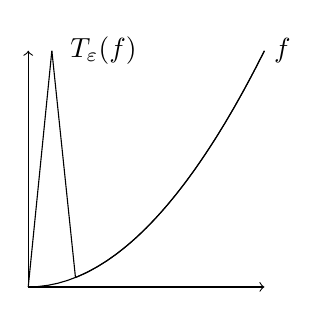
\begin{tikzpicture}[scale=3]
        \draw[->] (0, 0) -- (1, 0);
        \draw[->] (0, 0) -- (0, 1);

        \draw[domain=0:1, variable=\x] plot ({\x}, {\x^2}) node[right] {\( f \)};

        \draw (1/2, 1) node[left] {\( T_\varepsilon(f) \)};
        \draw[domain=0:0.1, variable=\x] plot ({\x}, {10 * \x});
        \draw[domain=0.1:0.2, variable=\x] plot ({\x}, {0.04 + (1 - 0.04) * (2 - 10 * \x)});
        \draw[domain=0.2:1, variable=\x] plot ({\x}, {\x^2});
      \end{tikzpicture}
    \end{Center}
  \end{figure}

  Define
  \begin{align*}
    T_\varepsilon(f)(x) \coloneqq \begin{cases}
      \frac x \delta_f, &0 \leq x < \delta_f \\
      f(\delta_f) + [1 - f(\delta_f)] (2 - \frac x {\delta_f}), &\delta_f \leq x < 2 \delta_f \\
      f(x), &x \geq 2 \delta_f,
    \end{cases}
  \end{align*}
  so that
  \begin{align*}
    \Norm{T_\varepsilon(f) - f}
    \geq
    T_\varepsilon(f) (\delta_f) - f(\delta_f)
    =
    1 - f(\delta_f)
    >
    1 - \varepsilon.
  \end{align*}

  Additionally, because \( \delta_{T_\varepsilon(f)} < \delta_f \), we have that \( f(\delta_{T_\varepsilon(f)}) < \varepsilon \) and
  \begin{align*}
    \Norm{T_\varepsilon(T_\varepsilon(f)) - f}
    \geq
    T_\varepsilon(T_\varepsilon(f)) (\delta_{T_\varepsilon(f)}) - f(\delta_{T_\varepsilon(f)})
    =
    1 - f(\delta_{T_\varepsilon(f)})
    >
    1 - \varepsilon.
  \end{align*}

  Thus, proceeding by induction, we see that for any \( m = 1, 2, \ldots \)
  \begin{align*}
    \Norm{T_\varepsilon^m(f) - f} > 1 - \varepsilon,
  \end{align*}
  where \( T_\varepsilon^m \) denotes repeated application of \( T_\varepsilon \).

  Consider the sequence
  \begin{align*}
    \{ T_\varepsilon^k(f) \}_{k=0}^\infty = \{ f, T_\varepsilon(f), T_\varepsilon(T_\varepsilon(f)), \ldots \}.
  \end{align*}

  We can easily see that the distance between any two elements of the sequence, say \( T_\varepsilon^k(f) \) and \( T_\varepsilon^{k+m}(f) \), is strictly greater that \( 1 - \varepsilon \), i.e.
  \begin{align*}
    \Norm{T_\varepsilon^k(f) - T_\varepsilon^{k+m}(f)}
    =
    \Norm{T_\varepsilon^k(f) - T_\varepsilon^m(T_\varepsilon^k(f))}
    >
    1 - \varepsilon.
  \end{align*}

  Hence \( B_1 \) cannot be covered by a finite \( (1-\varepsilon) \)-net and \( \alpha(B_1) \geq 1 - \varepsilon \). Since \( \varepsilon > 0 \) can be made arbitrarily small, this implies that \( \alpha(B_1) \geq 1 \) and, because we already have the reverse inequality, \( \alpha(B_1) = 1 \).

  In the set \( B_2 \), the maximum distance between two functions is \( \frac 1 2 \), thus \( \Diam(B_2) = \frac 1 2 \) and \( \alpha(B_2) \leq \frac 1 2 \). We can then define an operator similar to \( T_\varepsilon \) that creates \enquote{spikes} of height \( \frac 1 2 \) to prove the reverse inequality, obtaining
  \begin{align*}
    \alpha(B_2) = \frac 1 2.
  \end{align*}

  Finally, the set \( B_3 \) has diameter \( \frac 2 3 \) and hence \( \alpha(B_3) = \frac 2 3 \).

  The ball measure for \( B_1 \) satisfies the inequalities
  \begin{align*}
    \frac 1 2 \leq \beta(B_1) \leq 1.
  \end{align*}

  Additionally, \( B_1 \) is strictly contained in the ball centered in the constant function \( \frac 1 2 \) with radius \( \frac 1 2 \), which implies that \( \beta(B_1) \leq \frac 1 2 \), hence \( \beta(B_1) = \frac 1 2 \).

  For \( B_2 \) we have
  \begin{align*}
    \frac 1 4 \leq \beta(B_2) \leq \frac 1 2.
  \end{align*}

  Assume\LEM that for some \( \varepsilon > 0 \) the set \( B_2 \) can be covered by a finite set of balls with centers \( \{ f_1, \ldots, f_n \} \subsetneq C([0, 1]) \) and radius \( \frac 1 2 - \varepsilon \).

  Because of continuity, we can find a radius \( \delta > 0 \) such that for all \( f_k, k = 1, \ldots, n \) we have
  \begin{align*}
    x \in \left[\tfrac {1 - \delta} 2, \tfrac {1 + \delta} 2 \right] \implies \Abs{f_k(x) - f_k(\tfrac 1 2)} < \varepsilon.
  \end{align*}

  Consider the function
  \begin{align*}
    g(x) \coloneqq \begin{cases}
      0, &0 \leq x < \frac {1 - \delta} 2, \\
      \frac{2x + \delta - 1} {2\delta}, &\frac {1 - \delta} 2 \leq x \leq \frac {1 + \delta} 2, \\
      1, &\frac {1 + \delta} 2 < x \leq 1.
    \end{cases}
  \end{align*}

  \begin{figure}[ht]
    \begin{Center}
      \begin{tikzpicture}[scale=5]
        \draw[->] (0, 0) -- (1, 0);
        \draw[->] (0, 0) -- (0, 1);
        \draw[domain=0:4/10, thick, variable=\x] plot ({\x}, {0});
        \draw[domain=4/10:6/10, thick, variable=\x] plot ({\x}, {5 * \x - 2}) node[left] {\( g \)};
        \draw[domain=6/10:1, thick, variable=\x] plot ({\x}, {1});

        \draw[densely dotted] (0, 6/10) node[left] {\( f_k(\frac 1 2) - \varepsilon \)} -- (1, 6/10);
        \draw[densely dotted] (0, 8/10) node[left] {\( f_k(\frac 1 2) + \varepsilon \)} -- (1, 8/10);

        \draw[densely dotted] (4/10, 0) -- (4/10, 1);
        \draw (3/10, -1/10) node {\( \frac {1 - \delta} 2 \)};
        \draw[densely dotted] (1/2, 0) -- (1/2, 1);
        \draw (1/2, -1/10) node {\( \frac 1 2 \)};
        \draw[densely dotted] (6/10, 0) -- (6/10, 1);
        \draw (7/10, -1/10) node {\( \frac {1 + \delta} 2 \)};

        \draw[domain=-1/10:1, dash dot, variable=\x] plot ({\x}, {2/10 + 1 / (1 + e^(5/3*(1-2*\x)))}) node[right] {\( f_k \)};
      \end{tikzpicture}
    \end{Center}
  \end{figure}

  If \( f_k(\tfrac 1 2) \geq \frac 1 2 \), then \( f_k(\tfrac {1 - \delta} 2) > \tfrac 1 2 - \varepsilon \) and
  \begin{align*}
    \Norm{f_k - g} \geq f_k(\tfrac {1 - \delta} 2) - g(\tfrac {1 - \delta} 2) = f_k(\tfrac {1 - \delta} 2) > \tfrac 1 2 - \varepsilon.
  \end{align*}

  Analogously, if \( f_k(\tfrac 1 2) < \frac 1 2 \), then \( f_k(\tfrac {1 + \delta} 2) < \tfrac 1 2 + \varepsilon \) and
  \begin{align*}
    \Norm{g - f_k} \geq g(\tfrac {1 + \delta} 2) - f_k(\tfrac {1 + \delta} 2) = 1 - f_k(\tfrac {1 + \delta} 2) > \tfrac 1 2 - \varepsilon.
  \end{align*}

  Thus, for every \( k = 1, \ldots, n \) we have
  \begin{align*}
    \Norm{g - f_k} > \frac 1 2 - \varepsilon,
  \end{align*}
  i.e. \( g \) in not contained in a ball of radius \( \frac 1 2 - \varepsilon \) around any of the centers \( f_1, \ldots, f_n \).

  Hence \( \beta(B_2) \geq \frac 1 2 \), which implies \( \beta(B_2) = \frac 1 2 \). Because of the inclusion \( B_2 \subsetneq B_3 \subsetneq B_1 \), we have
  \begin{align*}
    \frac 1 2 = \beta(B_2) \leq \beta(B_3) \leq \beta(B_1) = \frac 1 2,
  \end{align*}
  hence \( \beta(B_3) = \frac 1 2 \).
\end{proof}

\begin{theorem}\label{thm:noncompact_kuratowski_lemma}[Kuratowski lemma]\cite[exercise 7.4]{Deimling1985}
  Let \( X \) be a Banach space and \( \{ A_n \}_n \) be a decreasing sequence of nonempty closed subsets such that \( \alpha(A_n) \to 0 \). Then \( A \coloneqq \bigcap_n A_n \) is nonempty and compact.
\end{theorem}
\begin{proof}
  The set \( A \) is compact because it is closed as the intersection of closed sets and \( \alpha(A) \leq \alpha(A_n) \to 0 \), hence \( \alpha(A) = 0 \).

  It remains to show that \( A \) is nonempty.
  Choose\AOC any sequence \( \{ x_n \}_n \) where \( x_n \in A_n \). Since any finite set is compact, we have that for any \( k \geq 1 \)
  \begin{align*}
    \alpha(\{ x_n \}_{n \geq 1})
    =
    \max\{ \alpha(\{ x_n \}_{n < k}), \alpha(\{ x_n \}_{n \geq k}) \}
    =
    \alpha(\{ x_n \}_{n \geq k})
    \leq
    \alpha(A_k) \to 0,
  \end{align*}
  hence the set \( \{ x_n \colon n \geq 1 \} \) is compact and thus sequentially compact. We can choose a convergent subsequence \( \{ x_{n_k} \}_k \) of \( \{ x_n \}_n \) whose limit lies in every \( A_n \) (since they are closed) and, consequently, in their intersection \( A \). So \( A \) is nonempty.
\end{proof}

  \subsection{Lipschitz continuity}\label{subsec:lipschitz_continuity}

\begin{definition}\label{def:lipschitz_continuity}
  Let \( f: X \to Y \) be a function between metric spaces.

  \begin{thmenum}
    \ilabel{def:lipschitz_continuity/holder} We say that \( f: X \to Y \) is \term{H\"older continuous} at \( x \in X \) with constant \( L \geq 0 \) and exponent \( \alpha > 0 \) if
    \begin{equation*}
      \rho_Y(f(x_1), f(x_2)) \leq L \rho_X(x_1, x_2)^\alpha \quad\forall x_1, x_2 \in X.
    \end{equation*}

    We refer to the smallest such constant, if any, as \enquote{the} H\"older constant.

    \ilabel{def:lipschitz_continuity/locally_holder} We say that \( f \) is \term{locally H\"older continuous} if every point has a neighborhood where \( f \) is H\"older continuous with the same exponent, but possibly with with a different constant.

    \ilabel{def:lipschitz_continuity/lipschitz} If \( \alpha = 1 \), we say that \( f \) is \term{Lipschitz continuous}.

    \ilabel{def:lipschitz_continuity/contraction} If \( X = Y \) and if \( f \) is Lipschitz with constant \( L < 1 \), we call \( f \) a \term{contraction mapping}.

    \ilabel{def:lipschitz_continuity/calm}\cite[53]{DontchevRockafellar2014} We say that \( f \) is \term{calm} at \( x \) if it satisfies the Lipschitz condition with one of the points fixed:
    \begin{equation*}
      \rho_Y(f(x), f(x')) \leq L \rho_X(x, x') \quad\forall x' \in X.
    \end{equation*}
  \end{thmenum}
\end{definition}

\begin{proposition}\label{thm:holder_map_is_uniformly_continuous}
  A H\"older map is uniformly continuous.
\end{proposition}
\begin{proof}
  Let \( f: X \to Y \) be a H\"older map with constant \( L \) and exponent \( \alpha \).

  Fix \( \varepsilon > 0 \). Then is enough to choose \( \delta < \sqrt[\alpha]{\frac \varepsilon L} \) so that
  \begin{equation*}
    \rho_X(x_1, x_2) < \delta \implies \rho_Y(f(x_1), f(x_2)) \leq L \rho_X(x_1, x_2)^\alpha < L \delta^\alpha < \varepsilon.
  \end{equation*}

  This implies uniform continuity.
\end{proof}

\begin{corollary}\label{thm:locally_holder_map_is_continuous}
  A locally H\"older map is continuous.
\end{corollary}

\begin{theorem}[Banach's fixed point theorem]\label{thm:banach_fixed_point_theorem}\mcite\cite[exer. 4.3.J]{Engelking1989}
  A contraction \hyperref[def:lipschitz_continuity/contraction]{mapping} in a \hyperref[def:complete_metric_space]{complete metric space} has a unique fixed \hyperref[def:fixed_point]{point}.
\end{theorem}
\begin{proof}
  Let \( f: X \to X \) be a contraction mapping. Fix any point \( x_0 \in X \) and inductively define the sequence
  \begin{equation*}
    x_{k+1} \coloneqq f(x_k), k = 1, 2, \ldots.
  \end{equation*}

  Fix \( \varepsilon > 0 \). Since \( L < 1 \), there exists an index \( k_0 > \log_L(\varepsilon) \) such that for positive integers \( m \) and \( k > k_0 \),
  \begin{balign*}
    \rho(x_k, x_{k+m})
     & =
    \rho(f^k(x_0), f^{k+m}(x_0))
    \leq \\ &\leq
    L^k \rho(x_0, x_m)
    <    \\ &<
    \varepsilon \rho(x_0, x_m).
  \end{balign*}

  Note that
  \begin{balign*}
    \rho(x_0, x_m)
     & \leq
    \sum_{i=1}^m \rho(x_{i-1}, x_i)
    \leq    \\ &\leq
    \rho(x_0, x_1) \sum_{i=1}^m L^{i-1}
    =       \\ &=
    \rho(x_0, x_1) \frac {1 - L^m} {1 - L}
    \leq    \\ &\leq
    \rho(x_0, x_1) \frac 1 {1 - L}.
  \end{balign*}

  Thus
  \begin{equation*}
    \rho(x_k, x_{k+m}) < \frac {\varepsilon \rho(x_0, x_1)} {1 - L}.
  \end{equation*}

  The constant on the right is linear in \( \varepsilon \) and does not depend on \( k \) or \( m \), hence \( \{ x_k \}_{k=0}^\infty \) is a fundamental sequence. Since \( X \) is complete, the sequence has a limit \( x \).

  Because of the continuity of \( f \) (see \fullref{thm:holder_map_is_uniformly_continuous}),
  \begin{equation*}
    f(x) = f(\lim_{k \to \infty} x_k) = \lim_{k \to \infty} f(x_k) = \lim_{k \to \infty} x_{k+1} = x.
  \end{equation*}
\end{proof}

  \section{Function oscillation}\label{sec:function_oscillation}

\begin{definition}\label{def:function_oscillation}
  Let \( X \) be a nonempty set and \( (Y, \rho_{Y}) \) be a metric space. We define the \term{oscillation} of a function on a set as
  \begin{balign*}
     &\omega: \fun(X, Y) \times \pow(X) \to [0, \infty] \\
     &\omega(f, A) \coloneqq \sup \Big\{ \rho_{Y}(f(x), f(y)) \colon (x, y) \in A \Big\}.
  \end{balign*}

  In particular, if \( X \) is itself a metric space, we define its \term{modulus of continuity} \( \omega(f, \delta) \) as the oscillation of \( f \) on the ball \( B(0, \delta) \).
\end{definition}

\begin{proposition}\label{thm:def:function_oscillation}
  The \hyperref[def:function_oscillation]{modulus of continuity} has the following basic properties:
  \begin{thmenum}
    \thmitem{thm:def:function_oscillation/continuity_condition} \( f \) is globally \hyperref[def:uniform_continuity]{uniformly continuous} if and only if for every \( \varepsilon > 0 \) there exists \( \delta > 0 \) such that \( \omega(f, \delta) < \varepsilon \).

    \thmitem{thm:def:function_oscillation/monotone} \( \omega(f, \delta) \) is monotone in \( \delta \).

    \thmitem{thm:def:function_oscillation/cauchy_inequality}\mcite[28]{Николов2020АпроксимацииЛекции}For all \( \lambda, \delta > 0 \), we have the following analog of \fullref{thm:cauchy_bunyakovsky_schwarz_inequality}
    \begin{equation}\label{thm:def:function_oscillation/cauchy_inequality/inequality}
      \omega(f, \lambda \delta) \leq \omega(f, \lambda^2) + \omega(f, \delta^2).
    \end{equation}

    \thmitem{thm:def:function_oscillation/single_inequality}\mcite[28]{Николов2020АпроксимацииЛекции}For all \( \lambda, \delta > 0 \),
    \begin{equation}\label{thm:def:function_oscillation/single_inequality/inequality}
      \omega(f, \lambda \delta) \leq (\lambda + 1) \omega(f, \delta).
    \end{equation}
  \end{thmenum}
\end{proposition}
\begin{proof}
  \SubProofOf{thm:def:function_oscillation/continuity_condition} Follows directly from \cref{def:uniform_continuity}.

  \SubProofOf{thm:def:function_oscillation/monotone} A supremum on a larger set is larger.

  \SubProofOf{thm:def:function_oscillation/cauchy_inequality} If \( \lambda \leq \delta \), clearly \( \lambda \delta \leq \delta^2 \). Otherwise, \( \lambda \delta < \lambda^2 \).

  Combining the two inequalities with \cref{thm:def:function_oscillation/monotone}, we obtain \cref{thm:def:function_oscillation/cauchy_inequality/inequality}.

  \SubProofOf{thm:def:function_oscillation/single_inequality} Note that
  \begin{equation*}
    \rho_{X}(x, y) < \delta \T{implies} \rho_{Y}(f(x), f(y)) < \omega(f, \delta).
  \end{equation*}

  We can multiply this by \( \lambda \) to obtain
  \begin{equation*}
    \lambda \rho_{X}(x, y) < \lambda \delta \T{implies} \lambda \rho_{Y}(f(x), f(y)) < \lambda \omega(f, \delta).
  \end{equation*}

  If \( \lambda \geq 1 \), then \( \rho_{X}(x, y) \leq \lambda \rho_{X}(x, y) \) and \( \rho_{Y}(f(x), f(y)) \leq \lambda \rho_{Y}(f(x), f(y)) \) and hence
  \begin{equation*}
    \omega(f, \lambda \delta) \leq \lambda \omega(f, \delta).
  \end{equation*}

  Otherwise, \( \lambda < 1 \) and clearly \( \lambda \delta < \delta \), which by \cref{thm:def:function_oscillation/monotone} implies
  \begin{equation*}
    \omega(f, \lambda \delta) \leq \omega(f, \delta).
  \end{equation*}

  Combining the two cases, we obtain
  \begin{equation*}
    \omega(f, \lambda \delta) \leq \lambda \omega(f, \delta) + \omega(f, \delta),
  \end{equation*}
  which we wanted to prove.
\end{proof}


  \section{Geometry}\label{sec:geometry}

Humans possess a strong intuition for visual information like drawings or diagrams. A drawing on a paper is only a medium for communicating ideas and data. \Fullref{fig:sec:geometry/figures} contains some highlighted curves that our mind maps to abstract geometric figures, without considering the size limitations of the page, the precision of the drawings or the thickness of the lines.

\begin{figure}[!ht]
  \centering
  \includegraphics{output/sec__geometry__figures.pdf}
  \caption{A \hyperref[def:triangle]{triangle}, a \hyperref[def:circle]{circle} and a \hyperref[def:affine_line]{line} in the \hyperref[def:euclidean_space]{Euclidean plane}.}\label{fig:sec:geometry/figures}
\end{figure}

Our goal is to introduce formalisms for these mental visualizations. An axiomatic approach for a theory of figures in the place and space was developed by Euclid in the third century BC and can be found in \cite{Fitzpatrick2008}. A few millennia later, several mathematicians proposed systems of axioms that fit the requirements of \hyperref[sec:mathematical_logic]{modern logical systems}. Tarski's system can be found in \cite{Tarski1959}. This is known today as \term{synthetic Euclidean geometry} and is mostly of theoretical interest.

An important distinction between ancient and modern geometry is the introduction of coordinates in the 17th century. Descartes' idea of coordinates connects problems of algebra and geometry in such a way that most of today's mathematics seamlessly switches between algebraic and geometric interpretations of the same problem. The study of classical Greek geometry in terms of coordinates is known as \term{analytic geometry}.

A modern interpretation if the ideas behind analytic geometry leads to \hyperref[def:affine_spaces]{affine spaces}, which we will discuss in \fullref{subsec:affine_spaces} and \fullref{subsec:convex_sets}, to Euclidean spaces discussed in \fullref{subsec:euclidean_spaces} and to the Euclidean plane discussed in \fullref{subsec:euclidean_plane}, \fullref{subsec:triangles} and \fullref{subsec:quadratic_plane_curves}. As part of our discussion of the \hyperref[def:euclidean_plane]{Euclidean plane}, we will briefly introduce modern concepts related to differential geometry in \fullref{subsec:parametric_curves} and algebraic geometry in \fullref{subsec:quadratic_plane_curves}.

  \subsection{Affine spaces}\label{subsec:affine_spaces}

We provide here general definitions and statements about affine spaces over arbitrary fields.

\begin{definition}\label{def:affine_space}\mcite[def. 2.1.1]{Gallier2011}
  An \term{affine space} over the \hyperref[def:field]{field} \( \BbbK \) is a triple \( (A, \vect A, \tau) \), where
  \begin{thmenum}[series=def:affine_space]
    \thmitem{def:affine_space/points} \( A \) is a set, whose members we call \term{points}.

    \thmitem{def:affine_space/vectors} \( \vect A \) is a \hyperref[def:vector_space]{vector space} over \( \BbbK \), whose members we call \term{vectors}. We also call them \term{free vectors}, as opposed to \term{bound vectors}, which are simply pairs of points --- a \term{beginning} and an \term{end}.

    \thmitem{def:affine_space/action} \( \tau: \vect A \times A \to A \) is a \hyperref[def:group_action]{group action} of the additive group of \( \vect A \) that links bound and free vectors. For a bound vector from \( x \) to \( y \), we require that there exists a unique free vector \( v \) satisfying \( y = \tau_v(x) \). We also say that \( y \) is a \term{translation} of \( x \) in the \term{direction} \( v \).

    We will use the notation \( \vect{xy} \) for this unique free vector.
  \end{thmenum}

  We define the \term{dimension} of \( A \) as the vector space dimension of \( \vect A \).

  Usually \( A = \vect A \) and \( \tau_v(x) = x + v \), in which case the distinction between \enquote{points} and \enquote{vectors} is only informal. We call this the \term{natural affine structure} on \( \vect A \). The free vector \( \vect{xy} \) is then \( y - x \). We implicitly associate the natural affine structure with every vector space --- usually the \hyperref[def:sequence_space]{tuple vector space} \( \BbbK^n \).

  \begin{figure}[!ht]
    \hfill
    \hfill
    \includegraphics[align=c]{output/def__affine_space__vectors}
    \hfill
    \includegraphics[align=c]{output/def__affine_space__points}
    \hfill
    \caption{Vectors acting on points in an \hyperref[def:affine_space]{affine space}.}\label{fig:def:affine_space}
  \end{figure}
\end{definition}

\begin{example}\label{ex:x2_as_affine_space}
  Simple yet nontrivial example of \hyperref[def:affine_space]{affine spaces} are \hyperref[def:multi_valued_function/graph]{function graphs}.
  \begin{itemize}
    \item The set of points is the following subset of \( \BbbR^2 \):
    \begin{equation*}
      A \coloneqq \set{ (x, y) \given y = x^2 }.
    \end{equation*}

    \begin{figure}[!ht]
      \centering
      \includegraphics{output/ex__x2_as_affine_space}
      \caption{The affine space from \cref{ex:x2_as_affine_space}.}\label{fig:ex:x2_as_affine_space}
    \end{figure}

    \item The set of vectors is the unidimensional vector space \( \BbbR \).

    \item The action of \( \BbbR \) on \( A \) is
    \begin{equation*}
      \tau_t(x, y) \coloneqq (x + t, y + t^2).
    \end{equation*}
  \end{itemize}
\end{example}

\begin{definition}\label{def:affine_coordinate_system}
  Let \( (A, \vect A, \tau) \) be an \hyperref[def:affine_space]{affine space} over \( \BbbK \), let \( O \) be a distinguished point of \( A \) and let \( \vect E \) be a \hyperref[def:hamel_basis]{basis} of \( \vect A \). We call the pair \( (O, E) \) an \term{affine coordinate system} of \( A \) with \term{origin} \( O \) and \term{basis} \( \vect E \). If \( \vect E \) is \hyperref[def:orthogonality]{orthonormal}, we say that the coordinate system itself is orthonormal. Usually \( \vect A \) is finite dimensional, in which case \( \vect E = \set{ e_1, \ldots, e_n } \), and we denote the coordinate system by \( O e_1 \cdots e_n \).

  For every point \( x \) in \( A \), we call the free vector \( \vect{Ox} \) its \term{radius vector} with respect to the origin \( O \). This gives us an explicit isomorphism between the set \( A \) of points and the set \( \vect A \) of free vectors.

  The choice of basis \( \vect E \) then gives an isomorphism between \( A \) and the \hyperref[def:free_semimodule]{free vector space} \( \BbbK^{\oplus E} \). If \( \vect E = \set{ e_1, \ldots, e_n } \), the corresponding coordinate system allows us to associate a tuple of coordinates from \( \BbbK^n \) for each point in \( A \).

  Using the notation \( x_v \coloneqq \pi_v(\vect{Ox}) \), we associate the family \( \seq{ x_v \given v \in \vect E } \) to every point \( x \) and call its members the \term{affine coordinates} of \( x \) with respect to the coordinate system. We have
  \begin{equation}\label{eq:def:affine_coordinate_system/coordinates}
    \vect{Ox} = \sum_{e \in \vect E} x_e \cdot e.
  \end{equation}

  This relates to \hyperref[def:barycentric_coordinate_system]{barycentric coordinate systems} via \fullref{thm:affine_and_barycentric_coordinate_systems}.
\end{definition}

\begin{remark}\label{rem:affine_combinations}
  We cannot define the familiar addition and scalar multiplication of points that does not depend on a choice of coordinate system. We can, however, define a certain type of linear combination of points, which we call \term{affine combinations}.

  Let \( (A, \vect A, \tau) \) be an \hyperref[def:affine_space]{affine space} over \( \BbbK \), let \( x_1, \ldots, x_n \) be points in \( A \) and let \( t_1, \ldots, t_n \) be scalars that sum to \( 1_\BbbK \).

  For any two origin points \( O \) and \( P \), we have
  \begin{equation*}
    \underbrace{ \sum_{k=1}^n t_k \vect{O x_k} }_{v_O}
    =
    \sum_{k=1}^n t_k \parens[\Big]{ \vect{OP} + \vect{P x_k} }
    =
    \underbrace{ \parens*{ \sum_{k=1}^n t_k } }_{1_\BbbK} \vect{OP} + \underbrace{ \sum_{k=1}^n t_k \vect{P x_k} }_{v_P}.
  \end{equation*}

  Therefore,
  \begin{equation*}
    \tau_{v_O}(O) = \tau_{\vect{OP} + v_P}(O) = \tau_{v_P}(\tau_{\vect{OP}}(O)) = \tau_{v_P}(P).
  \end{equation*}

  We denote this common value by
  \begin{equation*}
    \sum_{k=1}^n t_k x_k.
  \end{equation*}

  We also use the term \enquote{affine combination} for linear combinations of vectors whose coefficients sum to one.

  Formally, it is sufficient to consider only affine combinations of two points, i.e.
  \begin{equation}\label{eq:rem:affine_combinations}
    \lambda x + (1 - \lambda) y.
  \end{equation}

  The affine combination of \( n \) points can then be defined via \hyperref[rem:natural_number_recursion]{recursion}:
  \begin{equation*}
    \sum_{k=1}^n t_k x_k = \begin{dcases}
      x_n,                                                          &n = 1 \\
      t_1 x_1 + (1 - t_1) \sum_{k=2}^n \frac {t_k} {(1 - t_1)} x_k, &n > 1
    \end{dcases}
  \end{equation*}
\end{remark}

\begin{proposition}\label{thm:rem:affine_combinations}
  \hyperref[rem:affine_combinations]{Affine combinations} have the following basic properties:
  \begin{thmenum}
    \thmitem{thm:rem:affine_combinations/inverse_of_action} For any point \( x \) and vector \( v \),
    \begin{equation*}
      \tau_v^{-1}(x) = \tau_{-v}(x).
    \end{equation*}

    \thmitem{thm:rem:affine_combinations/inverse} For any two points \( x \) and \( y \),
    \begin{equation*}
      \vect{xy} = -\vect{xy}.
    \end{equation*}

    \thmitem{thm:rem:affine_combinations/chasles} For any three points \( x \), \( y \) and \( z \),
    \begin{equation}\label{eq:thm:rem:affine_combinations/chasles}
      \vect{xz} = \vect{xy} + \vect{yz}.
    \end{equation}

    This is called Chasles' identity.

    \thmitem{thm:rem:affine_combinations/vectors_to_points} If we are given the vector affine combination \( w = \lambda u + (1 - \lambda) v \), for any point \( x \) we have the point affine combination
    \begin{equation*}
      \tau_w(x) = \lambda \cdot \tau_u(x) + (1 - \lambda) \cdot \tau_v(x).
    \end{equation*}
  \end{thmenum}
\end{proposition}
\begin{proof}
  \SubProofOf{thm:rem:affine_combinations/inverse_of_action} If \( y = \tau_v(x) \), then
  \begin{equation*}
    x = \tau_{-v + v}(x) = \tau_{-v}(y).
  \end{equation*}

  \SubProofOf{thm:rem:affine_combinations/inverse} Follows from \fullref{thm:rem:affine_combinations/inverse_of_action}.

  \SubProofOf{thm:rem:affine_combinations/chasles}
  \begin{equation*}
    \tau_{\vect{xy} + \vect{yz}}(x)
    =
    \tau_{\vect{yz} + \vect{xy}}(x)
    =
    \tau_{\vect{yz}}(\tau_{\vect{xy}}(x))
    =
    \tau_{\vect{yz}}(y)
    =
    z
    =
    \tau_{\vect{xz}}(x).
  \end{equation*}

  Then \eqref{eq:thm:rem:affine_combinations/chasles} follows.

  \SubProofOf{thm:rem:affine_combinations/vectors_to_points} Follows from the definition by noting that, for any point \( x \),
  \begin{equation*}
    w = \lambda u + (1 - \lambda) v
    =
    \vect{x, \tau_w(x)} = \lambda \cdot \vect{x, \tau_u(x)} + (1 - \lambda) \cdot \vect{x, \tau_v(x)}.
  \end{equation*}
\end{proof}

\begin{definition}\label{def:affine_hull}\mimprovised
  The \term{affine hull} of the set \( S \) of points is the set of all arbitrary (i.e. not necessarily binary) \hyperref[rem:affine_combinations]{affine combinations} of members of \( S \). It is a \hyperref[def:closure_operator]{closure operator}.
\end{definition}
\begin{defproof}
  We will show that the affine hull operator \( H: \pow(A) \to \pow(A) \) is a closure operator.

  \SubProof{Proof that \( H \) is \SubProofOf[def:extensive_function]{extensive}} Obviously \( S \subseteq H(S) \).

  \SubProofOf[def:magma/idempotent]{idempotence} Consider the affine combination \( \lambda x + (1 - \lambda) y \) of points from \( H(S) \). Suppose that \( x = t_x a_x + (1 - t_x) b_x \) and \( y = t_y a_y + (1 - t_y) b_y \), where \( a_x \), \( a_y \), \( b_x \) and \( b_y \) are points from \( S \).

  Then
  \begin{equation*}
    \lambda x + (1 - \lambda) y
    =
    \lambda t_x u_x + \lambda (1 - t_x) v_x + (1 - \lambda) t_y u_y + (1 - \lambda) (1 - t_y) v_y.
  \end{equation*}

  This is an affine combination of members of \( S \). Therefore, \( A(A(S)) = A(S) \).

  \SubProofOf[def:order_homomorphism/increasing]{monotonicity} If \( S_1 \subseteq S_2 \), then \( H(S_2) \) contains the affine combinations of the members of \( S_1 \) in addition to others. Hence, \( H(S_1) \subseteq H(S_2) \).
\end{defproof}

\begin{definition}\label{def:affine_subspace}\mcite[25]{Gallier2011}
  Let \( B \) be a set of points in the \hyperref[def:affine_space]{affine space} \( (A, \vect A, \tau) \). Fix an origin point \( O \) in \( B \) and define the set
  \begin{equation}\label{eq:def:affine_subspace/direction}
    \vect B \coloneqq \set{ \vect{Ob} \given b \in B \T{and} b \neq O }.
  \end{equation}

  We present two equivalent conditions under which the set \( \vect B \) does not depend on the choice of origin. If any of them holds, we say that \( \vect B \) is the \term{direction} of \( B \) and that \( (B, \vect B, \tau) \) is an \term{affine subspace} of \( (A, \vect A, \tau) \).

  \begin{thmenum}
    \thmitem{def:affine_subspace/hull} If \( B \) coincides with its \hyperref[def:affine_hull]{affine hull}.
    \thmitem{def:affine_subspace/linear} If \( \vect B \) is a \hyperref[def:module/submodel]{vector subspace} of \( \vect A \).
  \end{thmenum}
\end{definition}
\begin{defproof}
  \SubProof{Proof of independence of origin} Let
  \begin{align*}
    \vect B_O \coloneqq \set{ \vect{Ob} \given b \in B \T{and} b \neq O },
    &&
    \vect B_P \coloneqq \set{ \vect{Pb} \given b \in B \T{and} b \neq P }.
  \end{align*}

  Let \( x \) be a point in \( B \) and consider the vector \( \vect{P x} \) from \( \vect B_P \). We have
  \begin{equation*}
    \vect{P x}
    \reloset {\ref{thm:rem:affine_combinations/chasles}} =
    \vect{PO} + \vect{O x}
    \reloset {\ref{thm:rem:affine_combinations/inverse}} =
    \vect{OO} - \vect{OP} + \vect{O x}.
  \end{equation*}

  Thus,
  \begin{equation*}
    \tau_{\vect{Px}}(O) = O - P + x.
  \end{equation*}

  The latter is an affine combination of points of \( B \), hence it is again a point of \( B \). That is, \( \vect{Px} \) is the free vector that takes \( O \) to \( O - P + x \), and hence \( \vect{Px} \) belongs to \( \vect B_O \).

  Generalizing on \( x \), we conclude that \( \vect B_P \subseteq \vect B_O \). The converse inclusion follows automatically.

  \ImplicationSubProof{def:affine_subspace/hull}{def:affine_subspace/linear} Suppose that \( B \) coincides with its affine hull.

  Let \( x \) and \( y \) be points in \( B \). Note that \( z \coloneqq x + y - O \) is an affine combination and thus belongs to \( B \). Then
  \begin{equation*}
    \vect{Ox} + \vect{Oy}
    =
    \vect{Ox} + \vect{Oy} - \vect{OO}
    =
    \vect{Oz}
    \in
    \vect B.
  \end{equation*}

  Now let \( x \) be a point in \( B \) and \( \lambda \) be a scalar. Then \( y \coloneqq \lambda x + (1 - \lambda) O \) is an affine combination and thus belongs to \( B \). Hence,
  \begin{equation*}
    \lambda \vect{Oy}
    =
    \lambda \vect{Oy} + (1 - \lambda) \vect{OO}
    =
    \vect{Oy}
    \in
    \vect B.
  \end{equation*}

  Therefore, \( \vect B \) is closed under linear combinations and is thus a subspace of \( \vect A \).

  \ImplicationSubProof{def:affine_subspace/linear}{def:affine_subspace/hull} Fix some point \( O \) in \( B \) and suppose that \( \vect B \) is a vector subspace of \( \vect A \).

  Fix two points \( x \) and \( y \) in \( B \) and some scalar \( \lambda \). Then there exists some point \( z \) in \( B \) such that
  \begin{equation*}
    \vect{Oz} = \lambda \vect{Ox} + (1 - \lambda) \vect{Oy}.
  \end{equation*}

  Then \( z = \lambda x + (1 - \lambda) y \), which implies that \( B \) is closed under affine combinations.
\end{defproof}

\begin{proposition}\label{thm:affine_subspace_of_subspace}
  \hyperref[def:affine_subspace]{Affine subspaces} of affine subspaces of \( A \) are subspaces of \( A \).
\end{proposition}
\begin{proof}
  Trivial.
\end{proof}

\begin{definition}\label{def:affine_parallelism}\mcite[25]{Gallier2011}
  We say that two \hyperref[def:affine_subspace]{affine subspaces} of a common ambient space are \term{parallel} if their directions coincide. We write \( B \parallel C \).
\end{definition}

\begin{proposition}\label{thm:parallel_subspace_through_point}
  For every point \( x \) and every \hyperref[def:affine_subspace]{affine subspace} \( A \), there exists a unique subspace \hyperref[def:affine_parallelism]{parallel} to \( A \) passing through \( x \).

  The case of an \hyperref[def:affine_line]{affine line} is a restatement of Euclid's \enquote{Proposition \( \beta. \)} (see \cite[8]{Fitzpatrick2008}):
  \begin{quote}
    To place a straight-line equal to a given straight-line at a given point (as an extremity).
  \end{quote}
\end{proposition}
\begin{proof}
  Define the set
  \begin{equation*}
    B \coloneqq \set{ \tau_v(x) \given v \in \vect A }.
  \end{equation*}

  It obviously contains \( x \) and obviously the directions \( \vect A \) and \( \vect B \) coincide, hence \( A \) and \( B \) are parallel.

  It remains to show uniqueness. Suppose that \( C \) also contains \( x \) and is parallel to \( B \). Let \( y \) be a point of \( B \). Then \( \vect{yx} \) is also a vector in \( \vect C \), hence \( y = \tau_{\vect{yx}}(x) \) is a point in \( C \). Therefore, \( B = C \).
\end{proof}

\begin{definition}\label{def:affine_space_of_solutions}\mimprovised
  Consider the \hyperref[rem:system_of_equations]{system} of \( n \) linear equations and \( m \) variables over the field \( \BbbK \) in matrix form \( Ax = b \). If at least one solution \( x_0 \) exists, then all solutions are contained in the set
  \begin{equation}\label{eq:def:affine_space_of_solutions}
    \set{ x_0 + x \given x \in \ker A }.
  \end{equation}

  This is an \hyperref[def:affine_subspace]{affine subspace} of the domain \( \BbbK^m \) of \( A \). We call it the \term{solution space} of the system. If no solutions exist, the solution space should be an empty set, hence formally not an affine space.
\end{definition}
\begin{defproof}
  We will prove that the set \eqref{eq:def:affine_space_of_solutions} is precisely the set of solutions of the system.

  If \( x \in \ker A \), then
  \begin{equation*}
    A(x_0 + x) = Ax_0 + Ax = Ax_0.
  \end{equation*}

  Conversely, if \( Ax_1 = b \), then \( A(x_1 - x_0) = \vect 0 \), and thus \( x_1 - x_0 \in \ker A \). Then \( x_1 = x_0 + (x_1 - x_0) \) belongs to the aforementioned solution space.
\end{defproof}

\begin{proposition}\label{thm:system_of_equations_unique_solution}
  The \hyperref[rem:system_of_equations]{system of linear equations} \( Ax = b \) has a unique solution if and only if \( A \) is invertible.
\end{proposition}
\begin{proof}
  \SufficiencySubProof If \( Ax = b \) has a unique solution, then the \hyperref[def:affine_space_of_solutions]{solution space} has dimension zero, the kernel of \( A \) is empty, and \( A \) is invertible.

  \NecessitySubProof If \( A \) is invertible, then \( x = A^{-1} b \) is a solution.
\end{proof}

\begin{definition}\label{def:affine_dependence}\mimprovised
  We say that the set of points \( E \) is \term{affinely independent} if any of the following conditions holds:

  \begin{thmenum}
    \thmitem{def:affine_dependence/hull} The \hyperref[def:affine_hull]{affine hull} of \( E \) strictly contains the affine hulls of any subset of \( E \).

    \thmitem{def:affine_dependence/combinations} Given a sequence of points \( O, e_1, \ldots, e_n \) from \( E \), the conditions
    \begin{align*}
      \sum_{k=1}^n t_k = 0,
      &&
      \sum_{k=1}^n t_k \vect{O e_k} = \vect 0
    \end{align*}
    together imply that \( t_1 = \cdots = t_n \).

    \thmitem{def:affine_dependence/linear}\mcite[def. 2.4]{Gallier2011} Given any origin point \( O \) from \( E \), the set
    \begin{equation*}
      \set{ \vect{O e} \given e \in E \T{and} e \neq O }
    \end{equation*}
    is linearly independent.

    If this condition holds for \( O \), it also holds if we replace \( O \) with any other point in \( E \).
  \end{thmenum}
\end{definition}
\begin{proof}
  \SubProofOf{def:affine_dependence/linear} Suppose that
  \begin{equation*}
    \set{ \vect{O e} \given e \in E \T{and} e \neq O }
  \end{equation*}
  is linearly independent. We will show that
  \begin{equation*}
    \set{ \vect{P e} \given e \in E \T{and} e \neq P }
  \end{equation*}
  is also linearly independent for any \( P \neq O \). Let
  \begin{equation*}
    \sum_{k=1}^n t_k \vect{P e_k} = \vect 0.
  \end{equation*}

  \Fullref{thm:rem:affine_combinations/chasles} implies
  \begin{equation*}
    \sum_{k=1}^n t_k \vect{P e_k}
    =
    \sum_{k=1}^n t_k \vect{O e_k} + \sum_{k=1}^n t_k \vect{P O}
    =
    \sum_{k=1}^n t_k \vect{O e_k} + \parens*{ -\sum_{k=1}^n t_k } \vect{O P}.
  \end{equation*}

  Since the vectors \( \vect{O e_1}, \cdots, \vect{O e_n}, \vect{O P} \) are linearly independent, we conclude that
  \begin{equation*}
    t_1 = \cdots = t_n = 0.
  \end{equation*}

  Thus, the set
  \begin{equation*}
    \set{ \vect{P b} \given e \in E \T{and} e \neq P }
  \end{equation*}
  is linearly independent.

  \ImplicationSubProof{def:affine_dependence/hull}{def:affine_dependence/combinations} Suppose that the affine hull of \( E \) strictly contains the affine hull of any subset.

  Let
  \begin{align*}
    \sum_{k=1}^n t_k = 0,
    &&
    \sum_{k=1}^n t_k \vect{O e_k} = \vect 0.
  \end{align*}

  Suppose that \( t_{k_0} \) is nonzero for some index \( k_0 \). Then
  \begin{equation*}
    t_{k_0} = - \sum_{k \neq k_0} t_k
  \end{equation*}
  and
  \begin{equation*}
    \vect{O e_{k_0}} = -\sum_{k \neq k_0} \frac {t_k} {t_{k_0}} \vect{O e_k}.
  \end{equation*}

  Thus, \( \vect{O e_{k_0}} \) is an affine combination of other vectors from \( E \), and hence the affine hull of \( E \setminus \set{ e_{k_0} } \) coincides with the affine hull of \( E \). This contradicts our initial assumption.

  Therefore,
  \begin{equation*}
    t_1 = \cdots = t_n = 0.
  \end{equation*}

  \ImplicationSubProof{def:affine_dependence/combinations}{def:affine_dependence/linear} Suppose that \fullref{def:affine_dependence/combinations} holds for \( E \). Fix some point \( O \) from \( E \). We will show that the set
  \begin{equation*}
    \set{ \vect{O e} \given e \in E \T{and} e \neq O }
  \end{equation*}
  is linearly independent.

  Aiming at a contradiction, suppose that
  \begin{equation*}
    \sum_{k=1}^n t_k \vect{O e_k} = \vect 0.
  \end{equation*}

  Let
  \begin{equation*}
    T \coloneqq \sum_{k=1}^n t_k.
  \end{equation*}

  Suppose that \( T \) is nonzero. Then
  \begin{equation*}
    \sum_{k=1}^n t_k \vect{O e_k} + (-T) \vect 0 = \vect 0.
  \end{equation*}

  The coefficients of this combination sum to \( 0 \). Therefore, by our assumption \fullref{def:affine_dependence/combinations}, they are all equal to zero. But the last coefficient is \( -T \), which we have assumed is nonzero.

  The obtained contradiction shows that \( T = 0 \). Then again from \fullref{def:affine_dependence/combinations}, we have
  \begin{equation*}
    t_1 = \cdots = t_n = 0.
  \end{equation*}

  Therefore,
  \begin{equation*}
    \set{ \vect{O e} \given e \in E \T{and} e \neq O }
  \end{equation*}
  is a linearly independent set of vectors.

  \ImplicationSubProof{def:affine_dependence/linear}{def:affine_dependence/hull} Let \( A \) be a strict subset of \( E \). Fix some point \( O \) from \( E \setminus A \) and suppose that the set
  \begin{equation*}
    \set{ \vect{O e} \given b \in E \T{and} b \neq O }
  \end{equation*}
  is linearly independent. We will show that \( O \) is not in the affine hull of \( A \).

  Aiming at a contradiction, suppose that \( O \) is an affine combination of members of \( A \):
  \begin{equation*}
    O = \sum_{k=1}^n t_k a_k.
  \end{equation*}

  We have
  \begin{equation*}
    \vect 0
    =
    \vect{O O} - \sum_{k=1}^n t_k \vect {O a_k}
    =
    \sum_{k=1}^n t_k \vect{O a_k},
  \end{equation*}
  which, due to linear independence, implies that
  \begin{equation*}
    t_1 = \cdots = t_n = 0.
  \end{equation*}

  Therefore, \( O \) is not an affine combination of members of \( A \) since the coefficients do not sum to \( 1 \).
\end{proof}

\begin{proposition}\label{thm:linear_and_affine_bases}
  Let \( (A, \vect A, \tau) \) be an \hyperref[def:affine_space]{affine space}. Let \( E \) be a set of points with a fixed origin point \( O \) and let
  \begin{equation*}
    \vect E \coloneqq \set{ \vect{Oe} \given e \in E }.
  \end{equation*}

  \begin{thmenum}
    \thmitem{thm:linear_and_affine_bases/dependence} The vectors in \( \vect E \) are \hyperref[def:linear_dependence]{linearly independent} if and only if the points in \( E \) are \hyperref[def:affine_dependence]{affinely independent}.

    \thmitem{thm:linear_and_affine_bases/hulls} The \hyperref[def:semimodule/submodel]{linear span} of \( \vect E \) is \( \vect A \) if and only if the \hyperref[def:affine_hull]{affine hull} of \( E \) is \( A \).
  \end{thmenum}
\end{proposition}
\begin{proof}
  \SubProofOf{thm:linear_and_affine_bases/dependence} This is the statement of \fullref{def:affine_dependence/linear}.

  \SubProofOf{thm:linear_and_affine_bases/hulls}
  \SufficiencySubProof* Suppose that the linear span of \( \vect E \) is \( \vect A \). Fix some point \( x \) in \( A \). Then \( \vect{Ox} \) is a linear combination of members of \( \vect E \):
  \begin{equation*}
    \vect{Ox} = \sum_{k=1}^n t_k \vect{O x_k}.
  \end{equation*}

  Then
  \begin{equation*}
    x = \parens*{ 1 - \sum_{k=1}^n t_k } O + \sum_{k=1}^n t_k x_k.
  \end{equation*}

  \NecessitySubProof* Suppose that the affine hull of \( E \) is \( A \). Let \( v \) be some vector in \( \vect A \) and let \( x \coloneqq \tau_v(O) \). We have
  \begin{equation*}
    x = \sum_{k=1}^n t_k e_k
  \end{equation*}
  for some points \( e_1, \ldots, e_n \) from \( E \) and some scalars that sum to one. Then
  \begin{equation*}
    v = \vect{Ox} = \sum_{k=1}^n t_k \vect{O e_k}.
  \end{equation*}

  We have shown that any vector in \( \vect A \) is a linear combination of vectors in \( \vect E \).
\end{proof}

\begin{definition}\label{def:barycentric_coordinate_system}
  Let \( (A, \vect A, \tau) \) be an \hyperref[def:affine_space]{affine space} over \( \BbbK \), let \( E \) be a set of \hyperref[def:affine_dependence]{affinely independent} whose \hyperref[def:affine_hull]{affine hull} is \( A \). Let \( O \) be a distinguished origin point from \( E \). We call the pair \( (O, E) \) a \term{barycentric coordinate system} of \( A \) with \term{origin} \( O \) and \term{basis} \( E \). We call the points in \( E \) the \term{basis points} of the coordinate system.

  \Fullref{thm:linear_and_affine_bases} implies that the set
  \begin{equation}\label{eq:def:barycentric_coordinate_system/linear_basis}
    \vect E \coloneqq \set{ \vect{Oe} \given e \in E }
  \end{equation}
  is a linear basis of \( \vect A \).

  We associate with the point \( x \) its \term{barycentric coordinates} with respect to the coordinate system:
  \begin{equation*}
    x_e \coloneqq \begin{cases}
      \pi_{\vect{Oe}}(\vect{Ox}) &e \in E \setminus \set{ O }, \\
      1 - \sum_{e \neq O} x_e    &e = O.
    \end{cases}
  \end{equation*}

  We have
  \begin{equation}\label{eq:def:barycentric_coordinate_system/coordinates}
    x = \sum_{e \in E} x_e \cdot e = \parens*{ 1 - \sum_{e \neq O} x_e } \cdot O + \sum_{e \neq O} x_e \cdot e.
  \end{equation}

  This relates to \hyperref[def:affine_coordinate_system]{affine coordinate systems} via \fullref{thm:affine_and_barycentric_coordinate_systems}.
\end{definition}

\begin{proposition}\label{thm:affine_and_barycentric_coordinate_systems}
  Let \( E \) be a set of points in the affine space \( (A, \vect A, \tau) \) and define \( \vect E \) as in \eqref{eq:def:barycentric_coordinate_system/linear_basis}.

  Then the pair \( (O, \vect E) \) is an \hyperref[def:affine_coordinate_system]{affine coordinate system} if and only if \( (O, E) \) is a \hyperref[def:barycentric_coordinate_system]{barycentric coordinate system}. Furthermore, the coordinates are directly related because
  \begin{equation*}
    x = \parens*{ 1 - \sum_{e \neq O} x_e } \cdot O + \sum_{e \neq O} x_e \cdot e
  \end{equation*}
  and
  \begin{equation*}
    \vect{Ox} = \parens*{ 1 - \sum_{e \neq O} x_e } \cdot \underbrace{\vect{OO}}_{\vect 0} + \sum_{e \neq O} x_e \cdot \vect{Oe}.
  \end{equation*}
\end{proposition}
\begin{proof}
  Trivial.
\end{proof}

\begin{definition}\label{def:affine_operator}
  Let \( (A, \vect A, \tau) \) and \( (B, \vect B, \sigma) \) be \hyperref[def:affine_space]{affine spaces}. We say that the function \( {f: \vect A \to W} \) between points is an \term{affine operator} if any of the following equivalent conditions hold:
  \begin{thmenum}
    \thmitem{def:affine_operator/combination} \( f \) preserves \hyperref[def:affine_hull]{affine combinations}. That is, for any scalar \( \lambda \),
    \begin{equation}\label{eq:def:affine_operator/combination}
      f\parens[\Big]{ \lambda x + (1 - \lambda) y } = \lambda f(x) + (1 - \lambda) f(y).
    \end{equation}

    \thmitem{def:affine_operator/translation} For a fixed origin point \( O \), the following function is a linear operator:
    \begin{equation}\label{eq:def:affine_operator/translation/general}
      \begin{aligned}
        &T: \vect A \to W \\
        &T(v) \coloneqq \vect{ f(O), f(\tau_v(O)) }.
      \end{aligned}
    \end{equation}

    It is important to note that \( T \), if it is linear for \( O \), does not depend on the choice of \( O \).

    When \( A = \vect A \) and \( B = \vect B \), this function has the simpler form
    \begin{equation}\label{eq:def:affine_operator/translation/natural}
      T(v) \coloneqq f(v) - f(\vect 0).
    \end{equation}
  \end{thmenum}
\end{definition}
\begin{defproof}
  \SubProofOf{def:affine_operator/translation} Suppose that \( T_O(v) = \vect{ f(O), f(\tau_v(O)) } \) is linear in \( v \). Then
  \begin{balign*}
    T_O(v)
    &=
    \vect{ f(O), f(\tau_v(O)) }
    = \\ &=
    \vect{ f(\tau_{v-v}(O)), f(\tau_v(O)) }
    = \\ &=
    -\vect{ f(\tau_v(O)), f(\tau_{v-v}(O)) }
    = \\ &=
    -\vect{ f(P), f(\tau_{-v}(P)) }
    = \\ &=
    -T_P(-v)
    = \\ &=
    T_P(v).
  \end{balign*}

  Therefore, the choice of point in the definition of \( T(v) \) is irrelevant.

  \ImplicationSubProof{def:affine_operator/combination}{def:affine_operator/translation} Suppose that \eqref{eq:def:affine_operator/combination} holds. Fix some point \( x \).

  \SubProofOf[eq:def:semimodule/homomorphism/additive]{additivity} \Fullref{thm:rem:affine_combinations/vectors_to_points} implies
  \begin{equation*}
    \tau_{u + v}(O)
    =
    \tau_{u + v - 0}(O)
    =
    \tau_u(O) + \tau_v(O) - O.
  \end{equation*}

  Since \( f \) preserves affine combinations, we have
  \begin{equation*}
    f(\tau_{u + v}(O))
    =
    f(\tau_u(O) + \tau_v(O) - O)
    =
    f(\tau_u(O)) + f(\tau_v(O)) - f(O).
  \end{equation*}

  Then
  \begin{balign*}
    T(u + v)
    &=
    \vect{ f(O), f(\tau_{u + v}(O)) }
    = \\ &=
    \vect{ f(O), f(\tau_u(O)) + f(\tau_v(O)) - f(O) }
     = \\ &=
    \vect{ f(O), f(\tau_u(O)) } + \vect{ f(O), f(\tau_v(O)) } - \vect{ f(O), f(O) }
    = \\ &=
    \vect{ f(O), f(\tau_u(O)) } + \vect{ f(O), f(\tau_v(O)) }
    = \\ &=
    T(u) + T(v).
  \end{balign*}

  \SubProofOf[eq:def:semimodule/homomorphism/homogeneity]{homogeneity} Similarly,
  \begin{equation*}
    T(\lambda v)
    =
    \vect{ f(O) , f(\tau_{\lambda v}(O)) }
    =
    \lambda \vect{ f(O) , f(\tau_v(O)) } + (1 - \lambda) \vect{ f(O) , f(O) }
    =
    \lambda T(v).
  \end{equation*}

  \ImplicationSubProof{def:affine_operator/translation}{def:affine_operator/combination} Suppose that \( T \) is linear. Fix two points \( x \) and \( y \), a scalar \( \lambda \) and an origin point \( O \). Let \( z \coloneqq \lambda x + (1 - \lambda) y \) and \( P \coloneqq f(O) \).

  Then
  \begin{equation*}
    \vect{Oz} = \lambda \cdot \vect{Ox} + (1 - \lambda) \cdot \vect{Oy}.
  \end{equation*}

  Thus,
  \begin{equation*}
    T(\vect{Oz}) = \vect{ f(O), f(\tau_{\vect{Oz}}(O)) } = \vect{ P f(z) }.
  \end{equation*}

  On the other hand,
  \begin{equation*}
    T(\vect{Oz})
    =
    \lambda T(\vect{Ox}) + (1 - \lambda) T(\vect{Oy})
    =
    \lambda \vect{ P f(x) } + (1 - \lambda) \vect{ P f(y) }.
  \end{equation*}

  Therefore,
  \begin{equation*}
    f(z) = \lambda f(x) + (1 - \lambda) f(y).
  \end{equation*}
\end{defproof}

\begin{proposition}\label{thm:image_of_affine_operator}
  The image of an \hyperref[def:affine_operator]{affine operator} \( f: A \to B \) is an \hyperref[def:affine_subspace]{affine subspace} of \( B \).
\end{proposition}
\begin{proof}
  Trivial.
\end{proof}

\begin{proposition}\label{thm:affine_operator_fixed_point}
  The point \( x_0 \) is a \hyperref[def:fixed_point]{fixed point} of the \hyperref[def:affine_operator]{affine endofunction} \( f: A \to A \) if and only if
  \begin{equation}\label{eq:thm:affine_operator_fixed_point}
    f(x) = \tau_{T(\vect{x_0 x})}(x_0),
  \end{equation}
  where \( T \) is the linear part of \( f \).
\end{proposition}
\begin{proof}
  \SufficiencySubProof Let \( x_0 \) be a fixed point of \( f(x) \). Then
  \begin{equation*}
    T(v) \coloneqq \vect{x_0,f(\tau_v(x_0)}
  \end{equation*}
  is a linear operator since \( f \) is affine. Thus,
  \begin{equation*}
    T(\vect{x_0 x}) = \vect{x_0,f(x)}.
  \end{equation*}

  Therefore,
  \begin{equation*}
    f(x) = \tau_{\vect{x_0,f(x)}}(x_0) = \tau_{T(\vect{x_0 x})}(x_0)
  \end{equation*}

  \NecessitySubProof Suppose that \eqref{eq:thm:affine_operator_fixed_point} holds. Then
  \begin{equation*}
    f(x_0) = \tau_{T(\vect 0)}(x_0) = x_0.
  \end{equation*}
\end{proof}

\begin{definition}\label{def:category_of_small_affine_spaces}
  Suppose that we are given a \hyperref[def:grothendieck_universe]{Grothendieck universe} \( \mscrU \), which is safe to assume to be the smallest suitable one as explained in \fullref{def:large_and_small_sets}. We describe the \term{category of \( \mscrU \)-small affine spaces} as the following \hyperref[rem:concrete_categories]{concrete category}:

  \begin{itemize}
    \item The \hyperref[def:category/objects]{set of objects} is the set of all \hyperref[def:affine_space]{affine spaces} \( (A, \vect A, \tau) \), whose set of points \( A \) is \( \mscrU \)-small.

    \item The \hyperref[def:category/morphisms]{morphisms} from \( (A, \vect A, \tau) \) to \( (B, \vect B, \sigma) \) are the \hyperref[def:affine_operator]{affine operators} from \( A \) to \( B \).
  \end{itemize}
\end{definition}

\begin{remark}\label{rem:geometric_shape}
  A \term{geometric shape} is an informal notion that refers to certain special sets of points in an affine space. Shapes in two-dimensional spaces are called \term{figures} and shapes in three dimensions are called \term{bodies}.

  Important kinds of shapes include
  \begin{itemize}
    \item Other affine spaces whose points are points of the ambient space.
    \item Affine varieties, defined in \fullref{def:affine_algebraic_set}.
    \item Parametric curves, defined in \fullref{def:parametric_curve}.
  \end{itemize}

  All the above have the concept of dimensions. Unidimensional shapes are called \term{curves}; bidimensional shapes --- \term{surfaces}. In spaces of finite dimension \( n \), shapes of dimension \( n - 1 \) are called \term{hypersurfaces}.

  When two geometric shapes intersect, we say that they are \term{incident}. This relates to \hyperref[def:graph_incidence]{(hyper)graph incidence} via \hyperref[def:directed_multigraph_geometric_realization]{geometric realizations}.
\end{remark}

\begin{definition}\label{def:affine_line}\mimprovised
  We say that the set \( L \) of points in an \hyperref[def:affine_space]{affine space} \( (A, \vect A, \tau) \) of dimension at least two is an \term{affine line} or simply \term{line} if any of the following equivalent conditions hold:

  \begin{thmenum}
    \thmitem{def:affine_line/subspace} \( L \) is a unidimensional \hyperref[def:affine_subspace]{affine subspace}.

    \thmitem{def:affine_line/parametric} There exists a point \( o \), called the \term{origin}, and a nonzero vector \( d \), called the \term{directional} vector, such that \( L \) is the image of the \hyperref[def:affine_operator]{affine function}
    \begin{equation}\label{eq:def:affine_line/parametric}
      \begin{aligned}
        &l: \BbbK \to A \\
        &l(t) \coloneqq \tau_{t d}(o).
      \end{aligned}
    \end{equation}

    We refer to the function \( l \) as a \term{parametrization} of \( L \).
  \end{thmenum}
\end{definition}
\begin{defproof}
  \SubProofOf{def:affine_line/parametric} \Fullref{thm:rem:affine_combinations/vectors_to_points} implies that \( l \) satisfies \fullref{def:affine_operator/combination} and is therefore an affine function.

  \ImplicationSubProof{def:affine_line/subspace}{def:affine_line/parametric} Suppose that \( L \) is a unidimensional affine subspace and fix two points \( o \) and \( a \) from \( L \).

  Let \( x \) be any point in \( L \). Since \( L \) is unidimensional, the vectors \( \vect{ox} \) and \( \vect{oa} \) are linearly dependent. Suppose that \( \vect{ox} = t \cdot \vect{oa} \). Define \( d \coloneqq \vect{oa} \). Then
  \begin{equation*}
    x = \tau_{\vect{ox}}(o) = \tau_{td}(o).
  \end{equation*}

  We conclude that \( L \) is the image of the function \( l(t) = \tau_{td}(o) \).

  \ImplicationSubProof{def:affine_line/parametric}{def:affine_line/subspace} Suppose that \( l(t) = \tau_{td}(o) \) is an affine function that \( L = l(\BbbK) \). \Fullref{thm:image_of_affine_operator} implies that \( L \) is an affine subspace of \( A \).

  The points \( o \), \( l(t_x) \) and \( l(t_y) \) are affinely dependent because, either \( t_y = 0 \) and \( o = l(t_y) \) or
  \begin{equation*}
    \vect{o,l(t_x)} = t_x d = \frac {t_x} {t_y} t_y d = \frac {t_x} {t_y} \vect{o,l(t_y)}.
  \end{equation*}

  Therefore, \( L \) is an affine space of dimension at most one. It is nonzero, hence it is also a space of dimension at least one.
\end{defproof}

\begin{definition}\label{def:collinear_points}\mimprovised
  We say that a set of points in an affine space of dimension at least two is \term{collinear} if there exists an \hyperref[def:affine_line]{affine line} that contains them.
\end{definition}

\begin{proposition}\label{thm:pair_of_points_is_collinear}
  Two or fewer distinct points are always collinear. Furthermore, there is exactly one line passing through two distinct points.

  The case of exactly two points is a restatement of Euclid's first postulate (see \cite[7]{Fitzpatrick2008}):
  \begin{quote}
    Let it have been postulated to draw a straight-line from any point to any point.
  \end{quote}
\end{proposition}
\begin{proof}
  If we have fewer than two points, we may choose additional points so that we have two.

  Given two distinct points \( o \) and \( a \), we simply define \( d \coloneqq \vect{oa} \) and \( l(t) \coloneqq \tau_{td}(o) \). Then \( o = l(0) \) and \( a = l(1) \).
\end{proof}

\begin{proposition}\label{thm:crossing_lines}
  If two lines intersect in more than one point, they coincide.
\end{proposition}
\begin{proof}
  Let \( g \) and \( h \) be two lines, and let \( d \) and \( e \) be directional vectors for them. Suppose that \( x \) and \( y \) are distinct intersection points, and let \( y = x + td \) and \( y = x + re \). Then
  \begin{equation*}
    \vect 0 = y - y = td - er,
  \end{equation*}
  hence \( d \) and \( e \) are linearly dependent. Therefore, \( g \) and \( h \) coincide.
\end{proof}

\begin{definition}\label{def:crossing_lines}
  We say that two lines \term{cross} if they intersect and are not \hyperref[def:affine_parallelism]{parallel}. \Fullref{thm:crossing_lines} implies that they should intersect in exactly one point (because otherwise they would coincide). We call this point the \term{crossing point}.
\end{definition}

\begin{definition}\label{def:transversal_line}\mimprovised
  A \term{transversal line} for two distinct \hyperref[def:affine_line]{affine lines} is a third line that crosses both of them.
\end{definition}

\begin{definition}\label{def:affine_plane}\mimprovised
  Planes are particularly important yet simple \hyperref[rem:geometric_shape]{surfaces}. We say that the set \( \Pi \) of points in an \hyperref[def:affine_space]{affine space} \( (A, \vect A, \tau) \) of dimension at least three is an \term{affine plane} or simply \term{plane} if any of the following equivalent conditions hold:

  \begin{thmenum}
    \thmitem{def:affine_plane/subspace} \( \Pi \) is a two-dimensional \hyperref[def:affine_subspace]{affine subspace}.

    \thmitem{def:affine_plane/parametric} There exists a point \( o \), called the \term{origin}, and linearly independent vectors \( d \) and \( e \), called the \term{directions}, such that \( \Pi \) is the image of the \hyperref[def:affine_operator]{affine function}
    \begin{equation}\label{eq:def:affine_plane/parametric}
      \begin{aligned}
        &\pi: \BbbK^2 \to A \\
        &\pi(t, r) \coloneqq \tau_{t d + r e}(o).
      \end{aligned}
    \end{equation}

    We refer to the function \( \pi \) as a \term{parametrization} of \( L \).
  \end{thmenum}
\end{definition}
\begin{defproof}
  \SubProofOf{def:affine_plane/parametric} \Fullref{thm:rem:affine_combinations/vectors_to_points} implies that \( \pi \) satisfies \fullref{def:affine_operator/combination} and is therefore an affine function.

  \ImplicationSubProof{def:affine_plane/subspace}{def:affine_plane/parametric} Suppose that \( \Pi \) is a two-dimensional affine subspace and fix three points \( o \), \( a \) and \( b \) from \( \Pi \).

  Let \( x \) be any point in \( \Pi \). Since \( \Pi \) is two-dimensional, the vectors \( \vect{ox} \), \( \vect{oa} \) and \( \vect{ob} \) are linearly dependent. Suppose that \( \vect{ox} = t \cdot \vect{oa} + r \cdot \vect{ob} \). Define \( d \coloneqq \vect{oa} \) and \( e \coloneqq \vect{ob} \). Then
  \begin{equation*}
    x = \tau_{\vect{ox}}(o) = \tau_{td + re}(o).
  \end{equation*}

  We conclude that \( \Pi \) is the image of the function \( \pi(t) \coloneqq \tau_{td + re}(o) \).

  \ImplicationSubProof{def:affine_plane/parametric}{def:affine_plane/subspace} Suppose that \( \pi(t, r) = \tau_{td + re}(o) \) is an affine function such that \( \Pi = \pi(\BbbK, \BbbK) \). \Fullref{thm:image_of_affine_operator} implies that \( \Pi \) is an affine subspace of \( A \). Furthermore, the points \( o \), \( \pi(0, 1) \) and \( \pi(1, 0) \) are affinely independent, hence \( \Pi \) has dimension at least two.

  We will show that \( \Pi \) has dimension at most two by demonstrating that the points \( o \), \( \pi(t_x, r_x) \), \( \pi(t_y, r_y) \) and \( \pi(t_z, r_z) \) are affinely dependent. Consider the matrix
  \begin{equation*}
    \begin{pmatrix}
      t_y & t_z \\
      r_y & r_z
    \end{pmatrix}.
  \end{equation*}

  Its determinant is \( t_y r_z - t_z r_y \).

  \begin{itemize}
    \item If \( t_y r_z - t_z r_y = 0 \), then the points \( \pi(t_y, r_y) \) and \( \pi(t_z, r_z) \) are affinely dependent. We have several possibilities
    \begin{itemize}
      \item If \( t_y = r_y = 0 \), then \( \pi(t_y, r_y) = o \).

      \item If \( t_y = 0 \) and \( r_y \neq 0 \), then from \( t_z r_y = 0 \) it follows that \( t_z = 0 \).

      But \( r_z = \frac {r_z} {r_y} r_y \). Hence,
      \begin{equation*}
        \pi(t_z, r_z) = \tau_{\ifrac {r_z} {r_y}}(\pi(t_y, r_y)).
      \end{equation*}

      \item If \( t_y \neq 0 \), then
      \begin{equation*}
        t_y r_z = t_y \frac {t_z} {t_y} r_y,
      \end{equation*}
      which implies that \( r_z = \ifrac {t_z} {t_y} r_y \). Hence,
      \begin{equation*}
        \pi(t_z, r_z) = \tau_{\ifrac {t_z} {t_y}}(\pi(t_y, r_y)).
      \end{equation*}
    \end{itemize}

    \item Otherwise, we utilize \fullref{thm:inverse_of_2x2_matrix} to solve the \hyperref[rem:system_of_equations]{system of equations}
    \begin{equation*}
      \begin{pmatrix}
        t_y & t_z \\
        r_y & r_z
      \end{pmatrix}
      \begin{pmatrix}
        \lambda \\
        \mu
      \end{pmatrix}
      =
      \begin{pmatrix}
        t_x \\ r_x
      \end{pmatrix}.
    \end{equation*}

    \begin{equation*}
      \begin{pmatrix}
        \lambda \\
        \mu
      \end{pmatrix}
      =
      \frac 1 {t_y r_z - t_z r_y}
      \begin{pmatrix}
        r_z  & -t_z \\
        -r_y & t_y
      \end{pmatrix}
      \begin{pmatrix}
        t_x \\ r_x
      \end{pmatrix}
      =
      \frac 1 {t_y r_z - t_z r_y}
      \begin{pmatrix}
        t_x r_z - t_z r_x \\
        t_y r_x - t_x r_y
      \end{pmatrix}
    \end{equation*}

    Therefore,
    \begin{equation*}
      t_x d + r_x e
      =
      \frac {t_x r_z - t_z r_x} {t_y r_z - t_z r_y} (t_y d + r_y e) + \frac {t_y r_x - t_x r_y} {t_y r_z - t_z r_y} (t_z d + r_z e).
    \end{equation*}

    That is, \( \vect{o,\pi(t_x,r_x)} \) is a linear combination of \( \vect{o,\pi(t_y,r_y)} \) and \( \vect{o,\pi(t_z,r_z)} \).
  \end{itemize}
\end{defproof}

\begin{definition}\label{def:coplanar_points}\mimprovised
  We say that a set of points in an affine space of dimension at least three is \term{coplanar} if there exists an \hyperref[def:affine_plane]{affine plane} that contains them.
\end{definition}

\begin{proposition}\label{thm:triple_of_points_is_coplanar}
  Three or fewer distinct points are \hyperref[def:coplanar_points]{coplanar}. Furthermore, there is exactly one plane passing through three non-collinear points.
\end{proposition}
\begin{proof}
  If we have fewer than three points, we may choose additional points so that we have three.

  Given three distinct points \( o \), \( a \) and \( b \), we simply define \( d \coloneqq \vect{oa} \).
  \begin{itemize}
    \item If \( \vect{ob} = \lambda d \), choose \( e \) as any vector linearly independent from \( d \).
    \item Otherwise, let \( e \coloneqq \vect{ob} \).
  \end{itemize}

  Define \( \pi(t, r) \coloneqq \tau_{td + re}(o) \). Then \( o = \pi(0, 0) \) and \( a = \pi(1, 0) \) and, depending on whether \( \vect{ob} = td \), either \( b = \pi(\lambda, 0) \) or \( b = \pi(0, 1) \).
\end{proof}

\begin{proposition}\label{thm:two_lines_are_coplanar}
  Two lines are always coplanar. Furthermore, if the lines are not \hyperref[def:affine_parallelism]{parallel}, there is exactly one plane containing them.
\end{proposition}
\begin{proof}
  Follows from \fullref{thm:triple_of_points_is_coplanar}.
\end{proof}

\begin{definition}\label{def:normal_vector}\mimprovised
  A \term{normal vector} for an \hyperref[def:affine_subspace]{affine subspace} \( L \) is a nonzero vector that is \hyperref[def:orthogonality]{orthogonal} to every vector in the direction \( \vect L \).
\end{definition}

\begin{example}\label{ex:def:normal_vector}
  We list several examples of \hyperref[def:normal_vector]{normal vectors}.

  \begin{thmenum}
    \thmitem{ex:def:normal_vector/full} The space \( \BbbR^n \) as a subspace of itself has no normal vectors, since the orthogonal complement of \( \BbbR^n \) is the trivial subspace, but we explicitly require normal vectors to be nonzero.

    \thmitem{ex:def:normal_vector/empty} Conversely, every vector in \( \BbbR^n \) is normal for the trivial subspace.

    \thmitem{ex:def:normal_vector/vector_subspace} For the vector subspace \( \BbbR^k \) of \( \BbbR^n \), the normal for \( \BbbR^k \) vectors form the \hyperref[def:orthogonal_complement]{orthogonal complement}
    \begin{equation*}
      \BbbR^{n-k} \cong \set{ (0, \ldots, 0, x_{k+1}, \cdots, x_n) \given (x_1, \ldots, x_n) \in \BbbR^n }.
    \end{equation*}
  \end{thmenum}
\end{example}

\begin{definition}\label{def:affine_hyperplane}
  Hyperplanes are particularly important yet simple \hyperref[rem:geometric_shape]{hypersurfaces}. We say that the set \( H \) of points in an \hyperref[def:affine_space]{affine space} \( (A, \vect A, \tau) \) of finite dimension \( n \) is an \term{affine hyperplane} or simply \term{hyperplane} if any of the following equivalent conditions hold:

  \begin{thmenum}
    \thmitem{def:affine_hyperplane/subspace} \( H \) is an \hyperref[def:affine_subspace]{affine subspace} of dimension \( n - 1 \).

    \thmitem{def:affine_hyperplane/functional} There exists a nontrivial \hyperref[def:affine_operator]{affine} \hyperref[rem:functional]{functional} \( h: A \to \BbbK \) such that
    \begin{equation*}
      H = h^{-1}(0) = \set{ x \in A \given h(x) = 0 }.
    \end{equation*}
  \end{thmenum}
\end{definition}
\begin{defproof}
  \ImplicationSubProof{def:affine_hyperplane/subspace}{def:affine_hyperplane/functional} Let \( H \) be an affine subspace of dimension \( n - 1 \). Fix a \hyperref[def:barycentric_coordinate_system]{barycentric coordinate system} \( O e_1 \ldots e_{n-1} \) in \( H \) and let \( e_n \in A \setminus H \) be affinely independent from them. Denoting the decomposition of \( x \) by \( x = x_1 e_1 + \cdots + x_n e_n \), define
  \begin{equation*}
    \begin{aligned}
      &h: A \to \BbbK \\
      &h(x_1, \ldots, x_n) \coloneqq x_n.
    \end{aligned}
  \end{equation*}

  Then \( h^{-1}(0) \) is precisely the set of all points that do not depend on \( e_n \). This is an affine space of dimension \( n - 1 \) that contains \( H \) as a subset; hence \( h^{-1}(0) = H \).

  \ImplicationSubProof{def:affine_hyperplane/functional}{def:affine_hyperplane/subspace} Suppose that \( h: A \to \BbbK \) is an affine functional and let \( H \coloneqq h^{-1}(0) \).

  Since \( h \) is an affine operator, any affine combination in \( H \) is mapped to zero and hence again belongs to \( H \). Thus, \( H \) is an affine subspace of \( A \).

  We must show that \( H \) has dimension \( n - 1 \). First note that, since \( h \) is an affine operator, for a fixed origin point \( O \) the operator \( T(v) \coloneqq h(\tau_v(O)) - h(O) \) is a linear map from \( \vect A \) to \( \BbbK \). The direction \( \vect H \) of \( H \) is the kernel of \( T \).

  Since \( h \) is nontrivial, from \fullref{thm:rank_nullity_theorem} it follows that
  \begin{equation*}
    n = \dim \vect A = \dim \vect H + \dim \img h = \dim \vect H + 1.
  \end{equation*}

  Therefore, the dimension of \( H \) is \( n - 1 \).
\end{defproof}

  \subsection{Convex sets}\label{subsec:convex_sets}

We will denote by \( \BbbK \) either the field of \hyperref[def:real_numbers]{real numbers} or the \hyperref[def:real_numbers]{complex numbers}. Unless otherwise noted, we are working in an \hyperref[def:affine_space]{affine space} \( (A, \vect A, \tau) \) over \( \BbbK \).

\begin{remark}\label{rem:real_field_extensions}
  When speaking about \hyperref[def:vector_space]{vector spaces} or \hyperref[def:affine_space]{affine spaces}, we usually restrict ourselves to vector spaces over \( \BbbR \) or, at most, \( \BbbC \). This restriction is not arbitrary.

  Important concepts like \hyperref[def:geometric_cone]{cones} or \hyperref[def:convex_hull]{convexity} require the field to be an extension of \( \BbbR \), and it just so happens that, by \fullref{thm:fundamental_theorem_of_algebra} and \fullref{thm:no_finite_extensions_of_closed_fields}, the only nontrivial finite \hyperref[def:field/submodel]{field extension} of \( \BbbR \) is \( \BbbC \).

  It is technically possible to work with infinite field extensions, however then we lose the concept of \hyperref[def:inner_product_space]{inner products}, which is another fundamental reasons for working with real or complex vector spaces.

  Considering only \( \BbbR \) and \( \BbbC \) leads to certain concepts being defined for complex vector spaces and then real vector spaces become a special case. This is formalized via \hyperref[def:complexification]{complexification}. For example, inner products are defined in \fullref{def:inner_product_space} differently for real and complex vector spaces, however we can transition between them due to \fullref{thm:complexification_universal_property} and \fullref{thm:complexification_of_symmetric_bilinear_form}.

  Furthermore, complex linear functionals are entirely defined by their real parts as discussed in \fullref{rem:complex_linear_functional}.
\end{remark}

\begin{definition}\label{def:convex_hull}\mimprovised
  We say that an \hyperref[rem:affine_combinations]{affine combination} of points or vectors is \term{convex} if all coefficients are nonnegative.

  The \term{convex hull} of the set \( S \) is the set of all convex combinations of members of \( S \). This can be expressed succinctly by saying that, for any number \( \lambda \) in the unit interval and any vectors \( x \) and \( y \), the hull must contain
  \begin{equation}\label{eq:def:convex_hull/combination}
    \lambda x + (1 - \lambda) y.
  \end{equation}

  The convex hull is a \hyperref[def:closure_operator]{closure operator}. A set that coincides with its convex hull is called a \term{convex set}. The geometric interpretation of convex sets is given in \fullref{thm:def:convex_hull/line_segments}. The relationship with affine and conic hulls is discussed in \fullref{thm:affine_and_conic_is_convex}.
\end{definition}
\begin{proof}
  The proof that the convex hull is a closure operator is similar to that for affine hulls in \fullref{def:affine_hull}.
\end{proof}

\begin{definition}\label{def:conic_hull}\mimprovised
  A \term{conic combination} with origin \( O \), points \( x_1, \ldots, x_n \) and \hi{nonnegative} scalars \( t_1, \ldots, t_n \) is the \hyperref[rem:affine_combination]{affine combination}
  \begin{equation}\label{eq:def:conic_hull/points}
    \parens*{ 1 - \sum_{k=1}^n t_k } O + \sum_{k=1}^n t_k x_k.
  \end{equation}

  A conic combination of vectors is, instead, simply a \hyperref[rem:linear_combinations]{linear combination} with nonnegative coefficients. This relates to \eqref{eq:def:conic_hull/points} as follows:
  \begin{equation*}
    \parens*{ 1 - \sum_{k=1}^n t_k } \vect{OO} + \sum_{k=1}^n t_k \vect{O x_k}.
  \end{equation*}

  The \term{conic hull} of the set \( S \) is the set of all conic combinations of members of \( S \). This is a \hyperref[def:closure_operator]{closure operator}.

  The geometric interpretation of convex sets is given in \fullref{thm:def:convex_hull/line_segments}. and drawn in \cref{fig:thm:affine_and_conic_is_convex}.
\end{definition}
\begin{proof}
  The proof that the conic hull is a closure operator is similar to that for affine hulls in \fullref{def:affine_hull}.
\end{proof}

\begin{proposition}\label{thm:affine_and_conic_is_convex}
  The \hyperref[def:convex_hull]{convex hull} of a set is the intersection of its \hyperref[def:affine_hull]{affine hull} and its \hyperref[def:conic_hull]{conic hull} with an arbitrary origin not in the affine hull.

  \begin{figure}[!ht]
    \centering
    \includegraphics[page=1]{output/thm__affine_and_conic_is_convex.pdf}
    \caption{The \hyperref[def:affine_hull]{affine}, \hyperref[def:conic_hull]{conic} and \hyperref[def:convex_hull]{convex} hulls of three points.}\label{fig:thm:affine_and_conic_is_convex}
  \end{figure}
\end{proposition}
\begin{proof}
  It is clear that the convex hull is a subset of the affine hull and, since the coefficients sum to one, also to the conic hull for any origin point.

  Conversely, pick a point \( x \) from the intersection and consider the conic combination
  \begin{equation*}
    x = \parens*{ 1 - \sum_{k=1}^n t_k s_k } O + \sum_{k=1}^n t_k s_k,
  \end{equation*}
  where \( s_1, \ldots, s_n \) belongs to \( S \).

  Define
  \begin{equation*}
    T \coloneqq \sum_{k=1}^n t_k.
  \end{equation*}

  If \( T \neq 1 \), then
  \begin{equation*}
    x = (1 - T) O + T y
  \end{equation*}
  and
  \begin{equation*}
    O = \frac 1 {1 - T} x - \frac T {1 - T} y.
  \end{equation*}

  Both \( x \) and \( y \) are affine combinations of \( S \), hence \( O \) belongs to the affine hull of \( S \). But this contradicts our choice of \( O \).

  Therefore, \( T \) is necessarily \( 1 \) and \( x \) is a convex combination of members of \( S \).
\end{proof}

\begin{definition}\label{def:geometric_ray}\mimprovised
  A \term{ray} with \term{vertex} point \( O \) and nonzero \term{directional} vector \( d \) is the \hyperref[def:conic_hull]{conic hull} with origin \( O \) of the singleton set \( \set{ \tau_d(O) } \). It is often described, in complete analogy with \fullref{def:affine_line/parametric}, as the \hyperref[def:parametric_curve]{parametric curve}
  \begin{equation*}
    \begin{aligned}
       &r: [0, \infty) \to A \\
       &r(t) \coloneqq \tau_{td}(O).
    \end{aligned}
  \end{equation*}

  \begin{thmenum}
    \thmitem{def:geometric_ray/opposite} We say that the rays \( r(t) \) and \( s(t) \) with a common vertex are \term{opposite} if \( r(t) = s(-t) \).

    \thmitem{def:geometric_ray/unidirectional} We say that the rays \( r(t) = \tau_{t d}(O) \) and \( s(t) = \tau_{t e}(P) \) are \term{unidirectional} if there exist some \hi{positive} scalar \( \lambda \) such that \( d = \lambda e \).
  \end{thmenum}

  \begin{figure}[!ht]
    \centering
    \includegraphics[page=1]{output/def__geometric_ray.pdf}
    \caption{Unidirectional and opposite rays.}\label{fig:def:geometric_ray}
  \end{figure}
\end{definition}

\begin{proposition}\label{thm:hyperplane_via_ray}
  For every \hyperref[def:affine_hyperplane]{hyperplane} \( H \) in \( \BbbK^n \) for \( n > 1 \) there exists a \hyperref[def:geometric_ray]{ray} \( r(t) = O + td \) such that
  \begin{equation}\label{eq:thm:hyperplane_via_ray}
    H = \set{ \tau_v(O) \given \inprod v d = 0 }.
  \end{equation}

  It automatically follows that \( d \) is a \hyperref[def:normal_vector]{normal vector} for \( H \).

  Conversely, the set \eqref{eq:thm:hyperplane_via_ray} is a hyperplane for every ray \( r(t) \).
\end{proposition}
\begin{proof}
  \SufficiencySubProof Let \( H \) be a hyperplane. Then the direction \( \vect H \) has dimension \( n - 1 \). Fix some point in \( O \) from \( H \) and some vector \( d \) from the \hyperref[def:orthogonal_complement]{orthogonal complement} of \( \vect H \).

  Then for any point \( x \) in \( H \) distinct from \( O \), we have \( x = \tau_{\vect{Ox}}(O) \). Furthermore, by definition \( \vect{Ox} \) and \( d \) are orthogonal. Then
  \begin{equation*}
    H \subseteq \set{ \tau_v(O) \given \inprod v d = 0 }.
  \end{equation*}

  Conversely, for every vector \( v \) orthogonal to \( d \), i.e. for every vector \( v \) from \( \vect H \), the point \( \tau_v(O) \) belongs to \( H \). It follows that
  \begin{equation*}
    \set{ \tau_v(O) \given \inprod v d = 0 } \subseteq H.
  \end{equation*}

  The equality \eqref{eq:thm:hyperplane_via_ray} now follows.

  \NecessitySubProof Let \( r(t) = O + td \) be some ray. \Fullref{thm:rank_nullity_theorem} implies that \hyperref[def:orthogonal_complement]{orthogonal complement} of \( \linspan\set{ d } \) has dimension \( n - 1 \). Then
  \begin{equation*}
    O + \linspan\set{ d }^\perp
  \end{equation*}
  is a hyperplane.
\end{proof}

\begin{definition}\label{def:geometric_cone}\mcite[20]{Clarke2013}
  A \term{cone} is a union of \hyperref[def:geometric_ray]{rays} with a common vertex.

  \Fullref{thm:def:convex_hull/conic_cone} gives a necessary and sufficient condition for a cone to coincide with its \hyperref[def:conic_hull]{conic hull}. Despite the name, this is not true in general --- a counterexample is presented in \cref{fig:def:geometric_cone}.

  \begin{figure}[!ht]
    \centering
    \includegraphics{output/def__geometric_cone.pdf}
    \caption{One cone consisting of two rays and the conic hull of two other rays.}\label{fig:def:geometric_cone}
  \end{figure}
\end{definition}

\begin{definition}\label{def:line_segment}
  A \term{line segment} between the distinct points \( x \) and \( y \) is the \hyperref[def:parametric_curve]{parametric curve}
  \begin{equation*}
    \begin{aligned}
      &s: [0, 1] \to A \\
      &s(t) \coloneqq x + t \vect{xy} = t y + (1 - t) x.
    \end{aligned}
  \end{equation*}

  The \hyperref[def:totally_ordered_set]{total order} on \( [0, 1] \) induces a total order on the image of \( s \). This allows us to use the notation for \hyperref[def:partially_ordered_set_interval]{intervals}, i.e. \( [x, y] \), \( [x, y) \), \( (x, y] \) and \( (x, y) \).
\end{definition}

\begin{proposition}\label{thm:def:convex_hull}
  \hyperref[def:convex_hull]{Convex sets} have the following basic properties:

  \begin{thmenum}
    \thmitem{thm:def:convex_hull/line_segments} A set is convex if and only if it contains the entire \hyperref[def:line_segment]{line segment} between any two of its points.

    \thmitem{thm:def:convex_hull/affine_subspace} \hyperref[def:affine_subspace]{Affine subspaces} are convex.

    \thmitem{thm:def:convex_hull/convex_in_subspace} Convex sets in \hyperref[def:affine_subspace]{affine subspaces} are also convex in the ambient space.

    \thmitem{thm:def:convex_hull/conic_cone} A \hyperref[def:geometric_cone]{cone} coincides with its \hyperref[def:convex_hull]{conic hull} if and only if it is a \hyperref[def:convex_hull]{convex set}.

    \thmitem{thm:def:convex_hull/closed_under_intersections} Any nonempty intersection of convex sets is convex.
  \end{thmenum}
\end{proposition}
\begin{proof}
  \SubProofOf{thm:def:convex_hull/line_segments} Trivial.

  \SubProofOf{thm:def:convex_hull/affine_subspace} Convex combinations are affine, and subspaces are closed under affine combinations, hence they are also closed under convex combinations.

  \SubProofOf{thm:def:convex_hull/convex_in_subspace} Trivial.

  \SubProofOf{thm:def:convex_hull/conic_cone}
  \SufficiencySubProof* Trivial since convex combinations are conic.

  \NecessitySubProof* Fix a convex cone \( C \) with vertex \( O \) and a conic combination
  \begin{equation*}
    x \coloneqq \parens*{ 1 - \sum_{k=1}^n t_k } O + \sum_{k=1}^n t_k x_k
  \end{equation*}
  of points in \( C \). Let
  \begin{align*}
    T \coloneqq \sum_{k=1}^n t_k,
    &&
    y \coloneqq \sum_{k=1}^n \frac {t_k} T x_k.
  \end{align*}

  Then
  \begin{equation*}
    x = (1 - T) O + T y
  \end{equation*}
  and
  \begin{equation*}
    \vect{Ox} = (1 - T) \vect{OO} + T \vect{Oy}.
  \end{equation*}

  Since \( y \) is a convex combination of members of \( C \), it itself belongs to \( C \). Since \( C \) is a cone and since \( T \) is nonnegative, \( x = \tau_{T \vect{Oy}}(O) \) also belongs to \( C \).

  \SubProofOf{thm:def:convex_hull/closed_under_intersections} Trivial.
\end{proof}

\begin{definition}\label{def:half_space}\mcite[41]{Clarke2013}
  We again restrict our attention to real affine spaces. Given an affine functional \( f(x) \), its \term{closed half-spaces} are
  \begin{align*}
    H^+ \coloneqq \set{ f(x) \geq 0 },
    &&
    H^- \coloneqq \set{ f(x) \leq 0 }.
  \end{align*}

  The affine functional \( g(x) \coloneqq -f(x) \) defines the same half-spaces, but swaps \( H^+ \) and \( H^- \).

  We say that the half-spaces are separated by the common \hyperref[def:affine_hyperplane]{hyperplane} parameterized by both \( f(x) \) and \( g(x) \). An arbitrary hyperplane induces two half-spaces, although we need additional information to systematically choose a \enquote{positive} and \enquote{negative} half-space.

  In \( \BbbR^2 \), we call them \term{half-planes}.

  \begin{figure}[!ht]
    \centering
    \includegraphics{output/def__half_space__half_plane.pdf}
    \caption{Half-planes}\label{fig:def:half_space/half_plane}
  \end{figure}

  If the inequalities are strict, we instead obtain \term{open half-spaces}.
\end{definition}

\begin{proposition}\label{thm:half_spaces_are_convex}
  \hyperref[def:half_space]{Half-spaces} (and half-spaces of subspaces) are \hyperref[def:convex_hull]{convex}.
\end{proposition}
\begin{proof}
  Let \( f \) be an affine functional. If \( f(x) \leq 0 \) and \( f(y) \leq 0 \), then
  \begin{equation*}
    f(\lambda x + (1 - \lambda) y)
    =
    \lambda f(x) + (1 - \lambda) f(y)
    \leq
    \lambda 0 + (1 - \lambda) 0
    =
    0.
  \end{equation*}
\end{proof}

\begin{definition}\label{def:extremal_point}\mcite[def. 3.6]{Gallier2011}
  We say that a point \( x \) is \term{extremal} for a \hyperref[def:convex_hull]{convex set} \( A \) if any of the following equivalent conditions hold:

  \begin{thmenum}
    \thmitem{def:extremal_point/combination} If \( x \) is a convex combination of points of \( A \), then \( x \) coincides with one of them.

    \thmitem{def:extremal_point/segment} If \( x \) belongs to some segment with endpoints in \( A \), then \( x \) is an endpoint of the segment.

    \thmitem{def:extremal_point/difference} The set \( A \setminus \set{ x } \) is convex.
  \end{thmenum}
\end{definition}
\begin{defproof}
  \ImplicationSubProof{def:extremal_point/segment}{def:extremal_point/combination} Follows easily via \hyperref[rem:induction/peano_arithmetic]{natural number induction}.

  \ImplicationSubProof{def:extremal_point/combination}{def:extremal_point/segment} Special case.

  \ImplicationSubProof{def:extremal_point/segment}{def:extremal_point/difference} Suppose that every segment containing \( x \) has \( x \) as an endpoint.

  Let \( y \) and \( z \) be points in \( A \setminus \set{ x } \) and consider the convex combination \( \lambda y + (1 - \lambda) z \).

  \begin{itemize}
    \item If \( \lambda y + (1 - \lambda) z = x \), then by our assumption \( x \) is either \( y \) or \( z \), and hence \( y \) and \( z \) cannot both be points of \( A \setminus \set{ x } \).

    \item Otherwise, if \( \lambda y + (1 - \lambda) z \neq x \), then it belongs to \( A \) because the latter is convex, and to \( A \setminus \set{ x } \) because \( \lambda y + (1 - \lambda) z \neq x \).
  \end{itemize}

  \ImplicationSubProof{def:extremal_point/difference}{def:extremal_point/segment} Suppose that \( A \setminus \set{ x } \) is convex. Also suppose that \( x = \lambda y + (1 - \lambda) z \) for some points \( y \) and \( z \) in \( A \) and some \( \lambda \) in the unit interval.

  If \( 0 < \lambda < 1 \), then \( x \) splits the segment into the half-open segments \( [z, x) \) and \( (x, y] \). Their union does not contain \( x \). But \( z \) and \( y \) belong to \( A \setminus \set{ x } \), hence \( x \) must also belong to \( A \setminus \set{ x } \) in order for \( A \setminus \set{ x } \) to be convex.

  But we have assumed that \( A \setminus \set{ x } \) is convex, hence \( \lambda \) is either \( 0 \) or \( 1 \).
\end{defproof}

\begin{example}\label{ex:def:extremal_point}
  We give several examples of \hyperref[def:extremal_point]{extremal points}:
  \begin{thmenum}
    \thmitem{ex:def:extremal_point/one} Every point \( x \) is extremal for the \hyperref[rem:singleton_sets]{singleton set} \( \set{ x } \) because the empty set is vacuously convex.

    \thmitem{ex:def:extremal_point/segment} The extremal points of a \hyperref[def:line_segment]{line segment} \( [x, y] \) are \( x \) and \( y \). This is a restatement of \fullref{def:extremal_point/segment}.

    \thmitem{ex:def:extremal_point/subspace} An affine subspace \( L \) has no extremal points unless \( \dim L = 0 \).

    Indeed, suppose that \( x \) is extremal. Then, given any point \( y \), define \( z \coloneqq \tau_{2 \vect{yx}}(y) \). Then
    \begin{equation*}
      \vect{yz} = 2 \vect{yx},
    \end{equation*}
    hence
    \begin{equation*}
      \vect{yx} = \frac {\vect{yz}} 2 = \frac {\vect{yy} + \vect{yz}} 2
    \end{equation*}
    and
    \begin{equation*}
      x = \frac {y + z} 2.
    \end{equation*}

    Thus, \( L \setminus \set{ x } \) is not convex, which contradicts our assumption that \( x \) is extremal.

    Therefore, there are no extremal points in \( L \).
  \end{thmenum}
\end{example}

\begin{proposition}\label{thm:extremal_points_of_convex_hull}
  The \hyperref[def:extremal_point]{extremal points} of \( \conv A \) are a subset of \( A \).
\end{proposition}
\begin{proof}
  Let \( x \) be an extremal point of \( \conv A \). Then there exist some points \( x_1, \ldots, x_n \) in \( A \) and convex coefficients \( t_1, \ldots, t_n \) such that
  \begin{equation*}
    x = \sum_{k=1}^n t_k x_k.
  \end{equation*}

  Then, by \fullref{def:extremal_point/combination}, \( x \) coincides with one of \( x_1, \ldots, x_n \). Hence, it belongs to \( A \).
\end{proof}

\begin{definition}\label{def:convex_polytope}\mimprovised
  A \term{convex polytope} is a nonempty intersection of finitely many \hyperref[def:half_space]{half-spaces}.

  We refer to the \hyperref[def:extremal_point]{extremal points} of the polytope as \term{vertices}.
\end{definition}

\begin{proposition}\label{thm:def:convex_polytope}
  \hyperref[def:convex_polytope]{Convex polytopes} have the following basic properties:
  \begin{thmenum}
    \thmitem{thm:def:convex_polytope/convex} Convex polytopes are, surprisingly, \hyperref[def:convex_hull]{convex sets}.
    \thmitem{thm:def:convex_polytope/non_collinear_vertices} No three vertices are \hyperref[def:collinear_points]{collinear}.
  \end{thmenum}
\end{proposition}
\begin{proof}
  \SubProofOf{thm:def:convex_polytope/convex} Follows from \fullref{thm:half_spaces_are_convex} and \fullref{thm:def:convex_hull/closed_under_intersections}.

  \SubProofOf{thm:def:convex_polytope/non_collinear_vertices} If three vertices \( x \), \( y \) and \( z \) are collinear, they lie on the same line, and one of them is a convex combination of the other two, making it not an extremal point.
\end{proof}

\begin{definition}\label{def:simplex}\mcite
  A \( k \)-\term{simplex} is the \hyperref[def:convex_hull]{convex hull} of \( k + 1 \) \hyperref[def:affine_dependence]{affinely independent} points, which we call vertices. The convex hull of any subset of the vertices is called a \term{face} of the simplex.

  \Fullref{thm:def:simplex/extremal} implies that the \hyperref[def:extremal_point]{extremal points} of a simplex are its vertices, hence it is always possible to uniquely determine the vertices given only the simplex as a set of points. \Fullref{thm:def:simplex/polytope} then implies that this terminology is consistent is that for \hyperref[def:convex_polytope]{convex polytopes}.
\end{definition}

\begin{example}\label{ex:def:simplex}
  We list several examples of \hyperref[def:simplex]{simplices}:
  \begin{thmenum}
    \thmitem{ex:def:simplex/point} A \( 0 \)-simplex is a \hyperref[rem:point]{point}.

    Indeed, a single vector has only one possible affine combination --- itself.

    \thmitem{ex:def:simplex/line_segment} A \( 1 \)-simplex is a \hyperref[def:line_segment]{line segment}.

    Indeed, suppose that \( x \) and \( y \) are affinely independent. Then the vector \( \vect{xy} \) must be linearly independent, i.e. nonzero. Thus, \( x \) and \( y \) are affinely independent if and only \( x \neq y \).

    Therefore, given two distinct points, their convex combination is a line segment --- see \fullref{thm:def:convex_hull/line_segments}.

    \thmitem{ex:def:simplex/triangle} A \( 2 \)-simplex is a \hyperref[def:triangle]{triangle} --- this is actually the definition we will use in \fullref{def:triangle}.
  \end{thmenum}
\end{example}

\begin{proposition}\label{thm:def:simplex}
  \hyperref[def:simplex]{Simplices} have the following basic properties:
  \begin{thmenum}
    \thmitem{thm:def:simplex/polytope} Simplices are \hyperref[def:convex_polytope]{convex polytopes}.
    \thmitem{thm:def:simplex/extremal} The \hyperref[def:extremal_point]{extremal points} of a simplex are precisely its vertices.
  \end{thmenum}
\end{proposition}
\begin{proof}
  \SubProofOf{thm:def:simplex/polytope} Let \( \conv\set{ x_0, x_1, \ldots, x_n } \) be an \( n \)-simplex.

  Let \( L \) be the affine subspace generated by \( x_0, \cdots, x_n \). Since they are affinely independent, they form a \hyperref[def:barycentric_coordinate_system]{barycentric coordinate system} for \( L \). Then \( \vect{x_0 x_1}, \cdots, \vect{x_0 x_n} \) is an ordered basis for the direction \( \vect L \).

  \begin{equation*}
    l_k(x) \coloneqq \begin{cases}
      1 - \sum_{i=1}^n \inprod {\vect{x_0 x_i}} {\vect{x_0 x}}, &k = 0, \\
      \inprod {\vect{x_0 x_k}} {\vect{x_0 x}},                  &k > 0
    \end{cases}.
  \end{equation*}

  Then \( l_0, l_1, \ldots, l_n \) are affine functionals that determine the barycentric coordinates of \( x \):
  \begin{equation*}
    x = \sum_{k=0}^n l_k(x) \cdot x_k.
  \end{equation*}

  This combination is convex if \( l_k(x) \geq 0 \) for \( k = 0, \ldots, n \). Therefore,
  \begin{equation*}
    \conv\set{ x_0, x_1, \ldots, x_n } = \bigcap_{k=0}^n \set{ x \in X \given l_k(x) \geq 0 }.
  \end{equation*}

  \SubProofOf{thm:def:simplex/extremal} Let \( \conv\set{ x_0, x_1, \ldots, x_n } \) be an \( n \)-simplex.

  Consider some convex combination
  \begin{equation*}
    x = \sum_{k=0}^n t_k \cdot x_k.
  \end{equation*}

  This is the unique convex combination of \( x_0, \ldots, x_n \) that determines \( x \) because the vertices determine a barycentric coordinate system.

  In order for \( x \) to be extremal, we obtain that \( x \) is one of the vertices. Conversely, if \( x = x_k \), then because of the uniqueness of the coefficients it follows that \( t_k = 1 \) and
  \begin{equation*}
    t_0 = \cdots = t_{k-1} = t_{k+1} = \cdots = t_n = 0.
  \end{equation*}
\end{proof}

  \subsection{Euclidean spaces}\label{subsec:euclidean_spaces}

\begin{definition}\label{def:euclidean_space}\mimprovised
  A \term{Euclidean space} of dimension \( n \) is the \hyperref[def:affine_space]{affine space \( \BbbR^n \)} equipped with the \hyperref[def:inner_product_space]{dot product} \( \inprod x y \coloneqq x^T y \), sometimes called the \term{Euclidean inner product}. We call \( \BbbR^2 \) the \term{Euclidean plane}.

  As described in \fullref{rem:structure_hierarchy}, this introduces a standard \hyperref[def:norm]{norm}, \hyperref[def:metric_space]{metric}, \hyperref[def:uniform_space]{uniformity} and \hyperref[def:topological_space]{topology}, which we call the \( n \)-dimensional \term{Euclidean norm} (resp. metric, uniformity or topology).

  Consider the \hyperref[def:sequence_space]{standard basis} \( e_1, \ldots, e_n \). We call the \hyperref[def:geometric_ray]{ray} at the origin with direction \( e_k \) the \( k \)-th \term{coordinate axis}.

  It is important to note that the meaning of the term \enquote{Euclidean space} varies in the literature --- see \fullref{rem:euclidean_space_etymology}.
\end{definition}

\begin{remark}\label{rem:euclidean_space_etymology}
  The term \enquote{Euclidean space} may have different meanings depending on the author. For example, \cite[sec. 24.1]{Тыртышников2004Лекции} defines Euclidean spaces as possibly infinite-dimensional real inner product spaces, while \cite[2.19]{Rudin1987RealAndComplex} restricts them to coordinate spaces with the dot product, as we do. Gallier in \cite[176]{Gallier2011}, on the other hand, even makes a distinction between Euclidean vector spaces and Euclidean affine spaces, and defines the former as \hyperref[def:inner_product_space]{real inner product spaces}.

  \enquote{The} Euclidean space may also refer to the ambient space used by Euclid in \cite{Fitzpatrick2008}.
\end{remark}

\begin{proposition}\label{thm:isometry_iff_affine_orthogonal_operator}\mcite[thm. 7.1]{Treil2017}
  The endofunction \( f: \BbbR^n \to \BbbR^n \) over the real inner product space \( \BbbR^n \) is an \hyperref[def:isometry]{isometry} if and only if it is an \hyperref[def:affine_operator]{affine operator} whose linear part \( T(x) \coloneqq f(x) - f(\vect 0) \) is \hyperref[def:unitary_operator]{orthogonal}.
\end{proposition}
\begin{proof}
  \SufficiencySubProof Suppose that \( f \) is an isometry.

  First note that
  \begin{equation*}
    \inprod { f(x) } { f(y) } = \inprod x y.
  \end{equation*}

  Indeed, we have
  \begin{equation*}
    \norm{ f(x) - f(y) }^2 = \norm{ f(x) }^2 + \norm{ f(y) }^2 - 2 \inprod { f(x) } { f(y) }
  \end{equation*}
  and
  \begin{equation*}
    \norm{ x - y }^2 = \norm{x}^2 + \norm{y}^2 - 2 \inprod x y.
  \end{equation*}

  Therefore,
  \begin{equation*}
    \inprod { f(x) } { f(y) }
    =
    \frac{ \norm{ f(x) - f(y) }^2 - \norm{ f(x) }^2 - \norm{ f(y) }^2 } 2
    =
    \frac{ \norm{ x - y }^2 - \norm{ x }^2 - \norm{ y }^2 } 2
    =
    \inprod x y.
  \end{equation*}

  Now we can show additivity of \( T \):
  \begin{balign*}
    &\phantom{{}={}}
    \norm{ T(x + y) - T(x) - T(y) }^2
    = \\ &=
    \norm{ f(x + y) - f(0) - f(x) + f(0) - f(y) + f(0) }^2
    = \\ &=
    \norm{ \parens{ f(x + y) - f(x) } - \parens{ f(y) - f(0) } }^2
    = \\ &=
    \norm{ f(x + y) - f(x) }^2 + \norm{ f(y) - f(0) }^2 - 2 \inprod{ f(x + y) - f(x) } { f(y) - f(0) }
    = \\ &=
    \norm{ x + y - x }^2 + \norm{y}^2 - 2 \inprod{x + y} y + 2 \inprod x y - 2 \inprod {x + y} 0 + 2 \inprod x 0
    = \\ &=
    2 \norm{y}^2 - 2 \inprod x y - 2 \norm{y}^2 + 2 \inprod x y.
  \end{balign*}

  The norm is zero, hence \( T(x + y) = T(x) + T(y) \).

  Similarly,
  \begin{balign*}
    &\phantom{{}={}}
    \norm{ T(\lambda x) - \lambda T(x) }^2
    = \\ &=
    \norm{ f(\lambda x) - f(0) - \lambda f(x) + \lambda f(0) }^2
    = \\ &=
    \norm{ f(\lambda x) - f(0) }^2 + \norm{ \lambda f(x) - \lambda f(0) }^2 - 2 \inprod{ f(\lambda x) - f(0) } { \lambda f(x) - \lambda f(0) }
    = \\ &=
    \norm{\lambda x}^2 + \lambda^2 \norm{x}^2 - 2 \lambda \inprod{ f(\lambda x) - f(0) } { f(x) - f(0) }
    = \\ &=
    2 \lambda^2 \norm{x}^2 - 2 \lambda^2 \inprod x x.
  \end{balign*}

  This norm is also zero, hence \( T(\lambda x) = \lambda T(x) \).

  Finally, we must show that \( T \) is a unitary operator:
  \begin{balign*}
    \inprod{ T(x) }{ T(y) }
    &=
    \inprod{ f(x) - f(0) }{ f(y) - f(0) }
    = \\ &=
    \inprod{ f(x) }{ f(y) } - \inprod{ f(x) }{ f(0) } - \inprod{ f(0) }{ f(y) } + \inprod{ f(0) }{ f(0) }
    = \\ &=
    \inprod x y.
  \end{balign*}

  \NecessitySubProof Suppose that \( f(x) = Tx + f_0 \) for some unitary operator \( T \) and some vector \( f_0 \). Then
  \begin{balign*}
    \norm{ f(x) - f(y) }^2
    &=
    \norm{ Tx - f_0 - Ty + f_0 }^2
    = \\ &=
    \norm{ T(x - y) }^2
    = \\ &=
    \inprod{ T(x - y) }{ T(x - y) }
    = \\ &=
    \inprod{ x - y }{ T^{-1} T(x - y) }
    = \\ &=
    \norm{ x - y }^2.
  \end{balign*}
\end{proof}

\begin{lemma}\label{thm:dot_product_and_outer_product}
  For any field \( \BbbK \) and vectors \( x \), \( y \) and \( z \) in \( \BbbK^n \), we have
  \begin{equation*}
    x^T y z = y z^T x.
  \end{equation*}
\end{lemma}
\begin{proof}
  The \( k \)-th coordinate of \( x^T y z \) is \( (x^T y) z_k \).

  The \( k \)-th coordinate of \( y z^T x \) is
  \begin{equation*}
    \sum_{i=1}^n (y_i z_k) x_i
    =
    z_k \sum_{i=1}^n y_i x_i
    =
    (x^T y) z_k.
  \end{equation*}
\end{proof}

\begin{definition}\label{def:rigid_motion}\mimprovised
  A \term{rigid motion} is an \hyperref[def:isometry]{isometry} in an \hyperref[def:euclidean_space]{Euclidean space}. \Fullref{thm:isometry_iff_affine_orthogonal_operator} provides an equivalent characterization: a rigid motion is an affine operator whose linear part is \hyperref[def:unitary_operator]{orthogonal}. Thus, given a rigid motion \( f: \BbbR^n \to \BbbR^n \), there exists an orthogonal operator \( T: \BbbR^n \to \BbbR^n \) and a directional vector \( d \) such that
  \begin{equation*}
    f(x) = Tx + d.
  \end{equation*}

  The following are common rigid motions:
  \begin{thmenum}
    \thmitem{def:rigid_motion/translation} The \term{translation} along the \term{direction} \( d \) is
    \begin{equation*}
      f(x) = x + d.
    \end{equation*}

    \begin{figure}[!ht]
      \hfill
      \includegraphics[align=c]{output/def__rigid_motion__translation__2d.pdf}
      \hfill
      \includegraphics[align=c]{output/def__rigid_motion__translation__3d.pdf}
      \hfill
      \hfill
      \caption{Translation of the unit square in \( \BbbR^2 \) and unit cube in \( \BbbR^3 \).}\label{fig:def:rigid_motion/translation}
    \end{figure}

    The term \enquote{translation} generalizes to an arbitrary \hyperref[def:magma]{magma} via
    \begin{equation*}
      f(x) \coloneqq v \cdot x.
    \end{equation*}

    \thmitem{def:rigid_motion/rotation} A \term{rotation} about the point \( O \) is an affine operator with fixed point \( O \) and an \hyperref[def:unitary_operator]{orthogonal} linear part with \hyperref[def:matrix_determinant]{determinant} \( 1 \).

    \begin{figure}[!ht]
      \hfill
      \includegraphics[align=c]{output/def__rigid_motion__rotation__2d.pdf}
      \hfill
      \includegraphics[align=c]{output/def__rigid_motion__rotation__3d.pdf}
      \hfill
      \hfill
      \caption{Rotation of the unit square in \( \BbbR^2 \) and unit cube in \( \BbbR^3 \).}\label{fig:def:rigid_motion/rotation}
    \end{figure}

    \thmitem{def:rigid_motion/householder_reflection} The \term{Householder reflection} through the \hyperref[def:geometric_ray]{ray} \( r \) with origin \( O \) and unit directional vector \( v \) is
    \begin{equation*}
      f(x) \coloneqq x - 2 \inprod {x - O} v v.
    \end{equation*}

    The vector \( v \) is interpreted as a \hyperref[def:normal_vector]{normal vector} of the \hyperref[def:affine_hyperplane]{affine hypersurface} \( O + \braket{ v }^\perp \).

    This can be expressed in matrix form as
    \begin{equation*}
      f(x)
      =
      x - (2 (x - O)^T v) \cdot v
      \reloset {\ref{thm:dot_product_and_outer_product}} =
      x - 2 v v^T (x - O)
      =
      2 v v^T O + (I_n - 2 v v^T) x.
    \end{equation*}

    \begin{figure}[!ht]
      \hfill
      \includegraphics[align=c]{output/def__rigid_motion__householder_reflection__2d.pdf}
      \hfill
      \includegraphics[align=c]{output/def__rigid_motion__householder_reflection__3d.pdf}
      \hfill
      \hfill
      \caption{Householder reflection of the unit square in \( \BbbR^2 \) and unit cube in \( \BbbR^3 \).}\label{fig:def:rigid_motion/householder_reflection}
    \end{figure}

    \thmitem{def:rigid_motion/point_reflection} Similarly, the \term{point reflection} through \( O \) is
    \begin{equation*}
      f(x) \coloneqq x - 2\vect{Ox} = 2O - x.
    \end{equation*}

    \begin{figure}[!ht]
      \hfill
      \includegraphics[align=c]{output/def__rigid_motion__point_reflection__2d.pdf}
      \hfill
      \includegraphics[align=c]{output/def__rigid_motion__point_reflection__3d.pdf}
      \hfill
      \hfill
      \caption{Point reflection of the unit square in \( \BbbR^2 \) and unit cube in \( \BbbR^3 \).}\label{fig:def:rigid_motion/point_reflection}
    \end{figure}
  \end{thmenum}
\end{definition}

\begin{proposition}\label{thm:lebesgue_measure_invariant_under_rigid_motions}
  The \hyperref[def:lebesgue_measure]{Lebesgue measure} of a set is invariant under \hyperref[def:rigid_motion]{rigid motions}.
\end{proposition}
\begin{proof}
  \todo{Prove.}
\end{proof}

\begin{definition}\label{def:argmin_argmax}
  Given a \hyperref[def:function]{plain function} \( f: A \to B \) from a \hyperref[def:set]{plain set} \( A \) to a \hyperref[def:partially_ordered_set]{partially ordered set} \( (B, \leq) \), if, for a unique value \( a_0 \in A \), we have
  \begin{equation*}
    f(a_0) = \min\set{ f(a) \given a \in A },
  \end{equation*}
  we denote this value \( a_0 \) via
  \begin{equation*}
    \argmin_{a \in A} f(a).
  \end{equation*}

  \hyperref[def:partially_ordered_set/duality]{Duality} the allows us to define
  \begin{equation*}
    \argmax_{a \in A} f(a).
  \end{equation*}
\end{definition}

\begin{definition}\label{def:orthogonal_projection}
  Let \( L \) be an affine subspace of \( \BbbR^n \). Let \( Oe_1 \cdots e_m \) be an orthogonal \hyperref[def:affine_coordinate_system]{affine coordinate system} of \( L \). The \term{orthogonal projection} or \term{shadow} onto \( L \) is the affine operator
  \begin{equation*}
    \begin{aligned}
      &\pi: \BbbR^n \to L, \\
      &\pi(x) \coloneqq O + \sum_{k=1}^m \inprod {\vect{Ox}} {e_k} \cdot e_k.
    \end{aligned}
  \end{equation*}

  The definition does not depend on the choice of coordinate system. \Fullref{thm:def:orthogonal_projection} lists important properties of orthogonal projections.

  \begin{figure}[!ht]
    \hfill
    \includegraphics[align=c]{output/def__orthogonal_projection.pdf}
    \hfill
    \hfill
    \caption{Orthogonal projection of the unit cube in \( \BbbR^3 \) onto an affine plane.}\label{fig:def:orthogonal_projection}
  \end{figure}
\end{definition}
\begin{defproof}
  Let \( O e_1\cdots e_m \) and \( P f_1 \cdots f_m \) be affine coordinate systems in \( L \). Then, for any \( x \) in \( \BbbR^n \),
  \begin{align*}
    \sum_{i=1}^m \inprod {\vect{Px}} {f_i} \cdot f_i
    &=
    \sum_{i=1}^m \inprod {\vect{Px}} {f_i} \cdot \parens*{ \sum_{j=1}^m \inprod {f_i} {e_j} \cdot e_j }
    = \\ &=
    \sum_{j=1}^m \parens*{ \sum_{i=1}^m \inprod {\vect{Px}} {f_i} \inprod {f_i} {e_j} } \cdot e_j
    = \\ &=
    \sum_{j=1}^m \inprod* {\vect{Px}} {\sum_{i=1}^m \inprod {f_i} {e_j} \cdot f_i} \cdot e_j
    = \\ &=
    \sum_{j=1}^m \inprod {\vect{Px}} {e_j} \cdot e_j.
  \end{align*}

  Furthermore,
  \begin{equation*}
    \vect{Px} = \vect{PO} + \vect{Ox}.
  \end{equation*}

  Therefore, since \( \vect{PO} \) is a vector from the direction \( \vect L \),
  \begin{align*}
    P + \sum_{i=1}^m \inprod {\vect{Px}} {f_i} \cdot f_i
    &=
    P + \sum_{j=1}^m \inprod {\vect{Px}} {e_j} \cdot e_j
    = \\ &=
    P + \sum_{j=1}^m \inprod {\vect{PO}} {e_j} \cdot e_j + \sum_{j=1}^m \inprod {\vect{Ox}} {e_j} \cdot e_j
    = \\ &=
    P + \vect{PO} + \sum_{j=1}^m \inprod {\vect{Ox}} {e_j} \cdot e_j.
  \end{align*}
\end{defproof}

\begin{proposition}\label{thm:def:orthogonal_projection}
  The \hyperref[def:orthogonal_projection]{orthogonal projection} \( \pi: \BbbR^n \to L \) has the following basic properties:

  \begin{thmenum}
    \thmitem{thm:def:orthogonal_projection/fixed} Every point in \( L \) is \hyperref[def:fixed_point]{fixed} under \( \pi \).

    \thmitem{thm:def:orthogonal_projection/normal} The vector \( \vect{x,\pi(x)} = \pi(x) - x \) is \hyperref[def:normal_vector]{normal} for \( L \), i.e. orthogonal to every vector in the \hyperref[def:affine_subspace]{direction} \( \vect L \).

    \thmitem{thm:def:orthogonal_projection/distance} The point \( \pi(x) \) is the unique point in \( L \) that minimizes the distance to \( x \). That is, that unique point in \( L \) such that
    \begin{equation*}
      \norm{ x - \pi(x) } = \min_{y \in L} \norm{ x - y }.
    \end{equation*}

    This gives an alternative characterization of \( \pi \) as
    \begin{equation}\label{eq:thm:def:orthogonal_projection/distance/argmin}
      \pi(x) \coloneqq \operatorname*{\hyperref[def:argmin_argmax]{argmin}}_{y \in L} \norm{ x - y }.
    \end{equation}
  \end{thmenum}
\end{proposition}
\begin{proof}
  Let \( O e_1 \cdots e_m \) be an orthonormal affine coordinate system in \( L \) and let \( e_{m+1}, \cdots, e_n \) be an expansion of \( e_1, \ldots, e_m \) to an orthonormal basis of \( \BbbR^n \). Let
  \begin{equation*}
    \pi(x) \coloneqq O + \sum_{k=1}^m \inprod {\vect{Ox}} {e_k} \cdot e_k.
  \end{equation*}

  \SubProofOf{thm:def:orthogonal_projection/fixed} For every point \( x \) in \( L \), \( \pi \) simply gives an expansion along the coordinate system \( O e_1 \cdots e_m \).

  \SubProofOf{thm:def:orthogonal_projection/normal} Let \( x \) be a point in \( L \) and let \( v \) be a vector in \( \vect L \). Then
  \begin{equation*}
    v = \sum_{k=1}^m \inprod v {e_k} \cdot e_k
  \end{equation*}
  and
  \begin{equation*}
    \inprod x v
    =
    \sum_{k=1}^m \inprod v {e_k} \cdot \inprod x {e_k}
    =
    \sum_{k=1}^m \inprod x {e_k} \cdot \inprod v {e_k}
    =
    \inprod {\pi(x)} v.
  \end{equation*}

  Therefore,
  \begin{equation*}
    \inprod {\pi(x) - x} v
    =
    \inprod {\pi(x)} v - \inprod x v
    =
    0.
  \end{equation*}

  \SubProofOf{thm:def:orthogonal_projection/distance} From \fullref{thm:def:orthogonal_projection/normal} it follows that, for \( y \in L \),
  \begin{equation*}
    \norm{ x - y }^2
    =
    \norm{ x - \pi(x) + \pi(x) - y }^2
    \reloset {\ref{thm:pythagoras_theorem}} =
    \norm{ x - \pi(x) }^2 + \norm{ \pi(x) - y }^2.
  \end{equation*}

  Since norms are nonnegative, the minimum along \( y \in L \) is obtained if \( \pi(x) = y \).
\end{proof}

\begin{definition}\label{def:distance_to_subspace}
  We define the \term{distance} \( \op{dist}(x, L) \) between a point \( x \) and an \hyperref[def:affine_subspace]{affine subspace} \( A \) as \( \norm{ x - \pi_L(x) } \).
\end{definition}

\begin{definition}\label{def:equidistant_points}
  We say that a set of points \( A \) is \enquote{equidistant} from \( x \) if every point \( y \) in \( A \) has equal distance \( \norm{y - x} \) from \( x \).
\end{definition}

\begin{proposition}\label{thm:segment_midpoint}
  Let \( x \) and \( y \) be distinct points. The convex combination \( \ifrac {x + y} 2 \) is the unique point of the \hyperref[def:line_segment]{segment} \( [x, y] \) that is \hyperref[def:equidistant_points]{equidistant} from both \( x \) and \( y \). We call it the \term{midpoint} of the segment.
\end{proposition}
\begin{proof}
  Let \( z = \lambda x + (1 - \lambda) y \) be a convex combination that is equidistant from \( x \) and from \( y \).

  Then
  \begin{equation*}
    \norm{ z - x }
    =
    \norm{ \lambda x + (1 - \lambda) y - x }
    =
    \norm{ (\lambda - 1) x + (1 - \lambda) y }
    =
    (1 - \lambda) \norm{ y - x }.
  \end{equation*}

  Analogously,
  \begin{equation*}
    \norm{ z - y }
    =
    \norm{ \lambda x + (1 - \lambda) y - y }
    =
    \norm{ \lambda x - \lambda y }
    =
    \lambda \norm{ x - y }.
  \end{equation*}

  From the equidistance assumption,
  \begin{equation*}
    (1 - \lambda) \norm{ y - x } = \lambda \norm{ x - y }.
  \end{equation*}

  Since the points \( x \) and \( y \) are distinct, \( \norm{ y - x } \neq 0 \), hence we can cancel it to obtain
  \begin{equation*}
    1 - \lambda = \lambda,
  \end{equation*}
  implying that \( \lambda = \ifrac 1 2 \).
\end{proof}

  \section{Symmetry groups}\label{sec:symmetry_groups}

\paragraph{Symmetry groups}

\begin{definition}\label{def:symmetry_group}\mcite[example 4.1.11]{Винберг2014КурсАлгебры}
  For each subset \( A \) of the \hyperref[def:euclidean_space]{Euclidean space} \( \BbbR^n \), we define its \term[ru=группа симметрий]{symmetry group} \( \op{Sym}(A) \) as the subgroup of the \hyperref[def:symmetric_group]{symmetric group} of \( \BbbR^n \) consisting of all \hyperref[def:isometry]{isometries} that \hyperref[def:function_fixed_point]{fix} \( A \).
\end{definition}

\begin{remark}\label{rem:erlangen_program}
  The study of a space via its \hyperref[def:symmetry_group]{symmetry group} is the essence of the \term{Erlangen program}. The program is named so after \cite{Klein1893ErlangenProgram}, Felix Klein's inaugural lecture for the University of Erlangen-N\"urnberg. In its English translation, \cite[218]{Klein1893ErlangenProgramEnglish}, the program is stated as follows:
  \begin{displayquote}
    As a generalization of geometry arises then the following comprehensive problem:
    \begin{displayquote}
      Given a manifoldness and a group of transformations of the same; to investigate the configurations belonging to the manifoldness with regard to such properties as are not altered by the transformations of the group.
    \end{displayquote}
  \end{displayquote}
\end{remark}

\begin{proposition}\label{thm:symmetry_group_of_sphere}
  The \hyperref[def:symmetry_group]{symmetry group} of the \hyperref[def:metric_space/ball]{unit ball} consists of rotations and reflections about the origin.
\end{proposition}

\paragraph{Dihedral group}

\begin{definition}\label{def:dihedral_group}\mcite[70]{Jacobson1985BasicAlgebraI}
  Assume fixed two \hyperref[def:formal_language/symbol]{symbols} \( a \) and \( b \). We define the \term[ru=группа диедра (\cite[161]{Винберг2014КурсАлгебры})]{dihedral group} via the \hyperref[def:group_presentation]{presentation}
  \begin{equation}\label{eq:def:dihedral_group}
    D_n \coloneqq \braket{ a, b \given a^n = e, b^2 = e, ab = ba }.
  \end{equation}
\end{definition}
\begin{comments}
  \item Since \( D_n \) has \( 2n \) elements, another convention is to denote it by \( D_{2n} \). This latter convention is used by
  \incite[exerc. 1.1.34(a)]{Lang2002Algebra},
  \incite[2]{Berger1987GeometryI},
  \incite[52]{Aluffi2009Algebra} and
  \incite[136]{Rotman2015AdvancedModernAlgebraPart1}.

  The convention we are using is also used by
  \incite[34]{Jacobson1985BasicAlgebraI},
  \incite[148]{Bourbaki1998Algebra1to3},
  \incite[121]{Knapp2006BasicAlgebra},
  \incite[example 8.2.3]{Steinberg2012RepresentationTheory},
  \incite[230]{Aigner1997CombinatorialTheory},
  \incite[example 4.1.11]{Винберг2014КурсАлгебры} и
  \incite[149]{Шафаревич1999ОсновныеПонятияАлгебры}
\end{comments}

  \subsection{Parametric curves}\label{subsec:parametric_curves}

\begin{definition}\label{def:parametric_curve}\mimprovised
  A \term{parametric curve} in a \hyperref[def:topological_space]{topological space} \( X \) is a set \( C \) of points for which there exists a \hyperref[def:global_continuity]{continuous function} \( \gamma: I \to X \), where \( I \) is a nonempty interval in \( \BbbR \) with potentially infinite endpoints, such that \( \gamma(I) = C \).

  Multiple functions correspond to the same curve, the most trivial example being \( t \mapsto \gamma(-t) \). We call any concrete function \( \gamma: I \to X \) a \term{parametrization} of \( C \). We prefer the interval \( I \) to be either \( [0, 1] \), \( (-\infty, 0] \), \( [0, \infty) \) or \( (-\infty, \infty) \).

  \begin{figure}[!ht]
    \centering
    \includegraphics{output/def__parametric_curve}
    \caption{Part of the Lissajous curve parametrized by \( (\sin(2t), \cos(3t)) \) for \( 3 \pi / 4 \leq t \leq 9 \pi / 4 \).}\label{fig:def:parametric_curve}
  \end{figure}
\end{definition}

\begin{definition}\label{def:simple_curve}\mimprovised
  We say that a \hyperref[def:parametric_curve]{parametric curve} is \term{simple} if it has an injective parametrization.
\end{definition}

\begin{example}\label{ex:def:simple_curve}
  \hfill
  \begin{thmenum}
    \thmitem{ex:def:simple_curve/segment} \hyperref[def:line_segment]{Line segments} in \hyperref[def:topological_vector_space]{topological vector spaces} are simple curves. The segment between \( x \) and \( y \) can be parametrized via the bijective function
    \begin{equation*}
      \begin{aligned}
        &\gamma: [0, 1] \to X \\
        &\gamma(t) \coloneqq ty + (1 - t)x.
      \end{aligned}
    \end{equation*}

    \thmitem{ex:def:simple_curve/lissajous} The Lissajous curve
    \begin{equation*}
      \gamma \coloneqq \begin{pmatrix} \sin(2t) \\ \cos(3t) \end{pmatrix}
    \end{equation*}
    for \( 0 \leq t \leq 2\pi \) is not simple. Part of this curve is shown in \cref{fig:def:parametric_curve}.

    To see that it is not simple, note that the curve is zero at both \( t = \pi / 2 \) and \( t = 3\pi / 2 \). For small enough \( \varepsilon > 0 \), the restrictions of \( \gamma(t) \) to an \( \varepsilon \)-neighborhood around \( \pi / 2 \) and around \( 3\pi / 2 \) are simple curves that intersect only at zero --- see \fullref{fig:ex:def:simple_curve/lissajous}. An injective parametrization of \( \gamma \) cannot be continuous because it needs to pass through zero from different directions. But parametrizations are continuous by definition.

    Therefore, \( \gamma \) has no injective parametrization and is thus not a simple curve.

    \begin{figure}[!ht]
      \centering
      \includegraphics{output/ex__def__simple_curve__lissajous}
      \caption{Self-intersection at zero of a Lissajous curve.}\label{fig:ex:def:simple_curve/lissajous}
    \end{figure}
  \end{thmenum}
\end{example}

\begin{example}\label{ex:curve_moving_backwards}
  One thing we wish to avoid is \enquote{moving backwards} during parametrization of a \hyperref[def:parametric_curve]{parametric curve}.

  Consider the \hyperref[def:line_segment]{line segment}
  \begin{equation*}
    \gamma(t) \coloneqq (1 - t) x + ty,
  \end{equation*}
  where \( 0 \leq t \leq 1 \).

  \begin{figure}[!ht]
    \centering
    \includegraphics{output/ex__curve_moving_backwards}
    \caption{A line segment being traversed twice in opposite directions.}\label{fig:ex:curve_moving_backwards}
  \end{figure}

  We can also parametrize it via the function
  \begin{equation*}
    \delta(s) \coloneqq \begin{cases}
      (1 - s)x + sy,       &0 \leq s \leq 1, \\
      (s - 1)x + (2 - s)y, &1 \leq s \leq 2.
    \end{cases}
  \end{equation*}

  In this case, we have the symmetry \( \delta(1 + s) = \delta(1 - s) \) for \( 0 \leq s \leq 1 \). Hence, when regarding the parameter as time, after moving from \( x \) to \( y \), we start \enquote{moving backwards} via the same path.

  This can cause problems with certain definitions. For example, if we regard merely continuous periodic curves as \hyperref[def:closed_curve]{closed}, \( \delta \) can be extended to a periodic function, making the segment a closed curve.

  Fortunately, this can be avoided easily by requiring that \( \delta \) is \hyperref[def:differentiability/frechet]{differentiable}. In our case,
  \begin{equation*}
    \delta'(s) = \begin{cases}
      -x + y, &0 \leq s < 1, \\
      x - y,  &1 < s \leq 2.
    \end{cases}
  \end{equation*}

  But \( \delta \) is not differentiable at \( s = 1 \). On the other hand, \( \gamma \) is differentiable, and it avoids \enquote{moving backwards}.

  Among other pathologies, this leads to \fullref{def:smooth_curve}.
\end{example}

\begin{definition}\label{def:smooth_curve}\mcite[8]{ИвановТужилин2017}
  An \( r \) times \term{smooth curve} is a \hyperref[def:parametric_curve]{parametric curve} for which there exists an \( r \) times \hyperref[def:differentiability/frechet]{differentiable} parametrization \( \gamma: I \to \BbbR^n \). If
  \begin{equation*}
    \gamma(t) = \begin{pmatrix}
      \gamma_1(t) \\
      \vdots \\
      \gamma_n(t)
    \end{pmatrix},
  \end{equation*}
  then the \( k \)-th pointwise derivative is at \( t \in I \) is the vector
  \begin{equation*}
    \gamma^{(k)}(t) = \begin{pmatrix}
      \gamma_1^{(k)}(t) \\
      \vdots \\
      \gamma_n^{(k)}(t)
    \end{pmatrix}.
  \end{equation*}

  By \enquote{parametrization of a smooth curve} we implicitly assume one that is \( r \) times differentiable.

  We call the first derivative \( \gamma'(t) \) --- \term{speed vector} or \term{tangent vector} and \( \gamma^\dprime(t) \) --- the \term{acceleration vector}. Both concepts obviously depend on the parametrization.
\end{definition}

\begin{remark}\label{rem:smooth_curve}
  We will use the term \enquote{smooth} in the context of \hyperref[def:smooth_curve]{smooth curves} and implicitly mean \( r \)-times smooth for large enough \( r \). It is possible for us to require the curve to be infinitely differentiable, in which case we write \( r = \infty \).
\end{remark}

\begin{proposition}\label{thm:tangent_vector_dependent}
  Let \( \gamma: I \to \BbbR^n \) and \( \delta: J \to \BbbR^n \) be two parametrizations of the same smooth curve. Let \( \gamma(t_0) = \delta(s_0) \). Furthermore, suppose that the curve does not intersect itself at this point. That is, suppose that \( s_0 \) is the only solution to \( \gamma(t_0) = \delta(s) \).

  Then the speed vectors \( \gamma'(t_0) \) and \( \delta'(s_0) \) are linearly dependent.
\end{proposition}
\begin{proof}
  If either \( \gamma'(t_0) \) or \( \delta'(s_0) \) is the zero vector, they are vacuously linearly dependent.

  Suppose that both are nonzero. \Fullref{thm:inverse_function_theorem} implies that there exist some neighborhoods \( I \) of \( t_0 \) and \( U \) of \( \gamma(t_0) \) in which there exists a continuously differentiable local inverse \( g: U \to I \) of \( \gamma \). Let \( J \) be the preimage of \( U \) under \( \delta \). Then \( t \coloneqq g \bincirc \delta \) is a smooth map from \( J \) to \( I \). Hence, for \( s \in J \),
  \begin{equation*}
    \delta(s) = \gamma(t(s)).
  \end{equation*}

  Consequently,
  \begin{equation*}
    \delta'(s) = \gamma'(t(s)) \cdot t'(s).
  \end{equation*}

  We have assumed that \( s_0 \) is the only parameter for which \( t_0 = t(s_0) \). We conclude that \( \gamma'(t_0) \) and \( \delta'(s_0) \) are linearly dependent.
\end{proof}

\begin{definition}\label{def:tangent_line}
  Let \( \gamma: I \to \BbbR^n \) be a parametrization of a smooth curve. Suppose that the curve does not intersect itself at \( \gamma(t_0) \) (restrict the domain if necessary). Also suppose that \( \gamma'(t_0) \) is not zero.

  Then we define the \term{tangent line} at \( \gamma(t_0) \) as the \hyperref[def:affine_line]{affine line} with origin \( \gamma(t_0) \) and direction vector \( \gamma'(t_0) \).

  \begin{figure}[!ht]
    \centering
    \includegraphics{output/def__tangent_line}
    \caption{Several tangent lines to the same curve at different points}\label{fig:def:tangent_line}
  \end{figure}

  \Fullref{thm:tangent_vector_dependent} implies that tangent lines, unlike tangent vectors, do not depend on the parametrization.

  If the curve intersects itself at \( \gamma(t_0) \), the concept is ambiguous.
\end{definition}

\begin{definition}\label{def:closed_curve}\mimprovised
  We say that the \hyperref[def:smooth_curve]{smooth curve} \( C \) is \term{closed} if it can be parametrized via a smooth \hyperref[def:periodic_function]{periodic function} \( \gamma: \BbbR \to X \).

  Suppose that \( \gamma \) has period \( p \). Then every interval \( [a, a + p) \) is also a parametrization of \( C \), and for convenience we often take the closed interval \( [a, a + p] \). In particular, if \( \gamma: [a, b) \) is a closed curve that is also \hyperref[def:simple_curve]{simple}, we sometimes refer to \( \gamma: [a, b] \to X \) as a \enquote{simple closed curve}. Here \( \gamma(a) = \gamma(b) \) hods for \( a \neq b \) and \( \gamma \) not injective, however the curve admits an injective parametrization obtained by simply removing \( b \) from the domain of \( \gamma \).

  Of course, different periodic parametrizations may have different periods.

  Conversely, if \( \delta: [a, b] \to X \) is some parametrization of \( C \) such that \( \delta(a) = \delta(b) \), then
  \begin{equation*}
    \begin{aligned}
      &\widetilde{\delta}: \BbbR \to X \\
      &\widetilde{\delta}(t) \coloneqq \delta(a + \rem(t - a, b - a)).
    \end{aligned}
  \end{equation*}
  is a differentiable periodic function.

  Consequently, for a general closed curve, we have no obvious choice of parametrization.

  \begin{figure}[!ht]
    \hfill
    \includegraphics{output/def__closed_curve__a}
    \hfill
    \hfill
    \includegraphics{output/def__closed_curve__b}
    \hfill
    \hfill
    \caption{Two different parametrizations of the same closed trefoil curve.}\label{fig:def:closed_curve}
  \end{figure}
\end{definition}

\begin{example}\label{ex:def:closed_curve}
  \hfill
  \begin{thmenum}
    \thmitem{ex:def:closed_curve/segment} \hyperref[def:line_segment]{Line segments} are not closed curves because the canonical parametrization is not periodic. Furthermore, differentiability avoids the pathologies discussed in \fullref{ex:curve_moving_backwards}, which would technically make line segments closed curves.

    \thmitem{ex:def:closed_curve/lissajous} The parametrization
    \begin{equation*}
      \gamma \coloneqq \begin{pmatrix} \sin(2t) \\ \cos(3t) \end{pmatrix}
    \end{equation*}
    of a Lissajous curve is \( 2\pi \)-periodic, hence the curve is closed.
  \end{thmenum}
\end{example}

\begin{example}\label{ex:curve_staying_in_place}
  We have avoided \hyperref[ex:curve_moving_backwards]{\enquote{moving backwards}} by requiring that curves are \hyperref[def:smooth_curve]{smooth}, however we have not avoided \enquote{staying in place}.

  For example, the graph of the absolute value function can be parametrized as follows:
  \begin{equation*}
    \gamma(t) \coloneqq \begin{cases}
      ( t^2     , t^2 )^T,     &-1 \leq t \leq 0, \\
      ( 0       , 0 )^T,       &0 < t < 1, \\
      ( (t-1)^2 , (t-1)^2 )^T, &1 \leq t \leq 2, \\
    \end{cases}
  \end{equation*}

  Its derivative is
  \begin{equation*}
    \gamma'(t) = \begin{cases}
      ( 2t     , 2t )^T,     &-1 \leq t \leq 0, \\
      ( 0      , 0 )^T,      &0 < t < 1, \\
      ( 2(t-1) , 2(t-1) )^T, &1 \leq t \leq 2, \\
    \end{cases}
  \end{equation*}

  Clearly \( \gamma(t) \) is continuously differentiable. We can consider \( t^{2r} \) instead of \( t^2 \) in order to make it \( 2r - 1 \) times continuously differentiable.

  We do have, however, \( \gamma(t_1) = \gamma(t_2) \) for \( 0 \leq t_1 \leq t_2 \leq 1 \). This is one of the things we generally wish to avoid when working with curves. For this reason, \hyperref[def:regular_curve]{regular curves} impose the additional requirement that \( \gamma'(t) \) should be nonzero at any point.
\end{example}

\begin{definition}\label{def:curve_speed}
  Given a parametrization of a \hyperref[def:smooth_curve]{smooth curve}, its \term{speed} at a point is defined as the norm of its speed vector at that point. The concept depends on the parametrization, and for this reason we prefer \hyperref[thm:natural_parametrization_existence]{natural parameters} with constant speed.
\end{definition}

\begin{example}\label{ex:nonregular_curve}
  Consider the smooth curve
  \begin{equation*}
    \gamma(t)
    \coloneqq
    \begin{pmatrix}
      t^3 \\ t^2
    \end{pmatrix},
  \end{equation*}
  where \( t \) is any real number. For any \( t \), the speed vector is
  \begin{equation*}
    \gamma'(t)
    \coloneqq
    \begin{pmatrix}
      3t^2 \\ 2t
    \end{pmatrix}.
  \end{equation*}

  \begin{figure}[!ht]
    \centering
    \includegraphics{output/ex__nonregular_curve}
    \caption{The curve \( (t^3, t^2) \) has a cusp at zero.}\label{fig:ex:nonregular_curve}
  \end{figure}

  The \hyperref[def:curve_speed]{speed} is
  \begin{equation*}
    \norm{\gamma'(t)} = \abs{t} \sqrt{9 t^2 + 4}.
  \end{equation*}

  Fix some \( \varepsilon > 0 \). Then, for any point \( t \) such that \( 0 < 9 t^2 + 4 < \varepsilon^2 \), we have
  \begin{equation*}
    \norm{\gamma'(t)} < \varepsilon.
  \end{equation*}

  Hence, we technically avoid the \enquote{staying in place} discussed in \fullref{ex:curve_staying_in_place}, but the speed of movement becomes arbitrarily slow until it eventually reaches zero.

  In this particular case, the curve does not allow a parametrization with entirely nonzero speed. Indeed, suppose that there exists a parametrization \( \delta: J \to \BbbR^2 \) that has nonzero speed at every point. Let \( s_0 \) be a value for which \( \delta(s_0) = \gamma(0) = (0, 0) \).

  \Fullref{thm:inverse_function_theorem} implies that there exist neighborhoods \( (a, b) \) of \( s_0 \) and \( U \) of \( (0, 0) \) in which \( \delta \) is invertible via some continuously differentiable function \( f: U \to (a, b) \).

  For small enough \( t > 0 \), the point \( \gamma(t) = (t^3, t^2) \) is in \( U \), hence \( a < f(\gamma(t)) < b \). Define
  \begin{equation*}
    s(t) \coloneqq f(\gamma(t)).
  \end{equation*}

  Then
  \begin{equation*}
    s'(t) = f'(\gamma(t)) \cdot \gamma'(t).
  \end{equation*}

  This derivative is zero at \( t = 0 \), implying that \( s(t) \) is constant. But \( \gamma \) and \( f \) are both injective, hence \( s(t) \) should also be injective.

  The obtained contradiction shows that \( \delta \) must have zero speed at \( 0 \).
\end{example}

\begin{definition}\label{def:regular_curve}
  A \hyperref[def:smooth_curve]{smooth curve} is called \term{regular} if it has a parametrization whose speed is always nonzero.
\end{definition}

\begin{example}\label{ex:nonregular_parametrization}\mcite[rem. 1.16]{ИвановТужилин2017}
  Consider the \hyperref[def:smooth_curve]{smooth curve}
  \begin{equation*}
    \gamma(t)
    \coloneqq
    \begin{pmatrix}
      t \\ t^2
    \end{pmatrix},
  \end{equation*}
  where \( t \) is any real number. For any \( t \), the speed vector is
  \begin{equation*}
    \gamma'(t)
    \coloneqq
    \begin{pmatrix}
      1 \\ 2t
    \end{pmatrix}.
  \end{equation*}

  It is never the zero vector, hence the curve is \hyperref[def:regular_curve]{regular}.

  We can also reparametrize via \( t(s) = s^3 \) so that
  \begin{equation*}
    \delta(s)
    \coloneqq
    \gamma(t(s))
    =
    \begin{pmatrix}
      s^3 \\ s^6
    \end{pmatrix}.
  \end{equation*}

  Then the derivative
  \begin{equation*}
    \delta'(s)
    =
    \begin{pmatrix}
      3t^2 \\ 6t^5
    \end{pmatrix}
  \end{equation*}
  is the zero vector when \( t = 0 \). Hence, \( \delta \) is not a regular parametrization of a regular curve.

  \begin{figure}[!ht]
    \centering
    \includegraphics{output/ex__nonregular_parametrization}
    \caption{Part of the curve \( (t, t^2) \) from \( t = -1 \) to \( t = 1 \).}\label{fig:ex:nonregular_parametrization}
  \end{figure}
\end{example}

\begin{proposition}\label{thm:natural_parametrization_existence}
  Every \hyperref[def:regular_curve]{regular} \hyperref[def:parametric_curve]{parametric curve} has a parametrization for which the \hyperref[def:curve_speed]{speed} is always \( 1 \). We call such a parametrization a \term{natural parametrization} or, due to \fullref{thm:length_of_smooth_curves}, an \term{arc length parametrization}.
\end{proposition}
\begin{proof}
  Consider the regular curve \( \gamma: I \to \BbbR^n \). Define the function
  \begin{equation*}
    s(t) \coloneqq \int_0^t \norm{\gamma'(\tau)} \cdot \dl \tau
  \end{equation*}
  over the same interval.

  \Fullref{thm:fundamental_theorem_of_calculus} implies that
  \begin{equation*}
    s'(t) = \norm{\gamma'(t)}.
  \end{equation*}

  Since \( \gamma \) is regular, \( t'(s) \) is nonzero. Hence, its inverse has a derivative
  \begin{equation*}
    t'(s) = \frac 1 {\norm{\gamma'(s)}}.
  \end{equation*}

  For \( \delta(s) \coloneqq \gamma(t(s)) \), \fullref{thm:chain_rule} implies
  \begin{equation*}
    \delta'(s)
    =
    t'(s) \cdot \gamma'(s)
    =
    \frac {\gamma'(s)} {\norm{\gamma'(s)}}.
  \end{equation*}

  Since \( t_0 \) was arbitrary, we conclude that this holds for the entire interval \( I \).
\end{proof}

\begin{example}\label{ex:natural_reparametrization_of_line}
  We can demonstrate the trick from \fullref{thm:natural_reparametrization_existence} to reparametrize the line \( \gamma(t) = O + td \). Define
  \begin{equation*}
    s(t) \coloneqq \int_0^t \norm{\gamma'(\tau)} \cdot \dl \tau = t \norm{d}.
  \end{equation*}

  Its inverse is
  \begin{equation*}
    t(s) = \frac s {\norm{d}}.
  \end{equation*}

  Then
  \begin{equation*}
    \gamma(t(s)) = O + s \frac d {\norm{d}},
  \end{equation*}
  and this is obviously a natural reparametrization.
\end{example}

\begin{proposition}\label{thm:natural_reparametrization_existence}
  For two \hyperref[thm:natural_parametrization_existence]{natural parameters} \( t_1: J_1 \to I \) and \( t_2: J_2 \to I \) of \( \gamma: I \to \BbbR^n \), there exists some constant \( a \) such that \( J_2 = a + J_1 \) and, for all \( s \in J_2 \), \( t_2(s) = t_1(a + s) \).
\end{proposition}
\begin{proof}
  Define
  \begin{equation*}
    \delta_1(s) \coloneqq \gamma(t_1(s))
  \end{equation*}
  and similarly for \( \delta_2(s) \).

  We have
  \begin{equation*}
    \delta_1'(s) = t_1'(s) \cdot \gamma'(t_1(s)).
  \end{equation*}

  Since \( \delta_1 \) is natural, it follows that
  \begin{equation*}
    1 = \norm{\delta_1'(s)} = \abs{t_1'(s)} \cdot \norm{\gamma'(s)},
  \end{equation*}
  and similarly for \( \delta_2(s) \)

  Furthermore, since \( t_1 \) and \( t_2 \) are strictly monotone, their derivatives positive. Therefore,
  \begin{equation*}
    t_1'(s) = t_2'(s) = \frac 1 {\norm{\gamma'(s)}}.
  \end{equation*}

  Then \( t_1'(s) - t_2'(s) = 0 \), implying that the different between \( t_1(s) \) and \( t_2(s) \) is a constant.
\end{proof}

\begin{definition}\label{def:regular_curve_curvature}
  If the \hyperref[thm:natural_reparametrization_existence]{naturally parametrized} curve \( \gamma: I \to \BbbR^n \) does not intersect itself at the point \( \gamma(t_0) \), we call the norm \( \norm{\gamma^\dprime(t_0)} \) of the \hyperref[def:smooth_curve]{acceleration vector} the \term{curvature} of \( \gamma \) at \( \gamma(t_0) \). \Fullref{thm:natural_reparametrization_existence} ensures that this definition does not depend on the parametrization, as long as it is natural.

  If the curve intersects itself at \( \gamma(t_0) \), the concept is ambiguous.
\end{definition}

\begin{proposition}\label{thm:line_curvature}
  The \hyperref[def:regular_curve_curvature]{curvature} of the \hyperref[thm:natural_reparametrization_existence]{naturally parametrized} \( \gamma: I \to \BbbR^n \) is always \( 0 \) if and only if \( \gamma(t) = O + td \).

  That is, \( \gamma(t) \) is an
  \begin{itemize}
    \item \hyperref[def:affine_line]{affine line} in case \( I \) is unbounded.
    \item \hyperref[def:geometric_ray]{ray} in case \( I \) is bounded from one side.
    \item \hyperref[def:affine_line]{affine line} in case \( I \) is bounded from both sides.
  \end{itemize}
\end{proposition}
\begin{proof}
  \SufficiencySubProof Suppose that \( \norm{\gamma^\dprime(t)} = 0 \). Then the acceleration vector is zero, implying that the speed vector \( d \coloneqq \gamma'(t) \) is a constant and \( \gamma \) itself is
  \begin{equation*}
    \gamma(t) = O + t d
  \end{equation*}
  for some point \( O \).

  Determining both \( O \) and \( d \) requires additional information.

  \NecessitySubProof Clearly \( \gamma'(t) = d \) and thus \( \gamma^\dprime(t) = \vect 0 \).
\end{proof}

\begin{definition}\label{def:arc_length}
  \begin{figure}[!ht]
    \centering
    \includegraphics[page=1]{output/def__parametric_curve_length__approximation}
    \caption{A rough approximation of a curve using three line segments.}\label{def:arc_length/approximation}.
  \end{figure}

  Let \( X \) be a \hyperref[def:banach_space]{Banach space}, let \( C \) be a \hyperref[def:parametric_curve]{parametric curve} and let \( \gamma: [a, b] \to X \) be some parametrization of \( C \).

  For each \hyperref[def:riemann_partition/tagged]{tagged Riemann partition}
  \begin{equation*}
    \begin{aligned}
      &\Delta: a = t_0 < t_1 < \ldots < t_n = b \\
      &\Tau: \tau_k \in [t_{k-1}, t_k], k = 1, \ldots, n,
    \end{aligned}
  \end{equation*}
  assign
  \begin{equation*}
    \len(\gamma, \Delta, \Tau) \coloneqq \sum_{k=1}^n \norm{\gamma(\tau_k) - \gamma(\tau_{k-1})}.
  \end{equation*}

  If the limit over all tagged partition with respect to the order \fullref{def:riemann_partition/order/diameter} exists, we call it the \term{arc length} of \( C \) with respect to \( \gamma \) and say that \( C \) is \term{rectifiable}.

  This concept unfortunately depends on the parametrization in the general case.
\end{definition}

\begin{proposition}\label{thm:length_of_smooth_curves}
  For a \hyperref[def:smooth_curve]{smooth curve} \( C \) with parametrization \( \gamma: [a, b] \to \BbbR^n \), we have
  \begin{equation*}
    \len(\gamma) = \int_a^b \norm{\gamma'(t)} \dl t.
  \end{equation*}
\end{proposition}
\begin{proof}
  By \fullref{thm:lagranges_mean_value_theorem}, given a Riemann partition
  \begin{equation*}
    \Delta: a = t_0 < \cdots < t_n = b,
  \end{equation*}
  for each \( k = 1, \ldots, n \) there exists a point \( \tau_k \in [t_{k-1}, t_k] \) such that
  \begin{equation*}
    \gamma(t_k) - \gamma(t_{k-1}) = \gamma'(\tau_k) (t_k - t_{k-1}).
  \end{equation*}

  Then
  \begin{equation*}
    \len(\gamma, \Delta, \Tau)
    =
    \sum_{k=1}^n \norm{\gamma(t_k) - \gamma(t_{k-1})}
    =
    \sum_{k=1}^n \norm{\gamma'(\tau_k)} (t_k - t_{k-1}),
  \end{equation*}
  which is a standard Riemann sum for the function \( t \mapsto \norm{\gamma'(t)} \). Therefore, \fullref{thm:countinuous_functions_integrable} implies that the curve is rectifiable and
  \begin{equation*}
    \len(\gamma) = \int_a^b \norm{\gamma'(t)} \dl t.
  \end{equation*}
\end{proof}

\begin{corollary}\label{thm:length_of_piecewise_smooth_curves}
  The \hyperref[def:arc_length]{arc length} of a piecewise smooth curve is the sum of the lengths of its components.
\end{corollary}

\begin{corollary}\label{thm:length_of_function_graph}
  The \hyperref[def:arc_length]{length} of the \hyperref[def:set_valued_map/graph]{graph} of a \hyperref[def:differentiability/frechet]{differentiable} function \( f: [a, b] \to \BbbR \), if it exists, is given by
  \begin{equation*}
    \len(\gph(f)) \coloneqq \int_a^b \sqrt{1 + [f'(x)]^2} \dl x.
  \end{equation*}
\end{corollary}
\begin{proof}
  Apply \fullref{thm:length_of_smooth_curves} for the parametric curve \( t \mapsto (t, f(t)) \).
\end{proof}

\begin{definition}\label{def:perimeter}
  Consider a \hyperref[con:geometric_shape]{geometric shape}, i.e. a set of points in an Euclidean space. Suppose that the \hyperref[def:topological_boundary_operator]{boundary} of the shape is a \hyperref[def:parametric_curve]{parametric curve}. Suppose also that the curve is \hyperref[def:arc_length]{rectifiable}.

  In this case, we call the arc length of this curve the \term{perimeter} of the shape.
\end{definition}

  \subsection{Euclidean plane}\label{subsec:euclidean_plane}

\begin{definition}\label{def:euclidean_plane}
  We call the two-dimensional \hyperref[def:euclidean_space]{Euclidean space} \( \BbbR^2 \) the \term{Euclidean plane}.
\end{definition}

\begin{remark}\label{rem:euclidean_plane_embedding}
  Every \hyperref[def:affine_plane]{affine plane} in \( \BbbR^n \) is isomorphic to \( \BbbR^2 \), and we can use the concepts from this subsection as long as we fix a plane.
\end{remark}

\begin{remark}\label{rem:xyz}
  By convention, depending on the context, in \hyperref[def:euclidean_plane]{Euclidean planes} the letters \( x \) and \( y \) have several meanings:
  \begin{itemize}
    \item The vectors of the \hyperref[def:sequence_space]{standard basis}.
    \item The corresponding \hyperref[def:euclidean_plane]{coordinate axes}.
    \item The \hyperref[def:affine_coordinate_system]{(affine) coordinates} of some arbitrary point.
  \end{itemize}

  We call the axis \( x \) the \term{abscissa} and \( y \) --- the \term{ordinate}.

  In three-dimensional \hyperref[def:euclidean_space]{Euclidean spaces}, we use the letter \( z \) to denote the third coordinate axis and call it the \term{applicata}.

  To avoid confusion, we avoid using \( x \), \( y \) and \( z \) in Euclidean planes to denote points and vectors.
\end{remark}

\begin{definition}\label{def:plane_line_equations}
  \hyperref[def:affine_line]{Lines} in \( \BbbR^2 \) are so ubiquitous that they are often represented via a variety of \hyperref[ex:equations]{equations}.

  We will start with \fullref{def:affine_line/parametric} --- the \hyperref[def:affine_operator]{affine} \hyperref[def:parametric_curve]{parametric curve}
  \begin{equation}\label{eq:def:plane_line_equations/parametric}
    l(t) = O + td
  \end{equation}

  \begin{figure}[!ht]
    \centering
    \includegraphics[align=c]{output/thm__plane_line_equations__cartessian}
    \caption{A \hyperref[def:affine_line]{line} in \( \BbbR^2 \) defined using its \hyperref[def:plane_line_equations/cartesian]{Cartesian equation}.}\label{fig:def:plane_line_equations/cartesian}
  \end{figure}

  \begin{thmenum}
    \thmitem{def:plane_line_equations/vector_parametric} We call \eqref{eq:def:plane_line_equations/parametric} a \term{vector parametric equation} of \( L \).

    \medspace

    \thmitem{def:plane_line_equations/scalar_parametric} The parametric equation \eqref{eq:def:plane_line_equations/parametric} can be rewritten as
    \begin{equation}\label{eq:def:plane_line_equations/scalar_parametric}
      \begin{cases}
         &l_x(t) = x_o + t x_d, \\
         &l_y(t) = y_o + t y_d.
      \end{cases}
    \end{equation}

    We say that these are \term{scalar parametric equations} of the line. They are non-unique by the same reason as the vector parametric equation.

    \thmitem{def:plane_line_equations/general}\mcite[sec. 9.9]{Тыртышников2007} The image of the scalar equations \eqref{eq:def:plane_line_equations/scalar_parametric} consists of all pairs \( (x, y) \) such that
    \begin{equation}\label{eq:def:plane_line_equations/general}
      \underbrace{ Ax + By + C }_{ p(x, y) } = 0
    \end{equation}
    for some scalars \( A \), \( B \) and \( C \), where \( A \) or \( B \) (or both) are nonzero.
    We call \eqref{eq:def:plane_line_equations/general} a \term{general equation} of the line.

    More concretely,
    \begin{equation*}
      A(o_x + td_x) + B(o_y + td_y) + C = 0
    \end{equation*}
    for all \( t \) if \( A = d_y \), \( B = -d_x \) and \( C = o_y d_x - o_x d_y \).

    Conversely, given the general equation \eqref{eq:def:plane_line_equations/general}, assuming \( A \neq 0 \), we can define the parametric equations
    \begin{equation*}
      \begin{cases}
        &l_x(t) \coloneqq -\tfrac C A - t \tfrac B A  \\
        &l_y(t) \coloneqq t.
      \end{cases}
    \end{equation*}

    The case when \( A = 0 \) and \( B \neq 0 \) is handled analogously.

    Note that multiple general equations can have the same locus --- actually all scalar multiples of \( p(x, y) \). If \( A^2 + B^2 = 1 \) in \eqref{eq:def:plane_line_equations/general}, we call it a \term{normal equation}. There are only two normal equations.

    \thmitem{def:plane_line_equations/cartesian} It is common, especially in analysis, to use the \term{Cartesian equation}
    \begin{equation}\label{eq:def:plane_line_equations/cartesian}
      y = kx + m
    \end{equation}
    for some scalars \( k \) and \( m \). We call \( k \) the \term{slope} of the line.

    It is a special case of the general equation \eqref{eq:def:plane_line_equations/general} with \( A = -k \), \( B = -1 \) and \( C = m \).

    Unlike the general equation, the Cartesian equation of a line is unique, but it cannot express vertical lines. If \( B \neq 0 \) in \eqref{eq:def:plane_line_equations/general}, we can define \( k = -\ifrac A B \) and \( m = -\ifrac C B \) to form a Cartesian equation.

    \thmitem{def:plane_line_equations/intercept} Another equation that is occasionally used is the \term{intercept equation}
    \begin{equation}\label{eq:def:plane_line_equations/intercept}
      \frac x a + \frac y b = 1
    \end{equation}
    for some nonzero real numbers \( a \) and \( b \).

    It is again a special case of the general equation \eqref{eq:def:plane_line_equations/general} with \( A = \ifrac 1 a \), \( B = \ifrac 1 b \) and \( C = -1 \). It is also unique, but it cannot express neither vertical nor horizontal lines, nor lines passing through the origin.

    Conversely, if \( A \), \( B \) and \( C \) are all nonzero in the general equation \eqref{eq:def:plane_line_equations/general}, we can define an intercept equation as \( a = -\ifrac C A \) and \( b = -\ifrac C B \).
  \end{thmenum}
\end{definition}

\begin{proposition}\label{thm:coordinates_of_directional_vector}
  If \( A x + B y + C = 0 \) is a \hyperref[def:plane_line_equations/general]{general equation} of some line, then \( (x_0, y_0) \) is a directional vector of the line if and only if
  \begin{equation*}
    A x_0 + B y_0 = 0.
  \end{equation*}
\end{proposition}
\begin{proof}
  \SufficiencySubProof Suppose that \( (x_0, y_0) \) is a directional vector, and let \( (x_1, y_1) \) be the coordinates of some point on the line. Then \( (x_0 + x_1, y_0 + y_1) \) is also a point, and
  \begin{equation*}
    A x_0 + B y_0 + C = 0 = A (x_0 + x_1) + B (y_0 + y_1) + C.
  \end{equation*}

  Then \( A x_0 + B y_0 = 0 \).

  \NecessitySubProof Suppose that \( A x_0 + B y_0 = 0 \). Let \( (x_1, y_1) \) and be a point on the line. Then
  \begin{equation*}
    A x_1 + B y_1 + C = 0 = A x_0 + B y_0.
  \end{equation*}
  and
  \begin{equation*}
    A (x_1 + t x_0) + B (y_1 + t y_0) + C = A x_1 + B y_1 + C + t (A x_0 + B y_0) = 0.
  \end{equation*}

  That is, \( (x_0, y_0) \) is a directional vector of the line.
\end{proof}

\begin{proposition}\label{thm:parallel_lines_in_plane}
  Let \( A_g x + B_g y + C_g = 0 \) and \( A_h x + B_h y + C_h = 0 \) be the \hyperref[def:plane_line_equations/general]{general equations} of the lines \( g \) and \( h \). The lines are \hyperref[def:affine_parallelism]{parallel} if and only if the vectors \( (A_g, B_g) \) and \( (A_h, B_h) \) are linearly dependent, and they coincide if and only if \( (A_g, B_g, C_g) \) and \( (A_h, B_h, C_h) \) are linearly dependent.
\end{proposition}
\begin{proof}
  \SufficiencySubProof Suppose that \( g \) and \( h \) are parallel, and let \( (x, y) \) be a directional vector for them. Then \Fullref{thm:coordinates_of_directional_vector} implies that
  \begin{equation*}
    0 = A_g x + B_g y = A_h x + B_h y.
  \end{equation*}

  Hence,
  \begin{equation*}
    \begin{pmatrix}
      A_h & B_h \\
      A_g & B_g
    \end{pmatrix}
    \begin{pmatrix}
      x \\ y
    \end{pmatrix}
    =
    \begin{pmatrix}
      0 \\ 0
    \end{pmatrix},
  \end{equation*}
  implying via \fullref{thm:matrix_invertibility} that \( (A_h, B_h) \) and \( (A_g, B_g) \) are linearly dependent.

  Finally, suppose that \( g \) and \( h \) coincide, and let \( (x_0, y_0) \) be a point. We have already shown that there exists some nonzero \( \lambda \) such that \( (A_h, B_h) = \lambda (A_g, B_g) \), thus
  \begin{equation*}
    0 = A_h x_0 + B_h y_0 + C_h = \lambda (A_g x_0 + B_g y_0 + C_g) - \lambda C_g + C_h,
  \end{equation*}
  implying \( C_h = \lambda C_g \).

  \NecessitySubProof Let \( (x_g, y_g) \) and \( (x_h, y_h) \) be directional vectors for \( g \) and \( h \). Then \Fullref{thm:coordinates_of_directional_vector} implies that
  \begin{equation*}
    A_g x_g + B_g y_g = 0 = A_h x_h + B_h y_h.
  \end{equation*}

  Suppose that the vectors \( (A_g, B_g) \) and \( (A_h, B_h) \) are linearly dependent, i.e. there exists some \( \lambda \) such that \( (A_h, B_h) \) and \( \lambda (A_g, B_g) \). Then
  \begin{equation*}
    0 = A_h x_h + B_h y_h = \lambda (A_g x_h) + \lambda (B_g y_h).
  \end{equation*}

  Hence,
  \begin{equation*}
    \begin{pmatrix}
      x_g & y_g \\
      x_h & y_h
    \end{pmatrix}
    \begin{pmatrix}
      A_g \\ B_g
    \end{pmatrix}
    =
    \begin{pmatrix}
      0 \\ 0
    \end{pmatrix}
  \end{equation*}
  implying via \fullref{thm:matrix_invertibility} that \( (x_g, y_g) \) and \( (x_h, y_h) \) are linearly dependent.

  Therefore, \( g \) and \( h \) are parallel lines.

  If, in addition, \( C_h = \lambda C_g \), then for every point \( (x_0, y_0) \) in \( g \),
  \begin{equation*}
    A_h x_0 + B_h y_0 + C_h = \lambda (A_g x_0 + B_g y_0 + C_g) = 0,
  \end{equation*}
  hence \( g \) and \( h \) coincide.
\end{proof}

\begin{proposition}\label{thm:lines_intersect_in_plane}
  Two distinct \hyperref[def:affine_line]{lines} in the Euclidean plane intersect if and only if they are not \hyperref[def:affine_parallelism]{parallel}. Furthermore, non-parallel lines intersect in exactly one point.
\end{proposition}
\begin{proof}
  Let \( A_g x + B_g y + C_g = 0 \) and \( A_h x + B_h y + C_h = 0 \) be the \hyperref[def:plane_line_equations/general]{general equations} of the lines \( g \) and \( h \). Consider the \hyperref[rem:system_of_equations]{system of linear equations}
  \begin{equation}\label{eq:thm:lines_intersect_in_plane/system}
    \begin{pmatrix}
      A_g & B_g \\
      A_h & B_h
    \end{pmatrix}
    \begin{pmatrix}
      x \\ y
    \end{pmatrix}
    =
    -
    \begin{pmatrix}
      C_g \\ C_h
    \end{pmatrix}.
  \end{equation}

  The system has a solution if and only if the lines intersect.

  \SufficiencySubProof If \( g \) and \( h \) intersect, the system \eqref{eq:thm:lines_intersect_in_plane/system} has a solution, and \fullref{thm:kroneker_capelli} implies that the vector \( (C_g, C_h) \) belongs to the column space of the matrix. Then either:
  \begin{itemize}
    \item The lines are parallel and, by \fullref{thm:parallel_lines_in_plane}, the lines coincide --- this contradicts our assumption that the lines are distinct.
    \item The lines are not parallel.
  \end{itemize}

  \NecessitySubProof Suppose that \( g \) and \( h \) are not parallel. \Fullref{thm:parallel_lines_in_plane} implies that the vectors \( (A_g, A_h) \) and \( (B_g, B_h) \) are linearly independent, and \fullref{thm:matrix_invertibility} implies that
  \begin{equation*}
    \begin{pmatrix}
      x \\ y
    \end{pmatrix}
    =
    -
    \begin{pmatrix}
      A_g & B_g \\
      A_h & B_h
    \end{pmatrix}^{-1}
    \begin{pmatrix}
      C_g \\ C_h
    \end{pmatrix}.
  \end{equation*}

  \UniquenessSubProof Suppose that \( g \) and \( h \) are not parallel. \Fullref{thm:parallel_lines_in_plane} implies that the matrix in \eqref{eq:thm:lines_intersect_in_plane/system} is invertible. Then \fullref{thm:system_of_equations_unique_solution} implies that the system has a unique solution.
\end{proof}

\begin{proposition}\label{thm:normal_vector_of_line}
  The vector with coordinates \( (A, B) \) is \hyperref[def:normal_vector]{normal} for the line with \hyperref[def:plane_line_equations/general]{general equation} \( A x + B y + C = 0 \).
\end{proposition}
\begin{proof}
  The vector \( (-B, A) \) is directional for the line as a consequence of \fullref{thm:coordinates_of_directional_vector}. Obviously
  \begin{equation*}
    A(-B) + BA = 0.
  \end{equation*}
\end{proof}

\begin{proposition}\label{thm:plane_rotation_matrix}
  \hyperref[def:rigid_motion/rotation]{Rotations} about the origin in the Euclidean plain are \hyperref[def:unitary_matrix]{orthogonal} \( 2 \times 2 \) matrices with \hyperref[def:matrix_determinant]{determinant} \( 1 \), i.e. the \hyperref[def:unitary_groups]{special orthogonal group} \( \grp{SO}(2) \). We call them \term{(plane) rotation matrices}.

  These are the matrices with entries
  \begin{equation}\label{eq:thm:plane_rotation_matrix}
    \begin{pmatrix}
      a & -b \\
      b & a
    \end{pmatrix},
  \end{equation}
  where \( a^2 + b^2 = 1 \).
\end{proposition}
\begin{defproof}
  Let
  \begin{equation*}
    A = \begin{pmatrix}
      a & c \\
      b & d
    \end{pmatrix}
  \end{equation*}
  be an orthogonal matrix with determinant \( 1 \).

  Since \( A \) is orthogonal, its rows are orthogonal. That is, \( ab + cd = 0 \).

  Also, \( \det A = ad - bc = 1 \). Either \( a \) or \( b \) or both must be nonzero, because otherwise \( A \) would be singular.
  \begin{itemize}
    \item If \( a = 0 \), then \( cd = 0 \) and hence either \( c = 0 \) or \( d = 0 \). If \( c = 0 \), then \( \det A = 0 \), which contradicts the assumption that \( \det A = 1 \). Thus, \( c \neq 0 \) and \( d = 0 \).

    Then \( b^2 = c^2 = 1 \) since the columns are normed, and also \( \det A = -bc = -1 < 0 \). Thus, \( \abs{b} = \abs{c} = 1 \) and they have different signs.

    \item If \( a \neq 0 \), then \( b = -\ifrac {cd} a \) and \( ad + \ifrac {c^2 d} a = 1 \). Multiplying both sides by \( a \), we obtain
    \begin{equation*}
      (a^2 + c^2) d = a.
    \end{equation*}

    But \( a^2 + c^2 = 1 \) because the columns of \( A \) are normed. Thus, \( d = a \). It then follows that \( c = -b \).
  \end{itemize}

  In both cases,
  \begin{equation*}
    A
    =
    \begin{pmatrix}
      a & -b \\
      b & a
    \end{pmatrix}
  \end{equation*}
  and also
  \begin{equation*}
    \det A = a^2 + b^2 = 1.
  \end{equation*}
\end{defproof}

\begin{proposition}\label{thm:plane_ray_abscissa_rotation}
  Every \hyperref[def:geometric_ray]{ray} at the origin in the Euclidean plane is a \hyperref[def:rigid_motion/rotation]{rotation} about the origin of the \hyperref[rem:xyz]{abscissa}. Furthermore, this rotation is unique.
\end{proposition}
\begin{proof}
  Let \( r(t) = td \) be some ray and let \( (x, y) \) be the coordinates of the vector \( d \).

  \UniquenessSubProof Suppose that there exist \hyperref[thm:plane_rotation_matrix]{rotation matrices} \( A \) and \( B \) such that
  \begin{equation*}
    \begin{pmatrix} x \\ y \end{pmatrix} = A \begin{pmatrix} 1 \\ 0 \end{pmatrix} = B \begin{pmatrix} 1 \\ 0 \end{pmatrix}.
  \end{equation*}

  Rotation matrices have the form \eqref{eq:thm:plane_rotation_matrix}, and in this case
  \begin{equation*}
    A = B = \begin{pmatrix}
      x & -y \\
      y & x
    \end{pmatrix}.
  \end{equation*}

  \ExistenceSubProof The matrix
  \begin{equation*}
    \frac 1 {x^2 + y^2}
    \begin{pmatrix}
      x & -y \\
      y & x
    \end{pmatrix}.
  \end{equation*}
  is obviously a rotation matrix.

  Since \( (1, 0) \) are the coordinates of the abscissa basis vector,
  \begin{equation*}
    \frac 1 {x^2 + y^2}
    \begin{pmatrix}
      x & -y \\
      y & x
    \end{pmatrix}
    \begin{pmatrix}
      1 \\ 0
    \end{pmatrix}
    =
    \frac 1 {x^2 + y^2}
    \begin{pmatrix}
      x \\ y
    \end{pmatrix}.
  \end{equation*}

  This vector is \hyperref[def:geometric_ray/unidirectional]{unidirectional} with \( d \), hence its ray at the origin coincides with \( r \).
\end{proof}

\begin{proposition}\label{thm:plane_ray_rotation}
  For every point \( O \) and every pair of rays \( r(t) = O + td \) to \( s(t) = O + te \) with \( \norm{d} = \norm{e} \), there exists a unique \hyperref[def:rigid_motion/rotation]{rotation} \( f(v) \) through \( O \) sending the image of \( r \) to \( s \). Furthermore, \( s(t) = f(r(t)) \).
\end{proposition}
\begin{proof}
  \SubProof{Proof that \( s = f \bincirc r \)} Suppose that \( \norm{d} = \norm{e} = 1 \). Let \( f(v) = O + T(v - O) \) be a rotation sending the image of \( r(t) \) to the image of \( s(t) \). That is, \( f(\img r) = \img s \), but we do not know how the functions \( f \), \( r \) and \( s \) relate.

  We have
  \begin{equation*}
    f(r(0)) = f(O) = O = s(0).
  \end{equation*}

  Then
  \begin{equation*}
    f(r(t)) = f(O + td) = O + T(O + td - O) = O + t Td.
  \end{equation*}

  Since \( f(\img r) = \img s \), there exists some positive number \( \lambda \) such that \( f(r(1)) = s(\lambda) \). That is,
  \begin{equation*}
    O + Td = f(r(1)) = s(\lambda) = O + \lambda e.
  \end{equation*}

  Note that \( T \) preserves norms as an orthogonal transformation, hence
  \begin{equation*}
    \underbrace{\norm{Td}}_{1} = \lambda \underbrace{\norm{e}}_{1}.
  \end{equation*}

  It follows that \( \lambda = 1 \) and \( e = Td \). Therefore,
  \begin{equation*}
    f(r(t)) = O + t Td = O + te = s(t).
  \end{equation*}

  \UniquenessSubProof Suppose that \( f(v) = O + F(v - O) \) and \( g(v) = O + G(v - O) \) are rotations about \( O \) sending the ray \( r(t) \) to \( s(t) \). Then
  \begin{equation*}
    \vect 0 = s(t) - s(t) = f(r(t)) - g(r(t)) = O + F(v - O) - O - G(v - O).
  \end{equation*}

  Therefore,
  \begin{equation*}
    F(v - O) = G(v - O)
  \end{equation*}
  and
  \begin{equation*}
    (G - F) v = (G - F) O.
  \end{equation*}

  Since this holds for arbitrary \( v \), it is only possible that \( (G - F) v = (G - F) O = \vect 0 \). Thus, \( F = G \) and \( f(v) = g(v) \).

  \ExistenceSubProof \Fullref{thm:plane_ray_abscissa_rotation} implies that there exists a unique rotation \( R \) sending the abscissa to \( \widehat{r}(t) = td \) and \( S \) sending it to \( \widehat{s}(t) = te \).

  Then
  \begin{equation*}
    S^{-1} e
    =
    S^{-1} S \begin{pmatrix} 1 \\ 0 \end{pmatrix}
    =
    R^{-1} R \begin{pmatrix} 1 \\ 0 \end{pmatrix}
    =
    R^{-1} d.
  \end{equation*}

  Hence,
  \begin{equation*}
    e = S R^{-1} d.
  \end{equation*}

  That is, \( T \coloneqq R^{-1} S \) sends \( \widehat{r} \) to \( \widehat{s} \). Then \( v \mapsto O + T(v - O) \) sends \( r \) to \( s \).
\end{proof}

\begin{proposition}\label{thm:plane_rotation_matrix_angle}
  The map
  \begin{equation}\label{eq:thm:plane_rotation_matrix_angle}
    \varphi
    \mapsto
    \begin{pmatrix}
      \cos \varphi & -\sin \varphi \\
      \sin \varphi & \cos \varphi
    \end{pmatrix}
  \end{equation}
  is an \hyperref[def:morphism_invertibility/right_cancellative]{epimorphism} from the real numbers under addition to the group of \hyperref[thm:plane_rotation_matrix]{plane rotation matrices} under composition. The kernel of this map is the set of multiples of \( 2\pi \).

  We call \( \varphi \) the \term{angle} of the rotation; the semantics of the word \enquote{angle} are discussed in \fullref{def:angle}.

  There are other groups isomorphic to the rotation group --- see \fullref{def:circle_group}.
\end{proposition}
\begin{proof}
  \SubProof{Proof of well-definedness} The matrix \eqref{eq:thm:plane_rotation_matrix_angle} is orthogonal, and its determinant is \( 1 \) as a consequence of \fullref{thm:trigonometric_identities/pythagorean_identity}. Hence, it induces a rotation.

  \SubProofOf[def:function_invertibility/surjective/equality]{surjectivity} Let
  \begin{equation*}
    A
    =
    \begin{pmatrix}
      a & -b \\
      b & c
    \end{pmatrix}
  \end{equation*}
  be a rotation matrix; i.e. \( \det A = a^2 + b^2 = 1 \). Every rotation matrix has this form as discussed in \fullref{thm:plane_rotation_matrix}.

  Define \( \varphi \) as
  \begin{equation*}
    \varphi \coloneqq \begin{cases}
      \arccos a,         &b \geq 0, \\
      2 \pi - \arccos a, &b < 0.
    \end{cases}
  \end{equation*}

  Then
  \begin{equation*}
    (\sin \varphi)^2 = 1 - (\cos \varphi)^2 = 1 - a^2 = b^2.
  \end{equation*}

  \begin{itemize}
    \item If \( b \geq 0 \), then \( \varphi \in [0, \pi] \) and hence \( \sin \varphi \geq 0 \). Since the square root has nonnegative values,
    \begin{equation*}
      \sin \varphi = \sqrt{ 1 - a^2 } = b.
    \end{equation*}

    \item If \( b < 0 \), then \( \varphi \in [\pi, 2\pi) \) and hence \( \sin \varphi < 0 \). Thus,
    \begin{equation*}
      \sin \varphi = -\sqrt{ 1 - a^2 } = b.
    \end{equation*}
  \end{itemize}

  Therefore,
  \begin{equation*}
    \begin{pmatrix}
      \cos \varphi & -\sin \varphi \\
      \sin \varphi & \cos \varphi
    \end{pmatrix}
    =
    \begin{pmatrix}
      a & -b \\
      b & a
    \end{pmatrix}
    =
    A.
  \end{equation*}

  \SubProof{Proof of homomorphism condition} We have
  \begin{equation*}
    \cos(\varphi + \psi)
    \reloset {\eqref{eq:thm:trigonometric_identities/sum_of_angles/cos}} =
    \cos \varphi \cos \psi - \sin \varphi \sin \psi
    =
    \begin{pmatrix}
      \cos \varphi & -\sin \varphi
    \end{pmatrix}
    \begin{pmatrix}
      \cos \psi \\ \sin \psi
    \end{pmatrix}.
  \end{equation*}
  and
  \begin{equation*}
    \sin(\varphi + \psi)
    \reloset {\eqref{eq:thm:trigonometric_identities/sum_of_angles/cos}} =
    \cos \varphi \sin \psi + \sin \varphi \cos \psi
    =
    \begin{pmatrix}
      \cos \varphi & \sin \varphi
    \end{pmatrix}
    \begin{pmatrix}
      \sin \psi \\ \cos \psi
    \end{pmatrix}.
  \end{equation*}

  Then
  \begin{equation*}
    \begin{pmatrix}
      \cos \varphi & -\sin \varphi \\
      \sin \varphi & \cos \varphi
    \end{pmatrix}
    \begin{pmatrix}
      \cos \psi & -\sin \psi \\
      \sin \psi & \cos \psi
    \end{pmatrix}
    =
    \begin{pmatrix}
      \cos (\varphi + \psi) & -\sin (\varphi + \psi) \\
      \sin (\varphi + \psi) & \cos (\varphi + \psi)
    \end{pmatrix}.
  \end{equation*}

  \SubProof{Proof that kernel are multiples of \( 2\pi \)} Suppose that
  \begin{equation*}
    \begin{pmatrix}
      \cos \varphi & -\sin \varphi \\
      \sin \varphi & \cos \varphi
    \end{pmatrix}
    =
    \begin{pmatrix}
      \cos \psi & -\sin \psi \\
      \sin \psi & \cos \psi
    \end{pmatrix}.
  \end{equation*}

  Both \( \sin \) and \( \cos \) are bijective on the interval \( [0, 2\pi) \). From \fullref{thm:trigonometric_function_period} it follows that, if \( \cos \varphi = \cos \psi \), then \( 2\pi \) divides \( \varphi - \psi \).
\end{proof}

\begin{definition}\label{def:angle}\mimprovised
  A \term{directed angle} is an ordered pair of \hyperref[def:geometric_ray]{rays} with a common vertex. We say that the rays are the \term{sides} of the angle and denote the angle with sides \( r \) and \( s \) via \( \angle(r, s) \).

  \begin{figure}[!ht]
    \centering
    \includegraphics[align=c]{output/def__angle}
    \caption{The two \hyperref[def:angle]{directed angles} \( \angle(r, s) \) and \( \angle(r, s) \) given by the rays \( r \) and \( s \).}\label{def:angle/measure/figure}
  \end{figure}

  \begin{thmenum}
    \thmitem{def:angle/measure} Denote by \( O \) the common vertex of \( r \) and \( s \). \Fullref{thm:plane_ray_rotation} implies that there exists a unique \hyperref[def:rigid_motion/rotation]{rotation} \( f(v) = O + T(v - O) \) sending \( r \) to \( s \). \Fullref{thm:plane_rotation_matrix_angle} then implies the existence of a unique number \( \varphi \in [0, 2\pi) \) entirely determining \( T \). We will call \( \varphi \) the \term{measure} of \( \angle(r, s) \) and denote it by \( \measuredangle(r, s) \)

    We can classify angles based on their measure as
    \begin{thmenum}
      \thmitem{def:angle/measure/zero} \term{zero} if \( \varphi = 0 \),

      \medspace

      \thmitem{def:angle/measure/acute}\mcite[\textnumero 16]{Saul2008Hadamard} \term[bg=остър (\cite[9]{Гюзелев1873}), ru=острый (\cite[\textnumero 22]{Киселёв2009})]{acute} if \( 0 < \varphi < \ifrac \pi 2 \),

      \medspace

      \thmitem{def:angle/measure/right} \term[bg=прав (\cite[9]{Гюзелев1873}), ru=прямой (\cite[\textnumero 22]{Киселёв2009})]{right} if \( \varphi = \tfrac \pi 2 \),

      \medspace

      \thmitem{def:angle/measure/obtuse}\mcite[\textnumero 16]{Saul2008Hadamard} \term[bg=тъп (\cite[9]{Гюзелев1873}), ru=тупой (\cite[\textnumero 22]{Киселёв2009})]{obtuse} if \( \ifrac \pi 2 < \varphi < \pi \),

      \medspace

      \thmitem{def:angle/measure/straight}\mcite[\textnumero 15]{Saul2008Hadamard} \term{straight} if \( \varphi = \pi \), in which case the angle is actually a line,

      \medspace

      \thmitem{def:angle/measure/reflex} \term{reflex} if \( \varphi > \pi \).
    \end{thmenum}

    \begin{figure}[!ht]
      \centering
      \includegraphics[align=c]{output/def__angle__measure__right}
      \caption{A \hyperref[def:angle/measure/right]{right angle} is conventionally denoted via dots.}\label{fig:def:angle/measure/right}
    \end{figure}

    \thmitem{def:angle/vectors} It is conventional to conflate an angle and its measure. For this reason, it is sometimes convenient to define angles via directional vectors rather than rays, disregarding the vertex.

    We call vectors determining the rays \term{directional vectors} of the angle.

    \thmitem{def:angle/undirected} Given the transformation \( f(v) \) sending \( r \) to \( s \), its inverse \( f^{-1}(v) \) sends \( s \) to \( r \). Their composition is the identity, whose angle measure is a multiple \( 2\pi \). \Fullref{thm:plane_rotation_matrix_angle} implies that the angle measures \( \angle(r, s) \) and \( \angle(s, r) \) sum to \( 2\pi \). We call the angle with the smaller measure the \term{undirected angle} between \( r \) and \( s \).
  \end{thmenum}
\end{definition}

\begin{proposition}\label{thm:cosine_of_angle_measure}
  The \hyperref[def:angle/measure]{measure} of an angle \( \angle(u, v) \) between the normed vectors \( u \) and \( v \) satisfies
  \begin{equation}\label{eq:thm:cosine_of_angle_measure/cos}
    \cos \measuredangle(r, s) = \inprod u v.
  \end{equation}

  Furthermore, denoting by \( y_u \) and \( y_v \) the ordinates of \( u \) and \( v \),
  \begin{equation}\label{eq:thm:cosine_of_angle_measure/arccos}
    \measuredangle(r, s) = \begin{cases}
      \arccos \inprod u v,        &y_v \geq y_u, \\
      2\pi - \arccos \inprod u v, &y_v < y_u.
    \end{cases}
  \end{equation}
\end{proposition}
\begin{proof}
  \Fullref{thm:cauchy_bunyakovsky_schwarz_inequality} implies that \( \inprod u v \) ranges between \( -1 \) and \( 1 \); hence, it is the cosine of a real number.

  \Fullref{thm:plane_ray_abscissa_rotation} gives us an angle measure \( \beta \) whose rotation sends the abscissa into \( u \), and a similar angle measure \( \gamma \) for \( v \). Then \( \angle(u, v) = \gamma - \beta \) The coordinates of \( u \) are
  \begin{equation*}
    \begin{pmatrix}
      \cos \beta & -\sin \beta \\
      \sin \beta & \cos \beta
    \end{pmatrix}
    \begin{pmatrix}
      1 \\ 0
    \end{pmatrix}
    =
    \begin{pmatrix}
      \cos \beta \\ \sin \beta
    \end{pmatrix},
  \end{equation*}
  and similarly for \( v \).

  Then
  \begin{align*}
    \inprod u v
    &=
    \cos \beta \cos \gamma + \sin \beta \sin \gamma
    \reloset {\ref{thm:trigonometric_identities/products}} = \\ &=
    \tfrac 1 2 [\cos(\beta - \gamma) + \cos(\beta + \gamma) + \cos(\beta - \gamma) - \cos(\beta + \gamma)]
    = \\ &=
    \cos(\beta - \gamma)
    = \\ &=
    \cos(\gamma - \beta)
    = \\ &=
    \cos \measuredangle(u, v).
  \end{align*}

  If \( y_v \geq y_u \), then \( \measuredangle(u, v) = \arccos \inprod u v \). We have
  \begin{equation*}
    \abs{\sin \measuredangle(u, v)}
    =
    \abs{\sin \arccos \inprod u v}
    =
    \sqrt{1 - \inprod u v^2}.
  \end{equation*}

  Since \( 0 \leq \measuredangle(u, v) \leq \pi \), we have \( \sin \measuredangle(u, v) \geq 0 \) and
  \begin{equation*}
    \sin \measuredangle(u, v) = \sqrt{1 - \inprod u v^2}.
  \end{equation*}

  Otherwise, \( \measuredangle(u, v) = 2\pi - \arccos \inprod u v \). We have
  \begin{equation*}
    \abs{\sin \measuredangle(u, v)}
    \reloset{\ref{thm:trigonometric_function_period}} =
    \abs{\sin(-\arccos \inprod u v)}
    \reloset{\ref{thm:def:trigonometric_function/parity}} =
    \abs{-\sin(\arccos \inprod u v)}
    =
    \sqrt{1 - \inprod u v^2}.
  \end{equation*}

  Since \( \pi \leq \measuredangle(u, v) \leq 2\pi \), we have \( \sin \measuredangle(u, v) \leq 0 \) and
  \begin{equation*}
    \sin \measuredangle(u, v) = -\sqrt{1 - \inprod u v^2}.
  \end{equation*}
\end{proof}

\begin{proposition}\label{thm:arctantwo}
  The measure of a directed angle between the abscissa and the ray with directional vector \( v = (x, y) \) is
  \begin{equation}
    \angle(Ox, v) = \arctantwo(y, x),
  \end{equation}
  where
  \begin{equation*}
    \begin{aligned}
       &\arctantwo: \BbbR^2 \setminus \set{ \vect 0 } \to [-\pi, \pi), \\
       &\arctantwo(y, x) \coloneqq \begin{cases}
        \arctan(\ifrac y x),                     &x > 0, \\
        \arctan(\ifrac y x) + \sgn(y) \cdot \pi, &x < 0 \T{and} y \neq 0, \\
        \pi,                                     &x < 0 \T{and} y = 0, \\
        \sgn(y) \cdot \ifrac \pi 2,              &x = 0. \\
      \end{cases}
    \end{aligned}
  \end{equation*}

  We take the branch of \( \arctan \) with values \( [-\ifrac \pi 2, \ifrac \pi 2) \).

  The name of the function comes from the \( \logic{FORTRAN} \) programming language and the suffix \enquote{2} highlights that the function has two arguments rather than one.
\end{proposition}
\begin{proof}
  \hfill
  \begin{itemize}
    \item If \( x > 0 \), then
    \begin{equation*}
      \cos(\arctantwo(y, x))
      =
      \cos(\arctan(\ifrac y x))
      \reloset {\eqref{eq:thm:def:inverse_trigonometric_function/cos_of_arctan}} =
      \frac 1 {\sqrt{1 + \ifrac {y^2} {x^2}}}
      =
      \frac x {\sqrt{x^2 + y^2}}
    \end{equation*}
    and
    \begin{equation*}
      \sin(\arctantwo(y, x))
      =
      \sin(\arctan(\ifrac y x))
      \reloset {\eqref{eq:thm:def:inverse_trigonometric_function/sin_of_arctan}} =
      \frac {\ifrac y x} {\sqrt{1 + \ifrac {y^2} {x^2}}}
      =
      \frac y {\sqrt{x^2 + y^2}}.
    \end{equation*}

    Then \( \arctantwo(y, x) \) is the angle of the unique rotation sending the abscissa to \( v \).

    \item If \( x < 0 \) and \( y \neq 0 \), then
    \begin{align*}
      \cos(\arctantwo(y, x))
      &=
      \cos(\arctan(\ifrac y x) + \sgn(y) \cdot \pi)
      \reloset {\eqref{eq:thm:trigonometric_function_period_identities/full/cos}} = \\ &=
      -\cos(\arctan(\ifrac y x))
      = \\ &=
      -\frac 1 {\sqrt{1 + \ifrac {y^2} {x^2}}}
      = \\ &=
      -\frac 1 {\ifrac 1 {(-x)} \cdot \sqrt{x^2 + y^2}}
      = \\ &=
      \frac x {\sqrt{x^2 + y^2}}.
    \end{align*}
    and similarly
    \begin{equation*}
      \sin(\arctantwo(y, x))
      =
      \sin(\arctan(\ifrac y x)  + \sgn(y) \cdot \pi)
      \reloset {\eqref{eq:thm:trigonometric_function_period_identities/full/sin}} =
      -\sin(\arctan(\ifrac y x))
      =
      \cdots
      =
      \frac y {x^2 + y^2}.
    \end{equation*}

    \item If \( x < 0 \) and \( y = 0 \), then
    \begin{equation*}
      \cos(\arctantwo(y, x)) = \cos \pi = -1
    \end{equation*}
    and
    \begin{equation*}
      \sin(\arctantwo(y, x)) = \sin \pi = 0.
    \end{equation*}

    \item If \( x = 0 \), then
    \begin{equation*}
      \cos(\arctantwo(y, x)) = \cos(\sgn(y) \cdot \ifrac \pi 2) = 0.
    \end{equation*}
    and
    \begin{equation*}
      \sin(\arctantwo(y, x)) = \sin(\sgn(y) \cdot \ifrac \pi 2) = \sgn(y) \cdot 1.
    \end{equation*}
  \end{itemize}
\end{proof}

\begin{definition}\label{def:perpendicularity}\mimprovised
  We say that two vectors are \term{perpendicular} if the \hyperref[def:angle/undirected]{undirected angle} between them is \hyperref[def:angle/measure/right]{right}.

  \begin{thmenum}
    \thmitem{def:perpendicularity/directional} The definition also applies to rays and lines if we take their directional vectors.
    \thmitem{def:perpendicularity/subspace} The term \enquote{perpendicular from a point to an affine subspace} refers to the segment from the point to its \hyperref[def:orthogonal_projection]{orthogonal projection} onto the subspace.
  \end{thmenum}
\end{definition}
\begin{comments}
  \item This is the geometric analog of \hyperref[def:orthogonality]{orthogonality}.
\end{comments}

\begin{proposition}\label{thm:perpendicular_iff_orthogonal}
  Two vectors are \hyperref[def:orthogonality]{orthogonal} if and only if they are \hyperref[def:perpendicularity/directional]{perpendicular}.
\end{proposition}
\begin{proof}
  For the angle \( \angle(u, v) \), we have
  \begin{equation*}
    \cos \measuredangle(u, v)
    \reloset {\eqref{eq:thm:cosine_of_angle_measure/cos}} =
    \inprod u v.
  \end{equation*}

  Then \( \measuredangle(u, v) = \ifrac \pi 2 \) if and only if \( \cos(\measuredangle(u, v)) = 0 \) if and only if \( \inprod u v = 0 \).
\end{proof}

\begin{proposition}\label{thm:straight_iff_opposite_rays}
  An angle is \hyperref[def:angle/measure/straight]{straight} if and only if its sides are \hyperref[def:geometric_ray/opposite]{opposite rays}.
\end{proposition}
\begin{proof}
  \SufficiencySubProof Suppose that the angle \( \angle(r, s) \) is straight. Let \( O \) be the vertex and let \( r(t) = O + td \) and \( s(t) = O + te \) be parametrizations of the rays.

  We have assumed that the measure of the angle is \( \pi \). \Fullref{thm:cosine_of_angle_measure} implies that
  \begin{equation*}
    \frac {\inprod d e} {\norm{d} \cdot \norm{e}} = \cos(\pi) = -1.
  \end{equation*}

  \Fullref{thm:cauchy_bunyakovsky_schwarz_inequality} implies that \( d \) and \( e \) are linearly dependent. We have two possibilities:
  \begin{itemize}
    \item If \( e = \ifrac {\norm e} {\norm d} \cdot d \), then \( r(t) \) and \( s(t) \) describe the same set of points, and thus the rotation between them is the identity matrix. But the identity matrix induces an angle with measure zero, and we have assumed that the measure is \( \pi \).

    \item It remains for \( e \) to be \( - \ifrac {\norm e} {\norm d} \cdot d \).
  \end{itemize}

  Therefore, the rays \( r(t) \) and \( s(t) \) are opposite.

  \NecessitySubProof Suppose that \( r(t) = O + td \) and \( s(t) = O + te \) are opposite rays. Denote the measure of \( \angle(r, s) \) via \( \alpha \). Then
  \begin{equation*}
    \cos(\alpha)
    =
    \frac {\inprod d e} {\norm{d} \cdot \norm{e}}
    =
    -\frac {\inprod d {\norm{e} d}} {\norm{d} \cdot \norm{d} \cdot \norm{e}}
    =
    -\frac {\inprod d d} {\norm{d}^2}
    =
    -1.
  \end{equation*}

  The only number in \( [0, 2\pi) \) with this property is \( \pi \). Hence, the angle \( \angle(r, s) \) is straight.
\end{proof}

\begin{definition}\label{def:adjacent_angles}\mcite[\textnumero 10]{Saul2008Hadamard}
  We say that two \hyperref[def:angle]{undirected angles} with a common vertex are \term[bg=съседен (\cite[\textparagraph 5]{Гюзелев1873}), ru=смежный (\cite[\textnumero 22]{Киселёв2009})]{adjacent} if they have a common side and if their other sides lie on different \hyperref[def:half_space]{half-planes} with respect to (the line containing) their common side.

  We avoid introducing similar terminology for directed angles.

  \begin{figure}[!ht]
    \centering
    \includegraphics[align=c]{output/def__adjacent_angles}
    \caption{The undirected angles \( \angle(r, p) \) and \( \angle(p, s) \) are adjacent.}\label{fig:def:adjacent_angles}
  \end{figure}
\end{definition}

\begin{definition}\label{def:sum_of_angles}
  Fix three rays \( p \), \( r \) and \( s \) with a common vertex \( O \). We call the (directed) angle \( \angle(r, s) \) the \term[bg=сума (\cite[8]{Гюзелев1873}), ru=сумма (\cite[\textnumero 15]{Киселёв2009})]{sum} of \( \angle(r, p) \) and \( \angle(p, s) \).

  If the angles are undirected, we only consider sums if the addends are \hyperref[def:adjacent_angles]{adjacent}.

  \begin{figure}[!ht]
    \hfill
    \includegraphics[align=c]{output/def__sum_of_angles__acute}
    \hfill
    \includegraphics[align=c]{output/def__sum_of_angles__obtuse}
    \hfill
    \hfill
    \caption{Sum of two directed angles. The first is also a sum of the corresponding undirected angles.}\label{fig:def:sum_of_angles}
  \end{figure}
\end{definition}

\begin{proposition}\label{thm:sum_of_angles_measure}
  The \hyperref[def:sum_of_angles]{angle sum} of \( \angle(r, p) \) and \( \angle(p, s) \) satisfies the following \hyperref[rem:congruence_modulo_real_number]{congruence} of \hyperref[def:angle/measure]{angle measures}:
  \begin{equation*}
    \measuredangle(r, s) \equiv \measuredangle(r, p) + \measuredangle(p, s) \pmod {2\pi}.
  \end{equation*}
\end{proposition}
\begin{proof}
  Let \( f(v) = o + F(v - o) \) be the operator sending \( r \) to \( p \) given by \fullref{thm:plane_ray_rotation} and \( g(v) = o + G(v - o) \) be the map from \( p \) to \( s \). Then, when regarding the rays as parametric curves,
  \begin{equation*}
    [g \bincirc f](r(t)) = g(f(r(t))) = g(p(t)) = s(t),
  \end{equation*}
  thus \( g \bincirc f \) is an affine map sending \( r \) to \( s \).

  Furthermore,
  \begin{equation*}
    [g \bincirc f](v)
    =
    o + G(f(v) - o)
    =
    o + G(o + F(v - o) - o)
    =
    o + GF(v - o),
  \end{equation*}
  hence \fullref{thm:plane_ray_rotation} implies that \( g \bincirc f \) is the \hi{unique} affine map with a rotation sending \( r \) to \( s \).

  We know from \fullref{thm:plane_rotation_matrix_angle} that the angle of the rotation \( GF \) is the sum of angles of \( G \) and \( F \). This concludes the proof.
\end{proof}

\begin{definition}\label{def:vertical_angles}\mcite[\textnumero 12]{Saul2008Hadamard}
  Let \( g \) and \( h \) be \hyperref[def:crossing_lines]{crossing lines} with intersection point \( O \).

  Let \( P \) and \( Q \) be arbitrary points from \( g \) and \( h \) distinct from \( O \); let \( P' \) and \( Q' \) be their \hyperref[def:rigid_motion/point_reflection]{point reflections} through \( O \).

  \begin{figure}[!ht]
    \centering
    \includegraphics[align=c]{output/def__angles_of_crossing}
    \caption{The angles \( \angle(\vect{OP}, \vect{OQ}) \) and \( \angle(\vect{OP'}, \vect{OQ'}) \) are \hyperref[def:vertical_angles]{vertical}.}\label{fig:def:vertical_angles}
  \end{figure}

  We say that \( \angle(\vect{OP}, \vect{OQ}) \) and \( \angle(\vect{OP'}, \vect{OQ'}) \) are a pair of \term[bg=вертикални/срещуположни ъгли (\cite[\textparagraph 7]{Гюзелев1873}), ru=вертикальные углы (\cite[\textnumero 26]{Киселёв2009})]{vertical angles}, and similarly for \( \angle(\vect{OP}, \vect{OQ'}) \) and \( \angle(\vect{OP'}, \vect{OQ}) \).
\end{definition}

\begin{proposition}\label{thm:vertical_angles_are_equal}
  Every two \hyperref[def:vertical_angles]{vertical angles} have equal \hyperref[def:angle/measure]{measures}.
\end{proposition}
\begin{proof}
  \Fullref{thm:perpendicular_iff_orthogonal} implies that \( \measuredangle(\vect{OP}, \vect{OP'}) = \pi \).

  \Fullref{thm:sum_of_angles_measure} implies that
  \begin{equation*}
    \measuredangle(\vect{OP}, \vect{OQ}) + \measuredangle(\vect{OP'}, \vect{OQ}) = \measuredangle(\vect{OP}, \vect{OP'}) = \pi
  \end{equation*}
  and similarly
  \begin{equation*}
    \measuredangle(\vect{OP'}, \vect{OQ}) + \measuredangle(\vect{OP'}, \vect{OQ'}) = \pi.
  \end{equation*}

  Then
  \begin{equation*}
    0 = \pi - \pi = \measuredangle(\vect{OP}, \vect{OQ}) - \measuredangle(\vect{OP'}, \vect{OQ'}),
  \end{equation*}
  hence
  \begin{equation*}
    \measuredangle(\vect{OP}, \vect{OQ}) = \measuredangle(\vect{OP'}, \vect{OQ'}).
  \end{equation*}

  We can prove the other equality analogously.
\end{proof}

\begin{proposition}\label{thm:angle_with_inverse_vectors}
  For any three \hyperref[def:affine_dependence]{affinely independent} points \( P \), \( Q \) and \( R \), the angles \( \angle(\vect{PQ}, \vect{PR}) \) and \( \angle(\vect{RP}, \vect{RQ}) \) are \hyperref[def:vertical_angles]{vertical}.
\end{proposition}
\begin{comments}
  \item In particular, by \fullref{thm:vertical_angles_are_equal}, they have equal measures.
\end{comments}
\begin{proof}
  We have
  \begin{equation*}
    \vect{PQ} = Q - P = 2Q - P - Q = \vect{Q(2Q - P)},
  \end{equation*}
  where \( 2Q - P \) is the \hyperref[def:rigid_motion/point_reflection]{point reflection} of \( P \) through \( Q \).

  Similarly, we have \( \vect{PR} = \vect{R(2R - P)} \).

  Furthermore, the two vectors are linearly independent since the points are affinely independent.

  Then the angles \( \angle(\vect{PQ}, \vect{PR}) \) and
  \begin{equation*}
    \angle(\vect{QP}, \vect{RP}) = \angle(\vect{Q(2Q - P)}, \vect{R(2R - P)})
  \end{equation*}
  are vertical.
\end{proof}

\begin{remark}\label{rem:angle}
  To recap, the word \enquote{angle} may refer to:
  \begin{itemize}
    \item The unique real number from \( [0, 2\pi) \) inducing a rotation as shown in \fullref{thm:plane_rotation_matrix_angle}.
    \item Either a \hyperref[def:angle]{directed angle} or its \hyperref[def:angle/measure]{measure}.
    \item Either an \hyperref[def:angle]{undirected angle} or its measure.
    \item The angle of a line crossing discussed in \fullref{thm:vertical_angles_are_equal}.
  \end{itemize}
\end{remark}

\begin{definition}\label{def:angles_of_transversal}\mcite[\textnumero 37]{Saul2008Hadamard}
  Let \( l \) be a \hyperref[def:transversal_line]{transversal} of the distinct lines \( g \) and \( h \). Suppose that, if \( g \) and \( h \) intersect, \( l \) does not pass through their intersection.

  \begin{figure}[!ht]
    \centering
    \includegraphics[align=c]{output/def__angles_of_transversal}
    \caption{A transversal crossing two lines (with some of the distances shortened).}\label{fig:def:angles_of_transversal}
  \end{figure}

  Let \( P \) be the crossing point of \( g \) and \( l \) and let \( P' \) be the \hyperref[def:orthogonal_projection]{orthogonal projection} of \( P \) onto \( h \).

  Similarly, let \( Q \) be the crossing point of \( h \) and \( l \) and let \( Q' \) be the projection of \( Q \) onto \( g \).

  We introduce the following terminology for the eight (undirected) angles of the intersection:
  \begin{thmenum}
    \thmitem{def:angles_of_transversal/interior} We say that an angle is \term{interior} if it lies in the intersection of the half-plane of \( g \) containing \( Q \) and the half-plane of \( h \) containing \( P \).

    For example, the angles \( \angle(\vect{PQ}, \vect{PQ'}) \) and \( \angle(\vect{QP}, \vect{QP'}) \) are interior.

    \thmitem{def:angles_of_transversal/exterior} We say that an angle is \term{exterior} if it is not interior.

    For example, the angles \( \angle(\vect{P(2P - Q)}, \vect{PQ'}) \) and \( \angle(\vect{Q(2Q - P)}, \vect{QP'}) \) are exterior.

    \thmitem{def:angles_of_transversal/alternate} We say that two \hi{non-\hyperref[def:adjacent_angles]{adjacent}} angles are \term[bg={кръстни, кръстосани (\cite[\textparagraph 28]{Гюзелев1873})}, ru=накрестлежащие (\cite[\textnumero 72]{Киселёв2009})]{alternate} if they lie in different half-planes with respect to \( l \) and are both either interior or exterior.

    For example, \( \angle(\vect{PQ}, \vect{PQ'}) \) and \( \angle(\vect{QP}, \vect{QP')}) \) is a pair of interior alternate angles, while their corresponding pair of \hyperref[def:vertical_angles]{vertical angles} \( \angle(\vect{P(2P - Q)}, \vect{P(2P - Q')}) \) and \( \angle(\vect{Q(2Q - P)}, \allowbreak \vect{Q(2Q - P')}) \) is exterior alternate.

    \thmitem{def:angles_of_transversal/corresponding} We say that two \hi{non-\hyperref[def:adjacent_angles]{adjacent}} angles are \term[bg=съответни (\cite[\textparagraph 28]{Гюзелев1873}), ru=соответственные (\cite[\textnumero 72]{Киселёв2009})]{corresponding} if they lie in different in the same half-plane with respect to \( l \) and one of them is internal, while the other is external.

    For example, the \( \angle(\vect{PQ}, \vect{PQ'}) \) and \( \angle(\vect{Q(2Q - P)}, \vect{Q(2Q - P')}) \) is a pair of corresponding angles.
  \end{thmenum}
\end{definition}

\begin{proposition}\label{thm:angles_of_transversal_parallel_lines}
  Let \( l \) be a \hyperref[def:transversal_line]{transversal} of the distinct lines \( g \) and \( h \). Suppose that, if \( g \) and \( h \) intersect, \( l \) does not pass through their intersection.

  Then the following are equivalent:
  \begin{thmenum}
    \thmitem{thm:angles_of_transversal_parallel_lines/parallel} The lines \( g \) and \( h \) are \hyperref[def:affine_parallelism]{parallel}.
    \thmitem{thm:angles_of_transversal_parallel_lines/alternate} Any two \hyperref[def:angles_of_transversal/alternate]{alternate angles} have equal measures.
    \thmitem{thm:angles_of_transversal_parallel_lines/corresponding} Any two \hyperref[def:angles_of_transversal/corresponding]{corresponding angles} have equal measures.
  \end{thmenum}
\end{proposition}
\begin{proof}
  \ImplicationSubProof{thm:angles_of_transversal_parallel_lines/parallel}{thm:angles_of_transversal_parallel_lines/alternate} Suppose that \( g \) and \( h \) are parallel. The vectors \( \vect{PQ'} \) and \( \vect{P'Q} \) are collinear and there exists some scalar \( a \) such that \( \vect{P'Q} = a \cdot \vect{PQ'} \).

  It follows from \fullref{thm:def:orthogonal_projection/normal} it follows that \( \vect{PP'} \) is normal for \( h \). Then \( \vect{PP'} \) is orthogonal to \( \vect{P'Q} \), and hence also to \( \vect{PQ'} \). \Fullref{thm:perpendicular_iff_orthogonal} implies that the angle \( \angle(\vect{PQ'}, \vect{PP'}) \) is right.

  \Fullref{thm:sum_of_angles_measure} implies that
  \begin{equation*}
    \underbrace{\measuredangle(\vect{PQ'}, \vect{PP'})}_{\ifrac \pi 2} = \measuredangle(\vect{PQ'}, \vect{PQ}) + \measuredangle(\vect{PQ}, \vect{PP'}) \pmod {2\pi}.
  \end{equation*}

  All angles are undirected and thus have a measure at most \( \pi \). It follows that both \( \angle(\vect{PQ'}, \vect{PQ}) \) and \( \angle(\vect{PQ}, \vect{PP'}) \) must be acute.

  Similarly, we can conclude that \( \angle(\vect{QP'}, \vect{QP}) \) is acute, and hence so is its vertical \( \angle(P'Q, PQ) \).

  The value of \( \cos(t) \) for \( 0 < t < \ifrac \pi 2 \) is positive. Hence, \( \cos(\measuredangle(\vect{PQ}, \vect{P'Q})) \) and \( \cos(\measuredangle(\vect{PQ}, \vect{PQ'})) \) are both positive because both angles are acute.

  Since \( \vect{P'Q} = a \cdot \vect{PQ'} \), \fullref{thm:cosine_of_angle_measure} implies that
  \begin{equation*}
    \cos(\measuredangle(\vect{PQ}, \vect{P'Q}))
    =
    \frac {\inprod {\vect{PQ}} {\vect{P'Q}}} {\norm{\vect{PQ}} \cdot \norm{\vect{P'Q}}}
    =
    \frac a {\abs{a}} \cdot \frac {\inprod {\vect{PQ}} {\vect{PQ'}}} {\norm{\vect{PQ}} \cdot \norm{\vect{PQ'}}}
    =
    \sgn(a) \cdot \cos(\measuredangle(\vect{PQ}, \vect{PQ'}))
  \end{equation*}

  Both cosines are positive, hence \( a \) must itself be positive. We conclude that \( \vect{P'Q} = \vect{PQ'} \).

  Therefore,
  \begin{equation*}
    \measuredangle(\vect{PQ}, \vect{PQ'})
    =
    \measuredangle(\vect{PQ}, \vect{P'Q})
    \reloset {\ref{thm:angle_with_inverse_vectors}} =
    \measuredangle(\vect{QP}, \vect{QP'}).
  \end{equation*}

  This shows that two of the internal alternate angles are equal. \Fullref{thm:vertical_angles_are_equal} implies that their vertical angles, which are external alternate, are also equal. \Fullref{thm:sum_of_angles_measure} and \fullref{thm:perpendicular_iff_orthogonal} imply that the other pairs of alternate angles are equal.

  \ImplicationSubProof{thm:angles_of_transversal_parallel_lines/alternate}{thm:angles_of_transversal_parallel_lines/corresponding} If two alternate angles have equal measures, from \fullref{thm:vertical_angles_are_equal} it follows that the first angle and the vertical angle of the second also have equal measures. The aforementioned two angles are corresponding.

  \ImplicationSubProof{thm:angles_of_transversal_parallel_lines/corresponding}{thm:angles_of_transversal_parallel_lines/parallel} Suppose that some pair of corresponding angles have equal measures. Then \fullref{thm:vertical_angles_are_equal} implies that their vertical angles also have equal measures, and \fullref{thm:sum_of_angles_measure} and \fullref{thm:perpendicular_iff_orthogonal} imply that the other pairs of corresponding angles also do. Hence, every two corresponding angles have equal measures.

  In particular, \( \angle(\vect{PQ}, \vect{PQ'}) \) and \( \angle(\vect{Q(2Q - P)}, \vect{Q(2Q - P')}) \) have equal measures, the latter angle being the same as to \( \angle(\vect{PQ}, \vect{P'Q'}) \). Hence,
  \begin{equation*}
    \measuredangle(\vect{PQ}, \vect{PQ'}) = \measuredangle(\vect{PQ}, \vect{P'Q}).
  \end{equation*}

  The angle \( \angle(\vect{QP}, \vect{P'Q}) = \angle(\vect{QP}, \vect{Q(2Q - P')}) \) is adjacent to \( \angle(\vect{QP}, \vect{QP'}) \) and the two sum to a straight angle. Hence,
  \begin{equation*}
    \underbrace{\measuredangle(\vect{QP}, \vect{QP'})}_{\measuredangle(\vect{PQ}, \vect{P'Q})} = \pi - \measuredangle(\vect{QP}, \vect{P'Q}),
  \end{equation*}
  thus, combining with the above gives us
  \begin{equation*}
    \measuredangle(\vect{PQ}, \vect{PQ'}) = \measuredangle(\vect{PQ}, \vect{P'Q}) = \pi - \measuredangle(\vect{QP}, \vect{P'Q}).
  \end{equation*}

  Aiming at a contradiction, suppose that \( g \) and \( h \) intersect at some point \( R \). Consider the \( \angle(\vect{PQ}, \vect{PQ'}) = \angle(\vect{PQ}, \vect{PR}) \).

  We will now do a partial proof of \fullref{thm:sum_of_triangle_angles}. Consult \cref{fig:thm:sum_of_triangle_angles}.

  Let \( k \) be a line through \( R \) parallel to \( l \) and let \( P^\dprime \) and \( Q^\dprime \) be the orthogonal projections of \( P \) and \( Q \) on \( k \). Note that \( R \) lies on the line segment between \( P^\dprime \) and \( Q^\dprime \) because the orthogonal projection reduces to a translation.

  Then \fullref{thm:angles_of_transversal_parallel_lines/parallel} holds for \( g \) intersecting the parallel lines \( k \) and \( l \), and hence \fullref{thm:angles_of_transversal_parallel_lines/alternate} implies that the angles \( \angle(\vect{PQ}, \vect{PR}) \) and \( \angle(\vect{RP}, \vect{RP^\dprime}) \) have equal measures as interior alternate angles.

  Similarly, we conclude that \( \angle(\vect{QP}, \vect{QR}) \) and \( \angle(\vect{RQ}, \vect{RQ^\dprime}) \) have equal measures.

  Since \( \angle(\vect{RP^\dprime}, \vect{RQ^\dprime}) \) is a straight angle, it follows from \fullref{thm:sum_of_angles_measure} that
  \begin{equation*}
    \angle(\vect{RP}, \vect{RQ}) = \pi - \angle(\vect{PQ}, \vect{PR}) - \angle(\vect{QP}, \vect{QR})
  \end{equation*}

  We have the following possibilities:
  \begin{itemize}
    \item If \( \vect{PR} \) is unidirectional with \( \vect{PQ'} \), then \( \measuredangle(\vect{PQ}, \vect{PR}) = \measuredangle(\vect{PQ}, \vect{PQ'}) \) and \( \measuredangle(\vect{QP}, \vect{QR}) = \measuredangle(\vect{QP}, \vect{P'Q}) = \pi - \measuredangle(\vect{PQ}, \vect{PQ'}) \), and thus \( \measuredangle(\vect{RP}, \vect{RQ}) = 0 \).

    \item Otherwise, we instead have \( \measuredangle(\vect{PQ}, \vect{PR}) = \measuredangle(\vect{PQ}, \vect{Q'P}) \) and \( \measuredangle(\vect{QP}, \vect{QR}) = \measuredangle(\vect{QP}, \vect{QP'}) = \pi - \measuredangle(\vect{PQ}, \vect{Q'P}) \) and thus \( \measuredangle(\vect{RP}, \vect{RQ}) = 0 \).
  \end{itemize}

  In both cases, we obtain that \( \angle(\vect{RP}, \vect{RQ}) \) is a zero angle, and thus the lines \( g \) and \( h \) coincide. But this is not possible since we have assumed that they are distinct.

  The obtained contradiction shows that \( g \) and \( h \) do not intersect.
\end{proof}

  \section{Triangles}\label{sec:triangles}

We will work in the \hyperref[def:euclidean_plane]{Euclidean plane}.

\begin{definition}\label{def:triangle}
  A \hyperref[def:simplex]{\( 2 \)-simplex} is called a \term{triangle}. This definition holds more generally than Euclidean spaces, however we restrict it because we have not defined \hyperref[def:angle]{angles} more generally.

  \begin{figure}[!ht]
    \centering
    \includegraphics[align=c]{output/def__triangle}
    \caption{An \hyperref[def:triangle/measure/acute]{acute triangle}.}\label{fig:def:triangle}
  \end{figure}

  Given a triangle with vertices \( A \), \( B \) and \( C \), we usually consider its \hyperref[def:angle]{\hi{undirected} angles}
  \begin{align*}
    \alpha &\coloneqq \angle(\vect{AB}, \vect{AC}), \\
    \beta  &\coloneqq \angle(\vect{BA}, \vect{BC}), \\
    \gamma &\coloneqq \angle(\vect{CA}, \vect{CB}).
  \end{align*}

  We say that the segment \( [B, C] \) and the angle \( \angle(\vect{AB}, \vect{AC}) \) are \term{opposite} to \( A \), and analogously for the other segments and angles.

  We can classify triangles based on their sides as
  \begin{thmenum}
    \thmitem{def:triangle/isosceles} \term{isosceles} if at least two of its sides have equal length
    \thmitem{def:triangle/equilateral} \term{equilateral} if all of its sides have equal length
  \end{thmenum}
  or based on their angles as
  \begin{thmenum}
    \thmitem{def:triangle/measure/acute} \term{acute} if all of its angles are \hyperref[def:angle/measure/acute]{acute}.
    \thmitem{def:triangle/right} \term{right} if at least one of the angles is \hyperref[def:angle/measure/straight]{straight}.
    \thmitem{def:triangle/measure/obtuse} \term{obtuse} if at least one of its angles is \hyperref[def:angle/measure/obtuse]{obtuse}.
  \end{thmenum}
\end{definition}

\begin{proposition}\label{thm:sum_of_triangle_angles}
  The sum of the (measures of) the angles of any \hyperref[def:triangle]{triangle} is \( \pi \).
\end{proposition}
\begin{proof}
  \begin{figure}[!ht]
    \centering
    \includegraphics[align=c]{output/thm__sum_of_triangle_angles}
    \caption{The construction in our proof of \cref{thm:sum_of_triangle_angles}.}\label{fig:thm:sum_of_triangle_angles}
  \end{figure}

  Consider a triangle with vertices \( A \), \( B \) and \( C \). Let \( g \) be the line containing \( A \) and \( B \) given by \cref{thm:lines_intersect_in_plane}, and let \( h \) be the line through \( C \) parallel to \( g \) given by \cref{thm:parallel_subspace_through_point}.

  Finally, let \( A' \) be the \hyperref[def:orthogonal_projection]{projection} of \( A \) onto \( h \) and \( B' \) be the projection of \( B \) onto \( h \).

  \Cref{thm:angles_of_transversal_parallel_lines} implies that the angles \( \angle(\vect{AB}, \vect{AC}) \) and \( \angle(\vect{CA'}, \vect{CA}) \) both have measure \( \alpha \). Similarly, \( \angle(\vect{BA}, \vect{BC}) \) and \( \angle(\vect{CB'}, \vect{CB}) \) both have measure \( \beta \).

  From \cref{thm:sum_of_angles_measure} it follows that
  \begin{equation*}
    \pi
    =
    \angle(\vect{CA'}, \vect{CB'})
    =
    \angle(\vect{CA'}, \vect{CA}) + \angle(\vect{CA}, \vect{CB}) + \angle(\vect{CB}, \vect{CB'})
    =
    \alpha + \gamma + \beta.
  \end{equation*}
\end{proof}

\begin{corollary}\label{thm:right_triangle}
  A \hyperref[def:triangle/right]{right triangle} has exactly one \hyperref[def:angle/measure/right]{right angle}.

  \begin{figure}[!ht]
    \centering
    \includegraphics[align=c]{output/thm__right_triangle}
    \caption{A \hyperref[def:triangle/right]{right triangle} with hypotenuse \( [A, B] \).}\label{fig:thm:right_triangle}
  \end{figure}

  We call the opposite side of the right angle the \term[bg=хипотенуза,ru=гипотенуза]{hypotenuse} and the other two sides --- \term[bg=катет,ru=катет]{legs}.
\end{corollary}
\begin{proof}
  There can be only one right angle because, by \cref{thm:sum_of_triangle_angles}, the other two angles must sum to \( \pi / 2 \), and one of the angles being zero would violate affine independence of the vertices.
\end{proof}

\begin{concept}\label{con:polar_coordinate_system}
  A \term{polar coordinate system} given by the ray \( r(t) = O + td \) assigns to each point \( P \neq O \) a unique pair \( (l, \rho) \) of real numbers, where \( l \) is the distance between \( O \) and \( P \) and \( \rho \) is the \hyperref[def:angle]{angle} between \( d \) and \( \vect{OP} \). The number \( l \) is also called the \term{radius} of \( O \).

  \begin{figure}[!ht]
    \centering
    \includegraphics[align=c]{output/rem__polar_coordinate_system}
    \caption{The \hyperref[con:polar_coordinate_system]{polar coordinates} of the point \( P \) with respect to the ray \( r \).}\label{fig:con:polar_coordinate_system}
  \end{figure}

  For simplicity, suppose that \( \norm d = 1 \). Then \cref{thm:cosine_of_angle_measure} implies that
  \begin{equation*}
    l \cdot \cos \rho = l \cdot \frac {\inprod d {\vect{OP}}} {\norm{\vect{OP}}} = \inprod d {\vect{OP}}.
  \end{equation*}

  Let \( e \) be a rotation of the normed ordinate directional vector by \( \varphi \). Then it is a rotation of the normed abscissa directional vector by \( \varphi + \pi / 2 \). We have
  \begin{equation*}
    l \cdot \sin \rho
    \reloset {\eqref{eq:thm:trigonometric_function_period_identities/half/cos}} =
    l \cdot \cos(\rho + \pi / 2)
    =
    \inprod e {\vect{OP}}.
  \end{equation*}

  Therefore, the coordinates of \( P \) with respect to the \hyperref[def:affine_coordinate_system]{affine coordinate system} \( Ode \) are
  \begin{equation}\label{eq:con:polar_coordinate_system/simple}
    \begin{cases}
      x = l \cdot \cos(\varphi), \\
      y = l \cdot \sin(\varphi).
    \end{cases}
  \end{equation}

  The polar coordinates are unique up to a choice of interval for \( \varphi \).
\end{concept}

\begin{proposition}\label{thm:right_triangle_trigonometric_functions}
  Consider the \hyperref[def:triangle/right]{right triangle} with vertices \( A \), \( B \) and \( C \) and angles \( \alpha \), \( \beta \), \( \gamma \). Without loss of generality, suppose that \( [A, B] \) is the \hyperref[thm:right_triangle]{hypotenuse} .

  \begin{figure}[!ht]
    \centering
    \includegraphics[align=c]{output/thm__right_triangle_trigonometric_functions}
    \caption{The construction from \cref{thm:right_triangle_trigonometric_functions}.}\label{fig:thm:right_triangle_trigonometric_functions}
  \end{figure}

  Then
  \begin{align*}
    \sin \alpha = \frac {\norm{\vect{BC}}} {\norm{\vect{AB}}}
    &&
    \cos \alpha = \frac {\norm{\vect{AC}}} {\norm{\vect{AB}}}.
  \end{align*}

  These are the geometric definitions of the trigonometric functions.
\end{proposition}
\begin{proof}
  \todo{Use \cref{thm:triangle_rotation_around_midpoint}}.

  Let
  \begin{equation*}
    D \coloneqq A + B - C = 2 \frac {A + B} 2 - C
  \end{equation*}
  be the \hyperref[def:rigid_motion/point_reflection]{point reflection} of \( C \) through the \hyperref[thm:segment_midpoint]{midpoint} of \( [A, B] \).

  We have \( \vect{AD} = B - C = \vect{BC} \). Since \( \gamma \) is a right angle, we have
  \begin{equation*}
    0
    =
    \inprod{\vect{AC}} {\vect{BC}}
    =
    \inprod{\vect{AC}} {\vect{AD}}.
  \end{equation*}

  Therefore, the angles \( \angle(\vect{AC},\vect{AD}) \) and \( \angle(\vect{BC},\vect{BD}) \) are right.

  Furthermore, \Cref{thm:angles_of_transversal_parallel_lines} implies that
  \begin{equation*}
    \alpha = \angle(\vect{AB},\vect{AC}) = \angle(\vect{BA},\vect{BD}).
  \end{equation*}

  Then, considering the \hyperref[con:polar_coordinate_system]{polar coordinate system} with origin \( A \) and directional vector \( \vect{AC} \), we obtain
  \begin{equation*}
    \norm{AC} = \norm{AB} \cdot \cos \alpha
  \end{equation*}
  and analogously
  \begin{equation*}
    \norm{BC} = \norm{AD} = \norm{AB} \cdot \sin \alpha.
  \end{equation*}
\end{proof}

\begin{definition}\label{def:triangle_median}\mimprovised
  The \term{median} of the side \( [A, B] \) of a triangle \( \conv\set{ A, B, C } \) is the segment from \( C \) to the \hyperref[thm:segment_midpoint]{midpoint} \( M_C \coloneqq (A + B) / 2 \) of \( [A, B] \). This generalizes in an obvious way to the other sides.
\end{definition}

\begin{proposition}\label{thm:medicenter}
  The \hyperref[def:triangle_median]{medians} of the triangle \( \conv\set{ A, B, C } \) intersect in the point
  \begin{equation*}
    M \coloneqq \frac {A + B + C} 3,
  \end{equation*}
  which we call the \term{medicenter} of the triangle.

  \begin{figure}[!ht]
    \centering
    \includegraphics[align=c]{output/thm__medicenter}
    \caption{The \hyperref[thm:medicenter]{medicenter} of an \hyperref[def:triangle/measure/acute]{acute triangle}.}\label{fig:thm:medicenter}
  \end{figure}
\end{proposition}
\begin{defproof}
  The median of \( [A, B] \) has directional vector
  \begin{equation*}
    \frac {A + B} 2 - C
    =
    \frac {A + B - 2C} 2
    =
    \frac {(A - C) + (B - C)} 2
    =
    \frac {\vect{AC} + \vect{BC}} 2.
  \end{equation*}

  We take \( \vect{AC} + \vect{BC} \) for simplicity. Then we must find a scalar \( t \) such that
  \begin{equation*}
    M = C + t \vect{AC} + t \vect{BC} = t A + t B + (1 - 2t) C.
  \end{equation*}

  This is obviously satisfied by \( t = 1 / 3 \). Furthermore, generalizing this on the other medians, we obtain that \( M \) is indeed their intersection.
\end{defproof}

\begin{definition}\label{def:triangle_altitude}
  The \term{altitude} of a vertex in a triangle is the \hyperref[def:perpendicularity]{perpendicular} from the vertex to its opposite line. We call the projection the \term{foot} of the altitude.

  For the triangle \( \conv\set{ A, B, C } \), the projection of \( A \) onto the line through \( B \) and \( C \) is
  \begin{equation*}
    O_A
    \coloneqq
    B + \frac {\inprod {\vect{BA}} {\vect{BC}}} {\norm{\vect{BC}}^2} \cdot \vect{BC}
    \reloset {\ref{thm:right_triangle_trigonometric_functions}} =
    B + \cos \beta \cdot \frac {\norm{\vect{BA}}} {\norm{\vect{BC}}} \cdot \vect{BC}.
  \end{equation*}

  The corresponding altitude is the segment \( [A, O_A] \).
\end{definition}

\begin{proposition}\label{thm:orthocenter}\mimprovised
  The \hyperref[def:triangle_altitude]{altitudes} of a triangle intersect in a point, which we call the \term{orthocenter}.

  \begin{figure}[!ht]
    \centering
    \includegraphics[align=c]{output/thm__orthocenter}
    \caption{The \hyperref[thm:orthocenter]{orthocenter} of an \hyperref[def:triangle/measure/acute]{acute triangle}.}\label{fig:thm:orthocenter}
  \end{figure}
\end{proposition}
\begin{defproof}
  Consider the triangle \( \conv\set{ A, B, C } \).

  We will first show that the vectors \( \vect{A O_A} \) and \( \vect{B O_B} \) are linearly independent. Note that \( \vect{B O_B} \) must be perpendicular to the line through \( A \) and \( C \). If \( \vect{A O_A} \) and \( \vect{B O_B} \) are linearly dependent, then  \( \vect{A O_A} \) must be perpendicular to both the line through \( A \) and \( C \) and the line through \( B \) and \( C \). This implies that the lines are parallel, which contradicts the affine independence of \( A \), \( B \) and \( C \).

  Therefore, it follows from \cref{def:crossing_lines} that the lines \( A + t \vect{A O_A} \) and \( B + t \vect{B O_B} \) intersect in exactly one point.

  Let \( O \) be the intersection point
  \begin{equation*}
    O = A + t_0 \vect{A O_A} = B + r_0 \vect{B O_B}.
  \end{equation*}

  It remains to show that the vector \( \vect{CO} \) is orthogonal to \( \vect{AB} \). We have
  \begin{align*}
    \vect 0 - \vect 0
    &=
    \inprod {\vect{AO}} {\vect{BC}} - \inprod {\vect{BO}} {\vect{AC}}
    = \\ &=
    \inprod {\vect{CA}} {\vect{BC}} + \inprod {\vect{AO}} {\vect{BC}} - \inprod {\vect{CA}} {\vect{BC}} - \inprod {\vect{BO}} {\vect{AC}}
    = \\ &=
    \inprod {\vect{CA} + \vect{AO}} {\vect{BC}} - \inprod {\vect{CB} + \vect{BO}} {\vect{AC}}
    = \\ &=
    \inprod {\vect{CO}} {\vect{BC}} - \inprod {\vect{CO}} {\vect{AC}}
    = \\ &=
    \inprod {\vect{CO}} {\vect{BC} - \vect{AC}}
    = \\ &=
    \inprod {\vect{CO}} {\vect{BA}}.
  \end{align*}

  Therefore, \( O \) is the intersection of the altitudes.
\end{defproof}

\begin{proposition}\label{thm:acute_triangle_orthocenter}
  In an \hyperref[def:triangle/measure/acute]{acute triangle}, the \hyperref[thm:orthocenter]{orthocenter} lies in the interior of the triangle.

  In particular, the foot of each \hyperref[def:triangle_altitude]{altitude} lies on its opposite side.
\end{proposition}
\begin{proof}
  Consider the acute triangle \( \conv\set{ A, B, C } \) with angles \( \alpha \), \( \beta \) and \( \gamma \). The cosine of each angles is positive because the angles are acute.

  Consider the projection
  \begin{equation*}
    O_C = A + \cos \alpha \cdot \frac {\norm{\vect{AC}}} {\norm{\vect{AB}}} \cdot \vect{AB}.
  \end{equation*}

  The corresponding altitude \( \vect{A O_C} \) is unidirectional with \( \vect{AB} \) because
  \begin{equation*}
    \cos \alpha = \frac {\inprod{ \vect{AB} } { \vect{AC}} } { \norm{\vect{AB}} \cdot \norm{\vect{AC}} } > 0.
  \end{equation*}

  Furthermore, analogously we obtain that \( \vect{B O_C} \) is unidirectional with \( \vect{BA} \). Therefore, \( O_C \) lies on \( [A, B] \).

  It also follows analogously that \( O_A \) belongs to \( [B, C] \) and \( O_B \) belongs to \( [A, C] \).

  The interior of the segments \( [A, A_C] \), \( [B, B_C] \) and \( [C, O_C] \) entirely belong to the interior of the triangle. Their intersection must then also belong to the interior.
\end{proof}

\begin{proposition}\label{thm:triangle_congruence}
  \todo{Triangle congruence equivalences}

  \begin{thmenum}
    \thmitem{thm:triangle_congruence/three_sides}
    \thmitem{thm:triangle_congruence/two_sides_and_angle}
  \end{thmenum}
\end{proposition}

\begin{definition}\label{def:similar_figures}
  \todo{Define similar figures}
\end{definition}

\begin{proposition}\label{thm:triangle_similarity}
  \todo{Triangle similarity equivalences}

  \begin{thmenum}
    \thmitem{thm:triangle_similarity/three_sides}
    \thmitem{thm:triangle_similarity/two_sides_and_angle}
  \end{thmenum}
\end{proposition}

\begin{proposition}\label{thm:isosceles_median_and_altitude}
  In an \hyperref[def:triangle/isosceles]{isosceles} triangle \( ABC \), where \( \norm{\vect{AC}} = \norm{\vect{BC}} \), the \hyperref[def:triangle_median]{median} and the \hyperref[def:triangle_altitude]{altitude} of \( C \) coincide.
\end{proposition}
\begin{proof}
  Denote by \( M_C \) the foot of the median. We must show that the segments \( M_C A \) and \( M_C C \) are perpendicular.

  The triangles \( A M_C C \) and \( B M_C C \) have sides of equal length, hence, by \cref{thm:triangle_congruence/three_sides}, they are congruent. Then the angles \( \measuredangle(\vect{M_C A}, \vect{M_C C}) \) and \( \measuredangle(\vect{M_C B}, \vect{M_C C}) \) have equal measure, and since they \hyperref[def:adjacent_angles]{adjacent}, from \cref{thm:sum_of_angles_measure} it follows that both are \( \pi / 2 \).

  Therefore, \( M_C A \) and \( M_C C \) are perpendicular.
\end{proof}

\begin{proposition}\label{thm:isosceles_medicenter}
  In an \hyperref[def:triangle/isosceles]{isosceles} triangle \( ABC \), where \( \norm{AC} = \norm{BC} \), the \hyperref[thm:medicenter]{medicenter} is equidistant from \( A \) and \( C \).
\end{proposition}
\begin{proof}
  Denote the medicenter by \( M \) and the midpoint of \( AB \) by \( M_C \).

  \Cref{thm:isosceles_median_and_altitude} implies that \( CM_C \) is a height.

  Then the triangles \( A M_C C \) and \( B M_C C \) have a common side, \( C M_C \), two equal sides, \( A M_C \) and \( B M_C \), and equal angles between them. \Cref{thm:triangle_congruence/two_sides_and_angle} implies that the triangles are congruent, thus the sides \( A M \) and \( B M \) have equal lengths.
\end{proof}

\begin{proposition}\label{thm:perimeter_of_triangle}
  The \hyperref[def:perimeter]{perimeter} of a \hyperref[def:triangle]{triangle} is the sum of the lengths of its sides.
\end{proposition}
\begin{proof}
  Denote the triangle by \( T \) and its vertices by \( A \), \( B \) and \( C \). We will first determine the \hyperref[def:topological_boundary_operator]{topological boundary} \( \fr T \).

  Consider a point \( P \) of \( T \). Let \( P_a \) be the \hyperref[def:orthogonal_projection]{orthogonal projection} of \( P \) onto the line through \( B \) and \( C \), \( P_b \) --- onto the line through \( A \) and \( C \) and \( P_c \) --- onto the line through \( A \) and \( B \).

  If \( P = P_a \), then \( P \) lies on the segment \( [B, C] \). One of the half-spaces separated by the line through \( B \) and \( C \) contains \( T \), the other one doesn't. Hence, every ball around \( P \) contains points from both half-spaces, and hence a point from \( T \) and a point outside \( T \). Thus, \( P \) lies on the boundary of \( T \).

  The cases \( P = P_b \) and \( P = P_c \) are identical. We conclude that the segments \( [A, B] \), \( [B, C] \) and \( [C, A] \) lie on the boundary.

  If \( P \not\in \set{ P_a, P_b, P_c } \), then \( T \) entirely contains the ball with center \( P \) and radius
  \begin{equation*}
    \varepsilon < \min\set{ \norm{\vect{P P_a}}, \norm{\vect{P P_b}}, \norm{\vect{P P_c}} }.
  \end{equation*}

  Indeed, if \( \norm{\vect{PQ}} < \varepsilon \) for some point \( Q \), then
  \begin{equation*}
    \norm{\vect{P P_a}}
    =
    \norm{\vect{P Q} + \vect{Q P_a}}
    \leq
    \norm{\vect{P Q}} + \norm{\vect{Q P_a}}
    <
    \varepsilon + \norm{\vect{Q P_a}}.
  \end{equation*}

  Hence,
  \begin{equation*}
    \norm{\vect{Q P_a}} < \norm{\vect{P P_a}} - \varepsilon < \norm{\vect{P P_a}},
  \end{equation*}
  implying that \( P \) and \( Q \) lie in the same half-plane with respect to the line through \( B \) and \( C \).

  By considering the other sides of \( T \), we conclude that \( Q \) is in \( T \), making \( P \) an interior point.

  Therefore, the topological boundary of \( T \) is \( [A, B] \cup [B, C] \cup [C, A] \). It can be described as the parametric curve
  \begin{equation*}
    \gamma(t) \coloneqq \begin{cases}
      A + t \vect{AB},       &0 \leq t < 1, \\
      B + (t - 1) \vect{BC}, &1 \leq t < 2, \\
      C + (t - 2) \vect{CA}, &2 \leq t \leq 3.
    \end{cases}
  \end{equation*}

  \Cref{thm:length_of_piecewise_smooth_curves} implies that the perimeter of this curve is
  \begin{equation*}
    \norm{\vect{AB}} + \norm{\vect{BC}} + \norm{\vect{CA}}.
  \end{equation*}
\end{proof}

\begin{definition}\label{def:quadrilateral}
  \todo{Define quadrilaterals}.
\end{definition}

\begin{definition}\label{def:trapezoid}\mimprovised
  A \term[bg=трапец,ru=трапеция]{trapezoid} is the \hyperref[def:convex_hull]{convex hull} of four points \( A \), \( B \), \( C \) and \( D \) called \term{vertices}, no three of which are \hyperref[def:collinear_points]{collinear}, such that, up to a relabeling,
  \begin{equation*}
    \frac {\vect{AB}} {\norm{\vect{AB}}} = -\frac {\vect{CD}} {\norm{\vect{CD}}}.
  \end{equation*}

  \begin{figure}[!ht]
    \centering
    \includegraphics[align=c]{output/def__trapezoid}
    \caption{A \hyperref[def:trapezoid]{trapezoid}.}\label{fig:def:trapezoid}
  \end{figure}

  We call the \hyperref[def:line_segment]{line segments} \( [A, B] \), \( [B, C] \), \( [C, D] \) and \( [D, A] \) \term{sides}, the sides \( [A, B] \) and \( [C, D] \) --- \term{bases} of the trapezoid, and the segments \( [A, C] \) and \( [B, D] \) --- \term{diagonals}.

  \begin{equation*}
    \vect{AB} = -\frac {\norm{\vect{AB}}} {\norm{\vect{CD}}} \vect{CD}.
  \end{equation*}
\end{definition}

\begin{proposition}\label{thm:diagonal_trapezoid_triangulation}
  Consider a \hyperref[def:trapezoid]{trapezoid} with vertices \( A \), \( B \), \( C \) and \( D \). Then
  \begin{equation*}
    \underbrace{\conv\set{ A, B, C, D }}_{\T{trapezoid}} = \conv\set{ A, B, C } \cup \conv\set{ A, D, C }.
  \end{equation*}

  We call this decomposition the \term{main diagonal triangulation} of the trapezoid.

  \begin{figure}[!ht]
    \centering
    \includegraphics[align=c]{output/thm__trapezoid_diagonal_triangulation}
    \caption{\hyperref[thm:diagonal_trapezoid_triangulation]{Diagonal trapezoid triangulation}.}\label{fig:thm:diagonal_trapezoid_triangulation}
  \end{figure}
\end{proposition}
\begin{proof}
  No three vertices of the trapezoid are collinear, hence \( \conv\set{ A, B, C } \) and \( \conv\set{ A, D, C } \) are indeed triangles. Obviously every convex combination of a subset of the vertices belongs to the trapezoid, hence
  \begin{equation*}
    \conv\set{ A, B, C } \cup \conv\set{ A, D, C } \subseteq \conv\set{ A, B, C, D }.
  \end{equation*}

  For the converse, first note that
  \begin{equation*}
    \vect{CD} = -\frac {\norm{\vect{CD}}} {\norm{\vect{AB}}} \vect{AB},
  \end{equation*}
  thus
  \begin{equation*}
    D = C + \vect{CD} = C - \frac {\norm{\vect{CD}}} {\norm{\vect{AB}}} \vect{AB} = \frac {\norm{\vect{CD}}} {\norm{\vect{AB}}} A - \frac {\norm{\vect{CD}}} {\norm{\vect{AB}}} B + C.
  \end{equation*}

  Then, for any convex combination
  \begin{equation*}
    P = aA + bB + cC + dD
  \end{equation*}
  we have
  \begin{equation*}
    P
    =
    \parens*{ a + d \frac {\norm{\vect{CD}}} {\norm{\vect{AB}}} } A +
    \parens*{ b - d \frac {\norm{\vect{CD}}} {\norm{\vect{AB}}} } B +
    (c + d) C.
  \end{equation*}

  This is a convex combination of \( A \), \( B \) and \( C \) if
  \begin{equation*}
    b < d \frac {\norm{\vect{CD}}} {\norm{\vect{AB}}}.
  \end{equation*}

  Otherwise, note that
  \begin{equation*}
    B = A + \vect{AB} = A - \frac {\norm{\vect{AB}}} {\norm{\vect{CD}}} \vect{CD} = A + \frac {\norm{\vect{AB}}} {\norm{\vect{CD}}} C - \frac {\norm{\vect{AB}}} {\norm{\vect{CD}}} D,
  \end{equation*}
  hence the following is a convex combination:
  \begin{equation*}
    P
    =
    (a + b) A +
    \parens*{ c + b \frac {\norm{\vect{AB}}} {\norm{\vect{CD}}} } C +
    \parens*{ d - b \frac {\norm{\vect{AB}}} {\norm{\vect{CD}}} } D.
  \end{equation*}

  Therefore, every point in \( \conv\set{ A, B, C, D } \) is either in \( \conv\set{ A, B, C } \) or in \( \conv\set{ A, D, C } \).
\end{proof}

\begin{proposition}\label{thm:trapezoid_is_polytope}
  A \hyperref[def:trapezoid]{trapezoid} is a \hyperref[def:convex_polytope]{convex polytope} whose \hyperref[def:extremal_point]{extremal points} are its vertices.
\end{proposition}
\begin{proof}
  \Cref{thm:extremal_points_of_convex_hull} implies that the extremal points are a subset of the vertices. \Cref{thm:diagonal_trapezoid_triangulation} implies that all the vertices are extremal points of the triangles in the main diagonal triangulation. If we assume that a vertex belongs to the interior of an edge, then we would obtain that the three points are collinear. Hence, all four vertices are extremal points.

  We must also show that trapezoids are convex polytopes. Triangles are simplices and simplices are convex polytopes. Both of the half-planes corresponding to the main diagonal line are used, one for each triangle. The union of the two triangles is the intersection of all half-planes except those two. Therefore, the trapezoid is a convex polytope.
\end{proof}

\begin{proposition}\label{thm:perimeter_of_trapezoid}
  The \hyperref[def:perimeter]{perimeter} of a \hyperref[def:trapezoid]{trapezoid} is the sum of the lengths of its sides.
\end{proposition}
\begin{proof}
  \Cref{thm:diagonal_trapezoid_triangulation} and \cref{thm:perimeter_of_triangle} imply that the boundary of the trapezoid consists of its sides. The diagonal, which is a side of both triangles in the main diagonal triangulation, now lies in the interior.

  Therefore, the perimeter is the sum of the sides.
\end{proof}

\begin{definition}\label{def:parallelogram}
  A \term[bg=успоредник,ru=параллелограмм]{parallelogram} is a \hyperref[def:trapezoid]{trapezoid} whose two non-base sides are also parallel.

  \begin{figure}[!ht]
    \centering
    \includegraphics[align=c]{output/def__parallelogram}
    \caption{A generic \hyperref[def:parallelogram]{parallelogram}.}\label{fig:def:parallelogram}
  \end{figure}

  \begin{thmenum}
    \thmitem{def:parallelogram/rhombus} A \term{rhombus} is a parallelogram whose sides all have equal lengths.

    \thmitem{def:parallelogram/rectangle} A \term{rectangle} is a parallelogram where the sides with common vertices are \hyperref[def:perpendicularity]{perpendicular}.

    \thmitem{def:parallelogram/square} A \term{square} is a parallelogram that is both a rhombus and a rectangle.

    \begin{figure}[!ht]
      \hfill
      \includegraphics[align=c]{output/def__parallelogram__rhombus}
      \hfill
      \hfill
      \includegraphics[align=c]{output/def__parallelogram__rectangle}
      \hfill
      \hfill
      \includegraphics[align=c]{output/def__parallelogram__square}
      \hfill
      \hfill
      \caption{A \hyperref[def:parallelogram/rhombus]{rhombus}, \hyperref[def:parallelogram/rectangle]{rectangle} and \hyperref[def:parallelogram/square]{square}.}\label{fig:def:parallelogram/rhombus}
    \end{figure}
  \end{thmenum}
\end{definition}

\begin{proposition}\label{thm:volume_of_cube}
\end{proposition}

\begin{definition}\label{def:figure_area}\mimprovised
  The \term{area} of a \hyperref[con:geometric_shape]{geometric figure} is its \hyperref[def:lebesgue_measure]{Lebesgue measure}.
\end{definition}

\begin{proposition}\label{thm:area_of_triangle}
  The \hyperref[def:figure_area]{area} of a \hyperref[def:triangle]{triangle} with vertices \( A \), \( B \) and \( C \) and angles \( \alpha \), \( \beta \) and \( \gamma \) is
  \begin{equation}\label{eq:thm:area_of_triangle}
    \frac 1 2 \cdot \norm{\vect{AB}} \cdot \norm{\vect{AC}} \cdot \sin \alpha = \frac 1 2 \cdot \norm{\vect{BA}} \cdot \norm{\vect{BC}} \cdot \sin \beta = \frac 1 2 \cdot \norm{\vect{CA}} \cdot \norm{\vect{CB}} \cdot \sin \gamma.
  \end{equation}
\end{proposition}
\begin{proof}
  We will only prove the theorem for \( \alpha \). The other cases follow automatically by simply relabeling the vertices.

  \SubProof{Proof when \( \alpha \) is right} Consider the \hyperref[def:rigid_motion/point_reflection]{point reflection}
  \begin{equation*}
    A' \coloneqq B + C - A
  \end{equation*}
  of the \hyperref[thm:segment_midpoint]{midpoint} \( (B + C) / 2 \) of \( [B, C] \) through \( A \).

  Then the vertices \( A \), \( B \), \( C \) and \( A' \) form a \hyperref[def:parallelogram/rectangle]{rectangle}. Indeed,
  \begin{equation*}
    \vect{BA'} = \vect{BB} + \vect{BC} - \vect{BA} = \vect{AB} + \vect{BC} = \vect{AC}
  \end{equation*}
  and
  \begin{equation*}
    \vect{CA'} = \vect{CB} + \vect{CC} - \vect{CA} = \vect{AC} + \vect{CB} = \vect{AB}.
  \end{equation*}

  \Cref{thm:angles_of_transversal_parallel_lines} then implies that the angles of the corners are right. Hence, this is indeed a rectangle.

  The Lebesgue measure is invariant under rotations and translations as a consequence of \cref{thm:lebesgue_measure_invariant_under_rigid_motions}. Hence, we can translate our rectangle by \( -A \) and rotate by \( -\angle(\vect{AB}, (1, 0)) \) to obtain the rectangle as the Cartesian product of intervals
  \begin{equation*}
    \bracks*{ 0, \norm{\vect{AB}} } \times \bracks*{ 0, \norm{\vect{AC}} }.
  \end{equation*}

  This rectangle has Lebesgue measure \( \norm{\vect{AB}} \cdot \norm{\vect{AC}} \).

  The triangle \( \conv\set{ A', B, C } \) is the \hyperref[def:rigid_motion/householder_reflection]{Householder reflection} of \( \conv\set{ A, B, C } \) about the line through \( B \) and \( C \). Hence, both triangles have equal measures, and the sum of their measures is the measure of the rectangle \( \conv\set{ A, B, A', C } \). Therefore, the area of \( \conv\set{ A, B, C } \) is
  \begin{equation*}
    \frac 1 2 \cdot \norm{\vect{AB}} \cdot \norm{\vect{AC}} \cdot \underbrace{ \sin(\alpha) }_{1}.
  \end{equation*}

  \begin{figure}[!ht]
    \centering
    \includegraphics[align=c]{output/thm__area_of_triangle__right}
    \caption{Finding the \hyperref[def:figure_area]{area} of a triangle via a \hyperref[def:angle/measure/right]{right angle}.}\label{fig:thm:area_of_triangle/right}
  \end{figure}

  \SubProof{Proof when \( \alpha \) is acute} Let \( O_C \) be the foot of the \hyperref[def:triangle_altitude]{altitude} of \( C \). That is,
  \begin{equation*}
    \vect{A O_C}
    =
    \frac {\inprod {\vect{AC}} {\vect{AB}}} {\norm{\vect{AB}}^2} \cdot \vect{AB}
    =
    \frac {\norm{\vect{AC}}} {\norm{\vect{AB}}} \cdot \cos \alpha \cdot \vect{AB}.
  \end{equation*}

  The triangle \( \conv\set{ A, O_C, C } \) is right, hence its area is
  \begin{equation*}
    \frac 1 2 \cdot \norm{\vect{ O_CA}} \cdot \norm{\vect{O_C C}}.
  \end{equation*}

  Similarly, the area of the triangle \( \conv\set{ B, O_C, C } \) is
  \begin{equation*}
    \frac 1 2 \cdot \norm{\vect{O_C B}} \cdot \norm{\vect{O_C C}}.
  \end{equation*}

  \Cref{thm:right_triangle_trigonometric_functions} implies that \( \norm{\vect{O_C C}} = \norm{\vect{AC}} \cdot \sin \alpha \).

  \begin{itemize}
    \item If \( \norm{A O_C} > \norm{A B} \), then \( O_C \) lies outside the triangle, and we need to subtract the area of \( \conv\set{ B, C, O_C } \) from that of \( \conv\set{ A, C, O_C } \). Both are right triangles, and we have already shown that \eqref{eq:thm:area_of_parallelogram} holds for right angles. The area of \( \conv\set{ A, B, C } \) is then
    \begin{equation*}
      \frac 1 2 \cdot \parens[\Big]{ \norm{\vect{A O_C}} - \norm{\vect{O_C B}} } \cdot \norm{\vect{O_C C}} = \frac 1 2 \cdot \norm{\vect{AB}} \cdot \norm{\vect{AC}} \cdot \sin \alpha.
    \end{equation*}

    \item If \( \norm{A O_C} \leq \norm{A B} \), then \( O_C \) lies in the triangle, and we need to add rather than subtract. The area of \( \conv\set{ A, B, C } \) is then
    \begin{equation*}
      \frac 1 2 \cdot \parens[\Big]{ \norm{\vect{A O_C}} + \norm{\vect{O_C B}} } \cdot \norm{\vect{O_C C}} = \frac 1 2 \cdot \norm{\vect{AB}} \cdot \norm{\vect{AC}} \cdot \sin \alpha.
    \end{equation*}
  \end{itemize}

  \begin{figure}[!ht]
    \hfill
    \hfill
    \includegraphics[align=c]{output/thm__area_of_triangle__acute__full}
    \hfill
    \includegraphics[align=c]{output/thm__area_of_triangle__acute__partial}
    \hfill
    \caption{Finding the \hyperref[def:figure_area]{area} of a triangle via an \hyperref[def:angle/measure/acute]{acute angle}.}\label{fig:thm:area_of_triangle/measure/acute}
  \end{figure}

  \SubProof{Proof when \( \alpha \) is obtuse} Consider the angle \( \angle(\vect{A O_C}, \vect{A C}) \). \Cref{thm:sum_of_angles_measure} implies that its measure is \( \pi - \alpha \). Then
  \begin{equation*}
    \sin \alpha
    \reloset {\eqref{eq:thm:trigonometric_function_period_identities/full/sin}} =
    -\sin(\pi - \alpha)
    =
    -\sin \angle(\vect{A O_C}, \vect{A C}).
  \end{equation*}

  \Cref{thm:right_triangle_trigonometric_functions} in turn implies that
  \begin{equation*}
    \sin \angle(\vect{A O_C}, \vect{A C})
    =
    \frac {\norm{\vect{C O_C}}} {\norm{\vect{CA}}}.
  \end{equation*}

  The point \( O_C \) is outside the triangle, and \( \vect{O_C A} \) is unidirectional with \( \vect{AB} \). Therefore, the area of \( \conv\set{ A, B, C } \) is the area of \( \conv\set{ O_C, B, C } \) minus the area of \( \conv\set{ O_C, A, C } \). Both are right triangles, and we have already shown that \eqref{eq:thm:area_of_parallelogram} holds for right angles. Hence, the area of \( \conv\set{ A, B, C } \) is
  \begin{equation*}
    \frac 1 2 \cdot \parens[\Big]{ \norm{\vect{O_C B}} - \norm{\vect{O_C A}} } \cdot \norm{\vect{O_C C}}
    =
    \frac 1 2 \cdot \parens[\Big]{ -\norm{\vect{B A}} } \cdot \parens[\Big]{ -\sin \alpha \cdot \norm{\vect{CA}} }
    =
    \frac 1 2 \cdot \norm{\vect{AB}} \cdot \norm{\vect{AC}} \cdot \sin \alpha.
  \end{equation*}

  \begin{figure}[!ht]
    \centering
    \includegraphics[align=c]{output/thm__area_of_triangle__obtuse}
    \caption{Finding the \hyperref[def:figure_area]{area} of a triangle via an \hyperref[def:angle/measure/obtuse]{obtuse angle}.}\label{fig:thm:area_of_triangle/measure/obtuse}
  \end{figure}
\end{proof}

\begin{proposition}\label{thm:area_of_parallelogram}
  The \hyperref[def:figure_area]{area} of a \hyperref[def:parallelogram]{parallelogram} with vertices \( A \), \( B \), \( C \) and \( D \) is the product of the lengths of adjacent sides:
  \begin{equation}\label{eq:thm:area_of_parallelogram}
    \norm{\vect{AB}} \cdot \norm{\vect{AD}} \cdot \sin\angle(\vect{AB}, \vect{AD}).
  \end{equation}
\end{proposition}
\begin{proof}
  For a general parallelogram, we instead take the \hyperref[thm:diagonal_trapezoid_triangulation]{main diagonal triangulation} producing the triangles \( \conv\set{ A, B, C } \) and \( \conv\set{ A, D, C } \), and note that \( \conv\set{ A, D, C } \) is obtained from \( \conv\set{ A, B, C } \) through reflection about the line through \( A \) and \( C \). \Cref{thm:lebesgue_measure_invariant_under_rigid_motions} implies that the two triangles have the same measure.

  \Cref{thm:area_of_triangle} implies that the measure of \( \conv\set{ A, B, C } \) is
  \begin{equation*}
    \frac 1 2 \cdot \norm{\vect{AB}} \cdot \norm{\vect{AD}} \cdot \sin\angle(\vect{AB}, \vect{AD}).
  \end{equation*}

  Multiplying by \( 2 \), \eqref{eq:thm:area_of_parallelogram} follows.
\end{proof}

\begin{theorem}[Law of sines]\label{thm:law_of_sines}
  For any \hyperref[def:triangle]{triangle} with vertices \( A \), \( B \) and \( C \) and angles \( \alpha \), \( \beta \) and \( \gamma \), we have
  \begin{equation}\label{eq:thm:law_of_sines}
    \frac {\sin \alpha} {\norm{\vect{BC}}}
    =
    \frac {\sin \beta} {\norm{\vect{AC}}}
    =
    \frac {\sin \gamma} {\norm{\vect{AB}}}.
  \end{equation}
\end{theorem}
\begin{proof}
  Follows from \cref{thm:area_of_triangle} because
  \begin{equation*}
    \frac 1 2 \cdot \norm{\vect{AB}} \cdot \norm{\vect{AC}} \cdot \sin \alpha
    =
    \frac 1 2 \cdot \norm{\vect{BA}} \cdot \norm{\vect{BC}} \cdot \sin \beta
  \end{equation*}
  implies
  \begin{equation*}
    \frac {\sin \alpha} {\norm{\vect{BC}}}
    =
    \frac {\sin \beta} {\norm{\vect{AC}}}.
  \end{equation*}
\end{proof}

\begin{theorem}[Law of cosines for vectors]\label{thm:law_of_cosines_for_vectors}
  For any free vectors \( u \) and \( v \) in \( \BbbR^2 \), we have
  \begin{equation}\label{eq:thm:law_of_cosines_for_vectors}
    \norm{u \pm v}^2 = \norm{u}^2 + \norm{v}^2 \pm 2 \cdot \norm{u} \cdot \norm{v} \cdot \cos \measuredangle(u, v).
  \end{equation}
\end{theorem}
\begin{proof}
  By definition
  \begin{equation*}
    \norm{u \pm v}^2
    =
    \inprod{u \pm v} {u \pm v}
    =
    \inprod u u \pm 2 \inprod u v + \inprod v v.
  \end{equation*}

  \Cref{thm:cosine_of_angle_measure} implies that
  \begin{equation*}
    \norm{u \pm v}^2 = \norm{u}^2 + \norm{v}^2 + 2 \cdot \norm{u} \cdot \norm{v} \cdot \cos \measuredangle(u, \pm v)
  \end{equation*}

  Then \eqref{eq:thm:law_of_cosines_for_vectors} follows from the observation that
  \begin{equation*}
    \cos \measuredangle (u, \pm v)
    \reloset {\eqref{eq:thm:angle_of_opposite_ray/cos}} =
    \pm \cos \measuredangle (u, v).
  \end{equation*}
\end{proof}

\begin{corollary}[Law of cosines for triangles]\label{thm:law_of_cosines_for_triangles}
  For any \hyperref[def:triangle]{triangle} with vertices \( A \), \( B \) and \( C \) and angles \( \alpha \), \( \beta \) and \( \gamma \), we have
  \begin{equation}\label{eq:thm:law_of_cosines_for_triangles}
    \norm{\vect{BC}}^2 = \norm{\vect{AB}}^2 + \norm{\vect{AC}}^2 - 2 \cdot \norm{\vect{AB}} \cdot \norm{\vect{AC}} \cdot \cos \alpha,
  \end{equation}
  and analogously for the other sides and angles.
\end{corollary}
\begin{proof}
  We simply need to apply \fullref{thm:law_of_cosines_for_vectors} to \( \vect{AB} \), \( \vect{AC} \) and \( \vect{BC} = \vect{AC} - \vect{AB} \).
\end{proof}

\begin{theorem}[Pythagorean theorem]\label{thm:pythagorean_theorem}
  For any \hyperref[def:triangle]{triangle} with vertices \( A \), \( B \) and \( C \), if the angle \( \gamma = \angle(\vect{AB}, \vect{AC}) \) is \hyperref[def:angle/measure/right]{right}, we have
  \begin{equation}\label{eq:thm:pythagorean_theorem}
    \norm{\vect{BC}}^2 = \norm{\vect{AB}}^2 + \norm{\vect{AC}}^2.
  \end{equation}
\end{theorem}
\begin{comments}
  \item We only state this theorem due to its cultural significance, as it gave name to related concepts like Pythagorean triangles and triples discussed in \cref{def:pythagorean_triangle} and \cref{def:pythagorean_triple}, the Pythagorean identity \eqref{eq:thm:trigonometric_identities/pythagorean_identity} and \fullref{thm:generalized_pythagorean_theorem}.
\end{comments}
\begin{proof}
  Special case of \cref{thm:law_of_cosines_for_triangles}.
\end{proof}

\begin{lemma}\label{thm:sierpinski_triangle_lemma}
  Fix a \hyperref[def:triangle]{triangle} \( ABC \) and consider the triangle \( M_A M_B M_C \) formed from the foots of the \hyperref[def:triangle_median]{medians}.

  \begin{figure}[!ht]
    \centering
    \includegraphics[page=1]{output/thm__sierpinski_triangle_lemma}
    \caption{The tiling of a triangle from \cref{thm:sierpinski_triangle_lemma}}\label{fig:thm:sierpinski_triangle_lemma}
  \end{figure}

  \begin{thmenum}
    \thmitem{thm:sierpinski_triangle_lemma/vectors} We have \( \vect{AB} = -2 \vect{M_A M_B} \), and analogously for the other sides.

    \thmitem{thm:sierpinski_triangle_lemma/scaling} The triangle \( A M_C M_B \) is a scaling of \( ABC \) by \( 1 / 2 \) about \( A \).

    \thmitem{thm:sierpinski_triangle_lemma/translation} The triangles \( M_C B M_A \) and \( M_B M_A C \) are translations of \( A M_C M_B \) by \( \vect{A M_C} \) and \( \vect{A M_B} \), respectively.

    \thmitem{thm:sierpinski_triangle_lemma/rotation} \( M_A M_B M_C \) is \hyperref[def:rigid_motion/rotation]{rotation} of \( M_B M_A C \) about the midpoint of the segment \( M_A M_B \).

    \thmitem{thm:sierpinski_triangle_lemma/congruence} The four smaller triangles are \hyperref[def:congruent_shapes]{congruent}.

    \thmitem{thm:sierpinski_triangle_lemma/tiling} The four smaller triangles form a \hyperref[def:topological_space_tiling]{tiling} of \( ABC \).
  \end{thmenum}
\end{lemma}
\begin{proof}
  \SubProofOf{thm:sierpinski_triangle_lemma/vectors} We have
  \begin{equation*}
    2\vect{M_A M_B}
    =
    \underbrace{2\vect{A M_B}}_{\vect{AC}} - 2\vect{A M_A}
    =
    \vect{AC} - (\underbrace{2\vect{B M_A}}_{\vect{BC}} - \underbrace{2\vect{BA}}_{-2\vect{AB}})
    =
    (\underbrace{\vect{AC} - \vect{BC}}_{\vect{AB}}) - 2\vect{AB}
    =
    -\vect{AB}.
  \end{equation*}

  \SubProofOf{thm:sierpinski_triangle_lemma/scaling} The map \( P \mapsto \tau_{\vect{AP} / 2}(P) \) sends the vertices of \( ABC \) to \( A M_C M_B \), hence it also maps the entire triangle.

  \SubProofOf{thm:sierpinski_triangle_lemma/translation} \Cref{thm:sierpinski_triangle_lemma/vectors} implies that the line \( M_A M_B \) is parallel to \( A B \).

  Hence, we can apply \cref{thm:angles_of_transversal_parallel_lines} to the transversal \( A M_B \) to conclude that the \hyperref[def:angles_of_transversal/corresponding]{corresponding angles} \( \angle(\vect{AB}, \vect{AC}) \) and \( \angle(\vect{M_B M_A}, \vect{M_B C}) \) have equal measures.

  Then the translation of \( A M_C M_B \) by \( \vect{A M_B} \) coincides with \( M_B M_A C \) since the two triangles have two equal sides and an equal angle between them.

  \SubProofOf{thm:sierpinski_triangle_lemma/congruence} Follows from \cref{thm:sierpinski_triangle_lemma/scaling} and \cref{thm:sierpinski_triangle_lemma/translation}.
\end{proof}

\begin{definition}\label{def:sierpinski_triangle}\mimprovised
  A \term[en=Sierpinski triangle (\cite[356]{Folland1999RealAnalysis})]{Sierpi\'nski triangle} is a construction obtained from a \hyperref[def:triangle]{triangle} by removing its middle part in the tiling show in \cref{fig:thm:sierpinski_triangle_lemma}.

  For any nonnegative integer \( n \), define the operator \( T_n \) on triangles as follows:
  \begin{equation*}
    T_n(ABC) \coloneqq \begin{cases}
      ABC,                                                                &n = 0, \\
      T_{n-1}(A M_C M_B) \cup T_{n-1}(M_C B M_A) \cup T_{n-1}(M_B M_A C), &n = 0,
    \end{cases}
  \end{equation*}
  where \( M_A \), \( M_B \) and \( M_C \) are the feet of the corresponding medians.

  Then the Sierpi\'nski triangle built from \( ABC \) is the limiting construction
  \begin{equation*}
    \bigcap_{n=0}^\infty T_n(ABC).
  \end{equation*}

  \begin{figure}[!ht]
    \centering
    \includegraphics[page=1]{output/def__sierpinski_triangle}
    \caption{The first \( 5 \) iterations of forming a \hyperref[def:sierpinski_triangle]{Sierpinski triangle}.}\label{fig:def:sierpinski_triangle}
  \end{figure}
\end{definition}

\begin{remark}\label{rem:sierpinski_triangle_resemblance}
  Various objects from across mathematics visually resemble some iteration the \hyperref[def:sierpinski_triangle]{Sierpi\'nski triangle}:
  \begin{thmenum}
    \thmitem{rem:sierpinski_triangle_resemblance/pascals_triangle} When \hyperref[def:set_coloring]{colored} appropriately, \hyperref[con:pascals_triangle]{Pascal's triangle} has visual resemblance as can be seen in \cref{fig:rem:sierpinski_triangle_resemblance/pascals_triangle}.

    \begin{figure}[!ht]
      \centering
      \includegraphics[page=1]{output/rem__sierpinski_triangle_resemblance__pascals_triangle}
      \caption{\hyperref[con:pascals_triangle]{Pascal's triangle} with odd numbers colored black.}\label{fig:rem:sierpinski_triangle_resemblance/pascals_triangle}
    \end{figure}

    \thmitem{rem:sierpinski_triangle_resemblance/rule18} The \hyperref[def:elementary_cellular_automaton]{elementary cell automaton} with rule \( 18 \), when visualized as per \cref{rem:elementary_cellular_automaton_visualization}, has visual resemblance as can be seen in \cref{fig:ex:def:elementary_cellular_automaton/18}.
  \end{thmenum}
\end{remark}

  \section{Point lattices}\label{sec:point_lattices}

\paragraph{Point configurations}

\begin{definition}\label{def:point_configuration}\mimprovised
  A \term{discrete} (resp. \term{finite}) \term{point configuration} in an \hyperref[def:euclidean_space]{Euclidean space} is simply a nonempty \hyperref[def:discrete_set]{discrete} (resp. finite) subset of the space.
\end{definition}
\begin{comments}
  \item Finite configurations are, of course, discrete.

  \item These concepts are not established. We give a definition because we want a formalism for \hyperref[def:triangular_point_configuration]{triangular}, \hyperref[def:hypercubic_point_configuration]{square} and other similar configurations, which are rarely discussed formally.

  \item \incite[405]{BoydVandenberghe2004ConvexOptimization} define a \enquote{configuration} as finite subset of an Euclidean space, in the context of convex optimization.
\end{comments}

\begin{proposition}\label{thm:point_configuration_finiteness}
  Fix a \hyperref[def:point_configuration]{discrete point configuration} \( C \) in the \hyperref[def:euclidean_space]{Euclidean space} \( \BbbR^n \).

  For every point \( P \) of \( \BbbR^n \), there exists at least one point in \( C \) of minimal distance to \( P \).
\end{proposition}
\begin{proof}
  Fix any point \( R \) in \( C \). Since \( C \) is discrete, the intersection \( C' \) of \( C \) with the ball \( B(0, \norm{P - R}) \) is finite.

  Then we can enumerate all points in \( C' \) to find their distance from \( P \) and choose any of the points of minimal distance.
\end{proof}

\paragraph{Point lattices}

\begin{definition}\label{def:point_lattice}\mimprovised
  A \term{point lattice} in an \hyperref[def:euclidean_space]{Euclidean space} is a \hyperref[def:discrete_set]{discrete} \hyperref[def:group/submodel]{subgroup} of its \hyperref[def:semiring]{additive group}.
\end{definition}
\begin{comments}
  \item What we call \enquote{point lattice} is generally called a \enquote{lattice}, which clashes with order-theoretic lattices defined in \cref{def:lattice}. We make good use of order-theoretic lattices, so we prefer to be as unambiguous as possible, although ambiguity is still present. See the discussion in \cref{rem:lattice_terminology}.

  \item This definition is stated as a characterization by \incite[thm. 21.2(ii)]{Gruber2007ConvexAndDiscreteGeometry}. The aforementioned authors define lattices via explicit bases and proceed to study basis changes. We prefer a basis-free definition.

  \item Clearly every point lattice is a \hyperref[def:point_configuration]{discrete point configuration}.
\end{comments}

\begin{remark}\label{rem:lattice_terminology}
  There is an unfortunate terminological clash between order-theoretic lattices as defined in \cref{def:lattice} and point lattices as defined in \cref{def:point_lattice}. We, as well as most of the authors we cite, give preference to order-theoretic lattices.

  We use the term \enquote{point lattice} to disambiguate. \incite[356]{Gruber2007ConvexAndDiscreteGeometry} suggests using \enquote{geometric} for possible disambiguation, while Marcel Berger refers to \enquote{plane lattices}. Both \enquote{geometric lattice} and \enquote{point lattice} are also concepts in lattice theory, and are discussed in \cite[80]{Birkhoff1967LatticeTheory}, however we decided that \enquote{point lattice} is unambiguous enough.

  We list which authors prefer using \enquote{lattice} for one concept or for the other.
  \begin{itemize}
    \item Only Donald Knuth uses both, although in different books --- order-theoretic lattices in \cite[exerc. 2.3.2.19]{Knuth1997ArtVol2} and point lattices in \cite[97]{Knuth1997ArtVol2}.

    \item Explicit definitions of point lattices are given by
    \incite[\S I.2]{Cassels1997NumberGeometry},
    \incite[\S 9.14.29]{Berger1987GeometryI},
    \incite[28]{GrünbaumShephard1987TilingsAndPatterns},
    \incite[1]{Rogers1964PackingAndCovering},
    \incite[356]{Gruber2007ConvexAndDiscreteGeometry},
    \incite[376]{Винберг2014КурсАлгебры} (as \enquote{решётка}) and
    \incite[155]{Шафаревич1999ОсновныеПонятияАлгебры} (as \enquote{решётка}).

    \item Explicit definitions for order-theoretic lattices are given by
    \incite[6]{Birkhoff1967LatticeTheory},
    \incite[9]{Grätzer2011LatticeTheory},
    \incite[def. 6.14]{Harzheim2005OrderedSets},
    \incite[def. 2.4]{DaveyPriestley2002LatticeTheory},
    \incite[40]{HalmosGivant2009BooleanAlgebras},
    \incite[3]{Johnstone1982StoneSpaces},
    \incite[80]{Kelley1975GeneralTopology},
    \incite[145]{Bourbaki2004TheoryOfSets},
    \incite[174]{Riehl2016CategoryTheory},
    \incite[exerc. VI.2.1]{MacLane1998CategoryTheory},
    \incite[248]{Stanley2012EnumerativeCombinatoricsVol1},
    \incite[192]{Carothers2000RealAnalysis},
    \incite[3]{HillePhillips1996FunctionalAnalysis},
    \incite[2]{Yoshida1980FunctionalAnalysis},
    \incite[210]{Rotman2015AdvancedModernAlgebraPart1},
    \incite[def. 8.2]{Jacobson1985BasicAlgebraI},
    \incite[227]{Cohn2013MeasureTheory} (only for lattices of vectors),
    \incite[def. 6.5.1]{Bobrowski2005FunctionalAnalysis} (only for lattices of continuous functions),
    \incite[174]{GelbaumOlmsted2003CounterexamplesInAnalysis} (also only for lattices of continuous functions),
    \incite[46]{CitkinMuravitsky2022ConsequenceRelations} (only for distributive lattices),
    \incite[10]{Barendregt1984LambdaCalculus} (only for complete lattices).

    In Russian, \enquote{решётка} (\enquote{lattice}) is mostly used, for example by
    \incite[127]{Гуров2013ТеорияРешёток},
    \incite[129]{Мальцев1970АлгебраическиеСистемы},
    \incite[\S 2.1.2]{КусраевКутателадзе2005БулевозначныйАнализ},
    \incite[212]{БелоусовТкачёв2004ДискретнаяМатематика} and
    \incite[360]{КанторовичАкилов1984ФункциональныйАнализ},
    however \enquote{структура} (\enquote{structure}) is sometimes used in older literature, for example by
    \incite[16]{Владимиров1969БулевыАлгебры}
    \incite[58]{Ляпин1960Полугруппы} and
    \incite[178]{Курош1973ОбщаяАлгебра} (who doesn't even mention \enquote{решётка}).
  \end{itemize}
\end{remark}

\begin{definition}\label{def:point_sublattice}\mimprovised
  A \term{sublattice} of a \hyperref[def:point_lattice]{point lattice} is simply an additive subgroup.
\end{definition}
\begin{comments}
  \item We thus refer to \hyperref[def:group/generated]{generated subgroups} as \enquote{generated sublattices}. Other concepts also transfer naturally. Additive groups are closed under multiplication with integers, hence the generated sublattice of a set of points is simply the set of their linear combinations with integer coefficients.
\end{comments}

\begin{definition}\label{def:point_lattice_basis}\mcite[9]{Cassels1997NumberGeometry}
  We say that a \hyperref[def:hamel_basis]{Hamel basis} \( v_1, \ldots, v_n \) of \( \BbbR^n \) is a \term{basis} of the \hyperref[def:point_lattice]{point lattice} \( L \) if
  \begin{equation}\label{eq:def:point_lattice_basis}
    L = \set*{ \sum_{k=1}^n a_k v_k \given* a_1, \ldots, a_n \T{are integers} }.
  \end{equation}

  \begin{figure}[!ht]
    \begin{subcaptionblock}{0.3\textwidth}
      \centering
      \includegraphics[page=1]{output/def__point_lattice_basis}
    \end{subcaptionblock}
    \hfill
    \begin{subcaptionblock}{0.3\textwidth}
      \centering
      \includegraphics[page=2]{output/def__point_lattice_basis}
    \end{subcaptionblock}
    \hfill
    \begin{subcaptionblock}{0.3\textwidth}
      \centering
      \includegraphics[page=3]{output/def__point_lattice_basis}
    \end{subcaptionblock}
    \caption{Different \hyperref[def:point_lattice_basis]{bases} for the same \hyperref[def:point_lattice]{point lattice}.}\label{fig:def:point_lattice_basis}
  \end{figure}
\end{definition}
\begin{comments}
  \item Every point lattice has a basis, as shown in \cite[thm. 21.2(ii)]{Gruber2007ConvexAndDiscreteGeometry}. We will not rely on the existence of bases but rather provide them explicitly.
\end{comments}

\begin{definition}\label{def:primitive_lattice_vector}\mimprovised
  Fix a \hyperref[def:point_lattice]{point lattice} \( L \) and let \( v \) be a vector of \( L \). Define
  \begin{equation*}
    s \coloneqq \min\set{ t > 0 \given tu \in L }.
  \end{equation*}

  We call \( sv \) the \term{primitive vector} of \( v \). If \( s = 1 \), we call \( v \) itself \term{primitive}.
\end{definition}
\begin{comments}
  \item We have given a basis-independent definition, but bases can simplify determining primitive vectors --- see the characterization in \cref{thm:primitive_lattice_vector_via_basis}.
  \item Primitive vectors as standalone objects are discussed in \incite[24]{Cassels1997NumberGeometry} and \incite[358]{Gruber2007ConvexAndDiscreteGeometry}, however we wanted to highlight the construction of primitive vectors from existing ones.
\end{comments}

\begin{proposition}\label{thm:primitive_lattice_vector_via_basis}
  In a \hyperref[def:point_lattice]{point lattice} \( L \) with \hyperref[def:point_lattice_basis]{basis} \( v_1, \ldots, v_n \), the \hyperref[def:primitive_lattice_vector]{primitive vector} of
  \begin{equation*}
    w = \sum_{k=1}^n a_k v_k
  \end{equation*}
  is
  \begin{equation}\label{eq:thm:primitive_lattice_vector_via_basis}
    w' \coloneqq \frac w {\gcd(a_1, \ldots, a_n)}.
  \end{equation}
\end{proposition}
\begin{comments}
  \item In particular, \( w \) is primitive if and only if \( a_1, \ldots, a_n \) are \hyperref[def:coprime_elements]{coprime}.
\end{comments}
\begin{proof}
  Let
  \begin{equation*}
    g \coloneqq \gcd(a_1, \ldots, a_n).
  \end{equation*}

  We must show that \( 1 / g \) is the minimal positive real number such that \( w / g \) is in \( L \).

  First note that \( w / g \) is in \( L \) as a linear combination of \( v_1, \ldots, v_n \) with integer coefficients.

  Suppose that \( w / d \) is in \( L \) for some \( d \geq g \). Then \( a_k / d \) is an integer for any \( k = 1, \ldots, n \), hence \( d \) is a common divisor. But \( g \) is the greatest common divisor, thus \( d \) divides \( g \), and \cref{thm:natural_number_divisibility_lattice} implies that \( d \leq g \).

  Since we have assumed that \( d \geq g \), it follows that \( d = g \).

  Then \( 1 / g \) is indeed the minimal positive real number such that \( w / g \) is in \( L \).
\end{proof}

\begin{definition}\label{def:minimal_lattice_vector}\mcite[42]{ConwaySloane1998SpherePackings}
  We define the \term{minimal norm} of a \hyperref[def:point_lattice]{point lattice} as the minimal norm of nonzero vectors in the lattice. We will refer to lattice vectors attaining this norm as \term{minimal vectors}.
\end{definition}
\begin{comments}
  \item A minimal vector is necessarily \hyperref[def:primitive_lattice_vector]{primitive}, but not vice versa.
\end{comments}

\begin{proposition}\label{thm:point_lattice_via_basis}
  A \hyperref[def:semimodule/generated]{spanning subset} \( L \) of the \hyperref[def:euclidean_space]{Euclidean space} \( \BbbR^n \) is a \hyperref[def:point_lattice]{point lattice} if and only if there exists a basis \( v_1, \ldots, v_n \) of \( \BbbR^n \) so that \eqref{eq:def:point_lattice_basis} holds.
\end{proposition}
\begin{comments}
  \item If \( L \) is not a spanning subset, we simply need to consider a lower-dimensional space.
\end{comments}
\begin{proof}
  \SufficiencySubProof\mcite{MathSE:point_lattice_basis_existence} We will use recursion on \( m \leq n \) to build a basis \( v_1, \ldots, v_m \) for the \hyperref[def:point_sublattice]{sublattice} \( L_m \coloneqq L \cap V_m \), where \( V_m \) is the linear span of \( v_1, \ldots, v_m \).

  The intersection of subgroups is a subgroup by \cref{thm:intersection_substructure}, so \( L_m \) is indeed a discrete subgroup of \( L \). Furthermore, since \( L \) spans \( \BbbR^n \), \( L_m \) spans \( V_m \). Thus, the problem is well-posed, and we can begin.

  \SubProof*{Proof of base case} For the case \( m = 1 \), let \( v_1 \) be a \hyperref[def:minimal_lattice_vector]{minimal vector} (although choosing a \hyperref[def:primitive_lattice_vector]{primitive vector} works also).

  We can regard the vectors of \( L \cap V_m \) as real numbers. Every bounded neighborhood of \( 0 \) has only finitely many members of \( L_m \), and thus we can pick a minimal positive number \( t \) in \( L_m \).

  It is clear that integer multiples of \( t \) are in \( L_m \). We need to show the converse.

  Conversely, fix a point \( x \) in \( L_m \).
  \begin{itemize}
    \item If \( x = 0 \), it is clearly a multiple of \( t \).
    \item If \( x > 0 \), then \( x \geq t \) since otherwise \( t \) would not be minimal.

    Let \( m \) be the largest integer such that \( mt \leq x \). The case \( mt = x \) is clear, so suppose that \( mt < x \).

    Then \( x - mt > 0 \) is also in \( L_m \), thus \( x - mt \geq t \), implying \( x \geq (m + 1)t \). But this contradicts the maximality of \( m \).

    Therefore, \( x \) is necessarily an integer multiple of \( t \).

    \item If \( x < 0 \), then \( -x > 0 \) is an integer multiple of \( t \), and thus so is \( x \) itself.
  \end{itemize}

  Therefore, as desired,
  \begin{equation*}
    L \cap \lin{ v_m } = L_m = \set{ at \given a \in \BbbZ }.
  \end{equation*}

  \SubProof*{Proof of inductive step} Suppose that \( v_1, \ldots, v_{m-1} \) is a basis of the lattice \( L_{m-1} \).

  Every bounded neighborhood of \( V_{m-1} \) has only finitely many members of \( L \), and thus, by \cref{thm:point_configuration_finiteness}, there exists a member \( v_m \) of \( L \setminus V_{m-1} \) that minimizes its distance to \( V_{m-1} \).

  It this point \( V_m = \lin{ v_1, \ldots, v_m } \) and \( L_m = V_m \cap L \) are defined.

  Clearly \( v_1, \ldots, v_{m-1}, v_m \) is a basis of \( V_m \). It remains to show that it is also a basis of \( L \).

  Since \( L_m \) is a subgroup of \( L \), integer multiples of each of the basis vectors belong to \( L_m \), and thus so do sums of integer multiples, i.e. integer linear combinations. We need to show the converse.

  Fix a vector
  \begin{equation*}
    x = \sum_{k=1}^m a_k v_k
  \end{equation*}
  from \( L_m \). We will show that \( a_1, \ldots, a_m \) are integers.

  If \( a_m = 0 \), then \( x \) itself is in \( L_{m-1} \), and we are done. Suppose that \( a_m \neq 0 \).

  In order to use the inductive hypothesis, we need to show that \( a_m \) is an integer\fnote{Even if \( v_m \) is a \hyperref[def:primitive_lattice_vector]{primitive vector}, it may happen that \( a_m \) is not an integer. See \cref{ex:primitive_lattice_vectors_not_basis} for a counterexample. It is important to choose \( v_m \) carefully, as we do here.}.

  Suppose that \( a_m \) is not an integer. We have chosen \( v_m \) so that it minimizes the distance to \( V_{m-1} \) among vectors in \( L \setminus V_{m-1} \). Let \( a_m' \) be the floor of \( a_m \) if \( a_m > 0 \) and the ceiling of \( a_m \) otherwise. Then \( 0 < \abs{a_m - a_m'} < 1 \).

  We have
  \begin{balign*}
    \op{dist}\parens[\big]{ (a_m - a_m') v_m, V_{m-1} }
    &=
    \inf_{y \in V_{m-1}} \norm{ (a_m - a_m') v_m - y }
    = \\ &=
    \abs{a_m - a_m'} \inf_{y \in V_{m-1}} \norm[\big]{ v_m - \frac y {a_m - a_m'} }
    = \\ &=
    \abs{a_m - a_m'} \inf_{y \in V_{m-1}} \norm{v_m - y}
    = \\ &=
    \abs{a_m - a_m'} \op{dist}(v_m, V_{m-1})
    < \\ &<
    \op{dist}(v_m, V_{m-1}).
  \end{balign*}

  But we have chosen \( v_m \) so that it minimizes the distance to \( V_{m-1} \) among vectors in \( L \setminus V_{m-1} \); hence, we have obtained a contradiction.

  It remains for \( a_m \) to be an integer. Then \( a_m v_m \) is in \( L_m \), and hence so is \( x - a_m v_m \). But \( x - a_m v_m \) is in \( V_{m-1} \), thus we can use the inductive hypothesis to conclude that \( a_1, \ldots, a_{m-1} \) are integer.

  Therefore, \( a_1, \ldots, a_m \) are integers. Generalizing on \( x \), we conclude that every member of \( L_m \) is a linear combination of \( v_1, \ldots, v_m \) with integer coefficients.

  This concludes the proof of the inductive step.

  \NecessitySubProof Suppose that \eqref{eq:def:point_lattice_basis} holds for a subset \( L \) of \( \BbbR^n \) and a basis \( v_1, \ldots, v_n \). We must show that \( L \) is a point lattice.

  \begin{itemize}
    \item By assumption \( v_1, \ldots, v_n \) is a basis of \( \BbbR^n \), so \( L \) spans \( \BbbR^n \).
    \item The sum and difference of vectors with integer coordinates is also a vector with integer coordinates, hence \( L \) is a subgroup under addition.
    \item Additionally, \( L \) is discrete because every point is isolated in a ball whose radius is the \hyperref[def:minimal_lattice_vector]{minimal norm} of \( L \).
  \end{itemize}

  This concludes the proof.
\end{proof}

\paragraph{Point lattice determinants}

\begin{proposition}\label{thm:point_lattice_determinant}
  The \hyperref[con:change_of_basis]{change of basis} matrices of a \hyperref[def:point_lattice]{point lattice} all have \hyperref[def:matrix_determinant]{determinant} \( 1 \) or \( -1 \).
\end{proposition}
\begin{proof}
  The product of a change of basis matrix and its inverse has determinant \( 1 \). Two bases of a point lattice have integer coordinates in each other, so the determinant is also an integer. It can only be \( 1 \) or \( -1 \).
\end{proof}

\begin{definition}\label{def:point_lattice_determinant}\mcite[10]{Cassels1997NumberGeometry}
  We define the \term{determinant} of a \hyperref[def:point_lattice]{point lattice} \( L \) as
  \begin{equation}\label{eq:def:point_lattice_determinant}
    \det L \coloneqq \abs{ \det(v_1, \cdots, v_n) },
  \end{equation}
  where \( v_1, \ldots, v_n \) is any \hyperref[def:point_lattice_basis]{basis} of \( L \).
\end{definition}
\begin{comments}
  \item \incite[5]{ConwaySloane1998SpherePackings} instead define the determinant by squaring instead of taking the absolute value.
\end{comments}
\begin{defproof}
  \Cref{thm:point_lattice_determinant} implies that the determinant of different bases only changes its sign, so by taking the absolute value we make \eqref{eq:def:point_lattice_determinant} invariant under change of bases.
\end{defproof}

\begin{definition}\label{def:fundamental_parallelotope}\mcite[4]{ConwaySloane1998SpherePackings}
  A \term{fundamental parallelotope} in a \hyperref[def:point_lattice]{point lattice} is a \hyperref[def:parallelotope]{parallelotope} generated by a \hyperref[def:point_lattice_basis]{basis} of the lattice.

  We adopt the terminology from \cref{def:parallelotope_terminology} based on the dimension.
\end{definition}
\begin{comments}
  \item \incite[69]{Cassels1997NumberGeometry} uses the term \enquote{fundamental parallelepiped} for arbitrary dimensions.
\end{comments}

\begin{proposition}\label{thm:fundamental_parallelotope_measure}
  The \hyperref[def:lebesgue_measure]{Lebesgue measure} of a \hyperref[def:fundamental_parallelotope]{fundamental parallelotope} coincides with the \hyperref[def:point_lattice_determinant]{lattice determinant}.
\end{proposition}
\begin{proof}
  Follows from \cref{thm:volume_of_parallelotope}.
\end{proof}

\begin{definition}\label{def:fundamental_simplex}\mcite[4]{ConwaySloane1998SpherePackings}
  A \term{fundamental simplex} in a \hyperref[def:point_lattice]{point lattice} is a \hyperref[def:standard_simplex]{standard simplex} generated by a \hyperref[def:point_lattice_basis]{basis} of the lattice.

  We adopt the terminology from \cref{def:simplex_terminology} based on the dimension.
\end{definition}
\begin{comments}
  \item \incite[69]{Cassels1997NumberGeometry} uses the term \enquote{fundamental parallelepiped} for arbitrary dimensions.
\end{comments}

\begin{proposition}\label{thm:fundamental_simplex_measure}
  The \hyperref[def:lebesgue_measure]{Lebesgue measure} of a \hyperref[def:fundamental_simplex]{fundamental simplex} is half of the \hyperref[def:point_lattice_determinant]{lattice determinant}.
\end{proposition}
\begin{proof}
  Follows from \cref{thm:fundamental_parallelotope_measure}.
\end{proof}

\begin{definition}\label{def:euclidean_space_grid}\mcite[303]{Cassels1997NumberGeometry}
  A \term{grid} in the \hyperref[def:euclidean_space]{Euclidean space} \( \BbbR^n \) is a \hyperref[def:rigid_motion/translation]{translation} of a \hyperref[def:point_lattice]{point lattice}.
\end{definition}
\begin{comments}
  \item The term \enquote{grid} is for the most part used informally in the literature. This definition by Cassels seems to encompass our desired meaning.

  \item Grids whose origin is the zero vector are simply point lattices, for which reason Cassels also suggests calling grids \enquote{inhomogeneous lattices}. The latter term is also used by \incite[396]{Gruber2007ConvexAndDiscreteGeometry}.
\end{comments}

\paragraph{Hypercube lattices}

\begin{definition}\label{def:hypercubic_point_lattice}
  We say that a \hyperref[thm:span_via_linear_combinations]{spanning} \hyperref[def:point_lattice]{point lattice} in the \hyperref[def:euclidean_plane]{Euclidean space} \( \BbbR^d \) is \term{hypercubic} of dimension \( d \) if it has a \hyperref[def:point_lattice_basis]{basis} of \( d \) pairwise \hyperref[def:orthogonality]{orthogonal} \hyperref[def:minimal_lattice_vector]{minimal vectors}.

  Based on \cref{def:parallelotope_terminology}, we call hypercube lattices \enquote{square} in two dimensions and \enquote{cubical} in three dimensions.
\end{definition}

\begin{proposition}\label{thm:hypercubic_point_sublattice}
  Let \( v_1, \ldots, v_d \) be an orthogonal basis of minimal vectors a \hyperref[def:hypercubic_point_lattice]{hypercubic point lattice}. Then the sublattice generated by any subset of \( v_{i_1}, \ldots, v_{i_n} \) is an \( n \)-dimensional hypercubic lattice.
\end{proposition}
\begin{proof}
  Trivial.
\end{proof}

\begin{proposition}\label{thm:hypercubic_point_lattice_vector_rotation}
  In the \hyperref[def:hypercubic_point_lattice]{square point lattice}, a rotation of a lattice vector by a multiple of \( \pi / 2 \) is also lattice vector.
\end{proposition}
\begin{proof}
  By definition, there exists a basis \( \set{ u, v } \) of orthogonal minimal vectors. Without loss of generality, suppose that \( \measuredangle(u, v) = \pi / 2 \) (if \( \measuredangle(u, v) = 3\pi / 2 \), \cref{thm:sum_of_angles_measure} implies that \( \measuredangle(v, u) = \pi / 2 \), and we can swap them).

  The rotation of \( v \) by \( \pi / 2 \) is \( -u \). Indeed, \cref{thm:sum_of_angles_measure} implies that the rotation is forms a straight angle with \( u \), which by \cref{thm:straight_iff_opposite_rays} is an oppositely directed vector to \( u \).

  Similarly, we conclude that the rotation of \( -u \) by \( \pi / 2 \) is \( -v \), and that the rotation of \( -v \) is \( u \).

  It remains to note that
  \begin{equation*}
    au + bv = bv - a(-u) = -a(-u) - b(-v) = -b(-v) + au.
  \end{equation*}
\end{proof}

\begin{proposition}\label{thm:hypercubic_point_lattice_minimal_vectors}
  There are \( 2d \) \hyperref[def:minimal_lattice_vector]{minimal vectors} in a \( d \)-dimensional \hyperref[def:hypercubic_point_lattice]{hypercubic point lattice}, and every two of them are either additive inverses or are orthogonal.
\end{proposition}
\begin{proof}
  Let \( v_1, \ldots, v_d \) be an orthogonal basis of minimal vectors of \( L \). Then \( -v_1, \ldots, -v_d \) are also minimal and pairwise orthogonal, hence \( \pm v_1, \ldots, \pm v_d \) are \( 2d \) minimal vectors of \( L \) satisfying the proposition.

  Fix a minimal vector
  \begin{equation*}
    w = \sum_{k=1}^d a_k v_k.
  \end{equation*}

  Then
  \begin{equation*}
    \norm{w}^2 = \inprod w w = \sum_{i=1}^d \sum_{j=1}^d a_i a_j \inprod {v_i} {v_j}.
  \end{equation*}

  Since the basis vectors are orthogonal,
  \begin{equation*}
    \norm{w}^2 = \sum_{k=1}^d a_k^2 \norm{v_k}^2.
  \end{equation*}

  We can divide by the minimal norm to conclude that
  \begin{equation*}
    \sum_{k=1}^d a_k^2 = 1.
  \end{equation*}

  The coefficients \( a_1, \ldots, a_d \) are integers, so in order to sum to \( 1 \), exactly one of them must be nonzero. If \( a_k \) is the nonzero coefficient, then \( w = v_k \) if \( a_k = 1 \) and \( w = -v_k \) otherwise.

  This concludes the proof.
\end{proof}

\begin{corollary}\label{thm:hypercubic_point_lattice_minimal_basis}
  In a \( d \)-dimensional \hyperref[def:hypercubic_point_lattice]{hypercubic point lattice}, every \( d \)-tuple of linearly independent \hyperref[def:minimal_lattice_vector]{minimal vectors} is a \hyperref[def:point_lattice_basis]{lattice basis}.
\end{corollary}
\begin{comments}
  \item We have an analogous statement for hexagonal lattices --- see \cref{thm:hexagonal_point_lattice_minimal_basis}.
\end{comments}
\begin{proof}
  Let \( v_1, \ldots, v_d \) be an orthogonal basis of minimal vectors of the hypercubic lattice \( L \).

  Let \( u_1, \ldots, u_d \) be linearly independent minimal vectors. We will use induction on \( d \) to show that \( u_1, \ldots, u_d \) is a basis of \( L \).

  The base case \( d = 0 \) is vacuous, so suppose that the statement holds for \( (d - 1) \)-dimensional hypercubic lattices. Denote by \( L' \) the sublattice generated by \( v_1, \ldots, v_{d-1} \). \Cref{thm:hypercubic_point_sublattice} implies that \( L' \) is hypercubic, so the inductive hypothesis holds for \( L' \).

  Then there exists some sublist of \( d - 1 \) elements of \( u_1, \ldots, u_d \) that form a basis of \( L' \). Without loss of generality, suppose that this is \( u_1, \ldots, u_{d-1} \).

  \Cref{thm:hypercubic_point_lattice_minimal_vectors} implies that either \( u_d = \pm v_d \) or they are orthogonal. If they are orthogonal, they are linearly independent, and thus \( u_d \) belongs to \( L' \). But that would imply that it is linearly dependent with \( u_1, \ldots, u_{d-1} \), contradicting our initial assumption.

  Then \( u_d = \pm v_d \), implying that \( u_1, \ldots, u_d \) is a basis of \( L \).
\end{proof}

\begin{definition}\label{def:integer_point_lattice}\mimprovised
  The \hyperref[def:free_semimodule]{free module} \( \BbbZ^n \) can be regarded as a \hyperref[def:point_lattice]{point lattice} in \( \BbbR^n \) generated by the \hyperref[def:coordinate_space]{standard basis}. This motivates calling \( \BbbZ^n \) the \term{integer point lattice}.

  \begin{figure}[!ht]
    \begin{subcaptionblock}{0.3\textwidth}
      \centering
      \includegraphics[page=1]{output/def__integer_point_lattice}
    \end{subcaptionblock}
    \hfill
    \begin{subcaptionblock}{0.3\textwidth}
      \centering
      \includegraphics[page=2]{output/def__integer_point_lattice}
    \end{subcaptionblock}
    \hfill
    \begin{subcaptionblock}{0.3\textwidth}
      \centering
      \includegraphics[page=3]{output/def__integer_point_lattice}
    \end{subcaptionblock}
    \caption{Two \hyperref[def:point_lattice_basis]{bases} of the \hyperref[def:integer_point_lattice]{integer point lattice} \( \BbbZ^2 \).}\label{fig:def:integer_point_lattice}
  \end{figure}
\end{definition}
\begin{comments}
  \item Integer lattices are the simplest \hyperref[def:hypercubic_point_lattice]{hypercube lattices}.

  \item Since we make good use order-theoretic lattices, which \( \BbbZ^n \) can be considered an instance of, we prefer the term \enquote{integer point lattice} to the simpler and more established \enquote{integer lattice} in order to emphasize which kinds of lattice we are talking about.

  \item The term \enquote{integer lattice} for \( \BbbZ^n \) is often regarded as a whole, without discussion of general point lattices. Such usage can be found in
  \begin{itemize}
    \item \incite[296]{Aluffi2009Algebra} in the context of \hyperref[def:polytope]{polytopes}.
    \item \incite[92]{ГашковЧубариков2005СложностьВычисления} (as \enquote{целочисленная решётка}) in the context of number geometry (which applies Euclidean geometry to number theory).
    \item \incite[256]{БолтянскийЯглом1966Равносоставленость} (as \enquote{целочисленная решётка}) in the context of \hyperref[def:euclidean_plane]{plane geometry}.
    \item \incite[348]{Зыков2004ТеорияГрафов} (as \enquote{целочисленная решётка}) in the context of \hyperref[def:graph_geometric_realization/embedding]{graph embeddings}.
  \end{itemize}

  Authors who discuss general point lattices and also explicitly use the term \enquote{integer lattice} include
  \begin{itemize}
    \item \incite[106]{ConwaySloane1998SpherePackings} in the context of \hyperref[def:topological_space_packing]{packing}.
    \item \incite[322]{Cassels1997NumberGeometry} in the context of number geometry.
    \item \incite[310]{Gruber2007ConvexAndDiscreteGeometry} in the context of \hyperref[def:polytope]{polytopes}.
    \item \incite[fig. 3.8.5]{GrünbaumShephard1987TilingsAndPatterns} in the context of \hyperref[def:topological_space_tiling]{tilings}.
  \end{itemize}
\end{comments}

\paragraph{Hexagonal point lattices}

\begin{definition}\label{def:hexagonal_point_lattice}\mimprovised
  We say that a \hyperref[def:point_lattice]{point lattice} in the \hyperref[def:euclidean_plane]{Euclidean plane} is \term{hexagonal} if it has a \hyperref[def:point_lattice_basis]{basis} of \hyperref[def:minimal_lattice_vector]{minimal vectors} \( u \) and \( v \) such that the \hyperref[def:angle/measure]{angle measure} \( \angle(u, v) \) is \( \pi / 3 \).

  \begin{figure}[!ht]
    \begin{subcaptionblock}{0.5\textwidth}
      \centering
      \includegraphics[page=1]{output/def__hexagonal_point_lattice}
    \end{subcaptionblock}
    \begin{subcaptionblock}{0.5\textwidth}
      \centering
      \includegraphics[page=2]{output/def__hexagonal_point_lattice}
    \end{subcaptionblock}
    \caption{The \hyperref[def:hexagonal_point_lattice]{standard hexagonal point lattice} and the corresponding \hyperref[def:hexagonal_tiling]{tiling}.}\label{fig:def:hexagonal_point_lattice}
  \end{figure}

  We will refer to the hexagonal lattice with basis \( u = (1, 0) \) and \( v = (1, \sqrt 3) / 2 \) as \term{standard}.
\end{definition}
\begin{comments}
  \item For this definition we generalize \enquote{the} hexagonal lattice discussed by \incite[\S 6.2]{ConwaySloane1998SpherePackings}.

  \item We will prove in \cref{thm:hexagonal_point_lattice_minimal_basis} that every pair of linearly independent minimal vectors in a hexagonal point lattice forms a basis. We can thus, after the proof of the corollary, weaken the assumption
  \begin{displayquote}
    Let \( \set{ u, v } \) be a basis of minimal vectors such that \( \measuredangle(u, v) = \pi / 3 \)
  \end{displayquote}
  to
  \begin{displayquote}
    Let \( u \) and \( v \) be minimal vectors such that \( \measuredangle(u, v) = \pi / 3 \).
  \end{displayquote}

  \item Hexagonal point lattices have several remarkable properties:
  \begin{itemize}
    \item As shown in \cref{thm:hexagonal_point_lattice_voronoi_cell}, their \hyperref[def:voronoi_tiling]{Voronoi tiling} consists of \hyperref[def:regular_polygon]{regular hexagons}.
    \item As shown in \cref{thm:minimal_disk_packing_density}, they \hyperref[def:lattice_ball_packing]{pack balls} of fixed radius most efficiently.
  \end{itemize}
\end{comments}

\begin{example}\label{ex:primitive_lattice_vectors_not_basis}
  Fix a \hyperref[def:hexagonal_point_lattice]{hexagonal point lattice} \( L \) and let \( \set{ u, v } \) be a basis of minimal vectors such that \( \measuredangle(u, v) = \pi / 3 \).

  \Cref{thm:primitive_lattice_vector_via_basis} implies that the vectors \( u + v \) and \( u - v \) are \hyperref[def:primitive_lattice_vector]{primitive}. They generate a \hyperref[def:point_sublattice]{sublattice}, which does not coincide with \( L \) itself, because their \hyperref[def:fundamental_parallelotope]{fundamental parallelepiped} contains the point \( v \) in its interior. Then \( \set{ u + v, u - v } \) is not a basis of \( L \).

  This is illustrated in \cref{fig:ex:primitive_lattice_vectors_not_basis/primitive}.

  The same figure also illustrates why, in our proof of the inductive step in \cref{thm:point_lattice_via_basis}, the choice of vector is important. If, in the base step, we choose the first basis vector to be \( u + v \), we must choose either \( u \) or \( v \) in the inductive step since they minimize the distance to the subspace spanned by \( u + v \). Even though, by \cref{thm:v_minus_u_as_rotation}, the vector \( u - v \) is minimal, it does not minimize this distance, and \( \set{ u + v, u - v } \) is not a basis of \( L \).

  \begin{figure}[!ht]
    \begin{subcaptionblock}{0.45\textwidth}
      \centering
      \includegraphics[page=1]{output/ex__primitive_lattice_vectors_not_basis}
      \caption{The hexagonal point lattice with basis \( \set{ u, v } \).}\label{fig:ex:primitive_lattice_vectors_not_basis/basis}
    \end{subcaptionblock}
    \hfill
    \begin{subcaptionblock}{0.45\textwidth}
      \centering
      \includegraphics[page=2]{output/ex__primitive_lattice_vectors_not_basis}
      \caption{The sublattice generated by the primitive vectors \( u + v \) and \( u - v \).}\label{fig:ex:primitive_lattice_vectors_not_basis/primitive}
    \end{subcaptionblock}
    \caption{An illustration of \hyperref[def:primitive_lattice_vector]{primitive vectors} not forming a basis in \cref{ex:primitive_lattice_vectors_not_basis}.}\label{fig:ex:primitive_lattice_vectors_not_basis}
  \end{figure}

  Thus, it is possible for primitive linearly independent vectors to not form a basis. Even minimal vectors may fail to form a basis. \incite*{ConwaySloane1995MinimalVectorBases} give an example of a particular lattice in \( \BbbR^{11} \) where no \( 11 \) \hyperref[def:minimal_lattice_vector]{minimal vectors} form a basis.

  In hexagonal lattices, \cref{thm:hexagonal_point_lattice_minimal_basis} ensures that linearly independent minimal vectors always form a basis.
\end{example}

\begin{lemma}\label{thm:v_minus_u_as_rotation}
  For equinormed vectors \( u \) and \( v \) in the \hyperref[def:euclidean_plane]{Euclidean plane}, if \( v \) is a rotation of \( u \) by \( \pi / 3 \) radians, then \( v - u \) is a rotation of \( v \) by \( \pi / 3 \) radians.
\end{lemma}
\begin{proof}
  \SubProof{Proof that \( \norm{v - u} = \norm{u} \)} \Fullref{thm:law_of_cosines_for_vectors} implies that
  \begin{equation*}
    \norm{v - u}^2 = \norm{v}^2 + \norm{u}^2 - 2 \cdot \norm{u} \cdot \norm{v} \cdot \cos\measuredangle(u, v).
  \end{equation*}

  From \eqref{eq:thm:trigonometric_function_secondary_roots/third} it follows that \( \cos\measuredangle(u, v) = 1 / 2 \), hence
  \begin{equation*}
    \norm{v - u}^2 = \norm{v}^2 + \norm{u}^2 - \norm{u} \cdot \norm{v}.
  \end{equation*}

  Since \( u \) and \( v \) have the same norm, we can thus conclude
  \begin{equation}\label{eq:thm:v_minus_u_as_rotation/v_minus_u_norm}
    \norm{v - u} = \norm{u}.
  \end{equation}

  \SubProof{Proof that \( \cos \measuredangle(v, v - u) = 1 / 2 \)} \cref{thm:cosine_of_angle_measure} implies
  \begin{equation}\label{eq:thm:v_minus_u_as_rotation/proof/cos_v_and_minus_u/main}
    \cos \measuredangle(v, v - u)
    =
    \frac {\inprod v {v - u}} {\norm v \cdot \norm {v - u}}
    =
    \frac {\inprod v v} {\norm v \cdot \norm v}
    -
    \frac {\inprod v u} {\norm v \cdot \norm u}
    =
    1 - \cos\measuredangle(v, -u).
  \end{equation}

  Furthermore,
  \begin{multline*}
    \cos \measuredangle(v, -u)
    \reloset {\eqref{eq:thm:angle_of_opposite_ray/cos}} =
    -\cos \measuredangle(v, u)
    \reloset {\eqref{eq:thm:angle_measure_swap}} =
    -\cos(2\pi - \measuredangle(u, v))
    \reloset {\ref{thm:trigonometric_function_period}} = \\ =
    -\cos(-\measuredangle(u, v))
    \reloset {\ref{thm:def:trigonometric_function/parity}} =
    -\cos(\measuredangle(u, v)).
  \end{multline*}

  Then
  \begin{equation*}
    \cos \measuredangle(v, v - u)
    \reloset {\eqref{eq:thm:v_minus_u_as_rotation/proof/cos_v_and_minus_u/main}} =
    1 - \cos \measuredangle(v, -u)
    =
    1 + \cos\parens[\big]{ \frac {2\pi} 3 }
    \reloset {\eqref{eq:thm:trigonometric_function_secondary_roots/two_thirds}}
    1 - \frac 1 2,
  \end{equation*}
  hence
  \begin{equation}\label{eq:thm:v_minus_u_as_rotation/v_and_v_minus_u_cosine}
    \cos \measuredangle(v, v - u) = \frac 1 2.
  \end{equation}

  \SubProof{Proof that \( \measuredangle(v, v - u) = \pi / 3 \)} Based on \eqref{eq:thm:v_minus_u_as_rotation/v_and_v_minus_u_cosine}, \cref{thm:trigonometric_angle_equations} implies that the possible values for the angle measure \( \measuredangle(v, v - u) \) are \( \pi / 3 \) and \( 5\pi / 3 \).

  Similarly to \eqref{eq:thm:v_minus_u_as_rotation/proof/cos_v_and_minus_u/main}, we can derive
  \begin{equation*}
    \cos \measuredangle(u, v - u)
    =
    \cos \measuredangle(u, v) - 1
    =
    -\frac 1 2,
  \end{equation*}
  hence the possible values for \( \measuredangle(u, v - u) \) are \( 2\pi / 3 \) and \( 4\pi / 3 \).

  \Cref{thm:sum_of_angles_measure} implies that
  \begin{equation*}
    \measuredangle(u, v - u) = \measuredangle(u, v) + \measuredangle(v, v - u) \pmod {2\pi}.
  \end{equation*}

  If we divide by \( \pi / 3 \), we obtain the equation
  \begin{equation}\label{eq:thm:v_minus_u_as_rotation/proof/cos_v_and_minus_u/equation}
    \underbrace{\frac 3 \pi \cdot \measuredangle(u, v - u)}_a - \underbrace{\frac 3 \pi \cdot \measuredangle(v, v - u)}_b = 1 \pmod 6,
  \end{equation}
  where \( a \) is \( 2 \) or \( 4 \) and \( b \) is \( 1 \) or \( 5 \).

  \begin{table}[!ht]
    \begin{equation*}
      \begin{array}{*{3}{l}}
        \toprule
        a  & b  & a - b \pmod 6 \\
        \midrule
        2  & 1  & 1            \\
        2  & 5  & -3 = 3       \\
        4  & 1  & 3            \\
        4  & 5  & -1 = 5       \\
        \bottomrule
      \end{array}
    \end{equation*}
    \caption{The possible solution of the equation \eqref{eq:thm:v_minus_u_as_rotation/proof/cos_v_and_minus_u/equation} in our proof of \cref{thm:v_minus_u_as_rotation}}\label{tab:thm:v_minus_u_as_rotation/proof/cos_v_and_minus_u}
  \end{table}

  We show in \cref{tab:thm:v_minus_u_as_rotation/proof/cos_v_and_minus_u} that the only possible solution is \( a = 2 \) and \( b = 1 \). Therefore,
  \begin{equation*}
    \measuredangle(v, v - u) = \frac \pi 3,
  \end{equation*}
  that is, \( v - u \) is a rotation of \( v \) by \( \pi / 3 \) radians.
\end{proof}

\begin{proposition}\label{thm:hexagonal_point_lattice_vector_rotation}
  In a \hyperref[def:hexagonal_point_lattice]{hexagonal point lattice}, a rotation of a lattice vector by a multiple of \( \pi / 3 \) is also lattice vector.
\end{proposition}
\begin{proof}
  By definition, there exists a basis \( \set{ u, v } \) of minimal vectors where \( \measuredangle(u, v) = \pi / 3 \).

  Let \( x = au + bv \) be any vector in \( L \). Denote by \( y_m \) its rotation by \( m\pi / 3 \), and by \( w_m \) the rotation of \( u \).

  We will first show by two-step induction on \( m \) that \( w_m \) is a minimal vector of \( L \).
  \begin{itemize}
    \item The base cases \( w_0 = u \) and \( w_1 = v \) are clear.
    \item Suppose that \( w_{m-2} \) and \( w_{m-1} \) are minimal vectors.

    \cref{thm:v_minus_u_as_rotation} implies that
    \begin{equation*}
      w_m = w_{m-1} - w_{m-2},
    \end{equation*}
    hence \( w_m \) is in \( L \).

    It is a minimal vector because, as a rotation of \( w_{m-1} \), it has the same norm.
  \end{itemize}

  Now we can show by induction that
  \begin{equation}\label{eq:thm:hexagonal_point_lattice_vector_rotation/recurrence}
    y_m = a w_m + b w_{m+1}.
  \end{equation}

  \begin{itemize}
    \item The base case \( m = 0 \) is simply
    \begin{equation*}
      y_0 = x = au + bv = a w_0 + b w_1.
    \end{equation*}

    \item If \( y_{m-1} = a w_{m-1} + b w_m \), since rotation about the origin is linear, we conclude that
    \begin{equation*}
      y_m = a w_m + b w_{m+1}
    \end{equation*}

    Since both \( w_m \) and \( w_{m+1} \) are vectors from \( L \), then so is \( y_m \).
  \end{itemize}
\end{proof}

\begin{proposition}\label{thm:hexagonal_point_lattice_minimal_vectors}
  A \hyperref[def:hexagonal_point_lattice]{hexagonal point lattice} has six \hyperref[def:minimal_lattice_vector]{minimal vectors}, and their \hyperref[def:convex_hull]{convex hull} is a \hyperref[def:regular_polygon]{regular hexagon}.
\end{proposition}
\begin{comments}
  \item As can be seen by comparing \cref{fig:thm:hexagonal_point_lattice_minimal_vectors} and \cref{fig:thm:hexagonal_point_lattice_voronoi_cell/result}, this hexagon is different from the hexagons in the corresponding \hyperref[def:hexagonal_tiling]{hexagonal tiling}.
\end{comments}
\begin{proof}
  Let \( L \) be a hexagonal point lattice. By definition, then, there exists a basis \( \set{ u, v } \) of minimal vectors where \( \measuredangle(u, v) = \pi / 3 \).

  \begin{figure}[!ht]
    \centering
    \includegraphics[page=1]{output/thm__hexagonal_point_lattice_minimal_vectors}
    \caption{The minimal vectors in \cref{thm:hexagonal_point_lattice_minimal_vectors}.}\label{fig:thm:hexagonal_point_lattice_minimal_vectors}
  \end{figure}

  \SubProof{Proof that there are six minimal vectors} We are interested in the solutions to the equation
  \begin{equation}\label{eq:thm:hexagonal_point_lattice_minimal_vectors/proof/eq_norm}
    \norm x = \norm u.
  \end{equation}

  Obviously \( u \) and \( v \) are solutions. To seek general solutions, first note that
  \begin{align*}
    \norm{au + bv}^2
    &=
    \inprod {au + bv} {au + bv}
    = \\ &=
    a^2 \cdot \norm{u}^2 + 2ab \cdot \inprod u v + b^2 \cdot \norm{v}^2
    \reloset{\eqref{eq:thm:cosine_of_angle_measure/cos}} = \\ &=
    a^2 \cdot \norm{u}^2 + 2ab \cdot \norm{u} \cdot \norm{v} \cdot \cos\measuredangle(u, v) + b^2 \cdot \norm{v}^2
    \reloset{\norm{u} = \norm{v}} = \\ &=
    \norm{u}^2 (a^2 + 2ab \cos\measuredangle(u, v) + b^2).
  \end{align*}

  We have chosen \( u \) and \( v \) such that \( \measuredangle(u, v) = \pi / 3 \), and \eqref{eq:thm:trigonometric_function_secondary_roots/third} implies that \( \cos \measuredangle(u, v) = 1 / 2 \), thus
  \begin{equation}\label{eq:thm:hexagonal_point_lattice_minimal_vectors/proof/norm_squared}
    \norm{au + bv}^2 = \norm{u}^2 (a^2 + ab + b^2).
  \end{equation}

  Then the squared equation \eqref{eq:thm:hexagonal_point_lattice_minimal_vectors/proof/eq_norm} becomes
  \begin{equation*}
    \norm{au + bv}^2 = \norm{u}^2 (a^2 + ab + b^2) = \norm{u}^2.
  \end{equation*}

  Dividing by \( \norm{u}^2 \), we obtain
  \begin{equation}\label{eq:thm:hexagonal_point_lattice_minimal_vectors/proof/eq_square}
    a^2 + ab + b^2 = 1.
  \end{equation}

  We can regard \eqref{eq:thm:hexagonal_point_lattice_minimal_vectors/proof/eq_square} as an equation in \( a \). \Cref{thm:real_quadratic_discriminant} then implies that \eqref{eq:thm:hexagonal_point_lattice_minimal_vectors/proof/eq_square} has a real root if and only if the discriminant \( b^2 - 4(b^2 - 1) \) is nonnegative, which is equivalent to \( 3b^2 \leq 4 \). Thus, \( b \) can be either \( 0 \), \( 1 \) or \( -1 \).

  Similarly, \( a \) can be either \( 0 \), \( 1 \) or \( -1 \). For any vectors \( x \) in \( L \), there exist integers \( a \) and \( b \) such that \( x = au + bv \). \Cref{tab:thm:hexagonal_point_lattice_minimal_vectors/proof/eq_square} lists all possible options for \( x \), whose norms are calculated using \eqref{eq:thm:hexagonal_point_lattice_minimal_vectors/proof/norm_squared}.

  \begin{table}[!ht]
    \begin{equation*}
      \begin{array}{*{5}{l}}
        \toprule
        a  & b  & au + bv  & a^2 + ab + b^2 \T{is minimal} \\
        \midrule
        0  & 0  & \vect 0  & 0            & \T{no}  \\
        0  & -1 & -v       & 1            & \T{yes} \\
        0  & 1  & v        & 1            & \T{yes} \\
        -1 & 0  & -u       & 1            & \T{yes} \\
        -1 & -1 & -(u + v) & 3            & \T{no}  \\
        -1 & 1  & -u + v   & 1            & \T{yes} \\
        1  & 0  & u        & 1            & \T{yes} \\
        1  & -1 & u - v    & 1            & \T{yes} \\
        1  & 1  & u + v    & 3            & \T{no}  \\
        \bottomrule
      \end{array}
    \end{equation*}
    \caption{All linear combinations of \( u \) and \( v \) satisfying \eqref{eq:thm:hexagonal_point_lattice_minimal_vectors/proof/eq_square} in our proof of \cref{thm:hexagonal_point_lattice_minimal_vectors}}\label{tab:thm:hexagonal_point_lattice_minimal_vectors/proof/eq_square}
  \end{table}

  \SubProof{Proof that their convex hull is a regular hexagon} We will show that the obtained minimal vectors are all rotations of \( u \) by multiples of \( \pi / 3 \) radians.

  \begin{itemize}
    \item The vector \( v \) is, by definition, a rotation of \( u \) by \( \pi / 3 \) radians.

    \item \Cref{thm:v_minus_u_as_rotation} implies the same for \( v \) and \( v - u \).

    \item We have just concluded that
    \begin{equation*}
      \measuredangle(u, v - u) = \frac {2\pi} 3.
    \end{equation*}

    \Cref{thm:angle_of_opposite_ray} implies that
    \begin{equation*}
      \measuredangle(-u, v - u) = \measuredangle(u, v - u) + \pi = \frac {5\pi} 3.
    \end{equation*}

    \Cref{thm:angle_measure_swap} implies that
    \begin{equation*}
      \measuredangle(v - u, u) = 2\pi - \measuredangle(u, v - u) = \frac \pi 3.
    \end{equation*}

    Then \( -u \) is a rotation of \( v - u \) by \( \pi / 3 \) radians.

    \item Applying \cref{thm:angle_of_opposite_ray} twice, we conclude that
    \begin{equation*}
      \measuredangle(-u, -v) = \measuredangle(u, v),
    \end{equation*}
    hence \( -v \) is a rotation of \( -u \) by \( \pi / 3 \) radians.

    \item Again via \cref{thm:angle_of_opposite_ray}, we conclude that \( u - v = -(v - u) \) is a rotation of \( -v \) by \( \pi / 3 \) radians.

    \item Finally, we use that
    \begin{equation*}
      \measuredangle(u - v, u) = \measuredangle(v - u, -u)
    \end{equation*}
    to conclude that \( u \) is a rotation of \( u - v \) by \( \pi / 3 \) radians.
  \end{itemize}
\end{proof}

\begin{corollary}\label{thm:hexagonal_point_lattice_minimal_basis}
  In a \hyperref[def:hexagonal_point_lattice]{hexagonal point lattice}, every pair of linearly independent \hyperref[def:minimal_lattice_vector]{minimal vectors} is a \hyperref[def:point_lattice_basis]{lattice basis}.
\end{corollary}
\begin{comments}
  \item We have an analogous statement for hypercubic lattices --- see \cref{thm:hypercubic_point_lattice_minimal_basis}.
\end{comments}
\begin{proof}
  Fix a hexagonal point lattice \( L \). By definition, there exists a basis \( \set{ u, v } \) of minimal vectors where \( \measuredangle(u, v) = \pi / 3 \).

  \Cref{thm:hexagonal_point_lattice_minimal_vectors} implies that there are six minimal vectors in \( L \) --- \( \pm u \), \( \pm v \) and \( \pm (v - u) \) (\cref{thm:v_minus_u_as_rotation} implies that \( v - u \) is minimal).

  The linearly independent pairs of minimal vectors are those not containing two additive inverses. Pairs containing only \( \pm u \) and \( \pm v \) are obvious bases.

  Out of the other possible pairs, due to their similarity, we will only consider \( x = u \) and \( y = v - u \). Then \( u = x \) and \( v = y - x \), thus we can express any integer linear combination of \( x \) and \( y \) via \( u \) and \( v \).

  This concludes the proof.
\end{proof}

\begin{proposition}\label{thm:hexagonal_point_lattice_shortest_non_minimal_vectors}
  In a \hyperref[def:hexagonal_point_lattice]{hexagonal point lattice} with a minimal vectors \( u \) and \( v \) such that \( \measuredangle(u, v) = \pi / 3 \), the shortest non-minimal vectors have norm \( \sqrt 3 \cdot \norm{u} \). The vector \( u + v \) attains this norm.
\end{proposition}
\begin{proof}
  \Cref{thm:hexagonal_point_lattice_minimal_basis} implies that \( u \) and \( v \) form a basis.

  As in \cref{thm:hexagonal_point_lattice_minimal_vectors}, we start with \eqref{eq:thm:hexagonal_point_lattice_minimal_vectors/proof/norm_squared}:
  \begin{equation*}
    \norm{au + bv}^2 = \norm{u}^2 \cdot (a^2 + ab + b^2).
  \end{equation*}

  We want to minimize this norm, which is equivalent to minimizing the integer function
  \begin{equation}\label{eq:thm:hexagonal_point_lattice_shortest_non_minimal_vectors/proof/min}
    a^2 + ab + b^2.
  \end{equation}

  In both cases, we seek only solutions such that \( a^2 + ab + b^2 > 1 \).

  For \( u + v \) we have \( a^2 + ab + b^2 = 3 \) and hence
  \begin{equation*}
    \norm{u + v} = \sqrt 3 \cdot \norm{u},
  \end{equation*}
  as desired.

  It remains to prove that no \( a \) and \( b \) exist such that
  \begin{equation}\label{eq:thm:hexagonal_point_lattice_shortest_non_minimal_vectors/proof/eq}
    a^2 + ab + b^2 = 2.
  \end{equation}

  \Cref{thm:real_quadratic_discriminant} implies that \eqref{eq:thm:hexagonal_point_lattice_shortest_non_minimal_vectors/proof/eq} has a real root if and only if the discriminant \( b^2 - 4(b^2 - 2) \) is nonnegative, which is equivalent to \( 3b^2 \leq 8 \).

  As in \cref{thm:hexagonal_point_lattice_minimal_vectors}, the only solution candidates for \( b \) are \( -1 \), \( 0 \) and \( 1 \), and similarly for \( a \). The case analysis in \cref{tab:thm:hexagonal_point_lattice_minimal_vectors/proof/eq_square} suggests, however, that no solutions to \eqref{eq:thm:hexagonal_point_lattice_shortest_non_minimal_vectors/proof/eq} exist.

  Therefore, \( \sqrt 3 \cdot \norm{u} \) is the second smallest norm.
\end{proof}

  \section{Figurate numbers}\label{sec:figurate_numbers}

\begin{remark}\label{ex:pythagoreanism}\mcite{Жмудь1990Пифагор}
  Pythagoras of Samos, famous for \fullref{thm:pythagorean_theorem}, was a secretive polymath who lived during the 5th century BC.

  He was known as the founder of a school, now called Pythagoreanism, which contributed, among other areas, to arithmetic and geometry. Due to their secrecy, little is known about Pythagoreans or their achievements, although a lot is attributed to them.

  The Pythagorean school is known for linking together concepts from arithmetic, geometry, music theory and possibly metaphysics.
\end{remark}

\begin{concept}\label{con:figurate_number}
  As discussed in \fullref{con:coordinate_systems}, Descartes is attributed for connecting algebra and geometry after introducing coordinate systems in 1637 in his \enquote{La Géométrie}. Two millennia earlier, Greek geometers found many different connections between \hyperref[def:integers]{positive integers} and \hyperref[con:geometric_shape]{geometric figures}. Integers arising from such connections are referred to as \term[en=figurate number (\cite[xv]{Deza2012FigurateNumbers}), ru=фигурные числа (\cite[14]{АлександровМаркушевичХинчин1963ЭнциклопедияТом4})]{figurate numbers}, and a some of the terminology is still relevant.

  To quote Elena and Michel Deza in \cite[xv]{Deza2012FigurateNumbers}, their book on figurate numbers,
  \begin{displayquote}
    In general, a figurate number is a number that can be represented by regular and discrete geometric pattern of equally spaced points.
  \end{displayquote}

  The philosophical development leading to figurate numbers is described briefly by Boris Rosenfeld in \cite{АлександровМаркушевичХинчин1963ЭнциклопедияТом4}. Rosenfeld, Zhmud and the Deza spouses, as well as \incite[1; 2]{Apostol1976AnalyticNumberTheory}, attribute the concept to the \hyperref[ex:pythagoreanism]{Pythagorean school}.

  We will describe several kinds of figurate numbers by using \hyperref[def:point_configuration]{point configurations} as a formalism.
\end{concept}

\paragraph{Triangular numbers}

\begin{definition}\label{def:triangular_point_configuration}\mimprovised
  We say that a \hyperref[def:point_configuration]{point configuration} \( T \) is \term{triangular} if it is the intersection of a \hyperref[def:hexagonal_point_lattice]{hexagonal point lattice} \( L \) with an \hyperref[def:triangle/equilateral]{equilateral triangle} \( ABC \), possibly \hyperref[def:degenerate_polytope]{degenerate}, whose vertices are in \( L \). We call \( L \) the \term{generating lattice} and \( ABC \) --- the \term{bounding triangle} of \( T \).

  To avoid the pathologies discussed in \fullref{fig:ex:def:triangular_point_configuration/tetractys}, we also require \hyperref[def:primitive_lattice_vector]{primitive vectors} of \( \vect{AB} \) and \( \vect{AC} \) to be \hyperref[def:minimal_lattice_vector]{minimal vectors} of \( L \).
\end{definition}
\begin{comments}
  \item This definition allows us to geometrically describe \hyperref[def:triangular_number]{triangular numbers}. See the discussion in \fullref{rem:triangular_point_configurations}.
\end{comments}

\begin{remark}\label{rem:triangular_point_configurations}
  We define \hyperref[def:triangular_point_configuration]{triangular point configurations} as an attempt to formalize geometric descriptions of \hyperref[def:triangular_number]{triangular numbers}.

  The number of points in these configurations is studied in \fullref{thm:triangular_point_configuration_cardinality}. The recurrence obtained there is readily inferred from an informal geometric description in the spirit of \cref{fig:def:triangular_point_configuration/basic/21} by \incite[34]{ConwayGuy1998Numbers} and \incite[4]{Deza2012FigurateNumbers}, who discuss figurate numbers in depth, as well as by \incite[2]{Apostol1976AnalyticNumberTheory} and \incite[14]{АлександровМаркушевичХинчин1963ЭнциклопедияТом4}.

  Following the aforementioned authors, we allow here degenerate one-point configurations where all vertices of the bounding triangle coincide.
\end{remark}

\begin{example}\label{ex:def:triangular_point_configuration}
  We list some examples of \hyperref[def:triangular_point_configuration]{triangular point configurations}:

  \begin{thmenum}
    \thmitem{ex:def:triangular_point_configuration/basic} We illustrate the construction of several configurations in \cref{fig:def:triangular_point_configuration}. These correspond to the first few \hyperref[def:triangular_number]{triangular numbers}.

    \Cref{fig:def:triangular_point_configuration/basic} is based on the illustration by \incite[2]{Apostol1976AnalyticNumberTheory} used to motivate triangular numbers.

    \begin{figure}[!ht]
      \begin{subcaptionblock}[t]{0.45\textwidth}
        \centering
        \includegraphics[page=1]{output/ex__def__triangular_point_configuration__basic}
        \caption{The generating lattice and bounding triangles for configurations with \( 1 \), \( 3 \), \( 6 \), \( 10 \), \( 15 \) and \( 21 \) points.}\label{fig:def:triangular_point_configuration/basic/triangles}
      \end{subcaptionblock}
      \hfill
      \begin{subcaptionblock}[t]{0.45\textwidth}
        \centering
        \includegraphics[page=2]{output/ex__def__triangular_point_configuration__basic}
        \caption{A configuration with \( 21 \) points.}\label{fig:def:triangular_point_configuration/basic/21}
      \end{subcaptionblock}
      \caption{Several \hyperref[def:triangular_point_configuration]{triangular point configurations} discussed in \fullref{ex:def:triangular_point_configuration/basic}.}\label{fig:def:triangular_point_configuration/basic}
    \end{figure}

    \thmitem{ex:def:triangular_point_configuration/pathological} If we allow the primitive vectors of a \hyperref[def:triangular_point_configuration]{triangular point configurations} not to be minimal, the configurations can contain \enquote{too many} points.

    We noted in \fullref{ex:primitive_lattice_vectors_not_basis} that in such cases the primitive vectors may generate a strict \hyperref[def:point_sublattice]{sublattice}. The points outside this sublattice can still end up in the triangular configuration. This is undesired since triangular configurations would not correspond to triangular numbers, and thus to the informal triangular arrangements of points discussed in \fullref{rem:triangular_point_configurations}.

    \begin{figure}[!ht]
      \begin{subcaptionblock}{0.45\textwidth}
        \centering
        \includegraphics[page=1]{output/ex__def__triangular_point_configuration__pathological}
      \end{subcaptionblock}
      \hfill
      \begin{subcaptionblock}{0.45\textwidth}
        \centering
        \includegraphics[page=2]{output/ex__def__triangular_point_configuration__pathological}
      \end{subcaptionblock}
      \caption{The configuration of \( 19 \) points from \fullref{ex:def:triangular_point_configuration/pathological} lying on a hexagonal point lattice and bounded by an equilateral triangle but not satisfying the minimality condition from \fullref{def:triangular_point_configuration}.}\label{fig:ex:def:triangular_point_configuration/pathological}
    \end{figure}

    \thmitem{ex:def:triangular_point_configuration/tetractys}\mcite[1]{Cornford1923PythagoreanMysticism} The \term[ru=тетрактида (\cite[99]{Жмудь1990Пифагор})]{tetractys} is a schematic \hyperref[def:triangular_point_configuration]{triangular configuration} of \( 10 \) points arranged in \( 4 \) rows. An illustration is given in \cref{fig:ex:def:triangular_point_configuration/tetractys}.

    \begin{figure}[!ht]
      \centering
      \includegraphics[page=1]{output/ex__def__triangular_point_configuration__tetractys}
      \caption{The \hyperref[ex:def:triangular_point_configuration/tetractys]{tetractys}.}\label{fig:ex:def:triangular_point_configuration/tetractys}
    \end{figure}

    It is attributed to the \hyperref[ex:pythagoreanism]{Pythagorean school} as a geometric representation of concordant ratios in music theory. Other scientific and mystic properties ascribed to the tetractys are discussed  by \incite[1]{Cornford1923PythagoreanMysticism} and \incite[99]{Жмудь1990Пифагор}.
  \end{thmenum}
\end{example}

\begin{lemma}\label{thm:primitive_hexagonal_lattice_vector_norm}
  Fix a \hyperref[def:hexagonal_point_lattice]{hexagonal point lattice} \( L \). Let \( u \) and \( v \) be equinormed vectors in \( L \) such that \( \measuredangle(u, v) \) is a multiple of \( \pi / 3 \). Suppose that \( u \) is \hyperref[def:primitive_lattice_vector]{primitive}.

  Then \( v \) is primitive if and only if \( \norm{u} = \norm{v} \).
\end{lemma}
\begin{proof}
  Denote the (measure of the) angle between \( u \) and \( v \) by \( \alpha \).

  Let \( v' \) be a rotation of \( u \) by \( \alpha \) radians. \Fullref{thm:hexagonal_point_lattice_vector_rotation} implies that \( v' \) is a point of \( L \). It is unidirectional with \( v \), thus \( v' = a v \) for some positive real number \( a \). Since \( u \) and \( v' \) are congruent, they have the same norm,
  \begin{equation*}
    \norm{u} = \norm{v'} = a \norm{v}.
  \end{equation*}

  Similarly, let \( u \) be a rotation of \( v \) by \( 2\pi - \alpha \) radians. Then \( u' = b u \) for some positive integer \( b \). Thus,
  \begin{equation*}
    \norm{u} = a \norm{v} = a \norm{u'} = a b \norm{u},
  \end{equation*}
  hence \( ab = 1 \). It follows that \( a = 1 / b \).

  \begin{itemize}
    \item If \( v \) is primitive, then \( a \) is an integer, hence \( a = b = 1 \) and \( \norm{u} = \norm{v} \).
    \item Conversely, if \( \norm{u} = \norm{v} \), then \( a = 1 \) and hence \( b = 1 \).
  \end{itemize}
\end{proof}

\begin{lemma}\label{thm:hexagonal_point_lattice_equilateral_triangle}
  If the vertices of an \hyperref[def:triangle/equilateral]{equilateral triangle} belong to a \hyperref[def:hexagonal_point_lattice]{hexagonal point lattice}, all sides of the triangle contain the same amount of points of the lattice.
\end{lemma}
\begin{comments}
  \item We have an analogous lemma for hypercubes in hypercubic lattices --- see \fullref{thm:hypercubic_point_lattice_hypercube}.
\end{comments}
\begin{proof}
  Let \( L \) be a hexagonal point lattice and let \( ABC \) be an equilateral triangle whose vertices are in \( L \).

  By definition, the vectors \( \vect{AB} \) and \( \vect{AC} \) are linearly independent and the angle between them is \( \pi / 3 \) radians.

  Let \( B' \) be the point of \( L \) on the segment \( AB \) closest to \( A \), and similarly let \( C' \) be the point of \( L \) on \( AC \) closest to \( A \). Consider the \hyperref[def:primitive_lattice_vector]{primitive vectors} \( u \coloneqq \vect{AB'} \) and \( v \coloneqq \vect{AC'} \)\fnote{Note that it is possible for \( u \) and \( v \) not to form a basis, as shown in \fullref{ex:primitive_lattice_vectors_not_basis}.}.

  The segment \( AB \) has \( \norm{\vect{AB}} / \norm{u} \) points because the points on \( AB \) translations of \( A \) by multiples of \( u \), and similarly for \( AC \).

  \Fullref{thm:primitive_hexagonal_lattice_vector_norm} implies that, since \( \vect{AB} \) and \( \vect{AC} \) have the same norm, so do \( u \) and \( v \). It follows that the number of lattice points in \( AB \) and in \( AC \) coincide, that is,
  \begin{equation*}
    \frac {\norm{\vect{AB}}} {\norm{u}} = \frac {\norm{\vect{AC}}} {\norm{v}}.
  \end{equation*}

  Denote this common value by \( k \). Then both \( AB \) and \( AC \) have \( k + 1 \) points.

  For the third side \( BC \), note that
  \begin{equation*}
    \norm{BC} = \norm{AC} - \norm{AB} = k(v - u).
  \end{equation*}

  \Fullref{thm:v_minus_u_as_rotation} implies that \( v - u \) is a rotation of \( v \) by \( \pi / 3 \) radians. Then they have the same norm. \Fullref{thm:primitive_hexagonal_lattice_vector_norm} then that, since \( v \) is primitive, so is \( v - u \).

  Then the side \( BC \) also contains \( k + 1 \) points of \( L \).
\end{proof}

\begin{definition}\label{def:triangular_point_configuration_order}\mimprovised
  We define the \term{order} of a \hyperref[def:triangular_point_configuration]{triangular point configuration} as the number of lattice points on any of the sides of its bounding triangle. For degenerate triangles, we define the order to be \( 1 \).
\end{definition}
\begin{comments}
  \item We have an analogous notion for hypercubic configurations --- see \fullref{def:hypercubic_point_configuration_order}.
\end{comments}
\begin{defproof}
  \Fullref{thm:hexagonal_point_lattice_equilateral_triangle} implies that all sides have the same amount of points, so the notion is well-defined.
\end{defproof}

\begin{proposition}\label{thm:triangular_point_configuration_existence}
  For every positive integer \( n \), there exists at least one \hyperref[def:triangular_point_configuration]{triangular point configuration} of \hyperref[def:triangular_point_configuration_order]{order} \( n \).
\end{proposition}
\begin{proof}
  Let \( L \) be the \hyperref[def:hexagonal_point_lattice]{standard hexagonal point lattice} and let \( \set{ u, v } \) be its standard basis. Fix a point \( A \) in \( L \).

  Let \( B \) be the translation of \( A \) by \( (n - 1)u \), and \( C \) --- the translation of \( A \) by \( (n - 1)v \).

  If \( n = 1 \), then \( ABC \) is by definition a degenerate triangle.

  Let \( n > 1 \). \Fullref{thm:hexagonal_point_lattice_minimal_basis} implies that \( u \) and \( v \) form a basis of \( L \).

  For the side \( BC \), we have
  \begin{equation*}
    \norm{\vect{BC}} = \norm{\vect{AC} - \vect{BC}} = (n - 1) \norm{v - u}.
  \end{equation*}

  \Fullref{thm:v_minus_u_as_rotation} implies that \( v - u \) is also minimal, thus the triangle \( ABC \) is equilateral.

  Then the intersection of \( ABC \) and \( L \) is a triangular point configuration of order \( n \).
\end{proof}

\begin{proposition}\label{thm:triangular_point_configuration_cardinality}
  The number of points in a \hyperref[def:triangular_point_configuration]{triangular point configuration} of \hyperref[def:triangular_point_configuration_order]{order} \( n \) is
  \begin{equation}\label{eq:thm:triangular_point_configuration_cardinality}
    m = \sum_{k=1}^n k.
  \end{equation}
\end{proposition}
\begin{proof}
  Fix a triangular point configuration \( T \) with bounding triangle \( ABC \) and generating lattice \( L \). Denote its order by \( n \).

  We have handled the case where \( ABC \) is a degenerate triangle with \( n = 1 \), which implies \( m = 1 \), thus satisfying \eqref{eq:thm:triangular_point_configuration_cardinality}. Suppose that \( ABC \) is non-degenerate.

  Then \( n > 1 \). Consider the primitive vectors \( u \coloneqq \vect{AB} / (n - 1) \) and \( v \coloneqq \vect{AC} / (n - 1) \). Due to the imposed minimality condition in \fullref{def:triangular_point_configuration}, they are minimal, and \fullref{thm:hexagonal_point_lattice_minimal_basis} implies that they form a basis of \( L \).

  Let \( \alpha \), \( \beta \) and \( \gamma \) be the \hyperref[def:barycentric_coordinate_system]{barycentric coordinates} for the point \( P \) with respect to \( ABC \) with origin \( A \). Let \( b \coloneqq (n - 1)\beta \) and \( c \coloneqq (n - 1)\gamma \). Then
  \begin{equation*}
    \vect{AP} = \beta \vect{AB} + \gamma \vect{AC} = \beta (n - 1) u + \gamma (n - 1) v = bu + cv.
  \end{equation*}

  Since \( \alpha + \beta + \gamma = 1 \), we conclude that \( b + c \leq n - 1 \). Since \( \beta \) and \( \gamma \) are nonnegative, so are \( b \) and \( c \).

  If \( P \) is in \( L \), then \( b \) and \( c \) are integers. To determine the number of points of \( L' \) in \( ABC \), we thus need to count the number of nonnegative integers \( b \) and \( c \) satisfying \( b + c \leq n - 1 \).

  In the equation \( b + c = k - 1 \), the value \( c \) is determined by \( b \) and \( k \), thus the solutions in positive integers are determined by the possible values for \( b \), which are \( 0, \ldots, k - 1 \). Therefore, there are
  \begin{equation*}
    m = \sum_{k=1}^n k
  \end{equation*}
  positive integer solutions to \( b + c \leq n - 1 \).

  We have shown that \( T \) contains \( m \) points of \( L \). This concludes the proof.
\end{proof}

\begin{definition}\label{def:triangular_number}
  We say that the positive integer \( m \) is a \term[en=triangular number (\cite[1]{Deza2012FigurateNumbers}), ru=треугольное число (\cite[14]{АлександровМаркушевичХинчин1963ЭнциклопедияТом4})]{triangular number} if any of the following equivalent conditions hold:
  \begin{thmenum}
    \thmitem{def:triangular_number/geometric} There exists a \hyperref[def:triangular_point_configuration]{triangular configuration} of \( m \) points.

    \thmitem{def:triangular_number/arithmetic} There exists a positive integer \( n \) such that
    \begin{equation}\label{eq:def:triangular_number/arithmetic}
      m = \sum_{k=1}^n k.
    \end{equation}
  \end{thmenum}
\end{definition}
\begin{comments}
  \item \Fullref{thm:numeric_arithmetic_progression_partial_sums} implies that
  \begin{equation*}
    m = \sum_{k=1}^n k = \frac {n(n + 1)} 2 = \binom n 2.
  \end{equation*}

  \item Of course, there exists a sequence of triangular numbers indexed by \( n \).

  \item We can see several triangular numbers in \cref{fig:def:triangular_point_configuration}. On the other hand, \cref{fig:ex:triangular_point_configuration_minimality} shows that the minimality condition in \fullref{def:triangular_point_configuration} is important in order for the two definition to be equivalent.

  \item In the literature, the geometric description of triangular numbers is usually only given informally. See the discussion in \fullref{rem:triangular_point_configurations}.

  \item \incite[48]{Knuth1997ArtVol1} calls triangular numbers \enquote{termial numbers} and introduces the notation \( n? \) for the \( n \)-th \enquote{termial}.
\end{comments}
\begin{proof}
  \ImplicationSubProof{def:triangular_number/geometric}{def:triangular_number/arithmetic} Fix a triangular point configuration \( T \) with \( m \) points. Let \( n \) be its \hyperref[def:triangular_point_configuration_order]{order}.

  \Fullref{thm:triangular_point_configuration_cardinality} then implies that \eqref{eq:def:triangular_number/arithmetic} holds.

  \ImplicationSubProof{def:triangular_number/arithmetic}{def:triangular_number/geometric} Suppose that a positive integer \( n \) exists such that \eqref{eq:def:triangular_number/arithmetic} holds.

  \Fullref{thm:triangular_point_configuration_existence} constructs a triangular point configuration of order \( n \). \Fullref{thm:triangular_point_configuration_cardinality} then implies that this configuration has exactly \( m \) elements.
\end{proof}

\paragraph{Hypercubic numbers}

\begin{definition}\label{def:hypercubic_point_configuration}\mimprovised
  We say that a \hyperref[def:point_configuration]{point configuration} \( T \) in \( \BbbR^d \) is \term{hypercubic} of dimension \( d \) if it is the intersection of a \( d \)-dimensional \hyperref[def:hypercubic_point_lattice]{hypercubic lattice} \( L \) with a \( d \)-dimensional \hyperref[def:hypercube]{hypercube} \( H \), possibly \hyperref[def:degenerate_polytope]{degenerate}, whose vertices are in \( L \). We call \( L \) the \term{generating lattice} and \( H \) --- the \term{bounding hypercube} of \( T \).

  As in \fullref{def:triangular_point_configuration}, we additionally require the \hyperref[def:primitive_lattice_vector]{primitive vector} of the directional vectors of every side to be \hyperref[def:minimal_lattice_vector]{minimal}.

  Based on the dimension \( d \), we will replace the term \enquote{hypercubic} with \term{square} or \term{cubic} in accordance with \fullref{def:hypercube_terminology}.
\end{definition}

\begin{example}\label{ex:def:hypercubic_point_configuration}
  We list some examples of \hyperref[def:hypercubic_point_configuration]{hypercubic point configurations}:

  \begin{thmenum}
    \thmitem{ex:def:hypercubic_point_configuration/square} We illustrate the construction of several square point configurations in \cref{fig:def:hypercubic_point_configuration}. These correspond to the first few \hyperref[def:hypercubic_number]{square numbers}.

    \Cref{fig:def:hypercubic_point_configuration/square} is based on the illustration by \incite[2]{Apostol1976AnalyticNumberTheory} used to motivate square numbers.

    \begin{figure}[!ht]
      \begin{subcaptionblock}[t]{0.45\textwidth}
        \centering
        \includegraphics[page=1]{output/ex__def__hypercubic_point_configuration__square}
        \caption{The generating lattice and bounding squares for configurations with \( 1 \), \( 4 \), \( 9 \), \( 16 \), \( 25 \) and \( 36 \) points.}\label{fig:def:hypercubic_point_configuration/square/squares}
      \end{subcaptionblock}
      \hfill
      \begin{subcaptionblock}[t]{0.45\textwidth}
        \centering
        \includegraphics[page=2]{output/ex__def__hypercubic_point_configuration__square}
        \caption{A configuration with \( 36 \) point.}\label{fig:def:hypercubic_point_configuration/square/25}
      \end{subcaptionblock}
      \caption{Several \hyperref[def:hypercubic_point_configuration]{square point configurations}.}\label{fig:def:hypercubic_point_configuration/square}
    \end{figure}

    \thmitem{ex:def:hypercubic_point_configuration/cubic} We illustrate several cubic point configurations in \cref{fig:ex:def:hypercubic_point_configuration/cubic}. Drawings of cubic configurations quickly become cluttered.

    \begin{figure}[!ht]
    \hfill
      \begin{subcaptionblock}{0.3\textwidth}
        \centering
        \includegraphics[page=1]{output/ex__def__hypercubic_point_configuration__cubic__8}
      \end{subcaptionblock}
      \hfill
      \begin{subcaptionblock}{0.3\textwidth}
        \centering
        \includegraphics[page=1]{output/ex__def__hypercubic_point_configuration__cubic__27}
      \end{subcaptionblock}
      \hfill
      \begin{subcaptionblock}{0.3\textwidth}
        \centering
        \includegraphics[page=1]{output/ex__def__hypercubic_point_configuration__cubic__64}
      \end{subcaptionblock}
      \caption{The bounding cubes for \hyperref[def:hypercube_point_configuration]{cubic configurations} of \( 8 \), \( 27 \) and \( 64 \) points.}\label{fig:ex:def:hypercubic_point_configuration/cubic}
    \end{figure}
  \end{thmenum}
\end{example}

\begin{lemma}\label{thm:hypercubic_point_lattice_hypercube}
  If the vertices of a \hyperref[def:hypercube]{hypercube} belong to a \hyperref[def:hypercubic_point_lattice]{hypercubic point lattice}, all sides of the hypercube contain the same amount of points of the lattice.
\end{lemma}
\begin{comments}
  \item We have an analogous lemma for triangles in triangular lattices --- see \fullref{thm:hypercubic_point_lattice_hypercube}. We only need to use the analog of \fullref{thm:primitive_hexagonal_lattice_vector_norm} once, so we prove it inline.
\end{comments}
\begin{proof}
  Consider a hypercube \( H \) of dimension \( d \) with vertices in the hypercubic point lattice \( L \).

  Fix a vertex \( A \) of \( H \) and let \( B_1, \ldots, B_d \) be its adjacent vertices. For \( k = 1, \ldots, d \), Let \( B_k' \) be the point of \( L \) on the segment \( A B_k \) closest to \( A \), and denote the vector \( \vect{A B_k'} \) by \( v_k \). Since both \( A \) and \( B_k' \) belong to \( L \), so does \( v_k \).

  Fix any \( 1 < k \leq d \). Since \( H \) is a parallelotope, the vectors \( v_1, \ldots, v_d \) are orthogonal. Thus, in the plane generated by \( v_1 \) and \( v_k \), we can rotate \( v_1 \) by either \( \pi / 2 \) or \( 3\pi / 2 \) radians to obtain a vector \( v_k' \) unidirectional with \( v_k \). \Fullref{thm:hypercubic_point_lattice_vector_rotation} implies that \( v_k' \) is again a lattice vector, hence \( v_k' = a v_k \) for some real number \( a \geq 1 \). Similarly, we can rotate \( v_k \) to obtain a vector \( v_1' \) unidirectional with \( v_1 \), hence \( v_1' = b v_1 \) for some real number \( b \geq 1 \). Since \( v_k' \) and \( v_1 \) have the same norm, as do \( v_1' \) and \( v_k \), we have
  \begin{equation*}
    \norm{v_k} = \norm{v_1'} = a \norm{v_1} = a \norm{v_k'} = ab \norm{v_k},
  \end{equation*}
  hence \( ab = 1 \).

  Since both \( a \geq 1 \) and \( b \geq 1 \), we conclude that \( a = b = 1 \). Therefore, \( v_1 \) and \( v_k \) have the same norm.

  Generalizing on \( k \), we conclude that the family \( v_1, \ldots, v_d \) is equinormed. Since \( H \) is a hypercube, so are \( \vect{AB_1}, \ldots, \vect{AB_d} \). Then
  \begin{equation*}
    \frac {\norm{\vect{A B_1}}} {\norm{v_1}} = \cdots = \frac {\norm{\vect{A B_d}}} {\norm{v_d}}.
  \end{equation*}

  The points on the segment \( AB_k \) are the translations of \( A \) by \( v_k \), thus we conclude that every side of \( H \) incident with \( A \) has the same amount of points.

  Every side of \( H \) is a translation of some of the sides incident with \( A \), so we can also conclude that every side of \( H \) has the same amount of points.
\end{proof}

\begin{definition}\label{def:hypercubic_point_configuration_order}
  We define the \term{order} of a \hyperref[def:hypercubic_point_configuration]{hypercubic point configuration} as the number of lattice points on any of the sides of its bounding hypercube. For degenerate hypercubes, we define the order to be \( 1 \).
\end{definition}
\begin{comments}
  \item We have an analogous notion for triangular configurations --- see \fullref{def:triangular_point_configuration_order}.
\end{comments}

\begin{proposition}\label{thm:hypercubic_point_configuration_existence}
  For every \hyperref[def:euclidean_space]{Euclidean space} \( \BbbR^d \) and every positive integer \( n \), there exists at least one \hyperref[def:hypercubic_point_configuration]{hypercubic point configuration} of \hyperref[def:hypercubic_point_configuration_order]{order} \( n \).
\end{proposition}
\begin{proof}
  We can simply scale the \hyperref[def:unit_hypercube]{unit hypercube} by \( n - 1 \) and take its intersection with the \hyperref[def:integer_point_lattice]{integer point lattice} \( \BbbZ^d \).
\end{proof}

\begin{proposition}\label{thm:hypercubic_point_configuration_cardinality}
  The number of points in a \( d \)-dimensional \hyperref[def:hypercubic_point_configuration]{hypercubic point configuration} of \hyperref[def:hypercubic_point_configuration_order]{order} \( n \) is \( n^d \).
\end{proposition}
\begin{proof}
  Fix a \( d \)-dimensional hypercubic point configuration \( T \) with bounding hypercube \( H \) and generating lattice \( L \). Denote its order by \( n \).

  The proposition is trivial for degenerate hypercubes, so suppose that \( H \) is non-degenerate.

  Then \( n > 1 \). Fix a vertex \( A \), let \( B_1, \ldots, B_d \) be its adjacent vertices, and define the primitive vector \( v_k \coloneqq \vect{A B_k} / (n - 1) \) for \( k = 1, \ldots, d \).

  Due to the imposed minimality condition in \fullref{def:hypercubic_point_configuration}, they are minimal, and \fullref{thm:hypercubic_point_lattice_minimal_basis} implies that they form a basis of \( L \).

  Let \( a_1, \ldots, a_n \) be the \hyperref[def:affine_coordinate_system]{affine coordinates} for the point \( P \) with respect to \( A v_1 \cdots v_d \). Then
  \begin{equation*}
    \vect{AP} = \sum_{k=1}^d a_k v_k.
  \end{equation*}

  Since \( H \) is a hypercube, we have \( 0 \leq a_k \leq n - 1 \) for every \( k = 1, \ldots, d \).

  Then, since \( v_1, \ldots, v_d \) is a basis of \( L \), the points of the intersection \( T = H \cap L \) have integer coordinates between \( 0 \) and \( n - 1 \).

  There are \( n \) such integers per dimension, thus the number of points in \( T \) is \( n^d \).
\end{proof}

\begin{definition}\label{def:hypercubic_number}
  We say that the positive integer \( m \) is a \term[en=hypercube number (\cite[\S 3.2.4]{Deza2012FigurateNumbers})]{hypercubic number} or \term{perfect hypercube} of dimension \( d \) if any of the following equivalent conditions hold:
  \begin{thmenum}
    \thmitem{def:hypercubic_number/geometric}\mimprovised There exists a \hyperref[def:hypercubic_point_configuration]{hypercubic configuration} of \( m \) points.

    \thmitem{def:hypercubic_number/arithmetic}\mcite[\S 3.2.4]{Deza2012FigurateNumbers} There exists a positive integer \( n \) such that \( m = n^d \).
  \end{thmenum}

  Based on the dimension \( d \), we will replace the term \enquote{hypercubic} with \term[ru=квадратное (число) (\cite[14]{АлександровМаркушевичХинчин1963ЭнциклопедияТом4}), en=square (number) (\cite[1]{Deza2012FigurateNumbers})]{square} or \term[ru=кубическое (число) (\cite[14]{АлександровМаркушевичХинчин1963ЭнциклопедияТом4}), en=cubic (number) (\cite[1]{Deza2012FigurateNumbers})]{cubic} in accordance with \fullref{def:hypercube_terminology}.
\end{definition}
\begin{proof}
  \ImplicationSubProof{def:hypercubic_number/geometric}{def:hypercubic_number/arithmetic} Fix a \( d \)-dimensional hypercubic point configuration \( T \) with \( m \) points. Let \( n \) be its \hyperref[def:hypercubic_point_configuration_order]{order}.

  \Fullref{thm:hypercubic_point_configuration_cardinality} then implies that \( m = n^d \)

  \ImplicationSubProof{def:hypercubic_number/arithmetic}{def:hypercubic_number/geometric} Suppose that a positive integer \( n \) exists such that \( m = n^d \).

  \Fullref{thm:hypercubic_point_configuration_existence} constructs a \( d \)-dimensional hypercubic point configuration of order \( n \). \Fullref{thm:hypercubic_point_configuration_cardinality} then implies that this configuration has exactly \( m \) elements.
\end{proof}

\paragraph{Pythagorean triples}

\begin{definition}\label{def:fermat_equation}\mcite[291]{Rosen2018DiscreteHandbook}
  The \term{Fermat equation} of order \( n \) over the \hyperref[def:ring]{ring} \( R \) is the \hyperref[def:algebraic_equation]{algebraic equation}
  \begin{equation}\label{eq:def:fermat_equation}
    a^n + b^n = c^n.
  \end{equation}

  The case \( n = 2 \) is known as the \term[en=Pythagorean equation (\cite[\S 4.3.1]{Deza2012FigurateNumbers})]{Pythagorean equation} because of its connection with \fullref{thm:pythagorean_theorem} via \hyperref[def:pythagorean_triples]{Pythagorean triples}.
\end{definition}

\begin{theorem}[Fermat's last theorem]\label{thm:fermats_last_theorem}\mcite[8]{Хинчин1934ТеоремаФерма}
  \hyperref[def:fermat_equation]{Fermat's equation} has no \hyperref[def:algebraic_equation]{nontrivial solutions} over the \hyperref[def:integers]{ring of integers} if \( n > 2 \).
\end{theorem}
\begin{comments}
  \item We will neither prove nor use this theorem. We present it because of its significance, which is discussed in \fullref{rem:thm:fermats_last_theorem}.
\end{comments}

\begin{remark}\label{rem:thm:fermats_last_theorem}
  \Fullref{thm:fermats_last_theorem} is infamous for being very easy to formulate, yet nearly impossible to prove. The first known proof was indirect --- Andrew Wiles published \cite{Wiles1995FermatsTheorem} in 1995, where he proved the Shimura-Taniyama conjecture (which is itself out of scope for this monograph), relying on Ken Ribet's proof of Fermat's theorem from the conjecture.

  The abstract of \cite{Wiles1995FermatsTheorem} is
  \begin{displayquote}
    When Andrew John Wiles was 10 years old, he read Eric Temple Bell's \textit{The Last Problem} and was so impressed by it that he decided that he would be the first person to prove Fermat's Last Theorem. This theorem states that there are no nonzero integers \( a \), \( b \), \( c \), \( n \) with \( n > 2 \) such that \( a^n + b^n = c^n \). The object of this paper is to prove that all semistable elliptic curves over the set of rational numbers are modular. Fermat's Last Theorem follows as a corollary by virtue of previous work by Frey, Serre and Ribet.
  \end{displayquote}

  Several books were written on the history of the theorem and the attempts to prove it. One of them was already mentioned. According to another, \incite[8]{Хинчин1934ТеоремаФерма}, in 1670 the son of Pierre de Fermat published a book about \hyperref[def:algebraic_equation/diophantine]{Diophantine equations}, containing some notes from Pierre the Fermat in its margins.

  Next to the \hyperref[def:fermat_equation]{Pythagorean equation}, Fermat wrote a note, which can be found in the original Latin in the very beginning of Wiles' paper. In \cite[291]{Rosen2018DiscreteHandbook} it has been translated as follows:
  \begin{displayquote}
    However, it is impossible to write a cube as the sum of two cubes, a fourth power as the sum of two fourth powers and in general any power the sum of two similar powers. For this I have discovered a truly wonderful proof, but the margin is too small to contain it.
  \end{displayquote}

  The aforementioned books were published decades prior to Wiles' proof, and naturally do not discuss the proof itself, nor the methods used to prove it.

  We will show in \fullref{thm:fermat_curve_rational_points_via_fermat_triples} how the problem can be restated geometrically.
\end{remark}

\begin{definition}\label{def:pythagorean_triangle}\mcite[146]{Киселёв2004Геометрия}
  We say that a \hyperref[def:triangle/right]{right triangle} is \term[ru=пифагоровый (треугольник)]{Pythagorean} if its sides have integer lengths.

  The smallest such triangles have sides of length \( 3 \), \( 4 \) and \( 5 \) and are referred to as \term[en=Egyptian triangle (\cite[\S 4.3.1]{Deza2012FigurateNumbers})]{Egyptian triangles}.

  \begin{figure}[!ht]
    \begin{subcaptionblock}[t]{0.40\textwidth}
      \centering
      \includegraphics[page=1]{output/def__pythagorean_triangle__3_4_5}
      \caption{An Egyptian triangle.}\label{fig:def:pythagorean_triangle/3_4_5}
    \end{subcaptionblock}
    \hfill
    \begin{subcaptionblock}[t]{0.55\textwidth}
      \centering
      \includegraphics[page=1]{output/def__pythagorean_triangle__5_12_13}
      \caption{A triangle with sides of length \( 5 \), \( 12 \) and \( 13 \).}\label{fig:def:pythagorean_triangle/5_12_13}
    \end{subcaptionblock}
    \caption{Two \hyperref[def:pythagorean_triangle]{Pythagorean triangles}.}\label{fig:def:pythagorean_triangle/basic}
  \end{figure}
\end{definition}
\begin{comments}
  \item Both this definition and \fullref{def:pythagorean_triple} are inspired by \fullref{thm:pythagorean_theorem}.
\end{comments}

\begin{definition}\label{def:pythagorean_triple}
  We say that a triple \( (a, b, c) \) of positive integers is a \term[en=Pythagorean triple (\cite[\S 4.3.1]{Deza2012FigurateNumbers}), ru=пифагорова тройка (\cite[27]{ГашковЧубариков2005Сложность})]{Pythagorean triple} if any of the following equivalent conditions hold:
  \begin{thmenum}
    \thmitem{def:pythagorean_triple/geometric}\mimprovised There exists a \hyperref[def:pythagorean_triangle]{Pythagorean triangle} whose sides have lengths \( a \), \( b \) and \( c \).

    \thmitem{def:pythagorean_triple/arithmetic}\mcite[\S 4.3.1]{Deza2012FigurateNumbers} The numbers solve the \hyperref[def:fermat_equation]{Pythagorean equation}
    \begin{equation}\label{eq:def:pythagorean_triple}
      a^2 + b^2 = c^2.
    \end{equation}
  \end{thmenum}
\end{definition}
\begin{comments}
  \item Unlike \hyperref[def:triangular_number]{triangular} and \hyperref[def:hypercubic_number]{hypercubic} numbers discussed above, we do not rely on \hyperref[def:point_configuration]{point configurations} for defining Pythagorean triples.
\end{comments}

\begin{definition}\label{def:rational_point}\mcite[12]{Morita2001DiffGeometry}
  We say that a point in a \hyperref[def:euclidean_space]{Euclidean space} is \term[ru=рациональная точка (\cite[19]{Постников1987ГеометрияТом3})]{rational} if its coordinates are \hyperref[def:rational_numbers]{rational numbers}.
\end{definition}

\begin{proposition}\label{thm:fermat_curve_rational_points_via_fermat_triples}
  In the \hyperref[def:euclidean_space]{Euclidean plane}, the \hyperref[def:rational_point]{rational point} \( (a / b, c / d) \) belongs to the \hyperref[def:fermat_curve]{Fermat curve} of degree \( n > 1 \) if and only if \( (ad, bc, bd) \) solves \hyperref[def:fermat_equation]{Fermat's equation} of degree \( n \).
\end{proposition}
\begin{comments}
  \item The rational points of the \hyperref[def:circle]{unit circle} correspond to \hyperref[def:pythagorean_triple]{Pythagorean triples}.
  \item As a consequence of \fullref{thm:fermats_last_theorem}, there are no rational points on Fermat curves of degree \( n > 2 \).
\end{comments}
\begin{proof}
  The Fermat curve of degree \( n \) at a rational point reduces to
  \begin{equation*}
    (a / b)^n + (c / d)^n = 1.
  \end{equation*}

  Multiplying it by \( (bd)^n \), we obtain Fermat's equation
  \begin{equation*}
    (ad)^n + (bc)^n = (bd)^n.
  \end{equation*}
\end{proof}

  \section{Packing and tiling}\label{sec:packing_and_tiling}

\paragraph{Packing}

\begin{definition}\label{def:topological_space_packing}\mimprovised
  A \term{packing} in a \hyperref[def:topological_space]{topological space} is a family of closed sets with pairwise disjoint interiors.
\end{definition}
\begin{comments}
  \item We base our definition on the definition of tilings by \incite[611]{Arenas1999Tilings}, but without the requirement of covering, analogously to how \incite[16]{GrünbaumShephard1987TilingsAndPatterns} define a packing in the Euclidean plane as a tiling that is not a covering.
\end{comments}

\begin{definition}\label{def:lattice_packing}\mimprovised
  Fix a \hyperref[def:point_lattice]{point lattice} \( L \) and a closed set \( T \) in the \hyperref[def:euclidean_space]{Euclidean space} \( \BbbR^n \). If the family of \hyperref[def:rigid_motion/translation]{translates} of \( T \) by vectors in \( L \) is a \hyperref[def:topological_space_packing]{packing}, that is, if their interiors are pairwise disjoint, we call it a \term{lattice packing} of \( \BbbR^n \) with \( T \).
\end{definition}
\begin{comments}
  \item It is immaterial whether we use a point lattice or a \hyperref[def:euclidean_space_grid]{grid} in this definition because we can translate \( P \) itself. We prefer working with lattices to not deviate from the established terminology too much.

  \item Our definition of lattice packing is based on the following:
  \begin{itemize}
    \item \incite[223]{Cassels1997NumberGeometry} defines a \enquote{packing} in an Euclidean space as a disjoint family of translates. We want to keep the definition close to that of a tiling, so we require the sets to be closed but allow their boundaries to intersect. Cassels then defines a lattice packing as a packing based on a point lattice.

    \item \incite[1]{Rogers1964PackingAndCovering} also defines a \enquote{lattice packing} similarly, but requires the sets to be \hyperref[def:lebesgue_measure]{Lebesgue-measurable}.
  \end{itemize}
\end{comments}

\begin{remark}\label{rem:sphere_packing}
  A \hyperref[def:topological_space_packing]{packing} of a space with \hyperref[def:metric_space/ball]{balls} is sometimes called \enquote{sphere packing}. This term presupposes that spheres cannot be contained within other spheres, which is easily achieved without further assumptions by using balls instead. The discussion in \cite{MathOF:sphere_packing_vs_ball_packing} suggests that this is a historical artifact from before the modern understanding of topology.

  John Conway and Neil Sloane have dedicated an entire book on sphere packing, \cite{ConwaySloane1998SpherePackings}, while \incite[ch. 7]{Rogers1964PackingAndCovering} discusses \enquote{packings of spheres}. The term \enquote{ball packing} is used by \incite[327]{Gruber2007ConvexAndDiscreteGeometry}.

  Similarly, the term \enquote{circle packing} is sometimes used instead of \enquote{ball packing}.
\end{remark}

\begin{definition}\label{def:lattice_ball_packing}\mimprovised
  Fix a \hyperref[def:point_lattice]{point lattice} \( L \) in the \hyperref[def:euclidean_space]{Euclidean space} \( \BbbR^n \) with \hyperref[def:minimal_lattice_vector]{minimal norm} \( 2r \). By placing a \hyperref[def:metric_space/ball]{(closed) ball} of radius \( r \) at each point of \( L \), we obtain a \hyperref[def:lattice_packing]{lattice packing} in \( \BbbR^n \).

  We call it the \term{lattice ball packing} (or \term{lattice disk packing} if \( n = 2 \)) induced by \( L \).

  \begin{figure}[!ht]
    \begin{subcaptionblock}[t]{0.3\textwidth}
      \centering
      \includegraphics[page=1]{output/def__lattice_ball_packing}
      \caption{Packing via the \hyperref[def:integer_point_lattice]{integer point lattice}.}\label{fig:def:lattice_ball_packing/integer}
    \end{subcaptionblock}
    \hfill
    \begin{subcaptionblock}[t]{0.3\textwidth}
      \centering
      \includegraphics[page=2]{output/def__lattice_ball_packing}
      \caption{Packing via a lattice without an \hyperref[def:equinormed]{equinormed} basis.}\label{fig:def:lattice_ball_packing/non_uniform}
    \end{subcaptionblock}
    \hfill
    \begin{subcaptionblock}[t]{0.3\textwidth}
      \centering
      \includegraphics[page=3]{output/def__lattice_ball_packing}
      \caption{Packing via the \hyperref[def:hexagonal_point_lattice]{standard hexagonal point lattice}.}\label{fig:def:lattice_ball_packing/hexagonal}
    \end{subcaptionblock}
    \caption{Several \hyperref[def:lattice_packing]{lattice packings} of the unit disk.}\label{fig:def:lattice_ball_packing}
  \end{figure}
\end{definition}
\begin{defproof}
  The distance between any two points of the lattice is at least twice the radius of a ball, thus the interiors of the balls are disjoint.
\end{defproof}

\begin{remark}\label{rem:lattice_packing_density}
  As discussed in \fullref{thm:fundamental_parallelotope_measure}, the \hyperref[def:point_lattice_determinant]{determinant} of the \hyperref[def:point_lattice]{point lattice} \( L \) is the volume of a \hyperref[def:fundamental_parallelotope]{fundamental parallelotope}. In dimension \( n \), each fundamental parallelotope contains exactly one copy of \( T \), sliced into \( 2^n \) pieces. This leads to \fullref{def:lattice_packing_density}.

  \begin{figure}[!ht]
    \begin{subcaptionblock}{0.45\linewidth}
      \centering
      \includegraphics[page=1]{output/rem__lattice_packing_density}
    \end{subcaptionblock}
    \hfill
    \begin{subcaptionblock}{0.45\linewidth}
      \centering
      \includegraphics[page=2]{output/rem__lattice_packing_density}
    \end{subcaptionblock}
    \caption{In a \hyperref[def:lattice_packing]{lattice packing} of the plane with a set \( T \), every \hyperref[def:fundamental_parallelotope]{fundamental parallelotope} contains exactly one copy of \( T \) sliced into four parts.}\label{fig:rem:lattice_packing_density}
  \end{figure}
\end{remark}

\begin{definition}\label{def:lattice_packing_density}\mcite[7]{ConwaySloane1998SpherePackings}
  We define the \term{packing density} of a \hyperref[def:lattice_packing]{lattice packing} with a \hyperref[def:lebesgue_measure]{Lebesgue-measurable set} \( T \) and \hyperref[def:point_lattice]{point lattice} \( L \) as
  \begin{equation}\label{eq:def:lattice_packing_density}
    \delta(L, T) \coloneqq \frac {\lambda(T)} {\det(L)}.
  \end{equation}
\end{definition}
\begin{comments}
  \item The density of more general packings is discussed by \incite{Rogers1964PackingAndCovering}.
\end{comments}

\begin{proposition}\label{thm:disk_packing_density}
  In the \hyperref[def:euclidean_plane]{Euclidean plane}, fix a \hyperref[def:point_lattice]{point lattice} \( L \) with minimal norm \( 2r \), and fix a \hyperref[def:point_lattice_basis]{basis} \( \set{ u, v } \) of \( L \).

  Then the \hyperref[def:lattice_packing_density]{density} of the corresponding \hyperref[def:lattice_ball_packing]{lattice ball packing} is
  \begin{equation}\label{eq:def:disk_packing_density}
    \delta(L, B(0, r)) \coloneqq \frac {\pi r^2} {\norm{u} \cdot \norm{v} \cdot \abs{\sin\measuredangle(u, v)}}.
  \end{equation}
\end{proposition}
\begin{proof}
  A disk's area is given by \fullref{thm:area_of_circle} and the corresponding fundamental parallelogram's area is given by \fullref{thm:area_of_parallelogram}.
\end{proof}

\begin{proposition}\label{thm:minimal_disk_packing_density}
  The minimal \hyperref[def:lattice_packing_density]{density} of a \hyperref[def:lattice_ball_packing]{lattice ball packing} for lattices with \hyperref[def:minimal_lattice_vector]{minimal norm} \( 2r \) is
  \begin{equation}\label{eq:thm:minimal_disk_packing_density}
    \delta(L, B(0, r)) = \frac \pi {2 \sqrt 3} \approx 0.9069
  \end{equation}
  and is attained by \hyperref[def:hexagonal_point_lattice]{hexagonal lattices}.
\end{proposition}
\begin{comments}
  \item This result is demonstrated visually in \cref{fig:def:lattice_ball_packing}.
\end{comments}
\begin{proof}
  Fix a lattice \( L \) and a basis \( \set{ u, v } \) of \( L \).

  We want to maximize \eqref{eq:def:lattice_packing_density}. Since the numerator is fixed, we should minimize the denominator
  \begin{equation*}
    \det L = \norm{u} \cdot \norm{v} \cdot \abs{\sin\measuredangle(u, v)}.
  \end{equation*}

  By \fullref{thm:point_lattice_determinant}, the determinant does not depend on the basis, so we may choose a basis where \( u \) is a minimal vector and \( v \) has minimal norm among all vectors linearly independent from \( u \).

  Then, since \( u - v \) is also linearly independent from \( u \), we have
  \begin{equation*}
    \norm{u - v} \geq \norm{v} \geq \norm{u} = 2r.
  \end{equation*}

  \Fullref{thm:law_of_cosines_for_vectors} implies that
  \begin{equation*}
    \norm{u - v}^2 = \norm{u}^2 + \norm{v}^2 - 2 \cdot \norm{u} \cdot \norm{v} \cdot \cos \measuredangle(u, v).
  \end{equation*}

  The above is bounded from below by \( \norm{v}^2 \). We can thus cancel \( \norm{v}^2 \) to obtain the inequality
  \begin{equation*}
    0 \leq \norm{u}^2 - 2 \cdot \norm{u} \cdot \norm{v} \cdot \cos \measuredangle(u, v).
  \end{equation*}

  By cancelling \( \norm{u} \), we obtain
  \begin{equation*}
    2 \cdot \norm{v} \cdot \cos \measuredangle(u, v) \leq \norm{u},
  \end{equation*}
  hence
  \begin{equation*}
    \cos \measuredangle(u, v) \leq \frac {\norm{u}} {2\norm{v}}.
  \end{equation*}

  Then
  \begin{equation*}
    \abs{\sin \measuredangle(u, v)}
    =
    \sqrt{ 1 - (\cos \measuredangle(u, v))^2 }
    \geq
    \frac 1 {2\norm{v}} \cdot \sqrt{ 4\norm{v}^2 - \norm{u}^2 }.
  \end{equation*}

  We have thus obtained the lower bound
  \begin{equation*}
    \det L = \norm{u} \cdot \norm{v} \cdot \abs{\sin\measuredangle(u, v)} \geq \frac {\norm {u}} 2 \cdot \sqrt{ 4\norm{v}^2- \norm{u}^2 }.
  \end{equation*}

  Since the lower bound is an increasing function of \( \norm{v} \), we conclude that the minimal bound is achieved when \( \norm{u} = \norm{v} = 2r \), in which case
  \begin{equation*}
    \det L \geq \norm{u}^2 \cdot \frac {\sqrt 3} 2 = 2\sqrt 3 \cdot r^2.
  \end{equation*}

  This bound is attained when \( \measuredangle(u, v) = \pi / 3 \).

  In \fullref{def:hexagonal_point_lattice}, we have defined hexagonal lattices as those having a basis of minimal vectors and an angle \( \pi / 3 \) between them. This completes the proof.
\end{proof}

\paragraph{Tiling}

\begin{definition}\label{def:topological_space_tiling}\mcite[611]{Arenas1999Tilings}
  A \term[ru=паркет / мозайка (\cite[465]{Маркушевич1967АналитическиеФункцииТом2})]{tiling} of a \hyperref[def:topological_space]{topological space} is a \hyperref[def:topological_space_packing]{packing} that \hyperref[def:set_cover]{covers} the entire space.

  We refer to sets in the tiling as \term[ru=плитка (\cite[465]{Маркушевич1967АналитическиеФункцииТом2})]{tiles}.
\end{definition}
\begin{comments}
  \item We use the definition of tiling by \incite[611]{Arenas1999Tilings}, but split it in two parts -- we define packing in \fullref{def:topological_space_packing} and them, based on the more concrete case in \incite[16]{GrünbaumShephard1987TilingsAndPatterns}, we define a tiling as a packing that covers the entire space.

  \item We discuss some more other definitions in \fullref{rem:tiling_definition}.
\end{comments}

\begin{remark}\label{rem:tiling_definition}
  Tilings are abstractions of familiar concepts from architecture and art. As such, the study of tilings is primarily restricted to the \hyperref[def:euclidean_plane]{Euclidean plane}.

  There are dozens of kinds of tilings floating around in the literature. We give a very general definition in \fullref{def:topological_space_tiling}, and briefly mention how several authors treat tilings.

  \begin{thmenum}
    \thmitem{rem:tiling_definition/topological} \incite[611]{Arenas1999Tilings} defines tilings in general topological spaces. We use his definition. At this level of generality meaningful regularity conditions are difficult to introduce.

    \thmitem{rem:tiling_definition/grunbaum} \incite[16]{GrünbaumShephard1987TilingsAndPatterns} restrict themselves to the Euclidean plane, and then proceed to classify tilings based on how they are constructed.

    \thmitem{rem:tiling_definition/berger} \incite[596]{Berger2010GeometryRevealed} restricts himself to the Euclidean plane and requires all tiles to be compact and to have a nonempty interior. In his earlier book, in \cite[\S 1.7.3]{Berger1987GeometryI}, he initially restricts himself to tilings generated from a single connected tile by an \hyperref[def:isometry_group]{isometry group}. These restrictions allow him to prove classification theorems.
  \end{thmenum}
\end{remark}

\begin{definition}\label{def:prototile}\mimprovised
  Fix a \hyperref[def:topological_space_tiling]{tiling} \( \mscrT \) of the \hyperref[def:euclidean_space]{Euclidean space} \( \BbbR^n \).

  We say that the subfamily \( \mscrP \) of \( \mscrT \) is a system of \term[en=prototile (\cite[20]{GrünbaumShephard1987TilingsAndPatterns})]{prototiles} if every tile in \( \mscrT \) is \hyperref[def:isometry]{isometric} to \hi{exactly one} tile in \( \mscrP \).
\end{definition}
\begin{comments}
  \item We extend the definition by \incite[20]{GrünbaumShephard1987TilingsAndPatterns} that holds for only one tile. The authors rely on an implicit generalization when defining \( n \)-hedral tilings several pages later.
\end{comments}

\begin{definition}\label{def:k_hedral_tiling}\mcite[23]{GrünbaumShephard1987TilingsAndPatterns}
  For a positive integer \( k \), we say that a \hyperref[def:topological_space_tiling]{tiling} of the \hyperref[def:euclidean_space]{Euclidean space} \( \BbbR^n \) is \( k \)-hedral if there exists a family of \( k \) \hyperref[def:prototile]{prototiles}.

  If \( k = 1 \), we call the tiling \term{monohedral}.
\end{definition}
\begin{defproof}
  There may be infinitely many families of prototiles, but every the families are pairwise \hyperref[def:equinumerosity]{equinumerous}.
\end{defproof}

\begin{definition}\label{def:parallelogram_tiling}\mcite[exerc. 1.1.10]{GrünbaumShephard1987TilingsAndPatterns}
  Fix a \hyperref[def:parallelogram]{parallelogram} \( ABCD \) and consider the \hyperref[def:point_lattice]{point lattice} \( L \) with \hyperref[def:point_lattice_basis]{basis vectors} \( \vect{AB} \) and \( \vect{AC} \), so that \( ABCD \) is (congruent to) a \hyperref[def:fundamental_parallelotope]{fundamental parallelepiped} of \( L \).

  \begin{figure}[!ht]
    \begin{subcaptionblock}{0.45\linewidth}
      \centering
      \includegraphics[page=1]{output/def__parallelogram_tiling}
      \caption{Tiling with the \hyperref[def:unit_hypercube]{unit square}, a \hyperref[def:fundamental_parallelotope]{fundamental parallelogram} of the \hyperref[def:integer_point_lattice]{integer point lattice}.}\label{fig:def:parallelogram_tiling/square}
    \end{subcaptionblock}
    \hfill
    \begin{subcaptionblock}{0.45\linewidth}
      \centering
      \includegraphics[page=2]{output/def__parallelogram_tiling}
      \caption{Tiling with a \hyperref[def:parallelogram/rhombus]{rhombus} with angle \( \pi / 3 \), a fundamental parallelogram of a \hyperref[def:hexagonal_point_lattice]{hexagonal point lattice}.}\label{fig:def:parallelogram_tiling/rhombus}
    \end{subcaptionblock}
    \caption{Two \hyperref[def:parallelogram_tiling]{parallelogram tilings} of the plane.}\label{fig:def:parallelogram_tiling}
  \end{figure}

  Then the family of translations of \( ABCD \) by vectors in \( L \) is a \hyperref[def:k_hedral_tiling]{monohedral} \hyperref[def:topological_space_tiling]{tiling} of \( \BbbR^2 \). We call it the \term{parallelogram tiling} by \( ABCD \).
\end{definition}
\begin{comments}
  \item The parallelogram \( ABCD \) is itself a tile, however it is only a fundamental parallelepiped of \( L \) if \( A \) is the zero vector.
\end{comments}
\begin{defproof}
  We will work in the \hyperref[def:affine_coordinate_system]{affine coordinate system} with origin \( A \) and basis vectors \( \vect{AB} \) and \( \vect{AC} \). With respect to this system we have the following:
  \begin{itemize}
    \item The parallelogram is simply the unit square
    \begin{equation*}
      \set{ (x, y) \given 0 \leq x \leq 1 \T{and} 0 \leq y \leq 1 }.
    \end{equation*}

    \item \( L \) reduces to the \hyperref[def:integer_point_lattice]{integer point lattice} \( \BbbZ^2 \).
  \end{itemize}

  Fix a point \( (x, y) \) in \( \BbbR^2 \). Then the fractional parts of \( x \) and \( y \) uniquely determine coordinates inside the parallelogram, while the integral parts determine the corresponding translation. Therefore, the family of translations is indeed a tiling.
\end{defproof}

\begin{lemma}\label{thm:triangle_rotation_around_midpoint}
  Fix a \hyperref[def:triangle]{triangle} \( ABC \) and let \( f \) be the \hyperref[def:rigid_motion/rotation]{rotation} by \( \pi \) radians around the \hyperref[thm:segment_midpoint]{midpoint} of \( AC \).

  \begin{figure}[!ht]
    \centering
    \includegraphics[page=1]{output/thm__triangle_rotation_around_midpoint}
    \caption{An illustration of \fullref{thm:triangle_rotation_around_midpoint}.}\label{fig:thm:triangle_rotation_around_midpoint}
  \end{figure}

  Then \( f \) swaps \( A \) and \( C \) and sends \( B \) to \( D \coloneqq \tau_{\vect{BC}}(A) \).
\end{lemma}
\begin{comments}
  \item In particular, \( ABC \) and \( CAD \) are \hyperref[def:congruent_shapes]{congruent}.
  \item We can thus form the \hyperref[def:parallelogram]{parallelogram} \( ABCD \).
\end{comments}
\begin{proof}
  Consider the standard coordinate system \( Oxy \).

  The midpoint \( M \) of \( AB \) satisfies \( \vect{OM} \coloneqq (\vect{OA} + \vect{OC}) / 2 \). By \fullref{thm:plane_rotation_matrix_angle}, rotation by \( \pi \) about the origin maps \( \vect{OP} \) to \( -\vect{OP} \). Then
  \begin{equation*}
    f(\vect{OP}) = \vect{OM} - (\vect{OP} - \vect{OM}) = 2\vect{OM} - \vect{OP} = \vect{OA} + \vect{OC} - \vect{OP}.
  \end{equation*}
  which automatically implies \( f(\vect{OA}) = \vect{OC} \) and \( f(\vect{OC}) = \vect{OA} \). Furthermore,
  \begin{equation*}
    f(\vect{OB}) = \vect{OA} + \vect{OC} - \vect{OB} = \vect{OA} + \vect{BC} = \vect{OD}.
  \end{equation*}
\end{proof}

\begin{definition}\label{def:triangular_tiling}\mimprovised
  Fix a \hyperref[def:triangle]{triangle} \( ABC \) and consider the \hyperref[def:point_lattice]{point lattice} \( L \) with \hyperref[def:point_lattice_basis]{basis vectors} \( \vect{AB} \) and \( \vect{AC} \).

  \begin{figure}[!ht]
    \begin{subcaptionblock}[t]{0.45\linewidth}
      \centering
      \includegraphics[page=1]{output/def__triangular_tiling}
      \caption{Tiling with the triangle formed by the standard basis vectors, which generates the \hyperref[def:integer_point_lattice]{integer point lattice}.}\label{fig:def:triangular_tiling/right}
    \end{subcaptionblock}
    \hfill
    \begin{subcaptionblock}[t]{0.45\linewidth}
      \centering
      \includegraphics[page=2]{output/def__triangular_tiling}
      \caption{Tiling with an \hyperref[def:triangle/equilateral]{equilateral triangle}, which generates a \hyperref[def:hexagonal_point_lattice]{hexagonal point lattice}.}\label{fig:def:triangular_tiling/equilateral}
    \end{subcaptionblock}
    \caption{Two \hyperref[def:triangular_tiling]{triangular tilings} of the plane.}\label{fig:def:triangular_tiling}
  \end{figure}

  \Fullref{thm:triangle_rotation_around_midpoint} implies that the triangle \( CAD \), where \( D \coloneqq \tau_{\vect{BC}}(A) \), is a \hyperref[def:rigid_motion/rotation]{rotation} of \( ABC \). Then the family of translations of \( ABC \) and \( CAD \) by vectors in \( L \) is a \hyperref[def:k_hedral_tiling]{monohedral} \hyperref[def:topological_space_tiling]{tiling} of \( \BbbR^2 \). We call it the \term{triangular tiling} by \( ABC \).
\end{definition}
\begin{comments}
  \item We chose our rotation so that \( D \) is antipodal to \( B \). We would obtain the same tiling if we instead rotated \( ABC \) along the midpoint of \( AB \) or \( BC \).

  \item The triangle \( ABC \) is itself a tile, however it is only a fundamental simplex of \( L \) if \( A \) is the zero vector.
\end{comments}
\begin{defproof}
  The triangular tiling by \( ABC \) is a refinement of the \hyperref[def:parallelogram_tiling]{parallelogram tiling} by \( ABCD \), hence it is indeed a tiling.
\end{defproof}

\paragraph{Voronoi cells}

\begin{definition}\label{def:voronoi_cell}
  We define the \term{Voronoi cell} of a point \( x \) with respect to a \hyperref[def:discrete_set]{discrete} set of points \( \mscrP \) in the \hyperref[def:euclidean_space]{Euclidean space} \( \BbbR^n \) as
  \begin{equation}\label{eq:def:voronoi_cell}
    V(x, \mscrP) \coloneqq \bigcap_{p \in \mscrP} \set{ q \in \BbbR^n \given \norm{ q - x } \leq \norm{ y - p } }.
  \end{equation}

  If \( \mscrP \) is empty, \( V(x, \mscrP) \) coincides with \( \BbbR^n \).
\end{definition}
\begin{comments}
  \item Our definitions extend the following:
  \begin{itemize}
    \item \incite[74]{Rogers1964PackingAndCovering} additionally requires \( \mscrP \) to be countable, and additionally assume the existence of a radius \( r \) such that the balls \( B(p, r) \) with \( p \in \mscrP \) cover \( \BbbR^n \).

    \item \incite[exerc. 2.9]{BoydVandenberghe2004ConvexOptimization} additionally require \( \mscrP \) to be a finite set.
  \end{itemize}
\end{comments}

\begin{proposition}\label{thm:voronoi_cell_union}
  The \hyperref[def:voronoi_cell]{Voronoi cell} of a point with respect to the discrete set \( \mscrP \cup \mscrQ \) is the intersection of cells for \( \mscrP \) and \( \mscrQ \).
\end{proposition}
\begin{proof}
  Obvious from \eqref{eq:def:voronoi_cell}.
\end{proof}

\begin{corollary}\label{thm:voronoi_cell_self}
  The \hyperref[def:voronoi_cell]{Voronoi cell} of \( x \) with respect to \( \mscrP \cup \set{ x } \) coincides with its cell with respect to \( \mscrP \).
\end{corollary}
\begin{proof}
  Follows from \fullref{thm:voronoi_cell_union} by noting that
  \begin{equation*}
    V(x, \set{ x }) = \set{ q \in \BbbR^n \given \norm{ q - x } \leq \norm{ q - x } } = \BbbR^n.
  \end{equation*}
\end{proof}

\begin{proposition}\label{thm:equidistant_point_line}
  Fix two points \( A \) and \( B \) in the \( n \)-dimensional \hyperref[def:euclidean_space]{Euclidean space}. The set of points equidistant from \( A \) and from \( B \) is a hyperplane passing through the midpoint \( M \) of the segment \( AB \) and orthogonal to \( AB \).

  \begin{figure}[!ht]
    \begin{subcaptionblock}[t]{0.45\linewidth}
      \centering
      \includegraphics[page=1]{output/thm__equidistant_point_line}
    \end{subcaptionblock}
    \hfill
    \begin{subcaptionblock}[t]{0.45\linewidth}
      \centering
      \includegraphics[page=2]{output/thm__equidistant_point_line}
    \end{subcaptionblock}
    \caption{A \hyperref[def:affine_hyperplane]{line} separating the points closer to \( A \) from those closer to \( B \).}\label{fig:thm:equidistant_point_line}
  \end{figure}
\end{proposition}
\begin{proof}
  The midpoint \( M \) is, by definition, equidistant from \( A \) and from \( B \).

  Let \( P \) be any other equidistant point. The triangles \( AMP \) and \( BMP \) have three equal sides, and \fullref{thm:triangle_congruence/three_sides} implies that they are congruent.

  Then \( MP \) is a median of the isosceles triangle \( ABP \), and \fullref{thm:isosceles_median_and_altitude} implies that \( PM \) is a height. Therefore, the angle \( PMB \) is right.

  For any other point \( P' \) equidistant from \( A \) and from \( B \), the angle \( P'MB \) is also right. Then the lines defined by the segments \( MP \) and \( MP' \) are parallel and they have a common point, thus they coincide.

  We conclude that the line defined by \( MP \) contains all points equidistance from \( A \) and from \( B \), and that it is orthogonal to \( AB \).

  Conversely, fix a point \( P \) on that line distinct from \( M \). The triangles \( AMP \) and \( BMP \) have two equal sides --- \( AM \) and \( BM \), as well as their common side \( MP \). \Fullref{thm:triangle_congruence/two_sides_and_angle} implies that the triangles are congruent, hence their remaining sides \( AP \) and \( BP \) are equal.
\end{proof}

\begin{proposition}\label{thm:voronoi_cell_polygon}
  The \hyperref[def:voronoi_cell]{Voronoi cell} of \( x \) with respect to \( \mscrP \) is a \hyperref[def:polytope]{polytope} defined by the following intersection of \hyperref[def:half_space]{half-planes}:
  \begin{equation}\label{eq:thm:voronoi_cell_polygon}
    V(x, \mscrP) = \bigcap_{p \in \mscrP} \set[\Big]{ q \in \BbbR^n \given* \inprod { p - x } q \leq \frac {\norm{p}^2 - \norm{x}^2} 2 }.
  \end{equation}

  When regarding \( \BbbR^n \) as the affine space \( \BbbA^n \), with respect to the affine coordinate system \( Ae_1,\ldots,e_n \) this becomes
  \begin{equation}\label{eq:thm:voronoi_cell_polygon/affine}
    V(A, \mscrP) = \bigcap_{P \in \mscrP} \set[\Big]{ Q \in \BbbA^n \given* \inprod {\vect{AP}} {\vect{AQ}} \leq \frac {\norm{\vect{AP}}^2} 2 }.
  \end{equation}
\end{proposition}
\begin{proof}
  For each individual \( p \in \mscrP \), we can square
  \begin{equation*}
    \norm{ q - x } \leq \norm{ q - p }
  \end{equation*}
  to obtain
  \begin{equation*}
    \inprod { q - x } { q - x } \leq \inprod { q - p } { q - p },
  \end{equation*}
  which we can expand to
  \begin{equation*}
    \cancel{\norm{q}^2} - 2 \inprod q x + \norm{x}^2 \leq \cancel{\norm{q}^2} - 2 \inprod q p + \norm{p}^2.
  \end{equation*}

  Then
  \begin{equation*}
    2 \inprod q { p - x } \leq \norm{p}^2 - \norm{x}^2.
  \end{equation*}

  This concludes the proof.
\end{proof}

\begin{definition}\label{def:voronoi_tiling}\mimprovised
  Every \hyperref[def:discrete_set]{discrete} set of points \( \mscrP \) in the \hyperref[def:euclidean_space]{Euclidean space} \( \BbbR^n \) induces a \hyperref[def:topological_space_tiling]{tiling} by \hyperref[def:voronoi_cell]{Voronoi cells}.

  We call it the \term{Voronoi tiling} of \( \BbbR^n \) induced by \( \mscrP \).
\end{definition}

\begin{proposition}\label{thm:hexagonal_point_lattice_voronoi_cell}
  Fix a \hyperref[def:hexagonal_point_lattice]{hexagonal point lattice} \( L \) with \hyperref[def:minimal_lattice_vector]{minimal norm} \( 2r \) and a point \( A \) in \( L \).

  \Fullref{thm:hexagonal_point_lattice_minimal_vectors} implies that, after translating \( A \) by the minimal vectors, we obtain a regular hexagon whose vertices are at minimal distance from \( A \). Let \( V_1, \ldots, V_6 \) be the vertices of this hexagon.

  For each \( V_k \), let \( M_k \) be the \hyperref[thm:segment_midpoint]{midpoint} of the segment \( AV_k \) and let \( C_k \) be the \hyperref[thm:medicenter]{medicenter} of the triangle \( A V_k V_{k+1} \)\fnote{The index arithmetic here is performed modulo \( 6 \).}.

  Then the convex hull of the points \( C_1, \ldots, C_6 \) is a \hyperref[def:regular_polygon]{regular hexagon} with radius \( r / {\sqrt 3} \), which coincides with the \hyperref[def:voronoi_cell]{Voronoi cell} of \( P \).

  \begin{figure}[!ht]
    \begin{subcaptionblock}[t]{0.45\linewidth}
      \centering
      \includegraphics[page=1]{output/thm__hexagonal_point_lattice_voronoi_cell}
      \caption{The intersection of two \hyperref[def:half_space]{half-planes}.}\label{fig:thm:hexagonal_point_lattice_voronoi_cell/construction}
    \end{subcaptionblock}
    \hfill
    \begin{subcaptionblock}[t]{0.45\linewidth}
      \centering
      \includegraphics[page=2]{output/thm__hexagonal_point_lattice_voronoi_cell}
      \caption{The intersection of all half-planes.}\label{fig:thm:hexagonal_point_lattice_voronoi_cell/result}
    \end{subcaptionblock}
    \caption{Structure of the \hyperref[def:voronoi_cell]{Voronoi cell} of \( A \) in \fullref{thm:hexagonal_point_lattice_voronoi_cell}.}\label{fig:thm:hexagonal_point_lattice_voronoi_cell}
  \end{figure}
\end{proposition}
\begin{proof}
  \Fullref{thm:voronoi_cell_polygon} implies that the Voronoi cell of \( A \) is
  \begin{equation}\label{eq:thm:hexagonal_point_lattice_voronoi_cell/proof/cell}
    V(A, L) = \bigcap_{P \in L} \set[\Big]{ Q \in \BbbA^n \given \inprod {\vect{AP}} {\vect{AQ}} \leq \frac {\norm{\vect{AP}}^2} 2 }.
  \end{equation}

  \SubProof{Proof that \( V_1, \ldots, V_6 \) determine the Voronoi cell} We will first show that
  \begin{equation*}
    V(A, \set{ V_1, \ldots, V_6 }) = V(A, L).
  \end{equation*}

  We only need to prove
  \begin{equation*}
    V(A, \set{ V_1, \ldots, V_6 }) \subseteq V(A, L)
  \end{equation*}
  since the inverse inclusion follows from \fullref{thm:voronoi_cell_union}.

  Fix a point \( P \) from \( L \) and \( Q \) from \( V(A, \set{ V_1, \ldots, V_6 }) \) and suppose that both are distinct from \( A \) and from \( V_1, \ldots, V_6 \).

  Since \( Q \) belongs to \( V(A, \set{ V_1, \ldots, V_6 }) \), from \eqref{eq:thm:hexagonal_point_lattice_voronoi_cell/proof/cell} it follows that, for any vertex \( V_k \),
  \begin{equation}\label{eq:thm:hexagonal_point_lattice_voronoi_cell/proof/vk_q_half_space}
    \inprod {\vect{AV_k}} {\vect{AQ}} \leq \frac {\norm{\vect{AV_k}}^2} 2.
  \end{equation}

  \Fullref{thm:cosine_of_angle_measure} implies that
  \begin{equation}\label{eq:thm:hexagonal_point_lattice_voronoi_cell/proof/avk_aq_prod}
    \inprod {\vect{AV_k}} {\vect{AQ}}
    =
    \norm{\vect{AV_k}} \cdot \norm{\vect{AQ}} \cdot \cos\measuredangle(\vect{AV_k}, \vect{AQ}).
  \end{equation}

  Plugging \eqref{eq:thm:hexagonal_point_lattice_voronoi_cell/proof/avk_aq_prod} into \eqref{eq:thm:hexagonal_point_lattice_voronoi_cell/proof/vk_q_half_space}, we obtain
  \begin{equation*}
    \norm{\vect{AV_k}} \cdot \norm{\vect{AQ}} \cdot \cos\measuredangle(\vect{AV_k}, \vect{AQ}) \leq \frac {\norm{\vect{AV_k}}^2} 2,
  \end{equation*}
  where we can divide by \( \norm{\vect{AV_k}} \) to conclude that
  \begin{equation}\label{eq:thm:hexagonal_point_lattice_voronoi_cell/proof/aq_cos_avk_ineq}
    \norm{\vect{AQ}} \cdot \cos\measuredangle(\vect{AV_k}, \vect{AQ}) \leq \frac {\norm{\vect{AV_k}}} 2.
  \end{equation}

  Fix a vertex \( V_{k_0} \) such that
  \begin{equation*}
    \measuredangle(\vect{AV_{k_0}}, \vect{AQ}) \leq \frac \pi 6 \T{or} \measuredangle(\vect{AV_{k_0}}, \vect{AQ}) \geq \frac {5\pi} 6
  \end{equation*}

  Such a choice is possible because the vertices \( V_1, \ldots, V_6 \) are rotations by \( \pi / 3 \) of each other about \( A \).

  Then, since the cosine decreases from \( 0 \) to \( \pi \) and increases from \( \pi \) to \( 2\pi \), we have
  \begin{equation*}
    \cos \measuredangle(\vect{AV_{k_0}}, \vect{AQ}) \geq \frac {\sqrt 3} 2,
  \end{equation*}
  hence we can extend the inequality \eqref{eq:thm:hexagonal_point_lattice_voronoi_cell/proof/aq_cos_avk_ineq} to
  \begin{equation*}
    \frac {\sqrt 3 \cdot \norm{\vect{AQ}}} 2 \leq \norm{\vect{AQ}} \cdot \cos\measuredangle(\vect{AV_k}, \vect{AQ}) \leq \frac {\norm{\vect{AV_k}}} 2
  \end{equation*}
  and conclude that
  \begin{equation}\label{eq:thm:hexagonal_point_lattice_voronoi_cell/proof/aq_norm_via_avk0}
    \norm{\vect{AQ}} \leq \frac {\norm{\vect{AV_{k_0}}}} {\sqrt 3} = \frac {2r} {\sqrt 3}.
  \end{equation}

  By assumption, \( \vect{AP} \) is not zero nor a minimal vector, and \fullref{thm:hexagonal_point_lattice_shortest_non_minimal_vectors} implies that
  \begin{equation}\label{eq:thm:hexagonal_point_lattice_voronoi_cell/proof/ap_norm}
    \norm{\vect{AP}} \geq 2 \sqrt 3 \cdot r.
  \end{equation}

  We can thus combine \eqref{eq:thm:hexagonal_point_lattice_voronoi_cell/proof/aq_norm_via_avk0} and \eqref{eq:thm:hexagonal_point_lattice_voronoi_cell/proof/ap_norm} to obtain
  \begin{equation}\label{eq:thm:hexagonal_point_lattice_voronoi_cell/proof/aq_norm_via_ap}
    \norm{\vect{AQ}} \leq \frac {2r} {\sqrt 3} \leq \frac {\vect{AP}} 3.
  \end{equation}

  \Fullref{thm:cosine_of_angle_measure} implies that
  \begin{equation*}
    \inprod {\vect{AP}} {\vect{AQ}}
    =
    \norm{\vect{AP}} \cdot \norm{\vect{AQ}} \cdot \cos\measuredangle(\vect{AP}, \vect{AQ}),
  \end{equation*}
  where we can use \eqref{eq:thm:hexagonal_point_lattice_voronoi_cell/proof/aq_norm_via_ap} to conclude
  \begin{equation*}
    \inprod {\vect{AP}} {\vect{AQ}}
    \leq
    \norm{\vect{AP}} \cdot \frac {\norm{\vect{AP}}} 3 \cdot \cos\measuredangle(\vect{AP}, \vect{AQ}).
  \end{equation*}

  The maximal value of \( \cos \) is \( 1 \), thus
  \begin{equation*}
    \inprod {\vect{AP}} {\vect{AQ}} \leq \frac {\norm{\vect{AP}}^2} 3 \leq \frac {\norm{\vect{AP}}^2} 2.
  \end{equation*}

  This is the desired inequality that must hold for \( Q \) to belongs to the half-plane generated by \( P \) in the Voronoi cell. Since \( P \) was arbitrary, we conclude that \( Q \) belongs to \( V(A, L) \).

  \SubProof{Proof that the cell is the convex hull of \( C_1, \ldots, C_6 \)} \Fullref{thm:equidistant_point_line} implies that the set of points equidistant from \( A \) and from \( V_k \) coincides with the line through \( M_k \) orthogonal to \( A V_k \). Refer to \cref{fig:thm:hexagonal_point_lattice_voronoi_cell/construction} for an illustration.

  The midpoint \( M_k \) of \( A V_k \) lies in the segment \( V_{k-1} V_{k+1} \), and is actually its midpoint also. Indeed, the triangles \( A V_k V_{k-1} \) and \( A V_k V_{k+1} \) are both equilateral and have a common side, hence they are congruent.

  \Fullref{thm:isosceles_median_and_altitude} implies that the median \( V_{k-1} M_k \) is also a height, thus \( AV_k \) and \( V_{k-1} V_{k+1} \) are perpendicular. \Fullref{thm:equidistant_point_line} then implies that the line of equidistant points from \( A \) and from \( V_k \) is the line through \( V_{k-1} \) and \( V_{k+1} \).

  Furthermore, as the medicenter of \( A V_k V_{k+1} \), \( C_k \) it is the intersection of the medians \( V_{k+1} M_k \) and \( V_k M_{k+1} \), therefore it is the intersection of the equidistant lines for \( A \) and \( V_k \) and for \( A \) and \( V_{k+1} \).

  Therefore, \( C_1, \ldots, C_6 \) are intersections of equidistant lines for \( A \) and for the vertices \( V_1, \ldots, V_6 \). Picking the half-plane containing \( A \) for each of the equidistant lines and taking their intersection, we obtain the Voronoi cell of \( A \).

  The Voronoi cell is compact and convex, and is thus a convex hull of its extremal points, which we have determined to be \( C_1, \ldots, C_6 \).

  \SubProof{Proof that \( \vect{AC_k} \) has norm \( r / \sqrt 3 \)} Finally,
  \begin{equation*}
    \norm{\vect{AC_k}}
    =
    \frac 1 3 \cdot \norm{\vect{AV_k} + \vect{AV_{k+1}}}.
  \end{equation*}

  We have concluded in \fullref{thm:hexagonal_point_lattice_shortest_non_minimal_vectors} that the norm of \( \vect{AV_k} + \vect{AV_{k+1}} \) is \( \sqrt 3 r \), hence
  \begin{equation*}
    \norm{\vect{AC_k}} = \frac r {\sqrt 3}.
  \end{equation*}
\end{proof}

\begin{definition}\label{def:hexagonal_tiling}\mimprovised
  The \hyperref[def:voronoi_tiling]{Voronoi tiling} of a \hyperref[def:hexagonal_point_lattice]{hexagonal point lattice} \( L \) consists, as shown in \fullref{thm:hexagonal_point_lattice_voronoi_cell}, of hexagons. We thus call it the \term{hexagonal tiling} of \( L \).

  \begin{figure}[!ht]
    \begin{subcaptionblock}[t]{0.45\linewidth}
      \centering
      \includegraphics[page=1]{output/def__hexagonal_tiling}
      \caption{A \hyperref[def:hexagonal_tiling]{hexagonal tiling} of the plane.}\label{fig:def:hexagonal_tiling/tiling}
    \end{subcaptionblock}
    \hfill
    \begin{subcaptionblock}[t]{0.45\linewidth}
      \centering
      \includegraphics[page=2]{output/def__hexagonal_tiling}
      \caption{The corresponding \hyperref[def:lattice_ball_packing]{disk packing}.}\label{fig:def:hexagonal_tiling/packing}
    \end{subcaptionblock}
  \end{figure}
\end{definition}
\begin{comments}
  \item Unlike for \hyperref[def:parallelogram_tiling]{parallelogram} and \hyperref[def:triangular_tiling]{triangular} tilings, the hexagons are uniquely defined by the lattice structure.
\end{comments}

  \section{Affine algebraic sets}\label{sec:affine_algebraic_sets}

\paragraph{Krull dimension}

\begin{definition}\label{def:krull_dimension}\mcite[67]{КоцевСидеров2016КомутативнаАлгебра}
  The \term{Krull dimension} \( \dim R \) of a \hyperref[def:ring/commutative]{commutative unital ring} \( R \) is the \hyperref[thm:union_of_set_of_ordinals/supremum]{ordinal supremum} of the lengths \( n \) of ascending sequences
  \begin{equation*}
    \set{ 0 } \subsetneq P_1 \subsetneq P_2 \subsetneq \cdots \subsetneq P_n \subsetneq R
  \end{equation*}
  of nontrivial prime ideals strictly contained in \( R \).

  The Krull dimension is either a nonnegative integer or the smallest \hyperref[def:successor_and_limit_cardinal/weak_limit]{limit cardinal} \( \aleph_0 \), which we denote via \( \infty \).
\end{definition}

\begin{proposition}\label{thm:def:krull_dimension}
  \hyperref[def:krull_dimension]{Krull dimensions} have the following properties:
  \begin{thmenum}
    \thmitem{thm:def:krull_dimension/field} The dimension of a \hyperref[def:field]{field} is \( 0 \).

    \thmitem{thm:def:krull_dimension/quotient} If \( I \) is an ideal of \( R \), then \( \dim R / I \leq \dim R \).

    \thmitem{thm:def:krull_dimension/localization}\mcite[thm. 1]{CoquandLombardi2018KrullDimension} We have \( 1 \leq \dim R \leq n \) if and only if \( \dim S_{\set{ x }}^{-1} R \leq n - 1 \) for every \( x \in R \), where
    \begin{equation*}
      S_{\set{ x }} = \set{ z \in R \given \qexists {n \in \BbbZ_{\geq 0}} \qexists {a \in R} z = x^n (1 + ax) }.
    \end{equation*}

    \thmitem{thm:def:krull_dimension/expanded_localization}\mcite[corr. 2]{CoquandLombardi2018KrullDimension} We have \( 1 \leq \dim R \leq n \) if and only if, for every sequence \( x_1, \ldots, x_{n+1} \) in \( R \), there exists a sequence \( a_1, \ldots, a_{n+1} \) in \( R \) and nonnegative integers \( m_1, \ldots, m_{n+1} \) such that
    \begin{equation*}
      x_1^{m_1} ( \cdots ( x_{n+1}^{m_{n+1}} ( 1 + a_{n+1} x_{n+1} ) + \cdots ) + a_1 x_1 ) = 0.
    \end{equation*}

    \thmitem{thm:def:krull_dimension/independent}\mcite[corr. 3]{CoquandLombardi2018KrullDimension} For an \hyperref[def:algebra_over_ring]{algebra} \( M \) over a \hyperref[def:field]{field} \( \BbbK \), if every sequence \( x_1, \ldots, x_{n+1} \) is \hyperref[def:algebraic_dependence]{algebraically dependent}, then \( \dim M \leq n \).

    \thmitem{thm:def:krull_dimension/polynomial_ring}\mcite[corr. 4]{CoquandLombardi2018KrullDimension} For a \hyperref[def:field]{field} \( \BbbK \), the polynomial ring \( \BbbK[X_1, \ldots, X_n] \) has dimension \( n \).
  \end{thmenum}
\end{proposition}
\begin{proof}
  \SubProofOf{thm:def:krull_dimension/field} A field is a \hyperref[def:simple_object]{simple ring} by definition, hence it has zero proper nontrivial ideals.

  \SubProofOf{thm:def:krull_dimension/quotient} Follows from \fullref{thm:lattice_theorem_for_ideals}.

  \SubProofOf{thm:def:krull_dimension/localization} Suppose that
  \begin{equation*}
    \braket{ 0_R } \subsetneq S^{-1} P_1 \subsetneq \cdots \subsetneq S^{-1} P_m \subsetneq S^{-1} R
  \end{equation*}
  is a ascending sequence of prime ideals in \( S^{-1} R \). By \fullref{thm:def:ring_localization/prime_ideals},
  \begin{equation*}
    \braket{ 0_R } \subsetneq P_1 \subsetneq \cdots \subsetneq P_m \subsetneq R.
  \end{equation*}
  is a ascending sequence of prime ideals in \( R \). Then clearly \( m \leq \dim R \).

  We will now show that \( m \leq \dim R - 1 \). We will need the following observations:
  \begin{itemize}
    \item For every \( x \in R \), every maximal ideal \( M \) in \( R \) intersects \( S_{\set{ x }} \). This is obvious if \( x \in M \). Otherwise, since \( M \) is maximal, \( R = M + \braket{ x } \). Hence, there exist \( m \in M \) and \( a \in R \) such that \( m + ax = 1 \). Then \( 1 - ax \in M \cap S_{\set{ x }} \).

    \item No nested prime ideal \( P \subsetneq M \) intersects \( S_{\set{ x }} \) for \( x \in M \setminus R \). Indeed, suppose that \( x^n(1 + ax) \in S_{\set{ x }} \cap P \). Since \( P \) is prime, \( x^n \not\in P \), and hence \( 1 + ax \in P \). Since \( x \in M \), then \( ax \in M \), and thus from \( 1 + ax \in M \) it follows that \( 1 \in M \), contradicting the maximality of \( M \).
  \end{itemize}

  It follows that for any maximal ideal \( M \) of \( R \), \( S_{\set{ x }}^{-1} M \) is not a prime ideal for any \( x \in R \), while for any prime ideal \( P \subsetneq M \) and \( x \in M \setminus P \), \( S_{\set{ x }}^{-1} P \) is a prime ideal. Therefore, \( m \leq \dim R - 1 \) and, in general, this estimate is strict.

  \SubProofOf{thm:def:krull_dimension/expanded_localization}

  \SufficiencySubProof* We use induction on \( n \). The base case \( n = 1 \) follows directly from \fullref{thm:def:krull_dimension/localization}.

  Suppose that the statement holds for \( n - 1 \) and let \( \dim R = n \). By \fullref{thm:def:krull_dimension/localization}, \( \dim S_{\set{ x }}^{-1} R \leq n - 1 \) for every \( x \in R \).

  Let \( x_1, \ldots, x_{n+1} \) be members of \( R \). By using the inductive hypothesis on \( S_{\set{ x_{n+1} }}^{-1} R \), we obtain members \( a_1, \ldots, a_n \) and \( b_1, \ldots, b_n \) of \( R \) and nonnegative integers \( m_1, \ldots, m_n \) and \( k_1, \ldots, k_n \), such that
  \begin{equation*}
    x_1^{m_1} \parens*{ \cdots \parens*{ x_n^{m_n} \parens*{ 1 + \frac {a_n} {x_{n+1}^{k_n} (1 + b_n x_{n+1}) } x_n } + \cdots } + \frac {a_1} {x_{n+1}^{k_1} (1 + b_1 x_{n+1}) } x_1 } = 0.
  \end{equation*}

  Put
  \begin{equation*}
    c_i \coloneqq \prod_{j \neq i} x_{n+1}^{k_j} (1 + b_j x_{n+1})
  \end{equation*}
  and
  \begin{equation*}
    c \coloneqq \prod_{j=1}^{n+1} x_{n+1}^{k_j} (1 + b_j x_{n+1}).
  \end{equation*}

  Let \( m_{n+1} \coloneqq \prod_{j=1}^{n+1} k_j \). Since \( c \) is a member of \( S_{\set{ x_{n+1} }} \), there exists \( a_{n+1} \) (which we can obtain explicitly if desired) such that
  \begin{equation*}
    c = x_{n+1}^{m_{n+1}} (1 + a_{n+1} x_{n+1}).
  \end{equation*}

  Then
  \begin{equation*}
    x_1^{m_1} \parens{ \cdots \parens{ x_n^{m_n} \parens{ \underbrace{ x_{n+1}^{m_{n+1}} (1 + a_{n+1} x_{n+1}) }_c + a_n c_n x_n } + \cdots } + a_1 c_1 x_1 } = 0.
  \end{equation*}

  \NecessitySubProof* Follows from following the sufficiency subproof in the reverse direction.

  \SubProofOf{thm:def:krull_dimension/independent} Suppose that every sequence of \( n + 1 \) members of \( M \) is algebraically dependent. Let \( x_1, \ldots, x_{n+1} \) be members of \( M \). Then there exists a polynomial \( f(X_1, \ldots, X_{n+1}) \) such that \( f(x_1, \ldots, x_{n+1}) = 0 \).

  The polynomial can be written (in multiple ways) as
  \begin{equation*}
    f(X_1, \ldots, X_{n+1}) = X_1^{\gamma_1} \parens[\Big]{ \cdots \parens[\Big]{ X_{n+1}^{\gamma_{n+1}} \parens[\Big]{ 1 + g_{n+1}(X_{n+1}) X_{n+1} } + \cdots } + g_1(X_1, \ldots, X_{n+1}) X_1 }.
  \end{equation*}

  Then, by \fullref{thm:def:krull_dimension/expanded_localization}, \( \dim M \leq n \).

  \SubProofOf{thm:def:krull_dimension/polynomial_ring} The \hyperref[def:vector_space]{vector space} \( \BbbK[X_1, \ldots, X_n] \) has dimension \( n \). By \fullref{thm:def:algebraic_dependence/n_plus_one_dependent}, every \( n + 1 \) polynomials are algebraically independent. From \fullref{thm:def:krull_dimension/independent} it follows that \( \dim \BbbK[X_1, \ldots, X_n] \leq n \).

  Furthermore, we have the following ascending sequence of prime ideals
  \begin{equation*}
    \braket{ 0 } \subsetneq \braket{ X_1 } \subsetneq \braket{ X_1, X_2 } \subsetneq \braket{ X_1, \ldots, X_n } \subsetneq \BbbK[X_1, \ldots, X_n].
  \end{equation*}

  Therefore, \( \dim \BbbK[X_1, \ldots, X_n] \geq n \).
\end{proof}

\paragraph{Affine algebraic set}

\begin{definition}\label{def:affine_algebraic_set}\mcite[69]{КоцевСидеров2016КомутативнаАлгебра}
  For each ideal \( I \) of the \hyperref[def:polynomial_algebra]{polynomial ring} \( \BbbK[X_1, \ldots, X_n] \) over an \hi{\hyperref[def:algebraically_closed_field]{algebraically closed}} \hyperref[def:field]{field}\fnote{We require the field to be algebraically closed to avoid pathologies like \fullref{ex:real_algebraic_curves}} \( \BbbK \), we define its \term[bg=алгебрично многообразие, ru=алгебрическое многообразие]{affine algebraic set} as the locus of the simultaneous roots of all polynomials in \( I \),
  \begin{equation*}
    \mscrV(I) \coloneqq \set{ (x_1, \ldots, x_n) \in \BbbK^n \given \qforall {f \in I} f(x_1, \ldots, x_n) = 0 }.
  \end{equation*}

  \begin{thmenum}
    \thmitem{def:affine_algebraic_set/coordinate_ring} The quotient \( \BbbK[X_1, \ldots, X_n] / I \) is called a \term{coordinate ring} of \( \mscrV(I) \).

    \thmitem{def:affine_algebraic_set/dimension} The \term{dimension} \( \dim(\mscrV(I)) \) of an affine set is defined as the \hyperref[def:krull_dimension]{Krull dimension} of the coordinate ring \( \BbbK[X_1, \ldots, X_n] / I \).

    By \fullref{thm:lattice_theorem_for_submodules}, the dimension is the supremum of the length of ascending prime ideal sequences starting at \( I \):
    \begin{equation*}
      I \subsetneq P_1 \subsetneq P_2 \subsetneq \cdots \subsetneq P_n \subsetneq \BbbK[X_1, \ldots, X_n].
    \end{equation*}

    \thmitem{def:affine_algebraic_set/variety} If \( I \) is a \hyperref[def:semiring_ideal/prime]{prime ideal}, we say that \( \mscrV(I) \) is an \term{algebraic variety}.

    \thmitem{def:affine_algebraic_set/curve} An \term{algebraic curve} over \( \BbbK^n \) is a unidimensional affine variety.

    \thmitem{def:affine_algebraic_set/surface} An \term{algebraic surface} over \( \BbbK^n \) is an affine variety of dimension two.
  \end{thmenum}
\end{definition}

\begin{remark}\label{rem:real_affine_varieties}
  We define \hyperref[def:affine_algebraic_set/variety]{algebraic varieties} only for algebraically closed fields; for the purposes of \fullref{def:quadratic_plane_curve}, instead of polynomial ideals in \( \BbbR[X, Y] \) we study ideals in \( \BbbC[X, Y] \), but then only consider their \hyperref[def:root_of_polynomial]{zero loci} in \( \BbbR^2 \).
\end{remark}

\paragraph{Nullstellensatz}

\begin{theorem}[Nullstellensatz]\label{thm:hilberts_nullstellensatz}
  \todo{Prove}
\end{theorem}

  \section{Quadratic plane curves}\label{sec:quadratic_plane_curves}

This subsection is dedicated to \hyperref[def:parametric_curve]{curves} in \( \BbbR^2 \) described by \hyperref[def:polynomial_degree]{quadratic polynomials}. We first formalize the meaning of \hyperref[def:affine_algebraic_set/variety]{algebraic variety} and \hyperref[def:affine_algebraic_set/curve]{algebraic curve}, but do not go into algebraic geometry beyond that. After that, we restrict ourselves to the classical theory of quadratic curves.

\begin{definition}\label{def:quadratic_plane_curve}\mimprovised
  A \term{quadratic plane curve} is the \hyperref[def:root_of_polynomial]{set of zeros} of a bivariate quadratic polynomial in the \hyperref[def:euclidean_plane]{Euclidean plane} \( \BbbR^2 \).

  Those that are \hyperref[def:affine_algebraic_set/curve]{algebraic curves} are precisely the \hyperref[def:ellipse]{ellipses}, \hyperref[def:hyperbola]{hyperbolas} and \hyperref[def:parabola]{parabolas} with their standard equations, as well as the imaginary ellipses described in \fullref{ex:imaginary_ellipse}. We call the other quadratic plane curves \term{degenerate}.

  \Fullref{alg:canonization_of_quadratic_plane_curves} describes a procedure for finding an \hyperref[def:affine_coordinate_system]{affine coordinate system} in \( \BbbR^2 \) in which we can easily classify the type of algebraic curve. \Fullref{thm:change_of_polynomial_basis} ensures that irreducible polynomials are invariant under affine changes of coordinates.

  \begin{figure}[!ht]
    \hfill
    \hfill
    \includegraphics[align=c]{output/def__conic_section__ellipse}
    \hfill
    \includegraphics[align=c]{output/def__conic_section__hyperbola}
    \hfill
    \includegraphics[align=c]{output/def__conic_section__parabola}
    \hfill
    \caption{An \hyperref[def:ellipse]{ellipse}, \hyperref[def:hyperbola]{hyperbola} and \hyperref[def:parabola]{parabola} defined via their parametric equations. The starting point is highlighted and the direction of the parametric curves is shown.}\label{fig:def:quadratic_plane_curve}
  \end{figure}
\end{definition}

\begin{proposition}\label{thm:quadratic_polynomial_irreducibility}
  For a quadratic polynomial \( f(X, Y) \) in two indeterminates over an \hyperref[def:algebraically_closed_field]{algebraically closed} \hyperref[def:field]{field}, the \hyperref[def:affine_algebraic_set]{affine algebraic set} \( \mscrV(\braket{ f(X, Y) }) \) is an \hyperref[def:affine_algebraic_set/variety]{algebraic curve} if and only if \( f(X, Y) \) is an \hyperref[def:domain_divisibility/irreducible]{irreducible polynomial}.
\end{proposition}
\begin{proof}
  For a field \( \BbbK \), by \fullref{thm:polynomial_ring_over_gcd_domain}, \( \BbbK[X, Y] \) is also a GCD domain, and, by \fullref{thm:def:gcd_domain/irreducible_is_prime}, every \hyperref[def:domain_divisibility/irreducible]{irreducible polynomial} is \hyperref[def:domain_divisibility/prime]{prime}.

  Thus, if \( f(X, Y) \) is a nonconstant \hyperref[def:domain_divisibility/irreducible]{irreducible polynomial}, then the following \hyperref[def:hasse_diagram]{Hasse diagram} shows how the principal ideal of \( \braket{ f(X, Y) } \) relates to other prime ideals
  \begin{equation*}
    \begin{aligned}
      \includegraphics[page=1]{output/ex__quadratic_curves}
    \end{aligned}
  \end{equation*}

  By \fullref{thm:def:krull_dimension/polynomial_ring}, the \hyperref[def:krull_dimension]{Krull dimension} of \( \BbbK[X, Y] \) is \( 2 \). Hence, by \fullref{thm:lattice_theorem_for_ideals}, the ascending sequence of \hyperref[def:ring/quotient]{quotients}
  \begin{equation*}
    \frac {\braket{ f(X, Y) }} {\braket{ f(X, Y) }} \subsetneq \frac {\braket{ X, Y }} {\braket{ f(X, Y) }} \subsetneq \frac {\BbbK[X, Y]} {\braket{ f(X, Y) }}
  \end{equation*}
  is a maximal ascending sequence of prime ideals.

  Therefore, the coordinate ring of \( \mscrV(\braket{ f(X, Y) }) \) is unidimensional, and hence the affine algebraic set itself is an \hyperref[def:affine_algebraic_set/curve]{algebraic curve}.
\end{proof}

\begin{example}\label{ex:real_algebraic_curves}
  Suppose that affine varieties are defined for fields that are not algebraically closed.

  The polynomial \( X^2 + Y^2 \) is irreducible \( \BbbR[X, Y] \) as shown in \fullref{thm:axn_byn_irreducible}. \Fullref{thm:quadratic_polynomial_irreducibility} implies that the set
  \begin{equation*}
    \mscrV(\braket{ X^2 + Y^2 }) = \set{ (0, 0) }
  \end{equation*}
  is an algebraic curve. It is not a curve intuitively, but it fits the definition.

  To avoid degenerate cases like this one, we restrict the definition of affine variety to algebraically closed fields. In this case, \( X^2 + Y^2 = (X - iY) (X + iY) \) is a reducible polynomial in \( \BbbC[X, Y] \), and hence does not induce an algebraic curve.

  We have described in \fullref{rem:real_affine_varieties} our approach to algebraic curves in \( \BbbR^2 \). It still has pathologies --- see \fullref{ex:imaginary_ellipse} --- but much less of them.
\end{example}

\begin{definition}\label{def:lame_curve}\mimprovised
  A \term{Lam\'e curve} of degree \( n \) over the \hyperref[def:field]{field} \( \BbbK \) is the \hyperref[def:algebraic_curve]{algebraic curve} given by the \hyperref[def:algebraic_equation]{algebraic equation}
  \begin{equation}\label{eq:def:lame_curve}
    \frac {X^n} {a^n} + \frac {Y^n} {b^n} = 1.
  \end{equation}
\end{definition}
\begin{comments}
  \item Our definition is based on \cite[179]{Савелов1960ПлоскиеКривые}, however we generalize the definition from the real numbers to arbitrary fields at the cost of restricting \( n \) an integer. Gabriel Lam\'e himself used these curves to prove a special case of \fullref{thm:fermats_last_theorem}.
\end{comments}
\begin{defproof}
  \Fullref{thm:axn_byn_czn_irreducible} implies that the trivariate polynomial
  \begin{equation*}
    \frac {X^n} {a^n} + \frac {Y^n} {b^n} - Z^n
  \end{equation*}
  is irreducible, and \fullref{thm:homogeneous_polynomial_constant} implies that the bivariate polynomial from \eqref{eq:def:lame_curve} is irreducible.

  Then \fullref{thm:quadratic_polynomial_irreducibility} implies that the corresponding set of solutions is an algebraic curve.
\end{defproof}

\begin{definition}\label{def:fermat_curve}\mimprovised
  A \term{Fermat curve} of degree \( n > 1 \) over the \hyperref[def:field]{field} \( \BbbK \) is the \hyperref[def:lame_curve]{Lam\'e curve}
  \begin{equation}\label{eq:def:fermat_curve}
    X^n + Y^n = 1.
  \end{equation}
\end{definition}
\begin{comments}
  \item For this definition, we generalize the conventional equation of a circle. Fermat curves relate to \fullref{thm:fermats_last_theorem} via \fullref{thm:fermat_curve_rational_points_via_fermat_triples}.
\end{comments}

\begin{definition}\label{def:ellipse}
  An \term{ellipse} is, up to a choice of \hyperref[def:affine_coordinate_system]{affine coordinate system}, the \hyperref[def:root_of_polynomial]{set of zeros} of the polynomial
  \begin{equation}\label{eq:def:ellipse/polynomial}
    \frac {X^2} {a^2} + \frac {Y^2} {b^2} - 1
  \end{equation}
  for some real numbers \( a > b > 0 \), which we call the big and small \term{radii}.

  The polynomial is unique in the sense that no two polynomials of the form \eqref{eq:def:hyperbola/polynomial} have the same set of zeros. In particular, the radii are well-defined.

  It is an \hyperref[def:affine_algebraic_set/curve]{algebraic curve} because, by \fullref{thm:axn_byn_czn_irreducible} and \fullref{thm:homogeneous_polynomial_constant}, the polynomial is irreducible over \( \BbbC \).

  \begin{thmenum}
    \thmitem{def:ellipse/standard_equation} The set of zeros of \eqref{eq:def:ellipse/polynomial} consists of all pairs \( (x, y) \) of real numbers satisfying
    \begin{equation}\label{eq:def:ellipse/standard_equation}
      \frac {x^2} {a^2} + \frac {y^2} {b^2} = 1.
    \end{equation}

    We call \eqref{eq:def:ellipse/standard_equation} the \term{standard equation} of the ellipse.

    \thmitem{def:ellipse/parametric_equation} Ellipses can also be described via the \hyperref[def:parametric_curve]{parametric curve}
    \begin{equation}\label{eq:def:ellipse/parametric_equation}
      \begin{cases}
        x = a \cdot \cos \varphi, \\
        y = b \cdot \sin \varphi,
      \end{cases}
    \end{equation}
    where \( \varphi \in [0, 2\pi) \).
  \end{thmenum}

  \thmitem{def:ellipse/eccentricity} The \term{linear eccentricity} of the ellipse is
  \begin{equation*}
    c \coloneq \sqrt{ a^2 - b^2 },
  \end{equation*}
  and the \term{eccentricity} is
  \begin{equation*}
    e \coloneqq \frac c a.
  \end{equation*}

  The eccentricity of an ellipse is always in the interval \( [0, 1) \).

  \thmitem{def:ellipse/foci} The \term{foci} of the ellipse are the points \( F_1 \coloneqq (-c, 0) \) and \( F_2 \coloneqq (c, 0) \).

  \thmitem{def:ellipse/focal_equation} We can also describe an ellipse as a set of points \( P \) such that
  \begin{equation}\label{eq:def:ellipse/focal_equation}
    \norm{\vect{F_1 P}} + \norm{\vect{F_2 P}} = 2a.
  \end{equation}

  We call \eqref{eq:def:ellipse/focal_equation} the \term{focal equation} of the ellipse. Focal equations have the benefit of not depending on the coordinate system.
\end{definition}
\begin{defproof}
  \ImplicationSubProof{def:ellipse/standard_equation}{def:ellipse/parametric_equation} Suppose that \( (x, y) \) satisfies the standard equation \eqref{eq:def:ellipse/standard_equation}.

  Since \( \abs{x} \leq a \), the ratio \( x / a \) is always between \( -1 \) and \( 1 \). Thus, \( \arccos(x / a) \) is defined, and is a number between \( 0 \) and \( \pi \).

  \begin{itemize}
    \item Define
    \begin{equation*}
      \varphi \coloneqq \begin{cases}
        \arccos(x / a),  &y \geq 0 \\
        -\arccos(x / a), &y < 0.
      \end{cases}
    \end{equation*}

    In both cases,
    \begin{equation*}
      a \cos\varphi = a \cdot x / a = x.
    \end{equation*}

    If \( y \geq 0 \), then, for some \( \varepsilon \in \set{ -1, 1 } \),
    \begin{equation*}
      b \sin\varphi
      =
      b \sin\arccos(x / a)
      \reloset {\eqref{eq:thm:trigonometric_identities/pythagorean_identity}} =
      \varepsilon b \sqrt{ 1 - \cos(x / a)^2 }
      =
      \varepsilon b \sqrt{ 1 - \frac {x^2} {a^2} }
      =
      \varepsilon b \cdot y / b
      =
      \varepsilon y.
    \end{equation*}

    Since \( y \geq 0 \), \( b > 0 \) and \( \sin\varphi > 0 \), it follows that \( \varepsilon = 1 \).

    \item Otherwise,
    \begin{equation*}
      b \sin\varphi
      =
      -b \sin\arccos(x / a)
      =
      \cdots
      =
      \varepsilon y.
    \end{equation*}

    Since \( y < 0 \) and \( \sin\varphi < 0 \), again it follows that \( \varepsilon = 1 \).
  \end{itemize}

  \ImplicationSubProof{def:ellipse/parametric_equation}{def:ellipse/standard_equation} Conversely, if \( (x, y) \) satisfies \eqref{eq:def:ellipse/parametric_equation}, then
  \begin{equation*}
    \frac {x^2} {a^2} + \frac {y^2} {b^2}
    =
    (\cos \varphi)^2 + (\sin \varphi)^2
    \reloset {\eqref{eq:thm:trigonometric_identities/pythagorean_identity}} =
    1.
  \end{equation*}

  \EquivalenceSubProof{def:ellipse/standard_equation}{def:ellipse/focal_equation} On the line through \( F_1 \) and \( F_2 \) with origin their midpoint, \( F_1 \) and \( F_2 \) have coordinates \( (\pm c, 0) \), where \( c \) is half of the distance between \( F_1 \) and \( F_2 \).

  We have an affine coordinate system on some line. Add an orthogonal basis vector so that this extends to a coordinate system for the entire plane. For any point \( P \) with coordinates \( (x, y) \), we then have
  \begin{equation*}
    \norm{\vect{F_1 P}} = \sqrt{(x + c)^2 + y^2}
  \end{equation*}
  and
  \begin{equation*}
    \norm{\vect{F_2 P}} = \sqrt{(x - c)^2 + y^2}.
  \end{equation*}

  \begin{equation*}
    p \coloneqq \frac {\norm{\vect{F_1 P}} + \norm{\vect{F_2 P}}} 2.
  \end{equation*}

  Then
  \begin{equation*}
    \norm{\vect{F_1 P}} = 2p - \norm{\vect{F_2 P}},
  \end{equation*}
  hence
  \begin{equation*}
    \norm{\vect{F_1 P}}^2 = 4p^2 - 4p\norm{\vect{F_2 P}} + \norm{\vect{F_2 P}}^2
  \end{equation*}
  and
  \begin{equation*}
    \norm{\vect{F_2 P}}
    =
    p + \frac {\norm{\vect{F_2 P}}^2 - \norm{\vect{F_1 P}}^2} {4p}
    =
    p + \frac {(x - c)^2 + y^2 - (x + c)^2 - y^2} {4p}
    =
    p + \frac {-2xc - 2xc} {4p}.
  \end{equation*}

  Thus,
  \begin{equation*}
    \sqrt{(x - c)^2 + y^2} = \norm{\vect{F_2 P}} = p - \frac a p x.
  \end{equation*}

  We have
  \begin{equation*}
    \norm{\vect{F_2 P}}^2
    =
    (x - c)^2 + y^2
    =
    x^2 - 2xc + c^2 + y^2.
  \end{equation*}

  Then
  \begin{equation*}
    x^2 - 2xc + c^2 + y^2
    =
    \norm{\vect{F_2 P}}^2
    =
    p^2 - 2 x c + \frac {c^2} {p^2} x^2,
  \end{equation*}
  hence
  \begin{equation*}
    x^2 + y^2 + c^2 = p^2 - \frac {c^2} {p^2} x^2.
  \end{equation*}

  This can be rewritten as
  \begin{equation*}
    \parens*{ 1 - \frac {c^2} {p^2} } x^2 + y^2 = p^2 - c^2
  \end{equation*}
  and, finally,
  \begin{equation*}
    \parens*{ \frac {\cancel{p^2 - c^2}} {p^2} \cdot \frac 1 {\cancel{p^2 - c^2}} } x^2 + \frac {y^2} {p^2 - c^2} = 1.
  \end{equation*}

  Then, in the given coordinate system, this becomes the standard equation of an ellipse \eqref{eq:def:ellipse/standard_equation} with big radii \( p \) and small radii \( \sqrt{p^2 - c^2} \).
\end{defproof}

\begin{proposition}\label{thm:ellipse_is_closed_simple_curve}
  An \hyperref[def:ellipse]{ellipse}, defined via the parametric equations \eqref{eq:def:ellipse/parametric_equation}, is a \hyperref[def:simple_curve]{closed simple curve} (technically, we must allow \( \varphi \) to be \( 2\pi \) for this to be true).
\end{proposition}
\begin{proof}
  We will show that the ellipse is a \hyperref[def:simple_curve]{closed simple curve}. It is obviously closed, hence we must show that the function
  \begin{equation*}
    \varphi \mapsto \parens[\Big]{ a \cos \varphi, b \sin \varphi }
  \end{equation*}
  is injective.

  If
  \begin{equation*}
    \cos \varphi - \cos \psi = 0,
  \end{equation*}
  then \fullref{thm:trigonometric_identities/sums} implies that
  \begin{equation*}
    0
    =
    \cos \varphi - \cos \psi
    =
    -2 \sin\parens*{ \frac{\varphi - \psi} 2 } \sin\parens*{ \frac{\varphi + \psi} 2 }.
  \end{equation*}

  Hence, either \( (\varphi - \psi) / 2 \) or \( (\varphi + \psi) / 2 \) is a multiple of \( \pi \).

  Similarly, if
  \begin{equation*}
    \sin \varphi - \sin \psi = 0,
  \end{equation*}
  then \fullref{thm:trigonometric_identities/sums} implies that
  \begin{equation*}
    0
    =
    \sin \varphi - \sin \psi
    =
    -2 \sin\parens*{ \frac{\varphi - \psi} 2 } \cos\parens*{ \frac{\varphi + \psi} 2 }.
  \end{equation*}

  Hence, either \( (\varphi - \psi) / 2 \) or \( (\varphi + \psi + \pi) / 2 \) is a multiple of \( \pi \).

  Both \( \varphi + \psi \) and \( \varphi + \psi + \pi \) cannot be multiples of \( 2\pi \),  thus it remains for \( \varphi - \psi \) to be. Since both \( \varphi \) and \( \psi \) are taken from the interval \( [0, 2\pi) \), it follows that \( \varphi = \psi \).
\end{proof}

\begin{example}\label{ex:imaginary_ellipse}
  The only pathological example of a nondegenerate quadratic curve in \( \BbbR^2 \) is the \term{imaginary ellipse} induced by the polynomial
  \begin{equation}\label{eq:ex:imaginary_ellipse}
    \frac {X^2} {a^2} + \frac {Y^2} {b^2} + 1.
  \end{equation}

  It has no real roots, yet it is irreducible in \( \BbbC[X, Y] \) as a consequence of \fullref{thm:axn_byn_czn_irreducible} and \fullref{thm:homogeneous_polynomial_constant}. Imaginary ellipses naturally occur during canonization of quadratic curves --- see \fullref{alg:canonization_of_quadratic_plane_curves/oval/imaginary_ellipse}.
\end{example}

\begin{definition}\label{def:hyperbola}
  A \term{hyperbola} is, up to a choice of \hyperref[def:affine_coordinate_system]{affine coordinate system}, the \hyperref[def:root_of_polynomial]{set of zeros} of the polynomial
  \begin{equation}\label{eq:def:hyperbola/polynomial}
    \frac {X^2} {a^2} - \frac {Y^2} {b^2} - 1
  \end{equation}
  for some positive real numbers \( a \) and \( b \), which we call the real and imaginary \term{radii}.

  The polynomial is unique in the sense that no two polynomials of the form \eqref{eq:def:hyperbola/polynomial} have the same set of zeros. In particular, the radii are well-defined.

  It is an \hyperref[def:affine_algebraic_set/curve]{algebraic curve} because, by \fullref{thm:axn_byn_czn_irreducible} and \fullref{thm:homogeneous_polynomial_constant}, the polynomial is irreducible over \( \BbbC \).

  \begin{thmenum}
    \thmitem{def:hyperbola/standard_equation} The set of zeros of \eqref{eq:def:hyperbola/polynomial} consists of all pairs \( (x, y) \) of real numbers satisfying
    \begin{equation}\label{eq:def:hyperbola/standard_equation}
      \frac {x^2} {a^2} - \frac {y^2} {b^2} = 1.
    \end{equation}

    We call \eqref{eq:def:hyperbola/standard_equation} the \term{standard equation} of the hyperbola.

    \thmitem{def:hyperbola/parametric_equation} Hyperbolas can also be described via the pair of \hyperref[def:parametric_curve]{parametric curves}
    \begin{equation}\label{eq:def:hyperbola/parametric_equation}
      \begin{cases}
        x = \pm a \cdot \cosh t, \\
        y = b \cdot \sinh t,
      \end{cases}
    \end{equation}
    where \( t \in \BbbR \).

    \thmitem{def:hyperbola/eccentricity} The \term{linear eccentricity} of the hyperbola is
    \begin{equation*}
      c \coloneq \sqrt{ a^2 + b^2 },
    \end{equation*}
    and the \term{eccentricity} is
    \begin{equation*}
      e \coloneqq \frac c a.
    \end{equation*}

    The eccentricity of a hyperbola is always strictly greater than \( 1 \).

    \thmitem{def:hyperbola/foci} The \term{foci} of the hyperbola are the points \( F_1 \coloneqq (-c, 0) \) and \( F_2 \coloneqq (c, 0) \).

    \thmitem{def:hyperbola/focal_equation} We can also describe a hyperbola as a set of points \( P \) such that
    \begin{equation}\label{eq:def:hyperbola/focal_equation}
      \abs[\Big]{ \norm{\vect{F_1 P}} - \norm{\vect{F_2 P}} } = 2a.
    \end{equation}

    We call \eqref{eq:def:hyperbola/focal_equation} the \term{focal equation} of the hyperbola.
  \end{thmenum}
\end{definition}
\begin{defproof}
  \ImplicationSubProof{def:hyperbola/standard_equation}{def:hyperbola/parametric_equation} Suppose that \( (x, y) \) satisfies the standard equation \eqref{eq:def:hyperbola/standard_equation}.

  Define
  \begin{equation*}
    t \coloneqq \begin{cases}
      \hyperref[eq:thm:hyperbolic_identities/inverse/sinh]{\sinh^{-1}}(y / b), &x \geq 0, \\
      -\sinh^{-1}(y / b),                                                      &x < 0.
    \end{cases}
  \end{equation*}

  In both cases,
  \begin{equation*}
    b \sinh t = b \cdot y / b = y.
  \end{equation*}

  \begin{itemize}
    \item If \( x \geq 0 \), then, for some \( \varepsilon \in \set{ -1, 1 } \),
    \begin{equation*}
      a \cosh\varphi
      =
      a \cosh\sinh^{-1}(y / b)
      \reloset {\eqref{eq:thm:trigonometric_identities/pythagorean_identity}} =
      =
      \varepsilon a \sqrt{ \frac {y^2} {b^2} + 1 }
      =
      \varepsilon a \cdot x / a
      =
      \varepsilon x.
    \end{equation*}

    Since \( x \geq 0 \), \( a > 0 \) and \( \cosh\varphi > 0 \), it follows that \( \varepsilon = 1 \).

    \item Otherwise,
    \begin{equation*}
      a \cosh\varphi
      =
      a \cosh\parens*{ -\sinh^{-1}(y / b) }
      =
      \cdots
      =
      \varepsilon x.
    \end{equation*}

    Since \( x < 0 \), it follows that \( \varepsilon = -1 \).
  \end{itemize}

  \ImplicationSubProof{def:hyperbola/parametric_equation}{def:hyperbola/standard_equation} Conversely, if \( (x, y) \) satisfies \eqref{eq:def:hyperbola/parametric_equation}, then
  \begin{equation*}
    \frac {x^2} {a^2} - \frac {y^2} {b^2}
    =
    \parens[\Big]{ \pm \cosh(t) }^2 - \sinh(t)^2
    \reloset {\eqref{eq:thm:hyperbolic_identities/pythagorean_identity}} =
    1.
  \end{equation*}

  \EquivalenceSubProof{def:hyperbola/standard_equation}{def:hyperbola/focal_equation} The proof is analogous to the proof for ellipses but with
  \begin{equation*}
    p \coloneqq \frac {\norm{\vect{F_1 P}} - \norm{\vect{F_2 P}}} 2.
  \end{equation*}
  rather than
  \begin{equation*}
    p \coloneqq \frac {\norm{\vect{F_1 P}} + \norm{\vect{F_2 P}}} 2.
  \end{equation*}
\end{defproof}

\begin{proposition}\label{thm:hyperbola_is_closed_simple_curve}
  A \hyperref[def:hyperbola]{hyperbola}, defined via the parametric equations \eqref{eq:def:hyperbola/parametric_equation}, is a pair of non-intersecting \hyperref[def:simple_curve]{simple curve}.
\end{proposition}
\begin{proof}
  The inverse of \( \sinh \) is defined for all real numbers; hence the parametric functions are injective and the curves are \hyperref[def:simple_curve]{simple curves}. Furthermore, since \( \cosh \) is strictly positive, the two curves do not intersect.
\end{proof}

\begin{definition}\label{def:parabola}
  A \term{parabola} is, up to a choice of \hyperref[def:affine_coordinate_system]{affine coordinate system}, the \hyperref[def:root_of_polynomial]{set of zeros} of the polynomial
  \begin{equation}\label{eq:def:parabola/polynomial}
    Y^2 - 2p X
  \end{equation}
  for some nonzero real number \( p \), called the \term{parameter} of the parabola.

  The polynomial is unique in the sense that no two polynomials of the form \eqref{eq:def:hyperbola/polynomial} have the same set of zeros. In particular, the parameter is well-defined.

  It is an \hyperref[def:affine_algebraic_set/curve]{algebraic curve} because, by \fullref{thm:axz_byy_irreducible} and \fullref{thm:homogeneous_polynomial_constant}, the polynomial is irreducible over \( \BbbC \).

  \begin{thmenum}
    \thmitem{def:parabola/standard_equation} The set of zeros of \eqref{eq:def:parabola/polynomial} consists of all pairs \( (x, y) \) of real numbers satisfying
    \begin{equation}\label{eq:def:parabola/standard_equation}
      y^2 = 2px.
    \end{equation}

    We call \eqref{eq:def:parabola/standard_equation} the \term{standard equation} of the parabola.

    \thmitem{def:parabola/parametric_equation} Parabolas can also be described via the pair of \hyperref[def:parametric_curve]{parametric curves}
    \begin{equation}\label{eq:def:parabola/parametric_equation}
      \begin{cases}
        x = t, \\
        y = \pm \sqrt{ 2pt },
      \end{cases}
    \end{equation}
    where \( t \geq 0 \).

    \thmitem{def:parabola/eccentricity} The \term{linear eccentricity} and \term{eccentricity} of parabolas are \( c = e = 1 \).

    \thmitem{def:parabola/focus} The \term{focus} of the parabola is the point \( F \coloneqq (p / 2, 0) \).

    \thmitem{def:parabola/directrix} The \term{directrix} \( d \) of the parabola is the line with \hyperref[def:plane_line_equations/general]{general equation} \( x = -p / 2 \).

    \thmitem{def:parabola/focal_equation} We can also describe a parabola as a set of points \( P \) such that
    \begin{equation}\label{eq:def:parabola/focal_equation}
      \norm{\vect{FP}} = \op{dist}(P, d),
    \end{equation}
    where \( \op{dist}(P, d) \) is the distance from \( P \) to \( d \) in the sense of \fullref{def:distance_to_subspace}.

    We call \eqref{eq:def:parabola/focal_equation} the \term{focal equation} of the parabola.
  \end{thmenum}
\end{definition}
\begin{proof}
  \EquivalenceSubProof{def:parabola/standard_equation}{def:parabola/focal_equation} The vector \( v \) with coordinates \( (0, 1) \) is directional for \( d \) as a consequence of \fullref{thm:coordinates_of_directional_vector}, and point \( O \) with coordinates \( (-p / 2, 0) \) lies on \( d \).

  The orthogonal projection of the point \( P \) with coordinates \( (x, y) \) onto \( d \) is then
  \begin{align*}
    \pi_d(P)
    &=
    O + \inprod v {\vect{OP}} \cdot v
    = \\ &=
    \parens*{ -\frac p 2, 0 } + \inprod*{ \parens*{ 0, 1 } } { \parens*{ x + \frac p 2, y } } \cdot \parens*{ 0, 1 }
    = \\ &=
    \parens*{ -\frac p 2, 0 } + y \cdot \parens*{ 0, 1 }
    = \\ &=
    \parens*{ -\frac p 2, y }.
  \end{align*}

  Then
  \begin{equation*}
    \op{dist}(P, d)
    =
    \norm{P - \pi_d(P)}
    =
    \norm*{\parens*{ x + \frac p 2, 0 }}
    =
    x + \frac p 2.
  \end{equation*}

  Then
  \begin{equation*}
    \norm{P - F}^2 - \norm{P - \pi_d(P)}^2
    =
    \parens*{ x - \frac p 2 }^2 + y^2 - \parens*{ x + \frac p 2 }^2
    =
    y^2 - 2px.
  \end{equation*}
\end{proof}

\begin{proposition}\label{thm:parabola_is_closed_simple_curve}
  A \hyperref[def:parabola]{parabola}, defined via the parametric equations \eqref{eq:def:parabola/parametric_equation}, is a pair of \hyperref[def:simple_curve]{simple curves} that intersect only at the origin of the coordinate system.
\end{proposition}
\begin{proof}
  Since \( \sqrt {\anon} \) is injective on the nonnegative real numbers, the parametric curves \eqref{eq:def:hyperbola/parametric_equation} are \hyperref[def:simple_curve]{simple curve}. Since \( \sqrt {\anon} \) is also positive on positive real numbers, it follows that the two curves only intersect at the origin.
\end{proof}

\begin{algorithm}\label{alg:canonization_of_quadratic_plane_curves}
  We can use \hyperref[def:rigid_motion]{rigid motions} to convert \hyperref[def:quadratic_plane_curve]{quadratic plane curve} into what we will call its \term{canonical form}, whose set of zeros is either
  \begin{itemize}
    \item an ellipse \eqref{eq:def:ellipse/polynomial} --- case \cref{alg:canonization_of_quadratic_plane_curves/oval/ellipse}.
    \item a hyperbola \eqref{eq:def:hyperbola/polynomial} --- case \cref{alg:canonization_of_quadratic_plane_curves/oval/hyperbola}.
    \item a parabola \eqref{eq:def:parabola/polynomial} --- cases \cref{alg:canonization_of_quadratic_plane_curves/y_parabola} and \cref{alg:canonization_of_quadratic_plane_curves/x_parabola}.
    \item an imaginary ellipse \eqref{eq:ex:imaginary_ellipse} --- case \cref{alg:canonization_of_quadratic_plane_curves/oval/imaginary_ellipse}.
    \item a degenerate quadratic curve --- cases \cref{alg:canonization_of_quadratic_plane_curves/y_parallel_lines},
  \cref{alg:canonization_of_quadratic_plane_curves/x_parallel_lines} and \cref{alg:canonization_of_quadratic_plane_curves/oval/lines}.
  \end{itemize}

  Consider the polynomial
  \begin{equation*}
    f(X, Y)
    \coloneqq
    a X^2 + b XY + c Y^2 + d X + e Y + f
    =
    \begin{pmatrix}
      X \\ Y
    \end{pmatrix}^T
    \begin{pmatrix}
      a          & b / 2 \\
      b / 2 & c
    \end{pmatrix}
    \begin{pmatrix}
      X \\ Y
    \end{pmatrix}
    +
    \begin{pmatrix}
      d \\ e
    \end{pmatrix}^T
    \begin{pmatrix}
      X \\ Y
    \end{pmatrix}
    +
    f.
  \end{equation*}

  The matrix
  \begin{equation*}
    \begin{pmatrix}
      a          & b / 2 \\
      b / 2 & c
    \end{pmatrix}
  \end{equation*}
  is symmetric, and \fullref{thm:finite_dimensional_spectral_theorem} ensures that it can be diagonalized via some \hyperref[def:unitary_matrix]{orthogonal matrix} \( P \). Let \( \alpha \) and \( \gamma \) be the eigenvalues corresponding to \( P \). Then
  \begin{equation*}
    f(X, Y)
    =
    \bracks*
      {
        P
        \begin{pmatrix}
          X \\ Y
        \end{pmatrix}
      }^T
    \begin{pmatrix}
      \alpha &       \\
             & \gamma
    \end{pmatrix}
    \bracks*
      {
        P
        \begin{pmatrix}
          X \\ Y
        \end{pmatrix}
      }
    +
    \bracks*
      {
        P
        \begin{pmatrix}
          d \\ e
        \end{pmatrix}
      }
    \bracks*
      {
        P
        \begin{pmatrix}
          X \\ Y
        \end{pmatrix}
      }
    +
    f.
  \end{equation*}

  The matrix \( P \) thus induces a \hyperref[con:change_of_basis]{change of basis}. Denote by \( \xi \) and \( \eta \) the new indeterminates, and by \( \delta \) and \( \varepsilon \) the corresponding images of \( d \) and \( e \). Then
  \begin{equation*}
    f(\xi, \eta)
    =
    \begin{pmatrix}
      \xi \\ \eta
    \end{pmatrix}^T
    \begin{pmatrix}
      \alpha &       \\
             & \gamma
    \end{pmatrix}
    \begin{pmatrix}
      \xi \\ \eta
    \end{pmatrix}
    +
    \begin{pmatrix}
      \delta \\ \varepsilon
    \end{pmatrix}^T
    \begin{pmatrix}
      \xi \\ \eta
    \end{pmatrix}
    +
    f.
  \end{equation*}

  Want to further simplify the expression via \hyperref[def:rigid_motion/translation]{translations}. There are several cases to consider. Note that \( \alpha \) and \( \gamma \) cannot simultaneously be zero.

  \begin{thmenum}
    \thmitem{alg:canonization_of_quadratic_plane_curves/y_parallel_lines} If \( \alpha = \delta = 0 \) and \( \gamma \neq 0 \), we use the translation
    \begin{balign*}
      p\parens*{ \xi, \eta - \frac \varepsilon {2 \gamma} }
      &=
      \gamma \parens*{ \eta - \frac \varepsilon {2 \gamma} }^2 + \varepsilon \parens*{ \eta - \frac \varepsilon {2 \gamma} } + f
      = \\ &=
      \gamma \eta^2 + \parens[\Big]{ 2 \gamma \cdot \frac {-\varepsilon} {2 \gamma} + \varepsilon } \eta + \parens[\Big]{ \frac {\varepsilon^2} {4 \gamma^2} + f }
      =
      \gamma \eta^2 + \parens[\Big]{ \frac {\varepsilon^2} {4 \gamma^2} + f }.
    \end{balign*}

    This polynomial is reducible over \( \BbbC \), hence its set of zeros is not an algebraic curve, but rather a pair of parallel lines in \( \BbbC^2 \) (but possibly no real roots).

    \thmitem{alg:canonization_of_quadratic_plane_curves/x_parallel_lines} If \( \alpha \neq 0 \) and \( \gamma = \varepsilon = 0 \), we reduce this to \fullref{alg:canonization_of_quadratic_plane_curves/y_parallel_lines} by swapping \( \xi \) and \( \eta \).

    \thmitem{alg:canonization_of_quadratic_plane_curves/y_parabola} If \( \alpha = 0 \), and \( \gamma \neq 0 \) and \( \delta \neq 0 \), we use the translation
    \begin{balign*}
      p\parens*{ \xi - \frac {\varepsilon^2} {4 \delta \gamma^2} - \frac f \delta, \eta - \frac \varepsilon {2 \gamma} }
      &=
      \gamma \parens*{ \eta - \frac \varepsilon {2 \gamma} }^2 + \delta \parens[\Big]{ \xi - \frac {\varepsilon^2} {4 \delta \gamma^2} - \frac f \delta } + \varepsilon \parens*{ \eta - \frac \varepsilon {2 \gamma} } + f
      = \\ &=
      \gamma \eta^2 + \delta \parens[\Big]{ \xi - \frac {\varepsilon^2} {4 \delta \gamma^2} - \frac f \delta } + \parens[\Big]{ 2 \gamma \cdot \frac {-\varepsilon} {2 \gamma} + \varepsilon } \eta + \parens[\Big]{ \frac {\varepsilon^2} {4 \gamma^2} + f }
      = \\ &=
      \gamma \eta^2 + \delta \xi.
    \end{balign*}

    We conclude that \( f(X, Y) \) induces a \hyperref[def:parabola]{parabola}.

    \thmitem{alg:canonization_of_quadratic_plane_curves/x_parabola} If \( \alpha \neq 0 \), \( \varepsilon \neq 0 \) and \( \gamma = 0 \), we reduce this to \fullref{alg:canonization_of_quadratic_plane_curves/y_parabola} by swapping \( \xi \) and \( \eta \).

    \thmitem{alg:canonization_of_quadratic_plane_curves/oval} If \( \alpha \neq 0 \) and \( \gamma \neq 0 \), we proceed as follows:
    \begin{balign*}
      &\phantom{{}={}}
      p\parens*{ \xi - \frac \delta {2 \alpha}, \eta - \frac \varepsilon {2 \gamma} }
      = \\ &=
      \alpha \parens*{ \xi - \frac \delta {2 \alpha} }^2 + \gamma \parens*{ \eta - \frac \varepsilon {2 \gamma} }^2 + \delta \parens*{ \xi - \frac \delta {2 \alpha} } + \varepsilon \parens*{ \eta - \frac \varepsilon {2 \gamma} } + f
      = \\ &=
      \alpha \xi^2 + \gamma \eta^2 + \parens[\Big]{ 2 \alpha \cdot \frac {-\delta} {2 \alpha} + \delta } \xi + \parens[\Big]{ 2 \gamma \cdot \frac {-\varepsilon} {2 \gamma} + \varepsilon } \eta + \parens[\Big]{ \frac {\delta^2} {4 \alpha^2} + \frac {\varepsilon^2} {4 \gamma^2} + f }
      = \\ &=
      \alpha \xi^2 + \gamma \eta^2 + \parens[\Big]{ \frac {\delta^2} {4 \alpha^2} + \frac {\varepsilon^2} {4 \gamma^2} + f }.
    \end{balign*}

    Define
    \begin{equation*}
      \varphi \coloneqq \frac {\delta^2} {4 \alpha^2} + \frac {\varepsilon^2} {4 \gamma^2} + f.
    \end{equation*}

    Finally,
    \begin{equation*}
      \alpha \xi^2 + \gamma \eta^2 + \varphi.
    \end{equation*}

    \begin{thmenum}
      \thmitem{alg:canonization_of_quadratic_plane_curves/oval/lines} If \( \varphi = 0 \), then \( f(X, Y) \) is reducible over \( \BbbC \), and its set of zeros is a pair of orthogonal lines in \( \BbbC^2 \) (but possibly no real roots).

      \thmitem{alg:canonization_of_quadratic_plane_curves/oval/imaginary_ellipse} If all coefficients have the same sign, then \( f(X, Y) \) is irreducible, but has no roots --- it is an \hyperref[ex:imaginary_ellipse]{imaginary ellipse}.

      \thmitem{alg:canonization_of_quadratic_plane_curves/oval/hyperbola} If \( \varphi \neq 0 \) and \( \alpha \gamma < 0 \), then \( f(X, Y) \) induces a \hyperref[def:hyperbola]{hyperbola}.

      \thmitem{alg:canonization_of_quadratic_plane_curves/oval/ellipse} If \( \alpha \gamma > 0 \) and \( \alpha \varphi < 0 \), then \( f(X, Y) \) induces an \hyperref[def:ellipse]{ellipse}.
    \end{thmenum}
  \end{thmenum}
\end{algorithm}

\begin{definition}\label{def:disk}
  A \term[bg=кръг,ru=круг]{disk} with \term{center} \( O = (x_0, y_0) \) and \term{radius} \( r > 0 \) is a geometric figure that can be defined equivalently as:

  \begin{thmenum}
    \thmitem{def:disk/sphere} The \hyperref[def:metric_space/ball]{closed ball} \( \cl B(O, r) \) in the metric space \( \BbbR^2 \).

    Consistently with the terminology for balls in metric spaces, the term \enquote{unit disk} refers to the case \( r = 1 \).

    \thmitem{def:disk/standard_equation} The set of points \( (x, y) \) satisfying
    \begin{equation}\label{eq:def:disk/standard_equation}
      (x - x_0)^2 + (y - y_0)^2 \leq r^2.
    \end{equation}
  \end{thmenum}
\end{definition}
\begin{proof}
  Note that the left side of \eqref{eq:def:disk/standard_equation} is the squared norm in \( \BbbR^2 \).
\end{proof}

\begin{definition}\label{def:circle}\mimprovised
  A \term[bg=окръжност,ru=окружность]{circle} with \term{center} \( O = (x_0, y_0) \) and \term{radius} \( r > 0 \) is a geometric figure that can be defined equivalently as:

  \begin{thmenum}[series=def:circle]
    \thmitem{def:circle/disk} The \hyperref[def:topological_boundary_operator]{topological boundary} of the \hyperref[def:disk]{disk} with center \( O \) and radius \( r \).

    \thmitem{def:circle/sphere} The \hyperref[def:metric_space/sphere]{sphere} \( S(O, r) \) in the metric space \( \BbbR^2 \).

    Consistently with the terminology for spheres in metric spaces, the term \enquote{unit circle} refers to the case \( r = 1 \).

    \thmitem{def:circle/ellipse} The \hyperref[def:ellipse]{ellipse} with \hyperref[def:ellipse]{radii} \( a = b = r \) and \hyperref[def:ellipse/foci]{foci} \( F_1 = F_2 = O \).

    The standard equation, also called the \term{central equation}, is conventionally written as
    \begin{equation}\label{eq:def:circle/ellipse/central_equation}
      (x - x_0)^2 + (y - y_0)^2 = r^2.
    \end{equation}

    As a consequence, ellipses have eccentricity \( 0 \).
  \end{thmenum}
\end{definition}
\begin{defproof}
  \EquivalenceSubProof{def:circle/disk}{def:circle/sphere} Spheres are the boundaries of the corresponding balls.
  \EquivalenceSubProof{def:circle/sphere}{def:circle/ellipse} The equivalence of definitions follows from the equivalence of the \hyperref[def:ellipse/focal_equation]{standard equation} and the \hyperref[def:ellipse/focal_equation]{focal equation} of an ellipse.
\end{defproof}

\begin{proposition}\label{thm:circle_diameter}
  The \hyperref[def:metric_space/diameter]{diameter} of a \hyperref[def:circle]{circle} or \hyperref[def:disk]{disk} with radius \( r \) is \( 2r \).
\end{proposition}
\begin{proof}
  The \hyperref[def:metric_space/diameter]{diameter} is twice the radius of the smallest closed ball containing the disk. This ball is the disk itself, hence the diameter of is \( 2r \).
\end{proof}

\begin{definition}\label{def:circumference}
  The term \term{circumference} is used for the perimeter of a disk or the \hyperref[def:arc_length]{arc length} of a circle.
\end{definition}
\begin{defproof}
  The two values are equivalent since circles are boundaries of disks.
\end{defproof}

\begin{proposition}\label{thm:circumference}
  The \hyperref[def:circumference]{circumference} of a \hyperref[def:circle]{circle} or \hyperref[def:disk]{disk} with radius \( r \) is \( 2\pi r \).
\end{proposition}
\begin{proof}
  Follows from \fullref{thm:circle_diameter} by noting that \( \pi \) is defined in \fullref{def:pi/circle} as the ratio of the circumference by the diameter.
\end{proof}

\begin{proposition}\label{thm:area_of_circle}
  The \hyperref[def:figure_area]{area} of a \hyperref[def:disk]{disk} with radius \( r \) is \( \pi r^2 \).
\end{proposition}
\begin{proof}
  We want to determine the Lebesgue measure of the disk \( D \). This requires integrating
  \begin{equation*}
    \int_D \dl x \dl y.
  \end{equation*}

  The parametric equation \eqref{eq:def:ellipse/parametric_equation} suggests expressing \( D \) via \hyperref[con:polar_coordinate_system]{polar coordinates}. Let \( O = (x_0, y_0) \) be the center of \( D \). Then the Cartesian coordinates of \( D \) are
  \begin{equation*}
    \begin{cases}
      x = x_0 + \rho \cdot \cos \varphi, \\
      y = y_0 + \rho \cdot \sin \varphi,
    \end{cases}
  \end{equation*}
  where \( 0 \leq \rho \leq r \) and \( 0 \leq \varphi < 2\pi \). The Jacobian of this change of variables is
  \begin{equation*}
    \det
    \begin{pmatrix}
      \cos \varphi & -\rho \sin \varphi \\
      \sin \varphi & \rho \cos \varphi
    \end{pmatrix}
    =
    \rho (\cos \varphi)^2 + \rho (\sin \varphi)^2
    =
    \rho.
  \end{equation*}

  Then
  \begin{equation*}
    \int_D \dl x \dl y
    =
    \int_0^{2\pi} \int_0^r \rho \dl \rho \dl \varphi
    =
    \frac {r^2} 2 \int_0^{2\pi} \dl \varphi
    =
    \pi r^2.
  \end{equation*}
\end{proof}


  \section{Group theory}\label{sec:group_theory}

Modern algebra takes its roots in abstracting \hyperref[def:integers]{integers} and \hyperref[def:real_numbers]{real numbers} and their addition and multiplication. Both of these operations are \hyperref[def:magma/commutative]{commutative} and, if we want to generalize their properties, it is sensible to study commutative operations.

Another type of objects that usually fits in the same algebraic framework are \hyperref[def:function]{functions} and their \hyperref[def:set_valued_map/composition]{composition}. Functions from a set to itself can be composed to form another function of the same type, similarly to how two integers can be added to obtain another integer. The main difference is in the non-commutativity of function composition.

This suggests that we use the same algebraic structures to study both generalizations of numbers and generalizations of functions over a set. The first case is commutative, the second is not. This is why commutative and non-commutative structures, even though they are similarly defined, can have very different properties and applications.

We shall not attempt to give a precise definition for an \term{algebraic structure}. There are very general frameworks for doing so, however their complexity is unjustified for us. We will instead build standard algebraic structures from \enquote{base building blocks}, although we will utilize very general definitions like categorical kernels and images defined in \fullref{def:zero_morphisms}.

The simplest algebraic structures that will be of interest to us are \hyperref[def:group]{groups} and their less well-behaved generalizations, \hyperref[def:magma/associative]{semigroups} and \hyperref[def:monoid]{monoids}.

Except as a building block for more complicated algebraic structures, groups arise whenever some mathematical structure exhibits symmetries, and this concept is formalized via \hyperref[def:automorphism_group]{automorphism groups} and \hyperref[def:group_action]{group actions}. If, instead of symmetries we have non-invertible but nonetheless well-behaved transformations, we can instead study \hyperref[def:endomorphism_monoid]{endomorphism monoids} and \hyperref[def:monoid_action]{monoid actions}.

  \section{Semigroups}\label{sec:semigroups}

We list here several basic algebraic structures that we will use mostly as building blocks for more complicated structures.

As discussed in \cref{rem:hol_structure_notation}, listing all operations explicitly is cumbersome, and we will usually avoid it.

\begin{figure}[!ht]
  \caption{Generalizations of groups}\label{fig:monoid_hierarchy}
  \smallskip
  \hfill
  \begin{forest}
    for tree={grow=north}
    [
      {\hyperref[def:group]{Group}}
        [
          {\hyperref[def:set_with_involution]{Set with involution}}, edge label={node[midway, right=1em]{\( x^{-1} \) (unary)}}
        ]
        [
          {\hyperref[def:monoid]{Monoid}},
            [{\hyperref[def:semigroup]{Semigroup}}, edge label={node[midway, right=1em]{\( x \cdot y \) (binary)}}]
            [{\hyperref[def:pointed_set]{Pointed set}}, edge label={node[midway, left=1em]{\( e \) (nullary)}}]
        ]
    ]
  \end{forest}
  \hfill\hfill
\end{figure}

\begin{definition}\label{def:operation_on_set}\mcite[132]{Birkhoff1967LatticeTheory}
  An \term[bg=операция (\cite[def. IV.1]{ГеновМиховскиМоллов1991Алгебра}), ru=опярация (\cite[def. 1.4]{Эдельман1975Логика})]{operation} of arity \( n \) or \( n \)-ary operation on a \hyperref[def:set]{plain set} \( A \) is a \hyperref[def:function]{function} from \( A^n \) to \( A \).
\end{definition}
\begin{comments}
  \item The arity of an operation is not to be confused with the corresponding relation arity as defined in \cref{def:relation/arity} --- functions are always binary relations.
  \item We introduce in \cref{def:operation_arity_terminology} some common terminology based on the arity.
\end{comments}

\begin{definition}\label{def:operation_arity_terminology}\mcite[132]{Birkhoff1967LatticeTheory}
  We introduce the following terminology based on the arity \( n \) of an \hyperref[def:operation_on_set]{operation}:
  \begin{itemize}
    \item \term[ru=нульарная (операция) (\cite[108]{Курош1973ОбщаяАлгебра})]{Nullary} for \( n = 0 \).
    \item \term[bg=унарна (операция) (\cite[75]{ГеновМиховскиМоллов1991Алгебра}), ru=унарная (операция) (\cite[def. 1.4]{Эдельман1975Логика})]{Unary} for \( n = 1 \).
    \item \term[bg=бинарна (операция) (\cite[def. IV.1]{ГеновМиховскиМоллов1991Алгебра}), ru=бинарная (операция) (\cite[def. 1.4]{Эдельман1975Логика})]{Binary} for \( n = 2 \).
    \item \term[bg=тернарна (операция) (\cite[75]{ГеновМиховскиМоллов1991Алгебра}), ru=тернарная (операция) (\cite[def. 1.4]{Эдельман1975Логика})]{Ternary} for \( n = 3 \).
  \end{itemize}
\end{definition}

\paragraph{Pointed sets}

\begin{definition}\label{def:pointed_set}\mcite[26]{MacLane1998CategoryTheory}
  A \term[ru=множество с отмеченной точкой (\cite[16]{ЦаленкоШульгейфер1974ОсновыТеорииКатегорий})]{pointed set} is a simple algebraic structure --- a nonempty set \( X \) equipped with a distinguished element \( e \). It is an algebraic structure because \( e \) can be regarded as the sole value of a nullary \hyperref[def:operation_on_set]{operation} \( \ast: X^0 \to X \).

  We will call \( e \) the \term{origin} of \( X \) based on the terminology for \hyperref[def:affine_coordinate_system]{affine coordinate systems}.

  Pointed sets have the following metamathematical properties:
  \begin{thmenum}
    \thmitem{def:pointed_set/theory}\mimprovised Pointed sets can also be viewed as \hyperref[def:first_order_model]{models} of an empty \hyperref[def:first_order_theory]{theory} for a \hyperref[def:first_order_language]{first-order logic language} with a constant symbol, i.e. a nullary \hyperref[def:first_order_language/fun]{functional symbol}.

    \thmitem{def:pointed_set/homomorphism} A \hyperref[def:first_order_homomorphism]{first-order homomorphism} between the pointed sets \( (X, e_{X}) \) and \( (Y, e_{Y}) \) is, explicitly, a function \( \varphi: X \to Y \) that satisfies
    \begin{equation}\label{eq:def:pointed_set/homomorphism}
      \varphi(e_{X}) = e_{Y}.
    \end{equation}

    \thmitem{def:pointed_set/submodel} The set \( S \subseteq X \) is a \hyperref[def:first_order_submodel]{first-order submodel} of \( X \) if \( e \in S \).

    In particular, as a consequence of \cref{thm:positive_formulas_preserved_under_homomorphism}, the image of a pointed set homomorphism is a submodel of its codomain.

    \thmitem{def:pointed_set/category} We denote the \hyperref[def:category_of_small_first_order_models]{category of \( \mscrU \)-small models} for this theory by \( \ucat{Set}_* \).
  \end{thmenum}
\end{definition}

\paragraph{Trivial objects}

\begin{concept}\label{rem:trivial_object}
  Some algebraic theories have an established \enquote{trivial structure} --- for example the \term{trivial group} \( \set{ e } \) defined by \incite[146]{Knapp2016BasicAlgebra} and \incite[42]{Aluffi2009Algebra}, also called a \enquote{zero group} by \incite[25]{MacLane1998CategoryTheory} or the \enquote{trivial module} \( \set{ 0 } \), used by \incite[175]{Aluffi2009Algebra}, also called a \enquote{zero module} by \incite[146]{Knapp2016BasicAlgebra}, \incite[25]{MacLane1998CategoryTheory} and even Paolo Aluffi himself in \cite[341]{Aluffi2009Algebra}. Dimension theory for modules allows characterizing the trivial module as a zero-dimensional module or vector space.

  All these are single-element models of the corresponding theories. We may also define trivial \hyperref[def:partially_ordered_set]{partially ordered sets}, which would be empty sets, trivial \hyperref[def:lattice]{lattices}, which could either be one-element or two-element sets depending on whether \( \syntop = \synbot \), and trivial \hyperref[def:directed_graph]{directed graphs}, which could be any of the things discussed in \cref{rem:trivial_graph}. The trouble is that these are not well-established concepts.

  For the few purposes that we will need them for, it is possible to give a general definition for trivial objects --- see \cref{def:trivial_object}.
\end{concept}

\begin{definition}\label{def:trivial_object}\mimprovised
  Let \( \cat{C} \) be a \hyperref[def:category]{category} that is \hyperref[def:concrete_category]{concrete} over the category \hyperref[def:pointed_set/category]{\( \cat{Set}_* \)} of pointed sets, and let \( U: \cat{C} \to \cat{Set}_* \) be the corresponding (\hyperref[def:functor_invertibility/faithful]{faithful}) forgetful functor.

  Then any preimage under \( U \) of any single-element pointed set is a \hyperref[def:universal_objects/zero]{zero object} in \( \cat{C} \). We will call such objects \term{trivial}.
\end{definition}
\begin{comments}
  \item Even if the category is concrete over \( \cat{Set}_* \), it may not have a zero object. As an example, we can remove the trivial pointed set and all related morphisms from \( \cat{Set}_* \) itself.
  \item We decided to use the term \enquote{trivial} rather than \enquote{zero} since it is better established in the context of algebra.
  \item In particular, any single-element pointed set is a zero object in the category \( \cat{Set}_* \).
  \item Other examples for which we will use this definition include \hyperref[def:group]{groups}, \hyperref[def:ring]{nonunital ring}, \hyperref[def:semimodule]{semimodules} and \hyperref[def:module]{modules} --- in the aforementioned cases, all single-element structures are isomorphic.
\end{comments}
\begin{defproof}
  Suppose that \( U(Z) = \set{ e } \).

  \SubProof{Proof that \( Z \) is an \hyperref[def:universal_objects/initial]{initial object}} For any morphism \( f: Z \to B \), the function \( U(f) \) \enquote{picks} an element out of \( U(B) \). The only choice of element that makes \( U(f) \) a pointed set homomorphism is the origin of \( U(B) \), and hence the image of the morphism set \( \cat{C}(Z, B) \) under \( U \) consists of only one function.

  Since \( U \) is a faithful functor, this means that \( \cat{C}(Z, B) \) also has only one element.

  The object \( B \) was chosen arbitrarily, so we conclude that \( Z \) is an initial object.

  \SubProof{Proof that \( Z \) is a \hyperref[def:universal_objects/initial]{terminal object}} If \( U(A) = \set{ e } \), then, for any morphism \( f: A \to Z \), the function \( U(f) \) must take the only possible value \( e \) at any element of \( U(Z) \). Again, since \( U \) is faithful, we conclude that \( Z \) is also a terminal object.
\end{defproof}

\paragraph{Kernels and cokernels}

\begin{definition}\label{def:zero_morphisms}
  Suppose that the category \( \cat{C} \) has a \hyperref[def:universal_objects/zero]{zero object} \( 0 \).

  \begin{thmenum}
    \thmitem{def:zero_morphisms/morphism}\mcite[20]{MacLane1998CategoryTheory} For every pair of objects \( A \) and \( B \) in \( \cat{C} \), there exists a unique morphism, called the \term[ru=нулевой морфизм (\cite[75]{ЦаленкоШульгейфер1974ОсновыТеорииКатегорий})]{zero morphism}, that \hyperref[def:factors_through]{uniquely factors through} \( 0 \):
    \begin{equation}\label{eq:def:zero_morphisms/morphism}
      \begin{aligned}
        \includegraphics[page=1]{output/def__zero_morphisms}
      \end{aligned}
    \end{equation}

    We denote this zero morphism by \( 0_{A,B} \) or even \( 0 \).

    \thmitem{def:zero_morphisms/kernel}\mcite[191]{MacLane1998CategoryTheory} We define the \term[ru=ядро (\cite[36]{ЦаленкоШульгейфер1974ОсновыТеорииКатегорий})]{kernel} cone of a morphism \( f: A \to B \) as the \hyperref[eq:def:equalizers/equalizer]{equalizer cone} of \( f \) and \( 0_{A,B} \).

    \Cref{thm:equalizer_invertibility} implies that a kernel morphism is necessarily a monomorphism. The converse may not hold.

    \thmitem{def:zero_morphisms/cokernel}\mcite[64]{MacLane1998CategoryTheory} \hyperref[thm:categorical_principle_of_duality]{Dually}, we define the \term[ru=коядро (\cite[37]{ЦаленкоШульгейфер1974ОсновыТеорииКатегорий})]{cokernel} cocone of a morphism \( f: A \to B \) as the \hyperref[eq:def:equalizers/coequalizer]{coequalizer cocone} of \( f \) and \( 0_{A,B} \).

    \Cref{thm:equalizer_invertibility} implies that a cokernel morphism is necessarily an epimorphism. The converse may not hold.

    \thmitem{def:zero_morphisms/image}\mcite[def. IX.1.15]{Aluffi2009Algebra} We define the \term{image} of a morphism \( f: A \to B \) as the kernel of the cokernel morphism.

    \medskip

    \thmitem{def:zero_morphisms/coimage}\mcite[def. IX.1.15]{Aluffi2009Algebra} Dually, we define the \term{coimage} of a morphism \( f: A \to B \) as the cokernel of the kernel morphism.
  \end{thmenum}
\end{definition}
\begin{comments}
  \item Neither the kernel, cokernel, image nor coimage of a morphism is guaranteed to exist.
\end{comments}

\begin{lemma}\label{thm:zero_morphism_composition}
  The left or right composition of a \hyperref[def:zero_morphisms/morphism]{zero morphism} with any other morphism is also a zero morphism.
\end{lemma}
\begin{proof}
  Consider the composition \( 0_{B,C} \bincirc f \), where \( f: A \to B \). The following diagram commutes because \( 0 \) is a terminal object:
  \begin{equation*}
    \begin{aligned}
      \includegraphics[page=1]{output/thm__zero_morphism_composition}
    \end{aligned}
  \end{equation*}

  The morphism \( 0_{A,C} \) uniquely factors through \( 0 \) by definition, and such a factorization is provided by \( 0_{0,C} \bincirc 0_{A,0} \). Then
  \begin{equation*}
    0_{A,C} = 0_{0,C} \bincirc 0_{A,0} = \underbrace{0_{0,C} \bincirc 0_{B,0}}_{0_{B,C}} \bincirc f.
  \end{equation*}

  Therefore, \( 0_{B,C} \bincirc f \) is also a zero morphism.

  An analogous proof can be given when composing \( f \) with a zero morphism on the right.
\end{proof}

\begin{theorem}[Image-coimage factorization]\label{thm:image_coimage_factorization}
  In a category with a zero object, for every morphism \( f: A \to B \), if both its \hyperref[def:zero_morphisms/image]{image} and \hyperref[def:zero_morphisms/coimage]{coimage} exist, there exists a unique morphism \( \widehat{f}: \co\img f \to \img f \) such that the following diagram commutes:
  \begin{equation*}
    \begin{aligned}
      \includegraphics[page=1]{output/thm__image_coimage_factorization}
    \end{aligned}
  \end{equation*}
\end{theorem}
\begin{proof}
  Consider the extended diagram
  \begin{equation*}
    \begin{aligned}
      \includegraphics[page=2]{output/thm__image_coimage_factorization}
    \end{aligned}
  \end{equation*}

  \SubProof{Construction of \( f': \co\img f \to B \)}

  The projection \( \pi: A \to \co\img f \) is a cokernel morphism of \( \iota' \) above, which is in turn a kernel morphism of \( \ker f \). Another coequalizer cocone for \( \iota' \) is \( (B, f) \). Indeed, \( \iota' \) itself satisfies
  \begin{equation}\label{eq:thm:image_coimage_factorization/f_cocone/1}
    f \bincirc \iota' = 0_{A, B} \bincirc \iota'.
  \end{equation}

  \Cref{thm:zero_morphism_composition} implies that
  \begin{equation}\label{eq:thm:image_coimage_factorization/f_cocone/2}
    0_{A, B} \bincirc \iota' = 0_{\ker f, B}
  \end{equation}
  and
  \begin{equation}\label{eq:thm:image_coimage_factorization/f_cocone/3}
    0_{\ker f, B} = f \bincirc 0_{\ker f, A}.
  \end{equation}

  We can combine \eqref{eq:thm:image_coimage_factorization/f_cocone/1}, \eqref{eq:thm:image_coimage_factorization/f_cocone/2} and \eqref{eq:thm:image_coimage_factorization/f_cocone/3} to obtain
  \begin{equation*}
    f \bincirc \iota' = f \bincirc 0_{\ker f, A}.
  \end{equation*}

  Thus, \( (B, f) \) is also a coequalizer cocone for \( \iota' \), and hence there exists a unique morphism \( f': \co\img f \to B \) such that \( f = f' \bincirc \pi \).

  \SubProof{Construction of \( \widetilde{f}: \co\img f \to \img f \)} The embedding \( \iota: \img f \to B \) is a kernel morphism of \( \pi' \), which is a cokernel morphism of \( f \). As a cokernel morphism of \( f \), \( \pi' \) satisfies the following:
  \begin{equation*}
    \pi' \bincirc f = \underbrace{\pi' \bincirc 0_{A,B}}_{0_{A,\co\ker f}}.
  \end{equation*}

  But \( f = f' \bincirc \pi \), thus
  \begin{equation*}
    \pi' \bincirc f' \bincirc \pi = 0_{A,\co\ker f} = 0_{A,B} \bincirc \pi.
  \end{equation*}

  Since \( \pi \) is a cokernel morphism, \cref{thm:equalizer_invertibility} implies that it is an epimorphism, and thus we can cancel it:
  \begin{equation*}
    \pi' \bincirc f' = \underbrace{0_{A,B}}_{\mathclap{0_{B,\co\ker f} \bincirc f'}}.
  \end{equation*}

  Hence, \( (\co\img f, f') \) is another equalizer cone for \( \pi' \), and there exists a unique homomorphism \( \widetilde{f}: \co\img f \to \img f \) such that \( f' = \pi \bincirc \widetilde{f} \).

  This is the desired homomorphism.
\end{proof}

\begin{proposition}\label{thm:zero_morphisms_pointed}
  Let \( \mscrL \) be a \hyperref[def:first_order_language]{first-order language} with no predicate symbols and a fixed nullary functional symbol \( \ast \). Let \( \Gamma \) be a theory over \( \mscrL \) that consists of \hyperref[def:positive_formula]{positive formulas} without existential quantifiers. Finally, let \( \cat{C} \) be the \hyperref[def:category_of_small_first_order_models]{category of \( \mscrU \)-small models} of \( \Gamma \), and suppose that \( \cat{C} \) has a \hyperref[def:trivial_object]{trivial object}.\fnote{All these requirements seem restrictive, yet the categories we will encounter will satisfy them.}

  We will denote the interpretation of \( \ast \) in the structure \( A \) via \( e_A \) rather than \( I_A(\ast) \).

  \begin{thmenum}
    \thmitem{thm:zero_morphisms_pointed/morphism} The unique \hyperref[def:zero_morphisms/morphism]{zero morphism} between the structures \( A \) and \( B \) is the function that sends each element of \( A \) to the origin of \( B \):
    \begin{equation*}
      \begin{aligned}
        &0_{A,B}: A \to B, \\
        &0_{A,B}(x) \coloneqq e_B.
      \end{aligned}
    \end{equation*}

    \thmitem{thm:zero_morphisms_pointed/kernel} The \hyperref[def:zero_morphisms/kernel]{categorical kernel} of a morphism \( f: A \to B \) is the \hyperref[def:set_valued_map/inverse]{preimage}
    \begin{equation*}
      f^{-1}(e_B) = \set{ x \in A \given f(x) = e_B }.
    \end{equation*}

    We denote this set via \( \ker f \). The kernel pair is \( (\ker f, \iota) \), where \( \iota \) is the canonical embedding from \( \ker f \) to \( A \).

    \thmitem{thm:zero_morphisms_pointed/cokernel} Dually, the \hyperref[def:zero_morphisms/cokernel]{categorical cokernel} of a morphism \( f: A \to B \) is the \hyperref[def:first_order_quotient]{quotient} of \( B \) by the \hyperref[def:first_order_congruence]{congruence} \hyperref[def:first_order_generated_congruence]{generated} by the relation \( {\sim} \) defined as
    \begin{equation*}
      y \sim e_B \T{when} y \in f[A].
    \end{equation*}

    We denote this quotient via \( \co\ker f \). The cokernel pair is \( (\co\ker f, \pi) \), where \( \pi \) is the canonical projection from \( B \) to \( \co\ker f \).

    \thmitem{thm:zero_morphisms_pointed/image} The \hyperref[def:zero_morphisms/image]{categorical image} of a morphism \( f: A \to B \) is the \hyperref[def:set_valued_map/image]{set-theoretic image} \( f[A] \).

    \thmitem{thm:zero_morphisms_pointed/coimage} Dually, the \hyperref[def:zero_morphisms/coimage]{categorical coimage} of a morphism \( f: A \to B \) is the \hyperref[def:first_order_quotient]{quotient} of \( A \) by the \hyperref[def:first_order_congruence]{congruence} \hyperref[def:first_order_generated_congruence]{generated} by the relation \( {\sim} \) defined as
    \begin{equation*}
      x \sim e_A \T{when} f(x) = e_B.
    \end{equation*}
  \end{thmenum}
\end{proposition}
\begin{proof}
  \SubProofOf{thm:zero_morphisms_pointed/morphism} Trivial.

  \SubProofOf{thm:zero_morphisms_pointed/kernel}

  \SubProof*{Proof that \( \ker f \) is a submodel of \( A \)} As the preimage of the submodel \( \set{ e_B } \) of \( B \), \( \ker f \) is a substructure of \( A \) as a consequence of \cref{thm:def:first_order_homomorphism/preimage_is_substructure}. As a substructure, \( \ker f \) is a model of \( \Gamma \) as a consequence of \cref{thm:substructure_is_model}.

  \SubProof*{Proof that \( (\ker f, \iota) \) is an equalizer cone} The following diagram must commute:
  \begin{equation*}
    \begin{aligned}
      \includegraphics[page=1]{output/thm__zero_morphisms_pointed}
    \end{aligned}
  \end{equation*}

  Indeed, if \( a \in \ker f \), then by definition \( f(\iota(x)) = f(a) = e_B \).

  \SubProof*{Proof that \( (\ker f, \iota) \) is universal} If \( (X, g) \) is another cone, there must exist a homomorphism \( \widetilde g: X \to \ker f \) such that the following diagram commutes:
  \begin{equation*}
    \begin{aligned}
      \includegraphics[page=2]{output/thm__zero_morphisms_pointed}
    \end{aligned}
  \end{equation*}

  In order for \( (X, g) \) to be a cone, for every element \( a \) of \( X \) we need \( f(g(a)) \) to be \( e_B \), which in turn requires \( g(a) \) to be in the preimage \( f^{-1}(e_B) \).

  Therefore, we can restrict the codomain of \( g \) to \( \ker f \) to obtain the desired homomorphism \( \widetilde g: X \to \ker f \).

  \SubProofOf{thm:zero_morphisms_pointed/cokernel}

  \SubProof*{Proof that \( \co\ker f \) is a model of \( \Gamma \)} Follows from \cref{thm:quotient_preserves_positive_formulas}.

  \SubProof*{Proof that \( (\co\ker f, \pi) \) is a coequalizer cocone} The following diagram must commute:
  \begin{equation*}
    \begin{aligned}
      \includegraphics[page=3]{output/thm__zero_morphisms_pointed}
    \end{aligned}
  \end{equation*}

  Indeed, for every \( b \) in \( f[A] \), we must have \( \pi(b) = \pi(e_B) \), which is guaranteed by \( f(x) \cong e_B \).

  \SubProof*{Proof that \( (\co\ker f, \pi) \) is universal} If \( (X, g) \) is another cocone, there must exist a homomorphism \( \widetilde g: \co\img f \to Y \) such that the following diagram commutes:
  \begin{equation*}
    \begin{aligned}
      \includegraphics[page=4]{output/thm__zero_morphisms_pointed}
    \end{aligned}
  \end{equation*}

  In order for \( (\co\ker f, \pi) \) to be a cokernel, for every \( b \) in \( B \), even outside \( f[A] \), \( \widetilde g \) must satisfy
  \begin{equation}\label{eq:thm:zero_morphisms_pointed/cokernel/homomorphism}
    \widetilde{g}(\pi(b)) = g(b).
  \end{equation}

  We will now show that \( b \cong b' \) implies \( g(b) = g(b') \), which would allow us to use \eqref{eq:thm:zero_morphisms_pointed/cokernel/homomorphism} as a definition\fnote{We could also use \fullref{thm:quotient_structure_universal_property} to prove the statement, but it would not make the proof simpler.}.

  \Cref{thm:homomorphism_induces_congruence} implies that the relation \( b \congdot b' \) defined to hold when \( g(b) = g(b') \) is a \hyperref[def:first_order_congruence]{congruence}. Furthermore, since \( (X, g) \) is a cocone, it must satisfy \( g(b) = e_Y \) whenever \( b \) is in \( f[A] \), which in turn implies that \( b \congdot b' \) for all pairs \( b \) and \( b' \) in \( f[A] \).

  But \( {\cong} \) is defined as the intersection of all congruences satisfying the latter condition. Therefore, \( {\cong} \) must be a subset of \( {\congdot} \).

  Then \( b \cong b' \) implies \( b \congdot b' \). Restated in terms of the respective homomorphisms, this means that \( \pi(b) = \pi(b') \) implies \( g(b) = g(b') \). Thus, the function \( \widetilde{g} \) is well-defined by \eqref{eq:thm:zero_morphisms_pointed/cokernel/homomorphism}.

  This shows that \( (\co\ker f, \pi) \) is a cokernel pair of \( f \).

  \SubProofOf{thm:zero_morphisms_pointed/image} Based on \cref{thm:zero_morphisms_pointed/cokernel}, the cokernel of \( f \) is \( B / {\cong} \) based on the relation \( {\cong} \) generated by \( f(x) \sim e_B \) for all \( x \in A \), and the corresponding projection \( \pi \) is the cokernel morphism.

  Based on \cref{thm:zero_morphisms_pointed/kernel}, the category-theoretic image of \( f \), the kernel of \( \pi \), is the preimage of the origin \( \pi(e_B) \) of \( B / {\cong} \) under \( \pi \), i.e. the equivalence class of \( e_B \) under \( {\cong} \).

  Therefore, the set-theoretic image \( f[A] \) necessarily belongs to the category-theoretic image \( \img f \).

  \Cref{thm:def:first_order_homomorphism/image_is_substructure} implies that \( f[A] \) is a substructure of \( B \) and \cref{thm:substructure_is_model} implies that it is a model of \( \Gamma \). Hence, \( f[A] \) is an object in the category \( \cat{C} \).

  As a substructure of \( \mscrY \), it is closed under function applications in \( \mscrY \), hence it contains the equivalence class of \( e_B \) under \( {\cong} \).

  Therefore, it \( f[A] \) is both a subset and a superset of \( \img f \), which means they are equal.

  \SubProofOf{thm:zero_morphisms_pointed/coimage} Based on \cref{thm:zero_morphisms_pointed/kernel}, the categorical kernel of \( f \) is the preimage of \( e_B \) under \( f \), and the corresponding embedding \( \iota \) is the kernel morphism.

  Based on \cref{thm:zero_morphisms_pointed/cokernel}, the category-theoretic coimage of \( f \), the cokernel of \( \iota \), is \( A / {\cong} \) based on the relation \( {\cong} \) generated by \( x \sim e_A \) for every \( x \) in \( \ker f = f^{-1}(e_B) \).
\end{proof}

\paragraph{Sets with involutions}

\begin{definition}\label{def:set_with_involution}\mimprovised
  A \term{set with an involution} is a \hyperref[def:set]{set} \( X \) with a unary \hyperref[def:morphism_invertibility/involution]{involution} \( (\anon)^{-1} \).

  Sets with involutions have the following metamathematical properties:
  \begin{thmenum}
    \thmitem{def:set_with_involution/theory} We define the theory of sets with involution as a theory over the language consisting of a single unary functional symbol \( \anon^{-1} \) with the sole axiom
    \begin{equation}\label{eq:def:set_with_involution/theory/axiom}
      (\synx^{-1})^{-1} \syneq \synx.
    \end{equation}

    \thmitem{def:set_with_involution/homomorphism} A \hyperref[def:first_order_homomorphism]{first-order homomorphism} between sets with involutions \( X \) and \( Y \) is a function \( \varphi: X \to Y \) satisfying
    \begin{equation}\label{eq:def:set_with_involution/homomorphism}
      \varphi(x^{-1})
      =
      \varphi(x)^{-1}.
    \end{equation}

    \thmitem{def:set_with_involution/submodel} Any subset of a set with involution is again a set with involution.

    In particular, as a consequence of \cref{thm:positive_formulas_preserved_under_homomorphism}, the \hyperref[def:set_valued_map/image]{image} of a homomorphism \( \varphi: X \to Y \) is a submodel of \( Y \).

    The \hyperref[thm:substructures_form_complete_lattice/bottom]{bottom substructure} of any set with involution is the empty set.

    See \cref{rem:empty_first_order_structures} regarding allowing empty sets as first-order structures.

    \thmitem{def:set_with_involution/category} We introduce no special notation for the corresponding \hyperref[def:category_of_small_first_order_models]{category of \( \mscrU \)-small models}.
  \end{thmenum}
\end{definition}

\paragraph{Semigroups}

\begin{definition}\label{def:binary_operation}
  An important special case of \hyperref[def:operation_on_set]{operations} are binary operations. Given a set \( A \), a \term{binary operation} is simply a function \( \cdot: A^2 \to A \), usually denoted via \hyperref[def:function_application_syntax]{infix notation}.

  The following \hyperref[def:first_order_syntax/formula]{formulas}, or rather their \hyperref[def:universal_closure]{universal closures}, are common \hyperref[def:first_order_theory/axiomatized]{axioms}:
  \begin{thmenum}
    \thmitem{def:binary_operation/associative}\mcite[\S 1.18(\( \alpha \))]{Ляпин1960Полугруппы} \term[bg=асоциативен закон (\cite[11]{ГеновМиховскиМоллов1991Алгебра}), ru=ассоциативное действие, en=associativity (\cite[12]{GowersEtAl2008PrincetonCompanion})]{Associativity}:
    \begin{equation}\label{eq:def:binary_operation/associative}
      (\synx \cdot \syny) \cdot \synz \syneq \synx \cdot (\syny \cdot \synz).
    \end{equation}

    \thmitem{def:binary_operation/commutative}\mcite[\S 1.18(\( \beta \))]{Ляпин1960Полугруппы} \term[bg=комутативен (закон) (\cite[11]{ГеновМиховскиМоллов1991Алгебра}), ru=коммутативное (действие), en=commutative (binary operation) (\cite[12]{GowersEtAl2008PrincetonCompanion})]{Commutativity}:
    \begin{equation}\label{eq:def:binary_operation/commutative}
      \synx \cdot \syny \syneq \syny \cdot \synx.
    \end{equation}

    \thmitem{def:binary_operation/idempotent}\mcite[114]{БелоусовТкачёв2004ДискретнаяМатематика} \term[ru=идемпотентная (операция), en=idempotent (operation) (\cite[\S A.2.1]{Mimram2020ProgramEqualsProof})]{Idempotence}:
    \begin{equation}\label{eq:def:binary_operation/idempotent}
      \synx \cdot \synx \syneq \synx.
    \end{equation}

    \thmitem{def:binary_operation/cancellative}\mcite[\( 1.18(\varepsilon) \)]{Ляпин1960Полугруппы} Left and right \term[ru=сокращение, bg=съкращение (\cite[77]{ГеновМиховскиМоллов1991Алгебра}), en=cancellation (\cite[218]{Kleene2002Logic})]{cancellation}:
    \begin{align}
      \qforall \synz (\synz \cdot \synx \syneq \synz \cdot \syny) \synimplies \synx \syneq \syny
      \label{eq:def:binary_operation/cancellative/left}
      \\
      \qforall \synz (\synx \cdot \synz \syneq \syny \cdot \synz) \synimplies \synx \syneq \syny
      \label{eq:def:binary_operation/cancellative/right}
    \end{align}
  \end{thmenum}
\end{definition}

\begin{example}\label{ex:def:binary_operation}
  We list several examples of \hyperref[def:binary_operation]{binary operations} satisfying different properties.

  \begin{thmenum}
    \thmitem{ex:def:binary_operation/algebraic} \hyperref[eq:def:binary_operation/associative]{Associative} \hyperref[def:binary_operation]{binary operations} on a set are abundant and are part of the definition of essential algebraic structures like \hyperref[def:group]{groups}, \hyperref[def:ring]{rings}, \hyperref[def:vector_space]{vector spaces} and \hyperref[def:lattice]{(semi)lattices}.

    These operations are \term{homogeneous} in the sense that their signature only contains a single set, unlike \hyperref[def:group_action]{group actions} and scalar products in \hyperref[def:vector_space]{vector spaces}.

    \thmitem{ex:def:binary_operation/composition} The quintessential example of a non-\hyperref[def:binary_operation/commutative]{commutative} operation is \hyperref[def:set_valued_map/composition]{composition} in any set of functions or, more generally, \hyperref[def:category/composition]{morphism composition} in any \hyperref[def:category]{category}.

    Composition is \hyperref[def:binary_operation/associative]{associative}. \hyperref[def:binary_operation/cancellative]{Cancellation} with respect to composition is discussed in \cref{def:morphism_invertibility} and, for function composition, in \cref{thm:function_invertibility_categorical}.

    \thmitem{ex:def:binary_operation/midpoint} The midpoint operation
    \begin{equation*}
      (x, y) \mapsto \dfrac {x + y} 2
    \end{equation*}
    on \( \BbbR \) is commutative and cancellative, but not associative.

    \thmitem{ex:def:binary_operation/grafting} The \hyperref[def:ordered_tree_grafting_product]{grafting product} \( B_+(T, R) \) can be regarded as a binary operation on \hyperref[def:ordered_tree]{ordered trees}.

    The product of
    \begin{equation*}
      \begin{aligned}
        \includegraphics[page=1]{output/ex__def__binary_operation__grafting}
        \quad
        \includegraphics[page=2]{output/ex__def__binary_operation__grafting}
      \end{aligned}
    \end{equation*}
    is the following tree:
    \begin{equation*}
      \begin{aligned}
        \includegraphics[page=3]{output/ex__def__binary_operation__grafting}
      \end{aligned}
    \end{equation*}

    The product \( B_+ \) clearly depends on the order of the arguments, hence, as a binary operation, it is not commutative.

    It is even simpler to show that \( B_+ \) is not associative --- the following are the trees \( B_+(B_+(\anon, \anon), \anon) \) and \( B_+(\anon, B_+(\anon, \anon)) \), respectively:
    \begin{equation*}
      \begin{aligned}
        \includegraphics[page=4]{output/ex__def__binary_operation__grafting}
        \quad
        \includegraphics[page=5]{output/ex__def__binary_operation__grafting}
      \end{aligned}
    \end{equation*}

    \thmitem{ex:def:binary_operation/collatz}\mcite{MathSE:collatz_as_a_binary_operation} Let \( O \) be the set of \hyperref[def:integer_parity]{odd integers}. Consider the operation
    \begin{equation}\label{eq:ex:def:binary_operation/collatz}
      a \ast b \coloneqq \frac {3a + b} {2^{v_2(3a + b)}},
    \end{equation}
    where \( v_2 \) is the \hyperref[def:padic_valuation]{\( 2 \)-adic valuation}, i.e. the largest power of \( 2 \) that divides \( 3a + b \).

    This operation can be used to describe \fullref{hyp:collatz_conjecture}. Indeed, for the \hyperref[def:collatz_map]{Collatz map} \( C \) we have
    \begin{equation*}
      a \ast 1 = \frac {3a + 1} {2^{v_2(3a + 1)}} = C^{v_2(3a + 1) + 1} (a).
    \end{equation*}

    An even integer \( n \) can be reduces to the odd case via division by \( v_2(n) \). Then \fullref{thm:collatz_conjecture_equivalences/recurrence} can be restated as follows:
    \begin{displayquote}
      The integer \( 1 \) is a \hyperref[def:dynamical_system_fixed_point]{fixed point} of the \hyperref[def:recurrence_relation]{recurrence relation} \( X_{N+1} = X_N \ast 1 \) on odd integers. Furthermore, for every starting condition, the recurrence attains this fixed point.
    \end{displayquote}

    As a binary operation, \( a \ast b \) is clearly not commutative because
    \begin{equation*}
      1 \ast 2 = \frac {3 + 2} 1 = 5 \neq 7 = \frac {6 + 1} 1= 2 \ast 1.
    \end{equation*}

    It is also not associative because
    \begin{equation*}
      (1 \ast 2) \ast 3 = 5 \ast 3 = 9 \neq 3 = 1 \ast 9 = 1 \ast (2 \ast 3).
    \end{equation*}
  \end{thmenum}
\end{example}

\begin{remark}\label{rem:binary_operation_syntax_trees}
  \hyperref[def:binary_operation]{Binary operations} are easily extended to higher arities. Given a binary operation \( +: A \times A \to A \), we can extend it via \fullref{thm:omega_recursion} to arbitrary \( n \)-tuples \( x_1, \ldots, x_n \) via parentheses:
  \begin{equation}\label{eq:rem:binary_operation_syntax_trees/right}
    (x_1 + (x_2 + \cdots + (x_{n-1} + x_n) \cdots )).
  \end{equation}

  This expression corresponds to the \hyperref[con:abstract_syntax_tree]{abstract syntax tree}
  \begin{equation}\label{eq:rem:binary_operation_syntax_trees/tree/basic}
    \begin{aligned}
      \includegraphics[page=1]{output/rem__binary_operation_syntax_trees}
    \end{aligned}
  \end{equation}

  Several things can be noted here.
  \begin{thmenum}
    \thmitem{rem:binary_operation_syntax_trees/associativity} When exchanging the order of the parentheses in the expression \eqref{eq:rem:binary_operation_syntax_trees/right}, only the root is changed in the syntax tree \eqref{eq:rem:binary_operation_syntax_trees/tree/basic}.

    Thus, for an \hyperref[def:binary_operation/associative]{associative} binary operation, abstract syntax trees can instead be represented as finite ordered rooted trees like
    \begin{equation}\label{eq:rem:binary_operation_syntax_trees/tree/associative}
      \begin{aligned}
        \includegraphics[page=2]{output/rem__binary_operation_syntax_trees}
      \end{aligned}
    \end{equation}

    Of course, \( n \)-ary trees can still be used for non-associative binary operations, as long as we have selected a strategy for \hyperref[con:evaluation]{evaluation}. If we evaluate \eqref{eq:rem:binary_operation_syntax_trees/tree/associative} as we would evaluate \eqref{eq:rem:binary_operation_syntax_trees/right}, we say that the operation is \term{right associative}. Dually, if we evaluate \eqref{eq:rem:binary_operation_syntax_trees/tree/associative} as we would evaluate
    \begin{equation}\label{eq:rem:binary_operation_syntax_trees/left}
      (( \cdots (x_1 + x_2) + \cdots + x_{n-1}) + x_n),
    \end{equation}
    we say that the operation is \term{left associative}.

    Note that, unlike associativity, left and right associativity are not properties of the operation, but rather conventions on how to evaluate expressions without explicit parentheses. For example, in a \hyperref[def:heyting_algebra]{Heyting algebra}, the \hyperref[def:heyting_algebra]{relative pseudocomplement} \( \synimplies \) is not associative, but we can, following the convention used by \incite[12]{Hindley1997BasicSTT} for types, introduce a convention for the relative pseudocomplement to be right associative so that
    \begin{equation*}
      x \synimplies y \synimplies z
    \end{equation*}
    is evaluated as
    \begin{equation*}
      (x \synimplies (y \synimplies z)).
    \end{equation*}

    \thmitem{rem:binary_operation_syntax_trees/commutativity} If, additionally, the operation is \hyperref[def:binary_operation/commutative]{commutative}, we can regard the syntax tree as if the tree was a plain unordered (but still node-labeled) tree.

    Commutativity allows us to swap summands inside parentheses, and associativity is needed to \enquote{remove} the parentheses. Thus, it makes sense to always place parentheses in operations that are commutative but not associative.

    An an example, consider the real number midpoint operation
    \begin{equation*}
      x \oplus y \coloneqq \frac {x + y} 2
    \end{equation*}
    from \cref{ex:def:binary_operation/midpoint}. It is commutative and not associative, and in the expression \( x \oplus y \oplus z \), we can swap \( x \) with \( y \) but not with \( z \). This can be very unintuitive. We aim to always write parentheses for non-associative operations.

    \thmitem{rem:binary_operation_syntax_trees/infinite} Suppose that \( + \) is associative and commutative. Suppose also that we are given an \hyperref[def:indexed_family]{indexed family} \( \seq{ x_k }_{k \in \mscrK} \) of elements of \( M \). We can construct an infinite tree with root \( + \) and children \( \seq{ x_k }_{k \in \mscrK} \).

    This is not strictly a syntax tree. Syntax trees are necessarily finite, and our family \( \mscrK \) may even be uncountable. Nevertheless, we can sometimes evaluate this tree to obtain a member of the monoid.
    \begin{thmenum}
      \thmitem{rem:binary_operation_syntax_trees/infinite/lattice} The operations of a \hyperref[def:lattice]{lattice} arise by specializing \hyperref[def:extremal_points/supremum_and_infimum]{suprema and infima} to binary sets. Conversely, as discussed in \cref{thm:lattice_from_binary_operations}, the binary lattice operations induce a \hyperref[def:partially_ordered_set]{partial order}, and we can define arbitrary suprema and infima. If the lattice happens to be \hyperref[def:complete_lattice]{complete}, instead of the binary operations, we can use
      \begin{equation*}
        \bigvee_{k \in \mscrK} x_k = \sup\set{ x_k \given k \in \mscrK }.
      \end{equation*}

      \thmitem{rem:binary_operation_syntax_trees/infinite/convergence} If \( M \) is a \hyperref[rem:topological_first_order_structures]{topological monoid} and if \( \mscrK = \set{ 1, 2, 3, \ldots } \), the family is a \hyperref[def:sequence]{sequence}, and we can define the sequence of partial sums
      \begin{equation*}
        \seq*{ \sum_{k=1}^n x_k }_{n=1}^\infty
      \end{equation*}

      This gives rise to \hyperref[def:convergent_series]{series} discussed in \fullref{sec:series} and \fullref{sec:real_series}. A limit may not exist for the net, unfortunately, and if it does, it may not be unique (if the topology is not \hyperref[def:separation_axioms/T2]{Hausdorff}).

      \thmitem{rem:binary_operation_syntax_trees/infinite/direct_sum} Suppose that \( M \) has an \hyperref[def:monoid]{neutral element} \( 0_M \). If only finitely many elements of the family are different from \( 0_M \), we regard the ordinary summation operation as well-defined on the whole family and write
      \begin{equation*}
        s \coloneqq \sum_{k \in \mscrK} x_k.
      \end{equation*}

      Technically, this involves selecting a \hyperref[def:well_ordered_set]{well-ordering} \( x_{1_n}, \ldots, x_{k_n} \) on the set
      \begin{equation*}
        \set{ x_k \given k \in \mscrK \T{and} x_k \neq 0 }
      \end{equation*}
      and assigning to \( s \) the result of the iterated binary operation
      \begin{equation*}
        (x_{1_n} + (x_{2_n} + \cdots + (x_{k_{n-1}} + x_{k_n}) \cdots)).
      \end{equation*}

      Commutativity ensures that the sum \( s \) does not depend on the order of summands (and hence on the well-order we have chosen). Adding any member of the family would not change the sum, which justifies this shorthand definition. Furthermore, since we only sum finitely many summands, we can construct a well-ordering using \fullref{thm:omega_recursion} without relying on the \hyperref[def:zfc/choice]{axiom of choice}.

      This is fundamental for the definition of \hyperref[def:semimodule_direct_sum]{direct sums}, which in turn are used to define \hyperref[def:linear_combination]{linear combinations} and \hyperref[def:polynomial_algebra]{polynomials}.
    \end{thmenum}
  \end{thmenum}
\end{remark}

\begin{remark}\label{rem:bourbaki}
  Nicholas Bourbaki is a pseudonym for a changing group of French mathematicians who in the 1930s have united to produce a systematic exposition of many areas of mathematics. Armand Borel, one of the group's third generation members, writes the following in \cite[1]{Borel1998Bourbaki}:
  \begin{displayquote}
    In the early thirties the situation of mathematics in France at the university and research levels, the only ones of concern here, was highly unsatisfactory. World War I had essentially wiped out one generation. The upcoming young mathematicians had to rely for guidance on the previous one, including the main and illustrious protagonists of the so-called 1900 school, with strong emphasis on analysis. Little information was available about current developments abroad, in particular about the flourishing German school (Göttingen, Hamburg, Berlin), as some young French mathematicians (J. Herbrand, C. Chevalley, A. Weil, J. Leray) were discovering during visits to those centers.

    In 1934 A. Weil and H. Cartan were Ma\^itres de Conf\'erences (the equivalent of assistant professors) at the University of Strasbourg. One main duty was, of course, the teaching of differential and integral calculus. The standard text was the Trait\'e d'Analyse of E. Goursat, which they found wanting in many ways. Cartan was frequently bugging Weil with questions on how to present this material, so that at some point, to get it over with once and for all, Weil suggested they write themselves a new Trait\'e d'Analyse. This suggestion was spread around, and soon a group of about ten mathematicians began to meet regularly to plan this treatise. It was soon decided that the work would be collective, without any acknowledgment of individual contributions. In summer 1935 the pen name Nicolas Bourbaki was chosen.
  \end{displayquote}
  and later
  \begin{displayquote}
    A first question to settle was how to handle references to background material. Most existing books were found unsatisfactory. Even B. v.d. Waerden's \textit{Moderne Algebra}, which had made a deep impression, did not seem well suited to their needs (besides being in German). Moreover, they wanted to adopt a more precise, rigorous style of exposition than had been traditionally used in France, so they decided to start from scratch and, after many discussions, divided this basic material into six \enquote{books}, each consisting possibly of several volumes, namely:
    \begin{enumerate}[label=\Roman*]
      \item Set Theory
      \item Algebra
      \item Topology
      \item Functions of One Real Variable
      \item Topological Vector Spaces
      \item Integration
    \end{enumerate}

    These books were to be linearly ordered: references at a given spot could only be to the previous text in the same book or to an earlier book (in the given ordering). The title \enquote{\'El\'ements de Math\'ematique} was chosen in 1938. It is worth noting that they chose \enquote{Math\'ematique} rather than the much more usual \enquote{Math\'ematiques}. The absence of the \enquote{s} was of course quite intentional, one way for Bourbaki to signal its belief in the unity of mathematics.

    The first volumes to appear were the Fascicle of Results on Set Theory (1939) and then, in the forties, Topology and three volumes of Algebra.
  \end{displayquote}

  The members of the group are recruited among selected guests on their seminars and by tradition retire at 50. A lot of reorganization to the aforementioned planned structure was needed to accommodate both the evolving group and the evolving mathematics. \bycite{Aluffi2009Algebra}, which attempts to introduce algebra and category theory simultaneously, is a word play on their naming scheme. The latest book is \cite{Bourbaki2023ThéoriesSpectrales3à5}, published in 2023.

  The level of influence of their work varies widely:
  \begin{itemize}
    \item The ubiquitous \hyperref[def:empty_set]{empty set} symbol \( \varnothing \) is attributed to the 1939 edition of \cite[E II.1]{Bourbaki1970ThéorieDesEnsembles} by \cite{Miller2019EarliestUsesOfLogicSymbols}. Another early notation is \( 0 \), used by \incite[12]{Hausdorff1935Mengenlehre} and as late as \bycite[10]{Натансон1974ВещественныйАнализ}.

    \item The ubiquitous \hyperref[def:naive_set_theory]{set membership} symbol \( {\in} \) is also attributed to Bourbaki's 1939 set theory book. Another early notation is \( \varepsilon \), used again by \incite[11]{Hausdorff1935Mengenlehre}, as early as \bycite[X]{Peano1889ArithmeticesPrincipia} and as late as \bycite[1]{Kelley1975GeneralTopology}.

    \item On the other hand, their concept of \hyperref[rem:magma_terminology]{magmas} is not used often, as discussed in \cref{rem:magma_terminology}.

    \item Their convention for capitalizing \hyperref[con:indeterminate]{indeterminates} is scarcely used, as discussed in \cref{rem:conventions_for_indeterminates}.
  \end{itemize}

  Borel himself comments on his view of the Bourbaki style of writing before joining the group
  \begin{displayquote}
    I was rather put off by the very dry style, without any concession to the reader, the apparent striving for the utmost generality, the inflexible system of internal references and the total absence of outside ones.
  \end{displayquote}

  \incite[121]{Kuyk1977ComplementarityInMathematics} comments the work of Bourbaki as follows:
  \begin{displayquote}
    A main driving force of this group is the problem of the unity of mathematics. At the beginning of the 20\textsuperscript{th} century, mathematics was a series of disciplines, founded on particular notions, delimited with precision and interconnected in many ways, thereby permitting one area to fructify the other. Continued investigation has shown the existence of a central core, which bridges the many diverse parts. The essence of this unity came to be seen in the progressive systematization of relations existing between the diverse mathematical theories and is today (for the Bourbaki group at least) known under the name of \enquote*{axiomatic method}.

    Now the phrase \enquote*{axiomatic method} is usually an application of formal logic, or deductive reasoning. But this the Bourbaki group considers to be nothing other than an external form which the mathematician gives to his thoughts. It is there for communication and it is useful to have its vocabulary and syntax clearly analysed. But it is still only the surface of mathematics and the least interesting aspect of it at that.

    According to the Bourbaki mathematicians, axiomatics catches what formal logic misses, namely, the profound \textit{intelligibility} of mathematics. Where a superficial observer will see two entirely distinct theories, the mathematical genius may suddenly see a distinct analogy between them in their structure. And it is the task of the axiomatic method to search for such common structures in externally differing theories.
  \end{displayquote}

  Adrian Mathias criticizes Bourbaki's style for diverging from the developments in formal logic, and sticking to obscure formalisms. In \cite[48]{Mathias2013BourbakiCriticism}, he summarizes it as follows:
  \begin{displayquote}
    Hilbert in 1922, in joint work with Bernays, proposed an alternative treatment of predicate logic which, despite its many unsatisfactory aspects, was adopted by Bourbaki for their series of books and by Godement for his treaties on algebra, though leading him to express distrust in logic.

    It is this distrust, intensified to a phobia by the vehemence of Dieudonn\'e's writings, and fostered by, for example, the errors and obscurities of a well-known undergraduate textbook, that has, I suggest, led to the exclusion of logic from the CAPES examination. Centralist rigidity has preserved the underlying confusion and consequently flawed teaching; the recovery will start when mathematicians adopt a post-G\"odelian treatment of logic.
  \end{displayquote}

  The treatment of logic mentioned uses Hilbert's \( \varepsilon \) operator, which we briefly discuss in \cref{con:denotation}.
\end{remark}

\begin{remark}\label{rem:magma_terminology}
  There are two major candidates for a term for a set equipped with a \hyperref[def:binary_operation]{binary operation}:
  \begin{itemize}
    \item \enquote{Magma} is used for a set with a binary operation in \hyperref[rem:bourbaki]{Bourbaki}'s \cite[def. A I.1]{Bourbaki1970Algèbre1à3}, and earlier usage can be found the 1954 lectures \cite[18]{Serre1992LieGroups} of Jean-Pierre Serre, one of the group's members. Out of our references, the only other authors using these definitions are \incite[8]{Holtkamp2011RootedTrees}, \incite[177]{GiuntiMazzola2012DynamicalSystemsOnMonoids} and \incite[33]{UnivalentFoundationsProgram2013HoTT} (for types).

    \incite[1]{BosmaCannonMatthews1994MagmaLanguage}, when describing the design of the computer algebra system Magma, explain that the name is based on Bourbaki's definition. Some authors use \enquote{magma} to refer to this system rather than the algebraic structure, for example \incite{Rotman2015AdvancedModernAlgebraPart1}, \incite{ConwaySloane1998SpherePackings} and \incite{CoxLittleOShea2015IdealsVarietiesAlgorithms}.

    \item \enquote{Groupoid} is used for a set with a binary operation by
    \incite[145]{Knauer2019AlgebraicGraphTheory},
    \incite[example 21.3]{Golan1999Semirings},
    \incite[257]{HillePhillips1996FunctionalAnalysis},
    \incite[89]{Мальцев1970АлгебраическиеСистемы} (as \enquote{группоид}),
    \incite[34]{Курош1973ОбщаяАлгебра} (as \enquote{группоид}) and
    \incite[121]{БелоусовТкачёв2004ДискретнаяМатематика} (as \enquote{группоид}).

    Bourbaki use \enquote{groupo\"ide} in \cite[def. A I.127]{Bourbaki1970Algèbre1à3} for \hyperref[def:binary_operation/cancellative]{cancellative} \hyperref[def:semigroup]{semigroups} with generalized \hyperref[def:monoid_inverse]{inverses}.

    We avoid the term because it coincides with groupoids in category theory, which we define in \cref{def:groupoid}. Other authors using the term in this context include
    \incite[20]{MacLane1998CategoryTheory},
    \incite[def. 1.1.11]{Riehl2016CategoryTheory},
    \incite[12]{Jacobson1989BasicAlgebraII},
    \incite[example 4.6]{Aluffi2009Algebra} and
    \incite[def. 1.1.29]{Perrone2024StartingCategoryTheory}.

    \item There are also other terms for a set with a binary operation, for example \enquote{мультипликативное множество} (\enquote{multiplicative set}), used by \incite[20]{Ляпин1960Полугруппы}.
  \end{itemize}

  We are not interested in the structural theory at such generality, for which reason we will refrain from defining magmas and instead define semigroups in \cref{def:semigroup} as an \hyperref[def:binary_operation/associative]{associative} magma. This latter definition is almost unambiguous --- it is used in
  \incite[144]{MacLane1998CategoryTheory},
  \incite[29]{Jacobson1985BasicAlgebraI},
  \incite[133]{Rotman2015AdvancedModernAlgebraPart1},
  \incite[126]{Aluffi2009Algebra},
  \incite[145]{Knauer2019AlgebraicGraphTheory},
  \incite[def. 8.2.1]{HillePhillips1996FunctionalAnalysis},
  \incite[56]{Savage2008ModelsOfComputation},
  \incite[1]{Golan1999Semirings},
  \incite[2]{Pin1998TropicalSemirings},
  \incite[28]{Ляпин1960Полугруппы} (as \enquote{полугруппа}),
  \incite[90]{Мальцев1970АлгебраическиеСистемы} (as \enquote{полугруппа}),
  \incite[34]{Курош1973ОбщаяАлгебра} (as \enquote{полугруппа}) and
  \incite[135]{Кострикин2000АлгебраЧасть1} (as \enquote{полугруппа}),
  \incite[121]{БелоусовТкачёв2004ДискретнаяМатематика} (as \enquote{полугруппа}) and
  \incite[\S 2.2.1]{Новиков2013ДискретнаяМатематика} (as \enquote{полугруппа}).

  Bourbaki define a \enquote{left semi-group} in \cite[exerc. I.2.11]{Bourbaki1998Algebra1to3} as a \hyperref[def:binary_operation/cancellative]{left-cancellative} magma.
\end{remark}

\begin{definition}\label{def:semigroup}\mcite[28]{Ляпин1960Полугруппы}
  A \term[ru=полугруппа (\cite[28]{Ляпин1960Полугруппы}), en=semigroup (\cite[144]{MacLane1998CategoryTheory})]{semigroup} is a nonempty set \( G \) equipped with a \hyperref[def:operation_arity_terminology]{binary} \hyperref[def:operation_on_set]{operation} \( \cdot: G \times G \to G \), called the \term{semigroup operation}. We often denote this operation by juxtaposition as \( xy \) instead of \( x \cdot y \).

  We will call the operation \term{multiplication} or, in the case of \hyperref[def:endomorphism_monoid]{endomorphism monoids} --- \term{composition}. See also the notes in \cref{con:additive_semigroup} regarding additive semigroups and in \cref{def:monoid_delooping} regarding the order of operands.

  \begin{thmenum}[series=def:semigroup]
    \thmitem{def:semigroup/theory}\mimprovised In analogy to the \hyperref[def:pointed_set/theory]{theory of pointed sets}, we can define the theory of semigroups as an empty theory over a language with a single \hyperref[def:function_application_syntax]{infix} binary functional symbol.

    \thmitem{def:semigroup/homomorphism}\mcite[348]{Ляпин1960Полугруппы} A \hyperref[def:first_order_homomorphism]{first-order homomorphism} between the semigroups \( (G, \cdot_{G}) \) and \( (H, \cdot_{H}) \) is, explicitly, a function \( \varphi: G \to H \) such that
    \begin{equation}\label{eq:def:semigroup/homomorphism}
      \varphi(x \cdot_{G} y) = \varphi(x) \cdot_{H} \varphi(y)
    \end{equation}
    for all \( x, y \in G \).

    \thmitem{def:semigroup/submodel}\mcite[133]{Ляпин1960Полугруппы} The set \( A \subseteq G \) is a \hyperref[def:first_order_substructure]{first-order submodel} of \( G \) if it is closed under the semigroup operation, that is, if \( x, y \in A \) implies \( xy \in A \).

    We call \( A \) a \term[ru=подполугруппа]{sub-semigroup} of \( G \).

    As a consequence of \cref{thm:positive_formulas_preserved_under_homomorphism}, the image of a semigroup homomorphism is a sub-semigroup of its codomain.

    \thmitem{def:semigroup/category}\mimprovised We introduce no special notation for the \hyperref[def:category_of_small_first_order_models]{category of \( \mscrU \)-small models} for the theory of semigroups.

    \thmitem{def:semigroup/exponentiation}\mcite[86]{Тыртышников2017ОсновыАлгебры} We define an additional \term{exponentiation} operation for positive integers \( n \) \hyperref[thm:omega_recursion]{recursively} as
    \begin{equation}\label{eq:def:semigroup/exponentiation}
      x^n \coloneqq \begin{cases}
        x,               &n = 1 \\
        x^{n-1} \cdot x, &n > 1
      \end{cases}
    \end{equation}

    \thmitem{def:semigroup/opposite}\mimprovised The \term{opposite semigroup} of \( (G, \cdot) \) is the semigroup \( (G, \star) \) with multiplication reversed:
    \begin{equation*}
      x \star y \coloneqq y \cdot x.
    \end{equation*}

    We denote the opposite semigroup by \( G^\oppos \). This is justified in \cref{def:monoid/opposite}.
  \end{thmenum}
\end{definition}

\begin{definition}\label{def:power_semigroup}\mcite[1]{McCarthyHayes1973PowerSemigroup}
  Given a \hyperref[def:semigroup]{semigroup} \( (G, \cdot) \), its \hyperref[def:basic_set_operations/power_set]{power set} \( \pow(G) \) is also a semigroup with the operation
  \begin{equation*}
    A \star B \coloneqq \set{ a \cdot b \given a \in A \T{and} b \in B }.
  \end{equation*}

  We will call this the \term{power semigroup} of \( G \). There is an obvious injection
  \begin{equation*}
    \begin{aligned}
      &\iota: G \to \pow(G), \\
      &\iota(g) \coloneqq \set{ g }.
    \end{aligned}
  \end{equation*}
\end{definition}
\begin{comments}
  \item Operations on sets are used for \hyperref[def:topological_vector_space]{topological vector spaces} by \incite[6]{Rudin1991FunctionalAnalysis}, \incite[4]{Rockafellar1997ConvexAnalysis}, \incite[4]{Clarke2013OptimalControl}, \incite[25]{МагарилИльяевТихомиров2002ВыпуклыйАнализ}.

  \item Note that this concept is distinct from \hyperref[def:semiring_ideal/product]{product ideals}, which use the same notation.

  \item Power semigroups are ordered --- see \cref{ex:def:ordered_semigroup/power}
\end{comments}

\begin{example}\label{ex:def:power_semigroup}
  We list some examples of \hyperref[def:power_semigroup]{power semigroups}:
  \begin{thmenum}
    \thmitem{ex:def:power_semigroup/cancellative} The cancellative property does not extend to the power semigroup.

    Consider the additive group \hyperref[def:group_of_integers_modulo]{\( \BbbZ_2 \)}. It is a cancellative semigroup as a consequence of \cref{thm:def:group/cancellative}. Define the sets \( A \coloneqq \set{ 0, 1 } \) and \( B \coloneqq \set{ 0 } \). Then
    \begin{equation*}
      A + A = A = A + B,
    \end{equation*}
    however we cannot cancel \( A \) from the left because \( A \neq B \).
  \end{thmenum}
\end{example}

\paragraph{Semigroup exponentiation}

\begin{definition}\label{def:semigroup_power}\mimprovised
  In the context of \hyperref[def:semigroup/exponentiation]{exponentiation}, if \( y = x^n \), we say that \( y \) is the \term{\( n \)-th power} of \( x \) if \( x^n = y \) and that \( x \) is an \term{\( n \)-th root} of \( y \).

  We will use the following terminology based on \hyperref[def:hypercubic_number]{hypercubic numbers}:
  \begin{center}
    \begin{tabular}{lll}
      \toprule
      \( n \) & \( x \)            & \( y \)       \\
      \midrule
      \( 2 \) & \term{square root} & \term{square} \\
      \( 3 \) & \term{cubic root}  & \term{cube}   \\
      \bottomrule
    \end{tabular}
  \end{center}
\end{definition}
\begin{comments}
  \item The term \enquote{root} is discussed in \cref{rem:root_terminology}, along with how it relates to \hyperref[def:root_of_polynomial]{polynomial roots}, \hyperref[def:algebraic_equation]{algebraic equations} and \hyperref[def:zero_of_function]{zeros of functions}.

  \item While \( y \) is the unique \( n \)-th power of \( x \), \( x \) is only one of many possible roots of \( y \).

  \item In the case of positive \hyperref[def:real_numbers]{real numbers}, we have a canonical choice of \( n \)-th roots given by \cref{def:principal_nonnegative_nth_root}, where we use the notation \( \sqrt[n]{ x } \). We also have such a canonical choice for square roots of negative real numbers --- see \cref{def:principal_real_square_root}.
\end{comments}

\begin{remark}\label{rem:square_and_quadratic}
  The \hyperref[def:semigroup_power]{square root} is a solution to a \hyperref[def:polynomial_degree_terminology]{quadratic} \hyperref[def:algebraic_equation]{equation}, although a \hyperref[def:semigroup_power]{cubic root} is a solution to a \hyperref[def:polynomial_degree_terminology]{cubic} equation.

  According to \incite[8]{ConwayGuy1998BookOfNumbers}, both \enquote{square} and \enquote{quadratic} derive from the Latin \enquote{ex quadrem}. In Russian \enquote{square root} and \enquote{quadratic equation} both use the same adjective, \enquote{квадратный} (\enquote{quadratic}), however English term are for some reason different.
\end{remark}

\begin{proposition}\label{thm:semigroup_exponentiation_properties}
  \hyperref[def:semigroup/exponentiation]{Exponentiation} in a \hyperref[def:semigroup]{semigroup} \( G \) has the following basic properties:

  \begin{thmenum}
    \thmitem{thm:semigroup_exponentiation_properties/commutativity} We have the following \hyperref[def:binary_operation/commutative]{commutativity}-like property: for any \( x \) in \( G \) and any positive integer \( n \), we have
    \begin{equation}\label{eq:thm:semigroup_exponentiation_properties/commutativity}
      x^n = x x^{n-1} = x^{n-1} x.
    \end{equation}

    \thmitem{thm:semigroup_exponentiation_properties/multiplication} If \( G \) is \hyperref[def:semiring/commutative]{commutative}, then, for any two members \( x \) and \( y \) of \( G \) and any positive integer \( n \),
    \begin{equation}\label{eq:thm:semigroup_exponentiation_properties/multiplication}
      (xy)^n = x^n \cdot y^n
    \end{equation}

    \thmitem{thm:semigroup_exponentiation_properties/distributive} Exponentiation distributes over multiplication: for any member \( x \) of \( G \) and any two positive integers \( n \) and \( m \),
    \begin{equation}\label{eq:thm:semigroup_exponentiation_properties/distributive}
      x^{n + m} = x^n x^m.
    \end{equation}

    \thmitem{thm:semigroup_exponentiation_properties/repeated} For any member \( x \) of \( M \) and any two positive integers \( n \) and \( m \),
    \begin{equation}\label{eq:thm:semigroup_exponentiation_properties/repeated}
      (x^n)^m = x^{nm}.
    \end{equation}
  \end{thmenum}
\end{proposition}
\begin{proof}
  \SubProofOf{thm:semigroup_exponentiation_properties/commutativity} We use induction on \( n \). The cases \( n = 1 \) and \( n = 2 \) are obvious. For \( n > 2 \), we have
  \begin{equation*}
    x^n
    \reloset {\eqref{eq:def:semigroup/exponentiation}} =
    x x^{n-1}
    \reloset {\T{ind.}} =
    x x^{n-2} x
    \reloset {\eqref{eq:def:semigroup/exponentiation}} =
    x^{n-1} x.
  \end{equation*}

  \SubProofOf{thm:semigroup_exponentiation_properties/multiplication} We use induction on \( n \). The case \( n = 1 \) is obvious. For \( n > 1 \), we have
  \begin{equation*}
    (xy)^n = x^n \cdot y^n
    \reloset {\eqref{eq:def:semigroup/exponentiation}} =
    (xy) \cdot (xy)^{n-1}
    \reloset {\T{ind.}} =
    (xy) \cdot x^{n-1} \cdot y^{n-1}
    \reloset {\eqref{eq:def:binary_operation/commutative}} =
    x \cdot x^{n-1} \cdot y \cdot y^{n-1}
    =
    x^n \cdot y^n.
  \end{equation*}

  \SubProofOf{thm:semigroup_exponentiation_properties/distributive} We use induction on \( n \). The case \( n = 1 \) follows directly from \eqref{eq:def:semigroup/exponentiation}. The case \( n > 1 \) follows from
  \begin{equation*}
    x^{n + m}
    \reloset {\eqref{eq:def:semigroup/exponentiation}} =
    x x^{n + (m - 1)}
    \reloset {\T{ind.}} =
    x x^{n-1} x^m
    \reloset {\eqref{eq:def:semigroup/exponentiation}} =
    x^n x^m.
  \end{equation*}

  \SubProofOf{thm:semigroup_exponentiation_properties/repeated} We use induction on \( n \). The case \( n = 1 \) is obvious and the rest follows from
  \begin{equation*}
    (x^n)^m
    \reloset {\eqref{eq:def:semigroup/exponentiation}} =
    x^n (x^n)^{m-1}
    \reloset {\T{ind.}} =
    x^n x^{n (m - 1)}
    \reloset {\eqref{eq:thm:semigroup_exponentiation_properties/multiplication}} =
    =
    x^{nm}.
  \end{equation*}
\end{proof}

\paragraph{Ordered semirings}

\begin{definition}\label{def:ordered_semigroup}\mcite[535]{Ляпин1960Полугруппы}
  A (partially) \term[ru=частично упорядоченная полугруппа (\cite[535]{Ляпин1960Полугруппы})]{ordered semigroup} is a \hyperref[def:semigroup]{semigroup} \( M \) equipped with a \hyperref[def:partially_ordered_set]{partial order} \( \leq \) such that \( x \leq y \) implies \( xz \leq yz \) and \( zx \leq zy \) for every \( z \) in \( M \).
\end{definition}
\begin{comments}
  \item The category of small ordered semigroups is a \hyperref[def:concrete_category]{concrete category} over both the \hyperref[def:semigroup/category]{category of semigroups} and the \hyperref[def:partially_ordered_set]{category of partially ordered sets}.
\end{comments}

\begin{proposition}\label{thm:def:ordered_semigroup}
  \hyperref[def:ordered_semigroup]{Ordered semigroups} have the following basic properties:
  \begin{thmenum}
    \thmitem{thm:def:ordered_semigroup/cancellative} If the semigroup is \hyperref[def:binary_operation/cancellative]{cancellative}, then \( x < y \) implies \( xz < yz \) and \( zx < zy \).
  \end{thmenum}
\end{proposition}
\begin{comments}
  \item \hyperref[def:group]{Groups} behave better with respect to ordering --- see \cref{thm:ordered_group}.
\end{comments}
\begin{proof}
  \SubProofOf{thm:def:ordered_semigroup/cancellative} Trivial.
\end{proof}

\begin{example}\label{ex:def:ordered_semigroup}
  We list several examples of \hyperref[def:ordered_semigroup]{ordered semigroups}:

  \begin{thmenum}
    \thmitem{ex:def:ordered_semigroup/natural_numbers} The \hyperref[def:natural_numbers]{natural numbers} with addition form an ordered semigroup as a consequence of \cref{thm:natural_numbers_are_well_ordered}; and so do \( \BbbZ \), \( \BbbQ \), \( \BbbR \) and \( \BbbC \).

    \thmitem{ex:def:ordered_semigroup/ordinal} More generally, every \hyperref[def:successor_and_limit_ordinal]{limit ordinal} as the set of all smaller ordinals is an ordered semigroup under \hyperref[def:ordinal_arithmetic/addition]{ordinal addition}.

    Unlike addition in natural numbers, however, ordinal addition is not commutative as shown in \cref{ex:ordinal_addition}.

    \thmitem{ex:def:ordered_semigroup/semilattice} Every \hyperref[def:semilattice]{join-semilattice} \( (X, \synvee) \) is an ordered semigroup with the lattice order. Indeed, if \( x \leq y \), then
    \begin{itemize}
      \item If \( z \leq x \), then
      \begin{equation*}
        x = x \synvee z \leq y \synvee z = y.
      \end{equation*}

      \item If \( x \leq z \leq y \), then
      \begin{equation*}
        z = x \synvee z \leq y \synvee z = y.
      \end{equation*}

      \item If \( z \geq y \), then
      \begin{equation*}
        z = x \synvee z \leq y \synvee z = z.
      \end{equation*}
    \end{itemize}

    Every \hyperref[def:semilattice]{meet-semilattice} is also an ordered semigroup.

    \thmitem{ex:def:ordered_semigroup/power} Any \hyperref[def:power_semigroup]{power semigroup} is a Boolean algebra as discussed in \cref{thm:boolean_algebra_of_subsets}, and hence also an ordered semigroup as a consequence of \cref{ex:def:ordered_semigroup/semilattice}.
  \end{thmenum}
\end{example}

\paragraph{Monoids}

\begin{definition}\label{def:monoid}\mcite[def. 1.1]{Jacobson1985BasicAlgebraI}
  A \term[ru=моноид (\cite[94]{Мальцев1970АлгебраическиеСистемы})]{monoid} is a \hyperref[def:semigroup]{semigroup} with a distinguished element \( e \) such that \( ex = x = xe \) for every \( x \). Such an element is obviously unique, and we call it the \term{neutral element} of the monoid. This makes monoids \hyperref[def:pointed_set]{pointed sets}.

  \begin{thmenum}
    \thmitem{def:monoid/theory}\mimprovised The theory of monoids consists of \hyperref[eq:def:binary_operation/associative]{associativity} and the axiom
    \begin{equation}\label{eq:def:monoid/theory/neutral}
      \qforall \synx (e \cdot \synx \syneq \synx \synwedge \synx \cdot e \syneq \synx)
    \end{equation}
    over the combined language of \hyperref[def:pointed_set/theory]{pointed sets} and \hyperref[def:semigroup/theory]{semigroups}.

    \thmitem{def:monoid/homomorphism}\mcite[def. 1.6]{Jacobson1985BasicAlgebraI} A \hyperref[def:first_order_homomorphism]{first-order homomorphism} between monoids is a function that is both a \hyperref[def:pointed_set/homomorphism]{pointed set homomorphism} and a \hyperref[def:semigroup/homomorphism]{semigroup homomorphism}, that is, it satisfies both \eqref{eq:def:pointed_set/homomorphism} and \eqref{eq:def:semigroup/homomorphism}.

    \thmitem{def:monoid/submodel}\mcite[29]{Jacobson1985BasicAlgebraI} The set \( A \subseteq M \) is a \hyperref[def:first_order_submodel]{first-order submodel} of the monoid \( M \) if it contains \( e \). This is equivalent to \( A \) being a pointed subset.

    We say that \( A \) is a \term{submonoid}.

    As a consequence of \cref{thm:positive_formulas_preserved_under_homomorphism}, the image of a monoid homomorphism is a submonoid of its codomain.

    \thmitem{def:monoid/category}\mcite[12]{MacLane1998CategoryTheory} The \hyperref[def:category_of_small_first_order_models]{category of \( \mscrU \)-small models} \( \ucat{Mon} \) of monoids is \hyperref[def:concrete_category]{concrete} with respect to both the \hyperref[def:pointed_set/category]{category of \( \mscrU \)-small pointed sets} and \hyperref[def:semigroup/category]{category of \( \mscrU \)-small semigroups}.

    As such, it has a \hyperref[def:universal_objects/zero]{zero object} --- any one-element monoid --- and it satisfies \cref{thm:zero_morphisms_pointed}.

    We will discuss the free monoid functor in \fullref{thm:free_monoid_universal_property}. Then from \cref{thm:first_order_categorical_invertibility} it will follow that monoid monomorphisms are injective functions.

    For epimorphisms a similar statement does not hold, unfortunately. The embedding \( \iota: \BbbN \to \BbbZ \) is an epimorphism by \fullref{thm:grothendieck_monoid_completion_universal_property}, but it is clearly not surjective.

    \thmitem{def:monoid/trivial}\mimprovised Any single-element monoid, i.e. every zero object in \( \ucat{Mon} \), is as trivial object in the sense of \cref{def:trivial_object}. We will call it \enquote{the} trivial monoid.

    \thmitem{def:monoid/exponentiation}\mcite[86]{Тыртышников2017ОсновыАлгебры} We extend \hyperref[def:semigroup/exponentiation]{semigroup exponentiation} to all nonnegative integers by additionally defining
    \begin{equation*}
      x^0 \coloneqq e.
    \end{equation*}

    \thmitem{def:monoid/commutative}\mcite[41]{Jacobson1985BasicAlgebraI} We usually write \hyperref[def:binary_operation/commutative]{commutative} monoids additively as explained in \cref{con:additive_semigroup}. We denote the subcategory of commutative monoids by \( \ucat{CMon} \).

    \thmitem{def:monoid/opposite}\mimprovised The \hyperref[def:monoid_delooping]{delooping} of the \hyperref[def:semigroup/opposite]{opposite semigroup} for a monoid \( M \) is the \hyperref[def:opposite_category]{opposite category} of the delooping of \( M \). This justifies the notation \( M^\oppos \)
  \end{thmenum}
\end{definition}
\begin{comments}
  \item The requirement of associativity is conventional but not strictly necessary. Non-associative monoids will not be useful to us, however.
\end{comments}

\begin{example}\label{ex:def:monoid}
  We list several important examples \hyperref[def:monoid]{monoids}.

  \begin{thmenum}
    \thmitem{ex:def:monoid/natural_numbers} The \hyperref[def:natural_numbers]{nonnegative natural numbers} with addition form a quintessential example of a monoid. We prove in \cref{thm:natural_number_addition_properties} that they are a monoid.

    \thmitem{ex:def:monoid/weak_limit_cardinal} More generally, for every \hyperref[def:successor_and_limit_cardinal/weak_limit]{weak limit cardinal}, the set of smaller cardinals is a commutative monoid under \hyperref[def:cardinal_arithmetic/addition]{cardinal addition} as a consequence of \cref{thm:cardinal_addition_algebraic_properties}.

    \thmitem{ex:def:monoid/limit_ordinal} For a \hyperref[def:successor_and_limit_ordinal]{limit ordinal}, however, the set of smaller ordinals is \hi{non-commutative} under \hyperref[def:ordinal_arithmetic/addition]{ordinal addition} as a consequence of \cref{thm:ordinal_addition_algebraic_properties}.

    \thmitem{ex:def:monoid/kleene_star} Another important example of a monoid is the \hyperref[def:formal_language/kleene_star]{Kleene star} \( \mscrA \) over some \hyperref[def:formal_language]{alphabet} \( \mscrA \).

    The importance for monoid theory comes from the free monoid universal property described in \fullref{thm:free_monoid_universal_property}.

    \thmitem{ex:def:monoid/semilattice} If a \hyperref[def:semilattice]{join-semilattice} is bounded from below, it is a monoid as a consequence of \eqref{eq:def:bounded_lattice/theory/bot}. A similar statement holds for \hyperref[def:lattice/meet]{meet-semilattice}.

    \thmitem{ex:def:monoid/power} The \hyperref[def:power_semigroup]{power semigroup} \( \pow(M) \) of a monoid \( M \) is also a monoid --- \( \iota(1_M) = \set{ 1_M } \) is a neutral element.
  \end{thmenum}
\end{example}

\begin{example}\label{ex:monoid_cancellation_not_preserved_by_homomorphism}\mcite{MathSE:semigroup_cancellation_not_preserved}
  \hyperref[def:monoid/homomorphism]{Monoid homomorphisms} may not preserve the \hyperref[def:binary_operation/cancellative]{cancellation property}. For example, the \hyperref[def:natural_numbers]{natural numbers} \( \BbbN \) are a cancellative monoid under addition, as shown in \cref{thm:natural_number_addition_properties}, but the homomorphism
  \begin{equation*}
    \begin{aligned}
      &h: (\BbbN, +) \to (\BbbF_2, \max) \\
      &h(n) \coloneqq \begin{cases}
        0, &n = 0 \\
        1, &n > 0
      \end{cases}
    \end{aligned}
  \end{equation*}
  does not preserve the cancellation property.

  Indeed, \( \max\set{ 0, 1 } = \max\set{ 1, 1 } \), but \( 0 \neq 1 \).
\end{example}

\begin{definition}\label{def:monoid_idempotent}\cite[1]{Golan1999Semirings}
  We say that an element \( x \) of a \hyperref[def:monoid]{monoid} (or, more generally, a \hyperref[def:semigroup]{semigroup}) is \term[ru=идемпотент (\cite[72]{Ляпин1960Полугруппы}), en=idempotent]{idempotent} if \( x^2 = x \). Since the neutral element is always idempotent, we call idempotent elements distinct from it \term{nontrivial}.
\end{definition}
\begin{comments}
  \item Thus, the monoid operation is itself idempotent in the sense of \cref{def:binary_operation/idempotent} if and only if every element is idempotent.
\end{comments}

  \subsection{Groups}\label{subsec:groups}

\paragraph{Inverses in monoids}

\begin{definition}\label{def:monoid_inverse}\mcite[71]{Ляпин1960}
  Let \( M \) be a \hyperref[def:monoid]{monoid}. We say that \( y \) is a \term{left inverse} (resp. \term{right inverse}) of \( x \) if \( yx = e \) (resp. \( xy = e \)).

  If \( y \) is simultaneously a left and right inverse of \( x \), we call a \term[ru=двусторонне обратный (\cite[71]{Ляпин1960})]{two-sided inverse} or simply an \term{inverse} of \( x \) and denote it by \( x^{-1} \). It is unique as a consequence \fullref{thm:monoid_inverse_unique}. This notation is consistent with monoid exponentiation defined in \fullref{def:monoid/exponentiation}.

  We call \( x \) \term{invertible} if it has a two-sided inverse.
\end{definition}

\begin{proposition}\label{thm:monoid_inverse_unique}
  For every element \( x \) of any monoid, the (two-sided) \hyperref[def:monoid_inverse]{inverse} \( x^{-1} \) of \( x \), if it exists, is unique.
\end{proposition}
\begin{proof}
  If \( y \) and \( z \) are both inverses of \( x \), then
  \begin{equation*}
    y = ey = zxy = ze = z.
  \end{equation*}
\end{proof}

\paragraph{Groups}

\begin{definition}\label{def:group}\mcite[29]{Ляпин1960}
  A \term[bg=група (\cite[4]{КоцевСидеров2016}), ru=группа (\cite[sec. 2.6]{Тыртышников2007}), en=group (\cite[118]{Knapp2016BasicAlgebra})]{group} is a \hyperref[def:monoid]{monoid} in which every element has a \hyperref[def:monoid_inverse]{two-sided inverse}. They are the most well-studied and most well-behaved semigroups.

  Groups have the following metamathematical properties:
  \begin{thmenum}
    \thmitem{def:group/theory} To obtain a \hyperref[def:first_order_theory]{first-order theory} for groups, we can extend the \hyperref[def:monoid/theory]{theory of monoids} by adding a unary \hyperref[def:first_order_language/fun]{functional symbol} \( (\anon)^{-1} \) to the language and then adding the axiom
    \begin{equation}\label{eq:def:group/theory/inverse_axiom}
      \qforall \xi (\xi \cdot \xi^{-1} = e \wedge \xi^{-1} \cdot \xi = e).
    \end{equation}

    \Fullref{thm:def:group/involution} will show that this is an \hyperref[def:involution]{involution}.

    \thmitem{def:group/homomorphism} A \hyperref[def:first_order_homomorphism]{first-order homomorphism} between the groups \( G \) and \( H \) is a \hyperref[def:monoid/homomorphism]{monoid homomorphism} \( \varphi: G \to H \) that additionally satisfies the condition \eqref{eq:def:set_with_involution/homomorphism} for involutions.

    As shown in \fullref{thm:group_homomorphism_single_condition}, however, the condition \eqref{eq:def:set_with_involution/homomorphism} for \hyperref[def:set_with_involution/homomorphism]{homomorphism of sets with involution} and the condition \eqref{eq:def:pointed_set/homomorphism} for \hyperref[def:pointed_set/homomorphism]{pointed set homomorphism} are redundant --- it is sufficient for \( \varphi \) to be a \hyperref[def:semigroup/homomorphism]{semigroup homomorphism}, i.e. satisfy \eqref{eq:def:semigroup/homomorphism}.

    \thmitem{def:group/submodel} The set \( A \subseteq G \) is a \hyperref[def:first_order_submodel]{submodel} of \( G \) if it is a \hyperref[def:monoid/submodel]{submonoid} and if \( x \in A \) implies \( x^{-1} \in A \). We say that \( A \) is a \term{subgroup} of \( G \).

    As a consequence of \fullref{thm:positive_formulas_preserved_under_homomorphism}, the image of a group homomorphism is a subgroup of its codomain.

    For an arbitrary subset \( A \) of \( G \), we denote the \hyperref[def:first_order_generated_substructure]{generated submodel} by \( \braket{ A } \). In addition to the elements of \( A \), \( \braket{ A } \) contains their products and inverses, the products of their products and inverses, etc...

    \thmitem{def:group/exponentiation} We extend \hyperref[def:monoid/exponentiation]{monoid exponentiation} to all integers by setting
    \begin{equation*}
      x^{-n} \coloneqq (x^n)^{-1}.
    \end{equation*}

    This operation behaves well as shown in \fullref{thm:def:group/negative_power}.

    \thmitem{def:group/category} We denote the \hyperref[def:category_of_small_first_order_models]{category of \( \mscrU \)-small models} of groups by \( \ucat{Grp} \).

    \begin{itemize}
      \item It is \hyperref[def:concrete_category]{concrete} over \hyperref[def:monoid/category]{\( \ucat{Mon} \)} and hence over \hyperref[def:pointed_set/category]{\( \ucat{Set_*} \)}. The latter allows us to use \fullref{thm:image_coimage_factorization} and \fullref{thm:zero_morphisms_pointed}, as we will soon do --- see \fullref{thm:group_image_and_coimage}.

      \item We will define the \hyperref[def:free_group]{free group} functor in \fullref{subsec:free_groups}. Then from \fullref{thm:injective_group_homomorphisms_are_monomorphisms} it will follow that monomorphisms are precisely the injective homomorphisms, and that the \hyperref[def:subobject_and_quotient]{categorical subobjects} correspond to subgroups.

      \item Unlike in the category \hyperref[def:monoid/category]{\( \ucat{Mon} \)} of monoids, in \( \ucat{Grp} \) every epimorphism is surjective. We will prove this in \fullref{thm:group_epimorphisms_are_surjective}. Along with \fullref{thm:surjective_group_homomorphisms_are_cokernels}, this shows that the \hyperref[def:subobject_and_quotient]{categorical quotient objects} correspond to \hyperref[def:group/quotient]{quotient groups}, which we will discuss shortly.

      \item To avoid circularity, in this section, we will avoid using that monomorphisms are injective and epimorphism are surjective.
    \end{itemize}

    \thmitem{def:group/trivial} Any single-element group, that is, every zero object in \( \ucat{Grp} \), is as trivial object in the sense of \fullref{def:trivial_object}. We often call it \enquote{the} trivial group.

    \thmitem{def:group/kernel} \Fullref{thm:zero_morphisms_pointed/kernel} implies that the \hyperref[def:zero_morphisms/kernel]{categorical kernel} of a group homomorphism \( \varphi: G \to H \) is the subgroup
    \begin{equation*}
      \ker \varphi \coloneqq \varphi^{-1}(e_H) = \set{ x \in G \given \varphi(x) = e_H }.
    \end{equation*}

    \thmitem{def:group/quotient} \hyperref[def:first_order_congruence]{First-order congruences} within a group are very well-behaved. \Fullref{thm:normal_subgroups_and_congruences} shows that congruences correspond exactly to \hyperref[def:normal_subgroup]{normal subgroups}, and \fullref{thm:subgroup_cosets} shows how the corresponding equivalence classes are all equinumerous and have a simple form expressed via normal subgroups.

    It is conventional to consider the quotient \( G / N \) with respect to a normal subgroup \( N \) rather than with respect to a congruence as in the general case for arbitrary first-order structures.
  \end{thmenum}
\end{definition}

\begin{example}\label{ex:power_set_is_not_a_group}
  The \hyperref[ex:def:monoid/power]{power monoid} \( \pow(G) \) of a group \( G \) is a monoid, but it is not a group unless \( G \) is \hyperref[def:group/trivial]{trivial}.

  Indeed, fix an arbitrary set \( A \) and suppose that there exists a set \( B \) such that \( AB = \set{ e_G } \). Then, for any \( a \) in \( A \) and \( b \) in \( B \), we must have \( ab = e_G \). \Fullref{thm:monoid_inverse_unique} implies that inverses are unique, hence \( b = a^{-1} \). Furthermore, there can only be one element in \( A \) because otherwise we would have some \( a' \) in \( A \) distinct from \( a \), and \( a' a^{-1} \) would not equal \( e_G \).

  Therefore, if \( AB = \set{ e_G } \), then \( A \) has a single element and \( B \) contains only the inverse of that element. Any subset of \( G \) that has more than one element does not have an inverse.
\end{example}

\begin{proposition}\label{thm:def:group}
  Every \hyperref[def:group]{group} \( G \) has the following basic properties:
  \begin{thmenum}
    \thmitem{thm:def:group/cancellative} The (binary) group operation is \hyperref[def:binary_operation/cancellative]{cancellative}.
    \thmitem{thm:def:group/identity_inverse} The identity \( e \) is its own inverse.
    \thmitem{thm:def:group/inverse_composition} \( (xy)^{-1} = y^{-1} x^{-1} \).
    \thmitem{thm:def:group/involution} \( x = (x^{-1})^{-1} \)
    \thmitem{thm:def:group/negative_power} For any positive integer \( n \), \( (x^n)^{-1} = (x^{-1})^n \)
    \thmitem{thm:def:group/inverse_isomorphism} The map \( x \mapsto x^{-1} \) is a group isomorphism.
  \end{thmenum}
\end{proposition}
\begin{proof}
  \SubProofOf{thm:def:group/cancellative} If \( x = y \), obviously \( xz = yz \) and \( zx = zy \). Now if \( xz = yz \), we have
  \begin{equation*}
    x = x(zz^{-1}) = (xz)z^{-1} = (yz)z^{-1} = y(zz^{-1}) = y.
  \end{equation*}

  The case \( zx = zy \) is analogous.

  \SubProofOf{thm:def:group/identity_inverse} \( ee = e \).
  \SubProofOf{thm:def:group/inverse_composition}
  \begin{equation*}
    (xy) (y^{-1} x^{-1})
    =
    x (y y^{-1}) x^{-1}
    =
    e
    =
    y^{-1} (x^{-1} x) y
    =
    (y^{-1} x^{-1}) (xy).
  \end{equation*}

  \SubProofOf{thm:def:group/involution}
  \begin{equation*}
    (x^{-1})^{-1}
    =
    x x^{-1} (x^{-1})^{-1}
    =
    x.
  \end{equation*}

  \SubProofOf{thm:def:group/negative_power} Using \fullref{thm:def:group/involution},
  \begin{equation*}
    x^{-n}
    =
    (x^n)^{-1}
    =
    x^{-1} \cdots x^{-1}
    =
    (x^{-1})^n.
  \end{equation*}

  \SubProofOf{thm:def:group/inverse_isomorphism} Trivial.
\end{proof}

\begin{proposition}\label{thm:group_homomorphism_single_condition}
  A function between groups is a \hyperref[def:group/homomorphism]{group homomorphism} if and only if it satisfies the semigroup homomorphism condition \eqref{eq:def:semigroup/homomorphism}.
\end{proposition}
\begin{proof}
  \SufficiencySubProof \eqref{eq:def:semigroup/homomorphism} is required to hold by definition.

  \NecessitySubProof Let the function \( \varphi: G \to H \) satisfy \eqref{eq:def:semigroup/homomorphism}. Then it preserves identities, i.e. is a \hyperref[def:pointed_set/homomorphism]{pointed set homomorphism} because
  \begin{equation*}
    e_H \cdot \varphi(e_G) = \varphi(e_G) = \varphi(e_G \cdot e_G) = \varphi(e_G) \cdot \varphi(e_G).
  \end{equation*}

  By \fullref{thm:def:group/cancellative}, \( \varphi \) is cancellative, and hence \( e_H = \varphi(e_G) \).

  Furthermore, inverses are also preserved because
  \begin{equation*}
    \varphi(x^{-1})
    =
    \varphi(x^{-1}) \cdot e_H
    =
    \varphi(x^{-1}) \cdot \varphi(x) \cdot \varphi(x)^{-1}
    =
    \varphi(x^{-1} x) \cdot \varphi(x)^{-1}
    =
    e_H \cdot \varphi(x)^{-1}
    =
    \varphi(x)^{-1}.
  \end{equation*}

  Therefore, \( \varphi \) is indeed a group homomorphism.
\end{proof}

\begin{proposition}\label{thm:invertible_submonoid_is_group}
  The set of all \hyperref[def:monoid_inverse]{invertible} elements of a \hyperref[def:monoid]{monoid} is a \hyperref[def:group]{group}.
\end{proposition}
\begin{proof}
  Let \( M \) be a monoid and let \( I \) be the set of invertible elements of \( M \).

  \begin{itemize}
    \item The neutral element is invertible, hence \( I \) is closed under the nullary identity operation.
    \item If \( x \) is invertible with inverse \( x^{-1} \), then \( x^{-1} \) is invertible with inverse \( x \), and thus \( I \) is closed under the unary inversion operation.
    \item If \( x \) and \( y \) are invertible, then \( xy \) is invertible with inverse \( y^{-1} x^{-1} \). Thus, \( I \) is closed under the binary monoid operation.
  \end{itemize}

  Therefore, the set \( I \) of invertible elements is a submonoid of \( M \) and, furthermore, it is a group because it contains an inverse for each of its elements.
\end{proof}

\paragraph{Group kernels}

\begin{proposition}\label{thm:group_homomorphism_zero_kernel}
  A group homomorphism is injective if and only if its \hyperref[def:group/kernel]{kernel} is \hyperref[def:group/trivial]{trivial}.
\end{proposition}
\begin{comments}
  \item \Fullref{thm:injective_group_homomorphisms_are_monomorphisms} implies that the injective group homomorphisms are precisely the monomorphisms.
\end{comments}
\begin{proof}
  Fix a homomorphism \( \varphi: G \to H \).

  \SufficiencySubProof Suppose that \( \varphi \) is injective. Then \( \varphi(x) = \varphi(e_G) = e_H \) implies that \( x = e_G \), hence \( \ker \varphi = \set{ e_G } \).

  \NecessitySubProof Suppose that \( \ker \varphi = \set{ e_G } \). If \( \varphi(x) = \varphi(y) \), then
  \begin{equation*}
    e_H = \varphi(x) \cdot \varphi(y)^{-1} = \varphi(xy^{-1}),
  \end{equation*}
  hence \( x y^{-1} \) is in the kernel. But the only element of the kernel is \( e_G \), thus \( x y^{-1} = e_G \) and \( x = y \).

  Therefore, \( \varphi \) is injective.
\end{proof}

\paragraph{Group cosets}

\begin{proposition}\label{thm:subgroup_cosets}
  Fix a group \( G \) and a \hyperref[def:group/submodel]{subgroup} \( H \) of \( G \).

  \begin{thmenum}
    \thmitem{thm:subgroup_cosets/equivalence_relation} The relation \( x \sim y \), defined to hold whenever \( x^{-1} y \in H \), is an \hyperref[def:equivalence_relation]{equivalence relation}.

    \thmitem{thm:subgroup_cosets/translations} For every element \( a \) of any coset \( C \) (under the above relation), we have
    \begin{equation*}
      C = a H = \set{ a \cdot h \given h \in H }.
    \end{equation*}

    \thmitem{thm:subgroup_cosets/translation_congruence} If \( a H = b H \), then \( a \sim b \).

    \thmitem{thm:subgroup_cosets/equinumerous} All cosets are \hyperref[def:equinumerosity]{equinumerous} with \( H \).
  \end{thmenum}
\end{proposition}
\begin{proof}
  \SubProofOf{thm:subgroup_cosets/equivalence_relation} We will show that \( {\sim} \) is an equivalence relation.

  \SubProofOf*[def:binary_relation/reflexive]{reflexivity} Since \( x^{-1} x = e_G \in H \), the relation is obviously reflexive.

  \SubProofOf*[def:binary_relation/symmetric]{symmetry} If \( x \sim y \in H \), \fullref{thm:def:group/inverse_composition} implies that \( (x^{-1} y)^{-1} = y^{-1} x \). As a subgroup, \( H \) contains the inverse of all its elements, and thus \( y \sim x \).

  \SubProofOf*[def:binary_relation/transitive]{transitivity} If \( x \sim y \) and \( y \sim z \), then
  \begin{equation*}
    x^{-1} z
    =
    x^{-1} (y y^{-1}) z
    =
    (x^{-1} y) (y^{-1} z).
  \end{equation*}

  The latter factors are both in \( H \), hence their product \( x^{-1} z \) must also be in \( H \). Thus, \( x \sim z \).

  \SubProofOf{thm:subgroup_cosets/translations} Fix an equivalence class \( C \) and let \( a \) be a member of \( C \).

  If \( x \in C \), then \( x \sim a \) and thus \( a \sim x \). Hence, \( a^{-1} x \in H \) and \( x \in a H \).

  Conversely, if \( x \in a H \), then \( a^{-1} x \in a^{-1} a H \). Thus, \( x \sim a \) and \( x \in C \).

  We conclude that \( C = a H \).

  \SubProofOf{thm:subgroup_cosets/translation_congruence} Suppose that \( a H = b H \).

  Since \( a \in a H \), there must exist some \( h \in H \) such that \( a = b h \). Then \( b^{-1} a = h \), that is, \( b \sim a \).

  \SubProofOf{thm:subgroup_cosets/equinumerous} Suppose we are given a coset \( a H \). Define the function
  \begin{equation*}
    \begin{aligned}
      &f: H \to a H, \\
      &f(x) \coloneqq a x.
    \end{aligned}
  \end{equation*}

  We must show that \( f \) is bijective on \( G \).

  \SubProofOf*[def:function_invertibility/injective/equality]{injectivity} Let \( f(x) = f(y) \). Then \( a x = a y \), which by the cancellative property shown in \fullref{thm:def:group/cancellative} implies that \( x = y \).

  Hence, \( f \) is injective.

  \SubProofOf*[def:function_invertibility/surjective/existence]{surjectivity} Let \( y \in a H \). Then \( a^{-1} y \in H \) and, furthermore,
  \begin{equation*}
    f(a^{-1} y) = a a^{-1} y = y.
  \end{equation*}

  Hence, \( f \) is surjective.
\end{proof}

\begin{remark}\label{rem:subgroup_cosets}
  The gist of \fullref{thm:subgroup_cosets} is that each subgroup \( H \) of \( G \) induces a partition of \( G \) into translations of \( H \).

  We generally use the terms \enquote{coset} and \enquote{equivalence class} interchangeably.

  In this context, some authors like Anthony Knapp in \cite[129]{Knapp2016BasicAlgebra} define \term{left cosets} as sets of the form \( a H \) and \term{right cosets} as sets of the form \( H a \).

  With the relation \( {\sim} \) from \fullref{thm:subgroup_cosets/equivalence_relation}, \fullref{thm:subgroup_cosets/translations} demonstrates how both concepts of cosets coincide --- all equivalence classes are of the form \( a H \) for some \( a \).

  We might have defined the equivalence relation to hold if \( x y^{-1} \in H \) instead of \( x^{-1} y \in H \), which would lead us to right cosets rather than left cosets.
\end{remark}

\paragraph{Group quotients}

\begin{definition}\label{def:group_conjugation}\mcite[165]{Knapp2016BasicAlgebra}
  Given a group \( G \), we define the \term{left conjugate} of \( x \) by \( g \) as \( g x g^{-1} \) and the \term{right conjugate} by \( g \) as \( g^{-1} x g \).
\end{definition}
\begin{comments}
  \item The adjectives \enquote{left} and \enquote{right} reflect the fact that \( x \mapsto g x g^{-1} \) is a \hyperref[def:group_action]{left group action}, while \( x \mapsto g^{-1} x g \) is a \hyperref[def:group_action]{left group action} --- see \fullref{thm:group_conjugation_action}.
\end{comments}

\begin{definition}\label{def:normal_subgroup}\mcite[131]{Knapp2016BasicAlgebra}
  We say that a \hyperref[def:group/submodel]{subgroup} is \term{normal} if it is closed under (left or right) \hyperref[def:group_conjugation]{conjugation} by arbitrary elements.

  Explicitly, the subgroup \( N \) of \( G \) is normal if, for any \( n \) in \( N \) and an arbitrary \( g \) in \( G \), the left conjugate \( gng^{-1} \) belongs to \( N \). An equivalent condition is for the right conjugate \( gng^{-1} \) to belong to \( N \).
\end{definition}

\begin{proposition}\label{thm:kernel_is_normal_subgroup}
  The \hyperref[def:group/kernel]{kernel} of a \hyperref[def:group/homomorphism]{group homomorphism} \( \varphi: G \to H \) is a \hyperref[def:normal_subgroup]{normal subgroup}.
\end{proposition}
\begin{proof}
  For any group element \( g \) and every \( n \) in the kernel of \( \varphi \), the left conjugate \( gng^{-1} \) satisfies
  \begin{equation*}
    \varphi(gng^{-1})
    =
    \varphi(g) \cdot \varphi(n) \cdot \varphi(g^{-1})
    =
    \varphi(g) \cdot e_H \cdot \varphi(g^{-1})
    =
    e_H,
  \end{equation*}
  hence \( gng^{-1} \) is also in the kernel.

  Therefore, the kernel is normal.
\end{proof}

\begin{example}\label{ex:quotient_by_non_normal_subgroup}
  This example uses forward references to \fullref{subsec:group_actions} to demonstrate that the equivalence relations induced by arbitrary subgroups may not be congruences. Only the multiplication table from \fullref{ex:s3} will matter to us.

  Consider the \hyperref[def:symmetric_group]{symmetric group} \( S_3 \) discussed in \fullref{ex:s3} and \fullref{ex:s3_and_a3} and the subgroup
  \begin{equation*}
    H = \set{ \id, \cycle{ 1, 2 } }.
  \end{equation*}

  It is indeed a subgroup:
  \begin{itemize}
    \item \( H \) contains the neutral element.
    \item \( H \) is closed under inverses because, as a transposition, \( \cycle{ 1, 2 } \) is its own inverse.
    \item \( H \) is closed under products for the same reason.
  \end{itemize}

  It is not \hyperref[def:normal_subgroup]{normal}, however, because the conjugate
  \begin{equation*}
    \cycle{ 1, 3 }
    \cdot
    \cycle{ 1, 2 }
    \cdot
    \cycle{ 1, 3 }
    =
    \cycle{ 2, 3 },
  \end{equation*}
  does not belong to \( H \).

  Consider the equivalence relation \( {\sim} \) induced by \( H \) as per \fullref{thm:subgroup_cosets/equivalence_relation}. It is not a congruence, however, as we will now show.

  We have \( \cycle{ 1, 3 } \sim \cycle{ 1, 2, 3 } \) because
  \begin{equation*}
    \cycle{ 1, 3 }^{-1} \bincirc \cycle{ 1, 3, 2 }
    =
    \cycle{ 1, 3 } \bincirc \cycle{ 1, 3, 2 }
    =
    \underbrace{\cycle{ 1, 2 }}_{\in H}.
  \end{equation*}

  Similarly, \( \cycle{ 2, 3 } \sim \cycle{ 1, 3, 2 } \). These are actually the three left cosets:
  \begin{align*}
    \underbrace{ \set{ \id, \cycle{ 1, 2 } } }_{ H },
    &&
    \underbrace{ \set{ \cycle{ 1, 3 }, \cycle{ 1, 2, 3 } } }_{ \cycle{ 1, 3 } H },
    &&
    \underbrace{ \set{ \cycle{ 2, 3 }, \cycle{ 1, 3, 2 } } }_{ \cycle{ 2, 3 } H }.
  \end{align*}

  But \eqref{eq:def:first_order_congruence/functions} is not satisfied because
  \begin{equation*}
    \cycle{ 1, 3 } \bincirc \cycle{ 2, 3 }
    =
    \cycle{ 1, 3, 2 }
    \not\cong
    \id
    =
    \cycle{ 1, 3, 2 } \bincirc \cycle{ 1, 2, 3 }.
  \end{equation*}

  So, if the subgroup is not normal, \fullref{thm:normal_subgroups_and_congruences}, upon which we often rely, does not hold. Furthermore, \fullref{thm:normal_subgroup_left_right_cosets}, which gives us certain consistency conditions, also does not hold because the left cosets above differ from the right cosets:
  \begin{align*}
    \underbrace{ \set{ \id, \cycle{ 1, 2 } } }_{ H },
    &&
    \underbrace{ \set{ \cycle{ 1, 3 }, \cycle{ 1, 3, 2 } } }_{ H \cycle{ 1, 3 } },
    &&
    \underbrace{ \set{ \cycle{ 2, 3 }, \cycle{ 1, 2, 3 } } }_{ H \cycle{ 2, 3 } }.
  \end{align*}
\end{example}

\begin{proposition}\label{thm:normal_subgroups_and_congruences}
  Fix a \hyperref[def:group]{group} \( G \). \hyperref[def:first_order_congruence]{First order congruences} on \( G \) and \hyperref[def:normal_subgroup]{normal subgroup} of \( G \) are related as follows:
  \begin{thmenum}
    \thmitem{thm:normal_subgroups_and_congruences/cong_to_subgroup} For every congruence in \( G \), the coset \( [e_G] \) of the neutral element is a normal subgroup of \( G \).

    \thmitem{thm:normal_subgroups_and_congruences/subgroup_to_cong} Conversely, for every normal subgroup \( N \), the relation \( x \cong y \) defined to hold if \( x^{-1} y \) is in \( N \), is a congruence.

    \thmitem{thm:normal_subgroups_and_congruences/inverse} The procedures for converting a congruence to a normal subgroup and vice versa are inverses.
  \end{thmenum}
\end{proposition}
\begin{comments}
  \item This allows us to consider the quotient \( G / N \) with respect to a normal subgroup rather than \( G / {\cong} \) with respect to a congruence.

  \item This fails for more general structures like monoids --- see \fullref{ex:congruence_with_cosets_of_different_cardinality}.

  \item \Fullref{thm:normal_subgroups_and_congruences/subgroup_to_cong} extends \fullref{thm:subgroup_cosets/equivalence}, which shows that, for arbitrary subgroups, \( {\cong} \) is merely an equivalence relation.
\end{comments}
\begin{proof}
  \SubProofOf{thm:normal_subgroups_and_congruences/cong_to_subgroup} The conditions for congruence imply that all the operations must be preserved by a congruence --- in the case of groups, these are the unary inverse operation and the binary group operation. Hence, \( [e_G] \) contains the inverse of each of its elements, as well as the product of each pair. Furthermore, \( [e_G] \) also contains the neutral element, which means that it is a subgroup of \( G \).

  We will now show that it is a normal subgroup. Fix elements \( g \) from \( G \) and \( n \) from \( [e_G] \). Then
  \begin{equation*}
    g \cdot n \cong \underbrace{g \cdot e_G}_{g},
  \end{equation*}
  hence
  \begin{equation*}
    g \cdot n \cdot g^{-1} \cong e_G.
  \end{equation*}

  \SubProofOf{thm:normal_subgroups_and_congruences/subgroup_to_cong} Let \( N \) be a normal subgroup and consider the relation {\cong} defined above.

  We must verify that it is a congruence. \Fullref{thm:subgroup_cosets/equivalence} already shows that it is an equivalence relation, so it remains to verify that it preserves operations.

  \SubProof*{Proof that \( {\cong} \) preserves inverses} If \( x \cong y \), then \( x^{-1} y \) is in \( N \). Since \( N \) is normal, it contains the left conjugate
  \begin{equation*}
    x (x^{-1} y) x^{-1} = y x^{-1}.
  \end{equation*}

  As a subgroup, \( N \) contains the inverses of its elements, hence it contains
  \begin{equation*}
    (x^{-1})^{-1} (y^{-1}).
  \end{equation*}

  Therefore, \( x^{-1} \cong y^{-1} \).

  \SubProof*{Proof that \( {\cong} \) preserves products} Suppose that \( a \cong b \) and \( x \cong y \).

  We have \( a^{-1} b \in N \). Since \( N \) is normal,
  \begin{equation*}
    y^{-1} (a^{-1} b) y \in N.
  \end{equation*}

  Since \( N \) is a subgroup and contains the products of its elements, \( N \) also contains the following element:
  \begin{equation*}
    (x^{-1} y) y^{-1} (a^{-1} b) y = x^{-1} a^{-1} b y = (a x)^{-1} b y.
  \end{equation*}

  Therefore, \( ax \cong by \).

  \SubProofOf{thm:normal_subgroups_and_congruences/inverse}

  \SubProof*{Congruences can be restored} Suppose we have a congruence \( {\cong} \) on \( G \). Let \( {\congdot} \) be congruence generated by the normal subgroup \( [e_G] \). We must show that \( {\cong} \) and \( {\congdot} \) are equivalent.

  Indeed, \( x \cong y \) if and only if \( x^{-1} y \cong e_G \) if and only if \( x^{-1} y \in [e_G] \) if and only if \( x \congdot y \).

  \SubProof*{Normal subgroups can be restored} Conversely, suppose we have a normal subgroup \( N \) on \( G \). Let \( {\cong} \) be the corresponding congruence and consider the normal subgroup \( [e_G] \). We must show that \( N = [e_G] \).

  For every \( x \) we have \( x = e_G \cdot x = e_G^{-1} \cdot x \), hence \( x \in [e_G] \) if and only if \( x \in N \).
\end{proof}

\begin{example}\label{ex:congruence_with_cosets_of_different_cardinality}
  Consider the monoid \( (\BbbN, \max) \) of zero-based natural numbers with \( \max(a, b) \) as the monoid operation. This is the additive monoid of one of the \enquote{tropical} semirings discussed in \fullref{def:tropical_semiring}.

  Define the relation \( a \cong b \) to hold if \( a \) and \( b \) have the same number of decimal digits. It is clearly an equivalence relation. Furthermore, if \( a \cong a' \) and \( b \cong b' \) and \( a \not\cong b \), then \( b \) and \( b' \) simultaneously have either more or less digits than \( a \) and \( a' \), hence \( \max(a, b) \) should have the same amount of digits as \( \max(a', b') \). Hence, \( {\cong} \) is a congruence on \( (\BbbN, \max) \).

  We have the following cosets under \( {\cong} \):
  \begin{itemize}
    \item \( 10 \) numbers with \( 1 \) digit: \( 0, 1, \ldots, 8, 9 \),
    \item \( 90 \) numbers with \( 2 \) digits: \( 10, 11, \ldots, 98, 99 \),
    \item \( 900 \) numbers with \( 3 \) digits: \( 100, 11, \ldots, 998, 999 \),
    \item \( \cdots \)
    \item \( 9 \cdot 10^n \) numbers with \( (n - 1) \) digits,
    \item \( \cdots \)
  \end{itemize}

  Clearly the distinct cosets have different sizes. This demonstrates show \fullref{thm:subgroup_cosets/equinumerous} may fail to hold more generally.
\end{example}

\begin{proposition}\label{thm:normal_subgroup_left_right_cosets}
  Fix a \hyperref[def:normal_subgroup]{normal subgroup} \( N \) of \( G \). Then, for any \( g \) in \( G \), we have \( gN = Ng \).
\end{proposition}
\begin{comments}
  \item The converse may fail --- see \fullref{ex:quotient_by_non_normal_subgroup}.
\end{comments}
\begin{proof}
  Fix an element \( n \) of \( N \). Since \( N \) is normal, the left conjugate \( gng^{-1} \) is also in \( N \), hence \( gn \) is in \( Ng \). Hence, \( gN \subseteq Ng \).

  Conversely, every element \( ng \) of \( Ng \) is in \( gN \) because \( g^{-1} n g \) is in \( N \), which in turn implies \( gN \subseteq Ng \).

  Therefore, \( gN = Ng \).
\end{proof}

\begin{proposition}\label{thm:group_image_and_coimage}
  Let \( \varphi: G \to H \) be a \hyperref[def:group/homomorphism]{group homomorphism}.

  \begin{thmenum}
    \thmitem{thm:group_image_and_coimage/image} The \hyperref[def:zero_morphisms/image]{categorical image} \( \img \varphi \) of \( \varphi \) is the \hyperref[def:set_valued_map/image]{set-theoretic image} \( \varphi[A] \).

    \thmitem{thm:group_image_and_coimage/coimage} The \hyperref[def:zero_morphisms/coimage]{categorical coimage} of \( \varphi \) is the \hyperref[def:group/quotient]{quotient} of \( G \) by the \hyperref[thm:group/kernel]{kernel} \( \ker \varphi \).

    \thmitem{thm:group_image_and_coimage/isomorphism} The following map is an isomorphism:
    \begin{equation*}
      \begin{aligned}
        &\psi: G / \ker \varphi \to \img \varphi, \\
        &\psi(\pi(x)) \coloneqq \varphi(x).
      \end{aligned}
    \end{equation*}
  \end{thmenum}
\end{proposition}
\begin{proof}
  \SubProofOf{thm:group_image_and_coimage/image} Follows from \fullref{thm:zero_morphisms_pointed/image}.
  \SubProofOf{thm:group_image_and_coimage/coimage} \Fullref{thm:zero_morphisms_pointed/coimage} implies that the categorical coimage of \( \varphi \) is the quotient of \( G \) by the \hyperref[def:first_order_congruence]{congruence} \hyperref[def:first_order_generated_congruence]{generated} by the relation \( {\sim} \) defined as
  \begin{equation*}
    x \sim e_G \T{if and only if} \varphi(x) = e_H.
  \end{equation*}

  Fix any congruence \( {\congdot} \) containing \( {\sim} \). If \( \varphi(x) = \varphi(y) \), then
  \begin{equation*}
    \varphi(x^{-1}) \cdot \varphi(x) = \varphi(x^{-1}) \cdot \varphi(y)
  \end{equation*}
  and
  \begin{equation*}
    e_H = \varphi(x^{-1} y),
  \end{equation*}
  implying
  \begin{equation*}
    x^{-1} y \congdot e_G
  \end{equation*}
  and, since \( {\congdot} \) must be compatible with the group operation
  \begin{equation*}
    (x x^{-1}) y \congdot x.
  \end{equation*}

  Thus, \( \varphi(x) = \varphi(y) \) implies \( x \congdot y \).

  \Fullref{thm:kernel_is_normal_subgroup} implies that the kernel is a normal subgroup, hence \fullref{thm:normal_subgroups_and_congruences/subgroup_to_cong} allows us to construct a congruence \( {\cong} \) by defining
  \begin{equation}\label{eq:thm:group_image_and_coimage/coimage/congruence}
    x \cong y \T{if and only if} \underbrace{\varphi(x) = \varphi(y)}_{\varphi(x^{-1} y) = e_H}.
  \end{equation}

  Therefore, the congruence \( {\cong} \) is necessarily a subset of any congruence \( {\congdot} \) containing \( {\sim} \), making it the smallest congruence containing \( {\sim} \).

  \SubProofOf{thm:group_image_and_coimage/isomorphism} It follows from \eqref{eq:thm:group_image_and_coimage/coimage/congruence} that \( \psi \) is well-defined.

  \SubProofOf[def:function_invertibility/injective/equality]{injectivity} Suppose that \( \psi(\pi(x)) = \psi(\pi(y)) \). Then
  \begin{equation*}
    \psi(\pi(x)) = \varphi(x) = \varphi(y) = \psi(\pi(y)),
  \end{equation*}
  hence \( x \cong y \) and \( \pi(x) = \pi(y) \).

  \SubProofOf[def:function_invertibility/surjective/existence]{surjectivity} Fix some \( h \) from \( \img f \). \Fullref{thm:group_image_and_coimage/image} implies that there exists some \( g \) in \( G \) such that \( h = \varphi(g) \). Thus,
  \begin{equation*}
    \psi(\pi(g)) = \varphi(g) = h.
  \end{equation*}
\end{proof}

\begin{corollary}\label{thm:injective_group_homomorphisms_are_kernels}
  The injective group homomorphism \( \varphi: G \to H \) is the \hyperref[def:zero_morphisms/kernel]{kernel} of the canonical projection \( \pi: G \to G / \ker \varphi \).
\end{corollary}
\begin{proof}
  \Fullref{thm:group_homomorphism_zero_kernel} implies that, since \( \varphi \) is injective, \( \ker \varphi \) is trivial and \( G \) is isomorphic to \( G / \ker \varphi \).

  \Fullref{thm:group_image_and_coimage/coimage} implies that \( G / \ker \varphi \) is the coimage of \( \varphi \).

  By definition, as the coimage pair of \( \varphi \), \( (G, \varphi) \) is the kernel pair of the cokernel pair.
\end{proof}

\begin{corollary}\label{thm:surjective_group_homomorphisms_are_cokernels}
  The surjective group homomorphism \( \varphi: G \to H \) is the \hyperref[def:zero_morphisms/cokernel]{cokernel} of the canonical inclusion \( \iota: \ker \varphi \to G \).
\end{corollary}
\begin{proof}
  The group \( H \) is the set-theoretical image of \( \varphi \), and \fullref{thm:group_image_and_coimage/image} implies that it is also the categorical image of \( \varphi \).

  By definition, as the image pair of \( \varphi \), \( (H, \varphi) \) is the cokernel pair of the kernel pair.
\end{proof}

\begin{theorem}[Lattice theorem for groups]\label{thm:lattice_theorem_for_groups}\mcite[prop. II.8.9]{Aluffi2009}
  Given a \hyperref[def:normal_subgroup]{normal subgroup} \( N \) of \( G \), the function \( H \mapsto H / N \) is an \hyperref[def:semilattice/homomorphism]{isomorphism of complete lattices} between the \hyperref[def:lattice_ideal/principal]{principal filter} of subgroups of \( G \) containing \( N \) and the \hyperref[thm:substructures_form_complete_lattice]{lattice of subgroups} of the \hyperref[def:group/quotient]{quotient} \( G / N \).

  Furthermore, normal subgroups correspond to normal subgroups.
\end{theorem}
\begin{comments}
  \item See \fullref{thm:lattice_theorem_for_substructures} for a very verbose formulation of this theorem in a general setting.
\end{comments}
\begin{proof}
  This theorem mostly follows from \fullref{thm:lattice_theorem_for_substructures}, but we need to first show compatibility.

  Let \( N \) be a normal subgroup of \( G \). \Fullref{thm:normal_subgroups_and_congruences/subgroup_to_cong} induces a congruence \( x \cong y \) that holds if \( x^{-1} y \) is in \( N \).

  \SubProof{Proof that \( S \) is compatible with \( {\cong} \) if and only if it contains \( N \)}

  \SufficiencySubProof* Let \( S \) be a subgroup of \( G \) that is compatible with \( {\cong} \) in the sense of \eqref{eq:thm:lattice_theorem_for_substructures/compatibility}. Then \( x \in S \) and \( x^{-1} y \in N \) together imply that \( y \in S \).

  Let \( n \in N \). We know that \( e \in S \) and \( n = e^{-1} n \in N \), hence \( n \in S \).

  \NecessitySubProof* Let \( S \) be a subgroup of \( G \) containing \( N \).

  If \( x \in S \) and \( x^{-1} y \in N \) both hold, then \( x^{-1} y \in S \) and their product \( y \) is also in \( S \).

  \SubProof{Proof that the join of compatible subgroups is the subgroup generated by their union} This follows directly by noting that the lattice of compatible subgroups of \( G \) is a sublattice of the lattice of all subgroups of \( G \).

  \SubProof{Proof that normal subgroups correspond to normal subgroups}

  \SufficiencySubProof* Let \( S \) be a normal subgroup of \( G \) compatible with \( {\cong} \), that is, containing \( N \). We must show that the quotient \( S / {\cong} \) is normal.

  Fix any member \( g \) of \( G \) and \( s \) of \( S \). Compatibility of \( {\cong} \) with respect to the group operations implies
  \begin{equation*}
    [g] [s] [g]^{-1} = [g s g^{-1}].
  \end{equation*}

  We know that the left conjugate \( g s g^{-1} \) belongs to \( S \), hence the conjugate \( [g] [s] [g]^{-1} \) belongs to \( S / {\cong} \).

  \NecessitySubProof* Let \( Q \) be a normal subgroup of \( G / {\cong} \). Fix again members \( g \) of \( G \) and \( s \) of \( S \). Then \( [g] [s] [g]^{-1} = [g s g^{-1}] \) is a member of \( Q \), hence \( g s g^{-1} \) is a member of \( \bigcup Q \), the subgroup of \( G \) corresponding to \( Q \).

  Therefore, if \( Q \) is normal, \( \bigcup Q \) is also normal.
\end{proof}

\paragraph{Lagrange's theorem}

\begin{definition}\label{def:subgroup_index}\mcite[II.8.12]{Aluffi2009}
  The \term{index} \( [G : H] \) of a subgroup \( H \) in \( G \) is the (\hyperref[def:cardinal]{cardinal}) number of \hyperref[rem:subgroup_cosets]{cosets}.
\end{definition}

\begin{definition}\label{def:group_order}\mimprovised
  We will use the \term{order} \( \ord(G) \) of a group \( G \) as a synonym for its \hyperref[thm:cardinality_existence]{cardinality}.
\end{definition}
\begin{comments}
  \item The order is commonly defined for finite groups only --- for example by Anthony Knapp in \cite[129]{Knapp2016BasicAlgebra}.
\end{comments}

\begin{theorem}[Lagrange's subgroup theorem]\label{thm:lagranges_subgroup_theorem}
  Let \( H \) be a subgroup of \( G \). We have the following equality:
  \begin{equation}\label{eq:thm:lagranges_subgroup_theorem/arbitrary}
    \ord(G) = \ord(H) \cdot [G : H].
  \end{equation}

  For a normal group \( N \), the index \( [G : H] \) is the order of the quotient \( G / N \), and we have
  \begin{equation}\label{eq:thm:lagranges_subgroup_theorem/normal}
    \ord(G) = \ord(N) \cdot \ord(G / N).
  \end{equation}
\end{theorem}
\begin{comments}
  \item This demonstrates that there exists a bijective function from the \hyperref[def:first_order_direct_product]{direct product} \( H \times G / H \) and \( H \), however this may not be a group homomorphism --- see \fullref{ex:lagranges_theorem_for_groups/direct_product_zn}.
\end{comments}
\begin{proof}
  \Fullref{def:subgroup_cosets/equinumerous} implies that every coset of \( G \) with respect to \( H \) is equinumerous with \( H \), and by definition there is a total of \( [G : H] \) cosets. Furthermore, as cosets, all of them are disjoint. Therefore, \eqref{eq:thm:lagranges_theorem_for_arbitrary_subgroups/index} holds.
\end{proof}

\begin{example}\label{ex:subgroups_of_integers}
  Consider the group \( \BbbZ \) of integers with respect to addition.

  Let \( 2\BbbZ \) be the subgroup of all even integers. Then both \( \BbbZ \) and \( 2\BbbZ \) are countably infinite, but their quotient group \( \BbbZ / 2\BbbZ \) has two elements --- the set \( 2\BbbZ \) of all even integers and the set \( 2\BbbZ + 1 \) of all odd integers. Generalizations of this quotient group are discussed in \fullref{thm:group_of_integers_modulo}. \Fullref{thm:lagranges_theorem_for_arbitrary_subgroups} holds, but it gives no insight due to the absorbing properties of transfinite cardinal arithmetic described in \fullref{thm:simplified_cardinal_arithmetic}.

  Now consider the groups \( 4\BbbZ \subseteq 2\BbbZ \subseteq \BbbZ \). As a consequence of \fullref{thm:lagranges_theorem_for_arbitrary_subgroups}, \( 3\BbbZ \) is not a subgroup of \( 2\BbbZ \), and so we consider powers of \( 2 \).

  Since \( 2\BbbZ \) is a subgroup of \( \BbbZ \), the quotient \( 2\BbbZ / 4\BbbZ \) must a subgroup of \( \BbbZ / 4\BbbZ \) as a consequence of \fullref{thm:quotient_structure_lattice_theorem}. We may not know the structure of the quotient groups (although we do, see \fullref{thm:group_of_integers_modulo}), but we know how \( 4\BbbZ \), \( 2\BbbZ \) and \( \BbbZ \) relate to each other, and we are able to determine how the quotient groups relate to each other.
\end{example}

  \subsection{Free groups}\label{subsec:free_groups}

\paragraph{Free monoids}

\begin{definition}\label{def:free_monoid}\mcite[48]{MacLane1998Categories}
  We associate with every \hyperref[def:set]{plain set} \( A \) its \term{free monoid} defined as the \hyperref[def:formal_language/kleene_star]{Kleene star} \( A^* \) with \hyperref[def:formal_language/concatenation]{concatenation} as the monoid operation.

  Denote by \( \iota_A: A \to A^* \) the canonical inclusion function, which sends every member of \( A \) into the corresponding single-symbol string in the \hyperref[def:free_monoid]{free monoid} \( A^* \).
\end{definition}
\begin{defproof}
  Concatenation is clearly associative and the empty string \( \bnfes \) is an \hyperref[def:monoid]{neutral element} under concatenation.
\end{defproof}

\begin{theorem}[Free monoid universal property]\label{thm:free_monoid_universal_property}
  The \hyperref[def:free_monoid]{free monoid} \( A^* \) is the unique up to an isomorphism monoid that satisfies the following \hyperref[rem:universal_mapping_property]{universal mapping property}:
  \begin{displayquote}
    For every monoid \( M \) and every function \( f: A \to M \), there exists a unique \hyperref[def:monoid/homomorphism]{monoid homomorphism} \( \widetilde{f}: A^* \to M \) such that the following diagram commutes:
    \begin{equation}\label{eq:thm:free_monoid_universal_property/diagram}
      \begin{aligned}
        \includegraphics[page=1]{output/thm__free_monoid_universal_property}
      \end{aligned}
    \end{equation}
  \end{displayquote}
\end{theorem}
\begin{comments}
  \item Via \fullref{rem:universal_mapping_property}, \( (\Anon*)^* \) becomes \hyperref[def:category_adjunction]{left adjoint} to the \hyperref[def:concrete_category]{forgetful functor}
  \begin{equation*}
    U: \cat{Mon} \to \cat{Set}.
  \end{equation*}
\end{comments}
\begin{proof}
  In order for \( \widetilde{f} \) to be a monoid homomorphism, it must satisfy \( \widetilde{f}(\bnfes) = e_M \) and
  \begin{equation*}
    \widetilde{f}(a_1 a_2 \ldots a_n) = \widetilde{f}(a_1) \cdot \widetilde{f}(a_2) \cdot \ldots \cdot \widetilde{f}(a_n).
  \end{equation*}

  Every two such functions are equal because their action is determined entirely by the empty string and the action of \( f \) on the symbols from \( A \).

  This suggests the recursive definition
  \begin{equation*}
    \widetilde{f}(w) \coloneqq \begin{cases}
      e_M,                         &w = \bnfes, \\
      f(a) \cdot \widetilde{f}(w') &w = a \cdot w'.
    \end{cases}
  \end{equation*}
\end{proof}

\paragraph{Free groups}

\begin{definition}\label{def:free_group}\mimprovised
  Let \( A \) be a \hyperref[def:set]{plain set}. We will now construct the \term{free group} \( F(A) \) of \( A \).

  Let \( + \) and \( - \) be a arbitrary plain sets not in \( A \). Consider the \hyperref[def:disjoint_union]{disjoint union} \( U \coloneqq A \times \set{ +, - } \), whose members we will denote by \( a^+ \) and \( a^- \).

  Consider the \hyperref[def:formal_language/kleene_star]{Kleene star} \( U^* \). We say that a string in \( U^* \) is \term{reduced} if there exists no symbol \( a \in A \) such that either \( a^+ a^- \) or \( a^- a^+ \) is a substring of \( w \).

  Define via \hyperref[con:evaluation]{pattern matching} the reduction function
  \begin{equation*}
    \red(w) \coloneqq \begin{cases}
      p \cdot \red(s), &w = p a^+ a^- s \T{or} w = p a^- a^+ s, \T{where} p \T{is reduced} \\
      w,               &\T{otherwise.}
    \end{cases}
  \end{equation*}

  It is well-defined because \( s \) is always shorter than \( w \) and thus \( \red(w) \) recursively applies itself finitely many times. Furthermore, the condition for \( p \) to be reduced ensures that the leftmost pair always gets eliminated, making the process deterministic.

  Clearly \( w \) is reduced if and only if \( w = \red(w) \).

  We define the \term{free group} \( F(A) \) as the set of reduced strings over \( U \), with the operation \( v \star w \coloneqq \red(vw) \).

  The identity is the empty string and the inverse \( w^{-1} \) of \( w \) can be characterized recursively as
  \begin{equation*}
    w^{-1} = \begin{cases}
      \bnfes &w = \bnfes \\
      w^{-1} a^-  &w = a^+ v \\
      w^{-1} a^+  &w = a^- v
    \end{cases}
  \end{equation*}

  The canonical inclusion is
  \begin{equation*}
    \begin{aligned}
      &\iota_A: A \to F(A) \\
      &\iota_A(a) \coloneqq a^+.
    \end{aligned}
  \end{equation*}
\end{definition}
\begin{comments}
  \item Compare this definition to the much less syntactic definition of free abelian groups as \hyperref[def:free_semimodule]{free modules} over \( \BbbZ \).
\end{comments}

\begin{theorem}[Free group universal property]\label{thm:free_group_universal_property}
  The \hyperref[def:free_group]{free group} \( F(A) \) is the unique up to an isomorphism group that satisfies the following \hyperref[rem:universal_mapping_property]{universal mapping property}:
  \begin{displayquote}
    For every group \( G \) and every function \( f: A \to G \), there exists a unique \hyperref[def:group/homomorphism]{group homomorphism} \( \widetilde{f}: F(A) \to G \) such that the following diagram commutes:
    \begin{equation}\label{eq:thm:free_group_universal_property/diagram}
      \begin{aligned}
        \includegraphics[page=1]{output/thm__free_group_universal_property}
      \end{aligned}
    \end{equation}
  \end{displayquote}
\end{theorem}
\begin{comments}
  \item Via \fullref{rem:universal_mapping_property}, \( F \) becomes \hyperref[def:category_adjunction]{left adjoint} to the \hyperref[def:concrete_category]{forgetful functor}
  \begin{equation*}
    U: \cat{Grp} \to \cat{Set}.
  \end{equation*}
\end{comments}
\begin{proof}
  A group homomorphism is a monoid homomorphism, hence we can utilize our reasoning for free monoids to extend the definition from \fullref{thm:free_monoid_universal_property} to
  \begin{equation*}
    \widetilde{f}(w) \coloneqq \begin{cases}
      \bnfes,                      &w = \bnfes, \\
      f(a) \cdot \widetilde{f}(w')      &w = a^+ \cdot w', \\
      f(a)^{-1} \cdot \widetilde{f}(w') &w = a^- \cdot w'.
    \end{cases}
  \end{equation*}
\end{proof}

\begin{corollary}\label{thm:injective_group_homomorphisms_are_monomorphisms}
  Injective group homomorphisms are \hyperref[def:morphism_invertibility/left_cancellative]{categorical monomorphisms}.
\end{corollary}
\begin{proof}
  Follows from \fullref{thm:free_group_universal_property} and \fullref{thm:first_order_categorical_invertibility/injective}.
\end{proof}

\paragraph{Group presentations}

\begin{remark}\label{rem:group_presentation_syntax}
  \hyperref[def:object_presentation/cardinality]{Finitely-presented} groups have a special syntax: a group with generators \( a_1, \ldots, a_n \) and relators \( a_{i_1} \sim a_{j_1}, \ldots, a_{i_m} \sim a_{j_m} \) can be written in a syntax resembling that of \hyperref[def:group/generated]{generated subgroups}:
  \begin{equation*}
    \braket{ a_1, \ldots, a_n \given a_{i_1} = a_{j_1}, \ldots, a_{i_m} = a_{j_m} }.
  \end{equation*}

  We simply list the elements we want to see and which of them we want to be equal.
\end{remark}

\begin{example}\label{ex:free_group_with_uncountably_many_subgroups}\mcite{MathSE:countable_group_uncountably_many_distinct_subgroup}
  Consider some sequence \( x_1, x_2, \ldots \), as well as the \hyperref[def:free_group]{free group} with \hyperref[rem:group_presentation_syntax]{presentation}
  \begin{equation*}
    F_\infty = \braket{ x_1, x_2, x_3, \ldots }.
  \end{equation*}

  For any set \( N \) of indices, we also have the subgroup
  \begin{equation*}
    F_N \coloneqq \braket{ x_i \given i \in N }.
  \end{equation*}

  \Fullref{thm:cantor_power_set_theorem} implies that there is an uncountable amount of such subgroups. Some of them are isomorphic (if the sets of indices are \hyperref[def:equinumerosity]{equinumerous}), but they are nonetheless distinct.

  Therefore, \( F_\infty \) is a countable group with uncountably many subgroups.
\end{example}

\begin{definition}\label{def:group_free_product}\mcite[323]{Knapp2016BasicAlgebra}
  We define the \term{free product} of a nonempty pairwise disjoint family of groups \( \seq{ \braket{S_k \mid R_k} }_{k \in \mscrK} \) as the group with presentation
  \begin{equation*}
    \Ast_{k \in \mscrK} X_k \coloneqq \braket*{ \bigcup_{k \in \mscrK} S_k \given* \bigcup_{k \in \mscrK} R_k }.
  \end{equation*}

  If the constituent groups are not disjoint, we may instead use \hyperref[def:disjoint_union]{disjoint unions} as
  \small
  \begin{equation*}
    \Ast_{k \in \mscrK} X_k \coloneqq \braket*{ \coprod_{k \in \mscrK} S_k \given* \set[\Big]{ (k, x_1) (k, x_2) \ldots (k, x_n) \given x_1 x_2 \ldots x_n \in R_k } }.
  \end{equation*}
  \normalsize

  For every index \( m \in \mscrK \), we define the canonical embedding
  \begin{equation*}
    \begin{aligned}
       &\iota_m: X_m \to \Ast_{k \in \mscrK} X_k \\
       &\iota_m(x) \coloneqq (m, x).
    \end{aligned}
  \end{equation*}
\end{definition}

\begin{proposition}\label{thm:group_coproduct}
  The \hyperref[def:discrete_category_limits]{categorical coproduct} of the family \( \seq{ G_k }_{k \in \mscrK} \) in the category \hyperref[def:group/category]{\( \cat{Grp} \)} of groups is their \hyperref[def:group_free_product]{free product} \( \Ast_{k \in \mscrK} G_k \).
\end{proposition}
\begin{proof}
  Let \( (A, \alpha) \) be a \hyperref[def:category_of_cones/cocone]{cocone} for the discrete diagram \( \seq{ G_k }_{k \in \mscrK} \). We want to define a group homomorphism \( l: \Ast_{k \in \mscrK} G_k \to A \) such that, for every \( m \in \mscrK \),
  \begin{equation*}
    \alpha_m(x) = l_A(\iota_m(x)).
  \end{equation*}

  This suggests the definition
  \begin{equation*}
    l_A\parens[\Big]{ \iota_{k_1}(x_1) \iota_{k_2}(x_2) \ldots \iota_{k_n}(x_n) } \coloneqq \alpha_{k_1}(x_1) \cdot \alpha_{k_2}(x_k) \cdot \ldots \cdot \alpha_{k_n}(x_n).
  \end{equation*}
\end{proof}

\paragraph{Cyclic groups}

\begin{definition}\label{def:cyclic_group}\mcite[def. II.4.7]{Aluffi2009Algebra}
  For a singleton alphabet \( \set{ a } \), we define the \term[ru=(бесконечная) циклическая группа (\cite[sec. 2.11]{Тыртышников2007ЛинАлгебра})]{infinite cyclic group} as
  \begin{equation}\label{def:cyclic_group/infinite}
    C_\infty \coloneqq \braket{ a }
  \end{equation}
  and, for positive integers \( n \), the \term{finite cyclic group} of \term{order} \( n \) as
  \begin{equation}\label{def:cyclic_group/finite}
    C_n \coloneqq \braket{ a \given a^n = e },
  \end{equation}
  where \( e = a^0 \).

  We use the same notation with no regard to the alphabet because all cyclic groups of the same order are \hyperref[def:group/homomorphism]{isomorphic}.
\end{definition}
\begin{comments}
  \item Given an ambient group \( G \) and some element \( g \in G \), the \term{cyclic subgroup} of \( g \) is the cyclic group isomorphic to the \hyperref[def:group/submodel]{generated subgroup} of \( G \).

  \item As shown in \fullref{thm:cyclic_group_isomorphic_to_integers_modulo_n}, cyclic groups are isomorphic to certain groups of integers, however it is still useful to have cyclic groups as a separate concept.
\end{comments}

\begin{proposition}\label{thm:def:cyclic_group}
  \hyperref[def:cyclic_group]{Cyclic groups} have the following basic properties:
  \begin{thmenum}
    \thmitem{thm:def:cyclic_group/subgroup_order} The cyclic group \( C_n \) has a subgroup of order \( m \) if and only if \( m \) divides \( n \).

    \thmitem{thm:def:cyclic_group/direct_sum} The \hyperref[def:semimodule_direct_sum]{direct sum} \( C_m \oplus C_n \) of two \hyperref[def:cyclic_group]{cyclic groups} is cyclic if and only if \( m \) and \( n \) are \hyperref[def:coprime_elements]{coprime}.
  \end{thmenum}
\end{proposition}
\begin{proof}
  \SubProofOf{thm:def:cyclic_group/subgroup_order}
  \SufficiencySubProof* If \( H \) is a subgroup of \( C_n = \braket{ a \given a^n = e } \), by \fullref{thm:lagranges_subgroup_theorem}, its order divides \( n \).

  \NecessitySubProof* Conversely, let \( m \mid n \). Then the following is a cyclic subgroup of exactly \( m \) elements:
  \begin{equation*}
    \set{ e, a^{n / m}, \cdots, a^{(m - 1) \cdot n / m} }.
  \end{equation*}

  \SubProofOf{thm:def:cyclic_group/direct_sum} Consider the product \( C_m \times C_n \), where \( a \) is the generator of \( C_m \) and \( b \) is the generator of \( C_n \). The order of the element \( (a, e) \) is \( m \) and the order of \( (e, b) \) is \( n \). The order of
  \begin{equation*}
    (a, b) = (a, e) \cdot (e, b)
  \end{equation*}
  is the least common multiple of \( m \) and \( n \), which equals \( mn \) if and only if \( m \) and \( n \) are coprime.
\end{proof}

\begin{definition}\label{def:group_element_order}\mcite[130]{Knapp2016BasicAlgebra}
  The \term[ru=степень (\cite[sec. 2.10]{Тыртышников2007ЛинАлгебра})]{order} \( \ord(x) \) of a member \( x \) of a group is the smallest positive integer \( n \) such that \( x^n = e \), i.e. order of the \hyperref[def:cyclic_group]{cyclic subgroup} \hyperref[def:group/submodel]{generated} by \( x \).
\end{definition}

\begin{proposition}\label{thm:def:group_element_order}
  For finite groups, the orders of any group element in the sense of \fullref{def:group_element_order} divides the order of the group in the sense of \fullref{def:group_order}.
\end{proposition}
\begin{proof}
  Follows from \fullref{thm:lagranges_subgroup_theorem}.
\end{proof}

  \subsection{Group actions}\label{subsec:group_actions}

\paragraph{Monoid actions}

\begin{definition}\label{def:endomorphism_monoid}\mimprovised
  For every object \( X \) in an arbitrary \hyperref[def:category]{category} \( \cat{C} \), the set \( \cat{C}(X) \) is a \hyperref[def:monoid]{monoid} with morphism composition as the monoid operation and the identity \( \id_X \) as the monoid neutral element.

  Outside of \hyperref[sec:category_theory]{category theory}, whenever the category \( \cat{C} \) is clear from the context, we call \( \cat{C}(X) \) the \term{endomorphism monoid} over \( X \) and denote it by \( \End(X) \).
\end{definition}
\begin{comments}
  \item \incite[515]{Gratzer2011Lattices} defines endomorphism monoids for \hyperref[def:lattice]{lattices}. We simply generalize his definition.
\end{comments}

\begin{definition}\label{def:monoid_action}\mimprovised
  Let \( M \) be a \hyperref[def:monoid]{monoid} and let \( X \) be an object in some \hyperref[def:concrete_category]{concrete category} \( \cat{C} \).

  A \term{left monoid action} or simply \term{monoid action} of \( M \) on \( X \) can be defined equivalently as:
  \begin{thmenum}
    \thmitem{def:monoid_action/homomorphism} A \hyperref[def:monoid/homomorphism]{monoid homomorphism} from \( M \) to the \hyperref[def:endomorphism_monoid]{endomorphism monoid} of \( X \).

    Right actions are instead homomorphisms from the \hyperref[def:monoid/opposite]{opposite monoid} \( M^\oppos \) to \( \End(X) \).

    \thmitem{def:monoid_action/functor} A \hyperref[def:functor]{functor} from the \hyperref[def:monoid_delooping]{delooping} \( \cat{B}_M \) to \( \cat{C} \).

    Right actions are instead \hyperref[rem:contravariant_functor]{contravariant functors}.

    \thmitem{def:monoid_action/family} An \hyperref[def:cartesian_product/indexed_family]{indexed family} \( \seq{ \Phi_m }_{m \in M} \) of \hyperref[def:morphism_invertibility/endomorphism]{endomorphisms} of \( X \) such that
    \begin{align}
      &\Phi_e = \id_X, \label{eq:def:monoid_action/family/identity}\tag{\logic{MA1}} \\
      &\Phi_{mn} = \Phi_m \bincirc \Phi_n. \label{eq:def:monoid_action/family/compatibility}\tag{\logic{MA2}}
    \end{align}

    This defines a function \( \Phi: M \times X \to X \).
  \end{thmenum}
\end{definition}
\begin{defproof}
  \ImplicationSubProof{def:monoid_action/homomorphism}{def:monoid_action/functor} Suppose that we have a monoid homomorphism \( \Phi: M \to \End(X) \). Define the functor
  \begin{equation*}
    \begin{aligned}
      &F: \cat{B}_M \to \cat{C} \\
      &F(\anon) \coloneqq X \\
      &F(m) \coloneqq \Phi(m).
    \end{aligned}
  \end{equation*}

  This is indeed a functor because \eqref{eq:def:functor/CF1} follows from \eqref{eq:def:pointed_set/homomorphism} and \eqref{eq:def:functor/CF2} follows from \eqref{eq:def:semigroup/homomorphism}.

  \ImplicationSubProof{def:monoid_action/functor}{def:monoid_action/family} Suppose that we have a functor \( F: \cat{B}_M \to \cat{C} \). Let \( X \coloneqq F(\anon) \) and define the \( M \)-indexed family
  \begin{equation*}
    \begin{aligned}
      &\Phi_m: X \to X \\
      &\Phi_m \coloneqq F(m).
    \end{aligned}
  \end{equation*}

  It satisfies the necessary axioms:
  \begin{itemize}
    \item \ref{eq:def:monoid_action/family/identity} holds:
    \begin{equation*}
      \Phi_e
      =
      F(e)
      \reloset {\eqref{eq:def:functor/CF1}} =
      \id_A.
    \end{equation*}

    \item \ref{eq:def:monoid_action/family/compatibility} holds: for every pair \( m, n \in M \), we have
    \begin{equation*}
      \Phi_{mn}
      =
      F(mn)
      \reloset {\eqref{eq:def:functor/CF2}} =
      F(m) \bincirc F(n)
      =
      \Phi_m \bincirc \Phi_n
    \end{equation*}
  \end{itemize}

  \ImplicationSubProof{def:monoid_action/family}{def:monoid_action/homomorphism} Suppose that we have an indexed family \( \seq{ \Phi_m }_{m \in M} \) of endomorphisms of \( A \) that satisfies the axioms for left action. Regard this indexed family as a function \( \Phi: M \to \End(X) \).

  Then \( \Phi \) is a monoid homomorphism because \ref{eq:def:monoid_action/family/identity} implies \( \Phi(e) = \id_X \) and \eqref{eq:def:monoid_action/family/compatibility} implies
  \begin{equation*}
    \Phi(mn) = \Phi(m) \bincirc \Phi(n).
  \end{equation*}
\end{defproof}

\begin{remark}\label{rem:monoid_action_notation}
  For convenience, we will sometimes denote the values of the \hyperref[def:monoid_action]{evolution function} \( \Phi: T \times X \to X \) as \( \Phi_t(x) \) rather than \( \Phi(t, x) \).
\end{remark}

\begin{proposition}\label{thm:monoid_is_action}
  Every \hyperref[def:monoid]{monoid} \( M \) \hyperref[def:monoid_action]{acts} on itself via the family of plain functions
  \begin{equation*}
    \Phi_m(h) \coloneqq m \cdot h.
  \end{equation*}
\end{proposition}
\begin{comments}
  \item These functions are not monoid homomorphisms in general.
  \item Compare this result to the case of groups in \fullref{thm:group_is_action}.
\end{comments}
\begin{proof}
  The family satisfies \fullref{def:monoid_action/family}:
  \begin{itemize}
    \item \ref{eq:def:monoid_action/family/identity} follows from \eqref{eq:def:monoid/theory/neutral}.

    \item \ref{eq:def:monoid_action/family/compatibility} follows from associativity:
    \begin{equation*}
      [\Phi_{m_1}(h)] \bincirc [\Phi_{m_2}(h)] = [\Phi_{m_1}(\Phi_{m_2}(h))] = [\Phi_{m_1 \cdot m_2}(h)].
    \end{equation*}
  \end{itemize}
\end{proof}

\begin{theorem}[Cayley's theorem for monoids]\label{thm:cayleys_theorem_for_monoids}
  Every \hyperref[def:monoid]{monoid} \( M \) \hyperref[rem:embeds_isomorphically]{embeds isomorphically} into the monoid of all functions on \( M \).
\end{theorem}
\begin{comments}
  \item Compare this to \fullref{thm:cayleys_theorem}.
\end{comments}
\begin{proof}
  The embedding is given by the group action from \fullref{thm:monoid_is_action}.
\end{proof}

\begin{proposition}\label{thm:exponentiation_monoid_action}
  The monoid of \hyperref[def:natural_numbers]{natural numbers} \( \BbbN \) (\hyperref[rem:peano_arithmetic_zero]{with zero}) act on any \hyperref[def:monoid]{monoid} by \hyperref[def:monoid/exponentiation]{exponentiation} via the family of function \( g \mapsto g^n \) indexed by \( n \in \BbbN \).
\end{proposition}
\begin{comments}
  \item A stronger result holds for groups --- see \fullref{thm:exponentiation_group_action}.
\end{comments}
\begin{proof}
  This family satisfies \fullref{def:monoid_action/family}:
  \begin{itemize}
    \item \ref{eq:def:monoid_action/family/identity} is obvious.
    \item \ref{eq:def:monoid_action/family/compatibility} follows from \fullref{thm:semigroup_exponentiation_properties/repeated}.
  \end{itemize}
\end{proof}

\paragraph{Group actions}

\begin{definition}\label{def:automorphism_group}\mcite[example 4.6]{Aluffi2009Algebra}
  For every object \( X \) in an arbitrary \hyperref[def:category]{category} \( \cat{C} \), define the \term{automorphism group} \( \aut(X) \) as the set of all invertible endomorphisms on \( X \).
\end{definition}
\begin{defproof}
  \Fullref{thm:invertible_submonoid_is_group} implies that \( \aut(X) \) is indeed a group as the subset of all invertible elements of the \hyperref[def:endomorphism_monoid]{endomorphism monoid} \( \End(X) \).
\end{defproof}

\begin{definition}\label{def:group_action}
  Let \( G \) be a \hyperref[def:group]{group} and let \( X \) be an object in some \hyperref[def:concrete_category]{concrete category} \( \cat{C} \).

  A \term{left group action} or simply \term[bg=действие (\cite[def. IV.18]{ГеновМиховскиМоллов1991Алгебра}), ru=действие (\cite[def. 10.3.1]{Винберг2014Алгебра})]{group action} of \( G \) on \( X \) can be defined equivalently as:
  \begin{thmenum}
    \thmitem{def:group_action/homomorphism}\mcite[subsec. II.9.1]{Aluffi2009Algebra} A \hyperref[def:group/homomorphism]{group homomorphism} from \( G \) to the \hyperref[def:automorphism_group]{automorphism group} \( \aut(X) \).

    Right actions are instead homomorphisms from the \hyperref[def:group/opposite]{opposite group} \( G^\oppos \) to \( \aut(X) \).

    \thmitem{def:group_action/functor} A \hyperref[def:functor]{functor} from the \hyperref[def:monoid_delooping]{delooping} \( \cat{B}_G \) to \( \cat{C} \).

    Right actions are instead \hyperref[rem:contravariant_functor]{contravariant functors}.

    \thmitem{def:group_action/family} An \hyperref[def:cartesian_product/indexed_family]{indexed family} \( \seq{ \Phi_x }_{x \in G} \) of \hyperref[def:morphism_invertibility/isomorphism]{isomorphisms} of \( X \) such that, for every pair \( g, h \in G \),
    \begin{equation}\label{eq:def:group_action/family/compatibility}\tag{\logic{GA}}
      \Phi_{gh} = \Phi_g \bincirc \Phi_h.
    \end{equation}

    This defines a function \( \Phi: M \times X \to X \).
  \end{thmenum}
\end{definition}

\begin{proposition}\label{thm:group_action_of_neutral_element}
  For a \hyperref[def:group_action]{group action} \( \Phi: G \times X \to X \), the morphism \( \Phi_e \) is the identity on \( X \).
\end{proposition}
\begin{comments}
  \item This is a restatement of \eqref{eq:def:monoid_action/family/identity}.
\end{comments}
\begin{proof}
  Since \( \Phi \) is, equivalently, a group homomorphism from \( G \) to \( \aut(X) \), the morphism \( \Phi_e \) is the neutral element of \( \aut(X) \), hence it is the identity on \( X \).
\end{proof}

\begin{lemma}\label{thm:group_operation_induces_bijections}
  For each element \( g \) of a group \( G \), the function \( h \mapsto g \cdot h \) is bijective.
\end{lemma}
\begin{comments}
  \item These functions are not group isomorphisms unless \( g \) is the neutral element.
\end{comments}
\begin{proof}
  Denote \( h \mapsto g \cdot h \) by \( \Phi_g \).

  \SubProofOf[def:function_invertibility/injective/equality]{injectivity} If \( \Phi_g(h) = \Phi_g(h') \), then
  \begin{equation*}
    gh = \Phi_g(h) = \Phi_g(h') = gh'.
  \end{equation*}

  By \fullref{thm:def:group/cancellative}, \( h = h' \).

  \SubProofOf[def:function_invertibility/surjective/existence]{surjectivity} If \( h \in G \), then \( h = g(g^{-1} h) \). Therefore, \( h = \Phi_g(g^{-1} h) \), and thus every member of \( G \) has a preimage.
\end{proof}

\begin{proposition}\label{thm:group_is_action}
  Every \hyperref[def:group]{group} \( G \) \hyperref[def:group_action]{acts} on itself via the family of plain (bijective) functions
  \begin{equation*}
    \Phi_g(h) \coloneqq g \cdot h.
  \end{equation*}
\end{proposition}
\begin{comments}
  \item The phrase \enquote{plain bijective functions} highlight that the functions may not be group homomorphisms.
\end{comments}
\begin{proof}
  Follows directly from \fullref{thm:monoid_is_action} and \fullref{thm:group_operation_induces_bijections}.
\end{proof}

\begin{proposition}\label{thm:exponentiation_group_action}
  The group of \hyperref[def:integers]{integers} \( \BbbZ \) acts on any \hyperref[def:group]{group} by \hyperref[def:monoid/exponentiation]{exponentiation} via the family of function \( g \mapsto g^n \) indexed by \( n \in \BbbZ \).
\end{proposition}
\begin{comments}
  \item A weaker result holds for monoid --- see \fullref{thm:exponentiation_monoid_action}.
\end{comments}
\begin{proof}
  Follows from \fullref{thm:exponentiation_monoid_action}.
\end{proof}

\begin{proposition}\label{thm:group_conjugation_action}\mcite[165]{Knapp2016BasicAlgebra}
  Left (resp. right) \hyperref[def:group_conjugation]{conjugation} by group elements is a left (resp. right) \hyperref[def:group_action]{group action} of the group on itself.
\end{proposition}
\begin{proof}
  We will first consider left actions. Let
  \begin{equation*}
    \Phi_g(x) \coloneqq g \cdot x \cdot g^{-1}.
  \end{equation*}

  We must only verify \eqref{eq:def:group_action/family/compatibility}, which follows directly from \fullref{thm:def:group/inverse_composition}:
  \begin{equation*}
    \Phi_{gh}(x)
    =
    g \cdot h \cdot x \cdot h^{-1} \cdot g^{-1}
    =
    \Phi_g(\Phi_h(x)).
  \end{equation*}

  For right conjugation, we instead have
  \begin{equation*}
    \Phi_{gh}(x)
    =
    h^{-1} \cdot g^{-1} \cdot x \cdot g \cdot h
    =
    \Phi_h(\Phi_g(x)).
  \end{equation*}
\end{proof}

\begin{definition}\label{def:group_action_orbit}\mcite[163]{Knapp2016BasicAlgebra}
  The \term[bg=орбита (\cite[def. IV.20]{ГеновМиховскиМоллов1991Алгебра}), ru=орбита (\cite[453]{Винберг2014Алгебра})]{orbit} of \( x \) under the \hyperref[def:group_action]{group action} \( \Phi: G \times X \to X \) is the set of all members of \( X \) \enquote{reachable} from \( x \):
  \begin{equation*}
    \set{ \Phi_g(x) \given g \in G }.
  \end{equation*}
\end{definition}

\begin{proposition}\label{thm:orbit_induces_partition}
  The set of all \hyperref[def:group_action_orbit]{orbits} of a group action \( \Phi: G \times X \to X \) is a \hyperref[def:set_partition]{partition} of \( X \).
\end{proposition}
\begin{proof}
  It will be simpler for us to show that \( {\sim} \) is an equivalence relation, where we define \( {\sim} \) to hold for \( x \) and \( x' \) if they belong to the same orbit.

  \SubProofOf[def:binary_relation/reflexive]{reflexivity} \Fullref{thm:group_action_of_neutral_element} implies that, for any \( x \in X \), we have \( \Phi_e(x) = x \) and hence \( x \sim x \).

  \SubProofOf[def:binary_relation/symmetric]{symmetry} If \( x \sim x' \), then there exists a group element \( g \) such that \( x' = \Phi_g(x) \). Then \( x = \Phi_{g^{-1}}(x') \).

  \SubProofOf[def:binary_relation/transitive]{transitivity} Follows directly from \eqref{eq:def:group_action/family/compatibility}.
\end{proof}

\begin{example}\label{ex:def:group_action_orbit}
  We give examples of \hyperref[def:group_action_orbit]{orbits} of group actions:
  \begin{thmenum}
    \thmitem{ex:def:group_action_orbit/rotation} The \hyperref[def:circle_group]{circle group} represents \hyperref[def:rigid_motion/rotation]{rotation} in the \hyperref[def:euclidean_plane]{Euclidean plane} under composition and \hyperref[def:group_action_orbit]{orbits} of this action are \hyperref[def:circle]{circles}.

    \begin{figure}
      \centering
      \includegraphics{output/ex__def__group_action_orbit__rotation}
      \caption{The rotation action from \fullref{ex:def:group_action_orbit/rotation}}
      \label{fig:ex:def:group_action_orbit/rotation}
    \end{figure}

    Indeed, the orbit of the point \( (x, y) \) is the set of all rotations of \( (x, y) \). \Fullref{thm:isometry_iff_affine_orthogonal_operator} implies that rotations are isometries, hence the point \( (x, y) \) uniquely determines the norm of each point in its orbit. Therefore, this orbit is precisely the \hyperref[def:circle]{circle} centered at \( \vec 0 \) with radius \( \sqrt{x^2 + y^2} \).
  \end{thmenum}
\end{example}

\paragraph{Symmetric groups and permutations}

\begin{definition}\label{def:symmetric_group}\mcite[def. II.2.1]{Aluffi2009Algebra}
  We call the \hyperref[def:automorphism_group]{automorphism group} of a set \( A \) the \term[bg=симетрична група (\cite[80]{ГеновМиховскиМоллов1991Алгебра}), ru=симметрическая группа (\cite[154]{Винберг2014Алгебра})]{symmetric group}\fnote{The term is closely related to symmetric functions defined in \fullref{def:symmetric_function}} on \( A \) and denote it by \( S_A \). The group \( S_A \) consists of bijective functions, which we call \term[bg=субституция (\cite[80]{ГеновМиховскиМоллов1991Алгебра}), ru=подстановка (\cite[154]{Винберг2014Алгебра})); перестановка (\cite[sec. 4.2]{Тыртышников2007ЛинАлгебра})]{permutations}.

  For a \hyperref[def:cardinal]{cardinal number} \( \nu \), which by \fullref{thm:ordinal_is_set_of_smaller_ordinals} is the set of all smaller ordinals, \( S_\nu \) acts on these smaller ordinals. This is similar to using cardinals for colorings discussed in \fullref{rem:cardinal_colorings} or vertices on universal graphs discussed in \fullref{rem:universal_graph_cardinals}. By convention, however, for a natural number \( n \), the group \( S_n \) to act on \( \set{ 1, \ldots, n } \) rather than \( \set{ 0, \ldots, n - 1 } \). We can denote the permutation \( \sigma \) in \( S_n \) as
  \begin{equation*}
    \sigma
    =
    \begin{pNiceMatrix}
      1         & \cdots & n \\
      \sigma(1) & \cdots & \sigma(n)
    \end{pNiceMatrix}.
  \end{equation*}
\end{definition}
\begin{comments}
  \item Some authors, for example \incite[253]{MacLane1998Categories} and \incite[121]{Knapp2016BasicAlgebra}, call \( S_n \) the \enquote{symmetric group on \( n \) letters}.

  \item Our first complete example of a symmetric group will be given for \( S_3 \) in \fullref{ex:s3}, since we need additional machinery in order to properly study it.
\end{comments}

\begin{theorem}[Cayley's theorem]\label{thm:cayleys_theorem}
  Every \hyperref[def:group]{group} \( G \) \hyperref[rem:embeds_isomorphically]{embeds isomorphically} into the corresponding \hyperref[def:symmetric_group]{symmetric group} \( S_G \).
\end{theorem}
\begin{comments}
  \item Compare this to \fullref{thm:cayleys_theorem_for_monoids}.
\end{comments}
\begin{proof}
  The embedding is given by the group action from \fullref{thm:group_is_action}.
\end{proof}

\begin{example}\label{ex:def:symmetric_group}
  We list examples of \hyperref[def:symmetric_group]{symmetric groups and permutations}
  \begin{thmenum}
    \thmitem{ex:def:symmetric_group/automorphism} Every \hyperref[def:morphism_invertibility/automorphism]{automorphism} is a permutation, but not vice versa.

    For example, the additive group of integers \( \BbbZ \) has an automorphism given by \( x \mapsto -x \), and this is a permutation since the only requirement for being a permutation is being a bijective function.

    But an arbitrary permutation like \( x \mapsto x + 1 \) is not an automorphism since \( 0 \mapsto 1 \).

    \thmitem{ex:def:symmetric_group/diamond} The permutation
    \begin{equation}\label{eq:ex:def:symmetric_group/diamond}
      \begin{pNiceMatrix}
        1 & 2 & 3 & 4 & 5 & 6 \\
        3 & 4 & 5 & 6 & 1 & 2
      \end{pNiceMatrix}
    \end{equation}
    is displayed graphically in \ref{fig:ex:def:symmetric_group/diamond}.

    The permutation sends even numbers to even numbers and odd numbers to odd numbers. In fact, we can represent it as the composition
    \begin{equation*}
      \underbrace
        {
          \begin{pNiceMatrix}
            \mathbf{1} & 2 & \mathbf{3} & 4 & \mathbf{5} & 6 \\
            \mathbf{3} & 2 & \mathbf{5} & 4 & \mathbf{1} & 6
          \end{pNiceMatrix}
        }
        _
        {
          \cycle{ 1, 3, 5 }
        }
      \bincirc
      \underbrace
        {
          \begin{pNiceMatrix}
            1 & \mathbf{2} & 3 & \mathbf{4} & 5 & \mathbf{6} \\
            1 & \mathbf{4} & 3 & \mathbf{6} & 5 & \mathbf{2}
          \end{pNiceMatrix}.
        }
        _
        {
          \cycle{ 2, 4, 6 }
        }
    \end{equation*}

    The shortened notation in the underbraces is introduced in \fullref{rem:cycle_notation} and, for these concrete permutations, discussed in \fullref{ex:def:cyclic_permutation/diamond}.

    \begin{figure}
      \centering
      \includegraphics{output/ex__def__symmetric_group}
      \caption{A visualization of the permutation from \fullref{ex:def:symmetric_group/diamond}}
      \label{fig:ex:def:symmetric_group/diamond}
    \end{figure}
  \end{thmenum}
\end{example}

\begin{lemma}\label{thm:sum_of_powers_in_composition}
  For any endomorphism \( f: A \to A \) in any \hyperref[def:category]{category}, for any integers \( n \) and \( m \) we have
  \begin{equation*}
    f^{n + m} = f^n \bincirc f^m.
  \end{equation*}
\end{lemma}
\begin{proof}
  Follows via simple induction on \( m \).
\end{proof}

\begin{proposition}\label{thm:symmetric_group_action}
  Given any \hyperref[def:symmetric_group]{permutation} \( \sigma \) from \( S_A \), the additive group of integers \( \BbbZ \) \hyperref[def:group_action]{acts} on \( A \) via
  \begin{equation*}
    \Phi_e(a) \coloneqq \sigma^e(a).
  \end{equation*}
\end{proposition}
\begin{proof}
  \Fullref{thm:sum_of_powers_in_composition} implies that the condition \eqref{eq:def:group_action/family/compatibility} holds.
\end{proof}

\begin{remark}\label{rem:symmetric_group_actions}
  Every symmetric group \( S_A \) acts on \( A \) via
  \begin{equation*}
    \Phi_\sigma(a) \coloneqq \sigma(a).
  \end{equation*}

  This should not be confused with the action \fullref{thm:symmetric_group_action}, with respect to which we consider orbits in \fullref{def:cyclic_permutation}.
\end{remark}

\paragraph{Cyclic permutations}

\begin{definition}\label{def:cyclic_permutation}\mcite[def. II.4.1]{Aluffi2009Algebra}
  We say that the \hyperref[def:symmetric_group]{permutation} \( \sigma \) in \( S_n \) is \term{cyclic} or a \term[ru=цикл (\cite[sec. 4.3]{Тыртышников2007ЛинАлгебра})]{cycle} if the action \( \Phi_e \) from \fullref{thm:symmetric_group_action} has exactly one \hyperref[def:group_action_orbit]{orbit} that is nontrivial, that is, it has more than one element. We call the cardinality of this orbit the \term{length} of the cycle.
\end{definition}
\begin{comments}
  \item Cyclic permutations are defined only for the finite symmetric groups \( S_n \).
  \item We elaborate on the definition in \fullref{thm:cyclic_permutation_characterization} and introduce a special cycle notation in \fullref{rem:cycle_notation}.
\end{comments}

\begin{proposition}\label{thm:cyclic_permutation_characterization}
  \hyperref[def:cyclic_permutation]{Cyclic permutations} in \( S_n \) can be characterized as follows:
  \begin{thmenum}
    \thmitem{thm:cyclic_permutation_characterization/cycle} Pick one element from the nontrivial orbit and denote it by \( s_1 \). Recursively define
    \begin{equation*}
      s_{k+1} \coloneqq \sigma(s_k).
    \end{equation*}
    for all \( k < m \). Then
    \begin{equation}\label{eq:thm:def:cyclic_permutation/cycle}
      \sigma(q) = \begin{cases}
        s_1,       &q = s_m, \\
        s_{i + 1}, &q = s_i \T{for} i < m, \\
        q,         &\T{otherwise}
      \end{cases}
    \end{equation}

    \begin{figure}
      \centering
      \includegraphics{output/thm__cyclic_permutation_characterization}
      \caption{Visualization of a cycle with five elements}
      \label{fig:thm:cyclic_permutation_characterization}
    \end{figure}

    \thmitem{thm:cyclic_permutation_characterization/generating} If \( s_1, \ldots, s_m \) are distinct numbers between \( 1 \) and \( n \) and if \( m > 1 \), then \fullref{eq:thm:def:cyclic_permutation/cycle} defines a cycle of length \( m \).
  \end{thmenum}
\end{proposition}
\begin{comments}
  \item Some authors like \incite[15]{Knapp2016BasicAlgebra} and \incite[sec. 4.3]{Тыртышников2007ЛинАлгебра} define cycles as permutations satisfying \cref{eq:thm:def:cyclic_permutation/cycle}.
\end{comments}
\begin{proof}
  \SubProofOf{thm:cyclic_permutation_characterization/cycle} We will prove the individual cases in \eqref{eq:thm:def:cyclic_permutation/cycle}:
  \begin{itemize}
    \item \Fullref{thm:pigeonhole_principle} implies that the value \( \sigma(s_m) \) must be among \( s_1, \ldots, s_m \).

    If \( \sigma(s_m) = s_i \) for \( i > 1 \), then \( \sigma(s_m) = s_i = \sigma(s_{i-1}) \), contradicting the injectivity of \( \sigma \).

    Hence, it follows that \( \sigma(s_m) = s_1 \).

    \item For any \( i < m \), by definition \( \sigma(s_i) = s_{i + 1} \).

    \item If \( q \) is not in the nontrivial orbit of \( \sigma \), it is the only element of its own orbit, and hence \( \sigma(q) = q \).
  \end{itemize}

  \SubProofOf{thm:cyclic_permutation_characterization/generating} Trivial.
\end{proof}

\begin{remark}\label{rem:cycle_notation}
  Having \fullref{thm:cyclic_permutation_characterization} in mind, we can introduce a simplified notation for \hyperref[def:cyclic_permutation]{cyclic permutations}.

  Rather than the elaborate definition \eqref{eq:thm:def:cyclic_permutation/cycle}, we can write the corresponding cycle as
  \begin{equation*}
    \sigma = \cycle{ s_1, \ldots, s_m }.
  \end{equation*}
\end{remark}

\begin{example}\label{ex:def:cyclic_permutation}
  We list examples of \hyperref[def:cyclic_permutation]{cyclic permutations}:
  \begin{thmenum}
    \thmitem{ex:def:cyclic_permutation/id} The identity does not satisfy our definition of permutation because every orbit is trivial.

    \thmitem{ex:def:cyclic_permutation/123} Consider the permutation \( \cycle{ 1, 2, 3 } \) from \( S_3 \). Writing it via the permutation notation from \fullref{def:symmetric_group}, we obtain
    \begin{equation*}
      \begin{pNiceMatrix}
        1 & 2 & 3 \\
        2 & 3 & 1
      \end{pNiceMatrix}.
    \end{equation*}

    Furthermore,
    \begin{equation*}
      \cycle{ 1, 2, 3 } = \cycle{ 1, 3 } \bincirc \cycle{ 1, 2 },
    \end{equation*}
    which generalizes to \fullref{thm:cycle_transposition_decomposition}.

    We will discuss this group in detail in \fullref{ex:s3}.

    \thmitem{ex:def:cyclic_permutation/diamond} Consider the permutation \eqref{eq:ex:def:symmetric_group/diamond} from \fullref{ex:def:symmetric_group/diamond}. It has two orbits --- \( \set{ 1, 3, 5 } \) and \( \set{ 2, 4, 6 } \). The two orbits correspond to the cycles \( \cycle{ 1, 3, 5 } \) and \( \cycle{ 2, 4, 6 } \). Composing these cycles in any order gives \eqref{eq:ex:def:symmetric_group/diamond}.

    This is generalized in \fullref{thm:permutation_decomposition_into_disjoint_cycles}.

    Furthermore, from \cref{fig:ex:def:symmetric_group/diamond} it becomes clear that
    \begin{equation*}
      \cycle{ 1, 3, 5 } = \cycle{ 3, 5, 1 } = \cycle{ 5, 1, 3 }.
    \end{equation*}

    This is generalized in \fullref{thm:cyclic_permutation_cyclic_shift}.
  \end{thmenum}
\end{example}

\begin{definition}\label{def:shifted_remainder}\mimprovised
  Under our integer remainder function from \fullref{alg:integer_division}, \( 0 \leq \rem(n, m) < m \). Since we often start indexing from \( 1 \) rather than \( 0 \), it will be convenient to use the \enquote{shifted remainder}
  \begin{equation}\label{eq:def:shifted_remainder}
    \rem_1(n, m) \coloneqq \rem(n - 1, m) + 1,
  \end{equation}
  where \( 1 \leq \rem_1(n, m) \leq m \).
\end{definition}

\begin{definition}\label{def:cyclic_shift}\mimprovised
  The \term{cyclic shift} of a finite sequence
  \begin{equation*}
    a_1, a_2, \ldots, a_n
  \end{equation*}
  by an integer \( c \) is the sequence
  \begin{equation*}
    a_{k_1}, \ldots, a_{k_n},
  \end{equation*}
  where \( k_i \coloneqq \rem_1(i + c, m) \) for \( i = 1, \ldots, n \).
\end{definition}

\begin{proposition}\label{thm:cyclic_permutation_cyclic_shift}
  \hyperref[def:cyclic_permutation]{Cyclic permutations} are invariant under \hyperref[def:cyclic_shift]{cyclic shifts} of the elements in their representations.

  More concretely, consider a cycle \( \cycle{ s_1, \cdots, s_m } \) from \( S_n \) and let \( k_1, \ldots, k_m \) be the coefficients of some cyclic shift of \( s_1, \ldots, s_n \). Then
  \begin{equation*}
    \cycle{ s_1, \cdots, s_m } = \cycle{ s_{k_1}, \cdots, s_{k_m} }.
  \end{equation*}
\end{proposition}
\begin{comments}
  \item If we visualize the cycle as in \cref{fig:thm:cyclic_permutation_characterization}, cyclic shifting corresponds to \hyperref[def:rigid_motion/rotation]{plane rotation}.
\end{comments}
\begin{proof}
  Obvious from the definition of cycle.
\end{proof}

\begin{definition}\label{def:disjoint_cycle}\mcite[214]{Aluffi2009Algebra}
  We say that two \hyperref[def:cyclic_permutation]{cycles} on \( S_n \) are \term[ru=независимые (\cite[sec. 4.3]{Тыртышников2007ЛинАлгебра})]{disjoint} if their nontrivial \hyperref[def:group_action_orbit]{orbits} are disjoint.
\end{definition}
\begin{comments}
  \item More simply, the cycles \( \cycle{ s_1, \ldots, s_m } \) and \( \cycle{ r_1, \ldots, r_l } \) are disjoint if the sets \( \set{ s_1, \ldots, s_m } \) and \( \set{ r_1, \ldots, r_l } \) are disjoint.
\end{comments}

\begin{proposition}\label{thm:disjoint_cycles_commute}
  \hyperref[def:disjoint_cycle]{Disjoint cycles} commute under composition.
\end{proposition}
\begin{proof}
  Trivial.
\end{proof}

\begin{proposition}\label{thm:permutation_decomposition_into_disjoint_cycles}
  Let \( \sigma \) be an arbitrary permutation in \( S_n \) and let \( O_1, \ldots, O_p \) be the nontrivial orbits of \( \sigma \).

  To each nontrivial orbit \( O_i \) there corresponds some cycle \( \cycle{ s_{i,1}, \ldots, s_{i,m_i} } \). Then
  \begin{equation*}
    \sigma = \cycle{ s_{1,1}, \ldots, s_{1,m_1} } \bincirc \cdots \bincirc \cycle{ s_{p,1}, \ldots, s_{p,m_p} }.
  \end{equation*}

  Furthermore, the cycles are pairwise \hyperref[def:disjoint_cycle]{disjoint}, and \fullref{thm:disjoint_cycles_commute} implies that we can rearrange them.
\end{proposition}
\begin{proof}
  Trivial.
\end{proof}

\paragraph{Alternating groups}

\begin{definition}\label{def:transposition}\mcite[219]{Aluffi2009Algebra}
  A \term{transposition} is a \hyperref[def:cyclic_permutation]{cyclic permutation} of length \( 2 \).
\end{definition}

\begin{proposition}\label{thm:transpositions_are_involutions}
  Every \hyperref[def:transposition]{transposition} is an \hyperref[def:involution]{involution}.
\end{proposition}
\begin{proof}
  Trivial.
\end{proof}

\begin{proposition}\label{thm:cycle_transposition_decomposition}
  Every nontrivial cycle \( \cycle{ s_1, \cdots, s_m } \) can be decomposed into the product of \hyperref[def:transposition]{transpositions}
  \begin{equation*}
    \cycle{ s_1, \cdots, s_m } = \cycle{ s_1, s_m } \bincirc \cycle{ s_1, s_{m-1} } \bincirc \cdots \bincirc \cycle{ s_1, s_2 }.
  \end{equation*}
\end{proposition}
\begin{proof}
  We will use induction by \( m \). The proposition is trivial for transpositions (\( m = 2 \)), hence suppose that it holds for \( m - 1 \) and consider the transposition \( \cycle{ s_1, \cdots, s_m } \).

  We have, by the inductive hypothesis,
  \begin{equation*}
    \cycle{ s_1, \cdots, s_{m - 1} }
    =
    \cycle{ s_1, s_{m - 1} } \bincirc \cycle{ s_1, s_{m-1} } \bincirc \cdots \bincirc \cycle{ s_1, s_2 }.
  \end{equation*}

  By definition of cycle, \( s_{m-1} \) and \( s_1 \) get swapped, therefore
  \begin{equation*}
    \cycle{ s_1, \cdots, s_m } = \cycle{ s_1, s_m } \bincirc \cycle{ s_1, \cdots, s_{m - 1} }.
  \end{equation*}

  This completes the induction.
\end{proof}

\begin{lemma}\label{thm:permutation_parity_correctness}
  If a \hyperref[def:symmetric_group]{permutation} \( \sigma \in S_n \) can be decomposed into \hyperref[def:transposition]{transpositions} as both
  \begin{equation}\label{eq:thm:permutation_parity_correctness/s}
    \sigma = \underbrace{\cycle{ s_1, s_2 } \bincirc \cycle{ s_3, s_4 } \bincirc \cdots \bincirc \cycle{ s_{2m-1}, s_{2m} }}_{m \T*{transpositions}}
  \end{equation}
  and
  \begin{equation}\label{eq:thm:permutation_parity_correctness/r}
    \sigma = \underbrace{\cycle{ r_1, r_2 } \bincirc \cycle{ r_3, r_4 } \bincirc \cdots \bincirc \cycle{ r_{2l-1}, r_{2l} }}_{l \T*{transpositions}},
  \end{equation}
  then \( m - l \) is an even number.
\end{lemma}
\begin{comments}
  \item The gist of the proposition is discussed in \fullref{ex:thm:permutation_parity_correctness}.
\end{comments}
\begin{proof}
  We will use induction on \( m \). First consider the base case \( m = 0 \). Then \( \sigma \) is the identity. Hence, every transposition in \eqref{eq:thm:permutation_parity_correctness/r} should be present twice so that its action cancels out. Therefore, \( l \) is an even number.

  Now suppose that the statement holds for \( m - 1 \). Add (compose on the right) the last transposition \( \cycle{ s_{2m-1}, s_{2m} } \) of \eqref{eq:thm:permutation_parity_correctness/s} to both \eqref{eq:thm:permutation_parity_correctness/s} and \eqref{eq:thm:permutation_parity_correctness/r}. The obtained permutations are obviously equal. Furthermore, since \( \cycle{ s_{2m-1}, s_{2m} } \) is its own inverse, we can just as well remove \( \cycle{ s_{2m-1}, s_{2m} } \) from \eqref{eq:thm:permutation_parity_correctness/s} to obtain a decomposition of \( \sigma \bincirc \cycle{ s_{2m-1}, s_{2m} } \) into \( m - 1 \) (rather than \( m + 1 \)) transpositions.

  By the inductive hypothesis, \( (m - 1) - (l + 1) = m - l - 2 \) is an even number. Therefore, \( m - l \) is also an even number.
\end{proof}

\begin{example}\label{ex:thm:permutation_parity_correctness}
  We will demonstrate \fullref{thm:permutation_parity_correctness}. Consider the permutation \( \sigma \) from \fullref{ex:def:symmetric_group/diamond}. We have shown in \fullref{ex:def:cyclic_permutation/diamond} that
  \begin{equation*}
    \sigma = \cycle{ 1, 3, 5 } \bincirc \cycle{ 2, 4, 6 }.
  \end{equation*}

  \Fullref{thm:cycle_transposition_decomposition} implies that
  \begin{equation*}
    \sigma = \cycle{ 1, 5 } \bincirc \cycle{ 1, 3 } \bincirc \cycle{ 2, 4 } \bincirc \cycle{ 2, 6 }.
  \end{equation*}

  We can add any transposition to this decomposition, but we must also reverse its action to obtain \( \eqref{eq:ex:def:symmetric_group/diamond} \) again. For example, \( \sigma \bincirc \cycle{ 1, 2 } \) is not equal to \( \sigma \), but
  \begin{equation*}
    \sigma \bincirc \cycle{ 1, 2 } \bincirc \cycle{ 1, 2 } = \sigma.
  \end{equation*}

  Let us try to find another decomposition of \( \sigma \). First note that
  \begin{equation*}
    \sigma \bincirc \cycle{ 1, 2 }
    =
    \begin{pNiceMatrix}
      1 & 2 & 3 & 4 & 5 & 6 \\
      3 & 4 & 5 & 6 & 2 & 1
    \end{pNiceMatrix}
    =
    \cycle{ 1, 3, 5, 2, 4, 6 }
    \reloset {\ref{thm:cyclic_permutation_cyclic_shift}} =
    \cycle{ 3, 5, 2, 4, 6, 1 }.
  \end{equation*}

  We choose to start with \( 3 \) so that no two transpositions in our final representation are equal. \Fullref{thm:cycle_transposition_decomposition} implies that
  \begin{equation*}
    \sigma \bincirc \cycle{ 1, 2 }
    =
    \underbrace{\cycle{ 3, 1 }}_{\cycle{ 1, 3 }} \bincirc \cycle{ 3, 6 } \bincirc \cycle{ 3, 4 } \bincirc \underbrace{\cycle{ 3, 2 }}_{\cycle{ 2, 3 }} \bincirc \cycle{ 3, 5 }.
  \end{equation*}

  Then
  \begin{equation*}
    \sigma
    \reloset {\ref{thm:transpositions_are_involutions}} =
    \sigma \bincirc \cycle{ 1, 2 } \bincirc \cycle{ 1, 2 }
    =
    \cycle{ 1, 3 } \bincirc \cycle{ 3, 6 } \bincirc \cycle{ 3, 4 } \bincirc \cycle{ 2, 3 } \bincirc \cycle{ 3, 5 } \bincirc \cycle{ 1, 2 }.
  \end{equation*}

  These transpositions are not disjoint, unlike those from our initial decomposition.
\end{example}

\begin{proposition}\label{thm:permutation_decomposition_existence}
  Every \hyperref[def:symmetric_group]{permutation} from \( S_n \) can be decomposed into a product of \hyperref[def:cyclic_permutation]{transpositions}.
\end{proposition}
\begin{comments}
  \item It follows from the discussion in \fullref{ex:thm:permutation_parity_correctness} that this decomposition is not unique.
\end{comments}
\begin{proof}
  By \fullref{thm:permutation_decomposition_into_disjoint_cycles}, the permutation can be decomposed into a (perhaps nullary) product of cycles. By \fullref{thm:permutation_parity_correctness}, each of those cycles can be decomposed into a product of transpositions. Hence, at least one decomposition into transpositions exists for every permutation.
\end{proof}

\begin{definition}\label{def:permutation_parity}\mimprovised
  We say that a \hyperref[def:symmetric_group]{permutation} from \( S_n \) is \term{even} if it can be decomposed into an even number of \hyperref[def:cyclic_permutation]{transpositions}. Otherwise, we call the permutation \term{odd}.

  We correspondingly define the \term{sign} of a permutation as \( 1 \) for even permutations and as \( -1 \) for odd permutation.
\end{definition}
\begin{defproof}
  \Fullref{thm:permutation_decomposition_existence} implies that at least one such decomposition exists.

  \Fullref{thm:permutation_parity_correctness} implies that if one such decomposition has an even (resp. odd) number of transpositions, every other decomposition also has an even (resp. odd) number of transpositions.
\end{defproof}
\begin{proposition}\label{thm:symmetric_group_cardinality}
  The \hyperref[def:symmetric_group]{symmetric group} \( S_n \) has \( n! \) elements.
\end{proposition}
\begin{proof}
  We use induction on \( n \). The case \( n = 1 \) is trivial. Suppose that \( S_{n-1} \) has \( (n-1)! \) elements. Then \( S_n \) is obtained by permuting \( n \) with each element of \( S_{n-1} \). That is,
  \begin{equation*}
    S_n = \set{ \cycle{ k, n } \bincirc \sigma \given \sigma \in S_{n-1} \T{and} 1 \leq k \leq n }.
  \end{equation*}

  It follows that
  \begin{equation*}
    \card(S_n) = n \cdot \card(S_{n-1}) = n (n-1)! = n!.
  \end{equation*}
\end{proof}

\begin{example}\label{ex:s3}
  The \hyperref[def:symmetric_group]{symmetric group} \( S_3 \) contains the following \hyperref[def:symmetric_group]{permutations}:
  \begin{equation*}
    S_3
    \coloneqq
    \set[\vast]
    {
      \underbrace
        {
          \begin{pNiceMatrix}
            1 & 2 & 3 \\
            1 & 2 & 3
          \end{pNiceMatrix}
        }_{
          \id
        },
      \underbrace
        {
          \begin{pNiceMatrix}
            1 & 2 & 3 \\
            2 & 1 & 3
          \end{pNiceMatrix}
        }_{
          \cycle{ 1, 2 }
        },
      \underbrace
        {
          \begin{pNiceMatrix}
            1 & 2 & 3 \\
            2 & 3 & 1
          \end{pNiceMatrix}
        }_{
          \cycle{ 1, 2, 3 }
        },
      \underbrace
        {
          \begin{pNiceMatrix}
            1 & 2 & 3 \\
            3 & 2 & 1
          \end{pNiceMatrix}
        }_{
          \cycle{ 1, 3 }
        },
      \underbrace
        {
          \begin{pNiceMatrix}
            1 & 2 & 3 \\
            3 & 1 & 2
          \end{pNiceMatrix}
        }_{
          \cycle{ 1, 3, 2 }
        },
      \underbrace
        {
          \begin{pNiceMatrix}
            1 & 2 & 3 \\
            1 & 3 & 2
          \end{pNiceMatrix}
        }_{
          \cycle{ 2, 3 }
        }
    }
  \end{equation*}

  We will now construct a multiplication table to show that \( S_3 \) is not commutative. This will also help us build examples based on \( S_3 \) later on.

  The entire table can be filled using the following techniques:
  \begin{itemize}
    \item The identity permutation \( \id \) leaves the other multiplicand unchanged.
    \item The cycles \( \cycle{ 1, 2, 3 } \) and \( \cycle{ 1, 3, 2 } \) are inverses of each other, and \fullref{thm:transpositions_are_involutions} implies that all others are \hyperref[def:involution]{involutions}.
    \item \Fullref{thm:cycle_transposition_decomposition} implies that \( \cycle{ 1, 2, 3 } = \cycle{ 1, 3 } \bincirc \cycle{ 1, 2 } \) and \( \cycle{ 1, 3, 2 } = \cycle{ 1, 2 } \bincirc \cycle{ 1, 3 } \).
    \item The last two points together imply
    \begin{equation*}
      \cycle{ 1, 2, 3 } \bincirc \cycle{ 1, 2 }
      =
      \cycle{ 1, 3 } \bincirc \cycle{ 1, 2 } \bincirc \cycle{ 1, 2 }
      =
      \cycle{ 1, 3 }.
    \end{equation*}

    \item We can also utilize cyclic shifts as justified by \fullref{thm:cyclic_permutation_cyclic_shift}:
    \begin{equation*}
      \cycle{ 1, 2 } \bincirc \cycle{ 2, 3 }
      =
      \cycle{ 2, 1 } \bincirc \cycle{ 2, 3 }
      =
      \cycle{ 2, 3, 1 }
      =
      \cycle{ 1, 2, 3 }
    \end{equation*}

    Other cases can be handled similarly.
  \end{itemize}

  All in all, \ref{tab:ex:s3} provides all values of \( \tau \bincirc \sigma \).

  \begin{table}
    \begin{equation*}
      \begin{NiceArray}{c !{\quad} *{6}{c}}
        \toprule
        \diagbox{\tau}{\sigma} & \id               & \cycle{ 1, 2 }    & \cycle{ 1, 3 }    & \cycle{ 2, 3 }    & \cycle{ 1, 2, 3 } & \cycle{ 1, 3, 2 } \\
        \midrule
        \id                    & \id               & \cycle{ 1, 2 }    & \cycle{ 1, 3 }    & \cycle{ 2, 3 }    & \cycle{ 1, 2, 3 } & \cycle{ 1, 3, 2 } \\
        \cycle{ 1, 2 }         & \cycle{ 1, 2 }    & \id               & \cycle{ 1, 3, 2 } & \cycle{ 1, 2, 3 } & \cycle{ 2, 3 }    & \cycle{ 1, 3 }    \\
        \cycle{ 1, 3 }         & \cycle{ 1, 3 }    & \cycle{ 1, 2, 3 } & \id               & \cycle{ 1, 3, 2 } & \cycle{ 1, 2 }    & \cycle{ 2, 3 }    \\
        \cycle{ 2, 3 }         & \cycle{ 2, 3 }    & \cycle{ 1, 3, 2 } & \cycle{ 1, 2, 3 } & \id               & \cycle{ 1, 3 }    & \cycle{ 1, 2 }    \\
        \cycle{ 1, 2, 3 }      & \cycle{ 1, 2, 3 } & \cycle{ 1, 3 }    & \cycle{ 2, 3 }    & \cycle{ 1, 2 }    & \cycle{ 1, 3, 2 } & \id               \\
        \cycle{ 1, 3, 2 }      & \cycle{ 1, 3, 2 } & \cycle{ 2, 3 }    & \cycle{ 1, 2 }    & \cycle{ 1, 3 }    & \id               & \cycle{ 1, 2, 3 } \\
        \bottomrule
      \end{NiceArray}
    \end{equation*}
    \caption{Multiplication table for the \hyperref[def:symmetric_group]{symmetric group} \( S_3 \)}\label{tab:ex:s3}
  \end{table}
\end{example}

\begin{definition}\label{def:alternating_group}
  The \term{alternating group} \( A_n \) on \( n \) letters is the subgroup of all \hyperref[def:permutation_parity]{even permutation} in the \hyperref[def:symmetric_group]{symmetric group} \( S_n \).
\end{definition}

\begin{proposition}\label{thm:alternating_group_cardinality}
  The \hyperref[def:alternating_group]{alternating group} \( A_n \) has \( n! / 2 \) elements.
\end{proposition}
\begin{proof}
  We use induction on \( n \). The case \( n = 1 \) is trivial. Suppose that \( A_{n-1} \) has \( (n-1)! / 2 \) elements. Then
  \begin{equation*}
    A_n = \set{ \cycle{ k, n } \bincirc \sigma \given \sigma \in S_{n-1} \setminus A_{n-1} \T{and} 1 \leq k \leq n }.
  \end{equation*}

  We obtain \( A_n \) by taking all the odd permutations in \( S_{n-1} \) and composing them with one new transposition. It follows that
  \begin{equation*}
    \card(A_n) = n \cdot \card(S_{n-1} \setminus A_{n-1}) = n \frac {(n-1)!} 2 = \frac {n!} 2.
  \end{equation*}
\end{proof}

\begin{example}\label{ex:s3_and_a3}
  In the \hyperref[def:symmetric_group]{symmetric group} \( S_3 \) discussed in \fullref{ex:s3}, the \hyperref[def:alternating_group]{alternating group} \( A_3 \) consists of:
  \begin{itemize}
    \item The identity, which is a product of zero transpositions.
    \item The odd-length cycle \( \cycle{ 1, 2, 3 } = \cycle{ 1, 3 } \bincirc \cycle{ 1, 2 } \).
    \item The odd-length cycle \( \cycle{ 1, 3, 2 } = \cycle{ 1, 2 } \bincirc \cycle{ 1, 3 } \).
  \end{itemize}
\end{example}

\begin{proposition}\label{thm:group_epimorphisms_are_surjective}\mcite[exer. I.5.5]{MacLane1998Categories}
  Every \hyperref[def:morphism_invertibility/right_cancellative]{epimorphism} in \hyperref[def:group/category]{\( \cat{Grp} \)} is \hyperref[def:function_invertibility/surjective]{surjective}.
\end{proposition}
\begin{proof}
  Let \( \varphi: G \to H \) be an epimorphism and suppose that it is not surjective. Let \( M \) be the \hyperref[def:normal_closure]{normal closure} \( \img \varphi \).

  Aiming at a contradiction, suppose that \( M \) has \hyperref[def:subgroup_index]{index} \( 2 \) in \( H \), consider the quotient map \( \pi: H \to H / M \) and the constant map \( c(h) \coloneqq M \). Then
  \begin{equation*}
    \pi \bincirc \varphi = c \bincirc \varphi.
  \end{equation*}

  Since \( \varphi \) is an epimorphism, we have \( \pi = c \). But we have deliberately taken \( \pi \) and \( c \) so that \( \pi \neq c \). The obtained contradiction shows that \( M \) must have an index greater than \( 2 \).

  Thus, the index of \( M \) in \( G \) is greater than \( 2 \). Let \( M \), \( uM \) and \( vM \) be different cosets. Define \( \sigma: H \to H \) as the \hyperref[def:symmetric_group]{permutation} on \( H \) that exchanges \( xu \) with \( xv \) for every \( x \in M \). \Fullref{thm:group_conjugation_action} implies that the following is a homomorphism:
  \begin{equation*}
    \begin{aligned}
      &\theta: H \to S(H) \\
      &\theta(h) \coloneqq \sigma^{-1} \bincirc \psi(h) \bincirc \sigma.
    \end{aligned}
  \end{equation*}

  Consider also another homomorphism,
  \begin{equation*}
    \begin{aligned}
      &\psi: H \to S(H) \\
      &\psi(h) \coloneqq (x \mapsto hx),
    \end{aligned}
  \end{equation*}
  where \( S(H) \) is the \hyperref[def:symmetric_group]{symmetric group}. This is indeed a homomorphism by \fullref{thm:cayleys_theorem}.

  Since \( \sigma \) fixes the members of \( M \) in-place, we have \( \theta(h)\restr_M = \psi(h)\restr_M \). Since \( M \) contains the image of \( \varphi \), this implies
  \begin{equation*}
    \psi \bincirc \varphi = \theta \bincirc \varphi.
  \end{equation*}

  Since \( \varphi \) is an epimorphism, we have \( \psi = \theta \). But we have deliberately constructed \( \psi \) and \( \theta \) such that \( \psi \neq \theta \). The obtained contradiction shows that \( \img \varphi \) cannot be a strict subgroup of \( G \). Therefore, \( \varphi \) must be surjective.
\end{proof}

\paragraph{Dynamical systems}

\begin{definition}\label{def:dynamical_system}\mimprovised
  Fix an object \( X \) in some \hyperref[def:concrete_category]{concrete category} and an \hyperref[con:additive_semigroup]{additive} \hyperref[def:monoid]{monoid} (resp. \hyperref[def:group]{group}) \( T \).

  A \term{dynamical system} with \term{phase space} \( X \) and \term{time system} \( T \) is a \hyperref[def:monoid_action]{monoid action} (resp. \hyperref[def:group_action]{group action}) \( \Phi: T \times X \to X \). We refer to \( \Phi \) itself as the \term{evolution function} of the system.
\end{definition}
\begin{comments}
  \item The purpose of this definition is to make concrete any discussion of dynamical systems. Formally, it is the same concept as that of a monoid or group action.
\end{comments}

\begin{example}\label{ex:def:dynamical_system}
  We list examples of \hyperref[def:dynamical_system]{dynamical systems}:
  \begin{thmenum}
    \thmitem{ex:def:dynamical_system/rotation} Let our phase space be the \hyperref[def:euclidean_plane]{Euclidean plane}. A dynamical system then corresponds to movement of points in the plane.

    For example, in \fullref{ex:def:group_action_orbit/rotation} we discussed that rotation is a group action on the plane, and hence we can view rotation as a dynamical system whose time is given by the \hyperref[def:circle_group]{circle group}.
  \end{thmenum}
\end{example}

\begin{definition}\label{def:dynamical_system_time_classification}\mimprovised
  We say that a \hyperref[def:dynamical_system]{dynamical system} has \term{discrete time} if \( T \) is a \hyperref[def:monoid/submodel]{submonoid} of the additive group of \hyperref[def:integers]{integers} \( \BbbZ \) and \term{continuous time} if \( T \) is a submonoid of the additive group of the \hyperref[def:real_numbers]{real numbers} \( \BbbR \).
\end{definition}
\begin{comments}
  \item We choose whether the system is a monoid action or a group action based on the context. Since subgroups are submonoids, the definition holds generally.
\end{comments}

\begin{proposition}\label{thm:discrete_dynamical_system}
  \hyperref[def:dynamical_system_time_classification]{Discrete-time} \hyperref[def:dynamical_system]{dynamical systems} are particularly simple.

  The evolution function \( \Phi: T \times X \to X \) is entirely determined by \( \Phi_1 \) in the following sense: for any integer \( n \), we have
  \begin{equation}\label{eq:thm:discrete_dynamical_system}
    \Phi_n(x) = \Phi_1^n(x).
  \end{equation}

  Therefore, the entire evolution function is determined by a single endofunction on \( X \).
\end{proposition}
\begin{proof}
  We will first show \eqref{eq:thm:discrete_dynamical_system} for nonnegative integers via \hyperref[con:induction/peano_arithmetic]{natural number induction}:
  \begin{itemize}
    \item For the base case, \eqref{eq:def:monoid_action/family/identity} implies that \( \Phi_0(x) = x = \Phi_1^0(x) \).

    \item Suppose that \eqref{eq:thm:discrete_dynamical_system} holds. Then
    \begin{equation*}
      \Phi_{n + 1}(x)
      \reloset {\eqref{eq:def:monoid_action/family/compatibility}} =
      \Phi_n(x) \bincirc \Phi_1(x)
      \reloset {\T{ind.}} =
      \Phi^n(x) \bincirc \Phi_1(x)
      =
      \Phi^{n+1}(x).
    \end{equation*}
  \end{itemize}

  For negative numbers (if the time system is a group) we can also use induction, with \eqref{eq:def:group_action/family/compatibility} instead of \eqref{eq:def:monoid_action/family/compatibility}, but with a different hypothesis: for every nonnegative integer \( n \), we have
  \begin{equation}\label{eq:thm:discrete_dynamical_system/nonpositive}
    \Phi_{-n}(x) = \Phi_1^{-n}(x)
  \end{equation}

  In order for \eqref{eq:thm:discrete_dynamical_system/nonpositive} to make sense, \( \Phi_1(x) \) must be invertible. This follows from \eqref{eq:def:group_action/family/compatibility} by noting that
  \begin{equation*}
    \id(x) = \Phi_0(x) = \Phi_1(x) \bincirc \Phi_{-1}(x),
  \end{equation*}
  implying that \( \Phi_1(x)^{-1} = \Phi_{-1}(x) \).
\end{proof}

\begin{definition}\label{def:dynamical_system_trajectory}\mimprovised
  Fix a \hyperref[def:dynamical_system]{dynamical system} with evolution function \( \Phi: T \times X \to X \).

  A \term{trajectory} starting at the \term{initial state} \( x_0 \in X \) is an \hyperref[def:cartesian_product/indexed_family]{indexed family} \( \seq{ x_t }_{t \in T} \) obtained as
  \begin{equation*}
    x_t \coloneqq \Phi_t(x_0).
  \end{equation*}
\end{definition}
\begin{comments}
  \item This notation is consistent because \eqref{eq:def:monoid_action/family/identity} implies that \( \Phi_0(x_0) = x_0 \).
\end{comments}

\begin{proposition}\label{thm:def:dynamical_system_trajectory}
  \hyperref[def:dynamical_system_trajectory]{Dynamic system trajectories} have the following basic properties:
  \begin{thmenum}
    \thmitem{thm:def:dynamical_system_trajectory/composition} For a dynamical system with evolution function \( \Phi: T \times X \to X \), the trajectory of \( x_0 \) satisfies, for every \( t \in X \),
    \begin{equation*}
      x_{t+s} = \Phi_s(x_t).
    \end{equation*}

    The order of \( s \) and \( t \) is important unless \( T \) is commutative.

    \thmitem{thm:def:dynamical_system_trajectory/discrete} For a \hyperref[def:dynamical_system_time_classification]{discrete-time} dynamical system with evolution function \( \Phi: T \times X \to X \), the trajectory of \( x_0 \) is a sequence, perhaps two-sided, such that, for any integer \( n \) in \( T \), we have
    \begin{equation*}
      x_n = \Phi_1^n(x_0).
    \end{equation*}
  \end{thmenum}
\end{proposition}
\begin{proof}
  \SubProofOf{thm:def:dynamical_system_trajectory/composition} Follows from \eqref{eq:def:monoid_action/family/compatibility}.

  \SubProofOf{thm:def:dynamical_system_trajectory/discrete} Follows from \fullref{thm:def:dynamical_system_trajectory/composition} and \fullref{thm:discrete_dynamical_system}.
\end{proof}

  \section{Abelian groups}\label{sec:abelian_groups}

\paragraph{Additive and multiplicative groups}

\begin{concept}\label{con:additive_semigroup}\mimprovised
  General groups often arise as \hyperref[def:automorphism_group]{automorphism groups}, which are, for the most part, non-commutative, while abelian groups often arise as the main building block for \hyperref[def:ring]{rings} and \hyperref[def:module]{modules}. The same holds for \hyperref[def:semigroup]{semigroups} and \hyperref[def:monoid]{monoids}.

  To make a further distinction, if the operation is denoted by \( \cdot \) or juxtaposition, we say that the semigroup is \term{multiplicative}, and if the operation is denoted by \( + \), we say that the group is \term{additive}. The latter usually, but not necessarily, coincides with the semigroup being \hyperref[def:binary_operation/commutative]{commutative}. The additive-multiplicative terminology also usually coincides with the additive and multiplicative (semi)groups in a \hyperref[def:semiring]{(semi)ring}.

  To make things explicit, a \enquote{multiplicative (semi)group} is any semigroup as defined in \cref{def:semigroup}. Compare this to \enquote{additive (semi)groups}, where
  \begin{thmenum}
    \thmitem{con:additive_semigroup/addition} The operation is denoted by \( + \) and called \term{addition}.

    \thmitem{con:additive_semigroup/multiplication} The \hyperref[def:semigroup/exponentiation]{exponentiation operation} \( x^n \) is denoted by \( n \cdot x \) or juxtaposition and called \term{multiplication}. Thus, multiplication is not defined for two elements of the semigroup, but defined for a nonnegative positive integer and an element of the semigroup. That is,
    \begin{equation}\label{eq:con:additive_semigroup/multiplication}
      \begin{aligned}
        &\cdot: \BbbN \times R \to R \\
        &n \cdot x \coloneqq \begin{cases}
          0_M,           &n = 0, \T{initial condition if} M \T{is a monoid} \\
          x,             &n = 1, \T{initial condition if} M \T{is not a monoid} \\
          n \cdot x + x, &n > 1 \\
          -(n \cdot x),  &n < 0, \\
        \end{cases}
      \end{aligned}
    \end{equation}

    In the case of a \hyperref[def:binary_operation/commutative]{commutative} \hyperref[def:monoid]{monoid}, if multiplication is extended to two elements of the monoid, we instead talk about \hyperref[def:semiring]{semirings}.

    \thmitem{con:additive_semigroup/neutral} The \hyperref[def:monoid]{neutral element} is usually denoted by \( 0 \).

    \thmitem{con:additive_semigroup/inverse} If an \hyperref[def:monoid_inverse]{inverse} of \( x \) exists, it is denoted by \( -x \) rather than \( x^{-1} \).
  \end{thmenum}
\end{concept}
\begin{comments}
  \item This distinction is used, among other places, in
  \cite[def. A I.1]{Bourbaki1998Algebra1to3},
  \cite[3]{Lang2002Algebra},
  \cite[228]{Rotman2017AdvancedModernAlgebraPart2},
  \cite[119]{Knapp2016BasicAlgebra},
  \cite[20]{Yoshida1980FunctionalAnalysis},
  \cite[\S 8.3]{Schechter1997AnalysisHandbook},
  \cite[107]{Проскуряков1951ТеоретическиеОсновыАрифметики},
  \cite[33]{Зорич2019АнализЧасть1},
  \cite[14]{Винберг2014КурсАлгебры},
  \cite{Шафаревич1999ОсновныеПонятияАлгебры},
  \cite[138]{Кострикин2000АлгебраЧасть1},
  \cite[89]{ЦаленкоШульгейфер1974ОсновыТеорииКатегорий},
  \cite[126]{БелоусовТкачёв2004ДискретнаяМатематика},
  \cite[378]{Обрешков1962ВисшаАлгебра} and
  \cite[74]{ГеновМиховскиМоллов1991Алгебра}.
\end{comments}

\begin{definition}\label{def:additive_function}\mimprovised
  We say that a function between \hyperref[con:additive_semigroup]{additive (semi)groups} is \term[en=additive (function) (\cite[\S 8.17]{Schechter1997AnalysisHandbook}), ru=аддитивный (функционал) (\cite[80]{Вулих1973ВещественныйАнализ})]{additive} if it is a \hyperref[def:semigroup/homomorphism]{semigroup homomorphism}. Explicitly, \( f: G \to H \) is additive if, for all \( x \) and \( y \) in \( G \), we have
  \begin{equation}\label{eq:def:additive_function}
    f(x + y) = f(x) + f(y).
  \end{equation}

  \begin{thmenum}
    \thmitem{def:additive_function/sub} If \( H \) is \hyperref[def:ordered_semigroup]{ordered}, we say that \( f \) is \term[bg=полуадитивна (функция) (\cite[162]{Тагамлицки1978ИнтегралноСмятане}), ru=полуаддитивная (функция) (\cite[80]{КанторовичАкилов1984ФункциональныйАнализ}), en=subadditive (function) (\cite[\S 8.17]{Schechter1997AnalysisHandbook})]{subadditive} if
    \begin{equation}\label{eq:def:additive_function/sub}
      f(x + y) \leq f(x) + f(y).
    \end{equation}

    \thmitem{def:additive_function/super} Similarly, we say that \( f \) is \term{superadditive} if
    \begin{equation}\label{eq:def:additive_function/super}
      f(x + y) \geq f(x) + f(y)
    \end{equation}
  \end{thmenum}
\end{definition}
\begin{comments}
  \item See the related concepts related to \hyperref[def:boolean_algebra]{Boolean algebras} in \cref{def:boolean_algebra_additive_function}. Unlike for \hyperref[def:multiplicative_function]{multiplicative functions}, confusion is unlikely because Boolean algebras are additive semigroups in a less obvious way than, for example, fields.

  \item Due to the relation to the \hyperref[def:triangle_inequality]{triangle inequality} shown in \cref{thm:subadditivity_to_triangle_inequality}, subadditivity is often called \enquote{the triangle inequality}. This is discussed in \cref{rem:triangle_inequality_terminology}.
\end{comments}

\begin{remark}\label{rem:additive_function_terminology}
  In \cref{def:additive_function}, we try to provide simple generalizations for additivity and subadditivity based on usage in the literature. We have added superadditivity for completeness, however it is a properly rarely mentioned at all.

  In the context of functions operating on scalars, we generalize the following:
  \begin{itemize}
    \item \incite[342]{ЛюстерникСоболев1965ФункциональныйАнализ} use \enquote{additivity} for \eqref{eq:def:additive_function}.

    \item \incite[\S 8.3]{Schechter1997AnalysisHandbook} uses \enquote{additive map} for functions between monoids satisfying \eqref{eq:def:additive_function}. Earlier, in \cite[\S 7.1]{Schechter1997AnalysisHandbook}, he uses \enquote{subadditive (function)} for real-valued functions on vector spaces satisfying \eqref{eq:def:additive_function/sub}.

    \item \incite[exerc. 2.7.38]{FriedbergInselSpence2018LinearAlgebra} use \enquote{additive} for a function between vector spaces satisfying \eqref{eq:def:additive_function}.

    \item \incite[exerc. 2.7.38]{FriedbergInselSpence2018LinearAlgebra} and \incite[122]{ЛюстерникСоболев1965ФункциональныйАнализ} use \enquote{additive} for a function between vector spaces satisfying \eqref{eq:def:additive_function}. Later \cite[342]{ЛюстерникСоболев1965ФункциональныйАнализ}

    \item \incite[def. 2.2.1]{HillePhillips1996FunctionalAnalysis} uses \enquote{additive transformation} for functions between \hyperref[con:additive_semigroup]{additive groups} satisfying \eqref{eq:def:additive_function}. Later in \cite[def. 2.5.1]{HillePhillips1996FunctionalAnalysis}, they use \enquote{subadditive functional} for real-valued linear functionals satisfying \eqref{eq:def:additive_function/sub}.

    \item \incite[def. 6.1.6(a)]{Tao2022AnalysisII} uses \enquote{additivity} in relation to linear maps between finite-dimensional real vector spaces (i.e. similarly to our usage in \cref{def:linear_function}).

    \item \incite[80]{КанторовичАкилов1984ФункциональныйАнализ} use \enquote{полуаддитивная функция} (\enquote{semiadditive function}) for real-valued (possibly nonlinear) functionals satisfying \eqref{eq:def:additive_function/sub}.

    \item \incite[25]{Rudin1991FunctionalAnalysis} and \incite[15]{Yoshida1980FunctionalAnalysis} use \enquote{subadditivity} for real-valued functions on vector spaces satisfying \eqref{eq:def:additive_function/sub} in the context of \hyperref[def:seminorm]{seminorms}.

    \item \incite[exerc. 5.2.15]{Carothers2000RealAnalysis} uses \enquote{additive function} for real-valued functions on \( \BbbR \) satisfying \eqref{eq:def:additive_function}.

    \item \incite[80]{Вулих1973ВещественныйАнализ} uses \enquote{additive functional} for real-valued linear functionals satisfying \eqref{eq:def:additive_function}.

    \item \incite[rem. 2.10]{HugWeil2020ConvexGeometry} use \enquote{subadditive function} for functions from \( \BbbR^n \) to \( (-\infty, \infty] \) satisfying \eqref{eq:def:additive_function/sub}.
  \end{itemize}

  In the context of \hyperref[def:measure]{measures}, where, as in \cref{def:boolean_algebra_additive_function}, we can take \( G \) to be \hyperref[def:boolean_algebra]{Boolean algebra} with union/join as the semigroup operation, \cref{def:additive_function} generalizes \hi{finitely additive} real-valued functions \hi{on disjoint sets}, as used in
  \cite[13]{Malliavin1995IntegrationAndProbability},
  \cite[25]{Folland1999RealAnalysis},
  \cite[7]{Cohn2013MeasureTheory},
  \cite[30]{Halmos1976MeasureTheory},
  \cite[6]{Tao2011MeasureTheory},
  \cite[71]{Yoshida1980FunctionalAnalysis},
  \cite[51]{КанторовичАкилов1984ФункциональныйАнализ},
  \cite[86]{Вулих1973ВещественныйАнализ} and
  \cite[thm. VI.2.3]{Натансон1974ВещественныйАнализ},
  \cite[15]{Боровков1999ТеорияВероятностей},
  \cite[def. 1.3.1]{Богачёв2003ОсновыТеорииМерыТом1},
  \cite[def. II.1.2]{Ширяев2007ВероятностьТом1} and
  \cite[21]{ДимитровЯнев2007ВероятностиИСтатистика}.

  \incite[\S 11.37]{Schechter1997AnalysisHandbook} even generalizes this usage to monoid-valued measures, while \incite[55]{Владимиров1969БулевыАлгебры} and \incite[56]{КусраевКутателадзе2005БулевозначныйАнализ} instead define real-valued additive functions on \hyperref[def:boolean_algebra]{Boolean algebras}.

  For \enquote{subadditive} the usage (regarding measures) is similar.
\end{remark}

\begin{definition}\label{def:multiplicative_function}\mimprovised
  We say that a function between \hyperref[con:additive_semigroup]{multiplicative (semi)groups} is \term{multiplicative} if it is a \hyperref[def:semigroup/homomorphism]{semigroup homomorphism}. Explicitly, \( f: G \to H \) is multiplicative if, for all \( x \) and \( y \) in \( G \), we have
  \begin{equation}\label{eq:def:multiplicative_function}
    f(xy) = f(x) \cdot f(y).
  \end{equation}

  \begin{thmenum}
    \thmitem{def:multiplicative_function/sub} Analogously to \cref{def:additive_function}, if \( H \) is \hyperref[def:ordered_semigroup]{ordered}, we say that \( f \) is \term{submultiplicative} if
    \begin{equation}\label{eq:def:multiplicative_function/sub}
      f(xy) \leq f(x) \cdot f(y).
    \end{equation}

    \thmitem{def:multiplicative_function/super} Similarly, we say that \( f \) is \term{supermultiplicative} if
    \begin{equation}\label{eq:def:multiplicative_function/super}
      f(xy) \geq f(x) \cdot f(y).
    \end{equation}
  \end{thmenum}
\end{definition}
\begin{comments}
  \item We should be careful in the context of \hyperref[def:arithmetic_function]{arithmetic functions}, where \enquote{multiplicative functions} are only required to satisfy \eqref{eq:def:multiplicative_function} for \hyperref[def:coprime_numbers]{coprime numbers}. As discussed in \cref{def:multiplicative_arithmetic_function}, in case of possible confusion, we can refer to functions satisfying this definition as \enquote{completely multiplicative}.
\end{comments}

\begin{remark}\label{rem:multiplicative_function_terminology}
  In analogy with additive functions in \cref{def:additive_function}, discussed in \cref{rem:additive_function_terminology}, in \cref{def:multiplicative_function} we provide an analogous definition for multiplicative semigroups.

  Our definition generalizes the following usage:
  \begin{itemize}
    \item The property \eqref{eq:def:multiplicative_function} is referred to as \enquote{multiplicativity} by \incite[342]{ЛюстерникСоболев1965ФункциональныйАнализ} and \incite{Кострикин2000АлгебраЧасть1}.

    \item Multiplicative complex-valued functions, as used by \incite[141]{Jacobson1985BasicAlgebraI}.

    \item Completely multiplicative arithmetic functions, as used by \incite[33]{Apostol1976AnalyticNumberTheory},
    \incite[exerc. 1.2.4.29]{Knuth1997ArtVol1},
    \incite[def. 37]{Бухштаб1966ТеорияЧисел} and \incite[exerc. 4.28]{ГашковЧубариков2005СложностьВычисления}.

    \item Multiplicative linear functionals, as used by \incite[240]{Engelking1989GeneralTopology},
    \incite[def. 4.14.1]{HillePhillips1996FunctionalAnalysis} and \incite[364]{Rudin1987RealAndComplexAnalysis}.
  \end{itemize}

  Submultiplicative functions are discussed without an explicit name in the context of Banach algebras by
  \incite[243]{Kelley1975GeneralTopology},
  \incite[def. 1.15.1]{HillePhillips1996FunctionalAnalysis},
  \incite[154]{Folland1999RealAnalysis},
  \incite[188]{Carothers2000RealAnalysis}.

  \incite[def. 18.1]{Rudin1987RealAndComplexAnalysis} and \incite[prop. 4]{Хелемский2014ФункциональныйАнализ} refer to \eqref{eq:def:multiplicative_function/sub} as \enquote{multiplicative inequality}.
\end{remark}

\paragraph{Abelian groups}

\begin{definition}\label{def:abelian_group}\mcite[119]{Knapp2016BasicAlgebra}
  \hyperref[def:binary_operation/commutative]{Commutative} \hyperref[def:group]{groups} are will called \term[bg=абелева группа (\cite[390]{Обрешков1962ВисшаАлгебра}), ru=абелева группа (\cite[def. 1.1.1]{Винберг2014КурсАлгебры})]{abelian groups}.
\end{definition}

\begin{proposition}\label{thm:category_of_abelian_groups}
  The \hyperref[def:category]{category} of \hyperref[def:abelian_group]{abelian groups}, which we will denote by \( \cat{Ab} \), is \hyperref[rem:category_similarity/isomorphism]{isomorphic} to the \hyperref[def:module/category]{category of modules} over \( \BbbZ \).
\end{proposition}
\begin{comments}
  \item Similar results include \cref{thm:commutative_monoid_is_semimodule} for commutative monoids and \cref{thm:ring_is_integer_algebra} for rings.
\end{comments}
\begin{proof}
  Follows from the similar proposition for commutative monoids \cref{thm:commutative_monoid_is_semimodule}.
\end{proof}

\begin{proposition}\label{thm:abelian_normal_subgroups}
  All subgroups of an abelian group are \hyperref[def:normal_subgroup]{normal}.
\end{proposition}
\begin{proof}
  Let \( G \) be abelian and \( H \) be a subgroup of \( G \). Then \( g h g^{-1} = gg^{-1} h = h \) for any \( g \in G \) and \( h \in H \), and thus \( H \) is normal.
\end{proof}

\begin{definition}\label{def:free_abelian_group}\mimprovised
  We associate with every \hyperref[def:set]{plain set} \( A \) its \term{free abelian group} defined as the \hyperref[def:free_semimodule]{free \( \BbbZ \)-module} \( \BbbZ^{\oplus A} \).
\end{definition}
\begin{comments}
  \item In accordance with \cref{rem:free_construction_univalence}, we refer to any module isomorphic to \( \BbbZ^{\oplus A} \) as \enquote{free}, and to \( \BbbZ^{\oplus A} \) itself as \enquote{the} free module.

  \item Similar to \hyperref[def:free_commutative_monoid]{free commutative monoids}, we regard \( \BbbZ^{\oplus A} \) only as a group, without generally considering scalars.
\end{comments}

\begin{theorem}[Free abelian group universal property]\label{thm:free_abelian_group_universal_property}
  Given a set \( A \), the \hyperref[def:free_abelian_group]{free abelian group} \( \BbbZ^{\oplus A} \) is the unique up to a unique isomorphism commutative monoid that satisfies the following \hyperref[rem:universal_mapping_property]{universal mapping property}:
  \begin{displayquote}
    For every abelian group \( G \) and every function \( e: A \to G \), there exists a unique group homomorphism \( \Phi_e: \BbbZ^{\oplus A} \to G \) such that the following diagram commutes:
    \begin{equation}\label{eq:thm:free_abelian_group_universal_property/diagram}
      \begin{aligned}
        \includegraphics[page=1]{output/thm__free_abelian_group_universal_property}
      \end{aligned}
    \end{equation}
  \end{displayquote}
\end{theorem}
\begin{comments}
  \item Via \cref{rem:universal_mapping_property}, \( A \mapsto \BbbN^{\oplus A} \) becomes \hyperref[def:category_adjunction]{left adjoint} to the \hyperref[def:concrete_category]{forgetful functor}
  \begin{equation*}
    U: \cat{Ab} \to \cat{Set}.
  \end{equation*}
\end{comments}
\begin{proof}
  Follows from \fullref{thm:free_semimodule_universal_property} by noting that, as shown in \cref{thm:abelian_group_is_module}, abelian groups are modules over \( \BbbZ \).
\end{proof}

\paragraph{Integers modulo \( n \)}

\begin{definition}\label{def:group_of_integers_modulo}
  Consider the abelian group of \hyperref[def:integers]{integers} \( \BbbZ \) under addition. For every positive integer \( n \), we define the group
  \begin{equation*}
    \BbbZ_n \coloneqq \set{ 0, 1, \ldots, n - 1 }
  \end{equation*}
  with the operation
  \begin{equation*}
    x \oplus y \coloneqq \rem(x + y, n)
  \end{equation*}
  so that
  \begin{equation*}
    x \oplus y \cong x + y \pmod n.
  \end{equation*}

  The group \( \BbbZ_n \) is called the \term{group of integers modulo} \( n \).
\end{definition}
\begin{comments}
  \item This result extends to rings --- see \cref{def:ring_of_integers_modulo}.
\end{comments}
\begin{defproof}
  We will prove that \( \BbbZ_n \) is an abelian group.

  \SubProofOf[def:binary_operation/associative]{associativity} Addition in \( \BbbZ_n \) is associative since
  \begin{balign*}
    (x \oplus y) \oplus z
    &=
    \rem((x \oplus y) + z, n)
    = \\ &=
    \rem(\rem(x + y, n) + z, n)
    = \\ &=
    \rem(x + y - n \cdot \quot(x + y, n) + z, n)
    = \\ &=
    \rem(x + y + z, n)
    = \\ &=
    \ldots
    = \\ &=
    x \oplus (y \oplus z).
  \end{balign*}

  \SubProof{Proof that \( 0 \) is the \hyperref[def:monoid]{neutral element}} Trivial.

  \SubProof{Proof that \( n - x \) is the \hyperref[def:monoid_inverse]{inverse}} Fix \( x \in \BbbZ_n \). If \( x = 0 \), its inverse is \( 0 \). If \( x > 0 \), its inverse is \( n - x \) since \( n - x \in \BbbZ_n \) and
  \begin{equation*}
    x \oplus (n - x) = x + (n - x) - n = 0.
  \end{equation*}

  \SubProofOf[def:binary_operation/commutative]{commutativity} Follows from
  \begin{equation*}
    x \oplus y
    =
    \rem(x + y, n)
    =
    \rem(y + x, n)
    =
    y \oplus x.
  \end{equation*}
\end{defproof}

\begin{proposition}\label{thm:integers_modulo_isomorphic_to_quotient_group}
  The group \hyperref[def:group_of_integers_modulo]{\( \BbbZ_n \)} of integers modulo \( n \) is isomorphic to the quotient of \( \BbbZ \) by the subgroup \( n\BbbZ = \set{ nz \given z \in \BbbZ } \), that is,
  \begin{equation*}
    \BbbZ_n \cong \BbbZ / n\BbbZ.
  \end{equation*}
\end{proposition}
\begin{proof}
  Define the function
  \begin{align*}
    &\varphi: \BbbZ_n \to \BbbZ / n\BbbZ  \\
    &\varphi(x) \coloneqq x + n\BbbZ.
  \end{align*}

  It is a homomorphism because
  \begin{balign*}
    \varphi(x \oplus y)
    &=
    \varphi(\rem(x + y, n))
    = \\ &=
    \varphi(x + y - n \cdot \quot(x + y, n))
    = \\ &=
    x + y - n \cdot \quot(x + y, n) + n\BbbZ
    = \\ &=
    x + y + n\BbbZ
    = \\ &=
    (x + n\BbbZ) + (y + n\BbbZ)
    = \\ &=
    \varphi(x) + \varphi(y).
  \end{balign*}

  Furthermore, this shows that \( \varphi \) is also an isomorphism.
\end{proof}

\begin{example}\label{ex:lagranges_theorem_for_groups/direct_product_zn}
  \Fullref{thm:lagranges_subgroup_theorem} and \cref{thm:integers_modulo_isomorphic_to_quotient_group} imply that, for any positive integer \( n \), \( (nm, k) \mapsto nm + k \) is a bijection between \( n \BbbZ \times \BbbZ_n \) and \( \BbbZ \). This bijection, however, is not necessarily a group isomorphism because \eqref{eq:def:semigroup/homomorphism} may not hold.

  Consider the tuples \( (nm_1, k_1) \) and \( (nm_2, k_2) \)  in \( n \BbbZ \times \BbbZ_n \). We have
  \begin{equation*}
    (nm_1, k_1) + (nm_2, k_2) = (nm_1 + nm_2, \rem(k_1 + k_2, n)).
  \end{equation*}

  Therefore, if \( k_1 + k_2 \geq n \),
  \begin{equation*}
    nm_1 + nm_2 + \rem(k_1 + k_2, n) < (nm_1 + k_1) + (nm_2 + k_2).
  \end{equation*}
\end{example}

\begin{proposition}\label{thm:cyclic_group_isomorphic_to_integers_modulo_n}
  The \hyperref[def:cyclic_group]{cyclic group} \( C_n \) is isomorphic to the group \hyperref[def:group_of_integers_modulo]{\( \BbbZ_n \)} of integers modulo \( n \).
\end{proposition}
\begin{proof}
  The homomorphism
  \begin{equation*}
    \begin{aligned}
      &\varphi: \BbbZ_n \to C_n \\
      &\varphi(k) \coloneqq a^k,
    \end{aligned}
  \end{equation*}
  and the analogous homomorphism for the infinite group, are isomorphisms.
\end{proof}

\paragraph{Grothendieck completion}

\begin{definition}\label{def:monoid_grothendieck_completion}\mcite[sec. 2.1]{LimaFilho1993TopologicalMonoids}
  Let \( M \) be a \hyperref[def:binary_operation/commutative]{commutative} \hyperref[def:monoid]{monoid}. Define the \hyperref[def:first_order_congruence]{congruence} \( \cong \) on tuples of members of \( M \) to hold for \( (a, b) \) and \( (a', b') \) if there exists an element \( u \) of \( M \) such that
  \begin{equation*}
    a + b' + u = a' + b + u.
  \end{equation*}

  The \hyperref[def:first_order_quotient]{quotient} \( \oline M \coloneqq M^2 / {\cong} \) is then an \hyperref[def:abelian_group]{abelian group}, called the \term{Grothendieck completion} of \( M \).

  As a canonical embedding, we choose
  \begin{equation*}
    \begin{aligned}
      &\iota_M: M \to \oline M \\
      &\iota_M(m) \coloneqq [(m, 0)].
    \end{aligned}
  \end{equation*}
\end{definition}
\begin{comments}
  \item The congruence \( {\cong} \) on \( M^2 \) is a submonoid of \( M^4 \).
\end{comments}
\begin{defproof}
  \SubProof{Proof that \( \cong \) is a congruence}
  \SubProofOf*[def:binary_relation/reflexive]{reflexivity}
  \begin{equation*}
    (a, b) \cong (a, b) \T{if and only if} a + b + 0 = a + b + 0
  \end{equation*}

  \SubProofOf*[def:binary_relation/symmetric]{symmetry} By commutativity, if \( (a, b) \cong (a', b') \), then there exists \( u \) such that
  \begin{equation*}
    a + b' + u = a' + b + u
    =
    a' + b + u = a + b' + u,
  \end{equation*}
  hence \( (a', b') \cong (a, b) \).

  \SubProofOf*[def:binary_relation/transitive]{transitivity} Suppose that \( (a, b) \cong (a', b') \) and \( (a', b') \cong (a^\dprime, b^\dprime) \). Thus, there exist elements \( u \) and \( v \) of \( M \) such that
  \begin{align*}
    a + b' + u         &= a' + b + u, \\
    a' + b^\dprime + v &= a^\dprime + b' + v.
  \end{align*}

  Summing both sides, we obtain
  \begin{equation*}
    (a + b' + u) + (a' + b^\dprime + v) = (a' + b + u) + (a^\dprime + b' + v)
  \end{equation*}

  We reorder both sides to obtain
  \begin{equation*}
    (a + b^\dprime) + (a' + b' + u + v) = (a^\dprime + b) + (a' + b' + u + v),
  \end{equation*}
  which implies \( (a, a^\dprime) \cong (b, b^\dprime) \).

  \SubProofOf*[def:first_order_congruence/direct]{compatibility} Let \( (a, b) \cong (a', b') \) and \( (c, d) \cong (c', d') \). There exist elements \( u \) and \( v \) of \( M \) such that
  \begin{align*}
    a + b' + u &= a' + b + u, \\
    c' + d + v &= c + d' + v.
  \end{align*}

  Then
  \begin{equation*}
    (a + c) + (b' + d') + (u + v) = (a' + c') + (b + d) + (u + v),
  \end{equation*}
  therefore
  \begin{equation*}
    (a + c, b + d) \cong (a' + c', b' + d').
  \end{equation*}

  \SubProof{Proof that \( \oline M \) is a group} In order for \( \oline M \) to be a group, every element \( [(a, b)] \) must be invertible.

  In the direct product \( M^2 \), the sum of \( (a, b) \) and \( (b, a) \) is \( (a + b, b + a) \), which is equivalent via \( {\cong} \) to \( (e_M, e_M) \) because, due to commutativity in \( M \),
  \begin{equation*}
    (a + b) + e_M = e_M + (b + a).
  \end{equation*}

  Therefore, \( [(b, a)] \) is the two-sided inverse of \( [(a, b)] \).

  \SubProof{Proof that \( \oline M \) is \hyperref[def:binary_operation/commutative]{commutative}} Follows from the commutativity of \( M \).
\end{defproof}

\begin{theorem}[Grothendieck monoid completion universal property]\label{thm:grothendieck_monoid_completion_universal_property}\mcite[sec. 2.1]{LimaFilho1993TopologicalMonoids}
  The \hyperref[def:monoid_grothendieck_completion]{Grothendieck completion} \( \oline{M} \) of a commutative monoid \( M \) satisfies the following \hyperref[rem:universal_mapping_property]{universal mapping property}:
  \begin{displayquote}
    For every abelian group \( G \) and every monoid homomorphism \( \varphi: M \to G \), there exists a unique \hyperref[def:group/homomorphism]{group homomorphism} \( \widetilde{\varphi}: \oline{M} \to G \) such that the following diagram commutes:
    \begin{equation}\label{eq:thm:grothendieck_monoid_completion_universal_property/diagram}
      \begin{aligned}
        \includegraphics[page=1]{output/thm__grothendieck_monoid_completion_universal_property}
      \end{aligned}
    \end{equation}
  \end{displayquote}
\end{theorem}
\begin{comments}
  \item Via \cref{rem:universal_mapping_property}, \( \oline{\anon} \) becomes \hyperref[def:category_adjunction]{left adjoint} to the \hyperref[def:concrete_category]{forgetful functor}
  \begin{equation*}
    U: \cat{Ab} \to \cat{CMon}.
  \end{equation*}

  \item This result specializes to \hyperref[def:semiring]{semirings} in \fullref{thm:grothendieck_semiring_completion_universal_property}.
\end{comments}
\begin{proof}
  Let \( \varphi: M \to G \) be a monoid homomorphism into an abelian group \( G \). We want to define a homomorphism \( \oline{\varphi} \) such that
  \begin{equation*}
    \oline{\varphi}(\iota_M(a)) = \oline{\varphi}([(a, 0)]) = \varphi(a).
  \end{equation*}

  Each equivalence class \( C \) in \( G \) has a unique member \( a \) such that \( (a, 0) \in C \), hence the above condition is well-posed.

  Fix pairs \( (a, b) \) and \( (a', b') \) from \( M^2 \). Suppose that \( (a, b) \cong (a', b') \). Then there exists \( u \in M \) such that
  \begin{equation*}
    a + b' + u = a' + b + u.
  \end{equation*}

  An additional restriction on \( \oline{\varphi} \) is then
  \begin{equation*}
    \oline{\varphi}([(a, b)])
    =
    \oline{\varphi}([(a', b')]).
  \end{equation*}

  We need to cancel out \( u \). This uniquely determines \( \oline{\varphi} \) as
  \begin{equation*}
    \oline{\varphi}([(a, b)]) \coloneqq \varphi(a) - \varphi(b).
  \end{equation*}
\end{proof}

\paragraph{Group abelianization}

\begin{definition}\label{def:group_commutator}\mcite[313]{Knapp2016BasicAlgebra}
  Let \( G \) be an arbitrary group. We define the \term[ru=коммутант (\cite[104]{Мальцев1970АлгебраическиеСистемы})]{commutator} of the elements \( x \) and \( y \) as
  \begin{equation*}
    [x, y] \coloneqq \underbrace{xy(yx)^{-1}}_{xyx^{-1}y^{-1}}.
  \end{equation*}

  We call the subgroup \hyperref[def:group/submodel]{generated} by all the commutators in \( G \) the \term{commutator subgroup} and denote it by \( [G, G] \).
\end{definition}
\begin{comments}
  \item Compare this definition to ring commutators defined in \cref{def:ring_commutator}.
\end{comments}

\begin{example}\label{ex:def:group_commutator}
  We list some examples of \hyperref[def:group_commutator]{commutators} in groups:
  \begin{thmenum}
    \thmitem{ex:def:group_commutator/gl2} Consider the following two matrices from the \hyperref[def:linear_groups]{general linear group} \( \grp{GL}_\BbbZ(2) \):
    \begin{align*}
      A \coloneqq \begin{pmatrix} 1 & 1 \\ 0 & 1 \end{pmatrix},
      &&
      B \coloneqq \begin{pmatrix} 1 & 1 \\ 1 & 0 \end{pmatrix}.
    \end{align*}

    We will study the commutator of \( A \) and \( B \). First, note that
    \begin{align*}
      AB = \begin{pmatrix} 2 & 1 \\ 1 & 0 \end{pmatrix},
      &&
      BA = \begin{pmatrix} 1 & 2 \\ 1 & 1 \end{pmatrix}.
    \end{align*}

    To compute the commutator, we find the inverse matrix of \( BA \). \Cref{thm:inverse_of_2x2_matrix} implies that
    \begin{equation*}
      (BA)^{-1}
      =
      \frac 1 {1 - 2} \cdot \begin{pmatrix} 1 & -2 \\ -1 & 1 \end{pmatrix}
      =
      \begin{pmatrix} -1 & 2 \\ 1 & -1 \end{pmatrix}.
    \end{equation*}

    Therefore,
    \begin{equation*}
      [A, B]
      =
      ABA^{-1}B^{-1}
      =
      (AB) (BA)^{-1}
      =
      \begin{pmatrix} 2 & 1 \\ 1 & 0 \end{pmatrix}
      \cdot
      \begin{pmatrix} -1 & 2 \\ 1 & -1 \end{pmatrix}
      =
      \begin{pmatrix} -1 & 3 \\ -1 & 2 \end{pmatrix}.
    \end{equation*}

    \thmitem{ex:def:group_commutator/s3} Consider the \hyperref[def:symmetric_group]{symmetric group} \( S_3 \) discussed in \cref{ex:s3}.

    To obtain its commutator subgroup, we must compute \( \sigma \rho \sigma^{-1} \rho^{-1} \) for any pair of permutations \( \sigma \) and \( \rho \), however this computation can be vastly simplified.

    First, note that transpositions are involutions, while the two \( 3 \)-cycles in \( S_3 \) are each other's inverses. In other words, the permutation \( \sigma \) is odd if and only if \( \sigma^{-1} \) is odd.

    \Cref{thm:permutation_product_parity} implies that \( \sigma \rho \) is odd if and only if \( \sigma \) and \( \rho \) have different signs odd, and similarly for \( \sigma^{-1} \rho^{-1} \). Therefore, the signs of \( \sigma \rho \) and \( \sigma^{-1} \rho^{-1} \) match.

    Applying \cref{thm:permutation_product_parity} again, we conclude that product \( (\sigma \rho) (\sigma^{-1} \rho^{-1}) \) is always an even permutation.

    Hence, every commutator in \( S_3 \) is an even permutation. We can easily show that every even permutation in \( S_3 \) occurs as a commutator:
    \begin{itemize}
      \item The identity \( \id \) occurs as the commutator of \( \cycle{ 1, 2 } \) and \( \cycle{ 1, 2 } \).
      \item \( \cycle{ 1, 2, 3 } \) occurs as the commutator of \( \cycle{ 1, 2 } \) and \( \cycle{ 1, 3 } \):
      \begin{equation*}
        \parens[\big]{ \cycle{ 1, 2 } \bincirc \cycle{ 1, 3 } } \bincirc \parens[\big]{ \cycle{ 1, 2 } \bincirc \cycle{ 1, 3 } }
        =
        \cycle{ 1, 3, 2 } \bincirc \cycle{ 1, 3, 2 }
        =
        \cycle{ 1, 2, 3 }.
      \end{equation*}

      \item \( \cycle{ 1, 3, 2 } \) occurs as the commutator of \( \cycle{ 1, 2 } \) and \( \cycle{ 2, 3 } \):
      \begin{equation*}
        \parens[\big]{ \cycle{ 1, 2 } \bincirc \cycle{ 2, 3 } } \bincirc \parens[\big]{ \cycle{ 1, 2 } \bincirc \cycle{ 2, 3 } }
        =
        \cycle{ 1, 2, 3 } \bincirc \cycle{ 1, 2, 3 }
        =
        \cycle{ 1, 3, 2 }.
      \end{equation*}
    \end{itemize}

    Therefore, the commutator subgroup of \( S_3 \) is simply the alternative group \( A_3 \).
  \end{thmenum}
\end{example}

\begin{proposition}\label{thm:commutator_subgroup_is_normal}
  The \hyperref[def:group_commutator]{commutator subgroup} of any group is \hyperref[def:normal_subgroup]{normal}.
\end{proposition}
\begin{proof}
  Let \( G \) be an arbitrary group. Fix \( g \) from \( G \) and \( n \) from \( [G, G] \). Via \fullref{thm:induction_on_generated_substructures}, we will show that the conjugate \( g n g^{-1} \) belongs to \( [G, G] \).

  \begin{itemize}
    \item If \( n = [x, y] \), then
    \begin{equation*}
      g n g^{-1}
      =
      g(xyx^{-1}y^{-1})g^{-1}
      =
      (gxg^{-1}) (gyg^{-1}) (\underbrace{gx^{-1}g^{-1}}_{(gxg^{-1})^{-1}}) (\underbrace{gy^{-1}g^{-1}}_{(gxg^{-1})^{-1}})
      =
      [gxg^{-1}, gyg^{-1}].
    \end{equation*}

    Hence, \( gng^{-1} \) is a commutator and thus also belongs to \( [G, G] \).

    \item Suppose that \( n = n_1 \cdot n_2 \) for some elements \( n_1 \) and \( n_2 \) of \( [G, G] \) and suppose that the inductive hypothesis holds for \( n_1 \) and \( n_2 \).

    Since \( n_1 \) and \( n_2 \) belong to \( N \), the inductive hypothesis implies that \( g n_1 g^{-1} \) and \( g n_2 g^{-1} \) also do. Then so does
    \begin{equation*}
      gng^{-1}
      =
      g n_1 n_2 g^{-1}
      =
      g n_1 g^{-1} \cdot g n_2 g^{-1}.
    \end{equation*}
  \end{itemize}
\end{proof}

\begin{proposition}\label{thm:quotient_is_abelian_iff_subgroup_contains_commutator}
  The \hyperref[def:group/quotient]{quotient} \( G / N \) of a \hyperref[def:group]{group} is \hyperref[def:abelian_group]{abelian} if and only if \( N \) contains the \hyperref[def:group_commutator]{commutator subgroup} \( [G, G] \) of \( G \).
\end{proposition}
\begin{comments}
  \item Compare this to \cref{thm:quotient_is_abelian_iff_ideal_contains_commutator} for ring commutators.
\end{comments}
\begin{proof}
  \SufficiencySubProof Suppose that \( G / N \) is abelian. Fix two elements \( x \) and \( y \) of \( G \).

  Due to commutativity, we have
  \begin{equation*}
    xyN = xN \cdot yN = yN \cdot xN = yxN.
  \end{equation*}

  Then
  \begin{equation*}
    N = xyN \cdot (yxN)^{-1} = (xy(yx)^{-1})N,
  \end{equation*}
  which implies that the commutator \( xy(yx)^{-1} \) belongs to \( N \).

  Since \( x \) and \( y \) were arbitrary, we conclude that the commutator subgroup \( [G, G] \) belongs to \( N \).

  \NecessitySubProof Suppose that \( [G, G] \subseteq N \). Fix two elements \( x \) and \( y \) of \( G \).

  We have
  \begin{equation*}
    xy = \underbrace{xy (yx)^{-1}}_{[x, y]} yx,
  \end{equation*}
  hence \( xy \) belongs to
  \begin{equation*}
    Nyx
    \reloset {\ref{thm:normal_subgroup_left_right_cosets}} =
    yxN
    =
    yN \cdot xN.
  \end{equation*}

  But
  \begin{equation*}
    xy \in xyN = xN \cdot yN.
  \end{equation*}

  The cosets \( xyN \) and \( yxN \) intersect, and, as equivalence classes, they can only be equal.

  Therefore,
  \begin{equation*}
    xN \cdot yN = yN \cdot xN,
  \end{equation*}
  which shows that \( G / N \) is abelian.
\end{proof}

\begin{definition}\label{def:group_abelianization}\mcite[example 2.1.3(b)]{Leinster2014BasicCategoryTheory}
   We define the \term{abelianization} of a group \( G \) as its \hyperref[def:group/quotient]{quotient} \( G / [G, G] \) by its \hyperref[def:group_commutator]{commutator group} \( [G, G] \).
\end{definition}
\begin{comments}
  \item \Cref{thm:quotient_is_abelian_iff_subgroup_contains_commutator} implies that \( G / [G, G] \) is abelian, which justifies the name.
  \item Compare this ring group abelianization from \cref{def:ring_abelianization}.
\end{comments}
\begin{defproof}
  \Cref{thm:commutator_subgroup_is_normal} implies that \( [G, G] \) is normal, hence we are allowed to take quotients.
\end{defproof}

\begin{theorem}[Group abelianization universal property]\label{thm:group_abelianization_universal_property}\mcite[prop. 7.4]{Knapp2016BasicAlgebra}
  The \hyperref[def:group_abelianization]{abelianization} \( G / [G, G] \) of a group \( G \) satisfies the following \hyperref[rem:universal_mapping_property]{universal mapping property}:
  \begin{displayquote}
    For every abelian group \( H \), every \hyperref[def:group/homomorphism]{group homomorphism} \( \varphi: G \to H \) \hyperref[def:factors_through]{uniquely factors through} \( G / [G, G] \). More precisely, there exists a unique group homomorphism \( \widetilde{\varphi}: G / [G, G] \to H \) such that the following diagram commutes:
    \begin{equation}\label{eq:thm:group_abelianization_universal_property/diagram}
      \begin{aligned}
        \includegraphics[page=1]{output/thm__group_abelianization_universal_property}
      \end{aligned}
    \end{equation}
  \end{displayquote}
\end{theorem}
\begin{comments}
  \item Via \cref{rem:universal_mapping_property}, the abelianization functor becomes \hyperref[def:category_adjunction]{left adjoint} to the \hyperref[def:concrete_category]{forgetful functor}
  \begin{equation*}
    U: \cat{Ab} \to \cat{Grp}.
  \end{equation*}

  \item Compare this result to \fullref{thm:ring_abelianization_universal_property} for ring abelianization.
\end{comments}
\begin{proof}
  Let \( H \) be an abelian group and let \( \varphi: G \to H \) be a group homomorphism.

  We want \( \oline{\varphi}: G / [G, G] \to H \) to satisfy
  \begin{equation}\label{eq:thm:group_abelianization_universal_property/homomorphism}
    \oline{\varphi}(\pi_G(x)) = \varphi(x).
  \end{equation}

  In order to use \eqref{eq:thm:group_abelianization_universal_property/homomorphism} as a definition, we must prove that \( x \cong y \pmod {[G, G]} \) implies that \( \varphi(x) = \varphi(y) \), that is, that \( xy^{-1} \in [G, G] \) implies \( \varphi(xy^{-1}) = e_H \). We will show via \fullref{thm:induction_on_generated_substructures} on \( n \in [G, G] \) that \( \varphi(n) = e_H \).
  \begin{itemize}
    \item If \( n = [x, y] \), then, by the commutativity of \( H \),
    \begin{equation*}
      \varphi(n)
      =
      \varphi(x) \varphi(y) \cdot \varphi(x)^{-1} \cdot \varphi(y)^{-1}
      =
      \parens[\Big]{ \varphi(x) \cdot \varphi(x)^{-1} } \cdot \parens[\Big]{ \varphi(y) \cdot \varphi(y)^{-1} }
      =
      e_H.
    \end{equation*}

    \item If \( n = n_1 \cdot n_2 \) for \( n_1 \) and \( n_2 \) from \( [G, G] \) and if the inductive hypothesis holds for \( n_1 \) and \( n_2 \), then
    \begin{equation*}
      \varphi(n)
      =
      \varphi(n_1) \cdot \varphi(n_2)
      =
      e_H \cdot e_H
      =
      e_H.
    \end{equation*}
  \end{itemize}

  Therefore, the function \( \oline{\varphi} \) is well-defined via \eqref{thm:group_abelianization_universal_property}.
\end{proof}

\paragraph{Finitely generated abelian groups}

\begin{theorem}[Fundamental theorem of finitely generated abelian groups]\label{thm:fundamental_theorem_of_finitely_generated_abelian_groups}\mcite[thm. 2.14.1]{Тыртышников2017ОсновыАлгебры}
  If an \hyperref[def:abelian_group]{abelian group} \( G \) is \hyperref[def:semimodule/generated]{finitely generated}, then, for some positive integer \( n \), \( G \) is (isomorphic to) a \hyperref[def:semimodule_direct_sum]{direct sum} of \hyperref[def:cyclic_group]{cyclic groups}, i.e.
  \begin{equation}\label{eq:thm:fundamental_theorem_of_finitely_generated_abelian_groups}
    G \cong G_1 \oplus \cdots \oplus G_n,
  \end{equation}
  where, for every \( k = 1, \ldots, n - 1 \), if \( G_{k+1} \) is finite, so is \( G_k \), and the order of \( G_k \) divides the order of \( G_{k+1} \).
\end{theorem}
\begin{comments}
  \item This is generally not a \( \BbbZ \)-\hyperref[def:hamel_basis]{basis} of \( G \) unless all groups are infinite.
\end{comments}
\begin{proof}
  Let \( n \) be the size of the smallest generating set of \( G \). We will use induction on \( n \).

  The case \( n = 1 \) is trivial since \( G \) itself is a cyclic group in this case. Suppose that \( n > 0 \) and that the proposition holds for groups whose minimal generating set has size \( n - 1 \).

  Let \( \mscrG \subseteq G^n \) be the family of \( n \)-tuples \( (a_1, \ldots, a_n) \) such that \( \set{ a_1, \ldots, a_n } \) is a generating set of \( G \). All elements of a generating tuple \( (a_1, \ldots, a_n) \) must be different due to the minimality of \( n \).

  For a concrete generating tuple \( (a_1, \ldots, a_n) \) in \( G \), denote by \( \mscrS(a_1, \ldots, a_n) \) the set of \( n \)-tuples of integers \( (m_1, \ldots, m_n) \) that solve the equation
  \begin{equation}\label{eq:thm:fundamental_theorem_of_finitely_generated_abelian_groups/proof/equation_general}
    m_1 a_1 + \cdots + m_n a_n = 0_G.
  \end{equation}

  If \( \mscrS(a_1, \ldots, a_n) \) contains only the empty solution for some concrete generating tuple, then \( G \) is isomorphic to the direct sum\fnote{This is also (isomorphic to) the \hyperref[def:free_abelian_group]{free abelian group} over the set \( \set{ a_1, \ldots, a_n } \).}
  \begin{equation*}
    \braket{ a_1 } \oplus \cdots \oplus \braket{ a_n }.
  \end{equation*}

  This case is also trivial.

  Suppose otherwise. Then there exists a generating tuple \( (a_1, \ldots, a_n) \) for which there is a nontrivial solution \( (m_1, \ldots, m_n) \) in \( \mscrS(a_1, \ldots, a_n) \). Without loss of generality, we may assume that the first coefficient \( m_1 \) is nonzero because \( \mscrG \) contains all permutations of \( (a_1, \ldots, a_n) \). Furthermore, we may even suppose that \( m_1 \) is positive because, if \( (m_1, \ldots, m_n) \) is a solution, so is \( (-m_1, \ldots, -m_n) \).

  We are interested in minimizing \( m_1 \). Let \( \mu(a_1, \ldots, a_n) \) be the minimal nonnegative value of \( m_1 \) among all solutions in \( \mscrS(a_1, \ldots, a_n) \) for a fixed generating tuple. Let \( \nu \) be the minimal \hi{positive} value of \( \mu(a_1, \ldots, a_n) \) among all generating tuples in \( \mscrG \). Finally, choose \( (a_1, \ldots, a_n) \in \mscrG \) and \( (s_1, \ldots, s_n) \in \mscrS(a_1, \ldots, a_n) \) such that \( s_1 = \nu \).

  Then \( s_1 \) is the smallest possible positive integer such that
  \begin{equation}\label{eq:thm:fundamental_theorem_of_finitely_generated_abelian_groups/proof/equation_specific}
    s_1 a_1 + \cdots + s_n a_n = 0_G.
  \end{equation}

  \SubProof{Proof that \( s_1 \) divides the first coordinates in \( \mscrS(a_1, \ldots, a_n) \)} Fix a solution \( (m_1, \ldots, m_n) \) from \( \mscrS(a_1, \ldots, a_n) \).

  \Fullref{alg:integer_division} gives us integers \( q \) and \( 0 \leq r < s_1 \) such that \( m_1 = qs_1 + r \). We have
  \begin{equation*}
    (\underbrace{m_1 - q s_1}_r) a_1 + \cdots + (m_n - q s_n) a_n = 0_G,
  \end{equation*}
  which contradicts the minimality of \( s_1 \) unless \( r = 0 \). Thus, \( m_1 = q s_1 \), as desired.

  \SubProof{Proof that \( s_1 \) divides the coordinates of each solution \( (s_1, m_2, \ldots, m_n) \)} Let \( (s_1, m_2, \ldots, m_n) \) be a solution from \( \mscrS(a_1, \ldots, a_n) \). Note that the first coordinate must be \( s_1 \).

  \Fullref{alg:integer_division} gives us integers \( q \) and \( 0 \leq r < s_1 \) such that \( m_k = q s_1 + r \).

  Fix any group element
  \begin{equation*}
    x = p_1 a_1 + \cdots + p_k a_k + \cdots + p_n a_n.
  \end{equation*}

  After adding and subtracting \( p_1 q a_k \), we obtain an expression of \( x \) hinting at a different generating set
  \begin{equation*}
    x = p_1 (a_1 + q a_k) + \cdots + (p_k - p_1 q) a_k + \cdots + p_n a_n.
  \end{equation*}

  Then \( a_k, \ldots, (a_1 + q a_k), \ldots, a_n \) is also a generating tuple for \( G \), and
  \begin{equation*}
    0_G
    =
    s_1 a_1 + \cdots + (\underbrace{q s_1 + r}_{m_k}) a_k + \cdots + m_n a_n
    =
    r a_k + \cdots + s_1 (a_1 + q a_k) + \cdots + m_n a_n.
  \end{equation*}

  Since \( r < s_1 \), then \( r \) must be \( 0 \) due to the minimality of \( s_1 \).

  But if \( r = 0 \), then \( m_k = q s_1 \), i.e. \( s_1 \) divides \( m_k \).

  \SubProof{Construction of the direct product} Let \( s_k = q_k s_1 \) for \( k = 2, \ldots, n \). Define
  \begin{equation*}
    b \coloneqq a_1 + q_2 a_2 + \cdots + q_n a_n.
  \end{equation*}

  We have
  \begin{equation*}
    s_1 b = s_1 a_1 + \underbrace{s_1 q_2}_{s_2} a_2 + \cdots + \underbrace{s_1 q_n}_{s_n} a_n = 0_G.
  \end{equation*}

  Furthermore, if \( mb = 0_G \) for \( 0 < m < s_1 \), this would again contradict the minimality of \( s_1 \). We have thus constructed an element \( b \) of order \( s_1 \).

  Moreover, any group element
  \begin{equation*}
    x = p_1 a_1 + p_2 a_2 + \cdots + p_n a_n,
  \end{equation*}
  can be expressed as
  \begin{align*}
    x
    &=
    p_1 a_1 + p_1 q_2 a_2 + (p_2 - p_1 q_2) a_2 + \cdots + p_1 q_n a_n + (p_n - p_1 q_n) a_n
    = \\ &=
    p_1 (\underbrace{a_1 + q_2 a_2 + \cdots + q_n a_n)}_b + (p_2 - q_2 p_1) a_2 + \cdots + (p_n - q_n p_1) a_n.
  \end{align*}

  Therefore, \( (b, a_2, \ldots, a_n) \) is also a generating tuple of \( G \). Furthermore, for every solution tuple \( (m_1, \ldots, m_n) \) from \( \mscrS(b, a_2, \ldots, a_n) \), we have
  \begin{equation}\label{eq:thm:fundamental_theorem_of_finitely_generated_abelian_groups/proof/final_sum}
    m_1 b + m_2 a_2 + \cdots + m_n a_n = 0_G,
  \end{equation}
  hence, expanding \( b \),
  \begin{equation}\label{eq:thm:fundamental_theorem_of_finitely_generated_abelian_groups/proof/final_sum_decomposition}
    m_1 a_1 + (m_2 + q_2 m_1) a_2 + \cdots + (m_n + q_n m_1) a_n = 0_G.
  \end{equation}

  We have shown that \( s_1 \) divides the first coordinate of every member of \( \mscrS(a_1, \ldots, a_n) \), thus in particular \( s_1 \) divides \( m_1 \). Let \( q \) be their quotient. Then \eqref{eq:thm:fundamental_theorem_of_finitely_generated_abelian_groups/proof/final_sum_decomposition} becomes
  \begin{equation*}
    q(\underbrace{s_1 a_1 + \overbrace{q_2 s_1}^{s_2} a_2 + \cdots + \overbrace{q_n s_1}^{s_n} a_n}_{0_G}) + m_2 a_2 + \cdots + m_n a_n = 0_G.
  \end{equation*}

  Therefore, irrespective of the value of \( m_1 \), if \eqref{eq:thm:fundamental_theorem_of_finitely_generated_abelian_groups/proof/final_sum} holds, then
  \begin{equation*}
    m_2 a_2 + \cdots = m_n a_n = 0_G.
  \end{equation*}

  This implies that \( \braket{ b } \) and \( \braket{ a_2, \ldots, a_n } \) only intersect at \( \set{ O_G } \); hence, \cref{thm:internal_binary_semimodule_direct_sum} implies that
  \begin{equation*}
    G \cong \braket{ b } \oplus \braket{ a_2, \ldots, a_n }.
  \end{equation*}

  By the inductive hypothesis, there exist cyclic groups \( G_2, \ldots, G_n \) such that
  \begin{equation*}
    G \cong \braket{ b } \oplus G_2 \oplus \cdots \oplus G_n,
  \end{equation*}
  where, for \( k = 2, \ldots, n - 1 \) if \( G_{k+1} \) is finite, so is \( G_k \), and the order of \( G_k \) divides the order of \( G_{k+1} \).

  \SubProof{Proof of condition on orders} If \( G_2 \) is infinite, there is nothing to prove.

  Otherwise, we must show that \( s_1 \), the order of \( b \), divides the order of \( G_2 \).

  Let \( g \) be a generator of \( G_2 \). Denote its order by \( h \). This generator \( g \) can be decomposed along \( a_2, \ldots, a_n \):
  \begin{equation*}
    g = p_2 a_2 + \cdots + p_n a_n.
  \end{equation*}

  Let \( l \) be the largest power of \( s_1 \) that divides \( p_2, \ldots, p_n \). Denote the quotient of \( p_k \) and \( s_1^l \) by \( t_k \), and let
  \begin{equation*}
    g' \coloneqq t_2 a_2 + \cdots + t_n a_n.
  \end{equation*}

  Since \( g = s_1^l g' \), clearly \( g' \) is also a generator of \( G_2 \), thus it must have the same order as \( g \), i.e. \( h g' = 0_G \).

  Summing \( h g = 0_G \) with \( s_1 b = 0_G \), we obtain
  \begin{equation*}
    s_1 a_1 + (s_2 + h t_2) a_2 + \cdots + (s_n + h t_n) a_n = 0_G.
  \end{equation*}

  By what we have already shown, \( s_1 \) must divide \( s_k + h t_k \) for \( k = 2, \ldots, n \). We know it divides \( s_k \), so it must also divide \( h t_k \). By \cref{thm:euclids_lemma}, either \( s_1 \) divides \( h \) or each of \( t_1, \ldots, t_n \); but, by construction, at least one index \( k \) exists for which \( s_1 \) does not divide \( t_k \).

  Therefore, \( s_1 \) divides \( h \), which is precisely what we wanted to prove.
\end{proof}

\begin{example}\label{ex:thm:fundamental_theorem_of_finitely_generated_abelian_groups}
  We list some examples related to \fullref{thm:fundamental_theorem_of_finitely_generated_abelian_groups}:
  \begin{thmenum}
    \thmitem{ex:thm:fundamental_theorem_of_finitely_generated_abelian_groups/zn} A simple example is the \hyperref[def:free_abelian_group]{free abelian group} \( \BbbZ^{\oplus A} \), where \( A \) is a (nonempty) finite generating set.

    Following the proof of \fullref{thm:fundamental_theorem_of_finitely_generated_abelian_groups}, we see that the equation
    \begin{equation*}
      m_1 a_1 + \cdots + m_n a_n
    \end{equation*}
    has no nontrivial solutions, hence we fall into the case where, for any \hyperref[def:enumeration]{enumeration} \( a_1, \ldots, a_n \) of \( A \), we have
    \begin{equation*}
      \BbbZ^{\oplus A} \cong \braket{ a_1 } \times \cdots \times \braket{ a_n }.
    \end{equation*}

    \thmitem{ex:thm:fundamental_theorem_of_finitely_generated_abelian_groups/klein} The \hyperref[def:klein_four_group]{Klein four group} \( V_4 \), if defined via the \hyperref[def:group_presentation]{presentation}
    \begin{equation*}
      \braket{ a, b \given a^2 = b^2 = e \T{and} ab = ba }
    \end{equation*}
    from \cref{thm:klein_four_group_presentation}, is evidently abelian. We will keep the multiplicative notation for this example (and generally for \( V_4 \)).

    Following the proof of \fullref{thm:fundamental_theorem_of_finitely_generated_abelian_groups}, we must consider the equation
    \begin{equation*}
      a^i b^j = e.
    \end{equation*}

    A solution with minimal positive coefficients is
    \begin{equation*}
      a^2 b^0 = e.
    \end{equation*}

    Thus, \( a \) is the generator of the first cyclic group, and
    \begin{equation*}
      V_4 \cong \braket{ a } \times B,
    \end{equation*}
    where \( B \) is the subgroup obtained from the rest of the generating tuple \( (a, b) \).

    Then \( B \) has a minimal generating tuple of size \( 1 \), and is, by the proof of the theorem, isomorphic to \( \braket{ b } \). It follows that
    \begin{equation*}
      V_4 \cong \braket{ a } \times \braket{ b }.
    \end{equation*}

    This is, up to the naming of the generators, the group \( C_2 \times C_2 \) as originally defined in \cref{def:klein_four_group}.
  \end{thmenum}
\end{example}

  \section{Finite groups}\label{sec:finite_groups}

\paragraph{Cauchy's subgroup theorem}

\begin{lemma}\label{thm:stable_points_of_prime_group_action}\mcite[thm. IV.1.3]{Aluffi2009Algebra}
  Fix a \hyperref[def:group_action]{group action} \( \Phi: G \times X \to X \) of a \hi{nontrivial} finite group \( G \) on a finite set \( S \). Suppose that the order of \( G \) is a power of a \hyperref[def:prime_number]{prime number} \( p \).

  Consider the set
  \begin{equation}\label{eq:thm:stable_points_of_prime_group_action/fixed}
    Z \coloneqq \set{ x \in X \given \Phi(g, x) = x }
  \end{equation}
  of all points of \( X \) fixed by \( \Phi \).

  Then
  \begin{equation}\label{eq:thm:stable_points_of_prime_group_action}
    \card(X) \cong \card(Z) \pmod p.
  \end{equation}
\end{lemma}
\begin{proof}
  Let \( A \) be a set with one representative from each \hi{disjoint nontrivial} orbit of \( X \). Then
  \begin{equation*}
    X = \parens[\Big]{ \bigcup_{a \in A} O(a) } \cup Z.
  \end{equation*}

  \Fullref{thm:cardinality_sum_rule} implies that
  \begin{equation}\label{eq:thm:stable_points_of_prime_group_action/proof}
    \card(X) = \sum_{a \in A} \card(O(a)) + \card(Z).
  \end{equation}

  \Fullref{thm:orbit_stabilizer_theorem} implies that \( \card(O(a)) = [G: S(a)] \) for every \( a \in A \), and \fullref{thm:lagranges_subgroup_theorem} implies that \( \card(O(a)) \) divides the order of \( G \).

  The latter is a power of \( p \). Since \( \card(O(a)) \) is by assumption a nontrivial orbit, it must have at least two elements, and thus it must itself be a power of \( p \). Thus, all terms of \eqref{eq:thm:stable_points_of_prime_group_action/proof} except for the last are multiples of \( p \).

  Then \eqref{eq:thm:stable_points_of_prime_group_action} follows.
\end{proof}

\begin{theorem}[Cauchy's subgroup theorem]\label{thm:cauchys_subgroup_theorem}\mcite[thm. IV.2.1]{Aluffi2009Algebra}
  If the \hyperref[def:prime_number]{prime number} \( p \) divides the order of the finite \hyperref[def:group]{group} \( G \), then \( G \) contains an element of \hyperref[def:group_element_order]{order} \( p \).
\end{theorem}
\begin{proof}
  Denote the order of \( G \) by \( n \).

  Consider the set \( S \) of all \( p \)-tuples \( (x_1, \ldots, x_p) \) of elements of \( G \) such that \( x_1 \cdots x_p = e \).

  We note that \( x_p = (x_1 \cdots x_{p-1})^{-1} \), thus the last coordinate is uniquely determined by the rest, which may be arbitrary. \Fullref{thm:combinatorial_variation_count/repetition} implies that \( S \) has \( n^{p-1} \) elements.

  Next, consider the \hyperref[def:cyclic_shift]{right cyclic shift} \( (x_{k_1}, \ldots, x_{k_p}) \) of \( (x_1, \ldots, x_p) \) by the nonnegative integer \( c \) (where \( k_i = \rem_1(i + c, p) \), \( \rem_1 \) being the \hyperref[def:shifted_remainder]{shifted remainder}). We will show by induction on \( c \) that \( (x_{k_1}, \ldots, x_{k_p}) \) is also in \( S \):
  \begin{itemize}
    \item The case \( c = 0 \) is vacuous.
    \item Otherwise, if \( (x_{k_1}, \ldots, x_{k_p}) \) is a shift by \( c \) for which the inductive hypothesis holds, we know that \( x_{k_1} \cdots x_{k_p} = e \), and we can multiply by \( x_{k_p} \) on the left and \( x_{k_p}^{-1} \) on the right to obtain
    \begin{equation*}
      x_{k_p} x_{k_1} \cdots x_{k_{p-1}} = e.
    \end{equation*}

    This is a cyclic shift by \( c + 1 \); it clearly also belongs to \( S \).
  \end{itemize}

  Thus, \( S \) is closed under right cyclic shifts. By \fullref{thm:cyclic_shift_is_action}, the cyclic group \( C_p \) \hyperref[def:group_action]{acts} on \( S \) by right cyclic shifts.

  For this action, \fullref{thm:stable_points_of_prime_group_action} implies that
  \begin{equation*}
    \card(S) \cong \card(Z) \pmod p,
  \end{equation*}
  where \( Z \) is the set fixed of points, as defined in \eqref{eq:thm:stable_points_of_prime_group_action/fixed}.

  We have already concluded that \( \card(S) = n^{p-1} \). Furthermore, by assumption \( p \) divides \( n \), so \( p \) divides \( \card(S) \). Thus, it divides \( \card(Z) \).

  We know that \( Z \) necessarily contains the tuple \( (e, e, \ldots, e) \), so it is nonempty. Since \( p > 1 \), it must also contain another element.

  Each tuple in \( Z \) is fixed by all cyclic shifts, hence all components of the tuple must be equal. Thus, \( Z \) contains some tuple \( (a, a, \ldots, a) \), where \( a \neq e \).

  This is the desired element of order \( p \) because \( a^p = e \).
\end{proof}

\begin{corollary}\label{thm:weak_cauchys_subgroup_theorem}
  A finite \hyperref[def:group]{group} \( G \) has at least one \hyperref[def:group/submodel]{subgroup} of order \( p \) for any \hyperref[def:prime_number]{prime number} \( p \) dividing the order of \( G \).
\end{corollary}
\begin{proof}
  \Fullref{thm:cauchys_subgroup_theorem} implies that \( G \) has an element \( x \) of order \( p \). The cyclic subgroup \( \braket{ x } \) then has order \( p \).
\end{proof}

  \section{Cayley graphs}\label{sec:cayley_graphs}

\paragraph{General Cayley graphs}

\begin{remark}\label{rem:cayley_graph_overview}
  We investigate here how the Cayley graphs of a \hyperref[def:group_presentation]{finitely generated} \hyperref[def:group]{group}, which we define in \fullref{def:cayley_graph}, are defined in the literature:
  \begin{itemize}
    \item \incite[226]{Knauer2019AlgebraicGraphTheory} ascribe the concept to the paper \bycite[1]{Cayley1878Graphs}. It was published before \cite{König1986Graphentheorie}, which, as explained in \fullref{rem:graph_definition}, is considered the first book on graph theory. Thus, the concept of graph is not yet established at that time, and Cayley speaks of \enquote{diagrams} instead. He only sketches how such diagrams can be constructed for finite \hyperref[def:symmetric_group]{symmetric groups}, with directed arcs \hyperref[def:labeled_set]{labeled} differently whenever \enquote{no one of them can be obtained from the others by compounding them together in any manner}.

    He gives an example of a diagram of \( S_{12} \) with red and black edges.

    Based on Cayley's work, \incite[156]{König1990GraphTheory} constructs a \hyperref[def:directed_graph]{directed graph} from a group \( G \) by taking the members of \( G \) as vertices and connecting each pair of vertices with an arc \( (x, y) \) colored by \( x^{-1} y \).

    In an attempt to stay consistent with Cayley, in \fullref{def:cayley_graph} we consider directed Cayley graphs induced by generating sets.

    \item \incite[def. 7.3.1]{Knauer2019AlgebraicGraphTheory} define a \enquote{Cayley graph} of a finite \hyperref[def:semigroup]{semigroup} (or even \hyperref[rem:magma_terminology]{magma}) \( G \) and a \enquote{connection set} \( C \) as the directed graph whose vertices are the members of \( G \) and whose edges are pairs \( (x, xc) \), where \( x \) is in \( G \) and \( c \) is in \( C \).

    They define both colors and uncolored, as well as directed and undirected Cayley graphs. For directed graphs of groups the color can be determined from the arc, but not in general, so here it makes sense to explicitly label an arc with a color.

    We use a mixture of their two definitions for the case of finitely-generated groups.

    Later, in \cite[def. 7.3.2]{Knauer2019AlgebraicGraphTheory}, they define a \enquote{K\"onig graph} of an arbitrary group \( G \) and a generating subset \( C \) that is closed under inverses.

    \incite[def. 5.4.3]{Steinberg2012RepresentationTheory} calls a \enquote{Cayley graph} what Knauer call a \enquote{K\"onig graph}, but restricted to finite groups, and with the condition that the neutral element is not in \( C \).

    \item \incite[exerc. II.8.6]{Aluffi2009Algebra} defines a \enquote{Cayley graph} of a finitely generated group \( G \) and a set \( C \) of generators as the directed graph whose vertices are members of \( G \) and whose edges are pairs \( (x, xc) \), where \( x \) is in \( G \) and \( c \) is in \( C \), colored with \( c \).

    We generally follow Aluffi's definition.

    \incite[18]{Rotman2017AdvancedModernAlgebraPart2} provides a similar definition, but without explicitly mentioning coloring.

    \incite[def. 2.1.3]{HadelerMüller2017CellularAutomata} also provide a similar definition, but take the \hyperref[def:graph_functors/simple_forgetful]{underlying undirected graph} instead, also without mentioning coloring. We highlight some subtleties of undirected Cayley graphs in \fullref{rem:undirected_cayley_graph}.
  \end{itemize}
\end{remark}

\begin{definition}\label{def:cayley_graph}\mimprovised
  Fix a  \hyperref[def:group_presentation]{finitely generated} \hyperref[def:group]{group} \( G \) and let \( C \) be any finite set of generators. We will call \( C \) the \term[en=connection set (\cite[def. 7.3.1]{Knauer2019AlgebraicGraphTheory})]{connection set} and regard its elements as \hyperref[def:set_coloring]{colors}.

  We define the \term[en=Cayley graph (\cite[def. 2.1.3]{HadelerMüller2017CellularAutomata})]{Cayley graph} \( \Gamma(G, C) \) as the \hyperref[def:directed_graph]{directed graph} whose vertices are the elements of \( G \) and whose arcs are \( (x, xc) \), where \( x \) is a member of \( G \) and \( c \) is a color from \( C \). We call the neutral element the \term[en=origin (\cite[def. 2.1.3]{HadelerMüller2017CellularAutomata})]{origin} of \( \Gamma(G, C) \).
\end{definition}
\begin{comments}
  \item In a directed graph, we can determine \( c \) from the arc \( (x, xc) \) by left multiplication with \( x^{-1} \), hence it is immaterial whether we explicitly label the arc with \( c \) or not.

  \item We avoid undirected Cayley graphs due to the subtleties described in \fullref{rem:undirected_cayley_graph}.

  \item There are also other definitions based on Cayley's work; see \fullref{rem:cayley_graph_overview} for a broader discussion.
\end{comments}

\begin{example}\label{ex:def:cayley_graph}
  We list examples of \hyperref[def:cayley_graph]{Cayley graphs}:
  \begin{thmenum}
    \thmitem{ex:def:cayley_graph/finite_cyclic}\mcite[example 7.3.3]{Knauer2019AlgebraicGraphTheory} The Cayley graph of the same group varies based on the connection set.

    \Cref{fig:ex:def:cayley_graph/finite_cyclic} shows several Cayley graphs for the \hyperref[def:cyclic_group]{cyclic group} \( C_5 \).
    \begin{itemize}
      \item \Cref{fig:ex:def:cayley_graph/finite_cyclic/1} is simply a counter-clockwise \hyperref[def:multigraph_orientation]{orientation} of corresponding \hyperref[def:cycle_graph]{cycle graph}.

      \item \Cref{fig:ex:def:cayley_graph/finite_cyclic/14} features \( a^{-1} = a^4 \) as an additional generator, which adds for each arc its opposite --- the Cayley graph then corresponds to the \hyperref[def:graph_functors/simple_doubling]{doubling} of the cycle graph.

      \item Finally, \cref{fig:ex:def:cayley_graph/finite_cyclic/12} features \( a^2 \) as a generator in addition to \( a \), which results in an orientation of the corresponding \hyperref[def:complete_graph]{complete graph}.
    \end{itemize}

    \begin{figure}[!ht]
      \begin{subcaptionblock}{0.3\textwidth}
        \centering
        \includegraphics[page=1]{output/ex__def__cayley_graph__finite_cyclic}
        \caption{\( \Gamma(C_5, \set{ a }) \)}\label{fig:ex:def:cayley_graph/finite_cyclic/1}
      \end{subcaptionblock}
      \hfill
      \begin{subcaptionblock}{0.3\textwidth}
        \centering
        \includegraphics[page=2]{output/ex__def__cayley_graph__finite_cyclic}
        \caption{\( \Gamma(C_5, \set{ a, a^4 }) \)}\label{fig:ex:def:cayley_graph/finite_cyclic/14}
      \end{subcaptionblock}
      \hfill
      \begin{subcaptionblock}{0.3\textwidth}
        \centering
        \includegraphics[page=3]{output/ex__def__cayley_graph__finite_cyclic}
        \caption{\( \Gamma(C_5, \set{ a, a^2 }) \)}\label{fig:ex:def:cayley_graph/finite_cyclic/12}
      \end{subcaptionblock}
      \caption{The \hyperref[def:cayley_graph]{Cayley graphs} for the \hyperref[def:cyclic_group]{cyclic group} \( C_5 \) with different connection sets.}\label{fig:ex:def:cayley_graph/finite_cyclic}
    \end{figure}

    The example is generalized in \fullref{thm:cayley_graph_of_finite_cyclic_group}.

    \thmitem{ex:def:cayley_graph/free} The Cayley graph of the \hyperref[def:free_group]{free group} \( F(\set{ a, b }) \) with \( a \) and \( b \) as generators is an orientation of an infinite \hyperref[def:tree]{tree}. A fragment of this tree is shown in \cref{fig:ex:def:cayley_graph/free}.

    \begin{figure}[!ht]
      \centering
      \includegraphics[page=1]{output/ex__def__cayley_graph__free}
      \caption{A fragment of the \hyperref[def:cayley_graph]{Cayley graph} of the \hyperref[def:free_group]{free group} \( F(\set{ a, b }) \) with the canonical connection set. Solid and dashed lines correspond to arcs colored by \( a \) and \( b \), correspondingly.}\label{fig:ex:def:cayley_graph/free}
    \end{figure}

    The example is generalized in \fullref{thm:cayley_graph_of_free_group}.

    \thmitem{ex:def:cayley_graph/dihedral} The triangular \hyperref[def:dihedral_group]{dihedral group} \( D_3 \) has a Cayley graph that is an orientation of the \hyperref[def:petersen_graph]{generalized Petersen graph} \( P_{3,1} \). This is illustrated in \fullref{fig:ex:def:cayley_graph/dihedral}.

    \begin{figure}[!ht]
      \centering
      \includegraphics[page=1]{output/ex__def__cayley_graph__dihedral}
      \caption{A fragment of the \hyperref[def:cayley_graph]{Cayley graph} of the triangular \hyperref[def:dihedral_group]{dihedral group} \( D_3 \) with the canonical connection set. Solid lines denote rotation, while dashed lines denote reflection.}\label{fig:ex:def:cayley_graph/dihedral}
    \end{figure}

    \thmitem{ex:def:cayley_graph/point_lattice} In the \hyperref[def:euclidean_space]{Euclidean space} \( \BbbR^n \), consider the \hyperref[def:point_lattice]{point lattice} \( L \) with \hyperref[def:point_lattice_basis]{basis vectors} \( v_1, \ldots, v_n \).

    Then, by definition,
    \begin{equation*}
      L = \set[\Bigg]{ \sum_{k=1}^n a_k v_k \given* (a_1, \ldots, a_n) \in \BbbZ^n }.
    \end{equation*}

    Consider the \hyperref[def:free_abelian_group]{free abelian group} \( \BbbZ^n \) with its \hyperref[def:sequence_space]{standard basis} \( e_1, \ldots, e_n \). The vertices of the \hyperref[def:cayley_graph]{Cayley graph} \( \Gamma(\BbbZ^n, \set{ e_1, \ldots, e_n }) \) can be placed on the points of \( L \), and can then be connected to form a \hyperref[def:graph_geometric_realization/embedding]{graph embedding}.
  \end{thmenum}
\end{example}

\begin{proposition}\label{thm:def:cayley_graph}
  \hyperref[def:cayley_graph]{Cayley graphs} have the following basic properties:
  \begin{thmenum}
    \thmitem{thm:def:cayley_graph/connected} Every Cayley graph is \hyperref[def:graph_connectedness/weak]{weakly connected}.
  \end{thmenum}
\end{proposition}
\begin{proof}
  \SubProofOf{thm:def:cayley_graph/connected} Fix a Cayley graph \( \Gamma(G, C) \).

  Let \( x \) and \( y \) be members of \( G \). Since \( C \) is a generating set, \fullref{thm:group_presentation_generating_set} implies that \( \Gamma(G, C) \) is isomorphic to \( F(C) / {\cong} \) for some congruence \( {\cong} \) on the free group.

  Then there exists a string \( z_1 \ldots z_n \) of (inclusions of) members of \( C \) and their inverses such that \( x^{-1} y \cong z_1 \ldots z_n \). We can thus multiply by \( x \) to obtain \( x z_1 \ldots, z_n \cong y \). The string \( x z_1 \ldots z_n \) induces a \hyperref[def:graph_walk/generalized]{generalized walk} from \( x \) to \( y \).

  Since \( x \) and \( y \) were arbitrary, we conclude that \( \Gamma(G, C) \) is weakly connected.
\end{proof}

\paragraph{Undirected Cayley graphs}

\begin{proposition}\label{thm:undirected_cayley_graph}
  Let \( C \) be a finite generating set of the group \( G \) and suppose that \( C \) is closed under inverses. Consider the \hyperref[def:cayley_graph]{Cayley graph} \( \Gamma(G, C) \).

  Its undirected counterpart \hyperref[def:graph_functors/simple_forgetful]{\( U_S \)}\( (\Gamma(G, C)) \) has an edge \( \set{ x, y } \) if and only if \( x^{-1} y \) belongs to \( C \).
\end{proposition}
\begin{defproof}
  \SufficiencySubProof Fix an edge \( \set{ x, y } \) in \( U_S(\Gamma(G, C)) \).

  Then \( (x, y) \) or \( (y, x) \) is an arc in \( \Gamma(G, C) \).

  \begin{itemize}
    \item If \( (x, y) \) is an arc, then \( y = xc \) for some color \( c \) in \( C \), and \( c = x^{-1} y \).
    \item Otherwise, \( (y, x) \) is an arc, and \( x = yc \) for some color \( c \). Then \( c = y^{-1} x \) is in \( C \), and hence so is \( c^{-1} = x^{-1} y \).
  \end{itemize}

  In both cases, \( x^{-1} y \) is in \( C \).

  \NecessitySubProof Suppose that, for every edge \( \set{ x, y } \) of \( \Gamma(G, C) \), \( x^{-1} y \) is in \( C \).

  Suppose that \( (x, y) \) is not an arc in \( \Gamma(G, C) \). Then \( y^{-1} x = (x^{-1} y)^{-1} \) is in \( C \), hence
  \begin{equation*}
    (y, y y^{-1} x) = (y, x)
  \end{equation*}
  is an edge colored by \( y^{-1} x \).
\end{defproof}

\begin{remark}\label{rem:undirected_cayley_graph}
  \Fullref{thm:undirected_cayley_graph} highlights some subtleties of defining an undirected \hyperref[def:cayley_graph]{Cayley graph} \( \oline{\Gamma}(G, C) \). We assume here the natural condition
  \begin{equation*}
    \oline{\Gamma}(G, C) = \hyperref[def:graph_functors/simple_forgetful]{U_S}(\Gamma(G, C)).
  \end{equation*}

  \begin{itemize}
    \item We must require \( C \) to be closed under inverses, which makes constructing even the simple examples from \fullref{ex:def:cayley_graph} less convenient.

    \item The edge \( \set{ x, y } \) can be colored via either \( x^{-1} y \) or \( y^{-1} x \), which are in general distinct. There is no canonical choice, so authors like \incite[def. 2.1.3]{HadelerMüller2017CellularAutomata} avoid discussing coloring altogether.
  \end{itemize}
\end{remark}

\paragraph{Concrete Cayley graphs}

\begin{proposition}\label{thm:cayley_graph_of_finite_cyclic_group}
  The finite group \( G \) with \( n > 2 \) elements is a \hyperref[def:cyclic_group]{cyclic group} if and only if it has a generating set \( C \) such that the \hyperref[def:cayley_graph]{Cayley graph} \( \Gamma(G, C) \) is isomorphic to a \hyperref[def:cycle_graph]{cycle graph} \hyperref[def:multigraph_orientation]{oriented} so that \( (k, m) \) is an arc if \( m = k + 1 \pmod n \).
\end{proposition}
\begin{comments}
  \item This is visualized in \fullref{ex:def:cayley_graph/finite_cyclic}.
  \item Since the vertices of \( \Gamma(G, C) \) are simply the group members, the group and the graph necessarily have the same cardinality.
\end{comments}
\begin{proof}
  \SufficiencySubProof Consider the cyclic group \( C_n = \braket{ a \given a^n = e } \) and the Cayley graph \( \Gamma(C_n, \set{ a }) \).

  Then \( (a^k, a^m) \) is an edge of \( C_n \) if and only if \( a^{m - k} \) equals the only color \( a \), which happens if \( m - k = 1 \pmod n \).

  \NecessitySubProof Conversely, let \( G \) be group of finite order \( n \) and suppose that, for some generating set \( C \), there exists a \hyperref[def:directed_graph/homomorphism]{graph isomorphism} \( \varphi: \Gamma(G, C) \to H \), where \( H \) is a cycle graph with \( n \) vertices oriented so that \( (k, m) \) is an arc if \( m = k + 1 \pmod n \).

  For every arc \( (x, xa) \), we have
  \begin{equation*}
    \varphi(xa) = \varphi(x) + 1 \pmod n.
  \end{equation*}

  Since \( 0 \leq \varphi(x) < n \) and similarly for \( \varphi(xa) \), we conclude that \( \varphi(x) = n - 1 \) if and only if \( \varphi(xa) = 0 \), and otherwise \( \varphi(xa) = \varphi(x) + 1 \). Thus, if \( (x, xb) \) is also an arc, we have \( \varphi(xa) = \varphi(xb) \).

  Since \( \varphi \) is an isomorphism, it follows that \( xa = xb \), and we can cancel \( x \) to conclude that \( a = b \).

  Therefore, \( G \) is generated by a singleton set \( C \), and is hence a cyclic group.
\end{proof}

\begin{proposition}\label{thm:cayley_graph_of_free_group}\mcite[exerc. II.8.6]{Aluffi2009Algebra}
  Fix a finite set \( C \) and consider the \hyperref[def:free_group]{free group} \( F(C) \) with canonical inclusion \( \iota: C \to F(C) \). The corresponding \hyperref[def:cayley_graph]{Cayley graph} \( \Gamma(F(C), \iota[C]) \) is \hyperref[def:acyclic_graph]{acyclic}.
\end{proposition}
\begin{comments}
  \item Distinguishing between \( c \) and \( \iota(c) \) is essential due to our construction of the free group.
\end{comments}
\begin{proof}
  Consider the following \hyperref[def:graph_walk]{walk} in \( \Gamma(F(A), A) \):
  \begin{equation}\label{eq:thm:cayley_graph_of_free_group/proof/walk}
    a_0 \reloset {d_1} \to a_1 \reloset {d_2} \to \cdots \reloset {d_{n-1}} \to a_{n-1} \reloset {d_n} \to a_n.
  \end{equation}

  By construction, \( d_k \) is a member of \( \iota[C] \) such that \( a_k = a_{k-1} d_k \), hence
  \begin{equation*}
    d_k = a_{k-1}^{-1} a_k.
  \end{equation*}

  Then
  \begin{equation*}
    a_0^{-1} a_n = d_1 \cdots d_n.
  \end{equation*}

  Aiming at a contradiction, suppose that \eqref{eq:thm:cayley_graph_of_free_group/proof/walk} is a \hyperref[def:graph_cycle]{cycle}, i.e. it satisfies \fullref{def:graph_cycle/direct}.

  Then \( n > 1 \) and \( a_1, \ldots, a_n \) are all distinct. Hence, \( d_k \) is not the identity for any \( k = 1, \ldots, n \).

  Furthermore, \( a_0 = a_n \), and thus \( d_1 \cdots d_n = e \).

  Following the definition \eqref{eq:def:free_group/reduction} of reduction in \( F(C) \), we conclude that there exists some index \( k_0 \) and some color \( c \) in \( C \) such that \( d_{k_0} = c^+ = \iota(c) \) and \( d_{k_0 + 1} = c^- \) or vice versa. But by construction of \( \Gamma(F(C), C) \), both \( d_{k_0} \) and \( d_{k_0 + 1} \) must be inclusions of members of \( C \).

  The obtained contradiction shows that \eqref{eq:thm:cayley_graph_of_free_group/proof/walk} cannot be a cycle.
\end{proof}


  \section{Ring theory}\label{sec:ring_theory}

As discussed in \fullref{rem:additive_semigroup}, commutative and non-commutative groups are quite different despite having similar definitions. Rings are extensions of \hyperref[def:abelian_group]{abelian groups}, which allow multiplication with more than members of \( \BbbZ \).

For commutative rings, this second operation is often truly an extension of \fullref{def:semigroup/exponentiation} to arbitrary ring elements. For noncommutative ring, this second operation is usually given by function composition.

This section also describes \hyperref[def:module]{modules}, which are important both as generalizations of \hyperref[def:vector_space]{vector spaces} and as a tool to study rings. \hyperref[def:semiring_ideal]{Ring ideals} are instances of submodules, for example.

In an attempt to encompass the \hyperref[def:natural_numbers]{natural numbers}, \hyperref[def:lattice_ideal]{lattice ideals} and \hyperref[def:polynomial_algebra]{polynomials} and \hyperref[def:array/matrix]{matrices} over \hyperref[def:tropical_semiring]{tropical semirings}, we have chosen to use \hyperref[def:semiring]{semirings}, \hyperref[def:semimodule]{semimodules} and \hyperref[def:semiring_ideal]{semiring ideals} as fundamental notions.

\begin{figure}[!ht]
  \caption{Some important kinds of semirings}\label{fig:ring_hierarchy}
  \smallskip
  \hfill
  \begin{forest}
    [
      {\hyperref[def:semiring]{semiring}}
        [{\hyperref[def:noetherian_semiring]{noetherian}}, name=noetherian]
        [
          {\hyperref[def:zerosumfree]{zerosumfree}}
            [{\hyperref[def:semilattice/distributive_lattice]{distributive lattice}}, name=lattice]
        ]
        [
          {\hyperref[def:semiring/commutative]{commutative}}, name=commutative
            [
              {\hyperref[def:integral_domain]{integral domain}}, name=domain
                [
                  {\hyperref[def:gcd_domain]{greatest common divisor domain}}
                    [
                      {\hyperref[def:unique_factorization_domain]{unique factorization domain}}, name=ufd
                        [
                          {\hyperref[def:principal_ideal_domain]{principal ideal domain}}, name=pid
                            [
                              {\hyperref[def:euclidean_domain]{Euclidean domain}}
                                [{\hyperref[def:field]{field}}, name=field]
                            ]
                        ]
                    ]
                ]
            ]
        ]
        [{\hyperref[def:entire_semiring]{entire}}, name=entire]
        [
          {\hyperref[def:ring]{ring}}, name=ring
          [{\hyperref[def:division_ring]{division ring}}, name=division]
          [{\hyperref[def:ring/simple]{simple ring}}, name=simple]
        ]
    ]
    \draw[-] (ring) to (domain);
    \draw[-] (entire) to (domain);
    \draw[-] (commutative) to (lattice);
    \draw[-] (division) to[out=south, in=east] (field);
    \draw[-] (simple) to[out=south, in=east] (field);
    \draw[-] (noetherian) to[out=south, in=west] (pid);
  \end{forest}
  \hfill\hfill
\end{figure}

  \subsection{Semirings}\label{subsec:semirings}

We will start by defining semirings, and to do that we will first motivate distributivity.

\begin{proposition}\label{thm:monoid_distributivity}
  Fix an \hyperref[rem:additive_magma/multiplication]{additive} \hyperref[def:monoid]{monoid} \( (R, +, \cdot) \), where \( +: R \times R \to R \) is the monoid operation and \( \cdot: \BbbN \times R \to R \) is defined via \eqref{eq:rem:additive_magma/multiplication}.

  We have the following property, which we call \term{distributivity} of \( \cdot \) over \( + \):
  \begin{equation}\label{eq:thm:monoid_distributivity}
    n \cdot (x + y) = n \cdot x + n \cdot y.
  \end{equation}
\end{proposition}
\begin{proof}
  We use induction on \( n \). The case \( n = 0 \) is trivial. Suppose that \eqref{eq:thm:monoid_distributivity} holds. Then
  \begin{equation*}
    (n + 1) \cdot (x + y)
    \reloset {\eqref{eq:def:magma/exponentiation}} =
    n \cdot (x + y) + (x + y)
    \reloset {\T{ind.}} =
    n \cdot x + n \cdot y + (x + y)
    \reloset {\eqref{eq:def:magma/exponentiation}} =
    (n + 1) \cdot x + (n + 1) \cdot y.
  \end{equation*}
\end{proof}

\begin{definition}\label{def:semiring}\mcite[1]{Golan2010}
  A \term{semiring} is a \hyperref[def:magma/commutative]{commutative} \hyperref[def:monoid]{monoid} \( (R, +) \) with a second \hyperref[def:magma/associative]{associative} operation \( \cdot: R \times R \to R \) called \term{multiplication}, which extends multiplication with natural numbers. The precise compatibility axioms are listed in \fullref{def:semiring/theory} because they fit nicely into first-order logic (unlike the \hyperref[def:semimodule/theory]{theory of semimodules}, for example, for which we prefer expressing these conditions in the metalogic).

  Although not strictly necessary, it will be convenient for us to assume that multiplication has an identity. If a multiplicative identity does not exist, we call \( (R, +, \cdot) \) a \term{nonunital semiring}. A canonical example of a nonunital semiring is a \hyperref[def:semiring_ideal]{semiring ideal}. We will not use nonunital semirings, but it is important to acknowledge their existence. In this context, if an identity exists, we will sometimes call \( (R, + \cdot) \) a \term{unital semiring}.

  We call \( (R, +) \) the \term{additive monoid} and \( (R, \cdot) \) the \term{multiplicative monoid} of the semiring. We also consider the \term{additive group} and the \term{multiplicative group} as the subsets of \hyperref[def:monoid_inverse]{invertible} elements (but it only exists for nontrivial rings). Both are instances of \fullref{thm:invertible_submonoid_is_group}. The multiplicative group is denoted by \( R^\times \); it is discussed further in \hyperref[def:divisibility/unit]{units}.

  Semirings have the following metamathematical properties:
  \begin{thmenum}
    \thmitem{def:semiring/theory} The \hyperref[def:first_order_theory]{first-order theory} for semirings extends the \hyperref[def:monoid/theory]{theory of monoids}.

    First, we add another \hyperref[rem:first_order_formula_conventions/infix]{infix} binary functional symbol \( \cdot \) and a constant \( 1 \). The notation for the constant is justified by \fullref{thm:semiring_characteristic_homomorphism}.

    We then extend the theory of monoids with \hyperref[def:magma/commutative]{commutativity} for \( + \), \hyperref[def:magma/associative]{associativity} for \( \cdot \), and the following axioms:
    \begin{thmenum}
      \thmitem{def:semiring/left_distributivity} Multiplication on the left distributes over addition:
      \begin{equation}\label{eq:def:semiring/left_distributivity}
        \xi \cdot (\eta + \zeta) \doteq \xi \cdot \eta + \xi \cdot \zeta.
      \end{equation}

      \thmitem{def:semiring/right_distributivity} Multiplication on the right also distributes over addition:
      \begin{equation}\label{eq:def:semiring/right_distributivity}
        (\xi + \eta) \cdot \zeta \doteq \xi \cdot \zeta + \eta \cdot \zeta.
      \end{equation}

      If multiplication is commutative, right distributivity follows from left distributivity.

      \thmitem{def:semiring/absorption} Zero is an absorbing element:
      \begin{equation}\label{eq:def:semiring/absorption}
        \xi \cdot 0 \doteq 0 \wedge 0 \cdot \xi \doteq 0.
      \end{equation}

      \thmitem{def:semiring/identity} We also restate the identity axiom \eqref{eq:def:monoid/theory/identity} for the multiplicative unit \( 1 \) to highlight its connection with \eqref{eq:def:semiring/absorption}:
      \begin{equation}\label{eq:def:semiring/identity}
        \xi \cdot 1 \doteq \xi \wedge 1 \cdot \xi \doteq \xi.
      \end{equation}
    \end{thmenum}

    \thmitem{def:semiring/homomorphism} A \hyperref[def:first_order_homomorphism]{first-order homomorphism} from the semiring \( R \) to \( T \) is a function \( \varphi: R \to T \) that is a \hyperref[def:monoid/homomorphism]{monoid homomorphism} both for their additive monoids also for their multiplicative monoids.

    \thmitem{def:semiring/submodel} The set \( A \subseteq R \) is a \hyperref[thm:substructure_is_model]{submodel} of \( R \) if it is a both \hyperref[def:monoid/submodel]{submonoid} of the additive monoid and also of the multiplicative monoid. We call \( A \) a \term{sub-semiring}.

    As a consequence of \fullref{thm:positive_formulas_preserved_under_homomorphism}, the \hyperref[def:multi_valued_function/image]{image} of a homomorphism \( \varphi: R \to T \) is a sub-semiring of \( A \).

    For an arbitrary set \( A \), we denote the \hyperref[def:first_order_generated_substructure]{generated submodel} by \( \braket{ A } \).

    \thmitem{def:semiring/trivial} The \hyperref[def:trivial_structure]{trivial} semiring is  the \hyperref[rem:pointed_set/trivial]{trivial pointed set} \( \set{ 0 } \).

    See \fullref{ex:def:semiring/trivial} for some properties of the trivial semiring.

    The \hyperref[thm:substructures_form_complete_lattice/bottom]{initial substructure} of a nontrivial semiring is instead the set of nonnegative integers --- see \fullref{thm:semiring_characteristic_homomorphism}.

    \thmitem{def:semiring/exponentiation} As we shall see in \fullref{thm:semiring_characteristic_homomorphism}, multiplication in \( \cdot \) extends left multiplication with natural numbers in the monoid \( (R, +) \). We do have a third operation, however --- \hyperref[def:monoid/exponentiation]{monoid exponentiation} in \( (R, \cdot) \).

    For any integer \( n \), we have the fundamental property \( 1^n = 1 \).

    \thmitem{def:semiring/commutative} If multiplication is commutative, we call the semiring itself \term{commutative}. Unless multiplication corresponds to function composition, most semirings we will encounter will be commutative.

    Notable exceptions to this rule are \hyperref[def:ordinal]{ordinals}. A \hyperref[def:successor_and_limit_ordinal]{limit ordinal} \( \alpha \), regarded as the set of all smaller ordinals, is a semiring. It is not commutative, however, as shown in \fullref{ex:ordinal_addition}.

    \thmitem{def:semiring/power_set} Similarly to power set magmas defined in \fullref{def:magma/power_set}, the power set \( \pow(R) \) of a semiring is also a semiring with the operations
    \begin{align*}
      A \oplus B &\coloneqq \set{ x + y \given x \in A \T{and} y \in B } \\
      A \odot B  &\coloneqq \set{ x \cdot y \given x \in A \T{and} y \in B }
    \end{align*}

    \thmitem{def:semiring/category} The corresponding \hyperref[def:category_of_small_first_order_models]{category of \( \mscrU \)-small models} \( \ucat{SRing} \) is \hyperref[def:concrete_category]{concrete} over \hyperref[def:monoid]{\( \ucat{CMon} \)} with the forgetful functor taking the additive monoids. We denote the category of commutative semirings by \( \cat{CSRing} \).

    \thmitem{def:semiring/opposite}\mcite[555]{Knapp2016BasicAlgebra} The \term{opposite semiring} of \( (R, +, \cdot) \) is the semiring \( (R, +, \star) \), with multiplication defined as \( x \star y = y \cdot x \).
  \end{thmenum}
\end{definition}

\begin{remark}\label{rem:semiring_etymology}
  In \fullref{def:semiring}, we require semirings to have both an additive identity and a multiplicative identity. This is not consistent with semigroups defined in \fullref{def:magma/associative}, which in general do not have identities.

  \cite[ch. 3]{GondranMinoux1984Graphs} suggest using \enquote{dioid} (short for \enquote{double monoid}) instead of \enquote{semiring}. \cite[xi]{Golan2010} describes how the term \enquote{dioid} may refer to semirings with idempotent addition, i.e. a general form of the tropical semirings defined in \fullref{def:tropical_semiring}.

  We thus prefer using the term \enquote{semiring} as we have defined it in \fullref{def:semiring}.
\end{remark}

\begin{example}\label{ex:def:semiring}
  We list several examples of \hyperref[def:semiring]{semirings} that are not \hyperref[def:ring]{rings}.

  \begin{thmenum}
    \thmitem{ex:def:semiring/trivial} A \hyperref[def:semiring/homomorphism]{semiring} is trivial if and only if \( 0_R = 1_R \). This follows from \eqref{eq:def:semiring/absorption} and \eqref{eq:def:semiring/identity}.

    As a consequence, if \( \varphi: \set{ 0 } \to R \) is a \hyperref[def:semiring/homomorphism]{semiring} homomorphism, \( R \) is a trivial semiring. This is further strengthened by \fullref{thm:ring_embedding_preserves_characteristic}.

    \thmitem{ex:def:semiring/natural_numbers} The \hyperref[def:natural_numbers]{natural numbers} are the quintessential example of a semiring. We prove in \fullref{thm:natural_number_multiplication_properties} that they are a semiring.

    \thmitem{ex:def:semiring/ordinals} Every \hyperref[def:successor_and_limit_ordinal]{limit ordinal} is a monoid under addition, as discussed in \fullref{ex:def:semiring/ordinals}, however it is not commutative.

    \hyperref[def:cardinal_arithmetic/addition]{Cardinal addition} is commutative, however, and hence for every \hyperref[def:successor_and_limit_cardinal/weak_limit]{limit cardinal} \( \kappa \), the set of all cardinals smaller than \( \kappa \) are a semiring.

    \thmitem{ex:def:semiring/lattice} We discussed in \fullref{ex:def:monoid/semilattice} that in a \hyperref[def:semilattice/bounded]{bounded lattice} \( (X, \vee, \wedge, \top, \bot) \), both \( (X, \vee, \bot) \) and \( (X, \wedge, \top) \) are monoids.

    As a consequence of \fullref{thm:bounded_lattice_absorbing}, \( \bot \) is absorbing with respect to \( \wedge \) and \( \top \) with respect to \( \vee \). Therefore, if the lattice is \hyperref[def:semilattice/distributive_lattice]{distributive}, as a consequence of \fullref{thm:bounded_lattice_absorbing}, both \( (X, \vee, \wedge) \) and \( (X, \wedge, \vee) \) are semirings.

    We refer to these semirings are the positive and negative semiring of the lattice. This terminology comes from \fullref{ex:def:ordered_semiring/lattice}.
  \end{thmenum}
\end{example}

\begin{definition}\label{def:tropical_semiring}\mcite[exmpl. 1.12]{Golan2010}
  Consider the additive monoid \( (\BbbN, +) \) of natural numbers or, more generally, an \hyperref[def:ordered_magma]{ordered} \hyperref[def:magma/commutative]{commutative} \hyperref[def:monoid]{monoid} \( (M, +, \leq) \).

  We adjoin a \hyperref[def:extremal_points/top_and_bottom]{top element} \( \infty \) to \( M \) that is absorbing with respect to addition. That is, \( x + \infty = \infty \) for every \( x \in M \).

  The \( \min \)-plus semiring over \( M \) is the triple \( (M \cup \set{ \infty }, \min, +) \). The \hyperref[def:extremal_points/maximum_and_minimum]{minimum} as a binary operation plays the role of semiring addition, with \( \infty \) as the zero element. The usual addition in \( M \) extended with \( \infty \) plays the role of semiring multiplication, with \( 0 \) as the multiplicative identity.

  We analogously define the \( \max \)-plus semiring, adjoining a \hyperref[def:extremal_points/top_and_bottom]{bottom element} \( -\infty \) rather than a top element \( \infty \).

  We will sometimes use \enquote{tropical semiring} to refer to either type of semirings. See \fullref{rem:tropical_semiring_etymology}.
\end{definition}
\begin{defproof}
  We will only show \hyperref[def:semiring/left_distributivity]{distributivity}. If \( x \leq y \), since \( \leq \) is compatible with \( + \), we have
  \begin{equation*}
    \underbrace{\min\set{ x, y }}_{x} + z = x + z \leq y + z.
  \end{equation*}

  Therefore,
  \begin{equation*}
    \min\set{ x, y } + z = \min\set{ x + z , y + z }.
  \end{equation*}
\end{defproof}

\begin{remark}\label{rem:tropical_semiring_etymology}
  \hyperref[def:tropical_semiring]{\( \min \)-plus} and \( \max \)-plus semirings are sometimes referred to as the \term{tropical semirings}. This term is ambiguous, unfortunately, but it gives rise to the terms \enquote{tropical geometry} and \enquote{tropical optimization}.

  According to \cite{Pin1994}, the name \enquote{tropical semiring} is a dedication to the Brazilian-born Imre Simon. The paper also introduces the terms \enquote{tropical integers}, \enquote{tropical reals}, etc. \cite[3]{Golan2010} refers to the more general notion of additively-idempotent semirings. Both reserve the term \enquote{tropical semiring} for the case where \( M = \BbbN \). \cite[ch. 3]{GondranMinoux1984Graphs} does not explicitly use the word \enquote{tropical}, but instead refers to semirings as \enquote{dioids}, and the latter term sometimes refers to additively-idempotent semirings.
\end{remark}

\begin{proposition}\label{thm:semiring_characteristic_homomorphism}
  For every \hyperref[def:semiring/identity]{semiring}, multiplication extends the abelian group multiplication.

  More precisely, denote the additive identity by \( 0_R \) and the multiplicative identity by \( 1_R \). Define the following semiring homomorphism:
  \begin{equation}\label{eq:thm:semiring_characteristic_homomorphism}
    \begin{aligned}
      &\iota: \BbbN \to R \\
      &\iota(n) \coloneqq \begin{cases}
        0_R                &n = 0, \\
        \iota(n - 1) + 1_R &n > 0.
      \end{cases}
    \end{aligned}
  \end{equation}

  This is the unique homomorphism from \( \BbbN \) to \( R \). Furthermore, we have the following analogue to \eqref{eq:def:magma/exponentiation}:
  \begin{equation}\label{eq:thm:semiring_characteristic_homomorphism/multiplication}
    \iota(n) \cdot x \coloneqq \begin{cases}
      0_R,                      &n = 0, \\
      \iota(n - 1) \cdot x + x, &n > 1.
    \end{cases}
  \end{equation}
\end{proposition}
\begin{proof}
  First note that \eqref{eq:thm:semiring_characteristic_homomorphism/multiplication} follows from \eqref{eq:thm:semiring_characteristic_homomorphism} via \hyperref[def:semiring/right_distributivity]{right distributivity}.

  It remains to show that \( \iota \) is a monoid homomorphism, and that it is unique. Clearly \( \iota(0) = 0_R \) and \( \iota(1) = 1_R \). Proving \( \iota(n + m) = \iota(n) + \iota(m) \) and \( \iota(nm) = \iota(n) \cdot \iota(m) \) can be done via nested induction.

  Now suppose \( \varphi: \BbbN \to R \) is a homomorphism. It is clear that \( \varphi(0) = 0_R \) and \( \varphi(1) = 1_R \), and also
  \begin{equation*}
    \varphi(n + 1) = \varphi(n) + \varphi(1) = \varphi(n) + 1_R.
  \end{equation*}

  This implies \( \iota = \varphi \).
\end{proof}

\begin{proposition}\label{thm:category_of_semirings_properties}
  The \hyperref[def:semiring/category]{category of semirings} has the following basic properties:
  \begin{thmenum}
    \thmitem{thm:category_of_semirings_properties/initial} The \hyperref[def:integers]{ring of integers} \( \BbbZ \) is an \hyperref[def:universal_objects/initial]{initial object}.

    \thmitem{thm:category_of_semirings_properties/terminal} The trivial semiring \( \set{ 0 } \) is an \hyperref[def:universal_objects/terminal]{terminal object}.
  \end{thmenum}
\end{proposition}
\begin{proof}
  \SubProofOf{thm:category_of_semirings_properties/initial} Follows from \fullref{thm:semiring_characteristic_homomorphism}.
  \SubProofOf{thm:category_of_semirings_properties/terminal} Follows from \fullref{ex:def:semiring/trivial}.
\end{proof}

\begin{definition}\label{def:ordered_semiring}\mcite[224]{Golan2010}
  An \term{ordered semiring} is a \hyperref[def:magma/commutative]{commutative} semiring \( R \) with a \hyperref[def:partially_ordered_set]{partial order} \( \leq \) such that \( (R, +) \) is an \hyperref[def:ordered_magma]{ordered magma} and, additionally, \( x \leq y \) and \( 0 \leq z \) imply \( xz \leq yz \).

  As in \fullref{def:ordered_magma}, the commutativity condition can be avoided, but then we would need to also require \( zx \leq zy \).

  If the semiring is \hyperref[def:totally_ordered_set]{totally ordered}, we can use the usual terminology that is conventional for real numbers:
  \begin{itemize}
    \item \( x \) is \term{positive} if \( x > 0 \).
    \item \( x \) is \term{nonnegative} if \( x \geq 0 \).
    \item \( x \) is \term{negative} if \( x < 0 \).
    \item \( x \) is \term{nonpositive} if \( x \leq 0 \).
  \end{itemize}
\end{definition}

\begin{example}\label{ex:def:ordered_semiring}
  We list several examples of \hyperref[def:ordered_semiring]{ordered semirings}.

  \begin{thmenum}
    \thmitem{ex:def:ordered_semiring/natural_numbers} The \hyperref[def:natural_numbers]{natural numbers} form an ordered semiring as shown in \fullref{thm:natural_numbers_are_well_ordered}.

    \thmitem{ex:def:ordered_semiring/lattice} We discussed in \fullref{ex:def:semiring/lattice} that a \hyperref[def:semilattice/bounded]{bounded} \hyperref[def:semilattice/distributive_lattice]{distributive} \hyperref[def:semilattice/lattice]{lattice} \( (X, \vee, \wedge) \) can be regarded as a semiring, and so can its opposite lattice.

    We discussed in \fullref{ex:def:ordered_magma/semilattice} that both \( (X, \vee) \) and \( (X, \wedge) \) are \hyperref[def:ordered_magma]{ordered magmas}. Both \( (X, \vee, \wedge) \) and \( (X, \wedge, \vee) \) vacuously satisfy the condition from \fullref{def:ordered_semiring}, which makes them ordered semirings.

    All elements of the ordered semiring \( (X, \vee, \wedge) \) are nonnegative and all elements of \( (X, \wedge, \vee) \) are nonpositive. With a slight abuse of notation, we refer to them as the \term{positive} and \term{negative} semirings of the lattice.
  \end{thmenum}
\end{example}

\begin{definition}\label{def:divisibility}\mimprovised
  Fix an arbitrary element \( x \) in a \hyperref[def:semiring]{semiring}. If there exist elements \( l \) and \( r \) such that \( x = lr \), we say that \( l \) is a \term{left divisor} of \( x \), and that \( r \) is a \term{right divisor}.

  In a \hyperref[def:semiring/commutative]{commutative semiring}, the two notions coincide, and we simply use the term \enquote{divisor}. If \( x \) is a divisor of \( y \), we write \( x \mid y \) and say that \( y \) is a \term{multiple} of \( x \). Most rings we will encounter will be commutative, but it is useful to have the weaker notions of left and right divisors.

  \begin{thmenum}
    \thmitem{def:divisibility/zero}\mcite[4]{Golan2010} Divisors of \( 0 \) are called \term{zero divisors}. Due to \hyperref[def:semiring/absorption]{absorption}, every semiring element is a zero divisor. If \( lr = 0 \) for nonzero \( l \) and \( r \), we say that \( l \) (resp. \( r \)) is a \term{nontrivial} left (resp. right) zero divisor.

    \thmitem{def:divisibility/unit} Divisors of \( 1 \) are called \term{invertible}, since they are precisely the \hyperref[def:monoid_inverse]{monoid inverses} under multiplication. They are also sometimes called \term{units}.

    The set of all two-sided units of \( R \) is precisely the \hyperref[def:semiring]{multiplicative group} \( R^\times \).
  \end{thmenum}
\end{definition}

\begin{example}\label{ex:def:divisibility}
  \hfill
  \begin{thmenum}
    \thmitem{ex:def:divisibility/integers} The positive integers are commutative and their left and right divisors coincide. They have no \hyperref[def:divisibility/zero]{nontrivial zero divisors} as a consequence of \fullref{thm:natural_number_multiplication_properties}.

    \thmitem{ex:def:divisibility/matrix_zero_divisors} A simple example of nontrivial zero divisors is given by the \hyperref[thm:matrix_algebra]{matrix algebra} \( \BbbZ^{2 \times 2} \). We have
    \begin{equation*}
      \underbrace
      {
        \begin{pmatrix}
          0 & 1 \\
          0 & 0
        \end{pmatrix}
      }_{L}
      \underbrace
      {
        \begin{pmatrix}
          0 & 0 \\
          0 & 1
        \end{pmatrix}
      }_{R}
      =
      \begin{pmatrix}
        0 & 0 \\
        0 & 0
      \end{pmatrix}.
    \end{equation*}

    Therefore, \( L \) is a left zero divisor and \( R \) is a right zero divisor. The two do not commute because
    \begin{equation*}
      \underbrace
      {
        \begin{pmatrix}
          0 & 0 \\
          0 & 1
        \end{pmatrix}
      }_{R}
      \underbrace
      {
        \begin{pmatrix}
          0 & 1 \\
          0 & 0
        \end{pmatrix}
      }_{L}
      =
      \begin{pmatrix}
        0 & 0 \\
        1 & 0
      \end{pmatrix}.
    \end{equation*}

    Nevertheless, \( RLRL \) is the zero matrix, so \( R \) is a left zero divisor and \( L \) is a right zero divisor.
  \end{thmenum}
\end{example}

\begin{proposition}\label{thm:divisibility_and_isomorphisms}
  Suppose that \( R \) and \( S \) are \hyperref[def:semiring/commutative]{commutative semirings}.

  \begin{thmenum}
    \thmitem{thm:divisibility_and_isomorphisms/divisibility} If \( \varphi: R \to S \) is any homomorphism, then \( x \mid y \) implies \( \varphi(x) \mid \varphi(y) \). The converse holds of \( \varphi \) is an isomorphism.

    \thmitem{thm:divisibility_and_isomorphisms/zero} If \( R \) and \( S \) are isomorphic, the \hyperref[def:divisibility/zero]{zero divisors} of \( R \) are precisely the zero divisors of \( S \).

    \thmitem{thm:divisibility_and_isomorphisms/unit} If \( R \) and \( S \) are isomorphic, the \hyperref[def:divisibility/unit]{units} of \( R \) are precisely the units of \( S \).
  \end{thmenum}
\end{proposition}
\begin{proof}
  \SubProofOf{thm:divisibility_and_isomorphisms/divisibility} If \( x \mid y \), then \( xr = y \) for some \( r \in R \). Then \( \varphi(x) \varphi(r) = \varphi(y) \), hence \( \varphi(x) \mid \varphi(y) \). If \( \varphi \) is an isomorphism, the converse follows by using \( \varphi^{-1}: S \to R \).

  \SubProofOf{thm:divisibility_and_isomorphisms/zero} Follows from \fullref{thm:divisibility_and_isomorphisms/divisibility} by noting that homomorphisms preserve zeros.

  \SubProofOf{thm:divisibility_and_isomorphisms/unit} Follows from \fullref{thm:divisibility_and_isomorphisms/divisibility} by noting that homomorphisms preserve ones.
\end{proof}

\begin{proposition}\label{thm:semiring_divisibility_order}
  In a \hyperref[def:semiring/commutative]{commutative semiring}, the \hyperref[def:divisibility]{divisibility} relation is a \hyperref[def:preordered_set]{preorder}.

  It is not a partial order in general. To avoid the nonuniqueness problems described in \fullref{ex:preorder_nonuniqueness}, we instead prefer working with ideals. See \fullref{rem:lattice_of_principal_ideals} and \fullref{rem:lattice_of_principal_ideals} for the general approach.
\end{proposition}
\begin{proof}
  Fix a semiring \( R \).

  \SubProofOf[def:binary_relation/reflexive]{reflexivity} Clearly every element of \( R \) divides itself.

  \SubProofOf[def:binary_relation/transitive]{transitivity} Let \( x \mid y \mid z \). Then there exist elements \( a \) and \( b \) such that \( y = a x \) and \( z = b y \). Hence, \( z = (ba) x \), and hence \( x \mid z \).
\end{proof}

\begin{definition}\label{def:zerosumfree}\mcite[4]{Golan2010}
  We say that an \hyperref[rem:additive_magma]{additive} \hyperref[def:monoid]{monoid} is \term{zerosumfree} if the \hyperref[thm:invertible_submonoid_is_group]{additive group} is trivial. That is, if \( x + y = 0 \) implies \( x = y = 0 \).
\end{definition}

\begin{example}\label{ex:def:zerosumfree}
  We list several examples of \hyperref[def:zerosumfree]{zerosumfree} semirings:
  \begin{thmenum}
    \thmitem{ex:def:zerosumfree/natural_numbers} By \fullref{thm:natural_number_addition_properties}, the natural numbers are zerosumfree.

    \thmitem{ex:def:zerosumfree/lattice} We discussed in \fullref{ex:def:semiring/lattice} that every bounded distributive lattice \( (X, \vee, \wedge) \) has two associated semirings.

    We will show that the positive semiring \( (X, \vee, \wedge) \) is zerosumfree. The proof only relies on \( \vee \) being idempotent. Suppose that \( x \vee y = \bot \). Then
    \begin{equation*}
      \bot
      =
      x \vee y
      \reloset {\eqref{eq:def:magma/idempotent}} =
      (x \vee x) \vee y
      \reloset {\eqref{eq:def:magma/associative}} =
      x \vee (x \vee y)
      =
      x \vee \bot
      \reloset {\eqref{eq:thm:binary_lattice_operations/identity/join}} =
      x.
    \end{equation*}

    Therefore, \( x = \bot \). But \( \bot \vee y = y \), hence \( x \vee y = \bot \) implies \( y = \bot \).

    This demonstrates that the positive semiring is zerosumfree.

    \thmitem{ex:def:zerosumfree/tropical} The \hyperref[def:tropical_semiring]{\( \min \)-plus semiring} \( (\BbbN \cup \set{ \infty }, \min, +) \) discussed in \fullref{def:tropical_semiring} is also zerosumfree. Indeed, \( \min \) is idempotent, and the proof is analogous to the one for lattices in \fullref{ex:def:zerosumfree/lattice}.
  \end{thmenum}
\end{example}

  \section{Semimodules}\label{sec:semimodules}

\paragraph{Semimodules over semirings}

Semimodules are generalizations of monoid actions. Notation and terminology-wise, semimodules are somewhat special in that they are very much influenced by linear algebra and analysis, where vector spaces are crucial.

\begin{definition}\label{def:endomorphism_semiring}\mimprovised
  Let \( X \) be a monoid or, more generally, an object in a \hyperref[def:category]{category} that is \hyperref[def:concrete_category]{concrete} over \hyperref[def:monoid/category]{\( \cat{Mon} \)}.

  Let \( \End(X) \) be the \hyperref[def:endomorphism_monoid]{endomorphism monoid} over \( X \). These are necessarily monoid endomorphisms, however they may carry additional structure like being \hyperref[def:group/homomorphism]{group homomorphisms}, \hyperref[def:semimodule/homomorphism]{semimodule homomorphisms}, \hyperref[def:lattice/homomorphism]{(semi)lattice homomorphisms} or their \hyperref[rem:topological_first_order_structures]{continuous counterparts}.

  Define addition in \( \End(X) \) pointwise as \( [f + g](x) \coloneqq f(x) + g(x) \). Then \( \End(X) \) with pointwise addition and composition is a \hyperref[def:semiring]{semiring}, which we call the \term{endomorphism semiring} over \( X \).
\end{definition}

\begin{definition}\label{def:semimodule}\mcite[149]{Golan1999Semirings}
  Fix a \hyperref[def:semiring]{semiring} \( R \), whose elements we will call \term{scalars}, and an \hyperref[con:additive_semigroup]{additive} \hyperref[def:binary_operation/commutative]{commutative} \hyperref[def:monoid]{monoid} \( M \), whose elements we will call \term{vectors}. See \fullref{rem:vector_etymology} for a discussion of the term \enquote{vector}.

  We say that \( M \) is a \term[ru=полумодуль (\cite[99]{ВечтомовПетров2022Полукольца})]{semimodule} over \( R \) if they are compatible in any of the equivalent ways listed below. Analogously to \hyperref[def:monoid_action]{monoid actions}, if \( R \) is not commutative, we distinguish between left and right semimodules. Rather than \enquote{\( M \) is a semimodule over \( R \)}, it is often more convenient to say \enquote{\( M \) is an \( R \)-semimodule}.

  \begin{thmenum}[series=def:semimodule]
    \thmitem{def:semimodule/action}\mimprovised A left semimodule is a \hyperref[def:semiring/homomorphism]{homomorphism} from \( R \) to the \hyperref[def:endomorphism_semiring]{endomorphism semiring} \( \End(M) \). A right semimodule is a homomorphism from the \hyperref[def:semiring/opposite]{dual semiring} \( R^{-1} \) to \( \End(M) \).

    This definition is concise and natural, but unfortunately not very useful.

    \thmitem{def:semimodule/operation}\mcite[149]{Golan1999Semirings} The explicit way to define a left semimodule is via a binary operation \( \cdot: R \times M \to M \) called \term{scalar multiplication} that satisfies the following conditions:
    \begin{thmenum}
      \thmitem{def:semimodule/operation/scalar_multiplication_action} Scalar multiplication is a \hyperref[def:monoid_action]{monoid action} of the multiplicative monoid \( (R, \cdot_R) \) on \( M \). The following conditions correspond to \eqref{eq:def:monoid_action/family/identity} and \eqref{eq:def:monoid_action/family/compatibility}:
      \begin{align}
        &1_R \cdot x = x, \label{eq:def:semimodule/operation/scalar_multiplication_action/identity} \\
        &(r \cdot_R s) \cdot x = r \cdot (s \cdot x). \label{eq:def:semimodule/operation/scalar_multiplication_action/compatibility}
      \end{align}

      The second condition can be regarded as a form of associativity.

      \thmitem{def:semimodule/operation/scalar_addition_distributivity} Scalar addition distributes over scalar multiplication:
      \begin{equation}\label{eq:def:semimodule/operation/scalar_addition_distributivity}
        (r +_R s) \cdot x = r \cdot x + s \cdot x.
      \end{equation}

      \thmitem{def:semimodule/operation/vector_addition_distributivity} Vector addition distributes over scalar multiplication:
      \begin{equation}\label{eq:def:semimodule/operation/vector_addition_distributivity}
        r \cdot (x + y) = r \cdot x + r \cdot y.
      \end{equation}

      \thmitem{def:semimodule/operation/absorption} The scalar and vector zeros are compatible:
      \begin{equation}\label{eq:def:semimodule/operation/absorption}
        0_R \cdot x = 0_M = r \cdot 0_M.
      \end{equation}
    \end{thmenum}

    In practice, we use the same symbol for both scalar and vector addition, and we denote both scalar and vector multiplication via juxtaposition.
  \end{thmenum}

  Semimodules have the following metamathematical properties:
  \begin{thmenum}[resume=def:semimodule]
    \thmitem{def:semimodule/theory}\mimprovised In order to fit the heterogeneous operation \( \cdot \) into the framework of \hyperref[def:first_order_model]{first-order logic models}, we can extend the \hyperref[def:monoid/theory]{theory of monoids} by adding, for every semiring element \( r \), a unary \hyperref[def:first_order_language/fun]{functional symbol} \( m_r \).

    We have placed a restriction that the number of functional symbols must be finite, as discussed in \fullref{rem:uncountable_first_order_language}, hence this method is only available for finite semirings and is simply a conceptual sketch for infinite semirings.

    All conditions can then be reformulated via this operation. For example, \eqref{eq:def:semimodule/operation/scalar_multiplication_action/compatibility} corresponds to the axiom schema
    \begin{equation*}
      m_{rs}(\synx) = m_r(m_s(\synx)).
    \end{equation*}

    \thmitem{def:semimodule/homomorphism}\mcite[156]{Golan1999Semirings} A \hyperref[def:first_order_homomorphism]{first-order homomorphism} between two \( R \)-semimodules \( M \) and \( N \) is a function \( \varphi: M \to N \) that is a \hyperref[def:monoid/homomorphism]{monoid homomorphism} and satisfies
    \begin{equation}\label{eq:def:semimodule/homomorphism/compatibility}
      \varphi \bincirc m_r^M = m_r^N \bincirc \varphi.
    \end{equation}

    We will see in \fullref{thm:semimodule_homomorphism_iff_linear} that the homomorphisms are precisely the \hyperref[def:linear_function]{linear functions}.

    \thmitem{def:semimodule/submodel}\mcite[150]{Golan1999Semirings} The set \( A \subseteq M \) is a \hyperref[def:first_order_submodel]{submodel} of \( M \) if it is a \hyperref[def:monoid/submodel]{submonoid} of \( M \) that is closed under scalar multiplication, i.e. \( rM = m_r[M] \subseteq M \) for every \( r \in R \). We say that \( A \) is an \( R \)-\term{sub-semimodule} of \( M \).

    If \( M \) is a semimodule over some semiring extension \( T \) of \( R \), \( A \) may not be a \( T \)-sub-semimodule. For this reason, we should only use the term \enquote{sub-semimodule} (without specifying the semiring) if the underlying ring is clear from the context.

    As a consequence of \fullref{thm:positive_formulas_preserved_under_homomorphism}, the \hyperref[def:set_valued_map/image]{image} of an \( R \)-semimodule homomorphism \( \varphi: M \to N \) is an \( R \)-sub-semimodule of \( M \).

    \thmitem{def:semimodule/generated}\mimprovised For an arbitrary set \( A \), we denote the \hyperref[def:first_order_generated_substructure]{generated submodel} by \( \linspan{ A } \) and call it the \term[ru=линейная оболочка (\cite[sec. 3.2]{Тыртышников2007ЛинейнаяАлгебра})]{linear span} of \( A \).

    \Fullref{rem:span_over_different_semirings} shows how it is important to be unambiguous about over which semiring we take the span of \( A \). In case of possible ambiguity, we will use subscripts like \( \linspan_R A \).

    The linear span can be characterized via \hyperref[def:linear_combination]{linear combinations} --- see \fullref{ex:def:first_order_substructure/vector_space}.

    \thmitem{def:semimodule/category}\mimprovised For a fixed semiring \( R \), the \hyperref[def:category_of_small_first_order_models]{category of \( \mscrU \)-small models} \( \ucat{SMod}_R \) of left semimodules is \hyperref[def:concrete_category]{concrete} over \hyperref[def:monoid]{\( \ucat{Mon} \)}.

    Other notations are in use, for example \( R-\cat{Mod} \) for \( R \)-modules by \incite[158]{Aluffi2009Algebra}, that better highlight whether we are considering left or right (semi)modules. We will prefer \( \cat{SMod}_R^\oppos \) for the category of right semimodules.

    \thmitem{def:semimodule/bisemimodule}\mcite[149]{Golan1999Semirings} An \( (R, T) \)-\term{bisemimodule} is a triple \( (M, R, T) \), where \( M \) is an abelian group that is both a left \( R \)-semimodule and a right \( T \)-semimodule, and the following associativity condition holds for \( m \in M \), \( r \in R \) and \( t \in T \):
    \begin{equation}\label{eq:def:semimodule/bisemimodule/associativity}
      (r \cdot_A m) \cdot_B t = r \cdot_A (m \cdot_B t).
    \end{equation}
  \end{thmenum}
\end{definition}
\begin{defproof}
  \ImplicationSubProof{def:semimodule/action}{def:semimodule/operation} Fix a semiring homomorphism \( \varphi: R \to \End(M) \) and define the operation \( r \cdot x \coloneqq \varphi(r)(x) \).

  We will verify that all conditions from \fullref{def:semimodule/operation} hold for this operation.

  \begin{itemize}
    \item By definition, \( \varphi \) is a monoid action of \( (R, \cdot) \) on \( (M, \bincirc) \).

    \item Distributivity of scalar addition holds because \( \varphi \) is a \hyperref[def:semigroup/homomorphism]{semigroup homomorphism} from \( (R, +) \) to \( (M, +) \).

    \item Distributivity of vector addition holds because, for each \( r \), \( \varphi(r) \) is a semigroup endomorphism of \( (M, +) \).

    \item Since \( \varphi \) is a monoid homomorphism from \( (R,  +) \) to \( (R, \cdot) \), it preserves identities and hence
    \begin{equation*}
      0_R \cdot x = \varphi(0_R)(x) = [y \mapsto 0_M](x) = 0_M.
    \end{equation*}

    This proves half of \eqref{eq:def:semimodule/operation/absorption}.

    \item Since, for each \( r \), \( \varphi(r) \) is a monoid endomorphism of \( (M, +) \), we have
    \begin{equation*}
      r \cdot 0_M = \varphi(r)(0_M) = 0_M.
    \end{equation*}

    This proves the other half of \eqref{eq:def:semimodule/operation/absorption}.
  \end{itemize}

  \ImplicationSubProof{def:semimodule/operation}{def:semimodule/action} Let \( \cdot: R \times M \to M \) be an operation satisfying all conditions from \fullref{def:semimodule/operation}. Define the function \( \varphi(r) \coloneqq (x \mapsto r \cdot x) \). We will show that this is a semiring homomorphism.

  The operation preserves both identities because
  \begin{equation*}
    \varphi(0_R) = (x \mapsto 0) = 0_{\End(M)}
  \end{equation*}
  and
  \begin{equation*}
    \varphi(1_R) = (x \mapsto x) = \id_M.
  \end{equation*}

  We must also show that it preserves both binary operations. Clearly
  \begin{equation*}
    \varphi(r + s)
    =
    (x \mapsto (r + s) x)
    \reloset {\eqref{eq:def:semiring/right_distributivity}} =
    (x \mapsto r x + s x)
    =
    (x \mapsto r x) + (x \mapsto s x)
    =
    \varphi(r) + \varphi(s).
  \end{equation*}

  For multiplication, we have
  \begin{equation*}
    \varphi(rs)
    =
    (x \mapsto (rs)x)
    \reloset {\eqref{eq:def:binary_operation/associative}} =
    (x \mapsto r(sx))
    =
    \parens[\Big]{ x \mapsto \varphi(r)\parens[\Big]{ \varphi(s)(x) } }
    =
    \varphi(r) \bincirc \varphi(s).
  \end{equation*}
\end{defproof}

\begin{proposition}\label{thm:def:semimodule}
  \hyperref[def:semimodule]{Semimodules} have the following basic properties:
  \begin{thmenum}
    \thmitem{thm:def:semimodule/union} The union of a \hyperref[def:order_function/ascending]{ascending sequence} \( N_1 \subseteq N_2 \subseteq \cdots \) of \( R \)-\hyperref[def:semimodule/submodel]{sub-semimodules} of \( M \) is also an \( R \)-sub-semimodule of \( M \).
  \end{thmenum}
\end{proposition}
\begin{proof}
  \SubProofOf{thm:def:semimodule/union} Trivial.
\end{proof}

\begin{proposition}\label{thm:bisemimodule_over_submonoid}
  If \( S \) is (isomorphic to) a sub-semiring of \( R \), then \( R \) is an \( S \)-bisemimodule with scalar multiplication given by multiplication in \( R \).
\end{proposition}
\begin{comments}
  \item This result specializes to algebras over semirings in \fullref{thm:algebra_over_subring}.
\end{comments}
\begin{proof}
  We must show that \( \cdot \) satisfied the conditions in \fullref{def:semimodule/operation}.
  \begin{itemize}
    \item The identity law \eqref{eq:def:semimodule/operation/scalar_multiplication_action/identity} holds because \( 1 \) is a multiplicative identity of \( M \).
    \item The associativity-like law \eqref{eq:def:semimodule/operation/scalar_multiplication_action/compatibility} follows from associativity of multiplication.
    \item The two distributivity laws \eqref{eq:def:semimodule/operation/scalar_addition_distributivity} and \eqref{eq:def:semimodule/operation/vector_addition_distributivity} follow from left and right distributivity on \( R \).
    \item The absorption law \eqref{eq:def:semimodule/operation/absorption} follows from absorption on semirings.
  \end{itemize}

  All the above also hold for right semimodules rather than left.
\end{proof}

\begin{proposition}\label{thm:commutative_monoid_is_semimodule}
  The categories \( \hyperref[def:monoid/category]{\cat{CMon}} \) of commutative monoids and \( \hyperref[def:semimodule/category]{\cat{SMod}_\BbbN} \) of natural number semimodules are \hyperref[rem:category_similarity/isomorphism]{isomorphic}.

  More concretely, every commutative monoid \( M \) is a left semimodule over \( \BbbN \) with scalar multiplication given by \hyperref[con:additive_semigroup/multiplication]{recursively defined multiplication}
  \begin{equation}\label{eq:thm:commutative_monoid_is_semimodule/operation}
    \begin{aligned}
      &\cdot: \BbbN \times M \to M \\
      &n \cdot x \coloneqq \begin{cases}
        0_M,           &n = 0, \\
        n \cdot x + x, &n > 1.
      \end{cases}
    \end{aligned}
  \end{equation}

  Conversely, in every semimodule over \( \BbbN \), scalar multiplication matches the recursively defined multiplication.
\end{proposition}
\begin{comments}
  \item This result specializes to algebras over semirings in \fullref{thm:semiring_is_natural_number_algebra} and modules over rings in \fullref{thm:abelian_group_is_module}.
\end{comments}
\begin{proof}
  \SufficiencySubProof Let \( M \) be a commutative monoid. The operation \( \cdot: \BbbN \times M \to M \) defined in \fullref{thm:semiring_characteristic_homomorphism} satisfies the conditions in \fullref{def:semimodule/operation} as either a direct consequence of the definition or as a consequence of \fullref{thm:monoid_distributivity}.

  The homomorphisms are thus also compatible.

  \NecessitySubProof Let \( M \) be a semimodule over \( \BbbN \). We will use induction to show that \eqref{eq:thm:commutative_monoid_is_semimodule/operation} holds.
  \begin{itemize}
    \item For \( n = 0 \), this follows from the absorption law \eqref{eq:def:semimodule/operation/absorption}.
    \item If \( n \cdot x = n \cdot x + x \), then by scalar distributivity, \( (n + 1) \cdot x = n \cdot x + 1 \cdot x \). The multiplicative identity law \eqref{eq:def:semimodule/operation/scalar_multiplication_action/identity} then shows that \( 1 \cdot x = x \), which concludes our proof.
  \end{itemize}

  The homomorphisms are thus also compatible.
\end{proof}

\paragraph{Linear functions}

\begin{definition}\label{def:homogeneous_function}\mimprovised
  We say that a function \( f: M \to N \) between \( R \)-\hyperref[def:semimodule]{semimodules} is \term[ru=однородная (\cite[416]{Зорич2019АнализЧасть1}), en=homogeneous (\cite[def. 2.3.1]{HillePhillips1996FunctionalAnalysis})]{homogeneous} of degree \( d \) if, for every scalar \( r \) and ever vector \( x \), we have
  \begin{equation}\label{eq:def:homogeneous_function}
    f(rx) = r^d \cdot f(x).
  \end{equation}

  We will shorten \enquote{homogeneous of degree \( 1 \)} to simply \enquote{homogeneous}.
\end{definition}
\begin{comments}
  \item We generalize this definition from \incite[def. 2.3.1]{HillePhillips1996FunctionalAnalysis}, who define homogeneous functions between \hyperref[def:topological_vector_space]{topological vector spaces} without degrees, and \incite[416]{Зорич2019АнализЧасть1}, who defines homogeneous real-valued functions on \hyperref[def:euclidean_space]{Euclidean spaces} with positive real-valued degrees.
\end{comments}

\begin{definition}\label{def:linear_function}\mimprovised
  We say that a function between \( R \)-\hyperref[def:semimodule]{semimodules} is \term[bg=линейно преобразувание (\cite[101]{Обрешков1962ВисшаАлгебра}), ru=линейный оператор (\cite[236]{Тыртышников2007ЛинейнаяАлгебра}), en=linear transformation (\cite[def. 2.3.2]{HillePhillips1996FunctionalAnalysis})]{linear} if it is \hyperref[def:additive_function]{additive} and \hyperref[def:homogeneous_function]{homogeneous}.
\end{definition}
\begin{comments}
  \item As a consequence of \fullref{thm:semimodule_homomorphism_iff_linear}, the linear functions between semimodules are precisely the \hyperref[def:semimodule/homomorphism]{homomorphisms} between them.

  \item \incite*[def. 2.3.2]{HillePhillips1996FunctionalAnalysis} state
  \begin{displayquote}
    An additive and homogeneous transformation is said to be linear.
  \end{displayquote}

  Our underlying definitions of \enquote{additive} and \enquote{homogeneous} differ in their generality, however --- see the comments to \fullref{def:additive_function} and \fullref{def:homogeneous_function}.
\end{comments}

\begin{proposition}\label{thm:semimodule_homomorphism_iff_linear}
  A function between \( R \)-\hyperref[def:semimodule]{semimodules} is a \hyperref[def:semimodule/homomorphism]{semimodule homomorphism} if and only if it is \hyperref[def:linear_function]{linear}.
\end{proposition}
\begin{proof}
  Fix a function \( \varphi: M \to N \).

  Homogeneity is simply a restatement of \eqref{eq:def:semimodule/homomorphism/compatibility}: indeed, for any scalar \( r \) and any vector \( x \), we have
  \begin{equation}\label{eq:thm:semimodule_homomorphism_iff_linear/proof/homogeneity}
    \varphi(rx)
    =
    \varphi(m_r^M(x))
    \reloset{\eqref{eq:def:semimodule/homomorphism/compatibility}} =
     m_r^N(\varphi(x))
     =
     r \cdot \varphi(x).
  \end{equation}

  Thus, it remains to show that \( \varphi \) is a homomorphism of the additive monoids if and only if it is additive. This is false in general since monoid homomorphisms do not automatically preserve neutral elements. Due to homogeneity, however, for any element \( x \) of \( M \) we have
  \begin{equation*}
    \varphi(0_M)
    \reloset {\eqref{eq:def:semimodule/operation/absorption}} =
    \varphi(0 \cdot x)
    =
    0 \cdot \varphi(x)
    \reloset {\eqref{eq:def:semimodule/operation/absorption}} =
    0_N.
  \end{equation*}
\end{proof}

\paragraph{Semimodule direct sums}

\begin{definition}\label{def:function_support}\mcite[19]{Golan1999Semirings}
  We define the \term[bg=носител (\cite[58]{Боянов2008ЧислениМетоди}), ru=носитель (\cite[135]{КанторовичАкилов1984ФункциональныйАнализ})]{support} of a function \( f: S \to R \) from any set \( S \) to a semiring \( R \) as the set
  \begin{equation*}
    \supp(f) \coloneqq \set{ x \in S \given f(x) \neq 0_R }.
  \end{equation*}
\end{definition}

\begin{definition}\label{def:semimodule_direct_sum}\mimprovised
  We define the \term{external direct sum} or simply \term{direct sum} \( \bigoplus_{k \in \mscrK} M_k \) of the family of \( R \)-\hyperref[def:semimodule]{semimodules} \( \seq{ M_k }_{k \in \mscrK} \) of \( \Gamma \) as the subset of their \hyperref[def:first_order_direct_product]{direct product} \( \prod_{k \in \mscrK} M_k \) consisting of tuples with finite \hyperref[def:function_support]{support}.

  The sums and scalar products of tuples with finite support also have finite support, hence the direct sum is an \( R \)-\hyperref[def:semimodule/submodel]{sub-semimodule} of the direct product.

  \begin{thmenum}
    \thmitem{def:semimodule_direct_sum/inclusion} For every \( m \in \mscrK \), we define the following \term{canonical inclusion} \hyperref[def:semimodule/homomorphism]{homomorphism}:
    \begin{equation*}
      \begin{aligned}
        &\iota_m: M_m \to \bigoplus_{k \in \mscrK} M_k, \\
        &\iota_m(x) \coloneqq \begin{rcases}
          \begin{cases}
            x, &k = m \\
            0, &k \neq m
          \end{cases}
        \end{rcases}_{k \in \mscrK}
      \end{aligned}
    \end{equation*}

    \thmitem{def:semimodule_direct_sum/power} In case all summands are equal to \( M \), we denote the direct sum by \( M^{\oplus \mscrK} \).
    \thmitem{def:semimodule_direct_sum/internal} If all summands are submodels of \( M \) and if the sum \( \bigoplus_{k \in \mscrK} M_k \) is isomorphic to \( M \), we call it an \term{internal direct sum} and treat the tuple \( \seq{ x_k }_{k \in \mscrK} \) as the product \( x_{k_1} x_{k_2} \cdots x_{k_n} \) of the elements of \( M \) distinct from zero.
  \end{thmenum}
\end{definition}

\begin{proposition}\label{thm:semimodule_coproduct}
  The \hyperref[def:discrete_category_limits]{categorical coproduct} of the family \( \seq{ M_k }_{k \in \mscrK} \) in the \hyperref[def:semimodule/category]{category of \hi{commutative} semimodules} is their \hyperref[def:semimodule_direct_sum]{direct sum} \( \bigoplus_{k \in \mscrK} M_k \).
\end{proposition}
\begin{proof}
  First note that the sum \( A \coloneqq \bigoplus_{k \in \mscrK} A_k \) with the \hyperref[def:semimodule_direct_sum/inclusion]{inclusions} \( \iota \coloneqq \seq{ \iota_k }_{k \in \mscrK} \) are a \hyperref[def:category_of_cones/cocone]{cocone} for the \hyperref[def:discrete_category]{discrete} \hyperref[def:categorical_diagram]{diagram} \( \seq{ A_k }_{k \in \mscrK} \).

  Let \( (C, \alpha) \) also be a cocone. We want to define a semimodule homomorphism
  \begin{equation*}
    l_C: \bigoplus_{k \in \mscrK} A_k \to A
  \end{equation*}
  such that, for every \( m \in \mscrK \) and \( x \in M_m \),
  \begin{equation*}
    \alpha_m(x) = l_A(\iota_m(x)).
  \end{equation*}

  Thus, the value of \( l_A(c) \) on members of the inclusion \( \iota_m[M_m] \) is entirely determined by \( \alpha_m \). This suggests the definition
  \begin{equation*}
    l_C(\seq{ x_k }_{k \in \mscrK}) \coloneqq \prod_{k \in \mscrK}^n \alpha_k(x_k).
  \end{equation*}

  We discuss well-definedness of infinitary operations in direct sums in \fullref{rem:binary_operation_syntax_trees/infinite/direct_sum}.
\end{proof}

\paragraph{Free semimodules}

\begin{definition}\label{def:free_semimodule}\mimprovised
  Fix a \hyperref[def:semiring]{semiring} \( R \). We associate with every \hyperref[def:set]{plain set} \( A \) its \term{free \( R \)-semimodule} \( R^{\oplus A} \) over \( R \) defined as the set
  \begin{equation*}
    R^{\oplus A} \coloneqq \bigoplus_{x \in A} R = \set{ t: A \to R \given t \T{has finite \hyperref[def:function_support]{support}} }.
  \end{equation*}

  \begin{thmenum}
    \thmitem{def:free_semimodule/operations} \Fullref{thm:functions_over_model_form_model} implies that \( R^{\oplus A} \) is a semiring with the elementwise addition and multiplication inherited from \( R \). Scalar multiplication by \( r \in R \) can be defined as multiplication by the \hyperref[def:constant_function]{constant function} at \( r \).

    \thmitem{def:free_semimodule/inclusion} We start with the canonical inclusion
    \begin{equation*}
      \begin{aligned}
        &\iota_A: A \to R^{\oplus A}, \\
        &\iota_A(x) \coloneqq \parens[\Bigg]
          {
            y \mapsto \begin{rcases}
              \begin{cases}
                1_R, &y = x \\
                0_R, &y \neq x
              \end{cases}
            \end{rcases}
          }
      \end{aligned}
    \end{equation*}
  \end{thmenum}
\end{definition}
\begin{comments}
  \item In accordance with \fullref{rem:free_construction_univalence}, we refer to any (semi)module isomorphic to \( R^{\oplus A} \) as \enquote{free}, and to \( R^{\oplus A} \) itself as \enquote{the} free (semi)module. For \hyperref[def:module]{modules} this reduces to finding a \hyperref[def:hamel_basis]{Hamel basis} --- see \fullref{rem:free_module}.

  \item We will use the notation \fullref{rem:free_semimodule_notation} for semimodules.

  \item In the case when \( R \) is the semiring \( \BbbN \) of natural numbers, \( \BbbN^{\oplus A} \) is the set of finite \hyperref[def:multiset]{multisets} over \( S \).
\end{comments}

\begin{remark}\label{rem:free_semimodule_notation}
  We can use the inclusion \fullref{def:free_semimodule/inclusion} of \( A \) into its \hyperref[def:free_semimodule]{free semimodule} \( R^{\oplus A} \) to introduce a simpler notation.

  For any \( t: A \to R^{\oplus A} \) and any \( a \in A \), denote by \( t_a \) the constant function taking the value \( t(a) \)\fnote{In \fullref{def:free_semimodule/operations} we defined scalar multiplication by \( t(a) \) as multiplication with \( t_a \). Having a clear distinction between functions and scalars makes the derivation of \eqref{eq:def:free_semimodule/sum} clearer}.

  Then
  \begin{equation*}
    t_a(x) \cdot \iota_A(a)(x)
    =
    \begin{cases}
      t(a) \cdot_R 0_R, &a \neq x, \\
      t(a) \cdot_R 1_R, &a = x
    \end{cases}
  \end{equation*}

  On other words, the product \( t_a(x) \cdot \iota_A(a)(x) \) is zero for every \( x \neq a \) and coincides with \( t(x) \) when \( x = a \).  As discussed in \fullref{rem:binary_operation_syntax_trees/infinite/direct_sum}, an infinite sum is well-defined if only finitely many summands are nonzero, thus
  \begin{equation*}
    t(x) = \sum_{a \in A} t_a(x) \cdot_R \iota_A(a)(x),
  \end{equation*}
  which can also be written more succinctly as
  \begin{equation*}
    t = \sum_{a \in A} t_a \cdot \iota_A(a).
  \end{equation*}

  To make the notation simpler, we can write \( a \) instead of \( \iota_A(a) \):
  \begin{equation}\label{eq:def:free_semimodule/sum}
    t = \sum_{a \in A} t_a \cdot a.
  \end{equation}

  Outside this remark, we will regard \( t_a \) as a scalar and \( a \) as a vector.
\end{remark}

\begin{theorem}[Free semimodule universal property]\label{thm:free_semimodule_universal_property}
  Fix a semiring \( R \) and a set \( A \). The \hyperref[def:free_semimodule]{free \( R \)-semimodule} \( R^{\oplus A} \) over \( R \) is the unique up to a unique isomorphism semimodule that satisfies the following \hyperref[rem:universal_mapping_property]{universal mapping property}:
  \begin{displayquote}
    For every semimodule \( M \) over \( R \) and every function \( e: A \to M \), there exists a unique \( R \)-semimodule homomorphism \( \Phi_e: R^{\oplus A} \to M \) such that the following diagram commutes:
    \begin{equation}\label{eq:thm:free_semimodule_universal_property/diagram}
      \begin{aligned}
        \includegraphics[page=1]{output/thm__free_semimodule_universal_property}
      \end{aligned}
    \end{equation}
  \end{displayquote}
\end{theorem}
\begin{comments}
  \item Via \fullref{rem:universal_mapping_property}, \( A \mapsto R^{\oplus A} \) becomes \hyperref[def:category_adjunction]{left adjoint} to the \hyperref[def:concrete_category]{forgetful functor}
  \begin{equation*}
    U: \cat{SMod}_R \to \cat{Set}.
  \end{equation*}

  \item \hyperref[con:evaluation_homomorphism]{Evaluation homomorphisms} for polynomials are actually defined via the map \( \Phi_e \) discussed here. We thus refer to \( \Phi_e \) as an evaluation homomorphism.
\end{comments}
\begin{proof}
  \ExistenceSubProof For every function \( e: A \to M \), we want
  \begin{equation*}
    \Phi_e(\iota(x)) = e(x).
  \end{equation*}

  This suggests the definition
  \begin{equation*}
    \Phi_e(\sum_{a \in A} t_a \cdot a) \coloneqq \sum_{x \in A} \sum_{a \in A} t_a \cdot e(a).
  \end{equation*}

  \UniquenessSubProof Fix a linear map \( \Psi_e: R^{\oplus A} \to M \) such that
  \begin{equation*}
    \Psi_e(\iota(x)) = e(x).
  \end{equation*}

  We will use induction on the number of nonzero entries in \( \seq{ t_x }_{x \in A} \) to show that \( \Phi_e \) and \( \Psi_e \) coincide. The base case where all entries are zero is obvious since
  \begin{equation*}
    \Psi_e(\iota(0_R)) = e(0_r) = \Phi_e(\iota(0_R)).
  \end{equation*}

  Now suppose that
  \begin{equation*}
    \Psi_e(\iota(x)) = e(x),
  \end{equation*}
  and that \( \Psi_e \) coincides with \( \Phi_e \) for every element of \( R^{\oplus A} \) with \( n - 1 \) entries. Given \( \seq{ t_x }_{x \in A} \) with \( n \) nonzero entries, fix a nonzero \( t_{x_0} \) and define
  \begin{equation}
    t'_x \coloneqq \begin{cases}
      0,   &x = x_0, \\
      t_x, &\T{otherwise.}
    \end{cases}
  \end{equation}

  Then
  \begin{balign*}
    \Psi_e(\seq{ t_x }_{x \in A})
    &=
    \sum_{x \neq x_0} t_x \cdot e(x) + t_{x_0} \cdot e(x_0)
    = \\ &=
    \Psi_e(\seq{ t'_x }_{x \in A}) + t_{x_0} \cdot e(x_0)
    \reloset {\T{ind.}} = \\ &=
    \Phi_e(\seq{ t'_x }_{x \in A})
    = \\ &=
    \Phi_e(\seq{ t_x }_{x \in A}).
  \end{balign*}

  This concludes the proof.
\end{proof}

\begin{concept}\label{con:indeterminate}
  When discussing free and bound variables in \fullref{con:variable_binding}, we rely on the underlying \hyperref[con:logical_system]{logical systems} providing a distinction.

  Outside logic, such a distinction is, for the most part, clear from the context --- for example, in the \hyperref[def:semimodule/theory]{logical theory of (semi)modules}, \enquote{\( x \)} may denote a fixed vector if it is bound, or it may denote an \hyperref[con:variable_dependence]{independent variable} otherwise; and it is usually clear whether \( x \) is free or bound.

  We must sometimes take one step back, however. The expression \( x + y \) is simply a string of symbols, however, on a semantic level, it is either a vector if both \( x \) and \( y \) are \hyperref[con:variable_binding]{bound variables}, or otherwise it is an \hyperref[con:variable_dependence]{implicit function}. This removes from us the essence of the first-order term \( x + y \), encoding the precise relation of the variables.

  For this reason we introduce \hyperref[def:linear_combination]{linear combinations} and \hyperref[def:polynomial_algebra]{polynomials}, and even more general \hyperref[con:free_construction]{free constructions}. We start with a list of \hyperref[def:formal_language/symbol]{symbols} --- in our case \( X \) and \( Y \) --- which we call \term[bg=неизвестно (\cite[405]{Обрешков1962ВисшаАлгебра}), ru=неизвестная (\cite[131]{Курош1968КурсВысшейАлгебры}), en=indeterminate (\cite[def. III.1.19]{Aluffi2009Algebra})]{indeterminates}, and we use them to build a specially constructed free module. Then we proceed to perform operations on the indeterminates, and the particular structure of the free module ensures that the operations are simply algebraic encodings of the analogous logical terms. For example, the linear combination \( X + Y \) can be evaluated via \fullref{thm:free_semimodule_universal_property} in any module to produce a concrete vector. Linear combinations and their sums are thus instances of the \hyperref[con:syntax_semantics_duality]{syntax-semantics duality}.

  Even though this is not necessary, we will use capital letters to distinguish indeterminates from values they may evaluate to. This convention, as well as alternative terminology, is discussed in \fullref{rem:conventions_for_indeterminates}.
\end{concept}

\begin{definition}\label{def:linear_combination}\mimprovised
  Fix some list of \hyperref[con:indeterminate]{indeterminates} \( X_1, \ldots, X_n \).

  A \term[ru=линейная комбинация (\cite[\S 3.2]{Тыртышников2007ЛинейнаяАлгебра}), en=linear combination (\cite[39]{FriedbergInselSpence2018LinearAlgebra})]{linear combination} in \( X_1, \ldots, X_n \) is simply an element of the \hyperref[def:free_semimodule]{free semimodule} over the set of indeterminates.

  For every linear combination \( t \), we can adapt the notation from \fullref{rem:free_semimodule_notation} to write
  \begin{equation}\label{eq:def:linear_combination}
    \sum_{k=1}^n t_k \cdot X_k.
  \end{equation}

  We refer to the scalars \( t_k \) in \eqref{eq:def:linear_combination} as \term[ru=коэффициенты (линейной комбинации) (\cite[\S 3.2]{Тыртышников2007ЛинейнаяАлгебра}), en=coefficients (\cite[39]{FriedbergInselSpence2018LinearAlgebra})]{coefficients} and to the products \( t_k \cdot X_k \) as \term{terms}.

  \begin{thmenum}
    \thmitem{def:linear_combination/trivial} If all coefficients are zero, we say that the linear combination is \term[ru=тривиальная (линейная комбинация) (\cite[\S 3.3]{Тыртышников2007ЛинейнаяАлгебра}), en=trivial (linear combination) (\cite[8]{Treil2017LinearAlgebraDoneWrong})]{trivial}.

    \thmitem{def:linear_combination/sum} For every \( R \)-semimodule \( M \) and every list \( m_1, \ldots, m_n \) of vectors in \( M \), \fullref{thm:free_semimodule_universal_property} allows us to evaluate \eqref{eq:def:linear_combination} to obtain a vector in \( M \):
    \begin{equation}\label{eq:def:linear_combination/sum}
      \sum_{k=1}^n t_k \cdot m_k.
    \end{equation}

    We will refer to \eqref{eq:def:linear_combination/sum} as a \enquote{linear combination \hi{of the vectors}} \( m_1, \ldots, m_n \).
  \end{thmenum}
\end{definition}
\begin{comments}
  \item Linear combinations and their sums are thus an instance of the \hyperref[con:syntax_semantics_duality]{syntax-semantics duality}. We base our presentation on \hyperref[def:polynomial_algebra]{polynomials}, where this distinction is made clear.

  Unfortunately, it is not established practice to distinguish between a linear combination and its sum, which formally renders the discussions of coefficients and terms nonsensical. Linear combinations are \hyperref[con:assumed_knowledge]{assumed knowledge} and even informal definitions can rarely be found. Even those authors like \incite[\S 3.2]{Тыртышников2007ЛинейнаяАлгебра} and \incite[6]{Treil2017LinearAlgebraDoneWrong} that give definitions do not delve into the syntax-semantics duality.
\end{comments}

\begin{remark}\label{rem:conventions_for_indeterminates}
  In the cases where we wish to distinguish between \hyperref[con:indeterminate]{indeterminates} and more general metasyntactic variables, we employ the convention of denoting the variables with lower-case letters (e.g. \( x \) or \( y \)) and the indeterminates with their upper-case analogous (e.g. \( X \) or \( Y \)). This tradition is used, and perhaps introduced, by \hyperref[rem:bourbaki]{Bourbaki} in \cite[A III.25]{Bourbaki1970Algèbre1à3}, however it is not popular --- out of all other authors we mention here, only \incite[9]{Knapp2016BasicAlgebra} uses it.

  The term \enquote{indeterminate} is also not standardized. We summarize how different authors approach indeterminates in \hyperref[def:polynomial_algebra]{polynomial algebras}:
  \begin{itemize}
    \item The term \enquote{indeterminate} is used mostly preferred anglophone literature:  it is used by
    \incite[122]{Jacobson1985BasicAlgebraI},
    \incite[43]{Rotman2015AdvancedModernAlgebraPart1},
    \incite[23]{Eisenbud1995CommutativeAlgebra},
    \incite[def. III.1.19]{Aluffi2009Algebra},
    \incite[36]{Golan1999Semirings},
    \incite[9]{Knapp2016BasicAlgebra},
    \incite[182]{Кострикин2000АлгебраЧасть1} (as both \enquote{переменная} (\enquote{variable}) and \enquote{неизвестная} (\enquote{unknown}))
    \incite[131]{Курош1968КурсВысшейАлгебры} (as \enquote{неизвестная} (\enquote{unknown}))
    \incite[405]{Обрешков1962ВисшаАлгебра} (as \enquote{неизвестно} (\enquote{unknown}))

    \item The term \enquote{variable} is used by
    \incite[97]{Lang2002Algebra} (as \enquote{variable})
    \incite[92]{Винберг2014КурсАлгебры} (as \enquote{переменная} (\enquote{variable}))
    \incite[135]{ГеновМиховскиМоллов1991Алгебра} (as \enquote{променлива} (\enquote{variable}))
    \incite[4]{КоцевСидеров2016КомутативнаАлгебра} (as \enquote{променлива} (\enquote{variable}))

    \item The term \enquote{letter} is used by
    \incite[12]{Тыртышников2017ОсновыАлгебры} (as \enquote{буква} (\enquote{letter}))
  \end{itemize}
\end{remark}

\begin{proposition}\label{thm:span_via_linear_combinations}
  For a set \( A \) in an \( R \)-\hyperref[def:semimodule]{semimodule} \( M \), the \hyperref[def:semimodule/generated]{linear span} of \( A \) equals the set of all \hyperref[def:linear_combination]{linear combinations} over \( A \).
\end{proposition}
\begin{comments}
  \item Compare this result to \fullref{thm:generators_via_polynomials} for algebras and polynomials.
\end{comments}
\begin{proof}
  \Cref{fig:thm:span_via_linear_combinations} shows an \hyperref[con:abstract_syntax_tree]{abstract syntax tree} for a given linear combination, which can be traversed and evaluated to obtain a vector in \( M \). This vector must be a member of the span of \( S \) since the latter is closed under vector addition and scalar multiplication with members of \( S \). Hence, the set \( L \) of all linear combinations over \( S \) is a subset of the span.

  Generalizing the syntax tree construction from \cref{fig:thm:span_via_linear_combinations}, we see that \( L \) satisfies \fullref{def:first_order_substructure/universe/inductive}, and is thus a submodule of \( M \). Since the span is the smallest module containing \( S \), we have \( L = \linspan S \).

  \begin{figure}[!ht]
    \hfill
    \includegraphics[page=1]{output/thm__span_via_linear_combinations}
    \hfill\hfill
    \caption{A linear combination is simply a \hyperref[con:function_superposition]{superposition} of scalar multiplication and binary addition.}
    \label{fig:thm:span_via_linear_combinations}
  \end{figure}
\end{proof}

\begin{remark}\label{rem:span_over_different_semirings}
  If \( M \) is both an \( R \)-semimodule and a \( T \)-semimodule, \fullref{thm:span_via_linear_combinations} highlights a fundamental difference between the generated \( R \)-sub-semimodule and the generated \( T \)-sub-semimodule.

  For example, the \( \BbbN \)-sub-semimodule generated by \( 2 \) is the semiring \( 2\BbbN \) of even natural numbers, while the \( \BbbR_{\geq 0} \)-sub-semimodule generated by \( 2 \) is \( \BbbR_{\geq 0} \) itself.
\end{remark}

\paragraph{Free commutative monoids}

\begin{remark}\label{rem:free_commutative_monoid_as_quotient}
  Consider the \hyperref[def:free_monoid]{free monoid} \( A^* \) over some \hyperref[def:set]{plain set} \( A \) and also the \hyperref[def:free_semimodule]{free \( \BbbN \)-semimodule} \( \BbbN^{\oplus A} \).

  Define the homomorphism
  \begin{equation*}
    \begin{aligned}
      &\varphi: A^* \to \BbbN^{\oplus A}, \\
      &\varphi(x_1 \cdots x_n) \coloneqq \seq[\Big]{ \underbrace{\sum_{k=1}^n 1_{a = x_k}}_{\mathclap{\T*{repetitions of} a \T*{among} x_1 \cdots x_n} }}_{a \in A}
    \end{aligned}
  \end{equation*}

  By \fullref{thm:homomorphism_induces_congruence}, \( \varphi \) induces a \hyperref[def:first_order_congruence]{monoid congruence} \( \cong \) on \( A^* \) where two strings are congruent if they have the same amount of each symbol from \( A \).

  This ensures that the strings \enquote{\( abc \)}, \enquote{\( bac \)}, \enquote{\( bca \)}, \enquote{\( cba \)}, \enquote{\( cab \)} and \enquote{\( acb \)} are congruent --- these are precisely all variations of \enquote{\( abc \)} that can be obtained via \hyperref[def:transposition]{transpositions} due to commutativity.

  The \hyperref[def:first_order_quotient]{quotient} \( A^* / \cong \) is isomorphic to \( \BbbN^{\oplus A} \) as a monoid. This motivates the definition of free commutative monoids in \fullref{def:free_commutative_monoid}.
\end{remark}

\begin{definition}\label{def:free_commutative_monoid}\mimprovised
  We associate with every \hyperref[def:set]{plain set} \( A \) its \term{free commutative monoid} defined as the \hyperref[def:free_semimodule]{free \( \BbbN \)-module} \( \BbbN^{\oplus A} \).
\end{definition}
\begin{comments}
  \item In accordance with \fullref{rem:free_construction_univalence}, we refer to any monoid isomorphic to \( \BbbN^{\oplus A} \) as \enquote{free}, and to \( \BbbN^{\oplus A} \) itself as \enquote{the} free monoid.

  \item We regard \( \BbbN^{\oplus A} \) only as a monoid, without generally considering scalars.

  \item The relation to \hyperref[def:free_monoid]{free monoids} is given in \fullref{rem:free_commutative_monoid_as_quotient}.
\end{comments}

\begin{theorem}[Free commutative monoid universal property]\label{thm:free_commutative_monoid_universal_property}
  Given a set \( A \), the \hyperref[def:free_commutative_monoid]{free commutative monoid} \( \BbbN^{\oplus A} \) is the unique up to a unique isomorphism commutative monoid that satisfies the following \hyperref[rem:universal_mapping_property]{universal mapping property}:
  \begin{displayquote}
    For every commutative monoid \( M \) and every function \( e: A \to M \), there exists a unique monoid homomorphism \( \Phi_e: \BbbN^{\oplus A} \to M \) such that the following diagram commutes:
    \begin{equation}\label{eq:thm:free_commutative_monoid_universal_property/diagram}
      \begin{aligned}
        \includegraphics[page=1]{output/thm__free_commutative_monoid_universal_property}
      \end{aligned}
    \end{equation}
  \end{displayquote}
\end{theorem}
\begin{comments}
  \item Via \fullref{rem:universal_mapping_property}, \( A \mapsto \BbbN^{\oplus A} \) becomes \hyperref[def:category_adjunction]{left adjoint} to the \hyperref[def:concrete_category]{forgetful functor}
  \begin{equation*}
    U: \cat{CMon} \to \cat{Set}.
  \end{equation*}
\end{comments}
\begin{proof}
  Follows from \fullref{thm:free_semimodule_universal_property} by noting that, as shown in \fullref{thm:commutative_monoid_is_semimodule}, commutative monoids are semimodules over \( \BbbN \).
\end{proof}

  \subsection{Semiring ideals}\label{subsec:semiring_ideals}

\paragraph{Ideals}

When regarding \hyperref[def:semiring]{(semi)rings} as \hyperref[def:semimodule]{(semi)modules} over themselves, as per \fullref{thm:commutative_monoid_is_semimodule}, we obtain the important notion of ideals.

\begin{definition}\label{def:semiring_ideal}
  We say that the subset \( I \) of a semiring \( R \) is a \term[bg=(ляв) идеал (\cite[def. V.6]{ГеновМиховскиМоллов1991}), ru=(левый) идеал (\cite[def. 1.1.3]{ВечтомовПетров2022})]{left ideal} (resp. \term{right ideal}) if any of the following equivalent conditions hold:
  \begin{thmenum}[series=def:semiring_ideal]
    \thmitem{def:semiring_ideal/submodule} It is a \hyperref[def:semimodule/submodel]{sub-semimodule} of \( R \) when regarded as a left (resp. right) semimodule over itself.

    \thmitem{def:semiring_ideal/direct}\mcite[70]{Golan2010} The set \( I \) is closed under addition with elements of itself, as well as left multiplication with elements of \( R \). Explicitly,
    \begin{align}
      &i \in I \T{and} j \in I \T{imply that} i + j \in I, \label{eq:def:semiring_ideal/direct/additive} \\
      &i \in I \T{and} r \in R \T{imply that} r \cdot i \in I \quad (\T{resp.} i \cdot r \in I). \label{eq:def:semiring_ideal/direct/multiplicative}
    \end{align}
  \end{thmenum}

  If \( I \) is both a left and right ideal of \( R \), we say that it is a \term{two-sided ideal}. They are useful for \hyperref[def:ring/quotient]{quotient rings}. If multiplication is commutative, every left ideal is a right ideal and there is no distinction between the two. Generally, right ideals are left ideals in the \hyperref[def:semiring/opposite]{opposite semiring}.

  \begin{thmenum}[resume=def:semiring_ideal]
    \thmitem{def:semiring_ideal/generated} For an arbitrary subset \( A \) of \( R \), we call the (left) \hyperref[def:semimodule/submodel]{linear span} of \( A \) the left ideal \term{generated} by \( A \). Explicitly, this is the set
    \begin{equation*}
      \sum_{a \in A} A a = \set*{ \sum_{k=1}^n t_k a_k \given* n > 0 \T{and, for} k < n, t_k \in R \T{and} a_k \in A }.
    \end{equation*}

    If \( A = \set{ a_1, \ldots, a_n } \), we say that the ideal is \term{finitely generated} and write
    \begin{equation*}
      A a_1 + \cdots + A a_n.
    \end{equation*}

    For right ideals, this becomes
    \begin{equation*}
      a_1 A + \cdots + a_n A.
    \end{equation*}

    In commutative rings, we use the notation \( \braket{ A } \). In general rings, we are more explicit for the sake of avoiding possible confusion.

    \thmitem{def:semiring_ideal/principal} If an ideal is generated by a single element, we call it a \term[bg=главен идеал (\cite[def. V.8]{ГеновМиховскиМоллов1991}), ru=главный идеал (\cite[392]{Винберг2014})]{principal ideal}. In a general ring, there can be left, right and two-sided principal ideals.

    \thmitem{def:semiring_ideal/product} We define the \term{product ideal} \( IJ \) of \( I \) and \( J \) as
    \begin{equation*}
      \set*{ \sum_{k=1}^n i_k j_k \given* n > 0 \T{and, for} k < n, i_k \in I \T{and} j_k \in J }.
    \end{equation*}

    This notation is unfortunately inconsistent with the pointwise product
    \begin{equation*}
      \set{ ij \mid i \in I, j \in J }
    \end{equation*}
    from \fullref{def:power_semigroup}; it is actually the ideal generated by the pointwise product.

    \begin{figure}[!ht]
      \caption{Some important kinds of ideals}\label{fig:def:semiring_ideal/hierarchy}
      \smallskip
      \hfill
      \begin{forest}
        for tree=
          {
            s sep=2.25cm
          }
        [
          {\hyperref[def:semiring_ideal]{ideal}}, name=ideal
            [{\hyperref[def:semiring_ideal/principal]{principal}}, name=principal]
            [
              {\hyperref[def:semiring_ideal/prime]{prime}}, name=prime
                [{\hyperref[def:semiring_ideal/maximal]{maximal}}, name=maximal]
            ]
            [{\hyperref[def:radical_ideal]{radical}}, name=radical]
        ]
        \draw[->, dashed] (prime) to node[below] {\hyperref[def:semiring/commutative]{commutative}} (radical);
        \draw[->, dashed] (prime) to[out=west, in=west] node[left] {\hyperref[def:principal_ideal_domain]{PID}} (maximal);
        \draw[->, dashed] (ideal) to[out=west, in=north] node[above] {\hyperref[def:principal_ideal_domain]{PID}} (principal);
      \end{forest}
      \hfill\hfill
    \end{figure}

    \thmitem{def:semiring_ideal/prime}\mcite[85]{Golan2010} If \( P \) is a proper ideal and if from \( IJ \subseteq P \) it follows that \( I \subseteq P \) or \( J \subseteq P \) (or both), we say that \( P \) is a \term[bg=прост (\cite[7]{КоцевСидеров2016}), ru=простой (\cite[14]{ВечтомовПетров2022})]{prime ideal}.

    When working with commutative semirings, \fullref{thm:def:semiring_ideal/prime_pointwise} is instead sometimes taken as the definition of a prime ideal.

    \thmitem{def:semiring_ideal/coprime}\mcite[18]{КоцевСидеров2016} If \( I + J = R \) for proper ideals \( I \) and \( J \), we say that \( I \) and \( J \) are \term[bg=взаимно прости (\cite[18]{КоцевСидеров2016}), en=relatively prime (\cite[116]{Lang2002}) / coprime (\cite[205]{Birkhoff1948})]{coprime}. Equivalently, \( I \) and \( J \) are coprime if their sum contains an invertible element.

    This is directly related to \hyperref[def:coprime_elements]{coprime elements}.

    \thmitem{def:semiring_ideal/maximal} A (left) \term[bg=максимален (\cite[7]{КоцевСидеров2016}), ru=максимальный (\cite[13]{ВечтомовПетров2022})]{maximal ideal} is a proper (left) ideal that is maximal with respect to set inclusion. The maximal ideals are the predecessors of \( R \) in the lattice of (left) ideals described in \fullref{thm:semiring_of_ideals}.
  \end{thmenum}
\end{definition}

\begin{proposition}\label{thm:def:semiring_ideal}
  The \hyperref[def:semiring_ideal]{left ideals} of a semiring \( R \) have the following basic properties:
  \begin{thmenum}
    \thmitem{thm:def:semiring_ideal/ideal_containing_unit} An ideal \( I \) contains an \hyperref[def:divisibility/invertible]{invertible element} if and only \( I \) is the entire ring.

    In particular, \( R = \braket{ 1 } \).

    \thmitem{thm:def:semiring_ideal/units} A semiring element is \hyperref[def:divisibility/invertible]{invertible} if and only if it does not belong to any proper ideal.

    \thmitem{thm:def:semiring_ideal/division} For two-sided ideals and \hyperref[def:divisibility]{two-sided divisors}, we have \( \braket{ x } \subseteq \braket{ y } \) if and only if \( y \mid x \) .

    More generally, we have \( Rx \subseteq Ry \) if and only if \( y \) is a right divisor of \( x \). Note how \( Rx \) and \( Ry \) are \hi{left} principal ideals but \( y \) is a \hi{right} divisor.

    \thmitem{thm:def:semiring_ideal/union} The union of an \hyperref[def:stabilizing_chain]{ascending chain} \( I_1 \subseteq I_2 \subseteq \cdots \) of ideals is again an ideal.

    \thmitem{thm:def:semiring_ideal/maximal_is_prime} Every (left or right) \hyperref[def:semiring_ideal/maximal]{maximal ideal} is \hyperref[def:semiring_ideal/prime]{prime}.

    \Fullref{thm:def:principal_ideal_domain/prime_ideal_is_maximal} is a converse that holds for \hyperref[def:principal_ideal_domain]{principal ideal domains}.

    \thmitem{thm:def:semiring_ideal/coprime_product} We have \( IJ \subseteq I \cap J \). The converse inclusion holds if \( R \) is \hyperref[def:semiring/commutative]{commutative} and if \( I \) and \( J \) are \hyperref[def:semiring_ideal/coprime]{coprime}.

    A simple counterexample to this converse can be found in \fullref{thm:def:semiring_ideal/coprime_product}.

    \thmitem{thm:def:semiring_ideal/product_of_principal_ideals} In a \hyperref[def:semiring/commutative]{commutative} semiring, the product of the principal ideals \( \braket{x} \) and \( \braket{y} \) is \( \braket{xy} \).

    \thmitem{thm:def:semiring_ideal/prime_pointwise} In a commutative semiring, an equivalent condition to \( P \) being \hyperref[def:semiring_ideal/prime]{prime} is that \( xy \in P \) implies \( x \in P \) or \( y \in P \) (or both).
  \end{thmenum}
\end{proposition}
\begin{proof}
  \SubProofOf{thm:def:semiring_ideal/ideal_containing_unit} We will prove that there exists an invertible element \( u \in I \) if and only if \( I = R \).

  \SufficiencySubProof* Let \( u \in I \) be invertible. Then \( 1 = u^{-1} u \in I \). It follows that \( 1 \cdot x = x \) for any \( x \in R \), thus \( IR = R \). But \( I \) is an ideal, hence we have that \( IR = I \). Therefore, \( I = IR = R \).

  \NecessitySubProof* If \( I = R \), then obviously \( 1 \in I \).

  An analogous proof follows for the case when \( I \) is a right ideal.

  \SubProofOf{thm:def:semiring_ideal/units}

  \SufficiencySubProof* Suppose that \( x \) is invertible and that \( x \) belongs to some proper ideal \( I \). Then \( Rx = R \), implying that \( I = R \), which is a contradiction.

  \NecessitySubProof* Suppose that \( x \) does not belong to any proper ideal. Then \( Rx \) is not a proper ideal, implying that \( R = Rx \). There exists some \( y \) such that \( yx = 1 \). Hence, \( x \) is invertible.

  \SubProofOf{thm:def:semiring_ideal/division} We will show the general statement.

  \SufficiencySubProof* Suppose that \( Rx \subseteq Ry \). Then \( x \in Ry \), and hence there exists an element \( l \) of \( R \) such that \( x = ly \). So \( y \) is a right divisor of \( x \).

  \NecessitySubProof* Suppose that \( y \) is a right divisor of \( x \). Then there exists an element \( l \) of \( R \) such that \( x = ly \). Thus, \( x \in Ry \), and hence \( Rx \subseteq Ry \).

  \SubProofOf{thm:def:semiring_ideal/union} Follows from \fullref{thm:def:semimodule/union}.

  \SubProofOf{thm:def:semiring_ideal/maximal_is_prime} Let \( M \) be a maximal (left) ideal and let \( IJ \subseteq M \). Aiming at a contradiction, suppose that both \( M \setminus I \) and \( M \setminus J \) are nonempty.

  Then there exist elements \( i \in I \), \( j \in J \), \( m_i \in M \) and \( m_j \in M \) such that
  \begin{equation*}
    i + m_i = j + m_j = 1.
  \end{equation*}

  Then
  \begin{equation*}
    1 = (i + m_i) (j + m_j) = \underbrace{ij}_{IJ} + \overbrace{m_i j}^M + \underbrace{m_j i}_M + \overbrace{m_i m_j}^M.
  \end{equation*}

  Hence,
  \begin{equation*}
    1 = (i + m_i) (j + m_j) \in M,
  \end{equation*}
  which contradicts our assumption that \( M \) is maximal.

  Therefore, \( M \setminus I \) and \( M \setminus J \) cannot both be nonempty.

  \SubProofOf{thm:def:semiring_ideal/coprime_product}
  \SufficiencySubProof* We will first show that \( IJ \subseteq I \cap J \). Let
  \begin{equation*}
    \sum_{k=1}^n x_k y_k \in IJ.
  \end{equation*}

  For each \( k \), \( x_k y_k \) belongs to both \( I \) and to \( J \). Hence, the sum over \( k \) also belongs to the intersection. Therefore,
  \begin{equation*}
    IJ \subseteq I \cap J.
  \end{equation*}

  \NecessitySubProof* Conversely, in a commutative semiring, if \( I \) and \( J \) are coprime, let \( x \in I \cap J \). There exist some \( i \in I \) and \( j \in J \) such that \( 1 = i + j \). Thus,
  \begin{equation*}
    x = x \cdot 1 = x \cdot (i + j) = \underbrace{x \cdot i}_{i \cdot x \in IJ} + \underbrace{x \cdot j}_{IJ}.
  \end{equation*}

  Generalizing on \( x \), we conclude that \( IJ \subseteq I \cap J \).

  \SubProofOf{thm:def:semiring_ideal/product_of_principal_ideals} Suppose that \( R \) is commutative.
  \SufficiencySubProof* Let \( z \in \braket{x} \braket{y} \). Then there exist elements \( x_z \) of \( \braket{x} \) and \( y_z \) of \( \braket{y} \) such that \( z = x_z y_z \), and elements \( r_x \) and \( r_y \) of \( R \) such that \( x r_x = x_z \) and \( y r_y = y_z \).

  Therefore,
  \begin{equation*}
    z = \underbrace{(x r_x) (y r_y)}_{(xy) (r_x r_y)} \in \braket{xy}.
  \end{equation*}

  \NecessitySubProof* Let \( z \in \braket{xy} \). Then there exists an element \( r \) of \( R \) such that \( z = rxy = (rx)(y) \), hence \( z \in \braket{x} \braket{y} \).

  \SubProofOf{thm:def:semiring_ideal/prime_pointwise} Suppose that \( R \) is commutative.

  \SufficiencySubProof* Let \( P \) be prime and let \( xy \in P \). Then \( \braket{xy} \subseteq P \). By \fullref{thm:def:semiring_ideal/product_of_principal_ideals}, \( \braket{x} \braket{y} \subseteq P \), and hence \( \braket{x} \subseteq P \) or \( \braket{y} \subseteq P \). Therefore, \( x \in P \) or \( y \in P \).

  \NecessitySubProof* Let \( P \) be an ideal such that \( xy \in P \) implies \( x \in P \) or \( y \in P \). Let \( IJ \subseteq P \) and suppose that there exist \( i \in I \setminus P \) and \( j \in J \setminus P \).

  Obviously \( ij \in I \). But since \( P \) is prime, it follows that \( i \in P \) or \( j \in P \).

  The obtained contradiction shows that \( I \) or \( J \) must be a subset of \( P \). Therefore, \( P \) is prime.
\end{proof}

\begin{remark}\label{rem:semiring_ideal_as_sub_semiring}
  A proper semiring ideal is a canonical example of a nonunital sub-semiring. As a consequence of \fullref{thm:def:semiring_ideal/ideal_containing_unit}, a proper ideal cannot contain the multiplicative identity \( 1 \), and is thus not a sub-semiring unless we allow sub-semirings to not contain \( 1 \).
\end{remark}

\begin{example}\label{ex:def:semiring_ideal}
  We list several examples of \hyperref[def:semiring_ideal]{semiring ideals}.
  \begin{thmenum}
    \thmitem{ex:def:semiring_ideal/not_principal} The simplest example of an ideal that is not principal is the ideal \( \braket{ 2, 3 } \) in \( \BbbN \).

    To see that it is not principal, suppose that \( \braket{ n } = \braket{ 2, 3 } \) for some natural number \( n \). This implies that there exist nonzero numbers \( a \) and \( b \) such that \( n = 2a + 3b \). Hence, \( n > 2a > a \) and \( n > 3b > b \). But then neither \( 2 \) nor \( 3 \) belongs to \( \braket{ n } \), contradicting our assumption.

    \thmitem{ex:def:semiring_ideal/prime_not_maximal} The zero ideal \( \braket{ 0 } \) in \( \BbbN \) is \hyperref[def:semiring_ideal/prime]{prime} but not \hyperref[def:semiring_ideal/maximal]{maximal}.

    Indeed, since \( \BbbN \) is \hyperref[def:entire_semiring]{entire}, \( \braket{ 0 } = \set{ 0 } \) and thus \( \braket{ 0 } \) is prime. But it is not maximal since it is contained in every other ideal.

    \thmitem{ex:def:semiring_ideal/natural_numbers_principal_ideals} For natural numbers, \( \braket{ n } = \braket{ m } \) implies \( n = m \).

    Indeed, by \fullref{thm:def:semiring_ideal/division}, \( n \mid m \) and \( m \mid n \). Thus, there exist numbers \( a \) and \( b \) such that \( n = am \) and \( m = bn \), hence \( n = abn \). Since the semiring \( \BbbN \) is \hyperref[def:entire_semiring]{entire}, we can cancel \( n \) to obtain \( ab = 1 \). Then \( a = b = 1 \), and hence \( n = m \).

    \thmitem{ex:def:semiring_ideal/prime_numbers} A natural number \( n \) is \hyperref[def:prime_number]{prime} if and only if \( \braket{n} \) is a \hyperref[def:semiring_ideal/prime]{prime ideal} in \( \BbbN \).

    Suppose that \( n \) is prime and let \( n \mid mk \). From \fullref{thm:euclids_lemma} it follows that either \( n \mid k \) or \( n \mid m \), hence \fullref{thm:def:semiring_ideal/prime_pointwise} is satisfied and \( \braket{ n } \) is a prime ideal.

    In the other direction, suppose that \( \braket{ n } \) is a prime ideal and let \( n = ab \). By \fullref{thm:def:semiring_ideal/product_of_principal_ideals}, \( \braket{ n } = \braket{ a } \braket{ b } \). Since \( \braket{ n } \) is a prime ideal, \( \braket{ a } \subseteq \braket{ n } \) or \( \braket{ b } \subseteq \braket{ n } \).

    Therefore, \( \braket{ n } = \braket{ a } \) or \( \braket{ n } = \braket{ b } \). By \fullref{ex:def:semiring_ideal/natural_numbers_principal_ideals}, \( n = a \) or \( n = b \), which in turn implies that the other is invertible.

    Therefore, \( n \) is a prime number.

    \thmitem{ex:def:semiring_ideal/non_coprime} As a counterexample to the converse of \fullref{thm:def:semiring_ideal/coprime_product}, consider the intersection of the ideals \( \braket{ 4 } \) and \( \braket{ 6 } \), which is \( \braket{ 24 } \), unlike their product, which is their \hyperref[def:lcm]{least common multiple} \( \braket{ 12 } \).

    \thmitem{ex:def:semiring_ideal/matrices} Consider the matrix algebra \( \BbbZ^{2 \times 2} \). The set
    \begin{equation*}
      \set[\Bigg]
      {
        \begin{pmatrix}
          0 & a \\
          0 & b
        \end{pmatrix}
        \given*
        a, b \in \BbbZ
      }.
    \end{equation*}
    is a left ideal. It is not a right ideal, however, because
    \begin{equation*}
      \begin{pmatrix}
        1 & 0 \\
        1 & 0
      \end{pmatrix}
      \begin{pmatrix}
        0 & 1 \\
        0 & 1
      \end{pmatrix}
      =
      \begin{pmatrix}
        0 & 1 \\
        0 & 1
      \end{pmatrix}.
    \end{equation*}

    Two-sided ideals are more well-behaved --- see \fullref{thm:matrix_algebra_ideals}.

    \thmitem{ex:def:semiring_ideal/polynomial_ideals} Consider the bivariate \hyperref[def:polynomial_algebra]{polynomial semiring} \( \BbbN[X, Y] \) over natural numbers. Since \( (X + Y)^2 = X^2 + 2XY + Y^2 \), we have
    \begin{equation*}
      \braket{ X^2 + 2XY + Y^2 } \subseteq \braket{ X + Y }.
    \end{equation*}

    \thmitem{ex:def:semiring_ideal/ideal_polynomials} Ideals in polynomial semirings are often studied, but we can also study polynomials in ideal semirings, i.e. polynomials over the semiring \( \mscrI \) of ideals of a semiring \( R \). For example,
    \begin{equation*}
      I^2 J + K
    \end{equation*}
    is a trivariate polynomial function over \( \mscrI \).

    \thmitem{ex:def:semiring_ideal/maximal_induced_coprime} If \( M \) is a maximal ideal and \( x \in R \setminus M \), then \( M \) and \( \braket{ x } \) are \hyperref[def:semiring_ideal/coprime]{coprime}.
  \end{thmenum}
\end{example}

\paragraph{Lattices of ideals}

\begin{proposition}\label{thm:semiring_of_ideals}
  \hfill
  \begin{thmenum}
    \thmitem{thm:semiring_of_ideals/semiring} The set \( \mscrI \) of all ideals of a semiring \( R \) is itself a semiring with the addition and multiplication defined pointwise as for \hyperref[def:power_semigroup]{power semigroups}.

    \thmitem{thm:semiring_of_ideals/order} Furthermore, \( \mscrI \) is an \hyperref[def:ordered_semiring]{ordered semiring} with respect to set inclusion.

    \thmitem{thm:semiring_of_ideals/lattice} The \hyperref[def:extremal_points/supremum_and_infimum]{supremum} of \( I \) and \( J \) is their sum \( I + J \) and their \hyperref[def:extremal_points/supremum_and_infimum]{infimum} is their intersection \( I \cap J \). With this, \( \mscrI \) becomes a lattice.
  \end{thmenum}
\end{proposition}
\begin{proof}
  \SubProofOf{thm:semiring_of_ideals/semiring} Associativity and commutativity in \( \mscrI \) are inherited from \( R \), as well as both left and right distributivity. Distributivity ensures that \( I + J \) is an ideal, while associativity of multiplication ensures that \( IJ \) is an ideal.

  \SubProofOf{thm:semiring_of_ideals/order} We must now prove that the partial order \( \subseteq \) is compatible with addition and multiplication. Suppose that \( I \subseteq J \) and let \( H \) be any ideal in \( \mscrI \). Then
  \begin{equation*}
    I + H \subseteq J + H
  \end{equation*}
  and
  \begin{equation*}
    IH \subseteq JH.
  \end{equation*}

  Therefore, \( \mscrI \) is an ordered semiring.

  \SubProofOf{thm:semiring_of_ideals/lattice} Since \( 0 \in J \), obviously \( I \subseteq I + J \), and thus \( I + J \) is an upper bound of \( I \) and \( J \). If \( H \) is any other upper bound, it must contain the sums of all elements of \( I \) and all elements of \( J \), hence \( I + J \subseteq H \). Therefore, \( \sup\set{I, J} = I + J \).

  For \( I \cap J \), it is an infimum of \( I \) and \( J \) as a consequence of \fullref{thm:boolean_algebra_of_subsets/meet}.
\end{proof}

\begin{theorem}[Maximal ideal theorem]\label{thm:maximal_ideal_theorem}\mcite[prop. 6.59]{Golan2010}
  Every proper \hyperref[def:semiring_ideal]{semiring ideal} is contained in a \hyperref[def:semiring_ideal/maximal]{maximal ideal}.
\end{theorem}
\begin{comments}
  \item Within \hyperref[def:zfc]{\logic{ZF}}, this theorem is equivalent to the \hyperref[def:zfc/choice]{axiom of choice} --- see \fullref{thm:axiom_of_choice_equivalences/maximal_ideal}.

  \item \Fullref{thm:def:semiring_ideal/maximal_is_prime} implies that every maximal ideal is \hyperref[def:semiring_ideal/prime]{prime}, hence every proper ideal is contained in some prime ideal. For this reason, this result is referred to as the \enquote{prime ideal theorem} by \incite{Johnstone1983}.
\end{comments}
\begin{proof}
  We will discuss equivalence with \fullref{thm:zorns_lemma}.

  \ImplicationSubProof[thm:zorns_lemma]{Zorn's lemma}[thm:maximal_ideal_theorem]{maximal ideal theorem} Let \( I \) be a proper ideal in the semiring \( R \). Denote by \( \mscrH \) the set of all proper ideals in \( R \) that contain \( I \). The union of every chain in \( \mscrH \) is again an ideal, and by Zorn's lemma, \( \mscrH \) has a maximal element. More precisely, there exists a maximal ideal in \( \mscrH \) that contains \( I \).

  \ImplicationSubProof[thm:maximal_ideal_theorem]{maximal ideal theorem}[thm:zorns_lemma]{Zorn's lemma} In \cite{Hodges1979}, Hodges proves that the statement \enquote{every \hyperref[def:factorial_domain]{factorial domain} has a maximal ideal} implies Zorn's lemma. We have an even stronger antecedent.
\end{proof}

\paragraph{Ideals in matrix algebras}

\begin{proposition}\label{thm:elements_of_matrix_algebra_ideal}
  Consider the \hyperref[thm:matrix_algebra]{matrix algebra} \( R^{n \times n} \) over the \hyperref[def:semiring]{semiring} \( R \). Fix an ideal \( J \) in \( R^{n \times n} \) and a family \( \seq{ r_{i,j} }_{i, j = 1, \ldots, n} \) of \( n^2 \) elements of \( R \) such that each element appears in at least one matrix from \( J \).

  Then \( J \) contains a matrix whose \( (i, j) \)-th element is \( r_{i, j} \).
\end{proposition}
\begin{proof}
  As an ideal, \( J \) necessarily contains the zero matrix. If \( A \) is a nonzero matrix, then it has at least one nonzero entry, say in position \( (i, j) \).

  Consider the matrices \( E_{i,i} \) and \( E_{j,j} \) that are zero everywhere except at \( (i, i) \) (resp. at \( (j, j) \)), where they are \( 1 \). Then the product \( E_{i,i} A E_{j,j} \) is zero everywhere except at \( (i, j) \), where its value matches that of \( A \).

  For example, if
  \begin{equation*}
    A = \begin{pmatrix}
      1 & 2 & 3 \\
      4 & 5 & 6 \\
      7 & 8 & 9
    \end{pmatrix},
  \end{equation*}
  and \( i = 2 \) and \( j = 3 \), then
  \begin{equation*}
    (E_{2,2} A) E_{3,3}
    =
    \parens[\vast]
      {
        \begin{pmatrix}
          0 & 0 & 0 \\
          0 & 1 & 0 \\
          0 & 0 & 0
        \end{pmatrix}
        \begin{pmatrix}
          1 & 2 & 3 \\
          4 & 5 & 6 \\
          7 & 8 & 9
        \end{pmatrix}
      }
    \begin{pmatrix}
      0 & 0 & 0 \\
      0 & 0 & 0 \\
      0 & 0 & 1
    \end{pmatrix}
    =
    \begin{pmatrix}
      0 & 0 & 0 \\
      4 & 5 & 6 \\
      0 & 0 & 0
    \end{pmatrix}
    \begin{pmatrix}
      0 & 0 & 0 \\
      0 & 0 & 0 \\
      0 & 0 & 1
    \end{pmatrix}
    =
    \begin{pmatrix}
      0 & 0 & 0 \\
      0 & 0 & 6 \\
      0 & 0 & 0
    \end{pmatrix}.
  \end{equation*}

  Since \( J \) is an ideal and \( A \) is in \( J \), the product \( E_{i,i} A E_{j,j} \) also belongs to \( J \).

  Furthermore, multiplying by a \hyperref[def:elementary_matrix/permutation]{permutation matrix} on the left permutes the rows, and on the right permutes the columns. Continuing our example, we can move the \( 6 \) from \( (2, 3) \) to \( (1, 2) \):
  \small
  \begin{equation*}
    [P_{\cycle{ 1 2 }} (E_{2,2} A E_{3,3})] P_{\cycle{ 2 3 }}
    =
    \bracks[\vast]
      {
        \begin{pmatrix}
          0 & 1 & 0 \\
          1 & 0 & 0 \\
          0 & 0 & 1
        \end{pmatrix}
        \begin{pmatrix}
          0 & 0 & 0 \\
          0 & 0 & 6 \\
          0 & 0 & 0
        \end{pmatrix}
      }
    \begin{pmatrix}
      1 & 0 & 0 \\
      0 & 0 & 1 \\
      0 & 1 & 0
    \end{pmatrix}
    =
    \begin{pmatrix}
      0 & 0 & 6 \\
      0 & 0 & 0 \\
      0 & 0 & 0
    \end{pmatrix}
    \begin{pmatrix}
      1 & 0 & 0 \\
      0 & 0 & 1 \\
      0 & 1 & 0
    \end{pmatrix}
    =
    \begin{pmatrix}
      0 & 6 & 0 \\
      0 & 0 & 0 \\
      0 & 0 & 0
    \end{pmatrix}.
  \end{equation*}
  \normalsize

  So, given some family \( \seq{ r_{i,j} }_{i, j = 1, \ldots, n} \) of \( n^2 \) elements of \( R \), as long as each of them appears in at least one matrix from \( J \), we can construct only via multiplication \( n^2 \) matrices \( \seq{ B_{i,j} }_{i, j = 1, \ldots, n} \) such that \( B_{i,j} = r_{i,j} E_{i,j} \). Since \( J \) is a two-sided ideal, each of these matrices will belong to \( J \). Finally, as an ideal, \( J \) is also closed under sums, so we can sum these matrices to obtain the matrix \( B \coloneqq \sum_{i,j} B_{i,j} \) whose \( (i,j) \)-th entry is \( r_{i,j} \).
\end{proof}

\begin{proposition}\label{thm:matrix_algebra_ideals}
  In the \hyperref[thm:matrix_algebra]{matrix algebra} \( R^{n \times n} \) over a \hyperref[def:semiring]{semiring} \( R \), there is an \hyperref[def:semilattice/homomorphism]{isomorphism of complete lattices} between the (two-sided) ideals of \( R \) and the (two-sided) ideals of \( R^{n \times n} \).

  \begin{thmenum}
    \thmitem{thm:matrix_algebra_ideals/matrix_to_ring} For every ideal \( J \) in \( R^{n \times n} \), the set \( I \) of all entries found in the matrices in \( J \) is an ideal of \( R \).

    \thmitem{thm:matrix_algebra_ideals/ring_to_matrix} For every ideal \( I \) in \( R \), the matrix algebra \( I^{n \times n} \) is an ideal of \( R^{n \times n} \).

    \thmitem{thm:matrix_algebra_ideals/isomorphism} The above procedures are mutually inverse and give rise to an isomorphism of complete lattices.
  \end{thmenum}
\end{proposition}
\begin{proof}
  \SubProofOf{thm:matrix_algebra_ideals/matrix_to_ring} Fix an ideal \( J \) from \( R^{n \times n} \) and let \( I \) be the set of all entries found in the matrices in \( J \).

  Given two elements \( a \) and \( b \) from \( I \), \fullref{thm:elements_of_matrix_algebra_ideal} allows us to construct matrices \( A \) and \( B \) in \( J \) that are zero everywhere except at \( (i, j) \), where they are \( a \) and \( b \), respectively. Since \( J \) is closed under addition, \( A + B \) belongs to \( J \), and thus \( a + b \) must belong to \( I \).

  Therefore, \( I \) is closed under addition.

  Now suppose we are given an element \( a \) from \( I \) and \( r \) from \( R \). Again, we can construct a matrix \( A \) in \( J \) that is zero everywhere except at \( (i, j) \). Consider \( r I_n \), the diagonal matrix whose diagonal entries are all \( r \). Since \( J \) is closed under left multiplication with arbitrary \( n \times n \) matrices, it contains \( (r I_n) A \) --- a matrix whose only nonzero entry is \( r \) at position \( (i, j) \). We can analogously show that \( J \) contains \( A (r I_n) \).

  Therefore, \( I \) is also closed under multiplication with elements from \( R \).

  We conclude that \( I \) is an ideal of \( R \).

  \SubProofOf{thm:matrix_algebra_ideals/ring_to_matrix} Fix an ideal \( I \) of \( R \) and consider the matrix algebra \( I^{n \times n} \). It is clearly closed under addition. In order to show that it is an ideal of \( R^{n \times n} \), we must only show that it is closed under multiplication with \( n \times n \) matrices with coefficients from \( R \).

  Let \( A \) be a matrix from \( I^{n \times n} \) and \( B \) be a matrix from \( R^{n \times n} \). Every entry in \( AB \) is a linear combination of elements of \( R \) with coefficients from \( I \). Since \( I \) is a right ideal, it follows that \( I \) contains every entry in \( AB \), and hence \( AB \) belongs to \( I^{n \times n} \). Similarly, since \( I \) is a left ideal, it follows that it contains the entries of \( BA \), and hence \( BA \) belongs to \( I^{n \times n} \).

  Therefore, \( I^{n \times n} \) is an ideal of \( R^{n \times n} \).

  \SubProofOf{thm:matrix_algebra_ideals/isomorphism} Follows from \fullref{thm:lattice_isomorphism_characterization}.
\end{proof}

\paragraph{Radical ideals}

\begin{definition}\label{def:radical_of_ideal}\cite[def. VII.2.13]{Aluffi2009}
  In a \hyperref[def:ring/commutative]{commutative (semi)ring}, we define the \term[bg=радикал (\cite[15]{КоцевСидеров2016}), ru=радикал (\cite[173]{Костиркин1968Ленг})]{radical} of an ideal \( I \) as the ideal
  \begin{equation}\label{eq:def:radical_ideal}
    \sqrt I \coloneqq \set{ x \in R \given \qexists {n \geq 1} x^n \in I }.
  \end{equation}

  It is a \hyperref[def:moore_closure_operator]{Moore closure operator} for ideals.
\end{definition}
\begin{defproof}
  \SubProof{Proof that \( \sqrt I \) is an ideal}

  \SubProof*{Proof of multiplicative closure} If \( x \) belongs to \( \sqrt I \), then there exists a power \( x^n \) that belongs to \( I \). Let \( r \) be any member of \( R \). Then \( rx = rx^n \in I \) since \( I \) is closed with respect to multiplication.

  \SubProof*{Proof of additive closure} If \( x \) and \( y \) both belong to \( \sqrt I \), then there exist powers \( n \) and \( m \) such that \( x^n \in I \) and \( y^m \in I \). Let \( u \coloneqq n + m - 1 \). By \fullref{thm:binomial_theorem},
  \begin{equation*}
    (x + y)^u = \sum_{k=0}^u \binom u k x^k y^{u-k}.
  \end{equation*}

  \begin{itemize}
    \item If \( k < n \), then \( x^k y^{u-k} = (x^k y^{n - k - 1}) y^m \) and, since \( y^m \in I \), we have \( x^k y^{u-k} \in I \).
    \item If \( k \geq n \), then \( x^k y^{u-k} = x^n (x^{k-n} y^{u-k}) \) and, since \( x^n \in I \), we have \( x^k y^{u-k} \in I \).
  \end{itemize}

  Since \( I \) is closed under addition, \( (x + y)^u \in I \).

  \SubProof{Proof that \( \sqrt I \) is a closure of \( I \)}

  \SubProofOf*[def:extensive_function]{extensiveness} Clearly \( I \subseteq \sqrt I \).

  \SubProofOf*[def:binary_operation/idempotent]{idempotence} If \( x \in \sqrt {\sqrt I} \), then there exists some positive integer \( n \) such that \( x^n \in \sqrt I \). Similarly, there exists some \( m \) such that \( (x^n)^m \in I \). Then \( x^{nm} \in I \), hence \( x \in \sqrt I \).

  \SubProofOf*[def:order_homomorphism/increasing]{monotonicity} If \( I \subseteq J \) and \( x^n \in I \), then \( x^n \in J \). Therefore, \( \sqrt I \subseteq \sqrt J \).
\end{defproof}

\begin{definition}\label{def:radical_ideal}\cite[def. VII.2.13]{Aluffi2009}
  In a \hyperref[def:ring/commutative]{commutative (semi)ring}, we say that an ideal \( I \) is \term[ru=радикал (\cite[406]{Винберг2014})]{radical} if any of the following equivalent conditions hold:
  \begin{thmenum}
    \thmitem{def:radical_ideal/direct} If \( x^n \in I \) for some positive integer \( n \), then \( x \in I \).
    \thmitem{def:radical_ideal/radical} The \hyperref[def:radical_of_ideal]{radical} \( \sqrt I \) coincides with \( I \).
  \end{thmenum}
\end{definition}

\begin{proposition}\label{thm:prime_ideal_is_radical}
  In a \hyperref[def:ring/commutative]{commutative (semi)ring}, every \hyperref[def:semiring_ideal/prime]{prime ideal} is \hyperref[def:radical_ideal]{radical}.
\end{proposition}
\begin{proof}
  Let \( P \) be a prime ideal. Suppose that, for some positive integer \( n \) and some semiring element \( x \), we have \( x^n \in P \).

  We will use induction on \( n \) to show that \( x \) is in \( P \).
  \begin{itemize}
    \item The case \( n = 1 \) is obvious.
    \item Suppose that \( x^n \in P \) implies \( x \in P \) and suppose that \( x^{n+1} \in P \)

    Since \( P \) is prime and \( x^{n+1} = x \cdot x^n \), either \( x \in P \) or \( x^n \in P \). By the inductive hypothesis, the latter also implies that \( x \in P \).
  \end{itemize}

  Generalizing on \( x \) we conclude that \( P \) is a radical ideal.
\end{proof}

\begin{proposition}\label{thm:radical_ideal_is_intersection}
  The \hyperref[def:radical_of_ideal]{radical} \( \sqrt I \) of an ideal \( I \) in a commutative semiring coincides with the intersection of all \hyperref[def:semiring_ideal/prime]{prime ideals} that contain \( I \).
\end{proposition}
\begin{proof}
  \SubProof{Constructing the family of prime ideals} \Fullref{thm:maximal_ideal_theorem} implies that at least one maximal ideal contains \( I \), and \fullref{thm:def:semiring_ideal/maximal_is_prime} implies that this maximal ideal is prime. Then the family \( \seq{ P_k }_{k \in \mscrK} \) of all prime ideals that contain \( I \) is nonempty. We will show that \( I \) coincides with the intersection of this family.

  \SubProof{Proof that the intersection contains \( \sqrt I \)} Let \( x \) be in \( \sqrt I \). Then there exists some positive integer \( n \) such that \( x^n \in I \). Then \( x^n \) also belongs to every prime ideal \( P_k \) containing \( I \).

  \Fullref{thm:prime_ideal_is_radical} implies that, for every \( k \in \mscrK \), the prime ideal \( P_k \) is radical and thus \( x \) belongs to \( P_k \). Hence, \( x \) also belongs to their intersection.

  Generalizing on \( x \), we conclude that \( \sqrt I \subseteq \bigcap_{k \in \mscrK} P_k \).

  \SubProof{Proof that \( \sqrt I \) contains the intersection} Let \( x \) be in the intersection, that is, \( x \in P_k \) for every \( k \in \mscrK \). Aiming at a contradiction, suppose that \( x \) is not in \( \sqrt I \).

  Consider the following family of ideals:
  \begin{equation*}
    \mscrH \coloneqq \set{ J \T{is an ideal containing} I \given \qforall {n \geq 1} x^n \not\in J }.
  \end{equation*}

  It is nonempty because \( \sqrt I \in \mscrH \).

  For every chain of ideals in \( \mscrH \), their join is also an ideal in \( \mscrH \). By \fullref{thm:zorns_lemma}, \( \mscrH \) has a maximal element \( H \).

  \SubProof*{Proof that \( H \) is prime} We will show that, if neither \( a \) nor \( b \) belong to \( H \), neither does \( ab \).

  Clearly \( H \) is a strict subset of both \( H + \braket{ a } \) and \( H + \braket{ b } \), hence the latter two ideals are not in \( \mscrH \) --- otherwise this would contradict the maximality of \( H \). Then there exist some positive integers \( n \) and \( m \) such that \( x^n \in H + \braket{ a } \) and \( x^m \in H + \braket{ b } \).

  Then \( x^{n+m} \) is in
  \begin{equation*}
    (H + \braket{ a })(H + \braket{ b })
    \reloset {\ref{thm:semiring_of_ideals/semiring}} =
    H \cdot H + H \cdot \braket{ a } + H \cdot \braket{ b } + \braket{ a } \cdot \braket{ b }
    \reloset {\ref{thm:def:semiring_ideal/product_of_principal_ideals}} \subseteq
    H + \braket{ ab }.
  \end{equation*}

  Thus, \( x^{n+m} \) is in \( H + \braket{ ab } \) but not in \( H \). Then \( ab \) is also not in \( H \) --- if \( ab \) was in \( H \), then \( H \) would coincide with \( H + \braket{ ab } \).

  Therefore, we have shown that \( H \) is prime.

  \SubProof*{Proof of contradiction} We have shown that \( H \) is a prime ideal containing \( I \) but not \( x \), and we have assumed that every prime ideal containing \( I \) must contain \( x \). The obtained contradiction shows the following chain of conclusions:
  \begin{itemize}
    \item The ideal \( H \) does not exist.
    \item The family \( \mscrH \) must be empty.
    \item \( \sqrt I \) is not in \( \mscrH \).
    \item \( x \) belongs to \( \sqrt I \).
  \end{itemize}

  Generalizing on \( x \), we conclude that \( \bigcap_{k \in \mscrK} P_k \subseteq \sqrt I \).
\end{proof}

\begin{definition}\label{def:nilradical}\mcite[13]{КоцевСидеров2016}
  We define the \term[bg=нилрадикал, ru=нильпотентный радикал (\cite[406]{Винберг2014}), en=nilradical (\cite[expl. VII.2.14]{Aluffi2009})]{nilradical} of a \hyperref[def:ring/commutative]{commutative (semi)ring} as the \hyperref[def:radical_of_ideal]{radical} \( \sqrt {\braket{ 0 }} \) of the zero ideal, that is, the set of all elements \( x \) such that \( x^n = 0 \) for some positive integer \( n \).

  We call such elements \term{nilpotent}.
\end{definition}

\begin{example}\label{ex:def:radical_ideal}
  We list examples of \hyperref[def:radical_ideal]{radical ideal}.

  \begin{thmenum}
    \thmitem{ex:def:radical_ideal/natural_numbers} Suppose that the natural number \( m \) has a prime decomposition
    \begin{equation*}
      m = p_1^{k_1} \cdots p_n^{k_n}.
    \end{equation*}

    Then the radical of its principal ideal is
    \begin{equation*}
      \sqrt{ \braket{ p_1^{k_1} \cdots p_n^{k_n} } } = \braket{ p_1 \cdots p_n }.
    \end{equation*}

    Indeed, note that
    \begin{equation*}
      m = p_1^{k_1} \cdots p_n^{k_n} = (p_1^{k_1-1} \cdots p_n^{k_1-1}) (p_1 \cdots p_n).
    \end{equation*}

    Particular examples of this are
    \begin{itemize}
      \item The ideal \( { \braket{ 6 } } \) is radical. It is not prime since \( 2 \cdot 3 \) is in \( \braket{ 6 } \), but neither \( 2 \) nor \( 3 \) are.

      \item For any prime \( p \), \( \braket{ p } \) is radical

      \item For any prime power \( p^n \), \( \sqrt{\braket{ p^n }} = \braket{ p } \). For example, \( \sqrt{\braket{ 4 }} = \braket{ 2 } \).
    \end{itemize}

    \thmitem{ex:def:radical_ideal/matrices} Consider the matrix ring \( \BbbN^{2 \times 2} \). The matrix
    \begin{equation*}
      A \coloneqq
      \begin{pmatrix}
        0 & 1 \\
        0 & 0 \\
      \end{pmatrix}
    \end{equation*}
    is a \hyperref[def:radical_ideal]{nilpotent element} of \( \BbbN^{n \times n} \) because \( A^2 \) is the zero matrix.

    The transposed matrix \( A^T \) is also nilpotent. Their linear combinations are also nilpotent.
  \end{thmenum}
\end{example}

  \subsection{Algebras over semirings}\label{subsec:algebras_over_semirings}

\paragraph{Algebras over semirings}

\begin{definition}\label{def:multilinear_function}\mimprovised
  If \( M_1, \ldots, M_n \) and \( N \) are \( R \)-\hyperref[def:semimodule]{(semi)modules}, we say that the function
  \begin{equation*}
    f: M_1 \times \ldots \times M_n \to N
  \end{equation*}
  is \term{multilinear} (\term{bilinear} for \( n = 2 \)) if it is linear in each component --- for every tuple
  \begin{equation*}
    (x_1, \ldots, x_n) \in M_1 \times \cdots \times M_n,
  \end{equation*}
  and for every index \( k = 1, \ldots, n \), the following function is linear:
  \begin{equation*}
    y \mapsto f(x_1, \ldots, x_{k-1}, y, x_{k+1}, \ldots, x_n)
  \end{equation*}
\end{definition}
\begin{comments}
  \item We generalize terminology traditionally used for \hyperref[def:semimodule/homomorphism]{linear maps} --- for example by \incite[66]{Knapp2016BasicAlgebra}, \incite[522]{Aluffi2009} or \incite[239]{Treil2017}.
\end{comments}

\begin{definition}\label{def:algebra_over_semiring}\mimprovised
  An \term{algebra} over a \hyperref[def:semiring/commutative]{commutative (semi)ring} \( R \) is an \( R \)-\hyperref[def:semimodule]{semimodule} \( M \) with an \hyperref[def:binary_operation/associative]{associative} \hyperref[def:multilinear_function]{bilinear} vector multiplication operation. This makes \( M \) a nonunital ring. By default, we will also assume that \( M \) has a multiplicative unit, although nonunital algebras as just as valid as nonunital rings.

  We identify every element \( t \) of \( R \) with its canonical embedding \( t \cdot 1_M \) in \( M \), and thus we can also regard \( R \) as a sub-semiring of \( M \).

  Algebras have the following metamathematical properties:
  \begin{thmenum}
    \thmitem{def:algebra_over_semiring/theory} The \hyperref[def:first_order_theory]{first-order theory} for algebras extends the \hyperref[def:semimodule/theory]{theory of semimodules}. We add a new \hyperref[rem:first_order_formula_conventions/infix]{infix} binary function symbol \( \odot \) to the language, and add to the theory all semiring axioms from \fullref{def:semiring/theory} for \( + \) and \( \odot \). We must also add axioms ensuring that \( \odot \) is bilinear. Additivity follows from distributivity, hence it remains to account for homogeneity. Using the notation of \fullref{def:semimodule/theory}, this amounts to the following axiom schemas:
    \begin{align*}
      m_r(x) \odot y &= m_r(x \odot y), \\
      x \odot m_r(y) &= m_r(x \odot y).
    \end{align*}

    \thmitem{def:algebra_over_semiring/homomorphism} A \hyperref[def:first_order_homomorphism]{first-order homomorphism} between two \( R \)-algebras \( M \) and \( N \) is a linear map that also preserves vector multiplication.

    \thmitem{def:algebra_over_semiring/submodel} The set \( A \subseteq M \) is a \hyperref[def:first_order_submodel]{submodel} of \( M \) if it is a \hyperref[def:monoid/submodel]{submodule} of \( M \) that is closed under algebra multiplication. We say that \( A \) is a \term{subalgebra}.

    As for general submodules, \fullref{rem:span_over_different_semirings} shows how it is important to be unambiguous about over which semiring we consider the subalgebra.

    As a consequence of \fullref{thm:positive_formulas_preserved_under_homomorphism}, the image of an \( R \)-algebra homomorphism is a subalgebra of its codomain.

    \thmitem{def:algebra_over_semiring/generated} For an arbitrary set \( A \), we denote the \hyperref[def:first_order_generated_substructure]{generated submodel} by \( \linspan{ A } \).

    \thmitem{def:algebra_over_semiring/category} We denote the corresponding \hyperref[def:category_of_small_first_order_models]{category of \( \mscrU \)-small models} by \( \ucat{Alg}_R \).

    \thmitem{def:algebra_over_semiring/commutative} As in the case of general (semi)rings, by \enquote{\( M \) is commutative}, we will mean that vector multiplication is commutative.

    We denote the subcategory of commutative algebras by \( \cat{CAlg}_R \).
  \end{thmenum}
\end{definition}

\begin{proposition}\label{thm:semiring_is_algebra}
  Every \hyperref[def:semiring]{semiring} \( R \) is an \( R \)-\hyperref[def:algebra_over_semiring]{algebra} with both scalar and vector multiplication given by the multiplication in \( R \).
\end{proposition}
\begin{comments}
  \item This result extends \fullref{thm:commutative_monoid_is_semimodule} for \( R \)-semimodules.
\end{comments}
\begin{proof}
  Follows from \fullref{thm:commutative_monoid_is_bisemimodule} by noting that bilinearity follows from left distributivity in \( R \).
\end{proof}

\begin{proposition}\label{thm:semiring_is_natural_number_algebra}
  The categories \( \hyperref[def:semiring/category]{\cat{SRing}} \) of semirings and \( \hyperref[def:algebra_over_semiring/category]{\cat{Alg}_\BbbN} \) of natural number algebras are \hyperref[rem:category_similarity/isomorphism]{isomorphic}.
\end{proposition}
\begin{comments}
  \item Compare this result to \fullref{thm:commutative_monoid_is_semimodule} for semimodules and \fullref{thm:ring_is_integer_algebra} for algebras over rings.
\end{comments}
\begin{proof}
  Follows from \fullref{thm:commutative_monoid_is_semimodule} by noting that, as in our proof of \fullref{thm:semiring_is_algebra}, distributivity implies bilinearity.
\end{proof}

\begin{proposition}\label{thm:functions_over_algebra}
  For a \hyperref[def:set]{plain set} \( A \) and an \( R \)-\hyperref[def:algebra_over_semiring]{algebra} \( N \), the set of all functions from \( A \) to \( N \) is itself an \( R \)-algebra with the following operations:
  \begin{thmenum}
    \thmitem{thm:functions_over_algebra/addition} Pointwise addition
    \begin{equation*}
      [f + g](x) \coloneqq f(x) + g(x)
    \end{equation*}

    \thmitem{thm:functions_over_algebra/scalar_multiplication} Pointwise scalar multiplication
    \begin{equation*}
      [t \cdot f](x) \coloneqq t \cdot f(x)
    \end{equation*}

    \thmitem{thm:functions_over_algebra/vector_multiplication} Pointwise vector multiplication
    \begin{equation*}
      [f \odot g](x) \coloneqq f(x) \cdot g(x)
    \end{equation*}

    In practice, we use juxtaposition \( fg \) or \( f \cdot g \) instead of \( f \odot g \).
  \end{thmenum}

  If \( A \) is also an \( R \)-algebra, we denote the set of all \( R \)-\hyperref[def:algebra_over_semiring/homomorphism]{algebra homomorphisms} by \( \hom(A, N) \).
\end{proposition}
\begin{proof}
  By \fullref{thm:functions_over_model_form_model}, \( N \) is both an \( R \)-semiring and an \( R \)-semimodule. Compatibility comes from left distributivity in \( N \).
\end{proof}

\paragraph{Semigroup algebras}
\begin{definition}\label{def:semigroup_algebra}\mcite[29]{Golan2010}
  Fix a \hyperref[def:semigroup]{semigroup} \( G \) and an unital \hyperref[def:semiring]{semiring} \( R \).

  We define the corresponding \term[ru=групповая алгебра (\cite[504]{Винберг2014})]{semiring algebra} as the \hyperref[def:free_semimodule]{free semimodule} endowed with a vector multiplication operation \( \odot \) called \term[ru=свёртка (\cite[62]{Боровков1999Вероятности}) / конволюция (\cite[179]{ИоффеТихомиров1974})]{convolution product} and defined as follows:
  \begin{equation}\label{eq:def:semigroup_algebra/multiplication}
    \parens[\Big]{ \Bbbsum_{x \in G} a_x \cdot x } \odot \parens[\Big]{ \Bbbsum_{y \in G} b_y \cdot y }
    \coloneqq
    \Bbbsum_{g \in G} \parens[\Big]{ \sum_{xy = g} a_x b_y } \cdot g.
  \end{equation}

  We also define the embedding
  \begin{equation}\label{eq:def:semigroup_algebra/embedding}
    \begin{aligned}
      &\iota: G \to R[G] \\
      &\iota(g) \coloneqq 1_R \cdot g.
    \end{aligned}
  \end{equation}
\end{definition}
\begin{comments}
  \item More simply put, the coefficient before \( g \) in the product is the sum of products \( a_x b_y \) where \( xy = g \). This definition is justified in our proof of \fullref{thm:semigroup_algebra_universal_property}.

  \item Although we will often use the same symbols for all the operations, it is important to highlight that this definition uses six distinct operations --- four for multiplication and two for addition. In \eqref{eq:def:semigroup_algebra/multiplication} we have used juxtaposition for both the semigroup and the semiring multiplication, \( \cdot \) for the scalar multiplication and \( \odot \) for vector multiplication. The (semi)ring summation denoted via \( \sum \) and the (semi)module summation denoted via \( \Bbbsum \).
\end{comments}

\begin{theorem}[Semigroup algebra universal property]\label{thm:semigroup_algebra_universal_property}\mcite[381]{Knapp2016BasicAlgebra}
  The \hyperref[def:semigroup_algebra]{semigroup algebra} \( R[G] \) is the unique up to a unique isomorphism \hyperref[def:algebra_over_semiring]{algebra} over the \hyperref[def:semiring]{semiring} \( R \) that satisfies the following \hyperref[rem:universal_mapping_property]{universal mapping property}:
  \begin{displayquote}
    For every \( R \)-algebra \( M \) and every \hyperref[def:semigroup/homomorphism]{semigroup homomorphism} \( e: G \to M \) into the multiplicative group of \( M \), there exists a unique homomorphism of \( R \)-algebras \( e: R[G] \to M \) such that the following diagram commutes:
    \begin{equation}\label{eq:thm:semigroup_algebra_universal_property}
      \begin{aligned}
        \includegraphics[page=1]{output/thm__semigroup_algebra_universal_property}
      \end{aligned}
    \end{equation}
  \end{displayquote}
\end{theorem}
\begin{comments}
  \item Via \fullref{rem:universal_mapping_property}, \( G \mapsto R[G] \) becomes \hyperref[def:category_adjunction]{left adjoint} to the \hyperref[def:concrete_category]{forgetful functor} which sends \( R \)-algebras to their multiplicative group.
\end{comments}
\begin{proof}
  \Fullref{thm:free_semimodule_universal_property} implies that the following is an \( R \)-module homomorphism:
  \begin{equation*}
    \begin{aligned}
      &\Phi: R[G] \to M, \\
      &\Phi\parens[\Big]{ \Bbbsum_{x \in G} a_x \cdot x } \coloneqq \sum_{x \in G} a_x \cdot_M \varphi(x).
    \end{aligned}
  \end{equation*}

  We will show that \( \Phi \) preserves products, that is, that \( \Phi \) also a homomorphism of \( R \)-algebras.

  Fix some vector \( \Bbbsum_{y \in G} b_y \cdot y \). We will use induction on the number of nonzero coefficients in this sum to show that
  \begin{equation}\label{eq:thm:semigroup_algebra_universal_property/hypothesis}
    \Phi\parens[\Big]{ \Bbbsum_{x \in G} a_x \cdot x } \odot_M \Phi\parens[\Big]{ \Bbbsum_{y \in G} b_y \cdot y }
    =
    \Bbbsum_{g \in G} \parens[\Big]{ \sum_{x y = g} a_x b_y } \cdot_M \varphi(g).
  \end{equation}

  \begin{itemize}
    \item If \( b_y = 0 \) for every \( y \in G \), then \( a_x b_y = 0 \) and thus the product \eqref{eq:def:semigroup_algebra/multiplication} with any other vector is necessarily zero. Thus,
    \begin{equation*}
      \Phi\parens[\Big]{ \Bbbsum_{x \in G} a_x \cdot x } \odot_M \Phi\parens[\Big]{ \Bbbsum_{y \in G} \underbrace{b_y}_{\mathclap{\T*{zero}}} \cdot y }
      =
      \Bbbsum_{g \in G} \underbrace{\parens[\Big]{ \sum_{x y = g} a_x b_y }}_{\T{zero}} \cdot_M \varphi(g).
    \end{equation*}

    \item Otherwise, suppose that \eqref{eq:thm:semigroup_algebra_universal_property/hypothesis} holds for \( m \) nonzero coefficients and consider a vector
    \begin{equation*}
      \sum_{i=1}^{m+1} b_{y_i} \cdot y_i.
    \end{equation*}

    Since \( \odot_M \) is additive in its second argument, we have
    \begin{align}
      &\phantom{{}={}}
      \Phi\parens[\Big]{ \Bbbsum_{x \in G} a_x \cdot x } \odot_M \Phi\parens[\Big]{ \Bbbsum_{i=1}^{m+1} b_{y_i} \cdot y_i }
      = \nonumber \\ &=
      \Phi\parens[\Big]{ \Bbbsum_{x \in G} a_x \cdot x } \odot_M \Phi\parens[\Big]{ \Bbbsum_{i=1}^m b_{y_i} \cdot y_i } + \Phi\parens[\Big]{ \Bbbsum_{x \in G} a_x \cdot x } \odot_M \Phi\parens[\Big]{ b_{y_{m+1}} \cdot y_{m+1} }. \label{eq:thm:semigroup_algebra_universal_property/split}
    \end{align}

    We will study the second term. Because \( \odot_M \) is homogeneous in both arguments, and since \( \Phi \) is also homogeneous, we have
    \begin{align*}
      &\phantom{{}={}}
      \Phi\parens[\Big]{ \Bbbsum_{x \in G} a_x \cdot x } \odot_M \Phi\parens[\Big]{ b_{y_{m+1}} \cdot y_{m+1} }
      = \\ &=
      b_{y_{m+1}} \cdot \bracks[\Bigg]{ \Phi\parens[\Big]{ \Bbbsum_{x \in G} a_x \cdot x } \odot_M \Phi\parens[\Big]{ y_{m+1} } }
      = \\ &=
      \Phi\parens[\Big]{ \Bbbsum_{x \in G} a_x b_{y_{m+1}} \cdot x } \odot_M \Phi\parens[\Big]{ y_{m+1} }
      = \\ &=
      \Bbbsum_{x \in G} a_x b_{y_{m+1}} \cdot_M \underbrace{\varphi(x) \odot_M \varphi(y_{m+1})}_{\varphi(xy_{m+1})}.
    \end{align*}

    The last term can be rewritten by grouping coefficients before the same vectors:
    \begin{equation}\label{eq:thm:semigroup_algebra_universal_property/second}
      \Bbbsum_{g \in G} \parens[\Big]{ \sum_{xy_{m+1} = g} a_x b_{y_{m+1}} } \cdot_M \varphi(g).
    \end{equation}

    Substituting the second term in \eqref{eq:thm:semigroup_algebra_universal_property/split} for \eqref{eq:thm:semigroup_algebra_universal_property/second} and using the inductive hypothesis on the first term, we obtain
    \begin{align*}
      &\phantom{{}={}}
      \Phi\parens[\Big]{ \Bbbsum_{x \in G} a_x \cdot x } \odot_M \Phi\parens[\Big]{ \Bbbsum_{i=1}^m b_{y_i} \cdot y_i } + \Phi\parens[\Big]{ \Bbbsum_{x \in G} a_x \cdot x } \odot_M \Phi\parens[\Big]{ b_{y_{m+1}} \cdot y_{m+1} }
      = \\ &=
      \Bbbsum_{g \in G} \parens[\Big]{ \sum_{\substack{a y_i = g \\ 1 \leq y \leq m}} a_x b_{y_i} } \cdot_M \varphi(g) + \Bbbsum_{g \in G} \parens[\Big]{ \sum_{xy_{m+1} = g} a_x b_{y_{m+1}} } \cdot_M \varphi(g)
      = \\ &=
      \Bbbsum_{g \in G} \parens[\Big]{ \sum_{\substack{a y_i = g \\ 1 \leq y \leq m}} a_x b_{y_i} + \sum_{xy_{m+1} = g} a_x b_{y_{m+1}} } \cdot_M \varphi(g)
      = \\ &=
      \Bbbsum_{g \in G} \parens[\Big]{ \sum_{\substack{a y_i = g \\ 1 \leq y \leq m + 1}} a_x b_{y_i} } \cdot_M \varphi(g)
      = \\ &=
      \Bbbsum_{g \in G} \parens[\Big]{ \sum_{x y = g} a_x b_y } \cdot_M \varphi(g).
    \end{align*}
  \end{itemize}

  This completes the induction. We conclude the \eqref{eq:thm:semigroup_algebra_universal_property/hypothesis} holds no matter how many nonzero coefficients are there in the sum
  \begin{equation*}
    \Bbbsum_{y \in G} b_y \cdot y.
  \end{equation*}

  This in turn implies that \( \Phi \) preserves multiplication, making it a homomorphism of \( R \)-algebras.
\end{proof}

\begin{example}\label{ex:def:semigroup_algebra}
  We list examples of \hyperref[def:semigroup_algebra]{semigroup algebras}:
  \begin{thmenum}
    \thmitem{ex:def:semigroup_algebra/zero} If the semigroup is empty, the semimodule has only one element.

    \thmitem{ex:def:semigroup_algebra/one} If the semigroup has one element \( e \), then \( R[\set{ e }] \) is isomorphic as an algebra to \( R \).

    Indeed, the multiplication operation \eqref{eq:def:semigroup_algebra/multiplication} reduces to
    \begin{equation*}
      (a \cdot e) \odot (b \cdot e) = ab \cdot e.
    \end{equation*}

    The semimodule axiom \eqref{eq:def:semimodule/operation/scalar_addition_distributivity} implies that vector addition also satisfies a similar property:
    \begin{equation*}
      (a \cdot e) \oplus (b \cdot e) = (a + b) \cdot e.
    \end{equation*}

    Lastly, \eqref{eq:def:semimodule/operation/scalar_multiplication_action/compatibility} implies that scalar multiplication satisfies
    \begin{equation*}
      b \cdot (a \cdot e) = ba \cdot e.
    \end{equation*}

    \thmitem{ex:def:semigroup_algebra/polynomial} The group algebra of the \hyperref[def:semimodule_direct_sum]{direct sum} \( \BbbN^n \) over \( R \) is the \hyperref[def:polynomial_algebra]{polynomial algebra} in \( n \) indeterminates over \( R \).

    \thmitem{ex:def:semigroup_algebra/laurent} The group algebra of \( \BbbZ \) over \( R \) is the \hyperref[def:ring_of_laurent_polynomials]{algebra of Laurent polynomials} over \( R \).

    \thmitem{ex:def:semigroup_algebra/quaternions} The \hyperref[def:quaternions]{quaternion algebra} is a quotient of a semiring group of a free monoid.
  \end{thmenum}
\end{example}

\paragraph{Polynomial algebras}

\begin{definition}\label{def:polynomial_algebra}\mimprovised
  Fix a \hyperref[def:semiring/commutative]{commutative semiring} \( R \) and a set \( \mscrX \) of \hyperref[def:formal_language/symbol]{symbols}, which we will call \term{indeterminates}.

  \begin{thmenum}
    \thmitem{def:polynomial_algebra/monomials} Consider the \hyperref[def:free_commutative_monoid]{multiplicatively-written} \hyperref[def:free_commutative_monoid]{free commutative monoid} \( \BbbN^{\oplus \mscrX} \).

    As discussed in \fullref{rem:free_commutative_monoid_as_quotient}, we can regard elements of this monoid as congruence classes of strings of indeterminates. We call these congruence classes \term[ru=одночлен/моном (\cite[sec. 11.3]{Тыртышников2007})]{monomials}.

    We denote monomials as strings of indeterminates, e.g. \( XY \) or \( YX \), however regard them as their corresponding congruence classes and consider congruent strings to be equal.

    \thmitem{def:polynomial_algebra/polynomials} We define the \term[ru=алгебра многочленов (\cite[92]{Винберг2014})]{polynomial algebra} \( R[\mscrX] \) as the \hyperref[def:semigroup_algebra]{monoid semiring} \( R[\BbbN^{\oplus \mscrX}] \).

    If \( \mscrX = \set{ X_1, \ldots, X_n } \), we also write \( R[X_1, \ldots, X_n] \).

    We call elements of \( R[\mscrX] \) \term[bg=полиноми (\cite[22]{ГеновМиховскиМоллов1991}), ru=многочлены (\cite[92]{Винберг2014}; многочлены/полиномы (\cite[sec. 11.3]{Тыртышников2007})]{polynomials}. A polynomial is thus a linear combination of monomials with the \hyperref[def:semigroup_algebra]{convolution product}.

    \thmitem{def:polynomial_algebra/embedding} Thus, we have the following chain of canonical maps:
    \begin{equation*}
      \mscrX \to \BbbN^{\oplus \mscrX} \to R[\mscrX].
    \end{equation*}

    The first map is a plain function and the second one is a group homomorphism from the (multiplicatively written) \hyperref[def:free_commutative_monoid]{free commutative monoid} \( \BbbN^{\oplus \mscrX} \) of monomials into the multiplicative group of the \( R \)-algebra \( R[\mscrX] \) of polynomials.

    Whenever we need to be explicit, like in \fullref{thm:polynomial_algebra_universal_property}, we denote their composition by \( \iota: \mscrX \to R[\mscrX] \).
  \end{thmenum}
\end{definition}

\begin{theorem}[Polynomial algebra universal property]\label{thm:polynomial_algebra_universal_property}
  Fix a \hyperref[def:semiring/commutative]{commutative semiring} \( R \) and a set \( \mscrX \) of indeterminates. The \hyperref[def:polynomial_algebra]{polynomial algebra} \( R[\mscrX] \) is the unique up to a unique isomorphism \hyperref[def:algebra_over_semiring/commutative]{commutative \( R \)-algebra} that satisfies the following \hyperref[rem:universal_mapping_property]{universal mapping property}:
  \begin{displayquote}
    For every commutative \( R \)-algebra \( M \) and every function \( e: \mscrX \to M \), there exists a unique \( R \)-algebra homomorphism \( \Phi_e: R[\mscrX] \to M \) such that the following diagram commutes:
    \begin{equation}\label{eq:thm:polynomial_algebra_universal_property/diagram}
      \begin{aligned}
        \includegraphics[page=1]{output/thm__polynomial_algebra_universal_property}
      \end{aligned}
    \end{equation}
  \end{displayquote}
\end{theorem}
\begin{comments}
  \item Via \fullref{rem:universal_mapping_property}, \( R[\anon*] \) becomes \hyperref[def:category_adjunction]{left adjoint} to the \hyperref[def:concrete_category]{forgetful functor}
  \begin{equation*}
    U: \cat{CAlg}_R \to \cat{Set}.
  \end{equation*}

  The action of \( R[\anon*] \) on morphisms is given by \( \Phi \).
\end{comments}
\begin{proof}
  \Fullref{thm:free_semimodule_universal_property} gives us a unique monoid homomorphism \( \widehat{e}: \BbbN^{\oplus \mscrX} \to M \) such that \( \widehat{e}(X) = e(X) \) for every indeterminate \( X \).

  \Fullref{thm:semigroup_algebra_universal_property} gives us a unique homomorphism of \( R \)-algebras \( \Phi_e: R[\mscrX] \to M \) such that, for every indeterminate \( X \),
  \begin{equation*}
    \Phi_e(X) = \widehat{e}(X) = e(X).
  \end{equation*}
\end{proof}

\begin{remark}\label{rem:substitution_homomorphism}
  In \fullref{thm:polynomial_algebra_universal_property}, the function \( e \) evaluates each indeterminate from \( \mscrX \) within \( M \), while \( \Phi_e \) substitutes this value in the polynomials from \( R[\mscrX] \). We call \( \Phi_e \) the \term{substitution homomorphism} or \term{evaluation homomorphism} corresponding to the \term{variable assignment} \( e \). We can parameterize this by the evaluation functions to obtain the \enquote{functional substitution homomorphism}
  \begin{equation*}
    \begin{aligned}
      &\Phi: R[\mscrX] \to \fun(\fun(\mscrX, M), M), \\
      &\Phi(p) \coloneqq (e \mapsto \Phi_e(p)).
    \end{aligned}
  \end{equation*}

  To each polynomial \( p \) in \( R[\mscrX] \), the homomorphism \( \Phi \) sends \( p \) to a function that, given a value in \( M \) for each indeterminate from \( \mscrX \), evaluates \( p \) in \( M \). We call \( \Phi(p) \) the \term{polynomial function} corresponding to \( p \).

  In the case of \( n \) indeterminates, \( \Phi(p) \) is a function from \( M^n \) to \( M \).

  The precise relationship between polynomials and polynomial functions in \hyperref[thm:finite_fields]{finite fields} are discussed in \fullref{thm:functions_over_prime_fields}.
\end{remark}

\begin{remark}\label{rem:polynomials_over_infinitely_many_indeterminates}
  As we saw in \fullref{def:polynomial_algebra} and \fullref{thm:polynomial_algebra_universal_property}, it is possible to define polynomial algebras over infinitely many indeterminates.

  There is a problem in practice, however. Polynomials in one indeterminate, which we will call univariate based on \fullref{def:operation_arity}, have a \hyperref[def:well_ordered_set]{well-ordering} on their monomials, induced by the degree of their monomials. This is defined and discussed in \fullref{subsec:univariate_polynomials}.

  Polynomials in more than one variable do not have a well-ordering by default. If the indeterminates themselves are well-ordered, as is the case for finitely many indeterminates, we may introduce, for example, a \hyperref[def:lexicographic_order]{reverse lexicographic order} on the monomials. Furthermore, for finitely many variables, \fullref{thm:def:polynomial_algebra/iterated} allows us to use \hyperref[rem:induction/peano_arithmetic]{natural number induction} on the number of variables in order to prove statements about multivariate polynomial rings.

  For infinitely many, especially uncountably many variables, however, the theory is seriously crippled by the lack of the tools described above. For this reason, only polynomials in finitely many variables are often considered.
\end{remark}

\begin{proposition}\label{thm:def:polynomial_algebra}
  The following are basic properties of \hyperref[def:polynomial_algebra]{polynomial algebras}:
  \begin{thmenum}
    \thmitem{thm:def:polynomial_algebra/empty} If \( \mscrX \) is empty, \( R[\mscrX] \cong R \).

    \thmitem{thm:def:polynomial_algebra/iterated} If \( \mscrX \) is nonempty, the polynomial algebras \( R[\mscrX] \) and \( R[\mscrX \setminus \set{ X_0 }][X_0] \) are isomorphic for any \( X_0 \in \mscrX \).

    In particular,
    \begin{equation*}
      R[X_1, \ldots, X_{n-1}][X_n] \cong R[X_1, \ldots, X_n].
    \end{equation*}

    \thmitem{thm:def:polynomial_algebra/entire} The univariate \hyperref[def:polynomial_algebra]{polynomial semiring} \( R[X] \) is \hyperref[def:entire_semiring]{entire} if and only if \( R \) is entire.

    \thmitem{thm:def:polynomial_algebra/units} If \( R \) is entire, the \hyperref[def:divisibility/unit]{units} in \( R[X_1, \ldots, X_n] \) are precisely the (embeddings of) the units of \( R \).
  \end{thmenum}
\end{proposition}
\begin{proof}
  \SubProofOf{thm:def:polynomial_algebra/empty} Trivial.

  \SubProofOf{thm:def:polynomial_algebra/iterated} Polynomials in \( R[\mscrX] \) have the form
  \begin{equation*}
    p(\mscrX) = \sum_{X_1 \ldots X_m} a_{X_1 \ldots X_m} X_1 \ldots X_m,
  \end{equation*}
  where \( X_1 \ldots X_m \) is a monomial over \( \mscrX \).

  Due to distributivity, this can be rewritten as
  \begin{equation*}
    \widehat{p}(\mscrX) = \sum_{k=0}^n \parens[\Big]{ \sum_{X_0^k X_1 \ldots X_m} a_{X_0^k X_1 \ldots X_m} X_1 \ldots X_m } X_0^k.
  \end{equation*}

  This shows how every polynomial \( p \) in \( R[\mscrX] \) can be regarded as a polynomial \( \widehat{p} \) in \( X_0 \) over the ring \( R[\mscrX \setminus \set{ X_0 }] \).

  This map \( p \mapsto \widehat{p} \) is clearly an isomorphism of \( R \)-algebras.

  \SubProofOf{thm:def:polynomial_algebra/entire}

  \SufficiencySubProof Since \( R \) is an \( R \)-subalgebra of \( R[X] \), if the latter is entire, so is the former.

  \NecessitySubProof Suppose that \( R \) is entire and that \( R[X] \) isn't. Then there exist nonzero polynomials \( p(X) \) and \( q(X) \) such that \( p(X) q(X) = 0 \). If \( a_n \) is the leading coefficient (in the sense of \fullref{def:extremal_points/maximal_and_minimal_element}) of \( p(X) \) and \( b_m \) --- of \( q(X) \), the leading coefficient of \( p(X) q(X) \) is \( a_n b_m \). Since \( p(X) q(X) \) is the zero polynomial, \( a_n b_m = 0 \), which contradicts the assumption that \( R \) is entire.

  Therefore, \( R[X] \) is entire.

  \SubProofOf{thm:def:polynomial_algebra/units} As in \fullref{thm:def:polynomial_algebra/entire}, it is sufficient to prove the statement for one indeterminate.

  Clearly every constant is invertible as a constant polynomial.

  Now suppose that \( p(X) q(X) = 1 \). By definition of multiplication, the product has only one nonzero coefficient. Since \( R \) is entire, it follows that both \( p(X) \) and \( q(X) \) have only one nonzero coefficient, and are hence constants.
\end{proof}

\begin{example}\label{ex:def:polynomial_algebra}
  We list several examples of \hyperref[def:polynomial_algebra]{polynomials} over semirings.
  \begin{thmenum}
    \thmitem{ex:def:polynomial_algebra/natural_numbers} Consider the polynomial \( p(X) \coloneqq aX^2 + bX + c \) in \( \BbbN[X] \). A function from the set \( \set{ X } \) to \( \BbbN \) corresponds to an element of \( \BbbN \), and hence evaluating the polynomial is done by simply replacing \( X \) symbolically in \( p \) and then evaluating the obtained \hyperref[rem:binary_operation_syntax_trees]{syntax tree}.

    We seek the roots of \( p(X) \). We will only formally define roots in \fullref{def:polynomial_root}; for the purposes of the example, a root is a natural number \( n \) such that \( \Phi_n(p) = 0_R \).

    By \fullref{thm:fundamental_theorem_of_algebra} and \fullref{def:algebraically_closed_field/exactly_n_roots}, \( p \) has two roots in the \hyperref[def:complex_numbers]{complex plane} --- we regard \( \BbbC \) as an algebra over \( \BbbN \) and use \fullref{thm:polynomial_algebra_universal_property} to obtain a polynomial function on \( \BbbC \). Furthermore, over the complex numbers the roots can be explicitly found using
    \begin{equation*}
      \frac {-b \pm \sqrt{b^2 - 4ac}} {2a}.
    \end{equation*}

    Finding a root of \( p \) over the natural numbers cannot be done in general, however. If \( p(n) = 0 \), by the ordering of the natural numbers we have
    \begin{equation*}
      p(n) = an^2 + bn + c \geq c,
    \end{equation*}
    and hence \( c \) must necessarily be \( 0 \). If \( c = 0 \), then zero is a root of the polynomial \( p(X) = aX^2 + bX \).

    Now let \( n \) be any root of \( p \). We have
    \begin{equation*}
      an^2 + bn \geq bn,
    \end{equation*}
    and hence \( bn \) must also be \( 0 \). Thus, either \( b = 0 \) or \( n = 0 \). If we want a root other than \( n \), both \( a \) and \( b \) must be \( 0 \).

    Therefore, the only natural number solution to the general quadratic equation is \( 0 \), and it is only a solution if \( c = 0 \).

    \thmitem{ex:def:polynomial_algebra/tropical} Consider again the polynomial \( p(X) \coloneqq aX^2 + bX + c \) over \( \BbbN \), but this time evaluated over the \hyperref[def:tropical_semiring]{\( \min \)-plus semiring} \( (\BbbN \cup \set{ \infty }, \min, +) \).

    Expressed via the standard natural number operations, this polynomial becomes
    \begin{equation*}
      \min\set{ 2X + a, X + b, c }.
    \end{equation*}

    This allows us to express certain optimization problems via polynomials.

    This polynomial has a root if and only if \( a = b = c \). Roots in the tropical semiring are not very interesting, however.
  \end{thmenum}
\end{example}

\begin{definition}\label{def:formal_power_series}\mcite[196]{Salomaa1987}
  If we extend the concept of \hyperref[def:polynomial_algebra]{polynomials} to allow countably many monomials with nonzero coefficients, we obtain \( R\Bracks{\mscrX} \), which we call the set of \term[ru=формальные степянные ряды (\cite[28]{Шафаревич1999})]{formal power series} over \( R \) with indeterminates \( \mscrX \).
\end{definition}
\begin{comments}
  \item The evaluation homomorphism defined in \fullref{thm:polynomial_algebra_universal_property} is problematic since algebraic operations are finitary by nature. This is discussed in \fullref{rem:binary_operation_syntax_trees/infinite}, along with how sometimes we can make sense of infinitary algebraic operations.
\end{comments}

\paragraph{Adjoining elements via polynomial evaluation}

\begin{proposition}\label{thm:generators_via_polynomials}
  For a set \( A \) in an \( R \)-\hyperref[def:algebra_over_semiring]{algebra} \( M \), the \( R \)-subalgebra \hyperref[def:algebra_over_semiring/generated]{generated} by \( A \) coincides with the set
  \begin{equation*}
    \bigcup \set[\Big]{ R[a_1, \ldots, a_n] \given* a_1, \ldots, a_n \in A }
  \end{equation*}
  obtained by evaluating all multivariate polynomials over \( R \) with elements of \( A \).
\end{proposition}
\begin{comments}
  \item The \( \BbbN \)-subalgebras of \( M \) correspond to \hyperref[def:semiring/submodel]{sub-semirings} and the \( M \)-subalgebras correspond to \hyperref[def:semiring_ideal]{ideals}.

  \item Compare this result to \fullref{thm:span_via_linear_combinations} for linear spans in (semi)modules.
\end{comments}
\begin{proof}
  Similar to \fullref{thm:span_via_linear_combinations}.
\end{proof}

\begin{proposition}\label{thm:adjoining_elements_to_semiring}
  Let \( R \subseteq S \) be \hyperref[def:semiring/commutative]{commutative semirings} and let \( A \subseteq S \) be an arbitrary subset.

  Fix a set \( \mscrX \) of indeterminates and a bijective function \( e: \mscrX \to A \) and consider the \hyperref[rem:substitution_homomorphism]{evaluation homomorphism}
  \begin{equation*}
    \Phi_e: R[\mscrX] \to S.
  \end{equation*}

  Then the image \( R[A] \) of \( \Phi_e \) is the smallest super-semiring of \( R \) that contains \( A \).

  We say that \( R[A] \) is obtained by \term{adjoining} the elements of \( A \) to \( R \).
\end{proposition}
\begin{proof}
  Follows from \fullref{thm:generators_via_polynomials}.
\end{proof}

\begin{example}\label{ex:adjoining_root}
  Continuing \fullref{ex:def:polynomial_algebra/natural_numbers}, consider the polynomial equation
  \begin{equation*}
    X + 1 = 0.
  \end{equation*}

  It has no natural number root as a consequence of \eqref{eq:def:peano_arithmetic/PA2}.

  It does have an integer root, however, \( -1 \). We can \hyperref[thm:adjoining_elements_to_semiring]{adjoin} \( -1 \) to the semiring \( \BbbN \) to obtain the semiring \( \BbbN[-1] \). But this latter semiring is (isomorphic to) \( \BbbZ \).

  Therefore, \( \BbbZ \) is the smallest extension of \( \BbbN \) that contains a root to the polynomial \( X + 1 \).

  This example extends to the theory of \hyperref[def:transcendental_element]{transcendental and algebraic} elements of fields.
\end{example}

\begin{example}\label{ex:adjoining_polynomial}
  Consider again the polynomial algebra \( \BbbN[X] \). Rather than adjoining elements from the complex numbers, we can \enquote{adjoin} some polynomial from \( \BbbN[X] \) itself.

  For example, the algebra \( \BbbN[X^2] \) consists of polynomials of the form
  \begin{equation*}
    p(X) = \sum_{k=0}^\infty a_k X^{2k}.
  \end{equation*}

  We can further enhance this example. Consider the polynomial algebra \( \BbbN[X^2, X^3] \). We know that \( \BbbN[X, Y] \) consists of polynomials in two indeterminates, i.e.
  \begin{equation*}
    p(X, Y) = \sum_{k=0}^\infty \sum_{m=0}^\infty a_{k+m} X^k Y^m.
  \end{equation*}

  Thus, polynomials in \( \BbbN[X^2, X^3] \) have the form
  \begin{equation*}
    p(X) = \sum_{k=0}^\infty \sum_{m=0}^\infty a_{k+m} X^{2k + 3m}.
  \end{equation*}

  Note that, given some natural number \( n \) distinct from \( 1 \), we can obtain \( n = 2k + 3m \) as follows:
  \begin{itemize}
    \item If \( n \) is even, let \( a = n / 2 \) and \( b = 0 \).
    \item If \( n \) is odd, let \( a = (n - 1) / 2 - 1 \) and \( b = 1 \).
  \end{itemize}

  Such a representation is not possible for \( n = 1 \). Thus, \( \BbbN[X^2, X^3] \) contains all polynomials from \( \BbbN[X] \) whose coefficient for \( X \) is \( 0 \).
\end{example}

\paragraph{Noncommutative polynomials}

\begin{definition}\label{def:noncommutative_polynomial_algebra}\mcite[169]{Aluffi2009}
  We define the \term{noncommutative polynomial algebra} \( R\braket{ \mscrX } \) over the semiring \( R \) with \term{indeterminates} \( \mscrX \) as the \hyperref[def:semigroup_algebra]{monoid algebra} \( R[\mscrX^*] \), where \( \mscrX^* \) is the
  \hyperref[def:semigroup_algebra]{monoid algebra} over the \hyperref[def:free_monoid]{free monoid} (rather than the \hyperref[def:free_commutative_monoid]{free commutative monoid} \( \BbbN^\mscrX \)) of \( \mscrX \).
\end{definition}

\begin{theorem}[Noncommutative polynomial algebra universal property]\label{thm:noncommutative_polynomial_algebra_universal_property}
  Fix a \hyperref[def:semiring/commutative]{commutative semiring} \( R \) and a set \( \mscrX \) of indeterminates. The \hyperref[def:noncommutative_polynomial_algebra]{noncommutative polynomial algebra} \( R\braket{\mscrX} \) is the unique up to a unique isomorphism \hyperref[def:algebra_over_semiring]{\( R \)-algebra} that satisfies the following \hyperref[rem:universal_mapping_property]{universal mapping property}:
  \begin{displayquote}
    For every \( R \)-algebra \( M \) and every function \( e: \mscrX \to M \), there exists a unique \( R \)-algebra homomorphism \( \Phi_e: R\braket{\mscrX} \to M \) such that the following diagram commutes:
    \begin{equation}\label{eq:thm:noncommutative_polynomial_algebra_universal_property/diagram}
      \begin{aligned}
        \includegraphics[page=1]{output/thm__noncommutative_polynomial_algebra_universal_property}
      \end{aligned}
    \end{equation}
  \end{displayquote}
\end{theorem}
\begin{proof}
  Analogous to \fullref{thm:polynomial_algebra_universal_property}.
\end{proof}

  \subsection{Rings}\label{subsec:rings}

\paragraph{Rings}

\begin{definition}\label{def:ring}\cite[141]{Knapp2016BasicAlgebra}
  A \term[bg=пръстен (\cite[def. V.1]{ГеновМиховскиМоллов1991}), ru=кольцо (\cite[def. 1.3.1]{Винберг2014})]{ring} is a \hyperref[def:semiring]{semiring} with additive inverses. More precisely, this means that the additive monoid is a group.

  The absorption condition \eqref{eq:def:semiring/absorption} becomes redundant due to \fullref{thm:def:ring/zero_absorbing}.

  As for semirings, rings can also be nonunital, with \hyperref[def:semiring_ideal]{ring ideals} being the main example.

  Rings have the following metamathematical properties:
  \begin{thmenum}
    \thmitem{def:ring/theory} We can construct a \hyperref[def:first_order_theory]{first-order theory} for rings by adding a unary functional symbol \( - \) and the involution axiom \eqref{eq:def:group/theory/inverse_axiom} to the \hyperref[def:semiring/theory]{theory of semirings}.

    \thmitem{def:ring/homomorphism} A \hyperref[def:first_order_homomorphism]{first-order homomorphism} between the rings \( R \) and \( T \) is a \hyperref[def:semiring/homomorphism]{semiring homomorphism} \( \varphi: R \to T \) that additionally preserves additive inverses.

    As shown in \fullref{thm:group_homomorphism_single_condition}, this condition is not only redundant, but the additive invertibility automatically implies that \( \varphi(0_R) = 0_S \).

    \thmitem{def:ring/submodel} The set \( A \subseteq R \) is a \hyperref[def:first_order_submodel]{submodel} of \( R \) if it is a \hyperref[def:semiring]{sub-semiring} of \( R \).

    As a consequence of \fullref{thm:positive_formulas_preserved_under_homomorphism}, the image of a ring homomorphism is a subring of its codomain.

    \thmitem{def:ring/category} We denote the corresponding \hyperref[def:category_of_small_first_order_models]{category of \( \mscrU \)-small models} by \( \ucat{Ring} \) and the category of nonunital rings by \( \ucat{Rng} \).

    \begin{itemize}
      \item Obviously \( \ucat{Ring} \) is \hyperref[def:concrete_category]{concrete} over \( \ucat{Rng} \).
      \item The latter is \hyperref[def:concrete_category]{concrete} over the category of semirings \hyperref[def:semiring/category]{\( \ucat{SRing} \)}, and hence also \hyperref[def:monoid/category]{\( \ucat{Mon} \)} and \hyperref[def:pointed_set/category]{\( \ucat{Set}^* \)}.

      It is also concrete over \hyperref[def:group/category]{\( \ucat{Grp} \)} via the additive group.

      \item The category \( \ucat{Rng} \) has a \hyperref[def:universal_objects/zero]{zero object} --- the one-element ring \( \set{ 0 } \) --- which allows us to consider kernels and quotients of nonunital rings.

      Although \( \ucat{Ring} \) has no zero object, we consider kernels and quotients with respect to \( \ucat{Rng} \).
    \end{itemize}

    \thmitem{def:ring/commutative} If multiplication is commutative, we call the ring itself \term{commutative}. Unless multiplication corresponds to function composition, most rings we will encounter will be commutative.

    We denote the category of commutative rings by \( \cat{CRing} \).

    \thmitem{def:ring/trivial} Similarly to semirings, any single-element ring is as trivial object in \( \ucat{Rng} \) in the sense of \fullref{def:trivial_object}. It is not a zero object in \( \ucat{Ring} \), although we may refer to \( \set{ 0 } \) as \enquote{the trivial ring}.

    \thmitem{def:ring/kernel} \Fullref{thm:ring_zero_morphisms/kernel} implies that the \hyperref[def:zero_morphisms/kernel]{categorical kernel} of a morphism \( \varphi: R \to T \) in \( \ucat{Rng} \) is the additive group kernel
    \begin{equation*}
      \ker \varphi \coloneqq \varphi^{-1}(0_T) = \set{ x \in R \given \varphi(x) = 0_T }.
    \end{equation*}

    It is a \hyperref[def:semiring_ideal]{two-sided ideal} (and hence a nonunital subring) as a consequence of \fullref{thm:kernel_is_ideal}.

    We use this definition for morphisms in \( \ucat{Ring} \) also, although the latter are no longer categorical kernels.

    \thmitem{def:ring/quotient} Similarly to groups, \hyperref[def:first_order_congruence]{first-order congruences} for rings are well-behaved. \Fullref{thm:ideals_and_congruences} shows that congruences correspond exactly to \hyperref[def:semiring_ideal]{two-sided ideals}.
  \end{thmenum}
\end{definition}

\begin{proposition}\label{thm:def:ring}
  \hyperref[def:ring]{Rings} have the following basic properties:
  \begin{thmenum}
    \thmitem{thm:def:ring/minus_one} For any ring element \( x \) we have \( (-1) \cdot x = -x \).

    \thmitem{thm:def:ring/multiplication_even_sign} For any ring elements \( x \) and \( y \) we have
    \begin{equation}\label{eq:thm:def:ring/multiplication_even_sign}
      (-x) \cdot (-y) = x \cdot y.
    \end{equation}

    \thmitem{thm:def:ring/multiplication_odd_sign} For any ring elements \( x \) and \( y \) we have
    \begin{equation}\label{eq:thm:def:ring/multiplication_odd_sign}
      (-x) \cdot y = x \cdot (-y) = -(x \cdot y).
    \end{equation}

    \thmitem{thm:def:ring/zero_absorbing} The zero element of a ring is absorbing, that is, it satisfies \eqref{eq:def:semiring/absorption}.

    \thmitem{thm:def:ring/quotient_equality_via_difference} Given an \hyperref[def:semiring_ideal]{ideal} \( I \) in a \hyperref[def:ring]{ring} \( R \), we have \( x + I = y + I \) if and only if \( x - y \in I \).

    \thmitem{thm:def:ring/cancellable_iff_not_zero_divisor} An element of a \hyperref[def:ring]{ring} is left (resp. right) \hyperref[def:binary_operation/cancellative]{cancellable} if and only if it is not a left (resp. right) \hyperref[def:divisibility/zero]{nontrivial zero divisor}. In other words, \( xy = xz \) implies \( y = z \) if and only if \( xa = 0 \) implies \( a = 0 \).

    \thmitem{thm:def:ring/ring_entire_iff_cancellative} In an \hyperref[def:entire_semiring]{entire} \hyperref[def:ring]{ring} \( R \), the set \( R \setminus \set{ 0_R } \) is a \hyperref[def:binary_operation/cancellative]{cancellative} \hyperref[def:monoid]{monoid} with respect to multiplication.

    \thmitem{thm:def:ring/simple_ring_homomorphism_is_injective} If \( R \) is a \hyperref[def:simple_object]{simple ring}, every \hyperref[def:ring/homomorphism]{unital ring homomorphism} \( \varphi: R \to T \) is an injective function.
  \end{thmenum}
\end{proposition}
\begin{proof}
  \SubProofOf{thm:def:ring/minus_one} Distributivity implies
  \begin{equation*}
    0
    \reloset {\ref{eq:def:semiring/absorption}} =
    0 \cdot x
    =
    (1 - 1) \cdot x
    \reloset {\ref{eq:def:semiring/left_distributivity}} =
    x + (-1) \cdot x.
  \end{equation*}

  But \( -x \) is also an additive inverse of \( x \). Furthermore, \fullref{thm:monoid_inverse_unique} implies that the additive inverse is unique. Hence, \( -x = (-1) \cdot x \).

  \SubProofOf{thm:def:ring/multiplication_even_sign} First note that \( (-1) \cdot (-1) = 1 \) because
  \begin{equation*}
    (-1) \cdot (-1) - 1
    \reloset {\ref{eq:def:semiring/left_distributivity}} =
    (-1) \cdot (-1 + 1)
    =
    (-1) \cdot 0
    \reloset {\ref{eq:def:semiring/absorption}} =
    0.
  \end{equation*}

  We have
  \begin{equation*}
    (-x) \cdot (-y)
    (-x) \cdot (-y)
    \reloset {\ref{thm:def:ring/minus_one}} =
    (-1) \cdot x \cdot (-1) \cdot y
    =
    [(-1) \cdot (-1)] \cdot [x \cdot y].
    =
    x \cdot y.
  \end{equation*}

  \SubProofOf{thm:def:ring/multiplication_odd_sign} We have
  \begin{equation*}
    -(x \cdot y)
    \reloset {\ref{thm:def:ring/minus_one}} =
    (-1) \cdot (x \cdot y)
    =
    (-1 \cdot x) \cdot y
    \reloset {\ref{thm:def:ring/minus_one}} =
    (-x) \cdot y
    \reloset {\ref{thm:def:group/involution}} =
    (-x) \cdot [-(-y)]
    \reloset {\ref{thm:def:ring/multiplication_even_sign}} =
    x \cdot (-y).
  \end{equation*}

  \SubProofOf{thm:def:ring/zero_absorbing} We have
  \begin{equation*}
    x \cdot 0
    =
    x \cdot (1 - 1)
    \reloset {\ref{def:semiring/left_distributivity}} =
    x + (-1) \cdot x
    \reloset {\ref{thm:def:ring/minus_one}} =
    x - x
    =
    0.
  \end{equation*}

  \SubProofOf{thm:def:ring/quotient_equality_via_difference} Trivial.
  \SubProofOf{thm:def:ring/cancellable_iff_not_zero_divisor}
  \SufficiencySubProof* Suppose that \( xy = xz \) implies \( y = z \). Suppose also that \( xa = 0 \). Then \( xa = 0 = x0 \), implying that \( a = 0 \). Hence, \( x \) is not a nontrivial left zero divisor.

  \NecessitySubProof* Suppose that \( x \) is not a nontrivial zero divisor. Thus, \( xa = 0 \) implies \( a = 0 \). Suppose also that \( xy = xz \). Then \( x(y - z) = 0 \), implying that \( y = z \).

  \SubProofOf{thm:def:ring/ring_entire_iff_cancellative} Follows from \fullref{thm:def:ring/cancellable_iff_not_zero_divisor}.

  \SubProofOf{thm:def:ring/simple_ring_homomorphism_is_injective} Let \( \varphi: R \to T \) be a unital ring homomorphism. Its kernel is an ideal of \( R \), and the only ideals are the trivial ring or \( R \) itself. Since \( \varphi(1_R) = 1_T \), the kernel cannot be \( R \), so it can only be the trivial ring. \Fullref{thm:group_homomorphism_trivial_kernel} then implies that \( \varphi \) is injective.
\end{proof}

\paragraph{Idempotent elements}

\begin{definition}\label{def:semiring_idempotent}\mcite[11]{Golan2010}
  We say that an element \( x \) of a \hyperref[def:semiring]{(semi)ring} is \term{additively idempotent} if \( x + x = x \) and \term{multiplicatively idempotent} if \( x \cdot x = x \).

  We introduce similar terminology for the semiring itself --- we call it additively (resp. multiplicatively) idempotent if any element is additively (resp. multiplicatively) idempotent.
\end{definition}

\begin{proposition}\label{thm:idempotent_division}
  Every \hyperref[def:monoid_idempotent]{nontrivial} \hyperref[def:semiring_idempotent]{multiplicatively idempotent} element of a ring is a \hyperref[def:divisibility/zero]{nontrivial zero divisor}.
\end{proposition}
\begin{proof}
  Suppose that \( x \) is neither \( 0 \) nor \( 1 \). If \( x^2 = x \), then \( x^2 - x = x(1 - x) = 0 \), hence \( x \) is a nontrivial zero divisor because both \( x \) and \( 1 - x \) are nonzero by assumption.
\end{proof}

\paragraph{Integers modulo \( n \)}

\begin{definition}\label{def:ring_of_integers_modulo}\mimprovised
  For a positive integer \( n > 1 \), we extend the group \hyperref[def:group_of_integers_modulo]{\( \BbbZ_n \)} of integers modulo \( n \) with the operation
  \begin{equation*}
    x \odot y \coloneqq \rem(xy, n).
  \end{equation*}

  Thus, \( \BbbZ_n \) becomes a \hyperref[def:ring/commutative]{commutative ring}, which we call the \term[ru=кольцо вычетов по модулю (\cite[30]{Винберг2014})]{ring of integers modulo} \( n \).
\end{definition}
\begin{proof}
  Note that
  \begin{balign*}
    &\phantom{{}\cong{}} \rem(x, n) \rem(y, n)
    &\cong \pmod n \\ &\cong
    (x - n \quot(x, n)) (y - n \quot(y, n))
    &\cong \pmod n \\ &\cong
    xy - n \quot(x, n) - n \quot(y, n) + n^2 \quot(x, n) \quot(y, n)
    &\cong \pmod n \\ &\cong
    xy.
  \end{balign*}

  The proof that multiplication in \( \BbbZ_n \) is associative, unital and commutative becomes trivial.

  We will prove that multiplication distributes over addition. Fix \( x, y, z \in \BbbZ_n \). We have
  \begin{balign*}
    (x \oplus y) \odot z
     & =
    \rem((x \oplus y) z, n)
    =    \\ &=
    \rem(\rem(x + y, n) z, n)
    =    \\ &=
    \rem((x + y - n \quot(x + y, n)) z, n)
    =    \\ &=
    \rem((x + y)z, n).
  \end{balign*}
  and
  \begin{balign*}
    (x \odot z) \oplus (y \odot z)
     & =
    \rem([(x \odot z) + (y \odot z)], n)
    =    \\ &=
    \rem([xz - n \quot(xz, n) + yz - n \quot(yz, n)], n)
    =    \\ &=
    \rem(xz + yz, n)
    =    \\ &=
    \rem((x + y)z, n).
  \end{balign*}

  Hence,
  \begin{equation*}
    (x \oplus y) \odot z = (x \odot z) \oplus (y \odot z).
  \end{equation*}
\end{proof}

\paragraph{Ring quotients}

\begin{proposition}\label{thm:kernel_is_ideal}
  The \hyperref[def:ring/kernel]{kernel} of a \hyperref[def:ring/homomorphism]{ring homomorphism} is a \hyperref[def:semiring_ideal]{two-sided ideal} of its domain.
\end{proposition}
\begin{proof}
  Follows from \fullref{thm:kernel_is_normal_subgroup} and absorption.
\end{proof}

\begin{proposition}\label{thm:ideals_and_congruences}
  Fix a (unital) \hyperref[def:ring]{ring} \( R \). \hyperref[def:first_order_congruence]{First order congruences} on \( R \) and \hyperref[def:semiring_ideal]{ideals} of \( R \) are related as follows:
  \begin{thmenum}
    \thmitem{thm:ideals_and_congruences/cong_to_ideal} For every congruence in \( R \), the coset \( [0] \) of the zero element is a two-sided ideal of \( R \).

    \thmitem{thm:ideals_and_congruences/ideal_to_cong} Conversely, for every two-sided ideal \( I \), the relation \( x \cong y \) defined to hold if \( x - y \) is in \( I \), is a congruence.

    \thmitem{thm:ideals_and_congruences/inverse} The procedures for obtaining a congruence from a two-sided ideal and vice versa are inverses.
  \end{thmenum}
\end{proposition}
\begin{comments}
  \item This allows us to consider the quotient \( R / I \) with respect to an ideal rather than \( R / {\cong} \) with respect to a congruence.

  \item This is based on a similar statement for groups --- see \fullref{thm:normal_subgroups_and_congruences}. Another similar statement holds for submodules --- see \fullref{thm:submodules_and_congruences}
\end{comments}
\begin{proof}
  \SubProofOf{thm:ideals_and_congruences/cong_to_ideal} Since ring congruences are also congruences of the additive group, \fullref{thm:normal_subgroups_and_congruences/cong_to_subgroup} implies that \( [0] \) is a \hyperref[def:normal_subgroup]{normal subgroup} of the additive group of \( R \).

  \Fullref{thm:def:ring/zero_absorbing} implies that \( 0 \) is absorbing, thus \( [0] \) is indeed an ideal.

  \SubProofOf{thm:ideals_and_congruences/ideal_to_cong} Similarly, since every ideal is a normal subgroup of the additive group, it follows from \fullref{thm:normal_subgroups_and_congruences/subgroup_to_cong} that \( {\cong} \) defined as \( x \cong y \) if \( x - y \in I \) is a congruence on the additive group\footnote{\Fullref{thm:normal_subgroups_and_congruences/subgroup_to_cong} actually defines the congruence to hold \( (-x) + y \in I \), but the two conditions are equivalent}.

  To show that it is a ring congruence, we must show that \( a \cong b \) and \( x \cong y \) implies \( ax \cong by \). This holds because
  \begin{equation*}
    ax - by
    =
    (ax - ay) + (ay - by)
    =
    a(\underbrace{x - y}_{I}) + (\underbrace{a - b}_{I})y.
  \end{equation*}

  Since \( I \) is closed under multiplication with anything and addition with elements of \( I \), we conclude that \( ax - by \in I \) and hence \( ax \cong by \).

  \SubProofOf{thm:ideals_and_congruences/inverse} This is a special case of \fullref{thm:normal_subgroups_and_congruences/inverse}.
\end{proof}

\begin{theorem}[Lattice theorem for ideals]\label{thm:lattice_theorem_for_ideals}
  Given a \hyperref[def:semiring_ideal]{two-sided ideal} \( I \) of the \hyperref[def:ring]{ring} \( R \), the function \( J \mapsto J / I \) is an \hyperref[def:semilattice/homomorphism]{isomorphism of complete lattices} between the \hyperref[def:lattice_ideal/principal]{principal filter} of ideals of \( R \) containing \( I \) and the \hyperref[thm:semiring_of_ideals/lattice]{lattice of ideals} of the \hyperref[def:ring/quotient]{quotient} \( R / I \).

  Furthermore, \hyperref[def:semiring_ideal/prime]{prime}, \hyperref[def:semiring_ideal/maximal]{maximal} and \hyperref[def:radical_ideal]{radical} ideals of \( R \) containing \( I \) correspond to the same kind of ideals in \( R / I \).
\end{theorem}
\begin{comments}
  \item See \fullref{thm:lattice_theorem_for_substructures} for a very verbose formulation of this theorem in a general setting.
  \item This is based on a similar statement for \hyperref[def:group/submodel]{subgroups} --- see \fullref{thm:lattice_theorem_for_subgroups}. Another similar statement holds for \hyperref[def:module/submodel]{submodules} --- see \fullref{thm:lattice_theorem_for_submodules}.
\end{comments}
\begin{proof}
  Fix an ideal \( I \) in \( R \) and let \( x \cong y \) if \( x - y \) is in \( I \).

  \SubProof{Proof of lattice isomorphism} Note that every ideal of \( R \) is a subgroup of (the additive group of) \( R \) and that \( {\cong} \) is also a congruence on the additive group of \( R \). \Fullref{thm:lattice_theorem_for_subgroups} allows us to conclude that the ideal \( J \) of \( R \) contains \( I \) if and only if it is compatible with \( {\cong} \).

  The lattice isomorphism then follows from \fullref{thm:lattice_theorem_for_substructures}.

  \SubProof{Proof that prime ideals correspond to prime ideals}

  \SufficiencySubProof* Let \( P \) be a prime ideal of \( R \) compatible with \( {\cong} \), that is, containing \( I \).

  Fix members \( x \) and \( y \) of \( P \) such that \( [xy] = [x][y] \) is in \( P / {\cong} \). Then \( P \) contains \( xy \), hence \( x \) or \( y \) (or both) is in \( P \). Then \( [x] \) or \( [y] \) is in \( P / {\cong} \).

  It follows that the quotient \( P / {\cong} \) is prime.

  \NecessitySubProof* Let \( Q \) be a prime ideal of \( R / {\cong} \).

  If \( xy \in \bigcup Q \), then \( [x][y] = [xy] \in Q \). But \( Q \) is prime, hence \( [x] \) or \( [y] \) is in \( Q \). Then \( x \) or \( y \) is in \( \bigcup Q \).

  It follows that the union \( \bigcup Q \) is prime.

  \SubProof{Proof that maximal ideals correspond to maximal ideals} Straightforward corollary of the isomorphism of lattices.

  \SubProof{Proof that radical ideals correspond to radical ideals}

  \SufficiencySubProof* Let \( J \) be a radical ideal of \( R \) compatible with \( {\cong} \).

  Suppose that, for some positive integer \( n \), the element \( [x]^n \) is in \( J / I \). Then, since \( [x]^n = [x^n] \), it follows that \( x^n \) is in \( J \), and since \( J \) is radical, it follows that \( x \) is in \( J \). Thus, \( [x] \) is in \( J / I \).

  It follows that the quotient \( J / {\cong} \) is radical.

  \NecessitySubProof* Let \( H \) be a radical ideal of \( R / {\cong} \).

  Then, if \( x^n \) is in \( \bigcup H \), it follows that \( [x^n] = [x]^n \) is in \( H \) and, since \( H \) is radical, that \( [x] \) is in \( H \). Thus, \( x \) is in \( \bigcup H \).

  It follows that the union \( \bigcup H \) is radical.
\end{proof}

\begin{corollary}\label{thm:quotient_by_maximal_ideal}
  The two-sided ideal \( I \) of the \hyperref[def:ring]{ring} \( R \) is \hyperref[def:semiring_ideal/maximal]{maximal} if and only if the \hyperref[def:ring/quotient]{quotient} \( R / M \) is a \hyperref[def:simple_object]{simple ring}.
\end{corollary}
\begin{comments}
  \item In particular, if \( R \) is commutative, \( R / M \) is a \hyperref[def:field]{field}.
\end{comments}
\begin{comments}
  \item See \fullref{thm:quotient_by_prime_ideal} for the corresponding statement for \hyperref[def:semiring_ideal/prime]{prime ideals} in commutative rings.
\end{comments}
\begin{proof}
  Since \( M \) is maximal, only \( M \) and \( R \) are ideals of \( R \) containing \( M \). Therefore, by \fullref{thm:lattice_theorem_for_ideals}, \( R / M \) has only two ideals. The converse also follows from the lattice theorem.
\end{proof}

\begin{proposition}\label{thm:ring_zero_morphisms}
  Consider the \hyperref[def:ring/category]{category of nonunital rings} and let \( \varphi: R \to T \) be a \hyperref[def:ring/homomorphism]{ring homomorphism}.

  \begin{thmenum}
    \thmitem{thm:ring_zero_morphisms/kernel} The \hyperref[def:zero_morphisms/kernel]{categorical kernel} \( \ker \varphi \) of \( \varphi \) is the preimage of \( 0_T \).

    \thmitem{thm:ring_zero_morphisms/cokernel} The \hyperref[def:zero_morphisms/kernel]{categorical cokernel} \( \co\ker \varphi \) of \( \varphi \) is the \hyperref[def:group/quotient]{quotient} of \( T \) by the \hyperref[def:semiring_ideal/generated]{semiring generated} by the \hyperref[def:set_valued_map/image]{set-theoretic image} \( \varphi[R] \).

    \thmitem{thm:ring_zero_morphisms/image} The \hyperref[def:zero_morphisms/image]{categorical image} \( \img \varphi \) of \( \varphi \) is the \hyperref[def:set_valued_map/image]{set-theoretic image} \( \varphi[R] \).

    \thmitem{thm:ring_zero_morphisms/coimage} The \hyperref[def:zero_morphisms/coimage]{categorical coimage} of \( \varphi \) is the \hyperref[def:ring/quotient]{quotient} of \( R \) by the \hyperref[def:ring/kernel]{kernel} \( \ker \varphi \).

    \thmitem{thm:ring_zero_morphisms/isomorphism} The image and coimage of \( \varphi \) are isomorphic via the following map:
    \begin{equation}\label{eq:thm:ring_zero_morphisms/isomorphism}
      \begin{aligned}
        &\psi: R / \ker \varphi \to \img \varphi, \\
        &\psi(\pi(x)) \coloneqq \varphi(x).
      \end{aligned}
    \end{equation}
  \end{thmenum}
\end{proposition}
\begin{comments}
  \item This is based on a similar statement for \hyperref[def:group]{groups} --- see \fullref{thm:group_zero_morphisms}. Another similar statement holds for \hyperref[def:module]{modules} --- see \fullref{thm:module_zero_morphisms}.
\end{comments}
\begin{proof}
  \SubProofOf{thm:ring_zero_morphisms/kernel} Follows from \fullref{thm:zero_morphisms_pointed/kernel}.
  \SubProofOf{thm:ring_zero_morphisms/cokernel} Analogously to \fullref{thm:group_zero_morphisms/cokernel}, the statement follows from \fullref{thm:zero_morphisms_pointed/cokernel} by noting that \( \braket{ \varphi[A] } \) is the smallest ideal whose congruence \( \cong \) satisfies \( y \cong 0_T \) if and only if \( y \in \varphi[R] \).

  \SubProofOf{thm:ring_zero_morphisms/image} Follows from \fullref{thm:zero_morphisms_pointed/image}.
  \SubProofOf{thm:ring_zero_morphisms/coimage} Analogously to \fullref{thm:group_zero_morphisms/coimage}, we conclude that the coimage, defined as the cokernel of the kernel of \( \varphi \), is the quotient of \( R \) by \( \ker \varphi \), the latter being a two-sided ideal as a consequence of \fullref{thm:kernel_is_ideal}.

  \SubProofOf{thm:ring_zero_morphisms/isomorphism} \Fullref{thm:group_zero_morphisms/isomorphism} implies that \( \psi \) as defined in \eqref{eq:thm:ring_zero_morphisms/isomorphism} is an isomorphism between the the additive groups of \( R / \ker \varphi \) and \( \img \varphi \). Furthermore, \( \psi \) is a ring isomorphism because \( \varphi \) is.
\end{proof}

\paragraph{Ring characteristic}

\begin{proposition}\label{thm:ring_characteristic_homomorphism}
  Similarly to how \( \BbbN \) is an \hyperref[def:universal_objects/initial]{initial object} in the category \hyperref[def:semiring/category]{\( \cat{SRing} \)} of semirings, \( \BbbZ \) is an initial object in the category \hyperref[def:ring/category]{\( \cat{Ring} \)} of unital rings.
\end{proposition}
\begin{proof}
  Follows from \fullref{thm:semiring_characteristic_homomorphism} by noting that \( (-n)x = -nx \).
\end{proof}

\begin{definition}\label{def:ring_characteristic}\mimprovised
  We define the \term[bg=характеристика (\cite[133]{ГеновМиховскиМоллов1991}), ru=характеристика (\cite[32]{Винберг2014}), en=characteristic (\cite[148]{Knapp2016BasicAlgebra})]{characteristic} \( \op{char}(R) \) of a ring \( R \) via the following equivalent definitions:
  \begin{thmenum}
    \thmitem{def:ring_characteristic/embedding} \( \op{char}(R) \) is the unique nonnegative integer \( n \) for which \( \BbbZ_n \) can be embedded into \( R \).

    Via the homomorphism \( \iota \) from the integers defined via \eqref{eq:thm:semiring_characteristic_homomorphism}, we can write this condition as
    \begin{equation}\label{eq:def:ring_characteristic/embedding}
      \BbbZ_n \cong \BbbZ / \ker \iota,
    \end{equation}

    We use here that \( \BbbZ_0 \) is the \hyperref[def:ring/trivial]{ring with one element}.

    \thmitem{def:ring_characteristic/direct} \( \op{char}(R) \) is the \hyperref[def:group_order]{order} of \( 1 \) in the additive group of \( R \) and \( 0 \) if the order is infinite.

    Explicitly, \( \op{char}(R) \) is the smallest positive integer \( n \) such that \( n \cdot 1 = 0 \) and \( \op{char}(R) = 0 \) if such an integer does not exist.
  \end{thmenum}
\end{definition}
\begin{defproof}
  \EquivalenceSubProof{def:ring_characteristic/embedding}{def:ring_characteristic/direct} Let \( n \) be such that
  \begin{equation*}
    n \BbbZ = \ker\iota.
  \end{equation*}

  In particular, \( \iota(0) = \iota(n) \).

  If \( n = 0 \), \( \ker\iota \) is a trivial group and \( \iota \) is an embedding. Then there cannot exist a positive integer \( n \) such that
  \begin{equation*}
    n \cdot 1_R = 0_R.
  \end{equation*}

  Otherwise, \( n \) is the smallest positive integer such that
  \begin{equation*}
    n \cdot 1_R = 0 \cdot 1_R = 0_R.
  \end{equation*}
\end{defproof}

\begin{proposition}\label{thm:ring_embedding_preserves_characteristic}
  If \( \varphi: R \to S \) is a \hyperref[def:ring/homomorphism]{ring embedding}, then \( S \) inherits its \hyperref[def:ring_characteristic]{characteristics} from \( R \).
\end{proposition}
\begin{proof}
  First suppose that \( R \) has positive characteristic \( n \). Then \( n \cdot 1 = 0 \), which implies \( n \cdot \varphi(1) = \varphi(0) \), hence \( \op{char}(T) \leq n \). But \( \varphi \) is an embedding, hence if \( k \cdot 1 \neq 0 \), then
  \begin{equation*}
    k \cdot \varphi(1) \neq \varphi(0).
  \end{equation*}

  This implies that \( \op{char}(S) \geq \op{char}(R) \), which in turn shows that \( \op{char}(S) = \op{char}(R) \).

  If \( R \) has characteristic zero, then \( \iota: \BbbN \to R \) is an embedding and thus \( \varphi \bincirc \iota: \BbbN \to S \) is also an embedding. It is unique as shown in \fullref{thm:ring_characteristic_homomorphism}. Therefore, \( S \) also has characteristic zero.
\end{proof}

\begin{example}\label{ex:def:ring_characteristic}
  The following are examples of \hyperref[def:ring_characteristic]{ring characteristics}:
  \begin{thmenum}
    \thmitem{ex:def:ring_characteristic/natural_numbers} The \hyperref[def:integers]{integers} \( \BbbZ \) have characteristic \( \op{char}(\BbbZ) = 0 \) because \( \iota \) is an isomorphism. Consequently, by \fullref{thm:ring_embedding_preserves_characteristic}, any superring of \( \BbbZ \) has characteristic zero, most notably the fields \( \BbbQ \), \( \BbbR \) and \( \BbbC \).

    \thmitem{ex:def:ring_characteristic/integers_modulo} The ring \hyperref[def:ring_of_integers_modulo]{\( \BbbZ_n \)} of integers modulo \( n \) has characteristic \( \op{char}(\BbbZ_n) = n \) because of \fullref{thm:integers_modulo_isomorphic_to_quotient_group}.

    \thmitem{ex:def:ring_characteristic/polynomial_ring} An \hyperref[def:algebra_over_semiring]{algebra} \( M \) over a commutative unital ring \( R \) has the same characteristic as \( R \) because of the canonical embedding of \( R \) in \( M \). In particular, the \hyperref[def:polynomial_algebra]{polynomial ring} \( R[X] \) has the same characteristic as its ring.
  \end{thmenum}
\end{example}

\paragraph{Totally ordered rings}

\begin{proposition}\label{thm:ordered_ring_inversion}
  In any \hyperref[def:ordered_semiring]{ordered} \hyperref[def:ring]{ring}, the element \( x \) is positive if and only if \( -x \) is negative.
\end{proposition}
\begin{comments}
  \item This follows from \fullref{def:totally_ordered_ring_signum} in the special case of entire totally ordered rings because it states that \( \sgn(-x) = -\sgn(x) \).
\end{comments}
\begin{proof}
  If \( 0 < x \), then \( -x \leq x + (-x) = 0 \). If \( -x = 0 \), this would contradict \fullref{thm:def:group/inverse_identity}, hence \( -x < 0 \).

  The converse direction is analogous.
\end{proof}

\begin{proposition}\label{thm:ordered_ring_order_inversion}
  In any \hyperref[def:ordered_semiring]{ordered} \hyperref[def:ring]{ring}, we have \( x < y \) if and only if \( -y < -x \).
\end{proposition}
\begin{proof}
  If \( x < y \), \fullref{thm:def:ordered_semiring/strict_sum} implies that \( x - y < y - y = 0 \), and similarly \( x - y - x < 0 - x \), that is, \( -y < -x \).

  The converse direction follows by double negation.
\end{proof}

\begin{definition}\label{def:totally_ordered_ring_signum}\mimprovised
  In a \hyperref[def:totally_ordered_set]{totally} \hyperref[def:ordered_semiring]{ordered} \hyperref[def:ring]{ring} \( R \), we can define the \term{signum function}
  \begin{equation*}
    \begin{aligned}
      &\sgn: R \to \BbbZ \\
      &\sgn(x) \coloneqq \begin{cases}
        0,  &x = 0_R, \\
        1,  &x > 0_R, \\
        -1, &x < 0_R.
      \end{cases}
    \end{aligned}
  \end{equation*}

  We say that \( x \) has a \term{positive sign} if \( \sgn(x) = 1 \) or a \term{negative sign} if \( \sgn(x) = -1 \).
\end{definition}

\begin{proposition}\label{thm:def:totally_ordered_ring_signum}
  \hyperref[def:totally_ordered_ring_signum]{The signum function} on the totally ordered \hi{\hyperref[def:entire_semiring]{entire}} ring \( R \) is a \hyperref[def:group/homomorphism]{group homomorphism} from the multiplicative group of \( R \) to the group \( \set{ -1, 0, 1 } \) under integer multiplication.

  Explicitly, for any \( x \) and \( y \) we have \( \sgn(x \cdot y) = \sgn(x) \cdot \sgn(y) \).

  If the ring has zero divisors, we can only state that
  \begin{equation*}
    \abs{\sgn(x \cdot y)} \leq \abs{\sgn(x) \cdot \sgn(y)}.
  \end{equation*}
\end{proposition}
\begin{proof}
  \hfill
  \begin{itemize}
    \item If both \( x \) and \( y \) are positive, the proposition follows from \fullref{thm:def:ordered_semiring/positive_prod}.
    \item If \( x \) and \( y \) have different signs, the proposition follows from \fullref{thm:def:ordered_semiring/alternating_prod}.
    \item If \( x \) and \( y \) are both negative, then \( -x \) is positive, and the previous case implies that \( (-x)y \) is negative. \Fullref{thm:ordered_ring_inversion} then implies that \( xy \) is positive.
  \end{itemize}
\end{proof}

\begin{definition}\label{def:totally_ordered_ring_absolute_value}\mimprovised
  For any \hyperref[def:totally_ordered_set]{totally} \hyperref[def:ordered_semiring]{ordered} \hyperref[def:ring]{ring} \( R \), we can define an \term{absolute value} function as
  \begin{equation*}
    \begin{aligned}
      &\abs{\anon}: R \to R \\
      &\abs{x} \coloneqq \sgn(x) \cdot x.
    \end{aligned}
  \end{equation*}
\end{definition}

\begin{proposition}\label{thm:def:totally_ordered_ring_absolute_value}
  The \hyperref[def:totally_ordered_ring_absolute_value]{absolute value} function has the following basic properties:
  \begin{thmenum}
    \thmitem{thm:def:totally_ordered_ring_absolute_value/nonnegative_value} If \( x \) is nonnegative, we have \( \abs{x} = x \).
    \thmitem{thm:def:totally_ordered_ring_absolute_value/negative_value} If \( x \) is negative, we have \( \abs{x} = -x \).
    \thmitem{thm:def:totally_ordered_ring_absolute_value/nonnegative} For any value \( x \), the absolute value \( \abs{x} \) is nonnegative.
  \end{thmenum}
\end{proposition}
\begin{proof}
  \SubProofOf{thm:def:totally_ordered_ring_absolute_value/nonnegative_value} If \( x = 0_R \), then
  \begin{equation*}
    \abs{x} = \sgn(x) \cdot x = 0 \cdot 0_R = 0 = x.
  \end{equation*}

  If \( x > 0_R \), then
  \begin{equation*}
    \abs{x} = \sgn(x) \cdot x = 1 \cdot x = x.
  \end{equation*}

  \SubProofOf{thm:def:totally_ordered_ring_absolute_value/negative_value} If \( x < 0_R \), then
  \begin{equation*}
    \abs{x} = \sgn(x) \cdot x = -1 \cdot x = -x.
  \end{equation*}

  \SubProofOf{thm:def:totally_ordered_ring_absolute_value/nonnegative} It is clear that \( \abs{x} \) is nonnegative if \( x \) is. If \( x \) is negative, then \( \abs{x} = -x \) is positive by \fullref{thm:ordered_ring_inversion}.
\end{proof}

\paragraph{Grothendieck completion}

\begin{proposition}\label{thm:grothendieck_semiring_completion}\mcite[95]{Enderton1977Sets}
  The \hyperref[def:monoid_grothendieck_completion]{Grothendieck completion} \( \overline{R} \) of the additive monoid of a \hyperref[def:semiring]{semiring} \( R \) becomes a \hyperref[def:ring]{ring} with the operation
  \begin{equation*}
    [(a, b)] \odot [(c, d)] \coloneqq [(ac + bd, ad + bc)].
  \end{equation*}
\end{proposition}
\begin{comments}
  \item This definition is motivated in our proof of \fullref{thm:grothendieck_semiring_completion_universal_property}.
\end{comments}
\begin{proof}
  Multiplication on \( R \) does not depend on the representative of the equivalence class. Indeed, let \( (a, b) \sim (a', b') \) and \( (c, d) \sim (c', d') \). Then there exist \( u \) and \( v \) such that
  \begin{align*}
    a + b' + u &= a' + b + u, \\
    c + d' + v &= c' + d + v.
  \end{align*}

  Then
  \begin{align*}
    &\phantom{{}={}}
    \hi{ac} + b'c + uc + a'd + \hi{bd} + ud + a'c + \hi{a'd'} + a'v + \hi{b'c'} + b'd + b'v
    = \\ &=
    (a + b' + u)c + (a' + b + u)d + a'(c + d' + v) + b'(c' + d + v)
    = \\ &=
    (a' + b + u)c + (a + b' + u)d + a'(c' + d + v) + b'(c + d' + v)
    = \\ &=
    a'c + \hi{bc} + uc + \hi{ad} + b'd + ud + \hi{a'c'} + a'd + a'v + b'c + \hi{b'd'} + b'v.
  \end{align*}

  Therefore,
  \begin{equation*}
    (a \cdot c + b \cdot d, a \cdot d + b \cdot c) \sim (a' \cdot c' + b' \cdot d', a' \cdot d' + b' \cdot c').
  \end{equation*}

  Associativity and distributivity in \( \overline{R} \) are inherited from \( R \).
\end{proof}

\begin{theorem}[Grothendieck semiring completion universal property]\label{thm:grothendieck_semiring_completion_universal_property}
  The \hyperref[thm:grothendieck_semiring_completion]{Grothendieck completion} \( \overline{R} \) of a semiring \( R \) satisfies the following \hyperref[rem:universal_mapping_property]{universal mapping property}:
  \begin{displayquote}
    For every ring \( T \) and every semiring homomorphism \( \varphi: R \to T \), there exists a unique ring homomorphism \( \widetilde{\varphi}: \overline{R} \to T \) such that the following diagram commutes:
    \begin{equation}\label{eq:thm:grothendieck_semiring_completion_universal_property/diagram}
      \begin{aligned}
        \includegraphics[page=1]{output/thm__grothendieck_semiring_completion_universal_property}
      \end{aligned}
    \end{equation}
  \end{displayquote}
\end{theorem}
\begin{comments}
  \item Via \fullref{rem:universal_mapping_property}, \( \overline{\anon} \) becomes \hyperref[def:category_adjunction]{left adjoint} to the \hyperref[def:concrete_category]{forgetful functor}
  \begin{equation*}
    U: \cat{CRing} \to \cat{CSRing}.
  \end{equation*}
\end{comments}
\begin{proof}
  \Fullref{thm:grothendieck_monoid_completion_universal_property} suggests the definition
  \begin{equation*}
    \overline{\varphi}([(a, b)]) \coloneqq \varphi(a) - \varphi(b).
  \end{equation*}

  We must only show that \( \overline{\varphi} \) is a ring homomorphism. Clearly
  \begin{equation*}
    \overline{\varphi}([(1, 0)]) = \varphi(1) - \varphi(0),
  \end{equation*}
  which implies that \( \varphi \) preserves multiplicative identities. Also,
  \begin{balign*}
    \overline{\varphi}\parens[\Big]{ [(a, b)] \odot [(c, d)] }
    &=
    \overline{\varphi}\parens[\Big]{ [(a \cdot b + c \cdot d, a \cdot d + b \cdot c)] }
    = \\ &=
    \varphi(a \cdot b + c \cdot d) - \varphi(a \cdot d + b \cdot c)
    = \\ &=
    \varphi(c) \parens[\Big]{ \varphi(d) - \varphi(b) } - \varphi(a) \parens[\Big]{ \varphi(d) - \varphi(b) }
    = \\ &=
    \parens[\Big]{ \varphi(c) - \varphi(a) } \parens[\Big]{ \varphi(d) - \varphi(b) }
    = \\ &=
    \overline{\varphi}\parens[\Big]{ [(a, c)] } \overline{\varphi}\parens[\Big]{ [(b, d)] }.
  \end{balign*}
\end{proof}

\begin{proposition}\label{thm:def:grothendieck_semiring_completion}
  The \hyperref[thm:grothendieck_semiring_completion]{Grothendieck completion} \( \overline{R} \) of a semiring \( R \) satisfies the following basic properties:
  \begin{thmenum}
    \thmitem{thm:def:grothendieck_semiring_completion/commutative} If \( R \) is commutative, so is \( \overline{R} \).
    \thmitem{thm:def:grothendieck_semiring_completion/entire} If \( R \) is \hyperref[def:entire_semiring]{entire}, so is \( \overline{R} \).
  \end{thmenum}
\end{proposition}
\begin{proof}
  \SubProofOf{thm:def:grothendieck_semiring_completion/commutative} This is clear from the definition of multiplication.
  \SubProofOf{thm:def:grothendieck_semiring_completion/entire} Suppose that
  \begin{equation*}
    \underbrace{[(a, b)] \cdot [(c, d)]}_{[(ac + bd, ad + bc)]} = [(0, 0)]
  \end{equation*}

  Then there exists an element \( u \) in \( R \) such that
  \begin{equation*}
    (ac + bd) + 0 + u = 0 + (ad + bc) + u.
  \end{equation*}

  Suppose that \( d = c + e \). Then
  \begin{equation*}
    ac + b(c + e) = a(c + e) + bc
  \end{equation*}
  and
  \begin{equation*}
    (ac + bc) + be = (ac + bc) + ae.
  \end{equation*}

  Cancelling \( e \), we obtain that \( a = b \). But \( [(a, b)] = [(0, 0)] \).
\end{proof}

\paragraph{Ring abelianization}

\begin{definition}\label{def:ring_commutator}\mimprovised
  Let \( R \) be an arbitrary ring. We define the \term{commutator} of the elements \( x \) and \( y \) as
  \begin{equation*}
    [x, y] \coloneqq xy - yx.
  \end{equation*}

  We call the ideal \hyperref[def:semiring_ideal/generated]{generated} by all the commutators in \( R \) the \term{commutator ideal} and denote it by \( [R, R] \).
\end{definition}
\begin{comments}
  \item Compare this to group commutators from \fullref{def:group_commutator}.
\end{comments}

\begin{proposition}\label{thm:quotient_is_abelian_iff_ideal_contains_commutator}
  The \hyperref[def:ring/quotient]{quotient} \( R / I \) of a \hyperref[def:ring]{ring} is \hyperref[def:abelian_group]{abelian} if and only if \( I \) contains the \hyperref[def:ring_commutator]{commutator ideal} \( [R, R] \) of \( R \).
\end{proposition}
\begin{comments}
  \item Compare this to \fullref{thm:quotient_is_abelian_iff_subgroup_contains_commutator} for group commutators.
\end{comments}
\begin{proof}
  Note that the cosets \( [x] \) and \( [y] \) commute if and only if
  \begin{equation*}
    [x] [y] - [y] [x] = [xy - yx] = I,
  \end{equation*}
  which holds if and only if the commutator \( xy - yx \) belongs to \( I \).
\end{proof}

\begin{definition}\label{def:ring_abelianization}\mcite[example 2.1.3(b)]{Leinster2016Basic}
   We define the \term{abelianization} of a group \( G \) as its \hyperref[def:group/quotient]{quotient} \( G / [G, G] \) by its \hyperref[def:group_commutator]{commutator group} \( [G, G] \).
\end{definition}
\begin{comments}
  \item \Fullref{thm:quotient_is_abelian_iff_ideal_contains_commutator} implies that \( R / [R, R] \) is abelian, which justifies the name.
  \item Compare this to ring abelianization from \fullref{def:ring_abelianization}.
\end{comments}
\begin{defproof}
  \Fullref{thm:commutator_subgroup_is_normal} implies that \( [G, G] \) is normal, hence we are allowed to take quotients.
\end{defproof}

\begin{theorem}[Ring abelianization universal property]\label{thm:ring_abelianization_universal_property}
  The \hyperref[def:ring_abelianization]{abelianization} \( R / [R, R] \) of a ring \( R \) satisfies the following \hyperref[rem:universal_mapping_property]{universal mapping property}:
  \begin{displayquote}
    For every commutative ring \( T \) and every ring homomorphism \( \varphi: R \to T \), \( \varphi \) \hyperref[def:factors_through]{uniquely factors through} \( R / [R, R] \). More precisely, there exists a unique ring homomorphism \( \widetilde{\varphi}: R / [R, R] \to T \) such that the following diagram commutes:
    \begin{equation}\label{eq:thm:ring_abelianization_universal_property/diagram}
      \begin{aligned}
        \includegraphics[page=1]{output/thm__ring_abelianization_universal_property}
      \end{aligned}
    \end{equation}
  \end{displayquote}
\end{theorem}
\begin{comments}
  \item Via \fullref{rem:universal_mapping_property}, the abelianization functor becomes \hyperref[def:category_adjunction]{left adjoint} to the \hyperref[def:concrete_category]{forgetful functor}
  \begin{equation*}
    U: \cat{CRing} \to \cat{Ring}.
  \end{equation*}

  \item Compare this result to \fullref{thm:group_abelianization_universal_property} for group abelianization.
\end{comments}
\begin{proof}
  Let \( T \) be a commutative ring and let \( \varphi: R \to T \) be a ring homomorphism.

  We want \( \overline{\varphi}: R / [R, R] \to T \) to satisfy
  \begin{equation}\label{eq:thm:ring_abelianization_universal_property/homomorphism}
    \overline{\varphi}(\pi_R(x)) = \varphi(x).
  \end{equation}

  We will use \eqref{eq:thm:ring_abelianization_universal_property/homomorphism} as a definition, but we must verify that \( \overline{\varphi} \) is well-defined.

  Suppose that \( x \cong y \pmod {[R, R]} \). \Fullref{thm:def:ring/quotient_equality_via_difference} implies that \( x - y \in [R, R] \), hence there exist some \( a \) and \( b \) in \( R \) such that
  \begin{equation*}
    x - y = ab - ba.
  \end{equation*}

  Then, because of commutativity in \( T \), we have
  \begin{equation*}
    \varphi(x - y)
    =
    \varphi(ab - ba)
    =
    \varphi(a) \cdot \varphi(b) - \underbrace{\varphi(b) \cdot \varphi(a)}_{\varphi(a) \cdot \varphi(b)}
    =
    0_T.
  \end{equation*}

  Therefore, \( \varphi(x) = \varphi(y) \), and thus the value of \( \overline{\varphi} \) in \eqref{eq:thm:ring_abelianization_universal_property/homomorphism} does not depend on the representative from \( \pi_R(x) \).
\end{proof}

\paragraph{Ring localization}

\begin{definition}\label{def:multiplicative_set_in_ring}\mcite[428]{Knapp2016BasicAlgebra}
  We call the subset of the \hyperref[def:ring]{ring} \( R \) a \term[bg=мултипликативно затворено множество (\cite[23]{КоцевСидеров2016})]{multiplicative set} if it is closed under multiplication and, furthermore, if it contains \( 1_R \).
\end{definition}

\begin{proposition}\label{thm:complement_of_prime_ideal}
  The \hyperref[def:semiring_ideal]{ideal} \( P \) in the \hyperref[def:ring/commutative]{commutative ring} \( R \) is \hyperref[def:semiring_ideal/prime]{prime} if and only if \( R \setminus P \) is a \hyperref[def:multiplicative_set_in_ring]{multiplicative set}.
\end{proposition}
\begin{comments}
  \item Not all multiplicative sets are obtained as complements of prime ideals --- see \fullref{ex:def:ring_localization/powers_of_two}.
\end{comments}
\begin{proof}
  By \fullref{thm:def:semiring_ideal/ideal_containing_unit}, \( P \) is a proper ideal if and only if \( 1_R \in R \setminus P \).

  By \fullref{thm:def:semiring_ideal/prime_pointwise}, \( P \) is prime if and only if \( x, y \in R \setminus P \) implies \( xy \in R \setminus P \), that is, if \( R \setminus P \) is closed under multiplication.
\end{proof}

\begin{definition}\label{def:ring_localization}\mcite[428]{Knapp2016BasicAlgebra}
  Let \( R \) be a \hyperref[def:ring/commutative]{commutative ring} and let \( S \subseteq R \) be a \hyperref[def:multiplicative_set_in_ring]{multiplicative set}.

  Define the equivalence relation \( (r, s) \sim (r', s') \) on \( R \times S \) to hold if and only if there exists some \( u \in S \) such that \( u r s' = u r' s \).

  Consider the set
  \begin{equation*}
    S^{-1} R \coloneqq R \times S / {\sim},
  \end{equation*}
  whose cosets we will denote by \( r / s \) rather than \( [(r, s)] \).

  Define on \( S^{-1} R \) the operations
  \begin{align*}
    \frac a b + \frac c d     &\coloneqq \frac {a d + b c} {b d}, \\
    \frac a b \cdot \frac c d &\coloneqq \frac {a c} {b d},
  \end{align*}
  and the canonical inclusion
  \begin{equation*}
    \begin{aligned}
      &\iota: R \to S^{-1} R \\
      &\iota(r) \coloneqq \frac r {1_R}.
    \end{aligned}
  \end{equation*}

  This ring is called the \term[bg=локализация (\cite[23]{КоцевСидеров2016})]{localization} of \( R \) with respect to \( A \); we denote it by \( S^{-1} R \). In case \( S \) is the \hyperref[thm:boolean_algebra_of_subsets/complement]{complement} of a \hyperref[def:semiring_ideal/prime]{prime ideal}, we may denote the localization by \( R_P \) (or \( R_p \) if \( P = \braket{ p } \)).

  The image under \( \iota \) of every element \( s \) of \( S \) is invertible in \( S^{-1} R \), and we call the inverse \( 1_R / s \) the \term{reciprocal} of \( s \).
\end{definition}
\begin{comments}
  \item This construction is very similar to the \hyperref[def:monoid_grothendieck_completion]{Grothendieck completion} of a monoid or semiring, although with notable differences --- the set \( S \) may be a strict subset of \( R \), and addition in the Grothendieck completion is defined similarly to multiplication in the localization, while addition in the completion has no analogy.
\end{comments}
\begin{defproof}
  The proof that \( {\sim} \) is an equivalence relation is the same as in \fullref{def:monoid_grothendieck_completion}. The result is then a ring if the operations are well-defined.

  We will show that both operations are well-defined. Let \( u ab' = u a'b \), meaning that \( (a, b) \sim (a', b') \) and hence \( a / b = {a'} / {b'} \), and let \( v cd' = v c'd \).

  For addition, we have
  \begin{align*}
    u v (ad + bc) b' d'
    &=
    v dd' (u ab') + u bb' (v cd')
    = \\ &=
    v dd' (u a'b) + u bb' (v c'd)
    = \\ &=
    u v (a'd' + b'c') b d,
  \end{align*}
  hence \( (ad + bc, bd) \sim (a'd' + b'c', b'd') \).

  The proof for correctness of multiplication is the same as our proof of correctness of addition in \fullref{def:monoid_grothendieck_completion}.
\end{defproof}

\begin{theorem}[Ring localization universal property]\label{thm:ring_localization_universal_property}\mcite[431]{Knapp2016BasicAlgebra}
  The \hyperref[def:ring_localization]{localization} of \( R \) by \( S \) satisfies the following \hyperref[rem:universal_mapping_property]{universal mapping property}:
  \begin{displayquote}
    For every commutative ring \( T \) and every ring homomorphism \( \varphi: R \to T \) such that \( \varphi(s) \) is invertible in \( T \) for every \( s \in S \), \( \varphi \) \hyperref[def:factors_through]{uniquely factors through} \( S^{-1} R \). More precisely, there exists a unique ring homomorphism \( \widetilde{\varphi}: S^{-1} R \to T \) such that the following diagram commutes:
    \begin{equation}\label{eq:thm:ring_localization_universal_property/diagram}
      \begin{aligned}
        \includegraphics[page=1]{output/thm__ring_localization_universal_property}
      \end{aligned}
    \end{equation}
  \end{displayquote}
\end{theorem}
\begin{proof}
  The condition suggests the definition
  \begin{equation*}
    \widetilde{\varphi}\parens*{ \frac r s } \coloneqq \varphi(r) \varphi(s)^{-1}.
  \end{equation*}
\end{proof}

\begin{example}\label{ex:def:ring_localization}
  We list several examples of \hyperref[def:ring/commutative]{commutative ring} \hyperref[def:ring_localization]{localization}.

  \begin{thmenum}
    \thmitem{ex:def:ring_localization/zero} If \( S \) contains \( 0_R \), then \( S^{-1} R \) is the trivial ring.

    \thmitem{ex:def:ring_localization/powers_of_two} The localization \( S^{-1} \BbbZ \) by the set \( S \coloneqq \set{ 2^n \given n \geq 0 } \) is (a ring isomorphic to) the rational numbers with denominators that are powers of two. This is an example of a multiplicative set that is not the complement of a prime ideal.

    This ring is isomorphic to the ring \( \BbbZ[1 / 2] \) obtained by \hyperref[def:semiring_adjunction]{adjoining} the rational number \( 1 / 2 \) to \( \BbbZ \).

    \thmitem{ex:def:ring_localization/prime_number} Let \( p \) be a \hyperref[def:prime_number]{prime number}. The localization \( S^{-1} \BbbZ \) by \( S \coloneqq \BbbZ \setminus \braket{ p } \) is (a ring isomorphic to) the rational numbers with denominators coprime to \( p \).

    For \( p = 2 \), this localization consists of rational numbers whose denominator is an odd number.
  \end{thmenum}
\end{example}

\begin{proposition}\label{thm:def:ring_localization}
  \hyperref[def:ring_localization]{Ring localizations} have the following basic properties:

  \begin{thmenum}
    \thmitem{thm:def:ring_localization/inverse} The inclusion \( x / 1 \) of any element \( x \) from \( S \) is invertible in \( S^{-1} R \) with inverse \( 1 / x \).

    \thmitem{thm:def:ring_localization/divisibility} If \( x = yz \) and if \( y \in S \), then, in the localization \( S^{-1} R \), we have
    \begin{equation*}
      \frac x y = \frac z 1.
    \end{equation*}

    This motivates the notation \( x / y \) for \hyperref[def:domain_quotient]{quotients} in \hyperref[def:integral_domain]{integral domains}.

    \thmitem{thm:def:ring_localization/image_of_ideal}\mcite[432]{Knapp2016BasicAlgebra} Localization preserves \hyperref[def:semiring_ideal]{ideals}. More precisely, given a commutative ring \( R \), a multiplicative set \( S \) and an ideal \( I \), the set
    \begin{equation*}
      S^{-1} I \coloneqq \set*{ \frac r s \given* r \in I \T{and} s \in S }
    \end{equation*}
    is an ideal of the localization \( S^{-1} R \).

    \thmitem{thm:def:ring_localization/prime_ideals}\mcite[exer. 4.3]{КоцевСидеров2016} The map \( I \mapsto S^{-1} I \) is a \hyperref[def:order_homomorphism/isomorphism]{strict order isomorphism} between the set of \hyperref[def:ring/submodel]{prime ideals} of \( R \) not intersecting \( S \) and the set of all prime ideals of \( S^{-1} R \).

    \thmitem{thm:def:ring_localization/by_prime_ideal}\mcite[exer. 4.2a)]{КоцевСидеров2016} The localization \( R_P \) by a \hyperref[def:semiring_ideal/prime]{prime ideal} \( P \) has a unique maximal ideal \( S^{-1} P \) (here \( S \coloneqq R \setminus P \)).

    \thmitem{thm:def:ring_localization/injective_inclusion} The canonical inclusion \( \iota: R \to S^{-1} R \) is injective if and only if \( S \) contains no zero divisors.
  \end{thmenum}
\end{proposition}
\begin{proof}
  \SubProofOf{thm:def:ring_localization/inverse} Trivial.

  \SubProofOf{thm:def:ring_localization/divisibility} If \( x = yz \) and \( y \in S \), then, in the notation of \fullref{def:ring_localization}, \( (x, y) \sim (z, 1) \).

  \SubProofOf{thm:def:ring_localization/image_of_ideal} Trivial since \( S \) is closed under multiplication.

  \SubProofOf{thm:def:ring_localization/prime_ideals} Let \( P \) be a prime ideal in \( R \) disjoint from \( S \). By \fullref{thm:def:ring_localization/image_of_ideal}, \( S^{-1} P \) is an ideal of \( S^{-1} R \). If the product \( {ac} / {bd} \) belong to \( S^{-1} P \), then \( ac \in P \) and \( bd \in S \). Since \( P \) is prime, \( a \in P \) or \( c \in P \). If \( a \in P \), then \( ba \in P \) and \( a / d = {ba} / {bd} \in S^{-1} P \); if \( c \in P \), we proceed analogously. Thus, \( S^{-1} P \) is a prime ideal, i.e. the image under \( I \mapsto S^{-1} I \) of a prime ideal is a prime ideal.

  \SubProofOf[def:function_invertibility/injective/equality]{injectivity} Let \( S^{-1} P = S^{-1} Q \) for prime ideals \( P \) and \( Q \) disjoint from \( S \). Suppose that \( P \setminus Q \) contains at least one element, say \( p \). Then \( \iota(p) = p / 1 \) belongs to both \( S^{-1} P \) and \( S^{-1} Q \); hence, \( Q \) contains an element \( q \) such that, for some \( s \in S \) and \( u \in S \),
  \begin{equation*}
    p \cdot s \cdot u = 1 \cdot q \cdot u.
  \end{equation*}

  Since \( Q \) is an ideal, \( qu \in Q \), and hence \( psu \in Q \). But neither \( p \), \( s \) nor \( u \) belong to \( Q \), which contradicts the assumption that \( Q \) is prime. Therefore, \( P \setminus Q \) is empty. Generalizing, we obtain that \( I \mapsto S^{-1} I \) is injective on prime ideals.

  \SubProofOf[def:function_invertibility/surjective/existence]{surjectivity} Fix a prime ideal \( T \) in \( S^{-1} R \) and let \( P \) be the set of numerators in \( T \), i.e. if \( p / s \in T \), then \( p \in P \). We will show that \( P \) is a prime ideal; clearly \( T = S^{-1} P \).

  Clearly \( 0_R \in P \). Let \( a, c \in P \). Then there exist \( b, d \in S \) such that \( a / b \) and \( c / d \) belong to \( T \). But \( T \) is closed under multiplication with members of \( R \), hence \( a / 1_R = b (a / b) \) and \( c / 1_R = d (c / d) \) also belong to \( T \). Then their sum \( (a + c) / 1 \) belongs to \( T \), and hence also to \( P \). Thus, \( P \) is closed under addition. We analogously obtain that it is closed under multiplication.

  We have shown that \( P \) is an ideal in \( R \). We must show that it is a prime ideal. Let \( ac \in P \). Then
  \begin{equation*}
    \frac a b \cdot \frac c d \in T
  \end{equation*}
  for some \( b, d \in S \). Hence, \( a / b \) or \( c / d \) belongs to \( T \), implying that \( a \in P \) or \( c \in P \).

  \SubProofOf[def:order_homomorphism]{monotonicity} Follows from \fullref{thm:order_embedding_is_strict}.

  \SubProofOf{thm:def:ring_localization/by_prime_ideal} In the localization \( R_P \) be a prime ideal, all members of \( P \) become invertible. Hence, a maximal ideal cannot contain members of \( P \). By \fullref{thm:def:ring_localization/image_of_ideal}, \( S^{-1} P \) is an ideal, therefore it must be the largest proper ideal.

  \SubProofOf{thm:def:ring_localization/injective_inclusion} Let \( sr = 0 \) for \( s \in S \). Then \( \iota(s) = s / 1_R \) is invertible in \( S^{-1} R \) and hence
  \begin{equation*}
    \frac {0_R} {1_R}
    =
    \frac {sr} {1_R}
    =
    \frac {1_R} s \cdot \frac {sr} {1_R}
    =
    \frac r {1_R}.
  \end{equation*}

  Hence, \( \iota(r) = \iota(0_R) \).

  It follows that \( \iota \) is injective if and only if \( S \) contains no zero divisors.
\end{proof}

\paragraph{Fields}

\begin{definition}\label{def:division_ring}\mcite[144]{Knapp2016BasicAlgebra}
  If every nonzero element of a ring is \hyperref[def:divisibility/invertible]{invertible}, we call it a \term[bg=тяло (\cite[def. XI.1]{ГеновМиховскиМоллов1991}), ru=тело (\cite[def. XI.6.6]{Винберг2014})]{division ring}.
\end{definition}

\begin{proposition}\label{thm:division_ring_is_simple}
  Every \hyperref[def:division_ring]{division ring} is \hyperref[def:simple_object]{simple}.
\end{proposition}
\begin{comments}
  \item The converse does not hold --- as a consequence of \fullref{thm:matrix_algebra_ideals}, a \hyperref[thm:matrix_algebra]{matrix algebra} over a \hyperref[def:field]{field} is a \hyperref[def:simple_object]{simple ring}, but in general not a division ring.
\end{comments}
\begin{proof}
  Follows from \fullref{thm:def:semiring_ideal/ideal_containing_unit}.
\end{proof}

\begin{proposition}\label{thm:division_ring_is_entire}
  Every \hyperref[def:ring/trivial]{nontrivial} \hyperref[def:division_ring]{division ring} is \hyperref[def:entire_semiring]{entire}.
\end{proposition}
\begin{proof}
  Let \( xy = 0 \). If \( x \) is nonzero, multiplying both sides by \( x^{-1} \), we obtain \( y = 0 \). Analogously, \( y \neq 0 \) implies that \( x = 0 \). In all cases, either \( x \) or \( y \) is necessarily zero.

  Therefore, the ring has no nontrivial zero divisors.
\end{proof}

\begin{definition}\label{def:field}\mimprovised
  We will call the \hyperref[def:ring/trivial]{nontrivial} \hyperref[def:ring]{ring} \( \BbbK \) a \term[bg=поле (\cite[4]{КоцевСидеров2016}), ru=поле (\cite[def. 1.3.2]{Винберг2014})]{field} if any of the following equivalent conditions hold:
  \begin{thmenum}
    \thmitem{def:field/simple} \( \BbbK \) is \hyperref[def:ring/commutative]{commutative} and \hyperref[def:simple_object]{simple}.
    \thmitem{def:field/division_ring} \( \BbbK \) is a \hyperref[def:ring/commutative]{commutative} \hyperref[def:division_ring]{division ring}.
  \end{thmenum}

  Fields have the following metamathematical properties:
  \begin{thmenum}
    \thmitem{def:field/theory} We can construct a \hyperref[def:first_order_theory]{first-order theory} for fields by adding to the \hyperref[def:semiring/theory]{theory of rings} the axioms \( \neg (0 \doteq 1) \) and
    \begin{equation}\label{eq:def:field/theory/invertibility}
      (\xi \doteq 0) \vee \qexists \eta (\xi \cdot \eta \doteq 1).
    \end{equation}

    These axioms are not \hyperref[def:positive_formula]{positive formulas}, hence many structural theorems from \fullref{subsec:first_order_models} fail to hold for them.

    \thmitem{def:field/homomorphism}\mcite[453]{Knapp2016BasicAlgebra} A \hyperref[def:first_order_homomorphism]{first-order homomorphism} between fields is simply a \hyperref[def:ring/homomorphism]{unital ring homomorphism}.

    \thmitem{def:field/submodel} If \( \Bbbk \) and \( \BbbK \) are fields such that \( \Bbbk \subseteq \BbbK \), we say that \( \BbbK \) is a \term{field extension} of \( \Bbbk \) and that \( \Bbbk \) is a \term{subfield} of \( \BbbK \). In particular, if \( \BbbK = \Bbbk \), we say that the extension is trivial.

    \thmitem{def:field/category} We denote the category of \hyperref[def:large_and_small_sets]{\( \mscrU \)-small} fields by \( \ucat{Field} \). It is a full subcategory of \hyperref[def:ring/category]{\( \ucat{CRing} \)} with objects restricted to fields.
  \end{thmenum}
\end{definition}
\begin{defproof}
  The equivalence of definitions follows from \fullref{thm:def:semiring_ideal/units}.
\end{defproof}

  \section{Modules}\label{sec:modules}

\paragraph{Modules over rings}

\begin{definition}\label{def:module}\mcite[def. III.5.2]{Aluffi2009Algebra}
  A \term[bg=модул (\cite[27]{КоцевСидеров2016КомутативнаАлгебра}, ru=модуль (\cite[def. 9.3.1]{Винберг2014КурсАлгебры})]{module} is a \hyperref[def:semimodule]{semimodule} over a \hyperref[def:ring]{ring} rather than a \hyperref[def:semiring]{semiring}.

  This makes the identity law \eqref{eq:def:semimodule/operation/scalar_multiplication_action/identity} redundant.

  Modules have the following metamathematical properties:
  \begin{thmenum}
    \thmitem{def:module/theory}\mimprovised The first-order theory is identical to the \hyperref[def:semimodule/theory]{theory of semimodules}.

    \thmitem{def:module/homomorphism}\mcite[160]{Aluffi2009Algebra} A \hyperref[def:first_order_homomorphism]{first-order homomorphism} between two \( R \)-modules \( M \) and \( N \) is simply a \hyperref[def:linear_function]{linear map}.

    \thmitem{def:module/submodel}\mcite[162]{Aluffi2009Algebra} The set \( A \subseteq M \) is a \hyperref[def:first_order_submodel]{first-order submodel} of \( M \) if it is a sub-semimodule of \( M \), i.e. a subgroup of \( M \) that is closed under scalar multiplication. We say that \( A \) is an \( R \)-\term{submodule} of \( M \).

    As a consequence of \fullref{thm:positive_formulas_preserved_under_homomorphism}, the image of a module homomorphism is a submodule of its codomain.

    \thmitem{def:module/category}\mimprovised For a fixed ring \( R \), we denote the \hyperref[def:category_of_small_first_order_models]{category of \( \mscrU \)-small models} by \( \ucat{Mod}_R \).

    It is a very well-behaved category, even more than the category \hyperref[def:group/category]{\( \ucat{Grp} \)} of \( \mscrU \)-small groups.
    \begin{itemize}
      \item The trivial module \( \set{ 0 } \) is a zero object. Therefore, we can define kernels and cokernels, and cokernels for modules are particularly simple.

      \item The \hyperref[def:free_semimodule]{free semimodules} over a ring are modules, and \fullref{thm:free_semimodule_universal_property} ensures that this is left adjoint to the forgetful functor \( U: \ucat{Mod}_R \to \ucat{Set} \). Therefore, by \fullref{thm:first_order_categorical_invertibility}, the monomorphisms are exactly the injective homomorphisms, and that the \hyperref[def:subobject_and_quotient]{categorical subobjects} correspond to submodules.

      \item Every epimorphism in \( \ucat{Mod}_R \) is surjective. This will be proved in \fullref{thm:module_epimorphisms_are_surjective}. Along with \fullref{thm:surjective_group_homomorphisms_are_cokernels}, this shows that the \hyperref[def:subobject_and_quotient]{categorical quotient objects} correspond to \hyperref[def:module/quotient]{quotient modules}, which we will discuss shortly.
    \end{itemize}

    \thmitem{def:module/trivial}\mimprovised Any single-element \( R \)-module, that is, every zero object in \( \ucat{Mod}_R \), is as trivial object in the sense of \fullref{def:trivial_object}. We will call it \enquote{the} trivial \( R \)-module.

    \thmitem{def:module/kernel}\mimprovised \Fullref{thm:module_zero_morphisms/kernel} implies that the \hyperref[def:zero_morphisms/kernel]{categorical kernel} of an \( R \)-linear map \( \varphi: M \to N \) between \( R \)-modules is the additive group kernel
    \begin{equation*}
      \ker \varphi \coloneqq \varphi^{-1}(0_T) = \set{ x \in R \given \varphi(x) = 0_T }.
    \end{equation*}

    It is a submodule as a consequence of \fullref{thm:kernel_is_submodule}. It is also called the \term[ru=нуль-пространство (матрицы) (\cite[112]{Тыртышников2007ЛинейнаяАлгебра}), en=null space (\cite[67]{FriedbergInselSpence2018LinearAlgebra})]{null space} of \( \varphi \), especially for \hyperref[def:vector_space]{vector spaces}, where it is a linear subspace.

    \thmitem{def:module/quotient}\mimprovised Similarly to groups, \hyperref[def:first_order_congruence]{first-order congruences} for modules are well-behaved. \Fullref{thm:submodules_and_congruences} shows that congruences correspond exactly to submodules.

    \thmitem{def:module/bimodule}\mimprovised An \( (R, T) \)-\term{bimodule} is simply an \( (R, T) \)-\hyperref[def:semimodule/bisemimodule]{bisemimodule} over a ring.
  \end{thmenum}
\end{definition}

\begin{proposition}\label{thm:abelian_group_is_module}
  We have an \hyperref[rem:category_similarity/isomorphism]{isomorphism of categories} \( \hyperref[def:abelian_group]{\cat{Ab}} \cong \hyperref[def:module]{\cat{Mod}_\BbbZ} \).

  More concretely, every abelian group \( G \) is a left module over \( \BbbZ \) with scalar multiplication given by \hyperref[con:additive_semigroup/multiplication]{recursively defined multiplication}
  \begin{equation}\label{eq:thm:abelian_group_is_module/operation}
    \begin{aligned}
      &\cdot: \BbbZ \times G \to G \\
      &n \cdot x \coloneqq \begin{cases}
        0_G,           &n = 0, \\
        n \cdot x + x, &n > 1, \\
        -(n \cdot x),  &n < 1.
      \end{cases}
    \end{aligned}
  \end{equation}

  Conversely, in every module over \( \BbbZ \), scalar multiplication matches the recursively defined multiplication.
\end{proposition}
\begin{comments}
  \item This result specializes a more general statement for semimodules over semirings in \fullref{thm:commutative_monoid_is_semimodule} and specializes to the case for algebras and integers in \fullref{thm:ring_is_integer_algebra}.
\end{comments}
\begin{proof}
  Simple refinement of \fullref{thm:commutative_monoid_is_semimodule}.
\end{proof}

\paragraph{Module quotients}

\begin{proposition}\label{thm:submodules_and_congruences}
  Fix an \( R \)-\hyperref[def:module]{module} \( M \). \hyperref[def:first_order_congruence]{First order congruences} on \( M \) and \( R \)-\hyperref[def:module/submodel]{submodules} of \( M \) are related as follows:
  \begin{thmenum}
    \thmitem{thm:submodules_and_congruences/cong_to_submodule} For every congruence in \( M \), the coset \( [0] \) of the zero element is an \( R \)-submodule of \( M \).

    \thmitem{thm:submodules_and_congruences/submodule_to_cong} Conversely, for every \( R \)-submodule \( N \), the relation \( x \cong y \) defined to hold if \( x - y \) is in \( N \), is a congruence.

    \thmitem{thm:submodules_and_congruences/inverse} The procedures for obtaining a congruence from a two-sided submodule and vice versa are inverses.
  \end{thmenum}
\end{proposition}
\begin{comments}
  \item This allows us to consider the quotient \( M / N \) with respect to an \( R \)-submodule rather than \( M / {\cong} \) with respect to a congruence.

  \item This is based on a similar statement for \hyperref[def:group]{groups} --- see \fullref{thm:normal_subgroups_and_congruences}. Another similar statement holds for \hyperref[def:ring]{rings} --- see \fullref{thm:ideals_and_congruences}
\end{comments}
\begin{proof}
  \SubProofOf{thm:submodules_and_congruences/cong_to_submodule} Since module congruences are also congruences of the additive group, \fullref{thm:normal_subgroups_and_congruences/cong_to_subgroup} implies that \( [0] \) is a \hyperref[def:normal_subgroup]{normal subgroup} of the additive group of \( M \).

  \Fullref{def:semimodule/operation/absorption} implies that \( 0 \) absorbs scalars, i.e. \( r \cdot 0 = 0 \) for every \( r \) in \( R \), thus \( [0] \) is indeed an \( R \)-submodule.

  \SubProofOf{thm:submodules_and_congruences/submodule_to_cong} Similarly, since every \( R \)-submodule is a normal subgroup of the additive group, it follows from \fullref{thm:normal_subgroups_and_congruences/subgroup_to_cong} that \( {\cong} \) defined as \( x \cong y \) if \( x - y \in I \) is a congruence on the additive group.

  To show that it is an \( R \)-module congruence, we must show that \( x \cong y \) implies \( rx \cong ry \) every scalar \( r \in R \)\fnote{This is conceptually different from \fullref{thm:submodules_and_congruences/submodule_to_cong} because, in terms of first-order logic, we quantify by functional symbols rather than individuals}. This holds because of distributivity:
  \begin{equation*}
    rx - ry
    \reloset {\eqref{eq:def:semimodule/operation/vector_addition_distributivity}} =
    r(\underbrace{x - y}_{N}).
  \end{equation*}

  Since \( N \) is closed under scalar multiplication, we conclude that \( rx - ry \in N \) and hence \( rx \cong ry \).

  \SubProofOf{thm:submodules_and_congruences/inverse} This is a special case of \fullref{thm:normal_subgroups_and_congruences/inverse}.
\end{proof}

\begin{proposition}\label{thm:kernel_is_submodule}
  The \hyperref[def:module/kernel]{kernel} of an \( R \)-\hyperref[def:module/homomorphism]{linear map} is an \( R \)-submodule of its domain.
\end{proposition}
\begin{proof}
  Follows from \fullref{thm:kernel_is_normal_subgroup} and absorption.
\end{proof}

\begin{proposition}\label{thm:module_zero_morphisms}
  Let \( M \) and \( N \) be \( R \)-modules and let \( \varphi: M \to N \) be an \( R \)-\hyperref[def:module/homomorphism]{linear map}.

  \begin{thmenum}
    \thmitem{thm:module_zero_morphisms/kernel} The \hyperref[def:zero_morphisms/kernel]{categorical kernel} \( \ker \varphi \) of \( \varphi \) is the preimage of \( 0_N \).

    \thmitem{thm:module_zero_morphisms/cokernel} The \hyperref[def:zero_morphisms/kernel]{categorical cokernel} \( \co\ker \varphi \) of \( \varphi \) is the \hyperref[def:group/quotient]{quotient} of \( N \) by the the \hyperref[def:set_valued_map/image]{set-theoretic image} \( \varphi[M] \).

    \thmitem{thm:module_zero_morphisms/image} The \hyperref[def:zero_morphisms/image]{categorical image} \( \img \varphi \) of \( \varphi \) is the \hyperref[def:set_valued_map/image]{set-theoretic image} \( \varphi[M] \).

    \thmitem{thm:module_zero_morphisms/coimage} The \hyperref[def:zero_morphisms/coimage]{categorical coimage} of \( \varphi \) is the \hyperref[def:module/quotient]{quotient} of \( M \) by the \hyperref[def:module/kernel]{kernel} \( \ker \varphi \).

    \thmitem{thm:module_zero_morphisms/isomorphism} The image and coimage of \( \varphi \) are isomorphic via the following map:
    \begin{equation}\label{eq:thm:module_zero_morphisms/isomorphism}
      \begin{aligned}
        &\psi: M / \ker \varphi \to \img \varphi, \\
        &\psi(\pi(x)) \coloneqq \varphi(x).
      \end{aligned}
    \end{equation}
  \end{thmenum}
\end{proposition}
\begin{comments}
  \item This is based on a similar statement for \hyperref[def:group]{groups} --- see \fullref{thm:group_zero_morphisms}. Another similar statement holds for (nonunital) \hyperref[def:ring]{rings} --- see \fullref{thm:ring_zero_morphisms}.
\end{comments}
\begin{proof}
  \SubProofOf{thm:module_zero_morphisms/kernel} Follows from \fullref{thm:zero_morphisms_pointed/kernel}.
  \SubProofOf{thm:module_zero_morphisms/cokernel} Analogously to \fullref{thm:group_zero_morphisms/cokernel}, the statement follows from \fullref{thm:zero_morphisms_pointed/cokernel} by noting that \( \braket{ \varphi[A] } \) is the submodule whose congruence \( \cong \) satisfies \( y \cong 0_N \) if and only if \( y \in \varphi[M] \).

  \SubProofOf{thm:module_zero_morphisms/image} Follows from \fullref{thm:zero_morphisms_pointed/image}.
  \SubProofOf{thm:module_zero_morphisms/coimage} Analogously to \fullref{thm:group_zero_morphisms/coimage}, we conclude that the coimage, defined as the cokernel of the kernel of \( \varphi \), is the quotient of \( M \) by \( \ker \varphi \), the latter being a submodule as a consequence of \fullref{thm:kernel_is_ideal}.

  \SubProofOf{thm:module_zero_morphisms/isomorphism} \Fullref{thm:group_zero_morphisms/isomorphism} implies that \( \psi \) as defined in \eqref{eq:thm:module_zero_morphisms/isomorphism} is an isomorphism between the additive groups of \( R / \ker \varphi \) and \( \img \varphi \). Furthermore, \( \psi \) is a ring isomorphism because \( \varphi \) is.
\end{proof}

\begin{proposition}\label{thm:module_epimorphisms_are_surjective}
  Every \hyperref[def:morphism_invertibility/right_cancellative]{epimorphism} in \hyperref[def:group/category]{\( \cat{Mod}_R \)} is \hyperref[def:function_invertibility/surjective]{surjective}.
\end{proposition}
\begin{proof}
  Let \( \varphi: M \to N \) be an \( R \)-module epimorphism. Consider the canonical projection \( \pi: N \to N / \img \varphi \) and the parallel \hyperref[def:zero_morphisms/morphism]{zero morphism} \( z: N \to N / \img \varphi \). Clearly
  \begin{equation*}
    \pi \bincirc \varphi = z \bincirc \varphi.
  \end{equation*}

  Since \( \varphi \) is an epimorphism, it follows that \( \pi = z \). Thus, the image of \( \pi \) is trivial. But the image of \( \pi \) is the quotient \( N / \img \varphi \). \Fullref{thm:group_homomorphism_zero_cokernel} then implies that \( \varphi \) is surjective.
\end{proof}

\begin{theorem}[Lattice theorem for submodules]\label{thm:lattice_theorem_for_submodules}
  Given an \( R \)-\hyperref[def:module/submodel]{submodule} \( N \) of the \( R \)-module \( M \), the function \( K \mapsto K / N \) is an \hyperref[def:lattice/homomorphism]{isomorphism of complete lattices} between the \hyperref[def:lattice_ideal/principal]{principal filter} of \( R \)-submodules of \( M \) containing \( N \) and the \hyperref[thm:semiring_of_ideals/lattice]{lattice of \( R \)-submodules} of the \hyperref[def:module/quotient]{quotient} \( M / N \).
\end{theorem}
\begin{comments}
  \item See \fullref{thm:lattice_theorem_for_substructures} for a very verbose formulation of this theorem in a general setting.

  \item This is based on a similar statement for \hyperref[def:group/submodel]{subgroups} --- see \fullref{thm:lattice_theorem_for_subgroups}. Another similar statement holds for \hyperref[def:ring]{ring} \hyperref[def:semiring_ideal]{ideals} --- see \fullref{thm:lattice_theorem_for_ideals}.
\end{comments}
\begin{proof}
  Fix an \( R \)-submodule \( N \) of \( M \) and let \( x \cong y \) if \( x - y \) is in \( N \).

  Note that every \( R \)-submodule of \( M \) is a subgroup of (the additive group of) \( M \) and that \( {\cong} \) is also a congruence on the additive group of \( M \). \Fullref{thm:lattice_theorem_for_subgroups} allows us to conclude that the \( R \)-submodule \( K \) of \( N \) contains \( N \) if and only if it is compatible with \( {\cong} \).

  The lattice isomorphism then follows from \fullref{thm:lattice_theorem_for_substructures}.
\end{proof}

\paragraph{Linear dependence}

\begin{definition}\label{def:linear_dependence}\mimprovised
  Let \( M \) be an \( R \)-\hyperref[def:module]{module} and fix a subset \( E \subseteq M \). We say that the elements of \( E \) are \term[bg=линейно независими (вектори) (\cite[94]{Обрешков1962ВисшаАлгебра}), ru=линейно независимые (векторы) (\cite[\S 3.4]{Тыртышников2007ЛинейнаяАлгебра}), en=linearly independent (indexed set) (\cite[def. VI.1.1]{Aluffi2009Algebra})]{linearly independent} if any of the following conditions hold:

  \begin{thmenum}
    \thmitem{def:linear_dependence/direct}\mcite[307]{Aluffi2009Algebra} A \hyperref[def:linear_combination]{linear combination} in \( E \) sums to zero if and only if it is \hyperref[def:free_semimodule]{trivial}.

    \thmitem{def:linear_dependence/evaluation}\mcite[def. VI.1.1]{Aluffi2009Algebra} The \hyperref[thm:free_semimodule_universal_property]{linear combination evaluation map}
    \begin{equation*}
      \begin{aligned}
        &\Phi_E: R^{\oplus E} \to M, \\
        &\Phi_E( \seq{ t_e }_{e \in E} ) \coloneqq \sum_{e \in E} t_e e
      \end{aligned}
    \end{equation*}
    is \hyperref[def:function_invertibility/injective]{injective}.
  \end{thmenum}

  Unsurprisingly, if the elements of \( E \) are not linearly independent, we say that they are \term{linearly dependent}.
\end{definition}
\begin{comments}
  \item Compare this concept to algebraic dependence defined in \fullref{def:algebraic_dependence}.
\end{comments}
\begin{defproof}
  \ImplicationSubProof{def:linear_dependence/direct}{def:linear_dependence/evaluation} Suppose that only the trivial linear combination of \( E \) sums to zero. If \( \sum_{e \in E} t_e e = \sum_{e \in E} r_e e \), then
  \begin{equation*}
    \sum_{e \in E} t_e e - \sum_{e \in E} r_e e
    \reloset {\eqref{eq:def:semiring/left_distributivity}} =
    \sum_{e \in E} (t_e - r_e) e
    =
    0_M,
  \end{equation*}
  implying that \( t_e = r_e \) for every \( e \in E \).

  Hence, \( \Phi_E \) is injective.

  \ImplicationSubProof{def:linear_dependence/evaluation}{def:linear_dependence/direct} Trivial.
\end{defproof}

\begin{proposition}\label{thm:def:linear_dependence}
  \hyperref[def:linear_dependence]{Linear (in)dependence} in an \( R \)-module \( M \) has the following basic properties:
  \begin{thmenum}
    \thmitem{thm:def:linear_dependence/empty} The empty set is linearly independent.

    \thmitem{thm:def:linear_dependence/zero} The zero vector \( 0_M \) is by itself linearly dependent.

    \thmitem{thm:def:linear_dependence/monotonicity} If \( E \) is a linearly \hi{dependent} set and \( E \subseteq F \), then \( F \) is also a linearly dependent set.

    \thmitem{thm:def:linear_dependence/antimonotonicity} If \( F \) is a linearly \hi{independent} set and \( E \subseteq F \), then \( E \) is also a linearly independent set.

    \thmitem{thm:def:linear_dependence/dependent_combination} The set \( E \cup \set{ x } \) is linearly dependent if and only if \( x \in \linspan E \).

    \thmitem{thm:def:linear_dependence/span_dependent} For any set of vectors \( E \), if \( x \in (\linspan E) \setminus E \), then \( E \cup \set{ x } \) is a linearly dependent set.

    A partial converse is stated in \fullref{thm:def:vector_space/span_independent}.
  \end{thmenum}
\end{proposition}
\begin{proof}
  \SubProofOf{thm:def:linear_dependence/empty} The empty set cannot be linearly dependent because there are no possible linear combinations of its elements.

  \SubProofOf{thm:def:linear_dependence/zero} Trivial.

  \SubProofOf{thm:def:linear_dependence/monotonicity} Trivial.

  \SubProofOf{thm:def:linear_dependence/antimonotonicity} Trivial.

  \SubProofOf{thm:def:linear_dependence/span_dependent} By \fullref{thm:span_via_linear_combinations}, there exists a linear combination of members of \( E \) such that
  \begin{equation*}
    x = \sum_{k=1}^n t_k x_k.
  \end{equation*}

  If \( x = 0_M \), then \( E \cup \set{ x } \) is linearly dependent by \fullref{thm:def:linear_dependence/zero} and \fullref{thm:def:linear_dependence/monotonicity}.

  If \( x \neq 0_M \), then \( E \cup \set{ x } \) is linearly dependent because \( x \) is a nontrivial linear combination of other vectors of \( E \).
\end{proof}

\begin{example}\label{ex:def:linear_dependence}
  We list several (counter)examples for \hyperref[def:linear_dependence]{linear (in)dependence}:
  \begin{thmenum}
    \thmitem{ex:def:linear_dependence/irrational_numbers} Like all concepts related to \hyperref[def:linear_combination]{linear combinations}, linear dependence may behave differently depending on the underlying ring. For example, every irrational number is a linear combination of itself, but it is not a linear combination of rational numbers.

    For simplicity, we will not specify the ring explicitly unless this may cause confusion.

    \thmitem{ex:def:linear_dependence/unit_matrix_columns} We have
    \begin{equation*}
      2 \cdot
      \begin{pmatrix}
        1 \\ 3
      \end{pmatrix}
      =
      \begin{pmatrix}
        2 \\ 0
      \end{pmatrix}
      +
      3 \cdot
      \begin{pmatrix}
        0 \\ 2
      \end{pmatrix}
    \end{equation*}

    Thus, the three column vectors are linearly dependent.

    The above equality holds for matrices over any ring, however only if \( 2 \) is invertible we can express the first vector via the others:
    \begin{equation*}
      \begin{pmatrix}
        1 \\ 3
      \end{pmatrix}
      =
      \frac 1 2 \cdot
      \begin{pmatrix}
        2 \\ 0
      \end{pmatrix}
      +
      \frac 3 2 \cdot
      \begin{pmatrix}
        0 \\ 2
      \end{pmatrix}
    \end{equation*}
  \end{thmenum}
\end{example}

\paragraph{Hamel bases}

\begin{definition}\label{def:hamel_basis}\mimprovised
  Let \( M \) be a left \hyperref[def:module]{\( R \)-module} and fix a subset \( E \subseteq M \). We say that \( E \) is a \term{Hamel basis} or simply \term[bg=базис (\cite[100]{Обрешков1962ВисшаАлгебра}), ru=базис (\cite[\S 3.7]{Тыртышников2007ЛинейнаяАлгебра}), en=Hamel basis (\cite[example B-2.12]{Rotman2015AdvancedModernAlgebraPart1})]{basis} of \( M \) if any of the following equivalent conditions hold:

  \begin{thmenum}
    \thmitem{def:hamel_basis/independent}\mcite[307]{Aluffi2009Algebra} It is a \hyperref[thm:span_via_linear_combinations]{spanning set} of \hyperref[def:linear_dependence]{linearly independent} elements.

    \thmitem{def:hamel_basis/evaluation}\mcite[lemma VI.1.5]{Aluffi2009Algebra} The \hyperref[thm:free_semimodule_universal_property]{free semimodule evaluation map} is \hyperref[def:function_invertibility/bijective]{bijective}.

    \thmitem{def:hamel_basis/free} \( M \) is \hyperref[def:linear_function]{linearly isomorphic} to the \hyperref[def:free_semimodule]{free module} \( R^{\oplus E} \).
  \end{thmenum}
\end{definition}
\begin{comments}
  \item In relation to \fullref{def:hamel_basis/free}, we may refer to \( M \) itself is a free module.
\end{comments}
\begin{defproof}
  \ImplicationSubProof{def:hamel_basis/independent}{def:hamel_basis/evaluation} Suppose that \( E \) is a spanning set of linearly independent elements.

  \Fullref{def:linear_dependence/evaluation} is satisfied, hence the evaluation map is injective.

  Furthermore, \( E \) is spanning, meaning that \( \linspan E = M \). Hence, the evaluation map is also surjective.

  \ImplicationSubProof{def:hamel_basis/evaluation}{def:hamel_basis/free} If the evaluation map is bijective, it is itself a linear isomorphism.

  \ImplicationSubProof{def:hamel_basis/free}{def:hamel_basis/independent} Suppose that \( \Psi: R^{\oplus E} \to M \) is a linear isomorphism. By \fullref{def:linear_dependence/evaluation}, \( \Psi \) is surjective, and hence a spanning set of \( M \). Furthermore, it satisfies \fullref{def:linear_dependence/evaluation}, meaning that \( E \) is a linearly independent set.
\end{defproof}

\begin{remark}\label{rem:free_module}
  After discussing \hyperref[con:free_construction]{free constructions} in generality, and directly after showing that an \hyperref[def:module]{\( R \)-module} with a \hyperref[def:hamel_basis]{Hamel basis} \( \set{ e_1, \ldots, e_n } \)  is isomorphic to the \hyperref[def:free_semimodule]{free semimodule} \( R^n \), Nathan Jacobson writes in \cite[171]{Jacobson1985BasicAlgebraI} the following:
  \begin{displayquote}
    We have therefore shown that the existence of a base of \( n \) elements for a module \( M \) implies that \( M \cong R^{(n)} \). In this case we shall say that \( M \) is a \textit{free \( R \)-module of rank \( n \)}.
  \end{displayquote}

  We generalize this to \hyperref[con:transfinite]{transfinite} bases --- we will refer to any module with a basis as \enquote{free} since choosing a Hamel basis \( E \) for \( M \) gives us an explicit isomorphism from \( M \) to \( R^{\oplus E} \). This is in line with the \hyperref[con:univalence_principle]{univalence principle}, which, as stated in \Fullref{rem:free_construction_univalence}, leads to the practice of identifying isomorphic objects.

  We will define the rank of a free module in \fullref{def:module_rank}, after proving some coherence results.
\end{remark}
\begin{comments}
  \item The above convention is also used by other authors. A \enquote{free \( R \)-module} with basis \( E \) is defined as a module isomorphic to \( R^{\oplus A} \) by
  \incite[def. II.1.10]{Bourbaki1998Algebra1to3},
  \incite[135]{Lang2002Algebra},
  \incite[329]{Rotman2015AdvancedModernAlgebraPart1},
  \incite[169]{Aluffi2009Algebra},
  \incite[405]{Knapp2016BasicAlgebra} and
  \incite[47]{Шафаревич1999ОсновныеПонятияАлгебры}.
\end{comments}

\begin{example}\label{ex:def:hamel_basis}
  We list examples of \hyperref[def:hamel_basis]{Hamel bases}:
  \begin{thmenum}
    \thmitem{ex:def:hamel_basis/euclidean_space} The canonical example of a basis is the following set of column vectors of the \hyperref[eq:thm:matrix_algebra/matrix_multiplication/identity]{identity matrix} in the \hyperref[def:euclidean_space]{Euclidean space} \( \BbbR^n \), that is, the vectors
    \begin{equation*}
      \begin{pmatrix}
        1 \\ 0 \\ \ldots \\ 0 \\ 0
      \end{pmatrix}
      ,
      \begin{pmatrix}
        0 \\ 1 \\ \ldots \\ 0 \\ 0
      \end{pmatrix}
      ,
      \cdots
      ,
      \begin{pmatrix}
        0 \\ 0 \\ \ldots \\ 0 \\ 1
      \end{pmatrix}
    \end{equation*}

    \thmitem{ex:def:hamel_basis/polynomial_ring} In \fullref{def:polynomial_algebra}, we have defined a polynomial as a \hyperref[def:free_semimodule]{free \( R \)-module} over the set of all monomials.

    Hence, for a nontrivial commutative ring \( R \) and for indeterminates \( \mscrX \), the set
    \begin{equation*}
      \set*{ X_1 \cdots X_n \given X_1, \ldots, X_n \in \mscrX }
    \end{equation*}
    of all monomials is a \hyperref[def:hamel_basis]{basis} for \hyperref[def:polynomial_algebra]{polynomial ring} \( R[\mscrX] \).

    \thmitem{ex:def:hamel_basis/module_without_basis} As a \hyperref[thm:abelian_group_is_module]{\( \BbbZ \)-module}, the additive group of \( \BbbQ \) has no basis.

    Indeed, given any two rational numbers \( a / b \) and \( c / d \), we have
    \begin{equation*}
      cb \cdot \frac a b + (-da) \cdot \frac c d = 0.
    \end{equation*}

    Therefore, only singleton sets of rational numbers are linearly independent with respect to \( \BbbZ \). But no single integer generates \( \BbbQ \).
  \end{thmenum}
\end{example}

\begin{proposition}\label{thm:def:hamel_basis}
  \hyperref[def:hamel_basis]{Bases} of the \( R \)-module \( M \) have the following basic properties:
  \begin{thmenum}
    \thmitem{thm:def:hamel_basis/span} Every \hyperref[def:linear_dependence]{linearly independent} subset of \( M \) is a basis for its \hyperref[def:semimodule/submodel]{linear span}.

    \thmitem{thm:def:hamel_basis/maximal_independent} Every basis of \( M \) is maximal among \hyperref[thm:def:linear_dependence]{linearly independent} sets.

    The converse holds for vector spaces --- see \fullref{thm:def:vector_space/minimal_spanning}.

    \thmitem{thm:def:hamel_basis/minimal_spanning} Every basis of \( M \) is minimal among spanning sets.

    The converse holds for vector spaces --- see \fullref{thm:def:vector_space/minimal_spanning}.
  \end{thmenum}
\end{proposition}
\begin{proof}
  \SubProofOf{thm:def:hamel_basis/span} Trivial.

  \SubProofOf{thm:def:hamel_basis/maximal_independent} Follows from \fullref{thm:def:linear_dependence/span_dependent}.

  \SubProofOf{thm:def:hamel_basis/minimal_spanning} Let \( E \) be a basis of \( M \) and suppose that \( F \subsetneq E \) is also a spanning set of \( M \).

  Then there exists some vector \( x \in E \setminus F \). Since both sets are spanning, \( \linspan F = \linspan E \). By \fullref{thm:def:linear_dependence/span_dependent}, \( F \cup \set{ x } \) is linearly dependent, and by \fullref{thm:def:linear_dependence/antimonotonicity}, \( E \) is linearly dependent. This contradicts the assumption that \( E \) has a basis.

  Therefore, no proper subset of \( E \) is spanning for \( M \).
\end{proof}

\begin{proposition}\label{thm:basis_of_direct_sum}
  Consider the family of \( R \)-modules \( \seq{ M_k }_{k \in \mscrK} \). Suppose that \( \seq{ E_k }_{k \in \mscrK} \) are bases of the corresponding modules. Then the set
  \begin{equation*}
    E \coloneqq \bigcup_{k \in \mscrK} E_k
  \end{equation*}
  is a basis for the \hyperref[def:semimodule_direct_sum]{direct sum}
  \begin{equation*}
    \bigoplus_{k \in \mscrK} M_k.
  \end{equation*}
\end{proposition}
\begin{proof}
  Regard \( M_k \) as a subspace of the direct sum. The subspaces \( M_k \) and \( M_n \) are disjoint for \( k \neq n \). Thus, every vector from \( M \) is a unique sum of vectors from the subspaces.

  Since, for every \( k \in \mscrK \), every vector from \( M_k \) can further be uniquely represented as a linear combination of vectors from \( E_k \), we conclude that every vector from the direct sum is a linear combination of vectors from \( E \).
\end{proof}

\begin{definition}\label{def:basis_decomposition}\mimprovised
  If \( E \) is a basis of the \( R \)-\hyperref[def:module]{module} \( M \), the inverse of the linear isomorphism from \fullref{def:hamel_basis/evaluation} is
  \begin{equation*}
    \begin{aligned}
      &\pi_E: M \to R^{\oplus E} \\
      &\pi_E\parens[\Big]{ \sum_{e \in E} t_e \cdot e } \coloneqq \seq{ t_e }_{e \in E}.
    \end{aligned}
  \end{equation*}

  We denote the \( e \)-th component of this function by \( \pi_e: M \to R \). This is a linear map, which we call the \term{coordinate projection} onto \( e \).

  For every vector \( x \) in \( M \), we thus have
  \begin{equation*}
    x = \sum_{e \in E} \pi_e(x) \cdot e.
  \end{equation*}

  This linear combination is unique, and we call it the \term[ru=разложение по базису (\cite[sec. 12.1]{Тыртышников2007ЛинейнаяАлгебра})]{basis decomposition} of \( x \) along \( E \).
\end{definition}
\begin{comments}
  \item As in \fullref{def:linear_combination}, we sometimes take only the basis vectors with nonzero coefficients as \enquote{the} decomposition.
\end{comments}
\begin{defproof}
  The decomposition is indeed unique --- if
  \begin{equation*}
    x = \sum_{e \in E} t_e e = \sum_{e \in E} r_e e,
  \end{equation*}
  then
  \begin{equation*}
    \sum_{e \in E} (t_e - r_e) e = 0_M.
  \end{equation*}

  Since \( E \) is a basis, it is linearly independent and hence \( t_e = r_e \) for all \( e \) in \( E \).
\end{defproof}

\begin{proposition}\label{thm:basis_projection_orthonormal}
  Let \( E \) be a \hyperref[def:hamel_basis]{Hamel basis} of the \hyperref[rem:free_module]{free} \hyperref[def:module]{\( R \)-module} \( M \). Then the \hyperref[def:basis_decomposition]{projection functionals} satisfy:
  \begin{thmenum}
    \thmitem{thm:basis_projection_orthonormal/one} \( \pi_e(e) = 1 \) for every basis vector \( e \) in \( E \).
    \thmitem{thm:basis_projection_orthonormal/zero} \( \pi_e(f) = 0 \) for every pair of distinct basis vectors \( e \) and \( f \).
  \end{thmenum}
\end{proposition}
\begin{proof}
  We have
  \begin{equation*}
    f = \sum_{e \in B} \pi_e(f) \cdot e.
  \end{equation*}

  Thus,
  \begin{equation*}
    0 = f - \sum_{e \in B} \pi_e(f) \cdot e = (1 - \pi_f(f)) \cdot f - \sum_{e \in E \setminus \set{ f }} \pi_e(f).
  \end{equation*}

  Since the vectors in \( E \) are linearly independent, \( \pi_f(f) = 1 \) and \( \pi_e(f) = 0 \) for \( e \in E \).
\end{proof}

\begin{definition}\label{def:sequence_space}\mimprovised
  Let \( R \) be a \hyperref[def:ring/commutative]{commutative ring} and let \( \alpha \) be either a finite \hyperref[def:ordinal]{ordinal} or the \hyperref[thm:omega_is_an_ordinal]{smallest infinite ordinal} \( \omega \). Following \fullref{rem:lemniscate_symbol}, we will use the symbol \( \infty \) rather than \( \omega \).

  We call the \hyperref[def:free_semimodule]{free module} \( R^\alpha \) a \term[ru=координатное пространство (\cite[443]{ИльинСадовничийСендов1985АнализТом1}), en=coordinate space (\cite[rem. 2.8]{Treil2017LinearAlgebraDoneWrong})]{coordinate space} if \( \alpha \) is finite and \term[ru=пространство последовательностей (вещественных чисел) (\cite[452]{Фихтенгольц1968ОсновыАнализаТом2}), en=sequence space (\cite[example 1.1.4]{Roman2005AdvancedLinearAlgebra})]{sequence space} if \( \alpha = \infty \).

  The \term{standard basis} of the \( R^\alpha \) is the \hyperref[def:transfinite_sequence]{transfinite sequence} \( \seq{ e_i }_{j < \alpha} \) whose \hyperref[def:basis_decomposition]{projection maps} satisfy \( \pi_i(e_i) \) for every \( i < \alpha \) and \( \pi_i(e_j) = 1 \) for \( i \neq j \).

  When \( \alpha \) is finite, the vectors in \( R^\alpha \) are \hyperref[def:sequence]{finite sequences}, and we often conflate them with \hyperref[def:array/column_vector]{column vectors} or, less often, \hyperref[def:array/row_vector]{row vectors}.
\end{definition}
\begin{comments}
  \item See \fullref{rem:vector_etymology} for a more detailed discussion of terminology for vectors.
  \item When \( \alpha = \omega \), we conflate the vectors with (infinite) \hyperref[def:sequence]{sequences}.
\end{comments}

\paragraph{Torsion}

\begin{definition}\label{def:module_torsion}\mcite[def. VI.4.1]{Aluffi2009Algebra}
  We say that the vector \( x \) in an \hyperref[def:module]{\( R \)-module} is a \term[ru=элемент кручения (\cite[57]{Шафаревич1999ОсновныеПонятияАлгебры})]{torsion element} if there exists some nonzero scalar \( t \) such that \( tx \) is the zero vector. A module without torsion elements is called \term{torsion-free}.
\end{definition}

\begin{example}\label{ex:def:module_torsion}
  We list examples of \hyperref[def:module_torsion]{torsion elements}:
  \begin{thmenum}
    \thmitem{ex:def:module_torsion/scalars} When regarded as a module over itself, every zero divisor of a ring is a torsion element. For example, in \( \BbbZ_6 \),
    \begin{equation*}
      2 \cdot 3 = 3 \cdot 2 = 0 \pmod 6,
    \end{equation*}
    hence both \( 2 \) and \( 3 \) are torsion elements.

    \thmitem{ex:def:module_torsion/matrices} The matrix
    \begin{equation*}
      \begin{pmatrix}
        2 & 0 \\
        0 & 4
      \end{pmatrix}
    \end{equation*}
    is a torsion element of the \hyperref[thm:matrix_algebra]{matrix algebra} \( \BbbZ_6^{2 \times 2} \) because
    \begin{equation*}
      3 \cdot 2 = 3 \cdot 4 = 0 \pmod 6.
    \end{equation*}
  \end{thmenum}
\end{example}

\begin{proposition}\label{thm:basis_implies_torsion_free}
  A \hyperref[rem:free_module]{free module}, it is \hyperref[def:module_torsion]{torsion-free}.
\end{proposition}
\begin{proof}
  Let \( E \) be a basis of the \( R \)-module \( M \).

  Suppose that \( tx \) for some nonzero scalar \( t \) and nonzero vector \( x \). Then the basis decomposition
  \begin{equation*}
    x = \sum_{e \in E} \pi_e(x) \cdot e
  \end{equation*}
  is a nontrivial linear combination that sums to zero.

  This contradicts the assumption that \( E \) is a basis, hence \( x \) cannot be a torsion element.
\end{proof}

\paragraph{Vector spaces}

\begin{definition}\label{def:vector_space}\mcite[def. III.5.5]{Aluffi2009Algebra}
  A \term[ru=линейно пространство (\cite[111]{Обрешков1962ВисшаАлгебра}), ru=векторное/линейное пространство (\cite[def. 1.6.1]{Винберг2014КурсАлгебры})]{vector space} is a \hyperref[def:module]{left module} over a \hyperref[def:field]{field}.

  We denote the category of vector spaces over \( \BbbK \) by \( \cat{Vect}_{\BbbK} \).
\end{definition}
\begin{comments}
  \item Because a field is a commutative ring, we may just as well define a vector space as a right module.
\end{comments}

\begin{proposition}\label{thm:def:vector_space}
  The \hyperref[def:vector_space]{vector space} \( V \) over \( \BbbK \) has the following basic properties:
  \begin{thmenum}
    \thmitem{thm:def:vector_space/span_independent} For a linearly independent set \( A \), if \( x \in V \setminus \linspan A \), then \( A \cup \set{ x } \) is also a linearly independent set.

    A more general converse holds in \fullref{thm:def:linear_dependence/span_dependent}.

    \thmitem{thm:def:vector_space/maximal_independent} Every maximally \hyperref[thm:def:linear_dependence]{linearly independent} subset of \( V \) is a basis.

    The converse holds more generally --- see \fullref{thm:def:hamel_basis/maximal_independent}.

    \thmitem{thm:def:vector_space/minimal_spanning} Every minimal spanning subset of \( V \) is a basis.

    The converse holds more generally --- see \fullref{thm:def:hamel_basis/minimal_spanning}.

    \thmitem{thm:def:vector_space/expansion} Given a subspace \( U \) of \( V \), if \( A \) is a finite basis of \( U \) and if \( V \) has a finite basis, then we can extend \( A \) to a finite basis of \( V \). More precisely, there exists a finite basis \( E \) of \( V \) such that \( A \subseteq E \).

    \thmitem{thm:def:vector_space/dimension_lemma} If \( \linspan\set{ a_1, \ldots, a_n } \subseteq \linspan\set{ b_1, \ldots, b_m } \), then \( n \leq m \).
  \end{thmenum}
\end{proposition}
\begin{proof}
  \SubProofOf{thm:def:vector_space/span_independent} Suppose that \( x \in V \setminus \linspan A \) and that \( A \cup \set{ x } \) is linearly dependent, Then there exist coefficients \( t_0, t_1, \ldots, t_n \) such that
  \begin{equation*}
    t_0 x + \sum_{k=1}^n t_k a_k = 0_M.
  \end{equation*}

  If \( t_0 = 0_\BbbK \), then \( \sum_{k=1}^n t_k a_k \in \linspan A \) and thus \( t_1 = \cdots = t_n = 0_\BbbK \).

  Otherwise, we can divide by \( t_0 \) to obtain
  \begin{equation*}
    x = -\sum_{k=1}^n \frac {t_k} {t_0} a_k,
  \end{equation*}
  which implies that \( x \in \linspan A \), contradicting our choice of \( x \).

  Therefore, \( A \cup \set{ x } \) satisfies \fullref{def:linear_dependence}.

  \SubProofOf{thm:def:vector_space/maximal_independent} Let \( A \) be a maximally linearly independent set.

  Suppose that it is not a spanning set and let \( x \in V \setminus \linspan A \). By \fullref{thm:def:vector_space/span_independent}, the set \( A \cup \set{ x } \) is linearly independent, contradicting the maximality of \( A \).

  Therefore, \( A \) is a spanning set for \( V \).

  \SubProofOf{thm:def:vector_space/minimal_spanning} Let \( A \) be a minimal spanning set. Suppose that it is linearly dependent. Then there exist distinct vectors \( x_1, \ldots, x_n \) in \( A \) and scalars \( t_1, \ldots, t_n \), at least one of which is nonzero, such that
  \begin{equation*}
    \sum_{k=1}^n t_k x_k = 0_M.
  \end{equation*}

  Let \( k_0 \) be the smallest index such that \( t_{k_0} \neq 0_R \). Then
  \begin{equation*}
    x_{k_0} = -\sum_{k \neq k_0} \frac {t_k} {t_{k_0}} a_k.
  \end{equation*}

  Then \( \linspan A = \linspan A \setminus \set{ x_{k_0} } \), contradicting the minimality of \( A \).

  \SubProofOf{thm:def:vector_space/expansion} Let \( a_1, \ldots, a_n \) be a basis of \( U \) and let \( b_1, \ldots, b_m \) be a basis of \( V \).

  We use recursion on \( k \leq n \) to build linearly independent sets of the form
  \begin{equation*}
    \set{ a_1, \ldots, a_n, b_{i_1}, \ldots, b_{i_k} },
  \end{equation*}
  at least one of which will be a basis.

  The base case \( k = 0 \) is vacuous. Now suppose that the vectors \( a_1, \ldots, a_n, b_{i_1}, \ldots, b_{i_k} \) are linearly independent. If there exists an index \( i_{k+1} \) distinct from \( i_1, \ldots, i_k \) such that \( b_{i_{k+1}} \) is not in
  \begin{equation*}
    L_k \coloneqq \linspan\set{ a_1, \ldots, a_n, b_{i_1}, \ldots, b_{i_k} },
  \end{equation*}
  then, by \fullref{thm:def:vector_space/span_independent}, the vectors \( a_1, \ldots, a_n, b_{i_1}, \ldots, b_{i_k} \) are linearly independent. Otherwise, every basis vector \( b_1, \ldots, b_n \) belongs to \( L_k \), hence it is a spanning set of \( V \) of linearly independent vectors.

  Since the basis \( b_1, \ldots, b_n \) of \( V \) necessarily belongs to \( L_n \), it follows that \( L_k \) will be a basis of \( V \) for some \( k \leq n \).

  \SubProofOf{thm:def:vector_space/dimension_lemma} We will use induction on \( n \). The base case \( n = 0 \) holds because \( \set{ 0_V } \) is the only submodule of the linear span of zero vectors.

  Suppose that the statement holds for \( n - 1 \) and note that \( b_m \) can be \hyperref[def:basis_decomposition]{decomposed} as
  \begin{equation*}
    b_m = \sum_{k=1}^n t_k a_k.
  \end{equation*}

  Then
  \begin{equation*}
    a_k = \frac 1 {t_{k_0}} b_m - \sum_{k \neq k_0} \frac {t_k} {t_{k_0}} a_{k_0}.
  \end{equation*}

  Thus,
  \begin{equation*}
    \linspan\set{ a_1, \ldots, a_n } = \linspan\set{ a_1, \ldots, a_{k_0 - 1}, a_{k_0 + 1}, \ldots, a_n, b_m }.
  \end{equation*}

  We can thus remove \( b_m \) to obtain the inclusion
  \begin{equation*}
    \linspan\set{ b_1, \ldots, b_{m-1} } \subseteq \linspan\set{ a_1, \ldots, a_{k_0 - 1}, a_{k_0 + 1}, a_n }.
  \end{equation*}

  From the inductive hypothesis, we conclude that \( m - 1 \leq n - 1 \), and hence \( m \leq n \).
\end{proof}

\paragraph{Module ranks}

\begin{theorem}[Vector space basis existence]\label{thm:vector_space_basis_existence}
  Every \hyperref[def:vector_space]{vector space} has a \hyperref[def:hamel_basis]{basis}.
\end{theorem}
\begin{comments}
  \item Within \hyperref[def:zfc]{\logic{ZF}}, this theorem is equivalent to the \hyperref[def:zfc/choice]{axiom of choice} --- see \fullref{thm:axiom_of_choice_equivalences/vector_space_bases}.
\end{comments}
\begin{proof}
  \ImplicationSubProof[thm:zorns_lemma]{Zorn's lemma}[thm:vector_space_basis_existence]{vector space existence} Let \( V \) be a vector space over \( \BbbK \). Let \( \mathcal{B} \) be the family of all linearly independent \hyperref[def:linear_combination]{subsets} of \( V \).

  The family \( \mathcal{B} \) is nonempty since any \hyperref[def:singleton_set]{singleton} from \( V \) belongs to \( \mathcal{B} \). The union of any chain \( \mathcal{B}' \subseteq \mathcal{B} \) can then contain only linearly independent elements since otherwise we would have that some set in \( \mathcal{B}' \) is not linearly independent. Thus, \fullref{thm:zorns_lemma} shows the existence of a maximal linearly independent set \( E \). By \fullref{thm:def:vector_space/maximal_independent}, \( E \) is a basis.

  \ImplicationSubProof[thm:vector_space_basis_existence]{vector space existence}[def:zfc/choice]{the axiom of choice} Shown in \cite{Blass1984BasesImplyAOC}.
\end{proof}

\begin{proposition}\label{thm:vector_space_dimension}
  All \hyperref[def:hamel_basis]{bases} of a \hyperref[def:vector_space]{vector space} are \hyperref[def:equinumerosity]{equinumerous}.
\end{proposition}
\begin{proof}
  Let \( A \) and \( E \) be bases of \( V \).

  \SubProof{Proof for finite bases} Suppose that \( a_1, \ldots, a_n \) are the vectors of \( A \).

  \SubProof*{Proof in case \( E \) is infinite} Aiming at a contradiction, suppose that \( E \) is infinite.

  Every vector \( a_i \) of \( A \) can be \hyperref[def:basis_decomposition]{decomposed} along \( E \) as
  \begin{equation*}
    a_i = \sum_{j=1}^{m_i} t^{(i)}_j e^{(i)}_j.
  \end{equation*}
  for appropriate scalars from \( \BbbK \) and vectors from \( E \). Since this can be done for every \( a_i \) in \( A \), we conclude that
  \begin{equation*}
    V = \linspan\set{ a_1, \ldots, a_n } = \linspan\set{ e^{(1)}_1, \ldots, e^{(1)}_{m_1}, \ldots, e^{(n)}_1, \ldots, e^{(n)}_{m_n} }.
  \end{equation*}

  Hence, a finite subset of \( E \) spans \( V \), contradicting \fullref{thm:def:hamel_basis/minimal_spanning}. Therefore, \( E \) must be a finite set.

  \SubProof*{Proof in case \( E \) is finite} Let \( b_1, \ldots, b_m \) be the vectors of \( E \). By applying \fullref{thm:def:vector_space/dimension_lemma} twice, we conclude that \( n \leq m \) and \( m \leq n \), hence \( n = m \).

  \SubProof{Proof for infinite bases} Suppose that both \( A \) and \( E \) are infinite. Let \( S_x \) be the set of vectors in \( E \) with nonzero coefficients in the decomposition of \( x \in V \).
  \begin{itemize}
    \item \( S_x \) is necessarily a finite set.
    \item Every vector \( x \) in \( V \) belongs to \( S_a \) for some \( a \in A \).

    Indeed, \( x \) can be decomposed along \( A \) as
    \begin{equation*}
      x = \sum_{a \in A} \pi_a(x) \cdot a,
    \end{equation*}
    and \( x \in S_{a_k} \) whenever \( \pi(a) \neq 0_\BbbK \).

    \item For every basis vector \( e \) in \( E \), \( S_e = \set{ e } \).

    \item We have
    \begin{equation*}
      E \subseteq \bigcup_{a \in A} S_a
    \end{equation*}
  \end{itemize}

  Therefore,
  \begin{equation*}
    \card(E)
    \leq
    \card\parens[\Bigg]{ \bigcup_{a \in A} S_a }
    \leq
    \card\parens[\Bigg]{ \coprod_{a \in A} S_a }
    \leq
    \card(A \times \omega)
    \leq
    \card(A) \cdot \aleph_0
    \reloset {\ref{thm:simplified_cardinal_arithmetic/infinite}} \leq
    \card(A).
  \end{equation*}

  Since \( A \) and \( E \) were arbitrary bases, we can exchange them to obtain the converse inequality, and thus \( \card(A) = \card(B) \).
\end{proof}

\begin{definition}\label{def:vector_space_dimension}\mimprovised
  For a \( \BbbK \)-\hyperref[def:vector_space]{vector space} \( V \), we define its \term[bg=размерност (\cite[216]{Станилов1974АналитичнаГеометрия}), ru=размерность (\cite[sec. 3.7]{Тыртышников2007ЛинейнаяАлгебра})]{dimension} \( \dim V \) as the \hyperref[thm:cardinality_existence]{cardinality} of any of its bases.
\end{definition}
\begin{defproof}
  \item \Fullref{thm:vector_space_basis_existence} shows that every vector space has a basis.
  \item \Fullref{thm:commutative_module_rank} shows that all bases are equinumerous, hence the rank is well-defined.
\end{defproof}

\begin{proposition}\label{thm:commutative_module_rank}
  All \hyperref[def:hamel_basis]{bases} of a \hyperref[def:module]{module} over a nontrivial \hyperref[def:ring/commutative]{commutative ring} are \hyperref[def:equinumerosity]{equinumerous}.
\end{proposition}
\begin{proof}
  Suppose that \( A \) and \( E \) are bases of the \( R \)-module \( M \). Let \( I \) be a \hyperref[def:semiring_ideal/maximal]{maximal ideal} of \( R \).

  By \fullref{thm:quotient_by_maximal_ideal}, \( \BbbK = R / I \) is a field. Given an isomorphism \( \Phi: R^{\oplus A} \to R^{\oplus E} \) with components \( \Phi_e: R^{\oplus A} \to R \), define
  \begin{equation*}
    \begin{aligned}
      &\Psi: \BbbK^{\oplus A} \to \BbbK^{\oplus E} \\
      &\Psi\parens[\Big]{ \seq{ t_a + I }_{a \in A} } \coloneqq \seq[\Big]{ \Phi_e(\seq{ t_a }_{a \in A}) + I }_{e \in E}
    \end{aligned}
  \end{equation*}

  This is clearly an isomorphism if it is well-defined.

  To show that it is well-defined, suppose \( t_a + I = t_a' + I \) for every \( a \in A \), i.e. \( t_a - t_a' \in I \). Then
  \small
  \begin{equation*}
    \Phi_e(\seq{ t_a }_{a \in A}) - \Phi_e(\seq{ t_a' }_{a \in A})
    =
    \Phi_e(\seq{ t_a }_{a \in A} - \seq{ t_a' }_{a \in A})
    =
    \Phi_e(\seq{ t_a - t_a' }_{a \in A})
    =
    \sum_{a \in A} (\underbrace{ t_a - t_a' }_I) \Phi_e(a)
    \in
    I.
  \end{equation*}
  \normalsize

  Thus,
  \begin{equation*}
    \Phi_e(\seq{ t_a }_{a \in A}) + I = \Phi_e(\seq{ t_a' }_{a \in A}) + I.
  \end{equation*}

  Therefore, \( \Psi \) is a well-defined linear isomorphism. Applying \fullref{thm:vector_space_dimension}, we conclude that \( A \) and \( E \) are equinumerous.
\end{proof}

\begin{corollary}\label{thm:finitely_generated_module_basis}
  For a \hi{nontrivial} \hi{commutative} ring \( R \), if a \hyperref[def:semimodule/generated]{finitely generated} \( R \)-module has a \hyperref[def:hamel_basis]{basis}, the basis is finite.
\end{corollary}
\begin{proof}
  Follows from \fullref{thm:commutative_module_rank}.
\end{proof}

\begin{definition}\label{def:module_rank}\mimprovised
  For a \hyperref[def:ring/commutative]{commutative ring} \( R \), we define the \term[bg=rank (\cite[32]{КоцевСидеров2016КомутативнаАлгебра}), ru=rank (\cite[47]{Шафаревич1999ОсновныеПонятияАлгебры}), en=rank (\cite[171]{Jacobson1985BasicAlgebraI})]{rank} of a \hyperref[rem:free_module]{free \( R \)-module} as the \hyperref[thm:cardinality_existence]{cardinality} of any of its bases.
\end{definition}
\begin{comments}
  \item Unlike vector space dimensions, module ranks may not exist in more general cases --- see \fullref{ex:def:hamel_basis/module_without_basis}.
  \item We generalize the definition by \incite[171]{Jacobson1985BasicAlgebraI} to \hyperref[con:transfinite]{transfinite} ranks.
\end{comments}
\begin{defproof}
  That the choice of basis is immaterial follows from \fullref{thm:commutative_module_rank}.
\end{defproof}

\begin{example}\label{ex:field_submodules}
  For a nontrivial \hyperref[def:ring/commutative]{commutative ring} \( R \), every ideal of \( R \) is a submodule of the \hyperref[def:module_rank]{rank-one} \hyperref[def:module]{module} \( R \). For example, both \( \BbbZ \) and \( 2\BbbZ \) are \( \BbbZ \)-modules of rank one.

  For a \hyperref[def:field]{field} \( \BbbK \), every ideal of \( \BbbK \) is a submodule of the \hyperref[thm:vector_space_dimension]{unidimensional} \hyperref[def:vector_space]{vector space} \( \BbbK \). The only ideals of \( \BbbK \) are the zero ideal, whose dimension is zero, and the field itself, whose dimension is one.
\end{example}

\begin{proposition}\label{thm:modules_with_same_rank_are_isomorphic}
  Two \( R \)-modules having the same \hyperref[def:module_rank]{rank} are \hyperref[def:linear_function]{linearly isomorphic}.
\end{proposition}
\begin{proof}
  Suppose that \( A \) is a \hyperref[def:hamel_basis]{basis} of \( M \) and \( E \) is a basis of \( N \). Also suppose that both \( M \) and \( N \) have the same rank.

  Then \( A \) is equinumerous with \( E \) and there exists a bijective function \( f: A \to E \). We can define the map \( \varphi: A \to R^{\oplus E} \) by sending \( a \) to the embedding of \( f(a) \) in \( R^{\oplus E} \). We can then \hyperref[thm:free_semimodule_universal_property]{extend} \( \varphi \) to a linear isomorphism \( \Phi: R^{\oplus A} \to R^{\oplus E} \).

  Therefore, there exists an isomorphism between \( M \) and \( R^{\oplus A} \), between \( R^{\oplus A} \) and \( R^{\oplus E} \) and between \( R^{\oplus E} \) and \( N \). Hence, \( M \) and \( N \) are isomorphic.
\end{proof}

\begin{proposition}\label{thm:rank_of_direct_sum}
  Assuming that the \( R \)-modules \( M_1, \ldots, M_n \) have bases, the \hyperref[def:module_rank]{rank} of their direct sum
  \begin{equation*}
    M_1 \oplus \cdots \oplus M_n
  \end{equation*}
  is the \hyperref[def:cardinal_arithmetic/addition]{sum of cardinals}
  \begin{equation*}
    \rank M_1 + \cdots + \rank M_n.
  \end{equation*}
\end{proposition}
\begin{proof}
  Follows from \fullref{thm:basis_of_direct_sum}.
\end{proof}

\paragraph{Rank-nullity theorem}

\begin{lemma}\label{thm:vector_space_dimension_monotonicity}
  For vector spaces \( U \subseteq V \) we have \( \rank U \leq \rank V \).
\end{lemma}
\begin{proof}
  Let \( A \) be a basis of \( U \). By \fullref{thm:def:vector_space/expansion}, there exists a basis \( E \) of \( V \) such that \( A \subseteq E \). Then clearly \( \rank U \leq \rank V \).
\end{proof}

\begin{proposition}\label{thm:rank_nullity_via_subspaces}
  Let \( U \) be a subspace of the \hyperref[thm:vector_space_dimension]{finite-dimensional} \hyperref[def:vector_space]{vector space} \( V \). Then
  \begin{equation*}
    V \cong U \oplus (V / U).
  \end{equation*}
\end{proposition}
\begin{proof}
  By \fullref{thm:vector_space_dimension_monotonicity}, \( \dim U \leq \dim V \). Let \( a_1, \ldots, a_m \) be an ordered basis for \( U \). By \fullref{thm:def:vector_space/expansion}, there exist vectors \( a_{m+1}, \ldots, a_n \) such that \( a_1, \ldots, a_n \) is a basis of \( V \). We will show that \( a_{m+1} + U, \ldots, a_n + U \) is a basis of \( V / U \), thus demonstrating the isomorphism.

  First, we must show that it is a spanning set. Fix a vector \( x + U \) from \( V / U \). We know that \( x \) can be decomposed as
  \begin{equation*}
    x = \sum_{k=1}^n \pi_k(x) \cdot a_k.
  \end{equation*}

  Since \( a_1, \ldots, a_m \) belong to \( U \),
  \begin{equation*}
    x + U = \sum_{k={m+1}}^n \pi_k(x) \cdot a_k + U.
  \end{equation*}

  Hence, \( x + U \) can be represented as a linear combination of the vectors \( a_{m+1} + U, \ldots, a_n + U \).

  To show uniqueness, suppose that
  \begin{equation*}
    x + U = \sum_{k={m+1}}^n t_k (a_k + U) = \sum_{k={m+1}}^n r_k (a_k + U).
  \end{equation*}

  Then
  \begin{equation*}
    U = \sum_{k={m+1}}^n (t_k - r_k) (a_k + U).
  \end{equation*}

  Since neither of \( a_{m+1}, \ldots, a_n \) are in \( U \), it follows that \( t_k = r_k \) for \( k = m + 1, \ldots, n \).

  Therefore, \( a_{m+1} + U, \ldots, a_n + U \) is a basis of \( V / U \).
\end{proof}

\begin{definition}\label{def:rank_and_nullity}\mcite[70]{FriedbergInselSpence2018LinearAlgebra}
  For a \hyperref[def:linear_function]{linear map} \( \varphi: U \to V \), we call the dimension of the kernel of \( \varphi \) the \term[ru=дефект (\cite[250]{Тыртышников2007ЛинейнаяАлгебра})]{nullity} of \( \varphi \) and the dimension of the image - the \term[ru=ранг (\cite[250]{Тыртышников2007ЛинейнаяАлгебра})]{rank} of \( \varphi \)
\end{definition}

\begin{theorem}[Rank-nullity theorem]\label{thm:rank_nullity_theorem}
  For every \hyperref[def:linear_function]{linear map} \( \varphi: U \to V \) between \hyperref[thm:vector_space_dimension]{finite-dimensional} \hyperref[def:vector_space]{vector spaces}, we have
  \begin{equation}\label{eq:thm:rank_nullity_theorem}
    U \cong \ker \varphi \oplus \img \varphi.
  \end{equation}

  In particular,
  \begin{equation}\label{eq:thm:rank_nullity_theorem/dim}
    \dim U = \dim \ker \varphi + \dim \img \varphi.
  \end{equation}
\end{theorem}
\begin{proof}
  By \fullref{thm:module_zero_morphisms/isomorphism},
  \begin{equation*}
    \img \varphi \cong U / \ker \varphi.
  \end{equation*}

  By \fullref{thm:rank_nullity_via_subspaces},
  \begin{equation*}
    U \cong \ker \varphi \oplus (U / \ker \varphi) \cong \ker \varphi \oplus \img \varphi.
  \end{equation*}

  The equality \eqref{thm:rank_nullity_theorem} then follows from \fullref{thm:rank_of_direct_sum}.
\end{proof}

  \include{text/polynomial_division}
  \section{Algebras over rings}\label{sec:algebras_over_rings}

\paragraph{Algebras over rings}

\begin{definition}\label{def:algebra_over_ring}\mcite[15]{Kaplansky1974CommutativeRings}
  An \term[bg=алгебра (\cite[4]{КоцевСидеров2016КомутативнаАлгебра}), ru=алгебра (\cite[def. 1.7.1]{Винберг2014КурсАлгебры}), en=commutative algebra (\cite[28]{Eisenbud1995CommutativeAlgebra})]{algebra} over a commutative ring \( R \) rather than over a \hyperref[def:algebra_over_semiring]{semiring} exhibits some more interesting metamathematical properties.

  \begin{thmenum}
    \thmitem{def:algebra_over_ring/theory}\mimprovised The first-order theory is identical to the \hyperref[def:algebra_over_semiring/theory]{theory of algebras over semimodules}.

    \thmitem{def:algebra_over_ring/homomorphism}\mcite[28]{Eisenbud1995CommutativeAlgebra} A \hyperref[def:first_order_homomorphism]{first-order homomorphism} between two \( R \)-algebras is a \hyperref[def:linear_function]{linear map} that preserves multiplication. This is the same as for semirings.

    \thmitem{def:algebra_over_ring/submodel}\mcite[28]{Eisenbud1995CommutativeAlgebra}) The set \( A \subseteq M \) is a \hyperref[def:first_order_submodel]{submodel} of \( M \) if it is a \hyperref[def:monoid/submodel]{submodule} of \( M \) that contains \( 1 \) and is closed under algebra multiplication. We say that \( A \) is an \( R \)-\term{subalgebra} of \( M \).

    If \( A \) does not contain \( 1 \), we may instead refer to nonunital \( R \)-subalgebras. We will use them for quotients.

    As a consequence of \cref{thm:positive_formulas_preserved_under_homomorphism}, the image of an \( R \)-algebra homomorphism is an \( R \)-subalgebra of its codomain.

    \thmitem{def:algebra_over_ring/category}\mimprovised For a fixed ring \( R \), we denote the \hyperref[def:category_of_small_first_order_models]{category of \( \mscrU \)-small models} by \( \ucat{Alg}_R \). It is concrete with respect to both \( \ucat{CRing} \) and \( \ucat{Mod}_R \).

    Unfortunately, these categories are not as well-behaved as categories of modules. Similarly to rings, unital and nonunital algebras behave differently.

    \thmitem{def:algebra_over_ring/trivial}\mimprovised Similarly to rings, \enquote{the} \hyperref[def:trivial_object]{trivial object} is the one-element algebra \( \set{ 0 } \).

    \thmitem{def:algebra_over_ring/kernel}\mimprovised \Cref{thm:ring_zero_morphisms/kernel} implies that the \hyperref[def:zero_morphisms/kernel]{categorical kernel} of a homomorphism \( \varphi: M \to N \) between \hi{nonunital} \( R \)-algebras is the additive group kernel
    \begin{equation*}
      \ker \varphi \coloneqq \varphi^{-1}(0_N) = \set{ x \in M \given \varphi(x) = 0_N }.
    \end{equation*}

    The kernel is a both a two-sided ideal of \( M \) as a consequence of \cref{thm:kernel_is_ideal} and a submodule of \( M \) as a consequence of \cref{thm:kernel_is_submodule}.

    \thmitem{def:algebra_over_ring/quotient}\mimprovised Similarly to rings, we define quotient \( R \)-algebras of \( M \) by nonunital \( R \)-subalgebras. In particular, \cref{thm:algebra_ideal_is_subalgebra} implies that we can take the quotient by any ideal of \( M \).

    \thmitem{def:algebra_over_ring/commutative}\mimprovised As in the case of algebras over semirings, by \enquote{\( M \) is commutative}, we will mean that vector multiplication is commutative.

    We denote the subcategory of commutative algebras by \( \cat{CAlg}_R \).
  \end{thmenum}
\end{definition}
\begin{comments}
  \item We adopt Eisenbud's definitions for submodules and homomorphisms from \cite[28]{Eisenbud1995CommutativeAlgebra}, however for the main definition we stick to Kaplansky since he allows vector products that are not commutative.
\end{comments}

\begin{proposition}\label{thm:algebra_ideal_is_subalgebra}
  Every \hyperref[def:semiring_ideal]{left ideal} of an \( R \)-\hyperref[def:algebra_over_ring]{algebra} is a nonunital \( R \)-\hyperref[def:algebra_over_ring/submodel]{subalgebra}.
\end{proposition}
\begin{proof}
  Let \( I \) be a left ideal of the \( R \)-algebra \( M \). By definition of left ideal, \( I \) is a left \( M \)-submodule of \( M \), and, because \( R \) is a subring of \( M \), \( I \) is a left \( R \)-submodule of \( M \).

  Furthermore, \eqref{eq:def:semiring_ideal/direct/multiplicative} implies that \( I \) is closed under vector multiplication with arbitrary elements of \( M \), hence \( I \) is also an \( R \)-subalgebra.
\end{proof}

\begin{proposition}\label{thm:ring_is_integer_algebra}
  The categories \( \hyperref[def:ring/category]{\cat{Ring}} \) of rings and \( \hyperref[def:algebra_over_ring/category]{\cat{Alg}_\BbbZ} \) of integer algebras are \hyperref[rem:category_similarity/isomorphism]{isomorphic}.
\end{proposition}
\begin{comments}
  \item Compare this result to \cref{thm:abelian_group_is_module} for modules and \cref{thm:semiring_is_natural_number_algebra} for algebras over semirings.
\end{comments}
\begin{proof}
  Follows from \cref{thm:semiring_is_natural_number_algebra}.
\end{proof}

\paragraph{Quotients of polynomial algebras by principal ideals}

\begin{proposition}\label{thm:representatives_in_univariate_polynomial_quotient_set}
  Fix a \hyperref[def:monic_polynomial]{monic polynomial} \( f(X) \) in a nontrivial commutative ring \( R \).

  Every coset in \( R[X] / \braket{ f(X) } \) has a unique representative that is either zero or has degree less than that of \( f(X) \).
\end{proposition}
\begin{proof}
  Let \( g(X) \) be an arbitrary polynomial. \Fullref{alg:euclidean_division_of_polynomials} gives us polynomials \( q(X) \) and \( r(X) \) such that
  \begin{equation*}
    g(X) = f(X) q(X) + r(X),
  \end{equation*}
  where \( r(X) \) is either zero or has degree less than that of \( f(X) \).

  Multiples of \( q(X) \) are congruent to \( 0_R \) modulo the ideal \( \braket{ q(X) } \), hence \( g(X) \) is congruent to \( r(X) \).

  By the uniqueness of \( r(X) \), the statement of the corollary follows.
\end{proof}

\begin{corollary}\label{thm:polynomial_quotient_modules_vs_algebras}
  For two nonzero monic polynomials \( f(X) \) and \( g(X) \), the degrees of \( f(X) \) and \( g(X) \) coincide if and only if the \hyperref[def:algebra_over_ring/quotient]{quotient algebras} \( R[X] / \braket{ f(X) } \) and \( R[X] / \braket{ g(X) } \) are isomorphic as \( R \)-modules.
\end{corollary}
\begin{comments}
  \item As shown in \cref{ex:gaussian_integers} and \cref{ex:integers_with_sqrt2}, the vector multiplication operation on the quotients may differ --- the quotients may be isomorphic as \( R \)-modules, but not as \( R \)-algebras.
\end{comments}
\begin{proof}
  By \cref{thm:representatives_in_univariate_polynomial_quotient_set}, for every coset in the quotient, \fullref{alg:euclidean_division_of_polynomials} gives us a unique representative of the corresponding degree. Addition and scalar multiplication must be the same in both.
\end{proof}

\begin{corollary}\label{thm:polynomial_quotient_module_dimension}
  The quotient of the polynomial algebra \( R[X] \) by the principal ideal \( \braket{ f(X) } \), where \( f(X) \) is monic, has as \hyperref[def:module_rank]{module rank} the degree of \( f \).
\end{corollary}
\begin{proof}
  Follows from \cref{thm:polynomial_quotient_module_dimension} by noting that \( 1, X, X^2, \ldots, X^{\deg f-1} \) is a basis.
\end{proof}

\begin{proposition}\label{thm:adjoint_roots_and_quotients}
  Fix arbitrary commutative rings \( R \subseteq S \) and some element \( u \) of \( S \). Consider the \hyperref[con:evaluation_homomorphism]{evaluation homomorphism} \( \Phi_u: R[X] \to S \) sending \( X \) to \( u \). Additionally suppose that the kernel of \( \Phi_u \) is principal with generator \( f(X) \).

  Then the quotient ring \( R[X] / \braket{ f(X) } \) is isomorphic to the ring \( R[u] \) obtained by \hyperref[def:semiring_adjunction]{adjoining} \( u \) to \( R \).
\end{proposition}
\begin{comments}
  \item This is useful when \( R \) is a \hyperref[def:field]{field} and thus \( R[X] \) is a \hyperref[def:principal_ideal_domain]{principal ideal domain}. See the equivalences in \cref{def:algebraic_element}.
\end{comments}
\begin{proof}
  \Cref{thm:ring_zero_morphisms/isomorphism} implies that
  \begin{equation*}
    R[X] / \underbrace{\ker \Phi_u}_{\braket{ f(X) }} \cong \underbrace{\img \Phi_u}_{R[u]}.
  \end{equation*}
\end{proof}

\begin{definition}\label{def:gaussian_integers}\mcite[\S V.6.2]{Aluffi2009Algebra}
  A \term[ru=целые гауссовые числа (\cite[example 3.5.1]{Винберг2014КурсАлгебры})]{Gaussian integer} is a \hyperref[def:complex_numbers]{complex number} whose real and imaginary part are \hyperref[def:integers]{integers}.
\end{definition}

\begin{example}\label{ex:gaussian_integers}
  We can define several isomorphic rings for the \hyperref[def:gaussian_integers]{Gaussian integers}, demonstrating \cref{thm:adjoint_roots_and_quotients}.

  We assume that the field of complex numbers is available to us.

  \begin{thmenum}
    \thmitem{ex:gaussian_integers/quotient} Analogous to our discussion in \cref{def:complex_numbers}, we can take the \hyperref[def:algebra_over_ring/quotient]{quotient algebra} \( \BbbZ[X] / \braket{X^2 + 1} \).

    \thmitem{ex:gaussian_integers/evaluation} We can also \hyperref[def:semiring_adjunction]{adjoin} \( i \) to \( \BbbZ \) to obtain the ring \( \BbbZ[i] \).

    Given a Gaussian integer \( z = a + bi \), it corresponds to the polynomial
    \begin{equation*}
      f_z(X) \coloneqq a + bX.
    \end{equation*}

    Conversely, consider the \hyperref[con:evaluation_homomorphism]{evaluation homomorphism} \( \Phi_i: \BbbZ[X] \to \BbbC \) for the imaginary unit. Let \( f(X) \in \BbbZ[X] \). Then
    \begin{equation*}
      f(i)
      =
      \Phi_i(f)
      =
      \sum_{k=0}^n a_k i^n
      =
      \thickspace \sum_{\scriptscriptstyle{\mathclap{\rem(k, 4) = 0}}}^n a_k - \sum_{\scriptscriptstyle{\mathclap{\rem(k, 4) = 2}}}^n a_k + i \parens[\Bigg]{ \quad \sum_{\scriptscriptstyle{\mathclap{\rem(k, 4) = 1}}}^n a_k - \sum_{\scriptscriptstyle{\mathclap{\rem(k, 4) = 3}}}^n a_k }.
    \end{equation*}

    This is clearly again a Gaussian integer.

    Thus, although we skipped proving that \( \braket{X^2 + 1} \) is the kernel of \( \Phi_i: \BbbZ[X] \to \BbbC \), we have shown that the algebras \( \BbbZ[X] / \braket{ X^2 + 1 } \) and \( \BbbZ[i] \) behave identically.
  \end{thmenum}
\end{example}

\begin{example}\label{ex:integers_mod_xx_minus_1}
  In \cref{ex:gaussian_integers}, we discussed how the ring of \hyperref[def:gaussian_integers]{Gaussian integers} equals the quotient
  \begin{equation*}
    \BbbZ[X] / \braket{ X^2 + 1 }.
  \end{equation*}

  If we instead take
  \begin{equation*}
    \BbbZ[X] / \braket{ X^2 - 1 },
  \end{equation*}
  multiplication of \( a + bX \) and \( c + dX \) would behave as
  \begin{equation*}
    (a + bX) (c + dX) = (ac + bd) + (bc + ad)X.
  \end{equation*}

  This is less useful since \( -1 \) and \( 1 \) are already roots of \( X^2 - 1 \), and we adjoin a new root. Nevertheless, the example shows that polynomial quotient algebras are constructed similarly when the polynomial is not irreducible.
\end{example}

\begin{example}\label{ex:integers_with_sqrt2}
  Similarly to \cref{ex:gaussian_integers}, we have
  \begin{equation*}
    \BbbZ[X] / \braket{X^2 - 2} \cong \BbbZ[\sqrt 2].
  \end{equation*}

  The gist of this example is that, even though \( \BbbZ[\sqrt 2] \) and \( \BbbZ[i] \) are isomorphic as modules, their vector multiplication operation is different. Indeed, since \( X^2 = 2 \), we have
  \begin{align*}
    (a + bX) (c + dX) = (ac + 2bd) + (bc + ad)X
  \end{align*}
  which is different compared to complex multiplication.
\end{example}

\paragraph{Noetherian algebras}

\begin{definition}\label{def:noetherian_semimodule}\mcite[prop. 6.16]{Golan1999Semirings}
  We say that an \( R \)-\hyperref[def:semimodule]{semimodule} is \term[bg=ньотеров (\cite[41]{КоцевСидеров2016КомутативнаАлгебра}), ru=нётеровый (\cite[def. 9.4.1]{Винберг2014КурсАлгебры})]{noetherian} if any of the following equivalent conditions hold:
  \begin{thmenum}
    \thmitem{def:noetherian_semimodule/acc} It satisfies the \hyperref[def:chain_condition]{ascending chain condition} on \( R \)-sub-semimodules.

    \thmitem{def:noetherian_semimodule/generated} Every \( R \)-sub-semimodule is \hyperref[def:semimodule/generated]{finitely generated}, i.e. is the \hyperref[def:semimodule/submodel]{linear span} of finitely many elements.
  \end{thmenum}
\end{definition}
\begin{defproof}
  Fix an \( R \)-semimodule \( M \).

  \ImplicationSubProof{def:noetherian_semimodule/acc}{def:noetherian_semimodule/generated} Suppose that \( M \) satisfies \cref{def:chain_condition/maximal}, i.e. every nonempty family of \( R \)-sub-semimodules of \( M \) has a maximal element.

  Let \( K \coloneqq \linspan{ x_1, \ldots, x_n } \) be maximal in the family of all finitely generated \( R \)-sub-semimodules. Let \( N \) be any sub-semimodule. Adding a particular element from \( N \) does not change \( K \), because otherwise it would not be maximal. Thus, \( N \subseteq K \).

  \ImplicationSubProof{def:noetherian_semimodule/generated}{def:noetherian_semimodule/acc} Suppose that every \( R \)-sub-semimodule is finitely generated.

  Consider the ascending sequence of \( R \)-sub-semimodules
  \begin{equation}\label{eq:def:noetherian_semimodule/chain}
    N_1 \subseteq N_2 \subseteq N_3 \subseteq \cdots
  \end{equation}

  By \cref{thm:def:semimodule/union}, their union \( \bigcup_{k \in \mscrK} N_k \) is also an \( R \)-sub-semimodule.

  Let \( x_1, \ldots, x_n \) be the set of generators for the union. Let \( k_m \) be the index of the first sub-semimodule that contains \( x_m \). Every next sub-semimodule in the sequence contains the previous, hence \( k \leq k_m \) implies that \( x_k \in N_{k_m} \).

  Let \( k_{m_0} \) be a maximal index. Then \( N_{k_{m_0}} \) contains all the generators, and hence it coincides with the union \( \bigcup_{k \in \mscrK} N_k \). Every sub-semimodule with a greater index is simply equal to the previous.

  Therefore, the sequence \eqref{eq:def:noetherian_semimodule/chain} stabilizes.
\end{defproof}

\begin{proposition}\label{thm:def:noetherian_semimodule}
  \hyperref[def:noetherian_semimodule]{Noetherian modules} over an arbitrary ring \( R \) have the following basic properties:
  \begin{thmenum}
    \thmitem{thm:def:noetherian_semimodule/submodule} If \( M \) is noetherian, then every \( R \)-submodule of \( M \) also is.
    \thmitem{thm:def:noetherian_semimodule/quotient}\mcite[prop. 6.3b)]{КоцевСидеров2016КомутативнаАлгебра} Let \( N \) be an \( R \)-\hyperref[def:module/submodel]{submodule} of \( M \). Then \( M \) is noetherian if and only if both \( N \) and their \hyperref[def:module/quotient]{quotient} \( M / N \) are.
  \end{thmenum}
\end{proposition}
\begin{proof}
  \SubProofOf{thm:def:noetherian_semimodule/submodule} Trivial.
  \SubProofOf{thm:def:noetherian_semimodule/quotient} By \fullref{thm:lattice_theorem_for_submodules}, every sequence of \( R \)-submodules of \( M / N \) corresponds to a sequence of \( R \)-submodules in \( M \). Thus, if \( M \) is noetherian, clearly \( M / N \) also is.

  Conversely, suppose that both \( N \) and \( M / N \) are noetherian. Let
  \begin{equation}\label{eq:thm:def:noetherian_semimodule/quotient/chain}
    K_1 \subseteq K_2 \subseteq K_3 \subseteq \cdots
  \end{equation}
  be an ascending sequence of \( R \)-submodule of \( M \). Then
  \begin{equation}\label{eq:thm:def:noetherian_semimodule/quotient/chain/intersection}
    K_1 \cap N \subseteq K_2 \cap N \subseteq K_3 \cap N \subseteq \cdots
  \end{equation}
  is an ascending sequence of \( R \)-submodules of \( N \) and
  \begin{equation}\label{eq:thm:def:noetherian_semimodule/quotient/chain/quotient}
    (K_1 + N) / N \subseteq (K_2 + N) / N \subseteq (K_3 + N) / N \subseteq \cdots
  \end{equation}
  is an ascending sequence of \( R \)-submodule of \( M / N \).

  Both \eqref{eq:thm:def:noetherian_semimodule/quotient/chain/intersection} and \eqref{eq:thm:def:noetherian_semimodule/quotient/chain/quotient} stabilize. Let \( n \) be an index such that, for every positive integer \( k \), \( K_n \cap N = K_{n + k} \cap N \) and \( (K_n + N) / N = (K_{n + k} + N) / N \). For a fixed \( k \), we will show that \( K_n = K_{n + k} \).

  Let \( x \in K_{n + k} \). If \( x \in N \), then \( x \in K_n \) since \( K_n \cap N = K_{n + k} \cap N \). Suppose that \( x \in K_{n + k} \setminus N \). For any \( n \in N \), we have \( x + n \in K_{n + k} + N \), and hence
  \begin{equation*}
    x + n + N = x + N \in (K_{n + k} + N) / N = (K_n + N) / N.
  \end{equation*}

  Then there exists some \( y \in K_n \) such that \( x - y \in N \). Actually
  \begin{equation*}
    x - y \in K_{n + k} \cap N = K_n \cap N.
  \end{equation*}

  Since both \( y \) and \( x - y \) are in \( K_n \), so is their sum \( x \). Generalizing on \( x \), we conclude that \( K_n = K_{n + k} \).

  Therefore, the sequence \eqref{eq:thm:def:noetherian_semimodule/quotient/chain} stabilizes, implying that \( M \) is noetherian.
\end{proof}

\begin{definition}\label{def:noetherian_semiring}\mcite[prop. 6.16]{Golan1999Semirings}
  We say that a (not necessarily commutative) \hyperref[def:semiring]{semiring} is \term{left noetherian} (resp. right noetherian) if it is a left (resp. right) \hyperref[def:noetherian_semimodule]{noetherian semimodule} over itself.

  Explicitly, any of the following equivalent conditions characterize a left noetherian semiring:
  \begin{thmenum}
    \thmitem{def:noetherian_semiring/acc} It satisfies the \hyperref[def:chain_condition]{ascending chain condition} on left (resp. right) ideals.
    \thmitem{def:noetherian_semiring/generated} Every left (resp. right) ideal is \hyperref[def:semiring_ideal/generated]{finitely generated}.
  \end{thmenum}
\end{definition}

\begin{proposition}\label{thm:noetherian_free_module}
  For a \hyperref[def:noetherian_semiring]{noetherian ring} \( R \), the \hyperref[def:coordinate_space]{coordinate space} \( R^n \) is a \hyperref[def:noetherian_semimodule]{noetherian module}.
\end{proposition}
\begin{proof}
  We will use induction on \( n \). The cases \( n = 0 \) and \( n = 1 \) are trivial.

  Suppose that \( R^{n-1} \) is noetherian. We can identify \( R \) with the submodule of \( R^n \) generated by the vector \( (0, \ldots, 0, 1) \). Two vectors \( \seq{ x_k }_{i=1}^n \) and  \( \seq{ y_k }_{i=1}^n \) in \( R^n \) belong to this submodule if and only if \( x_k = y_k \) for \( k = 1, \ldots, n - 1 \).

  By \cref{thm:def:ring/quotient_equality_via_difference}, these vectors get mapped to the same vector in the quotient \( R^n / R \). Then \( R^n / R \cong R^{n-1} \), which is noetherian by the inductive hypothesis. By \cref{thm:def:noetherian_semimodule/quotient}, \( R^{n-1} \) is noetherian if and only if \( R^n \) is noetherian.

  Therefore, \( R^n \) is noetherian.
\end{proof}

\begin{lemma}\label{thm:surjective_endomorphism_over_noetherian_module}
  Every surjective endomorphism \( f: M \to M \) of a noetherian \( R \)-module \( M \) is an isomorphism.
\end{lemma}
\begin{proof}
  Consider the equation
  \begin{equation*}
    f(f(x)) = 0_M.
  \end{equation*}

  It is obviously satisfied for \( x \in \ker f \), but it is also possible that \( f(x) \neq 0_M \) while \( f(f(x)) = 0_M \). Therefore,
  \begin{equation*}
    \ker f \subseteq \ker f^2 \subseteq \ker f^3 \subseteq \cdots,
  \end{equation*}
  where \( f^k \) is \( k \)-fold iterated composition.

  Since \( M \) is noetherian, this sequence stabilizes. Let \( n \) be an index such that \( \ker f^n = \ker f^{n + k} \) for every positive integer \( k \).

  Let \( y \in \ker f^n \). Since \( f \) is surjective, so is \( f^n \), and hence there exists some \( x \) be such that \( f^n(x) = y \). Then \( f^n(y) = f^n(f^n(x)) = 0_M \). But \( \ker f^n = \ker f^{2n} \), hence \( x \in \ker f^n \). Therefore, \( y = f^n(x) = 0 \).

  It follows that \( f^n \) has a trivial kernel. Then so does \( f \). By \cref{thm:group_homomorphism_trivial_kernel}, this implies that \( f \) is injective, and hence an isomorphism.
\end{proof}

\begin{proposition}\label{thm:surjective_endomorphism_in_free_module}
  Consider the \hyperref[def:coordinate_space]{coordinate space} \( R^n \) for a \hyperref[def:noetherian_semiring]{noetherian ring} \( R \). If the endomorphism \( \varphi: R^n \to R^n \) is surjective, then it is also injective and hence an automorphism.
\end{proposition}
\begin{proof}
  Follows from \cref{thm:noetherian_free_module} and \cref{thm:surjective_endomorphism_over_noetherian_module}.
\end{proof}

\begin{theorem}[Hilbert's basis theorem]\label{thm:hilberts_basis_theorem}\mcite[thm. 7.4]{КоцевСидеров2016КомутативнаАлгебра}
  If \( R \) is a \hyperref[def:noetherian_semiring]{noetherian} commutative ring, then so is \( R[X] \).
\end{theorem}
\begin{proof}
  Let \( I \subseteq R[X] \) be an arbitrary ideal. We will prove that \( I \) is finitely generated.

  Denote by \( L \) the set of all leading coefficients of polynomials in \( I \). \Cref{thm:leading_coefficient_of_product} implies that the leading coefficient of the product of univariate polynomials is the product of their leading coefficients, hence \( L \) is an ideal as a consequence of \( I \) being an ideal.

  As a consequence of \( R \) being noetherian, \( L \) is finitely generated. Suppose that \( L = \set{ l_1, \ldots, l_n } \).

  For every generator \( l_k \), there exists a polynomial \( f_k(X) \) in \( I \) whose leading coefficient is \( l_k \). Denote by \( d_k \) the degree of \( f_k \) and let \( d \) be the maximum of the degrees. We will show that \( I \) itself is equal to the sum of the finitely generated ideals
  \begin{equation*}
    J \coloneqq \underbrace{ \braket{ f_1, \ldots, f_n } + \braket{ X, X^2, \ldots, X^d } }_{ \braket{ f_1, \ldots, f_n, X, X^2, \ldots, X^d } }.
  \end{equation*}

  Let \( g(X) \) be some polynomial from \( I \). Denote by \( m \) its degree and by \( l \) its leading coefficient. We proceed by induction on \( m \) to show that \( g(X) \) belongs to \( J \).
  \begin{itemize}
    \item If \( m \leq d \), then \( g(X) \) belongs to the second ideal \( \braket{ X, X^2, \ldots, X^d } \).

    \item Suppose that \( m > d \) and that every polynomial in \( I \) of degree less than \( m \) belongs to \( J \).

    Since \( l \in L \), it is a linear combination \( l = \sum_{k=1}^n t_k l_k \) with coefficients in \( R \). Consider the polynomial
    \begin{equation*}
      f(X) \coloneqq \sum_{k=1}^n t_k X^{m - d_k} \cdot f_k(X).
    \end{equation*}

    Define \( r(X) \coloneqq g(X) - f(X) \). Since \( f(X) \) belongs to \( I \), \( r(X) \) does too. The difference \( r(X) \) is a polynomial in \( I \) of degree less than \( m \), hence it also belongs to \( J \). Then
    \begin{equation*}
      g(X) = \underbrace{ f(X) }_{\mathclap{\braket{ f_1(X) \cdots, f_n(X) }}} + \overbrace{ r(X) }^J.
    \end{equation*}

    Hence, \( g(X) \) belongs to \( J \).
  \end{itemize}

  Generalizing on \( g(X) \), we conclude that
  \begin{equation*}
    I \subseteq J = \braket{ f_1, \ldots, f_n } + \braket{ X, X^2, \ldots, X^d }.
  \end{equation*}

  Therefore, \( I \) is finitely generated.
\end{proof}

\begin{example}\label{ex:countable_indeterminates_non_noetherian}
  \Fullref{thm:hilberts_basis_theorem} implies that if \( R \) is a noetherian commutative ring, so is \( R[X_1, \ldots, X_n] \). If we instead consider the polynomial algebra \( R[X_1, X_2, X_3, \ldots] \) in countably many indeterminates, it will not be noetherian because we have the following non-stabilizing sequence of ideals:
  \begin{equation*}
    \braket{ X_1 } \subseteq \braket{ X_1, X_2 } \subseteq \braket{ X_1, X_2, X_3 } \subseteq \cdots.
  \end{equation*}
\end{example}

\paragraph{Algebraic dependence}

\begin{definition}\label{def:algebraic_dependence}\mimprovised
  Let \( M \) be an \hyperref[def:algebra_over_ring]{algebra} over a \hyperref[def:ring/commutative]{commutative ring} \( R \). Fix some indexed set \( \seq{ u_e }_{e \in E} \) from \( M \) and consider the \hyperref[def:polynomial_algebra]{polynomial algebra} \( R[X_e \given e \in E] \) over some fixed indeterminates.

  We say that the elements of \( E \) are \term[ru=алгебрически независимые (елементы) (\cite[408]{Винберг2014КурсАлгебры})]{algebraically independent} if any of the following conditions hold:

  \begin{thmenum}
    \thmitem{def:algebraic_dependence/direct} If \( \seq{ u_e }_{e \in E} \) is a root of some polynomial \( f(X_e \given e \in E) \) with coefficients in \( R \), then \( f \) is the zero polynomial.

    \thmitem{def:algebraic_dependence/evaluation} The \hyperref[thm:polynomial_algebra_universal_property]{evaluation map} \( \Phi_u: R[X_e \given e \in E] \to M \) sending \( X_e \) to \( u_e \) is injective.
  \end{thmenum}
\end{definition}
\begin{comments}
  \item Unsurprisingly, if the elements of \( E \) are not \term{algebraically independent}, we say that they are \term{algebraically dependent}.
  \item Compare this concept to linear dependence defined in \cref{def:linear_dependence}.
\end{comments}
\begin{defproof}
  \ImplicationSubProof{def:algebraic_dependence/direct}{def:algebraic_dependence/evaluation} Suppose that \( \Phi_e \) is injective and that there exists a polynomial \( f(X_e \given e \in E) \) such that \( \Phi_e(f) = 0_M \).

  For any other polynomial \( g(X_e \given e \in E) \), we have \( \Phi_e(f g) = 0_M \), and hence either \( f \) is the zero polynomial or the evaluation map is not injective. We have assumed that it is injective, hence \( f \) is the zero polynomial.

  \ImplicationSubProof{def:algebraic_dependence/evaluation}{def:algebraic_dependence/direct} Conversely, suppose that \( E \) is a root only of the zero polynomial. Let \( \Phi_e(f) = \Phi_e(g) \). Then \( \seq{ u_e }_{e \in E} \) is a root of \( f - g \) and hence the latter is the zero polynomial. But this implies that \( f = g \). Hence, the evaluation map is injective.
\end{defproof}

\begin{proposition}\label{thm:def:algebraic_dependence}
  \hyperref[def:algebraic_dependence]{Algebraic (in)dependence} for the \hyperref[def:ring/commutative]{commutative ring} \( R \) has the following basic properties:
  \begin{thmenum}
    \thmitem{thm:def:algebraic_dependence/element} Every nonzero element of \( R \) is algebraically dependent over \( R \).

    \thmitem{thm:def:algebraic_dependence/n_independent} Different indeterminates are algebraically independent over \( R \).

    \thmitem{thm:def:algebraic_dependence/two_univariate_dependent}\mcite{MathOF:univariate_polynomials_algebraically_dependent} Every two univariate polynomials in \( R \) are algebraically dependent over \( R \).

    \thmitem{thm:def:algebraic_dependence/n_plus_one_dependent} Every \( n + 1 \) polynomials in \( R[X_1, \ldots, X_n] \) are algebraically dependent over \( R \).
  \end{thmenum}
\end{proposition}
\begin{proof}
  \SubProofOf{thm:def:algebraic_dependence/element} Every nonzero element \( x \) is a root of the univariate polynomial \( X - x \).

  \SubProofOf{thm:def:algebraic_dependence/n_independent} Fix some indeterminates \( X_1, \ldots, X_n \). For a nonzero polynomial \( f(Y_1, \ldots, Y_n) \), the evaluation \( \Phi_{X_1, \dots, X_n}(f) \) is zero if and only if \( f \) is zero because the evaluation simply renames the variables.

  \SubProofOf{thm:def:algebraic_dependence/two_univariate_dependent} Fix polynomials \( p(X) \) and \( q(X) \) over \( R \). We will construct a polynomial \( f(Y, Z) \) over \( R \) such that \( \Phi_{p,q}(f) = 0 \).

  If \( p(X) \) is zero, simply define \( f(Y, Z) \coloneqq Z \). If \( q(X) \) is zero, put \( f(Y, Z) \coloneqq Y \).

  Suppose that both are nonzero; denote by \( n \) be the degree of \( p(X) \) and by \( m \) the degree of \( q(X) \). We will consider polynomials of the form \( p^l q^k \).

  Fix a positive integer \( d \). We want the degree of \( p^l q^k \) to be at most \( d \). If
  \begin{align*}
    l < \frac d {2n} && k < \frac d {2m},
  \end{align*}
  then, by \cref{thm:polynomial_degree_arithmetic/product}, either \( p^l q^k \) is the zero polynomial or
  \begin{equation*}
    \deg(p^l q^k) = nl + km < \frac d 2 + \frac d 2 = d.
  \end{equation*}

  These polynomials are all in
  \begin{equation*}
    L_d \coloneqq \linspan\set{ 1, X, X^2, X^3, \ldots, X^{d-1} }.
  \end{equation*}

  This is a module of \hyperref[def:module_rank]{rank} \( d \).

  Furthermore, there are \( d^2 / 4nm \) such polynomials. If \( d > 4nm \), there are more polynomials of the form \( p^l q^k \) than the \hyperref[def:module_rank]{rank} of \( L_d \). Hence, every \( d + 1 \) such polynomials are linearly dependent, and hence there exists some linear combination
  \begin{equation*}
    a_1 p^{l_1} q^{k_1} + \cdots + a_{d+1} p^{l_{d+1}} q^{k_{d+1}} = 0.
  \end{equation*}

  We can thus define the following polynomial in \( R[Y, Z] \):
  \begin{equation*}
    f(Y, Z) \coloneqq a_1 Y^{l_1} Z^{k_1} + \cdots + a_{d+1} Y^{l_{d+1}} Z^{k_{d+1}}.
  \end{equation*}

  Then clearly \( \Phi_{p,q}(f) = 0 \), so \( p \) and \( q \) are algebraically dependent over \( R \).

  \SubProofOf{thm:def:algebraic_dependence/n_plus_one_dependent} Let \( p_1, \ldots, p_{n+1} \) be polynomials in \( R[X_1, \ldots, X_{n-1}][X_n] \). By \cref{thm:def:algebraic_dependence/two_univariate_dependent}, the polynomials \( p_n \) and \( p_{n+1} \) are algebraically dependent over \( R[X_1, \ldots, X_{n-1}] \).

  Let \( f(Y_n, Y_{n+1}) \) be a polynomial in \( R[X_1, \ldots, X_{n-1}][Y_n, Y_{n+1}] \) such that \( \Phi_{p_n,p_{n+1}}(f) = 0 \). The coefficients of \( f \) are themselves polynomials. Let
  \begin{equation*}
    \widehat{f}(Y_1, \ldots, Y_{n-1}, Y_n, Y_{n+1})
  \end{equation*}
  be the polynomial obtained from
  \begin{align*}
    f(X_1, \ldots, X_{n-1}, Y_n, Y_{n+1})
  \end{align*}
  by renaming the corresponding variables.

  Then \( \Phi_{p_1,\ldots,p_{n+1}}(\widehat{f}) = 0 \). Therefore, \( p_1, \ldots, p_{n+1} \) are algebraically dependent over \( R \).
\end{proof}

\begin{proposition}\label{thm:change_of_polynomial_basis}
  Let \( R \) be a \hyperref[def:ring/commutative]{commutative ring}, let \( X_1, \ldots, X_n \) be arbitrary symbols and consider some polynomials \( Y_k(X_1, \ldots, X_n) \), \( k = 1, \ldots, n \) from \( R[X_1, \ldots, X_n] \) that are \hyperref[def:algebraic_dependence]{algebraically independent}.

  Then the \hyperref[thm:polynomial_algebra_universal_property]{evaluation map} \( \Phi: R[X_1, \ldots, X_n] \to R[X_1, \ldots, X_n][Y_1, \ldots, Y_n] \), given by
  \begin{equation*}
    X_k \mapsto Y_k(X_1, \ldots, X_n),
  \end{equation*}
  is an isomorphic embedding of \( R \)-algebras.
\end{proposition}
\begin{comments}
  \item A polynomial in the image of \( \Phi \) does not explicitly contain any of \( X_1, \ldots, X_n \), hence we can regard it as a polynomial in the indeterminates \( Y_1, \ldots, Y_n \) and then regard \( \Phi \) as an isomorphism between \( R[X_1, \ldots, X_n] \) and \( R[Y_1, \ldots, Y_n] \).

  \item This is a generalization of the \hyperref[con:change_of_basis]{change of basis} of linear operators to polynomials.
\end{comments}
\begin{proof}
  The evaluation map is a homomorphism of \( R \)-algebras, hence it remains only to show that it is injective. Suppose that \( \Phi(f) = \Phi(g) \) for some polynomials \( f \) and \( g \) from \( R[X_1, \ldots, X_n] \).

  Then \( \Phi(f - g) \) is the zero polynomial. Since \( Y_1, \ldots, Y_n \) are algebraically independent, it follows that \( f - g \) is the zero polynomial, that is, \( f = g \).
\end{proof}

\paragraph{Quaternions}

We have defined the field \( \BbbC \) of \hyperref[def:complex_numbers]{complex numbers} as the \hyperref[def:algebra_over_ring/quotient]{quotient algebra} \( \BbbR[X] / \braket{ X^2 - 1 } \). Furthermore, as discussed in \cref{rem:real_field_extensions}, there are no nontrivial finite-dimensional field extensions of \( \BbbC \).

Nevertheless, we can generalize the construction by instead considering \hyperref[def:noncommutative_polynomial_algebra]{noncommutative polynomials}.

\begin{definition}\label{def:quaternion_algebra}\mimprovised
  We define the \term[bg=кватерниони (\cite[454]{Обрешков1962ВисшаАлгебра}), ru=алгебра кватернионов (\cite[41]{Винберг2014КурсАлгебры}), en=quaternion algebra (\cite[exerc. III.1.12]{Aluffi2009Algebra})]{quaternion algebra} \( \BbbH \) as the \hyperref[def:algebra_over_ring/quotient]{quotient} of the \hyperref[def:noncommutative_polynomial_algebra]{noncommutative polynomial algebra} \( \BbbR\braket{ i, j, k } \) by the congruence \hyperref[def:first_order_generated_congruence]{generated} by the following relation:
  \begin{align*}
    i^2 \sim -1, && jk \sim i, && (kj \sim -i), \\
    j^2 \sim -1, && ki \sim j, && (ik \sim -j), \\
    k^2 \sim -1, && ij \sim k, && (ji \sim -k).
  \end{align*}

  \begin{figure}[!ht]
    \centering
    \includegraphics[page=1]{output/def__quaternions}
    \caption{An illustration of the congruence in \cref{def:quaternion_algebra} --- by multiplying the head of an arc by its tail, we obtain the third vertex; by multiplying the tail by the head, we instead obtain the negation.}\label{fig:def:quaternion_algebra}
  \end{figure}

  Since every possible pair of symbols can now be reduced to a single one, we are left with only four monomials, and we can denote a quaternion as a (real) linear combination:
  \begin{equation*}
    a + bi + cj + dk.
  \end{equation*}
\end{definition}
\begin{comments}
  \item The last column defining the congruence is redundant because
  \begin{equation*}
    kj \sim (-1)^2 kj \sim (-1) j^2 (kj) \sim -j (jk) j \sim -j (ij) \sim -jk \sim -i
  \end{equation*}
  and analogously for the others.

  \item The letter \( \BbbH \) is chosen in honor of William Hamilton, who introduced them in a multi-part paper over the course of several years, from 1846 to 1850. The compiled paper can be found in \cite{Hamilton2000Quaternions}.
\end{comments}

\begin{proposition}\label{thm:def:quaternion_algebra}
  \hyperref[def:quaternion_algebra]{Quaternions} have the following basic properties:
  \begin{thmenum}
    \thmitem{thm:def:quaternion_algebra/commutative} Multiplication of quaternions is not commutative.
    \thmitem{thm:def:quaternion_algebra/inverse} \( \BbbH \) is a \hyperref[def:division_ring]{division ring} --- every nonzero quaternion \( a + bi + cj + dk \) has a (two-sided) multiplicative inverse:
    \begin{equation}\label{eq:thm:def:quaternion_algebra/inverse}
      \frac {a - bi - cj - dk} {a^2 + b^2 + c^2 + d^2}
    \end{equation}
  \end{thmenum}
\end{proposition}
\begin{proof}
  \SubProofOf{thm:def:quaternion_algebra/commutative} We have \( ij = k = -ji \).
  \SubProofOf{thm:def:quaternion_algebra/inverse} We have
  \begin{align*}
    &\phantom{{}={}}
    (a + bi + cj + dk) (a - bi - cj - dk)
    = \\ &=
    [\hi{a^2} - (ab)i - (ac)j - (ad)k]
    +
    [(ab)i + \hi{b^2} - (bc)k + (bd)j]
    + \\ &+
    [(ac)j + (bc)k + \hi{c^2} - (cd)i]
    +
    [(ad)k - (bd)j + (cd)i + \hi{d^2}]
    = \\ &=
    a^2 + b^2 + c^2 + d^2.
  \end{align*}

  Furthermore,
  \begin{align*}
    &\phantom{{}={}}
    (a - bi - cj - dk) (a + bi + cj + dk)
    = \\ &=
    [a + (-b) i + (-c) j + (-d) k] [a - (-b) i - (-c) j - (-d) k]
    = \\ &=
    a^2 + (-b)^2 + (-c)^2 + (-d)^2.
  \end{align*}
\end{proof}

\begin{definition}\label{def:quaternionic_group}\mcite[128]{Aluffi2009Algebra}
  We also define the \term{quaternionic group} \( Q_8 \) as the multiplicative subgroup \( \braket{ 1, i, j, k } \) of the \hyperref[def:quaternion_algebra]{quaternion algebra} \( \BbbH \) consisting of the four basis elements and their inverses.
\end{definition}
\begin{comments}
  \item It is tempting to define the quaternion algebra as the group algebra of \( Q_8 \), but that would make the algebra eight-dimensional over \( \BbbR \), with distinct coordinates for \( i \) and \( -i \), \( j \) and \( -j \) and so forth.
\end{comments}

\begin{example}\label{ex:quaternion_polynomial_with_infinitely_many_roots}
  Consider the \hyperref[def:noncommutative_polynomial_algebra]{noncommutative polynomial} \( f(X) = X^2 + 1 \) over the \hyperref[def:quaternion_algebra]{quaternion algebra} \( \BbbH \).

  The square of the quaternion \( x \coloneqq bi + cj + dk \) is
  \begin{align*}
    &\phantom{{}={}}
    (bi + cj + dk) (bi + cj + dk)
    = \\ &=
    [-\hi{b^2} + (bc)k - (bd)j]
    + \\ &+
    [-(bc)k - \hi{c^2} + (cd)i]
    +
    [(bd)j - (cd)i - \hi{d^2}]
    = \\ &=
    -b^2 - c^2 - d^2.
  \end{align*}

  Therefore, if \( b^2 + c^2 + d^2 = 1 \), then \( x^2 = -1 \), and \( f(x) = 0 \). Therefore, if we extend \cref{def:root_of_polynomial} of polynomial roots to noncommutative polynomials, we obtain that \( f(X) \) has infinitely many roots.

  This contrasts with the commutative case, where \cref{thm:def:integral_domain/root_limit} implies that \hyperref[def:entire_semiring]{entire} rings have at most \( n \) roots for a polynomial of degree \( n \).
\end{example}

  \subsection{Integral domains}\label{subsec:integral_domains}

\paragraph{Integral domains}

\begin{definition}\label{def:integral_domain}\mcite[def. III.1.10]{Aluffi2009Algebra}
  An \term[bg=област на цялостност (\cite[def. V.4]{ГеновМиховскиМоллов1991Алгебра}), ru=область целостности (\cite[def. 3.5.1]{Винберг2014Алгебра})]{integral domain} is an \hyperref[def:ring/trivial]{nontrivial} \hyperref[def:entire_semiring]{entire} \hyperref[def:ring/commutative]{commutative (unital) ring}.
\end{definition}

\begin{proposition}\label{thm:def:integral_domain}
  \hyperref[def:integral_domain]{Integral domains} have the following basic properties:
  \begin{thmenum}
    \thmitem{thm:def:integral_domain/subring} Any nontrivial \hyperref[def:ring/submodel]{subring} of an integral domain is also an integral domain.

    \thmitem{thm:def:integral_domain/polynomial_ring} A commutative ring \( R \) is an integral domain if and only if its \hyperref[def:polynomial_algebra]{polynomial ring} \( R[X] \) is.

    \thmitem{thm:def:integral_domain/root_limit} In an integral domain, the \hyperref[def:polynomial_root]{multiset of roots} of a univariate nonzero polynomial of \hyperref[def:polynomial_degree]{degree} \( n \) has \hyperref[def:multiset]{multiset cardinality} at most \( n \).

    In other words, a polynomial of degree cannot have more that \( n \) roots, counting multiple roots.

    \thmitem{thm:def:integral_domain/polynomial_divides} The polynomial \( p(X) \) divides \( X^n \) if and only if \( p(X) = aX^m \), where \( a \) is invertible and \( m \leq n \).
  \end{thmenum}
\end{proposition}
\begin{proof}
  \SubProofOf{thm:def:integral_domain/subring} Trivial.

  \SubProofOf{thm:def:integral_domain/polynomial_ring}

  \NecessitySubProof* If \( R[X] \) is an integral domain, by \fullref{thm:def:integral_domain/subring}, so is \( R \).

  \SufficiencySubProof* It is sufficient to prove the statement for one indeterminate. If \( p(X) \) and \( q(X) \) are nonzero polynomials, then so is \( p(X) q(X) \) by \fullref{thm:def:polynomial_degree/product}.

  \SubProofOf{thm:def:integral_domain/root_limit} We will use induction on the degree. Zero-degree polynomials clearly have zero roots. Suppose that the statement holds for polynomials of degree \( n - 1 \), and let \( p(X) \) have degree \( n \).

  If \( p(X) \) has a root \( u \), by the equivalence in \fullref{def:polynomial_root}, \( (X - u) \) divides \( p(X) \). Then \( p(X) / (X - u) \) has degree \( n - 1 \) by \fullref{thm:def:polynomial_degree/product}. Let \( M \) be the multiset of roots of \( p(X) / (X - u) \). After adding \( u \) to \( M \), we have incremented its total cardinality by \( 1 \), thus making it at most \( n \).

  \SubProofOf{thm:def:integral_domain/polynomial_divides} Suppose that \( X^n = p(X) \cdot q(X) \).

  We have
  \begin{equation*}
    X^n
    =
    p(X) \cdot q(X)
    =
    \sum_{k=0}^\infty (\sum_{m+l=k} a_m b_l) X^k.
  \end{equation*}

  Then
  \begin{equation*}
    a_m b_l = \begin{cases}
      1, &m + l = n, \\
      0, &\T{otherwise}
    \end{cases}
  \end{equation*}

  Since we are working over a domain and there are no zero divisors, there exists only one pair of nonnegative integers \( m \) and \( l \) such that \( a_m b_l = 1 \). It follows that \( p(X) = a_m X^m \) and \( q(X) = a_l X^l \).
\end{proof}

\begin{proposition}\label{thm:quotient_by_prime_ideal}
  The ideal \( P \) of the \hyperref[def:ring/commutative]{commutative ring} \( R \) is \hyperref[def:semiring_ideal/prime]{prime} if and only if the \hyperref[def:ring/quotient]{quotient ring} \( R / P \) is an \hyperref[def:integral_domain]{integral domain}.
\end{proposition}
\begin{comments}
  \item See \fullref{thm:quotient_by_maximal_ideal} for the corresponding statement for \hyperref[def:semiring_ideal/maximal]{maximal ideals} in possibly noncommutative rings.
\end{comments}
\begin{proof}
  \SufficiencySubProof Suppose that \( P \) is a prime ideal. Clearly \( R / P \) is a commutative ring. Since \( P \) is a proper ideal, \( R / P \) must be nontrivial. We will show that it is an \hyperref[def:entire_semiring]{entire ring}.

  Let \( [x] [y] = [0] = P \) (where \( [x] = x + P \) is the coset of \( x \) in \( R / P \)). By definition,
  \begin{equation*}
    [x] [y] = (x + P) (y + P) = (xy + P),
  \end{equation*}
  which implies \( xy + P = P \) and hence \( xy \in P \). Since \( P \) is prime, by \fullref{thm:def:semiring_ideal/prime_pointwise}, we have \( x \in P \) or \( y \in P \).

  Therefore, \( [x] = [0] \) or \( [y] = [0] \). Generalizing on \( x \) and \( y \), we can conclude that \( R / P \) is entire, and thus an integral domain.

  \NecessitySubProof Suppose that \( R / P \) is an integral domain. Since \( R / P \) is nontrivial, \( P \) must be a proper ideal. We will show that it satisfies \fullref{thm:def:semiring_ideal/prime_pointwise}.

  Let \( xy \in P \). We have
  \begin{equation*}
    P = [0] = [xy] = [x] [y],
  \end{equation*}
  hence \( [x] \) and \( [y] \) are zero divisors in \( R / P \). But \( R / P \) is entire, hence either \( [x] \) or \( [y] \) must be zero. That is, either \( x \in P \) or \( y \in P \).

  Generalizing on \( x \) and \( y \), we can conclude that \( P \) is a prime ideal.
\end{proof}

\paragraph{Divisibility in domains}

\begin{proposition}\label{thm:ring_entire_iff_unique_quotient}
  A \hyperref[def:ring/commutative]{commutative ring} is \hyperref[def:entire_semiring]{entire} if and only if, whenever \( y \) \hyperref[def:divisibility]{divides} \( x \), there exists a \hi{unique} element \( z \) such that \( x = yz \).
\end{proposition}
\begin{proof}
  \SufficiencySubProof Suppose that \( R \) is entire. Let \( x = yz = yz' \). \Fullref{thm:def:ring/cancellable_iff_not_zero_divisor} implies that we can cancel \( y \) to obtain \( z = z' \). This demonstrates uniqueness.

  \NecessitySubProof Suppose instead that uniqueness holds and let \( 0 = yz \). By absorption, we have \( 0 = y0 \), and thus \( z = 0 \), showing that \( y \) has no nontrivial zero divisors.

  Since \( y \) was arbitrary, we conclude that the ring is entire.
\end{proof}

\begin{example}\label{ex:nonunique_divisor}
  The requirement in \fullref{thm:ring_entire_iff_unique_quotient} for the ring to be entire is essential --- \fullref{thm:idempotent_division} implies that (nontrivial) multiplicatively idempotent elements are nontrivial zero divisor.

  For example, if \( R \) is nontrivial, consider the \hyperref[thm:matrix_algebra]{matrix algebra} \( R^{2 \times 2} \) and the idempotent matrix
  \begin{equation*}
    \begin{pNiceMatrix}
      1 & 0 \\
      0 & 0
    \end{pNiceMatrix}
  \end{equation*}

  Because it is idempotent, it divides itself:
  \begin{equation*}
    \begin{pNiceMatrix}
      1 & 0 \\
      0 & 0
    \end{pNiceMatrix}^2
    =
    \begin{pNiceMatrix}
      1 & 0 \\
      0 & 0
    \end{pNiceMatrix}.
  \end{equation*}

  But another possible quotient is the identity:
  \begin{equation*}
    \begin{pNiceMatrix}
      1 & 0 \\
      0 & 0
    \end{pNiceMatrix}
    \begin{pNiceMatrix}
      1 & 0 \\
      0 & 1
    \end{pNiceMatrix}
    =
    \begin{pNiceMatrix}
      1 & 0 \\
      0 & 1
    \end{pNiceMatrix}
    \begin{pNiceMatrix}
      1 & 0 \\
      0 & 0
    \end{pNiceMatrix}
    =
    \begin{pNiceMatrix}
      1 & 0 \\
      0 & 0
    \end{pNiceMatrix}.
  \end{equation*}
\end{example}

\begin{definition}\label{def:domain_quotient}\mimprovised
  By \fullref{thm:ring_entire_iff_unique_quotient}, in an \hyperref[def:integral_domain]{integral domain}, if \( y \) divides \( x \), then there exists a unique element \( z \) such that \( x = yz \). \Fullref{thm:def:ring_localization/divisibility} motivates the notation \( x / y \).

  We call \( x / y \) the \term[ru=частное/отношение (\cite[16]{Винберг2014Алгебра})]{quotient} of \( x \) by \( y \).
\end{definition}

\begin{proposition}\label{thm:domain_quotient_inverse}
  If the \hyperref[def:domain_quotient]{quotient} \( x / y \) is invertible, then \( y \) divides \( x \).
\end{proposition}
\begin{comments}
  \item Using the terminology from \fullref{def:domain_divisibility/associates/direct}, \( x \) and \( y \) are thus associates.
\end{comments}
\begin{proof}
  If \( x = yz \) and \( z \) is invertible, then \( x z^{-1} = y \) and thus \( y \) is invertible.
\end{proof}

\begin{definition}\label{def:domain_divisibility}
  We will introduce several notions related to \hyperref[def:divisibility]{divisibility} in \hyperref[def:integral_domain]{integral domains}.

  \begin{thmenum}
    \thmitem{def:domain_divisibility/associates} We say that \( x \) and \( y \) are \term[bg=асоциирани (\cite[142]{ГеновМиховскиМоллов1991Алгебра}), ru=ассоциированные (\cite[118]{Винберг2014Алгебра})]{associated} if any of the following conditions hold:
    \begin{thmenum}
      \thmitem{def:domain_divisibility/associates/direct}\mcite[246]{Aluffi2009Algebra} Both \( x \mid y \) and \( y \mid x \).

      \thmitem{def:domain_divisibility/associates/invertible}\mcite[393]{Knapp2016BasicAlgebra} There exists an \hyperref[def:divisibility/invertible]{invertible element} \( u \) such that \( x = uy \).

      \thmitem{def:domain_divisibility/associates/ideals}\mcite[246]{Aluffi2009Algebra} The \hyperref[def:semiring_ideal/principal]{principal ideals} \( \braket{ x } \) and \( \braket{ y } \) are equal.
    \end{thmenum}

    \thmitem{def:domain_divisibility/irreducible} We say that the nonzero non-invertible element \( x \) is \term[bg=неразложим (\ref{rem:prime_and_irreducible_terminology}), ru=неприводимый (\ref{rem:prime_and_irreducible_terminology})]{irreducible} if any of the following conditions hold:
    \begin{thmenum}
      \thmitem{def:domain_divisibility/irreducible/direct}\mcite[388]{Knapp2016BasicAlgebra} Whenever \( x = yz \), at least one of \( y \) or \( z \) is invertible.
      \thmitem{def:domain_divisibility/irreducible/ideals} \( \braket{ x } \) is maximal among all proper principal ideals. Maximality means that, if \( \braket{ x } \subseteq \braket{ y } \) for some nonzero non-invertible \( y \), then \( \braket{ x } = \braket{ y } \).
    \end{thmenum}

    \thmitem{def:domain_divisibility/prime} We say that the nonzero element \( x \) is \term[bg=прост (\cref{rem:prime_and_irreducible_terminology}), ru=простой (\cref{rem:prime_and_irreducible_terminology})]{prime} if any of the following equivalent conditions hold:
    \begin{thmenum}
      \thmitem{def:domain_divisibility/prime/direct}\mcite[388]{Knapp2016BasicAlgebra} If \( x \mid yz \), then \( x \mid y \) or \( x \mid z \) (or both).
      \thmitem{def:domain_divisibility/prime/ideals}\incite[113]{Lang2002Algebra} The ideal \( \braket{ x } \) is \hyperref[def:semiring_ideal/prime]{prime}.
    \end{thmenum}

    This definition is motivated by \fullref{thm:euclids_lemma}. It also applies more generally for \hyperref[def:entire_semiring]{entire semirings}.
  \end{thmenum}
\end{definition}
\begin{defproof}
  \SubProofOf{def:domain_divisibility/associates}
  \ImplicationSubProof*{def:domain_divisibility/associates/direct}{def:domain_divisibility/associates/invertible} If \( x \mid y \) and \( y \mid x \), then there exist \( a \) and \( b \) such that \( x = ay \) and \( y = bx \). Hence, \( x = abx \). Since we are working in an integral domain, we can cancel \( x \) to obtain \( ab = 1 \). Therefore, both \( a \) and \( b \) are \hyperref[def:divisibility/invertible]{units}.

  \ImplicationSubProof*{def:domain_divisibility/associates/invertible}{def:domain_divisibility/associates/ideals} Suppose that \( x = uy \) for some invertible element \( u \). If \( z \) is in \( \braket{ x } \), then \( x = uy \) divides \( z \) and hence \( y \) also divides \( z \), implying that \( \braket{ x } \subseteq \braket{ y } \). We obtain the converse inclusion by noting that \( y = u^{-1} x \).

  \ImplicationSubProof*{def:domain_divisibility/associates/ideals}{def:domain_divisibility/associates/direct} If \( \braket{ x } = \braket{ y } \), then, by \fullref{thm:def:semiring_ideal/division}, \( x \mid y \) and \( y \mid x \).

  \SubProofOf{def:domain_divisibility/irreducible}
  \ImplicationSubProof*{def:domain_divisibility/irreducible/direct}{def:domain_divisibility/irreducible/ideals} Suppose that \( x \) is not invertible and that \( x = yz \) implies that \( y \) or \( z \) is invertible. Since we are working in an integral domain, \( x \) is necessarily nonzero.

  Let \( \braket{ x } \subseteq \braket{ w } \) for some non-invertible \( w \). By \fullref{thm:def:semiring_ideal/division}, \( w \mid x \). Then there exists some element \( a \) such that \( x = aw \). Since \( w \) is not invertible by assumption, \( a \) must be invertible. By the equivalent definitions of associates in a domain, \( \braket{ x } = \braket{ w } \).

  \ImplicationSubProof*{def:domain_divisibility/irreducible/ideals}{def:domain_divisibility/irreducible/direct} Suppose that \( \braket{ x } \) is maximal among nonzero proper principal ideals.

  Let \( x = yz \). If, without loss of generality, \( \braket{ x } \subseteq \braket{ y } \), then \( \braket{ x } = \braket{ y } \) and, again by the equivalent conditions for associates, there exists some invertible element \( u \) such that \( x = uy \). Cancelling \( y \) in \( yu = yz \), we obtain \( u = z \). Hence, \( z \) is invertible.

  \SubProofOf{def:domain_divisibility/prime} Trivial.
\end{defproof}

\begin{remark}\label{rem:prime_and_irreducible_terminology}
  There is a certain discrepancy in the literature regarding prime and irreducible elements. It does not matter much because, in \hyperref[def:factorial_domain]{factorial domains}, an element is prime if and only if it is irreducible.

  \begin{itemize}
    \item \incite[111]{Lang2002Algebra} uses the term \enquote{irreducible} for what we call \enquote{prime}, and later notes that, in factorial domains, the principal ideal of an irreducible element is prime, and thus it makes sense to call irreducible elements prime in this context. In the Russian translation of the book, in \cite[89]{Ленг1968Алгебра}, irreducible elements are called \enquote{неприводимые элементы}, and prime elements are called \enquote{простые елементы}.

    Later Russian authors, for example \incite[def. 3.5]{Винберг2014Алгебра} and \incite[30]{Шафаревич1999Алгебра}, call irreducible elements \enquote{простые} (which is used as a translation for \enquote{prime} elsewhere in the book, e.g. for prime ideals). This also transfers to Bulgarian books --- for example, \enquote{прост елемент} is used by \incite[def. VI.5]{ГеновМиховскиМоллов1991Алгебра}.

    In the context of polynomials over fields, however, \incite[121]{Винберг2014Алгебра} and \incite[19]{Шафаревич1999Алгебра} use \enquote{неприводимый многочлен} and \incite[def. VI.3]{ГеновМиховскиМоллов1991Алгебра} use \enquote{неразложим полином} for what we call an irreducible polynomial, and avoid mentioning prime polynomials.

    \item On the other hand, a distinction between \enquote{prime} and \enquote{irreducible} elements in general integral domains is made in modern anglophone literature --- for example by \incite[343]{Jacobson1985AlgebraPart1}, \incite[388;389]{Knapp2016BasicAlgebra} and \incite[def. V.1.6]{Aluffi2009Algebra}.

    \incite[67]{Rotman2015AlgebraVol1} only defines irreducible elements, mentioning \enquote{prime elements} in \cite[105]{Rotman2015AlgebraVol1} as a remark.
  \end{itemize}
\end{remark}

\begin{proposition}\label{thm:def:domain_divisibility}
  The divisibility notions from \fullref{def:domain_divisibility} have the following basic properties:
  \begin{thmenum}
    \thmitem{thm:def:domain_divisibility/prime_is_irreducible} Every \hyperref[def:domain_divisibility/prime]{prime element} is \hyperref[def:domain_divisibility/irreducible]{irreducible}.

    The converse is true in \hyperref[def:factorial_domain]{factorial domains}.

    \thmitem{thm:def:domain_divisibility/irreducible_in_polynomial_ring} An element of the domain \( D \) is \hyperref[def:domain_divisibility/irreducible]{irreducible} in \( D \) if and only if it is irreducible in \( D[X] \).

    \thmitem{thm:def:domain_divisibility/irreducible_polynomial_coefficients} If a polynomial is irreducible in \( D[X] \), its nonzero non-invertible coefficients are irreducible in \( D \).

    \thmitem{thm:def:domain_divisibility/associates_and_isomorphisms} If \( \varphi: D \to E \) is an isomorphism, then \( x \) and \( y \) are \hyperref[def:domain_divisibility/associates]{associates} in \( D \) if and only if \( \varphi(x) \) and \( \varphi(y) \) are associates in \( E \).

    \thmitem{thm:def:domain_divisibility/primes_and_isomorphisms} If \( \varphi: D \to E \) is an isomorphism, then \( x \) is \hyperref[def:domain_divisibility/prime]{prime} (resp. \hyperref[def:domain_divisibility/irreducible]{irreducible}) in \( D \) if and only if \( \varphi(x) \) is prime (resp. irreducible) in \( E \).
  \end{thmenum}
\end{proposition}
\begin{proof}
  \SubProofOf{thm:def:domain_divisibility/prime_is_irreducible} Let \( x \) be a prime element and suppose that \( x = yz \). Then \( x \) divides \( y \) or \( z \). If, without loss of generality, \( x \) divides \( y \), then \( x \) and \( y \) are \hyperref[def:domain_divisibility/associates]{associates}, and, by the equivalence of conditions in \fullref{def:domain_divisibility/associates}, \( z \) must be invertible.

  \SubProofOf{thm:def:domain_divisibility/irreducible_in_polynomial_ring}

  \SufficiencySubProof* Suppose that \( x \) is irreducible in \( D \) and let \( x = y(X) z(X) \). By \fullref{thm:def:polynomial_degree/product}, both \( y(X) \) and \( z(X) \) must be constant polynomials. Therefore, they are scalars, and since \( x \) is irreducible, \( y \) or \( z \) is invertible. By \fullref{thm:def:polynomial_algebra/invertible}, if \( y \) is invertible in \( D \), it is invertible in \( D[X] \).

  Generalizing on \( x \), it follows that every irreducible element in \( D \) is also irreducible in \( D[X] \).

  \NecessitySubProof* Suppose that \( x \) is irreducible in \( D[X] \) and let \( x = yz \). Then \( y \) or \( z \) is invertible in \( D[X] \), and thus again by \fullref{thm:def:polynomial_algebra/invertible}, it is invertible in \( D \).

  Generalizing on \( x \), it follows that every element of \( D \) that is irreducible in \( D[X] \) is also irreducible in \( D \).

  \SubProofOf{thm:def:domain_divisibility/irreducible_polynomial_coefficients} Suppose that the polynomial
  \begin{equation*}
    p(X) = \sum_{k=0}^n a_k x^k
  \end{equation*}
  is irreducible in \( D[X] \).

  Suppose that the non-invertible element \( b \) divides \( a_0, a_1, \ldots, a_n \). Then \( b \) also divides \( p(X) \), and \fullref{thm:def:domain_divisibility/irreducible_in_polynomial_ring} implies that \( b \) is not invertible in \( D[X] \). But this contradicts that \( p(X) \) is irreducible.

  \SubProofOf{thm:def:domain_divisibility/associates_and_isomorphisms} Follows from \fullref{thm:divisibility_and_isomorphisms}.

  \SubProofOf{thm:def:domain_divisibility/primes_and_isomorphisms} Follows from \fullref{thm:divisibility_and_isomorphisms}.
\end{proof}

\begin{example}\label{ex:def:domain_divisibility}
  We list some examples of the divisibility notions from \fullref{def:domain_divisibility}:
  \begin{thmenum}
    \thmitem{ex:def:domain_divisibility/integers} \hyperref[def:prime_number]{Prime numbers} are irreducible integers by definition. By \fullref{thm:euclids_lemma}, they are also prime elements.

    The inverse \( -p \) of the prime number \( p \) is also irreducible and thus a prime element in \( \BbbZ \), but convention requires \enquote{prime numbers} to be positive.

    So, we make a distinction between \enquote{prime numbers} and \enquote{prime elements of \( \BbbZ \)}

    \thmitem{ex:def:domain_divisibility/irreducible_not_prime}\mcite[388]{Knapp2016BasicAlgebra} Consider the ring \( \BbbZ[\sqrt{-5}] \) obtained by \hyperref[def:semiring_adjunction]{adjoining} the complex number \( \sqrt{-5} \) to \( \BbbZ \). We will examine irreducible elements in this ring and show that irreducible elements need not be prime.

    Based on our discussion in \fullref{ex:def:divisibility/i_sqrt5}, we can conclude that \( 1 \) and \( -1 \) are the units of \( \BbbZ \).

    Let \( n \) be a positive integer strictly less than \( 5 \). Suppose that
    \begin{equation}\label{eq:ex:def:domain_divisibility/irreducible_not_prime/decomposition}
      n = \parens[\Big]{ a + b \sqrt{-5} }\parens[\Big]{ c + d \sqrt{-5}}.
    \end{equation}

    Then
    \begin{equation}\label{eq:ex:def:domain_divisibility/irreducible_not_prime/abs}
      \abs{n}^2
      =
      \abs[\Big]{a + b \sqrt{-5}}^2 \cdot \abs[\Big]{c + d \sqrt{-5}}^2
      =
      (a^2 + 5b^2) (c^2 + 5d^2)
      =
      a^2 c^2 + 5a^2 d^2 + 5b^2 c^2 + 25 b^2 d^2.
    \end{equation}

    Since \( n < 5 \), the product \( bd \) must be zero, and since \( \BbbZ \) is entire, it follows that either \( b \) or \( d \) or both must be zero. Furthermore, \( ad \) and \( bc \) must also be zero, hence \( b = d = 0 \). Then \( n = \abs{ac} \). Without loss of generality, suppose that both \( a \) and \( c \) are positive so that \( n = ac \).

    If \( n \) is \( 2 \) or \( 3 \), it is a prime number and is thus irreducible in \( \BbbZ \), hence also in \( \BbbZ[\sqrt{-5}] \).

    Now consider \( 1 \pm \sqrt{-5} \), whose (complex) absolute value is \( \sqrt 6 \). Suppose that it factors as \fullref{eq:ex:def:domain_divisibility/irreducible_not_prime/decomposition}. \Fullref{eq:ex:def:domain_divisibility/irreducible_not_prime/abs} implies that either \( b = 0 \) or \( d = 0 \), but both cannot be zero because the condition \( a^2 c^2 = 6 \) cannot be satisfied.
    \begin{itemize}
      \item If \( b = 0 \), then
      \begin{equation*}
        6 = a^2 (c^2 + 5 d^2).
      \end{equation*}

      We have \( c^2 + 5 d^2 \geq 6 \), so \( a^2 \) must be \( 1 \).

      \item If \( d = 0 \), then similarly
      \begin{equation*}
        6 = c^2 (a^2 + 5b^2),
      \end{equation*}
      from which we conclude that \( c^2 \) must be \( 1 \).
    \end{itemize}

    It follows that \( 1 + \sqrt{5} \) and \( 1 - \sqrt{5} \) are also irreducible.

    Therefore, we have the following ways of representing \( 6 \) as a product of irreducible factors:
    \begin{equation*}
      6 = 2 \cdot 3 = \parens[\Big]{ 1 + \sqrt{-5} } \cdot \parens[\Big]{ 1 - \sqrt{-5}}.
    \end{equation*}

    Furthermore, \( 2 \) and \( 3 \) are irreducible, \( 1 + \sqrt{5} \) doesn't divide neither \( 2 \) nor \( 3 \) but divides their product. Hence, both \( 2 \) and \( 3 \) are irreducible element that are not prime. The same holds for \( 1 + \sqrt{5} \) and \( 1 - \sqrt{5} \).

    \thmitem{ex:def:domain_divisibility/x2_plus_y2} The polynomial \( p(X, Y) \coloneqq a X^2 + b Y^2 \), where \( a \) and \( b \) are positive real numbers, is irreducible in \( \BbbR[X, Y] \).

    Indeed, fix some decomposition \( p(X, Y) = q(X, Y) \cdot r(X, Y) \). From \eqref{eq:thm:def:polynomial_degree/product} it follows that \( \deg q + \deg r = 2 \). If \( \deg q = 2 \), then \( \deg r = 0 \), and hence \( p(X, Y) \) and \( q(X, Y) \) differ by a scalar factor, i.e. it is invertible. Similarly, if \( \deg r = 2 \), then \( q \) is invertible.

    In order for \( p(X, Y) \) to be reducible, both \( q(X, Y) \) and \( r(X, Y) \) must be linear polynomials. Suppose that
    \begin{align*}
      q(X, Y) &= c X + d Y + e, \\
      r(X, Y) &= f X + g Y + h.
    \end{align*}

    Then
    \begin{equation*}
      q(X, Y) \cdot r(X, Y) = c f X^2 + c g X Y + c h X + d f X Y + d g Y^2 + e h Y + e f X + e g Y + e h.
    \end{equation*}

    In order for there to be no mixed monomials, we must have \( c g = - d f \). Furthermore, \( c \), \( d \), \( f \) and \( g \) are nonzero because otherwise either \( a = c f \) or \( b = d g \) would be zero. Thus,
    \begin{equation*}
      a = c f = - \frac {df} g \cdot f = -f^2 \frac d g.
    \end{equation*}

    Since \( a \) and \( f^2 \) are both positive, \( d / g \) must be negative, i.e. \( d \) and \( g \) must have different signs. But then \( b = d g \) would be negative, and this contradicts out initial assumption that \( b \) is positive.

    The obtained contradiction demonstrates that \( p(X, Y) = a X^2 + b Y^2 \) is irreducible over \( \BbbR \).

    \thmitem{ex:def:domain_divisibility/x2_plus_y2_plus_z2} The polynomial \( p(X, Y, Z) \coloneqq a X^2 + b Y^2 + c Z^2 \), where \( a \), \( b \) and \( c \) are nonzero scalars from an arbitrary \hyperref[def:field]{field} \( \BbbK \), is irreducible in \( \BbbK[X, Y, Z] \).

    As in \fullref{ex:def:domain_divisibility/x2_plus_y2}, suppose that \( p(X, Y, Z) \) is a product of the linear polynomials
    \begin{align*}
      q(X, Y, Z) &= d X + e Y + f Z + g, \\
      r(X, Y, Z) &= h X + i Y + j Z + k.
    \end{align*}

    Then \( q(X, Y, Z) \cdot r(X, Y, Z) \) is
    \begin{align*}
      &\phantom{{}+{}}
      d h X^2 + d i X Y + d j X Z + d k X
      + \\ &+
      e h X Y + e i Y^2 + e j Y Z + e k Y
      + \\ &+
      f h X Z + f i Y Z + f j Z^2 + f k Z
      + \\ &+
      g h X + g i Y + g j Z + g k.
    \end{align*}

    Since \( a = dh \), \( b = ei \) and \( c = fj \) are nonzero, it follows that the corresponding scalars are nonzero. Furthermore, we must have
    \begin{align*}
      (d i + e h) X Y &= 0, \\
      (d j + f h) X Z &= 0, \\
      (e j + f i) Y Z &= 0,
    \end{align*}
    that is,
    \begin{align*}
      d i &= - e h, \\
      d j &= - f h, \\
      e j &= - f i.
    \end{align*}

    We can divide the first two equalities to obtain \( i / j = e / f \), i.e. \( ej = fi \). But the third equality states that \( ej = -fi \). Hence, \( ej \) and \( fi \) can both only be zero. But we know that \( e \), \( f \), \( i \) and \( j \) are all nonzero, hence \( ej \) and \( fi \) must also be nonzero.

    The obtained contradiction shows that the polynomial \( p(X, Y, Z) = a X^2 + b Y^2 + c Z^2 \) is irreducible over any field.
  \end{thmenum}
\end{example}

\begin{remark}\label{rem:choice_of_associates}
  If \( x \) and \( y \) are \hyperref[def:domain_divisibility/associates]{associates}, we generally have no reason to prefer \( x \) to \( y \). This leads to a non-uniqueness in certain contexts, e.g. choosing a \hyperref[def:gcd]{greatest common divisor} or, more generally, a generator for a principal ideal. In such cases, we often prefer working with ideals.

  Fortunately, in the majority of cases, we have good candidates for uniqueness:
  \begin{itemize}
    \item In the domain \( \BbbZ \) of integers, there are two units, \( 1 \) and \( -1 \). It is convenient to choose the positive greatest common divisor.

    \item In a polynomial ring over the integers \( \BbbZ \), by \fullref{thm:def:polynomial_algebra/invertible}, the units are again \( 1 \) and \( -1 \), and we can choose the leading coefficient to be positive.

    \item If \( \BbbK \) is any \hyperref[def:field]{field}, any polynomial is associated with a unique \hyperref[def:monic_polynomial]{monic polynomial}.
  \end{itemize}
\end{remark}

\paragraph{Common divisors and multiples}

\begin{example}\label{ex:common_polynomial_divisors}\mcite{MathSE:polynomials_without_gcd}
  Consider two polynomials \( p(X) \) and \( q(X) \) over some domain that we wish to find the common roots of.

  The element \( u \) is a common root if and only if the polynomial \( (X - u) \) divides both \( p(X) \) and \( q(X) \). Thus, if \( r(X) \) is a common divisor of \( p(X) \) and \( q(X) \), every root of \( r(X) \) is a common root for \( p(X) \) and \( q(X) \).

  Let \( C \) be the set of all common divisors of \( p(X) \) and \( q(X) \). Every invertible element of the domain is itself a common divisor, so \( C \) is necessarily nonempty. Consider the \hyperref[thm:semiring_divisibility_order]{divisibility (pre)order} in \( C \). A \hyperref[def:extremal_points/greatest_and_least]{greatest element} with respect to divisibility must contain all common roots of \( p(X) \) and \( q(X) \), and thus it makes sense to search for greatest common divisors.

  \begin{thmenum}
    \thmitem{ex:common_polynomial_divisors/field} If \( p(X) \) and \( q(X) \) are polynomials over a \hyperref[def:field]{field} like \( \BbbR \), \fullref{alg:euclidean_algorithm} explicitly constructs a greatest common divisor.

    \thmitem{ex:common_polynomial_divisors/factorial} More generally, polynomials over \hyperref[def:factorial_domain]{factorial domains} always have a greatest common divisor, but the aforementioned algorithm may fail.

    \thmitem{ex:common_polynomial_divisors/distinct} As a simple concrete example, consider the polynomials \( X^5 \) and \( X^6 \) over any ring. Clearly \( X^5 \) is a common divisor and, furthermore, any polynomial dividing both \( X^5 \) and \( X^6 \) vacuously divides \( X^5 \).

    Thus, \( X^5 \) is a greatest common divisor of \( X^5 \) and \( X^6 \), but it is not unique - for any invertible ring element \( a \), the polynomial \( a X^5 \) is also a greatest common divisor.

    This general problem comes from the lack of antisymmetry in preorders --- see \fullref{ex:preorder_nonuniqueness}.

    \thmitem{ex:common_polynomial_divisors/incomparable} Consider the polynomial algebra \( \BbbZ[X^2, X^3] \) ordered by divisibility. Generally there may be distinct maximal elements on a preordered set. Based on our discussion in \fullref{ex:adjoining_polynomial}, we conclude that these polynomials have the form
    \begin{equation*}
      \sum_{k \neq 1} a_k X^k.
    \end{equation*}

    Because the ring features no monomial \( X \), the monomial \( X^2 \) does not divide \( X^3 \). This has some interesting consequences.

    Consider the polynomials \( X^5 \) and \( X^6 \) in this domain.

    \Fullref{thm:def:integral_domain/polynomial_divides} implies that \( p(X) \) divides \( X^6 \) if and only if \( p(X) = aX^s \) for some invertible \( a \) and \( s \leq 6 \). The quotient of \( X^6 \) by \( p(X) \) is \( a^{-1} X^{6-s} \). Furthermore, neither \( s \) nor \( 6 - s \) must be \( 1 \), thus \( s \) must be among \( 0 \), \( 2 \), \( 3 \), \( 4 \) and \( 6 \).

    Similarly, we can conclude that \( p(X) = aX^s \) divides \( X^5 \) if and only if \( s \) is among \( 0 \), \( 2 \), \( 3 \) and \( 5 \).

    Hence, \( p(X) \) is a common divisor of \( X^5 \) and \( X^6 \) if and only if \( s \) is among \( 0 \), \( 2 \) and \( 3 \).

    \begin{figure}[!ht]
      \centering
      \includegraphics[page=1]{output/ex__common_polynomial_divisors__incomparable}
      \caption{A fragment of the \hyperref[def:hasse_diagram]{Hasse diagram} of the divisibility relation in \( \BbbZ[X^2, X^3] \).}
      \label{fig:ex:common_polynomial_divisors/incomparable}
    \end{figure}

    Thus, up to a choice of invertible element \( a \), the common divisors of \( X^5 \) and \( X^6 \) are \( a \) itself, \( aX^2 \) and \( aX^3 \). But \( aX^2 \) and \( aX^3 \) are not comparable because neither divides the other in \( \BbbZ[X^2, X^3] \).

    Therefore, the monomials \( X^5 \) and \( X^6 \) have two monic maximal divisors but no greatest common divisor in \( \BbbZ[X^2, X^3] \).
  \end{thmenum}
\end{example}

\begin{definition}\label{def:gcd}
  We say that, in a \hyperref[def:integral_domain]{integral domain}, \( g \) is a \term[bg=най-голям общ делител (\cite[def. II.2]{ГеновМиховскиМоллов1991Алгебра}), ru=наибольший общий делитель (\cite[def. 3.5.3]{Винберг2014Алгебра})]{greatest common divisor} of \( x \) and \( y \) if it satisfies the following equivalent conditions:

  \begin{thmenum}
    \thmitem{def:gcd/direct}\mcite[2]{Knapp2016BasicAlgebra} \( g \) divides both \( x \) and \( y \) and, whenever \( d \) is also a common divisor, \( d \) divides \( g \).

    \thmitem{def:gcd/infimum} \( g \) is an \hyperref[def:extremal_points/supremum_and_infimum]{infimum} of \( x \) and \( y \) with respect to the \hyperref[thm:semiring_divisibility_order]{divisibility order}.

    \thmitem{def:gcd/ideals}\mcite[def. V.2.2]{Aluffi2009Algebra} The ideal \( \braket{ g } \) is the smallest principal ideal that contains the join \( \braket{ x } + \braket{ y } = \braket{ x, y } \) of \( \braket{ x } \) and \( \braket{ y } \).
  \end{thmenum}
\end{definition}
\begin{comments}
  \item \Fullref{def:gcd/ideals} can be simplified in \hyperref[def:bezout_domain]{Bezout domains}, where \( \braket{ x, y } \) is principal and must thus coincide with \( \braket{ g } \). Note that the case of least common multiples in \fullref{def:lcm/ideals} always satisfies the corresponding analog to this stronger condition.

  \item There may be distinct greatest common divisors that divide each other --- see \fullref{ex:common_polynomial_divisors/distinct} for a simple example or \fullref{ex:preorder_nonuniqueness} for a discussion of this problem for general preordered sets. For the \hyperref[def:natural_numbers]{natural numbers}, where the GCD of \( x \) and \( y \) is unique, we denote it via \( \gcd(x, y) \).

  \item Some authors like \incite[111]{Lang2002Algebra}, \incite[144]{Jacobson1985AlgebraPart1} and \incite[2]{Knapp2016BasicAlgebra} leave greatest common divisors of \( 0 \) and \( 0 \) undefined, while others like \incite[304]{Rotman2015AlgebraVol1}, \incite[def. V.2.2]{Aluffi2009Algebra} and \incite[119]{Винберг2014Алгебра} and \incite[143]{ГеновМиховскиМоллов1991Алгебра} do not handle them as a special case.
\end{comments}
\begin{defproof}
  \ImplicationSubProof{def:gcd/direct}{def:gcd/infimum} Suppose that \( g \) is a common divisor of \( x \) and \( y \) and any other common divisor divides \( g \).

  Then \( g \) is a lower bound of \( x \) and \( y \) with respect to divisibility. Furthermore, if \( d \) is a common divisor, then \( d \) divides \( g \), and thus is smaller than \( g \) with respect to divisibility.

  Therefore, \( g \) is a greatest lower bound of \( x \) and \( y \).

  \ImplicationSubProof{def:gcd/infimum}{def:gcd/ideals} Suppose that \( g \) is an infimum of \( x \) and \( y \) with respect to divisibility.

  Since \( g \) divides both \( x \) and \( y \), any linear combination \( \alpha x + \beta y \) from \( \braket{ x, y } \) is a multiple of \( g \):
  \begin{equation*}
    \alpha x + \beta y
    =
    g \parens*{ \alpha \frac x g + \beta \frac y g }.
  \end{equation*}

  Hence, \( \braket{ x, y } \subseteq \braket{ g } \).

  Now let \( d \) be such that
  \begin{equation*}
    \braket{ x, y } \subseteq \braket{ d } \subseteq \braket{ g }.
  \end{equation*}

  Since \( g \) a greatest lower bound of \( x \) and \( y \) and since \( d \) divides \( g \), it follows that \( g \) divides \( d \) and thus \( \braket{ d } = \braket{ g } \).

  Therefore, \( \braket{ g } \) is the smallest principal ideal containing \( \braket{ x, y } \).

  \ImplicationSubProof{def:gcd/ideals}{def:gcd/direct} Suppose that \( \braket{ g } \) is the smallest principal ideal containing \( \braket{ x, y } \).

  Then \( \braket{ x } \subseteq \braket{ g } \) and thus \( g \mid x \), and similarly \( g \mid y \). It is thus a common divisor for \( x \) and \( y \).

  Furthermore, if \( d \) is also a common divisor, then, by the proof of the previous implication, \( \braket{ x, y } \subseteq \braket{ d } \). The minimality of \( \braket{ g } \) then ensures that \( \braket{ g } \subseteq \braket{ d } \) and, by \fullref{thm:def:semiring_ideal/division}, \( d \mid g \).
\end{defproof}

\begin{proposition}\label{thm:def:gcd}
  \hyperref[def:gcd]{Greatest common divisors} have the following basic properties:
  \begin{thmenum}
    \thmitem{thm:def:gcd/divides} \( x \) divides \( y \) if and only if \( x \) is a GCD of \( x \) and \( y \).

    \thmitem{thm:def:gcd/associates} Let \( g \) be a \hyperref[def:gcd]{GCD} of \( x \) and \( y \). Then an element \( g' \) is also a greatest common divisor if and only if \( g \) and \( g' \) are \hyperref[def:domain_divisibility/associates]{associates}.

    \thmitem{thm:def:gcd/bezouts_identity_converse} If \( d \) is a common divisor for \( x \) and \( y \), and if there exist elements \( a \) and \( b \) such that \( ax + by = d \), then \( d \) is a \hyperref[def:gcd]{GCD} of \( x \) and \( y \).

    The premise here always holds in \hyperref[def:bezout_domain]{Bezout domains}.
  \end{thmenum}
\end{proposition}
\begin{proof}
  \SubProofOf{thm:def:gcd/divides} Trivial.

  \SubProofOf{thm:def:gcd/associates} The element \( g' \) satisfies \fullref{def:gcd/ideals} if and only if it has the same principal ideal as \( g \).

  \SubProofOf{thm:def:gcd/bezouts_identity_converse} Let \( e \) be a common divisor of \( x \) and \( y \). Then \( e \) divides both \( ax \) and \( by \), hence also \( ax + by = d \). Therefore, \( e \) divides \( d \), implying that \( d \) is a greatest common divisor of \( x \) and \( y \).
\end{proof}

\begin{definition}\label{def:lcm}
  \hyperref[thm:lattice_duality]{Dually} to \fullref{def:gcd}, we say that, in a \hyperref[def:integral_domain]{integral domain}, \( l \) is a \term[bg=най-малко общо кратно (\cite[381]{ГеновМиховскиМоллов1991Алгебра}), ru=наименьшее общее кратное (\cite[exer. 3.6.3]{Винберг2014Алгебра})]{least common multiple} (LCM) of \( x \) and \( y \) if it satisfies the following equivalent conditions:

  \begin{thmenum}
    \thmitem{def:lcm/direct}\mcite[32]{Knapp2016BasicAlgebra} Both \( x \) and \( y \) divide \( l \) and, whenever \( m \) is also a common multiple, \( l \) divides \( m \).

    \thmitem{def:lcm/supremum} \( l \) is an \hyperref[def:extremal_points/supremum_and_infimum]{supremum} of \( x \) and \( y \) with respect to the \hyperref[thm:semiring_divisibility_order]{divisibility order}.

    \thmitem{def:lcm/ideals} The ideal \( \braket{ l } \) coincides with the meet \( \braket{ x } \cap \braket{ y } \) of \( \braket{ x } \) and \( \braket{ y } \).
  \end{thmenum}
\end{definition}
\begin{comments}
  \item Note how \fullref{def:lcm/ideals} differs from \fullref{def:gcd/ideals} --- the existence of least common multiples in general domains is indeed stronger, as we shall see in \fullref{rem:gcd_but_no_lcm} and \fullref{thm:gcd_and_lcm_existence}.

  \item A result similar to \fullref{thm:def:gcd/associates} holds -- every pair of least common multiples are associates.

  \item As in the case of GCDs, for the \hyperref[def:natural_numbers]{natural numbers}, where the LCM of \( x \) and \( y \) is unique, we denote it via \( \lcm(x, y) \).
\end{comments}
\begin{proof}
  \ImplicationSubProof{def:lcm/direct}{def:lcm/supremum} Same as in the case of GCDs in \fullref{def:gcd}.

  \ImplicationSubProof{def:lcm/supremum}{def:lcm/ideals} We can show that \( \braket{ l } \) is the largest principal ideal contained in \( \braket{ x } \cap \braket{ y } \) similar to the case of GCDs in \fullref{def:gcd}.

  Now let \( z = ax = by \) be a member of the intersection. Then it is a common multiple of \( x \) and \( y \), hence \( l \) must divide \( z \).

  Generalizing on \( z \), we conclude that \( \braket{ x } \cap \braket{ y } \subseteq \braket{ l } \). Since we already have the converse inclusion, it follows that the two ideals are equal.

  \ImplicationSubProof{def:lcm/ideals}{def:lcm/direct} Same as in the case of GCDs in \fullref{def:gcd}.
\end{proof}

\begin{proposition}\label{thm:gcd_and_lcm}
  If \( g \) is a \hyperref[def:gcd]{greatest common divisor} of \( x \) and \( y \) and \( l \) is a \hyperref[def:lcm]{least common multiple}, then \( xy \) and \( gl \) are \hyperref[def:domain_divisibility/associates]{associates}.
\end{proposition}

\begin{remark}\label{rem:gcd_but_no_lcm}
  From \fullref{thm:gcd_and_lcm} it may seem that we are always able to recover a GCD from a LCM, and it is indeed so, but the existence of a LCM does not necessarily follow from the existence of a GCD. The precise existence conditions are described in \fullref{thm:gcd_and_lcm_existence}.

  \incite[thm. 4]{Khurana2003GCD} provides counterexamples --- in \( \BbbZ[\sqrt{-3}] \), the elements \( x = 2 \) and \( y = 1 + \sqrt{-3} \) have a GCD, but not a LCM.

  Fortunately, if \hi{every} pair of elements has a GCD, then every pair also has a LCM.
\end{remark}

\begin{lemma}\label{thm:gcd_of_multiple}\mcite[lemma 1]{Khurana2003GCD}
  Let \( x \), \( y \) and \( r \) be nonzero elements of some integral domain. If \( g \) is a \hyperref[def:gcd]{greatest common divisor} for \( rx \) and \( ry \), then \( r \) divides \( g \) and their \hyperref[def:domain_quotient]{quotient} is a greatest common divisor of \( x \) and \( y \).
\end{lemma}
\begin{proof}
  Since \( r \) is a common divisor of \( rx \) and \( ry \), it follows that \( r \) divides \( g \). Thus, \( g = r \cdot g / r \) divides both \( rx \) and \( ry \). We can cancel \( r \) to obtain that \( g / r \) divides both \( x \) and \( y \).

  Furthermore, if \( d \) is also a common divisor for \( x \) and \( y \), then \( rd \) divides both \( rx \) and \( ry \) and hence also \( g \). Again, cancelling \( r \), we obtain that \( d \) divides \( g / r \).
\end{proof}

\begin{proposition}\label{thm:gcd_and_lcm_existence}\mcite[thm. 2]{Khurana2003GCD}
  For an arbitrary \hyperref[def:integral_domain]{integral domain}, two elements \( x \) and \( y \) have a \hyperref[def:lcm]{least common multiple} if and only if, for every nonzero \( r \), the elements \( rx \) and \( ry \) have a \hyperref[def:gcd]{greatest common divisor}.
\end{proposition}
\begin{proof}
  \SufficiencySubProof

  \SubProof*{Proof that \( x \) and \( y \) have a GCD} Suppose that \( l \) is a LCM of \( x \) and \( y \). Since \( xy \) is also a common multiple, \( l \) divides \( xy \). Let \( g \) be the \hyperref[def:domain_quotient]{quotient} of \( xy \) by \( l \).

  Then
  \begin{equation*}
    xy = gl = g \parens*{ \frac l y \cdot y}
  \end{equation*}
  and we can cancel \( y \) to obtain
  \begin{equation*}
    x = g \frac l y.
  \end{equation*}

  Thus, \( g \) is a divisor of \( x \), and we can similarly conclude that it is a divisor of \( y \). We will show that it is a greatest common divisor.

  For any common divisor \( d \), we have
  \begin{equation*}
    d \cdot \frac x d \cdot y
    =
    xy
    =
    d \cdot \frac {xy} d.
  \end{equation*}

  We can cancel \( d \) to obtain
  \begin{equation*}
    \frac x d \cdot y = \frac {xy} d.
  \end{equation*}

  Thus, \( y \) divides \( xy / d \), and we can similarly conclude that \( x \) divides \( xy / d \). Then it is a common multiple, hence \( l \) must divide it. Thus,
  \begin{equation*}
    gl = xy = \frac {xy} d \cdot d = \frac {xy / d} l \cdot l \cdot d.
  \end{equation*}

  We can cancel \( l \) to obtain
  \begin{equation*}
    g = \frac {xy / d} l \cdot d.
  \end{equation*}

  We have obtained that \( d \) divides \( g \), which makes \( g \) a greatest common divisor of \( x \) and \( y \).

  \SubProof*{Proof that \( rx \) and \( ry \) have a GCD} Since \( l \) is a LCM of \( x \) and \( y \), it is natural to suppose that \( rl \) will be an LCM of \( rx \) and \( ry \).

  It is clearly a common multiple. Furthermore, if \( m \) is also a common multiple, \( m / r \) is a common multiple for \( x \) and \( y \) and thus \( l \) divides \( m / r \). Hence, \( rl \) divides \( m / r \), making \( rl \) a least common multiple of \( rx \) and \( ry \).

  Therefore, by what we have already shown, the following is a GCD for \( rx \) and \( ry \):
  \begin{equation*}
    \frac {r^2 xy} {rl} = \frac {rxy} l.
  \end{equation*}

  \NecessitySubProof Suppose that \( rx \) and \( ry \) have a GCD for every nonzero \( r \) and let \( g \) be a GCD for \( x \) and \( y \) themselves.

  Define
  \begin{equation*}
    l \coloneqq g \cdot \frac x g \cdot \frac y g = x \cdot \frac y g = \frac x g \cdot y.
  \end{equation*}

  Thus, \( l \) is a common multiple for \( x \) and for \( y \). Let \( m \) also be a common multiple of \( x \) and \( y \). We will show that \( l \) divides \( m \).

  Let \( g' \) a greatest common divisor for \( mx \) and \( my \). The product \( xy \) is also a common divisor for \( mx \) and \( my \), hence \( xy \) divides \( g' \).

  \Fullref{thm:gcd_of_multiple} implies that \( g' / m \) is a greatest common divisor for \( x \) and \( y \). \Fullref{thm:def:gcd/associates} implies that \( g \) and \( g' / m \) are associates. Then \( gm \) and \( g' \) are also associates, from which it follows that \( gm \) divides \( xy = gl \). Therefore, \( m \) divides \( l \).

  Generalizing on \( m \), we conclude that \( l \) is a least common multiple.
\end{proof}

\paragraph{Greatest common divisor domains}

\begin{definition}\label{def:gcd_domain}\mcite[32]{Kaplansky1974Rings}
  We say that an \hyperref[def:integral_domain]{integral domain} is a \term{greatest common divisor domain} if any two elements have a \hyperref[def:gcd]{greatest common divisor}.

  \Fullref{thm:gcd_and_lcm_existence} shows that it is equivalent for the \hyperref[def:lcm]{least common multiple} to exist.
\end{definition}

\begin{proposition}\label{thm:def:gcd_domain}
  \hyperref[def:gcd_domain]{Greatest common divisor domains} have the following basic properties:
  \begin{thmenum}
    \thmitem{thm:def:gcd_domain/polynomial_ring} If the \hyperref[def:polynomial_algebra]{polynomial ring} \( R[X] \) over a commutative ring \( R \) is a GCD domain, then \( R \) also is.

    The converse to this is true, but it is more difficult to prove. See \fullref{thm:polynomial_ring_over_gcd_domain}.

    \thmitem{thm:def:gcd_domain/irreducible_is_prime} Every \hyperref[def:domain_divisibility/irreducible]{irreducible element} in a GCD domain is \hyperref[def:domain_divisibility/prime]{prime}.
  \end{thmenum}
\end{proposition}
\begin{proof}
  \SubProofOf{thm:def:gcd_domain/polynomial_ring} By \fullref{thm:def:integral_domain/subring}, \( R \) is an integral domain.

  Let \( a(X) \) and \( b(X) \) be embeddings in \( R[X] \) of the elements \( a \) and \( b \) from \( R \) and let \( g(X) \) be their greatest common divisor.

  \begin{itemize}
    \item If \( a(X) \) and \( b(X) \) are zero, so is \( g(X) \).
    \item If both are nonzero, \fullref{thm:def:polynomial_degree/product} implies that \( g(X) \) has degree one.
  \end{itemize}

  In both cases, \( g(X) \) corresponds to a constant in \( R \).

  Generalizing, we conclude that \( R \) is a GCD domain.

  \SubProofOf{thm:def:gcd_domain/irreducible_is_prime} Suppose that \( x \) is an irreducible element and that \( x \) divides \( yz \).

  Let \( g \) be a GCD of \( xz \) and \( yz \). Both \( x \) and \( z \) are also common divisors, hence they divide \( g \). Thus,
  \begin{equation*}
    g = z \cdot \frac g z.
  \end{equation*}

  Then
  \begin{equation*}
    xz = g \cdot \frac {xz} g = z \cdot \frac g z \cdot \frac {xz} g.
  \end{equation*}

  We can cancel \( z \) to obtain
  \begin{equation*}
    x = \frac g z \cdot \frac {xz} g.
  \end{equation*}

  Because \( x \) is irreducible, (at least) one of the multiplicands must be invertible.
  \begin{itemize}
    \item If \( g / z \) is invertible, by \fullref{thm:domain_quotient_inverse}, \( g \) and \( z \) are associated. Since \( x \) divides \( g \), it follows that \( x \) divides \( z \).

    \item If \( xz / g \) is invertible, again by \fullref{thm:domain_quotient_inverse}, \( xz \) divides \( g \), which in turn divides \( yz \). Then
    \begin{equation*}
      yz = xz \cdot \frac {yz} {xz}.
    \end{equation*}

    After cancelling \( z \), we obtain that \( x \) divides \( y \).
  \end{itemize}
\end{proof}

\begin{example}\label{ex:def:gcd_domain}
  We list examples of \hyperref[def:gcd_domain]{GCD domains}:
  \begin{thmenum}
    \thmitem{ex:def:gcd_domain/euclidean} \Fullref{alg:euclidean_algorithm} allows computing GCDs in arbitrary \hyperref[def:euclidean_domain]{Euclidean domains}.

    \thmitem{ex:def:gcd_domain/countable_indeterminates} Consider the polynomial algebra \( D[X_1, X_2, \ldots] \) in countably many indeterminates.

    Every polynomial only has finitely many indeterminates, and so two polynomials belong to a subdomain with finitely many indeterminates, along with all their divisors. \Fullref{thm:polynomial_ring_over_gcd_domain} then implies that the polynomials have a greatest common divisor in the subdomain and hence also in \( D[X_1, X_2, \ldots] \).
  \end{thmenum}
\end{example}

\paragraph{Bezout domains}

\begin{definition}\label{def:bezout_domain}
  We say that an \hyperref[def:integral_domain]{integral domain} is a \term{Bezout domain} if any of the following equivalent conditions hold:
  \begin{thmenum}
    \thmitem{def:bezout_domain/identity} For any two elements \( x \) and \( y \), there exists a \hyperref[def:gcd]{greatest common divisor} \( g \) and elements \( a \) and \( b \) such that
    \begin{equation}\label{eq:def:bezout_domain/identity}
      g = ax + by.
    \end{equation}

    We call \eqref{eq:def:bezout_domain/identity} \term[en=Bezout's identity (\cite[3]{Knapp2016BasicAlgebra})]{Bezout's identity}.

    \thmitem{def:bezout_domain/ideals}\mcite[38]{Kaplansky1974Rings} Every finitely-generated ideal is \hyperref[def:semiring_ideal/principal]{principal}.
  \end{thmenum}
\end{definition}
\begin{comments}
  \item Every though the condition is not explicitly requires for \fullref{def:bezout_domain/ideals} to hold, Bezout domains are, by \fullref{def:bezout_domain/identity}, \hyperref[def:gcd_domain]{GCD domains}.
  \item \Fullref{alg:extended_euclidean_algorithm} gives us an explicit construction for \( a \) and \( b \) in the case of \hyperref[def:euclidean_domain]{Euclidean domains}.
\end{comments}
\begin{defproof}
  \ImplicationSubProof{def:bezout_domain/identity}{def:bezout_domain/ideals} Suppose that \eqref{eq:def:bezout_domain/identity} holds.

  Let \( I = \braket{ x_1, \ldots, x_n } \) be a (finitely-generated) ideal. We will use induction on \( n \) to show that \( I \) is principal.

  The base case \( n = 1 \) is trivial. Suppose that \( \braket{ x_1, \ldots, x_{n-1} } \) is principal with generator \( d \). Then \eqref{eq:def:bezout_domain/identity} gives us a GCD \( g \) of \( d \) and \( x_n \), along with coefficients \( a \) and \( b \) such that
  \begin{equation*}
    g = ad + bx_n.
  \end{equation*}

  Clearly \( g \) is a member of \( I \) because
  \begin{equation*}
    I = \braket{ x_1, \ldots, x_{n-1} } + \braket{ x_n }.
  \end{equation*}

  To see that \( I = \braket{ g } \), consider some member \( y \) of \( I \). It is, by definition, a linear combination
  \begin{equation*}
    y = \alpha d + \beta x_n.
  \end{equation*}

  Then it is a common divisor of \( d \) and \( x_n \), hence it also divides \( g \). Hence, every member of \( I \) belongs to \( \braket{ g } \).

  We conclude that \( I = \braket{ g } \).

  \ImplicationSubProof{def:bezout_domain/ideals}{def:bezout_domain/identity} Suppose that all finitely-generated ideals are principal. Then the join \( \braket{ x, y } =\braket{ x } + \braket{ y } \) of the principal ideals of any two elements \( x \) and \( y \) is principal. Let \( g \) be a generator of \( \braket{ x, y } \). Then, by definition of ideal, there exist some coefficients from the domain such that
  \begin{equation*}
    g = ax + by.
  \end{equation*}

  Furthermore, \( g \) is a greatest common divisor of \( x \) and \( y \) because \( \braket{ g } \) is vacuously the smallest principal ideal containing \( \braket{ x, y } \).

  Then \eqref{eq:def:bezout_domain/identity} holds.
\end{defproof}

\begin{proposition}\label{thm:def:bezout_domain}
  \hyperref[def:bezout_domain]{Bezout domains} have the following basic properties:
  \begin{thmenum}
    \thmitem{thm:def:bezout_domain/gcd} Equality holds in \fullref{def:gcd/ideals}: If \( g \) is a \hyperref[def:gcd]{greatest common divisor} of \( x \) and \( y \), then
    \begin{equation*}
      \braket{ g } = \braket{ x } + \braket{ y } = \braket{ x, y }.
    \end{equation*}

    \thmitem{thm:def:bezout_domain/ideal_gcd_closed} Ideals are closed under GCD: If \( g \) is a GCD of some elements in an ideal \( I \), then \( g \) itself belongs to \( I \).
  \end{thmenum}
\end{proposition}
\begin{proof}
  \SubProofOf{thm:def:bezout_domain/gcd} Follows from \eqref{eq:def:bezout_domain/identity}.
  \SubProofOf{thm:def:bezout_domain/ideal_gcd_closed} Follows from \fullref{thm:def:bezout_domain/gcd}.
\end{proof}

\begin{example}\label{ex:def:bezout_domain}
  We list examples of \hyperref[def:bezout_domain]{Bezout domains}:
  \begin{thmenum}
    \thmitem{ex:def:bezout_domain/integers} By \fullref{thm:bezout_lemma}, the ring \( \BbbZ \) of integers is a Bezout domain.

    \thmitem{ex:def:bezout_domain/noetherian} More generally, every \hyperref[def:noetherian_semiring]{noetherian} domain is a Bezout domain.

    \thmitem{ex:def:bezout_domain/integer_polynomials} The algebra \( \BbbZ[X] \) of univariate integer polynomials is not a Bezout domain --- the ideal \( \braket{ 2, X } \) is finitely generated, but not principal.

    This is a simple example of a GCD domain which is not Bezout.

    \thmitem{ex:def:bezout_domain/multivariate_polynomials} For any Bezout domain \( D \), the algebra \( D[X, Y] \) of bivariate polynomials is not a Bezout domain --- the ideal \( \braket{ X, Y } \) is finitely generated, but not principal.
  \end{thmenum}
\end{example}

\paragraph{Coprime elements}

\begin{definition}\label{def:coprime_elements}\mimprovised
  We say that two nonzero elements of a \hyperref[def:bezout_domain]{Bezout domain} are \term[ru=взаимно простые (идеалы) (\cite[120]{Винберг2014Алгебра}), en=relatively prime (\cite[113]{Lang2002Algebra})]{coprime} if any the following equivalent conditions hold:
  \begin{thmenum}
    \thmitem{def:coprime_elements/divisors} Every common divisor is invertible.
    \thmitem{def:coprime_elements/greatest} Every GCD is invertible.
    \thmitem{def:coprime_elements/ideals} Their principal ideals are \hyperref[def:semiring_ideal/coprime]{coprime}.
  \end{thmenum}
\end{definition}
\begin{defproof}
  \ImplicationSubProof{def:coprime_elements/divisors}{def:coprime_elements/greatest} Special case.

  \ImplicationSubProof{def:coprime_elements/greatest}{def:coprime_elements/ideals} Let \( g \) be a GCD of \( x \) and \( y \) and suppose that it is invertible.

  We have \( \braket{ x } + \braket{ y } = \braket{ x, y } = \braket{ g } \). Since \( g \) is invertible, \( \braket{ g } \) is the entire domain. Hence, the ideals \( \braket{ x } \) and \( \braket{ y } \) are coprime.

  \ImplicationSubProof{def:coprime_elements/ideals}{def:coprime_elements/divisors} Suppose that \( \braket{ x } \) and \( \braket{ y } \) are coprime ideals. Let \( d \) be a common divisor of \( x \) and \( y \). Then
  \begin{equation*}
    \braket{ x, y } \subseteq \braket{ d }.
  \end{equation*}

  But \( \braket{ x, y } \) is the entire domain, hence \( \braket{ d } \) also is. It is thus invertible as a consequence of \fullref{thm:def:semiring_ideal/ideal_containing_unit}.
\end{defproof}

\begin{definition}\label{def:lowest_terms}\mimprovised
  Let \( \BbbK \) be the \hyperref[thm:field_of_fractions]{field of fractions} of the Bezout domain \( D \). We say that the concrete representative \( a / b \) of its class in \( \BbbK \) is \term{in lowest terms} if \( a \) and \( b \) are \hyperref[def:coprime_elements]{coprime} elements of \( D \).
\end{definition}
\begin{comments}
  \item This definition is based on one given by \incite[69]{Rotman2015AlgebraVol1} for rational algebraic functions.
\end{comments}

\begin{proposition}\label{thm:def:coprime_elements}
  \hyperref[def:coprime_elements]{Coprime elements} have the following basic properties:
  \begin{thmenum}
    \thmitem{thm:def:coprime_elements/divisors} If \( x \) and \( y \) are coprime, then \( x \) is coprime to any divisor of \( y \).

    \thmitem{thm:def:coprime_elements/gcd_quotients} If \( g \) is a GCD of \( x \) and \( y \), then \( x / g \) is coprime to \( y / g \).

    \thmitem{thm:def:coprime_elements/irreducible} Two \hyperref[def:domain_divisibility/irreducible]{irreducible} elements in a Bezout domain are either \hyperref[def:domain_divisibility/associates]{associated} or coprime.

    \thmitem{thm:def:coprime_elements/lowest_terms} Let \( \BbbK \) be the \hyperref[thm:field_of_fractions]{field of fractions} of the Bezout domain \( D \). For any element of \( \BbbK \), there exists an equal one \hyperref[def:lowest_terms]{in lowest terms}.
  \end{thmenum}
\end{proposition}
\begin{proof}
  \SubProofOf{thm:def:coprime_elements/divisors} Suppose that \( x \) and \( y \) are coprime and let \( z \) be a divisor of \( y \).

  If \( d \) is a common divisor of \( x \) and \( z \), then \( d \) is also a common divisor of \( x \) and \( y \), and so it follows that \( d \) is invertible. So, all common divisors of \( x \) and \( z \) are invertible, and hence, they are coprime.

  Generalizing on \( z \), we conclude that \( x \) is coprime to any divisor of \( y \).

  \SubProofOf{thm:def:coprime_elements/gcd_quotients} Let \( g \) be a GCD of \( x \) and \( y \).

  Let \( d \) be a common divisor of \( x / g \) and \( y / g \). Then
  \begin{equation*}
    x = g \cdot \frac x g = g \cdot d \cdot \frac {x / g} d
  \end{equation*}
  and
  \begin{equation*}
    y = g \cdot \frac y g = g \cdot d \cdot \frac {y / g} d.
  \end{equation*}

  Hence, \( gd \) is a common divisor of \( x \) and \( y \), and thus \( gd \) must divide \( g \). We have
  \begin{equation*}
    g = gd \cdot \frac g {gd}.
  \end{equation*}

  By cancelling \( g \), we obtain
  \begin{equation*}
    1 = d \cdot \frac g {gd}.
  \end{equation*}

  Therefore, \( d \) is invertible.

  Generalizing on \( d \), we conclude that \( x / g \) and \( y / g \) are coprime because all their common divisors are invertible.

  \SubProofOf{thm:def:coprime_elements/irreducible} Suppose that \( x \) and \( y \) are irreducible. Let \( g \) be a GCD of \( x \) and \( y \). Then there exist elements \( x' \) and \( y' \) such that \( x = x'g \) and \( y = y'g \).

  \begin{itemize}
    \item If \( g \) is invertible, then \( x \) and \( y \) satisfy the definition of coprimality.
    \item Otherwise, \( x' \) and \( y' \) are both invertible, and thus \( x \), \( g \) and \( y \) are associates.
  \end{itemize}

  \SubProofOf{thm:def:coprime_elements/lowest_terms} Let \( a \) and \( b \) be elements of \( D \). We want to find coprime elements \( c \) and \( d \) such that \( a / b = c / d \). By definition of localization, this holds if, for some \( u \), we have \( adu = bcu \). Since we are working in an integral domain and multiplication is cancellative, the condition reduces to \( ad = bc \).

  Let \( g \) be a GCD of \( a \) and \( b \). \Fullref{thm:def:coprime_elements/gcd_quotients} implies that \( a / g \) and \( b / g \) are coprime. Furthermore,
  \begin{equation*}
    a \cdot \frac b g = b \cdot \frac a g,
  \end{equation*}
  hence \( c = a / g \) and \( d = b / g \) are the desired coprime elements.
\end{proof}

\paragraph{Irreducible factorizations}

\begin{definition}\label{def:irreducible_factorization}\mcite[def. 1.8]{Aluffi2009Algebra}
  An \term{irreducible factorization} or simply \term{factorization} of a nonzero element \( x \) in an arbitrary \hyperref[def:integral_domain]{integral domain} is a finite sequence \( p_1, \ldots, p_n \) of \hyperref[def:domain_divisibility/irreducible]{irreducible elements} such that, for some \hyperref[def:divisibility/invertible]{invertible element} \( u \),
  \begin{equation*}
    x = u p_1 \cdots p_n.
  \end{equation*}

  The invertible element \( u \) is uniquely determined by the irreducible factors\fnote{If \( x \) is itself invertible, then it is its own factorization.}.

  \begin{thmenum}
    \thmitem{def:irreducible_factorization/equivalent} We say that two factorizations
    \begin{equation*}
      x = u p_1 \cdots p_n = v q_1 \cdots q_m
    \end{equation*}
    are equivalent if \( n = m \) and if there exists a \hyperref[def:symmetric_group]{permutation} \( \pi \in S_n \) such that \( p_k \) and \( q_{\pi(k)} \) are \hyperref[def:domain_divisibility/associates]{associated} for every \( k = 1, \ldots, n \).

    \thmitem{def:irreducible_factorization/unique} Finally, if any two factorizations of \( x \) are equivalent, we say that \( x \) \term{factors uniquely} into a product of irreducible factors.
  \end{thmenum}
\end{definition}

\begin{example}\label{ex:def:irreducible_factorization}
  We list some examples of \hyperref[def:irreducible_factorization]{irreducible factorization}:
  \begin{thmenum}
    \thmitem{ex:def:irreducible_factorization/integers} By \fullref{thm:fundamental_theorem_of_arithmetic}, every integer has a unique factorization.

    \thmitem{ex:def:irreducible_factorization/nonunique} Consider the ring \( \BbbZ[\sqrt{-5}] \) from \fullref{ex:def:domain_divisibility/irreducible_not_prime}. We have obtained there two distinct irreducible factorizations:
    \begin{equation*}
      6 = 2 \cdot 3 = \parens[\Big]{ 1 + \sqrt{-5} } \cdot \parens[\Big]{ 1 - \sqrt{-5}}
    \end{equation*}
  \end{thmenum}
\end{example}

\begin{proposition}\label{thm:def:irreducible_factorization}
  \hyperref[def:irreducible_factorization]{Irreducible factorizations} in integral domains have the following basic properties:
  \begin{thmenum}
    \thmitem{thm:def:irreducible_factorization/existence} If every ascending sequence of \hi{principal} ideals \hyperref[def:stabilizing_sequence]{stabilizes}, then every element has at least one irreducible \hi{factorization}.

    \thmitem{thm:def:irreducible_factorization/uniqueness} If every \hyperref[def:domain_divisibility/irreducible]{irreducible element} is \hyperref[def:domain_divisibility/prime]{prime}, then all factorizations of an element are \hyperref[def:irreducible_factorization/equivalent]{equivalent}\fnote{But there may be elements with no factorization.}.

    \thmitem{thm:def:irreducible_factorization/polynomial_ring} For any domain \( D \), \( x = u p_1 \cdots p_n \) is an irreducible factorization in \( D \) if and only if it is an irreducible factorization of \( x \) in \( D[X] \).
  \end{thmenum}
\end{proposition}
\begin{proof}
  \SubProofOf{thm:def:irreducible_factorization/existence} Suppose that every ascending sequence of principal ideals stabilizes. We will show that every element has an irreducible factorization, but first we will need an auxiliary result.

  \SubProof*{Every non-invertible element has at least one irreducible \hi{factor}} Fix some element \( x \). Let \( x_1 \coloneqq x \). Via recursion on \( k = 1, 2, \ldots \), define a sequence as follows:
  \begin{itemize}
    \item If all divisors of \( x_k \) are invertible, then \( x_k \) is irreducible. Let \( x_{k+1} \coloneqq x_k \).
    \item Otherwise, let \( d \) be a non-invertible divisor of \( x_k \), define \( x_{k+1} \) to be the \hyperref[def:domain_quotient]{quotient} \( x_k / d \).
  \end{itemize}

  The corresponding ascending sequence of principal ideals
  \begin{equation*}
    \braket{ x_1 } \subseteq \braket{ x_2 } \subseteq \braket{ x_3 } \subseteq \cdots
  \end{equation*}
  must stabilize at some index \( n \). Then, by construction, \( x_n \) must be irreducible.

  \SubProof*{Every element has at least one irreducible \hi{factorization}} Fix again some element \( x \) and define \( x_1 \coloneqq x \). Via recursion on \( k = 1, 2, \ldots \), define the following sequence:
  \begin{itemize}
    \item If \( x_k \) is either invertible or irreducible, let \( x_{k+1} \coloneqq x_k \).
    \item Otherwise, let \( p \) be an irreducible divisor of \( x_k \) and define \( x_{k+1} \) to be \( x_k / p \).
  \end{itemize}

  Similarly, the corresponding sequence of principal ideals must stabilize at some index \( n \).

  Define \( p_k \coloneqq x_{k+1} / x_k \) for every \( k \). If \( n > 1 \), then the elements \( p_1, \ldots, p_{n-1} \) must be irreducible. By construction, \( x_n \) is either invertible or is itself irreducible.
  \begin{itemize}
    \item If \( x_n \) is invertible, let \( u \coloneqq x_n \). Then \( x = u p_1 \cdots p_{n-1} \) is an irreducible factorization of \( x \).
    \item If \( x_n = p_n \) is irreducible, then \( x = p_1 \cdots p_n \) is an irreducible factorization of \( x \).
  \end{itemize}

  \SubProofOf{thm:def:irreducible_factorization/uniqueness} Suppose that every irreducible element is prime.

  Fix an element \( x \). If it has no irreducible factorization, then all its irreducible factorizations are vacuously equivalent. Otherwise, suppose that \( x \) has a factorization of length \( n \). We will prove by induction on \( n \) that any other factorization is equivalent.

  If \( n = 0 \), then \( x = u \) is invertible, and hence it has no irreducible divisors, that is, all factorizations have length \( 0 \).

  Otherwise, suppose that factorizations of length \( n - 1 \) are unique and that we are given the factorizations
  \begin{equation}\label{eq:def:irreducible_factorization/uniqueness/proof/assumption}
    x = u p_1 \cdots p_n = v q_1 \cdots q_m.
  \end{equation}

  Since \( p_n \) is prime, there exists an index \( k_0 \) among \( 1, \ldots, m \) such that \( p_n \) divides \( q_{k_0} \). Both are irreducible, thus, \( p_n = w q_k \) for some invertible element \( w \). We can cancel \( p_1 \) to obtain
  \begin{equation*}
    u p_1 \cdots p_{n-1} = (vw) q_1 \cdots q_{k_0-1} q_{k_0+1} \cdots q_m.
  \end{equation*}

  By the inductive hypothesis, this factorization is unique. Hence, \( n = m \), and there exists a permutation \( \pi \in S_{n-1} \) such that \( p_k = q_{\pi(k)} \) for \( k = 1, \ldots, n - 1 \). Then
  \begin{equation*}
    \widehat{\pi}(k) \coloneqq \begin{cases}
      k_0,    & k = n \\
      \pi(i), & \T{otherwise.}
    \end{cases}
  \end{equation*}
  is a permutation witnessing the equivalence of the factorizations in \eqref{eq:def:irreducible_factorization/uniqueness/proof/assumption}.

  \SubProofOf{thm:def:irreducible_factorization/polynomial_ring}

  \SufficiencySubProof* Suppose that
  \begin{equation}\label{eq:thm:def:irreducible_factorization/polynomial_ring/sufficiency_assumption}
    x = u(X) p_1(X) \cdots p_n(X)
  \end{equation}
  be an irreducible factorization of \( x \in D \) in \( D[X] \). By \fullref{thm:def:polynomial_degree/product}, all polynomials in this factorization are constants. By \fullref{thm:def:domain_divisibility/irreducible_in_polynomial_ring}, since they are irreducible in \( D[X] \), they are also irreducible in \( D \).

  Therefore, \eqref{eq:thm:def:irreducible_factorization/polynomial_ring/sufficiency_assumption} is an irreducible factorization of \( x \) in \( D \).

  \NecessitySubProof* Due to \fullref{thm:def:polynomial_algebra/invertible} and \fullref{thm:def:domain_divisibility/irreducible_in_polynomial_ring}, irreducible elements and units in \( D \) are also irreducibles and units in \( D[X] \). Hence, every irreducible factorization in \( D \) is also an irreducible factorization in \( D[X] \).
\end{proof}

\paragraph{Factorial domains}

\begin{definition}\label{def:factorial_domain}
  We say that an \hyperref[def:integral_domain]{integral domain} is a \term[ru=факториальное кольцо (\cite[def. 9.7.1]{Винберг2014Алгебра})]{factorial domain} or \term{unique factorization domain} (UFD) if any of the following equivalent conditions hold:
  \begin{thmenum}
    \thmitem{def:factorial_domain/factorization}\mcite[def. V.1.10]{Aluffi2009Algebra} Every element \hyperref[def:irreducible_factorization/unique]{factors uniquely} into a product of \hyperref[def:domain_divisibility/irreducible]{irreducible} elements.

    \thmitem{def:factorial_domain/gcd} It is a \hyperref[def:gcd_domain]{GCD domain} and every ascending sequence of principal ideals \hyperref[def:stabilizing_sequence]{stabilizes}.
  \end{thmenum}
\end{definition}
\begin{defproof}
  \ImplicationSubProof{def:factorial_domain/factorization}{def:factorial_domain/gcd} Suppose that every element has a unique factorization.

  \SubProof*{Proof that it is a GCD domain} Fix arbitrary elements \( x \) and \( y \). We will show that they have a GCD.

  Let \( x = u p_1 \cdots p_n \) be a decomposition of \( x \). Define \( y_0, y_1, \ldots, y_n \) as follows:
  \begin{equation*}
    y_k \coloneqq \begin{cases}
      y,             &k = 0, \\
      y_{k-1} / p_k, &k > 0 \T{and} p_k \mid y_{k-1}, \\
      y_{k-1},       &k > 0 \T{and} p_k \not\mid y_{k-1}.
    \end{cases}
  \end{equation*}

  Finally, let \( q_k \coloneqq y_k / y_{k-1} \) for \( k = 1, \ldots, n \) so that \( q_k \) is either \( p_k \) if \( p_k \) divides both \( x \) and \( y \) the same amount of times and \( 1 \) otherwise. Then \( q_1 \cdots q_n \) is a greatest common divisor of \( x \) and \( y \).

  \SubProof*{Proof of ascending chain condition} Fix an ascending sequence of principal ideals
  \begin{equation*}
    \braket{ x_1 } \subseteq \braket{ x_2 } \subseteq \braket{ x_3 } \cdots.
  \end{equation*}

  \Fullref{thm:def:semiring_ideal/division} implies that \( x_{k+1} \) divides \( x_k \) for \( k = 1, 2, \ldots \).

  Let \( x_1 = y x_2 \) and fix \hyperref[def:irreducible_factorization]{irreducible factorizations}
  \begin{align*}
    x_1 &= u p_1 \cdots p_n \\
    x_2 &= v q_1 \cdots q_m \\
    y   &= w r_1 \cdots r_k.
  \end{align*}

  Since the factorizations are unique, we have \( n = m + k \). If \( k = 0 \), then \( x_1 \) and \( x_2 \) are associated and \( \braket{ x_1 } = \braket{ x_2 } \). If \( k > 0 \), then \( \braket{ x_1 } \subsetneq \braket{ x_2 } \), and \( x_2 \) has a strictly shorter irreducible factorization.

  Proceeding by induction on the length of the factorization, we conclude that there are at most \( n \) strict inclusions in the sequence of ideals.

  \ImplicationSubProof{def:factorial_domain/gcd}{def:factorial_domain/factorization} Let \( D \) be a GCD domain in which every ascending sequence of principal ideals stabilizes.

  The latter condition via \fullref{thm:def:irreducible_factorization/existence} ensures that every element of \( D \) has at least one irreducible factorization.

  Furthermore, since \( D \) is a GCD domain, \fullref{thm:def:gcd_domain/irreducible_is_prime} implies that every irreducible element is prime, so the assumptions of \fullref{thm:def:irreducible_factorization/uniqueness} are satisfied and irreducible factorization are unique.
\end{defproof}

\begin{example}\label{ex:def:factorial_domain}
  We list examples of \hyperref[def:factorial_domain]{factorial domains}:
  \begin{thmenum}
    \thmitem{ex:def:factorial_domain/integers} By \fullref{thm:fundamental_theorem_of_arithmetic}, the natural numbers are a factorial domain.

    \thmitem{ex:def:factorial_domain/pid} More generally, by \fullref{thm:def:principal_ideal_domain/factorial}, every principal ideal domain is factorial.

    \thmitem{ex:def:factorial_domain/infinitely_descending_divisor_chain} Consider the subring \( D \) of the polynomial ring \( \BbbR[X] \) with an integer free term. The following are elements of \( D \):
    \begin{equation*}
      \frac X {2^1}, \frac X {2^2}, \frac X {2^3}, \cdots, \frac X {2^n}, \cdots
    \end{equation*}The Contortionist - Language
    but their denominators are not.

    Hence, we have the following strictly descending sequence of proper divisors:
    \begin{equation*}
      \cdots \mid \frac X {2^n} \mid \frac X {2^{n-1}} \mid \cdots \frac X {2^2} \mid \frac X {2^1} \mid X,
    \end{equation*}
    which in turn corresponds to an strictly ascending sequence of principal ideals.

    Therefore, \( D \) is not a factorial domain.
  \end{thmenum}
\end{example}

\begin{proposition}\label{thm:def:factorial_domain}
  \hyperref[def:factorial_domain]{Factorial domains} have the following basic properties:
  \begin{thmenum}
    \thmitem{thm:def:factorial_domain/polynomial_ring} If the \hyperref[def:polynomial_algebra]{polynomial ring} \( R[X] \) over a commutative ring \( R \) is a factorial domain, then \( R \) also is.

    The converse to this is true, but it is more difficult to prove. See \fullref{thm:polynomial_ring_over_factorial}.
  \end{thmenum}
\end{proposition}
\begin{proof}
  \SubProofOf{thm:def:factorial_domain/polynomial_ring} Suppose that \( D[X] \) is a factorial domain. \Fullref{thm:def:irreducible_factorization/polynomial_ring} implies that every irreducible factorization of \( x \in D \) in \( D[X] \) is also an irreducible factorization in \( D[X] \). This in turn implies both existence and uniqueness.
\end{proof}

\paragraph{Principal ideal domains}

\begin{definition}\label{def:principal_ideal_domain}\mcite[def. III.4.2]{Aluffi2009Algebra}
  We say that an \hyperref[def:integral_domain]{integral domain} is a \term[bg=област на главни идеали (\cite[def. VI.3]{ГеновМиховскиМоллов1991Алгебра}), ru=\cite[def. 9.3]{Винберг2014Алгебра}]{principal ideal domain} if any of the following equivalent conditions hold:
  \begin{thmenum}
    \thmitem{def:principal_ideal_domain/direct} Every \hyperref[def:semiring_ideal]{ideal} is \hyperref[def:semiring_ideal/principal]{principal}, i.e. has a single generator.

    \thmitem{def:principal_ideal_domain/bezout} It is a \hyperref[def:bezout_domain]{Bezout domain} and every ascending sequence of principal ideals \hyperref[def:stabilizing_sequence]{stabilizes}.
  \end{thmenum}
\end{definition}
\begin{proof}
  \ImplicationSubProof{def:principal_ideal_domain/direct}{def:principal_ideal_domain/bezout} It is immediate that, if all ideals are principal, the domain is both noetherian and is a Bezout domain.

  \ImplicationSubProof{def:principal_ideal_domain/bezout}{def:principal_ideal_domain/direct} Let \( D \) be a Bezout domain and suppose that every ascending sequence of principal ideals stabilizes.

  Fix an arbitrary ideal \( I \) and an arbitrary member \( x_1 \) of \( I \). Define the following sequence via recursion on \( k \):
  \begin{displayquote}
    If there exists members of \( I \) not in \( \braket{ x_k } \), let \( a \) be such a member, and define \( x_{k+1} \) to be a GCD of \( x_k \) and \( a \).

    Otherwise, define \( x_{k+1} \) to be \( x_k \).
  \end{displayquote}

  Since \( D \) is a Bezout domain, \( x_{k+1} \) is a linear combination of \( x_1, \ldots, x_k \), and thus \( \braket{ x_{k+1} } = \braket{ x_1, \ldots, x_k } \). Furthermore, \fullref{thm:def:bezout_domain/ideal_gcd_closed} implies that \( x_k \) belongs to \( I \) for every index \( k \).

  By construction, for each index \( k \), \( x_{k+1} \) divides \( x_k \). The corresponding sequence of principal ideals stabilizes at some index \( n \). By construction, \( \braket{ x_n } \) must be \( I \) because otherwise we would have found some member \( a \) from \( I \setminus \braket{ x_n } \).

  Therefore, \( I = \braket{ x_n } \).
\end{proof}

\begin{example}\label{ex:def:principal_ideal_domain}
  We list examples of \hyperref[def:principal_ideal_domain]{principal ideal domains}:
  \begin{thmenum}
    \thmitem{ex:def:principal_ideal_domain/integers} Every \hyperref[def:euclidean_domain]{Euclidean domain} is a principal ideal domain as a consequence of \fullref{thm:def:euclidean_domain/pid}.

    \thmitem{ex:def:principal_ideal_domain/integer_polynomials} The algebra \( \BbbZ[X] \) of univariate integer polynomials is not a principal ideal domain because it is not a Bezout domain --- as discussed in \fullref{ex:def:bezout_domain/integer_polynomials}, the ideal \( \braket{ 2, X } \) is not principal.

    \thmitem{ex:def:principal_ideal_domain/multivariate_polynomials} Again, as discussed in, \fullref{ex:def:bezout_domain/multivariate_polynomials}, multivariate polynomial rings are not Bezout domains, and hence not principal ideal domains.

    A necessary condition for a polynomial ring to be a PID is given in \fullref{thm:def:principal_ideal_domain/field_polynomials} --- its underlying ring must be an Euclidean domain.
  \end{thmenum}
\end{example}

\begin{proposition}\label{thm:def:principal_ideal_domain}
  \hyperref[def:principal_ideal_domain]{Principal ideal domains} have the following basic properties:
  \begin{thmenum}
    \thmitem{thm:def:principal_ideal_domain/noetherian} Every principal ideal domain is \hyperref[def:noetherian_semiring]{noetherian}.

    \thmitem{thm:def:principal_ideal_domain/factorial} Every principal ideal domain is \hyperref[def:factorial_domain]{factorial}.

    \thmitem{thm:def:principal_ideal_domain/prime_ideal_is_maximal} \hyperref[def:semiring_ideal/prime]{Prime ideals} in a principal ideal domains are \hyperref[def:semiring_ideal/maximal]{maximal}.

    \thmitem{thm:def:principal_ideal_domain/field_polynomials} A commutative ring \( R \) is a \hyperref[def:field]{field} if and only if its \hyperref[def:polynomial_algebra]{polynomial algebra} \( R[X] \) is a principal ideal domain.
  \end{thmenum}
\end{proposition}
\begin{proof}
  \SubProofOf{thm:def:principal_ideal_domain/noetherian} Every principal ideal is finitely-generated.

  \SubProofOf{thm:def:principal_ideal_domain/factorial} \Fullref{def:factorial_domain/gcd} follows directly from \fullref{def:principal_ideal_domain/bezout}.

  \SubProofOf{thm:def:principal_ideal_domain/prime_ideal_is_maximal} Let \( P \) be a prime ideal in a principal ideal domain. Then \( P = \braket{ p } \) for some prime element \( p \). By \fullref{thm:def:domain_divisibility/prime_is_irreducible}, \( p \) is irreducible, and hence \( \braket{ p } \) is a maximal ideal.

  \SubProofOf{thm:def:principal_ideal_domain/field_polynomials} Let \( R \) be a commutative ring.

  \SufficiencySubProof* Suppose that \( R \) is a field. \Fullref{thm:def:integral_domain/polynomial_ring} implies that \( R[X] \) is a domain. Let \( I \) be an ideal in \( R[X] \).

  \Fullref{alg:euclidean_division_of_polynomials} allows us to divide any polynomial \( f(X) \) by a monic polynomial \( g(X) \), such that \( f(X) = g(X) q(X) + r(X) \) and \( r(X) \) is either zero or \( \deg r < \deg g \).

  More generally, if \( b_m \) is the leading coefficient of \( g(X) \), then \( g(X) / b_m \) is a monic polynomial and
  \begin{equation*}
    f(X) = \frac {g(X)} {b_m} q(X) + r(X).
  \end{equation*}

  If both \( f(X) \) and \( g(X) \) are in \( R[X] \), then so it \( r(X) = f(X) - \frac {g(X)} {b_m} q(X) \).

  Now let \( g(X) \) be a polynomial from \( I \) of minimal degree. Then \( r(X) \) cannot have a degree less than \( g(X) \), and thus the remaining option for \( r(X) \) in this case is to be zero. But then
  \begin{equation*}
    f(X) = \frac {q(X)} {b_m} g(X).
  \end{equation*}

  Since \( f(X) \) was arbitrary, we conclude that \( g(X) \) generates \( I \). Generalizing on \( I \), we conclude that \( R[X] \) is a principal ideal domain.

  \NecessitySubProof* Suppose that \( R[X] \) is a principal ideal domain.
  \begin{itemize}
    \item \Fullref{thm:def:integral_domain/subring} implies that \( R \) is an integral domain.
    \item \Fullref{thm:quotient_by_prime_ideal} implies that \( \braket{ X } \) is a prime ideal in \( R[X] \).
    \item Since \( R \) is a PID, \Fullref{thm:def:principal_ideal_domain/prime_ideal_is_maximal} then implies that \( \braket{ X } \) is a maximal ideal.
    \item \Fullref{thm:quotient_structure_universal_property} implies that \( R \) is isomorphic to \( R[X] / \braket{ X } \).
    \item \Fullref{thm:quotient_by_maximal_ideal} then implies \( R[X] / \braket{ X } \cong R \) is a field.
  \end{itemize}
\end{proof}

\begin{proposition}\label{thm:multiplicative_group_of_integers_modulo}
  The \hyperref[def:semiring]{multiplicative group} \( \BbbZ_n^\times \) of the ring \hyperref[def:ring_of_integers_modulo]{\( \BbbZ_n \)} of integers modulo \( n > 1 \) is the set of all positive integers \hyperref[def:coprime_elements]{coprime} to \( n \).
\end{proposition}
\begin{proof}
  Note that \( x < n \) is invertible modulo \( n \) if and only if there exists an integer \( a \) such that \( ax = 1 \pmod n \). That is, if there exist integers \( a \) and \( b \) such that \( ax + bn = 1 \).

  The rest of the theorem follows from \eqref{eq:def:bezout_domain/identity} in one direction and \fullref{thm:def:gcd/bezouts_identity_converse} in the other direction.
\end{proof}

\begin{corollary}\label{thm:zp_is_field}
  The ring \( \BbbZ_p \) is a \hyperref[def:field]{field} if and only if \( p \) is a \hyperref[def:prime_number]{prime number}.
\end{corollary}
\begin{proof}
  Follows from \fullref{thm:multiplicative_group_of_integers_modulo}.
\end{proof}

\paragraph{Euclidean domains}

\begin{definition}\label{def:euclidean_domain}\mcite[98]{Rotman2015AlgebraVol1}
  An \term[bg=евклидов (пръстен) (\cite[def. VI.2]{ГеновМиховскиМоллов1991Алгебра}), ru=евклидово (кольцо) (\cite[def. 3.5.2]{Винберг2014Алгебра})]{Euclidean domain} is an \hyperref[def:integral_domain]{integral domain} \( D \) endowed with a function
  \begin{equation*}
    \delta: D \setminus \set{ 0 } \to \BbbZ_{\geq 0},
  \end{equation*}
  which we call the \term{Euclidean degree}, such that the following conditions hold:
  \begin{thmenum}
    \thmitem{def:euclidean_domain/multiplication}  For every nonzero pair \( x \) and \( y \) we have
    \begin{equation}\label{eq:def:euclidean_domain/multiplication}
      \deg(x) \leq \deg(xy).
    \end{equation}

    \thmitem{def:euclidean_domain/division} For every pair \( x \) and \( y \) of elements of \( D \) in which \( y \) is nonzero, there exists a pair \( q \) and \( r \), where \( r \) is either zero or \( \delta(r) < \delta(y) \), such that
    \begin{equation}\label{eq:def:euclidean_domain/division}
      x = yq + r
    \end{equation}
  \end{thmenum}

  We say that \( y \) \term{divides} \( x \) with \term{quotient} \( q \) and \term{remainder} \( r \). If the quotient and remainder are unique, as they usually are, we use the special notation
  \begin{align*}
    &\quot(x, y) \coloneqq q, \\
    &\rem(x, y) \coloneqq r = x - y \cdot \quot(x, y).
  \end{align*}
\end{definition}
\begin{comments}
  \item The concept is inconsistent across authors.
  \begin{itemize}
    \item \incite[98]{Rotman2015AlgebraVol1} and \incite[def. 3.5.2]{Винберг2014Алгебра} both use the term \enquote{Euclidean ring} for our definition.

    \item \incite[36]{Шафаревич1999Алгебра} and \incite[def. VI.2]{ГеновМиховскиМоллов1991Алгебра} also use \enquote{Euclidean ring}, however neither state \fullref{def:euclidean_domain/multiplication}, and the latter even requires degrees to be defined for zero elements.

    \item \incite[392]{Knapp2016BasicAlgebra} and \incite[def 2.5]{Jacobson1985AlgebraPart1} use the term \enquote{Euclidean domain}, however they both require \( \delta \) to be defined for zero elements and neither states \fullref{def:euclidean_domain/multiplication}.
  \end{itemize}
\end{comments}

\begin{example}\label{ex:def:euclidean_domain}
  We list examples of \hyperref[def:euclidean_domain]{Euclidean domains}:
  \begin{thmenum}
    \thmitem{ex:def:euclidean_domain/integers} \Fullref{thm:integers_are_euclidean_domain} states that the ring of integers is an Euclidean domain.

    \thmitem{ex:def:euclidean_domain/polynomials} \Fullref{thm:def:principal_ideal_domain/field_polynomials} characterizes Euclidean polynomial rings as univariate polynomial rings over fields.

    \thmitem{ex:def:euclidean_domain/not_euclidean} Principal ideal domain that are not euclidean are discussed in \cite{Anderson1988NonEuclideanPID}.
  \end{thmenum}
\end{example}

\begin{proposition}\label{thm:def:euclidean_domain}
  \hyperref[def:euclidean_domain]{Euclidean domains} have the following basic properties:
  \begin{thmenum}
    \thmitem{thm:def:euclidean_domain/pid} Every Euclidean domain is a \hyperref[def:principal_ideal_domain]{principal ideal domain}.

    \thmitem{thm:def:euclidean_domain/field} Every field is an \hyperref[def:euclidean_domain]{Euclidean domain}.

    \thmitem{thm:def:euclidean_domain/polynomials} For any given field \( \BbbK \), the \hyperref[def:polynomial_algebra]{polynomial algebra} \( \BbbK[X] \) via \fullref{alg:euclidean_division_of_polynomials} becomes an Euclidean domain when using the\hyperref[def:polynomial_degree]{polynomial degree} as a degree function.

    \thmitem{thm:def:euclidean_domain/nested_quot} We have
    \begin{equation}\label{eq:thm:def:euclidean_domain/nested_quot}
      \quot(\quot(a, b), c) = \quot(a, bc).
    \end{equation}
  \end{thmenum}
\end{proposition}
\begin{proof}
  \SubProofOf{thm:def:euclidean_domain/pid} This proof generalizes one direction of \fullref{thm:def:principal_ideal_domain/field_polynomials} by considering an element of minimal Euclidean degree rather than a polynomial of minimal degree.

  \SubProofOf{thm:def:euclidean_domain/field} By \fullref{thm:division_ring_is_entire}, a field is an integral domain. Since every pair from \( \BbbK \) is divisible without remainder as long as the denominator is nonzero, the Euclidean function can be arbitrary; for definiteness, we take it to be canonically zero.

  \SubProofOf{thm:def:euclidean_domain/polynomials} Trivial.
\end{proof}

\begin{algorithm}[Euclidean algorithm]\label{alg:euclidean_algorithm}
  In an \hyperref[def:euclidean_domain]{Euclidean domain}, we can explicitly construct a \hyperref[def:gcd]{greatest common divisor} \( g \) of arbitrary elements \( x \) and \( y \) as follows:
  \begin{thmenum}
    \thmitem{alg:euclidean_algorithm/base} Define \( r_0 \coloneqq x \) and \( r_1 \coloneqq y \).
    \thmitem{alg:euclidean_algorithm/step} Starting with \( k = 2 \), if \( r_{k-1} \) is zero, halt the algorithm with \( g \coloneqq r_{k-1} \).

    Otherwise, obtain a quotient \( q_k \) and remainder \( r_k \) so that
    \begin{equation*}
      r_{k-2} = r_{k-1} q_k + r_k.
    \end{equation*}

    Repeat \fullref{alg:euclidean_algorithm/step} with \( k + 1 \) instead of \( k \).
  \end{thmenum}
\end{algorithm}
\begin{comments}
  \item This algorithm can be found as \identifier{arithmetic.primes.gcd} in \cite{notebook:code}.
\end{comments}
\begin{defproof}
  Euclidean division ensures that, at the \( k \)-th step, either \( r_{k-1} \) is zero or \( r_k \) is zero or \( \delta(r_k) < \delta(r_{k-1}) \). Thus, there can only be finitely many steps where \( r_{k-1} \) is nonzero. So the algorithm halts.

  Let \( n \) be the index of the last nonzero remainder or \( 0 \) if \( x = 0 \). We show by induction on \( 0 \leq k < n \) that \( r_n \) divides \( r_{n-k} \).

  \begin{itemize}
    \item The base case \( k = 0 \) is obvious since \( r_n \) divides itself.
    \item If \( r_n \) divides \( r_{n-i} \) for \( 0 \leq i < k \), since
    \begin{equation*}
      r_{n-k} = r_{n-(k-1)} q_{n-(k-2)} + r_{n-(k-2)}
    \end{equation*}
    and both of the terms on the right-hand side are multiples of \( r_n \), the left-hand side \( r_{n-k} \) is also a multiple.
  \end{itemize}

  So, we conclude that \( r_n \) divides both \( r_{n-(n-1)} = r_1 = y \) and \( r_{n-n} = r_0 = x \).

  Finally, we must show that \( r_n \) is greatest among all common divisors of \( x \) and \( y \). Let \( d \) be a common divisor.

  We will use induction on \( k < n \) to show that \( d \mid r_k \).
  \begin{itemize}
    \item We have \( d \mid r_0 \) and \( d \mid r_1 \) by assumption.
    \item Fix \( 2 \leq k \leq n \) and suppose that, for every \( i < k \), \( d \mid r_i \). Then
    \begin{equation*}
      r_{k-1} = r_k q_{k+1} + r_{k+1},
    \end{equation*}
    and since \( i \) divides both \( r_{k-2} \) and \( r_{k-1} \), \( d \) also their linear combination \( r_{k+1} \).
  \end{itemize}

  Hence, \( d \mid r_n \). Since our choice of common divisor \( d \) was arbitrary, we conclude that \( r_n \) is a greatest common divisor.
\end{defproof}

\begin{algorithm}[Extended Euclidean algorithm]\label{alg:extended_euclidean_algorithm}
  In an \hyperref[def:euclidean_domain]{Euclidean domain}, given a pair \( x \) and \( y \), \fullref{alg:euclidean_algorithm} allows us to construct a greatest common divisor \( g \). We can also explicitly construct elements \( a \) and \( b \) so that Bezout's identity \eqref{eq:def:bezout_domain/identity} holds, i.e.
  \begin{equation*}
    g = ax + by.
  \end{equation*}

  The algorithm is as simple as defining the following in the inductive step \fullref{alg:euclidean_algorithm/step}:
  \begin{equation*}
    a_k \coloneqq \begin{cases}
      1,                     &k = 0, \\
      0,                     &k = 1, \\
      a_{k-2} - q_k a_{k-1}, &k > 1,
    \end{cases}
  \end{equation*}
  and
  \begin{equation*}
    b_k \coloneqq \begin{cases}
      0,                     &k = 0, \\
      1,                     &k = 1, \\
      b_{k-2} - q_k b_{k-1}, &k > 1.
    \end{cases}
  \end{equation*}

  If \( r_n \) is the latest nonzero remainder, halt the algorithm with \( a \coloneqq a_n \) and \( b \coloneqq b_n \).
\end{algorithm}
\begin{comments}
  \item This algorithm can be found as \identifier{arithmetic.primes.extended_gcd} in \cite{notebook:code}.
\end{comments}
\begin{defproof}
  We will prove with induction on \( k \leq n \) that
  \begin{equation*}
    r_k = a_k x + b_k y.
  \end{equation*}

  \begin{itemize}
    \item We have
    \begin{equation*}
      r_0 = x = 1 \cdot x + 0 \cdot y = a_0 x + b_0 y
    \end{equation*}
    and
    \begin{equation*}
      r_1 = y = 0 \cdot x + 1 \cdot y = a_1 x + b_1 y.
    \end{equation*}

    \item Fix \( 2 \leq k \leq n \) and suppose that \( r_i = a_i x + b_i y \) whenever \( i < n \). Then
    \begin{equation*}
      r_{k-2} = r_{k-1} q_k + r_k
    \end{equation*}
    becomes
    \begin{equation*}
      a_{k-2} x + b_{k-2} y = (a_{k-1} x + b_{k-1} y) q_k + r_k.
    \end{equation*}

    Therefore,
    \begin{equation*}
      r_k = (\underbrace{a_{k-2} - q_k a_{k-1}}_{a_k}) x + (\underbrace{b_{k-2} - q_k b_{k-1}}_{b_k}) y
    \end{equation*}
  \end{itemize}
\end{defproof}

\paragraph{Fields of fractions}

\begin{proposition}\label{thm:field_of_fractions}\mcite[110]{Lang2002Algebra}
  Let \( D \) be an \hyperref[def:integral_domain]{integral domain}. The \hyperref[def:ring_localization]{localization} of \( D \) at the zero ideal \( \set{ 0 } \) is a \hyperref[def:field]{field}, which we call the \term[bg=поле от частни (\cite[def. V.16]{ГеновМиховскиМоллов1991Алгебра}), ru=поле частных (\cite[26]{Шафаревич1999Алгебра})]{field of fractions} of \( D \).
\end{proposition}
\begin{defproof}
  Denote \( D \setminus \set{ 0 } \) by \( S \). We will show that \( S^{-1} D \) is indeed a field.

  By \fullref{thm:def:ring_localization/prime_ideals}, the localization by the prime ideal \( \set{ 0 } \) has only one maximal ideal --- \( S^{-1} \set{ 0 } \). Since \( 0 \) is absorbing, \( S^{-1} \set{ 0 } \) is again the zero ideal. Therefore, it is the only proper ideal of the localization \( S^{-1} D \), and hence the localization is a \hyperref[def:simple_object]{simple ring}.

  Since \( D \) is an integral domain, by \fullref{thm:def:ring_localization/injective_inclusion}, \( S^{-1} D \) is a superring of \( D \). It is therefore a nontrivial commutative simple ring, and thus it satisfies \fullref{def:field/simple}.
\end{defproof}

\begin{theorem}[Field of fractions universal property]\label{thm:field_of_fractions_universal_property}
  The \hyperref[thm:field_of_fractions]{field of fractions} \( \BbbK \) of the integral domain \( D \) satisfies the following \hyperref[rem:universal_mapping_property]{universal mapping property}:
  \begin{displayquote}
    For every field \( \BbbL \) and every ring homomorphism \( \varphi: D \to \BbbL \), \( \varphi \) \hyperref[def:factors_through]{uniquely factors through} \( \BbbK \). More precisely, there exists a unique field homomorphism \( \widetilde{\varphi}: \BbbK \to \BbbL \) such that the following diagram commutes:
    \begin{equation}\label{eq:thm:field_of_fractions_universal_property/diagram}
      \begin{aligned}
        \includegraphics[page=1]{output/thm__field_of_fractions_universal_property}
      \end{aligned}
    \end{equation}
  \end{displayquote}
\end{theorem}
\begin{proof}
  This is simply a special case of \fullref{thm:ring_localization_universal_property}.
\end{proof}

\begin{definition}\label{def:rational_function_field}\mcite[def. V.4.13]{Aluffi2009Algebra}
  The \term[bg=поле на рационалните функции (\cite[360]{ГеновМиховскиМоллов1991Алгебра}), ru=поле рациональных функций (\cite[18]{Шафаревич1999Алгебра})]{field of rational (algebraic) functions} \( D(\mscrX) \) for the set of indeterminates \( \mscrX \) over the \hyperref[def:integral_domain]{integral domain} \( D \) is the \hyperref[thm:field_of_fractions]{field of fractions} of the corresponding \hyperref[def:polynomial_algebra]{polynomial algebra} \( D[\mscrX] \).
\end{definition}
\begin{comments}
  \item Despite the name, elements of the field of fractions are not actually functions, but merely formal expressions. In particular, an analog of \fullref{thm:polynomial_algebra_universal_property} does not really make sense.
\end{comments}

\paragraph{Polynomial rings over domains}

\begin{proposition}\label{thm:polynomial_ring_over_gcd_domain}
  If the \hyperref[def:integral_domain]{integral domain} \( D \) is a \hyperref[def:gcd_domain]{greatest common divisor domain}, so is \( D[X] \).
\end{proposition}
\begin{proof}
  Let \( D \) be a GCD domain and let \( \BbbK \) be its \hyperref[thm:field_of_fractions]{field of fractions}.

  Let \( p(X) \) and \( q(X) \) be arbitrary polynomials in \( D[X] \). We will show that they have a greatest common divisor.

  By \fullref{thm:def:principal_ideal_domain/field_polynomials}, \( \BbbK[X] \) is an Euclidean domain, and thus \( p(X) \) and \( q(X) \) have a GCD in \( \BbbK[X] \), which is unique up to multiplication by an invertible element in \( \BbbK[X] \). Thus, taking an arbitrary GCD
  \begin{equation*}
    r(X) = \sum_{k=0}^n \frac {a_k} {b_k} X^k,
  \end{equation*}
  the polynomial \( b_0 \cdots b_n r(X) \) is also a GCD. Furthermore, the latter is actually a polynomial in \( D[X] \).

  Therefore, \( p(X) \) and \( q(X) \) have a GCD in \( D[X] \).
\end{proof}

\begin{definition}\label{def:primitive_polynomial}\mcite[394]{Knapp2016BasicAlgebra}
  We say that a polynomial \( p(X) \) in a \hyperref[def:gcd_domain]{GCD domain} is \term[bg=примитивен (полином) (\cite[43]{ГеновМиховскиМоллов1991Алгебра}), ru=примитивный (многочлен) (\cite[124]{Винберг2014Алгебра})]{primitive} if its coefficients have an invertible \hyperref[def:gcd]{greatest common divisor}.
\end{definition}
\begin{comments}
  \item For a \hyperref[def:bezout_domain]{Bezout domain}, this condition is equivalent to the coefficients being \hyperref[def:coprime_elements]{coprime}.
\end{comments}

\begin{lemma}[Gauss' lemma]\label{thm:gauss_lemma}
  If \( p(X) \) and \( q(X) \) are \hyperref[def:primitive_polynomial]{primitive polynomials}, then so is \( p(X) q(X) \).
\end{lemma}
\begin{proof}
  Fix two primitive polynomials
  \begin{align*}
    p(X) = \sum_{k=0}^n a_k X^k,
    &&
    q(X) = \sum_{k=0}^m b_k X^k.
  \end{align*}

  Let \( d \) be a GCD of the coefficients of \( p(X) q(X) \). It divides
  \begin{equation*}
    \sum_{i+j=k} a_i b_j,
  \end{equation*}
  the \( k \)-th coefficient of \( p(X) q(X) \), and hence also \( a_i b_j \) for every particular pair of indices \( i < n \) and \( j < m \).

  In particular, for a fixed index \( i \), \( d \) simultaneously divides \( a_i b_1, a_i b_2, \ldots, a_i b_m \).

  Suppose that \( d \) is not invertible. Then there exists a prime element \( p \) that divides \( d \), and hence also the aforementioned products. Since it is prime, \( p \) must divide \( a_i \) or \( b_1 \), \( a_i \) or \( b_2 \), etc.

  But \( p \) cannot divide each one of \( b_1, \ldots, b_m \) because that would imply that \( g(X) \) is not primitive. It then follows that \( p \) divides \( a_i \) for a fixed value of \( i \). Generalizing on \( i \), we conclude that \( p \) divides \( a_1, \ldots, a_n \), which implies that \( f(X) \) is not primitive.

  But both \( f(X) \) and \( g(X) \) are primitive by assumption. Then we have reached a contradiction with the assumption that \( d \) is not invertible.

  Therefore, \( d \) is an invertible GCD of the coefficients of \( p(X) q(X) \), meaning that \( p(X) q(X) \) is a primitive polynomial.
\end{proof}

\begin{lemma}\label{thm:irreducible_primitive_polynomial_in_field_of_fractions}
  Let \( D \) be a \hyperref[def:gcd_domain]{GCD domain} and let \( \BbbK \) be its \hyperref[thm:field_of_fractions]{field of fractions}. If the polynomial \( p(X) \) from \( \BbbK[X] \) is \hyperref[def:domain_divisibility/irreducible]{irreducible} (in \( \BbbK[X] \)), then there exists a scalar \( c \) from \( \BbbK \) and an irreducible in \( D[X] \) primitive polynomial \( q(X) \) such that \( p(X) = c \cdot q(X) \).
\end{lemma}
\begin{proof}
  Let \( p(X) \) be irreducible in \( \BbbK[X] \). It has the form
  \begin{equation*}
    p(X) = \sum_{k=1}^n \frac {a_k} {b_k} X^k.
  \end{equation*}

  Clearly \( b_1 \cdots b_n p(X) \) is in \( D[X] \). Let \( d \) be a GCD (in \( D \)) of the coefficients of \( b_1 \cdots b_n p(X) \). Let \( c \coloneqq d / b_1 \cdots b_n \) and define the following polynomial:
  \begin{equation*}
    q(X) \coloneqq \frac {p(X)} c.
  \end{equation*}

  By construction, \( q(X) \) is a primitive polynomial with coefficients in \( D \). Furthermore, as a scalar multiple of the irreducible in \( \BbbK[X] \) polynomial \( p(X) \), \( q(X) \) is also irreducible in \( \BbbK[X] \).

  We will now show that \( q(X) \) is irreducible in \( D[X] \). Let \( q(X) = f(X) g(X) \), where both multiplicands are from \( D[X] \).

  Since \( q(X) \) is irreducible in \( \BbbK[X] \), at least one of \( f(X) \) or \( g(X) \) is invertible in \( \BbbK[X] \), hence it is a nonzero constant polynomial. Without loss of generality, suppose that this is \( f(X) \) and let \( f(X) = f_0 \).

  Then \( f_0 \) is a common divisor of the coefficients of \( q(X) \). Since \( q(X) \) is primitive in \( D[X] \), it follows that \( f_0 \) is invertible in \( D \).

  Therefore, \( q(X) \) is irreducible in \( D[X] \) and
  \begin{equation*}
    p(X) = c \cdot p(X).
  \end{equation*}
\end{proof}

\begin{proposition}\label{thm:polynomial_ring_over_factorial}
  If the \hyperref[def:integral_domain]{integral domain} \( D \) is a \hyperref[def:factorial_domain]{factorial domain}, so is \( D[X] \).
\end{proposition}
\begin{proof}
  Let \( D \) be a factorial domain and let \( \BbbK \) be its \hyperref[thm:field_of_fractions]{field of fractions}.

  By \fullref{thm:polynomial_ring_over_gcd_domain}, \( D[X] \) is a GCD domain. Then every irreducible element is prime as a shown in \fullref{thm:def:gcd_domain/irreducible_is_prime}, and \fullref{thm:def:irreducible_factorization/uniqueness} implies that, if an element has at least one \hyperref[def:irreducible_factorization]{irreducible factorization}, all others are equivalent to it.

  We will now show existence of irreducible factorizations.

  Let \( p(X) \) be a polynomial from \( D[X] \). It has an irreducible factorization in \( \BbbK[X] \):
  \begin{equation*}
    p(X) = u q_1(X) \cdots q_n(X).
  \end{equation*}

  For every \( q_i(X) \), \fullref{thm:irreducible_primitive_polynomial_in_field_of_fractions} gives us a constant \( c_i \) and an irreducible in \( D[X] \) primitive polynomial \( r_i(X) \) such that
  \begin{equation*}
    q_i(X) = c_i \cdot r_i(X).
  \end{equation*}

  Then
  \begin{equation*}
    p(X)
    =
    u \cdot q_1(X) \cdots q_n(X)
    =
    u c_1 \cdots c_n \cdot r_1(X) \cdots r_n(X).
  \end{equation*}

  Let \( \alpha \) be a GCD of the coefficients of \( p(X) \) and denote the product \( u c_1 \cdots c_n \) by \( \beta \). We have
  \begin{equation*}
    p(X) = \alpha \cdot \frac {p(X)} \alpha = \beta \cdot r_1(X) \cdots r_n(X).
  \end{equation*}

  The polynomial \( p(X) / \alpha \) is primitive by construction, and \( r_1(X) \cdots r_n(X) \) is primitive by \fullref{thm:gauss_lemma}. Then \( \alpha \) necessarily divides \( \beta \) and vice versa, hence they are associated, and so \( \beta = v \alpha \), where \( v \) is invertible.

  Finally, let \( \alpha = w t_1 \cdots t_m \) be an irreducible decomposition of \( \alpha \). \Fullref{thm:def:domain_divisibility/irreducible_in_polynomial_ring} implies that \( t_1 \cdots t_m \) are irreducible in \( D[X] \).

  Then
  \begin{equation*}
    p(X) = \underbrace{(v w) \cdot t_1 \cdots t_m}_{\beta} \cdot r_1(X) \cdots r_n(X)
  \end{equation*}
  is an irreducible factorization of \( p(X) \) in \( D[X] \).
\end{proof}

  \section{Integral domain hierarchy}\label{sec:integral_domain_hierarchy}

\paragraph{Greatest common divisor domains}

\begin{definition}\label{def:gcd_domain}\mcite[32]{Kaplansky1974CommutativeRings}
  We say that an \hyperref[def:integral_domain]{integral domain} is a \term{greatest common divisor domain} if any two elements have a \hyperref[def:gcd]{greatest common divisor}.

  \Cref{thm:gcd_and_lcm_existence} shows that it is equivalent for the \hyperref[def:lcm]{least common multiple} to exist.
\end{definition}

\begin{proposition}\label{thm:def:gcd_domain}
  \hyperref[def:gcd_domain]{Greatest common divisor domains} have the following basic properties:
  \begin{thmenum}
    \thmitem{thm:def:gcd_domain/polynomial_ring} If the \hyperref[def:polynomial_algebra]{polynomial ring} \( R[X] \) over a commutative ring \( R \) is a GCD domain, then \( R \) also is.

    The converse to this is true, but it is more difficult to prove. See \cref{thm:polynomial_ring_over_gcd_domain}.

    \thmitem{thm:def:gcd_domain/irreducible_is_prime} Every \hyperref[def:domain_divisibility/irreducible]{irreducible element} in a GCD domain is \hyperref[def:domain_divisibility/prime]{prime}.
  \end{thmenum}
\end{proposition}
\begin{proof}
  \SubProofOf{thm:def:gcd_domain/polynomial_ring} By \cref{thm:def:integral_domain/subring}, \( R \) is an integral domain.

  Let \( a(X) \) and \( b(X) \) be embeddings in \( R[X] \) of the elements \( a \) and \( b \) from \( R \) and let \( g(X) \) be their greatest common divisor.

  \begin{itemize}
    \item If \( a(X) \) and \( b(X) \) are zero, so is \( g(X) \).
    \item If both are nonzero, \cref{thm:polynomial_degree_arithmetic/product} implies that \( g(X) \) has degree one.
  \end{itemize}

  In both cases, \( g(X) \) corresponds to a constant in \( R \).

  Generalizing, we conclude that \( R \) is a GCD domain.

  \SubProofOf{thm:def:gcd_domain/irreducible_is_prime} Suppose that \( x \) is an irreducible element and that \( x \) divides \( yz \).

  Let \( g \) be a GCD of \( xz \) and \( yz \). Both \( x \) and \( z \) are also common divisors, hence they divide \( g \). Thus,
  \begin{equation*}
    g = z \cdot \frac g z.
  \end{equation*}

  Then
  \begin{equation*}
    xz = g \cdot \frac {xz} g = z \cdot \frac g z \cdot \frac {xz} g.
  \end{equation*}

  We can cancel \( z \) to obtain
  \begin{equation*}
    x = \frac g z \cdot \frac {xz} g.
  \end{equation*}

  Because \( x \) is irreducible, (at least) one of the multiplicands must be invertible.
  \begin{itemize}
    \item If \( g / z \) is invertible, by \cref{thm:domain_quotient_inverse}, \( g \) and \( z \) are associated. Since \( x \) divides \( g \), it follows that \( x \) divides \( z \).

    \item If \( xz / g \) is invertible, again by \cref{thm:domain_quotient_inverse}, \( xz \) divides \( g \), which in turn divides \( yz \). Then
    \begin{equation*}
      yz = xz \cdot \frac {yz} {xz}.
    \end{equation*}

    After cancelling \( z \), we obtain that \( x \) divides \( y \).
  \end{itemize}
\end{proof}

\begin{example}\label{ex:def:gcd_domain}
  We list examples of \hyperref[def:gcd_domain]{GCD domains}:
  \begin{thmenum}
    \thmitem{ex:def:gcd_domain/euclidean} \Fullref{alg:euclidean_algorithm} allows computing GCDs in arbitrary \hyperref[def:euclidean_domain]{Euclidean domains}.

    \thmitem{ex:def:gcd_domain/countable_indeterminates} Consider the polynomial algebra \( D[X_1, X_2, \ldots] \) in countably many indeterminates.

    Every polynomial only has finitely many indeterminates, and so two polynomials belong to a subdomain with finitely many indeterminates, along with all their divisors. \Cref{thm:polynomial_ring_over_gcd_domain} then implies that the polynomials have a greatest common divisor in the subdomain and hence also in \( D[X_1, X_2, \ldots] \).
  \end{thmenum}
\end{example}

\begin{definition}\label{def:polynomial_splits_into_linear_factors}\mimprovised
  Fix \hyperref[def:gcd_domain]{GCD domains} \( D \subseteq E \). We say that a nonzero polynomial
  \begin{equation*}
    f(X) = \sum_{k=1}^n a_K X^k
  \end{equation*}
  over \( D \) \term[ru=разлагается на линейные множители (\cite[\S 17.6]{Тыртышников2007ЛинейнаяАлгебра}), en=splits into linear factors (\cite[235]{Lang2002Algebra})]{splits into linear factors} over \( E \) if there exist elements \( \alpha_1, \ldots, \alpha_n \) in \( E \) such that
  \begin{equation}\label{eq:def:polynomial_splits_into_linear_factors}
    f(X) = a_n \cdot \prod_{k=1}^n (X - \alpha_k).
  \end{equation}
\end{definition}
\begin{comments}
  \item \incite[235]{Lang2002Algebra} and \incite[\S 17.6]{Тыртышников2007ЛинейнаяАлгебра}) discusses splitting into linear factors for fields, however the concept seems to generalize well enough to GCD domains. Going beyond that can break \fullref{thm:polynomial_factorization_via_roots}.
\end{comments}

\begin{theorem}[Polynomial factorization via roots]\label{thm:polynomial_factorization_via_roots}
  Fix \hyperref[def:gcd_domain]{GCD domains} \( D \subseteq E \). The nonzero polynomial
  \begin{equation*}
    f(X) = \sum_{k=1}^n a_k X^k
  \end{equation*}
  over \( D \) \hyperref[def:polynomial_splits_into_linear_factors]{splits into linear factors} over \( E \) as
  \begin{equation*}
    f(X) = a_n \cdot \prod_{k=1}^n (X - \alpha_k)
  \end{equation*}
  if and only if \( \alpha_1, \ldots, \alpha_n \) is an \hyperref[def:multiset_enumeration]{multiset enumeration} of all roots of \( f(X) \) (counting multiplicities).
\end{theorem}
\begin{proof}
  \SufficiencySubProof Suppose that
  \begin{equation*}
    f(X) = a_n \cdot \prod_{k=1}^n (X - \alpha_k).
  \end{equation*}

  For every \( k = 1, \ldots, n \), since \( X - \alpha_k \) divides \( f(X) \), by definition, \( \alpha_k \) is a root of \( f(X) \). \Cref{thm:polynomial_degree_bounds_root_count} implies that \( f(X) \) has at most \( n \) roots counting multiplicities, therefore \( \alpha_1, \ldots, \alpha_n \) are precisely the roots of \( f(X) \).

  \NecessitySubProof Suppose that \( \alpha_1, \ldots, \alpha_n \) are the roots of \( p(X) \).

  We will show that \( f(X) \) splits into linear factors by induction on \( n \). The case \( n = 0 \) is vacuous. Suppose that every polynomial of degree \( n - 1 \) with \( n - 1 \) roots splits.

  Then \( X - \alpha_n \) divides \( f(X) \). Let \( g(X) \) be the quotient of \( f(X) \) by \( a_n (X - \alpha_n) \). \Cref{thm:polynomial_degree_arithmetic/product} implies that \( g(X) \) has degree \( n - 1 \) and \cref{thm:leading_coefficient_of_product} implies that \( g(X) \) is monic.

  Furthermore, for each \( k = 1, \ldots, n - 1 \), \cref{thm:linear_monic_polynomial_irreducible} implies that \( X - \alpha_k \) is irreducible. Then, by \cref{thm:def:gcd_domain/irreducible_is_prime}, it is prime, and thus, since \( X - \alpha_k \) divides \( f(X) = (X - \alpha_n) \cdot g(X) \), it divides either \( X - \alpha_n \) or \( g(X) \).

  If \( X - \alpha_k \) divides \( X - \alpha_n \), then \( \alpha_k = \alpha_n \). Thus, \( \alpha_k \) has multiplicity at least \( 2 \), meaning that \( (X - \alpha_k)^2 \) divides \( f(X) \). Then \( X - \alpha_k \) divides \( g(X) \).

  Since in both cases \( X - \alpha_k \) divides \( g(X) \), we conclude that \( \alpha_1, \ldots, \alpha_{n-1} \) are the roots of \( g(X) \). Since \( g(X) \) is monic, we have, by the inductive hypothesis,
  \begin{equation*}
    g(X) = \prod_{k=1}^{n-1} (X - \alpha_k).
  \end{equation*}

  Multiplying by \( a_n (X - \alpha_n) \), we obtain the desired factorization of \( f(X) \).
\end{proof}

\paragraph{Fields of fractions}

\begin{definition}\label{def:field_of_fractions}\mcite[110]{Lang2002Algebra}
  Let \( D \) be an \hyperref[def:integral_domain]{integral domain}. The \hyperref[def:ring_localization]{localization} of \( D \) at the zero ideal \( \set{ 0 } \) is a \hyperref[def:field]{field}, which we call the \term[bg=поле на отношенията (\cite[399]{Обрешков1962ВисшаАлгебра}) / поле от частни (\cite[def. V.16]{ГеновМиховскиМоллов1991Алгебра}), ru=поле частных (\cite[26]{Шафаревич1999ОсновныеПонятияАлгебры})]{field of fractions} of \( D \).
\end{definition}
\begin{defproof}
  Denote \( D \setminus \set{ 0 } \) by \( S \). We will show that \( S^{-1} D \) is indeed a field.

  By \cref{thm:def:ring_localization/prime_ideals}, the localization by the prime ideal \( \set{ 0 } \) has only one maximal ideal --- \( S^{-1} \set{ 0 } \). Since \( 0 \) is absorbing, \( S^{-1} \set{ 0 } \) is again the zero ideal. Therefore, it is the only proper ideal of the localization \( S^{-1} D \), and hence the localization is a \hyperref[def:simple_object]{simple ring}.

  Since \( D \) is an integral domain, by \cref{thm:def:ring_localization/injective_inclusion}, \( S^{-1} D \) is a superring of \( D \). It is therefore a nontrivial commutative simple ring, and thus it satisfies \cref{def:field/simple}.
\end{defproof}

\begin{theorem}[Field of fractions universal property]\label{thm:field_of_fractions_universal_property}
  The \hyperref[def:field_of_fractions]{field of fractions} \( \BbbK \) of the integral domain \( D \) satisfies the following \hyperref[rem:universal_mapping_property]{universal mapping property}:
  \begin{displayquote}
    For every field \( \BbbL \) and every ring homomorphism \( \varphi: D \to \BbbL \), \( \varphi \) \hyperref[def:factors_through]{uniquely factors through} \( \BbbK \). More precisely, there exists a unique field homomorphism \( \widetilde{\varphi}: \BbbK \to \BbbL \) such that the following diagram commutes:
    \begin{equation}\label{eq:thm:field_of_fractions_universal_property/diagram}
      \begin{aligned}
        \includegraphics[page=1]{output/thm__field_of_fractions_universal_property}
      \end{aligned}
    \end{equation}
  \end{displayquote}
\end{theorem}
\begin{proof}
  This is simply a special case of \fullref{thm:ring_localization_universal_property}.
\end{proof}

\begin{definition}\label{def:rational_function_field}\mcite[def. V.4.13]{Aluffi2009Algebra}
  The \term[bg=поле на рационалните функции (\cite[360]{ГеновМиховскиМоллов1991Алгебра}), ru=поле рациональных функций (\cite[18]{Шафаревич1999ОсновныеПонятияАлгебры})]{field of rational (algebraic) functions} \( D(\mscrX) \) for the set of indeterminates \( \mscrX \) over the \hyperref[def:integral_domain]{integral domain} \( D \) is the \hyperref[def:field_of_fractions]{field of fractions} of the corresponding \hyperref[def:polynomial_algebra]{polynomial algebra} \( D[\mscrX] \).
\end{definition}
\begin{comments}
  \item What we call here a \enquote{rational function} corresponds to a \hyperref[def:set_valued_map/partial]{partial single-valued function} over \( D \), which has a value whenever the denominator has no root.

  We continue to use the capital letter convention from \cref{rem:conventions_for_indeterminates}, but unlike for polynomials, in which we have insisted on a separation between the polynomial and its function, here the distinction is less clear.
  \begin{itemize}
    \item For polynomials, we regard their syntactic expression as a definition. For rational functions, there is in general no unique representation as a quotient in a field of fractions.

    \item Rational functions are often used in analysis, where tradition suggests identifying a function with various \hyperref[con:expression]{syntactic expressions} characterizing it, and where it is customary for functions to be partial.

    \item There is no other established name for \( D[\mscrX] \). The term \enquote{rational expression} can be found in \bycite[232]{Jacobson1985BasicAlgebraI} and \bycite[384]{Knapp2016BasicAlgebra}.
  \end{itemize}
\end{comments}

\begin{proposition}\label{thm:polynomial_ring_over_gcd_domain}
  If the \hyperref[def:integral_domain]{integral domain} \( D \) is a \hyperref[def:gcd_domain]{greatest common divisor domain}, so is \( D[X] \).
\end{proposition}
\begin{proof}
  Let \( D \) be a GCD domain and let \( \BbbK \) be its \hyperref[def:field_of_fractions]{field of fractions}.

  Let \( f(X) \) and \( g(X) \) be arbitrary polynomials in \( D[X] \). We will show that they have a greatest common divisor.

  By \cref{thm:def:principal_ideal_domain/field_polynomials}, \( \BbbK[X] \) is an Euclidean domain, and thus \( f(X) \) and \( g(X) \) have a GCD in \( \BbbK[X] \), which is unique up to multiplication by an invertible element in \( \BbbK[X] \). Thus, taking an arbitrary GCD
  \begin{equation*}
    r(X) = \sum_{k=0}^n \frac {a_k} {b_k} X^k,
  \end{equation*}
  the polynomial \( b_0 \cdots b_n r(X) \) is also a GCD. Furthermore, the latter is actually a polynomial in \( D[X] \).

  Therefore, \( f(X) \) and \( g(X) \) have a GCD in \( D[X] \).
\end{proof}

\paragraph{Bezout domains}

\begin{definition}\label{def:bezout_domain}
  We say that an \hyperref[def:integral_domain]{integral domain} is a \term{Bezout domain} if any of the following equivalent conditions hold:
  \begin{thmenum}
    \thmitem{def:bezout_domain/identity} For any two elements \( x \) and \( y \), there exists a \hyperref[def:gcd]{greatest common divisor} \( g \) and elements \( a \) and \( b \) such that
    \begin{equation}\label{eq:def:bezout_domain/identity}
      g = ax + by.
    \end{equation}

    We call \eqref{eq:def:bezout_domain/identity} \term[en=Bezout's identity (\cite[3]{Knapp2016BasicAlgebra})]{Bezout's identity}.

    \thmitem{def:bezout_domain/ideals}\mcite[38]{Kaplansky1974CommutativeRings} Every finitely generated ideal is \hyperref[def:semiring_ideal/principal]{principal}.
  \end{thmenum}
\end{definition}
\begin{comments}
  \item Every though the condition is not explicitly requires for \cref{def:bezout_domain/ideals} to hold, Bezout domains are, by \cref{def:bezout_domain/identity}, \hyperref[def:gcd_domain]{GCD domains}.
  \item \Fullref{alg:extended_euclidean_algorithm} gives us an explicit construction for \( a \) and \( b \) in the case of \hyperref[def:euclidean_domain]{Euclidean domains}.
\end{comments}
\begin{defproof}
  \ImplicationSubProof{def:bezout_domain/identity}{def:bezout_domain/ideals} Suppose that \eqref{eq:def:bezout_domain/identity} holds.

  Let \( I = \braket{ x_1, \ldots, x_n } \) be a (finitely generated) ideal. We will use induction on \( n \) to show that \( I \) is principal.

  The base case \( n = 1 \) is trivial. Suppose that \( \braket{ x_1, \ldots, x_{n-1} } \) is principal with generator \( d \). Then \eqref{eq:def:bezout_domain/identity} gives us a GCD \( g \) of \( d \) and \( x_n \), along with coefficients \( a \) and \( b \) such that
  \begin{equation*}
    g = ad + bx_n.
  \end{equation*}

  Clearly \( g \) is a member of \( I \) because
  \begin{equation*}
    I = \braket{ x_1, \ldots, x_{n-1} } + \braket{ x_n }.
  \end{equation*}

  To see that \( I = \braket{ g } \), consider some member \( y \) of \( I \). It is, by definition, a linear combination
  \begin{equation*}
    y = \alpha d + \beta x_n.
  \end{equation*}

  Then it is a common divisor of \( d \) and \( x_n \), hence it also divides \( g \). Hence, every member of \( I \) belongs to \( \braket{ g } \).

  We conclude that \( I = \braket{ g } \).

  \ImplicationSubProof{def:bezout_domain/ideals}{def:bezout_domain/identity} Suppose that all finitely generated ideals are principal. Then the join \( \braket{ x, y } =\braket{ x } + \braket{ y } \) of the principal ideals of any two elements \( x \) and \( y \) is principal. Let \( g \) be a generator of \( \braket{ x, y } \). Then, by definition of ideal, there exist some coefficients from the domain such that
  \begin{equation*}
    g = ax + by.
  \end{equation*}

  Furthermore, \( g \) is a greatest common divisor of \( x \) and \( y \) because \( \braket{ g } \) is vacuously the smallest principal ideal containing \( \braket{ x, y } \).

  Then \eqref{eq:def:bezout_domain/identity} holds.
\end{defproof}

\begin{proposition}\label{thm:def:bezout_domain}
  \hyperref[def:bezout_domain]{Bezout domains} have the following basic properties:
  \begin{thmenum}
    \thmitem{thm:def:bezout_domain/gcd} Equality holds in \cref{def:gcd/ideals}: If \( g \) is a \hyperref[def:gcd]{greatest common divisor} of \( x \) and \( y \), then
    \begin{equation*}
      \braket{ g } = \braket{ x } + \braket{ y } = \braket{ x, y }.
    \end{equation*}

    \thmitem{thm:def:bezout_domain/ideal_gcd_closed} Ideals are closed under GCD: If \( g \) is a GCD of some elements in an ideal \( I \), then \( g \) itself belongs to \( I \).
  \end{thmenum}
\end{proposition}
\begin{proof}
  \SubProofOf{thm:def:bezout_domain/gcd} Follows from \eqref{eq:def:bezout_domain/identity}.
  \SubProofOf{thm:def:bezout_domain/ideal_gcd_closed} Follows from \cref{thm:def:bezout_domain/gcd}.
\end{proof}

\begin{example}\label{ex:def:bezout_domain}
  We list examples of \hyperref[def:bezout_domain]{Bezout domains}:
  \begin{thmenum}
    \thmitem{ex:def:bezout_domain/integers} By \cref{thm:bezout_lemma}, the ring \( \BbbZ \) of integers is a Bezout domain.

    \thmitem{ex:def:bezout_domain/noetherian} More generally, every \hyperref[def:noetherian_semiring]{noetherian} domain is a Bezout domain.

    \thmitem{ex:def:bezout_domain/integer_polynomials} The algebra \( \BbbZ[X] \) of univariate integer polynomials is not a Bezout domain --- the ideal \( \braket{ 2, X } \) is finitely generated, but not principal.

    This is a simple example of a GCD domain which is not Bezout.

    \thmitem{ex:def:bezout_domain/multivariate_polynomials} For any Bezout domain \( D \), the algebra \( D[X, Y] \) of bivariate polynomials is not a Bezout domain --- the ideal \( \braket{ X, Y } \) is finitely generated, but not principal.
  \end{thmenum}
\end{example}

\paragraph{Coprime elements}

\begin{definition}\label{def:coprime_elements}\mimprovised
  We say that two nonzero elements of a \hyperref[def:bezout_domain]{Bezout domain} are \term[ru=взаимно простые (идеалы) (\cite[120]{Винберг2014КурсАлгебры}), en=relatively prime (\cite[113]{Lang2002Algebra})]{coprime} if any the following equivalent conditions hold:
  \begin{thmenum}
    \thmitem{def:coprime_elements/divisors} Every common divisor is invertible.
    \thmitem{def:coprime_elements/greatest} Every GCD is invertible.
    \thmitem{def:coprime_elements/ideals} Their principal ideals are \hyperref[def:semiring_ideal/coprime]{coprime}.
  \end{thmenum}
\end{definition}
\begin{defproof}
  \ImplicationSubProof{def:coprime_elements/divisors}{def:coprime_elements/greatest} Special case.

  \ImplicationSubProof{def:coprime_elements/greatest}{def:coprime_elements/ideals} Let \( g \) be a GCD of \( x \) and \( y \) and suppose that it is invertible.

  We have \( \braket{ x } + \braket{ y } = \braket{ x, y } = \braket{ g } \). Since \( g \) is invertible, \( \braket{ g } \) is the entire domain. Hence, the ideals \( \braket{ x } \) and \( \braket{ y } \) are coprime.

  \ImplicationSubProof{def:coprime_elements/ideals}{def:coprime_elements/divisors} Suppose that \( \braket{ x } \) and \( \braket{ y } \) are coprime ideals. Let \( d \) be a common divisor of \( x \) and \( y \). Then
  \begin{equation*}
    \braket{ x, y } \subseteq \braket{ d }.
  \end{equation*}

  But \( \braket{ x, y } \) is the entire domain, hence \( \braket{ d } \) also is. It is thus invertible as a consequence of \cref{thm:def:semiring_ideal/ideal_containing_unit}.
\end{defproof}

\begin{definition}\label{def:lowest_terms}\mimprovised
  Let \( \BbbK \) be the \hyperref[def:field_of_fractions]{field of fractions} of the Bezout domain \( D \). We say that the concrete representative \( a / b \) of its class in \( \BbbK \) is \term{in lowest terms} if either \( a = 0 \) and \( b = 1 \) or if \( a \) and \( b \) are \hyperref[def:coprime_elements]{coprime} elements of \( D \).
\end{definition}
\begin{comments}
  \item This definition is based on one given by \incite[69]{Rotman2015AdvancedModernAlgebraPart1} for rational algebraic functions.
\end{comments}

\begin{proposition}\label{thm:def:coprime_elements}
  \hyperref[def:coprime_elements]{Coprime elements} have the following basic properties:
  \begin{thmenum}
    \thmitem{thm:def:coprime_elements/divisors} If \( x \) and \( y \) are coprime, then \( x \) is coprime with any divisor of \( y \).

    \thmitem{thm:def:coprime_elements/gcd_quotients} If \( g \) is a GCD of \( x \) and \( y \), then \( x / g \) is coprime with \( y / g \).

    \thmitem{thm:def:coprime_elements/gcd_product}\mcite{MathSE:power_of_coprime_numbers} If \( x \) is coprime with \( y \) and \( z \), it is coprime with \( yz \).

    \thmitem{thm:def:coprime_elements/gcd_power}\mcite{MathSE:power_of_coprime_numbers} If \( x \) and \( y \) are coprime, so are \( x^n \) and \( y^m \) for any positive integers \( n \) and \( m \).

    \thmitem{thm:def:coprime_elements/irreducible} Two \hyperref[def:domain_divisibility/irreducible]{irreducible} elements in a Bezout domain are either \hyperref[def:domain_divisibility/associates]{associated} or coprime.

    \thmitem{thm:def:coprime_elements/lowest_terms} Let \( \BbbK \) be the \hyperref[def:field_of_fractions]{field of fractions} of the Bezout domain \( D \). For any element of \( \BbbK \), there exists an equal one \hyperref[def:lowest_terms]{in lowest terms}.
  \end{thmenum}
\end{proposition}
\begin{proof}
  \SubProofOf{thm:def:coprime_elements/divisors} Suppose that \( x \) and \( y \) are coprime and let \( z \) be a divisor of \( y \).

  If \( d \) is a common divisor of \( x \) and \( z \), then \( d \) is also a common divisor of \( x \) and \( y \), and so it follows that \( d \) is invertible. So, all common divisors of \( x \) and \( z \) are invertible, and hence, they are coprime.

  Generalizing on \( z \), we conclude that \( x \) is coprime to any divisor of \( y \).

  \SubProofOf{thm:def:coprime_elements/gcd_quotients} Let \( g \) be a GCD of \( x \) and \( y \).

  Let \( d \) be a common divisor of \( x / g \) and \( y / g \). Then
  \begin{equation*}
    x = g \cdot \frac x g = g \cdot d \cdot \frac {x / g} d
  \end{equation*}
  and
  \begin{equation*}
    y = g \cdot \frac y g = g \cdot d \cdot \frac {y / g} d.
  \end{equation*}

  Hence, \( gd \) is a common divisor of \( x \) and \( y \), and thus \( gd \) must divide \( g \). We have
  \begin{equation*}
    g = gd \cdot \frac g {gd}.
  \end{equation*}

  By cancelling \( g \), we obtain
  \begin{equation*}
    1 = d \cdot \frac g {gd}.
  \end{equation*}

  Therefore, \( d \) is invertible.

  Generalizing on \( d \), we conclude that \( x / g \) and \( y / g \) are coprime because all their common divisors are invertible.

  \SubProofOf{thm:def:coprime_elements/gcd_product} Since \( x \) and \( y \) are coprime, then there exist elements \( a \) and \( b \) such that
  \begin{equation*}
    1 = ax + by.
  \end{equation*}

  Similarly, there exist \( c \) and \( d \) such that
  \begin{equation*}
    1 = cx + dz.
  \end{equation*}

  We can multiply them to obtain
  \begin{equation*}
    1 = ac \cdot x^2 + bc \cdot xy + ad \cdot xz + bd \cdot yz = (ac \cdot x + gc \cdot y + ad \cdot z) x + bd \cdot yz.
  \end{equation*}

  No non-invertible divisor can divide \( 1 \), so we conclude that \( 1 \) is a greatest common divisor of \( x \) and \( yz \).

  \SubProofOf{thm:def:coprime_elements/gcd_power} Let \( x \) and \( y \) be coprime. First, we will use induction on \( m \) to show that \( x \) and \( y^m \) are coprime.
  \begin{itemize}
    \item The case \( m = 1 \) follows from our assumption.
    \item If \( x^n \) and \( y \) are coprime, then \cref{thm:def:coprime_elements/gcd_product} implies that \( x \) and \( y^m \) also are.
  \end{itemize}

  Now we must apply similar induction on \( n \) to conclude that \( y^m \) and \( x^n \) are coprime.

  \SubProofOf{thm:def:coprime_elements/irreducible} Suppose that \( x \) and \( y \) are irreducible. Let \( g \) be a GCD of \( x \) and \( y \). Then there exist elements \( x' \) and \( y' \) such that \( x = x'g \) and \( y = y'g \).

  \begin{itemize}
    \item If \( g \) is invertible, then \( x \) and \( y \) satisfy the definition of coprimality.
    \item Otherwise, \( x' \) and \( y' \) are both invertible, and thus \( x \), \( g \) and \( y \) are associates.
  \end{itemize}

  \SubProofOf{thm:def:coprime_elements/lowest_terms} Let \( a \) and \( b \) be elements of \( D \). We want to find coprime elements \( c \) and \( d \) such that \( a / b = c / d \). By definition of localization, this holds if, for some \( u \), we have \( adu = bcu \). Since we are working in an integral domain and multiplication is cancellative, the condition reduces to \( ad = bc \).

  Let \( g \) be a GCD of \( a \) and \( b \). \Cref{thm:def:coprime_elements/gcd_quotients} implies that \( a / g \) and \( b / g \) are coprime. Furthermore,
  \begin{equation*}
    a \cdot \frac b g = b \cdot \frac a g,
  \end{equation*}
  hence \( c = a / g \) and \( d = b / g \) are the desired coprime elements.
\end{proof}

\paragraph{Irreducible factorizations}

\begin{definition}\label{def:irreducible_factorization}\mcite[def. V.1.8]{Aluffi2009Algebra}
  An \term{irreducible factorization} or simply \term{factorization} of a nonzero element \( x \) in an arbitrary \hyperref[def:integral_domain]{integral domain} is a list \( p_1, \ldots, p_r \) of \hyperref[def:domain_divisibility/irreducible]{irreducible elements} such that, for some \hyperref[def:divisibility/invertible]{invertible element} \( u \),
  \begin{equation*}
    x = u p_1 \cdots p_r.
  \end{equation*}

  The invertible element \( u \) is uniquely determined by the irreducible factors\fnote{If \( x \) is itself invertible, then it is its own factorization.}.

  \begin{thmenum}
    \thmitem{def:irreducible_factorization/equivalent} We say that two factorizations
    \begin{equation*}
      x = u p_1 \cdots p_r = v q_1 \cdots q_s
    \end{equation*}
    are \term{equivalent} if \( n = m \) and if there exists a \hyperref[def:symmetric_group]{permutation} \( \pi \in S_r \) such that \( p_k \) and \( q_{\pi(k)} \) are \hyperref[def:domain_divisibility/associates]{associated} for every \( k = 1, \ldots, n \).

    \thmitem{def:irreducible_factorization/unique} Finally, if any two factorizations of \( x \) are equivalent, we say that \( x \) \term{factors uniquely} into a product of irreducible factors.
  \end{thmenum}
\end{definition}

\begin{example}\label{ex:def:irreducible_factorization}
  We list some examples of \hyperref[def:irreducible_factorization]{irreducible factorization}:
  \begin{thmenum}
    \thmitem{ex:def:irreducible_factorization/integers} By \fullref{thm:fundamental_theorem_of_arithmetic}, every integer has a unique factorization.

    \thmitem{ex:def:irreducible_factorization/nonunique} Consider the ring \( \BbbZ[\sqrt{-5}] \) from \cref{ex:def:domain_divisibility/irreducible_not_prime}. We have obtained there two distinct irreducible factorizations:
    \begin{equation*}
      6 = 2 \cdot 3 = \parens[\Big]{ 1 + \sqrt{-5} } \cdot \parens[\Big]{ 1 - \sqrt{-5}}
    \end{equation*}
  \end{thmenum}
\end{example}

\begin{proposition}\label{thm:def:irreducible_factorization}
  \hyperref[def:irreducible_factorization]{Irreducible factorizations} in integral domains have the following basic properties:
  \begin{thmenum}
    \thmitem{thm:def:irreducible_factorization/existence} If every ascending sequence of \hi{principal} ideals \hyperref[def:stabilizing_sequence]{stabilizes}, then every element has at least one irreducible \hi{factorization}.

    \thmitem{thm:def:irreducible_factorization/uniqueness} If every \hyperref[def:domain_divisibility/irreducible]{irreducible element} is \hyperref[def:domain_divisibility/prime]{prime}, then all factorizations of an element are \hyperref[def:irreducible_factorization/equivalent]{equivalent}\fnote{But there may be elements with no factorization.}.

    \thmitem{thm:def:irreducible_factorization/polynomial_ring} For any domain \( D \), \( x = u p_1 \cdots p_r \) is an irreducible factorization in \( D \) if and only if it is an irreducible factorization of \( x \) in \( D[X] \).
  \end{thmenum}
\end{proposition}
\begin{proof}
  \SubProofOf{thm:def:irreducible_factorization/existence} Suppose that every ascending sequence of principal ideals stabilizes. We will show that every element has an irreducible factorization, but first we will need an auxiliary result.

  \SubProof*{Every non-invertible element has at least one irreducible \hi{factor}} Fix some element \( x \). Let \( x_1 \coloneqq x \). Via recursion on \( k = 1, 2, \ldots \), define a sequence as follows:
  \begin{itemize}
    \item If all divisors of \( x_k \) are invertible, then \( x_k \) is irreducible. Let \( x_{k+1} \coloneqq x_k \).
    \item Otherwise, let \( d \) be a non-invertible divisor of \( x_k \), define \( x_{k+1} \) to be the \hyperref[def:domain_quotient]{quotient} \( x_k / d \).
  \end{itemize}

  The corresponding ascending sequence of principal ideals
  \begin{equation*}
    \braket{ x_1 } \subseteq \braket{ x_2 } \subseteq \braket{ x_3 } \subseteq \cdots
  \end{equation*}
  must stabilize at some index \( n \). Then, by construction, \( x_r \) must be irreducible.

  \SubProof*{Every element has at least one irreducible \hi{factorization}} Fix again some element \( x \) and define \( x_1 \coloneqq x \). Via recursion on \( k = 1, 2, \ldots \), define the following sequence:
  \begin{itemize}
    \item If \( x_k \) is either invertible or irreducible, let \( x_{k+1} \coloneqq x_k \).
    \item Otherwise, let \( p \) be an irreducible divisor of \( x_k \) and define \( x_{k+1} \) to be \( x_k / p \).
  \end{itemize}

  Similarly, the corresponding sequence of principal ideals must stabilize at some index \( n \).

  Define \( p_k \coloneqq x_{k+1} / x_k \) for every \( k \). If \( n > 1 \), then the elements \( p_1, \ldots, p_{n-1} \) must be irreducible. By construction, \( x_r \) is either invertible or is itself irreducible.
  \begin{itemize}
    \item If \( x_r \) is invertible, let \( u \coloneqq x_r \). Then \( x = u p_1 \cdots p_{n-1} \) is an irreducible factorization of \( x \).
    \item If \( x_r = p_r \) is irreducible, then \( x = p_1 \cdots p_r \) is an irreducible factorization of \( x \).
  \end{itemize}

  \SubProofOf{thm:def:irreducible_factorization/uniqueness} Suppose that every irreducible element is prime.

  Fix an element \( x \). If it has no irreducible factorization, then all its irreducible factorizations are vacuously equivalent. Otherwise, suppose that \( x \) has a factorization of length \( n \). We will prove by induction on \( n \) that any other factorization is equivalent.

  If \( n = 0 \), then \( x = u \) is invertible, and hence it has no irreducible divisors, that is, all factorizations have length \( 0 \).

  Otherwise, suppose that factorizations of length \( n - 1 \) are unique and that we are given the factorizations
  \begin{equation}\label{eq:def:irreducible_factorization/uniqueness/proof/assumption}
    x = u p_1 \cdots p_r = v q_1 \cdots q_s.
  \end{equation}

  Since \( p_r \) is prime, there exists an index \( k_0 \) among \( 1, \ldots, m \) such that \( p_r \) divides \( q_{k_0} \). Both are irreducible, thus, \( p_r = w q_k \) for some invertible element \( w \). We can cancel \( p_1 \) to obtain
  \begin{equation*}
    u p_1 \cdots p_{n-1} = (vw) q_1 \cdots q_{k_0-1} q_{k_0+1} \cdots q_s.
  \end{equation*}

  By the inductive hypothesis, this factorization is unique. Hence, \( n = m \), and there exists a permutation \( \pi \in S_{n-1} \) such that \( p_k = q_{\pi(k)} \) for \( k = 1, \ldots, n - 1 \). Then
  \begin{equation*}
    \widehat{\pi}(k) \coloneqq \begin{cases}
      k_0,    & k = n \\
      \pi(i), & \T{otherwise.}
    \end{cases}
  \end{equation*}
  is a permutation witnessing the equivalence of the factorizations in \eqref{eq:def:irreducible_factorization/uniqueness/proof/assumption}.

  \SubProofOf{thm:def:irreducible_factorization/polynomial_ring}

  \SufficiencySubProof* Suppose that
  \begin{equation}\label{eq:thm:def:irreducible_factorization/polynomial_ring/sufficiency_assumption}
    x = u(X) p_1(X) \cdots p_r(X)
  \end{equation}
  be an irreducible factorization of \( x \in D \) in \( D[X] \). By \cref{thm:polynomial_degree_arithmetic/product}, all polynomials in this factorization are constants. By \cref{thm:def:domain_divisibility/irreducible_in_polynomial_ring}, since they are irreducible in \( D[X] \), they are also irreducible in \( D \).

  Therefore, \eqref{eq:thm:def:irreducible_factorization/polynomial_ring/sufficiency_assumption} is an irreducible factorization of \( x \) in \( D \).

  \NecessitySubProof* Due to \cref{thm:def:polynomial_algebra/invertible} and \cref{thm:def:domain_divisibility/irreducible_in_polynomial_ring}, irreducible elements and units in \( D \) are also irreducibles and units in \( D[X] \). Hence, every irreducible factorization in \( D \) is also an irreducible factorization in \( D[X] \).
\end{proof}

\paragraph{Factorial domains}

\begin{definition}\label{def:factorial_domain}
  We say that an \hyperref[def:integral_domain]{integral domain} is a \term[ru=факториальное кольцо (\cite[def. 9.7.1]{Винберг2014КурсАлгебры})]{factorial domain} or \term{unique factorization domain} (UFD) if any of the following equivalent conditions hold:
  \begin{thmenum}
    \thmitem{def:factorial_domain/factorization}\mcite[def. V.1.10]{Aluffi2009Algebra} Every element \hyperref[def:irreducible_factorization/unique]{factors uniquely} into a product of \hyperref[def:domain_divisibility/irreducible]{irreducible} elements.

    \thmitem{def:factorial_domain/gcd} It is a \hyperref[def:gcd_domain]{GCD domain} and every ascending sequence of principal ideals \hyperref[def:stabilizing_sequence]{stabilizes}.
  \end{thmenum}
\end{definition}
\begin{defproof}
  \ImplicationSubProof{def:factorial_domain/factorization}{def:factorial_domain/gcd} Suppose that every element has a unique factorization.

  \SubProof*{Proof that it is a GCD domain} Fix arbitrary elements \( x \) and \( y \). We will show that they have a GCD.

  Let \( x = u p_1 \cdots p_r \) be a decomposition of \( x \). Define \( y_0, y_1, \ldots, y_r \) as follows:
  \begin{equation*}
    y_k \coloneqq \begin{cases}
      y,             &k = 0, \\
      y_{k-1} / p_k, &k > 0 \T{and} p_k \mid y_{k-1}, \\
      y_{k-1},       &k > 0 \T{and} p_k \not\mid y_{k-1}.
    \end{cases}
  \end{equation*}

  Finally, let \( q_k \coloneqq y_k / y_{k-1} \) for \( k = 1, \ldots, n \) so that \( q_k \) is either \( p_k \) if \( p_k \) divides both \( x \) and \( y \) the same amount of times and \( 1 \) otherwise. Then \( q_1 \cdots q_r \) is a greatest common divisor of \( x \) and \( y \).

  \SubProof*{Proof of ascending chain condition} Fix an ascending sequence of principal ideals
  \begin{equation*}
    \braket{ x_1 } \subseteq \braket{ x_2 } \subseteq \braket{ x_3 } \cdots.
  \end{equation*}

  \Cref{thm:def:semiring_ideal/division} implies that \( x_{k+1} \) divides \( x_k \) for \( k = 1, 2, \ldots \).

  Let \( x_1 = y x_2 \) and fix \hyperref[def:irreducible_factorization]{irreducible factorizations}
  \begin{align*}
    x_1 &= u p_1 \cdots p_r \\
    x_2 &= v q_1 \cdots q_s \\
    y   &= w r_1 \cdots r_k.
  \end{align*}

  Since the factorizations are unique, we have \( n = m + k \). If \( k = 0 \), then \( x_1 \) and \( x_2 \) are associated and \( \braket{ x_1 } = \braket{ x_2 } \). If \( k > 0 \), then \( \braket{ x_1 } \subsetneq \braket{ x_2 } \), and \( x_2 \) has a strictly shorter irreducible factorization.

  Proceeding by induction on the length of the factorization, we conclude that there are at most \( n \) strict inclusions in the sequence of ideals.

  \ImplicationSubProof{def:factorial_domain/gcd}{def:factorial_domain/factorization} Let \( D \) be a GCD domain in which every ascending sequence of principal ideals stabilizes.

  The latter condition via \cref{thm:def:irreducible_factorization/existence} ensures that every element of \( D \) has at least one irreducible factorization.

  Furthermore, since \( D \) is a GCD domain, \cref{thm:def:gcd_domain/irreducible_is_prime} implies that every irreducible element is prime, so the assumptions of \cref{thm:def:irreducible_factorization/uniqueness} are satisfied and irreducible factorization are unique.
\end{defproof}

\begin{example}\label{ex:def:factorial_domain}
  We list examples of \hyperref[def:factorial_domain]{factorial domains}:
  \begin{thmenum}
    \thmitem{ex:def:factorial_domain/integers} By \fullref{thm:fundamental_theorem_of_arithmetic}, the natural numbers are a factorial domain.

    \thmitem{ex:def:factorial_domain/pid} More generally, by \cref{thm:def:principal_ideal_domain/factorial}, every principal ideal domain is factorial.

    \thmitem{ex:def:factorial_domain/infinitely_descending_divisor_chain} Consider the subring \( D \) of the polynomial ring \( \BbbR[X] \) with an integer free term. The following are elements of \( D \):
    \begin{equation*}
      \frac X {2^1}, \frac X {2^2}, \frac X {2^3}, \cdots, \frac X {2^n}, \cdots
    \end{equation*}
    but their denominators are not.

    Hence, we have the following strictly descending sequence of proper divisors:
    \begin{equation*}
      \cdots \mid \frac X {2^n} \mid \frac X {2^{n-1}} \mid \cdots \frac X {2^2} \mid \frac X {2^1} \mid X,
    \end{equation*}
    which in turn corresponds to an strictly ascending sequence of principal ideals.

    Therefore, \( D \) is not a factorial domain.
  \end{thmenum}
\end{example}

\begin{proposition}\label{thm:def:factorial_domain}
  \hyperref[def:factorial_domain]{Factorial domains} have the following basic properties:
  \begin{thmenum}
    \thmitem{thm:def:factorial_domain/polynomial_ring} If the \hyperref[def:polynomial_algebra]{polynomial ring} \( R[X] \) over a commutative ring \( R \) is a factorial domain, then \( R \) also is.

    The converse to this is true, but it is more difficult to prove. See \cref{thm:polynomial_ring_over_factorial}.

    \thmitem{thm:def:factorial_domain/invertible} An element is invertible if and only if it has no irreducible factors.
  \end{thmenum}
\end{proposition}
\begin{proof}
  \SubProofOf{thm:def:factorial_domain/polynomial_ring} Suppose that \( D[X] \) is a factorial domain. \Cref{thm:def:irreducible_factorization/polynomial_ring} implies that every irreducible factorization of \( x \in D \) in \( D[X] \) is also an irreducible factorization in \( D[X] \). This in turn implies both existence and uniqueness.

  \SubProofOf{thm:def:factorial_domain/invertible} Every invertible element is its own irreducible factorization.
\end{proof}

\paragraph{Principal ideal domains}

\begin{definition}\label{def:principal_ideal_domain}\mcite[def. III.4.2]{Aluffi2009Algebra}
  We say that an \hyperref[def:integral_domain]{integral domain} is a \term[bg=област на главни идеали (\cite[def. VI.3]{ГеновМиховскиМоллов1991Алгебра}), ru=область главных идеалов \cite[def. 9.3]{Винберг2014КурсАлгебры}]{principal ideal domain} if any of the following equivalent conditions hold:
  \begin{thmenum}
    \thmitem{def:principal_ideal_domain/direct} Every \hyperref[def:semiring_ideal]{ideal} is \hyperref[def:semiring_ideal/principal]{principal}, i.e. has a single generator.

    \thmitem{def:principal_ideal_domain/bezout} It is a \hyperref[def:bezout_domain]{Bezout domain} and every ascending sequence of principal ideals \hyperref[def:stabilizing_sequence]{stabilizes}.
  \end{thmenum}
\end{definition}
\begin{proof}
  \ImplicationSubProof{def:principal_ideal_domain/direct}{def:principal_ideal_domain/bezout} It is immediate that, if all ideals are principal, the domain is both noetherian and is a Bezout domain.

  \ImplicationSubProof{def:principal_ideal_domain/bezout}{def:principal_ideal_domain/direct} Let \( D \) be a Bezout domain and suppose that every ascending sequence of principal ideals stabilizes.

  Fix an arbitrary ideal \( I \) and an arbitrary member \( x_1 \) of \( I \). Define the following sequence via recursion on \( k \):
  \begin{displayquote}
    If there exists members of \( I \) not in \( \braket{ x_k } \), let \( a \) be such a member, and define \( x_{k+1} \) to be a GCD of \( x_k \) and \( a \).

    Otherwise, define \( x_{k+1} \) to be \( x_k \).
  \end{displayquote}

  Since \( D \) is a Bezout domain, \( x_{k+1} \) is a linear combination of \( x_1, \ldots, x_k \), and thus \( \braket{ x_{k+1} } = \braket{ x_1, \ldots, x_k } \). Furthermore, \cref{thm:def:bezout_domain/ideal_gcd_closed} implies that \( x_k \) belongs to \( I \) for every index \( k \).

  By construction, for each index \( k \), \( x_{k+1} \) divides \( x_k \). The corresponding sequence of principal ideals stabilizes at some index \( n \). By construction, \( \braket{ x_n } \) must be \( I \) because otherwise we would have found some member \( a \) from \( I \setminus \braket{ x_n } \).

  Therefore, \( I = \braket{ x_n } \).
\end{proof}

\begin{example}\label{ex:def:principal_ideal_domain}
  We list examples of \hyperref[def:principal_ideal_domain]{principal ideal domains}:
  \begin{thmenum}
    \thmitem{ex:def:principal_ideal_domain/integers} Every \hyperref[def:euclidean_domain]{Euclidean domain} is a principal ideal domain as a consequence of \cref{thm:def:euclidean_domain/pid}.

    \thmitem{ex:def:principal_ideal_domain/integer_polynomials} The algebra \( \BbbZ[X] \) of univariate integer polynomials is not a principal ideal domain because it is not a Bezout domain --- as discussed in \cref{ex:def:bezout_domain/integer_polynomials}, the ideal \( \braket{ 2, X } \) is not principal.

    \thmitem{ex:def:principal_ideal_domain/multivariate_polynomials} Again, as discussed in, \cref{ex:def:bezout_domain/multivariate_polynomials}, multivariate polynomial rings are not Bezout domains, and hence not principal ideal domains.

    A necessary condition for a polynomial ring to be a PID is given in \cref{thm:def:principal_ideal_domain/field_polynomials} --- its underlying ring must be an Euclidean domain.
  \end{thmenum}
\end{example}

\begin{proposition}\label{thm:def:principal_ideal_domain}
  \hyperref[def:principal_ideal_domain]{Principal ideal domains} have the following basic properties:
  \begin{thmenum}
    \thmitem{thm:def:principal_ideal_domain/noetherian} Every principal ideal domain is \hyperref[def:noetherian_semiring]{noetherian}.

    \thmitem{thm:def:principal_ideal_domain/factorial} Every principal ideal domain is \hyperref[def:factorial_domain]{factorial}.

    \thmitem{thm:def:principal_ideal_domain/prime_ideal_is_maximal} \hyperref[def:semiring_ideal/prime]{Prime ideals} in a principal ideal domains are \hyperref[def:semiring_ideal/maximal]{maximal}.

    \thmitem{thm:def:principal_ideal_domain/field_polynomials} A commutative ring \( R \) is a \hyperref[def:field]{field} if and only if its \hyperref[def:polynomial_algebra]{polynomial algebra} \( R[X] \) is a principal ideal domain.
  \end{thmenum}
\end{proposition}
\begin{proof}
  \SubProofOf{thm:def:principal_ideal_domain/noetherian} Every principal ideal is finitely generated.

  \SubProofOf{thm:def:principal_ideal_domain/factorial} \Cref{def:factorial_domain/gcd} follows directly from \cref{def:principal_ideal_domain/bezout}.

  \SubProofOf{thm:def:principal_ideal_domain/prime_ideal_is_maximal} Let \( P \) be a prime ideal in a principal ideal domain. Then \( P = \braket{ p } \) for some prime element \( p \). By \cref{thm:def:domain_divisibility/prime_is_irreducible}, \( p \) is irreducible, and hence \( \braket{ p } \) is a maximal ideal.

  \SubProofOf{thm:def:principal_ideal_domain/field_polynomials} Let \( R \) be a commutative ring.

  \SufficiencySubProof* Suppose that \( R \) is a field. \Cref{thm:def:integral_domain/polynomial_ring} implies that \( R[X] \) is a domain. Let \( I \) be an ideal in \( R[X] \).

  \Fullref{alg:euclidean_division_of_polynomials} allows us to divide any polynomial \( f(X) \) by a monic polynomial \( g(X) \), such that \( f(X) = g(X) g(X) + r(X) \) and \( r(X) \) is either zero or \( \deg r < \deg g \).

  More generally, if \( b_m \) is the leading coefficient of \( g(X) \), then \( g(X) / b_m \) is a monic polynomial and
  \begin{equation*}
    f(X) = \frac {g(X)} {b_m} g(X) + r(X).
  \end{equation*}

  If both \( f(X) \) and \( g(X) \) are in \( R[X] \), then so it \( r(X) = f(X) - \frac {g(X)} {b_m} g(X) \).

  Now let \( g(X) \) be a polynomial from \( I \) of minimal degree. Then \( r(X) \) cannot have a degree less than \( g(X) \), and thus the remaining option for \( r(X) \) in this case is to be zero. But then
  \begin{equation*}
    f(X) = \frac {g(X)} {b_m} g(X).
  \end{equation*}

  Since \( f(X) \) was arbitrary, we conclude that \( g(X) \) generates \( I \). Generalizing on \( I \), we conclude that \( R[X] \) is a principal ideal domain.

  \NecessitySubProof* Suppose that \( R[X] \) is a principal ideal domain.
  \begin{itemize}
    \item \Cref{thm:def:integral_domain/subring} implies that \( R \) is an integral domain.
    \item \Cref{thm:quotient_by_prime_ideal} implies that \( \braket{ X } \) is a prime ideal in \( R[X] \).
    \item Since \( R \) is a PID, \Cref{thm:def:principal_ideal_domain/prime_ideal_is_maximal} then implies that \( \braket{ X } \) is a maximal ideal.
    \item \Fullref{thm:quotient_structure_universal_property} implies that \( R \) is isomorphic to \( R[X] / \braket{ X } \).
    \item \Cref{thm:quotient_by_maximal_ideal} then implies \( R[X] / \braket{ X } \cong R \) is a field.
  \end{itemize}
\end{proof}

\begin{proposition}\label{thm:multiplicative_group_of_integers_modulo}
  The \hyperref[def:semiring]{multiplicative group} \( \BbbZ_n^\times \) of the ring \hyperref[def:ring_of_integers_modulo]{\( \BbbZ_n \)} of integers modulo \( n > 1 \) is the set of all positive integers \hyperref[def:coprime_elements]{coprime} to \( n \).
\end{proposition}
\begin{proof}
  Note that \( x < n \) is invertible modulo \( n \) if and only if there exists an integer \( a \) such that \( ax = 1 \pmod n \). That is, if there exist integers \( a \) and \( b \) such that \( ax + bn = 1 \).

  The rest of the theorem follows from \eqref{eq:def:bezout_domain/identity} in one direction and \cref{thm:def:gcd/bezouts_identity_converse} in the other direction.
\end{proof}

\begin{corollary}\label{thm:zp_is_field}
  The ring \( \BbbZ_p \) is a \hyperref[def:field]{field} if and only if \( p \) is a \hyperref[def:prime_number]{prime number}.
\end{corollary}
\begin{proof}
  Follows from \cref{thm:multiplicative_group_of_integers_modulo}.
\end{proof}

\paragraph{Euclidean domains}

\begin{definition}\label{def:euclidean_domain}\mcite[98]{Rotman2015AdvancedModernAlgebraPart1}
  An \term[bg=евклидов (пръстен) (\cite[def. VI.2]{ГеновМиховскиМоллов1991Алгебра}), ru=евклидово (кольцо) (\cite[def. 3.5.2]{Винберг2014КурсАлгебры})]{Euclidean domain} is an \hyperref[def:integral_domain]{integral domain} \( D \) endowed with a function
  \begin{equation*}
    \delta: D \setminus \set{ 0 } \to \BbbZ_{\geq 0},
  \end{equation*}
  which we call the \term{Euclidean degree}, such that the following conditions hold:
  \begin{thmenum}
    \thmitem{def:euclidean_domain/multiplication}  For every nonzero pair \( x \) and \( y \) we have
    \begin{equation}\label{eq:def:euclidean_domain/multiplication}
      \deg(x) \leq \deg(xy).
    \end{equation}

    \thmitem{def:euclidean_domain/division} For every pair \( x \) and \( y \) of elements of \( D \) in which \( y \) is nonzero, there exists a pair \( q \) and \( r \), where \( r \) is either zero or \( \delta(r) < \delta(y) \), such that
    \begin{equation}\label{eq:def:euclidean_domain/division}
      x = yq + r
    \end{equation}
  \end{thmenum}

  We say that \( y \) \term{divides} \( x \) with \term{quotient} \( q \) and \term{remainder} \( r \). If the quotient and remainder are unique, as they usually are, we use the special notation
  \begin{align*}
    &\quot(x, y) \coloneqq q, \\
    &\rem(x, y) \coloneqq r = x - y \cdot \quot(x, y).
  \end{align*}
\end{definition}
\begin{comments}
  \item The concept is inconsistent across authors.
  \begin{itemize}
    \item \incite[98]{Rotman2015AdvancedModernAlgebraPart1} and \incite[def. 3.5.2]{Винберг2014КурсАлгебры} both use the term \enquote{Euclidean ring} for our definition.

    \item \incite[36]{Шафаревич1999ОсновныеПонятияАлгебры} and \incite[def. VI.2]{ГеновМиховскиМоллов1991Алгебра} also use \enquote{Euclidean ring}, however neither state \cref{def:euclidean_domain/multiplication}, and the latter even require degrees to be defined for zero elements.

    \item \incite[392]{Knapp2016BasicAlgebra} and \incite[def 2.5]{Jacobson1985BasicAlgebraI} use the term \enquote{Euclidean domain}, however they both require \( \delta \) to be defined for zero elements and neither states \cref{def:euclidean_domain/multiplication}.
  \end{itemize}
\end{comments}

\begin{example}\label{ex:def:euclidean_domain}
  We list examples of \hyperref[def:euclidean_domain]{Euclidean domains}:
  \begin{thmenum}
    \thmitem{ex:def:euclidean_domain/integers} \Cref{thm:integers_are_euclidean_domain} states that the ring of integers is an Euclidean domain.

    \thmitem{ex:def:euclidean_domain/polynomials} \Cref{thm:def:principal_ideal_domain/field_polynomials} characterizes Euclidean polynomial rings as univariate polynomial rings over fields.

    \thmitem{ex:def:euclidean_domain/not_euclidean} Principal ideal domain that are not euclidean are discussed in \cite{Anderson1988NonEuclideanPID}.
  \end{thmenum}
\end{example}

\begin{proposition}\label{thm:def:euclidean_domain}
  \hyperref[def:euclidean_domain]{Euclidean domains} have the following basic properties:
  \begin{thmenum}
    \thmitem{thm:def:euclidean_domain/pid} Every Euclidean domain is a \hyperref[def:principal_ideal_domain]{principal ideal domain}.

    \thmitem{thm:def:euclidean_domain/field} Every field is an \hyperref[def:euclidean_domain]{Euclidean domain}.

    \thmitem{thm:def:euclidean_domain/polynomials} For any given field \( \BbbK \), the \hyperref[def:polynomial_algebra]{polynomial algebra} \( \BbbK[X] \) via \fullref{alg:euclidean_division_of_polynomials} becomes an Euclidean domain when using the\hyperref[def:polynomial_degree]{polynomial degree} as a degree function.

    \thmitem{thm:def:euclidean_domain/nested_quot} We have
    \begin{equation}\label{eq:thm:def:euclidean_domain/nested_quot}
      \quot(\quot(a, b), c) = \quot(a, bc).
    \end{equation}
  \end{thmenum}
\end{proposition}
\begin{proof}
  \SubProofOf{thm:def:euclidean_domain/pid} This proof generalizes one direction of \cref{thm:def:principal_ideal_domain/field_polynomials} by considering an element of minimal Euclidean degree rather than a polynomial of minimal degree.

  \SubProofOf{thm:def:euclidean_domain/field} By \cref{thm:division_ring_is_entire}, a field is an integral domain. Since every pair from \( \BbbK \) is divisible without remainder as long as the denominator is nonzero, the Euclidean function can be arbitrary; for definiteness, we take it to be canonically zero.

  \SubProofOf{thm:def:euclidean_domain/polynomials} Trivial.
\end{proof}

\begin{algorithm}[Euclidean algorithm]\label{alg:euclidean_algorithm}
  In an \hyperref[def:euclidean_domain]{Euclidean domain}, we can explicitly construct a \hyperref[def:gcd]{greatest common divisor} \( g \) of arbitrary elements \( x \) and \( y \) as follows:
  \begin{thmenum}
    \thmitem{alg:euclidean_algorithm/base} Define \( r_0 \coloneqq x \) and \( r_1 \coloneqq y \).
    \thmitem{alg:euclidean_algorithm/step} Starting with \( k = 2 \), if \( r_{k-1} \) is zero, halt the algorithm with \( g \coloneqq r_{k-1} \).

    Otherwise, obtain a quotient \( q_k \) and remainder \( r_k \) so that
    \begin{equation*}
      r_{k-2} = r_{k-1} q_k + r_k.
    \end{equation*}

    Repeat \fullref{alg:euclidean_algorithm/step} with \( k + 1 \) instead of \( k \).
  \end{thmenum}
\end{algorithm}
\begin{comments}
  \item The algorithm is based on several construction given by Euclid in his \enquote{Elements}. Its evolution through history is analyzed in \cite[ch. II.4]{GowersEtAl2008PrincetonCompanion}.

  \item This algorithm can be found as \identifier{math.arithmetic.primes.gcd} in \cite{notebook:code}.
\end{comments}
\begin{defproof}
  Euclidean division ensures that, at the \( k \)-th step, either \( r_{k-1} \) is zero or \( r_k \) is zero or \( \delta(r_k) < \delta(r_{k-1}) \). Thus, there can only be finitely many steps where \( r_{k-1} \) is nonzero. So the algorithm halts.

  Let \( n \) be the index of the last nonzero remainder or \( 0 \) if \( x = 0 \). We show by induction on \( 0 \leq k < n \) that \( r_n \) divides \( r_{n-k} \).

  \begin{itemize}
    \item The base case \( k = 0 \) is obvious since \( r_n \) divides itself.
    \item If \( r_n \) divides \( r_{n-i} \) for \( 0 \leq i < k \), since
    \begin{equation*}
      r_{n-k} = r_{n-(k-1)} q_{n-(k-2)} + r_{n-(k-2)}
    \end{equation*}
    and both of the terms on the right-hand side are multiples of \( r_n \), the left-hand side \( r_{n-k} \) is also a multiple.
  \end{itemize}

  So, we conclude that \( r_n \) divides both \( r_{n-(n-1)} = r_1 = y \) and \( r_{n-n} = r_0 = x \).

  Finally, we must show that \( r_n \) is greatest among all common divisors of \( x \) and \( y \). Let \( d \) be a common divisor.

  We will use induction on \( k < n \) to show that \( d \mid r_k \).
  \begin{itemize}
    \item We have \( d \mid r_0 \) and \( d \mid r_1 \) by assumption.
    \item Fix \( 2 \leq k \leq n \) and suppose that, for every \( i < k \), \( d \mid r_i \). Then
    \begin{equation*}
      r_{k-1} = r_k q_{k+1} + r_{k+1},
    \end{equation*}
    and since \( i \) divides both \( r_{k-2} \) and \( r_{k-1} \), \( d \) also their linear combination \( r_{k+1} \).
  \end{itemize}

  Hence, \( d \mid r_n \). Since our choice of common divisor \( d \) was arbitrary, we conclude that \( r_n \) is a greatest common divisor.
\end{defproof}

\begin{algorithm}[Extended Euclidean algorithm]\label{alg:extended_euclidean_algorithm}
  In an \hyperref[def:euclidean_domain]{Euclidean domain}, given a pair \( x \) and \( y \), \fullref{alg:euclidean_algorithm} allows us to construct a greatest common divisor \( g \). We can also explicitly construct elements \( a \) and \( b \) so that Bezout's identity \eqref{eq:def:bezout_domain/identity} holds, i.e.
  \begin{equation*}
    g = ax + by.
  \end{equation*}

  The algorithm is as simple as defining the following in the inductive step \fullref{alg:euclidean_algorithm/step}:
  \begin{equation*}
    a_k \coloneqq \begin{cases}
      1,                     &k = 0, \\
      0,                     &k = 1, \\
      a_{k-2} - q_k a_{k-1}, &k > 1,
    \end{cases}
  \end{equation*}
  and
  \begin{equation*}
    b_k \coloneqq \begin{cases}
      0,                     &k = 0, \\
      1,                     &k = 1, \\
      b_{k-2} - q_k b_{k-1}, &k > 1.
    \end{cases}
  \end{equation*}

  If \( r_n \) is the latest nonzero remainder, halt the algorithm with \( a \coloneqq a_n \) and \( b \coloneqq b_n \).
\end{algorithm}
\begin{comments}
  \item This algorithm can be found as \identifier{math.arithmetic.primes.extended_gcd} in \cite{notebook:code}.
\end{comments}
\begin{defproof}
  We will prove with induction on \( k \leq n \) that
  \begin{equation*}
    r_k = a_k x + b_k y.
  \end{equation*}

  \begin{itemize}
    \item We have
    \begin{equation*}
      r_0 = x = 1 \cdot x + 0 \cdot y = a_0 x + b_0 y
    \end{equation*}
    and
    \begin{equation*}
      r_1 = y = 0 \cdot x + 1 \cdot y = a_1 x + b_1 y.
    \end{equation*}

    \item Fix \( 2 \leq k \leq n \) and suppose that \( r_i = a_i x + b_i y \) whenever \( i < n \). Then
    \begin{equation*}
      r_{k-2} = r_{k-1} q_k + r_k
    \end{equation*}
    becomes
    \begin{equation*}
      a_{k-2} x + b_{k-2} y = (a_{k-1} x + b_{k-1} y) q_k + r_k.
    \end{equation*}

    Therefore,
    \begin{equation*}
      r_k = (\underbrace{a_{k-2} - q_k a_{k-1}}_{a_k}) x + (\underbrace{b_{k-2} - q_k b_{k-1}}_{b_k}) y
    \end{equation*}
  \end{itemize}
\end{defproof}

\paragraph{Primitive polynomials}

\begin{definition}\label{def:domain_primitive_polynomial}\mcite[108]{Jacobson1985BasicAlgebraI}
  We say that a polynomial \( f(X) \) in an \hyperref[def:integral_domain]{integral domain} is \term[bg=примитивен (полином) (\cite[43]{ГеновМиховскиМоллов1991Алгебра}), ru=примитивный (многочлен) (\cite[124]{Винберг2014КурсАлгебры})]{primitive} if every common divisor of its coefficients is invertible.
\end{definition}
\begin{comments}
  \item For a \hyperref[def:bezout_domain]{Bezout domain}, this condition is equivalent to the coefficients being \hyperref[def:coprime_elements]{coprime}.

  \item Since every (semi)ring element divides zero, it is immaterial whether we restrict this to common divisors of nonzero coefficients or not.

  \item In a \hyperref[def:field]{field} every nonzero polynomial satisfies this definition, for which reason, in the context of \hyperref[def:finite_field]{finite fields}, \enquote{primitive polynomial} has another established meaning --- see \cref{def:finite_field_primitive_polynomial}. See \cref{rem:primitive_polynomial_terminology} for a broader discussion.
\end{comments}

\begin{lemma}[Gauss' lemma]\label{thm:gauss_lemma}
  If \( f(X) \) and \( g(X) \) are \hyperref[def:domain_primitive_polynomial]{primitive polynomials}, then so is \( f(X) g(X) \).
\end{lemma}
\begin{proof}
  Fix two primitive polynomials
  \begin{align*}
    f(X) = \sum_{k=0}^n a_k X^k,
    &&
    g(X) = \sum_{k=0}^m b_k X^k.
  \end{align*}

  Let \( d \) be a GCD of the coefficients of \( f(X) g(X) \). It divides
  \begin{equation*}
    \sum_{i+j=k} a_i b_j,
  \end{equation*}
  the \( k \)-th coefficient of \( f(X) g(X) \), and hence also \( a_i b_j \) for every particular pair of indices \( i < n \) and \( j < m \).

  In particular, for a fixed index \( i \), \( d \) simultaneously divides \( a_i b_1, a_i b_2, \ldots, a_i b_m \).

  Suppose that \( d \) is not invertible. Then there exists a prime element \( p \) that divides \( d \), and hence also the aforementioned products. Since it is prime, \( p \) must divide \( a_i \) or \( b_1 \), \( a_i \) or \( b_2 \), etc.

  But \( p \) cannot divide each one of \( b_1, \ldots, b_m \) because that would imply that \( g(X) \) is not primitive. It then follows that \( p \) divides \( a_i \) for a fixed value of \( i \). Generalizing on \( i \), we conclude that \( p \) divides \( a_1, \ldots, a_n \), which implies that \( f(X) \) is not primitive.

  But both \( f(X) \) and \( g(X) \) are primitive by assumption. Then we have reached a contradiction with the assumption that \( d \) is not invertible.

  Therefore, \( d \) is an invertible GCD of the coefficients of \( f(X) g(X) \), meaning that \( f(X) g(X) \) is a primitive polynomial.
\end{proof}

\begin{lemma}\label{thm:irreducible_primitive_polynomial_in_field_of_fractions}
  Let \( D \) be a \hyperref[def:gcd_domain]{GCD domain} and let \( \BbbK \) be its \hyperref[def:field_of_fractions]{field of fractions}. If the polynomial \( f(X) \) from \( \BbbK[X] \) is \hyperref[def:domain_divisibility/irreducible]{irreducible} (in \( \BbbK[X] \)), then there exists a scalar \( c \) from \( \BbbK \) and an irreducible in \( D[X] \) primitive polynomial \( g(X) \) such that \( f(X) = c \cdot g(X) \).
\end{lemma}
\begin{proof}
  Let \( f(X) \) be irreducible in \( \BbbK[X] \). It has the form
  \begin{equation*}
    f(X) = \sum_{k=1}^n \frac {a_k} {b_k} X^k.
  \end{equation*}

  Clearly \( b_1 \cdots b_n f(X) \) is in \( D[X] \). Let \( d \) be a GCD (in \( D \)) of the coefficients of \( b_1 \cdots b_n f(X) \). Let \( c \coloneqq d / b_1 \cdots b_n \) and define the following polynomial:
  \begin{equation*}
    g(X) \coloneqq \frac {f(X)} c.
  \end{equation*}

  By construction, \( g(X) \) is a primitive polynomial with coefficients in \( D \). Furthermore, as a scalar multiple of the irreducible in \( \BbbK[X] \) polynomial \( f(X) \), \( g(X) \) is also irreducible in \( \BbbK[X] \).

  We will now show that \( g(X) \) is irreducible in \( D[X] \). Let \( g(X) = f(X) g(X) \), where both multiplicands are from \( D[X] \).

  Since \( g(X) \) is irreducible in \( \BbbK[X] \), at least one of \( f(X) \) or \( g(X) \) is invertible in \( \BbbK[X] \), hence it is a nonzero constant polynomial. Without loss of generality, suppose that this is \( f(X) \) and let \( f(X) = f_0 \).

  Then \( f_0 \) is a common divisor of the coefficients of \( g(X) \). Since \( g(X) \) is primitive in \( D[X] \), it follows that \( f_0 \) is invertible in \( D \).

  Therefore, \( g(X) \) is irreducible in \( D[X] \) and
  \begin{equation*}
    f(X) = c \cdot f(X).
  \end{equation*}
\end{proof}

\begin{proposition}\label{thm:polynomial_ring_over_factorial}
  If the \hyperref[def:integral_domain]{integral domain} \( D \) is a \hyperref[def:factorial_domain]{factorial domain}, so is \( D[X] \).
\end{proposition}
\begin{proof}
  Let \( D \) be a factorial domain and let \( \BbbK \) be its \hyperref[def:field_of_fractions]{field of fractions}.

  By \cref{thm:polynomial_ring_over_gcd_domain}, \( D[X] \) is a GCD domain. Then every irreducible element is prime as a shown in \cref{thm:def:gcd_domain/irreducible_is_prime}, and \cref{thm:def:irreducible_factorization/uniqueness} implies that, if an element has at least one \hyperref[def:irreducible_factorization]{irreducible factorization}, all others are equivalent to it.

  We will now show existence of irreducible factorizations.

  Let \( f(X) \) be a polynomial from \( D[X] \). It has an irreducible factorization in \( \BbbK[X] \):
  \begin{equation*}
    f(X) = u q_1(X) \cdots q_n(X).
  \end{equation*}

  For every \( q_i(X) \), \cref{thm:irreducible_primitive_polynomial_in_field_of_fractions} gives us a constant \( c_i \) and an irreducible in \( D[X] \) primitive polynomial \( r_i(X) \) such that
  \begin{equation*}
    q_i(X) = c_i \cdot r_i(X).
  \end{equation*}

  Then
  \begin{equation*}
    f(X)
    =
    u \cdot q_1(X) \cdots q_n(X)
    =
    u c_1 \cdots c_n \cdot r_1(X) \cdots r_n(X).
  \end{equation*}

  Let \( \alpha \) be a GCD of the coefficients of \( f(X) \) and denote the product \( u c_1 \cdots c_n \) by \( \beta \). We have
  \begin{equation*}
    f(X) = \alpha \cdot \frac {f(X)} \alpha = \beta \cdot r_1(X) \cdots r_n(X).
  \end{equation*}

  The polynomial \( f(X) / \alpha \) is primitive by construction, and \( r_1(X) \cdots r_n(X) \) is primitive by \cref{thm:gauss_lemma}. Then \( \alpha \) necessarily divides \( \beta \) and vice versa, hence they are associated, and so \( \beta = v \alpha \), where \( v \) is invertible.

  Finally, let \( \alpha = w t_1 \cdots t_m \) be an irreducible decomposition of \( \alpha \). \Cref{thm:def:domain_divisibility/irreducible_in_polynomial_ring} implies that \( t_1 \cdots t_m \) are irreducible in \( D[X] \).

  Then
  \begin{equation*}
    f(X) = \underbrace{(v w) \cdot t_1 \cdots t_m}_{\beta} \cdot r_1(X) \cdots r_n(X)
  \end{equation*}
  is an irreducible factorization of \( f(X) \) in \( D[X] \).
\end{proof}

  \subsection{Field extensions}\label{subsec:field_extensions}

\begin{definition}\label{def:splitting_field}
  A \term{splitting field} for a nonconstant polynomial \( f(X) \in \Bbbk[X] \) of degree \( n \) is the smallest \hyperref[def:field/submodel]{field extension} \( \BbbK \) of \( \Bbbk \) in which \( f(X) \) has \( n \) \hyperref[def:polynomial_root]{roots}.

  As a result, we obtain a field \( \BbbK \) with elements \( a_1, \ldots, a_n \), possibly not in \( \Bbbk \), which are roots of \( f(X) \) and
  \begin{equation*}
    \BbbK \cong \Bbbk(a_1, \ldots, a_n).
  \end{equation*}

  By \fullref{thm:splitting_field_existence}, splitting fields exist and are unique up to an isomorphism.
\end{definition}

\begin{proposition}\label{thm:splitting_field_existence}
  There exists a unique up to an (possibly nonunique) isomorphism \hyperref[def:splitting_field]{splitting field} for every nonconstant polynomial in one indeterminate over a field.
\end{proposition}
\begin{proof}
  \ExistenceSubProof\mcite[thm 9.10; thm. 9.12]{Knapp2016BasicAlgebra} We use induction on the degree of the polynomial \( f(X) = \sum_{k=0}^n a_k x^k \) over \( \Bbbk \). In the base case \( n = 1 \), \( f(X) \) is already linear, and hence \( \Bbbk \) is itself a splitting field for \( f(X) \).

  Suppose that there exist splitting fields for polynomials over \( \Bbbk \) of degree \( n - 1 \). By \fullref{thm:maximal_ideal_theorem}, the \hyperref[def:semiring_ideal]{principal ideal} \( \braket{ f(X) } \) is contained in some maximal ideal \( M \). By \fullref{thm:quotient_by_maximal_ideal}, the quotient of \( R[X] \) by \( M \) is a field.

  Define \( u_n \coloneqq \braket{ X } + M \). We have \( f(u_n) = \braket{ f(X) } + M \), hence \( u_n \) is a root of \( f \) in \( M \). Then
  \begin{equation*}
    f(X) = (X - u_n) q(X)
  \end{equation*}
  for some polynomials \( q(X) \) and \( r(X) \), both of degree less than \( n \) (or \( r(X) = 0 \)).

  We can now apply the inductive hypothesis to obtain a splitting field of \( q(X) \). Let \( u_1, \ldots, u_{n-1} \) be the roots of \( q(X) \) in this field. We can then adjoin \( u_1, \ldots, u_n \) to the field \( \Bbbk \) to obtain a splitting field \( \Bbbk(u_1, \ldots, u_n) \) of \( f(X) \). Denote this field by \( \BbbK \).

  \UniquenessSubProof Suppose that, given our previous construction, \( \BbbL \) is also a splitting field for \( f(X) \).

  Again, we use induction on the degree \( n \) of \( f(X) \). The case \( n = 1 \) is again obvious.

  Suppose that any two splitting fields for polynomials over \( \Bbbk \) of degree \( n - 1 \) are isomorphic. Let \( b_n \) be a root of \( f(X) \) in \( \BbbL \) and let
  \begin{equation*}
    f(X) = (X - b_n) r(X).
  \end{equation*}

  Let \( b_1, \ldots, b_{n-1} \) be the roots of \( r(X) \). Let \( \varphi \) be an isomorphism between the subfield \( \Bbbk(a_1, \ldots, a_{n-1}) \) of \( \BbbK \) and the corresponding subfield \( \Bbbk(b_1, \ldots, b_{n-1}) \) of \( \BbbL \). It follows that
  \begin{equation*}
    \underbrace{\prod_{k=1}^{n-1} (X - b_k)}_{r(X)} = \underbrace{\prod_{k=1}^{n-1} (X - \varphi(a_k))}_{q^\varphi(X)}.
  \end{equation*}

  Therefore, we can extend \( \varphi \) to an isomorphism \( \widehat{\varphi}: \BbbK \to \BbbL \) by putting \( \widehat{\varphi}(a_n) \coloneqq b_n \).
\end{proof}

\begin{theorem}[Classification of finite fields]\label{thm:finite_fields}
  \hfill
  \begin{thmenum}
    \thmitem{thm:finite_fields/characteristic} The \hyperref[def:ring_characteristic]{characteristic} of a \hyperref[def:field]{field} with \( q \) elements is a \hyperref[def:prime_number]{prime number} \( p \), and \( q \) is a power of \( p \).

    The fields of prime cardinality are sometimes called \term{prime fields}.

    \thmitem{thm:finite_fields/prime_field} For a prime number \( p \), the ring \hyperref[def:ring_of_integers_modulo]{\( \BbbZ_p \)} of integers modulo \( p \) is a field.

    \thmitem{thm:finite_fields/splitting} All \hyperref[def:field]{fields} with \( q \) elements are \hyperref[def:field/homomorphism]{isomorphic} as \hyperref[def:splitting_field]{splitting fields} for the polynomial
    \begin{equation*}
      X^q - X \in \BbbZ_p[X].
    \end{equation*}

    Utilizing the general conventions of identifying isomorphic objects in algebra, we denote by \( \BbbF_q \) \enquote{the} finite field with \( q \) elements. Finite fields are also called \term{Galois fields}.

    Every member of \( \BbbF_q \) is a root of \( X^q - X \).
  \end{thmenum}
\end{theorem}
\begin{proof}
  \SubProofOf{thm:finite_fields/characteristic} Let \( \BbbK \) be a field with \( q \) elements and let \( p \) be the \hyperref[def:ring_characteristic]{characteristic} of \( \BbbK \). Then \( \BbbZ_p \) is a subring of \( \BbbK \). By \fullref{thm:multiplicative_group_of_integers_modulo}, \( \BbbZ_p \) is a field.

  By \fullref{thm:quotient_by_maximal_ideal}, \( \braket{ p } \) is a maximal ideal in \( \BbbZ \), and, by \fullref{thm:def:semiring_ideal/maximal_is_prime}, \( p \) is a prime number.

  By \fullref{thm:lagranges_subgroup_theorem}, \( p \) divides \( q \). But \( \BbbK / \BbbZ_p \) is again a field by \fullref{thm:lattice_theorem_for_ideals}, and again has prime characteristic. Continuing by induction, we eventually obtain a sequence \( p_1, \ldots, p_n \) of prime numbers such that
  \begin{equation*}
    q = p_1 \cdots p_n.
  \end{equation*}

  By \fullref{thm:lagranges_subgroup_theorem}, \( q \) cannot contain subgroups of prime cardinalities \( p_1 \) and \( p_2 \) unless \( p_1 = p_2 \). Hence, again by induction, we conclude that
  \begin{equation*}
    p_1 = \cdots = p_n.
  \end{equation*}

  Therefore, \( q = p^n \).

  \SubProofOf{thm:finite_fields/prime_field} Follows from \fullref{thm:multiplicative_group_of_integers_modulo}.

  \SubProofOf{thm:finite_fields/splitting} Let \( \BbbK \) be a field with \( q \) elements with characteristic \( p \). We will show that every element of \( \BbbK \) is a root of \( X^q - X \in \BbbZ_p[X] \).

  The multiplicative group of \( \BbbK \) has order \( q - 1 \). The order of a non-zero element \( a \in \BbbK \) divides \( q - 1 \) by \fullref{thm:prime_groups_are_simple}, hence \( a^{q - 1} = 1 \pmod q \). We also have \( 0^q = 0 \). Therefore, for every element of \( \BbbF_q \), we have \( a^q = a \).

  Then
  \begin{equation*}
    X^q - X = \prod_{u \in \BbbK} (X - u).
  \end{equation*}
\end{proof}

\begin{proposition}\label{thm:functions_over_prime_fields}
  For every \hyperref[thm:finite_fields]{finite field} \( \BbbF_q \) and every \hyperref[def:polynomial_algebra]{polynomial ring} \( \BbbF_q[X_1, \ldots, X_n] \) in finitely many indeterminates, there exists an \( \BbbF_q \)-\hyperref[def:algebra_over_ring]{algebra} isomorphism
  \begin{equation*}
    \frac {\BbbF_q[X_1, \ldots, X_n]} {\braket{ X_i^q - X_i \given i = 1, \ldots, n }} \cong \fun(\BbbF_q^n, \BbbF_q),
  \end{equation*}
  where \( \fun(\BbbF_q^n, \BbbF_q) \) is the \hyperref[thm:functions_over_algebra]{\( \BbbF_q \)-algebra of all functions} from \( \BbbF
  _q^n \) to \( \BbbF_q \).

  Furthermore, every coset of polynomials has a unique representative given by \fullref{thm:finite_field_lagrange_interpolation}.
\end{proposition}
\begin{proof}
  Consider the \hyperref[thm:polynomial_algebra_universal_property]{functional evaluation homomorphism}
  \begin{equation*}
    \Phi: \BbbF_q[X_1, \ldots, X_m] \to \fun(\BbbF_q^m, \BbbF_q).
  \end{equation*}

  By \fullref{thm:finite_field_lagrange_interpolation}, \( \Phi \) is surjective. Then, by \fullref{thm:quotient_structure_universal_property},
  \begin{equation*}
    \BbbF_q[X_1, \ldots, X_n] / \ker \Phi \cong \fun(\BbbF_q^m, \BbbF_q).
  \end{equation*}

  We will now prove that \( \ker \Phi \) equals
  \begin{equation*}
    I \coloneqq \braket{ X_i^q - X_i \given i = 1, \ldots, n }.
  \end{equation*}

  First, let \( e: \mscrX \to \BbbF_q \) be the variable assignment that assigns \( u_1, \ldots, u_n \) to the corresponding indeterminates. By \fullref{thm:finite_fields/splitting}, every member of \( \BbbF_q \) is a root of \( X_i^q - X_i \). Then, for any indeterminate \( X_i \),
  \begin{equation*}
    \Phi_e(X_i^q - X_i) = u_i^q - u_i = 0 \pmod q.
  \end{equation*}

  Hence, the polynomial function \( \Phi(X_i^q - X_i) \) is the zero constant function. It follows that any linear combination of the polynomials \( X_i^q - X_i \) for \( i = 1, \ldots, n \) is also the zero function. Therefore, \( I \subseteq \ker \Phi \).

  We will prove the converse inclusion via induction on \( n \).

  In the case of a single indeterminate \( X \), for every polynomial \( f(X) \in \ker \Phi \), we know that the entirety of \( \BbbF_q \) are roots of \( f(X) \). By \fullref{thm:def:integral_domain/root_limit}, \( f(X) \) has at most \( q \) roots. Hence, \( X - u \) divides \( f(X) \) for every \( u \in \BbbF_q \). We have
  \begin{equation*}
    \underbrace{\prod_{u \in \BbbF_q} (X - u)}_{\mathclap{ X^q - X \T*{by \fullref{thm:finite_fields/splitting}}}} \mid f(X),
  \end{equation*}
  and hence \( f(X) \in \braket{ X^q - X } \).

  We have, up until now, shown that the entire proposition holds for the case of one indeterminate. Suppose that the proposition holds for \( n - 1 \) indeterminates and let \( f \in \BbbF_q[X_1, \ldots, X_n] \) be a nonconstant polynomial such that \( \Phi(f) \) is the zero function. Due to \fullref{thm:def:polynomial_algebra/iterated}, we can regard \( f \) as a univariate polynomial in \( X_n \)over \( \BbbF_q[X_1, \ldots, X_{n-1}] \). Thus,
  \begin{equation*}
    f(X_1, \ldots, X_n) = \sum_{k =0}^\infty \underbrace{\parens*{ \sum_\gamma a_{(k,\gamma)} X_1^{\gamma_1} X_2^{\gamma_1} \cdots X_{n-1}^{\gamma_{n-1}} }}_{s_k(X_1, \ldots, X_{n-1})} {X_n}^k,
  \end{equation*}
  where \( \gamma \) is a multi-index over the first \( n - 1 \) indeterminates.

  As a polynomial in \( X_n \), \( f \) has \( m \coloneqq (n-1)p \) roots \( s_1, \ldots, s_m \), which are themselves polynomials from \( \BbbF_q[X_1, \ldots, X_{n-1}] \). For some \( c \), we have
  \begin{equation*}
    f(X_1, \ldots, X_n) = c(X_1, \ldots, X_{n-1}) \prod_{j=1}^m (X_n - s_j(X_1, \ldots, X_{n-1}))
  \end{equation*}
  and
  \begin{equation*}
    0 = \Phi(f) = \Phi(c) \cdot \prod_{j=1}^m \parens[\Big]{ \Phi(X_n) - \Phi(s_j) }.
  \end{equation*}

  Since \( \BbbF_q[X_1, \ldots, X_{n-1}] \) is \hyperref[def:entire_semiring]{entire}, we conclude that either \( \Phi(c) \) is the zero function or \( \Phi(X_n) = \Phi(s_j) \) for at least one index \( 1 \leq j \leq m \). The latter is impossible, because \( \Phi(X_n) \) is linearly independent from polynomials in the first \( n - 1 \) variables.

  The inductive hypothesis holds for the polynomial \( c \), and \( \Phi(c) \) being the zero function implies
  \begin{equation*}
    c \in \braket{ X_i^q - X_i \given i = 1, \ldots, n - 1 } \subsetneq I.
  \end{equation*}

  Therefore, \( f \in I \) since \( f \) divides \( c \). We have chosen \( f \) to be an arbitrary member of \( \ker \Phi \), which implies \( \ker \Phi \subseteq I \).

  We have already shown that \( I \subseteq \ker \Phi \). We thus conclude that \( I = \ker \Phi \) and
  \begin{equation*}
    \BbbF_q[X_1, \ldots, X_m] / I \cong \fun(\BbbF_q^m, \BbbF_q).
  \end{equation*}
\end{proof}

\begin{definition}\label{def:transcendental_element}
  We say that the element \( a \in \BbbK \) of the field extension \( \BbbK \) of \( \Bbbk \) is \term{transcendental} over \( \BbbK \) if it is \hyperref[def:algebraic_dependence]{algebraically independent}.

  If \( a \) is not transcendental, we say that it is \term{algebraic}. If every element of \( \BbbK \) is algebraic over \( \Bbbk \), we say that \( \BbbK \) is an \term{algebraic extension} of \( \Bbbk \).
\end{definition}

\begin{proposition}\label{thm:field_is_algebraic_over_itself}
  Every field is an \hyperref[def:transcendental_element]{algebraic extension} of itself.
\end{proposition}
\begin{proof}
  Every element \( a \in \BbbK \) is a root of the polynomial \( X - a \).
\end{proof}

\begin{theorem}[Euler's constant is transcendental]\label{thm:eulers_constant_is_transcendental}
  \hyperref[def:exponential_function]{Euler's constant} \( e \) is \hyperref[def:transcendental_element]{transcendental} over \( \BbbQ \).
\end{theorem}

\begin{theorem}[Pi is transcendental]\label{thm:pi_is_transcendental}\mcite[454]{Knapp2016BasicAlgebra}
  The number \hyperref[def:pi]{\( \pi \)} is \hyperref[def:transcendental_element]{transcendental} over \( \BbbQ \).
\end{theorem}

\begin{example}\label{ex:polynomials_over_pi}
  \Fullref{thm:pi_is_transcendental} implies that the polynomials \( \BbbQ[X] \) can be embedded into \( \BbbR \) via \( \Phi_\pi: \BbbQ[X] \to \BbbR \). We can identify a polynomial
  \begin{equation*}
    p(X) = \sum_{i=0}^n a_k X^k
  \end{equation*}
  with rational coefficients with the number
  \begin{equation*}
    p(\pi) = \sum_{i=0}^n a_k \pi^k.
  \end{equation*}
\end{example}

\begin{definition}\label{def:finite_field_extension}
  If \( \BbbK \) is \hyperref[thm:vector_space_dimension]{finite-dimensional vector space} over \( \Bbbk \), we say that \( \BbbK \) is a \term{finite extensions} of \( \Bbbk \).
\end{definition}

\begin{proposition}\label{thm:splitting_field_is_finite_extension}
  Every \hyperref[def:splitting_field]{splitting field} is a \hyperref[def:finite_field_extension]{finite extension}.
\end{proposition}
\begin{proof}
  \Fullref{thm:splitting_field_existence} gives us a splitting field \( \BbbK \) of \( p(X) \) over \( \Bbbk \). Then there exist some elements \( a_1, \ldots, a_n \in \BbbK \) such that \( \BbbK = \Bbbk(a_1, \ldots, a_n) \). Then for every element \( x \) of \( \BbbK \) there exist some polynomial \( p(X_1, \ldots, X_n) \in \Bbbk[X] \) such that
  \begin{equation*}
    x = p(a_1, \ldots, a_n).
  \end{equation*}

  Thus, the set
  \begin{equation*}
    \set{ a_1^{k_1} \cdots a_n^{k_n} \given k_1 + \cdots + k_n \leq n }
  \end{equation*}
  is a basis of \( \BbbK \) over \( \Bbbk \). It is a finite set, hence \( \BbbK \) is a finite extension of \( \Bbbk \).
\end{proof}

\begin{proposition}\label{thm:finite_field_extensions_are_algebraic}
  Every \hyperref[def:finite_field_extension]{finite field extension} is \hyperref[def:transcendental_element]{algebraic}.
\end{proposition}
\begin{proof}
  Let \( \BbbK \) be a field extension of \( \Bbbk \). Consider the evaluation map \( \Phi_a: \Bbbk[X] \to \Bbbk[u] \) for some \( u \in \BbbK \).

  Since the polynomials \( X^k \) for \( k = 0, 1, 2, \ldots \) form a basis for \( \Bbbk[X] \). If \( \Phi_a \) is injective, then \( \Phi_a(X_k) \) are linearly independent over \( \BbbK \). But \( \BbbK \) has finite dimension over \( \Bbbk \).

  The obtained contradiction shows that \( \Phi_a \) is not injective.
\end{proof}

\begin{definition}\label{def:algebraically_closed_field}\mcite[prop. 9.20]{Knapp2016BasicAlgebra}
  We say that the field \( \BbbK \) is algebraically closed if any of the equivalent conditions are satisfied:
  \begin{thmenum}
    \thmitem{def:algebraically_closed_field/trivial_algebraic_extensions} \( \BbbK \) has no nontrivial \hyperref[def:transcendental_element]{algebraic extensions}.
    \thmitem{def:algebraically_closed_field/linear_irreducible_polynomials} Every irreducible polynomial in \( \BbbK[X] \) is linear.
    \thmitem{def:algebraically_closed_field/at_least_one_root} Every nonconstant polynomial in \( \BbbK[X] \) has at least one root in \( \BbbK \).
    \thmitem{def:algebraically_closed_field/factorization} Every polynomial in \( \BbbK[X] \) \hyperref[def:irreducible_factorization]{factors} into a product of linear polynomials.
    \thmitem{def:algebraically_closed_field/exactly_n_roots} Every polynomial in \( \BbbK[X] \) of degree \( n \) has exactly \( n \) roots in \( \BbbK \), counting the root multiplicities.
  \end{thmenum}
\end{definition}
\begin{proof}
  \ImplicationSubProof{def:algebraically_closed_field/trivial_algebraic_extensions}{def:algebraically_closed_field/linear_irreducible_polynomials} Let \( p(X) \) be an irreducible polynomial in \( \BbbK[X] \).

  Since \( \BbbK[X] \) is a unique factorization domain, it satisfies \fullref{def:unique_factorization_domain/primes_and_ideals}, and hence \( p(X) \) is a prime element. Thus, \( \braket {p(X)} \) is a \hyperref[def:semiring_ideal/prime]{prime ideal} in \( \BbbK[X] \).

  Since \( \BbbK[X] \) is a principal ideal domain, by \fullref{thm:def:principal_ideal_domain/prime_ideal_is_maximal}, \( \braket{ p(X) } \) is also a maximal ideal. By \fullref{thm:quotient_by_maximal_ideal}, the quotient \( Q \coloneqq \BbbK[X] / \braket{ p(X) } \) is a field. The vectors \( 1, X, X^2, \cdots, X^n \) for a basis of \( Q \) over \( \BbbK \), where \( n \) is the degree of \( p(X) \).

  By \fullref{thm:finite_field_extensions_are_algebraic}, \( Q \) is an algebraic extension of \( \BbbK \). Since \( \BbbK \) has no nontrivial algebraic extensions, it follows that \( \BbbK = Q \). Thus, \( Q \) is unidimensional, and we have already discussed that \( \dim Q = \deg p \). Therefore, \( p \) is a linear polynomial.

  \ImplicationSubProof{def:algebraically_closed_field/linear_irreducible_polynomials}{def:algebraically_closed_field/at_least_one_root} Suppose that every irreducible polynomial is linear.

  By \fullref{thm:def:unique_factorization_domain/polynomial_ring}, \( \BbbK[X] \) is a unique factorization domain, and thus there exist irreducible polynomials \( q_1(X), \ldots, q_n(X) \) and a unit \( a \) such that
  \begin{equation*}
    p(X) = a q_1(X) \cdots q_n(X).
  \end{equation*}

  By assumption, the irreducible polynomials are linear, and hence have roots. Therefore, \( p(X) \) has at least one root.

  \ImplicationSubProof{def:algebraically_closed_field/at_least_one_root}{def:algebraically_closed_field/factorization} Suppose that \( u_1 \) is a root of \( p(X) \). Then \( p(X) \) is divisible by \( (X - u_1) \). Using induction on the degree of \( p(X) \), we can factor \( p(X) \) into
  \begin{equation*}
    p(X) = a (X - u_1) (X - u_2) \cdots (X - u_n),
  \end{equation*}
  where \( a \) is a unit of \( \BbbK \). This is the desired factorization.

  \ImplicationSubProof{def:algebraically_closed_field/factorization}{def:algebraically_closed_field/exactly_n_roots} Follows from the equivalence in \fullref{def:polynomial_root} by induction on the polynomial degree. By \fullref{thm:def:integral_domain/root_limit}, the number of roots is bounded by \( n \).

  \ImplicationSubProof{def:algebraically_closed_field/exactly_n_roots}{def:algebraically_closed_field/trivial_algebraic_extensions} Suppose that every nonconstant polynomial of degree \( n \) has exactly \( n \) roots in \( \Bbbk \) and let \( \BbbK \) be an algebraic extension of \( \Bbbk \).

  By \fullref{thm:def:integral_domain/root_limit}, every polynomial in \( \BbbK[X] \) has at most \( n \) roots. By assumption, every root of every polynomial is contained in \( \Bbbk \). Since \( \BbbK \) is algebraic over \( \Bbbk \), it follows that every element of \( \BbbK \) is a root of some polynomial. Therefore, \( \BbbK = \Bbbk \).
\end{proof}

\begin{proposition}\label{thm:algebraic_closure_existence}\mcite{Jelonek1991}
  Every \hyperref[def:field]{field} has a unique up to a (possibly non-unique) isomorphism \hyperref[def:transcendental_element]{algebraic extension} that is \hyperref[def:algebraically_closed_field]{algebraically closed}, called its \term{algebraic closure}.
\end{proposition}
\begin{proof}
  \UniquenessSubProof Let \( \BbbK \) and \( \BbbL \) be two algebraically closed algebraic extensions of \( \Bbbk \).

  Let \( \mscrF \) be the family of all field homomorphisms \( \varphi: \Bbbl \to \BbbK \), where \( \Bbbl \) is a subfield of \( \BbbL \), ordered such that \( \varphi_1 \leq \varphi_2 \) if \( \varphi_2 \) is an extension of \( \varphi_1 \). The set is nonempty because of the canonical inclusion \( \iota: \Bbbk \to \BbbK \).

  The supremum of an ascending chain in \( \mscrF \) if the (set-theoretic) union of the homomorphisms. \Fullref{thm:zorns_lemma} then implies that \( \mscrF \) has a maximal element \( \Phi \). The domain of \( \Phi \) is \( \BbbL \), because otherwise \( \Phi \) would not be maximal.

  Therefore, we have a field homomorphism \( \Phi: \BbbL \to \BbbK \). It is injective as a consequence of \fullref{thm:def:ring/simple_ring_homomorphism_is_injective}. It is also surjective because, if some element \( y \) of \( \BbbK \) has an empty preimage under \( \Phi \), and if \( y \) is a root of \( p(X) \in \Bbbk \), then \( \BbbL \) has a nontrivial splitting field that contains the roots of \( p(X) \). But the latter contradicts the assumption that \( \BbbL \) is algebraically closed, because splitting fields are algebraic, as shown in \fullref{thm:splitting_field_is_finite_extension} and \fullref{thm:finite_field_extensions_are_algebraic}.

  The obtained contradiction shows that \( \Phi \) is an isomorphism.

  \ExistenceSubProof Let \( \Bbbk \) be a field. Let \( U \) be the \hyperref[def:grothendieck_universe]{Grothendieck universe} containing \( \Bbbk \). Let \( \mscrL \) be the family of all algebraic extensions of \( \Bbbk \) contained in \( U \), ordered by set inclusion. \( \mscrL \) is nonempty since any nonconstant polynomial induces a \hyperref[def:splitting_field]{splitting field}, as shown in \fullref{thm:splitting_field_existence}, and this field is algebraic.

  The supremum of an ascending chain in \( \mscrL \) is their union, which is again an algebraic extension --- every element comes from an algebraic extension, where it is the root of a polynomial over \( \Bbbk \). \Fullref{thm:zorns_lemma} then implies that \( \mscrL \) has a maximal element \( \BbbK \).

  Then \( \BbbK \) is algebraically closed because it has no nontrivial algebraic field extensions. It is thus the desired algebraic closure.
\end{proof}

\begin{proposition}\label{thm:no_finite_extensions_of_closed_fields}
  An \hyperref[def:algebraically_closed_field]{algebraically closed field} has no nontrivial finite field extensions.
\end{proposition}
\begin{proof}
  Follows from \fullref{thm:finite_field_extensions_are_algebraic} applied to \fullref{def:algebraically_closed_field/trivial_algebraic_extensions}.
\end{proof}

  \section{Primitive roots}\label{sec:primitive_elements}

\paragraph{Cyclotomic extensions}

\begin{definition}\label{def:cyclotomic_extension}\mcite[A.V.81]{Bourbaki2003Algebra4to7}
  We call the \hyperref[def:splitting_field]{splitting field} of \( X^n - 1 \) over \( \Bbbk \) the \( n \)-th \term[ru=круговое / циклотомическое (поле разложения) (\cite[204]{Кострикин2001АлгебраЧасть3})]{cyclotomic extension} of \( \Bbbk \).
\end{definition}
\begin{comments}
  \item The name is inspired by \hyperref[def:cyclotomic_polynomial]{cyclotomic polynomial}. \Cref{thm:def:cyclotomic_polynomial/splitting} implies that, when the characteristic of \( \Bbbk \) does not divide \( n \), the \( n \)-th cyclotomic extension is the splitting field for the \( n \)-th cyclotomic polynomial.
\end{comments}

\begin{proposition}\label{thm:small_cyclotomic_extensions}
  The first and second \hyperref[def:cyclotomic_extension]{cyclotomic extensions} of any field coincide with the field itself.
\end{proposition}
\begin{comments}
  \item For finite fields are more powerful result holds --- see \cref{thm:finite_field_is_cyclotomic_extension}.
\end{comments}
\begin{proof}
  The only solution to \( X - 1 \) is \( 1 \), so the first cyclotomic extension must only contain \( 1 \).

  The solutions to \( X^2 - 1 \) are \( 1 \) and \( -1 \) because \cref{thm:xn_minus_yn_factorization} implies that
  \begin{equation*}
    X^2 - 1 = (X - 1)(X + 1).
  \end{equation*}

  They coincide in a field of \hyperref[def:ring_characteristic]{characteristic} \( 2 \), in which case \( 1 \) is a double root, but otherwise they are distinct.
\end{proof}

\begin{proposition}\label{thm:finite_field_is_cyclotomic_extension}\mcite[thm. 2.49]{LidlNiederreiter1997FiniteFields}
  The \hyperref[def:finite_field]{finite field} \( \BbbF_q \) is the \( (q - 1) \)-th \hyperref[def:cyclotomic_extension]{cyclotomic extension} of itself.
\end{proposition}
\begin{comments}
  \item Hence, it is also the \( (q - 1) \)-th cyclotomic extension of any of its subfields.
\end{comments}
\begin{proof}
  \Cref{thm:finite_fields/splitting} implies that the polynomial \( X^{q - 1} - 1 \) splits in \( \BbbF_q \).
\end{proof}

\paragraph{Roots of unity}

\begin{definition}\label{def:root_of_unity}\mimprovised
  We say that an element \( x \) is an \hyperref[def:integral_domain]{integral domain} is an \( n \)-th \term[ru=корень из единицы (\cite[\S 14.4]{Тыртышников2007ЛинейнаяАлгебра}), en=root of unity (\cite[def. 2.41]{LidlNiederreiter1997FiniteFields})]{root of unity} if \( x^n = 1 \), i.e. if it is a \hyperref[def:polynomial_root]{root} of the polynomial \( X^n - 1 \).
\end{definition}
\begin{comments}
  \item All \( n \)-th roots of unity of the integral domain \( D \) lie in the \( n \)-th \hyperref[def:cyclotomic_extension]{cyclotomic extension} of the \hyperref[def:field_of_fractions]{field of fractions} of \( D \). The domain itself generally contains only some of the roots, however they are fairly well-structured because \cref{thm:roots_of_unity_cyclic_group} implies that they form a cyclic group.

  \item Roots of unity are defined only for fields by \incite[def. 2.41]{LidlNiederreiter1997FiniteFields} and \incite[276]{Lang2002Algebra}, where \( n \) roots of unity exist in the \hyperref[def:algebraic_closure]{algebraic closure}. We see no harm in generalizing their definitions.
\end{comments}

\begin{lemma}\label{thm:roots_of_unity_multiplicity}\mcite[thm. 2.43(ii)]{LidlNiederreiter1997FiniteFields}
  Let \( \BbbK \) be the \( n \)-th \hyperref[def:cyclotomic_extension]{cyclotomic extension} of some field of characteristic \( p \). Then \( \BbbK \) by definition contains all \( n \)-th \hyperref[def:root_of_unity]{roots of unity}.

  Let \( e \) be the largest positive integer such that \( p^e \) divides \( n \). For convenience suppose that \( 0^0 = 1 \), so that \( e = 0 \) if \( p = 0 \). Let \( m \) be the quotient of \( n \) and \( p^e \).

  Then \( \BbbK \) contains \( m \) distinct \( n \)-th roots of unity, each with multiplicity \( p^e \).
\end{lemma}
\begin{proof}
  \Cref{thm:binomial_theorem_positive_characteristic} implies that
  \begin{equation}\label{eq:thm:roots_of_unity_multiplicity/proof}
    X^n - 1
    =
    X^{m \cdot p^e} - 1^{p^e}
    \reloset {\eqref{eq:thm:binomial_theorem_positive_characteristic}} =
    (X^m - 1)^{p^e}.
  \end{equation}

  It follows that every root of \( X^m - 1 \) is a root of multiplicity at least \( p^e \) of \( X^n - 1 \).

  Since \( p \) does not divide \( m \), the \hyperref[def:algebraic_derivative]{algebraic derivative} \( m X^{m - 1} \) does not vanish, and has only one root --- \( 0 \). Then \( m X^{m-1} \) hence no common roots with \( X^m - 1 \), hence \( X^m - 1 \) has no multiple roots, implying that \( \BbbK \) has exactly \( m \) distinct \( m \)-th roots of unity.

  Since the total number of \( n \)-th roots of unity is \( n = p^e \cdot m \), it follows that there are \( m \) distinct roots, each with multiplicity \( p^e \).
\end{proof}

\begin{proposition}\label{thm:roots_of_unity_cyclic_group}
  Over an \hyperref[def:integral_domain]{integral domain} \( D \), the set of \( n \)-th \hyperref[def:root_of_unity]{roots of unity} is a \hyperref[def:cyclic_group]{cyclic} multiplicative group.
\end{proposition}
\begin{proof}
  Fix an integral domain \( D \) and a set \( R_n \) of \( n \)-th roots of unity.

  \SubProof{Proof that \( R_n \) is a subgroup of \( D^* \)} It is clear that \( 1 \) is a root of unity and that the product of roots of unity is again a root of unity. We only need to show that \( R_n \) is closed under inverses, but this is trivial because if
  \begin{equation*}
    1 = x^n = x \cdot x^{n-1},
  \end{equation*}
  then we can multiply by \( x^{-1} \) on the left to obtain
  \begin{equation*}
    x^{-1} = x^{n-1}.
  \end{equation*}

  \SubProof{Proof that \( R_n \) is cyclic}\mcite{MathSE:finite_subgroup_of_multiplicative_field_group}  Let \( \Bbbk \) be the \hyperref[def:field_of_fractions]{field of fractions} of \( D \) and let \( \BbbK \) be the \( n \)-th \hyperref[def:cyclotomic_extension]{cyclotomic extension} of \( \Bbbk \), that is, the \hyperref[def:splitting_field]{splitting field} of the polynomial \( X^n - 1 \).

  Then \( X^n - 1 \) then has exactly \( n \) roots in \( \BbbK \), counting multiplicities. We will examine \( R_n \) over \( \BbbK \).

  Let \( p \) be the \hyperref[def:ring_characteristic]{characteristic} of \( \BbbK \). \Cref{thm:roots_of_unity_multiplicity} implies that there are exactly \( m \) distinct roots in \( R_n \), each of multiplicity \( p^e \), where \( e \) is the largest power of \( p \) divisible by \( n \) and \( m \) is the quotient \( n / p^e \). As in \Cref{thm:roots_of_unity_multiplicity}, for convenience here we assume that \( 0^0 = 1 \) so that \( e = 0 \) if \( p = 0 \).

  Then \( R_n \) coincides with \( R_m \).

  Let \( G_d \) be the set of elements of \( R_m \) of \hyperref[def:group_element_order]{order} \( d \). Our goal is to show that \( G_d \) is nonempty whenever \( d \) divides \( m \).

  If \( G_d \) is nonempty and if \( x \) is in \( G_d \), then \( x^d = 1 \) and thus \( x \) is a root of the polynomial \( X^d - 1 \). Thus, \( G_d \subseteq R_d \).

  We have \( (x^k)^d = 1 \) for every power \( k \) of \( d \), hence the entire subgroup \( \braket{ x } \) generated by \( x \) belongs to \( R_d \). Since \( x \) has order \( d \), it follows that \( R_d = \braket{ x } \), that is, \( x \) is a generator of \( R_d \). Therefore, \( R_d \) is cyclic and \( G_d \) is a set of generators of \( R_d \).

  Furthermore, \cref{thm:def:group_element_order/power} implies that \( x^k \) has order \( d \) if \( k \) and \( d \) are coprime, hence \( G_d \) contains at least \( \varphi(d) \) elements, where \( \varphi \) is \hyperref[def:eulers_totient_function]{Euler's totient function}. But \cref{thm:def:cyclic_group/generators_cardinality} implies that \( G_d \) has at most \( \varphi(d) \) elements, thus \( G_d \) has exactly \( \varphi(d) \) elements.

  \Cref{thm:def:group_element_order/group_order} implies that \( G_d \) is empty unless \( d \) divides \( m \). Then we have the partition
  \begin{equation}\label{eq:thm:roots_of_unity_cyclic_group/proof/partition}
    R_m = \bigcup \set{ G_d \given d \T{divides} m }.
  \end{equation}

  By \fullref{thm:cardinality_sum_rule}, the cardinality of \( R_m \) is the sum of cardinalities. Therefore,
  \begin{equation}\label{eq:thm:roots_of_unity_cyclic_group/proof/ineq}
    m
    =
    \card(R_m)
    \reloset {\eqref{eq:thm:roots_of_unity_cyclic_group/proof/partition}} =
    \sum_{d \mid m} \card(G_d)
    \leq
    \sum_{d \mid m} \varphi(d)
    \reloset {\eqref{eq:thm:totient_divisor_sum}} =
    m.
  \end{equation}

  In order for equality to hold in \eqref{eq:thm:roots_of_unity_cyclic_group/proof/ineq}, \( G_d \) must be nonempty for \( d \mid m \). In particular, \( G_n \) is nonempty, hence there exists an element \( x \) of order \( m \).

  The subgroup \( \braket{ x } \) generated by \( x \) thus has \( m \) elements. But \( R_m \) has at most \( m \) elements due to \cref{thm:polynomial_degree_bounds_root_count}, hence \( x \) generates the entire group \( R_m \). Furthermore, \( R_m \) coincides with \( R_n \).

  Therefore, the set \( R_n \) of \( n \)-th roots of unity over \( \BbbK \) is a cyclic group with generator \( x \).

  Then \( R_n \cap D \) is a subgroup, and \cref{thm:cyclic_subgroup_classification/cyclic} implies that it is also cyclic, but possibly with a different generator.
\end{proof}

\begin{lemma}\label{thm:finite_domain_roots_of_unity}
  In the \hyperref[def:finite_field]{finite field} \( \BbbF_q \), the nonzero elements are precisely the \( (q - 1) \)-th \hyperref[def:root_of_unity]{roots of unity}.
\end{lemma}
\begin{proof}
  \Cref{thm:finite_fields/polynomial} implies that every element of \( \BbbF_q \) is a root of \( X^q - X \). The nonzero elements are thus roots of \( X^{q - 1} - 1 \), i.e. \( (q - 1) \)-th \hyperref[def:root_of_unity]{root of unity}. Furthermore, \( 0 \) is itself not a \( (q - 1) \)-th root of unity.
\end{proof}

\begin{proposition}\label{thm:finite_field_multiplicative_group_is_cyclic}
  In the \hyperref[def:finite_field]{finite field} \( \BbbF_q \), the \hyperref[def:semiring]{multiplicative group} \( \BbbF_q^* \) is
  \hyperref[def:cyclic_group]{cyclic}.
\end{proposition}
\begin{proof}
  \Cref{thm:finite_domain_roots_of_unity} implies that \( \BbbF_q^* \) is the set of all \( (q - 1) \)-th roots of unity. \Cref{thm:roots_of_unity_cyclic_group} then implies that \( \BbbF_q^* \) is cyclic.
\end{proof}

\begin{lemma}\label{thm:finite_field_roots_of_splitting_polynomial}
  Let \( \BbbF_{q^n} \) be some extension of the \hyperref[def:finite_field]{finite field} \( \BbbF_q \). If \( x^q = x \) for some element \( x \) of \( \BbbF_{q^n} \), then \( x \) belongs to \( \BbbF_q \).
\end{lemma}
\begin{proof}
  \Cref{thm:finite_fields/polynomial} implies that the elements of \( \BbbF_q \) are roots of the polynomial \( X^q - X \). It has at most \( q \) roots by \cref{thm:polynomial_degree_bounds_root_count}, and \( \BbbF_q \) has \( q \) elements, hence every root of the polynomial belongs to \( \BbbF_q \).
\end{proof}

\begin{corollary}\label{thm:finite_splitting_field}
  Fix a polynomial \( f(X) \) over the \hyperref[def:finite_field]{finite field} \( \BbbF_q \). Let \( \BbbF_{q^n} \) be its \hyperref[def:splitting_field]{splitting field}\fnote{\Cref{thm:splitting_field_is_finite_extension} implies that the splitting field of \( f(X) \) is a finite extension, and thus the number of elements is a power of \( q \)}. \Cref{thm:finite_field_multiplicative_group_is_cyclic} implies that the multiplicative group of \( \BbbK \) is cyclic, hence every root of \( f(X) \) in \( \BbbK \) has a well-defined multiplicative order.

  If \( \alpha \) is a root of \( f(X) \) with order \( k \), then \( \alpha \) belongs to the subfield \( \BbbF_{q^m} \) of \( \BbbK \), where \( m \) is the smallest positive integer such that \( k \) divides \( q^m - 1 \).
\end{corollary}
\begin{comments}
  \item If we pick \( m \) with respect be the root of maximal order, then \( \BbbF_{q^m} \) will contain all roots of \( \alpha \).
\end{comments}
\begin{proof}
  If \( k \) is the order of \( \alpha \) and if \( s \) be the quotient of \( q^m - 1 \) and \( k \), then
  \begin{equation*}
    \alpha^{q^m - 1} = (\alpha^k)^s = 1^s = 1.
  \end{equation*}

  \Cref{thm:finite_field_roots_of_splitting_polynomial} then implies that \( \alpha \) belongs to \( \BbbF_{q^m} \).
\end{proof}

\begin{example}\label{thm:multiplicative_group_of_z8}
  \Cref{thm:finite_field_multiplicative_group_is_cyclic} fails for \( \BbbZ_8 \), which is not a field since \( 8 \) is not prime. The multiplicative group \( \BbbZ_8^* \) is not cyclic.

  Indeed, \fullref{thm:eulers_totient_theorem} implies that, if \( n < 8 \) is coprime to \( 8 \), then
  \begin{equation*}
    n^5 = 1 \pmod 8,
  \end{equation*}
  hence \( n \) has order at most \( 5 \). Actually, by \cref{thm:def:group_element_order/neutral}, the order of \( n \) divides \( 5 \), and since \( 5 \) is prime it follows that the order of \( n \) is exactly \( 5 \).

  If \( n \) is not coprime to \( 8 \), since \( 2 \) is the only nontrivial divisor of \( 8 \), it follows that \( 2 \) divides \( n \). If \( n < 8 \), this leaves \( 2 \), which has order \( 3 \), and \( 4 \), which has order \( 2 \).

  Therefore, no element of \( \BbbZ_8^* \) has order \( 7 \), hence the group is not cyclic.
\end{example}

\paragraph{Primitive roots}

\begin{definition}\label{def:primitive_root_of_unity}\mcite[89]{Berlekamp2015AlgebraicCodingTheory}
  We say that an \( n \)-th \hyperref[def:root_of_unity]{root of unity} is \term[ru=первообразный (корень единицы) (\cite[90]{Тыртышников2017ОсновыАлгебры})]{primitive} if it has multiplicative order \( n \).
\end{definition}
\begin{comments}
  \item \incite[def. 2.43]{LidlNiederreiter1997FiniteFields} instead define primitive roots of unity as generators of the group of all \( n \)-th roots of unity in the \( n \)-th \hyperref[def:cyclotomic_extension]{cyclotomic extension}, however they explicitly require \( n \) not to be a divisor of the characteristic. Without the latter restriction, their definition would encompass more cases.
\end{comments}

\begin{example}\label{ex:def:root_of_unity}
  We list examples of \hyperref[def:root_of_unity]{roots of unity}.
  \begin{thmenum}
    \thmitem{ex:def:root_of_unity/square} The square roots of unity in any domain are \( 1 \) and \( -1 \).

    If the \hyperref[def:ring_characteristic]{characteristic} of the domain is \( 2 \), then \( 1 = -1 \) and thus \( 1 \) is a repeated square root of unity. This is confirmed by \cref{thm:roots_of_unity_multiplicity}.

    Otherwise, \( -1 \) is \hyperref[def:primitive_root_of_unity]{primitive}, while \( 1 \) generates the trivial subgroup.

    \thmitem{ex:def:root_of_unity/prime_powers} In the \hyperref[def:finite_field]{finite field} \( \BbbF_p \) with prime characteristic, the only \( p^n \)-th root of unity is \( 1 \), and it has multiplicity \( p^n \). This follows from \fullref{thm:lagranges_subgroup_theorem}

    \thmitem{ex:def:root_of_unity/f5} \cref{thm:roots_of_unity_multiplicity} implies that there are \( 4 \) distinct \hyperref[def:finite_field_primitive_element]{primitive elements} modulo \( 5 \), i.e. primitive elements of \( \BbbF_5 \). These are precisely the nonzero elements of \( \BbbF_5 \).

    \thmitem{ex:def:root_of_unity/fourth_complex} The fourth roots of unity in \( \BbbC \) are \( 1 \), \( -1 \), \( i \) and \( -i \).

    \Cref{thm:def:group_element_order/power} implies that the order of each of them is either \( 1 \), \( 2 \) or \( 4 \). Indeed, as discussed in \cref{ex:def:root_of_unity/square}, \( 1 \) has order \( 1 \), \( -1 \) has order \( 2 \). The imaginary unit \( i \) and its inverse \( -i \) have order \( 4 \).

    Thus, the only primitive fourth roots of unity over \( \BbbZ \) are \hyperref[def:gaussian_integers]{Gaussian integers}, which exist in an extension of \( \BbbZ \).

    This also empirically confirms \cref{thm:def:cyclic_group/generators_cardinality} --- \( \varphi(1) = \varphi(2) = 1 \) and there is only one root of both orders, however \( \varphi(4) = 2 \), and indeed there are two primitive roots.

    See \cref{def:complex_root_of_unity} for a general discussion of roots of unity in \( \BbbC \).

    \thmitem{ex:def:root_of_unity/f2_cubic} Let us examine the \( n \)-th \hyperref[def:cyclotomic_extension]{cyclotomic extension} of the \hyperref[def:finite_field]{finite field} \( \BbbF_2 \) with two elements.

    \Cref{thm:small_cyclotomic_extensions} implies that the first and second cyclotomic extensions coincide with \( \BbbF_2 \). Let us examine the third cyclotomic extension \( \BbbK \).

    \Cref{thm:roots_of_unity_multiplicity} implies that \( \BbbK \) contains three distinct cubic roots of unity. \Fullref{thm:lagranges_subgroup_theorem} implies that the smallest extension of \( \BbbF_2 \) containing \( 3 \) elements is \( \BbbF_4 \).

    Per our discussion in \cref{ex:def:finite_field/f4}, \( \BbbF_4 \) has elements \( 0 \), \( 1 \), \( \zeta \) and \( \zeta + 1 \), where \( \zeta^2 = \zeta + 1 \).

    Since \( 0 \) is not a root of unity, it follows that the roots are \( 1 \), \( \zeta \) and \( \zeta + 1 \). Furthermore, \( \zeta \) and \( \zeta + 1 \) are primitive because they are roots of the third \hyperref[def:cyclotomic_polynomial]{cyclotomic polynomial} \( X^2 + X + 1 \) and thus
    \begin{equation*}
      \zeta^2 = \zeta + 1
    \end{equation*}
    and
    \begin{equation*}
      (\zeta + 1)^2 = \zeta + 1 + 1 = \zeta.
    \end{equation*}
  \end{thmenum}
\end{example}

\begin{definition}\label{def:finite_field_primitive_element}
elementsWe say that an element of the \hyperref[def:finite_field]{finite field} \( \BbbF_q \) is \term[en=primitive element (\cite[def. 2.9]{LidlNiederreiter1997FiniteFields})]{primitive} if it satisfies any of the following equivalent conditions:
  \begin{thmenum}
    \thmitem{def:finite_field_primitive_element/unity}\mimprovised It is a \( (q - 1) \)-th root of unity.
    \thmitem{def:finite_field_primitive_element/generator}\mcite[def. 2.9]{LidlNiederreiter1997FiniteFields} It generates the multiplicative group \( \BbbF_q^* \).
  \end{thmenum}

  Following \incite[20]{Knuth1997ArtVol2}, if \( q \) is prime, we will call its primitive elements \enquote{primitive elements modulo \( q \)}.
\end{definition}
\begin{comments}
  \item See \cref{rem:primitive_element_terminology} for a discussion of the terminology.
\end{comments}
\begin{defproof}
  \EquivalenceSubProof{def:finite_field_primitive_element/unity}{def:finite_field_primitive_element/generator} We must simply note that \( x \) is a \( (q - 1) \)-th root of unity if, by definition, it has multiplicative order \( q - 1 \), which is equivalent to its generated subgroup to have \( q - 1 \) elements --- the cardinality of the multiplicative group \( \BbbF_q^* \).
\end{defproof}

\begin{remark}\label{rem:primitive_element_terminology}
  The term \enquote{primitive element} in a field is unfortunately ambiguous.

  \begin{itemize}
    \item \incite[66]{Rotman2015AdvancedModernAlgebraPart1}, \incite[124]{Albert1956HigherAlgebra} and \incite[def. 2.9]{LidlNiederreiter1997FiniteFields} use \enquote{primitive element} for what we call a generator of the multiplicative group of a \hyperref[def:finite_field]{finite field}. \incite[89]{Berlekamp2015AlgebraicCodingTheory} prefers the less ambiguous term \enquote{primitive field element}.

    In the context of fields of prime cardinality \( p \), \enquote{primitive root modulo \( p \)} is used by \incite[12]{Gentle2006RandomNumberGeneration} and \incite[def. 4.4.3]{Rosen2019DiscreteMathematics}. \incite[125]{Albert1956HigherAlgebra} and \incite[thm. 11.2.2]{Hall1986CombinatorialTheory} uses \enquote{primitive roots} for arbitrary finite fields, however we find that terminology confusing considering we also discuss primitive \( n \)-th root of unity.

    \item \incite[A.V.40]{Bourbaki2003Algebra4to7}, \incite[214]{Jacobson1985BasicAlgebraI} and \incite[244]{Lang2002Algebra} use \enquote{primitive element} for what we call a \enquote{generator of a \hyperref[def:simple_field_extension]{simple field extension}}.
  \end{itemize}
\end{remark}

\begin{proposition}\label{thm:primitive_element_cardinality}
  The number of \hyperref[def:finite_field_primitive_element]{primitive elements} in \( \BbbF_q \) is \( \varphi(q - 1) \), where \( \varphi \) is \hyperref[def:eulers_totient_function]{Euler's totient function}.
\end{proposition}
\begin{proof}
  The order of the multiplicative group of \( \BbbF_q \) is \( q - 1 \), and \cref{thm:def:cyclic_group/generators_cardinality} implies that it has \( \varphi(q - 1) \) generators.
\end{proof}

\paragraph{Discrete logarithms}

\begin{definition}\label{def:discrete_logarithm}\mcite[def. 4.4.4]{Rosen2019DiscreteMathematics}
  Fix a \hyperref[def:prime_number]{prime number}. Let \( b \) be a \hyperref[def:finite_field_primitive_element]{primitive elements modulo} \( p \).

  Then, for any \hi{positive} integer \( x < p \), there exists a \hi{nonnegative} integer \( y \) such that
  \begin{equation}\label{eq:def:discrete_logarithm}
    x = b^y \pmod p.
  \end{equation}

  We say that \( y \) is a \term{discrete logarithm} of \( x \) to the base \( b \).
\end{definition}

\begin{example}\label{ex:def:discrete_logarithm}
  We list examples of \hyperref[def:discrete_logarithm]{discrete logarithms}.
  \begin{thmenum}
    \thmitem{ex:def:discrete_logarithm/mod2} Modulo \( 2 \), where the only square root of unity is \( 1 \), only \( 1 \) is a discrete logarithm.

    \thmitem{ex:def:discrete_logarithm/mod5} Modulo \( 5 \), the powers of \( 3 \) are shown in \cref{tab:ex:def:discrete_logarithm/mod5}.

    \begin{table}[!ht]
      \begin{equation*}
        \begin{array}{*{3}c}
          \toprule
          x & y & 2^y \\
          \midrule
          1 & 0 & 2^0 = 1 \\
          2 & 1 & 2^1 = 2 \\
          3 & 3 & 2^3 = 8 \\
          4 & 2 & 2^2 = 4 \\
          \bottomrule
        \end{array}
        \qquad
        \begin{array}{*{3}c}
          \toprule
          x & y & 3^y \\
          \midrule
          1 & 0 & 3^0 = 1 \\
          2 & 3 & 3^3 = 27 \\
          3 & 1 & 3^1 = 3 \\
          4 & 2 & 3^2 = 9 \\
          \bottomrule
        \end{array}
      \end{equation*}
      \caption{The \hyperref[def:discrete_logarithm]{discrete logarithms} with bases \( 2 \) and \( 3 \) modulo \( 5 \).}\label{tab:ex:def:discrete_logarithm/mod5}
    \end{table}

    Thus, both \( 2 \) and \( 3 \) are primitive roots, and every positive integer less than \( 5 \) has a discrete logarithm with base \( 2 \) or \( 3 \) modulo \( 5 \).

    \Cref{thm:primitive_element_cardinality} implies that there are \( \varphi(4) = 2 \) primitive roots modulo \( 5 \). Obviously \( 1 \) is not a primitive root, however \( 4 \) is thus not primitive also. Indeed, it has order \( 2 \) in the group of fourth roots of unity, however \( 4 \) not being primitive can be verified directly as follows:
    \begin{equation*}
      4^{2k} = 16^k = 1^k = 1 \pmod 5,
    \end{equation*}
    hence \( 4^{2k} = 1 \pmod 5 \) for even exponents and \( 4^{2k + 1} = 4 \) for odd exponents.

    \thmitem{ex:def:discrete_logarithm/mod7} \Cref{thm:primitive_element_cardinality} implies that there are only \( \varphi(6) = 2 \) roots of unity modulo \( 7 \).

    We can rule out most candidates since they have multiplicative order smaller than \( 6 \):
    \begin{itemize}
      \item \( 1^1 = 1 \pmod 7 \)
      \item \( 2^3 = 8 = 1 \pmod 7 \)
      \item \( 4^3 = 64 = 1 \pmod 7 \)
      \item \( 6^2 = 36 = 1 \pmod 7 \)
    \end{itemize}

    Therefore, the primitive roots modulo \( 7 \) are \( 3 \) and \( 5 \).
  \end{thmenum}
\end{example}

\paragraph{Cyclotomic polynomials}

\begin{definition}\label{def:cyclotomic_polynomial}\mcite[def. 2.44]{LidlNiederreiter1997FiniteFields}
  Fix a field \( \Bbbk \) of characteristic \( p \) and a positive integer \( n \) not divisible by \( p \). Consider the \( n \)-th \hyperref[def:cyclotomic_extension]{cyclotomic extension} \( \BbbK \) of \( \Bbbk \). Let \( \alpha \) be an \( n \)-th \hyperref[def:primitive_root_of_unity]{primitive} \hyperref[def:root_of_unity]{root of unity} in \( \BbbK \).

  We define the \( n \)-th \term[ru=круговой / циклотомический (многочлен) (\cite[130]{Тыртышников2017ОсновыАлгебры})]{cyclotomic polynomial} over \( \Bbbk \) as
  \begin{equation}\label{eq:def:cyclotomic_polynomial}
    Q_n(X) \coloneqq \prod_{\gcd(k, n) = 1} (X - \alpha^k).
  \end{equation}
\end{definition}
\begin{comments}
  \item \Cref{thm:def:group_element_order/power} implies that the roots of \( Q_n \) are precisely the primitive \( n \)-th roots of unity.
  \item We will show in \cref{thm:def:cyclotomic_polynomial/coefficients} that the coefficients \( Q_n \) are integers (and not more general elements of the \( n \)-th cyclotomic extension). This determines \( Q_n \) uniquely up to the characteristic of \( \Bbbk \).
\end{comments}
\begin{defproof}
  We must prove that \( Q_n \) does not depend on the choice of \( a \). Let \( b \) be another primitive root of unity and consider
  \begin{equation*}
    Q_n'(X) \coloneqq \prod_{\gcd(k, n) = 1} (X - b^k).
  \end{equation*}

  Since \( b \) is a primitive root of unity, there exists some positive integer \( m \) such that \( a^m = b \). By definition, the degree of both \( a \) and \( b \) is \( n \), hence \cref{thm:def:group_element_order/power} implies that \( m \) and \( n \) are coprime. \Cref{thm:def:coprime_elements/gcd_product} then implies that \( n \) is coprime with \( mk \) whenever it is coprime with \( k \). Therefore,
  \begin{equation*}
    Q_n'(X) = \prod_{\gcd(mk, n) = 1} (X - a^{mk}) = Q_n(X).
  \end{equation*}
\end{defproof}

\begin{proposition}\label{thm:def:cyclotomic_polynomial}
  Fix a field \( \Bbbk \) of characteristic \( p \) and a positive integer \( n \) not divisible by \( p \). Let \( \BbbK \) be the \( n \)-th \hyperref[def:cyclotomic_extension]{cyclotomic extension} \( \BbbK \).

  \hyperref[def:cyclotomic_polynomial]{Cyclotomic polynomials} over \( \Bbbk \) have the following basic properties.
  \begin{thmenum}
    \thmitem{thm:def:cyclotomic_polynomial/splitting} \( \BbbK \) is a \hyperref[def:splitting_field]{splitting field} for the \( n \)-th \hyperref[def:cyclotomic_polynomial]{cyclotomic polynomial} \( Q_n(X) \) over \( \Bbbk \).

    \item This proposition is trivial unless we acknowledge that, due to \cref{thm:def:cyclotomic_polynomial/coefficients}, the coefficients of \( Q_n(X) \) belong to \( \Bbbk \).

    \thmitem{thm:def:cyclotomic_polynomial/simple_extension} \( \BbbK \) is a \hyperref[def:simple_field_extension]{simple} \hyperref[def:algebraic_extension]{algebraic extension} of \( \Bbbk \), generated by any of the roots of \( Q_n(X) \).

    \thmitem{thm:def:cyclotomic_polynomial/product} We have
    \begin{equation}\label{eq:thm:def:cyclotomic_polynomial/product}
      X^n - 1 = \prod_{d \mid n} Q_d(X).
    \end{equation}

    \thmitem{thm:def:cyclotomic_polynomial/coefficients}\cite[thm. 2.45(ii)]{LidlNiederreiter1997FiniteFields} The coefficients of \( Q_n(X) \) are integers.

    \thmitem{thm:def:cyclotomic_polynomial/uniqueness} The \( n \)-th cyclotomic polynomials over fields with the same characteristic coincide.

    \thmitem{thm:def:cyclotomic_polynomial/prime} If \( n \) is prime, then
    \begin{equation}\label{eq:thm:def:cyclotomic_polynomial/prime}
      Q_n(X) = \sum_{k=0}^{n-1} X^k.
    \end{equation}

    \thmitem{thm:def:cyclotomic_polynomial/odd} If \( 1 < 2n < p \) and if \( n \) is odd, then
    \begin{equation}\label{eq:thm:def:cyclotomic_polynomial/odd}
      Q_{2n}(X) = Q_n(-X).
    \end{equation}
  \end{thmenum}
\end{proposition}
\begin{proof}
  \SubProofOf{thm:def:cyclotomic_polynomial/splitting} We have defined \( Q_n(X) \) via its roots in \( \BbbK \), and \( \BbbK \) as a splitting field of \( X^n - 1 \). Since the only roots of \( Q_n(X) \) are primitive \( n \)-th roots of unity, it follows that no smaller field contains all roots of \( X^n - 1 \).

  \SubProofOf{thm:def:cyclotomic_polynomial/simple_extension} As a splitting field, \( \BbbK \) is algebraic. It is simple since the roots of \( Q_n(X) \) are primitive roots of unity, hence any of them generates the other roots of unity adjoined to \( \Bbbk \).

  \SubProofOf{thm:def:cyclotomic_polynomial/product} In \( \BbbK \), both \( X^n - 1 \) and the cyclotomic polynomials split.

  Since \( p \) does not divide \( n \), \cref{thm:roots_of_unity_multiplicity} implies that there are \( d \) distinct roots of unity for every divisor \( d \) of \( n \). \Cref{thm:def:cyclic_group/generators_cardinality} then implies that there are \( \varphi(d) \) primitive \( d \)-th roots of unity. These are precisely the roots fo \( Q_d(X) \).

  Every primitive \( d \)-th root of unity is also a primitive \( n \)-th root of unity if \( d \) divides \( n \). \Cref{thm:totient_divisor_sum} implies that the roots of the product
  \begin{equation*}
    \prod_{d \mid n} Q_d(X)
  \end{equation*}
  are \( n \) distinct \( n \)-th roots of unity.

  Then \eqref{eq:thm:def:cyclotomic_polynomial/product} follows.

  \SubProofOf{thm:def:cyclotomic_polynomial/coefficients} We will use induction on \( n \). The base case \( Q_1(X) = X - 1 \) is clear, so let \( n > 1 \) and suppose that the proposition holds for the \( d \)-th cyclotomic polynomial, where \( d < n \).

  Let
  \begin{equation}\label{eq:thm:def:cyclotomic_polynomial/coefficients/proof/step}
    f(X) \coloneqq \prod_{\substack{d \mid n \\ d \neq n}} Q_d(X).
  \end{equation}

  We can thus apply the inductive hypothesis to \( f(X) \), and conclude that the coefficients of \( f(X) \) are integers. \Cref{thm:def:cyclotomic_polynomial/product} implies that
  \begin{equation*}
    Q_n(X) = \frac {X^n - 1} {f(X)},
  \end{equation*}
  hence the coefficients of \( Q_n(X) \) also belong to \( \Bbbk \).

  \SubProofOf{thm:def:cyclotomic_polynomial/uniqueness} Let \( Q_n(X) \) and \( Q_n'(X) \) be the \( n \)-th cyclotomic polynomials over the fields \( \Bbbk \) and \( \Bbbk' \) of characteristic \( p \).

  Via induction on \( n \), similarly to \cref{thm:def:cyclotomic_polynomial/coefficients}, we can show that
  \begin{equation*}
    Q_n(X) = \frac {X^n - 1} {f(X)} = \frac {X^n - 1} {f(X)'} = Q_n'(X),
  \end{equation*}
  where \( f(X) \) and \( f(X)' \) are defined by \eqref{eq:thm:def:cyclotomic_polynomial/coefficients/proof/step} and are equal by the inductive hypothesis.

  \SubProofOf{thm:def:cyclotomic_polynomial/prime} If \( n \) is prime, it has no divisors except \( 1 \) and itself, thus \cref{thm:def:cyclotomic_polynomial/product} implies that
  \begin{equation*}
    X^n - 1 = \prod_{d \mid n} Q_d(X) = Q_1(X) \cdot Q_n(X).
  \end{equation*}

  \Cref{thm:xn_minus_yn_factorization} implies that
  \begin{equation*}
    X^n - 1 = \underbrace{(X - 1)}_{Q_1(X)} \sum_{k=0}^{n-1} X^k.
  \end{equation*}

  We can cancel \( Q_1(X) \) in both to obtain \eqref{eq:thm:def:cyclotomic_polynomial/prime}.

  \SubProofOf{thm:def:cyclotomic_polynomial/odd} Suppose that \( 1 < 2n < p \), so that all relevant cyclotomic polynomials are defined.

  If \( n \) is odd, \cref{thm:xn_minus_yn_factorization} implies that
  \begin{equation*}
    X^{2n} - 1 = (X^n - 1) (X^n + 1) = -(X^n - 1) ((-X)^n - 1).
  \end{equation*}

  \Cref{thm:def:cyclotomic_polynomial/product} implies that
  \begin{equation*}
    X^{2n} - 1 = \prod_{d \mid 2n} Q_d(X) = \underbrace{\parens[\big]{ \prod_{d \mid n} Q_d(X) }}_{X^n - 1} \cdot \parens[\big]{ \prod_{d \mid n} Q_{2d}(X) }.
  \end{equation*}

  Dividing by \( X^n - 1 \), we obtain
  \begin{equation}\label{eq:thm:def:cyclotomic_polynomial/odd/proof/recurrence}
    \prod_{d \mid n} Q_{2d}(X) = (-X)^n - 1.
  \end{equation}

  Since \( n \) is odd, its divisors are odd, so it remains to use induction on \( n \) and apply the inductive hypothesis to \( Q_{2d} \).

  \SubProof*{Proof of base case} For base case \( n = 3 \), we must show that \( Q_2(X) \cdot Q_6(X) \) equals \( -X^3 - 1 \).

  \cref{thm:def:cyclotomic_polynomial/prime} implies that \( Q_2(X) = X + 1 \). To calculate \( Q_6(X) \), we divide \( X^3 - 1 \) by \( X + 1 \) and verify that its roots are primitive sixth roots of unity. Indeed, \Cref{thm:xn_minus_yn_factorization} implies that
  \begin{equation*}
    \frac {(-X)^3 - 1} {-(-X) + 1}
    =
    X^2 - X + 1.
  \end{equation*}

  If \( \alpha \) is a root of this polynomial, then
  \begin{equation}\label{eq:thm:def:cyclotomic_polynomial/odd/proof/q6}
    \alpha^2 = \alpha - 1,
  \end{equation}
  thus
  \begin{balign*}
    \alpha^6
    &\reloset {\eqref{eq:thm:def:cyclotomic_polynomial/odd/proof/q6}} =
    (\alpha - 1)^3
    = \\ &=
    \alpha^3 - 3\alpha^2 + 3\alpha - 1
    = \\ &=
    \alpha^3 - \cancel{3\alpha^2} + \cancel{3\alpha^2} + 2
    \reloset {\eqref{eq:thm:def:cyclotomic_polynomial/odd/proof/q6}} = \\ &=
    \alpha \cdot (\alpha - 1) + 2
    = \\ &=
    \alpha^2 - \alpha + 2
    \reloset {\eqref{eq:thm:def:cyclotomic_polynomial/odd/proof/q6}} = \\ &=
    1.
  \end{balign*}

  Then \( \alpha \) is a sixth root of unity. \Cref{thm:def:group_element_order/neutral} implies that the order of \( \alpha \) divides \( 6 \). We will show that the order cannot be \( 1 \), \( 2 \) or \( 3 \), and it will follow that the order is \( 6 \).
  \begin{itemize}
    \item \( \alpha = 1 \) implies that \( \alpha^2 = 0 \), hence also \( \alpha = 0 \), which is a contradiction.
    \item \( \alpha^2 = 1 \) implies that \( \alpha = 0 \), hence \( \alpha^2 = 0 \), which is again a contradiction.
    \item \( \alpha^3 = 1 \) implies that
    \begin{equation*}
      1
      =
      \alpha^3
      \reloset {\eqref{eq:thm:def:cyclotomic_polynomial/odd/proof/q6}} =
      (\alpha - 1) \alpha
      =
      \alpha^2 - \alpha
      \reloset {\eqref{eq:thm:def:cyclotomic_polynomial/odd/proof/q6}} =
      -1,
    \end{equation*}
    which is again a contradiction.
  \end{itemize}

  Therefore, \( \alpha \) is indeed a primitive sixth root of unity.

  \SubProof*{Proof of inductive step} Suppose that \eqref{eq:thm:def:cyclotomic_polynomial/odd} holds for the \( d \)-th cyclotomic polynomial, where \( d < n \). Then \eqref{eq:thm:def:cyclotomic_polynomial/odd/proof/recurrence} implies that
  \begin{equation*}
    \prod_{d \mid n} Q_{2d}(X) = Q_{2n} \cdot \prod_{\substack{d \mid n \\ d \neq n}} \underbrace{Q_{2d}(X)}_{Q_d(-X)} = (-X)^n - 1.
  \end{equation*}

  Then
  \begin{equation*}
    Q_{2n}(X) = \frac {(-X)^n - 1} {\displaystyle \prod_{\substack{d \mid n \\ d \neq n}} Q_{-X}} = Q_n(-X).
  \end{equation*}
\end{proof}

\begin{example}\label{ex:def:cyclotomic_polynomial}
  We list examples of \hyperref[def:cyclotomic_polynomial]{cyclotomic polynomials}.
  \begin{thmenum}
    \thmitem{ex:def:cyclotomic_polynomial/q1} The first cyclotomic polynomial is \( Q_1(X) = X - 1 \).

    \thmitem{ex:def:cyclotomic_polynomial/q2} The second cyclotomic polynomial is \( Q_2(X) = X + 1 \) because \( -1 \) generates both \( 1 \) and \( -1 \).

    This can also be shown via \cref{thm:def:cyclotomic_polynomial/prime}.

    \thmitem{ex:def:cyclotomic_polynomial/q4} Suppose that we are working over characteristic different from \( 2 \).

    Since \( 2 \) is the only proper divisor of \( 4 \), \cref{thm:def:cyclotomic_polynomial/product} implies that
    \begin{equation*}
      X^4 - 1 = Q_4(X) \cdot Q_2(X) \cdot Q_1(X) = Q_4(X) \cdot (X + 1) (X - 1).
    \end{equation*}

    \Cref{thm:xn_minus_yn_factorization} implies that
    \begin{equation*}
      X^4 - 1 = (X^2 - 1) (X^2 + 1) = (X - 1) (X + 1) (X^2 + 1),
    \end{equation*}
    hence
    \begin{equation*}
      Q_4(X) = X^2 + 1.
    \end{equation*}

    \thmitem{ex:def:cyclotomic_polynomial/q6} As shown in our proof of \cref{thm:def:cyclotomic_polynomial/odd}, if the characteristic is at least \( 7 \), then \( Q_6(X) = X^2 - X + 1 \).
  \end{thmenum}
\end{example}

\begin{proposition}\label{thm:cyclotomic_polynomials_irreducible}
  In a field of characteristic \( 0 \), all \hyperref[def:cyclotomic_polynomial]{cyclotomic polynomials} are \hyperref[def:domain_divisibility/irreducible]{irreducible}.
\end{proposition}
\begin{comments}
  \item We will neither prove nor use this proposition. Several proofs can be found in \cite[thm. 2]{Weintraub2013CyclotomicPolynomialIrreducibility}.
  \item For fields of positive characteristic this does not hold, leading to the concept of \hyperref[def:finite_field_primitive_polynomial]{primitive polynomials}. An explicit counterexample for a reducible cyclotomic polynomial is given in \cref{ex:def:finite_field_primitive_polynomial/f2_quartic}.
\end{comments}

\paragraph{Irreducible polynomials over finite fields}

\begin{proposition}\label{thm:roots_of_polynomial_over_finite_field}\mcite{MathSE:roots_of_an_irreducible_polynomial_in_a_finite_field}
  Fix a univariate polynomial \( f(X) \) of degree \( n \) over a \hyperref[def:finite_field]{finite field} \( \BbbF_q \).

  If \( \alpha \) is a root of \( f(X) \) in \( \BbbF_{q^n} \), then \( \alpha, \alpha^q, \alpha^{q^2}, \cdots, \alpha^{q^{n-1}} \) are roots of \( f(X) \).
\end{proposition}
\begin{proof}
  Let \( a_0, \ldots, a_n \) be the coefficients of \( f(X) \), so that
  \begin{equation*}
    f(X) = \sum_{i=0}^n a_i X^i.
  \end{equation*}

  \Cref{thm:finite_fields/polynomial} implies that \( x^q = x \) for every member \( x \) of \( \BbbF_q \), hence, by induction,
  \begin{equation}\label{eq:thm:roots_of_polynomial_over_finite_field/proof/power}
    a_i^{q^k} = (a_i^q)^{q^{k-1}} = a_i^{q^{k-1}} = \cdots = a_i.
  \end{equation}

  Then
  \begin{equation*}
    f(\alpha^{q^k})
    =
    \sum_{i=0}^n a_i \alpha^{i q^k}
    \reloset {\eqref{eq:thm:roots_of_polynomial_over_finite_field/proof/power}} =
    \sum_{i=0}^n a_i^{q^k} \alpha^{i q^k}
    =
    \sum_{i=0}^n (a_i X^i)^{q^k}
    \reloset {\eqref{eq:thm:binomial_theorem_positive_characteristic}} =
    \parens[\big]{ \sum_{i=0}^n a_i X^i }^{q^k}
    =
    f(\alpha)^{q^k}
    =
    0.
  \end{equation*}

  Therefore, \( \alpha, \alpha^q, \alpha^{q^2}, \cdots, \alpha^{q^{n-1}} \) are roots of \( f(X) \).
\end{proof}

\begin{proposition}\label{thm:irreducible_polynomial_over_finite_field}\mcite{MathSE:roots_of_an_irreducible_polynomial_in_a_finite_field}
  Fix an \hyperref[def:domain_divisibility/irreducible]{irreducible polynomial} \( f(X) \) of degree \( n \) over a \hyperref[def:finite_field]{finite field} \( \BbbF_q \).

  If \( \alpha \) is a root of \( f(X) \) in \( \BbbF_{q^n} \), then \( \alpha, \alpha^q, \alpha^{q^2}, \cdots, \alpha^{q^{n-1}} \) are the \( n \) distinct roots of \( f(X) \), each having the same multiplicative order dividing \( q^n - 1 \).
\end{proposition}
\begin{comments}
  \item See \cref{ex:def:finite_field_primitive_polynomial} for concrete examples relating to this proposition.
  \item The multiplicative order of \( \alpha \) may be less than \( q^n - 1 \), in which case \( \alpha \) will not be a primitive root of \( \BbbF_{q^n} \). This is one motivation for introducing \hyperref[def:finite_field_primitive_polynomial]{primitive polynomials}.
\end{comments}
\begin{proof}
  \Cref{thm:roots_of_polynomial_over_finite_field} implies that \( \alpha, \alpha^q, \alpha^{q^2}, \cdots, \alpha^{q^{n-1}} \) are roots of \( f(X) \).

  We will first build a polynomial out of the distinct roots of \( f(X) \), and then prove that it coincides with \( g(X) \).

  Suppose that \( \alpha, \alpha^q, \alpha^{q^2}, \cdots, \alpha^{q^{m-1}} \) are distinct, but \( \alpha^{q^m} = \alpha^{q^i} \) for some \( 0 < i < m \). We claim that \( i = 0 \).

  Indeed, if \( i > 0 \), we have
  \begin{equation*}
    \parens[\big]{ \alpha^{q^{m-1}} - \alpha^{q^{i-1}} }^q
    \reloset {\eqref{eq:thm:binomial_theorem_positive_characteristic}} =
    \alpha^{q^m} - \alpha^{q^i}
    =
    0,
  \end{equation*}
  contradicting the minimality of \( m \).

  It follows that \( \alpha, \alpha^q, \alpha^{q^2}, \cdots, \alpha^{q^{m-1}} \) are distinct and that \( \alpha^{q^m} = \alpha \).

  Consider the polynomial
  \begin{equation*}
    g(X) \coloneqq \prod_{i=0}^{m-1} (X - \alpha^{q^i}).
  \end{equation*}

  Let \( b_0, \ldots, b_m \) be the coefficients of \( g(X) \), so that
  \begin{equation*}
    g(X) = \sum_{i=0}^m b_i X^i.
  \end{equation*}

  We will show that the coefficients of \( g(X) \) lie in \( \BbbF_q \), from where it will follow that \( g(X) \) divides \( f(X) \).

  We have
  \begin{align*}
    g(X)^q
    =
    \prod_{i=0}^{m-1} (X - \alpha^{q^i})^q
    \reloset {\eqref{eq:thm:binomial_theorem_positive_characteristic}} =
    \prod_{i=0}^{m-1} (X^q - \alpha^{q^{i + 1}})
    =
    \prod_{i=1}^m (X^q - \alpha^{q^i})
    \reloset {\alpha^{q^m} = \alpha} =
    \prod_{i=0}^{m-1} (X^q - \alpha^{q^i})
    =
    g(X^q),
  \end{align*}
  and
  \begin{equation*}
    g(X)^q
    =
    \parens[\big]{ \sum_{i=0}^m b_i X^i }^q
    \reloset {\eqref{eq:thm:binomial_theorem_positive_characteristic}} =
    \sum_{i=0}^m b_i^q X^{qi}.
  \end{equation*}

  Combining them, we conclude that
  \begin{equation*}
    \sum_{i=0}^m b_i^q X^{qi} = g(X)^q = g(X^q) = \sum_{i=0}^m b_i X^{qi},
  \end{equation*}
  hence \( b_i = b_i^q \) for every coefficient \( b_i \) of \( g(X) \).

  \Cref{thm:finite_field_roots_of_splitting_polynomial} implies that the coefficients of \( g(X) \) belong to \( \BbbF_q \).

  Therefore, \( g(X) \) is a non-unit polynomial in \( \BbbF_q[X] \) that divides \( f(X) \). Since \( f(X) \) is irreducible, it follows that it is a scalar multiple of \( f(X) \). Therefore, \( m = n \).

  Then we have found \( n \) distinct roots for \( f(X) \). It remains to show that each of them has order \( q^n - 1 \).

  We will rely on \cref{thm:finite_field_multiplicative_group_is_cyclic}, which implies that the multiplicative group of \( \BbbF_{q^n} \) is cyclic. Let \( \beta \) be a generator of the group. Then there exists some positive integer \( k < q^m \) for which \( \alpha = \beta^k \).

  \Cref{thm:def:group_element_order/power} implies that the multiplicative order of \( \alpha^{q^i} = \beta^{k \cdot q^i} \) is
  \begin{equation}\label{eq:thm:irreducible_polynomial_over_finite_field/order}
    \frac {q^n - 1} {\gcd(q^n - 1, k \cdot q^i)}.
  \end{equation}

  If \( d \) is a common divisor of \( q^n - 1 \) and \( k \), it obviously also divides \( k \cdot q^i \). Conversely, suppose that \( d \) is a common divisor of \( q^n - 1 \) and \( k \cdot q^i \). \Cref{thm:finite_fields/cardinality} implies that \( q \) is a positive power of the characteristic \( p \) of \( \BbbF_q \). Then \( p \) is the only prime divisor of \( q^i \), and, unless \( q^i \) and \( d \) are coprime, \( p \) also divides \( d \). If \( p \) divides \( d \), it divides \( q^n - 1 \). \Cref{thm:n_plus_1_coprime} implies that \( q^n - 1 \) and \( q^n \) are coprime, however, and \( p \) divides \( q^n \), leading to a contradiction. Therefore, \( d \) and \( q^i \) are coprime, and thus \( d \) divides \( k \).

  We have obtained that \( d \) is a common divisor of \( q^n - 1 \) and \( k \) if and only if it is a common divisor of \( q^n - 1 \) and \( k \cdot q^i \). It follows via \eqref{eq:thm:irreducible_polynomial_over_finite_field/order} that all the roots of \( f(X) \) have the same order.
\end{proof}

\paragraph{Primitive polynomials}

\begin{definition}\label{def:finite_field_primitive_polynomial}\mcite[def. 3.15]{LidlNiederreiter1997FiniteFields}
  We say that a \hyperref[def:polynomial_algebra/polynomials]{polynomial} \( f(X) \) of degree \( n \) over a \hyperref[def:finite_field]{finite field} \( \BbbF_q \) is \term{primitive} if it is the \hyperref[def:algebraic_element_minimal_polynomial]{minimal polynomial} over \( \BbbF_q \) of a \hyperref[def:finite_field_primitive_element]{primitive element} of \( \BbbF_{q^n} \).
\end{definition}
\begin{comments}
  \item This definition is unrelated to primitive polynomials in general \hyperref[def:integral_domain]{integral domains} in the sense of \cref{def:domain_primitive_polynomial}. See \cref{rem:primitive_polynomial_terminology}.

  \item The precise relation to \hyperref[def:cyclotomic_polynomial]{cyclotomic polynomials} is given in \cref{thm:primitive_polynomial_cyclotomic_factor}.

  \item See \cref{ex:def:finite_field_primitive_polynomial} for examples and counterexamples related to primitive polynomials.
\end{comments}

\begin{remark}\label{rem:primitive_polynomial_terminology}
  The term \enquote{primitive polynomial} has multiple unrelated established meanings:
  \begin{itemize}
    \item In \hyperref[def:bezout_domain]{Bezout domains}, it refers to polynomials with coprime coefficients, and this definition further generalizes for arbitrary \hyperref[def:integral_domain]{integral domains} in \cref{def:domain_primitive_polynomial}.

    \item In \hyperref[def:finite_field]{finite fields}, it refers to minimal polynomials of primitive elements, as defined in \cref{def:finite_field_primitive_polynomial}.
  \end{itemize}

  Fortunately, every nonzero polynomial over a field is primitive in the sense of \cref{def:domain_primitive_polynomial}, which eliminates most of the possible confusion.

  \incite[106]{Berlekamp2015AlgebraicCodingTheory} remarks that
  \begin{displayquote}
    Following Dickson (1901) and Albert (1956), all coding theorists now define a \textit{primitive polynomial} of degree \( m \) as an irreducible factor of \( Q^{(q^m - 1)} \) over \( \op{GF}(q) \). Some writers in other specialties still use the classical terminology, according to which a polynomial is primitive iff its coefficients are relatively prime rational integers.
  \end{displayquote}

  Berlekamp uses the notation \( \op{GF}(q) \) for finite fields of order \( q \) (from \enquote{Galois field}) and the notation \( Q^{(d)}(x) \) for \hyperref[def:cyclotomic_polynomial]{cyclotomic polynomials}. We will show in \cref{thm:primitive_polynomial_cyclotomic_factor} that his definition is equivalent to ours, modulo us additionally requiring primitive polynomials to be monic.

  Berlekamp's latter cited reference is \cite{Albert1956HigherAlgebra}, which gives a definition closely resembling ours.

  \incite[38]{Gentle2006RandomNumberGeneration} instead refers to irreducible polynomials as \enquote{primitive}, even though, as shown in \cref{ex:def:finite_field_primitive_polynomial/f2_quartic}, their roots may not be primitive elements.
\end{remark}

\begin{example}\label{ex:def:finite_field_primitive_polynomial}
  We list examples of \hyperref[def:finite_field_primitive_polynomial]{primitive polynomials}:
  \begin{thmenum}
    \thmitem{ex:def:finite_field_primitive_polynomial/f2_quadratic} Consider the general quadratic polynomial \( f(X) = X^2 + bX + c \) over \( \BbbF_2 \). \Cref{thm:small_degree_polynomial_without_roots_irreducible} implies that if neither \( 0 \) nor \( 1 \) is a root of \( f(X) \), it is irreducible over \( \BbbF_2 \). There are four quadratic polynomials, and only irreducible one has \( b = c = 1 \), that is, \( f(X) = Q_3(X) = X^2 + X + 1 \). This is the third \hyperref[def:cyclotomic_polynomial]{cyclotomic polynomial}, discussed in \cref{ex:def:finite_field/f4} and \cref{ex:def:root_of_unity/f2_cubic}. Both of its roots are primitive elements of \( \BbbF_4 \).

    Then \( Q_3(X) \) is a primitive polynomial.

    Every root \( \alpha \) of \( Q_3(X) \) must satisfy \( \alpha^2 = \alpha + 1 \), which empirically verifies the conclusion from \cref{thm:irreducible_polynomial_over_finite_field} that all roots of an irreducible polynomial have the same order.

    \thmitem{ex:def:finite_field_primitive_polynomial/f2_cubic} Now consider the general cubic polynomial \( f(X) = X^3 + bX^2 + cX + d \), again over \( \BbbF_2 \).

    There are \( 8 \) cubic polynomials. We are looking for irreducible cubic polynomials, and \cref{thm:small_degree_polynomial_without_roots_irreducible} implies that a sufficient condition for irreducibility is that neither \( 0 \) nor \( 1 \) should be a root of \( f(X) \).

    If \( d \) is zero, then \( 0 \) is a root of \( f(X) \). Otherwise, if both \( b \) and \( c \) are nonzero, \( 1 \) is a root of \( f(X) \). This leaves us with two polynomials, namely \( g(X) = X^3 + X^2 + 1 \) and \( h(X) = X^3 + X + 1 \).

    Let \( \alpha \) be a root of \( g(X) \). We have
    \begin{equation}\label{ex:def:finite_field_primitive_polynomial/f2_cubic/alpha_third}
      \alpha^3 = \alpha^2 + 1.
    \end{equation}

    Then
    \begin{equation}\label{ex:def:finite_field_primitive_polynomial/f2_cubic/alpha_fourth}
      \alpha^4
      =
      \alpha^3 \cdot \alpha
      \reloset {\eqref{ex:def:finite_field_primitive_polynomial/f2_cubic/alpha_third}} =
      (\alpha^2 + 1) \cdot \alpha
      =
      \alpha^3 + \alpha
      \reloset {\eqref{ex:def:finite_field_primitive_polynomial/f2_cubic/alpha_third}} =
      \alpha^2 + 1 + \alpha
    \end{equation}
    and
    \begin{equation}\label{ex:def:finite_field_primitive_polynomial/f2_cubic/alpha_eight}
      \alpha^8
      \reloset {\eqref{ex:def:finite_field_primitive_polynomial/f2_cubic/alpha_fourth}} =
      (\alpha^2 + \alpha + 1)^2
      \reloset {\eqref{eq:thm:binomial_theorem_positive_characteristic}} =
      \alpha^4 + \alpha^2 + 1
      \reloset {\eqref{ex:def:finite_field_primitive_polynomial/f2_cubic/alpha_fourth}} =
      \cancel{\alpha^2} + \alpha + \cancel{1} + \cancel{\alpha^2} + \cancel{1}
      =
      \alpha.
    \end{equation}

    The multiplicative order of \( \alpha \) is at most \( 7 \), and \cref{thm:finite_field_roots_of_splitting_polynomial} implies that \( \alpha \) belongs to \( \BbbF_8 \).

    \Cref{thm:irreducible_polynomial_over_finite_field} implies that, since \( g(X) \) is irreducible, all its roots have the same degree, which divides \( 7 \). But \( 7 \) is prime, hence the order of \( \alpha \) is either \( 1 \) or \( 7 \). If \( \alpha = 1 \), \eqref{ex:def:finite_field_primitive_polynomial/f2_cubic/alpha_third} implies that \( 1 = \alpha^3 = \alpha^2 + 1 = 1 + 1 = 0 \), which is a contradiction.

    Therefore, the order of \( \alpha \) is exactly \( 7 \).

    We have shown that \( g(X) \) is not only irreducible --- its roots are primitive elements of \( \BbbF_8 \), and thus \( g(X) \) satisfies the definition of a primitive polynomial.

    We can similarly show that \( h(X) = X^3 + X + 1 \) is also primitive.

    \thmitem{ex:def:finite_field_primitive_polynomial/f2_quartic} We will show that the fifth \hyperref[def:cyclotomic_polynomial]{cyclotomic polynomial} \( Q_5(X) = X^4 + X^3 + X^2 + X + 1 \) is irreducible but not primitive.

    To see that it is irreducible, suppose that \( Q_5(X) = g(X) \cdot h(X) \). Suppose that \( g(X) \) is not constant. Then the degree of \( g(X) \).

    \begin{itemize}
      \item Since neither \( 0 \) nor \( 1 \) is a root of \( Q_5(X) \), \( g(X) \) cannot be linear since it would have a root, which would also be a root of \( Q_5(X) \).

      \item If \( g(X) \) is quadratic or cubic, it must be irreducible since otherwise one of its factors would have a root. We already saw in \cref{ex:def:finite_field_primitive_polynomial/f2_quadratic} that the only irreducible quadratic polynomial over \( \BbbF_2 \) is \( X^2 + X + 1 \) and in \cref{ex:def:finite_field_primitive_polynomial/f2_cubic} that the only irreducible cubic polynomials are \( X^3 + X^2 + 1 \) and \( X^3 + X + 1 \). Neither of these divide \( Q_5(X) \):
      \begin{align*}
        Q_5(X) &= X^2 \cdot (X^2 + X + 1) + (X + 1), \\
        Q_5(X) &= X \cdot (X^3 + X^2 + 1) + (X^2 + 1), \\
        Q_5(X) &= (X + 1) \cdot (X^3 + X + 1) + X.
      \end{align*}

      Hence, \( g(X) \) cannot be quadratic or cubic.

      \item It remains for \( g(X) \) to be quartic, in which case it can only coincide with \( Q_5(X) \).
    \end{itemize}

    It follows that \( Q_5(X) \) is indeed irreducible. We will now show that it is not primitive.

    \Cref{thm:finite_splitting_field} implies that every root \( \alpha \) of \( Q_5(X) \) belongs to the extension \( \BbbF_{2^m} \) of \( \BbbF_2 \), where \( m \) is the smallest positive integer such that the multiplicative order of \( \alpha \) divides \( 2^m - 1 \).

    For any root \( \alpha \) of \( Q_5(X) \), we have
    \begin{equation}\label{eq:ex:def:finite_field_primitive_polynomial/f2_quartic/alpha_fourth}
      \alpha^4 = \alpha^3 + \alpha^2 + \alpha + 1
    \end{equation}
    and thus
    \begin{equation*}
      \alpha^5
      \reloset{\eqref{eq:ex:def:finite_field_primitive_polynomial/f2_quartic/alpha_fourth}} =
      \alpha^4 + \alpha^3 + \alpha^2 + \alpha
      \reloset{\eqref{eq:ex:def:finite_field_primitive_polynomial/f2_quartic/alpha_fourth}} =
      \alpha^4 + \alpha^4 + 1
      =
      1.
    \end{equation*}

    Then the order of \( \alpha \) is thus either \( 1 \) or \( 5 \). If \( \alpha = 1 \), \eqref{eq:ex:def:finite_field_primitive_polynomial/f2_quartic/alpha_fourth} implies that \( \alpha^4 = 0 \), which in turn implies that \( \alpha = 0 \), leading to a contradiction. Thus, the multiplicative order of \( \alpha \) is \( 5 \). This empirically verifies the conclusion from \cref{thm:irreducible_polynomial_over_finite_field} that all roots of an irreducible polynomial have the same order.

    Then \( m \) is the minimum positive integer such that \( 5 \) divides \( 2^m - 1 \), hence \( m = 4 \).

    Therefore, even though the roots of \( Q_5(X) \) belong to \( \BbbF_{16} \), as require by the definition of primitive polynomials, none of them is a primitive element of \( \BbbF_{16} \).
  \end{thmenum}
\end{example}

\begin{proposition}\label{thm:primitive_polynomial_cyclotomic_factor}
  A monic polynomial \( f(X) \) of degree \( n \) over \( \BbbF_q \) is \hyperref[def:finite_field_primitive_polynomial]{primitive} if and only if it is an \hyperref[def:domain_divisibility/irreducible]{irreducible} factor of the \hyperref[def:cyclotomic_polynomial]{cyclotomic polynomial} \( Q_{q^n - 1}(X) \).
\end{proposition}
\begin{proof}
  \SufficiencySubProof Suppose that \( f(X) \) is a minimal polynomial of a primitive element \( \alpha \) of \( \BbbF_{q^n} \).

  Then \( \alpha \) is multiplicative order \( q^n - 1 \), and hence is a primitive \( (q^n - 1) \)-th root of unity. It is therefore a root of the cyclotomic polynomial \( Q_{q^n - 1}(X) \).

  \Cref{thm:irreducible_polynomial_over_finite_field} implies that all \( n \) roots of \( f(X) \) have the same order, and hence all are primitive. Then every root of \( f(X) \) is a root of \( Q_{q^n - 1}(X) \), hence \( f(X) \) divides \( Q_{q^n - 1}(X) \).

  \NecessitySubProof Suppose that \( f(X) \) is a monic irreducible factor of \( Q_{q^n - 1}(X) \) with coefficients in \( \BbbF_q \).

  Then all roots of \( f(X) \) are primitive elements of \( \BbbF_{q^n} \), and \cref{thm:irreducible_polynomial_is_minimal} implies that \( f(X) \) is a minimal polynomial for each of its roots.

  Therefore, \( f(X) \) is a primitive polynomial.
\end{proof}

  \section{Polynomial factorization}\label{sec:polynomial_factorization}

\paragraph{Graded rings}

\begin{definition}\label{def:graded_ring}\mcite[def. II.11.2]{Bourbaki1998Algebra1to3}
  Fix a \hyperref[def:monoid/commutative]{commutative monoid} \( M \). A \term[ru=градуировка (\cite[197]{Винберг2014КурсАлгебры}), en=grading (\cite[527]{Aluffi2009Algebra})]{grading} of a \hyperref[def:ring/commutative]{commutative ring} \( R \) is a family \( \seq{ R_d }_{d \in M} \) of additive subgroups such that
  \begin{equation*}
    R = \bigoplus_{d \in M} R_d
  \end{equation*}
  and, for every pair \( d, e \) in \( M \), we have
  \begin{equation}\label{eq:def:graded_ring}
    R_d \cdot R_e \subseteq R_{d + e}.
  \end{equation}

  Clearly \( 0_R \) should belong to each subgroup, but \( 1_R \) should ideally belong only to one of them.

  An \( M \)-\term[bg=градуиран (пръстен) (\cite[56]{КоцевСидеров2016КомутативнаАлгебра}), ru=градуированное (кольцо) (\cite[63]{Шафаревич1999ОсновныеПонятияАлгебры}), en=graded (ring) (\cite[29]{Eisenbud1995CommutativeAlgebra})]{graded ring} is a commutative ring equipped with an \( M \)-grading.

  The additive subgroups of an \hyperref[def:algebra_over_ring]{algebra} are its \hyperref[def:module/submodel]{submodules}, which motivates \incite[exerc. B-5.2]{Rotman2015AdvancedModernAlgebraPart1} and \incite[197]{Винберг2014КурсАлгебры}) to define a \term[ru=градуированная (алгебра) (\cite[197]{Винберг2014КурсАлгебры}), en=graded algebra (\cite[exerc. B-5.2]{Rotman2015AdvancedModernAlgebraPart1})]{graded algebra} as an algebra equipped with a ring grading.

  Unless otherwise noted, we will assume that \( M \) is the additive group of \hyperref[def:natural_numbers]{natural numbers}.
\end{definition}
\begin{comments}
  \item Bourbaki define graded modules in \cite[def. II.11.3]{Bourbaki1998Algebra1to3} and graded algebras in \cite[def. III.3.1]{Bourbaki1998Algebra1to3} with additional compatibility conditions with the underlying ring in the case it is itself graded. We will not find such generality useful. Our definition of graded algebra coincides with Bourbaki's in the case where the underlying ring has a \hyperref[def:trivial_ring_grading]{trivial grading}.
\end{comments}

\begin{definition}\label{def:trivial_ring_grading}\mcite[457]{Bourbaki1998Algebra1to3}
  The \term[en=trivial (graduation) (\cite[457]{Bourbaki1998Algebra1to3})]{trivial grading} of a \hyperref[def:ring/commutative]{commutative ring} \( R \) with a \hyperref[def:monoid/commutative]{commutative monoid} \( M \) is the grading where \( R_0 = R \) and, when \( d \neq 0 \), \( R_d \) is the trivial subring.
\end{definition}

\begin{definition}\label{def:homogeneous_element}\mcite[63]{Шафаревич1999ОсновныеПонятияАлгебры}
  A \term[ru=разложение на однородные составляющие]{homogeneous decomposition} of an element \( x \) in an \( M \)-\hyperref[def:graded_ring]{graded ring} \( R \) is the indexed family \( \seq{ x_d }_{d \in M} \) such that \( x_d \) is in \( R_d \) and
  \begin{equation}
    x = \sum_{d \in M} x_d.
  \end{equation}

  We call \( x_d \) the \( d \)-th \term[bg=еднородна компонента (\cite[57]{КоцевСидеров2016КомутативнаАлгебра}), en=homogeneous component (\cite[363]{Bourbaki1998Algebra1to3})]{homogeneous component} of \term[bg=степен (\cite[57]{КоцевСидеров2016КомутативнаАлгебра}), en=degree (\cite[363]{Bourbaki1998Algebra1to3})]{degree} \( d \).

  If \( x \) has only one nonzero homogeneous component \( x_d \), we say that it is a \term[bg=еднороден елемент (\cite[57]{КоцевСидеров2016КомутативнаАлгебра}), ru=однородный элемент]{homogeneous element} of degree \( d \). In particular, we leave the degree of \( 0 \) undefined.
\end{definition}

\begin{proposition}\label{thm:semigroup_algebra_grading}
  For a \hyperref[def:semigroup_algebra]{monoid algebra} \( R[M] \), its representation as the free semimodule \( R^{\oplus M} \) is an \( M \)-\hyperref[def:graded_ring]{grading} of \( R[M] \).
\end{proposition}
\begin{comments}
  \item This of course gives a grading of any \hyperref[def:polynomial_algebra]{polynomial algebra}, but we also have another grading --- see \cref{thm:polynomial_algebra_grading}
\end{comments}
\begin{proof}
  For every \( x \) in \( M \), the elements with homogeneous degree \( x \) in \( R[M] \) are \( a_x \cdot x \) for any scalar \( a_x \).

  The convolution product of \( a_x \cdot x \) and \( a_y \cdot y \) is, by definition, \( a_x a_y \cdot xy \), hence \eqref{eq:def:graded_ring} holds.
\end{proof}

\begin{proposition}\label{thm:polynomial_algebra_grading}
  The \hyperref[def:polynomial_degree]{total degree} provides a \( \BbbN \)-\hyperref[def:graded_ring]{grading} of any \hyperref[def:polynomial_algebra]{polynomial algebra} with the convention that the zero polynomial belongs to every subgroup of the grading (despite having an undefined degree).
\end{proposition}
\begin{comments}
  \item It is possible for the product of homogeneous polynomials to be zero if the ring is not entire. Since we have avoided defining a degree for the zero polynomial, we must handle it explicitly.

  \item We will avoid the phrase \enquote{homogeneous polynomial} in this proof, and will discuss it later in \cref{def:homogeneous_polynomial}.
\end{comments}
\begin{proof}
  A homogeneous element of degree \( n \) is a linear combination of monomials of the degree \( n \). By definition, the product of monomials of degree \( n \) and \( m \) is a monomial of degree \( n + m \). Then, due to linearity of the convolution product, it follows that the product of homogeneous elements of degree \( n \) and \( m \) is either zero or of degree \( n + m \) (depending on whether the coefficients multiply to zero).

  In both cases, \eqref{eq:def:graded_ring} holds.
\end{proof}

\paragraph{Homogeneous polynomials}

\begin{definition}\label{def:homogeneous_polynomial}\mcite[139]{Jacobson1985BasicAlgebraI}
  We say that a \hyperref[def:polynomial_algebra]{polynomial} is \term[bg=хомогенен (полином) (\cite[58]{ГеновМиховскиМоллов1991Алгебра}), ru=однородный (многочлен) (\cite[314]{Курош1968КурсВысшейАлгебры})]{homogeneous} of degree \( d \) all of its monomials have \hyperref[def:polynomial_degree]{total degree} \( d \), with the convention that the zero polynomial is considered homogeneous of every degree.
\end{definition}
\begin{comments}
  \item Some authors use \enquote{form} as a secondary term for homogeneous polynomials, for example \incite[13]{Eisenbud1995CommutativeAlgebra}, \incite[314]{Курош1968КурсВысшейАлгебры} and \incite[2]{Обрешков1962ВисшаАлгебра}. We only use the term for \hyperref[def:bilinear_form]{bilinear} and \hyperref[def:quadratic_form]{quadratic forms}.

  \item Homogeneous polynomials are precisely the \hyperref[def:homogeneous_element]{homogeneous elements} of the polynomial algebra with respect to the degree \hyperref[def:graded_ring]{grading} discussed in \cref{thm:polynomial_algebra_grading}. The zero polynomial being homogeneous of every degree agrees with this grading.
\end{comments}

\begin{proposition}\label{thm:homogeneous_polynomial_iff_homogeneous_function}
  Fix a \hyperref[def:semiring]{(semi)ring} \( R \), an arbitrary \hyperref[def:algebra_over_semiring]{\( R \)-algebra} \( M \) and a \hyperref[def:polynomial_algebra]{polynomial algebra} \( R[\mscrX] \).

  If a polynomial \( f \) in \( R[\mscrX] \) is \hyperref[def:homogeneous_polynomial]{homogeneous} of degree \( d \), then the \hyperref[con:evaluation_homomorphism]{evaluation} \( \Phi_M(f) \) is a \hyperref[def:real_homogeneous_function]{homogeneous function} of degree \( d \). The converse holds if \( R \) is an \hyperref[def:integral_domain]{integral domain}.
\end{proposition}
\begin{proof}
  \SufficiencySubProof Let \( f \in R[\mscrX] \) be a homogeneous polynomial of degree \( d \) over \( \mscrX \). Fix a variable assignment \( e \) and a scalar \( r \).

  Let
  \begin{equation*}
    f(\mscrX) = \sum_{X_1 \ldots X_m} a_{X_1 \ldots X_m} X_1 \ldots X_m.
  \end{equation*}

  Then, by definition of \( \Phi_M \),
  \begin{equation*}
    \Phi_M(f)(X \mapsto r \cdot e(X))
    =
    \sum_{X_1 \ldots X_d} a_{X_1 \ldots X_d} \parens[\Big]{ r \cdot e(X_1) } \ldots \parens[\Big]{ r \cdot e(X_d) }
    =
    r^d \cdot \Phi_M(f)(e).
  \end{equation*}

  Therefore, \( \Phi_M \) is homogeneous of degree \( d \).

  \NecessitySubProof Suppose that \( R \) is an integral domain. Let \( f \in R[\mscrX] \) and suppose that the function \( \Phi_M(f) \) is homogeneous of degree \( d \).

  Then, for a nonzero scalar \( r \),
  \begin{equation*}
    \Phi_M(f)(X \mapsto r \cdot e(X))
    =
    r^d \cdot \sum_{X_1 \ldots X_m} r^{m - d} \cdot a_{X_1 \ldots X_m} \cdot X_1 \ldots X_m.
  \end{equation*}

  Since \( R \) is entire, \( r^{m - d} \cdot a_{X_1 \ldots X_m} \) is nonzero if the coefficient is nonzero. Then \( \Phi_M(f)(X \mapsto r \cdot e(X)) \) does not equal \( r^d \cdot \Phi_M(f)(e) \) unless \( m = d \) for every monomial \( X_1 \ldots X_m \) with nonzero coefficients. Since we have assumed that equality holds, \( f \) must be a homogeneous polynomial of degree \( d \).
\end{proof}

\begin{definition}\label{def:homogeneous_equation}\mimprovised
  If the polynomial corresponding to an \hyperref[def:algebraic_equation]{algebraic equation} is \hyperref[def:homogeneous_polynomial]{homogeneous}, we say that the equation itself is \term{homogeneous}.
\end{definition}

\begin{proposition}\label{thm:homogeneous_linear_equation}
  For a \hyperref[def:polynomial_degree_terminology]{linear} \hyperref[def:algebraic_equation]{algebraic equation}, the following are equivalent:
  \begin{thmenum}
    \thmitem{thm:homogeneous_linear_equation/homogeneous} It is \hyperref[def:homogeneous_equation]{homogeneous}.

    \thmitem{thm:homogeneous_linear_equation/trivial_solution} It has a \hyperref[def:trivial_solution_of_algebraic_equation]{trivial solution}.

    \thmitem{thm:homogeneous_linear_equation/no_constant} The polynomial has no \hyperref[def:univariate_polynomial]{constant term}, i.e. it is a linear combination in the sense of \cref{def:linear_combination}.
  \end{thmenum}
\end{proposition}
\begin{proof}
  Fix a linear equation
  \begin{equation*}
    a_1 X_1 + \cdots + a_n X_n + a_0 = 0.
  \end{equation*}

  The only term of degree different from \( 1 \) is \( a_0 \). Thus, the equation is homogeneous if and only if \( a_0 = 0 \).

  Similarly, the only terms containing indeterminates are the linear terms; thus, evaluating them to zero yields a solution if and only if the equation is homogeneous.
\end{proof}

\begin{proposition}\label{thm:degree_of_multivariate_polynomial_product}
  The \hyperref[def:polynomial_degree]{total degree} of the product of polynomials over an \hyperref[def:integral_domain]{integral domain} is the sum of their total degrees.
\end{proposition}
\begin{proof}
  Follows from \cref{thm:polynomial_degree_arithmetic/product} by induction on the number of variables.
\end{proof}

\begin{proposition}\label{thm:divisors_of_homogeneous_polynomial}
  The divisors of a \hyperref[def:homogeneous_polynomial]{homogeneous polynomial} of are homogeneous.
\end{proposition}
\begin{proof}
  Let \( f(X_1, \ldots, X_n) \) be a homogeneous polynomial and let
  \begin{equation*}
    f(X_1, \ldots, X_n) = g(X_1, \ldots, X_n) \cdot h(X_1, \ldots, X_n).
  \end{equation*}

  Let \( d^- \) and \( d^+ \) be the minimal and maximal total degree of monomials in \( g \), and let \( e^- \) and \( e^+ \) be the corresponding degrees in \( h \).

  \Cref{thm:degree_of_multivariate_polynomial_product} applied to individual terms implies that \( g \) has a monomial of degree \( d^- + e^- \) and a monomial of degree \( d^+ + e^+ \). By homogeneity,
  \begin{equation*}
    d = d^- + e^- = d^+ + e^+,
  \end{equation*}
  thus
  \begin{equation*}
    d^+ - d^- = - (e^+ - e^-).
  \end{equation*}

  Since both sides are nonnegative, we conclude that they are both \( 0 \). Then \( g \) is homogeneous of degree \( d^+ \) and \( h \) is homogeneous of degree \( e^+ \).

  This concludes the proof.
\end{proof}

\begin{proposition}\label{thm:homogeneous_polynomial_constant}
  In an \hyperref[def:integral_domain]{integral domain} \( D \), the \hyperref[def:homogeneous_polynomial]{homogeneous} polynomial \( f(X_1, \ldots, X_n, Y) \) is \hyperref[def:domain_divisibility/irreducible]{irreducible} in \( D[X_1, \ldots, X_n, Y] \) if and only if \( f(X_1, \ldots, X_n, 1) \) is irreducible in \( D[X_1, \ldots, X_n] \).
\end{proposition}
\begin{proof}
  Suppose that \( f(X_1, \ldots, X_n, Y) \) is a homogeneous polynomial of degree \( d \) over the domain \( D \). Define
  \begin{equation*}
    g(X_1, \ldots, X_n) \coloneqq f(X_1, \ldots, X_n, 1).
  \end{equation*}

  The latter is a polynomial in \( D[X_1, \ldots, X_n] \) and a scalar in \( D[X_1, \ldots, X_n][Y] \). \Cref{thm:def:domain_divisibility/irreducible_in_polynomial_ring} thus implies that \( g \) is irreducible in \( D[X_1, \ldots, X_n, Y] \) if and only if it is irreducible in \( D[X_1, \ldots, X_n] \), hence it is sufficient to consider irreducibility in \( D[X_1, \ldots, X_n, Y] \).

  \SufficiencySubProof Suppose that \( f \) is irreducible. We will show that \( g \) also is.

  Suppose that
  \begin{equation*}
    g(X_1, \ldots, X_n) = p(X_1, \ldots, X_n) \cdot q(X_1, \ldots, X_n).
  \end{equation*}

  Consider the field of algebraic functions
  \begin{equation*}
    D(X_1, \ldots, X_n, Y).
  \end{equation*}

  \Cref{thm:homogeneous_polynomial_iff_homogeneous_function} implies that
  \begin{equation*}
    f(X_1, \ldots, X_n, Y) = Y^d \cdot g\parens[\Big]{ \frac {X_1} Y, \ldots, \frac {X_n} Y }.
  \end{equation*}

  Then
  \begin{equation*}
    f(X_1, \ldots, X_n, Y) = Y^d \cdot p\parens[\Big]{ \frac {X_1} Y, \ldots, \frac {X_n} Y } \cdot q\parens[\Big]{ \frac {X_1} Y, \ldots, \frac {X_n} Y }.
  \end{equation*}

  Hence,
  \begin{equation*}
    \widehat{p}(X_1, \ldots, X_n, Y) \coloneqq Y^{\deg p} \cdot p\parens[\Big]{ \frac {X_1} Y, \ldots, \frac {X_n} Y }
  \end{equation*}
  is a polynomial in \( D[X_1, \ldots, X_n, Y] \) (and not a more general rational function). Thus,
  \begin{equation*}
    \widehat{p}(X_1, \ldots, X_n, 1) = p(X_1, \ldots, X_n).
  \end{equation*}

  If we define \( \widehat{q} \) similarly, we obtain
  \begin{equation*}
    f(X_1, \ldots, X_n, Y) = \widehat p(X_1, \ldots, X_n, Y) \cdot \widehat q(X_1, \ldots, X_n, Y).
  \end{equation*}

  Since \( f \) is irreducible, we conclude that \( \widehat{p} \) or \( \widehat{q} \) (or possibly both) are invertible. Without loss of generality, suppose that \( \widehat{p} \) is invertible. Then \cref{thm:def:polynomial_algebra/invertible} implies that it is an invertible constant polynomial, and thus \( p \) is also an invertible constant.

  Generalizing on \( p \) and \( q \), we conclude that \( g(X_1, \ldots, X_n) = f(X_1, \ldots, X_n, 1) \) is irreducible.

  \NecessitySubProof Suppose that \( g \) is irreducible. We will show that \( f \) also is.

  If
  \begin{equation*}
    f(X_1, \ldots, X_n, Y) = p(X_1, \ldots, X_n, Y) \cdot q(X_1, \ldots, X_n, Y),
  \end{equation*}
  then
  \begin{equation*}
    g(X_1, \ldots, X_n) = p(X_1, \ldots, X_n, 1) \cdot q(X_1, \ldots, X_n, 1).
  \end{equation*}

  Since \( g \) is irreducible, \( p(X_1, \ldots, X_n, 1) \) or \( q(X_1, \ldots, X_n, 1) \) (or both) is invertible.

  Without loss of generality, suppose that \( p(X_1, \ldots, X_n, 1) \) is invertible, thus, in particular, a constant polynomial. \Cref{thm:divisors_of_homogeneous_polynomial} implies that \( f \) is homogeneous, thus
  \begin{equation*}
    p(X_1, \ldots, X_n, Y) = Y^{\deg p} \underbrace{p\parens[\Big]{ \frac {X_1} Y, \ldots, \frac {X_n} Y, 1 }}_{\T{invertible constant}}
  \end{equation*}
  is also an invertible constant polynomial.

  Generalizing on \( p \) and \( q \), we conclude that \( f \) is irreducible.
\end{proof}

\paragraph{Symmetric polynomials}

\begin{definition}\label{def:symmetric_polynomial}\mcite[139]{Тыртышников2017ОсновыАлгебры}
  We say that a polynomial \( f(X_1, \ldots, X_n) \) over the \hyperref[def:semiring]{(semi)ring} \( R \) is \term[bg=симетричен (полином) (\cite[58]{ГеновМиховскиМоллов1991Алгебра}), ru=симметрический (многочлен), en=symmetric (polynomial) (\cite[190]{Lang2002Algebra})]{symmetric} if, for any \hyperref[def:algebra_over_semiring]{\( R \)-algebra} \( M \), the \hyperref[con:evaluation_homomorphism]{evaluation} \( \Phi_M(f) \) is a \hyperref[def:symmetric_function]{symmetric function}, i.e. \( \Phi_M(f) \) is invariant under permutations of \( X_1, \ldots, X_n \).
\end{definition}

\begin{definition}\label{def:elementary_symmetric_polynomial}\mcite[139]{Тыртышников2017ОсновыАлгебры}
  We define the \term[bg=прости симетрични функции (\cite[183]{Обрешков1962ВисшаАлгебра}), ru=элементарный симметрический многочлен, en=elementary symmetric polynomial (\cite[190]{Lang2002Algebra})]{elementary symmetric polynomial} \( \sigma_k \) in \( X_1, \ldots, X_n \) as
  \begin{equation}\label{eq:def:elementary_symmetric_polynomial}
    \sigma_k(X_1, \ldots, X_n) \coloneqq \sum_{i_1 < \ldots < i_k} X_{i_1} \ldots X_{i_k}.
  \end{equation}
\end{definition}

\begin{lemma}\label{thm:symmetric_polynomial_recurrence}
  For the \hyperref[def:elementary_symmetric_polynomial]{elementary symmetric polynomials}, we have the following recurrence:
  \begin{equation}\label{eq:thm:symmetric_polynomial_recurrence}
    \sigma_k(X_1, \ldots, X_n) = \sigma_{k+1}(X_1, \ldots, X_{n-1}) + X_n \sigma_k(X_1, \ldots, X_{n-1})
  \end{equation}
\end{lemma}
\begin{proof}
  We have
  \begin{balign*}
    &\phantom{{}={}}
    \sigma_{k+1}(X_1, \ldots, X_{n-1}) + X_n \sigma_k(X_1, \ldots, X_{n-1})
    = \\ &=
    \sum_{\substack{i_1 < \ldots < i_{k+1} \\ i_{k+1} \leq n - 1}} X_{i_1} \ldots X_{i_{k+1}} + X_n \cdot \sum_{\substack{i_1 < \ldots < i_{k+1} \\ i_{k+1} \leq n - 1}} X_{i_1} \ldots X_{i_k}
    = \\ &=
    \sum_{i_1 < \ldots < i_{k+1}} X_{i_1} \ldots X_{i_{k+1}}
    = \\ &=
    \sigma_k(X_1, \ldots, X_n)
  \end{balign*}
\end{proof}

\begin{theorem}[Vieta's formulas]\label{thm:vietas_formulas}\mcite[thm. 3.11.1]{Тыртышников2017ОсновыАлгебры}
  Suppose that, over some \hyperref[def:integral_domain]{integral domain}, the polynomial
  \begin{equation*}
    f(X) = \sum_{k=0}^n a_k X_k
  \end{equation*}
  \hyperref[def:polynomial_splits_into_linear_factors]{splits into linear factors}, and let \( \alpha_1, \ldots, \alpha_n \) be an enumeration of its roots.

  Then the non-leading coefficients \( a_0, \ldots, a_{n-1} \) can be expressed via the \hyperref[def:elementary_symmetric_polynomial]{elementary symmetric polynomials} applied to the roots as follows:
  \begin{equation}\label{eq:thm:vietas_formulas}
    a_k = a_n \cdot (-1)^{n-k} \cdot \sigma_{n-k}(\alpha_1, \ldots, \alpha_n).
  \end{equation}
\end{theorem}
\begin{proof}
  \Fullref{thm:polynomial_factorization_via_roots} implies that
  \begin{equation*}
    f(X) = a_n \cdot \prod_{k=1}^n (X - \alpha_k).
  \end{equation*}

  We will use induction on \( n \). The case \( n = 0 \) is vacuous. Suppose that the theorem holds for polynomials of degree \( n - 1 \). Then we can apply the inductive hypothesis to
  \begin{equation*}
    g(X) \coloneqq a_n \cdot \prod_{k=1}^{n-1} (X - \alpha_k).
  \end{equation*}

  Let \( b_0, \ldots, b_{n-1} \) be the coefficients of \( g(X) \). The leading coefficient \( b_{n-1} \) of \( g(X) \) is \( a_n \). By the inductive hypothesis, for \( k = 0, \ldots, n - 2 \),
  \begin{equation*}
    b_k = a_n \cdot (-1)^{n-1-k} \cdot \sigma_{n-1-k}(\alpha_1, \ldots, \alpha_{n-1}).
  \end{equation*}

  Since \( f(X) = g(X) \cdot (X - \alpha_n) \), by the definition of convolution product, for \( k = 0, \ldots, n - 1 \),
  \begin{equation*}
    a_k = b_{k+1} - \alpha_n \cdot b_k.
  \end{equation*}

  Thus,
  \begin{balign*}
    a_k
    &=
    a_n \cdot \parens[\Big]{ (-1)^{n-k} \sigma_{n-k}(\alpha_1, \ldots, \alpha_{n-1}) - \alpha_n \cdot (-1)^{n-1-k} \cdot \sigma_{n-1-k}(\alpha_1, \ldots, \alpha_{n-1}) }
    = \\ &=
    a_n \cdot (-1)^{n-k} \cdot \parens[\Big]{ \sigma_{n-k}(\alpha_1, \ldots, \alpha_{n-1}) + \alpha_n \sigma_{n-1-k}(\alpha_1, \ldots, \alpha_{n-1}) }
    \reloset {\eqref{eq:thm:symmetric_polynomial_recurrence}} = \\ &=
    a_n \cdot (-1)^{n-k} \cdot \sigma_{n-k}(\alpha_1, \ldots, \alpha_n).
  \end{balign*}
\end{proof}

\paragraph{Resultants and discriminants}

\begin{definition}\label{def:sylvester_matrix}\mcite[136]{Тыртышников2017ОсновыАлгебры}
  We define the \term[ru=матрица Сильвестра, en=Sylvester's matrix (\cite[def. 3.6.2]{CoxLittleOShea2015IdealsVarietiesAlgorithms})]{Sylvester matrix} of the non-constant polynomials
  \begin{align*}
    f(X) = \sum_{k=0}^n a_k X^k
    &&\T{and}&&
    g(X) = \sum_{k=0}^m b_k X^k
  \end{align*}
  as the  of the \( (n + m) \times (n + m) \) matrix
  \begin{equation*}
    S(f, g) \coloneqq
    \begin{pmatrix}
      a_n    & a_{n-1} & \ldots  & \ldots  & a_0     &        &        &        \\
             & a_n     & a_{n-1} & \ldots  & \ldots  & a_0    &        &        \\
             &         & \ldots  & \ldots  &         &        & \ldots &        \\
             &         &         & a_n     & a_{n-1} & \ldots & \ldots & a_0    \\
      b_m    & b_{m-1} & \ldots  & \ldots  & b_0     &        &        &        \\
             & b_m     & b_{m-1} & \ldots  & \ldots  & b_0    &        &        \\
             &         & \ldots  & \ldots  &         &        & \ldots &        \\
             &         &         & b_n     & b_{m-1} & \ldots & \ldots & b_0
    \end{pmatrix}
  \end{equation*}
\end{definition}

\begin{definition}\label{def:resultant}\mcite[136]{Тыртышников2017ОсновыАлгебры}
  We define the \term[bg=резултанта (\cite[198]{Обрешков1962ВисшаАлгебра}), ru=результанта, en=resultant (\cite[def. 3.6.2]{CoxLittleOShea2015IdealsVarietiesAlgorithms})]{resultant} of the non-constant univariate polynomials \( f(X) \) and \( g(X) \) as the \hyperref[def:matrix_determinant]{determinant}
  \begin{equation*}
    R(f, g) \coloneqq \det S(f, g)
  \end{equation*}
  of the corresponding \hyperref[def:sylvester_matrix]{Sylvester matrix}.
\end{definition}
\begin{comments}
  \item A useful characterization of resultants is given in \cref{thm:resultant_as_product}.
\end{comments}

\begin{lemma}\label{thm:2x2_block_antidiagonal_determinant}
  We have the following \hyperref[def:block_matrix]{block matrix} \hyperref[def:matrix_determinant]{determinant} identity:
  \begin{equation}\label{eq:thm:2x2_block_determinant}
    \det
    \begin{pmatrix}
      0_{m \times n} & B              \\
      C              & 0_{n \times m}
    \end{pmatrix}
    =
    (-1)^{mn} \cdot \det(B) \cdot \det(C),
  \end{equation}
  where \( n > 0 \) and \( m > 0 \).
\end{lemma}
\begin{proof}
  We will use \fullref{thm:laplace_expansion}. Denote by \( c_{i,j} \) the \( (i, j) \)-th entry of \( C \). Then we can expand
  \begin{equation*}
    \det
    \begin{pmatrix}
      0_{m \times n} & B              \\
      C              & 0_{n \times m}
    \end{pmatrix}
    =
    \det
    \parens*
      {
        \begin{array}{c | c}
          0_{m \times n} & B              \\
          \hline
          \begin{matrix}
             c_{1,1} & \ldots & c_{n,1} \\
             \vdots  & \ddots & \vdots  \\
             c_{1,n} & \ldots & c_{n,n}
          \end{matrix} & 0_{n \times m}
        \end{array}
      }
  \end{equation*}
  along the first column to obtain
  \begin{equation*}
    \sum_{k=1}^n (-1)^{(m + k) + 1} \cdot c_{k,1} \cdot \det
    \begin{pmatrix}
      0_{m \times (n-1)} & B                  \\
      C_{k,1}            & 0_{(n-1) \times m}
    \end{pmatrix}
  \end{equation*}

  We will use induction on \( n \) to show \eqref{eq:thm:2x2_block_determinant}. In the base case \( n = 1 \) we have
  \begin{equation*}
    \det
    \begin{pmatrix}
      0_{m \times 1} & B              \\
      C              & 0_{1 \times m}
    \end{pmatrix}
    =
    (-1)^{(m + 1) + 1} \cdot \underbrace{c_{1,1}}_{\det C} \cdot \det B.
  \end{equation*}

  For the inductive step, suppose that the proposition holds for \( n - 1 \). Then
  \begin{balign*}
    \det \begin{pmatrix}
      0_{m \times n} & B              \\
      C              & 0_{n \times m}
    \end{pmatrix}
    &=
    \sum_{k=1}^n (-1)^{(m + k) + 1} \cdot c_{k,1} \cdot \det
    \begin{pmatrix}
      0_{m \times (n-1)} & B                  \\
      C_{k,1}            & 0_{(n-1) \times m}
    \end{pmatrix}
    = \\ &=
    \sum_{k=1}^n (-1)^{(m + k) + 1} \cdot c_{k,1} \cdot \det B \cdot (-1)^{m(n-1)} \cdot \det C_{k,1}
    = \\ &=
    (-1)^{mn} \cdot \det B \cdot \sum_{k=1}^n (-1)^{k+1} \cdot c_{k,1} \cdot \det C_{k,1}.
    = \\ &=
    (-1)^{mn} \cdot \det B \cdot \det C,
  \end{balign*}
  as desired.
\end{proof}

\begin{proposition}\label{thm:resultant_as_product}\mcite[prop. 3.10.2]{Тыртышников2017ОсновыАлгебры}
  Fix two non-constant polynomials
  \begin{align*}
    f(X) = \sum_{k=0}^n a_k X^k
    &&\T{and}&&
    g(X) = \sum_{k=0}^m b_k X^k
  \end{align*}
  over an \hyperref[def:integral_domain]{integral domain} and suppose both \hyperref[def:polynomial_splits_into_linear_factors]{splits into linear factors}.

  Let \( \alpha_1, \ldots, \alpha_n \) and \( \beta_1, \ldots, \beta_m \) be enumerations of the roots of \( f(X) \) and \( g(X) \). Then for their \hyperref[def:resultant]{resultant} we have
  \begin{equation}\label{eq:thm:resultant_as_product}
    R(f, g) = a_n^m \cdot b_m^n \cdot \prod_{i=1}^n \prod_{j=1}^m (\alpha_i - \beta_j).
  \end{equation}
\end{proposition}
\begin{proof}
  Let
  \begin{equation*}
    W(x_1, \ldots, x_s) =
    \begin{pmatrix}
      x_1^{s-1} & x_2^{s-1} & \ldots & x_s^{s-1} \\
      x_1^{s-2} & x_2^{s-2} & \ldots & x_s^{s-2} \\
      \vdots    & \vdots    & \ddots & \vdots    \\
      x_1^1     & x_2^1     & \ldots & x_s^1     \\
      x_1^0     & x_2^0     & \ldots & x_s^0
    \end{pmatrix}
  \end{equation*}

  Due to its similarity with the \hyperref[ex:vandermonde_matrix]{Vandermonde matrix}, we can analogously deduce its determinant\fnote{The Vandermonde matrix has \( x_j - x_i \) in its determinant instead of \( x_i - x_j \).}:
  \begin{equation}\label{eq:thm:resultant_as_product/proof/w_determinant}
    \det W(x_1, \ldots, x_s) = \prod_{i < j} (x_i - x_j).
  \end{equation}

  Consider the matrices
  \begin{align*}
    Z        &\coloneqq W(\alpha_1, \ldots, \alpha_n, \beta_1, \ldots, \beta_m), \\
    Z_\alpha &\coloneqq W(\alpha_1, \ldots, \alpha_n), \\
    Z_\beta  &\coloneqq W(\beta_1, \ldots, \beta_m), \\
    D_f      &\coloneqq \op{diag}(f(\beta_1), \ldots, f(\beta_m)), \\
    D_g      &\coloneqq \op{diag}(g(\alpha_1), \ldots, g(\alpha_n)).
  \end{align*}

  Then
  \begin{equation}\label{eq:thm:resultant_as_product/proof/matrix_product}
    S(f, g) \cdot Z =
    \parens*
      {
        \begin{array}{c | c}
          0_{m \times n} & Z_\beta D_f   \\
          \hline
          Z_\alpha D_g   & 0_{n \times m}
        \end{array}
      }
  \end{equation}

  Indeed, denoting by \( c_{i,j} \) the \( (i, j) \)-th entry of the product \( S(f, g) \cdot Z \), we have
  \begin{equation*}
    c_{i,j} = \begin{cases}
      \alpha_j^{m-i} \cdot f(\alpha_j),         &1 \leq j \leq n \T{and} 1 \leq i \leq m, \\
      \beta_{j-n}^{m-i} \cdot f(\beta_{j-n}),   &n + 1 \leq j \leq n + m \T{and} 1 \leq i \leq m, \\
      \alpha_j^{n+m-i} \cdot g(\alpha_j),       &1 \leq j \leq m \T{and} m + 1 \leq i \leq n + m, \\
      \beta_{j-n}^{n+m-i} \cdot g(\beta_{j-n}), &n + 1 \leq j \leq n + m \T{and} m + 1 \leq i \leq n + m.
    \end{cases}
  \end{equation*}

  On the other hand, \( Z_\beta D_f \) is simpler:
  \begin{equation*}
    \begin{pmatrix}
      \beta_1^{m-1} \cdot f(\beta_1) & f(\beta_2) \cdot \beta_2^{m-1} & \ldots & \beta_m^{m-1} \cdot f(\beta_m) \\
      \beta_1^{m-2} \cdot f(\beta_1) & f(\beta_2) \cdot \beta_2^{m-2} & \ldots & \beta_m^{m-2} \cdot f(\beta_m) \\
      \vdots                         & \vdots                         & \ddots & \vdots                         \\
      \beta_1 \cdot f(\beta_1)       & f(\beta_2) \cdot \beta_2^{m-1} & \ldots & \beta_m \cdot f(\beta_m)       \\
      f(\beta_1)                     & f(\beta_2)                     & \ldots & f(\beta_m)
    \end{pmatrix}.
  \end{equation*}

  This demonstrates equality in \eqref{eq:thm:resultant_as_product/proof/matrix_product}.

  We can now use \eqref{eq:thm:resultant_as_product/proof/w_determinant} to determine the determinant of \( S(f, g) \cdot Z \):
  \begin{equation*}
    R(f, g) \cdot \det Z
    =
    R(f, g) \cdot \prod_{i=1}^n \prod_{j=1}^n (\alpha_i - \beta_j) \cdot \prod_{i_1 < i_2} (\alpha_{i_1} - \alpha_{i_2}) \cdot \prod_{j_1 < j_2} (\beta_{j_1} - \beta_{j_2}).
  \end{equation*}

  The determinant of \( Z_\beta D_f \) is
  \begin{equation*}
    \det(Z_\beta) \cdot \det(D_f)
    =
    \prod_{j_1 < j_2 \leq m} (\beta_{j_1} - \beta_{j_2}) \cdot \prod_{j=1}^m f(\beta_j)
    =
    \prod_{j_1 < j_2 \leq m} (\beta_{j_1} - \beta_{j_2}) \cdot a_n^m \prod_{j=1}^m \prod_{i=1}^n \underbrace{(\beta_j - \alpha_i)}_{(-1)(\alpha_i - \beta_j)},
  \end{equation*}
  where we have used that
  \begin{equation*}
    f(X) = a_n \prod_{i=1}^n (X - \alpha_i).
  \end{equation*}

  We can analogously obtain the determinant of \( Z_\alpha D_g \). From \cref{thm:2x2_block_antidiagonal_determinant} it follows that the determinant of the right side of \eqref{eq:thm:resultant_as_product/proof/matrix_product} is
  \begin{equation*}
    (-1)^{nm} \cdot \det(Z_\beta D_f) \cdot \det(Z_\alpha D_g)
  \end{equation*}
  which we can expand to
  \begin{equation*}
    a_n^m \cdot b_m^n \cdot \prod_{i=1}^n \prod_{j=1}^m (\alpha_i - \beta_j) \cdot \det Z.
  \end{equation*}

  The determinant of the left side of \eqref{eq:thm:resultant_as_product/proof/matrix_product} is
  \begin{equation*}
    R(f, g) \cdot \det Z.
  \end{equation*}

  Cancelling \( \det Z \), we obtain \eqref{eq:thm:resultant_as_product}.
\end{proof}

\begin{corollary}\label{thm:resultant_invertibility}
  For polynomials \( f(X) \) and \( g(X) \) over an \hyperref[def:algebraically_closed_field]{algebraically closed field}, the \hyperref[def:resultant]{resultant} \( R(f, g) \) is zero if and only if \( f(X) \) and \( g(X) \) have a common root.
\end{corollary}
\begin{proof}
  In an algebraically closed field, both \( f(X) \) and \( g(X) \) split into linear factors. The result is the immediate from \cref{thm:resultant_as_product}.
\end{proof}

\begin{definition}\label{def:discriminant}\mcite[prop. 8.5]{Lang2002Algebra}
  We define the \term[bg=дискриминанта (\cite[215]{Обрешков1962ВисшаАлгебра}), ru=дискриминант (\cite[141]{Винберг2014КурсАлгебры}), en=discriminant (\cite[223]{Rotman2015AdvancedModernAlgebraPart1})]{discriminant} of a non-constant polynomial
  \begin{equation*}
    f(X) = \sum_{k=0}^n a_k X_k
  \end{equation*}
  as
  \begin{equation*}
    D(f) \coloneqq \frac {(-1)^{n(n-1)/2}} {a_n} \cdot R(f, f'),
  \end{equation*}
  where \( R(f, f') \) is the \hyperref[def:resultant]{resultant} of \( f(X) \) and its \hyperref[def:algebraic_derivative]{algebraic derivative} \( f'(X) \).
\end{definition}
\begin{comments}
  \item Discriminants are often defined via the roots of \( f(X) \) and later this property is proven to be equivalent, for example by
  \incite[227]{Кострикин2000АлгебраЧасть1},
  \incite[258]{Jacobson1985BasicAlgebraI},
  \incite[192]{Lang2002Algebra} and
  \incite[223]{Rotman2015AdvancedModernAlgebraPart1}.

  We prefer the given definition because it does not explicitly use roots, the existence of which is a strong assumption and requires relying on \hyperref[def:splitting_field]{splitting fields}.

  We state the other definition as a characterization in \cref{thm:discriminant_as_product}.
\end{comments}

\begin{lemma}\label{thm:derivative_at_polynomial_root}
  For the \hyperref[def:algebraic_derivative]{algebraic derivative} of
  \begin{equation*}
    f(X) = \prod_{k=1}^n (X - \alpha_k)
  \end{equation*}
  we have, for every \( m = 1, \ldots, n \),
  \begin{equation}\label{eq:thm:derivative_at_polynomial_root}
    f'(\alpha_m) = \prod_{k \neq m} (\alpha_m - \alpha_k).
  \end{equation}
\end{lemma}
\begin{proof}
  We will use induction on \( n \). The case \( n = 0 \) is vacuous, so suppose that the lemma holds for \( n - 1 \). \Cref{thm:def:algebraic_derivative/product} implies that
  \begin{equation}\label{eq:thm:derivative_at_polynomial_root/product_derivative}
    f'(X) = \parens[\Big]{ \prod_{k=1}^{n-1} (X - \alpha_k) }' \cdot (X - \alpha_n) + \prod_{k=1}^{n-1} (X - \alpha_k) \cdot \underbrace{(X - \alpha_n)'}_{1}.
  \end{equation}

  \begin{itemize}
    \item If \( m = n \), the first term of \eqref{eq:thm:derivative_at_polynomial_root/product_derivative} vanishes and we are left with
    \begin{equation*}
      f'(\alpha_n) = \prod_{k=1}^{n-1} (\alpha_m - \alpha_k),
    \end{equation*}
    as desired.

    \item If \( m < n \), by the inductive hypothesis
    \begin{equation*}
      f'(\alpha_m) = \parens[\Big]{ \prod_{\substack{k \neq m \\ k \neq n}} (\alpha_m - \alpha_k) } \cdot (\alpha_m - \alpha_n) + \underbrace{\prod_{k=1}^{n-1} (\alpha_m - \alpha_k)}_{0}.
    \end{equation*}
  \end{itemize}
\end{proof}

\begin{proposition}\label{thm:discriminant_as_product}
  Fix an \hyperref[def:algebraically_closed_field]{\hi{algebraically closed}} \hyperref[def:field]{field} \( \BbbK \) and a polynomial
  \begin{equation*}
    f(X) = \sum_{k=0}^n a_k X^k.
  \end{equation*}

  Let \( \alpha_1, \ldots, \alpha_n \) be an enumeration of its roots. Then for its \hyperref[def:matrix_determinant]{determinant} we have
  \begin{equation}\label{eq:thm:discriminant_as_product}
    D(f) = a_n^{2n - 2} \prod_{i < j} (\alpha_i - \alpha_j)^2.
  \end{equation}
\end{proposition}
\begin{proof}
  Let \( \beta_1, \ldots, \beta_{n-1} \) be the roots of \( f' \).

  \Cref{thm:resultant_as_product} implies that
  \begin{equation}\label{eq:thm:discriminant_as_product/proof/resultant}
    D(f) = \frac {(-1)^{n(n-1)/2}} {a_n} \cdot a_n^{n-1} \cdot (n a_n)^n \cdot \prod_{i=1}^n \prod_{j=1}^{n-1} (\alpha_i - \beta_j).
  \end{equation}

  Note that
  \begin{equation*}
    f'(\alpha_i) = n a_n \prod_{j=1}^{n-1} (\alpha_i - \beta_j),
  \end{equation*}
  however from \cref{thm:derivative_at_polynomial_root} it follows that
  \begin{equation*}
    f'(\alpha_i) = a_n \prod_{j \neq i} (\alpha_i - \alpha_j).
  \end{equation*}

  Therefore, we can simplify \eqref{eq:thm:discriminant_as_product/proof/resultant} to
  \begin{equation*}
    D(f) = (-1)^{n(n-1)/2} \cdot a_n^{2n-2} \prod_{i=1}^n \prod_{j \neq i} (\alpha_i - \alpha_j).
  \end{equation*}

  It remains to use
  \begin{equation*}
    (\alpha_i - \alpha_j) = (-1)(\alpha_j - \alpha_i)
  \end{equation*}
  whenever \( j > i \) to conclude \eqref{eq:thm:discriminant_as_product}.
\end{proof}

\begin{corollary}\label{thm:discriminant_invertibility}
  For a polynomial \( f(X) \) over an \hyperref[def:algebraically_closed_field]{algebraically closed field}, the \hyperref[def:discriminant]{discriminant} \( D(f) \) is zero if and only if \( f(X) \) has multiple roots.
\end{corollary}
\begin{proof}
  Immediate from \cref{thm:discriminant_as_product}.
\end{proof}

\paragraph{Rational roots}

\begin{theorem}[Rational root test]\label{thm:rational_root_test}\mcite[thm. V.5.5]{Aluffi2009Algebra}
  Let \( D \) be a \hyperref[def:factorial_domain]{factorial domain} and \( \BbbK \) be its \hyperref[def:field_of_fractions]{field of fractions}. Over \( D \), consider the polynomial
  \begin{equation*}
    f(X) = \sum_{k=0}^n a_k X^k.
  \end{equation*}

  If \( p / q \) is a root of \( f(X) \) \hyperref[def:lowest_terms]{in lowest terms}, then \( p \) divides \( a_0 \) and \( q \) divides \( a_n \) in \( D \).
\end{theorem}
\begin{comments}
  \item In particular, if \( f(X) \) is \hyperref[def:monic_polynomial]{monic}, the rational roots of \( f(X) \) are members of \( D \).
\end{comments}
\begin{proof}
  We have
  \begin{equation*}
    q^n f(p / q)
    =
    \sum_{k=0}^n a_k p^k q^{n-k}
    =
    0.
  \end{equation*}

  Then
  \begin{equation*}
    a_n p^n = -q \parens[\Big]{ \sum_{k=0}^{n-1} a_k p^k q^{n-k} }.
  \end{equation*}

  Then \( q \) divides \( a_n p^n \). Every irreducible factor of \( q \) divides \( a_n p^n \), but, since \( q \) and \( p \) are coprime, no irreducible factor of \( q \) divides \( p \). It remains for them, as well as their product \( q \), to divide \( a_n \).

  We similarly conclude that \( p \) divides \( a_0 \).
\end{proof}

\paragraph{Quadratic polynomials}

\begin{lemma}\label{thm:quadratic_polynomial_discriminant}
  The \hyperref[def:discriminant]{discriminant} of the quadratic polynomial \( f(X) = a X^2 + b X + c \) is
  \begin{equation}\label{eq:thm:quadratic_polynomial_discriminant}
    D(f) = b^2 - 4ac
  \end{equation}
\end{lemma}
\begin{proof}
  We have
  \begin{align*}
    D(f)
    &=
    \frac {(-1)} a \cdot \begin{pmatrix}
      a  & b  & c  \\
      2a & b  &    \\
         & 2a & b
    \end{pmatrix}
    \reloset {\eqref{eq:thm:3x3_determinant}} = \\ &=
    \frac {(-1)} a \cdot \parens[\Big]{ ab^2 + 0 + 4a^2c - 0 - 0 - 2ab^2 }
    = \\ &=
    b^2 - 4ac.
  \end{align*}
\end{proof}

\begin{proposition}\label{thm:quadratic_polynomial_roots}
  Fix a quadratic univariate polynomial \( f(X) = a X^2 + b X + c \) over an \hyperref[def:integral_domain]{integral domain}.

  If \( \alpha \) and \( \beta \) are the roots of \( f(X) \), then the \hyperref[def:discriminant]{discriminant} \( b^2 - 4ac \) is the square of \( s = a(\alpha + \beta) \) and
  \begin{align*}
    2a\alpha = -b + s
    &&\T{and}&&
    2a\beta = -b - s.
  \end{align*}
\end{proposition}
\begin{proof}
  Suppose that \( \alpha \) and \( \beta \) are the roots of \( f(X) \). \Fullref{thm:vietas_formulas} implies that
  \begin{equation*}
    b =  -a \cdot \sigma_1(\alpha, \beta) = -a(\alpha + \beta)
  \end{equation*}
  and
  \begin{equation*}
    c = a \cdot \sigma_2(\alpha, \beta) = a\alpha\beta.
  \end{equation*}

  The discriminant is
  \begin{equation*}
    D(f) = b^2 - 4ac = a^2(\alpha + \beta)^2 - 4a^2 \alpha\beta = a^2 (\alpha^2 + 2\alpha\beta + v^2) - 4a^2 \alpha\beta = a^2 (\alpha - \beta)^2.
  \end{equation*}

  Denote \( a(\alpha - \beta) \) by \( s \). Then
  \begin{equation*}
    2a\alpha = a(\alpha + \beta) + a(\alpha - \beta) = -b + s
  \end{equation*}
  and
  \begin{equation*}
    2a\beta = a(\alpha + \beta) - a(\alpha - \beta) = -b - s
  \end{equation*}
\end{proof}

\paragraph{Irreducible polynomials}

\begin{proposition}\label{thm:axn_byn_irreducible}
  Fix a \hyperref[def:totally_ordered_set]{totally} \hyperref[def:ordered_semiring]{ordered} \hyperref[def:field]{field} \( \BbbK \).

  For \( n > 1 \), the polynomial \( a X^n + b Y^n \), where \( a \) and \( b \) have the same nonzero \hyperref[def:signum]{sign}, is irreducible in \( \BbbK[X, Y] \).
\end{proposition}
\begin{proof}
  Let \( p(X, Y) = a X^n + b Y^n \) and fix some decomposition \( p(X, Y) = q(X, Y) \cdot r(X, Y) \).

  Aiming at a contradiction, suppose that both are not invertible. Then both have positive degree. \Cref{thm:divisors_of_homogeneous_polynomial} implies that both \( g(X, Y) \) and \( h(X, Y) \) are homogeneous, and \cref{thm:polynomial_degree_arithmetic/product} leaves only the possibility that
  \begin{align*}
    q(X, Y) &= c X^m + d Y^m + e \\
    r(X, Y) &= f X^{n-m} + g Y^{n-m} + h,
  \end{align*}
  where \( 0 < m < n \).

  Then \( q(X, Y) \cdot r(X, Y) \) equals \( a X^n + b Y^n \), as well as
  \begin{equation*}
    c f X^n + c g X^m Y^{n-m} + c h X^m + d f X^{n-m} Y^m + d g Y^n + d h Y^m + e f X^{n-m} + e g Y^{n-m} + e h.
  \end{equation*}

  Since \( a = c f \) and \( b = d g \) are nonzero, \( c \), \( d \), \( f \) and \( g \) must be nonzero.
l
  If \( m \neq n - m \), then the coefficient \( c g \) of \( X^m \) must be zero, which leads to a contradiction.

  Otherwise, \( m = n - m \) and we can group terms with monomials having the same indeterminates. In order for there to be no mixed monomials, we must have \( c g = - d f \).

  Since \( a = c f \), it follows that \( f = a / c \), and similarly \( g = b / d \). Then
  \begin{equation*}
    c g = c \cdot \frac b d = - d \cdot \frac a c = - d f.
  \end{equation*}

  Multiplying by \( cd \), we obtain
  \begin{equation}\label{eq:thm:axn_byn_irreducible/proof/contradiction}
    c^2 \cdot b = - d^2 \cdot a.
  \end{equation}

  We have assumed that \( a \) and \( b \) have matching signs. \Cref{thm:ordered_ring_power} implies that both \( c^2 \) and \( d^2 \) are positive. Then \cref{thm:def:signum} implies that \( c^2 \cdot b \) and \( d^2 \cdot a \) also have matching signs.

  But then they cannot satisfy \eqref{eq:thm:axn_byn_irreducible/proof/contradiction}. The obtained contradiction shows that \( p(X, Y) \) is irreducible.
\end{proof}

\begin{corollary}\label{thm:ordered_field_not_algebraically_closed}
  A \hyperref[def:totally_ordered_set]{totally} \hyperref[def:ordered_semiring]{ordered} \hyperref[def:field]{field} cannot be \hyperref[def:algebraically_closed_field]{algebraically closed}.
\end{corollary}
\begin{proof}
  \Cref{thm:axn_byn_irreducible} implies that \( X^2 + Y^2 \) is an irreducible polynomial, and \cref{thm:homogeneous_polynomial_constant} imply that \( X^2 + 1 \) is also irreducible.
\end{proof}

\begin{proposition}\label{thm:axn_byn_czn_irreducible}
  For \( n > 1 \), the polynomial \( a X^n + b Y^n + c Z^n \), where \( a \), \( b \) and \( c \) are nonzero scalars from an arbitrary \hyperref[def:field]{field} \( \BbbK \), is irreducible in \( \BbbK[X, Y, Z] \).
\end{proposition}
\begin{proof}
  As in \cref{thm:axn_byn_irreducible}, let \( p(X, Y, Z) = a X^n + b Y^n + c Z^n \) and suppose that \( p(X, Y, Z) \) is a product of the homogeneous polynomials
  \begin{align*}
    q(X, Y, Z) &= d X^m + e Y^m + f Z^m + g, \\
    r(X, Y, Z) &= h X^{n-m} + i Y^{n-m} + j Z^{n-m} + k,
  \end{align*}
  where \( 0 < m < n \).

  Then \( q(X, Y, Z) \cdot r(X, Y, Z) \) is
  \begin{balign*}
    &\phantom{{}+{}}
    d h X^n + d i X^m Y^{n-m} + d j X^m Z^{n-m} + d k X^m
    + \\ &+
    e h X^{n-m} Y^m + e i Y^n + e j Y^m Z^{n-m} + e k Y^m
    + \\ &+
    f h X^{n-m} Z^m + f i Y^{n-m} Z^m + f j Z^n + f k Z^m
    + \\ &+
    g h X + g i Y + g j Z + g k.
  \end{balign*}

  Since \( a = dh \), \( b = ei \) and \( c = fj \) are nonzero, it follows that the corresponding scalars are nonzero.

  If \( m \neq n - m \), \( di = 0 \), which implies that \( d = 0 \) or \( i = 0 \), leading to a contradiction.

  Otherwise, if \( m = n - m \), we must have
  \begin{align*}
    (d i + e h) (X Y)^m &= 0, \\
    (d j + f h) (X Z)^m &= 0, \\
    (e j + f i) (Y Z)^m &= 0,
  \end{align*}
  that is,
  \begin{align*}
    d i &= - e h, \\
    d j &= - f h, \\
    e j &= - f i.
  \end{align*}

  We can divide the first two equalities to obtain \( i / j = e / f \), i.e. \( ej = fi \). But the third equality states that \( ej = -fi \). Hence, \( ej \) and \( fi \) can both only be zero. But we know that \( e \), \( f \), \( i \) and \( j \) are all nonzero, hence \( ej \) and \( fi \) must also be nonzero.

  The obtained contradictions show that the polynomial \( p(X, Y, Z) = a X^n + b Y^n + c Z^n \) is irreducible over any field when \( n > 1 \).
\end{proof}

\begin{proposition}\label{thm:axz_byy_irreducible}
  The polynomial \( a XZ + b Y^2 \), where \( a \) and \( b \) are nonzero scalars from an arbitrary \hyperref[def:field]{field} \( \BbbK \), is irreducible in \( \BbbK[X, Y, Z] \).
\end{proposition}
\begin{proof}
  Similarly to \cref{thm:axn_byn_czn_irreducible}, let \( p(X, Y, Z) = a XZ + b Y^2 \) and suppose that the homogeneous polynomial \( f(X, Y, Z) \) is a product of the linear homogeneous polynomials
  \begin{align*}
    q(X, Y, Z) &= d X + e Y + f Z + g, \\
    r(X, Y, Z) &= h X + i Y + j Z + k.
  \end{align*}

  Unlike in \cref{thm:axn_byn_czn_irreducible}, we need \( dh \) and \( fj \), the coefficients of \( X^2 \) and \( Z^2 \), to be zero. The coefficient \( dj + fh \) of \( XZ \) must be nonzero, however. Then either \( d \) and \( j \) are nonzero and \( h = f = 0 \), or vice versa.

  The coefficients \( ei \) of \( Y^2 \) is also nonzero, hence \( e \neq 0 \) and \( i \neq 0 \).

  \begin{itemize}
    \item If \( h = f = 0 \), then, since the coefficient \( di + eh \) of \( XY \) must be zero, it follows that \( i = 0 \).

    \item If \( d = j = 0 \), then, since the coefficient \( ej + fi \) of \( YZ \) must be zero, it again follows that \( i = 0 \).
  \end{itemize}

  In both cases we obtain a contradiction. Therefore, \( p(X, Y, Z) \) is irreducible.
\end{proof}


  \chapter{Linear algebra}\label{ch:linear_algebra}

Linear algebra is a branch of mathematics that is both very accessible and enormously useful. It studies \hyperref[def:vector_space]{vector spaces}, mostly over \hyperref[def:real_numbers]{real} or \hyperref[def:complex_numbers]{complex} numbers, and \hyperref[def:linear_function]{linear maps} between them. For \hyperref[thm:vector_space_dimension]{finite-dimensional} vector spaces, this reduces to studying \hyperref[def:array/matrix]{matrices}, which also leads to a very rich computational theory.

We have discussed the basics of vector spaces in \fullref{sec:modules} in the context of general \hyperref[def:module]{modules over rings}. The key takeaways are:
\begin{itemize}
  \item Vector spaces, defined incrementally in \cref{def:semimodule}, \cref{def:module} and \cref{def:vector_space}, with some properties listed in \cref{thm:def:vector_space}.
  \item Linear combinations, defined in \cref{def:free_semimodule} and characterized by \fullref{thm:free_semimodule_universal_property}, with important remarks in \cref{def:linear_combination}.
  \item Linear spans, defined in \cref{def:semimodule/submodel} and characterized via \cref{thm:span_via_linear_combinations}.
  \item Linear maps, defined in \cref{def:linear_function}, and multilinear maps, defined in \cref{def:multilinear_function}.
  \item Quotient spaces, discussed in \cref{def:module/quotient} for general modules.
  \item \Fullref{thm:quotient_structure_universal_property} and \Fullref{thm:lattice_theorem_for_submodules}.
  \item Linear (in)dependence, defined in \cref{def:linear_dependence} with some properties listed in \cref{thm:def:linear_dependence}.
  \item Hamel bases, defined in \cref{def:hamel_basis} and \cref{def:ordered_hamel_basis}, with some properties listed in \cref{thm:def:hamel_basis}.
  \item Basis decomposition defined in \cref{def:basis_decomposition}.
  \item Coordinate spaces, defined in \cref{def:coordinate_space}.
  \item Vector space dimensions, whose existence and uniqueness is shown in \cref{thm:vector_space_dimension}.
  \item \Fullref{thm:rank_nullity_theorem}.
\end{itemize}

  \section{Matrices over rings}\label{sec:matrices_over_rings}

We will define and prove some fundamental notions about matrices. We will start with matrices over plain sets and end up with matrices over nontrivial noetherian commutative rings. This is about as general as we want to go without the underlying ring being a field. The main benefit is being able to work with the \hyperref[def:integers]{ring of integers} or more general semirings, like the \hyperref[def:tropical_semiring]{tropical semirings}.

\begin{definition}\label{def:array}\mimprovised
  Let \( S \) be any nonempty \hyperref[def:set]{set} and \( n_1, \ldots, n_k \) be \hyperref[def:integer_signum]{positive integers}. An \term[ru=массив (\cite[sec. 40.1]{Тыртышников2007ЛинейнаяАлгебра})]{array} of shape \( n_1 \times \cdots \times n_k \) is a \hyperref[def:function]{function} with signature
  \begin{equation*}
    A: \set{ 1, 2, \ldots, n_1 } \times \ldots \times \set{ 1, 2, \ldots, n_k } \to S.
  \end{equation*}

  \enquote{Multi-dimensional array} is also used as a term, but we will avoid it because the terminology conflicts with \hyperref[thm:vector_space_dimension]{vector space dimensions}.

  We can regard \enquote{\( n_1 \times \cdots \times n_k \)} simultaneously as a convenient notation and as a \hyperref[def:cartesian_product]{Cartesian product} of finite \hyperref[def:ordinal]{ordinals} (modulo the fact that finite ordinals are zero-based).

  In particular:
  \begin{thmenum}
    \thmitem{def:array/matrix} A two-dimensional array of shape \( m \times n \) is usually called a \term[ru=матрица (\cite[18]{Обрешков1962ВисшаАлгебра}), ru=матрица (\cite[\S 1.1]{Тыртышников2007ЛинейнаяАлгебра})]{matrix}. Let \( A \) be an \( m \times n \)-matrix. We will denote \( A \) as
    \begin{equation*}
      A = \seq{ a_{i,j} }_{i,j=1}^{m,n}
    \end{equation*}
    or graphically as the table
    \begin{equation*}
      \begin{pmatrix}
        a_{1,1} & a_{1,2} & \cdots & a_{1,n} \\
        a_{2,1} & a_{2,2} & \cdots & a_{2,n} \\
        \vdots  & \vdots  & \ddots & \vdots  \\
        a_{m,1} & a_{m,2} & \cdots & a_{m,n}
      \end{pmatrix}.
    \end{equation*}

    \thmitem{def:array/square_matrix} A \term[bg=квадратна матрица (\cite[18]{Обрешков1962ВисшаАлгебра}), ru=квадратна матрица (\cite[\S 1.1]{Тыртышников2007ЛинейнаяАлгебра})]{square matrix} of order \( n \) is simply an \( n \times n \) matrix.

    \thmitem{def:array/column_vector} A \term{column vector} of dimension \( m \) is simply a \( m \times 1 \) matrix
    \begin{equation*}
      \begin{pmatrix}
        a_{1,1} \\
        \vdots  \\
        a_{m,1}
      \end{pmatrix}.
    \end{equation*}

    When \( S \) is a \hyperref[def:semiring]{semiring} \( R \), we often identify the set of all \( m \)-dimensional column vectors with the \hyperref[def:sequence_space]{coordinate space} \( R^m \).

    \thmitem{def:array/row_vector} A \term{row vector} of dimension \( n \) is simply an \( 1 \times n \) matrix
    \begin{equation*}
      \begin{pmatrix}
        a_{1,1} & \cdots & a_{1,n}
      \end{pmatrix}.
    \end{equation*}
  \end{thmenum}
\end{definition}

\begin{example}\label{ex:def:array}
  We give some examples of \hyperref[def:array]{arrays}:
  \begin{thmenum}
    \thmitem{ex:def:array/zero_dimensional} The unique array with signature \( (0, \ldots, 0) \) may seem pathological, however it behaves well and will serve as an important example.

    We will call the unique \( 0 \times 0 \) matrix the \term[en=zero-dimensional matrix (\cite[example 1.5.19]{Perrone2024StartingCategoryTheory})]{zero-dimensional matrix}.
  \end{thmenum}
\end{example}

\begin{remark}\label{rem:vector_etymology}
  In practice, the terms \enquote{vector}, \enquote{tuple} and \enquote{finite sequence} are used interchangeably. Formally, the concepts differ slightly:

  \begin{itemize}
    \item \enquote{Vector} refers to an element of a \hyperref[def:vector_space]{vector space} or, more generally, a \hyperref[def:semimodule]{semimodule}. \hyperref[def:array/column_vector]{Column vectors} and \hyperref[def:array/row_vector]{row vectors} are important special cases.

    \item Ordered tuples are defined and discussed in \fullref{def:ordered_tuple}. Tuples are technically \hyperref[def:indexed_family]{indexed families} and the latter are defined without reference to functions, which we use to define both arrays and sequences.
  \end{itemize}
\end{remark}

\begin{definition}\label{def:block_matrix}
  A \term{block matrix} is a \enquote{matrix of matrices}. That is, a matrix of the form
  \begin{equation*}
    \begin{pmatrix}
      A_{1,1} & A_{1,2} & \cdots & A_{1,n} \\
      A_{2,1} & A_{2,2} & \cdots & A_{2,n} \\
      \vdots  & \vdots  & \ddots & \vdots  \\
      A_{m,1} & A_{m,2} & \cdots & A_{m,n}
    \end{pmatrix},
  \end{equation*}
  where all \( A_{i,j} \) are matrices of compatible dimensions.

  We can write the block matrix
  \begin{equation*}
    \begin{pmatrix}
      A      & \cdots & B      \\
      \vdots & \ddots & \vdots \\
      C      & \cdots & D
    \end{pmatrix}
  \end{equation*}
  as
  \begin{equation*}
    \parens*
      {
        \begin{array}{ccc|c|ccc}
          a_{1,1}   & \cdots & a_{1,n_A}   & \cdots & b_{1,1}   & \cdots & b_{1,n_B} \\
          \vdots    & \ddots & \vdots      & \cdots & \vdots    & \ddots & \vdots \\
          a_{m_A,1} & \cdots & a_{m_A,n_A} & \cdots & b_{m_B,1} & \cdots & b_{m_B,n_B} \\
          \hline
          \vdots    & \vdots & \vdots      & \ddots & \vdots    & \vdots & \vdots \\
          \hline
          c_{1,1}   & \cdots & c_{1,n_C}   & \cdots & d_{1,1}   & \cdots & d_{1,n_D} \\
          \vdots    & \ddots & \vdots      & \cdots & \vdots    & \ddots & \vdots \\
          c_{m_C,1} & \cdots & c_{m_C,n_C} & \cdots & d_{m_D,1} & \cdots & d_{m_D,n_D} \\
        \end{array}
      }.
  \end{equation*}

  Given any matrix \( A = \seq{ a_{i,j} }_{i,j=1}^{n,m} \), we can represent it via its block matrix of rows
  \begin{equation*}
    \parens*
      {
        \begin{array}{c}
          a_{1,\anon*} \\
          \hline
          a_{2,\anon*} \\
          \hline
          \vdots \\
          \hline
          a_{n,\anon*}
        \end{array}
      },
  \end{equation*}
  and its block matrix of columns
  \begin{equation*}
    \parens*
      {
        \begin{array}{c|c|c|c}
          a_{\anon*,1} & a_{\anon*,2} & \cdots & a_{\anon*,m}
        \end{array}
      }
  \end{equation*}
\end{definition}

\begin{definition}\label{def:matrix_diagonal}
  The \term{main diagonal} of the matrix \( A = \seq{ a_{i,j} }_{i,j=1}^{m,n} \) is the sequence \( a_{1,1}, \ldots, a_{i,i}, \ldots, a_{k,k} \), where \( k \coloneqq \min\set{ m, n } \). The \term{antidiagonal} is instead \( a_{1,k}, \ldots, a_{i,k-i}, \ldots, a_{k,n-k} \). These can be visualized as follows:
  \begin{equation*}
    \begin{pmatrix}
      \fbox{\( a_{1,1} \)} & a_{1,2}                & \cdots & a_{1,k-1}                & \fbox{\( a_{k,k} \)} & \cdots \\
      a_{2,1}              & \fbox{\( a_{2,2} \)}   &        & \fbox{\( a_{2,k-1} \)}   & a_{2,k}              &        \\
      \vdots               &                        & \ddots &                          & \vdots               &        \\
      a_{k-1,1}            & \fbox{\( a_{k-1,2} \)} &        & \fbox{\( a_{k-1,k-1} \)} & a_{k-1,k}            & \cdots \\
      \fbox{\( a_{k,1} \)} & a_{k,2}                & \cdots & a_{k,k-1}                & \fbox{\( a_{k,k} \)} &        \\
      \vdots               &                        &        & \vdots                   &                      & \ddots
    \end{pmatrix}
  \end{equation*}

  Over a \hyperref[def:semiring]{semiring}, we say that a square matrix \term{diagonal} if all entries outside the main diagonal are zero. For brevity, we write
  \begin{equation*}
    \op{diag}(a_1, \ldots, a_n)
    \coloneqq
    \begin{pmatrix}
      a_1    & 0      & \cdots & 0      \\
      0      & a_2    & \cdots & 0      \\
      \vdots & \vdots & \ddots & \vdots \\
      0      & 0      & \cdots & a_n
    \end{pmatrix}
  \end{equation*}

  The notation \( \op{diag}(A) \) is also used to denote the sequence of diagonal entries of \( A \).
\end{definition}

\begin{proposition}\label{thm:matrix_algebra}
  Denote by \( R^{m \times n} \) the set of \( m \times n \) \hyperref[def:array/matrix]{matrices} over the \hyperref[def:semiring]{semiring} \( R \). We define three operations on matrices:
  \begin{thmenum}
    \thmitem{thm:matrix_algebra/addition} We define \term{matrix addition} \( +: R^{m \times n} \times R^{m \times n} \to R^{m \times n} \) componentwise as
    \begin{equation*}
      \begin{pmatrix}
        a_{1,1} & \cdots & a_{1,n} \\
        \vdots  & \ddots & \vdots  \\
        a_{m,1} & \cdots & a_{m,n}
      \end{pmatrix}
      +
      \begin{pmatrix}
        b_{1,1} & \cdots & b_{1,n} \\
        \vdots  & \ddots & \vdots  \\
        b_{m,1} & \cdots & b_{m,n}
      \end{pmatrix}
      \coloneqq
      \begin{pmatrix}
        a_{1,1} + b_{1,1} & \cdots & a_{1,n} + b_{1,n} \\
        \vdots            & \ddots & \vdots            \\
        a_{m,1} + b_{m,1} & \cdots & a_{m,n} + b_{m,n}
      \end{pmatrix}.
    \end{equation*}

    With addition, \( R^{m \times n} \) becomes an \hyperref[def:binary_operation/commutative]{commutative} \hyperref[def:monoid]{monoid} with neutral element the \term{zero matrix}
    \begin{equation}\label{eq:thm:matrix_algebra/matrix_multiplication/zero}
      \begin{pmatrix}
        0       & 0      & \cdots & 0      \\
        0       & 0      & \cdots & 0      \\
        \vdots  & \cdots & \ddots & \vdots \\
        0       &        & \cdots & 0
      \end{pmatrix}.
    \end{equation}

    \thmitem{thm:matrix_algebra/scalar_multiplication} We define \term{scalar multiplication} \( \cdot: R \times R^{m \times n} \to R^{m \times n} \) as
    \begin{equation*}
       \lambda \cdot \begin{pmatrix}
        a_{1,1} & \cdots & a_{1,n} \\
        \vdots  & \ddots & \vdots  \\
        a_{m,1} & \cdots & a_{m,n}
      \end{pmatrix}
      \coloneqq
      \begin{pmatrix}
        \lambda a_{1,1} & \cdots & \lambda a_{1,n} \\
        \vdots          & \ddots & \vdots          \\
        \lambda a_{m,1} & \cdots & \lambda a_{m,n}
      \end{pmatrix}.
    \end{equation*}

    Under \hyperref[thm:matrix_algebra/addition]{addition} and \hyperref[thm:matrix_algebra/scalar_multiplication]{scalar multiplication}, \( R^{m \times n} \) becomes an \( R \)-\hyperref[def:semimodule]{semimodule}.

    \thmitem{thm:matrix_algebra/matrix_multiplication} We define \term{matrix multiplication} in two steps. The definition is justified by \fullref{thm:matrix_and_linear_function_algebras}. First, if \( \seq{ a_j }_{j=1}^n \) is a \hyperref[def:array/row_vector]{row vector} and \( \seq{ b_i }_{j=1}^n \) is a \hyperref[def:array/column_vector]{column vector}, we define their \term{inner product} as
    \begin{equation*}
      a \cdot b \coloneqq \sum_{i=1}^n a_i b_i.
    \end{equation*}

    We can now define matrix multiplication \( \cdot: R^{m \times n} \times R^{n \times k} \to R^{m \times k} \) as
    \begin{equation*}
     \parens*
       {
         \begin{array}{c}
            a_{1,-} \\
            a_{2,-} \\
            \vdots \\
            a_{m,-}
          \end{array}
        }
      \cdot
      \parens*
        {
          \begin{array}{c|c|c|c}
            b_{-,1} & b_{-,2} & \cdots & b_{-,k}
          \end{array}
        }
      \coloneqq
      \begin{pmatrix}
        a_{1,-} \cdot b_{-,1} & a_{1,-} \cdot b_{-,2} & \vdots & a_{1,-} \cdot b_{-,k} \\
        a_{2,-} \cdot b_{-,1} & a_{2,-} \cdot b_{-,2} & \vdots & a_{2,-} \cdot b_{-,k} \\
        \vdots                & \vdots                & \ddots & \vdots                \\
        a_{m,-} \cdot b_{-,1} & a_{m,-} \cdot b_{-,2} & \cdots & a_{m,-} \cdot b_{-,k}
      \end{pmatrix}.
    \end{equation*}

    If \( n \), \( m \) and \( k \) are equal, \( R^{n \times n} \) becomes an \( R \)-\hyperref[def:algebra_over_semiring]{algebra} under \hyperref[thm:matrix_algebra/matrix_multiplication]{matrix multiplication} with multiplicative identity the \term{identity matrix} of order \( n \)
    \begin{equation}\label{eq:thm:matrix_algebra/matrix_multiplication/identity}
      \op{diag}(\underbrace{ 1, \cdots, 1 }_{n \T*{ones}})
      =
      \begin{pmatrix}
        1       & 0      & \cdots & 0      \\
        0       & 1      & \cdots & 0      \\
        \vdots  & \ddots & \ddots & \vdots \\
        0       &        & \cdots & 1
      \end{pmatrix}.
    \end{equation}
  \end{thmenum}
\end{proposition}
\begin{proof}
  \todo{Revise proof}

  The semimodule structure is inherited by the \hyperref[thm:commutative_monoid_is_semimodule]{semimodule structure} on \( R \). We will show that, if \( n = n \), matrix multiplication is associative and bilinear. Fix matrices
  \begin{equation*}
    \begin{aligned}
      A = \seq{ a_{i,j} }_{i,j=1}^{m,k} && B = \seq{ b_{i,j} }_{i,j=1}^{k,l} && C = \seq{ c_{i,j} }_{i,j=1}^{l,n}.
    \end{aligned}
  \end{equation*}

  \SubProofOf[def:binary_operation/associative]{associativity} The \( (i, j) \)-th entry in \( D \coloneqq (AB)C \) is
  \begin{equation*}
    d_{i,j} = \sum_{s=1}^n \parens*{ \sum_{r=1}^n a_{i,r} \cdot b_{r,s} } \cdot c_{s,j}.
  \end{equation*}

  Due to distributivity,
  \begin{equation*}
    d_{i,j}
    =
    \sum_{s=1}^n \sum_{r=1}^n a_{i,r} \cdot b_{r,s} \cdot c_{s,j}
    =
    \sum_{r=1}^n a_{i,r} \cdot \parens*{ \sum_{s=1}^n b_{r,s} \cdot c_{s,j} },
  \end{equation*}
  which is the \( (i, j) \)-th entry in \( A(BC) \).

  Therefore, \( (AB)C = A(BC) \).

  \SubProofOf[eq:def:additive_function]{additivity} Again due to distributivity,
  \begin{equation*}
    \sum_{r=1}^n \parens*{ a_{i,r} + b_{i,r} } \cdot c_{r,j}
    =
    \sum_{r=1}^n a_{i,r} \cdot c_{r,j} + \sum_{r=1}^n b_{i,r} \cdot c_{r,j}.
  \end{equation*}

  Therefore, \( (A + B)C = AC + BC \). The proof that \( A(B + C) = AB + AC \) is analogous.

  \SubProofOf[def:homogeneous_function]{homogeneity} Again due to distributivity,
  \begin{equation*}
    t \cdot \sum_{r=1}^n a_{i,r} \cdot b_{r,j}
    =
    \sum_{r=1}^n (t \cdot a_{i,r}) \cdot b_{r,j}
    =
    \sum_{r=1}^n a_{i,r} \cdot (t \cdot b_{r,j}).
  \end{equation*}

  Therefore, \( t(AB) = (tA)B = A(tB) \).
\end{proof}

\begin{proposition}\label{thm:columns_and_rows_of_matrix_product}
  The \( i \)-th row of \( AB \) is the product of \( A \) by the \( i \)-th row of \( A \) by \( B \).

  Similarly, the \( j \)-th column of \( AB \) is the product of \( A \) by the \( j \)-th column of \( B \).
\end{proposition}
\begin{proof}
  Straightforward.
\end{proof}

\begin{example}\label{ex:matrix_multiplication_is_noncommutative}
  For \( n > 1 \), the \hyperref[thm:matrix_algebra]{matrix algebra} \( R^{n \times n} \) is a noncommutative ring. Consider the following example:
  \begin{align*}
    \begin{pmatrix}
      0 & 0 \\
      0 & 1
    \end{pmatrix}
    \begin{pmatrix}
      1 & 0 \\
      1 & 0
    \end{pmatrix}
    &=
    \begin{pmatrix}
      0 & 0 \\
      1 & 0
    \end{pmatrix},
    \\
    \begin{pmatrix}
      1 & 0 \\
      1 & 0
    \end{pmatrix}
    \begin{pmatrix}
      0 & 0 \\
      0 & 1
    \end{pmatrix}
    &=
    \begin{pmatrix}
      0 & 0 \\
      0 & 0
    \end{pmatrix}.
  \end{align*}
\end{example}

\begin{remark}\label{rem:matrices_as_functions}
  Let \( R \) be a \hyperref[def:ring/commutative]{commutative ring} and let \( e_1, \ldots, e_n \) be the \hyperref[def:sequence_space]{standard basis} of \( R^n \). The \hyperref[def:basis_decomposition]{coordinate projections} \( \pi_{e_1}, \ldots, \pi_{e_n} \) allow us to identify \( R^n \) with the module \( R^{n \times 1} \) of \hyperref[def:array/column_vector]{column vectors} by regarding the vector \( x \) from \( R^n \) as the column vector
  \begin{equation*}
    \begin{pmatrix}
      \pi_{e_1}(x) \\
      \vdots \\
      \pi_{e_n}(x)
    \end{pmatrix}.
  \end{equation*}

  Under this identification, the columns on the identity matrix \eqref{eq:thm:matrix_algebra/matrix_multiplication/identity} are precisely the column vectors of the standard basis.

  Let \( A \) be an \( m \times n \) matrix over \( R \). If we regard \( R^n \) as a set of column vectors, then \hyperref[thm:matrix_algebra/matrix_multiplication]{matrix multiplication} allows us to regard \( A \) as the function \( x \mapsto Ax \), which maps column vectors from \( R^n \) to column vectors in \( R^m \).

  This justifies using juxtaposition for application of linear maps, e.g. \( Lx \) rather than \( L(x) \).

  Conversely, let \( e_1, \ldots, e_n \) be the standard basis of \( R^n \) and \( f_1, \ldots, f_m \) --- of \( R^m \). The linear map \( L: R^n \to R^m \) corresponds to the following matrix:
  \begin{equation*}
    \begin{pmatrix}
      \pi_{e_1}(L f_1) & \cdots & \pi_{e_1}(L f_1) \\
      \vdots           & \ddots & \vdots       \\
      \pi_{e_n}(L f_m) & \cdots & \pi_{e_n}(L f_m)
    \end{pmatrix}.
  \end{equation*}
\end{remark}

\begin{proposition}\label{thm:matrix_and_linear_function_algebras}
  For a \hyperref[def:ring/commutative]{commutative ring} \( R \), the \hyperref[thm:matrix_algebra]{matrix algebra} \( R^{m \times n} \) is \hyperref[def:algebra_over_semiring/homomorphism]{isomorphic} to the \hyperref[thm:functions_over_algebra]{linear function algebra} \( \hom(R^n, R^m) \)\fnote{Note that the maps are from \( R^n \) to \( R^m \) and not vice versa}.
\end{proposition}
\begin{proof}
  Follows from our discussion in \fullref{rem:matrices_as_functions} due to linearity.
\end{proof}

\begin{remark}\label{rem:double_index_maps}
  We want to be able to map single indices to double indices and vice versa, for example for the purpose of \fullref{thm:matrix_spaces_are_free_modules}. As an example, we want to be able to \enquote{linearize} an \( m \times n \) matrix such as the \( 2 \times 3 \) matrix
  \begin{equation}\label{eq:rem:double_index_maps/example/matrix}
    \begin{pmatrix}
      1 & 2 & 3 \\
      4 & 5 & 6
    \end{pmatrix}
  \end{equation}
  into the tuple
  \begin{equation}\label{eq:rem:double_index_maps/example/row_major}
    (1, 2, 3, 4, 5, 6)
  \end{equation}
  and vice versa. This is called \term{row-major order} of the elements of a matrix. The \term{column-major order} would instead be
  \begin{equation}\label{eq:rem:double_index_maps/example/column_major}
    (1, 4, 2, 5, 3, 6).
  \end{equation}

  Let \( m \) and \( n \) be \hyperref[def:integer_signum]{positive integers}. We will explicitly define functions for linearizing a matrix like \eqref{eq:rem:double_index_maps/example/matrix} into its row-major order \eqref{eq:rem:double_index_maps/example/row_major}. Consider the sets
  \begin{align*}
    S &\coloneqq \overbrace{ \set{ 1, \ldots, mn - 1, mn } }^{\T{single indices}}
    \\
    D &\coloneqq \underbrace{ \set{ 1, \ldots, m } \times \set{ 1, \ldots, n } }_{\T{double indices}}
  \end{align*}
  and the mutually inverse operations
  \begin{align}
    &\begin{aligned}\label{eq:rem:double_index_maps/sharp}
      &\sharp: S \to D \\
      &\sharp(k) \coloneqq \parens[\Big]{ \quot(k - 1, m) + 1, \rem(k - 1, m) + 1 } \\
    \end{aligned}
    \\[0.5\baselineskip]
    &\begin{aligned}\label{eq:rem:double_index_maps/flat}
      &\flat: D \to S \\
      &\flat(i, j) \coloneqq (i - 1) \cdot m + (j - 1) + 1.
    \end{aligned}
  \end{align}

  The operation \( \sharp \) encodes the matrix \eqref{eq:rem:double_index_maps/example/matrix} into its row-major order \eqref{eq:rem:double_index_maps/example/row_major} and \( \flat \) does the opposite. Both operations are trivial except for the shifting needed in to allow us to use \hyperref[def:euclidean_domain]{remainders and quotients}.

  We can easily verify that \( \sharp \) is a \hyperref[def:morphism_invertibility/left_invertible]{left inverse} of \( \flat \) (note that \( j < m \)):
  \begin{align*}
    \sharp(\flat(i, j))
    &=
    \sharp\parens[\Big]{ (i - 1) \cdot m + (j - 1) + 1 }
    = \\ &=
    \parens[\Big]{ \quot(\cdots, m) + 1, \rem(\cdots, m) + 1 }
    = \\ &=
    \parens[\Big]{ (i - 1) + 1, (j - 1) + 1 }
    = \\ &=
    (i, j).
  \end{align*}

  We can just as easily verify that \( \flat \) is a \hyperref[def:morphism_invertibility/right_invertible]{right inverse} of \( \sharp \):
  \begin{align*}
    \flat(\sharp(k))
    &=
    \flat\parens[\Big]{ \quot(k, m) + 1, \rem(k, m) + 1 }
    = \\ &=
    \quot(k, m) \cdot m + \rem(k, m)
    = \\ &=
    k.
  \end{align*}

  Hence, \( \sharp \) is fully invertible with inverse \( \flat \). By \fullref{thm:function_invertibility_categorical/fully_invertible}, it is bijective.
\end{remark}

\begin{proposition}\label{thm:matrix_spaces_are_free_modules}
  The \hyperref[thm:matrix_algebra]{matrix algebra} \( R^{m \times n} \) is isomorphic as a \hyperref[def:semimodule]{semimodule} to \( R^{mn} \).
\end{proposition}
\begin{proof}
  \Fullref{rem:double_index_maps} gives us a semimodule isomorphism between \( m \times n \) matrices and \( mn \)-dimensional column vectors when extended to linear maps via \fullref{thm:free_semimodule_universal_property}.
\end{proof}

\begin{definition}\label{def:matrix_determinant}\mcite[215]{Knapp2016BasicAlgebra}
  The \term{determinant} for the \hyperref[thm:matrix_algebra]{matrix algebra} \( R^{n \times n} \) over the \hyperref[def:semiring/commutative]{commutative semiring} \( R \) is the function
  \begin{equation}\label{eq:def:matrix_determinant}
    \begin{aligned}
      &\det: R^{n \times n} \to R \\
      &\det(\seq{ a_{i,j} }_{i,j=1}^n) \coloneqq \sum_{\sigma \in S_n} \sgn(\sigma) \prod_{i=1}^n a_{i,\sigma(i)},
    \end{aligned}
  \end{equation}
  where \( S_n \) is the \hyperref[def:symmetric_group]{symmetric group} and \( \sgn \) is the \hyperref[def:permutation_parity]{sign} of the permutation \( \sigma \).

  Following \incite[493]{Eisenbud1995CommutativeAlgebra}, we will define the determinant for the \hyperref[ex:def:array/zero_dimensional]{zero-dimensional matrix} as \( 1 \).

  \Fullref{thm:similar_matrices_and_determinants} allows us to define determinants for linear endomorphisms rather than square matrices.

  See our proof of \fullref{thm:determinant_on_columns} for a justification of the definition.
\end{definition}

\begin{definition}\label{def:symmetric_function}\mcite[def. 2.11.1]{Savage2008ModelsOfComputation}
  Given a function \( f: X^n \to Y \), where \( X \) and \( Y \) are \hyperref[def:set]{plain sets}, we say that \( f \) is \term{symmetric} if, for any \hyperref[def:symmetric_group]{permutation} \( \sigma \in S_n \), we have
  \begin{equation*}
    f(x_1, \ldots, x_n) = f(x_{\sigma(1)}, \ldots, x_{\sigma(n)}).
  \end{equation*}

  A permutation can be decomposed into \hyperref[def:cyclic_permutation]{transpositions} due to \fullref{thm:permutation_decomposition_existence}. Hence, the above condition reduces to the simpler condition of \( f \) being invariant with respect to swapping any two arguments. That is,
  \begin{equation*}
    f(\ldots, x_{i-1}, \fbox{\( x_i \)}, x_{i+1}, \cdots, x_{j-1}, \fbox{\( x_j \)}, x_{j+1}, \ldots)
    =
    f(\ldots, x_{i-1}, \fbox{\( x_j \)}, x_{i+1}, \cdots, x_{j-1}, \fbox{\( x_i \)}, x_{j+1}, \ldots).
  \end{equation*}

  In the case where \( n = 2 \), this reduces to the simple condition
  \begin{equation*}
    f(x, y) = f(y, x).
  \end{equation*}

  Symmetric functions should not be confused with symmetric binary relations defined in \fullref{def:binary_relation/symmetric}.
\end{definition}

\begin{definition}\label{def:antisymmetric_function}\mimprovised
  Given a function \( f: X^n \to Y \), where \( X \) is a \hyperref[def:set]{plain set} and \( Y \) is an \hyperref[con:additive_semigroup]{additive group}, we say that \( f \) is \term{antisymmetric} if, for any \hyperref[def:symmetric_group]{permutation} \( \sigma \in S_n \), we have
  \begin{equation*}
    f(x_1, \ldots, x_n) = \sgn(\sigma) \cdot f(x_{\sigma(1)}, \ldots, x_{\sigma(n)}).
  \end{equation*}

  A permutation can be decomposed into \hyperref[def:cyclic_permutation]{transpositions} due to \fullref{thm:permutation_decomposition_existence}. Hence, the above condition reduces to the simpler condition of \( f \) changing sign when swapping any two arguments. That is,
  \begin{equation*}
    f(\ldots, x_{i-1}, \fbox{\( x_i \)}, x_{i+1}, \cdots, x_{j-1}, \fbox{\( x_j \)}, x_{j+1}, \ldots)
    =
    -f(\ldots, x_{i-1}, \fbox{\( x_j \)}, x_{i+1}, \cdots, x_{j-1}, \fbox{\( x_i \)}, x_{j+1}, \ldots).
  \end{equation*}

  In the case where \( n = 2 \), this reduces to the simple condition
  \begin{equation*}
    f(x, y) = -f(y, x).
  \end{equation*}

  Antisymmetric functions should not be confused with antisymmetric binary relations defined in \fullref{def:binary_relation/antisymmetric}.
\end{definition}

\begin{definition}\label{def:alternating_function}\mimprovised
  Given a commutative ring \( R \), and \( R \)-module \( M \) and a \hyperref[def:multilinear_function]{multilinear function} \( f: M \to R \), we say that \( f \) is \term{alternating} if, \( x_i = x_j \) implies that
  \begin{equation*}
    f(x_1, \ldots, x_i, \ldots, x_j, \ldots x_n) = 0.
  \end{equation*}
\end{definition}

\begin{proposition}\label{thm:alternating_multilinear_is_antisymmetric}
  If a \hyperref[def:multilinear_function]{multilinear map} is \hyperref[def:alternating_function]{alternating}, it is \hyperref[def:antisymmetric_function]{antisymmetric}. The converse holds if \( 2 \) is invertible.
\end{proposition}
\begin{proof}
  \SufficiencySubProof If \( f \) is an alternating multilinear map, then
  \begin{equation*}
    0
    =
    f(\cdots, x_i + x_j, \cdots, x_i + x_j, \cdots)
    =
    f(\cdots, x_i, \cdots, x_j, \cdots)
    +
    f(\cdots, x_j, \cdots, x_i, \cdots).
  \end{equation*}

  Therefore,
  \begin{equation*}
    f(\cdots, x_i, \cdots, x_j, \cdots)
    =
    -f(\cdots, x_j, \cdots, x_i, \cdots).
  \end{equation*}

  \NecessitySubProof If \( f \) is an antisymmetric multilinear map, then
  \begin{equation*}
    0
    =
    f(\cdots, x_i + x_i, x_i, \cdots)
    =
    2 f(\cdots, x_i, x_i, \cdots).
  \end{equation*}

  If \( 2 \) is invertible, this implies
  \begin{equation*}
    f(\cdots, x_i, x_i, \cdots) = 0.
  \end{equation*}
\end{proof}

\begin{proposition}\label{thm:determinant_on_columns}
  In the \hyperref[thm:matrix_algebra]{matrix algebra} \( R^{n \times n} \) over the commutative ring \( R \), the determinant function \( \det: R^{n \times n} \to R \) can be regarded as a function that maps \( n \) column vectors from \( R^n \) to \( R \). That is,
  \begin{equation}\label{eq:thm:determinant_on_columns}
    \det(v_1, \cdots, v_n) = \sum_{\sigma \in S_n} \sgn(\sigma) \prod_{i=1}^n \pi_{\sigma(i)} (v_i).
  \end{equation}

  The determinant is an \hyperref[def:alternating_function]{alternating} \hyperref[def:multilinear_function]{multilinear function} on columns. Furthermore, it is the unique alternating multilinear function \( f(v_1, \ldots, v_n) \) such that \( f(e_1, \ldots, e_n) = 1 \), where \( e_1, \ldots, e_n \) are vectors of the \hyperref[def:sequence_space]{standard basis} in \( R^n \).
\end{proposition}
\begin{proof}
  Let \( \pi_1, \ldots, \pi_n \) be the \hyperref[def:basis_decomposition]{projection functionals} corresponding to the \hyperref[def:sequence_space]{standard basis} \( e_1, \ldots, e_n \).

  \SubProof{Proof of multilinearity} Due to linearity of the coordinate projection functionals \( \pi_i \) and due to distributivity in \( R \), for every \( j \) we have
  \begin{align*}
    &\phantom{{}={}}
    \det(\cdots, v_{j-1}, ty + rz, v_{j+1}, \cdots)
    = \\ &=
    \sum_{\sigma \in S_n} \sgn(\sigma) \cdot \pi_{\sigma(j)} (ty + rz) \prod_{i \neq j} \pi_{\sigma(i)} (v_i)
    = \\ &=
    t \sum_{\sigma \in S_n} \sgn(\sigma) \cdot \pi_{\sigma(j)} (y) \prod_{i \neq j} \pi_{\sigma(i)} (v_i) + r \sum_{\sigma \in S_n} \sgn(\sigma) \cdot \pi_{\sigma(j)} (z) \prod_{i \neq j} \pi_{\sigma(i)} (v_i)
    = \\ &=
    t \cdot \det(\cdots, y, \cdots) + r \cdot \det(\cdots, z, \cdots).
  \end{align*}

  \SubProof{Proof of alternation} If \( v_i = v_j \), then for every even (resp. odd) permutation \( \sigma \), the permutation \( \cycle{i, j} \bincirc \sigma \) is odd (resp. even), and hence they cancel out in the sum \eqref{eq:thm:determinant_on_columns}. This holds for every permutation, hence it remains for the determinant to be zero.

  \SubProof{Proof of \( \det(I_n) = 1 \)} Note that
  \begin{equation*}
    \prod_{i=1}^n \pi_i (e_{\sigma(i)}) \neq 0
  \end{equation*}
  if and only if \( i = \sigma(i) \) for every \( i = 1, \ldots, n \). This only holds for the identity permutation, hence
  \begin{equation*}
    \det(e_1, \ldots, e_n) = \prod_{i=1}^n \pi_i(e_i) = \prod_{i=1}^n 1 = 1.
  \end{equation*}

  \UniquenessSubProof Suppose that \( f(v_1, \ldots, v_n) \) is an alternating multilinear function such that \( f(e_1, \ldots, e_n) = 1 \).

  For an arbitrary column vector \( v_j \) in \( R^n \), we have
  \begin{equation*}
    v_j = \sum_{i=1}^n \pi_i(v_j) \cdot e_i.
  \end{equation*}

  Then
  \begin{align*}
    f(v_1, \ldots, v_n)
    &=
    f\parens*{ \sum_{i_1=1}^n \pi_{i_1}(v_1) \cdot e_{i_1}, \ldots, \sum_{i_n=1}^n \pi_{i_n}(v_n) \cdot e_{i_n} }
    = \\ &=
    \sum_{i_1=1}^n \pi_{i_1}(v_1) \cdots \sum_{i_n=1}^n \pi_{i_n}(v_n) f(e_{i_1}, \ldots, e_{i_n})
    = \\ &=
    \sum_{\sigma \in S_n} \pi_{\sigma(i)}(v_i) f(e_{\sigma(1)}, \ldots, e_{\sigma(n)}).
  \end{align*}

  The last step is valid because \( f \) is \hyperref[def:alternating_function]{alternating} and thus \( f(e_{i_1}, \cdots, e_{i_n}) \) is zero when not all of \( i_1, \ldots, i_n \) are distinct, and they are necessarily distinct if the indices are given by a permutation from \( S_n \).

  Finally, since \( f \) is \hyperref[def:antisymmetric_function]{antisymmetric} due to \fullref{thm:alternating_multilinear_is_antisymmetric},
  \begin{equation*}
    f(e_{\sigma(1)}, \ldots, e_{\sigma(n)}) = \sgn(\sigma) \underbrace{f(e_1, \ldots, e_n)}_{1 \T*{by assumption}} = \sgn(\sigma).
  \end{equation*}

  Therefore,
  \begin{equation*}
    f(v_1, \ldots, v_n) = \det(v_1, \ldots, v_n).
  \end{equation*}
\end{proof}

\begin{definition}\label{def:transpose_matrix}\mimprovised
  The \term{transpose matrix} of
  \begin{equation*}
    A = \begin{pmatrix}
      a_{1,1} & a_{1,2} & \cdots & a_{1,n} \\
      a_{2,1} & a_{2,2} & \cdots & a_{2,n} \\
      \vdots  & \vdots  & \ddots & \vdots  \\
      a_{m,1} & a_{m,2} & \cdots & a_{m,n}
    \end{pmatrix}
  \end{equation*}
  is defined as
  \begin{equation*}
    A^T = \begin{pmatrix}
      a_{1,1} & a_{1,2} & \cdots & a_{n,1} \\
      a_{2,1} & a_{2,2} & \cdots & a_{n,2} \\
      \vdots  & \vdots  & \ddots & \vdots  \\
      a_{1,m} & a_{2,m} & \cdots & a_{n,m}
    \end{pmatrix}.
  \end{equation*}

  A matrix that is equal to its transpose is called \term{symmetric}.
\end{definition}

\begin{proposition}\label{thm:transpose_matrix_contravariant}
  \hyperref[def:transpose_matrix]{Matrix transposition} satisfies
  \begin{equation}\label{eq:thm:transpose_matrix_contravariant}
    (AB)^T = B^T \cdot A^T.
  \end{equation}
\end{proposition}
\begin{proof}
  Trivial.
\end{proof}

\begin{proposition}\label{thm:def:matrix_determinant}
  In the \hyperref[thm:matrix_algebra]{matrix algebra} \( R^{n \times n} \) over the commutative ring \( R \), the \hyperref[def:matrix_determinant]{determinant} as function on matrices has the following basic properties:
  \begin{thmenum}
    \thmitem{thm:def:matrix_determinant/transpose} \( \det(A^T) = \det(A) \).
    \thmitem{thm:def:matrix_determinant/homogeneous} \( \det(tA) = t^n \cdot \det(A) \).
    \thmitem{thm:def:matrix_determinant/homomorphism}\mcite[sec. 6.7]{Тыртышников2007ЛинейнаяАлгебра} \( \det(AB) = \det(A) \cdot \det(B) \).

    That is, \( \det: R^{n \times n} \to R \) is a \hyperref[def:monoid/homomorphism]{monoid homomorphism} from the \hyperref[def:semiring]{multiplicative monoid} of the ring \( R^{n \times n} \) to the multiplicative monoid of \( R \).
  \end{thmenum}
\end{proposition}
\begin{proof}
  \SubProofOf{thm:def:matrix_determinant/transpose} The inverse of any permutation in \( S_n \) is also a permutation in \( S_n \), hence
  \begin{equation*}
    \det(A^T)
    =
    \sum_{\sigma \in S_n} \sgn(\sigma) \prod_{i=1}^n a_{\sigma(i),i}
    =
    \sum_{\sigma \in S_n} \sgn(\sigma^{-1}) \prod_{i=1}^n a_{i,\sigma^{-1}(i)}
    =
    \det(A).
  \end{equation*}

  \SubProofOf{thm:def:matrix_determinant/homogeneous} Follows from \fullref{thm:determinant_on_columns}.

  \SubProofOf{thm:def:matrix_determinant/homomorphism} The \( j \)-th column of the product \( C = AB \) is
  \begin{equation*}
    c_{\anon*,j}
    =
    \sum_{i=1}^n b_{i,j} a_{\anon*,i}
    =
    \begin{pmatrix}
      \sum_{i=1}^n a_{1,i} b_{i,j} \\
      \vdots \\
      \sum_{i=1}^n a_{n,i} b_{i,j} \\
    \end{pmatrix}.
  \end{equation*}

  Since the determinant is a multilinear function on columns,
  \begin{balign*}
    \det(c_{\anon*,1}, \cdots, c_{\anon*,n})
    &=
    \det\parens*{ \sum_{i_1=1}^n b_{i_1,1} a_{\anon*,i_1}, \cdots, \sum_{i_n=1}^n b_{i_n,n} a_{\anon*,i_n} }
    = \\ &=
    \sum_{i_1=1}^n b_{i_1,1} \det\parens*{ a_{\anon*,i_1}, \cdots, \sum_{i_n=1}^n b_{i_n,n} a_{\anon*,i_n} }
    = \\ &=
    \sum_{i_1=1}^n b_{i_1,1} \cdots \sum_{i_n=1}^n b_{i_n,n} \det(a_{\anon*,i_1}, \cdots, a_{\anon*,i_n})
    = \\ &=
    \sum_{i_1=1}^n \cdots \sum_{i_n=1}^n b_{i_1,1} \cdots b_{i_n,n} \det(a_{\anon*,i_1}, \cdots, a_{\anon*,i_n}).
  \end{balign*}

  Since the determinant is \hyperref[def:alternating_function]{alternating} on columns, \( \det(a_{\anon*,i_1}, \cdots, a_{\anon*,i_n}) \) is zero when not all of \( i_1, \ldots, i_n \) are distinct. They are necessarily distinct if the indices are given by a permutation from \( S_n \). Therefore,
  \begin{balign*}
    \det(AB)
    &=
    \sum_{\sigma \in S_n} \prod_{i=1}^n a_{i,\sigma(i)} \cdot \sigma(a_{\anon*, \sigma(1)}, \ldots, a_{\anon*, \sigma(n)})
    = \\ &=
    \sum_{\sigma \in S_n} \prod_{i=1}^n a_{i,\sigma(i)} \cdot \sgn(\sigma) \cdot \sigma(a_{\anon*, 1}, \ldots, a_{\anon*, n})
    = \\ &=
    \det(B) \det(A).
  \end{balign*}
\end{proof}

\begin{definition}\label{def:submatrix}\mimprovised
  If for the matrices \( A = \seq{ a_{i,j} }_{i,j=1}^{m,n} \) and \( B = \seq{ b_{i,j} }_{i,j=1}^{k,k} \) over a commutative ring there exist \hyperref[def:order_function]{monotone functions}
  \begin{align*}
    &h: \set{ 1, \ldots, k } \to \set{ 1, \ldots, m }, \\
    &w: \set{ 1, \ldots, l } \to \set{ 1, \ldots, n },
  \end{align*}
  such that, for every \( i = 1, \ldots, k \) and \( j = 1, \ldots, l \) we have
  \begin{equation*}
    b_{i,j} = a_{h(i),w(j)}.
  \end{equation*}
\end{definition}

\begin{definition}\label{def:matrix_minor}\mimprovised
  A \term{minor} of a matrix is a \hyperref[def:matrix_determinant]{determinant} of a square \hyperref[def:submatrix]{submatrix}.
\end{definition}

\medskip

\begin{theorem}[Laplace expansion]\label{thm:laplace_expansion}\mcite[prop. 2.36]{Knapp2016BasicAlgebra}
  For a square matrix \( A = \seq{ a_{i,j} }_{i,j=1}^{n,n} \) over a commutative ring and a row index \( i \), we have
  \begin{equation*}
    \det A = \sum_{j=1}^n (-1)^{i + j} a_{i,j} \det A_{i,j},
  \end{equation*}
  where \( A_{i,j} \) is the \hyperref[def:submatrix]{submatrix} of \( A \) obtained by removing the \( i \)-th row and the \( j \)-th column.

  By \fullref{thm:def:matrix_determinant/transpose}, we can also expand along a column rather than a row.
\end{theorem}
\begin{proof}
  Denote the ring by \( R \). We will show that, for the \( i \)-th row,
  \begin{equation*}
    \begin{aligned}
      &\Phi: R^{n \times n} \to R, \\
      &\Phi(A) \coloneqq \sum_{j=1}^n (-1)^{i + j} a_{i,j} \det A_{i,j}.
    \end{aligned}
  \end{equation*}
  is an \hyperref[def:alternating_function]{alternating} \hyperref[def:multilinear_function]{multilinear function} on columns.

  Multilinearity follows from the multilinearity of determinants. For proving alternation, suppose that the \( k \)-th and \( l \)-th columns are equal. Then
  \begin{equation*}
    \Phi(A) = (-1)^{i + k} a_{i,k} \det A_{i,k} + (-1)^{i + l} a_{i,l} \det A_{i,l}.
  \end{equation*}

  The matrix \( A_{i,l} \) can be obtained from \( A_{i,k} \) by swapping \( \abs{k - l} \) columns. Since determinants are antisymmetric, it follows that
  \begin{equation*}
    \det A_{i,l} = (-1)^{k - l} \det A_{i,k}.
  \end{equation*}

  Furthermore, \( a_{i,k} = a_{i,l} \). Therefore,
  \begin{equation*}
    \Phi(A) = (-1)^{i + k} a_{i,k} \det A_{i,k} + (-1)^{(i + l) + (k - l)} a_{i,k} \det A_{i,k} = 0.
  \end{equation*}
\end{proof}

\begin{corollary}\label{thm:2x2_determinant}
  The \hyperref[def:matrix_determinant]{determinant} of
  \begin{equation*}
    \begin{pmatrix}
      a & b \\
      c & d
    \end{pmatrix}
  \end{equation*}
  is \( ad - bc \).
\end{corollary}
\begin{proof}
  \Fullref{thm:laplace_expansion} allows us to expand by the first row:
  \begin{equation*}
    \det \begin{pmatrix}
      a & b \\
      c & d
    \end{pmatrix}
    =
    a \cdot \det \begin{pmatrix} d \end{pmatrix} - b \cdot \det \begin{pmatrix} c \end{pmatrix}.
  \end{equation*}
\end{proof}

\begin{corollary}\label{thm:3x3_determinant}
  The \hyperref[def:matrix_determinant]{determinant} of
  \begin{equation*}
    \begin{pmatrix}
      a & b & c \\
      d & e & f \\
      g & h & i
    \end{pmatrix}
  \end{equation*}
  is
  \begin{equation}\label{eq:thm:3x3_determinant}
    (aei + bfg + cdh) - (ceg + fha + ibd).
  \end{equation}
\end{corollary}
\begin{proof}
  \Fullref{thm:laplace_expansion} allows us to expand by the first row:
  \begin{equation*}
    \det \begin{pmatrix}
      a & b & c \\
      d & e & f \\
      g & h & i
    \end{pmatrix}
    =
    a \cdot \det \begin{pmatrix}
      e & f \\
      h & i
    \end{pmatrix}
    -
    b \cdot \det \begin{pmatrix}
      d & f \\
      g & i
    \end{pmatrix}
    +
    c \cdot \det \begin{pmatrix}
      d & e \\
      g & h
    \end{pmatrix}
  \end{equation*}

  Then \eqref{eq:thm:3x3_determinant} follows via \fullref{thm:2x2_determinant}.
\end{proof}

\begin{remark}\label{rem:3x3_determinant}
  The expression \eqref{eq:thm:3x3_determinant} for calculating the \( 3 \times 3 \) determinant in \fullref{thm:3x3_determinant} can easily be remembered via a mnemonic.

  The products along the following diagonals are positive (the diagonals \enquote{wrap around}):
  \begin{equation*}
    \begin{pmatrix}
      a                   & \color{gray} b      & \color{lightgray} c \\
      \color{lightgray} d & e                   & \color{gray} f      \\
      \color{gray} g      & \color{lightgray} h & i
    \end{pmatrix}.
  \end{equation*}

  The products along the following diagonals are negative:
  \begin{equation*}
    \begin{pmatrix}
      \color{gray} a      & \color{lightgray} b & c                   \\
      \color{lightgray} d & e                   & \color{gray} f      \\
      g                   & \color{gray} h      & \color{lightgray} i
    \end{pmatrix}.
  \end{equation*}
\end{remark}

\begin{definition}\label{def:adjugate_matrix}\mimprovised
  The \term{cofactor matrix} of the \( m \times n \) matrix \( A \) is
  \begin{equation*}
    \seq{ (-1)^{i + j} \det A_{i,j} }_{i,j=1}^{m,n},
  \end{equation*}
  where \( A_{i,j} \) is the \hyperref[def:submatrix]{submatrix} of \( A \) obtained by removing the \( i \)-th row and the \( j \)-th column.

  The \term{adjugate matrix} \( A^{\op{adj}} \), also called the \term{classical adjoint matrix}, is the transpose of the cofactor matrix.
\end{definition}

\begin{proposition}\label{thm:inverse_via_adjunction}
  The \hyperref[def:adjugate_matrix]{adjugate matrix} of the square \( n \times n \) matrix \( A \) satisfies
  \begin{equation*}
    A \cdot A^{\op{adj}} = \det A \cdot I_n.
  \end{equation*}
\end{proposition}
\begin{proof}
  From \fullref{thm:laplace_expansion} it follows that the \( (i, i) \)-th entry of the matrix \( A \cdot A^{\op{adj}} \) is
  \begin{equation*}
    \sum_{k=1}^n (-1)^{i + k} a_{i,k} \det A_{i,k}
    =
    \det A.
  \end{equation*}

  For \( i \neq j \), the \( (i, j) \)-th entry is
  \begin{equation*}
    \sum_{k=1}^n (-1)^{i + j} a_{i,k} \det A_{j,k}
    =
    \det \widehat A_{j \mapsto i},
  \end{equation*}
  where \( \widehat A_{j \mapsto i} \) is the matrix obtained by replacing the \( j \)-th column in \( A \) with the \( i \)-th. The determinant is then zero because it is an alternating function on the columns.

  Thus, the proposition follows.
\end{proof}

\begin{definition}\label{def:inverse_matrix}
  We say that \( B \in R^{n \times m} \) is a \term{left inverse matrix} of \( A \in R^{m \times n} \) if \( BA \) is the identity matrix \( I_n \) and a \term{right inverse matrix} if \( AB \) is \( I_m \). These are precisely the left and right inverse linear maps in the correspondence described in \fullref{thm:matrix_and_linear_function_algebras}.

  Due to \fullref{thm:square_matrix_left_invertible_iff_right_invertible}, for square matrices, the two notions coincide, and we say that \( B \) is simply an \term{inverse} of \( A \). An inverse matrix, if it exists, is unique. We denote this inverse of \( A \) by \( A^{-1} \).

  We say that \( A \) is \term{invertible} if an inverse exists, and \term{singular} otherwise.
\end{definition}
\begin{defproof}
  The inverse is unique by \fullref{thm:monoid_inverse_unique}.
\end{defproof}

\begin{proposition}\label{thm:matrix_invertibility_via_kernel}
  Over a \hyperref[def:ring/commutative]{commutative ring} \( R \), the \( n \times n \) square matrix \( A \) is \hyperref[def:inverse_matrix]{invertible} if and only if, for any nonzero vector \( x \in R^n \), \( Ax \) is not the zero vector.
\end{proposition}
\begin{proof}
  \Fullref{thm:group_homomorphism_trivial_kernel} implies that \( A \) is invertible if and only if its kernel is trivial.
\end{proof}

\begin{proposition}\label{thm:square_matrix_left_invertible_iff_right_invertible}
  Over a nontrivial \hyperref[def:noetherian_semiring]{noetherian} commutative ring \( R \), a square matrix is \hyperref[def:inverse_matrix]{left invertible} if and only if it is \hyperref[def:inverse_matrix]{right invertible}.
\end{proposition}
\begin{proof}
  \NecessitySubProof Suppose that \( A \) is a right invertible matrix. When regarding \( A \) as a linear map via the identification from \fullref{rem:matrices_as_functions}, this implies that \( A \), as a linear map from \( R^n \) to \( R^n \), is right invertible. Then it is surjective and, by \fullref{thm:surjective_endomorphism_in_free_module}, an isomorphism. Therefore, \( A \) is a fully invertible matrix.

  \SufficiencySubProof Now suppose that \( A \) is a left inverse of \( B \). Then \( B \) is a right inverse of \( A \), and, by the other direction of the proposition, a two-sided inverse of \( A \).
\end{proof}

\begin{proposition}\label{thm:matrix_invertibility_via_determinants}\mcite[corr. 5.5]{Knapp2016BasicAlgebra}
  Over a \hyperref[def:ring/commutative]{commutative ring} \( R \), the matrix \( A \) is \hyperref[def:inverse_matrix]{invertible} if and only if its \hyperref[def:matrix_determinant]{determinant} is \hyperref[def:divisibility/invertible]{invertible}.
\end{proposition}
\begin{proof}
  \SufficiencySubProof Suppose that \( A \) is invertible.

  By \fullref{thm:def:matrix_determinant/homomorphism},
  \begin{equation*}
    \det(A^{-1}) \det(A) = \det(A^{-1} A) = \det(I_n) = 1,
  \end{equation*}
  hence \( \det(A) \) has a multiplicative inverse.

  \NecessitySubProof \todo{Prove}
\end{proof}

\begin{corollary}\label{thm:matrix_invertible_iff_transpose_invertible}
  Over a nontrivial commutative ring, a matrix is invertible if and only if its transpose is invertible.
\end{corollary}
\begin{proof}
  Suppose that \( A \) is an invertible matrix in \( R^{n \times n} \). \Fullref{thm:matrix_invertibility_via_determinants} implies that \( \det A \) is invertible in \( R \) and \fullref{thm:def:matrix_determinant/transpose} implies that \( \det A^T \) is invertible as well. Then \fullref{thm:matrix_invertibility_via_determinants} implies that \( A^T \) is also invertible in \( R^{n \times n} \).
\end{proof}

\begin{proposition}\label{matrix_invertibility_via_columns}
  In a nontrivial \hyperref[def:noetherian_semiring]{noetherian} commutative ring, the matrix \( A \) is \hyperref[def:inverse_matrix]{invertible} if and only if the \hyperref[def:block_matrix]{columns} of \( A \) are \hyperref[def:linear_dependence]{linearly independent}.
\end{proposition}
\begin{proof}
  \SufficiencySubProof As in \fullref{thm:determinant_on_columns}, regard \( \det(v_1, \ldots, v_n) \) are an alternating multilinear function on the columns of a matrix.

  Suppose that \( A \) is invertible. Then \fullref{thm:matrix_invertibility_via_determinants} implies that \( \det(v_1, \ldots, v_n) \) is invertible.

  Aiming at a contradiction, suppose that the column vectors \( v_1, \ldots, v_n \) are linearly dependent. Then there exists a nontrivial linear combination that sums to zero:
  \begin{equation*}
    \sum_{i=1}^n t_i v_i = 0.
  \end{equation*}

  Suppose that \( t_k \) is nonzero. Then
  \begin{align*}
    0
    &=
    \det\parens*{ v_1, \ldots, v_{k-1}, 0, v_{k+1}, \ldots, v_n }
    = \\ &=
    \det\parens*{ v_1, \ldots, v_{k-1}, \sum_{i=1}^n t_i v_i, v_{k+1}, \ldots, v_n }
    = \\ &=
    \sum_{i=1}^n t_i \det( v_1, \ldots, v_{k-1}, v_i, v_{k+1}, \ldots, v_n )
    = \\ &=
    t_k \det( v_1, \ldots, v_{k-1}, v_k, v_{k+1}, \ldots, v_n ).
  \end{align*}

  But we have assumed that \( \det( v_1, \ldots, v_{k-1}, v_k, v_{k+1}, \ldots, v_n ) \) is invertible and that \( t_k \) is nonzero. Hence, the determinant can only be a zero divisor if the ring is trivial, which we have assumed it is not. The obtained contradiction shows that \( v_1, \ldots, v_n \) are linearly independent.

  \NecessitySubProof Suppose that the columns of \( A \) are linearly independent. Consider the matrix equation
  \begin{equation*}
    Ax
    =
    \parens*
    {
      \begin{array}{c|c|c}
        a_{\anon*,1} & \cdots & a_{\anon*,n}
      \end{array}
    }
    \begin{pmatrix}
      x_1 \\ \vdots \\ x_n
    \end{pmatrix}
    =
    \sum_{k=1}^n x_k a_{\anon*,k}
    =
    \vect 0.
  \end{equation*}

  Since the columns are linearly independent, only \( x_1 = \cdots = x_n \) is a solution to this equation. Thus, when regarding \( A \) as the linear map \( x \mapsto Ax \), the \hyperref[def:module/kernel]{kernel} of \( A \) becomes trivial. By \fullref{thm:group_homomorphism_trivial_kernel}, this map is injective. As discussed in \fullref{def:module/category}, the injective linear maps are exactly the left invertible linear maps. Hence, there exists a left inverse of \( A \). Since \( A \) is a square matrix, by \fullref{thm:square_matrix_left_invertible_iff_right_invertible}, this implies that \( A \) is invertible.
\end{proof}

\begin{proposition}\label{thm:inverse_of_2x2_matrix}
  Assuming that the matrix is invertible,
  \begin{equation*}
    \begin{pmatrix}
      a & b \\
      c & d
    \end{pmatrix}^{-1}
    =
    \frac 1 {ad - bc}
    \begin{pmatrix}
      d  & -b \\
      -c & a
    \end{pmatrix}
  \end{equation*}
\end{proposition}
\begin{proof}
  Follows from \fullref{thm:inverse_via_adjunction}.
\end{proof}

\begin{proposition}\label{thm:determinant_of_inverse}
  The determinant of \( A^{-1} \) is \( \det(A)^{-1} \).
\end{proposition}
\begin{proof}
  Follows from \fullref{thm:inverse_via_adjunction}.
\end{proof}

\begin{definition}\label{def:linear_groups}\mimprovised
  The \hyperref[def:semiring]{multiplicative group} of the \hyperref[thm:matrix_algebra]{matrix algebra} \( R^{n \times n} \) is called the \term{general linear group} \( \grp{GL}_R(n) \). These are the \hyperref[def:inverse_matrix]{invertible} \( n \times n \) matrices over \( R \).

  The subgroup of matrices with determinant \( 1 \) is called the \term{special linear group} \( \grp{SL}_R(n) \).
\end{definition}

\begin{concept}\label{con:change_of_basis}
  Let \( R \) be a \hyperref[def:ring/commutative]{commutative ring} and \( V \) be an \( R \)-module of finite \hyperref[def:module_rank]{rank}. Suppose that \( e_1, \ldots, e_n \) and \( f_1, \ldots, f_n \) are both bases of \( V \). Any vector \( v \) in \( V \) can be decomposed along \( e_1, \ldots, e_n \) to form the tuple \( x_1, \ldots, x_n \) and along \( f_1, \ldots, f_n \) to form \( y_1, \ldots, y_n \).

  \begin{equation*}
    f_j = \sum_{k=1}^n \pi_{e_k}(f_j) \cdot e_k.
  \end{equation*}

  Thus, for \( j = 1, \ldots, n \),
  \begin{equation*}
    y_j
    =
    \pi_{f_j}(y)
    =
    \pi_{f_j}\parens*{ \sum_{k=1}^n \pi_{e_k}(y) \cdot e_k }
    =
    \sum_{k=1}^n \pi_{e_k}(y) \cdot \pi_{f_j}(e_k)
    =
    \sum_{k=1}^n x_k \cdot \pi_{f_j}(e_k).
  \end{equation*}

  This can be alternatively written as
  \begin{equation*}
    \begin{pmatrix}
      y_1 \\ \vdots \\ y_n
    \end{pmatrix}
    =
    \begin{pmatrix}
      \pi_{f_1}(e_1) & \cdots & \pi_{f_1}(e_n) \\
      \vdots         & \ddots & \vdots         \\
      \pi_{f_n}(e_1) & \cdots & \pi_{f_n}(e_n)
    \end{pmatrix}
    \begin{pmatrix}
      x_1 \\ \vdots \\ x_n
    \end{pmatrix}.
  \end{equation*}

  The above matrix allows us to transform coordinates with respect to one basis to coordinates with respect to another. For this reason, we call it the \term{change of basis} matrix from \( e_1, \ldots, e_n \) to \( f_1, \ldots, f_n \).
\end{concept}

\begin{definition}\label{def:similar_matrices}\mcite[48]{Knapp2016BasicAlgebra}
  We say that the \( n \times n \) matrices \( A \) and \( B \) over the commutative ring \( R \) are \term{similar} if they are \hyperref[thm:group_conjugation_action]{conjugates} in the \hyperref[def:linear_groups]{general linear group} \( \grp{GL}_R(n) \). That is, if there exists an \hyperref[def:inverse_matrix]{invertible matrix} \( P \) such that \( A = P^{-1} B P \).
\end{definition}

\begin{proposition}\label{thm:similar_matrices_and_determinants}
  \hyperref[def:matrix_determinant]{Determinants} are invariant under \hyperref[def:similar_matrices]{matrix similarity}.

  This allows us to consider determinants of operators rather than matrices.
\end{proposition}
\begin{proof}
  By \fullref{thm:def:matrix_determinant/homomorphism} and \fullref{thm:determinant_of_inverse},
  \begin{equation*}
    \det(A) = \det(P^{-1} B P) = \det(P)^{-1} \det(B) \det(P) = \det(B).
  \end{equation*}
\end{proof}

\begin{remark}\label{rem:linear_operators_and_matrices}
  Let \( R \) be a \hyperref[def:ring/commutative]{commutative ring}. Unlike in the \( R \)-module \( R^n \) of tuples, in a general \( R \)-module of finite \hyperref[def:module_rank]{rank}, we have no concept of a \hyperref[def:sequence_space]{standard basis}. Instead, a linear operator \( T: U \to V \) corresponds to multiple matrix.

  If \( U \) has rank \( n \), a choice of basis for \( U \) is simply a choice of isomorphism with \( R^n \). Hence, given isomorphisms \( \varphi: U \to R^n \) and via \( \psi: V \to R^m \), the operator \( \psi^{-1} \bincirc T \bincirc \varphi \) becomes a function from \( R^n \) to \( R^m \). We can now use the identification with matrices discussed in \fullref{rem:matrices_as_functions}.

  This requires a choice of bases for \( U \) and for \( V \). If we have a matrix representing an operator and if we wish to use different bases, we must multiply it with the corresponding change of basis matrices discussed in \fullref{rem:matrices_as_functions}.
\end{remark}

\begin{proposition}\label{thm:matrices_of_operator_are_similar}
  Let \( V \) be a module of finite rank over a commutative ring and let \( T: V \to V \) be a linear endomorphism. Then two matrices \( A \) and \( B \) represent \( T \) if and only if they are \hyperref[def:similar_matrices]{similar}.
\end{proposition}
\begin{proof}
  \SufficiencySubProof Suppose that \( A \) represents \( T \) with respect to \( e_1, \ldots, e_n \) and \( B \) represents \( T \) with respect to \( f_1, \ldots, f_n \).

  Define \( P \) to be the \hyperref[con:change_of_basis]{change of basis} matrix from \( e_1, \ldots, e_n \) to \( f_1, \ldots, f_n \). Then
  \begin{equation*}
    A = P^{-1} B P.
  \end{equation*}

  \NecessitySubProof Suppose that \( A = P^{-1} B P \) and that \( B \) represents \( T \) with respect to \( e_1, \ldots, e_n \). Then \( A \) represents \( T \) with respect to the basis \( P e_1, \ldots, P e_n \).
\end{proof}

  \subsection{Matrices over fields}\label{subsec:matrices_over_fields}

We will assume that all matrices have entries from some fixed \hyperref[def:field]{field} \( \BbbK \). We will later on need to distinguish between real and complex matrices, but the theory built here holds more generally than that, and we choose to postulate it for arbitrary fields.

The definitions of \hyperref[def:triangular_matrix]{triangular} and \hyperref[def:triangular_matrix]{elementary matrices} make sense over more general rings, however we introduce them because of \fullref{alg:plu_decomposition}, which has no direct generalization.

\begin{definition}\label{def:triangular_matrix}
  An \term{upper triangular matrix} is one with zeros below its \hyperref[def:matrix_diagonal]{main diagonal}. More precisely, \( U = \seq{ u_{i,j} }_{i,j=1}^{m,n} \) is an upper triangular matrix if \( u_{i,j} = 0 \) when \( i > j \).

  Similarly, a \term{lower triangular matrix} is one with zeros above its main diagonal.

  A matrix that is either upper or lower triangular is simply referred to as \enquote{triangular}.
\end{definition}

\begin{proposition}\label{thm:def:triangular_matrix}
  \hyperref[def:triangular_matrix]{Triangular matrices} have the following basic properties:
  \begin{thmenum}
    \thmitem{thm:def:triangular_matrix/diagonal} A matrix that is both upper and lower triangular is a \hyperref[def:matrix_diagonal]{diagonal matrix}.

    \thmitem{thm:def:triangular_matrix/product} The \hyperref[def:matrix_algebra/matrix_multiplication]{product} of upper (resp. lower) triangular matrices is upper (resp. lower).

    Consequently, the product of diagonal matrices is a diagonal matrix.

    \thmitem{thm:def:triangular_matrix/determinant} The \hyperref[thm:def:triangular_matrix/determinant]{determinant} of a triangular matrix is the product of (the entries on) its main diagonal.

    \thmitem{thm:def:triangular_matrix/invertible} A triangular matrix is \hyperref[def:inverse_matrix]{invertible} if and only if its main diagonal has no zero entries.

    Here, the assumption that \( \BbbK \) is a field is essential.
  \end{thmenum}
\end{proposition}
\begin{proof}
  \SubProofOf{thm:def:triangular_matrix/diagonal} Trivial.

  \SubProofOf{thm:def:triangular_matrix/product} Let \( A \) be an \( m \times k \) upper triangular matrix and \( B \) be a \( k \times n \) upper triangular matrix. The \( (i, j) \)-th element of \( C = AB \) is
  \begin{equation*}
    \sum_{l=1}^k a_{i,l} b_{l,j}.
  \end{equation*}

  Since \( A \) and \( B \) are upper triangular, we have \( b_{l,j} = 0 \) whenever \( l > j \) and \( a_{i,l} = 0 \) whenever \( l < i \). Thus, \( a_{i,l} b_{l,j} = 0 \) if either condition holds. If \( i > j \), then either \( l > j \) or \( l < j < i \), implying that \( a_{i,l} b_{l,j} = 0 \). Therefore, \( AB \) is also upper triangular.

  The proof for lower triangular matrices is analogous.

  \SubProofOf{thm:def:triangular_matrix/determinant} Let \( A \) be an \( n \times n \) upper triangular matrix. Let \( \sigma \in S_n \) be any permutation. Then \( a_{i,\sigma(i)} = 0 \) when \( i > \sigma(i) \). Hence, the only permutation for which the product \( \prod_{i=1}^n a_{i,\sigma(i)} \) is nonzero is the identity permutation. Therefore,
  \begin{equation*}
    \det(A) = \prod_{i=1}^n a_{i,i}.
  \end{equation*}

  \SubProofOf{thm:def:triangular_matrix/invertible} Follows from \fullref{thm:def:triangular_matrix/determinant} and \fullref{thm:matrix_invertibility} by noting that \( 0 \) is the only non-invertible element in a field.
\end{proof}

\begin{definition}\label{def:elementary_matrix}
  We introduce the following three types of \hyperref[def:inverse_matrix]{invertible} \( n \times n \) matrices, collectively known as \term{elementary matrices}:
  \begin{thmenum}
    \thmitem{def:elementary_matrix/permutation} For a \hyperref[def:symmetric_group/permutation]{permutation} \( \sigma \in S_n \), the \term{permutation matrix} \( P_\sigma \) is obtained by permuting the columns \( e_1, \ldots, e_n \) of the identity matrix \( I_n \) in accordance with \( \sigma \). The permutation matrix
    \begin{equation*}
      P_\sigma = \parens*
      {
        \begin{array}{c|c|c}
          e_{\sigma(1)} & \cdots & e_{\sigma(n)}
        \end{array}
      }
    \end{equation*}
    acts on the \( n \times m \) matrix \( B = \seq{ b_{i,j} }_{i,j=1}^{m,n} \) by permuting the \hi{rows} of \( B \), i.e.
    \begin{equation*}
      P_\sigma B
      =
      \parens*
      {
        \begin{array}{c|c|c}
          e_{\sigma(1)} & \cdots & e_{\sigma(n)}
        \end{array}
      }
      \cdot
      \begin{pmatrix}
        b_{1,1} & b_{1,2} & \cdots & b_{1,m} \\
        \vdots  & \vdots  & \ddots & \vdots \\
        b_{n,1} & b_{n,2} & \cdots & b_{n,m}
      \end{pmatrix}
      =
      \begin{pmatrix}
        b_{\sigma(1),1} & b_{\sigma(1),2} & \cdots & b_{\sigma(1),m} \\
        \vdots          & \vdots          & \ddots & \vdots \\
        b_{\sigma(n),1} & b_{\sigma(n),2} & \cdots & b_{\sigma(n),m}
      \end{pmatrix}.
    \end{equation*}

    The inverse is the matrix corresponding to its inverse permutation.

    \thmitem{def:elementary_matrix/scaling} For a nonzero element \( a \) and index \( i \), the \( n \times n \) \term{scaling matrix} \( S_{i \mapsto a} \) is a \hyperref[def:matrix_diagonal]{diagonal matrix} that differs from the identity by replacing \( 1 \) with \( a \) instead of \( 1 \) in the \( (i, i) \)-th place. The scaling matrix
    \begin{equation*}
      S_{i \mapsto a}
      \coloneqq
      \begin{blockarray}{cccccccc}
      1      & \cdots & {i-1}   & i      & {i+1}  & \cdots & n      &        \\
      \begin{block}{(ccccccc)c}
      1      & \cdots & 0       & 0      & 0      & \cdots & 0      & 1      \\
      \vdots & \ddots &         & \vdots &        &        & \vdots & \vdots \\
      0      &        & 1       & 0      &        &        & 0      & {i-1}  \\
      0      & \cdots & 0       & a      & 0      & \cdots & 0      & i      \\
      0      &        &         & 0      & 1      &        & 0      & {i+1}  \\
      \vdots &        &         & \vdots &        & \ddots & \vdots & \vdots \\
      0      & \cdots & 0       & 0      & 0      & \cdots & 1      & n      \\
      \end{block}
      \end{blockarray}
    \end{equation*}
    acts on the \( n \times m \) matrix \( B \) by scaling the \( i \)-th row of \( B \) by \( a \).

    The inverse is the same matrix with \( a \) replaced by its multiplicative inverse \( a^{-1} \).

    \thmitem{def:elementary_matrix/transvection} For any element \( a \) and indices \( i \) and \( j \), the \term{transvection matrix} \( T_{i \reloset a \to j} \) is obtained from the identity matrix \( I_n \) by placing \( a \) on the \( (j, i) \)-th place. The transvection matrix
    \begin{equation*}
      T_{i \reloset a \to j}
      \coloneqq
      \begin{blockarray}{cccccccc}
        1      & \cdots & i       &        &        &        & n      &        \\
      \begin{block}{(ccccccc)c}
        1      & \cdots & 0       & \cdots & 0      & \cdots & 0      & 1      \\
        \vdots & \ddots &         &        &        &        & \vdots &        \\
        0      &        & 1       & 0      &        & \cdots & 0      &        \\
        \vdots &        &         & \ddots & 0      &        & \vdots &        \\
        0      & \cdots & a       &        & 1      & \cdots & 0      & j      \\
        \vdots &        & \vdots  &        &        & \ddots & \vdots & \vdots \\
        0      & \cdots & 0       & \cdots & 0      & \cdots & 1      & n      \\
      \end{block}
      \end{blockarray}
    \end{equation*}
    acts on the \( n \times m \) matrix \( B \) by adding the \( i \)-th row of \( B \) scaled by \( a \) to the \( j \)-th row.

    The order of indices is important --- if the \( (j, i) \)-th entry is nonzero, the scaled \( i \)-th row gets added to the \( j \)-th.

    The inverse is the same matrix with \( a \) replaced by its additive inverse \( -a \).
  \end{thmenum}
\end{definition}

\begin{proposition}\label{thm:def:elementary_matrix}
  \hyperref[def:elementary_matrix]{Elementary matrices} have the following basic properties:
  \begin{thmenum}
    \thmitem{thm:def:elementary_matrix/permutation_product} The product of \hyperref[def:elementary_matrix/permutation]{permutation matrices} is a permutation matrix.

    \thmitem{thm:def:elementary_matrix/permutation_determinant} The \hyperref[def:matrix_determinant]{determinant} of a permutation matrix is the \hyperref[def:permutation_parity]{sign} of the \hyperref[def:symmetric_group/permutation]{permutation}.

    \thmitem{thm:def:elementary_matrix/transvection_product_same} The product of the \hyperref[def:elementary_matrix/transvection]{transvection matrices} \( T_{i \reloset \alpha \to j} \) and \( T_{i \reloset \beta \to j} \) is the transvection matrix \( T_{i \reloset {\alpha + \beta} \to j} \).

    \thmitem{thm:def:elementary_matrix/transvection_product} The product of the \hyperref[def:elementary_matrix/transvection]{transvection matrices} \( A = T_{i_A \reloset \alpha \to j_A} \) and \( B = T_{i_B \reloset \beta \to j_B} \) with \( i_A \neq i_B \) or \( j_A \neq j_B \) is the identity matrix \( I_n \) modified with \( \alpha \) in the \( (j_A, i_A) \)-th place and \( \beta \) in the \( (j_B, i_B) \)-th.
  \end{thmenum}
\end{proposition}
\begin{proof}
  \SubProofOf{thm:def:elementary_matrix/permutation_product} Trivial.

  \SubProofOf{thm:def:elementary_matrix/permutation_determinant} As discussed in the proof of \fullref{thm:determinant_on_columns}, the determinant of any permutation of the vectors of the standard basis is the sign of the permutation.

  \SubProofOf{thm:def:elementary_matrix/transvection_product} The \( (i, j) \)-th entry of the product \( C = AB \) is
  \begin{equation*}
    c_{i,j} = \sum_{k=1}^n a_{i,k} b_{k,j}.
  \end{equation*}

  \begin{itemize}
    \item If \( i = j \), \( c_{i,j} \) is clearly \( 1 \).
    \item If \( i = i_A \) and \( j = j_A \), then
    \begin{equation*}
      a_{i_A,k} b_{k,j_A} = \begin{cases}
        a_{i_A,j_A}, &i_A = j_A \\
        0,           &i_A \neq j_A
      \end{cases}.
    \end{equation*}

    Thus, \( c_{i_A,j_A} = a_{i_A,j_A} \).

    \item Analogously, \( c_{i_B,j_B} = b_{i_B,j_B} \).
    \item Otherwise, for \( k = 1, \ldots, n \), either \( a_{i,k} \) or \( b_{k,j} \) is zero, hence \( c_{i,j} \) also is.
  \end{itemize}

  \SubProofOf{thm:def:elementary_matrix/transvection_product_same} This proof only requires a slight modification to the proof of \fullref{thm:def:elementary_matrix/transvection_product}.
\end{proof}

\begin{algorithm}[PLU decomposition]\label{alg:plu_decomposition}
  Fix an \( n \times n \) matrix \( A \). We will build a \hyperref[def:triangular_matrix]{lower triangular matrix} \( L \), \hyperref[def:triangular_matrix]{upper triangular matrix} \( U \) and a \hyperref[def:elementary_matrix/permutation]{permutation matrix} \( P \) such that \( A = PLU \).

  The algorithm itself is also called \term{Gaussian elimination} and \( U \) is said to be a \term{row-echelon form} of \( A \), although both terms may have different meanings depending on the context.

  We will proceed via \hyperref[thm:bounded_transfinite_recursion]{bounded recursion} on \( n \). After the \( k \)-th step, for \( k = 1, \ldots, n - 1 \), we will have built a lower triangular matrix \( L_k \) and a permutation matrix \( P_k \) such that for \( i > k \), \( (i, k) \)-th entry of \( L_k P_k A \) is zero.

  Furthermore, we will obtain \( L_k \) as a product of \hyperref[def:elementary_matrix/transvection]{transvection} and permutation matrices. Therefore, at each step, both \( P_k \) and \( L_k \) will be \hyperref[def:inverse_matrix]{invertible} as products of invertible matrices.

  The matrix \( U \coloneqq L_{n-1} P_{n-1} A \) will be upper triangular, and hence, putting \( P \coloneqq P_{n-1}^{-1} \) and \( L \coloneqq L_{n-1}^{-1} \), we obtain
  \begin{equation*}
    A = PLU.
  \end{equation*}

  \begin{thmenum}
    \thmitem{alg:plu_decomposition/initialization} As an initial condition, put \( L_0 \coloneqq I_n \) and \( P_0 \coloneqq I_n \) as identity matrices.

    \thmitem{alg:plu_decomposition/step} Suppose that we have already built \( L_{k-1} \) and \( P_{k-1} \). Let \( U_{k-1} \coloneqq L_{k-1} P_{k-1} A \). We will describe step \( k \) of the algorithm.

    If the \( (k, j) \)-th entry of \( U_{k-1} \) is zero for all \( j > k \), put \( P_k = P_{k-1} \) and \( L_k = L_{k-1} \).

    Otherwise, let \( j_0 \) be the first row index of \( L_{k-1} P_{k-1} A \) for which the \( k \)-th entry is nonzero. Let \( P_{k \to j_0} \) be the permutation matrix exchanging the \( k \)-th and \( j_0 \)-th column of the identity and put
    \begin{equation*}
      P_k \coloneqq P_{k \to j_0} P_{k-1}.
    \end{equation*}

    Then, since \( P_{k \to j_0} \) is its own inverse,
    \begin{equation*}
      \widehat{U}_{k-1} \coloneqq P_{k \to j_0} U_{k-1} = P_{k \to j_0} L_{k-1} (\smash{ \overbrace{P_{k \to j_0} P_{k \to j_0}}^{I_n} P_{k-1}) A = (P_{k \to j_0} L_{k-1} P_{k \to j_0}) } P_k A.
    \end{equation*}

    Denote by \( u_{i,j} \) the entries of \( \widehat{U}_{k-1} \).

    Also put \( \widehat{L}_{k-1} \coloneqq P_{k \to j_0} L_{k-1} P_{k \to j_0} \). This is again a lower triangular matrix since we only swap columns below the main diagonal.

    For each row \( j > k \), define \( \upsilon_j \coloneqq - \ifrac {(u_{k,j})} {(u_{k,k})} \) consider the transvection matrix \( T_{k \reloset {\upsilon_j} \to j} \). When multiplied by \( \widehat{U}_{k-1} \) from the right, it adds the \( k \)-th row of \( \widehat{U}_{k-1} \) to the \( j \)-th after multiplying it by \( \upsilon_j \). Hence, \( T_{k \reloset {\upsilon_j} \to j} \widehat{U}_{k-1} \) has zero at as its \( (i, j) \)-th entry.

    Finally, put
    \begin{equation*}
      L_k \coloneqq \parens*{ \prod_{j=k}^n T_{k \reloset {\upsilon_j} \to j} } \widehat{L}_{k-1}.
    \end{equation*}

    By \fullref{thm:def:elementary_matrix/transvection_product}, \( L_k \) adds nonzero entries to \( \widehat{L}_{k-1} \) only below the main diagonal. Since \( \widehat{L}_{k-1} \) is lower triangular, so is \( L_k \). Furthermore, for \( j > k \), the coefficient \( \upsilon_j \) is chosen so that the \( (k, j) \)-th entry of \( L_k P_k A \) of zero, which ensures that the latter matrix will be upper triangular when \( k = n - 1 \).
  \end{thmenum}
\end{algorithm}

\begin{proposition}\label{thm:alg:plu_decomposition}
  Let \( A = PLU \) be the decomposition of some matrix \( A \) obtained via \fullref{alg:plu_decomposition}.

  \begin{thmenum}
    \thmitem{thm:alg:plu_decomposition/upper_triangular} If \( A \) is upper triangular, then \( P = L = I_n \) and \( A = U \).

    \thmitem{thm:alg:plu_decomposition/nonsingular} \( A \) is \hyperref[def:inverse_matrix]{nonsingular} if and only if \( U \) is nonsingular.
  \end{thmenum}
\end{proposition}
\begin{proof}
  \SubProofOf{thm:alg:plu_decomposition/upper_triangular} Suppose that \( A \) is upper triangular. Then, at step \( k \) of the algorithm:
  \begin{itemize}
     \item If \( u_{k,k} \) is zero, then all entries below it are also zero, and hence we directly continue to the next step.
     \item If \( u_{k,k} \) is not zero, then the transvection matrices \( T_{k \reloset 0 \to j} \) for \( j > k \) are all identity matrices, and hence \( L_k \) is also the identity.
  \end{itemize}

  In both cases, \( L_k = P_k = I_n \).

  \SubProofOf{thm:alg:plu_decomposition/nonsingular} By \fullref{thm:def:matrix_determinant/homomorphism},
  \begin{equation*}
    \det(A) = \det(P) \det(L) \det(U).
  \end{equation*}

  Since \( P \) and \( L \) are products of permutation and transvection matrices, by \fullref{thm:def:elementary_matrix/permut ation_determinant} and \fullref{thm:def:elementary_matrix/transvection_product}, their determinants are either \( 1 \) or \( -1 \). Hence,
  \begin{equation*}
    \abs{\det(A)} = \abs{\det(U)}.
  \end{equation*}

  It follows from \fullref{thm:def:elementary_matrix/transvection_product} that \( A \) is nonsingular if and only if \( U \) is.
\end{proof}

\begin{algorithm}[Elementary matrix decomposition]\label{alg:elementary_matrix_decomposition}
  Fix a \hyperref[def:inverse_matrix]{nonsingular} \( n \times n \) matrix \( A \). Let \( A = PLU \) be the decomposition obtained via \fullref{alg:plu_decomposition}. By \fullref{thm:alg:plu_decomposition/nonsingular}, \( U \) is a nonsingular matrix. Both \( P \) and \( L \) are products of elementary matrices, hence it suffices to show that \( U \) is a product of elementary matrices in order to show that \( A \) is a product of elementary matrices.

  The algorithm is complementary to \fullref{alg:plu_decomposition}, although with noticeable differences. We will assume that \( k = 2, \ldots, n \). At each step, we will build a matrix \( U_k \) whose first \( k \) columns match those of \( U \). Then \( U_n \) must equal \( U \).

  Denote by \( u_{i,j} \) the entries of \( U \).

  \begin{thmenum}
    \thmitem{alg:elementary_matrix_decomposition/initialization} We will define the initial condition \( U_1 \) to be he diagonal matrix whose main diagonal matches that of \( U \). This can be achieved via \hyperref[def:elementary_matrix/scaling]{scaling matrices}:
    \begin{equation*}
      U_1 \coloneqq \prod_{i=1}^n S_{i \mapsto u_{i,i}}.
    \end{equation*}

    \thmitem{alg:elementary_matrix_decomposition/step} At step \( k \), given \( U_{k-1} \), for \( j < k \) define \( \upsilon_j \coloneqq \ifrac {(u_{k,j})} {(u_{k,k})} \). It is important that here, unlike in \fullref{alg:plu_decomposition}, we put no minus sign in \( \upsilon_j \) since we are building the matrix \( U \) directly rather than building an intermediate matrix that we will later invert. Put
    \begin{equation*}
      U_k \coloneqq \parens*{ \prod_{j=k}^n T_{k \reloset {\upsilon_j} \to j} } U_{k-1}.
    \end{equation*}

    Since \( U \) is nonsingular, by \fullref{thm:def:triangular_matrix/determinant}, \( u_{k,k} \) must be nonzero. Hence, we can divide by it.

    As a product of scaling and \hyperref[def:elementary_matrix/transvection]{transvection matrices} with nonzero entries above the main diagonal, \( U_k \) is an upper diagonal matrix. Furthermore, the scaling matrices neutralize the division done by the transvection matrices, so the \( k \)-th column of \( U_k \) and \( U \) must match.
  \end{thmenum}
\end{algorithm}

\begin{proposition}\label{thm:product_of_elementary_matrices_iff_invertible}
  The square matrix over a field is \hyperref[def:inverse_matrix]{invertible} if and only if it is a product of \hyperref[def:elementary_matrix]{elementary matrices}.
\end{proposition}
\begin{proof}
  \SufficiencySubProof Follows from \fullref{alg:elementary_matrix_decomposition}.
  \NecessitySubProof Follows from \fullref{thm:def:matrix_determinant/homomorphism}.
\end{proof}

\begin{example}\label{ex:vandermonde_matrix}\mcite[corr. 2.37]{Knapp2016BasicAlgebra}
  Given elements \( r_0, r_1, \ldots, r_n \) of some commutative ring, we define their \term{Vandermonde matrix} as
  \begin{equation*}
    \RenewDocumentCommand \arraystretch {} {1.3}
    V_n(r_0, r_1, \ldots, r_n)
    \coloneqq
    \begin{pmatrix}
      r_0^0  & r_0^1  & r_0^2  & \cdots & r_0^n  \\
      r_1^0  & r_1^1  & r_1^2  & \cdots & r_1^n  \\
      \vdots & \vdots & \vdots & \ddots & \vdots \\
      r_n^0  & r_n^1  & r_n^2  & \cdots & r_n^n
    \end{pmatrix}.
  \end{equation*}

  Having in mind that, by \fullref{thm:def:triangular_matrix/determinant}, transvection matrices have determinant \( 1 \), subtracting the \( k \)-th row multiplied by \( r_0 \) from the \( (k + 1) \)-th does not change the determinant. We thus have
  \begin{balign*}
    \det V_n
    =
    \det V_n^T
    &=
    \det
    \begin{pmatrix}
      1         & 1                     & 1                     & \cdots & 1                     \\
      0         & r_1 - r_0             & r_2 - r_0             & \cdots & r_n - r_0             \\
      0         & r_1 (r_1 - r_0)       & r_2 (r_2 - r_0)       & \cdots & r_n (r_n - r_0)       \\
      \vdots    & \vdots                & \vdots                & \ddots & \vdots                \\
      0         & r_1^{k-1} (r_1 - r_0) & r_2^{k-1} (r_2 - r_0) & \cdots & r_n^{k-1} (r_n - r_0) \\
      \vdots    & \vdots                & \vdots                & \ddots & \vdots                \\
      0         & r_1^{n-1} (r_1 - r_0) & r_2^{n-1} (r_2 - r_0) & \cdots & r_n^{n-1} (r_n - r_0) \\
    \end{pmatrix}
    \reloset {\ref{thm:laplace_expansion}} = \\ &=
    \det
    \begin{pmatrix}
      r_1 - r_0             & r_2 - r_0             & \cdots & r_n - r_0             \\
      r_1 (r_1 - r_0)       & r_2 (r_2 - r_0)       & \cdots & r_n (r_n - r_0)       \\
      \vdots                & \vdots                & \ddots & \vdots                \\
      r_1^{k-1} (r_1 - r_0) & r_2^{k-1} (r_2 - r_0) & \cdots & r_n^{k-1} (r_n - r_0) \\
      \vdots                & \vdots                & \ddots & \vdots                \\
      r_1^{n-1} (r_1 - r_0) & r_2^{n-1} (r_2 - r_0) & \cdots & r_n^{n-1} (r_n - r_0) \\
    \end{pmatrix}
    = \\ &=
    (r_1 - r_0) (r_2 - r_0) \cdots (r_n - r_0)
    \det
    \begin{pmatrix}
      1         & 1         & \cdots & 1         \\
      r_1       & r_2       & \cdots & r_n       \\
      \vdots    & \vdots    & \ddots & \vdots    \\
      r_1^{k-1} & r_2^{k-1} & \cdots & r_n^{k-1} \\
      \vdots    & \vdots    & \ddots & \vdots    \\
      r_1^{n-1} & r_2^{n-1} & \cdots & r_n^{n-1}
    \end{pmatrix}.
  \end{balign*}

  Proceeding by induction, we conclude that
  \begin{equation}\label{eq:ex:vandermonde_matrix/determinant}
    \det V_n = \prod_{i < j} (r_j - r_i).
  \end{equation}

  Hence, the determinant is nonzero if and only if all of \( r_0, \ldots, r_n \) are distinct.
\end{example}

\begin{definition}\label{def:column_and_row_spaces}
  The \term{column space} of the \( m \times n \) matrix \( A \) is the \hyperref[def:module/submodel]{linear span} of the columns vectors of \( A \), regarded as a subspace of \( R^n \). It is precisely the image of \( A \) regarded as a linear operator.

  Analogously, the \term{row space} is the span of the row vectors, regarded as a subspace of \( R^m \). It is the image of \( A^T \) regarded as a linear operator.
\end{definition}

\begin{proposition}\label{thm:def:column_and_row_spaces}
  \hyperref[def:column_and_row_spaces]{Column and row spaces} have the following basic properties:
  \begin{thmenum}
    \thmitem{thm:def:column_and_row_spaces/isomorphism} The matrix \( A \) as a linear map from the row space to the column space an isomorphism.
  \end{thmenum}
\end{proposition}
\begin{proof}
  \SubProofOf{thm:def:column_and_row_spaces/isomorphism} We will show that the image of \( A \) and \( A^T \) are isomorphic.

  Let \( x \in \BbbK^m \) and \( y \in \BbbK^n \). Then
  \begin{equation*}
    x^T A y = y^T A^T x.
  \end{equation*}

  If \( y \) is in the kernel of \( A \), then
  \begin{equation*}
    x^T A y = 0 = y^T A^T x
  \end{equation*}

  By \fullref{thm:rank_nullity_theorem},
  \begin{equation*}
    n = \dim \ker A + \dim \img A.
  \end{equation*}
  and
  \begin{equation*}
    m = \dim \ker A^T + \dim \img A^T.
  \end{equation*}
\end{proof}

\begin{definition}\label{def:matrix_rank}
  We define the \term{rank} of an \( m \times n \) matrix \( A \) in the following equivalent ways:
  \begin{thmenum}
    \thmitem{def:matrix_rank/independent_columns} \( \rank(A) \) is the number of \hyperref[def:linear_dependence]{linearly independent} columns of \( A \).
    \thmitem{def:matrix_rank/image_dimension} \( \rank(A) \) is the \hyperref[thm:vector_space_dimension]{dimension} of the image of \( A \) (when regarded as a linear operator; see \fullref{rem:matrices_as_functions}).
    \thmitem{def:matrix_rank/image_dimension} \( \rank(A) \) is the \hyperref[thm:vector_space_dimension]{dimension} of the image of the transpose matrix \( A^T \).
    \thmitem{def:matrix_rank/independent_rows} \( \rank(A) \) is the number of linearly independent rows of \( A \).
  \end{thmenum}
\end{definition}
\begin{defproof}
  \SubProofOf{def:matrix_rank/independent_columns} Suppose that the columns \( v_1, \ldots, v_k \) of \( A \) are linearly independent.

  By \fullref{thm:rank_nullity_theorem},
  \begin{equation*}
    n = \dim \ker A + \dim \img A.
  \end{equation*}

   \( n - k \).

  \SubProofOf{def:matrix_rank/image_dimension}

  Also,
  \begin{equation*}
    m = \dim \ker A^T + \dim \img A^T.
  \end{equation*}

  This is the same as
  \begin{equation*}
    (Ax)^T = x^T A^T = 0.
  \end{equation*}
\end{defproof}

\begin{remark}\label{rem:system_of_linear_equation}
  Given an \( m \times n \) matrix \( A \) and an \( m \)-dimensional column vector \( b \), we consider the \term{system of linear equations}
  \begin{equation}\label{eq:rem:system_of_linear_equation/matrix_form}
    Ax = b.
  \end{equation}

  This is often written in scalar form as
  \begin{equation}\label{eq:rem:system_of_linear_equation/scalar_form}
    \begin{array}{ccccccc}
      a_{1,1} x_1 & +      & \cdots & +      & a_{m,1} x_m & =      & b_1 \\
      \vdots      &        &        & \vdots &             &        & \vdots \\
      a_{1,n} x_1 & +      & \cdots & +      & a_{m,n} x_m & =      & b_m.
    \end{array}
  \end{equation}
\end{remark}

  \subsection{Bilinear forms}\label{subsec:bilinear_forms}

\begin{definition}\label{def:bilinear_form}\cite[249]{Knapp2016BAlg}
  Let \( M \) and \( N \) be left \( R \)-modules and \( L: M \times N \to R \) be a multilinear\Tinyref{def:multilinear_function} function. We say that \( L \) is a \Def{bilinear form}.

  If \( M = N \), we have the following additional types of bilinear forms:
  \begin{defenum}
    \DItem{def:bilinear_form/symmetric} If \( L \) is a symmetric function\Tinyref{def:symmetric_function}, we say that is is a \Def{symmetric bilinear form}

    \DItem{def:bilinear_form/skew_symmetric} If for all \( x, y \in M \) instead of \( L(x, y) = L(y, x) \) we have \( L(x, y) = -L(y, x) \), we say that \( L \) is \Def{skew-symmetric}.

    \DItem{def:bilinear_form/alternating} If for all \( x \in M \) we have \( L(x, x) = 0 \), we say that \( L \) is \Def{alternating}.
  \end{defenum}
\end{definition}

\begin{proposition}\label{thm:skew_symmetric_iff_alternating}
  Let \( 1 + 1 = 2 \) be a unit in the ring \( R \). Let \( M \) be a left module over \( R \). Then the bilinear form \( L: M \times M \to R \) is alternating\Tinyref{def:bilinear_form/alternating} if and only if it is skew-symmetric\Tinyref{def:bilinear_form/skew_symmetric}.

  Alternating implies skew-symmetric even if \( 2 \) is not invertible.
\end{proposition}
\begin{proof}
  \begin{description}
    \Implies Let \( L \) be alternating. Then
    \begin{align*}
      L(x + y, x + y) &= L(x, x) + L(x, y) + L(y, x) + L(y, y) \\
      0 &= L(x, y) + L(y, x) \\
      L(x, y) = -L(y, x).
    \end{align*}
  \end{description}

  \ImpliedBy Let \( L \) be skew-symmetric. Then
  \begin{equation*}
    L(x, x) = -L(x, x),
  \end{equation*}
  which implies that \( 2L(x, y) = 0 \). Hence \( L \) is alternating if we are able to divide by \( 2 \).
\end{proof}

\begin{definition}\label{def:bilinear_form_radicals}\cite[250]{Knapp2016BAlg}
  Let \( L: M \times N \to R \) be a bilinear form. We define its \Def{left radical}
  \begin{equation*}
    \LRad L \coloneqq \{ x \in M \colon \forall y \in N, \Prod x y = 0 \}
  \end{equation*}
  and \Def{right radical}
  \begin{equation*}
    \RRad L \coloneqq \{ x \in M \colon \forall y \in N, \Prod x y = 0 \}.
  \end{equation*}

  Note that if \( L \) is symmetric or skew-symmetric (which also implies \( M = N \)), the two are identical and we speak simply of the \Def{radical} \( \Rad L \).
\end{definition}

\begin{definition}\label{def:nondegenerate_bilinear_form}\cite[249]{Knapp2016BAlg}
  We say that a bilinear form \( L: M \times N \to R \) is \Def{nondegenerate} if \( \LRad \neq 0 \) and \( \RRad \neq 0 \).
\end{definition}

\begin{theorem}\label{thm:bilinear_form_matrix_presentation}
  Fix a commutative unital ring \( R \) and a bilinear form \( L: R^n \times R^m \to R \). Then there exists a matrix \( A \in R^{n \times m} \) such that
  \begin{equation*}
    L(x, y) \coloneqq x^T A y.
  \end{equation*}

  This matrix is called the generalized \Def{Gram matrix}.

  In particular, if \( L \) is symmetric\Tinyref{def:symmetric_function}, so it \( A \).
\end{theorem}
\begin{proof}
  Denote by \( e_1, \ldots, e_n \) the basis of \( R^n \) and by \( f_1, \ldots, f_m \) the basis of \( R^m \).

  Define the matrix \( A = \{ a_{i,j} \}_{i,j=1}^{n,m} \) by
  \begin{equation*}
    a_{i,j} \coloneqq L(e_i, f_j).
  \end{equation*}

  Note that if \( n = m \) and if \( L \) is symmetric, then the matrix \( A \) is obviously symmetric too.

  For any fixed basis vector \( e_i, i = 1, \ldots, n \) of \( R^n \), we have
  \begin{equation*}
    L(e_i, y)
    =
    \sum_{j=1}^m y_i L(e_i, f_j)
    =
    y_i a_{(i,-)},
  \end{equation*}
  where \( a_{(i,-)} \) is the \( i \)-th row of \( A \).

  Thus for an arbitrary \( x \in R^n \)
  \begin{equation*}
    L(x, y)
    =
    \sum_{i=1}^n x_i L(e_i, y)
    =
    \sum_{i=1}^n x_i (a_{(i,-)} y)
    =
    \left( \sum_{i=1}^n x_i a_{(i,-)} \right) y
    =
    x^T A y.
  \end{equation*}
\end{proof}

\begin{corollary}\label{thm:bilinear_forms_isomorphic_to_matrices}
  Fix a commutative unital ring \( R \). The vector space of bilinear forms of type \( R^n \times R^m \to R \) is isomorphic to the matrix space \( A \in R^{n \times m} \).
\end{corollary}

\begin{definition}\label{def:sesquilinear_form}\cite[258]{Knapp2016BAlg}
  Let \( V \) be a complex vector space and let \( \Ol V \) be its conjugate transpose\Tinyref{def:complex_conjucate_vector_space}. We call the bilinear form \( L: V \times \Ol V \to R \) a \Def{sesquilinear form} (we say that \( L \) is \enquote{semilinear} in its second argument and \enquote{sesqui} means \enquote{one and a half} is Latin).

  Similar to \cref{def:bilinear_form}, we have
  \begin{defenum}
    \DItem{def:sesquilinear_form/hermitian} If for all \( x, y \in V \) we have \( L(x, y) = \Ol{L(y, x)} \), we say that \( L \) is \Def{Hermitian}.

    \DItem{def:sesquilinear_form/skew_hermitian} If for all \( x, y \in V \) we have \( L(x, y) = -\Ol{L(y, x)} \), we say that \( L \) is \Def{skew-Hermitian}.
  \end{defenum}
\end{definition}

\begin{definition}\label{def:duality_pairing}
  Let \( M \) and \( N \) be left \( R \)-modules. A \Def{duality pairing} \( \Prod - -: M \times N \to R \) is a nondegenerate\Tinyref{def:nondegenerate_bilinear_form} bilinear form.

  The \Def{canonical duality pairing} of a vector space \( V \) over \( F \) is
  \begin{align*}
    &\Prod - -: V^* \times V \to F \\
    &\Prod {x^*} x \to x^*(x).
  \end{align*}
\end{definition}

\begin{definition}\label{def:quadratic_form}
  If \( L: M \times M \to R \) be a bilinear form\Tinyref{def:bilinear_form}, we call the function
  \begin{equation*}
    Q(x) \coloneqq L(x, x)
  \end{equation*}
  a \Def{quadratic form} over \( M \).
\end{definition}

\begin{definition}\label{def:quadratic_form_definiteness}
  We say that a bilinear form is positive or negative definite or semidefinite if the corresponding quadratic form has the same definiteness\Tinyref{def:function_definiteness} (as a function).
\end{definition}

\begin{proposition}\label{thm:bilinear_forms_vs_to_quadratic_forms}
  A \Def{quadratic form} \( Q: M \to R \) is a homogeneous function\Tinyref{def:homogenous_function} of degree \( 2 \). In particular, \( Q(x) = Q(-x) \).
\end{proposition}
\begin{proof}
  Let \( L: M \times M \to R \) be the corresponding bilinear form. Then, by \ref{def:linear_operator/homogeneity},
  \begin{equation*}
    Q(tx) = L(tx, tx) = t^2 L(x, x) = t^2 Q(x).
  \end{equation*}
\end{proof}

\begin{proposition}\label{thm:polarization_identity}\cite{nLab:polarization_identity}
  Let \( L: M \times M \to R \) be a bilinear form\Tinyref{def:bilinear_form} and \( Q: M \to R \) be its associated quadratic form\Tinyref{def:quadratic_form}. Then the \Def{polarization identity} holds:
  \begin{equation}\label{thm:polarization_identity/polarization_identity}
    2 L(x, y) + 2 L(y, x) = Q(x + y) - Q(x - y)
  \end{equation}

  The similar looking but slightly less useful parallelogram law also holds:
  \begin{equation}\label{thm:polarization_identity/parallelogram_law}
    2 Q(x) + 2 Q(y) = Q(x + y) + Q(x - y)
  \end{equation}

  If \( 2 = 1 + 1 \) is a unit in \( R \), we can \enquote{recover} from \( Q \) the bilinear form:
  \begin{equation}\label{thm:polarization_identity/symmetrization_definition}
    \hat L(x, y) \coloneqq \frac 1 2 \left[ Q(x + y) - Q(x) - Q(y) \right]
  \end{equation}

  The function \( \hat L \) is symmetric\Tinyref{def:symmetric_function} and is called the \Def{symmetrization} of \( L \). If \( L \) itself is symmetric, \( L = \hat L \).
\end{proposition}
\begin{proof}
  Identities \cref{thm:polarization_identity/polarization_identity,thm:polarization_identity/parallelogram_law,thm:polarization_identity/symmetrization_definition} all follow from the bilinearity of \( L \), that is,
  \begin{equation*}
    Q(x \pm y)
    =
    L(x, x) \pm L(x, y) \pm L(y, x) + L(y, y)
    =
    [Q(x) + Q(y)] \pm [L(x, y) + L(y, x)].
  \end{equation*}
\end{proof}

\begin{definition}\label{def:orthogonality}
  Let \( R \) be a division ring\Tinyref{def:semiring/division_ring}, let \( M \) be a left \( R \)-module and let \( L: M \times N \to R \) be a nondegenerate bilinear form. We say that the vectors \( x \in M \) and \( y \in N \) are \Def{orthogonal} with respect to \( L \) if
  \begin{equation*}
    L(x, y) = 0.
  \end{equation*}

  For every submodule \( K \subseteq M \) we define its \Def{orthogonal complement} with respect to \( L \) as
  \begin{equation*}
    K^\perp \coloneqq \{ x \in M \colon \forall y, L(x, y) = 0 \}
  \end{equation*}
  and analogously for submodules of \( N \).

  Let \( I \) be an index set and \( \{ x_i \}_{i \in I} \subseteq M \), \( \{ y_i \}_{i \in I} \subseteq N \) be two families of vectors indexed by \( I \). We say that these families form a \Def{biorthogonal system} with respect to \( L \) if
  \begin{equation*}
    L(x_i, y_j) = \begin{cases}
      1, &i = j \\
      0, &i \neq j
    \end{cases}
  \end{equation*}

  If \( M = N \), we usually consider \Def{orthogonal systems} \( \{ x_i \}_{i \in I} \subseteq M \) where
  \begin{equation*}
    L(x_i, x_j) = \begin{cases}
      1, &i = j \\
      0, &i \neq j
    \end{cases}
  \end{equation*}
\end{definition}

\begin{definition}\label{def:inner_product_space}
  An \Def{inner product space} is a vector space \( V \) over \( F \) equipped with a positive definite\Tinyref{def:quadratic_form_definiteness} symmetric\Tinyref{def:bilinear_form/symmetric} bilinear form \( \Prod - -: V \times V \to F \).
\end{definition}

\begin{definition}\label{def:symplectic_vector_space}
  A \Def{symplectic vector space} is a vector space \( V \) over \( F \) equipped with a nondegenerate\Tinyref{def:bilinear_form/symmetric}  alternating\Tinyref{def:bilinear_form/alternating} bilinear form \( \Prod - -: V \times V \to F \).
\end{definition}

  \subsection{Diagonalization}\label{subsec:diagonalization}

In this subsection, we restrict ourselves to fields rather than arbitrary rings.

\begin{definition}\label{def:eigenpair}\mcite[def. 4.17]{Rudin1991Functional}
  Let \( T: V \to V \) be a \hyperref[def:semimodule/homomorphism]{linear endomorphism} over the \hyperref[def:vector_space]{vector space} \( V \) over \( \BbbK \).

  An \term{eigenpair} \( (\lambda, x) \) consists of an \term{eigenvalue} \( \lambda \in \BbbK \) and a \hi{nonzero} \term{eigenvector} \( x \in V \) such that
  \begin{equation*}
    Tx = \lambda x.
  \end{equation*}

  We say that \( \lambda \) is an eigenvalue of \( T \) if it is part of at least one eigenpair; analogously, we say that \( x \) is an eigenvector if it is part of at least one eigenpair.

  In function spaces, the term \enquote{eigenfunction} is sometimes used instead of \enquote{eigenvector}.
\end{definition}

\begin{example}\label{ex:def:eigenpair}
  We list some examples of \hyperref[def:eigenpair]{eigenpairs}:
  \begin{thmenum}
    \thmitem{ex:def:eigenpair/zero} The zero matrix over \( \BbbK \) of degree \( n \) has the entire vector space \( \BbbK^n \), without the zero vector, as its eigenvectors corresponding to the eigenvalue \( 0 \).

    \thmitem{ex:def:eigenpair/identity} The identity matrix \( I_n \) over \( \BbbK \) of degree \( n \) also has \( \BbbK^n \setminus \set{ \vect 0 } \) as its eigenvectors, however they correspond to the eigenvalue \( 1 \) rather than \( 0 \).

    \thmitem{ex:def:eigenpair/2112} Consider the matrix
    \begin{equation*}
      \begin{pmatrix}
        2 & 1 \\
        1 & 2
      \end{pmatrix}.
    \end{equation*}

    The following two are eigenpairs:
    \begin{align*}
      \begin{pmatrix}
        2 & 1 \\
        1 & 2
      \end{pmatrix}
      \begin{pmatrix}
        1 \\ 1
      \end{pmatrix}
      =
      3
      \begin{pmatrix}
        1 \\ 1
      \end{pmatrix}
      &&
      \begin{pmatrix}
        2 & 1 \\
        1 & 2
      \end{pmatrix}
      \begin{pmatrix}
        1 \\ -1
      \end{pmatrix}
      =
      1
      \begin{pmatrix}
        1 \\ -1
      \end{pmatrix}
    \end{align*}

    As we shall show in \fullref{ex:def:eigenspace/2112}, these are not the only eigenpairs for \( A \).

    \thmitem{ex:def:eigenpair/exponent} In suitable function spaces like \( C^\infty(\BbbR) \), the function \( e^{\lambda x} \) is en eigenvector of the \hyperref[def:differentiability]{differentiation} operator \( D_x \) corresponding to the eigenvalue \( \lambda \) because
    \begin{equation*}
      D_x e^{\lambda x} = \lambda e^{\lambda x}.
    \end{equation*}

    In particular, the case \( \lambda = 0 \) corresponds to the constant function \( e^0 = 1 \), hence
    \begin{equation*}
      D_x 1 = 0 \cdot 1.
    \end{equation*}
  \end{thmenum}
\end{example}

\begin{remark}\label{rem:eigenpairs_via_invertibility}
  The \hyperref[def:eigenpair]{eigenpair equation}
  \begin{equation*}
    Tx = \lambda x
  \end{equation*}
  can be rewritten as
  \begin{equation*}
    (T - \lambda \cdot \id) x = \vect 0.
  \end{equation*}

  We can regard the above as a \hyperref[rem:system_of_equations]{system of equations}. By \fullref{thm:homogeneous_linear_equations_solutions}, there exists a nonzero solution, i.e. an eigenvector corresponding to \( \lambda \), if and only if the map
  \begin{equation*}
    T - \lambda \cdot \id
  \end{equation*}
  is an isomorphism.

  If \( V \) is finite-dimensional, by \fullref{thm:square_matrix_left_invertible_iff_right_invertible}, this map is injective if and only if it is surjective. Otherwise, it may fail to be either injective or surjective.
\end{remark}

\begin{definition}\label{def:eigenspace}\mcite[sec. 31.2]{Тыртышников2007}
  The \term{eigenspace} of an \hyperref[def:eigenpair]{eigenvalue} of \( T: V \to V \) is the set of all corresponding \hyperref[def:eigenpair]{eigenvectors}, along with the zero vector. It is a vector subspace of \( V \) as a consequence of \fullref{thm:degrees_of_freedom}. The \hyperref[thm:vector_space_dimension]{dimension} of the eigenspace is called the \term{geometric multiplicity} of the eigenvalue.
\end{definition}

\begin{example}\label{ex:def:eigenspace}
  We list some examples of \hyperref[def:eigenspace]{eigenspaces}:
  \begin{thmenum}
    \thmitem{ex:def:eigenspace/zero} We discussed in \fullref{ex:def:eigenpair/zero} how, with respect to the zero matrix, the entire space is the eigenspace of zero. Hence, the geometric multiplicity of zero is \( n \).

    \thmitem{ex:def:eigenspace/identity} Similarly, with respect to the identity matrix, the entire space is the eigenspace of \( 1 \).

    \thmitem{ex:def:eigenspace/2112} We discussed in \fullref{ex:def:eigenpair/2112} how the vector \( (1, 1) \) corresponds to the eigenvalue \( 3 \). The entire eigenspace is
    \begin{equation*}
      \set{ (t, t) \given t \in \BbbK }.
    \end{equation*}

    The eigenspace of \( 1 \) is
    \begin{equation*}
      \set{ (-t, t) \given t \in \BbbK }.
    \end{equation*}

    \thmitem{ex:def:eigenspace/1101} The eigenspace of \( 1 \) with respect to
    \begin{equation*}
      \begin{pmatrix}
        1 & 1 \\
        0 & 1
      \end{pmatrix}
    \end{equation*}
    is
    \begin{equation*}
      \set{ (t, 0) \given t \in \BbbK }.
    \end{equation*}

    We will show in \fullref{ex:def:characteristic_polynomial/1101} that this is the only eigenvalue of the matrix.

    \thmitem{ex:def:eigenspace/exponent} The eigenspace of \( \lambda \) with respect to differentiation is
    \begin{equation*}
      \set{ t e^\lambda \given t \in \BbbK }.
    \end{equation*}

    Hence, every scalar is an eigenvalue with geometric multiplicity \( 1 \).
  \end{thmenum}
\end{example}

\begin{definition}\label{def:characteristic_polynomial}\mimprovised
  Let \( T: V \to V \) be a linear endomorphism over the \( n \)-dimensional vector space \( V \) over \( \BbbK \). Regard \( T \) as an endomorphism over the module \( \BbbK[\Lambda]^n \) over the \hyperref[def:polynomial_algebra]{polynomial ring} \( \BbbK[\Lambda] \). The \term{characteristic polynomial} of \( T \) is defined as
  \begin{equation*}
    p_T(\Lambda) \coloneqq \det(T - \Lambda \id).
  \end{equation*}

  The \term{algebraic multiplicity} of \( \lambda \in \BbbK \) is the \hyperref[def:polynomial_root]{root multiplicity} of \( \lambda \) in \( p_A \).
\end{definition}

\begin{proposition}\label{thm:eigenvalues_and_characteristic_polynomials}
  The \hyperref[def:eigenpair]{eigenvalues} of a square matrix are precisely the \hyperref[def:polynomial_root]{roots} of its \hyperref[def:characteristic_polynomial]{characteristic polynomial}.
\end{proposition}
\begin{proof}
  Follows from \fullref{rem:eigenpairs_via_invertibility}.
\end{proof}

\begin{remark}\label{rem:characteristic_polynomial}
  We are, for the most part, only interested in the roots of a \hyperref[def:characteristic_polynomial]{characteristic polynomial}. For this reason, it is sometimes alternatively defined as
  \begin{equation*}
    \det(\Lambda \id - T).
  \end{equation*}

  This definition is used, for example, in \cite[74]{Knapp2016BasicAlgebra}. This ensures that the polynomial is \hyperref[def:monic_polynomial]{monic}.

  We prefer
  \begin{equation*}
    \det(T - \Lambda \id)
  \end{equation*}
  because it is the more popular definition and because it directly generalizes the determinant of \( A \).
\end{remark}

\begin{example}\label{ex:def:characteristic_polynomial}
  We list some examples of \hyperref[def:characteristic_polynomial]{characteristic polynomials}:
  \begin{thmenum}
    \thmitem{ex:def:characteristic_polynomial/zero} The characteristic polynomial of the \( n \times n \) zero matrix is \( (-\Lambda)^n \). Its only root is \( 0 \). Both the geometric and the algebraic multiplicities of \( 0 \) are \( n \).

    \thmitem{ex:def:characteristic_polynomial/identity} Similarly, the characteristic polynomial of the identity matrix \( I_n \) is \( (1 - \Lambda)^n \). Hence, the only eigenvalue of \( I_n \) is \( 1 \) and both of its multiplicities are \( n \).

    \thmitem{ex:def:characteristic_polynomial/2112} We continue \fullref{ex:def:eigenspace/2112}. The matrix
    \begin{equation*}
      \begin{pmatrix}
        2 & 1 \\
        1 & 2
      \end{pmatrix}
    \end{equation*}
    has characteristic polynomial
    \begin{equation*}
      (2 - \Lambda)^2 - 1 = \Lambda^2 - 4\Lambda + 3.
    \end{equation*}

    Its roots are
    \begin{equation*}
      \frac {4 \pm \sqrt{16 - 12}} 2 = 2 \pm 1.
    \end{equation*}

    Both roots have geometric and algebraic multiplicities \( 1 \).

    \thmitem{ex:def:characteristic_polynomial/1101} The matrix
    \begin{equation*}
      \begin{pmatrix}
        1 & 1 \\
        0 & 1
      \end{pmatrix}
    \end{equation*}
    has characteristic polynomial
    \begin{equation*}
      (1 - \Lambda)^2.
    \end{equation*}

    The only eigenvalue is hence \( 1 \), and it has algebraic multiplicity \( 2 \). We discussed in \fullref{ex:def:eigenspace/1101} that the corresponding geometric multiplicity is \( 1 \).
  \end{thmenum}
\end{example}

\begin{proposition}\label{thm:geometric_vs_algebraic_multiplicity}\mcite{MathSE:geometric_multiplicity_is_bounded_by_algebraic}
  The \hyperref[def:characteristic_polynomial]{geometric multiplicity} of an eigenvalue does not exceed its \hyperref[def:characteristic_polynomial]{algebraic multiplicity}.
\end{proposition}
\begin{proof}
  Suppose that the geometric multiplicity of \( \lambda \) with respect to \( T \) is \( m \). Then there exist linearly independent eigenvalues \( x_1, \ldots, x_m \) such that, for \( k = 1, \ldots, m \),
  \begin{equation*}
    T x_k = \lambda x_k.
  \end{equation*}

  \Fullref{thm:def:vector_space/expansion} allows us to expand this to a basis of \( \BbbK^n \) via some vectors \( x_{m+1}, \ldots, x_n \). With respect to this basis, the operator \( T \) has the matrix
  \begin{equation*}
    A = \begin{pmatrix}
      \lambda I_k & B \\
      0           & C
    \end{pmatrix},
  \end{equation*}
  for suitable matrices \( B \) and \( C \).

  The characteristic polynomial of this matrix is
  \begin{equation*}
    p_A(\Lambda) = (\lambda - \Lambda)^k p_C(\Lambda).
  \end{equation*}

  Therefore, the algebraic multiplicity of \( A \) is at least \( k \).
\end{proof}

\begin{definition}\label{rem:point_spectrum}\mcite[10.32]{Rudin1991Functional}
  The set of all \hyperref[def:eigenpair]{eigenvalues} of a linear endomorphism is called its \term{point spectrum}.
\end{definition}

\begin{lemma}\label{thm:eigenvectors_are_linearly_independent}
  Eigenvectors corresponding to different eigenvalues are linearly independent.
\end{lemma}
\begin{proof}
  Suppose that for some endomorphism \( T: V \to V \) we have distinct eigenvalues \( \lambda \) and \( \mu \), let \( e \) be an eigenvector corresponding to \( \lambda \) and \( f \) --- to \( \mu \).

  Let \( t e + r f = 0_V \) for some scalars \( t \) and \( r \). Then
  \begin{equation*}
    0_V = A(t e + r f) = t A e + r A f = t \lambda e + r \mu f.
  \end{equation*}

  Also, we can multiply \( t e + r f = 0_V \) by \( \lambda \) to obtain
  \begin{equation*}
    0_V = t \lambda e + r \lambda f.
  \end{equation*}

  We can now subtract the two to obtain
  \begin{equation*}
    0_V = r (\mu - \lambda) f.
  \end{equation*}

  Since \( \mu \neq \lambda \) and since \( f \) is by definition nonzero, we have \( r = 0 \). We similarly conclude that \( t = 0 \).

  Therefore, \( e \) and \( f \) are linearly independent.
\end{proof}

\begin{proposition}\label{thm:operator_diagonalizability}
  Let \( T: V \to V \) be a linear endomorphism over the vector space \( V \) over \( \BbbK \) of dimension \( n \). The following are equivalent:
  \begin{thmenum}
    \thmitem{thm:operator_diagonalizability/basis} The space \( V \) has a basis \( e_1, \ldots, e_n \) of eigenvectors of \( T \).

    \thmitem{thm:operator_diagonalizability/diagonal} There exists a basis \( e_1, \ldots, e_n \) of \( V \) such that \( T \) has a diagonal matrix with respect to this basis.

    The \( k \)-th diagonal entry of this matrix is then an eigenvalue of \( T \) for which \( e_k \) is an eigenvector.

    \thmitem{thm:operator_diagonalizability/multiplicities} There exist eigenvalues \( \lambda_1, \ldots, \lambda_m \) whose algebraic and geometric multiplicities coincide and sum to \( n \).

    \thmitem{thm:operator_diagonalizability/direct_sum} There exist eigenvalues \( \lambda_1, \ldots, \lambda_m \) such that
    \begin{equation*}
      V \cong \ker(T - \lambda_1) \oplus \cdots \oplus \ker(T - \lambda_m).
    \end{equation*}
  \end{thmenum}
\end{proposition}
\begin{proof}
  \ImplicationSubProof{thm:operator_diagonalizability/basis}{thm:operator_diagonalizability/diagonal} Suppose that there exists a basis \( e_1, \ldots, e_n \) of \( V \) such that \( T e_k = \lambda_k e_k \) for some eigenvalues \( \lambda_1, \ldots, \lambda_n \). Let
  \begin{equation*}
    A \coloneqq \op{diag}(\lambda_1, \ldots, \lambda_n).
  \end{equation*}

  Given an arbitrary vector \( x \) from \( V \), we have
  \begin{equation*}
    x = \sum_{k=1}^n \pi_{e_k}(x) \cdot e_k.
  \end{equation*}

  Define
  \begin{equation*}
    \begin{aligned}
      &\Phi: V \to \BbbK^n \\
      &\Phi(x) \coloneqq \begin{pmatrix}
        \pi_{e_1}(x) \\
        \vdots \\
        \pi_{e_n}(x) \\
      \end{pmatrix}.
    \end{aligned}
  \end{equation*}

  Then
  \begin{multline*}
    \Phi(T x)
    =
    \Phi\parens*{ T \parens*{ \sum_{k=1}^n \pi_{e_k}(x) \cdot e_k } }
    =
    \Phi\parens*{ \sum_{k=1}^n \pi_{e_k}(x) \cdot T e_k }
    = \\ =
    \Phi\parens*{ \sum_{k=1}^n \lambda_k \cdot \pi_{e_k}(x) \cdot e_k }
    =
    \begin{pmatrix}
      \lambda_1 \cdot \pi_{e_1}(x) \\
      \vdots \\
      \lambda_n \cdot \pi_{e_n}(x)
    \end{pmatrix}
    =
    A \cdot \Phi(x)
  \end{multline*}

  \ImplicationSubProof{thm:operator_diagonalizability/diagonal}{thm:operator_diagonalizability/basis} Conversely, suppose that
  \begin{equation*}
    A \coloneqq \op{diag}(\lambda_1, \ldots, \lambda_n)
  \end{equation*}
  is the matrix of \( T \) with respect to the basis \( e_1, \ldots, e_n \), i.e.
  \begin{equation*}
    \Phi(T x) = A \cdot \Phi(x).
  \end{equation*}

  Then
  \begin{equation*}
    A \cdot \Phi(e_k) = a_{k,\anon*} = \begin{pmatrix} 0 & \lambda_k & \end{pmatrix} = \lambda_k \Phi(e_k)
  \end{equation*}
  and
  \begin{equation*}
    T e_k = \Phi^{-1}(A \cdot \Phi(e_k)) = \lambda_k e_k.
  \end{equation*}

  Therefore, \( e_k \) is an eigenvector of \( T \) corresponding to \( \lambda_k \).

  \ImplicationSubProof{thm:operator_diagonalizability/basis}{thm:operator_diagonalizability/multiplicities} Suppose that there exists a basis \( e_1, \ldots, e_n \) of \( V \) such that \( Te_k = \lambda_k e_k \) for some eigenvalues \( \lambda_1, \ldots, \lambda_n \).

  If \( \lambda_{i_1} = \cdots = \lambda_{i_m} \) and all other eigenvalues are distinct from \( \lambda_{i_1} \), then
  \begin{equation*}
    \ker(T - \lambda_{i_1} \id) = \linspan\set{ e_{i_1}, \cdots, e_{i_m} }.
  \end{equation*}

  Thus, the algebraic and geometric multiplicities coincide. The sum of multiplicities over all distinct eigenvalues is obviously \( n \).

  \ImplicationSubProof{thm:operator_diagonalizability/multiplicities}{thm:operator_diagonalizability/direct_sum} Suppose that \( \lambda_1, \ldots, \lambda_m \) are the distinct eigenvalues of \( T \) and that their algebraic and geometric multiplicities coincide and sum to \( n \).

  For \( i \neq j \), the eigenvectors corresponding to \( \lambda_i \) are linearly independent from those corresponding to \( \lambda_j \) by \fullref{thm:eigenvectors_are_linearly_independent}. Thus, the union of some bases of \( \ker(T - \lambda_k) \) for all \( k = 1, \ldots, m \) is a basis of \( V \).

  By \fullref{thm:basis_of_direct_sum}, the union is also a basis of the direct sum
  \begin{equation*}
    \ker(T - \lambda_1) \oplus \cdots \oplus \ker(T - \lambda_m).
  \end{equation*}

  Therefore, this is an \hyperref[def:semimodule_direct_sum]{internal direct sum} giving \( V \).

  \ImplicationSubProof{thm:operator_diagonalizability/direct_sum}{thm:operator_diagonalizability/basis} Suppose that
  \begin{equation*}
    V \cong \ker(T - \lambda_1) \oplus \cdots \oplus \ker(T - \lambda_m).
  \end{equation*}

  Construct a basis of \( V \) by taking bases of the eigenspaces \( \ker(T - \lambda_k \id) \) together. This will be a basis of eigenvectors by \fullref{thm:basis_of_direct_sum}.
\end{proof}

\begin{definition}\label{def:diagonalizable_matrix}\mimprovised
  A square matrix is called \term{diagonalizable} if, as a linear endomorphism, it satisfies any of the conditions from \fullref{thm:operator_diagonalizability}.

  The condition \fullref{thm:operator_diagonalizability/diagonal} for the \( n \times n \) matrix \( A \) is then equivalent to the existence of a \hyperref[rem:change_of_basis]{change of basis} matrix \( P \) and a \hyperref[def:matrix_diagonal]{diagonal matrix} \( D \) such that
  \begin{equation*}
    A = P^{-1} D P.
  \end{equation*}

  It is thus necessary and sufficient for \( A \) to be \hyperref[def:similar_matrices]{similar} to a diagonal matrix. This is often taken as \enquote{the} definition of diagonalizability, however it hides the relationship with the theory of eigenvalues and eigenspaces presented in \fullref{thm:operator_diagonalizability}. That is, the \( k \)-th diagonal entry of \( D \) is an eigenvalue of \( A \) for which the \( k \)-th column of \( P \) is an eigenvector.
\end{definition}

\begin{definition}\label{def:adjoint_operator}\mcite[sec. 38.1]{Тыртышников2007}
  We say that the linear operator \( T^*: V \to U \) between \hyperref[def:inner_product_space]{inner product spaces} is \term{adjoint} to \( T: U \to V \) if for every \( x \in U \) and \( y \in V \) we have
  \begin{equation*}
    \inprod {Tx} y = \inprod x {T^* y}.
  \end{equation*}

  If an adjoint exists, it is unique, and in particular \( (T^*)^* = T \). But an adjoint may not exist.

  If \( U = V \) and \( T = T^* \), we say that the operator is \term{self-adjoint} or \term{symmetric}. In the case of a complex inner product space, we say that \( T \) is \enquote{\term{Hermitian}} instead of \enquote{symmetric}.

  Note that this definition holds for linear operators and the concept differs from the similar concepts for bilinear forms. The inner product itself is symmetric or Hermitian by definition.
\end{definition}
\begin{defproof}
  We will show uniqueness. Suppose that, for some linear maps \( R \) and \( S \), for any \( x \in U \) and \( y \in V \) we have
  \begin{equation*}
    \inprod {T x} y = \inprod x {R y} = \inprod x {S y}.
  \end{equation*}

  Then, for a fixed nonzero \( x_0 \) and for any \( y \), we have
  \begin{equation*}
    \inprod {x_0} {(R - S) y} = 0.
  \end{equation*}

  Since the inner product is nondegenerate, this is possible if \( R - S \) is the zero operator. Hence, \( R = S \).
\end{defproof}

\begin{proposition}\label{thm:image_of_adjoint}
  A linear operator \( T: U \to V \) and its \hyperref[def:adjoint_operator]{adjoint} \( T^*: V \to U \) have isomorphic images.

  In particular, the \hyperref[def:column_and_row_spaces]{column and row spaces} of a matrix are isomorphic.
\end{proposition}
\begin{proof}
  By \fullref{thm:quotient_structure_universal_property}, \( T \) \hyperref[def:factors_through]{factors through}
  \begin{equation*}
    U / \ker T \cong \img T.
  \end{equation*}

  More precisely, there exists an operator \( R: \img T \to V \) such that \( T = R \bincirc \pi \), where \( \pi \) is the projection into \( \img T \).

  We have \( T^* = \pi^* \bincirc R^* \). Hence, \( T^* \) also factors through \( \img T \), and thus
  \begin{equation*}
    \dim \img T^* \leq \dim \img T.
  \end{equation*}

  Conversely,
  \begin{equation*}
    \dim \img T = \dim \img (T^*)^* \leq \dim \img T^*.
  \end{equation*}

  Therefore, the dimensions of the images of \( T \) and \( T^* \) coincide, and hence the images are isomorphic.
\end{proof}

\begin{proposition}\label{thm:conjugate_transpose}
  The \hyperref[def:conjugate_transpose]{conjugate transpose} \( A^* \) of the matrix \( A \) corresponds to the \hyperref[def:adjoint_operator]{adjoint operator} of \( A \) (with respect to the \hyperref[def:inner_product_space]{dot product}).
\end{proposition}
\begin{proof}
  \begin{equation*}
    \inprod {Ax} {y}
    =
    (Ax)^* y
    =
    (x^* A^*) y
    =
    x^* (A^* y)
    =
    \inprod {x} {A^* y}.
  \end{equation*}
\end{proof}

\begin{definition}\label{def:invariant_subset}\mimprovised
  We say that the subset \( B \) of any \hyperref[def:set]{plain set} \( A \) is \term{invariant} under the endofunction \( f: A \to A \) if \( f[B] \subseteq B \).
\end{definition}
\begin{comments}
  \item Invariant subsets allow us to restrict \( f \) to an endofunction on \( B \).
  \item \enquote{Invariant} in this sense often refers to linear subspaces invariant under a linear map. Examples of such usage include \incite[218]{Knapp2016BasicAlgebra} and \incite[sec. 28.5]{Тыртышников2007}.
\end{comments}

\begin{proposition}\label{thm:invariant_subspace}
  Let \( T: V \to V \) be a linear operator. \hyperref[def:invariant_subset]{Invariant} under \( T \) subspaces of \( V \) have the following basic properties:
  \begin{thmenum}
    \thmitem{thm:invariant_subspace/kernel} The kernel of \( T \) is invariant.
    \thmitem{thm:invariant_subspace/image} The image of \( T \) is invariant.
    \thmitem{thm:invariant_subspace/complement} If \( T \) is \hyperref[def:adjoint_operator]{self-adjoint} and \( U \) is invariant under \( T \), so is its \hyperref[def:orthogonal_complement]{orthogonal complement} \( U^\perp \).
  \end{thmenum}
\end{proposition}
\begin{proof}
  \SubProofOf{thm:invariant_subspace/kernel} If \( x \in \ker T \), then \( Tx = 0 \in \ker T \).

  \SubProofOf{thm:invariant_subspace/image} If \( y \in \img T \), then \( Ty \in \img T \) because \( \img T \) is a subspace of \( V \).

  \SubProofOf{thm:invariant_subspace/complement} Let \( x \in U \) and \( y \in U^\perp \). We know that \( Tx \in U \) and thus \( \inprod {Tx} y = 0 \). If \( T \) is self-adjoint, then
  \begin{equation*}
    0 = \inprod {Tx} y = \inprod x {Ty},
  \end{equation*}
  and thus \( Ty \in U^\perp \).
\end{proof}

\begin{definition}\label{def:unitary_matrix}
  We say that a square real (resp. complex) matrix is \term{orthogonal} (resp. \term{unitary}) if any of the following conditions hold:
  \begin{thmenum}
    \thmitem{def:unitary_matrix/transpose} The \hyperref[def:transpose_matrix]{transpose matrix} (resp. \hyperref[def:conjugate_transpose]{conjugate transpose}) is also the \hyperref[def:inverse_matrix]{inverse matrix}.
    \thmitem{def:unitary_matrix/columns} The columns of the matrix are pairwise \hyperref[def:orthogonality]{orthonormal} with respect to the \hyperref[def:inner_product_space]{dot product}.
  \end{thmenum}
\end{definition}
\begin{defproof}
  \EquivalenceSubProof{def:unitary_matrix/transpose}{def:unitary_matrix/columns} Let
  \begin{equation*}
    A = \begin{pmatrix} a_1 \\ \vdots \\ a_n \end{pmatrix}.
  \end{equation*}

  Then
  \begin{equation*}
    A A^*
    =
    \begin{pmatrix} a_1 \\ \vdots \\ a_n \end{pmatrix}
    \begin{pmatrix} a_1^* & \cdots & a_n^* \end{pmatrix}
    =
    \begin{pmatrix}
      a_1 a_1^*  & \cdots & a_1 a_n^* \\
      \vdots     & \ddots & \vdots \\
      a_n a_1^*  & \cdots & a_n a_n^*
    \end{pmatrix}.
  \end{equation*}

  Hence, \( A A^* = I_n \) if and only if
  \begin{equation*}
    a_i a_j^* = \begin{cases}
      1, &i = j \\
      0, &i \neq j
    \end{cases}.
  \end{equation*}
\end{defproof}

\begin{definition}\label{def:unitary_groups}\mimprovised
  The \hyperref[def:unitary_matrix]{orthogonal} (resp. unitary) matrices form a subgroup of the \hyperref[def:linear_groups]{general linear group} \( \grp{GL}(n) \), which we denote by \( \grp{O}(n) \) (resp \( \op{U}(n) \)).

  The subgroup of orthogonal (resp. unitary) matrices with determinant \( 1 \) is called the \term{special orthogonal (resp. unitary) group} \( \grp{SO}(n) \) (resp. \( \grp{SU}(n) \)).
\end{definition}

\begin{definition}\label{def:unitary_operator}\mimprovised
  We say that a linear automorphism \( T: V \to V \) over the real (resp. complex) inner product space \( V \) is \term{orthogonal} (resp. \term{unitary}) if any of the following conditions hold:
  \begin{thmenum}
    \thmitem{def:unitary_operator/inverse} The \hyperref[def:adjoint_operator]{adjoint operator} \( T^*: V \to V \) exists and is the inverse of \( T \).
    \thmitem{def:unitary_operator/inner_product} We have
    \begin{equation*}
      \inprod {Tx} {Ty} = \inprod x y.
    \end{equation*}
  \end{thmenum}
\end{definition}
\begin{defproof}
  \ImplicationSubProof{def:unitary_operator/inverse}{def:unitary_operator/inner_product} If \( T^* = T^{-1} \), then
  \begin{equation*}
    \inprod {Tx} {Ty} = \inprod x {T^* T y} = \inprod x y.
  \end{equation*}

  \ImplicationSubProof{def:unitary_operator/inner_product}{def:unitary_operator/inverse} Conversely, suppose that
  \begin{equation*}
    \inprod {Tx} {Ty} = \inprod x y.
  \end{equation*}

  Then \( T^{-1} \) is the unique adjoint of \( T \) because
  \begin{equation*}
    \inprod x {T^{-1}y}
    =
    \inprod {Tx} {TT^{-1}y}
    =
    \inprod {Tx} y
    =
    \inprod x {T^* y}
    =
    \inprod x {T^* y}.
  \end{equation*}
\end{defproof}

\begin{theorem}[Finite-dimensional spectral theorem]\label{thm:finite_dimensional_spectral_theorem}
  Let \( V \) be a real (resp. complex) vector space of dimension \( n \).

  \begin{thmenum}
    \thmitem{thm:finite_dimensional_spectral_theorem/basis} Every \hyperref[def:transpose_matrix]{symmetric} (resp. \hyperref[def:conjugate_transpose]{Hermitian}) endomorphism on \( V \) induces an \hyperref[def:orthogonality]{orthonormal} basis of eigenvectors.

    \thmitem{thm:finite_dimensional_spectral_theorem/eigenvalues} Every symmetric (resp. Hermitian) endomorphism on \( V \) has \( n \) real eigenvalues (counting multiplicity).

    \thmitem{thm:finite_dimensional_spectral_theorem/matrix} Every symmetric (resp. Hermitian) \( n \times n \) matrix \( A \) is \hyperref[def:diagonalizable_matrix]{diagonalizable} via an \hyperref[def:unitary_matrix]{orthogonal} (resp. \hyperref[def:unitary_matrix]{unitary}) matrix. More precisely, we can decompose \( A \) as
    \begin{equation*}
      A = P^{-1} D P,
    \end{equation*}
    where \( D \) is a real diagonal matrix of eigenvalues and \( P \) is a unitary matrix whose columns are eigenvalues of \( A \).

    Furthermore, the \( k \)-th diagonal entry of \( D \) is an eigenvalue of \( A \) for which the \( k \)-th column of \( P \) is an eigenvector.
  \end{thmenum}
\end{theorem}
\begin{proof}
  We will only consider Hermitian matrices since the proof for symmetric matrices is identical.

  \SubProofOf{thm:finite_dimensional_spectral_theorem/basis} We will use induction on \( n \) to show that every Hermitian endomorphism on an \( n \)-dimensional space induces an orthonormal basis of eigenvectors. The case \( n = 1 \) is obvious.

  Suppose that the statement holds for \( n - 1 \), let \( V \) be an \( n \)-dimensional space and let \( T \) be an endomorphism on \( V \). By \fullref{thm:fundamental_theorem_of_algebra}, the characteristic polynomial has at least one eigenvalue. Let \( (\lambda, x) \) be an eigenpair, let \( e_1 \coloneqq x / \norm x \) and let
  \begin{equation*}
    U \coloneqq \linspan\set{ e_1 }.
  \end{equation*}

  The space \( U \) is invariant under \( T \) because
  \begin{equation*}
    T(t e_1) = t(T e_1) = (t\lambda) e_1.
  \end{equation*}

  By \fullref{thm:invariant_subspace/complement}, its \hyperref[def:orthogonality]{orthogonal complement} \( U^\perp \) is also invariant under \( T \). We can thus restrict \( T \) to \( U^\perp \). Furthermore, \( \dim U^\perp = n - 1 \) by \fullref{thm:direct_sum_with_orthogonal_complement} and \fullref{thm:rank_of_direct_sum}. Hence, by the inductive hypothesis, there exists an orthonormal basis \( e_2, \ldots, e_n \) of \( U^\perp \) of eigenvectors of \( T\restr_{U^\perp} \).

  Therefore, \( e_1, \ldots, e_n \) is an orthonormal basis of \( \BbbC^n = U \oplus U^\perp \) consisting of eigenvectors of \( T \).

  \SubProofOf{thm:finite_dimensional_spectral_theorem/eigenvalues}
  \SubProof*{Proof for complex numbers} Every characteristic polynomial of degree \( n \) over \( \BbbC \) has \( n \) roots, counting multiplicity. For every eigenpair \( (\lambda, x) \) of \( T: V \to V \) we have
  \begin{equation*}
    \lambda \inprod x x
    =
    \inprod {\lambda x} x
    =
    \inprod {T x} x
    =
    \inprod x {T x}
    =
    \inprod x {\lambda x}
    =
    \overline \lambda \inprod x x.
  \end{equation*}

  Since inner products are positive definite, \( \inprod x x \) is a positive real number and hence we can cancel it to obtain the equality \( \lambda = \overline \lambda \). Hence, if \( \lambda \) is an eigenvalue, it is a real number.

  \SubProof*{Proof for real numbers} If \( V \) is instead a real vector space, the characteristic polynomial \( p_T(\Lambda) \) of \( T \) belongs to \( \BbbR[\Lambda] \). It can be \hyperref[thm:polynomial_algebra_universal_property]{evaluated} over \( \BbbC \), which will give us \( n \) roots over \( \BbbC \). But these roots are real, hence \( p_T(\Lambda) \) has \( n \) roots over \( \BbbR \). These are the eigenvalues of \( T \).

  \SubProofOf{thm:finite_dimensional_spectral_theorem/matrix} Follows from \fullref{thm:finite_dimensional_spectral_theorem/basis}, \fullref{thm:finite_dimensional_spectral_theorem/eigenvalues} and \fullref{thm:operator_diagonalizability}.
\end{proof}

\begin{definition}\label{def:singular_value}
  We say that \( \sigma \) is a \term{singular value} of the operator \( T: U \to V \) if \( \sigma^2 \) is an eigenvalue of \( T^* \bincirc T \). \Fullref{thm:finite_dimensional_spectral_theorem/eigenvalues} implies that singular values are always real.

  Note that this definition implicitly assumes the existence of an adjoint operator.
\end{definition}

\begin{theorem}[Singular value decomposition]\label{thm:singular_value_decomposition}
  \hfill
  \begin{thmenum}
    \thmitem{thm:singular_value_decomposition/basis} For every linear operator \( T: U \to V \) between finite-dimensional real or complex vector spaces, there exist orthonormal bases of \( U \) and \( V \) such that the matrix of \( T \) with respect to them is diagonal with the \hyperref[def:singular_value]{singular values} of \( T \) on its diagonal.

    If \( m \leq n \), this matrix has the form
    \begin{equation}\label{eq:thm:singular_value_decomposition/matrix}
      \Sigma
      =
      \begin{pmatrix}
        \sigma_1 & 0        & \cdots & 0        & 0 & \cdots & 0 \\
        0        & \sigma_2 & \cdots & 0        & 0 & \cdots & 0 \\
        \vdots   & \vdots   & \ddots & 0        & 0 & \cdots & 0 \\
        0        & 0        & 0      & \sigma_m & 0 & \cdots & 0
      \end{pmatrix}.
    \end{equation}

    \thmitem{thm:singular_value_decomposition/matrix} For every \( m \times n \) real or complex matrix \( A \), there exists an \( m \times m \) \hyperref[def:unitary_matrix]{unitary matrix} \( U \) and an \( n \times n \) unitary matrix \( V \) such that
    \begin{equation*}
      A = U \Sigma V^*,
    \end{equation*}
    where \( \Sigma \) is a diagonal matrix with the singular values of \( A \) on its diagonal.
  \end{thmenum}
\end{theorem}
\begin{proof}
  \SubProofOf{thm:singular_value_decomposition/basis} \Fullref{thm:finite_dimensional_spectral_theorem} gives us a basis \( e_1, \ldots, e_n \) of \( U \) of eigenvectors of \( T^* \bincirc T \). Suppose that only \( e_1, \ldots, e_r \) have nonzero eigenvalues and let \( \sigma_1, \ldots, \sigma_r \) be the corresponding singular values, i.e.
  \begin{equation*}
    [T^* \bincirc T] e_k = \sigma_k^2 e_k.
  \end{equation*}

  We are interested in the kernel of \( T \). Suppose that \( Tx = 0_V \). Then
  \begin{equation*}
    0_U
    =
    [T^* \bincirc T] x
    =
    \sum_{k=1}^n \inprod { [T^* \bincirc T]x } { e_k }_U e_k
    =
    \sum_{k=1}^n \sigma_k^2 \inprod { x } { e_k }_U e_k
  \end{equation*}

  We have \( \sigma_k^2 \inprod { x } { e_k }_U = 0 \), which implies \( \inprod x { e_k }_U = 0 \) for \( k \leq r \). Thus, \( x \) is a linear combination of \( e_{r+1}, \ldots, e_n \), which implies that \( e_{k+1}, \ldots, e_n \) is a basis of \( \ker T \).

  We will now construct a basis. For \( k = 1, \ldots, r \) define
  \begin{equation*}
    f_k \coloneqq \frac 1 {\sigma_k} T e_k.
  \end{equation*}

  Since
  \begin{equation*}
    T x = \sum_{k=1}^n \inprod x { e_k } T e_k
  \end{equation*}
  and since \( T e_{r+1} = \cdots = T e_n = 0_V \), we conclude that the vectors \( f_1, \ldots, f_r \) span \( \img T \). They are also pairwise orthogonal:
  \begin{equation*}
    \inprod { f_i } { f_j }_V
    =
    \frac 1 {\sigma_j^2} \inprod { T e_i } { T e_j }_V
    =
    \frac 1 {\sigma_j^2} \inprod { e_i } { [T^* \bincirc T] e_j }_U
    =
    \frac 1 {\sigma_j^2} {\sigma_j^2} \inprod { e_i } { e_j }_U
    =
    \begin{cases}
      1, &i = j \\
      0, &\T{otherwise.}
    \end{cases}
  \end{equation*}

  Therefore, \( f_1, \ldots, f_r \) is a basis of \( \img T \). \Fullref{thm:image_of_adjoint} implies that \( \img T \cong \img T^* \) and \fullref{thm:rank_nullity_theorem} and \fullref{thm:basis_of_direct_sum} imply that it is sufficient to take an orthonormal basis \( f_{r+1}, \ldots, f_m \) of \( \ker T^* \) in order for \( f_1, \ldots, f_m \) to be an orthonormal basis of \( V \).

  The \( (i, j) \)-th entry of the matrix of \( T \) with respect to the bases \( e_1, \ldots, e_n \) and \( f_1, \ldots, f_m \) is \( \inprod { T e_i } { f_j }_V \).
  \begin{itemize}
    \item If \( i \leq r \), then
    \begin{equation*}
      \inprod { T e_i } { f_j }_V
      =
      \sigma_i \inprod { f_i } { f_j }_V
      =
      \begin{cases}
        \sigma_i, &i = j \\
        0,        &i \neq j \\
      \end{cases}
    \end{equation*}

    \item If \( i > r \), then \( e_i \) is in the kernel of \( T \) and hence
    \begin{equation*}
      \inprod { T e_i } { f_j }_V
      =
      \inprod { 0_V } { f_j }_V
      =
      0.
    \end{equation*}
  \end{itemize}

  Therefore, the desired matrix has the form \eqref{eq:thm:singular_value_decomposition/matrix}.

  \SubProofOf{thm:singular_value_decomposition/matrix} Follows from \fullref{thm:singular_value_decomposition/basis} by defining
  \begin{equation*}
    U \coloneqq \parens*
    {
      \begin{array}{c|c|c}
        f_1 & \cdots & f_m
      \end{array}
    }
  \end{equation*}
  and
  \begin{equation*}
    V \coloneqq \parens*
    {
      \begin{array}{c|c|c}
        e_1 & \cdots & e_n
      \end{array}
    }.
  \end{equation*}

  Denote by \( u_{i,j} \), \( v_{i,j} \) and \( s_{i,j} \) the \( (i, j) \)-th entries of \( U \), \( V \) and \( \Sigma \). Note that
  \begin{equation*}
    e_k = \begin{pmatrix} v_{k,1} \\ \cdots \\ v_{k,n} \end{pmatrix}
  \end{equation*}
  and
  \begin{equation*}
    f_k = \begin{pmatrix} u_{1,k} \\ \cdots \\ u_{m,k} \end{pmatrix}.
  \end{equation*}

  Since for \( k \leq r \) we have \( \sigma_k f_k = A e_k \), for the \( i \)-th entry of \( \sigma_k f_k \) we have
  \begin{equation}\label{eq:thm:singular_value_decomposition/matrix/scalars}
    \sigma_k u_{i,k} = \sum_{l=1}^n a_{i,l} v_{k,l}.
  \end{equation}

  We have
  \begin{equation*}
    s_{i,j} = \begin{cases}
      \sigma_i, &i = j \leq r \\
      0,        &\T{otherwise.}
    \end{cases}
  \end{equation*}

  Then \( U \Sigma \) is an \( m \times n \) matrix whose \( (i, j) \)-th entry is
  \begin{equation*}
    \sum_{k=1}^m u_{i,k} s_{k,j}
    =
    \begin{cases}
      u_{i,j} \sigma_j, &j \leq r \\
      0,                &\T{otherwise.}
    \end{cases}
  \end{equation*}

  It is only nonzero if \( j \leq r \). Then the \( (i, j) \)-th entry of \( U \Sigma V^* \) is
  \begin{equation*}
    \sum_{k=1}^r u_{i,k} \sigma_k v_{k,j}
    \reloset {\eqref{eq:thm:singular_value_decomposition/matrix/scalars}} =
    \sum_{k=1}^r \sum_{l=1}^n a_{i,l} v_{k,l} v_{k,l}
    =
    \sum_{j=1}^n a_{i,j} \underbrace{ \sum_{k=1}^r v_{k,i} v_{k,j} }_{ v_i^* v_j }
    =
    a_{i,j}.
  \end{equation*}

  Therefore, \( A = U \Sigma V^* \).
\end{proof}

  \subsection{Algebraic dual spaces}\label{subsec:algebraic_dual_spaces}

\begin{definition}\label{def:dual_vector_space}\mcite[50]{Knapp2016BasicAlgebra}
  Let \( V \) be a \hyperref[def:vector_space]{vector space} over the \hyperref[def:field]{field} \( \BbbK \). By \fullref{thm:functions_over_algebra}, the set \( \hom(V, \BbbK) \) of all \hyperref[def:semimodule/homomorphism]{linear maps} from \( V \) to the underlying field \( \BbbK \) also form a vector space over \( \BbbK \).

  We will call this space the \term{algebraic dual space} of \( V \) and denote it by \( V^* \). We will call the functions in \( V^* \) \term{linear functionals}. The prefix \enquote{algebraic} is important when confusion is possible with \hyperref[def:continuous_dual_space]{continuous dual spaces}.
\end{definition}

\begin{remark}\label{rem:dual_space_bilinear_form}\mcite[16]{ИоффеТихомиров1974}
  If \( l \) is a \hyperref[def:dual_vector_space]{linear functional} over \( V \), we often use the notation \( \inprod l x \) rather than the function notation \( l(x) \). This is an extension of the notation for \hyperref[def:inner_product_space]{inner product spaces}.

  Moreover, \( \inprod \anon \anon \) is a \hyperref[def:multilinear_function]{bilinear function} from the Cartesian product \( V^* \times V \) to \( \BbbK \). Hence, if \( V \) is isomorphic to \( V^* \), then this is precisely an inner product.
\end{remark}

\begin{remark}\label{rem:functional}
  The term \enquote{functional} as a noun has no definite meaning.

  \begin{itemize}
    \item In the context of linear algebra, and in particular \fullref{def:dual_vector_space}, the term \enquote{functional} refers to \enquote{linear functional}, i.e. a \hyperref[def:semimodule/homomorphism]{linear map} from a \hyperref[def:vector_space]{vector space} to its base field.

    This terminology can be found, for example, in \cite[50]{Knapp2016BasicAlgebra} and \cite[sec. 26.1]{Тыртышников2004Лекции}.

    \item In the context of functional analysis, \enquote{linear functional} may refer to either \hyperref[def:continuous_dual_space]{continuous linear functionals} from some \hyperref[def:topological_vector_space]{topological vector space} to its base field, or to arbitrary linear functionals.

    The former terminology can be found, for example, in \cite[def. 3.1]{Rudin1991Functional} and \cite[sec. 1.3]{Clarke2013}.

    An arbitrary map from a topological vector space to its field may also be called a functional. For example, \cite[102]{KufnerFucik1980} and \cite[223]{Deimling1985} refer to \enquote{nonlinear functionals}. \hyperref[def:minkowski_functional]{Minkowski functionals} are notoriously nonlinear.

    \item In the context of recursive functions, for example in \cite{StanfordPlato:recursive_functions}, functionals are defined as \enquote{operations which map one or more functions of type \( \BbbN^k \to \BbbN \) (possibly of different arities) to other functions}.
  \end{itemize}

  The commonality between linear algebra and functional analysis is that \enquote{functional} refers to a map from a vector space to its base field. The commonality between functional analysis and logic is that \enquote{functional} refers to a map acting on a set of functions.
\end{remark}

\begin{proposition}\label{thm:algebraic_dual_basis}
  Fix a \hyperref[def:vector_space]{vector space} \( V \) over \( \BbbK \) and a \hyperref[def:hamel_basis]{basis} \( B \) of \( V \). For every basis vector \( e \), the \hyperref[def:basis_decomposition]{projection functionals} \( \pi_e: V \to \BbbK \) maps an arbitrary vector \( v \) to its \( e \)-th coordinate.

  We can thus regard \( \pi \) as a function from \( B \) to \( B^* \), where
  \begin{equation*}
    B^* \coloneqq \set{ \pi_e \given e \in B }.
  \end{equation*}

  \begin{thmenum}
    \thmitem{thm:algebraic_dual_basis/independent} Given basis vectors \( x \) and \( y \) from \( B \), the functionals \( \pi_x \) and \( \pi_y \) are \hyperref[def:linear_dependence]{linearly independent} in \( V^* \).

    In particular, the function \( \pi \) is injective. That is, if \( \pi_x = \pi_y \), then \( x = y \).

    \thmitem{thm:algebraic_dual_basis/finite} If \( e_1, \ldots, e_n \) is a basis of \( V \), then \( \pi_{e_1}, \ldots, \pi_{e_n} \) is a basis for the \hyperref[def:dual_vector_space]{dual space} \( V^* \).

    Hence, if \( V \) is finite-dimensional, the function \( \pi \) is surjective and hence it induces an isomorphism between \( V \) and \( V^* \).

    \thmitem{thm:algebraic_dual_basis/infinite} If \( V \) is infinite-dimensional, \( \pi \) is not surjective and the dimension of \( V \) is strictly smaller than that of \( V^* \).
  \end{thmenum}
\end{proposition}
\begin{proof}
  \SubProofOf{thm:algebraic_dual_basis/independent} Let \( t_x \) and \( t_y \) be scalars such that
  \begin{equation*}
    t_x \pi_x + t_y \pi_y = 0_V.
  \end{equation*}

  Then
  \begin{equation*}
    0 = t_x \pi_x(x) + t_y \pi_y(x) = t_x \cdot 1 + t_y \cdot 0.
  \end{equation*}

  Analogously, \( t_y = 0 \). Therefore, the functionals \( \pi_x \) and \( \pi_y \) are linearly independent.

  \SubProofOf{thm:algebraic_dual_basis/finite} By \fullref{thm:algebraic_dual_basis/independent}, \( \pi_{e_1}, \ldots, \pi_{e_n} \) is a linearly independent set in \( V^* \). We will show that it spans \( V^* \).

  Let \( l \) be an arbitrary linear functional. We have
  \begin{equation*}
    l(x) = l\parens*{ \sum_{k=1}^n \pi_{e_k}(x) \cdot e_k } = \sum_{k=1}^n \pi_{e_k}(x) \cdot l\parens*{ e_k }.
  \end{equation*}

  Generalizing on \( x \),
  \begin{equation*}
    l \coloneqq \sum_{k=1}^n l(e_k) \cdot \pi_{e_k}.
  \end{equation*}

  That is, \( l \) is a linear combination of \( \pi_{e_1}, \ldots, \pi_{e_n} \). Since \( l \) was arbitrary, we conclude that \( \pi_{e_1}, \ldots, \pi_{e_n} \) is also a spanning set and hence a basis.

  \SubProofOf{thm:algebraic_dual_basis/infinite} Suppose that \( B \) is an infinite set. Hence, \( B^* \) is an infinite linearly independent set. It is not spanning, however. As an example, take the linear functional
  \begin{equation*}
    l(x) \coloneqq \sum_{e \in B} \pi_{e_k}(x).
  \end{equation*}

  It is well-defined as a \hyperref[thm:free_semimodule_universal_property]{linear extension} of \( e \mapsto 1 \) for all \( e \in B \).

  Also, it cannot be represented as a finite linear combination of elements of \( B^* \). Hence, \( B^* \) is not a spanning set of \( V^* \).
\end{proof}

\begin{proposition}\label{def:double_dual_canonical_embedding}
  Fix a vector space \( V \). We define the canonical embedding into the double dual \( V^{**} \) of \( V \) by
  \begin{balign*}
     & \Phi: V \to V^{**}                              \\
     & \Phi(x) \coloneqq (\varphi \mapsto \varphi(x)),
  \end{balign*}
  where \( \varphi \in V^* \).
\end{proposition}

\begin{remark}\label{rem:finite_dimensional_dual_space_isomorphism}
  By \fullref{thm:finite_dimensional_spaces_are_isomorphic}, the vector space \( F^n \) is isomorphic to its dual \( {F^n}^* \).

  In practice, it is sometimes useful to distinguish between vectors and functionals. This is why we regard functionals as either
  \begin{itemize}
    \item functions
    \item column vectors
    \item row vectors
  \end{itemize}
  depending on what interpretation suits us best.

  This is consistent with \fullref{thm:matrix_and_linear_function_algebras}, where we regard linear operators as matrices that act on vectors by multiplication.

  For example, if we have the \hyperref[def:differentiability]{differentiable} function \( f(x, y) = xy \), we can regard its gradient at the point \( (\overline x, \overline y) \) as the row vector
  \begin{balign*}
    f'(\overline x, \overline y) =
    \begin{pmatrix}
      \overline y & \overline x
    \end{pmatrix}.
  \end{balign*}

  This is a linear functional that can acts on regular (column) vector by multiplying them from the left.
\end{remark}

\begin{definition}\label{def:dual_linear_operator}
  We define the \term{dual linear operator} of \( L: U \to V \) as
  \begin{balign*}
     & L^*: V^* \to U^*                \\
     & L^*(v^*) \coloneqq v^* \circ L.
  \end{balign*}
\end{definition}

\begin{definition}\label{def:vector_space_annihilator}\mcite[52]{Knapp2016BasicAlgebra}
  Fix a subset \( S \subseteq V \) of a vector space \( V \) over \( F \). We define the \term{annihilator} of \( S \) as the vector space of functionals
  \begin{equation*}
    \op{ann}(S) \coloneqq \{ x^* \in V^* \colon x^*(x) = 0_F \quad\forall x \in S \}.
  \end{equation*}
\end{definition}


  \section{Formal language theory}\label{sec:formal_language_theory}

  \subsection{Formal languages}\label{subsec:formal_languages}

Languages are used to define formulas for expressing the \hyperref[def:zfc]{axioms of set theory}. Here, sets are used to formally define languages. A simple way out of this vicious cycle is via the theory-metatheory relationship discussed in \fullref{rem:metalogic} and \fullref{rem:set_definition_recursion}. In short, we define languages within the metatheory using the already available concept of set, and we later define formulas, again in the metatheory, which allows us to subsequently formally define sets via axioms within the object logic.

\begin{definition}\label{def:formal_language}\mcite[3]{Salomaa1987}
  Fix a nonempty set \( \mscrA \), which we will call an \term{alphabet}. Unless explicitly noted otherwise, like in \fullref{subsec:free_groups}, we will assume that \( \mscrA \) is finite.

  \begin{thmenum}
    \thmitem{def:formal_language/symbol} We call each element of \( \mscrA \) a \term{symbol}.

    \thmitem{def:formal_language/word} We call a \hyperref[def:sequence]{finite sequence} of symbols a \term{word} or \term{string}. If \( (a, b, c) \) is a word, for convenience we use the notation \( abc \). This notation only makes sense if each symbol of the language is actually represented by one typographic symbol.

    \thmitem{def:formal_language/empty_word} We denote the empty word via \( \varepsilon \)\footnote{This notation is used, for example, by \cite[9]{Savage1998}. Other authors like Arto Salomaa in \cite[3]{Salomaa1987} use \( \lambda \) instead.}.

    \thmitem{def:formal_language/word_length} We define the \term{length} \( \len(w) \) of a word \( w \) as the number of elements of the corresponding tuple.

    \thmitem{def:formal_language/concatenation} We define \term{concatenation} of the words \( v = (v_1, \ldots, v_n) \) and \( w = (w_1, \ldots, w_m) \) as the word
    \begin{equation*}
      v \cdot w \coloneqq (v_1, \ldots, v_n, w_1, \ldots, w_m).
    \end{equation*}

    We abbreviate \( \smash{\overbrace{w \ldots w}^{k \T*{times}}} \) as \( w^k \)\footnote{This is only a notational shortcut within the metalogic. We do not distinguish, formally, between the words \( aaabbaa \) and \( a^3 b^2 a^2 \), nor between \( a \varepsilon b \) and \( ab \).}.

    \thmitem{def:formal_language/reverse}\mcite[example 2.7]{Salomaa1987} We define the \term{reverse word} of \( w = (w_1, \ldots, w_n) \) as
    \begin{equation*}
      \op{rev}(w) \coloneqq (w_n, \ldots, w_1).
    \end{equation*}

    \thmitem{def:formal_language/prefix} We say that word \( p = (p_1, \ldots, p_m) \) is a \term{prefix} of \( w = (w_1, \ldots, w_n) \) if
    \begin{equation*}
      w = (\underbrace{p_1, \ldots, p_m}_p, w_{m+1}, \ldots, w_n).
    \end{equation*}

    \thmitem{def:formal_language/suffix} We say that the word \( s \) is a \term{suffix} of \( w \) if \( \op{rev}(s) \) is a prefix of \( \op{rev}(w) \).

    \thmitem{def:formal_language/subword} We say that the word \( v \) is a \term{subword} of \( w \) if there exists a prefix \( p \) and a suffix \( s \) of \( v \) such that
    \begin{equation*}
      w = p v s.
    \end{equation*}

    \thmitem{def:formal_language/kleene_star} We define the \term{Kleene star}\footnote{The Kleene star is also called the free monoid on \( \mscrA \) --- see \fullref{thm:free_monoid_universal_property}.} \( \mscrA^* \) of \( \mscrA \) as the set of all words over \( \mscrA \). If we wish to exclude the empty word, like we often do, we instead write \( \mscrA^+ \) for the set of all non-empty words over \( \mscrA \).

    \thmitem{def:formal_language/language} We call any subset of \( \mscrA^* \) a \term{language} over \( \mscrA \).
  \end{thmenum}
\end{definition}
\begin{comments}
  \item Note that in some contexts like \hyperref[subsec:propositional_logic]{propositional logic} or \hyperref[subsec:first_order_logic]{first-order logic}, the term \enquote{language} may refer to the alphabet itself.
\end{comments}

\begin{example}\label{ex:def:formal_language}
  We list several examples of \hyperref[def:formal_language]{formal languages}:
  \begin{thmenum}
    \thmitem{ex:def:formal_language/full} The simplest examples are the empty language and the Kleene star itself. Both are useless in practice, however.

    \thmitem{ex:def:formal_language/an} For any alphabet, we can pick one letter \( a \) and form the language
    \begin{equation*}
      \mscrL \coloneqq \set{ a^n \given n \geq 0 },
    \end{equation*}
    consisting of all finite repetitions of the symbol \( a \).

    We can redefine all operations from \fullref{subsec:natural_numbers} to hold for words in \( \mscrL \). For example, addition of \( a^n \) and \( a^m \) is their concatenation \( a^{n + m} \), while the exponentiation \( (a^n)^m \) is a repetition of the word \( a^n \).

    We can identify the language with the \hyperref[def:labeled_set]{edge-labeled} \hyperref[def:directed_graph]{directed graph}
    \begin{equation}\label{eq:def:formal_language/an}
      \begin{aligned}
        \includegraphics[page=1]{output/ex__def__formal_language}
      \end{aligned}
    \end{equation}

    Each word in \( \mscrL \) corresponds to a \hyperref[def:graph_walk/directed]{walk} in \eqref{eq:def:formal_language/an} and vice versa.

    \thmitem{ex:def:formal_language/anbn} A slightly more complicated language is
    \begin{equation*}
      \mscrL \coloneqq \set{ a^n b^n \given n \geq 0 }.
    \end{equation*}

    It can encode natural number operations just as well. It cannot, however, be represented via a directed graph like \eqref{eq:def:formal_language/an}. This will be made precise and proved in \fullref{ex:def:finite_automaton/anbn}.

    \thmitem{ex:def:formal_language/even} Even numbers in binary notation are described by the language
    \begin{equation*}
      \mscrL \coloneqq \set[\Big]{ w0 \given w \in \set{ 0, 1 }^* }.
    \end{equation*}

    \thmitem{ex:def:formal_language/leucine}\mcite{codon_charts} The \term{Leucine} amino-acid is encoded by the language
    \begin{equation*}
       \mscrL \coloneqq \set{ \texttt{TTA}, \texttt{TTG}, \texttt{CTT}, \texttt{CTC}, \texttt{CTA}, \texttt{CTG} }.
    \end{equation*}
  \end{thmenum}
\end{example}

\begin{definition}\label{def:finite_automaton}\mcite[def. 4.1.1]{Savage1998}
  Let \( \Sigma \) be some \hyperref[def:formal_language]{alphabet}. Let \( Q \) be a finite nonempty set, whose members we will call \term{states}. Let \( \delta: Q \times \Sigma \to \pow(Q) \) be a \hyperref[def:function]{set-valued map}, which we will call a \term{transition function} because, depending on a state in \( Q \) and a symbol in \( \Sigma \), \( \delta \) gives us the possible states towards we can transition.

  Finally, let \( S \) and \( T \) be nonempty sets of vertices, which we call an \term{initial} and \term{terminal states}, correspondingly.

  We call this entire contraption \( (\Sigma, Q, \delta, I, T) \) a \term{finite automaton}. It models a real-world device that starts its work from some initial state and, via a sequence of state transitions, reaches some terminal state.

  \begin{figure}[!ht]
    \hfill
    \includegraphics[page=1]{output/def__finite_automaton}
    \hfill
    \includegraphics[page=2]{output/def__finite_automaton}
    \hfill\hfill
    \caption{A \hyperref[def:finite_automaton/determinism]{nondeterministic finite automaton} and its \hyperref[alg:determinization_of_finite_automata]{determinization} accepting the language \( \set{ a } \cup \set{ b^n \given n > 0 } \cup \set{ aa b^n \given n > 0 } \).}
    \label{fig:def:finite_automaton}
  \end{figure}

  \begin{thmenum}
    \thmitem{def:finite_automaton/graph} Consider \( \delta \) as a set of triples \( (h_0, l_0, t_0) \). Denote by \( h: \delta \to Q \), \( l: \delta \to \Sigma \) and \( t: \delta \to Q \) the functions that take the corresponding entry out of each triple.

    Then the quadruple \( (Q, \delta, h, t) \) is a \hyperref[def:directed_multigraph]{directed multigraph}, whose arcs are \hyperref[def:labeled_set]{labeled} by \( l \).

    We often identify the automaton with its (multi)graph. When drawing this graph, for example in \cref{fig:def:finite_automaton}, we denote initial states via inward arrows without a source and terminal states via double circles.

    \thmitem{def:finite_automaton/determinism} If there is only one initial state and if \( \delta \) is a \hyperref[def:set_valued_map/partial]{single-valued partial function}, we say that the automata is \term{deterministic}.

    Determinism ensures that there is at most one possible state to transition to, given a current state and a symbol.

    \thmitem{def:finite_automaton/recognition} We say that the automaton \term{accepts} or \term{recognizes} the \hyperref[def:formal_language/word]{word} \( a_1 \cdots a_n \) over \( \mscrA \) if there exists a \hyperref[def:graph_walk/directed]{walk}
    \begin{equation*}
      s \reloset {e_1} \to \anon \reloset {e_2} \to \cdots \reloset {e_{n-1}} \to \anon \reloset {e_n} \to \anon.
    \end{equation*}
    such that
    \begin{itemize}
      \item The label \( l(e_k) \) is \( a_k \) for every \( k = 1, \ldots, n \).
      \item The tail \( t(e_n) \) of the walk is a terminal state from \( T \).
    \end{itemize}

    \thmitem{def:finite_automaton/language} The set of all words recognized by the automaton is called the language \term{accepted} or \term{recognized} by the automaton. We denote this language via \( \mscrL(F) \).

    \thmitem{def:finite_automaton/equivalent} We say that two finite automata are \term{equivalent} if they recognize the same language.
  \end{thmenum}
\end{definition}

\begin{definition}\label{def:reverse_language}\mcite[17]{Salomaa1987}
  We define the \term{reverse language} of \( \mscrL \) as
  \begin{equation*}
    \op{rev}(\mscrL) \coloneqq \set{ \op{rev}(w) \given w \in \mscrL }.
  \end{equation*}
\end{definition}

\begin{proposition}\label{thm:reverse_language_involution}
  The \hyperref[def:reverse_language]{reverse} of the reverse of \( \mscrL \) is \( \mscrL \) itself.
\end{proposition}
\begin{proof}
  Trivial.
\end{proof}

\begin{definition}\label{def:reverse_finite_automaton}\mimprovised
  We define the \term{reverse automaton} of \( F = (\Sigma, Q, \delta, I, T) \) as
  \begin{equation*}
    \op{rev}(F) \coloneqq (\Sigma, Q, \op{rev}(\delta), T, I),
  \end{equation*}
  where
  \begin{equation*}
    \op{rev}(\delta)(B, a) \coloneqq A \T{if} \delta(A, a) \coloneqq B.
  \end{equation*}
\end{definition}

\begin{proposition}\label{thm:reverse_finite_automaton_graph}
  The \hyperref[def:finite_automaton/graph]{graph} of the \hyperref[def:reverse_finite_automaton]{reverse automaton} \( \op{rev}(F) \) is the \hyperref[def:opposite_directed_multigraph]{opposite graph}.
\end{proposition}
\begin{proof}
  Trivial.
\end{proof}

\begin{proposition}\label{thm:reverse_finite_automaton_language}
  For a given \hyperref[def:finite_automaton]{finite automaton} \( F = (\Sigma, Q, \delta, I, T) \), we have
  \begin{equation*}
    \mscrL(\op{rev}(F)) = \op{rev}(\mscrL(F)).
  \end{equation*}
\end{proposition}
\begin{proof}
  Trivial.
\end{proof}

\begin{example}\label{ex:def:finite_automaton}
  We list several examples of \hyperref[def:finite_automaton]{finite automata}:
  \begin{thmenum}
    \thmitem{ex:def:finite_automaton/even} Consider the language form \fullref{ex:def:formal_language/leucine} describing even binary numbers. The language can be recognized by
    \begin{equation*}
      \includegraphics[page=2]{output/ex__def__finite_automaton}
    \end{equation*}

    \thmitem{ex:def:finite_automaton/leucine} Consider the language form \fullref{ex:def:formal_language/leucine} describing Leucine. It can be recognized by the nondeterministic finite automaton
    \begin{equation*}
      \includegraphics[page=1]{output/ex__def__finite_automaton}
    \end{equation*}

    \thmitem{ex:def:finite_automaton/anbn} Consider the language
    \begin{equation*}
      \mscrL \coloneqq \set{ a^n b^n \given n \geq 0 }
    \end{equation*}
    from \fullref{ex:def:formal_language/anbn}.

    As we will see in \fullref{alg:determinization_of_finite_automata}, a deterministic automaton exists accepting a language if and only if a nondeterministic one exists. Aiming at a contradiction, suppose that there exists some deterministic finite automaton \( F = (\Sigma, Q, \delta, \set{ s }, T) \) whose language is \( \mscrL \). Let \( G \) be its multigraph.

    Since \( s \) is the only initial state, and since \( \mscrL \) contains the empty string, then \( s \) must also be a terminal state.

    Furthermore, \( \mscrL \) contains the word \( ab \), hence there must exist a terminal state \( t_1 \) and an intermediate state \( q_1 \) such that
    \begin{equation*}
      \includegraphics[page=3]{output/ex__def__finite_automaton}
    \end{equation*}

    Furthermore, the above is a full subgraph of \( G \) --- none of the states above are interconnected by any additional arcs.

    Then, in order for \( F \) to accept \( aabb \), it must have more states. Since the automaton is deterministic, there cannot be another arc with label \enquote{\( a \)} starting at \( s \). Hence, \( q_1 \) is the only node where it is possible to have another arc with label \enquote{\( a \)}.

    Hence, \( G \) either has as a subgraph either
    \begin{equation*}
      \includegraphics[page=4]{output/ex__def__finite_automaton}
    \end{equation*}
    or
    \begin{equation*}
      \includegraphics[page=5]{output/ex__def__finite_automaton}
    \end{equation*}

    In particular, \( F \) must have at least five states in order to recognize \( a^2 b^2 \).

    Continuing by induction, we conclude that in order for \( F \) to recognize \( a^n b^n \), it must have at least \( 2n + 1 \) states. For example, the following automaton recognizes \( a^n b^n \):
    \begin{equation*}
      \includegraphics[page=6]{output/ex__def__finite_automaton}
    \end{equation*}

    But \( \mscrL \) contains word of arbitrary length. Therefore, no finite automaton is able to recognize \( \mscrL \).
  \end{thmenum}
\end{example}

\begin{algorithm}[Determinization of finite automata]\label{alg:determinization_of_finite_automata}
  Let \( N = (\Sigma, Q, \delta, I, T) \) be a \hyperref[def:finite_automaton]{finite automaton}. We will build an \hyperref[def:finite_automaton/equivalent]{equivalent} \hyperref[def:finite_automaton/determinism]{deterministic automaton} \( \det(N) \).

  This can be achieved by grouping states that would otherwise make the automaton nondeterministic. We will first recursively construct the operator \( \mscrD(A, V) \), which, given a set of states \( A \) and a family of \enquote{visited} sets of states \( V \), produces a family of triples describing the transitions of the deterministic automaton. The family \( V \) helps us avoid cycles when traversing \( N \).

  \begin{thmenum}
    \thmitem{alg:determinization_of_finite_automata/step} Suppose we are given a set \( A \) of vertices and a family \( V \) of sets of visited states. Let
    \begin{equation*}
      K \coloneqq \set{ l(e) \given e \in E \T{and} h(e) \in A }
    \end{equation*}
    be the set of all labels of arcs going out from \( A \), and, for each \( k \in K \), let
    \begin{equation*}
      O_k \coloneqq \set{ t(e) \given e \in E \T{and} h(e) \in A \T{and} l(e) = k }
    \end{equation*}
    be the set of all terminal vertices \( b \) of arcs going out from \( A \) that have label \( k \).

    Define the set of triples
    \begin{equation*}
      E_A \coloneqq \set{ (A, O_k, k) \given k \in K }.
    \end{equation*}

    Finally, define
    \begin{equation*}
      \mscrD(A, V) \coloneqq E_A \cup \bigcup \set[\Big]{ \mscrD\parens*{ O_k , V \cup \set{ A } } \given* k \in K \T{and} O_k \not\in V }.
    \end{equation*}

    Note how we used \( V \) to filter out only those sets \( O_k \) that have not yet been visited.

    \thmitem{alg:determinization_of_finite_automata/run} Let \( \delta' \coloneqq \mscrD(I, \varnothing) \). Define
    \begin{equation*}
      Q' \coloneqq \set{ A \given (A, O_k, k) \in \delta' } \cup \set{ O_k \given (A, O_k, k) \in \delta' }.
    \end{equation*}

    Define also the set of initial states \( I' \coloneqq \set{ I } \) and of terminal states
    \begin{equation*}
      T' \coloneqq \set{ A \given A \T{is a vertex of} G' \T{and} A \cap T \neq \varnothing }.
    \end{equation*}

    Then \( \det(N) \coloneqq (\Sigma, Q', \delta', I', T') \) is the desired finite automaton.
  \end{thmenum}
\end{algorithm}
\begin{comments}
  \item This algorithm can be found as \texttt{automata.finite.determinize} in \cite{code}.
\end{comments}
\begin{defproof}
  We have explicitly made \( I \) the only initial state, and we have grouped arcs with identical labels. Hence, \( F \) is indeed deterministic.

  We must show that \( \mscrL(N) = \mscrL(F) \). We have introduced a special state for every occurrence of several vertices that have incoming arcs with identical labels. Hence, we replace every such group of arcs with a single arc. The two automata should then accept identical languages.
\end{defproof}

\begin{definition}\label{def:formal_grammar}\mcite[9]{Salomaa1987}
  Let \( \Sigma \) and \( V \) be disjoint nonempty subsets of some \hyperref[def:formal_language]{alphabet}, whose members we call \term{terminals} and \term{variables}, respectively. Fix some \term{start symbol} \( S \in V \).

  Let \( \to \) be some \hyperref[def:binary_relation]{binary relation} over \( (V \cup \Sigma)^* \), whose members we call \term{production rules}. We impose the restriction that, for every rule \( v \to w \), the word \( v \) contains at least one terminal.

  We call the quadruple \( (V, \Sigma, \to, S) \) a \term{formal grammar}.

  \begin{thmenum}
    \thmitem{def:formal_grammar/derivation} We define the binary relation \( \Rightarrow \) on the Kleene star \( (V \cup \Sigma)^* \) by declaring that, for every two \hyperref[def:formal_language/word]{words} \( p \) and \( s \) over \( V \cup \Sigma \) and every production rule \( v \to w \), we have \( pvs \Rightarrow pws \).

    A \term{derivation} of the word \( w_m \) from \( w_1 \) is a finite sequence of words such that
    \begin{equation}\label{eq:def:formal_grammar/derivation}
      w_1
      \Rightarrow
      w_2
      \Rightarrow
      \cdots
      \Rightarrow
      w_{n-1}
      \Rightarrow
      w_m.
    \end{equation}

    We say that \( w_m \) is \term{derivable} from \( w_1 \) if there exists a derivation from \( w_1 \) to \( w_m \).

    We denote the \hyperref[def:relation_closures/transitive]{transitive closure} of \( \Rightarrow \) by \( \reloset + \Rightarrow \) and the \hyperref[def:relation_closures/reflexive]{reflexive} closure of \( \reloset + \Rightarrow \) by \( \reloset {*} \Rightarrow \). Clearly \( w_1 \) is derivable from \( w_n \) if and only if \( w_1 \reloset {*} \Rightarrow w_m \).

    \thmitem{def:formal_grammar/language} We associate the following language with the grammar \( G \):
    \begin{equation*}
      \mscrL(G) \coloneqq \set{ w \in \Sigma^* \given S \reloset + \Rightarrow w }.
    \end{equation*}

    It consists of all words that are derivable from \( S \) and contain only terminals.

    We say that words in \( \mscrL(G) \) are \term{generated} by \( G \).

    \thmitem{def:formal_grammar/equivalent} We say that two grammars are \term{equivalent} if they generate the same language.

    \thmitem{def:formal_grammar/graph}\mimprovised We can regard the derivation relation \( \Rightarrow \) as a set of \hyperref[def:directed_multigraph/arcs]{arcs} over the grammar language \( \mscrL(G) \). Thus, \( (\mscrL(G), \Rightarrow) \) is a \hyperref[def:directed_graph]{directed graph}, whose nonempty walks are precisely the derivations in \( G \). Furthermore, we can \hyperref[def:labeled_set]{label} each arc with the rule applied.

    We call it the \term{derivation graph} of \( G \).
  \end{thmenum}
\end{definition}

\begin{proposition}\label{thm:derivation_graph_connected}
  Every \hyperref[def:formal_grammar/graph]{derivation graph} is \hyperref[def:graph_connectedness/strong]{strongly connected}.
\end{proposition}
\begin{proof}
  A \hyperref[def:formal_grammar/language]{grammar's language} is defined as the set of all words that can be derived from the starting symbol.
\end{proof}

\begin{example}\label{ex:natural_number_arithmetic_grammar/rules}
  We define a grammar for arithmetic of \hyperref[def:natural_numbers]{natural numbers}. We will use binary notation for simplicity.

  Let \( V \coloneqq \set{ N, O, E } \) and \( \Sigma \coloneqq \set{ 0, 1, +, \times, (, ) } \). Consider the derivation rules
  \begin{equation}\label{eq:ex:natural_number_arithmetic_grammar/rules/simple}
    \begin{aligned}
      N &\to 0   & \quad B &\to 0   & \quad O &\to +      & \quad E &\to N \\
      N &\to 1   & \quad B &\to 0 B & \quad O &\to -      & \quad E &\to (E O E) \\
      N &\to 1 B & \quad B &\to 1   & \quad   &           &         & \\
        &        & \quad B &\to 1 B & \quad   &           &         & \\
    \end{aligned}
  \end{equation}

  It is convenient to use the following shorthands:
  \begin{equation}\label{eq:ex:natural_number_arithmetic_grammar/rules/shorthand}
    \begin{aligned}
      N &\to 0 \mid 1 \mid 1 B \\
      B &\to 0 \mid B 0 \mid 1 \mid B 1 \\
      O &\to + \mid \times \\
      E &\to N \mid (E O E)
    \end{aligned}
  \end{equation}

  We can choose different non-terminals as the starting symbol. The symbol \( N \) corresponds to numbers, \( O \) corresponds to operations, and \( E \) can be either a number or a binary expression. We say that \eqref{eq:ex:natural_number_arithmetic_grammar/rules/shorthand} specifies a \term{grammar schema}.

  \begin{figure}[!ht]
    \centering
    \includegraphics[page=1]{output/ex__natural_number_arithmetic_grammar__rules}
    \caption{A fragment of the \hyperref[def:formal_grammar/graph]{derivation graph} of the binary natural number arithmetic grammar from \fullref{ex:natural_number_arithmetic_grammar/rules}.}
    \label{fig:ex:natural_number_arithmetic_grammar/rules}
  \end{figure}
\end{example}

\begin{remark}\label{rem:length_increasing_grammar}
  Given a finite set of grammar rules, there may \hyperref[def:formal_grammar/derivation]{derivations} of arbitrary length. This can happen even if we remove cycles from the \hyperref[def:formal_grammar/graph]{derivation graph} --- see \fullref{ex:thm:length_increasing_grammar}. We will discuss a way to restrict this behavior and ensure that it is possible to determine whether a derivation exists in finitely many steps.

  In general, given the grammar rule \( v \to w \), it is possible that \( \len(v) \geq \len(w) \). This is always true for \hyperref[def:epsilon_free_grammar]{\( \varepsilon \)-rules}, for example.

  Noam Chomsky in \cite[361]{MathPsychology1963Vol2} defines \enquote{type 1} grammars as those satisfying the inequality \( \len(v) \leq \len(w) \) for every rule \( v \to w \). These grammars still have cycles like \( A \to B \to A \), but they avoid more convoluted cases and lead to \Fullref{alg:length_increasing_grammar}.

  This restriction excludes the empty string from the grammar's language. Arto Salomaa in \cite[15]{Salomaa1987} additionally allows the rule \( S \to \varepsilon \), but only if \( S \) does not occur on the right side of any derivation. \Fullref{ex:thm:length_increasing_grammar} highlights the importance of the latter assumption.

  Salomaa calls these grammars \enquote{length-increasing}, preferring to use \enquote{type 1} for what we call \hyperref[def:chomsky_hierarchy/context_sensitive]{context-sensitive} grammars. The latter are, up to nuances of \( \varepsilon \)-rules, called \enquote{type 1} grammars by Chomsky earlier in \cite[142]{Chomsky1959}. John Savage in \cite[def. 4.9.2]{Savage1998} defines \enquote{context-sensitive grammars} as what Salomaa calls length-increasing. We introduce the term \enquote{essentially length-increasing} in \fullref{def:length_increasing_grammar} and generally avoid \enquote{type 1} when referring to grammars or languages to circumvent ambiguity.

  (What we call) context-sensitive \hi{grammars} are a strict subset of the essentially length-increasing grammars, but \fullref{thm:context_sensitive_languages} shows that context-sensitive \hi{languages} and length-increasing languages coincide. Hence, the term \enquote{type 1 language} makes sense, although we prefer \enquote{context-sensitive language}.
\end{remark}

\begin{definition}\label{def:epsilon_free_grammar}\mimprovised
  Fix a formal grammar \( G = (V, \Sigma, \to, S) \). Rules of the form \( A \to \varepsilon \), where \( A \) is a non-terminal, play a special role. We call them \( \varepsilon \)-rules.

  We say that \( G \) is \term{\( \mathbf{\varepsilon} \)-free} if there are no \( \varepsilon \) rules.

  This condition turns out to be too restrictive because it disallows the grammar to generate empty words. Thus, we introduce another concept. We say that \( G \) is \term{essentially \( \mathbf{\varepsilon} \)-free} if \( S \to \varepsilon \) is the only \( \varepsilon \)-rule allowed, and if it is present, \( S \) must not be on the right side of any rule.
\end{definition}

\begin{definition}\label{def:length_increasing_grammar}\mcite[15]{Salomaa1987}
  We say that the grammar \( G = (V, \Sigma, \to, S) \) is \term{length-increasing} if \( \len(v) \leq \len(w) \) for every rule \( v \to w \) and \term{essentially length-increasing} if it is \hyperref[def:epsilon_free_grammar]{essentially \( \varepsilon \)-free} and if \( \len(v) \leq \len(w) \) for any non-\( \varepsilon \)-rule.
\end{definition}

\begin{lemma}\label{thm:length_increasing_grammar}
  Fix an \hyperref[def:length_increasing_grammar]{essentially length-increasing} grammar \( G = (V, \Sigma, \to, S) \). Let \( m \) be the cardinality of \( \Sigma \cup V \).

  If the word \( w \) over \( \Sigma \) of length \( n \) is derivable, there exists a derivation of length at most \( m^{n+1} \).
\end{lemma}
\begin{comments}
  \item This is only a rough bound on the derivation length. With minimal changes to the proof, we can reduce the bound to
  \begin{equation*}
    \sum_{k=0}^n m^k
    \reloset {\ref{thm:geometric_series_properties/finite_sum}} =
    \frac {1 - m^{n+1}} {1 - m}
  \end{equation*}
  and perhaps further, but we are only interested in a \hi{finite} upper bound.

  \item Chomsky introduced length-increasing grammars in \cite[360]{MathPsychology1963Vol2} and on the same page hinted at this property of theirs, which we will use in \fullref{alg:length_increasing_grammar}.
\end{comments}
\begin{proof}
  We will use \hyperref[rem:induction/peano_arithmetic]{natural number induction} on \( n \) to show a slightly more general statement, in which the word \( w \) is over \( \Sigma \cup V \) and not only over \( \Sigma \).

  \begin{itemize}
    \item The case where \( w \) is empty is handled separately. Either \( S \to \varepsilon \) is a rule in \( G \) or not, hence if \( \varepsilon \) is derivable, it has exactly one possible derivation, whose length is \( 1 = m^0 \).

    \item Suppose that \( w \) consists of a single letter \( a \).

    There are \( m \) terminals and non-terminals in \( G \). Hence, there are at most \( m - 1 \) non-terminals, and thus at most \( m - 1 \) steps from one single-symbol word to another. This follows from \fullref{def:pigeonhole_principle} --- any longer derivation would result in a \hyperref[def:graph_cycle]{cycle} in the \hyperref[def:formal_grammar/graph]{derivation graph}. Thus, if we can derive \( w \), we can derive it in at most \( m - 1 \) steps by potentially eliminating cycles.

    In the simplest case, there is a rule \( S \to a \), while in the most complicated case there is a chain
    \begin{equation*}
      S \to A_1 \to \cdots \to A_{m-2} \to a.
    \end{equation*}

    \item Let \( \len(w) = n > 1 \) and suppose that the lemma holds for words of smaller length. Consider the derivation
    \begin{equation*}
      S \Rightarrow w_1 \Rightarrow \cdots \Rightarrow w_r = w.
    \end{equation*}

    Let \( s \) be the last index for which \( w_s \) has length strictly less than \( n \). Let \( n_0 \) be the length of the word \( w_s \).

    By the inductive hypothesis, the derivation of \( w_s \) from \( S \) has length \( s \leq m^{n_0 + 1} \).

    There are exactly \( m^n \) words of length \( n \) over \( \Sigma \cup V \). Hence, again by \fullref{def:pigeonhole_principle}, there are at most \( m^n \) steps between \( w_s \) and \( w_k \). Therefore,
    \begin{equation*}
      r
      \leq
      s + m^n
      =
      m^{n_0 + 1} + m^n
      \leq
      m^{n+1},
    \end{equation*}
    where we have used that \( \card(m) \geq 2 \).
  \end{itemize}
\end{proof}

\begin{example}\label{ex:thm:length_increasing_grammar}
  Consider the grammar
  \begin{equation}\label{eq:ex:thm:length_increasing_grammar/bad}
    \begin{aligned}
      S &\to \varepsilon \\
      S &\to a, \\
      S &\to SS.
    \end{aligned}
  \end{equation}

  It is not \hyperref[def:epsilon_free_grammar]{essentially epsilon-free}, hence also not \hyperref[def:length_increasing_grammar]{essentially length-increasing}, and thus \fullref{thm:length_increasing_grammar} does not apply. The lemma would imply that the acyclic derivation length should be bounded by \( 2 \), while there exist countably many acyclic derivations of the word \( a \):
  \begin{equation*}
    \begin{aligned}
      S &\Rightarrow a \\
      S &\Rightarrow SS \Rightarrow Sa \Rightarrow a \\
      S &\Rightarrow SS \Rightarrow SSS \Rightarrow SSa \Rightarrow Sa \Rightarrow a \\
        &\vdots
    \end{aligned}
  \end{equation*}

  This is problematic for parsing algorithms because we cannot check in finitely many steps whether a grammar generates a word. \Fullref{alg:epsilon_rule_removal} suggests instead the essentially length-increasing grammar
  \begin{equation*}
    \begin{aligned}
      S &\to \varepsilon \\\
      S &\to A, \\
      A &\to a, \\
      A &\to AA,
    \end{aligned}
  \end{equation*}
  which disallows the aforementioned derivations.
\end{example}

\begin{algorithm}[Word membership in context-sensitive languages]\label{alg:length_increasing_grammar}
  Let \( G = (V, \Sigma, \to, S) \) be an \hyperref[def:length_increasing_grammar]{essentially length-increasing} grammar for \( \mscrL \), and let \( w \) be a word of length \( n \) over \( \Sigma \).

  We will construct a derivation of \( w \), if one exists. The algorithm itself is na\"ive --- generate all derivations from \( S \) of length at most \( \card(V \cup \Sigma)^{n+1} \), and check if any of them ends with \( w \).
\end{algorithm}
\begin{comments}
  \item This algorithm can be used to test whether a word belongs to a \hyperref[def:chomsky_hierarchy/context_sensitive]{context-sensitive language}, hence the name.

  \item Compare this to the more complicated \fullref{alg:brute_force_parsing} that handled more restricted cases, but also handles \( \varepsilon \)-rules.
\end{comments}
\begin{proof}
  As a consequence of \fullref{thm:length_increasing_grammar}, \( w \) belongs to \( \mscrL \) if and only if some derivation from \( S \) of length at most \( \card(V \cup \Sigma)^{n+1} \) ends with \( w \).
\end{proof}

\begin{definition}\label{def:chomsky_hierarchy}\mcite[15]{Salomaa1987}
  We can classify \hyperref[def:formal_grammar]{formal grammars} and \hyperref[def:formal_language]{languages} to form the \term{Chomsky hierarchy}. Chomsky himself in \cite[def. 6]{Chomsky1959} defined a hierarchy of grammars consisting of four types --- \enquote{type 0} through \enquote{type 3}. He also defined a parallel hierarchy of languages, in which \( \mscrL \) is a \enquote{type \( i \) language} if there exists a type \( i \) grammar \hyperref[def:formal_grammar/language]{generating it}.

  Unfortunately, these definitions later evolved to be inconsistent across authors, and even among different publications by Chomsky. We thus entirely avoid numeric grammar and language types, and use more descriptive names instead. The grammars no longer form a hierarchy, but the corresponding languages do.

  \begin{thmenum}
    \thmitem{def:chomsky_hierarchy/unrestricted} When no additional restrictions are imposed on the rules of the grammar, we say that it is \term{unrestricted}. We call the corresponding languages \term{recursively enumerable}.

    \thmitem{def:chomsky_hierarchy/context_sensitive} We say that the grammar is \term{context-sensitive} if it is \hyperref[def:epsilon_free_grammar]{essentially \( \varepsilon \)-free} and if every non-\( \varepsilon \)-rule has the form
    \begin{equation*}
      p A s \to p w s
    \end{equation*}
    for a non-terminal \( A \), arbitrary words \( p \) and \( s \) and a nonempty word \( w \). Of course, there may be multiple such representations for a single rule.

    We call the corresponding languages \term{context-sensitive}. The kerfuffle surrounding the term \enquote{context-sensitive} is discussed in \fullref{rem:length_increasing_grammar}. \Fullref{thm:context_sensitive_languages} better characterizes these languages.

    \thmitem{def:chomsky_hierarchy/context_free} We say that the grammar is \term{context-free} if every rule has the form
    \begin{equation*}
      A \to w,
    \end{equation*}
    where \( A \) is a non-terminal and \( w \) is an arbitrary word.

    We call the corresponding languages \term{context-free}. While it is possible for a context-free \hi{grammar} to not be \hyperref[def:epsilon_free_grammar]{essentially \( \varepsilon \)-free} and hence not context-sensitive, a context-free \hi{language} is context-sensitive. This is shown in \fullref{thm:context_free_languages_are_conext_sensitive} and discussed in \fullref{rem:chomsky_hierarchy_failure}.

    \thmitem{def:chomsky_hierarchy/regular} Finally, we call the grammar \term{left-linear} if every rule has one of the forms
    \begin{itemize}
      \item \( A \to w \),
      \item \( A \to B w \),
    \end{itemize}
    where \( w \) is an arbitrary word consisting entirely of terminals. Similarly, it is \term{right-linear} if every rule has one of the forms
    \begin{itemize}
      \item \( A \to w \),
      \item \( A \to w B \).
    \end{itemize}

    We refer to the two types of grammars collectively as \term{regular grammars}.

    We call the language \term{regular} if it can be generated by either a left-linear or a right-linear grammar. \Fullref{thm:regular_languages} better characterizes these languages.
  \end{thmenum}
\end{definition}
\begin{comments}
  \item In \cite[142]{Chomsky1959}, Chomsky called context-free languages \enquote{type 2} and regular languages \enquote{type 3}, while in \cite[366]{MathPsychology1963Vol2} he called context-free languages \enquote{type 4} and gave no number for regular languages.
\end{comments}

\begin{proposition}\label{thm:non_recursively_enumerable_language}\mcite[thm. 5.7.4]{Savage1998}
  There exists a formal language that cannot be generated by a grammar.
\end{proposition}

\begin{example}\label{ex:def:chomsky_hierarchy}
  We give several examples of grammars in the \hyperref[def:chomsky_hierarchy]{Chomsky hierarchy}.

  \begin{thmenum}
    \thmitem{ex:def:chomsky_hierarchy/non_enumerable} While every grammar is an unrestricted grammar, \fullref{thm:non_recursively_enumerable_language} shows that not every language is recursively enumerable.

    \thmitem{ex:def:chomsky_hierarchy/an} The \hyperref[def:chomsky_hierarchy/regular]{right-linear grammar}
    \begin{equation*}
      \begin{aligned}
        S &\to aS \mid \varepsilon
      \end{aligned}
    \end{equation*}
    describes the language \( \mscrL = \set{ a^n \given n \geq 0 } \) discussed in \fullref{ex:def:formal_language/an}.

    It can also be described via the left-linear grammar
    \begin{equation*}
      \begin{aligned}
        S &\to Sa \mid \varepsilon.
      \end{aligned}
    \end{equation*}

    Neither of these grammars is \hyperref[def:epsilon_free_grammar]{essentially \( \varepsilon \)-free}. \Fullref{ex:alg:epsilon_rule_removal/an} proposes using \Fullref{alg:epsilon_rule_removal} to obtain the essentially length-increasing grammar
    \begin{equation*}
      \begin{aligned}
        S &\to A \mid \varepsilon, \\
        A &\to aA \mid a.
      \end{aligned}
    \end{equation*}

    \thmitem{ex:def:chomsky_hierarchy/anbn} Consider the \hyperref[def:chomsky_hierarchy/context_free]{context-free grammar}
    \begin{equation*}
      \begin{aligned}
        S &\to A \mid \varepsilon, \\
        A &\to aAb \mid ab
      \end{aligned}
    \end{equation*}
    describing \( \mscrL = \set{ a^n b^n \given n \geq 0 } \) from \fullref{ex:def:formal_language/anbn}.

    We have shown in \fullref{ex:def:finite_automaton/anbn} that this language cannot be recognized by a finite automaton. \Fullref{thm:regular_languages} suggests that it is not \hyperref[def:chomsky_hierarchy/regular]{regular}.

    Hence, \( \mscrL \) is a context-free language that is not regular.
  \end{thmenum}
\end{example}

\begin{algorithm}[Length-increasing to context-sensitive grammar]\label{alg:length_increasing_to_context_sensitive}\mcite[thm. 9.2]{Salomaa1987}
  Fix an \hyperref[def:length_increasing_grammar]{essentially length-increasing} grammar \( G = (V, \Sigma, \to, S) \). We will build an \hyperref[def:formal_grammar/equivalent]{equivalent} \hyperref[def:chomsky_hierarchy/context_sensitive]{context-sensitive} grammar \( G' = (V', \Sigma, \to', S) \) with the same terminals.

  \begin{thmenum}
    \thmitem{alg:length_increasing_to_context_sensitive/intermediate} Build an intermediate grammar \( G_I = (V_I, \Sigma, \to_I, S) \) as follows:
    \begin{itemize}
      \item Let \( \Sigma_I \) be a set of new non-terminals, one for each terminal in \( \Sigma \), and let \( \varphi: \Sigma \to \Sigma_I \) be an explicit bijective mapping between the two.
      \item Let \( V_I \coloneqq V \cup \Sigma_I \).
      \item For each terminal \( a \in \Sigma \), add to \( G_I \) a new rule \( \varphi(a) \to a \).
      \item For each rule \( v \to w \), add a corresponding rule to \( G_I \) by replacing all terminals in \( v \) and \( w \) with the corresponding new non-terminals.
    \end{itemize}

    \thmitem{alg:length_increasing_to_context_sensitive/init} Let \( V_0 \coloneqq V_I \) and let \( \to'_0 \) be the set of context-sensitive rules of \( G_I \), excluding \( S \to \varepsilon \). Enumerate all non-context-sensitive rules in \( G_I \) as \( v_k \to w_k \) for \( k = 1, \ldots, m \).

    \thmitem{alg:length_increasing_to_context_sensitive/rules} For each \( k = 1, \ldots, m \), let \( v_k = A_1 \cdots A_r \) and \( w_k = B_1 \cdots B_s \). Clearly \( r \leq s \). Let \( C_1, \ldots, C_r \) be new non-terminals.

    \begin{thmenum}
      \thmitem{alg:length_increasing_to_context_sensitive/rules/non_terminals} Define \( V_k \coloneqq V_{k-1} \cup \set{ C_1, \ldots, C_r } \).
      \thmitem{alg:length_increasing_to_context_sensitive/rules/new} Define \( \to'_k \) as \( \to'_{k-1} \) with the following additional rules:
      \begin{align*}
        A_1 A_2 \cdots A_r                            &\to'_k C_1 A_2 \cdots A_r, \\
        C_1 A_2 \cdots A_r                            &\to'_k C_1 C_2 \cdots A_r, \\
                                                      &\vdots, \\
        C_1 C_2 \cdots C_{r-1} A_r                    &\to'_k C_1 C_2 \cdots C_{r-1} C_r B_{r+1} \cdots B_s, \\
        C_1 C_2 \cdots C_{r-1} C_r B_{r+1} \cdots B_s &\to'_k B_1 C_2 \cdots C_{r-1} C_r B_{r+1} \cdots B_s, \\
                                                      &\vdots, \\
        B_1 B_2 \cdots B_{r-1} B_r B_{r+1} \cdots B_s &\to'_k B_1 B_2 \cdots B_{r-1} B_r B_{r+1} \cdots B_s
      \end{align*}
    \end{thmenum}

    \thmitem{alg:length_increasing_to_context_sensitive/finish} Define \( V' \coloneqq V'_m \) and \( {}\to'{} \coloneqq {}\to'_m{} \).

    Then \( G' = (V', \Sigma, \to', S) \) is the desired grammar.
  \end{thmenum}
\end{algorithm}

\begin{proposition}\label{thm:context_sensitive_languages}
  The class of languages generated by \hyperref[def:chomsky_hierarchy/context_sensitive]{context-sensitive grammars} and by \hyperref[def:length_increasing_grammar]{essentially length-increasing} grammars coincide.
\end{proposition}
\begin{comments}
  \item As discussed in \fullref{rem:length_increasing_grammar} and \fullref{def:chomsky_hierarchy/context_sensitive}, we call this class of languages \enquote{context-sensitive languages}.
\end{comments}
\begin{proof}
  Every context-sensitive grammar is, by definition, essentially length-increasing. \Fullref{alg:length_increasing_to_context_sensitive} shows that every essentially length-increasing grammar has an equivalent context-sensitive grammar.
\end{proof}

\begin{remark}\label{rem:chomsky_hierarchy_failure}
  Every \hyperref[def:chomsky_hierarchy/regular]{regular grammar} is \hyperref[def:chomsky_hierarchy/context_free]{context-free}, but not every context-free grammar is \hyperref[def:epsilon_free_grammar]{essentially \( \varepsilon \)-free} and hence \hyperref[def:chomsky_hierarchy/context_sensitive]{context-sensitive}. Chomsky disallowed \( \varepsilon \)-rules in \cite[def. 6]{Chomsky1959}, and this led to a tidy hierarchy because it made context-free grammars necessarily context-sensitive.

  Fortunately, context-free \hi{languages} are context-sensitive as a consequence of \fullref{thm:context_free_languages_are_conext_sensitive}.

  Unfortunately, for an arbitrary context-free grammar, \fullref{thm:length_increasing_grammar} does not hold, and neither does \fullref{alg:length_increasing_grammar}. This is not a problem because:
  \begin{itemize}
    \item For theoretical purposes, we can use \fullref{alg:epsilon_rule_removal} to adapt context-free languages to \fullref{alg:length_increasing_grammar}.

    \item For practical purposes, parsing context-free languages is a topic in itself. These algorithms are mostly restricted to certain classes of context-free grammars; see e.g. \cite[ch. 6]{Salomaa1987}. General algorithms for parsing all context-free grammars are scarcer; several are discussed in \cite{Economopoulos2006}. We present \fullref{alg:brute_force_parsing}, which handles arbitrary context-free grammars, but is too inefficient to use in practice.
  \end{itemize}
\end{remark}

\begin{algorithm}[Epsilon rule removal]\label{alg:epsilon_rule_removal}\mcite[thm. 6.2]{Salomaa1987}
  Fix a \hyperref[def:chomsky_hierarchy/context_free]{context-free} grammar \( G = (V, \Sigma, \to, S) \). We will build an \hyperref[def:formal_grammar/equivalent]{equivalent} context-free grammar \( G' = (V', \Sigma, \to', S') \) with the same terminals, such that \( G' \) is \hyperref[def:epsilon_free_grammar]{essentially \( \varepsilon \)-free}, and thus context-sensitive.

  \begin{thmenum}
    \thmitem{alg:epsilon_rule_removal/init} Define recursively the sequence of sets
    \begin{equation*}
      U_k \coloneqq \begin{cases}
        \set{ A \in V \given A \to \varepsilon },                                                          &k = 0, \\
        U_{k-1} \cup \set{ A \in V \given \qexists{B_1, \ldots, B_n \in U_{k-1}^*} A \to B_1 \cdots B_n }, &k > 0.
      \end{cases}
    \end{equation*}

    Since \( V \) has only finitely many non-terminals, the sequence \hyperref[def:stabilizing_chain]{stabilizes} --- there exists some index \( m \) such that \( U_m = U_k \) for any \( k > m \).

    We have constructed \( U_m \) so that \( A \reloset {*} \Rightarrow \varepsilon \) if and only if \( A \in U_m \).

    \thmitem{alg:epsilon_rule_removal/rules} Now our goal is to define the rules of \( G' \) based on the rules of \( G \), but with zero or more \enquote{nullable} non-terminals removed from the right side of any rule.

    Let \( S' \) be an entirely new start symbol and let \( V' \coloneqq V \cup \set{ S' } \). Define the production relation \( A \to' w \) to hold if \( w \) \hi{is nonempty} and there exist words \( w_0, \ldots, w_n \) over \( V \cup \Sigma \) and non-terminals \( B_1, \ldots, B_n \) from \( U_m \) such that
    \begin{equation*}
      A \to w_0 B_1 w_1 B_2 w_2 \cdots B_n w_n.
    \end{equation*}
    and
    \begin{equation*}
      w = w_0 w_1 w_2 \cdots w_n.
    \end{equation*}

    \thmitem{alg:epsilon_rule_removal/finish} Define \( S' \to S \). If \( \varepsilon \in \mscrL(G) \), also add the rule \( S' \to \varepsilon \).

    Then \( G' = (V', \Sigma, \to', S') \) is the desired grammar.
  \end{thmenum}
\end{algorithm}

\begin{example}\label{ex:alg:epsilon_rule_removal}
  We list several examples demonstrating the operation of \fullref{alg:epsilon_rule_removal}:
  \begin{thmenum}
    \thmitem{ex:alg:epsilon_rule_removal/an} We discussed the grammar
    \begin{equation*}
      S \to aS \mid \varepsilon
    \end{equation*}
    in \fullref{ex:def:chomsky_hierarchy/an}.

    Using \fullref{alg:epsilon_rule_removal}, we conclude that the only non-terminal \( S \) belongs to \( U_0 \). Thus, \fullref{alg:epsilon_rule_removal/rules} suggests instead the rules
    \begin{equation*}
      S \to' aS \mid a
    \end{equation*}
    and \fullref{alg:epsilon_rule_removal/finish} suggests
    \begin{equation*}
      S' \to' S \mid \varepsilon,
    \end{equation*}
    where \( S' \) is the new starting non-terminal.

    The obtained grammar is essentially \( \varepsilon \)-free.

    \thmitem{ex:alg:epsilon_rule_removal/natural} Given the rules
    \begin{equation*}
      \begin{aligned}
        N &\to 0 \mid 1 B, \\
        B &\to \varepsilon \mid 0 B \mid 1 B
      \end{aligned}
    \end{equation*}
    and starting symbol \( N \), the algorithm suggests instead
    \begin{equation*}
      \begin{aligned}
        S' &\to' N, \\
        N  &\to' 0 \mid 1 \mid 1 B, \\
        B  &\to' 0 \mid 0 B \mid 1 \mid 1 B.
      \end{aligned}
    \end{equation*}

    The only member of \( U_m \) is \( B \), and we add a new rule of every instance of \( B \) where it is removed.

    This motivated our choice for rules in \fullref{ex:natural_number_arithmetic_grammar/rules}. The obtained grammar is \( \varepsilon \)-free; not merely essentially \( \varepsilon \)-free.

    \thmitem{ex:alg:epsilon_rule_removal/dead} It is possible to obtain \enquote{dead} rules via \fullref{alg:epsilon_rule_removal}. For example, for
    \begin{equation*}
      \begin{aligned}
        S &\to A B, \\
        A &\to \varepsilon \mid a, \\
        B &\to \varepsilon
      \end{aligned}
    \end{equation*}
    with starting symbol \( S \), the algorithm produces
    \begin{equation*}
      \begin{aligned}
        S' &\to S \mid \varepsilon, \\
        S &\to A B \mid A \mid B, \\
        A &\to a. \\
      \end{aligned}
    \end{equation*}

    The derivations
    \begin{equation*}
      S' \Rightarrow S \Rightarrow B
    \end{equation*}
    and
    \begin{equation*}
      S' \Rightarrow S \Rightarrow A B \Rightarrow a B
    \end{equation*}
    cannot be expanded further and reach a word consisting entirely of terminals.

    Thus, the rules \( S \to B \) and \( S \to A B \) are essentially useless, but do no harm unless the number of rules matters as in \fullref{alg:brute_force_parsing}.
  \end{thmenum}
\end{example}

\begin{proposition}\label{thm:context_free_languages_are_conext_sensitive}
  \hyperref[def:chomsky_hierarchy/context_free]{Context-free} \hi{languages} are \hyperref[def:chomsky_hierarchy/context_sensitive]{context-sensitive}.
\end{proposition}
\begin{proof}
  \Fullref{alg:epsilon_rule_removal} shows that every context-free grammar can be converted to another context-free grammar that is also context-sensitive.
\end{proof}

\begin{algorithm}[Renaming rule collapse]\label{alg:renaming_rule_collapse}
  Fix an \hyperref[def:epsilon_free_grammar]{essentially \( \varepsilon \)-free} \hyperref[def:chomsky_hierarchy/context_free]{context-free} grammar \( G = (V, \Sigma, \to, S) \). We will build an \hyperref[def:formal_grammar/equivalent]{equivalent} context-free grammar \( G' = (V, \Sigma, \to', S) \) in which there are no rules of the form \( A \to B \). We call such rules \term{renaming rules}.

  Out goal is to \enquote{collapse} derivations like \( A \to B \to C \to w \) into \( A \to' w \).

  \begin{thmenum}
    \thmitem{alg:renaming_rule_collapse/rules} For every rule \( A \to w \), we define a \hyperref[def:function]{set-valued map} \( C(A \to w, U) \) whose values are words over \( V \cup \Sigma \). The parameter \( U \) is a set of non-terminals \enquote{already traversed} during recursion, we use it to avoid unbounded recursion like in the case of \( A \to B \to A \). Let
    \begin{equation*}
      C(A \to w, U) \coloneqq \begin{cases}
        \varnothing,                  &A \in U, \\
        C(B \to v, U \cup \set{ A }), &w = B \T{and} B \to v, \\
        \set{ v },                    &\T{otherwise.}
      \end{cases}
    \end{equation*}

    \thmitem{alg:renaming_rule_collapse/new_grammar} Let \( A \to' v \) hold if and only if \( v \in C(A \to w, \varnothing) \) for some rule \( A \to w \).
  \end{thmenum}
\end{algorithm}
\begin{comments}
  \item This algorithm can be found as \texttt{grammars.renaming\_rules.collapse\_renaming\_rules} in \cite{code}.
\end{comments}

\begin{definition}\label{def:reverse_grammar}\mcite[17]{Salomaa1987}
  We define the \term{reverse grammar} of the \hyperref[def:chomsky_hierarchy/context_free]{context-free} \( G = (V, \Sigma, \to, S) \) as
  \begin{equation*}
    \op{rev}(G) \coloneqq (V, \Sigma, \to_{\op{rev}}, S),
  \end{equation*}
  where
  \begin{equation*}
    A \to_{\op{rev}} \op{rev}(w) \T{if} A \to w.
  \end{equation*}
\end{definition}
\begin{comments}
  \item For example, the rule \( A \to Ba_1 \cdots a_n \) becomes \( A \to_{\op{rev}} a_n \cdots a_1 B \).
\end{comments}

\begin{proposition}\label{thm:reverse_linear_grammar}
  The \hyperref[def:reverse_grammar]{reverse} of a \hyperref[def:chomsky_hierarchy/regular]{left-linear grammar} is \hyperref[def:chomsky_hierarchy/regular]{right-linear} and vice versa.
\end{proposition}
\begin{proof}
  Trivial.
\end{proof}

\begin{proposition}\label{thm:reverse_grammar_language}
  For a given \hyperref[def:chomsky_hierarchy/context_free]{context-free} grammar \( G = (V, \Sigma, \to, S) \), we have
  \begin{equation*}
    \mscrL(\op{rev}(G)) = \op{rev}(\mscrL(G)).
  \end{equation*}
\end{proposition}
\begin{proof}
  Trivial.
\end{proof}

\begin{algorithm}[Finite automaton from regular grammar]\label{alg:finite_automaton_from_regular_grammar}
  Let \( G = (V, \Sigma, \to, S) \) be a \hyperref[def:chomsky_hierarchy/regular]{regular grammar}. We will construct a \hyperref[def:finite_automaton]{finite automaton} that \hyperref[def:finite_automaton/language]{accepts} \( \mscrL(G) \).

  \begin{thmenum}
    \thmitem{alg:finite_automaton_from_regular_grammar/init} Let \( G_1 = (V, \Sigma, \to_1, S) \) be \( G_1 \) if it is right-linear and \( \op{rev}(G) \) if it is left-linear. Then \( G_1 \) is necessarily right-linear.

    \thmitem{alg:finite_automaton_from_regular_grammar/epsilon} Let \( G_2 = (V_2, \Sigma, \to_2, S_2) \) be the grammar obtained from \( G_1 \) by removing \( \varepsilon \)-rules via \Fullref{alg:epsilon_rule_removal}.

    \thmitem{alg:finite_automaton_from_regular_grammar/collapse} Let \( G_3 = (V_2, \Sigma, \to_3, S_2) \) be the grammar obtained from \( G_2 \) by collapsing renaming rules via \fullref{alg:renaming_rule_collapse}.

    \thmitem{alg:finite_automaton_from_regular_grammar/intermediate} Build another intermediate grammar \( G_4 = (V_4, \Sigma, \to_4, S_2) \) by replacing
    \begin{itemize}
      \item each rule \( A \to_3 w \), \( w = a_1 \cdots a_n \), with a sequence of rules
      \begin{align*}
        A       &\to_4 a_1 A_1, \\
        A_1     &\to_4 a_2 A_2, \\
                &\vdots \\
        A_{n-1} &\to_4 a_n,
      \end{align*}
      where \( A_1, \ldots, A_{n-1} \) are new non-terminals.

      \item each rule \( A \to_3 wB \), \( \len(w) > 0 \), with a similar sequence, but the last rule being \( A_{n-1} \to_4 a_n B \).
    \end{itemize}

    Thus, every rule in \( G_4 \) has one of the forms \( A \to_4 a \) or \( A \to_4 a B \) or \( A \to_4 B \).

    \thmitem{alg:finite_automaton_from_regular_grammar/automaton}\mcite[thm. 4.10.1]{Savage1998} Let \( F \) be some new non-terminal symbol. Then the following is a finite automaton that accepts \( \mscrL(G_4) \), and hence also \( G_2 \) and \( G_1 \):
    \begin{itemize}
      \item \( \Sigma \) is the alphabet.
      \item \( V_4 \cup \set{ F } \) is the set of states.
      \item \( S_2 \) the only starting state.
      \item \( F \) is a final state. \( S_2 \) is also a final state if \( \varepsilon \in \mscrL(G) \).
      \item Add the following transitions:
      \begin{itemize}
        \item \( \delta(A, a) \coloneqq F \) if \( A \to_4 a \).
        \item \( \delta(A, a) \coloneqq B \) if \( A \to_4 aB \).
      \end{itemize}
    \end{itemize}

    \thmitem{alg:finite_automaton_from_regular_grammar/reverse} If \( G \) is right-linear, then \( F \) is the desired automaton because
    \begin{equation*}
      \mscrL(F) = \mscrL(G) = \mscrL(G_4).
    \end{equation*}

    Otherwise, we take the \hyperref[def:reverse_finite_automaton]{reverse automaton} \( \op{rev}(F) \) because
    \begin{equation*}
      \mscrL(\op{rev}(F))
      \reloset {\ref{thm:reverse_finite_automaton_language}} =
      \op{rev}(\mscrL(F))
      =
      \op{rev}(\mscrL(G_4))
      =
      \op{rev}(\mscrL(\op{rev}(G)))
      \reloset {\ref{thm:reverse_grammar_language}} =
      \op{rev}(\op{rev}(\mscrL(G)))
      \reloset {\ref{thm:reverse_language_involution}} =
      \mscrL(G).
    \end{equation*}
  \end{thmenum}
\end{algorithm}
\begin{comments}
  \item This algorithm can be found as \texttt{grammars.regular.to\_finite\_automaton} in \cite{code}.
\end{comments}

\begin{algorithm}[Right-linear grammar from finite automaton]\label{alg:right_linear_grammar_from_finite_automaton}\mcite[thm. 4.10.1]{Savage1998}
  Let \( F = (\Sigma, Q, \delta, I, T) \) be a \hyperref[def:finite_automaton]{finite automaton}. We will build a \hyperref[def:chomsky_hierarchy/regular]{right-linear grammar} \( G = (V, \Sigma, \to, S) \) that \hyperref[def:formal_grammar/language]{generates} \( \mscrL(F) \).

  \begin{thmenum}
    \thmitem{alg:right_linear_grammar_from_finite_automaton/determinize} Use \fullref{alg:determinization_of_finite_automata} to obtain a deterministic automaton \( \det(F) = (\Sigma, Q', \delta', \set{ I }, T') \) equivalent to \( F \).

    \thmitem{alg:right_linear_grammar_from_finite_automaton/grammar} The following describes the desired grammar:
    \begin{itemize}
      \item \( \Sigma \) is the set of terminals.
      \item \( Q' \) is the set of non-terminals.
      \item \( I \) is the starting non-terminal.
      \item The following are rules:
      \begin{itemize}
        \item \( A \to aB \) if \( \delta'(A, a) = B \).
        \item \( A \to \varepsilon \) for each terminal state \( A \in T' \).
      \end{itemize}
    \end{itemize}
  \end{thmenum}
\end{algorithm}
\begin{comments}
  \item This algorithm can be found as \texttt{grammars.regular.from\_finite\_automaton} in \cite{code}.
\end{comments}

\begin{proposition}\label{thm:regular_languages}
  The following are equivalent for a given \hyperref[def:formal_language/language]{language}:
  \begin{thmenum}
    \thmitem{thm:regular_languages/right} It is \hyperref[def:formal_grammar/language]{generated} by a \hyperref[def:chomsky_hierarchy/regular]{right-linear grammar}.
    \thmitem{thm:regular_languages/left} It is \hyperref[def:formal_grammar/language]{generated} by a \hyperref[def:chomsky_hierarchy/regular]{left-linear grammar}.
    \thmitem{thm:regular_languages/automata} It is \hyperref[def:finite_automaton/language]{recognized} by a \hyperref[def:finite_automaton]{finite automaton}.
  \end{thmenum}
\end{proposition}
\begin{proof}
  \ImplicationSubProof{thm:regular_languages/right}{thm:regular_languages/left} Let \( G = (V, \Sigma, \to, S) \) be a right-regular grammar. We will describe a procedure for obtaining an equivalent left-regular grammar.

  \begin{itemize}
    \item \Fullref{alg:finite_automaton_from_regular_grammar} gives us a finite automaton \( F = (\Sigma, Q, \delta, \set{ S }, T) \) such that \( \mscrL(F) = \mscrL(G) \).

    \item Take the \hyperref[def:reverse_finite_automaton]{reverse automaton} \( \op{rev}(F) \) of \( F \).

    \item Determinize \( \op{rev}(F) \) via \fullref{alg:determinization_of_finite_automata}.

    \item Use \fullref{alg:right_linear_grammar_from_finite_automaton} to convert \( \det(\op{rev}(F)) \) to a right-regular grammar \( G' \). At this point, we have
    \begin{equation*}
      \mscrL(G')
      =
      \mscrL(\det(\op{rev}(F)))
      =
      \mscrL(\op{rev}(F))
      \reloset {\ref{thm:reverse_finite_automaton_language}} =
      \op{rev}(\mscrL(F)).
    \end{equation*}

    \item Finally, take the \hyperref[def:reverse_grammar]{reverse grammar} \( \op{rev}(G') \). It is a left-regular grammar as a consequence of \fullref{thm:reverse_linear_grammar}. Furthermore,
    \begin{equation*}
      \mscrL(\op{rev}(G'))
      \reloset {\ref{thm:reverse_grammar_language}} =
      \op{rev}(\mscrL(G'))
      =
      \op{rev}(\op{rev}(\mscrL(F)))
      \reloset {\ref{thm:reverse_language_involution}} =
      \mscrL(F).
    \end{equation*}

    Hence, \( \op{rev}(G') \) is the desired left-linear grammar.
  \end{itemize}

  \ImplicationSubProof{thm:regular_languages/left}{thm:regular_languages/automata} \Fullref{alg:finite_automaton_from_regular_grammar} allows us to convert every left-linear grammar to a finite automaton.

  \ImplicationSubProof{thm:regular_languages/automata}{thm:regular_languages/right} \Fullref{alg:right_linear_grammar_from_finite_automaton} allows us to convert every finite automaton to a right-linear grammar.
\end{proof}

  \section{Regular languages}\label{sec:regular_languages}

\paragraph{Finite automata}

\begin{definition}\label{def:finite_automaton}\mcite[27]{Salomaa1973FormalLanguages}
  Fix an \hyperref[def:formal_language]{alphabet} \( \Sigma \). Let \( Q \) be a finite nonempty set, whose members we will call \term{states}. Let \( \delta: Q \times \Sigma \multto Q \) be a \hyperref[def:set_valued_map]{set-valued map}, which we will call a \term{transition function} because, depending on a state in \( Q \) and a symbol in \( \Sigma \), \( \delta \) gives us the possible states towards we can transition.

  Finally, let \( S \) and \( T \) be nonempty sets of states, which we call an \term{initial} and \term{terminal states}, correspondingly.

  We call this entire contraption \( (\Sigma, Q, \delta, I, T) \) a \term[ru=конечный автомат (\cite[159]{Гладкий1973ГрамматикиИЯзыки})]{finite automaton}. It models a real-world device that starts its work from some initial state and, via a sequence of state transitions, reaches some terminal state.

  \begin{figure}[!ht]
    \hfill
    \includegraphics[page=1]{output/def__finite_automaton}
    \hfill
    \includegraphics[page=2]{output/def__finite_automaton}
    \hfill\hfill
    \caption{A \hyperref[def:finite_automaton/determinism]{nondeterministic finite automaton} and its \hyperref[alg:determinization_of_finite_automata]{determinization}, both accepting the language \( \set{ a } \cup \set{ b^n \given n > 0 } \cup \set{ aa b^n \given n > 0 } \).}
    \label{fig:def:finite_automaton}
  \end{figure}

  \begin{thmenum}
    \thmitem{def:finite_automaton/graph}\mimprovised Regard \( \delta \) as a set of triples \( (h_0, l_0, t_0) \). Denote by \( h: \delta \to Q \), \( l: \delta \to \Sigma \) and \( t: \delta \to Q \) the functions that take the corresponding entry out of each triple.

    Then the quadruple \( (Q, \delta, h, t) \) is a \hyperref[def:directed_multigraph]{directed multigraph}, whose arcs are \hyperref[def:labeled_set]{labeled} by \( l \).

    We can identify the automaton with its (multi)graph. When drawing this graph, for example in \cref{fig:def:finite_automaton}, we denote initial states via inward arrows without a source and terminal states via double circles.

    \thmitem{def:finite_automaton/determinism} If there is only one initial state and if \( \delta \) is a \hyperref[def:set_valued_map/partial]{single-valued partial function}, we say that the automata is \term{deterministic}.

    Determinism ensures that there is at most one possible state to transition to, given a current state and a symbol.

    \thmitem{def:finite_automaton/recognition}\mcite[def. 4.1.1]{Savage2008ModelsOfComputation} We say that the automaton \term{accepts} or \term{recognizes} the \hyperref[def:formal_language/string]{string} \( a_1 \cdots a_n \) over \( \mscrA \) if there exists a \hyperref[def:graph_walk/directed]{walk}
    \begin{equation*}
      s \reloset {e_1} \to \anon \reloset {e_2} \to \cdots \reloset {e_{n-1}} \to \anon \reloset {e_n} \to \anon.
    \end{equation*}
    such that
    \begin{itemize}
      \item The label \( l(e_k) \) is \( a_k \) for every \( k = 1, \ldots, n \).
      \item The tail \( t(e_n) \) of the walk is a terminal state from \( T \).
    \end{itemize}

    \thmitem{def:finite_automaton/language} The set of all strings recognized by the automaton is called the language \term{accepted} or \term[ru=(язык) распознается (автоматом) (\cite[45]{Гладкий1973ГрамматикиИЯзыки})]{recognized} by the automaton. We denote this language via \( \mscrL(F) \).

    \thmitem{def:finite_automaton/equivalent}\mcite[152]{Savage2008ModelsOfComputation} We say that two finite automata are \term{equivalent} if they recognize the same language.
  \end{thmenum}
\end{definition}

\begin{definition}\label{def:reverse_language}\mimprovised
  We define the \term{reverse language} of \( \mscrL \) as
  \begin{equation*}
    \op{rev}(\mscrL) \coloneqq \set{ \op{rev}(w) \given w \in \mscrL }.
  \end{equation*}
\end{definition}

\begin{proposition}\label{thm:reverse_language_involution}
  The \hyperref[def:reverse_language]{reverse} of the reverse of a language is the original language.
\end{proposition}
\begin{proof}
  Trivial.
\end{proof}

\begin{definition}\label{def:reverse_finite_automaton}\mimprovised
  We define the \term{reverse automaton} of \( F = (\Sigma, Q, \delta, I, T) \) as
  \begin{equation*}
    \op{rev}(F) \coloneqq (\Sigma, Q, \op{rev}(\delta), T, I),
  \end{equation*}
  where
  \begin{equation*}
    \op{rev}(\delta) \coloneqq \set{ (q, a, p) \given (p, a, q) \in \delta }.
  \end{equation*}
\end{definition}
\begin{comments}
  \item We have
  \begin{equation*}
    p \in \op{rev}(\delta)(q, a) \T{if and only if} q \in \delta(p, a).
  \end{equation*}
\end{comments}

\begin{proposition}\label{thm:reverse_finite_automaton_graph}
  The \hyperref[def:finite_automaton/graph]{multigraph} of a \hyperref[def:reverse_finite_automaton]{reverse automaton} is its \hyperref[def:opposite_directed_multigraph]{opposite multigraph}.
\end{proposition}
\begin{proof}
  Trivial.
\end{proof}

\begin{proposition}\label{thm:reverse_finite_automaton_language}
  For a given \hyperref[def:finite_automaton]{finite automaton} \( F = (\Sigma, Q, \delta, I, T) \), we have
  \begin{equation*}
    \mscrL(\op{rev}(F)) = \op{rev}(\mscrL(F)).
  \end{equation*}
\end{proposition}
\begin{proof}
  Trivial.
\end{proof}

\begin{example}\label{ex:def:finite_automaton}
  We list several examples of \hyperref[def:finite_automaton]{finite automata}:
  \begin{thmenum}
    \thmitem{ex:def:finite_automaton/even} Consider the language form \fullref{ex:def:formal_language/leucine} describing even binary numbers. The language can be recognized by the automaton with multigraph
    \begin{equation*}
      \includegraphics[page=2]{output/ex__def__finite_automaton}
    \end{equation*}

    \thmitem{ex:def:finite_automaton/leucine} Consider the language form \fullref{ex:def:formal_language/leucine} describing Leucine. It can be recognized by the nondeterministic finite automaton
    \begin{equation*}
      \includegraphics[page=1]{output/ex__def__finite_automaton}
    \end{equation*}

    \thmitem{ex:def:finite_automaton/anbn} Consider the language
    \begin{equation*}
      \mscrL \coloneqq \set{ a^n b^n \given n \geq 0 }
    \end{equation*}
    from \fullref{ex:def:formal_language/anbn}. We will shown in \fullref{ex:thm:regular_pumping_lemma/anbn} that no finite automaton recognizes it, but we will give a direct proof here.

    As we will see in \fullref{alg:determinization_of_finite_automata}, a deterministic automaton exists accepting a language if and only if a nondeterministic one exists. Aiming at a contradiction, suppose that there exists some deterministic finite automaton \( F = (\Sigma, Q, \delta, \set{ s }, T) \) whose language is \( \mscrL \). Let \( G \) be its multigraph.

    Since \( s \) is the only initial state, and since \( \mscrL \) contains the empty string, then \( s \) must also be a terminal state.

    Furthermore, \( \mscrL \) contains the string \( ab \), hence there must exist a terminal state \( t_1 \) and an intermediate state \( q_1 \) such that
    \begin{equation*}
      \includegraphics[page=3]{output/ex__def__finite_automaton}
    \end{equation*}

    Furthermore, the above is a \hyperref[def:induced_subgraph]{induced subgraph} of \( G \) --- none of the states above are interconnected by any additional arcs.

    Then, in order for \( F \) to accept \( aabb \), it must have more states. Since the automaton is deterministic, there cannot be another arc with label \enquote{\( a \)} starting at \( s \). Hence, \( q_1 \) is the only node where it is possible to have another arc with label \enquote{\( a \)}.

    Hence, \( G \) either has as a subgraph either
    \begin{equation*}
      \includegraphics[page=4]{output/ex__def__finite_automaton}
    \end{equation*}
    or
    \begin{equation*}
      \includegraphics[page=5]{output/ex__def__finite_automaton}
    \end{equation*}

    In particular, \( F \) must have at least five states in order to recognize \( a^2 b^2 \).

    Continuing by induction, we conclude that in order for \( F \) to recognize \( a^n b^n \), it must have at least \( 2n + 1 \) states. For example, the following automaton recognizes \( a^n b^n \):
    \begin{equation*}
      \includegraphics[page=6]{output/ex__def__finite_automaton}
    \end{equation*}

    But \( \mscrL \) contains strings of arbitrary length. Therefore, no finite automaton is able to recognize \( \mscrL \).
  \end{thmenum}
\end{example}

\begin{algorithm}[Determinization of finite automata]\label{alg:determinization_of_finite_automata}
  Let \( N = (\Sigma, Q, \delta, I, T) \) be a \hyperref[def:finite_automaton]{finite automaton}. We will build an \hyperref[def:finite_automaton/equivalent]{equivalent} \hyperref[def:finite_automaton/determinism]{deterministic automaton} \( \det(N) \).

  This can be achieved by grouping states that would otherwise make the automaton nondeterministic. We will first recursively construct the operator \( \mscrD(P, V) \), which, given a set of states \( P \) and a family of \enquote{visited} sets of states \( V \), produces a family of triples describing the transitions of the deterministic automaton. The family \( V \) helps us avoid cycles when traversing \( N \).

  \begin{thmenum}
    \thmitem{alg:determinization_of_finite_automata/step} Suppose we are given a subset \( P \) of \( P \) and a subset \( V \) of \( \pow(Q) \).

    For every symbol \( a \) in \( \Sigma \), consider the set of all states that we can transition to via \( a \) from some state in \( P \):
    \begin{equation*}
      \delta(P, a) = \bigcup_{p \in P} \delta(p, a) = \set{ q \in Q \given \qexists* {p \in P} q \in \delta(p, a) }.
    \end{equation*}

    Define the set of triples that would become part the graph of the new transition function:
    \begin{equation*}
      E_P \coloneqq \set{ (P, a, \delta(P, a)) \given \delta(P, a) \neq \varnothing }.
    \end{equation*}

    Finally, define
    \begin{equation*}
      \mscrD(P, V) \coloneqq E_P \cup \bigcup \set[\Big]{ \mscrD\parens[\Big]{ \delta(P, a), V \cup \set{ P } } \given* \delta(P, a) \T{is nonempty and is not in} V }.
    \end{equation*}

    Note how we used \( V \) to filter out only those sets of states that have not yet been visited.

    \thmitem{alg:determinization_of_finite_automata/run} Let \( \delta' \coloneqq \mscrD(I, \varnothing) \). Define the new set of states
    \begin{equation*}
      Q' \coloneqq \set[\Big]{ P \given* (P, a, O) \in \delta' } \cup \set[\Big]{ O \given* (P, a, O) \in \delta' }.
    \end{equation*}

    Define also the set of initial states \( I' \coloneqq \set{ I } \) and of terminal states
    \begin{equation*}
      T' \coloneqq \set{ P \in Q' \given P \cap T \neq \varnothing }.
    \end{equation*}

    Then \( \det(N) \coloneqq (\Sigma, Q', \delta', I', T') \) is the desired finite automaton.
  \end{thmenum}
\end{algorithm}
\begin{comments}
  \item This algorithm can be found as \texttt{automata.finite.determinize} in \cite{notebook:code}.
\end{comments}
\begin{defproof}
  We have explicitly made \( I \) the only initial state, and we have grouped arcs with identical labels. Hence, \( F \) is indeed deterministic.

  We must show that \( \mscrL(N) = \mscrL(F) \). We have introduced a special state for every occurrence of several vertices that have incoming arcs with identical labels. Hence, we replace every such group of arcs with a single arc. The two automata should then accept identical languages.
\end{defproof}

\paragraph{Finite automata and regular grammars}

\begin{definition}\label{def:reverse_grammar}\mcite[17]{Salomaa1973FormalLanguages}
  We define the \term{reverse grammar} of the \hyperref[def:chomsky_hierarchy/context_free]{context-free} \( G = (V, \Sigma, \to, S) \) as
  \begin{equation*}
    \op{rev}(G) \coloneqq (V, \Sigma, \to_{\op{rev}}, S),
  \end{equation*}
  where
  \begin{equation*}
    A \to_{\op{rev}} \op{rev}(w) \T{if} A \to w.
  \end{equation*}
\end{definition}
\begin{comments}
  \item For example, the rule \( A \to Ba_1 \cdots a_n \) becomes \( A \to_{\op{rev}} a_n \cdots a_1 B \).
\end{comments}

\begin{proposition}\label{thm:reverse_linear_grammar}
  The \hyperref[def:reverse_grammar]{reverse} of a \hyperref[def:chomsky_hierarchy/regular]{left linear grammar} is \hyperref[def:chomsky_hierarchy/regular]{right linear} and vice versa.
\end{proposition}
\begin{proof}
  Trivial.
\end{proof}

\begin{proposition}\label{thm:reverse_grammar_language}
  For a given \hyperref[def:chomsky_hierarchy/context_free]{context-free} grammar \( G = (V, \Sigma, \to, S) \), we have
  \begin{equation*}
    \mscrL(\op{rev}(G)) = \op{rev}(\mscrL(G)).
  \end{equation*}
\end{proposition}
\begin{proof}
  Trivial.
\end{proof}

\begin{algorithm}[Regular grammar to finite automaton]\label{alg:regular_grammar_to_automaton}
  Let \( G = (V, \Sigma, \to, S) \) be a \hyperref[def:chomsky_hierarchy/regular]{regular grammar}. We will construct a \hyperref[def:finite_automaton]{finite automaton} that \hyperref[def:finite_automaton/language]{accepts} \( \mscrL(G) \).

  \begin{thmenum}
    \thmitem{alg:regular_grammar_to_automaton/init} Let \( G_1 = (V, \Sigma, \to_1, S) \) be \( G_1 \) if it is right linear and \( \op{rev}(G) \) if it is left linear. Then \( G_1 \) is necessarily right linear.

    \thmitem{alg:regular_grammar_to_automaton/epsilon} Let \( G_2 = (V_2, \Sigma, \to_2, S_2) \) be the grammar obtained from \( G_1 \) by removing \( \bnfes \) rules via \Fullref{alg:epsilon_rule_removal}.

    \thmitem{alg:regular_grammar_to_automaton/collapse} Let \( G_3 = (V_2, \Sigma, \to_3, S_2) \) be the grammar obtained from \( G_2 \) by collapsing renaming rules via \fullref{alg:renaming_rule_collapse}.

    \thmitem{alg:regular_grammar_to_automaton/intermediate} Build another intermediate grammar \( G_4 = (V_4, \Sigma, \to_4, S_2) \) as follows:
    \begin{itemize}
      \item Add each \( \bnfes \) rule as-is. There should be at most one \( \bnfes \) rule after \fullref{alg:regular_grammar_to_automaton/epsilon}.
      \item For each rule \( A \to_3 w \), \( w = a_1 \cdots a_n \), consider the sequence of rules
      \begin{align*}
        A       &\to_4 a_1 A_1, \\
        A_1     &\to_4 a_2 A_2, \\
                &\vdots \\
        A_{n-1} &\to_4 a_n,
      \end{align*}
      where \( A_1, \ldots, A_{n-1} \) are new nonterminals.

      \item For each rule \( A \to_3 wB \) with \( \len(w) > 0 \), consider a similar sequence, but the last rule being
      \begin{equation*}
        A_{n-1} \to_4 a_n B.
      \end{equation*}
    \end{itemize}

    Thus, every rule in \( G_4 \) has one of the forms \( A \to_4 a \) or \( A \to_4 a B \) or \( A \to_4 B \).

    \thmitem{alg:regular_grammar_to_automaton/automaton}\mcite[thm. 4.10.1]{Savage2008ModelsOfComputation} Let \( F \) be some new nonterminal symbol. Then the following is a finite automaton that accepts \( \mscrL(G_4) \), and hence also \( G_2 \) and \( G_1 \):
    \begin{itemize}
      \item \( \Sigma \) is the alphabet.
      \item \( V_4 \cup \set{ F } \) is the set of states.
      \item \( S_2 \) the only starting state.
      \item \( F \) is a final state. \( S_2 \) is also a final state if \( \bnfes \in \mscrL(G) \).
      \item Add the following transitions:
      \begin{itemize}
        \item \( \delta(A, a) \coloneqq F \) if \( A \to_4 a \).
        \item \( \delta(A, a) \coloneqq B \) if \( A \to_4 aB \).
      \end{itemize}
    \end{itemize}

    \thmitem{alg:regular_grammar_to_automaton/reverse} If \( G \) is right linear, then \( F \) is the desired automaton because
    \begin{equation*}
      \mscrL(F) = \mscrL(G) = \mscrL(G_4).
    \end{equation*}

    Otherwise, we take the \hyperref[def:reverse_finite_automaton]{reverse automaton} \( \op{rev}(F) \) because
    \begin{equation*}
      \mscrL(\op{rev}(F))
      \reloset {\ref{thm:reverse_finite_automaton_language}} =
      \op{rev}(\mscrL(F))
      =
      \op{rev}(\mscrL(G_4))
      =
      \op{rev}(\mscrL(\op{rev}(G)))
      \reloset {\ref{thm:reverse_grammar_language}} =
      \op{rev}(\op{rev}(\mscrL(G)))
      \reloset {\ref{thm:reverse_language_involution}} =
      \mscrL(G).
    \end{equation*}
  \end{thmenum}
\end{algorithm}
\begin{comments}
  \item This algorithm can be found as \identifier{grammars.regular.to_finite_automaton} in \cite{notebook:code}.
\end{comments}

\begin{algorithm}[Finite automaton to right-linear grammar]\label{alg:finite_automaton_to_right_linear_grammar}\mcite[thm. 4.10.1]{Savage2008ModelsOfComputation}
  Let \( F = (\Sigma, Q, \delta, I, T) \) be a \hyperref[def:finite_automaton]{finite automaton}. We will build a \hyperref[def:chomsky_hierarchy/regular]{right linear grammar} \( G = (V, \Sigma, \to, S) \) that \hyperref[def:formal_grammar/language]{generates} \( \mscrL(F) \).

  \begin{thmenum}
    \thmitem{alg:finite_automaton_to_right_linear_grammar/determinize} Use \fullref{alg:determinization_of_finite_automata} to obtain a deterministic automaton \( \det(F) = (\Sigma, Q', \delta', \set{ I }, T') \) equivalent to \( F \).

    \thmitem{alg:finite_automaton_to_right_linear_grammar/grammar} The following describes the desired grammar:
    \begin{itemize}
      \item \( \Sigma \) is the set of terminals.
      \item \( Q' \) is the set of nonterminals.
      \item \( I \) is the starting nonterminal.
      \item The following are rules:
      \begin{itemize}
        \item \( A \to aB \) if \( \delta'(A, a) = B \).
        \item \( A \to \bnfes \) for each terminal state \( A \in T' \).
      \end{itemize}
    \end{itemize}
  \end{thmenum}
\end{algorithm}
\begin{comments}
  \item This algorithm can be found as \identifier{grammars.regular.from_finite_automaton} in \cite{notebook:code}.
\end{comments}

\paragraph{Regular language characterization}

\begin{proposition}\label{thm:regular_languages}
  The following are equivalent for a given \hyperref[def:formal_language/language]{language}:
  \begin{thmenum}
    \thmitem{thm:regular_languages/right} It is \hyperref[def:formal_grammar/language]{generated} by a \hyperref[def:chomsky_hierarchy/regular]{right linear grammar}.
    \thmitem{thm:regular_languages/left} It is \hyperref[def:formal_grammar/language]{generated} by a \hyperref[def:chomsky_hierarchy/regular]{left linear grammar}.
    \thmitem{thm:regular_languages/nfa} It is \hyperref[def:finite_automaton/language]{recognized} by a (possibly nondeterministic) \hyperref[def:finite_automaton]{finite automaton}.
    \thmitem{thm:regular_languages/dfa} It is \hyperref[def:finite_automaton/language]{recognized} by a \hyperref[def:finite_automaton/determinism]{deterministic finite automaton}.
  \end{thmenum}
\end{proposition}
\begin{proof}
  \ImplicationSubProof{thm:regular_languages/right}{thm:regular_languages/left} Let \( G = (V, \Sigma, \to, S) \) be a right-regular grammar. We will describe a procedure for obtaining an equivalent left-regular grammar.

  \begin{itemize}
    \item \Fullref{alg:regular_grammar_to_automaton} gives us a finite automaton \( F = (\Sigma, Q, \delta, \set{ S }, T) \) such that \( \mscrL(F) = \mscrL(G) \).

    \item Take the \hyperref[def:reverse_finite_automaton]{reverse automaton} \( \op{rev}(F) \) of \( F \).

    \item Determinize \( \op{rev}(F) \) via \fullref{alg:determinization_of_finite_automata}.

    \item Use \fullref{alg:finite_automaton_to_right_linear_grammar} to convert \( \det(\op{rev}(F)) \) to a right-regular grammar \( G' \). At this point, we have
    \begin{equation*}
      \mscrL(G')
      =
      \mscrL(\det(\op{rev}(F)))
      =
      \mscrL(\op{rev}(F))
      \reloset {\ref{thm:reverse_finite_automaton_language}} =
      \op{rev}(\mscrL(F)).
    \end{equation*}

    \item Finally, take the \hyperref[def:reverse_grammar]{reverse grammar} \( \op{rev}(G') \). It is a left-regular grammar as a consequence of \fullref{thm:reverse_linear_grammar}. Furthermore,
    \begin{equation*}
      \mscrL(\op{rev}(G'))
      \reloset {\ref{thm:reverse_grammar_language}} =
      \op{rev}(\mscrL(G'))
      =
      \op{rev}(\op{rev}(\mscrL(F)))
      \reloset {\ref{thm:reverse_language_involution}} =
      \mscrL(F).
    \end{equation*}

    Hence, \( \op{rev}(G') \) is the desired left linear grammar.
  \end{itemize}

  \ImplicationSubProof{thm:regular_languages/left}{thm:regular_languages/nfa} \Fullref{alg:regular_grammar_to_automaton} allows us to convert a left linear grammar to a finite automaton.

  \ImplicationSubProof{thm:regular_languages/nfa}{thm:regular_languages/dfa} \Fullref{alg:determinization_of_finite_automata} allows us to convert a general finite automata to a deterministic one.

  \ImplicationSubProof{thm:regular_languages/dfa}{thm:regular_languages/right} \Fullref{alg:finite_automaton_to_right_linear_grammar} allows us to convert a finite automaton to a right linear grammar.
\end{proof}

\begin{lemma}[Pumping lemma for regular languages]\label{thm:regular_pumping_lemma}\mcite[lemma 4.5.1]{Savage2008ModelsOfComputation}
  For every \hyperref[def:chomsky_hierarchy/regular]{regular language} \( \mscrL \) there exists a constant \( p \) such that any string \( w \) in \( \mscrL \) with \( \len(w) \geq p \) can be decomposed as \( w = x y z \), where \( y \) is nonempty, \( \len(xy) \leq p \) and, for any \hi{nonnegative} integer \( n \), the string \( x y^n z \) belongs to \( \mscrL \).
\end{lemma}
\begin{comments}
  \item In simpler terms, in any regular language some part of a sufficiently long string can be repeated indefinitely.
  \item If the language \( \mscrL \) is finite, the lemma is vacuous because we may simply take \( p \) to be longer than the longest string of \( \mscrL \).
\end{comments}
\begin{proof}
  Fix a deterministic finite automaton \( F = (\Sigma, Q, \delta, \set{ S }, T) \) recognizing \( \mscrL \) and denote by \( p \) the number of states in \( Q \).

  Let \( w \) be a string in \( \mscrL \) of length at least \( p \), and let
  \begin{equation*}
    S = q_0 \reloset {a_1} \to q_1 \reloset {a_2} \to \cdots \reloset {a_n} \to q_n
  \end{equation*}
  be a \hyperref[def:graph_walk/directed]{walk} through the graph of \( F \) witnessing \( w \), that is,
  \begin{equation*}
    w = a_1 \cdots a_n.
  \end{equation*}

  \Fullref{thm:pigeonhole_principle/simple} implies that, since \( n \geq p \), at least one state is visited twice. Let \( i \) be the smallest index such that \( q_i \) is repeated, and let \( j > i \) be the smallest index such that \( q_j = q_i \). Then the states \( q_0, \ldots, q_{j-1} \) are distinct by construction, implying \( j - 1 \leq p \).

  Let
  \begin{equation*}
    \underbrace{a_1 \cdots a_{i-1}}_x \underbrace{a_i \cdots a_j}_y \underbrace{a_{j+1} \cdots a_n}_z.
  \end{equation*}

  Since \( i < j \), the string \( y \) is nonempty. Furthermore, \( \len(xy) = j - 1 \leq p \). To complete the proof of the lemma, we must show that, for any nonnegative integer \( n \), the string \( xy^nz \) is in \( \mscrL \).

  \begin{equation*}
    \begin{aligned}
      \includegraphics[page=1]{output/thm__regular_pumping_lemma}
    \end{aligned}
  \end{equation*}

  The \hyperref[def:graph_walk]{walk}
  \begin{equation*}
    q_i \reloset {a_{i+1}} \to q_{i+1} \reloset {a_{i+2}} \to \cdots \reloset {a_j} \to q_j
  \end{equation*}
  is then \hyperref[def:graph_walk/closed]{closed}, and so it can be traversed as many times as desired (including zero).

  Therefore, for any nonnegative integer \( n \), the string \( xy^nz \) is recognized by \( F \), and thus it is in \( \mscrL \).
\end{proof}

\begin{example}\label{ex:thm:regular_pumping_lemma}
  We list some examples related to \fullref{thm:regular_pumping_lemma}:
  \begin{thmenum}
    \thmitem{ex:thm:regular_pumping_lemma/anbn} Consider the language
    \begin{equation*}
      \mscrL \coloneqq \set{ a^n b^n \given n \geq 0 }
    \end{equation*}
    from \fullref{ex:def:formal_language/anbn}. We have shown in \fullref{ex:def:finite_automaton/anbn} that no finite automaton recognizes it, and thus \fullref{thm:regular_languages} implies that it is not regular. We will give another proof here, based on \fullref{thm:regular_pumping_lemma}.

    Fix any positive integer \( p \) and let \( w = a^n b^n \) be a string of length at least \( p \). Let \( w = xyz \) be an arbitrary decomposition such that \( y \) is nonempty and \( \len(xy) \leq p \).

    \begin{itemize}
      \item If \( y = a^m \) for some positive integer \( m \), then \( x y^2 z = a^{n + m} b^n \), which is not in \( \mscrL \).
      \item If instead \( y = b^m \), then \( x y^2 z = a^n b^{n + m} \), which is again not in \( \mscrL \).
      \item If instead \( y = a^k b^m \), then \( x y^2 z = a^{n-k} a^k b^m a^k b^m b^{n - m} \), which is again not in \( \mscrL \).
    \end{itemize}

    Therefore, the conclusion of \fullref{thm:regular_pumping_lemma} does not hold, and thus \( \mscrL \) is not regular.

    \thmitem{ex:thm:regular_pumping_lemma/even} Consider the language
    \begin{equation*}
      \mscrL \coloneqq \set[\Big]{ w \syn0 \given w \in \set{ \syn0, \syn1 }^* }.
    \end{equation*}
    of even numbers in binary notation from \fullref{ex:def:formal_language/even}. This language is obviously regular. We will use it to validate \fullref{thm:regular_pumping_lemma}.

    For any integer \( p > 2 \) and any string \( w = a_1 \cdots a_n \) of length at least \( p \), we can take \( x = \bnfes \), \( y = a_1 \cdots a_{p-1} \) and \( z = a_p \cdots a_n \). Since \( p \leq n \), \( z \) always contains a trailing \( \syn0 \), and thus, for any positive integer \( k \), the string \( xy^kz \) belongs to \( \mscrL \).

    \thmitem{ex:thm:regular_pumping_lemma/balanced_parentheses} \hyperref[def:chomsky_hierarchy/regular]{Regular grammars} cannot express languages with arbitrarily nested \hyperref[def:paired_delimiters]{balanced delimiters} such as the language of propositional logic described in \fullref{def:propositional_syntax/language} or the language of untyped lambda calculus described in \fullref{def:lambda_term}.

    This will be shown in \fullref{thm:paired_delimiters_not_regular}.
  \end{thmenum}
\end{example}

  \section{Syntax trees}\label{sec:syntax_trees}

\paragraph{Parse trees}

\begin{definition}\label{def:parse_tree}\mcite[\S 2.2.3]{AhoEtAl2006Compilers}
  A \term[ru=дерево вывода (\cite[81]{Гладкий1973ГрамматикиИЯзыки})]{parse tree} or \term{concrete syntax tree} for the \hyperref[def:chomsky_hierarchy/context_free]{context-free grammar} \( G = (V, \Sigma, \to, S) \) is a \hyperref[def:labeled_tree]{labeled tree} \( T \) with labels from \( V \cup \Sigma \) such that:
  \begin{thmenum}
    \thmitem{def:parse_tree/root} The root has label \( S \).
    \thmitem{def:parse_tree/leaves} If a leaf is labeled by a nonterminal \( N \), there exists a rule \( N \to \bnfes \).
    \thmitem{def:parse_tree/children} There is a rule
    \begin{equation*}
      x \to y_1 \cdots y_n,
    \end{equation*}
    where \( x \) is the label of the root of \( T \) and \( y_1, \ldots, y_n \) --- of the immediate children of \( T \).
  \end{thmenum}
\end{definition}
\begin{comments}
  \item We associate with each parse tree a string as shown in \fullref{def:parse_tree_string}.
  \item Although we generally follow the definition from \cite[\S 2.2.3]{AhoEtAl2006Compilers}, we disallow parse trees for strings containing nonterminals, and thus we do not need to specially handle \( \bnfes \)-labeled nodes.
\end{comments}

\begin{remark}\label{rem:parse_tree_roots}
  In syntactic definitions and proofs, for example in relation to \hyperref[con:evaluation]{evaluation}, we usually consider \hyperref[def:formal_grammar/schema]{grammar schemas} and each subtree has a root with a different label. In this case, we work with parse trees for different grammars over the same grammar schema (differing by the start symbol). We also allow singleton trees consisting of a single terminal or \( \bnfes \), acknowledging that these are not technically parse trees.
\end{remark}

\begin{definition}\label{def:parse_tree_string}\mcite[\S 2.2.3]{AhoEtAl2006Compilers}
  We say that the \hyperref[def:parse_tree]{parse tree} \( T \) \term{yields} the string \( x_1 \cdots x_n \) if, for \( k = 1, \ldots, n \), the \( k \)-th member in the \hyperref[def:ordered_tree_enumeration]{pre-order enumeration} of the terminal-labeled nodes of \( T \) has label \( x_k \).
\end{definition}
\begin{comments}
  \item We implicitly associate this string with the parse tree.
\end{comments}

\begin{example}\label{ex:def:parse_tree}
  We give several examples of \hyperref[def:parse_tree]{parse trees}.

  \begin{thmenum}
    \thmitem{ex:def:parse_tree/an} Consider the grammar
    \begin{equation*}
      \begin{aligned}
        S &\to A \mid \bnfes, \\
        A &\to aA \mid a.
      \end{aligned}
    \end{equation*}
    from \fullref{ex:def:chomsky_hierarchy/an}.

    It describes the language \( \mscrL = \set{ a^n \given n \geq 0 } \) discussed in \fullref{ex:def:formal_language/an}. The only possible parse tree for the string \( aaa \) is
    \begin{equation*}\label{eq:ex:def:parse_tree/an}
      \begin{aligned}
        \includegraphics[page=1]{output/ex__def__parse_tree}
      \end{aligned}
    \end{equation*}

    If we instead use the \enquote{simpler} grammar
    \begin{equation*}
      S \to aS \mid \bnfes,
    \end{equation*}
    then we would have an \( \bnfes \)-labeled node in the parse tree:
    \begin{equation*}
      \includegraphics[page=2]{output/ex__def__parse_tree}
    \end{equation*}

    \thmitem{ex:def:parse_tree/anbn} Consider the grammar
    \begin{equation*}
      \begin{aligned}
        S &\to A \mid \bnfes, \\
        A &\to aAb \mid ab
      \end{aligned}
    \end{equation*}
    from \fullref{ex:def:chomsky_hierarchy/anbn} describing \( \mscrL = \set{ a^n b^n \given n \geq 0 } \) from \fullref{ex:def:formal_language/anbn}.

    The only possible parse tree for the string \( aaabbb \) is
    \begin{equation*}
      \includegraphics[page=3]{output/ex__def__parse_tree}
    \end{equation*}

    \thmitem{ex:def:parse_tree/arithmetic} We continue the binary natural number grammar example from \fullref{ex:natural_number_arithmetic_grammar/schema} with the grammar \eqref{eq:ex:natural_number_arithmetic_grammar/schema/shorthand}.

    The only possible parse tree for the expression \( (\syn1 \syn0 \syntimes (\syn1 \synplus \syn1 \syn0)) \) is
    \begin{equation*}
      \includegraphics[page=4]{output/ex__def__parse_tree}
    \end{equation*}

    We will discuss abstract syntax trees in \fullref{con:abstract_syntax_tree}, which are notably tidier.

    We can \hyperref[con:evaluation]{evaluate} this parse tree by substituting every binary number string (such as \( \syn1 \syn0 \)) with its numeric value in \( \BbbN \) and then recursively applying the corresponding expressions. Evaluating the above parse tree gives the same result, the decimal number \( 6 \), as evaluating \( \syn1 \syn 1 \syn0 \). More formal details on this evaluation are discussed in \fullref{ex:natural_number_arithmetic_grammar/evaluation}.

    Now consider instead the same grammar without parentheses, that is, replace the expression expansion rule
    \begin{equation*}
      E \to (E O E)
    \end{equation*}
    with
    \begin{equation*}
      E \to E O E.
    \end{equation*}

    The corresponding expression \( \syn1 \syn0 \synplus \syn1 \syntimes \syn1 \syn0 \) has more than one parse tree:
    \begin{equation*}
      \begin{aligned}
        \includegraphics[page=5]{output/ex__def__parse_tree}
        \qquad\qquad
        \includegraphics[page=6]{output/ex__def__parse_tree}
      \end{aligned}
    \end{equation*}

    The first tree corresponds to \( (10 \syntimes (1 \synplus 10)) \), which evaluates to \( 6 \), while the second one corresponds to \( ((\syn1 \syn0 \syntimes \syn1) \synplus 10) \), which evaluates to \( 4 \).\fnote{\( 10 \) in binary notation is \( 2 \) is decimal notation, \( 100 \) in binary is \( 4 \) in decimal and \( 110 \) in binary is \( 6 \) in decimal.}

    Thus, removing parentheses makes the grammar ambiguous in the sense of \fullref{def:grammar_ambiguity}. We will show in \fullref{ex:natural_number_arithmetic_grammar/unambiguous} that the parenthesized grammar is unambiguous.
  \end{thmenum}
\end{example}

\begin{algorithm}[Brute force parsing]\label{alg:brute_force_parsing}
  Fix a \hyperref[def:chomsky_hierarchy/context_free]{context-free grammar} \( G = (V, \Sigma, \to, S) \). For each nonterminal \( A \), we will introduce a \hyperref[def:function]{set-valued map} \( P_A(w) \), whose values are parse trees of \( w \).

  To avoid unbounded recursion, we will also define the auxiliary set-valued map \( P'_A(w, U) \), where \( U \) is a set of nonterminal-string pairs \( (B, u) \) \enquote{already traversed} during the recursion. This will allow us to define
  \begin{equation*}
    P_A(w)
    \coloneqq
    P'_A(w, \varnothing)
  \end{equation*}

  Suppose that we are given the rule \( A \to v_1 \cdots v_m \), where each \( v_k \) is a single symbol (either a terminal or nonterminal). The algorithm relies on partitioning \( w \) into \( m \) parts. Denote by \( S(w, m) \) the set of all partitions of \( w \) into \( m \) parts, that is, all \( m \)-tuples \( \vect w = (w_1, \ldots, w_m) \) such that
  \begin{equation*}
    w = \underbrace{ r_1 \cdots r_{l_1} }_{w_1} \underbrace{ r_{l_1 + 1} \cdots r_{l_1 + l_2} }_{w_2} \cdots \underbrace{ r_{l_1 + \cdots + l_{m-1} + 1} \cdots r_{l_1 + \cdots + l_m} }_{w_m},
  \end{equation*}
  where \( l_k \coloneqq \len(w_k) \).

  We will introduce a second auxiliary set-valued map
  \begin{equation*}
    P^\dprime_A(A \to v_1 \cdots v_m, \vect w, U),
  \end{equation*}
  which gives the parse trees of \( w \) corresponding to a concrete rule and partition. This will allow us to define
  \begin{equation*}
    P'_A(w, U)
    \coloneqq
    \bigcup\set[\Big]{ P^\dprime_A(A \to v_1 \cdots v_m, \vect w, U) \given A \to v_1 \cdots v_m \T{and} \vect w \in S(w, m) }.
  \end{equation*}

  \begin{thmenum}
    \thmitem{alg:brute_force_parsing/tree_set} For each \( v_k \) in the rule \( A \to v_1 \cdots v_m \), construct a set \( \mscrT_k \) of parse trees as follows:
    \begin{itemize}
      \item If \( v_k \) is a terminal, let \( \mscrT_k \) be a set with one element --- \hyperref[def:canonical_singleton_tree]{canonical singleton tree} with label \( w_k \).

      \item If \( v_k \) is a nonterminal, let
      \begin{equation*}
        \mscrT_k \coloneqq \begin{cases}
          \varnothing,                                         &(A, w_k) \in U, \\
          P'_{v_k}\parens[\Big]{ w_k, U \cup \set{ (A, w) } }, &\T{otherwise.}
        \end{cases}
      \end{equation*}
    \end{itemize}

    \thmitem{alg:brute_force_parsing/combine} Combine the above sets \( \mscrT_1, \cdots, \mscrT_m \) as follows:
    \begin{itemize}
      \item If \( m = n = 0 \), i.e. if \( A \to \bnfes \) and \( w = \bnfes \), let
      \begin{equation*}
        P^\dprime_A\parens[\Big]{ A \to v_1 \cdots v_m, \vect w, U }
      \end{equation*}
      consist of the \hyperref[def:canonical_singleton_tree]{canonical singleton tree} with label \( A \).

      \item Otherwise, let
      \begin{equation*}
        P^\dprime_A\parens[\Big]{ A \to v_1 \cdots v_m, \vect w, U }
      \end{equation*}
      consist of all \hyperref[def:ordered_tree_grafting_product]{grafted trees} of the form
      \begin{equation*}
        \begin{aligned}
          \includegraphics[page=1]{output/alg__brute_force_parsing}
        \end{aligned}
      \end{equation*}
      where \( (T_1, \ldots, T_m) \) is a tuple in the Cartesian product \( \mscrT_1 \times \cdots \times \mscrT_m \).
    \end{itemize}
  \end{thmenum}
\end{algorithm}
\begin{comments}
  \item This is a variation of Stephen Unger's algorithm described in \cite{Unger1968Parser}.
  \item This algorithm can be found as \identifier{grammars.brute_force_parse.parse} in \cite{notebook:code}.
  \item We can avoid the auxiliary parameter \( U \) if the grammar has no \hyperref[def:epsilon_free_grammar]{\( \bnfes \) rules} and no \hyperref[def:renaming_rule]{renaming rules}, but otherwise we can easily get stuck in a loop like \( A \Rightarrow B \Rightarrow A \) (if \( A \to B \) and \( B \to A \)) or \( A \Rightarrow AB \Rightarrow A \) (if \( B \to \bnfes \)).
\end{comments}

\paragraph{Leftmost and rightmost derivations}

\begin{definition}\label{def:leftmost_derivation}\mcite[53]{Salomaa1973FormalLanguages}
  In a context-free grammar, we say that the \hyperref[def:formal_grammar/derivation]{derivation}
  \begin{equation*}
    S \Rightarrow w_1 \Rightarrow \cdots \Rightarrow w_m = w
  \end{equation*}
  is \term{leftmost} if, given any step \( w_{k-1} = p_k A_k s_k \Rightarrow p_k v_k s_k = w_k \), the prefix \( p_k \) contains only terminals.

  We define \term{rightmost} by instead requiring that the suffix \( s_k \) contains only terminals.
\end{definition}

\begin{example}\label{ex:natural_number_arithmetic_grammar/derivation}
  We will consider derivations in the binary natural number grammar \eqref{eq:ex:natural_number_arithmetic_grammar/schema/shorthand} from \fullref{ex:natural_number_arithmetic_grammar/schema}.

  We have shown in \fullref{ex:def:parse_tree/arithmetic} that removing parentheses results in multiple parse trees yielding the same string.

  Similarly, using parentheses results in a single leftmost derivation:
  \begin{equation*}
    \begin{aligned}
      \includegraphics[page=1]{output/ex__natural_number_arithmetic_grammar__derivation}
    \end{aligned}
  \end{equation*}

  Removing parentheses allows for multiple leftmost derivations:
  \begin{equation*}
    \begin{aligned}
      \includegraphics[page=2]{output/ex__natural_number_arithmetic_grammar__derivation}
    \end{aligned}
  \end{equation*}
\end{example}

\begin{proposition}\label{thm:leftmost_derivation_existence}
  Every string in a context-free grammar's generated language has at least one \hyperref[def:leftmost_derivation]{leftmost derivation}.
\end{proposition}
\begin{proof}
  A leftmost derivation can be achieved via reordering of the derivation steps.
\end{proof}

\begin{algorithm}[Derivation to parse tree]\label{alg:derivation_to_parse_tree}
  Fix a context-free grammar \( G = (V, \Sigma, \to, S) \) and a derivation
  \begin{equation*}
    S = w_0 \Rightarrow w_1 \Rightarrow \cdots \Rightarrow w_m = w
  \end{equation*}
  of the terminal-only string \( w = r_1 \cdots r_n \).

  We will construct a parse tree recursively. At step \( k \), where \( k = 0, \ldots, m \), the leaves of the tree \( T_k \), enumerated by \hyperref[def:ordered_tree_enumeration]{pre-ordering}, should be the symbols of the string \( w_k \). Proceed as follows:
  \begin{thmenum}
    \thmitem{alg:derivation_to_parse_tree/initial} Let \( T_0 \) be the singleton tree with label \( S \).

    \thmitem{alg:derivation_to_parse_tree/step} At step \( k > 0 \), having already built \( T_{k-1} \) for \( w_{k-1} \), let \( v_0 \) be the first (with respect to pre-order enumeration) node labeled by \( A \) in \( T_{k-1} \).

    Then the tree \( T_{k-1} \) has the form
    \begin{equation*}
      \includegraphics[page=1]{output/alg__parse_tree_from_derivation}
    \end{equation*}
    where \( w_{k-1} = r_1 \cdots r_l \) are the symbols of \( w_{k-1} \), and \( j_0 \) is the index of the first instance of \( A \) in \( w_{k-1} \).

    \begin{itemize}
      \item If \( l = 0 \), i.e. if \( w_i = \bnfes \), define \( T_k \coloneqq T_{k-1} \).

      \item Otherwise, there exists a rule \( A \to s_1 \cdots s_p \) producing \( w_i \) from \( w_{k-1} \), and we instead define \( T_k \) by \hyperref[def:ordered_tree_grafting]{grafting} \( s_1, \ldots, s_p \) onto \( v_0 \):
      \begin{equation*}
        \begin{aligned}
          \includegraphics[page=2]{output/alg__parse_tree_from_derivation}
        \end{aligned}
      \end{equation*}
    \end{itemize}
  \end{thmenum}

  \thmitem{alg:derivation_to_parse_tree/finish} The tree \( T_m \) is the desired parse tree for \( w \).
\end{algorithm}
\begin{comments}
  \item This algorithm can be found as \identifier{grammars.parse_tree.parse_tree_to_derivation} in \cite{notebook:code}.
\end{comments}

\begin{algorithm}[Parse tree to leftmost derivation]\label{alg:parse_tree_to_leftmost_derivation}
  Let \( T \) be a parse tree for \( w = r_1 \cdots r_n \). We will explicitly construct a \hyperref[def:leftmost_derivation]{leftmost derivation} for \( w \).

  We proceed as follows:
  \begin{thmenum}
    \thmitem{alg:parse_tree_to_leftmost_derivation/initial} Let \( v_0, v_1, \ldots, v_m \) be the \hyperref[def:ordered_tree_enumeration]{pre-order enumeration} of the nodes of \( T \) labeled by nonterminals. Denote by \( l_k \) the label of \( v_k \).

    Define \( w_0 \coloneqq l_0 \). By assumption, the root label \( l_0 \) of \( T \) is \( S \).

    \thmitem{alg:parse_tree_to_leftmost_derivation/step} At step \( 0 < k \leq m \), the nonterminal \( l_{k-1} \) must occur in \( w_{k-1} \).

    Let \( s_1, \ldots, s_p \) be the labels of the children of \( v_k \). \Fullref{def:parse_tree/children} ensures that there exists a production rule
    \begin{equation*}
      l_{k-1} \to s_1 \cdots s_p.
    \end{equation*}

    Given \( w_{k-1} = a l_{k-1} b \), where \( a \) and \( b \) are strings and \( a \) does not contain nonterminals, we define
    \begin{equation*}
      w_k \coloneqq a s_1 \cdots s_p b.
    \end{equation*}

    \thmitem{alg:parse_tree_to_leftmost_derivation/finish} At step \( k = m + 1 \), there are no more terminals in \( w_m \). Furthermore, the symbols of \( w_m \) are by construction a pre-order enumeration of \( T \), thus \( w_m = w \).

    Therefore, we have the derivation
    \begin{equation*}
      S = w_0 \Rightarrow w_1 \Rightarrow \cdots \Rightarrow w_m = w.
    \end{equation*}
  \end{thmenum}
\end{algorithm}
\begin{comments}
  \item This algorithm can be found as \identifier{grammars.parse_tree.parse_tree_to_derivation} in \cite{notebook:code}.
\end{comments}

\begin{proposition}\label{thm:derivations_and_parse_trees}
  In a \hyperref[def:chomsky_hierarchy/context_free]{context-free grammar}, there is a bijective correspondence between \hyperref[def:parse_tree]{parse trees} and \hyperref[def:leftmost_derivation]{leftmost derivations} of terminal-only strings.
\end{proposition}
\begin{proof}
  \Fullref{alg:derivation_to_parse_tree} allows us to construct a parse tree from any derivation. Multiple derivations can lead to the same parse tree, but our choice of nonterminal in \fullref{alg:derivation_to_parse_tree/step} ensures that a leftmost derivation leads to a unique parse tree.

  Conversely, \fullref{alg:parse_tree_to_leftmost_derivation} allows us to construct a leftmost derivation from any parse tree. Uniqueness is ensured by choosing at \fullref{alg:parse_tree_to_leftmost_derivation/step} the smallest possible index.
\end{proof}

\begin{corollary}\label{thm:parse_tree_existence}
  A string over a context-free grammar's terminal symbols is derivable if and only if there exists a parse tree for it.
\end{corollary}
\begin{proof}
  Follows from \fullref{thm:derivations_and_parse_trees} and \fullref{thm:leftmost_derivation_existence}.
\end{proof}

\paragraph{Grammar ambiguity}

\begin{definition}\label{def:grammar_ambiguity}\mcite[54]{Salomaa1973FormalLanguages}
  We say that a string generated by a \hyperref[def:chomsky_hierarchy/context_free]{context-free grammar} is \term{ambiguous} if any of the following equivalent conditions hold:
  \begin{thmenum}
    \thmitem{def:grammar_ambiguity/tree} It has multiple \hyperref[def:parse_tree]{parse trees}.
    \thmitem{def:grammar_ambiguity/leftmost} It has multiple \hyperref[def:leftmost_derivation]{leftmost derivations}.
    \thmitem{def:grammar_ambiguity/rightmost} It has multiple \hyperref[def:leftmost_derivation]{right derivations}.
  \end{thmenum}

  We say that the grammar itself is \term{ambiguous} if it generates at least one ambiguous string, and \term{unambiguous} otherwise.
\end{definition}
\begin{comments}
  \item \Fullref{thm:derivations_and_parse_trees} ensures that every generated string has at least one parse tree.
  \item \Fullref{thm:leftmost_derivation_existence} ensures that every generated string has at least one leftmost derivation.
\end{comments}
\begin{proof}
  \EquivalenceSubProof{def:grammar_ambiguity/tree}{def:grammar_ambiguity/leftmost} Follows from \fullref{thm:derivations_and_parse_trees}.
  \EquivalenceSubProof{def:grammar_ambiguity/leftmost}{def:grammar_ambiguity/rightmost} Trivial.
\end{proof}

\begin{example}\label{ex:natural_number_arithmetic_grammar/unambiguous}
  We will show that the binary natural number grammar \eqref{eq:ex:natural_number_arithmetic_grammar/schema/shorthand} from \fullref{ex:natural_number_arithmetic_grammar/schema} is \hyperref[ex:natural_number_arithmetic_grammar/unambiguous]{unambiguous}.

  Let \( w \) be a string in \( \mscrL(G) \). We will build a derivation tree for \( w \) via \fullref{thm:omega_recursion} on \( \len(w) \):

  \begin{itemize}
    \item If \( \len(w) = 1 \), then \( w \) is either \enquote{\( \syn0 \)} or \enquote{\( \syn1 \)}, and the possible parse trees are
    \begin{equation*}
      \begin{aligned}
        \includegraphics[page=1]{output/ex__natural_number_arithmetic_grammar__unambiguous}
        \qquad\qquad
        \includegraphics[page=2]{output/ex__natural_number_arithmetic_grammar__unambiguous}
      \end{aligned}
    \end{equation*}

    \item Let \( w = r_1 \cdots r_n \) be a string of length \( n \) and suppose that every string shorter than \( w \) is unambiguous.

    \begin{itemize}
      \item If \( r_1 \) is \enquote{\( ( \)}, then \( w \) is an expression. Hence, \( r_n \) is \enquote{\( ) \)} and there exists some index \( k \) such that \( r_k \) is either \enquote{\( \synplus \)} or \enquote{\( \syntimes \)}. The inductive hypothesis applies to \( r_2 \cdots r_{k-1} \) and  \( r_{k\synplus1} \cdots r_{n-1} \), and gives us parse trees \( T_1 \) and \( T_2 \) whose roots are labeled with \( E \). Then the following is the unique parse tree of \( w \):
      \begin{equation*}
        \begin{aligned}
          \includegraphics[page=3]{output/ex__natural_number_arithmetic_grammar__unambiguous}
        \end{aligned}
      \end{equation*}

      \item Otherwise, \( w \) is a binary numerical string. Given a parse tree of \( r_1 \cdots r_{n-2} \), since the grammar with start symbol \( N \) is right linear, the parse tree for \( w \) requires simply adding the dotted edges
      \begin{equation*}
        \begin{aligned}
          \includegraphics[page=4]{output/ex__natural_number_arithmetic_grammar__unambiguous}
        \end{aligned}
      \end{equation*}
    \end{itemize}
  \end{itemize}
\end{example}

\begin{proposition}\label{thm:regular_grammars_are_unambiguous}
  All \hyperref[def:chomsky_hierarchy/regular]{regular grammars} are \hyperref[def:grammar_ambiguity]{unambiguous}.
\end{proposition}
\begin{proof}
  The right side of any rule contains at most one nonterminal, so there is only one possible derivation for every string.
\end{proof}

\paragraph{Evaluation}

\begin{concept}\label{con:evaluation}
  We have briefly discussed \enquote{evaluation} in \fullref{con:syntax_semantics_duality}. We will now describe it in more detail.

  Fix a grammar \( G = (V, \Sigma, \to, S) \) with nonterminals \( A_1, \cdots, A_n \). Then an example evaluation function has the form
  \begin{equation*}
    E(w) \coloneqq \begin{cases}
      \cdots, &w \T{is generated from} S, \\
      \cdots, &w \T{is generated from} A_1, \\
              &\vdots,
    \end{cases}
  \end{equation*}

  \term{Pattern matching} is a term used for partial definition of \( E \) based on the structure of \( w \). Pattern matching depends on knowing the possible parse trees for \( w \). We use parse trees implicitly without explicitly mentioning it. \Fullref{ex:natural_number_arithmetic_grammar/evaluation} provides justification for not using parse trees directly.

  We use the convention from \fullref{rem:parse_tree_roots} regarding parse tree for different starting nodes over the same grammar schema. Of course, more granular rules are possible based on the structure of strings --- see \fullref{ex:natural_number_arithmetic_grammar/evaluation} for an example.
\end{concept}
\begin{comments}
  \item If the grammar is \hyperref[def:grammar_ambiguity]{ambiguous}, \( E \) may not be \hyperref[def:function]{single-valued} if we are not careful.
  \item We allow different starting nonterminals because, if \( F \) applies itself recursively, it must be able to process strings generated in different ways.
\end{comments}

\begin{example}\label{ex:natural_number_arithmetic_grammar/evaluation}
  We will define \hyperref[con:evaluation]{evaluation} for the binary natural number grammar \eqref{eq:ex:natural_number_arithmetic_grammar/schema/shorthand} from \fullref{ex:natural_number_arithmetic_grammar/schema}. Let
  \begin{equation*}
    F(w) \coloneqq \begin{cases}
      0,                  &w = \syn0, \\
      1,                  &w = \syn1, \\
      2 \times F(w'),     &w = w' \syn0, \\
      2 \times F(w') + 1, &w = w' \syn1, \\
      F(u) + F(v),        &w = (u \synplus v), \\
      F(u) \times F(v),   &w = (u \syntimes v),
    \end{cases}
  \end{equation*}
  where we have utilized the dot convention from \fullref{rem:object_language_dots/terminals} to unambiguously utilize metalingual numbers and operations.

  In this example, we do pattern matching on the string \( w \). This pattern matching depends on knowing the possible parse trees and knowing that the grammar is unambiguous. We use parse trees implicitly without recognizing it.

  Using parse trees directly would be much more tedious to describe --- for example, defining summation, we would need to state that trees of the form
  \begin{equation*}
    \begin{aligned}
      \includegraphics[page=1]{output/ex__natural_number_arithmetic_grammar__evaluation}
    \end{aligned}
  \end{equation*}
  evaluate as \( F(T_1) + F(T_2) \).
\end{example}

\paragraph{Abstract syntax trees}

\begin{concept}\label{con:abstract_syntax_tree}
  \hyperref[def:parse_tree]{Parse trees} focus on how strings are built from symbols. Take the following parse tree from \fullref{ex:def:parse_tree/arithmetic}:
  \begin{equation}\label{eq:con:abstract_syntax_tree/base}
    \begin{aligned}
      \includegraphics[page=1]{output/rem__abstract_syntax_tree}
    \end{aligned}
  \end{equation}

  Most of the information in this tree is not necessary for \hyperref[con:evaluation]{evaluating} it. An \term[en=abstract syntax tree (\cite[41]{AhoEtAl2006Compilers})]{abstract syntax tree} (AST) is instead an \hyperref[def:labeled_tree]{labeled tree} that contains information that is necessary for evaluation, but not for yielding the source string. The possible abstract syntax trees for a language differ depending on their use, as we will show, and are often produced from parse trees (which we called \enquote{concrete syntax trees} in \fullref{def:parse_tree}). The only restriction we put on abstract syntax trees is that they should be finite labeled trees in a bijective correspondence with parse trees.

  First, we can vastly simplify the tree by splitting the grammar \eqref{eq:ex:natural_number_arithmetic_grammar/schema/shorthand} into two parts:
  \begin{thmenum}
    \thmitem{con:abstract_syntax_tree/lexical} The \term{lexical part}
    \begin{equation*}
      \begin{aligned}
        N &\to \syn0 \mid \syn1 \mid \syn1 B \\
        B &\to \syn0 \mid B \syn0 \mid \syn1 \mid B \syn1 \\
        O &\to \synplus \mid \syntimes
      \end{aligned}
    \end{equation*}

    Any strings produced via the lexical rules are called \term[ru=лексемы (\cite[329]{Гладкий1973ГрамматикиИЯзыки})]{lexemes}. The goal is to isolate atoms of a language from arbitrarily complicated recursive structures. This distinction is important for evaluation and becomes apparent in more complicated use cases like first-order formula substitution in \fullref{def:first_order_substitution}.

    We rarely need parse trees for lexical rules. The lexical grammar is often \hyperref[def:chomsky_hierarchy/regular]{regular}.

    \thmitem{con:abstract_syntax_tree/syntactic} The \term{syntactic part}
    \begin{equation*}
      E \to N \mid (E O E)
    \end{equation*}

    Syntactic rules regard lexemes as base symbols, although this is often not possible formally. In this example, \( N \) produces infinitely many strings, and by definition a grammar's terminals are only finitely many.

    Compared to lexical rules, syntactic rules benefit from parse trees because they highlight the recursive structure of a string.
  \end{thmenum}

  One simplification we can do to \eqref{eq:con:abstract_syntax_tree/base} is to collapse lexical rules and regard lexemes as strings:
  \begin{equation}\label{eq:con:abstract_syntax_tree/syntactic}
    \begin{aligned}
      \includegraphics[page=2]{output/rem__abstract_syntax_tree}
    \end{aligned}
  \end{equation}

  Another thing we can simplify is to remove auxiliary symbols like parentheses\fnote{Whitespace and comments in programming languages are also often useless in parse trees during evaluation, but they are useful for code refactoring tools, error reporting and metaprogramming.}. They are only necessary in order to the grammar to be unambiguous, but once we already have a parse tree, they become meaningless. Removing the parentheses in \eqref{eq:con:abstract_syntax_tree/syntactic} leads to
  \begin{equation}\label{eq:con:abstract_syntax_tree/no_parens}
    \begin{aligned}
      \includegraphics[page=3]{output/rem__abstract_syntax_tree}
    \end{aligned}
  \end{equation}

  We can also remove unnecessarily long chains of nonterminals from \eqref{eq:con:abstract_syntax_tree/no_parens} where that would not be ambiguous (i.e. collapse \( E \to E \to \syn1 \syn0 \) to \( E \to \syn1 \syn0 \)):
  \begin{equation}\label{eq:con:abstract_syntax_tree/collapsed}
    \begin{aligned}
      \includegraphics[page=4]{output/rem__abstract_syntax_tree}
    \end{aligned}
  \end{equation}

  We can now do a simplification based on our intended semantics. Every node in \eqref{eq:con:abstract_syntax_tree/collapsed} is labeled via either a number lexeme, operation symbol or \( E \). We know the operations are binary, and we can use the symbol of the operation instead of \( E \) as a label, removing the need to keep a separate node for the operation symbol. This leads to
  \begin{equation}\label{eq:con:abstract_syntax_tree/final}
    \begin{aligned}
      \includegraphics[page=5]{output/rem__abstract_syntax_tree}
    \end{aligned}
  \end{equation}

  This last tree has only 5 nodes, compared to the original tree \eqref{eq:con:abstract_syntax_tree/base} with 21 nodes. Yet, we can recover \eqref{eq:con:abstract_syntax_tree/base} from \eqref{eq:con:abstract_syntax_tree/final}.
\end{concept}

\paragraph{Paired delimiters}

\begin{definition}\label{def:paired_delimiters}\mimprovised
  Fix a \hyperref[def:formal_language/language]{formal language} \( \mscrL \) over the \hyperref[def:formal_language/alphabet]{alphabet} \( \mscrA \). Fix also symbols \( l \) and \( r \) in \( \mscrA \), which we will call \term{paired delimiters}. We call \( l \) and \( r \) the \term{left} and \term{right} delimiters, or, in analogy with parentheses and brackets, \term{opening} and \term{closing} delimiters.

  We say that the delimiters \( l \) and \( r \) are \term{balanced} in the string \( w \) if it has an equal amount of occurrences of \( l \) and \( r \), and every prefix of \( w \) has at least as many occurrences of \( l \) as there are of \( r \).

  If every string in \( \mscrL \) has balanced delimiters, we say that \( \mscrL \) itself has balanced delimiters.
\end{definition}
\begin{comments}
  \item The term \enquote{paired delimiter} is based on \identifier{DeclarePairedDelimiter} command from the \identifier{mathtools} \LaTeX{} package. The command is used in this monograph to define convenience macros for different kinds of parentheses and brackets.

  \item The condition for balanced delimiters is based on the discussion of \hyperref[def:dyck_language]{Dyck languages} by \incite[example 6.6.6]{Stanley2023EnumerativeCombinatoricsVol2}.

  \item It is not formally necessary for \( l \) and \( r \) to be distinct --- for example, \hyperref[def:absolute_value]{absolute values} and \hyperref[def:norm]{norms} have identical opening and closing delimiters.
\end{comments}

\begin{example}\label{ex:def:paired_delimiters}
  We list examples of \hyperref[def:paired_delimiters]{paired delimiters}:
  \begin{thmenum}
    \thmitem{ex:def:paired_delimiters/none} Of course, if neither delimiter occurs in a word, it vacuously has balanced delimiters.

    \thmitem{ex:def:paired_delimiters/anbn} Consider the language
    \begin{equation*}
      \mscrL \coloneqq \set{ a^n b^n \given n \geq 0 }
    \end{equation*}
    from \fullref{ex:def:formal_language/anbn}.

    Regarded as delimiters, \( a \) and \( b \) are balanced in \( \mscrL \). Indeed, for every prefix \( p \) of \( a^n b^n \), there exists some \( m \leq n \) such that either \( p = a^m \) or \( p = a^n b^m \). In both cases \( p \) has at least as many occurrences of \( a \) as there are of \( b \).

    \thmitem{ex:def:paired_delimiters/lambda} \hyperref[def:lambda_term]{\( \synlambda \)-terms} have balanced parentheses.

    For example, in the term \( (\synx \synx) \), every nonempty prefix has one opening parenthesis, and only the entire word has a closing parenthesis. Thus, the word has balanced parentheses.

    This is straightforward to verify in more complicated terms like
    \begin{equation*}
      \ref{eq:ex:def:lambda_term/combinator/big_omega} = ((\qabs \synx (\synx \synx)) (\qabs \synx (\synx \synx))).
    \end{equation*}

    \thmitem{ex:def:paired_delimiters/unbalanced} On the other hand, the word \( )( \) has unbalanced delimiters because the prefix \( ) \) has more closing than opening parentheses.
  \end{thmenum}
\end{example}

\begin{proposition}\label{thm:paired_delimiters_not_regular}
  If a formal language with \hi{distinct} \hyperref[def:paired_delimiters]{balanced delimiters} has, for every positive integer \( p \), a word whose first \( p \) symbols are left delimiters, it is not a \hyperref[def:chomsky_hierarchy/regular]{regular language}.
\end{proposition}
\begin{proof}
  Fix such a language \( \mscrL \) and a positive integer \( p \). By assumption, there exists a word \( w \) in \( \mscrL \) whose first \( p \) symbols are left delimiters.

  Let \( w = x y z \) be a decomposition of \( w \) such that \( y \) is nonempty and \( \len(xy) \leq p \). Then \( xy \) consist only of left delimiters.

  For any integer \( n \geq 2 \), the word \( x y^n z \) then has more left than right delimiters. Thus, \( x y^n z \) has unbalanced delimiters, and hence does not belong to \( \mscrL \).

  By the contraposition to \fullref{thm:regular_pumping_lemma}, \( \mscrL \) is not regular.
\end{proof}

\begin{example}\label{ex:thm:paired_delimiters_not_regular}
  In \fullref{thm:paired_delimiters_not_regular} the condition for arbitrarily many left delimiters is important.

  Consider, for example, the language
  \begin{equation*}
    \mscrL \coloneqq \set{ (ab)^n \given n \geq 0 },
  \end{equation*}
  where we regard \( a \) and \( b \) as paired delimiters.

  We can decompose the word \( abab \) as \( x = y = ab \) and \( z = \bnfes \), and then \( xy^n z \) is again in \( \mscrL \) for any positive integer \( n \).

  We can also decompose it as \( x = a \), \( y = ba \) and \( z = b \), and again \( xy^n z \) is in \( \mscrL \).

  Any longer word in \( \mscrL \) has \( abab \) as a prefix, thus we cannot obtain a contradiction with \fullref{thm:regular_pumping_lemma}.
\end{example}

\begin{definition}\label{def:dyck_language}\mcite[example 6.6.6]{Stanley2023EnumerativeCombinatoricsVol2}
  The \term[ru=язык Дика (\cite[213]{Гладкий1973ГрамматикиИЯзыки})]{Dyck language} is the language \hyperref[def:formal_grammar/language]{generated} by the \hyperref[def:formal_grammar]{grammar}
  \begin{bnf*}
    \bnfprod{word} {\bnftsq{(} \bnfsp \bnfpn{word} \bnfsp \bnftsq{)} \bnfor \bnfpn{word} \bnfsp \bnfpn{word} \bnfor \varepsilon}
  \end{bnf*}

  We call strings in this language \term{Dyck words}.
\end{definition}

\begin{proposition}\label{thm:dyck_language_balanced}
  \hyperref[def:dyck_language]{Dyck words} have \hyperref[def:paired_delimiters]{balanced parentheses}.
\end{proposition}
\begin{proof}
  Let \( w \) be a word in the Dyck language. We will use \fullref{thm:induction_on_rooted_trees} on the \hyperref[def:parse_tree]{parse tree} of \( w \).

  \begin{itemize}
    \item If \( w \) is the empty word, its parentheses are vacuously balanced.
    \item If \( w = (w') \) and \( w' \) has balanced parentheses, then, for every prefix \( p \) of \( w \), either
    \begin{itemize}
      \item \( p = ( \), in which case \( p \) has more left parentheses than right.
      \item \( p = (p' \), where \( p' \) is a prefix of \( w' \), in which case again \( p \) has more parentheses than right.
      \item \( p = w = (w') \), then \( p \) has as an equal amount of left and right parentheses.
    \end{itemize}

    \item If \( w = w_1 w_2 \) and both \( w_1 \) and \( w_2 \) have balanced parentheses, then, for every prefix \( p \) of \( w \), either
    \begin{itemize}
      \item \( p = p_1 \), where \( p_1 \) is a prefix of \( w_1 \).
      \item \( p = w_1 p_2 \), where \( p_2 \) is a prefix of \( w_2 \).
    \end{itemize}

    In both cases, \( p \) has at least as many left parentheses as right parentheses.
  \end{itemize}

  In all cases, \( w \) has balanced parentheses.
\end{proof}

\begin{proposition}\label{thm:dyck_language_alternative_grammar}
  The \hyperref[def:dyck_language]{Dyck language} can also be \hyperref[def:formal_grammar/language]{generated} by the following \hyperref[def:formal_grammar]{grammar}:
  \textup
    {
      \begin{bnf*}
        \bnfprod{word} {\bnftsq{(} \bnfsp \bnfpn{word} \bnfsp \bnftsq{)} \bnfsp \bnfpn{word} \bnfor \varepsilon}
      \end{bnf*}
    }
\end{proposition}
\begin{proof}
  Denote by \( W \) the Dyck language generated by the grammar in \fullref{def:dyck_language} and by \( V \) --- the language generated by this proposition's grammar.

  \SubProof{Proof that \( W \subseteq V \)} We will first use induction on the length of the Dyck word \( w \) from \( W \) to show that it belongs to \( V \).

  \begin{itemize}
    \item The case \( w = \bnfes \) is obvious.

    \item If \( w = (w') \), then we can apply the inductive hypothesis to \( w' \). Then \( w' \) belongs to \( V \), and thus so does \( w = (w')\bnfes \).

    \item If \( w = w_1 w_2 \), where \( w_1 \) and \( w_2 \) are nonempty substrings, we can apply the inductive hypothesis to conclude that they both belong to \( V \).

    Then \( w_1 = (v_1) v_2 \) for some words \( v_1 \) and \( v_2 \) from \( V \). The string \( v_2 w_2 \) is still shorter than \( w \), so the inductive hypothesis applies, and we conclude that it belongs to \( V \).

    It follows that \( w = (v_1) v_2 w_2 \) is generated by this proposition's grammar, i.e. it belongs to \( V \).
  \end{itemize}

  \SubProof{Proof that \( V \subseteq W \)} Let \( v \) be a string in \( V \). We will use \fullref{thm:induction_on_rooted_trees} to show that \( v \) belongs to \( W \).

  \begin{itemize}
    \item Again, the case \( v = \bnfes \) is obvious.

    \item If \( v = (v_1) v_2 \), where the inductive hypothesis holds for \( v_1 \) and \( v_2 \), then \( (v_1) \) belongs to \( W \), and its concatenation with \( v_2 \) thus also belongs to \( W \).
  \end{itemize}
\end{proof}

\begin{corollary}\label{thm:dyck_words_and_binary_trees}
  \begin{figure}[!ht]
    \begin{subcaptionblock}{0.19\textwidth}
      \centering
      \includegraphics[page=1]{output/thm__dyck_words_and_binary_trees}
      \caption{\texttt{((()))}.}
    \end{subcaptionblock}
    \begin{subcaptionblock}{0.19\textwidth}
      \centering
      \includegraphics[page=2]{output/thm__dyck_words_and_binary_trees}
      \caption{\texttt{(()())}.}
    \end{subcaptionblock}
    \begin{subcaptionblock}{0.19\textwidth}
      \centering
      \includegraphics[page=3]{output/thm__dyck_words_and_binary_trees}
      \caption{\texttt{()(())}.}
    \end{subcaptionblock}
    \begin{subcaptionblock}{0.19\textwidth}
      \centering
      \includegraphics[page=4]{output/thm__dyck_words_and_binary_trees}
      \caption{\texttt{(())()}.}
    \end{subcaptionblock}
    \begin{subcaptionblock}{0.19\textwidth}
      \centering
      \includegraphics[page=5]{output/thm__dyck_words_and_binary_trees}
      \caption{\texttt{()()()}.}
    \end{subcaptionblock}
    \caption{A visualization of \fullref{thm:dyck_words_and_binary_trees}: \hyperref[def:n_ary_tree]{full binary trees} and their corresponding \hyperref[def:dyck_language]{Dyck words}.}\label{fig:thm:dyck_words_and_binary_trees}
  \end{figure}

  \hyperref[def:n_ary_tree]{Full binary trees} and \hyperref[def:dyck_language]{Dyck words} are related as follows:
  \begin{thmenum}
    \thmitem{thm:dyck_words_and_binary_trees/tree_to_word} For every full binary tree \( T \), we define a Dyck word \( w_T \) as follows:
    \begin{equation}\label{eq:thm:dyck_words_and_binary_trees/tree_to_word}
      w_T \coloneqq \begin{cases}
        \bnfes,             &T \T{has no children}, \\
        ( w_{T_1} ) w_{T_2} &T_1 \T{and} T_2 \T{are children of} T.
      \end{cases}
    \end{equation}

    \thmitem{thm:dyck_words_and_binary_trees/word_to_tree} Conversely, for every Dyck word \( w \), we can define a tree \( T_w \) as follows:
    \begin{thmenum}
      \thmitem{thm:dyck_words_and_binary_trees/word_to_tree/empty} If \( w = \bnfes \), we define \( T_w \) as the \hyperref[def:canonical_singleton_tree]{canonical singleton tree}.

      \thmitem{thm:dyck_words_and_binary_trees/word_to_tree/parens} If \( w = (w_1) w_2 \), assuming we have already built \( T_{w_1} \) and \( T_{w_2} \), we define \( T_w \) by \hyperref[def:ordered_tree_grafting_product]{grafting} \( T_{w_1} \) and \( T_{w_2} \) to a new root.
    \end{thmenum}

    \thmitem{thm:dyck_words_and_binary_trees/inverse} The above procedures are mutually inverse and define a bijective correspondence.
  \end{thmenum}
\end{corollary}
\begin{proof}
  \Fullref{thm:dyck_language_alternative_grammar} implies that \eqref{eq:thm:dyck_words_and_binary_trees/tree_to_word} describes precisely all Dyck words. This process is clearly reversible.
\end{proof}


  \section{Lambda calculus}\label{sec:lambda_calculus}

  \section{Untyped \texorpdfstring{\( \muplambda \)}{λ}-terms}\label{sec:untyped_lambda_terms}

\paragraph{Syntax of \( \muplambda \)-terms}

\begin{concept}\label{con:variable}
  A \term[en=variable (\cite[9]{Church1956LogicVol1})]{variable} is an atomic \hyperref[con:expression]{expression}, usually a single symbol, whose intended interpretation is to take one of many possible values, collectively called the variable's \term[en=range (\cite[9]{Church1956LogicVol1})]{range}. If the expression is instead intended to always take the same value, it is called a \term[en=constant (\cite[9]{Church1956LogicVol1})]{constant}.
\end{concept}
\begin{comments}
  \item When defining substitution for \hyperref[def:lambda_term]{\( \muplambda \)-terms} in \fullref{alg:lambda_term_substitution}, we make it clear that variables are affected, but constants are invariant. In fact, the entire concept of substitution revolves around replacing variables with other \( \muplambda \)-terms.

  \item We describe in \cref{con:variable_dependence} how variables may depend on one another.

  \item A related notion is that of a \hyperref[def:random_variable]{random variables}, whose value is nondeterministic. They are neither dependent nor independent; in fact, they have their own notion of dependence that we define formally in \cref{def:random_variable_independence}.

  \item Variables and constants are \hyperref[con:assumed_knowledge]{assumed knowledge}, so definitions across the literature are scarce. \incite[9]{Church1956LogicVol1} writes
  \begin{displayquote}
    We adopt the mathematical usage according to which a proper name of a number is called a \textit{constant}, and in connection with formalized languages we extend this usage by removing the restriction to numbers, so that the term \textit{constant} becomes synonymous with \textit{proper name having a denotation}.
  \end{displayquote}
  and
  \begin{displayquote}
    As already familiar from ordinary mathematical usage, a \textit{variable} is a symbol whose meaning is like that of a proper name or constant except that the single denotation of the constant is replaced by the possibility of various \textit{values} of the variable.

    Because it is commonly necessary to restrict the values which a variable may take, we think of a variable as having associated with it a certain non-empty range of possible values, the \textit{range of} the variable as we shall call it.
  \end{displayquote}
\end{comments}

\begin{definition}\label{def:lambda_term_alphabet}\mimprovised
  The \hyperref[def:formal_language/alphabet]{alphabet} of \hyperref[con:improper_symbol]{improper symbols} of \( \muplambda \)-calculus consists of the following:

  \begin{thmenum}
    \thmitem{def:lambda_term_alphabet/binder} The \hyperref[con:variable_binding]{variable binder} \( \synlambda \), after which \( \muplambda \)-calculus is named.

    \thmitem{def:lambda_term_alphabet/aux} Auxiliary symbols:
    \begin{thmenum}
      \thmitem{def:lambda_term_alphabet/aux/parentheses} Parentheses \enquote{\( ( \)} and \enquote{\( ) \)} for grouping terms unambiguously.

      \thmitem{def:lambda_term_alphabet/aux/colon} The colon \enquote{\( : \)} for \hyperref[def:type_assertion]{type assertions} in typed \( \muplambda \)-terms (these will be defined in \fullref{sec:simply_typed_lambda_terms}).

      \thmitem{def:lambda_term_alphabet/aux/dot} The dot \enquote{\( . \)} for separating variable binders from their bodies.
    \end{thmenum}
  \end{thmenum}
\end{definition}
\begin{comments}
  \item To highlight that the symbols belong to the object language and do not have implicitly associated semantics, we place dots over them; see \cref{rem:mathematical_logic_conventions/terminal_dots} for a general discussion of this convention.

  \item We will extend this alphabet with new \hyperref[con:variable_binding]{variable binders} in \fullref{sec:dependent_types}, and also adapt it for higher-order logic in \fullref{sec:higher_order_logic}.

  \item The auxiliary dot after the variable binders is not strictly necessary and may be omitted --- see \cref{rem:lambda_term_abstractor_dot}.
\end{comments}

\begin{definition}\label{def:lambda_term}\mimprovised
  Fix an \hyperref[def:formal_language/alphabet]{alphabet} \( \op*{Const} \), assumed by default to be finite, whose elements we will call \term[en=constant (\cite[202]{Andrews2002Logic})]{constant terms}. As per \cref{rem:improper_symbols_and_parsing}, we disallow the \hyperref[con:improper_symbol]{improper symbols} from the \hyperref[def:lambda_term_alphabet]{alphabet of \( \muplambda \)-calculus} and the \hyperref[def:inference_rule_alphabet]{alphabet of inference rules} as constants.

  We will introduce a \hyperref[def:formal_grammar/schema]{grammar schema} whose rules and generated languages we will collectively call \enquote{the \hyperref[con:syntax_semantics_duality]{syntax} of untyped lambda calculus}:
  \begin{bnf*}
    \bnfprod{variable}    {\bnfpn{Small Latin identifier}}, \\
    \bnfprod{atom}        {\bnfpn{constant} \bnfor \bnfpn{variable}}, \\
    \bnfprod{application} {\bnftsq{\( ( \)} \bnfsp \bnfpn{term} \bnfsp \bnfpn{term} \bnfsp \bnftsq{\( ) \)}}, \\
    \bnfprod{abstraction} {\bnftsq{\( ( \)} \bnfsp \bnftsq{\( \synlambda \)} \bnfsp \bnfpn{variable} \bnfsp \bnftsq{.} \bnfsp \bnfpn{term} \bnfsp \bnftsq{\( ) \)}}, \\
    \bnfprod{term}        {\bnfpn{atom} \bnfor \bnfpn{application} \bnfor \bnfpn{abstraction}}.
  \end{bnf*}

  We have used the variable identifier rules from \cref{def:variable_identifier}.

  We will denote the set of all \term[ru=переменные (\cite[268]{Герасимов2014Вычислимость}), en=variables (\cite[\S 3.1.1]{Mimram2020ProgramEqualsProof})]{variables} by \( \op*{Var} \). Similarly, we will denote the set of all \term[ru=\( \muplambda \)-терм (\cite[268]{Герасимов2014Вычислимость}), en=\( \muplambda \)-term (\cite[def. 1A1]{Hindley1997BasicSTT})]{\( \muplambda \)-terms} by \( \op*{Term} \), and by \( \op*{Atom} \) those that are \term[en=atomic (terms) (\cite[def. 1A1(i)]{Hindley1997BasicSTT})]{atomic}.
\end{definition}
\begin{comments}
  \item Technically, the definition of \( \muplambda \)-term depends on the set of constants. Constants are important in type systems, but less so in untyped \( \muplambda \)-terms. Thus, unless explicitly noted otherwise, we will assume that the set of constant terms is empty. Still, we want to explicitly handle constants in our definitions and proofs, so that they hold without modification in typed lambda calculus.

  \item Except for constant terms, these notions mostly coincide with their original definition in \cite[352]{Church1932LambdaCalculus}.

  Later, in \cite[56]{Church1940STT}, Church extends the syntax with constant terms and type annotations for what we now call \enquote{simply typed lambda calculus}, discussed in \fullref{sec:higher_order_logic} and \fullref{sec:simply_typed_lambda_terms}.

  The terminology itself is based on \cite[def. 1A1]{Hindley1997BasicSTT}, with the necessary changes made in order to accommodate constants.

  \item When \hyperref[def:typed_lambda_term]{typed \( \muplambda \)-term} are involved, we will refer to the ones defines here as \enquote{untyped}.

  \item We need all the parentheses so that we can prove unambiguity in \cref{thm:lambda_term_grammar/unambiguous}. In the metalanguage, we will use the conventions from \cref{rem:lambda_term_notation_conventions} regarding parentheses.

  \item Both typed and untyped \( \muplambda \)-terms are implemented in the module \identifier{math.lambda_.terms} in \cite{notebook:code}, with a parser in \identifier{math.lambda_.parsing}.
\end{comments}

\begin{remark}\label{rem:lambda_term_abstractor_dot}
  In \cref{def:lambda_term}, we have defined \( \muplambda \)-terms so that there is a dot after the abstractor's variable, i.e. \( \qabs x M \) rather than \( \synlambda x M \).

  This dot is not strictly necessary and was in fact not used in \incite{Church1932LambdaCalculus} where \( \muplambda \)-calculus was introduced. Including it has since become standard, as a leftover from a dated convention in logic --- see \cref{ex:dot_delimiters_in_logic/quantifiers}.

  Our main reference books --- \cite[def. 1A1]{Hindley1997BasicSTT}, \cite[22]{Barendregt1984LambdaCalculus}, \cite[15]{GirardEtAl1989ProofsAndTypes}, \cite[\S A.2.4]{UnivalentFoundationsProgram2013HoTT} and \cite[\S 4.1.3]{Mimram2020ProgramEqualsProof} --- all use dots.
\end{remark}

\begin{proposition}\label{thm:lambda_term_grammar}
  The \hyperref[def:formal_grammar]{grammar} of \hyperref[def:lambda_term]{\( \muplambda \)-terms} has the following basic properties:
  \begin{thmenum}
    \thmitem{thm:lambda_term_grammar/unambiguous} It is \hyperref[def:grammar_ambiguity]{unambiguous}.

    \thmitem{thm:lambda_term_grammar/balanced} The \hyperref[def:formal_grammar/language]{generated language} has \hyperref[def:paired_delimiters]{balanced parentheses}.

    \thmitem{thm:lambda_term_grammar/not_regular} The grammar is not \hyperref[def:chomsky_hierarchy/regular]{regular}.
  \end{thmenum}
\end{proposition}
\begin{proof}
  Similar to \cref{thm:propositional_formula_grammar}.
\end{proof}

\begin{definition}\label{def:lambda_term_ast}\mimprovised
  We implicitly associate with each \( \muplambda \)-term \( M \) an \hyperref[con:abstract_syntax_tree]{abstract syntax tree} \( T(M) \) as follows:
  \begin{thmenum}
    \thmitem{def:lambda_term_ast/atom} If \( M \) is a variable or constant, we define \( T(M) \) as the \hyperref[def:canonical_singleton_tree]{canonical singleton tree} with label \( M \).

    \thmitem{def:lambda_term_ast/application} If \( M = NK \), assuming we have already built \( T(N) \) and \( T(K) \), we define \( T(M) \) by \hyperref[def:ordered_tree_grafting_product]{grafting} \( T(N) \) and \( T(K) \) to a new root labeled with the symbol \enquote{\( \anon \)}:
    \begin{equation*}
      \includegraphics[page=1]{output/def__lambda_term_ast}
    \end{equation*}

    \thmitem{def:lambda_term_ast/abstraction} If \( M = \qabs x N \), assuming we have already built \( T(N) \), we define \( T(M) \) by grafting \( T(N) \) to a new root labeled with \( \synlambda x \):
    \begin{equation*}
      \includegraphics[page=2]{output/def__lambda_term_ast}
    \end{equation*}

    For the \hyperref[def:typed_lambda_term]{simply typed \( \muplambda \)-term} \( M = \qabs {x^\tau} N \), assuming we have already built \( T(\tau) \) in accordance with \cref{def:simple_type_ast}, we instead have
    \begin{equation*}
      \includegraphics[page=3]{output/def__lambda_term_ast}
    \end{equation*}
  \end{thmenum}
\end{definition}
\begin{comments}
  \item Formally our ASTs for abstractions require us to \enquote{parse} the string at the root. They are, however, convenient for defining variable occurrences in \cref{def:lambda_variable_occurrence}, and are also easier to parse visually.
\end{comments}

\begin{remark}\label{rem:lambda_term_notation_conventions}
  We will use some \enquote{abuse-of-notation} \hyperref[con:metalogic]{metalingual} syntactic conventions somewhat resembling those from \cref{rem:propositional_formula_notation_conventions}:
  \begin{thmenum}
    \thmitem{rem:lambda_term_notation_conventions/outermost} As in \cref{rem:propositional_formula_notation_conventions/outermost}, we avoid writing the outermost parentheses in terms like \( (\synx \syny) \) or \( ((\synx \syny) \synz) \).

    \thmitem{rem:lambda_term_notation_conventions/abstraction} We generally avoid writing parentheses around \( \muplambda \)-abstractions and assume that their body \enquote{extends to the right}.

    Actually, it is not necessary to put parentheses around \( \muplambda \)-abstractions in order for the grammar to be unambiguous. Not requiring them, however, leads to the following unintuitive artifact.

    Consider the term \( \qabs \synx \syny \synz \). If parentheses are required only for \( \muplambda \)-applications but not for \( \muplambda \)-abstractions, it would unambiguously correspond to the following \hyperref[def:lambda_term_ast]{abstract syntax tree}:
    \begin{equation*}
      \includegraphics[page=1]{output/rem__lambda_term_parentheses}
    \end{equation*}

    But it is reasonable to expect instead the following tree:
    \begin{equation*}
      \includegraphics[page=2]{output/rem__lambda_term_parentheses}
    \end{equation*}

    Since we will generally expect the latter, it is simpler to require parentheses around \( \muplambda \)-abstractions in the formal syntax and then, when convenient, avoid writing them within the metalogic.

    \thmitem{rem:lambda_term_notation_conventions/left_associative} We suppose that \( \muplambda \)-application is \hyperref[con:one_sided_associativity/left]{left-associative}, which allows us to simplify notation in some cases like \eqref{eq:ex:def:lambda_term/combinator/s}, where we use \( \synx \synz (\syny \synz) \) rather than \( (\synx \synz)(\syny \synz) \).

    This convention is used by Church himself in \incite[58]{Church1940STT}, as well as our main sources --- \incite[1]{Hindley1997BasicSTT}, \incite[notation 2.1.3]{Barendregt1984LambdaCalculus} and \incite[112]{Mimram2020ProgramEqualsProof}.

    It resembles the condensed notation for functions we describe in \cref{def:function_application_notation/condensed}.
  \end{thmenum}
\end{remark}

\paragraph{Subterms}

\begin{definition}\label{def:lambda_subterm}\mcite[def. 1A3]{Hindley1997BasicSTT}
  We define the set of all \term[ru=подтерм (\cite[269]{Герасимов2014Вычислимость})]{subterms} of a \( \muplambda \)-term \( M \) as follows:
  \begin{equation*}
    \op*{Subterm}(M) \coloneqq \begin{cases}
      \set{ M },                                             &M \in \op*{Atom}, \\
      \set{ M } \cup \op*{Subterm}(N) \cup \op*{Subterm}(K), &M = N K, \\
      \set{ M } \cup \op*{Subterm}(N),                       &M = \qabs x N.
    \end{cases}
  \end{equation*}
\end{definition}
\begin{comments}
  \item Note that the analog of \cref{thm:propositional_formula_characterization} no longer holds --- a variable that is a substring of a term is not necessarily a subterm --- see \cref{ex:def:lambda_term/naive_subterm}.
\end{comments}

\begin{proposition}\label{thm:lambda_subterm_characterization}
  Suppose that the \hyperref[def:formal_language/substring]{substring} \( N \) of the \( \muplambda \)-term \( M \) is \hi{not a variable}. Then \( N \) is a \hyperref[def:lambda_subterm]{subterm} of \( M \) if and only if \( N \) is itself a \( \muplambda \)-term.
\end{proposition}
\begin{proof}
  We can give a proof similar to \cref{thm:propositional_formula_characterization}.
\end{proof}

\begin{proposition}\label{thm:lambda_term_ast_subterm}
  The \( \muplambda \)-term \( N \) is a \hyperref[def:lambda_subterm]{subterm} of \( M \) if and only if the \hyperref[def:lambda_term_ast]{abstract syntax tree} \( T(M) \) has a \hyperref[def:tree/subtree]{subtree} \hyperref[def:labeled_tree/homomorphism]{isomorphic} to \( T(N) \).
\end{proposition}
\begin{proof}
  Trivial.
\end{proof}

\begin{example}\label{ex:def:lambda_term}
  We list examples of \hyperref[def:lambda_term]{\( \muplambda \)-terms}:
  \begin{thmenum}
    \thmitem{ex:def:lambda_term/var} The simplest \( \muplambda \)-terms are the constants and variables.

    \thmitem{ex:def:lambda_term/naive_subterm} Suppose that, as in \cref{def:propositional_subformula} for propositional subformulas, we say that \( N \) is a subterm of \( M \) if it is itself a \hyperref[def:formal_language/substring]{substring} of \( M \).

    Then the term \( \qabs \synx \syny \) would have both \( \synx \) and \( \syny \) as subterms, while according to \cref{def:lambda_subterm}, only \( \syny \) is a subterm.

    \thmitem{ex:def:lambda_term/combinator}\mcite[def. 1A10.1]{Hindley1997BasicSTT} The following terms have established names:
    \begin{align*}
      \ref{eq:ex:def:lambda_term/combinator/i} &\coloneqq \qabs \synx \synx,                                                           \taglabel[\ensuremath{I}]{eq:ex:def:lambda_term/combinator/i} \\
      \ref{eq:ex:def:lambda_term/combinator/k} &\coloneqq \qabs \synx \qabs \syny \synx,                                               \taglabel[\ensuremath{K}]{eq:ex:def:lambda_term/combinator/k} \\
      \ref{eq:ex:def:lambda_term/combinator/s} &\coloneqq \qabs \synx \qabs \syny \qabs \synz \synx \synz (\syny \synz),               \taglabel[\ensuremath{S}]{eq:ex:def:lambda_term/combinator/s} \\
      \ref{eq:ex:def:lambda_term/combinator/y} &\coloneqq \qabs \synx (\qabs \syny \synx \syny \syny) (\qabs \syny \synx \syny \syny). \taglabel[\ensuremath{Y}]{eq:ex:def:lambda_term/combinator/y}
    \end{align*}

    They are combinators in the sense that will be defined in \cref{def:lambda_combinator}, and are referred to as such. We will further discuss them in \cref{ex:def:beta_eta_reduction}.

    Another useful family of combinators is the following, taken from \cite[\S 3.1.21; \S 6.2.1]{Barendregt1984LambdaCalculus}:
    \begin{align*}
      \ref{eq:ex:def:lambda_term/combinator/omega_n}   &\coloneqq \qabs \synx \synx^n,     \taglabel[\ensuremath{ \omega_n }]{eq:ex:def:lambda_term/combinator/omega_n} \\
      \ref{eq:ex:def:lambda_term/combinator/omega}     &\coloneqq \qabs \synx \synx \synx, \taglabel[\ensuremath{ \omega }]{eq:ex:def:lambda_term/combinator/omega} \\
      \ref{eq:ex:def:lambda_term/combinator/big_omega} &\coloneqq \omega \omega.           \taglabel[\ensuremath{ \Omega }]{eq:ex:def:lambda_term/combinator/big_omega}
    \end{align*}
  \end{thmenum}
\end{example}

\paragraph{Variable binding}

\begin{concept}\label{con:variable_binding}
  Consider the \hyperref[con:expression]{expression}
  \begin{equation*}
    \sum_{k=1}^n x_k.
  \end{equation*}

  The \hyperref[con:variable]{variable} \( k \) is bound by the summation operator, but \( n \) is not --- its interpretation is not determined by the expression alone.

  In some \hyperref[con:logical_system]{logical systems} like \( \muplambda \)-calculus and higher-order logic, this can be formalized --- we can associate variables with scopes in which they are bound. Within this scope, their interpretation will be determined by the rules of the logical system alone.

  Correspondingly, in the \( \muplambda \)-term \( \qabs x M \), we call \( \muplambda \) the \term[en=binder (\cite[23]{UnivalentFoundationsProgram2013HoTT})]{binder}. We will also encounter other binders --- \( \synprod \) in \( \synsum \) in \fullref{sec:dependent_types}, as well as the \hyperref[def:predicate_logic_alphabet/quantifiers]{quantifiers} \( \synforall \) and \( \synexists \) in \fullref{sec:first_order_logic}.

  Variables that are not bound will be called \term{free}, and for determining their interpretation we will need additional machinery.
\end{concept}
\begin{comments}
  \item The algebraic analogue of free variables are indeterminates --- see \cref{con:free_construction}.
\end{comments}

\begin{remark}\label{rem:variable_binding_properties}
  We will use several variable binders --- the \( \muplambda \)-abstraction terms in \cref{def:lambda_abstractor}, dependent and polymorphic types in \fullref{sec:dependent_types}, first-order formulas in \fullref{sec:first_order_logic} and higher-order formulas in \fullref{sec:higher_order_logic}. In all those cases, we will find useful the same patterns of definitions:
  \begin{itemize}
    \item Binder scope as defined in \cref{def:lambda_abstractor}.
    \item Free and bound variables as defined in \cref{def:lambda_variable_freeness}.
    \item Capture-avoiding substitution as defined in \cref{def:atomic_lambda_term_substitution}, with properties like \cref{thm:lambda_substitution_noop}, \cref{thm:lambda_substitution_free_variables_single} and \cref{thm:lambda_substitution_single_rule}.
    \item \( \alpha \)-equivalence as defined in \cref{def:lambda_term_alpha_equivalence}, with properties like \cref{thm:def:lambda_term_alpha_equivalence}, \cref{thm:nary_substitution_composition_is_alpha_equivalent}, \cref{thm:substitution_on_alpha_equivalent_terms}, \cref{thm:alpha_conversion} and \fullref{alg:separation_of_free_and_bound_variables}.
  \end{itemize}

  We will study all of these in depth in the simple case of \( \muplambda \)-terms and, whenever we define another binder, we will extend the above by analogy.
\end{remark}

\begin{remark}\label{rem:apparent_variables}
  According to \cite[11]{Church1956LogicVol1}, in a tradition due to Peano and Russell, \hyperref[con:variable_binding]{bound variables} used to be called \enquote{apparent variables} and free variables used to be called \enquote{real variables}.

  \incite[228]{Russell1908TypeTheory} himself attributes the terminology to Peano, and gives the following characterization:
  \begin{displayquote}
    \ldots when \textit{any} value of a propositional function is asserted, the argument (e.g., \( f \) in the above) is called a \textit{real} variable; whereas, when a function is said to be \textit{always} true, or to be not always true, the argument is called an \textit{apparent} variable. Thus in the above definition, \( f \) is a real variable, and \( \sigma \), \( \varepsilon \) and \( \delta \) are apparent variables.
  \end{displayquote}

  In the above, he refers to the following definition:
  \begin{displayquote}
    \enquote{We call \( f(x) \) continuous for \( x = a \) if, for every positive number \( \sigma \), different from \( 0 \), there exists a positive number \( \varepsilon \), different from \( 0 \), such that, for all values of \( \delta \) which are numerically less than \( \varepsilon \), the difference \( f(a + \delta) - f(a) \) is numerically less than \( \sigma \)}.
  \end{displayquote}

  Although no explicit variable binders are involved, it is clear that, in modern terms, \( \sigma \) and \( \delta \) are universally quantified and \( \varepsilon \) is existentially quantifier, while \( f \) is free.
\end{remark}

\begin{definition}\label{def:lambda_abstractor}\mcite[def. 1A5]{Hindley1997BasicSTT}
  Given an abstraction \( M = \qabs x N \), we call \( \synlambda x \) the \term{abstractor} and \( N \) --- the \term{body} of \( M \).

  We say that the body \( N \) is the \term[ru=область действия (квантора) (\cite[87]{Герасимов2014Вычислимость})]{scope} of the abstractor \( \synlambda x \) and that the abstractor \term{binds} the variable \( x \) in \( N \).
\end{definition}

\begin{definition}\label{def:lambda_variable_occurrence}\mimprovised
  An \term[en=occurrence (\cite[9A2]{Hindley1997BasicSTT})]{occurrence} of a variable \( x \) in a \( \muplambda \)-term \( M \) is a variable node with label \( x \) in the \hyperref[def:lambda_term_ast]{abstract syntax tree} of \( M \).

  Variable occurrences in \( \muplambda \)-terms can be free and bound. We say that the occurrence is \term[en=free (occurrence) (\cite[1A6]{Hindley1997BasicSTT})]{free} in \( M \) if the root of the AST can be reached without passing through a corresponding abstractor. If a occurrence is not free, there exists an abstractor that binds it, and we say that the occurrence is \term[en=bound (occurrence) (\cite[1A6]{Hindley1997BasicSTT})]{bound} in \( M \).
\end{definition}
\begin{comments}
  \item We give a similar definition for first-order formulas in \cref{def:fol_variable_occurrence}.
\end{comments}

\begin{definition}\label{def:lambda_variable_freeness}\mcite[16A]{Hindley1997BasicSTT}
  We say that a variable \( x \) is \term{free} in a \( \muplambda \)-term \( M \) if \( x \) has at least one \hyperref[def:lambda_variable_occurrence]{free occurrence} in \( M \) and \term{bound} if it has a \hyperref[def:lambda_variable_occurrence]{bound occurrence} in \( M \).
\end{definition}
\begin{comments}
  \item We may use the recursive definitions from \cref{thm:lambda_variable_freeness_characterization} instead.
  \item We give a similar definition for first-order formulas in \cref{def:fol_variable_occurrence}.
\end{comments}

\begin{example}\label{ex:def:lambda_variable_freeness}
  We list examples of free and bound variables and variables occurrences:
  \begin{thmenum}
    \thmitem{ex:def:lambda_variable_freeness/abstractor} The term \( \ref{eq:ex:def:lambda_term/combinator/i} = \qabs \synx \synx \) has exactly one occurrence of \( \synx \):
    \begin{equation*}
      \includegraphics[page=1]{output/def__lambda_variable_freeness}
    \end{equation*}

     This occurrence is bound in the term \( I \) and free in the subterm \( \synx \). Then \( \synx \) is a bound variable in \( I \) and a free variable in \( I \).

    \thmitem{ex:def:lambda_variable_freeness/both} The term \( M = I \synx = (\qabs \synx \synx) \synx \) has two occurrences of the variable \( \synx \):
    \begin{equation*}
      \includegraphics[page=2]{output/def__lambda_variable_freeness}
    \end{equation*}

    One of the occurrences is free, which makes \( \synx \) a free variable of \( M \), and one of the occurrences if bound, which makes \( \synx \) a bound variable of \( M \).

    \thmitem{ex:def:lambda_variable_freeness/binds} In the term \( \qabs \synx \qabs \synx \synx \), only the second abstractor is binding for \( \synx \).
  \end{thmenum}
\end{example}

\begin{remark}\label{rem:barendregt_variable_convention}
  \incite*[\S 2.1.13]{Barendregt1984LambdaCalculus} assumes the following variable convention:
  \begin{displayquote}
    If \( M_1, \ldots, M_n \) occur in a certain mathematical context (e.g. definition, proof), then in these terms all bound variables are chosen to be different from the free variables.
  \end{displayquote}

  \incite*[\S 3.6.1]{Mimram2020ProgramEqualsProof} calls this the \enquote{Barendregt convention} and rephrases it as follows:
  \begin{displayquote}
    \ldots all variables which are \( \muplambda \)-abstracted should be pairwise distinct and distinct from all free variables.
  \end{displayquote}

  We will aim to follow this convention when providing explicit terms, but not assume it for arbitrary terms that may not follow it.
\end{remark}
\begin{comments}
  \item This is not to be confused with Barendregt's \( \alpha \)-equivalence convention described in \cref{rem:barendregt_convention}.
\end{comments}

\begin{proposition}\label{thm:lambda_variable_freeness_characterization}
  The set of all \hyperref[def:lambda_variable_freeness]{free variables} of a \( \muplambda \)-term can be characterized as follows:
  \begin{equation*}
    \op*{Free}(M) \coloneqq \begin{cases}
      \varnothing,                       &M \in \op*{Const}, \\
      \set{ M },                         &M \in \op*{Var}, \\
      \op*{Free}(N) \cup \op*{Free}(K),  &M = N K, \\
      \op*{Free}(N) \setminus \set{ x }, &M = \qabs x N. \\
    \end{cases}
  \end{equation*}

  Similarly, the bound variables can be characterized via
  \begin{equation*}
    \op*{Bound}(M) \coloneqq \begin{cases}
      \varnothing,                        &M \in \op*{Const}, \\
      \varnothing,                        &M \in \op*{Var}, \\
      \op*{Bound}(N) \cup \op*{Bound}(K), &M = N K, \\
      \op*{Bound}(N) \cup \set{ x },      &M = \qabs x N. \\
    \end{cases}
  \end{equation*}
\end{proposition}
\begin{comments}
  \item We show an analogous result for first-order formulas in \cref{thm:fol_variable_freeness_characterization}.
\end{comments}
\begin{proof}
  Straightforward.
\end{proof}

\begin{definition}\label{def:lambda_combinator}\mcite[def. 1A10]{Hindley1997BasicSTT}
  We say that a \( \muplambda \)-term is \term{closed} if it has no \hyperref[def:lambda_variable_freeness]{free variables}. Closed terms are also called \term[ru=комбинаторы (\cite[269]{Герасимов2014Вычислимость})]{combinators}.
\end{definition}

\paragraph{Simultaneous substitution}

\begin{concept}\label{con:lambda_conversion}
  A fundamental feature of \hyperref[def:lambda_term]{\( \muplambda \)-terms} is \enquote{conversion} --- the ability to transform terms into other terms with simpler syntax and similar semantics. Thus, \enquote{conversion} is synonymous with \enquote{rewriting} in the \hyperref[def:rewriting_system]{rewriting systems} for \( \muplambda \)-terms that we will discuss.

  This usage originates from Alonzo Church himself. When introducing \( \lambda \)-calculus in \cite[357]{Church1932LambdaCalculus}, he defines \hyperref[def:atomic_lambda_term_substitution]{single-variable substitution} as the first three of five postulates, and later states
  \begin{displayquote}
    If \( M \) and \( N \) are well-formed and if \( N \) can be derived from \( M \) by successive applications of the rules of procedure \logic{I}, \logic{II}, and \logic{III}, then \( M \) is said to be convertible into \( N \), and the process is spoken of as a conversion of \( M \) into \( N \).
  \end{displayquote}

  Later, different authors introduced \hyperref[def:lambda_term_alpha_equivalence]{\( \alpha \)-equivalence}, \hyperref[def:beta_eta_reduction]{\( \beta \)-reduction} and \hyperref[def:beta_eta_reduction]{\( \eta \)-reduction}. This lead to variations of the word \enquote{conversion} which refer to other rewriting systems and not only substitution. For example, \enquote{\( \alpha \)-conversion} is used by \incite[\S 2.1.11]{Barendregt1984LambdaCalculus}, \incite[def. 1A8]{Hindley1997BasicSTT}, \incite[114]{Mimram2020ProgramEqualsProof} and \incite[5]{Pollack2005AlphaConversion} (with subtle differences as discussed in \cref{def:lambda_term_alpha_equivalence}).

  When the intention of a conversion procedure is for terms to become shorter, we call the procedure a \term{reduction}, and we call the reverse procedure an \term{expansion}. If both are possible, we call the procedure an \term{equivalence}.
\end{concept}

\begin{definition}\label{def:atomic_lambda_term_substitution}\mimprovised
  For \hyperref[con:syntactic_substitution]{simultaneous substitution} of \hyperref[def:lambda_term]{\( \muplambda \)-terms}, we will need a pair \( (\Bbbs, \sharp) \), where
  \begin{thmenum}[series=def:atomic_lambda_term_substitution]
    \thmitem{def:atomic_lambda_term_substitution/atomic} \( \Bbbs: \op*{Var} \to \op*{Term} \) is a function specifying how variables need to be replaced with terms. We allow only finitely many variables to not be fixed by \( \Bbbs \). We call \( \Bbbs \) an \term{atomic substitution}.

    \thmitem{def:atomic_lambda_term_substitution/sharp} \( \sharp: F \to \op*{Var} \), where \( F \) is the family of all finite sets of \( \op*{Var} \), is a function providing us with a fresh variable identifier not present in a given set of variables.

    By default, we suppose that \( \sharp(V) \) is the smallest, with respect to the \hyperref[def:variable_identifier]{identifier order}, variable not in \( V \).
  \end{thmenum}

  For \fullref{alg:lambda_term_substitution}, we will need the following auxiliary definitions:
  \begin{thmenum}[resume=def:atomic_lambda_term_substitution]
    \thmitem{def:atomic_lambda_term_substitution/modified} We will find useful the concept of \term{modifying} \( \Bbbs \) at \( x \) with \( y \):
    \begin{equation}\label{eq:alg:lambda_term_substitution/modified}
      \Bbbs_{x \mapsto y}(u) \coloneqq \begin{cases}
        y,        &u = x, \\
        \Bbbs(u), &u \neq x.
      \end{cases}
    \end{equation}

    \thmitem{def:atomic_lambda_term_substitution/free} In order to be able to define substitutions for arbitrary terms, we will also need the following auxiliary definition:
    \begin{equation}\label{eq:alg:lambda_term_substitution/free}
      \op*{Free}_\Bbbs(M) \coloneqq \bigcup_{\mathclap{v \in \op*{Free}(M)}} \op*{Free}(\Bbbs(v)).
    \end{equation}
  \end{thmenum}
\end{definition}
\begin{comments}
  \item The auxiliary function \( \sharp \) allows determinism when choosing a new variable during renaming in \fullref{alg:lambda_term_substitution}. This enables programmatic implementations. A more theoretical consequence of this determinism is \cref{thm:lambda_substitution_restriction}.
\end{comments}

\begin{algorithm}[\( \muplambda \)-term substitution]\label{alg:lambda_term_substitution}\mimprovised
  We can extend a \hyperref[def:atomic_lambda_term_substitution]{simultaneous substitution} \( (\Bbbs, \sharp) \) to an arbitrary \( \muplambda \)-term \( M \) as follows:
  \begin{empheq}[left={M[\Bbbs]} \coloneqq \empheqlbrace]{align}
    &M,                              &&M \in \op*{Const},                                   \label{eq:alg:lambda_term_substitution/const}               \\
    &\Bbbs(x),                       &&M = x \in \op*{Var},                                     \label{eq:alg:lambda_term_substitution/var}                 \\
    &N[\Bbbs] \thinspace K[\Bbbs],   &&M = NK,                                              \label{eq:alg:lambda_term_substitution/application}         \\
    &\qabs x N[\Bbbs_{x \mapsto x}], &&M = \qabs x N \T{and} x \not\in \op*{Free}_\Bbbs(M), \label{eq:alg:lambda_term_substitution/abstraction/direct}  \\
    &\qabs n N[\Bbbs_{x \mapsto n}], &&M = \qabs x N \T{and} x \in \op*{Free}_\Bbbs(M),     \label{eq:alg:lambda_term_substitution/abstraction/renaming}
  \end{empheq}
  where \( n = \sharp(\op*{Free}_\Bbbs(M)) \).
\end{algorithm}
\begin{comments}
  \item In practice, we use the more convenient notational convention from \cref{rem:substitution_notation}, i.e. \( M[x \mapsto N] \) when \( \Bbbs(x) = N \) and the other points are fixed.

  \item In \eqref{eq:alg:lambda_term_substitution/abstraction/direct} we modify \( \Bbbs \) to fix \( x \), while in \eqref{eq:alg:lambda_term_substitution/abstraction/renaming} we modify it to send \( x \) to \( n \). We will refer to the latter rule as \enquote{substitution with renaming}. Whenever it will be sufficient, \cref{thm:lambda_substitution_single_rule} will allow us to compress them into one rule with a looser condition.

  \item This definition is loosely based on \cite[def. 1A7]{Hindley1997BasicSTT}, but is modified to allow substituting multiple variables simultaneously, as well as to handle constants. This results in less rules since \eqref{eq:alg:lambda_term_substitution/abstraction/direct} subsumes three of the four cases.

  \item Due to how fresh variables are chosen, the substitution \( M[x \mapsto N, y \mapsto K] \) cannot be properly emulated by iterated substitution as in \cref{rem:simulating_simultaneous_substitution} --- this can only be done \enquote{up to \( \alpha \)-equivalence}, as shown in \cref{thm:nary_substitution_composition_is_alpha_equivalent}. \Cref{ex:alg:lambda_term_substitution/composed_vs_iterated} demonstrates subtleties that arise.

  \item In \fullref{alg:simply_typed_substitution} we will show how \hyperref[def:type_derivation_tree]{type derivation trees} for \( M \) and \( L \) can be used to build a derivation tree for \( M[x \mapsto L] \) .

  \item This algorithm can be found as \identifier{math.lambda_.untyped.substitution.apply_term_substitution} in \cite{notebook:code}.
\end{comments}

\begin{remark}\label{rem:renaming_substitution_rules}
  The substitution rules for abstractions from \cref{def:atomic_lambda_term_substitution} are adjusted so that \cref{thm:lambda_substitution_free_variables} and \cref{thm:lambda_substitution_noop} hold.

  The bare minimum we need is to avoid \enquote{variable capturing} as discussed in \cref{ex:alg:lambda_term_substitution/capture}. As we can see in the proof of \cref{thm:lambda_substitution_free_variables}, the renaming rule \eqref{eq:alg:lambda_term_substitution/abstraction/renaming} is by itself sufficient for this. Thus, we may choose to always rename the abstractor variable. See \cref{ex:alg:lambda_term_substitution/ignoring} for concrete examples.

  In practice, however, we would prefer to not rename bound variables unless absolutely necessary, especially in \hyperref[def:lambda_combinator]{combinators}. One immediate benefit is that the rule \eqref{eq:alg:lambda_term_substitution/abstraction/direct} allows us to prove \cref{thm:lambda_substitution_noop}.

  We say that the variable \( x \) is \term[en=free for (\cite[213]{Andrews2002Logic})]{free for} \( N \) in \( M \) if no bound variable needs to be renamed during the substitution \( M[x \mapsto N] \). In such cases the direct substitution rule \eqref{eq:alg:lambda_term_substitution/abstraction/direct} is sufficient.
\end{remark}

\begin{proposition}\label{thm:lambda_substitution_free_variables}
  For any \( \muplambda \)-term \( M \) and any atomic substitution \( \Bbbs \), we have
  \begin{equation}\label{eq:thm:lambda_substitution_free_variables}
    \op*{Free}( M[\Bbbs] ) = \overbrace{\bigcup_{\mathclap{v \in \op*{Free}(M)}} \op*{Free}(\Bbbs(v))}^{\op*{Free}_\Bbbs(M)}.
  \end{equation}

  This also holds if we always use the renaming rule \eqref{eq:alg:lambda_term_substitution/abstraction/renaming}.
\end{proposition}
\begin{proof}
  We will use \fullref{thm:induction_on_abstract_syntax} on of \( M \) simultaneously for all possible substitutions:
  \begin{itemize}
    \item If \( M \) is a constant, then both sides of \eqref{eq:thm:lambda_substitution_free_variables} are the empty set.

    \item If \( M \) is a variable, say \( M = x \), then \( \op*{Free}(M) = \set{ x } \) and thus
    \begin{equation*}
      \op*{Free}(M[\Bbbs])
      \reloset {\eqref{eq:alg:lambda_term_substitution/var}} =
      \op*{Free}(\Bbbs(x)).
    \end{equation*}

    Hence, \eqref{eq:thm:lambda_substitution_free_variables} is satisfied.

    \item Suppose that \( M = NK \), where the inductive hypothesis holds for \( N \) and \( K \).

    We have
    \begin{equation*}
      \op*{Free}(M[\Bbbs])
      \reloset {\eqref{eq:alg:lambda_term_substitution/application}} =
      \op*{Free}(N[\Bbbs] \thinspace K[\Bbbs])
      =
      \op*{Free}(N[\Bbbs]) \cup \op*{Free}(K[\Bbbs]).
    \end{equation*}

    Since, by definition, \( \op*{Free}(M) = \op*{Free}(N) \cup \op*{Free}(K) \), from the inductive hypothesis it follows that \eqref{eq:thm:lambda_substitution_free_variables} holds.

    \item Suppose that \( M = \qabs x N \) and that the inductive hypothesis holds for \( N \). We have the following possibilities:
    \begin{itemize}
      \item Suppose first that \( x \not\in \op*{Free}_\Bbbs(M) \). We must thus use \eqref{eq:alg:lambda_term_substitution/abstraction/direct}. We have
      \begin{align*}
        \op*{Free}(M[\Bbbs])
        &\reloset{\eqref{eq:alg:lambda_term_substitution/abstraction/direct}} =
        \op*{Free}(\qabs x N[\Bbbs_{x \mapsto x}])
        = \\ &=
        \op*{Free}(N[\Bbbs_{x \mapsto x}]) \setminus \set{ x }
        \reloset{\T{ind.}} = \\ &=
        \parens[\Big]{ \bigcup_{\mathclap{v \in \op*{Free}(N)}} \op*{Free}(\Bbbs_{x \mapsto x}(v)) } \setminus \set{ x }
        = \\ &=
        \bigcup_{\mathclap{v \in \op*{Free}(N)}} \parens[\Big]{ \op*{Free}(\Bbbs_{x \mapsto x}(v)) \setminus \set{ x } }
        = \\ &=
        \bigcup_{\mathclap{v \in \op*{Free}(N) \setminus \set{ x }}} \parens[\Big]{ \op*{Free}(\underbrace{\Bbbs_{x \mapsto x}(v)}_{\Bbbs(v)}) \setminus \set{ x } } \cup \underbrace{\parens[\Big]{ \op*{Free}(\Bbbs_{x \mapsto x}(x)) \setminus \set{ x } }}_\varnothing.
        = \\ &=
        \bigcup_{\mathclap{v \in \op*{Free}(N) \setminus \set{ x }}} \parens[\Big]{ \op*{Free}(\Bbbs(v)) },
      \end{align*}
      where at the last step we have used that, for \( v \in \op*{Free}(N) \), \( x \) is free in \( \Bbbs(v) \) only when \( v = x \).

      This demonstrates \eqref{eq:thm:lambda_substitution_free_variables}.

      \item Otherwise, \( x \in \op*{Free}_\Bbbs(M) \), and we must use \eqref{eq:alg:lambda_term_substitution/abstraction/renaming}. As discussed in \cref{rem:renaming_substitution_rules}, the assumption itself is irrelevant for proving \eqref{eq:thm:lambda_substitution_free_variables}.

      Let \( n \) be the renamed abstractor variable. Then
      \begin{align*}
        \op*{Free}(M[\Bbbs])
        &=
        \op*{Free}(\qabs n N[\Bbbs_{x \mapsto n}])
        = \\ &=
        \op*{Free}(N[\Bbbs_{x \mapsto n}]) \setminus \set{ n }
        \reloset {\T{ind.}} = \\ &=
        \parens[\Big]{ \bigcup_{\mathclap{v \in \op*{Free}(N)}} \op*{Free}(\Bbbs_{x \mapsto n}(v)) } \setminus \set{ n }
        = \\ &=
        \bigcup_{\mathclap{v \in \op*{Free}(N)}} \parens[\Big]{ \op*{Free}(\Bbbs_{x \mapsto n}(v)) \setminus \set{ n } }
        = \\ &=
        \parens[\Big]{ \bigcup_{\mathclap{v \in \op*{Free}(N) \setminus \set{ x }}} \parens[\Big]{ \op*{Free}(\Bbbs_{x \mapsto n}(v)) \setminus \set{ n } } } \cup \parens[\Big]{ \underbrace{\op*{Free}(\Bbbs_{x \mapsto n}(x)) \setminus \set{ n }}_\varnothing }
        = \\ &=
        \bigcup_{\mathclap{v \in \op*{Free}(N) \setminus \set{ x }}} \parens[\Big]{ \op*{Free}(\Bbbs(v)) \setminus \set{ x } },
        = \\ &=
        \bigcup_{\mathclap{v \in \op*{Free}(M) \setminus \set{ x }}} \op*{Free}(\Bbbs(v)),
      \end{align*}
      where in the last step we have used that \( n \) is not free in \( \Bbbs(v) \) because it does not, by definition, belong to \( \op*{Free}_\Bbbs(N) \).

      This demonstrates \eqref{eq:thm:lambda_substitution_free_variables}.
    \end{itemize}
  \end{itemize}

  The induction is complete.
\end{proof}

\begin{corollary}\label{thm:lambda_substitution_free_variables_single}
  For any two \( \muplambda \)-terms \( M \) and \( N \) and any variable \( x \), we have
  \begin{equation}\label{eq:thm:lambda_substitution_free_variables_single}
    \op*{Free}( M[x \mapsto N] ) = \begin{cases}
      \parens[\Big]{ \op*{Free}(M) \setminus \set{ x } } \cup \op*{Free}(N), &x \in \op*{Free}(M) \\
      \op*{Free}(M),                                                         &\T{otherwise.}
    \end{cases}
  \end{equation}

  In both cases,
  \begin{equation}\label{eq:thm:lambda_substitution_free_variables_single/subset}
    \op*{Free}( M[x \mapsto N] ) \subseteq \parens[\Big]{ \op*{Free}(M) \setminus \set{ x } } \cup \op*{Free}(N).
  \end{equation}
\end{corollary}
\begin{proof}
  Denote by \( \Bbbs \) the substitution sending \( x \) to \( N \). If \( x \) is free in \( M \), then
  \begin{equation*}
    \op*{Free}(M[x \mapsto N])
    \reloset{\eqref{eq:thm:lambda_substitution_free_variables}} =
    \bigcup_{\mathclap{v \in \op*{Free}(M)}} \op*{Free}(\Bbbs(v))
    =
    \op*{Free}(\overbrace{\Bbbs(x)}^N) \cup \bigcup_{\mathclap{v \in \op*{Free}(M) \setminus \set{ x }}} \overbrace{\op*{Free}(\Bbbs(v))}^{\set{ v }}.
  \end{equation*}

  Otherwise,
  \begin{equation*}
    \op*{Free}(M[v \mapsto N])
    \reloset{\eqref{eq:thm:lambda_substitution_free_variables}} =
    \bigcup_{\mathclap{v \in \op*{Free}(M)}} \overbrace{\op*{Free}(\Bbbs(v))}^{\set{ v }}
    =
    \op*{Free}(M).
  \end{equation*}
\end{proof}

\begin{proposition}\label{thm:lambda_substitution_single_rule}
  For any abstraction \( M = \qabs x N \) and substitution \( \Bbbs \), there exists a variable \( v \not\in \op*{Free}_\Bbbs(M) \) such that
  \begin{equation}\label{eq:thm:lambda_substitution_single_rule}
    M[\Bbbs] = \qabs v N[\Bbbs_{x \mapsto v}].
  \end{equation}
\end{proposition}
\begin{comments}
  \item \Cref{thm:lambda_substitution_free_variables} implies that \( \op*{Free}_\Bbbs(M) = \op*{Free}(M[\Bbbs]) \).

  \item The variable \( v \) may be \( x \) or it may be a fresh variable. This unifies the two distinct cases from \cref{def:atomic_lambda_term_substitution}.
\end{comments}
\begin{proof}
  We have two cases to consider:
  \begin{itemize}
    \item If \( x \in \op*{Free}_\Bbbs(M) \), we must use the renaming rule \eqref{eq:alg:lambda_term_substitution/abstraction/renaming}. Let \( n \) be the renamed abstractor variable. Then
    \begin{equation*}
      M[\Bbbs] = \qabs n N[\Bbbs_{x \mapsto n}].
    \end{equation*}

    The new variable \( n \) is by construction not in \( \op*{Free}_\Bbbs(M) \).

    \item Otherwise, \( x \not\in \op*{Free}_\Bbbs(M) \) and we must use \eqref{eq:alg:lambda_term_substitution/abstraction/direct}:
    \begin{equation*}
      M[\Bbbs] = \qabs x N[\Bbbs_{x \mapsto x}].
    \end{equation*}

    In this case there is nothing to prove.
  \end{itemize}
\end{proof}

\begin{proposition}\label{thm:lambda_substitution_restriction}
  If the substitutions \( \Bbbs \) and \( \Bbbt \) agree on the free variables of \( M \), then
  \begin{equation}\label{eq:thm:lambda_substitution_restriction}
    M[\Bbbs] = M[\Bbbt].
  \end{equation}
\end{proposition}
\begin{proof}
  We will use \fullref{thm:induction_on_abstract_syntax} on of \( M \) to show \eqref{eq:thm:lambda_substitution_restriction} simultaneously for all suitable substitutions.

  \begin{itemize}
    \item If \( M \) is a constant, it is invariant under substitution and
    \begin{equation*}
      M[\Bbbs] = M = M[\Bbbt].
    \end{equation*}

    \item If \( M \) is a variable, it is a free variable of itself, and hence \( \Bbbs \) and \( \Bbbt \) agree on it.

    \item If \( M = NK \), where the inductive hypothesis holds for \( N \) and \( K \), then
    \begin{equation*}
      M[\Bbbs]
      =
      N[\Bbbs] \thinspace K[\Bbbs]
      \reloset {\T{ind.}} =
      N[\Bbbs] \thinspace K[\Bbbs]
      =
      M[\Bbbs],
    \end{equation*}
    as desired.

    \item The final case \( M = \qabs x N \) is a little more complicated. By assumption, we have the equality
    \begin{equation*}
      \op*{Free}_\Bbbs(M) = \op*{Free}_\Bbbt(M),
    \end{equation*}

    \begin{itemize}
      \item If \( x \) is in \( \op*{Free}_\Bbbs(M) \), we must use the renaming rule \eqref{eq:alg:lambda_term_substitution/abstraction/renaming} with the same variable
      \begin{equation*}
        n \coloneqq \sharp(\op*{Free}_\Bbbs(M)) = \sharp(\op*{Free}_\Bbbt(M)).
      \end{equation*}

      We have
      \begin{align*}
        M[\Bbbs] &= \qabs n N[\Bbbs_{x \mapsto n}], \\
        M[\Bbbt] &= \qabs n N[\Bbbt_{x \mapsto n}].
      \end{align*}

      Since the inductive hypothesis holds for \( N \), we have
      \begin{equation*}
        N[\Bbbs_{x \mapsto u}] = N[\Bbbt_{x \mapsto u}],
      \end{equation*}
      hence \( M[\Bbbs] = M[\Bbbt] \).

      \item If \( x \) is not in \( \op*{Free}_\Bbbs(M) \), we must use the non-renaming rule \eqref{eq:alg:lambda_term_substitution/abstraction/direct}:
      \begin{align*}
        M[\Bbbs] &= \qabs x N[\Bbbs_{x \mapsto x}], \\
        M[\Bbbt] &= \qabs x N[\Bbbt_{x \mapsto x}].
      \end{align*}

      Then \( M[\Bbbs] = M[\Bbbt] \) again follows from the inductive hypothesis.
    \end{itemize}
  \end{itemize}
\end{proof}

\begin{proposition}\label{thm:lambda_substitution_noop}
  We have \( M[\Bbbs] = M \) if and only if the free variables of \( M \) are fixed by the substitution \( \Bbbs \).
\end{proposition}
\begin{proof}
  \SufficiencySubProof Suppose that \( M[\Bbbs] = M \). We will use \fullref{thm:induction_on_abstract_syntax} on of \( M \) to show that \( \Bbbs(x) = x \) whenever \( x \) is free in \( M \):
  \begin{itemize}
    \item If \( M \) is a constant, it has no free variables, so the statement vacuously holds.
    \item If \( M \) is a variable, then \( \Bbbs(M) = M[\Bbbs] = M \), proving the statement.
    \item If \( M = NK \), where the inductive hypothesis holds for \( N \) and \( K \), then
    \begin{equation*}
      N[\Bbbs] \thinspace K[\Bbbs]
      =
      M[\Bbbs]
      \reloset {\T{ind.}} =
      M
      =
      N \thinspace K.
    \end{equation*}

    Thus, \( N[\Bbbs] = N \) and \( K[\Bbbs] = K \). Applying the inductive hypothesis, we conclude that \( \Bbbs \) fixes the free variables of both \( N \) and \( K \), and hence of \( M \).

    \item Suppose that \( M = \qabs x N \) and the inductive hypothesis holds for \( N \).

    \Cref{thm:lambda_substitution_single_rule} implies that, for some variable \( v \) not in \( \op*{Free}_\Bbbs(M) \), we have
    \begin{equation*}
      M[\Bbbs] = \qabs v N[\Bbbs_{x \mapsto v}].
    \end{equation*}

    Since \( M = M[\Bbbs] \), however, \( v \) must be equal to \( x \) and \( N[\Bbbs_{x \mapsto x}] \) to \( N \).

    The inductive hypothesis on \( N \) implies that \( \Bbbs_{x \mapsto x} \) fixes all free variables of \( N \). Then \( \Bbbs \) fixes all free variables of \( M \).
  \end{itemize}

  \NecessitySubProof We will use \fullref{thm:induction_on_abstract_syntax} on of \( M \) to show that \( M[\Bbbs] = M \) for all \( \Bbbs \) that fix the free variables of \( M \):
  \begin{itemize}
    \item If \( M \) is a constant, then \( M[\Bbbs] = M \) by definition.
    \item If \( M \) is a variable, then \( M[\Bbbs] = \Bbbs(M) = M \) by assumption.
    \item If \( M = NK \) and if the inductive hypothesis holds for \( N \) and \( K \), then
    \begin{equation*}
      M[\Bbbs]
      \reloset {\eqref{eq:alg:lambda_term_substitution/application}} =
      N[\Bbbs] \thinspace K[\Bbbs]
      \reloset {\T{ind.}} =
      N K
      =
      M.
    \end{equation*}

    \item Suppose that \( M = \qabs x N \) and the inductive hypothesis holds for \( N \).

    Aiming at a contradiction, suppose that \( x \) is in \( \op*{Free}_\Bbbs(M) \), that is, there exists a free variable \( y \) of \( M \) such that \( x \) is free in \( \Bbbs(y) \). We have assumed that \( \Bbbs \) fixes the free variables of \( M \), thus \( y = \Bbbs(y) \), and we thus conclude that \( x = y \). In particular, \( x \) is free in \( M \). But, by \cref{thm:lambda_variable_freeness_characterization}, \( x \) cannot be free in \( M \).

    Therefore, \( x \) cannot be in \( \op*{Free}_\Bbbs(M) \), and we must use the direct substitution rule \eqref{eq:alg:lambda_term_substitution/abstraction/direct}. The free variables of \( N \) are those of \( N \) with the eventual addition of \( x \), all of which are fixed by \( \Bbbs_{x \mapsto x} \). Hence,
    \begin{equation*}
      M[\Bbbs]
      =
      \qabs x N[\Bbbs_{x \mapsto x}]
      \reloset {\T{ind.}} =
      \qabs x N
      =
      M.
    \end{equation*}
  \end{itemize}
\end{proof}

\begin{corollary}\label{thm:lambda_substitution_combinators}
  For any \hyperref[def:lambda_combinator]{combinator} \( M \) and any atomic substitution \( \Bbbs \), we have \( M[\Bbbs] = M \).
\end{corollary}
\begin{proof}
  Vacuously follows from \cref{thm:lambda_substitution_noop} since combinators simply have no free variables.
\end{proof}

\begin{corollary}\label{thm:lambda_substitution_identity}
  For any term \( M \), we have \( M[\id] = M \) for the identity substitution \( \id \).
\end{corollary}
\begin{proof}
  Follows from \cref{thm:lambda_substitution_noop}.
\end{proof}

\begin{example}\label{ex:alg:lambda_term_substitution}
  We list examples of \hyperref[def:atomic_lambda_term_substitution]{atomic substitution} of \( \muplambda \)-terms:
  \begin{thmenum}
    \thmitem{ex:alg:lambda_term_substitution/simultaneous} We start with an example where we analyze the abstraction rules in detail. Consider
    \begin{equation*}
      \parens[\Big]{ \underbrace{\qabs \synx \synx \syny \synz}_M }[\underbrace{\synx \mapsto \syna, \syny \mapsto \synb, \synz \mapsto \sync}_\Bbbs].
    \end{equation*}

    We have \( \op*{Free}_\Bbbs(M) = \set{ \synb, \sync } \). Since \( \synx \) does not belong to this set, no renaming is necessary; we must apply \eqref{eq:alg:lambda_term_substitution/abstraction/direct}:
    \begin{equation*}
      \parens[\Big]{ \qabs \synx \synx \syny \synz }[\synx \mapsto \syna, \syny \mapsto \synb, \synz \mapsto \sync]
      =
      \qabs \synx \parens[\Big]{ (\synx \syny \synz)[\synx \mapsto \synx, \syny \mapsto \synb, \synz \mapsto \sync] }
      =
      \qabs \synx \synx \synb \sync.
    \end{equation*}

    \thmitem{ex:alg:lambda_term_substitution/nested_noop} Consider the substitution \( \ref{eq:ex:def:lambda_term/combinator/k}[\syny \mapsto \synx] \). Since \( K \) is a combinator, \cref{thm:lambda_substitution_combinators} holds and \( K[\syny \mapsto \synx] = K \).

    We will show this explicitly. Denote the substitution \( \id_{\syny \mapsto \synx} \) by \( \Bbbs \). Then
    \begin{equation*}
      \op*{Free}_\Bbbs(K)
      =
      \bigcup_{v \in \varnothing} \op*{Free}(\Bbbs(v))
      =
      \varnothing,
    \end{equation*}
    thus we must use the non-renaming rule \eqref{eq:alg:lambda_term_substitution/abstraction/direct}:
    \begin{equation*}
      K[\Bbbs]
      =
      K[\syny \mapsto \synx]
      =
      (\qabs \synx \qabs \syny \synx)[\syny \mapsto \synx]
      =
      \qabs \synx \parens[\Big]{ (\qabs \syny \synx)[\syny \mapsto \synx] }.
    \end{equation*}

    We have
    \begin{equation*}
      \op*{Free}_\Bbbs(\qabs \syny \synx)
      =
      \op*{Free}(\Bbbs(\synx))
      =
      \op*{Free}(\synx)
      =
      \set{ \synx },
    \end{equation*}
    hence
    \begin{align*}
      (\qabs \syny \synx)[\syny \mapsto \synx]
      =
      \qabs \syny (\synx[\syny \mapsto \synx])
      =
      \qabs \syny \synx.
    \end{align*}

    Therefore,
    \begin{equation*}
      K[\syny \mapsto \synx] = K.
    \end{equation*}

    We will show in \cref{ex:alg:lambda_term_substitution/composed_vs_iterated} how this becomes more subtle when two variables are substituted simultaneously.

    \thmitem{ex:alg:lambda_term_substitution/capture} The gist of \cref{thm:lambda_substitution_free_variables} is that substitution avoids \enquote{capturing} free variables under the scope of some abstraction.

    Inappropriately using the rule \eqref{eq:alg:lambda_term_substitution/abstraction/direct} in
    \begin{equation*}
      (\qabs \synx \synx \syny)[\syny \mapsto \synx]
    \end{equation*}
    would give
    \begin{equation*}
      \qabs \synx (\synx \syny[\syny \mapsto \synx]) = \qabs \synx \synx \synx,
    \end{equation*}
    which \enquote{captures} the corresponding occurrence of \( \synx \) in the scope of the closest abstractor.

    Let \( M \coloneqq \qabs \synx \synx \syny \) and let \( \Bbbs \) be the substitution \( \id_{\syny \mapsto \synx} \). The above is then equivalent to \( M[\Bbbs] \).

    Since \( \op*{Free}(M) = \set{ \syny } \), which \( \Bbbs \) does not fix, we must use the renaming rule \eqref{eq:alg:lambda_term_substitution/abstraction/renaming}. To obtain a fresh variable, we must first note that \( \op*{Free}_\Bbbs(M) = \set{ \synx } \).

    In accordance with \cref{def:atomic_lambda_term_substitution/sharp}, \( \sharp(\set{ \synx }) \) must the smallest variable identifier (with respect to the \hyperref[def:lexicographic_order]{reverse lexicographic order}) not in \( \set{ \synx } \). This happens to be the smallest identifier overall --- \( \syna \).

    Therefore,
    \begin{equation*}
      M[\Bbbs] = (\qabs \synx \synx \syny)[\syny \mapsto \synx] = \qabs \syna ((\synx \syny)[\syny \mapsto \synx, \synx \mapsto \syna]) = \qabs \syna \syna \synx.
    \end{equation*}

    \thmitem{ex:alg:lambda_term_substitution/ignoring} We discussed in \cref{rem:renaming_substitution_rules} that we can ignore \eqref{eq:alg:lambda_term_substitution/abstraction/direct} and always use the renaming rule \eqref{eq:alg:lambda_term_substitution/abstraction/renaming}.

    \Cref{thm:lambda_substitution_combinators} would immediately fail:
    \begin{equation*}
      \ref{eq:ex:def:lambda_term/combinator/i}[\syny \mapsto \synz]
      =
      (\qabs \synx \synx)[\syny \mapsto \synz]
      \reloset {\eqref{eq:alg:lambda_term_substitution/abstraction/renaming}} =
      \qabs \syna (\synx[\syny \mapsto \synz, \synx \mapsto \syna])
      =
      \qabs \syna \syna.
    \end{equation*}

    In a slightly more complicated example where substitution is actually performed, we would obtain
    \begin{equation*}
      (\qabs \synx \synx \syny)[\syny \mapsto \synz]
      \reloset {\eqref{eq:alg:lambda_term_substitution/abstraction/renaming}} =
      \qabs \syna (\synx \syny[\syny \mapsto \synz, \synx \mapsto a])
      =
      \qabs \syna \syna \synz
      =
      \qabs \syna \syna \synz.
    \end{equation*}
    rather than
    \begin{equation*}
      \qabs \synx \synx \synz.
    \end{equation*}

    \thmitem{ex:alg:lambda_term_substitution/composed_vs_iterated} We will show some subtleties of renaming during simultaneous substitution. Consider
    \begin{equation*}
      (\underbrace{\qabs \syna \synx \synb}_M)[\underbrace{\synx \mapsto \syna, \synb \mapsto \synx}_\Bbbs].
    \end{equation*}

    The free variables of both \( M \) and its abstractor's body are \( \synx \) and \( \synb \), hence
    \begin{equation*}
      \op*{Free}_\Bbbs(M) = \set{ \syna, \synx }.
    \end{equation*}

    The abstractor variable \( \syna \) is in \( \op*{Free}_\Bbbs(M) \), thus we must use the renaming rule \eqref{eq:alg:lambda_term_substitution/abstraction/renaming}. This new variable must be \( \sharp(\set{ \syna, \synx }) \), which per our remarks in \cref{def:atomic_lambda_term_substitution/sharp} must be \( \synb \). Then
    \begin{equation*}
      M[\Bbbs] = \qabs \synb \syna \synx.
    \end{equation*}

    Note how \( \synx \) got renamed to \( \syna \) and \( \synb \) got renamed to \( \synx \) simultaneously, without any collision. This allowed us to use \( \synb \) as a binding variable despite it originally being free.

    We could try emulating this substitution as in \cref{rem:simulating_simultaneous_substitution}:
    \begin{equation*}
      M[\synx \mapsto \syna][\synb \mapsto \synx].
    \end{equation*}

    In this case the fresh variable in the first substitution would be \( \sharp(\set{ \syna, \synb }) = \sync \), hence
    \begin{equation*}
      M[\synx \mapsto \syna][\synb \mapsto \synx]
      =
      (\qabs \sync \syna \synb)[\synb \mapsto \synx]
      =
      \qabs \sync \syna \synx.
    \end{equation*}

    This differs from \( M[\synx \mapsto \syna, \synb \mapsto \synx] \) by the choice of bound variable. This similarity is called \hyperref[def:lambda_term_alpha_equivalence]{\( \alpha \)-equivalence}.

    We will generalize this observation to arbitrary substitutions in \cref{thm:nary_substitution_composition_is_alpha_equivalent}.
  \end{thmenum}
\end{example}

  \section{\texorpdfstring{\( \muplambda \)}{λ}-term \texorpdfstring{\( \alpha \)}{α}-equivalence}\label{sec:lambda_term_alpha_equivalence}

\paragraph{\( \alpha \)-equivalence}

\begin{definition}\label{def:lambda_term_alpha_equivalence}\mimprovised
  Using \fullref{thm:recursively_defined_relations}, we will define \term{\( \alpha \)-equivalence} between \( \muplambda \)-terms:

  \begin{paracol}{2}
    \begin{leftcolumn}
      \ParacolAlignmentHack
      \begin{equation*}\taglabel[\ensuremath{ \logic{Atom}_\alpha }]{inf:def:lambda_term_alpha_equivalence/atom}
        \begin{prooftree}
          \hypo{ M \in \op*{Atom} }
          \infer1[\ref{inf:def:lambda_term_alpha_equivalence/atom}]{ M \aequiv M }
        \end{prooftree}
      \end{equation*}
    \end{leftcolumn}

    \begin{rightcolumn}
      \ParacolAlignmentHack
      \begin{equation*}\taglabel[\ensuremath{ \logic{App}_\alpha }]{inf:def:lambda_term_alpha_equivalence/app}
        \begin{prooftree}
          \hypo{ A \aequiv C }
          \hypo{ B \aequiv D }
          \infer2[\ref{inf:def:lambda_term_alpha_equivalence/app}]{ AB \aequiv CD }
        \end{prooftree}
      \end{equation*}
    \end{rightcolumn}
  \end{paracol}

  \begin{equation*}\taglabel[\ensuremath{ \logic{Abs}_\alpha }]{inf:def:lambda_term_alpha_equivalence/abs}
    \begin{prooftree}
      \hypo{ A[a \mapsto n] \aequiv B[b \mapsto n] \T{for every} n \not\in \op*{Free}(\qabs a A) }
      \infer1[\ref{inf:def:lambda_term_alpha_equivalence/abs}]{ (\qabs a A) \aequiv (\qabs b B) }
    \end{prooftree}
  \end{equation*}
\end{definition}
\begin{comments}
  \item The gist of \ref{inf:def:lambda_term_alpha_equivalence/abs} is that we want \( A[a \mapsto n] \aequiv B[a \mapsto n] \) to hold for every variable \( n \) that is not free in either \( A \) or \( B \), but we still want to allow \( n \) to be \( a \) or \( b \). This will simplify our inductive proofs, but it is impossible to mechanize. We will be able to split it into two simplified rules in \cref{thm:alpha_equivalence_simplified}.

  \item We do not need a separate condition for \( n \) not to be free in \( \qabs b B \) because, as we will show in \cref{thm:def:lambda_term_alpha_equivalence/free}, \( \qabs a A \) and \( \qabs b B \) have the same free variables if they are \( \alpha \)-equivalent.

  \item \hyperref[def:typed_lambda_term]{Typed \( \muplambda \)-terms} require modified rules for abstraction --- see \cref{def:typed_term_alpha_equivalence}.

  \item Our rules resemble those in \cite[5]{Pollack2005AlphaConversion}, with two notable differences, both of which allow us to simplify inductive proofs:
  \begin{itemize}
    \item We have restricted \ref{inf:def:lambda_term_alpha_equivalence/atom} to atomic terms only, while Pollack states the rule for general terms.
    \item We have allowed in \ref{inf:def:lambda_term_alpha_equivalence/abs} to be \( a \) or \( b \).
  \end{itemize}

  \item \incite[\S 2.1.11]{Barendregt1984LambdaCalculus} and \incite[def. 1A8]{Hindley1997BasicSTT} call the successive renaming of bound variables \enquote{\( \alpha \)-conversion} and consider \( \muplambda \)-terms \enquote{up to \( \alpha \)-conversion} (see \cref{rem:barendregt_convention}). Barendregt calls \enquote{\( \alpha \)-congruence} what we call \( \alpha \)-equivalence, while Hindley says that \enquote{\( M \) \( \alpha \)-converts to \( N \)}.

  \incite[5]{Pollack2005AlphaConversion} use \enquote{\( \alpha \)-conversion} and \enquote{\( \alpha \)-equivalence} interchangeably, while \incite[114]{Mimram2020ProgramEqualsProof} uses \enquote{\( \alpha \)-conversion} for what we call \( \alpha \)-equivalence.

  Due to this ambiguity, we will generally avoid the term \enquote{\( \alpha \)-conversion}.

  \item The rules themselves can be formalized using \( \muplambda \)-term schemas and instantiations akin to how we will formalize the typing rules in \fullref{sec:curry_howard_correspondence}. Such formalization will introduce some complications akin to those described in \cref{rem:dependent_type_rule_formalization}, so we will avoid it.
\end{comments}

\begin{remark}\label{rem:barendregt_convention}\mcite[\S 2.1.12]{Barendregt1984LambdaCalculus}
  \incite*[\S 2.1.12]{Barendregt1984LambdaCalculus} assumes the following convention:
  \begin{displayquote}
    Terms that are \( \alpha \)-congruent are identified.
  \end{displayquote}

  Thus, Barendregt suggests regarding \( \muplambda \)-terms as equivalence classes. Up until \fullref{sec:dependent_types}, we will be stubborn about not following this convention and treating each \( \muplambda \)-term as a separate entity. This will ensure correctness of our definitions and theorems.
\end{remark}
\begin{comments}
  \item This is not to be confused with Barendregt's variable convention described in \cref{rem:barendregt_variable_convention}.
\end{comments}

\begin{definition}\label{def:lambda_renaming_substitution}\mimprovised
  We say that an \hyperref[def:atomic_lambda_term_substitution]{atomic \( \muplambda \)-term substitution} is a \term{renaming} if it sends variables to variables.
\end{definition}
\begin{comments}
  \item This definition is an adaptation of the corresponding notion in first-order logic; see \cref{def:fol_renaming_substitution}.
\end{comments}

\begin{lemma}\label{thm:lambda_renaming_substitution_isomorphism}
  Via \fullref{alg:lambda_term_substitution}, \hyperref[def:lambda_renaming_substitution]{renaming substitutions} act as \hyperref[def:ordered_tree]{ordered tree isomorphisms} on the \hyperref[def:lambda_term_ast]{abstract syntax tree} of any \hyperref[def:lambda_term]{\( \muplambda \)-term}.

  Furthermore, this action preserves \hyperref[def:lambda_term_alphabet]{improper symbols} and constants (but not variables).
\end{lemma}
\begin{comments}
  \item If a \( \muplambda \)-term has no variables, this becomes a \hyperref[def:labeled_tree/homomorphism]{labeled tree isomorphism}.
\end{comments}
\begin{proof}
  We will use induction \fullref{thm:induction_on_rooted_trees} on the AST \( T(M) \) of \( M \) to show, simultaneously for any renaming substitution \( \Bbbs \), that \( M \) is isomorphic to \( T(M[\Bbbs]) \) as an ordered tree, and that it preserves improper symbols and constants.

  \begin{itemize}
    \item If \( M \) is a constant, it is invariant under substitution, so \( M = M[\Bbbs] \). The only possible map from \( T(M) \) to \( T(M[\Bbbs]) \) is then an isomorphism.

    \item If \( M \) is a variable, then \( M[\Bbbs] \) is also a variable. Again, the only possible map from \( T(M) \) to \( T(M[\Bbbs]) \) is an isomorphism.

    \item Suppose that \( M = NK \), where the inductive hypothesis holds for \( N \) and \( K \).

    We have \( M[\Bbbs] = N[\Bbbs] \thinspace K[\Bbbs] \). By the inductive hypothesis, there exist isomorphisms \( f: T(N) \to T(N[\Bbbs]) \) and \( g: T(K) \to T(K[\Bbbs]) \).

    Let \( r \) be the root of \( T(M) \) and \( r' \) --- of \( T(M[\Bbbs]) \). Since substitution sends applications to applications, both have the placeholder symbol \enquote{\( \anon \)} as their label.

    We can define the map
    \begin{equation*}
      \begin{aligned}
        &h: T(M) \to T(M[\Bbbs]), \\
        &h(n) \coloneqq \begin{cases}
          f(n), &n \T{is a node of} T(N), \\
          g(n), &n \T{is a node of} T(K), \\
          r',   &n = r.
        \end{cases}
      \end{aligned}
    \end{equation*}

    Since \( f \) and \( g \) are bijective, so is \( h \).

    The root \( r \) is incident to two edges --- \( e_N \) connects it to the root of \( T(N) \) and \( e_K \) --- to the root of \( T(K) \). Since \( f \) and \( g \) send roots to roots, \( h \) respects the endpoints of \( e_N \) and \( e_K \). Furthermore, \( f \) and \( g \) respect the edge endpoints and child order of \( T(N) \) and \( T(K) \); then so does \( h \).

    We have shown that \( h \) is a bijective homomorphism of ordered rooted trees. A similar argument works for \( h^{-1} \). Therefore, \( h \) is an isomorphism of ordered trees.

    Finally, \( h \) preserves improper symbols and constants; for \( T(N) \) and \( T(K) \) this follows from the inductive hypothesis, while for \( r \) this follows by construction.

    \item Suppose that \( M = \qabs x N \), where the inductive hypothesis holds for \( N \). \Cref{thm:lambda_substitution_single_rule} implies that, for some variable \( v \) not in \( \op*{Free}_\Bbbs(M) \), we have
    \begin{equation*}
      M[\Bbbs] = \qabs v N[\Bbbs_{x \mapsto v}].
    \end{equation*}

    Again, let \( r \) be the root of \( T(M) \) and \( r' \) --- of \( T(M[\Bbbs]) \). The label of \( r \) is \( \synlambda x \), while the label of \( r' \) is \( \synlambda v \).

    By the inductive hypothesis, there exists an isomorphism \( f: T(N) \to T(N[\Bbbs_{x \mapsto v}]) \). We can define
    \begin{equation*}
      \begin{aligned}
        &g: T(M) \to T(M[\Bbbs]), \\
        &g(n) \coloneqq \begin{cases}
          f(n), &n \T{is a node of} T(N), \\
          r',   &n = r.
        \end{cases}
      \end{aligned}
    \end{equation*}

    By the same reasoning as in the previous case, we conclude that \( g \) is an isomorphism of ordered trees that preserves improper symbols and constants.
  \end{itemize}
\end{proof}

\begin{proposition}\label{thm:def:lambda_term_alpha_equivalence}
  \hyperref[def:lambda_term_alpha_equivalence]{\( \alpha \)-equivalence} of \( \muplambda \)-terms has the following basic properties:
  \begin{thmenum}
    \thmitem{thm:def:lambda_term_alpha_equivalence/ast} If two \( \muplambda \)-terms are \( \alpha \)-equivalent, their \hyperref[def:lambda_term_ast]{abstract syntax trees} are isomorphic as \hyperref[def:ordered_tree]{ordered trees} and have matching \hyperref[def:lambda_term_alphabet]{improper symbols} and constants, but may differ in their variables.

    In particular, they have the same kind, i.e. both are constants, variables, applications or abstractions.

    \thmitem{thm:def:lambda_term_alpha_equivalence/free} The free variables of \( \alpha \)-equivalent \( \muplambda \)-terms coincide.

    \thmitem{thm:def:lambda_term_alpha_equivalence/abstraction_body_free} If \( \qabs a A \aequiv \qabs b B \), then
    \begin{equation}\label{eq:thm:def:lambda_term_alpha_equivalence/abstraction_body_free}
      \op*{Free}(A) \setminus \set{ a } = \op*{Free}(B) \setminus \set{ b }.
    \end{equation}

    In particular, \( a \) is free in \( A \) if and only if \( b \) is free in \( B \). Unless \( a = b \), however, \( a \) is never free in \( B \), nor \( b \) --- in \( A \).

    \thmitem{thm:def:lambda_term_alpha_equivalence/equivalence} \( \alpha \)-equivalence is an \hyperref[def:equivalence_relation]{equivalence relation}.
  \end{thmenum}
\end{proposition}
\begin{proof}
  \SubProofOf{thm:def:lambda_term_alpha_equivalence/ast} We can prove this via \fullref{thm:induction_on_recursively_defined_relations} on \( M \aequiv N \), by constructing explicit isomorphisms as in \cref{thm:lambda_renaming_substitution_isomorphism}.

  \SubProofOf{thm:def:lambda_term_alpha_equivalence/free} We proceed via induction on the \hyperref[def:graph_cardinality/order]{graph order} of the \hyperref[def:lambda_term_ast]{abstract syntax trees} of \( M \) to show that, if \( M \aequiv N \), then the free variables of \( M \) and \( N \) coincide.

  The smallest syntax trees have order \( 1 \). These are necessarily atoms, and the only rule that allow us to conclude that \( M \aequiv N \) is \ref{inf:def:lambda_term_alpha_equivalence/atom}. It is satisfied only if \( M = N \). Thus, \( \op*{Free}(M) = \op*{Free}(N) \).

  Suppose that the order of \( M \) is strictly greater than \( 1 \) and that the inductive hypothesis holds for terms of smaller order. We have the following possibilities:
  \begin{itemize}
    \item If \( M = AB \), the rule \ref{inf:def:lambda_term_alpha_equivalence/app} is applicable if \( N \) is also an application, say \( N = CD \), and if both \( A \aequiv C \) and \( B \aequiv D \). Then
    \begin{equation*}
      \op*{Free}(M)
      =
      \op*{Free}(A) \cup \op*{Free}(B)
      \reloset{\T{ind.}} =
      \op*{Free}(C) \cup \op*{Free}(D)
      =
      \op*{Free}(N).
    \end{equation*}

    \item Otherwise, we have \( M = \qabs a A \). The rule \ref{inf:def:lambda_term_alpha_equivalence/abs} implies that \( N = \qabs b B \), where, for every variable \( n \) not free in \( M = \qabs a A \), we have
    \begin{equation*}
      A[a \mapsto n] \aequiv B[b \mapsto n].
    \end{equation*}

    In particular, \( A[a \mapsto a] \aequiv B[b \mapsto a] \). \Cref{thm:lambda_substitution_noop} implies that \( A[a \mapsto a] = A \), thus \( A \aequiv B[b \mapsto a] \). The inductive hypothesis on \( A \) implies that
    \begin{equation}\label{eq:thm:def:lambda_term_alpha_equivalence/free/proof/abs/a_free}
      \op*{Free}(A) = \op*{Free}(B[b \mapsto a]).
    \end{equation}

    We also have \( A[a \mapsto b] \aequiv B[b \mapsto b] = B \). By \cref{thm:lambda_renaming_substitution_isomorphism}, \( A[a \mapsto b] \) has the same graph order as \( A \), so the inductive hypothesis holds for \( A[a \mapsto b] \) also. Hence,
    \begin{equation}\label{eq:thm:def:lambda_term_alpha_equivalence/free/proof/abs/b_free}
      \op*{Free}(A[a \mapsto b]) = \op*{Free}(B).
    \end{equation}

    \Cref{thm:lambda_substitution_free_variables_single} implies that
    \begin{equation*}
      \op*{Free}(A[a \mapsto b]) \subseteq (\op*{Free}(A) \setminus \set{ a }) \cup \set{ b }.
    \end{equation*}

    Thus,
    \begin{equation*}
      \op*{Free}(A[a \mapsto b]) \setminus \set{ b } \subseteq \op*{Free}(A) \setminus \set{ a }.
    \end{equation*}

    Combined with \eqref{eq:thm:def:lambda_term_alpha_equivalence/free/proof/abs/b_free}, this gives us
    \begin{equation*}
      \underbrace{\op*{Free}(B) \setminus \set{ b }}_{\op*{Free}(N)} \subseteq \underbrace{\op*{Free}(A) \setminus \set{ a }}_{\op*{Free}(M)}.
    \end{equation*}

    The converse inclusion can be proven similarly by using \eqref{eq:thm:def:lambda_term_alpha_equivalence/free/proof/abs/a_free}. It follows that \( \op*{Free}(M) = \op*{Free}(N) \).
  \end{itemize}

  \SubProofOf{thm:def:lambda_term_alpha_equivalence/abstraction_body_free} Suppose that \( \qabs a A \aequiv \qabs b B \). Then
  \begin{equation*}
    \op*{Free}(A) \setminus \set{ a }
    =
    \op*{Free}(\qabs a A)
    \reloset {\ref{thm:def:lambda_term_alpha_equivalence/free}} =
    \op*{Free}(\qabs b B)
    =
    \op*{Free}(B) \setminus \set{ b }.
  \end{equation*}

  \SubProofOf{thm:def:lambda_term_alpha_equivalence/equivalence}

  \SubProofOf*[def:binary_relation/reflexive]{reflexivity} We proceed on the graph order of \( M \) to show that \( M \aequiv M \).

  In the base case of order \( 1 \), \( M \) is necessarily an atomic term, and \ref{inf:def:lambda_term_alpha_equivalence/atom} directly implies that \( M \aequiv M \).

  For the inductive step, we consider two possibilities:
  \begin{itemize}
    \item If \( M = AB \), then \( A \aequiv A \) and \( B \aequiv B \), and the rule \ref{inf:def:lambda_term_alpha_equivalence/app} implies that \( M \aequiv M \).

    \item If \( M = \qabs x N \), \cref{thm:lambda_renaming_substitution_isomorphism} implies that \( N[x \mapsto n] \) has the same order as \( N \) for any variable \( n \), so the inductive hypothesis gives us \( N[x \mapsto n] \aequiv N[x \mapsto n] \). The rule \ref{inf:def:lambda_term_alpha_equivalence/abs} implies that \( M \aequiv M \).
  \end{itemize}

  \SubProofOf*[def:binary_relation/symmetric]{symmetry} We proceed on the graph order of \( M \) to show that \( M \aequiv N \) implies \( N \aequiv M \).

  In the base case of order \( 1 \), we consider atomic terms, and the rule \ref{inf:def:lambda_term_alpha_equivalence/atom} implies that \( \alpha \)-equivalent atomic terms are equal.

  For the inductive step, we consider two possibilities:
  \begin{itemize}
    \item Suppose first that \( M = AB \). Since \( M \aequiv N \), we have used \ref{inf:def:lambda_term_alpha_equivalence/app}, so \( N = CD \) for some \( \muplambda \)-terms such that \( A \aequiv C \) and \( B \aequiv D \).

    By the inductive hypothesis, \( C \aequiv A \) and \( D \aequiv B \). Applying \ref{inf:def:lambda_term_alpha_equivalence/app}, we conclude that \( N \aequiv M \).

    \item Otherwise, we have \( M = \qabs a A \). The rule \ref{inf:def:lambda_term_alpha_equivalence/abs} implies that \( N = \qabs b B \) and, for every variable \( n \) not free in \( M \), \( A[a \mapsto n] \aequiv B[b \mapsto n] \).

    Fix a variable \( n \) not free in \( N \). \Cref{thm:def:lambda_term_alpha_equivalence/free} implies that this is equivalent to \( n \) not being free in \( M \).

    By \cref{thm:lambda_renaming_substitution_isomorphism}, \( A[a \mapsto n] \) has the same graph order as \( A \), thus the inductive hypothesis holds for the former. Then \( B[b \mapsto n] \aequiv A[a \mapsto n] \).

    It remains to apply \ref{inf:def:lambda_term_alpha_equivalence/abs} to conclude that \( N \aequiv M \).
  \end{itemize}

  \SubProofOf*[def:binary_relation/transitive]{transitivity} We will again use induction on the graph order of \( M \) that \( M \aequiv N \) and \( N \aequiv K \) imply \( M \aequiv K \).

  The base case and the case where \( M \) is an application are straightforward. For the remaining case, suppose that \( M = \qabs a A \), so that \( N = \qabs b B \) and \( K = \qabs c C \).

  Fix a variable \( n \) not free in \( M \). Then \( A[a \mapsto n] \aequiv B[b \mapsto n] \) and, since by \cref{thm:def:lambda_term_alpha_equivalence/free} \( n \) is also not free in \( N \), we also have \( B[b \mapsto n] \aequiv C[c \mapsto n] \).

  \Cref{thm:lambda_renaming_substitution_isomorphism} implies that the term \( A[a \mapsto n] \) has the same order as \( A \), so we can apply the inductive hypothesis and conclude that
  \begin{equation*}
    A[a \mapsto n] \aequiv C[c \mapsto n].
  \end{equation*}

  It remains to apply \ref{inf:def:lambda_term_alpha_equivalence/abs} to conclude that \( M \aequiv K \).
\end{proof}

\begin{example}\label{ex:def:lambda_term_alpha_equivalence}
  We list examples of \hyperref[def:lambda_term_alpha_equivalence]{\( \alpha \)-equivalence}:
  \begin{thmenum}
    \thmitem{ex:inf:def:lambda_term_alpha_equivalence/combinator} The combinator \( \ref{eq:ex:def:lambda_term/combinator/i} \) has the same essential structure regardless of how we name its variables:
    \begin{equation*}
      I = \qabs \synx \synx \aequiv \qabs \syny \syny \aequiv \qabs \syna \syna \aequiv \cdots
    \end{equation*}

    \thmitem{ex:inf:def:lambda_term_alpha_equivalence/nested} Consider a more complicated case:
    \begin{align*}
      \qabs \synx \qabs \syny \synx \syny
      &&
      \T{and}
      &&
      \qabs \syny \qabs \synx \syny \synx.
    \end{align*}

    In the notation of \ref{inf:def:lambda_term_alpha_equivalence/abs}, we have
    \begin{equation*}
      \qabs {\underbrace{\synx}_a} \underbrace{\qabs \syny \synx \syny}_A
      \T{and}
      \qabs {\underbrace{\syny}_b} \underbrace{\qabs \synx \syny \synx}_B.
    \end{equation*}

    We reduce our \( \alpha \)-equivalence check to \( A[a \mapsto n] \) and \( B[b \mapsto n] \) (note that the bound variables were possibly renamed):
    \begin{equation*}
      \qabs c \underbrace{n c}_C
      \T{and}
      \qabs d \underbrace{n d}_D.
    \end{equation*}

    We further reduce our check to \( C[c \mapsto m] = nm \) and \( D[d \mapsto m] = nm \). The rule \ref{inf:def:lambda_term_alpha_equivalence/app} allows us to reduce this problem to checking whether \( n \aequiv n \) and \( m \aequiv m \), while \ref{inf:def:lambda_term_alpha_equivalence/atom} confirms that the latter equivalences hold. Therefore, our entire verification is correct and
    \begin{equation*}
      \qabs \synx \qabs \syny \synx \syny \aequiv \qabs \syny \qabs \synx \syny \synx.
    \end{equation*}

    \thmitem{ex:inf:def:lambda_term_alpha_equivalence/freeing} In \cref{ex:def:lambda_variable_freeness/both} we discussed how \( \synx \) is both bound and free in \( M = I \synx = (\qabs \synx \synx) \synx \).

    We can use the term \( M' = (\qabs \syny \syny) \synx \) instead, where all occurrences of \( \synx \) are free and all occurrences of \( \syny \) are bound.

    This is generalized by \fullref{alg:separation_of_free_and_bound_variables}.
  \end{thmenum}
\end{example}

\paragraph{Composite substitutions}

\begin{definition}\label{def:lambda_substitution_composition}\mimprovised
  We define the \term{composition} \( \Bbbt\Bbbs \) of the \hyperref[def:atomic_lambda_term_substitution]{atomic \( \muplambda \)-term substitutions} \( \Bbbs \) and \( \Bbbt \) as
  \begin{equation}\label{eq:def:lambda_substitution_composition}
    (\Bbbt\Bbbs)(x) \coloneqq x[\Bbbs][\Bbbt].
  \end{equation}

  This extends recursively to any number of substitutions, starting with the identity \( \id \) as a nullary composition.
\end{definition}
\begin{comments}
  \item This definition is an adaptation of the corresponding notion in first-order logic; see \cref{def:fol_substitution_composition}.
\end{comments}

\begin{lemma}\label{thm:substitution_composition_free_variables}
  For the \hyperref[def:atomic_lambda_term_substitution]{atomic substitution} \( \Bbbs \) and \( \Bbbt \), we have
  \begin{equation}\label{eq:thm:thm:substitution_composition_free_variables}
    \op*{Free}(M[\Bbbs][\Bbbt]) = \op*{Free}_{\Bbbt\Bbbs}(M),
  \end{equation}
  where \( \Bbbt\Bbbs \) is their composition in the sense of \cref{def:lambda_substitution_composition}.

  This straightforwardly extends to any number of substitutions.
\end{lemma}
\begin{proof}
  \begin{align*}
    \op*{Free}_{\Bbbt\Bbbs}(M)
    &=
    \bigcup_{a \in \op*{Free}(M)} \op*{Free}(a[\Bbbs][\Bbbt])
    \reloset {\ref{thm:lambda_substitution_free_variables}} = \\ &=
    \bigcup_{a \in \op*{Free}(M)} \op*{Free}_\Bbbt(\Bbbs(a))
    = \\ &=
    \bigcup_{a \in \op*{Free}(M)} \bigcup_{b \in \op*{Free}(\Bbbs(a))} \op*{Free}(\Bbbt(b))
    = \\ &=
    \bigcup_{b \in \op*{Free}_\Bbbs(M)} \op*{Free}(\Bbbt(b))
    \reloset {\ref{thm:lambda_substitution_free_variables}} = \\ &=
    \bigcup_{b \in \op*{Free}(M[\Bbbs])} \op*{Free}(\Bbbt(b))
    = \\ &=
    \op*{Free}_\Bbbt(M[\Bbbs])
    \reloset {\ref{thm:lambda_substitution_free_variables}} = \\ &=
    \op*{Free}(M[\Bbbs][\Bbbt]).
  \end{align*}
\end{proof}

\begin{proposition}\label{thm:lambda_substitution_composition_term_equality}
  Fix a \( \muplambda \)-term \( M \) and two substitutions \( \Bbbs \) and \( \Bbbt \).

  Suppose that, for every variable \( x \) of \( M \), the variables of \( M \) and \( \Bbbs(x) \) are disjoint. Similarly, suppose that, for every variable \( y \) of \( M[\Bbbs] \), the variables of \( M[\Bbbs] \) and \( \Bbbt\Bbbs(y) \) are disjoint. Then
  \begin{equation}\label{eq:thm:lambda_substitution_composition_term_equality}
    M[\Bbbt\Bbbs] = M[\Bbbs][\Bbbt].
  \end{equation}
\end{proposition}
\begin{comments}
  \item Note that the restrictions hold for arbitrary variables, not necessarily free, because we want to use induction on subterms. These conditions are satisfied in many practical cases like
  \begin{equation*}
    M[x \mapsto c, y \mapsto d] = M[x \mapsto c][y \mapsto d],
  \end{equation*}
  where \( c \) and \( d \) are constants.

  Without the restrictions, \cref{thm:nary_lambda_substitution_composition_is_alpha_equivalent} gives us \( \muplambda \)-equivalence instead of equality.
\end{comments}
\begin{proof}
  We will use \fullref{thm:induction_on_abstract_syntax} on of \( M \), simultaneously on all suitable substitutions.

  \begin{itemize}
    \item If \( M \) is a constant, it is invariant under substitution, and thus
    \begin{equation*}
      M[\Bbbt\Bbbs] = M = M[\Bbbs][\Bbbt].
    \end{equation*}

    \item If \( M \) is a variable, then
    \begin{equation*}
      M[\Bbbt\Bbbs] = \Bbbt(\Bbbs(M)) = M[\Bbbs][\Bbbt].
    \end{equation*}

    \item Suppose that \( M = NK \) and that the inductive hypothesis holds for \( N \) and \( K \).

    We have
    \begin{equation*}
      M[\Bbbt\Bbbs]
      =
      N[\Bbbt\Bbbs] \thinspace K[\Bbbt\Bbbs]
      \reloset {\T{ind.}} =
      N[\Bbbt][\Bbbs] \thinspace K[\Bbbt][\Bbbs]
      =
      M[\Bbbt][\Bbbs].
    \end{equation*}

    \item Finally, suppose that \( M = \qabs x N \) and that the inductive hypothesis holds for \( N \).

    By assumption, \( x \) does not belong to \( \op*{Free}_\Bbbs(M) = \op*{Free}(M[\Bbbs]) \), so
    \begin{equation*}
      M[\Bbbs] = \qabs x N[\Bbbs_{x \mapsto x}].
    \end{equation*}

    Similarly, since \( x \) is a variable of \( M[\Bbbs] \), it does not belong to \( \op*{Free}_\Bbbt(M[\Bbbs]) = \op*{Free}(M[\Bbbs][\Bbbt]) \), so
    \begin{equation*}
      M[\Bbbs][\Bbbt] = \qabs x N[\Bbbs_{x \mapsto x}][\Bbbt_{x \mapsto x}].
    \end{equation*}

    \Cref{thm:substitution_composition_free_variables} implies that \( \op*{Free}_{\Bbbt\Bbbs}(M) = \op*{Free}(M[\Bbbs][\Bbbt]) \), so \( x \) does not belong there also, and
    \begin{equation*}
      M[\Bbbt\Bbbs] = \qabs x N[(\Bbbt\Bbbs)_{x \mapsto x}].
    \end{equation*}

    Since \( x \) is a variable of \( M \), by assumption it is not in \( \Bbbs(y) \) for any \( y \) in \( N \), so the two substitutions \( \Bbbt_{x \mapsto x} \bincirc \Bbbs_{x \mapsto x} \) and \( (\Bbbt\Bbbs)_{x \mapsto x} \) agree on the free variables of \( N \). \Cref{thm:lambda_substitutions_agree} thus implies that
    \begin{equation*}
      M[\Bbbt\Bbbs] = \qabs x \underbrace{N[\Bbbt_{x \mapsto x} \bincirc \Bbbs_{x \mapsto x}]}_{N[\Bbbs_{x \mapsto x}][\Bbbt_{x \mapsto x}] \T{by ind.}}.
    \end{equation*}

    Therefore, \( M[\Bbbt\Bbbs] = M[\Bbbs][\Bbbt] \).
  \end{itemize}
\end{proof}

\paragraph{Invariance of \( \alpha \)-equivalence under substitution}

\begin{lemma}\label{thm:composition_of_lambda_substitutions_lemma}
  Fix a \( \muplambda \)-term \( M \) and a sequence of \hyperref[def:atomic_lambda_term_substitution]{substitutions} \( \Bbbs_1, \ldots, \Bbbs_n \).

  Fix also variables \( v_0, \ldots, v_n \) as follows:
  \begin{thmenum}
    \thmitem{thm:composition_of_lambda_substitutions_lemma/endpoints} We put no restrictions on \( v_0 \) and \( v_n \).
    \thmitem{thm:composition_of_lambda_substitutions_lemma/midpoints} For \( 1 \leq k \leq n - 1 \), we suppose that \( v_k \) is \hi{not} in \( \op*{Free}_{\Bbbs_k \cdots \Bbbs_1}(M) \).
  \end{thmenum}

  We claim that the \hyperref[def:lambda_substitution_composition]{composite substitution} \( (\Bbbs_k)_{v_{n-1} \mapsto v_n} \cdots (\Bbbs_1)_{v_0 \mapsto v_1} \) agrees with \( (\Bbbs_n \cdots \Bbbs_1)_{v_0 \mapsto v_n} \) on the free variables of \( M \).
\end{lemma}
\begin{comments}
  \item This lemma is instrumental in our proof of \cref{thm:nary_lambda_substitution_composition_match_is_alpha_equivalent}.
\end{comments}
\begin{proof}
  We will use induction on \( n \).
  \begin{itemize}
    \item The case \( n = 0 \) is vacuous because there is no sequence of substitutions. In this case \( v_0 = v_n \), and we must simply note that the substitutions \( \id_{v_0 \mapsto v_0} \) and \( \id \) agree.

    \item We will also separately handle \( n = 1 \), which is again vacuous. In this case there is only one substitution, and we must conclude that \( (\Bbbs_1)_{v_0 \mapsto v_n} \) agrees with itself.

    \item For \( n > 1 \), we have
    \begin{equation*}
      \parens[\big]{ (\Bbbs_n)_{v_{n-1} \mapsto v_n} \cdots (\Bbbs_1)_{v_0 \mapsto v_1} }(a)
      =
      \begin{cases}
        v_n,                                        &a = v_0, \\
        v_n,                                        &v_1 \in \op*{Free}\parens[\big]{ \Bbbs_1(a) }, \\
                                                    &\vdots \\
        v_n,                                        &v_{n-1} \in \op*{Free}\parens[\big]{ \parens[\big]{ \Bbbs_{n-1} \cdots \Bbbs_1 }(a) }, \\
        \parens[\big]{ \Bbbs_n \cdots \Bbbs_1 }(a), &\T{otherwise.}
      \end{cases}
    \end{equation*}

    By assumption, for any index \( k = 1, \ldots, n \), the variable \( v_k \) is not in \( \op*{Free}_{\Bbbs_k \cdots \Bbbs_1}(M) \). Thus, it is not free in \( \parens[\big]{ \Bbbs_k \cdots \Bbbs_1 }(a) \) whenever \( a \) is free in \( M \).

    Therefore, on the free variables of \( M \), we fall into neither case that distinguishes the composition \( (\Bbbs_n)_{v_{n-1} \mapsto v_n} \cdots (\Bbbs_1)_{v_0 \mapsto v_1} \) from \( (\Bbbs_n \cdots \Bbbs_1)_{v_0 \mapsto v_n} \).
  \end{itemize}
\end{proof}

\begin{proposition}\label{thm:nary_lambda_substitution_composition_match_is_alpha_equivalent}
  Fix a \( \muplambda \)-term \( M \) and fix \hyperref[def:atomic_lambda_term_substitution]{substitutions} --- \( \Bbbs_1, \ldots, \Bbbs_n \) and \( \Bbbt \) --- such that \( \Bbbt \) agrees with the \hyperref[def:lambda_substitution_composition]{composition} \( \Bbbs_n \cdots \Bbbs_1 \) on the free variables of \( M \).

  Explicitly, we require the following to hold for every free variable \( a \) of \( M \):
  \begin{equation*}
    a[\Bbbt] = a[\Bbbs_1] \cdots [\Bbbs_n].
  \end{equation*}

  Then
  \begin{equation}\label{eq:thm:nary_lambda_substitution_composition_match_is_alpha_equivalent}
    M[\Bbbt] \aequiv M[\Bbbs_1] \cdots [\Bbbs_n].
  \end{equation}
\end{proposition}
\begin{comments}
  \item We will need much weaker variants of this proposition. For example, \cref{thm:nary_lambda_substitution_composition_is_alpha_equivalent} only consider the case where \( \Bbbt = \Bbbs_n \cdots \Bbbs_1 \). A useful further special case is \cref{thm:lambda_substitution_chain_contraction}.

  The variant we state here is necessary for proving the inductive step.
\end{comments}
\begin{proof}
  We will use \fullref{thm:induction_on_abstract_syntax} on of \( M \), simultaneously for every \( n \) and all suitable substitutions.

  To avoid trivial considerations, we handle the case \( n = 0 \) separately. \Cref{thm:lambda_substitution_identity} implies \( M[\id] = M \), and, due to the reflexivity \( \alpha \)-equivalence, \( M[\id] \aequiv M \).

  Now, we can suppose that \( n > 0 \).

  \begin{itemize}
    \item If \( M \) is a constant, it is invariant under substitution, and thus
    \begin{equation*}
      M[\Bbbt] = M = M[\Bbbs_1] \cdots [\Bbbs_n].
    \end{equation*}

    Then \eqref{eq:thm:nary_lambda_substitution_composition_match_is_alpha_equivalent} again follows from the reflexivity of \( \alpha \)-equivalence.

    \item If \( M \) is a variable, then \( \op*{Free}(M) = \set{ M } \), and, by assumption,
    \begin{equation*}
      M[\Bbbt] = M[\Bbbs_1] \cdots [\Bbbs_n]
    \end{equation*}

    Then \eqref{eq:thm:nary_lambda_substitution_composition_match_is_alpha_equivalent} again follows from the reflexivity of \( \alpha \)-equivalence.

    \item Suppose that \( M = NK \) and that the inductive hypothesis holds for \( N \) and \( K \).

    We have
    \begin{equation*}
      M[\Bbbt] = N[\Bbbt] \thinspace K[\Bbbt].
    \end{equation*}

    The free variables of \( M \) are the union of those of \( N \) and \( K \), thus \( \Bbbt \) and \( \Bbbs_n \cdots \Bbbs_1 \) agree on them. Then, by the inductive hypothesis, \( N[\Bbbt] \aequiv N[\Bbbs_n] \cdots [\Bbbs_1] \) and similarly for \( K \), and we conclude that \eqref{eq:thm:nary_lambda_substitution_composition_match_is_alpha_equivalent} holds by applying \ref{inf:def:lambda_term_alpha_equivalence/app}.

    \item Finally, suppose that \( M = \qabs x N \) and that the inductive hypothesis holds for \( N \).

    We will utilize \cref{thm:lambda_substitution_single_rule} several times. Let \( v_0 \coloneqq x \). Then
    \begin{align*}
      M[\Bbbt]                    &= \qabs u N\bracks[\big]{ \Bbbt_{x \mapsto u} },                                                                     &&u \not\in \op*{Free}_\Bbbt(M), \\
      M[\Bbbs_1] \cdots [\Bbbs_k] &= \qabs {v_k} N\bracks[\big]{ (\Bbbs_1)_{v_0 \mapsto v_1} } \cdots \bracks[\big]{ (\Bbbs_k)_{v_{k-1} \mapsto v_k} }, &&v_k \not\in \op*{Free}_{\Bbbs_k \cdots \Bbbs_1}(M),
    \end{align*}
    where \( k \) ranges from \( 1 \) to \( n \).

    Note that, due to \cref{thm:substitution_composition_free_variables}, we have \( \op*{Free}_{\Bbbs_{k-1} \cdots \Bbbs_1}(M[\Bbbs_k]) = \op*{Free}_{\Bbbs_k \cdots \Bbbs_1}(M) \).

    Fix a variable \( w \) not in \( \op*{Free}_\Bbbt(M) \)\fnote{We will not actually use this assumption. It is simply what \ref{inf:def:lambda_term_alpha_equivalence/abs} assumes.}. To use \ref{inf:def:lambda_term_alpha_equivalence/abs}, we must conclude that
    \begin{equation}\label{eq:thm:nary_lambda_substitution_composition_match_is_alpha_equivalent/proof/abstraction/goal}
      N\bracks[\big]{ \Bbbt_{x \mapsto u} }\bracks[\big]{ u \mapsto w } \aequiv N\bracks[\big]{ (\Bbbs_1)_{v_0 \mapsto v_1} } \cdots \bracks[\big]{ (\Bbbs_n)_{v_{n-1} \mapsto v_n} } \bracks[\big]{ v_n \mapsto w }.
    \end{equation}

    With the conditions on \( v_1, \ldots, v_n \), we can utilize \cref{thm:composition_of_lambda_substitutions_lemma} to conclude that the composed substitution
    \begin{equation}\label{eq:thm:nary_lambda_substitution_composition_match_is_alpha_equivalent/proof/abstraction/long_composed}
      \id_{v_n \mapsto w} \bincirc (\Bbbs_n)_{v_{n-1} \mapsto v_n} \bincirc \cdots \bincirc (\Bbbs_1)_{v_0 \mapsto v_1}
    \end{equation}
    agrees with \( (\Bbbs_n \cdots \Bbbs_1)_{x \mapsto w} \) on the free variables of \( M \). Furthermore, by assumption, on the free variables of \( M \), the composition \( \Bbbs_n \cdots \Bbbs_1 \) agrees with \( \Bbbt \); hence, \eqref{eq:thm:nary_lambda_substitution_composition_match_is_alpha_equivalent/proof/abstraction/long_composed} in turn also agrees with \( \Bbbt_{x \mapsto w} \).

    Note that \( x \) is not free in \( M \), but it is possibly free in \( N \)\fnote{This precise situation will be described in more detail in \cref{thm:lambda_substitution_chain_contraction/composition}.}. It is precisely the value which we modify the substitutions at, thus \eqref{eq:thm:nary_lambda_substitution_composition_match_is_alpha_equivalent/proof/abstraction/long_composed} also agrees with \( \Bbbt_{x \mapsto w} \) on the free variables of \( N \). Therefore, by the inductive hypothesis,
    \begin{equation*}
      N\bracks[\big]{ (\Bbbs_1)_{v_0 \mapsto v_1} } \cdots \bracks[\big]{ (\Bbbs_n)_{v_{n-1} \mapsto v_n} } \bracks[\big]{ v_n \mapsto w }
      \aequiv
      N\bracks[\big]{ \Bbbt_{x \mapsto w} }.
    \end{equation*}

    Similarly, since \( u \) is not in \( \op*{Free}_\Bbbt(M) \), \cref{thm:composition_of_lambda_substitutions_lemma} implies that the composition \( \id_{u \mapsto w} \bincirc \Bbbt_{x \mapsto u} \) agrees with \( \Bbbt_{x \mapsto w} \) on the free variables of \( N \). Thus, by the inductive hypothesis,
    \begin{equation*}
      N\bracks[\big]{ \Bbbt_{x \mapsto u} }\bracks[\big]{ u \mapsto w }
      \aequiv
      N\bracks[\big]{ \Bbbt_{x \mapsto w} }.
    \end{equation*}

    We have shown that both sides of \eqref{eq:thm:nary_lambda_substitution_composition_match_is_alpha_equivalent/proof/abstraction/goal} are \( \alpha \)-equivalent to \( N\bracks[\big]{ \Bbbt_{x \mapsto w} } \).

    It remains to apply \ref{inf:def:lambda_term_alpha_equivalence/abs} to generalize this from \( N \) to \( M \), i.e. to obtain \eqref{eq:thm:nary_lambda_substitution_composition_match_is_alpha_equivalent}.
  \end{itemize}
\end{proof}

\begin{corollary}\label{thm:nary_lambda_substitution_composition_is_alpha_equivalent}
  For the \hyperref[def:lambda_substitution_composition]{composition} \( \Bbbs_n \cdots \Bbbs_1 \) of the substitutions \( \Bbbs_1, \ldots, \Bbbs_n \), we have
  \begin{equation}\label{eq:thm:nary_lambda_substitution_composition_is_alpha_equivalent}
    M[\Bbbs_n \cdots \Bbbs_1] \aequiv M[\Bbbs_1] \cdots [\Bbbs_n]
  \end{equation}
  for any \( \muplambda \)-term \( M \).
\end{corollary}
\begin{proof}
  Special case of \cref{thm:nary_lambda_substitution_composition_match_is_alpha_equivalent} with \( \Bbbt = \Bbbs_n \cdots \Bbbs_1 \).
\end{proof}

\begin{corollary}\label{thm:lambda_substitution_composition_associative}
  \hyperref[def:lambda_substitution_composition]{\( \muplambda \)-term substitution composition} is \hyperref[def:binary_operation/associative]{associative}.
\end{corollary}
\begin{proof}
  For substitutions \( \Bbbs \), \( \Bbbt \) and \( \Bbbr \), for every variable \( x \) we have
  \begin{equation*}
    \Bbbr(\Bbbt\Bbbs)(x)
    =
    x[\Bbbt\Bbbs][\Bbbr]
    \reloset {\eqref{eq:thm:nary_lambda_substitution_composition_is_alpha_equivalent}} =
    x[\Bbbs][\Bbbt\Bbbr]
    =
    \Bbbr(\Bbbt\Bbbs)(x)
  \end{equation*}
\end{proof}

\begin{corollary}\label{thm:lambda_substitution_chain_contraction}
  Fix a \hyperref[def:atomic_lambda_term_substitution]{\( \muplambda \)-term substitution} \( \Bbbs \).

  \begin{thmenum}
    \thmitem{thm:lambda_substitution_chain_contraction/precomposition} For any variable \( y \) not in \( \op*{Free}(M) \), we have
    \begin{equation}\label{eq:thm:lambda_substitution_chain_contraction/precomposition}
      M[x \mapsto y][\Bbbs_{y \mapsto N}]
      \aequiv
      M[\Bbbs_{x \mapsto N}]
    \end{equation}

    This also holds more generally if \( x = y \).

    In this case, \( y \) depends only on \( M \).

    \thmitem{thm:lambda_substitution_chain_contraction/composition} For any variable \( y \) not in \( \op*{Free}_\Bbbs(M) \), we have
    \begin{equation}\label{eq:thm:lambda_substitution_chain_contraction/composition}
      M[\Bbbs_{x \mapsto y}][y \mapsto N]
      \aequiv
      M[\Bbbs_{x \mapsto N}].
    \end{equation}

    We will find useful the following generalization of the requirement \( y \not\in \op*{Free}_\Bbbs(M) \):
    \begin{displayquote}
      If \( y \in \op*{Free}(\Bbbs(p)) \) for some free variable \( p \) of \( M \), this variable is necessarily \( x \).
    \end{displayquote}

    In this case, \( y \) depends on the interaction of \( \Bbbs \) and \( M \).
  \end{thmenum}
\end{corollary}
\begin{proof}
  \SubProofOf{thm:lambda_substitution_chain_contraction/precomposition} Note that \( \op*{Free}(M) = \op*{Free}_{\id}(M) \), hence the assumption that \( y \) is not in \( \op*{Free}(M) \) allows us to use \cref{thm:nary_lambda_substitution_composition_is_alpha_equivalent} directly on the composition \( \Bbbs_{y \mapsto N} \bincirc \id_{x \mapsto y} \).

  If \( x = y \), \cref{thm:lambda_substitution_identity} implies that \( M[x \mapsto y] = M \), and \eqref{eq:thm:lambda_substitution_chain_contraction/precomposition} becomes trivial.

  \SubProofOf{thm:lambda_substitution_chain_contraction/composition} We use the generalized assumption on \( y \) --- that \( y \in \op*{Free}(\Bbbs(p)) \) implies \( p = x \) if \( p \) is a free variable of \( M \).

  Since we modify \( \Bbbs \) precisely at \( x \), the composition \( \id_{y \mapsto N} \bincirc \Bbbs_{x \mapsto y} \) agrees with \( \Bbbs_{x \mapsto N} \) on the free variables of \( M \).

  An application of \cref{thm:nary_lambda_substitution_composition_match_is_alpha_equivalent} yields \eqref{eq:thm:lambda_substitution_chain_contraction/composition}.
\end{proof}

\begin{proposition}\label{thm:substitution_on_alpha_equivalent_terms}
  If \( M \aequiv N \), for any \hyperref[def:atomic_lambda_term_substitution]{atomic substitution} \( \Bbbs \), we have \( M[\Bbbs] \aequiv N[\Bbbs] \).
\end{proposition}
\begin{proof}
  We will use \fullref{thm:induction_on_recursively_defined_relations} on \( M \aequiv N \).

  \begin{itemize}
    \item If \( M \aequiv N \) due to \ref{inf:def:lambda_term_alpha_equivalence/atom}, then \( M \) and \( N \) are the same atom.

    Either \( M \) and \( N \) are the same constants or the same variable. In both cases, we have \( M[\Bbbs] = N[\Bbbs] \).

    \item If \( M \aequiv N \) due to \ref{inf:def:lambda_term_alpha_equivalence/app}, then \( M = AB \) and \( N = CD \), where \( A \aequiv C \) and \( B \aequiv D \) and the inductive hypothesis holds for the latter two.

    By this inductive hypothesis, we have \( A[\Bbbs] \aequiv C[\Bbbs] \) and \( B[\Bbbs] \aequiv D[\Bbbs] \), and we can apply \ref{inf:def:lambda_term_alpha_equivalence/app} to obtain
    \begin{equation*}
      M[\Bbbs]
      =
      A[\Bbbs] \thinspace B[\Bbbs]
      \aequiv
      C[\Bbbs] \thinspace D[\Bbbs]
      =
      N[\Bbbs],
    \end{equation*}
    as desired.

    \item Finally, if \( M \aequiv N \) due to \ref{inf:def:lambda_term_alpha_equivalence/abs}, then \( M = \qabs a A \), \( N = \qabs b B \) and, for every variable \( n \) not free in \( M \), we have
    \begin{equation}\label{eq:thm:substitution_on_alpha_equivalent_terms_lemma/proof/assumption}
      A[a \mapsto n] \aequiv B[b \mapsto n].
    \end{equation}

    We suppose that the inductive hypothesis holds for \eqref{eq:thm:substitution_on_alpha_equivalent_terms_lemma/proof/assumption} for any suitable \( n \).

    Before using it, we must first inspect \( M[\Bbbs] \) and \( N[\Bbbs] \). We use \cref{thm:lambda_substitution_single_rule} twice:
    \begin{align*}
      M[\Bbbs] &= \qabs u A[\Bbbs_{a \mapsto u}], &&u \not\in \op*{Free}_\Bbbs(M), \\
      N[\Bbbs] &= \qabs v B[\Bbbs_{b \mapsto v}], &&v \not\in \op*{Free}_\Bbbs(N).
    \end{align*}

    To conclude that \( M[\Bbbs] \aequiv N[\Bbbs] \), we will use the rule \ref{inf:def:lambda_term_alpha_equivalence/abs}. Fix a variable \( m \) not free in \( M[\Bbbs] \). We need to show that
    \begin{equation}\label{eq:thm:substitution_on_alpha_equivalent_terms_lemma/proof/pregoal}
      A[\Bbbs_{a \mapsto u}][u \mapsto m] \aequiv B[\Bbbs_{b \mapsto v}][v \mapsto m].
    \end{equation}

    We can use the inductive hypothesis on \eqref{eq:thm:substitution_on_alpha_equivalent_terms_lemma/proof/assumption} with \( n = a \) as follows:
    \begin{equation}\label{eq:thm:substitution_on_alpha_equivalent_terms_lemma/proof/hyp}
      A[a \mapsto a][\Bbbs_{a \mapsto m}] \aequiv B[b \mapsto a][\Bbbs_{a \mapsto m}].
    \end{equation}

    As we will show both \eqref{eq:thm:substitution_on_alpha_equivalent_terms_lemma/proof/pregoal} and \eqref{eq:thm:substitution_on_alpha_equivalent_terms_lemma/proof/hyp} collapse to
    \begin{equation}\label{eq:thm:substitution_on_alpha_equivalent_terms_lemma/proof/goal}
      A[\Bbbs_{a \mapsto m}] \aequiv B[\Bbbs_{b \mapsto m}].
    \end{equation}

    To conclude that \( M[\Bbbs] \aequiv N[\Bbbs] \), it remains to apply \ref{inf:def:lambda_term_alpha_equivalence/abs}.

    \SubProof{Proof that \eqref{eq:thm:substitution_on_alpha_equivalent_terms_lemma/proof/pregoal} collapses to \eqref{eq:thm:substitution_on_alpha_equivalent_terms_lemma/proof/goal}} Since \( u \) is not in \( \op*{Free}_\Bbbs(M) \), \cref{thm:lambda_substitution_chain_contraction/composition} implies that
    \begin{equation*}
      A[\Bbbs_{a \mapsto u}][u \mapsto m] \aequiv A[\Bbbs_{a \mapsto m}],
    \end{equation*}
    and similarly
    \begin{equation*}
      A[\Bbbs_{b \mapsto v}][v \mapsto m] \aequiv B[\Bbbs_{b \mapsto m}].
    \end{equation*}

    \SubProof{Proof that \eqref{eq:thm:substitution_on_alpha_equivalent_terms_lemma/proof/hyp} collapses to \eqref{eq:thm:substitution_on_alpha_equivalent_terms_lemma/proof/goal}} Here the left and right side require different reasoning.

    First, \cref{thm:lambda_substitution_identity} implies that \( A[a \mapsto a] = A \), so the left side of \eqref{eq:thm:substitution_on_alpha_equivalent_terms_lemma/proof/hyp} becomes \( A[\Bbbs_{a \mapsto m}] \).

    For the right side, we can use \cref{thm:def:lambda_term_alpha_equivalence/abstraction_body_free} to conclude that \( a \) is not free in \( B \), and \cref{thm:lambda_substitution_chain_contraction/precomposition} to conclude that
    \begin{equation*}
      B[b \mapsto a][\Bbbs_{a \mapsto m}] \aequiv B[\Bbbs_{b \mapsto m}].
    \end{equation*}
  \end{itemize}
\end{proof}

\paragraph{Mechanizing \( \alpha \)-equivalence}

\begin{proposition}\label{thm:alpha_equivalence_simplified}
  The rule \ref{inf:def:lambda_term_alpha_equivalence/abs}, specifying when two abstractions are \( \alpha \)-equivalent, is tantamount to the following pair of rules:
  \begin{paracol}{2}
    \begin{leftcolumn}
      \ParacolAlignmentHack
      \begin{equation*}\taglabel[\ensuremath{ \logic{Lift}_\alpha }]{inf:thm:alpha_equivalence_simplified/lift}
        \begin{prooftree}
          \hypo{ A \aequiv B }
          \infer1[\ref{inf:thm:alpha_equivalence_simplified/lift}]{ (\qabs x A) \aequiv (\qabs x B) }
        \end{prooftree}
      \end{equation*}
    \end{leftcolumn}

    \begin{rightcolumn}
      \ParacolAlignmentHack
      \begin{equation*}\taglabel[\ensuremath{ \logic{Ren}_\alpha }]{inf:thm:alpha_equivalence_simplified/ren}
        \begin{prooftree}
          \hypo{ a \neq b }
          \hypo{ a \not\in \op*{Free}(B) }
          \hypo{ A \aequiv B[b \mapsto a] }
          \infer3[\ref{inf:thm:alpha_equivalence_simplified/ren}]{ (\qabs a A) \aequiv (\qabs b B) }
        \end{prooftree}
      \end{equation*}
    \end{rightcolumn}
  \end{paracol}
\end{proposition}
\begin{comments}
  \item This check can be found as \identifier{math.lambda_.untyped.alpha.are_terms_alpha_equivalent} in \cite{notebook:code}.
\end{comments}
\begin{proof}
  \SufficiencySubProof We will first show that \ref{inf:thm:alpha_equivalence_simplified/lift} and \ref{inf:thm:alpha_equivalence_simplified/ren} are \hyperref[con:inference_rule_admissibility]{admissible} with respect to \ref{inf:def:lambda_term_alpha_equivalence/abs}.

  \SubProof*{Proof that \ref{inf:thm:alpha_equivalence_simplified/lift} is admissible} Fix a variable \( x \) and terms \( A \aequiv B \). Let \( n \) be any variable not free in \( \qabs x A \). \Cref{thm:substitution_on_alpha_equivalent_terms} then implies that \( A[x \mapsto n] \aequiv B[x \mapsto n] \).

  The general rule \ref{inf:def:lambda_term_alpha_equivalence/abs} then allows us to conclude that \( \qabs x A \aequiv \qabs x B \).

  Thus, \ref{inf:thm:alpha_equivalence_simplified/lift} is admissible.

  \SubProof*{Proof that \ref{inf:thm:alpha_equivalence_simplified/ren} is admissible} Fix variables \( a \neq b \) and terms \( A \) and \( B \) such that \( a \) is not free in \( B \) and \( A \aequiv B[b \mapsto a] \).

  Let \( n \) be any variable not free in \( \qabs a A \). \Cref{thm:substitution_on_alpha_equivalent_terms} implies that
  \begin{equation*}
    A[a \mapsto n] \aequiv B[b \mapsto a][a \mapsto n]
  \end{equation*}
  and \cref{thm:lambda_substitution_chain_contraction/precomposition} implies that
  \begin{equation*}
    A[a \mapsto n] \aequiv B[b \mapsto n].
  \end{equation*}

  The general rule \ref{inf:def:lambda_term_alpha_equivalence/abs} then allows us to conclude that \( \qabs a A \aequiv \qabs b B \).

  \NecessitySubProof We will show that \ref{inf:def:lambda_term_alpha_equivalence/abs} is admissible with respect to \ref{inf:thm:alpha_equivalence_simplified/lift} and \ref{inf:thm:alpha_equivalence_simplified/ren}.

  Fix \( \muplambda \)-terms \( A \) and \( B \) and variables \( a \) and \( b \) and suppose that \( A[a \mapsto n] \aequiv B[b \mapsto n] \) for every variable \( n \) not free in \( \qabs a A \). In particular, we are interested in \( n = a \).

  \begin{itemize}
    \item If \( a = b \), then \cref{thm:lambda_substitution_noop} implies that \( A[a \mapsto a] = A \) and \( B[b \mapsto a] = B \), thus we can use \ref{inf:thm:alpha_equivalence_simplified/lift} to conclude that \( \qabs a A \aequiv \qabs b B \).

    \item Otherwise, \( A \aequiv B[b \mapsto a] \), and to use \ref{inf:thm:alpha_equivalence_simplified/ren} we must only verify that \( a \) is not free in \( B \).

    By \cref{thm:def:lambda_term_alpha_equivalence/abstraction_body_free}, \( b \) is not free in \( A \) (and hence in \( \qabs a A \)), thus we can use our assumption with \( n = b \) to conclude that \( A[a \mapsto b] \aequiv B \). By \cref{thm:def:lambda_term_alpha_equivalence/free}, \( A[a \mapsto b] \) and \( B \) have the same free variables. By \cref{thm:lambda_substitution_free_variables_single}, \( a \) is not free in \( A[a \mapsto b] \), hence also not in \( B \).

    Therefore, we can use \ref{inf:thm:alpha_equivalence_simplified/ren} to conclude that \( \qabs a A \aequiv \qabs b B \).
  \end{itemize}
\end{proof}

\begin{proposition}\label{thm:alpha_equivalence_simplified_right}
  In the simplified \( \alpha \)-equivalence rule \ref{inf:thm:alpha_equivalence_simplified/ren}, we may exchange the roles of the two sides and restate the rule as follows:
  \begin{equation*}\taglabel[\ensuremath{ \logic{Ren}_\alpha^{\logic{r}} }]{inf:thm:alpha_equivalence_simplified_right/ren}
    \begin{prooftree}
      \hypo{ a \neq b }
      \hypo{ b \not\in \op*{Free}(A) }
      \hypo{ A[a \mapsto b] \aequiv B }
      \infer3[\ref{inf:thm:alpha_equivalence_simplified_right/ren}]{ \qabs a A \aequiv \qabs b B }
    \end{prooftree}
  \end{equation*}
\end{proposition}
\begin{proof}
  Follows from symmetry of \( \alpha \)-equivalence.
\end{proof}

\begin{corollary}\label{thm:alpha_conversion_modified}
  If \( y \) and \( z \) are not free in \( M \), then
  \begin{equation}\label{eq:thm:alpha_conversion_modified}
    \qabs y M[x \mapsto y] \aequiv \qabs z M[x \mapsto z].
  \end{equation}
\end{corollary}
\begin{proof}
  \Cref{thm:lambda_substitution_chain_contraction/precomposition} implies that
  \begin{equation*}
    M[x \mapsto y] \aequiv M[x \mapsto z][z \mapsto y].
  \end{equation*}

  \Cref{thm:lambda_substitution_free_variables_single} implies that
  \begin{equation*}
    \op*{Free}(M[x \mapsto z]) \subseteq \parens[\Big]{ \op*{Free}(M) \setminus \set{ x } } \cup \set{ z }
  \end{equation*}

  Since \( y \) is not free in \( M \), it is thus not free in \( M[x \mapsto z] \).

  Thus, we can use the simplified rule \ref{inf:thm:alpha_equivalence_simplified/ren} with \( A = M[x \mapsto y] \) and \( B = M[x \mapsto z] \) to obtain \eqref{eq:thm:alpha_conversion_modified}.
\end{proof}

\begin{corollary}\label{thm:alpha_conversion}
  If \( y \) is not free in \( M \), then
  \begin{equation}\label{eq:thm:alpha_conversion}
    \qabs x M \aequiv \qabs y M[x \mapsto y]
  \end{equation}
\end{corollary}
\begin{comments}
  \item \incite[\S 2.1.11]{Barendregt1984LambdaCalculus} calls this property \enquote{\( \alpha \)-conversion} and uses it as a definition, while \incite[def. 1A8]{Hindley1997BasicSTT} calls it \enquote{change of bound variables} and calls \enquote{\( \alpha \)-conversion} the transitive closure of the relation obtained.
\end{comments}
\begin{proof}
  Special case of \cref{thm:alpha_conversion_modified} with \( z = x \).
\end{proof}

\begin{algorithm}[Separation of free and bound variables]\label{alg:separation_of_free_and_bound_variables}
  Fix a \( \muplambda \)-term \( M \). We will build an \hyperref[def:lambda_term_alpha_equivalence]{\( \alpha \)-equivalent} term \( M' \) where the \hyperref[def:lambda_variable_freeness]{free and bound variables} are distinct.

  Fix a map \( \sharp \) as in \cref{def:atomic_lambda_term_substitution} for generating fresh variable identifiers.

  We will use the following auxiliary operation, in which \( \Gamma \) is a set of variables that should be avoided:
  \begin{equation*}
    M'_\Gamma \coloneqq \begin{cases}
      M,                                 &M \in \op*{Atom}, \\
      N'_\Gamma \thinspace K'_\Gamma,    &M = NK, \\
      \qabs x N'_{\Gamma,x}              &M = \qabs x N \T{and} x \not\in \Gamma, \\
      \qabs n N'_{\Gamma,n}[x \mapsto n] &M = \qabs x N \T{and} x \in \Gamma,
    \end{cases}
  \end{equation*}
  where \( n \coloneqq \sharp(\op*{Free}(N) \cup \Gamma) \). We claim that \( M \aequiv M'_\Gamma \) and that the bound variables in \( M'_\Gamma \) are disjoint from \( \Gamma \).

  To obtain the desired \( \muplambda \)-term \( M' \), we simply take \( M'_\Gamma \) with \( \Gamma = \op*{Free}(M) \).
\end{algorithm}
\begin{comments}
  \item This algorithm can be found as \identifier{math.lambda_.untyped.alpha.separate_free_and_bound_variables} in \cite{notebook:code}.
\end{comments}
\begin{defproof}
  We proceed via \fullref{thm:induction_on_abstract_syntax} on of \( M \) to show that, for any finite set of variables \( \Gamma \), \( M \aequiv M'_\Gamma \) and the bound variables in \( M'_\Gamma \) are not in \( \Gamma \).

  \begin{itemize}
    \item If \( M \) is an atomic term, then \( M \) and \( M'_\Gamma \) are equal and hence also \( \alpha \)-equivalent. Furthermore, \( M \) has no bound variables.

    \item If \( M = NK \) and if the inductive hypothesis holds for both \( N \) and \( K \), then the rule \ref{inf:def:lambda_term_alpha_equivalence/app} allows us to conclude that \( M \aequiv M'_\Gamma \) and the inductive hypothesis allows us to conclude that the bound variables of \( M'_\Gamma \) are disjoint from \( \Gamma \).

    \item Finally, suppose that \( M = \qabs x N \) and that the inductive hypothesis holds for \( N \). We have the following possibilities:
    \begin{itemize}
      \item If \( x \not\in \Gamma \), then \( M' = \qabs x N'_{\Gamma,x} \).

      By the inductive hypothesis, \( N \aequiv N'_{\Gamma,x} \) and the rule \ref{inf:thm:alpha_equivalence_simplified/lift} allows us to conclude that
      \begin{equation*}
        M = \qabs x N \aequiv \qabs x N'_{\Gamma,x} = M'_\Gamma.
      \end{equation*}

      Furthermore, by the inductive hypothesis,
      \begin{equation}\label{eq:alg:separation_of_free_and_bound_variables/proof/n_bound}
        \op*{Bound}(N'_{\Gamma,x}) \cap \parens[\Big]{ \Gamma \cup \set{ x } } = \varnothing,
      \end{equation}
      hence
      \begin{align*}
        \op*{Bound}(M'_\Gamma) \cap \Gamma
        &=
        \parens[\Big]{ \op*{Bound}(N'_{\Gamma,x}) \cup \set{ x } } \cap \Gamma
        \reloset {\eqref{eq:thm:union_intersection_distributivity/intersection_over_union}} = \\ &=
        \parens[\Big]{ \underbrace{\op*{Bound}(N'_{\Gamma,x}) \cap \Gamma }_{\varnothing \T*{by} \eqref{eq:alg:separation_of_free_and_bound_variables/proof/n_bound}} } \cup \parens[\Big]{ \underbrace{\set{ x } \cap \Gamma}_{\mathclap{\varnothing \T*{by assumption}}} }
      \end{align*}

      \item If \( x \in \Gamma \), then \( M' = \qabs n N'_{\Gamma,n}[x \mapsto n] \), where \( n = \sharp(\op*{Free}(N) \cup \Gamma) \).

      By the inductive hypothesis, we have \( N \aequiv N'_{\Gamma,n} \). \Cref{thm:substitution_on_alpha_equivalent_terms} implies that
      \begin{equation}\label{eq:alg:separation_of_free_and_bound_variables/proof/final_ind}
        N[x \mapsto n] \aequiv N'_{\Gamma,n}[x \mapsto n].
      \end{equation}

      Let
      \begin{align*}
        a &\coloneqq n && A \coloneqq N[x \mapsto n], \\
        b &\coloneqq x && B \coloneqq N'_{\Gamma,n}.
      \end{align*}
      so that, in the notation of \ref{inf:thm:alpha_equivalence_simplified/ren}, \eqref{eq:alg:separation_of_free_and_bound_variables/proof/final_ind} becomes
      \begin{equation*}
        A \aequiv B[b \mapsto a].
      \end{equation*}

      By definition, \( a = n \) is not free in \( B = N \). Thus, we can apply \ref{inf:thm:alpha_equivalence_simplified/ren} and obtain \( M \aequiv M'_\Gamma \).

      Furthermore, by the inductive hypothesis,
      \begin{equation*}
        \op*{Bound}(N'_{\Gamma,n}) \cap \parens[\Big]{ \Gamma \cup \set{ n } } = \varnothing,
      \end{equation*}
      hence, again,
      \begin{align*}
        \op*{Bound}(M'_\Gamma) \cap \Gamma
        &=
        \parens[\Big]{ \op*{Bound}(N'_{\Gamma,n}) \cup \set{ n } } \cap \Gamma
        \reloset {\eqref{eq:thm:union_intersection_distributivity/intersection_over_union}} = \\ &=
        \parens[\Big]{ \underbrace{\op*{Bound}(N'_{\Gamma,n}) \cap \Gamma }_\varnothing } \cup \parens[\Big]{ \underbrace{\set{ n } \cap \Gamma}_\varnothing }.
      \end{align*}
    \end{itemize}
  \end{itemize}
\end{defproof}

  \section{Lambda term reductions}\label{sec:lambda_term_reductions}

\paragraph{Subterm occurrences}

\begin{definition}\label{def:lambda_subterm_occurrence}\mimprovised
  An \term{occurrence} of a subterm \( N \) of \( M \) is a \hyperref[def:tree/subtree]{subtree} of the \hyperref[con:abstract_syntax_tree]{abstract syntax tree} \( T(M) \) of that is \hyperref[def:labeled_tree/homomorphism]{isomorphic} to \( T(N) \).
\end{definition}
\begin{comments}
  \item From \fullref{thm:propositional_ast_subformula} we conclude that \( N \) is a subterm of \( M \) if and only if it has at least one occurrence in \( M \).
\end{comments}

\begin{definition}\label{def:subterm_occurrence_ordering}\mimprovised
  We will introduce two \hyperref[def:partially_ordered_set]{partial orders} on the \hyperref[def:lambda_subterm_occurrence]{subterm occurrences} of \( M \).

  Consider the occurrences \( R \) and \( S \) of (possibly different) subterms of \( T(M) \).

  \begin{thmenum}
    \thmitem{def:subterm_occurrence_ordering/vertical} Under the \term{vertical ordering}, \( R \leq S \) if \( R \) is a \hyperref[def:tree/subtree]{subtree} of \( S \).

    We call the \hyperref[def:extremal_points/maximal_and_minimal_element]{maximal} occurrences under this ordering \term{outermost}, and the minimal occurrences --- \term{innermost}. This terminology is useful mostly when restricted to certain kinds of subterms like \hyperref[def:beta_eta_reduction]{\( \beta \)-redexes}.

    \thmitem{def:subterm_occurrence_ordering/horizontal} Under the \term{horizontal ordering}, \( R \leq S \) if there exist an application subtree
    \begin{equation*}
      \begin{aligned}
        \includegraphics[page=1]{output/def__subterm_occurrence_ordering}
      \end{aligned}
    \end{equation*}
    of \( T(M) \) where \( R \) is a subtree of \( A \) and \( S \) is a subtree of \( B \).

    We call the maximal and minimal elements under this ordering \term{leftmost} and \term{rightmost}, respectively. Again, this terminology is useful mostly when restricted to certain kinds of subterms.
  \end{thmenum}
\end{definition}
\begin{comments}
  \item This definition is loosely based on \cite[138]{Mimram2020ProgramEqualsProof}, but differs in several aspects:
  \begin{itemize}
    \item We consider arbitrary subterm occurrences rather than redexes.
    \item We use syntax trees for formalizing subterm occurrences.
    \item We call \enquote{vertical order} what Mimram calls \enquote{imbrication order}.
  \end{itemize}

  Other authors like \incite[\S 8.4.7]{Barendregt1984LambdaCalculus} only consider horizontal ordering.
\end{comments}

\begin{example}\label{ex:def:subterm_occurrence_ordering}
  We list examples of \hyperref[def:subterm_occurrence_ordering]{subterm ordering}:
  \begin{thmenum}
    \thmitem{ex:def:subterm_occurrence_ordering/omega} Consider the term \( \ref{eq:ex:def:lambda_term/combinator/big_omega} = \omega \omega \), where \( \ref{eq:ex:def:lambda_term/combinator/omega} = \qabs \synx \synx \synx \).

    It consists of two occurrences of \( \omega \), so naturally one of them is leftmost and one is rightmost.

    On the other hand, the two occurrences are not comparable with respect to vertical ordering. Both occurrences of \( \omega \) are outermost and innermost, as are all \( 4 \) occurrences of \( \synx \).

    \thmitem{ex:def:subterm_occurrence_ordering/c0_omega_i} Consider the term
    \begin{equation*}
      \ref{eq:ex:def:beta_eta_reduction/numerals/c0} \ref{eq:ex:def:lambda_term/combinator/big_omega} \ref{eq:ex:def:lambda_term/combinator/i}
      =
      (C_0 \Omega) I
      =
      \parens[\Bigg]{ \parens[\Big]{ \qabs \synx \syny \syny } \parens[\Big]{ (\qabs \synx \synx \synx) (\qabs \synx \synx \synx) } } \parens[\Bigg]{ \qabs \synx \synx }.
    \end{equation*}

    Its abstract syntax tree in given in \cref{fig:ex:def:subterm_occurrence_ordering/c0_omega_i}.

    \begin{figure}[!ht]
      \hfill
      \includegraphics[align=t, page=1]{output/ex__def__subterm_occurrence_ordering}
      \hfill
      \includegraphics[align=t, page=2]{output/ex__def__subterm_occurrence_ordering}
      \hfill
      \hfill
      \caption{The abstract syntax tree of the \( \synlambda \)-term \( C_0 \Omega I \) from \fullref{ex:def:subterm_occurrence_ordering/c0_omega_i}.}\label{fig:ex:def:subterm_occurrence_ordering/c0_omega_i}
    \end{figure}

    \begin{itemize}
      \item As discussed in \fullref{ex:def:subterm_occurrence_ordering/omega}, \( \Omega \) has two occurrences of \( \omega \), and hence so does \( C_0 \Omega I \).

      \item \( C_0 \Omega I \) has five occurrences of \( \synx \) --- the leftmost one is in the leftmost occurrence of \( \Omega \), while the rightmost one is in the (only) occurrence of \( I \).
    \end{itemize}
  \end{thmenum}
\end{example}

\paragraph{\( \beta \) and \( \eta \)-reductions}

\begin{definition}\label{def:alpha_reflexive}\mimprovised
  We say that the binary relation \( {\sim} \) between \( \synlambda \)-terms is \term{\( \alpha \)-reflexive} if \( M \aequiv N \) implies \( M \sim N \).

  Correspondingly, we define the \term{\( \alpha \)-reflexive closure} of a binary relation as its set-theoretic union with \( {\aequiv} \).
\end{definition}
\begin{comments}
  \item This definition is not established. It is based on reflexive closures discussed in \fullref{def:relation_closures/reflexive}. It allows us to make explicit the dependency on \( \alpha \)-equivalence, which is implicit in our primary sources --- \cite[ch. 3]{Barendregt1984LambdaCalculus}, \cite[def. 1B2]{Hindley1997BasicSTT} and \cite[191]{Герасимов2011Вычислимость}.
\end{comments}

\begin{definition}\label{def:lambda_reduction}\mcite[315]{Barendregt1984LambdaCalculus}
  Via \fullref{thm:recursively_defined_relations}, we will define different kinds of \enquote{\( {\Anon} \)-reduction} relations simultaneously. The symbol \enquote{\( {\Anon} \)} is inessential to the formalisms presented here; we use it as a placeholder for \enquote{\( \beta \)}, \enquote{\( \eta \)}, \enquote{\( \delta \)}, \enquote{\( \beta\eta \)}, other combinations thereof and potentially other kinds of reductions.

  \begin{thmenum}
    \thmitem{def:lambda_reduction/single} A \term{single-step reduction} is a relation generated by or otherwise satisfying the following rules:
    \begin{paracol}{3}
      \begin{nthcolumn}{0}
        \begin{equation*}\taglabel[\ensuremath{ \logic{App}_{\Anon}^L }]{inf:def:lambda_reduction/app_left}
          \begin{prooftree}
            \hypo{ A \pred C }
            \infer1[\ref{inf:def:lambda_reduction/app_left}]{ AB \pred CB }
          \end{prooftree}
        \end{equation*}
      \end{nthcolumn}

      \begin{nthcolumn}{1}
        \begin{equation*}\taglabel[\ensuremath{ \logic{App}_{\Anon}^R }]{inf:def:lambda_reduction/app_right}
          \begin{prooftree}
            \hypo{ B \pred D }
            \infer1[\ref{inf:def:lambda_reduction/app_right}]{ AB \pred AD }
          \end{prooftree}
        \end{equation*}
      \end{nthcolumn}

      \begin{nthcolumn}{2}
        \begin{equation*}\taglabel[\ensuremath{ \logic{Abs}_{\Anon} }]{inf:def:lambda_reduction/abs}
          \begin{prooftree}
            \hypo{ A \pred B }
            \infer1[\ref{inf:def:lambda_reduction/abs}]{ \qabs x A \pred \qabs x B }
          \end{prooftree}
        \end{equation*}
      \end{nthcolumn}
    \end{paracol}

    We make the reliance on \( \alpha \)-equivalence explicit via the following rule:
    \begin{equation*}\taglabel[\ensuremath{ \logic{Alpha}_{\Anon} }]{inf:def:lambda_reduction/alpha}
      \begin{prooftree}
        \hypo{ A \aequiv B }
        \hypo{ B \pred C }
        \hypo{ C \aequiv D }
        \infer3[\ref{inf:def:lambda_reduction/alpha}]{ A \pred D }.
      \end{prooftree}
    \end{equation*}

    Since \hyperref[def:simple_type_system/atom]{atomic terms} are \( \alpha \)-equivalent to themselves, there is no need to separately consider them.

    \thmitem{def:lambda_reduction/multi} For each single-step reduction \( {\pred} \) defined above, we define the corresponding \term{multi-step \( {\Anon} \)-reduction} \( {\pred*} \) as the \hyperref[def:relation_closures/transitive]{transitive} and \hyperref[def:alpha_reflexive]{\( \alpha \)-reflexive closure} of \( {\pred} \). Which closure is taken first is immaterial due to \ref{inf:def:lambda_reduction/alpha} --- \( A \aequiv B \pred C \) already implies \( A \pred C \).

    Without further context, \enquote{\( {\Anon} \)-reduction} we will refer to the multi-step \( {\Anon} \)-reduction.

    \thmitem{def:lambda_reduction/equivalence} If we instead take the
    \hyperref[def:relation_closures/transitive]{transitive} and \hyperref[def:alpha_reflexive]{\( \alpha \)-reflexive} closure of the \hyperref[def:relation_closures/symmetric]{symmetric closure} of \( \pred \), we obtain \term{\( {\Anon} \)-equivalence}, which we denote by \( {\equivrel{\Anon}} \).
  \end{thmenum}
\end{definition}

\begin{definition}\label{def:beta_eta_reduction}\mcite[def. 1B1; 1C1]{Hindley1997BasicSTT}
  Consider the following rules:
  \begin{paracol}{2}
    \begin{leftcolumn}
      \begin{equation*}\taglabel[\ensuremath{ \logic{Red}_\beta }]{inf:def:beta_eta_reduction/beta}
        \begin{prooftree}
          \infer0[\ref{inf:def:beta_eta_reduction/beta}]{ \underbrace{(\qabs x M) N}_{\T{\term{\( \beta \)-redex}}} \bred \underbrace{M[x \mapsto N]}_{\T{\term{\( \beta \)-contractum}}} },
        \end{prooftree}
      \end{equation*}
    \end{leftcolumn}

    \begin{rightcolumn}
      \begin{equation*}\taglabel[\ensuremath{ \logic{Red}_\eta }]{inf:def:beta_eta_reduction/eta}
        \begin{prooftree}
          \hypo{ x \not\in \op*{Free}(M) }
          \infer1[\ref{inf:def:beta_eta_reduction/eta}]{ \underbrace{\qabs x M x}_{\T{\term{\( \eta \)-redex}}} \ered \underbrace{M}_{\mathclap{\T{\term{\( \eta \)-contractum}}}} }.
        \end{prooftree}
      \end{equation*}
    \end{rightcolumn}
  \end{paracol}

  Here \( \beta \)-redexes and \( \eta \)-redexes are \hyperref[def:lambda_subterm_occurrence]{subterm occurrences} rather than subterms, so a single term may have isomorphic redexes.

  We define \term{\( \beta \)-reduction} \( {\bred} \) as the relation generated by the rules of \fullref{def:lambda_reduction/single} extended with \ref{inf:def:beta_eta_reduction/beta}. We similarly define \term{\( \eta \)-reduction} \( {\ered} \) based on \ref{inf:def:beta_eta_reduction/eta}. Combining both, we obtain \term{\( \beta\eta \)-reduction} \( {\redrel{\beta\eta}} \).
\end{definition}
\begin{comments}
  \item Of course, we also consider equivalences and multi-step reductions based on the above single-step reductions.
\end{comments}

\begin{example}\label{ex:def:beta_eta_reduction}
  We list examples of \hyperref[def:beta_eta_reduction]{\( \beta \) and \( \eta \)-reduction}:
  \begin{thmenum}
    \thmitem{ex:def:beta_eta_reduction/i} Consider the combinator \( \ref{eq:ex:def:lambda_term/combinator/i} = \qabs \synx \synx \).

    For every \( \synlambda \)-term \( A \) we have \( IA \bred A \). This explains the naming --- \( I \) stands for \enquote{identity}.

    \thmitem{ex:def:beta_eta_reduction/k} Consider the combinator \( \ref{eq:ex:def:lambda_term/combinator/k} = \qabs \synx \qabs \syny \syny \synx \).

    For every pair of terms \( A \) and \( B \), we have
    \begin{equation*}
      KAB
      =
      (\qabs {\hi{\synx}} \qabs \syny \hi{\synx}) \hi{A} B
      \bred
      (\qabs {\hi{v}} A) \hi{B}
      \bred
      A.
    \end{equation*}

    In accordance with \fullref{thm:lambda_substitution_single_rule}, \( v \) is a variable that is not free in \( A \). If \( A \) is a combinator, then \( v = \syny \).

    \thmitem{ex:def:beta_eta_reduction/s} Consider the combinator \( \ref{eq:ex:def:lambda_term/combinator/s} = \qabs \synx \qabs \syny \qabs \synz \synx \synz (\syny \synz) \).

    For every triple of \( \synlambda \)-terms \( A \), \( B \) and \( C \), we have
    \begin{balign*}
      SABC
      &=
      \parens[\Big]{ \qabs {\hi{\synx}} \qabs \syny \qabs \synz \hi{\synx} \synz (\syny \synz) } \hi{A}BC
      \bred \\ &\bred
      \parens[\Big]{ \qabs {\hi{u}} \qabs v A v (\hi{u} v) } \hi{B}C
      \bred \\ &\bred
      \parens[\Big]{ \qabs {\hi{w}} A \hi{w} (B \hi{w}) } \hi{C}
      \bred \\ &\bred
      A C (B C).
    \end{balign*}

    Again, the variables \( u \), \( v \) and \( w \) are chosen in accordance with \fullref{thm:lambda_substitution_single_rule}.

    \thmitem{ex:def:beta_eta_reduction/skk} \Fullref{ex:def:beta_eta_reduction/k} and \fullref{ex:def:beta_eta_reduction/s} imply that
    \begin{equation*}
      SKK \bred* \qabs \synz \underbrace{K \synz (K \synz)}_\synz \bred* \qabs \synz \synz \aequiv I.
    \end{equation*}

    \thmitem{ex:def:beta_eta_reduction/beta_and_eta} There may be multiple ways to derive the same term, especially with both \( \beta \)-reduction and \( \eta \)-reduction available.

    For example, we have
    \begin{equation*}
      (\qabs {\hi{\synx}} \qabs \syny \hi{\synx} \syny) \hi{A} B \bred (\qabs v A v) B,
    \end{equation*}
    where \( v \) is not free in \( A \).

    The latter term is a \( \beta \)-redex, hence we can use \( \beta \)-reduction again:
    \begin{equation*}
      (\qabs {\hi{v}} A \hi{v}) \hi{B} \bred AB.
    \end{equation*}

    But the first component is an \( \eta \)-redex, and we can also use \( \eta \)-reduction to achieve the same result:
    \begin{equation*}
      (\qabs v A v) B \ered AB.
    \end{equation*}

    \thmitem{ex:def:beta_eta_reduction/omega} Consider the combinator \( \ref{eq:ex:def:lambda_term/combinator/omega_n} = \qabs \synx \synx^n \).

    We have
    \begin{equation*}
      \omega_n \omega_n
      =
      (\qabs {\hi{\synx}} \hi{\synx^n}) \hi{\omega}
      \bred
      \omega_n^n.
    \end{equation*}

    In particular, for \( \Omega = \omega \omega = \omega_2 \omega_2 \),
    \begin{equation*}
      \Omega \bred \Omega \bred \Omega \bred \Omega \bred \cdots
    \end{equation*}
    and, for \( \omega_3 \omega_3 \),
    \begin{equation*}
      (\omega_3)^2 \bred (\omega_3)^3 \bred (\omega_3)^4 \bred \cdots.
    \end{equation*}

    \thmitem{ex:def:beta_eta_reduction/numerals}\mcite[\S 6.4.4]{Barendregt1984LambdaCalculus} For every natural number \( n \), we can define the \term{Church numeral}
    \begin{equation*}\taglabel[\ensuremath{ C_n }]{eq:ex:def:beta_eta_reduction/numerals}
      \ref{eq:ex:def:beta_eta_reduction/numerals} \coloneqq \qabs \synx \qabs \syny \underbrace{\synx^n \syny}_{\mathclap{(\synx \cdots (\synx (\synx \syny)) \cdots)}}
    \end{equation*}

    Note that in this definition \( \synx^n \syny \) associates to the right, technically breaking our convention from \fullref{rem:lambda_term_parentheses/left_associative}.

    In particular, the base case is
    \begin{equation*}\taglabel[\ensuremath{ C_0 }]{eq:ex:def:beta_eta_reduction/numerals/c0}
      \ref{eq:ex:def:beta_eta_reduction/numerals/c0} = \qabs \synx \qabs \syny \syny
    \end{equation*}

    Consider the \term{successor} term
    \begin{equation*}\taglabel[\ensuremath{ S_+ }]{eq:ex:def:beta_eta_reduction/numerals/succ}
      \ref{eq:ex:def:beta_eta_reduction/numerals/succ} \coloneqq \qabs \synf \qabs \synx \qabs \syny \synx (\synf \synx \syny).
    \end{equation*}

    Then
    \begin{balign*}
      S_+ C_n
      &=
      \parens[\Big]{ \qabs {\hi{\synf}} \qabs \synx \qabs \syny \synx (\hi{\synf} \synx \syny) } \hi{C_n}
      \bred \\ &\bred
      \qabs \synx \qabs \syny \synx \parens[\Big]{ \parens[\Big]{ \qabs {\hi{\synx}} \qabs \syny \hi{\synx}^n \synf } \hi{\synx} \syny }
      \bred \\ &\bred
      \qabs \synx \qabs \syny \synx \parens[\Big]{ \parens[\Big]{ \qabs {\hi{\syny}} \synx^n \hi{\syny} } \hi{\syny} }
      \bred \\ &\bred
      \underbrace{\qabs \synx \qabs \syny \synx (\synx^n \syny)}_{C_{n+1}}.
    \end{balign*}

    \thmitem{ex:def:beta_eta_reduction/pairs} We can encode \hyperref[def:ordered_tuple]{ordered pairs} via combinators:
    \begin{align*}
      \ref{ex:def:beta_eta_reduction/pairs/intro}      &\coloneqq \qabs \synx \qabs \syny \qabs \synf \synf \synx \syny \taglabel[\ensuremath{ P_+ }]{ex:def:beta_eta_reduction/pairs/intro}, \\
      \ref{ex:def:beta_eta_reduction/pairs/elim_left}  &\coloneqq \qabs \synp \synp (\qabs \synx \qabs \syny \synx) \taglabel[\ensuremath{ P_{-L} }]{ex:def:beta_eta_reduction/pairs/elim_left}, \\
      \ref{ex:def:beta_eta_reduction/pairs/elim_right} &\coloneqq \qabs \synp \synp (\qabs \synx \qabs \syny \syny) \taglabel[\ensuremath{ P_{-R} }]{ex:def:beta_eta_reduction/pairs/elim_right}.
    \end{align*}

    The combinator \( P_+ \) allows combining arbitrary \( \synlambda \)-terms \( A \) and \( B \) into a single term, which reduces as follows:
    \begin{equation*}
      P_+ A B \bred* \qabs v v A B,
    \end{equation*}
    where \( v \) is not free in \( A \) or \( B \).

    We expect the combinators \( P_{-L} \) and \( P_{-R} \) to act as projections. Indeed, applying \( P_{-L} \), we obtain
    \begin{balign*}
      P_{-L} (P_+ A B)
      &\bred
      P_{-L} (\qabs v v A B)
      = \\ &=
      (\qabs {\hi{\synp}} {\hi{\synp}} (\qabs \synx \qabs \syny \synx)) (\qabs v v A B)
      \bred \\ &\bred
      (\qabs v v A B) (\qabs \synx \qabs \syny \synx)
      = \\ &=
      (\qabs {\hi{v}} \hi{v} A B) (\hi{\qabs \synx \qabs \syny \synx})
      \bred \\ &\bred
      (\qabs {\hi{\synx}} \qabs \syny \hi{\synx}) \hi{A} B
      \bred \\ &\bred
      (\qabs {\hi{w}} A) \hi{B}
      \bred \\ &\bred
      A,
    \end{balign*}
    where \( w \) is not free in \( A \).

    Similarly,
    \begin{equation*}
      P_{-R} (P_+ A B) \bred* B.
    \end{equation*}

    The letter \enquote{\( P \)} stands for \enquote{product type} because these combinators will be used to avoid introducing computation rules for product types in \fullref{def:product_type}. The following give an identical encoding but with different syntactic conventions:
    \begin{itemize}
      \item \incite[def. 6.2.4]{Barendregt1984LambdaCalculus} introduces new metasyntax:
      \begin{itemize}
        \item \( [A, B] \) for \( P_+ A B \)
        \item \( C_0 \) for \( P^{-L} C \)
        \item \( C_1 \) for \( P^{-R} C \)
      \end{itemize}

      \item \incite[\S 3.3.3]{Mimram2020ProgramEqualsProof} uses the identifiers \identifier{pair}, \identifier{fst} and \identifier{snd} to denote the combinators.

      \item \incite[exerc. 2.5]{AbelsonSussman2012eSICP} ask to implement these combinators in the programming language Scheme, imitating the built-in procedures. The language uses its own naming convention --- according to \cite[115]{AbelsonSussman2012eSICP}:
      \begin{itemize}
        \item \enquote{cons} stands for \enquote{construct}.
        \item \enquote{car} is an abbreviation for \enquote{\hi{c}ontents of \hi{a}ddress part of \hi{r}egister}.
        \item \enquote{cdr} stands for \enquote{\hi{c}ontents of \hi{d}escriptor part of \hi{r}egister}.
      \end{itemize}

      In Scheme, the following encodes a pair consisting of \( A \) and \( B \):
      \begin{verbatim}
        (cons A B)
      \end{verbatim}\vspace{-\baselineskip}

      We can retrieve the first component as
      \begin{verbatim}
        (car (cons A B))
      \end{verbatim}\vspace{-\baselineskip}
      and similarly for the second component.
    \end{itemize}

    \thmitem{ex:def:beta_eta_reduction/disjoint} We will now provide a dual construction to ordered pairs.

    We can regard an ordered pair as an element of a \hyperref[def:cartesian_product]{Cartesian product}. No established terminology exists for an element of the \hyperref[def:disjoint_union]{disjoint union} \( \mscrA \amalg \mscrB \), which can be either the inclusion \( \iota_\mscrA(A) \) of some element \( A \) from \( \mscrA \), or \( \iota_\mscrB(B) \) of \( B \) from \( \mscrB \); nevertheless, we will need such a construction when defining sum types in \fullref{def:sum_type}.

    The programming language Haskell has \identifier{Left} and \identifier{Right} value constructors that roughly correspond to the functions \( \iota_\mscrA \) and \( \iota_\mscrB \), and an \identifier{Either} type constructor which roughly corresponds to the function \( (\mscrA, \mscrB) \mapsto \mscrA \amalg \mscrB \). Documentation for the corresponding Haskell constructs can be found in \cite{HackageDocs:base-4.21:either}.

    We want to emulate here via \( \synlambda \)-terms the following case analysis helper from Haskell:
    \begin{verbatim}
  either :: (a -> c) -> (b -> c) -> Either a b -> c
  either f _ (Left x)  = f x
  either _ g (Right y) = g y
    \end{verbatim}\vspace{-\baselineskip}

    The first line binds the identifier \identifier{either} to a specific type. We will discuss this particular example in \fullref{ex:def:type_derivation_tree/disjoint}, after discussing types in general. What we need to deduce here from the entire definition is the intended interpretation of \identifier{either} --- it should reduce a function \( f: \mscrA \to \mscrC \), a function \( g: \mscrB \to \mscrC \) and a value from either \( \mscrA \) or \( \mscrB \) via \( f \) or \( g \), correspondingly.

    A simple usage example of the above helper is obtaining the set of free variables of an atomic \( \synlambda \)-term (we presuppose that the types \identifier{Var} and \identifier{Const} have been defined):
    \begin{verbatim}
  free :: Either Var Const -> Set Var
  free term = either (\var -> singleton var) (\const -> empty) term
    \end{verbatim}\vspace{-\baselineskip}

    While we have written out the functions
    \begin{verbatim}
  \var -> singleton var
    \end{verbatim}\vspace{-\baselineskip}
    and
    \begin{verbatim}
  \const -> empty
    \end{verbatim}\vspace{-\baselineskip}
    explicitly for clarity, \( \eta \)-reduction (as a general principle, in this case applied to Haskell) allows using the \identifier{Set} constructors directly:
    \begin{verbatim}
  free term = either singleton empty term
    \end{verbatim}\vspace{-\baselineskip}

    The following \( \synlambda \)-combinators, based on \cite{MathOF:product_type_in_simply_typed_lambda_terms}, correspond to Haskell's \identifier{Left} and \identifier{Right} constructors and to the \identifier{either} function, respectively:
    \begin{align*}
      \ref{eq:ex:def:beta_eta_reduction/disjoint/intro_left}  &\coloneqq \qabs \synx \qabs \synf \qabs \syng \synf \synx       \taglabel[\ensuremath{ S_{+L} }]{eq:ex:def:beta_eta_reduction/disjoint/intro_left}, \\
      \ref{eq:ex:def:beta_eta_reduction/disjoint/intro_right} &\coloneqq \qabs \syny \qabs \synf \qabs \syng \syng \syny       \taglabel[\ensuremath{ S_{+R} }]{eq:ex:def:beta_eta_reduction/disjoint/intro_right}, \\
      \ref{eq:ex:def:beta_eta_reduction/disjoint/elim}        &\coloneqq \qabs \synf \qabs \syng \qabs \sync \sync \synf \syng \taglabel[\ensuremath{ S_- }]{eq:ex:def:beta_eta_reduction/disjoint/elim}.
    \end{align*}

    Just as the letter \enquote{\( P \)} in \fullref{ex:def:beta_eta_reduction/pairs} stands for \enquote{product type}, the letter \enquote{\( S \)} here stands for \enquote{sum type}.

    For any term \( A \), we have
    \begin{equation*}
      S_{+L} A \bred \qabs f \qabs g f A,
    \end{equation*}
    where \( f \) and \( g \) are variables not free in \( A \), and, similarly, for any term \( B \), we have
    \begin{equation*}
      S_{+R} B \bred \qabs f \qabs g g B,
    \end{equation*}
    for possibly different variables \( f \) and \( g \).

    Let \( F \) be a term we want to apply \( A \) to, and similarly for \( G \) and \( B \). Then
    \begin{equation*}
      S_- F G \bred* \qabs c c F G,
    \end{equation*}
    and hence
    \begin{equation*}
      S_- F G (S_{+L} A) \bred* F A
    \end{equation*}
    and
    \begin{equation*}
      S_- F G (S_{+R} B) \bred* G B.
    \end{equation*}

    Unfortunately, our notation quickly became cluttered, and in such cases it is reasonable to start experimenting with syntactic enhancements. The simplest that can be done is to name the terms more verbosely --- for example , our reference \cite{MathOF:product_type_in_simply_typed_lambda_terms} uses the English words \enquote{Left}, \enquote{Right} and \enquote{Choice} for \( S_{+L} \), \( S_{+R} \) and \( S_- \), respectively. For our very limited purposes even this seems unnecessary, however, but in general this example highlights that full-fledged programming languages with descriptive identifiers are more suitable for expressing such constructs.

    A final note --- although \( S_- \) and \( P_+ \) are \( \alpha \)-equivalent, they have different intended usage. Introducing types can help clarify these issues, however it also introduces other subtleties --- see \fullref{ex:def:type_derivation_tree/pairs}.

    \thmitem{ex:def:beta_eta_reduction/boolean}\mcite[\S 6.2.2]{Barendregt1984LambdaCalculus} We can use the terms \ref{eq:ex:def:lambda_term/combinator/k} and \ref{eq:ex:def:beta_eta_reduction/numerals/c0} as \hyperref[con:boolean_value]{Boolean values}.

    We will define truth values differently in \fullref{sec:simply_typed_lambda_terms}, for which reason we avoid using these combinators as boolean values more generally, but for the purposes of this example define \( T \) and \( F \) as
    \begin{align*}
      \ref{ex:def:beta_eta_reduction/boolean/t} &\coloneqq \overbrace{\qabs \synx \qabs \syny \synx}^K \taglabel[T]{ex:def:beta_eta_reduction/boolean/t}, \\
      \ref{ex:def:beta_eta_reduction/boolean/f} &\coloneqq \underbrace{\qabs \synx \qabs \syny \syny}_{C_0} \taglabel[F]{ex:def:beta_eta_reduction/boolean/f}.
    \end{align*}

    If the term \( V \) can be either \( T \) or \( F \), \( \beta \)-reduction allows us to \enquote{select} either \( A \) or \( B \) based on the value of \( V \):
    \begin{equation}\label{ex:def:beta_eta_reduction/boolean/if}
      VAB \bred* \begin{cases}
        A, &V = T, \\
        B, &V = F.
      \end{cases}
    \end{equation}

    This allows us to implement \hyperref[def:boolean_function]{Boolean functions}. For example, negation can be encoded by the combinator
    \begin{equation*}\taglabel[N]{ex:def:beta_eta_reduction/boolean/n}
      \ref{ex:def:beta_eta_reduction/boolean/n} \coloneqq \qabs \synv \synv F T.
    \end{equation*}

    Indeed, we have
    \begin{equation*}
      NV \bred \begin{cases}
        TFT \bred* F, &V = T, \\
        FFT \bred* T, &V = F.
      \end{cases}
    \end{equation*}
  \end{thmenum}
\end{example}
\begin{comments}
  \item Many of these examples are verified programmatically in the module \identifier{lambda_.untyped.reduction.test_beta} in \cite{notebook:code}..
\end{comments}

\paragraph{Reduction strategies}

\begin{definition}\label{def:reduction_strategy}\mcite[\S 13.1]{Barendregt1984LambdaCalculus}
  We can regard a \hyperref[def:lambda_reduction]{reduction relation} \( {\pred} \) as a \hyperref[def:set_valued_map]{set-valued function} on \( \synlambda \)-terms. A \hyperref[def:function/selection]{selection} of \( {\pred} \) is then a \hyperref[def:set_valued_map/partial]{single-valued partial function}.

  We call such a selection a \term{single-step reduction strategy}. A \term{multi-step reduction strategy} is instead a selection of \( {\pred*} \).
\end{definition}

\begin{definition}\label{def:normal_order_reduction}\mcite[142]{Mimram2020ProgramEqualsProof}
  We define the \term{normal order} \hyperref[def:reduction_strategy]{reduction strategy} for \hyperref[def:beta_eta_reduction]{\( \beta \)-reduction} as the one selecting \hyperref[def:subterm_occurrence_ordering/horizontal]{leftmost} among the \hyperref[def:subterm_occurrence_ordering/vertical]{outermost} \( \beta \)-redexes.
\end{definition}

\begin{definition}\label{def:applicative_order_reduction}\mcite[141]{Mimram2020ProgramEqualsProof}
  We define the \term{applicative order} \hyperref[def:reduction_strategy]{reduction strategy} for \hyperref[def:beta_eta_reduction]{\( \beta \)-reduction} as the one selecting the \hyperref[def:subterm_occurrence_ordering/horizontal]{leftmost} among the \hyperref[def:subterm_occurrence_ordering/vertical]{innermost} \( \beta \)-redexes.
\end{definition}

\begin{example}\label{ex:reduction_strategies}
  One notable difference between \hyperref[def:normal_order_reduction]{normal order reduction} and \hyperref[def:applicative_order_reduction]{applicative order reduction} can be seen when evaluating the term \( \ref{eq:ex:def:beta_eta_reduction/numerals/c0} \ref{eq:ex:def:lambda_term/combinator/big_omega} \ref{eq:ex:def:lambda_term/combinator/i} \) discussed in \fullref{ex:def:subterm_occurrence_ordering/c0_omega_i}.

  There is a unique outermost \( \beta \)-redex --- \( C_0 \Omega \) --- and a unique innermost redex --- \( \Omega \) itself.

  The normal order strategy suggests reducing as follows:
  \begin{balign*}
    (C_0 \Omega) I
    &=
    \parens[\Big]{ \parens[\Big]{ \qabs {\hi{\synx}} \qabs \syny \syny } \hi{\Omega} } I
    \bred \\ &\bred
    (\qabs {\hi{\syny}} \hi{\syny}) \hi{I}
    \bred \\ &\bred
    I.
  \end{balign*}

  On the other hand, the applicative order strategy instead suggests reducing \( \Omega \) first. As per our discussion in \fullref{ex:def:beta_eta_reduction/omega}, this leads to the chain
  \begin{equation*}
    (C_0 \Omega) I \bred (C_0 \Omega) I \bred (C_0 \Omega) I \bred \cdots.
  \end{equation*}
\end{example}

\paragraph{Delta reduction}

\begin{definition}\label{def:delta_reduction}\mcite[def. 15.3.1]{Barendregt1984LambdaCalculus}
  Allowing constants in our \( \synlambda \)-terms provides a multitude of possibilities with respect to reduction. Any rule that allows rewriting constants can be extended to arbitrary \( \synlambda \)-terms via the rules from \fullref{def:lambda_reduction/single}, similarly to how \( \beta \)- and \( \eta \)-reductions were defined in \fullref{def:beta_eta_reduction}.

  We will call the resulting relation \term[en=\( \delta \)-reduction (\cite[def. 15.3.1]{Barendregt1984LambdaCalculus})]{\( \delta \)-reduction} and denote it by \( {\dred} \), however in order for it to be well-behaved, we impose some restrictions on the rules.

  To avoid the complexity of coherence conditions, we will simply suppose that \( \delta \)-reduction is governed by a \hyperref[def:set_valued_map/partial]{single-valued partial function} \( \op*{\delta} \) sending \hyperref[def:lambda_term/const]{constants} to \hyperref[def:lambda_combinator]{combinators}. Thus, for every constant \( C \), there are either no reduction rules or exactly one rule of the form
  \begin{equation*}\taglabel[\ensuremath{ \logic{Red}_{\delta_C} }]{inf:def:delta_reduction}
    \begin{prooftree}
      \infer0[\ref{inf:def:delta_reduction}]{ \underbrace{C}_{\T{\term{\( \delta \)-redex}}} \dred \underbrace{\op*{\delta}(C)}_{\T{\term{\( \delta \)-contractum}}} }.
    \end{prooftree}
  \end{equation*}
\end{definition}
\begin{comments}
  \item Unlike \( \beta \)- and \( \eta \)-reduction, \( \delta \)-reduction is not a widely established concept and has no widely accepted definition. Our definition is loosely based on \bycite[def. 15.3.1]{Barendregt1984LambdaCalculus}, but with vast simplifications. The usefulness of the obtained reduction is discussed in \fullref{rem:delta_reduction}.

  The simplicity of our definition allows us to handle \( \delta \)-reduction in \fullref{thm:church_rosser_theorem} with nearly non-existing overhead.
\end{comments}

\begin{remark}\label{rem:delta_reduction}
  The usefulness of \hyperref[def:delta_reduction]{\( \delta \)-reduction} seems limited, but we will find it useful to avoid adding computation rules in \fullref{sec:simply_typed_lambda_terms}.

  As a simple example, instead of using the combinators \ref{ex:def:beta_eta_reduction/pairs/intro}, \ref{ex:def:beta_eta_reduction/pairs/elim_left} and \ref{ex:def:beta_eta_reduction/pairs/elim_right}, we can introduce constants, as well as the following rewriting rules:
  \begin{paracol}{3}
    \begin{nthcolumn}{0}
      \begin{equation*}
        \begin{prooftree}
          \infer0{ \synP_+ \dred P_+ }
        \end{prooftree}
      \end{equation*}
    \end{nthcolumn}

    \begin{nthcolumn}{1}
      \begin{equation*}
        \begin{prooftree}
          \infer0{ \synP_{-L} \dred P_{-L} }
        \end{prooftree}
      \end{equation*}
    \end{nthcolumn}

    \begin{nthcolumn}{2}
      \begin{equation*}
        \begin{prooftree}
          \infer0{ \synP_{-R} \dred P_{-R} }
        \end{prooftree}
      \end{equation*}
    \end{nthcolumn}
  \end{paracol}

  This allows us to use \( \beta\delta \)-reduction on constants, i.e.
  \begin{equation*}
    \synP_{-L} (\synP_+ A B) \redrel*{\beta\delta} A,
  \end{equation*}
  instead of the corresponding \( \beta \)-reduction of the combinators, i.e.
  \begin{equation*}
    P_{-L} (P_+ A B) \bred* A.
  \end{equation*}

  As will be shown in \fullref{ex:def:type_derivation_tree/pairs}, there are nuances when typing the corresponding combinators, so, for product types, which we will define in \fullref{def:product_type}, we will instead use constants with specific typing rules, and rely on \( \beta\delta \)-reduction to avoid introducing computation rules.
\end{remark}

\paragraph{Reductions and free variables}

\begin{proposition}\label{thm:eta_reduction_free_variables}
  If \( M \ered N \), then \( \op*{Free}(M) = \op*{Free}(N) \).
\end{proposition}
\begin{proof}
  Follows via \fullref{thm:induction_on_recursively_defined_relations} by noting that \( x \) is not free in \( M \) if and only if it is not free in \( \qabs x M x \).
\end{proof}

\begin{lemma}\label{thm:beta_contractum_free_variables}
  Let \( M = (\qabs x N) K \). Then
  \begin{equation}\label{eq:thm:beta_contractum_free_variables/equality}
    \op*{Free}(N[x \mapsto K]) = \begin{cases}
      \op*{Free}(M), &x \in \op*{Free}(N), \\
      \op*{Free}(N), &\T{otherwise.} \\
    \end{cases}
  \end{equation}

  Both cases can be summarized by the inequality
  \begin{equation}\label{eq:thm:beta_contractum_free_variables/inequality}
    \op*{Free}(N[x \mapsto K]) \subseteq \op*{Free}(M).
  \end{equation}
\end{lemma}
\begin{proof}
  If \( x \) is not free in \( N \), \fullref{thm:lambda_substitution_noop} implies that
  \begin{equation*}
    \op*{Free}(N[x \mapsto K]) = \op*{Free}(N).
  \end{equation*}

  Otherwise, \fullref{thm:lambda_substitution_free_variables_single} implies that the set
  \begin{equation*}
    \op*{Free}(M)
    =
    \op*{Free}((\qabs x N) K)
  \end{equation*}
  equals
  \begin{equation*}
    \op*{Free}(\qabs x N) \cup \op*{Free}(K)
    =
    \parens[\Big]{ \op*{Free}(N) \setminus \set{ x } } \cup \op*{Free}(K),
  \end{equation*}
  which is precisely \( \op*{Free}(M) \).
\end{proof}

\begin{proposition}\label{thm:lambda_reduction_free_variables}
  Let \enquote{\( {\Anon} \)} be a combination of \enquote{\( \beta \)}, \enquote{\( \eta \)} and \enquote{\( \delta \)}.

  Then, if \( M \pred N \), we have \( \op*{Free}(N) \subseteq \op*{Free}(M) \).
\end{proposition}
\begin{proof}
  Follows by combining the inductive steps of \fullref{thm:beta_contractum_free_variables} and \fullref{thm:lambda_reduction_free_variables} and by noting that \( \delta \)-reduction involves no free variables.
\end{proof}

\begin{example}\label{ex:thm:lambda_reduction_free_variables}
  The following table illustrates the different possible cases from \fullref{thm:lambda_reduction_free_variables}:
  \begin{equation*}
    \begin{array}{*{4}{l}}
      \toprule
      \T{\( \beta \)-redex}     & \T{\( \beta \)-redex free variables} & \T{\( \beta \)-contraction} & \T{\( \beta \)-contraction free variables} \\
      \midrule
      (\qabs \synx \synx) \synz & \synz                                & \synz                       & \synz                                      \\
      (\qabs \synx \syny) \synz & \syny \T{and} \synz                  & \syny                       & \syny                                      \\
      \bottomrule
    \end{array}
  \end{equation*}
\end{example}

\paragraph{Fixed point combinators}

\begin{definition}\label{def:fixed_point_combinator}\mimprovised
  We say that the combinator \( M \) is a \term{fixed point combinator} if, for every \( \synlambda \)-term \( F \), we have \( MF \equivrel{\beta\eta\delta} F(MF) \).
\end{definition}
\begin{comments}
  \item The definition is based on \cite[\S 6.1.2]{Barendregt1984LambdaCalculus}, but is adapted to handle equivalences explicitly.
\end{comments}

\begin{example}\label{ex:def:fixed_point_combinator}
  We list examples of how \hyperref[def:fixed_point_combinator]{fixed point combinators} can be used:
  \begin{thmenum}
    \thmitem{ex:def:fixed_point_combinator/neg} Let \( M \) be a fixed point combinator. Consider the negation term \ref{ex:def:beta_eta_reduction/boolean/n} from \fullref{ex:def:beta_eta_reduction/boolean}.

    Then \( MN \) is its own negation because \( MN \equivrel{\beta\eta\delta} N(MN) \).

    If we regard \( N \) as a function on \( \synlambda \)-terms, \( MN \) corresponds to a fixed point of \( N \). Since neither Boolean value is a fixed point of negation, we conclude that \( N \) actually corresponds to generalization of negation in \hyperref[def:propositional_semantics/classical]{classical semantics}.

    \thmitem{ex:def:fixed_point_combinator/succ} Let \( M \) be a fixed point combinator.

    For the successor combinator \( S_+ \) from \eqref{eq:ex:def:beta_eta_reduction/succ}, the fixed point \( MS_+ \) corresponds to a generalized numeral that is its own successor.
  \end{thmenum}
\end{example}

\begin{proposition}\label{thm:y_is_a_fixed_point_combinator}
  The term \( \ref{eq:ex:def:lambda_term/combinator/y} = \qabs \synx (\qabs \syny \synx \syny \syny) (\qabs \syny \synx \syny \syny) \) is a \hyperref[def:fixed_point_combinator]{fixed point combinator}.
\end{proposition}
\begin{comments}
  \item \incite*[177]{CurryFeysCraig1958CombinatoryLogicVol1} call \( Y \) \enquote{the paradoxical combinator} because it can be used to construct terms \enquote{of a more or less paradoxical nature}.
\end{comments}
\begin{proof}
  Let \( F \) be a \( \synlambda \)-term. We have
  \begin{equation*}
    YF
    =
    \parens[\Big]{ \qabs {\hi{\synx}} (\qabs \syny \hi{\synx} \syny \syny) (\qabs \syny \hi{\synx} \syny \syny) } \hi{F}
    \bred
    (\qabs v F v v) (\qabs v F v v),
  \end{equation*}
  where \( v = \syny \) if \( \syny \) is not free in \( F \) and is a fresh variable otherwise.

  Denote this reduct by \( P \). Then
  \begin{equation*}
    P =
    (\qabs {\hi{v}} F \hi{v} \hi{v}) \hi{(\qabs v F v v)}
    \bred
    F (\qabs v F v v) (\qabs v F v v)
    =
    FP.
  \end{equation*}

  Since \( YF \equivrel\beta P \) and \( P \equivrel\beta FP \), we conclude that \( YF \equivrel\beta F(YF) \).
\end{proof}

\paragraph{Reduction and substitution}

\begin{proposition}\label{thm:substitution_on_single_step_reduction}
  Let \enquote{\( {\Anon} \)} be a combination of \enquote{\( \beta \)}, \enquote{\( \eta \)} and \enquote{\( \delta \)}.

  If \( M \pred N \), for any substitution \( \Bbbs \), we have \( M[\Bbbs] \pred N[\Bbbs] \).
\end{proposition}
\begin{proof}
  We will use \fullref{thm:induction_on_recursively_defined_relations} on \( M \pred N \):
  \begin{itemize}
    \item If \( M \pred N \) due to \ref{inf:def:lambda_reduction/app_left}, then \( M = AB \) and \( N = CB \), where \( A \pred C \) and the inductive hypothesis holds for the latter.

    Then
    \begin{equation*}
      M[\Bbbs]
      =
      A[\Bbbs] \thinspace B[\Bbbs]
      \reloset{\T{ind.}} =
      C[\Bbbs] \thinspace B[\Bbbs]
      =
      N[\Bbbs].
    \end{equation*}

    \item If \( M \pred N \) due to \ref{inf:def:lambda_reduction/app_right}, we proceed analogously.

    \item If \( M \pred N \) due to \ref{inf:def:lambda_reduction/alpha}, we use \fullref{thm:substitution_on_alpha_equivalent_terms}.

    \item If \( M \pred N \) due to \ref{inf:def:lambda_reduction/abs}, then \( M = \qabs x A \) and \( N = \qabs x B \), there \( A \pred B \) and the inductive hypothesis holds for the latter.

    \Fullref{thm:lambda_substitution_single_rule} implies that
    \begin{align*}
      M[\Bbbs] &= \qabs u A[\Bbbs_{x \mapsto u}], &&u \not\in \op*{Free}(M) \cup \op*{Free}(M[\Bbbs]), \\
      N[\Bbbs] &= \qabs v B[\Bbbs_{x \mapsto v}], &&v \not\in \op*{Free}(N) \cup \op*{Free}(N[\Bbbs]).
    \end{align*}

    We have two possibilities:
    \begin{itemize}
      \item If \( u = v \), the inductive hypothesis implies that \( A[\Bbbs_{x \mapsto u}] \pred B[\Bbbs_{x \mapsto u}] \), hence we can directly apply \ref{inf:def:lambda_reduction/abs} to obtain \( M[\Bbbs] \pred N[\Bbbs] \).

      \item Otherwise, by \fullref{thm:lambda_reduction_free_variables}, \( v \) is not free in \( M \), and \fullref{thm:alpha_conversion_modified} implies that
      \begin{equation*}
        M[\Bbbs]
        =
        \qabs u A[\Bbbs_{x \mapsto u}]
        \aequiv
        \qabs v A[\Bbbs_{x \mapsto v}]
      \end{equation*}

      We can apply the inductive hypothesis to the following modified substitutions:
      \begin{equation*}
        A[\Bbbs_{x \mapsto v}] \pred B[\Bbbs_{x \mapsto v}].
      \end{equation*}

      We can apply \ref{inf:def:lambda_reduction/abs} to obtain
      \begin{equation*}
        \qabs v A[\Bbbs_{x \mapsto v}] \pred \qabs v B[\Bbbt_{x \mapsto v}].
      \end{equation*}

      Finally, we can apply \ref{inf:def:parallel_reduction/alpha} to
      \begin{equation*}
        M[\Bbbs] \aequiv \qabs v A[\Bbbs_{x \mapsto v}]
      \end{equation*}
      and
      \begin{equation*}
        N[\Bbbs] = \qabs v B[\Bbbs_{x \mapsto v}]
      \end{equation*}
      to obtain
      \begin{equation*}
        M[\Bbbs] \pred N[\Bbbs].
      \end{equation*}
    \end{itemize}

    \item If \( M \pred N \) due to \ref{inf:def:lambda_reduction/beta}, then \( M = (\qabs x A)B \) and \( N = A[x \mapsto B] \).

    \Fullref{thm:lambda_substitution_single_rule} implies that
    \begin{equation*}
      M[\Bbbs] = \parens[\Big]{ \qabs u A[\Bbbs_{x \mapsto u}] } B[\Bbbs],
    \end{equation*}
    where \( u \not\in \op*{Free}(\qabs x A) \cup \op*{Free}_\Bbbs(\qabs x A) \).

    We can apply \ref{inf:def:lambda_reduction/beta} to \( M[\Bbbs] \):
    \begin{equation*}
      M[\Bbbs]
      \pred
      A[\Bbbs_{x \mapsto u}][u \mapsto D[\Bbbs]].
    \end{equation*}

    Furthermore,
    \begin{equation*}
      N[\Bbbs]
      =
      A[x \mapsto B][\Bbbs]
      \reloset {\eqref{eq:thm:substitution_composition_is_alpha_equivalent}} \aequiv
      A[\Bbbs_{x \mapsto B[\Bbbs]}]
      \reloset {\eqref{eq:thm:substitution_chain_contraction/contraction}} \aequiv
      A[\Bbbs_{x \mapsto u}][u \mapsto B[\Bbbs]].
    \end{equation*}

    Therefore, \ref{inf:def:lambda_reduction/alpha} allows us to conclude that \( M[\Bbbs] \pred N[\Bbbs] \).

    \item If \( M \pred N \) due to \ref{inf:def:lambda_reduction/eta}, then \( M = \qabs x Ax \), where \( x \) is not free in \( A \).

    \Fullref{thm:lambda_substitution_single_rule} implies that
    \begin{equation*}
      M[\Bbbs] = \qabs u A[\Bbbs_{x \mapsto u}] \thinspace u
    \end{equation*}
    where \( u \) is not free in \( M[\Bbbs] \).

    Furthermore, since \( x \) is not free in \( A \), \fullref{thm:lambda_substitution_restriction} implies that \( A[\Bbbs_{x \mapsto u}] = A[\Bbbs] \), thus
    \begin{equation*}
      M[\Bbbs] = \qabs u A[\Bbbs] \thinspace u.
    \end{equation*}

    Therefore, \ref{inf:def:lambda_reduction/eta} allows us to conclude that \( M[\Bbbs] \pred N[\Bbbs] \).

    \item If \( M \pred N \) due to \ref{inf:def:delta_reduction}, then \( M = C \) for some constant \( C \) and \( N = \op*{\delta}(M) \), where \( \op*{\delta}(M) \) is the \( \delta \)-contractum of \( M \).

    Since \( C \) is invariant under substitution, we have \( M[\Bbbs] = M \).

    Since \( N \) is a combinator, by \fullref{thm:lambda_substitution_noop}, we have \( N[\Bbbs] = N \).

    Then \( M[\Bbbs] = M \pred N = N[\Bbbs] \).
  \end{itemize}
\end{proof}

  \section{Church-Rosser theorem}\label{sec:church_rosser_theorem}

\paragraph{Parallel reductions}

\begin{definition}\label{def:parallel_reduction}
  Between single-step and multi-step reductions, there are \term{parallel reductions}, which allow reducing different subterms simultaneously.

  \begin{thmenum}
    \thmitem{def:parallel_reduction/base} We reuse \ref{inf:def:lambda_reduction/abs} and \ref{inf:def:lambda_reduction/alpha}:
    \begin{paracol}{2}
      \begin{leftcolumn}
        \begin{equation*}\taglabel[\ensuremath{ \logic{ParAbs}_{\Anon} }]{inf:def:parallel_reduction/abs}
          \begin{prooftree}
            \hypo{ A \pred B }
            \infer1[\ref{inf:def:lambda_reduction/abs}]{ \qabs x A \ppred \qabs x B }
          \end{prooftree}
        \end{equation*}
      \end{leftcolumn}

      \begin{rightcolumn}
        \begin{equation*}\taglabel[\ensuremath{ \logic{ParAlpha}_{\Anon} }]{inf:def:parallel_reduction/alpha}
          \begin{prooftree}
            \hypo{ A \aequiv B }
            \hypo{ B \ppred C }
            \hypo{ C \aequiv D }
            \infer3[\ref{inf:def:parallel_reduction/alpha}]{ A \ppred D }.
          \end{prooftree}
        \end{equation*}
      \end{rightcolumn}
    \end{paracol}

    We combine \ref{inf:def:lambda_reduction/app_left} and \ref{inf:def:lambda_reduction/app_right} into
    \begin{equation*}\taglabel[\ensuremath{ \logic{ParApp}_{\Anon} }]{inf:def:parallel_reduction/app}
      \begin{prooftree}
        \hypo{ A \ppred C }
        \hypo{ B \ppred D }
        \infer2[\ref{inf:def:parallel_reduction/app}]{ AB \ppred CD }
      \end{prooftree}
    \end{equation*}

    \thmitem{def:parallel_reduction/refl} \ref{inf:def:parallel_reduction/app} introduces a subtlety.

    If \( A \pred C \) and \( B = D \), the single-step rule \ref{inf:def:lambda_reduction/app_left} implies that \( AB \pred CD \). The corresponding parallel rule \ref{inf:def:parallel_reduction/alpha}, however, only implies that \( AB \ppred CD \) if \( A \ppred C \) and \( B \ppred D \). In order to use \ref{inf:def:parallel_reduction/alpha}, we must ensure that \( B \ppred D \) if \( B = D \).

    Because we have \ref{inf:def:parallel_reduction/alpha}, it is sufficient to ensure that parallel reductions are \hyperref[def:alpha_reflexive]{\( \alpha \)-reflexive}. To achieve this, we introduce the following rule based on \ref{inf:def:lambda_term_alpha_equivalence/atom}:
    \begin{equation*}\taglabel[\ensuremath{ \logic{ParAtom}_{\Anon} }]{inf:def:parallel_reduction/atom}
      \begin{prooftree}
        \hypo{ M \in \op*{Atom} }
        \infer1[\ref{inf:def:parallel_reduction/atom}]{ M \ppred M }
      \end{prooftree}
    \end{equation*}
  \end{thmenum}

  \thmitem{def:parallel_reduction/beta_eta} Additionally, we replace \ref{inf:def:beta_eta_reduction/beta} and \ref{inf:def:beta_eta_reduction/eta} with
  \begin{paracol}{2}
    \begin{leftcolumn}
      \begin{equation*}\taglabel[\ensuremath{ \logic{ParRed}_\beta }]{inf:def:parallel_reduction/beta}
        \begin{prooftree}
          \hypo{ A \pbred C }
          \hypo{ B \pbred D }
          \infer2[\ref{inf:def:parallel_reduction/beta}]{ (\qabs x A) B \pbred C[x \mapsto D] }.
        \end{prooftree}
      \end{equation*}
    \end{leftcolumn}

    \begin{rightcolumn}
      \begin{equation*}\taglabel[\ensuremath{ \logic{ParRed}_\eta }]{inf:def:parallel_reduction/eta}
        \begin{prooftree}
          \hypo{ x \not\in \op*{Free}(A) }
          \hypo{ A \pered B }
          \infer2[\ref{inf:def:parallel_reduction/eta}]{ \qabs x A x \pered B }.
        \end{prooftree}
      \end{equation*}
    \end{rightcolumn}
  \end{paracol}

  \thmitem{def:parallel_reduction/delta} We do not need to adapt \hyperref[def:delta_reduction]{\( \delta \)-reduction} rules, but for completeness we will restate the rule for the constant \( C \) as follows:
  \begin{equation*}\taglabel[\ensuremath{ \logic{ParRed}_{\delta_C} }]{inf:def:parallel_reduction/delta}
    \begin{prooftree}
      \infer0[\ref{inf:def:delta_reduction}]{ \underbrace{C}_{\T{\term{\( \delta \)-redex}}} \dred \underbrace{\op*{\delta}(C)}_{\T{\term{\( \delta \)-contractum}}} }.
    \end{prooftree}
  \end{equation*}
\end{definition}
\begin{comments}
  \item This definition is based on \cite[\S 3.2.3]{Barendregt1984LambdaCalculus}, where only parallel \( \beta \)-reduction is considered.
  \item Of course, we also consider equivalences and multi-step reductions based on the above single-step reductions.
\end{comments}

\begin{example}\label{ex:def:parallel_reduction}
  We list examples of \hyperref[def:parallel_reduction]{parallel reduction}:
  \begin{thmenum}
    \thmitem{ex:def:parallel_reduction/two}\mcite[\S 3.4.2]{Mimram2020ProgramEqualsProof} Consider the term
    \begin{equation*}
      M = (\qabs \synx \qabs \syny I \synx \syny)(I I),
    \end{equation*}
    where \( \ref{eq:ex:def:lambda_term/combinator/i} = \qabs \synx \synx \).

    We saw in \fullref{ex:def:beta_eta_reduction/i} that \( I A \bred A \) for any term \( A \), thus \( I I \bred I \) and \( I \synx \bred \synx \) are two possible \( \beta \)-reductions in \( M \).

    With single-step \( \beta \)-reduction, \ref{inf:def:lambda_reduction/app_left} and \ref{inf:def:lambda_reduction/app_right} allow us to only perform a reduction in the first or second component of \( M \), thus the two reductions discussed above have to be performed sequentially.

    With parallel \( \beta \)-reduction, however, \ref{inf:def:parallel_reduction/app} allows us to perform both single-step reductions in parallel, thus
    \begin{equation*}
      M \pbred (\qabs \synx \qabs \syny \synx \syny) I.
    \end{equation*}

    Furthermore, the entire term \( M \) is a \( \beta \)-redex, and \ref{inf:def:parallel_reduction/beta} allows us to perform all three single-step reductions in one parallelized step:
    \begin{equation*}
      M \pbred \qabs \syny I \syny.
    \end{equation*}

    The obtained term is again a \( \beta \)-redex, however no rule for parallel reduction allows us to reduce it during the first step. This is desired because it does not correspond to a \( \beta \)-redex in \( M \). So, a reduction of \( \qabs \syny I \syny \) to \( \qabs \syny \syny \) must be performed in a second step.
  \end{thmenum}
\end{example}

\begin{proposition}\label{thm:def:parallel_reduction}
  Let \enquote{\( {\Anon} \)} be a combination of \enquote{\( \beta \)}, \enquote{\( \eta \)} and \enquote{\( \delta \)}. Then the \hyperref[def:parallel_reduction]{parallel reduction relation} \( {\ppred} \) has the following basic properties:
  \begin{thmenum}
    \thmitem{thm:def:parallel_reduction/alpha_reflexive} It is \hyperref[def:alpha_reflexive]{\( \alpha \)-reflexive}.
    \thmitem{thm:def:parallel_reduction/extends_single_step} It extends single-step reduction: if \( M \pred N \), then \( M \ppred N \).
    \thmitem{thm:def:parallel_reduction/extends_to_multi_step} It extends to multi-step reduction: if \( M \ppred N \), then \( M \pred* N \).
    \thmitem{thm:def:parallel_reduction/multi} The multi-step extensions of \( {\pred} \) and \( {\ppred} \) coincide.
    \thmitem{thm:def:parallel_reduction/free} A generalization of \fullref{thm:lambda_reduction_free_variables} holds: if \( M \ppred N \), then \( \op*{Free}(N) \subseteq \op*{Free}(M) \).
  \end{thmenum}
\end{proposition}
\begin{proof}
  \SubProofOf{thm:def:parallel_reduction/alpha_reflexive} We will use \fullref{thm:induction_on_recursively_defined_relations} on \( M \aequiv N \) to show that \( M \ppred N \):
  \begin{itemize}
    \item If \( M \aequiv N \) due to \ref{inf:def:lambda_term_alpha_equivalence/atom}, then \( M \) and \( N \) are equal. The rule \ref{inf:def:parallel_reduction/atom} specifically crafted for this purpose implies that \( M \ppred M \).

    \item If \( M \aequiv N \) due to \ref{inf:def:lambda_term_alpha_equivalence/app}, then \( M = AB \) and \( N = CD \), where \( A \aequiv C \) and \( B \aequiv D \). The inductive hypothesis implies that \( A \ppred C \) and \( B \ppred D \). We then use \ref{inf:def:parallel_reduction/app} to conclude that \( M = AB \ppred CD = N \).

    \item If \( M \aequiv N \) due to \ref{inf:thm:alpha_equivalence_simplified/lift}, then \( M = \qabs x A \) and \( N = \qabs x B \), where \( A \aequiv B \). The inductive hypothesis implies that \( A \ppred B \), and \ref{inf:def:parallel_reduction/abs} implies that \( M \ppred N \).

    \item Finally, if \( M \aequiv N \) due to \ref{inf:thm:alpha_equivalence_simplified/ren}, then \( M = \qabs a A \), \( N = \qabs b B \), \( a \) is not free in \( B \) and \( A \aequiv B[b \mapsto a] \).

    The inductive hypothesis implies that \( A \ppred B[b \mapsto a] \) and \ref{inf:def:parallel_reduction/abs} implies that
    \begin{equation*}
      \qabs a A \ppred \qabs a B[b \mapsto a].
    \end{equation*}

    Furthermore, \fullref{thm:alpha_conversion} implies that \( \qabs b B \aequiv \qabs a B[b \mapsto a] \). We can thus use \ref{inf:def:lambda_reduction/alpha} to conclude that
    \begin{equation*}
      M = \qabs a A \ppred \qabs b B = N.
    \end{equation*}
  \end{itemize}

  \SubProofOf{thm:def:parallel_reduction/extends_single_step} This is straightforward once we have mitigated the subtlety discussed in \fullref{def:parallel_reduction/refl}.

  \SubProofOf{thm:def:parallel_reduction/extends_to_multi_step} We will use \fullref{thm:induction_on_recursively_defined_relations} on \( M \ppred N \) to show that \( M \pred* N \):
  \begin{itemize}
    \item If \( M \ppred N \) due to \ref{inf:def:parallel_reduction/atom}, then \( M \) and \( N \) are equal, hence \( M \pred* N \) due to the latter being reflexive.

    \item If \( M \ppred N \) due to \ref{inf:def:parallel_reduction/app}, then \( M = AB \) and \( N = CD \), where \( A \ppred C \) and \( B \ppred D \) and the inductive hypothesis holds for the latter two.

    Then \( A \pred* C \), hence there exists some reduction sequence
    \begin{equation*}
      A = C_0 \pred C_1 \pred \cdots \pred C_n = C.
    \end{equation*}

    We can show that \( AB \pred C_i B \) by induction on \( i \):
    \begin{itemize}
      \item If \( i = 0 \), then \( AB = C_i B \), and \( AB \pred C_i B \) follows from the reflexivity shown in \fullref{thm:def:parallel_reduction/alpha_reflexive}.

      \item If \( AB \pred* C_i B \), then \ref{inf:def:lambda_reduction/app_left} implies that \( AB \pred* C_{i+1} B \).
    \end{itemize}

    Therefore, \( AB \pred* CB \). Similarly, we can use induction on the numbers of steps in \( B \pred* D \) to conclude via \ref{inf:def:lambda_reduction/app_right} that
    \begin{equation*}
      M = AB \pred* CB \pred* CD = N.
    \end{equation*}

    \item If \( M \ppred N \) due to \ref{inf:def:parallel_reduction/abs}, then \( M = \qabs x A \) and \( N = \qabs x B \), where \( A \ppred B \) and the inductive hypothesis holds for the latter.

    Using the corresponding single-step rule \ref{inf:def:lambda_reduction/abs}, by induction on the number of steps in \( A \pred* B \) we can show that
    \begin{equation*}
      M = \qabs x A \pred* \qabs x B = N.
    \end{equation*}

    \item If \( M \ppred N \) due to \ref{inf:def:parallel_reduction/alpha}, we proceed analogously.

    \item If \( M \ppred N \) due to \ref{inf:def:parallel_reduction/beta}, then \( M = (\qabs x A)B \) and \( N = C[x \mapsto D] \), where \( A \ppred C \) and \( B \ppred D \) and the inductive hypothesis holds for the latter two.

    We can show by induction on the number of steps in \( A \pred* C \) that
    \begin{equation*}
      (\qabs x A)B \pred* (\qabs x C)B
    \end{equation*}
    and similarly that
    \begin{equation*}
      (\qabs x C)B \pred* (\qabs x C)D.
    \end{equation*}

    Then
    \begin{equation*}
      M = (\qabs x A) B \pred* (\qabs x C)D
    \end{equation*}
    and we can apply \ref{inf:def:beta_eta_reduction/beta} to conclude that
    \begin{equation*}
      M \pred* (\qabs x C)D \pred C[x \mapsto D] = N.
    \end{equation*}

    \item If \( M \ppred N \) due to \ref{inf:def:parallel_reduction/eta}, then \( M = \qabs x A x \), where \( x \) is not free in \( A \), \( A \ppred N \), and the inductive hypothesis holds for the latter.

    Via induction on the number of steps in \( A \pred* N \) we conclude that
    \begin{equation*}
      M = \qabs x A x \pred* \qabs x N x.
    \end{equation*}

    By \fullref{thm:lambda_reduction_free_variables}, every free variable in \( N \) is also free in \( A \), thus \( x \) cannot be free in \( N \). Then we can apply \ref{inf:def:beta_eta_reduction/eta} to obtain \( M \pred* N \).

    \item If \( M \ppred N \) due to \ref{inf:def:delta_reduction}, the same application of \ref{inf:def:delta_reduction} allows concluding that \( M \pred N \).
  \end{itemize}

  \SubProofOf{thm:def:parallel_reduction/multi} Follows from \fullref{thm:def:parallel_reduction/extends_to_multi_step}.

  \SubProofOf{thm:def:parallel_reduction/free} Follows from \fullref{thm:lambda_reduction_free_variables} and \fullref{thm:def:parallel_reduction/extends_single_step}.
\end{proof}

\begin{proposition}\label{thm:substitution_on_parallel_reduction}
  Let \enquote{\( {\Anon} \)} be a combination of \enquote{\( \beta \)}, \enquote{\( \eta \)} and \enquote{\( \delta \)}.

  Fix \( \synlambda \)-terms \( M \) and \( N \) such that \( M \ppred N \). Fix also substitutions \( \Bbbs \) and \( \Bbbt \) such that, for every variable \( u \), we have \( \Bbbs(u) \ppred \Bbbt(u) \).

  Then \( M[\Bbbs] \ppred N[\Bbbt] \).
\end{proposition}
\begin{proof}
  Similar to \fullref{thm:substitution_on_single_step_reduction}, with minor differences.
\end{proof}

\begin{lemma}\label{thm:parallel_reduction_deconstruction}
  Let \enquote{\( {\Anon} \)} be a combination of \enquote{\( \beta \)}, \enquote{\( \eta \)} and \enquote{\( \delta \)}.

  If \( M \ppred N \), depending on the structure of \( M \), we have the following possibilities:
  \begin{thmenum}
    \thmitem{thm:parallel_reduction_deconstruction/const} If \( M \) is a constant, we have two possibilities:
    \begin{thmenum}
      \thmitem{thm:parallel_reduction_deconstruction/const/noop} \( M = N \).

      \thmitem{thm:parallel_reduction_deconstruction/const/delta} If \( \delta \)-reduction is allowed, it is possible that \( N \aequiv \op*{\delta}(M) \), where \( \op*{\delta}(M) \) is the \( \delta \)-contractum  of \( M \).
    \end{thmenum}

    \thmitem{thm:parallel_reduction_deconstruction/var} If \( M \) is a variable, then \( M = N \).

    \thmitem{thm:parallel_reduction_deconstruction/app} If \( M = AB \), we have two possibilities:
    \begin{thmenum}
      \thmitem{thm:parallel_reduction_deconstruction/app/direct} \( N = CD \), where \( A \ppred C \) and \( B \ppred D \).

      \thmitem{thm:parallel_reduction_deconstruction/app/beta} If \( \beta \)-reduction is allowed, it is possible that \( A = \qabs x E \) and \( N \aequiv F[x \mapsto G] \), where \( B \ppred G \) and \( E \ppred F \).
    \end{thmenum}

    \thmitem{thm:parallel_reduction_deconstruction/abs} If \( M = \qabs x A \), we again have two possibilities:
    \begin{thmenum}
      \thmitem{thm:parallel_reduction_deconstruction/abs/lift} \( N \aequiv \qabs x B \), where \( A \ppred B \).

      \thmitem{thm:parallel_reduction_deconstruction/abs/eta} If \( \eta \)-reduction is allowed, it is possible that \( A \aequiv Nx \) and \( x \not\in \op*{Free}(N) \).
    \end{thmenum}
  \end{thmenum}
\end{lemma}
\begin{comments}
  \item The main purpose of this lemma is to simplify handling \ref{inf:def:lambda_reduction/alpha} in the proof of \fullref{thm:church_rosser_theorem}.

  \item An analogous statement for single-step reductions is \fullref{thm:single_step_reduction_deconstruction}.
\end{comments}
\begin{proof}
  \SubProofOf{thm:parallel_reduction_deconstruction/const} Suppose that \( M \) is a constant.

  There are three rules allowing to conclude that \( M \ppred N \):
  \begin{itemize}
    \item \ref{inf:def:parallel_reduction/atom} and \ref{inf:def:lambda_reduction/alpha} are applicable if \( M = N \), in which case \fullref{thm:parallel_reduction_deconstruction/const/noop} holds.

    \item \ref{inf:def:parallel_reduction/delta} is applicable if \( N \) is the \( \delta \)-contractum of \( M \). In this case \fullref{thm:parallel_reduction_deconstruction/const/delta} holds.

    \item \ref{inf:def:parallel_reduction/alpha} is applicable if \( M \aequiv M' \) and \( N \aequiv N' \), and \( M' \ppred N' \), where the inductive hypothesis holds for the latter. Since \( M' \) is constant, \( M = M' \), and \fullref{thm:parallel_reduction_deconstruction/const} gives us the following possibilities for \( M \ppred N' \):

    \begin{itemize}
      \item If \( M = N' \), then \( N' \) is also a constant and hence \( N' = N \) and \( M = N \). This leads to \fullref{thm:parallel_reduction_deconstruction/const/noop} for \( M \ppred N \).

      \item If \( N' \aequiv \op*{\delta}(M) \), we can apply \ref{inf:def:parallel_reduction/alpha} to conclude that \( N \aequiv \op*{\delta}(M) \), leading to \fullref{thm:parallel_reduction_deconstruction/const/delta} for \( M \ppred N \).
    \end{itemize}
  \end{itemize}

  \SubProofOf{thm:parallel_reduction_deconstruction/var} If \( M \) is a variable, the only rules applicable to \( M \ppred N \) are \ref{inf:def:parallel_reduction/atom} and \ref{inf:def:parallel_reduction/alpha}, and both imply that \( M = N \).

  \SubProofOf{thm:parallel_reduction_deconstruction/app} Let \( M = AB \). We will use \fullref{thm:induction_on_recursively_defined_relations} on \( AB \ppred N \):
  \begin{itemize}
    \item If \( AB \ppred N \) due to \ref{inf:def:parallel_reduction/app}, then \fullref{thm:parallel_reduction_deconstruction/app/direct} holds.

    \item If \( AB \ppred N \) due to \ref{inf:def:parallel_reduction/beta}, then \fullref{thm:parallel_reduction_deconstruction/app/beta} holds.

    \item If \( AB \ppred N \) due to \ref{inf:def:parallel_reduction/delta}, then \fullref{thm:parallel_reduction_deconstruction/app/delta} holds.

    \item If \( AB \ppred N \) due to \ref{inf:def:parallel_reduction/alpha}, then \( AB \aequiv A' B' \) and \( N \aequiv N' \), where \( A' B' \ppred N' \) and the inductive hypothesis holds for the latter.

    \Fullref{thm:parallel_reduction_deconstruction/app} lists the following possibilities:
    \begin{itemize}
      \item The possibility \fullref{thm:parallel_reduction_deconstruction/app/direct} for \( A' B' \ppred N' \) implies that \( N' \) is an application, say \( N' = C' D' \), such that \( A' \ppred C' \) and \( B' \ppred D' \). Furthermore, due to \ref{inf:def:lambda_term_alpha_equivalence/app}, we conclude that \( N \) is also an application, say \( N = CD \), where \( C \aequiv C' \) and \( D \aequiv D' \).

      Then \ref{inf:def:lambda_reduction/alpha} implies that \( A \ppred C \) and \( B \ppred D \), which is the desired result since it leads to \fullref{thm:parallel_reduction_deconstruction/app/direct}.

      \item The possibility \fullref{thm:parallel_reduction_deconstruction/app/beta} for \( A' B' \ppred N' \) implies that \( A' = \qabs y E' \) and \( N' \aequiv F'[y \mapsto G'] \), where \( B' \ppred G' \) and \( E' \ppred F' \).

      \begin{itemize}
        \item If \( A \aequiv A' \) due to \ref{inf:thm:alpha_equivalence_simplified/lift}, then \( A = \qabs y E \), where \( E \aequiv E' \). Via \ref{inf:def:lambda_reduction/alpha} we conclude that \( E \ppred F' \).

        Then \fullref{thm:parallel_reduction_deconstruction/app/beta} holds with \( x \coloneqq y \), \( G \coloneqq G' \) and \( F \coloneqq F' \).

        \item If \( A \aequiv A' \) due to \ref{inf:thm:alpha_equivalence_simplified/ren}, then \( A = \qabs x E \), where \( x \) is not free in \( E' \), and \( E \aequiv E'[y \mapsto x] \).

        Let \( F \coloneqq F'[y \mapsto x] \). Since \( E' \ppred F' \), we have \( E'[y \mapsto x] \ppred F \) due to \fullref{thm:substitution_on_parallel_reduction} and \( E \ppred F \) due to \ref{inf:def:lambda_reduction/alpha}.

        By \fullref{thm:def:parallel_reduction/free}, \( x \) is not free in \( F' \) since otherwise it would be free in \( E' \). Let \( G \coloneqq G' \). Then
        \begin{equation*}
          N
          \aequiv
          N'
          \aequiv
          F'[y \mapsto G']
          \reloset {\eqref{eq:thm:substitution_chain_contraction/contraction}} \aequiv
          F'[y \mapsto x][x \mapsto G']
          =
          F[x \mapsto G],
        \end{equation*}
        thus \fullref{thm:parallel_reduction_deconstruction/app/beta} holds.
      \end{itemize}
    \end{itemize}
  \end{itemize}

  \SubProofOf{thm:parallel_reduction_deconstruction/abs} Let \( M = \qabs x A \). We will use \fullref{thm:induction_on_recursively_defined_relations} on \( (\qabs x A) \ppred N \):
  \begin{itemize}
    \item If \( (\qabs x A) \ppred N \) due to \ref{inf:def:lambda_reduction/abs}, then \fullref{thm:parallel_reduction_deconstruction/abs/lift} holds.

    \item If \( (\qabs x A) \ppred N \) due to \ref{inf:def:beta_eta_reduction/eta}, then \fullref{thm:parallel_reduction_deconstruction/abs/eta} holds.

    \item If \( (\qabs x A) \ppred N \) due to \ref{inf:def:lambda_reduction/alpha}, then \( \qabs x A = M \aequiv M' \) and \( N \aequiv N' \), where \( M' \ppred N' \) and the inductive hypothesis holds for the latter.

    Furthermore, \ref{inf:def:lambda_term_alpha_equivalence/abs} implies that \( M' = \qabs y A' \), where \( A[x \mapsto n] \aequiv A'[y \mapsto n] \) for every \( n \) not free in \( M \). In particular, \( A \aequiv A'[y \mapsto x] \).

    \Fullref{thm:parallel_reduction_deconstruction/abs} lists the following possibilities for \( (\qabs y A') \ppred N' \):
    \begin{itemize}
      \item In the case \fullref{thm:parallel_reduction_deconstruction/abs/lift}, we have \( N' \aequiv \qabs y B' \), where \( A' \ppred B' \).

      Let \( B \coloneqq B'[y \mapsto x] \). Then \fullref{thm:substitution_on_parallel_reduction} implies that \( A'[y \mapsto x] \ppred B \) and \ref{inf:def:lambda_reduction/alpha} implies that \( A \ppred B \).

      Furthermore, we have
      \begin{equation*}
        N
        \aequiv
        N'
        \aequiv
        \qabs y B'
        \reloset {\eqref{eq:thm:alpha_conversion}} \aequiv
        \qabs x B.
      \end{equation*}

      We conclude that \fullref{thm:parallel_reduction_deconstruction/abs/lift} holds.

      \item In the case \fullref{thm:parallel_reduction_deconstruction/abs/eta}, we have \( A' \aequiv N'y \) and \( y \not\in \op*{Free}(N') \). Then
      \begin{equation*}
        A
        \aequiv
        A'[y \mapsto x]
        \reloset {\ref{thm:substitution_on_alpha_equivalent_terms}} \aequiv
        N'[y \mapsto x] \thinspace x
        \reloset {\ref{thm:lambda_substitution_noop}} =
        N' x
        \aequiv
        N x.
      \end{equation*}

      It remains to show that \( x \) is not free in \( N \). Suppose that it is. \Fullref{thm:def:parallel_reduction/free} implies that it is free in \( M' \) also, and \Fullref{thm:def:lambda_term_alpha_equivalence/free} implies that it is free in \( M \), which is a contradiction.

      Therefore, \( x \) is not free in \( N \), and \fullref{thm:parallel_reduction_deconstruction/abs/eta} follows.
    \end{itemize}
  \end{itemize}
\end{proof}

\paragraph{Church-Rosser theorem}

\begin{definition}\label{def:reduction_confluence}\mcite[14]{TroelstraSchwichtenberg2000BasicProofTheory}
  We say that a \hyperref[def:lambda_reduction]{reduction relation} \( {\pred} \) is \term{confluent} if, whenever \( M \pred N \) and \( M \pred K \), there exists a \( \synlambda \)-term \( L \) such that \( N \pred L \) and \( K \pred L \). We call this term a  \term{confluence point} of \( N \) and \( K \).

  A \term{weak confluence point} is instead a \( \synlambda \)-term \( L \) such that \( M \pred* N \) and \( K \pred* L \). We define weak confluence analogously.

  \begin{figure}[!ht]
    \hfill
    \includegraphics[page=1]{output/def__reduction_confluence}
    \hfill
    \includegraphics[page=2]{output/def__reduction_confluence}
    \hfill
    \hfill
    \caption{\hyperref[def:reduction_confluence]{Confluence} and \hyperref[def:reduction_confluence]{weak confluence} as \hyperref[def:hasse_diagram]{Hasse diagrams}.}\label{fig:def:relation_confluence}
  \end{figure}
\end{definition}
\begin{comments}
  \item Every confluence point of \( N \) and \( K \) is an upper bound. The concept of confluence does not make sense, however, unless \( N \) and \( K \) already have a lower bound. If they do, then any upper bound is a confluence point.

  \item The terminology regarding confluence is inconsistent across the literature. A major distinction is that the authors we will list consider binary relations on plain sets, while we explicitly restrict ourselves to \( \synlambda \)-reductions in order to handle \( \alpha \)-equivalence explicitly.

  We mostly follow \incite[14]{TroelstraSchwichtenberg2000BasicProofTheory}, who use the phrase \enquote{(weak) Church-Rosser property} synonymously with \enquote{(weak) confluence}.
  \begin{itemize}
    \item \incite[ch. 3]{Barendregt1984LambdaCalculus} uses the phrase \enquote{(weak) diamond property} for what we call \enquote{confluence} applied to general binary relations, while defining a relation to have the (weak) \enquote{Church-Rosser property} if its reflexive and transitive closure has the (weak) diamond property.

    \item \incite[3.4.1]{Mimram2020ProgramEqualsProof} uses \enquote{confluence} for what Barendregt calls the \enquote{Church-Rosser property}.
  \end{itemize}

  The term \enquote{confluence point} is used in a more informal context by \incite[630]{AhoEtAl2006Compilers}.
\end{comments}

\begin{proposition}\label{thm:def:reduction_confluence}
  \hyperref[def:reduction_confluence]{Confluence} has the following basic properties:
  \begin{thmenum}
    \thmitem{thm:def:reduction_confluence/normal_implies_weak} If a \hyperref[def:lambda_reduction/single]{single-step reduction relation} is confluent, it is also weakly confluent.

    \thmitem{thm:def:reduction_confluence/multi_implies_weak} If a \hyperref[def:lambda_reduction/single]{multi-step reduction relation} is confluent, the corresponding single-step relation is weakly confluent.

    \thmitem{thm:def:reduction_confluence/weak_implies_multi} If a single-step reduction relation is weakly confluent, the corresponding multi-step relation is confluent.
  \end{thmenum}
\end{proposition}
\begin{proof}
  \SubProofOf{thm:def:reduction_confluence/normal_implies_weak} Trivial.
  \SubProofOf{thm:def:reduction_confluence/multi_implies_weak} Trivial.
  \SubProofOf{thm:def:reduction_confluence/weak_implies_multi} Suppose \( {\pred} \) is weakly confluent and let \( M \pred* N \) and \( M \pred* K \).

  If \( M \pred* N \) because \( M \aequiv N \), then \ref{inf:def:lambda_reduction/alpha} implies that \( N \pred* K \) and thus \( K \) is a weak confluence point of \( N \) and \( K \). Analogously, if \( M \pred* K \) because \( M \aequiv K \), then \( N \) is a confluence point.

  Otherwise, there exist reduction sequences
  \begin{equation*}
    M = N_0 \pred N_1 \pred \cdots \pred N_n = N
  \end{equation*}
  and
  \begin{equation*}
    M = K_0 \pred K_1 \pred \cdots \pred K_k = K.
  \end{equation*}

  We will use induction on \( i = 0, \ldots, \min\set{ n, k } \) to show that there exists a weak confluence point \( L_i \) such that \( N_i \pred* L_i \) and \( K_i \pred* L_i \).

  \begin{itemize}
    \item In the base case \( i = 0 \), \( M = N_i = K_i \), thus we can take \( L_i \) to be \( M \) itself.

    \item Suppose that the inductive hypothesis holds for \( i < \min\set{ n, k } \) and let \( L_i \) be the weak confluence point of \( N_i \) and \( K_i \).

    We thus have \( N_i \pred N_{i+1} \) and \( N_i \pred* L_i \). Since \( {\pred} \) is weakly confluent, there exist weak confluence points \( A \) of \( N_{i+1} \) and \( L_i \) and \( B \) of \( K_{i+1} \) and \( L_i \).

    Finally, let \( L_{i+1} \) be a weak confluence point of \( A \) and \( B \). Then \( N_{i+1} \pred* A \pred* L_{i+1} \) and \( K_{i+1} \pred* B \pred* L_{i+1} \).

    \begin{figure}[!ht]
      \centering
      \includegraphics[page=1]{output/thm__def__reduction_confluence}
      \caption{An illustration of the inductive step in our proof of \fullref{thm:def:reduction_confluence/weak_implies_multi}}\label{fig:thm:confluence_of_reflexive_transitive_closure}
    \end{figure}
  \end{itemize}

  We now have the following possibilities:
  \begin{itemize}
    \item If \( n = k \), let \( L \coloneqq L_n = L_k \).
    \item If \( n > k \), for \( i > k \) let \( L_{i+1} \) be a weak confluence point of \( N_{i+1} \) and \( L_i \), and let \( L \coloneqq L_n \).
    \item If \( n < k \), for \( i > n \) let \( L_{i+1} \) be a weak confluence point of \( K_{i+1} \) and \( L_i \), and let \( L \coloneqq L_k \).
  \end{itemize}

  In all cases, \( N \pred* L \) and \( K \pred* L \).
\end{proof}

\begin{theorem}[Church-Rosser theorem]\label{thm:church_rosser_theorem}
  Let \enquote{\( {\Anon} \)} be a combination of \enquote{\( \beta \)}, \enquote{\( \eta \)} and \enquote{\( \delta \)}.

  \begin{thmenum}
    \thmitem{thm:church_rosser_theorem/parallel} \hyperref[def:parallel_reduction]{Parallel \( \Anon \)-reduction} is \hyperref[def:reduction_confluence]{confluent}.

    \thmitem{thm:church_rosser_theorem/multi_step} \hyperref[def:lambda_reduction/multi]{Multi-step \( \Anon \)-reduction} is \hyperref[def:reduction_confluence]{confluent}.

    \thmitem{thm:church_rosser_theorem/single_step} \hyperref[def:lambda_reduction/single]{Single-step \( \Anon \)-reduction} is only \hyperref[def:reduction_confluence]{weakly confluent}.
  \end{thmenum}
\end{theorem}
\begin{comments}
  \item A variant of this theorem holds for (simply) \hyperref[def:typability]{typable} terms --- see \fullref{thm:simply_typed_church_rosser_theorem}.
\end{comments}
\begin{proof}
  \SubProofOf{thm:church_rosser_theorem/parallel} Suppose that \( M \ppred N \) and \( M \ppred K \). We will use \fullref{thm:induction_on_recursively_defined_relations} on \( M \ppred N \) simultaneously on all \( K \) to show the existence of the desired confluence point \( L \) such that \( N \ppred L \) and \( N \ppred L \):
  \begin{itemize}
    \item If \( M \ppred N \) due to \ref{inf:def:parallel_reduction/atom}, then \( M \) and \( N \) are identical atomic terms.

    \begin{itemize}
      \item If \( M \) is a constant, \fullref{thm:parallel_reduction_deconstruction/const} for \( M \ppred K \) gives us two possibilities:
      \begin{itemize}
        \item If \( M = K \), let \( L \coloneqq M \). Then \( N \ppred L \) and \( K \ppred L \) due to \ref{inf:def:parallel_reduction/atom}.

        \item If \( K \aequiv \op*{\delta}(M) \), let \( L \coloneqq \op*{\delta}(M) \). Then \ref{inf:def:parallel_reduction/alpha} implies that \( K \ppred L \) and \ref{inf:def:delta_reduction} allows concluding that \( M = N \ppred L \).
      \end{itemize}

      \item If \( M \) is a variable, again let \( L \coloneqq M \). \Fullref{thm:parallel_reduction_deconstruction/var} implies that \( M = K \), and we again use \ref{inf:def:parallel_reduction/atom} to conclude that \( N \ppred L \) and \( K \ppred L \).
    \end{itemize}

    \item If \( M \ppred N \) due to \ref{inf:def:lambda_reduction/alpha}, then \( M \aequiv B \ppred C \aequiv N \), where the inductive hypothesis holds for \( B \ppred C \).

    Then \( B \ppred K \) due to \ref{inf:def:lambda_reduction/alpha}, and the inductive hypothesis implies that there exists some \( \synlambda \)-term \( L \) such that \( C \ppred L \) and \( K \ppred L \).

    We can use \ref{inf:def:lambda_reduction/alpha} again to conclude that \( N \ppred L \).

    \item If \( M \ppred N \) due to \ref{inf:def:parallel_reduction/app}, we have \( M = AB \) and \( N = CD \), where \( A \ppred C \) and \( B \ppred D \) and the inductive hypothesis holds for the latter two.

    \Fullref{thm:parallel_reduction_deconstruction/app} lists the following possibilities for \( M = AB \ppred K \):
    \begin{itemize}
      \item In the case \fullref{thm:parallel_reduction_deconstruction/app/direct} for \( AB \ppred K \), we have \( K = EF \), where \( A \ppred E \) and \( B \ppred F \).

      The inductive hypotheses on \( A \ppred C \) implies the existence of a confluence point \( G \) of \( C \) and \( E \), and similarly the hypothesis on \( B \ppred D \) implies the existence of a confluence point \( H \) of \( D \) and \( F \).

      Let \( L \coloneqq GH \). Then \ref{inf:def:parallel_reduction/app} allows us to conclude that \( N \ppred L \) and \( K \ppred L \).

      \item In the case \fullref{thm:parallel_reduction_deconstruction/app/beta} for \( AB \ppred K \), which requires the \( \beta \)-reduction rule \ref{inf:def:parallel_reduction/eta}, we have \( A = \qabs x E \) and \( K \aequiv F[x \mapsto G] \), where \( B \ppred G \) and \( E \ppred F \).

      To summarize:
      \begin{align*}
        M &= (\qabs x E) B,           &&\qabs x E \ppred C,            \\
        N &= C D,                     &&B \ppred D \T{and} B \ppred G, \\
        K &\aequiv F[x \mapsto G],    &&E \ppred F.
      \end{align*}

      Since \( E \ppred F \), \ref{inf:def:lambda_reduction/abs} implies that \( A = \qabs x E \ppred \qabs x F \). Then, by the inductive hypothesis on \( A \ppred C \), there exists a confluence point \( P \) of \( C \) and \( \qabs x F \). Furthermore, by the inductive hypothesis on \( B \ppred D \), there exists a confluence point \( R \) of \( D \) and \( G \).

      This leads to the following diagrams:
      \begin{equation*}
        \includegraphics[page=2]{output/thm__church_rosser_theorem}
        \quad\quad
        \includegraphics[page=3]{output/thm__church_rosser_theorem}
      \end{equation*}

      We need to consider different cases for \( C \) and \( P \).

      \Fullref{thm:parallel_reduction_deconstruction/abs} lists the following possibilities for \( A = (\qabs x E) \ppred C \):
      \begin{itemize}
        \item In the case \fullref{thm:parallel_reduction_deconstruction/abs/lift} for \( (\qabs x E) \ppred C \), we have \( C \aequiv \qabs x H \), where \( E \ppred H \).

        \Fullref{thm:parallel_reduction_deconstruction/abs} lists the following possibilities for \( C \aequiv (\qabs x H) \ppred P \):
        \begin{itemize}
          \item In the case \fullref{thm:parallel_reduction_deconstruction/abs/lift} for \( (\qabs x E) \ppred C \), we have \( P \aequiv \qabs x Q \), where \( H \ppred Q \). This leads to the following diagram:
          \begin{equation*}
            \includegraphics[page=4]{output/thm__church_rosser_theorem}
          \end{equation*}

          Let \( L \coloneqq Q[x \mapsto R] \). Since \( D \ppred R \), by \ref{inf:def:parallel_reduction/beta} we have
          \begin{equation*}
            N = CD \aequiv (\qabs x H) D \ppred Q[x \mapsto R] = L
          \end{equation*}
          and, since \( G \ppred R \), by \fullref{thm:substitution_on_parallel_reduction} we have
          \begin{equation*}
            K \aequiv F[x \mapsto G] \ppred Q[x \mapsto R] = L.
          \end{equation*}

          So \( L \) is the desired confluence point of \( N \) and \( K \).

          \item In the case \fullref{thm:parallel_reduction_deconstruction/abs/eta}, which requires the \( \eta \)-reduction rule \ref{inf:def:parallel_reduction/eta}, \( x \) is not free in \( P \) and \( F \aequiv Px \).

          Let \( L \coloneqq PR \). Then
          \begin{equation*}
            N
            =
            CD
            \ppred
            PR
            =
            L
          \end{equation*}
          and
          \begin{equation*}
            K
            \aequiv
            F[x \mapsto G]
            \reloset {\ref{thm:substitution_on_alpha_equivalent_terms}} \aequiv
            P[x \mapsto G] \thinspace G
            \reloset {\ref{thm:lambda_substitution_noop}} =
            PG
            \ppred
            PR
            =
            L.
          \end{equation*}
        \end{itemize}
      \end{itemize}
    \end{itemize}

    \item If \( M \ppred N \) due to \ref{inf:def:lambda_reduction/abs}, then \( M = \qabs x A \) and \( N = \qabs x B \), where \( A \ppred B \) and the inductive hypothesis holds for the latter.

    \Fullref{thm:parallel_reduction_deconstruction/abs} lists the following possibilities for \( M \ppred K \):
    \begin{itemize}
      \item In the case \fullref{thm:parallel_reduction_deconstruction/abs/lift} for \( M \ppred K \), we have \( K \aequiv \qabs x C \), where \( A \ppred C \).

      By the inductive hypothesis on \( A \ppred B \), there exists a confluence point \( D \) of \( B \) and \( C \).

      Let \( L \coloneqq \qabs x D \). Then \ref{inf:def:parallel_reduction/abs} implies that \( N \ppred L \) and \( K \ppred L \).

      \item In the case \fullref{thm:parallel_reduction_deconstruction/abs/eta} for \( M \ppred K \), which requires the \( \eta \)-reduction rule \ref{inf:def:parallel_reduction/eta}, \( x \) is not free in \( K \) and \( A \aequiv Kx \).

      Applying \ref{inf:def:lambda_reduction/alpha}, we obtain \( Kx \ppred B \). \Fullref{thm:parallel_reduction_deconstruction/app} lists two possibilities for \( Kx \ppred B \), however \fullref{thm:parallel_reduction_deconstruction/app/beta} is not possible because it requires \( Kx \) to be an abstraction. Then \fullref{thm:parallel_reduction_deconstruction/app/direct} holds, and \( B = Lx \), where the first component \( L \) of \( B \) satisfies \( K \ppred L \).

      To summarize:
      \begin{align*}
        M &= \qabs x A \aequiv \qabs x Kx, \\
        N &= \qabs x B = \qabs x Lx. \\
      \end{align*}

      Then \( L \) happens to be a confluence point of \( N \) and \( K \), as can be seen in the following diagram:
      \begin{equation*}
        \includegraphics[page=5]{output/thm__church_rosser_theorem}
      \end{equation*}
    \end{itemize}

    \item If \( M \ppred N \) due to \ref{inf:def:parallel_reduction/beta}, then \( M = (\qabs x A)B \) and \( N = C[x \mapsto D] \), where \( A \ppred C \) and \( B \ppred D \) and the inductive hypothesis holds for the latter two.

    \Fullref{thm:parallel_reduction_deconstruction/app} lists the following possibilities for \( M \ppred K \):
    \begin{itemize}
      \item In the case \fullref{thm:parallel_reduction_deconstruction/app/direct} for \( M \ppred K \), we have \( K = EF \), where \( \qabs x A \ppred E \) and \( B \ppred F \). To summarize:
      \begin{align*}
        M &= (\qabs x A) B,           &&A \ppred C \T{and} \qabs x A \ppred E, \\
        N &= C[x \mapsto D],          &&B \ppred D \T{and} B \ppred F, \\
        K &= E F.                     &&
      \end{align*}

      By the inductive hypothesis on \( B \ppred D \), there exists a confluence point \( Q \) of \( D \) and \( F \).

      \Fullref{thm:parallel_reduction_deconstruction/abs} lists the following possibilities for \( \qabs x A \ppred E \):
      \begin{itemize}
        \item In the case \fullref{thm:parallel_reduction_deconstruction/abs/lift} for \( \qabs x A \ppred E \), we have \( E \aequiv \qabs x H \), where \( A \ppred H \).

        By the inductive hypothesis on \( A \ppred C \), there exists a confluence point \( P \) of \( C \) and \( H \).

        Then \( L \coloneqq P[x \mapsto Q] \) is the desired confluence point for \( N \) and \( K \), as can be seen from the following diagram:
        \begin{equation*}
          \includegraphics[page=6]{output/thm__church_rosser_theorem}
        \end{equation*}

        \item In the case \fullref{thm:parallel_reduction_deconstruction/abs/eta} for \( \qabs x A \ppred E \), which requires the \( \eta \)-reduction rule \ref{inf:def:parallel_reduction/eta}, \( x \) is not free in \( E \) and \( A \aequiv Ex \), i.e.
        \begin{equation*}
          M = (\qabs x A) B \aequiv (\qabs x E x) B
        \end{equation*}
        and
        \begin{equation*}
          Ex \aequiv A \ppred C.
        \end{equation*}

        For the latter, \fullref{thm:parallel_reduction_deconstruction/app} lists the following possibilities:
        \begin{itemize}
          \item In the case \fullref{thm:parallel_reduction_deconstruction/app/direct} for \( Ex \ppred C \), we have \( C \aequiv Px \) for some term \( P \) such that \( E \pred P \). In particular, since \( x \) is not free in \( E \), \fullref{thm:def:parallel_reduction/free} implies it is not free in \( P \), so
          \begin{equation*}
            N
            =
            C[x \mapsto D]
            \reloset {\ref{thm:substitution_on_alpha_equivalent_terms}} \aequiv
            (Px)[x \mapsto D]
            =
            P[x \mapsto D] \thinspace D
            \reloset {\ref{thm:lambda_substitution_noop}} \aequiv
            PD.
          \end{equation*}

          Then, since \( Q \) is a confluence point of \( D \) and \( F \), \( L \coloneqq PQ \) is the desired confluence point for \( N \) and \( K \), as can be seen from the following diagram:
          \begin{equation*}
            \includegraphics[page=7]{output/thm__church_rosser_theorem}
          \end{equation*}

          \item In the case \fullref{thm:parallel_reduction_deconstruction/app/beta} for \( Ex \ppred C \), we have \( E \aequiv \qabs y P \) and \( C \aequiv R[y \mapsto S] \), where \( x \ppred S \) and \( P \ppred R \).

          It follows from \fullref{thm:parallel_reduction_deconstruction/atom} that \( S = x \), thus \( C \aequiv R[y \mapsto x] \). Then
          \begin{equation*}
            N = C[x \mapsto D] \aequiv R[y \mapsto x][x \mapsto D].
          \end{equation*}

          We will show that
          \begin{equation*}
            N \aequiv R[y \mapsto D].
          \end{equation*}

          This follows from \fullref{thm:substitution_chain_contraction} if \( x \) is not free in \( R \).

          Otherwise, since \( P \ppred R \), \fullref{thm:def:parallel_reduction/free} implies that \( x \) is free in \( P \). Since \( E \aequiv y P \) and \( x \) is not free in \( E \), \fullref{thm:def:lambda_term_alpha_equivalence/free} implies that \( x \) is not free in \( \qabs y P \).

          Then \( x \) is free in \( P \) but not in \( \qabs y P \), implying that \( x = y \). Then
          \begin{equation*}
            N
            \aequiv
            R[y \mapsto x][x \mapsto D]
            =
            R[y \mapsto y][y \mapsto D]
            \reloset {\ref{thm:substitution_chain_contraction}} \aequiv
            R[y \mapsto D].
          \end{equation*}

          Since \( Q \) is a confluence point of \( D \) and \( F \), \fullref{thm:substitution_on_parallel_reduction} implies that
          \begin{equation*}
            R[y \mapsto D] \ppred R[y \mapsto Q].
          \end{equation*}

          Therefore, since \( P \ppred R \), \( L \coloneqq R[y \mapsto Q] \) is the desired confluence point for \( N \) and \( K \), as can be seen from the following diagram:
          \begin{equation*}
            \includegraphics[page=8]{output/thm__church_rosser_theorem}
          \end{equation*}
        \end{itemize}
      \end{itemize}

      \item In the case \fullref{thm:parallel_reduction_deconstruction/app/beta} for \( M \ppred K \), we have \( K \aequiv E[x \mapsto F] \), where \( B \ppred F \) and \( A \ppred E \).

      By the inductive hypothesis on \( A \ppred C \), there exists a confluence point \( P \) for \( C \) and \( E \). By the inductive hypothesis on \( B \ppred D \), there exists a confluence point \( Q \) of \( D \) and \( F \).

      Then \fullref{thm:substitution_on_parallel_reduction} allows us to conclude that \( L \coloneqq P[x \mapsto Q] \) is the desired confluence point for \( N \) and \( K \), as can be seen from the following diagram:
      \begin{equation*}
        \includegraphics[page=9]{output/thm__church_rosser_theorem}
      \end{equation*}
    \end{itemize}

    \item If \( M \ppred N \) due to \ref{inf:def:parallel_reduction/eta}, then \( M = \qabs x A x \), where \( x \) is not free in \( A \), \( A \ppred N \), and the inductive hypothesis holds for the latter.

    \Fullref{thm:parallel_reduction_deconstruction/abs} lists the following possibilities for \( M \ppred K \):
    \begin{itemize}
      \item In the case \fullref{thm:parallel_reduction_deconstruction/abs/lift} for \( M \ppred K \), we have \( K \aequiv \qabs x B \), where \( Ax \ppred B \).

      To summarize:
      \begin{align*}
        M &= \qabs x A x,        &&A \ppred N, \\
        K &\aequiv \qabs x B,    &&Ax \ppred B.
      \end{align*}

      \Fullref{thm:parallel_reduction_deconstruction/app} lists the following possibilities for \( Ax \ppred B \):
      \begin{itemize}
        \item In the case \fullref{thm:parallel_reduction_deconstruction/app/direct} for \( Ax \ppred B \), we have \( B = Cx \), where \( A \ppred C \).

        By the inductive hypothesis on \( A \ppred N \), there exists a confluence point \( L \) of \( N \) and \( C \). It is also a confluence point of \( N \) and \( K \) because
        \begin{equation*}
          K \aequiv \qabs x B = \qabs x Cx \ppred L.
        \end{equation*}

        \item In the case \fullref{thm:parallel_reduction_deconstruction/app/beta} for \( Ax \ppred B \), which requires the \( \beta \)-reduction rule \ref{inf:def:parallel_reduction/eta}, we have \( A = \qabs y E \) and also \( B \aequiv F[y \mapsto G] \), where \( x \ppred G \) and \( E \ppred F \).

        \Fullref{thm:parallel_reduction_deconstruction/var} implies that \( G = x \), hence \( B \aequiv F[y \mapsto x] \). We can thus apply \ref{inf:thm:alpha_equivalence_simplified/lift} to conclude that
        \begin{equation*}
          \qabs x B \aequiv \qabs x F[y \mapsto x].
        \end{equation*}

        But \( K \aequiv \qabs x B \) and, due to \fullref{thm:alpha_conversion}, \( \qabs x F[y \mapsto x] \aequiv \qabs y F \), thus
        \begin{equation*}
          K \aequiv \qabs y F.
        \end{equation*}

        Furthermore, since \( E \pred F \), \ref{inf:def:parallel_reduction/abs} implies that \( A = \qabs y E \pred \qabs y F \). The inductive hypothesis on \( A \pred N \) implies that there exists a confluence point \( L \) of \( N \) and \( \qabs y F \). It is also a confluence point for \( N \) and \( K \) since \( K \aequiv \qabs y F \).
      \end{itemize}

      \item In the case \fullref{thm:parallel_reduction_deconstruction/abs/eta} for \( M \ppred K \), \( x \) is not free in \( K \) and \( A \aequiv K \). \Fullref{thm:def:parallel_reduction/alpha_reflexive} implies that \( A \ppred K \).

      By the inductive hypothesis on \( A \ppred N \), there exists a confluence point \( L \) of \( N \) and \( K \).
    \end{itemize}
  \end{itemize}

  \SubProofOf{thm:church_rosser_theorem/multi_step} The parallel reduction \( {\ppred} \) is confluent as a consequence of \fullref{thm:church_rosser_theorem/parallel}. \Fullref{thm:def:parallel_reduction/extends_to_multi_step} implies that the corresponding multi-step reduction coincides with \( {\pred*} \), hence \fullref{thm:def:reduction_confluence/weak_implies_multi} implies that \( {\pred*} \) is confluent.

  \SubProofOf{thm:church_rosser_theorem/single_step} Follows from \fullref{thm:church_rosser_theorem/multi_step} and \fullref{thm:def:reduction_confluence/multi_implies_weak}.
\end{proof}

  \section{Simply typed lambda terms}\label{sec:simply_typed_lambda_terms}

Unlike untyped lambda calculus, whose presentation is mostly uniform across authors, type theory has many incompatible flavors. A concise history is described in \fullref{rem:type_theory}. We will only consider so-called \enquote{simple types}. We base the exposition here on \fullref{sec:natural_deduction}.

\paragraph{Type systems}

\begin{remark}\label{rem:type_theory}
  \incite*[237]{Russell1908TypeTheory} gives the following definition:
  \begin{displayquote}
    A \textit{type} is defined as the range of significance of a propositional function, i.e., as the collection of arguments for which the said function has values.
  \end{displayquote}

  Russell himself was trying to resolve \hyperref[rem:self_reference]{self-referential} paradoxes by circumventing \hyperref[con:impredicativity]{impredicativity}. This is briefly discussed in \fullref{rem:self_reference}.

  He used \enquote{individuals} loosely for \enquote{terms of elementary propositions}, where he defined terms as \enquote{whatever can be regarded as the \textit{subject} of the proposition}.

  A clearer formalization is due to Alonzo Church. In \cite{Church1940STT}, he extends untyped \( \synlambda \)-calculus with what he, based on intermediate works by other authors, calls \enquote{simple types}. He uses the letter \( \omicron \) for \enquote{the type of propositions} and \( \iota \) for \enquote{the type of individuals}. Given the types \( \alpha \) and \( \beta \), Church regards the type \( (\alpha\beta) \) as
  \begin{displayquote}
    \textellipsis the type of functions of one variable for which the range of the independent variable comprises the type \( \beta \) and the range of the dependent variable is contained in the type \( \alpha \).
  \end{displayquote}

  Thus, he used two \enquote{base types} and one \enquote{type constructor}, resulting in infinitely many types. He assigned to each \( \synlambda \)-term a subscript indicating its type, with certain coherence conditions that we will discuss in \fullref{def:simple_type_theory}. The term \( x_\omicron \) would thus correspond to our notion of propositional formula, while the term \( x_\iota \) --- to a first-order variable.

  Subsequent works by Curry and Howard lead to the Curry-Howard correspondence discussed in \fullref{con:curry_howard_correspondence}. This in turn lead Martin-Löf to introduce \hyperref[rem:dependent_type]{dependent types} and systemize the presentation of type theory via \hyperref[def:typing_rule]{typing rules}.

  At this point, notation started unifying across authors, ultimately leading to \enquote{\( M: \alpha \)} rather than \enquote{\( M_\alpha \)} or \enquote{\( M^\alpha \)} for \hyperref[def:type_assertion]{type assertions} postulating that the term \( M \) has type \( \alpha \), and to \( \alpha \synimplies \beta \) for \enquote{function types}, replacing Church's equivalent \( (\beta\alpha) \) (and swapping \( \alpha \) and \( \beta \)).

  These conventions were already present in \bycite{CoquandHuet1986CoC}. His paper introduces the \enquote{calculus of constructions} in which functions can be defined from terms to types, from types to terms and from types to types. This generalizes Martin-L\"of's dependent products, which can be regarded as functions from terms to types. \incite[192]{Barendregt1992Types} places simple type theory and the calculus of constructions as the least and most powerful type systems in his \enquote{\( \synlambda \)-cube}, where the axes correspond to the aforementioned three kinds of functions. These are further generalized by \enquote{pure type systems}, again discussed in the same article. As types become more complicated, they require flexible syntax, and the line between types and terms starts blurring.

  Another significant development is \enquote{homotopy type theory}, introducing semantics for types based on topological spaces. In the eponymous community-written book, \cite{UnivalentProject2024OctoberHoTT}, homotopy type theory is attributed to \cite{Voevodski2006HoTT} and \cite{AwodeyWarren2009HoTT}.

  Simple, dependent and homotopy type theory are described in a unified manner in \cite{Mimram2020Types} in the context of proof theory.
\end{remark}

\begin{definition}\label{def:type_assertion}\mimprovised
  Suppose we are given two \hyperref[def:formal_grammar/schema]{formal grammars} producing strings called \term{terms} and \term{types}, correspondingly. Terms and types may intersect or even coincide, as mentioned in \fullref{rem:type_theory}.

  We will be interested in expressions generated by the following grammar:
  \begin{bnf*}
    \bnfprod{type assertion} {\bnfpn{term} \bnfsp \bnftsq{\( : \)} \bnfsp \bnfpn{type}}.
  \end{bnf*}
\end{definition}
\begin{comments}
  \item When terms are given an interpretation as some objects, we may say \enquote{\( x \) is an object of type \( \alpha \)} rather than \enquote{\( x \) is a term of type \( \alpha \)}.

  \item On a metatheoretic level, this is one of several kinds of \hyperref[con:judgment]{judgments} that Martin-L\"of uses for his type systems; see \fullref{rem:type_judgments} for a broader discussion.

  \item This terminology is unfortunately not well-established. For example, \incite[def. 2A4]{Hindley1997STT} and \incite[380]{BarendregtDekkersStatman2013Types} prefer the term \enquote{type assignment}, \incite[def. 5.1.10]{Barendregt1992Types} uses \enquote{statement}, while \incite[ch. 4]{Mimram2020Types} uses the type assertion syntax without introducing terminology for such expressions.

  \item Unlike the terminology, the colon notation itself is ubiquitous, as discussed in \cite{MathSE:origin_of_colon_notation_for_type_assertions}. Predecessors include the following:
  \begin{itemize}
    \item The subscript notation \( M_\alpha \) used by \cite{Church1940STT} and the modern by old-fashioned \cite{Andrews2002STT}.
    \item The superscript notation \( M^\alpha \) used by \cite{Howard1980FormulasAsTypes}.
    \item The set membership notation \( M \in \alpha \) used by Martin-L\"of in his earlier works \cite{MartinLöf1975IntTypeTheory} and \cite{MartinLöf1984IntTypeTheory}. In \cite{MartinLöf1994TypeJudgments} he already uses colons.
  \end{itemize}
\end{comments}

\begin{remark}\label{rem:type_universes}
  If in some flavors of \hyperref[rem:type_theory]{type theory} terms and types share a common syntax, we can express the statement \enquote{\( \alpha \) is a type} via the \hyperref[def:type_assertion]{type assertion}
  \begin{equation*}
    \alpha: \op*{Type},
  \end{equation*}
  where \( \op*{Type} \) is a predefined constant term.

  Unfortunately, as described in \incite[\S 8.2.3]{Mimram2020Types}, in a sufficiently general setting this leads to a variant of \fullref{thm:russels_paradox} due to Jean-Yves Girard. A workaround suggested by Mimram resembling the \hyperref[def:axiom_of_universes]{axiom of Grothendieck universes} is the introduction of a sequence of type universes
  \begin{equation*}
    \op*{Type}_0: \op*{Type}_1: \op*{Type}_2: \cdots
  \end{equation*}
  such that \( \alpha: \op*{Type}_k \) implies \( \alpha: \op*{Type}_{k+1} \).
\end{remark}

\begin{definition}\label{con:definitional_equality}
  An important concept in type theory is \term{definitional equality}. \incite[40]{MartinLöf1984IntTypeTheory} describes it as follows:
  \begin{displayquote}
    Definitional equality is intensional equality, or equality of meaning (synonymy). We use the symbol \( {\equiv} \) or \( {=_{\T{def.}}} \) (which was first introduced by Burali-Forti). Definitional equality \( {\aequiv} \) is a relation between linguistic expressions; it should not be confused with equality between objects (sets, elements of a set, etc.) which we denote by \( {=} \). Definitional equality is the equivalence relation generated by abbreviatory definitions, changes of bound variables and the principle of substituting equals for equals.
  \end{displayquote}

  Thus, roughly, definitional equality is a binary relation in an \hyperref[con:metalogic]{object language} with the intended interpretation of an \hyperref[def:equivalence_relation]{equivalence relation}.

  Martin-L\"of himself uses \hyperref[def:inference_rule]{inference rules} to specify definitional equality, which on a metatheoretic level amounts to using \fullref{thm:recursively_defined_relations}.
\end{definition}

\begin{remark}\label{rem:type_judgments}
  Martin-L\"of builds his type theory on several kinds of \hyperref[con:judgment]{judgments}. \cite[19]{UnivalentProject2024OctoberHoTT} classifies these as either \hyperref[def:type_assertion]{type assertion} judgment or \hyperref[con:definitional_equality]{definitional equality} judgments.

  \incite*[14]{MartinLöf1984IntTypeTheory} distinguishes between the judgments \enquote{\( \alpha \) is a type} and \enquote{\( x \) is an object of type \( \alpha \)}\fnote{To be precise, these aren't exact quotes because Martin-L\"of refers to types as \enquote{sets} in this concrete work, and uses set-membership notation, which is a deviation from his other, even earlier, works.}, and similarly between \enquote{\( \alpha \) and \( \beta \) are equal sets} and \enquote{\( x \) and \( y \) are equal objects of type \( \alpha \)}. As discussed in \fullref{rem:type_universes}, however, these amount to the same judgment since we can regard types as objects of a \enquote{type universe}.
\end{remark}

\begin{definition}\label{def:type_context}\mcite[def. 2A5]{Hindley1997STT}
  A \term[en=type-context (\cite[def. 2A5]{Hindley1997STT})]{type context} a (set-based) \hyperref[def:logical_context]{logical context} whose entries are \hyperref[def:type_assertion]{type assertion} for \hi{distinct variables}. We have purposely specified no syntax for neither the terms nor types, and we simply assume that the terms contain a subset consisting of variables.

  We say that the assertion \( x: \tau \) is \term{consistent} with the context \( \Gamma \) if \( \Gamma \) contains no type assertion for \( x \).
\end{definition}
\begin{comments}
  \item We generalize the definition from the case of \hyperref[def:simple_type]{simple types} considered by Hindley.

  \item The decision to restrict ourselves to variables comes is discussed in \fullref{rem:type_context_only_variables}.

  \item Another possibility, instead of requiring the variables to be distinct, is, as in \cite[159]{Mimram2020Types}, to allow contexts to contain more than one type assertion per variable and only consider the last assertion.
\end{comments}

\begin{definition}\label{def:abstract_type_system}\mimprovised
  A \term{abstract type system} is, roughly, a systematic way of evaluating \hyperref[def:type_assertion]{type assertions}, usually via a collection of \hyperref[con:typing_rule]{typing rules}.

  Such a system must feature a \hyperref[def:consequence_relation]{consequence relation} on \hyperref[def:type_assertion]{type assertions} whose contexts must be \hyperref[def:type_context]{type contexts}, i.e. contain type assertions for distinct variables.
\end{definition}
\begin{comments}
  \item A very general definition is given by \incite[def. 5.2.1]{Barendregt1992Types}, who considers \enquote{pure type systems} with a concrete common syntax for both terms and types, but with only an informal notion of typing rules. Here we abstract away both the syntax and the way of obtaining a consequence relation.
\end{comments}

\paragraph{Simple types}

\begin{definition}\label{def:simple_type}\mimprovised
  Fix a nonempty finite \hyperref[def:formal_language/alphabet]{alphabet} \( \op*{Base} \), whose elements we will call \term{base types}. We introduce \term{simple types} based on the following \hyperref[def:formal_grammar/schema]{grammar schema}:
  \begin{bnf*}
    \bnfprod{arrow type}   {\bnftsq{(} \bnfsp \bnfpn{type} \bnfsp \bnftsq{\( \synimplies \)} \bnfsp \bnfpn{type} \bnfsp \bnftsq{)}} \\
    \bnfprod{type}         {\bnfpn{base type} \bnfor \bnfpn{arrow type}}
  \end{bnf*}

  We will also find useful the following extensions:
  \begin{bnf*}
    \bnfprod{product type} {\bnftsq{(} \bnfsp \bnfpn{type} \bnfsp \bnftsq{\( \syntimes \)} \bnfsp \bnfpn{type} \bnfsp \bnftsq{)}} \\
    \bnfprod{sum type}     {\bnftsq{(} \bnfsp \bnfpn{type} \bnfsp \bnftsq{\( \synplus \)} \bnfsp \bnfpn{type} \bnfsp \bnftsq{)}}
  \end{bnf*}

  We handle product types in \fullref{def:product_type} and sum types in \fullref{def:sum_type}, and use both in \fullref{alg:proof_tree_to_type_derivation} and \fullref{alg:type_derivation_to_proof_tree}, but avoid them otherwise. In order to be explicit about specifying these and possibly other extensions, we introduce simple type systems in \fullref{def:simple_type_system}.
\end{definition}
\begin{comments}
  \item As it often happens, usage in the literature is not consistent. We discuss this in \fullref{rem:simple_type_terminology_and_notation}. To avoid ambiguity, we will be explicit about which types we allow in our applications.

  \item We will mostly restrict ourselves to arrow types because handling each extension requires additional work. The literature listed in \fullref{rem:simple_type_terminology_and_notation} avoids extensions unless necessary.
\end{comments}

\begin{remark}\label{rem:simple_type_terminology_and_notation}
  \hyperref[def:simple_type]{Simple types} are unfortunately not standardized, and naturally, allow variations in their definition.

  For example, the following authors consider arrow types (but not e.g. product types), however their definitions differ by their handling of base types:
  \begin{itemize}
    \item \incite[56]{Church1940STT}, \incite[\S 51]{Andrews2002STT} and \incite[269]{Farmer2008STTVirtues} allow exactly two base types --- of propositions and individuals, as discussed in \fullref{rem:type_theory}.

    \item \incite[def. 3.2.2]{Barendregt1992Types}, \incite{Hindley1997STT} and \incite[def. 1.2.1]{TroelstraSchwichtenberg2000Proofs} disallow base types, thus leaving only arrow types and \enquote{type variables} (resembling the variable placeholders from \fullref{def:lambda_term_schema}).

    \item \incite[def. 1.1.11]{BarendregtDekkersStatman2013Types} allow an arbitrary nonempty set of base types, which they call \enquote{type atoms}.
  \end{itemize}

  \incite[ch. 4]{Mimram2020Types} initially only considers arrow types without base types, but later allows two base types --- the empty and unit types -- as well as product and sum types.

  Additionally, what we call \enquote{arrow type} is also treated differently:
  \begin{itemize}
    \item \incite[56]{Church1940STT} and \incite[\S 51]{Andrews2002STT} use the notation \enquote{\( (\alpha\beta) \)} for what we would write as \( \beta \synimplies \alpha \). This is discussed in \fullref{rem:type_theory}.

    Neither introduce a dedicated term for arrow types.

    \item \incite[def. 1.2.1]{TroelstraSchwichtenberg2000Proofs} and \incite[269]{Farmer2008STTVirtues} use arrow notation and call them \enquote{function types}.

    \item \incite[\S 4.1.1]{Mimram2020Types} uses the arrow notation and calls them \enquote{arrow types}.

    \item \incite[def. 1.1.11]{BarendregtDekkersStatman2013Types} uses the arrow notation and calls them \enquote{function space types}.

    \item \incite[def. 2A1]{Hindley1997STT} uses the arrow notation and calls them \enquote{composite types}.

    \item \incite[def. 3.2.2]{Barendregt1992Types} use the arrow notation but introduces no special term.
  \end{itemize}
\end{remark}

\paragraph{Schemas for simply typed \( \synlambda \)-terms}\hfill

To formalize typing rules in \fullref{def:simple_typing_rule}, we first need to introduce schemas for \( \synlambda \)-terms and simple types.

\begin{definition}\label{def:lambda_term_schema}
  Similarly to \hyperref[def:propositional_formula_schema]{propositional formula schemas}, we define schemas for \hyperref[def:lambda_term]{\( \synlambda \)-terms}:
  \begin{bnf*}
    \bnfprod{variable placeholder} {\bnfpn{Small Latin identifier}}, \\
    \bnfprod{term placeholder}     {\bnfpn{Capital Latin identifier}}, \\
    \bnfprod{atom schema}          {\bnfpn{variable placeholder} \bnfor \bnfpn{constant}}, \\
    \bnfprod{application schema}   {\bnftsq{\( ( \)} \bnfsp \bnfpn{term schema} \bnfsp \bnfpn{term schema} \bnfsp \bnftsq{\( ) \)}}, \\
    \bnfprod{abstraction schema}   {\bnftsq{\( ( \)} \bnfsp \bnftsq{\( \synlambda \)} \bnfsp \bnfpn{variable schema} \bnfsp \bnftsq{.} \bnfsp \bnfpn{term schema} \bnfsp \bnftsq{\( ) \)}}, \\
    \bnfprod{term schema}          {\bnfpn{atom schema} \bnfor \bnfpn{term placeholder} \bnfor} \\
    \bnfmore                       {\bnfpn{application schema} \bnfor \bnfpn{abstraction schema}}.
  \end{bnf*}
\end{definition}
\begin{comments}
  \item See \fullref{con:schemas_and_instances} for a discussion of schemas in general.

  \item This syntax does not allow us to distinguish between variables and variable placeholders, however the distinction should be quite clear from the context.

  \item Similarly to propositional formula schemas, we will denote arbitrary schemas via capital Greek identifiers like \( \Phi \).
\end{comments}

\begin{definition}\label{def:simple_type_schema}
  We define schemas for \hyperref[def:simple_type]{simple types} in an obvious way:
  \begin{bnf*}
    \bnfprod{type placeholder}    {\bnfpn{Small Greek identifier}} \\
    \bnfprod{arrow type schema}   {\bnftsq{(} \bnfsp \bnfpn{type schema} \bnfsp \bnftsq{\( \synimplies \)} \bnfsp \bnfpn{type schema} \bnfsp \bnftsq{)}} \\
    \bnfprod{type schema}         {\bnfpn{base type} \bnfor \bnfpn{type placeholder} \bnfor \bnfpn{arrow type schema}}
  \end{bnf*}

  Product and sum types are handled similarly.
\end{definition}
\begin{comments}
  \item See \fullref{con:schemas_and_instances} for a discussion of schemas in general.
  \item To distinguish type schemas from term schemas, which we also denote via capital Greek identifiers, for types we will prefer letters from the start of the alphabet. Thus, \( \Psi: \Alpha \) is a type assertion for term and type schemas.
\end{comments}

\begin{definition}\label{def:lambda_schema_instantiation}
  In analogy with \hyperref[def:propositional_schema_instantiation]{schema instantiations} for \hyperref[def:propositional_formula_schema]{propositional formula schemas}, we define instantiations for \hyperref[def:type_assertion]{type assertions} for \hyperref[def:lambda_term_schema]{\( \synlambda \)-term schemas} and \hyperref[def:simple_type_schema]{simple type schemas} as \hyperref[def:set_valued_map/partial]{partial maps} sending \hyperref[def:lambda_term_schema]{variable placeholders} to \hyperref[def:lambda_term]{variables} and \hyperref[def:lambda_term_schema]{\( \synlambda \)-term placeholders} to \hyperref[def:lambda_term]{\( \synlambda \)-terms} and \hyperref[def:simple_type_schema]{type placeholders} to \hyperref[def:simple_type]{simple types}.

  \begin{thmenum}
    \thmitem{def:lambda_schema_instantiation/terms} We will not concern ourselves with \hyperref[def:lambda_variable_occurrence]{free and bound occurrence} of variables as for \hyperref[def:lambda_term_schema_substitution]{substitution}, but extend an instantiation \( \sigma \) to arbitrary \( \synlambda \)-term schemas straightforwardly:
    \begin{equation}\label{eq:def:lambda_schema_instantiation/terms}
      \Phi[\sigma] \coloneqq \begin{cases}
        M,                               &M \T{is a constant}, \\
        \sigma(M),                       &M \T{is a variable}, \\
        \sigma(M),                       &M \T{is a placeholder}, \\
        N[\sigma] \thinspace K[\sigma],  &M = NK,              \\
        \qabs {\sigma(x)} N[\sigma],     &M = \qabs x N.       \\
      \end{cases}
    \end{equation}

    \thmitem{def:lambda_schema_instantiation/types} For simple types we also extend the instantiation straightforwardly:
    \begin{equation}\label{eq:def:lambda_schema_instantiation/types}
      \Phi[\sigma] \coloneqq \begin{cases}
        \alpha,                                   &\alpha \T{is a base type},   \\
        \sigma(\alpha),                           &\alpha \T{is a placeholder}, \\
        \beta[\sigma] \synimplies \gamma[\sigma], &\alpha = \beta \synimplies \gamma,  \\
      \end{cases}
    \end{equation}

    \thmitem{def:lambda_schema_instantiation/assertion} Finally, given an assertion \( \Psi: \Alpha \), we let
    \begin{equation}\label{eq:def:lambda_schema_instantiation/assertion}
      (\Phi: \Alpha)[\sigma] \coloneqq \Phi[\sigma]: \Alpha[\sigma]
    \end{equation}
  \end{thmenum}
\end{definition}
\begin{comments}
  \item Of course, an application of an instantiation is only valid if the variables and placeholders of are in its domain.

  \item Another possibility is to keep instantiations for term and type schemas distinct, however our main use case is to instantiate type assertions and that would complicate us unnecessarily.
\end{comments}

\paragraph{Typing rules}

\begin{concept}\label{con:typing_rule}
  A \term{typing rule} is an \hyperref[def:inference_rule]{inference rule} whose entries are \hyperref[rem:type_judgments]{typing judgments}, possibly for \hyperref[con:schemas_and_instances]{schemas} rather than terms and types.
\end{concept}
\begin{comments}
  \item We base this informal definition on Martin-L\"of discussion in \cite{MartinLöf1984IntTypeTheory} of rules for his type theory consisting of \hyperref[def:type_assertion]{type assertion} and \hyperref[con:definitional_equality]{definitional equality} judgments.
\end{comments}

\begin{definition}\label{def:simple_typing_rule}\mimprovised
  A \term{simple typing rule} is a \hyperref[con:typing_rule]{typing rule} whose entries are \hyperref[def:type_assertion]{type assertions} for \hyperref[def:lambda_term_schema]{\( \synlambda \)-term schemas} and \hyperref[def:simple_type_schema]{simple type schemas}.

  As in the case of natural deduction rules defined in \fullref{def:natural_deduction_rule}, and using the same formalism, we allow dischargeable type assertions to be attached to the premises.
\end{definition}
\begin{comments}
  \item This precise definition will allow us to mechanize the \hyperref[con:curry_howard_correspondence]{Curry-Howard correspondence} for simple types.

  \item Typing rules are often presented in another form that resembles sequent calculus rather than natural deduction --- see \fullref{rem:typing_rule_style}.
\end{comments}

\begin{definition}\label{def:base_typing_rules}\mcite[26]{TroelstraSchwichtenberg2000Proofs}
  The fundamental \hyperref[def:type_derivation_tree]{typing rules} for \hyperref[def:simple_type]{simple types} are:
  \begin{paracol}{2}
    \begin{leftcolumn}
      \begin{equation*}\taglabel[\ensuremath{ \logic{App} }]{inf:def:base_typing_rules/app}
        \begin{prooftree}
          \hypo{ \synM: \syn\alpha \synimplies \syn\beta }
          \hypo{ \synN: \syn\alpha }
          \infer2[\ref{inf:def:base_typing_rules/app}]{ \synM \synN: \syn\beta }
        \end{prooftree}
      \end{equation*}
    \end{leftcolumn}

    \begin{rightcolumn}
      \begin{equation*}\taglabel[\ensuremath{ \logic{Abs} }]{inf:def:base_typing_rules/abs}
        \begin{prooftree}
          \hypo{ [\synx: \syn\alpha] }
          \ellipsis {} { \synM: \syn\beta }
          \infer1[\ref{inf:def:base_typing_rules/abs}]{ \qabs \synx \synM: \syn\alpha \synimplies \syn\beta }
        \end{prooftree}
      \end{equation*}
    \end{rightcolumn}
  \end{paracol}
\end{definition}
\begin{comments}
  \item These are the base type rules present in this or a more general form in all our cited works of type theory --- see \fullref{rem:typing_rule_style}. We will require them to be a part of every \hyperref[def:simple_type_system]{simple type system}.
\end{comments}

\begin{remark}\label{rem:typing_rule_style}
  Consider the \hyperref[def:simple_typing_rule]{typing rule}
  \begin{equation*}
    \begin{prooftree}
      \hypo{ [\synx: \syn\alpha] }
      \ellipsis {} { \synM: \syn\beta }
      \infer1[\ref{inf:def:base_typing_rules/abs}]{ \qabs \synx \synM: \syn\alpha \synimplies \syn\beta }
    \end{prooftree}
  \end{equation*}

  \incite[\S 4.1.4]{Mimram2020Types} and \incite[def. 2A8]{Hindley1997STT} express this rule in a form that resembles \hyperref[rem:sequent_calculus]{sequent calculus}:
  \begin{equation*}
    \begin{prooftree}
      \hypo{ \syn\Gamma, x: \syn\alpha \synvdash \synM: \syn\beta }
      \infer1{ \syn\Gamma \synvdash \qabs \synx \synM: \syn\alpha \synimplies \syn\beta }
    \end{prooftree}
  \end{equation*}

  For expressing a generalization of this rule in their more complicated type systems, the sequent calculus style is used by \incite{CoquandHuet1986CoC}, \incite{AwodeyWarren2009HoTT}, \incite{Voevodski2006HoTT}.

  Barendregt uses sequent calculus style rules in \cite[def. 3.1.3]{Barendregt1992Types}, however presents the proof trees with discharging in the style of natural deduction.

  We prefer the natural deduction style rules since we find them easier to define formally, analyze and mechanize. This convention is used by Martin-L\"of, for example in \cite{MartinLöf1984IntTypeTheory}, and sometimes also by other authors like \incite[26]{TroelstraSchwichtenberg2000Proofs}.
\end{remark}

\paragraph{Type derivations}

\begin{definition}\label{def:simple_type_signature}\mimprovised
  A \term{simple type signature} \( \Sigma \) is a specification of the following:
  \begin{itemize}
    \item A possibly empty set \( \op*{Const}_\Sigma \) of \hyperref[def:lambda_term]{\( \synlambda \)-term} \hyperref[def:lambda_term/const]{constants}, along with a subset \( \op*{Term}_\Sigma \) of \( \synlambda \)-terms we wish to restrict ourselves to.

    \item A nonempty set \( \op*{Base}_\Sigma \) of \hyperref[def:simple_type]{base types}, along with a subset \( \op*{Types}_\Sigma \) of simple types we wish to restrict ourselves to.
  \end{itemize}
\end{definition}

\begin{definition}\label{def:simple_type_system}\mimprovised
  A \term{simple type system} over a \hyperref[def:simple_type_signature]{simple type signature} is, unsurprisingly, a collection of \hyperref[def:simple_typing_rule]{simple typing rules}. We will suppose that every such system includes the two rules from \fullref{def:base_typing_rules}.

  We will associate with each simple type system its derivability relation, which we will define via type derivation trees in \fullref{def:simple_type_derivability}.
\end{definition}
\begin{comments}
  \item Even though we will not require this, for the concrete systems we will make sure that the properties in \fullref{thm:def:simple_type_derivability} hold.
\end{comments}

\begin{definition}\label{def:type_derivation_tree}\mimprovised
  In analogy with natural deduction proof trees, which we define in \fullref{def:natural_deduction_proof_tree}, we will define here a family of \hyperref[def:labeled_tree]{labeled trees}, which we will call \term{type derivation trees}. Although we will be working in \hyperref[def:simple_type_system]{simple type systems}, the definition easily extends to more complicated systems.

  A fundamental difference compared to proof trees is that type derivations allow deriving the type of an arbitrarily complex \( \synlambda \)-term a \hyperref[def:type_context]{type context} specifying only the types of variables. This is justified in \fullref{rem:type_context_only_variables}.

  As in the case of natural deduction proof trees, the labels of type derivations are triples:
  \begin{thmenum}[series=def:type_derivation_tree]
    \thmitem{def:type_derivation_tree/conclusion} A \hyperref[def:type_assertion]{type assertion}, which we call the \term{conclusion}.
    \thmitem{def:type_derivation_tree/rule_name} An empty string or the name of a \hyperref[def:simple_typing_rule]{typing rule}.
    \thmitem{def:type_derivation_tree/context} A \hyperref[def:type_context]{type context}, whose entries we will call \term{open assumptions}.
  \end{thmenum}

  We define two kinds of derivation trees:
  \begin{thmenum}[resume=def:type_derivation_tree]
    \thmitem{def:type_derivation_tree/assumption} We define \term{assumption} trees similarly to natural deduction assumptions, but only for variable type assertions. For the assertion \( x: \tau \), we define assumption tree as the \hyperref[def:canonical_singleton_tree]{canonical singleton tree} with the following label:
    \begin{itemize}
      \item The conclusion is \( x: \tau \).
      \item The rule name is empty.
      \item The context is the singleton set with entry \( x: \tau \).
    \end{itemize}

    We will not need to annotate terms with markers --- the variable plays the role of a marker for the type.

    \thmitem{def:type_derivation_tree/application} We define \term{rule application} trees based on a straightforward adaptation of \fullref{def:natural_deduction_proof_tree/application} for natural deduction rule applications, with schema instantiation based on \fullref{def:lambda_schema_instantiation}.

    Again, some assumptions of the subtrees can be \term{discharged} if the rule allows it. The important difference is that we have no markers, so there is a unique choice of type assertion that can be discharged. For clarity, we denote the dischargeable assumptions used, even if there are no matching open assumptions to discharge --- see \fullref{ex:def:type_derivation_tree/k}.

    Of course, we must only allow rule applications whose context of open assumptions satisfies \fullref{def:type_context} --- each variable must have at most one assertion.
  \end{thmenum}
\end{definition}
\begin{comments}
  \item Rule application is implemented programmatically as \identifier{lambda_.type_derivation.tree.apply} in \cite{notebook:code}.
\end{comments}

\begin{definition}\label{def:simple_type_derivability}\mimprovised
  In a fixed \hyperref[def:simple_type_system]{simple type system} (specifying terms, types and rules), we define a \hyperref[def:consequence_relation]{consequence relation} on type assertions as follows: for a \hyperref[def:logical_context]{logical context} \( \Gamma \) and a \hyperref[def:type_assertion]{type assertion} \( M: \alpha \), we let \( \Gamma \vdash M: \alpha \) if there exists a \hyperref[def:type_derivation_tree]{type derivation tree} with conclusion \( M: \alpha \) whose \hyperref[def:natural_deduction_proof_tree/context]{open assumptions} are all in \( \Gamma \).

  As per \fullref{def:logical_framework}, we say that the type assertion \( M: \alpha \) is \term[en=derivable (\cite[def. 3.1.4]{Barendregt1992Types})]{derivable} from \( \Gamma \) if this relation holds.
\end{definition}
\begin{comments}
  \item We can prove that \( {\vdash} \) is indeed a consequence relation analogously to \fullref{def:natural_deduction_entailment}.

  \item We introduce additional terminology in \fullref{def:typability} and \fullref{def:type_habitance}.

  \item Note that \( \Gamma \) by definition consists of type assertions for variables and not for more general \( \synlambda \)-terms. This is discussed in \fullref{rem:type_context_only_variables}.
\end{comments}

\begin{remark}\label{rem:type_context_only_variables}
  In \fullref{def:simple_type_derivability} we have only defined a \hyperref[def:consequence_relation]{consequence relation} for \hyperref[def:type_context]{type context} consisting of type assertions for variables, i.e. \( \Gamma \vdash M: \alpha \) can hold for an arbitrarily complex term \( M \), however the context \( \Gamma \) must have only variable type assertions. The types in both the context and the consequence are allowed to be arbitrarily complex.

  This is seemingly different from, for example, natural deduction proofs, where the context may consist of arbitrarily complex formulas. We would like to point out the following:
  \begin{itemize}
    \item Consistency conditions are simple to express for formulas, but in type theory they would depend circularly on typing derivations.

    \item While logic studies \hyperref[def:consequence_relation]{logical consequence} and \hyperref[con:hypothetical_judgment]{hypothetical judgments}, for type theory terms should ideally be typed unconditionally. Thus, while in logic \hyperref[def:propositional_tautology]{tautologies} with empty contexts are a curiosity, in type theory contexts are an instrument for dealing with \hyperref[def:lambda_variable_freeness]{free variables}.

    \item By the \hyperref[con:curry_howard_correspondence]{Curry-Howard correspondence}, formulas correspond to types, not to terms.
  \end{itemize}

  Our sources which define type contexts only allow variable type assertions in them ---
  \incite[19]{MartinLöf1984IntTypeTheory},
  \incite[def. 2A5]{Hindley1997STT},
  \incite[def. 5.1.5]{Barendregt1992Types} and
  \incite[\S 4.1]{Mimram2020Types}.
\end{remark}

\begin{proposition}\label{thm:def:simple_type_derivability}
  \hyperref[def:simple_type_derivability]{Type derivability} for \hyperref[def:simple_type_system]{simple type systems} only featuring the rules \ref{inf:def:base_typing_rules/abs} and \ref{inf:def:base_typing_rules/app} has the following basic properties:
  \begin{thmenum}
    \thmitem{thm:def:simple_type_derivability/free} If \( \Gamma, x: \alpha \vdash M: \beta \), then \( x \) is not free in \( M \) if and only if \( \Gamma \vdash M: \beta \).

    \thmitem{thm:def:simple_type_derivability/combinator} If \( {}\vdash M: \beta \), then \( M \) is a \hyperref[def:lambda_combinator]{combinator}.

    \thmitem{thm:def:simple_type_derivability/assumption_removal} We have \( \Gamma, x: \alpha \vdash M: \beta \) if and only if \( \Gamma \vdash \qabs x M: \alpha \to \beta \).
  \end{thmenum}
\end{proposition}
\begin{comments}
  \item Of course, systems may feature other rules, but we must explicitly prove the proposition for each of them.

  \item \Fullref{thm:def:simple_type_derivability/assumption_removal} demonstrates the \hyperref[con:inference_rule_admissibility]{admissible} of the \hyperref[rem:sequent_calculus]{sequent calculus} style variation of the rule \ref{inf:def:base_typing_rules/abs} described in \fullref{rem:typing_rule_style}.

  \item \Fullref{thm:def:simple_type_derivability/assumption_removal} shows that we can remove assumptions by prefixing a term with abstractions.
\end{comments}
\begin{proof}
  \SubProofOf{thm:def:simple_type_derivability/free} Let \( T \) be a tree deriving \( M: \beta \) from the set of assumptions \( \Gamma \cup \set{ x: \alpha } \).

  We will use \fullref{thm:induction_on_rooted_trees} on \( T \):
  \begin{itemize}
    \item If \( T \) is an assumption tree, then \( M \) must be a variable, and thus \( x: \alpha \) is an open assumption in \( T \) if and only if \( M = x \).

    \item If \( T \) is an application of \ref{inf:def:base_typing_rules/app}, then \( M = NK \) and \( T \) has a subtree \( T_L \) deriving \( N: \gamma \to \beta \) for some type \( \gamma \), and a subtree \( T_R \) deriving \( K: \gamma \). We suppose that the inductive hypothesis holds for \( T_L \) and \( T_R \).

    \begin{itemize}
      \item If \( x \) is not free in \( M \), it is not free in \( N \) nor \( K \). Since nothing is discharged by this rule application, we have \( \Gamma, x: \alpha \vdash N \) and \( \Gamma, x: \alpha \vdash K \). The inductive hypothesis implies that \( x: \alpha \) is not an open assumption in \( T_L \) nor \( T_R \), and hence also not in \( T \). Hence, \( \Gamma \vdash M \).

      \item Conversely, if \( \Gamma \vdash M \), then \( \Gamma \vdash N \) and \( \Gamma \vdash K \), and the inductive hypothesis implies that \( x \) is not free in either \( N \) nor \( K \). Hence, \( x \) is not free in \( M \).
    \end{itemize}

    \item If \( T \) is an application of \ref{inf:def:base_typing_rules/abs}, \( M = \qabs y N \), \( \beta = \gamma \synimplies \delta \), and \( T \) has a subtree \( T' \) deriving \( N: \delta \) from \( \Gamma \setminus \set{ y: \gamma } \). Again, we suppose that the inductive hypothesis holds for \( T' \).

    \begin{itemize}
      \item If \( x = y \), uniqueness of the variables in the context implies that \( \alpha = \gamma \), and \( x: \alpha \) gets discharged, and hence \( \Gamma \vdash M \). Furthermore, in this case \( x \) is not free in \( M \).

      \item Otherwise, we have \( x \neq y \), and thus also \( \alpha \neq \gamma \).

      \begin{itemize}
        \item If \( x \) is not free in \( M \), it is also not free in \( N \), and the inductive hypothesis implies that \( \Gamma \vdash N: \delta \), from where it follows that
        \begin{equation*}
          \Gamma \vdash \underbrace{\qabs y N}_M: \underbrace{\gamma \synimplies \delta}_\beta.
        \end{equation*}

        \item Conversely, if \( \Gamma \vdash M: \beta \), then \( \Gamma, y: \gamma \vdash N: \delta \), and the inductive hypothesis implies that \( x \) is not free in \( N \). Then \( x \) is also not free in \( M \).
      \end{itemize}
    \end{itemize}
  \end{itemize}

  \SubProofOf{thm:def:simple_type_derivability/combinator} It follows from \fullref{thm:def:simple_type_derivability/free} that \( x: \alpha \) is an open assumption for a derivation of \( M: \beta \) if and only if \( x \) is not free in \( M \). If \( M \) is a combinator, it has no free variables, hence derivations of \( M \) have no open assumptions.

  \SubProofOf{thm:def:simple_type_derivability/assumption_removal}

  \SufficiencySubProof* Let \( P \) be a derivation tree for \( M: \beta \) from \( \Gamma, x: \alpha \). We will build a tree deriving \( \qabs x M: \alpha \to \beta \) from \( \Gamma \).

  \begin{itemize}
    \item If \( x: \alpha \) is an open assumption, it is discharged during a simple application of \ref{inf:def:base_typing_rules/abs}:
    \begin{equation*}
      \begin{prooftree}
        \hypo{ x: \alpha }
        \ellipsis { \( P \) } { M: \beta }
        \infer[left label=\( [x: \alpha] \)]1[\ref{inf:def:base_typing_rules/abs}]{ \qabs x M: \alpha \synimplies \beta }
      \end{prooftree}
    \end{equation*}

    Discharging \( x: \alpha \) leaves us with \( \Gamma \vdash \qabs x M: \alpha \synimplies \beta \).

    \item Otherwise, if \( x: \alpha \) is not an open assumption in \( P \), then \( \Gamma \vdash P \) by \fullref{def:simple_type_derivability}. During application of \ref{inf:def:base_typing_rules/abs} nothing is discharged, and we again obtain \( \Gamma \vdash \qabs x M: \alpha \synimplies \beta \).
  \end{itemize}

  \NecessitySubProof* Conversely, if \( P \) is a derivation tree of \( \qabs x M: \alpha \to \beta \) from \( \Gamma \), it must be an application tree for \ref{inf:def:base_typing_rules/abs}, and hence \( x: \alpha \) is either discharged during the application, or it is not and the derivation of \( M: \beta \) does not depend on it. In both cases, we conclude that \( \Gamma, x: \alpha \vdash M \).
\end{proof}

\begin{definition}\label{def:typability}\mcite[def. 2D1]{Hindley1997STT}
  For a fixed \hyperref[def:abstract_type_system]{abstract type system}, we say that the term \( M \) is \term{typable} in the \hyperref[def:type_context]{type context} \( \Gamma \) if there exists a type \( \alpha \) such that \( \Gamma \vdash M: \alpha \).
\end{definition}
\begin{comments}
  \item We will often be interested in \hyperref[def:lambda_combinator]{combinators}, in which case, due to \fullref{thm:def:simple_type_derivability/combinator}, we may restrict ourselves to empty contexts: a combinator is typable if and only if there exists a type \( \alpha \) such that \( {}\vdash M: \alpha \).

  \item We generalize Hindley's definition for simple types to our notion of abstract type systems.
\end{comments}

\begin{definition}\label{def:type_habitance}\mcite[8A1]{Hindley1997STT}
  For a fixed \hyperref[def:abstract_type_system]{abstract type system}, if \( {}\vdash M: \alpha \), we say that \( M \) is an \term[en=untyped inhabitant (\cite[8A1]{Hindley1997STT})]{inhabitant} of \( \alpha \). If the type \( \alpha \) has at least one habitant, we say that it is \term{inhabited}.
\end{definition}
\begin{comments}
  \item We base our definition of habitant on the notion of \enquote{untyped inhabitants} for \hyperref[def:simple_type]{simple type} from \cite[def. 8A1]{Hindley1997STT}. Hindley also defines \enquote{typed habitants} for valid \hyperref[def:pseudoterm]{pseudoterms} and \enquote{\( \beta \)-normal habitants} for terms in \hyperref[def:lambda_reduction_normal_form]{\( \beta \)-normal form}.

  \item Unlike for \hyperref[def:typability]{typability}, this definition only applies to derivations from the empty context. This restricts us to inhabitants without free variables.
\end{comments}

\begin{example}\label{ex:def:type_derivation_tree}
  We list examples of \hyperref[def:type_derivation_tree]{type derivation trees} for \hyperref[def:simple_type_system]{simple type systems}:
  \begin{thmenum}
    \thmitem{ex:def:type_derivation_tree/var} Given a variable \( x \), it is typable in any \hyperref[def:type_context]{type context} containing \( x \). Due to \fullref{thm:def:simple_type_derivability/free}, it is not typable without a context unless we introduce a special rule for this.

    \thmitem{ex:def:type_derivation_tree/i} The combinator \( \ref{eq:ex:def:lambda_term/combinator/i} = \qabs \synx \synx \) inhabits \( \alpha \synimplies \alpha \) for any type \( \alpha \):
    \begin{equation*}
      \begin{prooftree}
        \hypo{ \synx: \alpha }
        \infer[left label=\( [\synx: \alpha] \)]1[\ref{inf:def:base_typing_rules/abs}]{ \qabs \synx \synx: \alpha \synimplies \alpha }
      \end{prooftree}
    \end{equation*}

    \thmitem{ex:def:type_derivation_tree/k} The combinator \( \ref{eq:ex:def:lambda_term/combinator/k} = \qabs \synx \qabs \syny \synx \) inhabits \( \alpha \synimplies (\beta \synimplies \alpha) \) for any pair of types \( \alpha \) and \( \beta \):
    \begin{equation*}
      \begin{prooftree}
        \hypo{ \synx: \alpha }
        \infer[left label=\( [\syny: \beta] \)]1[\ref{inf:def:base_typing_rules/abs}]{ \qabs \syny \synx: \beta \synimplies \alpha }
        \infer[left label=\( [\synx: \alpha] \)]1[\ref{inf:def:base_typing_rules/abs}]{ \qabs \synx \qabs \syny \synx: \alpha \synimplies (\beta \synimplies \alpha) }
      \end{prooftree}
    \end{equation*}

    During the first rule application, we do not discharge any assumptions since there are no compatible assumptions to discharge.

    Via the \hyperref[con:curry_howard_correspondence]{Curry-Howard correspondence}, this type corresponds to the \hyperref[def:minimal_implication_logic]{minimal implicational logic} axiom \eqref{eq:def:minimal_implication_logic/intro} --- see \fullref{ex:con:curry_howard_correspondence/minimal_implicational}.

    \thmitem{ex:def:type_derivation_tree/s} The combinator \( \ref{eq:ex:def:lambda_term/combinator/s} = \qabs \synx \qabs \syny \qabs \synz \synx \synz (\syny \synz) \) is a little more complicated:
    \begin{equation*}
      \begin{prooftree}
        \hypo{ \synx: \alpha \synimplies (\beta \synimplies \gamma) }
        \hypo{ \synz: \alpha }
        \infer2[\ref{inf:def:base_typing_rules/app}]{ \synx \synz: \beta \synimplies \gamma }

        \hypo{ \syny: \alpha \synimplies \beta }
        \hypo{ \synz: \alpha }
        \infer2[\ref{inf:def:base_typing_rules/app}]{ \syny \synz: \beta }

        \infer2[\ref{inf:def:base_typing_rules/app}]{ (\synx \synz) (\syny \synz): \gamma }
        \infer[left label=\( [\synz: \alpha] \)]1[\ref{inf:def:base_typing_rules/abs}]{ \qabs \synz \synx \synz (\syny \synz): \alpha \synimplies \gamma }
        \infer[left label=\( [\syny: \alpha \synimplies \beta] \)]1[\ref{inf:def:base_typing_rules/abs}]{ \qabs \syny \qabs \synz \synx \synz (\syny \synz): (\alpha \synimplies \beta) \synimplies (\alpha \synimplies \gamma) }
        \infer[left label=\( [\synx: \alpha \synimplies (\beta \synimplies \gamma)] \)]1[\ref{inf:def:base_typing_rules/abs}]{ S: \parens[\Big]{ \alpha \synimplies (\beta \synimplies \gamma) } \synimplies \parens[\Big]{ (\alpha \synimplies \beta) \synimplies (\alpha \synimplies \gamma) } }
      \end{prooftree}
    \end{equation*}

    Via the Curry-Howard correspondence, this type corresponds to the axiom \eqref{eq:def:minimal_implication_logic/dist} --- see \fullref{ex:con:curry_howard_correspondence/minimal_implicational}.
  \end{thmenum}
\end{example}
\begin{comments}
  \item Many of these examples are verified programmatically in the module \identifier{lambda_.type_derivation.test_tree} in \cite{notebook:code}.
\end{comments}

\paragraph{Explicit typing}

\begin{definition}\label{def:pseudoterm}\mcite[def. 3.2.1]{Barendregt1992Types}
  A \term{pseudoterm} is a \hyperref[def:lambda_term]{\( \synlambda \)-term} in which the abstraction rule has been modified as follows:
  \begin{bnf*}
    \bnfprod{abstraction} {\bnftsq{\( ( \)} \bnfsp \bnftsq{\( \synlambda \)} \bnfsp \bnfpn{variable} \bnfsp \bnftsq{:} \bnfsp \bnfpn{type} \bnfsp \bnftsq{.} \bnfsp \bnfpn{term} \bnfsp \bnftsq{\( ) \)}}, \\
  \end{bnf*}
\end{definition}
\begin{comments}
  \item Of course, this definition is dependent on our choice for the syntax of types.
\end{comments}

\paragraph{Simple type systems}\hfill

\begin{remark}\label{rem:church_and_curry_typing}

\end{remark}

\begin{remark}\label{rem:dependent_types}
  \todo{Discuss dependent types}
\end{remark}

\begin{concept}\label{con:curry_howard_correspondence}
  \incite[479]{Howard1980FormulasAsTypes} observes that
  \begin{displayquote}
    H. Curry (1958) has observed that there is a close correspondence between \textit{axioms} of positive implicational propositional logic, on the one hand, and \textit{basic combinators} on the other hand. For example, the combinator \( K = \qabs X \qabs Y X \) corresponds to the axiom \( a \rightimply (b \rightimply a) \).
  \end{displayquote}

  The publication he refers to is \cite[312]{CurryFeys1958CombinatoryLogic}, where Curry begins the section with
  \begin{displayquote}
    We shall study here a striking analogy between the theory of and the theory of functionality and the theory of implication in propositional algebra.
  \end{displayquote}

  The core idea is that the type \( \alpha \synimplies \rho \) can be regarded as a propositional formula, and its \hyperref[def:type_derivation_tree_tree]{type derivation trees} then correspond to \hyperref[def:natural_deduction_proof_tree]{natural deduction proof trees}.

  These ideas are later developed and vastly amplified by Per Martin-L\"of, whose publication \cite{MartinLöf1975IntTypeTheory} introduces \enquote{dependent types} (see \fullref{rem:dependent_types}) for handling higher-order logic, at which Howard only hints. Because of the latter development, \enquote{intuitionistic type theory}, \enquote{dependent type theory} and \enquote{Martin-L\"of type theory} refer to this more abstract setting. \enquote{Simple type theory} continues to refer to the theory with only arrow types. Accidentally, the adjective \enquote{simple} is a contradistinction with Russell's type theory rather than Martin-L\"of's.

  We will call the overall concept of identifying types with formulas the \term{Curry-Howard correspondence}. This phrase is used by \incite[74]{Hindley1997STT}, \incite[45]{AwodeyWarren2009HoTT} and \incite[def. 4.1.7]{Mimram2020Types}. \incite[341]{BarendregtDekkersStatman2013Types} extend this to \enquote{Curry-de Bruijn-Howard correspondence}. An alternative suggested by Howard himself is \enquote{formulas-as-types correspondence}, also used by \incite[74]{Hindley1997STT}, \incite[\S 1.3.4]{TroelstraSchwichtenberg2000Proofs} and \incite[572]{Barendregt1984LambdaCalculus}. Another variation, \enquote{propositions-as-types correspondence}, is used by \incite[def. 5.4.14]{Barendregt1992Types}, \incite[prop. 6.3.11]{BarendregtDekkersStatman2013Types}, \incite[8]{AwodeyWarren2009HoTT} and \incite[def. 4.1.7]{Mimram2020Types}.

  We formalize the base ideas via \fullref{alg:proof_tree_to_type_derivation} and \fullref{alg:type_derivation_to_proof_tree}.
\end{concept}
\begin{comments}
  \item From the perspective of first-order logic, the correspondence is described in \incite[def. 5.1.11]{Mimram2020Types}.
\end{comments}

\begin{example}\label{ex:con:curry_howard_correspondence}
  We list examples related to the \hyperref[con:curry_howard_correspondence]{Curry-Howard correspondence}:
  \begin{thmenum}
    \thmitem{ex:con:curry_howard_correspondence/minimal_implicational}
  \end{thmenum}
\end{example}

  \section{Curry-Howard correspondence}\label{sec:curry_howard_correspondence}

\begin{concept}\label{con:curry_howard_correspondence}
  \incite[479]{Howard1980FormulasAsTypes} writes
  \begin{displayquote}
    H. Curry (1958) has observed that there is a close correspondence between \textit{axioms} of positive implicational propositional logic, on the one hand, and \textit{basic combinators} on the other hand. For example, the combinator \( K = \qabs X \qabs Y X \) corresponds to the axiom \( a \rightimply (b \rightimply a) \).
  \end{displayquote}

  The publication he refers to is \cite[312]{CurryFeysCraig1958CombinatoryLogicVol1}, where Curry begins the section with
  \begin{displayquote}
    We shall study here a striking analogy between the theory of and the theory of functionality and the theory of implication in propositional algebra.
  \end{displayquote}

  Haskell Curry is credited for the realization that, in modern terms, the \hyperref[def:simple_type]{arrow type} \( \alpha \synimplies \rho \) can be regarded as a \hyperref[def:propositional_alphabet/connectives/conditional]{conditional formula}, and its \hyperref[def:type_derivation_tree]{type derivation trees} then correspond to \hyperref[def:natural_deduction_proof_tree]{natural deduction proof trees}. In \fullref{alg:proof_tree_to_type_derivation} and \fullref{alg:type_derivation_to_proof_tree}, we will extend this to conjunctions via \hyperref[def:product_type]{product types} and to disjunctions via \hyperref[def:sum_type]{sum types}.

  William Howard is credited for extending this analogy to \hyperref[sec:first_order_logic]{first-order logic} via what are now called \enquote{dependent types} (see \fullref{con:dependent_types}).

  Honoring them, we will refer to the overall identification of types and formulas as the \term[en=Curry-Howard correspondence (\cite[def. 4.1.7]{Mimram2020ProgramEqualsProof})]{Curry-Howard correspondence}.
\end{concept}
\begin{comments}
  \item From the perspective of first-order logic, the correspondence is described in \incite[def. 5.1.11]{Mimram2020ProgramEqualsProof}.

  \item Different authors refer to this concept slightly differently:
  \begin{itemize}
    \item This phrase \enquote{Curry-Howard correspondence} is used by \incite[45]{AwodeyWarren2009HoTT} and \incite[def. 4.1.7]{Mimram2020ProgramEqualsProof}.

    \item \incite[341]{BarendregtDekkersStatman2013LambdaCalculusWithTypes} extends this to \enquote{Curry-de Bruijn-Howard correspondence}.

    \item A variation, the \enquote{Curry-Howard isomorphism}, is used by \incite[74]{Hindley1997BasicSTT} and \incite[14]{GirardEtAl1989ProofsAndTypes}.

    \item  An alternative suggested by Howard himself is \enquote{formulas-as-types correspondence}, also used by \incite[74]{Hindley1997BasicSTT}, \incite[\S 1.3.4]{TroelstraSchwichtenberg2000BasicProofTheory} and \incite[572]{Barendregt1984LambdaCalculus}.

    \item Another variation, the \enquote{propositions-as-types correspondence}, is used by \incite[def. 5.4.14]{Barendregt1992LambdaCalculiWithTypes}, as well as by the aforementioned \incite[prop. 6.3.11]{BarendregtDekkersStatman2013LambdaCalculusWithTypes}, \incite[8]{AwodeyWarren2009HoTT} and \incite[def. 4.1.7]{Mimram2020ProgramEqualsProof}.
  \end{itemize}
\end{comments}

\paragraph{Simple algebraic types}

\begin{remark}\label{rem:extended_simple_type_theory}
  We will now use the sum and product types defined in \fullref{def:simple_type}, and also introduce a unit type and an empty type. Our end goal is to establish the \hyperref[con:curry_howard_correspondence]{Curry-Howard correspondence} for propositional logic. We will collectively refer to these types as \enquote{algebraic} due to the relation to natural numbers established in \fullref{thm:simple_algebraic_type_arithmetic}.

  Introducing more complicated types, for example for handling first-order and higher-order logic, is often done, in the tradition established by Per Martin-L\"of, via a stout list of metatheoretic \hyperref[def:inference_rule]{inference rules}. We describe the classification of these rules, as well as a list of eight rules for arrow types in \fullref{rem:type_theory_rule_classification}.

  Fortunately, for the types we will consider, we will be able to easily reuse the machinery we have built for untyped and simply typed \( \synlambda \)-calculus, with some small adjustments. See \fullref{rem:product_type_equality_rules} for a more concrete discussion. Another reason we avoid such rules is that they assume implicit \hyperref[con:equality]{definitional equality} of distinct terms, while we have spent considerable effort dealing with even \hyperref[def:lambda_term_alpha_equivalence]{\( \alpha \)-equivalence}.

  We will still find useful the classification of rules, mostly because of the respective terminology. We will however only limit ourselves to introduction and elimination rules since we will not need the rest.
\end{remark}

\begin{remark}\label{rem:type_theory_rule_classification}
  \incite[24]{MartinLöf1984IntuitionisticTypeTheory} uses (metatheoretic) \hyperref[def:inference_rule]{inference rules} to build his entire type theory, without an underlying \hyperref[con:logical_system]{logical system} (or, rather, with only a minimalist one), and hence without \( \synlambda \)-calculus available. He classifies the different rules for each family of types as follows:
  \begin{thmenum}
    \thmitem{rem:type_theory_rule_classification/formation} A \term[en=formation (rule) (\cite[\S 8.1.9]{Mimram2020ProgramEqualsProof})]{type formation} rule allows us to introduce a new type given some premises.

    For example, in \fullref{def:simple_type}, we have introduced arrow types via the \hyperref[def:formal_grammar/schema]{formal grammar} rule
    \begin{bnf*}
      \bnfprod{arrow type} {\bnftsq{(} \bnfsp \bnfpn{type} \bnfsp \bnftsq{\( \synimplies \)} \bnfsp \bnfpn{type} \bnfsp \bnftsq{)}}
    \end{bnf*}
    which we can recast using \hyperref[rem:type_universes]{type universes} as the inference rule
    \begin{equation*}
      \begin{prooftree}
        \hypo{ \tau: \op*{Type}_n }
        \hypo{ \sigma: \op*{Type}_n }
        \infer2{ \tau \synimplies \sigma: \op*{Type}_n }
      \end{prooftree}
    \end{equation*}

    Note that, since the rules are part of the metalanguage, we do not try to formalize them and hence do not use the dot convention from \fullref{rem:object_language_dots}.

    \thmitem{rem:type_theory_rule_classification/introduction} An \term{introduction rule} specifies which terms \hyperref[def:type_habitation]{inhabit} a type from the family. In the words of Martin-L\"of, \enquote{The introduction rules say what are the canonical elements}.

    We have already used such a rule for arrow types --- \ref{inf:def:arrow_typing_rules/intro/explicit} for typed and \ref{inf:def:arrow_typing_rules/intro/implicit} for untyped terms. Unlike type formation rules, we have completely formalized these with the aid of placeholders. In the metalanguage, where placeholders are not needed, the first of them becomes
    \begin{equation*}
      \begin{prooftree}
        \hypo{ [x: \tau] }
        \ellipsis {} { M: \sigma }
        \infer1{ \qabs {x^{\tau}} M: \tau \synimplies \sigma }
      \end{prooftree}
    \end{equation*}

    \thmitem{rem:type_theory_rule_classification/elimination} Conversely, an \term{elimination rule} allows us to deconstruct a term. In the words of Martin-L\"of, \enquote{The elimination rule shows how we may define functions on the set defined by the introduction rules}.

    Again, we have already used such a rule, \ref{inf:def:arrow_typing_rules/elim}, which we defined as
    \begin{equation*}
      \begin{prooftree}
        \hypo{ M: \tau \synimplies \sigma }
        \hypo{ N: \tau }
        \infer2{ M N: \sigma }
      \end{prooftree}
    \end{equation*}

    \thmitem{rem:type_theory_rule_classification/equality} Finally, an \term{equality rule} demonstrates compatibility of \hyperref[con:equality]{definitional equality} with the other rules.

    To enable substituting definitionally equal terms and types and making type derivation \hyperref[con:extensionality]{extensional}, we must introduce two rules. If, in accordance with \fullref{con:equality}, we denote the equality judgment
    \begin{center}
      \( x \) and \( y \) are definitionally equal terms of type \( \tau \)
    \end{center}
    by
    \begin{equation*}
      x \coloneqq y: \tau,
    \end{equation*}
    we can formulate the rules as follows:
    \begin{paracol}{2}
      \begin{leftcolumn}
        \ParacolAlignmentHack
        \begin{equation*}
          \begin{prooftree}
            \hypo{ M: \tau }
            \hypo{ \tau \coloneqq \tau': \op*{Type}_n }
            \infer2{ M: \tau' }
          \end{prooftree}
        \end{equation*}
      \end{leftcolumn}

      \begin{rightcolumn}
        \ParacolAlignmentHack
        \begin{equation*}
          \begin{prooftree}
            \hypo{ M \coloneqq M': \tau }
            \hypo{ \tau \coloneqq \tau': \op*{Type}_n }
            \infer2{ M \coloneqq M': \tau' }
          \end{prooftree}
        \end{equation*}
      \end{rightcolumn}
    \end{paracol}

    Furthermore, to ensure that \( {\coloneqq} \) is an \hyperref[def:equivalence_relation]{equivalence relation}, we need inferences rules resembling those from \fullref{ex:recursively_defined_relation}:
    \columnratio{0.25,0.25,0.5}
    \begin{paracol}{3}
      \begin{nthcolumn}{0}
        \ParacolAlignmentHack
        \begin{equation*}
          \begin{prooftree}
            \hypo{ M: \tau }
            \infer1{ M \coloneqq M: \tau }
          \end{prooftree}
        \end{equation*}
      \end{nthcolumn}

      \begin{nthcolumn}{1}
        \ParacolAlignmentHack
        \begin{equation*}
          \begin{prooftree}
            \hypo{ M \coloneqq N: \tau }
            \infer1{ N \coloneqq M: \tau }
          \end{prooftree}
        \end{equation*}
      \end{nthcolumn}

      \begin{nthcolumn}{2}
        \ParacolAlignmentHack
        \begin{equation*}
          \begin{prooftree}
            \hypo{ M \coloneqq N: \tau }
            \hypo{ N \coloneqq K: \tau }
            \infer2{ M \coloneqq K: \tau }
          \end{prooftree}
        \end{equation*}
      \end{nthcolumn}
    \end{paracol}
    \columnratio{}

    These five \enquote{common} equality rules are given in \cite[433]{UnivalentProject2024OctoberHoTT} and, in a less refined form, they are also discussed by \incite[14,15]{MartinLöf1984IntuitionisticTypeTheory}.

    Unlike in Martin-L\"of's presentation, in \cite[27]{UnivalentProject2024OctoberHoTT}, the other equality rules are split into two kinds. \incite[\S 8.1.9]{Mimram2020ProgramEqualsProof} also distinguishes congruence rules, which the Univalent Foundations Project assumes implicit:
    \begin{thmenum}
      \thmitem{rem:type_theory_rule_classification/equality/computation} A \term{computation rule} expresses how an elimination rule acts on the corresponding canonical objects obtained from introduction rules.

      Such rules generalize \hyperref[def:beta_eta_reduction]{\( \beta \)-reduction} of untyped \( \synlambda \)-terms. For example, for arrow types we have
      \begin{equation*}
        \begin{prooftree}
          \hypo{ [x: \tau] }
          \ellipsis {} { M: \sigma }

          \hypo{ N: \tau }
          \infer2{ (\qabs {x^\tau} M) N \coloneqq M[x \mapsto N]: \sigma }.
        \end{prooftree}
      \end{equation*}

      \thmitem{rem:type_theory_rule_classification/equality/uniqueness} A \term{uniqueness rule} expresses how an arbitrary term of a given type can be expressed in the canonical form given by introduction rules.

      Such rules generalize \hyperref[def:beta_eta_reduction]{\( \eta \)-expansion} of untyped \( \synlambda \)-terms. For example, for arrow types we have
      \begin{equation*}
        \begin{prooftree}
          \hypo{ M: \tau \synimplies \sigma }
          \hypo{ x \T{is not free in} M }
          \infer2{ M \coloneqq \qabs {x^\tau} M x: \tau \synimplies \sigma }.
        \end{prooftree}
      \end{equation*}

      Note how, even though we equate a term with its expanded form, we regard this as an expansion rule rather than a reduction rule. The reasoning for this is that we should regard \( M \) as a \( \synlambda \)-abstraction in the canonical form \( \qabs {x^\tau} M x \), not the other way around.

      \thmitem{rem:type_theory_rule_classification/equality/congruence} Finally, a \term{congruence rule} simply propagates definitional equality.

      For example, we can formulate the following congruence rules for arrow types:
      \begin{equation*}
        \begin{prooftree}
          \hypo{ \tau \coloneqq \tau': \op*{Type}_n }
          \hypo{ \sigma \coloneqq \sigma': \op*{Type}_n }
          \infer2{ \tau \synimplies \sigma \coloneqq \tau' \synimplies \sigma': \op*{Type}_n }
        \end{prooftree}
      \end{equation*}

      \begin{paracol}{2}
        \begin{leftcolumn}
          \ParacolAlignmentHack
          \begin{equation*}
            \begin{prooftree}
              \hypo{ M \coloneqq M': \sigma }
              \infer1{ \qabs {x^{\tau}} M \coloneqq \qabs {x^{\tau}} M': \tau \synimplies \sigma }
            \end{prooftree}
          \end{equation*}
        \end{leftcolumn}

        \begin{rightcolumn}
          \ParacolAlignmentHack
          \begin{equation*}
            \begin{prooftree}
              \hypo{ M \coloneqq M': \tau \synimplies \sigma }
              \hypo{ N \coloneqq N': \tau }
              \infer2{ M N \coloneqq M' N': \sigma }
            \end{prooftree}
          \end{equation*}
        \end{rightcolumn}
      \end{paracol}
    \end{thmenum}
  \end{thmenum}
\end{remark}
\begin{comments}
  \item Our list of rules is based on the corresponding rules for dependent products in \incite{MartinLöf1984IntuitionisticTypeTheory}, \cite[\S A.2]{UnivalentProject2024OctoberHoTT} and \cite[\S 8.1.10]{Mimram2020ProgramEqualsProof}.

  \item In the cited lectures, Martin-L\"of refers to types as \enquote{sets} and to the corresponding rules as \enquote{set formation} rules, but in later works like \cite{MartinLöf1994TypeJudgments} he already shifts to \enquote{types} and \enquote{type formation}.
\end{comments}

\begin{definition}\label{def:empty_type}\mimprovised
  We designate a unique \hyperref[def:type_habitation]{uninhabited} type and, unsurprisingly, call it the \term[en=empty type (\cite[\S 4.3.4]{Mimram2020ProgramEqualsProof})]{empty type}. We denote it by \( \syn\Bbbzero \) and introduce it as a \hyperref[def:simple_type]{base type} of the \hyperref[def:simple_type_signature]{signature}, along with the constant term \( \synE_- \) and the following \hyperref[rem:type_theory_rule_classification/elimination]{elimination rule} based on \ref{inf:def:propositional_natural_deduction_systems/bot/efq}:
  \begin{equation*}\taglabel[\ensuremath{ \Bbbzero_- }]{inf:def:empty_type/elim}
    \begin{prooftree}
      \hypo{ \synM: \syn\Bbbzero }
      \infer1[\ref{inf:def:empty_type/elim}]{ \synE_- \synM: \syn\tau }
    \end{prooftree}
  \end{equation*}
\end{definition}
\begin{comments}
  \item We have formulated the rule so that it resembles \ref{inf:def:propositional_natural_deduction_systems/bot/efq}. We do not forbid a variable to have type \( \syn\Bbbzero \), but provide a term of arbitrary type given such a variable.

  Due to the availability of \ref{inf:def:arrow_typing_rules/elim}, we could have just as well introduced the rule
  \begin{equation*}
    \begin{prooftree}
      \infer0{ \synE_-: \syn\Bbbzero \synimplies \syn\tau }
    \end{prooftree}
  \end{equation*}

  Unfortunately, both break the type uniqueness for typed terms shown in \fullref{thm:typed_term_habitation_uniqueness}. One way to mitigate this is to introduce a distinct constant \( \synE_-^\tau \) and distinct rule \( \syn\Bbbzero_-^\tau \) for every type \( \tau \), which would unfortunately complicate our formalization efforts. Due to our limited interest in the empty type, we avoid doing this.

  \item A simpler definition would be
  \begin{equation*}
    \begin{prooftree}
      \hypo{ \synM: \syn\Bbbzero }
      \infer1{ \synE_-: \syn\tau }
    \end{prooftree}
  \end{equation*}

  It has the drawback of \( \synE_- \) possibly having multiple types in the type context \( \synx: \syn\Bbbzero, \syny: \syn\Bbbzero \).

  \item A treatment of the empty type within simple type theory can be found in \cite[\S 4.3.4]{Mimram2020ProgramEqualsProof}.
\end{comments}

\begin{definition}\label{def:unit_type}\mimprovised
  Dually to the \hyperref[def:empty_type]{empty type}, we introduce the \term[en=unit type (\cite[\S 4.3.4]{Mimram2020ProgramEqualsProof})]{unit type} \( \syn\Bbbone \) with a unique inhabitant, the constant term \( \synU_+ \).

  There is an \hyperref[rem:type_theory_rule_classification/introduction]{introduction rule} and an \hyperref[rem:type_theory_rule_classification/introduction]{elimination rule} resembling the verum rules from \ref{inf:def:propositional_natural_deduction_systems/top}:
  \begin{paracol}{2}
    \begin{leftcolumn}
      \ParacolAlignmentHack
      \begin{equation*}\taglabel[\ensuremath{ \Bbbone_+ }]{inf:def:unit_type/intro}
        \begin{prooftree}
          \infer0[\ref{inf:def:unit_type/intro}]{ \synU_+: \syn\Bbbone }
        \end{prooftree}
      \end{equation*}
    \end{leftcolumn}

    \begin{rightcolumn}
      \ParacolAlignmentHack
      \begin{equation*}\taglabel[\ensuremath{ \Bbbone_- }]{inf:def:unit_type/elim}
        \begin{prooftree}
          \hypo{ [\synU_+: \Bbbone] }
          \ellipsis {} { \synM: \syn\tau }
          \infer1[\ref{inf:def:unit_type/elim}]{ \synM: \syn\tau }
        \end{prooftree}
      \end{equation*}
    \end{rightcolumn}
  \end{paracol}
\end{definition}
\begin{comments}
  \item A treatment of the unit type within simple type theory can be found in \cite[\S 4.3.2]{Mimram2020ProgramEqualsProof}.

  \item In a more complicated typing system, forcing uniqueness can be done via the \hyperref[rem:type_theory_rule_classification/equality/uniqueness]{uniqueness rule}
  \begin{equation*}
    \begin{prooftree}
      \hypo{ \synM: \syn\Bbbone }
      \infer1{ \synM \coloneqq \synU_+: \syn\Bbbone }
    \end{prooftree}
  \end{equation*}
\end{comments}

\begin{definition}\label{def:product_type}\mimprovised
  When defining the syntax of simple types in \fullref{def:simple_type}, we have defined the product type of \( \tau \) and \( \sigma \) as \( \tau \syntimes \sigma \). We will now introduce rules based on the encoding of \hyperref[def:ordered_tuple]{ordered pairs} discussed in \fullref{ex:def:beta_eta_reduction/pairs} and \fullref{ex:def:type_derivation_tree/pairs}. For this, we will need constant terms \( \synP_+ \), \( \synP_{-L} \) and \( \synP_{-R} \).

  Based on the natural deduction rules for conjunction formulas from \fullref{def:propositional_natural_deduction_systems/and}, we state one \hyperref[rem:type_theory_rule_classification/introduction]{introduction rule} and two \hyperref[rem:type_theory_rule_classification/elimination]{elimination rules}:
  \begin{paracol}{3}
    \begin{nthcolumn}{0}
      \ParacolAlignmentHack
      \begin{equation*}\taglabel[\ensuremath{ \times_+ }]{inf:def:product_type/intro}
        \begin{prooftree}
          \hypo{ \synM: \syn\tau }
          \hypo{ \synN: \syn\sigma }
          \infer2[\ref{inf:def:product_type/intro}]{ \synP_+ \synM \synN: \syn\tau \syntimes \syn\sigma }
        \end{prooftree}
      \end{equation*}
    \end{nthcolumn}

    \begin{nthcolumn}{1}
      \ParacolAlignmentHack
      \begin{equation*}\taglabel[\ensuremath{ \times_{-L} }]{inf:def:product_type/elim_left}
        \begin{prooftree}
          \hypo{ \synK: \syn\tau \syntimes \syn\sigma }
          \infer1[\ref{inf:def:product_type/elim_left}]{ \synP_{-L} \synK: \syn\tau }
        \end{prooftree}
      \end{equation*}
    \end{nthcolumn}

    \begin{nthcolumn}{2}
      \ParacolAlignmentHack
      \begin{equation*}\taglabel[\ensuremath{ \times_{-R} }]{inf:def:product_type/elim_right}
        \begin{prooftree}
          \hypo{ \synK: \syn\tau \syntimes \syn\sigma }
          \infer1[\ref{inf:def:product_type/elim_right}]{ \synP_{-R} \synK: \syn\tau }
        \end{prooftree}
      \end{equation*}
    \end{nthcolumn}
  \end{paracol}
\end{definition}
\begin{comments}
  \item A treatment of product types within simple type theory can be found in \cite[\S 4.3.1]{Mimram2020ProgramEqualsProof}.

  \item We discuss how equality rules and \( \beta\eta \)-reduction are related in \fullref{rem:product_type_equality_rules}.
\end{comments}

\begin{remark}\label{rem:product_type_equality_rules}
  In \fullref{ex:def:beta_eta_reduction/pairs}, we have shown that the \( \synlambda \)-terms \ref{ex:def:beta_eta_reduction/pairs/intro}, \ref{ex:def:beta_eta_reduction/pairs/elim_left} and \ref{ex:def:beta_eta_reduction/pairs/elim_right} enable the following \( \beta \)-reductions:
  \begin{align}\label{eq:rem:product_type_equality_rules/beta}
    P_{-L} (P_+ A B) \bred* A
    &&
    \T{and}
    &&
    P_{-R} (P_+ A B) \bred* B.
  \end{align}

  In \fullref{rem:delta_reduction}, we have shown how \hyperref[def:delta_reduction]{\( \delta \)-reduction} rules replacing the constant term \( \synP_+ \) with the corresponding combinator \ref{ex:def:beta_eta_reduction/pairs/intro}, and similarly for \( \synP_{-L} \) and \( \synP_{-R} \), allows us to use \( \beta\delta \)-reduction to deduce
  \begin{align*}
    \synP_{-L} (\synP_+ A B) \redrel*{\beta\delta} A
    &&
    \T{and}
    &&
    \synP_{-R} (\synP_+ A B) \redrel*{\beta\delta} B.
  \end{align*}

  We have discussed in \fullref{ex:def:type_derivation_tree/pairs} how these combinators are not, in general, \hyperref[def:typability]{typable}, using only arrow types. Having the rules from \fullref{def:product_type}, however, we know the corresponding constants are typable, and we can easily derive
  \begin{equation*}
    \begin{prooftree}
      \hypo{}
      \ellipsis {} { A: \tau }

      \hypo{}
      \ellipsis {} { B: \sigma }

      \infer2[\ref{inf:def:product_type/intro}]{ \synP_+ AB: \tau \syntimes \sigma }

      \infer1[\ref{inf:def:product_type/elim_left}]{ \synP_{-L} (\synP_+ AB): \tau }
    \end{prooftree}
  \end{equation*}

  Thus, \( \synP_{-L} (\synP_+ AB) \) has the same type as \( A \) and it \( \beta\delta \)-reduces to \( A \).

  This diminishes the utility of adding \hyperref[rem:type_theory_rule_classification/equality/computation]{computation rules} for product types, which, as suggested in \cite[\S 4.3.1]{Mimram2020ProgramEqualsProof}, would simply mimic \( \beta \)-reduction:
  \begin{paracol}{2}
    \begin{leftcolumn}
      \begin{equation*}
        \begin{prooftree}
          \hypo{ A: \tau }
          \hypo{ B: \sigma }
          \infer2{ \synP_{-L} (\synP_+ AB) \coloneqq A: \tau }
        \end{prooftree}
      \end{equation*}
    \end{leftcolumn}

    \begin{rightcolumn}
      \begin{equation*}
        \begin{prooftree}
          \hypo{ A: \tau }
          \hypo{ B: \sigma }
          \infer2{ \synP_{-L} (\synP_+ AB) \coloneqq B: \sigma }
        \end{prooftree}
      \end{equation*}
    \end{rightcolumn}
  \end{paracol}

  There is one important downside related to \( \eta \)-reduction and \hyperref[rem:type_theory_rule_classification/equality/uniqueness]{uniqueness rules}, however. We could expect that
  \begin{equation}\label{eq:rem:product_type_equality_rules/eta}
    P_+ (P_{-L} M) (P_{-R} A) \redrel*{\beta\eta} A.
  \end{equation}

  \incite*[corr. 1.23]{Barendregt1974SurjectivePairing} demonstrates that there is no triple of untyped \( \synlambda \)-terms \( P_+ \), \( P_{-L} \) and \( P_{+R} \) satisfying \eqref{eq:rem:product_type_equality_rules/eta}.

  Barendregt calls a triple satisfying \eqref{eq:rem:product_type_equality_rules/beta} a \enquote{pairing}, and a triple additionally satisfying \eqref{eq:rem:product_type_equality_rules/eta} --- a \enquote{surjective pairing}. Thus, his result states that untyped \( \synlambda \)-calculus does not admit a surjective pairing, despite the obvious pairing shown in \fullref{ex:def:beta_eta_reduction/pairs}.

  Thus, even for simple types, adding new rules for either \( \beta\eta \)-reduction or for judgmental equality cannot be circumvented by a simpler mechanism such as \( \delta \)-reduction. This will unfortunately require us to reprove all results involving either \( \beta\eta \)-reduction or only \( \alpha \)-equivalence. So, our decision is to avoid new rules and to sacrifice \hyperref[con:extensionality]{extensionality} for the sake of simplicity.
\end{remark}

\begin{definition}\label{def:sum_type}\mimprovised
  Similarly to \hyperref[def:product_type]{product types}, we will introduce rules for the sum type \( \tau \synplus \sigma \) based on the discussion in \fullref{ex:def:beta_eta_reduction/disjoint} and \fullref{ex:def:type_derivation_tree/disjoint}. We will need the constants \( \synS_{+L} \), \( \synS_{+R} \) and \( \synS_- \) and three rules resembling the disjunction rules from \fullref{def:propositional_natural_deduction_systems/or}:
  \columnratio{0.25,0.25,0.5}
  \begin{paracol}{3}
    \begin{nthcolumn}{0}
      \ParacolAlignmentHack
      \begin{equation*}\taglabel[\ensuremath{ +_{+L} }]{inf:def:sum_type/intro_left}
        \begin{prooftree}
          \hypo{ \synM: \syn\tau }
          \infer1[\ref{inf:def:sum_type/intro_left}]{ \synS_{+L} \synM: \syn\tau \synplus \syn\sigma }
        \end{prooftree}
      \end{equation*}
    \end{nthcolumn}

    \begin{nthcolumn}{1}
      \ParacolAlignmentHack
      \begin{equation*}\taglabel[\ensuremath{ +_{+R} }]{inf:def:sum_type/intro_right}
        \begin{prooftree}
          \hypo{ \synN: \syn\sigma }
          \infer1[\ref{inf:def:sum_type/intro_left}]{ \synS_{+R} \synN: \syn\tau \synplus \syn\sigma }
        \end{prooftree}
      \end{equation*}
    \end{nthcolumn}

    \begin{nthcolumn}{2}
      \ParacolAlignmentHack
      \begin{equation*}\taglabel[\ensuremath{ +_- }]{inf:def:sum_type/elim}
        \begin{prooftree}
          \hypo{ \synM: \syn\tau \synplus \syn\sigma }
          \hypo{ [\synx: \syn\tau] }
          \ellipsis {} { \synN: \syn\rho }
          \hypo{ [\syny: \syn\sigma] }
          \ellipsis {} { \synK: \syn\rho }
          \infer3[\ref{inf:def:sum_type/elim}]{ \synS_- (\qabs {\synx^{\syn\tau}} \synN) (\qabs {\syny^{\syn\sigma}} \synK) \synM: \syn\rho }
        \end{prooftree}
      \end{equation*}
    \end{nthcolumn}
  \end{paracol}
  \columnratio{}
\end{definition}
\begin{comments}
  \item A treatment of sum types within simple type theory can be found in \cite[\S 4.3.3]{Mimram2020ProgramEqualsProof}.

  \item As with the \hyperref[def:empty_type]{empty type}, unless we make the constants \( \synS_{+L} \) and \( \synS_{+R} \) depend on the types of the terms, we break the type uniqueness for typed terms shown in \fullref{thm:typed_term_habitation_uniqueness}. Again, this is a sacrifice for the sake of simplicity of our formalized system.

  \item We discuss how equality rules and \( \beta\eta \)-reduction are related in \fullref{rem:sum_type_equality_rules}.
\end{comments}

\begin{remark}\label{rem:sum_type_equality_rules}
  Similarly to product types, we can use \( \beta\delta \)-reduction to emulate \hyperref[rem:type_theory_rule_classification/equality/computation]{computation rules}. See \fullref{rem:product_type_equality_rules} for a broader discussion of the general idea.

  In our case, given \( M: \tau \), we have
  \begin{equation*}
    \begin{prooftree}
      \hypo{}
      \ellipsis {} { M: \tau }
      \infer1[\ref{inf:def:sum_type/intro_left}]{ \synS_{+L} M: \tau \syntimes \rho }

      \hypo{ x: \tau }
      \ellipsis {} { N: \rho }

      \hypo{ y: \sigma }
      \ellipsis {} { K: \rho }

      \infer3[\ref{inf:def:sum_type/elim}]{ \synS_- (\qabs {x^\tau} N) (\qabs {y^\sigma} K) (\synS_{+L} M): \rho }
    \end{prooftree}
  \end{equation*}

  We can reduce the latter based on our discussion in \fullref{ex:def:beta_eta_reduction/disjoint}:
  \begin{align*}
    &\phantom{{}\bred*{}}
    \synS_- (\qabs {x^\tau} N) (\qabs {y^\sigma} K) (\synS_{+L} M)
    \dred* \\ &\dred*
    S_- (\qabs {x^\tau} N) (\qabs {y^\sigma} K) (S_{+L} M)
    \bred* \\ &\bred*
    (\qabs {x^\tau} N) M
    \bred \\ &\bred
    N[x \mapsto M].
  \end{align*}

  \Fullref{alg:simply_typed_reduction} allows deriving the same type \( \rho \) for \( N \) and \( N[x \mapsto M] \) from the derivation of \( \tau \) for \( M \). Thus, again, we can emulate computation rules via reduction.

  Unlike for product types, a \hyperref[rem:type_theory_rule_classification/equality/uniqueness]{uniqueness rule} here is more complicated conceptually:
  \begin{equation*}
    \begin{prooftree}
      \hypo{ M: \tau \synplus \sigma }
      \infer1{ M \coloneqq \synS_- \synS_{+L} \synS_{+R} M }
    \end{prooftree}
  \end{equation*}

  We can regard the positive constants as inclusion terms with types \( \synS_{+L}: \tau \synimplies (\tau \synplus \sigma) \) and \( \synS_{+R}: \sigma \synimplies (\tau \synplus \sigma) \), and the entire term as a conditional based on \( M \).
\end{remark}

\begin{definition}\label{def:simple_algebraic_types}\mimprovised
  Consider the \hyperref[def:simple_type_system]{simple type system} featuring, along with the corresponding rules, \hyperref[def:simple_type]{arrow types}, \hyperref[def:product_type]{product types}, \hyperref[def:product_type]{sum types}, as well as the \hyperref[def:empty_type]{empty type} and \hyperref[def:unit_type]{unit type}.

  We will call this the system of \term{simple algebraic types}.
\end{definition}

\begin{proposition}\label{thm:simple_algebraic_type_arithmetic}
  Denote by \( T \) the set of all algebraic types. Define the relation \( \tau \vDash \sigma \) on \( T \) to hold if, for some variable \( x \) and term \( M \), there is a \hyperref[def:type_derivation_tree]{derivation} of \( M: \sigma \) from \( x: \tau \). Let \( \tau \gleichstark \sigma \) if \( \tau \vDash \sigma \) and \( \sigma \vDash \tau \).

  We will show that \( {\gleichstark} \) is an \hyperref[def:equivalence_relation]{equivalence relation} and that \( {\synplus} \) and \( {\syntimes} \) are well-behaved with respect to \( {\gleichstark} \). On the quotient \( T / {\gleichstark} \), these operations act as \hyperref[def:lattice]{lattice} join and meet, with \( {\syn\Bbbzero} \) as the bottom element and \( {\syn\Bbbone} \) as the top element.

  In the corresponding \hyperref[ex:def:semiring/lattice]{join-meet semiring} they act as conventional addition and multiplication, with zero element \( {\syn\Bbbzero} \) and unity element \( {\syn\Bbbone} \).

  First, we will show well-behavedness of \( {\gleichstark} \):
  \begin{thmenum}[series=thm:simple_algebraic_type_arithmetic]
    \thmitem{thm:simple_algebraic_type_arithmetic/equivalence} \( {\gleichstark} \) is an equivalence relation.

    \thmitem{thm:simple_algebraic_type_arithmetic/addition_well_behaved} Addition is well-behaved:
    \begin{equation}\label{eq:thm:simple_algebraic_type_arithmetic/addition_well_behaved}
      \tau \gleichstark \tau' \T{and} \sigma \gleichstark \sigma' \T{imply} \tau \synplus \sigma \gleichstark \tau' \synplus \sigma'.
    \end{equation}

    \thmitem{thm:simple_algebraic_type_arithmetic/multiplication_well_behaved} Multiplication is well-behaved:
    \begin{equation}\label{eq:thm:simple_algebraic_type_arithmetic/multiplication_well_behaved}
      \tau \gleichstark \tau' \T{and} \sigma \gleichstark \sigma' \T{imply} \tau \syntimes \sigma \gleichstark \tau' \syntimes \sigma'.
    \end{equation}
  \end{thmenum}

  We will prove the following for addition:
  \begin{thmenum}[resume=thm:simple_algebraic_type_arithmetic]
    \thmitem{thm:simple_algebraic_type_arithmetic/addition_associative} Addition is \hyperref[def:binary_operation/associative]{associative}:
    \begin{equation}\label{eq:thm:simple_algebraic_type_arithmetic/addition_associative}
      (\tau \synplus \sigma) \synplus \rho \gleichstark \tau \synplus (\sigma \synplus \rho).
    \end{equation}

    \thmitem{thm:simple_algebraic_type_arithmetic/addition_commutative} Addition is \hyperref[def:binary_operation/commutative]{commutative}:
    \begin{equation}\label{eq:thm:simple_algebraic_type_arithmetic/addition_commutative}
      \tau \synplus \sigma \gleichstark \sigma \synplus \tau.
    \end{equation}

    \thmitem{thm:simple_algebraic_type_arithmetic/addition_neutral} \( \syn\Bbbzero \) acts as a \hyperref[def:monoid]{neutral element} of addition (and thus satisfies the bounded lattice axiom \eqref{eq:def:bounded_lattice/theory/top}):
    \begin{equation}\label{eq:thm:simple_algebraic_type_arithmetic/addition_neutral}
      \tau \synplus \syn\Bbbzero \gleichstark \tau.
    \end{equation}
  \end{thmenum}

  We will prove the following for multiplication:
  \begin{thmenum}[resume=thm:simple_algebraic_type_arithmetic]
    \thmitem{thm:simple_algebraic_type_arithmetic/multiplication_associative} Multiplication is associative:
    \begin{equation}\label{eq:thm:simple_algebraic_type_arithmetic/multiplication_associative}
      (\tau \syntimes \sigma) \syntimes \rho \gleichstark \tau \syntimes (\sigma \syntimes \rho).
    \end{equation}

    \thmitem{thm:simple_algebraic_type_arithmetic/multiplication_commutative} Multiplication is commutative:
    \begin{equation}\label{eq:thm:simple_algebraic_type_arithmetic/multiplication_commutative}
      \tau \syntimes \sigma \gleichstark \sigma \syntimes \tau.
    \end{equation}

    \thmitem{thm:simple_algebraic_type_arithmetic/multiplication_neutral} \( \syn\Bbbone \) acts as a neutral element of multiplication (and thus satisfies the bounded lattice axiom \eqref{eq:def:bounded_lattice/theory/bot}):
    \begin{equation}\label{eq:thm:simple_algebraic_type_arithmetic/multiplication_neutral}
      \tau \syntimes \syn\Bbbone \gleichstark \tau.
    \end{equation}
  \end{thmenum}

  Additionally, we will also prove the following:
  \begin{thmenum}[resume=thm:simple_algebraic_type_arithmetic]
    \thmitem{thm:simple_algebraic_type_arithmetic/multiplication_distributes} Multiplication \hyperref[def:semiring]{distributes} over addition:
    \begin{equation}\label{eq:thm:simple_algebraic_type_arithmetic/multiplication_distributes}
      \tau \syntimes (\sigma \synplus \rho) \gleichstark (\tau \syntimes \sigma) \synplus (\tau \syntimes \sigma).
    \end{equation}

    \thmitem{thm:simple_algebraic_type_arithmetic/addition_distributes} Addition distributes over multiplication:
    \begin{equation}\label{eq:thm:simple_algebraic_type_arithmetic/addition_distributes}
      \tau \synplus (\sigma \syntimes \rho) \gleichstark (\tau \synplus \sigma) \syntimes (\tau \synplus \sigma).
    \end{equation}

    \thmitem{thm:simple_algebraic_type_arithmetic/multiplication_absorbs} The operations satisfy the absorption law \eqref{eq:thm:lattice_operation_characterization/absorption/meet}:
    \begin{equation}\label{eq:thm:simple_algebraic_type_arithmetic/multiplication_absorbs}
      \tau \syntimes (\tau \synplus \sigma) \gleichstark \tau
    \end{equation}

    \thmitem{thm:simple_algebraic_type_arithmetic/addition_absorbs} The operations satisfy the absorption law \eqref{eq:thm:lattice_operation_characterization/absorption/join}:
    \begin{equation}\label{eq:thm:simple_algebraic_type_arithmetic/addition_absorbs}
      \tau \synplus (\tau \syntimes \sigma) \gleichstark \tau
    \end{equation}
  \end{thmenum}
\end{proposition}
\begin{comments}
  \item See \fullref{ex:con:curry_howard_correspondence/algebraic_types} for how this statement related to the \hyperref[con:curry_howard_correspondence]{Curry-Howard correspondence}.
\end{comments}
\begin{proof}
  \SubProofOf{thm:simple_algebraic_type_arithmetic/equivalence} Obviously \( {\gleichstark} \) is reflexive, and it is by definition symmetric.

  We will show transitivity. Suppose that \( x: \tau \vDash M: \sigma \) and \( y: \sigma \vDash N: \rho \). We can use \fullref{alg:simply_typed_substitution} to construct a derivation of \( N[y \mapsto M]: \rho \) from \( x: \tau \), i.e. \( x: \tau \vDash N[y \mapsto M]: \rho \).

  Therefore, \( {\gleichstark} \) is indeed an equivalence relation.

  \SubProofOf{thm:simple_algebraic_type_arithmetic/addition_well_behaved} Suppose that \( a: \tau \vDash M: \tau' \) and \( b: \sigma \vDash N: \sigma' \). From the corresponding derivations we can construct the tree
  \begin{equation*}
    \begin{prooftree}
      \hypo{ x: \tau \synplus \sigma }

      \hypo{ a: \tau }
      \ellipsis {} { M: \tau' }
      \infer1[\ref{inf:def:sum_type/intro_left}]{ \synS_{+L} M: \tau' \synplus \sigma' }

      \hypo{ b: \sigma }
      \ellipsis {} { N: \sigma' }
      \infer1[\ref{inf:def:sum_type/intro_right}]{ \synS_{+R} N: \tau' \synplus \sigma' }

      \infer[left label={\( a, b \)}]3[\ref{inf:def:sum_type/elim}]{ \synS_- (\qabs {a^\tau} \synS_{+L} M) (\qabs {b^{\sigma}} \synS_{+R} N) x: \tau' \synplus \sigma' }
    \end{prooftree}
  \end{equation*}

  We have shown that \( \tau \synplus \sigma \vDash \tau' \synplus \sigma' \). We can obtain the converse by exchanging \( \tau \) with \( \tau' \) and \( \sigma \) with \( \sigma' \).

  Therefore, we have shown that \( {\synplus} \) is well-defined on the cosets of \( T / {\gleichstark} \).

  \SubProofOf{thm:simple_algebraic_type_arithmetic/multiplication_well_behaved} Again, suppose that \( a: \tau \vDash M: \tau' \) and \( b: \sigma \vDash N: \sigma' \).

  Given the assertion \( x: \tau \syntimes \sigma \), \ref{inf:def:product_type/elim_left} gives us \( \synP_{-L} x: \tau \), and \fullref{alg:simply_typed_substitution} constructs a derivation tree of \( M[a \mapsto \synP_{-L} x]: \tau' \). Similarly, the same assertion allows deriving \( N[a \mapsto \synP_{-R} x]: \sigma' \).

  Then
  \begin{equation*}
    \begin{prooftree}
      \hypo{ x: \tau \syntimes \sigma }
      \infer1[\ref{inf:def:product_type/elim_left}]{ \synP_{-L} x: \tau }

      \ellipsis {} { M[a \mapsto \synP_{-L} x]: \tau' }

      \hypo{ x: \tau \syntimes \sigma }
      \infer1[\ref{inf:def:product_type/elim_right}]{ \synP_{-R} x: \sigma }

      \ellipsis {} { N[b \mapsto \synP_{-R} x]: \sigma' }

      \infer2[\ref{inf:def:product_type/intro}]{ \synP_+ M[a \mapsto \synP_{-L} x] \thinspace N[b \mapsto \synP_{-R} x]: \tau' \syntimes \sigma' }
    \end{prooftree}
  \end{equation*}

  The converse is clear, hence \( {\syntimes} \) is well-defined on the cosets of \( T / {\gleichstark} \).

  \SubProofOf{thm:simple_algebraic_type_arithmetic/multiplication_commutative} Commutativity is simpler to prove than for addition:
  \begin{equation*}
    \begin{prooftree}
      \hypo{ x: \tau \syntimes \sigma }
      \infer1[\ref{inf:def:product_type/elim_right}]{ \synP_{-R} x: \sigma }

      \hypo{ x: \tau \syntimes \sigma }
      \infer1[\ref{inf:def:product_type/elim_left}]{ \synP_{-L} x: \tau }

      \infer2[\ref{inf:def:product_type/intro}]{ \synP_+ (\synP_{-R} x) (\synP_{-L} x): \sigma \syntimes \tau }
    \end{prooftree}
  \end{equation*}

  \SubProofOf{thm:simple_algebraic_type_arithmetic/addition_commutative} We will show that \( \tau \synplus \sigma \gleichstark \sigma \synplus \tau \). Again, it is sufficient to only prove one direction:
  \begin{equation*}
    \begin{prooftree}
      \hypo{ x: \tau \synplus \sigma }

      \hypo{ a: \tau }
      \infer1[\ref{inf:def:sum_type/intro_right}]{ \synS_{+R} a: \sigma \synplus \tau }

      \hypo{ b: \sigma }
      \infer1[\ref{inf:def:sum_type/intro_left}]{ \synS_{+L} b: \sigma \synplus \tau }

      \infer[left label={\( a, b \)}]3[\ref{inf:def:sum_type/elim}]{ \synS_- (\qabs {a^\tau} a) (\qabs {b^{\sigma}} b) x: \sigma \synplus \tau }
    \end{prooftree}
  \end{equation*}

  \SubProofOf{thm:simple_algebraic_type_arithmetic/addition_associative} A little more complicated but analogous to \fullref{thm:simple_algebraic_type_arithmetic/addition_commutative}.

  \SubProofOf{thm:simple_algebraic_type_arithmetic/addition_neutral} Here the two directions require distinct derivations:
  \begin{paracol}{2}
    \begin{leftcolumn}
      \ParacolAlignmentHack
      \begin{equation*}
        \begin{prooftree}
          \hypo{ x: \tau }
          \infer1[\ref{inf:def:sum_type/intro_left}]{ \synS_{+L} x: \tau \synplus \syn\Bbbzero }
        \end{prooftree}
      \end{equation*}
    \end{leftcolumn}

    \begin{rightcolumn}
      \ParacolAlignmentHack
      \begin{equation*}
        \begin{prooftree}
          \hypo{ x: \tau \synplus \syn\Bbbzero }

          \hypo{ a: \tau }

          \hypo{ b: \syn\Bbbzero }
          \infer1[\ref{inf:def:empty_type/elim}]{ \synE_- b: \tau }

          \infer[left label={\( a, b \)}]3[\ref{inf:def:sum_type/elim}]{ \synS_- (\qabs {a^\tau} a) (\qabs {b^{\syn\Bbbzero}} \synE_- b) x: \tau }
        \end{prooftree}
      \end{equation*}
    \end{rightcolumn}
  \end{paracol}

  \SubProofOf{thm:simple_algebraic_type_arithmetic/multiplication_commutative} In one direction, we have
  \begin{equation*}
    \begin{prooftree}
      \hypo{ x: (\tau \syntimes \sigma) \syntimes \rho }
      \infer1[\ref{inf:def:product_type/elim_left}]{ \synP_{-L} x: \tau \syntimes \sigma }
      \infer1[\ref{inf:def:product_type/elim_left}]{ \synP_{-L} \synP_{-L} x: \tau }

      \hypo{ x: (\tau \syntimes \sigma) \syntimes \rho }
      \infer1[\ref{inf:def:product_type/elim_left}]{ \synP_{-L} x: \tau \syntimes \sigma }
      \infer1[\ref{inf:def:product_type/elim_right}]{ \synP_{-R} \synP_{-L} x: \sigma }

      \hypo{ x: (\tau \syntimes \sigma) \syntimes \rho }
      \infer1[\ref{inf:def:product_type/elim_right}]{ \synP_{-R} x: \rho }

      \infer2[\ref{inf:def:product_type/intro}]{ \synP_+ (\synP_{-R} \synP_{-L} x) (\synP_{-R} x): \sigma \syntimes \rho }

      \infer2[\ref{inf:def:product_type/intro}]{ \synP_+ (\synP_{-L} \synP_{-L} x) (\synP_+ (\synP_{-R} \synP_{-L} x) (\synP_{-R} x)): \tau \syntimes (\sigma \syntimes \rho) }
    \end{prooftree}
  \end{equation*}

  In the other direction, we proceed similarly.

  \SubProofOf{thm:simple_algebraic_type_arithmetic/multiplication_associative} Similar to \fullref{thm:simple_algebraic_type_arithmetic/multiplication_commutative}.

  \SubProofOf{thm:simple_algebraic_type_arithmetic/multiplication_neutral} Again, here the two directions require distinct derivations:
  \begin{paracol}{2}
    \begin{leftcolumn}
      \ParacolAlignmentHack
      \begin{equation*}
        \begin{prooftree}
          \hypo{ x: \tau \syntimes \syn\Bbbone }
          \infer1[\ref{inf:def:product_type/elim_left}]{ \synP_{-L} x: \tau }
        \end{prooftree}
      \end{equation*}
    \end{leftcolumn}

    \begin{rightcolumn}
      \ParacolAlignmentHack
      \begin{equation*}
        \begin{prooftree}
          \hypo{ x: \tau }

          \infer0[\ref{inf:def:unit_type/intro}]{ \synU_+: \syn\Bbbone }

          \infer2[\ref{inf:def:product_type/intro}]{ \synP_+ x \synU_+: \tau \syntimes \syn\Bbbone }
        \end{prooftree}
      \end{equation*}
    \end{rightcolumn}
  \end{paracol}

  \SubProofOf{thm:simple_algebraic_type_arithmetic/multiplication_distributes} In one direction, we have
  \begin{equation*}
    \begin{prooftree}
      \hypo{ x: \tau \syntimes (\sigma \synplus \rho) }
      \infer1[\ref{inf:def:product_type/elim_right}]{ \synP_{-R} x: \sigma \synplus \rho }

      \hypo{ x: \tau \syntimes (\sigma \synplus \rho) }
      \infer1[\ref{inf:def:product_type/elim_left}]{ \synP_{-L} x: \tau }

      \hypo{ a: \sigma }
      \infer2[\ref{inf:def:product_type/intro}]{ \synP_+ (\synP_{-L} x) a: \tau \syntimes \sigma }
      \infer1[\ref{inf:def:sum_type/intro_left}]{ \synS_{+L} (\synP_+ (\synP_{-L} x) a): (\tau \syntimes \sigma) \synplus (\tau \syntimes \rho) }

      \hypo{ \cdots }

      \infer[left label={\( a, b \)}]3[\ref{inf:def:sum_type/elim}]{ \cdots: (\tau \syntimes \sigma) \synplus (\tau \syntimes \rho) }
    \end{prooftree}
  \end{equation*}

  In the other,
  \begin{equation*}
    \begin{prooftree}
      \hypo{ x: (\tau \syntimes \sigma) \synplus (\tau \syntimes \rho) }

      \hypo{ a: \tau \syntimes \sigma }
      \infer1[\ref{inf:def:product_type/elim_left}]{ \synP_{-L} a: \tau }

      \hypo{ a: \tau \syntimes \sigma }
      \infer1[\ref{inf:def:product_type/elim_left}]{ \synP_{-R} a: \sigma }
      \infer1[\ref{inf:def:sum_type/intro_left}]{ \synS_{+L} (\synP_{-R} a): \sigma \synplus \rho }

      \infer2[\ref{inf:def:product_type/intro}]{ \synP_+ (\synP_{-L} a) (\synS_{+L} (\synP_{-R} a)): \tau \syntimes (\sigma \synplus \rho) }

      \hypo{ \cdots }

      \infer[left label={\( a, b \)}]3[\ref{inf:def:sum_type/elim}]{ \cdots: \tau \syntimes (\sigma \synplus \rho) }
    \end{prooftree}
  \end{equation*}

  \SubProofOf{thm:simple_algebraic_type_arithmetic/addition_distributes} In one direction, we have
  \begin{equation*}
    \begin{prooftree}
      \hypo{ x: \tau \synplus (\sigma \syntimes \rho) }

      \hypo{ a: \tau }
      \infer1[\ref{inf:def:sum_type/intro_left}]{ \synS_{+L} a: \tau \synplus \sigma }

      \hypo{ a: \tau }
      \infer1[\ref{inf:def:sum_type/intro_left}]{ \synS_{+L} a: \tau \synplus \rho }

      \infer2[\ref{inf:def:product_type/intro}]{ \synP_+ (\synS_{+L} a) (\synS_{+L} a): (\tau \synplus \sigma) \syntimes (\tau \syntimes \rho) }

      \hypo{}
      \ellipsis { \( A \) } { \cdots: \tau \synplus (\rho \syntimes \sigma) }

      \infer[left label={\( a, b \)}]3[\ref{inf:def:sum_type/elim}]{ \cdots: (\tau \synplus \sigma) \syntimes (\tau \syntimes \rho) }
    \end{prooftree}
  \end{equation*}
  where \( A \) is the following derivation tree with open assumption \( b: \sigma \syntimes \rho \)
  \begin{equation*}
    \begin{prooftree}
      \hypo{ b: \sigma \syntimes \rho }
      \infer1[\ref{inf:def:product_type/elim_left}]{ \synP_{-L} b: \sigma }
      \infer1[\ref{inf:def:sum_type/intro_left}]{ \synS_{+R} \synP_{-L} b: \tau \synplus \sigma }

      \hypo{ b: \sigma \syntimes \rho }
      \infer1[\ref{inf:def:product_type/elim_left}]{ \synP_{-R} b: \rho }
      \infer1[\ref{inf:def:sum_type/intro_left}]{ \synS_{+R} \synP_{-R} b: \tau \synplus \rho }

      \infer2[\ref{inf:def:product_type/intro}]{ \cdots: (\tau \synplus \sigma) \syntimes (\tau \syntimes \rho) }
    \end{prooftree}
  \end{equation*}

  In the other,
  \begin{equation*}
    \begin{prooftree}
      \hypo{ x: (\tau \synplus \sigma) \syntimes (\tau \synplus \rho) }
      \infer1[\ref{inf:def:product_type/elim_left}]{ \synP_{-R} x: \tau \synplus \sigma }

      \hypo{ a: \tau }
      \infer1[\ref{inf:def:sum_type/intro_left}]{ \synP_{+L} a: \tau \synplus (\sigma \syntimes \rho) }

      \hypo{}
      \ellipsis { \( B \) } { \cdots: \tau \synplus (\rho \syntimes \sigma) }

      \infer[left label={\( a, b \)}]3[\ref{inf:def:sum_type/elim}]{ \cdots: \tau \synplus (\sigma \syntimes \rho) }
    \end{prooftree}
  \end{equation*}
  where \( B \) is the following derivation tree with open assumption \( b: \sigma \)
  \begin{equation*}
    \begin{prooftree}
      \hypo{ x: (\tau \synplus \sigma) \syntimes (\tau \synplus \rho) }
      \infer1[\ref{inf:def:product_type/elim_right}]{ \synP_{-R} x: \tau \synplus \rho }

      \hypo{ c: \tau }
      \infer1[\ref{inf:def:sum_type/intro_left}]{ \synS_{+L} c: \tau \synplus (\sigma \syntimes \rho) }

      \hypo{ b: \sigma }
      \hypo{ d: \rho }
      \infer2[\ref{inf:def:product_type/intro}]{ \synP_+ b d: \sigma \syntimes \rho }
      \infer1[\ref{inf:def:sum_type/intro_right}]{ \synS_{+R} (\synP_+ b d): \tau \synplus (\sigma \syntimes \rho) }

      \infer[left label={\( c, d \)}]3[\ref{inf:def:sum_type/elim}]{ \synS_- (\qabs {c^\tau} \synS_{+L} c) (\qabs {d^\rho} \synS_{+R} \synP_+ bd): \tau \synplus (\rho \syntimes \sigma) }
    \end{prooftree}
  \end{equation*}

  \SubProofOf{thm:simple_algebraic_type_arithmetic/multiplication_absorbs} Both directions are rather simple:
  \begin{paracol}{2}
    \begin{leftcolumn}
      \ParacolAlignmentHack
      \begin{equation*}
        \begin{prooftree}
          \hypo{ x: \tau \syntimes (\tau \synplus \sigma) }
          \infer1[\ref{inf:def:product_type/elim_left}]{ \synP_{-L} x: \tau }
        \end{prooftree}
      \end{equation*}
    \end{leftcolumn}

    \begin{rightcolumn}
      \ParacolAlignmentHack
      \begin{equation*}
        \begin{prooftree}
          \hypo{ x: \tau }

          \hypo{ x: \tau }
          \infer1[\ref{inf:def:sum_type/intro_left}]{ \synS_{+L} x: \tau \synplus \sigma }

          \infer2[\ref{inf:def:product_type/intro}]{ \synP_+ x (\synS_{+L} x): \tau \syntimes (\tau \synplus \sigma) }
        \end{prooftree}
      \end{equation*}
    \end{rightcolumn}
  \end{paracol}

  \SubProofOf{thm:simple_algebraic_type_arithmetic/addition_absorbs} Again, both directions are simple:
  \columnratio{0.3,0.7}
  \begin{paracol}{2}
    \begin{leftcolumn}
      \ParacolAlignmentHack
      \begin{equation*}
        \begin{prooftree}
          \hypo{ x: \tau }
          \infer1[\ref{inf:def:sum_type/intro_left}]{ \synS_{+L} x: \tau \synplus (\tau \syntimes \sigma) }
        \end{prooftree}
      \end{equation*}
    \end{leftcolumn}

    \begin{rightcolumn}
      \ParacolAlignmentHack
      \begin{equation*}
        \begin{prooftree}
          \hypo{ x: \tau \synplus (\tau \syntimes \sigma) }

          \hypo{ a: \tau }

          \hypo{ b: \tau \syntimes \sigma }
          \infer1[\ref{inf:def:product_type/elim_left}]{ \synP_{-L} b: \tau }

          \infer[left label={\( a, b \)}]3[\ref{inf:def:sum_type/elim}]{ \synS_- (\qabs {a^\tau} a) (\qabs {b^{\tau \syntimes \sigma}} \synP_{-L} b): \tau }
        \end{prooftree}
      \end{equation*}
    \end{rightcolumn}
  \end{paracol}
  \columnratio{}
\end{proof}

\paragraph{Curry-Howard correspondence}\hfill

\begin{algorithm}[Type derivation to proof tree]\label{alg:type_derivation_to_proof_tree}
  Consider the \hyperref[def:simple_type_system]{simple type system} featuring, along with the corresponding rules, \hyperref[def:simple_type]{arrow types}, \hyperref[def:product_type]{product types}, \hyperref[def:product_type]{sum types}, as well as the \hyperref[def:empty_type]{empty type} and \hyperref[def:unit_type]{unit type}.

  We give a straightforward algorithm for converting a \hyperref[def:type_derivation_tree]{type derivation tree} in this system into a \hyperref[def:natural_deduction_proof_tree]{proof tree} for the \hyperref[def:propositional_natural_deduction_systems]{propositional intuitionistic natural deduction system}.

  We will present the algorithm for \hyperref[def:typed_lambda_term]{typed} \( \synlambda \)-terms, but the algorithm works just as well for \hyperref[def:lambda_term]{untyped} or even \hyperref[rem:mixed_lambda_term]{mixed} \( \synlambda \)-terms.

  \begin{thmenum}
    \thmitem{alg:type_derivation_to_proof_tree/form} First, via \hyperref[con:evaluation]{pattern matching} on the type \( \tau \), we define an operator for converting types into \hyperref[def:propositional_syntax/formula]{propositional formulas}:
    \begin{equation*}
      \op*{Form}(\tau) \coloneqq \begin{cases}
        \top,                                            &\tau = \syn\Bbbone, \\
        \bot,                                            &\tau = \syn\Bbbzero, \\
        \op*{Form}(\sigma) \synimplies \op*{Form}(\rho), &\tau = \sigma \synimplies \rho, \\
        \op*{Form}(\sigma) \synwedge \op*{Form}(\rho),   &\tau = \sigma \syntimes \rho, \\
        \op*{Form}(\sigma) \synvee \op*{Form}(\rho),     &\tau = \sigma \synplus \rho, \\
      \end{cases}
    \end{equation*}

    \thmitem{alg:type_derivation_to_proof_tree/rule} Similarly, we map \hyperref[def:simple_typing_rule]{typing rules} to \hyperref[def:natural_deduction_rule]{natural deduction rules} by name:
    \begin{equation*}
      \op*{Rule}(R) \coloneqq \begin{cases}
        \logic{EFQ},         &R = \Bbbzero_-, \\
        \top_{\Anon},        &R = \Bbbone_{\Anon}, \\
        \rightarrow_{\Anon}, &R = \rightarrow_{\Anon}, \\
        \wedge_{\Anon},      &R = \times_{\Anon}, \\
        \vee_{\Anon},        &R = +_{\Anon}, \\
      \end{cases}
    \end{equation*}

    \thmitem{alg:type_derivation_to_proof_tree/tree} Finally, we define a proof tree \( \op*{Proof}(D) \) for every derivation tree \( D \) in our system:
    \begin{thmenum}
      \thmitem{alg:type_derivation_to_proof_tree/tree/assumption} Suppose first that \( D \) is an assumption tree for the type assertion \( x: \tau \).

      Then we define \( \op*{Proof}(D) \) as the assumption tree for the formula \( \op*{Form}(\tau) \) with assumption marker \( x \).

      \thmitem{alg:type_derivation_to_proof_tree/tree/application} Otherwise, \( D \) is an application tree. Let \( R \) be the (name of the) applied rule and let \( M: \tau \) be the conclusion.

      We define \( \op*{Proof}(D) \) via straightforward recursion on the premises of \( D \).

      We have adjusted our rules so that \( \op*{Rule}(R) \) has the same amount of premises as \( R \), with discharge assertions in the same places, and with the types in \( R \) corresponding via \( \op*{Form} \) to the formulas in \( \op*{Rule}(R) \). It follows that the conclusion of \( \op*{Proof}(D) \) is the transformation via \( \op*{Form} \) of the conclusion of \( D \).
    \end{thmenum}
  \end{thmenum}
\end{algorithm}
\begin{comments}
  \item This algorithm can be found as \identifier{lambda_.curry_howard.derivation_to_proof.type_derivation_to_proof_tree} in \cite{notebook:code}.
\end{comments}

\begin{algorithm}[Proof tree to type derivation]\label{alg:proof_tree_to_type_derivation}
  Dually to \fullref{alg:type_derivation_to_proof_tree}, we can convert a \hyperref[def:natural_deduction_proof_tree]{proof tree} in the \hyperref[def:propositional_natural_deduction_systems]{propositional intuitionistic natural deduction system} into a \hyperref[def:type_derivation_tree]{type derivation tree}. We must, however, due to the lack of established type-theoretic alternatives, restrict ourselves to formulas featuring no negation or equivalence, and disallow the rule \ref{inf:def:propositional_natural_deduction_systems/bot/dne}.

  \begin{thmenum}
    \thmitem{alg:proof_tree_to_type_derivation/type} We define the operator \( \op*{Type}(\varphi) \) as the partial inverse of \( \op*{Form}(\tau) \) from \fullref{alg:type_derivation_to_proof_tree/form}, with no types corresponding to negation and equivalence.

    \thmitem{alg:proof_tree_to_type_derivation/rule} We define \( \op*{Rule}(R) \) as the inverse of the eponymous operator from \fullref{alg:type_derivation_to_proof_tree/rule}.

    \thmitem{alg:proof_tree_to_type_derivation/tree} Finally, we define a derivation tree \( \op*{Deriv}(P) \) for every admissible proof tree \( P \):
    \begin{thmenum}
      \thmitem{alg:proof_tree_to_type_derivation/tree/assumption} Suppose first that \( P \) is an assumption tree for \( \varphi \) with marker \( x \).

      Then we regard \( x \) as a variable \( \synlambda \)-term, and define \( \op*{Deriv}(P) \) as the assumption tree for the type assertion \( x: \op*{Type}(\varphi) \).

      \thmitem{alg:proof_tree_to_type_derivation/tree/application} Otherwise, \( P \) is an application tree. As in \fullref{alg:type_derivation_to_proof_tree/tree/application}, we define \( \op*{Deriv}(P) \) by straightforward recursion on the premises of \( P \).

      We thus conjure up a (typed) \( \synlambda \)-term in the conclusion of \( \op*{Deriv}(P) \), which is uniquely determined by the assumption markers in \( P \) and the typing rules we have crafted.
    \end{thmenum}
  \end{thmenum}
\end{algorithm}
\begin{comments}
  \item This algorithm can be found as \identifier{lambda_.curry_howard.proof_to_derivation.proof_tree_to_type_derivation} in \cite{notebook:code}.
\end{comments}

\begin{example}\label{ex:con:curry_howard_correspondence}
  We list examples related to the \hyperref[con:curry_howard_correspondence]{Curry-Howard correspondence}:
  \begin{thmenum}
    \thmitem{ex:con:curry_howard_correspondence/minimal_implicational} We have shown in \fullref{ex:def:type_derivation_tree/i} how, for a fixed type \( \tau \), the combinator \( \ref{eq:ex:def:lambda_term/combinator/i} = \qabs \synx \synx \) inhabits \( \tau \synimplies \tau \).

    \Fullref{alg:type_derivation_to_proof_tree} allows transforming the derivation tree
    \begin{equation*}
      \begin{prooftree}
        \hypo{ \synx: \tau }
        \infer[left label=\( \synx \)]1[\ref{inf:def:arrow_typing_rules/intro/implicit}]{ \qabs \synx \synx: \tau \synimplies \tau }
      \end{prooftree}
    \end{equation*}
    into the \hyperref[def:natural_deduction_proof_tree]{proof tree}
    \begin{equation*}
      \begin{prooftree}
        \hypo{ [\tau]^\synx }
        \infer[left label=\( \synx \)]1[\ref{inf:def:propositional_natural_deduction_systems/imp/intro}]{ \tau \synimplies \tau }
      \end{prooftree}
    \end{equation*}

    It is slightly more interesting to consider the combinator \( \ref{eq:ex:def:lambda_term/combinator/k} = \qabs \synx \qabs \syny \synx \), whose derivation tree
    \begin{equation*}
      \begin{prooftree}
        \hypo{ \synx: \tau }
        \infer1[\ref{inf:def:arrow_typing_rules/intro/implicit}]{ \qabs \syny \synx: \sigma \synimplies \tau }
        \infer[left label=\( \synx \)]1[\ref{inf:def:arrow_typing_rules/intro/implicit}]{ \qabs \synx \qabs \syny \synx: \tau \synimplies \sigma \synimplies \tau }
      \end{prooftree}
    \end{equation*}
    is transformed into
    \begin{equation*}
      \begin{prooftree}
        \hypo{ [\tau]^\synx }
        \infer1[\ref{inf:def:propositional_natural_deduction_systems/imp/intro}]{ \sigma \synimplies \tau }
        \infer[left label=\( \synx \)]1[\ref{inf:def:propositional_natural_deduction_systems/imp/intro}]{ \tau \synimplies (\sigma \synimplies \tau) }
      \end{prooftree}
    \end{equation*}

    We can recognize the axiom schema \eqref{eq:def:minimal_implication_logic/intro} from \hyperref[def:minimal_implication_logic]{minimal implicational logic}.

    For the combinator \( \ref{eq:ex:def:lambda_term/combinator/s} = \qabs \synx \qabs \syny \qabs \synz \synx \synz (\syny \synz) \) we have a more derivation tree shown in \fullref{ex:def:type_derivation_tree/s}. Transforming it, we obtain a proof tree for
    \begin{equation*}
      \parens[\Big]{ \tau \synimplies (\sigma \synimplies \rho) } \synimplies \parens[\Big]{ (\tau \synimplies \sigma) \synimplies (\tau \synimplies \rho)},
    \end{equation*}
    which is an instance of the axiom schema \eqref{eq:def:minimal_implication_logic/dist} from minimal implicational logic.

    \thmitem{ex:con:curry_howard_correspondence/algebraic_types} Under the identification given by the Curry-Howard correspondence, the quotient \( T / {\gleichstark} \) from \fullref{thm:simple_algebraic_type_arithmetic} corresponds to a \hyperref[def:lindenbaum_tarski_algebra]{Lindenbaum-Tarski algebra}, which for intuitionistic natural deduction is, as shown in \fullref{thm:lindenbaum_tarski_algebras/intuitionistic}, a \hyperref[def:heyting_algebra]{Heyting algebra}.

    Unlike in Lindenbaum-Tarski algebras, here we are mostly interested in the algebraic, and not the order-theoretic properties. We don't even show that the arrow type former acts as a relative pseudocomplement.

    We prove the algebraic properties directly by giving proof derivation trees. Via \fullref{alg:type_derivation_to_proof_tree}, however, these derivation trees can be converted to proof trees that demonstrate some of the properties of the Lindenbaum-Tarski algebra that we show in \fullref{thm:lindenbaum_tarski_algebras/intuitionistic}.
  \end{thmenum}
\end{example}

\paragraph{Dependent types}

\begin{concept}\label{con:identity_types}
  \todo{Identity types}

  Martin-L\"of distinguishes between several kinds of equality and introduces \enquote{identity types} (see \fullref{con:identity_types}), allowing him to develop his \enquote{intuitionistic type theory} --- a fusion of type theory and higher-order logic based on the \hyperref[con:curry_howard_correspondence]{Curry-Howard correspondence}. His theory first appears as \cite{MartinLöf1975IntuitionisticTypeTheory} and, in a more refined later form, can be found in \cite{MartinLöf1984IntuitionisticTypeTheory}.
\end{concept}

\begin{concept}\label{con:dependent_types}
  \todo{Discuss dependent types}

  \Fullref{thm:set_of_all_functions_via_cartesian_product}.
\end{concept}

\begin{remark}\label{rem:dependent_type_theory}
  Because of this latter development, \enquote{intuitionistic type theory}, \enquote{dependent type theory} and \enquote{Martin-L\"of type theory} refer to this more abstract setting. \enquote{Simple type theory} continues to refer to the theory with only arrow types. Accidentally, the adjective \enquote{simple} is a contradistinction with Russell's type theory rather than Martin-L\"of's.
\end{remark}

  \section{Simply typed subject reduction}\label{sec:simply_typed_subject_reduction}

We will present several algorithms that take a \hyperref[def:type_derivation_tree]{type derivation tree} for a term and transform it into a derivation tree for a related term.

We will mostly be working with \hyperref[def:simple_algebraic_types]{simple algebraic types}.

\begin{concept}\label{con:subject_reduction}\mcite[36]{Mimram2020ProgramEqualsProof}
  We say that a \hyperref[def:abstract_type_system]{type system} satisfies \term{subject reduction} with respect to the binary relation \( {\pred} \) on terms if \( \Gamma \vdash M: \tau \) and \( M \pred N \) implies \( \Gamma \vdash N: \tau \).
\end{concept}
\begin{comments}
  \item The relation \( {\pred} \) is by default assumed to be a reduction relation with respect to \cref{def:lambda_term_reduction}, but we will also prove subject reduction for substitution and \( \alpha \)-equivalence.
\end{comments}

\paragraph{Simply typed substitution}

\begin{algorithm}[Simply typed substitution]\label{alg:simply_typed_substitution}
  Consider the \hyperref[def:abstract_type_system]{type system} of \hyperref[def:simple_algebraic_types]{simple algebraic types}. Fix a \hyperref[def:lambda_term_substitution]{substitution} \( \Bbbs \) and a \hyperref[def:type_derivation_tree]{type derivation tree} \( T \) for \( M: \tau \). For every assumption \( v: \sigma \) of \( T \), suppose we are given a derivation tree \( T_v \) for \( \Bbbs(v): \sigma \).

  We will build a derivation tree \( T' \) for \( M[\Bbbs]: \tau \) whose assumptions are those replacement trees \( T_v \) which are assumption trees (i.e. not rule application trees). Here \( M[\Bbbs] \) is \( \muplambda \)-term substitution as defined in \cref{def:lambda_term_substitution/operation}, with obvious adjustments for typed terms.

  Most rules follow the same pattern, but there are two exceptions with dischargeable assumptions --- \ref{inf:def:arrow_type/elim} and \ref{inf:def:simple_sum_type/elim} --- that bind variables which we may possibly rename as per \eqref{eq:def:lambda_term_substitution/abstraction/renaming}.

  \begin{thmenum}
    \thmitem{alg:simply_typed_substitution/assumption} If \( T \) is an assumption tree, then \( M \) is a variable. The assertion \( M: \tau \) is then an assumption of \( T \), and we have supposed that there exists a corresponding tree \( T_M \) deriving \( M[\Bbbs]: \tau \).

    \thmitem{alg:simply_typed_substitution/arrow_intro} If \( T \) is an application tree for \ref{inf:def:arrow_type/intro/explicit}, we will need to handle variable binding appropriately. Let us restate the formalized rule here:
    \begin{equation*}
      \begin{prooftree}
        \hypo{ \synx: \syn\tau }
        \infer[dashed]1{ \synM: \syn\sigma }
        \infer1[\ensuremath{ \rightarrow_+^{\logic{tt}} }]{ \qabs {\synx^{\syn\tau}} \synM: \syn\tau \synimplies \syn\sigma }
      \end{prooftree}
    \end{equation*}

    In this case, \( \tau = \rho \synimplies \pi \) for some types \( \rho \) and \( \pi \), and \( M = \qabs {a^\rho} A \) for some variable \( a \) and \( \muplambda \)-term \( A \). The instantiation \( \BbbI \) of \( T \) does the following assignment:
    \begin{align*}
      \BbbI(\synx) &= a, &\BbbI(\syn\tau) &= \rho, \\
      \BbbI(\synM) &= A, &\BbbI(\syn\sigma) &= \pi.
    \end{align*}

    Let \( T_A \) be the premise of \( T \). We use the algorithm to obtain a tree \( T_A' \) deriving \( A[\Bbbs]: \pi \).

    \Cref{thm:lambda_substitution_single_rule} implies that
    \begin{equation*}
      M[\Bbbs] = \qabs u A[\Bbbs_{a \mapsto u}],
    \end{equation*}
    where \( u \not\in \op*{Free}_\Bbbs(M) \). Here \( u \) may be either \( a \) or a fresh variable depending on whether we use \eqref{eq:def:lambda_term_substitution/abstraction/direct} or \eqref{eq:def:lambda_term_substitution/abstraction/renaming}.

    We define a new instantiation \( \BbbI' \) as follows:
    \begin{align*}
      \BbbI'(\synx) &\coloneqq u,                      &\BbbI'(\syn\tau) &\coloneqq \BbbI(\syn\tau) = \rho, \\
      \BbbI'(\synM) &\coloneqq A[\Bbbs_{a \mapsto u}], &\BbbI'(\syn\sigma) &\coloneqq \BbbI(\syn\sigma) = \pi.
    \end{align*}

    We then simply use \ref{inf:def:arrow_type/intro/explicit} with instantiation \( \BbbI' \), premise \( T_A' \) and discharge assertion \( u: \rho \) to obtain a derivation tree \( T' \) for \( M[\Bbbs]: \tau \).

    \thmitem{alg:simply_typed_substitution/sum_elim} If \( T \) is an application tree for \ref{inf:def:simple_sum_type/elim}, we proceed analogously.

    \thmitem{alg:simply_typed_substitution/generic_rule} If \( T \) is a rule application tree that does not bind variables, the transformation is fairly straightforward. The suitable rules are \ref{inf:def:arrow_type/elim}, \ref{inf:def:simple_empty_type/elim}, \ref{inf:def:simple_unit_type/intro}, \ref{inf:def:simple_product_type/intro}, \ref{inf:def:simple_product_type/elim_left}, \ref{inf:def:simple_product_type/elim_right}, \ref{inf:def:simple_sum_type/intro_left} and \ref{inf:def:simple_sum_type/intro_right}.

    Let \( R \) be the (name of) the rule applied. Let \( T_1, \ldots, T_n \) be the premise trees, where \( T_k \) derives \( N_k: \rho_k \). Finally, let \( \BbbI \) be the instantiation of the application.

    First, we use the algorithm on \( T_1, \ldots, T_n \) to obtain trees \( T_1', \ldots, T_n' \), where \( T_k \) derives \( N_k[\Bbbs]: \rho_k \).

    In order to apply \( R \) and construct the derivation tree \( T' \) for \( M: \tau \), we must explicitly construct an instantiation \( \BbbI' \) because some rules like \ref{inf:def:simple_empty_type/elim} cannot infer the instantiation from the premises alone. We proceed as follows:
    \begin{thmenum}
      \thmitem{alg:simply_typed_substitution/generic_rule/instantiation/type} We preserve the type placeholder mapping from \( \BbbI \) since our intention is to not modify the types.

      \thmitem{alg:simply_typed_substitution/generic_rule/instantiation/variable} We take no action for variable placeholders since the rules will not feature any.

      \thmitem{alg:simply_typed_substitution/generic_rule/instantiation/term} For every term placeholder \( \Phi \), we define \( \BbbI'(\Phi) \) as the substituted term \( \BbbI(\Phi)[\Bbbs] \).
    \end{thmenum}

    Finally, we instantiate the rule \( R \) with \( \BbbI' \) and \( T_1', \ldots, T_n' \) as premises.
  \end{thmenum}
\end{algorithm}
\begin{comments}
  \item This algorithm can be found as \identifier{math.lambda_.algebraic_types.substitution.apply_tree_substitution} in \cite{notebook:code}.
\end{comments}

\begin{proposition}\label{thm:typed_substitution_assertions}
  The following \hyperref[con:typing_rule]{typing rule} is \hyperref[con:inference_rule_admissibility]{admissible} with respect to \ref{inf:def:arrow_type/elim} and \ref{inf:def:arrow_type/intro/explicit}:
  \begin{equation*}\taglabel[\ensuremath{ Subst }]{inf:thm:typed_substitution_assertions}
    \begin{prooftree}
      \hypo{ x: \sigma }
      \infer[dashed]1{ M: \tau }

      \hypo{ N: \sigma }
      \infer2[\ref{inf:thm:typed_substitution_assertions}]{ M[x \mapsto N]: \tau }.
    \end{prooftree}
  \end{equation*}
\end{proposition}
\begin{comments}
  \item This rule is stated in the \hyperref[con:metalogic]{metalanguage}, i.e. without relying on a specific syntax for \hyperref[con:schemas_and_instances]{schemas}. As discussed in \cref{rem:dependent_type_rule_formalization}, we restrict our formalization efforts to simple types (without even substitution).
\end{comments}
\begin{proof}
  Let \( T_M \) and \( T_N \) be derivation trees for \( M: \tau \) and \( N: \sigma \), respectively. \Fullref{alg:simply_typed_substitution} allows us to build a derivation tree \( T'_M \) for \( M[x \mapsto N]: \tau \).

  Suppose that the open assumptions of \( T_M \) are among \( \Gamma \cup \set{ x: \sigma } \), and those of \( T_N \) --- among \( \Delta \).

  \Cref{thm:lambda_substitution_free_variables_single} implies that
  \begin{equation*}
    \op*{Free}(M[x \mapsto N]) \subseteq \parens[\Big]{ \op*{Free}(M) \setminus \set{ x } } \cup \op*{Free}(N).
  \end{equation*}

  \Cref{thm:assumptions_and_free_variables} implies that the open assumptions of \( T'_M \) are a subset of those of \( T_M \) with \( x: \sigma \) removed and with the open assumptions of \( T_N \) added.

  Therefore, the open assumptions of \( T'_M \) are among \( \Gamma, \Delta \).
\end{proof}

\paragraph{Simply typed \( \alpha \)-equivalence}

\begin{definition}\label{def:typed_term_alpha_equivalence}
  \hyperref[def:typed_lambda_term]{Simply typed \( \muplambda \)-terms} require adapting \hyperref[def:lambda_term_alpha_equivalence]{\( \alpha \)-equivalence} by replacing the rules \ref{inf:thm:alpha_equivalence_simplified/lift} and \ref{inf:thm:alpha_equivalence_simplified/ren} with the following:
  \begin{paracol}{2}
    \begin{leftcolumn}
      \ParacolAlignmentHack
      \begin{equation*}\taglabel[\ensuremath{ \logic{Lift}_\alpha^{\logic{tt}} }]{inf:def:typed_term_alpha_equivalence/lift}
        \begin{prooftree}
          \hypo{ A \aequiv B }
          \infer1[\ref{inf:def:typed_term_alpha_equivalence/lift}]{ \qabs {x^\tau} A \aequiv \qabs {x^\tau} B }
        \end{prooftree}
      \end{equation*}
    \end{leftcolumn}

    \begin{rightcolumn}
      \ParacolAlignmentHack
      \begin{equation*}\taglabel[\ensuremath{ \logic{Ren}_\alpha^{\logic{tt}} }]{inf:def:typed_term_alpha_equivalence/ren}
        \begin{prooftree}
          \hypo{ a \neq b }
          \hypo{ a \not\in \op*{Free}(B) }
          \hypo{ A \aequiv B[b \mapsto a] }
          \infer3[\ref{inf:def:typed_term_alpha_equivalence/ren}]{ \qabs {a^\tau} A \aequiv \qabs {b^\tau} B }
        \end{prooftree}
      \end{equation*}
    \end{rightcolumn}
  \end{paracol}
\end{definition}
\begin{comments}
  \item Here \( \tau \) is an arbitrary type, just like \( A \) and \( B \) are arbitrary terms.

  \item This limits the scope of \( \alpha \)-equivalence considerably compared to relying on \( \alpha \)-equivalence on untyped terms via \hyperref[alg:type_erasure]{type erasure} --- see \cref{ex:def:typed_term_alpha_equivalence}.

  \item Note that these are not typing rules and are thus not stated using schemas. See \cref{rem:dependent_type_rule_formalization} for a discussion.
\end{comments}

\begin{example}\label{ex:def:typed_term_alpha_equivalence}
  The rule \ref{inf:thm:alpha_equivalence_simplified/ren} for untyped terms ensures that \( \qabs x x \) and \( \qabs y y \) are \( \alpha \)-equivalent irrespective of the choice of \( x \) and \( y \).

  The corresponding rule \ref{inf:def:typed_term_alpha_equivalence/ren} for typed terms however ensures that \( \qabs {x^\tau} x \) and \( \qabs {y^\sigma} y \) are \( \alpha \)-equivalent only if \( \tau = \sigma \).

  If we were instead to rely on \hyperref[alg:type_erasure]{type erasure}, we would conclude that \( \qabs {x^\tau} x \) and \( \qabs {y^\sigma} y \) are \( \alpha \)-equivalent even when their type annotations are distinct.
\end{example}

\begin{algorithm}[Simply typed alpha-conversion]\label{alg:simply_typed_alpha_conversion}
  Fix a \hyperref[def:type_derivation_tree]{type derivation tree} \( T \) for \( M: \tau \) and a term \( N \) \hyperref[def:typed_term_alpha_equivalence]{\( \alpha \)-equivalent} to \( M \).

  We will build a derivation tree \( T_N \) for \( N: \tau \) with the same assumptions. As in \fullref{alg:simply_typed_substitution}, only the rules \ref{inf:def:arrow_type/elim} and \ref{inf:def:simple_sum_type/elim} require special care.

  There is a subtlety. We may theoretically assume that \( N \) is \( \alpha \)-equivalent to \( M \), but in practice this requires verification. So, we will allow \( N \) to be arbitrary, and, if during the course of the algorithm it turns our that it is not \( \alpha \)-equivalent to \( M \), the algorithm will halt with an error state.

  \begin{thmenum}
    \thmitem{alg:simply_typed_alpha_conversion/assumption} If \( T \) is an assumption tree, then \( M \) is a variable.
    \begin{thmenum}
      \thmitem{alg:simply_typed_alpha_conversion/assumption/valid} If \( M = N \), there is nothing to prove since \( T \) itself is a derivation tree for \( N: \tau \).

      \thmitem{alg:simply_typed_alpha_conversion/assumption/error} Otherwise, we have \( M \neq N \), and there is no rule allowing us to conclude that \( N \) is \( \alpha \)-equivalent to \( M \). In this case the algorithm errors out.
    \end{thmenum}

    \thmitem{alg:simply_typed_alpha_conversion/arrow_intro} If \( T \) is an application tree for \ref{inf:def:arrow_type/intro/explicit}, as in \fullref{alg:simply_typed_substitution}, we will need to handle variable binding. Let us restate the formalized rule here:
    \begin{equation*}
      \begin{prooftree}
        \hypo{ \synx: \syn\tau }
        \infer[dashed]1{ \synM: \syn\sigma }
        \infer1[\ensuremath{ \rightarrow_+^{\logic{tt}} }]{ \qabs {\synx^{\syn\tau}} \synM: \syn\tau \synimplies \syn\sigma }
      \end{prooftree}
    \end{equation*}

    Again, \( \tau = \rho \synimplies \pi \) for some types \( \rho \) and \( \pi \), and \( M = \qabs {a^\rho} A \) for some variable \( a \) and \( \muplambda \)-term \( A \). The instantiation \( \BbbI \) of \( T \) does the following assignment:
    \begin{align*}
      \BbbI(\synx) &= a, &\BbbI(\syn\tau) &= \rho, \\
      \BbbI(\synM) &= A, &\BbbI(\syn\sigma) &= \pi.
    \end{align*}

    Furthermore, the premise of \( T \), which we will denote by \( T_A \), derives \( A: \pi \).

    By \cref{thm:def:lambda_term_alpha_equivalence/same_kind}, \( N = \qabs {b^\rho} B \) for some variable \( b \) and \( \muplambda \)-term \( B \). Note that, as per \cref{def:typed_term_alpha_equivalence}, we require the abstractor variables of \( \rho \)-equivalent abstractions to be equal, so the variable annotation in \( N \) must be equal to \( \rho \).

    If \( N \) fails to have such a form, it cannot be \( \rho \)-equivalent to \( M \), and the algorithm errors out.

    There are two possibilities to obtain a tree \( T_B \) deriving \( B: \rho \). We will discuss them next, but for now suppose that such a tree is available to us.

    We define a new instantiation \( \BbbI' \) as follows:
    \begin{align*}
      \BbbI'(\synx) &\coloneqq b, &\BbbI'(\syn\tau) &\coloneqq \BbbI(\syn\tau) = \rho, \\
      \BbbI'(\synM) &\coloneqq B, &\BbbI'(\syn\sigma) &\coloneqq \BbbI(\syn\sigma) = \pi.
    \end{align*}

    To obtain a derivation tree \( T' \) for \( N: \tau \), it remains to apply to \( T_B \) the typing rule \ref{inf:def:arrow_type/intro/explicit} with the instantiation \( \BbbI' \) and discharge assertion \( b: \rho \)

    We have two possibilities to construct \( T_B \):
    \begin{thmenum}
      \thmitem{alg:simply_typed_alpha_conversion/arrow_intro/direct} If \( a = b \), then it is only possible that \ref{inf:def:typed_term_alpha_equivalence/lift} was used and \( A \aequiv B \).

      We use the algorithm on \( A \aequiv B \) to obtain a tree \( T_B \) deriving \( B: \pi \). If the recursive application errors out, then \( A \not\aequiv B \), so \( M \not\aequiv N \) and the current application must also fail.

      \thmitem{alg:simply_typed_alpha_conversion/arrow_intro/renaming} If \( a \neq b \), then \ref{inf:def:typed_term_alpha_equivalence/ren} must have been used.

      \Cref{thm:def:lambda_term_alpha_equivalence/abstraction_condition} implies that \( b \) is not free in \( A \) nor \( a \) is in \( B \). Thus, if \( b \) is free in \( A \), the algorithm errors out.

      We will do a slight tweak in the style of \cref{thm:alpha_equivalence_simplified_right} since the equivalence \( A \aequiv B[b \mapsto a] \) is not immediately useful to us. By symmetry of \( \rho \)-equivalence, from \( M \aequiv N \) we obtain the \( N \aequiv M \). Then \ref{inf:def:typed_term_alpha_equivalence/ren} gives us \( B \aequiv A[a \mapsto b] \), and symmetry implies that \( A[a \mapsto b] \aequiv B \).

      We can use \Fullref{alg:simply_typed_substitution} on \( T_A \) with the assumption tree \( b: \rho \) to obtain a tree \( T_A' \) deriving \( A[a \mapsto b]: \pi \).

      This allows us to use the current algorithm recursively on \( A[a \mapsto b] \aequiv B \) to obtain from \( T_A' \) a tree \( T_B \) deriving \( B: \pi \).

      Again, if the recursive application fails, then \( A[a \mapsto b] \not\aequiv B \), so the current application must also fail.
    \end{thmenum}

    \thmitem{alg:simply_typed_alpha_conversion/sum_elim} If \( T \) is an application tree for \ref{inf:def:simple_sum_type/elim}, we proceed analogously.

    \thmitem{alg:simply_typed_alpha_conversion/generic_rule} If \( T \) is an application tree for any of the other rules, we will use the algorithm recursively on the premises and rebuild the tree.

    Let \( R \) be the (name of) the rule applied. Let \( T_1, \ldots, T_n \) be the premise trees, where \( T_k \) derives \( A_k: \rho_k \) for \( k = 1, \ldots, n \). Finally, let \( \BbbI \) be the instantiation of the application.

    Let \( \BbbI' \) be the instantiation needed to obtain \( N: \tau \) via \( R \). We can derive such an instantiation using \fullref{alg:lambda_term_schema_inference}, with the type placeholder mapping merged with the one from \( \BbbI \). If case of type mapping mismatch, the algorithm errors out.

    For every \( k = 1, \ldots, n \), we instantiate the premises of \( R \) using \( \BbbI' \) to obtain the type assertion \( B_k: \rho_k \), and then we apply the algorithm recursively to \( T_k \) and \( B_k \) to obtain a tree \( T_k' \) deriving \( B_k: \rho_k \).

    It remains to apply \( R \) to the premises \( T_1', \ldots, T_n' \) with instantiation \( \BbbI' \) to obtain a tree \( T' \) deriving \( N: \tau \).
  \end{thmenum}
\end{algorithm}
\begin{defproof}
  We have already explained why, if the algorithm error out, then the terms are not \( \alpha \)-equivalent, and that if it succeeds, the result is correct.

  That the algorithm always halts can be easily proven using induction on the length of terms.
\end{defproof}
\begin{comments}
  \item This algorithm can be found as \identifier{math.lambda_.algebraic_types.alpha.alpha_convert_derivation} in \cite{notebook:code}.
\end{comments}

\begin{proposition}\label{thm:alpha_equivalent_term_typing}
  If \( \Gamma \vdash M: \tau \) and if \( M \aequiv N \), then \( \Gamma \vdash N: \tau \).
\end{proposition}
\begin{proof}
  \Fullref{alg:simply_typed_alpha_conversion} allows us to construct a derivation tree for \( N: \tau \) from any tree for \( M: \tau \).

  \Cref{thm:assumptions_and_free_variables} implies that the assumptions in both trees coincide since, by \cref{thm:def:lambda_term_alpha_equivalence/free}, the free variables of \( M \) and \( N \) coincide.
\end{proof}

\paragraph{Reduction}

\begin{definition}\label{def:typed_term_reduction}
  Similarly to how we have adapted \hyperref[def:lambda_term_alpha_equivalence]{\( \alpha \)-equivalence} rules to \hyperref[def:typed_lambda_term]{typed \( \muplambda \)-terms} in \cref{def:typed_term_alpha_equivalence}, some rules for reductions from \cref{def:lambda_term_reduction} and \cref{def:beta_eta_reduction} also require adaptation.

  The rules \ref{inf:def:lambda_term_reduction/alpha}, \ref{inf:def:lambda_term_reduction/app_left} and \ref{inf:def:lambda_term_reduction/app_right} should remain the same, while for \ref{inf:def:lambda_term_reduction/abs} we put an additional restriction on the abstractor variable:
  \begin{equation*}\taglabel[\ensuremath{ \logic{Abs}_{\Anon}^{\logic{tt}} }]{inf:def:typed_term_reduction/abs}
    \begin{prooftree}
      \hypo{ M \pred N }
      \infer1[\ref{inf:def:typed_term_reduction/abs}]{ \qabs {x^\tau} M \pred \qabs {x^\tau} N }.
    \end{prooftree}
  \end{equation*}

  The adaptations of \ref{inf:def:beta_eta_reduction/beta} and \ref{inf:def:beta_eta_reduction/eta} do not make use of this annotation. Still, in this form, they aid \hyperref[con:subject_reduction]{subject reduction}, as shown in \fullref{alg:simply_typed_reduction}:
  \begin{paracol}{2}
    \begin{leftcolumn}
      \ParacolAlignmentHack
      \begin{equation*}\taglabel[\ensuremath{ \logic{Red}_\beta^{\logic{tt}} }]{inf:def:typed_term_reduction/beta}
        \begin{prooftree}
          \infer0[\ref{inf:def:typed_term_reduction/beta}]{ (\qabs {x^\tau} M) N \bred M[x \mapsto N] }.
        \end{prooftree}
      \end{equation*}
    \end{leftcolumn}

    \begin{rightcolumn}
      \ParacolAlignmentHack
      \begin{equation*}\taglabel[\ensuremath{ \logic{Red}_\eta^{\logic{tt}} }]{inf:def:typed_term_reduction/eta}
        \begin{prooftree}
          \hypo{ x \not\in \op*{Free}(M) }
          \infer1[\ref{inf:def:typed_term_reduction/eta}]{ \qabs {x^\tau} M x \ered M }.
        \end{prooftree}
      \end{equation*}
    \end{rightcolumn}
  \end{paracol}
\end{definition}
\begin{comments}
  \item Reduction rules in type theory are subsumed by computation and uniqueness rules; see \cref{rem:type_theory_rule_classification/equality}.
\end{comments}

\begin{lemma}\label{thm:single_step_reduction_deconstruction}
  Let \enquote{\( {\Anon} \)} be a combination of \enquote{\( \beta \)}, \enquote{\( \eta \)} and \enquote{\( \delta \)}.

  If \( M \pred N \), depending on the structure of \( M \), we have the following possibilities:
  \begin{thmenum}
    \thmitem{thm:single_step_reduction_deconstruction/atom} \( M \) is a constant, there is a \( \delta \)-reduction rule such that \( N \aequiv \op*{\delta}(M) \), where \( \op*{\delta}(M) \) is the \( \delta \)-contractum of \( M \).

    \thmitem{thm:single_step_reduction_deconstruction/var} \( M \) cannot be a variable.

    \thmitem{thm:single_step_reduction_deconstruction/app} If \( M = AB \), we have three possibilities:
    \begin{thmenum}
      \thmitem{thm:single_step_reduction_deconstruction/app/left} \( N = CD \), where \( C \) and \( D \) are some \( \muplambda \)-terms such that \( A \pred C \) and \( B \aequiv D \).

      \thmitem{thm:single_step_reduction_deconstruction/app/right} \( N = CD \), where \( C \) and \( D \) are some \( \muplambda \)-terms such that \( A \aequiv C \) and \( B \pred D \).

      \thmitem{thm:single_step_reduction_deconstruction/app/beta} If \( \beta \)-reduction is allowed, it is possible that \( A = \qabs {x^\tau} E \) and \( N \aequiv E[x \mapsto B] \).
    \end{thmenum}

    \thmitem{thm:single_step_reduction_deconstruction/abs} If \( M = \qabs {x^\tau} A \), we have two possibilities:
    \begin{thmenum}
      \thmitem{thm:single_step_reduction_deconstruction/abs/lift} \( N \aequiv \qabs {x^\tau} B \) for some \( \muplambda \)-term \( B \) such that \( A \pred B \).

      \thmitem{thm:single_step_reduction_deconstruction/abs/eta} If \( \eta \)-reduction is allowed, it is possible that \( A \aequiv Nx \) and \( x \not\in \op*{Free}(N) \).
    \end{thmenum}
  \end{thmenum}
\end{lemma}
\begin{proof}
  Similar to \cref{thm:parallel_reduction_deconstruction}, but with the following differences:
  \begin{itemize}
    \item No variables can be reduced.
    \item \ref{inf:def:lambda_term_reduction/app_left} and \ref{inf:def:lambda_term_reduction/app_right} are handled separately.
    \item Handling \ref{inf:def:typed_term_reduction/beta} is simplified.
  \end{itemize}
\end{proof}

\begin{algorithm}[Simply typed reduction]\label{alg:simply_typed_reduction}
  As in \fullref{sec:lambda_term_reductions}, let \enquote{\( {\Anon} \)} be a combination of \enquote{\( \beta \)} and \enquote{\( \eta \)}. We must avoid \( \delta \)-reduction here.

  Fix a \hyperref[def:type_derivation_tree]{type derivation tree} \( T \) for \( M: \tau \) and a term \( N \) such that \( M \pred N \). We will build a tree \( T' \) deriving \( N: \tau \) with no additional assumptions.

  As in \fullref{alg:simply_typed_alpha_conversion}, rather than assuming that \( M \pred N \), which requires verification, we will allow \( N \) to be arbitrary and optionally error out.

  This algorithm relies on detailed case analysis, so we will restrict ourselves to simple type theory in the style of \cref{con:simple_type_theory/arrow}, i.e. featuring only the arrow type rules \ref{inf:def:arrow_type/intro/explicit} and \ref{inf:def:arrow_type/elim}. Extending it to other types has limited utility because, for more complicated types like those in \hyperref[def:martin_lof_type_theory]{Martin-L\"of type theory}, \( \beta \)- and \( \eta \)-reduction are subsumed by \hyperref[rem:type_theory_rule_classification/equality/comp]{computation} and \hyperref[rem:type_theory_rule_classification/equality/uniq]{uniqueness rules} for different types.

  Like in \fullref{alg:simply_typed_substitution} and \fullref{alg:simply_typed_alpha_conversion}, we will recurse on \( T \).

  \begin{thmenum}
    \thmitem{alg:simply_typed_reduction/assumption} \( T \) cannot be an assumption tree because then \( M \) would be a variable, and \cref{thm:single_step_reduction_deconstruction/var} implies that variables cannot be reduced. The algorithm must error out in this case.

    \thmitem{alg:simply_typed_reduction/arrow_intro} If \( T \) is an application tree for \ref{inf:def:arrow_type/intro/explicit}, then \( \tau = \rho \synimplies \pi \) for some types \( \rho \) and \( \pi \) and \( M = \qabs {a^\rho} A \) for some variable \( A \) and \( \muplambda \)-term \( A \).

    Let \( T_A \) be the premise of \( T \).

    \Cref{thm:single_step_reduction_deconstruction/abs} gives us two possibilities for \( M \pred N \):
    \begin{thmenum}
      \thmitem{alg:simply_typed_reduction/arrow_intro/eta} If \( \eta \)-reduction was used, \cref{thm:single_step_reduction_deconstruction/abs/eta} suggests that \( A \aequiv Na \) and that \( a \) is not free in \( N \).

      This is only possible if \( A = Ea \) for some \( \muplambda \)-term \( E \) that is \( \alpha \)-equivalent to \( N \). Furthermore, \( A \) is an application term only if \( A \) is an application of \ref{inf:def:arrow_type/elim}.

      Let \( T_E \) be the left premise subtree of \( T_A \). We can attempt to use \fullref{alg:simply_typed_alpha_conversion} on \( E \aequiv N \), which should transform \( T_E \) into a derivation tree \( T' \) of \( N: \tau \).

      \begin{figure}[!ht]
        \hfill
        \hfill
        \begin{subcaptionblock}{0.45\textwidth}
          \begin{equation*}
            \begin{prooftree}
              \hypo{ }
              \ellipsis { \( T_E \) } { E: \rho \synimplies \pi }

              \hypo { a: \rho }
              \infer2[\ref{inf:def:arrow_type/elim}]{ E a: \pi }.

              \infer1[\ref{inf:def:arrow_type/intro/explicit}]{ \qabs {a^\rho} E a: \rho \synimplies \pi }.
            \end{prooftree}
          \end{equation*}
          \caption{The original tree \( T \).}
        \end{subcaptionblock}
        \hfill
        \begin{subcaptionblock}{0.45\textwidth}
          \begin{equation*}
            \begin{prooftree}
              \hypo{ }
              \ellipsis { \( T' \) } { N: \rho \synimplies \pi }
            \end{prooftree}
          \end{equation*}
          \caption{The tree \( T' \) obtained via conversion of \( T_E \).}
        \end{subcaptionblock}
        \hfill
        \caption{Transformation of the \hyperref[def:type_derivation_tree]{type derivation tree} when handling \hyperref[def:beta_eta_reduction]{\( \eta \)-reduction} in \fullref{alg:simply_typed_reduction}. Since \( E \aequiv N \), we use \fullref{alg:simply_typed_alpha_conversion} to transform \( T_E \) into a tree \( T' \) deriving \( N: \rho \synimplies \pi \).}\label{fig:alg:simply_typed_reduction/arrow_intro/eta}
      \end{figure}

      In the following cases, we should proceed to \fullref{alg:simply_typed_reduction/arrow_intro/abs} since \( \eta \)-reduction could not have been used:
      \begin{itemize}
        \item If \( T_A \) is not an application of \ref{inf:def:arrow_type/elim}.
        \item If the right premise subtree of \( T_A \) is not \( a: \rho \).
        \item If \( a \) is free in \( E \).
        \item If the \( \alpha \)-conversion algorithm errors out.
      \end{itemize}

      \thmitem{alg:simply_typed_reduction/arrow_intro/abs} If \( \eta \)-reduction was not used, \cref{thm:single_step_reduction_deconstruction/abs} suggests that \( N \aequiv \qabs {a^\rho} C \) for some \( \muplambda \)-term \( C \) such that \( A \pred C \).

      This requires \( N \) to be an abstraction, i.e. \( N = \qabs {b^\rho} B \) for some variable \( b \) and some \( \muplambda \)-term \( B \).

      There are two possibilities here:
      \begin{thmenum}
        \thmitem{alg:simply_typed_reduction/arrow_intro/abs/lift} If \( a = b \), \ref{inf:def:typed_term_alpha_equivalence/lift} was used, and thus \( B \aequiv C \). We can apply \ref{inf:def:lambda_term_reduction/alpha} to conclude that \( A \pred B \).

        In this case, we can use the algorithm recursively to obtain a tree \( T_B \) deriving \( B: \pi \). It then remains to apply \ref{inf:def:arrow_type/intro/explicit} with assumption \( b: \rho \) to obtain a tree \( T' \) deriving \( N: \tau \).

        In the following cases, the algorithm should error out since \( N \) is not a reduct of \( M \):
        \begin{itemize}
          \item If \( N \) is not an abstraction.
          \item If the abstractor variable type in \( N \) is not \( \rho \).
          \item If the recursive algorithm obtaining \( T_B \) errors out.
        \end{itemize}

        \thmitem{alg:simply_typed_reduction/arrow_intro/abs/ren} If \( a \neq b \), \ref{inf:def:typed_term_alpha_equivalence/ren} was used, hence \( b \) is not free in \( C \) and \( B \aequiv C[a \mapsto b] \).

        Since \( A \pred C \), \cref{thm:substitution_on_single_step_reduction} implies that \( A[a \mapsto b] \pred C[a \mapsto b] \), and we can apply \ref{inf:def:lambda_term_reduction/alpha} to conclude that \( A[a \mapsto b] \pred B \).

        We use \fullref{alg:simply_typed_substitution} to obtain a tree \( T_A' \) deriving \( A[a \mapsto b]: \pi \).

        After that, we proceed as in \fullref{alg:simply_typed_reduction/arrow_intro/abs/lift} --- we recursively apply the algorithm to obtain a tree \( T_B \) deriving \( B: \pi \), and then apply \ref{inf:def:arrow_type/intro/explicit} to obtain a tree \( T' \) deriving \( N: \tau \).

        In addition to the three cases for \fullref{alg:simply_typed_reduction/arrow_intro/abs/lift}, the algorithm should also error out in the following cases:
        \begin{itemize}
          \item If \( b \) is free in \( A \) (since \( b \) should not be free in \( C \), by \fullref{alg:simply_typed_reduction/arrow_intro/abs/lift} it should not be free in \( A \)).
          \item If the substitution algorithm errors out.
        \end{itemize}
      \end{thmenum}
    \end{thmenum}

    \thmitem{alg:simply_typed_reduction/arrow_elim} Finally, if \( T \) is an application tree for \ref{inf:def:arrow_type/elim}, then \( M = AB \) and \( T \) has premise subtrees \( T_A \) and \( T_B \) deriving \( A: \sigma \synimplies \tau \) and \( B: \sigma \) for some type \( \sigma \).

    \Cref{thm:single_step_reduction_deconstruction/abs} gives us three possibilities for \( M \pred N \):
    \begin{thmenum}
      \thmitem{alg:simply_typed_reduction/arrow_elim/beta} If \( \beta \)-reduction was used, \cref{thm:single_step_reduction_deconstruction/app/beta} implies that \( A = \qabs {x^\sigma} E \) for some variable \( x \) and some \( \muplambda \)-term \( E \) such that \( N \aequiv E[x \mapsto B] \).

      In this case, \( T_A \) must be an application tree for \ref{inf:def:arrow_type/intro/explicit}. Let \( T_E \) be its premise. We use \fullref{alg:simply_typed_substitution} to obtain from \( T_E \) a derivation tree \( T_E' \) for \( E[x \mapsto B]: \tau \), and then \fullref{alg:simply_typed_alpha_conversion} on \( T_E' \) to obtain a derivation tree for \( N: \tau \).

      \begin{figure}[!ht]
        \hfill
        \hfill
        \begin{subcaptionblock}[B]{0.45\textwidth}
          \begin{equation*}
            \begin{prooftree}
              \hypo{ x: \sigma }
              \ellipsis { \( T_E \) } { E: \tau }
              \infer[left label=\( x \)]1[\ref{inf:def:arrow_type/intro/explicit}]{ \qabs {x^\sigma} E: \sigma \rightarrow \tau }.

              \hypo{ }
              \ellipsis { \( T_B \) } { B: \sigma }
              \infer2[\ref{inf:def:arrow_type/elim}]{ (\qabs {x^\sigma} E) B: \tau }.
            \end{prooftree}
          \end{equation*}
          \caption{The original tree \( T \).}
        \end{subcaptionblock}
        \hfill
        \begin{subcaptionblock}[B]{0.45\textwidth}
          \begin{equation*}
            \begin{prooftree}
              \hypo{ }
              \ellipsis { \( T_E' \) } { E[x \mapsto B]: \tau }
            \end{prooftree}
          \end{equation*}
          \caption{The tree \( T_E' \) obtained via substitution.}
        \end{subcaptionblock}
        \hfill
        \caption{Transformation of the \hyperref[def:type_derivation_tree]{type derivation tree} when handling \hyperref[def:beta_eta_reduction]{\( \beta \)-reduction} in \fullref{alg:simply_typed_reduction}. We use \fullref{alg:simply_typed_substitution} to construct from \( T_E \) and \( T_B \) a tree \( T_E' \) deriving \( E[x \mapsto B]: \tau \).}\label{fig:alg:simply_typed_reduction/arrow_elim/beta}
      \end{figure}

      In the following cases, we should proceed to \fullref{alg:simply_typed_reduction/arrow_elim/app} since \( \beta \)-reduction could not have been used:
      \begin{itemize}
        \item If \( T_A \) is not an application of \ref{inf:def:arrow_type/intro/explicit}.
        \item If the substitution algorithm errors out.
        \item If the \( \alpha \)-conversion algorithm errors out.
      \end{itemize}

      \thmitem{alg:simply_typed_reduction/arrow_elim/app} If \( \beta \)-reduction was not used, \cref{thm:single_step_reduction_deconstruction/app} implies that \( N = CD \) for some \( \muplambda \)-terms \( C \) and \( D \) such that either \( A \pred C \) and \( B \aequiv D \) or \( A \aequiv C \) and \( B \pred D \).

      If \( N \) is not an application term, the current algorithm application must error out.

      We first suppose that the former holds, i.e. that \( A \pred C \) and \( B \aequiv D \). We use the algorithm recursively on \( T_A \) to obtain a tree \( T_C \) deriving \( C: \sigma \synimplies \tau \), and then use \fullref{alg:simply_typed_alpha_conversion} on \( T_B \) to obtain a tree \( T_D \) deriving \( D: \sigma \).

      If either application errors out, we reverse them; i.e. we use \fullref{alg:simply_typed_alpha_conversion} on \( T_A \) to obtain a tree \( T_C \) deriving \( C: \sigma \synimplies \tau \), and then use this algorithm recursively on \( T_B \) to obtain a tree \( T_D \) deriving \( D: \sigma \).

      If either application errors out again, the current algorithm application must also error out. Otherwise, we apply \ref{inf:def:arrow_type/elim} to \( T_C \) and \( T_C \) to obtain a tree \( T' \) deriving \( N: \tau \).
    \end{thmenum}
  \end{thmenum}
\end{algorithm}
\begin{comments}
  \item This algorithm can be found as \identifier{math.lambda_.algebraic_types.reduction.reduce_derivation} in \cite{notebook:code}.
\end{comments}
\begin{defproof}
  The algorithm halts as can be easily proven using induction on the abstract syntax tree of the terms. The justification for the algorithm's correctness is given inline.
\end{defproof}

\begin{proposition}\label{thm:reduction_typing_rules}
  The following \hyperref[con:typing_rule]{typing rules} are \hyperref[con:inference_rule_admissibility]{admissible} with respect to \ref{inf:def:arrow_type/elim} and \ref{inf:def:arrow_type/intro/explicit}:
  \begin{paracol}{2}
    \begin{leftcolumn}
      \ParacolAlignmentHack
      \begin{equation*}\taglabel[\ensuremath{ \rightarrow_\beta }]{inf:thm:reduction_typing_rules/beta}
        \begin{prooftree}
          \hypo{ x: \sigma }
          \infer[dashed]1{ M: \tau }

          \hypo{ N: \sigma }

          \infer2[\ref{inf:thm:reduction_typing_rules/beta}]{ M[x \mapsto N]: \tau }.
        \end{prooftree}
      \end{equation*}
    \end{leftcolumn}

    \begin{rightcolumn}
      \ParacolAlignmentHack
      \begin{equation*}\taglabel[\ensuremath{ \leftarrow_\eta }]{inf:thm:reduction_typing_rules/eta}
        \begin{prooftree}
          \hypo{ M: \tau \synimplies \sigma }
          \hypo{ x \not\in \op*{Free}(M) }
          \infer2[\ref{inf:thm:reduction_typing_rules/eta}]{ \qabs {x^{\tau}} M x: \tau \synimplies \sigma }.
        \end{prooftree}
      \end{equation*}
    \end{rightcolumn}
  \end{paracol}
\end{proposition}
\begin{comments}
  \item The rule \ref{inf:thm:reduction_typing_rules/beta} effectively replaces \ref{inf:def:typed_term_reduction/beta}, but \ref{inf:thm:reduction_typing_rules/eta} corresponds to \( \eta \)-expansion rather than \( \eta \)-reduction and is thus inverse to \ref{inf:def:typed_term_reduction/eta}.

  The rule would still be admissible if were to place no restrictions on the variable \( x \) in \ref{inf:thm:reduction_typing_rules/eta}, however that would no longer correspond to \( \eta \)-expansion.

  \item As in \cref{thm:typed_substitution_assertions}, this rule is stated in the \hyperref[con:metalogic]{metalanguage}, without a specific syntax for \hyperref[con:schemas_and_instances]{schemas}, for the reasons discussed in \cref{rem:dependent_type_rule_formalization}.

\end{comments}
\begin{proof}
  Given a type derivation tree for \( (\qabs {x^\sigma} M) N: \tau \), we can apply \fullref{alg:simply_typed_reduction/arrow_elim/beta} to obtain a tree for \( M[x \mapsto N]: \tau \). The assertion \( N: \sigma \) is not necessary; it simply makes explicit that the types of \( x \) and \( N \) coincide.

  The rule \ref{inf:thm:reduction_typing_rules/eta} is more subtle since it corresponds to \( \eta \)-expansion rather than \( \eta \)-reduction. Thus, we cannot use \fullref{alg:simply_typed_reduction}. Fortunately, admissibility can easily be proven directly:
  \begin{equation*}
    \begin{prooftree}
      \hypo{ M: \tau \synimplies \sigma }
      \hypo{ x: \tau }
      \infer2[\ref{inf:def:arrow_type/elim}]{ Mx: \sigma }

      \infer[left label=\( x \)]1[\ref{inf:def:arrow_type/intro/explicit}]{ \qabs {x^\sigma} Mx: \tau \synimplies \sigma }
    \end{prooftree}
  \end{equation*}
\end{proof}

\begin{remark}\label{rem:beta_reduction_and_cut_elimination}
  The rule \ref{inf:thm:reduction_typing_rules/beta} can be written in \hyperref[rem:natural_deduction_explicit_sequents]{explicit sequent form} as follows:
  \begin{equation*}
    \begin{prooftree}
      \hypo{ \Gamma, x: \sigma \vdash M: \tau }
      \hypo{ \Gamma' \vdash N: \sigma }
      \infer2[\ensuremath{ \rightarrow_\beta }]{ \Gamma, \Gamma' \vdash M[x \mapsto N]: \tau }
    \end{prooftree}
  \end{equation*}

  Regarding the types as formulas, this rule becomes
  \begin{equation*}
    \begin{prooftree}
      \hypo{ \Gamma, \sigma \vdash \tau }
      \hypo{ \Gamma' \vdash \sigma }
      \infer2[\ensuremath{ \rightarrow_\beta }]{ \Gamma, \Gamma' \vdash \tau }
    \end{prooftree}
  \end{equation*}

  We will find it more convenient to exchange \( \Gamma \) and \( \Gamma' \) and swap the premises themselves:
  \begin{equation*}
    \begin{prooftree}
      \hypo{ \Gamma \vdash \sigma }
      \hypo{ \Gamma', \sigma \vdash \tau }
      \infer2[\ensuremath{ \rightarrow_\beta }]{ \Gamma, \Gamma' \vdash \tau }
    \end{prooftree}
  \end{equation*}

  This latter rule is a now clearly special case of \ref{inf:def:abstract_sequent_calculus_system/rules/cut} in which \( \Delta \) is empty and \( \Delta' = \tau \).

  Therefore, \( \beta \)-reduction can be seen as a simply typed counterpart to eliminating usage of the cut rule, and \cref{fig:alg:simply_typed_reduction/arrow_elim/beta} --- as a proof tree transformation that aids with cut elimination.
\end{remark}

\begin{proposition}\label{thm:simply_typed_church_rosser_theorem}
  \Fullref{thm:church_rosser_theorem} holds when restricted to terms \hyperref[def:typability]{typable} with arrow types.

  More precisely, let \enquote{\( {\Anon} \)} be a combination of \enquote{\( \beta \)} and \enquote{\( \eta \)}. Let \( \Lambda \) be the set of either \hyperref[def:lambda_term]{untyped} or \hyperref[def:typed_lambda_term]{typed \( \muplambda \)-terms}, typable via the arrow typing rules from \cref{def:arrow_type}.

  Then \hyperref[def:lambda_term_reduction/single]{single-step \( \Anon \)-reduction} (with the modified rules from \cref{def:typed_term_reduction} for typed terms) is \hyperref[def:reduction_confluence]{weakly confluent} on \( \Lambda \) --- for every term \( M \) in \( \Lambda \), if \( M \pred N \) and \( M \pred K \), there exists a term \( L \) in \( \Lambda \) such that \( N \pred* L \) and \( K \pred* L \).
\end{proposition}
\begin{proof}
  \Fullref{thm:church_rosser_theorem} gives us a term \( L \), without any statement regarding its typability. Since \( M \pred* L \), there exists a sequence of single-step reductions such that
  \begin{equation*}
    M = M_0 \pred M_1 \pred \cdots \pred M_l = L.
  \end{equation*}

  We proceed inductively on \( l \) to show that \( M_l \) is typable:
  \begin{itemize}
    \item If \( l = 0 \), then \( M = L \) and their type derivation trees coincide.
    \item We can adapt every derivation tree for \( M_l \) to \( M_{l+1} \) via \fullref{alg:simply_typed_reduction}.
  \end{itemize}

  Therefore, \( L \) is typable.
\end{proof}

  \section{Algebra of simple types}\label{sec:algebra_of_simple_types}

\paragraph{Algebra of simple types}

\begin{proposition}\label{thm:simple_algebraic_type_arithmetic}
  Denote by \( T \) the set of all \hyperref[def:simple_algebraic_types]{simple algebraic types}. 

  Define the relation \( \tau \vdash \sigma \) on \( T \) to hold if, for some variable \( x \) and term \( M \), there is a \hyperref[def:type_derivation_tree]{derivation} of \( M: \sigma \) from \( x: \tau \). Let \( \tau \sim \sigma \) if \( \tau \vdash \sigma \) and \( \sigma \vdash \tau \).

  We will show that \( {\sim} \) is an \hyperref[def:equivalence_relation]{equivalence relation} and that \( {\synplus} \) and \( {\syntimes} \) are well-behaved with respect to \( {\sim} \). On the quotient \( T / {\sim} \), these operations act as \hyperref[def:lattice]{lattice} join and meet, with \( {\syn\Bbbzero} \) as the bottom element and \( {\syn\Bbbone} \) as the top element.

  In the corresponding \hyperref[ex:def:semiring/lattice]{join-meet semiring} they act as addition and multiplication, with zero element \( {\syn\Bbbzero} \) and unity element \( {\syn\Bbbone} \).

  First, we will show well-behavedness of \( {\sim} \):
  \begin{thmenum}[series=thm:simple_algebraic_type_arithmetic]
    \thmitem{thm:simple_algebraic_type_arithmetic/equivalence} \( {\sim} \) is an equivalence relation.

    \thmitem{thm:simple_algebraic_type_arithmetic/addition_well_behaved} Addition is well-behaved:
    \begin{equation}\label{eq:thm:simple_algebraic_type_arithmetic/addition_well_behaved}
      \tau \sim \tau' \T{and} \sigma \sim \sigma' \T{imply} \tau \synplus \sigma \sim \tau' \synplus \sigma'.
    \end{equation}

    \thmitem{thm:simple_algebraic_type_arithmetic/multiplication_well_behaved} Multiplication is well-behaved:
    \begin{equation}\label{eq:thm:simple_algebraic_type_arithmetic/multiplication_well_behaved}
      \tau \sim \tau' \T{and} \sigma \sim \sigma' \T{imply} \tau \syntimes \sigma \sim \tau' \syntimes \sigma'.
    \end{equation}
  \end{thmenum}

  We will prove the following for addition:
  \begin{thmenum}[resume=thm:simple_algebraic_type_arithmetic]
    \thmitem{thm:simple_algebraic_type_arithmetic/addition_associative} Addition is \hyperref[def:binary_operation/associative]{associative}:
    \begin{equation}\label{eq:thm:simple_algebraic_type_arithmetic/addition_associative}
      (\tau \synplus \sigma) \synplus \rho \sim \tau \synplus (\sigma \synplus \rho).
    \end{equation}

    \thmitem{thm:simple_algebraic_type_arithmetic/addition_commutative} Addition is \hyperref[def:binary_operation/commutative]{commutative}:
    \begin{equation}\label{eq:thm:simple_algebraic_type_arithmetic/addition_commutative}
      \tau \synplus \sigma \sim \sigma \synplus \tau.
    \end{equation}

    \thmitem{thm:simple_algebraic_type_arithmetic/addition_neutral} \( \syn\Bbbzero \) acts as a \hyperref[def:monoid]{neutral element} of addition (and thus satisfies the bounded lattice axiom \eqref{eq:def:bounded_lattice/theory/top}):
    \begin{equation}\label{eq:thm:simple_algebraic_type_arithmetic/addition_neutral}
      \tau \synplus \syn\Bbbzero \sim \tau.
    \end{equation}
  \end{thmenum}

  We will prove the following for multiplication:
  \begin{thmenum}[resume=thm:simple_algebraic_type_arithmetic]
    \thmitem{thm:simple_algebraic_type_arithmetic/multiplication_associative} Multiplication is associative:
    \begin{equation}\label{eq:thm:simple_algebraic_type_arithmetic/multiplication_associative}
      (\tau \syntimes \sigma) \syntimes \rho \sim \tau \syntimes (\sigma \syntimes \rho).
    \end{equation}

    \thmitem{thm:simple_algebraic_type_arithmetic/multiplication_commutative} Multiplication is commutative:
    \begin{equation}\label{eq:thm:simple_algebraic_type_arithmetic/multiplication_commutative}
      \tau \syntimes \sigma \sim \sigma \syntimes \tau.
    \end{equation}

    \thmitem{thm:simple_algebraic_type_arithmetic/multiplication_neutral} \( \syn\Bbbone \) acts as a neutral element of multiplication (and thus satisfies the bounded lattice axiom \eqref{eq:def:bounded_lattice/theory/bot}):
    \begin{equation}\label{eq:thm:simple_algebraic_type_arithmetic/multiplication_neutral}
      \tau \syntimes \syn\Bbbone \sim \tau.
    \end{equation}
  \end{thmenum}

  Additionally, we will also prove the following:
  \begin{thmenum}[resume=thm:simple_algebraic_type_arithmetic]
    \thmitem{thm:simple_algebraic_type_arithmetic/multiplication_distributes} Multiplication \hyperref[def:semiring]{distributes} over addition:
    \begin{equation}\label{eq:thm:simple_algebraic_type_arithmetic/multiplication_distributes}
      \tau \syntimes (\sigma \synplus \rho) \sim (\tau \syntimes \sigma) \synplus (\tau \syntimes \sigma).
    \end{equation}

    \thmitem{thm:simple_algebraic_type_arithmetic/addition_distributes} Addition distributes over multiplication:
    \begin{equation}\label{eq:thm:simple_algebraic_type_arithmetic/addition_distributes}
      \tau \synplus (\sigma \syntimes \rho) \sim (\tau \synplus \sigma) \syntimes (\tau \synplus \sigma).
    \end{equation}

    \thmitem{thm:simple_algebraic_type_arithmetic/multiplication_absorbs} The operations satisfy the absorption law \eqref{eq:thm:lattice_operation_characterization/absorption/meet}:
    \begin{equation}\label{eq:thm:simple_algebraic_type_arithmetic/multiplication_absorbs}
      \tau \syntimes (\tau \synplus \sigma) \sim \tau
    \end{equation}

    \thmitem{thm:simple_algebraic_type_arithmetic/addition_absorbs} The operations satisfy the absorption law \eqref{eq:thm:lattice_operation_characterization/absorption/join}:
    \begin{equation}\label{eq:thm:simple_algebraic_type_arithmetic/addition_absorbs}
      \tau \synplus (\tau \syntimes \sigma) \sim \tau
    \end{equation}
  \end{thmenum}
\end{proposition}
\begin{comments}
  \item See \cref{ex:con:curry_howard_correspondence/algebraic_types} for how this statement relates to \hyperref[def:lindenbaum_tarski_algebra]{Lindenbaum-Tarski algebras} via the \hyperref[con:curry_howard_correspondence]{Curry-Howard correspondence}.
\end{comments}
\begin{proof}
  \SubProofOf{thm:simple_algebraic_type_arithmetic/equivalence} Obviously \( {\sim} \) is reflexive, and it is by definition symmetric.

  We will show transitivity. Suppose that \( \synx: \tau \vdash M: \sigma \) and \( \syny: \sigma \vdash N: \rho \). We can use \fullref{alg:simply_typed_substitution} to construct a derivation of \( N[\syny \mapsto M]: \rho \) from \( \synx: \tau \), i.e. \( \synx: \tau \vdash N[\syny \mapsto M]: \rho \).

  Therefore, \( {\sim} \) is indeed an equivalence relation.

  \SubProofOf{thm:simple_algebraic_type_arithmetic/addition_well_behaved} Suppose that \( \syna: \tau \vdash M: \tau' \) and \( \synb: \sigma \vdash N: \sigma' \). From the corresponding derivations we can construct the tree
  \begin{equation*}
    \begin{prooftree}
      \hypo{ \synx: \tau \synplus \sigma }

      \hypo{ \syna: \tau }
      \ellipsis {} { M: \tau' }
      \infer1[\ref{inf:def:simple_sum_type/intro_left}]{ \synS_{+L} M: \tau' \synplus \sigma' }

      \hypo{ \synb: \sigma }
      \ellipsis {} { N: \sigma' }
      \infer1[\ref{inf:def:simple_sum_type/intro_right}]{ \synS_{+R} N: \tau' \synplus \sigma' }

      \infer[left label={\( \syna, \synb \)}]3[\ref{inf:def:simple_sum_type/elim}]{ \synS_- (\qabs {\syna^\tau} \synS_{+L} M) (\qabs {\synb^{\sigma}} \synS_{+R} N) \synx: \tau' \synplus \sigma' }
    \end{prooftree}
  \end{equation*}

  We have shown that \( \tau \synplus \sigma \vdash \tau' \synplus \sigma' \). We can obtain the converse by exchanging \( \tau \) with \( \tau' \) and \( \sigma \) with \( \sigma' \).

  Therefore, we have shown that \( {\synplus} \) is well-defined on the cosets of \( T / {\sim} \).

  \SubProofOf{thm:simple_algebraic_type_arithmetic/multiplication_well_behaved} Again, suppose that \( \syna: \tau \vdash M: \tau' \) and \( \synb: \sigma \vdash N: \sigma' \).

  Given the assertion \( \synx: \tau \syntimes \sigma \), \ref{inf:def:simple_product_type/elim_left} gives us \( \synP_{-L} \synx: \tau \), and \fullref{alg:simply_typed_substitution} constructs a derivation tree of \( M[\syna \mapsto \synP_{-L} \synx]: \tau' \). Similarly, the same assertion allows deriving \( N[\syna \mapsto \synP_{-R} \synx]: \sigma' \).

  Then
  \begin{equation*}
    \begin{prooftree}
      \hypo{ \synx: \tau \syntimes \sigma }
      \infer1[\ref{inf:def:simple_product_type/elim_left}]{ \synP_{-L} \synx: \tau }

      \infer[dashed]1{ M[\syna \mapsto \synP_{-L} \synx]: \tau' }

      \hypo{ \synx: \tau \syntimes \sigma }
      \infer1[\ref{inf:def:simple_product_type/elim_right}]{ \synP_{-R} \synx: \sigma }

      \infer[dashed]1{ N[\synb \mapsto \synP_{-R} \synx]: \sigma' }

      \infer2[\ref{inf:def:simple_product_type/intro}]{ \synP_+ M[\syna \mapsto \synP_{-L} \synx] \thinspace N[\synb \mapsto \synP_{-R} \synx]: \tau' \syntimes \sigma' }
    \end{prooftree}
  \end{equation*}

  The converse is clear, hence \( {\syntimes} \) is well-defined on the cosets of \( T / {\sim} \).

  \SubProofOf{thm:simple_algebraic_type_arithmetic/addition_commutative} We will show that \( \tau \synplus \sigma \sim \sigma \synplus \tau \). Again, it is sufficient to only prove one direction:
  \begin{equation*}
    \begin{prooftree}
      \hypo{ \synx: \tau \synplus \sigma }

      \hypo{ \syna: \tau }
      \infer1[\ref{inf:def:simple_sum_type/intro_right}]{ \synS_{+R} \syna: \sigma \synplus \tau }

      \hypo{ \synb: \sigma }
      \infer1[\ref{inf:def:simple_sum_type/intro_left}]{ \synS_{+L} \synb: \sigma \synplus \tau }

      \infer[left label={\( a, b \)}]3[\ref{inf:def:simple_sum_type/elim}]{ \synS_- (\qabs {\syna^\tau} \syna) (\qabs {\synb^{\sigma}} \synb) \synx: \sigma \synplus \tau }
    \end{prooftree}
  \end{equation*}

  \SubProofOf{thm:simple_algebraic_type_arithmetic/addition_associative} Associativity is a little more complicated but analogous to \cref{thm:simple_algebraic_type_arithmetic/addition_commutative}.

  \SubProofOf{thm:simple_algebraic_type_arithmetic/addition_neutral} We must show that \( \tau \synplus \syn\Bbbzero \sim \tau \). The two directions require distinct derivations:
  \begin{paracol}{2}
    \begin{leftcolumn}
      \ParacolAlignmentHack
      \begin{equation*}
        \begin{prooftree}
          \hypo{ \synx: \tau }
          \infer1[\ref{inf:def:simple_sum_type/intro_left}]{ \synS_{+L} \synx: \tau \synplus \syn\Bbbzero }
        \end{prooftree}
      \end{equation*}
    \end{leftcolumn}

    \begin{rightcolumn}
      \ParacolAlignmentHack
      \begin{equation*}
        \begin{prooftree}
          \hypo{ \synx: \tau \synplus \syn\Bbbzero }

          \hypo{ \syna: \tau }

          \hypo{ \synb: \syn\Bbbzero }
          \infer1[\ref{inf:def:simple_empty_type/elim}]{ \synE_- \synb: \tau }

          \infer[left label={\( \syna, \synb \)}]3[\ref{inf:def:simple_sum_type/elim}]{ \synS_- (\qabs {\syna^\tau} \syna) (\qabs {\synb^{\syn\Bbbzero}} \synE_- \synb) \synx: \tau }
        \end{prooftree}
      \end{equation*}
    \end{rightcolumn}
  \end{paracol}

  \SubProofOf{thm:simple_algebraic_type_arithmetic/multiplication_associative} We must show that multiplication is associative. In one direction, we have
  \begin{equation*}
    \begin{prooftree}
      \hypo{ \synx: (\tau \syntimes \sigma) \syntimes \rho }
      \infer1[\ref{inf:def:simple_product_type/elim_left}]{ \synP_{-L} \synx: \tau \syntimes \sigma }
      \infer1[\ref{inf:def:simple_product_type/elim_left}]{ \synP_{-L} \synP_{-L} \synx: \tau }

      \hypo{ \synx: (\tau \syntimes \sigma) \syntimes \rho }
      \infer1[\ref{inf:def:simple_product_type/elim_left}]{ \synP_{-L} \synx: \tau \syntimes \sigma }
      \infer1[\ref{inf:def:simple_product_type/elim_right}]{ \synP_{-R} \synP_{-L} \synx: \sigma }

      \hypo{ \synx: (\tau \syntimes \sigma) \syntimes \rho }
      \infer1[\ref{inf:def:simple_product_type/elim_right}]{ \synP_{-R} \synx: \rho }

      \infer2[\ref{inf:def:simple_product_type/intro}]{ \synP_+ (\synP_{-R} \synP_{-L} \synx) (\synP_{-R} \synx): \sigma \syntimes \rho }

      \infer2[\ref{inf:def:simple_product_type/intro}]{ \synP_+ (\synP_{-L} \synP_{-L} \synx) (\synP_+ (\synP_{-R} \synP_{-L} \synx) (\synP_{-R} \synx)): \tau \syntimes (\sigma \syntimes \rho) }
    \end{prooftree}
  \end{equation*}

  In the other direction, we proceed similarly.

  \SubProofOf{thm:simple_algebraic_type_arithmetic/multiplication_commutative} Commutativity is simpler to prove than for addition:
  \begin{equation*}
    \begin{prooftree}
      \hypo{ \synx: \tau \syntimes \sigma }
      \infer1[\ref{inf:def:simple_product_type/elim_right}]{ \synP_{-R} \synx: \sigma }

      \hypo{ \synx: \tau \syntimes \sigma }
      \infer1[\ref{inf:def:simple_product_type/elim_left}]{ \synP_{-L} \synx: \tau }

      \infer2[\ref{inf:def:simple_product_type/intro}]{ \synP_+ (\synP_{-R} \synx) (\synP_{-L} \synx): \sigma \syntimes \tau }
    \end{prooftree}
  \end{equation*}

  \SubProofOf{thm:simple_algebraic_type_arithmetic/multiplication_neutral} When showing that \( \tau \syntimes \syn\Bbbone \sim \syn\Bbbone \), the two directions require distinct derivations:
  \begin{paracol}{2}
    \begin{leftcolumn}
      \ParacolAlignmentHack
      \begin{equation*}
        \begin{prooftree}
          \hypo{ \synx: \tau \syntimes \syn\Bbbone }
          \infer1[\ref{inf:def:simple_product_type/elim_left}]{ \synP_{-L} \synx: \tau }
        \end{prooftree}
      \end{equation*}
    \end{leftcolumn}

    \begin{rightcolumn}
      \ParacolAlignmentHack
      \begin{equation*}
        \begin{prooftree}
          \hypo{ \synx: \tau }

          \infer0[\ref{inf:def:simple_unit_type/intro}]{ \synU_+: \syn\Bbbone }

          \infer2[\ref{inf:def:simple_product_type/intro}]{ \synP_+ \synx \synU_+: \tau \syntimes \syn\Bbbone }
        \end{prooftree}
      \end{equation*}
    \end{rightcolumn}
  \end{paracol}

  \SubProofOf{thm:simple_algebraic_type_arithmetic/multiplication_distributes} For distributivity of multiplication over addition, in one direction, we have
  \begin{equation*}
    \begin{prooftree}
      \hypo{ \synx: \tau \syntimes (\sigma \synplus \rho) }
      \infer1[\ref{inf:def:simple_product_type/elim_right}]{ \synP_{-R} \synx: \sigma \synplus \rho }

      \hypo{ \synx: \tau \syntimes (\sigma \synplus \rho) }
      \infer1[\ref{inf:def:simple_product_type/elim_left}]{ \synP_{-L} \synx: \tau }

      \hypo{ \syna: \sigma }
      \infer2[\ref{inf:def:simple_product_type/intro}]{ \synP_+ (\synP_{-L} \synx) \syna: \tau \syntimes \sigma }
      \infer1[\ref{inf:def:simple_sum_type/intro_left}]{ \synS_{+L} (\synP_+ (\synP_{-L} \synx) \syna): (\tau \syntimes \sigma) \synplus (\tau \syntimes \rho) }

      \hypo{ \cdots }

      \infer[left label={\( \syna, \synb \)}]3[\ref{inf:def:simple_sum_type/elim}]{ \cdots: (\tau \syntimes \sigma) \synplus (\tau \syntimes \rho) }
    \end{prooftree}
  \end{equation*}

  In the other,
  \begin{equation*}
    \begin{prooftree}
      \hypo{ \synx: (\tau \syntimes \sigma) \synplus (\tau \syntimes \rho) }

      \hypo{ \syna: \tau \syntimes \sigma }
      \infer1[\ref{inf:def:simple_product_type/elim_left}]{ \synP_{-L} \syna: \tau }

      \hypo{ \syna: \tau \syntimes \sigma }
      \infer1[\ref{inf:def:simple_product_type/elim_left}]{ \synP_{-R} \syna: \sigma }
      \infer1[\ref{inf:def:simple_sum_type/intro_left}]{ \synS_{+L} (\synP_{-R} \syna): \sigma \synplus \rho }

      \infer2[\ref{inf:def:simple_product_type/intro}]{ \synP_+ (\synP_{-L} \syna) (\synS_{+L} (\synP_{-R} \syna)): \tau \syntimes (\sigma \synplus \rho) }

      \hypo{ \cdots }

      \infer[left label={\( \syna, \synb \)}]3[\ref{inf:def:simple_sum_type/elim}]{ \cdots: \tau \syntimes (\sigma \synplus \rho) }
    \end{prooftree}
  \end{equation*}

  \SubProofOf{thm:simple_algebraic_type_arithmetic/addition_distributes} For distributivity of addition over multiplication, in one direction, we have
  \begin{equation*}
    \begin{prooftree}
      \hypo{ \synx: \tau \synplus (\sigma \syntimes \rho) }

      \hypo{ \syna: \tau }
      \infer1[\ref{inf:def:simple_sum_type/intro_left}]{ \synS_{+L} \syna: \tau \synplus \sigma }

      \hypo{ \syna: \tau }
      \infer1[\ref{inf:def:simple_sum_type/intro_left}]{ \synS_{+L} \syna: \tau \synplus \rho }

      \infer2[\ref{inf:def:simple_product_type/intro}]{ \synP_+ (\synS_{+L} \syna) (\synS_{+L} \syna): (\tau \synplus \sigma) \syntimes (\tau \syntimes \rho) }

      \hypo{}
      \ellipsis { \( A \) } { \cdots: \tau \synplus (\rho \syntimes \sigma) }

      \infer[left label={\( \syna, \synb \)}]3[\ref{inf:def:simple_sum_type/elim}]{ \cdots: (\tau \synplus \sigma) \syntimes (\tau \syntimes \rho) }
    \end{prooftree}
  \end{equation*}
  where \( A \) is the following derivation tree with open assumption \( \synb: \sigma \syntimes \rho \):
  \begin{equation*}
    \begin{prooftree}
      \hypo{ \synb: \sigma \syntimes \rho }
      \infer1[\ref{inf:def:simple_product_type/elim_left}]{ \synP_{-L} \synb: \sigma }
      \infer1[\ref{inf:def:simple_sum_type/intro_left}]{ \synS_{+R} \synP_{-L} \synb: \tau \synplus \sigma }

      \hypo{ \synb: \sigma \syntimes \rho }
      \infer1[\ref{inf:def:simple_product_type/elim_left}]{ \synP_{-R} \synb: \rho }
      \infer1[\ref{inf:def:simple_sum_type/intro_left}]{ \synS_{+R} \synP_{-R} \synb: \tau \synplus \rho }

      \infer2[\ref{inf:def:simple_product_type/intro}]{ \cdots: (\tau \synplus \sigma) \syntimes (\tau \syntimes \rho) }
    \end{prooftree}
  \end{equation*}

  In the other,
  \begin{equation*}
    \begin{prooftree}
      \hypo{ \synx: (\tau \synplus \sigma) \syntimes (\tau \synplus \rho) }
      \infer1[\ref{inf:def:simple_product_type/elim_left}]{ \synP_{-R} \synx: \tau \synplus \sigma }

      \hypo{ \syna: \tau }
      \infer1[\ref{inf:def:simple_sum_type/intro_left}]{ \synP_{+L} \syna: \tau \synplus (\sigma \syntimes \rho) }

      \hypo{}
      \ellipsis { \( B \) } { \cdots: \tau \synplus (\rho \syntimes \sigma) }

      \infer[left label={\( \syna, \synb \)}]3[\ref{inf:def:simple_sum_type/elim}]{ \cdots: \tau \synplus (\sigma \syntimes \rho) }
    \end{prooftree}
  \end{equation*}
  where \( B \) is the following derivation tree with open assumption \( \synb: \sigma \)
  \begin{equation*}
    \begin{prooftree}
      \hypo{ \synx: (\tau \synplus \sigma) \syntimes (\tau \synplus \rho) }
      \infer1[\ref{inf:def:simple_product_type/elim_right}]{ \synP_{-R} \synx: \tau \synplus \rho }

      \hypo{ \sync: \tau }
      \infer1[\ref{inf:def:simple_sum_type/intro_left}]{ \synS_{+L} \sync: \tau \synplus (\sigma \syntimes \rho) }

      \hypo{ \synb: \sigma }
      \hypo{ \synd: \rho }
      \infer2[\ref{inf:def:simple_product_type/intro}]{ \synP_+ \synb \synd: \sigma \syntimes \rho }
      \infer1[\ref{inf:def:simple_sum_type/intro_right}]{ \synS_{+R} (\synP_+ \synb \synd): \tau \synplus (\sigma \syntimes \rho) }

      \infer[left label={\( \sync, \synd \)}]3[\ref{inf:def:simple_sum_type/elim}]{ \synS_- (\qabs {\sync^\tau} \synS_{+L} \sync) (\qabs {\synd^\rho} \synS_{+R} \synP_+ \synb\synd): \tau \synplus (\rho \syntimes \sigma) }
    \end{prooftree}
  \end{equation*}

  \SubProofOf{thm:simple_algebraic_type_arithmetic/multiplication_absorbs} For absorption of multiplication, both directions are rather simple:
  \begin{paracol}{2}
    \begin{leftcolumn}
      \ParacolAlignmentHack
      \begin{equation*}
        \begin{prooftree}
          \hypo{ \synx: \tau \syntimes (\tau \synplus \sigma) }
          \infer1[\ref{inf:def:simple_product_type/elim_left}]{ \synP_{-L} \synx: \tau }
        \end{prooftree}
      \end{equation*}
    \end{leftcolumn}

    \begin{rightcolumn}
      \ParacolAlignmentHack
      \begin{equation*}
        \begin{prooftree}
          \hypo{ \synx: \tau }

          \hypo{ \synx: \tau }
          \infer1[\ref{inf:def:simple_sum_type/intro_left}]{ \synS_{+L} \synx: \tau \synplus \sigma }

          \infer2[\ref{inf:def:simple_product_type/intro}]{ \synP_+ \synx (\synS_{+L} \synx): \tau \syntimes (\tau \synplus \sigma) }
        \end{prooftree}
      \end{equation*}
    \end{rightcolumn}
  \end{paracol}

  \SubProofOf{thm:simple_algebraic_type_arithmetic/addition_absorbs} For absorption of addition, both directions are also simple:
  \columnratio{0.3,0.7}
  \begin{paracol}{2}
    \begin{leftcolumn}
      \ParacolAlignmentHack
      \begin{equation*}
        \begin{prooftree}
          \hypo{ \synx: \tau }
          \infer1[\ref{inf:def:simple_sum_type/intro_left}]{ \synS_{+L} \synx: \tau \synplus (\tau \syntimes \sigma) }
        \end{prooftree}
      \end{equation*}
    \end{leftcolumn}

    \begin{rightcolumn}
      \ParacolAlignmentHack
      \begin{equation*}
        \begin{prooftree}
          \hypo{ \synx: \tau \synplus (\tau \syntimes \sigma) }

          \hypo{ \syna: \tau }

          \hypo{ \synb: \tau \syntimes \sigma }
          \infer1[\ref{inf:def:simple_product_type/elim_left}]{ \synP_{-L} \synb: \tau }

          \infer[left label={\( \syna, \synb \)}]3[\ref{inf:def:simple_sum_type/elim}]{ \synS_- (\qabs {\syna^\tau} \syna) (\qabs {\synb^{\tau \syntimes \sigma}} \synP_{-L} \synb): \tau }
        \end{prooftree}
      \end{equation*}
    \end{rightcolumn}
  \end{paracol}
  \columnratio{}
\end{proof}

  \section{Lambda term normalization}\label{sec:lambda_term_normalization}

Unless explicitly noted otherwise, we will follow \fullref{rem:base_typing_rules}, that is, we will restrict ourselves to explicitly typed terms and to derivation trees constructed using the two base rules from \fullref{def:base_typing_rules}. In particular, we will not consider constant terms.

\paragraph{Simply typed substitution}

\begin{algorithm}[Simply typed substitution]\label{alg:simply_typed_substitution}
  Fix a \hyperref[def:lambda_substitution]{substitution} \( \Bbbs \) and a \hyperref[def:type_derivation_tree]{type derivation tree} \( T \) for \( M: \tau \). For every assumption \( v: \sigma \) of \( T \), suppose we are given a derivation tree \( T_v \) for \( \Bbbs(v): \sigma \) (which can be the assumption tree \( v: \sigma \) itself).

  We will build a derivation tree \( T' \) for \( M[\Bbbs]: \tau \) with the combined assumptions of the replacement trees \( T_v \).

  \begin{thmenum}
    \thmitem{alg:simply_typed_substitution/var} If \( T \) is an assumption tree, then \( M \) is a variable. The assertion \( M: \tau \) is then an assumption of \( T \), and we have supposed that there exists a corresponding tree \( T_M \) deriving \( M[\Bbbs]: \tau \).

    \thmitem{alg:simply_typed_substitution/app} If \( M = NK \), then \( T \) is an application tree for the rule \ref{inf:def:base_typing_rules/arrow/elim}; thus, \( T \) has subtrees \( T_N \) and \( T_K \) deriving \( N: \sigma \synimplies \tau \) and \( K: \sigma \) for some type \( \sigma \).

    We apply the algorithm to these subtrees to obtain \( T_N' \) and \( T_K' \) deriving \( N[\Bbbs]: \sigma \synimplies \tau \) and \( K[\Bbbs]: \sigma \).

    Then we use \ref{inf:def:base_typing_rules/arrow/elim} to combine \( T_N' \) and \( T_K' \), obtaining a derivation of \( M[\Bbbs]: \sigma \).

    \thmitem{alg:simply_typed_substitution/abs} If \( M = \qabs {x^\sigma} N \), then \( \tau = \sigma \synimplies \rho \) for some type \( \rho \), and \( T \) is an application tree for \ref{inf:def:base_typing_rules/arrow/intro/exp} with discharge assertion \( x: \sigma \) and subtree \( T_N \) deriving \( N: \rho \).

    We must consider two possibilities:
    \begin{thmenum}
      \thmitem{alg:simply_typed_substitution/abs/renaming} If \( x \) is in \( \op*{Free}_\Bbbs(M) \), then substitution uses the renaming rule \eqref{eq:def:lambda_substitution/abstraction/renaming}:
      \begin{equation*}
        M[\Bbbs] = \qabs {n^\sigma} N[\Bbbs_{x \mapsto n}],
      \end{equation*}
      where \( n = \sharp(\op*{Free}(N) \cup \op*{Free}_\Bbbs(N)) \).

      We can use the algorithm on the modified substitution \( \Bbbs_{x \mapsto n} \) to obtain a tree \( S \) deriving \( N[\Bbbs_{x \mapsto n}]: \rho \). Applying \ref{inf:def:base_typing_rules/arrow/intro/exp} to \( S \) with discharge assertion \( n: \sigma \), we obtain a derivation tree for \( M[\Bbbs]: \tau \).

      \thmitem{alg:simply_typed_substitution/abs/direct} If \( x \) is instead not in \( \op*{Free}_\Bbbs(M) \), then substitution uses the non-renaming rule renaming rule \eqref{eq:def:lambda_substitution/abstraction/direct}:
      \begin{equation*}
        M[\Bbbs] = \qabs {x^\sigma} N[\Bbbs_{x \mapsto x}].
      \end{equation*}

      We proceed analogously to the previous case to construct a derivation of \( M[\Bbbs]: \tau \).
    \end{thmenum}
  \end{thmenum}
\end{algorithm}
\begin{defproof}
  The algorithm halts as can be easily proven using induction on the length of terms.
\end{defproof}
\begin{comments}
  \item This algorithm can be found as \identifier{lambda_.type_derivation.substitution.apply_tree_substitution} in \cite{notebook:code}.
\end{comments}

\begin{proposition}\label{thm:typed_substitution_assertions}
  The following \hyperref[def:simple_typing_rule]{simple typing rule} is \hyperref[con:inference_rule_admissibility]{admissible} with respect to \ref{inf:def:base_typing_rules/arrow/elim} and \ref{inf:def:base_typing_rules/arrow/intro/exp}:
  \begin{equation*}\taglabel[\ensuremath{ Subst }]{inf:thm:typed_substitution_assertions}
    \begin{prooftree}
      \hypo{ [\synx: \syn\sigma] }
      \ellipsis {} { \synM: \syn\tau }

      \hypo{ \synN: \syn\sigma }
      \infer2[\ref{inf:thm:typed_substitution_assertions}]{ \synM[\synx \synsubst \synN]: \syn\tau }.
    \end{prooftree}
  \end{equation*}
\end{proposition}
\begin{comments}
  \item When defining term schemas in \fullref{def:lambda_term_schema}, we have not defined schemas for substitution. This will be done for first-order formulas in \fullref{def:first_order_formula_schema}, but here the complexity of such a definition will not pay off --- our goal is merely to illustrate a possible typing rule.

  \item We can also express this via the following \hyperref[rem:sequent_calculus]{sequent calculus} style rule:
  \begin{equation*}
    \begin{prooftree}
      \hypo{ \syn\Gamma, \synx: \syn\sigma \synvdash \synM: \syn\tau }
      \hypo{ \syn\Delta \synvdash \synN: \syn\sigma }
      \infer2{ \syn\Gamma, \syn\Delta \synvdash \synM[\synx \synsubst \synN]: \syn\tau }.
    \end{prooftree}
  \end{equation*}
\end{comments}
\begin{proof}
  Let \( T_M \) and \( T_N \) be derivation trees for \( M: \tau \) and \( N: \sigma \), respectively. \Fullref{alg:simply_typed_substitution} allows us to build a derivation tree \( T'_M \) for \( M[x \mapsto N]: \tau \).

  Suppose that the open assumptions of \( T_M \) are among \( \Gamma, x: \sigma \), and those of \( T_N \) --- among \( \Delta \).

  \Fullref{thm:lambda_substitution_free_variables_single} implies that
  \begin{equation*}
    \op*{Free}(M[x \mapsto N]) \subseteq \parens[\Big]{ \op*{Free}(M) \setminus \set{ x } } \cup \op*{Free}(N).
  \end{equation*}

  \Fullref{thm:assumptions_and_free_variables} implies that the open assumptions of \( T'_M \) are a subset of those of \( T_M \) with \( x: \sigma \) removed and with the open assumptions of \( T_N \) added.

  Therefore, the open assumptions of \( T'_M \) are among \( \Gamma, \Delta \).
\end{proof}

\paragraph{Simply typed \( \alpha \)-equivalence}

\begin{definition}\label{def:typed_term_alpha_equivalence}
  \hyperref[def:typed_lambda_term]{Simply typed \( \synlambda \)-terms} require adapting \hyperref[def:lambda_term_alpha_equivalence]{\( \alpha \)-equivalence} by replacing the rules \ref{inf:thm:alpha_equivalence_simplified/lift} and \ref{inf:thm:alpha_equivalence_simplified/ren} with the following:
  \begin{paracol}{2}
    \begin{leftcolumn}
      \begin{equation*}\taglabel[\ensuremath{ \logic{Lift}_\alpha^{\T{tt}} }]{inf:def:typed_term_alpha_equivalence/lift}
        \begin{prooftree}
          \hypo{ A \aequiv B }
          \infer1[\ref{inf:def:typed_term_alpha_equivalence/lift}]{ \qabs {x^\tau} A \aequiv \qabs {x^\tau} B }
        \end{prooftree}
      \end{equation*}
    \end{leftcolumn}

    \begin{rightcolumn}
      \begin{equation*}\taglabel[\ensuremath{ \logic{Ren}_\alpha^{\T{tt}} }]{inf:def:typed_term_alpha_equivalence/ren}
        \begin{prooftree}
          \hypo{ a \neq b }
          \hypo{ a \not\in \op*{Free}(B) }
          \hypo{ A \aequiv B[b \mapsto a] }
          \infer3[\ref{inf:def:typed_term_alpha_equivalence/ren}]{ \qabs {a^\tau} A \aequiv \qabs {b^\tau} B }
        \end{prooftree}
      \end{equation*}
    \end{rightcolumn}
  \end{paracol}
\end{definition}
\begin{comments}
  \item Here \( \tau \) is an arbitrary type, just like \( A \) and \( B \) are arbitrary terms.

  \item Note that these are not typing rules and are thus not stated in terms of schemas. Introducing schemas for capturing the complexity of these rules would require much additional work.

  \item This limits the scope of \( \alpha \)-equivalence considerably compared to relying on \( \alpha \)-equivalence on untyped terms via \hyperref[alg:type_erasure]{type erasure} --- see \fullref{ex:def:typed_term_alpha_equivalence}.
\end{comments}

\begin{example}\label{ex:def:typed_term_alpha_equivalence}
  The rule \ref{inf:thm:alpha_equivalence_simplified/ren} for untyped terms ensures that \( \qabs x x \) and \( \qabs y y \) are \( \tau \)-equivalent irrespective of the choice of \( x \) and \( y \).

  The corresponding rule \ref{inf:def:typed_term_alpha_equivalence/ren} for typed terms however ensures that \( \qabs {x^\tau} x \) and \( \qabs {y^\sigma} y \) are \( \tau \)-equivalent only if \( \tau = \sigma \).

  If we were instead to rely on \hyperref[alg:type_erasure]{type erasure}, we would conclude that \( \qabs {x^\tau} x \) and \( \qabs {y^\sigma} y \) are \( \tau \)-equivalent even when their type annotations are distinct.
\end{example}

\begin{algorithm}[Simply typed alpha-conversion]\label{alg:simply_typed_alpha_conversion}
  Fix a \hyperref[def:type_derivation_tree]{type derivation tree} \( T \) for \( M: \tau \) and a term \( N \) \hyperref[def:typed_term_alpha_equivalence]{\( \alpha \)-equivalent} to \( M \).

  We will build a derivation tree \( T_N \) for \( N: \tau \) with the same assumptions.

  \begin{thmenum}
    \thmitem{alg:simply_typed_alpha_conversion/var} If \( T \) is an assumption tree, then \( M \) is a variable, and hence \( M = N \). Then \( T \) itself is a derivation tree for \( N: \tau \).

    \thmitem{alg:simply_typed_alpha_conversion/app} If \( M = AB \), then \( N = CD \), where \( A \aequiv C \) and \( B \aequiv D \), and \( T \) is an application tree for the rule \ref{inf:def:base_typing_rules/arrow/elim}; thus, \( T \) has subtrees \( T_A \) and \( T_B \) deriving \( A: \sigma \synimplies \tau \) and \( B: \sigma \) for some type \( \sigma \).

    We apply the algorithm to these subtrees to obtain \( T_C \) and \( T_D \) deriving \( C: \sigma \synimplies \tau \) and \( D: \sigma \).

    Then we use \ref{inf:def:base_typing_rules/arrow/elim} to combine \( T_C \) and \( T_D \), obtaining a derivation of \( N: \sigma \).

    \thmitem{alg:simply_typed_alpha_conversion/abs} If \( M = \qabs {a^\sigma} A \) then \( N = \qabs {b^\sigma} B \) and \( \tau = \sigma \synimplies \rho \) for some type \( \rho \), and \( T \) is an application tree for \ref{inf:def:base_typing_rules/arrow/intro/exp} with discharge assertion \( x: \sigma \) and subtree \( T_A \) deriving \( A: \rho \).

    \begin{thmenum}
      \thmitem{alg:simply_typed_alpha_conversion/lift} If \( a = b \), then \( M \aequiv N \) due to \ref{inf:def:typed_term_alpha_equivalence/lift}, hence \( A \aequiv B \).

      We apply the algorithm to \( T_A \) to obtain a tree \( T_A' \) deriving \( B: \rho \), and then use \ref{inf:def:base_typing_rules/arrow/intro/exp} with discharge assertion \( x: \sigma \) to construct a tree deriving \( N: \tau \).

      \thmitem{alg:simply_typed_alpha_conversion/ren} Otherwise, if \( a \neq b \), then \( M \aequiv N \) due to \ref{inf:def:typed_term_alpha_equivalence/ren}, hence \( a \) is not free in \( B \) and we have \( A \aequiv B[b \mapsto a] \).

      \Fullref{thm:substitution_composition_is_alpha_equivalent} implies that \( A[a \mapsto b] \aequiv B[b \mapsto a][a \mapsto b] \), and \fullref{thm:substitution_composition_is_alpha_equivalent} implies that \( B[b \mapsto a][a \mapsto b] \aequiv B \).

      We apply \fullref{alg:simply_typed_substitution} to obtain a tree \( S \) deriving, with the additional assumption \( b: \rho \), the assertion \( A[a \mapsto b]: \rho \), and then we apply the current algorithm to \( S \) to obtain a tree \( T_B \) deriving \( B: \rho \).

      We then discharge this additional assumption when applying the rule \ref{inf:def:base_typing_rules/arrow/intro/exp} to \( T_B \), obtaining a tree \( T_N \) deriving \( N: \rho \) from the assumptions of \( T \).
    \end{thmenum}
  \end{thmenum}
\end{algorithm}
\begin{defproof}
  The algorithm halts as can be easily proven using induction on the length of terms.
\end{defproof}
\begin{comments}
  \item This algorithm can be found as \identifier{lambda_.type_derivation.alpha.alpha_convert_derivation} in \cite{notebook:code}.
\end{comments}

\begin{proposition}\label{thm:alpha_equivalent_term_typing}
  If \( \Gamma \vdash M: \tau \) and if \( M \aequiv N \), then \( \Gamma \vdash N: \tau \).
\end{proposition}
\begin{proof}
  \Fullref{alg:simply_typed_alpha_conversion} allows us to construct a derivation tree for \( N: \tau \) from any tree for \( M: \tau \).

  \Fullref{thm:assumptions_and_free_variables} implies that the assumptions in both trees coincide since, by \fullref{thm:def:lambda_term_alpha_equivalence/free}, the free variables of \( M \) and \( N \) coincide.
\end{proof}

\paragraph{Reduction}

\begin{definition}\label{def:typed_reduction_rules}
  Analogously to \fullref{def:typed_term_alpha_equivalence}, some rules for reductions from \fullref{def:lambda_reduction} and \fullref{def:beta_eta_reduction} require adaptations for \hyperref[def:typed_lambda_term]{typed \( \synlambda \)-terms}. We will see a better justified adaptation in \fullref{thm:reduction_typing_rules}; reduction rules in type theory are discussed in \fullref{rem:type_theory_rule_classification}.

  Of these, adapting \ref{inf:def:lambda_reduction/abs} puts restrictions on the abstractor variables:
  \begin{equation*}\taglabel[\ensuremath{ \logic{Abs}_{\Anon}^{\T{tt}} }]{inf:def:typed_reduction_rules/abs}
    \begin{prooftree}
      \hypo{ M \pred N }
      \infer1[\ref{inf:def:typed_reduction_rules/abs}]{ \qabs {x^\tau} M \pred \qabs {x^\tau} N }.
    \end{prooftree}
  \end{equation*}

  The adaptations of \ref{inf:def:beta_eta_reduction/beta} and \ref{inf:def:beta_eta_reduction/eta} instead do not make use of this annotation without type assertions on other terms:
  \begin{paracol}{2}
    \begin{leftcolumn}
      \begin{equation*}\taglabel[\ensuremath{ \logic{Red}_\beta^{\T{tt}} }]{inf:def:typed_reduction_rules/beta}
        \begin{prooftree}
          \infer0[\ref{inf:def:typed_reduction_rules/beta}]{ (\qabs {x^\tau} M) N \bred M[x \mapsto N] }.
        \end{prooftree}
      \end{equation*}
    \end{leftcolumn}

    \begin{rightcolumn}
      \begin{equation*}\taglabel[\ensuremath{ \logic{Par}_\eta^{\T{tt}} }]{inf:def:typed_reduction_rules/eta}
        \begin{prooftree}
          \infer0[\ref{inf:def:typed_reduction_rules/eta}]{ \qabs {x^\tau} M x \ered M }.
        \end{prooftree}
      \end{equation*}
    \end{rightcolumn}
  \end{paracol}
\end{definition}

\begin{lemma}\label{thm:single_step_reduction_deconstruction}
  Let \enquote{\( {\Anon} \)} be a combination of \enquote{\( \beta \)}, \enquote{\( \eta \)} and \enquote{\( \delta \)}.

  If \( M \pred N \), depending on the structure of \( M \), we have the following possibilities:
  \begin{thmenum}
    \thmitem{thm:single_step_reduction_deconstruction/atom} \( M \) is a constant, there is a \( \delta \)-reduction rule such that \( N \aequiv \op*{\delta}(M) \), where \( \op*{\delta}(M) \) is the \( \delta \)-contractum of \( M \).

    \thmitem{thm:single_step_reduction_deconstruction/var} \( M \) cannot be a variable.

    \thmitem{thm:single_step_reduction_deconstruction/app} If \( M = AB \), we have three possibilities:
    \begin{thmenum}
      \thmitem{thm:single_step_reduction_deconstruction/app/left} \( N = CD \), where \( A \pred C \) and \( B \aequiv D \).

      \thmitem{thm:single_step_reduction_deconstruction/app/right} \( N = CD \), where \( A \aequiv C \) and \( B \pred D \).

      \thmitem{thm:single_step_reduction_deconstruction/app/beta} If \( \beta \)-reduction is allowed, it is possible that \( A = \qabs {x^\tau} E \) and \( N \aequiv E[x \mapsto B] \).
    \end{thmenum}

    \thmitem{thm:single_step_reduction_deconstruction/abs} If \( M = \qabs {x^\tau} A \), we have two possibilities:
    \begin{thmenum}
      \thmitem{thm:single_step_reduction_deconstruction/abs/lift} \( N \aequiv \qabs {x^\tau} B \), where \( A \pred B \).

      \thmitem{thm:single_step_reduction_deconstruction/abs/eta} If \( \eta \)-reduction is allowed, it is possible that \( A \aequiv Nx \) and \( x \not\in \op*{Free}(N) \).
    \end{thmenum}
  \end{thmenum}
\end{lemma}
\begin{proof}
  Similar to \fullref{thm:parallel_reduction_deconstruction}, but with the following differences:
  \begin{itemize}
    \item No variables can be reduced.
    \item \ref{inf:def:lambda_reduction/app_left} and \ref{inf:def:lambda_reduction/app_right} are handled separately.
    \item Handling \ref{inf:def:typed_reduction_rules/beta} is simplified.
  \end{itemize}
\end{proof}

\begin{proposition}\label{thm:}

\end{proposition}

\begin{algorithm}[Simply typed reduction]\label{alg:simply_typed_reduction}
  As in \fullref{sec:lambda_term_reductions}, let \enquote{\( {\Anon} \)} be a combination of \enquote{\( \beta \)} and \enquote{\( \eta \)}.

  Fix a \hyperref[def:type_derivation_tree]{type derivation tree} \( T \) for \( M: \tau \) and a term \( N \) such that \( M \pred N \). We will build a tree deriving \( N: \tau \) with no additional assumptions.

  \begin{thmenum}
    \thmitem{alg:simply_typed_reduction/var} If \( M \) is a variable, then \( M \pred N \) due to \ref{inf:def:lambda_reduction/alpha}, hence \( M = N \) and \( T \) derives \( N: \tau \).

    \thmitem{alg:simply_typed_reduction/app} If \( M = AB \), then \( T \) is an application tree for \ref{inf:def:base_typing_rules/arrow/elim}, and, for some type \( \sigma \), its subtrees \( T_A \) and \( T_B \) derive \( A: \sigma \synimplies \tau \) and \( B: \sigma \), correspondingly.

    \Fullref{thm:single_step_reduction_deconstruction/app} lists the following possibilities for \( A B \pred N \):
    \begin{thmenum}
      \thmitem{alg:simply_typed_reduction/app/beta} In the case \fullref{thm:single_step_reduction_deconstruction/app/beta} for \( A B \pred N \), we have \( A = \qabs {x^\tau} E \) and \( N \aequiv E[x \mapsto B] \).

      Then \( T_A \) is an application tree for \ref{inf:def:base_typing_rules/arrow/intro/exp} with discharge assertion \( x: \sigma \) and subtree \( T_E \) deriving \( E: \tau \).

      Since we have a derivation tree \( T_B \) for \( B: \sigma \) corresponding to the assumption \( x: \sigma \) for \( T_A \), we can apply \fullref{alg:simply_typed_substitution} to obtain from \( T_A \) a derivation tree for \( E[x \mapsto B]: \tau \), and then \fullref{alg:simply_typed_alpha_conversion} to obtain a derivation tree for \( N: \tau \).

      \thmitem{alg:simply_typed_reduction/app/left} In the case \fullref{thm:single_step_reduction_deconstruction/app/left} for \( A B \pred N \), we have \( N = CD \), where \( A \pred C \) and \( B \aequiv D \).

      We apply the current algorithm recursively to \( T_A \) to obtain a tree \( T_C \) deriving \( C: \sigma \synimplies \tau \). We use \fullref{alg:simply_typed_alpha_conversion} to construct from \( T_B \) a tree \( T_D \) deriving \( D: \sigma \). Finally, we use \ref{inf:def:base_typing_rules/arrow/elim} to combine \( T_C \) and \( T_D \) into a derivation tree for \( N: \tau \).

      \thmitem{alg:simply_typed_reduction/app/right} In the case \fullref{thm:single_step_reduction_deconstruction/app/right} for \( A B \pred N \), we have \( N = CD \), where \( A \aequiv C \) and \( B \pred D \).

      In this case we proceed analogously.
    \end{thmenum}

    \thmitem{alg:simply_typed_reduction/abs} If \( M = \qabs {x^\sigma} A \), then \( \tau = \sigma \synimplies \rho \) for some type \( \rho \), and \( T \) is an application tree for \ref{inf:def:base_typing_rules/arrow/intro/exp} with discharge assertion \( x: \sigma \) and subtree \( T_A \) deriving \( A: \rho \).

    \Fullref{thm:single_step_reduction_deconstruction/abs} lists the following possibilities for \( \qabs {x^\sigma} A \pred N \):
    \begin{thmenum}
      \thmitem{alg:simply_typed_reduction/abs/eta} In the case \fullref{thm:single_step_reduction_deconstruction/abs/eta} for \( \qabs {x^\sigma} A \pred N \), we have \( A \aequiv Nx \) and \( x \not\in \op*{Free}(N) \).

      Then \( T_A \) is an application tree for \ref{inf:def:base_typing_rules/arrow/elim}, and its subtrees \( T_E \) and \( T_X \) derive \( E: \sigma \synimplies \rho \) and \( x: \sigma \), correspondingly.

      If \( x \) is not free in \( E \), it is possible that \( M \pred N \) due to \ref{inf:def:typed_reduction_rules/eta}, and thus \( N = E \). As in the case of \( \beta \)-reduction above, it is also possible that \ref{inf:def:lambda_reduction/alpha} has been applied afterward, resulting in \( N \aequiv E \).

      If \( N \aequiv E \), we can use \fullref{alg:simply_typed_alpha_conversion} to obtain from \( T_E \) a tree deriving \( N: \sigma \synimplies \rho \).

      Since \( x \) is not free in \( N \), \fullref{thm:assumptions_and_free_variables} implies that this tree does not require the assumption \( x: \sigma \); thus, no additional assumptions have been made compared to those of \( T \).

      \thmitem{alg:simply_typed_reduction/abs/lift} In the case \fullref{thm:single_step_reduction_deconstruction/abs/lift} for \( \qabs {x^\sigma} A \pred N \), we have \( N \aequiv \qabs {x^\sigma} B \), where \( A \pred B \). We will show in the proof of correctness that \( N = \qabs {y^\sigma} C \), where \( A[x \mapsto y] \pred C \).

      We use \fullref{alg:simply_typed_substitution} to construct from \( T_A \) a tree \( S \) deriving \( A[x \mapsto y]: \rho \), and then we use the current algorithm recursively to obtain from \( S \) a tree deriving \( C: \rho \).

      Finally, we apply \ref{inf:def:base_typing_rules/arrow/intro/exp} to \( S \) with discharge assumption \( y: \sigma \) to obtain a tree deriving \( N: \tau \).
    \end{thmenum}
  \end{thmenum}
\end{algorithm}
\begin{comments}
  \item This algorithm can be found as \identifier{lambda_.type_derivation.reduction.reduce_derivation} in \cite{notebook:code}.
\end{comments}
\begin{defproof}
  The algorithm halts as can be easily proven using induction on the length of terms.

  We will only prove correctness of \fullref{alg:simply_typed_reduction/abs/lift}. This requires showing that, if \( \qabs {x^\sigma} A \pred N \) and \( N \aequiv \qabs {x^\sigma} B \), where \( A \pred B \), then \( N = \qabs {y^\sigma} C \) and \( A[x \mapsto y] \pred C \).

  \begin{itemize}
    \item If \( N \aequiv \qabs {x^\sigma} B \) due to \ref{inf:def:typed_term_alpha_equivalence/lift}, then \( N = \qabs {x^\sigma} C \), where \( B \aequiv C \).

    We apply \ref{inf:def:lambda_reduction/alpha} to conclude that \( A \pred C \). In this case \( x = y \), thus \( A[y \mapsto x] = A[\id] = A \).

    \item If \( N \aequiv \qabs {x^\sigma} B \) due to \ref{inf:def:typed_term_alpha_equivalence/ren}, then \( N = \qabs {y^\sigma} C \), where \( B \aequiv C[y \mapsto x] \) and \( y \not\in \op*{Free}(C) \).

    We apply \ref{inf:def:lambda_reduction/alpha} to conclude that \( A \pred C[y \mapsto x] \), and \fullref{thm:substitution_on_single_step_reduction} to conclude that
    \begin{equation*}
      A[x \mapsto y] \pred C[y \mapsto x][x \mapsto y].
    \end{equation*}

    Since \( x \) is free in \( C \), \fullref{thm:substitution_chain_contraction} implies that \( C[y \mapsto x][x \mapsto y] \aequiv C[\id] = C \).

    Applying \ref{inf:def:lambda_reduction/alpha} again, we obtain that \( A[x \mapsto y] \pred C \).
  \end{itemize}
\end{defproof}

\begin{proposition}\label{thm:reduction_typing_rules}
  The following \hyperref[def:simple_typing_rule]{simple typing rules} are \hyperref[con:inference_rule_admissibility]{admissible} with respect to \ref{inf:def:base_typing_rules/arrow/elim} and \ref{inf:def:base_typing_rules/arrow/intro/exp}:
  \begin{paracol}{2}
    \begin{leftcolumn}
      \begin{equation*}\taglabel[\ensuremath{ \rightarrow_\beta }]{inf:thm:reduction_typing_rules/beta}
        \begin{prooftree}
          \hypo{ (\qabs {\synx^{\syn\sigma}} \synM) \synN: \syn\tau }
          \hypo{ \synN: \syn\sigma }
          \infer2[\ref{inf:thm:reduction_typing_rules/beta}]{ \synM[\synx \synsubst \synN]: \syn\tau }.
        \end{prooftree}
      \end{equation*}
    \end{leftcolumn}

    \begin{rightcolumn}
      \begin{equation*}\taglabel[\ensuremath{ \leftarrow_\eta }]{inf:thm:reduction_typing_rules/eta}
        \begin{prooftree}
          \hypo{ \synM: \syn\tau \synimplies \syn\sigma }
          \infer1[\ref{inf:thm:reduction_typing_rules/eta}]{ \qabs {\synx^{\syn\tau}} \synM \synx: \syn\tau \synimplies \syn\sigma }.
        \end{prooftree}
      \end{equation*}
    \end{rightcolumn}
  \end{paracol}
\end{proposition}
\begin{comments}
  \item The rule \ref{inf:thm:reduction_typing_rules/beta} effectively replaces \ref{inf:def:typed_reduction_rules/beta}, but \ref{inf:thm:reduction_typing_rules/eta} corresponds to \( \eta \)-expansion rather than \( \eta \)-reduction and is thus inverse to \ref{inf:def:typed_reduction_rules/eta}. Furthermore, we place no restrictions on the variable \( \synx \) in \ref{inf:thm:reduction_typing_rules/eta}.

  \item Per the classification of type theory rules described in \fullref{rem:type_theory_rule_classification/computation}, these are computation and uniqueness rules, respectively.

  \item As in \fullref{thm:typed_substitution_assertions}, we note that we have avoided defining schemas for substitutions. We simply state the rules without the ability to completely formalize them since that would complicate us unnecessarily.
\end{comments}
\begin{proof}
  Given a type derivation tree for \( (\qabs {x^\sigma} M) N: \tau \), we can apply \fullref{alg:simply_typed_reduction/beta} to obtain a tree for \( M[x \mapsto N]: \tau \). The assertion \( N: \sigma \) is not necessary; it simply makes explicit that the types of \( x \) and \( N \) coincide.

  The rule \ref{inf:thm:reduction_typing_rules/beta} is more subtle since it corresponds to \( \eta \)-expansion rather than \( \eta \)-reduction. Thus, we cannot use \fullref{alg:simply_typed_reduction}. Fortunately, admissibility can easily be proven directly:
  \begin{equation*}
    \begin{prooftree}
      \hypo{}
      \ellipsis {} { M: \tau \synimplies \sigma }
      \hypo{ x: \sigma }

      \infer2[\ref{inf:def:base_typing_rules/arrow/elim}]{ Mx: \tau }

      \infer[left label=\( x \)]1[\ref{inf:def:base_typing_rules/arrow/intro/exp}]{ \qabs {x^\sigma} Mx: \tau \synimplies \sigma }
    \end{prooftree}
  \end{equation*}
\end{proof}

\begin{proposition}\label{thm:simply_typed_church_rosser_theorem}
  \Fullref{thm:church_rosser_theorem} holds when restricted to (simply) \hyperref[def:typability]{typable} terms.

  More precisely, let \enquote{\( {\Anon} \)} be a combination of \enquote{\( \beta \)} and \enquote{\( \eta \)}. Let \( \Lambda \) be the set of either \hyperref[def:lambda_term]{untyped} or \hyperref[def:typed_lambda_term]{typed \( \synlambda \)-terms}, typable via the base rules from \fullref{def:base_typing_rules}.

  Then \hyperref[def:lambda_reduction/single]{single-step \( \Anon \)-reduction} (with the modified rules from \fullref{def:typed_reduction_rules} for typed terms) is \hyperref[def:reduction_confluence]{weakly confluent} on \( \Lambda \) --- for every term \( M \) in \( \Lambda \), if \( M \pred N \) and \( M \pred K \), there exists a term \( L \) in \( \Lambda \) such that \( N \pred* L \) and \( K \pred* L \).
\end{proposition}
\begin{proof}
  \Fullref{thm:church_rosser_theorem} gives us a term \( L \), without any statement regarding its typability. Since \( M \pred* L \), there exists a sequence of single-step reductions such that
  \begin{equation*}
    M = M_0 \pred M_1 \pred \cdots \pred M_l = L.
  \end{equation*}

  We proceed inductively on \( l \) to show that \( M_l \) is typable:
  \begin{itemize}
    \item If \( l = 0 \), then \( M = L \) and their type derivation trees coincide.
    \item We can adapt every derivation tree for \( M_l \) to \( M_{l+1} \) via \fullref{alg:simply_typed_reduction}.
  \end{itemize}

  Therefore, \( L \) is typable.
\end{proof}

\paragraph{Normalization}

\begin{proposition}\label{thm:beta_eta_redexes}
  Let \enquote{\( {\Anon} \)} be a combination of \enquote{\( \beta \)}, \enquote{\( \eta \)} and possibly \enquote{\( \delta \)}. We will be interested in how redexes of the corresponding kinds behave under \hyperref[con:lambda_conversion]{conversion}.

  \begin{thmenum}
    \thmitem{thm:beta_eta_redexes/substitution} If \( M \) contains a redex, so does \( M[\Bbbs] \) for any substitution \( \Bbbs \).

    Furthermore, if \( M \) is itself a redex, so is \( M[\Bbbs] \).

    \thmitem{thm:beta_eta_redexes/alpha} If \( M \) contains a redex, so does \( N \) whenever \( M \aequiv N \).

    Furthermore, if \( M \) is itself a redex, so is \( N \).

    \thmitem{thm:beta_eta_redexes/reducibility} For a fixed term \( M \), there exists a term \( N \) such that \( M \pred N \) if and only if \( M \) contains a redex of the corresponding kind.
  \end{thmenum}
\end{proposition}
\begin{proof}
  \SubProofOf{thm:beta_eta_redexes/substitution} We will use \fullref{thm:induction_on_rooted_trees} on \( M \) to show, simultaneously on all substitutions \( \Bbbs \), that, if \( M \) contains a redex, so does \( M[\Bbbs] \), and that if \( M \) has a redex, so does \( M[\Bbbs] \).

  \begin{itemize}
    \item If \( M \) is atomic, we have several possibilities:
    \begin{itemize}
      \item If \( M \) is a \( \delta \)-redex, so is \( M[\Bbbs] \) because constants are invariant under substitution.

      \item Otherwise, if \( M \) is a constant, then \( M = M[\Bbbs] \) and neither are \( \beta \)- nor \( \eta \)-redexes.

      \item If \( M \) is a variable, then \( M[\Bbbs] \) can be any term, including a redex, however \( M \) is not a redex and so the proposition holds.
    \end{itemize}

    \item If \( M = AB \), where the inductive hypothesis holds for \( A \) and \( B \), we have several possibilities:
    \begin{itemize}
      \item If \( A = \qabs {x^\sigma} E \), then \( M \) itself is a \( \beta \)-redex.

      \Fullref{thm:lambda_substitution_single_rule} implies that
      \begin{equation*}
        A[\Bbbs] = \qabs {v^\sigma} E[\Bbbs_{x \mapsto v}]
      \end{equation*}
      for some variable \( v \) such that \( v \not\in \op*{Free}(A) \cup \op*{Free}(A[\Bbbs]) \).

      Then \( M[\Bbbs] = A[\Bbbs] B[\Bbbs] \) is also a \( \beta \)-redex.

      \item Otherwise, if \( A \) contains a redex, by the inductive hypothesis, so does \( A[\Bbbs] \), and thus so does \( M[\Bbbs] \).

      \item Otherwise, \( B \) must contain a redex, and hence so do \( B[\Bbbs] \) and \( M[\Bbbs] \).
    \end{itemize}

    \item If \( M = \qabs {a^\sigma} A \), where the inductive hypothesis holds for \( A \), we again have several possibilities.

    We start by noting that
    \begin{equation*}
      M[\Bbbs] = \qabs {v^\sigma} A[\Bbbs_{a \mapsto v}]
    \end{equation*}
    for some variable \( v \) such that \( v \not\in \op*{Free}(M) \cup \op*{Free}(M[\Bbbs]) \).

    \begin{itemize}
      \item If \( A = Ea \) and \( a \) is not free in \( E \), then \( M \) is an \( \eta \)-redex.

      \Fullref{thm:lambda_substitution_free_variables} implies that \( v \) is not free in \( E[\Bbbs_{a \mapsto v}] \), thus \( M[\Bbbs] \) is also an \( \eta \)-redex.

      \item Otherwise, \( A \) must contain a redex. By the inductive hypothesis, so does \( A[\Bbbs_{a \mapsto v}] \), and hence also \( M[\Bbbs] \).
    \end{itemize}
  \end{itemize}

  \SubProofOf{thm:beta_eta_redexes/alpha} We use \fullref{thm:induction_on_recursively_defined_relations} on \( M \aequiv N \) simultaneously for all \( N \):
  \begin{itemize}
    \item If \( M \aequiv N \) due to \ref{inf:def:lambda_term_alpha_equivalence/atom}, then \( M \) and \( N \) are identical atomic terms, which cannot contain \( \beta \)- or \( \eta \)-redexes.

    If \( M \) is a \( \delta \)-redex, so is \( N \).

    \item If \( M \aequiv N \) due to \ref{inf:def:lambda_term_alpha_equivalence/app}, then \( M = AB \) and \( N = CD \), where \( A \aequiv C \) and \( B \aequiv D \) and the inductive hypothesis holds for the latter two.

    We have the following possibilities:
    \begin{itemize}
      \item If \( A = (\qabs {x^\sigma} E) \), \( M \) itself is a redex. In this case \( C \) is also an abstraction since \( A \aequiv C \) due to either \ref{inf:def:typed_term_alpha_equivalence/lift} or \ref{inf:def:typed_term_alpha_equivalence/ren}. Then \( N \) is also a redex.

      \item Otherwise, either \( A \) or \( B \) or possibly both contain a redex, and the inductive hypothesis allows us to conclude the same for \( C \) and/or \( D \).
    \end{itemize}

    \item If \( M \aequiv N \) due to \ref{inf:def:typed_term_alpha_equivalence/lift}, then \( M = \qabs {x^\sigma} A \) and \( N = \qabs {x^\sigma} B \) and \( A \aequiv B \), where the inductive hypothesis holds for the latter.

    We have the following possibilities:
    \begin{itemize}
      \item If \( A = Ea \) with \( a \) not free in \( E \), then \( B \) is also an application term whose second subterm is \( a \). It follows that \( B = Fa \) for some term \( F \). \Fullref{thm:def:lambda_term_alpha_equivalence/free} implies that \( a \) is not free in \( F \), hence both \( M \) and \( N \) are \( \eta \)-redexes.

      \item Otherwise, \( A \) must contain a redex and, by the inductive hypothesis, so does \( B \).
    \end{itemize}

    On both cases it follows that \( N \) contains a redex.

    \item If \( M \aequiv N \) due to \ref{inf:def:typed_term_alpha_equivalence/ren}, then \( M = \qabs {a^\sigma} A \) and \( N = \qabs {b^\sigma} B \), where \( a \) is not free in \( B \) and \( A \aequiv B[b \mapsto a] \). We suppose that the inductive hypothesis holds for the latter.

    We have the following possibilities:
    \begin{itemize}
      \item If \( A = Ea \), then \( B[b \mapsto a] \) is an application term whose second subterm is \( a \). It follows that \( B = Fb \) for some term \( F \). \Fullref{thm:def:lambda_term_alpha_equivalence/free} implies that \( a \) is not free in \( B[b \mapsto a] \), and \fullref{thm:lambda_substitution_free_variables_single} implies that \( b \) is not free in \( B \).

      Then both \( M \) and \( N \) are \( \eta \)-redexes.

      \item Otherwise, \( A \) must contain a redex.

      \Fullref{thm:substitution_on_alpha_equivalent_terms} implies that
      \begin{equation*}
        A[a \mapsto b] \aequiv B[b \mapsto a][a \mapsto b]
      \end{equation*}
      and \fullref{thm:substitution_chain_contraction} implies that, since \( b \) is not free in \( B[b \mapsto a] \) (due to \fullref{thm:def:lambda_term_alpha_equivalence/free}),
      \begin{equation*}
        B[b \mapsto a][a \mapsto b] \aequiv B[\id] = B.
      \end{equation*}

      \Fullref{thm:beta_eta_redexes/substitution} implies that, since \( A \) contains a redex, so does \( A[a \mapsto b] \). The inductive hypothesis implies that \( B \) also does.
    \end{itemize}

    Again, in both cases it follows that \( N \) contains a redex.
  \end{itemize}

  \SubProofOf{thm:beta_eta_redexes/reducibility}

  \SufficiencySubProof* We will use \fullref{thm:induction_on_recursively_defined_relations} on \( M \pred N \) to show that \( M \) contains a redex.

  \begin{itemize}
    \item If \( M \pred N \) due to \ref{inf:def:lambda_reduction/app_left}, then \( M = AB \) and \( N = CB \) with \( A \pred C \), where the inductive hypothesis holds for the latter.

    Then \( A \) contains a redex, and so does \( M \).

    \item If \( M \pred N \) due to \ref{inf:def:lambda_reduction/app_right}, we proceed analogously.

    \item If \( M \pred N \) due to \ref{inf:def:typed_reduction_rules/abs}, then \( M = \qabs {x^\sigma} A \) and \( \qabs {x^\sigma} B  \) with \( A \pred B \). Via the inductive hypothesis, we conclude that \( A \), and hence also \( M \), contain a redex.

    \item If \( M \pred N \) due to \ref{inf:def:lambda_reduction/alpha}, then \( M \aequiv A \) and \( B \aequiv N \), where \( A \pred B \). \Fullref{thm:beta_eta_redex_alpha_equivalence} implies that \( A \) contains a redex. Via the inductive hypothesis, we conclude that \( B \) also contains a redex, and then via \Fullref{thm:beta_eta_redex_alpha_equivalence} again we conclude that \( N \) contains a redex.

    \item If \( M \pred N \) due to \ref{inf:def:typed_reduction_rules/beta}, \ref{inf:def:typed_reduction_rules/eta} or \ref{inf:def:delta_reduction}, \( M \) itself is a redex.
  \end{itemize}

  \NecessitySubProof* We will use \fullref{thm:induction_on_rooted_trees} on \( M \) to show that, if \( M \) contains a redex, then there exists a term \( N \) such that \( M \pred N \).

  \begin{itemize}
    \item If \( M \) is atomic, it cannot contain a \( \beta \)- or \( \eta \)-redex.

    If \( M \) is a \( \delta \)-redex, \( M \) reduces to the corresponding \( \delta \)-contractum.

    \item If \( M = AB \) where the inductive hypothesis holds for \( A \) and \( B \), we have two possibilities:
    \begin{itemize}
      \item If \( A = \qabs {x^\sigma} E \), then \( M \) is itself a \( \beta \)-redex, and \( M \pred E[x \mapsto B] \) due to \ref{inf:def:beta_eta_reduction/beta}.
      \item Otherwise, either \( A \) or \( B \) contain a redex. If \( A \) does, there exists a term \( C \) such that \( A \pred C \), and then \( M \pred CB \) due to \ref{inf:def:lambda_reduction/app_left}. If \( A \) contains no redex, we proceed similarly with \( B \) and \ref{inf:def:lambda_reduction/app_right}.
    \end{itemize}

    \item If \( M = \qabs {a^\sigma} A \), where the inductive hypothesis holds for \( A \), we again have two possibilities:
    \begin{itemize}
      \item If \( A = Ex \) and \( x \) is not free in \( E \), the \( M \) is itself an \( \eta \)-redex, and \( M \pred E \) due to \ref{inf:def:beta_eta_reduction/eta}.

      \item Otherwise, \( A \) must contain a redex, and thus there exists a term \( B \) such that \( A \pred B \). Then \( M \pred \qabs {a^\sigma} B \) due to \ref{inf:def:typed_term_alpha_equivalence/lift}.
    \end{itemize}
  \end{itemize}
\end{proof}

\begin{definition}\label{def:lambda_reduction_normal_form}\mimprovised
  Let \enquote{\( {\Anon} \)} be a combination of \enquote{\( \beta \)}, \enquote{\( \eta \)} and possibly \enquote{\( \delta \)}.

  We say that the term \( N \) is a \term{\( \Anon \)-normal form} if it satisfies any of the following equivalent conditions:
  \begin{thmenum}
    \thmitem{def:lambda_reduction_normal_form/redex}\mcite[def. 2.1.34]{Barendregt1984LambdaCalculus} \( N \) contains no redexes of the corresponding kinds.

    \thmitem{def:lambda_reduction_normal_form/irreducible} There exists no term \( K \) such that \( N \pred K \).
  \end{thmenum}

  If \( M \pred* N \) and \( N \) is a normal form, we refer to it is a normal form of \( M \). If \( M \) has a normal form, we say that it is \term{\( \Anon \)-normalizing}.
\end{definition}
\begin{comments}
  \item \Fullref{def:lambda_reduction_normal_form/redex} is based on \bycite[def. 2.1.34]{Barendregt1984LambdaCalculus} and \bycite[def. 1B6]{Hindley1997STT}, who discuss only \( \beta \)-normal forms.

  \item \Fullref{def:lambda_reduction_normal_form/irreducible} generalizes easily to \hyperref[def:rewriting_system]{abstract rewriting systems}, at which level of generality no concept of redex exists.
\end{comments}
\begin{defproof}
  The equivalence of the definition follows from \fullref{thm:beta_eta_redexes/reducibility}.
\end{defproof}

\begin{proposition}\label{thm:strong_normalization_of_alpha_equivalent_term}
  If \( M \) is \hyperref[def:lambda_term_normal_form]{normalizing} and if \( M \aequiv N \), then \( N \) is also normalizing.
\end{proposition}
\begin{proof}
  If \( N \) is not normalizing, it contains a redex, and, by \fullref{thm:beta_eta_redexes/alpha}, so does \( M \). But we have assumed that \( M \) is normalizing.

  The obtained contradiction shows that \( N \) is normalizing.
\end{proof}

\begin{proposition}\label{thm:lambda_reduction_normal_form_uniqueness}
  If \( M \) is \hyperref[def:lambda_reduction_normal_form]{\( \Anon \)-normalizing}, all its normal forms are \hyperref[def:lambda_term_alpha_equivalence]{\( \alpha \)-equivalent}.
\end{proposition}
\begin{proof}
  Let \( N \) and \( K \) be normal forms of \( M \).

  By \fullref{thm:church_rosser_theorem}, there exists a \( \synlambda \)-term \( L \) such that \( N \pred* L \) and \( K \pred* L \).

  But \( N \) is a normal form, hence it cannot reduce via the single-step reduction relation \( {\pred} \). We have required the multi-step relation \( {\pred*} \) to be \hyperref[def:alpha_reflexive]{\( \alpha \)-reflexive}, hence it remains for \( N \) and \( K \) to be \hyperref[def:lambda_term_alpha_equivalence]{\( \alpha \)-equivalent} to \( L \).

  It follows that \( N \aequiv K \) due to the transitivity and symmetry of \( {\aequiv} \).
\end{proof}

\paragraph{Strong normalization}

\begin{definition}\label{def:lambda_term_reduction_graph}\mimprovised
  Fix a \hyperref[def:lambda_reduction]{reduction relation} \( {\pred} \) for \( \synlambda \)-terms (with the modified rules from \fullref{def:typed_reduction_rules} in case the terms are typed).

  We define the \term{reduction graph} \( G_{\Anon}(M) \) of the \( \synlambda \)-term \( M \) as the \hyperref[def:directed_graph]{directed graph} \hyperref[def:directed_graph_induced_by_relation]{induced} by the relation \( {\pred} \).

  We call \hyperref[def:graph_walk/walk]{walks} in this graph starting from \( M \) \term{reduction chains}.
\end{definition}
\begin{comments}
  \item The definition and terminology is based on \bycite[def. 2.3.18]{Barendregt1992Types}, however Barendregt distinguishes between reductions obtained using different strategies, even if their result coincides. Such a distinction will complicate us, for which reason we will avoid it.
\end{comments}

\begin{proposition}\label{thm:term_normalizing_iff_exists_finite_reduction_chain}
  A \( \synlambda \)-term is \hyperref[def:lambda_reduction_normal_form]{\( \Anon \)-normalizing} if and only if it has a (possibly empty) \hyperref[def:lambda_term_reduction_graph]{reduction chain} whose tail is a \( \Anon \)-normal form.
\end{proposition}
\begin{proof}
  This is simply a reformulation of \fullref{def:lambda_reduction_normal_form}.
\end{proof}

\begin{definition}\label{def:strongly_normalizing_lambda_term}\mimprovised
  Let \enquote{\( {\Anon} \)} be a combination of \enquote{\( \beta \)}, \enquote{\( \eta \)} and possibly \enquote{\( \delta \)}.

  We say that the \( \synlambda \)-term \( M \) is \term{strongly \( \Anon \)-normalizing} if the following equivalent conditions hold:
  \begin{thmenum}
    \thmitem{def:strongly_normalizing_lambda_term/chains} All \hyperref[def:lambda_term_reduction_graph]{reduction chains} starting at \( M \) are finite.

    \thmitem{def:strongly_normalizing_lambda_term/graph} The \hyperref[def:lambda_term_reduction_graph]{reduction graph} \( G_{\Anon}(M) \) is finite and \hyperref[def:acyclic_graph]{acyclic}.
  \end{thmenum}
\end{definition}
\begin{comments}
  \item \Fullref{def:strongly_normalizing_lambda_term/chains} is based on \bycite[\S 4.3]{Barendregt1992Types} and \bycite[\S 4.2]{Mimram2020Types}, both of whom provide no formal definition.
\end{comments}
\begin{defproof}
  The graph \( G_{\Anon}(M) \) is necessarily (weakly) connected, hence, if no infinite walk exists, the graph must be finite. The equivalence then follows from \fullref{thm:acyclic_graph_walk_length}.
\end{defproof}

\begin{proposition}\label{thm:strongly_normalizing_term_is_normalizing}
  Every \hyperref[def:strongly_normalizing_lambda_term]{strongly normalizing} \( \synlambda \)-term is also \hyperref[def:lambda_term_normalization]{normalizing}.
\end{proposition}
\begin{proof}
  Follows from \fullref{thm:term_normalizing_iff_exists_finite_reduction_chain}.
\end{proof}

\begin{proposition}\label{thm:strong_normalization_of_alpha_equivalent_term}
  If \( M \) is \hyperref[def:strongly_normalizing_lambda_term]{strongly normalizing} and if \( M \aequiv N \), then \( N \) is also strongly normalizing.
\end{proposition}
\begin{proof}
  Suppose that \( N \) has an infinite \hyperref[def:lambda_term_reduction_graph]{reduction chain}
  \begin{equation*}
    N = N_0 \pred N_1 \pred N_2 \pred \cdots
  \end{equation*}

  Due to \ref{inf:def:lambda_reduction/alpha}, it follows that
  \begin{equation*}
    M \pred N_1 \pred N_2 \pred \cdots
  \end{equation*}

  But \( M \) is strongly normalizing, contradicting the existence of such an infinite chain. Therefore, \( N \) must be strongly normalizing.
\end{proof}

\begin{definition}\label{def:strong_normalization_reducibility_candidate}\mcite[172]{Mimram2020Types}
  Let \enquote{\( {\Anon} \)} be a combination of \enquote{\( \beta \)} and \enquote{\( \eta \)}.

  To prove strong normalization in \fullref{thm:simply_typable_terms_are_strongly_normalizing}, we will need to define, for every \hyperref[def:simple_type]{simple type} \( \tau \), a set \( R_\tau \) whose elements we will call \term{\( \Anon \)-reducibility candidates}.

  \begin{thmenum}
    \thmitem{def:strong_normalization_reducibility_candidate/base} For every base type \( \tau \), we define \( R_\tau \) as the set of all \hyperref[def:strongly_normalizing_lambda_term]{strongly \( \Anon \)-normalizing} terms.

    \thmitem{def:strong_normalization_reducibility_candidate/arrow} For every arrow type \( \tau \synimplies \sigma \) , we define \( R_{\tau \synimplies \sigma} \) as the set of all terms \( M \) such that \( MN \) is in \( R_\sigma \) whenever \( N \) is in \( R_\tau \).
  \end{thmenum}
\end{definition}
\begin{comments}
  \item This definition is based on \bycite[172]{Mimram2020Types}, which in turn refines \bycite[49]{GirardEtAl1989Types}. In our definition we allow not only \( \beta \)-, but also \( \eta \)- and \( \beta\eta \)-reduction.
\end{comments}

\begin{lemma}\label{thm:alpha_equivalent_reducibility_candidates}
  \hyperref[def:strong_normalization_reducibility_candidate]{\( \Anon \)-reducibility candidate} sets are closed under \hyperref[def:lambda_term_alpha_equivalence]{\( \alpha \)-equivalence}: if \( M \) belongs to \( R_\tau \) and if \( M \aequiv N \), then \( N \) also belongs to \( R_\tau \).
\end{lemma}
\begin{proof}
  We will use \fullref{thm:induction_on_rooted_trees} on \( \tau \):
  \begin{itemize}
    \item If \( \tau \) is a base type, \( R_\tau \) contains all strongly \( \Anon \)-normalizing terms. If \( M \) is in \( R_\tau \) and \( M \aequiv N \), \fullref{thm:strongly_normalizing_term_is_normalizing} implies that \( N \) is also in \( R_\tau \).

    \item Suppose that \( \tau = \sigma \synimplies \rho \) and that the inductive hypothesis holds for \( \sigma \) and \( \rho \).

    Fix some \( M \) in \( R_{\sigma \synimplies \rho} \) and \( K \) in \( R_\sigma \). By definition, \( MK \) is in \( R_\rho \).

    Suppose that \( M \aequiv N \). We can apply \ref{inf:def:lambda_term_alpha_equivalence/app} to conclude that \( MK \aequiv NK \). By the inductive hypothesis on \( \rho \), we conclude that \( NK \) is also in \( R_\rho \).

    Generalizing on \( K \), we conclude that the condition for \( N \) to belong to \( R_{\sigma \synimplies \rho} \) is satisfied.
  \end{itemize}
\end{proof}

\begin{proposition}\label{thm:def:strong_normalization_reducibility_candidate}\mcite[prop. 4.2.2.1]{Mimram2020Types}
  \hyperref[def:strong_normalization_reducibility_candidate]{\( \Anon \)-reducibility candidates} have the following basic properties:
  \begin{thmenum}
    \thmitem[thm:def:strong_normalization_reducibility_candidate/normalizing]{CR1} Every term in \( R_\tau \) is \hyperref[def:strongly_normalizing_lambda_term]{strongly normalizing}.

    \thmitem[thm:def:strong_normalization_reducibility_candidate/reduction]{CR2} For every term \( M \) from \( R_\tau \), if \( M \pred N \), then \( N \) is also in \( R_\tau \).

    \thmitem[thm:def:strong_normalization_reducibility_candidate/reduction_reflection]{CR3} If \( M \) is not an abstraction and if \( N \) is in \( R_\tau \) whenever \( M \pred N \), then \( M \) is also in \( R_\tau \).

    In case \( M \) is a normal form, for example a variable, the condition is vacuous, and the conclusion is simply that \( M \) belongs to \( R_\tau \).
  \end{thmenum}
\end{proposition}
\begin{proof}
  We will use \fullref{thm:induction_on_rooted_trees} on \( \tau \) to prove the statements simultaneously.

  \SubProof{Proof of base case} Suppose that \( \tau \) is a base type.

  \SubProofOf*{thm:def:strong_normalization_reducibility_candidate/normalizing} By definition, \( R_\tau \) is the set of all strongly normalizing terms.

  \SubProofOf*{thm:def:strong_normalization_reducibility_candidate/reduction} Suppose that \( M \) is in \( R_\tau \) and that \( M \pred N \).

  Suppose that there exists an infinite reduction chain
  \begin{equation*}
    N = N_0 \pred N_1 \pred N_2 \pred \cdots
  \end{equation*}

  If we prepend \( M \), we obtain a reduction chain starting at \( M \). But \( M \) is, by \ref{thm:def:strong_normalization_reducibility_candidate/normalizing}, strongly normalizing, hence it cannot have an infinite reduction chain.

  The obtain contradiction implies that \( N \) is also strongly normalizing, i.e. \( N \) is in \( R_\tau \).

  \SubProofOf*{thm:def:strong_normalization_reducibility_candidate/reduction_reflection} Suppose that \( M \) is not an abstraction term (we will not need this assumption how, but will find it very useful when proving the inductive step). Suppose that \( K \) is in \( R_{\sigma \synimplies \rho} \) whenever \( M \pred K \).

  Suppose that there exists an infinite reduction chain
  \begin{equation}\label{eq:thm:def:strong_normalization_reducibility_candidate/proof/base/reduction_reflection}
    M = M_0 \pred M_1 \pred M_2 \pred \cdots
  \end{equation}

  The term \( M_1 \) is in \( R_\tau \) and, by \ref{thm:def:strong_normalization_reducibility_candidate/normalizing}, it is strongly normalizing. This contradicts the existence of \eqref{eq:thm:def:strong_normalization_reducibility_candidate/proof/base/reduction_reflection} since the subchain starting at \( M_1 \) is again infinite.

  The obtained contradiction demonstrates that \( M \) is strongly normalizing.

  \SubProof{Proof of inductive step} Suppose that \( \tau = \sigma \synimplies \rho \), where the inductive hypothesis holds for \( \sigma \) and \( \rho \).

  \SubProofOf*{thm:def:strong_normalization_reducibility_candidate/normalizing} Fix a term \( M \) from \( R_{\sigma \synimplies \rho} \). By definition, \( MK \) belongs to \( R_\rho \) whenever \( K \) is in \( R_\sigma \).

  Fix some variable \( x \). \ref{thm:def:strong_normalization_reducibility_candidate/reduction_reflection} on \( \sigma \), for which the inductive hypothesis holds, implies that \( x \) is in \( R_\sigma \). Then \( Mx \) belongs to \( R_\rho \).

  Suppose that \( M \) has an infinite reduction chain
  \begin{equation*}
    M = M_0 \pred M_1 \pred M_2 \pred \cdots
  \end{equation*}

  Applying \ref{inf:def:lambda_reduction/app_left}, we obtain
  \begin{equation*}
    Mx = M_0 x \pred M_1 x \pred M_2 x \pred \cdots
  \end{equation*}

  But, via the inductive hypothesis on \( \rho \), \ref{thm:def:strong_normalization_reducibility_candidate/normalizing} implies that \( Mx \) is strongly normalizing, contradicting the existence of the latter reduction chain.

  It remains for \( M \) to be strongly normalizing.

  \SubProofOf*{thm:def:strong_normalization_reducibility_candidate/reduction} Suppose that \( M \) is in \( R_{\sigma \synimplies \rho} \) and that \( M \pred N \).

  Fix a term \( K \) from \( R_\sigma \). By definition of \( R_{\sigma \synimplies \rho} \), \( MK \) must be in \( R_\rho \).

  We can apply \ref{inf:def:lambda_reduction/app_left} to conclude that \( MK \pred NK \). By the inductive hypothesis on \( \rho \), \ref{thm:def:strong_normalization_reducibility_candidate/reduction} allows us to conclude that \( NK \) is also in \( R_\rho \).

  Generalizing on \( K \), we conclude that the condition for \( N \) to belongs to \( R_{\sigma \synimplies \rho} \) is satisfied.

  \SubProofOf*{thm:def:strong_normalization_reducibility_candidate/reduction_reflection} Let \( M \) be a variable or application term. Suppose that \( K \) is in \( R_{\sigma \synimplies \rho} \) whenever \( M \pred K \).

  We must show that \( M \) also belongs to \( R_{\sigma \synimplies \rho} \). For this, we need to show that \( MN \) is in \( R_\rho \) whenever \( N \) is in \( R_\sigma \).

  Fix a term \( N \). At this point it is important that \( M \) is not an abstraction because \( MN \) cannot be a \( \beta \)-redex. If \( MN \pred P \), \fullref{thm:single_step_reduction_deconstruction/app} implies that \( P = KL \) and either \( M \pred K \) and \( N \aequiv L \) or \( M \aequiv K \) and \( N \pred L \).

  Suppose that \( N \) belongs to \( R_\sigma \). By the inductive hypothesis on \( \sigma \), \ref{thm:def:strong_normalization_reducibility_candidate/normalizing} implies that \( N \) is strongly normalizing. Then there exists a maximal length \( n \) of reduction chains starting at \( N \). We will use induction on \( n \) in a subtle way to show that \( KL \) belongs to \( R_\rho \).

  \begin{itemize}
    \item Both in the base case \( n = 0 \) and in the inductive step, we will need to handle the following possibility:

    If \( M \pred K \) and \( N \aequiv L \), by assumption, \( K \) is in \( R_{\sigma \synimplies \rho} \). Since we have chosen \( N \) to belong to \( R_\sigma \), by \fullref{thm:alpha_equivalent_reducibility_candidates}, so does \( L \).

    Then \( KL \) must belong to \( R_\rho \) by definition of \( R_{\sigma \synimplies \rho} \).

    \item If \( n > 0 \), it is also possible that \( M \aequiv K \) and \( N \pred L \). We suppose that the inductive hypothesis holds for choices of \( N \) with a maximum reduction chain length shorter than \( n \) --- such a term is \( L \).

    \ref{thm:def:strong_normalization_reducibility_candidate/reduction} on \( \sigma \) implies that \( L \) is in \( R_\sigma \). We can apply \ref{inf:def:lambda_reduction/app_left} to conclude that \( ML \pred KL \). The inductive hypothesis on \( L \) then implies that \( ML \) belongs to \( R_\rho \).

    Since \( M \aequiv K \), applying \ref{inf:def:lambda_term_alpha_equivalence/app}, we get \( ML \aequiv KL \). \Fullref{thm:alpha_equivalent_reducibility_candidates} then implies that \( KL \) belongs to \( R_\rho \).
  \end{itemize}

  With this the induction on \( n \) is complete. At this point we have concluded that \( P = KL \) belongs to \( R_\rho \) whenever \( MN \pred P \). By the inductive hypothesis on \( \rho \), \ref{thm:def:strong_normalization_reducibility_candidate/reduction_reflection} implies that, since \( KL \) was arbitrary, \( MN \) also belongs to \( R_\rho \).

  Generalizing on \( N \), we conclude that the condition for \( M \) to belongs to \( R_{\sigma \synimplies \rho} \) is satisfied.
\end{proof}

\begin{lemma}\label{thm:reducibility_candidate_abstraction}\mcite[lemma 4.2.2.2]{Mimram2020Types}
  Fix a term \( M \) and a variable \( x \).

  If \( M[x \mapsto N] \) belongs to \( R_\sigma \) for every term \( N \) in \( R_\tau \), then \( \qabs {x^\tau} M \) belongs to \( R_{\tau \synimplies \sigma} \).
\end{lemma}
\begin{comments}
  \item Unlike \incite[thm. 4.2.2.5]{Mimram2020Types}, we handle \( \eta \)- and \( \beta\eta \)-reduction.
\end{comments}
\begin{proof}
  Denote \( \qabs {x^\tau} M \) by \( P \). To show that \( P \) belongs to \( R_{\tau \synimplies \sigma} \), we must show that \( P N \) belongs to \( R_\sigma \) for every term \( N \) in \( R_\tau \).

  By \ref{thm:def:strong_normalization_reducibility_candidate/normalizing}, both \( M \) and \( N \) are strongly normalizing. Let \( m \) be the maximum reduction chain length for \( M \), and similarly let \( n \) be the length for \( N \). We will use induction on \( m + n \) to show that, if \( P N \pred S \), then \( P N \) is in \( R_\sigma \).

  In the base case \( m + n = 0 \), \( P N \) must be a normal form. \ref{thm:def:strong_normalization_reducibility_candidate/reduction_reflection} then implies that \( P N \) is in \( R_\sigma \).

  If \( m + n > 0 \), we must consider several cases. \Fullref{thm:single_step_reduction_deconstruction/app} lists the following possibilities for \( P N \pred S \):
  \begin{itemize}
    \item In the case \fullref{thm:single_step_reduction_deconstruction/app/beta} for \( P N \pred S \), we have \( S \aequiv M[x \mapsto N] \).

    Since \( M[x \mapsto N] \) is in \( R_\sigma \) by supposition, \fullref{thm:alpha_equivalent_reducibility_candidates} implies that \( S \) is also in \( R_\sigma \).

    \item In the case \fullref{thm:single_step_reduction_deconstruction/app/left} for \( P N \pred S \), we have \( S = Q L \), where \( P \pred Q \) and \( N \aequiv L \).

    \Fullref{thm:single_step_reduction_deconstruction/abs} lists the following possibilities for \( P \pred Q \):
    \begin{itemize}
      \item In the case \fullref{thm:single_step_reduction_deconstruction/abs/eta} for \( P \pred Q \), we have \( M \aequiv Qx \) and \( x \not\in \op*{Free}(Q) \), i.e. we have \( P \aequiv \qabs {x^\tau} Qx \).

      By supposition, \( M[x \mapsto N] = QN \) belongs to \( R_\sigma \), and \fullref{thm:alpha_equivalent_reducibility_candidates} implies that \( S = Q L \) is also in \( R_\sigma \).

      \item In the case \fullref{thm:single_step_reduction_deconstruction/abs/lift} for \( P \pred Q \), we have \( Q \aequiv \qabs {x^\sigma} T \), where \( M \pred T \).

      By the inductive hypothesis on (the maximal lengths of reduction chains on) \( T \) and \( N \), we conclude that \( Q N \) is in \( R_\sigma \).

      Then \fullref{thm:alpha_equivalent_reducibility_candidates} implies that \( S = Q L \) is also in \( R_\sigma \).
    \end{itemize}

    \item In the case \fullref{thm:single_step_reduction_deconstruction/app/right} for \( P N \pred S \), we have \( S = Q L \), where \( P \aequiv Q \) and \( N \pred L \).

    By the inductive hypothesis on \( M \) and \( L \), \( P L \) is in \( R_\sigma \). \Fullref{thm:alpha_equivalent_reducibility_candidates} then implies that \( S = Q L \) is also in \( R_\sigma \).
  \end{itemize}
\end{proof}

\begin{lemma}\label{thm:reducibility_candidate_substitution}\mcite[lemma 4.2.2.3]{Mimram2020Types}
  Suppose we are given the \hyperref[def:simple_type_derivability]{derivation} \( \Gamma \vdash M: \tau \).

  For every \hyperref[def:lambda_substitution]{substitution} \( \Bbbs \) such that \( \Bbbs(v) \) is in \( R_\sigma \) for every assumption \( v: \sigma \) in \( \Gamma \), the term \( M[\Bbbs] \) belongs to \( R_\tau \).
\end{lemma}
\begin{proof}
  Let \( T \) be a \hyperref[def:type_derivation_tree]{derivation tree} for \( M: \tau \) from \( \Gamma \). Fix a substitution \( \Bbbs \) such that, whenever \( v: \sigma \), \( \Bbbs(v) \) belongs to \( R_\sigma \).

  Note that we say nothing about the type of \( \Bbbs(v) \). Thus, \Fullref{alg:simply_typed_substitution} is inapplicable.

  We will use \fullref{thm:induction_on_rooted_trees} on \( T \), simultaneously on all substitutions, to conclude that \( M[\Bbbs] \) belongs to \( R_\tau \).
  \begin{itemize}
    \item If \( T \) is an assumption tree, \( M \) is a variable, and \( M[\Bbbs] = \Bbbs(M) \) belongs to \( R_\tau \) by supposition.

    \item If \( T \) is an application tree for \ref{inf:def:base_typing_rules/arrow/elim}, then \( M = NK \) and \( T \) has subtrees \( T_N \) and \( T_K \) deriving \( N: \sigma \synimplies \tau \) and \( K: \sigma \) for some type \( \sigma \). We suppose that the inductive hypothesis holds for \( T_N \) and \( T_K \).

    Since \( M[\Bbbs] = N[\Bbbs] \thinspace K[\Bbbs] \), the inductive hypothesis implies that \( N[\Bbbs] \) is in \( R_{\sigma \synimplies \tau} \) and \( K[\Bbbs] \) is in \( R_\sigma \).

    By definition of \( R_{\sigma \synimplies \tau} \), \( M[\Bbbs] \) must belong to \( R_\tau \).

    \item If \( T \) is an assumption tree for \ref{inf:def:base_typing_rules/arrow/intro/exp}, then \( \tau = \sigma \synimplies \rho \) and \( M = \qabs {x^\sigma} N \). The tree \( T \) must have a discharge assertion \( x: \sigma \) and subtree \( T_N \) deriving \( N: \rho \).

    \Fullref{thm:lambda_substitution_single_rule} implies that
    \begin{equation*}
      M[\Bbbs] = \qabs {v^\sigma} N[\Bbbs_{x \mapsto v}]
    \end{equation*}
    for some variable \( v \) such that \( v \not\in \op*{Free}(M) \cup \op*{Free}(M[\Bbbs]) \).

    The inductive hypothesis on \( T_N \) implies that \( N[\Bbbs_{x \mapsto K}] \) belongs to \( R_\rho \) whenever \( K \) belongs to \( R_\sigma \) (in particular, if \( K = v \)).

    We use \fullref{alg:simply_typed_substitution} to construct a tree \( S \) for \( N[\Bbbs_{x \mapsto v}] \). Compared to \( T_N \), in \( S \) the assumption \( x: \sigma \) gets replaced with \( v: \sigma \). Since \( v \) is free in \( N \), \fullref{thm:substitution_chain_contraction} implies that
    \begin{equation*}
      N[\Bbbs_{x \mapsto K}] \aequiv N[\Bbbs_{x \mapsto v}][v \mapsto K].
    \end{equation*}

    Thus, for any term \( K \) in \( R_\sigma \), \fullref{thm:alpha_equivalent_reducibility_candidates} implies that \( N[\Bbbs_{x \mapsto v}][v \mapsto K] \) belongs to \( R_\rho \).

    We can then use \fullref{thm:reducibility_candidate_abstraction} to conclude that \( M[\Bbbs] \) is in \( R_{\sigma \synimplies \tau} \), as desired.
  \end{itemize}
\end{proof}

\begin{proposition}\label{thm:reducibility_candidate_adequacy}\mcite[prop. 4.2.2.4]{Mimram2020Types}
  If \( \Gamma \vdash M: \tau \), then \( M \) belongs to the set of \hyperref[thm:def:strong_normalization_reducibility_candidate]{reducibility candidates} \( R_\tau \).
\end{proposition}
\begin{proof}
  \ref{thm:def:strong_normalization_reducibility_candidate/reduction_reflection} implies that, for every assumption \( v: \sigma \) in \( \Gamma \), \( v \) belongs to \( R_\sigma \).

  \Fullref{thm:reducibility_candidate_substitution} then implies that \( M = M[\id] \) belongs to \( R_\tau \).
\end{proof}

\begin{theorem}[Simply typable terms are strongly normalizing]\label{thm:simply_typable_terms_are_strongly_normalizing}\mcite[thm. 4.2.2.5]{Mimram2020Types}
  Let \enquote{\( {\Anon} \)} be a combination of \enquote{\( \beta \)} and \enquote{\( \eta \)}.

  Then every (\hyperref[def:typed_lambda_term]{typed} or \hyperref[def:lambda_term]{untyped}) \( \synlambda \)-term \hyperref[def:typability]{typable} via the base typing rules from \fullref{def:base_typing_rules} is \hyperref[def:strongly_normalizing_lambda_term]{\( \Anon \)-strongly normalizing}.
\end{theorem}
\begin{comments}
  \item Unlike \incite[thm. 4.2.2.5]{Mimram2020Types}, we handle \( \eta \)- and \( \beta\eta \)-reduction. This is done in \fullref{thm:reducibility_candidate_abstraction}.
\end{comments}
\begin{proof}
  If \( \Gamma \vdash M: \tau \), \fullref{thm:reducibility_candidate_adequacy} implies that \( M \) belongs to \( R_\tau \). \Fullref{thm:def:strong_normalization_reducibility_candidate/normalizing} then implies that \( M \) is strongly normalizing.
\end{proof}

  \section{Dependent types}\label{sec:dependent_types}

This section is a detour; our purpose is to present some ideas without diving into them, and specifically without lengthy consistency proofs as in \fullref{sec:lambda_term_alpha_equivalence}.

\begin{remark}\label{rem:dependent_type_rule_formalization}
  In this section, we will not attempt to fully formalize the type derivation trees of the object theory like we did in \fullref{sec:curry_howard_correspondence}. In particular, due to the increased importance of \hyperref[rem:type_theory_rule_classification/equality]{equality rules}, we will identify not only \( \alpha \)-equivalent terms, but also results of \( \beta \)- and \( \eta \)-reduction.

  Since we will not fully formalize derivation trees, we will also not bother with a dedicated language that would allow encoding the rules. Instead, we will thus specify our rules entirely within the \hyperref[con:metalanguage]{metalanguage}. Otherwise, if we continue our formalization effort, we will encounter some complications which, if handled properly, would result a much more intricate formal language than we currently have. See \cref{rem:inference_rule_formalization} for some additional commentary.

  We list here some of the complications:
  \begin{thmenum}
    \thmitem{rem:dependent_type_rule_formalization/context} \hyperref[def:type_context]{Type contexts} must be well-formed as per \cref{rem:well_formed_context}. This requires us to implement a mechanism for finding, for any type used, a derivation tree demonstrating that it is well-formed.

    \thmitem{rem:dependent_type_rule_formalization/relations} We need to allow defining binary relations as per \fullref{thm:recursively_defined_relations}. This complicates \hyperref[con:unification]{unification} for the two sides of a transitive binary relation, which should be allowed to match arbitrarily complicated expressions.

    \thmitem{rem:dependent_type_rule_formalization/equality} The main binary relation we will use is \hyperref[con:equality]{judgmental equality}, which subsumes \hyperref[def:lambda_term_alpha_equivalence]{\( \alpha \)-equivalence}, \hyperref[def:typed_term_reduction]{\( \beta \)-reduction} and \hyperref[def:typed_term_reduction]{\( \eta \)-reduction}. This makes unification subtle even without other binary relations involved, because, rather than considering a concrete term or type, we must now work with equivalence classes and conceive a way for picking a particular member when needed.

    \thmitem{rem:dependent_type_rule_formalization/side_conditions} Rules like \cref{rem:type_theory_rule_classification/equality/uniq} require stating side conditions via dedicated syntactic constructs, in this case ones for relating free variables. This requires a more sophisticated approach than what we currently have, perhaps an adaptation of the eigenvariable extensions in \cref{def:first_order_proof_tree}.

    In fact, every possible kind of side conditions requires a specific syntax.
  \end{thmenum}
\end{remark}

\paragraph{Pseudoterms}

\begin{concept}\label{con:pseudoterm_expression}\mimprovised
  We have defined simply typed \( \muplambda \)-terms in \cref{def:typed_lambda_term} so that terms and types are syntactically distinguishable. In particular, we have defined \( \muplambda \)-term variables to be Latin identifiers and type variables to be Greek identifiers. For simple types, it is unambiguous whether a variable ranges over terms or types. Furthermore, the concept of \hyperref[con:variable_binding]{free variable} applies only to term variables.

  As the complexity of type systems grow, so does duplication between the syntax of terms and types. This is why it is convenient to work with a grammar common to terms and types. We will call the strings generated by this grammar \term{pseudoterm expressions}, and later further distinguish ones that are \hyperref[rem:well_formed_context]{well-formed} according to some inference rules.
\end{concept}
\begin{comments}
  \item Pseudoterms come with the additional burden of contexts possibly being ill-formed. Among those that are well-formed, however, we nonetheless have precise notions terms and types; see \cref{rem:well_formed_context} and \cref{def:mltt_well_formed_context}.

  \item Our terminology is a combination of \tcite{#2, where #1}[\S 5.2]{Barendregt1992LambdaCalculiWithTypes} uses \enquote{pseudoterm} and \tcite{#2, where #1}[\S 8.1.1]{Mimram2020ProgramEqualsProof} uses \enquote{expression}.
\end{comments}

\begin{remark}\label{rem:well_formed_context}
  Most \hyperref[def:abstract_type_system]{type systems} we consider are based on \hyperref[def:simple_type]{simple types}, where terms and types have distinct grammars, both of which only generate strings that are well-formed in the sense of \cref{con:expression}. The role of the type system and its rules is then only to clarify the relationship between terms and types.

  In contrast, more complicated systems like \hyperref[def:martin_lof_type_theory]{Martin-L\"of type theory} are based on \hyperref[con:pseudoterm_expression]{pseudoterm expressions} that combine the syntax of terms and types. We consider an expression a well-formed type if it inhabits a \hyperref[con:type_universe]{type universe} with respect to some well-formed context. For simplicity, we consider type universes themselves to be well-formed types. It is reasonable to shorten \enquote{well-formed type} to \enquote{type} since there is no other notion of type available.

  We will call a \enquote{well-formed term} or simply \enquote{term} an expression which inhabit a type but not a type universe.

  There is some logical circularity because a well-formed type is defined with respect to a well-formed context and vice versa. This can be resolved by stating the necessary definitions using mutual recursion. In \cref{def:mltt_well_formed_context} we will give precise definitions for well-formed types, \hyperref[def:type_context]{type contexts} and \hyperref[def:type_derivation_tree]{type derivation trees}.
\end{remark}

\begin{definition}\label{def:mltt_alphabet}\mimprovised
  The \hyperref[def:formal_language/alphabet]{alphabet} of \hyperref[con:improper_symbol]{improper symbols} for Martin-L\"of type theory extends the \hyperref[def:lambda_term_alphabet]{\( \muplambda \)-calculus alphabet} with two additional \hyperref[con:variable_binding]{variable binders}:
  \begin{thmenum}
    \thmitem{def:mltt_alphabet/product} The \term{dependent product} binder \enquote{\( \synprod \)}.
    \thmitem{def:mltt_alphabet/sum}\mcite[374]{Mimram2020ProgramEqualsProof} The \term{dependent sum} binder \enquote{\( \synsum \)}.
  \end{thmenum}
\end{definition}

\begin{definition}\label{def:mltt_pseudoterm}\mimprovised
  We will present a \hyperref[def:formal_grammar/schema]{grammar schema} suitable for all \hyperref[def:abstract_type_system]{type systems} considered in this section. It is based on Martin-L\"of's \cite{MartinLöf1984IntuitionisticTypeTheory}, for which reason we refer to it as the \enquote{the \hyperref[con:syntax_semantics_duality]{syntax} of Martin-L\"of type theory}.

  Similarly to the case of untyped \( \muplambda \)-terms, fix an \hyperref[def:formal_language/alphabet]{alphabet} \( \op*{Const} \) of constant pseudoterms. It will be used as a generalization of both constant \( \muplambda \)-terms and base types. Consider the following rules:

  \begin{bnf*}
    \bnfprod{variable}           {\bnfpn{Small Latin identifier}} \\
    \bnfprod{atom}               {\bnfpn{variable} \bnfor \bnfpn{constant}} \\
    \bnfprod{annotated variable} {\bnfpn{variable} \bnfsp \bnftsq{:} \bnfsp \bnfpn{pseudoterm}} \\
    \bnfprod{application}        {\bnftsq{\( ( \)} \bnfsp \bnfpn{pseudoterm} \bnfsp \bnfpn{pseudoterm} \bnfsp \bnftsq{\( ) \)}} \\
    \bnfprod{binder}             {\bnftsq{\( \synlambda \)} \bnfor \bnftsq{\( \synprod \)} \bnfor \bnftsq{\( \synsum \)}} \\
    \bnfprod{binder pseudoterm}  {\bnftsq{\( ( \)} \bnfsp \bnfpn{binder} \bnfsp \bnfpn{annotated variable} \bnfsp \bnftsq{.} \bnfsp \bnfpn{pseudoterm} \bnfsp \bnftsq{\( ) \)}} \\
    \bnfprod{identity}           {\bnftsq{\( ( \)} \bnfsp \bnfpn{pseudoterm} \bnfsp \bnftsq{\( \syneq \)} \bnfsp \bnftsq{\( : \)} \bnfsp \bnfpn{pseudoterm} \bnfsp \bnfpn{pseudoterm} \bnfsp \bnftsq{\( ) \)}} \\
    \bnfprod{pseudoterm}         {\bnfpn{atom} \bnfor \bnfpn{application}\bnfor \bnfpn{abstraction} \bnfor \bnfpn{identity} \bnfor} \\
    \bnfmore                     {\bnfpn{dependent product} \bnfor \bnfpn{dependent sum}}
  \end{bnf*}

  The \( \bnfpn{binder} \) rule lists the binder symbols from \cref{def:mltt_alphabet}. We assume capture-avoiding substitution and \( \alpha \)-equivalence are defined for them as per \cref{rem:variable_binding_properties}.

  In the \( \bnfpn{identity} \) rule, the second pseudoterm is intended to serve as a \hyperref[con:type_annotation]{type annotation} for the other two. This will be explained in \cref{def:identity_type}. We will find it more convenient to write \enquote{\( M \syneq_\tau N \)} instead of \enquote{\( M \mathrel{{\syneq:} \tau} N \)}.
\end{definition}
\begin{comments}
  \item Because of the \hyperref[con:curry_howard_correspondence]{Curry-Howard correspondence}, we focus on types rather than terms, and we have added dedicated grammar rules for the new \hyperref[con:type_constructor]{type constructors}. On the other hand, in accordance with \cref{rem:binders_in_type_theory_terms}, we will not bother introducing distinct grammar rules for every kind of term, but instead rely on the familiar syntax of \( \muplambda \)-calculus to express all needed terms.

  \item Because of the symbols used, dependent products and sums are also called \enquote{\( \Pi \)-types} and \enquote{\( \Sigma \)-types} in \cite{UnivalentFoundationsProgram2013HoTT}.
\end{comments}

\begin{remark}\label{rem:pseudoterm_schemas}
  We may introduce \hyperref[con:schemas_and_instances]{schemas} for \hyperref[def:mltt_pseudoterm]{Martin-L\"of type theory pseudoterms}, similarly to how we have introduced in \cref{def:simple_type_schema} schemas for \hyperref[def:simple_type]{simple types}.

  Since there is no distinct grammar rule for types, we can use the placeholder rules
  \begin{bnf*}
    \bnfprod{variable placeholder}   {\bnfpn{Small Latin identifier}} \\
    \bnfprod{pseudoterm placeholder} {\bnfpn{Capital Latin identifier} \bnfor \bnfpn{Small Greek identifier}}
  \end{bnf*}
  and define the rest in the obvious way.

  The choice of identifiers is such that pseudoterm placeholders may reuse our established notation for term placeholders (e.g. \( M \) and \( N \)) and type placeholders (e.g. \( \tau \) and \( \sigma \)), depending on whether the intended pseudoterm is to be treated as a term or a type.

  Unfortunately, such schemas only cover a portion of what is needed for formalizing the rules in this section. See \cref{rem:dependent_type_rule_formalization}.
\end{remark}

\begin{remark}\label{rem:mltt_pseudoterm_dependency}
  As discussed in \cref{rem:simply_typed_lambda_term_dependency}, we can regard the \hyperref[def:typed_lambda_term]{typed \( \muplambda \)-term}
  \begin{equation*}
    M = \qabs {x_1^{\tau_1}}\ldots \qabs {x_n^{\tau_n}} N
  \end{equation*}
  as an \( n \)-ary function whose arguments are inhabitants of \( \tau_1, \ldots, \tau_n \), correspondingly. In accordance with the terminology for functions from \cref{con:variable_dependence}, we may state that \( M \) depends on variables of types \( \tau_1, \ldots, \tau_n \).

  We can extend this to \hyperref[def:mltt_pseudoterm]{Martin-L\"of type theory pseudoterms} by regarding \( \synprod \) and \( \synsum \) as \hyperref[con:variable_binding]{variable binders} in addition to \( \synlambda \).

  Because of the unified syntax of terms and types, this opens different possibilities. Suppose that, in a fixed \hyperref[def:abstract_type_system]{type system}, \( M \) inhabits \( \tau \). Then, in accordance with \cref{rem:well_formed_context}, based on \( \tau \) and \( \tau_k \), we can state that the term/type \( M \) depends on the term/type variable \( x_k \).

  Furthermore, we must avoid referencing the names of the variables because the judgmental equality rules are adjusted so that abstractor prefixes are preserved, but still the variables can possibly be renamed. So, we will be able to say that a term depends on a variable of a given type, but not give a concrete name for the variable.

  We will classify such dependencies when describing Barendregt's \( \muplambda \)-cube in \cref{def:lambda_cube}.
\end{remark}

\paragraph{Type constructors}

\begin{concept}\label{con:type_constructor}\mimprovised
  If, in some \hyperref[def:abstract_type_system]{type system}, a type depends on other types (in the sense of \cref{rem:mltt_pseudoterm_dependency}), we call it a \term[en=type constructor (\cite[198]{Barendregt1992LambdaCalculiWithTypes})]{type constructor} or a \term[en=type forming operation (\cite[83]{MartinLöf1975IntuitionisticTypeTheory})]{type forming operation}.

  If all dependent variables of a type constructor have the same type annotation, it is convenient to assign an arity to the constructor, similarly to how it is done for algebraic operations in \cref{def:operation_on_set}. In such case, we will use the prefixes from \cref{def:operation_arity_terminology} like \enquote{unary}, \enquote{binary}, etc.
\end{concept}
\begin{comments}
  \item This is based on Barendregt's definition of a type constructor as an inhabitant of a \hyperref[con:type_universe]{kind}, which we will describe in \cref{def:lambda_cube/type_on_type}.
\end{comments}

\begin{example}\label{ex:con:type_constructor}
  We list examples of \hyperref[con:type_constructor]{type constructors}:
  \begin{thmenum}
    \thmitem{con:type_constructor/nullary} The (simple) \hyperref[def:simple_unit_type]{unit type} \( \syn\Bbbone \) is a self-contained constant, that is, the \hyperref[rem:type_theory_rule_classification/intro]{introduction rule} \ref{inf:def:simple_unit_type/intro} allows inferring that \( \syn\Bbbone \) itself is inhabited. This makes it a nullary type constructor.

    On the other hand, for the (simple) \hyperref[def:simple_empty_type]{empty type} \( \syn\Bbbzero \) we have no introduction rule, so it technically not a type constructor.

    The same holds for the dependent empty and unit types that we will define in \cref{def:dependent_empty_type} and \cref{def:dependent_unit_type}, correspondingly.

    \thmitem{con:type_constructor/binary} With the syntax of \hyperref[def:simple_type]{simple types}, the \hyperref[def:arrow_type]{arrow type} \( \syn\tau \synimplies \syn\sigma \) contains two type variables.

    We can encode the arrow type as a \hyperref[rem:pseudoterm_schemas]{Martin-L\"of type theory pseudoterm} by introducing a constant \( \synA_+ \), and adding a type formation rule that allows concluding that \( \synA_+ \tau \sigma \) is a type (i.e. belongs to some \hyperref[con:type_universe]{type universe} \( \BbbT \)) given types \( \tau \) and \( \sigma \).

    To obtain a binary type constructor in the sense of \cref{con:type_constructor}, we must then bind these types in \( \BbbT \):
    \begin{equation*}
      \qprod {\synx^{\BbbT}} \qprod {\syny^{\BbbT}} \synA_+ \synx \syny.
    \end{equation*}

    In practice, the phrase \enquote{\( {\synimplies} \) is a binary type constructor} is unambiguous enough to use freely.

    Similarly, the symbols \( {\syntimes} \) used for \hyperref[def:simple_product_type]{product types} and \( {\synplus} \) used for \hyperref[def:simple_sum_type]{sum types} can also be regarded as binary constructors.

    \thmitem{con:type_constructor/identity} The \hyperref[def:identity_type]{identity type} \( M \syneq_\tau N \) (when properly bound) depends on two term variables and one type variable.

    That technically makes it both a type constructor and a \hyperref[con:dependent_type]{dependent type}.
  \end{thmenum}
\end{example}

\paragraph{Dependent types}

\begin{concept}\label{con:dependent_type}\mcite[200]{Barendregt1992LambdaCalculiWithTypes}
  If, in some \hyperref[def:abstract_type_system]{type system}, a type depends on a term (in the sense of \cref{rem:mltt_pseudoterm_dependency}), we call it a \term{dependent type}.
\end{concept}
\begin{comments}
  \item In practice, the phrase \enquote{dependent type} is associated with \hyperref[def:identity_type]{identity types}, \hyperref[def:dependent_product]{dependent products} or \hyperref[def:dependent_product]{dependent sums}, however there are other examples like the dependent empty type defined in \cref{def:dependent_empty_type}, the dependent unit type defined in \cref{def:dependent_unit_type} and the type of Booleans defined in \cref{def:type_of_booleans}.
\end{comments}

\begin{definition}\label{def:dependent_empty_type}\mcite[\S A.2.8]{UnivalentFoundationsProgram2013HoTT}
  We define an \term{empty type} \( \syn\Bbbzero \) based on \cref{def:simple_empty_type}, but with rules utilizing \hyperref[con:dependent_type]{dependent types}.

  First, for a fixed the type universe \( \BbbT \), we will define \hyperref[rem:type_theory_rule_classification/form]{formation rule}
  \begin{equation*}\taglabel[\ensuremath{ \Bbbzero_{\logic{form}} }]{inf:def:dependent_empty_type/form}
    \begin{prooftree}
      \infer0[\ref{inf:def:dependent_empty_type/form}]{ \syn\Bbbzero: \BbbT }
    \end{prooftree}
  \end{equation*}

  We then add an \hyperref[rem:type_theory_rule_classification/elim]{elimination rule} resembling the simple elimination rule \ref{inf:def:simple_empty_type/elim}:
  \begin{equation*}\taglabel[\ensuremath{ \Bbbzero_- }]{inf:def:dependent_empty_type/elim}
    \begin{prooftree}
      \hypo{ x: \syn\Bbbzero }
      \infer[dashed]1{ \tau: \BbbT }

      \hypo{ A: \syn\Bbbzero }

      \infer2[\ref{inf:def:simple_empty_type/elim}]{ \synE_- (\qabs {x^{\syn\Bbbzero}} \tau) A: \tau[x \mapsto A] }
    \end{prooftree}
  \end{equation*}
\end{definition}
\begin{comments}
  \item For disambiguation, we will refer to this definition as the \enquote{dependent empty type}.
\end{comments}

\begin{remark}\label{rem:dependent_type_rule_sequents}
  The \hyperref[con:typing_rule]{typing rules} used in \hyperref[def:abstract_type_system]{type systems} based on \hyperref[con:pseudoterm_expression]{pseudoterm expressions} are often presented in \hyperref[rem:natural_deduction_explicit_sequents]{explicit sequent style}.

  For example, in \cite[\S A.2.7]{UnivalentFoundationsProgram2013HoTT} the \hyperref[def:dependent_empty_type]{empty type} elimination rule \ref{inf:def:dependent_empty_type/elim} is presented as
  \begin{equation*}
    \begin{prooftree}
      \hypo{ \Gamma, x: \syn\Bbbzero \vdash \tau: \BbbT }
      \hypo{ \Gamma \vdash A: \syn\Bbbzero }
      \infer2[\ref{inf:def:simple_empty_type/elim}]{ \Gamma \vdash \synE_- (\qabs {x^{\syn\Bbbzero}} \tau) A: \tau[x \mapsto A] }
    \end{prooftree}
  \end{equation*}

  We are given not only the type assertions for the premises, but also the type contexts from which they should be derived. In particular, it is assumed that \( \Gamma \) is a \hyperref[rem:well_formed_context]{well-formed context}.

  We have tried to make derivations as precise as possible:
  \begin{itemize}
    \item Our definition of type derivation trees in \cref{def:type_derivation_tree} makes the assumptions explicit. Furthermore, \cref{def:mltt_well_formed_context/derivation} states precise conditions for type derivations to be well-formed.

    \item Our definition of entailment in \cref{def:mltt_derivation} define precisely what is means for a type assertion to be derivable from a (well-formed) type context.
  \end{itemize}

  This allows us to use rules with implicit sequents while still being fully precise about derivations. We actually prefer implicit sequents because it makes derivation trees less clunky.
\end{remark}
\begin{comments}
  \item Implicit sequent rules for dependent types are also used \bycite{MartinLöf1984IntuitionisticTypeTheory}, who however does not concern himself with the intricacies of type contexts.

  \item Even for simple types, \incite{Mimram2020ProgramEqualsProof} and \incite{Hindley1997BasicSTT} prefer explicit sequents. \incite*[ch. 3]{Barendregt1992LambdaCalculiWithTypes} initially presents his rules in two sets --- via implicit sequents and via explicit sequents --- but later, when presenting more complicated type systems where ill-formed types are possible, he switches to only using explicit sequents.
\end{comments}

\begin{definition}\label{def:dependent_unit_type}\mcite[\S A.2.8]{UnivalentFoundationsProgram2013HoTT}
  Similarly to the dependent empty type that we have defined in \cref{def:dependent_empty_type}, we also define a \term{unit type} \( \syn\Bbbone \) based on \cref{def:simple_unit_type}, but with rules utilizing \hyperref[con:dependent_type]{dependent types}.

  Again, for a fixed type universe \( \BbbT \), we define \hyperref[rem:type_theory_rule_classification/form]{formation rule}
  \begin{equation*}\taglabel[\ensuremath{ \Bbbone_{\logic{form}} }]{inf:def:dependent_unit_type/form}
    \begin{prooftree}
      \infer0[\ref{inf:def:dependent_unit_type/form}]{ \syn\Bbbone: \BbbT }
    \end{prooftree}
  \end{equation*}

  The \hyperref[rem:type_theory_rule_classification/intro]{introduction rule} is simply a restatement of \ref{inf:def:simple_unit_type/intro}:
  \begin{equation*}\taglabel[\ensuremath{ \Bbbone_+ }]{inf:def:dependent_unit_type/intro}
    \begin{prooftree}
      \infer0[\ref{inf:def:dependent_unit_type/intro}]{ \synU_+: \syn\Bbbone }
    \end{prooftree}
  \end{equation*}

  Unlike with the simply typed analogue, we can now state an \hyperref[rem:type_theory_rule_classification/elim]{elimination rule}:
  \begin{equation*}\taglabel[\ensuremath{ \Bbbone_- }]{inf:def:dependent_unit_type/elim}
    \begin{prooftree}
      \hypo{ x: \syn\Bbbone }
      \infer[dashed]1{ \tau: \BbbT }

      \hypo{ M: \tau[x \mapsto \synU_+] }

      \hypo{ A: \syn\Bbbone }

      \infer3[\ref{inf:def:dependent_unit_type/elim}]{ \synU_- (\qabs {x^{\syn\Bbbone}} \tau) M A: \tau[x \mapsto A] }
    \end{prooftree}
  \end{equation*}

  Roughly, this elimination rule allows us to exchange any two terms inhabiting \( \Bbbone \). We will see in \cref{thm:unit_type_term_uniqueness} how this rule can be used in combination with \hyperref[def:identity_type]{identity types}.

  There is also the following \hyperref[rem:type_theory_rule_classification/equality/comp]{computation rule}:
  \begin{equation*}\taglabel[\ensuremath{ \Bbbone_\beta }]{inf:def:dependent_unit_type/comp}
    \begin{prooftree}
      \hypo{ x: \syn\Bbbone }
      \infer[dashed]1{ \tau: \BbbT }

      \hypo{ M: \tau[x \mapsto \synU_+] }

      \infer2[\ref{inf:def:dependent_unit_type/comp}]{ \synU_- (\qabs {x^{\syn\Bbbone}} \tau) M \synU_+ \coloneqq M: \tau[x \mapsto \synU_+] }
    \end{prooftree}
  \end{equation*}

  It allows simplifying some eliminator terms featuring \( \synU_+ \).
\end{definition}
\begin{comments}
  \item For disambiguation, we will refer to this definition as the \enquote{dependent unit type}.
\end{comments}

\begin{definition}\label{def:type_of_booleans}\mcite[\S 8.3.6]{Mimram2020ProgramEqualsProof}
  Similarly to the dependent empty type \( \syn\Bbbzero \) defined in \cref{def:dependent_empty_type} and the dependent unit type \( \syn\Bbbone \) defined in \cref{def:dependent_unit_type}, we will introduce a type, denoted by \( \syn\Bbbtwo \), with two inhabitants. Such a type can be used to express Boolean values in the sense of \cref{con:boolean_value}, and we will call it the \term{type of Booleans}\fnote{Not to be confused with the type of propositions from \cref{def:quantifiable_type}}.

  The rules are a degenerate case of \hyperref[def:simple_sum_type]{binary sum types}, but they are based on dependent types rather than simple types.

  For a fixed type universe \( \BbbT \) we will need the \hyperref[rem:type_theory_rule_classification/form]{formation rule}
  \begin{equation*}\taglabel[\ensuremath{ \Bbbtwo_{\logic{form}} }]{inf:def:type_of_booleans/form}
    \begin{prooftree}
      \infer0[\ref{inf:def:type_of_booleans/form}]{ \syn\Bbbtwo: \BbbT }
    \end{prooftree}
  \end{equation*}

  For formalizing the two terms inhabiting \( \syn\Bbbtwo \), we will need the constants \( \synB_{+L} \) and \( \synB_{+R} \) and the \hyperref[rem:type_theory_rule_classification/intro]{introduction rules}
  \begin{paracol}{2}
    \begin{leftcolumn}
      \ParacolAlignmentHack
      \begin{equation*}\taglabel[\ensuremath{ \Bbbtwo_{+L} }]{inf:def:type_of_booleans/intro_left}
        \begin{prooftree}
          \infer0[\ref{inf:def:type_of_booleans/intro_left}]{ \synB_{+L}: \syn\Bbbtwo }
        \end{prooftree}
      \end{equation*}
    \end{leftcolumn}

    \begin{rightcolumn}
      \ParacolAlignmentHack
      \begin{equation*}\taglabel[\ensuremath{ \Bbbtwo_{+R} }]{inf:def:type_of_booleans/intro_right}
        \begin{prooftree}
          \infer0[\ref{inf:def:type_of_booleans/intro_right}]{ \synB_{+R}: \syn\Bbbtwo }
        \end{prooftree}
      \end{equation*}
    \end{rightcolumn}
  \end{paracol}

  For the \hyperref[rem:type_theory_rule_classification/elim]{elimination rule}, we will need a new constant, \( \synB_- \):
  \begin{equation*}\taglabel[\ensuremath{ \Bbbtwo_- }]{inf:def:type_of_booleans/elim}
    \begin{prooftree}
      \hypo{ x: \syn\Bbbtwo }
      \infer[dashed]1{ \tau: \BbbT }

      \hypo{ M: \tau[x \mapsto \synB_{+L}] }
      \hypo{ N: \tau[x \mapsto \synB_{+R}] }

      \hypo{ A: \syn\Bbbtwo }

      \infer4[\ref{inf:def:type_of_booleans/elim}]{ \synB_- (\qabs {x^{\syn\Bbbtwo}} \tau) M N A: \tau[x \mapsto A] }
    \end{prooftree}
  \end{equation*}

  We have two \hyperref[rem:type_theory_rule_classification/equality/comp]{computation rules}:
  \begin{equation*}\taglabel[\ensuremath{ \Bbbtwo_\beta^L }]{inf:def:type_of_booleans/comp_left}
    \begin{prooftree}
      \hypo{ x: \syn\Bbbtwo }
      \infer[dashed]1{ \tau: \BbbT }

      \hypo{ M: \tau[x \mapsto \synB_{+L}] }
      \hypo{ N: \tau[x \mapsto \synB_{+R}] }

      \infer3[\ref{inf:def:type_of_booleans/comp_left}]{ \synB_- (\qabs {x^{\syn\Bbbtwo}} \tau) M N \synB_{+L} \syndefeq M: \tau[x \mapsto \synB_{+L}] }
    \end{prooftree}
  \end{equation*}
  and
  \begin{equation*}\taglabel[\ensuremath{ \Bbbtwo_\beta^R }]{inf:def:type_of_booleans/comp_right}
    \begin{prooftree}
      \hypo{ x: \syn\Bbbtwo }
      \infer[dashed]1{ \tau: \BbbT }

      \hypo{ M: \tau[x \mapsto \synB_{+L}] }
      \hypo{ N: \tau[x \mapsto \synB_{+R}] }

      \infer3[\ref{inf:def:type_of_booleans/comp_right}]{ \synB_- (\qabs {x^{\syn\Bbbtwo}} \tau) M N \synB_{+R} \syndefeq N: \tau[x \mapsto \synB_{+R}] }
    \end{prooftree}
  \end{equation*}

  Finally, we have the following \hyperref[rem:type_theory_rule_classification/equality/comp]{uniqueness rule}:
  \begin{equation*}\taglabel[\ensuremath{ \Bbbtwo_\eta }]{inf:def:type_of_booleans/uniq}
    \begin{prooftree}
      \hypo{ A: \syn\Bbbtwo }
      \infer1[\ref{inf:def:type_of_booleans/uniq}]{ \synB_- (\qabs {x^{\syn\Bbbtwo}} \syn\Bbbtwo) \synB_{+L} \synB_{+R} A \syndefeq A: \syn\Bbbtwo }
    \end{prooftree}
  \end{equation*}
\end{definition}

\paragraph{Identity types}

\begin{definition}\label{def:identity_type}\mcite[60; 61]{MartinLöf1984IntuitionisticTypeTheory}
  When defining the syntax of Martin-L\"of type theory in \cref{def:mltt_pseudoterm}, we have stated the \( \bnfpn{identity} \) grammar rule. Its intent is to express \hyperref[con:equality]{propositional equality} --- in Martin-L\"of's own words from \cite[81]{MartinLöf1975IntuitionisticTypeTheory}, \enquote{the proposition that \( x \) and \( y \) are identical} given that they \enquote{are objects of one and the same type}.

  More formally, for a fixed \hyperref[con:type_universe]{type universe} \( \BbbT \), we have the \hyperref[rem:type_theory_rule_classification/form]{formation rule}:
  \begin{equation*}\taglabel[\ensuremath{ =_{\logic{form}} }]{inf:def:identity_type/form}
    \begin{prooftree}
      \hypo{ \tau: \BbbT }
      \hypo{ M: \tau }
      \hypo{ N: \tau }
      \infer3[\ref{inf:def:identity_type/form}]{ M \syneq_{\tau} N: \BbbT }
    \end{prooftree}
  \end{equation*}

  We also have the following \hyperref[rem:type_theory_rule_classification/intro]{introduction rule} based on the constant pseudoterm \( \synI_+ \):
  \begin{equation*}\taglabel[\ensuremath{ =_+ }]{inf:def:identity_type/intro}
    \begin{prooftree}
      \hypo{ \tau: \BbbT }
      \hypo{ M: \tau }
      \infer2[\ref{inf:def:identity_type/intro}]{ \synI_+ M: M \syneq_\tau M }
    \end{prooftree}
  \end{equation*}

  The term \( \synI_+ M \) provides an identification of \( M \) with itself. Since it essentially proves reflexivity of propositional equality, a more conventional notation for \enquote{\( \synI_+ \)} is \enquote{\( \op{refl} \)} --- it is used, for example, in \cite[\S A.2.10]{UnivalentFoundationsProgram2013HoTT} and \cite[\S 9.1.3]{Mimram2020ProgramEqualsProof}.

  There are different elimination rules, with different consequences. Unless specifically noted otherwise, we will use that the \( J \) eliminator from \cref{def:identity_type/j}.

  \begin{thmenum}
    \thmitem{def:identity_type/i} It is natural to expect that, if \( M \) and \( N \) are judgmentally equal, they are also propositionally equal.

    Indeed, if we make explicit the \hyperref[rem:type_theory_rule_classification/equality/cong]{congruence rule}
    \begin{equation*}\taglabel[\ensuremath{ \coloneqq_=^{\logic{form}} }]{inf:def:identity_type/i/cong}
      \begin{prooftree}
        \hypo{ M \syndefeq M': \tau }
        \hypo{ N \syndefeq N': \tau }
        \infer2[\ref{inf:def:identity_type/i/cong}]{ M \syneq_\tau N \syndefeq M' \syneq_\tau N': \BbbT },
      \end{prooftree}
    \end{equation*}
    we can easily prove the above principle:
    \begin{equation*}
      \begin{prooftree}
        \hypo{}
        \ellipsis {} { \tau: \BbbT }

        \hypo{}
        \ellipsis {} { M: \tau }

        \infer2[\ref{inf:def:identity_type/intro}]{ \synI_+ M: M \syneq_\tau M }

        \hypo{}
        \ellipsis {} { M: \tau }
        \infer1[\ref{rem:type_theory_rule_classification/equality/refl}]{ M \syndefeq M: \tau }

        \hypo{}
        \ellipsis {} { M \syndefeq N: \tau }
        \infer2[\ref{inf:def:identity_type/i/cong}]{ M \syneq_\tau M \syndefeq M \syneq_\tau N: \BbbT }

        \infer2[\ref{rem:type_theory_rule_classification/equality/type}]{ \synI_+ M: M \syneq_\tau N }
      \end{prooftree}
    \end{equation*}

    \incite*[61]{MartinLöf1984IntuitionisticTypeTheory} expresses the converse as a rule:
    \begin{equation*}\taglabel[\ensuremath{ =_-^\Iota }]{inf:def:identity_type/i/elim}
      \begin{prooftree}
        \ParacolAlignmentHack
        \hypo{ p: M \syneq_\tau N }
        \infer1[\ref{inf:def:identity_type/i/elim}]{ M \syndefeq N }
      \end{prooftree}
    \end{equation*}

    It allows us to conclude that, if the identity type \( M \syneq_\tau N \) is inhabited, the terms \( M \) and \( N \) are judgmentally equal.

    \incite*[13]{Streicher1993IntensionalTypeTheory} calls \ref{inf:def:identity_type/i/elim} the \enquote{reflection rule}, and divides types systems into \term{extensional} and \term{intensional} depending on whether the rule is \hyperref[con:inference_rule_admissibility]{admissible}. Indeed, \ref{inf:def:identity_type/i/elim} can be regarded as a form of extensionality in the sense of \cref{con:extensionality}.

    Streicher proves that the reflection rule is incompatible with \fullref{thm:church_rosser_theorem}.

    \thmitem{def:identity_type/j}\mcite[50]{UnivalentFoundationsProgram2013HoTT} The following \hyperref[rem:type_theory_rule_classification/elim]{elimination rule}, based on the constant \( \synJ \), is much more complicated:
    \footnotesize
    \begin{equation*}\taglabel[\ensuremath{ =_-^J }]{inf:def:identity_type/j/elim}
      \begin{prooftree}[separation=1.5em]
        \hypo{ x: \tau }
        \hypo{ y: \tau }
        \hypo{ p: x \syneq_{\tau} y }
        \infer[dashed]3{ \sigma: \BbbT }

        \hypo{ z: \tau }
        \infer[dashed]1{M: \sigma[x \mapsto z, y \mapsto z, p \mapsto \Iota_+ z]}

        \hypo{ A: \tau }
        \hypo{ B: \tau }
        \hypo{ E: A \syneq_{\tau} B }

        \infer5[\ref{inf:def:identity_type/j/elim}]{ \synJ (\qabs {x^{\tau}} \qabs {y^{\tau}} \qabs {p^{x \syneq_{\tau} y}} \sigma) (\qabs {z^{\tau}} M) A B E: \sigma[x \mapsto A, y \mapsto B, p \mapsto E] }
      \end{prooftree}
    \end{equation*}
    \normalsize

    We use the letter \( J \) rather than, for example, \( I_- \), for clarity, since there are other eliminators like the \( K \) eliminator discussed next. Both constants are used in \cite[6]{Streicher1993IntensionalTypeTheory}.

    One thing to note here is that the first premise has three dischargeable assumptions, while we only formally allow one such assumption in \cref{def:natural_deduction_rule}. This requires a straightforward adaptation. We do not want to complicate the formal syntax and programmatic implementation of natural deduction rules because of one case that is mostly used for demonstration.

    We also have the following \hyperref[rem:type_theory_rule_classification/equality/comp]{computation rule} based on \cite[\S A.2.10]{UnivalentFoundationsProgram2013HoTT}:
    \small
    \begin{equation*}\taglabel[\ensuremath{ =_\beta^J }]{inf:def:identity_type/j/comp}
      \begin{prooftree}[separation=1.2em]
        \hypo{ x: \tau }
        \hypo{ y: \tau }
        \hypo{ p: x \syneq_{\tau} y }
        \infer[dashed]3{\sigma: \BbbT}

        \hypo{ z: \tau }
        \infer[dashed]1{M: \sigma[x \mapsto z, y \mapsto z, p \mapsto \Iota_+ z]}

        \hypo{ A: \tau }

        \infer3[\ref{inf:def:identity_type/j/comp}]{ \synJ (\qabs {x^{\tau}} \qabs {y^{\tau}} \qabs {p^{x \syneq_{\tau} y}} \sigma) (\qabs {z^{\tau}} M) A A (\Iota_+ \tau A) \coloneqq M[z \mapsto A]: \sigma[x \mapsto A, y \mapsto A, p \mapsto \Iota_+ \tau A] }
      \end{prooftree}
    \end{equation*}
    \normalsize

    \incite*[\S 9.1.3]{Mimram2020ProgramEqualsProof} additionally provides a straightforward uniqueness rule, however he claims it is \enquote{debatable} because, as shown in \cite[thm. 1]{Streicher1993IntensionalTypeTheory}, uniqueness entails the reflection rule. In particular, the uniqueness rule is not present in \cite[\S A.2.10]{UnivalentFoundationsProgram2013HoTT}.

    \thmitem{def:identity_type/k}\mcite[13]{Streicher1993IntensionalTypeTheory} Streicher suggests the following alternative to \ref{inf:def:identity_type/j/elim}:
    \small
    \begin{equation*}\taglabel[\ensuremath{ =_-^K }]{inf:def:identity_type/k/elim}
      \begin{prooftree}
        \hypo{ x: \tau }
        \hypo{ p: x \syneq_{\tau} x }
        \infer[dashed]2{ \sigma: \BbbT }

        \hypo{ z: \tau }
        \infer[dashed]1{ M: \sigma[x \mapsto z, p \mapsto \Iota_+ z] }

        \hypo{ A: \tau }
        \hypo{ E: A \syneq_{\tau} A }

        \infer4[\ref{inf:def:identity_type/k/elim}]{ \syn\Kappa (\qabs {x^{\tau}} \qabs {p^{x \syneq_{\tau} x}} \sigma) (\qabs {z^{\tau}} M) A E: \sigma[x \mapsto A, p \mapsto E] }
      \end{prooftree}
    \end{equation*}
    \normalsize

    Correspondingly, we have the following computation rule:
    \begin{equation*}\taglabel[\ensuremath{ =_\beta^K }]{inf:def:identity_type/k/comp}
      \begin{prooftree}
        \hypo{ x: \tau }
        \hypo{ p: x \syneq_{\tau} x }
        \infer[dashed]2{\sigma: \BbbT}

        \hypo{ z: \tau }
        \infer[dashed]1{M: \sigma[x \mapsto z, p \mapsto \Iota_+ z]}

        \hypo{ A: \tau }

        \infer3[\ref{inf:def:identity_type/k/comp}]{ \synK (\qabs {x^{\tau}} \qabs {p^{x \syneq_{\tau} x}} \sigma) (\qabs {z^{\tau}} M) a (\Iota_+ \tau A) \coloneqq M[z \mapsto A]: \sigma[x \mapsto A, p \mapsto \Iota_+ \tau A] }
      \end{prooftree}
    \end{equation*}

    \tcite{#1 have shown in #2}[\S 5.1]{HofmannStreicher1998GroupoidInterpretation} that, surprisingly, \ref{inf:def:identity_type/j/elim} does not entail \ref{inf:def:identity_type/k/elim}. The reason for this is that every type \( \sigma \) usable in \ref{inf:def:identity_type/j/elim} can also be used in \ref{inf:def:identity_type/k/elim}, but not vice versa. Thus, in addition to those types usable in \ref{inf:def:identity_type/j/elim}, there are possibly other ones usable in \ref{inf:def:identity_type/j/elim}. Our proof of \fullref{thm:uniqueness_of_identity_proofs} provides an example.
  \end{thmenum}
  \normalsize
\end{definition}

\begin{definition}\label{def:mltt_propositional_equality}\mcite[47]{UnivalentFoundationsProgram2013HoTT}
  In a \hyperref[def:abstract_type_system]{type system} with \hyperref[def:identity_type]{identity types}, if the type \( M \syneq_\tau N \) is \hyperref[def:type_habitation]{inhabited}, we say that the terms \( M \) and \( N \) are \term{propositionally equal}.

  If, as per \cref{def:propositionally_uninhabited}, \( (M \syneq_\tau N) \synimplies \syn\Bbbzero \) is inhabited, we say that \( M \) and \( N \) are \term{propositionally unequal}.
\end{definition}
\begin{comments}
  \item This is an instance of propositional equality as described in \cref{con:equality}.
\end{comments}

\begin{proposition}\label{thm:unit_type_term_uniqueness}
  Every term inhabiting the \hyperref[def:simple_unit_type]{unit type} is \hyperref[def:mltt_propositional_equality]{propositionally equal} to \( \synU_+ \).
\end{proposition}
\begin{comments}
  \item This result is used to prove \cref{thm:unit_type_is_contractible}.
\end{comments}
\begin{proof}
  The elimination rule from \cref{def:dependent_unit_type} provides us an inhabitant of \( A \syneq_{\syn\Bbbone} \synU_+ \) given \( A: \syn\Bbbone \):
  \begin{equation*}
    \begin{prooftree}
      \infer0[\ref{inf:def:dependent_unit_type/form}]{ \syn\Bbbone: \BbbT }
      \hypo{ x: \syn\Bbbone }
      \infer0[\ref{inf:def:dependent_unit_type/intro}]{ \synU_+: \syn\Bbbone }
      \infer3[\ref{inf:def:identity_type/form}]{x \syneq_{\syn\Bbbone} \synU_+: \BbbT}

      \infer0[\ref{inf:def:dependent_unit_type/form}]{ \syn\Bbbone: \BbbT }
      \infer0[\ref{inf:def:dependent_unit_type/intro}]{ \synU_+: \syn\Bbbone }
      \infer2[\ref{inf:def:identity_type/intro}]{ \synI_+ \synU_+: \synU_+ \syneq_{\syn\Bbbone} \synU_+ }

      \hypo{}
      \ellipsis {} { A: \syn\Bbbone }

      \infer[left label={\( x \)}]3[\ref{inf:def:dependent_unit_type/elim}]{ \synU_- (\qabs {x^{\syn\Bbbone}} x \syneq_{\syn\Bbbone} \synU_+) (\synI_+ \synU_+) A: A \syneq_{\syn\Bbbone} \synU_+ }
    \end{prooftree}
  \end{equation*}
\end{proof}

\begin{theorem}[Uniqueness of identity proofs]\label{thm:uniqueness_of_identity_proofs}
  The elimination rule \ref{inf:def:identity_type/k/elim} entails the following principle:
  \begin{displayquote}
    Every habitant of \( M \syneq_\tau M \) is \hyperref[def:mltt_propositional_equality]{propositionally equal} to the reflection term \( \synI_+ M \).
  \end{displayquote}
\end{theorem}
\begin{comments}
  \item This is based on Streicher's \enquote{uniqueness of proof objects of identity type} principle from \cite[37; 38]{Streicher1993IntensionalTypeTheory}. The name is shortened to \enquote{uniqueness of identity proofs} in \cite[55]{UnivalentFoundationsProgram2013HoTT} and \cite[\S 9.1.6]{Mimram2020ProgramEqualsProof}.
\end{comments}
\begin{proof}
  To prove the principle, we can apply \ref{inf:def:identity_type/k/elim}, taking \( \sigma \) to be \( p \syneq_{x \syneq_\tau x} \synI_+ x \).

  The application itself is straightforward, while \( \sigma \) can be constructed as follows:
  \begin{equation*}
    \begin{prooftree}
      \hypo{ \tau: \BbbT }
      \hypo{ x: \tau }
      \hypo{ x: \tau }
      \infer3[\ref{inf:def:identity_type/form}]{x \syneq_\tau x: \BbbT}

      \hypo{ p: x \syneq_\tau x }

      \hypo{ \tau: \BbbT }
      \hypo{ x: \tau }
      \infer2[\ref{inf:def:identity_type/intro}]{ \synI_+ x: x \syneq_\tau x }

      \infer3[\ref{inf:def:identity_type/form}]{p \syneq_{x \syneq_\tau x} \synI_+ x: \BbbT}
    \end{prooftree}
  \end{equation*}
\end{proof}

\paragraph{Dependent products}

\begin{definition}\label{def:dependent_product}\mcite[35]{MartinLöf1984IntuitionisticTypeTheory}
  When defining the syntax of Martin-L\"of type theory in \cref{def:mltt_pseudoterm}, we have described the syntax of dependent products. They generalize both \hyperref[def:arrow_type]{arrow types} and \hyperref[def:simple_product_type]{binary product types}.

  The rules largely mirror those for arrow types described in \cref{rem:type_theory_rule_classification}. For a fixed \hyperref[con:type_universe]{type universe} \( \BbbT \), we have the following \hyperref[rem:type_theory_rule_classification/form]{formation}, \hyperref[rem:type_theory_rule_classification/intro]{introduction} and \hyperref[rem:type_theory_rule_classification/elim]{elimination} rules:
  \begin{paracol}{3}
    \begin{nthcolumn}{0}
      \ParacolAlignmentHack
      \begin{equation*}\taglabel[\ensuremath{ \Pi_{\logic{form}} }]{inf:def:dependent_product/form}
        \begin{prooftree}
          \hypo{ \tau: \BbbT }

          \hypo{ x: \tau }
          \infer[dashed]1{ \sigma: \BbbT }

          \infer2[\ref{inf:def:dependent_product/form}]{ \qprod {x^\tau} \sigma: \BbbT }
        \end{prooftree}
      \end{equation*}
    \end{nthcolumn}

    \begin{nthcolumn}{1}
      \ParacolAlignmentHack
      \begin{equation*}\taglabel[\ensuremath{ \Pi_+ }]{inf:def:dependent_product/intro}
        \begin{prooftree}
          \hypo{ x: \tau }
          \infer[dashed]1{ M: \sigma }
          \infer1[\ref{inf:def:dependent_product/intro}]{ \qabs {x^\tau} M: \qprod {x^\tau} \sigma }
        \end{prooftree}
      \end{equation*}
    \end{nthcolumn}

    \begin{nthcolumn}{2}
      \ParacolAlignmentHack
      \begin{equation*}\taglabel[\ensuremath{ \Pi_- }]{inf:def:dependent_product/elim}
        \begin{prooftree}
          \hypo{ M: \qprod {x^\tau} \sigma }
          \hypo{ A: \tau }
          \infer2[\ref{inf:def:dependent_product/elim}]{ M A: \sigma[x \mapsto A] }
        \end{prooftree}
      \end{equation*}
    \end{nthcolumn}
  \end{paracol}

  We also have the following \hyperref[rem:type_theory_rule_classification/equality/comp]{computation} and \hyperref[rem:type_theory_rule_classification/equality/uniq]{uniqueness} rules:
  \begin{paracol}{2}
    \begin{leftcolumn}
      \ParacolAlignmentHack
      \begin{equation*}\taglabel[\ensuremath{ \Pi_\beta }]{inf:def:dependent_product/comp}
        \begin{prooftree}
          \hypo{ x: \tau }
          \infer[dashed]1{ M: \sigma }

          \hypo{ A: \tau }
          \infer2[\ref{inf:def:dependent_product/comp}]{ (\qabs {x^\tau} M) A \syndefeq M[x \mapsto A]: \sigma[x \mapsto A] }
        \end{prooftree}
      \end{equation*}
    \end{leftcolumn}

    \begin{rightcolumn}
      \ParacolAlignmentHack
      \begin{equation*}\taglabel[\ensuremath{ \Pi_\eta }]{inf:def:dependent_product/uniq}
        \begin{prooftree}
          \hypo{ M: \qprod {x^\tau} \sigma }
          \infer1[\ref{inf:def:dependent_product/uniq}]{ M \syndefeq \qabs {x^\tau} M x: \qprod {x^\tau} \sigma },
        \end{prooftree}
      \end{equation*}
      where, as per \cref{rem:type_theory_rule_classification/equality/uniq}, we require \( x \) not to be the variable of an open assumption.
    \end{rightcolumn}
  \end{paracol}
\end{definition}
\begin{comments}
  \item The rules are generally based on Martin-L\"of's rules from \cite[35]{MartinLöf1984IntuitionisticTypeTheory}, with computation and equality rules adapted from \cite[\S A.2.4]{UnivalentFoundationsProgram2013HoTT}. Due to \cref{rem:product_type_via_dependent_product}, the latter prefer calling dependent products \enquote{dependent function types}.
\end{comments}

\begin{remark}\label{rem:arrow_type_via_dependent_product}
  The \hyperref[def:arrow_type]{arrow type} \( \tau \synimplies \sigma \) is a special case of the \hyperref[def:dependent_product]{dependent product} \( \qprod {x^\tau} \sigma \), in which \( \sigma \) does not depend on \( x \) (in the sense of \cref{rem:mltt_pseudoterm_dependency}).
\end{remark}

\begin{remark}\label{rem:product_type_via_dependent_product}
  The \hyperref[def:type_of_booleans]{type of Booleans} \( \syn\Bbbtwo \) allows us to define \hyperref[def:simple_product_type]{binary product types} via \hyperref[def:dependent_product]{dependent products}:
  \begin{equation*}\taglabel[\ensuremath{ \times_{\logic{form}}^{\logic{bin}} }]{inf:rem:product_type_via_dependent_product/form}
    \begin{prooftree}
      \hypo{ \tau: \BbbT }
      \hypo{ \sigma: \BbbT }
      \infer2[\ref{inf:rem:product_type_via_dependent_product/form}]{ \tau \syntimes \sigma \syndefeq \qprod {x^{\syn\Bbbtwo}} \synB_- (\qabs {y^{\syn\Bbbtwo}} \BbbT) \tau \sigma x: \BbbT }
    \end{prooftree}
  \end{equation*}

  We can imitate the introduction rule \ref{inf:def:simple_product_type/intro} by adding a constant \( \synP_+ \) with the following equality rule:
  \begin{equation*}\taglabel[\ensuremath{ \times_+^{\logic{bin}} }]{inf:rem:product_type_via_dependent_product/intro}
    \begin{prooftree}
      \hypo{ \tau: \BbbT }
      \hypo{ \sigma: \BbbT }
      \hypo{ M: \tau }
      \hypo{ N: \tau }
      \infer4[\ref{inf:rem:product_type_via_dependent_product/intro}]{ \synP_+ \tau \sigma M N \syndefeq \qabs {a^{\syn\Bbbtwo}} \synB_- (\qabs {b^{\syn\Bbbtwo}} (\tau \syntimes \sigma) b) M N a: \tau \syntimes \sigma }
    \end{prooftree}
  \end{equation*}

  Similarly, we can imitate the elimination rule \ref{inf:def:simple_product_type/elim_left} as follows:
  \begin{equation*}\taglabel[\ensuremath{ \times_{-L}^{\logic{bin}} }]{inf:rem:product_type_via_dependent_product/elim_left}
    \begin{prooftree}
      \hypo{ \tau: \BbbT }
      \hypo{ \sigma: \BbbT }
      \hypo{ K: \tau \syntimes \sigma }
      \infer3[\ref{inf:rem:product_type_via_dependent_product/elim_left}]{ \synP_{-L} \tau \sigma K \syndefeq K \synB_-: \tau }
    \end{prooftree}
  \end{equation*}

  The typing in this rule is sound due to \ref{inf:def:type_of_booleans/elim}.

  The above rules allow the following chain of definitional equality rewriting:
  \begin{align*}
    \synP_{-L} \tau \sigma (\synP_+ \tau \sigma M N)
    &\overset {\ref{inf:rem:product_type_via_dependent_product/elim_left}} \syndefeq
    (\synP_+ \tau \sigma M N) \synB_{+L}
    \syndefeq \\ &\overset {\ref{inf:rem:product_type_via_dependent_product/intro}} \syndefeq
    (\qabs {a^{\syn\Bbbtwo}} \synB_- (\qabs {b^{\syn\Bbbtwo}} (\tau \syntimes \sigma) b) M N a) \synB_{+L}
    \syndefeq \\ &\overset {\ref{inf:def:dependent_product/comp}} \syndefeq
    \synB_- (\qabs {b^{\syn\Bbbtwo}} (\tau \syntimes \sigma) b) M N \synB_{+L}
    \syndefeq \\ &\overset {\ref{inf:def:type_of_booleans/comp_left}} \syndefeq
    M.
  \end{align*}
\end{remark}

\paragraph{Dependent sums}

\begin{definition}\label{def:dependent_sum}\mcite[\S A.2.5]{UnivalentFoundationsProgram2013HoTT}
  When defining the syntax of Martin-L\"of type theory in \cref{def:mltt_pseudoterm}, we have stated the syntax of dependent sums. They generalize \hyperref[def:simple_sum_type]{binary sum types} and also, coincidentally, \hyperref[def:simple_product_type]{binary product types}.

  For a fixed \hyperref[con:type_universe]{type universe} \( \BbbT \), we have the following \hyperref[rem:type_theory_rule_classification/form]{formation rule}:
  \begin{equation*}\taglabel[\ensuremath{ \Sigma_{\logic{form}} }]{inf:def:dependent_sum/form}
    \begin{prooftree}
      \hypo{ \tau: \BbbT }

      \hypo{ x: \tau }
      \infer[dashed]1{ \sigma: \BbbT }

      \infer2[\ref{inf:def:dependent_sum/form}]{ \qsum {x^\tau} \sigma: \BbbT }
    \end{prooftree}
  \end{equation*}

  We will need constants \( \synS_+ \) and \( \synS_- \), whose role differs from the same constants used for \hyperref[def:simple_product_type]{binary product types}.

  The \hyperref[rem:type_theory_rule_classification/intro]{introduction rule} creates an ordered pair:
  \begin{equation*}\taglabel[\ensuremath{ \Sigma_+ }]{inf:def:dependent_sum/intro}
    \begin{prooftree}
      \hypo{ x: \tau }
      \infer[dashed]1{ \sigma: \BbbT }

      \hypo{ M: \tau }
      \hypo{ N: \sigma[x \mapsto M] }

      \infer3[\ref{inf:def:dependent_sum/intro}]{ \synS_+ M N: \qsum {x^\tau} \sigma }
    \end{prooftree}
  \end{equation*}

  The \hyperref[rem:type_theory_rule_classification/elim]{elimination rule} allows substituting such a pair as long as the types are appropriate:
  \begin{equation*}\taglabel[\ensuremath{ \Sigma_- }]{inf:def:dependent_sum/elim}
    \begin{prooftree}
      \hypo{ z: \qsum {x^\tau} \sigma }
      \infer[dashed]1{ \rho: \BbbT }

      \hypo{ a: \tau }
      \hypo{ b: \sigma }
      \infer[dashed]2{ M: \rho[z \mapsto \synS_+ a b] }

      \hypo{ A: \qsum {x^\tau} \sigma }

      \infer3[\ref{inf:def:dependent_sum/elim}]{ \synS_- (\qabs {z^{\qsum {x^\tau} \sigma}} \rho) (\qabs {x^\tau} \qabs {y^\sigma} M) A: \rho[z \mapsto A] }
    \end{prooftree}
  \end{equation*}

  Finally, we have the following \hyperref[rem:type_theory_rule_classification/equality/comp]{computation rule}:
  \begin{equation*}\taglabel[\ensuremath{ \Sigma_\beta }]{inf:def:dependent_sum/comp}
    \begin{prooftree}
      \hypo{ z: \qsum {x^\tau} \sigma }
      \infer[dashed]1{ \rho: \BbbT }

      \hypo{ a: \tau }
      \hypo{ b: \sigma }
      \infer[dashed]2{ M: \rho[z \mapsto \synS_+ a b] }

      \hypo{ A: \tau }
      \hypo{ B: \sigma[x \mapsto A] }

      \infer4[\ref{inf:def:dependent_sum/comp}]{ \synS_- (\qabs {z^{\qsum {x^\tau} \sigma}} \rho) (\qabs {a^\tau} {b^\sigma} M) (\synS_+ A B) \syndefeq M[a \mapsto A, b \mapsto B]: \rho[z \mapsto \synS_+ A B] }
    \end{prooftree}
  \end{equation*}
\end{definition}
\begin{comments}
  \item We associate with each product sum the projection terms \( \pi_L \) and \( \pi_R \) from \cref{def:dependent_sum_projections}.
\end{comments}

\begin{remark}\label{rem:sum_type_via_dependent_sum}
  Similarly to how we used the \hyperref[def:type_of_booleans]{type of Booleans} \( \syn\Bbbtwo \) in \cref{rem:product_type_via_dependent_product} to define \hyperref[def:simple_product_type]{binary product types} via \hyperref[def:dependent_product]{dependent products}, we can also define \hyperref[def:simple_sum_type]{binary sum types} via \hyperref[def:dependent_sum]{dependent sums}:
  \begin{equation*}\taglabel[\ensuremath{ +_{\logic{form}} }]{inf:rem:sum_type_via_dependent_sum/form}
    \begin{prooftree}
      \hypo{ \tau: \BbbT }
      \hypo{ \sigma: \BbbT }
      \infer2[\ref{inf:rem:sum_type_via_dependent_sum/form}]{ \tau \synplus \sigma \syndefeq \qsum {x^{\syn\Bbbtwo}} \synB_- (\qabs {y^{\syn\Bbbtwo}} \BbbT) \tau \sigma x: \BbbT }
    \end{prooftree}
  \end{equation*}

  To distinguish the constants \( \synS_{+L} \), \( \synS_{+R} \) and \( \synS_- \) for binary sums from \cref{def:simple_sum_type} from the constants \( \synS_+ \) and \( \synS_- \) for dependent sums from \cref{def:dependent_sum}, we will add superscripts (e.g. \( \synS_+^{\logic{bin}} \)) to the former.

  We can imitate the introduction rule \ref{inf:def:simple_sum_type/intro_left} as follows:
  \begin{equation*}\taglabel[\ensuremath{ +_{-L} }]{inf:rem:sum_type_via_dependent_sum/intro_left}
    \begin{prooftree}
      \hypo{ \tau: \BbbT }
      \hypo{ \sigma: \BbbT }
      \hypo{ M: \tau }
      \infer3[\ref{inf:rem:sum_type_via_dependent_sum/intro_left}]{ \synS_{+L}^{\logic{bin}} \tau \sigma M \syndefeq \synS_+ \synB_{+L} M: \tau \synplus \sigma }
    \end{prooftree}
  \end{equation*}

  Again, the types here are sound due to \ref{inf:def:type_of_booleans/elim}.

  To imitate the elimination rule \ref{inf:def:simple_sum_type/elim}, we can define
  \begin{equation*}\taglabel[\ensuremath{ +_- }]{inf:rem:sum_type_via_dependent_sum/elim}
    \begin{prooftree}
      \hypo{ \tau: \BbbT }
      \hypo{ \sigma: \BbbT }
      \hypo{ \rho: \BbbT }

      \hypo{ M: \tau \syntimes \sigma }

      \hypo{ a: \tau }
      \infer[dashed]1{ N: \rho }

      \hypo{ b: \sigma }
      \infer[dashed]1{ K: \rho }

      \infer6[\ref{inf:rem:sum_type_via_dependent_sum/elim}]{ \synS_-^{\logic{bin}} \tau \sigma (\qabs {a^\tau} N) (\qabs {b^\tau} K) M \syndefeq \ref{eq:rem:sum_type_via_dependent_sum/elim_dagger}: \rho },
    \end{prooftree}
  \end{equation*}
  where
  \begin{equation*}\taglabel[\ensuremath{ \dagger }]{eq:rem:sum_type_via_dependent_sum/elim_dagger}
    \ref{eq:rem:sum_type_via_dependent_sum/elim_dagger} = \synS_- (\qabs {z^{\tau \syntimes \sigma}} \rho) (\qabs {x^{\syn\Bbbtwo}} \qabs {y^{\synB_- (\qabs {y^{\syn\Bbbtwo}} \BbbT) \tau \sigma x}} \synB_- (\qabs {t^{\syn\Bbbtwo}} \rho) \thinspace N[a \mapsto y] \thinspace K[b \mapsto y] \thinspace x) M.
  \end{equation*}

  Note that we have assumed that, as in \cref{def:simple_sum_type}, \( \rho \) does not depend on \( a \) nor \( b \).

  The above rules allow the following chain of definitional equality rewriting:
  \begin{align*}
    &\phantom{{}\syndefeq{}}
    \synS_-^{\logic{bin}} \tau \sigma (\qabs {x^\tau} N) (\qabs {y^\tau} K) (\synS_+^{\logic{bin} M})
    \syndefeq \\ &\overset {\ref{inf:rem:sum_type_via_dependent_sum/intro_left}} \syndefeq
    \synS_-^{\logic{bin}} \tau \sigma (\qabs {x^\tau} N) (\qabs {y^\tau} K) (\synS_{+L} \synB_{+L} M)
    \syndefeq \\ &\overset {\ref{inf:rem:sum_type_via_dependent_sum/elim}} \syndefeq
    \synS_- (\qabs {z^{\tau \syntimes \sigma}} \rho) (\qabs {x^{\syn\Bbbtwo}} \qabs {y^{\synB_- (\qabs {y^{\syn\Bbbtwo}} \BbbT) \tau \sigma x}} \hi {\synB_- (\qabs {t^{\syn\Bbbtwo}} \rho) \thinspace N[a \mapsto y] \thinspace K[b \mapsto y] \thinspace x}) (\synS_+ \synB_{+L} M)
    \syndefeq \\ &\overset {\ref{inf:def:dependent_sum/comp}} \syndefeq
    (\synB_- (\qabs {t^{\syn\Bbbtwo}} \rho) \thinspace N[a \mapsto y] \thinspace K[b \mapsto y] \thinspace x)[x \mapsto \synB_{+L}, y \mapsto M]
    \syndefeq \\ &\overset {\ref{inf:def:type_of_booleans/comp_left}} \syndefeq
    N[a \mapsto M].
  \end{align*}

  This is the desired result, as discussed in \cref{rem:sum_type_equality_rules}.
\end{remark}

\begin{remark}\label{rem:dependent_sum_as_binary_product}
  The \hyperref[def:simple_product_type]{binary product type} \( \tau \syntimes \sigma \) is a special case of the \hyperref[def:dependent_product]{dependent sum} \( \qsum {x^\tau} \sigma \), in which \( \sigma \) does not depend on \( x \) (in the sense of \cref{rem:mltt_pseudoterm_dependency}).

  This is analogous to how the integer product \( mn \) is a special case of the sum \( \sum_{k=1}^n m \).
\end{remark}

\begin{definition}\label{def:dependent_sum_projections}\mimprovised
  For a fixed \hyperref[def:dependent_sum]{dependent sum type} \( \qsum {x^\tau} \sigma \), we can define two terms acting as projections:
  \begin{align*}
    \pi_L &\coloneqq \qabs {\syna^{\qsum {x^\tau} \sigma}} \synS_- (\qabs {\synz^{\qsum {x^\tau} \sigma}} \tau) (\qabs {\synx^\tau} {\syny^\sigma} \synx) \syna, \\
    \pi_R &\coloneqq \qabs {\syna^{\qsum {x^\tau} \sigma}} \synS_- (\qabs {\synz^{\qsum {x^\tau} \sigma}} \sigma[x \mapsto \pi_L \synz]) (\qabs {\synx^\tau} {\syny^\sigma} \syny) \syna.
  \end{align*}

  The outermost abstractors in \( \pi_L \) and \( \pi_R \) have no other purpose except making the terms \hyperref[def:mltt_well_formed_context/type]{well-formed} in the same type context as \( \qsum {x^\tau} \sigma \) (by a straightforward application of \ref{inf:def:dependent_sum/elim}):
  \begin{align*}
    &\pi_L: \qprod {\syna^{\qsum {x^\tau} \sigma}} \tau, \\
    &\pi_R: \qprod {\syna^{\qsum {x^\tau} \sigma}} \sigma[x \mapsto \pi_L \syna].
  \end{align*}

  By \ref{inf:def:dependent_product/comp} and \ref{inf:def:dependent_sum/comp}, for any terms \( A: \tau \) and \( B: \sigma[x \mapsto A] \), the following are judgmentally equal:
  \begin{align*}
    &\pi_L (\synS_+ A B) \syndefeq A: \tau, \\
    &\pi_R (\synS_+ A B) \syndefeq B: \sigma[x \mapsto A].
  \end{align*}
\end{definition}
\begin{comments}
  \item We do not denote this explicitly to avoid overcrowding, but the projection terms depend on \( \qsum {x^\tau} \sigma \).
\end{comments}

\paragraph{Martin-L\"of type theory}

\begin{definition}\label{def:mltt_signature}\mimprovised
  A \hyperref[con:logical_system_signature]{signature} \( \Sigma \) for Martin-L\"of type theory is a specification of two \hyperref[def:formal_language/alphabet]{alphabets} (nonempty hereditarily finite sets):
  \begin{thmenum}
    \thmitem{def:mltt_signature/universe} A nonempty set \( \op*{Univ}_\Sigma \) of symbols acting as \hyperref[con:type_universe]{type universe}. Unless noted otherwise, we assume that there is only one universe --- \( \syn\BbbT \).

    \thmitem{def:mltt_signature/const} A (possibly empty) set \( \op*{Const}_\Sigma \) of symbols acting as \hyperref[def:mltt_pseudoterm]{(pseudoterm) constants}.
  \end{thmenum}

  As per \cref{rem:improper_symbols_and_parsing}, we disallow the \hyperref[con:improper_symbol]{improper symbols} from the \hyperref[def:mltt_alphabet]{Martin-L\"of type theory alphabet} as universes and constants.
\end{definition}
\begin{comments}
  \item The requirement for \( \op*{Univ}_\Sigma \) and \( \op*{Const}_\Sigma \) to be hereditarily finite is discussed in \cref{rem:signatures_are_small}.
\end{comments}

\begin{definition}\label{def:martin_lof_type_theory}\mimprovised
  We call \term{Martin-L\"of type theory} the \hyperref[def:abstract_type_system]{type system} based on the \hyperref[def:mltt_pseudoterm]{eponymous pseudoterm expressions}, depending on an \hyperref[def:mltt_signature]{eponymous signature} and featuring the \hyperref[con:dependent_type]{dependent types} presented in this section --- \hyperref[def:identity_type]{identity types}, \hyperref[def:dependent_product]{dependent products} and \hyperref[def:dependent_sum]{dependent sums} --- as well as the \hyperref[def:dependent_empty_type]{dependent empty type}, \hyperref[def:dependent_unit_type]{dependent unit type} and the \hyperref[def:type_of_booleans]{type of Booleans}.

  We assume all generic equality rules from \cref{rem:type_theory_rule_classification/equality}.

  Furthermore, we label as well-formed the types, type contexts and derivation trees as per the procedure described in \cref{def:mltt_well_formed_context}. We consider the others ill-formed and implicitly disregard them.
\end{definition}
\begin{comments}
  \item The system is named after Per Martin-L\"of, who presented a variant of it in \cite{MartinLöf1975IntuitionisticTypeTheory}, with a refined version in \cite{MartinLöf1984IntuitionisticTypeTheory}. The same name is used in \cite{UnivalentFoundationsProgram2013HoTT} and \cite[ch. 8]{Mimram2020ProgramEqualsProof}. Martin-L\"of himself called his system \enquote{intuitionistic type theory}. \cite[ch. 8]{Mimram2020ProgramEqualsProof} calls it \enquote{dependent type theory}.

  \item If needed, we can also encode the other \hyperref[def:simple_algebraic_types]{simple algebraic types} as abbreviations:
  \begin{itemize}
    \item \hyperref[def:arrow_type]{Arrow types} are special cases of dependent products, as shown in \cref{rem:arrow_type_via_dependent_product}.
    \item \hyperref[def:simple_product_type]{Binary product types} can be represented via dependent products and the type of Booleans, as shown in \cref{rem:product_type_via_dependent_product}.
    \item \hyperref[def:simple_sum_type]{Binary sum types} can be represented via dependent sums and the type of Booleans, as shown in \cref{rem:sum_type_via_dependent_sum}.
  \end{itemize}
\end{comments}

\begin{definition}\label{def:mltt_well_formed_context}\mimprovised
  We have briefly described in \cref{rem:well_formed_context} how types, \hyperref[def:type_context]{type contexts} and \hyperref[def:type_derivation_tree]{type derivation trees} can be well- and ill-formed in \hyperref[def:abstract_type_system]{type systems} with \hyperref[con:pseudoterm_expression]{pseudoterm expressions}.

  Here we will give precise mutually recursive definitions for these concepts for \hyperref[def:martin_lof_type_theory]{Martin-L\"of type theory}. The definitions will be just as valid for \hyperref[def:pure_type_system]{pure type systems} and \hyperref[def:higher_order_logic]{higher-order logic}, and possibly other related type systems.

  \begin{thmenum}
    \thmitem{def:mltt_well_formed_context/base} We consider any \hyperref[def:mltt_signature/universe]{type universe} itself to be a well-formed type (with respect to the empty type context). Correspondingly, if the type context \( \Gamma \) has type universes as its only types, we consider it well-formed.

    This is the base case. The other well-formed types and contexts depend recursively on derivation trees, which we will discuss next.

    \thmitem{def:mltt_well_formed_context/derivation} We consider a type derivation tree \( T \) to be well-formed with respect to a well-formed context \( \Gamma \) if all open assumptions of \( T \) are in \( \Gamma \) and if all discharged (closed and implicit) assumptions are \hi{not} in \( \Gamma \) but have well-formed types with respect to \( \Gamma \).

    We give several examples in \cref{ex:def:mltt_well_formed_context} of why allowing discharged assumptions in \( \Gamma \) can lead to pathologies.

    \thmitem{def:mltt_well_formed_context/type} We consider the pseudoterm expression \( \tau \) a well-formed type with respect to a well-formed context \( \Gamma \) if it either satisfies \cref{def:mltt_well_formed_context/base} (i.e. if it is a type universe) or if there exists a well-formed (with respect to \( \Gamma \)) derivation tree with conclusion \( \tau: \BbbT \), where \( \BbbT \) is a type universe.

    \thmitem{def:mltt_well_formed_context/context} Finally, we consider the type context \( \Delta \) to be a well-formed if it either satisfies \cref{def:mltt_well_formed_context/base} (i.e. if it features only type universes; the base case also covers the case where \( \Delta \) is empty) or if \( \Delta = \Gamma, (x: \tau) \), where \( \Gamma \) has already been shown to be a well-formed context, and \( \tau \) has already been shown to be a well-formed type with respect to \( \Gamma \).
  \end{thmenum}
\end{definition}
\begin{comments}
  \item As discussed in \cref{rem:well_formed_context}, we have not defined what it means for a pseudoterm expression to be a \enquote{type}, only a \enquote{well-formed type}, so we take \enquote{type} to be synonymous with \enquote{well-formed type}.
\end{comments}

\begin{definition}\label{def:mltt_derivation}\mimprovised
  We define a \hyperref[def:type_derivation_relation]{type derivation relation} for \hyperref[def:martin_lof_type_theory]{Martin-L\"of type theory} by asserting that \( \Gamma \vdash M: \tau \) holds if there exists a \hyperref[def:type_derivation_tree]{type derivation tree} with conclusion \( M: \tau \) that is \hyperref[def:mltt_well_formed_context/derivation]{well-formed} with respect to \( \Gamma \).
\end{definition}
\begin{comments}
  \item The proof that this is indeed a type derivation relation is analogous to the proof of consistency in \cref{def:propositional_natural_deduction_consequence}.
\end{comments}

\begin{example}\label{ex:def:mltt_well_formed_context}
  We list examples of \hyperref[def:mltt_well_formed_context]{well- and ill-formed contexts} in \hyperref[def:martin_lof_type_theory]{Martin-L\"of type theory}:

  \begin{thmenum}
    \thmitem{ex:def:mltt_well_formed_context/negation} Consider first the following derivation tree:
    \begin{equation*}
      \begin{prooftree}
        \hypo{ \syn\tau: \BbbT }
        \infer0[\ref{inf:def:dependent_empty_type/form}]{ \syn\Bbbzero: \BbbT }
        \infer2[\ref{inf:def:dependent_product/form}]{ \syn\tau \synimplies \syn\Bbbzero: \BbbT }
      \end{prooftree}
    \end{equation*}

    The context \( \syn\tau: \BbbT \) is well-formed as per \cref{def:mltt_well_formed_context/base}, and there are no other assumptions, so, by \cref{def:mltt_well_formed_context/derivation}, the derivation is well-formed.

    By \cref{def:mltt_well_formed_context/type}, \( \syn\tau \synimplies \syn\Bbbzero \) is a well-formed type with respect to \( \syn\tau: \BbbT \), so, by \cref{def:mltt_well_formed_context/context}, the following context is well-formed:
    \begin{equation*}
      \syn\tau: \BbbT, \synf: \syn\tau \synimplies \syn\Bbbzero
    \end{equation*}

    The order of type assertions here is important because \( \synf: \syn\tau \synimplies \syn\Bbbzero \) is not by itself meaningful unless we know that \( \syn\tau \) is a type.

    To extend this example, consider the derivation
    \begin{equation*}
      \begin{prooftree}
        \hypo{ \synf: \syn\tau \synimplies \syn\Bbbzero }
        \hypo{ \synx: \syn\tau }
        \infer2[\ref{inf:def:dependent_product/elim}]{ \synf \synx: \syn\Bbbzero }
      \end{prooftree}
    \end{equation*}

    It shows that
    \begin{equation*}
      \syn\tau: \BbbT, \synf: \syn\tau \synimplies \syn\Bbbzero, \synx: \syn\tau \vdash \synf \synx: \syn\Bbbzero.
    \end{equation*}

    We can exchange the assertions for \( \synf \) and \( \synx \) in the context, but both can only come after the assertion for \( \syn\tau \).

    \thmitem{ex:def:mltt_well_formed_context/invalid_derivation}\mcite[198]{Barendregt1992LambdaCalculiWithTypes} In the context \( \syn\tau: \BbbT \), the derivation
    \begin{equation*}
      \begin{prooftree}
        \hypo{ \synx: \syn\tau }
        \infer1[\ref{inf:def:dependent_product/intro}]{ \qabs {\synx^{\syn\tau}} \synx: \syn\tau \synimplies \syn\tau }
      \end{prooftree}
    \end{equation*}
    is well-formed.

    The order of assumptions in the type context is important. In the context \( \Gamma \coloneqq \syn\tau: \BbbT, \synx: \syn\tau \), we can attempt to abstract away \( \tau: \BbbT \) rather than \( \synx: \syn\tau \). The derivation
    \begin{equation*}
      \begin{prooftree}
        \hypo{ \synx: \syn\tau }
        \infer1[\ref{inf:def:dependent_product/intro}]{ \qabs {\syn\tau^{\BbbT}} \synx: \BbbT \synimplies \syn\tau }
      \end{prooftree}
    \end{equation*}
    is not well-formed, however.

    Indeed, \( \synx: \syn\tau \) is an open assumption and thus must be contained in \( \Gamma \). On the other hand, the assumption \( \syn\tau: \BbbT \) is implicit and must by definition not be contained in \( \Gamma \). But \( \synx: \syn\tau \) is not by itself a well-formed context without \( \syn\tau: \BbbT \).

    If we instead bind another variable, say \( \syn\sigma \), we obtain the derivation
    \begin{equation*}
      \begin{prooftree}
        \hypo{ \synx: \syn\tau }
        \infer1[\ref{inf:def:dependent_product/intro}]{ \qabs {\syn\sigma^{\BbbT}} \synx: \BbbT \synimplies \syn\tau }
      \end{prooftree}
    \end{equation*}
    that is well-formed with respect to \( \Gamma \).

    \thmitem{ex:def:mltt_well_formed_context/discharging} The type \( \synx \syneq_{\syn\tau} \syny \) is well-formed in the context \( \syn\tau: \BbbT, \synx: \syn\tau, \syny: \syn\tau \) due to \ref{inf:def:identity_type/form}.

    Let \( M \) be some term inhabiting this type and consider the following derivation tree:
    \begin{equation*}
      \begin{prooftree}
        \hypo{ M: \synx \syneq_{\syn\tau} \syny }
        \infer[left label=\( \synx \)]1[\ref{inf:def:dependent_product/intro}]{ \qabs {\synx^{\syn\tau}} M: \qprod {\synx^{\syn\tau}} (\synx \syneq_{\syn\tau} \syny) }
      \end{prooftree}
    \end{equation*}

    According to \cref{def:mltt_well_formed_context/derivation}, the tree is well-formed in a (well-formed) context \( \Gamma \) if \( \Gamma \) contains the open assumptions \( \syn\tau: \BbbT \) and \( \syny: \syn\tau \), but \hi{not} the discharged assumption \( \synx: \syn\tau \). Without \( \synx: \syn\tau \), the assumption \( M: \synx \syneq_{\syn\tau} \syny \) cannot even be assigned a type. So this derivation tree is ill-formed.

    See \cref{con:eigenvariable} for how this well-formedness condition justifies the eigenvariable conditions in \hyperref[def:higher_order_logic]{higher-order logic}.
  \end{thmenum}
\end{example}

\begin{remark}\label{rem:mltt_curry_howard}
  With the \hyperref[def:type_derivation_relation]{type derivation relation} defined in \cref{def:mltt_derivation}, \hyperref[def:martin_lof_type_theory]{Martin-L\"of type theory} can be seen as a form of \hyperref[rem:predicate_logic]{predicate logic} if we extend the \hyperref[con:curry_howard_correspondence]{Curry-Howard correspondence} by matching \hyperref[def:predicate_logic_alphabet/quantifiers/universal]{universal quantifiers} with \hyperref[def:dependent_product]{dependent products} and \hyperref[def:predicate_logic_alphabet/quantifiers/existential]{existential quantifiers} with \hyperref[def:dependent_sum]{dependent sums}.

  \begin{thmenum}
    \thmitem{rem:mltt_curry_howard/no_restriction} Without constraints on which types are allowed to act as formulas, we obtain a very general \hyperref[con:logical_system]{logical system} that is hard to analyze.

    \thmitem{rem:mltt_curry_howard/mere_propositions} One possibility is to only use allow those types that are \hyperref[def:mere_proposition]{mere propositions}.

    A benefit of this is that all terms inhabiting a mere proposition are \hyperref[def:mltt_propositional_equality]{propositionally equal}. This is important in some cases such as our definition of subtypes in \cref{def:dependent_subtype}.

    \thmitem{rem:mltt_curry_howard/arrow_types} Another possibility is to restrict type annotations of quantifiers to only \hyperref[def:quantifiable_type]{quantifiable types}.

    The resulting types then resemble those allowed by Church in his simply typed higher-order logic. Since Church encoded propositions via terms (and not types), we must discard the terms since they are not relevant. We discuss this approach in \fullref{rem:mltt_hol}.
  \end{thmenum}
\end{remark}

\begin{proposition}\label{thm:propositional_equality_equivalence_relation}
  \hyperref[def:mltt_propositional_equality]{Propositional equality} in \hyperref[def:martin_lof_type_theory]{Martin-L\"of type theory} (with the \hyperref[def:identity_type/j]{\( J \) eliminator}) acts like an \hyperref[def:equivalence_relation]{equivalence relation}. More precisely:
  \begin{thmenum}
    \thmitem{thm:propositional_equality_equivalence_relation/reflexivity} \hyperref[def:relation_closures/reflexive]{Reflexivity}: the type \( A \syneq_\tau A \) is inhabited (if the term \( A \) inhabits \( \tau \)).

    \thmitem{thm:propositional_equality_equivalence_relation/symmetry} \hyperref[def:relation_closures/symmetric]{Symmetry}: the type \( A \syneq_\tau B \) entails \( B \syneq_\tau A \) (if one is inhabited, so is the other).

    \thmitem{thm:propositional_equality_equivalence_relation/transitivity}\mcite[lemma 2.1.2]{UnivalentFoundationsProgram2013HoTT} \hyperref[def:relation_closures/transitive]{Transitivity}: \( A \syneq_\tau B \) and \( B \syneq_\tau C \) entail \( A \syneq_\tau C \).
  \end{thmenum}
\end{proposition}
\begin{proof}
  \SubProofOf{thm:propositional_equality_equivalence_relation/reflexivity} This is simply a restatement of \ref{inf:def:identity_type/intro}.

  \SubProofOf{thm:propositional_equality_equivalence_relation/symmetry} Given \( E: A \syneq_\tau B \) (and \( \tau: \BbbT \)), we can construct a term inhabiting \( B \syneq_\tau A \):
  \begin{equation*}
    \begin{prooftree}
      \hypo{ \tau: \BbbT }
      \hypo{ \synx: \tau }
      \hypo{ \syny: \tau }
      \infer3[\ref{inf:def:identity_type/form}]{ \syny \syneq_\tau \synx: \BbbT }

      \hypo{ \tau: \BbbT }
      \hypo{ \synz: \tau }
      \infer2[\ref{inf:def:identity_type/intro}]{ \synI_+ \synz: \synz \syneq_\tau \synz }

      \hypo{}
      \ellipsis {} { A: \tau }
      \hypo{}
      \ellipsis {} { B: \tau }
      \hypo{}
      \ellipsis {} { E: A \syneq_\tau B }

      \infer[left label={\( \synx, \syny, \synz \)}]5[\ref{inf:def:identity_type/j/elim}]{ \synJ (\qabs {\synx^{\tau}} \qabs {\syny^{\tau}} \qabs {\synp^{\synx \syneq_{\tau} \syny}} \syny \syneq_\tau \synx) (\qabs {\synz^{\tau}} \synI_+ \synz) A B E: B \syneq_\tau A: \BbbT }
    \end{prooftree}
  \end{equation*}

  \SubProofOf{thm:propositional_equality_equivalence_relation/transitivity} Similarly, fix terms \( E: A \syneq_\tau B \) and \( F: B \syneq_\tau C \).

  First, we will use the \( J \) elimination rule on \( \sigma = (\syny \syneq_\tau C) \synimplies (\synx \syneq_\tau C) \), with the dischargeable assumptions \( \synx: \tau \) and \( \syny: \tau \) in the type forming premise:
  \begin{equation*}
    \begin{prooftree}
      \hypo{}
      \ellipsis {} { \sigma: \BbbT }

      \hypo{ \synp: \synz \syneq_\tau C }
      \infer[left label=\( \synp \)]1[\ref{inf:def:dependent_product/intro}]{ \qabs {\synp^{\synz \syneq_\tau C}} \synp: \sigma[\synx \mapsto \synz, \syny \mapsto \synz] }

      \hypo{}
      \ellipsis {} { A: \tau }
      \hypo{}
      \ellipsis {} { B: \tau }
      \hypo{}
      \ellipsis {} { E: A \syneq_\tau B }

      \infer[left label={\( \synx, \syny \)}]5[\ref{inf:def:identity_type/j/elim}]{ \synJ \ldots A B E: (B \syneq_\tau C) \synimplies (A \syneq_\tau C): \BbbT }
    \end{prooftree}
  \end{equation*}

  We can now apply this term to \( F \) (via \ref{inf:def:dependent_product/elim}) and obtain a term of type \( A \syneq_\tau C \), as desired.
\end{proof}

\begin{definition}\label{def:propositionally_uninhabited}\mimprovised
  In \hyperref[def:martin_lof_type_theory]{Martin-L\"of type theory}, we say that the type \( \tau \) is \term{propositionally uninhabited} if \( \vdash \tau \synimplies \syn\Bbbzero \), where \( \syn\Bbbzero \) is the (dependent) \hyperref[def:dependent_empty_type]{empty type}.
\end{definition}
\begin{comments}
  \item Via the \hyperref[con:curry_howard_correspondence]{Curry-Howard correspondence}, we can view \( \tau \synimplies \syn\Bbbzero \) as a logical negation of \( \tau \). From this perspective \( \tau \) is propositionally uninhabited if and only if its negation is inhabited. Propositionally uninhabited types thus correspond to \hyperref[def:propositional_contradiction]{contradictions}.

  The definition itself is based on a comment in \cite[47]{UnivalentFoundationsProgram2013HoTT}.
\end{comments}

\begin{proposition}\label{thm:empty_type_is_uninhabited}
  The (dependent) \hyperref[def:dependent_empty_type]{empty type} is \hyperref[def:propositionally_uninhabited]{propositionally uninhabited}.
\end{proposition}
\begin{proof}
  \begin{equation*}
    \begin{prooftree}
      \hypo{ \synx: \syn\Bbbzero }
      \infer1[\ref{inf:def:dependent_product/intro}]{ \qabs {\synx^{\syn\Bbbzero}} \synx: \syn\Bbbzero \synimplies \syn\Bbbzero }.
    \end{prooftree}
  \end{equation*}
\end{proof}

\paragraph{Mere propositions}

\begin{remark}\label{rem:mere_propositions}
  Due to the \hyperref[con:curry_howard_correspondence]{Curry-Howard correspondence}, every type in \hyperref[def:martin_lof_type_theory]{Martin-L\"of type theory} can be regarded as a logical formula in the sense of \cref{con:proposition}.

  As noted in \cite[111]{UnivalentFoundationsProgram2013HoTT}, this definition only takes into account whether the type is inhabited, and not in which terms inhabit it. The authors suggest restricting the Curry-Howard correspondence to only those types that are inhabited by at most one term. We define such types, called \enquote{mere propositions}, in \cref{def:mere_proposition}.

  Unfortunately, without the additional machinery of homotopy type theory, we will not be able to prove that some types that are intended to be propositions satisfy the definition of a mere propositions.
\end{remark}

\begin{definition}\label{def:mere_proposition}\mcite[def. 3.3.1]{UnivalentFoundationsProgram2013HoTT}
  Within \hyperref[def:martin_lof_type_theory]{Martin-L\"of type theory}, we call the type \( \tau \) a \term{mere proposition} if all its inhabitants are \hyperref[def:mltt_propositional_equality]{propositionally equal} or, more formally, if the following type is inhabited:
  \begin{equation*}\taglabel[\op{IsProp}]{abbr:def:mere_proposition}
    \ref{abbr:def:mere_proposition}[\tau] \coloneqq \qprod {\synx^\tau} \qprod {\syny^\tau} (\synx \syneq_\tau \syny).
  \end{equation*}
\end{definition}
\begin{comments}
  \item Since the condition resembles that for \hyperref[def:subsingleton_set]{subsingleton sets}, mere propositions are also called \enquote{subsingletons}.

  \item The \hyperref[con:type_constructor]{type constructor} \( \op{IsProp} \) here is an abbreviation in the sense of \cref{con:syntactic_abbreviation}.
\end{comments}

\begin{proposition}\label{thm:uninhabited_type_is_proposition}
  Any \hyperref[def:propositionally_uninhabited]{propositionally uninhabited} term is a \hyperref[def:mere_proposition]{mere proposition}.
\end{proposition}
\begin{proof}
  If \( \tau \) is propositionally uninhabited, there exists a term \( M \) inhabiting \( \tau \synimplies \syn\Bbbzero \). Then
  \begin{equation*}
    \begin{prooftree}
      \hypo{ \tau: \BbbT }
      \hypo{ \synx: \tau }
      \hypo{ \syny: \tau }
      \infer3[\ref{inf:def:identity_type/form}]{ \synx \syneq_\tau \syny: \BbbT }

      \hypo {}
      \ellipsis {} { M: \tau \synimplies \syn\Bbbzero }

      \hypo{ \syny: \tau }
      \infer2[\ref{inf:def:dependent_product/elim}]{ M \syny: \syn\Bbbzero }

      \infer2[\ref{inf:def:dependent_empty_type/elim}]{ \synE_- (\qabs {\synz^{\syn\Bbbzero}} \synx \syneq_\tau \syny) (M \syny): \synx \syneq_\tau \syny }
      \infer[left label=\( y \)]1[\ref{inf:def:dependent_product/intro}]{ \qabs {\syny^\tau} \ldots: \qprod {\syny^\tau} \synx \syneq_\tau \syny }
      \infer[left label=\( x \)]1[\ref{inf:def:dependent_product/intro}]{ \qabs {\synx^\tau} \qabs {\syny^\tau} \ldots: \ref{abbr:def:mere_proposition}[\tau] }
    \end{prooftree}
  \end{equation*}
\end{proof}

\begin{corollary}\label{thm:empty_type_is_proposition}
  The (dependent) \hyperref[def:dependent_empty_type]{empty type} is a \hyperref[def:mere_proposition]{mere proposition}.
\end{corollary}
\begin{proof}
  By \cref{thm:empty_type_is_uninhabited}, the empty type is (propositionally) uninhabited. By \cref{thm:uninhabited_type_is_proposition}, it is a mere proposition.
\end{proof}

\begin{definition}\label{def:contractible_type}\mcite[def. 3.11.1]{UnivalentFoundationsProgram2013HoTT}
  Within \hyperref[def:martin_lof_type_theory]{Martin-L\"of type theory}, we call the type \( \tau \) \term{contractible} if it has a distinguished inhabitant, called the \term{center of contraction}, that is \hyperref[def:mltt_propositional_equality]{propositionally equal} to any other inhabitant, i.e. if the following type is inhabited:
  \begin{equation*}\taglabel[\op{IsContr}]{abbr:def:contractible_type}
    \ref{abbr:def:contractible_type}[\tau] \coloneqq \qsum {\syna^\tau} \qprod {\synx^\tau} (\syna \syneq_\tau \synx).
  \end{equation*}
\end{definition}
\begin{comments}
  \item There is generally no canonical choice of center of contraction.

  \item The \hyperref[con:type_constructor]{type constructor} \( \op{IsProp} \) here is an abbreviation in the sense of \cref{con:syntactic_abbreviation}.
\end{comments}

\begin{proposition}\label{thm:contractible_type_is_proposition}
  Any \hyperref[def:contractible_type]{contractible type} is a \hyperref[def:mere_proposition]{mere proposition}.
\end{proposition}
\begin{proof}
  Suppose that \( M: \qsum {\syna^\tau} \qprod {\synx^\tau} (\syna \syneq_\tau \synx) \). Such a term can only be obtained via \ref{inf:def:dependent_sum/intro}, hence \( M = \synS_+ N K \) for some terms \( N \) and \( K \) such that \( N: \tau \) and \( K: \qprod {\synx^\tau} (N \syneq_\tau \synx) \).

  For any term \( L: \tau \), \ref{inf:def:dependent_product/elim} allows us to derive \( KL: N \syneq_\tau L \). In particular, for two variables \( a: \tau \) and \( b: \tau \), we have \( Ka: N \syneq_\tau a \) and \( Kb: N \syneq_\tau b \). \Cref{thm:propositional_equality_equivalence_relation/symmetry} gives us a term of type \( a \syneq_\tau N \), and we combine it with \( Kb \) to obtain, via \cref{thm:propositional_equality_equivalence_relation/transitivity}, a term of type \( a \syneq_\tau b \).

  Since \( a \) and \( b \) are arbitrary, we can use \ref{inf:def:dependent_product/intro} twice to obtain \( \ref{abbr:def:mere_proposition}[\tau] \).
\end{proof}

\begin{proposition}\label{thm:unit_type_is_contractible}
  The (dependent) \hyperref[def:dependent_unit_type]{unit type} is \hyperref[def:contractible_type]{contractible}.
\end{proposition}
\begin{proof}
  \Cref{thm:unit_type_term_uniqueness} shows how to derive a term of type \( \synx \syneq_{\syn\Bbbone} \synU_+ \). We will find it more convenient to swap the two sides (which is justified by \cref{thm:propositional_equality_equivalence_relation/symmetry}).

  Let \( M: \synU_+ \syneq_{\syn\Bbbone} \synx \). We can then construct the following derivation:
  \footnotesize
  \begin{equation*}
    \begin{prooftree}
      \infer0[\ref{inf:def:dependent_unit_type/form}]{ \syn\Bbbone: \BbbT }

      \infer0[\ref{inf:def:dependent_unit_type/form}]{ \syn\Bbbone: \BbbT }
      \hypo{ \syna: \syn\Bbbone }
      \hypo{ \synx: \syn\Bbbone }
      \infer3[\ref{inf:def:identity_type/form}]{ \syna \syneq_{\syn\Bbbone} \synx: \BbbT }

      \infer[left label=\( \synx \)]2[\ref{inf:def:dependent_product/form}]{ \qprod {\synx^{\syn\Bbbone}} \syna \syneq_{\syn\Bbbone} \synx: \BbbT }

      \infer0[\ref{inf:def:dependent_unit_type/intro}]{ \synU_+: \syn\Bbbone }

      \hypo{ \synx: \syn\Bbbone }
      \ellipsis {} { M: \synU_+ \syneq_{\syn\Bbbone} \synx }

      \infer[left label=\( \synx \)]1[\ref{inf:def:dependent_product/intro}]{ \qabs {\synx^{\syn\Bbbone}} M: \qprod {\synx^{\syn\Bbbone}} \synU_+ \syneq_{\syn\Bbbone} \synx }

      \infer[left label=\( \syna \)]3[\ref{inf:def:dependent_sum/intro}]{ \synS_+ \synU_+ (\qabs {\synx^{\syn\Bbbone}} M): \ref{abbr:def:contractible_type}[\syn\Bbbone] }
    \end{prooftree}
  \end{equation*}
  \normalsize
\end{proof}

\begin{corollary}\label{thm:unit_type_is_proposition}
  The (dependent) \hyperref[def:dependent_unit_type]{unit type} is a \hyperref[def:mere_proposition]{mere proposition}.
\end{corollary}
\begin{proof}
  \Cref{thm:unit_type_is_contractible} implies that the unit type is contractible, and \cref{thm:contractible_type_is_proposition} implies that contractible types are mere propositions.
\end{proof}

\paragraph{Subtypes}

\begin{definition}\label{def:dependent_subtype}\mcite[46; 115]{UnivalentFoundationsProgram2013HoTT}
  Consider the \hyperref[def:dependent_sum]{dependent sum} \( \qsum {x^\tau} \sigma \), assumed to satisfy
  \begin{equation}\label{eq:def:dependent_subtype}
    \qprod {x^\tau} \ref{abbr:def:mere_proposition}[\sigma].
  \end{equation}

  This sum corresponds, via the \hyperref[con:curry_howard_correspondence]{Curry-Howard correspondence}, to an \hyperref[def:first_order_language/quantifiers]{existential quantifier}, hinting that we can regard it as an abstract collection of inhabitants \( M \) of \( \tau \) satisfying the condition \( \sigma[x \mapsto M] \).

  Because of this interpretation, where appropriate, we will call \( \qsum {x^\tau} \sigma \) a \term{subtype} of \( \tau \) determined by the proposition \( \sigma \) parameterized by \( x \).

  We can use the projection functions from \cref{def:dependent_sum_projections} to clarify the relation between a type and its subtype. Given a term \( S: \qsum {x^\tau} \sigma \), the left projection \( \pi_L S \) is an inhabitant of \( \tau \), while the right projection \( \pi_R S \) is a witness that \( \pi_L S \) satisfies the subtype criterion. In accordance with \cref{con:inclusion_and_projection}, we will call \( \pi_L \) the \enquote{inclusion into \( \tau \)} and denote it by \( \iota \). Since, \( \sigma[x \mapsto M] \) is a mere proposition whenever \( M: \tau \), the inclusion term \( \iota \) is injective as a function.
\end{definition}
\begin{comments}
  \item It is important to note that \( \qsum {x^\tau} \sigma \) is a purely syntactic object used only as a type annotation. As such, it merely expresses the intention of taking a subcollection of \( \tau \) satisfying some condition.

  \item Subtypes are ubiquitous in programming, where they are advised, if not enforced, to obey Liskov's substitution principle. We discuss this principle in \cref{con:liskov_substitution_principle}.
\end{comments}

\begin{example}\label{ex:def:dependent_subtype}
  We list examples of \hyperref[def:dependent_subtype]{subtypes}:
  \begin{thmenum}
    \thmitem{ex:def:dependent_subtype/trivial} For any type \( \tau \), the (dependent) \hyperref[def:dependent_empty_type]{empty type} induces the \hyperref[def:propositionally_uninhabited]{propositionally uninhabited} subtype \( \qsum {\synx^\tau} \syn\Bbbzero \).

    Indeed, by \cref{thm:empty_type_is_proposition}, \( \syn\Bbbzero \) is a mere proposition, so the condition \eqref{eq:def:dependent_subtype} for the definition of subtype is satisfied.

    Furthermore, the right projection \( \pi_R: \qprod {\syna^{\qsum {x^\tau} \syn\Bbbzero}} \syn\Bbbzero \) itself acts as a witness that the subtype \( \qsum {x^\tau} \syn\Bbbzero \) is (propositionally) uninhabited.

    \thmitem{ex:def:dependent_subtype/improper} Dually, for any type \( \tau \), the (dependent) \hyperref[def:dependent_unit_type]{unit type} induces the subtype \( \qsum {\synx^\tau} \syn\Bbbone \).

    The definition of subtype is satisfied because, due to \cref{thm:unit_type_is_proposition}, \( \syn\Bbbone \) is a mere proposition.

    Furthermore, \( \syn\Bbbone \) does not depend on \( \synx \) and it is always inhabited. Thus, the inclusion \( \iota \) is a surjective function --- for any term \( M \) of \( \tau \), \( \synS_+ M \synU_+ \) is a term of the subtype \( \qsum {\synx^\tau} \syn\Bbbone \).

    \thmitem{ex:def:dependent_subtype/unit} Consider the subtype \( \qsum {\synx^{\syn\Bbbone}} (\synx \syneq_{\syn\Bbbone} \synU_+) \) of the unit type \( \syn\Bbbone \).

    For simplicity, we can assume the \( K \) elimination rule \ref{inf:def:identity_type/k/elim}. By \cref{thm:uniqueness_of_identity_proofs}, that would imply that the identity type \( \synU_+ \syneq_{\syn\Bbbone} \synU_+ \) is \hyperref[def:contractible_type]{contractible} and, by \cref{thm:contractible_type_is_proposition}, a mere proposition.

    Then \ref{inf:def:dependent_unit_type/elim} can be used to conclude that \( \synx \syneq_{\syn\Bbbone} \synU_+ \) is a mere proposition for any \( \synx \), hence the condition \eqref{eq:def:dependent_subtype} for subtype is satisfied.
  \end{thmenum}
\end{example}

\begin{concept}\label{con:liskov_substitution_principle}
  In \cite[25]{Liskov1987DataAbstractionAndHierarchy}, in the context of object-oriented programming, Barbara Liskov formulates the following informal definition for \hyperref[def:dependent_subtype]{subtypes}:
  \begin{displayquote}
    A type hierarchy is composed of subtypes and supertypes. The intuitive idea of a \textit{subtype} is one whose objects provide all the behavior of objects of another type (the \textit{supertype}) plus something extra. What is wanted here is something like the following substitution property [6]: If for each object \( o_1 \) of type \( S \) there is an object \( o_2 \) of type \( T \) such that for all programs \( P \) defined in the terms of \( T \), the behavior of \( P \) is unchanged when \( o_1 \) is substituted for \( o_2 \), then \( S \) is a subtype of \( T \).
  \end{displayquote}

  The bibliography entry \( 6 \) refers to a PhD thesis that is not available to the general public.

  Anyhow, the first two sentences of the quote highlight how Liskov's notion of type is distinct from ours. Nevertheless, we can adapt the above as a property that is possibly satisfied by a subtype \( \qsum {x^\tau} \sigma \) of \( \tau \):
  \begin{displayquote}
    For every term \( M \) of \( \qsum {x^\tau} \sigma \) and for every type \( \qprod {y^{\tau + \qsum {x^\tau} \sigma}} \rho \) depending on either \( \tau \) or \( \qsum {x^\tau} \sigma \), if \( \rho M \) is inhabited, so is \( \rho (\iota M) \).
  \end{displayquote}

  We will refer to the view that this property must be satisfied as \term[en=(the) Liskov substitution principle (\cite*[1]{Martin1996LiskovSubstitutionPrinciple})]{Liskov's substitution principle}. This particular name was introduced by Robert Martin in \cite[1]{Martin1996LiskovSubstitutionPrinciple}, who rephrases Liskov's definition as a software engineering principle:
  \begin{displayquote}
    Functions that use pointers or references to base classes must be able to use objects of derived classes without knowing it.
  \end{displayquote}

  We discuss the relationship between types and object-oriented classes in \cref{rem:types_and_classes}.
\end{concept}

\begin{remark}\label{rem:types_and_classes}
  In connection to \hyperref[con:liskov_substitution_principle]{Liskov's substitution principle}, it should be noted that the concept of class and subclass in object-oriented programming languages is quite different from our notion of type and subtype:
  \begin{itemize}
    \item A class is a self-contained specification of the internal state of an entity and its methods for interaction. It can be instantiated to create an object, which encapsulates its state data and can act via the methods of its class.

    A subclass extends its base class with additional state and methods, possibly overriding methods of the class. Every subclass instance can be used where an instance of its parent class is expected.

    A subclass is thus a refinement of its base class.

    \item A type (within the scope of this monograph) is simply a label. The rules for type inference are part of the ambient type system. A term of a given type is simply an immutable string of symbols that can be used for type derivation.

    A subtype is a specification for filtering the terms of a type. Via the inclusion, a term inhabiting a subtype is an unmodified term of its base type.

    A subtype is thus a restriction of its base type.
  \end{itemize}

  In \cite[25]{Liskov1987DataAbstractionAndHierarchy}, Liskov emphasizes that (her notion of) types and subtypes are distinct from classes and subclasses:
  \begin{displayquote}
    We are using the words \enquote{subtype} and \enquote{supertype} here to emphasize that now we are talking about a semantic distinction. By contrast, \enquote{subclass} and \enquote{superclass} are simply linguistic concepts in programming languages that allow programs to be built in a particular way. They can be used to implement subtypes, but also, as mentioned above, in other ways.
  \end{displayquote}

  She attempts to characterize subtypes by how they behave, irrespective of how they are defined in the language. Our notion of subtype is purely syntactic and, as discussed in \cref{con:liskov_substitution_principle}, is distinct from Liskov's. Nevertheless is it similar in that it is determined only by its properties.
\end{remark}

\paragraph{Polymorphic types}

\begin{definition}\label{def:polymorphic_typed_lambda_calculus}\mcite[def. 5.1.3]{Barendregt1992LambdaCalculiWithTypes}
  We will now extend \hyperref[con:simple_type_theory/arrow]{simply typed \( \muplambda \)-calculus} into a new \hyperref[def:abstract_type_system]{type system} called \term[en=polymorphic typed lambda calculus (\cite[164]{Barendregt1992LambdaCalculiWithTypes})]{polymorphic typed \( \muplambda \)-calculus}.

  The type syntax is based on the following \hyperref[con:variable_binding]{variable binder} extending the grammar of simple types from \cref{def:simple_type}:
  \begin{bnf*}
    \bnfprod{polymorphic type} {\bnftsq{\( \synforall \)} \bnfsp \bnfpn{type variable} \bnfsp \bnftsq{\( . \)} \bnfsp \bnfpn{type}}
  \end{bnf*}

  We also extend the grammar of typed \( \muplambda \)-terms from \cref{def:typed_lambda_term} with a corresponding binder:
  \begin{bnf*}
    \bnfprod{type abstraction} {\bnftsq{\( \syn\Lambda \)} \bnfsp \bnfpn{type variable} \bnfsp \bnftsq{\( . \)} \bnfsp \bnfpn{typed term}}
  \end{bnf*}

  We assume capture-avoiding substitution is extended to polymorphic types and type abstractions as per \cref{rem:variable_binding_properties}.

  We reuse the \hyperref[con:typing_rule]{typing rules} \ref{inf:def:arrow_type/elim} and \ref{inf:def:arrow_type/intro/explicit} for arrow types, and also introduce the following new rules:
  \begin{paracol}{2}
    \begin{leftcolumn}
      \ParacolAlignmentHack
      \begin{equation*}\taglabel[\ensuremath{ \forall_+ }]{inf:def:polymorphic_lambda_calculus/polymorphic/intro}
        \begin{prooftree}
          \hypo{ M: \tau }
          \infer1[\ref{inf:def:polymorphic_lambda_calculus/polymorphic/intro}]{ \qAbs \alpha M: \qpolytype \alpha \tau },
        \end{prooftree}
      \end{equation*}
      where \( \alpha \) is a type variable not free (in the type of) any open assumption.
    \end{leftcolumn}

    \begin{rightcolumn}
      \ParacolAlignmentHack
      \begin{equation*}\taglabel[\ensuremath{ \forall_- }]{inf:def:polymorphic_lambda_calculus/polymorphic/elim}
        \begin{prooftree}
          \hypo{ M: \qpolytype \alpha \tau }
          \infer1[\ref{inf:def:polymorphic_lambda_calculus/polymorphic/elim}]{ M\sigma: \tau[\alpha \mapsto \sigma] }.
        \end{prooftree}
      \end{equation*}
    \end{rightcolumn}
  \end{paracol}

  Here \( \alpha \) is a type variable, while \( \tau \) and \( \sigma \) can be arbitrarily complex types. We simply use different section of the Greek alphabet for the two. We do not bother with more general disambiguation in the grammar of inference rules since we only present polymorphic types for demonstrating several examples. Furthermore, since we will not introduce schemas here, so it is safe to assume that dotted small Greek letter denote type variables (and not type placeholder schemas).

  Finally, we extend \hyperref[def:typed_term_reduction]{\( \beta \)-reduction} as follows:
  \begin{paracol}{2}
    \begin{leftcolumn}
      \ParacolAlignmentHack
      \begin{equation*}\taglabel[\ensuremath{ \logic{Red}_\Lambda^\beta }]{inf:def:polymorphic_lambda_calculus/beta}
        \begin{prooftree}
          \infer0[\ref{inf:def:polymorphic_lambda_calculus/beta}]{ (\qAbs \alpha M) \sigma \bred M[\alpha \mapsto \sigma] }.
        \end{prooftree}
      \end{equation*}
    \end{leftcolumn}

    \begin{rightcolumn}
      \ParacolAlignmentHack
      \begin{equation*}\taglabel[\ensuremath{ \logic{Red}_\Lambda }]{inf:def:polymorphic_lambda_calculus/beta_compat}
        \begin{prooftree}
          \hypo{ M \pred N }
          \infer1[\ref{inf:def:polymorphic_lambda_calculus/beta_compat}]{ \qAbs \alpha M \pred \qAbs \alpha N }
        \end{prooftree}
      \end{equation*}
    \end{rightcolumn}
  \end{paracol}

  Here \( M[\alpha \mapsto \sigma] \) is the result of substituting \( \alpha \) for \( \sigma \) in all annotated variables in \( M \). Of course, the \hyperref[con:subject_reduction]{subject reduction} property holds on types via an adaptation of \fullref{alg:simply_typed_reduction}, so the \( \beta \)-redex provably inhabits \( \tau[\alpha \mapsto \sigma] \).
\end{definition}
\begin{comments}
  \item An obvious alternative would be to use \hyperref[def:mltt_pseudoterm]{Martin-L\"of type theory pseudoterms} for presenting this system. We will in fact do so in \cref{def:lambda_cube/term_on_type} when discussing Barendregt's \( \muplambda \)-cube.

  We wanted to demonstrate polymorphic types using their dedicated syntax, and in a standalone system that is not burdened by the complexity of dependent types. The rules are based on \tcite{#1's #2}[def. 5.1.3]{Barendregt1992LambdaCalculiWithTypes}, adapted to \hyperref[rem:natural_deduction_explicit_sequents]{implicit sequent style} as per \cref{rem:dependent_type_rule_sequents}.

  See also \cref{rem:polymorphic_type_origin} regarding earlier formalization of polymorphic types.

  \item We do not bother with type variable assumptions, and in particular provide no notion of discharging them. This is one difference compared to the dependent type theory adaptation, where every variable assumption is tracked, irrespective whether it applies to types or terms.

  This leaves the possibility of unbound type variables, which may or may not be desired behavior.
\end{comments}

\begin{remark}\label{rem:polymorphic_type_origin}
  When introducing \hyperref[def:polymorphic_typed_lambda_calculus]{second-order polymorphic \( \muplambda \)-calculus} \tcite{in #2, #1}[def. 5.1.3]{Barendregt1992LambdaCalculiWithTypes} attributes the idea to two independent formulations --- Jean-Yves Girard's \enquote{System F} from \cite{Girard1971SystèmeF} and John Reynolds' unnamed system from \cite{Reynolds1974TheoryOfTypeStructure}, published three years later.

  We use Barendregt's rules, as well as his notation --- \( \qAbs \alpha M \) for the term-level binder and \( \qpolytype \alpha \tau \) for the type-level binder (as per \cref{rem:object_language_dots}, we place dots over the binder's symbols to distinguish them from metalingual variables).

  Reynolds used the same term-level binder, but with \( \syn\Delta \) rather than \( \synforall \) as a type-level binder. His intention was to study semantics of polymorphic types.

  Girard introduced a much more complicated syntax, with two type-level binders --- \( \syn\delta \) and \( \syn\sigma \), mapping via the \hyperref[con:curry_howard_correspondence]{Curry-Howard correspondence} to \hyperref[def:predicate_logic_alphabet/quantifiers/universal]{universal quantification} and \hyperref[def:predicate_logic_alphabet/quantifiers/existential]{existential quantification}, with rules resembling those we give for first-order logic in \cref{def:first_order_natural_deduction_system}. He called \enquote{system \( F \)} the restriction of the more general \enquote{system \( Y \)} to terms and types without \hyperref[con:variable_binding]{free variables}. His intention was to formulate an \hyperref[def:propositional_axiomatic_derivation_system]{axiomatic derivation system} based on system \( F \).

  \cite[ch. 11]{GirardEtAl1989ProofsAndTypes} features Girard's description of system \( F \) from \( 15 \) years later, with a much simplified syntax --- \( \qAbs \alpha M \) is used as the only term-level binder and \( \qprod \alpha \tau \) --- as the type-level binder.
\end{remark}

\begin{example}\label{ex:def:polymorphic_typed_lambda_calculus}
  We list some examples of derivations in \hyperref[def:polymorphic_typed_lambda_calculus]{polymorphic typed \( \muplambda \)-calculus}:
  \begin{thmenum}
    \thmitem{ex:def:polymorphic_typed_lambda_calculus/var} The simplest example is
    \begin{equation*}
      \begin{prooftree}
        \hypo{ \synx: \syn\alpha }
        \infer1[\ref{inf:def:polymorphic_lambda_calculus/polymorphic/intro}]{ \qAbs {\syn\alpha} \synx: \qpolytype {\syn\alpha} \syn\alpha }
      \end{prooftree}
    \end{equation*}

    Then, for any type \( \tau \),
    \begin{equation*}
      \begin{prooftree}
        \hypo{}
        \ellipsis {} { \qAbs {\syn\alpha} \synx: \qpolytype {\syn\alpha} \syn\alpha }

        \hypo{ \tau: \BbbT }

        \infer2[\ref{inf:def:polymorphic_lambda_calculus/polymorphic/elim}]{ (\qAbs {\syn\alpha} \synx) \tau: \tau }.
      \end{prooftree}
    \end{equation*}

    This latter term \( \beta \)-reduces to \( \synx \) via \ref{inf:def:polymorphic_lambda_calculus/beta}.

    \thmitem{ex:def:polymorphic_typed_lambda_calculus/i} Consider the (untyped) \( \muplambda \)-term \( \ref{eq:ex:def:lambda_term/combinator/i} = \qabs \synx \synx \).

    We showed in \cref{ex:def:type_derivation_tree/i} that, for any type \( \tau \), we have the derivation
    \begin{equation*}
      \begin{prooftree}
        \hypo{ \synx: \tau }
        \infer[left label=\( \synx \)]1[\ref{inf:def:arrow_type/intro/explicit}]{ \qabs {\synx^\tau} \synx: \tau \synimplies \tau }
      \end{prooftree}
    \end{equation*}

    In particular, using the type variable \( \syn\alpha \), we can utilize polymorphic types:
    \begin{equation*}
      \begin{prooftree}
        \hypo{ \synx: \syn\alpha }
        \infer[left label=\( \synx \)]1[\ref{inf:def:arrow_type/intro/explicit}]{ \qabs {\synx^{\syn\alpha}} \synx: \syn\alpha \synimplies \syn\alpha }
        \infer1[\ref{inf:def:polymorphic_lambda_calculus/polymorphic/intro}]{ \qAbs {\syn\alpha} \qabs {\synx^{\syn\alpha}} \synx: \qpolytype {\syn\alpha} \syn\alpha \synimplies \syn\alpha }
      \end{prooftree}
    \end{equation*}

    We can use the eliminator \ref{inf:def:polymorphic_lambda_calculus/polymorphic/elim} to instantiate \( \syn\alpha \) with some term \( \tau \), and via \( \beta \)-reduction obtain \( \qabs {\synx^\tau} \synx \).

    \thmitem{ex:def:polymorphic_typed_lambda_calculus/k} Similarly, we can adapt \cref{ex:def:type_derivation_tree/k}, where we attempt to type the untyped combinator \( \ref{eq:ex:def:lambda_term/combinator/k} = \qabs \synx \qabs \syny \synx \):
    \begin{equation*}
      \begin{prooftree}
        \hypo{ \synx: \syn\alpha }
        \infer1[\ref{inf:def:arrow_type/intro/explicit}]{ \qabs {\syny^{\syn\beta}} \synx: \syn\beta \synimplies \syn\alpha }
        \infer[left label=\( \synx \)]1[\ref{inf:def:arrow_type/intro/explicit}]{ \qabs {\synx^{\syn\alpha}} \qabs {\syny^{\syn\alpha}} \synx: \syn\alpha \synimplies \syn\beta \synimplies \syn\alpha }
        \infer1[\ref{inf:def:polymorphic_lambda_calculus/polymorphic/intro}]{ \qAbs {\syn\beta} \qabs {\synx^{\syn\alpha}} \qabs {\syny^{\syn\alpha}} \synx: \qpolytype {\syn\beta} \syn\alpha \synimplies \syn\beta \synimplies \syn\alpha }
        \infer1[\ref{inf:def:polymorphic_lambda_calculus/polymorphic/intro}]{ \qAbs {\syn\alpha} \qAbs {\syn\beta} \qabs {\synx^{\syn\alpha}} \qabs {\syny^{\syn\alpha}} \synx: \qpolytype {\syn\alpha} \qpolytype {\syn\beta} \syn\alpha \synimplies \syn\beta \synimplies \syn\alpha }
      \end{prooftree}
    \end{equation*}
  \end{thmenum}
\end{example}

\paragraph{Pure type systems}

\begin{definition}\label{def:pure_type_system}\mcite[\S 5.2]{Barendregt1992LambdaCalculiWithTypes}
  A \term{pure type system} is a modular \hyperref[def:abstract_type_system]{type system} based on a restricted version of \hyperref[def:martin_lof_type_theory]{Martin-L\"of type theory} featuring only \hyperref[def:dependent_product]{dependent products}, without even the judgmental equality rules from \cref{rem:type_theory_rule_classification/equality}.

  A particular pure type system is determined by a \hyperref[con:logical_system_signature]{signature} consisting of the following\fnote{We usually require \hyperref[con:logical_system_signature]{signatures} to only have finitely many symbols. Here, we have not required the sets of sorts or axioms to be finite since we simply follow Barendregt's definition.}:
  \begin{thmenum}
    \thmitem{def:pure_type_system/signature/const} A nonempty set of symbols, which we will call \term{sorts}. These will act as \hyperref[con:type_universe]{type universes}.

    \thmitem{def:pure_type_system/signature/axioms} A possibly empty set of \hyperref[def:type_assertion]{type assertions} of the form \( c: S \), where \( c \) is a constant and \( S \) is a sort. We will call these assertions \term{axioms}.

    These induce the typing rule:
    \begin{equation*}\taglabel[\logic{Ax}]{inf:def:pure_type_system/axiom}
      \begin{prooftree}
        \infer0[\ref{inf:def:pure_type_system/axiom}]{ c: S }
      \end{prooftree}
    \end{equation*}

    Here \( c: S \) ranges over axioms. Unlike in \cref{def:hol_signature/nl_type}, where we want to use \hyperref[def:simple_typing_rule]{simple typing rules} and thus have a distinct rule for each assertion, here we gather all assertions into a single rule.

    \thmitem{def:pure_type_system/signature/rules} A possibly empty set of triples of sorts, which we will call \term{rule specifications} because they determine the product formation rule.

    Namely, we have the rule
    \begin{equation*}\taglabel[\ensuremath{ \Pi_{\logic{form}}^{\logic{PTS}} }]{inf:def:pure_type_system/product_form}
      \begin{prooftree}
        \hypo{ \tau: S_1 }

        \hypo{ x: \tau }
        \infer[dashed]1{ \sigma: S_2 }

        \infer2[\ref{inf:def:pure_type_system/product_form}]{ \qprod {x^\tau} \sigma: S_3 }
      \end{prooftree}
    \end{equation*}
    where \( (S_1, S_2, S_3) \) ranges over rule specification. This rule is a restriction of \ref{inf:def:dependent_product/form}.

    For brevity, we will allow pairs in rule specification, where \( (S_1, S_2) \) corresponds to \( (S_1, S_2, S_2) \).
  \end{thmenum}

  We will reuse the dependent product rules \ref{inf:def:dependent_product/intro} and \ref{inf:def:dependent_product/elim}.

  Pure type systems lack equality rules, and in particular computation rules, however they feature the following \hyperref[def:beta_eta_reduction]{\( \beta \)-equivalence} compatibility rule for typing:
  \begin{equation*}\taglabel[\ensuremath{ \logic{Conv} }]{inf:def:pure_type_system/beta}
    \begin{prooftree}
      \hypo{ M: \tau }
      \hypo{ \sigma: S }
      \hypo{ \tau \equivrel{\beta} \sigma }
      \infer3[\ref{inf:def:pure_type_system/beta}]{ M: \sigma },
    \end{prooftree}
  \end{equation*}
  where \( S \) ranges over sorts. We show how this rule can be useful in \cref{ex:def:lambda_cube/conversion}.

  As in Martin-L\"of type theory, we label as well-formed the types, type contexts and derivation trees as per the procedure described in \cref{def:mltt_well_formed_context}.
\end{definition}
\begin{comments}
  \item We have adapted the rules from \cite[\S 5.2]{Barendregt1992LambdaCalculiWithTypes} to \hyperref[rem:natural_deduction_explicit_sequents]{implicit sequent style} as per \cref{rem:dependent_type_rule_sequents}.

  \item We implicitly assume that, via a rule analogous to \ref{inf:def:lambda_term_reduction/abs} and \ref{inf:def:polymorphic_lambda_calculus/beta_compat}, \( \beta \)-reduction is compatible with the variable binder \( \synprod \). We do not postulate a rule for reducing \( (\qprod {x^\tau} \sigma) \rho \) to \( \sigma[x \mapsto \rho] \) because that is handled implicitly in \ref{inf:def:dependent_product/elim}.

  \item As defined here, sorts are unrelated to sorts in \hyperref[def:higher_order_logic]{higher order logic}, which instead act analogously to base types in \hyperref[def:simple_type_system]{simple type theories}.
\end{comments}

\begin{definition}\label{def:lambda_cube}\mcite[sec. 5.2]{Barendregt1992LambdaCalculiWithTypes}
   As discussed in \cref{rem:well_formed_context}, well-formed \hyperref[con:pseudoterm_expression]{pseudoterms} can be divided into terms and types, which can nevertheless depend on each other as per \cref{rem:mltt_pseudoterm_dependency}. These dependencies allow for a range of possibilities. \incite[ch. 5]{Barendregt1992LambdaCalculiWithTypes} arranges eight of them into a schematic cube, which he calls the \term{\( \muplambda \)-cube}.

  He presents them in a unified way as \hyperref[def:pure_type_system]{pure type systems} over two sorts --- the sort \( \ast \) of types, and the sort \( \Box \) of \hyperref[con:type_universe]{kinds}, with the axiom \( \ast: \Box \).

  \begin{figure}[!ht]
    \centering
    \includegraphics[page=1]{output/def__lambda_cube}
    \caption{Barendregt's \hyperref[def:lambda_cube]{\( \muplambda \)-cube}.}\label{fig:def:lambda_cube}
  \end{figure}

  \begin{thmenum}
    \thmitem{def:lambda_cube/term_on_term} A term can depend on another term. Such a system must include the rule specified by \( (\ast, \ast) \):
    \begin{equation*}
      \begin{prooftree}
        \hypo{ \tau: \ast }

        \hypo{ x: \tau }
        \infer[dashed]1{ \sigma: \ast }

        \infer2[\ensuremath{ \Pi_{\logic{form}} }]{ \qprod {x^\tau} \sigma: \ast }
      \end{prooftree}
    \end{equation*}

    General pure type systems allow \( \sigma \) to depend on \( x \), but in the absence of other rule specifications there is simply no way to construct such a dependency. Since, as discussed in \cref{rem:arrow_type_via_dependent_product}, arrow types as special cases of dependent products, this reduces type formation to the familiar rule \ref{inf:def:arrow_type/intro/explicit}, and, modulo technicalities, reduces the entire system to \hyperref[con:simple_type_theory/arrow]{simply typed \( \muplambda \)-calculus}.

    \incite[def. 5.1.1]{Barendregt1992LambdaCalculiWithTypes} denotes this system by \( \muplambda_{\rightarrow} \). This is the weakest system of the \( \muplambda \)-cube, upon which all others are built.

    \thmitem{def:lambda_cube/term_on_type} A term can depend on a type. Such a system must, in addition to \( (\ast, \ast) \), also include the rule specified by \( (\Box, \ast) \):
    \begin{equation*}
      \begin{prooftree}
        \hypo{ k: \Box }

        \hypo{ \alpha: k }
        \infer[dashed]1{ \sigma: \ast }

        \infer2[\ensuremath{ \Pi_{\logic{form}} }]{ \qprod {\alpha^k} \sigma: \ast }.
      \end{prooftree}
    \end{equation*}

    Only the axiom \( \ast: \Box \) allows producing a kind, hence we can simplify this rule. Using the alternative notation \( \syn\Lambda \alpha \) for \( \synlambda {\alpha^\ast} \) and \( \synforall \alpha \) for \( \synprod {\alpha^\ast} \), the rule reduces to
    \begin{equation*}
      \begin{prooftree}
        \hypo{ \alpha: \ast }
        \infer[dashed]1{ \sigma: \ast }

        \infer1[\ensuremath{ \Pi_{\logic{form}} }]{ \qpolytype \alpha \sigma: \ast },
      \end{prooftree}
    \end{equation*}
    while \ref{inf:def:dependent_product/intro} and \ref{inf:def:dependent_product/elim} become \ref{inf:def:polymorphic_lambda_calculus/polymorphic/intro} (with discharging) and \ref{inf:def:polymorphic_lambda_calculus/polymorphic/elim}.

    Therefore, modulo technicalities, the obtained system reduces to \hyperref[def:polymorphic_typed_lambda_calculus]{polymorphic typed \( \muplambda \)-calculus}. We thus refer to adding \( (\Box, \ast) \) to an existing system as \enquote{adding polymorphic types}.

    \incite[def. 5.1.3]{Barendregt1992LambdaCalculiWithTypes} denotes this system by \( \muplambda 2 \) and places it next to \( \muplambda_{\rightarrow} \) in the \( \muplambda \)-cube. All three (oriented) edges of the cube parallel to this one also endow the corresponding pure type systems with \( (\Box, \ast) \).

    \thmitem{def:lambda_cube/type_on_term} A type can depend on a term. This requires the rule specification \( (\ast, \Box) \) in addition to \( (\ast, \ast) \).

    The new type formation rule enables dependent types in the sense of \cref{con:dependent_type}, and we refer to adding \( (\Box, \ast) \) to an existing system as \enquote{adding dependent types}.

    It should be noted that this rule is incompatible with the familiar dependent product formation rule \ref{inf:def:dependent_product/form} from \hyperref[def:martin_lof_type_theory]{Martin-L\"of type theory} because the type universe is instead stratified into types and kinds.

    \incite*[def. 5.1.8]{Barendregt1992LambdaCalculiWithTypes} denotes this system by \( \muplambda P \) and places it next to \( \muplambda_{\rightarrow} \) in the \( \muplambda \)-cube.

    \thmitem{def:lambda_cube/type_on_type} Finally, a type can depend on another type. This requires the rule specification \( (\Box, \Box) \) in addition to \( (\ast, \ast) \), which enables type constructors in the sense of \cref{con:type_constructor}.

    \incite*[def. 5.1.4]{Barendregt1992LambdaCalculiWithTypes} denotes this system by \( \muplambda \underline \omega \) and places it in the final corner next to \( \muplambda_{\rightarrow} \) in the \( \muplambda \)-cube.

    \thmitem{def:lambda_cube/combinations} When combining the above dependencies in various forms, we obtain the other corners of the \( \muplambda \)-cube. For example, there are two ways to obtain \( \muplambda \omega \) from \( \muplambda_{\rightarrow} \):
    \begin{itemize}
      \item By adding type constructors to \( \muplambda_{\rightarrow} \) to obtain \( \muplambda \underline \omega \) and, after that, adding polymorphic types.

      \item By adding polymorphic types to \( \muplambda_{\rightarrow} \) to obtain \( \muplambda 2 \) and, after that, adding type constructors.
    \end{itemize}

    On the opposing corner of simply typed \( \muplambda \)-calculus, Barendregt puts the system \( \muplambda P \omega \) featuring all four aforementioned rules. There are six ways to obtain it from \( \muplambda_{\rightarrow} \).

    Barendregt also denotes this system by \( \muplambda C \) because it roughly corresponds to the \term[en=calculus of constructions (\cite{CoquandHuet1986CoC})]{calculus of constructions} presented originally by \incite{CoquandHuet1986CoC}.
  \end{thmenum}
\end{definition}

\begin{example}\label{ex:def:lambda_cube}
  We list some examples related to the \hyperref[def:pure_type_system]{pure type systems} of the \hyperref[def:lambda_cube]{\( \muplambda \)-cube}:
  \begin{thmenum}
    \thmitem{ex:def:lambda_cube/conversion} In the calculus of constructions, consider the type assumptions \( \syn\tau: {\ast} \) and \( \synf: \syn\tau \synimplies {\ast} \). Roughly, \( \syn\tau \) denotes a type, while \( \synf \) denotes a function from \( \syn\tau \) to types.

    First, note that the type \( \syn\tau \synimplies {\ast} \) is well-formed in the context \( \syn\tau: \ast \):
    \begin{equation*}
      \begin{prooftree}
        \hypo{ \syn\tau: \ast }
        \infer0[\ref{inf:def:pure_type_system/axiom}]{ \ast: \Box }
        \infer2[\ref{inf:def:pure_type_system/product_form}]{ \syn\tau \synimplies {\ast}: \Box }
      \end{prooftree}
    \end{equation*}

    In the extended context
    \begin{equation*}
      \syn\tau: \ast, \syn\tau \synimplies {\ast}: \Box, \synf: \syn\tau \synimplies {\ast}, \synt: \syn\tau
    \end{equation*}
    we can thus perform the type derivation
    \begin{equation*}
      \begin{prooftree}
        \hypo{ \synf: \syn\tau \synimplies {\ast} }
        \hypo{ \synt: \syn\tau }
        \infer2[\ref{inf:def:dependent_product/elim}]{ \synf \synt: {\ast} }.
      \end{prooftree}
    \end{equation*}

    This shows that \( \synf \synt \) is a well-formed type, and thus can be used to introduce new variables to the context.

    In the same context, we can perform \( \eta \)-expansion:
    \begin{equation*}
      \begin{prooftree}
        \hypo{ \synf: \syn\tau \synimplies {\ast} }
        \hypo{ \synx: \syn\tau }
        \infer2[\ref{inf:def:dependent_product/elim}]{ \synf \synx: {\ast} }
        \infer[left label=\( x \)]1[\ref{inf:def:dependent_product/intro}]{ (\qabs {\synx^{\syn\tau}} \synf \synx): \syn\tau \synimplies {\ast} }

        \hypo{ \synt: \syn\tau }

        \infer2[\ref{inf:def:dependent_product/elim}]{ (\qabs {\synx^{\syn\tau}} \synf \synx) \synt: {\ast} }
      \end{prooftree}
    \end{equation*}

    Then, finally, given any term \( M \) inhabiting \( \synf \synt \), we can use \ref{inf:def:pure_type_system/beta} to conclude that it also inhabits \( (\qabs {\synx^{\syn\tau}} \synf \synx) \synt \).
  \end{thmenum}
\end{example}


  \section{Mathematical logic}\label{sec:mathematical_logic}

Mathematical logic uses mathematics to study logic and vice versa.

We start with objects that are purely logical in nature --- formulas --- which are strings of symbols representing truth values. Formal definitions for formulas are given here using \hyperref[def:formal_grammar]{grammars}, which in turn depend on \hyperref[def:formal_language]{languages}. Formal definitions for truth values are given using \hyperref[def:heyting_algebra]{Heyting} and \hyperref[def:boolean_algebra]{Boolean algebras}

These concepts help us define the theory necessary to study following two important intertwined topics:
\begin{itemize}
  \item We are interested in establishing whether the formula \( \varphi \) logically entails the formula \( \psi \). This is done using \hyperref[def:deductive_system]{deductive systems} which specify precisely how we can manipulate strings of symbols. This aspect is called \term{syntactic} or \term{logical} and is the basis or \hyperref[def:proof_derivability]{proof theory}. Formulas allow us to express statements about mathematics and proof theory allows us to systematically study the relationships between them. In practice, we manipulate \hyperref[rem:abstract_syntax_tree]{syntax trees} rather than strings.

  \item Given a formula, we are interested in assigning a meaning to it. Different logical systems provide different syntax that is useful for different purposes - \hyperref[def:propositional_syntax/formula]{propositional formulas} allow us to express complex relationships between propositions via \hyperref[subsec:boolean_operators]{Boolean operators} while \hyperref[def:first_order_syntax/formula]{first-order logic formulas} allow us to go one level lower and give a precise meaning to these propositions via \hyperref[def:first_order_structure]{structures}. This aspect of logic is called \term{semantical} and is the basis of \hyperref[subsec:first_order_models]{model theory}. Model theory allows us to study logical formulas using pre-existing mathematics.
\end{itemize}

There are two aspects in which logical systems are categorized:
\begin{itemize}
  \item \hyperref[subsec:propositional_logic]{Propositional} and \hyperref[subsec:first_order_logic]{first-order logic} (among others) differ in what their syntax allows us to express. This also means that they differ in what their semantics can express, but, just as the syntax of first-order logic is a superset of the syntax of propositional logic, \hyperref[subsec:boolean_operators]{Boolean operators} can express relations between quantifierless atomic formulas in any \hyperref[def:first_order_structure]{structures}. In other words, semantics are identical in places where the syntax is the same.

  \item \hyperref[rem:classical_logic]{Classical} and \hyperref[rem:intuitionistic_logic]{intuitionistic logic} (among others) differ in their semantics and their logical \hyperref[def:judgment/inference_rule]{inference rules}. This has several implications:
  \begin{itemize}
     \item Boolean operators describe \hyperref[rem:classical_logic]{classical logic}, however they fail to describe \hyperref[rem:intuitionistic_logic]{intuitionistic logic} because double negation elimination \eqref{eq:thm:minimal_propositional_negation_laws/dne} no longer holds and neither do other similar statements. So, while retaining the same syntax, we must resort to much more complicated semantical frameworks like \hyperref[def:propositional_heyting_algebra_semantics]{Heyting} or \hyperref[def:propositional_topological_semantics]{topological semantics}.

     \item The proof theory that describes classical logic no longer matches the semantics, hence we must resort to other proof systems. This turns out not to be trivial because we need a clear understanding of which logical axioms imply the others. \Fullref{subsec:deductive_systems} lists different proof systems and their corresponding semantics.
  \end{itemize}
\end{itemize}

\begin{remark}\label{rem:metalogic}
  The statements of mathematical logic can themselves be studied logically. We distinguish between the \term{object logic} which we study and the \term{metalogic} which we use to study it. It is possible, for example, to study intuitionistic propositional logic using classical first-order logic. The metalogic is usually less formal and its statements are written in prose for the sake of easier understanding.

  It is an exercise in futility to try and completely formalize the language, syntax and theory of the metalogic --- or, as they are sometimes called, the \term{metalanguage}, \term{metasyntax} and \term{metatheory}. We must take a given metalogical framework for granted and then study a certain object logical framework. This is not to say that the principles and rules that hold in the metalogic are immaterial --- see for example the discussion of the differences between \hyperref[rem:intuitionistic_logic]{intuitionistic logic} and \hyperref[rem:classical_logic]{classical logic}. Still, it makes little sense to attempt to study the metalogic because at that point it becomes the object logic and the still more abstract conceptual framework in which we reason about the metalogic now becomes the new metalogic. We can thus form a hierarchy that is unbounded in both directions --- we can study a more concrete object logic within our object logic, and we can jump from one metalogical level to the next.

  An important connection between the logic and metalogic is given in \fullref{rem:set_definition_recursion}.
\end{remark}

\begin{remark}\label{rem:classical_logic}
  Classical logic is a term used to describe, among others:
  \begin{itemize}
    \item A semantical framework for propositional logic defined in \fullref{def:propositional_semantics}.
    \item A matching \hyperref[def:deductive_system]{deductive system}, defined in \fullref{def:classical_propositional_deductive_systems}.
    \item A semantical framework for \hyperref[subsec:first_order_logic]{first-order logic} defined in \fullref{def:first_order_semantics}.
    \item A matching deductive system, defined in \fullref{def:first_order_natural_deduction_system}.
  \end{itemize}

  Classical logic is characterized by the ability to use the law of double negation elimination \eqref{eq:thm:minimal_propositional_negation_laws/dne}. A more popular (but less accurate due to \fullref{thm:minimal_propositional_negation_laws}) characterization is that the law of the excluded middle \eqref{eq:thm:minimal_propositional_negation_laws/lem} holds.

  Within the metalogic, the law of the excluded middle is called the \term{principle of bivalence} and states that either a statement holds or its negation holds.
\end{remark}

\begin{remark}\label{rem:intuitionistic_logic}\mcite[35]{TroelstraSchwichtenberg2000}
  Intuitionistic logic is a generalization of \hyperref[rem:classical_logic]{classical logic}. It is also called \term{constructive logic} due to the \hyperref[rem:brouwer_heyting_kolmogorov_interpretation]{Brouwer-Heyting-Kolmogorov interpretation}. See \fullref{rem:brouwer_heyting_kolmogorov_interpretation_compatibility} for further discussion of the topic.

  Instead of the law of the excluded middle \eqref{eq:thm:minimal_propositional_negation_laws/lem}, we have the strictly weaker principle of explosion \eqref{eq:thm:minimal_propositional_negation_laws/efq} stating that everything can be proved given a contradiction.

  To these ideas there correspond \hyperref[def:propositional_heyting_algebra_semantics]{Heyting algebra semantics} and \hyperref[def:propositional_topological_semantics]{topological semantics} and a matching deductive system, \fullref{def:intuitionistic_propositional_deductive_systems}, for \hyperref[subsec:propositional_logic]{propositional logic}.
\end{remark}

\begin{remark}\label{rem:minimal_logic}\mcite[35]{TroelstraSchwichtenberg2000}
  Minimal logic is a further generalization of \hyperref[rem:intuitionistic_logic]{intuitionistic logic}.

  Instead of the law of the excluded middle \eqref{eq:thm:minimal_propositional_negation_laws/lem} or the strictly weaker principle of explosion \eqref{eq:thm:minimal_propositional_negation_laws/efq}, we have the even weaker law of non-contradiction \eqref{eq:thm:minimal_propositional_negation_laws/lnc}.

  Metalogically speaking, we can only conclude that there is no statement such that both the statement and its negation are true. If the statement instead does not hold, we cannot automatically conclude that its negation holds.

  \Fullref{def:minimal_propositional_hilbert_system} provides a deductive system for \hyperref[subsec:propositional_logic]{propositional logic}. We avoid studying semantics of minimal logic.
\end{remark}

\begin{remark}\label{rem:mathematical_logic_conventions}
  Several conventions related to logic are followed through the document.

  We only work within \hyperref[def:classical_propositional_deductive_systems]{classical metalogic}. Outside the section on logic, we use formulas and, more generally, use object logic only in dedicated places like \fullref{def:group/theory} describing the \hyperref[def:first_order_theory]{logical theory} of \hyperref[def:group]{groups}. Most axioms, like \ref{def:norm/N1}-\ref{def:norm/N3} for norms, are formulated entirely within the metalanguage under the assumption that we are working within a model of set theory --- \hyperref[def:axiom_of_universes]{\logic{ZFC+U}}, to be more precise. Using logical theories like \fullref{def:semiring/theory} allows us to implicitly obtain a plethora of definitions and theorems from \fullref{subsec:first_order_models} and \fullref{subsec:deductive_systems}. To keep a clear distinction between logical formulas and non-logical axioms and, more generally, to distinguishing between logic and metalogic, we use the following conventions:

  \begin{thmenum}
    \thmitem{rem:mathematical_logic_conventions/variable_symbols} Variables in the object language are denoted by the small Greek letters, usually \( \xi, \eta, \zeta \), while variables in the metalanguage are denoted by small Latin letters, usually \( x, y, z \). If needed, we add subscripts with indices.

    \thmitem{rem:mathematical_logic_conventions/formula_term_symbols} Formulas, which we only consider in the object language, are also denoted by small Greek letters --- \( \varphi, \psi, \theta, \chi \) --- and so are terms --- \( \tau, \sigma, \rho, \kappa, \mu, \nu \).

    \thmitem{rem:mathematical_logic_conventions/connective_symbols} We place dots over the base connectives from \fullref{def:propositional_language}. This allows us to visually distinguish disjunctions from joins in \hyperref[def:lattice]{lattices}, for example in formulas such as
    \begin{equation*}
      (\xi \vee \eta) \synvee (\xi \vee \zeta).
    \end{equation*}

    We prefer prose to symbolic quantifiers and connectives for statements in the metalanguage.

    We also place a dot over the equality, which allows us to distinguish equality of formulas from equality within formulas.

    A similar convention is used by \incite{Hinman2005}.

    To avoid clutter, we do not put dots over predicate and functional symbols.

    \thmitem{rem:mathematical_logic_conventions/propositional_constants} The propositional constants denoting truth and falsity are denoted by \( \syntop \) and \( \synbot \) in the object language and by \( T \) and \( F \) in the metalanguage. We nevertheless use \( \top \) and \( \bot \) in general \hyperref[def:lattice]{lattices}.

    \thmitem{rem:mathematical_logic_conventions/structure_pairs} We conflate structures in the metalogic (i.e. sets with functions and/or relations defined on them) with their domain --- see \fullref{rem:first_order_model_notation} for a discussion.

    \thmitem{rem:mathematical_logic_conventions/shorthands} We additionally use syntactic shorthands like \fullref{rem:propositional_formula_parentheses} and \fullref{rem:first_order_formula_conventions} when writing formulas.

    \thmitem{rem:mathematical_logic_conventions/quantification} We avoid writing excessive universal quantification and instead rely on implicit quantification as described in \fullref{thm:implicit_universal_quantification}. If we need the formulas to be closed, such as in the case of \hyperref[def:first_order_theory]{first-order theories} for example, we assume all formulas are closed and if they are not, we add explicit universal quantifiers in front of them.
  \end{thmenum}
\end{remark}

\begin{remark}\label{rem:higher_order_logic}
  Since we describe first-order logic, it may be helpful to clarify why it is named so. It is merely a shorthand for \enquote{first-order predicate logic}. There are other predicate logical frameworks, namely second-order predicate logic and higher-order predicate logic, discussed in \cite[sec. 3.6]{Hinman2005}.

  Second-order logic allows us to quantify over relations between variables. In that case, we refer to the variables of first-order logic as \enquote{individuals} and to the relations as \enquote{relation variables}. This allows us, for example, to avoid axiom schemas like the \hyperref[def:zfc/specification]{axiom schema of specification} by instead replacing them with a single axiom that quantifies over unary relations. A downside of second-order logic is that it has worse properties --- it is incomplete in the sense that there exists no \hyperref[def:deductive_system]{deductive system} that is both sound and complete, and it is not compact in the sense that the analogue to \fullref{thm:first_order_compactness_theorem} does not hold. These defects are attributed to the expressive power of second-order logic --- while a first-order axiom schema may have only a countable number of axioms, a second-order quantifier may range over uncountably many relations.

  Clearly anything that extends second-order logic must suffer from the same problems, however higher-order logic is still useful because it allows us to utilize some very powerful concepts. Rather than quantifying over relations over the relations over individuals that would happen in third-order logic, we instead consider the more abstract frameworks of type theory. Type theory itself comes in many flavors, but simple type theory can be viewed as a generalization of first-order logic --- see \cite[thm. 2]{Farmer2008}. The rough idea is that rather than having individual variables, relation variables, etc., we have \term{base types} and \term{type constructors}. The individual variables have a dedicated base type, and the types of functions and predicates are easily constructed using the type constructors. For example, if \( i \) is the type of individuals, \( i \rightarrow i \) is the type of unary functions and \( i \rightarrow (i \rightarrow i) \) is the type of binary functions. The syntax of simple type theory is inspired by \( \lambda \)-calculus, which is a huge topic in itself and one of the frameworks for studying computability theory. The semantics of simple type theory are merely an extension of first-order semantics with different universes for different types. Like second-order logic, however, type theories have worse properties than those of first-order logic.

  Another benefit of type theories is that they allow for multiple base types. For example, in the definition of a \hyperref[def:vector_space]{vector space}, we have scalars and vectors, and we introduce an axiom schema parameterized by the scalars. In contrast, we could have a type for scalars and a type for vectors. This is also easily achievable in first-order logic via the so-called \enquote{many-sorted first-order logic}, where the types are called \enquote{sorts}. Both many-sorted first-order logic languages and simple type theory languages can be reformulated as first-order logic languages --- see \cite[ch. 8]{Farmer2008}.

  We circumvent the need for any of these higher-order logical frameworks by relying on set theory. This is further discussed in \fullref{rem:first_order_theories_in_zfc}.
\end{remark}

  \section{Logical consequence}\label{sec:logical_consequence}

We introduce several notions that are common for different flavors of logic we will consider in this monograph.

\begin{concept}\label{con:logical_system}
  The phrases \term{formal system} and \term{logical system} may refer to a \hyperref[def:consequence_relation]{consequence relation} (or the less practical \hyperref[def:consequence_operator]{consequence operators}), \hyperref[def:entailment_system]{entailment system}, \hyperref[def:institution]{institution}, \hyperref[def:general_logic]{general logic} or another notion which allows performing deductive reasoning.

  This may also encompass different \hyperref[def:rewriting_system]{rewriting systems} --- for example, \incite{Barendregt1974SurjectivePairing} assumes that what he calls a \enquote{logical system} has a syntax allowing \hyperref[def:lambda_term]{\( \muplambda \)-application}.

  Entailment systems and general logics are not established concepts and the usage that we will present is an attempt to systemize different logical systems.
\end{concept}
\begin{comments}
  \item The general idea of such systems is attributed in \cite[140]{GowersEtAl2008PrincetonCompanion} to Gottlob Frege:
  \begin{displayquote}
    Frege formulated the idea of a formal system, in which one defines in advance all the allowable symbols, all the rules that produce well-formed formulas, all axioms (i.e., certain preselected, well-formed formulas), and all the rules of inference. In such systems any deduction can be checked syntactically --- in other words, by purely symbolic means.
  \end{displayquote}

  \item \incite[def. 1.1.2]{Герасимов2014Вычислимость} defines a \enquote{deductive system} (\enquote{дедуктивная система}) as a \hyperref[def:formal_language/language]{formal language} \( L \) over a fixed \hyperref[def:formal_language/alphabet]{alphabet} \( \Sigma \) (what we would call a \hyperref[con:logical_system_signature]{signature}) with a subset \( Ax \), whose elements he calls \enquote{axioms} (\enquote{аксиомы}), and a set \( R \) of \hyperref[def:relation]{relations} on \( L \) of arity at least \( 2 \), which he calls \enquote{inference rules} (\enquote{правила вывода}).

  Although this definition is more precise than our informal description, it is also restrictive. For example, the entities in \hyperref[def:abstract_type_system]{type systems} are \hyperref[def:type_assertion]{type assertions} rather than strings of symbols, while the inference rules we will consider will be standalone syntactic entities. See \cref{def:inference_rule} for the latter.
\end{comments}

\begin{remark}\label{rem:named_logical_systems}
  Several \hyperref[con:logical_system]{logical systems} have established names:
  \begin{itemize}
    \thmitem{rem:named_logical_systems/gentzen} \incite*[176]{Gentzen1935LogischeSchließen} introduces \hyperref[def:first_order_natural_deduction_system]{natural deduction systems} (which he called \enquote{Kalk\"ul des nat\"urlichen Schliessens}), and called the corresponding \hyperref[con:intuitionistic_logic]{intuitionistic} and \hyperref[con:classical_logic]{classical} variants \logic{NJ} and \logic{NK}. We formulate them in \cref{def:propositional_natural_deduction}.

    In the same paper he also introduces \hyperref[def:abstract_sequent_calculus_system]{sequent calculus}, whose variants he called \logic{LJ} (\enquote{Intuitionistische Pr\"adikatenlogik}) and \logic{LK} (\enquote{Klassik Pr\"adikatenlogik}). We formulate them in \cref{def:classical_propositional_sequent_calculus}.

    \thmitem{rem:named_logical_systems/q0} \incite*[\S 51]{Andrews2002Logic} introduces the system \( \logic{Q}_0 \), which we use as an inspiration for our \hyperref[def:higher_order_logic]{higher-order logic} --- see \cref{rem:higher_order_logic_and_type_theory/terms}.

    \thmitem{rem:named_logical_systems/peano_robinson} \incite*[def. 4.1.1]{Hinman2005Logic} calls \hyperref[def:peano_arithmetic]{Peano arithmetic} \( \logic{P} \) (which we prefer to abbreviate as \logic{PA}), and its weaker form, the \hyperref[def:peano_arithmetic]{Robinson arithmetic}, \( \logic{Q} \).

    \thmitem{rem:named_logical_systems/barendregt} \incite*{Barendregt1992LambdaCalculiWithTypes} introduces several \hyperref[def:abstract_type_system]{type systems} for \( \muplambda \)-calculus, which revolve around the letter \( \muplambda \). For example, he denotes his of \hyperref[con:simple_type_theory]{simple type theory} by \( \muplambda_{\rightarrow} \) and \hyperref[def:lambda_cube/type_on_term]{his flavor} of \hyperref[def:polymorphic_typed_lambda_calculus]{second-order polymorphic \( \muplambda \)-calculus} by \( \synlambda 2 \). Some others are listed in \cref{def:lambda_cube}.

    \thmitem{rem:named_logical_systems/f} Girard is attributed with introducing \hyperref[def:polymorphic_typed_lambda_calculus]{second-order polymorphic \( \muplambda \)-calculus} in a variant called \enquote{System \( F \)} --- see \cref{rem:polymorphic_type_origin}.
  \end{itemize}
\end{remark}

\paragraph{Consequence operators and relations}

\begin{definition}\label{def:consequence_operator}\mimprovised
  Fix a set \( S \), whose elements we will call \term[ru=предложения (\cite[103]{КолмогоровДрагалин2006Логика}), en=sentences (\cite[62]{Tarski1983MethodologyOfDeductiveSciences})]{sentences}, as per \cref{con:proposition}. If \( \op*{Cn} \) is a \hyperref[def:moore_closure_operator]{Moore closure operator} on the power set of \( S \), we say that it is a \term{Tarski consequence operator} on \( S \).

  \begin{thmenum}
    \thmitem{def:consequence_operator/compactness}\mcite[def. 4.2.1]{CitkinMuravitsky2022ConsequenceRelations} We say that \( \op*{Cn} \) is \term{compact} if the following condition holds:
    \begin{equation}\label{eq:def:consequence_operator/compactness}
      \op*{Cn}(\Gamma) = \bigcup\set{ \op*{Cn}(\Delta) \given \Delta \T{is a finite subset of} \Gamma }.
    \end{equation}
  \end{thmenum}
\end{definition}
\begin{comments}
  \item Our main source of consequence operators will be \hyperref[def:consequence_relation]{consequence relations}. Will consider two types of consequence relations:
  \begin{itemize}
    \item Syntactic consequence based on building proof trees. This will be formalized via entailment systems in \cref{def:entailment_system/entailment}.
    \item Semantic consequence based on interpreting theories as \hyperref[con:judgment]{judgments} about metatheoretic objects. This will be formalized via institutions in \cref{def:institutional_entailment}.
  \end{itemize}

  \item Tarski himself defines several variations of consequence operators. Our definition is based on \cite[64]{Tarski1983MethodologyOfDeductiveSciences}, but, following \incite[\S 4.2.1]{CitkinMuravitsky2022ConsequenceRelations}, we replace the mandatory compactness condition with the weaker \hyperref[def:order_function/preserving]{monotonicity} property. Our main motivation for this is that we want to provide a general definition that is useful without a tedious proof of compactness, which may even not exist. Tarski proves monotonicity as a consequence of compactness.

  Another distinction from Tarski's work is that we impose no restrictions on the set \( S \), while Tarski defines it to be \hyperref[def:set_countability/at_most_countable]{at most countable}.

  In \cite[31]{Tarski1983FundamentalConceptsOfMetamathematics}, which chronologically precedes the aforementioned definition, Tarski additionally requires that there exists a sentence \( \varphi \) such that \( S = \op*{Cn}(\set{ \varphi }) \).

  \item The notation \( \op*{Cn} \) is due to Tarski. We also use \( \op*{Th} \) when dealing with \hyperref[def:logical_theory]{logical theories}.

  \item Sentences themselves are not, in practice, atoms. In propositional logic, they are formulas, which themselves have an elaborate structure discussed in \cref{def:propositional_formula}. In first-order logic their structure is even more elaborate --- see \cref{def:closed_fol_formula}.

  \item We are concerned with the epistemology of the judgments used to assert properties of sentences and consequence operators. At the same time, we are not concerned with epistemology of the sentences themselves, but regard them as autonomous abstract objects which can either be manipulated mechanically.
\end{comments}

\begin{definition}\label{def:logical_context}\mimprovised
  A \term{logical context} is a syntactic list generated by the corresponding grammar rule from the \hyperref[def:formal_grammar/schema]{schema}
  \begin{bnf*}
    \bnfprod{nonempty context}    {\bnfpn{context entry} \bnfor} \\
    \bnfmore                      {\bnfpn{nonempty context} \bnfsp \bnftsq{,} \bnfsp \bnfpn{nonempty context}} \\
    \bnfprod{empty context}       {\bnfves} \\
    \bnfprod{context}             {\bnfpn{empty context} \bnfor \bnfpn{nonempty context}}
  \end{bnf*}

  We have purposely not specified rules for the nonterminal \( \bnfpn{context entry} \) in order to encompass entries with different syntax like \hyperref[def:fol_term]{first-order variables} and \hyperref[def:type_assertion]{type assertions}. We assume that, whenever this definition is used, the syntax for entries is understood from the setting.

  We require that the resulting grammar is \hyperref[def:grammar_ambiguity]{unambiguous} so that we can treat contexts as lists of entries.
\end{definition}
\begin{comments}
  \item Contexts are sometimes treated as sets rather than lists --- see \cref{rem:logical_contexts_as_sets}.

  \item Within the metalanguage, we denote abstract formulas via capital Greek letters, most notably \( \Gamma \) and \( \Delta \). This convention will later lead us to a formal definition of context schemas in \cref{def:logical_context_schema}.

  \item This definition generalizes propositional contexts from \cite[45]{Mimram2020ProgramEqualsProof} and \hyperref[def:type_context]{type contexts} from \cite[159]{Mimram2020ProgramEqualsProof} and \cite[def. 2A5]{Hindley1997BasicSTT}, but formalized via grammars and not tied to variables.
\end{comments}

\begin{remark}\label{rem:logical_contexts_as_sets}
  It is possible to treat a \hyperref[def:logical_context]{logical context} \( \Gamma = \varphi_1, \ldots, \varphi_n \) as an unordered collection, i.e. a set, thus retaining only the metalingual notation. As discussed in \cref{rem:sequent_notation}, this is an established practice for \hyperref[def:consequence_relation]{consequence relations} (but not, for example for \hyperref[def:type_derivation_relation]{type derivation relations}).

  Both ordered and unordered contexts are discussed in \cite[\S 2.2.10]{Mimram2020ProgramEqualsProof} and \cite[\S 4.1.7.2]{Mimram2020ProgramEqualsProof}, in the context of proof trees. Mimram highlights some non-uniqueness problems that will not concern us, as we will see in \cref{ex:def:classical_propositional_sequent_calculus/proof_tree_non_uniqueness}.
\end{remark}

\begin{definition}\label{def:sequent_alphabet}\mimprovised
  The \hyperref[def:formal_language/alphabet]{alphabet} of \hyperref[con:improper_symbol]{improper symbols} for sequents consists only of the sequent relation symbol, \enquote{\( \synvdash \)}.
\end{definition}

\begin{definition}\label{def:sequent}\mimprovised
  A \term[ru=секвенция (\cite[66]{Герасимов2014Вычислимость})]{sequent} is a string consisting of two \hyperref[def:logical_context]{contexts} joined by some infix relational symbol. They can be described by the \hyperref[def:formal_grammar]{grammar}
  \begin{bnf*}
    \bnfprod{sequent} {\bnfpn{context} \bnfsp \bnftsq{\( \synvdash \)} \bnfsp \bnfpn{context}}.
  \end{bnf*}
\end{definition}
\begin{comments}
  \item This definition is based on \bycite[290]{Gentzen1964LogicalDeduction}, but formalized via grammars.

  \item Although we have not put restrictions for the context on the right, we may assume that it consists of a single entry.
  \begin{itemize}
    \item An empty context on the right is often meaningless. The intended semantics of a sequent is that of a \hyperref[con:judgment]{judgment} asserting that the left context entails the right one, and if the right context is empty, there is nothing to imply.

    \item General contexts on the right are used in \fullref{sec:sequent_calculus}.
  \end{itemize}
\end{comments}

\begin{remark}\label{rem:sequent_notation}
  As mentioned in \cref{rem:logical_contexts_as_sets}, even though logical contexts in sequents are defined to be ordered, we often treat them as unordered.

  By \term{sequent notation} for a binary relation \( \vdash \), we will mean utilizing the grammar of contexts from \cref{def:logical_context} to simplify notation for \hyperref[def:consequence_relation]{consequence relations}. Given a set \( \set{ \varphi_1, \ldots, \varphi_n } \) of logical formulas which entail \( \psi \), we may write
  \begin{equation*}
    \varphi_1, \ldots, \varphi_n \vdash \psi.
  \end{equation*}

  Correspondingly, if \( \psi \) can be derived from an empty set, we write
  \begin{equation*}
    \vdash \psi.
  \end{equation*}

  In fact, across this chapter, we will use the sequent notation
  \begin{equation*}
    \Gamma \vdash \psi
  \end{equation*}
  even when \( \Gamma \) is a possibly infinite set.
\end{remark}

\begin{definition}\label{def:consequence_relation}\mcite[def. 4.1.1]{CitkinMuravitsky2022ConsequenceRelations}
  As in \cref{def:consequence_operator}, fix a set \( S \) of sentences. We say that the relation \( \vdash \) from \( \pow(S) \) to \( S \) is a \term{consequence relation} if the following conditions hold\fnote{We use the sequent notation discussed in \cref{rem:sequent_notation}, even though we allow \( \Gamma \), \( \Delta \) and \( \Epsilon \) to be infinite sets}:
  \begin{thmenum}
    \thmitem{def:consequence_relation/reflexivity} The following \hyperref[def:binary_relation/reflexive]{reflexivity}-like condition:
    \begin{equation}\label{eq:def:consequence_relation/reflexivity}
      \varphi \in \Gamma \T{implies} \Gamma \vdash \varphi.
    \end{equation}

    This corresponds to Gentzen's \hyperref[inf:def:abstract_sequent_calculus_system/init]{initialization rule} in sequent calculus.

    \thmitem{def:consequence_relation/monotonicity} The following \hyperref[def:order_function/preserving]{monotonicity}-like condition:
    \begin{equation}\label{eq:def:consequence_relation/monotonicity}
      \Gamma \vdash \varphi \T{implies} \Gamma, \Delta \vdash \varphi
    \end{equation}

    This corresponds to \hyperref[def:abstract_propositional_sequent_calculus_system/rules/weak]{weakening rules} in sequent calculus.

    \thmitem{def:consequence_relation/transitivity} The following \hyperref[def:binary_relation/transitive]{transitivity}-like condition:
    \begin{equation}\label{eq:def:consequence_relation/transitivity}
      (\qforall* {\psi \in \Delta} \Gamma \vdash \psi) \T{and} \Delta, \Epsilon \vdash \varphi \T{imply} \Gamma, \Epsilon \vdash \varphi.
    \end{equation}

    This corresponds to the \hyperref[def:abstract_propositional_sequent_calculus_system/rules/cut]{cut rule} in sequent calculus.

    \thmitem{def:consequence_relation/compactness} Optionally, we may require the following to hold, in which case we call the relation \term{compact}:
    \begin{equation}\label{eq:def:consequence_relation/compactness}
      \Gamma \vdash \varphi \T{implies that there exists a finite subset} \Delta \T{such that} \Delta \vdash \varphi.
    \end{equation}
  \end{thmenum}
\end{definition}
\begin{comments}
  \item Regarded as a binary relation between sentences on a fixed signature, consequence is a \hyperref[def:preordered_set]{preorder}. This motivates Lindenbaum-Tarski algebras --- see \cref{def:lindenbaum_tarski_algebra}.

  \item The conditions are stated so that they hold if \( \Gamma \) is either a set or a list. The former will be used through this chapter, while the latter will be used as a basis for defining type derivation relations in \cref{def:type_derivation_relation}.
\end{comments}

\begin{proposition}\label{thm:consequence_operators_and_relations}
  Fix a set \( S \), a function \( \op*{Cn}: \pow(S) \to \pow(S) \) and a relation \( \vdash \) from \( \pow(S) \) to \( S \). Suppose that
  \begin{equation}\label{eq:thm:consequence_operators_and_relations}
    \varphi \in \op*{Cn}(\Gamma) \T{if and only if} \Gamma \vdash \varphi.
  \end{equation}

  Then \( \op*{Cn} \) is a \hyperref[def:consequence_operator]{consequence operator} if and only if \( {\vdash} \) is a \hyperref[def:consequence_relation]{consequence relation}.

  Furthermore, \( \op*{Cn} \) is compact in the sense of \cref{def:consequence_operator/compactness} if and only if \( \vdash \) is compact in the sense of \cref{def:consequence_relation/compactness}.
\end{proposition}
\begin{proof}
  \SubProof{Proof that operators give rise to relations} Suppose that we are given a consequence operator and that we have defined a relation, whose properties we wish to prove.

  \SubProofOf*[def:consequence_relation/reflexivity]{reflexivity} \( \op*{Cn} \) is idempotent, thus \( \op*{Cn}(\Gamma) = \op*{Cn}(\op*{Cn}(\Gamma)) \) and \( \Gamma \vdash \varphi \) implies \( \op*{Cn}(\Gamma) \vdash \varphi \).

  \SubProofOf*[def:consequence_relation/monotonicity]{monotonicity} \( \op*{Cn} \) preserves order, thus \( \op*{Cn}(\Gamma) \subseteq \op*{Cn}(\Gamma \cup \Delta) \) and \( \Gamma \vdash \varphi \) implies \( \Gamma \cup \Delta \vdash \psi \).

  \SubProofOf*[def:consequence_relation/transitivity]{transitivity} First note that \( \Gamma \vdash \psi \) for every \( \psi \in \Delta \) implies \( \Delta \subseteq \op*{Cn}(\Gamma) \).

  Furthermore, since \( \op*{Cn} \) preserves order, we have \( \op*{Cn}(\Gamma) \subseteq \op*{Cn}(\Gamma \cup \Eta) \), and since it is extensive, we have \( E \subseteq D \cup E \subseteq \op*{Cn}(\Gamma \cup \Eta) \). Combining the two inequalities, we obtain
  \begin{equation}\label{eq:thm:consequence_operators_and_relations/op_to_rel/transitivity/intermediate}
    \op*{Cn}(\Gamma) \cup E \subseteq \op*{Cn}(\Gamma \cup \Eta).
  \end{equation}

  Then
  \begin{equation*}
    \op*{Cn}(\Delta \cup \Epsilon)
    \subseteq
    \op*{Cn}(\op*{Cn}(\Gamma) \cup \Epsilon)
    \reloset {\eqref{eq:thm:consequence_operators_and_relations/op_to_rel/transitivity/intermediate}} \subseteq
    \op*{Cn}(\op*{Cn}(\Gamma \cup \Eta))
    =
    \op*{Cn}(\Gamma \cup \Eta)
  \end{equation*}
  and \eqref{eq:def:consequence_relation/transitivity} follows directly.

  \SubProofOf*[def:consequence_relation/compactness]{compactness} Suppose that \( \op*{Cn} \) satisfies the compactness property \eqref{eq:def:consequence_operator/compactness}.

  Suppose that \( \Gamma \vdash \varphi \). Then \( \varphi \in \op*{Cn}(\Gamma) \), and, by \eqref{eq:def:consequence_operator/compactness}, there exists at least one finite subset \( \Delta \) of \( \Gamma \) such that \( \varphi \in \op*{Cn}(\Delta) \). This implies \( \Delta \vdash \varphi \).

  \SubProof{Proof that relations give rise to operators} Suppose that we are given a consequence relation and that we have defined an operator, whose properties we wish to prove.

  \SubProofOf*[def:extensive_function]{extensiveness} If \( \varphi \in \Gamma \), the reflexivity property \eqref{eq:def:consequence_relation/reflexivity} implies that \( \Gamma \vdash \varphi \), and thus \( \varphi \in \op*{Cn}(\Gamma) \).

  \SubProofOf*[def:idempotent_function]{idempotence} If \( \varphi \in \op*{Cn}(\op*{Cn}(\Gamma)) \), that is, if \( \op*{Cn}(\Gamma) \vdash \varphi \), then the transitivity property \eqref{eq:def:consequence_relation/transitivity} implies that \( \Gamma \vdash \varphi \) and thus \( \varphi \in \op*{Cn}(\Gamma) \).

  \SubProofOf*[def:order_function/preserving]{monotonicity} Suppose that \( \Gamma \subseteq \Delta \). If \( \varphi \in \op*{Cn}(\Gamma) \), that is, if \( \Gamma \vdash \psi \), the monotonicity property \eqref{eq:def:consequence_relation/monotonicity} implies that \( \Delta \vdash \psi \), that is, \( \varphi \in \op*{Cn}(\Delta) \).

  \SubProofOf*[def:consequence_operator/compactness]{compactness} Suppose that \( {\vdash} \) satisfies the compactness property \eqref{eq:def:consequence_relation/compactness}.

  Let \( \varphi \) be a sentence in \( \op*{Cn}(\Gamma) \). Then \( \Gamma \vdash \varphi \), and \eqref{eq:def:consequence_relation/compactness} implies that there exists a finite subset \( \Delta \) of \( \Gamma \) such that \( \Delta \vdash \varphi \). Thus, \( \varphi \in \op*{Cn}(\Delta) \).

  Generalizing on \( \varphi \), we obtain that
  \begin{equation*}
    \op*{Cn}(\Gamma) \subseteq \bigcup\set{ \op*{Cn}(\Delta) \given \Delta \T{is a finite subset of} \Gamma }.
  \end{equation*}

  The converse inclusion follows from the fact that \( \op*{Cn} \) preserves order.
\end{proof}

\begin{remark}\label{rem:logical_compactness_theorems}
  We prove \hyperref[def:consequence_operator/compactness]{consequence operator compactness} in the following:
  \begin{thmenum}
    \thmitem{rem:logical_compactness_theorems/propositional_semantic} \Cref{thm:classical_propositional_semantic_compactness}.
    \thmitem{rem:logical_compactness_theorems/propositional_natural_deduction} \Cref{thm:propositional_natural_deduction_derivation_compact}.
    \thmitem{rem:logical_compactness_theorems/implicational} \Cref{thm:propositional_axiomatic_derivation_entailment_compact}.
    \thmitem{rem:logical_compactness_theorems/sequent_calculus} \Cref{thm:sequent_calculus_derivation_compact}.
    \thmitem{rem:logical_compactness_theorems/first_order_syntactic} \Cref{thm:fol_natural_deduction_derivation_compact}.
  \end{thmenum}
\end{remark}

\begin{definition}\label{def:logical_theory}\mcite[96]{CitkinMuravitsky2022ConsequenceRelations}
  Fix a compatible \hyperref[def:consequence_operator]{consequence operator} \( \op*{Cn} \) and \hyperref[def:consequence_relation]{consequence relation} \( {\vdash} \) on the same set of sentences \( S \). We say that a set of sentences \( \Gamma \) is a \term[ru=теория (\cite[def. 3.1.1]{Герасимов2014Вычислимость})]{theory} with respect to \( \op*{Cn} \) if any of the following equivalent conditions hold:
  \begin{thmenum}[series=def:logical_theory]
    \thmitem{def:logical_theory/operator} \( \Gamma \) is closed, that is, the set \( \op*{Cn}(\Gamma) \) coincides with \( \Gamma \).

    \thmitem{def:logical_theory/relation} \( \varphi \in \Gamma \) if and only if \( \Gamma \vdash \varphi \)
  \end{thmenum}

  We say that \( \Gamma \) \term{generates} or \term{axiomatizes} the theory \( \op*{Cn}(\Gamma) \). This justifies the notation \( \op*{Th}(\Gamma) \) instead of \( \op*{Cn}(\Gamma) \) for the consequence closure of \( \Gamma \).
\end{definition}
\begin{comments}
  \item We will mostly rely on the more structured approach to theories in \hyperref[def:entailment_system]{entailment systems} --- \cref{def:entailment_system_theory} and \cref{def:category_of_theories} --- or in \hyperref[def:institution]{institutions} --- see \cref{def:theory_of_institutional_model}. For \hyperref[def:propositional_logic]{propositional logic} we will refine several related notions in \cref{def:propositional_theory}, while for \hyperref[def:first_order_logic]{first-order logic} we will do so in \cref{def:fol_theory}.

  \item In accordance with \cref{rem:implicit_quantification_and_deduction}, in \hyperref[con:predicate_logic]{predicate logic}, we require theories to consist of closed formulas (i.e. formulas without \hyperref[con:variable_binding]{free variables}).

  \item Woodger, translating Tarski's \cite[70]{Tarski1983MethodologyOfDeductiveSciences} instead calls these theories \enquote{deduction systems}, but we avoid this term to prevent any confusion with \hyperref[def:propositional_natural_deduction]{natural deduction systems}.
\end{comments}

\begin{remark}\label{rem:logical_theory_closed}
  We have defined a logical theory in \cref{def:logical_theory} as a set of sentences closed under consequence. This is due to \tcite{#2, where #1}[96]{CitkinMuravitsky2022ConsequenceRelations}, like us, consider arbitrary consequence operators.

  Similarly, theories are required to be closed under consequence by \incite[def. 1.4.5]{Hinman2005Logic} (for propositional logic), \incite[def. 3.1.4(i)]{VanDalen2004LogicAndStructure} and \incite[21]{Andrews2002Logic}. \incite{Эдельман1975Логика} even distinguishes between syntactic and semantic theories of first-order logic.

  On the other hand, the requirement that a theory is closed is sometimes lifted, for example by \incite[7]{TroelstraSchwichtenberg2000BasicProofTheory}, \incite[def. 3.1.1]{Герасимов2014Вычислимость} and \incite[146]{ШеньВерещагин2017ЯзыкиИИсчисления}.

  In \cite[284]{Meseguer1989GeneralLogics}, when discussing \hyperref[def:entailment_system]{entailment systems}, Meseguer comments on this dichotomy as follows:
  \begin{displayquote}
    Given a signature \( \Sigma \), a theory is presented by a set \( \Gamma \) if \( \Sigma \)-sentences called its axioms. We can therefore define a \textit{theory} as a pair \( T = (\Sigma, \Gamma) \). For some purposes, one deals not with the original axioms \( \Gamma \) but rather with their closure under entailment \( \Gamma^* \), so that it is tempting to call \( T = (\Sigma, \Gamma) \) a \textit{presentation} of the theory \( T = (\Sigma, \Gamma^*) \). However, the view of theories as presentations allows us to make finer distinctions that are important for both proof-theoretic and computational purposes.
  \end{displayquote}

  \tcite{#2 take the opposite approach in #1}[def. 2]{GoguenBurstall1992Institutions} --- they distinguish between closed theories and possibly non-closed presentations of theories.

  We assume that theories are closed and try to be explicit about how a given theory is \hyperref[def:logical_theory/generated]{axiomatized}.
\end{remark}

\begin{definition}\label{def:logical_equivalence}\mimprovised
  Fix a compatible \hyperref[def:consequence_operator]{consequence operator} \( \op*{Cn} \) and \hyperref[def:consequence_relation]{consequence relation} \( {\vdash} \) on the same set of sentences \( S \). We say that two sets of sentences \( \Gamma \) and \( \Delta \) are \term[ru=равносильные / эквивалентные (формулы) (\cite[44]{КолмогоровДрагалин2006Логика}), en=equivalent (sets of sentences) (\cite[def. 2]{Tarski1983FundamentalConceptsOfMetamathematics})]{equivalent} if any of the following tantamount conditions hold:
  \begin{thmenum}[series=def:logical_equivalence]
    \thmitem{def:logical_equivalence/operators}\mcite[def. 2]{Tarski1983FundamentalConceptsOfMetamathematics} The \hyperref[def:logical_theory]{logical theories} \hyperref[def:logical_theory/generated]{axiomatized} by \( \Gamma \) and \( \Delta \) coincide, i.e. \( \op*{Cn}(\Gamma) = \op*{Cn}(\Delta) \).

    \thmitem{def:logical_equivalence/relations} We have if \( \Gamma \vdash \psi \) for every \( \psi \) in \( \Delta \) and \( \Delta \vdash \varphi \) for every \( \varphi \) in \( \Gamma \).
  \end{thmenum}
\end{definition}
\begin{defproof}
  \ImplicationSubProof{def:logical_equivalence/relations}{def:logical_equivalence/operators} Suppose that \( \varphi \vDash_\Sigma \psi \) and \( \psi \vDash_\Sigma \varphi \) hold.

  Then the theory
  \begin{equation*}
    \op*{Cn}(\set{ \varphi }) = \set{ \theta \in S \given \varphi \vDash_\Sigma \theta }
  \end{equation*}
  contains \( \psi \). Since \( \op*{Cn} \) preserves order,
  \begin{equation*}
    \op*{Cn}(\set{ \psi }) \subseteq \op*{Cn}(\op*{Cn}(\set{ \varphi })) = \op*{Cn}(\set{ \varphi }).
  \end{equation*}

  The converse can be shown similarly.

  \ImplicationSubProof{def:logical_equivalence/operators}{def:logical_equivalence/relations} Suppose that \( \op*{Cn}(\set{ \varphi }) = \op*{Cn}(\set{ \psi }) \).

  Since \( \op*{Cn} \) is \hyperref[def:extensive_function]{extensive}, it follows that \( \set{ \varphi } \subseteq \op*{Cn}(\set{ \varphi }) \). Then \( \varphi \in \op*{Cn}(\set{ \psi }) \), that is, \( \psi \vdash \varphi \).

  The converse can be shown similarly.
\end{defproof}

\paragraph{Entailment systems}

\begin{concept}\label{con:logical_system_signature}
  A single \hyperref[con:logical_system]{logical system} is generally designed to encode multiple \hyperref[con:metalogic]{object languages}\fnote{An exception is propositional logic, which we discuss in \fullref{sec:propositional_logic}. It provides only a way to study logical relations between \hyperref[con:proposition]{propositions}, irrespective of how these propositions are structured.}. A particular symbol may or may not be common for all languages of the system. For example, the addition symbol \( {\synplus} \) appears in \hyperref[def:peano_arithmetic]{Peano arithmetic} or the \hyperref[def:semiring/theory]{theory of semirings}, while some \hyperref[con:improper_symbol]{improper symbols} such as the conditional connective \( {\synimplies} \) is part of the \hyperref[def:propositional_alphabet]{propositional alphabet} and may thus appear in all formulas of \hyperref[def:propositional_logic]{propositional logic}, \hyperref[def:first_order_logic]{first-order logic} and \hyperref[def:higher_order_logic]{higher-order logic}.

  We call a \term[ru=сигнатура (логики первого порядка) (\cite[def. 2.1.1]{Герасимов2014Вычислимость}), en=signature (\cite[97]{GoguenBurstall1992Institutions})]{signature} the collection of symbols specific to an object language but not the entire system. Thus, in our example with Peano arithmetic, the signature consists of \( {\synplus} \), \( {\syntimes} \), \( \syn0 \) and \( \syns \).

  Signatures may also specify some properties of their symbols. \hyperref[def:fol_signature]{First-order signatures}, for example, specify the kind and arity of the symbols --- in Peano arithmetic, \( {\synplus} \) and \( {\syntimes} \) are binary operation, \( \syns \) is a unary operation, while \( \syn0 \) is a nullary operation.

  Finally, the (cardinal) number of symbols of a signature is important for several reasons outlined in \cref{rem:language_alphabet_cardinality}. Even when signatures are specified using multiple sets, we use adjectives like \enquote{finite} and \enquote{countably infinite} for the signature itself as per \cref{rem:cardinality_auxiliary_terminology}.
\end{concept}
\begin{comments}
  \item \incite[97]{GoguenBurstall1992Institutions} describe a signature as \enquote{vocabularies for use in constructing sentences in a logical system}.

  \item Some authors use \enquote{language} for what we call \enquote{signature}, for example \incite[def. 2.1.2]{Hinman2005Logic} and \incite[270]{Farmer2008STTVirtues}.

  We avoid this usage because it conflicts with our formalisms from \fullref{ch:formal_language_theory}.
\end{comments}

\begin{definition}\label{def:entailment_system}\mcite[def. 1]{Meseguer1989GeneralLogics}
  An \term{entailment system} consists of the following:
  \begin{thmenum}
    \thmitem{def:entailment_system/signatures} A \hyperref[def:category]{category} \( \cat{Sign} \), whose objects we will call \term{signatures}.

    \thmitem{def:entailment_system/sentences} A \hyperref[def:functor]{functor} \( \op*{Sen}: \cat{Sign} \to \cat{Set} \). We call the elements of the set \( \op*{Sen}(\Sigma) \) \term{sentences}.

    For a signature morphism \( t: \Sigma \to \Theta \), we refer to the both the action of \( t \) and of the induced function \( \op*{Sen}(t) \) as \term{translation}.

    \thmitem{def:entailment_system/entailment} For every signature \( \Sigma \), a \hyperref[def:consequence_relation]{consequence relation} \( \vdash_\Sigma \) on \( \op*{Sen}(\Sigma) \) such that, for every signature translation \( t: \Sigma \to \Theta \), the following compatibility condition holds:
    \begin{equation}\label{eq:def:entailment_system/entailment}
      \Gamma \vdash_\Sigma \varphi \T{implies} \op*{Sen}(t)[\Gamma] \vdash_\Theta \op*{Sen}(t)(\varphi).
    \end{equation}

    We say that \( \Gamma \) \term{entails} \( \varphi \).
  \end{thmenum}
\end{definition}
\begin{comments}
  \item For entailment relations we use the sequent notation discussed in \cref{rem:sequent_notation}.
\end{comments}

\begin{definition}\label{def:interderivability}\mimprovised
  We refer to \hyperref[def:logical_equivalence]{logical equivalence} in \hyperref[def:entailment_system]{entailment systems} as \term[ru=синтактическая эквивалентность (\cite[136]{Герасимов2014Вычислимость})]{interderivability}, especially when the entailment system is the syntactic part of a \hyperref[def:general_logic]{general logic}.
\end{definition}

\begin{definition}\label{def:entailment_system_theory}\mimprovised
  \hyperref[def:entailment_system]{Entailment systems} allow systematizing some aspects of logical theories that could not be captured in \cref{def:logical_theory}.

  First and foremost, the definition only makes sense over a fixed signature \( \Sigma \). A theory is thus a set \( \Gamma \) of sentences over \( \Sigma \) that are closed under \( {\vdash_\Sigma} \), i.e. \( \varphi \) must belong to \( \Gamma \) whenever \( \Gamma \vdash_\Sigma \varphi \).

  The signature  \( \Sigma \) may be ambiguous considering \hyperref[def:fol_signature_extension]{first-order signature extensions} and the like; thus, it is sometimes convenient to make \( \Sigma \) explicit by regarding a theory as a pair \( (\Sigma, \Gamma) \).

  \begin{thmenum}
    \thmitem{def:entailment_system_theory/morphism}\mcite[def. 5]{GoguenBurstall1992Institutions} A signature morphism \( t: \Sigma \to \Theta \) allows us to translate sentences.

    We say that \( t \) is a \term{theory morphism} from \( (\Sigma, \Gamma) \) to \( (\Theta, \Delta) \) if the translation \( \op*{Sen}(t)[\Gamma] \) of the sentences from \( \Gamma \) is a subset of \( \Delta \).

    \thmitem{def:entailment_system_theory/conservative}\mcite[115]{GoguenBurstall1992Institutions} We say that the theory morphism \( t: (\Sigma, \Gamma) \to (\Theta, \Delta) \) is \term{conservative} when \( \Gamma \nvDash_\Sigma \varphi \) implies \( \Delta \nvDash_\Theta \op*{Sen}(t)(\varphi) \).
  \end{thmenum}
\end{definition}
\begin{comments}
  \item We have defined what \cite[def. 2]{Meseguer1989GeneralLogics} calls \enquote{axiom-preserving morphisms}. He also suggests a weaker alternative --- merely requiring \( \Delta \vdash \op*{Sen}(t)(\varphi) \) for every sentence \( \varphi \) in \( \Gamma \).

  \item In accordance with \cref{rem:implicit_quantification_and_deduction}, in \hyperref[con:predicate_logic]{predicate logic}, we require theories to consist of closed formulas (i.e. formulas without \hyperref[con:variable_binding]{free variables}).
\end{comments}

\begin{definition}\label{def:category_of_theories}\mcite[def. 2]{Meseguer1989GeneralLogics}
  Fix an \hyperref[def:entailment_system]{entailment system} \( \mscrE \) and a \hyperref[def:grothendieck_universe]{Grothendieck universe} \( \mscrU \), assumed by default to be the universe \hyperref[def:universe_of_hereditary_finite_sets]{\( V_\omega \)} of hereditarily finite sets.

  We define the \term{\hyperref[def:category]{category} of theories} \( \ucat{Th}(\mscrE) \) as follows:
  \begin{thmenum}
    \thmitem{def:category_of_theories/objects} The objects are pairs \( (\Sigma, \Gamma) \), where \( \Gamma \) is a \( \mscrU \)-small \hyperref[def:entailment_system_theory]{theory} over the \( \mscrU \)-small signature \( \Sigma \).

    \thmitem{def:category_of_theories/morphisms} A morphism \( t: (\Sigma, \Gamma) \to (\Theta, \Delta) \) is a compatible signature translation, defined as in \cref{def:entailment_system_theory/morphism}.

    \thmitem{def:category_of_theories/composition} The composition of theory morphisms is simply the composition of the underlying signature morphisms.

    \thmitem{def:category_of_theories/identity} The theory identity on \( (\Sigma, \Gamma) \) is the underlying identity signature morphism on \( \Sigma \).
  \end{thmenum}
\end{definition}

\paragraph{Institutions}

\begin{concept}\label{con:logical_model}
  A \term[ru=модель (\cite[71]{КолмогоровДрагалин2006Логика}), en=model (\cite[25]{Kleene1971Metamathematics})]{model} of a collection of \hyperref[con:judgment]{judgments} is a \hyperref[con:metalogic]{metatheoretic} object that satisfies them.

  Having somehow encoded a collection of judgments in an object language, we obtain a set of \hyperref[con:proposition]{sentences} --- symbolic strings that offers a very precise formulation of the judgments, but are by themselves devoid of meaning.

  To restore this lost meaning, we must provide a systematic way of interpreting models in the object language, so that a model of some collection of judgments is also a model of their encoding in the object language.

  Institutions provide a general formalism for how models relate to sentences; we define them in \cref{def:institution}.
\end{concept}
\begin{comments}
  \item The correspondence between logical formulas and models is an instance of the syntax-semantics duality described in \cref{con:syntax_semantics_duality}.
\end{comments}

\begin{definition}\label{def:institution}\mcite[def. 1]{GoguenBurstall1992Institutions}
  An \term{institution} consists of the following:
  \begin{thmenum}
    \thmitem{def:institution/signatures} A \hyperref[def:category]{category} \( \cat{Sign} \), whose objects we will call \term{signatures}.

    \thmitem{def:institution/sentences} A \hyperref[def:functor]{functor} \( \op*{Sen}: \cat{Sign} \to \cat{Set} \). We call the elements of the set \( \op*{Sen}(\Sigma) \) \term{sentences}.

    \thmitem{def:institution/models} A \hyperref[def:functor]{functor} \( \cat{Mod}: \cat{Sign} \to \cat{Cat}^{\oppos} \)\fnote{As an elucidation for why this functor is required to be contravariant, see \fullref{thm:fol_structure_reduct_denotation}.}.
    \begin{thmenum}
      \thmitem{def:institution/models/obj} We call the objects of the category \( \op*{Mod}(\Sigma) \) \term{models} and the morphisms --- \term{homomorphisms}.

      \thmitem{def:institution/models/hom} \mcite[94]{MossakowskiKrumnackMaibaum2015DerivedSignatureMorphisms} For a given signature morphism \( t: \Sigma \to \Theta \), we call \( \cat{Mod}(t): \cat{Mod}(\Theta) \to \cat{Mod}(\Sigma) \) the \term{model reduct} functor.
    \end{thmenum}

    \thmitem{def:institution/satisfaction} For every signature \( \Sigma \), a \hyperref[def:relation]{relation} \( {\vDash_\Sigma} \) between models from \( \op*{Mod}(\Sigma) \) and sentences from \( \op*{Sen}(\Sigma) \) such that, for every signature morphism \( t: \Sigma \to \Theta \), every sentence \( \varphi \) in \( \op*{Sen}(\Sigma) \) and every model \( \mscrY \) in \( \op*{Mod}(\Theta) \), the following condition holds:
    \begin{equation}\label{eq:def:institution/satisfaction}
      \mscrY \vDash_\Theta \underbrace{\op*{Sen}(t)(\varphi)}_{\mathclap{\T*{translation of} \varphi}}
      \T{if and only if}
      \underbrace{\op*{Mod}(t)(\mscrY)}_{\mathclap{\T*{reduct of} \mscrY}} \vDash_\Sigma \varphi
    \end{equation}

    We call \( \vDash_\Sigma \) the \term{satisfaction} relation for \( \Sigma \).
  \end{thmenum}
\end{definition}
\begin{comments}
  \item If needed, we will distinguish between the institutions \( \mscrI \) and \( \mscrJ \) via subscripts like \( \cat{Sign}_\mscrI \) and \( \cat{Sign}_\mscrJ \).
\end{comments}

\begin{definition}\label{def:institutional_satisfaction}\mcite[def. 2]{GoguenBurstall1992Institutions}
  Fix a signature \( \Sigma \) in some \hyperref[def:institution]{institution}. We will consider sentences and models correspond over \( \Sigma \). Our goal is to introduce some general terminology that will be useful in several contexts.

  We say that the model \( \mscrX \) \term{satisfies} the set of sentences \( \Gamma \) if \( \mscrX \vDash_\Sigma \varphi \) for every \( \varphi \) in \( \Gamma \). If \( \mscrX \) satisfies \( \Gamma \), we call it a \term[ru=модель (теории первого порядка) (\cite[def. 2.6.21]{Герасимов2014Вычислимость})]{model} \hi{of}\fnote{The terminological difference between \enquote{model} and \enquote{model of a theory} can be confusing, for which reason we try to avoid it --- see \cref{rem:model_theory_structure_terminology}.} \( \Gamma \).

  An alternative terminology suggests saying that \( \mscrX \) \term[en=(first-order structure) validates (\cite[39]{CitkinMuravitsky2022ConsequenceRelations})]{validates} \( \Gamma \) and that \( \Gamma \) is \term[en=valid (in general model) (\cite[239]{Andrews2002Logic})]{valid} in \( \mscrX \).
\end{definition}

\begin{definition}\label{def:institutional_entailment}\mcite[def. 2(9)]{GoguenBurstall1992Institutions}
  Fix a signature \( \Sigma \) in some \hyperref[def:institution]{institution}. We will consider sentences and models correspond over \( \Sigma \).

  We say that the set of sentences \( \Gamma \) \term{semantically entails} the sentence \( \varphi \) and write \( \Gamma \vDash_\Sigma \varphi \) if, whenever a model \( \mscrX \) satisfies \( \Gamma \), it also satisfies \( \varphi \).
\end{definition}
\begin{comments}
  \item Note that we now have two relations denoted by \( \vDash_\Sigma \) --- one is the satisfaction relation from \cref{def:institutional_satisfaction}, the other one is the entailment relation from this definition. Since the relations are fundamentally different, this does not cause ambiguity.

  \item Similarly to other entailment relations, we use the sequent notation discussed in \cref{rem:sequent_notation}.
\end{comments}

\begin{definition}\label{def:semantic_equivalence}\mimprovised
  In an \hyperref[def:institution]{institution}, we say that the sets of sentences \( \Gamma \) and \( \Delta \) are semantically equivalent if any of the following equivalent conditions hold:
  \begin{thmenum}
    \thmitem{def:semantic_equivalence/satisfaction} For any model \( \mscrX \), we have \( \mscrX \vDash \Gamma \) if and only if \( \mscrX \vDash \Delta \).

    \thmitem{def:semantic_equivalence/entailment} The sets are logically equivalent in the sense of \cref{def:logical_equivalence}; that is, \( \Gamma \vDash \psi \) for every \( \psi \) in \( \Delta \) and vice versa.
  \end{thmenum}
\end{definition}

\begin{proposition}\label{thm:derivability_relations_are_consequence}
  The \hyperref[def:institutional_entailment]{semantic entailment relations} in an \hyperref[def:institution]{institution} are \hyperref[def:consequence_relation]{consequence relations}.
\end{proposition}
\begin{proof}
  Fix a signature \( \Sigma \) and suppose that all sentences and models correspond to \( \Sigma \).

  \SubProofOf[def:consequence_relation/reflexivity]{reflexivity} Let \( \varphi \in \Gamma \). If some model \( \mscrX \) satisfies \( \Gamma \), by definition it satisfies every sentence in \( \Gamma \), including \( \varphi \). Therefore, \( \Gamma \) entails \( \varphi \).

  \SubProofOf[def:consequence_relation/monotonicity]{monotonicity} Suppose that \( \Gamma \) entails \( \varphi \) and that \( \mscrX \) satisfies \( \Gamma \cup \Delta \). Then \( \mscrX \) satisfies every sentence in \( \Gamma \), and, since \( \Gamma \) entails \( \varphi \), \( \mscrX \) satisfies \( \varphi \). Generalizing on \( \mscrX \), we conclude that \( \Gamma \cup \Delta \) entails \( \varphi \).

  \SubProofOf[def:consequence_relation/transitivity]{transitivity} Suppose that \( \Gamma \vdash \psi \) for every \( \psi \in \Delta \). Fix a model \( \mscrX \) that satisfies \( \Gamma \cup \Epsilon \). By our first assumption, \( \mscrX \) also satisfies \( \Delta \).

  If \( \Delta \cup \Epsilon \) entails \( \varphi \), then \( \mscrX \) satisfies \( \varphi \) because it satisfies both \( \Delta \) and \( \Epsilon \).

  Generalizing on \( \mscrX \), we conclude that, if \( \Delta \cup \Epsilon \) entails \( \varphi \), then \( \Gamma \cup \Epsilon \) also does.
\end{proof}

\begin{corollary}\label{thm:institution_is_entailment_system}
  Every \hyperref[def:institution]{institution} becomes an \hyperref[def:entailment_system]{entailment system} via its \hyperref[def:institutional_entailment]{semantic entailment relations}.
\end{corollary}
\begin{comments}
  \item Although every institution is an entailment system, we will, following \cite{Meseguer1989GeneralLogics}, use entailment systems for syntactic entailment that complement institutions.
\end{comments}
\begin{proof}
  We can easily generalize \cref{thm:derivability_relations_are_consequence} on signatures, but we must also show that \eqref{eq:def:entailment_system/entailment} holds.

  Fix a signature translation \( t: \Sigma \to \Theta \) and suppose that \( \Gamma \vDash_\Sigma \varphi \).

  Suppose that some model \( \mscrT \) in \( \op*{Mod}(\Theta) \) satisfies \( t[\Gamma] \). Due to \eqref{eq:def:institution/satisfaction}, \( \op*{Mod}(t)(\mscrT) \) is a model in \( \op*{Mod}(\Sigma) \) that satisfies \( \Gamma \), and hence also \( \varphi \). Again via \eqref{eq:def:institution/satisfaction} we conclude that \( \mscrT \) satisfies \( t(\varphi) \).

  This demonstrates \eqref{eq:def:entailment_system/entailment}.
\end{proof}

\begin{corollary}\label{thm:institutional_satisfaction_transitivity}
  In an \hyperref[def:institution]{institution}, \( \mscrX \vDash \Gamma \) and \( \Gamma \vDash \psi \), then \( \mscrX \vDash \psi \).
\end{corollary}
\begin{comments}
  \item This is simply a clearly stated connection between \hyperref[def:institutional_satisfaction]{institutional satisfaction} and \hyperref[def:institutional_entailment]{institutional entailment}.
\end{comments}
\begin{proof}
  If \( \Gamma \vDash \psi \), then by definition \( \mscrX \vDash \psi \) whenever \( \mscrX \vDash \Gamma \) for every model \( \mscrX \).
\end{proof}

\begin{corollary}\label{thm:institutional_satisfaction_closure}
  In an \hyperref[def:institution]{institution}, if \( \mscrX \vDash \Gamma \), then \( \mscrX \vDash \op*{Th}(\Gamma) \).
\end{corollary}
\begin{proof}
  Follows by applying \cref{thm:institutional_satisfaction_transitivity} to every formula in \( \Gamma \).
\end{proof}

\begin{definition}\label{def:theory_of_institutional_model}\mimprovised
  In an \hyperref[def:institution]{institution}, we denote by \( \op*{Th}(\mscrX) \) the set of all sentences \hyperref[def:propositional_semantics/satisfaction]{valid} in \( \mscrX \). We call it the \term{theory} \hi{of} \( \mscrX \).
\end{definition}
\begin{defproof}
  We must justify the name by showing that \( \op*{Th}(\mscrX) \) is closed under entailment.

  Let \( \Sigma \) be the underlying signature. Suppose that \( \op*{Th}(\mscrX) \vDash_\Sigma \varphi \), i.e. every model \( \mscrY \) that satisfies \( \op*{Th}(\mscrX) \) must also satisfy \( \varphi \). One such model is \( \mscrX \) itself. So, by definition of \( \op*{Th}(\mscrX) \) must contain \( \varphi \).
\end{defproof}

\begin{definition}\label{def:tautology}\mimprovised
  In an \hyperref[def:institution]{institution}, we say that the sentence is a \term[en=tautology (\cite[12]{Kleene2002Logic})]{tautology} if it is \hyperref[def:propositional_semantics/satisfaction]{satisfied} in every model (over the same signature). Dually, we call a sentence a \term{contradiction} if no model satisfies it.
\end{definition}
\begin{comments}
  \item In \cite[419]{Tarski1983LogicalConsequence}, an English translation of Tarski, \enquote{tautology} is described as \enquote{a statement which \enquote*{says nothing about reality}}.
\end{comments}

\begin{definition}\label{def:equisatisfiability}\mimprovised
  In an \hyperref[def:institution]{institution}, we say that two sets \( \Gamma \) and \( \Delta \) of sentences over a common signature are \term[en=equisatisfiable (\cite[237]{Mimram2020ProgramEqualsProof})]{equisatisfiable} if \( \Gamma \) and \( \Delta \) either both have (possibly different) models or if both do not.
\end{definition}

\begin{proposition}\label{thm:equisatisfiability_is_equivalence_relation}
  \hyperref[def:equisatisfiability]{Equisatisfiability} is an \hyperref[def:equivalence_relation]{equivalence relation} on the set of all sentences of a fixed signature.
\end{proposition}
\begin{proof}
  \hyperref[def:binary_relation/reflexive]{Reflexivity} and \SubProofOf[def:binary_relation/symmetric]{symmetry} are obvious.

  It remains to show \hyperref[def:binary_relation/transitive]{transitivity}. If \( \Gamma \) and \( \Delta \) are equisatisfiable, and so are \( \Delta \) and \( \Epsilon \), we have two cases:
  \begin{itemize}
    \item If \( \Gamma \) and \( \Delta \) both have a model, then \( \Epsilon \) must also have one.
    \item If \( \Gamma \) and \( \Delta \) both do not have a model, then \( \Epsilon \) cannot have one.
  \end{itemize}

  Thus, either \( \Gamma \) and \( \Epsilon \) both have a model or both do not.
\end{proof}

\paragraph{General logics}

\begin{definition}\label{def:general_logic}\mimprovised
  A \term{general logic} consists of an \hyperref[def:institution]{institution} and an \hyperref[def:entailment_system]{entailment system} over a common category \( \cat{Sign} \) of signatures. We will call the institutional entailment relation \term{(semantic) entailment} and denote it by \( \Gamma \vDash \varphi \), and we will call the relation in the dedicated entailment system \term{(syntactic) derivability} and denote it by \( \Gamma \vdash \varphi \). If a formula is derivable from the empty set, we simply say that it is \term{derivable} or \term{provable}.

  We require derivability to be \term[ru=корректное (исличление) (\cite[48]{Герасимов2014Вычислимость}), en=sound (\cite[def. 6]{Meseguer1989GeneralLogics})]{sound} with respect to entailment, meaning that, whenever \( \Gamma \vdash \varphi \), we have \( \Gamma \vDash \varphi \)

  \begin{thmenum}
    \thmitem{def:general_logic/completeness}\mcite[def. 6]{Meseguer1989GeneralLogics} We say that derivability is \term[ru=полнота (исличления) (\cite[57]{Герасимов2014Вычислимость})]{complete} with respect to entailment if, whenever \( \Gamma \vDash \varphi \), we have \( \Gamma \vdash \varphi \).
  \end{thmenum}
\end{definition}
\begin{comments}
  \item Our definition is based in the notion of \enquote{logic} from \cite[def. 6]{Meseguer1989GeneralLogics}, but with different terminology. For example, since the paper is called \enquote{General Logics}, we prefer the term \enquote{general logic} to \enquote{logic}. The same paper introduces \enquote{proof calculi} and \enquote{logical systems}, however these definitions are unnecessarily technical for our purposes.

  The term \enquote{logical framework} is a fine candidate, but is unfortunately also ambiguous --- according to \incite{Pfenning2002LogicalFrameworks},
  \begin{displayquote}
    A logical framework is a meta-language for the specification of deductive systems.
  \end{displayquote}

  Even though we introduce such a metalanguage in \fullref{sec:propositional_natural_deduction}, we will refrain from using the phrase \enquote{logical framework} as it is fundamentally distinct from our notion of general logic that unifies syntax and semantics.

  \item We will later describe several general logics --- \hyperref[con:intuitionistic_logic]{intuitionistic} and \hyperref[con:classical_logic]{classical logic} differ in their behavior, while \hyperref[def:propositional_logic]{propositional} and \hyperref[rem:predicate_logic]{predicate logic} differ in what they can describe. Outside this chapter, we will almost exclusively use classical first-order logic.
\end{comments}

\begin{proposition}\label{thm:completeness_implies_compactness}
  In a \hyperref[def:general_logic/completeness]{complete general logic}, if syntactic derivability is \hyperref[def:consequence_relation/compactness]{compact}, so is semantic entailment.
\end{proposition}
\begin{proof}
  Suppose that \( \Gamma \vDash \varphi \). By completeness, we have \( \Gamma \vdash \varphi \). Since the derivability is compact, there exists a finite subset \( \Gamma_0 \) of \( \Gamma \) such that \( \Gamma_0 \vdash \varphi \). By soundness, then, we have \( \Gamma_0 \vDash \varphi \).
\end{proof}

\begin{remark}\label{rem:soundness_and_completeness_theorem_list}
  The following is a list of different proofs for \hyperref[def:general_logic]{soundness} and \hyperref[def:general_logic/completeness]{completeness}:
  \begin{itemize}
    \item \Fullref{thm:minimal_implicational_logic_soundness}.
    \item \Fullref{thm:propositional_natural_deduction_soundness}.
    \item \Fullref{thm:classical_propositional_sequent_calculus_soundness}.
    \item \Fullref{thm:intuitionistic_propositional_completeness}.
    \item \Fullref{thm:classical_propositional_completeness}.
    \item \Fullref{thm:fol_natural_deduction_soundness}.
  \end{itemize}
\end{remark}

\begin{definition}\label{def:general_logic_theory}\mimprovised
  \hyperref[def:general_logic]{General logics} allow us to further refine \hyperref[def:logical_theory]{logical theories}, already refined for entailment systems in \cref{def:entailment_system_theory}.

  For a fixed signature \( \Sigma \), a \hyperref[def:general_logic]{general logic} provides two related entailment systems; thus, a set \( \Gamma \) of sentences over \( \Sigma \) can be a \term{syntactic theory} if it is closed under \( {\vdash_\Sigma} \) or a \term{semantic theory} if it is closed under \( {\vDash_\Sigma} \).
\end{definition}
\begin{comments}
  \item In complete general logics like \hyperref[def:propositional_logic]{propositional logic} or \hyperref[def:first_order_logic]{first-order logic}, syntactic and semantic theories coincide. We may nonetheless find it important which of the two notions we consider.
\end{comments}

\begin{concept}\label{con:classical_logic}\mimprovised
  By \term[ru=классическая логика (\cite[58]{ШеньВерещагин2017ЯзыкиИИсчисления}), en=classical logic (\cite[8]{TroelstraSchwichtenberg2000BasicProofTheory})]{classical logic} we will mean either the \hyperref[def:general_logic]{general logic} defined in \cref{def:propositional_logic} for \hyperref[def:propositional_formula]{propositional formulas}, with \hyperref[def:truth_value_algebra/classical]{Boolean} \hyperref[def:propositional_institution]{propositional institution} and the corresponding \hyperref[def:propositional_natural_deduction]{classical natural deduction system}, or the general logic defined in \cref{def:first_order_logic} for \hyperref[def:fol_formula]{first-order formulas}, with the \hyperref[def:fol_institution]{first-order institution} and the corresponding \hyperref[def:fol_natural_deduction]{natural deduction system}.
\end{concept}
\begin{comments}
  \item Classical logic is characterized by the ability to use \fullref{thm:propositional_semantic_dne}. A more popular (but less accurate due to \cref{thm:minimal_propositional_negation_laws}) characterization is that \fullref{thm:propositional_semantic_lem} holds.

  \item Within the metatheory, the law of the excluded middle states that either a \hyperref[con:judgment]{judgment} or its negation holds.
\end{comments}

\begin{concept}\label{con:intuitionistic_logic}\mimprovised
  By \term[ru=интуиционисткая логика (\cite[58]{ШеньВерещагин2017ЯзыкиИИсчисления}), en=intuitionistic logic (\cite[8]{TroelstraSchwichtenberg2000BasicProofTheory})]{intuitionistic logic} we will mean the generalization of \hyperref[con:classical_logic]{classical logic} where instead of \fullref{thm:propositional_semantic_lem}, we have the strictly weaker \fullref{thm:propositional_semantic_efq} stating that everything can be proven from a contradiction.

  We will define a \hyperref[def:general_logic]{general logic} for \hyperref[def:propositional_formula]{propositional formulas} in \cref{def:propositional_logic}, with the \hyperref[def:truth_value_algebra/intuitionistic]{intuitionistic} \hyperref[def:propositional_institution]{propositional institution} and the corresponding \hyperref[def:propositional_natural_deduction]{natural deduction system}. In \cref{def:fol_natural_deduction}, we will extend intuitionistic natural deduction to \hyperref[def:fol_formula]{first-order formulas}.
\end{concept}
\begin{comments}
  \item Intuitionistic logic can also be called \enquote{constructive logic} due to the \hyperref[con:brouwer_heyting_kolmogorov_interpretation]{Brouwer-Heyting-Kolmogorov interpretation}.
\end{comments}

\begin{concept}\label{con:minimal_logic}\mimprovised
  By (Johansson's) \term[en=minimal logic (\cite[1]{VanDerMolen2016MinimalLogic}]{minimal logic} we will mean the generalization of \hyperref[con:intuitionistic_logic]{intuitionistic logic} where we reject both \fullref{thm:propositional_semantic_lem} and the strictly weaker \fullref{thm:propositional_semantic_efq}. More technically, we ignore the special role of the \hyperref[def:propositional_alphabet/constants/falsum]{falsum} \( \synbot \) in hope to avoid the \enquote{paradoxes of \hyperref[rem:minimal_semantics_and_bottom]{material implication}}.

  We will only sketch semantics for \hyperref[def:propositional_formula]{propositional formulas} in \cref{rem:minimal_logic_semantics}, but will present a full-fledged natural deduction system in \cref{def:propositional_natural_deduction}, and extend it to \hyperref[def:fol_formula]{first-order formulas} in \cref{def:fol_natural_deduction}.
\end{concept}

  \section{Boolean functions}\label{sec:boolean_functions}

\paragraph{Boolean values and functions}

\begin{proposition}\label{thm:two_element_lattice}
  Any two-element \hyperref[def:lattice]{lattice} is \hyperref[def:lattice/homomorphism]{isomorphic} to the \hyperref[def:finite_field]{finite field} \( \BbbF_2 = \set{ 0, 1 } \).
\end{proposition}
\begin{comments}
  \item \Fullref{ex:def:boolean_algebra/f2} shows how \( \BbbF_2 \) can be regarded as a \hyperref[def:boolean_algebra]{Boolean algebra}.
\end{comments}
\begin{proof}
  There is only one possible lattice homomorphism from \( \set{ \top, \bot } \) to \( \BbbF_2 = \set{ 0, 1 } \). Furthermore, it is invertible, and its inverse is also a lattice homomorphism. Hence, it is a lattice isomorphism.
\end{proof}

\begin{concept}\label{con:boolean_value}\mimprovised
  There is a natural \hyperref[def:boolean_algebra]{Boolean algebra} structure on any two-element set \( \set{ T, F } \) in which one of the elements is larger than the other. We can regard \( T \) as a value denoting truth and \( F \) as denoting falsity, in which case \( F < T \). We call \( T \) and \( F \) in this context \term{Boolean values}.
\end{concept}
\begin{comments}
  \item See \fullref{rem:mathematical_logic_conventions/propositional_constants} for more discussions regarding related notation conventions.

  \item For certain purposes, for example \hyperref[def:zhegalkin_polynomial]{Zhegalkin polynomials}, it makes sense to identify \( F \) with \( 0 \) and \( T \) with \( 1 \) in the \hyperref[def:finite_field]{finite field} \( \BbbF_2 \) (this is technically the isomorphism of Boolean algebras from \fullref{thm:two_element_lattice}).
\end{comments}

\begin{definition}\label{def:boolean_function}\mcite[9, 120]{Яблонский2003ДискретнаяМатематика}
  We call functions from any set to \( \set{ T, F } \) (Boolean-valued) \term[ru=предикаты, en=predicates (\cite[15]{Savage2008ModelsOfComputation})]{predicates} and functions from \( \set{ T, F }^n \) to \( \set{ T, F } \) \( n \)-ary \term[ru=булевые функции, en=Boolean functions (\cite[847]{Rosen2019DiscreteMathematics})]{Boolean functions}.
\end{definition}

\begin{remark}\label{rem:boolean_valued_functions_and_predicates}
  \hyperref[def:boolean_function]{Boolean-valued functions} and \hyperref[def:relation]{relations} represent the same concept. In particular, if we fix some sets \( X_1, \ldots, X_n \), any relation \( R \subseteq X_1 \times \cdots \times X_n \) corresponds to a unique Boolean-valued function
  \begin{equation*}
    \begin{aligned}
      &f: X_1 \times \cdots \times X_n \to \set{ T, F } \\
      &f(x_1, \ldots, x_n) = \begin{cases}
        T, &(x_1, \ldots, x_n) \in R, \\
        F, &\T{otherwise}
      \end{cases}
    \end{aligned}
  \end{equation*}
  and vice versa.
\end{remark}

\begin{definition}\label{def:boolean_closure}\mcite[30; 33]{Яблонский2003ДискретнаяМатематика}
  Consider the set of all Boolean functions
  \begin{equation*}
    \mscrB \coloneqq \set[\Big]{ f \given* f \colon \set{ T, F }^n \to \set{ T, F } \T{for some nonnegative integer} n }.
  \end{equation*}

  \begin{thmenum}
    \thmitem{def:boolean_closure/closed} We say that a subset \( B \) of \( \mscrB \) is \term{closed} if, whenever \( g(x_1, \ldots, x_m) \) is in \( B \) and \( f_k(x_1, \ldots, x_n) \) is in \( B \) for \( k = 1, \ldots, m \), then their \hyperref[con:function_superposition]{superposition}
    \begin{equation*}
      h(x_1, \ldots, x_n) \coloneqq g(f_1(x_1, \ldots, x_n), \ldots, f_m(x_1, \ldots, x_n))
    \end{equation*}
    is also in \( B \).

    \thmitem{def:boolean_closure/closure} We define the \hyperref[def:moore_closure_operator]{Moore closure operator} \( \cl \) on \( \pow(\mscrB) \) by assigning to every set \( B \) the smallest closed set containing \( B \).

    \thmitem{def:boolean_closure/complete} If the closure \( \cl{B} \) is the entire set \( \mscrB \), we say that \( B \) is \term[ru=полная система, en=functionally complete (\cite[857]{Rosen2019DiscreteMathematics})]{complete}.
  \end{thmenum}
\end{definition}
\begin{comments}
  \item If \( B \) is complete, then from \fullref{thm:functions_over_model_form_model} it follows that \( B \) is a Boolean algebra. This is used in \fullref{thm:propositional_formulas_and_boolean_functions/bijection}.
\end{comments}
\begin{defproof}
  Let \( B \) be an arbitrary set of Boolean functions (i.e. an arbitrary subset of \( \mscrB \)). If a function belongs to \( \cl{B} \), it must belong to any closed set containing \( B \), and vice versa - if a function belongs to every closed superset of \( B \), it must belong to \( \cl{B} \). Hence, \( \cl{B} \) is the intersection of all closed superset of \( B \). At least one such superset exists - \( \mscrB \) itself - hence \( \cl{B} \) is well-defined.

  The conditions for closure operator from \fullref{def:moore_closure_operator} are trivial to verify.
\end{defproof}

\paragraph{Zhegalkin polynomials}

\begin{definition}\label{def:zhegalkin_polynomial}\mcite[29]{Герасимов2011Вычислимость}
  A \term[ru=полином Жегалкина]{Zhegalkin polynomial} is a \hyperref[def:polynomial_algebra/polynomials]{polynomial} in the \hyperref[def:finite_field]{finite field} \( \BbbF_2 \) whose monomials are \hyperref[def:square_free_element]{square-free}.
\end{definition}
\begin{comments}
  \item Zhegalkin polynomials uniquely correspond to boolean functions --- see \fullref{thm:zhegalkin_polynomial_uniqueness}.
\end{comments}

\begin{algorithm}[Zhegalkin polynomial inference]\label{alg:infer_zhegalkin_polynomial}
  Given a \hyperref[def:boolean_function]{Boolean function} \( f(x_1, \ldots, x_n) \), we can recursively build a \hyperref[def:zhegalkin_polynomial]{Zhegalkin polynomial} \( p(X_1, \ldots, X_n) \) that \hyperref[con:evaluation_homomorphism]{evaluates} to \( f(x_1, \ldots, x_n) \).

  \begin{thmenum}
    \thmitem{alg:infer_zhegalkin_polynomial/base} If \( n = 0 \), then \( f \) is a constant; Let \( p \coloneqq f \).
    \thmitem{alg:infer_zhegalkin_polynomial/step} If \( n > 0 \), we can recursively apply the algorithm to obtain polynomials \( p_T(X_2, \ldots, X_n) \) and \( p_F(X_2, \ldots, X_n) \) corresponding to \( f(T, X_2, \ldots, X_n) \) and \( f(F, X_2, \ldots, X_n) \).

    We then define
    \begin{equation}\label{eq:alg:infer_zhegalkin_polynomial/step}
      p(X_1, \ldots, X_n) = X_1 \cdot \parens[\Big]{ p_T(X_2, \ldots, X_n) \oplus p_F(X_2, \ldots, X_n) } \oplus p_F(X_2, \ldots, X_n).
    \end{equation}
  \end{thmenum}
\end{algorithm}
\begin{comments}
  \item This algorithm can be found as \identifier{polynomials.zhegalkin.infer_zhegalkin} in \cite{notebook:code}.
\end{comments}
\begin{defproof}
  We will prove correctness by induction. The base case \( n = 0 \) is vacuous, so suppose that \( n > 0 \) and that the algorithm is correct for less than \( n \) variables.

  Fix a Boolean function \( f(X_1, \ldots, X_n) \) and let \( p_T \) and \( p_F \) be as in \fullref{alg:infer_zhegalkin_polynomial/step}.

  Both are elements of the ring \( \BbbF_2[X_2, \ldots, X_n] \). The polynomial \( p \) as defined by \eqref{eq:alg:infer_zhegalkin_polynomial/step} is a linear polynomial in \( X_1 \) over this ring.
  \begin{itemize}
    \item Evaluating \( p \) with \( X_1 \mapsto F \) yields the constant coefficient, which by definition is \( p_F \).
    \item Evaluating \( p \) with \( X_1 \mapsto T \) yields a value that is the sum of the linear and constant coefficient. Thus, the linear coefficient itself is \( p_T \ominus p_F = p_T \oplus p_F \).
  \end{itemize}

  By the inductive hypothesis, evaluating \( p \) over \( \BbbF_2 \) gives \( f \).
\end{defproof}

\begin{proposition}\label{thm:zhegalkin_polynomial_uniqueness}
  To every Boolean function in \( n \) variables there corresponds a unique Zhegalkin polynomial in \( n \) indeterminates.
\end{proposition}
\begin{proof}
  Existence is provided by \fullref{alg:infer_zhegalkin_polynomial}, while uniqueness is provided by \fullref{thm:functions_over_finite_fields}.
\end{proof}

\begin{lemma}\label{thm:f2_sum_parity}
  In the \hyperref[def:finite_field]{finite field} \( \BbbF_2 \), the sum \( a_1 \oplus \cdots \oplus a_n \) is \( T \) if and only if there is an odd amount of summands with value \( T \).
\end{lemma}
\begin{proof}
  Trivial.
\end{proof}

\begin{proposition}\label{thm:unary_boolean_function_zhegalkin_polynomial}
  For a unary \hyperref[def:boolean_function]{Boolean function} \( f(x) \), the unique Zhegalkin polynomial
  \begin{equation}\label{eq:thm:unary_boolean_function_zhegalkin_polynomial}
    p(x) = ax \oplus b
  \end{equation}
  has coefficients
  \begin{align*}
    b &\coloneqq f(F) \\
    a &\coloneqq f(T) \oplus f(F).
  \end{align*}
\end{proposition}
\begin{proof}
  This is simply a restatement of \eqref{eq:alg:infer_zhegalkin_polynomial/step}.
\end{proof}

\begin{proposition}\label{thm:binary_boolean_function_zhegalkin_polynomial}
  For a binary \hyperref[def:boolean_function]{Boolean function} \( f(x, y) \), the unique Zhegalkin polynomial
  \begin{equation}\label{eq:thm:binary_boolean_function_zhegalkin_polynomial}
    p(x, y) = axy \oplus bx \oplus cy \oplus d
  \end{equation}
  has coefficients
  \begin{align*}
    d &\coloneqq f(F, F) \\
    c &\coloneqq f(F, T) \oplus f(F, F) \\
    b &\coloneqq f(T, F) \oplus f(F, F) \\
    a &\coloneqq \underbrace{f(T, T) \oplus f(T, F) \oplus f(T, F) \oplus f(F, F)}_{T \T*{if} 1 \T*{or} 3 \T*{of the values are} T}.
  \end{align*}
\end{proposition}
\begin{proof}
  \Fullref{alg:infer_zhegalkin_polynomial}
  \begin{equation*}
    f(x, y) = x(ay \oplus b) \oplus (cy \oplus d).
  \end{equation*}

  The expressions for the concrete values for the coefficients follow from \fullref{thm:unary_boolean_function_zhegalkin_polynomial} and \eqref{eq:alg:infer_zhegalkin_polynomial/step}.
\end{proof}

\paragraph{Concrete Boolean functions}

\begin{definition}\label{def:standard_boolean_functions}\mcite[sec. 1.1]{Rosen2019DiscreteMathematics}
  The \hyperref[def:boolean_function]{Boolean functions} in \cref{tab:def:standard_boolean_functions} are well-established.

  \begin{table}
    \begin{equation*}
      \begin{array}{*{2}{c}}
        \toprule
        x & \oline{x}  \\
        \midrule
          & \T{not} x  \\
        \midrule
        F & T          \\
        T & F          \\
        \midrule
          & x \oplus T \\
        \bottomrule
      \end{array}
      \thinspace
      \begin{array}{*{8}{c}}
        \toprule
        x & y & x \vee y             & x \oplus y  & x \wedge y  & x \uparrow y & x \rightarrow y      & x \leftrightarrow y \\
        \midrule
          &   & x \T{or} y           & x \T{xor} y & x \T{and} y & x \T{nand} y & x \T{implies} y      & x \T{iff} y         \\
        \midrule
        F & F & F                    & F           & F           & T            & T                    & T                   \\
        T & F & T                    & T           & F           & T            & F                    & F                   \\
        F & T & T                    & T           & F           & T            & T                    & F                   \\
        T & T & T                    & F           & T           & F            & T                    & T                   \\
        \midrule
          &   & xy \oplus x \oplus y & x \oplus y  & xy          & xy \oplus T  & xy \oplus x \oplus T & x \oplus y \oplus T \\
        \bottomrule
      \end{array}
    \end{equation*}
    \caption{Several important \hyperref[def:boolean_function]{Boolean functions}.}\label{tab:def:standard_boolean_functions}.
  \end{table}

  The following abbreviations have been used in the table:
  \begin{itemize}
    \item \term{xor} for \enquote{exclusive or}, which is a special case of the \hyperref[def:symmetric_difference]{symmetric difference}.
    \item \term[en=nand (\cite[40]{Hinman2005Logic})]{nand} for \enquote{not and}, also known as \term[ru=штрих Шеффера (\cite[29]{Эдельман1975Логика}), en=Sheffer's stroke (\cite[40]{Hinman2005Logic})]{Sheffer's stroke}.
    \item \term{iff} for \enquote{if and only if}.
  \end{itemize}
\end{definition}
\begin{comments}
  \item The last rows of the two tables contain \hyperref[def:zhegalkin_polynomial]{Zhegalkin polynomials} of the corresponding functions. \Fullref{thm:unary_boolean_function_zhegalkin_polynomial} and \fullref{thm:binary_boolean_function_zhegalkin_polynomial} were used to determine the coefficients.

  \item See \fullref{ex:def:heyting_algebra/three_valued} for how \( {\rightarrow} \) becomes more complicated in three-valued logic.

  \item These tables can be used to prove \fullref{thm:classical_equivalences} and \fullref{thm:classical_tautologies}.
\end{comments}

\begin{proposition}\label{thm:complete_sets_of_boolean_functions}
  The following sets of Boolean functions are \hyperref[def:boolean_closure/complete]{complete}:
  \begin{thmenum}
    \thmitem{thm:complete_sets_of_boolean_functions/zhegalkin} \( \set{ \oplus, \wedge, F, T } \).
    \thmitem{thm:complete_sets_of_boolean_functions/or_not} \( \set{ \vee, \oline{\anon} } \).
    \thmitem{thm:complete_sets_of_boolean_functions/and_not} \( \set{ \wedge, \oline{\anon} } \).
    \thmitem{thm:complete_sets_of_boolean_functions/nand} \( \set{ \uparrow } \).
    \thmitem{thm:complete_sets_of_boolean_functions/conditional_falsum} \( \set{ \rightarrow, F } \).
  \end{thmenum}
\end{proposition}
\begin{proof}
  \SubProofOf{thm:complete_sets_of_boolean_functions/zhegalkin} \Fullref{alg:infer_zhegalkin_polynomial} gives an explicit Zhegalkin polynomial for every Boolean function. The polynomial's constant coefficient is either \( F \) or \( T \); \( \wedge \) is used when evaluating monomials, and \( \oplus \) is used when summing the values of the monomials.

  \SubProofOf{thm:complete_sets_of_boolean_functions/or_not} By inspecting \fullref{def:standard_boolean_functions}, we can conclude that we can express the operators from \fullref{thm:complete_sets_of_boolean_functions/zhegalkin} via \( \vee \) and \( \oline{\anon} \):
  \begin{itemize}
    \item \( T = x \vee \oline{x} \),
    \item \( F = \oline{T} \),
    \item \( x \wedge y = \oline*{\oline{x} \vee \oline{y}} \),
    \item \( x \oplus y = (x \vee y) \wedge (\oline{x} \vee \oline{y}) \).
  \end{itemize}

  Since the former operators are a complete set, the latter are also a complete set.

  \SubProofOf{thm:complete_sets_of_boolean_functions/and_not} Follows from \fullref{thm:complete_sets_of_boolean_functions/or_not} by noting that
  \begin{equation*}
    x \vee y = \oline*{\oline x \wedge \oline y}.
  \end{equation*}

  \SubProofOf{thm:complete_sets_of_boolean_functions/nand} Note that
  \begin{itemize}
    \item \( \oline{x} = x \uparrow T \),
    \item \( x \wedge y = \oline{x \uparrow y} \).
  \end{itemize}

  \Fullref{thm:complete_sets_of_boolean_functions/and_not} implies that \( \set{ \wedge, \oline{\anon} } \) is complete. Then so is \( \set{ \uparrow } \).

  \SubProofOf{thm:complete_sets_of_boolean_functions/conditional_falsum} Follows from \fullref{thm:complete_sets_of_boolean_functions/nand} by noting that
  \begin{equation*}
    x \uparrow y = x \rightarrow (y \rightarrow F).
  \end{equation*}
\end{proof}

\paragraph{Binary arithmetic}

\begin{definition}\label{def:bit_string}\mimprovised
  An \term{\( n \)-bit string} is simply a \hyperref[def:positional_number_system/digit]{digit string} of length \( n \) in the \hyperref[def:positional_number_system/binary]{binary positional number system}. We refer to \( 8 \)-bit strings as \term[en=byte (\cite[50]{Cohen1981Endianness})]{bytes}.
\end{definition}

\begin{definition}\label{def:bitwise_operations}\mcite[13]{Rosen2019DiscreteMathematics}
  For every \( n \)-ary \hyperref[def:boolean_function]{Boolean function} \( f(x_1, \ldots, x_n) \), we define the corresponding \term{bitwise} function taking on \( n \) \hyperref[def:bit_string]{bit strings} of the same length and applying \( f \) to their \( k \)-th digits.
\end{definition}
\begin{comments}
  \item For the Boolean functions in \fullref{def:standard_boolean_functions}, we obtain the unary \enquote{bitwise not}, the binary \enquote{bitwise or}, \enquote{bitwise and} and so forth.
\end{comments}

\begin{proposition}\label{thm:disjoint_sum_via_bitwise_xor}
  \hyperref[def:bitwise_operations]{Bitwise xor} allows expressing any \hyperref[def:bit_string]{bit string} as
  \begin{equation*}
    d_0 \ldots d_{n-1} = \bigoplus_{k=0}^{n-1} \underbrace{0 \ldots 0}_{k \T*{zeros}} d_k 0 \ldots 0.
  \end{equation*}
\end{proposition}
\begin{proof}
  Bitwise xor corresponds to addition in \( \BbbF_2 \), thus \( d_k \oplus 0 = d_k \). The \( k \)-th bit of the \( k \)-th summand is \( d_k \) and for all other summands it is \( 0 \), thus the sum of the \( k \)-th bits is \( d_k \).
\end{proof}

\begin{example}\label{ex:thm:disjoint_sum_via_bitwise_xor}
  We can regard \fullref{thm:disjoint_sum_via_bitwise_xor} as a syntactic analog of evaluating an \hyperref[def:integer_radix_expansion]{integer radix expansion}.

  Indeed, if \( d_0 \ldots d_{n-1} \) encodes \( n \), we have
  \begin{equation*}
    n = \sum_{k=0}^{n-1} d_k 2^k.
  \end{equation*}

  On the other hand, the power \( 2^k \) is encoded by
  \begin{equation*}
    \underbrace{0 \ldots 0}_{k \T*{zeros}} 1 0 \ldots 0,
  \end{equation*}
  and thus \( d_k 2^k \) is encoded by
  \begin{equation*}
    \underbrace{0 \ldots 0}_{k \T*{zeros}} d_k 0 \ldots 0.
  \end{equation*}

  Summing the above for all \( k \) given an encoding of \( n \), as expected.
\end{example}

  \section{Propositional logic}\label{sec:propositional_logic}

Propositional logic allows us to express basic relations between atomic propositions --- variables that can be true or false or, in the case of \hyperref[def:propositional_semantics]{non-classical semantics}, have some intermediate value.

\paragraph{Syntax of propositional logic}\hfill

There are different approaches to formalizing the syntax of propositional logic. We use the theory of formal grammars that we have developed in \fullref{sec:formal_languages} and \fullref{sec:syntax_trees}. This requires specific adjustments related to other treatments of propositional logic --- e.g. \incite[ch. 1]{Hinman2005Logic}, \incite[pt. I]{Smullyan1995FOL} and \incite[ch. 1]{КолмогоровДрагалин2006Логика} --- which rely on a more informal treatment of syntax more akin to what can be achieved via \fullref{thm:knaster_tarski_iteration}. Our approach allows us to use powerful tools while treating the object logic in complete formality. \incite[45]{Mimram2020Types} also describes syntax via formal grammars, but does not utilize the theory of formal languages.

\begin{concept}\label{con:logical_symbol}
  \incite*[2]{Hinman2005Logic} writes
  \begin{displayquote}
    \textellipsis the symbols will fall into two classes: \textit{\textbf{logical symbols}}, which have a fixed meaning, and \textit{\textbf{non-logical symbols}}, which are subject to multiple interpretations.
  \end{displayquote}

  The distinction is more subtle than this informal definition suggests, even though a more precise definition may not be possible. For example, the \hyperref[def:propositional_alphabet/falsum]{falsum} \( \synbot \) is considered a logical symbol, but has no intended interpretation under \hyperref[def:minimal_propositional_semantics]{minimal semantics}. At the same time, the set membership symbol \( {\synin} \) is technically a non-logical \hyperref[def:first_order_language/fun]{functional symbol} in first-order logic, but has a clear intended interpretation.

  We will call a symbol \term{logical} or \term{nonlogical} depending on whether it is allowed to vary in the language's syntax.
\end{concept}

\begin{definition}\label{def:propositional_alphabet}\mcite[4; 5]{Smullyan1995FOL}
  The \hyperref[def:formal_language/alphabet]{alphabet} of \hyperref[con:logical_symbol]{non-logical symbols} of \term[ru=логика высказываний (\cite[43]{КолмогоровДрагалин2006Логика})]{propositional logic} consists of:

  \begin{thmenum}
    \thmitem{def:propositional_alphabet/constants} Two \term{propositional constants}:
    \begin{thmenum}
      \thmitem{def:propositional_alphabet/constants/verum}\mcite[67]{CitkinMuravitsky2022ConsequenceRelations} \term{verum} \enquote{\( \syntop \)}.
      \thmitem{def:propositional_alphabet/constants/falsum}\mcite[67]{CitkinMuravitsky2022ConsequenceRelations} \term{falsum} \enquote{\( \synbot \)}.
    \end{thmenum}

    \thmitem{def:propositional_alphabet/negation} \term[ru=отрицание (\cite[17]{КолмогоровДрагалин2006Логика})]{Negation} \enquote{\( \synneg \)}.
    \thmitem{def:propositional_alphabet/connectives} The set \( \op*{Conn} \) of \term{binary propositional connectives}, namely
    \begin{thmenum}
      \thmitem{def:propositional_alphabet/connectives/disjunction} \term[ru=дизъюнкция (\cite[17]{КолмогоровДрагалин2006Логика})]{Disjunction} \enquote{\( \synvee \)}, also known as \hyperref[def:standard_boolean_functions]{\term{or}}.
      \thmitem{def:propositional_alphabet/connectives/conjunction} \term[ru=конъюнкция (\cite[17]{КолмогоровДрагалин2006Логика})]{Conjunction} \enquote{\( \synwedge \)}, also known as \hyperref[def:standard_boolean_functions]{\term{and}}.
      \thmitem{def:propositional_alphabet/connectives/conditional} \term{Conditional}\fnote{Although we prefer the phrase \enquote{conditional formula} to simply \enquote{conditional}, the words \enquote{conditional} and \enquote{biconditional} are used nouns in this context. We use these terms to avoid confusion with the same connectives in the metalogic, for example \enquote{A biconditional formula is equivalent \dots} could otherwise become \enquote{An equivalence is equivalent \dots}.} \( \synimplies \), also known as \term{if\ldots then} and \hyperref[def:standard_boolean_functions]{\term[ru=импликация (\cite[17]{КолмогоровДрагалин2006Логика})]{implication}}.
      \thmitem{def:propositional_alphabet/connectives/biconditional} \term{Biconditional} \enquote{\( \syniff \)}, also known as \term{if and only if} (\hyperref[def:standard_boolean_functions]{\term{iff}}) and \term[ru=эквиваленция (\cite[17]{КолмогоровДрагалин2006Логика})]{equivalence}.
    \end{thmenum}

    \thmitem{def:propositional_alphabet/parentheses} Parentheses \enquote{\( ( \)} and \enquote{\( ) \)} for defining the order of operations unambiguously.
  \end{thmenum}
\end{definition}
\begin{comments}
  \item If desired, we can utilize a smaller propositional language without losing its semantical properties. Important example are the \hyperref[def:cnf_and_dnf]{conjunctive normal forms} in \fullref{alg:full_cnf_and_dnf}, although similar constructions hold for other \hyperref[def:boolean_closure/complete]{complete sets of Boolean functions} like those from \fullref{thm:complete_sets_of_boolean_functions}.

  \item We place dots over the various symbols in order to highlight that they are merely symbols without semantics --- see \fullref{rem:mathematical_logic_conventions/metavariable_syntax} for a general discussion.

  \item \enquote{Conjunctio} and \enquote{disjunctio} are Latin words for \enquote{union} and \enquote{separation}, respectively. \enquote{Implicatio} is Latin for \enquote{entangled}.

  \item A popular alternative for the conditional symbol \enquote{\( \rightarrow \)} is \enquote{\( \rightimply \)}. It is used by \incite[5]{Kleene2002Logic}, \incite[4]{Smullyan1995FOL}, \incite[44]{КолмогоровДрагалин2006Логика}, \incite[14]{Герасимов2011Вычислимость} and \incite[15]{Эдельман1975Логика}.
\end{comments}

\begin{definition}\label{def:propositional_syntax}\mimprovised
  We introduce a \hyperref[def:formal_grammar/schema]{grammar schema} based on the \hyperref[def:propositional_alphabet]{alphabet of propositional logic} whose rules and generated languages we will collectively call the \enquote{\hyperref[con:syntax_semantics_duality]{syntax} of propositional logic}:
  \begin{thmenum}
    \thmitem{def:propositional_syntax/schema} Consider the following \hyperref[def:formal_grammar/schema]{grammar schema}:
    \begin{bnf*}
      \bnfprod{variable}    {\bnfpn{Small Latin identifier}} \\
      \bnfprod{connective}  {\bnftsq{\( \synvee \)} \bnfor \bnftsq{\( \synwedge \)} \bnfor \bnftsq{\( \synimplies \)}\bnfor \bnftsq{\( \syniff \)}} \\
      \bnfprod{formula}     {\bnftsq{\( \syntop \)} \bnfor \bnftsq{\( \synbot \)} \bnfor} \\
      \bnfmore              {\bnfpn{variable} \bnfor} \\
      \bnfmore              {\bnftsq{\( \synneg \)} \bnfsp \bnfpn{formula} \bnfor} \\
      \bnfmore              {\bnftsq{(} \bnfsp \bnfpn{formula} \bnfsp \bnfpn{connective} \bnfsp \bnfpn{formula} \bnfsp \bnftsq{)}}
    \end{bnf*}
    where we have used variable identifier rules from \fullref{def:variable_identifier}.

    \thmitem{def:propositional_syntax/prop} We will denote by \( \op*{Prop} \) the set of all \term[ru=пропозициональные переменные (\cite[43]{КолмогоровДрагалин2006Логика})]{propositional variables}, that is, all strings generated by the above grammar schema with starting nonterminal \( \bnfpn{variable} \).

    \thmitem{def:propositional_syntax/formula} Similarly, we will denote by \( \op*{Form} \) the set of \term[ru=формула (\cite[43]{КолмогоровДрагалин2006Логика})]{formulas}, that is, strings generated with starting nonterminal \( \bnfpn{formula} \).

    Within the metalanguage, we will denote abstract formulas via \( \varphi \), \( \psi \), \( \theta \) and other letters as discussed in \fullref{rem:mathematical_logic_conventions/greek_alphabet}. This convention will later lead us to a formal definition of formula schemas in \fullref{def:propositional_formula_schema}.

    We will also call \term{sentences} in relation to abstract \hyperref[def:logical_framework]{logical frameworks}. This contrasts with first-order logic, where only specific formulas are called sentences --- see \fullref{def:first_order_syntax/closed_formula}.

    \thmitem{def:propositional_syntax/language} By \enquote{language of propositional logic} we will mean the set \( \op*{Form} \) of formulas (and hence also the variables).

    \thmitem{def:propositional_syntax/fragment} By a \term[en=fragment (\cite[49]{Mimram2020Types})]{fragment} of propositional logic we will mean a subset of \( \op*{Form} \), most easily obtained by restricting which rules from the full schema are used. See \fullref{def:implicational_propositional_fragment}.
  \end{thmenum}
\end{definition}
\begin{comments}
  \item Various authors refer to the \enquote{propositional language} --- for example \incite[13]{Hinman2005Logic} --- in relation to various syntactic constructions. These authors do not formally define this language, however. Since we use the mechanism of \hyperref[def:formal_language]{formal languages}, we prefer being more concrete about which syntactic notions we refer to.

  \item We implicitly associate with each propositional formula an \hyperref[con:abstract_syntax_tree]{abstract syntax tree} --- see \fullref{def:propositional_formula_ast}. The grammar of propositional formulas is unambiguous as shown via \fullref{thm:propositional_formula_grammar/unambiguous}, which makes it possible to perform proofs via \fullref{thm:induction_on_rooted_trees}.

  \item If the root of the tree is a conjunction, we refer to the formula itself as a conjunction, and similarly for other propositional connectives.
\end{comments}

\begin{proposition}\label{thm:propositional_formula_grammar}
  The \hyperref[def:formal_grammar]{grammar} of \hyperref[def:propositional_syntax/formula]{propositional formulas} has the following basic properties:
  \begin{thmenum}
    \thmitem{thm:propositional_formula_grammar/unambiguous} It is \hyperref[def:grammar_ambiguity]{unambiguous}.

    \thmitem{thm:propositional_formula_grammar/balanced} The \hyperref[def:formal_grammar/language]{generated language} has \hyperref[def:paired_delimiters]{balanced parentheses}.

    \thmitem{thm:propositional_formula_grammar/not_regular} The grammar is not \hyperref[def:chomsky_hierarchy/regular]{regular}.
  \end{thmenum}
\end{proposition}
\begin{proof}
  \SubProofOf{thm:propositional_formula_grammar/unambiguous} The proof in \fullref{ex:natural_number_arithmetic_grammar/unambiguous} can be adapted straightforwardly.

  \SubProofOf{thm:propositional_formula_grammar/balanced} The proof in \fullref{thm:dyck_language_balanced} can be adapted straightforwardly.

  \SubProofOf{thm:propositional_formula_grammar/not_regular} Follows from \fullref{thm:propositional_formula_grammar/balanced} and \fullref{thm:paired_delimiters_not_regular}.
\end{proof}

\begin{remark}\label{rem:propositional_formula_parentheses}
  We will use several following \enquote{abuse-of-notation} \hyperref[con:metalogic]{metalingual} conventions regarding parentheses. These are only notations shortcuts in the \hyperref[con:metalogic]{metalanguage} and the formulas themselves (as abstract mathematical objects) are still assumed to contain parentheses that help them avoid syntactic ambiguity.

  \begin{thmenum}
    \thmitem{rem:propositional_formula_parentheses/outermost} We may skip the outermost parentheses in formulas with top-level \hyperref[def:propositional_alphabet/connectives]{connectives}, e.g. we may write \( \varphi \synwedge \psi \) rather than \( (\varphi \synwedge \psi) \).

    \thmitem{rem:propositional_formula_parentheses/associative} Because of the associativity of \( \synwedge \) and \( \synvee \), which is implied by \fullref{def:propositional_valuation/valuation_function} and \fullref{def:standard_boolean_functions}, we may skip the parentheses in chains like
    \begin{equation*}
      ( \ldots ((\varphi_1 \synwedge \varphi_2) \synwedge \varphi_3) \synwedge \ldots \synwedge \varphi_{n-1} ) \synwedge \varphi_n.
    \end{equation*}
    and instead write
    \begin{equation*}
      \varphi_1 \synwedge \varphi_2 \synwedge \ldots \synwedge \varphi_{n-1} \synwedge \varphi_n.
    \end{equation*}

    \thmitem{rem:propositional_formula_parentheses/additional} Although not formally necessary, for the sake of readability we may choose to add parentheses around certain formulas like
    \begin{equation*}
      \synneg \varphi \synvee \synneg \psi.
    \end{equation*}
    and instead write
    \begin{equation*}
      (\synneg \varphi) \synvee (\synneg \psi).
    \end{equation*}

    This latter convention is more useful for quantifiers in \hyperref[def:first_order_syntax/formula]{first-order formulas}.
  \end{thmenum}
\end{remark}

\begin{definition}\label{def:conditional_formula}
  For a given \hyperref[def:propositional_syntax/formula]{conditional formula} \( \varphi \synimplies \psi \), we introduce the following terminology:
  \begin{thmenum}
    \thmitem{def:conditional_formula/sufficient_condition}\mcite[def. I.4.1]{Эдельман1975Логика} \( \varphi \) is a \term[ru=достаточное условие, en=sufficient condition (\cite[7]{Rosen2019DiscreteMathematics})]{sufficient condition} for \( \psi \).

    \thmitem{def:conditional_formula/necessary_condition}\mcite[def. I.4.1]{Эдельман1975Логика} \( \psi \) is a \term[ru=необходимое условие, en=necessary condition (\cite[7]{Rosen2019DiscreteMathematics})]{necessary condition} for \( \varphi \).

    \thmitem{def:conditional_formula/antecedent}\mcite[16]{Эдельман1975Логика} \( \varphi \) is the \term[ru=посылка, en=antecedent (\cite[def. 1.1.5]{Rosen2019DiscreteMathematics})]{antecedent} of the conditional \( \varphi \synimplies \psi \).

    \thmitem{def:conditional_formula/consequent}\mcite[16]{Эдельман1975Логика} \( \psi \) is the \term[ru=следствие, en=consequent (\cite[def. 1.1.5]{Smullyan1995FOL})]{consequent} of \( \varphi \synimplies \psi \).

    \thmitem{def:conditional_formula/inverse}\mcite[def. I.4.3]{Эдельман1975Логика} We call the formula \( \synneg \varphi \synimplies \synneg \psi \) the \term[ru=противоположная (теорема), en=inverse (\cite[9]{Rosen2019DiscreteMathematics})]{inverse} of \( \varphi \synimplies \psi \).

    \thmitem{def:conditional_formula/converse}\cite[def. I.4.2]{Эдельман1975Логика} We call the formula \( \psi \synimplies \varphi \) the \term[ru=обратная (теорема), en=converse (\cite[9]{Rosen2019DiscreteMathematics})]{converse} of \( \varphi \synimplies \psi \).

    \thmitem{def:conditional_formula/contrapositive}\cite[26]{Эдельман1975Логика} The formula \( \synneg \psi \synimplies \synneg \varphi \) is the \term[ru=контрапозиция, en=contrapositive (\cite[9]{Rosen2019DiscreteMathematics})]{contrapositive} of \( \varphi \synimplies \psi \).
  \end{thmenum}
\end{definition}
\begin{comments}
  \item In \hyperref[con:classical_logic]{classical logic}, the contrapositive is \hyperref[def:semantic_equivalence]{equivalent} to the original formula due to \fullref{thm:classical_equivalences/contrapositive}.
\end{comments}

\begin{definition}\label{def:propositional_formula_ast}\mimprovised
  We implicitly associate with each propositional formula \( \varphi \) an \hyperref[con:abstract_syntax_tree]{abstract syntax tree} \( T(\varphi) \) as follows:
  \begin{thmenum}
    \thmitem{def:propositional_formula_ast/atomic} If \( \varphi \) is a propositional constant or variable, we define \( T(\varphi) \) as the \hyperref[def:canonical_singleton_tree]{canonical singleton tree} with label \( \varphi \).

    \thmitem{def:propositional_formula_ast/negation} If \( \varphi = \synneg \psi \), assuming we have already built \( T(\psi) \), we define \( T(\varphi) \) by \hyperref[def:ordered_tree_grafting_product]{grafting} \( T(\psi) \) to a new root labeled with \( \synneg \):
    \begin{equation*}
      \includegraphics[page=1]{output/def__propositional_formula_ast}
    \end{equation*}

    \thmitem{def:propositional_formula_ast/connective} If \( \varphi = \psi \syncirc \theta \), assuming we have built \( T(\psi) \) and \( T(\theta) \), we define \( T(\varphi) \) by \hyperref[def:ordered_tree_grafting_product]{grafting} \( T(\psi) \) and \( T(\theta) \) to a new root labeled with \( \syncirc \):
    \begin{equation*}
      \includegraphics[page=2]{output/def__propositional_formula_ast}
    \end{equation*}
  \end{thmenum}
\end{definition}
\begin{comments}
  \item This is similar to \enquote{formation trees} used by \incite[9]{Smullyan1995FOL}, but drawn in reverse and having no excess information present.

  \item The \hyperref[def:rooted_tree/leaf]{leaves} of the tree are variables and constants, while every other node is either a binary connective or negation.
\end{comments}

\begin{example}\label{ex:def:propositional_formula_ast}
  We list examples of \hyperref[def:propositional_formula_ast]{abstract syntax trees for propositional formulas}:
  \begin{thmenum}
    \thmitem{ex:def:propositional_formula_ast/lnc} The law of non-contradiction \eqref{eq:thm:intuitionistic_tautologies/lnc} has the following AST:
    \begin{equation*}
      \includegraphics[page=1]{output/ex__def__propositional_formula_ast}
    \end{equation*}

    \thmitem{ex:def:propositional_formula_ast/associative_conjunction} We will define semantics for conjunction and disjunction so that they become associative Boolean operators. Following our general discussion of such binary operations in \fullref{rem:binary_operation_syntax_trees}, we will generally conflate the formula
    \begin{equation*}
      ((\synp \synwedge \synq) \synwedge \synr)
    \end{equation*}
    with AST
    \begin{equation*}
      \includegraphics[page=2]{output/ex__def__propositional_formula_ast}
    \end{equation*}
    and the formula
    \begin{equation*}
      ((\synp \synwedge \synq) \synwedge \synr)
    \end{equation*}
    with AST
    \begin{equation*}
      \includegraphics[page=3]{output/ex__def__propositional_formula_ast}
    \end{equation*}
  \end{thmenum}
\end{example}

\paragraph{Subformulas}

\begin{definition}\label{def:propositional_subformula}\mcite[8]{Smullyan1995FOL}
  For every \hyperref[def:propositional_syntax/formula]{propositional formula}, we define the set of \term{subformulas} as follows:
  \begin{equation*}
    \op*{Subform}(\varphi) \coloneqq \begin{cases}
      \set{ \varphi },                                                        &\varphi \in \set{ \syntop, \synbot } \T{or} \varphi \in \op*{Prop}, \\
      \set{ \varphi } \bigcup \op*{Subform}(\psi),                            &\varphi = \synneg \psi, \\
      \set{ \varphi } \bigcup \op*{Subform}(\psi) \cup \op*{Subform}(\theta), &\varphi = \psi \syncirc \theta, {\syncirc} \in \op*{Conn}.
    \end{cases}
  \end{equation*}
\end{definition}

\begin{lemma}\label{thm:propositional_subformula_lemma}
  If the formula \( \psi \) is a \hyperref[def:formal_language/substring]{substring} of the formula \( \varphi \), we have the following possibilities:
  \begin{thmenum}
    \thmitem{thm:propositional_subformula/variable} \( \varphi \) is a variable or constant and \( \psi = \varphi \).
    \thmitem{thm:propositional_subformula/negation_self} \( \varphi = \synneg \theta \) and \( \psi \) coincides with \( \varphi \).
    \thmitem{thm:propositional_subformula/negation} \( \varphi = \synneg \theta \) and \( \psi \) is a subformula of \( \theta \).
    \thmitem{thm:propositional_subformula/connective_self} \( \varphi = (\theta \syncirc \chi) \) and \( \psi \) coincides with \( \varphi \).
    \thmitem{thm:propositional_subformula/connective_left} \( \varphi = (\theta \syncirc \chi) \) and \( \psi \) is a subformula of \( \theta \).
    \thmitem{thm:propositional_subformula/connective_right} \( \varphi = (\theta \syncirc \chi) \) and \( \psi \) is a subformula of \( \chi \) but not \( \theta \).
  \end{thmenum}
\end{lemma}
\begin{proof}
  We use \fullref{thm:induction_on_rooted_trees} on \( \varphi \):
  \begin{itemize}
    \item If \( \varphi \) is a variable or constant, it is a single lexeme, and the only possible substring that is a formula is \( \varphi \) itself. This corresponds to \fullref{thm:propositional_subformula/variable}.
    \item If \( \varphi = \synneg \theta \) and if the inductive hypothesis holds for \( \theta \), we have the following possibilities:
    \begin{itemize}
      \item If \( \psi = \varphi \), then \fullref{thm:propositional_subformula/negation_self} holds.
      \item If \( \psi = \synneg \), it is a substring of \( \varphi \), but not itself a formula.
      \item If \( \psi \) is a substring of \( \theta \), we apply the inductive hypothesis --- then \fullref{thm:propositional_subformula/negation} holds.
    \end{itemize}

    \item If \( \varphi = (\theta \syncirc \chi) \), where the inductive hypothesis holds for \( \theta \) and \( \chi \), we have the following possibilities:
    \begin{itemize}
      \item If \( \psi = \varphi \), then \fullref{thm:propositional_subformula/connective_self} holds.
      \item If \( \psi \) is a substring of \( \theta \), then \fullref{thm:propositional_subformula/connective_left} holds.
      \item If \( \psi \) is a substring of \( \chi \) but not of \( \theta \), then \fullref{thm:propositional_subformula/connective_right} holds.
      \item If \( \psi = (\theta \syncirc \psi_\chi \), where \( \psi_\chi \) is a prefix of \( \chi \), then \( \psi \) has unbalanced parentheses, which contradicts \fullref{thm:propositional_formula_grammar/balanced}, and thus \( \psi \) is not a formula.
      \item Similarly, if \( \psi = \psi_\theta \syncirc \chi) \), where \( \psi_\theta \) is a suffix of \( \theta \), then again \( \psi \) has unbalanced parentheses.
      \item If \( \psi = \psi_\theta \syncirc \psi_\chi \), where \( \psi_\theta \) is a suffix of \( \theta \) and \( \psi_\chi \) is a prefix of \( \chi \), then \( \psi \) is again not a formula because it is not wrapped in parentheses.
    \end{itemize}
  \end{itemize}
\end{proof}

\begin{proposition}\label{thm:propositional_formula_characterization}
  The \hyperref[def:formal_language/substring]{substring} \( \psi \) of the formula \( \varphi \) is a \hyperref[def:propositional_subformula]{subformula} of \( \varphi \) if and only if \( \psi \) is itself a formula.
\end{proposition}
\begin{proof}
  \SufficiencySubProof Straightforward.
  \NecessitySubProof Suppose that \( \psi \) is itself a formula. Then \fullref{thm:propositional_subformula_lemma} implies that it falls into one of the cases of \fullref{def:propositional_subformula}, and is thus a subformula of \( \varphi \).
\end{proof}

\begin{proposition}\label{thm:propositional_ast_subformula}
  The formula \( \psi \) is a \hyperref[def:propositional_subformula]{subformula} of \( \varphi \) if and only if the \hyperref[def:propositional_formula_ast]{abstract syntax tree} \( T(\varphi) \) has a \hyperref[def:tree/subtree]{subtree} \hyperref[def:labeled_tree/homomorphism]{isomorphic} to \( T(\psi) \).
\end{proposition}
\begin{proof}
  Trivial.
\end{proof}

\paragraph{Intuitionistic propositional semantics}

\begin{definition}\label{def:truth_value_algebra}
  In order to determine whether a sentence holds under given circumstances, we must have a set of \term[ru=истинностное значение (\cite[17]{Герасимов2011Вычислимость}), en=truth value (\cite[9]{Smullyan1995FOL})]{truth values}, for example the Boolean values \( T \) and \( F \) from \fullref{con:boolean_value}. This set may need some additional structure depending on the syntax of the sentences. The aforementioned set is naturally a \hyperref[def:boolean_algebra]{Boolean algebra}, and the most general setting we will consider are \hyperref[def:heyting_algebra]{Heyting algebras}.

  When working with \hyperref[def:institution/models]{models} and notions related to them, we will presume that an underlying Heyting algebra \( \BbbH \) is fixed. In accordance with \fullref{rem:mathematical_logic_conventions/propositional_constants}, we will denote the top and bottom element of \( \BbbH \) by \( T \) and \( F \).
\end{definition}
\begin{comments}
  \item In \fullref{def:propositional_semantics} we will introduce new terminology based on the particular choice of \( \BbbH \).
\end{comments}

\begin{definition}\label{def:propositional_syntax/formula_variables}\mimprovised
  For each formula \( \varphi \), we \hyperref[con:evaluation]{recursively define} the set of variables occurring in the \hyperref[def:propositional_syntax/formula]{propositional formulas}:
  \begin{equation*}
    \op*{Var}(\varphi) \coloneqq \begin{cases}
      \varnothing,                            &\varphi \in \set{ \syntop, \synbot }, \\
      \set{ \varphi },                        &\varphi \in \op*{Prop}, \\
      \op*{Var}(\psi),                        &\varphi = \synneg \psi, \\
      \op*{Var}(\psi) \cup \op*{Var}(\theta), &\varphi = \psi \syncirc \theta, {\syncirc} \in \op*{Conn}.
    \end{cases}
  \end{equation*}
\end{definition}

\begin{definition}\label{def:propositional_valuation}\mimprovised
  We will define valuations for propositional formulas in a fixed \hyperref[def:truth_value_algebra]{truth value Heyting algebra} \( \BbbH \).

  \begin{thmenum}
    \thmitem{def:propositional_valuation/interpretation} A \term[ru=интерпретация (\cite[17]{Герасимов2011Вычислимость}), en=interpretation (\cite[10]{Smullyan1995FOL})]{propositional interpretation} is a function with signature \( I: \op*{Prop} \to \BbbH \).

    We may call an interpretation a \enquote{propositional model} in accordance with \fullref{rem:institutional_model_terminology}. This is further discussed in \fullref{rem:classical_propositional_interpretations}.

    \thmitem{def:propositional_valuation/formula_valuation} Given an interpretation \( I \), we define the corresponding \term[ru=значение истинности (формулы) (\cite[8]{Эдельман1975Логика}), en=valuation (\cite[10]{Smullyan1995FOL})]{valuation} of a formula \( \varphi \) inductively as follows:
    \begin{equation}\label{eq:def:propositional_valuation/formula_valuation}
      \Bracks{\varphi}_I \coloneqq \begin{cases}
        T,                                         &\varphi = \syntop \\
        F,                                         &\varphi = \synbot \\
        I(\varphi),                                &\varphi \in \op*{Prop} \\
        \oline{\Bracks{\psi}_I},                   &\varphi = \synneg \psi \\
        \Bracks{\psi}_I \relcirc \Bracks{\theta}_I &\varphi = \psi \syncirc \theta, {\syncirc} \in \op*{Conn},
      \end{cases}
    \end{equation}
    where \( \relcirc \) denotes \hyperref[def:heyting_algebra]{Heyting algebra} operation corresponding to the connective \( \syncirc \).

    \thmitem{def:propositional_valuation/valuation_function} If \( \op*{Var}(\varphi) \subseteq \set{ p_1, \ldots, p_n } \), the valuation \( \Bracks{\varphi}_I \) only depends on the particular values \( I(p_1), \ldots, I(p_n) \) of \( I \). Hence, if the variables are clear from the context, we obtain a Boolean function
    \begin{equation*}
      \begin{aligned}
        &\Bracks{\varphi}: \BbbH^n \to \BbbH, \\
        &\Bracks{\varphi}(x_1, \ldots, x_n) \coloneqq \Bracks{\varphi}_I,
      \end{aligned}
    \end{equation*}
    where \( I \) is any interpretation such that \( I(p_k) = x_k \) for \( k = 1, \ldots, n \).

    Unless otherwise noted, we assume that \( p_1, \ldots, p_n \) are precisely the variables of \( \varphi \), ordered lexicographically as discussed in \fullref{def:variable_identifier}. We will call this the \term{valuation function} of \( \varphi \).
  \end{thmenum}
\end{definition}
\begin{comments}
  \item Different authors use different terminology for the concepts in this definition:
  \begin{itemize}
    \item In a very general setting where \hyperref[def:operation_on_set]{algebraic operations} are assigned to abstract logical connectives, \incite[def. 3.2.3]{CitkinMuravitsky2022ConsequenceRelations} use \enquote{valuation} for what we call \enquote{interpretation}. The aforementioned authors explain how valuations can be extended for all formulas without introducing additional terminology.

    \item When restricted to the case where \( \BbbH = \set{ T, F } \), which in accordance to \hyperref{def:propositional_semantics} we will call \enquote{classical semantics}, \incite[10]{Smullyan1995FOL} uses terminology analogous to ours, but instead allows valuations to be arbitrary functions satisfying \eqref{eq:def:propositional_valuation/formula_valuation}. \incite[80]{Mimram2020Types} proceeds similarly for interpretations, but introduces no special term for valuations. \incite[def. 1.1.6]{Hinman2005Logic} follows a similar approach, but uses the term \enquote{atomic truth assignment} for what we call \enquote{propositional interpretation}, and \enquote{truth assignment} for what we call \enquote{valuation}.
  \end{itemize}
\end{comments}

\begin{definition}\label{def:propositional_institution}\mimprovised
  For a fixed \hyperref[def:truth_value_algebra]{truth value Heyting algebra} \( \BbbH \), \hyperref[def:propositional_valuation/interpretation]{propositional interpretations} naturally give rise to an \hyperref[def:institution]{institution} as follows:
  \begin{thmenum}
    \thmitem{thm:propositional_institution/signatures} For the category of \hyperref[def:institution/signatures]{signatures}, fix some symbol \( \anon \) and let \( \cat{Sign} \) be the \hyperref[def:discrete_category]{discrete category} on \( \set{ \anon } \).

    \thmitem{thm:propositional_institution/sentences} The \hyperref[def:institution/sentences]{sentence functor} is \( \anon \mapsto \op*{Form} \).

    \thmitem{thm:propositional_institution/models} Let \( \BbbI \) be the discrete category on the function set \( \fun(\op*{Prop}, \BbbH) \). The \hyperref[def:institution/models]{model functor} can then be described as \( \anon \mapsto \BbbI \).

    \thmitem{thm:propositional_institution/satisfaction} Finally, let the \hyperref[def:institution/satisfaction]{satisfaction} relation \( I \vDash_{\anon} \varphi \) hold if \( \Bracks{\varphi}_I = T \).
  \end{thmenum}
\end{definition}
\begin{defproof}
  We must show that this is indeed an institution, which requires verifying \eqref{eq:def:institution/satisfaction}. But this is vacuous because there are no nontrivial signature morphisms.
\end{defproof}

\begin{definition}\label{def:propositional_semantics}\mimprovised
  By the \enquote{\hyperref[con:syntax_semantics_duality]{semantics} of propositional logic} we mean the \hyperref[def:propositional_institution]{propositional institution} and all related notions like \hyperref[def:institution/models]{models}, \hyperref[def:institution/satisfaction]{satisfaction}, \hyperref[def:institutional_entailment]{semantic entailment} and \hyperref[def:semantic_equivalence]{semantic equivalence}.

  \begin{thmenum}
    \thmitem{def:propositional_semantics/intuitionistic} In the general case we consider here, we will say that the semantics are \term{\hyperref[con:intuitionistic_logic]{intuitionistic}}.

    \thmitem{def:propositional_semantics/classical} In the special case where the \hyperref[def:truth_value_algebra]{truth value Heyting algebra} is the two-element Boolean algebra \( \set{ T, F } \), we will call them \term{\hyperref[con:classical_logic]{classical}} or \term{Boolean}.

    \thmitem{def:propositional_semantics/topological} If the Heyting algebra is a \hyperref[def:topological_space]{topology}, as in \fullref{ex:def:heyting_algebra/topology}, we obtain \term{topological semantics}.
  \end{thmenum}
\end{definition}

\begin{remark}\label{rem:classical_propositional_interpretations}
  Note that the same propositional interpretation may be used to define different valuations, and the notion of \enquote{classical} or \enquote{intuitionistic} semantics from \fullref{def:propositional_semantics} only applies when \eqref{eq:def:propositional_valuation/formula_valuation} is used. For example, a slight variation of the aforementioned valuation results in \fullref{def:minimal_propositional_semantics}. Thus, an interpretation cannot, by itself, be classical.

  On the other hand, (institutional) models can be classical, and propositional models are interpretations, so we are free to use the term \enquote{classical model} when referring to interpretations in an appropriate context.
\end{remark}

\begin{definition}\label{def:propositional_entailment}\mimprovised
  For a fixed \hyperref[def:truth_value_algebra]{truth value Heyting algebra}, we will now consider the \hyperref[def:institutional_entailment]{institutional entailment} relation obtained via \fullref{def:propositional_institution}, according to which that the set \( \Gamma \) of \hyperref[def:propositional_syntax/formula]{propositional formulas} entails \( \psi \) if, whenever some \hyperref[def:propositional_valuation/interpretation]{interpretation} \hyperref[thm:propositional_institution/satisfaction]{satisfies} every formula of \( \Gamma \), it also satisfies \( \psi \).

  We denote the corresponding relation via \( {\vDash} \). Similarly to other \hyperref[def:entailment_system/entailment]{entailment relations}, we use the sequent notation discussed in \fullref{rem:sequent_notation}.
\end{definition}

\begin{example}\label{ex:trivial_heyting_semantics}
  Within the one-element Heyting algebra, where \( T = F \), every formula is satisfied because there is simply no \enquote{non-true} truth value. \Fullref{thm:inconsistent_lindenbaum_tarski_algebra} implies that this precisely is the \hyperref[def:lindenbaum_tarski_algebra]{Lindenbaum-Tarski algebra} of any \hyperref[def:consistent_set_of_sentences]{inconsistent} set of formulas.
\end{example}

\begin{example}\label{ex:heyting_semantics_lem_counterexample}
  Consider the three-valued Heyting algebra from \fullref{ex:def:heyting_algebra/three_valued}, where \( F < N < T \).

  Let \( I \) be a \hyperref[def:propositional_valuation]{propositional interpretation} such that \( I(\synp) = N \). Then the valuation of \eqref{eq:thm:classical_tautologies/lem} is
  \begin{equation*}
    \Bracks{\synp \synvee \synneg \synp}_I
    =
    \Bracks{\synp}_I \vee \oline{\Bracks{\synp}_I}
    =
    N \vee F
    =
    N.
  \end{equation*}

  Therefore, \eqref{eq:thm:classical_tautologies/lem} does not hold in general.
\end{example}

\begin{example}\label{ex:topological_semantics_lem_counterexample}
  Consider the standard topology in \( \BbbR \) and the corresponding topological Heyting algebra from \fullref{ex:def:heyting_algebra/topology}.

  Let \( U \) be an open set. We will examine \eqref{eq:thm:classical_tautologies/lem}. Given any \hyperref[def:propositional_valuation]{propositional interpretation} \( I \) such that \( I(\synp) = U \), we have
  \begin{equation*}
    \Bracks{\synp \synvee \synneg \synp}_I
    =
    \Bracks{\synp}_I \cup \oline{\Bracks{\synp}_I}
    =
    U \cup \oline{U}
    =
    U \cup \Int(\BbbR \setminus U).
  \end{equation*}

  If \( U \) is empty, then \( \Bracks{\synp \synvee \synneg \synp}_I = \BbbR \) and \eqref{eq:thm:classical_tautologies/lem} holds in this case. If \( U \) is the open unit interval \( (0, 1) \), then \( \Bracks{\synp \synvee \synneg \synp}_I = \BbbR \setminus \set{ 0, 1 } \) and \eqref{eq:thm:classical_tautologies/lem} does not hold.
\end{example}

\begin{proposition}\label{thm:intuitionistic_equivalences}
  We list some \hyperref[def:propositional_semantics/intuitionistic]{intuitionistic} propositional \hyperref[def:semantic_equivalence]{semantic equivalences}:
  \begin{thmenum}
    \thmitem{thm:intuitionistic_equivalences/negation_bottom} Negation can be expressed as a conditional formula whose \hyperref[def:conditional_formula/consequent]{consequent} is the falsum:
    \begin{equation}\label{eq:thm:intuitionistic_equivalences/negation_bottom}
      \mathllap{\synneg \varphi} \gleichstark \mathrlap{\varphi \synimplies \synbot.}
    \end{equation}

    \thmitem{thm:intuitionistic_equivalences/top_elim} We can eliminate verum from the antecedent of conditional formulas:
    \begin{equation}\label{eq:thm:intuitionistic_equivalences/top_elim}
      \mathllap{\syntop \synimplies \varphi} \gleichstark \mathrlap{\varphi.}
    \end{equation}

    \thmitem{thm:intuitionistic_equivalences/contradiction} Falsum is equivalent to a conjunction of a formula and its negation:
    \begin{equation}\label{eq:thm:intuitionistic_equivalences/contradiction}
      \mathllap{\varphi \synwedge \synneg \varphi} \gleichstark \mathrlap{\synbot.}
    \end{equation}
  \end{thmenum}
\end{proposition}
\begin{comments}
  \item For every formula \( \varphi \), \eqref{eq:thm:intuitionistic_equivalences/negation_bottom} is a different axiom, and we refer to \eqref{eq:thm:intuitionistic_equivalences/negation_bottom} itself as an \enquote{axiom schema}. We will formalize schemas via \hyperref[def:propositional_formula_schema]{formula schemas} in \fullref{sec:axiomatic_derivations}.
  \item Both \eqref{eq:thm:intuitionistic_equivalences/negation_bottom} and \eqref{eq:thm:intuitionistic_equivalences/top_elim} hold in \hyperref[def:minimal_propositional_semantics]{minimal semantics}, and their proofs do not use any semantic properties of the falsum.
\end{comments}
\begin{proof}
  \SubProofOf{thm:intuitionistic_equivalences/negation_bottom} Follows from \fullref{def:heyting_algebra/pseudocomplement}.

  \SubProofOf{thm:intuitionistic_equivalences/top_elim} Follows from \fullref{thm:def:heyting_algebra/top_left}.

  \SubProofOf{thm:intuitionistic_equivalences/contradiction} For any interpretation \( I \), we have
  \begin{equation*}
    \Bracks{ \varphi \synwedge \synneg \varphi }_I
    =
    \Bracks{ \varphi }_I \synwedge (\Bracks{ \varphi }_I \rightarrow F)
    \reloset {\eqref{eq:def:heyting_algebra/axioms/modus_ponens}} =
    \Bracks{ \varphi }_I \wedge F
    =
    F
    =
    \Bracks{\synbot}_I.
  \end{equation*}
\end{proof}

\begin{definition}\label{def:propositional_tautology}
  We say that \( \varphi \) is a \term[ru=пропозициональная тавтология (\cite[44]{КолмогоровДрагалин2006Логика})]{propositional tautology} if any of the following equivalent conditions hold:
  \begin{thmenum}
    \thmitem{def:propositional_tautology/interpretations}\mcite[11]{Smullyan1995FOL} We have \( \Bracks{\varphi}_I = T \) for every interpretation \( I \).
    \thmitem{def:propositional_tautology/entailment} We have the entailment \( \vDash \varphi \).
    \thmitem{def:propositional_tautology/equivalence} We have the equivalence \( \varphi \gleichstark \syntop \).
  \end{thmenum}
\end{definition}

\begin{definition}\label{def:propositional_contradiction}
  Dually, we say that \( \varphi \) is a \term[en=contradictory (formula) (\cite[28]{Kleene2002Logic})]{propositional contradiction} if any of the following equivalent conditions hold:
  \begin{thmenum}
    \thmitem{def:propositional_contradiction/interpretations}\mcite[def. 1.4.1(i)]{Hinman2005Logic} We have \( \Bracks{\varphi}_I = F \) for every interpretation \( I \).
    \thmitem{def:propositional_contradiction/entailment} We have the entailment \( \varphi \vDash \synbot \).
    \thmitem{def:propositional_contradiction/equivalence} We have the equivalence \( \varphi \gleichstark \synbot \).
  \end{thmenum}
\end{definition}

\begin{proposition}\label{thm:intuitionistic_tautologies}
  We list some \hyperref[def:propositional_semantics/intuitionistic]{intuitionistic} propositional \hyperref[def:propositional_tautology]{tautologies}:
  \begin{thmenum}
    \thmitem{thm:intuitionistic_tautologies/self} Every formula implies itself:
    \begin{equation}\label{eq:thm:intuitionistic_tautologies/self}
      \varphi \synimplies \varphi.
    \end{equation}

    \thmitem{thm:intuitionistic_tautologies/dni} Any formula implies its double negation:
    \begin{equation}\label{eq:thm:intuitionistic_tautologies/dni}
      \varphi \synimplies \neg \neg \varphi \tag{\( \logic{DNI}_A \)}
    \end{equation}

    \enquote{DNI} stands for \enquote{double negation introduction}.

    \thmitem{thm:intuitionistic_tautologies/efq} Falsum implies anything:
    \begin{equation}\label{eq:thm:intuitionistic_tautologies/efq}
      \synbot \synimplies \varphi \tag{\( \logic{EFQ}_A \)}
    \end{equation}

    \enquote{EFQ} stands for \enquote{ex falso quodlibet}, which is Latin for \enquote{from falsehood, anything}. It is also known as the \enquote{the principle of explosion} because it allows us to show that intuitionistic semantics are \hyperref[def:paraconsistent_consequence_operator]{explosive} --- see \fullref{thm:intuitionistic_semantics_are_explosive}. Both terms are used by \incite[47]{Mimram2020Types}.

    \thmitem{thm:intuitionistic_tautologies/ecq} A \hyperref[def:propositional_contradiction]{contradiction} implies anything:
    \begin{equation}\label{eq:thm:intuitionistic_tautologies/ecq}
      (\varphi \synwedge \neg \varphi) \synimplies \psi \tag{\( \logic{ECQ}_A \)}
    \end{equation}

    \enquote{EFQ} stands for \enquote{ex contradictione quodlibet}, which is Latin for \enquote{from a contradiction, anything}. The term is used by \incite[2]{DienerEtAl2020Implications}.

    \thmitem{thm:intuitionistic_tautologies/lnc} A formula and its negation cannot both hold:
    \begin{equation}\label{eq:thm:intuitionistic_tautologies/lnc}
      \synneg (\varphi \synwedge \synneg \varphi). \tag{\( \logic{LNC}_A \)}
    \end{equation}

    \enquote{LCN} stands for \enquote{law of non-contradiction}.
  \end{thmenum}
\end{proposition}
\begin{comments}
  \item Some tautologies that hold in \hyperref[def:propositional_semantics/classical]{classical semantics} are listed in \fullref{thm:classical_tautologies}.
  \item Both \eqref{eq:thm:intuitionistic_tautologies/dni} and \eqref{eq:thm:intuitionistic_tautologies/lnc} hold under \hyperref[def:minimal_propositional_semantics]{minimal semantics}, but our semantic proofs for them are not valid in minimal logic. We will demonstrate simple syntactic proofs in \fullref{thm:syntactic_minimal_tautologies}.
\end{comments}
\begin{proof}
  Fix an interpretation \( I \).

  \SubProofOf{thm:intuitionistic_tautologies/self}
  \begin{equation*}
    \Bracks{\varphi \synimplies \varphi}_I
    =
    \Bracks{\varphi}_I \synimplies \Bracks{\varphi}_I
    \reloset {\ref{thm:def:heyting_algebra/leq}} =
    T.
  \end{equation*}

  \SubProofOf{thm:intuitionistic_tautologies/dni}
  \begin{equation*}
    \Bracks{\neg \neg \varphi}_I
    =
    \Bracks{\varphi}_I \rightarrow \oline{\oline{\Bracks{\varphi}_I}}
    \reloset {\ref{thm:def:heyting_algebra/dni}} =
    T.
  \end{equation*}

  \SubProofOf{thm:intuitionistic_tautologies/efq}
  \begin{equation*}
    \Bracks{\synbot \synimplies \varphi}_I
    =
    \Bracks{\synbot}_I \rightarrow \Bracks{\varphi}_I
    \reloset {\ref{thm:def:heyting_algebra/leq}} =
    T.
  \end{equation*}

  \SubProofOf{thm:intuitionistic_tautologies/ecq}
  \begin{equation*}
    \Bracks{(\varphi \synwedge \neg \varphi) \synimplies \psi}_I
    \reloset {\eqref{eq:thm:intuitionistic_equivalences/contradiction}} =
    \Bracks{\synbot \synimplies \psi}_I
    \reloset {\eqref{eq:thm:intuitionistic_tautologies/efq}} =
    T.
  \end{equation*}

  \SubProofOf{thm:intuitionistic_tautologies/lnc}
  \begin{equation*}
    \Bracks{\synneg (\varphi \synwedge \synneg \varphi)}_I
    =
    \oline{\Bracks{\varphi}_I \wedge \oline{\Bracks{\varphi}_I}}
    \reloset {\eqref{eq:thm:intuitionistic_equivalences/contradiction}} =
    \oline{F}
    =
    F \rightarrow F
    \reloset {\eqref{eq:thm:intuitionistic_tautologies/self}} =
    T.
  \end{equation*}
\end{proof}

\paragraph{Brouwer-Heyting-Kolmogorov interpretation}

\begin{concept}\label{con:brouwer_heyting_kolmogorov_interpretation}\mcite[sec. 1.3.1]{TroelstraSchwichtenberg2000Proofs}
  \hyperref[def:propositional_semantics]{Intuitionistic semantics} correspond to the less formal \term{Brouwer-Heyting-Kolmogorov interpretation}. This interpretation is based on the notion of a \enquote{construction}, which is also why we will refer to intuitionistic logic as \term{constructive logic}.

  \begin{thmenum}
    \thmitem{con:brouwer_heyting_kolmogorov_interpretation/verum} We suppose that \( \syntop \) is evident without a construction.

    \thmitem{con:brouwer_heyting_kolmogorov_interpretation/atomic} We suppose that we know what constitutes a construction proving a propositional variable.

    \thmitem{con:brouwer_heyting_kolmogorov_interpretation/falsum} There is no construction that proves \( \synbot \).

    \thmitem{con:brouwer_heyting_kolmogorov_interpretation/disjunction} A construction proving \( \varphi \synvee \psi \) is a construction proving \( \varphi \) or a construction proving \( \psi \).

    \thmitem{con:brouwer_heyting_kolmogorov_interpretation/conjunction} A construction proving \( \varphi \synwedge \psi \) is a pair of constructions, one proving \( \varphi \) and one proving \( \psi \).

    \thmitem{con:brouwer_heyting_kolmogorov_interpretation/conditional} A construction proving \( \varphi \synimplies \psi \) is a transformation of constructions proving \( \varphi \) into constructions proving \( \psi \).

    \thmitem{con:brouwer_heyting_kolmogorov_interpretation/biconditional} Based on \fullref{con:brouwer_heyting_kolmogorov_interpretation/conditional}, the biconditional \( \varphi \syniff \varphi \) then corresponds to a pair of transformations (not necessarily inverses).

    \thmitem{con:brouwer_heyting_kolmogorov_interpretation/negation} A construction of \( \neg \varphi \) demonstrates the impossibility of a construction of \( \varphi \). Based on \fullref{con:brouwer_heyting_kolmogorov_interpretation/falsum} and \fullref{con:brouwer_heyting_kolmogorov_interpretation/conditional}, a construction of \( \neg \varphi \) should correspond to a transformation of constructions transforming proofs of \( \varphi \) into elements of the empty set, and such a transformation is only possible if there exist no constructions proving \( \varphi \).
  \end{thmenum}
\end{concept}

\begin{example}\label{ex:con:brouwer_heyting_kolmogorov_interpretation/well_ordering_principle_zfc}
  \Fullref{thm:well_ordering_theorem} in \hyperref[def:zfc]{\( \logic{ZFC} \)} does not provide a way to construct a well-ordering of an arbitrary set. The theorem relies on the axiom of choice, whose consequence \fullref{thm:diaconescu_goodman_myhill_theorem} proves the law of the excluded middle \eqref{eq:thm:classical_tautologies/lem} from the axioms of \logic{ZF}.

  Since \logic{LEM} may not hold in intuitionistic logic, it follows that both \fullref{thm:well_ordering_theorem} and the axiom of choice itself should not in general hold under the Brouwer-Heyting-Kolmogorov interpretation, hence by the terminology in \fullref{con:brouwer_heyting_kolmogorov_interpretation}, \fullref{thm:well_ordering_theorem} is a non-constructive theorem.
\end{example}

\paragraph{Minimal propositional semantics}

\begin{definition}\label{def:minimal_propositional_semantics}\mimprovised
  In addition to classical and intuitionistic semantics discussed in \fullref{def:propositional_semantics}, we will also occasionally consider \term{minimal semantics}, obtained by interpreting \( \synbot \) as a propositional variable. Thus, a propositional interpretation must now provide a value for \( \synbot \).

  Formula valuations are thus defined as follows:
  \begin{equation}\label{eq:def:minimal_propositional_semantics/formula_valuation}
    \Bracks{\varphi}_I \coloneqq \begin{cases}
      I(\synbot),                             &\varphi = \synbot \\
      \Bracks{\psi}_I \rightarrow I(\synbot), &\varphi = \synneg \psi \\
      \vdots,                                 &
    \end{cases}
  \end{equation}
  the other cases being the same as in \eqref{eq:def:propositional_valuation/formula_valuation}.
\end{definition}
\begin{comments}
  \item \Fullref{thm:lindenbaum_tarski_algebras} provides a concrete motivation for this precise definition.
  \item Unless we are specifically interested in \( \synbot \) and \( \synneg \), a more reasonable approach may be to only consider the \hyperref[def:propositional_syntax/fragment]{fragment} of propositional logic without them. This is approach to minimal logic mentioned in \mcite[49]{Mimram2020Types}, and this is the approach used in \fullref{def:minimal_implication_logic}. In this case we lose the distinction between minimal and intuitionistic logic. Perhaps this is the entire point of working in minimal logic?
  \item Minimal logic was introduced by Ingebrigt Johansson as an attempt to further refine intuitionistic logic. An analysis of his works and his interactions with Gerhard Gentzen is given by \incite{VanDerMolen2016MinimalLogic}. No semantics are discussed there.
  \item Our definition for minimal semantics is based on the general principles outlined by \incite[3]{VanDerMolen2016MinimalLogic}, \incite[35]{TroelstraSchwichtenberg2000Proofs} and \incite[1]{DienerEtAl2020Implications}. None of the aforementioned discuss semantics.
\end{comments}

\begin{definition}\label{def:paraconsistent_consequence_operator}\mcite{StanfordPlato:paraconsistent_logic}
  We say that the \hyperref[def:consequence_operator]{consequence operator} \( \vdash \) for propositional logic is \term{explosive} if the following generalization of \eqref{eq:thm:intuitionistic_tautologies/ecq} holds:
  \begin{equation*}
    \varphi, \synneg \varphi \vdash \psi.
  \end{equation*}

  If \( \vdash \) is not explosive, we say that it is \term{paraconsistent}.
\end{definition}

\begin{proposition}\label{thm:minimal_semantics_are_paraconsistent}
  \hyperref[def:minimal_propositional_semantics]{Minimal semantics} are \hyperref[def:paraconsistent_consequence_operator]{paraconsistent}.
\end{proposition}
\begin{proof}
  Fix an interpretation \( I \) such that \( I(\synbot) = T \). Then
  \begin{equation*}
    \Bracks{\synneg \syntop}_I
    =
    \Bracks{\syntop}_I \rightarrow I(\synbot)
    =
    T \rightarrow T
    \reloset {\ref{thm:intuitionistic_tautologies/self}} =
    T
  \end{equation*}

  Then \( I \vDash \syntop \) and \( I \vDash \synneg \syntop \). Yet, if \( I(P) = F \) for some variable \( P \), we cannot conclude that \( I \vDash P \).
\end{proof}

\begin{proposition}\label{thm:intuitionistic_semantics_are_explosive}
  \hyperref[def:propositional_semantics]{Intuitionistic semantics} are \hyperref[def:paraconsistent_consequence_operator]{explosive}.
\end{proposition}
\begin{proof}
  Fix two formulas, \( \varphi \) and \( \psi \), and an interpretation \( I \) such that \( I \vDash \varphi \) and \( I \vDash \psi \). Then \( I \vDash \varphi \synwedge \synneg \varphi \) because
  \begin{equation*}
    \Bracks{\varphi \synwedge \synneg \varphi}_I
    =
    \Bracks{\varphi}_I \synwedge \Bracks{\synneg \varphi}_I
    =
    T \wedge T
    =
    T.
  \end{equation*}

  But also
  \begin{equation*}
    \Bracks{\varphi \synwedge \synneg \varphi}_I
    =
    \Bracks{\varphi}_I \synwedge (\Bracks{\varphi}_I \rightarrow F)
    \reloset {\eqref{eq:def:heyting_algebra/axioms/modus_ponens}} =
    \Bracks{\varphi}_I \synwedge F
    =
    F.
  \end{equation*}

  The obtained contradiction shows that such an interpretation \( I \) does not exist.

  Therefore, for all zero interpretations \( I \) for which both \( I \vDash \varphi \) and \( I \vDash \psi \), we can conclude that \( I \vDash \psi \).
\end{proof}

\begin{proposition}\label{thm:semantic_propositional_conjunction_of_premises}
  With respect to \hyperref[def:minimal_propositional_semantics]{minimal semantics}, we have \( \varphi, \psi \vDash \theta \) if and only if \( (\varphi \synwedge \psi) \vDash \theta \).
\end{proposition}
\begin{proof}
  Trivial.
\end{proof}

\begin{theorem}[Propositional semantic deduction theorem]\label{thm:propositional_semantic_deduction_theorem}
  With respect to \hyperref[def:minimal_propositional_semantics]{minimal semantics}, for an arbitrary \hyperref[def:truth_value_algebra]{truth value Heyting algebra} and arbitrary propositional formulas, we have
  \begin{equation*}
    \Gamma, \varphi \vDash \psi \T{if and only if} \Gamma \vDash \varphi \synimplies \psi.
  \end{equation*}
\end{theorem}
\begin{comments}
  \item See \fullref{rem:deduction_theorem_list} for a list of similar theorems.
\end{comments}
\begin{proof}
  Fix an interpretation \( I \) satisfying \( \Gamma \).

  \SufficiencySubProof Suppose that from \( I \vDash \varphi \) it follows that \( I \vDash \psi \). If \( I \vDash \varphi \), then
  \begin{equation*}
    \Bracks{\varphi \synimplies \psi}_I
    =
    \underbrace{\Bracks{\varphi}_I}_T \rightarrow \underbrace{\Bracks{\psi}_I}_T
    \reloset {\ref{thm:def:heyting_algebra/top_left}} =
    \underbrace{\Bracks{\psi}_I}_T,
  \end{equation*}
  thus \( I \vDash (\varphi \synimplies \psi) \).

  \NecessitySubProof Suppose that \( I \vDash (\varphi \synimplies \psi) \). If \( I \vDash \varphi \), then
  \begin{equation*}
    \underbrace{\Bracks{\varphi \synimplies \psi}_I}_{T}
    =
    \underbrace{\Bracks{\varphi}_I}_T \rightarrow \Bracks{\psi}_I
    \reloset {\ref{thm:def:heyting_algebra/top_left}} =
    \Bracks{\psi}_I,
  \end{equation*}
  thus \( I \vDash \psi \).
\end{proof}

\begin{corollary}\label{thm:intuitionistic_deduction_consequences}
  We list some consequences of \Fullref{thm:propositional_semantic_deduction_theorem}:
  \begin{thmenum}
    \thmitem{thm:intuitionistic_deduction_consequences/top} Under \hyperref[def:minimal_propositional_semantics]{minimal semantics}, \( \varphi \vDash \syntop \) for every formula \( \varphi \).

    \thmitem{thm:intuitionistic_deduction_consequences/bot} Under \hyperref[def:propositional_semantics/intuitionistic]{intuitionistic semantics}, \( \synbot \vDash \varphi \) for every formula \( \varphi \).
  \end{thmenum}
\end{corollary}
\begin{proof}
  \SubProofOf{thm:intuitionistic_deduction_consequences/top} Follows from \fullref{thm:def:heyting_algebra/top_right}.

  \SubProofOf{thm:intuitionistic_deduction_consequences/bot} Follows from \fullref{thm:def:heyting_algebra/leq}.
\end{proof}

\begin{remark}\label{rem:deduction_theorem_list}
  The following is a list of different flavors of the \enquote{deductive theorem} that allows us to use \hyperref[def:propositional_alphabet/connectives/conditional]{implication} and \hyperref[def:entailment_system/entailment]{entailment} interchangeably:
  \begin{thmenum}
    \thmitem{rem:deduction_theorem_list/propositional_semantic} \Fullref{thm:propositional_semantic_deduction_theorem}
    \thmitem{rem:deduction_theorem_list/implicational_syntactic} \Fullref{thm:implicational_syntactic_deduction_theorem}
    \thmitem{rem:deduction_theorem_list/propositional_syntactic} \Fullref{thm:propositional_syntactic_deduction_theorem}
  \end{thmenum}
\end{remark}

\paragraph{Classical propositional semantics}

\begin{proposition}\label{thm:classical_equivalences}
  We list some \hyperref[def:propositional_semantics/classical]{classical} propositional \hyperref[def:semantic_equivalence]{equivalences}\fnote{These are actually statements about \hyperref[def:standard_boolean_functions]{standard Boolean functions}, but nevertheless we find propositional logic more convenient for stating them.}:
  \begin{thmenum}
    \thmitem{thm:classical_equivalences/double_negation} Negation is an \hyperref[def:morphism_invertibility/involution]{involution}:
    \begin{equation}\label{eq:thm:classical_equivalences/double_negation}
      \mathllap{\synneg \synneg \varphi} \gleichstark \mathrlap{\varphi.}
    \end{equation}

    This equivalence is a combination of \eqref{eq:thm:intuitionistic_tautologies/dni} and \eqref{eq:thm:classical_tautologies/dne}.

    \thmitem{thm:classical_equivalences/conditional_as_disjunction} A conditional formula is a disjunction with the \hyperref[def:conditional_formula/antecedent]{antecedent} negated:
    \begin{equation}\label{eq:thm:classical_equivalences/conditional_as_disjunction}
      \mathllap{\varphi \synimplies \psi} \gleichstark \mathrlap{ \synneg \varphi \synvee \psi. }
    \end{equation}

    This equivalence is known under the name \enquote{material implication} and is discussed in \fullref{con:material_implication}.

    \thmitem{thm:classical_equivalences/contrapositive} A conditional formula is equivalent to its \hyperref[def:conditional_formula/contrapositive]{contrapositive}:
    \begin{equation}\label{eq:thm:classical_equivalences/contrapositive}
      \mathllap{\varphi \synimplies \psi} \gleichstark \mathrlap{\synneg \psi \synimplies \synneg \varphi.}
    \end{equation}

    \thmitem{thm:classical_equivalences/distributivity} Disjunctions and conjunctions distribute over each other:
    \begin{align}
      \mathllap{\varphi \synvee (\psi \synwedge \theta)} &\gleichstark \mathrlap{(\varphi \synvee \psi) \synwedge (\varphi \synvee \theta),}   \label{eq:thm:classical_equivalences/distributivity/join_over_meet} \\
      \mathllap{\varphi \synwedge (\psi \synvee \theta)} &\gleichstark \mathrlap{(\varphi \synwedge \psi) \synvee (\varphi \synwedge \theta).} \label{eq:thm:classical_equivalences/distributivity/meet_over_join}
    \end{align}

    This equivalence motivates axioms \eqref{eq:def:distributive_lattice/join_over_meet} and \eqref{eq:def:distributive_lattice/meet_over_join} for \hyperref[def:distributive_lattice]{distributive lattices}.

    \thmitem{thm:classical_equivalences/de_morgan} Conjunctions and disjunctions are obtained from each other via negation:
    \begin{align}
      \mathllap{\synneg (\varphi \synvee \psi)}   &\gleichstark \mathrlap{\synneg \varphi \synwedge \synneg \psi,} \label{eq:thm:classical_equivalences/de_morgan/complement_of_join} \\
      \mathllap{\synneg (\varphi \synwedge \psi)} &\gleichstark \mathrlap{\synneg \varphi \synvee \synneg \psi.}   \label{eq:thm:classical_equivalences/de_morgan/complement_of_meet}
    \end{align}

    See \fullref{rem:de_morgans_laws} for a list of related theorems.

    \thmitem{thm:classical_equivalences/biconditional_member_negation} A biconditional formula is equivalent to its termwise negation:
    \begin{equation}\label{eq:thm:classical_equivalences/biconditional_member_negation}
      \mathllap{\varphi \syniff \psi} \gleichstark \mathrlap{\synneg \varphi \syniff \synneg \psi.}
    \end{equation}

    \thmitem{thm:classical_equivalences/biconditional_negation} A negation of a biconditional formula is again a biconditional with one of the terms negated:
    \begin{equation}\label{eq:thm:classical_equivalences/biconditional_negation}
      \begin{aligned}
        \mathllap{\synneg \parens{\varphi \syniff \psi}}
        &\gleichstark
        \mathrlap{\synneg \varphi \syniff \psi \gleichstark}
        \\ &\gleichstark
        \mathrlap{\varphi \syniff \synneg \psi.}
      \end{aligned}
    \end{equation}
  \end{thmenum}
\end{proposition}
\begin{comments}
  \item These equivalences fail more generally in \hyperref[con:intuitionistic_logic]{intuitionistic logic}.
\end{comments}
\begin{proof}
  The proofs follow directly from the table in \fullref{def:standard_boolean_functions}.
\end{proof}

\begin{proposition}\label{thm:classical_tautologies}
  We list some \hyperref[def:propositional_semantics/classical]{classical} propositional \hyperref[def:propositional_tautology]{tautologies}:
  \begin{thmenum}
    \thmitem{thm:classical_tautologies/dne} The double negation of a formula implies it:
    \begin{equation}\label{eq:thm:classical_tautologies/dne}
      \synneg \synneg \varphi \synimplies \varphi \tag{\( \logic{DNE}_A \)}
    \end{equation}

    \enquote{DNE} stands for \enquote{double negation elimination}.

    \thmitem{thm:classical_tautologies/pierce} The following, named \enquote{Pierce's law}, holds:
    \begin{equation}\label{eq:thm:classical_tautologies/pierce}
      ((\varphi \synimplies \psi) \synimplies \varphi) \synimplies \varphi \tag{\( \logic{Pierce}_A \)}
    \end{equation}

    \thmitem{thm:classical_tautologies/lem} Either a formula holds or its negation does:
    \begin{equation}\label{eq:thm:classical_tautologies/lem}
      \varphi \synvee \synneg \varphi. \tag{\( \logic{LEM}_A \)}
    \end{equation}

    \enquote{LEM} stands for \enquote{law of the excluded middle}.
  \end{thmenum}
\end{proposition}
\begin{comments}
  \item Some tautologies that hold in \hyperref[def:propositional_semantics/intuitionistic]{intuitionistic semantics} are listed in \fullref{thm:intuitionistic_tautologies}.
\end{comments}
\begin{proof}
  The proofs follow directly from the table in \fullref{def:standard_boolean_functions}.
\end{proof}

\begin{concept}\label{con:material_implication}
  Consider the conditional formula \( \varphi \synimplies \psi \). Via \fullref{thm:propositional_semantic_deduction_theorem}, the equivalence \eqref{eq:thm:classical_equivalences/conditional_as_disjunction} can be restated as follows:
  \begin{displayquote}
    The formula \( \varphi \synimplies \psi \) holds unless the antecedent \( \varphi \) holds and the consequent \( \psi \) doesn't.
  \end{displayquote}

  This equivalence goes back to Philo of Megara, who lived in the third century B.C. We refer to it as \term[ru=материальная импликация (\cite[74]{КолмогоровДрагалин2006Логика}), en=material implication (\cite[9]{Kleene2002Logic})]{material implication} to distinguish it from \enquote{strict} and \enquote{relevant} implications, as well as \enquote{assertions} and other possibilities that try to avoid the so-called \enquote{paradoxes of material implication}. A survey of the aforementioned concepts has been written by \incite{StanfordPlato:logic_of_conditionals}.
\end{concept}

  \include{text/propositional_formula_transformations}
  \section{Propositional axiomatic derivations}\label{sec:propositional_axiomatic_derivations}

\paragraph{Propositional formula schemas}

\begin{concept}\label{con:schemas_and_instances}
  On several occasions we will use a pattern ubiquitous in programming but unpopular in logic --- formalizing certain metasyntax.

  Consider a conditional formula \( \varphi \synimplies \psi \). If both \( \varphi \) and \( \psi \) refer to concrete formulas in the \hyperref[con:metalanguage]{metalanguage}, so does \( \varphi \synimplies \psi \), however it is often the case where either one of them or even both are merely placeholders for different formulas. In the latter case, we refer to \( \varphi \synimplies \psi \) as a \term[ru=схема (формул) (\cite[20]{Эдельман1975Логика})]{schema} and to any concrete formula described by this schema as an \term{instance}.

  We usually define an \term{atomic instantiation} \( \BbbI \) for atomic schemas and then algorithmically extend it to arbitrary schemas. Based on \hyperref[rem:substitution_notation]{substitution notation}, we denote this instance of \( \Phi \) by \( \Phi[\BbbI] \).

  If schemas are only considered as part of the metalanguage, we will call them \term{metalingual schemas} to distinguish them from dedicated syntax for schemas in the object language. For the latter case, we will introduce a \hyperref[def:formal_grammar]{formal grammar} for schemas --- our goal is for the string \enquote{\( \syn\varphi \synimplies \syn\psi \)} to be a schema representing all formulas \enquote{of the form} \( \varphi \synimplies \psi \).
\end{concept}
\begin{comments}
  \item \incite[\S 3.1]{CitkinMuravitsky2022ConsequenceRelations} describe a similar idea --- they first define \enquote{metaformulas} that roughly correspond to what we call formula schemas, and later define an instantiation map. \incite[20]{Эдельман1975Логика} only briefly mentions schemas without formalizing instantiations. A vaguely similar idea is described in the context of type inference \incite[\S 4.4.4]{Mimram2020ProgramEqualsProof}. \incite*[def. 2.1.18]{Barendregt1984LambdaCalculus} defines a \enquote{context} as a term with \enquote{holes}, which roughly corresponds to \( \muplambda \)-term schemas with \( \muplambda \)-term placeholders.

  We define schemas for propositional formulas in \cref{def:propositional_formula_schema}, which covers the use case considered by Citkin and Muravitsky, and we also define schemas for simply typed \( \muplambda \)-terms in \cref{def:lambda_term_schema}, which covers the use case considered by Mimram.
\end{comments}

\begin{definition}\label{def:propositional_formula_schema}\mimprovised
  We define \hyperref[con:schemas_and_instances]{schemas} for \hyperref[def:propositional_formula]{propositional formulas}:
  \begin{bnf*}
    \bnfprod{formula placeholder} {\bnfpn{Small Greek identifier}}, \\
    \bnfprod{formula schema}      {\bnftsq{\( \syntop \)} \bnfor \bnftsq{\( \synbot \)} \bnfor} \\
    \bnfmore                      {\bnfpn{formula placeholder} \bnfor} \\
    \bnfmore                      {\bnftsq{\( \synneg \)} \bnfsp \bnfpn{formula schema} \bnfor} \\
    \bnfmore                      {\bnftsq{(} \bnfsp \bnfpn{formula schema} \bnfsp \bnfpn{connective} \bnfsp \bnfpn{formula schema} \bnfsp \bnftsq{)}}
  \end{bnf*}

  We have used the variable identifier rules from \cref{def:variable_identifier}.
\end{definition}
\begin{comments}
  \item In the metalanguage we denote formulas via small Greek letters like \( \syn\varphi \) and \( \syn\psi \) (see \cref{rem:mathematical_logic_conventions/greek_alphabet}), and we will use those same letters (but with dots on top in accordance with \cref{rem:mathematical_logic_conventions/terminal_dots}) for denoting formula placeholders in the object language. For denoting schemas in the metalanguage, we will instead use the capital counterparts of those Greek letters, for example \( \Phi \) and \( \Psi \) rather than \( \varphi \) and \( \psi \).

  \item The grammar of schemas is unambiguous. Indeed, it almost coincides with the grammar for formulas, which is unambiguous as a consequence of \cref{thm:propositional_formula_grammar/unambiguous}.

  \item Schemas provide little benefit over formulas in propositional logic, but become useful in \( \muplambda \)-calculus and first-order logic, where substitutions on terms and formulas are defined for variables only. See \cref{def:lambda_term_schema}, \cref{def:fol_term_schema} and \cref{def:fol_formula_schema}.
\end{comments}

\begin{definition}\label{def:atomic_propositional_instantiation}\mimprovised
  We define \hyperref[con:schemas_and_instances]{atomic instantiations} for \hyperref[def:propositional_formula]{propositional formulas} as \hyperref[def:set_valued_map/partial]{partial maps} \( \BbbI \) from \hyperref[def:propositional_formula_schema]{propositional formula placeholders} to \hyperref[def:propositional_formula]{propositional formulas}.
\end{definition}
\begin{comments}
  \item The requirement for the substitution to be partial is more of a simplification than a restriction because, in practice, we will consider at most three to four placeholders, and we want a way to replace them consistently.
\end{comments}

\begin{algorithm}[Propositional schema instantiation]\label{alg:propositional_schema_instantiation}\mimprovised
  We extend the \hyperref[def:atomic_propositional_instantiation]{atomic propositional instantiation} \( \BbbI \) to an operation \( \varphi \mapsto \varphi[\BbbI] \) on compound formula schemas via \hyperref[rem:straightforward_traversal]{straightforward traversal} similarly to how it is done in \fullref{alg:propositional_substitution}. Of course, this extension will only be valid for schemas whose placeholders are in the domain of the instantiation.

  Given an atomic instantiation \( \BbbI \) and a schema \( \Phi \), we call \( \Phi[\BbbI] \) an \term{instance} of \( \Phi \).
\end{algorithm}
\begin{comments}
  \item This definition was adapted from \fullref{alg:propositional_substitution}, which is in turn based on \cite[def. 3.1.3]{CitkinMuravitsky2022ConsequenceRelations}.

  \item We reuse the notation for substitution from \cref{rem:substitution_notation}, i.e. \( \Phi[\syn\varphi \mapsto \varphi] \).

  \item This algorithm is a special case of the analogous first-order logic algorithm \fullref{alg:fol_instantiation}, implemented as \identifier{math.logic.instantiation.instantiate_formula_schema} in \cite{notebook:code}.
\end{comments}

\paragraph{Axiomatic derivation systems}

\begin{definition}\label{def:propositional_axiomatic_derivation_system}\mimprovised
  A \term[en=axiomatic system (\cite[6D1]{Hindley1997BasicSTT})]{propositional axiomatic derivation system}, also called a \term[ru=исчисление высказываний гильбертовского типа (\cite[46]{Герасимов2014Вычислимость}), en=Hilbert system (\cite[33]{TroelstraSchwichtenberg2000BasicProofTheory}); Hilbert calculus (\cite[103]{Mimram2020ProgramEqualsProof})]{Hilbert-style system}, consists of a set of \hyperref[def:propositional_formula_schema]{propositional schemas}, whose elements we call \term[en=axiom schema (\cite[82]{VanDalen2004LogicAndStructure})]{logical axiom schemas}.

  For any axiom schema \( \Phi \) and any \hyperref[def:atomic_propositional_instantiation]{atomic instantiation} \( \BbbI \) defined for the placeholders of \( \Phi \), we call the formula \( \Phi[\BbbI] \) a \term{logical axiom}.
\end{definition}
\begin{comments}
  \item Similar general definitions appear in \incite[6D1]{Hindley1997BasicSTT} and \incite[46]{Герасимов2014Вычислимость}.

  \item Since we do not require the logical axioms to be (semantic) tautologies, an axiomatic derivation system may fail to be \hyperref[def:general_logic]{sound}.

  \item The term \enquote{logical axiom} may have different meaning depending on the author. \incite[6D1]{Hindley1997BasicSTT} uses the term \enquote{axiom} for our notion of \enquote{logical axiom}. \incite[204]{Hinman2005Logic} gives an ad-hoc definition of derivability from a set of \enquote{logical axioms}. \incite{TroelstraSchwichtenberg2000BasicProofTheory} uses both \enquote{logical axiom} and \enquote{nonlogical axiom} but do not define the terms, while \incite{Kleene2002Logic} only uses the latter term, again without defining it.

  \item An alternative approach is to encode the logical axioms as inference rules without premises, as it is done in \cite[103]{Mimram2020ProgramEqualsProof}.
\end{comments}

\begin{definition}\label{def:propositional_axiomatic_derivation}\mcite[51]{TroelstraSchwichtenberg2000BasicProofTheory}
  Fix an \hyperref[def:propositional_axiomatic_derivation_system]{axiomatic derivation system}.

  An \term[ru=вывод (\cite[def. 1.2.4]{Герасимов2014Вычислимость})]{axiomatic derivation} of the single formula \( \varphi \) from the set \( \Gamma \) of formulas is a nonempty list \( \psi_1, \ldots, \psi_n \) of formulas such that \( \psi_n = \varphi \) and, for every \( k = 1, \ldots, n \), any of the following hold:
  \begin{thmenum}
    \thmitem{def:propositional_axiomatic_derivation/axiom} \( \psi_k \) is a logical axiom, i.e. there exists an axiom schema \( \Psi_k \) and an \hyperref[def:atomic_propositional_instantiation]{atomic instantiation} \( \BbbI \) such that \( \psi_k = \Psi_k[\BbbI] \).
    \thmitem{def:propositional_axiomatic_derivation/premise} \( \psi_k \) is a premise, i.e. it belongs to \( \Gamma \).
    \thmitem{def:propositional_axiomatic_derivation/mp} There exist indices \( i \) and \( j \), both smaller than \( k \), such that \( \psi_j = (\psi_i \synimplies \psi_k) \).
  \end{thmenum}
\end{definition}
\begin{comments}
  \item \incite[51]{TroelstraSchwichtenberg2000BasicProofTheory} use the term \enquote{axiomatic deduction}. We prefer \enquote{derivation} to \enquote{deduction} based on an analogy with \hyperref[def:formal_grammar/derivation]{derivations} on \hyperref[def:formal_grammar]{formal grammars}. \incite[115]{CitkinMuravitsky2022ConsequenceRelations} also prefer the term \enquote{derivation}.

  \item \Cref{def:propositional_axiomatic_derivation/mp} can be expressed via the \hyperref[def:inference_rule]{inference rule} \ref{inf:def:axiomatic_derivation_as_natural_deduction/mp}, as will be discussed in \cref{def:axiomatic_derivation_as_natural_deduction}.
\end{comments}

\begin{definition}\label{def:propositional_axiomatic_derivation_consequence}\mcite[205]{Hinman2005Logic}
  To a fixed \hyperref[def:propositional_axiomatic_derivation_system]{axiomatic derivation system} we associate a \hyperref[def:consequence_relation]{consequence relation} as follows: we let \( \Gamma \vdash \varphi \) if there is an \hyperref[def:propositional_axiomatic_derivation]{axiomatic derivation} of \( \varphi \) whose premises are in \( \Gamma \).
\end{definition}
\begin{defproof}
  We must show that \( {\vdash} \) is indeed a consequence relation.

  \SubProofOf[def:consequence_relation/reflexivity]{reflexivity} \Cref{def:propositional_axiomatic_derivation/premise} ensures that \( \Gamma \vdash \varphi \) whenever \( \varphi \in \Gamma \).

  \SubProofOf[def:consequence_relation/monotonicity]{monotonicity} If \( \Gamma \vdash \varphi \), then there exists a derivation of \( \varphi \) from \( \Gamma \). Such a derivation also proves \( \varphi \) from any superset of \( \Gamma \).

  \SubProofOf[def:consequence_relation/transitivity]{transitivity} Suppose that \( \Delta, \Epsilon \vdash \varphi \) and that, for every \( \psi \in \Delta \), we have \( \Gamma, \Epsilon \vdash \psi \).

  Let \( \theta_1, \ldots, \theta_n \) be a derivation of \( \varphi \) from \( \Delta \cup \Epsilon \) and let \( \chi_{1,k}, \ldots, \chi_{m_k,k} \) be a derivation of \( \theta_k \) from \( \Gamma \cup \Epsilon \). Concatenating them, we obtain a derivation of \( \varphi \) from \( \Gamma \cup \Epsilon \):
  \begin{equation*}
    \chi_{1,1}, \ldots, \chi_{m_1,1}, \ldots, \chi_{1,n}, \ldots, \chi_{m_n,n}.
  \end{equation*}
\end{defproof}

\begin{proposition}\label{thm:propositional_axiomatic_derivation_entailment_compact}
  Every \hyperref[def:propositional_axiomatic_derivation_consequence]{axiomatic derivation entailment relation} is \hyperref[def:consequence_relation/compactness]{compact}.
\end{proposition}
\begin{comments}
  \item This is one of several compactness theorems presented here --- see \cref{rem:logical_compactness_theorems}.
\end{comments}
\begin{proof}
  An axiomatic derivation is, by definition, a finite list of formulas. It is sufficient to only consider the premises used in the derivation.
\end{proof}

\paragraph{Implicational logic}

Implicational logic is both a toy derivation system we will explore and a useful device for demonstrating the \hyperref[con:curry_howard_correspondence]{Curry-Howard correspondence} in \cref{ex:con:curry_howard_correspondence/minimal_implicational}.

\begin{concept}\label{con:syntax_fragment}\mimprovised
  We will refer to any reasonable restriction of a \hyperref[con:syntax_semantics_duality]{formalized syntax} as \term[en=fragment (\cite[\S 2.2.6]{Mimram2020ProgramEqualsProof})]{fragment}.

  For example, the formulas in conjunctive and disjunctive normal forms, as defined in \cref{def:propositional_cnf_and_dnf}, are a subset of all propositional formulas. This constitutes a fragment.

  Describing fragments is sometimes as simple as removing \hyperref[def:formal_grammar]{formal grammar rules}. For example, consider the grammar schema of propositional formulas from \cref{def:propositional_formula}, where
  \begin{bnf*}
    \bnfprod{formula}            {\bnfpn{constant formula} \bnfor} \\
    \bnfmore                     {\bnfpn{propositional variable} \bnfor} \\
    \bnfmore                     {\bnfpn{negation formula} \bnfor} \\
    \bnfmore                     {\bnfpn{connective formula}}
  \end{bnf*}

  The Backus normal form offers a notational shorthand, as explained in \cref{con:backus_normal_form}, and the above expands to four rules:
  \begin{bnf*}
    \bnfprod{formula}            {\bnfpn{constant formula} \bnfor} \\
    \bnfprod{formula}            {\bnfpn{propositional variable} \bnfor} \\
    \bnfprod{formula}            {\bnfpn{negation formula} \bnfor} \\
    \bnfprod{formula}            {\bnfpn{connective formula}}
  \end{bnf*}

  To obtain the implicational fragment from \cref{def:implicational_propositional_fragment}, we can remove the rules
  \begin{bnf*}
    \bnfprod{formula}            {\bnfpn{constant formula}} \\
    \bnfprod{formula}            {\bnfpn{negation formula}}
  \end{bnf*}
  as well as
  \begin{bnf*}
    \bnfprod{connective}         {\bnftsq{\( \synwedge \)}} \\
    \bnfprod{connective}         {\bnftsq{\( \synimplies \)}} \\
    \bnfprod{connective}         {\bnftsq{\( \syniff \)}}
  \end{bnf*}

  The result can be compactly written quite compactly:
  \begin{bnf*}
    \bnfprod{formula}            {\bnfpn{propositional variable} \bnfor \bnfpn{formula} \bnfsp \bnftsq{\( \synimplies \)} \bnfsp \bnfpn{formula}}
  \end{bnf*}
\end{concept}
\begin{comments}
  \item This description is loosely based on \tcite{#2, where #1}[\S 2.2.6]{Mimram2020ProgramEqualsProof} writes
  \begin{displayquote}
    A \textit{fragment} of intuitionistic logic is a system obtained by restricting to formulas containing only certain connectives and the rules concerning these connectives.
  \end{displayquote}

  Mimram then proceeds to define three fragments of what we will define in \cref{def:propositional_natural_deduction} the \enquote{intuitionistic propositional natural deduction system}:
  \begin{itemize}
    \item The \enquote{implicational fragment}, in which the formula grammar rule is simplified to only include propositional variables and formulas connected via \enquote{\( \synimplies \)}. We will explicitly define this grammar in \cref{def:implicational_propositional_fragment}.

    \item The \enquote{cartesian fragment}, in which the formulas include implications and conjunctions. Via the \hyperref[con:curry_howard_correspondence]{Curry-Howard correspondence}, this fragments corresponds to a \hyperref[def:simple_type_system]{simple type system} with \hyperref[def:arrow_type]{arrow types} and \hyperref[def:simple_product_type]{product types} --- the one used \bycite{GirardEtAl1989ProofsAndTypes}.

    \item The \enquote{minimal logic} fragment, in which only the falsum \( \synbot \) is disallowed from the propositional syntax. We will find it simpler to generalize our semantics for minimal logic than to restrict the syntax; see \cref{rem:minimal_propositional_semantics}.
  \end{itemize}

  Other authors also use the word \enquote{fragment}, albeit even more loosely. For example, \incite[def. 2.3.1]{TroelstraSchwichtenberg2000BasicProofTheory} say that a \hyperref[def:fol_formula]{first-order formula} \( \varphi \) belongs to the \enquote{negative fragment} if \( \varphi \) contains no \( \synvee \) or \( \synexists \) and if atomic formulas in \( \varphi \) are negated.
\end{comments}

\begin{definition}\label{def:implicational_propositional_fragment}\mcite[49]{Mimram2020ProgramEqualsProof}
  We will call \term{implicational} the \hyperref[con:syntax_fragment]{fragment} of the \hyperref[def:propositional_formula]{grammar of propositional formulas} featuring only the propositional variables and the \hyperref[def:propositional_alphabet/connectives/conditional]{conditional connective} \( \synimplies \).
\end{definition}

\begin{definition}\label{def:minimal_implication_logic}\mcite[sec. 1.3.9]{TroelstraSchwichtenberg2000BasicProofTheory}
  \term{Minimal implicational logic} is an extraordinarily simple \hyperref[def:propositional_axiomatic_derivation_system]{axiomatic derivation system} for the \hyperref[def:implicational_propositional_fragment]{implicational fragment} of propositional logic.

  The system features the following logical axiom schemas:
  \begin{thmenum}
    \thmitem{def:minimal_implication_logic/intro} Every formula is the consequent of an implication whose antecedent can be any other formula:
    \begin{equation}\label{eq:def:minimal_implication_logic/intro}
      \syn\varphi \synimplies (\syn\psi \synimplies \syn\varphi) \tag{\( \rightarrow_A^+ \)}.
    \end{equation}

    \thmitem{def:minimal_implication_logic/dist} Implication distributes over itself:
    \begin{equation}\label{eq:def:minimal_implication_logic/dist}
      \parens[\big]{ \syn\varphi \synimplies (\syn\psi \synimplies \syn\theta) } \synimplies \parens[\big]{ (\syn\varphi \synimplies \syn\psi) \synimplies (\syn\varphi \synimplies \syn\theta)} \tag{\( \twoheadrightarrow_A \)}.
    \end{equation}
  \end{thmenum}
\end{definition}
\begin{comments}
  \item The subscript \enquote{A} in \eqref{eq:def:minimal_implication_logic/intro} highlights that it is an axiom schema. This convention allows us to distinguish the axiom schema \eqref{eq:def:minimal_implication_logic/intro} from the inference rule \ref{inf:ex:minimal_implication_logic_identity/trees/intro}.
\end{comments}

\begin{example}\label{ex:minimal_implication_logic_identity/derivations}
  Fix any \hyperref[def:minimal_implication_logic]{implicational formula} \( \varphi \) and consider the \hyperref[def:propositional_semantics/tautology]{propositional tautology}\fnote{We have shown in \cref{thm:intuitionistic_tautologies/self} that \( \varphi \synimplies \varphi \) is a tautology.}
  \begin{equation}\label{eq:ex:minimal_implication_logic_identity/derivations/final}
    \varphi \synimplies \varphi.
  \end{equation}

  We will build an \hyperref[def:propositional_axiomatic_derivation]{axiomatic derivation} in \hyperref[def:minimal_implication_logic]{minimal implicational logic}. First, consider the following two instances of \eqref{eq:def:minimal_implication_logic/intro}:
  \begin{align}
    \varphi \synimplies (\varphi \synimplies \varphi), \label{eq:ex:minimal_implication_logic_identity/derivations/intro_1} \\
    \varphi \synimplies ((\varphi \synimplies \varphi) \synimplies \varphi). \label{eq:ex:minimal_implication_logic_identity/derivations/intro_2}
  \end{align}

  We will need the following intermediate step:
  \begin{equation}\label{eq:ex:minimal_implication_logic_identity/derivations/intermediate}
    (\varphi \synimplies (\varphi \synimplies \varphi)) \synimplies (\varphi \synimplies \varphi).
  \end{equation}

  Also, we will need the following instance of \eqref{eq:def:minimal_implication_logic/dist}:
  \begin{equation}\label{eq:ex:minimal_implication_logic_identity/derivations/dist}
    \eqref{eq:ex:minimal_implication_logic_identity/derivations/intro_2} \synimplies \eqref{eq:ex:minimal_implication_logic_identity/derivations/intermediate}
  \end{equation}

  Our derivation is then
  \begin{equation*}
    \eqref{eq:ex:minimal_implication_logic_identity/derivations/intro_1}, \eqref{eq:ex:minimal_implication_logic_identity/derivations/intro_2}, \eqref{eq:ex:minimal_implication_logic_identity/derivations/dist}, \eqref{eq:ex:minimal_implication_logic_identity/derivations/intermediate}, \eqref{eq:ex:minimal_implication_logic_identity/derivations/final}.
  \end{equation*}

  Indeed, we can derive the intermediate step \eqref{eq:ex:minimal_implication_logic_identity/derivations/intermediate} from \eqref{eq:ex:minimal_implication_logic_identity/derivations/dist} and \eqref{eq:ex:minimal_implication_logic_identity/derivations/intro_2}, and we can derive the conclusion \eqref{eq:ex:minimal_implication_logic_identity/derivations/final} from the intermediate step \eqref{eq:ex:minimal_implication_logic_identity/derivations/intermediate} and \eqref{eq:ex:minimal_implication_logic_identity/derivations/intro_1}.
\end{example}
\begin{comments}
  \item \hyperref[con:proof_tree]{Proof trees} allow a more demonstrative proof --- see \eqref{ex:minimal_implication_logic_identity/trees}.
\end{comments}

\begin{algorithm}[Derivation conclusion hypothesis introduction]\label{alg:derivation_conclusion_hypothesis_introduction}
  We will present an algorithm that, given an \hyperref[def:propositional_axiomatic_derivation]{axiomatic derivation} of \( \psi \) from \( \Gamma \cup \set{ \varphi } \), will provide a derivation of \( \varphi \synimplies \psi \) from \( \Gamma \).

  We will refer to the formula \( \varphi \synimplies \psi \) as our \term{goal}. We will use recursion on the length of the derivation \( \theta_1, \ldots, \theta_n \).

  \begin{thmenum}
    \thmitem{alg:derivation_conclusion_hypothesis_introduction/goal_premise} If our goal is either an axiom or a premise from \( \Gamma \), the desired derivation is simply the singleton list consisting of \( \varphi \synimplies \phi \).

    \thmitem{alg:derivation_conclusion_hypothesis_introduction/identity} Otherwise, if \( \varphi = \psi \), then we must derive \( \varphi \synimplies \varphi \), which can be done via logical axioms alone as shown in \cref{ex:minimal_implication_logic_identity/derivations}.

    \thmitem{alg:derivation_conclusion_hypothesis_introduction/conclusion_premise} Otherwise, if \( \psi \) is either a nonlogical axiom or a premise from \( \Gamma \), then the following is a derivation of \( \varphi \synimplies \psi \):
    \begin{equation*}
      \underbrace{\psi \synimplies (\varphi \synimplies \psi)}_{\eqref{eq:def:minimal_implication_logic/intro}},
      \psi,
      \varphi \synimplies \psi.
    \end{equation*}

    \thmitem{alg:derivation_conclusion_hypothesis_introduction/recursive} Otherwise, there must exist indices \( i \) and \( j \) such that
    \begin{equation*}
      \theta_i = \theta_j \synimplies \theta_n.
    \end{equation*}

    Suppose that the inductive hypothesis holds for all formulas preceding \( \theta_n = \phi \) in the derivation. Then we can obtain a derivation \( \chi_1, \ldots, \chi_m \) of \( \varphi \synimplies \theta_i \) and \( \omega_1, \ldots, \omega_k \) of \( \varphi \synimplies \theta_j \), and use them to build a derivation of our goal:
    \small
    \begin{equation*}
      \overbrace{\chi_1, \ldots, \chi_m}^{\varphi \synimplies \theta_i},
      \underbrace{(\varphi \synimplies \theta_i) \synimplies ((\varphi \synimplies \theta_j) \synimplies (\varphi \synimplies \theta_n))}_{\eqref{eq:def:minimal_implication_logic/intro}},
      ((\varphi \synimplies \theta_j) \synimplies (\varphi \synimplies \theta_n)),
      \overbrace{\omega_1, \ldots, \omega_k}^{\varphi \synimplies \theta_j},
      \varphi \synimplies \theta_n.
    \end{equation*}
    \normalsize
  \end{thmenum}
\end{algorithm}
\begin{comments}
  \item This algorithm can be found as \identifier{math.logic.derivation.minimal_implicational_logic.introduce_conclusion_hypothesis} in \cite{notebook:code}.
\end{comments}

\begin{theorem}[Implicational syntactic deduction theorem]\label{thm:implicational_syntactic_deduction_theorem}
  With respect to the \hyperref[def:minimal_implication_logic]{minimal implicational logic}, for arbitrary propositional formulas, we have
  \begin{equation*}
    \Gamma, \varphi \vdash \psi \T{if and only if} \Gamma \vdash \varphi \synimplies \psi.
  \end{equation*}
\end{theorem}
\begin{comments}
  \item This is one of several deduction theorems presented here --- see \cref{rem:deduction_theorem_list}.
\end{comments}
\begin{proof}
  \SufficiencySubProof If \( \Gamma, \varphi \vdash \varphi \), \fullref{alg:derivation_conclusion_hypothesis_introduction} allows us to build a derivation of \( \varphi \synimplies \varphi \) from \( \Gamma \), and the existence of such a derivation implies \( \Gamma \vdash \varphi \).

  \NecessitySubProof If \( \Gamma \vdash \varphi \synimplies \psi \), we can add \( \varphi, \psi \) to any derivation to obtain a derivation of \( \psi \) from \( \Gamma \cup \set{ \varphi } \).
\end{proof}

\begin{theorem}[Minimal implicational logic soundness]\label{thm:minimal_implicational_logic_soundness}
  \hyperref[def:minimal_implication_logic]{Minimal implicational logic} is \hyperref[def:general_logic]{sound} with respect to \hyperref[def:propositional_semantics]{intuitionistic semantics}.
\end{theorem}
\begin{comments}
  \item Since we are only dealing with the \hyperref[def:implicational_propositional_fragment]{implicational fragment}, the proof of soundness will also hold for the minimal semantics that we will sketch in \cref{rem:minimal_propositional_semantics}.

  \item See \cref{rem:soundness_and_completeness_theorem_list} for a list of soundness and completeness theorems.
\end{comments}
\begin{proof}
  \SubProof{Proof for logical axioms} We must first prove that the logical axioms are \hyperref[def:propositional_semantics/tautology]{semantic tautologies}.

  \SubProof*{Proof for axiom schema \eqref{eq:def:minimal_implication_logic/intro}} Consider the formula \( \varphi = \psi \synimplies (\theta \synimplies \psi) \) and an arbitrary \hyperref[alg:propositional_denotation]{propositional interpretation} \( I \).

  \Cref{thm:def:heyting_algebra/leq_right} implies that
  \begin{equation*}
    \Bracks{\psi}_I \leq \parens[\big]{ \Bracks{\theta}_I \rightarrow \Bracks{\psi}_I },
  \end{equation*}
  hence, by \cref{thm:def:heyting_algebra/leq},
  \begin{equation*}
    \underbrace{ \Bracks{\psi}_I \rightarrow \parens[\big]{ \Bracks{\theta}_I \rightarrow \Bracks{\psi}_I } }_{\Bracks{\varphi}_I} = \semtop.
  \end{equation*}

  \SubProof*{Proof for axiom schema \eqref{eq:def:minimal_implication_logic/dist}} Consider
  \begin{equation*}
    \varphi = (\psi \rightarrow (\theta \rightarrow \chi)) \rightarrow ((\psi \rightarrow \theta) \rightarrow (\theta \rightarrow \chi)).
  \end{equation*}

  \Cref{thm:def:heyting_algebra/dist} implies that
  \begin{equation*}
    \parens[\big]{ \Bracks{\psi}_I \rightarrow \parens[\big]{ \Bracks{\theta}_I \rightarrow \Bracks{\chi}_I } } \leq \parens[\big]{ \Bracks{\psi}_I \rightarrow \Bracks{\theta}_I } \rightarrow \parens[\big]{ \Bracks{\theta}_I \rightarrow \Bracks{\chi}_I },
  \end{equation*}
  hence \( \Bracks{\varphi}_I = \semtop \) follows via \cref{thm:def:heyting_algebra/leq}

  \SubProof{Proof for premises} If \( \varphi \) is in \( \Gamma \), then \( \Gamma \vDash \varphi \) holds since \( \vDash \) is a consequence relation and thus satisfies \cref{def:consequence_relation/reflexivity}.

  \SubProof{Proof for general formulas} Now suppose that \( \Gamma \vdash \varphi \). Let \( I \) be an interpretation that satisfies every formula in \( \Gamma \). We will use induction on derivation length \( n \) to show that \( I \) satisfies \( \varphi \).

  \begin{itemize}
    \item In the base case \( n = 1 \), \( \varphi \) must either be a logical axiom or a premise from \( \Gamma \), and we have already shown that, in this case, \( \Gamma \vDash \varphi \).

    \item Suppose that \( \Gamma \vdash \varphi \) implies \( \Gamma \vDash \varphi \) when the derivation has length less than \( n \), and let \( \psi_1, \ldots, \psi_n = \varphi \) be a derivation of \( \varphi \) from \( \Gamma \).

    We must now perform case analysis on why \( \Gamma \vdash \varphi \).
    \begin{itemize}
      \item If \cref{def:propositional_axiomatic_derivation/axiom} holds, then \( \varphi \) is a logical axiom, and if \cref{def:propositional_axiomatic_derivation/premise} holds, then \( \varphi \) is a premise from \( \Gamma \), and we have already shown that \( \Gamma \vDash \varphi \) in these cases even without the assumption that \( \Gamma \vdash \varphi \).

      \item Otherwise, the case \cref{def:propositional_axiomatic_derivation/mp} must hold, that is, there must exist indices \( i \) and \( j \), both strictly smaller than \( n \), such that \( \psi_j = (\psi_i \synimplies \psi_n) \).

      Then \( \psi_1, \ldots, \psi_i \) is a derivation of \( \psi_i \), and the inductive hypothesis implies that \( \Gamma \vDash \psi_i \). We can similarly conclude that \( \Gamma \vDash \psi_j \). Then
      \begin{equation*}
        \underbrace{ \Bracks{ \psi_j }_I }_\semtop = \underbrace{ \Bracks{ \psi_i }_I }_\semtop \rightarrow \Bracks{ \psi_n }_I.
      \end{equation*}

      Then \cref{thm:def:heyting_algebra/leq} implies that \( \semtop \leq \Bracks{ \psi_n }_I \), hence \( \Bracks{ \psi_n }_I = \semtop \). By noting that \( \psi_n = \varphi \), we conclude that \( I \vDash \varphi \).

      Therefore, \( \Gamma \vDash \varphi \).
    \end{itemize}
  \end{itemize}
\end{proof}

  \section{Propositional natural deduction}\label{sec:propositional_natural_deduction}

\paragraph{Inference rules}

\begin{definition}\label{def:inference_rule_alphabet}\mimprovised
  The \hyperref[def:formal_language/alphabet]{alphabet} of \hyperref[con:improper_symbol]{improper symbols} for inference rules consists of the following:

  \begin{thmenum}
    \thmitem{def:inference_rule_alphabet/connective} The \hyperref[def:sequent]{sequent relation} symbol \enquote{\( \synVdash \)}.
    \thmitem{def:inference_rule_alphabet/aux} The following auxiliary symbols:
    \begin{thmenum}
      \thmitem{def:inference_rule_alphabet/aux/parentheses} Parentheses \enquote{\( ( \)} and \enquote{\( ) \)} for specifying rule names.

      \thmitem{def:inference_rule_alphabet/aux/brackets} Brackets \enquote{\( [ \)} and \enquote{\( ] \)} for specifying attachments in natural deduction rules.

      \thmitem{def:inference_rule_alphabet/aux/comma} The comma \enquote{\( , \)} for delimiting premises.
    \end{thmenum}
  \end{thmenum}
\end{definition}

\begin{definition}\label{def:inference_rule}\mimprovised
  An \term[ru=правило вывода (\cite[def. 1.2.2]{Герасимов2014Вычислимость}), en=inference rule (\cite[2]{MartinLöf1996LogicalLaws})]{inference rule} is a string generated by the corresponding grammar rule from the \hyperref[def:formal_grammar/schema]{grammar schema}
  \begin{bnf*}
    \bnfprod{entry list}     {\bnfpn{entry} \bnfor \bnfpn{entry} \bnfsp \bnftsq{,} \bnfsp \bnfpn{entry list}}, \\
    \bnfprod{premises}       {\bnfves \bnfor \bnfpn{entry list}}, \\
    \bnfprod{conclusion}     {\bnfpn{entry}}, \\
    \bnfprod{inference rule} {\bnftsq{(} \bnfsp \bnfpn{rule name} \bnfsp \bnftsq{)} \bnfsp \bnfpn{premises} \bnfsp \bnftsq{\( \synVdash \)} \bnfsp \bnfpn{conclusion}}
  \end{bnf*}

  Similarly to \cref{def:logical_context}, we have purposely not specified rules for the nonterminal \( \bnfpn{entry} \) in order to encompass entries with different syntax. We have also not specified a precise syntax for rule names because we use a variety of symbols and there is little benefit in listing them explicitly here.

  Following \incite[181]{Gentzen1935LogischeSchließen}, we will use the notation
  \begin{equation*}
    \begin{prooftree}
      \hypo{ \Phi_1 }
      \hypo{ \cdots }
      \hypo{ \Phi_n }
      \infer3[\logic{R}]{ \Psi }
    \end{prooftree}
  \end{equation*}
  for the rule
  \begin{equation*}
    (\logic{R}) \enspace \Phi_1, \ldots, \Phi_n \synVdash \Psi.
  \end{equation*}

  We call \( n \) the \term{arity} of the rule \( \logic{R} \).
\end{definition}
\begin{comments}
  \item This definition is based on Gentzen's syntax for rules in \cite[181]{Gentzen1935LogischeSchließen}, but formalized via grammars and not tied to either formulas nor sequents.

  \item Here \( \Phi_1, \ldots, \Phi_n \) and \( \Psi \) are metalogical variables representing placeholders for concrete entries.

  \item A somewhat similar syntax, albeit also informal, can be found in Barendregt's works \cite{Barendregt1984LambdaCalculus} and \cite{Barendregt1992LambdaCalculiWithTypes}, who expresses some of his rules linearly, with \enquote{\( {\implies} \)} as the connective. For example, the typing rules in \cite[def. 3.1.3]{Barendregt1992LambdaCalculiWithTypes} are presented in both linear and tree-like style.

  \item If we do not want to be explicit about syntax, rather than defining \hyperref[def:relation]{relations} based on inference rules, as in \fullref{thm:recursively_defined_relations}, we can define rules as relations. This latter is done by \incite[def. 1.2.2]{Герасимов2014Вычислимость} and \incite[115]{CitkinMuravitsky2022ConsequenceRelations}. Other authors only use the notion of inference rules informally.
\end{comments}

\begin{remark}\label{rem:inference_rules_usage}
  We have introduced inference rules in \cref{def:inference_rule} as strings with the intention to use them in vastly differing situations:
  \begin{itemize}
    \item We use inference rules for expressing the possibilities of constructing proof trees.

    We discuss proof trees in general in \cref{def:proof_tree}. Natural deduction systems are presented in \cref{def:propositional_natural_deduction} for propositional logic, in \cref{def:hol_consequence} for higher-order logic and in \cref{def:fol_natural_deduction} for first-order logic.

    We also describe sequent calculus rules in \cref{def:abstract_sequent_calculus_system} and discuss how natural deduction rules can be presented in \enquote{sequent calculus style} in \cref{rem:natural_deduction_in_sequent_style}.

    Using inference rules for logical rules is done in
    \cite{Gentzen1935LogischeSchließen},
    \cite{TroelstraSchwichtenberg2000BasicProofTheory},
    \cite{VanDalen2004LogicAndStructure},
    \cite{Mimram2020ProgramEqualsProof},
    \cite{КолмогоровДрагалин2006Логика} and
    \cite{Герасимов2014Вычислимость}.

    \item We use inference rules to succinctly define relations via \fullref{thm:recursively_defined_relations}, whose usage is demonstrated in \cref{ex:recursively_defined_relation}. This will be very useful in \fullref{sec:lambda_term_alpha_equivalence} and \fullref{sec:lambda_term_reductions}.

    Among others, such usage can also be found in \cite{Mimram2020ProgramEqualsProof} for \( \beta \)- and \( \eta \)-reduction, as well as \cite{MartinLöf1984IntuitionisticTypeTheory} and \cite{UnivalentFoundationsProgram2013HoTT} for \hyperref[rem:type_theory_rule_classification/equality]{judgmental equality rules}.

    \item We use inference rules to express \hyperref[con:typing_rule]{typing rules} in \fullref{sec:simply_typed_lambda_terms}, \fullref{sec:curry_howard_correspondence} and \fullref{sec:dependent_types}, as well as \fullref{sec:higher_order_logic}.

    See \cref{rem:dependent_type_rule_formalization} and \cref{rem:dependent_type_rule_sequents} for some subtleties of typing rules.
  \end{itemize}
\end{remark}

\begin{definition}\label{def:proof_tree}
  Given a collection of \hyperref[def:inference_rule]{inference rules}, we can define a family of \hyperref[def:labeled_tree]{labeled trees}, which we will call \term{proof trees}.

  We will assume that the entries of the rules are \hyperref[con:schemas_and_instances]{schemas} whose instances are entries of the proof trees. Thus, we suppose we are given an atomic instantiation \( \BbbI \), extended to handle arbitrary entries.

  In their most basic form, the labels of proof trees consist of the following objects:
  \begin{thmenum}[series=def:proof_tree]
    \thmitem{def:proof_tree/conclusion} An entry, called the \term[en=conclusion (\cite[22]{TroelstraSchwichtenberg2000BasicProofTheory})]{conclusion} of the proof.

    \thmitem{def:proof_tree/rule_name} An empty string or the name of a rule.
  \end{thmenum}

  We define two kinds of proof trees:
  \begin{thmenum}[resume=def:proof_tree]
    \thmitem{def:proof_tree/assumption} An \term{assumption} tree for \( \varphi \) is simply a \hyperref[def:canonical_singleton_tree]{canonical singleton tree} with conclusion \( \varphi \) and an empty rule name.

    \thmitem{def:proof_tree/application} We now define \term{rule application} trees.

    Consider the rule
    \begin{equation*}
      \begin{prooftree}
        \hypo{ \Phi_1 }
        \hypo{ \cdots }
        \hypo{ \Phi_n }
        \infer3[\logic{R}]{ \Psi }
      \end{prooftree}
    \end{equation*}

    Suppose we already have proof trees \( P_1, \ldots, P_n \) such that, for \( i = 1, \ldots, n \), the conclusion of \( P_i \) is \( \Phi_i[\BbbI] \).

    We may add additional content to the labels or even disallow rule application depending on the concrete entries and on the purpose of the trees.

    In the end, we can define the rule application tree by \hyperref[def:ordered_tree_grafting_product]{grafting} \( P_1, \ldots, P_n \) to a new root with conclusion \( \Psi[\BbbI] \) and rule name \( \logic{R} \).

    We draw this tree as follows (resembling stacked inference rules):
    \begin{equation*}
      \begin{prooftree}
        \hypo{}
        \ellipsis { \( P_1 \) } { \Phi_1[\BbbI] }

        \hypo{ \cdots }

        \hypo{}
        \ellipsis { \( P_n \) } { \Phi_n[\BbbI] }
        \infer3[\logic{R}]{ \Psi[\BbbI] }
      \end{prooftree}
    \end{equation*}
  \end{thmenum}
\end{definition}
\begin{comments}
  \item This formalism somewhat resembles \enquote{prooftrees} from \bycite{TroelstraSchwichtenberg2000BasicProofTheory}, but, given a suitable definition of schemas and instantiations, it becomes completely rigorous and explicitly encodes which inference rules have been used.
\end{comments}

\begin{remark}\label{rem:inference_rule_formalization}
  Using the fact that, in \cref{def:inference_rule}, we have formalized inference rules as strings, we are able to encode some concrete rules. Our end goal is to completely formalize the \hyperref[con:curry_howard_correspondence]{Curry-Howard correspondence} for \hyperref[def:propositional_formula]{propositional formulas} and \hyperref[def:simple_type]{simple types} in \fullref{alg:type_derivation_to_proof_tree} and \fullref{alg:proof_tree_to_type_derivation}. We will also formalize natural deduction rules for \hyperref[def:fol_formula]{first-order formulas} in \fullref{sec:first_order_natural_deduction}.

  As we shall see in this remark, other cases often require more significant effort. We will still present many other rules, but only as part of the metatheory. Handling rules like those occurring in \fullref{sec:dependent_types} requires formalization efforts that resemble the creation of a programming language.

  \begin{itemize}
    \thmitem{rem:inference_rule_formalization/proofs} The propositional \hyperref[def:natural_deduction_rule]{natural deduction rules} stated in \cref{def:propositional_natural_deduction} are encoded in the module \identifier{math.logic.deduction.classical_logic}, based on the schemas defined in \cref{def:propositional_formula_schema}.

    These rules can be applied to form proof trees as described in \cref{def:propositional_natural_deduction_proof_tree}. Constructs for building such trees can be found in the module \identifier{math.logic.deduction.proof_tree}.

    We will also extend proof trees for first-order logic rules in \cref{def:fol_natural_deduction}.

    \thmitem{rem:inference_rule_formalization/types} The \hyperref[def:simple_typing_rule]{simple typing rules} stated in \fullref{sec:simply_typed_lambda_terms} and \fullref{sec:curry_howard_correspondence} are encoded in the module \identifier{math.lambda_.type_system}.

    Similarly to the above, the rules can be used to form derivation trees as described in \cref{def:type_derivation_tree}, with an implementation in \identifier{math.lambda_.type_derivation.tree}.

    Formalizing well-formed contexts and types, judgmental equality and side conditions for the typing rules from \fullref{sec:dependent_types} however requires great effort, and we will not bother with those. Several impediments are highlighted in \cref{rem:dependent_type_rule_formalization}.
  \end{itemize}
\end{remark}

\begin{concept}\label{con:inference_rule_admissibility}\mimprovised
  We say that the \hyperref[def:inference_rule]{inference rule} \( R \) is \term[ru=допустимое (правило) (\cite[53]{Герасимов2014Вычислимость}), en=admissible (rule) (\cite[76]{TroelstraSchwichtenberg2000BasicProofTheory})]{admissible} with respect to a family \( \mscrR \) of rules if the conclusion of \( R \) can be obtained from its premises by using the rules from \( \mscrR \).
\end{concept}
\begin{comments}
  \item The precise meaning of \enquote{obtaining} a conclusion via a rule depends on the intricacies of the corresponding \hyperref[def:proof_tree]{proof trees}. A proof of admissibility may restructure the original proof tree, so it is not simply a shorthand for a pattern of rules.

  The most important example is \cref{thm:cut_elimination}, but other admissible rules can be found in \cref{thm:minimal_implicational_logic_axioms_nd_proof}, \cref{thm:propositional_admissible_rules}, \cref{thm:alpha_equivalence_simplified}, \cref{thm:typed_substitution_assertions} and \cref{thm:reduction_typing_rules}.
\end{comments}

\paragraph{Abstract natural deduction}

\begin{definition}\label{def:natural_deduction_rule}\mimprovised
  A \term{natural deduction rule} is an \hyperref[def:inference_rule]{inference rule} whose entries can be \hyperref[con:schemas_and_instances]{formula schemas} or pairs of schemas:
  \begin{bnf*}
    \bnfprod{attached schema} {\bnftsq{[} \bnfsp \bnfpn{formula schema} \bnfsp \bnftsq{]}} \\
    \bnfprod{attachments}     {\bnfves \bnfor \bnfpn{attached schema} \bnfsp \bnfpn{attachments}} \\
    \bnfprod{entry}           {\bnfpn{attachments} \bnfsp \bnfpn{formula schema}}
  \end{bnf*}

  We will use these attached schemas are used for different purposes --- namely, discharging explicit assumptions and indicating implicit premises. This is formalized in \cref{def:propositional_natural_deduction_proof_tree/application}. Some rules like \ref{inf:def:identity_type/j/elim} require more than one attachment. We refer to the numeric index of an attachment as its \term{position}.

  For the rule
  \begin{equation*}
    (\logic{R}) \enspace \Phi_1, \ldots, [\Theta_{k,1}] \ldots [\Theta_{k,m}] \thickspace \Phi_k, \ldots, \Phi_n \synVdash [\Omega_1] \ldots [\Omega_m] \thickspace \Psi
  \end{equation*}
  we use the more convenient notation
  \begin{equation*}
    \begin{prooftree}
      \hypo{ \Phi_1 }
      \hypo{ \cdots }

      \hypo{ [\Theta_{k,1}] }
      \hypo{ \cdots }
      \hypo{ [\Theta_{k,m_k}] }
      \infer[dashed]3{ \Phi_k }

      \hypo{ \cdots }
      \hypo{ \Phi_n }
      \infer[left label={\( [\Omega_1] \cdots [\Omega_m] \)}]5[\logic{R}]{ \Psi }
    \end{prooftree}
  \end{equation*}
\end{definition}
\begin{comments}
  \item Our purpose with this definition is to mechanize arbitrary natural deduction rules, breaking the tradition described in \cite[13]{MartinLöf1984IntuitionisticTypeTheory}:
  \begin{displayquote}
    In the usual natural deduction style, the rules given are not quite formal.
  \end{displayquote}

  The rules are formalized as strings so that they can be treated rigorously, and then they are specifically adjusted for natural deduction. The adjustments are based on \cite[\S 2.1]{TroelstraSchwichtenberg2000BasicProofTheory}.

  The notation is based on Gentzen's original \cite[186]{Gentzen1935LogischeSchließen}, with a dashed line added for clarity.

  \item The placeholder variables like \( \Psi \) represent schemas. For example, \( \Psi \) can be the propositional formula schema \( \syn\varphi \synimplies \syn\psi \), which are purely syntactic objects, and to reason about formulas instead we must use \fullref{alg:propositional_schema_instantiation}.

  \item The only schemas we have completely formalized are propositional formula schemas in \cref{def:propositional_formula_schema} and typed \( \muplambda \)-term schemas in \cref{def:simple_type_schema} and \cref{def:lambda_term_schema}.
\end{comments}

\begin{definition}\label{def:propositional_natural_deduction_system}\mimprovised
  An \term{abstract propositional natural deduction system} consists of a nonempty collection of \hyperref[def:natural_deduction_rule]{natural deduction rules} for \hyperref[def:propositional_formula_schema]{propositional formula schemas}. We require the rules to have distinct names, but otherwise impose no restrictions on them.
\end{definition}

\begin{definition}\label{def:propositional_natural_deduction_proof_tree}\mimprovised
  We will define \hyperref[def:proof_tree]{proof trees} for a fixed \hyperref[def:propositional_natural_deduction_system]{propositional natural deduction system}.

  Generic proof trees are assumed to have a conclusion and rule name attached. For natural deduction, we will need three additional components:
  \begin{thmenum}[series=def:propositional_natural_deduction_proof_tree]
    \thmitem{def:propositional_natural_deduction_proof_tree/open_assumptions} We will associate with every tree a set of marked formulas generated by the following grammar:
    \begin{bnf*}
      \bnfprod{marker}          {\bnfpn{Small Latin identifier}}, \\
      \bnfprod{marked formula}  {\bnfpn{marker} \bnfsp \bnftsq{:} \bnfsp \bnfpn{formula}}.
    \end{bnf*}

    We will call these formulas \term[en=open assumption (\cite[24]{TroelstraSchwichtenberg2000BasicProofTheory})]{open assumptions}. They are cumulative for the entire proof tree.

    \thmitem{def:propositional_natural_deduction_proof_tree/discharged_assumptions} Dually, we have marked formulas that are \term[en=discharged (\cite[9]{GirardEtAl1989ProofsAndTypes})]{discharged} or \term[en=closed (\cite[23]{TroelstraSchwichtenberg2000BasicProofTheory})]{closed}. It will be sufficient for us to only consider their markers.

    Unlike open assumptions, discharged ones are local to the root.

    \thmitem{def:propositional_natural_deduction_proof_tree/implicit_premises} We will also associate with every tree a set of (unmarked) formulas, which we will call \term{implicit open premises}.

    Just like ordinary premises, these will be local to the root. Even though we can collect all implicit premises across the proof tree, the notion starts to lose its meaning because an implicit premise in one subtree may be an explicit premise in another.

    We will primarily use implicit premises for handling \hyperref[def:fol_natural_deduction_proof_tree/eigenvariables]{eigenvariables} when extending proof trees to \hyperref[def:first_order_logic]{first-order logic} in \cref{def:fol_natural_deduction_proof_tree}.
  \end{thmenum}

  These additional components are maintained in proof trees as follows:
  \begin{thmenum}[resume=def:propositional_natural_deduction_proof_tree]
    \thmitem{def:propositional_natural_deduction_proof_tree/assumption} An assumption tree for a propositional formula \( \varphi \) with marker \( u \) is the \hyperref[def:canonical_singleton_tree]{canonical singleton tree} with the following label:
    \begin{thmenum}
      \thmitem{def:propositional_natural_deduction_proof_tree/assumption/conclusion} The conclusion is \( \varphi \).
      \thmitem{def:propositional_natural_deduction_proof_tree/assumption/rule_name} The rule name is the empty string.
      \thmitem{def:propositional_natural_deduction_proof_tree/assumption/open_assumptions} There is only one open assumption --- \( \varphi \) marked with \( u \).
      \thmitem{def:propositional_natural_deduction_proof_tree/assumption/discharged_assumptions} There are no discharged assumptions.
      \thmitem{def:propositional_natural_deduction_proof_tree/assumption/implicit_premises} There are no implicit open premises.
    \end{thmenum}

    We will denote this a tree as follows:
    \begin{equation*}
      [\varphi]^u.
    \end{equation*}

    \thmitem{def:propositional_natural_deduction_proof_tree/application} A rule application tree collects all open assumptions from its premises and optionally discharged some of them. Consider the rule
    \begin{equation*}
      \begin{prooftree}
        \hypo{ \Phi_1 }
        \hypo{ \cdots }

        \hypo{ [\Theta_{k,1}] }
        \hypo{ \cdots }
        \hypo{ [\Theta_{k,m_k}] }
        \infer[dashed]3{ \Phi_k }

        \hypo{ \cdots }
        \hypo{ \Phi_n }
        \infer[left label={\( [\Omega_1] \cdots [\Omega_m] \)}]5[\logic{R}]{ \Psi }
      \end{prooftree}
    \end{equation*}

    As per \cref{def:proof_tree/application}, fix an \hyperref[def:atomic_propositional_instantiation]{atomic schema instantiation} \( \BbbI \) compatible with all schemas of the rule. Fix also a list \( (P_1, \ldots, P_n) \) of proof trees such that, for \( k = 1, \ldots, n \), the conclusion of \( P_k \) is \( \Phi_k[\BbbI] \). We must \hyperref[def:ordered_tree_grafting_product]{graft} \( P_1, \ldots, P_n \) to a new root to obtain a rule application tree for \( \logic{R} \) with conclusion \( \Psi[\BbbI] \).

    \begin{thmenum}[series=def:propositional_natural_deduction_proof_tree/application]
      \thmitem{def:propositional_natural_deduction_proof_tree/application/dischargeable} With every attached schema \( [\Theta_{k,i}] \) of every premise \( \Phi_k \), we associate a set \( D_{k,i} \) of \term{dischargeable} assumptions --- those open assumptions \( [\varphi]^u \) from the premise subtree \( P_k \) for which \( \varphi = \Theta_{k,i}[\BbbI] \).

      To handle the nondeterminism with choosing which assumptions to discharge, we associate with our rule application tree a partial \hyperref[def:choice_function]{choice function} \( d \) on \( \seq{ D_{k,i} }_{k=1,i=1}^{n,m_k} \) (undefined only when \( D_{k,i} \) is empty).

      We require \( d \) to simultaneously discharge all instances of a given open assumption across all subtrees. If this is not possible, we consider \( d \) to be invalid. This restriction helps prevent name collisions in some dependent typing rules like \ref{inf:def:identity_type/j/elim}.
    \end{thmenum}

    For every choice \( d \) of assumptions to discharge, we associate a unique proof tree \( P_d \):
    \begin{thmenum}[resume=def:propositional_natural_deduction_proof_tree/application]
      \thmitem{def:propositional_natural_deduction_proof_tree/application/conclusion} The conclusion is \( \Psi[\BbbI] \).
      \thmitem{def:propositional_natural_deduction_proof_tree/application/rule_name} The rule name is \( \logic{R} \).
      \thmitem{def:propositional_natural_deduction_proof_tree/application/open_assumptions} We collect all open assumptions from the immediate subtrees and remove those discharged by \( d \). Namely, let
      \begin{equation*}
        O_d \coloneqq \bigcup_{k=1}^n \set[\big]{ [\varphi]^u \in O_k \given d(D_{k,i}) \neq [\varphi]^u \T{for} i=1, \ldots, m_k },
      \end{equation*}
      where \( O_k \) is the set of open assumptions of the premise subtree \( P_k \).

      \thmitem{def:propositional_natural_deduction_proof_tree/application/discharged_assumptions} The set of discharged markers is simply
      \begin{equation*}
        D_d \coloneqq \set{ u \given d(D_{k_i}) = [\varphi]^u }.
      \end{equation*}

      \thmitem{def:propositional_natural_deduction_proof_tree/application/implicit_premises} For the implicit open premises, we collect the attached schemas \( \Omega_1, \ldots, \Omega_n \) of the conclusion, instantiate them, and remove those that are discharged by \( d \):
      \begin{equation*}
        I_d \coloneqq \set{ \Omega_j[\BbbI] \given j = 1, \ldots, m \T{and} \Omega_j[\BbbI] \neq \varphi \T{for every discharged} [\varphi]^u }.
      \end{equation*}
    \end{thmenum}

    Discharging requires some elucidation, in part motivated from similarly-structured \hyperref[def:type_derivation_tree]{type derivation trees}. These are implemented programmatically in the function \identifier{math.logic.deduction.proof_tree.apply} in \cite{notebook:code}:
    \begin{itemize}
      \item In order to discharge an assumption (i.e. in order for \( D_{k,i} \) to be nonempty), two conditions must be satisfied  --- \( \Phi_i \) must have a bracketed formula \( [\Theta_{k,i}] \) attached and \( \Theta_{k,i}[\BbbI] \) must match at least one open assumption of \( P_i \).

      If the latter fails, the rule assumption \( \Theta_{k,i}[\BbbI] \) is satisfied vacuously. For type derivation trees, \incite[note 2A8.1]{Hindley1997BasicSTT} calls this \enquote{discharging vacuously}. \Cref{ex:def:propositional_natural_deduction/efq_vs_dne} demonstrates this, and a more practical example can be found in the proof of \cref{thm:simple_algebraic_type_arithmetic/equivalence}.

      \item If a premise has dischargeable assumptions, at least one of them \hi{must} be discharged\fnote{This is not enforced in the code because dischargeable assumptions are expected to be provided by the user.}. It will not no longer be open in the proof tree.

      When defining the entailment relation in \cref{def:propositional_natural_deduction_consequence}, for deducing \( \Gamma \vdash \varphi \), we only require \( \varphi \) to have a proof tree whose open assumptions are members of \( \Gamma \); discharged assumptions may just as well be in \( \Gamma \). But they will no longer be open in the proof tree.

      This restriction is motivated by type derivation trees, where we want to avoid confusing situations like \cref{ex:def:mltt_well_formed_context/discharging}. As discussed in \cref{rem:dependent_products_and_forall_quantifier_rules}, this particular example provides a justification for the eigenvariable conditions in predicate logic.

      \item We also disallow distinct formulas with the same marker because that would break \fullref{alg:proof_tree_to_type_derivation}. If two assumptions have the same marker, we require the corresponding formulas to coincide. This requirement is also explicit in \cite[\S 2.1.8]{TroelstraSchwichtenberg2000BasicProofTheory}.

      \item It is possible to discharge all dischargeable assumptions irrespective of their markers. \incite[\S 2.1.9]{TroelstraSchwichtenberg2000BasicProofTheory} call this the \term{complete discharge convention}. We avoid this because it complicates \fullref{alg:proof_tree_to_type_derivation}.
    \end{itemize}

    Let \( l_1, \ldots, l_k \) be the list of markers of assumptions discharged by this rule application. We draw this application tree as follows:
    \begin{equation*}
      \begin{prooftree}
        \hypo{}
        \ellipsis { \( P_1 \) } { \Phi_1[\BbbI] }

        \hypo{ \cdots }

        \hypo{}
        \ellipsis { \( P_n \) } { \Phi_n[\BbbI] }
        \infer[left label={\( l_1, \ldots, l_k \)}]3[\logic{R}]{ \Psi[\BbbI] }
      \end{prooftree}
    \end{equation*}
  \end{thmenum}
\end{definition}
\begin{comments}
  \item The general definition and the treatment of discharging are based on \cite[\S 2.1]{TroelstraSchwichtenberg2000BasicProofTheory}.

  \item Although discharging is a fundamental part of natural deduction, implicit open premises are not. In fact, they are only discussed
   in three special cases (those from \cref{def:propositional_natural_deduction}) in a passing remark in \cite[\S 2.1]{TroelstraSchwichtenberg2000BasicProofTheory} when the authors explain in detail how to handle \hyperref[def:fol_natural_deduction_proof_tree/eigenvariables]{eigenvariables}. Other authors like \cite{VanDalen2004LogicAndStructure} are less precise.

  \item Some important examples are listed in \cref{ex:def:propositional_natural_deduction}.

  \item Our formalization allows us to avoid some issues present in less formal systems; see, for example, \cref{ex:def:classical_propositional_sequent_calculus/proof_tree_non_uniqueness}.

  \item Propositional proof trees are special cases of the analogous \hyperref[def:first_order_logic]{first-order logic} trees defined in \cref{def:fol_natural_deduction_proof_tree}, implemented in the module \identifier{math.logic.deduction.proof_tree} in \cite{notebook:code}.
\end{comments}

\begin{definition}\label{def:propositional_natural_deduction_consequence}\mimprovised
  For every \hyperref[def:propositional_natural_deduction_system]{propositional natural deduction system}, we define a \hyperref[def:consequence_relation]{consequence relation} as follows: we let \( \Gamma \vdash \varphi \) if there exists a \hyperref[def:propositional_natural_deduction_proof_tree]{proof tree} with conclusion \( \varphi \) whose \hyperref[def:propositional_natural_deduction_proof_tree/open_assumptions]{open assumptions} are all in \( \Gamma \).

  In accordance with \cref{def:general_logic}, we say that \( \varphi \) is \term{derivable} from \( \Gamma \) if this relation holds.
\end{definition}
\begin{comments}
  \item We lose almost all information about the concrete proof by using such an entailment relation. Here \( \Gamma \) is a set of formulas somehow deriving \( \varphi \), and we only know that there exists a proof tree whose open assumptions include those from \( \Gamma \) with some label.
\end{comments}
\begin{defproof}
  We must show that \( {\vdash} \) satisfies the conditions for being a consequence relation.

  \SubProofOf[def:consequence_relation/reflexivity]{reflexivity} If \( \varphi \in \Gamma \), then, for any marker \( u \), the tree \( [\varphi]^u \) proves \( \varphi \) from \( \Gamma \).

  \SubProofOf[def:consequence_relation/monotonicity]{monotonicity} If \( \Gamma \vdash \varphi \), then there exists a proof tree deriving \( \varphi \) from \( \Gamma \). Such a tree also proves \( \varphi \) from any superset of \( \Gamma \).

  \SubProofOf[def:consequence_relation/transitivity]{transitivity} Suppose that \( \Delta, \Epsilon \vdash \varphi \) and that, for every \( \psi \in \Delta \), we have \( \Gamma, \Epsilon \vdash \psi \).

  Let \( P_\varphi \) be a proof tree deriving \( \varphi \) from \( \Delta \cup \Epsilon \) and let \( P_\psi \) be a proof tree deriving \( \psi \) from \( \Gamma \cup \Epsilon \).

  Then, for any formula \( \psi \in \Delta \) and any marker \( u \), we can replace the assumption \( [\psi]^u \) in \( P_\varphi \) with \( P_\psi \).

  The resulting tree will have the same conclusion as \( P_\varphi \) --- namely, \( \varphi \) --- but different open assumptions --- namely, members of \( \Gamma \cup \Epsilon \).
\end{defproof}

\begin{proposition}\label{thm:propositional_natural_deduction_derivation_compact}
  Every \hyperref[def:propositional_natural_deduction_consequence]{natural deduction entailment relation} is \hyperref[def:consequence_relation/compactness]{compact}.
\end{proposition}
\begin{comments}
  \item This is one of several compactness theorems presented here --- see \cref{rem:logical_compactness_theorems}.
\end{comments}
\begin{proof}
  A proof tree is can have at most finitely many assumptions.
\end{proof}

\paragraph{Axiomatic derivations via natural deduction}

\begin{definition}\label{def:axiomatic_derivation_as_natural_deduction}\mimprovised
  We can regard any (propositional) \hyperref[def:propositional_axiomatic_derivation_system]{axiomatic derivation system} as a \hyperref[def:propositional_natural_deduction_system]{natural deduction system}. For this, suppose that each axiom schema \( \Phi \) has a name \( \logic{R}_\Phi \).

  \begin{thmenum}
    \thmitem{def:axiomatic_derivation_as_natural_deduction/axiom} For the axiom schema \( \Phi \), we introduce the rule
    \begin{equation*}
      \begin{prooftree}
        \infer0[\ensuremath{ \logic{R}_\Phi }]{ \Phi }
      \end{prooftree}
    \end{equation*}

    Note that \( \Phi \) here is a metalogical variable that refers to a \hyperref[def:propositional_formula_schema]{formula schema}.

    \thmitem{def:axiomatic_derivation_as_natural_deduction/mp} For deducing proofs, we introduce the following rule, called \term{modus ponens}:
    \begin{equation*}\taglabel[\ensuremath{ \logic{MP} }]{inf:def:axiomatic_derivation_as_natural_deduction/mp}
      \begin{prooftree}
        \hypo{ \syn\varphi \synimplies \syn\psi }
        \hypo{ \syn\varphi }
        \infer2[\ref{inf:def:axiomatic_derivation_as_natural_deduction/mp}]{ \syn\psi }
      \end{prooftree}
    \end{equation*}

    Note that \( \syn\varphi \synimplies \syn\psi \) here refers to a concrete formula schema.
  \end{thmenum}
\end{definition}
\begin{comments}
  \item According to \cite[75]{Rosen2019DiscreteMathematics}, \enquote{modus ponens} is Latin for \enquote{mode that affirms}.
  \item If we are willing to break our convention of rules having unique names, we may use a generic name such as \( \logic{Ax} \) for each schema.
\end{comments}

\begin{example}\label{ex:minimal_implication_logic_identity/trees}
  Regard \hyperref[def:minimal_implication_logic]{minimal implicational logic} as a \hyperref[def:propositional_natural_deduction_system]{natural deduction system} in accordance with \cref{def:axiomatic_derivation_as_natural_deduction}.

  The two axiom schemas --- \eqref{eq:def:minimal_implication_logic/intro} and \eqref{eq:def:minimal_implication_logic/dist} --- become inference rules:
  \columnratio{0.3,0.7}
  \begin{paracol}{2}
    \begin{leftcolumn}
      \ParacolAlignmentHack
      \begin{equation*}\taglabel[\ensuremath{ \rightarrow^+ }]{inf:ex:minimal_implication_logic_identity/trees/intro}
        \begin{prooftree}
          \infer0[\ref{inf:ex:minimal_implication_logic_identity/trees/intro}]{ \syn\varphi \synimplies (\syn\psi \synimplies \syn\varphi) }
        \end{prooftree}
      \end{equation*}
    \end{leftcolumn}

    \begin{rightcolumn}
      \ParacolAlignmentHack
      \begin{equation*}\taglabel[\ensuremath{ \twoheadrightarrow }]{inf:ex:minimal_implication_logic_identity/trees/dist}
        \begin{prooftree}
          \infer0[\ref{inf:ex:minimal_implication_logic_identity/trees/dist}]{ \parens[\big]{ \syn\varphi \synimplies (\syn\psi \synimplies \syn\theta) } \synimplies \parens[\big]{ (\syn\varphi \synimplies \syn\psi) \synimplies (\syn\varphi \synimplies \syn\theta) } }
        \end{prooftree}
      \end{equation*}
    \end{rightcolumn}
  \end{paracol}
  \columnratio{}

  Then \cref{ex:minimal_implication_logic_identity/derivations} can be presented as follows:
  \begin{equation*}
    \begin{prooftree}[separation=3em]
      \infer0[\ref{inf:ex:minimal_implication_logic_identity/trees/intro}]{ \ref{ex:minimal_implication_logic_identity/trees/dagger} }
      \infer0[\ref{inf:ex:minimal_implication_logic_identity/trees/dist}]
        {
          \ref{ex:minimal_implication_logic_identity/trees/dagger}
          \synimplies ((\varphi \synimplies (\varphi \synimplies \varphi)) \synimplies (\varphi \synimplies \varphi))
        }

      \infer2[\ref{inf:def:axiomatic_derivation_as_natural_deduction/mp}]{(\varphi \synimplies (\varphi \synimplies \varphi)) \synimplies (\varphi \synimplies \varphi)}

      \infer0[\ref{inf:ex:minimal_implication_logic_identity/trees/intro}]{ \varphi \synimplies (\varphi \synimplies \varphi) }

      \infer2[\ref{inf:def:axiomatic_derivation_as_natural_deduction/mp}]{\varphi \synimplies \varphi}
    \end{prooftree}
  \end{equation*}
  where
  \begin{equation}\label{ex:minimal_implication_logic_identity/trees/dagger}
    \varphi \synimplies ((\varphi \synimplies \varphi) \synimplies \varphi). \tag{\ensuremath{ \dagger }}
  \end{equation}
\end{example}

\begin{algorithm}[Axiomatic derivation to proof tree]\label{alg:propositional_axiomatic_derivation_to_proof_tree}
  Fix an \hyperref[def:propositional_axiomatic_derivation_system]{axiomatic derivation system} and regard it as a \hyperref[def:propositional_natural_deduction_system]{natural deduction system} in accordance with \cref{def:axiomatic_derivation_as_natural_deduction}.

  Fix a derivation \( \psi_1, \ldots, \psi_n \) of \( \varphi \). We will build a proof tree whose conclusion is \( \varphi \) and whose \hyperref[def:propositional_natural_deduction_proof_tree/open_assumptions]{open assumptions} are the premises of the derivation.

  \begin{thmenum}
    \thmitem{alg:propositional_axiomatic_derivation_to_proof_tree/premise} If \( \varphi \) itself is a premise, then, for a fixed marker \( u \), we declare the result of the algorithm to be the assumption tree \( [\varphi]^u \).

    \thmitem{alg:propositional_axiomatic_derivation_to_proof_tree/axiom} If \( \varphi \) is an instance of the schema \( \Phi \), we declare the result of the algorithm to be
    \begin{equation*}
      \begin{prooftree}
        \infer0[\ensuremath{ \logic{R}_\Phi }]{ \varphi }
      \end{prooftree}
    \end{equation*}

    \thmitem{alg:propositional_axiomatic_derivation_to_proof_tree/recursive} Otherwise, there must exist indices \( i \) and \( j \) such that
    \begin{equation*}
      \varphi_i = \varphi_j \synimplies \varphi_n.
    \end{equation*}

    We assume that the algorithm already correctly produces results for derivations shorter than \( n \). Denote by \( P_i \) and \( P_j \) the proof trees corresponding to \( \varphi_i \) and \( \varphi_j \).

    We declare our result of the algorithm to be the tree
    \begin{equation*}
      \begin{prooftree}
        \hypo{}
        \ellipsis { \( P_i \) } { \varphi_j \synimplies \varphi }

        \hypo{}
        \ellipsis { \( P_j \) } { \varphi_j }

        \infer2[\ref{inf:def:axiomatic_derivation_as_natural_deduction/mp}]{ \varphi }
      \end{prooftree}
    \end{equation*}
  \end{thmenum}
\end{algorithm}
\begin{comments}
  \item This algorithm can be found as \identifier{math.logic.derivation.axiomatic_derivation.derivation_to_proof_tree} in \cite{notebook:code}.
\end{comments}

\begin{algorithm}[Proof tree to axiomatic derivation]\label{alg:proof_tree_to_propositional_axiomatic_derivation}
  Again, fix an \hyperref[def:propositional_axiomatic_derivation_system]{axiomatic derivation system} and regard it as a \hyperref[def:propositional_natural_deduction_system]{natural deduction system} in accordance with \cref{def:axiomatic_derivation_as_natural_deduction}.

  Then, given a \hyperref[def:propositional_natural_deduction_proof_tree]{proof tree}, enumerating its nodes' conclusions via \hyperref[def:ordered_tree_enumeration]{post-order traversal}, we obtain an axiomatic derivation whose premises are the open assumptions of the tree, and whose conclusion coincides with that of the tree.
\end{algorithm}
\begin{comments}
  \item This algorithm can be found as \identifier{math.logic.derivation.axiomatic_derivation.proof_tree_to_derivation} in \cite{notebook:code}.
\end{comments}

\paragraph{Concrete natural deduction}

\begin{definition}\label{def:propositional_natural_deduction}\mcite[def. 2.1.1]{TroelstraSchwichtenberg2000BasicProofTheory}
  We will now describe several \hyperref[def:propositional_natural_deduction_system]{propositional natural deduction systems}. The base set of rules describes \hyperref[con:minimal_logic]{minimal logic}, while \hyperref[con:intuitionistic_logic]{intuitionistic} and \hyperref[con:classical_logic]{classical logic} additionally require \ref{inf:def:propositional_natural_deduction/bot/efq} and \ref{inf:def:propositional_natural_deduction/bot/raa}, respectively.

  \begin{thmenum}
    \thmitem{def:propositional_natural_deduction/top}\mcite[fig. 2.5]{Mimram2020ProgramEqualsProof} A single rule for introducing \hyperref[def:propositional_alphabet/constants/verum]{verum}:
    \begin{equation*}\taglabel[\ensuremath{ \top_+ }]{inf:def:propositional_natural_deduction/top/intro}
      \begin{prooftree}
        \infer0[\ref{inf:def:propositional_natural_deduction/top/intro}]{ \syntop }
      \end{prooftree}
    \end{equation*}

    \thmitem{def:propositional_natural_deduction/bot}\mcite[31]{VanDalen2004LogicAndStructure} Rules corresponding to \fullref{thm:propositional_semantic_efq} and \fullref{thm:propositional_semantic_raa}:
    \begin{paracol}{2}
      \ParacolAlignmentHack
      \begin{equation*}\taglabel[\logic{EFQ}]{inf:def:propositional_natural_deduction/bot/efq}
        \begin{prooftree}
          \hypo{ \synbot }
          \infer1[\ref{inf:def:propositional_natural_deduction/bot/efq}]{ \syn\varphi }
        \end{prooftree}
      \end{equation*}

      \switchcolumn

      \ParacolAlignmentHack
      \begin{equation*}\taglabel[\logic{RAA}]{inf:def:propositional_natural_deduction/bot/raa}
        \begin{prooftree}
          \hypo{ [\synneg \syn\varphi] }
          \infer[dashed]1{ \synbot }
          \infer1[\ref{inf:def:propositional_natural_deduction/bot/raa}]{ \syn\varphi }
        \end{prooftree}
      \end{equation*}

      \switchcolumn*

      We add this rule to the system only when working with \hyperref[con:intuitionistic_logic]{intuitionistic object logic}.

      \switchcolumn

      We add this rule to the system only when working with \hyperref[con:classical_logic]{classical object logic}.
    \end{paracol}

    \thmitem{def:propositional_natural_deduction/negation}\mcite[fig. 2.5]{Mimram2020ProgramEqualsProof} Rules for expressing \hyperref[def:propositional_alphabet/negation]{negation} via the \hyperref[def:propositional_alphabet/constants/falsum]{falsum}:
    \begin{paracol}{2}
      \begin{leftcolumn}
        \ParacolAlignmentHack
        \begin{equation*}\taglabel[\ensuremath{ \neg_+ }]{inf:def:propositional_natural_deduction/neg/intro}
          \begin{prooftree}
            \hypo{ [\syn\varphi] }
            \infer[dashed]1{ \synbot }
            \infer1[\ref{inf:def:propositional_natural_deduction/neg/intro}]{ \synneg \syn\varphi }
          \end{prooftree}
        \end{equation*}
      \end{leftcolumn}

      \begin{rightcolumn}
        \ParacolAlignmentHack
        \begin{equation*}\taglabel[\ensuremath{ \neg_- }]{inf:def:propositional_natural_deduction/neg/elim}
          \begin{prooftree}
            \hypo{ \synneg \syn\varphi }
            \hypo{ \syn\varphi }
            \infer2[\ref{inf:def:propositional_natural_deduction/neg/elim}]{ \synbot }
          \end{prooftree}
        \end{equation*}
      \end{rightcolumn}
    \end{paracol}

    \thmitem{def:propositional_natural_deduction/and}\mcite[fig. 2.5]{Mimram2020ProgramEqualsProof} Rules for introducing and eliminating \hyperref[def:propositional_alphabet/connectives/conjunction]{conjunctions}:
    \begin{paracol}{3}
      \begin{nthcolumn}{0}
        \ParacolAlignmentHack
        \begin{equation*}\taglabel[\ensuremath{ \wedge_+ }]{inf:def:propositional_natural_deduction/and/intro}
          \begin{prooftree}
            \hypo{ \syn\varphi }
            \hypo{ \syn\psi }
            \infer2[\ref{inf:def:propositional_natural_deduction/and/intro}]{ \syn\varphi \synwedge \syn\psi }
          \end{prooftree}
        \end{equation*}
      \end{nthcolumn}

      \begin{nthcolumn}{1}
        \ParacolAlignmentHack
        \begin{equation*}\taglabel[\ensuremath{ \wedge_{-L} }]{inf:def:propositional_natural_deduction/and/elim_left}
          \begin{prooftree}
            \hypo{ \syn\varphi \synwedge \syn\psi }
            \infer1[\ref{inf:def:propositional_natural_deduction/and/elim_left}]{ \syn\varphi }
          \end{prooftree}
        \end{equation*}
      \end{nthcolumn}

      \begin{nthcolumn}{2}
        \ParacolAlignmentHack
        \begin{equation*}\taglabel[\ensuremath{ \wedge_{-R} }]{inf:def:propositional_natural_deduction/and/elim_right}
          \begin{prooftree}
            \hypo{ \syn\varphi \synwedge \syn\psi }
            \infer1[\ref{inf:def:propositional_natural_deduction/and/elim_right}]{ \syn\psi }
          \end{prooftree}
        \end{equation*}
      \end{nthcolumn}
    \end{paracol}

    \thmitem{def:propositional_natural_deduction/or} Rules for introducing and eliminating \hyperref[def:propositional_alphabet/connectives/disjunction]{disjunctions}:
    \begin{paracol}{3}
      \begin{nthcolumn}{0}
        \ParacolAlignmentHack
        \begin{equation*}\taglabel[\ensuremath{ \vee_{+L} }]{inf:def:propositional_natural_deduction/or/intro_left}
          \begin{prooftree}
            \hypo{ \syn\varphi }
            \infer[left label=\( [\syn\psi] \)]1[\ref{inf:def:propositional_natural_deduction/or/intro_left}]{ \syn\varphi \synvee \syn\psi }
          \end{prooftree}
        \end{equation*}
      \end{nthcolumn}

      \begin{nthcolumn}{1}
        \ParacolAlignmentHack
        \begin{equation*}\taglabel[\ensuremath{ \vee_{+R} }]{inf:def:propositional_natural_deduction/or/intro_right}
          \begin{prooftree}
            \hypo{ \syn\psi }
            \infer[left label=\( [\syn\varphi] \)]1[\ref{inf:def:propositional_natural_deduction/or/intro_right}]{ \syn\varphi \synvee \syn\psi }
          \end{prooftree}
        \end{equation*}
      \end{nthcolumn}

      \begin{nthcolumn}{2}
        \ParacolAlignmentHack
        \begin{equation*}\taglabel[\ensuremath{ \vee_- }]{inf:def:propositional_natural_deduction/or/elim}
          \begin{prooftree}
            \hypo{ \syn\varphi \synvee \syn\psi }

            \hypo{ [\syn\varphi] }
            \infer[dashed]1{ \syn\theta }

            \hypo{ [\syn\psi] }
            \infer[dashed]1{ \syn\theta }

            \infer3[\ref{inf:def:propositional_natural_deduction/or/elim}]{ \syn\theta }
          \end{prooftree}
        \end{equation*}
      \end{nthcolumn}
    \end{paracol}

    \thmitem{def:propositional_natural_deduction/imp} Rules for introducing and eliminating \hyperref[def:propositional_alphabet/connectives/conditional]{conditionals}:
    \begin{paracol}{2}
      \begin{leftcolumn}
        \ParacolAlignmentHack
        \begin{equation*}\taglabel[\ensuremath{ \rightarrow_+ }]{inf:def:propositional_natural_deduction/imp/intro}
          \begin{prooftree}[center=false]
            \hypo{ [\syn\varphi] }
            \infer[dashed]1{ \syn\psi }
            \infer[left label=\( [\syn\varphi] \)]1[\ref{inf:def:propositional_natural_deduction/imp/intro}]{ \syn\varphi \synimplies \syn\psi }
          \end{prooftree}
        \end{equation*}
      \end{leftcolumn}

      \begin{rightcolumn}
        \ParacolAlignmentHack
        \begin{equation*}\taglabel[\ensuremath{ \rightarrow_- }]{inf:def:propositional_natural_deduction/imp/elim}
          \begin{prooftree}[center=false]
            \hypo{ \syn\varphi \synimplies \syn\psi }
            \hypo{ \syn\varphi }
            \infer2[\ref{inf:def:propositional_natural_deduction/imp/elim}]{ \syn\psi }
          \end{prooftree}
        \end{equation*}
      \end{rightcolumn}
    \end{paracol}

    \thmitem{def:propositional_natural_deduction/iff}\mcite[99]{КолмогоровДрагалин2006Логика} Rules for introducing and eliminating \hyperref[def:propositional_alphabet/connectives/biconditional]{biconditionals}:
    \begin{paracol}{3}
      \begin{leftcolumn}
        \ParacolAlignmentHack
        \begin{equation*}\taglabel[\ensuremath{ \leftrightarrow_+ }]{inf:def:propositional_natural_deduction/iff/intro}
          \begin{prooftree}
            \hypo{ [\syn\varphi] }
            \infer[dashed]1{ \syn\psi }
            \hypo{ [\syn\psi] }
            \infer[dashed]1{ \syn\varphi }
            \infer2[\ref{inf:def:propositional_natural_deduction/iff/intro}]{ \syn\varphi \syniff \syn\psi }
          \end{prooftree}
        \end{equation*}
      \end{leftcolumn}

      \begin{nthcolumn}{1}
        \ParacolAlignmentHack
        \begin{equation*}\taglabel[\ensuremath{ \leftrightarrow_{-L} }]{inf:def:propositional_natural_deduction/iff/elim_left}
          \begin{prooftree}
            \hypo{ \syn\varphi \syniff \syn\psi }
            \hypo{ \syn\psi }
            \infer2[\ref{inf:def:propositional_natural_deduction/iff/elim_left}]{ \syn\varphi }
          \end{prooftree}
        \end{equation*}
      \end{nthcolumn}

      \begin{nthcolumn}{2}
        \ParacolAlignmentHack
        \begin{equation*}\taglabel[\ensuremath{ \leftrightarrow_{-R} }]{inf:def:propositional_natural_deduction/iff/elim_right}
          \begin{prooftree}
            \hypo{ \syn\varphi \syniff \syn\psi }
            \hypo{ \syn\varphi }
            \infer2[\ref{inf:def:propositional_natural_deduction/iff/elim_right}]{ \syn\psi }
          \end{prooftree}
        \end{equation*}
      \end{nthcolumn}
    \end{paracol}
  \end{thmenum}
\end{definition}
\begin{comments}
  \item The systems are mostly based on \bycite[def. 2.1.1]{TroelstraSchwichtenberg2000BasicProofTheory}, with the following additions:
  \begin{itemize}
    \item The rules for \( \synbot \) are based on \bycite[31]{VanDalen2004LogicAndStructure}.

    \item The additional rules for \( \syntop \) and \( \synneg \) obtained from \ref{inf:def:simple_unit_type/intro} and \ref{inf:def:simple_empty_type/elim} via the \hyperref[con:curry_howard_correspondence]{Curry-Howard correspondence}. They can also be found in \cite[fig. 2.5]{Mimram2020ProgramEqualsProof}.

    \item We swap the order of the conjunction elimination rules --- see \cref{rem:conjunction_elimination_order}.

    \item The rules for \( \syniff \) are based on \bycite[99]{КолмогоровДрагалин2006Логика}.
  \end{itemize}

  \item Although we have defined abstract natural deduction systems in great generality, we will refer to the above as \enquote{the} natural deduction systems.

  \item These precise rules are used in the module \identifier{logic.classical_logic} in \cite{notebook:code}.
\end{comments}

\begin{remark}\label{rem:conjunction_elimination_order}
  There are two conventions for conjunction elimination rules:
  \begin{paracol}{2}
    \begin{leftcolumn}
      \ParacolAlignmentHack
      \begin{equation*}
        \begin{prooftree}
          \hypo{ \syn\varphi \synwedge \syn\psi }
          \infer1[\ensuremath{ \wedge_{-L} }]{ \syn\varphi }
        \end{prooftree}
      \end{equation*}
    \end{leftcolumn}

    \begin{rightcolumn}
      \ParacolAlignmentHack
      \begin{equation*}
        \begin{prooftree}
          \hypo{ \syn\varphi \synwedge \syn\psi }
          \infer1[\ensuremath{ \wedge_{-L} }]{ \syn\psi }
        \end{prooftree}
      \end{equation*}
    \end{rightcolumn}
  \end{paracol}

  The first selects \( \syn\varphi \), while the second \enquote{eliminates} \( \syn\varphi \) and instead selects \( \syn\psi \).

  When defining the corresponding rule in \ref{inf:def:propositional_natural_deduction/and/elim_left}, we have used the first convention because it ensures compatibility with product type \enquote{projection} rules, which we present in \cref{def:simple_product_type}. This convention is also used by \incite[fig. 2.5]{Mimram2020ProgramEqualsProof} (who also discusses product types).

  The other convention, which eliminates \( \syn\varphi \), can be found, for example, in \cite[def. 2.1.1]{TroelstraSchwichtenberg2000BasicProofTheory}.
\end{remark}
\begin{comments}
  \item This reasoning has also affected our definition of biconditional elimination rules in \cref{def:propositional_natural_deduction/iff}.
\end{comments}

\begin{example}\label{ex:def:propositional_natural_deduction}
  We list examples of \hyperref[def:propositional_natural_deduction_proof_tree]{proof trees} for the \hyperref[def:propositional_natural_deduction_system]{natural deduction systems} from \cref{def:propositional_natural_deduction}:
  \begin{thmenum}
    \thmitem{ex:def:propositional_natural_deduction/instantiation_dependence} Most of the rules are straightforward to apply. For example, given assumption trees \( [\varphi]^u \) and \( [\psi]^v \), in that order, the rule \ref{inf:def:propositional_natural_deduction/and/intro} can only possibly produce the rule application tree
    \begin{equation*}
      \begin{prooftree}
        \hypo{ [\varphi]^u }
        \hypo{ [\psi]^v }
        \infer2[\ref{inf:def:propositional_natural_deduction/and/intro}]{ \varphi \synwedge \psi }
      \end{prooftree}
    \end{equation*}

    Some cases are more ambiguous, however. Consider the rule \ref{inf:def:propositional_natural_deduction/bot/efq}, which we defined as
    \begin{equation*}
      \begin{prooftree}
        \hypo{ \synbot }
        \infer1[\ref{inf:def:propositional_natural_deduction/bot/efq}]{ \syn\varphi }
      \end{prooftree}
    \end{equation*}

    It has two schemas --- \( \synbot \), which corresponds to only one formula, and \( \syn\varphi \), whose desired instance is impossible to determine based on the premises alone.

    Applying \ref{inf:def:propositional_natural_deduction/bot/efq} thus requires specifying an instance for \( \syn\varphi \). In informal usage this is resolved easily, but in a formal setting, this requires specifying an instantiation explicitly. This is crucial in some cases like \fullref{alg:type_derivation_to_proof_tree/instantiation}.

    \thmitem{ex:def:propositional_natural_deduction/efq_vs_dne} The only difference between \ref{inf:def:propositional_natural_deduction/bot/efq} and \ref{inf:def:propositional_natural_deduction/bot/raa} is the dischargeable negation in the latter.

    For example, by using the rule \ref{inf:def:propositional_natural_deduction/bot/raa}, we can derive the formula \( \eqref{eq:thm:classical_tautologies/dne} = \synneg \synneg \varphi \synimplies \varphi \):
    \begin{equation*}
      \begin{prooftree}
        \hypo{ [\synneg\synneg\varphi]^u }
        \hypo{ [\synneg\varphi]^v }
        \infer2[\ref{inf:def:propositional_natural_deduction/neg/elim}]{ \synbot }
        \infer[left label=\( v \)]1[\ref{inf:def:propositional_natural_deduction/bot/raa}]{ \varphi }
        \infer[left label=\( u \)]1[\ref{inf:def:propositional_natural_deduction/imp/intro}]{ \synneg\synneg\varphi \synimplies \varphi }
      \end{prooftree}
    \end{equation*}

    If we instead use the weaker \ref{inf:def:propositional_natural_deduction/bot/efq}, we cannot discharge \( [\synneg\varphi]^v \), and instead of
    \begin{equation*}
      \vdash \synneg\synneg\varphi \synimplies \varphi,
    \end{equation*}
    we are left with
    \begin{equation*}
      \synneg\varphi \vdash \synneg\synneg\varphi \synimplies \varphi.
    \end{equation*}

    \thmitem{ex:def:propositional_natural_deduction/imp_intro} Consider the proof tree
    \begin{equation*}
      \begin{prooftree}
        \hypo{ [\psi]^u }
        \infer1[\ref{inf:def:propositional_natural_deduction/imp/intro}]{ \varphi \synimplies \psi }
      \end{prooftree}
    \end{equation*}

    Here \( \varphi \) is an implicit premise, while \( [\psi]^u \) is an open assumption.

    On the other hand, if \( P \) is a tree deriving \( \psi \) from \( \varphi \), we can construct
    \begin{equation*}
      \begin{prooftree}
        \hypo{ [\varphi]^u }
        \ellipsis {\( P \)} { \psi }
        \infer[left label=\( u \)]1[\ref{inf:def:propositional_natural_deduction/imp/intro}]{ \varphi \synimplies \psi }
      \end{prooftree}
    \end{equation*}

    In this case there are neither implicit premises nor open assumptions.
  \end{thmenum}
\end{example}

\begin{proposition}\label{thm:minimal_implicational_logic_axioms_nd_proof}
  Every instance of the two axiom schemas --- \eqref{eq:def:minimal_implication_logic/intro} and \eqref{eq:def:minimal_implication_logic/dist} --- of \hyperref[def:minimal_implication_logic]{minimal implicational logic} is derivable in the \hyperref[def:propositional_natural_deduction]{minimal natural deduction system}.
\end{proposition}
\begin{comments}
  \item When regarding \hyperref[def:minimal_implication_logic]{minimal implicational logic} as a \hyperref[def:propositional_natural_deduction_system]{natural deduction system} in accordance with \cref{def:axiomatic_derivation_as_natural_deduction}, the rules of the resulting system are \hyperref[con:inference_rule_admissibility]{admissible} with respect to the minimal natural deduction system. Thus, we do not need to introduce additional rules in order for implicational proofs to hold in the natural deduction systems we will consider.
\end{comments}
\begin{proof}
  \SubProofOf{eq:def:minimal_implication_logic/intro}
  \begin{equation*}
    \begin{prooftree}
      \hypo{ [\varphi]^u }
      \infer1[\ref{inf:def:propositional_natural_deduction/imp/intro}]{ \psi \synimplies \varphi }
      \infer[left label=\( u \)]1[\ref{inf:def:propositional_natural_deduction/imp/intro}]{ \varphi \synimplies (\psi \synimplies \varphi) }
    \end{prooftree}
  \end{equation*}

  \SubProofOf{eq:def:minimal_implication_logic/dist}
  \begin{equation*}
    \begin{prooftree}
      \hypo{ [\varphi \synimplies (\psi \synimplies \theta)]^u }
      \hypo{ [\varphi]^v }
      \infer2[\ref{inf:def:propositional_natural_deduction/imp/elim}]{ \psi \synimplies \theta }

      \hypo{ [\varphi \synimplies \psi]^w }
      \hypo{ [\varphi]^v }
      \infer2[\ref{inf:def:propositional_natural_deduction/imp/elim}]{ \psi }

      \infer2[\ref{inf:def:propositional_natural_deduction/imp/elim}]{ \theta }

      \infer[left label=\( v \)]1[\ref{inf:def:propositional_natural_deduction/imp/intro}]{ \varphi \synimplies \theta }
      \infer[left label=\( w \)]1[\ref{inf:def:propositional_natural_deduction/imp/intro}]{ (\varphi \synimplies \psi) \synimplies (\varphi \synimplies \theta) }
      \infer[left label=\( u \)]1[\ref{inf:def:propositional_natural_deduction/imp/intro}]{ (\varphi \synimplies (\psi \synimplies \theta)) \synimplies ((\varphi \synimplies \psi) \synimplies (\varphi \synimplies \theta)) }
    \end{prooftree}
  \end{equation*}
\end{proof}

\begin{proposition}\label{thm:syntactic_minimal_tautologies}
  The intuitionistic tautologies \eqref{eq:thm:intuitionistic_tautologies/dni} and \eqref{eq:thm:intuitionistic_tautologies/lnc} are derivable in the \hyperref[def:propositional_natural_deduction]{minimal natural deduction system}.
\end{proposition}
\begin{proof}
  \SubProofOf{eq:thm:intuitionistic_tautologies/dni}
  \begin{equation*}
    \begin{prooftree}
      \hypo{ [\varphi]^u }
      \hypo{ [\synneg \varphi]^v }
      \infer2[\ref{inf:def:propositional_natural_deduction/neg/elim}]{ \synbot }
      \infer[left label=\( v \)]1[\ref{inf:def:propositional_natural_deduction/neg/intro}]{ \synneg \synneg \varphi }
    \end{prooftree}
  \end{equation*}

  \SubProofOf{eq:thm:intuitionistic_tautologies/lnc}
  \begin{equation*}
    \begin{prooftree}
      \hypo{ [\varphi \synwedge \synneg \varphi]^u }
      \infer1[\ref{inf:def:propositional_natural_deduction/and/elim_left}]{ \varphi }

      \hypo{ [\varphi \synwedge \synneg \varphi]^u }
      \infer1[\ref{inf:def:propositional_natural_deduction/and/elim_right}]{ \synneg \varphi }

      \infer2[\ref{inf:def:propositional_natural_deduction/neg/elim}]{ \synbot }

      \infer[left label=\( u \)]1[\ref{inf:def:propositional_natural_deduction/neg/intro}]{ \synneg (\varphi \synwedge \synneg \varphi) }
    \end{prooftree}
  \end{equation*}
\end{proof}

\begin{theorem}[Propositional syntactic deduction theorem]\label{thm:propositional_syntactic_deduction_theorem}
  With respect to \hyperref[def:propositional_natural_deduction]{minimal propositional natural deduction}, for arbitrary formulas we have
  \begin{equation*}
    \Gamma, \varphi \vdash \psi \T{if and only if} \Gamma \vdash \varphi \synimplies \psi.
  \end{equation*}
\end{theorem}
\begin{comments}
  \item This is one of several deduction theorems presented here --- see \cref{rem:deduction_theorem_list}.
\end{comments}
\begin{proof}
  \SufficiencySubProof Let \( P \) be a \hyperref[def:propositional_natural_deduction_proof_tree]{proof tree} of \( \psi \) from \( \Gamma \cup \set{ \varphi } \). If \( \varphi \) is marked with \( u \) in an open assumption in \( P \), the following tree derives \( \varphi \synimplies \psi \) from \( \Gamma \):
  \begin{equation*}
    \begin{prooftree}
      \hypo{ [\varphi]^u }
      \ellipsis { \( P \) } { \psi }
      \infer[left label=\( u \)]1[\ref{inf:def:propositional_natural_deduction/imp/intro}]{ \varphi \synimplies \psi }
    \end{prooftree}
  \end{equation*}

  Otherwise, we use the same rule but without discharging any assumptions:
  \begin{equation*}
    \begin{prooftree}
      \hypo{}
      \ellipsis { \( P \) } { \psi }
      \infer1[\ref{inf:def:propositional_natural_deduction/imp/intro}]{ \varphi \synimplies \psi }
    \end{prooftree}
  \end{equation*}

  \NecessitySubProof Let \( P \) be a proof tree deriving \( \varphi \synimplies \psi \) from \( \Gamma \). Then the following proves \( \psi \) from \( \Gamma \cup \set{ \varphi } \):
  \begin{equation*}
    \begin{prooftree}
      \hypo {\Gamma}
      \ellipsis { \( P \) } { \varphi \synimplies \psi }

      \hypo { [\varphi]^u }
      \infer2[\ref{inf:def:propositional_natural_deduction/imp/elim}]{ \psi }
    \end{prooftree}
  \end{equation*}
\end{proof}

\begin{proposition}\label{thm:minimal_propositional_negation_laws}\mcite[prop. 3; prop. 13]{DienerMcKubreJordens2020MaterialImplication}
  With respect to the \hyperref[def:propositional_natural_deduction]{minimal natural deduction system}, we have the following strict derivability graph (\eqref{eq:thm:classical_tautologies/dne} being the most powerful):
  \begin{center}
    \begin{forest}
      [
        {\eqref{eq:thm:classical_tautologies/dne}}
          [
            {\eqref{eq:thm:classical_tautologies/pierce}}
              [{\eqref{eq:thm:classical_tautologies/lem}}]
          ]
          [
            {\eqref{eq:thm:intuitionistic_tautologies/efq}}
              [{\eqref{eq:thm:intuitionistic_tautologies/lnc}}]
          ]
      ]
    \end{forest}
  \end{center}
\end{proposition}

\begin{proposition}\label{thm:syntactic_propositional_conjunction_of_premises}
  With respect to the \hyperref[def:propositional_natural_deduction]{minimal natural deduction system}, we have \( \varphi, \psi \vdash \theta \) if and only if \( (\varphi \synwedge \psi) \vdash \theta \).
\end{proposition}
\begin{proof}
  \SufficiencySubProof If \( \varphi, \psi \vdash \theta \), the following is a proof tree deriving \( \theta \) from \( \varphi \synwedge \psi \):
  \begin{equation*}
    \begin{prooftree}
      \hypo{ \varphi \synwedge \psi }
      \infer1[\ref{inf:def:propositional_natural_deduction/and/elim_left}]{ \varphi }

      \hypo{ \varphi \synwedge \psi }
      \infer1[\ref{inf:def:propositional_natural_deduction/and/elim_right}]{ \psi }

      \infer2{}

      \ellipsis {} { \theta }
    \end{prooftree}
  \end{equation*}

  \NecessitySubProof If \( (\varphi \synwedge \psi) \vdash \theta \), the following is a proof tree deriving \( \theta \) from \( \set{ \varphi, \psi } \):
  \begin{equation*}
    \begin{prooftree}
      \hypo{ \varphi }
      \hypo{ \psi }
      \infer2[\ref{inf:def:propositional_natural_deduction/and/intro}]{ \varphi \synwedge \psi }
      \ellipsis{}{ \theta }
    \end{prooftree}
  \end{equation*}
\end{proof}

\begin{proposition}\label{thm:propositional_admissible_rules}
  The following \hyperref[def:natural_deduction_rule]{natural deduction rules} are \hyperref[con:inference_rule_admissibility]{admissible} with respect to \hyperref[def:propositional_natural_deduction]{minimal propositional natural deduction}:
  \begin{thmenum}
    \thmitem{thm:propositional_admissible_rules/self_conditional} The conditional of a formula with itself is tautologous:
    \begin{equation*}\taglabel[\ensuremath{ \rightarrow_R }]{inf:thm:propositional_admissible_rules/self_conditional}
      \begin{prooftree}
        \infer0[\ref{inf:thm:propositional_admissible_rules/self_conditional}]{ \varphi \synimplies \varphi }
      \end{prooftree}
    \end{equation*}

    \thmitem{thm:propositional_admissible_rules/self_biconditional} The biconditional of a formula with itself is tautologous:
    \begin{equation*}\taglabel[\ensuremath{ \leftrightarrow_R }]{inf:thm:propositional_admissible_rules/self_biconditional}
      \begin{prooftree}
        \infer0[\ref{inf:thm:propositional_admissible_rules/self_biconditional}]{ \varphi \syniff \varphi }
      \end{prooftree}
    \end{equation*}

    \thmitem{thm:propositional_admissible_rules/biconditional_as_conjunction} The biconditional is a conjunction of conditionals:
    \begin{equation*}\taglabel[\ensuremath{ \leftrightarrow_\wedge }]{inf:thm:propositional_admissible_rules/biconditional_as_conjunction}
      \begin{prooftree}
        \hypo{ \varphi \syniff \psi }
        \infer1[\ref{inf:thm:propositional_admissible_rules/biconditional_as_conjunction}]{ (\varphi \synimplies \psi) \synwedge (\psi \synimplies \varphi) }
      \end{prooftree}
    \end{equation*}

    \thmitem{thm:propositional_admissible_rules/conjunction_of_conditionals} Conversely, a conjunction of compatible conditionals is a biconditional:
    \begin{equation*}\taglabel[\ensuremath{ \wedge_\leftrightarrow }]{inf:thm:propositional_admissible_rules/conjunction_of_conditionals}
      \begin{prooftree}
        \hypo{ (\varphi \synimplies \psi) \synwedge (\psi \synimplies \varphi) }
        \infer1[\ref{inf:thm:propositional_admissible_rules/conjunction_of_conditionals}]{ \varphi \syniff \psi }
      \end{prooftree}
    \end{equation*}

    \thmitem{thm:propositional_admissible_rules/contraposition} From a conditional we can derive its contraposition:
    \begin{equation*}\taglabel[\ensuremath{ \rightarrow_{\neg+} }]{inf:thm:propositional_admissible_rules/contraposition}
      \begin{prooftree}
        \hypo{ \varphi \synimplies \psi }
        \infer1[\ref{inf:thm:propositional_admissible_rules/contraposition}]{ \synneg \psi \synimplies \synneg \varphi }
      \end{prooftree}
    \end{equation*}

    \thmitem{thm:propositional_admissible_rules/contraposition_double_negation} From a contraposition we can derive a variation of the original:
    \begin{equation*}\taglabel[\ensuremath{ \rightarrow_{\neg\neg} }]{inf:thm:propositional_admissible_rules/contraposition_double_negation}
      \begin{prooftree}
        \hypo{ \synneg \psi \synimplies \synneg \varphi }
        \infer1[\ref{inf:thm:propositional_admissible_rules/contraposition_double_negation}]{ \varphi \synimplies \synneg \synneg \psi }
      \end{prooftree}
    \end{equation*}

    \thmitem{thm:propositional_admissible_rules/contraposition_elim} When additionally assuming \ref{inf:def:propositional_natural_deduction/bot/raa}, we can simplify \ref{inf:thm:propositional_admissible_rules/contraposition_double_negation} to
    \begin{equation*}\taglabel[\ensuremath{ \rightarrow_{\neg-} }]{inf:thm:propositional_admissible_rules/contraposition_elim}
      \begin{prooftree}
        \hypo{ \synneg \psi \synimplies \synneg \varphi }
        \infer1[\ref{inf:thm:propositional_admissible_rules/contraposition_elim}]{ \varphi \synimplies \psi }
      \end{prooftree}
    \end{equation*}

    \thmitem{thm:propositional_admissible_rules/conditional_as_conjunction} A conditional formula is the negation of a conjunction:
    \begin{equation*}\taglabel[\ensuremath{ \rightarrow_\wedge }]{inf:thm:propositional_admissible_rules/conditional_as_conjunction}
      \begin{prooftree}
        \hypo{ \varphi \synimplies \psi }
        \infer1[\ref{inf:thm:propositional_admissible_rules/conditional_as_conjunction}]{ \neg(\varphi \synwedge \synneg \psi) }
      \end{prooftree}
    \end{equation*}

    \thmitem{thm:propositional_admissible_rules/disjunction_as_conditional} When additionally assuming \ref{inf:def:propositional_natural_deduction/bot/efq}, a disjunction with the first subformula negated is a conditional:
    \begin{equation*}\taglabel[\ensuremath{ \vee_\rightarrow }]{inf:thm:propositional_admissible_rules/disjunction_as_conditional}
      \begin{prooftree}
        \hypo{ \synneg \varphi \synvee \psi }
        \infer1[\ref{inf:thm:propositional_admissible_rules/disjunction_as_conditional}]{ \varphi \synimplies \psi }
      \end{prooftree}
    \end{equation*}
  \end{thmenum}
\end{proposition}
\begin{comments}
  \item These rules will be valid for \hyperref[def:first_order_logic]{first-order logic} and \hyperref[def:higher_order_logic]{higher-order logic} because the systems we will consider these will extend the propositional natural deduction rules.
\end{comments}
\begin{proof}
  \SubProofOf{thm:propositional_admissible_rules/self_conditional}
  \begin{equation*}
    \begin{prooftree}
      \hypo{ [\varphi]^u }
      \hypo{ [\varphi]^u }
      \infer[left label=\( u \)]2[\ref{inf:def:propositional_natural_deduction/imp/intro}]{ \varphi \synimplies \varphi }
    \end{prooftree}
  \end{equation*}

  \SubProofOf{thm:propositional_admissible_rules/self_biconditional}
  \begin{equation*}
    \begin{prooftree}
      \hypo{ [\varphi]^u }
      \hypo{ [\varphi]^u }
      \infer[left label=\( u \)]2[\ref{inf:def:propositional_natural_deduction/iff/intro}]{ \varphi \syniff \varphi }
    \end{prooftree}
  \end{equation*}

  \SubProofOf{thm:propositional_admissible_rules/biconditional_as_conjunction}
  \begin{equation*}
    \begin{prooftree}
      \hypo{ [\varphi \syniff \psi]^u }
      \hypo{ [\varphi]^v }
      \infer2[\ref{inf:def:propositional_natural_deduction/iff/elim_right}]{ \psi }
      \infer[left label=\( v \)]1[\ref{inf:def:propositional_natural_deduction/imp/intro}]{ \varphi \synimplies \psi }

      \hypo{ [\varphi \syniff \psi]^u }
      \hypo{ [\psi]^w }
      \infer2[\ref{inf:def:propositional_natural_deduction/iff/elim_left}]{ \varphi }
      \infer[left label=\( w \)]1[\ref{inf:def:propositional_natural_deduction/imp/intro}]{ \psi \synimplies \varphi }

      \infer2[\ref{inf:def:propositional_natural_deduction/and/intro}]{ (\varphi \synimplies \psi) \synwedge (\psi \synimplies \varphi) }
    \end{prooftree}
  \end{equation*}

  \SubProofOf{thm:propositional_admissible_rules/conjunction_of_conditionals}
  \begin{equation*}
    \begin{prooftree}
      \hypo{ [(\varphi \synimplies \psi) \synwedge (\psi \synimplies \varphi)]^u }
      \infer1[\ref{inf:def:propositional_natural_deduction/and/elim_left}]{ \varphi \synimplies \psi }
      \hypo{ [\varphi]^v }
      \infer2[\ref{inf:def:propositional_natural_deduction/imp/elim}]{ \psi }

      \hypo{ [(\varphi \synimplies \psi) \synwedge (\psi \synimplies \varphi)]^u }
      \infer1[\ref{inf:def:propositional_natural_deduction/and/elim_right}]{ \psi \synimplies \varphi }
      \hypo{ [\psi]^w }
      \infer2[\ref{inf:def:propositional_natural_deduction/imp/elim}]{ \varphi }

      \infer[left label={\( v, w \)}]2[\ref{inf:def:propositional_natural_deduction/iff/intro}]{ \varphi \syniff \psi }
    \end{prooftree}
  \end{equation*}

  \SubProofOf{thm:propositional_admissible_rules/contraposition}
  \begin{equation*}
    \begin{prooftree}
      \hypo{ [\synneg \psi]^u }

      \hypo{ \varphi \synimplies \psi }
      \hypo{ [\varphi]^v }
      \infer2[\ref{inf:def:propositional_natural_deduction/imp/elim}]{ \psi }
      \infer2[\ref{inf:def:propositional_natural_deduction/neg/elim}]{ \synbot }

      \infer[left label=\( v \)]1[\ref{inf:def:propositional_natural_deduction/neg/intro}]{ \synneg \varphi }
      \infer[left label=\( u \)]1[\ref{inf:def:propositional_natural_deduction/imp/intro}]{ \synneg \psi \synimplies \synneg \varphi }
    \end{prooftree}
  \end{equation*}

  \SubProofOf{thm:propositional_admissible_rules/contraposition_double_negation}
  \begin{equation*}
    \begin{prooftree}
      \hypo{ \synneg \psi \synimplies \synneg \varphi }
      \hypo{ [\synneg \psi]^u }
      \infer2[\ref{inf:def:propositional_natural_deduction/imp/elim}]{ \synneg \varphi }

      \hypo{ [\varphi]^v }
      \infer2[\ref{inf:def:propositional_natural_deduction/neg/elim}]{ \synbot }

      \infer[left label=\( u \)]1[\ref{inf:def:propositional_natural_deduction/neg/intro}]{ \synneg \synneg \psi }
      \infer[left label=\( v \)]1[\ref{inf:def:propositional_natural_deduction/imp/intro}]{ \varphi \synimplies \synneg \synneg \psi }
    \end{prooftree}
  \end{equation*}

  \SubProofOf{thm:propositional_admissible_rules/contraposition_elim}
  \begin{equation*}
    \begin{prooftree}
      \hypo{ \synneg \psi \synimplies \synneg \varphi }
      \hypo{ [\synneg \psi]^u }
      \infer2[\ref{inf:def:propositional_natural_deduction/imp/elim}]{ \synneg \varphi }

      \hypo{ [\varphi]^v }
      \infer2[\ref{inf:def:propositional_natural_deduction/neg/elim}]{ \synbot }

      \infer[left label=\( u \)]1[\ref{inf:def:propositional_natural_deduction/bot/raa}]{ \psi }
      \infer[left label=\( v \)]1[\ref{inf:def:propositional_natural_deduction/imp/intro}]{ \varphi \synimplies \psi }
    \end{prooftree}
  \end{equation*}

  \SubProofOf{thm:propositional_admissible_rules/conditional_as_conjunction}
  \begin{equation*}
    \begin{prooftree}
      \hypo{ [\varphi \synwedge \synneg \psi]^u}
      \infer1[\ref{inf:def:propositional_natural_deduction/and/elim_right}]{ \synneg \psi }

      \hypo { [\varphi \rightarrow \psi]^v }

      \hypo{ [\varphi \synwedge \synneg \psi]^u}
      \infer1[\ref{inf:def:propositional_natural_deduction/and/elim_left}]{ \varphi }

      \infer2[\ref{inf:def:propositional_natural_deduction/imp/elim}]{ \psi }
      \infer2[\ref{inf:def:propositional_natural_deduction/imp/elim}]{ \synbot }

      \infer[left label=\( u \)]1[\ref{inf:def:propositional_natural_deduction/neg/intro}]{ \neg(\varphi \synwedge \synneg \psi) }
    \end{prooftree}
  \end{equation*}

  \SubProofOf{thm:propositional_admissible_rules/disjunction_as_conditional}
  \begin{equation*}
    \begin{prooftree}
      \hypo{ [\synneg \varphi \synvee \psi]^u }

      \hypo{ [\synneg \varphi]^v }
      \hypo{ [\varphi]^w }
      \infer2[\ref{inf:def:propositional_natural_deduction/neg/elim}]{ \bot }
      \infer1[\ref{inf:def:propositional_natural_deduction/bot/efq}]{ \psi }

      \hypo{ [\psi]^t }
      \infer[left label={\( v, t \)}]3[\ref{inf:def:propositional_natural_deduction/or/elim}]{ \psi }

      \infer[left label=\( w \)]1[\ref{inf:def:propositional_natural_deduction/imp/intro}]{ \varphi \synimplies \psi }
    \end{prooftree}
  \end{equation*}
\end{proof}

\paragraph{Soundness of natural deduction}

\begin{theorem}[Propositional natural deduction soundness]\label{thm:propositional_natural_deduction_soundness}
  Intuitionistic and classical \hyperref[def:propositional_natural_deduction]{propositional natural deduction} are \hyperref[def:general_logic]{sound} with respect to \hyperref[def:truth_value_algebra/intuitionistic]{intuitionistic} and \hyperref[def:truth_value_algebra/classical]{classical} \hyperref[def:propositional_semantics]{semantics}, respectively.
\end{theorem}
\begin{comments}
  \item This proof will also demonstrate that the minimal natural deduction system is sound with respect to the minimal semantics that we will sketch in \cref{rem:minimal_propositional_semantics}. Indeed, except for \ref{inf:def:propositional_natural_deduction/bot/efq} and \ref{inf:def:propositional_natural_deduction/bot/raa}, the other rules do not depend on a particular interpretation of \( \synbot \).

  \item This provides a proof that the propositional general logics in \cref{def:propositional_logic} are well-defined.

  \item See \cref{rem:soundness_and_completeness_theorem_list} for a list of soundness and completeness theorems.
\end{comments}
\begin{proof}
  Fix a \hyperref[def:propositional_natural_deduction_proof_tree]{proof tree} \( P \). We will use \fullref{thm:induction_on_rooted_trees} on \( P \) to show that if a \hyperref[def:propositional_interpretation]{propositional interpretation} satisfies the open assumptions of \( P \), it also satisfies its conclusion.

  For definiteness, let \( \Gamma \) be the list of open assumptions of \( P \). Fix an interpretation \( I \) that satisfies \( \Gamma \).

  The case where \( P \) is an assumption tree is vacuous, so suppose that \( P \) is a rule application tree. Let \( P_1, \ldots, P_n \) be the premise subtrees of \( P \) and suppose that the statement holds for them. We will perform case analysis by the rule used.

  \SubProofOf{inf:def:propositional_natural_deduction/top/intro} The conclusion of \( P \) is \( \syntop \). There is nothing to prove since the denotation of \( \syntop \) is defined to be \( \semtop \).

  \SubProofOf{inf:def:propositional_natural_deduction/bot/efq} Let \( \varphi \) be the conclusion of \( P \). The premise \( P_1 \) derives \( \synbot \).

  Since \( I \) satisfies \( \Gamma \), the premises of \( P \), it also satisfies those of \( P_1 \). The inductive hypothesis implies that \( I \) satisfies \( \synbot \). Such an interpretation cannot exist. Thus, all zero interpretations satisfying the assumptions of \( P \) vacuously satisfy any formula, including \( \varphi \).

  This case requires \fullref{thm:propositional_semantic_efq} on a metatheoretic level.

  \SubProofOf{inf:def:propositional_natural_deduction/neg/intro} Let \( \synneg \varphi \) be the conclusion of \( P \). Then the premise \( P_1 \) derives \( \synbot \) from \( \varphi \).

  By the inductive hypothesis, we have \( \Gamma, \varphi \vDash \synbot \). \Cref{thm:propositional_semantic_deduction_theorem} implies that \( \Gamma \vDash \varphi \synimplies \synbot \). Then \cref{thm:intuitionistic_equivalences/negation_bottom} implies that \( \Gamma \vDash \synneg \varphi \).

  Since \( I \) satisfies \( \Gamma \) (the premises of \( P \)), it also satisfies \( \synneg \varphi \) (the conclusion of \( P \)).

  Note that it is irrelevant whether \( \varphi \) is actually an open assumption --- a consequence relation allows adding to the left if it is not.

  \SubProofOf{inf:def:propositional_natural_deduction/bot/raa} The previous case implies that \( I \) satisfies \( \synneg \synneg \varphi \). \Cref{thm:classical_tautologies/dne} implies that, in classical logic, \( I \) satisfies \( \varphi \).

  \SubProofOf{inf:def:propositional_natural_deduction/neg/elim} The conclusion of \( P \) is \( \synbot \). For some formula \( \varphi \), the premises \( P_1 \) and \( P_2 \) have conclusions \( \synneg \varphi \) and \( \varphi \).

  By the inductive hypothesis, we have \( \Bracks{\synneg \varphi}_I = \Bracks{\varphi}_I = \semtop \). Thus,
  \begin{equation*}
    \underbrace{\Bracks{\synneg \varphi}_I}_{\semtop}
    \reloset {\eqref{eq:thm:intuitionistic_equivalences/negation_bottom}} =
    \underbrace{\Bracks{\varphi}_I}_{\semtop} \rightarrow \Bracks{\synbot}_I
    \reloset {\ref{thm:def:heyting_algebra/top_left}} =
    \Bracks{\synbot}_I.
  \end{equation*}

  \SubProofOf{inf:def:propositional_natural_deduction/and/intro} Let \( \varphi \synwedge \psi \) be the conclusion of \( P \). Then \( \varphi \) and \( \psi \) are the conclusions of \( P_1 \) and \( P_2 \).

  By the inductive hypothesis, we have \( \Bracks{\varphi}_I = \Bracks{\psi}_I = \semtop \), so
  \begin{equation*}
    \Bracks{\varphi \synwedge \psi}_I = \semtop \wedge \semtop = \semtop.
  \end{equation*}

  \SubProofOf{inf:def:propositional_natural_deduction/and/elim_left} Let \( \varphi \) be the conclusion of \( P \). Then, for some formula \( \psi \), the conclusion of \( P_1 \) is \( \varphi \synwedge \psi \).

  By the inductive hypothesis, we have \( \Bracks{\varphi \synwedge \psi}_I = \semtop \), hence \( \Bracks{\varphi}_I = \Bracks{\psi}_I = \semtop \).

  \SubProofOf{inf:def:propositional_natural_deduction/and/elim_right} Analogous.

  \SubProofOf{inf:def:propositional_natural_deduction/or/intro_left} Let \( \varphi \synvee \psi \) be the conclusion of \( P \). Then \( \varphi \) is the conclusion of \( P_1 \).

  We have \( \Bracks{\varphi}_I = \semtop \) by the inductive hypothesis, so
  \begin{equation*}
    \Bracks{\varphi \synvee \psi}_I = \semtop \vee \Bracks{\psi}_I = \semtop.
  \end{equation*}

  \SubProofOf{inf:def:propositional_natural_deduction/or/intro_right} Analogous.

  \SubProofOf{inf:def:propositional_natural_deduction/or/elim} Suppose that \( P \) has the form
  \begin{equation*}
    \begin{prooftree}
      \hypo{}
      \ellipsis { \( P_1 \) } { \varphi \synvee \psi }

      \hypo{ \varphi }
      \ellipsis { \( P_2 \) } { \theta }

      \hypo{ \psi }
      \ellipsis { \( P_3 \) } { \theta }

      \infer3[\ref{inf:def:propositional_natural_deduction/or/elim}]{ \theta }
    \end{prooftree}
  \end{equation*}

  By the inductive hypothesis on \( P_1 \), we have \( \Gamma \vDash \varphi \synvee \psi \). Since \( I \) satisfies \( \varphi \), it also satisfies \( \varphi \synvee \psi \).

  By the inductive hypothesis on \( P_2 \) and \( P_3 \), we have \( \Gamma, \varphi \vDash \theta \) and \( \Gamma, \psi \vDash \theta \). \Cref{thm:intuitionistic_deduction_consequences/leq} implies that \( \Bracks{\varphi}_I \leq \Bracks{\theta}_I \) and \( \Bracks{\psi}_I \leq \Bracks{\theta}_I \).

  Therefore, \( \Bracks{\theta}_I \) is an upper bound of \( \Bracks{\varphi}_I \) and \( \Bracks{\psi}_I \). Since \( \Bracks{\varphi \synvee \psi}_I \) is the least upper bound, we have \( \Bracks{\varphi \synvee \psi}_I \leq \Bracks{\theta}_I \). Via \cref{thm:intuitionistic_deduction_consequences/leq}, this implies that \( \Gamma, \varphi \synvee \psi \vDash \theta \).

  \SubProofOf{inf:def:propositional_natural_deduction/imp/intro} Let \( \varphi \synimplies \psi \) be the conclusion of \( P \). Then \( P_1 \) derives \( \psi \) from \( \varphi \). By the inductive hypothesis, \( \Gamma, \varphi \vDash \psi \). \Cref{thm:intuitionistic_deduction_consequences/leq} then implies that \( \Bracks{\varphi}_I \leq \Bracks{\psi}_I \) for every interpretation \( I \).

  It follows from \cref{thm:def:heyting_algebra/leq} that \( \Bracks{\varphi \synimplies \psi}_I = \semtop \).

  \SubProofOf{inf:def:propositional_natural_deduction/imp/elim} Let \( \psi \) be the conclusion of \( P \). Then, for some formula \( \varphi \), the conclusions of \( P_1 \) and \( P_2 \) are \( \varphi \synimplies \psi \) and \( \varphi \), correspondingly.

  We have \( \Bracks{\varphi \synimplies \psi}_I = \semtop \) and \( \Bracks{\varphi}_I = \semtop \) by the inductive hypothesis, so
  \begin{equation*}
    \underbrace{\Bracks{\varphi \synimplies \psi}_I}_{\semtop}
    \reloset {\eqref{eq:alg:propositional_denotation/conn}} =
    \underbrace{\Bracks{\varphi}_I}_{\semtop} \rightarrow \Bracks{\psi}_I
    \reloset {\ref{thm:def:heyting_algebra/top_left}} =
    \Bracks{\psi}_I.
  \end{equation*}

  \SubProofOf{inf:def:propositional_natural_deduction/iff/intro} Suppose that \( P \) has the form
  \begin{equation*}
    \begin{prooftree}
      \hypo{ \varphi }
      \ellipsis { \( P_1 \) } { \psi }

      \hypo{ \psi }
      \ellipsis { \( P_2 \) } { \varphi }

      \infer2[\ref{inf:def:propositional_natural_deduction/or/elim}]{ \varphi \syniff \psi }
    \end{prooftree}
  \end{equation*}

  By the inductive hypothesis on \( P_1 \), we have \( \Gamma, \varphi \vDash \psi \). \Cref{thm:intuitionistic_deduction_consequences/leq} implies that \( \Bracks{\varphi}_I \leq \Bracks{\psi}_I \) for every interpretation \( I \).

  Similarly, using the inductive hypothesis on \( P_2 \), we conclude that \( \Bracks{\varphi}_I \geq \Bracks{\psi}_I \). Therefore, \( \Bracks{\varphi}_I = \Bracks{\psi}_I \) for every interpretation \( I \).

  \Cref{thm:def:heyting_algebra/eq} implies that \( \Bracks{\varphi \syniff \psi}_I = \semtop \).

  \SubProofOf{inf:def:propositional_natural_deduction/iff/elim_left} Let \( \varphi \) be the conclusion of \( P \). Then, for some formula \( \psi \), the conclusions of \( P_1 \) and \( P_2 \) are \( \varphi \syniff \psi \) and \( \psi \), correspondingly.

  We have \( \Bracks{\varphi \syniff \psi}_I = \semtop \) and \( \Bracks{\psi}_I = \semtop \) by the inductive hypothesis, so
  \begin{multline*}
    \underbrace{\Bracks{\varphi \syniff \psi}_I}_{\semtop}
    \reloset {\eqref{eq:alg:propositional_denotation/conn}} =
    \Bracks{\varphi}_I \leftrightarrow \Bracks{\psi}_I
    \reloset {\eqref{eq:def:heyting_algebra/biconditional}} =
    (\Bracks{\varphi}_I \rightarrow \underbrace{\Bracks{\psi}_I}_{\semtop}) \wedge (\underbrace{\Bracks{\psi}_I}_{\semtop} \rightarrow \Bracks{\varphi}_I)
    \reloset {\ref{thm:def:heyting_algebra/top_left}} = \\ =
    (\Bracks{\varphi}_I \rightarrow \underbrace{\Bracks{\psi}_I}_{\semtop}) \wedge \Bracks{\varphi}_I
    \reloset {\eqref{eq:def:heyting_algebra/axioms/modus_ponens}} =
    \underbrace{\Bracks{\psi}_I}_{\semtop} \wedge \Bracks{\varphi}_I
    \reloset {\ref{thm:def:bounded_lattice/neutral}} =
    \Bracks{\varphi}_I.
  \end{multline*}

  \SubProofOf{inf:def:propositional_natural_deduction/iff/elim_right} Analogous.
\end{proof}

\begin{theorem}[Glivenko's double negation theorem]\label{thm:glivenkos_double_negation_theorem}\mcite[202]{CitkinMuravitsky2022ConsequenceRelations}
  A formula \( \varphi \) is derivable from \( \Gamma \) in \hyperref[def:propositional_natural_deduction]{classical propositional natural deduction} if and only if it's double negation \( \synneg \synneg \varphi \) is derivable from \( \Gamma \) in the minimal natural deduction system.
\end{theorem}
\begin{comments}
  \item We will not prove this theorem.
\end{comments}

  \section{Propositional completeness}\label{sec:propositional_completeness}

\begin{definition}\label{def:propositional_theory}\mimprovised
  We restate here some definitions related to \hyperref[def:logical_theory]{logical theories}, adapted to \hyperref[def:propositional_logic]{propositional logic}.

  First and foremost, a (syntactic or semantic) \term[en=theory (\cite[def. 1.4.5]{Hinman2005Logic})]{theory} is, as in \cref{def:general_logic_theory}, a set of sentences closed under logical consequence. For any set of sentences \( \Gamma \), we denote its consequence closure by \( \op*{Th}(\Gamma) \).

  \begin{thmenum}
    \thmitem{def:propositional_theory/morphism} There are no nontrivial \hyperref[def:institution/signatures]{signature morphisms} in the \hyperref[def:propositional_institution]{propositional institutions}, so the only possible theory morphisms are inclusion maps.

    \thmitem{def:propositional_theory/extension} We say that \( \Gamma^+ \) is an \term{extension} of \( \Gamma \) if it is a superset of \( \Gamma \).

    \thmitem{def:propositional_theory/category} Based on propositional theories and their extensions, as per \cref{def:category_of_theories}, we have a (syntactic or semantic) category of theories \( \cat{Th} \).

    \thmitem{def:propositional_theory/model}\mcite[def. 1.4.10]{Hinman2005Logic} As in \cref{def:theory_of_institutional_model}, we define the \term{theory} \( \op*{Th}(I) \) \hi{of} a propositional interpretation \( I \) as the set of all sentences valid in \( I \).
  \end{thmenum}
\end{definition}

\paragraph{Consistent theories}

\begin{definition}\label{def:consistent_set_of_sentences}\mcite[def. 3]{Tarski1983FundamentalConceptsOfMetamathematics}
  Fix a \hyperref[def:consequence_operator]{consequence operator} \( \op{Cn} \) on a set of sentences \( S \).

  We say that the set of sentences \( \Gamma \) is \term[ru=противоречивое (множество формул) (\cite[def. 1.3.15]{Герасимов2014Вычислимость})]{inconsistent} with respect to this operator if \( \op{Cn}(\Gamma) \) coincides with \( S \). When \( \Gamma \) is not inconsistent, we say that it is \term{consistent}.
\end{definition}
\begin{comments}
  \item For \hyperref[def:propositional_logic]{propositional logic}, inconsistent sets are characterized in \cref{thm:propositional_natural_deduction_inconsistency} and \cref{thm:propositional_semantic_inconsistency}.

  \item We choose inconsistency as the primitive notion because it is easier to express; it also allows us to rely less on double negation elimination in our proofs.

  \item Within a given \hyperref[def:general_logic]{general logic}, we will by default refer to syntactic consistency, as a counterpart to \hyperref[def:propositional_semantics/satisfaction]{satisfiable theories}.
\end{comments}

\begin{proposition}\label{thm:def:consistent_set_of_sentences}
  \hyperref[def:consistent_set_of_sentences]{Consistent sets of sentences} have the following basic properties:
  \begin{thmenum}
    \thmitem{thm:def:consistent_set_of_sentences/superset} Every superset of an inconsistent set is inconsistent.
    \thmitem{thm:def:consistent_set_of_sentences/subset} Every subset of a consistent set is consistent.
    \thmitem{thm:def:consistent_set_of_sentences/entailment} If \( \Gamma \vdash \varphi \), then \( \Gamma \) is consistent if and only if \( \Gamma \cup \set{ \varphi } \) is.
  \end{thmenum}
\end{proposition}
\begin{proof}
  \SubProofOf{thm:def:consistent_set_of_sentences/superset} Let \( \Gamma \) be an inconsistent set and let \( \Delta \) be a superset.

  Then \eqref{eq:def:consequence_relation/monotonicity} implies that every sentence derivable from \( \Gamma \) can be derived from \( \Delta \). But \( \Gamma \) can derive any sentence, thus \( \Delta \) also can. Then \( \Delta \) is inconsistent.

  \SubProofOf{thm:def:consistent_set_of_sentences/subset} Let \( \Delta \) be a consistent set and let \( \Gamma \) be a subset.

  If we suppose that \( \Gamma \) is inconsistent, \cref{thm:def:consistent_set_of_sentences/superset} would imply that \( \Delta \) also is, which is a contradiction. Then \( \Gamma \) is not inconsistent, i.e. it is consistent.

  \SubProofOf{thm:def:consistent_set_of_sentences/entailment} Let \( \Gamma \vdash \varphi \). Then every sentence derivable from \( \Gamma \cup \set{ \varphi } \) can be derived from \( \Gamma \), and thus the two are equivalent. Then either both are inconsistent or consistent.
\end{proof}

\begin{proposition}\label{thm:propositional_natural_deduction_inconsistency}
  With respect to the \hyperref[def:propositional_natural_deduction]{intuitionistic natural deduction system}, the following conditions are equivalent for a set \( \Gamma \) of \hyperref[def:propositional_formula]{propositional sentences}:
  \begin{thmenum}
    \thmitem{thm:propositional_natural_deduction_inconsistency/abstract} The set \( \Gamma \) is \hyperref[def:consistent_set_of_sentences]{inconsistent}, i.e. every formula is derivable from \( \Gamma \).

    \thmitem{thm:propositional_natural_deduction_inconsistency/contradiction} For every formula \( \varphi \), both \( \varphi \) and \( \synneg \varphi \) are derivable from \( \Gamma \).

    \thmitem{thm:propositional_natural_deduction_inconsistency/bot} The falsum \( \synbot \) is derivable from \( \Gamma \).
  \end{thmenum}
\end{proposition}
\begin{comments}
  \item This is the syntactic counterpart to \cref{thm:propositional_semantic_inconsistency}.
\end{comments}
\begin{proof}
  \ImplicationSubProof{thm:propositional_natural_deduction_inconsistency/abstract}{thm:propositional_natural_deduction_inconsistency/contradiction} Trivial.

  \ImplicationSubProof{thm:propositional_natural_deduction_inconsistency/contradiction}{thm:propositional_natural_deduction_inconsistency/bot} Let \( P \) and \( N \) be \hyperref[def:propositional_natural_deduction_proof_tree]{proof trees} of \( \varphi \) and \( \synneg \varphi \) with assumptions in \( \Gamma \). Then the following is a proof of \( \synbot \) with the same assumptions:
  \begin{equation*}
    \begin{prooftree}
      \hypo{ \Gamma }
      \ellipsis { \( N \) } { \synneg \varphi }

      \hypo{ \Gamma }
      \ellipsis { \( P \) } { \varphi }

      \infer2[\ref{inf:def:propositional_natural_deduction/neg/elim}]{ \synbot }.
    \end{prooftree}
  \end{equation*}

  \ImplicationSubProof{thm:propositional_natural_deduction_inconsistency/bot}{thm:propositional_natural_deduction_inconsistency/abstract} Let \( P \) be a proof tree of \( \synbot \) with assumptions from \( \Gamma \). Then the following is a proof of an arbitrary formula \( \varphi \) with the same assumptions:
  \begin{equation*}
    \begin{prooftree}
      \hypo{}
      \ellipsis { \( P \) } { \synbot }
      \infer1[\ref{inf:def:propositional_natural_deduction/bot/efq}]{ \varphi }
    \end{prooftree}
  \end{equation*}
\end{proof}

\begin{proposition}\label{thm:propositional_semantic_inconsistency}
  With respect to the \hyperref[def:truth_value_algebra/intuitionistic]{intuitionistic} \hyperref[def:propositional_semantics/entailment]{propositional entailment relation}, the following conditions are equivalent for a set \( \Gamma \) of \hyperref[def:propositional_formula]{propositional sentences}:
  \begin{thmenum}
    \thmitem{thm:propositional_semantic_inconsistency/unsatisfiable} Either the semantics is \hyperref[def:truth_value_algebra/degenerate]{degenerate}\fnote{Under degenerate semantics, every set of formulas is inconsistent, so this case is not particularly illuminating.} or otherwise the set \( \Gamma \) is \hyperref[thm:propositional_semantic_inconsistency]{unsatisfiable}, i.e. has no model.

    \thmitem{thm:propositional_semantic_inconsistency/abstract} The set \( \Gamma \) is \hyperref[def:consistent_set_of_sentences]{inconsistent}, i.e. \( \Gamma \) entails every formula.

    \thmitem{thm:propositional_semantic_inconsistency/contradiction} For every formula \( \varphi \), \( \Gamma \) entails both \( \varphi \) and \( \synneg \varphi \).

    \thmitem{thm:propositional_semantic_inconsistency/bot} The set \( \Gamma \) entails the falsum \( \synbot \).
  \end{thmenum}
\end{proposition}
\begin{comments}
  \item This is the semantic counterpart to \cref{thm:propositional_semantic_inconsistency}.
\end{comments}
\begin{proof}
  \ImplicationSubProof{thm:propositional_semantic_inconsistency/unsatisfiable}{thm:propositional_semantic_inconsistency/abstract} Under degenerate semantics, every interpretation satisfies every formula.

  Under non-degenerate semantics, if \( \Gamma \) is unsatisfiable, then, for any formula \( \varphi \), vacuously \( I \vDash \varphi \) whenever \( I \vDash \Gamma \) (since no interpretation satisfies \( \Gamma \)).

  \ImplicationSubProof{thm:propositional_semantic_inconsistency/abstract}{thm:propositional_semantic_inconsistency/contradiction} Trivial.

  \ImplicationSubProof{thm:propositional_semantic_inconsistency/contradiction}{thm:propositional_semantic_inconsistency/bot} Suppose that \( \Gamma \vDash \varphi \) and \( \Gamma \vDash \synneg \varphi \).

  \Cref{thm:intuitionistic_equivalences/negation_bottom} implies that \( \Gamma \vDash (\varphi \synimplies \synbot) \). \Fullref{thm:propositional_semantic_deduction_theorem} then implies that \( \Gamma, \varphi \vDash \synbot \). It remains to eliminate \( \varphi \) from the left --- this is justified by \cref{def:consequence_relation/transitivity} because \( \Gamma \vDash \varphi \).

  \ImplicationSubProof{thm:propositional_semantic_inconsistency/bot}{thm:propositional_semantic_inconsistency/unsatisfiable} Suppose that \( \Gamma \vDash \synbot \).

  Under non-degenerate semantics, \( \Gamma \) has no model. Indeed, if \( I \vDash \Gamma \), then \( I \vDash \synbot \), i.e. \( \Bracks{\synbot}_I = \semtop \), which is impossible since \( \Bracks{\synbot}_I = \sembot \) by definition.
\end{proof}

\paragraph{Lindenbaum-Tarski algebras}

\begin{definition}\label{def:lindenbaum_tarski_algebra}\mcite[27]{Эдельман1975Логика}
  Fix a \hyperref[def:consequence_relation]{consequence relation} \( {\vdash} \) on a set of sentences \( S \).

  For some fixed subset \( \Gamma \) of sentences, consider the \hyperref[def:binary_relation]{binary relation}
  \begin{equation*}
    \varphi \leq_\Gamma \psi \T{if} \Gamma, \varphi \vdash \psi.
  \end{equation*}

  Then \( S \) is a \hyperref[def:preordered_set]{preordered set} with respect to \( \leq_\Gamma \) due to \eqref{eq:def:consequence_relation/reflexivity} and \eqref{eq:def:consequence_relation/transitivity}. We call the corresponding \hyperref[def:antisymmetric_quotient]{antisymmetric quotient} the \term[ru=алгебра Линденбаума-Тарского, en=Lindenbaum-Tarski algebra (\cite[def. 6.3.1]{CitkinMuravitsky2022ConsequenceRelations})]{Lindenbaum-Tarski algebra} of \( \Gamma \). We denote it by \( \BbbL_\Gamma \), and the corresponding projection by \( \pi_\Gamma: S \to \BbbL_\Gamma \).
\end{definition}
\begin{comments}
  \item We will mostly be interested in the Lindenbaum-Tarski algebra \( \BbbL \) of an empty set of premises, where \( \varphi \leq \psi \) if and only if \( \varphi \vdash \psi \).
\end{comments}

\begin{proposition}\label{thm:inconsistent_lindenbaum_tarski_algebra}
  A \hi{nonempty} set of sentences \( \Gamma \) is \hyperref[def:consistent_set_of_sentences]{inconsistent} if and only if its \hyperref[def:lindenbaum_tarski_algebra]{Lindenbaum-Tarski algebra} \( \BbbL_\Gamma \) is trivial, i.e. contains only one equivalence class.
\end{proposition}
\begin{proof}
  \SufficiencySubProof Suppose that \( \Gamma \) is inconsistent. Then \( \Gamma \vdash \psi \) for every formula \( \psi \), and we can extend the premise with \( \varphi \) so that \( \Gamma, \varphi \vdash \psi \), i.e. we have \( \varphi \leq_\Gamma \psi \) for any pair of formulas \( \varphi \) and \( \psi \).

  \NecessitySubProof Suppose that \( \BbbL_\Gamma \) is trivial. Then, for any pair of formulas \( \varphi \) and \( \psi \), we have \( \varphi \leq_\Gamma \psi \), i.e. \( \Gamma, \varphi \vdash \psi \).

  Since \( \Gamma \) is nonempty, we can simply take \( \varphi \) to be any formula in \( \Gamma \), thus obtaining \( \Gamma \vdash \psi \) for any \( \psi \). This shows that \( \Gamma \) is inconsistent.
\end{proof}

\begin{proposition}\label{thm:lindenbaum_tarski_algebras}
  We will now study the \hyperref[def:lindenbaum_tarski_algebra]{Lindenbaum-Tarski algebra} \( \BbbL_\Gamma \) of the set \( \Gamma \) of \hyperref[def:propositional_formula]{propositional sentences} in the different natural deduction systems from \cref{def:propositional_natural_deduction}.

  \begin{thmenum}
    \thmitem{thm:lindenbaum_tarski_algebras/minimal} For minimal logic, \( \BbbL_\Gamma \) is a \hyperref[def:extremal_points/bounds]{bounded from above} \hyperref[def:distributive_lattice]{distributive lattice}.

    We will show this in several steps:
    \begin{thmenum}
      \thmitem{thm:lindenbaum_tarski_algebras/minimal/verum} The coset \( \pi_\Gamma(\syntop) \) is the \hyperref[def:extremal_points/top_and_bottom]{top element}, and this coset contains every formula of \( \Gamma \).

      \thmitem{thm:lindenbaum_tarski_algebras/minimal/disjunction} The \hyperref[def:extremal_points/supremum_and_infimum]{supremum} of \( \pi_\Gamma(\varphi) \) and \( \pi_\Gamma(\psi) \) is \( \pi_\Gamma(\varphi \synvee \psi) \).

      \thmitem{thm:lindenbaum_tarski_algebras/minimal/conjunction} The \hyperref[def:extremal_points/supremum_and_infimum]{infimum} of \( \pi_\Gamma(\varphi) \) and \( \pi_\Gamma(\psi) \) is \( \pi_\Gamma(\varphi \synwedge \psi) \).

      \thmitem{thm:lindenbaum_tarski_algebras/minimal/distributivity} The supremum and infimum distribute over each other.
    \end{thmenum}

    \thmitem{thm:lindenbaum_tarski_algebras/intuitionistic} For intuitionistic logic, \( \BbbL_\Gamma \) is a \hyperref[def:heyting_algebra]{Heyting algebra}.

    We will again show this in several steps:
    \begin{thmenum}
      \thmitem{thm:lindenbaum_tarski_algebras/intuitionistic/falsum} The coset \( \pi_\Gamma(\synbot) \) is the \hyperref[def:extremal_points/top_and_bottom]{bottom element}.

      With this, \( \BbbL_\Gamma \) becomes a bounded distributive lattice, and it remains to define a relative pseudocomplement operation.

      \thmitem{thm:lindenbaum_tarski_algebras/intuitionistic/conditional} The \hyperref[def:heyting_algebra]{relative pseudocomplement} of \( \pi_\Gamma(\varphi) \) and \( \pi_\Gamma(\psi) \) is \( \pi_\Gamma(\varphi \synimplies \psi) \).

      This shows that \( \BbbL_\Gamma \) is a Heyting algebra; the other steps simply characterize some derived operations.

      \thmitem{thm:lindenbaum_tarski_algebras/intuitionistic/negation} The \hyperref[eq:def:heyting_algebra/pseudocomplement]{pseudocomplement} of \( \pi_\Gamma(\psi) \) is \( \pi_\Gamma(\synneg \psi) \).

      \thmitem{thm:lindenbaum_tarski_algebras/intuitionistic/biconditional} The \hyperref[def:heyting_algebra/biconditional]{biconditional} of \( \pi_\Gamma(\varphi) \) and \( \pi_\Gamma(\psi) \) is \( \pi_\Gamma(\varphi \syniff \psi) \).
    \end{thmenum}

    \thmitem{thm:lindenbaum_tarski_algebras/classical} For intuitionistic logic, \( \BbbL_\Gamma \) is a \hyperref[def:boolean_algebra]{Boolean algebra}.
  \end{thmenum}
\end{proposition}
\begin{comments}
  \item This also holds for \hyperref[sec:first_order_logic]{first-order logic} since the same natural deduction rules hold there.
  \item See \cref{ex:con:curry_howard_correspondence/algebraic_types} for how this statement relates to \hyperref[def:simple_algebraic_type]{simple algebraic types} via the \hyperref[con:curry_howard_correspondence]{Curry-Howard correspondence}.
\end{comments}
\begin{proof}
  It will be sufficient to consider the case \( \Gamma = \varnothing \). Indeed, if \( \varphi \vdash \psi \), then we can weaken the hypothesis so that \( \Gamma, \varphi \vdash \psi \), i.e. \( \varphi \leq_\Gamma \psi \).

  \SubProofOf{thm:lindenbaum_tarski_algebras/minimal} Suppose first we are working in minimal logic.

  \SubProofOf{thm:lindenbaum_tarski_algebras/minimal/verum} The rule \ref{inf:def:propositional_natural_deduction/top/intro} requires no premises, hence \( \syntop \) can be derived from no hypotheses, and hence from any sentence \( \varphi \) as a vacuous hypothesis. Thus, \( \varphi \leq \syntop \) for every sentence \( \varphi \), i.e. \( \BbbL \) is bounded from above by \( \pi(\syntop) \).

  Assuming for the moment that \( \Gamma \) is nonempty, we will show that every sentence \( \psi \) from \( \Gamma \) belongs to \( \pi_\Gamma(\syntop) \). We have already shown that \( \psi \leq_\Gamma \syntop \). The converse inequality holds because \( \Gamma \vdash \psi \) for every \( \psi \) in \( \Gamma \), and we can add \( \syntop \) as a hypothesis so that \( \Gamma, \syntop \vdash \psi \), i.e. \( \syntop \leq_\Gamma \psi \).

  \SubProofOf{thm:lindenbaum_tarski_algebras/minimal/disjunction} Consider the cosets \( \pi_\Gamma(\varphi) \) and \( \pi_\Gamma(\psi) \).

  The rule \ref{inf:def:propositional_natural_deduction/or/intro_left} can derive \( \varphi \synvee \psi \) from \( \varphi \) and \ref{inf:def:propositional_natural_deduction/or/intro_right} can derive \( \varphi \synvee \psi \) from \( \psi \), hence \( \varphi \synwedge \psi \) is an upper bound of \( \varphi \) and \( \psi \).

  We must show that it is the least upper bound. Let \( \theta \) also be an upper bound. Then there exists a proof tree \( P \) deriving \( \theta \) from \( \varphi \) and a tree \( R \) deriving \( \theta \) from \( \psi \). Then the following tree derives \( \theta \) from \( \varphi \synvee \psi \):
  \begin{equation*}
    \begin{prooftree}
      \hypo{ [\varphi \synvee \psi]^u }

      \hypo{ \varphi }
      \ellipsis { \( P \) } { \theta }

      \hypo{ \psi }
      \ellipsis { \( R \) } { \theta }

      \infer3[\ref{inf:def:propositional_natural_deduction/or/elim}]{ \theta }
    \end{prooftree}
  \end{equation*}

  \SubProofOf{thm:lindenbaum_tarski_algebras/minimal/conjunction} Consider again the cosets \( \pi_\Gamma(\varphi) \) and \( \pi_\Gamma(\psi) \).

  The rule \ref{inf:def:propositional_natural_deduction/and/elim_left} can derive \( \varphi \) from \( \varphi \synwedge \psi \) and \ref{inf:def:propositional_natural_deduction/and/elim_right} can derive \( \psi \) from \( \varphi \synvee \psi \), hence \( \varphi \synwedge \psi \) is a lower bound of \( \varphi \) and \( \psi \).

  We must show that it is the greatest lower bound. Let \( \theta \) also be a lower bound. Then there exists a proof tree \( P \) deriving \( \varphi \) from \( \theta \) and a tree \( R \) deriving \( \psi \) from \( \theta \). Then the following tree derives \( \varphi \synvee \psi \) from \( \theta \):
  \begin{equation*}
    \begin{prooftree}
      \hypo{ \theta }
      \ellipsis { \( P \) } { \varphi }

      \hypo{ \theta }
      \ellipsis { \( R \) } { \psi }

      \infer2[\ref{inf:def:propositional_natural_deduction/and/intro}]{ \varphi \synvee \psi }
    \end{prooftree}
  \end{equation*}

  \SubProofOf{thm:lindenbaum_tarski_algebras/minimal/distributivity} We show distributivity for \hyperref[def:simple_algebraic_type]{simple algebraic types} via explicit \hyperref[def:type_derivation_tree]{type derivation trees} in \cref{thm:simple_algebraic_type_arithmetic/addition_distributes} and \cref{thm:simple_algebraic_type_arithmetic/multiplication_distributes}.

  Via \fullref{alg:type_derivation_to_proof_tree}, we can convert those derivation trees to proof trees appropriate for proving distributivity in \( \BbbL \).

  \SubProofOf{thm:lindenbaum_tarski_algebras/intuitionistic} Suppose we are working in intuitionistic logic, where the rule \ref{inf:def:propositional_natural_deduction/bot/efq} is available.

  \SubProofOf{thm:lindenbaum_tarski_algebras/intuitionistic/falsum} The rule \ref{inf:def:propositional_natural_deduction/bot/efq} allows deriving any formula \( \varphi \) from \( \synbot \), hence \( \synbot \leq \varphi \), i.e. \( \BbbL \) is bounded from below by \( \pi(\synbot) \).

  \SubProofOf{thm:lindenbaum_tarski_algebras/intuitionistic/conditional} Consider again the cosets \( \pi(\varphi) \) and \( \pi(\psi) \).

  First, we must show that \( \varphi \synwedge (\varphi \synimplies \psi) \leq \psi \); the following proof tree suffices:
  \begin{equation*}
    \begin{prooftree}
      \hypo{ [\varphi \synwedge (\varphi \synimplies \psi)]^u }
      \infer1[\ref{inf:def:propositional_natural_deduction/and/elim_right}]{ \varphi \synimplies \psi }

      \hypo{ [\varphi \synwedge (\varphi \synimplies \psi)]^u }
      \infer1[\ref{inf:def:propositional_natural_deduction/and/elim_left}]{ \varphi }

      \infer2[\ref{inf:def:propositional_natural_deduction/imp/elim}]{ \psi }
    \end{prooftree}
  \end{equation*}

  It remains to show that \( \varphi \synimplies \psi \) is the greatest such element, i.e. we must show that \( \theta \leq \varphi \synimplies \psi \) whenever \( \varphi \synwedge \theta \leq \psi \). Indeed, let \( P \) be a proof tree deriving \( \psi \) from \( \varphi \synwedge \theta \). Then we have the tree
  \begin{equation*}
    \begin{prooftree}
      \hypo{ [\varphi]^u }
      \hypo{ [\theta]^v }
      \infer2[\ref{inf:def:propositional_natural_deduction/and/intro}]{ \varphi \synwedge \theta }
      \ellipsis {\( P \)} { \psi }

      \infer[left label=\( u \)]1[\ref{inf:def:propositional_natural_deduction/imp/intro}]{ \varphi \synimplies \psi }
    \end{prooftree}
  \end{equation*}

  \SubProofOf{thm:lindenbaum_tarski_algebras/intuitionistic/negation} The pseudocomplement of \( \pi(\varphi) \) is by definition \( \pi(\varphi) \rightarrow \pi(\synbot) \). \Cref{thm:lindenbaum_tarski_algebras/conditional} implies that
  \begin{equation*}
    \pi(\varphi) \rightarrow \pi(\synbot) = \pi(\varphi \synimplies \synbot).
  \end{equation*}

  It remains to show that \( \pi(\varphi \synimplies \synbot) = \pi(\synneg \varphi) \). In one direction, we have the proof tree
  \begin{equation*}
    \begin{prooftree}
      \hypo{ [\varphi \synimplies \synbot]^u }
      \hypo{ [\varphi]^v }
      \infer2[\ref{inf:def:propositional_natural_deduction/imp/elim}]{ \synbot }
      \infer[left label=\( v \)]1[\ref{inf:def:propositional_natural_deduction/neg/intro}]{ \synneg \varphi }
    \end{prooftree}
  \end{equation*}

  In the other direction, we have the tree
  \begin{equation*}
    \begin{prooftree}
      \hypo{ [\synneg \varphi]^u }
      \hypo{ [\varphi]^v }
      \infer2[\ref{inf:def:propositional_natural_deduction/neg/elim}]{ \synbot }
      \infer[left label=\( v \)]1[\ref{inf:def:propositional_natural_deduction/imp/intro}]{ \varphi \synimplies \synbot }
    \end{prooftree}
  \end{equation*}

  \SubProofOf{thm:lindenbaum_tarski_algebras/intuitionistic/biconditional} Note that
  \begin{equation*}
    \pi\parens[\big]{ \varphi \syniff \psi } = \pi\parens[\big]{ (\varphi \synimplies \psi) \synwedge (\psi \synimplies \varphi) }.
  \end{equation*}

  This can be shown using the derived rule \ref{inf:thm:propositional_admissible_rules/biconditional_as_conjunction} in one direction and \ref{inf:thm:propositional_admissible_rules/conjunction_of_conditionals} in the other.

  By what we have already shown,
  \begin{align*}
    \pi\parens[\big]{ \varphi \syniff \psi }
    &=
    \pi\parens[\big]{ (\varphi \synimplies \psi) \synwedge (\psi \synimplies \varphi) }
    \reloset {\ref{thm:lindenbaum_tarski_algebras/minimal/conjunction}} = \\ &=
    \pi(\varphi \synimplies \psi) \wedge \pi(\psi \synimplies \varphi)
    \reloset {\ref{thm:lindenbaum_tarski_algebras/intuitionistic/conditional}} = \\ &=
    \parens[\big]{ \pi(\varphi) \rightarrow \pi(\psi) } \wedge \parens[\big]{ \pi(\psi) \rightarrow \pi(\varphi) },
  \end{align*}
  which by definition equals \( \pi(\varphi) \leftrightarrow \pi(\psi) \).

  \SubProofOf{thm:lindenbaum_tarski_algebras/classical} Finally, now that we have shown that \( \BbbL \) is a Heyting algebra, we must show that it is also a Boolean algebra when we consider the additional rule \ref{inf:def:propositional_natural_deduction/bot/raa}.

  \Cref{thm:boolean_algebra_heyting_characterization} implies that \( \pi(\varphi) \leq \pi(\synneg \synneg \varphi) \). We must show the converse inequality; but this is precisely what \ref{inf:def:propositional_natural_deduction/bot/raa} allows us to do:
  \begin{equation*}
    \begin{prooftree}
      \hypo{ [\synneg \synneg \varphi]^u }
      \hypo{ [\synneg \varphi]^v }
      \infer2[\ref{inf:def:propositional_natural_deduction/neg/elim}]{ \synbot }
      \infer[left label=\( v \)]1[\ref{inf:def:propositional_natural_deduction/bot/raa}]{ \varphi }
    \end{prooftree}
  \end{equation*}
\end{proof}

\begin{theorem}[Intuitionistic propositional completeness]\label{thm:intuitionistic_propositional_completeness}
  Fix a set \( \Gamma \) of \hyperref[def:propositional_formula]{propositional sentences} and consider the \hyperref[def:lindenbaum_tarski_algebra]{Lindenbaum-Tarski algebra} \( \BbbL_\Gamma \) of \( \Gamma \).

  If \( \Gamma \vDash \varphi \) with \( \BbbL_\Gamma \) as a \hyperref[def:truth_value_algebra]{truth value algebra}, then \( \Gamma \vdash \varphi \) in the \hyperref[def:propositional_natural_deduction]{intuitionistic natural deduction system}.
\end{theorem}
\begin{comments}
  \item A statement that is often more convenient is given in \cref{thm:intuitionistic_propositional_soundness_and_completeness}.
\end{comments}
\begin{proof}
  Consider the interpretation \( I: \op*{Prop} \to \BbbL_\Gamma \) obtained as a restriction of \( \pi \) to propositional variables. As a consequence of \cref{thm:lindenbaum_tarski_algebras}, the corresponding \hyperref[alg:propositional_denotation]{denotation} is then simply the Lindenbaum-Tarski projection \( \pi_\Gamma: \op*{Form} \to \BbbL_\Gamma \).

  Note that every propositional interpretation satisfies \( \Gamma \) because, for every \( \psi \) in \( \Gamma \), \cref{thm:lindenbaum_tarski_algebras/minimal/verum} implies that
  \begin{equation*}
    \underbrace{\pi_\Gamma(\psi)}_{\Bracks{\psi}_I} = \underbrace{\pi_\Gamma(\syntop)}_{\semtop}.
  \end{equation*}

  Suppose that \( \Gamma \vDash \varphi \). Then every propositional interpretation satisfying \( \Gamma \) also satisfies \( \varphi \). We have already shown that every interpretation satisfies \( \Gamma \). Thus, every interpretation also satisfies \( \varphi \); i.e. for every interpretation \( I \), we have
  \begin{equation*}
    \underbrace{\Bracks{\varphi}_I}_{\pi_\Gamma(\varphi)} = \underbrace{\semtop}_{\pi_\Gamma(\syntop)}.
  \end{equation*}

  It follows that \( \syntop \leq_\Gamma \varphi \), i.e. \( \Gamma, \syntop \vdash \varphi \). There must thus exist a proof tree \( P \) deriving \( \varphi \) from \( \Gamma \cup \set{ \syntop } \).

  If \( P \) contains an assumption for \( \syntop \), we can replace it with an application of the rule \ref{inf:def:propositional_natural_deduction/top/intro}, thus obtaining a proof tree deriving \( \varphi \) from \( \Gamma \).

  Therefore, as desired, we have \( \Gamma \vdash \varphi \).
\end{proof}

\begin{corollary}\label{thm:intuitionistic_propositional_soundness_and_completeness}
  For \hyperref[def:propositional_formula]{propositional sentences}, we have \( \Gamma \vdash \varphi \) in the \hyperref[def:propositional_natural_deduction]{intuitionistic natural deduction system} if and only if \( \Gamma \vDash \varphi \) with respect to \hi{every} \hyperref[def:truth_value_algebra]{truth value algebra}.
\end{corollary}
\begin{proof}
  \SufficiencySubProof If \( \Gamma \vdash \varphi \), \fullref{thm:propositional_natural_deduction_soundness} implies that \( \Gamma \vDash \varphi \) with respect to an arbitrary Heyting algebra.

  \NecessitySubProof Suppose that \( \Gamma \vDash \varphi \) with respect to every Heyting algebra, and in particular for the \hyperref[def:lindenbaum_tarski_algebra]{Lindenbaum-Tarski algebra} \( \BbbL_\Gamma \). \Fullref{thm:intuitionistic_propositional_completeness} then implies that \( \Gamma \vdash \varphi \).
\end{proof}

\paragraph{Paraconsistent logic}

\begin{definition}\label{def:paraconsistent_consequence_operator}\mcite{StanfordPlato:paraconsistent_logic}
  We say that the \hyperref[def:consequence_operator]{consequence operator} \( \vdash \) for \hyperref[def:propositional_formula]{propositional formulas} is \term{explosive} if \fullref{thm:propositional_semantic_efq} holds, i.e. if \( \synbot \vdash \varphi \) for an arbitrary formula \( \varphi \).

  If \( \vdash \) is not explosive, we say that it is \term{paraconsistent}.
\end{definition}
\begin{comments}
  \item We have chosen to use \fullref{thm:propositional_semantic_efq} for this definition because we find it simple to state. We could have instead used \fullref{thm:propositional_semantic_ecq} or even \fullref{thm:propositional_semantic_lnc}.

  \item Our definition is based on the following excerpt from \cite{StanfordPlato:paraconsistent_logic}:
  \begin{displayquote}
    A standard contemporary logical view has it that, from contradictory premises, anything follows. A logical consequence relation is \textit{explosive} if according to it any arbitrary conclusion \( B \) is entailed by any arbitrary contradiction \( A \), \( \neg A \) (\textit{ex contradictione quodlibet} (ECQ)). Classical logic, and most standard \enquote*{non-classical} logics too such as intuitionist logic, are explosive. Inconsistency, according to received wisdom, cannot be coherently reasoned about.

    Thus, if a consequence relation is paraconsistent, then even in circumstances where the available information is inconsistent, the consequence relation does not explode into \textit{triviality}. Thus, paraconsistent logic accommodates inconsistency in a controlled way that treats inconsistent information as potentially informative.
  \end{displayquote}
\end{comments}

\begin{proposition}\label{thm:intuitionistic_natural_deduction_is_explosive}
  \hyperref[def:propositional_natural_deduction]{Intuitionistic propositional natural deduction} is \hyperref[def:paraconsistent_consequence_operator]{explosive}.
\end{proposition}
\begin{proof}
  The rule \ref{inf:def:propositional_natural_deduction/bot/efq} can derive an arbitrary formula from \( \synbot \).
\end{proof}

\begin{proposition}\label{thm:minimal_natural_deduction_is_paraconsistent}
  \hyperref[def:propositional_natural_deduction]{Minimal propositional natural deduction} is \hyperref[def:paraconsistent_consequence_operator]{paraconsistent}.
\end{proposition}
\begin{proof}
  Without \ref{inf:def:propositional_natural_deduction/bot/efq} or \ref{inf:def:propositional_natural_deduction/bot/raa}, no rule allows introducing an arbitrary formula (e.g. a propositional variable) given only \( \synbot \).
\end{proof}

\begin{remark}\label{rem:minimal_propositional_semantics}
  Minimal logic was introduced by Ingebrigt Johansson as an attempt to further refine intuitionistic logic. An analysis of his works and his interactions with Gerhard Gentzen is given by \incite{VanDerMolen2016MinimalLogic}.

  We have presented a natural deduction system for minimal logic in \cref{def:propositional_natural_deduction} based on \cite[35]{TroelstraSchwichtenberg2000BasicProofTheory}. In \cref{thm:intuitionistic_natural_deduction_is_explosive}, we have shown that this system is \hyperref[def:paraconsistent_consequence_operator]{paraconsistent}. We can use the latter as a guide if we want to define semantics corresponding to this deduction system.

  We have defined propositional denotations in \fullref{alg:propositional_denotation} so that, for any \hyperref[def:propositional_interpretation]{propositional interpretation} in any \hyperref[def:truth_value_algebra]{truth value algebra} \( \BbbT \), the denotation \( \Bracks{\synbot}_I \) of \( \synbot \) is the \hyperref[def:extremal_points/top_and_bottom]{bottom element} \( \sembot \) of \( \BbbT \).

  Whatever formula \( \varphi \) we take, we will have \( \Bracks{\synbot}_I \leq \Bracks{\varphi}_I \), which via \cref{thm:intuitionistic_deduction_consequences/leq} implies that \( \synbot \vDash \varphi \). Thus, with the standard denotation, semantic entailment is explosive.

  Therefore, we must modify our denotation so that \( \synbot \) is not necessarily \( \sembot \). A simple way to do this is to extend the interpretation \( I \) to \( \synbot \), and let
  \begin{empheq}[left={\Bracks{\varphi}_I} \coloneqq \empheqlbrace]{align}
    &I(\synbot),                             &&\varphi = \synbot,      \label{eq:rem:minimal_propositional_semantics/bot} \\
    &\Bracks{\psi}_I \rightarrow I(\synbot), &&\varphi = \synneg \psi, \label{eq:rem:minimal_propositional_semantics/neg} \\
    &\vdots,                                 && \notag
  \end{empheq}
  the other cases being the same as in \fullref{alg:propositional_denotation}.

  It follows from \fullref{thm:propositional_natural_deduction_soundness} that this semantics is sound with respect to the minimal natural deduction system. It is also possible to generalize \fullref{thm:intuitionistic_propositional_completeness} so encompass minimal logic.

  Still, we find minimal semantics inconvenient, so we only sketch it briefly here.
\end{remark}
\begin{comments}
  \item For \hyperref[def:first_order_logic]{first-order logic}, we must instead require \hyperref[def:fol_structure]{first-order structures} to interpret \( \synbot \).
\end{comments}

\paragraph{Complete theories}

\begin{definition}\label{def:complete_set_of_sentences}
  Fix a \hyperref[def:consequence_operator]{consequence operator} \( \op{Cn} \) on a set of sentences \( S \). Let \( {\vdash} \) be the corresponding \hyperref[def:consequence_relation]{consequence relation}. We say that the set of sentences \( \Gamma \) is \term[ru=полное (множество формул) (\cite[def. 1.3.16]{Герасимов2014Вычислимость})]{complete} with respect to them if any of the following equivalent conditions hold:
  \begin{thmenum}
    \thmitem{def:complete_set_of_sentences/operator}\mcite[def. 4]{Tarski1983FundamentalConceptsOfMetamathematics} Every \hyperref[def:consistent_set_of_sentences]{consistent} superset of \( \Gamma \) is \hyperref[def:equivalent_sets_of_sentences]{equivalent} to \( \Gamma \).

    \thmitem{def:complete_set_of_sentences/relation}\mimprovised For any formula \( \varphi \) for which \( \Gamma \cup \set{ \varphi } \) is consistent, we have \( \Gamma \vdash \varphi \).
  \end{thmenum}
\end{definition}
\begin{comments}
  \item For \hyperref[con:classical_logic]{classical} \hyperref[def:propositional_logic]{propositional logic}, complete sets are characterized in \cref{thm:propositional_complete_set}.

  \item We have not required \( \Gamma \) to be consistent; in fact, all inconsistent sets are complete --- see \cref{thm:def:complete_set_of_sentences/inconsistent}.
\end{comments}
\begin{defproof}
  \ImplicationSubProof{def:complete_set_of_sentences/operator}{def:complete_set_of_sentences/relation} Suppose that every consistent superset of \( \Gamma \) is equivalent to \( \Gamma \). Fix a formula \( \varphi \) for which \( \Gamma \cup \set{ \varphi } \) is consistent.

  Since \( {\vdash} \) satisfies \eqref{def:consequence_relation/reflexivity}, it follows that \( \Gamma, \varphi \vdash \varphi \). By assumption, \( \Gamma \cup \set{ \varphi } \) is equivalent to \( \Gamma \), i.e. every formula derivable from \( \Gamma \cup \set{ \varphi } \) is also derivable from \( \Gamma \).

  Therefore, \( \Gamma \vdash \varphi \), as desired.

  \ImplicationSubProof{def:complete_set_of_sentences/relation}{def:complete_set_of_sentences/operator} Conversely, suppose that, whenever \( \Gamma \cup \set{ \varphi } \) is consistent, we have \( \Gamma \vdash \varphi \).

  Let \( \Delta \) is a consistent extension of \( \Gamma \). For every formula \( \varphi \) in \( \Delta \), by \cref{thm:def:consistent_set_of_sentences/subset}, \( \Gamma \cup \set{ \varphi } \) is consistent, and thus \( \Gamma \vdash \varphi \).

  Therefore, every formula of \( \Delta \) is derivable from \( \Gamma \); it follows that \( \Gamma \) and \( \Delta \) are equivalent.
\end{defproof}

\begin{proposition}\label{thm:def:complete_set_of_sentences}
  \hyperref[def:complete_set_of_sentences]{Complete sets of sentences} have the following basic properties:
  \begin{thmenum}
    \thmitem{thm:def:complete_set_of_sentences/inconsistent} An \hyperref[def:consistent_set_of_sentences]{inconsistent set} is vacuously complete.
    \thmitem{thm:def:complete_set_of_sentences/superset} Every superset of a complete set is complete.
    \thmitem{thm:def:complete_set_of_sentences/subset} Every subset of an incomplete set is incomplete.
  \end{thmenum}
\end{proposition}
\begin{proof}
  \SubProofOf{thm:def:complete_set_of_sentences/inconsistent} Fix an inconsistent set \( \Gamma \). \Cref{thm:def:consistent_set_of_sentences/superset} implies that, for every formula \( \varphi \), the set \( \Gamma \cup \set{ \varphi } \) is also inconsistent. Then \cref{def:complete_set_of_sentences/relation} holds vacuously.

  \SubProofOf{thm:def:complete_set_of_sentences/superset} Let \( \Gamma \) be a complete set and fix a superset \( \Delta \) of \( \Gamma \).

  Suppose that \( \Delta \cup \set{ \varphi } \) is consistent for some formula \( \varphi \). Then \( \Gamma \cup \set{ \varphi } \) is also consistent as a consequence of \cref{thm:def:consistent_set_of_sentences/subset}. Since \( \Gamma \) is complete, we have \( \Gamma \vdash \varphi \), and, since \( {\vdash} \) satisfies \cref{def:consequence_relation/monotonicity}, we also have \( \Delta \vdash \varphi \).

  Generalizing on \( \varphi \), we conclude that \( \Delta \) is complete.

  \SubProofOf{thm:def:complete_set_of_sentences/subset} Let \( \Gamma \) be an incomplete set and fix a subset \( \Delta \) of \( \Gamma \). If \( \Delta \) was complete, by \cref{thm:def:complete_set_of_sentences/superset}, \( \Gamma \) would be complete, which is a contradiction. It remains for \( \Delta \) to be incomplete.
\end{proof}

\begin{proposition}\label{thm:propositional_complete_set}
  With respect to the \hyperref[def:propositional_natural_deduction]{classical natural deduction system}, the set \( \Gamma \) of \hyperref[def:propositional_formula]{propositional sentences} is \hyperref[def:complete_set_of_sentences]{complete} if and only if, for any formula \( \varphi \), either \( \Gamma \vdash \varphi \) or \( \Gamma \vdash \synneg \varphi \) (or possibly both, if \( \Gamma \) is \hyperref[def:consistent_set_of_sentences]{inconsistent}).
\end{proposition}
\begin{comments}
  \item In intuitionistic logic, without double negation elimination, we can only conclude \( \Gamma \vdash \synneg \synneg \varphi \) from \( \Gamma \not\vdash \neg \varphi \) and \( \Gamma \not\vdash \varphi \).
\end{comments}
\begin{proof}
  \SufficiencySubProof Suppose that \( \Gamma \) is complete in the sense of \cref{def:complete_set_of_sentences/relation}, i.e. \( \Gamma \vdash \varphi \) whenever \( \Gamma \cup \set{ \varphi } \) is consistent. Fix an arbitrary formula \( \varphi \).

  \begin{itemize}
    \item Suppose that \( \Gamma \cup \set{ \varphi } \) is inconsistent. \Cref{thm:propositional_natural_deduction_inconsistency/bot} implies that there exists a proof \( P \) deriving \( \synbot \) from \( \Gamma \cup \set{ \varphi } \).

    \begin{itemize}
      \item If \( \varphi \) is an open assumption in \( P \) with marker \( u \), the following is a proof tree deriving \( \synneg \varphi \) from \( \Gamma \):
      \begin{equation*}
        \begin{prooftree}
          \hypo{ [\varphi]^u }
          \ellipsis { \( P \) } { \synbot }
          \infer1[\ref{inf:def:propositional_natural_deduction/neg/intro}]{ \synneg \varphi }.
        \end{prooftree}
      \end{equation*}

      \item Otherwise, \( P \) is a proof of \( \synbot \) from \( \Gamma \), and \cref{thm:propositional_natural_deduction_inconsistency/bot} implies that \( \Gamma \) is inconsistent. \Cref{thm:propositional_natural_deduction_inconsistency/contradiction} then implies that both \( \varphi \) and \( \synneg \varphi \) are derivable from \( \Gamma \).
    \end{itemize}

    \item Otherwise, \( \Gamma \cup \set{ \varphi } \) is consistent, and, since \( \Gamma \) is complete, \( \Gamma \vdash \varphi \).
  \end{itemize}

  \NecessitySubProof Suppose that, for any formula \( \varphi \), either \( \Gamma \vdash \varphi \) or \( \Gamma \vdash \synneg \varphi \) or both.

  Fix a formula \( \varphi \) for which \( \Gamma \cup \set{ \varphi } \) is consistent. \Cref{thm:def:consistent_set_of_sentences/subset} then implies that \( \Gamma \) is consistent.

  Clearly \( \Gamma, \varphi \vdash \varphi \). Aiming at a contradiction, suppose that \( \Gamma \not\vdash \varphi \). Then, by assumption, we have \( \Gamma \vdash \synneg \varphi \), and, after adding \( \varphi \) as a hypothesis, we have \( \Gamma, \varphi \vdash \synneg \varphi \). Then \( \Gamma \cup \set{ \varphi } \) satisfies \cref{thm:propositional_natural_deduction_inconsistency/bot} and is thus inconsistent, contradicting our assumption.

  The obtained contradiction implies that \( \Gamma \vdash \varphi \).

  Generalizing on \( \varphi \), we conclude that \( \Gamma \) satisfies \cref{def:complete_set_of_sentences/relation} and is thus complete.
\end{proof}

\begin{proposition}\label{thm:lindenbaum_tarski_theories}
  With respect to the \hyperref[def:propositional_natural_deduction]{minimal natural deduction system}, consider the \hyperref[def:lindenbaum_tarski_algebra]{Lindenbaum-Tarski algebra} \( \BbbL \) of an empty set of premises.

  \begin{thmenum}
    \thmitem{thm:lindenbaum_tarski_theories/filter} The set \( \Delta \) of propositional sentences is a \hyperref[def:propositional_theory]{theory} (i.e. is closed under logical consequence) if and only if the projection \( \pi[\Delta] \) is a \hyperref[def:lattice_ideal]{lattice filter} in \( \BbbL \).

    \thmitem{thm:lindenbaum_tarski_theories/consistent} The theory \( \Delta \) is \hyperref[def:consistent_set_of_sentences]{inconsistent} if and only if \( \pi[\Delta] = \BbbL \).

    \thmitem{thm:lindenbaum_tarski_theories/complete} In classical logic, the consistent theory \( \Delta \) is \hyperref[def:complete_set_of_sentences]{complete} if and only if \( \pi[\Delta] \) is an \hyperref[def:ultrafilter]{ultrafilter}.
  \end{thmenum}
\end{proposition}
\begin{proof}
  \SubProofOf{thm:lindenbaum_tarski_theories/filter} We will use the characterization \cref{thm:def:lattice_ideal/directed_and_closed} of lattice filters.

  \SufficiencySubProof* Suppose that \( \Delta \) is a propositional theory.

  The family \( \pi[\Delta] \) is clearly \hyperref[def:closed_ordered_subset]{upward closed}. Indeed, if \( \varphi \) is in \( \Delta \) and if \( \varphi \vdash \psi \), since \( \Delta \) is a theory, \( \psi \) also belongs to \( \Delta \). Thus, if \( \pi(\varphi) \leq \pi(\psi) \) and \( \pi(\varphi) \) belongs to \( \pi[\Delta] \), so does \( \pi(\psi) \).

  We must also show that \( \pi[\Delta] \) is \hyperref[def:directed_set]{downward directed}. Fix two formulas \( \varphi \) and \( \psi \) in \( \Delta \). Then \( \varphi \synwedge \psi \) is also in \( \Delta \). \Cref{thm:lindenbaum_tarski_algebras/minimal/conjunction} implies that the coset \( \pi(\varphi \synwedge \psi) \) is the infimum of \( \pi(\varphi) \) and \( \pi(\psi) \). Then every two elements of \( \pi[\Delta] \) have a lower bound, i.e. \( \pi[\Delta] \) is downward directed.

  Therefore, \( \pi[\Delta] \) is a lattice filter.

  \NecessitySubProof* Suppose that \( \pi[\Delta] \) is a lattice filter. Fix some sentence \( \varphi \) such that \( \Delta \vdash \varphi \).

  By the compactness shown in \cref{thm:propositional_natural_deduction_derivation_compact}, there exists a finite subset \( \Delta_0 \) such that \( \Delta_0 \vdash \varphi \). Let \( \delta \) be a conjunction of all formulas in \( \Delta_0 \) (in some order). \Cref{thm:syntactic_propositional_conjunction_of_premises} implies that \( \delta \vdash \varphi \).

  By \cref{thm:lindenbaum_tarski_algebras/minimal/conjunction}, \( \delta \) is a lower bound for the formulas from \( \Delta_0 \); the latter belong to \( \Delta \), hence, by \eqref{eq:def:lattice_ideal/filter_meet}, \( \pi(\delta) \) belongs to \( \pi[\Delta] \).

  Now, since \( \pi[\Delta] \) is upward closed, it follows that \( \pi(\varphi) \) also belongs to \( \pi[\Delta] \).

  Generalizing on \( \varphi \), we conclude that \( \Delta \) is closed under logical consequence.

  \SubProofOf{thm:lindenbaum_tarski_theories/consistent}

  \SufficiencySubProof* Suppose that \( \Delta \) is inconsistent. Then it can derive any propositional sentence, and, since it is a theory, it also contains every propositional sentence. Naturally, \( \pi[\Delta] = \BbbL \).

  \NecessitySubProof* Suppose that \( \pi[\Delta] = \BbbL \). Fix any formula \( \varphi \). The projection \( \pi_\Gamma(\varphi) \) is in \( \pi[\Delta] \), implying that \( \Delta \vdash \varphi \).

  Generalizing on \( \varphi \), we conclude that \( \Delta \) is inconsistent.

  \SubProofOf{thm:lindenbaum_tarski_theories/complete} \Cref{thm:propositional_complete_set} corresponds precisely to \cref{def:ultrafilter/direct}.
\end{proof}

\paragraph{Propositional completeness}

\begin{lemma}[Lindenbaum's lemma]\label{thm:extension_to_complete_consistent_set}
  For the \hyperref[def:propositional_natural_deduction_system]{classical propositional natural deduction system}, every \hyperref[def:consistent_set_of_sentences]{consistent} set of sentences can be extended to a \hyperref[def:complete_set_of_sentences]{complete} consistent set.
\end{lemma}
\begin{comments}
  \item The name of the lemma is taken from \incite[lemma 1.3.21]{Герасимов2014Вычислимость}, but the proof is simplified.
\end{comments}
\begin{proof}
  Denote by \( \BbbL \) the \hyperref[thm:lindenbaum_tarski_algebras]{classical Lindenbaum-Tarski algebra} with no premises.

  Let \( \Gamma \) be a consistent set of formulas. Consider the \hyperref[def:propositional_theory]{theory} \( \op*{Th}(\Gamma) \) axiomatized by \( \Gamma \). \Cref{thm:lindenbaum_tarski_theories} implies that \( \pi[\op*{Th}(\Gamma)] \) is a proper filter of \( \BbbL \). \Cref{thm:ultrafilter_lemma} implies that there exists an ultrafilter \( M \) containing \( \pi[\op*{Th}(\Gamma)] \).

  Let \( \Epsilon \) be the union of \( M \), that is, the set of all formulas \( \varphi \) for which \( \pi_\Gamma(\varphi) \) is in \( M \). We have \( \pi[\Epsilon] = M \). \Cref{thm:lindenbaum_tarski_theories/filter} implies that \( \Epsilon \) is a theory.

  Since \( M \) is a proper filter, \cref{thm:lindenbaum_tarski_theories/consistent} implies that \( \Epsilon \) is consistent. Since it is an ultrafilter, \cref{thm:lindenbaum_tarski_theories/complete} implies that \( \Epsilon \) is complete.
\end{proof}

\begin{proposition}\label{thm:propositional_consistent_implies_satisfiable}\mcite[thm. 1.3.19]{Герасимов2014Вычислимость}
  With respect to the \hyperref[def:propositional_natural_deduction_system]{classical propositional natural deduction system}, for every (syntactically) \hyperref[def:complete_set_of_sentences]{complete} \hyperref[def:consistent_set_of_sentences]{consistent} set of formulas \( \Gamma \), there exists a \hyperref[def:truth_value_algebra/classical]{classical} \hyperref[def:propositional_interpretation]{interpretation} \( I \) such that \( \Gamma \vdash \varphi \) if and only if \( I \vDash \varphi \).
\end{proposition}
\begin{proof}
  Define the interpretation \( I(p) \) as \( \semtop \) if \( \Gamma \vdash p \) and \( \sembot \) otherwise.

  We use \fullref{thm:induction_on_abstract_syntax} on \( \varphi \) to prove that \( \Gamma \vdash \varphi \) if and only if \( I \vDash \varphi \).

  \SubProof{Proof when \( \varphi = \syntop \)} We have \( \Bracks{\syntop}_I = \semtop \) by definition, and the rule \ref{inf:def:propositional_natural_deduction/top/intro} allows us to derive \( \syntop \) from any set of premises.

  In particular, \( \Gamma \vdash \syntop \) if and only if \( I \vDash \syntop \).

  \SubProof{Proof when \( \varphi = \synbot \)} In this case the statement is vacuous since both assumptions \( \Gamma \vdash \syntop \) and \( I \vDash \syntop \) lead to contradictions, i.e. are canonically false.

  \SufficiencySubProof* The assumption \( \Gamma \vdash \synbot \) leads to a contradiction because by \cref{thm:propositional_natural_deduction_inconsistency/bot}, \( \Gamma \) must be inconsistent. But we have assumed that \( \Gamma \) is consistent.

  \SufficiencySubProof* The assumption \( \Bracks{\sembot}_I = \semtop \) also leads to a contradiction, hence no interpretation satisfies \( \varphi = \synbot \).

  \SubProof{Proof when \( \varphi = p \in \op*{Prop} \)} By definition of \( I \), we have \( \Gamma \vdash p \) if and only if \( \Bracks{p}_I = I(p) = \semtop \).

  \SubProof{Proof when \( \varphi = \synneg \psi \)} Suppose that the inductive hypothesis holds for \( \psi \).

  \SufficiencySubProof* If \( \Gamma \vdash \synneg \psi \), the sentence \( \psi \) is not derivable from \( \Gamma \) because the latter is consistent. By the inductive hypothesis, \( \Bracks{\psi}_I = \sembot \), and
  \begin{equation*}
    \Bracks{\synneg \psi}_I = \oline{\Bracks{\psi}} = \semtop.
  \end{equation*}

  \NecessitySubProof* Conversely, if \( \Bracks{\synneg \psi}_I = \semtop \), then \( \Bracks{\psi}_I = \sembot \) and, by the inductive hypothesis, \( \Gamma \not\vdash \psi \). Since \( \Gamma \) is complete, it follows that \( \Gamma \vdash \synneg \psi \).

  \SubProof{Proof when \( \varphi = \psi \synwedge \theta \)} Suppose that the inductive hypothesis holds for both \( \psi \) and \( \theta \).

  \SufficiencySubProof* Suppose that \( \Gamma \vdash (\psi \synwedge \theta) \). The rule \ref{inf:def:propositional_natural_deduction/and/elim_left} allows us to extend a proof of \( \psi \synwedge \theta \) from \( \Gamma \) to a proof of \( \psi \) from \( \Gamma \). We can analogously build a proof of \( \theta \).

  By the inductive hypothesis, we have \( \Bracks{\psi}_I = \Bracks{\theta}_I = \semtop \), hence
  \begin{equation*}
    \Bracks{\psi \synwedge \theta}_I
    =
    \semtop \wedge \semtop
    =
    \semtop
  \end{equation*}

  \NecessitySubProof* Conversely, if \( \Bracks{\psi \synwedge \theta}_I = \semtop \), then \( \Bracks{\psi}_I = \Bracks{\theta}_I = \semtop \) and, by the inductive hypothesis, there exist proof trees deriving \( \psi \) and \( \theta \) from \( \Gamma \). We can combine them via \ref{inf:def:propositional_natural_deduction/and/intro}.

  \SubProof{Proof when \( \varphi = \psi \synvee \theta \)} Suppose that the inductive hypothesis holds for both \( \psi \) and \( \theta \).

  \SufficiencySubProof* Suppose that \( \Gamma \vdash (\psi \synvee \theta) \).

  Aiming at a contradiction, suppose that \( \Bracks{\psi \synvee \theta}_I = \sembot \), i.e. \( \Bracks{\psi}_I = \Bracks{\theta}_I = \sembot \). Then \( \Bracks{\synneg \psi}_I = \Bracks{\synneg \theta}_I = \semtop \) and, by the inductive hypothesis, we conclude that \( \Gamma \vdash \synneg \psi \) and \( \Gamma \vdash \synneg \psi \), i.e. there exists a proof tree \( P \) deriving \( \synneg \psi \) from \( \Gamma \) and a tree \( R \) deriving \( \synneg \theta \) from \( \Gamma \).

  Consider the derivation
  \begin{equation*}
    \begin{prooftree}
      \hypo{ [\psi \synvee \theta]^u }

      \hypo{ \Gamma }
      \ellipsis {\( P \)} { \synneg \psi }
      \hypo{ [\psi]^v }
      \infer2[\ref{inf:def:propositional_natural_deduction/neg/elim}]{ \synbot }

      \hypo{ \Gamma }
      \ellipsis {\( R \)} { \synneg \theta }
      \hypo{ [\theta]^w }
      \infer2[\ref{inf:def:propositional_natural_deduction/neg/elim}]{ \synbot }

      \infer[left label={\( v, w \)}]3[\ref{inf:def:propositional_natural_deduction/or/elim}]{ \synbot }
      \infer[left label=\( u \)]1[\ref{inf:def:propositional_natural_deduction/neg/intro}]{ \synneg (\psi \synvee \theta) }
    \end{prooftree}
  \end{equation*}

  We have \( \Gamma \vdash \synneg (\psi \synvee \theta) \), which contradicts the consistency of \( \Gamma \) since \( \Gamma \vdash \psi \synvee \theta \).

  It remains for \( \Bracks{\psi \synvee \theta}_I \) to be \( \semtop \).

  \NecessitySubProof* Suppose that \( \Bracks{\psi \synvee \theta}_I = \semtop \). \Cref{thm:propositional_satisfaction_characterization/disjunction} implies that \( \Bracks{\psi}_I = \semtop \) or \( \Bracks{\theta}_I = \semtop \).

  If \( \Bracks{\psi}_I = \semtop \), the inductive hypothesis implies that \( \Gamma \vdash \psi \), and we can use \ref{inf:def:propositional_natural_deduction/or/intro_left} to conclude that \( \Gamma \vdash (\psi \synvee \theta) \).

  Otherwise, we have \( \Bracks{\theta}_I = \semtop \), and we proceed similarly.

  \SubProof{Proof when \( \varphi = \psi \synimplies \theta \)} Suppose that the inductive hypothesis holds for both \( \psi \) and \( \theta \).

  \SufficiencySubProof* Suppose that \( \Gamma \vdash (\psi \synimplies \theta) \).

  We will utilize \cref{thm:propositional_satisfaction_characterization/conditional}, by which it is sufficient to show that \( \Bracks{\psi}_I = \semtop \) implies \( \Bracks{\theta}_I = \semtop \) in order to deduce \( \Bracks{\psi \synimplies \theta}_I = \semtop \).

  By the inductive hypothesis on \( \psi \), if \( \Bracks{\psi}_I = \semtop \), we have \( \Gamma \vdash \psi \). Since \( \Gamma \) is a theory, \( \psi \) belongs to \( \Gamma \).

  \Cref{thm:propositional_syntactic_deduction_theorem} implies that \( \Gamma, \psi \vdash \theta \), i.e. \( \Gamma \vdash \theta \). By the inductive hypothesis on \( \theta \), we have \( \Bracks{\theta}_I = \semtop \).

  It follows from \cref{thm:propositional_satisfaction_characterization/conditional} that \( \Bracks{\psi \synimplies \theta}_I = \semtop \).

  \NecessitySubProof* Conversely, suppose that \( \Bracks{\psi \synimplies \theta}_I = \semtop \).

  We have two possibilities:
  \begin{itemize}
    \item If \( \Gamma \vdash \psi \), the inductive hypothesis on \( \psi \) implies that \( \Bracks{\psi}_I = \semtop \).

    \Cref{thm:propositional_satisfaction_characterization/conditional} implies that \( \Bracks{\theta}_I = \semtop \), and the inductive hypothesis on \( \theta \) implies that \( \Gamma \vdash \theta \).

    The rule \ref{inf:def:propositional_natural_deduction/imp/intro} then allows us to construct a proof tree deriving \( \psi \synimplies \theta \) from \( \Gamma \).

    \item If \( \Gamma \nvdash \psi \), since \( \Gamma \) is complete, \cref{thm:propositional_complete_set} implies that \( \Gamma \vdash \synneg \psi \).

    Let \( P \) be a proof tree deriving \( \synneg \psi \) from \( \Gamma \). We can construct the following proof tree:
    \begin{equation*}
      \begin{prooftree}
        \hypo{ \Gamma }
        \ellipsis {\( P \)} { \synneg \psi }
        \infer1[\ref{inf:def:propositional_natural_deduction/imp/intro}]{ \synneg \theta \synimplies \synneg \psi }
        \infer1[\ref{thm:propositional_admissible_rules/contraposition_elim}]{ \psi \synimplies \theta }
      \end{prooftree}
    \end{equation*}
  \end{itemize}

  \SubProof{Proof when \( \varphi = \psi \syniff \theta \)} Suppose that the inductive hypothesis holds for both \( \psi \) and \( \theta \).

  \SufficiencySubProof* Suppose that \( \Gamma \vdash (\psi \syniff \theta) \).

  Due to \cref{thm:propositional_satisfaction_characterization/biconditional}, it is sufficient to show that \( \Bracks{\psi}_I = \semtop \) if and only if \( \Bracks{\theta}_I = \semtop \) in order to deduce \( \Bracks{\psi \syniff \theta}_I = \semtop \).

  If \( \Bracks{\psi} = \semtop \), the inductive hypothesis on \( \psi \) implies that \( \Gamma \vdash \psi \). Then \ref{inf:def:propositional_natural_deduction/iff/elim_right} allows deriving \( \theta \) from \( \Gamma \), which by the inductive hypothesis on \( \theta \) implies that \( \Bracks{\theta} = \semtop \).

  In the other direction, if \( \Bracks{\theta} = \semtop \), we simply use \ref{inf:def:propositional_natural_deduction/iff/elim_left} instead.

  \NecessitySubProof* Suppose that \( \Bracks{\psi \syniff \theta}_I = \semtop \). \Cref{thm:propositional_satisfaction_characterization/biconditional} implies that \( \Bracks{\psi}_I = \semtop \) if and only if \( \Bracks{\theta}_I = \semtop \).

  \begin{itemize}
    \item If \( \Bracks{\psi}_I = \Bracks{\theta}_I = \semtop \), by the inductive hypothesis, we conclude that \( \Gamma \vdash \psi \) and \( \Gamma \vdash \theta \). The rule \ref{inf:def:propositional_natural_deduction/iff/intro} allows constructing a proof tree deriving \( \psi \syniff \theta \) from \( \Gamma \).

    \item If \( \Bracks{\psi}_I = \Bracks{\theta}_I = \sembot \), by the inductive hypothesis, we conclude that \( \Gamma \nvdash \psi \) and \( \Gamma \nvdash \theta \).

    Since \( \Gamma \) is complete, \cref{thm:propositional_complete_set} implies that \( \Gamma \vdash \synneg \psi \) and \( \Gamma \vdash \synneg \theta \). Let \( P \) be a proof tree deriving \( \psi \) from \( \Gamma \), and let \( R \) be a tree deriving \( \theta \).

    We can construct the following:
    \begin{equation*}
      \begin{prooftree}
        \hypo{ \Gamma }
        \ellipsis {\( R \)} { \synneg \theta }

        \hypo{ [\theta]^u }
        \infer2[\ref{inf:def:propositional_natural_deduction/neg/elim}]{ \synbot }
        \infer1[\ref{inf:def:propositional_natural_deduction/bot/efq}]{ \psi }

        \hypo{ \Gamma }
        \ellipsis {\( P \)} { \synneg \psi }

        \hypo{ [\psi]^v }
        \infer2[\ref{inf:def:propositional_natural_deduction/neg/elim}]{ \synbot }
        \infer1[\ref{inf:def:propositional_natural_deduction/bot/efq}]{ \theta }

        \infer[left label={\( u, v \)}]2[\ref{inf:def:propositional_natural_deduction/iff/intro}]{ \psi \syniff \theta }
      \end{prooftree}
    \end{equation*}
  \end{itemize}
\end{proof}

\begin{corollary}\label{thm:consistent_implies_satisfiable}
  If a set of sentences is \hyperref[def:consistent_set_of_sentences]{consistent} with respect to the \hyperref[def:propositional_natural_deduction_system]{classical propositional natural deduction system}, it is \hyperref[def:propositional_semantics/satisfaction]{satisfiable} with respect to \hyperref[def:truth_value_algebra/classical]{classical semantics}.
\end{corollary}
\begin{proof}
  Let \( \Gamma \) be a \hyperref[def:consistent_set_of_sentences]{consistent} set of formulas. Denote by \( \Delta \) the \hyperref[def:complete_set_of_sentences]{complete} consistent extension of the \hyperref[def:propositional_theory]{theory} \( \op*{Th}(\Gamma) \) given by \cref{thm:extension_to_complete_consistent_set}.

  \Cref{thm:propositional_consistent_implies_satisfiable} implies that there exists an interpretation \( I \) such that \( \Delta \vdash \varphi \) if and only if \( I \vDash \varphi \).

  Then \( I \) is a model of \( \Delta \), and hence also of \( \Gamma \).
\end{proof}

\begin{theorem}[Classical propositional completeness]\label{thm:classical_propositional_completeness}\mcite[thm. 1.3.24]{Герасимов2014Вычислимость}
  The \hyperref[def:propositional_natural_deduction]{classical propositional natural deduction system} is \hyperref[def:general_logic/completeness]{complete} with respect to \hyperref[def:truth_value_algebra/classical]{classical semantics}.
\end{theorem}
\begin{comments}
  \item Incidentally, due to \cref{thm:propositional_sequent_calculus_and_natural_deduction}, \hyperref[def:classical_propositional_sequent_calculus]{classical propositional sequent calculus} is also complete.
\end{comments}
\begin{proof}
  Suppose that \( \Gamma \vDash \varphi \). Then the set \( \Gamma \cup \set{ \neg \varphi } \) is \hyperref[def:propositional_semantics/satisfaction]{unsatisfiable} because \( \Bracks{\neg \varphi}_I = \sembot \) for every model \( I \) of \( \Gamma \).

  The set \( \Gamma \cup \set{ \neg \varphi } \) must be \hyperref[def:consistent_set_of_sentences]{inconsistent} since otherwise \cref{thm:consistent_implies_satisfiable} would imply that it is satisfiable.

  Since it is inconsistent, there exists a proof tree deriving \( \bot \) from \( \Gamma \cup \set{ \neg \varphi } \). Then we can apply \ref{inf:def:propositional_natural_deduction/bot/raa} and obtain a proof of \( \varphi \) from \( \Gamma \).
\end{proof}

\paragraph{Propositional compactness}

\begin{definition}\label{def:finitely_consistent_set_of_sentences}\mimprovised
  For a given \hyperref[def:consequence_relation]{consequence relation} (or \hyperref[def:consequence_operator]{operator}), we say that the set \( \Gamma \) of sentences is \term[en=finitely consistent (set) (\cite[def. 1.4.21]{Hinman2005Logic})]{finitely consistent} if every finite subset of \( \Gamma \) is \hyperref[def:consistent_set_of_sentences]{consistent}.
\end{definition}
\begin{comments}
  \item We generalize Hinman's definition for propositional entailment from \cite[def. 1.4.21]{Hinman2005Logic}.
\end{comments}

\begin{definition}\label{def:finitely_satisfiable_set_of_sentences}\mimprovised
  For a given \hyperref[def:institutional_satisfaction]{institutional satisfaction relation}, we say that the set \( \Gamma \) of sentences is \term[en=finitely satisfiable (set) (\cite[117]{CitkinMuravitsky2022ConsequenceRelations})]{finitely satisfiable} if every finite subset of \( \Gamma \) is satisfiable.
\end{definition}
\begin{comments}
  \item We generalize Citkin and Muravitsky's definition for propositional entailment from \cite[def. 1.4.21]{Hinman2005Logic}.
\end{comments}

\begin{theorem}[Classical propositional compactness]\label{thm:classical_propositional_semantic_compactness}
  All of the following equivalent statements hold for the \hyperref[def:truth_value_algebra/classical]{classical} \hyperref[def:propositional_semantics/entailment]{propositional entailment relation}:
  \begin{thmenum}
    \thmitem{thm:classical_propositional_semantic_compactness/relation} The relation is \hyperref[def:consequence_relation/compactness]{compact}: if \( \Gamma \vDash \varphi \), there exists a finite subset \( \Gamma_0 \) of \( \Gamma \) such that \( \Gamma_0 \vDash \varphi \).

    \thmitem{thm:classical_propositional_semantic_compactness/satisfiable} A set of sentences is \hyperref[def:propositional_semantics/model]{satisfiable} (has a model) if and only if it is \hyperref[def:finitely_satisfiable_set_of_sentences]{finitely satisfiable} (every finite subset has a model).

    \thmitem{thm:classical_propositional_semantic_compactness/consistent} A set of sentences is \hyperref[def:consistent_set_of_sentences]{consistent} (does not entail \( \synbot \)) if and only if it is \hyperref[def:finitely_consistent_set_of_sentences]{finitely consistent} (no finite subset entails \( \synbot \)).
  \end{thmenum}
\end{theorem}
\begin{comments}
  \item \Cref{thm:propositional_semantic_inconsistency} gives several equivalent conditions for a set of propositional sentences to be semantically consistent. Satisfiability is among them.

  \item \incite*[47]{Hinman2005Logic} calls \cref{thm:classical_propositional_semantic_compactness/relation} the \enquote{propositional compactness theorem} and \cref{thm:classical_propositional_semantic_compactness/satisfiable} the \enquote{alternative propositional compactness theorem}.

  The latter is called \enquote{the} compactness theorem by \cite[exerc. 1.5.8]{VanDalen2004LogicAndStructure}, \cite[thm 1.3.23]{Герасимов2014Вычислимость} and \cite[thm. 21]{ШеньВерещагин2017ЯзыкиИИсчисления}.

  The third formulation \cref{thm:classical_propositional_semantic_compactness/consistent} is there to highlight that, in our formulation, consistency and satisfiability are distinct (although equivalent) concepts.

  \item This is one of several compactness theorems presented here --- see \cref{rem:logical_compactness_theorems}.
\end{comments}
\begin{proof}
  \SubProofOf{thm:classical_propositional_semantic_compactness/relation} Follows from \fullref{thm:classical_propositional_completeness} via \cref{thm:completeness_implies_compactness}.

  \ImplicationSubProof{thm:classical_propositional_semantic_compactness/relation}{thm:classical_propositional_semantic_compactness/consistent} Suppose that \( {\vDash} \) is compact and fix a set of sentences \( \Gamma \).

  \SufficiencySubProof* Suppose that \( \Gamma \) is consistent. \Cref{thm:def:consistent_set_of_sentences/subset} implies that any subset of \( \Gamma \) is also consistent. Hence, \( \Gamma \) is finitely consistent.

  \NecessitySubProof* Suppose that \( \Gamma \) is finitely consistent.

  Aiming at a contradiction, suppose that \( \Gamma \) is inconsistent. \Cref{thm:propositional_natural_deduction_inconsistency/bot} implies that \( \Gamma \vDash \synbot \). Then, by compactness, there exists a finite subset \( \Gamma_0 \) such that \( \Gamma_0 \vDash \synbot \). Again by \cref{thm:propositional_natural_deduction_inconsistency/bot}, \( \Gamma_0 \) is inconsistent, contradicting the assumptions that \( \Gamma \) is finitely consistent.

  It remains for \( \Gamma \) to be consistent.

  \EquivalenceSubProof{thm:classical_propositional_semantic_compactness/consistent}{thm:classical_propositional_semantic_compactness/satisfiable} \Cref{thm:propositional_semantic_inconsistency} provides equivalence between semantic consistency and satisfiability.

  \EquivalenceSubProof{thm:classical_propositional_semantic_compactness/satisfiable}{thm:classical_propositional_semantic_compactness/relation} Suppose that every satisfiable set is finitely satisfiable. Suppose also that \( \Gamma \vDash \varphi \).

  If \( I \vDash \Gamma \), then \( I \vDash \varphi \), i.e. \( \Bracks{\varphi}_I = \semtop \), hence \( \Bracks{\synneg \varphi}_I = \sembot \).

  We have shown that \( \Gamma \cup \set{ \synneg \varphi } \) is unsatisfiable. Then there must exist a finite subset \( \Gamma_0 \) of \( \Gamma \) such that \( \Gamma_0 \cup \set{ \synneg \varphi } \) is also unsatisfiable.

  It is possible that \( \Gamma_0 \) is satisfiable, in which case it has a model, say \( I \). In this case \( \Bracks{\synneg \varphi}_I = \semtop \), hence \( \Bracks{\varphi}_I = \semtop \). Thus, \( \Gamma_0 \vDash \varphi \).
\end{proof}

  \section{Predicate logic}\label{sec:predicate_logic}

\paragraph{Predicates}

\begin{concept}\label{con:denotation}
  Bertrand Russell begins his philosophical paper \cite{Russell1905OnDenoting} as follows:
  \begin{displayquote}
    By a \enquote{denoting phrase} I mean a phrase such as any one of the following: a man, some man, any man, every man, all men, the present King of England, the present King of France, the centre of mass of the Solar System at the first instant of the twentieth century, the revolution of the earth round the sun, the revolution of the sun round the earth. Thus a phrase is denoting solely in virtue of its form. We may distinguish three cases: (1) A phrase may be denoting, and yet not denote anything; \textit{e.g.}, \enquote{the present King of France}. (2) A phrase may denote one definite object; \textit{e.g.}, \enquote{the present King of England} denotes a certain man. (3) A phrase may denote ambiguously, \textit{e.g.}, \enquote{a man} denotes not many men, but an ambiguous man. The interpretation of such phrases is a matter of considerable difficulty; indeed, it is very hard to frame any theory not susceptible of formal refutation.
  \end{displayquote}

  Later in the paper, Russell discusses \term{denotations} and how they relate to the meaning of denoting phrases:
  \begin{displayquote}
    When we wish to speak about the \textit{meaning} of a denoting phrase, as opposed to its \textit{denotation}, the natural mode of doing so it by inverted commas.
    \begin{equation*}
      \vdots
    \end{equation*}
    We say to begin with, that when \( C \) occurs it is the \textit{denotation} that we are speaking about; but when \enquote{C} occurs, it is the \textit{meaning}.
  \end{displayquote}

  Russell provides an example --- the first line of Gray's Elegy is the meaning of the denoting phrase \enquote{the first line of Gray's Elegy}, while the textual content of that line is its denotation. When defining the \hyperref[con:evaluation]{evaluation} of a \hyperref[con:expression]{formal expression} in some \hyperref[con:metalogic]{object language}, we are only interested in its denotation.
\end{concept}

\begin{remark}\label{rem:predicate_logic}
  In \cref{rem:boolean_valued_functions_and_predicates}, we mentioned that the word \enquote{predicate} is sometimes used as a synonym for \enquote{\hyperref[con:boolean_value]{Boolean-valued} function}. We are interested here in \hyperref[con:syntax_semantics_duality]{syntactic} constructs that allow encoding such functions.

  As described in \cref{def:propositional_valuation/formula_valuation}, \hyperref[def:propositional_syntax/formula]{propositional formulas} are evaluated to Boolean (not merely Boolean-valued) functions under \hyperref[def:first_order_semantics]{classical semantics}. Predicate logic extends propositional logic by also formalizing \hyperref[con:denotation]{denoting phrases} --- it is able to express not only relationship between \hyperref[con:proposition]{propositions}, but also the structure of individual propositions. An atomic proposition in predicate logic may depend on \hyperref[con:variable]{variables} that range over arbitrary domains. We will give a formal definition of syntactic predicate in \cref{def:hol_term/predicate}.

  \incite*[74]{Kleene2002Logic} describes the relationship between predicates and propositions as follows:
  \begin{displayquote}
    \ldots the predicate is seen to be a \textit{propositional function}, i.e. for each value of the (independent) variable \enquote{\( x \)}, it becomes (or takes as value) a proposition.
  \end{displayquote}

  As mentioned in \cref{con:proposition}, propositions are sometimes called \enquote{sentences}. The name \enquote{predicate} is based on the grammatical role of a predicate in a sentence, as pointed out by Kleene:
  \begin{displayquote}
    In the propositional calculus, we studied those occurrences of variables, logical relationships which depend on how some propositions are from other propositions by operations (expressed by the symbols \( \sim \), \( \rightimply \), \( \land \), \( \vee \), \( \neg \)) in which the latter
    propositions enter as unanalyzed wholes. In the \textit{predicate calculus}, we carry the analysis a step deeper to take into account also what in grammar is called \enquote{subject-predicate structure}, and we use two further operations, \( \forall \) (\enquote{for all}) and \( \exists \) (\enquote{for some} or \enquote{there exists}) which depend on that structure. (The predicate calculus includes the propositional calculus.)
  \end{displayquote}

  These two operations are \hyperref[con:variable_binding]{variable binders} called \enquote{quantifiers}; see \cref{def:predicate_logic_alphabet/quantifiers}. They can be viewed as generalizations of disjunction and conjunction --- \( \qforall* x \varphi \) encodes the \hyperref[con:judgment]{judgment} that \( \varphi \) holds for any value of \( x \) (here \( x \) is a possibly \hyperref[con:variable_binding]{free} in \( \varphi \)), without having to list all values in a conjunction, while \( \qexists* x \varphi \) instead states that \( \varphi \) holds for at least one \( x \).

  In this analogy, the variables upon which a predicate depends are subjects. We will call these subject variables \enquote{individual variables} based on Russell's usage described in \cref{def:ramified_theory_of_types}.

  Also based on Russell's usage is the stratification of formulas into \hyperref[def:ramified_theory_of_types/ramified_type]{ramified types}. We will describe here some generalities that do not belong to a particular level of this hierarchy. Later, in \fullref{sec:first_order_logic}, we will narrow out focus in order to study particular predicate formulas more elaborately.
\end{remark}

\begin{concept}\label{con:description_operator}
  Consider the unary predicate \( p(x) \). We will present here several \hyperref[con:variable_binding]{variable binders} related to Russell's theory of denotations (which we touch upon in \cref{con:denotation}).

  To summarize, they act as follows on three kinds of denoting phrases considered by Russell in \cite{Russell1905OnDenoting}:
  \begin{center}
    \begin{tabular}{l c c c c}
      \toprule
                                                        & \( \qexists* x p(x) \) & \( \quantifier \varepsilon x p(x) \) & \( \quantifier \rotiota x p(x) \) & \( \qExists* x p(x) \) \\
      \midrule
      \( p(x) \) does not hold for any value of \( x \) & \( F \)                & ambiguous                            & undefined                         & \( F \) \\
      \( p(x) \) holds for a unique value \( x = a \)   & \( T \)                & \( a \)                              & \( a \)                           & \( T \) \\
      \( p(x) \) holds for multiple values of \( x \)   & \( T \)                & ambiguous                            & undefined                         & \( F \) \\
      \bottomrule
    \end{tabular}
  \end{center}

  We now discuss these binders in more detail:
  \begin{thmenum}
    \thmitem{con:description_operator/exists} The \( \exists \) quantifier merely postulates the existence of a value of \( x \) satisfying \( p \). It is one of the two quantifies commonly considered, as is part of both the syntax of higher-order logic, described in \cref{def:hol_term}, and of first-order logic, described in \cref{def:first_order_syntax}.

    \thmitem{con:description_operator/epsilon} David Hilbert's \( \varepsilon \) operator, described in \cite{Leisenring1969MathematicalLogic}, produces a particular value of \( x \) satisfying \( p \), if one exists, and otherwise produces a value \hi{not} satisfying \( p \).

    Hilbert's intention was to regard \( \varepsilon \) as a \hyperref[con:primitive_notion]{primitive notion}, and define \( \qexists* x p(x) \) as an abbreviation for \( p(\quantifier \varepsilon x p(x)) \).

    In this case, the particular value given by \( \varepsilon \) does not matter, but the nondeterminism may be undesirable in general. The semantics suggested by \incite[\S 3.3]{Leisenring1969MathematicalLogic} for \( \quantifier \varepsilon x p(x) \) requires a \hyperref[def:choice_function]{choice function} for determining a particular value of \( x \) satisfying \( p(x) \), and a fixed value (independent of \( p \)) in case no value satisfies \( p(x) \). These choices are in general not obvious.

    \incite[\S 8.3]{Farmer2008STTVirtues} calls the \( \varepsilon \) operator \term{indefinite description}.

    \thmitem{con:description_operator/iota} Bertrand Russell's \( \rotiota \) operator is by intention left undefined wherever \( \varepsilon \) has an ambiguous value.

    \incite*[30]{WhiteheadRussell1927PrincipiaMathematicaVol1} call it a \term{description} operator. \incite{Farmer2008STTVirtues} suggests calling it \term{definite description} to distinguish it from indefinite descriptions.

    The symbol \( \rotiota \) is an \enquote{inverted} (rotated) Greek iota. The inversion is perhaps reminiscent of how Russell calls \enquote{inverted commas} the quotes that abstract away the meaning of a sentence.

    Unlike Hilbert's \( \varepsilon \) operator, by intention the description is well-defined only if a unique unambiguous value \( x = a \) satisfies \( p(x) \). We list two suggestions for the semantics of  \( \quantifier \rotiota x p(x) \) in the other cases:
    \begin{thmenum}
      \thmitem{con:description_operator/iota/error} We can, as with \( \varepsilon \), provide a dedicated \enquote{error value}. This is done by \incite[\S 3.2]{Farmer2008STTVirtues}, and also by \incite[\S 54]{Andrews2002Logic}.

      As in the case of the \( \varepsilon \) operator, such a choice has the downside of generally not being obvious or even meaningful.

      \thmitem{con:description_operator/iota/undefined} Alternatively, we can leave \( \quantifier \rotiota x p(x) \) \hyperref[con:undefinedness]{undefined} in the case of nonuniqueness. This is done by \incite{Farmer1990PartialFunctionSTT}, and, for first-order logic, by \incite{Hamkins2022DefiniteDescriptions} (in several variants).

      This however requires every formula depending on \( \quantifier \rotiota x p(x) \) to possibly be undefined, which leads to elaborate rules of when a formula may even have a truth value.
    \end{thmenum}

    \thmitem{con:description_operator/exists_unique} Finally, if we wish to merely postulate the existence of a unique value satisfying \( p \), but are not interested in the value itself, we can use the \term{unique existential quantifier} \( \qExists* x p(x) \).

    Unique existence comes in two parts:
    \begin{thmenum}
      \thmitem{con:description_operator/exists_unique/exists} There must exist a value \( a \) satisfying \( p \).
      \thmitem{con:description_operator/exists_unique/unique} For every \( b \), if \( b \) satisfies \( p \), then \( b \) must equal \( a \).
    \end{thmenum}

    Unlike the \( \rotiota \) operator with its complexities, this quantifier can easily be defined via other logical connectives, as we will do in \cref{rem:exists_unique_abbreviation} for higher-order logic.
  \end{thmenum}
\end{concept}

\paragraph{Syntax of predicate logic}

\begin{definition}\label{def:function_application_syntax}\mimprovised
  Fix a \hyperref[def:formal_language/symbol]{symbol} \( f \) intended to denote a function of \hyperref[con:function_arguments]{arity} \( n \). The following is a simple \hyperref[def:formal_grammar]{formal grammar rule} for \( f \), specifically for \hyperref[rem:predicate_logic]{predicate logic}:
  \begin{bnf*}
    \bnfprod{function application} {\bnfts{\( f \)} \bnfsp \bnftsq{(} \bnfsp \underbrace{\bnfpn{variable} \bnfsp \bnftsq{,} \bnfsp \cdots \bnfsp \bnftsq{,} \bnfsp \bnfpn{variable}}_{n \T*{variables}} \bnfsp \bnftsq{)}}
  \end{bnf*}

  Here the variable syntax is taken from the ambient \hyperref[def:formal_grammar/schema]{grammar schema}; in higher-order logic, these will be Latin identifiers.

  We call this the \term[en=prefix notation (\cite[45]{Andrews2002Logic})]{prefix notation}. In the special case where \( n = 0 \), we avoid the parentheses and use
  \begin{bnf*}
    \bnfprod{function application} {\bnfts{\( f \)}}
  \end{bnf*}

  We can also put the operator after its arguments to obtain \term[en=postfix form (\cite[818]{Rosen2019DiscreteMathematics})]{postfix notation}:
  \begin{bnf*}
    \bnfprod{postfix application} {\bnftsq{(} \bnfsp \underbrace{\bnfpn{variable} \bnfsp \bnftsq{,} \bnfsp \cdots \bnfsp \bnftsq{,} \bnfsp \bnfpn{variable}}_{n \T*{variables}} \bnfsp \bnftsq{)} \bnfsp \bnfts{\( f \)}}
  \end{bnf*}

  The usefulness of postfix notation is limited. We discuss some applications in \cref{rem:def:function_application_syntax}. The only ubiquitous use of it is perhaps the \hyperref[def:factorial]{factorial function} \( n! \).

  For \hyperref[def:binary_operator]{binary operators}, which are traditionally denoted using non-letter symbols, both notations becomes cumbersome. For example, \( \ast(x, y) \) and \( (x, y)\ast \) denote an application of the operator \( \ast \). In this case, we find useful the \term[ru=инфиксная форма (\cite[example 6.6]{БелоусовТкачёв2004ДискретнаяМатематика}), en=infix notation (\cite[833]{HighamEtAl2015PrincetonCompanion})]{infix notation} \( (x \ast y) \). More generally:
  \begin{bnf*}
    \bnfprod{infix application} {\bnftsq{(} \bnfsp \bnfpn{variable} \bnfsp \bnfts{\( \ast \)} \bnfsp \bnfpn{variable} \bnfsp \bnftsq{)}}
  \end{bnf*}
\end{definition}
\begin{comments}
  \item The improper symbols used here are the comma and parentheses, both from the corresponding alphabet from \cref{def:predicate_logic_alphabet}.
\end{comments}

\begin{remark}\label{rem:def:function_application_syntax}
  We will discuss here several aspects of \hyperref[def:function_application_syntax]{prefix and postfix notation}.

  \begin{thmenum}
    \thmitem{rem:def:function_application_syntax/s_expression} Prefix notation is the basis of the programming language LISP and its derivatives. These languages are based on only one syntactic construct, which, when describing LISP, \incite[187]{McCarthy1960SExpressionsPartI} called an \term{S-expression}. They can be described via the following \hyperref[def:formal_grammar]{grammar}, assuming a predefined set of atomic \( S \)-expressions (e.g. alphanumeric strings or arithmetic operators):
    \begin{bnf*}
      \bnfprod{S-expression list} {\bnfpn{S-expression} \bnfor \bnfpn{S-expression} \bnfsp \bnftsq{\textvisiblespace} \bnfsp \bnfpn{S-expression list}} \\
      \bnfprod{S-expression}      {\bnfpn{atomic S-expression} \bnfor \bnftsq{(} \bnfsp \bnfpn{S-expression list} \bnfsp \bnftsq{)}}
    \end{bnf*}

    For example, the arithmetic expression \( 3(1 + 2) \) can be described via the \( S \)-expression
    \begin{center}
      \begin{BVerbatim}[gobble=8]
        (* 3 (+ 1 2))
      \end{BVerbatim}
    \end{center}

    \thmitem{rem:def:function_application_syntax/polish} \incite*[45]{Andrews2002Logic} explains that prefix notation is also called \enquote{Polish notation} because, in the context of \hyperref[def:propositional_alphabet/connectives]{propositional connectives}, it was used by some Polish logicians. In prefix notation, the formula
    \begin{equation*}
      ((\synp \synwedge \synq) \synimplies \synr)
    \end{equation*}
    becomes
    \begin{equation*}
      (\synimplies (\synwedge \synp \synq) \synr).
    \end{equation*}

    The advantage of this notation is that, knowing the arity of the operators, we can avoid all parentheses because
    \begin{equation*}
      \synimplies \synwedge \synp \synq \synr
    \end{equation*}
    can be parsed unambiguously, unlike
    \begin{equation*}
      \synp \synwedge \synq \synimplies \synr.
    \end{equation*}

    Alonzo Church, who in \cite[38]{Church1956LogicVol1} uses Russell and Whitehead's notation (explained in \cref{ex:dot_delimiters_in_logic}), calls this the \enquote{parenthesis-free notation of Jan \L{}ukasiewicz}. He remarks
    \begin{displayquote}
      The possibility of this is interesting. But the notation so obtained is unfamiliar, and less perspicuous than the usual one.
    \end{displayquote}

    \thmitem{rem:def:function_application_syntax/reverse_polish} Postfix notation is also called \enquote{reverse Polish notation}, for example in \cite[833]{HighamEtAl2015PrincetonCompanion} and \cite[817]{Rosen2019DiscreteMathematics}. It is particularly apt for performing calculations using a stack --- an abstract data type supporting only \enquote{pushing} an element to the top and \enquote{popping} the top element.

    We will sketch the general technique with an example. Consider the arithmetic expression \( 3(1 + 2) \). When written in parenthesis-free postfix notation, it becomes
    \begin{center}
      \begin{BVerbatim}[gobble=8]
        3 1 2 + *
      \end{BVerbatim}
    \end{center}

    We start with an empty stack. We keep reading (space-delimited) \hyperref[def:positional_number_system/decimal]{decimal strings} and pushing the corresponding integers to the stack until we encounter an operator. In our example, when we encounter \( + \), the stack looks as follows:
    \begin{MemoryLine}{3}
      3 & 1 & \MemoryLineArrow 2
    \end{MemoryLine}

    Knowing that the operator \( + \) is binary, we pop two elements from the stack and sum them. We then push the result to the stack:
    \begin{MemoryLine}{2}
      3 & \MemoryLineArrow 3
    \end{MemoryLine}

    We continue traversing the source string. We again encounter a binary operator, so we pop the remaining two elements and multiply them to obtain \( 9 \).

    At this point we have traversed the input string, so the expression is well-formed, and we managed to successfully evaluate it to \( 9 \).
  \end{thmenum}
\end{remark}

\begin{definition}\label{def:predicate_logic_alphabet}\mimprovised
  The \hyperref[def:formal_language/alphabet]{alphabet} of \hyperref[con:improper_symbol]{improper symbols} of predicate logic extends the \hyperref[def:propositional_alphabet]{alphabet of propositional logic} as follows:
  \begin{thmenum}
    \thmitem{def:predicate_logic_alphabet/quantifiers}\mcite[80]{Kleene2002Logic} The following symbols called \term[ru=кванторы (\cite[72]{ШеньВерещагин2017ЯзыкиИИсчисления})]{quantifiers}:
    \begin{thmenum}
      \thmitem{def:predicate_logic_alphabet/quantifiers/universal} The \term[ru=квантор общости (\cite[61]{Эдельман1975Логика})]{universal quantifier} \enquote{\( \synforall \)}.
      \thmitem{def:predicate_logic_alphabet/quantifiers/existential}\mcite[80]{Kleene2002Logic} The \term[ru=квантор существования (\cite[61]{Эдельман1975Логика})]{existential quantifier} \enquote{\( \synexists \)}.
    \end{thmenum}

    We will denote by \( \op*{Quant} \) the set \( \set{ \synforall, \synexists } \) of quantifiers.

    \thmitem{def:predicate_logic_alphabet/equality}\mcite[def. 2.1.2(vi)]{Hinman2005Logic} The \hyperref[def:function_application_syntax]{infix} \term{equality symbol} \enquote{\( \syneq \)}

    \thmitem{def:predicate_logic_alphabet/comma} In addition to the parentheses, we will also need another auxiliary symbol --- the comma \enquote{\( , \)} for delimiting \hyperref[con:function_arguments]{function arguments}.
  \end{thmenum}
\end{definition}

\begin{remark}\label{rem:notation_for_quantifiers}
  There are different possible notations for formulas with \hyperref[def:predicate_logic_alphabet/quantifiers]{quantifiers}. We use the most straightforward notation, \( \qforall x \varphi \), because it seems to be dominating --- it is used in
  \cite[ch. 2]{Hinman2005Logic},
  \cite[ch. II]{Kleene2002Logic},
  \cite[ch. IV]{Smullyan1995FOL},
  \cite[\S I.9]{КолмогоровДрагалин2006Логика},
  \cite[def. 2.1.6]{Герасимов2011Вычислимость},
  \cite[ch. 3]{ШеньВерещагин2017ЯзыкиИИсчисления} and
  \cite[ch. II]{Эдельман1975Логика}.

  Another options is to use \( \quantifier* \synforall x \varphi \) in order to stay consistent with \( \muplambda \)-calculus --- see \cref{rem:lambda_term_abstractor_dot} for the relevant discussion regarding \hyperref[def:lambda_term]{\( \muplambda \)-terms}. This convention stems from the dot delimiters of Russell and Whitehead, which are discussed in detail in \cref{ex:dot_delimiters_in_logic}. This convention is used by \incite{Mimram2020ProgramEqualsProof} and \incite{Farmer2008STTVirtues}.

  A general discussion of syntactic conventions for quantifiers can be found in \cite{MathSE:standards_for_quantifier_notation}. The answers suggest \( (\synforall x) \varphi \) as a popular alternative. The latter is used by \incite[\S 20]{Andrews2002Logic}. Ironically, Andrews also discusses his \( \muplambda \)-calculus based logical system \hyperref[rem:simply_typed_hol]{\( \logic{Q}_0 \)} in the same book, and avoids dots in his \( \muplambda \)-terms.

  We avoid dots after variables in the monograph to keep close to the popular convention, but using dots in the code because it aids readability in monospaced text.
\end{remark}

\paragraph{Type theory and predicate logic}

\begin{remark}\label{rem:higher_order_logic_and_type_theory}
  Type theory allows two unrelated approaches to \hyperref[rem:predicate_logic]{predicate logic}:
  \begin{thmenum}
    \thmitem{rem:higher_order_logic_and_type_theory/terms} As mentioned in \cref{rem:type_theory}, Alonzo Church initially formulated typed \( \muplambda \)-calculus as a way to encode logical formulas via \hyperref[con:type_annotation]{type-annotated} \hyperref[def:lambda_term]{\( \muplambda \)-terms}.

    This approach was later extended by his students Leon Henkin and Peter Andrews. Andrews describes a \hyperref[con:logical_system]{logical system} \( \logic{Q}_0 \) in \cite[ch. 5]{Andrews2002Logic} based on his and Henkin's refinements. More recently, William Farmer suggests modernized variants of Church's and Andrews' systems; he briefly outlines such a system in \cite{Farmer2008STTVirtues} and \cite{Farmer1990PartialFunctionSTT}. All these systems presuppose \hyperref[con:classical_logic]{classical logic}.

    Based on the availability of \fullref{ch:lambda_calculus}, which itself grew out of Church's system, we outline their aforementioned approaches to predicate logic in \cref{rem:simply_typed_hol}.

    The system we present here uses a different formulation, but after the basics are built, it ends up quite similar. This allows us to use Henkin's notion of semantics.

    \thmitem{rem:higher_order_logic_and_type_theory/types} A much more powerful approach is based on the \hyperref[con:curry_howard_correspondence]{Curry-Howard correspondence}, which hints at how \hi{types} rather than \( \muplambda \)-terms can be used to encode logical formulas.

    The correspondence itself is briefly outlined in \cref{con:curry_howard_correspondence} and formalized for \hyperref[def:propositional_syntax/formula]{propositional formulas} via \fullref{alg:type_derivation_to_proof_tree} and \fullref{alg:proof_tree_to_type_derivation}.

    With certain adaptations, we use \hyperref[def:martin_lof_type_theory]{Martin-L\"of type theory} to approximate Church's original system. This involves introducing dedicated syntax for logical terms and formulas in \cref{rem:hol_term_notation} and restricting types of variables to the type universe \( \syn\BbbQ \) of \hyperref[def:hol_signature/universes/quant]{quantifiable types}.

    As we shall see, this approach allows us to reconstruct a proof system much more easily.
  \end{thmenum}
\end{remark}

\begin{concept}\label{con:syntactic_abbreviation}\mimprovised
  It is sometimes convenient to introduce a simplified notation for a more intricate \hyperref[con:expression]{expression}. We call this process \term{abbreviation}.

  We mostly avoid modifying the \hyperref[con:metalogic]{object languages}, which are carefully crafted, and instead use notational shorthands entirely within the \hyperref[con:metalogic]{metalanguage}. For example, we use the \hyperref[con:description_operator/exists_unique]{unique existence quantifier} \( \qExists {x^\tau} \varphi \) as an abbreviation of the more complicated expression \eqref{eq:rem:exists_unique_abbreviation}.

  Definitional extensions, which we will introduce formally in \cref{def:hol_definitional_extension}, provide a rigorous way to perform abbreviation.
\end{concept}

\begin{concept}\label{con:primitive_notion}
  In a sufficiently complex \hyperref[con:metalogic]{object theory}, different notions can be defined via each other. If we want to use \hyperref[def:well_founded_relation]{well-founded} notions that are not defined circularly via each other, we must choose a subset of them that should to be characterized via axioms, and then use them to define the rest. Following \incite[28]{Kleene1971Metamathematics}, we will refer call these notions as \term{primitive}.

  For instance, when formalizing \hyperref[def:lattice]{lattices}, we may use an object theory based on one \hyperref[def:partially_ordered_set]{partial order relation} \( {\synleq} \), as we have done in \cref{def:lattice/theory}, or we may use a theory based on two operations \( {\synvarwedge} \) and \( {\synvarvee} \).

  The object language will feature all three symbols anyway. If we use the formalization from \cref{def:lattice/theory}, however, we will specify the behavior of \( {\synleq} \) via axioms, while the behavior of \( {\synvarwedge} \) and \( {\synvarvee} \) will be defined via that of \( {\synleq} \). Conversely, \cref{thm:lattice_from_binary_operations} shows how we can take \( {\synvarwedge} \) and \( {\synvarvee} \) as primitive and use them to specify how \( {\synleq} \) behaves.

  Usually the essential object of study is taken as primitive --- for example, sets and set membership are primitive in \fullref{ch:set_theory}, groups and group operations are primitive in \fullref{ch:group_theory}, vectors and vector space operations are primitive in \fullref{ch:linear_algebra} and so forth. This is mildly ironic because, for example, linear algebra cannot answer what a vector is beyond characterizing it as \enquote{an element of an abstract vector space}.

  Since it is impractical to make a definitive list of all useful symbols beforehand, we will find useful both \hyperref[con:syntactic_abbreviation]{metalingual abbreviations} and \hyperref[def:hol_definitional_extension]{definitional extensions}.
\end{concept}
\begin{comments}
  \item In addition to the adjective \enquote{primitive}, \incite[28]{Kleene1971Metamathematics} suggests \enquote{technical} and \enquote{undefined}. We will avoid the latter term because it would conflict with undefinedness as described in \cref{con:undefinedness}. See \cref{rem:undefined_and_primitive_terms} for disambiguation of the different notions of undefinedness.

  \item We avoid introducing a distinct term for symbols whose behavior is defined via others. \incite[28]{Kleene1971Metamathematics} suggests \enquote{ordinary}, \enquote{logical} and \enquote{defined}.
\end{comments}

\begin{remark}\label{rem:simply_typed_hol}
  As mentioned in \cref{rem:higher_order_logic_and_type_theory/terms}, we are interested in a variant of Church's typed \( \muplambda \)-calculus that allows us to outline some aspects of \hyperref[rem:predicate_logic]{predicate logic}.

  This approach is based on simply typed \( \muplambda \)-calculus, and we can benefit from the availability of \fullref{ch:lambda_calculus}.

  In order to express logical constructs, \incite[56]{Church1940STT} suggests using logical formulas as \hyperref[con:syntactic_abbreviation]{abbreviations} for certain \( \muplambda \)-terms. There are two languages involved --- the familiar syntax of simply typed \( \muplambda \)-terms over a dedicated \hyperref[def:simple_type_signature]{signature}, as well as a dedicated syntax for higher-order logic. These are appropriately viewed as distinct layers rather than alternatives, since both the syntax and semantics of the logical formulas depends on the underlying \( \muplambda \)-terms, while the usability of the system as an \hyperref[def:abstract_logic]{abstract logic} relies on the upper \enquote{logical} layer.

  \begin{thmenum}
    \thmitem{rem:simply_typed_hol/types} Church considers two base types --- the type of individuals in \( \syn\iota \), and the type of propositions \( \syn\omicron \), as well as arrow types\fnote{As mentioned in \cref{rem:type_theory}, Church denotes by \( (\alpha\beta) \) what we denote by \( \alpha \synimplies \beta \).}. Extensions such as type variables, product types and sum types were developed later, and actually do not benefit Church's encoding of predicate logic.

    We call these in \cref{def:hol_signature/universes/quant} as \enquote{quantifiable types}.

    \thmitem{rem:simply_typed_hol/annotations} We discuss in \cref{rem:typing_style} how Church places a \hyperref[con:type_annotation]{type annotation} on every \( \muplambda \)-term\fnote{Some of the types Church uses are in fact \hyperref[def:polymorphic_typed_lambda_calculus]{polymorphic}, and thus not expressible in his system. This can be seen in \cref{rem:simply_typed_hol/abbreviation}.}. \incite[211]{Andrews2002Logic} even considers a distinct set of variables for every type.

    A modernized presentation is suggested by \incite{Farmer2008STTVirtues}, who splits a \( \muplambda \)-term from its annotation, and requires explicit annotations only on variables (both free and bound).

    Our own approach in \fullref{sec:simply_typed_lambda_terms} hints at placing annotation on only variables and then using \hyperref[con:typing_rule]{typing rules} to infer the types of compound expressions. The expression \( M \coloneqq \qabs {x^\tau} {p x} \) has an annotation for \( x \), but not for \( p \), so, to infer a type for \( M \), we supply a type for \( p \) using a \hyperref[def:type_context]{type context} such as \( p: \tau \synimplies \sigma \).

    We describe in \cref{rem:hol_term_notation} a notation that visually attaches the types specified in a type context to the free variables, reducing visual clutter and bringing our notation closer to Church's. We formally describe the obtained logical terms in \cref{def:hol_term}.

    \thmitem{rem:simply_typed_hol/abbreviation} We will rely on the \hyperref[con:curry_howard_correspondence]{Curry-Howard correspondence} to encode logical constructs, but will quickly elaborate the simply-typed approach here.

    Unlike the other notions mentioned, the choice of \hyperref[con:primitive_notion]{primitive} constant \( \muplambda \)-terms, used to encode logical constructs, has evolved a lot.

    Church originally used several constants --- \( N_{oo} \) for \hyperref[def:propositional_alphabet/negation]{negation}, \( A_{ooo} \) for \hyperref[def:propositional_alphabet/connectives/conjunction]{conjunction}, \( \Pi_{o(o\alpha)} \) for \hyperref[def:predicate_logic_alphabet/quantifiers/universal]{universal quantification} and \( \iota_{\alpha(o\alpha)} \) for \hyperref[con:denotation/iota]{definite description}. The latter two are in fact families of constants depending on \( \alpha \).

    \incite*{Henkin1963TheoryOfPropositionalTypes} presented a formulation that used only \( Q_{o \alpha \alpha } \) for \hyperref[def:predicate_logic_alphabet/equality]{equality}, acknowledging that one such constant is needed for each type \( \alpha \). His formulation is restricted to propositional formulas, but later in \cite{Henkin1975Identity} he extended it to all types supported by Church's original system.

    We show concrete abbreviations in \cref{tab:rem:simply_typed_hol/abbreviation}, based on the \( \muplambda \)-term constant \( \synQ \), typable via the rule
    \begin{equation*}
      \begin{prooftree}
        \hypo{ M: \tau }
        \hypo{ N: \tau }
        \infer2[\ensuremath{ Q_+ }]{ \synQ M N: \syn\omicron }
      \end{prooftree}
    \end{equation*}

    Most of these abbreviations are based on \bycite[212]{Andrews2002Logic}, with the exception of \( \syntop \), which is instead taken from \bycite[273]{Farmer2008STTVirtues}. In the abbreviation of \( \varphi^{\syn\omicron} \synwedge \psi^{\syn\omicron} \), as in \cref{def:lambda_term_substitution/sharp}, the function \( \sharp(V) \) gives the smallest identifier not in \( V \).

    \begin{table}
      \begin{center}
        \begin{tabular}{l l}
          \toprule
          \multicolumn{1}{c}{Abbreviation} & \multicolumn{1}{c}{\( \muplambda \)-term}                                                                                                                                                                \\
          \midrule
          \( M^\tau \syneq N^\tau \)       & \( \synQ M^\tau N^\tau \)                                                                                                                                                                                \\
          \( \syntop \)                    & \( (\qabs {\synp^{\syn\omicron}} \synp) \syneq (\qabs {\synp^{\syn\omicron}} \synp) \)                                                                                                                   \\
          \( \synbot \)                    & \( (\qabs {\synp^{\syn\omicron}} \synp) \syneq (\qabs {\synp^{\syn\omicron}} \syntop) \)                                                                                                                 \\
          \( \synneg \varphi \)            & \( \varphi \syneq \synbot \)                                                                                                                                                                             \\
          \( \varphi \synwedge \psi \)     & \( (\qabs {f^{\syn\omicron \synimplies \syn\omicron \synimplies \syn\omicron}} f \syntop \syntop) \syneq (\qabs {f^{\syn\omicron \synimplies \syn\omicron \synimplies \syn\omicron}} f \varphi \psi) \), \\
                                           & \quad where \( f = \sharp(\op*{Free}(\varphi) \cup \op*{Free}(\psi)) \)                                                                                                                                  \\
          \( \varphi \synvee \psi \)       & \( \synneg (\synneg \varphi \synwedge \synneg \psi) \)                                                                                                                                                   \\
          \( \varphi \synimplies \psi \)   & \( \varphi \syneq \varphi \synwedge \psi \)                                                                                                                                                              \\
          \( \varphi \syniff \psi \)       & \( \varphi \syneq \psi \)                                                                                                                                                                                \\
          \( \qforall {x^\tau} \varphi \)  & \( (\qabs {x^\tau} \varphi) \syneq (\qabs {x^\tau} \syntop) \)                                                                                                                                           \\
          \( \qexists {x^\tau} \varphi \)  & \( \synneg (\qforall {x^\tau} \synneg \varphi) \)                                                                                                                                                        \\
          \bottomrule
        \end{tabular}
      \end{center}

      \caption{Encoding \hyperref[rem:predicate_logic]{predicate logic} in \hyperref[def:simply_typed_hol]{simply typed higher-order logic}.}\label{tab:rem:simply_typed_hol/abbreviation}
    \end{table}

    \incite*[\S 51]{Andrews2002Logic} presents a refinement of the systems of Church, Henkin and himself. Andrews calls this system \( \logic{Q}_0 \). It is based on two families of primitive constant \( \muplambda \)-terms --- \( Q_{o \alpha \alpha} \) for formal equality and \( \iota_{\iota (o \iota)} \) for definite description.

    \incite{Farmer2008STTVirtues} introduces dedicated syntax for equality and definite descriptions, and experiments with semantics, especially regarding definite descriptions.

    We discard the description operator because we will have no use for it; furthermore, as seen in \cref{con:description_operator/iota}, it can complicate semantics.

    \thmitem{rem:simply_typed_hol/proofs} We will outline the proof system of Andrews' \( \logic{Q}_0 \) since it is the most refined of the bunch.

    It is based on \hyperref[def:axiomatic_derivation_system]{axiomatic derivation systems}, but instead of \ref{inf:thm:axiomatic_derivation_as_natural_deduction/mp}, it features a peculiar rule:
    \begin{displayquote}
      \textit{Rule R}. From \( \mathbf{C} \) and \( \mathbf{A_\alpha} = \mathbf{B_\alpha} \) to infer the result of replacing one occurrence of \( \mathbf{A_\alpha} \) in \( \mathbf{C} \) by an occurrence of \( \mathbf{B_\alpha} \), provided that the occurrence of \( \mathbf{A_\alpha} \) in \( \mathbf{C} \) is not (an occurrence of a variable) immediately preceded by \( \muplambda \).
    \end{displayquote}

    For conditional hypotheses, Andrews further refines this rule as follows:
    \begin{displayquote}
      (Rule R') If \( \mscrH \vdash \mathbf{A_\alpha} = \mathbf{B_\alpha} \), and \( \mscrH \vdash \mathbf{C} \), and \( \mathbf{D} \) is obtained from \( \mathbf{C} \) by replacing one occurrence of \( \mathbf{A_\alpha} \) in \( \mathbf{C} \) by an occurrence of \( \mathbf{B_\alpha} \), then \( \mscrH \vdash \mathbf{A_\alpha} \), provided that the occurrence of \( \mathbf{A_\alpha} \) in \( \mathbf{C} \) is not a variable immediately preceded by \( \mathbf{\muplambda} \), and the occurrence of \( \mathbf{A_\alpha} \) in \( \mathbf{C} \) is not in a wf part \( [\mathbf{\muplambda x_\beta E_\gamma}] \) of \( \mathbf{C} \), where \( \mathbf{x_\beta} \) is free in a member of \( \mscrH \) and free in \( \mathbf{A_\alpha} = \mathbf{B_\alpha} \).
    \end{displayquote}

    He then spends considerable effort demonstrating that part of the familiar natural deduction rules from \cref{def:propositional_natural_deduction_systems} are \hyperref[con:inference_rule_admissibility]{admissible}.

    The axioms are constructed so that they allow deriving many useful proofs. For example, axiom \( 4 \) allow performing \( \beta \)-reduction; it can roughly be expressed as
    \begin{equation*}
      (\qabs {\synx^\tau} M^\sigma) \syneq M^\sigma[x^\tau \mapsto N^\tau].
    \end{equation*}

    This allows proving
    \begin{equation*}
      \begin{prooftree}
        \infer0[\ensuremath{ \logic{Ax}_4 }]{ (\qabs {\synx^\tau} \synx) M^\tau \syneq M^\tau }
        \infer0[\ensuremath{ \logic{Ax}_4 }]{ (\qabs {\synx^\tau} \synx) M^\tau \syneq M^\tau }
        \infer2[\logic{ R' }]{ M^\tau \syneq M^\tau }
      \end{prooftree}
    \end{equation*}

    The rule \ref{inf:def:propositional_natural_deduction_systems/top/intro} follows from a special case where \( M^\tau = \qabs {\synp^{\syn\omicron}} \synp \).

    We can immediately encounter some subtleties:
    \begin{itemize}
      \item Does the choice of variable \( f \) from the abbreviation of \( \varphi \synwedge \psi \) allow substituting in \( \varphi \) or \( \psi \) using the rule \logic{R'}? An affirmative answer requires a careful formalization of the rule.

      \item Hypothesis discharging in rules such as \ref{inf:def:propositional_natural_deduction_systems/imp/intro} requires rewriting the entire proof, akin to \fullref{alg:derivation_conclusion_hypothesis_introduction} (but more complicated).
    \end{itemize}

    Instead, we choose to reuse the rules of \hyperref[def:martin_lof_type_theory]{Martin-L\"of type theory} from \fullref{sec:dependent_types}.
  \end{thmenum}
\end{remark}
\begin{comments}
  \item There are technicalities in formalizing axiom \( 4 \) above, either as a \hyperref[con:schemas_and_instances]{syntactic schema} or even as an \hyperref[def:inference_rule]{inference rule}. The rule \( \logic{R'} \) is not simpler. In fact, both require formalizing variants of the generic \( \muplambda \)-term reduction rules from \cref{def:lambda_term_reduction}.

  Thus, formalization would still not much simpler than what we would have to do for Martin-L\"of type theory (see \cref{rem:dependent_type_rule_formalization}), but would additionally require translating between the \enquote{logical layer} and the \enquote{\( \muplambda \)-term layer}.
\end{comments}

\paragraph{Higher-order logic}

\begin{remark}\label{rem:hol_term_notation}
  We will present a dedicated notation for \hyperref[rem:predicate_logic]{predicate logic} based on adapting the \hyperref[con:curry_howard_correspondence]{Curry-Howard correspondence} for \hyperref[def:martin_lof_type_theory]{Martin-L\"of type theory}.

  Consider the \hyperref[def:mltt_entailment]{type derivations} \( \Gamma \vdash \varphi: \BbbT \) and \( \Delta \vdash \psi: \BbbT \), where \( \BbbT \) is a \hyperref[def:mltt_signature/universe]{type universe}. When regarding types as \hyperref[con:proposition]{logical formulas}, we may wish to postulate that \( \varphi \) entails \( \psi \), which is customarily expressed symbolically as \( \varphi \vdash \psi \). Since logical consequence (type derivation) relies on the formulas (types) being \hyperref[def:mltt_well_formed_context/types]{well-formed}, if \( \varphi \) and \( \psi \) depend on free variables typed in their contexts, we may have to use a more cumbersome notation such as
  \begin{equation*}
    [\Gamma] \varphi \vdash [\Delta] \psi.
  \end{equation*}

  We will present a more convenient \hyperref[def:metalogic]{metalingual notation} that works for types and more general \( \muplambda \)-terms.

  Consider \cref{def:hol_term}, where a logical term is defined as a triple \( (\Gamma, M, \tau) \) such that \( \Gamma \vdash M: \tau \) (with certain restrictions on \( \Gamma \) and \( \tau \)).

  Based on our syntax for type annotations discussed in \cref{con:type_annotation}, we denote \( (\Gamma, M, \tau) \) by \( M^\tau \) (or \( M \) if \( \tau \) is understood). Additionally, we use following notational enhancements:
  \begin{itemize}
    \item We also place the type of every free variable in \( M \) in a superscript, i.e. we denote the logical term \( (x: \tau, x) \) by \( x^\tau \).

    \item Since the type of the two sides in \( M^\tau \syneq_\tau N^\tau \) is clear, we avoid the type suffix on the equality symbol itself.

    \item We replace the improper symbols for type constants and connectives with their logical counterparts as per \fullref{alg:type_derivation_to_proof_tree}. Additionally, we use the \hyperref[def:predicate_logic_alphabet/quantifiers/universal]{universal quantifier} \( \synforall \) instead of the dependent product binder \( \synprod \), and the \hyperref[def:predicate_logic_alphabet/quantifiers/existential]{existential quantifier} \( \synexists \) instead of the dependent sum binder \( \synsum \).
  \end{itemize}
\end{remark}
\begin{comments}
  \item This (metalingual) notation uses improper symbols only from the predicate logic alphabet from \cref{def:predicate_logic_alphabet} and the base \( \muplambda \)-term alphabet from \cref{def:lambda_term_alphabet/binder}.

  It resembles Church's original notation for typed \( \muplambda \)-terms from \cite{Church1940STT}, but is fundamentally different; see \cref{rem:simply_typed_hol}.
\end{comments}

\begin{definition}\label{def:hol_signature}\mimprovised
  A \hyperref[con:logical_system_signature]{signature} \( \Sigma \) for higher-order logic consists of two nonempty finite sets \( \op*{Sort} \) and \( \op*{Const} \) of symbols acting as constant \( \muplambda \)-terms, as well as a set \( \op*{CType} \) of \hyperref[def:type_assertion]{type assertions} for the constants.

  For the underlying type system, we will build a relevant \hyperref[def:mltt_signature]{Martin-L\"of type theory signature} \( \Sigma' \) based on \( \Sigma \).

  In addition to the \hyperref[con:improper_symbol]{improper symbols} from \cref{def:lambda_term_alphabet} and \cref{def:mltt_alphabet} disallowed as constants in \( \Sigma' \), we also disallow as sorts and constant terms the predicate logic alphabet from \cref{def:predicate_logic_alphabet}.

  \begin{thmenum}
    \thmitem{def:hol_signature/sorts} Unless explicitly noted otherwise, we suppose that \( \op*{Sort}_\Sigma \) consists of a single symbol --- \( \syn\iota \) --- called the \term[en=type of individuals (\cite[56]{Church1940STT})]{type of individuals}\fnote{The term \enquote{individuals} is based on Russell's usage; see \cref{rem:hol_formula_order_origin}. The symbol we use to denote their type is Church's small iota from \cite[56]{Church1940STT} with a dot on top, as per \cref{rem:object_language_dots}.}.

    If there is more than one sort, we call the resulting logical system \term[en=many-sorted predicate logic (\cite[\S 4.4.13]{TroelstraSchwichtenberg2000BasicProofTheory})]{many-sorted}.

    \thmitem{def:hol_signature/const} The elements of \( \op*{Const}_\Sigma \) are meant to be used directly as constants in \( \Sigma' \).

    To distinguish them from the \hyperref[def:propositional_alphabet/constants]{propositional constants} \( \syntop \) and \( \synbot \), we may also call them \term[en=nonlogical constants (\cite[211]{Andrews2002Logic})]{nonlogical constants}.

    \thmitem{def:hol_signature/universes} Before discussing the assertions in \( \op*{CType} \), we must discuss the two \hyperref[def:mltt_signature/universe]{type universes} we intend to have in \( \Sigma' \):
    \begin{thmenum}
      \thmitem{def:hol_signature/universes/prop} The \term[en=type of propositions (\cite[56]{Church1940STT})]{type of propositions} \( \syn\omicron \)\fnote{\tcite{In #2, where #1}[56]{Church1940STT} pioneers a dedicated syntax for types, formulas have a dedicated type --- the \enquote{type of propositions}, denoted by \( \omicron \). It can be regarded as either a Latin or a Greek letter; here we suppose the latter. In accordance with \cref{rem:object_language_dots}, we place a dot on top.}, to be used as the main universe towards which the generic types belong. It is intended to contain the types that should act as \hyperref[con:proposition]{logical formulas}.

      \thmitem{def:hol_signature/universes/quant} The universe \( \syn\BbbQ \) of \term{quantifiable types}, populated by the following rules:
      \columnratio{0.3,0.3,0.4}
      \begin{paracol}{3}
        \begin{nthcolumn}{0}
          \ParacolAlignmentHack
          \begin{equation*}\taglabel[\ensuremath{ \BbbQ_{\omicron} }]{inf:def:hol_signature/universes/quant/prop}
            \begin{prooftree}
              \infer0[\ref{inf:def:hol_signature/universes/quant/prop}]{ \syn\omicron: \syn\BbbQ }
            \end{prooftree}
          \end{equation*}
        \end{nthcolumn}

        \begin{nthcolumn}{1}
          \ParacolAlignmentHack
          \begin{equation*}\taglabel[\ensuremath{ \BbbQ_{\logic{Sort}} }]{inf:def:hol_signature/universes/quant/sort}
            \begin{prooftree}
              \infer0[\ref{inf:def:hol_signature/universes/quant/sort}]{ S: \syn\BbbQ },
            \end{prooftree}
          \end{equation*}
          where \( S \in \op*{Sort} \).
        \end{nthcolumn}

        \begin{nthcolumn}{2}
          \ParacolAlignmentHack
          \begin{equation*}\taglabel[\ensuremath{ \BbbQ_\rightarrow }]{inf:def:hol_signature/universes/quant/arrow}
            \begin{prooftree}
              \hypo{ M: \syn\BbbQ }
              \hypo{ N: \syn\BbbQ }
              \infer2[\ref{inf:def:hol_signature/universes/quant/arrow}]{ M \synimplies N: \syn\BbbQ }
            \end{prooftree}
          \end{equation*}
        \end{nthcolumn}
      \end{paracol}
      \columnratio{}
    \end{thmenum}

    \thmitem{def:hol_signature/ctype} The set \( \op*{CType} \) should contain one type assertion for every constant in \( \op*{Const} \), where the type should be quantifiable, i.e. it should inhabit \( \syn\BbbQ \).

    This leads to the following typing rule:
    \begin{equation*}\taglabel[\logic{Const}]{inf:def:hol_signature/ctype}
      \begin{prooftree}
        \infer0[\ref{inf:def:hol_signature/ctype}]{ c: \tau },
      \end{prooftree}
    \end{equation*}
    where \( c: \tau \) ranges over \( \op*{CType} \).
  \end{thmenum}
\end{definition}
\begin{comments}
  \item As defined here, sorts are unrelated to sorts in \hyperref[def:pure_type_system]{pure type systems}, which instead act as type universes.

  We decided to call the nonlogical base types \enquote{sorts} based on similar usage in many-sorted first-order logic; see \cite[\S 4.4.13]{TroelstraSchwichtenberg2000BasicProofTheory} and \cite[def. 62]{GoguenBurstall1992Institutions}.

  \item We stated in \cref{rem:logical_symbol_terminology} that the separation into \enquote{logical} and \enquote{nonlogical} symbols is generally ambiguous, but in this case there will be no ambiguity because we specify the kind of entity we refer to, e.g. \enquote{nonlogical constant} rather than simply \enquote{nonlogical symbol}.
\end{comments}

\begin{definition}\label{def:hol_term}\mimprovised
  Over a fixed \hyperref[def:hol_signature]{signature of higher-order logic}, consider the \hyperref[def:mltt_entailment]{type derivation} \( \Gamma \vdash M: \tau \).

  We call the triple \( (\Gamma, M, \tau) \) a \term{logical term} if the following conditions are satisfied:
  \begin{thmenum}[series=def:hol_term]
    \thmitem{def:hol_term/type} The type \( \tau \) is \hyperref[def:hol_signature/universes/quant]{quantifiable}.

    \thmitem{def:hol_term/quant} The bound variables in \( M \) inhabit quantifiable types.

    \thmitem{def:hol_term/context} The types in \( \Gamma \) are all quantifiable; hence, all free variables of \( M \) also inhabit quantifiable types.

    We also require all variables in \( \Gamma \) to be free in \( M \).
  \end{thmenum}

  We will use the dedicated notation for logical terms from \cref{rem:hol_term_notation}. The requirement that the variables of \( \Gamma \) are free in \( M \) ensures that every assertion in \( \Gamma \) is shown in this simplified notation, and that the triple \( (\Gamma, M, \tau) \) is uniquely characterized by the simplified notation alone\fnote{Equality then behaves as expected because, for the logical terms \( (\Gamma, M, \tau) \) and \( (\Delta, N, \sigma) \), if the symbols shown in their simplified notation coincide, we have \( (\Gamma, M, \tau) = (\Delta, N, \sigma) \).}.

  \begin{thmenum}[resume=def:hol_term]
    \thmitem{def:hol_term/formula} If \( \tau \) is the type of propositions, we also call the logical term a \term{formula}.

    For denoting a generic formula, instead of the notation \( M^\tau \) for general logical terms, we prefer the Greek letters we have dedicated to formulas in \cref{rem:mathematical_logic_conventions/greek_alphabet} --- \( \varphi \), \( \psi \), \( \theta \), etc.

    \thmitem{def:hol_term/predicate} If \( \tau = \sigma_1 \synimplies \cdots \synimplies \sigma_n \synimplies \syn\omicron \), we instead call the logical term a \term{predicate}.

    Predicates may be full-fledged syntactic statements, but may also be variables annotated with an appropriate type.
  \end{thmenum}
\end{definition}
\begin{comments}
  \item The phrase \enquote{logical term} is inspired by \hyperref[def:first_order_syntax/term]{first-order terms}, which is in turn inspired by Russell's terminology discussed in \cref{rem:hol_formula_order_origin}; we add the adjective \enquote{logical} to distinguish them conceptually from \( \muplambda \)-terms. Unlike in first-order logic, terms here are more general than formulas since the (quantifiable) type of any term can be quantified over.
\end{comments}

\begin{remark}\label{rem:quantifiable_type_uncurrying}
  For \hyperref[def:hol_term]{higher-order logical terms}, we will find it convenient to utilize, within the \hyperref[con:metalogic]{metalanguage}, the different notations from \cref{def:function_application_syntax}.

  For the term \( M^\tau \), where \( \tau = \sigma_1 \synimplies \cdots \synimplies \sigma_n \synimplies \theta \) and \( \theta = \syn\omicron \) or \( \theta \in \op*{Sort} \), we will find it convenient to write \( M(x_1, \ldots, x_n) \) rather than the conventional \( \muplambda \)-term application syntax \( M x_1 \ldots x_n \), which itself is a simplification of the notation with explicit parentheses, \( (\ldots ((M x_1) x_2) \ldots x_n) \).

  This acts as \hyperref[def:function_currying]{uncurrying} on the level of syntax.

  Of course, most constants we will encounter will be non-letter symbols denoting binary operations, and for them we will prefer infix notation.
\end{remark}

\begin{remark}\label{rem:paramters_in_hol}
  We described in \cref{rem:simply_typed_lambda_term_dependency} how (typed) \( \muplambda \)-abstraction can be used to create ad-hoc functions entirely within the \hyperref[con:metalogic]{object language}.

  This approach, usable in \hyperref[def:higher_order_logic]{higher-order logic}, reduces the utility of free variables, which can emulate functions in more restrictive systems such as \hyperref[def:propositional_logic]{propositional logic} (see \cref{def:propositional_valuation/valuation_function}) or \hyperref[def:first_order_logic]{first-order logic} (see \cref{def:first_order_valuation/term_valuation}).

  For example, \( F \coloneqq \qabs {\synx^{\syn\iota}} \qabs {\syny^{\syn\iota}} \syntop \) represents a function of type \( \syn\iota \synimplies \syn\iota \synimplies \syn\omicron \) (i.e. it is a binary predicate). Applying \( F \) to the individual logical terms \( a \) and \( b \) is done on two levels:
  \begin{itemize}
    \item In the object language, we form the logical term \( Fab \) of type \( \syn\omicron \) (i.e. it is a formula). This merely indicates our intent to apply \( a \) and \( b \) to \( F \).

    \item In the metatheory, we can further \( \beta \)-reduce \( Fab \) to \( \syntop \), or evaluate the expression semantically. This performs the actual application.
  \end{itemize}

  Without \( \muplambda \)-abstraction, we lack the ability to create a function or to express our intent to apply it. Instead, we can emulate this behavior via substitution. For example, \( \syntop[\synx \mapsto a, \syny \mapsto b] \) emulates the function application above. This is done entirely in the metalanguage and relies on implicit conventions on the ordering of variables. Furthermore, \enquote{applying} a function via substitution can only meaningfully be done on free variables.
\end{remark}

\begin{definition}\label{def:higher_order_logic}
  We call \term{higher-order logic} over the \hyperref[def:hol_signature]{eponymous signature} the corresponding \hyperref[def:martin_lof_type_theory]{Martin-L\"of type theory} without implicit \hyperref[con:equality]{judgmental equality}, restricted only to \hyperref[def:hol_term]{logical terms}.
\end{definition}

\begin{remark}\label{rem:exists_unique_abbreviation}
  We can introduce the \hyperref[con:description_operator/exists_unique]{unique existence quantifier} \( \qExists {x^\tau} \varphi \) into \hyperref[def:higher_order_logic]{higher-order logic} via the following \hyperref[con:syntactic_abbreviation]{metalingual abbreviation}:
  \begin{equation}\label{eq:rem:exists_unique_abbreviation}
    \qexists {x^\tau} \parens[\big]{ \varphi \synwedge \qforall {y^\tau} (\varphi[x \mapsto y] \synimplies y \syneq x) },
  \end{equation}
  where \( y = \sharp(\op*{Free}(\varphi) \cup \set{ x }) \). Here, as in \cref{def:lambda_term_substitution/sharp}, the function \( \sharp(V) \) gives the smallest identifier not in \( V \).
\end{remark}
\begin{comments}
  \item The idea of representing \( \synExists \) via other quantifiers is also due to Russell and is outlined in \cite{Russell1905OnDenoting}.
\end{comments}

\paragraph{Definitional extensions}

\begin{definition}\label{def:hol_definitional_extension}\mimprovised
\end{definition}

  \subsection{First-order logic}\label{subsec:first_order_logic}

The idea of first-order predicate logic (we will omit \enquote{predicate} and only refer to \enquote{first-order logic}) is to create a formal language whose semantics (given by structures) supports boolean operations and can quantify over all elements of an ambient universe. Unlike in \hyperref[subsec:propositional_logic]{propositional logic}, there are different first-order logic languages.

\begin{definition}\label{def:first_order_language}\mcite[def. 2.1.2]{Hinman2005}
  A \term{first-order language}\fnote{As in propositional logic, a first-order language is an \hyperref[def:formal_language]{alphabet} rather than a \hyperref[def:formal_language/language]{formal language}.} \( \mscrL \) extends the language of \hyperref[subsec:propositional_logic]{propositional logic} and consists of two types of symbols.

  \begin{description}
    \item[Logical symbols]
    \hfill
    \begin{thmenum}[series=def:first_order_language]
      \thmitem{def:first_order_language/propositional} The entirety of the \hyperref[subsec:propositional_logic]{propositional logic language}.

      \thmitem{def:first_order_language/quantifiers} The set \( \op*{Quan} \) consisting of the \term[ru=квантор общости (\cite[61]{Эдельман1975})]{universal quantifier} \enquote{\( \synforall \)} and the \term[ru=квантор существования (\cite[61]{Эдельман1975})]{existential quantifier} \enquote{\( \synexists \)}.

      \thmitem{def:first_order_language/dot} A dot \enquote{\( . \)} for separating a quantifier from its formula.

      \thmitem{def:first_order_language/equality} A symbol for \term{formal equality}\fnote{Equality is sometimes omitted by logicians, but examples of first-order languages without formal equality are obscure.} \enquote{\( \syneq \)}.
    \end{thmenum}

    \item[Non-logical symbols]
    \hfill
    \begin{thmenum}[resume=def:first_order_language]
      \thmitem{def:first_order_language/fun} A possibly empty \hi{finite} set \( \op*{Fun} \) of symbols for denoting functions.

      Note that, despite using notation like \( f_n \), we regard \( f_n \) as a single symbol, and it is usually a single symbol like \( + \) or \( / \).

      Each functional symbol has an associated natural number called its \term{arity}, which we denote by \( \# f \). Functional symbols of zero arity are called \term{constants}.

      Of course, none of the functional symbols are allowed to clash with the logical symbols.

      \thmitem{def:first_order_language/pred} A possibly empty \hi{finite} set \( \op*{Pred} \) of symbols for denoting predicates.

      Predicate symbols also have an associated arity. Predicate symbols of zero arity act as \hyperref[def:propositional_syntax/prop]{propositional variables}.

      None of the predicate symbols are allowed to clash with either the functional symbols or with the logical symbols.
    \end{thmenum}
  \end{description}

  The logical symbols are common for all first-order languages. Thus, first-order languages differ by their non-logical symbols. The collection of functional and predicate symbols of a language are sometimes called its \term{signature}.
\end{definition}
\begin{comments}
  \item The dot is not itself a quantifier and is not strictly necessary --- we use it only for readability.

  \item We can avoid functional symbols altogether in favor of predicate symbols because functions can be represented via relations. This however introduces certain complications --- see \fullref{ex:replacing_functional_symbols_via_relations}.
\end{comments}

\begin{remark}\label{rem:uncountable_first_order_language}
  We require the sets of \hyperref[def:first_order_language/fun]{functional symbols} and \hyperref[def:first_order_language/fun]{predicate symbols} to be finite. This restriction is natural in several ways:
  \begin{itemize}
    \item This allows us to stick to the conventional theory of \hyperref[def:formal_language/language]{formal languages} over finite alphabets and \hyperref[def:formal_grammar]{formal grammars} over finite alphabets with finitely many rules.

    \item The above carets to the philosophical implication of languages being at most countable.

    \item The above also allows us to implement these concepts using conventional programming languages, for example in \cite{code}.
  \end{itemize}

  Unfortunately, this decision also limits us in certain definitions like \fullref{def:semimodule/theory}, where we may need uncountably many functional symbols. This particular example may be considered pathological, because more general logical frameworks provide a more elegant solution.

  Thus, we restrict ourselves to what Peter Hinman in \incite[def. 2.1.27]{Hinman2005} calls \term{finite languages}.

  An easy alternative is to use \fullref{thm:least_fixed_point_recursion} rather than formal grammars, however this has the downside of allowing languages which cannot be parsed.
\end{remark}

\begin{definition}\label{def:first_order_syntax}
  Similarly to the \hyperref[def:propositional_syntax]{syntax of propositional logic}, we define the \term{syntax} of a fixed \hyperref[def:first_order_language]{first-order language} \( \mscrL \).

  \begin{thmenum}
    \thmitem{def:first_order_syntax/grammar_schema} Consider the following \hyperref[def:formal_grammar/schema]{grammar schema}:
    \begin{bnf*}
      \bnfprod{connective}      {\bnftsq{\( \synvee \)} \bnfor \bnftsq{\( \synwedge \)} \bnfor \bnftsq{\( \synimplies \)} \bnfor \bnftsq{\( \syniff \)}} \\
      \bnfprod{quantifier}      {\bnftsq{\( \synforall \)} \bnfor \bnftsq{\( \synexists \)}} \\
      \bnfprod{variable}        {\bnfpn{Small Latin identifier}} \\
      \bnfprod{term}            {\bnfpn{variable} \bnfor} \\
      \bnfmore                  {f \thickspace \} \thickspace \T*{Standalone rule for each} f \in \op*{Fun} \T*{where} \# f = 0} \\
      \bnfmore                  {\underbrace{f \bnfsp \bnftsq{(} \bnfsp \overbrace{\bnfpn{term} \bnfsp \bnftsq{,} \bnfsp \bnfsk \bnfsp \bnftsq{,} \bnfsp \bnfpn{term}}^{\# f \T*{terms separated by commas}} \bnfsp \bnftsq{)}}_{\T*{Standalone rule for each} f \in \op*{Fun} \T*{where} \# f > 0}} \\
      \bnfprod{atomic formula}  {\bnftsq{\( \syntop \)} \bnfor \bnftsq{\( \synbot \)} \bnfor} \\
      \bnfmore                  {\bnftsq{(} \bnfsp \bnfpn{term} \bnfsp \bnftsq{\( \syneq \)} \bnfsp \bnfpn{term} \bnfsp \bnftsq{)} \bnfor} \\
      \bnfmore                  {\underbrace{p \bnfsp \bnftsq{(} \bnfsp \overbrace{\bnfpn{term} \bnfsp \bnftsq{,} \bnfsp \bnfsk \bnfsp \bnftsq{,} \bnfsp \bnfpn{term}}^{\# p \T*{terms separated by commas}} \bnfsp \bnftsq{)}}_{\T*{Standalone rule for each} p \in \op*{Prod}}} \\
      \bnfprod{formula}         {\bnfpn{atomic formula} \bnfor} \\
      \bnfmore                  {\bnftsq{\( \syntop \)} \bnfor \bnftsq{\( \synbot \)} \bnfor} \\
      \bnfmore                  {\bnftsq{\( \synneg \)} \bnfpn{formula} \bnfor} \\
      \bnfmore                  {\bnftsq{(} \bnfsp \bnfpn{formula} \bnfsp \bnfpn{connective} \bnfsp \bnfpn{formula} \bnfsp \bnftsq{)} \bnfor} \\
      \bnfmore                  {\bnfpn{quantifier} \bnfsp \bnfpn{variable} \bnfsp \bnftsq{.} \bnfsp \bnfpn{formula}}
    \end{bnf*}

    \thmitem{def:first_order_syntax/var} We denote by \( \op*{Var} \) the set of strings generated by the above grammar schema with starting nonterminal \( \bnfpn{variable} \).

    \thmitem{def:first_order_syntax/term} Similarly, we denote by \( \op*{Term} \) the set of strings generated with starting nonterminal \( \bnfpn{term} \).

    We implicitly associate with each first-order term a syntax tree. The grammar of terms is unambiguous as shown via \fullref{thm:propositional_formulas_are_unambiguous}, which makes it possible to perform proofs via \fullref{thm:induction_on_syntax_trees}.

    \thmitem{def:first_order_syntax/subterm} If \( \tau \) and \( \kappa \) are terms and \( \kappa \) is a \hyperref[def:formal_language/occurrence]{substring} of \( \tau \), we say that \( \kappa \) is a \term{subterm} of \( \tau \).

    \thmitem{def:first_order_syntax/term_variables} For each term \( \tau \), we define the set of variables occurring in the term:
    \begin{equation}\label{eq:def:first_order_syntax/term_variables}
      \op*{Var}(\tau) \coloneqq \begin{cases}
        \synx,                                                            &\tau = \synx \in \op*{Var}, \\
        \op*{Var}(\kappa_1) \cup \ldots \cup \op*{Var}(\kappa_n), &\tau = f(\kappa_1, \ldots, \kappa_n).
      \end{cases}
    \end{equation}

    \thmitem{def:first_order_syntax/closed_term} A term \( \tau \) is called a \term{closed term} if \( \op*{Var}(\tau) = \varnothing \).

    Peter Hinman in \incite[def. 2.6.10]{Hinman2005} calls them \enquote{constant terms}, but we prefer \enquote{closed term} because of similarity with closed formulas defined in \fullref{def:first_order_syntax/closed_formula}.

    \thmitem{def:first_order_syntax/atomic_formula} We denote by \( \op*{Var} \) the set of strings generated by the above grammar schema with starting nonterminal \( \bnfpn{atomic formula} \).

    \thmitem{def:first_order_syntax/formula} Similarly, we denote by \( \op*{Formula} \) the set of strings generated with starting nonterminal \( \bnfpn{formula} \).

    The grammar of first-order formulas is unambiguous as shown in \fullref{thm:first_order_terms_and_formulas_are_unambiguous}.

    \Fullref{ex:first_order_substitution} discussed the structure of some first-order formulas, while arbitrarily complicated formulas can be found in \fullref{sec:set_theory}, for example the axiom of universes \eqref{eq:def:axiom_of_universes}.

    \thmitem{def:first_order_syntax/subformula} If \( \varphi \) and \( \psi \) are formulas and \( \psi \) is a \hyperref[def:formal_language/occurrence]{substring} of \( \varphi \), we say that \( \psi \) is a \term{subformula} of \( \varphi \).

    \thmitem{def:first_order_syntax/formula_terms} If \( \varphi \) is a formula, if \( \tau \) is a term and if \( \tau \) is a \hyperref[def:formal_language/occurrence]{substring} of \( \varphi \), we say that \( \tau \) is a \term{term} of \( \varphi \).

    \thmitem{def:first_order_syntax/formula_bound_variables} For each formula \( \varphi \), we define its set of \term{bound variables} as
    \begin{equation*}
      \op*{Bound}(\varphi) \coloneqq \begin{cases}
        \varnothing,                                        &\varphi \T{is atomic,} \\
        \op*{Bound}(\psi),                               &\varphi = \synneg \psi, \\
        \op*{Bound}(\psi_1) \cup \op*{Bound}(\psi_2), &\varphi = \psi_1 \syncirc \psi_2, {\syncirc} \in \op*{Conn}, \\
        \op*{Bound}(\psi) \cup \set{ \synx },              &\varphi = \quantifier{q}{\synx} \psi, q \in \op*{Quan}.
      \end{cases}
    \end{equation*}

    \thmitem{def:first_order_syntax/formula_free_variables} We also define the set of \term{free variables} as
    \begin{equation*}
      \op*{Free}(\varphi) \coloneqq \begin{cases}
        \varnothing,                                                &\varphi \in \set{ \syntop, \synbot }, \\
        \op*{Var}(\tau_1) \cup \ldots \cup \op*{Var}(\tau_n), &\varphi = p(\tau_1, \ldots, \tau_n), \\
        \op*{Var}(\tau_1) \cup \op*{Var}(\tau_2),             &\varphi = \tau_1 \syneq \tau_2, \\
        \op*{Free}(\psi),                                        &\varphi = \synneg \psi, \\
        \op*{Free}(\psi_1) \cup \op*{Free}(\psi_2),           &\varphi = \psi_1 \syncirc \psi_2, {\syncirc} \in \op*{Conn}, \\
        \op*{Free}(\psi) \setminus \set{ \synx },                  &\varphi = \quantifier{q}{\synx} \psi, q \in \op*{Quan}
      \end{cases}
    \end{equation*}

    \thmitem{def:first_order_syntax/closed_formula}\mcite[def. 2.2.7]{Hinman2005} A formula \( \varphi \) is called a \term{closed formula}.

    Peter Hinman in \incite[def. 2.2.7]{Hinman2005} calls them \term{sentences}. This contrasts with propositional logic, where all formulas are called sentences --- see \fullref{def:propositional_syntax/formula}. We prefer \enquote{closed formula} because of similarity with closed terms defined in \fullref{def:first_order_syntax/closed_term}.

    \thmitem{def:first_order_syntax/formula_variables} Finally, the set of all variables of a formula \( \varphi \) is
    \begin{equation*}
      \op*{Var}(\varphi) \coloneqq \op*{Free}(\varphi) \cup \op*{Bound}(\varphi).
    \end{equation*}
  \end{thmenum}
\end{definition}
\begin{comments}
  \item Certain important theorems like \fullref{thm:semantic_deduction_theorem} and \fullref{thm:syntactic_deduction_theorem} require some formulas to be closed. In general, wherever we need closed formulas, we will rely on implicit quantification as mentioned in \fullref{rem:mathematical_logic_conventions/quantification}.
\end{comments}

\begin{proposition}\label{thm:first_order_terms_and_formulas_are_unambiguous}
  The grammars of \hyperref[def:first_order_syntax/term]{first-order terms} and of \hyperref[def:first_order_syntax/formula]{first-order formulas} are \hyperref[def:grammar_ambiguity]{unambiguous}.
\end{proposition}
\begin{proof}
  The proof is more complicated, but similar to \fullref{thm:propositional_formulas_are_unambiguous}.
\end{proof}

\begin{remark}\label{rem:first_order_formula_conventions}
  In order to simplify exposition, we use several conventions. As in the case of \fullref{rem:propositional_formula_parentheses}, both of these conventions exist only in the metalanguage and the formulas themselves are assumed to have the former form within the object language.
  \begin{thmenum}
    \thmitem{rem:first_order_formula_conventions/parentheses} We use the parentheses conventions from \fullref{rem:propositional_formula_parentheses}.

    \thmitem{rem:first_order_formula_conventions/infix} Binary functional symbols are often written using \term{infix notation}, i.e.
    \begin{equation*}
      \synz \syneq \synx + \syny
    \end{equation*}
    rather than the \term{prefix notation}
    \begin{equation*}
      \synz \syneq +(\synx, \syny).
    \end{equation*}

    This also applies to predicates --- we write \( \synx \sim \syny \) rather than \( \sim(\synx, \syny) \).

    \thmitem{rem:first_order_formula_conventions/negation} Negation of an infix binary predicate symbol \( \sim \) can be written more simply as
    \begin{equation*}
      \synx \not\sim \syny
    \end{equation*}
    rather than
    \begin{equation*}
      \synneg(\synx \sim \syny).
    \end{equation*}

    \thmitem{rem:first_order_formula_conventions/relativization}\mcite[def. 2.6.24]{Hinman2005} For any predicate \( p \), to further shorten notation, we write
    \begin{equation*}
      \qforall {p(\synx, \cdots)} \varphi
    \end{equation*}
    as a shorthand for
    \begin{equation*}
      \mathbf{\qforall \synx (p(\synx, \cdots) \synimplies \varphi)}
    \end{equation*}
    \begin{equation*}
      \mathbf{\qforall x (p(x, \cdots) \synimplies \varphi)}
    \end{equation*}
    \begin{equation*}
      \qforall \dot x (\dot p(\dot x, \cdots) \synimplies \varphi)
    \end{equation*}
    and
    \begin{equation*}
      \qexists {p(\synx, \cdots)} \varphi
    \end{equation*}
    as a shorthand for
    \begin{equation*}
      \qexists \synx (p(\synx, \cdots) \synwedge \varphi).
    \end{equation*}

    \Fullref{thm:relativized_first_order_quantifiers_are_dual} justifies this duality.

    This is called \term{relativization} of the quantifier and is useful when working with heterogeneous objects or even in \hyperref[sec:set_theory]{set theory}.

    \thmitem{rem:first_order_formula_conventions/exists_unique}\mcite[177]{Hinman2005} We sometimes want to specify not only existence, but also uniqueness. This is the case in \eqref{eq:def:zfc/choice}, for example. It is conventional to write
    \begin{equation*}
      \qExists \synx \varphi
    \end{equation*}
    as a shorthand for
    \begin{equation*}
      \qexists \synx \parens[\Big]{ \varphi \synwedge \parens[\Big]{ \qforall \syny \varphi[\synx \mapsto \syny] \synimplies (\synx \syneq \syny) } },
    \end{equation*}
    where \( \varphi[\synx \mapsto \syny] \) is substitution defined in \fullref{def:first_order_substitution/term_in_formula}.

    \thmitem{rem:first_order_formula_conventions/necessary_signature} We only add to the language itself the functional and predicate symbols that are necessary for our desired axioms --- see \fullref{def:first_order_theory}. We can define additional functions and predicates in terms of these, but we avoid using them as much as possible when writing formulas in the object language. For example, we avoid adding the functional symbols \hyperref[thm:well_ordered_order_type_existence]{\( \ord(A) \)} and \hyperref[def:cardinal]{\( \card(A) \)} or even \hyperref[def:basic_set_operations/union]{\( \cup \)} and \hyperref[def:basic_set_operations/intersection]{\( \cap \)} to \hyperref[def:zfc]{\logic{ZFC}}.

    If needed, we can consider these new functions and predicates to be abbreviations for more verbose terms and formulas as described in \fullref{con:predicate_formula}.
  \end{thmenum}
\end{remark}

\begin{definition}\label{def:first_order_structure}\mcite[def. 2.1.15]{Hinman2005}
  Fix a first-order logic language \( \mscrL \). A \term{structure} for \( \mscrL \) is a pair \( \mscrX = (X, I) \), where
  \begin{thmenum}
    \thmitem{def:first_order_structure/set}\mcite[def. 2.1.15(i)]{Hinman2005} \( X \) is a nonempty\fnote{See \fullref{rem:empty_first_order_structures} regarding special cases where we allow \( X \) to be empty.} set called the \term{domain} or \term{universe} of the structure \( \mscrX \).

    \thmitem{def:first_order_structure/interpretation} The \term{interpretation} \( I \) of the structure \( \mscrX \) is a \hyperref[def:function]{function} that is defined on the signature of \( \mscrL \) and satisfies the following conditions:
    \begin{thmenum}
      \thmitem{def:first_order_structure/interpretation/function}\mcite[def. 2.1.15(ii)]{Hinman2005} For every \( n \)-ary function symbol \( f \), its interpretation is a \hyperref[def:function]{function} with signature \( I(f): X^n \to X \).

      \thmitem{def:first_order_structure/interpretation/predicate}\mcite[def. 2.1.15(iii)]{Hinman2005} For every \( n \)-ary predicate \( p \), its interpretation is an n-ary \hyperref[def:boolean_function]{Boolean-valued function} with signature \( I(p): X^n \to \set{ T, F } \). A tuple \( (x_1, \ldots, x_n) \) satisfies \( p \) if \( p(x_1, \ldots, x_n) = T \).
    \end{thmenum}
  \end{thmenum}
\end{definition}
\begin{comments}
  \item Some authors like Peter Hinman in \incite[def. 2.1.15(iii)]{Hinman2005} define \( I(p) \) to be a \hyperref[def:relation]{relation} \( I(p) \subseteq X^n \), however it is more convenient for us to work with Boolean-valued functions. The two approaches are equivalent as explained in \fullref{rem:boolean_valued_functions_and_predicates}.
  \item Unlike in the rest of this monograph, when dealing with first-order structures directly, it is important to distinguish between the structure \( \mscrX \) as a pair and its domain \( X \) as a set. See \fullref{rem:first_order_model_notation}.
\end{comments}

\begin{remark}\label{rem:empty_first_order_structures}
   If we allow the domain of a structure to be empty, we would have to reformulate a lot of important theorems (e.g. our proof of \fullref{thm:renaming_assignment_compatibility/formulas}), which would complicate compatibility between semantics and \hyperref[def:deduction_system]{deduction systems}.

   See \fullref{thm:intersection_substructure} and \fullref{thm:substructures_form_complete_lattice/bottom} for contexts where empty sets are justified as domains of first-order structures. We also use this in \fullref{rem:propositional_logic_as_first_order_logic}, although in the latter case the domain itself is irrelevant.
\end{remark}

\begin{definition}\label{def:first_order_valuation}
  Fix a structure \( \mscrX = (X, I) \) for a first-order logic language \( \mscrL \).

  \begin{thmenum}
    \thmitem{def:first_order_valuation/variable_assignment}\mcite[def. 2.1.16]{Hinman2005} A \term[ru=оценка (\cite[77]{ШеньВерещагин2017Языки})]{variable assignment} for the variables of \( \mscrL \) is any function \( v: \op*{Var} \to X \).

    These are loosely similar to \hyperref[def:propositional_valuation/interpretation]{propositional interpretations}.

    \thmitem{def:first_order_valuation/modified_assignment}\mcite[92]{Hinman2005} For every variable \( \synx \) and every domain element \( x \in X \) we also define the \term{modified assignment} at \( \synx \) with \( x \):
    \begin{equation*}
      v_{\synx \mapsto x}(\synz) \coloneqq \begin{cases}
        x,        &\synz = \synx, \\
        v(\synz), &\synz \neq \synx.
      \end{cases}
    \end{equation*}

    We can also modify the value at \( \synx \) with another variable, e.g.
    \begin{equation*}
      v_{\synx \mapsto \syny}(\synz) \coloneqq \begin{cases}
        v(\syny),  &\synz = \synx, \\
        v(\synz), &\synz \neq \synx.
      \end{cases}
    \end{equation*}

    Inductively,
    \begin{equation*}
      v_{\synx_1 \mapsto x_1, \ldots, \synx_n \mapsto x_n}(\syny) \coloneqq ((\ldots(v_{\synx_1 \mapsto x_1})\ldots)_{\synx_n \mapsto x_n})(\syny).
    \end{equation*}

    \thmitem{def:first_order_valuation/term_valuation}\mcite[def. 2.1.17]{Hinman2005} The \term{valuation} of a term \( \tau \) is a value in the domain \( X \) given by
    \begin{equation}\label{eq:def:first_order_valuation/term_valuation}
      \Bracks{\tau}_v \coloneqq \begin{cases}
        v(\synx),                                                 &\tau = \synx \in \op*{Var}, \\
        I(f)(\Bracks{\kappa_1}_v, \ldots, \Bracks{\kappa_n}_v), &\tau = f(\kappa_1, \ldots, \kappa_n).
      \end{cases}
    \end{equation}

    \thmitem{def:propositional_valuation/term_valuation_function} Analogously to how we defined Boolean functions for propositional formulas in \fullref{def:propositional_valuation/valuation_function}, if \( \op*{Var}(\tau) \subseteq \set{ \synx_1, \ldots, \synx_n } \), the valuation \( \Bracks{\tau}_v \) only depends on the particular values \( v(\synx_1), \ldots, v(\synx_n) \). Hence, if the variables are clear from the context, we obtain a function
    \begin{equation*}
      \begin{aligned}
        &\Bracks{\tau}_\mscrX: X^n \to X, \\
        &\Bracks{\tau}_\mscrX(x_1, \ldots, x_n) \coloneqq \Bracks{\tau}_v,
      \end{aligned}
    \end{equation*}
    where \( v \) is any variable assignment such that \( v(\synx_k) = x_k \) for \( k = 1, \ldots, n \).

    \thmitem{def:first_order_valuation/formula_valuation}\mcite[def. 2.1.19, def. 2.1.22]{Hinman2005} We extend the classical propositional valuations from \fullref{def:propositional_valuation}. The (classical) \term{valuation} of a formula \( \varphi \) is a \hyperref[con:boolean_value]{Boolean value} given by
    \begin{equation}\label{eq:def:first_order_valuation/formula_valuation}
      \Bracks{\varphi}_v \coloneqq \begin{cases}
        T,                                                                        &\varphi = \syntop, \\
        F,                                                                        &\varphi = \synbot, \\
        \Bracks{\tau_1}_v = \Bracks{\tau_2}_v,                                    &\varphi = \tau_1 \syneq \tau_2, \\
        I(p)(\Bracks{\tau_1}_v, \ldots, \Bracks{\tau_n}_v),                       &\varphi = p(\tau_1, \ldots, \tau_n), \\
        \oline{\Bracks{\psi}_v},                                               &\varphi = \synneg \psi, \\
        \Bracks{\psi_1}_v \relcirc \Bracks{\psi_2}_v,                    &\varphi = \psi_1 \syncirc \psi_2, {\syncirc} \in \op*{Conn}, \\
        \bigwedge\set[\Big]{ \Bracks{\psi}_{v_{\synx \mapsto x}} \given* x \in X }, &\varphi = \qforall \synx \psi, \\
        \bigvee\set[\Big]{ \Bracks{\psi}_{v_{\synx \mapsto x}} \given* x \in X },   &\varphi = \qexists \synx \psi.
      \end{cases}
    \end{equation}

    \thmitem{def:propositional_valuation/formula_valuation_function} We also define a function corresponding to a first-order formula, but we are only interested in the \hyperref[def:first_order_syntax/formula_free_variables]{free variables} rather than \hyperref[def:first_order_syntax/formula_variables]{all variables}:
    \begin{equation*}
      \begin{aligned}
        &\Bracks{\varphi}_\mscrX: X^n \to \set{ T, F }, \\
        &\Bracks{\varphi}_\mscrX(\synx_1, \ldots, \synx_n) \coloneqq \Bracks{\varphi}_v,
      \end{aligned}
    \end{equation*}
    where \( v \) is any variable assignment such that \( v(\synx_k) = x_k \) for \( k = 1, \ldots, n \).
  \end{thmenum}
\end{definition}
\begin{comments}
  \item The rules for evaluating constants, negations and connectives are a direct extension of the rules for propositional logic from \fullref{def:propositional_valuation/formula_valuation}.

  \item It is important that the domain is nonempty because \( \bigwedge\varnothing = T \), which directly contradicts our intent of defining \( \synexists \) as a quantifier for existence.

  \item Except for semantics of quantification, modified assignments are also used in other places like \fullref{thm:renaming_assignment_compatibility}.
\end{comments}

\begin{remark}\label{rem:propositional_logic_as_first_order_logic}
  We will show in details how, with certain limitations on the number of variables, propositional logic can be embedded into first-order logic.

  Fix a set \( \Gamma \) of \hyperref[def:propositional_syntax/formula]{propositional formulas}. Suppose that there is only a finite set of variables in \( \Gamma \); otherwise we would have to generalize first-order syntax as discussed in \fullref{rem:uncountable_first_order_language}. Consider the \hyperref[def:first_order_language]{first-order language} \( \mscrL \) with no functional symbols and a nullary predicate symbol for every propositional variable in \( \Gamma \). Denote by \( \widehat{P} \) the predicate symbol corresponding to the variable \( P \).

  Given the propositional formula \( \varphi \) from \( \Gamma \), let \( \widehat \varphi \) be the formula over \( \mscrL \) in which the variables are replaced with the predicate symbols from \( \mscrL \). Then \( \widehat \varphi \) is closed, and thus its interpretation does not depend on the variable assignment.

  Given an arbitrary propositional interpretation \( I \), let \( \widehat{I} \) be a first-order interpretation over the empty domain\fnote{See \fullref{rem:empty_first_order_structures} regarding empty domains.} \( \varnothing \) such that \( \widehat{I}(\widehat{P}) = I(P) \). Let \( \mscrX = (\varnothing, \widehat{I}) \). Then
  \begin{equation*}
    \Bracks{\widehat{P}}_\mscrX = \Bracks{\widehat{P}}_I.
  \end{equation*}
\end{remark}

\begin{definition}\label{def:first_order_equation}\mimprovised
  A \term{first-order equation} over some fixed \hyperref[def:first_order_language]{language} with \term{left side} the \hyperref[def:first_order_syntax/term]{term} \( \tau \) and \term{right side} \( \sigma \) is the \hyperref[def:first_order_syntax/formula]{formula} \( (\tau \syneq \sigma) \).

  Suppose that the \hyperref[def:first_order_syntax/formula_free_variables]{free variables} (which are actually all the variables) of this formula are among \( \synx_1, \ldots, \synx_n \). Then our goal is to find values \( x_1, \ldots, x_n \) in the domain of some \hyperref[def:first_order_structure]{structure} \( \mscrX \) such that
  \begin{equation*}
    \Bracks{\tau}_\mscrX(x_1, \ldots, x_n) = \Bracks{\sigma}_\mscrX(x_1, \ldots, x_n).
  \end{equation*}

  We call any such tuple \( (x_1, \ldots, x_n) \) in any structure \( \mscrX \) a \term{solution} of the equation.
\end{definition}

\begin{example}\label{ex:equations}
  A remarkable portion of mathematics concerns the study of different types of equations, and many of them are more general than \hyperref[def:first_order_equation]{equations in first-order logic}. The reason for this interest is that equations provide a simple way to specify rich semantic structure using simple syntactic objects.

  \begin{itemize}
    \item Matrix theory can be regarded as the study of linear equations. See \fullref{subsec:matrices_over_rings} and \fullref{subsec:matrices_over_fields}.
    \item Differential equations is aptly named since it studies equations in functional spaces concerning functions and their derivatives.
    \item Roots of generalized derivatives are studied in optimization. See \fullref{subsec:nonsmooth_derivatives}.
    \item Fixed points of functions are studied in different branches of mathematics. See \fullref{thm:banach_fixed_point_theorem} or \fullref{thm:knaster_tarski_theorem}.
    \item Affine varieties, which are sets of roots of polynomials, are studied in algebraic geometry. See \fullref{subsec:quadratic_plane_curves}.
  \end{itemize}
\end{example}

\begin{remark}\label{rem:first_order_entailment_without_closed_formulas}
  \todo{Commutativity counterexample}
\end{remark}

\begin{definition}\label{def:first_order_semantics}
  Fix a first-order logic language \( \mscrL \). We introduce notions analogous to \hyperref[def:propositional_entailment]{propositional semantics}:
  \begin{thmenum}
    \thmitem{def:first_order_semantics/assignment_entailment}\mcite[def. 2.1.23(i)]{Hinman2005} We say that the set of \hyperref[def:first_order_syntax/formula]{first-order formulas} \enquote{\( \Gamma \) \term{entails} \( \psi \) in the \hyperref[def:first_order_structure]{structure} \( \mscrX = (X, I) \) under the \hyperref[def:first_order_valuation/variable_assignment]{variable assignment} \( v \)} if, whenever \( \Bracks{\varphi}_v = T \) for all \( \varphi \in \Gamma \), it follows that \( \Bracks{\psi}_v = T \).

    \thmitem{def:first_order_semantics/entailment}\mcite[def. 2.2.1(iv)]{Hinman2005} If \( \Gamma \) entails \( \psi \) under every variable assignment \( v \) in every structure \( \mscrX \), we simply say that \enquote{\( \Gamma \) entails \( \psi \)} and write \( \Gamma \vDash \psi \).

    As in the case of propositional formulas, we prefer the notation \( \gamma_1, \ldots, \gamma_n \vDash \psi \) to \( \set{ \gamma_1, \ldots, \gamma_n } \vDash \psi \).

    If \( \Gamma \) does not entail \( \varphi \) under at least one variable assignment, we write \( \Gamma \not\vDash \varphi \).

    As in the case of propositional formulas, we prefer the notation \( \gamma_1, \ldots, \gamma_n \vDash \psi \) to \( \set{ \gamma_1, \ldots, \gamma_n } \vDash \psi \).

    \thmitem{def:first_order_semantics/equivalence}\mcite[def. 2.2.1(ii)]{Hinman2005} As in the case with \hyperref[def:semantic_equivalence]{propositional semantical equivalence}, we say that \( \varphi \) and \( \psi \) are \term{semantically equivalent} and write \( \varphi \gleichstark \psi \) if both \( \varphi \vDash \psi \) and \( \psi \vDash \varphi \).

    \thmitem{def:first_order_semantics/validity}\mcite[def. 2.2.1(i)]{Hinman2005} We say that the formula \( \varphi \) is \term{universally valid} if \( \vDash \varphi \).
  \end{thmenum}
\end{definition}
\begin{comments}
  \item It is actually important that we haven't defined entailment within a structure, because it can only be well-defined for \hyperref[def:first_order_syntax/closed_formula]{closed formulas} for reasons outlined in \fullref{rem:first_order_satisfiability_bivalence}.

  \item The concept of universal validity is more general than \hyperref[def:propositional_tautology]{propositional tautologies} in the sense that we define validity for arbitrary formulas that may or may not be closed.

  \item \Fullref{thm:intuitionistic_equivalences} hold for first-order entailment as well.
\end{comments}

\begin{definition}\label{def:first_order_substitution}
  As in \hyperref[subsec:propositional_logic]{propositional logic}, we sometimes want to perform substitution, however we have different types of syntactic objects (terms and formulas) which have different substitution rules. The notion of free and bound variables further complicates us --- see for example the problems outlined in \fullref{rem:first_order_substitution_renaming_justification}. It is not only difficult, but also it is of no practical use to define substitution of a first-order subformula inside another formula as it is done in \fullref{def:propositional_substitution}. Instead, we concern ourselves with substituting variables --- propositional variables with first-order formulas and first-order variables with first-order terms. Furthermore, since this does not complicate us, we allow substituting arbitrary terms rather than only first-order variables.

  While substituting a propositional variable is the syntactic analog to applying \hyperref[def:boolean_function]{Boolean functions} to different variables or propositional constants, substituting a first-order variable can express applying \hyperref[def:function]{arbitrary functions} to different first-order variables or arbitrary constants. For example, in a suitable language, we can apply \( \log(x) \) to the constant \( e \) by substituting \( x \) with \( e \) to obtain the closed term \( \log(e) \).

  Where applicable, \term{simultaneous substitution} is defined via the same trick as in \fullref{def:propositional_substitution}.

  \begin{thmenum}
    \thmitem{def:first_order_substitution/propositional} Let \( \varphi \) be a \hyperref[def:propositional_syntax/formula]{propositional formula} with variables \( \op*{Var}(\varphi) = \set{ P_1, \ldots, P_n } \). For brevity, denote \( V \coloneqq \op*{Var}(\varphi) \). Let \( \Theta = \set{ \theta_1, \ldots, \theta_n } \) be a set of \hyperref[def:first_order_syntax/formula]{first-order formulas}.

    It does not make sense to replace a single propositional variable with a single formula. Furthermore, a first-order formula \( \theta_k \) cannot possibly contain any of the propositional variables \( P_1, \ldots, P_n \). This allows us to introduce a simplification of the simultaneous substitution based on \eqref{eq:def:propositional_substitution/single} as follows:
    \begin{equation}\label{eq:def:first_order_substitution/propositional}
      \varphi[V \mapsto \Theta] \coloneqq \begin{cases}
        \varphi,                                                    &\varphi \in \set{ \syntop, \synbot } \\
        \theta_k,                                                   &\varphi = \theta_k \T{for some} k = 1, \ldots, n \\
        \synneg \psi[V \mapsto \Theta],                                &\varphi = \synneg \psi \\
        \psi_1[V \mapsto \Theta] \syncirc \psi_2[V \mapsto \Theta], &\varphi = \psi_1 \syncirc \psi_2, {\syncirc} \in \op*{Conn}.
      \end{cases}
    \end{equation}

    As in \fullref{def:propositional_substitution}, it is not strictly necessary for any of the variables to belong to \( \op*{Var}(\varphi) \).

    \thmitem{def:first_order_substitution/term_in_term}\mcite[def. 2.2.19]{Hinman2005} We define the substitution of the \hyperref[def:first_order_syntax/term]{first-order term} \( \kappa \) with \( \mu \) in the term \( \tau \) as follows:
    \begin{equation}\label{eq:def:first_order_substitution/term_in_term}
      \tau[\kappa \mapsto \mu] \coloneqq \begin{cases}
        \mu,                                                               &\tau = \kappa, \\
        \tau,                                                              &\tau \neq \kappa \T{and} \tau \in \op*{Var}, \\
        f(\rho_1[\kappa \mapsto \mu], \ldots, \rho_n[\kappa \mapsto \mu]), &\tau \neq \kappa \T{and} \tau = f(\rho_1, \ldots, \rho_n).
      \end{cases}
    \end{equation}

    It is not strictly necessary for \( \kappa \) to be a \hyperref[def:first_order_syntax/subterm]{subterm} of \( \tau \).

    \thmitem{def:first_order_substitution/term_in_formula}\mimprovised This last case is more complicated. We define the substitution of the term \( \kappa \) with the term \( \mu \) in the first-order formula \( \varphi \) as follows:
    \begin{equation}\label{eq:def:first_order_substitution/term_in_formula}
      \varphi[\kappa \mapsto \mu] \coloneqq \begin{cases}
        \varphi,                                                           &\varphi \in \set{ \syntop, \synbot }, \\
        p(\tau_1[\kappa \mapsto \mu], \ldots, \tau_n[\kappa \mapsto \mu]), &\varphi = p(\tau_1, \ldots, \tau_n), \\
        \tau_1[\kappa \mapsto \mu] \syneq \tau_2[\kappa \mapsto \mu],      &\varphi = \tau_1 \syneq \tau_2, \\
        \synneg \psi[\kappa \mapsto \mu],                                     &\varphi = \synneg \psi, \\
        \psi_1[\kappa \mapsto \mu] \syncirc \psi_2[\synx \mapsto \mu],       &\varphi = \psi_1 \syncirc \psi_2, {\syncirc} \in \op*{Conn}, \\
        (\dagger),                                                         &\varphi = \quantifier Q {\synx} \psi, Q \in \op*{Quan},
      \end{cases}
    \end{equation}
    where
    \begin{subequations}
      \begin{empheq}[left=(\dagger) \coloneqq \empheqlbrace]{align}
        &\varphi,                                                                        && \synx \in \op*{Var}(\kappa), \label{eq:def:first_order_substitution/term_in_formula/quantifiers/trivial} \\
        &\quantifier Q {\synx} \parens[\Big]{\psi[\kappa \mapsto \mu]},                    && \synx \not\in \op*{Var}(\kappa) \cup \op*{Var}(\mu), \label{eq:def:first_order_substitution/term_in_formula/quantifiers/direct} \\
        &\quantifier Q {\syny} \parens[\Big]{\psi[\synx \mapsto \syny][\kappa \mapsto \mu]}, && \synx \not\in \op*{Var}(\kappa) \T{and} \synx \in \op*{Var}(\mu) \T{and} &\label{eq:def:first_order_substitution/term_in_formula/quantifiers/renaming} \\
                                                                                        &&& \syny \not\in \op*{Var}(\kappa) \cup \op*{Var}(\mu) \cup \op*{Free}(\psi). \nonumber
      \end{empheq}
    \end{subequations}
  \end{thmenum}
\end{definition}
\begin{comments}
  \item In \eqref{eq:def:first_order_substitution/term_in_formula/quantifiers/renaming} we chose a fresh variable \( \syny \). As discussed in \fullref{def:variable_identifier}, we can use the well-ordering on the set \( \op*{Var} \) of variables and deterministically choose \( \syny \) to be the smallest variable not present in \( \varphi \). This rule is called \term{renaming of the bound variables} \( \synx \) to \( \syny \) and is done to mitigate capturing as described in \fullref{rem:first_order_substitution_renaming_justification/capturing}.

  \item We could avoid the rule for renaming, however renaming both free and bound variables is natural and is often done in practice (i.e. outside formal logic). For example, consider the \hyperref[def:peano_arithmetic]{Peano arithmetic} formula \enquote{there exists \( n \) such that \( nm \) is even}. Note that the bound variable \( n \) is renamed to \( k \) and the free variable \( m \) to \( n \) in the larger formula \enquote{for every \( n \) there exists \( k \) such that \( kn \) is even}.

  \item The rule \eqref{eq:def:first_order_substitution/term_in_formula/quantifiers/trivial} may seem redundant, but when doing inductive proofs (e.g. our proof of \fullref{thm:renaming_assignment_compatibility}), we usually need to separately consider the cases where \( \synx \in \op*{Var}(\kappa) \) and \( \synx \not\in \op*{Var}(\kappa) \setminus \op*{Var}(\mu) \) and the rule \eqref{eq:def:first_order_substitution/term_in_formula/quantifiers/direct} being trivial simplifies the proofs.

  \item See \fullref{rem:first_order_substitution_parentheses} regarding the additional parentheses in \eqref{eq:def:first_order_substitution/term_in_formula/quantifiers/renaming}.

  \item See \fullref{ex:first_order_substitution} for examples of applying the different quantifier rules.

  \item We use the shorthand convention from \fullref{rem:uniform_substitution_notation}.

  \item These algorithms can be found as \identifier{fol.substitution.substitute_in_term} and \identifier{fol.substitution.substitute_in_formula} in \cite{code}.
\end{comments}

\begin{remark}\label{rem:first_order_substitution_renaming_justification}
  The renaming rule \eqref{eq:def:first_order_substitution/term_in_formula/quantifiers/renaming} is designed to mitigate the following two problems when compared to \eqref{eq:def:first_order_substitution/term_in_formula/quantifiers/direct}:

  \begin{thmenum}
    \thmitem{rem:first_order_substitution_renaming_justification/capturing} Renaming mitigates \enquote{capturing} free variables as in
    \begin{equation*}
      \parens[\Big]{ \qforall \syny p(\synx, \syny) }[\synx \mapsto \syny] = \qforall \syny p(\syny, \syny)
    \end{equation*}
    by instead producing, up to a choice of fresh variables, the formula
    \begin{equation*}
      \parens[\Big]{ \qforall \syny p(\synx, \syny) }[\synx \mapsto \syny] = \qforall \synz p(\syny, \synz).
    \end{equation*}

    \thmitem{rem:first_order_substitution_renaming_justification/colliding} Renaming mitigates \enquote{colliding} multiple bound variables as in
    \begin{equation*}
      \parens[\Big]{ \qforall \synx \qforall \syny p(\synx, \syny) }[\synx \mapsto \syny] = \qforall \synx \qforall \syny p(\syny, \syny)
    \end{equation*}
    by instead producing, up to a choice of fresh variables, the formula
    \begin{equation*}
      \parens[\Big]{ \qforall \synx \qforall \syny p(\synx, \syny) }[\synx \mapsto \syny] = \qforall \synz \qforall \sigma p(\synz, \sigma).
    \end{equation*}
  \end{thmenum}
\end{remark}

\begin{remark}\label{rem:first_order_substitution_parentheses}
  When performing \hyperref[def:first_order_substitution]{substitution}, it is sometimes convenient to add additional parentheses to avoid ambiguity. For example, while parentheses around quantifier expressions are not necessary by the syntax of first-order logic, adding such parentheses helps avoid the ambiguity in
  \begin{equation*}
    \qforall \synx p(\synx, \syny) [\syny \mapsto \synz].
  \end{equation*}

  Instead, we either write
  \begin{equation*}
    \parens[\Big]{ \qforall \synx p(\synx, \syny) } [\syny \mapsto \synz]
  \end{equation*}
  or
  \begin{equation*}
    \qforall \synx \parens[\Big]{ p(\synx, \syny)[\syny \mapsto \synz] }.
  \end{equation*}

  This convention is only part of the metasyntax and the parentheses are not part of the syntax of the formulas themselves.
\end{remark}

\begin{example}\label{ex:first_order_substitution}
  The following term substitutions should justify the distinct cases in \eqref{eq:def:first_order_substitution/term_in_formula}:
  \begin{thmenum}
    \thmitem{ex:first_order_substitution/1} The trivial case without actual substitution:
    \begin{equation*}
      \parens[\Big]{\qforall \synx p(\synx, \syny)}[\synx \mapsto \syny]
      \reloset {\eqref{eq:def:first_order_substitution/term_in_formula/quantifiers/trivial}} =
      \qforall \synx p(\synx, \syny).
    \end{equation*}

    \Fullref{ex:first_order_substitution/5} demonstrates that this does not work for nested substitution.

    \thmitem{ex:first_order_substitution/2} A simple substitution without renaming:
    \begin{align*}
      &\phantom{{}={}}
      \parens[\Big]{\qforall \synx p(\synx, \syny)}[\syny \mapsto \synz]
      \reloset {\eqref{eq:def:first_order_substitution/term_in_formula/quantifiers/direct}} = \\ &=
      \qforall \synx \parens[\Big]{p(\synx, \syny)[\syny \mapsto \synz]}
      \reloset {\eqref{eq:def:first_order_substitution/term_in_formula}} = \\ &=
      \qforall \synx p(\synx, \synz).
    \end{align*}

    \thmitem{ex:first_order_substitution/3} A simple renaming without actual substitution:
    \begin{align*}
      &\phantom{{}={}}
      \parens[\Big]{\qforall \synx p(\synx, \syny)}[\syny \mapsto \synx]
      \reloset {\eqref{eq:def:first_order_substitution/term_in_formula/quantifiers/renaming}} = \\ &=
      \qforall \synz \parens[\Big]{p(\synx, \syny)[\synx \mapsto \synz][\syny \mapsto \synx]}
      \reloset {\eqref{eq:def:first_order_substitution/term_in_formula}} = \\ &=
      \qforall \synz p(\synz, \synx).
    \end{align*}

    \thmitem{ex:first_order_substitution/4} \Fullref{ex:first_order_substitution/3}, but with \( \mu \) in \eqref{eq:def:first_order_substitution/term_in_formula} containing \( \synx \) indirectly:
    \begin{align*}
      &\phantom{{}={}}
      \parens[\Big]{\qforall \synx p(\synx, \syny)}[\syny \mapsto f(\synx)]
      \reloset {\eqref{eq:def:first_order_substitution/term_in_formula/quantifiers/renaming}} = \\ &=
      \qforall \synz \parens[\Big]{p(\synx, \syny)[\synx \mapsto \synz][\syny \mapsto f(\synx)]}
      \reloset {\eqref{eq:def:first_order_substitution/term_in_formula}} = \\ &=
      \qforall \synz p(\synz, f(\synx)).
    \end{align*}

    \thmitem{ex:first_order_substitution/5} Only renaming with multiple quantifiers which shows the limitations of \eqref{eq:def:first_order_substitution/term_in_formula/quantifiers/trivial} as a way to avoid unnecessary renaming:
    \begin{align*}
      &\phantom{{}={}}
      \parens[\Big]{\qforall \syny \qexists \synx p(\synx, \syny)}[\synx \mapsto \syny]
      \reloset {\eqref{eq:def:first_order_substitution/term_in_formula/quantifiers/renaming}} = \\ &=
      \qforall \synz \parens*{ \parens[\Big]{ \qforall \synx p(\synx, \syny) }[\syny \mapsto \synz][\synx \mapsto \syny]}
      \reloset {\eqref{eq:def:first_order_substitution/term_in_formula}} = \\ &=
      \qforall \synz \parens*{ \parens[\Big]{ \qforall \synx p(\synx, \synz) }[\synx \mapsto \syny]}
      \reloset {\eqref{eq:def:first_order_substitution/term_in_formula/quantifiers/trivial}} = \\ &=
      \qforall \synz \qforall \synx p(\synx, \synz).
    \end{align*}

    \thmitem{ex:first_order_substitution/6} Both renaming and substitution with multiple quantifiers:
    \begin{align*}
      &\phantom{{}={}}
      \parens[\Big]{ \qforall \syny (p(\synx, \syny) \synvee \qforall \synx p(\synx, \syny)) }[\synx \mapsto \syny]
      \reloset {\eqref{eq:def:first_order_substitution/term_in_formula/quantifiers/renaming}} = \\ &=
      \qforall \synz \parens*{ \parens[\Big]{ p(\synx, \syny) \synvee \qexists \synx p(\synx, \syny) }[\syny \mapsto \synz][\synx \mapsto \syny] }
      \reloset {\eqref{eq:def:first_order_substitution/term_in_formula}} = \\ &=
      \qforall \synz \parens*{ p(\syny, \synz) \synvee \parens[\Big]{ \qexists \synx p(\synx, \syny) }[\syny \mapsto \synz][\synx \mapsto \syny] }
      \reloset {\eqref{eq:def:first_order_substitution/term_in_formula/quantifiers/direct}} = \\ &=
      \qforall \synz \parens*{ p(\syny, \synz) \synvee \parens[\Big]{ \qexists \synx p(\synx, \synz) }[\synx \mapsto \syny] }
      \reloset {\eqref{eq:def:first_order_substitution/term_in_formula/quantifiers/trivial}} = \\ &=
      \parens[\Big]{ \qforall \synz p(\syny, \synz) } \synvee \parens[\Big]{ \qexists \synx p(\synx, \synz) }.
    \end{align*}

    \thmitem{ex:first_order_substitution/7} Substitution of more general terms than variables with renaming of term's variables:
    \begin{align*}
      &\phantom{{}={}}
      \parens*{\qforall \synx p(\synx, \syny, f(\syny))}[f(\syny) \mapsto g(\syny, \synx)]
      \reloset {\eqref{eq:def:first_order_substitution/term_in_formula/quantifiers/renaming}} = \\ &=
      \qforall \synz \parens[\Big]{p(\synx, \syny, f(\syny))[\synx \mapsto \synz][f(\syny) \mapsto g(\syny, \synx)]}
      \reloset {\eqref{eq:def:first_order_substitution/term_in_formula}} = \\ &=
      \qforall \synz p(\synz, \syny, g(\syny, \synx)).
    \end{align*}
  \end{thmenum}
\end{example}

\begin{proposition}\label{thm:renaming_assignment_compatibility}
  We will show how \hyperref[rem:first_order_substitution_renaming_justification]{syntactic renaming} is compatible with a certain \enquote{semantic renaming}.

  Fix a \hyperref[def:first_order_language]{first-order language} \( \mscrL \), a \hyperref[def:first_order_structure]{structure} \( \mscrX = (X, I) \) on \( \mscrL \) and a \hyperref[def:first_order_valuation/variable_assignment]{variable assignment} \( v \) in \( \mscrX \).

  \begin{thmenum}
    \thmitem{thm:renaming_assignment_compatibility/terms} For any term \( \tau \) and any two variables \( \synx \) and \( \syny \), we have
    \begin{equation}\label{eq:thm:renaming_assignment_compatibility/terms}
      \Bracks{\tau}_{v_{\synx \mapsto \syny}}
      =
      \Bracks[\Big]{\tau[\synx \mapsto \syny]}_v.
    \end{equation}

    \thmitem{thm:renaming_assignment_compatibility/formulas} For any formula \( \varphi \), any variable \( \synx \) and any other variable \( \syny \) not in \( \op*{Var}(\varphi) \) we have
    \begin{equation}\label{eq:thm:renaming_assignment_compatibility/formulas}
      \Bracks{\varphi}_{v_{\synx \mapsto \syny}}
      =
      \Bracks[\Big]{\varphi[\synx \mapsto \syny]}_v.
    \end{equation}
  \end{thmenum}
\end{proposition}
\begin{proof}
  In both cases, we use \fullref{thm:induction_on_syntax_trees} on the definition of the substitution.

  \SubProofOf{thm:renaming_assignment_compatibility/terms}

  \begin{itemize}
    \item If \( \tau = \synx \), then
    \begin{equation*}
      \tau[\synx \mapsto \syny] = \synx[\synx \mapsto \syny] = \syny
    \end{equation*}
    and \eqref{eq:thm:renaming_assignment_compatibility/terms} follows directly.

    \item If \( \tau \) is a variable and \( \tau \neq \synx \), then
    \begin{equation*}
      \tau[\synx \mapsto \syny] = \tau
    \end{equation*}
    and \eqref{eq:thm:renaming_assignment_compatibility/terms} again holds trivially.

    \item If \( \tau = f(\kappa_1, \ldots, \kappa_n) \) and if the inductive hypothesis holds for \( \kappa_1, \ldots, \kappa_n \), then
    \begin{balign*}
      \Bracks[\Big]{ \tau[\synx \mapsto \syny] }_v
      &=
      \Bracks[\Big]{ f(\kappa_1[\synx \mapsto \syny], \ldots, \kappa_n[\synx \mapsto \syny]) }_v
      = \\ &=
      I(f) \parens[\Bigg]{ \Bracks[\Big]{ \kappa_1[\synx \mapsto \syny] }_v, \ldots, \Bracks[\Big]{ \kappa_1[\synx \mapsto \syny] }_v }
      \reloset {\T{ind.}} = \\ &=
      I(f) \parens[\Big]{ \Bracks{\kappa_1}_{v_{\synx \mapsto \syny}}, \ldots, \Bracks{\kappa_n}_{v_{\synx \mapsto \syny}} }
      = \\ &=
      \Bracks[\Big]{ f(\kappa_1, \ldots, \kappa_n) }_{\synx \mapsto \syny}
      = \\ &=
      \Bracks{\tau}_{\synx \mapsto \syny}.
    \end{balign*}
  \end{itemize}

  In all cases, \eqref{eq:thm:renaming_assignment_compatibility/terms} holds.

  \SubProofOf{thm:renaming_assignment_compatibility/formulas}
  \hfill
  \begin{itemize}
    \item If \( \varphi \in \set{ \syntop, \synbot } \), then \( \varphi \) has no subterms and thus \eqref{eq:thm:renaming_assignment_compatibility/formulas} holds vacuously.

    \item If \( \varphi = p(\tau_1, \ldots, \tau_n) \), then since \eqref{eq:thm:renaming_assignment_compatibility/terms} holds for all \( \tau_k \), we have
    \begin{equation*}
      \Bracks[\Big]{ \tau_k[\synx \mapsto \syny] }_v = \Bracks{\tau_k}_{v_{\synx \mapsto \syny}}
    \end{equation*}
    and thus
    \begin{equation*}
      I(p)\parens[\Big]{ \Bracks[\Big]{ \tau_1[\synx \mapsto \syny] }_v, \ldots, \Bracks[\Big]{ \tau_1[\synx \mapsto \syny] }_v }
      \reloset {\T{ind.}} =
      I(p)\parens[\Big]{ \Bracks{\tau_1}_{v_{\synx \mapsto \syny}}, \ldots, \Bracks{\tau_n}_{v_{\synx \mapsto \syny}} }.
    \end{equation*}

    Therefore,
    \begin{balign*}
      \Bracks[\Big]{ \varphi[\synx \mapsto \syny] }_v
      &=
      \Bracks[\Big]{ p(\tau_1[\synx \mapsto \syny], \ldots, \tau_n[\synx \mapsto \syny]) }_v
      = \\ &=
      \Bracks{ p(\tau_1, \ldots, \tau_n) }_{v_{\synx \mapsto \syny}}
      = \\ &=
      \Bracks{\varphi}_{v_{\synx \mapsto \syny}}.
    \end{balign*}

    \item The case \( \varphi = \tau_1 \syneq \tau_2 \) is proved analogously.

    \item The cases \( \varphi = \synneg \psi \) and \( \varphi = \psi_1 \syncirc \psi_2 \) are proved in an straightforward manner.

    \item Let \( \varphi = \qforall \synz \psi \), where the inductive hypothesis holds for \( \psi \). We consider three cases
    \begin{itemize}
      \item Suppose that \( \synz = \synx \). By definition, we have
      \begin{equation*}
        \varphi[\synx \mapsto \syny]
        =
        \varphi,
      \end{equation*}
      hence \eqref{eq:thm:renaming_assignment_compatibility/formulas} holds trivially.

      \item Suppose that \( \synz \neq \synx \). It follows that
      \begin{equation*}
        \varphi[\synx \mapsto \syny]
        =
        \qforall \synz \parens[\Big]{ \psi[\synx \mapsto \syny] }.
      \end{equation*}

      \begin{itemize}
        \item If \( \Bracks[\Big]{\varphi[\synx \mapsto \syny]}_v = T \), by definition of \hyperref[def:first_order_valuation/formula_valuation]{quantifier formula valuation}, for any \( x \in X \) we have
        \begin{equation}\label{eq:thm:renaming_assignment_compatibility/formulas/true_modified_assignment}
          \underbrace{\Bracks[\Big]{\qforall \synz \parens[\Big]{ \psi[\synx \mapsto \syny] } }_v}_{\varphi[\synx \mapsto \syny]}
          =
          \Bracks[\Big]{\psi[\synx \mapsto \syny]}_{v_{\synz \mapsto x}}
          =
          T.
        \end{equation}

        On the other hand, by the inductive hypothesis,
        \begin{equation*}
          \Bracks[\Big]{ \psi[\synx \mapsto \syny] }_v = \Bracks{\psi}_{v_{\synx \mapsto \syny}}
        \end{equation*}
        and, as a special case, for any \( x \in X \),
        \begin{equation}\label{eq:thm:renaming_assignment_compatibility/formulas/ind_hyp_modified_assignment}
          \Bracks[\Big]{ \psi[\synx \mapsto \syny] }_{v_{\synz \mapsto x}} = \Bracks{\psi}_{v_{\synx \mapsto \syny, \synz \mapsto x}}.
        \end{equation}

        Combining \eqref{eq:thm:renaming_assignment_compatibility/formulas/true_modified_assignment} and \eqref{eq:thm:renaming_assignment_compatibility/formulas/ind_hyp_modified_assignment}, we obtain
        \begin{equation*}
          \Bracks[\Big]{ \varphi[\synx \mapsto \syny] }_v
          =
          \Bracks[\Big]{ \psi[\synx \mapsto \syny] }_{v_{\synz \mapsto x}}
          =
          \underbrace{\Bracks{\psi}_{v_{\synx \mapsto \syny, \synz \mapsto x}}}_{T \T*{for all} x \in X}
          =
          \Bracks{\varphi}_{v_{\synx \mapsto \syny}},
        \end{equation*}
        which proves the case.

        \item If \( \Bracks[\Big]{\varphi[\synx \mapsto \syny]}_v = F \), then there exists \( x \in X \) such that
        \begin{equation*}
          \Bracks[\Big]{\psi[\synx \mapsto \syny]}_{v_{\synz \mapsto x}} = F.
        \end{equation*}

        Since \eqref{eq:thm:renaming_assignment_compatibility/formulas/ind_hyp_modified_assignment} holds by the inductive hypothesis, we have
        \begin{equation*}
          \Bracks{\psi}_{v_{\synx \mapsto \syny, \synz \mapsto x}} = F
        \end{equation*}
        for the same \( x \).

        It follows that \( \Bracks{\varphi}_{v_{\synx \mapsto \syny}} = F \), which proves the case.
      \end{itemize}
    \end{itemize}

    \item We can prove the case \( \varphi = \qexists \synz \psi \) using double negation on the previous case.
  \end{itemize}

  In all cases, \eqref{eq:thm:renaming_assignment_compatibility/formulas} holds.
\end{proof}

\begin{proposition}\label{thm:first_order_substitution_equivalence}
  Analogously to \fullref{thm:propositional_substitution_equivalence}, we will show that all substitutions defined in \fullref{def:first_order_substitution} types of substitution preserve the corresponding \hyperref[def:first_order_semantics]{semantics}.

  By induction, this proposition also holds for \hyperref[def:propositional_substitution/simultaneous]{simultaneous substitution}.

  Fix a \hyperref[def:first_order_structure]{structure} \( \mscrX = (X, I) \) and a \hyperref[def:first_order_valuation/variable_assignment]{variable assignment} \( v \).

  \begin{thmenum}
    \thmitem{thm:first_order_substitution_equivalence/propositional} As in \fullref{def:first_order_substitution/propositional}, let \( \varphi \) be a \hyperref[def:propositional_syntax/formula]{propositional formula} with variables \( {V = \set{ P_1, \ldots, P_n }} \) and let \( \Theta = \set{ \theta_1, \ldots, \theta_n } \) be a set of \hyperref[def:first_order_syntax/formula]{first-order formulas}.

    Furthermore, let \( J \) be a \hyperref[def:propositional_valuation/interpretation]{propositional interpretation} such that, for all \( k = 1, \ldots, n \),
    \begin{equation}\label{eq:thm:first_order_substitution_equivalence/propositional/compatibility}
      \Bracks{P_k}_J = \Bracks{\theta_k}_v.
    \end{equation}

    Then
    \begin{equation}\label{eq:thm:first_order_substitution_equivalence/propositional}
      \Bracks[\Big]{ \varphi[V \mapsto \Theta] }_v = \Bracks{\varphi}_J.
    \end{equation}

    In particular, \( \vDash \varphi \) in the sense of \fullref{def:propositional_tautology} implies \( \vDash \varphi[V \mapsto \Theta] \) in the sense of \fullref{def:first_order_semantics/validity}.

    \thmitem{thm:first_order_substitution_equivalence/term_in_term} Let \( \tau \) be a \hyperref[def:first_order_syntax/term]{first-order term} and let \( \kappa \) be a \hyperref[def:first_order_syntax/subterm]{subterm} of \( \tau \). Let \( \mu \) be another term such that
    \begin{equation}\label{eq:thm:first_order_substitution_equivalence/term_in_term/compatibility}
      \Bracks{\mu}_v = \Bracks{\kappa}_v.
    \end{equation}

    Then
    \begin{equation}\label{eq:thm:first_order_substitution_equivalence/term_in_term}
      \Bracks[\Big]{\tau[\kappa \mapsto \mu]}_v = \Bracks{\tau}_v.
    \end{equation}

    \thmitem{thm:first_order_substitution_equivalence/term_in_formula} Let \( \varphi \) be a \hyperref[def:first_order_syntax/formula]{first-order formula} and let \( \kappa \) be a \hyperref[def:first_order_syntax/formula_terms]{term} of \( \varphi \). Let \( \mu \) be another term such that
    \begin{equation}\label{eq:thm:first_order_substitution_equivalence/term_in_formula/compatibility}
      \Bracks{\mu}_v = \Bracks{\kappa}_v.
    \end{equation}

    Then
    \begin{equation}\label{eq:thm:first_order_substitution_equivalence/term_in_formula}
      \Bracks{\varphi[\kappa \mapsto \mu]}_v = \Bracks{\varphi}_v.
    \end{equation}
  \end{thmenum}
\end{proposition}
\begin{proof}
  In all cases, we use \fullref{thm:induction_on_syntax_trees} by the definition of the substitution. The inductive hypothesis for a formula is that the proposition holds for arbitrary substitutions and valuations.

  \SubProofOf{thm:first_order_substitution_equivalence/propositional} Let \( \varphi \) be a propositional formula.
  \begin{itemize}
    \item If \( \varphi \in \set{ \syntop, \synbot } \), no substitution is performed and thus \eqref{eq:thm:first_order_substitution_equivalence/propositional} holds trivially.

    \item If \( \varphi = P_k \) for some \( k = 1, \ldots, n \), then follows \eqref{eq:thm:first_order_substitution_equivalence/propositional} from \eqref{eq:thm:first_order_substitution_equivalence/propositional/compatibility}.

    \item If \( \varphi = \synneg \psi \) and if the inductive hypothesis holds for \( \psi \), then
    \begin{equation*}
      \Bracks[\Big]{ \psi[V \mapsto \Theta] }_v
      =
      \oline{\Bracks[\Big]{ \psi[V \mapsto \Theta] }_v}
      \reloset {\T{ind.}} =
      \oline{\Bracks{\psi}_J}
      =
      \Bracks{\varphi}_J.
    \end{equation*}

    \item If \( \varphi = \psi_1 \syncirc \psi_2, {\syncirc} \in \op*{Conn} \) and if the inductive hypothesis holds for both \( \psi_1 \) and \( \psi_2 \), then
    \begin{equation*}
      \Bracks[\Big]{ \psi[V \mapsto \Theta] }_v
      =
      \Bracks[\Big]{ \psi_1[V \mapsto \Theta] }_v \relcirc \Bracks[\Big]{ \psi_2[V \mapsto \Theta] }_v
      \reloset {\T{ind.}} =
      \Bracks{\psi_1}_J \relcirc \Bracks{\psi_2}_J
      =
      \Bracks{\varphi}_J.
    \end{equation*}
  \end{itemize}

  In all cases, \eqref{eq:thm:first_order_substitution_equivalence/propositional} holds.

  \SubProofOf{thm:first_order_substitution_equivalence/term_in_term} The proof is identical to that of \fullref{thm:renaming_assignment_compatibility/terms}.

  \SubProofOf{thm:first_order_substitution_equivalence/term_in_formula} The proof is identical to that of \fullref{thm:renaming_assignment_compatibility/formulas} except for the special cases where \hyperref[rem:first_order_substitution_renaming_justification]{renaming} occurs, i.e. \( \varphi = \qforall \synx \psi \) and \( \varphi = \qexists \synx \psi \), where
  \begin{itemize}
    \item \( \synx \in \op*{Free}(\mu) \).
    \item \( \syny \not\in \op*{Var}(\kappa) \cup \op*{Var}(\mu) \cup \op*{Var}(\psi) \).
    \item The inductive hypothesis holds for \( \psi \).
  \end{itemize}

  We will only show the case \( \varphi = \qforall \synx \psi \) since the existential case is handled similarly. Since \( \synx \in \op*{Free}(\mu) \), we have
  \begin{equation*}
    \varphi[\kappa \mapsto \mu]
    =
    \qforall \syny \parens[\Big]{ \psi[\synx \mapsto \syny][\kappa \mapsto \mu] },
  \end{equation*}
  which does not allow us to use the inductive hypothesis directly.

  We proceed to prove the statement by nested induction on the number of quantifiers. We have already shown the case of \( 0 \) quantifiers. Suppose that the statement holds for all formulas with strictly less than \( n \) quantifiers and suppose that \( \varphi \) has exactly \( n \) quantifiers.

  Furthermore, for formulas with \( n \) quantifiers with \( \synforall \) as the outermost one, the non-renaming cases \eqref{eq:def:first_order_substitution/term_in_formula/quantifiers/trivial} and \eqref{eq:def:first_order_substitution/term_in_formula/quantifiers/direct} hold. Therefore, since \( \syny \not\in \op*{Free}(\mu) \),
  \begin{equation}\label{eq:thm:first_order_substitution_equivalence/term_in_formula/nested_induction}
    \begin{aligned}
      &\phantom{{}={}}
      \Bracks{\varphi[\kappa \mapsto \mu]}_v
      = \\ &=
      \Bracks[\Big]{\qforall \syny \parens[\Big]{ \psi[\synx \mapsto \syny][\kappa \mapsto \mu] }}_v
      \reloset {\eqref{eq:def:first_order_substitution/term_in_formula/quantifiers/direct}} = \\ &=
      \Bracks[\Big]{ \parens*{ \qforall \syny \parens[\Big]{ \psi[\synx \mapsto \syny] } }[\kappa \mapsto \mu] }_v
      \reloset {\T{ind.}} = \\ &=
      \Bracks[\Big]{\qforall \syny \parens[\Big]{ \psi[\synx \mapsto \syny] } }_v,
    \end{aligned}
  \end{equation}
  where we have implicitly used that \( \psi \) has \( n - 1 \) quantifiers.

  On the other hand, due to \fullref{thm:renaming_assignment_compatibility/formulas},
  \begin{equation*}
    \Bracks[\Big]{ \psi[\synx \mapsto \syny] }_v = \Bracks{\psi}_{v_{\synx \mapsto \syny}}
  \end{equation*}
  and, in particular, for any \( x \in X \),
  \begin{equation*}
    \Bracks[\Big]{ \psi[\synx \mapsto \syny] }_{v_{\syny \mapsto x}}
    =
    \Bracks{\psi}_{v_{\synx \mapsto \syny,\syny \mapsto x}}
    =
    \Bracks{\psi}_{v_{\synx \mapsto x}},
  \end{equation*}
  where the last equality holds because \( \syny \not\in \op*{Var}(\psi) \).

  Hence,
  \begin{equation*}
    \underbrace{ \Bracks[\Big]{\qforall \syny \parens[\Big]{ \psi[\synx \mapsto \syny] } }_v }_{\Bracks{\varphi[\synx \mapsto \syny]}_v}
    =
    \underbrace{ \Bracks[\Big]{\qforall \synx \psi }_{v_{\synx \mapsto \syny}} }_{\Bracks{\varphi}_{v_{\synx \mapsto \syny}}}.
  \end{equation*}

  This proves \eqref{eq:thm:first_order_substitution_equivalence/term_in_formula}.
\end{proof}

\begin{concept}\label{con:predicate_formula}
  As explained in \fullref{rem:first_order_formula_conventions/necessary_signature}, we avoid adding more predicates than necessary to a language. For this reason, we sometimes use \term{predicate formulas}. For example, if \( \leq \) is a \hyperref[def:partially_ordered_set]{partial order} symbol and we want to have a predicate for whether \( \synx \) is the \hyperref[def:extremal_points/top_and_bottom]{bottom element}, we can define the formula
  \begin{equation}\taglabel[\op{IsBottom}]{con:predicate_formula/bottom}
    \ref{con:predicate_formula/bottom}[\synx] \coloneqq \qforall \syny (\synx \leq \syny).
  \end{equation}

  Note that \( [\synx] \) is only a notational convenience for highlighting which variables are free, the actual formula is named \( \op{IsBottom} \). This is consistent with \fullref{rem:uniform_substitution_notation} which allows us to write \( \op{IsBottom}[\syny] \) rather than \( \op{IsBottom}[\synx \mapsto \syny] \) to verify if \( \syny \) is a bottom element
\end{concept}

\begin{proposition}\label{thm:first_order_quantifiers_are_dual}
  For any formula \( \varphi \) and any variable \( \synx \) over \( \mscrL \), we have the following equivalences:
  \begin{align}
    \synneg \qforall \synx \varphi &\gleichstark \qexists \synx \synneg \varphi \label{eq:thm:first_order_quantifiers_are_dual/negation_of_universal} \\
    \synneg \qexists \synx \varphi &\gleichstark \qforall \synx \synneg \varphi \label{eq:thm:first_order_quantifiers_are_dual/negation_of_existential}
  \end{align}
\end{proposition}
\begin{proof}
  The two equivalences are connected using \hyperref[thm:classical_equivalences/double_negation]{double negation}. We will only prove \eqref{eq:thm:first_order_quantifiers_are_dual/negation_of_universal}.

  Let \( \mscrX = (X, I) \) be a structure over \( \mscrL \) and let \( v \) be a variable assignment. Then
  \begin{align*}
    \Bracks{ \synneg \qforall \synx \varphi }_v
    &=
    \oline{\Bracks{ \qforall \synx \varphi }_v}
    = \\ &=
    \oline{\bigwedge\set{ \Bracks{\varphi}_{v_{\synx \mapsto x}} \given x \in X }}
    \reloset {\eqref{eq:thm:de_morgans_laws/complement_of_meet}} = \\ &=
    \bigvee\set*{ \oline{\Bracks{\varphi}_{v_{\synx \mapsto x}}} \given x \in X }
    = \\ &=
    \bigvee\set{ \Bracks{\synneg \varphi}_{v_{\synx \mapsto x}} \given x \in X }
    = \\ &=
    \Bracks{\qexists \synx \synneg \varphi}_v.
  \end{align*}
\end{proof}

\begin{corollary}\label{thm:relativized_first_order_quantifiers_are_dual}
  \Fullref{thm:first_order_quantifiers_are_dual} also holds for \hyperref[rem:first_order_formula_conventions/relativization]{relativized} formulas:
  \begin{align}
    \synneg \qforall {p(\synx, \cdots)} \varphi &\gleichstark \qexists {p(\synx, \cdots)} \synneg \varphi \label{eq:thm:relativized_first_order_quantifiers_are_dual/negation_of_universal} \\
    \synneg \qexists {p(\synx, \cdots)} \varphi &\gleichstark \qforall {p(\synx, \cdots)} \synneg \varphi \label{eq:thm:relativized_first_order_quantifiers_are_dual/negation_of_existential}
  \end{align}
\end{corollary}
\begin{proof}
  We will only show \eqref{eq:thm:relativized_first_order_quantifiers_are_dual/negation_of_universal}:
  \begin{align*}
    \synneg \qforall {p(\synx, \cdots)} \varphi
    &=
    \synneg \qforall \synx \parens[\Big]{ p(\synx, \cdots) \synimplies \varphi }
    \gleichstark \\ \reloset {\eqref{eq:thm:classical_equivalences/conditional_as_disjunction}} \gleichstark
    \synneg \qforall \synx \parens[\Big]{ \synneg p(\synx, \cdots) \synvee \varphi }
    \gleichstark \\ \reloset {\eqref{eq:thm:first_order_quantifiers_are_dual/negation_of_universal}} \gleichstark
    \qexists \synx \parens[\Big]{ p(\synx, \cdots) \synwedge \synneg \varphi }
  \end{align*}
\end{proof}

\begin{proposition}\label{thm:pulling_quantifiers_out}
  For \( Q \in \op*{Quan} \) and \( \syncirc \in \set{ \synvee, \synwedge } \), if \( \syny \) is not free in \( \varphi \) nor \( \psi \), then
  \begin{equation}\label{thm:pulling_quantifiers_out/first}
    \parens[\Big]{ \quantifier Q \synx \varphi } \syncirc \psi \gleichstark \quantifier Q \syny \parens[\Big]{ \varphi[\synx \mapsto \syny] \syncirc \psi }\phantom{.}
  \end{equation}
  and similarly
  \begin{equation}\label{thm:pulling_quantifiers_out/second}
    \varphi \syncirc \parens[\Big]{ \quantifier Q \synx \psi } \gleichstark \quantifier Q \syny \parens[\Big]{ \varphi \syncirc \psi[\synx \mapsto \syny] }.
  \end{equation}
\end{proposition}
\begin{proof}
  We will only consider one special case of \eqref{thm:pulling_quantifiers_out/first}:
  \begin{equation}\label{thm:pulling_quantifiers_out/first_proof}
    \parens[\Big]{ \qforall \synx \varphi } \synwedge \psi \gleichstark \qforall \synx \parens[\Big]{ \varphi[\synx \mapsto \syny] \synwedge \psi }
  \end{equation}

  The other cases have similar proofs.

  Fix some \hyperref[def:first_order_structure]{structure} \( \mscrX = (X, I) \) and some \hyperref[def:first_order_valuation/variable_assignment]{variable assignment} \( v: \op*{Var} \to X \). Since \( \syny \) is not free in \( \psi \),
  \begin{balign*}
    \Bracks[\Big]{ \qforall \syny \parens[\Big]{ \varphi[\synx \mapsto \syny] \synwedge \psi } }_v
    &=
    \bigvee\set[\Big]{ \Bracks[\Big]{\varphi[\synx \mapsto \syny]}_{v_{\syny \mapsto x}} \synwedge \Bracks{\psi}_{v_{\syny \mapsto x}} \given* x \in X }
    \reloset {\eqref{eq:thm:renaming_assignment_compatibility/formulas}} = \\ &=
    \bigvee\set[\Big]{ \Bracks{\varphi}_{v_{\synx \mapsto \syny,\syny \mapsto x}} \synwedge \Bracks{\psi}_{v_{\syny \mapsto x}} \given* x \in X }
    = \\ &=
    \bigvee\set[\Big]{ \Bracks{\varphi}_{v_{\synx \mapsto x}} \synwedge \Bracks{\psi}_{v_{\syny \mapsto x}} \given* x \in X }
    = \\ &=
    \bigvee\set[\Big]{ \Bracks{\varphi}_{v_{\synx \mapsto x}} \synwedge \Bracks{\psi}_v \given* x \in X }
    \reloset {\eqref{eq:thm:def:boolean_algebra/distributive/meet_over_join}} = \\ &=
    \bigvee\set[\Big]{ \Bracks{\varphi}_{v_{\synx \mapsto x}} \given* x \in X } \synwedge \Bracks{\psi}_v
    = \\ &=
    \Bracks[\Big]{ \qforall \synx \varphi }_v \synwedge \Bracks{\psi}_v
    = \\ &=
    \Bracks[\Big]{ \parens[\Big]{ \qforall \synx \varphi } \synwedge \psi }_v.
  \end{balign*}

  Generalizing on variable assignments and structures, we conclude that \eqref{thm:pulling_quantifiers_out/first_proof} holds.
\end{proof}

\begin{definition}\label{def:prenex_normal_form}\mcite[def. 2.2.33]{Hinman2005}
  We say that the formula \( \varphi \) over \( \mscrL \) is in \term{prenex normal form} if it can be split as \( \varphi = \psi \theta \), where \( \psi \) contains only quantifiers and their variables (and dots) and \( \theta \) is a formula without quantifiers.

  We call \( \psi \) the \term{quantifier prefix} of \( \varphi \) and \( \theta \) --- the \term{matrix} of \( \varphi \).
\end{definition}

\begin{algorithm}[Prenex normal form conversion]\label{alg:prenex_normal_form_conversion}
  We will describe an algorithm that takes a formula \( \varphi \) over \( \mscrL \) and outputs another formula \( \theta \) over \( \mscrL \) that is \hyperref[def:first_order_semantics/equivalence]{semantically equivalent}, but is in \hyperref[def:prenex_normal_form]{prenex normal form}.

  \begin{thmenum}
    \thmitem{alg:prenex_normal_form/conditionals} First, we remove the conditional \( \synimplies \) and biconditional \( \syniff \). Define
    \begin{equation*}
      P_1(\varphi) \coloneqq \begin{cases}
        \synneg P_1(\psi) \synvee P_1(\theta),                                                                          &\varphi = \psi \synimplies \theta, \\
        \parens[\Big]{ \synneg P_1(\psi) \synvee P_1(\theta) } \synwedge \parens[\Big]{ P_1(\psi) \synvee \synneg P_1(\theta) }, &\varphi = \psi \syniff \theta, \\
        \hyperref[rem:straightforward_traversal]{\T{straightforward traversal}},                                  &\T{otherwise.}
      \end{cases}
    \end{equation*}

    \Fullref{thm:classical_equivalences/conditional_as_disjunction}, \fullref{thm:classical_equivalences/biconditional_as_conjunction} and \fullref{thm:first_order_substitution_equivalence/propositional} together ensure that \( P_1(\varphi) \gleichstark \varphi \) for any formula \( \varphi \).

    \thmitem{alg:prenex_normal_form/negation} Second, we \enquote{push} negations inwards. Define
    \begin{equation*}
      P_2(\varphi) \coloneqq \begin{cases}
        \qexists \synx P_2(\synneg \psi),                                             &\varphi = \synneg \qforall \synx \psi, \\
        \qforall \synx P_2(\synneg \psi),                                             &\varphi = \synneg \qexists \synx \psi, \\
        P_2(\synneg \psi) \synwedge P_2(\synneg \theta),                                  &\varphi = \synneg (\psi \synvee \theta), \\
        P_2(\synneg \psi) \synvee P_2(\synneg \theta),                                    &\varphi = \synneg (\psi \synwedge \theta), \\
        P_2(\psi),                                                               &\varphi = \synneg \synneg \psi, \\
        \synneg P_2(\psi),                                                          &\T{otherwise if} \varphi = \synneg \psi, \\
        \hyperref[rem:straightforward_traversal]{\T{straightforward traversal}}, &\T{otherwise.}
      \end{cases}
    \end{equation*}

    \Fullref{thm:de_morgans_laws}, \fullref{thm:classical_equivalences/double_negation}, \fullref{thm:first_order_substitution_equivalence/propositional} and \fullref{thm:first_order_quantifiers_are_dual} ensure that \( P_2(\varphi) \gleichstark \varphi \) for any formula \( \varphi \)  not containing \( \synimplies \) or \( \syniff \).

    \thmitem{alg:prenex_normal_form/quantifiers} Finally, we \enquote{pull} quantifiers outwards. Define
    \begin{equation*}
      P_3(\varphi) \coloneqq \begin{cases}
        \varphi,                                                                           &\op*{Bound}(\varphi) = \varnothing, \\
        P_3\parens[\Big]{ P_3(\psi) \syncirc P_3(\theta) },                                &\varphi = \psi \syncirc \theta \T{and} \op*{Bound}(\varphi) \neq \varnothing, \\
        \quantifier Q \syny P_3 \parens[\Big]{ \varphi[\synx \mapsto \syny] \syncirc \theta }, &\varphi = \parens[\Big]{ \quantifier Q \synx \psi } \syncirc \theta, \\
                                                                                           &Q \in \op*{Quan}, \quad \syncirc \in \set{ \synvee, \synwedge }, \\
                                                                                           &\syny \not\in \op*{Free}(\psi) \cup \op*{Free}(\theta), \\
        \quantifier Q \syny P_3 \parens[\Big]{ \varphi \syncirc \theta[\synx \mapsto \syny] }, &\varphi = \psi \syncirc \parens[\Big]{ \quantifier Q \synx \theta }, \\
                                                                                           &Q \in \op*{Quan}, \quad \syncirc \in \set{ \synvee, \synwedge }, \\
                                                                                           &\syny \not\in \op*{Free}(\psi) \cup \op*{Free}(\theta), \\
        \hyperref[rem:straightforward_traversal]{\T{straightforward traversal}},           &\T{otherwise.}
      \end{cases}
    \end{equation*}

    \Fullref{thm:pulling_quantifiers_out} ensures that \( P_3(\varphi) \gleichstark \varphi \) for any formula \( \varphi \) not containing \( \synimplies \) or \( \syniff \). It is not necessarily in prenex normal form because it does nothing to \( \varphi = \synneg \qforall \synx \psi \).
  \end{thmenum}

  It remains to compose the operators. As per our comments above, the formula \( P_3(P_2(P_1(\varphi))) \) is in prenex normal form and is semantically equivalent to \( \varphi \).
\end{algorithm}
\begin{comments}
  \item The first rule in the definition of \( P_3 \) ensures that the recursion is well-founded. Checking whether the formula has bound variables is a way to verify that it contains no quantifiers.
  \item This algorithm can be found as \identifier{fol.pnf.to_pnf} in \cite{code}.
\end{comments}

\begin{proposition}\label{thm:quantifier_satisfiability}
  Let \( \mscrL \) be a first-order language, let \( \varphi \) be a formula, let \( \synx \) be any variable and let \( \tau \) be any term in \( \mscrL \). The following hold:

  \begin{thmenum}
    \thmitem{thm:quantifier_satisfiability/universal} \( \qforall \synx \varphi \vDash \varphi[\synx \mapsto \tau] \),

    \thmitem{thm:quantifier_satisfiability/existential} \( \varphi[\synx \mapsto \tau] \vDash \qexists \synx \varphi \).
  \end{thmenum}
\end{proposition}
\begin{comments}
  \item See also \fullref{def:first_order_natural_deduction_system/terms} for inference rules corresponding to this proposition.
\end{comments}
\begin{proof}
  The proof is very straightforward, but the technical details make it look a bit more complicated.

  First note that if the formulas on the left are unsatisfiable, the proof is trivial. Hence, we will assume that they are satisfiable.

  \SubProofOf{thm:quantifier_satisfiability/universal} Suppose that \( \Bracks{\qforall \synx \varphi}_v = T \) for some variable assignment in \( \mscrX \), and let \( t \coloneqq \Bracks{\tau}_v \).

  To avoid the case where \( \synx \in \op*{Var}(\varphi) \) for the purposes for \fullref{thm:renaming_assignment_compatibility}, we substitute it with \( \syny \) that is not a variable in neither \( \tau \) nor \( \varphi \). Then
  \begin{align*}
    \Bracks[\Big]{\varphi[\synx \mapsto \tau]}_v
    &=
    \Bracks[\Big]{\varphi[\synx \mapsto \syny][\syny \mapsto \tau]}_v
    = \\ &=
    \Bracks[\Big]{\varphi[\synx \mapsto \syny][\syny \mapsto \tau]}_{v_{\syny \mapsto t}}
    \reloset {\ref{thm:first_order_substitution_equivalence/term_in_formula}} = \\ &=
    \Bracks[\Big]{\varphi[\synx \mapsto \syny]}_{v_{\syny \mapsto t}}
    \reloset {\ref{thm:renaming_assignment_compatibility/formulas}} = \\ &=
    \Bracks{\varphi}_{v_{\synx \mapsto \syny, \syny \mapsto t}}
    = \\ &=
    \Bracks{\varphi}_{v_{\synx \mapsto t}}.
  \end{align*}

  Since \( \Bracks{\qforall \synx \varphi} = T \), by definition of valuation of \( \synforall \) we have
  \begin{equation*}
    \Bracks{\varphi}_{v_{\synx \mapsto t}} = T.
  \end{equation*}
  and thus
  \begin{equation*}
    \Bracks[\Big]{\varphi[\synx \mapsto \tau]}_v = T.
  \end{equation*}

  Therefore,
  \begin{equation*}
    \qforall \synx \varphi \T{entails} \varphi[\synx \mapsto \tau] \T{under} v.
  \end{equation*}

  Both \( v \) and \( \mscrX \) were chosen arbitrarily, implying
  \begin{equation*}
    \qforall \synx \varphi \vDash \varphi[\synx \mapsto \tau].
  \end{equation*}

  \SubProofOf{thm:quantifier_satisfiability/existential} If \( \Bracks{\varphi[\synx \mapsto \tau]} = T \), then, as shown previously,
  \begin{equation*}
    \Bracks[\Big]{\varphi[\synx \mapsto \tau]}_v = \Bracks{\varphi}_{v_{\synx \mapsto t}}.
  \end{equation*}

  Hence,
  \begin{equation*}
    \Bracks{\qexists \synx \varphi} = \Bracks{\varphi}_{v_{\synx \mapsto t}} = T.
  \end{equation*}

  Therefore,
  \begin{equation*}
    \varphi[\synx \mapsto \tau] \T{entails} \varphi \T{under} v,
  \end{equation*}
  and, generalizing,
  \begin{equation*}
    \varphi[\synx \mapsto \tau] \vDash \varphi.
  \end{equation*}
\end{proof}

\begin{proposition}\label{thm:existential_quantifier_removal}
  Let \( \varphi \) be a formula in the first-order language \( \mscrL \), and let \( \widetilde \mscrL \) be an extension of \( \mscrL \). Clearly \( \varphi \) is a formula in \( \widetilde \mscrL \).

  Suppose that \( c \) is some constant in \( \widetilde \mscrL \) that does not occur in \( \varphi \). Then there exists a structure \( \mscrX = (X, I_X) \) for \( \mscrL \) and an assignment \( v \) in \( \mscrX \) such that
  \begin{equation*}
    \Bracks{\qexists \synx \varphi}_v = T
  \end{equation*}
  if and only if there exists a structure \( \mscrY = (Y, I_Y) \) for \( \widetilde \mscrL \) and an assignment \( w \) in \( \mscrY \) such that
  \begin{equation*}
    \Bracks[\Big]{\varphi[\synx \mapsto c]}_w = T
  \end{equation*}
\end{proposition}
\begin{comments}
  \item The sufficiency statement is a weaker converse to \fullref{thm:quantifier_satisfiability/existential}.
  \item We can always adjoin a single constant \( c \) to \( \mscrL \) to obtain \( \widetilde \mscrL \) (this is actually our proof of sufficiency). This allows us to eliminate existential quantifiers from formulas at the cost of a more general first-order language.
\end{comments}
\begin{proof}
  \SufficiencySubProof Suppose that, for some assignment \( v \) in \( \mscrX \), \( \Bracks{\qexists \synx \varphi}_v = T \). Let \( x_0 \) be a value in \( X \) such that \( \Bracks{\varphi}_{v_{\synx \to x_0}} = T \).

  Construct a language \( \widetilde \mscrL \) with all predicate and functional symbols of \( \mscrL \), along with a new constant symbol \( c \).

  Define a structure \( \mscrY = (X, I_Y) \), where
  \begin{equation*}
    \widetilde I_Y(a) \coloneqq \begin{cases}
      x_0,    &a = c, \\
      I_X(a), &a \in \op*{Func}, \\
      I_X(a), &a \in \op*{Pred}
    \end{cases}
  \end{equation*}

  This structure has the same domain as \( \mscrX \), hence \( v \) is also a variable assignment in \( \mscrY \).

  Since \( \Bracks{c}_{v_{\synx \mapsto x_0}} = \Bracks{\synx}_{v_{\synx \mapsto x_0}} \), \fullref{thm:first_order_substitution_equivalence/term_in_formula} implies that
  \begin{equation*}
    \Bracks[\Big]{\varphi[\synx \mapsto c]}_{v_{\synx \mapsto x_0}} = \Bracks{\varphi}_{v_{\synx \mapsto x_0}} = T.
  \end{equation*}

  But, since \( \varphi[\synx \mapsto c] \) contains no free instances of \( \synx \),
  \begin{equation*}
    \Bracks[\Big]{\varphi[\synx \mapsto c]}_v = \Bracks[\Big]{\varphi[\synx \mapsto c]}_{v_{\synx \mapsto x_0}}.
  \end{equation*}

  Therefore, \( \Bracks{\qexists \synx \varphi}_v = T \) in \( \mscrX \) implies \( \Bracks{\varphi[\synx \mapsto c]}_v = T \) in \( \mscrY \).

  \NecessitySubProof Follows from \fullref{thm:quantifier_satisfiability/existential}.
\end{proof}

\begin{example}\label{ex:existential_quantifier_removal_monoids}
  The \hyperref[def:monoid/theory]{theory of monoids} features a simple demonstration of \fullref{thm:existential_quantifier_removal}.

  One of the axioms for monoids states, in prose, that there exists a distinguished element that is a two-sided identity. This can be written as follows:
  \begin{equation*}
    \qexists \syny \qforall \synx (\syny \cdot \synx \syneq \synx \synwedge \synx \cdot \syny \syneq \synx).
  \end{equation*}

  Instead, for \fullref{def:monoid/theory} we chose to include a constant symbol \( e \) in the language and use the axiom
  \begin{equation*}
    \qforall \synx (e \cdot \synx \syneq \synx \synwedge \synx \cdot e \syneq \synx).
  \end{equation*}
\end{example}

\begin{theorem}[First-order semantic deduction theorem]\label{thm:semantic_deduction_theorem}
  For arbitrary first-order formulas, the entailment \( \Gamma, \varphi \vDash \psi \) holds if and only if \( \Gamma \vDash \varphi \to \psi \) holds.
\end{theorem}
\begin{comments}
  \item This theorem also holds for propositional formulas with the adaptation outlined in \fullref{rem:propositional_logic_as_first_order_logic}.
  \item Compare this result with \fullref{thm:syntactic_deduction_theorem}.
\end{comments}
\begin{proof}
  \SufficiencySubProof Suppose that \( \Gamma, \varphi \vDash \psi \). Let \( \mscrX = (X, I) \) be some structure and let \( v \) be a variable assignment in \( \mscrX = (X, I) \) such that \( \Bracks{\theta}_v = T \) for every \( \theta \in \Gamma \).

  \begin{itemize}
    \item If \( \Bracks{\varphi}_v = T \), by assumption it follows that \( \Bracks{\psi}_v = T \), and
    \begin{equation*}
      \Bracks{\varphi \synimplies \psi}_v
      =
      \Bracks{\varphi}_v \rightarrow \Bracks{\psi}_v
      =
      T \rightarrow T
      =
      T.
    \end{equation*}

    \item If \( \Bracks{\varphi}_v = F \), then
    \begin{equation*}
      \Bracks{\varphi \synimplies \psi}_v
      =
      F \rightarrow \Bracks{\psi}_v
      =
      T.
    \end{equation*}
  \end{itemize}

  In both cases we conclude that \( \Gamma \) entails \( \varphi \synimplies \psi \) under \( v \). Generalizing on \( v \) and \( \mscrX \), we conclude that \( \Gamma \vDash \varphi \synimplies \psi \).

  \NecessitySubProof Conversely, suppose that \( \Gamma \vDash \varphi \synimplies \psi \). Let \( v \) again be a variable assignment in \( \mscrX = (X, I) \) such that \( \Bracks{\theta}_v = T \) for every \( \theta \in \Gamma \). Then
  \begin{equation*}
    \Bracks{\varphi \synimplies \psi}_v = T.
  \end{equation*}

  If we additionally suppose that \( \Bracks{\varphi}_v = T \), it follows from \fullref{thm:standard_boolean_functions} that \( \Bracks{\psi}_v = T \).

  Generalizing on \( v \) and \( \mscrX \), we conclude that \( \Gamma, \varphi \vDash \psi \).
\end{proof}

\paragraph{Natural deduction}

\begin{definition}\label{def:first_order_natural_deduction_system}\mcite[def. 2.1.1]{TroelstraSchwichtenberg2000}
  If we wish to work with first-order logic rather than merely propositional logic, we must extend the \hyperref[def:propositional_natural_deduction_systemss]{classical propositional natural deduction system}. We call this, very simply, the (classical) \term{first-order natural deduction system}.

  \begin{thmenum}
    \thmitem{def:first_order_natural_deduction_system/eigenvariables} We first add the following two \hyperref[con:judgment/inference_rule]{inference rules} for quantification:

    \begin{minipage}{0.45\textwidth}
      \begin{equation*}\taglabel[\( \synforall^+ \)]{eq:def:first_order_natural_deduction_system/forall/intro}
        \begin{prooftree}
          \hypo{ \varphi }
          \infer1[\ref{eq:def:first_order_natural_deduction_system/forall/intro}]{ \qforall \synx \varphi }
        \end{prooftree}
      \end{equation*}
    \end{minipage}
    \hfill
    \begin{minipage}{0.45\textwidth}
      \begin{equation*}\taglabel[\( \synexists^- \)]{eq:def:first_order_natural_deduction_system/exists/elim}
        \begin{prooftree}
          \hypo{ \qexists \synx \varphi }
          \hypo{ [\varphi]^n }
          \ellipsis {} { \psi }
          \infer[left label=\( n \)]2[\ref{eq:def:first_order_natural_deduction_system/exists/elim}]{ \psi }
        \end{prooftree}
      \end{equation*}
    \end{minipage}

    Here \( \synx \) is a variable that is not free in any undischarged assumption in our proof of \( \varphi \) (it may be free in \( \varphi \) as long as \( \varphi \) itself is discharged). A variable \( \synx \) satisfying these conditions is called an \term{eigenvariable} of the rule.

    These rules are the primary motivation for inference rules accepting proof trees rather than only formulas --- see \fullref{con:judgment/inference_rule} and \fullref{def:deduction_system/rule}. See \fullref{ex:def:first_order_natural_deduction_system/eigenvariables/invalid_universal} for why this condition is important.

    \thmitem{def:first_order_natural_deduction_system/terms} We add two \hyperref[con:judgment/inference_rule]{inference rules}, where \( \tau \) is an arbitrary term:

    \begin{minipage}{0.45\textwidth}
      \begin{equation*}\taglabel[\( \synforall^- \)]{eq:def:first_order_natural_deduction_system/forall/elim}
        \begin{prooftree}
          \hypo{ \qforall \synx \varphi }
          \infer1[\ref{eq:def:first_order_natural_deduction_system/forall/elim}]{ \varphi[\synx \mapsto \tau] }
        \end{prooftree}
      \end{equation*}
    \end{minipage}
    \hfill
    \begin{minipage}{0.45\textwidth}
      \begin{equation*}\taglabel[\( \synexists^+ \)]{eq:def:first_order_natural_deduction_system/exists/intro}
        \begin{prooftree}
          \hypo{ \varphi[\synx \mapsto \tau] }
          \infer1[\ref{eq:def:first_order_natural_deduction_system/exists/intro}]{ \qexists \synx \varphi }
        \end{prooftree}
      \end{equation*}
    \end{minipage}

    Compare this to \fullref{thm:quantifier_satisfiability}.

    \thmitem{def:first_order_natural_deduction_system/equality} Finally, we also add three rules for formal equality:

    \begin{minipage}{0.3\textwidth}
      \begin{equation*}\taglabel[\( \syneq^+ \)]{eq:def:first_order_natural_deduction_system/equality/intro}
        \begin{prooftree}
          \infer0[\ref{eq:def:first_order_natural_deduction_system/equality/intro}]{ \tau \syneq \tau }
        \end{prooftree}
      \end{equation*}
    \end{minipage}
    \hfill
    \begin{minipage}{0.3\textwidth}
      \begin{equation*}\taglabel[\( \syneq_L^- \)]{eq:def:first_order_natural_deduction_system/equality/elim_left}
        \begin{prooftree}
          \hypo{ \tau \syneq \sigma }
          \hypo{ \varphi[\synx \mapsto \tau] }
          \infer2[\ref{eq:def:first_order_natural_deduction_system/equality/elim_left}]{ \varphi[\synx \mapsto \sigma] }
        \end{prooftree}
      \end{equation*}
    \end{minipage}
    \hfill
    \begin{minipage}{0.3\textwidth}
      \begin{equation*}\taglabel[\( \syneq_L^+ \)]{eq:def:first_order_natural_deduction_system/equality/elim_right}
        \begin{prooftree}
          \hypo{ \tau \syneq \sigma }
          \hypo{ \varphi[\synx \mapsto \sigma] }
          \infer2[\ref{eq:def:first_order_natural_deduction_system/equality/elim_right}]{ \varphi[\synx \mapsto \tau] }
        \end{prooftree}
      \end{equation*}
    \end{minipage}
  \end{thmenum}
\end{definition}

\begin{example}\label{ex:def:first_order_natural_deduction_system/eigenvariables}
  \hfill
  \begin{thmenum}
    \thmitem{ex:def:first_order_natural_deduction_system/eigenvariables/invalid_universal_closure} We explicitly forbid the syntactic equivalent of \fullref{thm:implicit_universal_quantification} in order to avoid invalid proofs like \fullref{ex:def:first_order_natural_deduction_system/eigenvariables/invalid_universal}. Consider the proof
    \begin{equation*}
      \begin{prooftree}
        \hypo{ \varphi }
        \infer1[\ref{eq:def:first_order_natural_deduction_system/forall/intro}]{ \qforall \synx \varphi }
      \end{prooftree}
    \end{equation*}

    The problem here is that \( \varphi \) is itself an undischarged assumption, hence \eqref{eq:def:first_order_natural_deduction_system/forall/intro} is actually inapplicable here, and the proof is invalid.

    \thmitem{ex:def:first_order_natural_deduction_system/eigenvariables/invalid_universal} To see why the eigenvariable conditions in \fullref{def:first_order_natural_deduction_system/eigenvariables} are essential, consider the following proof of \( \qforall \synx \varphi \) from \( \qexists \synx \varphi \):
    \begin{equation*}
      \begin{prooftree}
        \hypo{ \qexists \synx \varphi }

        \hypo{ [\varphi]^1 }
        \infer1[\ref{eq:def:first_order_natural_deduction_system/forall/intro}]{ \qforall \synx \varphi }

        \infer[left label=\( 1 \)]2[\ref{eq:def:first_order_natural_deduction_system/exists/elim}]{ \qforall \synx \varphi }
      \end{prooftree}
    \end{equation*}

    This proof relies on \fullref{ex:def:first_order_natural_deduction_system/eigenvariables/invalid_universal_closure}, which we have already demonstrated to be invalid.

    \thmitem{ex:def:first_order_natural_deduction_system/eigenvariables/invalid_existence} Another invalid proof, in case \( \synx \in \op*{Free}(\varphi) \), is
    \begin{equation*}
      \begin{prooftree}
        \hypo{ \qexists \synx \varphi }

        \hypo{ [\varphi]^1 }
        \infer1{ \varphi }

        \infer[left label=\( 1 \)]2[\ref{eq:def:first_order_natural_deduction_system/exists/elim}]{ \varphi }
      \end{prooftree}
    \end{equation*}

    \thmitem{ex:def:first_order_natural_deduction_system/eigenvariables/universal_implies_existence} On the other hand, \( \qexists \synx \varphi \) can easily be derived from \( \qforall \synx \varphi \):
    \begin{equation*}
      \begin{prooftree}
        \hypo{ \qforall \synx \varphi }
        \infer1[\ref{eq:def:first_order_natural_deduction_system/forall/elim}]{ \varphi = \varphi[\synx \mapsto \synx] }
        \infer1[\ref{eq:def:first_order_natural_deduction_system/exists/intro}]{ \qexists \synx \varphi }
      \end{prooftree}
    \end{equation*}

    \thmitem{ex:def:first_order_natural_deduction_system/eigenvariables/universal_implies_universal} It is also valid to perform the completely meaningless derivation:
    \begin{equation*}
      \begin{prooftree}
        \hypo{ \qforall \synx \varphi }
        \infer1[\ref{eq:def:first_order_natural_deduction_system/forall/elim}]{ \varphi = \varphi[\synx \mapsto \synx] }
        \infer1[\ref{eq:def:first_order_natural_deduction_system/forall/intro}]{ \qforall \synx \varphi }
      \end{prooftree}
    \end{equation*}
  \end{thmenum}
\end{example}

\begin{proposition}\label{thm:syntactic_first_order_quantifiers_are_dual}
  For any formula \( \varphi \) and any variable \( \synx \) over \( \mscrL \), we have the following interderivable pairs:
  \begin{align}
    \synneg \qforall \synx \varphi &\T{and} \qexists \synx \synneg \varphi \label{thm:syntactic_first_order_quantifiers_are_dual/negation_of_universal} \\
    \synneg \qexists \synx \varphi &\T{and} \qforall \synx \synneg \varphi \label{thm:syntactic_first_order_quantifiers_are_dual/negation_of_existential}
  \end{align}
\end{proposition}
\begin{proof}
  We will only show \eqref{thm:syntactic_first_order_quantifiers_are_dual/negation_of_universal}. First,

  \begin{equation*}
    \begin{prooftree}
      \hypo{ \synneg \qforall \synx \varphi }
      \hypo{ [\qforall \synx \varphi]^1 }
      \infer2[\ref{inf:def:propositional_natural_deduction_systems/neg/elim}]{ \synbot }
      \infer[left label=\( 1 \)]1[\eqref{eq:def:propositional_natural_deduction_systemss/rules/dne}]{ \qforall \synx \varphi }
      \infer1[\eqref{eq:def:first_order_natural_deduction_system/forall/elim}]{ \varphi }

      \hypo{ [\synneg \varphi]^2 }
      \infer2[\ref{inf:def:propositional_natural_deduction_systems/neg/elim}]{ \synbot }

      \infer[left label=\( 2 \)]1[\ref{inf:def:propositional_natural_deduction_systems/neg/intro}]{ \synneg \varphi }
      \infer1[\eqref{eq:def:first_order_natural_deduction_system/exists/intro}]{ \qexists \synx \synneg \varphi }
    \end{prooftree}
  \end{equation*}

  Conversely,
  \begin{equation*}
    \begin{prooftree}
      \hypo{ \qexists \synx \synneg \varphi }

      \hypo{ [\qforall \synx \varphi]^1 }
      \infer1[\eqref{eq:def:first_order_natural_deduction_system/forall/elim}]{ \varphi }

      \hypo{ [\synneg \varphi]^2 }
      \infer2[\ref{inf:def:propositional_natural_deduction_systems/neg/elim}]{ \synbot }
      \infer[left label=\( 1 \)]1[\ref{inf:def:propositional_natural_deduction_systems/neg/intro}]{ \synneg \qforall \synx \varphi }

      \infer[left label=\( 2 \)]2[\eqref{eq:def:first_order_natural_deduction_system/exists/elim}]{ \synneg \qforall \synx \varphi }
    \end{prooftree}
  \end{equation*}
\end{proof}

\begin{theorem}[Soundness and completeness of first-order logic]\label{thm:classical_first_order_logic_soundness_and_complete}\mcite[thm. 3.4.1]{Hinman2005}
  The \hyperref[def:first_order_natural_deduction_system]{classical first-order natural deduction system} is \hyperref[def:logical_framework/soundness]{sound} and \hyperref[def:logical_framework/completeness]{complete} with respect to \hyperref[def:first_order_semantics]{classical semantics}.
\end{theorem}
\begin{comments}
  \item The completeness part is known as \enquote{G\"odel's completeness theorem} and requires an elaborate proof.
  \item The theorem also applies, with adaptations based on \fullref{rem:propositional_logic_as_first_order_logic}, to the \hyperref[def:propositional_natural_deduction_systemss]{classical propositional natural deduction system}.
\end{comments}

  \section{Unification}\label{sec:unification}

\paragraph{Equality}

\begin{remark}\label{rem:identity_of_indiscernibles}
  Stephen Kleene suggests in \cite[163]{Kleene2002Logic} that, in \hyperref[def:nth_order_logic]{second order logic}, the \hyperref[con:equality]{equality} formula \( \synx \syneq \syny \) can be regarded as an abbreviation for the \hyperref[con:schemas_and_instances]{formula schema}
  \begin{equation}\taglabel[\op{Indiscernible}]{eq:rem:identity_of_indiscernibles/indiscernible}
    \ref{eq:rem:identity_of_indiscernibles/indiscernible}[\synx, \syny] \coloneqq \qforall {\synp^{\syn\iota \to \syn\omicron}} \synp\synx \syniff \synp\syny
  \end{equation}
  expressing the assertion that \( \synx \) and \( \syny \) are indistinguishable from the perspective of any property \( \synp \) supported by the system.

  Kleene claims that this an instance of the \enquote{identity of indiscernibles} principle attributed to Gottfried Leibniz. Kleene himself phrases the principle as follows:
  \begin{displayquote}
    \textellipsis if we can discern no property \( P \) in which \( x \) and \( y \) differ, \( x \) and \( y \) are identical.
  \end{displayquote}

  In \cite[54]{Russell1900LeibnizPhilosophy}, a book discussing Leibniz' philosophy, Bertrand Russell describes the principle using Leibniz' own words (translated into English):
  \begin{displayquote}
    \textellipsis there are not in nature two indiscernible real absolute beings
  \end{displayquote}
  and
  \begin{displayquote}
    \textellipsis no two substances are completely similar, or differ solely in number
  \end{displayquote}

  While the interpretation of the second sentence is ambiguous, we can confidently express the first as
  \begin{equation*}
    \neg \qexists {\synx^{\syn\iota}} \qexists {\syny^{\syn\iota}} (\ref{eq:rem:identity_of_indiscernibles/indiscernible}[\synx, \syny] \synwedge \neg (\synx \syneq \syny)),
  \end{equation*}
  which, due to the classical equivalences from \fullref{thm:classical_equivalences} and \fullref{thm:first_order_quantifiers_are_dual} (adapted to second-order logic), can be rewritten as
  \begin{equation}\label{eq:rem:identity_of_indiscernibles/forward}
    \qforall {\synx^{\syn\iota}} \qforall {\syny^{\syn\iota}} (\ref{eq:rem:identity_of_indiscernibles/indiscernible}[\synx, \syny] \synimplies \synx \syneq \syny).
  \end{equation}

  The \hyperref[def:conditional_formula/converse]{converse} is sometimes used. For example, \incite[278]{Farmer2008STTVirtues} states that
  \begin{displayquote}
    Leibniz' Law says that if two things are equal they satisfy exactly the same properties.
  \end{displayquote}
  and formalizes the law as
  \begin{equation}\label{eq:rem:identity_of_indiscernibles/backward}
    \qforall {\synx^{\syn\iota}} \qforall {\syny^{\syn\iota}} (\synx \syneq \syny \synimplies \ref{eq:rem:identity_of_indiscernibles/indiscernible}[\synx, \syny]).
  \end{equation}

  \incite[\S 9.1.4]{Mimram2020ProgramEqualsProof} refers to the former as the \enquote{identity of indiscernibles} and to the latter as the \enquote{indiscernibility of identicals}. He defines \enquote{Leibniz equality} in line with the above suggestion by Kleene and with the formalization by \incite[ex. 22.1]{BoolosEtAl2002ComputabilityAndLogic}:
  \begin{equation}\label{eq:rem:identity_of_indiscernibles/bi}
    \qforall {\synx^{\syn\iota}} \qforall {\syny^{\syn\iota}} (\ref{eq:rem:identity_of_indiscernibles/indiscernible}[\synx, \syny] \syniff \synx \syneq \syny).
  \end{equation}

  In alignment with Kleene (but not the others), Boolos et al. refer to \eqref{eq:rem:identity_of_indiscernibles/bi} as \enquote{identity of indiscernibles}.
\end{remark}

\begin{concept}\label{con:extensionality}
  When discussing \hyperref[def:inference_rule]{inference rules} akin to \ref{inf:def:first_order_natural_deduction_systems/eq/sub}, \incite[164]{Kleene2002Logic} describes \term{extensionality} as follows:
  \begin{displayquote}
    The same property is also sometimes described as \enquote{extensionality}, from the standpoint of the contexts in which \( x = y \) justifies the replacement of \( x \) by \( y \). A context in which such replacement is justified is called \textit{extensional}; one in which it is not, \textit{nonextensional} or sometimes \textit{intensional}.
  \end{displayquote}
\end{concept}
\begin{comments}
  \item Leibniz' \hyperref[rem:identity_of_indiscernibles]{\enquote{identity of indiscernibles}} principle allows us to derive equality of \( x \) and \( y \), while extensionality allows us to use this equality to substitute \( x \) for \( y \).
\end{comments}

\begin{concept}\label{con:equality}
  In addition to judgments, discussed in \fullref{con:judgment}, another essentially undefinable fundamental notion is that of \term{equality}. It is a primordial \hyperref[def:equivalence_relation]{equivalence relation} that can, in some cases, be characterized formally.

  \tcite{In his essay #2, #1 writes}[222]{Mazur2008Equality}
  \begin{displayquote}
    One can't do mathematics for more than ten minutes without grappling, in some way or other, with the slippery notion of equality. Slippery, because the way in which objects are presented to us hardly ever, perhaps never, immediately tells us --- without further commentary --- when two of them are to be considered equal.
  \end{displayquote}

  On a \hyperref[con:syntax_semantics_duality]{syntactic level}, following \cite[19]{UnivalentFoundationsProgram2024OctoberHoTT}, for a given \hyperref[con:metalogic]{object language} we can distinguish between \term{judgmental equality}, dictated by a judgment asserting that two expressions in the object language are equal, and \term{propositional equality}, an equality \hyperref[con:proposition]{proposition} within the object language itself. The latter is formalized in \fullref{def:identity_type}.

  When introducing his type theory in \cite[85]{MartinLöf1984IntuitionisticTypeTheory}, Per Martin-L\"of calls \term{definitional equality} what is essentially judgmental equality. In his later work \cite[40]{MartinLöf1984IntuitionisticTypeTheory}, Martin-L\"of describes definitional equality as follows:
  \begin{displayquote}
    Definitional equality is the equivalence relation generated by abbreviatory definitions, changes of bound variables and the principle of substituting equals for equals.
  \end{displayquote}

  We use the symbol \( {\coloneqq} \) for definitional equality, \( {=} \) for propositional equality within the metalanguage and \( {\doteq} \) for propositional equality within the object language.

  On a \hyperref[con:syntax_semantics_duality]{semantic level}, we can utilize Leibniz' \enquote{identity of indiscernibles} principle discussed in \fullref{rem:identity_of_indiscernibles} to justify equating objects that have identical properties. On a metatheoretic level two objects may be distinct, but as long as they satisfy the same collection of desired properties, we can construct an equivalence relation that will be used to interpret equality propositions in the object language.
\end{concept}

\begin{definition}\label{def:equation}\mimprovised
  For expressing \hyperref[con:equality]{propositional equality}, we will find useful the following general definition.

  Consider the strings generated by the following \hyperref[def:formal_grammar/schema]{grammar schema}:
  \begin{bnf*}
    \bnfprod{left side}  {\bnfpn{term}}, \\
    \bnfprod{right side} {\bnfpn{term}}, \\
    \bnfprod{equation}   {\bnfpn{left side} \bnfsp \bnftsq{\( \syneq \)} \bnfsp \bnfpn{right side}},
  \end{bnf*}
  where, as in \fullref{def:logical_context}, we have purposefully not specified rules for the nonterminal \( \bnfpn{term} \) in order to encompass different kinds of terms.

  \begin{thmenum}
    \thmitem{def:equation/solution} Equations are by fiat assumed to be \hyperref[con:hypothetical_judgment]{hypothetical} judgments or propositions, where the task of finding the hypotheses is implicit. We call this process \term{equation solving} and refer to a viable collection of hypotheses as a \term{solution}.

    We can easily formalize this at the level of generality of \hyperref[def:simply_typed_hol]{simply typed higher-order logic}. Let \( M \) and \( N \) be two terms that have the same type with respect to the \hyperref[def:type_context]{type context} \( x_1: \tau_1, \ldots, x_n: \tau_n \). Then, in for a fixed model, the solution set is simply the \hyperref[def:equalizers]{equalizer set} of \( \Bracks{M} \) and \( \Bracks{N} \):
    \begin{equation}\label{eq:def:equation/solution}
      \set[\Big]{ (a_1, \ldots, a_n) \in \Bracks{\tau_1} \times \cdots \times \Bracks{\tau_n} \given* \Bracks{M}(a_1, \ldots, a_n) = \Bracks{N}(a_1, \ldots, a_n) }.
    \end{equation}

    \thmitem{def:equation/system} We refer to nonempty sets of equations as \term{systems}.

    We define the solution set of a system of equations as the intersection of the individual solution sets.

    \thmitem{def:equation/equivalent} We say that two equation systems are \term{equivalent} if they have the same solutions.

    \thmitem{def:equation/identity} If, regarded as a judgment, an equation has no hypotheses, solving it becomes meaningless. We will refer to such equations as \term[bg=тъждества (\cite[2]{Обрешков1962ВисшаАлгебра}), en=identities (\cite[50]{BaaderNipkow2012TermRewriting})]{identities}.

    Within the formalisms of \fullref{def:equation/solution}, for an identity the solution set coincides with the entirety of \( X \).
  \end{thmenum}
\end{definition}
\begin{comments}
  \item Equations are \hyperref[con:assumed_knowledge]{assumed knowledge}, so definitions across the literature to base this one upon can hardly be found. We do, however, have some hints that our definitions are suitable.

  \begin{itemize}
    \item In the context of \hyperref[con:unification]{unification}, where equations are only regarded as syntactic objects, they are defined similarly as pairs of first-order terms by \incite[def. 7.2.6]{TroelstraSchwichtenberg2000BasicProofTheory}, \incite[252]{Mimram2020ProgramEqualsProof} and \incite[39]{BaaderNipkow2012TermRewriting}. The latter call them \enquote{identities}, and later, in \incite[50]{BaaderNipkow2012TermRewriting}, remark
    \begin{displayquote}
      We use the name \enquote{identity} for a pair of terms \( s \approx t \) to express that this equation is assumed to \textit{hold} in an algebra, and distinguish this from the notion of an \enquote{equation}, which must be \enquote{solved} in an algebra.
    \end{displayquote}

    \item The sides of an identity are equal by Leibniz' \hyperref[rem:identity_of_indiscernibles]{\enquote{identity of indiscernibles}} principle.

    \item In the context of \hyperref[def:nth_order_logic]{first-order logic}, \incite[103]{Kleene2002Logic} distinguishes between \enquote{identical equations}, which are valid in the sense of \fullref{def:first_order_model}, and \enquote{conditional equations} which depend on the \hyperref[def:first_order_valuation/variable_assignment]{variable assignment}.
  \end{itemize}

  \item While it is possible to entirely avoid the concept of systems of equations, this leads to syntax that is more difficult to handle since now multiple left sides and multiple right sides have to be combined.

  This highlights the difference between a matrix equation and a system of linear equations, which are used interchangeably but are nevertheless distinct.
\end{comments}

\begin{example}\label{ex:def:equation}
  \hyperref[def:equation]{Equations} provide a simple way to specify rich semantic structure using simple syntactic objects. A remarkable portion of mathematics concerns the study of different kinds equations.

  \begin{thmenum}
    \thmitem{ex:def:equation/linear} Matrix theory can be regarded as the study of \hyperref[def:system_of_linear_equations]{systems of linear equations}. See \fullref{ch:linear_algebra}.

    \thmitem{ex:def:equation/dynamical} \hyperref[def:dynamical_system]{Dynamical systems} are often specified via equations, for example \hyperref[def:recurrence_relation]{recurrence relations}, \hyperref[def:difference_equation]{difference equations} or differential equations. See \fullref{ch:dynamical_systems}.

    \thmitem{ex:def:equation/nonsmooth} \hyperref[def:zero_of_function]{Zeros} of generalized derivatives are studied in optimization. See \fullref{sec:nonsmooth_derivatives}.

    \thmitem{ex:def:equation/fixed} \hyperref[def:function_fixed_point]{Fixed points} of functions are studied in different branches of mathematics. See \fullref{thm:fixed_point_existence}.

    \thmitem{ex:def:equation/algebraic} \hyperref[def:algebraic_equation]{Algebraic equations} are useful across different branches of mathematics.
  \end{thmenum}
\end{example}

\paragraph{Unification}

\begin{concept}\label{con:unification}
  \term[en=unification, ru=унификация (\cite[152]{Герасимов2011Вычислимость})]{unification}
  \todo{}
\end{concept}

  \subsection{First-order models}\label{subsec:first_order_models}

\paragraph{First-order models}

\begin{definition}\label{def:propositional_model}\mcite[def. 1.4.1(i)]{Hinman2005}
  We say that the \hyperref[def:propositional_valuation/interpretation]{propositional interpretation} \( I \) is a \term{propositional model} of the set of \hyperref[def:propositional_syntax/formula]{propositional formulas} \( \Gamma \) if \( \Bracks{\varphi}_I = T \) for every formula \( \varphi \in \Gamma \).

  We also say that \( \Gamma \) is \term{valid} under \( I \), that \( I \) \term{satisfies} \( \Gamma \) and that the set \( \Gamma \) is \term{satisfiable} if there exists at least one model for it.
\end{definition}

\begin{remark}\label{rem:first_order_satisfiability_bivalence}
  We will now show why \fullref{def:propositional_model} requires some adjustments for first-order formulas.

  Given a \hyperref[def:propositional_syntax/formula]{propositional formula} \( \varphi \) and an \hyperref[def:propositional_valuation/interpretation]{interpretation} \( I \), the latter \hyperref[def:propositional_model]{satisfies} either \( \varphi \) or \( \neg \varphi \). This is the principle of bivalence discussed in \fullref{rem:classical_logic}.

  Similarly, given a \hyperref[def:first_order_valuation/variable_assignment]{first-order variable assignment} \( v \) in the \hyperref[def:first_order_structure]{structure} \( \mscrX \) and a \hyperref[def:first_order_syntax/formula]{first-order formula} \( \varphi \), either \( \Bracks{\varphi} = T \) or \( \Bracks{\neg \varphi}_v = T \).

  It is obvious how we should define satisfiability for a concrete variable assignment, but the question remains how to define it for a structure.

  Fix an arbitrary structure \( \mscrX = (X, I) \) with two elements \( X = \set{ a, b } \) and consider the formula \( \xi \doteq \eta \). Let \( v \) be any variable assignment such that \( v(\xi) = v(\eta) = a \) and let \( w \) be an assignment such that \( w(\xi) = a \) and \( w(\eta) = b \). Clearly \( \Bracks{\xi \doteq \eta}_v = T \) and \( \Bracks{\xi \doteq \eta}_w = F \). Thus, some assignments satisfy the formula and some do not.

  It makes sense to define
  \begin{equation*}
    \Bracks{\varphi}_\mscrX
    \coloneqq
    \begin{cases}
      T, \Bracks{\varphi}_v = T \T{for every assignment} v, \\
      F, \T{otherwise}.
    \end{cases}
  \end{equation*}

  This is what Peter Hinman in \incite[rem. 2.2.17]{Hinman2005} calls \term{universally valid} formulas in \( \mscrX \).

  We just saw that \( \xi \doteq \eta \) is not universally valid. But neither is \( \xi \doteq \eta \) because
  \begin{equation*}
    \Bracks{\neg (\xi \doteq \eta)}_v = \overline{\Bracks{\xi \doteq \eta}_v} = F
  \end{equation*}

  Therefore, the principle of bivalence does not hold for universal validity. In order for it to hold, what we will do in \fullref{def:first_order_model} is restrict to \hyperref[def:first_order_syntax/closed_formula]{closed formulas}, which depend only on the underlying structure and not on the variable assignments.
\end{remark}

\begin{definition}\label{def:universal_closure}\mcite[def. 2.2.28(i)]{Hinman2005}
  Given a formula \( \varphi \) with free variables \( \xi_1, \ldots, \xi_n \), we call
  \begin{equation*}
    \qforall {\xi_1} \cdots \qforall {\xi_n} \varphi
  \end{equation*}
  its \term{universal closure} and say that \( \varphi \) itself is \term{implicitly universally quantified}. Universal closures of quantifierless formulas are called \term{universal formulas}.
\end{definition}
\begin{comments}
  \item This allows us to skip quantifiers when writing formulas without changing their validity. This is useful for notational brevity and is used all across the document whenever we want \hi{closed} formulas, for example in \fullref{def:semiring/theory}, \fullref{def:semiring/theory} or \fullref{def:binary_relation}.
\end{comments}

\begin{proposition}\label{thm:implicit_universal_quantification}
  Every first-order formula is semantically equivalent to its \hyperref[def:universal_closure]{universal closure}.
\end{proposition}
\begin{comments}
  \item See \fullref{ex:def:first_order_natural_deduction_system/eigenvariables/invalid_universal_closure} for how this fails for derivability rather than entailment.
\end{comments}
\begin{proof}
  \SufficiencySubProof Let \( \mscrX = (X, I) \) be a structure that satisfies \( \varphi \). Let \( v \) be a variable assignment in \( \mscrX \). Then for any \( x \in X \), the modified variable assignment \( v_{\xi \mapsto x} \) also satisfies \( \varphi \), i.e.
  \begin{equation*}
    \Bracks{\varphi}_v = \Bracks{\varphi}_{v_{\xi \mapsto x}} = T.
  \end{equation*}

  Thus, \( \mscrX \) is also a model for \( \qforall \xi \varphi \).

  \NecessitySubProof Conversely, suppose that \( \mscrX \) satisfies \( \qforall \xi \varphi \) and \( v \) is any variable assignment. Then
  \begin{equation*}
    \Bracks{\varphi}_{v_{\xi \mapsto x}} = T
  \end{equation*}
  for any \( x \), including \( x = v(\xi) \). Thus,
  \begin{equation*}
    \Bracks{\varphi}_{v_{\xi \mapsto v(\xi)}} = \Bracks{\varphi}_v = T.
  \end{equation*}

  Therefore, \( \mscrX \) is also a model for \( \varphi \).
\end{proof}

\begin{definition}\label{def:first_order_model}\mcite[def. 2.2.13(ii)]{Hinman2005}
  We say that the \hyperref[def:first_order_structure]{first-order structure} \( \mscrX = (X, I) \) is a \term{first-order model} of the set of \hyperref[def:first_order_syntax/closed_formula]{closed first-order formulas} \( \Gamma \) if, for an arbitrary variable assignment \( v \) in \( \mscrX \), \( \Bracks{\varphi}_v = T \) for every formula \( \varphi \in \Gamma \).

  We also say that \( \Gamma \) is \term{valid} in \( \mscrX \), that \( \mscrX \) \term{satisfies} \( \Gamma \) and that the set \( \Gamma \) is \term{satisfiable} if there exists at least one model for it.
\end{definition}
\begin{comments}
  \item Since the formulas are closed, the result does not depend on the assignment. We only assignments as a technical tool because we avoid defining entailment within a structure. The problems of doing the latter are discussed in \fullref{rem:first_order_satisfiability_bivalence}.
\end{comments}

\begin{remark}\label{rem:first_order_model_notation}
  In first-order logic, \hyperref[def:first_order_structure]{structures} are defined as pairs \( \mscrX = (X, I) \). Each area of mathematics has its own conventions and structures are usually specified as simply as possible without being unambiguous (and sometimes even beyond non-ambiguity).

  A popular convention is to use compatible letters like we did with \( X \) and \( \mscrX \) or \( G \) and \( \mscrG \), where the structure itself is named using calligraphic letters while the domain is named using the corresponding capital letter in normal font. This only works very simple cases where we can say \enquote{Let \( \mscrP = (P, \leq) \) be a \hyperref[def:partially_ordered_set]{partially ordered set}}.

  The language of the \hyperref[def:group/theory]{theory of groups} has a signature consisting of three functional symbols and no predicate symbols. Specifying a structure for this language is thus the same as specifying a quadruple \( \mscrG = (G, e, (\anon)^{-1}, \cdot) \). We usually specify only the domain \( G \) and the basic structure needed to avoid ambiguity, for example \enquote{Let \( (G, \cdot) \) be a group}. This is technically wrong, but it is both convenient and conventional. The rest of the definition of the group can easily be inferred. In case of ambiguity, the simplest disambiguation is to use lower indices with the name of the structure, e.g. \( +_G \) and \( +_H \) may be the addition operation in different abelian groups.

  Furthermore, stating that \( (G, \cdot, \leq, \mscrT) \) is a totally ordered topological group is cumbersome and can even raise questions; for example, is \( \mscrT \) the \hyperref[def:order_topology]{order topology} or just an arbitrary \hyperref[rem:topological_first_order_structures]{group topology}?
\end{remark}

\begin{remark}\label{rem:questions_regarding_structures}
  Within this section, we are interested in the following questions regarding \hyperref[def:first_order_structure]{first-order structure} and \hyperref[def:first_order_model]{models}:

  \begin{itemize}
    \item Which subsets of a structure form a \hyperref[def:first_order_substructure]{substructure}?

    This is answered by \fullref{def:first_order_substructure} and by \fullref{def:first_order_generated_substructure}. Vacuously, if the language contains no functional symbols, every subset of (the domain of) a structure is a substructure. Such is the case with \hyperref[def:set]{sets} themselves, with \hyperref[def:partially_ordered_set]{partially ordered sets} or with \hyperref[def:metric_space]{metric} and \hyperref[def:topological_space]{topological spaces}.

    \Fullref{thm:substructures_form_complete_lattice} shows that the family of all substructures of a structure is worth studying in itself.

    \item Given a model of some set \( \Gamma \) of formulas, which substructures and \hyperref[def:first_order_homomorphism]{homomorphic} images of the model are again models of \( \Gamma \)?

    This is answered by \fullref{thm:positive_formulas_preserved_under_homomorphism}, \fullref{thm:arbitrary_formulas_preserved_under_isomorphisms} and \fullref{thm:functions_over_model_form_model}.
  \end{itemize}
\end{remark}

\paragraph{First-order substructures}

\begin{definition}\label{def:first_order_substructure}\mcite[def. 2.3.12]{Hinman2005}
  Let \( \mscrX = (X, I) \) be a structure for the language \( \mscrL \) and let \( Y \subseteq X \). We say that \( \mscrY = (Y, J) \) is a \term{substructure} of \( \mscrX \) if:

  \begin{thmenum}
    \thmitem{def:first_order_substructure/universe} The universe \( Y \) satisfies either of the equivalent conditions:

    \begin{thmenum}
      \thmitem{def:first_order_substructure/universe/deductive} It is closed under function application, that is, for any functional symbol \( f \) in \( \mscrL \) with arity \( n \), we have \( I(f)(Y^n) \subseteq Y \).

      \thmitem{def:first_order_substructure/universe/inductive} It is a \hyperref[def:fixed_point]{fixed point} of the operator
      \begin{equation*}
        \begin{aligned}
          &T: \pow(X) \to \pow(X), \\
          &T(A) \coloneqq A \cup \set[\Big]{ I(f)(x_1, \ldots, x_{\#f}) \given f \in \boldop{Fun} \T{and} x_1, \ldots, x_{\#f} \in A},
        \end{aligned}
      \end{equation*}
      which enlarges \( A \) with the union of all image of \( A \) under functions of the language \( \mscrL \).
    \end{thmenum}

    \thmitem{def:first_order_substructure/functional} For every functional symbol \( f \in \boldop{Fun}_\mscrL \), the interpretation \( J(f) \) is a restriction of \( I(f) \) to \( Y \).

    \thmitem{def:first_order_substructure/predicate} For every predicate symbol \( p \in \boldop{Pred}_\mscrL \), the interpretation \( J(p) \) is a restriction of \( I(p) \) to \( Y \).
  \end{thmenum}
\end{definition}
\begin{comments}
  \item We will say \enquote{\( (Y, I) \)} when we mean that \( Y \) is the domain of a substructure of \( \mscrX = (X, I) \) to avoid defining an interpretation \( J \) that merely restricts the domains and codomains from \( X \) to \( Y \).
\end{comments}
\begin{defproof}
  \ImplicationSubProof{def:first_order_substructure/universe/deductive}{def:first_order_substructure/universe/inductive} By definition of \( T \), \( Y \) if a fixed point if and only if
  \begin{equation*}
    \set[\Big]{ I(f)(x_1, \ldots, x_{\#f}) \given f \in \boldop{Fun} \T{and} x_1, \ldots, x_{\#f} \in A} \subseteq Y.
  \end{equation*}

  This condition is clearly satisfied if \( B \) satisfies \fullref{def:first_order_substructure/universe/deductive}.

  \ImplicationSubProof{def:first_order_substructure/universe/inductive}{def:first_order_substructure/universe/deductive} If, instead \( Y \) is a fixed point of \( T \), for the \( n \)-ary functional symbol \( f \in \boldop{Fun} \) and for any tuple \( x_1, \ldots, x_n \), the value \( I(f)(x_1, \ldots, x_n) \) belongs to \( Y \). Therefore, \fullref{def:first_order_substructure/universe/deductive} is satisfied.
\end{defproof}

\begin{proposition}\label{thm:substructure_relation_is_transitive}
  The \hyperref[def:first_order_substructure]{first-order substructure} relation is \hyperref[def:binary_relation/transitive]{transitive}.

  More precisely, let \( \mscrY = (Y, I) \) be a substructure of the first-order structure \( \mscrX = (X, I) \) and let \( Z \) be a subset of \( Y \).

  Then \( (Z, I) \) is a substructure of \( (Y, I) \) if and only if it is a substructure of \( (X, I) \).
\end{proposition}
\begin{proof}
  Trivial in both directions.
\end{proof}

\begin{example}\label{ex:def:first_order_substructure/vector_space}
  The classic definition for a subset \( U \) of a \hyperref[def:vector_space]{vector space} \( \mscrV \) being a vector subspace is that \( U \) is closed under \hyperref[rem:linear_combinations]{linear combinations}. Linear combinations are simply finite \hyperref[rem:function_superposition]{superpositions} of addition and scalar multiplication in \( \mscrV \). So this condition ensures that \( U \) is closed under application of the functional symbols corresponding to addition and scalar multiplication.

  See \fullref{thm:span_via_linear_combinations} for a further discussion.
\end{example}

\begin{remark}\label{rem:topological_first_order_structures}
  Let \( \mscrX = (X, I) \) be a structure over some language \( \mscrL \) without predicate symbols.

  If, for every functional symbol \( f \), the interpretation \( I(f) \) is a \hyperref[def:global_continuity]{continuous function}, we call \( \mscrX \) a \term{topological structure}.

  For every algebraic structure defined in \fullref{sec:group_theory} and \fullref{sec:ring_theory}, there exists a topological equivalent. We discuss \hyperref[def:topological_group]{topological groups} and \hyperref[def:topological_vector_space]{topological vector spaces} through the document, especially in \fullref{sec:functional_analysis}.

  Naturally, every substructure of a topological structure is again a topological structure.
\end{remark}

\begin{proposition}\label{thm:intersection_substructure}
  Fix a first-order structure \( \mscrX = (X, I) \). Let \( \seq{ (X_k, I) }_{k \in \mscrK} \) be a family of substructures of \( \mscrX \) and suppose that they are not disjoint. Then their \term{intersection substructure} \( \parens*{\bigcap_{k \in \mscrK} X_k, I} \) is again a substructure of \( \mscrX \).
\end{proposition}
\begin{comments}
  \item In case the substructures are disjoint, their intersection is empty, which is technically not the domain of a structure. If we allow empty domains, as per \fullref{rem:empty_first_order_structures}, then the condition for the substructures not to be disjoint is unnecessary.
\end{comments}
\begin{proof}
  For any functional symbol \( f \) in \( \mscrL \) with arity \( n \), we have
  \begin{equation*}
    I(f)\parens*{\parens*{\bigcap_{\smash{k \in \mscrK}} X_k}^n}
    \reloset {\ref{thm:function_image_properties/intersection}} \subseteq
    \bigcap_{k \in \mscrK} I(f)(X_k^n).
  \end{equation*}

  Therefore, \( \parens*{\bigcap_{k \in \mscrK} X_k, \bigcap_{k \in \mscrK} I_k} \) is indeed a substructure of \( \mscrX \).
\end{proof}

\begin{definition}\label{def:first_order_generated_substructure}\mimprovised
  Let \( \mscrX = (X, I) \) be a first-order structure. Given a subset \( A \) of \( X \), we define the substructure \term[bg=породена (\cite[110]{ПетровЗяпков2010}), ru=порожденная (\cite[55]{Мальцев1970})]{generated} by \( A \) as the \hyperref[thm:intersection_substructure]{intersection substructure} of all substructures whose domains contain \( A \).

  We denote the domain of this generated substructure by \( \braket{ A } \). \Fullref{thm:closure_operator_from_set_semilattice} implies that it is a \hyperref[def:moore_closure_operator]{Moore closure operator} on \( \pow(X) \).
\end{definition}
\begin{comments}
  \item In particular, as a consequence of \fullref{thm:closure_operator_minimality}, \( \braket{ A } \) is the least among all substructure domains containing \( A \).
\end{comments}

\begin{theorem}[Induction on generated substructures]\label{thm:induction_on_generated_substructures}
  Fix a \hyperref[def:first_order_structure]{first-order structure} \( \mscrX = (X, I) \) over \( \mscrL \) and a subset \( A \) of \( X \). Let \( \varphi \) be a formula over \( \mscrL \) with a single free variable \( \xi \).

  Then, in order for \( \Bracks{\varphi}(x) = T \) to hold for every \( x \) in the substructure \hyperref[def:first_order_generated_substructure]{generated} by \( A \), the following conditions are sufficient:
  \begin{thmenum}
    \thmitem{thm:induction_on_generated_substructures/base} Prove that \( \Bracks{\varphi}(x) = T \) for every \( x \) in \( A \).
    \thmitem{thm:induction_on_generated_substructures/step} For every functional symbol \( f \) in \( \mscrL \), prove that, given that \( n \) is the arity of \( f \), if there exists a tuple \( x_1, \ldots, x_n \) such that \( \Bracks{\varphi}(x_k) = T \) for every \( k = 1, \ldots, n \), then
    \begin{equation*}
      \Bracks{\varphi}\parens[\Big]{ I(f)(x_1, \ldots, x_n) } = T.
    \end{equation*}
  \end{thmenum}
\end{theorem}
\begin{proof}
  Suppose that both \fullref{thm:induction_on_generated_substructures/base} and \fullref{thm:induction_on_generated_substructures/step} hold. Let \( x \) be an arbitrary member of \( \braket{ A } \).

  \begin{itemize}
    \item If \( x \in A \), then \fullref{thm:induction_on_generated_substructures/base} ensures that \( \Bracks{\varphi}(x) = T \).
    \item Otherwise, there exists a functional symbol \( f \) and a tuple \( x_1, \ldots, x_n \) such that \( x = f(x_1, \ldots, x_n) \).

    Indeed, aiming at a contradiction, suppose not. Then \( \braket{ A } \setminus \set{ x } \) is also closed under application of all functions in \( \mscrL \), and hence is itself the domain of a substructure of \( \mscrX \). This contradicts the minimality of \( \braket{ A } \), however.

    Now that we have shown the existence of \( f \) and \( x_1, \ldots, x_n \), \fullref{thm:induction_on_generated_substructures/step} implies that
    \begin{equation*}
      \Bracks{\varphi}\parens[\Big]{ \underbrace{ I(f)(x_1, \ldots, x_n) }_{x} } = T.
    \end{equation*}
  \end{itemize}

  We have shown that \fullref{thm:induction_on_generated_substructures/base} and \fullref{thm:induction_on_generated_substructures/step} together imply that \( \Bracks{\varphi}(x) = T \) for every member \( x \) of \( \braket{ A } \).
\end{proof}

\begin{example}\label{ex:def:first_order_generated_substructure}
  Common examples of generated substructures are the \hyperref[def:semimodule/submodel]{linear span} discussed in \fullref{thm:span_via_linear_combinations} and the \hyperref[def:semiring_ideal/generated]{generated ring ideals}.
\end{example}

\begin{proposition}\label{thm:substructures_form_complete_lattice}
  Fix a structure \( \mscrX = (X, I) \) for the language \( \mscrL \).

  With respect to set inclusion of domains, the family of all substructures of a \( \mscrX \) forms a complete lattice. Explicitly:
  \begin{thmenum}
    \thmitem{thm:substructures_form_complete_lattice/join} The \hyperref[def:lattice/join]{join} of the family of substructures \( \seq{ (X_k, I) }_{k \in \mscrK} \) is the \hyperref[def:first_order_generated_substructure]{generated substructure} of the set \( \bigcup_{k \in \mscrK} X_k \).

    \thmitem{thm:substructures_form_complete_lattice/top} The \hyperref[def:extremal_points/top_and_bottom]{top element} is the structure \( \mscrX \) itself. Any substructures that are different from \( \mscrX \) are called \term{proper}.

    \thmitem{thm:substructures_form_complete_lattice/meet} The \hyperref[def:lattice/meet]{meet} of the family of substructures \( \seq{ (X_k, I) }_{k \in \mscrK} \) is simply the \hyperref[thm:intersection_substructure]{intersection substructure} \( \parens*{\bigcap_{k \in \mscrK} X_k, I} \).

    \thmitem{thm:substructures_form_complete_lattice/bottom} The \hyperref[def:extremal_points/top_and_bottom]{bottom element} of this lattice is the intersection of all substructures.
  \end{thmenum}
\end{proposition}
\begin{comments}
  \item The initial substructure may or may not be isomorphic to the \hyperref[rem:trivial_object]{trivial structure}.

  \item As discussed in \fullref{rem:empty_first_order_structures}, the empty set is not allowed to be the domain of a structure by definition. Nevertheless, for the sake of having a bottom element we allow structures with empty domains in this lattice.
\end{comments}
\begin{proof}
  \SubProofOf{thm:substructures_form_complete_lattice/join} Let \( (Y, I) \) be the generated substructure of the set \( A \coloneqq \bigcup_{k \in \mscrK} X_k \). From \fullref{thm:closure_operator_minimality} it follows that out of the domains of all substructures of \( \mscrX \), \( Y \) is the smallest that contains \( A \) and hence the smallest that contains \( X_k \) for all \( k \in \mscrK \). Therefore, it is indeed the supremum of the family \( \seq{ (X_k, I) }_{k \in \mscrK} \) with respect to set inclusion of domains.

  \SubProofOf{thm:substructures_form_complete_lattice/top} Since \( \mscrX \) is a substructure of itself, it is not only the supremum of the entire lattice, but actually the greatest element.

  \SubProofOf{thm:substructures_form_complete_lattice/meet} The domain of the intersection substructure of the family \( \seq{ (X_k, I_k) }_{k \in \mscrK} \) of substructures of \( \mscrX \) is the infimum of the family as a consequence of the equivalence in \fullref{def:first_order_generated_substructure}.

  \SubProofOf{thm:substructures_form_complete_lattice/bottom} It follows from \fullref{thm:substructures_form_complete_lattice/meet} that the bottom element is the intersection of all substructures of \( \mscrX \).
\end{proof}

\paragraph{Positive formulas}

\begin{definition}\label{def:positive_formula}\mcite[def. 3.5.67]{Hinman2005}
  The following grammar rule, extending the \hyperref[def:first_order_syntax/grammar_schema]{grammar schema of first-order logic}, describes what we call \term{positive formulas}:
  \begin{bnf*}
    \bnfprod{positive formula} {\bnftsq{\( \top \)} \bnfor} \\
    \bnfmore                   {\bnfpn{atomic formula} \bnfor} \\
    \bnfmore                   {\bnftsq{(} \bnfsp \bnfpn{formula} \bnfsp \bnftsq{\( \vee \)} \bnfsp \bnfpn{formula} \bnfsp \bnftsq{)} \bnfor} \\
    \bnfmore                   {\bnftsq{(} \bnfsp \bnfpn{formula} \bnfsp \bnftsq{\( \wedge \)} \bnfsp \bnfpn{formula} \bnfsp \bnftsq{)} \bnfor} \\
    \bnfmore                   {\bnfpn{quantifier} \bnfsp \bnfpn{variable} \bnfsp \bnftsq{.} \bnfsp \bnfpn{formula}}
  \end{bnf*}
\end{definition}
\begin{comments}
  \item The point of positive formulas is to avoid \hyperref[def:propositional_language/negation]{negation \( \neg \)}. We also avoid \( \rightarrow \) because, assuming classical logic, \fullref{thm:boolean_equivalences/conditional_as_disjunction} would then allow us to introduce negation.

  \item Positive formulas are used in \fullref{thm:positive_formulas_preserved_under_homomorphism}, which fails to hold for some non-positive formulas --- see \fullref{ex:monoid_cancellation_not_preserved_by_homomorphism}.

  \item When dealing with first-order logic, we simply use \hyperref[thm:first_order_substitution_equivalence/propositional]{substitution} to replace propositional variables with atomic formulas. This way we obtain positive first-order formulas with \hyperref[thm:implicit_universal_quantification]{implicit universal quantification}. Of course, we can always add explicit universal quantifiers, but we avoid existential quantifiers because of \fullref{thm:first_order_quantifiers_are_dual}.
\end{comments}

\begin{definition}\label{def:first_order_submodel}
  Given a \hyperref[def:first_order_model]{model} \( \mscrX \) of the set of \hyperref[def:first_order_syntax/closed_formula]{closed formulas} \( \Gamma \), we say that a \hyperref[def:first_order_substructure]{substructure} \( \mscrY \) of \( \mscrX \) is a \term{submodel} (with respect to \( \Gamma \)) if \( \mscrY \) is also a model of \( \Gamma \).
\end{definition}
\begin{comments}
  \item In this document, \( \Gamma \) is usually unambiguously clear from the context.
\end{comments}

\begin{proposition}\label{thm:substructure_is_model}
  If \( \Gamma \) is a set of closed \hyperref[def:positive_formula]{positive formulas} \hi{without existential quantifiers}, any \hyperref[def:first_order_substructure]{substructure} of a model of \( \Gamma \) is again a model of \( \Gamma \), i.e. a \hyperref[def:first_order_submodel]{first-order submodel}.
\end{proposition}
\begin{comments}
  \item See \fullref{ex:replacing_functional_symbols_via_relations} for an example of how this may fail if there are existential quantifiers.
\end{comments}
\begin{proof}
  This proposition can be proven by a straightforward application of \fullref{thm:induction_on_syntax_trees}. In each case of the induction, we do not require any elements in addition to those already present in the substructure.
\end{proof}

\begin{proposition}\label{thm:functions_over_model_form_model}
  Let \( \Gamma \) to be a set of closed \hyperref[def:positive_formula]{positive formulas} \hi{without existential quantifiers}. Let \( \mscrX = (X, I) \) be a model of \( \Gamma \) and let \( A \) be a nonempty \hyperref[def:set]{plain set}, possibly unrelated to \( \mscrX \). Consider the set \( Y \coloneqq \fun(A, \mscrX) \) of \hyperref[def:function]{all set functions} from \( A \) to \( X \).

  Define \( \iota: X \mapsto Y \) by sending each \( x \in X \) to the corresponding constant function in \( Y \).

  Define the interpretation \( J \) as follows:
  \begin{itemize}
    \item For each \( n \)-ary functional symbol \( f \) in \( \mscrL \), define the interpretation of the functions \( y_1, \ldots, y_n \) componentwise as
    \begin{equation*}
      \begin{aligned}
        &J(f): Y^n \to Y \\
        &J(f) \parens[\Big]{ y_1, \ldots, y_n } \coloneqq \parens[\Big]{ s \mapsto I(f) \parens[\Big]{ y_1(s), \ldots, y_n(s) } }.
      \end{aligned}
    \end{equation*}

    \item For each \( n \)-ary predicate symbol \( p \) in \( \mscrL \), define \( J(p) \subseteq Y^n \) via
    \begin{equation*}
      \begin{aligned}
        &J(p): Y^n \to \set{ T, F } \\
        &J(p) \parens[\Big]{ y_1, \ldots, y_n } \coloneqq \bigwedge_{s \in S} I(p) \parens[\Big]{ y_1(s), \ldots, y_n(s) }.
      \end{aligned}
    \end{equation*}

    This way \( J(p) (y_1, \ldots, y_n) = T \) if and only if \( I(p) (y_1(s), \ldots, y_n(s)) = T \) simultaneously for all \( s \in S \).
  \end{itemize}

  Then the structure \( \mscrY = (Y, J) \) is also a model of \( \Gamma \).
\end{proposition}
\begin{proof}
  It is obvious that \( \mscrY \) is a structure.

  Let \( \varphi \) be a positive formula and suppose that it is valid in \( \mscrX \). We will use \fullref{thm:induction_on_syntax_trees} to show that \( \Bracks{\varphi}_w = T \) for a fixed variable assignment \( w \) in \( \mscrY \).
  \begin{itemize}
    \item If \( \varphi = \top \), its valuation does not depend on \( w \) and thus \( \Bracks{\varphi}_w = T \).

    \item If \( \varphi = \tau_1 \doteq \tau_2 \), then \( \Bracks{\tau_1}_v = \Bracks{\tau_2}_v \) for every assignment \( v \) in \( \mscrX \), hence for any \( s \in S \) we have \( \Bracks{\tau_1}_w(s) = \Bracks{\tau_2}_w(s) \) since both sides of the latter equality here are elements of \( \mscrX \).

    \item Similarly, if \( \varphi = p(\tau_1, \ldots, \tau_n) \), then
    \begin{equation*}
      J(p) \parens[\Big]{ y_1, \ldots, y_n }
      =
      \bigwedge \set[\Big]{ I(p) \parens[\Big]{ y_1(s), \ldots, y_n(s) } \given* s \in S }
      =
      \bigwedge \set{ T \given s \in S }
      =
      T.
    \end{equation*}

    \item Analogous to our proof of \fullref{thm:positive_formulas_preserved_under_homomorphism}, conjunction and disjunction formulas that are valid in \( \mscrX \) are valid in \( \mscrY \).

    \item If \( \varphi = \qforall \xi \psi \) and the inductive hypothesis holds for \( \psi \), then
    \begin{equation*}
      \Bracks{\varphi}_w
      =
      \bigwedge_{y \in Y} \Bracks{\psi}_{w_{\xi \to y}}
      \geq
      \bigwedge_{\substack{\T{const.} \\ \T{func.} y}} \Bracks{\psi}_{w_{\xi \to y}}
      =
      \bigwedge_{x \in X} \Bracks{\psi}_{v_{\xi \to x}}
      =
      \bigwedge_{x \in X} T
      =
      T.
    \end{equation*}
  \end{itemize}
\end{proof}

\begin{example}\label{ex:thm:functions_over_model_of_positive_formulas_form_model}
  While the statement of \fullref{thm:functions_over_model_form_model} may be a little cryptic, a few examples show that it is actually obvious.
  \begin{itemize}
    \thmitem{ex:thm:functions_over_model_of_positive_formulas_form_model/boolean} \hyperref[def:boolean_operator]{Boolean operators} have their values in the Boolean algebra \( \set{ T, F } \). Let \( S \) be the set of all tuples of values in \( \set{ T, F }^n \) for arbitrary \( n \). That is,
    \begin{equation*}
      S \coloneqq \bigcup_{n \geq 1} \set{ T, F }^n.
    \end{equation*}

    Then from \fullref{thm:functions_over_model_form_model} it follows that the set \( B = \fun(S, \set{ T, F }) \) of all Boolean operators of arbitrary arities is again a Boolean algebra. See \fullref{thm:lindenmaum_tarski_algebra_of_full_propositional_logic/bijection} for further discussion.

    \thmitem{ex:thm:functions_over_model_of_positive_formulas_form_model/ring} If \( R \) is a \hyperref[def:ring]{ring} and \( A \) is any set, then \( \fun(A, R) \) is again a ring with componentwise operations --- see \fullref{thm:functions_over_algebra}.

    This is useful in functional analysis where we study real-valued and complex-valued functions over arbitrary sets.

    \thmitem{ex:thm:functions_over_model_of_positive_formulas_form_model/field} The axiom \eqref{eq:rem:entire_semiring_axiom} that holds for  \hyperref[def:field]{field} is not positive. Hence, if \( \BbbK \) is a \hyperref[def:field]{field}, then in general \( \fun(A, \BbbK) \) is not a field.

    A simple example is the ring of real-valued real functions --- \( \sin(x) \) has no multiplicative inverse since \( 1 / \sin(x) \) is not defined for \( x = 2k\pi, k = 1, 2, \ldots \).

    We can form a \hyperref[thm:field_of_fractions]{field of fractions}, but in general fields of fractions over function rings no longer correspond to functions --- they are purely algebraic constructions, just like \hyperref[def:formal_power_series]{formal power series}.
  \end{itemize}
\end{example}

\paragraph{First-order homomorphisms}

\begin{definition}\label{def:first_order_homomorphism}\mcite[def. 2.3.26(i); rem. 2.3.27]{Hinman2005}
  Let \( \mscrX = (X, I) \) and \( \mscrY = (Y, J) \) be structures over \( \mscrL \). We say that the \hyperref[def:function]{set-theoretic function} \( h: X \to Y \) is a \term{homomorphism} between \( \mscrX \) and \( \mscrY \) if it preserves all logical functions and predicates of \( \mscrL \). Explicitly:
  \begin{thmenum}
    \thmitem{def:first_order_homomorphism/functions} For any functional symbol \( f \) of arity \( n \) and any tuple \( x_1, \ldots, x_n \in X \) we have
    \begin{equation}\label{eq:def:first_order_homomorphism/functions}
      h\parens[\Big]{ I(f)(x_1, \ldots, x_n) } = J(f) \parens[\Big]{ h(x_1), \ldots, h(x_n) }
    \end{equation}

    \thmitem{def:first_order_homomorphism/predicates} For any predicate symbol \( p \) of arity \( n \) and any \( x_1, \ldots, x_n \in X \),
    \begin{equation}\label{eq:def:first_order_homomorphism/predicates}
      I(p) (x_1, \ldots, x_n) = T \T{implies} J(p) \parens[\Big]{ h(x_1), \ldots, h(x_n) } = T.
    \end{equation}
  \end{thmenum}
\end{definition}
\begin{comments}
  \item We sometimes use the notation \( h: \mscrX \to \mscrY \).
  \item \Fullref{thm:first_order_homomorphism_as_substructure} provides a condition equivalent to \fullref{def:first_order_homomorphism/functions}.
  \item Note that the condition \fullref{def:first_order_homomorphism/predicates} for predicates is strictly weaker than
  \begin{equation*}
    I(p) (x_1, \ldots, x_n) = J(p) \parens[\Big]{ h(x_1), \ldots, h(x_n) },
  \end{equation*}
  which is used in \fullref{def:first_order_embedding} to define embeddings.

  Peter Hinman in \incite[def. 2.3.26(i)]{Hinman2005} requires the latter condition, and then in \cite[rem. 2.3.27]{Hinman2005} calls \term{positive homomorphism} out definition.

  We see this as unnecessarily complicated since most of our use cases like \hyperref[def:partially_ordered_set]{partially ordered sets} and \hyperref[def:directed_graph]{simple graphs} are covered precisely by (what we just called) positive homomorphisms.
\end{comments}

\begin{proposition}\label{thm:def:first_order_homomorphism}
  \hyperref[def:first_order_homomorphism]{First-order homomorphisms} have the following basic properties:
  \begin{thmenum}
    \thmitem{thm:def:first_order_homomorphism/inclusion} If \( \mscrX = (X, I) \) is a structure and \( \mscrY = (Y, I) \) is a \hyperref[def:first_order_substructure]{substructure} of \( \mscrX \), then the \term{canonical inclusion} function
    \begin{equation}\label{thm:def:first_order_homomorphism/inclusion/canonical_inclusion}
      \begin{aligned}
        &\iota: Y \to X \\
        &\iota(y) \coloneqq y
      \end{aligned}
    \end{equation}
    is indeed a homomorphism (and thus an embedding in the sense of \fullref{def:first_order_embedding}).

    \thmitem{thm:def:first_order_homomorphism/image_is_substructure} Given a homomorphism \( h: \mscrX \to \mscrY \), the \hyperref[def:set_valued_map/image]{image} of \( \mscrX \) under \( h \) is a substructure of \( \mscrY \).

    \thmitem{thm:def:first_order_homomorphism/preimage_is_substructure} Given a homomorphism \( h: \mscrX \to \mscrY \) and a substructure \( \mscrZ \) of \( \mscrY \), the \hyperref[def:set_valued_map/inverse]{preimage} of \( \mscrZ \) under \( h \) is a substructure of \( \mscrX \).

    \thmitem{thm:def:first_order_homomorphism/composition} The \hyperref[def:set_valued_map/composition]{composition} of two homomorphisms is again a homomorphism.

    \thmitem{thm:def:first_order_homomorphism/term_valuation} Fix a homomorphism \( h: X \to Y \) and a term \( \tau \). For any variable assignments \( v \) and \( w \) such that \( w(\xi) = h(v(\xi)) \) for all \( \xi \in \boldop{Var}(\tau) \), we have
    \begin{equation*}
      h(\Bracks{\tau}_v) = \Bracks{\tau}_w.
    \end{equation*}
  \end{thmenum}
\end{proposition}
\begin{proof}
  \SubProofOf{thm:def:first_order_homomorphism/inclusion} The interpretation in the substructure \( \mscrY \) is the \hyperref[def:set_valued_map/restriction]{restriction} \( J \) of \( I \) to \( Y \). Thus, \( \mscrY = (Y, J) \) is a structure. Conditions \fullref{def:first_order_homomorphism/functions} and \fullref{def:first_order_homomorphism/predicates} are thus satisfied. Hence, \( \iota \) is a homomorphism.

  \SubProofOf{thm:def:first_order_homomorphism/image_is_substructure} We must show that the image \( h[X] \) satisfies \fullref{def:first_order_substructure/universe/deductive} and thus the domain of a substructure of \( \mscrY \).

  Indeed, due to \fullref{def:first_order_homomorphism/functions}, for any \( n \)-ary functional symbol and any \( n \)-tuple \( x_1, \ldots, x_n \) from \( X \), we have that
  \begin{equation*}
    J(f) \parens[\Big]{ h(x_1), \ldots, h(x_n) }
    \reloset {\ref{def:first_order_homomorphism/functions}} =
    h\parens[\Big]{ I(f)(x_1, \ldots, x_n) }
    \reloset {\ref{def:first_order_substructure/universe/deductive}} \in
    h[X].
  \end{equation*}

  \SubProofOf{thm:def:first_order_homomorphism/preimage_is_substructure} We must show that \( h^{-1}[Z] \) satisfies \fullref{def:first_order_substructure/universe/deductive}.

  For any \( n \)-ary functional symbol and any \( n \)-tuple \( x_1, \ldots, x_n \) from \( h^{-1}[Z] \), the value
  \begin{equation*}
    J(f) \parens[\Big]{ h(x_1), \ldots, h(x_n) }
    \reloset {\ref{def:first_order_homomorphism/functions}} =
    h\parens[\Big]{ I(f) (x_1, \ldots, x_n) }
  \end{equation*}
  is in \( Z \), hence \( I(f) (x_1, \ldots, x_n) \) is in \( h^{-1}[Z] \).

  \SubProofOf{thm:def:first_order_homomorphism/composition} Let \( h: \mscrX \mapsto \mscrY \) and \( l: \mscrY \mapsto \mscrZ \) both be homomorphisms. Then \( l \bincirc h: \mscrX \to \mscrY \) is a homomorphism:

  \begin{itemize}
    \item \Fullref{def:first_order_homomorphism/functions} is satisfied because for any \( n \)-ary functional symbol \( f \) and any tuple \( x_1, \ldots, x_n \in X \),
    \small
    \begin{equation*}
      (l \bincirc h) \parens[\Big]{ I(f)(x_1, \ldots, x_n) }
      \reloset {\ref{def:first_order_homomorphism/functions}} =
      l\parens[\Big]{ J(f) \parens[\Big]{ h(x_1), \ldots, h(x_n) } }
      \reloset {\ref{def:first_order_homomorphism/functions}} =
      I_{\mscrZ}(f) \parens[\Big]{ (l \bincirc h)(x_1), \ldots, (l \bincirc h)(x_n) }.
    \end{equation*}
    \normalsize

    \item \Fullref{def:first_order_homomorphism/predicates} is satisfied because for any \( n \)-ary predicate symbol \( p \) and any tuple \( x_1, \ldots, x_n \in X \),
    \begin{equation*}
      I(p) (x_1, \ldots, x_n)
      \reloset {\ref{def:first_order_homomorphism/predicates}} =
      J(p) \parens[\Big]{ h(x_1), \ldots, h(x_n) }
      \reloset {\ref{def:first_order_homomorphism/predicates}} =
      I_{\mscrZ}(p) \parens[\Big]{ (l \bincirc h)(x_1), \ldots, (l \bincirc h)(x_n) }.
    \end{equation*}
  \end{itemize}

  \SubProofOf{thm:def:first_order_homomorphism/term_valuation} We use induction on the structure of \( \tau \).
  \begin{itemize}
    \item If \( \tau \) is a variable, the statement is obvious from the compatibility condition for \( v \) and \( w \).
    \item If \( \tau = f(\kappa_1, \ldots, \kappa_m) \), then
    \begin{align*}
      \Bracks{\tau}_w
      &=
      I(f) \parens[\Big]{ \Bracks{\kappa_1}_w, \ldots, \Bracks{\kappa_m}_w }
      = \\ &=
      I(f) \parens[\Big]{ h(\Bracks{\kappa_1}_v), \ldots, h(\Bracks{\kappa_m}_v) }
      \reloset {\ref{def:first_order_homomorphism/functions}} = \\ &=
      h\parens[\Big]{ I(f) \parens[\Big]{ \Bracks{\kappa_1}_v, \ldots, \Bracks{\kappa_m}_v } }
      = \\ &=
      h(\Bracks{\tau}_v).
    \end{align*}
  \end{itemize}
\end{proof}

\begin{proposition}\label{thm:positive_formulas_preserved_under_homomorphism}
  A \hyperref[def:first_order_homomorphism]{first-order homomorphism} preserves models of closed \hyperref[def:positive_formula]{positive formulas}.

  More concretely, given some language \( \mscrL \), if \( \Gamma \) is a set of closed positive formulas and \( h: \mscrX \to \mscrY \) is a homomorphism between \hyperref[def:first_order_model]{models} of \( \Gamma \), then the image \( h[X] \) is also (the domain of) a model of \( \Gamma \).
\end{proposition}
\begin{comments}
  \item Compare this to \fullref{thm:arbitrary_formulas_preserved_under_isomorphisms}, which places restrictions on the homomorphism rather than the formulas.
\end{comments}
\begin{proof}
  Since the formulas in \( \Gamma \) are closed, we are free to choose any variable assignment we like. Via \fullref{thm:induction_on_syntax_trees} on an arbitrary positive formula \( \varphi \), we will show that, for every variable assignment \( w \) in \( \mscrY \), there exists an assignment \( v \) in \( \mscrX \) such that \( \Bracks{\varphi}_v = T \) implies \( \Bracks{\varphi}_w = T \).

  Let \( w \) a variable assignment in \( \mscrY \). Let \( v \) be an assignment in \( \mscrX \) such that, for any variable \( \xi \), we have
  \begin{equation*}
    h(v(\xi)) = w(\xi).
  \end{equation*}

  The \hyperref[def:zfc/choice]{axiom of choice} guarantees the existence of such an assignment. Furthermore, if \( h \) is injective, this assignment is unique.

  The inductive hypothesis is more general than \enquote{\( \Bracks{\varphi}_v = T \) implies \( \Bracks{\varphi}_w = T \)} because of the more complicated case of quantified formulas. Nonetheless, given our fixed assignments \( v \) and \( w \), the inductive conclusion in turn implies that the image \( h[X] \) satisfies any closed positive formula if \( \mscrX \) does, in particular the formulas from \( \Gamma \).

  \begin{itemize}
    \item The constant \( \top \) is vacuously preserved by homomorphisms because it does not depend on the interpretation or variable assignment.

    \item Suppose that \( \varphi = \tau_1 \doteq \tau_2 \). We have \( \Bracks{\tau_1}_v = \Bracks{\tau_2}_v \) and hence
    \begin{equation*}
      \Bracks{\tau_1}_w
      \reloset {\ref{thm:def:first_order_homomorphism/term_valuation}} =
      h(\Bracks{\tau_1}_v)
      =
      h(\Bracks{\tau_2}_v)
      \reloset {\ref{thm:def:first_order_homomorphism/term_valuation}} =
      \Bracks{\tau_2}_w.
    \end{equation*}

    \item Suppose that \( \varphi \) is the predicate formula \( p(\tau_1, \ldots, \tau_n) \). By assumption, \( \Bracks{p(\tau_1, \ldots, \tau_n)}_v = T \). Then
    \begin{equation}\label{eq:thm:positive_formulas_preserved_under_homomorphism/predicates/x}
      I(p) \parens[\Big]{ \Bracks{\tau_1}_v, \ldots, \Bracks{\tau_n}_v } = T.
    \end{equation}

    By the definition of homomorphism, this implies
    \begin{equation}\label{eq:thm:positive_formulas_preserved_under_homomorphism/predicates/y}
      J(p) \parens[\Big]{ \underbrace{h(\Bracks{\tau_1}_v)}_{\Bracks{\tau_1}_w}, \ldots, \underbrace{h(\Bracks{\tau_n}_v)}_{\Bracks{\tau_n}_w} } = T.
    \end{equation}

    Now \( \Bracks{p(\tau_1, \ldots, \tau_n)}_w = T \) follows from \fullref{thm:def:first_order_homomorphism/term_valuation}.

    \item Suppose that \( \varphi = \psi_1 \wedge \psi_2 \), where \( \psi_1 \) and \( \psi_2 \) are positive formulas, and that the inductive hypothesis holds for \( \psi_1 \) and \( \psi_2 \).

    Since \( \Bracks{\varphi}_v = T \) by assumption, by definition of valuation of conjunction we have
    \begin{equation*}
      \Bracks{\psi_1}_v
      =
      \Bracks{\psi_2}_v
      =
      T.
    \end{equation*}

    This allows us to apply the inductive hypothesis to obtain
    \begin{equation*}
      \Bracks{\psi_1}_w
      =
      \Bracks{\psi_2}_w
      =
      T.
    \end{equation*}
    and conclude that
    \begin{equation*}
      \Bracks{\varphi}_w
      =
      \Bracks{\psi_1}_w \wedge \Bracks{\psi_2}_w
      =
      T \wedge T
      =
      T.
    \end{equation*}

    \item Suppose that \( \varphi = \psi_1 \vee \psi_2 \), where \( \psi_1 \) and \( \psi_2 \) are positive formulas, and that the inductive hypothesis holds for \( \psi_1 \) and \( \psi_2 \).

    Since the formula \( \varphi \) is valid in \( \mscrX \), at least one of \( \psi_1 \) or \( \psi_2 \) is valid under \( v \), hence
    \begin{equation}\label{eq:thm:positive_formulas_preserved_under_homomorphism/sup_of_disjunction}
      \Bracks{\varphi}_v = \sup\set{ \Bracks{\psi_1}_v, \Bracks{\psi_2}_v } = T.
    \end{equation}

    The values \( \Bracks{\psi_1}_v \) and \( \Bracks{\psi_2}_v \) may differ between \( \psi_1 \) and \( \psi_2 \), but \eqref{eq:thm:positive_formulas_preserved_under_homomorphism/sup_of_disjunction} always holds.

    The inductive hypothesis holds for both \( \psi_1 \) and \( \psi_2 \), therefore
    \begin{equation*}
      \Bracks{\varphi}_w = \sup\set{ \Bracks{\psi_1}_w, \Bracks{\psi_2}_w } = T.
    \end{equation*}

    \item Suppose that \( \varphi = \qforall \xi \psi \), where \( \psi \) is a positive formula for which the inductive hypothesis holds.

    Fix some \( x \in X \). Since \( \Bracks{\varphi}_v = T \), then \( \Bracks{\psi}_{v_{\xi \to x}} = T \), hence the inductive hypothesis implies \( \Bracks{\psi}_{w_{\xi \to x}} = T \). This happens for all \( x \in X \), therefore \( \Bracks{\varphi}_w = T \).

    \item Finally, suppose that \( \varphi = \qexists \xi \psi \), where again \( \psi \) is a positive formula for which the inductive hypothesis holds.

    Since \( \Bracks{\varphi}_v = T \), there exists some \( x \in X \) such that \( \Bracks{\psi}_{v_{\xi \to x}} = T \), hence the inductive hypothesis implies \( \Bracks{\psi}_{w_{\xi \to x}} = T \). Therefore, \( \Bracks{\varphi}_w = T \).
  \end{itemize}
\end{proof}

\begin{example}\label{ex:thm:positive_formulas_preserved_under_homomorphism/proof_failure}
  To see how our proof of \fullref{thm:positive_formulas_preserved_under_homomorphism} fails for conditionals, consider the formula \( \varphi = \psi_1 \rightarrow \psi_2 \), where the inductive hypothesis holds for \( \psi_1 \) and \( \psi_2 \).

  If \( \Bracks{\varphi}_v = T \), then one of the following holds:
  \begin{itemize}
    \item \( \Bracks{\psi_1}_v = \Bracks{\psi_2}_v = T \), which via the inductive hypothesis implies \( \Bracks{\psi_1}_w = \Bracks{\psi_2}_w = T \) and hence \( \Bracks{\varphi}_w = T \).
    \item \( \Bracks{\psi_1}_v = F \), which doesn't imply \( \Bracks{\psi_1}_w = F \). In this case it is possible to have \( \Bracks{\psi_1}_w = T \) and \( \Bracks{\psi_2}_w = F \), which implies \( \Bracks{\varphi}_w = F \). This is the negation of what we need to prove.
  \end{itemize}

  What if we change our inductive hypothesis to \( \Bracks{\varphi}_v = \Bracks{\varphi}_w \)\footnote{This is precisely what we will do in the case of \hyperref[def:first_order_embedding]{embeddings} in \fullref{thm:arbitrary_formulas_preserved_under_isomorphisms}}? This fails for atomic formulas because \( \Bracks{\tau_1 \doteq \tau_2}_v = F \) doesn't imply \( \Bracks{\tau_1 \doteq \tau_2}_w = F \) --- consider the case of a group homomorphism from \( (\BbbR, +) \) to \( (\set{ 0 }, +) \). We can this of this alternative inductive hypothesis as a semantical way of introducing negation, which turns our to cause problems.

  See \fullref{ex:monoid_cancellation_not_preserved_by_homomorphism} for an example where a conditional is not preserved by a homomorphism.
\end{example}

\begin{example}\label{ex:replacing_functional_symbols_via_relations}
  Consider the \hyperref[def:semigroup/theory]{theory of semigroups}. We have a functional symbol \( \cdot \), which we can also represent via the ternary predicate \( p(\xi, \eta, \zeta) \), which holds for \( (x, y, z) \) in some model \( \mscrX \) if and only if \( x \cdot y = z \).

  If we choose to work only with the relation, the language would not have any functional symbols, and every subset of (the domain of) \( \mscrX \) would be a substructure.

  This also introduces a complication, however. We must ensure that the relation represents a function, and this can be done via the axiom
  \begin{equation*}
    \qforall \xi \qforall \eta \qExists \zeta p(\xi, \eta, \zeta),
  \end{equation*}
  where we have used the unique existence shorthand from \fullref{ex:replacing_functional_symbols_via_relations}.

  In this setting, a model of the theory of semigroups must satisfy this axiom, and thus it is possible for a substructure not to be a model.

  For example, the negative real numbers are not a semigroup under multiplication because the product of two negative numbers is positive. A functional symbol encodes this requirement into the definition of a substructure. But otherwise we must encode this via formulas, which makes the definition of substructure trivial, but now it is possible for a substructure not to be a model.
\end{example}

\paragraph{First-order direct products}

\begin{definition}\label{def:first_order_direct_product}\mcite[def. 2.3.54]{Hinman2005}
  Fix a family of \hyperref[def:first_order_structure]{first-order structures} \( \seq{ \mscrX_k }_{k \in \mscrK} \) over a common language \( \mscrL \), where \( \mscrX_k = (X_k, I_k) \).

  We call the \term{direct product} of this family the structure \( (X, I) \) denoted by \( \prod_{k \in \mscrK} \mscrX_k \) (or \( \mscrX^\mscrK \) if all structures are equal to \( \mscrX \)) and defined as follows:
  \begin{thmenum}
    \thmitem{def:first_order_direct_product/domain} The domain \( X \) is the \hyperref[def:cartesian_product]{Cartesian product} \( \prod_{k \in \mscrK} X_k \) of the corresponding domains.

    \thmitem{def:first_order_direct_product/functions} For every \( n \)-ary functional symbol \( f \) in \( \mscrL \), we define its interpretation componentwise:
    \begin{equation*}
      \begin{aligned}
        &I(f): \prod_{k \in \mscrK} \mscrX_k \to X, \\
        &I(f)\parens[\Big]{ \seq{ x_{1,k} }_{k \in \mscrK}, \ldots, \seq{ x_{n,k} }_{k \in \mscrK} } = \seq[\Big]{ I_k(f)(x_{1,k}, \ldots, x_{n,k}) }_{k \in \mscrK}. \\
      \end{aligned}
    \end{equation*}

    \thmitem{def:first_order_direct_product/predicates} For every \( n \)-ary predicate symbol \( p \) in \( \mscrL \), we define its interpretation componentwise:
    \begin{equation*}
      \begin{aligned}
        &I(p): \prod_{k \in \mscrK} \mscrX_k \to \set{ T, F }, \\
        &I(p)\parens[\Big]{ \seq{ x_{1,k} }_{k \in \mscrK}, \ldots, \seq{ x_{n,k} }_{k \in \mscrK} } = \bigwedge_{k \in \mscrK} I_k(p)(x_{1,k}, \ldots, x_{n,k}). \\
      \end{aligned}
    \end{equation*}
  \end{thmenum}
\end{definition}
\begin{comments}
  \item The direct product is surprisingly useful --- we use it to characterize homomorphisms and congruences as substructures. See \fullref{thm:first_order_homomorphism_as_substructure}.
\end{comments}

\begin{proposition}\label{thm:direct_product_projections}
  Given the \hyperref[def:first_order_direct_product]{first-order direct product} \( \prod_{k \in \mscrK} \mscrX_k \), for every \( m \in \mscrK \), the following \term{canonical projection} function is a \hyperref[def:first_order_homomorphism]{first-order homomorphism}:
  \begin{equation*}
    \begin{aligned}
      &\pi_m: \prod_{k \in \mscrK} \mscrX_k \to \mscrX_m, \\
      &\pi_m(\seq{ x_k }_{k \in \mscrK}) \coloneqq x_m.
    \end{aligned}
  \end{equation*}
\end{proposition}
\begin{proof}
  Let \( I \) be the interpretation of the product and \( I_k \) --- of \( \mscrX_k \). For every \( n \)-ary functional symbol \( f \) in \( \mscrL \), we have
  \begin{align*}
    &\phantom{{}={}}
    \pi_m\parens[\Big]{ I(f)\parens[\Big]{ \seq{ x_{1,k} }_{k \in \mscrK}, \ldots, \seq{ x_{n,k} }_{k \in \mscrK} } }
    = \\ &=
    \pi_m\parens[\Big]{ \seq[\Big]{ I_k(f)\parens{ x_{1,k}, \ldots, x_{n,k} } }_{k \in \mscrK} }
    = \\ &=
    I_m(f)\parens{ x_{1,m}, \ldots, x_{n,m} }
    = \\ &=
    I_m(f)\parens[\Big]{ \pi_m\parens[\Big]{ \seq{ x_{1,k} }_{k \in \mscrK} }, \ldots, \pi_m\parens[\Big]{ \seq{ x_{n,k} }_{k \in \mscrK} } }.
  \end{align*}

  This shows \fullref{def:first_order_homomorphism/functions}.

  Now fix an \( n \)-ary predicate symbol \( p \) in \( \mscrL \) and suppose that
  \begin{equation*}
    I(p)\parens[\Big]{ \seq{ x_{1,k} }_{k \in \mscrK}, \ldots, \seq{ x_{n,k} }_{k \in \mscrK} } = T.
  \end{equation*}

  Then \fullref{def:first_order_direct_product/predicates} implies that
  \begin{equation*}
    I_{k_0}(p)(x_{1,m}, \ldots, x_{n,m}) = T.
  \end{equation*}

  Then
  \begin{equation*}
    I_{k_0}(p)\parens[\Big]{ \pi_m\parens[\Big]{ \seq{ x_{1,k} }_{k \in \mscrK} }, \ldots, \pi_m\parens[\Big]{ \seq{ x_{n,k} }_{k \in \mscrK} } }
    =
    I_{k_0}(p)(x_{1,m}, \ldots, x_{n,m})
    =
    T.
  \end{equation*}

  This shows \fullref{def:first_order_homomorphism/predicates}.

  Therefore, \( \pi_m \) is a first-order homomorphism.
\end{proof}

\begin{proposition}\label{thm:first_order_homomorphism_as_substructure}
  Let \( \mscrX = (X, I) \) and \( \mscrY = (Y, J) \) be structures over \( \mscrL \). The \hyperref[def:function]{set-theoretic function} \( h: X \to Y \) preserves logical functions, i.e. satisfies \fullref{def:first_order_homomorphism/functions}, if and only if it is the domain of a \hyperref[def:first_order_substructure]{substructure} of the \hyperref[def:first_order_direct_product]{direct product} \( \mscrX \times \mscrY \).
\end{proposition}
\begin{proof}
  \SufficiencySubProof Suppose that \( h: X \to Y \) is a function that satisfies \fullref{def:first_order_homomorphism/functions}. We must show that \( h \) is closed under function application in \( \mscrX \times \mscrY \). Denote by \( K \) the interpretation in the structure \( \mscrX \times \mscrY \).

  First note that \( (x, y) \in h \) if and only if \( y = h(x) \).

  Let \( f \) be an \( n \)-ary function symbol from \( \mscrL \). Then, for any \( n \)-tuple of pairs \( (x_1, y_1), \ldots, (x_n, y_n) \) from \( h \), we have
  \begin{align*}
    K(f)\parens[\Big]{ (x_1, y_1), \ldots, (x_n, y_n) }
    &=
    \parens[\Big]{ I(f)\parens[\Big]{ x_1, \ldots, x_n }, J(f)\parens[\Big]{ y_1, \ldots, y_n } }
    = \\ &=
    \parens[\Big]{ I(f)\parens[\Big]{ x_1, \ldots, x_n }, J(f)\parens[\Big]{ h(x_1), \ldots, h(x_n) } }.
  \end{align*}

  Since \( h \) satisfies \fullref{def:first_order_homomorphism/functions}, it follows that
  \begin{equation*}
    h\parens[\Big]{ I(f)(x_1, \ldots, x_n) } = J(f)\parens[\Big]{ h(x_1), \ldots, h(x_n) },
  \end{equation*}
  and
  \begin{equation*}
    K(f)\parens[\Big]{ (x_1, y_1), \ldots, (x_n, y_n) } \in h.
  \end{equation*}

  Therefore, \( h \) is a substructure of \( \mscrX \times \mscrY \).

  \NecessitySubProof Suppose that \( h \) is a substructure of \( \mscrX \times \mscrY \). Again, denote by \( K \) the interpretation in the structure \( \mscrX \times \mscrY \).

  Fix an \( n \)-ary functional symbol \( f \) and an \( n \)-tuple \( x_1, \ldots, x_n \) from \( X \). The pairs \( (x_1, h(x_1)), \ldots, (x_n, h(x_n)) \) belong to \( h \). Since \( h \) is closed under logical function application, it must contain
  \begin{equation*}
    K(f)\parens[\Big]{ (x_1, h(x_1)), \ldots, (x_n, h(h_n)) }
    =
    \parens[\Big]{ I(f)\parens[\Big]{ x_1, \ldots, x_n }, J(f)\parens[\Big]{ h(x_1), \ldots, h(x_n) } }.
  \end{equation*}

  Therefore,
  \begin{equation*}
    h\parens[\Big]{ I(f)(x_1, \ldots, x_n) } = J(f)\parens[\Big]{ h(x_1), \ldots, h(x_n) }
  \end{equation*}
  and \( h \) satisfies \fullref{def:first_order_homomorphism/functions}.
\end{proof}

\begin{proposition}\label{thm:direct_product_preserves_positive_formulas}
  Let \( \Gamma \) be a closed set of \hyperref[def:positive_formula]{positive formulas} \hi{without disjunctions} over \( \mscrL \) and let \( \seq{ \mscrX_k }_{k \in \mscrK} \) be a family of structures over \( \mscrL \), where \( \mscrX_k = (X_k, I_k) \) for every \( k \in \mscrK \).

  If, for every \( k \in \mscrK \), the structure \( \mscrX_k \) is a \hyperref[def:first_order_model]{model} of \( \Gamma \), then so is the \hyperref[def:first_order_direct_product]{direct product} \( \prod_{k \in \mscrK} \mscrX_k \).
\end{proposition}
\begin{comments}
  \item \Fullref{ex:def:first_order_direct_product/algebraic} demonstrates that the requirement for positivity is crucial, while \fullref{ex:def:first_order_direct_product/order} demonstrates that the requirement for the formulas to have no disjunction is crucial.

  \item We can see in \eqref{eq:thm:direct_product_preserves_positive_formulas/proof_conjunction} why the proof fails for formulas with disjunction.
\end{comments}
\begin{proof}
  We will denote the domain and interpretation of the direct product by \( X \) and \( I \) correspondingly.

  First, we will use \fullref{thm:induction_on_syntax_trees} on a term \( \tau \) to show that the following extension of \fullref{def:first_order_direct_product/functions} holds:
  \begin{equation}\label{eq:thm:direct_product_preserves_positive_formulas/hypothesis_terms}
    \Bracks{\tau}_v = \seq[\Big]{ \Bracks{\tau}_{v^k} }_{k \in \mscrK},
  \end{equation}
  where \( v \) is any \hyperref[def:first_order_valuation/variable_assignment]{variable assignment} in \( \prod_{k \in \mscrK} \mscrX_k \) and \( v^k \) be the \( k \)-th component of \( v \).

  \begin{itemize}
    \item The case when \( \tau \) is a variable follows from our definition of \( v^k \).
    \item If \( \tau = f(\kappa_1, \ldots, \kappa_n) \) and the inductive hypothesis holds for \( \kappa_1, \ldots, \kappa_n \), then, for any assignment \( v \),
    \begin{align*}
      \Bracks{\tau}_v
      &=
      I(f) \parens[\Big]{ \Bracks{\kappa_1}_v, \ldots, \Bracks{\kappa_n}_v }
      \reloset {\T{ind.}} = \\ &=
      I(f) \parens[\Big]{ \seq[\Big]{ \Bracks{\kappa_1}_{v^k} }_{k \in \mscrK}, \ldots, \seq[\Big]{ \Bracks{\kappa_n}_{v^k} }_{k \in \mscrK} }
      = \\ &=
      \seq[\Big]{ I_k(f) \parens[\Big]{ \Bracks{\kappa_1}_{v^k}, \ldots, \Bracks{\kappa_n}_{v^k} } }_{k \in \mscrK}
      = \\ &=
      \seq[\Big]{ \Bracks{\tau}_{v^k} }_{k \in \mscrK}.
    \end{align*}
  \end{itemize}

  Now, we will use \fullref{thm:induction_on_syntax_trees} on a positive formula \( \varphi \) to show that the following extension of \fullref{def:first_order_direct_product/predicates} holds:
  \begin{equation}\label{eq:thm:direct_product_preserves_positive_formulas/hypothesis_formulas}
    \Bracks{\varphi}_v = \bigwedge_{k \in \mscrK} \Bracks{\varphi}_{v^k},
  \end{equation}
  where again \( v \) is taken to be arbitrary.

  \begin{itemize}
    \item The case \( \varphi = \top \) is vacuous.
    \item If \( \varphi = \tau_1 \doteq \tau_2 \), for a fixed assignment \( v \) we have two possibilities
    \begin{itemize}
      \item If \( \Bracks{\varphi}_{v^k} = T \) for every \( k \in \mscrK \), then \( \Bracks{\tau_1}_{v^k} = \Bracks{\tau_2}_{v^k} \) and thus
      \begin{equation}\label{eq:thm:direct_product_preserves_positive_formulas/proof_equality}
        \Bracks{\tau_1}_v
        \reloset {\eqref{eq:thm:direct_product_preserves_positive_formulas/hypothesis_terms}} =
        \seq[\Big]{ \Bracks{\tau_1}_{v^k} }_{k \in \mscrK}
        =
        \seq[\Big]{ \Bracks{\tau_2}_{v^k} }_{k \in \mscrK}
        \reloset {\eqref{eq:thm:direct_product_preserves_positive_formulas/hypothesis_terms}} =
        \Bracks{\tau_2}_v.
      \end{equation}

      Therefore,
      \begin{equation*}
        \Bracks{\varphi}_v
        =
        T
        =
        \bigwedge_{k \in \mscrK} \Bracks{\varphi}_{v^k}.
      \end{equation*}

      \item If there exists some index \( k_0 \) for which \( \Bracks{\varphi}_{v^{k_0}} = F \), then \eqref{eq:thm:direct_product_preserves_positive_formulas/proof_equality} does not hold, hence
      \begin{equation*}
        \Bracks{\varphi}_v
        =
        F
        =
        \bigwedge_{k \in \mscrK} \Bracks{\varphi}_{v^k}.
      \end{equation*}
    \end{itemize}

    \item If \( \varphi = p(\tau_1, \ldots, \tau_n) \), then, by what we have shown for terms, for any variable assignment \( v \):
    \begin{equation*}
      \Bracks{\varphi}_v
      =
      I(p)\parens[\Big]{ \Bracks{\tau_1}_v, \ldots, \Bracks{\tau_n}_v }
      \reloset {\eqref{eq:thm:direct_product_preserves_positive_formulas/hypothesis_terms}} =
      \bigwedge_{k \in \mscrK} I_k(p)\parens[\Big]{ \Bracks{\tau_1}_{v^k}, \ldots, \Bracks{\tau_n}_{v^k} }
      =
      \bigwedge_{k \in \mscrK} \Bracks{\varphi}_{v^k}.
    \end{equation*}

    \item Suppose that \( \varphi = \psi_1 \wedge \psi_2 \) and that the inductive hypothesis holds for \( \psi_1 \) and \( \psi_2 \). For each \( k \in \mscrK \), commutativity of \( \Bracks{\wedge} \) implies
    \begin{equation}\label{eq:thm:direct_product_preserves_positive_formulas/proof_conjunction}
      \begin{aligned}
        \Bracks{\varphi}_v
        &=
        \Bracks{\psi_1}_v \Bracks{\wedge} \Bracks{\psi_2}_v
        = \\ &=
        \parens[\Bigg]{ \bigwedge_{k \in \mscrK} \Bracks{\psi_1}_{v^k} } \Bracks{\wedge} \parens[\Bigg]{ \bigwedge_{k \in \mscrK} \Bracks{\psi_2}_{v^k} }
        = \\ &=
        \bigwedge_{k \in \mscrK} \parens[\Big]{ \Bracks{\psi_1}_{v^k} \Bracks{\wedge} \Bracks{\psi_2}_{v^k} }
        = \\ &=
        \bigwedge_{k \in \mscrK} \Bracks{\varphi}_{v^k}.
      \end{aligned}
    \end{equation}

    \item Suppose that \( \varphi = \qforall \xi \psi \) and that the inductive hypothesis holds for \( \psi \). Fix an assignment \( v \). Then, again because of the commutativity of meets in \( \set{ T, F } \),
    \begin{align*}
      \Bracks{\qforall \xi \psi}_v
      &=
      \bigwedge \set[\Big]{ \Bracks{\psi}_{v_{\xi \mapsto \seq{ x_k }_{k \in \mscrK}}} \given* \seq{ x_m }_{m \in \mscrK} \in \prod_{m \in \mscrK} X_m }
      = \\ &=
      \bigwedge \set[\Big]{ \bigwedge_{k \in \mscrK} \Bracks{\psi}_{v^k_{\xi \mapsto x_k}} \given* \seq{ x_m }_{m \in \mscrK} \in \prod_{m \in \mscrK} X_m }
      = \\ &=
      \bigwedge_{k \in \mscrK} \bigwedge \set[\Big]{ \Bracks{\psi}_{v^k_{\xi \mapsto x_k}} \given* \seq{ x_m }_{m \in \mscrK} \in \prod_{m \in \mscrK} X_m }
      = \\ &=
      \bigwedge_{k \in \mscrK} \bigwedge \set[\Big]{ \Bracks{\psi}_{v^k_{\xi \mapsto x_k}} \given* x_k \in X_k }
      = \\ &=
      \bigwedge_{k \in \mscrK} \Bracks{\qforall \xi \psi}_{v_k}.
    \end{align*}

    \item Suppose that \( \varphi = \qexists \xi \psi \) and that the inductive hypothesis holds for \( \psi \). Fix an assignment \( v \).
    \begin{itemize}
      \item If \( \Bracks{\qexists \xi \psi}_v = T \), then there exists some tuple \( \seq{ a_k }_{k \in \mscrK} \) from \( \prod_{k \in \mscrK} X_k \) such that
      \begin{equation*}
        \Bracks{\psi}_{v_{\xi \to \seq{ a_k }_{k \in \mscrK}}} = T.
      \end{equation*}

      By the inductive hypothesis, the above is equal to
      \begin{equation*}
        \bigwedge_{k \in \mscrK} \Bracks{\psi}_{v^k_{\xi \to a_k}},
      \end{equation*}
      hence \( \Bracks{\psi}_{v^k_{\xi \mapsto a_k}} = T \) for every \( k \in \mscrK \).

      Thus, for every \( k \in \mscrK \),
      \begin{equation*}
        \Bracks{\qexists \xi \psi}_{v^k}
        =
        \bigvee_{x \in X_k} \Bracks{\psi}_{v^k_{\xi \mapsto x}}
        =
        T,
      \end{equation*}
      therefore
      \begin{equation*}
        \bigwedge_{k \in \mscrK} \Bracks{\qexists \xi \psi}_{v^k}
        =
        T
        =
        \Bracks{\qexists \xi \psi}_v.
      \end{equation*}

      \item If \( \Bracks{\qexists \xi \psi}_v = F \), then, for any tuple \( \seq{ x_k }_{k \in \mscrK} \) from \( \prod_{k \in \mscrK} X_k \) we have
      \begin{equation*}
        \Bracks{\psi}_{v_{\xi \to \seq{ x_k }_{k \in \mscrK}}} = F.
      \end{equation*}

      The inductive hypothesis implies that, for any tuple,
      \begin{equation*}
        \Bracks{\psi}_{v_{\xi \to \seq{ x_k }_{k \in \mscrK}}} = \bigwedge_{k \in \mscrK} \Bracks{\psi}_{v^k_{\xi \to x_k}}.
      \end{equation*}

      Hence, for each tuple \( \seq{ x_k }_{k \in \mscrK} \), there exists some index \( k_0 \) such that
      \begin{equation}\label{eq:thm:direct_product_preserves_positive_formulas/proof_existential}
        \Bracks{\psi}_{v^{k_0}_{\xi \to x_{k_0}}} = F.
      \end{equation}

      There must exist some index \( k_0 \) for which \eqref{eq:thm:direct_product_preserves_positive_formulas/proof_existential} holds whenever \( x_{k_0} \in X_{k_0} \). Otherwise, we could assemble a tuple contradicting \eqref{eq:thm:direct_product_preserves_positive_formulas/proof_existential}.

      Then
      \begin{equation*}
        \Bracks{\qexists \xi \psi}_{v^{k_0}}
        =
        \bigvee_{x \in X_{k_0}} \Bracks{\psi}_{v^{k_0}_{\xi \mapsto x}}
        =
        F,
      \end{equation*}
      therefore
      \begin{equation*}
        \bigwedge_{k \in \mscrK} \Bracks{\qexists \xi \psi}_{v^k}
        =
        F
        =
        \Bracks{\qexists \xi \psi}_v.
      \end{equation*}
    \end{itemize}
  \end{itemize}

  In all cases, for any variable assignment \( v \), \eqref{eq:thm:direct_product_preserves_positive_formulas/hypothesis_formulas} holds. Hence, if \( \Bracks{\varphi}_{v^k} = T \) for all \( k \in \mscrK \), then \( \Bracks{\varphi}_v = T \).

  Generalizing on \( v \), we conclude that \( \prod_{k \in \mscrK} \mscrX_k \) is a model of (the universal closure of) \( \varphi \) if, for every \( k \in \mscrK \), \( \mscrX_k \) is a model.
\end{proof}

\begin{example}\label{ex:def:first_order_direct_product}
  We list examples of \hyperref[def:first_order_direct_product]{first-order direct products}:
  \begin{thmenum}
    \thmitem{ex:def:first_order_direct_product/algebraic} Direct products for algebraic structures are simple --- there are no predicates, and \fullref{thm:direct_product_preserves_positive_formulas} is usually satisfied.

    This holds for:
    \begin{itemize}
      \item \hyperref[def:pointed_set]{Pointed sets}, \hyperref[def:set_with_involution]{sets with involutions}, \hyperref[def:pointed_set]{pointed sets}, \hyperref[def:semigroup]{semigroups}, \hyperref[def:monoid]{monoids}, \hyperref[def:group]{groups} and \hyperref[def:abelian_group]{abelian groups}.

      \item \hyperref[def:semiring]{Semirings}, \hyperref[def:semimodule]{semimodules} and \hyperref[def:algebra_over_semiring]{algebras over semirings}.

      \item \hyperref[def:ring]{Rings}, \hyperref[def:module]{modules} and \hyperref[def:algebra_over_ring]{algebras over rings}.
    \end{itemize}

    It fails, however, for \hyperref[def:integral_domain]{integral domains} --- in the product \( \BbbZ \times \BbbZ \), the element \( (n, 0) \) is a zero divisor for any integer \( n \). The reason for this is that the axiom ensuring \hyperref[def:entire_semiring]{entireness} is not positive, as well as the axiom \( \neq (0 \doteq 1) \) that excludes the \hyperref[def:ring/trivial]{trivial ring}.

    \thmitem{ex:def:first_order_direct_product/order} The direct product of the family of \hyperref[def:preordered_set]{preordered sets} \( \seq{ (P_k, \leq_k) }_{k \in \mscrK} \) is the first-order structure with domain
    \begin{equation*}
      P \coloneqq \prod_{k \in \mscrK} P_k
    \end{equation*}
    and predicate
    \begin{equation*}
      \seq{ x_k }_{k \in \mscrK} \leq \seq{ y_k }_{k \in \mscrK} \T{if and only if} \qforall{k \in \mscrK} x_k \leq_k y_k.
    \end{equation*}

    The axioms \eqref{eq:def:binary_relation/reflexive} for reflexivity and \eqref{eq:def:binary_relation/transitive} for transitivity are positive and have no disjunctions, thus the product \( (P, \leq) \) is also preordered as a consequence of \fullref{thm:direct_product_preserves_positive_formulas}.

    Furthermore, if \( \leq_k \) is a \hyperref[def:partially_ordered_set]{partial order} for every \( k \in \mscrK \), the product order \( \leq \) is also a partial order because the axiom \eqref{eq:def:binary_relation/antisymmetric} for antisymmetry also satisfies \fullref{thm:direct_product_preserves_positive_formulas}.

    On the other hand, the axiom \eqref{eq:def:binary_relation/connected} for connectedness has a disjunction, hence the direct product of totally ordered sets is not totally ordered.
  \end{thmenum}
\end{example}

\paragraph{First-order embeddings}

\begin{definition}\label{def:first_order_embedding}\mcite[def. 2.3.26(ii)]{Hinman2005}
  Let \( \mscrX = (X, I) \) and \( \mscrY = (Y, J) \) be structures over \( \mscrL \).

  We say that an \hyperref[def:function_invertibility/injective]{injective} \hyperref[def:first_order_homomorphism]{homomorphism} \( h: \mscrX \to \mscrY \) is an \term{embedding} if any of the following equivalent conditions hold:

  \begin{thmenum}
    \thmitem{def:first_order_embedding/inverse} The inverse of \( h \) on its image is also a homomorphism.
    \thmitem{def:first_order_embedding/predicates} For any predicate symbol \( p \) in \( \mscrL \),
    \begin{equation}\label{eq:def:first_order_embedding/predicates}
      I(p) (x_1, \ldots, x_n) = J(p) \parens[\Big]{ h(x_1), \ldots, h(x_n) }.
    \end{equation}
  \end{thmenum}
\end{definition}
\begin{comments}
  \item In particular, if there are no predicate symbols in the language, an embedding is simply an injective homomorphism.

  \item Peter Hinman in \incite[def. 2.3.26(ii)]{Hinman2005} actually defines embeddings as injective homomorphisms, but he requires homomorphisms to satisfy \eqref{eq:def:first_order_embedding/predicates} in \cite[def. 2.3.26(i)]{Hinman2005} --- a condition that is too restrictive for \hyperref[def:order_function]{order-preserving maps} or \hyperref[def:directed_graph/homomorphism]{graph homomorphisms}.

  \item \Fullref{ex:bijective_order_homomorphism_not_isomorphism} demonstrates how a bijective homomorphism may fail to be an isomorphism.
\end{comments}
\begin{defproof}
  Let \( h: \mscrX \to \mscrY \) be an injective homomorphism. We will denote by \( h^{-1} \) the \hyperref[def:set_valued_map/partial]{partial} \hyperref[def:set_valued_map/inverse]{inverse} of \( h \).

  Requiring \( h^{-1} \) to satisfy the condition \eqref{eq:def:first_order_embedding/predicates} on homomorphisms for predicate symbols is identical to requiring \( h \) (or \( h^{-1} \)) to satisfy the condition \eqref{eq:def:first_order_homomorphism/predicates} on embeddings.

  The condition on functional symbols is simpler to handle. We will show that \( h^{-1} \) always satisfies the condition \eqref{eq:def:first_order_homomorphism/functions} on homomorphisms for functional symbols.

  Fix an \( n \)-ary functional symbol \( f \) and a tuple \( y_1, \ldots, y_n \) of members of \( h(X) \). Then
  \begin{align*}
    h^{-1}\parens[\Big]{ J(f)(y_1, \ldots, y_n) }
    &=
    h^{-1}\parens[\Big]{ J(f)(h(h^{-1}(y_1)), \ldots, h(h^{-1}(y_n))) }
    \reloset {\eqref{eq:def:first_order_homomorphism/functions}} = \\ &=
    h^{-1}\parens[\Big]{ g^{-1}\parens[\Big]{ I(f) \parens[\Big]{ h^{-1}(y_1), \ldots, h^{-1}(y_n) } } }
    = \\ &=
    I(f) \parens[\Big]{ h^{-1}(y_1), \ldots, h^{-1}(y_n) }.
  \end{align*}
\end{defproof}

\begin{definition}\label{def:first_order_isomorphism}\mcite[def. 2.3.1(i)]{Hinman2005}
  If a \hyperref[def:first_order_embedding]{first-order embedding} is \hyperref[def:function_invertibility/surjective]{surjective}, we call it an \term{isomorphism} and say that the structures are \term{isomorphic}. In accordance with \fullref{def:morphism_invertibility/automorphism}, we call an isomorphism from a structure to itself an \term{automorphism}.
\end{definition}

\begin{remark}\label{rem:embeds_isomorphically}
  We sometimes refer to \hyperref[def:first_order_embedding]{first-order embeddings} as \enquote{isomorphic embeddings} to highlight that they are not merely an injective function.

  For example, we can say that \( \mscrY \) embeds isomorphically into \( \mscrX \).

  Similar terminology is used, among others, by \incite[100]{Enderton1977Sets}.
\end{remark}

\begin{example}\label{ex:bijective_order_homomorphism_not_isomorphism}
  Consider the \hyperref[def:integers]{set of integers} \( \BbbZ \) endowed with two different \hyperref[def:partially_ordered_set]{partial orders}:
  \begin{itemize}
    \item The standard total order \( \leq \) where \( n \leq m \) if there exists a nonnegative integer \( k \) such that \( n + k = m \).
    \item The equality relation \( = \).
  \end{itemize}

  The identity \( \id(x) = x \) is an \hyperref[def:order_function]{order homomorphisms} from \( (\BbbZ, =) \) to \( (\BbbZ, \leq) \). Indeed, for any integers \( n \) and \( m \), \( n = m \) implies \( n \leq m \).

  Furthermore, the identity function is bijective. The inverse of \( \id \), which is again \( \id \), is not however a homomorphism from \( (\BbbZ, \leq) \) to \( (\BbbZ, =) \) since, for example, \( 1 \leq 2 \), but \( 1 \neq 2 \).

  Hence, \( \id: (\BbbZ, =) \to (\BbbZ, \leq) \) is a bijective homomorphism, but not an isomorphism.
\end{example}

\begin{proposition}\label{thm:arbitrary_formulas_preserved_under_isomorphisms}
  A \hyperref[def:first_order_embedding]{first-order embeddings} preserves models of arbitrary closed formulas.

  More concretely, given some language \( \mscrL \), if \( \Gamma \) is a set of closed formulas and \( h: \mscrX \to \mscrY \) is an embedding between \hyperref[def:first_order_model]{models} of \( \Gamma \), then the image \( h[X] \) is also (the domain of) a model of \( \Gamma \).
\end{proposition}
\begin{comments}
  \item Compare this to \fullref{thm:positive_formulas_preserved_under_homomorphism}, which places restrictions on the formulas rather than the homomorphism.
  \item We say that embeddings preserve the validity arbitrary formulas.
\end{comments}
\begin{proof}
  The embedding condition allows us to extend the induction in our proof of \fullref{thm:arbitrary_formulas_preserved_under_isomorphisms} to the case of arbitrary formulas by instead requiring that \( \Bracks{\varphi}_v = \Bracks{\varphi}_w \) with the fixed variable assignments \( v \) and \( w \) from our proof of \fullref{thm:arbitrary_formulas_preserved_under_isomorphisms}.
\end{proof}

\begin{proposition}\label{thm:isomorphism_preserves_validity}\mcite[prop. 2.3.39]{Hinman2005}
  Let \( \mscrX = (X, I) \) and \( \mscrY = (Y, J) \) be structures over \( \mscrL \). Let \( h: \mscrX \to \mscrY \) be a \hyperref[def:first_order_isomorphism]{first-order isomorphism}. Fix a formula \( \varphi \) in \( \mscrL \) with (at most) \( n \) free variables. Then
  \begin{equation*}
    \Bracks{\varphi}_\mscrX(x_1, \ldots, x_n) = \Bracks{\varphi}_\mscrY\parens[\Big]{ h(x_1), \ldots, h(x_n) },
  \end{equation*}
  where \( \Bracks{\varphi} \) denotes the valuation function defined in \fullref{def:propositional_valuation/valuation_function}.
\end{proposition}
\begin{proof}
  We will show via \fullref{thm:induction_on_syntax_trees} that
  \begin{equation}\label{eq:thm:isomorphism_preserves_validity/hypothesis_formulas}
    \Bracks{\varphi}_v = \Bracks{\varphi}_w,
  \end{equation}
  where \( \varphi \) is a formula over \( \mscrL \), \( v \) is a variable assignment in \( \mscrX \) and \( w(\xi) \coloneqq h(v(\xi)) \) is an assignment in \( \mscrY \).

  Then it will follow that, if \( \xi_1, \ldots, \xi_n \) are all the free variables of \( \varphi \), the following restatement of the proposition holds:
  \begin{equation*}
    \Bracks{\varphi}_{v_{\xi_1 \mapsto x_1, \ldots, \xi_n \mapsto x_n}}
    =
    \Bracks{\varphi}_{w_{\xi_1 \mapsto h(x_1), \ldots, \xi_n \mapsto h(x_n)}}.
  \end{equation*}

  First, we will need to prove the following auxiliary result: for any term \( \tau \) over \( \mscrL \), we have
  \begin{equation}\label{eq:thm:isomorphism_preserves_validity/hypothesis_terms}
    \Bracks{\tau}_w = h(\Bracks{\tau}_v).
  \end{equation}

  \begin{itemize}
    \item If \( \tau \) is a variable, \eqref{eq:thm:isomorphism_preserves_validity/hypothesis_terms} is trivial.
    \item If \( \tau = f(\kappa_1, \ldots, \kappa_n) \) and if the inductive hypothesis holds for \( \kappa_1, \ldots, \kappa_n \), then
    \begin{align*}
      \Bracks{\tau}_w
      &=
      J(f)\parens[\Big]{ \Bracks{\kappa_1}_w, \ldots, \Bracks{\kappa_n}_w }
      \reloset {\T{ind.}} = \\ &=
      J(f)\parens[\Big]{ h(\Bracks{\kappa_1}_v), \ldots, h(\Bracks{\kappa_n}_v) }
      = \\ &=
      h\parens[\Big]{ I(f)\parens[\Big]{ \Bracks{\kappa_1}_v, \ldots, \Bracks{\kappa_n}_v } }
      = \\ &=
      h(\Bracks{\tau}_v).
    \end{align*}
  \end{itemize}

  Now we will perform induction on \( \varphi \):
  \begin{itemize}
    \item The case where \( \varphi \) is a constant is vacuous.
    \item If \( \varphi = \tau_1 \doteq \tau_2 \), then, since \( h \) is injective,
    \begin{equation*}
      \Bracks{\tau_1 \doteq \tau_2}_w = T
      \T{if and only if}
      \underbrace{\Bracks{\tau_1}_w}_{h(\Bracks{\tau_1}_v)} = \underbrace{\Bracks{\tau_2}_w}_{h(\Bracks{\tau_2}_v)}
      \T{if and only if}
      \Bracks{\tau_1 \doteq \tau_2}_v = T.
    \end{equation*}

    \item Suppose that \( \varphi = p(\tau_1, \ldots, \tau_n) \).
    \begin{itemize}
      \item If \( \Bracks{\varphi}_v = T \), we have
      \begin{equation*}
        \Bracks{\varphi}_w
        =
        J(p)\parens[\Big]{ \Bracks{\tau_n}_w, \ldots, \Bracks{\tau_n}_w }
        \reloset {\T{ind.}} =
        J(p)\parens[\Big]{ h(\Bracks{\tau_n}_v), \ldots, h(\Bracks{\tau_n}_v) }
        \reloset {\eqref{eq:def:first_order_homomorphism/predicates}} =
        T.
      \end{equation*}

      \item If \( \Bracks{\varphi}_v = F \), then \( \Bracks{\varphi}_w = F \) because \( h^{-1} \) is also a homomorphism and, by what we have already shown, \( \Bracks{\varphi}_w = T \) would imply \( \Bracks{\varphi}_v = T \).
    \end{itemize}

    \item If \( \varphi = \neg \psi \) and if the inductive hypothesis holds for \( \psi \), then
    \begin{equation*}
      \Bracks{\neg \psi}_v
      =
      \overline{\Bracks{\psi}_v}
      \reloset {\T{ind.}} =
      \overline{\Bracks{\psi}_w}
      =
      \Bracks{\neg \psi}_w.
    \end{equation*}

    \item If \( \varphi = \psi_1 \bincirc \psi_2 \), where \( \bincirc \in \set{ \vee, \wedge, \rightarrow, \leftrightarrow } \), and if the inductive hypothesis holds for \( \psi_1 \) and \( \psi_2 \), then
    \begin{equation*}
      \Bracks{\varphi}_v
      =
      \Bracks{\psi_1}_v \Bracks{\bincirc} \Bracks{\psi_2}_v
      \reloset {\T{ind.}} =
      \Bracks{\psi_1}_w \Bracks{\bincirc} \Bracks{\psi_2}_w
      =
      \Bracks{\varphi}_w
    \end{equation*}

    \item If \( \varphi = \qforall \xi \psi \) and if the inductive hypothesis holds for \( \psi \), then
    \begin{equation*}
      \Bracks{\varphi}_v
      =
      \bigwedge_{x \in X} \Bracks{\psi}_{v_{\xi \mapsto x}}
      \reloset {\T{ind.}} =
      \bigwedge_{x \in X} \Bracks{\psi}_{w_{\xi \mapsto h(x)}}
      =
      \bigwedge_{y \in Y} \Bracks{\psi}_{w_{\xi \mapsto y}}
      =
      \Bracks{\varphi}_w.
    \end{equation*}

    \item The case where \( \varphi = \qexists \xi \psi \) is similar.
  \end{itemize}
\end{proof}

\paragraph{First-order congruences}

\begin{definition}\label{def:first_order_congruence}\mcite[46]{Мальцев1970}
  Let \( \mscrX = (X, I) \) be a \hyperref[def:first_order_structure]{first-order structure} over some language.

  We say that the \hyperref[def:equivalence_relation]{equivalence relation} \( \cong \) on \( X \) is a (first-order) \term[ru=конгруэнция (\cite[46]{Мальцев1970})]{congruence} on \( \mscrX \) if any of the following equivalent conditions hold:
  \begin{thmenum}
    \thmitem{def:first_order_congruence/direct} For any \( n \)-ary functional symbol \( f \), from \( x_1 \cong x_1', \ldots, x_n \cong x_n' \) it follows that
    \begin{equation}\label{eq:def:first_order_congruence/direct}
      I(f)(x_1, \ldots, x_n) \cong I(f)(x_1', \ldots, x_n').
    \end{equation}

    \thmitem{def:first_order_congruence/substructure} The relation \( \cong \) is itself the domain of a substructure of the \hyperref[def:first_order_direct_product]{direct product} \( \mscrX^2 \).
  \end{thmenum}
\end{definition}
\begin{comments}
  \item Anatoly Maltsev gives this definition in \cite[46]{Мальцев1970}, but calls structures \enquote{algebraic systems} and studies them independently of first-order logic.
\end{comments}
\begin{defproof}
  \EquivalenceSubProof{def:first_order_congruence/direct}{def:first_order_congruence/substructure} Denote by \( K \) the interpretation in \( \mscrX^2 \). Note that
  \begin{equation*}
    K(f)\parens[\Big]{ (x_1, x_1'), \ldots, (x_n, x_n') }
    =
    \parens[\Big]{ I(f)(x_1, \ldots, x_n), I(f)(x_1', \ldots, x_n') }.
  \end{equation*}

  Therefore, if \( x_1 \cong x_1', \ldots, x_n \cong x_n' \), then
  \begin{equation*}
    K(f)\parens[\Big]{ (x_1, x_1'), \ldots, (x_n, x_n') } \in {\cong}
  \end{equation*}
  if and only if
  \begin{equation*}
    I(f)(x_1, \ldots, x_n) \cong I(f)(x_1', \ldots, x_n').
  \end{equation*}
\end{defproof}

\begin{proposition}\label{thm:homomorphism_induces_congruence}
  Every first-order homomorphism \( h: \mscrX \to \mscrY \) induces a \hyperref[def:first_order_congruence]{congruence} \( {\cong} \) on its domain \( \mscrX \) defined by putting \( x \cong x' \) if \( h(x) = h(x') \).
\end{proposition}
\begin{proof}
  The relation defined is obviously an equivalence relation. We will verify that it satisfies \eqref{eq:def:first_order_congruence/direct}.

  Fix an \( n \)-ary functional symbol \( f \) and \( n \) pairs of congruence elements \( x_1 \cong x_1', \ldots, x_n \cong x_n' \). Then
  \small
  \begin{equation*}
    \varphi\parens[\Big]{ I(f)(x_1, \ldots, x_n) }
    \reloset {\eqref{eq:def:first_order_homomorphism/functions}} =
    J(f)\parens[\Big]{ \underbrace{\varphi(x_1)}_{=\varphi(x_1')}, \ldots, \underbrace{\varphi(x_n)}_{=\varphi(x_n')} }
    =
    J(f)\parens[\Big]{ \varphi(x_1'), \ldots, \varphi(x_n') }
    \reloset {\eqref{eq:def:first_order_homomorphism/functions}} =
    \varphi\parens[\Big]{ I(f)(x_1', \ldots, x_n') }.
  \end{equation*}
  \normalsize

  Generalizing on \( f \), we conclude that \( {\cong} \) is a congruence relation.
\end{proof}

\begin{definition}\label{def:first_order_generated_congruence}\mimprovised
  Let \( \mscrX = (X, I) \) be a first-order structure. Given a binary relation \( {\sim} \) on \( X \), we define the \hyperref[def:first_order_congruence]{congruence} on \( \mscrX \) \term{generated} by \( {\sim} \) as the intersection of all congruences containing \( {\sim} \).

  \Fullref{thm:closure_operator_from_set_semilattice} implies that it is a \hyperref[def:moore_closure_operator]{Moore closure operator} on \( \pow(X^2) \).
\end{definition}
\begin{comments}
  \item In particular, as a consequence of \fullref{thm:closure_operator_minimality}, the generated congruence is the smallest congruence containing \( {\sim} \).
\end{comments}
\begin{defproof}
  Let \( \Omega \) be the family of all congruences on \( \mscrX \) containing \( {\sim} \).
  \begin{itemize}
    \item The intersection \( \bigcap \Omega \) is an equivalence relation as an intersection of equivalence relations.
    \item It is also (the domain of) a substructure of \( \mscrX^2 \) as implied by \fullref{thm:intersection_substructure}.
  \end{itemize}

  Hence, \( \bigcap \Omega \) is a congruence on \( \mscrX \).
\end{defproof}

\begin{proposition}\label{thm:congruences_form_complete_lattice}
  Fix a structure \( \mscrX = (X, I) \) for the language \( \mscrL \).

  With respect to set inclusion, the family of all \hyperref[def:first_order_congruence]{congruences} on \( \mscrX \) forms a complete lattice. Explicitly:
  \begin{thmenum}
    \thmitem{thm:congruences_form_complete_lattice/join} The \hyperref[def:lattice/join]{join} of the family of congruences \( \seq{ {\cong_k} }_{k \in \mscrK} \) is the \hyperref[def:first_order_generated_congruence]{generated congruence} of their union \( \bigcup_{k \in \mscrK} {\cong_k} \).

    \thmitem{thm:congruences_form_complete_lattice/top} The \hyperref[def:extremal_points/top_and_bottom]{top element} is the relation under which all elements of \( X \) are equivalent.

    \thmitem{thm:congruences_form_complete_lattice/meet} The \hyperref[def:lattice/meet]{meet} of the family of congruences \( \seq{ {\cong_k} }_{k \in \mscrK} \) is simply their intersection \( \bigcap_{k \in \mscrK} {\cong_k} \).

    \thmitem{thm:congruences_form_complete_lattice/bottom} The \hyperref[def:extremal_points/top_and_bottom]{bottom element} of this lattice is the equality relation.
  \end{thmenum}
\end{proposition}
\begin{proof}
  Trivial.
\end{proof}

\begin{definition}\label{def:first_order_quotient}\mcite[62]{Мальцев1970}
  Consider a \hyperref[def:first_order_congruence]{first-order congruence} \( \cong \) on \( \mscrX = (X, I) \) and the \hyperref[def:equivalence_relation/projection]{quotient map}
  \begin{equation*}
    \begin{aligned}
      &\pi: X \to X / {\cong}, \\
      &\pi(x) = [x].
    \end{aligned}
  \end{equation*}

  We define the following interpretation on the \hyperref[def:equivalence_relation/quotient]{quotient set} \( X / {\cong} \):
  \begin{thmenum}
    \thmitem{def:first_order_quotient/functions} For every functional symbol \( f \) of arity \( n \):
    \begin{equation}\label{eq:def:first_order_quotient/functions}
      I_\cong(f)\parens[\Big]{ [x_1], \ldots, [x_n] } \coloneqq [I(f)(x_1, \ldots, x_n)]
    \end{equation}

    \thmitem{def:first_order_quotient/predicates} For every predicate symbol \( p \) of arity \( n \):
    \begin{equation}\label{eq:def:first_order_quotient/predicates}
      I_\cong(p)\parens[\Big]{ [x_1], \ldots, [x_n] } \coloneqq \bigvee\set[\Big]{ I(p)(x_1', \ldots, x_n') \given* x_1' \in [x_1], \ldots, x_n' \in [x_n] }
    \end{equation}
  \end{thmenum}

  Then \( \mscrX / {\cong} \coloneqq (X / {\cong}, I_\cong) \) is a structure over the same language and, furthermore, the projection \( \pi \) is a \hyperref[def:first_order_homomorphism]{homomorphism}.
\end{definition}

\begin{theorem}[Quotient structure universal property]\label{thm:quotient_structure_universal_property}
  For every first-order structure \( \mscrX \) and every \hyperref[def:first_order_congruence]{congruence} \( \cong \) on \( \mscrX \), the \hyperref[def:first_order_quotient]{quotient structure} \( \mscrX / {\cong} \) has the following \hyperref[rem:universal_mapping_property]{universal mapping property}:
  \begin{displayquote}
    Every homomorphism \( h: \mscrX \to \mscrY \) for which \( x \cong x' \) implies \( h(x) = h(x') \) \hyperref[def:factors_through]{uniquely factors through} \( \mscrX / {\cong} \).

    More precisely, there exists a unique homomorphism \( \widetilde{h}: \mscrX / {\cong} \to \mscrY \), such that the following diagram commutes:
    \begin{equation}\label{eq:thm:quotient_structure_universal_property/diagram}
      \begin{aligned}
        \includegraphics[page=1]{output/thm__quotient_structure_universal_property}
      \end{aligned}
    \end{equation}
  \end{displayquote}
\end{theorem}
\begin{comments}
  \item For \hyperref[def:group]{groups}, this theorem can be restated via \hyperref[def:group/kernel]{kernels} and \hyperref[def:normal_subgroup]{normal subgroups}:
  \begin{displayquote}
    Given a normal subgroup \( N \) of \( G \), every homomorphism \( h: G \to H \) satisfying \( N \subseteq \ker h \) uniquely factors through \( G / N \).
  \end{displayquote}

  Similarly, when stated for \hyperref[def:ring]{rings} and \hyperref[def:algebra_over_ring]{algebras over rings}, the theorem uses \hyperref[def:ring/kernel]{kernels} and \hyperref[def:semiring_ideal]{ideals}:
  \begin{displayquote}
    Given an ideal \( I \) of \( R \), every homomorphism \( h: R \to T \) satisfying \( I \subseteq \ker h \) uniquely factors through \( R / I \).
  \end{displayquote}

  For \hyperref[def:module]{modules over rings}, it becomes particularly simple:
  \begin{displayquote}
    Given an \( R \)-submodule \( N \) of \( M \), every homomorphism \( h: M \to K \) satisfying \( N \subseteq \ker h \) uniquely factors through \( M / N \).
  \end{displayquote}
\end{comments}
\begin{proof}
  For any element \( x \) of \( \mscrX \), we want
  \begin{equation*}
    \widetilde{h}(\pi(x)) = h(x).
  \end{equation*}

  This condition can be used as a definition, but only in the case where \( h \) only depends on the equivalence class \( \pi(x) \), but not the representative. This is the reason we have the additional restriction that \( x \cong x' \) must imply \( h(x) = h(x') \).

  Uniqueness follows by construction.
\end{proof}

\begin{proposition}\label{thm:quotient_preserves_positive_formulas}
  Fix a set \( \Gamma \) of closed \hyperref[def:positive_formula]{positive formulas} over a language without predicate symbols.

  If \( \mscrX = (X, I) \) is a \hyperref[def:first_order_model]{model} of \( \Gamma \) and \( \cong \) is a \hyperref[def:first_order_congruence]{first-order congruence} on \( \mscrX \), then the \hyperref[def:first_order_quotient]{quotient structure} \( \mscrX / {\cong} \) defined as \( (X / {\cong}, I_\cong) \) is also a model of \( \Gamma \).
\end{proposition}
\begin{defproof}
  Fix a positive formula \( \varphi \). Via \fullref{thm:induction_on_syntax_trees}, we will show that if any variable assignment \( v \) satisfies \( \varphi \) in \( \mscrX \), the following variable assignment satisfies \( \varphi \) in \( \mscrX / {\cong} \):
  \begin{equation*}
    \begin{aligned}
      &v^{\cong}: \boldop{Var} \to X / {\cong}, \\
      &v^{\cong}(\xi) \coloneqq [v(\xi)].
    \end{aligned}
  \end{equation*}

  We start by noting that, for any term \( \tau \), we have
  \begin{equation}\label{eq:thm:quotient_preserves_positive_formulas/term_equality}
    \Bracks{\tau}_{v^{\cong}} = \bracks[\Big]{ \Bracks{\tau}_v }.
  \end{equation}

  This is obvious if \( \tau \) is a variable, and it follows directly from \eqref{eq:def:first_order_quotient/functions} if \( \tau \) is a function application.

  Now we will use induction on \( \varphi \) to show that, if \( v \) satisfies \( \varphi \), then so does \( w \).
  \begin{itemize}
    \item The validity of \( \varphi = \top \) is clear.
    \item If \( \varphi = \tau_1 \doteq \tau_2 \) and \( v \) satisfies \( \varphi \), then \( \Bracks{\tau_1}_v = \Bracks{\tau_2}_v \), implying that \( \Bracks{\tau_1}_{v^{\cong}} = \Bracks{\tau_2}_{v^{\cong}} \) and \( \Bracks{\varphi}_{v^{\cong}} = T \).

    \item If \( \varphi = \psi_1 \wedge \psi_2 \), if the inductive hypothesis holds for \( \psi_1 \) and \( \psi_2 \) and if \( v \) satisfies \( \varphi \), then
    \begin{equation*}
      T
      =
      \Bracks{\psi_1 \wedge \psi_2}_v
      =
      \Bracks{\psi_1}_v \Bracks{\wedge} \Bracks{\psi_2}_v.
    \end{equation*}

    Thus, we have
    \begin{equation*}
      \Bracks{\psi_1}_v = \Bracks{\psi_2}_v = T,
    \end{equation*}
    and the inductive hypothesis allows us to conclude that
    \begin{equation*}
      \Bracks{\psi_1}_{v^{\cong}} = \Bracks{\psi_2}_{v^{\cong}} = T.
    \end{equation*}

    Therefore,
    \begin{equation*}
      \Bracks{\psi_1 \wedge \psi_2}_{v^{\cong}}
      =
      \Bracks{\psi_1}_{v^{\cong}} \Bracks{\wedge} \Bracks{\psi_2}_{v^{\cong}}
      =
      T \Bracks{\wedge} T
      =
      T.
    \end{equation*}

    \item For the case \( \varphi = \psi_1 \vee \psi_2 \), we have two subcases:
    \begin{itemize}
      \item If \( \Bracks{\psi_1}_v = T \), then \( \Bracks{\psi_1}_{v^{\cong}} = T \) and thus
      \begin{equation*}
        \Bracks{\psi_1 \vee \psi_2}_{v^{\cong}}
        =
        \Bracks{\psi_1}_{v^{\cong}} \Bracks{\vee} \Bracks{\psi_2}_{v^{\cong}}
        =
        T \Bracks{\vee} \Bracks{\psi_2}_{v^{\cong}}
        =
        T.
      \end{equation*}

      \item If \( \Bracks{\psi_1}_v = F \), then necessarily \( \Bracks{\psi_2}_v = T \) because otherwise we would obtain
      \begin{equation*}
        T
        =
        \Bracks{\psi_1 \vee \psi_2}_v
        =
        \Bracks{\psi_1}_v \Bracks{\vee} \Bracks{\psi_2}_v
        =
        F \Bracks{\vee} F
        =
        F,
      \end{equation*}
      which is a contradiction.

      Thus, we have \( \Bracks{\psi_2}_{v^{\cong}} = T \), and we can conclude that
      \begin{equation*}
        \Bracks{\psi_1 \vee \psi_2}_{v^{\cong}}
        =
        \Bracks{\psi_1}_{v^{\cong}} \Bracks{\vee} \Bracks{\psi_2}_{v^{\cong}}
        =
        F \Bracks{\vee} T
        =
        T.
      \end{equation*}
    \end{itemize}

    \item Suppose that \( \varphi = \qexists \xi \psi \), that \( \psi \) satisfies the inductive hypothesis and that \( \Bracks{\varphi}_v = T \).

    We have
    \begin{equation*}
      T
      =
      \Bracks{ \qexists \xi \psi }_v
      =
      \bigvee\set[\Big]{ \Bracks{\psi}_{v_{\xi \to x}} \given* x \in X },
    \end{equation*}
    thus there exists some value \( x_0 \) such that \( \Bracks{\psi}_{\xi \to x_0} = T \).

    The inductive hypothesis implies that
    \begin{equation*}
      \Bracks{\psi}_{v_{\xi \to x_0}^{\cong}}
      =
      \Bracks{\psi}_{v_{\xi \to x_0}}
      =
      T.
    \end{equation*}

    But
    \begin{equation*}
      v_{\xi \to x_0}^{\cong}
      =
      v^{\cong}_{\xi \to [x_0]}(\eta)
      =
      \begin{cases}
        [x_0],           &\eta = \xi, \\
        v^{\cong}(\eta), &\T{otherwise,}
      \end{cases}
    \end{equation*}
    hence
    \begin{equation*}
      \Bracks{\psi}_{v^{\cong}_{\xi \to [x_0]}}
      =
      T
    \end{equation*}
    and
    \begin{equation*}
      \Bracks{ \qexists \xi \psi }_{v^{\cong}}
      =
      \bigvee\set[\Big]{ \Bracks{\psi}_{v^{\cong}_{\xi \to [x]}} \given*{} [x] \in X / {\cong} }
      =
      \Bracks{\psi}_{v^{\cong}_{\xi \to [x_0]}}
      =
      T.
    \end{equation*}

    \item If \( \varphi = \qforall \xi \psi \), we instead take an arbitrary value \( [x] \) of \( X / {\cong} \) and use that
    \begin{equation*}
      \Bracks{\psi}_{v^{\cong}_{\xi \to [x]}}
      =
      \Bracks{\psi}_{v_{\xi \to x}^{\cong}}
      =
      T.
    \end{equation*}

    Generalizing on \( [x] \), we obtain
    \begin{equation*}
      \Bracks{ \qforall \xi \psi }_{v^{\cong}}
      =
      \bigwedge\set[\Big]{ \Bracks{\psi}_{v^{\cong}_{\xi \to [x]}} \given*{} [x] \in X }
      =
      \bigwedge\set[\Big]{ T \given*{} [x] \in X }
      =
      T.
    \end{equation*}
  \end{itemize}

  In all cases of the induction, we have shown that variable assignments in \( \mscrX \) that satisfy \( \varphi \) correspond to variable assignments in \( \mscrX / {\cong} \) that satisfy \( \varphi \). Generalizing on both \( \varphi \) and \( v \), we conclude that the proposition holds.
\end{defproof}

\begin{theorem}[Lattice theorem for substructures]\label{thm:lattice_theorem_for_substructures}
  Let \( \mscrX = (X, I) \) be a \hyperref[def:first_order_structure]{structure} over \hyperref[def:first_order_language]{first-order language} \( \mscrL \) and let \( {\cong} \) be a \hyperref[def:first_order_congruence]{congruence} on \( \mscrX \).

  We will consider only \hyperref[def:first_order_substructure]{substructures} \( (S, I) \) of \( (X, I) \) satisfying the following compatibility condition:
  \begin{equation}\label{eq:thm:lattice_theorem_for_substructures/compatibility}
    \T{If} x \in S \T{and} x \cong x', \T{then} x' \in S.
  \end{equation}

  This condition ensures that every equivalence classes of the quotient set \( S / {\cong} \) is also an element of \( X / {\cong} \).

  We will give a verbose formulation as a buildup for \fullref{thm:lattice_theorem_for_substructures/isomorphism}; the theorem is summarized in \ref{fig:thm:lattice_theorem_for_substructures}.

  \begin{figure}[!ht]
    \centering
    \includegraphics[page=1]{output/thm__lattice_theorem_for_substructures}
    \caption{The lattices from \fullref{thm:lattice_theorem_for_substructures}.}
    \label{fig:thm:lattice_theorem_for_substructures}
  \end{figure}

  \begin{thmenum}
    \thmitem{thm:lattice_theorem_for_substructures/direct} If \( (S, I) \) is a substructure of \( (X, I) \) compatible with \( {\cong} \), then \( (S / {\cong}, I_\cong) \) is a substructure of \( (X / {\cong}, I_\cong) \), that is, a structure for \( \mscrL \) satisfying \( S / {\cong} \subseteq X / {\cong} \).

    We know that \( (S, I) \) has a quotient structure with respect to \( {\cong} \), but the interpretation is in general different from \( I_\cong \).

    \thmitem{thm:lattice_theorem_for_substructures/reverse} If \( (Q, I_\cong) \) is a substructure of \( (X / {\cong}, I_\cong) \), then \( (\bigcup Q, I) \) is a substructure of \( (X, I) \) compatible with \( {\cong} \), that is, a structure over \( \mscrL \) satisfying \( \bigcup Q \subseteq X \) and \eqref{eq:thm:lattice_theorem_for_substructures/compatibility}.

    \thmitem{thm:lattice_theorem_for_substructures/left_invertible} If \( (S, I) \) is a substructure of \( (X, I) \) compatible with \( {\cong} \), then the sets \( S \) and \( \bigcup (S / {\cong}) \) coincide.

    \thmitem{thm:lattice_theorem_for_substructures/right_invertible} If \( (Q, I_\cong) \) is a substructure of \( (X / {\cong}, I_\cong) \), then the sets \( Q \) and \( (\bigcup Q) / {\cong} \) coincide.

    \thmitem{thm:lattice_theorem_for_substructures/direct_order} Taking congruence is \hyperref[def:order_function/preserving]{order-preserving}: if \( S \subseteq T \subseteq X \) and if both \( (S, I) \) and \( (T, I) \) are substructures of \( (X, I) \) compatible with \( {\cong} \), then \( (T / {\cong}, I_\cong) \) is a substructure of \( (S / {\cong}, I_\cong) \).

    \thmitem{thm:lattice_theorem_for_substructures/reverse_order} Similarly, if \( R \subseteq Q \subseteq X / {\cong} \) and if both \( (R, I_\cong) \) and \( (Q, I_\cong) \) are substructures of \( (X / {\cong}, I_\cong) \), then \( (\bigcup R, I) \) is a substructure of \( (\bigcup Q, I_\cong) \).

    \thmitem{thm:lattice_theorem_for_substructures/src_complete_lattice} The family of all substructures of \( (X, I) \) compatible with \( {\cong} \) is a \hyperref[def:lattice]{complete lattice} with respect to the substructure relation.

    In general, the join operation is incompatible with the one from the \hyperref[thm:substructures_form_complete_lattice]{substructure lattice}.

    \thmitem{thm:lattice_theorem_for_substructures/dest_complete_lattice} The family of all substructures of \( (X / {\cong}, I_\cong) \) is a \hyperref[def:lattice]{complete lattice} with respect to the substructure relation.

    This is precisely the \hyperref[thm:substructures_form_complete_lattice]{substructure lattice} of \( (X / {\cong}, I_\cong) \).

    \thmitem{thm:lattice_theorem_for_substructures/isomorphism} The map \( (S, I) \mapsto (S / {\cong}, I_\cong) \) is an isomorphism between the (complete) lattice of all substructures of \( (X, I) \) compatible with \( {\cong} \) and the lattice of all substructures of \( (X / {\cong}, I_\cong) \).
  \end{thmenum}
\end{theorem}
\begin{comments}
  \item Simpler forms of this theorem hold in some special cases --- see \fullref{thm:lattice_theorem_for_subgroups}, \fullref{thm:lattice_theorem_for_ideals} and especially \fullref{thm:lattice_theorem_for_submodules}.
\end{comments}
\begin{proof}
  \SubProofOf{thm:lattice_theorem_for_substructures/direct} Let \( (S, I) \) be a substructure of \( (X, I) \). In order to show that \( (S / {\cong}, I_\cong) \) is a substructure of \( (X / {\cong}, I_\cong) \), we must show that the set \( S / {\cong} \) is closed under function application.

  Let \( f \) be an \( n \)-ary functional symbol from \( \mscrL \). If \( [x_1], \ldots, [x_n] \) are members of \( S / {\cong} \), then \( x_1, \ldots, x_n \) are members of \( S \). Since \( S \) is closed under function application, it contains
  \begin{equation*}
    I(f)(x_1, \ldots, x_n).
  \end{equation*}

  Thus, \( S / {\cong} \) contains
  \begin{equation*}
    I_\cong(f)\parens{ [x_1], \ldots, [x_n] }
    =
    [I(f)(x_1, \ldots, x_n)].
  \end{equation*}

  Therefore, \( S / {\cong} \) is closed under function application.

  \SubProofOf{thm:lattice_theorem_for_substructures/reverse} Let \( (Q, I_\cong) \) be a substructure of \( (X / {\cong}, I_\cong) \). We must show that the set \( \bigcup Q \) is closed under function application.

  Again, let \( f \) be an \( n \)-ary functional symbol from \( \mscrL \). If \( x_1, \ldots, x_n \) are members of \( \bigcup Q \), then the cosets \( [x_1], \ldots, [x_n] \) belong to \( Q \) and since \( Q \) is closed under application of \( I_\cong(f) \), it contains
  \begin{equation*}
    I_\cong(f)\parens{ [x_1], \ldots, [x_n] }
    =
    [I(f)(x_1, \ldots, x_n)].
  \end{equation*}

  The union \( \bigcup Q \) satisfies the compatibility condition \eqref{eq:thm:lattice_theorem_for_substructures/compatibility} because it contains the entire equivalence classes. In particular, \( \bigcup Q \) contains \( I(f)(x_1, \ldots, x_n) \) itself.

  Therefore, \( \bigcup Q \) is closed under function application and \( (\bigcup Q, I) \) is a substructure of \( (X, I) \) compatible with \( {\cong} \).

  \SubProofOf{thm:lattice_theorem_for_substructures/left_invertible} Let \( (S, I) \) be a substructure of \( (X, I) \) compatible with \( {\cong} \). We will show that the sets \( S \) and \( \bigcup(S / {\cong}) \) coincide.

  In one direction, if \( s \in S \), then \( [s] \in S / {\cong} \) and thus \( s \in [s] \subseteq \bigcup (S / {\cong}) \).

  In the other direction, if \( s \in \bigcup (S / {\cong}) \), then \( [s] \in S / {\cong} \) and there exists some \( s' \) congruent to \( s \) that belongs to \( S \). The compatibility condition \eqref{eq:thm:lattice_theorem_for_substructures/compatibility} ensures that \( s \) itself belongs to \( S \).

  Therefore, \( S = \bigcup(S / {\cong}) \).

  \SubProofOf{thm:lattice_theorem_for_substructures/right_invertible} Let \( (Q, I_\cong) \) be a substructure of \( (X / {\cong}, I_\cong) \). We will show that the sets \( Q \) and \( (\bigcup Q) / {\cong} \) coincide.

  In one direction, if \( [q] \in Q \), then \( q \in \bigcup Q \) and, since we have shown in \fullref{thm:lattice_theorem_for_substructures/reverse} that \( (\bigcup Q, I) \) is a structure satisfying the compatibility condition \eqref{eq:thm:lattice_theorem_for_substructures/compatibility}, we conclude that \( [q] \in (\bigcup Q) / {\cong} \).

  In the other direction, if \( [q] \in (\bigcup Q) / {\cong} \), then \( q \in \bigcup Q \) and thus its coset \( [q] \) belongs to \( Q \).

  \SubProofOf{thm:lattice_theorem_for_substructures/direct_order} Let \( (S, I) \) and \( (T, I) \) be substructures of \( (X, I) \) compatible with \( {\cong} \) and suppose that \( T \subseteq S \).

  Every member \( t \) of \( T \) is also a member of \( S \), hence compatibility ensures that \( [t] \) is a member of \( S / {\cong} \).

  Therefore, \( T / {\cong} \) is a subset \( S / {\cong} \). \Fullref{thm:lattice_theorem_for_substructures/direct} ensures that both are substructures of \( (X, I) \) and \fullref{thm:substructure_relation_is_transitive} ensures that \( (T / {\cong}, I_\cong) \) is a substructure of \( (S / {\cong}, I_\cong) \).

  \SubProofOf{thm:lattice_theorem_for_substructures/reverse_order} Analogous.

  \SubProofOf{thm:lattice_theorem_for_substructures/src_complete_lattice} Let \( \seq{ (S_k, I) }_{k \in \mscrK} \) be a nonempty family of substructures of \( (X, I) \) compatible with \( {\cong} \).

  It is clear that their \hyperref[thm:intersection_substructure]{intersection structure} \( (\bigcap_{k \in \mscrK} S_k, I) \) is also a substructure of \( (X, I) \) compatible with \( {\cong} \). Then this is their infimum, that is, meet.

  Furthermore, \fullref{thm:closure_operator_from_set_semilattice} shows that the following is a \hyperref[def:moore_closure_operator]{Moore closure operator}:
  \begin{equation*}
    \begin{aligned}
      &\cl^\cong: \pow(X) \to \pow(X), \\
      &\cl^\cong(A) \coloneqq \bigcap \set{ S \subseteq X \given (S, I) \T{is a substructure of} (X, I) \T{compatible with} {\cong} }.
    \end{aligned}
  \end{equation*}

  Then we can define the supremum of the family \( \seq{ (S_k, I) }_{k \in \mscrK} \) as the structure
  \begin{equation*}
    \parens[\Bigg]{ \cl^\cong \parens[\Bigg]{ \bigcup_{k \in \mscrK} S_k }, I }.
  \end{equation*}

  From \fullref{thm:closure_operator_minimality} it follows that this is indeed the smallest suitable substructure.

  Therefore, arbitrary families of substructures compatible with \( {\cong} \) have both joins and meets, implying that the family of all such substructures is a complete lattice.

  \SubProofOf{thm:lattice_theorem_for_substructures/dest_complete_lattice} Trivial.

  \SubProofOf{thm:lattice_theorem_for_substructures/isomorphism} The map \( (S, I) \mapsto (S / {\cong}, I_\cong) \) is left invertible as per \fullref{thm:lattice_theorem_for_substructures/left_invertible} and right invertible as per \fullref{thm:lattice_theorem_for_substructures/right_invertible}. It is also order-preserving as per \fullref{thm:lattice_theorem_for_substructures/direct_order}, and is order-reflecting as per \fullref{thm:lattice_theorem_for_substructures/reverse_order}.

  Then \fullref{thm:def:complete_lattice/embedding} is satisfied, implying that the aforementioned map is an isomorphism of complete lattices.
\end{proof}

\paragraph{First-order definability}

\begin{definition}\label{def:first_order_definability}\mcite[def. 2.3.37]{Hinman2005}
  Fix a \hyperref[def:first_order_language]{first-order language} \( \mscrL \) and a \hyperref[def:first_order_structure]{structure} \( \mscrX = (X, I) \) for \( \mscrL \).

  To every \hyperref[def:first_order_syntax/formula]{formula} \( \varphi \) whose \hyperref[def:first_order_syntax/formula_free_variables]{free variables} are among \( \xi_1, \ldots, \xi_n, \eta_1, \ldots, \eta_m \), and to every \( m \)-tuple \( u_1, \ldots, u_m \) of members of \( A \), which we call \term{parameters}, there corresponds a set \( A \subseteq X^n \) such that
  \begin{equation*}
    (x_1, \ldots, x_n) \in A \T{if and only if} \Bracks{\varphi}(x_1, \ldots, x_n, u_1, \ldots, u_m) = T,
  \end{equation*}
  where \( \Bracks{\varphi} \) denotes the valuation function defined in \fullref{def:propositional_valuation/valuation_function}.

  We say that \( \varphi \) \term{defines} \( A \) with parameters \( u_1, \ldots, u_m \). An arbitrary set \( A \subseteq X^n \) is \term{definable} with parameters \( u_1, \ldots, u_m \) if there exists a formula \( \varphi \) that defines \( A \), or simply \enquote{definable} if it is definable without parameters.
\end{definition}
\begin{comments}
  \item See \fullref{def:set_builder_notation} and \fullref{thm:cumulative_hierarchy_model_of_zfc} for how this concept deeply relates to set theory.
\end{comments}

\begin{proposition}\label{thm:automorphism_of_definable_set}
  Let \( \mscrX = (X, I) \) be a structure over some language \( \mscrL \).

  \begin{thmenum}
    \thmitem{thm:automorphism_of_definable_set/direct}\mcite[corr. 2.3.40]{Hinman2005} If the set \( A \subseteq X \) is \hyperref[def:first_order_definability]{definable} (without parameters) and if \( h: \mscrX \to \mscrX \) is an automorphism, then \( h(A) = A \).

    \thmitem{thm:automorphism_of_definable_set/contrapositive} If for some automorphism \( h: X \to X \) we have \( h(A) \neq A \), then the set \( A \subseteq X \) is not definable.
  \end{thmenum}
\end{proposition}
\begin{proof}
  \SubProofOf{thm:automorphism_of_definable_set/direct} If \( A \) is definable via \( \varphi \), then \fullref{thm:isomorphism_preserves_validity} implies that,if \( (x_1, \ldots, x_n) \in A \), then
  \begin{equation*}
    \Bracks{\varphi}_\mscrX\parens[\Big]{ h(x_1), \ldots, h(x_n) } = \Bracks{\varphi}_\mscrX(x_1, \ldots, x_n) = T,
  \end{equation*}
  which in turn implies
  \begin{equation*}
    \parens[\Big]{ h(x_1), \ldots, h(x_n) } \in A.
  \end{equation*}

  Thus, \( A = h(A) \).

  \SubProofOf{thm:automorphism_of_definable_set/contrapositive} This is the contrapositive of \fullref{thm:automorphism_of_definable_set/direct}.
\end{proof}

  \section{Logical theories}\label{sec:logical_theories}

As in \fullref{sec:first_order_models}, we will only be interested in (sets of) closed first-order formulas.

\paragraph{First-order theories}

\begin{definition}\label{def:first_order_theory}\mcite[def. 1.4.5]{Hinman2005Logic}
  The \term{closure} of the set \( \Gamma \) of closed formulas in the \hyperref[def:first_order_language]{first-order language} \( \mscrL \) is the set
  \begin{equation*}
    \cl(\Gamma) \coloneqq \set{ \varphi \in \op*{Form} \given \Gamma \vDash \varphi }.
  \end{equation*}

  If necessary, we may distinguish between the syntactic closure \( \cl^\vdash(\Gamma) \) and the semantic closure \( \cl^\vDash(\Gamma) \) of \( \Gamma \).

  \begin{thmenum}
    \thmitem{def:first_order_theory/axiomatized}\mcite[def. 1.4.37]{Hinman2005Logic} We say that \( \Gamma \) is \term{axiomatized} by \( \Delta \) if \( \Gamma = \cl(\Delta) \). If \( \Delta \) is clear from the context, we call its members (nonlogical) \term{axioms}.

    \medskip

    \thmitem{def:first_order_theory/complete}\mcite[def. 1.4.8]{Hinman2005Logic} The set \( \Gamma \) of closed formulas is said to be \term{complete} if every for every formula in \( \varphi \), either \( \Gamma \vDash \varphi \) or \( \Gamma \vDash \synneg \varphi \).

    \thmitem{def:first_order_theory/consistent} Given a deductive system, the set \( \Gamma \) of formulas is said to be \term[bg=противоречива,ru=противоречивая]{inconsistent} if \( \Gamma \vdash \synbot \) and \term{consistent} otherwise.
  \end{thmenum}
\end{definition}
\begin{comments}
  \item Closedness of a set of closed formulas should not be confused with \cref{def:general_logic/completeness}, which defines completeness of a deductive system via how it relates to semantics.

  \item Peter Hinman in \incite[def. 1.4.5]{Hinman2005Logic} calls \( \cl(\Gamma) \) the \enquote{theory generated by \( \Gamma \)}, but we avoid the term \enquote{theory} altogether as much as possible.

  \item This definition straightforwardly adapts to propositional formulas.
\end{comments}

\begin{proposition}\label{thm:formulas_unsatisfiable_iff_inconsistent}
   Assuming \hyperref[con:classical_logic]{classical logic}, a theory \( \Gamma \) is \hyperref[def:propositional_semantics/model]{unsatisfiable} if and only if it is semantically \hyperref[def:first_order_theory/consistent]{inconsistent}.
\end{proposition}
\begin{proof}
  \SufficiencySubProof Assume first that \( \Gamma \) is unsatisfiable. Then for all zero models of \( \Gamma \) any formula is satisfied vacuously, in particular that any model of \( \Gamma \) satisfies \( \synbot \). Thus, \( \Gamma \vDash \synbot \) and, by \fullref{thm:classical_first_order_logic_soundness_and_complete}, \( \Gamma \vdash \synbot \). Therefore, \( \Gamma \) is inconsistent.

  \NecessitySubProof Let \( \Gamma \) be inconsistent and suppose that \( \mscrX = (X, I) \) is a model of \( \Gamma \). Fix any valuation \( v \) in \( \mscrX \). Since \( \Gamma \vdash \synbot \), \fullref{thm:classical_first_order_logic_soundness_and_complete} implies that \( \Bracks{\synbot}_v = T \).

  By the \hyperref[alg:fol_formula_denotation_denotation]{definition of formula valuation}, however, we have \( \Bracks{\synbot}_v = F \). The obtained contradiction shows that \( \mscrX \) cannot be a model of \( \Gamma \) and since this structure was chosen arbitrarily, we conclude that \( \Gamma \) is unsatisfiable.
\end{proof}

\paragraph{The L\"owenheim-Skolem theorems}

\begin{theorem}[First-order compactness theorem]\label{thm:first_order_compactness_theorem}\mcite[thm. 3.1.2]{Hinman2005Logic}
  If every finite subset of the set \( \Gamma \) of closed formulas is satisfiable, then \( \Gamma \) itself is satisfiable.
\end{theorem}
\begin{comments}
  \item The theorem also applies, with adaptations based on \cref{rem:propositional_logic_as_first_order_logic}, to propositional formulas.
\end{comments}

\begin{theorem}[Downward L\"owenheim-Skolem theorem]\label{thm:downward_lowenheim_skolem_theorem}\mcite[thm. 2.3.35]{Hinman2005Logic}
  Let \( \Gamma \) be a set of closed first-order formulas over some arbitrary language. Suppose that \( \Gamma \) has a \hyperref[def:first_order_model]{model} of \hyperref[def:set_finiteness]{infinite} \hyperref[thm:cardinality_existence]{cardinality}.

  Then \( \Gamma \) also has a \hyperref[def:set_countability]{countable} model.
\end{theorem}

\begin{example}[Skolem's paradox]\label{ex:skolems_paradox}
  From \fullref{thm:downward_lowenheim_skolem_theorem} it follows that \hyperref[def:zfc]{\logic{ZFC}}, if it is consistent, has a model at is at most countably infinite. The \hyperref[def:zfc/infinity]{axiom of infinity} states that no model of \logic{ZFC} is finite. Therefore, there exists a model of \logic{ZFC} that is countably infinite. But we can construct uncountable sets in \logic{ZFC}.

  Therefore, either:
  \begin{itemize}
    \item Uncountable sets within the metatheory are fundamentally different from those within the object theory.
    \item Uncountable sets are paradoxical and \logic{ZFC} must disallow them in order to be consistent.
    \item \logic{ZFC} is inconsistent even when restricted to countable sets.
  \end{itemize}
\end{example}

\begin{theorem}[Upward L\"owenheim-Skolem theorem]\label{thm:upward_lowenheim_skolem_theorem}\mcite[thm. 3.4.9]{Hinman2005Logic}
  Let \( \Gamma \) be a set of closed first-order formulas over some arbitrary language. Suppose that \( \Gamma \) has a \hyperref[def:first_order_model]{model} of \hyperref[def:set_finiteness]{infinite} \hyperref[thm:cardinality_existence]{cardinality} \( \kappa \).

  Then for every \hyperref[def:set_finiteness]{infinite} \hyperref[def:cardinal]{cardinal} \( \mu \), the theory \( \Gamma \) also has a model of cardinality \( \mu \).
\end{theorem}

\paragraph{Categories of first-order models}

\begin{definition}\label{def:category_of_small_first_order_models}\mimprovised
  Let \( \mscrL \) be a first-order language and let \( \Gamma \) be a nonempty set of formulas. Suppose that we are given a \hyperref[def:grothendieck_universe]{Grothendieck universe} \( \mscrU \), which is safe to assume to be the smallest suitable one as explained in \cref{def:large_and_small_sets}. We define the \term{category of \( \mscrU \)-small models} for \( \Gamma \) as the following \hyperref[rem:concrete_categories]{concrete category}:

  \begin{itemize}
    \item The \hyperref[def:category/objects]{objects} are the \( \mscrU \)-small models of \( \Gamma \).

    \item The \hyperref[def:category/morphisms]{morphisms} between two models are the \hyperref[def:fol_homomorphism]{structure homomorphisms} between them.
  \end{itemize}
\end{definition}

\begin{remark}\label{rem:positive_formulas_in_category_of_models}
  We usually want \( \Gamma \) to be a set of \hyperref[def:positive_formula]{positive formulas} because, in general, homomorphisms are not injective and the homomorphic image of a model may fail to be a model. \Cref{thm:positive_formulas_preserved_under_homomorphism} shows that if all formulas in \( \Gamma \) are positive, the image of any homomorphism is again a model and thus an object in the category.
\end{remark}

\begin{example}\label{ex:def:category_of_small_first_order_models}
  This is an incomplete list of categories of small models of \hyperref[def:first_order_theory]{first-order theories} that can be found in this monograph:
  \begin{itemize}
    \item The categories \hyperref[def:pointed_set/category]{\( \cat{Set_*} \)}, \hyperref[def:set_with_involution/category]{\( \cat{Inv} \)}, \hyperref[def:semigroup/category]{\( \cat{Mag} \)}, \hyperref[def:monoid/category]{\( \cat{Mag}_* \)}, \hyperref[def:monoid]{\( \cat{Mon} \)}, \hyperref[def:group/category]{\( \cat{Grp} \)} and \hyperref[def:abelian_group]{\( \cat{Ab} \)}, whose relations are crucial for the definition and properties of groups.

    \item The category \hyperref[def:semiring/category]{\( \cat{SRing} \)} of semirings, \hyperref[def:semimodule]{\( \cat{SMod}_R \)} of semimodules, \hyperref[def:ring/category]{\( \cat{Ring} \)} of rings and \hyperref[def:module/category]{\( \cat{Mod}_R \)} of modules, which are all based on commutative monoids.

    \item The categories \hyperref[def:partially_ordered_set]{\( \cat{Pos} \)} in order theory and the related \hyperref[def:preordered_set/category]{\( \cat{PreOrd} \)}, \hyperref[def:totally_ordered_set]{\( \cat{Tos} \)}, as well as \hyperref[def:lattice/category]{\( \cat{Lat} \)}, \hyperref[def:heyting_algebra/category]{\( \cat{Heyt} \)} and \hyperref[def:boolean_algebra/category]{\( \cat{Bool} \)} in lattice theory.
  \end{itemize}

  In contrast:
  \begin{itemize}
    \item We define the category \hyperref[def:category_of_small_topological_spaces]{\( \cat{Top} \)}  of topological spaces and all of its related categories within set theory without a corresponding first-order theory, and similarly for the \hyperref[def:category_of_small_affine_spaces]{category of affine spaces}.

    \item The category \hyperref[def:category_of_small_sets]{\( \cat{Set} \)} of sets with respect to either \logic{ZFC}, \logic{ZFC+U} or na\"ive set theory is not the same as the category of \( \mscrU \)-small models of set theory. Instead, it is a category within a fixed set theory. Within the metatheory of this monograph, we work within a fixed model of \logic{ZFC+U} with respect to \hyperref[con:classical_logic]{classical logic}.

    \item Similarly, we do not care about models of \hyperref[def:peano_arithmetic]{Peano arithmetic} enough to study its category of \( \mscrU \)-small models. Instead, we only use a single model and denote it by \( \BbbN \).
  \end{itemize}
\end{example}

\begin{definition}\label{def:subobject_and_quotient}\mcite[126]{MacLane1998CategoryTheory}
  For an object \( X \) in some \hyperref[def:category]{category}, define an equivalence relation on \hyperref[def:morphism_invertibility/left_cancellative]{monomorphisms} \( f: A \to X \) and \( g: B \to X \) with codomain \( X \) to hold if there exists an isomorphism \( h: A \to B \) such that \( f = g \bincirc h \). We call the equivalence classes of this relation \term{subobjects} of \( X \).

  This definition seems vague, and we will indeed say \enquote{\( A \) is a subobject} rather than \enquote{The equivalence class of \( f \) is a subobject} or even \enquote{\( f \) is a subobject}. In \hyperref[rem:concrete_categories]{concrete categories}, as long as the set-theoretic image of a function is an object, we can simply take this image as \enquote{the} canonical subobject.

  \hyperref[thm:categorical_principle_of_duality]{Dually}, for the relation where for two epimorphisms \( f: X \to A \) and \( g: X \to B \) there exists an isomorphism \( h: A \to B \) such that \( f = g \bincirc h \), we say that the equivalence classes are \term{quotient objects} of \( X \).
\end{definition}

\begin{proposition}\label{thm:def:subobject_and_quotient}
  \hyperref[def:subobject_and_quotient]{Subobjects and quotients} have the following basic properties:
  \begin{thmenum}
    \thmitem{thm:def:subobject_and_quotient/self} Every object is both a subobject and a quotient of itself.
    \thmitem{thm:def:subobject_and_quotient/zero} A \hyperref[def:universal_objects/zero]{zero object} is both a subobject and a quotient object of every object.
  \end{thmenum}
\end{proposition}
\begin{proof}
  \SubProofOf{thm:def:subobject_and_quotient/self} The identity isomorphism \( \id: A \to A \) is both a monomorphism into \( A \) and an epimorphism from \( A \).

  \SubProofOf{thm:def:subobject_and_quotient/zero} Let \( Z \) be a zero object and \( A \) be an arbitrary object.

  There exists a unique morphism \( f: Z \to A \). It is a monomorphism because, given a pair of parallel morphisms \( g: B \to Z \) and \( h: B \to Z \) satisfying \( f \bincirc g = f \bincirc h \), we have \( g = h \) simply because \( Z \) is a terminal object. The condition \( f \bincirc g = f \bincirc h \) is not every necessary.

  Thus, \( Z \) is a subobject of \( A \). We can similarly show that it is a quotient object.
\end{proof}

\begin{definition}\label{def:simple_object}\mimprovised
  In a \hyperref[def:category]{category} with a \hyperref[def:universal_objects/zero]{zero object} \( Z \), we say that an object \( A \) is \term{simple} if its only \hyperref[def:subobject_and_quotient]{quotient objects} are \( Z \) and \( A \) itself.
\end{definition}

\begin{proposition}\label{thm:first_order_categorical_invertibility}
  Fix a \hyperref[def:category_of_small_first_order_models]{category of small models} of a \hyperref[def:first_order_theory]{first-order theory}.

  \begin{thmenum}
    \thmitem{thm:first_order_categorical_invertibility/injective} Every \hyperref[def:set_valued_map/empty]{\hi{nonempty}} injective homomorphism is a \hyperref[def:morphism_invertibility/left_cancellative]{categorical monomorphism}.

    This holds for any \hyperref[def:first_order_embedding]{structure embedding}. In particular, via the canonical inclusion, every \hyperref[def:first_order_submodel]{submodel} of \( \mscrX \) is a \hyperref[def:subobject_and_quotient]{categorical subobject} of \( \mscrX \).

    A partial converse always holds --- every \hyperref[def:morphism_invertibility/left_cancellative]{split monomorphism} is injective.

    If the \hyperref[def:concrete_category]{forgetful functor} \( U: \cat{C} \to \cat{Set} \) has a \hyperref[def:category_adjunction]{left adjoint}, as it often does, then every monomorphism is injective. Otherwise, a homomorphism may be left invertible with respect to homomorphisms but not general functions.

    \thmitem{thm:first_order_categorical_invertibility/surjective} \hyperref[thm:categorical_principle_of_duality]{Dually}, every surjective homomorphism is a \hyperref[def:morphism_invertibility/right_cancellative]{categorical epimorphism}.

    In particular, via the canonical projection, every \hyperref[def:first_order_quotient]{quotient structure} of \( \mscrX \) is a \hyperref[def:subobject_and_quotient]{categorical quotient object} of \( \mscrX \).

    A partial converse always holds --- every \hyperref[def:morphism_invertibility/right_cancellative]{split epimorphism} is surjective.

    If the \hyperref[def:concrete_category]{forgetful functor} \( U: \cat{C} \to \cat{Set} \) has a \hyperref[def:category_adjunction]{right adjoint}, then every epimorphism is surjective.

    \thmitem{thm:first_order_categorical_invertibility/bijective} Every \hyperref[def:first_order_embedding]{structure isomorphism} is a \hyperref[def:morphism_invertibility/isomorphism]{categorical isomorphism} and vice versa.
  \end{thmenum}
\end{proposition}
\begin{proof}
  All follow from \cref{thm:concrete_category_function_invertibility}.
\end{proof}

\begin{proposition}\label{thm:first_order_direct_product_is_categorical_product}
  Consider the \hyperref[def:category_of_small_first_order_models]{category of small models} of a \hyperref[def:first_order_theory]{first-order theory}. Suppose that \hyperref[def:first_order_direct_product]{direct products} exist, for example if the theory consists of \hyperref[def:positive_formula]{positive formulas} \hi{without disjunctions}.

  Then the \hyperref[def:discrete_category_limits]{categorical product} of a family of models is their \hyperref[def:first_order_direct_product]{direct product}.
\end{proposition}
\begin{comments}
  \item \Cref{thm:direct_product_preserves_positive_formulas} ensures that positive formulas without disjunctions have direct products.
\end{comments}
\begin{proof}
  First note that the product \( A \coloneqq \prod_{k \in \mscrK} A_k \) with the \hyperref[thm:direct_product_projections]{projections} \( \pi \coloneqq \seq{ \pi_k }_{k \in \mscrK} \) are a \hyperref[def:category_of_cones/cone]{cone} for the \hyperref[def:discrete_category]{discrete} \hyperref[def:categorical_diagram]{diagram} \( \seq{ A_k }_{k \in \mscrK} \).

  Let \( (C, \alpha) \) also be a cone. We want to define a first-order homomorphism \( l_C: C \to A \) such that, for every \( m \in \mscrK \) and \( c \in C \),
  \begin{equation*}
    \alpha_m(c) = \pi_m(l_C(c)).
  \end{equation*}

  The value of \( l_C(c) \) is determined entirely by the action on each individual coordinate. This suggests the definition
  \begin{equation*}
    l_C(c) \coloneqq \seq{ \alpha_k(c) }_{k \in \mscrK}.
  \end{equation*}
\end{proof}

  \section{Higher-order logic}\label{sec:higher_order_logic}

This section depends on most of \fullref{ch:lambda_calculus}, and provides general definitions that will be used in \fullref{sec:first_order_logic} and \fullref{sec:first_order_models}. At the same time, it is intended to generalize first-order logic, for which reason the presentation will inevitably suffer.

\begin{concept}\label{con:higher_order_logic}
  \term{Higher-order logic} is a loose term for \hyperref[def:abstract_logic]{abstract logics} whose sentences can encode \hyperref[con:judgment]{judgments} not only about objects of discourse --- the individuals --- but also judgments about \hyperref[con:proposition]{propositions} about individuals.
\end{concept}

\begin{remark}\label{rem:higher_order_logic_and_type_theory}
  Type theory allows two unrelated approaches to \hyperref[con:higher_order_logic]{higher-order logic}:
  \begin{thmenum}
    \thmitem{rem:higher_order_logic_and_type_theory/terms} As mentioned in \fullref{rem:type_theory}, Alonzo Church initially formulated typed \( \muplambda \)-calculus as a way to encode logical formulas via \hyperref[def:typed_lambda_term]{typed \( \muplambda \)-terms}.

    This approach has later been extended by his student Peter Andrews. We present here a variant of Andrews' system \( \logic{Q}_0 \).

    The appeal of this approach for us is that it allows to generalize the semantics of first-order logic as traditionally described.

    \thmitem{rem:higher_order_logic_and_type_theory/types} A much more powerful approach is based on the \hyperref[con:curry_howard_correspondence]{Curry-Howard correspondence}, which hints at how \hi{types} rather than terms can be used to encode logical formulas.

    The correspondence itself is briefly outlined in \fullref{con:curry_howard_correspondence} and formalized for \hyperref[def:propositional_syntax/formula]{propositional formulas} via \fullref{alg:type_derivation_to_proof_tree} and \fullref{alg:proof_tree_to_type_derivation}.

    We describe in \fullref{rem:mltt_hol} how \hyperref[def:mltt]{Martin-L\"of type theory} can be used as a form of higher-order logic.

    We avoid this approach because, although it is rightfully considered elegant, it is also much more complicated to study metatheoretically.
  \end{thmenum}
\end{remark}

\paragraph{Syntax of higher-order logic}

\begin{concept}\label{con:quantifier}
  \hyperref[con:variable_binding]{Variable binders} in logic are called \term{quantifiers}.
\end{concept}
\begin{comments}
  \item There are two quantifiers, defined in \fullref{def:simply_typed_hol_alphabet/quantifiers} --- a universal quantifier, \( \forall \), encoding the words \enquote{for each}, and an existential quantifier, \( \exists \), encoding \enquote{there exists}.

  Despite them being ubiquitous, the term \enquote{quantifier} in isolation is not, and our referenced authors do not hint at a general theory of quantifiers. \incite*[41]{Church1956LogicVol1} dedicates the following two sentences to the general concept of quantifiers:
  \begin{displayquote}
    Of special importance for our purpose are \textit{quantifiers}. These are operators for which both the operands and the new constant or form produced by application of the operator are sentences or propositional forms.
  \end{displayquote}
\end{comments}

\begin{definition}\label{def:simply_typed_hol_alphabet}\mimprovised
  A \hyperref[con:logical_system]{logical system} based on \( \muplambda \)-calculus must inevitably combine the syntax of both. We will extend simultaneously the \hyperref[def:formal_language/alphabet]{alphabet} of propositional logic from \fullref{def:propositional_alphabet} and the alphabet of \( \muplambda \)-terms from \fullref{def:lambda_term_alphabet}, as well as the alphabet of simple types from \fullref{def:simple_type_alphabet} without product or sum types. Following \fullref{rem:object_language_dots}, we place dots on top of (most) symbols.

  \begin{thmenum}
    \thmitem{def:simply_typed_hol_alphabet/types} The following will be used as base types in the sense of \fullref{def:simple_type}:
    \begin{thmenum}[series=def:simply_typed_hol_alphabet]
      \thmitem{def:simply_typed_hol_alphabet/types/propositions}\mcite[57]{Church1940STT} The \term{type of propositions} \enquote{\( \syn\omicron \)}.
      \thmitem{def:simply_typed_hol_alphabet/types/iota}\mcite[57]{Church1940STT} The \term{type of individuals} \enquote{\( \syn\iota \)} (Small Greek iota \( \iota \) with a dot).
    \end{thmenum}

    As discussed in \fullref{con:reserved_symbol}, both \( \syn\omicron \) and \( \syn\iota \) take precedence over the variables with the same name, i.e. both need to be parsed as constants in simply typed higher-order logic.

    \thmitem{def:simply_typed_hol_alphabet/const} The following will be used as constant \( \muplambda \)-terms in the sense of \fullref{def:lambda_term}:
    \begin{thmenum}[resume=def:simply_typed_hol_alphabet]
      \thmitem{def:simply_typed_hol_alphabet/const/equality}\mcite[270]{Farmer2008STTVirtues} The \term{equality} term \enquote{\( \synQ \)}.
      \thmitem{def:simply_typed_hol_alphabet/const/description}\mcite[270]{Farmer2008STTVirtues} The \term{definite description} term \enquote{\( \synI \)}.
    \end{thmenum}

    \thmitem{def:simply_typed_hol_alphabet/aux} Except for the auxiliary symbols from \fullref{def:lambda_term_alphabet}, we will also need another auxiliary symbol --- the comma \enquote{\( , \)} for separating function arguments.

    \thmitem{def:simply_typed_hol_alphabet/equality}\mcite[def. 2.1.2(vi)]{Hinman2005Logic} Corresponding to the equality term \( \synQ \) is the more convenient \hyperref[rem:first_order_formula_conventions/infix]{infix} \term{equality symbol} \enquote{\( \syneq \)}

    \thmitem{def:simply_typed_hol_alphabet/quanifiers} Finally, we will use the following symbols as quantifiers in the sense of \fullref{con:quantifier}:
    \begin{thmenum}[resume=def:simply_typed_hol_alphabet]
      \thmitem{def:simply_typed_hol_alphabet/quanifiers/universal}\mcite[80]{Kleene2002Logic} The \term[ru=квантор общости (\cite[61]{Эдельман1975Логика})]{universal quantifier} \enquote{\( \synforall \)}.
      \thmitem{def:simply_typed_hol_alphabet/quanifiers/existential}\mcite[80]{Kleene2002Logic} The \term[ru=квантор существования (\cite[61]{Эдельман1975Логика})]{existential quantifier} \enquote{\( \synexists \)}.
    \end{thmenum}

    We will denote by \( \op*{Quant} \) the set \( \set{ \synforall, \synexists } \) of quantifiers.
  \end{thmenum}
\end{definition}

\begin{definition}\label{def:syntax_of_simply_typed_hol}
  Similarly to untyped \( \muplambda \)-terms, which we defined in \fullref{def:lambda_term}, we will need a (finite) \hyperref[def:formal_language/alphabet]{alphabet} \( \op*{Const} \), whose elements we will call \term[en=constants (\cite[202]{Andrews2002Logic})]{constants}.
\end{definition}

\begin{concept}\label{con:primitive_notion}
  When formalizing \hyperref[def:lattice]{lattices}, we may use an \hyperref[con:metalogic]{object theory} based on one \hyperref[def:partially_ordered_set]{partial order relation} \( {\synleq} \), as we have done in \fullref{def:lattice/theory}, or we may use a theory based on two operations \( {\synvarwedge} \) and \( {\synvarvee} \).

  The object language will feature all three symbols anyway. If we use the formalization from \fullref{def:lattice/theory}, however, we will specify the behavior of \( {\synleq} \) via axioms, while the behavior of \( {\synvarwedge} \) and \( {\synvarvee} \) will be defined via that of \( {\synleq} \). In this case we will call symbol \( {\synleq} \) \term[en=primitive (\cite[28]{Kleene1971Metamathematics})]{primitive} to distinguish it from the rest.

  \Fullref{thm:lattice_from_binary_operations} shows that the two approaches are equivalent in the sense that, when using \( {\synleq} \) as primitive, it can be used to define \( {\synvarwedge} \) and \( {\synvarvee} \), and vice versa.

  More generally, when formalizing a theory, we need to choose which notions to take as primitive and characterize via axioms. Usually the essential object of study is taken as primitive --- for example, sets are primitive in \fullref{ch:set_theory}, groups are primitive in \fullref{ch:group_theory}, vectors are primitive in \fullref{ch:linear_algebra} and so forth. This is mildly ironic because, for example, linear algebra cannot answer what a vector is beyond characterizing it as \enquote{an element of an abstract vector space}.

  Such an approach is necessary if we want to use \hyperref[def:well_founded_relation]{well-founded} notions that are not defined circularly via each other.
\end{concept}
\begin{comments}
  \item In addition to the adjective \enquote{primitive}, \incite[28]{Kleene1971Metamathematics} suggests \enquote{technical} and \enquote{undefined}. We will avoid the latter term because it would conflict with undefinedness as described in \fullref{con:undefinedness}. See \fullref{rem:undefined_and_primitive_terms} for disambiguation.

  \item We avoid introducing a distinct term for symbols whose behavior is defined via others. \incite[28]{Kleene1971Metamathematics} suggests \enquote{ordinary}, \enquote{logical} and \enquote{defined}.
\end{comments}

\begin{definition}\label{def:simply_typed_hol}\mimprovised
  We will describe a variant of Peter Andrews' system \( \logic{Q}_0 \) presented in \cite[\S 51]{Andrews2002Logic} and, with some variations, in \incite{Farmer2008STTVirtues}. Andrews' system is itself a variation of Church's simply typed \( \lambda \)-calculus from \cite{Church1940STT}.

  \thmitem{def:simply_typed_hol/equality}
  \thmitem{def:simply_typed_hol/formula}
\end{definition}

\begin{definition}\label{def:nth_order_logic}
\end{definition}

  \section{Higher-order natural deduction}\label{sec:higher_order_natural_deduction}

\paragraph{Proofs in higher-order logic}

\begin{concept}\label{con:eigenvariable}
  When \hyperref[con:variable_binding]{binding} a variable in \hyperref[con:predicate_logic]{predicate logic}, we want to discharge it, similarly to how we discharge assumptions in \hyperref[def:propositional_natural_deduction_proof_tree]{natural deduction proof trees} for \hyperref[def:propositional_logic]{propositional logic}.

  We will call such a dischargeable variable an \term[ru=собственная переменная (\cite[145]{Герасимов2014Вычислимость}), en=eigenvariable (\cite[\S 5.1.10]{Mimram2020ProgramEqualsProof})]{eigenvariable}.
\end{concept}
\begin{comments}
  \item Discharging either variables or formulas reduces to discharging type assertions in \hyperref[def:martin_lof_type_theory]{Martin-L\"of type theory} under the \hyperref[con:curry_howard_correspondence]{Curry-Howard correspondence}. We discuss this in \cref{ex:dependent_types_and_hol_quantifier_rules}.

  \item The term \enquote{eigenvariable} comes from \tcite{#2, where #1}{Gentzen1935LogischeSchließen} introduces natural deduction. In the corresponding English translation, \cite[293]{Gentzen1964LogicalDeduction}, eigenvariables are instead called \enquote{proper variables}. Both terms are currently used in English (e.g. \incite[\S 5.1.10]{Mimram2020ProgramEqualsProof} uses \enquote{eigenvariable}, while \incite[38]{TroelstraSchwichtenberg2000BasicProofTheory} uses \enquote{proper variable}).

  Gentzen presents only two rules featuring eigenvariables, in which the variables must satisfy slightly differing constraints. We restate Gentzen's rules in \cref{def:fol_quantifier_rules/eigenvariables} and adapt them for \hyperref[def:higher_order_logic]{higher-order logic} in \cref{def:hol_quantifier_rules/eigenvariables}.
\end{comments}

\begin{definition}\label{def:hol_natural_deduction_proof_tree}\mimprovised
  Natural deduction \hyperref[con:proof_tree]{proof trees} for \hyperref[def:hol_term/formula]{formulas of higher-order logic} require some adaptation compared to their propositional equivalents defined in \cref{def:propositional_natural_deduction_proof_tree}.

  In accordance with \cref{rem:hol_rule_formalization}, we do not formalize the schemas and rules and only state them in the metalanguage, so proof trees also only exist in the metalanguage. This somewhat simplifies the exposition. We will fully formalize the somewhat simpler proof trees for first-order logic in \cref{def:fol_natural_deduction_proof_tree}.

  The difference compared to propositional logic is that we must handle \hyperref[def:lambda_term_substitution]{substitution} and \hyperref[con:eigenvariable]{eigenvariables}. Substitution is straightforward, but handling variable requires special care in general since each \hyperref[def:hol_term]{logical term} has an implicit \hyperref[def:type_context]{type context}.

  A proof tree \( P \) for higher-order logic has three labels:

  \begin{thmenum}[series=def:hol_natural_deduction_proof_tree]
    \thmitem{def:hol_natural_deduction_proof_tree/open} A set of marked open assumptions, based on the same notion for propositional proof trees.

    \thmitem{def:hol_natural_deduction_proof_tree/type_context} A type context \( T_P \) for all free variables across all formulas in \( P \).

    \thmitem{def:hol_natural_deduction_proof_tree/free_variables} A set \( F_P \) of undischarged \hi{marked} variables. We call them the \term{free variables} of \( P \).
  \end{thmenum}

  We populate \( T_P \) and \( F_P \) as follows:
  \begin{thmenum}[resume=def:hol_natural_deduction_proof_tree]
    \thmitem{def:hol_natural_deduction_proof_tree/assumption} Suppose first that \( P \) is an assumption tree for \( \varphi \).
    \begin{itemize}
      \item Its type context \( T_P \) is the implicit context of \( \varphi \).
      \item Its free variable set \( F_P \) is the set of free variables of \( \varphi \):
      \begin{equation}\label{eq:def:hol_natural_deduction_proof_tree/assumption/free_variables}
        F_P \coloneqq \op*{Free}(\varphi).
      \end{equation}
    \end{itemize}

    \thmitem{def:hol_natural_deduction_proof_tree/application} Suppose first that \( P \) is a rule application with premises \( P_1, \ldots, P_n \).
    \begin{itemize}
      \item Its type context \( T_P \) is the union of the contexts \( T_{P_1}, \ldots, T_{P_n} \) of the premises.
      \item Its free variable set \( F_P \) is more complicated:
      \begin{equation}\label{eq:def:hol_natural_deduction_proof_tree/application/free_variables}
        F_P \coloneqq \bigcup_{i=1}^n \set{ (v: m) \in F_{P_i} \given m \not\in D \T{and} v \not\in E },
      \end{equation}
      where
      \begin{itemize}
        \item \( D \) is the set of markers of assumptions discharged during the current application.
        \item \( E \) is the set of eigenvariables discharged during the current application.
      \end{itemize}

      The same free variable may be present in both an open and a closed discharged, and the label helps us filter out those present in only discharged assumptions.

      The eigenvariable constraints on the rules \ref{inf:def:hol_quantifier_rules/eigenvariables/forall_intro} and \ref{inf:def:hol_quantifier_rules/eigenvariables/exists_elim} determine when they are applicable.

      Note that a variable of type \( \syn\omicron \) can be discharged, in which case it belongs to \( D \), or bound, in which case it belongs to \( E \), but the two cases are distinct.
    \end{itemize}
  \end{thmenum}
\end{definition}
\begin{comments}
  \item The details of how we define the set of free variables is based on the analogous considerations for first-order logic from \cite[37]{TroelstraSchwichtenberg2000BasicProofTheory}, also implemented programmatically in the module \identifier{math.logic.deduction.proof_tree} in \cite{notebook:code}.

  The type context is only here for compatibility with our peculiar definition of logical formulas.
\end{comments}

\begin{definition}\label{def:hol_quantifier_rules}\mimprovised
  We will present \hyperref[def:natural_deduction_rule]{natural deduction rules} for \hyperref[def:predicate_logic_alphabet/quantifiers]{quantifiers} in \hyperref[def:higher_order_logic]{higher-order logic}.

  \begin{thmenum}
    \thmitem{def:hol_quantifier_rules/eigenvariables} In the following rules, asterisks indicate \hyperref[con:eigenvariable]{eigenvariables}:
    \begin{paracol}{2}
      \begin{leftcolumn}
        \ParacolAlignmentHack
        \begin{equation*}\taglabel[\ensuremath{ \forall_+ }]{inf:def:hol_quantifier_rules/eigenvariables/forall_intro}
          \begin{prooftree}
            \hypo{ \varphi[x^\tau \mapsto y_*^\tau] }
            \infer1[\ref{inf:def:hol_quantifier_rules/eigenvariables/forall_intro}]{ \qforall {x^\tau} \varphi }
          \end{prooftree}
        \end{equation*}
      \end{leftcolumn}

      \begin{rightcolumn}
        \ParacolAlignmentHack
        \begin{equation*}\taglabel[\ensuremath{ \exists_- }]{inf:def:hol_quantifier_rules/eigenvariables/exists_elim}
          \begin{prooftree}
            \hypo{ \qexists {x^\tau} \varphi }
            \hypo{ \varphi[x^\tau \mapsto y_*^\tau] }
            \infer[dashed]1{ \psi }
            \infer2[\ref{inf:def:hol_quantifier_rules/eigenvariables/exists_elim}]{ \psi }
          \end{prooftree}
        \end{equation*}
      \end{rightcolumn}
    \end{paracol}

    These rules have constraints, which we enforce with the help of the marked free variables discussed in \cref{def:hol_natural_deduction_proof_tree/free_variables}:
    \begin{paracol}{2}
      \begin{leftcolumn}
        \begin{thmenum}
          \thmitem{def:hol_quantifier_rules/main/variable} Either \( y \) must coincide with \( x \) or otherwise \( y \) must not be free in \( \varphi \).
          \thmitem{def:hol_quantifier_rules/main/assumptions} The eigenvariable \( y \) must not be free in the premise subtree.
        \end{thmenum}
      \end{leftcolumn}

      \begin{rightcolumn}
        \begin{thmenum}
          \thmitem{def:hol_quantifier_rules/discharge/variable} Either \( y \) must coincide with \( x \) or otherwise \( y \) must not be free in \( \varphi \).
          \thmitem{def:hol_quantifier_rules/discharge/assumptions} The eigenvariable \( y \) must not be free in the right subtree, except possibly in \( \varphi[x^\tau \mapsto y_*^\tau] \) itself.
          \thmitem{def:hol_quantifier_rules/discharge/conclusion} Additionally, \( y \) must not be free in the conclusion \( \psi \).
        \end{thmenum}
      \end{rightcolumn}
    \end{paracol}

    \thmitem{def:hol_quantifier_rules/terms} In the following rules, \( M^\tau \) indicates an arbitrary higher-order logic term of type \( \tau \):
    \begin{paracol}{2}
      \begin{leftcolumn}
        \ParacolAlignmentHack
        \begin{equation*}\taglabel[\ensuremath{ \forall_- }]{inf:def:hol_quantifier_rules/terms/forall_elim}
          \begin{prooftree}
            \hypo{ \qforall {x^\tau} \varphi }
            \infer1[\ref{inf:def:hol_quantifier_rules/terms/forall_elim}]{ \varphi[x^\tau \mapsto M^\tau] }
          \end{prooftree}
        \end{equation*}
      \end{leftcolumn}

      \begin{rightcolumn}
        \ParacolAlignmentHack
        \begin{equation*}\taglabel[\ensuremath{ \exists_+ }]{inf:def:hol_quantifier_rules/terms/exists_intro}
          \begin{prooftree}
            \hypo{ \varphi[x^\tau \mapsto M^\tau] }
            \infer1[\ref{inf:def:hol_quantifier_rules/terms/exists_intro}]{ \qexists {x^\tau} \varphi }
          \end{prooftree}
        \end{equation*}
      \end{rightcolumn}
    \end{paracol}
  \end{thmenum}
\end{definition}
\begin{comments}
  \item These rules are based on the analogous rules of first-order logic given by \incite[36]{TroelstraSchwichtenberg2000BasicProofTheory}.

  The higher-order variants follow naturally from the rules of \hyperref[def:martin_lof_type_theory]{Martin-L\"of type theory} via \hyperref[con:curry_howard_correspondence]{Curry-Howard correspondence}, as shown in \cref{ex:dependent_types_and_hol_quantifier_rules}.

  We fully formalize the corresponding rules for first-order logic in \cref{def:fol_quantifier_rules/eigenvariables}.
\end{comments}

\begin{example}\label{ex:dependent_types_and_hol_quantifier_rules}
  The \hyperref[con:eigenvariable]{eigenvariable} rules for \hyperref[def:higher_order_logic]{higher-order logic} from \cref{def:hol_quantifier_rules/eigenvariables} follow naturally, via the \hyperref[con:curry_howard_correspondence]{Curry-Howard correspondence}, from the \hyperref[con:typing_rule]{typing rules} for \hyperref[def:dependent_product]{dependent products} and \hyperref[def:dependent_sum]{dependent sums}.

  Generally, in \hyperref[def:martin_lof_type_theory]{Martin-L\"of type theory}, we must be careful not to allow \hyperref[def:mltt_well_formed_context/derivation]{ill-formed derivations}. There can be situations where an assumption \( x: \tau \) cannot be discharged because the types of other open assumptions depend on \( x \).

  \begin{thmenum}
    \thmitem{ex:dependent_types_and_hol_quantifier_rules/product} Consider first the dependent product introduction rule \ref{inf:def:dependent_product/intro}, which we will restate here with some types renamed:
    \begin{equation*}\taglabel[\ensuremath{ \Pi_+' }]{inf:ex:dependent_types_and_hol_quantifier_rules/product/intro}
      \begin{prooftree}
        \hypo{ x: \tau }
        \infer[dashed]1{ M: \varphi }
        \infer1[\ref{inf:ex:dependent_types_and_hol_quantifier_rules/product/intro}]{ \qabs {x^\tau} M: \qprod {x^\tau} \varphi }
      \end{prooftree}
    \end{equation*}

    We are only interested in the existence of the terms \( M \) and \( \qabs {x^\tau} M \), but not in the terms themselves. So we may rewrite the above to resemble a natural deduction rule (with \( \synforall \) used instead of \( \synprod \)):
    \begin{equation*}\taglabel[\ensuremath{ \forall_+' }]{inf:ex:dependent_types_and_hol_quantifier_rules/forall_intro_raw}
      \begin{prooftree}
        \hypo{ x: \tau }
        \infer[dashed]1{ \varphi }
        \infer1[\ref{inf:ex:dependent_types_and_hol_quantifier_rules/forall_intro_raw}]{ \qforall {x^\tau} \varphi }
      \end{prooftree}
    \end{equation*}

    We showed in \cref{ex:def:mltt_well_formed_context/discharging} how, if some open assumption of a type derivation tree depends on \( x \), applying the rule and discharging \( x: \tau \) will make the derivation ill-formed.

    For the purposes of higher-order logic, it will suffice, instead of dealing with explicit type contexts, we instead enforce the constraints given in \cref{def:hol_quantifier_rules/eigenvariables}.

    It is important here to note that \( \qforall {x^\tau} \varphi \) and \( \qforall {y^\tau} \varphi[x \mapsto y] \) are considered different formulas. This contrasts with Martin-L\"of type theory, where, due to the rule \ref{rem:type_theory_rule_classification/equality/alpha}, \hyperref[def:lambda_term_alpha_equivalence]{\( \alpha \)-equivalent} \( \muplambda \)-terms are assumed to be \hyperref[con:equality]{judgmentally equal}.

    Thus, the rule \ref{inf:def:hol_quantifier_rules/eigenvariables/forall_intro} with its constraints generalizes \ref{inf:ex:dependent_types_and_hol_quantifier_rules/forall_intro_raw} by also handling \( \alpha \)-conversion.

    \thmitem{ex:dependent_types_and_hol_quantifier_rules/sum} The dependent sum rule \ref{inf:def:dependent_sum/elim} is more subtle:
    \begin{equation*}\taglabel[\ensuremath{ \Sigma_-' }]{inf:ex:dependent_types_and_hol_quantifier_rules/sum/elim}
      \begin{prooftree}
        \hypo{ z: \qsum {x^\tau} \varphi }
        \infer[dashed]1{ \psi: \BbbT }

        \hypo{ x: \tau }
        \hypo{ y: \varphi }
        \infer[dashed]2{ M: \psi[z \mapsto \synS_+ x y] }

        \hypo{ A: \qsum {x^\tau} \varphi }

        \infer3[\ref{inf:ex:dependent_types_and_hol_quantifier_rules/sum/elim}]{ \synS_- (\qabs {z^{\qsum {x^\tau} \varphi}} \psi) (\qabs {x^\tau} \qabs {y^\varphi} M) A: \psi[z \mapsto A] }
      \end{prooftree}
    \end{equation*}

    We obtain a logical derivation rule resembling \ref{inf:def:hol_quantifier_rules/eigenvariables/exists_elim} (with swapped subtrees) if we suppose that \( \varphi \) does not depend on \( y \), while \( \psi \) --- on \( z \):
    \begin{equation*}\taglabel[\ensuremath{ \exists_-' }]{inf:ex:dependent_types_and_hol_quantifier_rules/sum/exists_elim_raw}
      \begin{prooftree}
        \hypo{ x: \tau }
        \infer[dashed]1{ \psi }

        \hypo{ \qexists {x^\tau} \varphi }

        \infer2[\ref{inf:ex:dependent_types_and_hol_quantifier_rules/sum/exists_elim_raw}]{ \psi }
      \end{prooftree}
    \end{equation*}

    When applying \ref{inf:ex:dependent_types_and_hol_quantifier_rules/sum/exists_elim_raw}, we must discharge \( x: \tau \), so it cannot be free in any assumption of the left subtree. But it is possible for \( x \) to be free in \( \varphi \) if the latter is a dependent type. This gives us the modified constraint \cref{def:hol_quantifier_rules/discharge/assumptions}.

    The additional constraint \cref{def:hol_quantifier_rules/discharge/conclusion} simply states that we want to allow \( \psi \) to depend on \( x \) only indirectly through \( \varphi \).
  \end{thmenum}
\end{example}

\begin{definition}\label{def:hol_equality_rules}\mimprovised
  We will state the following \hyperref[def:inference_rule]{inference rules} for \hyperref[def:predicate_logic_alphabet/equality]{equality}:
  \begin{paracol}{3}
    \begin{nthcolumn}{0}
      \ParacolAlignmentHack
      \begin{equation*}\taglabel[\ensuremath{ =_\leftrightarrow }]{inf:def:hol_equality_rules/equiv}
        \begin{prooftree}
          \hypo{ \varphi \syniff \psi }
          \infer1[\ref{inf:def:hol_equality_rules/equiv}]{ \varphi \syneq \psi }
        \end{prooftree}
      \end{equation*}
    \end{nthcolumn}

    \begin{nthcolumn}{1}
      \ParacolAlignmentHack
      \begin{equation*}\taglabel[\ensuremath{ =_+ }]{inf:def:hol_equality_rules/intro}
        \begin{prooftree}
          \infer0[\ref{inf:def:hol_equality_rules/intro}]{ M^\tau \syneq N^\tau }
        \end{prooftree}
      \end{equation*}
      \begin{center}
        when \( M^\tau \) \hyperref[def:beta_eta_reduction]{\( \beta \)-reduces} to \( N^\tau \).
      \end{center}
    \end{nthcolumn}

    \begin{nthcolumn}{2}
      \ParacolAlignmentHack
      \begin{equation*}\taglabel[\ensuremath{ =_- }]{inf:def:hol_equality_rules/elim}
        \begin{prooftree}
          \hypo{ \varphi[x^\tau \mapsto M^\tau] }
          \hypo{ M^\tau \syneq N^\tau }
          \infer2[\ref{inf:def:hol_equality_rules/elim}]{ \varphi[x^\tau \mapsto N^\tau] }
        \end{prooftree}
      \end{equation*}
    \end{nthcolumn}
  \end{paracol}
\end{definition}
\begin{comments}
  \item The three rules ensure that \cref{thm:hol_equality_is_equivalence_relation} and \cref{thm:hol_equality_entails_equivalence} hold, and their full power is demonstrated in \cref{ex:simplified_hol_predicate_definition}. The elimination rule generalizes rule \logic{R'} from Andrews' system \( \logic{Q}_0 \) --- see \cref{ex:hol_equality_rules_and_rule_r}

  An alternative to \ref{inf:def:hol_equality_rules/intro} could be, as in \cref{rem:hol_axiomatic_derivations}, a rule equating \hyperref[def:beta_eta_reduction]{\( \beta \)-equivalent} \( \muplambda \)-terms. Although the latter has its appeal, we avoid it due to its complexity.
\end{comments}

\begin{definition}\label{def:hol_consequence}\mimprovised
  We can now define a \hyperref[def:consequence_relation]{consequence relation} on \hyperref[def:hol_term/formula]{formulas} of \hyperref[
def:higher_order_logic]{higher-order logic} as follows: let \( \Gamma \vdash \varphi \) if there exists a \hyperref[def:hol_natural_deduction_proof_tree]{higher-order logic proof tree} of \( \varphi \) whose open assumptions are in \( \Gamma \) and whose allowed rules are the \hyperref[def:natural_deduction_rule]{natural deduction rules} for propositional logic from \cref{def:propositional_natural_deduction_systems}, the quantifier rules from \cref{def:hol_quantifier_rules} and the equality rules from \cref{def:hol_equality_rules}.

  In accordance with \cref{def:general_logic}, we say that \( \varphi \) is \term{derivable} from \( \Gamma \) if \( \Gamma \vdash \varphi \).
\end{definition}
\begin{comments}
  \item We obtain, based on the propositional logic rules considered, a proof system for either \hyperref[def:minimal_propositional_semantics]{minimal}, \hyperref[def:truth_value_algebra/intuitionistic]{intuitionistic} or \hyperref[def:truth_value_algebra/classical]{classical logic}.

  \item We have now fully formalized the proof trees for higher-order logic; indeed, the quantifier and equality rules require side conditions that are only stated in the metalanguage. We will formalize special cases of these rules and proof trees in \fullref{sec:first_order_logic}.

  \item This system is based on natural deduction for first-order logic. Church and his students instead consider a system resembling \hyperref[def:propositional_axiomatic_derivation_system]{axiomatic derivations} --- see \cref{rem:hol_axiomatic_derivations}.
\end{comments}

\begin{proposition}\label{thm:hol_equality_is_equivalence_relation}
  Equality in \hyperref[def:higher_order_logic]{higher-order logic} acts like an \hyperref[def:equivalence_relation]{equivalence relation} with respect to \hyperref[def:hol_consequence]{syntactic consequence}. More precisely, the following rules are \hyperref[con:inference_rule_admissibility]{admissible}:

  \begin{paracol}{3}
    \begin{nthcolumn}{0}
      \ParacolAlignmentHack
      \begin{equation*}\taglabel[\ensuremath{ =_R }]{inf:thm:hol_equality_is_equivalence_relation/reflexivity}
        \begin{prooftree}
          \infer0[\ref{inf:thm:hol_equality_is_equivalence_relation/reflexivity}]{ M^\tau \syneq M^\tau }.
        \end{prooftree}
      \end{equation*}
    \end{nthcolumn}

    \begin{nthcolumn}{1}
      \ParacolAlignmentHack
      \begin{equation*}\taglabel[\ensuremath{ =_S }]{inf:thm:hol_equality_is_equivalence_relation/symmetry}
        \begin{prooftree}
          \hypo{ M^\tau \syneq N^\tau }
          \infer1[\ref{inf:thm:hol_equality_is_equivalence_relation/symmetry}]{ N^\tau \syneq M^\tau }.
        \end{prooftree}
      \end{equation*}
    \end{nthcolumn}

    \begin{nthcolumn}{2}
      \ParacolAlignmentHack
      \begin{equation*}\taglabel[\ensuremath{ =_T }]{inf:thm:hol_equality_is_equivalence_relation/transitivity}
        \begin{prooftree}
          \hypo{ M^\tau \syneq N^\tau }
          \hypo{ N^\tau \syneq K^\tau }
          \infer2[\ref{inf:thm:hol_equality_is_equivalence_relation/transitivity}]{ M^\tau \syneq K^\tau }
        \end{prooftree}
      \end{equation*}
    \end{nthcolumn}
  \end{paracol}
\end{proposition}
\begin{proof}
  \SubProofOf{inf:thm:hol_equality_is_equivalence_relation/reflexivity} Let \( x \) be a variable not free in \( M^\tau \). Obviously \( (\qabs {x^\tau} x) M^\tau \bred M^\tau \).

  Let \( \varphi \coloneqq (x^\tau \syneq M^\tau) \). Then
  \begin{equation*}
    \begin{prooftree}
      \infer0[\ref{inf:def:hol_equality_rules/intro}]{ \varphi[x^\tau \mapsto (\qabs {x^\tau} x) M^\tau] }
      \infer0[\ref{inf:def:hol_equality_rules/intro}]{ (\qabs {x^\tau} x) M^\tau \syneq M^\tau }
      \infer2[\ref{inf:def:hol_equality_rules/elim}]{ \underbrace{\varphi[x^\tau \mapsto M^\tau]}_{M^\tau \syneq M^\tau} }
    \end{prooftree}
  \end{equation*}

  \SubProofOf{inf:thm:hol_equality_is_equivalence_relation/symmetry} Again, let \( \varphi \coloneqq (x^\tau \syneq M^\tau) \) for some variable \( x \) not free in \( M^\tau \). Then
  \begin{equation*}
    \begin{prooftree}
      \infer0[\ref{inf:thm:hol_equality_is_equivalence_relation/reflexivity}]{ \varphi[x^\tau \mapsto M^\tau] }
      \hypo{ M^\tau \syneq N^\tau }
      \infer2[\ref{inf:def:hol_equality_rules/elim}]{ \underbrace{\varphi[x^\tau \mapsto N^\tau]}_{N^\tau \syneq M^\tau} }
    \end{prooftree}
  \end{equation*}

  \SubProofOf{inf:thm:hol_equality_is_equivalence_relation/transitivity}
  \begin{equation*}
    \begin{prooftree}
      \hypo{ M^\tau \syneq N^\tau }
      \hypo{ N^\tau \syneq K^\tau }
      \infer2[\ref{inf:def:hol_equality_rules/elim}]{ M^\tau \syneq K^\tau }
    \end{prooftree}
  \end{equation*}
\end{proof}

\begin{proposition}\label{thm:hol_equality_entails_equivalence}
  With respect to \hyperref[def:hol_consequence]{syntactic consequence}, the converse rule of \ref{inf:def:hol_equality_rules/equiv} is \hyperref[con:inference_rule_admissibility]{admissible}:
  \begin{equation*}\taglabel[\ensuremath{ \leftrightarrow_= }]{inf:thm:hol_equality_entails_equivalence}
    \begin{prooftree}
      \hypo{ \varphi \syneq \psi }
      \infer1[\ref{inf:thm:hol_equality_entails_equivalence}]{ \varphi \syniff \psi }
    \end{prooftree}
  \end{equation*}
\end{proposition}
\begin{comments}
  \item Thus, equality of two formulas is \hyperref[def:interderivability]{interderivable} with their biconditional
\end{comments}
\begin{proof}
  Let \( x \) be a variable not free in \( \varphi \) nor \( \psi \). Then
  \begin{equation*}
    \begin{prooftree}
      \infer0[\ref{inf:thm:propositional_admissible_rules/self_biconditional}]{ (\varphi \syniff x^{\syn\omicron})[x^{\syn\omicron} \mapsto \varphi] }
      \hypo{ \varphi \syneq \psi }
      \infer2[\ref{inf:def:hol_equality_rules/elim}]{ \varphi \syniff \psi }
    \end{prooftree}
  \end{equation*}
\end{proof}

\begin{remark}\label{rem:hol_axiomatic_derivations}
  We will outline the proof system of Andrews' \( \logic{Q}_0 \) from \incite[\S 51]{Andrews2002Logic} since it is the most refined of the Church-like systems listed in \cref{rem:higher_order_logic_and_type_theory/types}.

  It is based on \hyperref[def:propositional_axiomatic_derivation_system]{axiomatic derivation systems}, but instead of \ref{inf:thm:axiomatic_derivation_as_natural_deduction/mp}, it features a peculiar rule:
  \begin{displayquote}
    \textit{Rule R}. From \( \mathbf{C} \) and \( \mathbf{A_\alpha} = \mathbf{B_\alpha} \) to infer the result of replacing one occurrence of \( \mathbf{A_\alpha} \) in \( \mathbf{C} \) by an occurrence of \( \mathbf{B_\alpha} \), provided that the occurrence of \( \mathbf{A_\alpha} \) in \( \mathbf{C} \) is not (an occurrence of a variable) immediately preceded by \( \muplambda \).
  \end{displayquote}

  For conditional hypotheses, Andrews further refines this rule as follows:
  \begin{displayquote}
    (Rule R') If \( \mscrH \vdash \mathbf{A_\alpha} = \mathbf{B_\alpha} \), and \( \mscrH \vdash \mathbf{C} \), and \( \mathbf{D} \) is obtained from \( \mathbf{C} \) by replacing one occurrence of \( \mathbf{A_\alpha} \) in \( \mathbf{C} \) by an occurrence of \( \mathbf{B_\alpha} \), then \( \mscrH \vdash \mathbf{A_\alpha} \), provided that the occurrence of \( \mathbf{A_\alpha} \) in \( \mathbf{C} \) is not a variable immediately preceded by \( \mathbf{\muplambda} \), and the occurrence of \( \mathbf{A_\alpha} \) in \( \mathbf{C} \) is not in a wf part \( [\mathbf{\muplambda x_\beta E_\gamma}] \) of \( \mathbf{C} \), where \( \mathbf{x_\beta} \) is free in a member of \( \mscrH \) and free in \( \mathbf{A_\alpha} = \mathbf{B_\alpha} \).
  \end{displayquote}

  We will show in \cref{ex:hol_equality_rules_and_rule_r} that this rule is a special case of rule \ref{inf:def:hol_equality_rules/elim} above.

  Andrews spends considerable effort demonstrating that part of the familiar natural deduction rules from \cref{def:propositional_natural_deduction_systems} are \hyperref[con:inference_rule_admissibility]{admissible}.

  The axioms are constructed so that they allow deriving many useful proofs. For example, axiom \( 4 \) allow performing \( \beta \)-reduction similarly to \ref{inf:def:hol_equality_rules/intro}. This axiom, along with rule \logic{R'}, allows proving \cref{thm:hol_equality_is_equivalence_relation}.

  With the abbreviations in \ref{rem:hol_formula_abbreviations}, the rule \ref{inf:def:propositional_natural_deduction_systems/top/intro} is a special case of \ref{inf:thm:hol_equality_is_equivalence_relation/reflexivity} with \( M^\tau = \qabs {\synp^{\syn\omicron}} \synp \).

  An immediate downside to his system is that hypothesis discharging in rules such as \ref{inf:def:propositional_natural_deduction_systems/imp/intro} requires rewriting the entire proof, akin to \fullref{alg:derivation_conclusion_hypothesis_introduction} (but more complicated).

  There are other subtleties. For example, we must be careful so that the choice of variable \( f \) from the abbreviation of \( \varphi \synwedge \psi \) so that it is compatible with substitution via rule \logic{R'}.
\end{remark}

\begin{example}\label{ex:hol_equality_rules_and_rule_r}
  Andrews' rule \logic{R'} described in \cref{rem:hol_axiomatic_derivations} is also \hyperref[con:inference_rule_admissibility]{admissible} with respect to \ref{inf:def:hol_equality_rules/elim}, but the latter is more general.

  Indeed, fix a formula \( \varphi \) and let \( \psi \) be the result of substituting a single occurrence of \( A^\tau \) for \( B^\tau \) in \( \varphi \). Rule \logic{R'} then allows us to infer \( \psi \) from the open hypotheses \( \Gamma \) as long as the substituted occurrence of \( A^\tau \) is not in the scope of a variable in
  \begin{equation*}
    \parens[\Bigg]{ \bigcup_{\chi \in \Gamma} \op*{Free}(\chi) } \cap \parens[\Bigg]{ \op*{Free}(A) \cup \op*{Free}(B) }.
  \end{equation*}

  As an example, let
  \begin{align*}
    \varphi &\coloneqq \qabs {f^{\tau \synimplies \tau \synimplies \syn\omicron}} f A^\tau A^\tau, \\
    \psi    &\coloneqq \qabs {f^{\tau \synimplies \tau \synimplies \syn\omicron}} f B^\tau A^\tau  \\
  \intertext{and}
    \theta  &\coloneqq \qabs {f^{\tau \synimplies \tau \synimplies \syn\omicron}} f x^\tau A^\tau.
  \end{align*}

  Clearly
  \begin{equation*}
    \begin{prooftree}
      \hypo{ \theta[x^\tau \mapsto A^\tau] }
      \hypo{ A^\tau \syneq B^\tau }
      \infer2[\ref{inf:def:hol_equality_rules/elim}]{ \theta[x^\tau \mapsto A^\tau] }
    \end{prooftree}
  \end{equation*}

  If \( f \) is not free in \( A^\tau \) nor \( B^\tau \), the substitution in both \( \varphi \) and \( \psi \) must use the non-renaming rule \eqref{eq:def:lambda_term_substitution/abstraction/direct}, and thus \( \varphi = \theta[x^\tau \mapsto B^\tau] \) and \( \psi = \theta[x^\tau \mapsto B^\tau] \). In this case,
  \begin{equation*}
    \begin{prooftree}
      \hypo{ \varphi }
      \hypo{ A^\tau \syneq B^\tau }
      \infer2[\ref{inf:def:hol_equality_rules/elim}]{ \psi }
    \end{prooftree}
  \end{equation*}

  This is precisely an application of \( \logic{R'} \).

  On the other hand, if \( f \) is free in \( B^\tau \) but not \( A^\tau \), then the substitution in \( \theta[x^\tau \mapsto B^\tau] \) must use the renaming rule \eqref{eq:def:lambda_term_substitution/abstraction/renaming}, and thus
  \begin{equation*}
    \theta[x^\tau \mapsto B^\tau] = \qabs {g^{\tau \synimplies \tau \synimplies \syn\omicron}} g B^\tau (B^\tau[f \mapsto g]),
  \end{equation*}
  where \( g \) is not free in \( B^\tau \). Then
  \begin{itemize}
    \item \( \theta[x^\tau \mapsto B^\tau] \) does not equal \( \psi \), so we cannot deduce \( \psi \) from \( \varphi \) and \( A^\tau \syneq B^\tau \) using \ref{inf:def:hol_equality_rules/elim}.

    \item \( \theta[x^\tau \mapsto B^\tau] \) is not \enquote{\( \varphi \) with a single instance of \( A^\tau \) substituted \( B^\tau \)}, and rule \logic{R'} is inapplicable.
  \end{itemize}

  Admissibility of rule \logic{R'} for arbitrary \( \varphi \) and \( \psi \) can be proven by induction on the abstract syntax tree of \( \varphi \).
\end{example}

\paragraph{Signature extensions}

\begin{definition}\label{def:hol_signature_extension}\mimprovised
  We say that the \hyperref[def:hol_signature]{signature} \( \Theta \) of higher-order logic is an \term{extension} of \( \Sigma \) if all \hyperref[def:hol_signature/sorts]{sorts} in \( \Sigma \) are sorts in \( \Theta \), and similarly for the \hyperref[def:hol_signature/nl_const]{nonlogical constants} and \hyperref[def:hol_signature/nl_type]{their type assertions}.
\end{definition}
\begin{comments}
  \item Signature extensions for first-order logic are studied systematically in \bycite[\S 2.6]{Hinman2005Logic}. We merely need them in higher-order logic to state some generalities.
\end{comments}

\begin{definition}\label{def:hol_entailment_system}\mimprovised
  We will define an \hyperref[def:entailment_system]{entailment system} for \hyperref[def:higher_order_logic]{higher-order logic}.

  \begin{thmenum}
    \thmitem{def:hol_entailment_system/signatures} Define the \hyperref[def:category]{category} \( \op*{Sign} \) by endowing the \hyperref[def:partially_ordered_set]{partially ordered set} of all \hyperref[def:hol_signature]{signatures} with a category structure, as per \cref{thm:order_category_isomorphism}.

    Thus, we have a single translation morphism from \( \Sigma \) to \( \Theta \) if \( \Theta \) is an \hyperref[def:hol_signature_extension]{extension} of \( \Sigma \).

    This category is well-defined --- as shown in \cref{rem:language_alphabet_cardinality}, it is small with respect to any \hyperref[def:grothendieck_universe]{Grothendieck universe}.

    \thmitem{def:hol_entailment_system/sentences} Define the functor \( \op*{Sen}: \op*{Sign} \to \cat{Set} \) as follows:
    \begin{itemize}
      \item For each signature \( \Sigma \), let \( \op*{Sen}(\Sigma) \) be the set of all sentences (\hyperref[def:hol_term/closed]{\hi{closed}} \hyperref[def:hol_term/formula]{logical formulas}) over \( \Sigma \).

      \item Since \( \op*{Sen}(\Sigma) \) is a subset of \( \op*{Sen}(\Theta) \), let \( \op*{Sen}(s: \Sigma \to \Theta) \) be the set-theoretic inclusion of \( \op*{Sen}(\Sigma) \) into \( \op*{Sen}(\Theta) \).
    \end{itemize}

    There is at most one morphism from \( \Sigma \) to \( \Theta \), so this functor is in fact \hyperref[def:functor_invertibility/faithful]{faithful}.

    \thmitem{def:hol_entailment_system/entailment} Finally, for each signature \( \Sigma \), \cref{def:hol_consequence} gives us a \hyperref[def:consequence_relation]{consequence relation} \( {\vdash_\Sigma} \) on \( \op*{Sen}(\Sigma) \).

    Since a \hyperref[def:hol_natural_deduction_proof_tree]{proof tree} over \( \Sigma \) is also valid over extensions of \( \Sigma \), \eqref{eq:def:entailment_system/entailment} holds, and the definition of entailment system is satisfied.
  \end{thmenum}
\end{definition}

\paragraph{Definitional extensions}

\begin{definition}\label{def:hol_theory}\mimprovised
  The \hyperref[def:entailment_system]{entailment system} for \hyperref[def:higher_order_logic]{higher-order logic} from \cref{def:hol_entailment_system} allows us consider \hyperref[def:logical_theory]{theories}. For the reasons outlined in \cref{rem:implicit_quantification_and_deduction}, we suppose that a theory necessarily consists of \hyperref[def:hol_term/sentence]{sentences} (closed formulas).
\end{definition}

\begin{definition}\label{def:hol_definition}\mimprovised
  Fix a (syntactic or semantic) \hyperref[def:hol_theory]{theory} \( \Gamma \) of \hyperref[def:higher_order_logic]{higher-order logic} over some \hyperref[def:hol_signature]{signature} \( \Sigma \).

  Let \( \varphi \) be a \hyperref[def:hol_term/formula]{formula} whose free variables are among \( {x_1}^{\tau_1}, \ldots, {x_n}^{\tau_n}, y^\sigma \), and such that
  \begin{equation}\label{eq:def:hol_definition/sequent}
    \Gamma \vdash \qforall {{x_1}^{\tau_1}} \ldots \qforall {{x_n}^{\tau_n}} \qExists {y^\sigma} \varphi.
  \end{equation}

  We can use \( \varphi \) to justify \hyperref[def:hol_signature_extension]{extending} \( \Gamma \) with a new nonlogical symbol. Let \( \Sigma' \) be the extension of \( \Sigma \) with a new constant \( f \) of type \( \tau_1 \synimplies \cdots \synimplies \tau_n \synimplies \sigma \).

  We call a \term[en=\( \Gamma \)-definition (\cite[def. 2.6.11]{Hinman2005Logic})]{definition} for \( f \) in \( \Gamma \) the following formula in \( \Gamma' \):
  \begin{equation}\label{eq:def:hol_definition/definition}
    \qforall {{x_1}^{\tau_1}} \ldots \qforall {{x_n}^{\tau_n}} \qforall {y^\sigma} \parens[\big]{ f(x_1, \ldots, x_n) \syneq y \syniff \varphi }.
  \end{equation}
\end{definition}
\begin{comments}
  \item The above is adapted from \tcite{#2, where #1}[def. 2.6.11]{Hinman2005Logic} discusses definitions in first-order logic.
\end{comments}

\begin{example}\label{ex:simplified_hol_predicate_definition}
  There is an important simplified special case of \hyperref[def:hol_definition]{higher-order logic definitions} which hints at how to introduce new predicate symbols in first-order logic, where equality is only available for individuals.

  Let \( \varphi = (\psi \syniff y^{\syn\omicron}) \), where \( \psi \) is a formula whose free variables are among \( {x_1}^{\tau_1}, \ldots, {x_n}^{\tau_n} \). Then the condition \eqref{eq:def:hol_definition/sequent} is vacuous, the theory \( \Gamma \) is irrelevant, and \eqref{eq:def:hol_definition/definition} follows from
  \begin{equation}\label{eq:ex:simplified_hol_predicate_definition/definition}
    \qforall {{x_1}^{\tau_1}} \ldots \qforall {{x_n}^{\tau_n}} \parens[\big]{ f(x_1, \ldots, x_n) \syniff \psi }.
  \end{equation}

  Indeed, the condition \eqref{eq:def:hol_definition/sequent} becomes
  \begin{equation*}
    \Gamma \vdash \qforall {{x_1}^{\tau_1}} \ldots \qforall {{x_n}^{\tau_n}} \qExists {y^{\syn\omicron}} (\psi \syniff y^{\syn\omicron}).
  \end{equation*}

  This formula is derivable without axioms. Indeed, expanding \( \synexists ! \), we obtain
  \begin{equation*}
    \qforall {{x_1}^{\tau_1}} \ldots \qforall {{x_n}^{\tau_n}} \qExists {y^{\syn\omicron}} \parens[\Big]{ (\psi \syniff y^{\syn\omicron}) \synwedge \qforall {z^{\syn\omicron}} \parens[\big]{ (\psi \syniff z) \synimplies (z \syneq y) } },
  \end{equation*}
  where \( z \neq y \) is not free in \( \psi \).

  This can be proven as follows (the final \( n \) applications of \ref{inf:def:hol_quantifier_rules/eigenvariables/forall_intro} are skipped):
  \begin{equation*}
    \begin{prooftree}
      \infer0[\ref{inf:thm:propositional_admissible_rules/self_biconditional}]{ \psi \syniff \psi }

      \hypo{ [\psi \syniff z^{\syn\omicron}]^v }
      \infer1[\ref{inf:def:hol_equality_rules/equiv}]{ \psi \syneq z^{\syn\omicron} }
      \infer1[\ref{inf:thm:hol_equality_is_equivalence_relation/symmetry}]{ z^{\syn\omicron} \syneq \psi }
      \infer[left label=\( v \)]1[\ref{inf:def:propositional_natural_deduction_systems/imp/intro}]{ (\psi \syneq z^{\syn\omicron}) \synimplies (z^{\syn\omicron} \syneq \psi) }
      \infer1[\ref{inf:def:hol_quantifier_rules/eigenvariables/forall_intro}]{ \qforall {z^{\syn\omicron}} \parens[\big]{ (\psi \syniff z) \synimplies (z \syneq \psi) } }

      \infer2[\ref{inf:def:propositional_natural_deduction_systems/and/intro}]{ \parens[\Big]{ (\psi \syniff y^{\syn\omicron}) \synwedge \qforall {z^{\syn\omicron}} \parens[\big]{ (\psi \syniff z) \synimplies (z \syneq y^{\syn\omicron}) } }[y^{\syn\omicron} \mapsto \psi] }

      \infer1[\ref{inf:def:hol_quantifier_rules/terms/exists_intro}]{ \underbrace{ \qexists {y^{\syn\omicron}} \parens[\big]{ (\psi \syniff y) \synwedge \qforall {z^{\syn\omicron}} \parens[\big]{ (\psi \syniff z) \synimplies (z \syneq y) } } }_{\qExists {y^{\syn\omicron}} (\psi \syniff y)} }
    \end{prooftree}
  \end{equation*}

  Thus, the theory \( \Gamma \) becomes irrelevant.

  Now consider \eqref{eq:def:hol_definition/definition}, which in this case becomes
  \begin{equation}\label{eq:ex:simplified_hol_predicate_definition/definition_raw}
    \qforall {{x_1}^{\tau_1}} \ldots \qforall {{x_n}^{\tau_n}} \qforall {y^{\syn\omicron}} \parens[\big]{ f(x_1, \ldots, x_n) \syneq y \syniff (\psi \syniff y) }
  \end{equation}

  The following tree demonstrates that it follows from \eqref{eq:ex:simplified_hol_predicate_definition/definition}:
  \begin{equation*}
    \begin{prooftree}
      \hypo{ [\eqref{eq:ex:simplified_hol_predicate_definition/definition}]^u }
      \infer1[\ref{inf:def:hol_quantifier_rules/terms/forall_elim}]{}
      \ellipsis {} {}
      \infer1[\ref{inf:def:hol_quantifier_rules/terms/forall_elim}]{ f(x_1, \ldots, x_n) \syniff \psi }
      \infer1[\ref{inf:def:hol_equality_rules/equiv}]{ f(x_1, \ldots, x_n) \syneq \psi }

      \hypo{ [\psi]^v }

      \hypo{ [\psi \syniff y^{\syn\omicron}]^w }
      \hypo{ [\psi]^v }
      \infer2[\ref{inf:def:propositional_natural_deduction_systems/iff/elim_left}]{ y^{\syn\omicron} }

      \hypo{ [\psi \syniff y^{\syn\omicron}]^w }
      \infer[left label=\( w \)]2[\ref{inf:def:propositional_natural_deduction_systems/iff/intro}]{ y^{\syn\omicron} \syniff (\psi \syniff y^{\syn\omicron}) }

      \infer[left label=\( v \)]2[\ref{inf:def:propositional_natural_deduction_systems/iff/intro}]{ \psi \syniff (y^{\syn\omicron} \syniff (\psi \syniff y^{\syn\omicron})) }

      \infer1[\ref{inf:def:hol_equality_rules/equiv}]{ \psi \syneq (y^{\syn\omicron} \syniff (\psi \syniff y^{\syn\omicron})) }

      \infer2[\ref{inf:def:hol_equality_rules/elim}]{ f(x_1, \ldots, x_n) \syneq (y^{\syn\omicron} \syniff (\psi \syniff y^{\syn\omicron})) }
      \infer1[\ref{inf:def:hol_quantifier_rules/eigenvariables/forall_intro}]{ \qforall {y^{\syn\omicron}} \parens[\big]{ f(x_1, \ldots, x_n) \syneq (y \syniff (\psi \syniff y)) } }
      \infer1[\ref{inf:def:hol_quantifier_rules/eigenvariables/forall_intro}]{  }
      \ellipsis {} {}
      \infer1[\ref{inf:def:hol_quantifier_rules/eigenvariables/forall_intro}]{ \eqref{eq:ex:simplified_hol_predicate_definition/definition_raw} }
    \end{prooftree}
  \end{equation*}
\end{example}

\begin{definition}\label{def:fol_definitional_extension}\mcite[def. 2.6.12]{Hinman2005Logic}
  Let \( \Sigma' \) be an \hyperref[def:hol_signature_extension]{extension} of the \hyperref[def:hol_signature]{signature} \( \Sigma \) of higher-order logic with finitely many new nonlogical symbols \( f_1, \ldots, f_m \).

  If \( \Gamma \) is a \hyperref[def:hol_theory]{theory} over \( \Sigma \) and \( \Gamma' \) is theory over \( \Sigma' \) axiomatized by \( \Gamma \) and the \hyperref[def:hol_definition]{definitions} for \( f_1, \ldots, f_m \), we say that \( \Gamma' \) is a \term{definitional extension} of the theory \( \Gamma \).
\end{definition}

\begin{remark}\label{rem:signature_translation_and_definitional_extensions}
\cite{MossakowskiKrumnackMaibaum2015DerivedSignatureMorphisms}
\end{remark}

  \section{Henkin semantics}\label{sec:henkin_semantics}

\paragraph{Frames and structures}

\begin{definition}\label{def:hol_frame}\mimprovised
  Fix a \hyperref[def:hol_signature]{signature} \( \Sigma \) of \hyperref[def:higher_order_logic]{higher-order logic} and a \hyperref[def:truth_value_algebra]{truth value algebra} \( \BbbH \).

  A \term[en=frame (\cite[238]{Andrews2002Logic})]{frame} over \( \Sigma \) is a \hyperref[def:indexed_family]{family} \( \seq{ X_\tau }_{\tau \in \op*{\BbbQ_\Sigma}} \) of sets, indexed by the \hyperref[def:quantifiable_type]{quantifiable types} over \( \Sigma \), and subject to some constraints. We call \( X_\tau \) the \term{universe} or \term{domain} of type \( \tau \). Unless explicitly noted otherwise, we will suppose that \( X_\tau \) is nonempty for every \( \tau \) --- see \cref{rem:predicate_logic_empty_universe} for a broader discussion.

  \begin{thmenum}
    \thmitem{def:hol_frame/propositions} For the type of propositions \( \syn\omicron \), we let \( U_{\syn\omicron} \coloneqq \BbbH \) since the values of propositions are intended to be truth values.

    \thmitem{def:hol_frame/sorts} For every sort \( S \), we allow \( U_S \) to be any set, assumed nonempty by default.

    \thmitem{def:hol_frame/functions} For every arrow type \( \tau \synimplies \sigma \), we require \( X_{\tau \synimplies \sigma} \) to be a set of functions from \( X_\tau \) to \( X_\sigma \) (also assumed nonempty by default).

    We call the frame \term{saturated} if \( X_{\tau \synimplies \sigma} \) is the set of \hi{all} functions from \( X_\tau \) to \( X_\sigma \).
  \end{thmenum}
\end{definition}
\begin{comments}
  \item In a saturated frame, it is sufficient to specify only the universes of sorts.

  \item We adapt Andrew's definition from \cite[238]{Andrews2002Logic} by allowing arbitrary truth value algebras and arbitrary sorts.

  We refer to the individual sets as \enquote{universes} rather than Andrews' term \enquote{domains}; see \cref{rem:model_theory_universe_terminology}.

  Andrews uses saturated frames without a specific term when distinguishing \hyperref[def:hol_model]{standard models} from general models. It could be more appropriate to call saturated frames \enquote{standard}, but we prefer a more descriptive adjective.
\end{comments}

\begin{remark}\label{rem:model_theory_universe_terminology}
  When defining frames in \hyperref[def:higher_order_logic]{higher-order logic} in \cref{def:hol_frame} or structures in \hyperref[def:first_order_logic]{first-order logic} in \cref{def:first_order_structure}, we call the underlying sets \enquote{universes}. A popular alternative, especially for frames, is the word \enquote{domain}.

  \begin{itemize}
    \item \enquote{Universe} is used by \cite[83]{Hinman2005Logic} and \cite[59]{VanDalen2004LogicAndStructure} for first-order structures.

    \item \enquote{Domain} is used by
    \cite[84]{Henkin1950CompletenessInTheoryOfTypes},
    \cite[238]{Andrews2002Logic} and
    \cite[271]{Farmer2008STTVirtues}
    for frames, and by
    \cite[84]{Kleene2002Logic} and \cite[71]{КолмогоровДрагалин2006Логика} (as \enquote{область})
    for first-order structures.

    Andrews admits \enquote{universe} as a synonym for \enquote{domain} for first-order structures in \cite[115]{Andrews2002Logic}.

    \item \enquote{Носитель} (\enquote{bearer}, also translated as \enquote{support} when dealing with functions --- see \cref{def:function_support}) is used in some Russophone literature --- for example \cite[75]{ШеньВерещагин2017ЯзыкиИИсчисления} and \cite[def. 2.2.3]{Герасимов2011Вычислимость}.
  \end{itemize}
\end{remark}

\begin{definition}\label{def:hol_structure}\mimprovised
  A \term{structure} over a given \hyperref[def:hol_signature]{signature} \( \Sigma \) of higher-order logic is a \hyperref[def:hol_frame]{frame} \( \seq{ X_\tau }_{\tau \in \op*{\BbbQ_\Sigma}} \) endowed with a function \( I \) such that \( I(c) \in X_\tau \) whenever \( (c: \tau) \in \op*{NLType}_\Sigma \).

  We call \( I \) the \term{interpretation} of the structure \( \mscrX \coloneqq (\seq{ X_\tau }_{\tau \in \op*{\BbbQ_\Sigma}}, I) \).
\end{definition}
\begin{comments}
  \item The interpretation is well-defined as a function since it maps \( \op*{NLConst}_\Sigma \) to the union \( \bigcup_{\tau \in \op*{\BbbQ_\Sigma}} X_\tau \).

  \item We will match letter used for the universes and for the structure itself. This is discussed in \cref{rem:hol_structure_notation}.

  \item We generalize structures as defined for first-order logic in \cref{def:first_order_structure}.

  \incite[238]{Andrews2002Logic} instead calls an \enquote{interpretation} what we call a structure, while \incite[271]{Farmer2008STTVirtues} calls it a \enquote{model}, irrespective of whether a logical theory is involved. We generally avoid calling arbitrary structures \enquote{models} without logical theories involved; see \cref{rem:institutional_model_terminology}.
\end{comments}

\begin{remark}\label{rem:hol_structure_notation}
  In \hyperref[def:higher_order_logic]{higher-order logic}, we have defined a \hyperref[def:hol_structure]{structure} as a pair \( \mscrX = (\seq{ X_\tau }_{\tau \in \op*{\BbbQ_\Sigma}}, I) \). Each area of mathematics has its own conventions and structures are usually specified as simply as possible without being ambiguous.

  One convention is to denote the universes via compatible letters like we did with \( X_\tau \) and \( \mscrX \), or like we would do with \( G_\tau \) and \( \mscrG \). Such notation is used, for example, by \incite[def. II.1.2]{Эдельман1975Логика} for first-order logic.

  This is especially useful for one-sorted first-order logic, where only one universe is needed --- that of individuals --- and we can say \enquote{Let \( \mscrP = (P, \leq) \) be a \hyperref[def:partially_ordered_set]{partially ordered sets}}.

  Outside logic, for more complicated signature like that of the \hyperref[def:group/theory]{theory of groups}, it is burdensome to specify the entire signature since it is tantamount specifying a quadruple \( (G, e, (\anon)^{-1}, \cdot) \). Often it is sufficient to write only the domain \( G \) and say \enquote{let \( G \) be a group} or even \enquote{let \( (G, \ast) \) be a group} instead of \enquote{let \( G \) be a group with respect to some operation \( {\ast} \)}. This is technically wrong, but it is both convenient and conventional. The rest of the definition of the group can easily be inferred. In case of ambiguity, the simplest disambiguation is to use lower indices with the name of the structure, e.g. \( +_G \) and \( +_H \) may be the addition operation in different abelian groups.
\end{remark}

\begin{definition}\label{def:hol_variable_assignment}\mcite[238]{Andrews2002Logic}
  A \term{variable assignment} in a given \hyperref[def:hol_frame]{frame} \( \seq{ X_\tau }_{\tau \in \op*{\BbbQ_\Sigma}} \) is a function \( v \) that sends each possible annotated variable \( x^\tau \) to an element of \( X_\tau \).

  \begin{thmenum}
    \thmitem{def:hol_variable_assignment/modified}\mimprovised For every variable \( x^\tau \) and every domain element \( a \in X_\tau \) we also define the \term{modified assignment} of \( v \) at \( x^\tau \) with \( a \):
    \begin{equation*}
      v_{x^\tau \mapsto a}(y^\sigma) \coloneqq \begin{cases}
        a,           &y = x \T{and} \tau = \sigma, \\
        v(y^\sigma), &\T{otherwise.}
      \end{cases}
    \end{equation*}

    For more than one variable, we define
    \begin{equation*}
      v_{x_1^\tau \mapsto a_1, \ldots, x_n^\tau \mapsto a_n}(y) \coloneqq ((\ldots(v_{x_1^\tau \mapsto a_1})\ldots)_{x_n^\tau \mapsto a_n})(y).
    \end{equation*}

    We can also modify \( v \) at \( x^\tau \) with a variable \( z^\tau \):
    \begin{equation*}
      v_{x^\tau \mapsto z^\tau}(y^\sigma) \coloneqq \begin{cases}
        v(z^\tau),   &y = x \T{and} \tau = \sigma, \\
        v(y^\sigma), &\T{otherwise.}
      \end{cases}
    \end{equation*}
  \end{thmenum}
\end{definition}
\begin{comments}
  \item The assignment \( v \) is well-defined as a function since it is the set-theoretic \hyperref[def:disjoint_union]{disjoint union} of a family of functions \( \seq{ v_\tau }_{\tau \in \op*{\BbbQ_\Sigma}} \), where \( v_\tau: \op*{Var} \to X_\tau \).

  \item Compared to Andrews, we elaborate on modified assignments so that they more closely resemble their counterparts in first-order logic defined in \cref{def:first_order_valuation/modified_assignment}.
\end{comments}

\begin{definition}\label{def:kronecker_delta}\mimprovised
  We define the \term[ru=дельта-функция Кронекера (\cite[45]{БарановСтечкин2004ЭкстремальнаяКомбинаторика}), en=Kronecker delta function (\cite[16]{Hall1986CombinatorialTheory})]{Kronecker delta function} on a \hyperref[def:semiring]{semiring} \( R \) as
  \begin{equation}\label{eq:def:kronecker_delta}
    \delta_{i,j} \coloneqq \begin{cases}
      1_R, &i = j, \\
      0_R, &i \neq j.
    \end{cases}
  \end{equation}

  It is also traditionally called the \term[bg=символ на Кронекер (\cite[26]{Боянов2008ЧислениМетоди}), ru=символ Кронекера (\cite[461]{Тыртышников2007ЛинейнаяАлгебра}), en=Kronecker delta symbol (\cite[33]{Knuth1997ArtVol1}); Kronecker symbol (\cite[213]{Bourbaki1998Algebra1to3})]{Kronecker delta symbol}.

  The definition naturally extends to a \hyperref[def:heyting_algebra]{Heyting algebra} \( H \), where we can take \( R \) to be the \hyperref[ex:def:semiring/lattice]{join-meet semiring} of \( H \). Thus, in a \hyperref[con:truth_value_algebra]{truth value algebra}, the delta becomes
  \begin{equation}\label{eq:def:kronecker_delta/truth}
    \delta_{i,j} = \begin{cases}
      T, &i = j, \\
      F, &i \neq j.
    \end{cases}
  \end{equation}
\end{definition}
\begin{comments}
  \item We generalize the \enquote{Kronecker symbol} from \cite[213]{Bourbaki1998Algebra1to3} from rings to semirings, so that we are able to encompass truth value algebras. We use the latter when defining valuations for equality in \cref{def:hol_term_valuation} and \cref{def:first_order_valuation}.
\end{comments}

\begin{definition}\label{def:hol_term_valuation}\mimprovised
  Fix a \hyperref[def:hol_structure]{structure} \( \mscrX = (\seq{ X_\tau }_{\tau \in \op*{\BbbQ_\Sigma}}, I) \) of \hyperref[def:higher_order_logic]{higher-order logic} over the \hyperref[def:truth_value_algebra]{truth value algebra} \( \BbbH \). Fix also a \hyperref[def:hol_variable_assignment]{variable assignment} \( v \) into the frame of \( \mscrX \).

  We will define the \term{valuation} \( \Bracks{ M^\tau }_\mscrX^v \) of \( M^\tau \) with respect to \( \mscrX \) and \( v \). We want \( \Bracks{ M^\tau }_\mscrX^v \) to be an element of \( X_\tau \).

  First, suppose that \( \tau = \syn\omicron \) and \( M = \varphi \) is a \hyperref[def:hol_term/formula]{logical formula} typed by the rules of \cref{def:hol_formula_rules}. In this case the valuation should be an element of \( \BbbH \). We define
  \begin{empheq}[left={\Bracks{\varphi}_\mscrX^v} \coloneqq \empheqlbrace]{align}
    &T,                                                                                           &&\varphi = \synH_\syntop,                               && (\syntop)                  \label{eq:def:hol_term_valuation/formula/top} \\
    &F,                                                                                           &&\varphi = \synH_\synbot,                               && (\synbot)                  \label{eq:def:hol_term_valuation/formula/bot} \\
    &\oline{\Bracks{\psi}_\mscrX^v},                                                              &&\varphi = \synH_\synneg \psi,                          && (\synneg \psi)             \label{eq:def:hol_term_valuation/formula/neg} \\
    &\Bracks{\psi}_\mscrX^v \relcirc \Bracks{\theta}_\mscrX^v,                                    &&\varphi = \synH_{\syncirc} \psi \theta,                && (\psi \syncirc \theta)     \label{eq:def:hol_term_valuation/formula/conn} \\
    &\delta\parens[\big]{ \Bracks{N^\sigma}_\mscrX^v, \Bracks{K^\sigma}_\mscrX^v },               &&\varphi = \synH_\syneq N^\sigma K^\sigma,              && (M^\sigma \syneq N^\sigma) \label{eq:def:hol_term_valuation/formula/eq} \\
    &\bigwedge\set[\big]{ \Bracks{\psi}_\mscrX^{v^{x^\sigma \mapsto a}} \given* a \in X_\sigma }, &&\varphi = \synH_{\synforall} (\qabs {x^\sigma} \psi),  && (\qforall {x^\sigma} \psi) \label{eq:def:hol_term_valuation/formula/forall} \\
    &\bigvee\set[\big]{ \Bracks{\psi}_\mscrX^{v^{x^\sigma \mapsto a}} \given* a \in X_\sigma },   &&\varphi = \synH_{\synexists} (\qabs {x^\sigma} \psi),  && (\qexists {x^\sigma} \psi) \label{eq:def:hol_term_valuation/formula/exists}
  \end{empheq}

  Most of the cases above are familiar from the propositional valuations defined in \cref{def:propositional_valuation/formula_valuation}.
  \begin{itemize}
    \item In \eqref{eq:def:hol_term_valuation/formula/eq}, \( \delta \) is the \hyperref[def:kronecker_delta]{Kronecker delta function} (written using prefix notation).

    \item The cases \eqref{eq:def:hol_term_valuation/formula/forall} and \eqref{eq:def:hol_term_valuation/formula/exists} evaluates \( \psi \) using a \hyperref[def:hol_variable_assignment/modified]{modified assignment} parameterized by the elements of \( X_\sigma \).
  \end{itemize}

  In all other cases, the valuation is determined as follows:
  \begin{empheq}[left={\Bracks{ M^\tau }_\mscrX^v} \coloneqq \empheqlbrace]{align}
    &I(M),                                                                                          &&M \in \op*{NLConst},                                                     \label{eq:def:hol_term_valuation/const} \\
    &v(M^\tau),                                                                                     &&M \in \op*{Var},                                                         \label{eq:def:hol_term_valuation/var} \\
    &\parens[\big]{ a \mapsto \Bracks{ N^\rho }_\mscrX^{v_{x^\sigma \mapsto a}} },                  &&\tau = \sigma \synimplies \rho \T{and} M^\tau = \qabs {x^\sigma} N^\rho, \label{eq:def:hol_term_valuation/abs} \\
    &\Bracks{ N^{\sigma \synimplies \tau} }_\mscrX^v \parens[\big]{ \Bracks{ K^\sigma }_\mscrX^v }, &&M^\tau = N^{\sigma \synimplies \tau} K^\sigma.                           \label{eq:def:hol_term_valuation/app}
  \end{empheq}

  Here \eqref{eq:def:hol_term_valuation/abs} determines a function whose value for \( a \in X_\sigma \) is the valuation of \( N^\rho \) with respect to \( v \) modified at \( x^\sigma \) with \( a \). This ensures that the valuation of an arrow type is a function, so in \eqref{eq:def:hol_term_valuation/app} we apply the valuation of the left (function) subterm to the valuation of the right subterm.

  If the valuation \( \Bracks{ M^\tau }_\mscrX^v \) coincides for any variable assignment \( v \), we use the simplified notation \( \Bracks{ \varphi }_\mscrX \). This is the case for \hyperref[def:hol_term/closed]{closed logical terms}, but it is also more general --- see \cref{ex:universal_validity_and_lem}.
\end{definition}
\begin{comments}
  \item We take the definition of valuation for arbitrary terms from \cite[238]{Andrews2002Logic}. For formulas, we generalize the valuations of first-order formulas defined in \cref{def:first_order_valuation}.

  \item As per \cref{rem:parameters_in_hol}, due to the availability of \( \muplambda \)-abstraction, we will not be interested in treating formulas with free variables as functions (unlike in propositional or first-order logic).
\end{comments}

\begin{remark}\label{rem:predicate_logic_empty_universe}
  We list several complications that arise if we allow empty universes in \hyperref[def:hol_structure]{structures} of \hyperref[def:higher_order_logic]{higher-order logic}. We allow such structures in some isolated cases like \hyperref[def:preordered_set]{preordered sets} and \hyperref[def:topological_space]{topological spaces}, where tradition dictates allowing empty domains (and ignoring these concerns).

  Let \( \mscrX = (\seq{ X_\tau }_{\tau \in \op*{\BbbQ_\Sigma}}, I) \) be a structure over a one-sorted signature \( \Sigma \), and suppose that \( X_{\syn\iota} \) is empty.
  \begin{thmenum}
    \thmitem{rem:predicate_logic_empty_universe/function_set} An immediate peculiarity is that the function universe \( X_{\tau \synimplies \syn\iota} \) is empty if and only if \( X_\tau \) is \hi{not} empty.

    In particular, \( X_{\syn\omicron \synimplies \syn\iota} \) is empty (but \( X_{\syn\iota \synimplies \syn\omicron} \) is not).

    We must thus reconcile with possibly empty sets of functions.

    \thmitem{rem:predicate_logic_empty_universe/interpretation} As a consequence, it is not possible to interpret nonlogical constants of certain types.

    The interpretation \( I \) can only be left \hyperref[con:undefinedness]{undefined} for the individual constants of type \( \syn\iota \), as well as for constants of type \( \syn\omicron \synimplies \syn\iota \) and possibly other types.

    Therefore, allowing empty universes is only meaningful when dealing with constants of types whose universe are guaranteed to be nonempty. Such is the case for \hyperref[def:hol_term/predicate]{predicates}, for example.

    \thmitem{rem:predicate_logic_empty_universe/variable_assignment} Even if all constants have a proper interpretation, variable assignments are impossible to define.

    It is easy to avoid free variables in \hyperref[def:logical_theory]{logical theories} by only considering closed formulas and using \hyperref[def:fol_universal_closure]{universal closures} where appropriate. It is also easy to avoid other logical terms that would otherwise inhabit an empty type.

    Thus, when computing valuations using \eqref{eq:def:hol_term_valuation/formula/forall} or \eqref{eq:def:hol_term_valuation/formula/exists}, we must rely on lattice meets and joins behaving trivially for empty sets.

    \thmitem{rem:predicate_logic_empty_universe/eigenvalues} Consider the \hyperref[def:hol_natural_deduction_proof_tree]{proof tree}
    \begin{equation*}
      \begin{prooftree}
        \hypo{ \qforall {x^\tau} \varphi }
        \infer1[\ref{inf:def:hol_quantifier_rules/terms/forall_elim}]{ \varphi[x^\tau \mapsto M^\tau] }
        \infer1[\ref{inf:def:hol_quantifier_rules/terms/exists_intro}]{ \qexists {x^\tau} \varphi }
      \end{prooftree}
    \end{equation*}

    An obvious problem is that
    \begin{equation*}
      \Bracks{\qforall {x^\tau} \varphi}_\mscrX
      \reloset {\eqref{eq:def:hol_term_valuation/formula/forall}} =
      \bigwedge\varnothing
      =
      T
      \neq
      F
      =
      \bigvee\varnothing
      \reloset {\eqref{eq:def:hol_term_valuation/formula/exists}} =
      \Bracks{\qexists {x^\tau} \varphi}_\mscrX.
    \end{equation*}

    As stated, both inference rules are applicable with \( M^\tau = x^\tau \). But a variable is a placeholder for a value. One solution is to force \( M^\tau \) to refer to an actual value.

    \incite*[\S 5.1.10]{Mimram2020ProgramEqualsProof} suggests an unorthodox tweak for his formulation of first-order logic. In our formulation, the tweak would require us to modify \ref{inf:def:hol_quantifier_rules/terms/forall_elim} and \ref{inf:def:hol_quantifier_rules/terms/exists_intro} so that the free variables of the term \( M^\tau \) are free in the proof tree (in the sense of \cref{def:hol_natural_deduction_proof_tree/free_variables}). This would disallow \( M^\tau = x^\tau \), and instead require \( M^\tau \) to be a logical term not depending on \( x^\tau \) like an individual constant.
  \end{thmenum}
\end{remark}

\paragraph{Henkin models}

\begin{definition}\label{def:hol_model}\mcite[239]{Andrews2002Logic}
  We say that the \hyperref[def:hol_structure]{structure} \( \mscrX \) of \hyperref[def:higher_order_logic]{higher-order logic} is a \term{general model} of the set \( \Gamma \) of \hyperref[def:hol_term/sentence]{\hi{closed} formulas} (sentences) if \( \Bracks{\varphi}_\mscrX = T \) for every \( \varphi \) in \( \Gamma \).

  In the special case where the frame of \( \mscrX \) is saturated, we call \( \mscrX \) a \term{standard model} of \( \Gamma \), and otherwise we call \( \mscrX \) a \term[en=nonstandard (model) (\cite[255]{Andrews2002Logic})]{nonstandard model}.

  We use the terminology from \cref{def:institutional_satisfaction} regarding satisfaction and validity. Incidentally, the phrases \enquote{\( \Gamma \) is satisfiable} and \enquote{\( \Gamma \) is valid} are ambiguous here, so we use Henkin's disambiguation \enquote{valid in the standard sense} from \cite[84]{Henkin1950CompletenessInTheoryOfTypes}.
\end{definition}
\begin{comments}
  \item It is important that the formulas in \( \Gamma \) are closed --- see \cref{ex:universal_validity_and_lem}.

  \item Even though we call \( \mscrX \) a \enquote{(general) model of \( \Gamma \)}, unlike in general \hyperref[def:institution]{institutions}, we do not refer to itself \( \mscrX \) as a \enquote{model} without a corresponding set of formulas. We further discuss this terminology in \cref{rem:institutional_model_terminology}.
\end{comments}

\begin{remark}\label{rem:henkin_semantics}
  As defined in \cref{def:hol_model}, general and standard models in \hyperref[def:higher_order_logic]{higher-order logic} are a straightforward adaptation of Leon Henkin's definitions from \cite{Henkin1950CompletenessInTheoryOfTypes}.

  He also formulated a proof system and proved \hyperref[def:abstract_logic/completeness]{completeness} of this system proof system with respect to general (but not standard) models. As part of the proof, Henkin constructs a specific general model.

  The phrase \enquote{Henkins model} may refer either to his general models based on frames, or to variants of the specific construction. For example, \incite[xii]{Hinman2005Logic} refers to an analogous construction in \hyperref[def:first_order_logic]{first-order logic} as a \enquote{Henkin model}.
\end{remark}

  \section{Ramified types}\label{sec:ramified_types}

\paragraph{Russell's theory of types}

\begin{concept}\label{con:impredicative_definition}
  In \cite[42]{Kleene1971Metamathematics} and \cite[146]{GowersEtAl2008PrincetonCompanion}, Poincar\'e is attributed with the concept of \term{impredicative definition}. The latter book describes it as follows:
  \begin{displayquote}
    Informally, a definition is impredicative when it introduces an element by reference to a totality that already contains that element.
  \end{displayquote}
\end{concept}
\begin{comments}
  \item Impredicativity is a form of self-reference; see \cref{ex:self_reference/impredicativity}. It is closely related to the vicious circle principle, which we describe in \cref{rem:vicious_circle_principle}.

  \item Russell's ramified theory of types will allow us to formalize impredicativity in \cref{def:hol_formula_predicativity}.
\end{comments}

\begin{example}\label{ex:self_reference}
  We list here examples related to self-reference:
  \begin{thmenum}
    \thmitem{ex:self_reference/impredicativity} \hyperref[con:impredicative_definition]{Impredicativity}, defined formally for \hyperref[def:hol_term/formula]{higher-order formulas} in \cref{def:hol_formula_predicativity}, allows a \hyperref[con:proposition]{proposition} to refer to itself.

    The disallowance of impredicative definitions is called the \enquote{vicious cycle principle} by Bertrand Russell. We discuss this in more detail in \cref{rem:vicious_circle_principle}.

    \thmitem{ex:self_reference/russells_paradox} The infamous \fullref{thm:russels_paradox} arises from an impredicative definition.

    \Fullref{thm:burali_forti_paradox} precedes Russell's paradox, but is of similar nature.

    \thmitem{ex:self_reference/self_application} We show in \cref{ex:def:type_derivation_tree/self_application} how \( \muplambda \)-calculus allows syntactic self-application of a function. Such an expression cannot have meaningful semantics, but is still possible to express syntactically.

    Confining ourselves to \hyperref[def:strongly_normalizing_lambda_term]{strongly normalizing \( \muplambda \)-terms} prevents self-application. Such restrictions arise naturally by typing restrictions --- see, for example, \cref{thm:simply_typable_terms_are_strongly_normalizing}.
  \end{thmenum}
\end{example}

\begin{remark}\label{rem:vicious_circle_principle}
  When explaining their resolution of certain paradoxes such as \fullref{thm:russels_paradox}, \incite[83]{WhiteheadRussell1927PrincipiaMathematicaVol1} write the following:
  \begin{displayquote}
    An analysis of the paradoxes to be avoided shows that they all result from a certain kind of vicious circle. The vicious circles in question arise from supposing that a collection of objects may contain members which can only be defined by means of the collection as a whole.
  \end{displayquote}

  The authors then proceed to discuss the \term{vicious circle principle}, which is more succinctly stated in \cite[237]{Russell1908TypeTheory}:
  \begin{displayquote}
    no totality can contain members defined in terms of itself.
  \end{displayquote}

  \incite*[347]{Church1956LogicVol1} discusses the vicious circle principle and relates it to Poincar\'{e}'s notion of \hyperref[con:impredicative_definition]{impredicative definitions}.

  As an example of a vicious circle that is allowed by \hyperref[def:higher_order_logic]{higher-order logic}, consider Leibniz' \enquote{identity of indiscernibles} principle discussed in \cref{rem:identity_of_indiscernibles}:
  \begin{displayquote}
    \textellipsis if we can discern no property \( P \) in which \( x \) and \( y \) differ, \( x \) and \( y \) are identical.
  \end{displayquote}

  We have presented this principle via the formula
  \begin{equation*}
    \qforall {\synp^{\syn\iota \synimplies \syn\omicron}} (\synp(\synx^{\syn\iota}) \syniff \synp(\syny^{\syn\iota})) \synimplies (\synx^{\syn\iota} \syneq \syny^{\syn\iota}).
  \end{equation*}

  Russell uses a similar approach for defining equality in \cite[246]{Russell1908TypeTheory}.

  Suppose that we are working in (higher-order) \hyperref[def:peano_arithmetic]{Peano arithmetic} and substitute \( \syny \) with \( \syn0 \). With the help of \( \muplambda \)-abstraction, we obtain the following predicate characterizing zero:
  \begin{equation*}
    P \coloneqq \qabs {\synx^{\syn\iota}} \qforall {\synp^{\syn\iota \synimplies \syn\omicron}} (\synp(\synx^{\syn\iota}) \syniff \synp(\syn0)) \synimplies (\synx^{\syn\iota} \syneq \syn0).
  \end{equation*}

  Russell was concerned that \( P \) is a valid possible value for the variable \( \synp \) inside \( P \), so \hyperref[con:evaluation]{evaluating} \( P \) would require us to first evaluate \( P \) --- a vicious circle.

  This concern is irrelevant in modern higher-order logic with a clear distinction between the object language and \hyperref[con:metalogic]{metalanguage}, but the latter concepts were shaped by analyzing similar conundrums.

  Russell's attempts to avoid such vicious circles lead to the ramified theory of types, which we discuss in \cref{def:ramified_theory_of_types}.
\end{remark}

\begin{remark}\label{rem:parameters_in_hol}
  We described in \cref{rem:simply_typed_lambda_term_dependency} how (typed) \( \muplambda \)-abstraction can be used to create ad-hoc functions entirely within the \hyperref[con:metalogic]{object language}.

  This approach, usable in \hyperref[def:higher_order_logic]{higher-order logic}, reduces the utility of free variables, which can emulate functions in more restrictive systems such as \hyperref[def:propositional_logic]{propositional logic} (see \cref{def:propositional_denotation/function}) or \hyperref[def:first_order_logic]{first-order logic} (see \cref{def:fol_denotation/term_valuation}).

  For example, \( F \coloneqq \qabs {\synx^{\syn\iota}} \qabs {\syny^{\syn\iota}} \syntop \) represents a function of type \( \syn\iota \synimplies \syn\iota \synimplies \syn\omicron \) (i.e. it is a binary predicate). Applying \( F \) to the individual logical terms \( a \) and \( b \) is done on two levels:
  \begin{itemize}
    \item In the object language, we form the logical term \( Fab \) of type \( \syn\omicron \) (i.e. it is a formula). This merely indicates our intent to apply \( a \) and \( b \) to \( F \).

    \item In the metatheory, we can further \( \beta \)-reduce \( Fab \) to \( \syntop \), or evaluate the expression semantically. This performs the actual application.
  \end{itemize}

  Without \( \muplambda \)-abstraction, we lack the ability to create a function or to express our intent to apply it. Instead, we can emulate this behavior via substitution.

  For example, \( \syntop[\synx \mapsto a, \syny \mapsto b] \) emulates the function application above. This is done entirely in the metalanguage and relies on implicit conventions on the ordering of variables.
\end{remark}

\begin{definition}\label{def:ramified_theory_of_types}
  In his attempt to resolve issues of \hyperref[ex:self_reference]{self-reference} and \hyperref[con:impredicative_definition]{impredicativity} in logic, Bertrand Russell introduced a \hyperref[con:logical_system]{formal system} which was later called the \term[en=ramified theory of types (\cite[44]{Kleene1971Metamathematics})]{ramified theory of types}.

  He presented this system in \cite{Russell1908TypeTheory}. Along with Alfred Whitehead, he used it to derive a large portion of mathematics. These efforts were published under the name \enquote{Principia Mathematica} in three volumes --- \cite{WhiteheadRussell1927PrincipiaMathematicaVol1}, \cite{WhiteheadRussell1927PrincipiaMathematicaVol2} and \cite{WhiteheadRussell1927PrincipiaMathematicaVol3}.

  Russell tried to circumvent self-reference by introducing types and orders. His theory predates most of what is shown in this chapter, and, as originally presented, it is archaic. Still, both types and orders are relevant concepts. Type theory has developed immensely, unlike orders. We will attempt to describe the latter on modified \hyperref[def:hol_term/formula]{formulas of higher-order logic}. Our efforts are based on Russell's own writings, which we quote in \cref{rem:hol_formula_order_origin}, and on their modernized reinterpretation in \cite[\S 2B]{KamareddineLaanNederpelt2005TypeTheory}.

  Russell's approach is purely syntactic\fnote{Russell's books precede the modern semantical notions.}, and relies fundamentally on \hyperref[con:syntactic_substitution]{substitution}. Variables in formulas are regarded as placeholders for either individuals or other formulas. A formula with free variables is regarded as a function\fnote{Russell's books also precede \( \muplambda \)-calculus, and hence also precedes the practice of creating ad-hoc functions via \( \muplambda \)-abstraction.}. \enquote{Applying} such a function must be done via substitution rather than via the more elaborate constructs of \( \muplambda \)-calculus (the two approaches are discussed in \cref{rem:parameters_in_hol}). The ramified types allow finer control over which formulas are allowed to be substituted for which variables.

  As a running motivational example, we will consider the following formula characterizing zero (based on our example from \cref{rem:vicious_circle_principle}):
  \begin{equation*}
    \zeta \coloneqq \qforall {\synp^{\syn\iota \synimplies \syn\omicron}} (\synp(\synx^{\syn\iota}) \syniff \synp(\syn0)) \synimplies (\synx^{\syn\iota} \syneq \syn0).
  \end{equation*}

  \begin{thmenum}
    \thmitem{def:ramified_theory_of_types/ramified_type} We define \term[en=ramified type (\cite[def. 2.36]{KamareddineLaanNederpelt2005TypeTheory})]{ramified types} via the following \hyperref[def:formal_grammar]{formal grammar}:
    \begin{bnf*}
      \bnfprod{order}              {\bnfpn{natural number}} \\
      \bnfprod{atomic type}        {\bnftsq{\( \syn\iota \)} \bnfor \bnftsq{\( \syn\omicron \)}} \\
      \bnfprod{ramified type list} {\bnfpn{ramified type} \bnfor \bnfpn{ramified type} \bnfsp \bnftsq{\( , \)} \bnfsp \bnfpn{ramified type list}} \\
      \bnfprod{ramified type}      {\bnfpn{atomic type} \bnfsp \bnfpn{order} \bnfor} \\
      \bnfmore                     {\bnftsq{\( ( \)} \bnfsp \bnfpn{ramified type list} \bnfsp \bnftsq{\( ) \)} \bnfsp \bnfpn{order}}
    \end{bnf*}

    The \( \bnfpn{natural number} \) rule is taken from \cref{def:positional_number_system}. We denote the order via superscripts.

    We can classify the ramified types as follows:
    \begin{thmenum}
      \thmitem{def:ramified_theory_of_types/ramified_type/individuals} The type \( \syn\iota^n \) of \term[en=individuals (\cite[237]{Russell1908TypeTheory})]{individuals} of order \( n \).

      Russell's goal was to assign orders to formulas, so he did not have the need to consider individuals of different orders, nor functions whose values are individuals. For this reason, we presuppose that \( n = 0 \) and use the familiar notation \( \syn\iota \).

      \thmitem{def:ramified_theory_of_types/ramified_type/propositions} The type \( \syn\omicron^n \) of \term{propositions} of order \( n \). We require \( n \) to be positive\fnote{As we will see in \cref{rem:hol_formula_order_origin}, Russell distinguishes between propositions and propositional functions (despite the former being a nullary special case of the latter). Nevertheless, he disallows bound variables of first-order formulas to range over propositions, so, from the perspective of assigning an order, propositions are treated as nullary propositional functions. Our treatment here differs from that in \cite[def. 4.36]{KamareddineLaanNederpelt2005TypeTheory}, where the order of a proposition is allowed to be \( 0 \)}.

      \thmitem{def:ramified_theory_of_types/ramified_type/propositional_functions} The type \( (\rho_1^{k_1}, \cdots, \rho_m^{k_m})^n \) of \term{propositional functions} of order \( n \) with arguments of the corresponding types and orders.

      The order of a propositional function is intended to measure its complexity, so it is natural that it should exceed that of its arguments. This leads to the condition \( n > \max\set{ k_1, \ldots, k_m } \).

      This can be written using the more familiar notation \( (\rho_1^{k_1} \synimplies \cdots \synimplies \rho_m^{k_m} \synimplies \syn\omicron)^n \), however the role of \( \syn\omicron \) in the latter case would be purely cosmetic (and the notation is not exactly known for its beauty).
    \end{thmenum}

    \begin{table}
      \begin{center}
        \begin{tabular}{l l}
          \toprule
          Ramified type                      & Unramified type \\
          \midrule
          \( \syn\omicron^n \)               & \( \syn\omicron \) \\
          \( (\syn\iota)^n \)                & \( \syn\iota \synimplies \syn\omicron \) \\
          \( (\syn\omicron)^n \)             & \( \syn\omicron \synimplies \syn\omicron \) \\
          \( ((\syn\iota, \syn\iota)^m)^n \) & \( (\syn\iota \synimplies \syn\iota \synimplies \syn\omicron)  \synimplies \syn\omicron \) \\
          \bottomrule
        \end{tabular}
      \end{center}

      \caption{\hyperref[def:ramified_theory_of_types/ramified_type]{Ramified types} and their unramified equivalents.}\label{tab:def:ramified_theory_of_types/ramified_type}
    \end{table}

    By removing the orders from a ramified type, it reduces to a quantifiable type. We call this operation \term{unramification}. Some examples are given in \cref{tab:def:ramified_theory_of_types/ramified_type}.

    Conversely, a \term{ramification} a quantified type \( \tau \) is any ramified type which equals \( \tau \) when unramified.

    \thmitem{def:ramified_theory_of_types/formulas} Now that we have defined ramified types, we can use them instead of our familiar quantifiable types for annotating variables in higher-order formulas. The minimal order of a variable is determined by its usage, so if a variable denoting a propositional function \( \synp \) is applied to \( \synx \), the order of \( \synp \) must be higher than that of \( \synx \). If \( \synp \) is never applied, it can have any order allowed by its type. We further discuss the latter case in \cref{ex:def:hol_formula_ramification_order/flat_predicative}.

    To avoid unnecessary limitations like disallowing binary operations, we should continue using general (non-ramified) quantifiable types for the nonlogical constants (the types of these constants are part of the \hyperref[def:hol_signature]{signature}, so luckily we do not need to modify the signature). We assume a constant can accept arguments, and serve as any argument, of any order.

    The role of orders comes into play when handling propositional functions. As already mentioned, we are only interested in formulas. A propositional function with ramified type \( (\rho_1^{k_1}, \cdots, \rho_m^{k_m})^n \) is \hi{not} a logical predicate of higher-order logic with unramified type \( \rho_1 \synimplies \cdots \synimplies \rho_m \synimplies \syn\omicron \), but rather a formula \( \varphi \) with lexicographically-ordered\fnote{An alphabetical ordering of free variables is also suggested by \incite[250]{Russell1908TypeTheory} and \incite[22]{KamareddineLaanNederpelt2005TypeTheory}. Lexicographic ordering allows also treating suffixes.} free variables of the corresponding types and orders. Arguments are to be applied via substitution, as per \cref{rem:parameters_in_hol}.

    It is important that we require \( n \) to exceed not only the orders of the free variables of \( \varphi \), but also the orders of the bound variables. We ignore the order on nonlogical constants. The point of ramification is to restrict variables of order \( n \) to values of order at most \( n \).

    In our running example, if we try to use ramified types in \( \zeta \), we notice that it is unclear what order we should attach to \( \synp \). So we instead define a family of propositional functions parameterized by \( n \):
    \begin{equation*}
      \zeta_n \coloneqq \qforall {\synp^{(\syn\iota)^n}} (\synp(\synx^{\syn\iota}) \syniff \synp(\syn0)) \synimplies (\synx^{\syn\iota} \syneq \syn0).
    \end{equation*}

    We again call \term{unramification} the operation of taking a propositional function or proposition to its corresponding higher-order formula, achieved by unramifying its types. A \term{ramification} of the formula \( \varphi \) is any propositional function or proposition that equals \( \varphi \) when unramified. Thus, for every \( n \), \( \zeta_n \) is a ramification of \( \zeta \).

    Since \( \zeta_n \) binds a variable of order \( n \), its own order must exceed \( n \). We can assign the type \( (\syn\iota)^m \) to \( \zeta_n \), as long as \( m > n \). None of these options allow using \( \zeta_n \) as a value for \( \synp \), circumventing Russell's concerns of self-reference.

    \thmitem{def:ramified_theory_of_types/predicativity} We will call the ramified type \( \tau^n \) \term[en=predicative type (\cite[def. 2.40]{KamareddineLaanNederpelt2005TypeTheory})]{predicative} if it has minimal possible order, i.e. if it is either an individual type of order \( 0 \), propositional type of order \( 1 \) or a compound type \( (\rho_1^{k_1}, \cdots, \rho_m^{k_m})^n \), where \( n = 1 + \max\set{ k_1, \ldots, k_m } \) and the subtypes are predicative\fnote{Based only on Russell's remarks from \cref{rem:hol_formula_order_origin/propositions}, we may assume that the compound type \( (\rho_1^{k_1}, \cdots, \rho_m^{k_m})^n \) should be predicative if \( n = 1 + \max\set{ k_1, \ldots, k_m } \), irrespective of whether the subtypes \( \rho_1^{k_1}, \ldots, \rho_m^{k_m} \) are predicative. This would unfortunately render the equivalence in \cref{def:quantifiable_type_ramification_order} false due to examples like \cref{ex:def:hol_formula_ramification_order/flat_predicative}.}.

    We will call a proposition or propositional function \term[en=predicative (function) (\cite[239]{Russell1908TypeTheory})]{predicative}\fnote{By staying close to Russell's terminology and avoiding \enquote{formula} and \enquote{predicate}, we managed to avoid the unfortunate phrase \enquote{predicative predicate}. In fact, in \tcite{in #2, #1}[56]{WhiteheadRussell1927PrincipiaMathematicaVol1} define a \enquote{predicate} as a \enquote{predicative propositional function}} if its type is predicative. Equivalently, a proposition or propositional function is predicative if its order can be determined only by its free variables.

    In our example, \( \zeta_n \) cannot be predicative for any \( n \) because its only free variable is an individual (of order \( 0 \)), while its only bound variable is a propositional function (of order at least \( 1 \)).

    Some predicative formulas are given in \cref{ex:def:hol_formula_ramification_order}.

    \thmitem{def:ramified_theory_of_types/reducibility} Dealing with predicative propositions is simplified by the following nonconstructive \term{axiom of reducibility} stated in \cite[241]{Russell1908TypeTheory}\fnote{By \enquote{function} Russell means a \enquote{propositional function}.}:
    \begin{displayquote}
      We assume, then, that every function is equivalent, for all its values, to some predicative function of the same arguments.
    \end{displayquote}

    We give Russell justification in \cref{rem:hol_formula_order_origin/class}.

    We will restate the axiom (schema) more formally\fnote{Russell himself states the axiom as a (symbolic) proposition in two cases --- for unary and for binary propositional functions. We are unable to express them in our object language alone. Russell had a distinct syntax for unary and binary propositional functions, and a special notation for predicative functions (using \( \phi ! x \) instead of \( \phi x \)). Still, technically his language also could not express the axioms because they are impredicative.} as follows:
    \begin{displayquote}
      For every proposition \( \varphi \) of type \( \syn\omicron^n \), there exists a predicative proposition \( \varphi' \) such that the following always holds (i.e. is required to be derivable in all \hyperref[def:entailment_system]{entailment systems}):
      \begin{equation*}
        \varphi \syniff \varphi'.
      \end{equation*}

      More generally, for every propositional function \( \varphi \) of type \( (\rho_1^{k_1}, \cdots, \rho_m^{k_m})^n \), there exists a predicative propositional function \( \varphi' \) of the same arguments such that the following always holds:
      \begin{equation*}
        \qforall {\synx_1^{\rho_1^{k_1}}} \cdots \qforall {\synx_m^{\rho_m^{k_m}}} \parens[\big]{ \varphi(\synx_1, \ldots, \synx_m) \syniff \varphi'(\synx_1, \ldots, \synx_m) }.
      \end{equation*}
    \end{displayquote}

    Consider the propositional function \( \zeta_n \) discussed above. Its only free variable has order \( 0 \), so a predicative type must have order \( 1 \). By the axiom of reducibility, there exists some \( \zeta_n' \) of order \( 1 \) that is equivalent to \( \zeta_n \).

    Thus, \( \synp \) in \( \zeta_n \) can quantify over \( \zeta_n' \) since \( \zeta_n' \) is of the lowest possible order. But we still avoid circularity because the order of \( \zeta_n' \) does not allow it to quantify over \( \zeta_n \).
  \end{thmenum}
\end{definition}

\begin{remark}\label{rem:unramified_theory_of_types}
  \incite*[xix]{WhiteheadRussell1927PrincipiaMathematicaVol1} write
  \begin{displayquote}
    One point in regard to which improvement is obviously desirable is the axiom of reducibility (\( {\ast} 12 {\cdot} 1 {\cdot} 11 \)). This axiom has a purely pragmatic justification: it leads to the desired results, and to no others. But clearly it is not the sort of axiom with which we can rest content.
  \end{displayquote}

  Russell's ramified types were later simplified to what was called \enquote{simple types}. For example, when adapting the \enquote{simple theory of types} to his \( \muplambda \)-calculus\fnote{We discuss Church's theory in \fullref{sec:higher_order_logic}.} \tcite{in #2, #1}{Church1940STT}, writes
  \begin{displayquote}
    The simple theory of types was suggested as a modification of Russell's ramified theory of types by Leon Chwistek in 1921 and 1922 and by F. P. Ramsey in 1926.
  \end{displayquote}

  So, at the time of Church's paper, a separation between \enquote{ramified} and \enquote{simple} types already existed, and the latter were seen as convenient. We discuss in \cref{con:simple_type_theory} how simple types have since developed in different directions (while still retaining the name \enquote{simple}).

  To explain what lead to the abandonment of ramified types, \incite[45]{Kleene1971Metamathematics} writes
  \begin{displayquote}
    Ramsey 1926 found that the desired results and no others can apparently be obtained without the hierarchy of orders (i.e. with a simple theory of types).
  \end{displayquote}

  In the paper mentioned, \cite{Ramsey1926Foundations}, Ramsey essentially regards a proposition as its truth value when using it as an argument, thus rendering the concept of orders obsolete.
\end{remark}

\begin{remark}\label{rem:unpropositional_functions_in_ramified_theory_of_types}
  Unlike general \hyperref[def:quantifiable_type]{quantifiable types}, \hyperref[def:ramified_theory_of_types/ramified_type]{ramified types} only allow proposition-valued functions. This is due to Russell, who, as we can see in \cref{rem:hol_formula_order_origin/functions}, did not consider functions producing individual values or other functions.

  Unfortunately, this leaves it unclear how to ramify an individual-valued function type like \( (\syn\iota \synimplies \syn\omicron) \synimplies \syn\iota \), which \incite[57]{Church1940STT} uses for the \hyperref[con:description_operator]{definite description operator}.

  This prevents us from classifying certain formulas based on their perceived \hyperref[def:hol_formula_ramification_order]{ramification order}.
\end{remark}

\begin{remark}\label{rem:hol_formula_order_origin}
  We discussed Russell's ramified type theory in \cref{def:ramified_theory_of_types}. We will present several excerpts from Russell \cite{Russell1908TypeTheory} which demonstrate Russell's original ideas.

  \begin{thmenum}
    \thmitem{rem:hol_formula_order_origin/propositions} The following touch upon propositions, propositional functions and their ramified types:
    \begin{displayquote}
      A \textit{type} is defined as the range of significance of a propositional function, i.e., as the collection of arguments for which the said function has values.

      \begin{center}
        \vdots
      \end{center}

      A proposition containing no apparent\fnote{In Russell's terminology, free variables were called \enquote{real}, while bound variables were called \enquote{apparent} --- see \cref{rem:apparent_variables}.} variable we will call an \textit{elementary} proposition.

      \begin{center}
        \vdots
      \end{center}

      The \textit{terms} are whatever can be regarded as the \textit{subject} of the proposition,\ldots

      \begin{center}
        \vdots
      \end{center}

      The terms of elementary proposition we will call \textit{individuals}; these form the first or lowest type.

      \begin{center}
        \vdots
      \end{center}

      Elementary propositions together with such as contain only individuals as apparent variables we will call \textit{first-order propositions}. These form the second logical type.

      We have thus a new totality, that of \textit{first-order propositions}. We can thus form new propositions in which first-order propositions occur as apparent variables. These we will call \textit{second-order propositions}; these form the third logical type.

      \begin{center}
        \vdots
      \end{center}

      The above process can be continued indefinitely. The \( n + 1 \)th logical type will consist of propositions of order \( n \), which will be such as contain propositions of order \( n - 1 \), but of no higher order, as apparent variables. The types so obtained are mutually exclusive, and thus no reflexive fallacies are possible so long as we remember that an apparent variable must always be confined within some one type.

      \begin{center}
        \vdots
      \end{center}

      A function\fnote{By \enquote{function} Russell means a \enquote{propositional function}.} whose argument is an individual and whose value is always a first-order proposition will be called a first-order function. A function involving a first-order function or proposition as apparent variable will be called a second-order function, and so on.
    \end{displayquote}

    \thmitem{rem:hol_formula_order_origin/class} Russell justifies the \hyperref[def:ramified_theory_of_types/reducibility]{axiom of reducibility} as follows:
    \begin{displayquote}
      Hence we must find, if possible, some method of reducing the order of a propositional function without affecting the truth or falsehood of its values. This seems to be what common-sense effects by the admission of \textit{classes}. Given any propositional function \( \phi x \), of whatever order, this is assumed to be equivalent, for all values of \( x \), to a statement of the form \enquote{\( x \) belongs to the class \( a \).} Now this statement is of the first order, since it makes no allusion to \enquote{all functions of such-and-such a type.} Indeed its only practical advantage over the original statement \( \phi x \) is that it is of the first order. There is no advantage in assuming that there really are such things as classes, and the contradiction about the classes which are not members of themselves shows that, if there are classes, they must be something radically different from individuals. I believe the chief purpose which classes serve, and the chief reason which makes them linguistically convenient, is that they provide a method of reducing the order of a propositional function. I shall, therefore, not assume anything of what may seem to be involved in the common-sense admission of classes, except this: that every propositional function is equivalent, for all its values, to some predicative function.
    \end{displayquote}

    Russell associates a \term{class} to every unary propositional function \( \phi \), which is meant to allow treating the collection of all values satisfying \( \phi \) as a whole. An analogue of \fullref{thm:russels_paradox} is circumvented because of the ramification. A class is merely a \hyperref[con:syntactic_abbreviation]{syntactic abbreviations} for the function itself. Russell denotes the class of \( \phi x \) by \( \hat x (\phi x) \), and allows familiar set-theoretic notation like \( x \varepsilon \hat z (\phi z) \)\fnote{He used \( \varepsilon \) instead of the modern \( {\in} \); see \cref{rem:epsilon_and_set_membership} for a broader discussion.} for \( \phi x \), possibly abbreviating \( \hat z (\phi z) \) to single symbol like \( \alpha \). For example, for a fixed type, he defines the \hyperref[con:universal_set]{universal set} \( V \) as an abbreviation for \( \hat x (x = x) \) and the \hyperref[def:empty_set]{empty set} (\enquote{null-class}) \( \Lambda \) as \( \hat x (\neg (x = x)) \).

    As an alternative name for the axiom of reducibility for unary propositional functions, Russell suggests \enquote{axiom of classes}.

    He similarly treats binary propositional functions as relations.

    \thmitem{rem:hol_formula_order_origin/functions} The following hint how to treat functions whose values are not propositions (see also Russell's theory of descriptions discussed in \cref{con:denotation}):
    \begin{displayquote}
      The functions hitherto considered have been propositional functions, with the exception of a few particular functions such as \( R \mathrel{\syn\cap} S \). But the ordinary functions of mathematics, such as \( x^2 \), \( \sin x \), \( \log x \), are not propositional. Functions of this kind always mean \enquote{the term having such-and-such a relation to \( x \).} For this reason they may be called \textit{descriptive} functions, because they \textit{describe} a certain term by means of its relation to their argument. Thus \enquote{\( \sin \pi / 2 \)} describes the number \( 1 \); yet propositions in which \( \sin \pi / 2 \) occurs are not the same as they would be if \( 1 \) were substituted. This appears, e.g., from the proposition \enquote{\( \sin \pi / 2 = 1 \),} which conveys valuable information, where \enquote{\( 1 = 1 \)} is trivial. Descriptive functions have no meaning by themselves, but only as constituents of propositions; and thus applies generally to phrases of the form \enquote{the term having such-and-such a property.} Hence in dealing with such phrases, we must define any proposition in which they occur, not the phrases themselves.
    \end{displayquote}

    We see here a sharp contrast with modern notions of semantics, where the valuation of a formula depends on the valuation of its nonlogical terms.

    Russell proceeds to introduce the definite description operator \( \rotiota \) (which we discuss in \cref{con:description_operator}) and to use it to build classes that can be used as individuals. For example, he defines the singleton class \( \iota\text{\lq} x \) as an abbreviation for \( \hat y (y = x) \), and zero \( 0 \) as \( \iota\text{\lq} \Lambda \) (he admits that this produces a distinct zero for every type).

    He seems to treat all syntactic constructs as either individuals, propositions or propositional formulas. Either more complicated expressions are themselves considered individuals, or their \hyperref[con:evaluation]{evaluation} is indeed done in the \hyperref[con:metalogic]{metatheory}. Both cases explain why Russell provides no function types whose values are individuals, but only the latter explains why he doesn't assign orders to individuals.

    Anyhow, in the more rigorous object language we use for his theory in \cref{def:ramified_theory_of_types}, we allow various function types as constants of the signature (but still restrict quantification only to ramified types). This allows us to provide a modern stratification of higher-order logic formulas into orders in \cref{def:hol_formula_ramification_order}.
  \end{thmenum}
\end{remark}

\paragraph{Ramification order}

\begin{proposition}\label{thm:predicative_ramification_of_type}
  In the following, \( \rho^n \) is the unique \hyperref[def:ramified_theory_of_types/predicativity]{predicative ramification} of a \hyperref[def:quantifiable_type]{quantifiable type} \( \tau \):
  \begin{thmenum}
    \thmitem{thm:predicative_ramification_of_type/individual} If \( \tau = \syn\iota \), let \( \rho = \syn\iota \) and \( n = 0 \).
    \thmitem{thm:predicative_ramification_of_type/proposition} If \( \tau = \syn\omicron \), let \( \rho = \syn\omicron \) and \( n = 1 \).
    \thmitem{thm:predicative_ramification_of_type/propositional_function} If \( \tau = \sigma_1 \synimplies \cdots \synimplies \sigma_m \synimplies \syn\omicron \), use the algorithm recursively on \( \sigma_1, \ldots, \sigma_m \) to obtain predicative types \( \omega_1^{k_1}, \ldots, \omega_m^{k_m} \), and let \( \rho = (\omega_1^{k_1}, \ldots, \omega_m^{k_m}) \) and \( n = 1 + \max\set{ k_1, \ldots, k_m } \).
    \thmitem{thm:predicative_ramification_of_type/otherwise} Otherwise, \( \tau \) has no ramification.
  \end{thmenum}
\end{proposition}
\begin{proof}
  Uniqueness follows from minimality.
\end{proof}

\begin{definition}\label{def:quantifiable_type_ramification_order}\mimprovised
  Let \( n \) be a nonnegative integer or the \hyperref[def:extended_real_numbers]{extended real number} \( \infty \).

  We say that \( n \) is the \term{ramification order} of the \hyperref[def:quantifiable_type]{quantifiable type} \( \tau \) if any of the following equivalent conditions hold:
  \begin{thmenum}
    \thmitem{def:quantifiable_type_ramification_order/ramification} There exists a \hyperref[def:ramified_theory_of_types/ramified_type]{ramification} of \( \tau \) of order \( n \), but not of lower order.

    If no ramification exists, we let \( n = \infty \).

    \thmitem{def:quantifiable_type_ramification_order/predicative} There exists a \hyperref[def:ramified_theory_of_types/predicativity]{predicative ramification} of \( \tau \) of order \( n \).

    If no predicative ramification exists, we let \( n = \infty \).

    \thmitem{def:quantifiable_type_ramification_order/direct} The value \( n \) equals
    \begin{equation}\label{eq:def:quantifiable_type_ramification_order/direct}
      \ord(\tau) \coloneqq \begin{cases}
        0,                                                      &\tau \in \op*{Sort}, \\
        0,                                                      &\tau = \syn\omicron, \\
        1 + \max\set{ \ord(\sigma_1), \ldots, \ord(\sigma_n) }, &\tau = \sigma_1 \synimplies \cdots \synimplies \sigma_n \synimplies \syn\omicron, \\
        \infty,                                                 &\T{otherwise.}
      \end{cases}
    \end{equation}
  \end{thmenum}
\end{definition}
\begin{comments}
  \item A quantifiable type has infinite order if and only if is unramifiable. We discuss the use of \( \infty \) in this case in \cref{ex:def:extended_real_numbers/formal_order}.
\end{comments}
\begin{proof}
  \ImplicationSubProof{def:quantifiable_type_ramification_order/ramification}{def:quantifiable_type_ramification_order/predicative} If \( \tau \) has no ramification, it cannot have a predicative ramification, so \( n = \infty \).

  Otherwise, suppose that \( \tau \) has a ramification of order \( n \), but not \( n - 1 \). It may not be predicative, but fortunately \cref{thm:predicative_ramification_of_type} gives us a predicative ramification, and its order must coincide with \( n \) due to minimality.

  \ImplicationSubProof{def:quantifiable_type_ramification_order/predicative}{def:quantifiable_type_ramification_order/direct} If \( \tau \) has no predicative ramification, by assumption \( n = \infty \). Based on what we have already shown, in this case \( \tau \) has no ramification at all, so \eqref{eq:def:quantifiable_type_ramification_order/direct} produces \( \infty \) too.

  Otherwise, let \( \rho^n \) be a predicative ramification. We will use \fullref{thm:induction_on_rooted_trees} on the abstract syntax tree of \( \tau \) to show that \( n = \ord(\tau) \). The cases \( \tau = \syn\iota \) and \( \tau = \syn\omicron \) are obvious.

  Suppose that \( \tau = \sigma_1 \synimplies \cdots \synimplies \sigma_m \synimplies \syn\omicron \). Then \( \rho = (\omega_1^{s_1}, \ldots, \omega_m^{s_m}) \) and \( n = 1 + \max\set{ s_1, \ldots, s_m } \). By the inductive hypothesis, we have \( s_i = \ord(\sigma_i) \). Then \( n = \ord(\tau) \).

  \ImplicationSubProof{def:quantifiable_type_ramification_order/direct}{def:quantifiable_type_ramification_order/ramification} If \( \ord(\tau) = \infty \), then \( \tau \) is incompatible with Russell's ramified types, so no ramification exists.

  Otherwise, \( \ord(\tau) \) is finite, and we can proceed to build a ramification via \cref{thm:predicative_ramification_of_type}.
\end{proof}

\begin{definition}\label{def:hol_formula_ramification_order}\mimprovised
  Let \( n \) be a nonnegative integer or the \hyperref[def:extended_real_numbers]{extended real number} \( \infty \).

  We say that \( n \) is the \term{ramification order} of the \hyperref[def:hol_term/formula]{higher-order formula} \( \varphi \) if any of the following equivalent conditions hold:
  \begin{thmenum}
    \thmitem{def:hol_formula_ramification_order/ramification} There exists a \hyperref[def:ramified_theory_of_types/formulas]{ramification} of \( \varphi \) of order \( n \), but not of lower order.

    If no ramification exists, we let \( n = \infty \).

    \thmitem{def:hol_formula_ramification_order/direct} The value \( n \) equals
    \begin{equation}\label{eq:def:hol_formula_ramification_order/direct}
      \ord(\varphi) \coloneqq 1 + \max\set{ \ord(\tau) \given x^\tau \T{is a variable in} \varphi }.
    \end{equation}
  \end{thmenum}
\end{definition}
\begin{comments}
  \item A formula has infinite ramification order if and only if is unramifiable (this will be shown). We discuss the use of \( \infty \) in this case in \cref{ex:def:extended_real_numbers/formal_order}.
\end{comments}
\begin{defproof}
  Suppose first that \( \varphi \) is unramifiable. Then at least one variable must also be unramifiable, and, by the equivalence in \cref{def:quantifiable_type_ramification_order}, this would mean the type of the variable has an infinite ramification order. Then the ramification order for \( \varphi \), computed via \eqref{eq:def:hol_formula_ramification_order/direct}, would also be infinite.

  Conversely, if \eqref{eq:def:hol_formula_ramification_order/direct} gives us an infinite ramification order, at least one variable has an infinite ramification order, and thus \( \varphi \) is unramifiable.

  Now suppose that \( \varphi \) has a ramification, \( \psi \), and let \( \rho^n \) be its (ramified) type. Clearly \( n \) must be finite.

  We will analyze two cases:
  \begin{itemize}
    \item If \( \rho \) is atomic, either \( \rho = \syn\iota \) or \( \rho = \syn\omicron \). The former is not possible since \( \psi \) is not an individual; hence \( \psi \) is a proposition.

    Thus, \( \psi \) has no free variables, and \( n \) is determined only by its bound variables. Since \( n \) is minimal, \( n - 1 \) must be the greatest order among the bound variables. Then, among all bound variables of ramified order \( n - 1 \), there must exist at least one for which \( n - 2 \) is an invalid order. If not, this would contradict the minimality of \( n \). Let \( \omega^{n-1} \) be the ramified type of this variable.

    By the equivalence of definitions in \cref{def:quantifiable_type_ramification_order}, \( n - 1 \) is the ramification order of the unramified type of \( \omega^{n-1} \).

    Then \eqref{eq:def:hol_formula_ramification_order/direct} allows concluding that \( \ord(\varphi) = n \).

    \item Suppose that \( \rho^n = (\omega_1^{k_1}, \cdots, \omega_m^{k_m})^n \).

    If \( k_i < n - 1 \) for every \( i = 1, \ldots, m \), then \( n \) is determined by the bound variables, and we argue as in the previous case.

    Otherwise, there exists some index \( i \) such that \( k_i = n - 1 \). Then the unramification of \( \omega_i^{k_i} \) has ramification order \( n - 1 \), and since no other variable can have a higher order, we conclude that \( \ord(\varphi) = n \).
  \end{itemize}
\end{defproof}

\begin{proposition}\label{thm:predicative_ramification_of_formula}
  Fix a \hyperref[def:hol_term/formula]{formula} \( \varphi \) of \hyperref[def:higher_order_logic]{higher-order logic}. We can build a \hyperref[def:ramified_theory_of_types/formulas]{ramification} \( \psi \) of \( \varphi \) by simply replacing each type via the corresponding ramified type obtained from \cref{thm:predicative_ramification_of_type}.

  If any of the variables turn out not to be ramifiable, then neither is \( \varphi \).
\end{proposition}
\begin{proof}
  The obtained ramification is valid because, by construction, every possible argument has a lower order than its function.
\end{proof}

\begin{definition}\label{def:hol_formula_free_type}\mimprovised
  We define the \term{free type} of a \hyperref[def:hol_term/formula]{formula} \( \varphi \) of \hyperref[def:higher_order_logic]{higher-order logic} with free variables \( x_1^{\tau_1}, \ldots, x_n^{\tau_n} \) (ordered \hyperref[def:lexicographic_order]{lexicographically}) as \( \tau_1 \synimplies \cdots \synimplies \tau_n \synimplies \syn\omicron \) (if \( n = 0 \), the free type is simply \( \syn\omicron \)).
\end{definition}

\begin{definition}\label{def:hol_formula_predicativity}\mimprovised
  We say that a \hyperref[def:hol_term/formula]{formula} \( \varphi \) of \hyperref[def:higher_order_logic]{higher-order logic} is \term{predicative} if any of the following equivalent conditions hold:
  \begin{thmenum}
    \thmitem{def:hol_formula_predicativity/ramification} \( \varphi \) has a \hyperref[def:ramified_theory_of_types/predicativity]{predicative ramification}.

    \thmitem{def:hol_formula_predicativity/direct} The \hyperref[def:hol_formula_ramification_order]{ramification order} of \( \varphi \) is finite and coincides with the order of its \hyperref[def:hol_formula_free_type]{free type}.
  \end{thmenum}

  If \( \varphi \) is not predicative, we call it \term{impredicative}.
\end{definition}
\begin{comments}
  \item Some nuances of how this definition relates to Poincare's notion impredicativity, discussed in \cref{con:impredicative_definition}, are described in several examples in \cref{ex:def:hol_formula_ramification_order}. In short, Russellian impredicativity is based only on which orders we quantify over, irrespective of whether we quantify over the precise type.
\end{comments}
\begin{defproof}
  Fix a formula \( \varphi \) with free type \( \tau \) (determined by its free variables).

  \ImplicationSubProof{def:hol_formula_predicativity/ramification}{def:hol_formula_predicativity/direct} Suppose that \( \varphi \) has a ramification \( \psi \) with predicative ramified type \( \rho^n \). By the equivalence in \cref{def:quantifiable_type_ramification_order}, \( n = \ord(\tau) \).

  Let \( \sigma \) be the type of any bound variable in \( \varphi \). By the equivalence of definitions in \cref{def:quantifiable_type_ramification_order}, \( \sigma \) has a predicative ramification \( \omega^k \), where \( k = \ord(\sigma) \). In order for \( \psi \) to be a predicative ramification of \( \varphi \), its order \( n \) must exceed \( k \).

  Therefore, \( \ord(\varphi) \) is not affected by the bound variables of \( \varphi \), hence \( \ord(\varphi) = \ord(\tau) = n \).

  \ImplicationSubProof{def:hol_formula_predicativity/direct}{def:hol_formula_predicativity/ramification} Suppose that \( \ord(\varphi) = \ord(\tau) < \infty \). Denote this common value by \( n \).

  Let \( \psi \) be the ramification of \( \varphi \) constructed as per \cref{thm:predicative_ramification_of_formula}. Let \( \rho^m \) be the (ramified) type of \( \psi \).

  By construction, the ramified order (in the sense of \cref{def:ramified_theory_of_types/ramified_type}) of every variable in \( \psi \) coincides with the ramification order (in the sense of \ref{def:quantifiable_type_ramification_order/direct}) of the corresponding variable in \( \varphi \). Since \( \rho^m \) is a ramification of \( \tau \), we have \( m \geq n = \ord(\tau) \), and \( m > n \) is possible only if some bound variable in \( \psi \) has order at least \( n \). But \( \ord(\varphi) = n \), and thus \( n \) exceeds the ramification orders of bound variables in \( \varphi \), and hence also the orders of bound variables in \( \psi \).

  Then \( m = n \), and, since all subtypes of \( \rho^m \) are predicative, \( \rho^m \) is itself predicative.
\end{defproof}

\begin{example}\label{ex:def:hol_formula_ramification_order}
  We list examples of \hyperref[def:hol_term/formula]{higher-order formulas} and their \hyperref[def:hol_formula_ramification_order]{ramification orders}:
  \begin{thmenum}
    \thmitem{ex:def:hol_formula_ramification_order/propositional_constants} The most basic formulas are the propositional constants \( \syntop \) and \( \synbot \). Both contain no variables, so their order is \( 1 = \ord(\syn\omicron) \). They are both predicative.

    \thmitem{ex:def:hol_formula_ramification_order/exist_properties} Consider the formula \( \varphi \coloneqq \qexists {\synp^{\syn\iota \synimplies \syn\omicron}} \synp(\synx^{\syn\iota}) \). Its free type is \( \syn\iota \synimplies \syn\omicron \), matching the type of its bound variable \( \synp \).

    The ramification order of \( \synp \) is then \( 1 + \max\set{ 0 } \) (calculated via \eqref{eq:def:quantifiable_type_ramification_order/direct}). The only other variable in \( \varphi \) is \( \synx \) of type \( \syn\iota \), whose order is \( 0 \). Thus, the ramification order of \( \varphi \) (calculated via \eqref{eq:def:hol_formula_ramification_order/direct}) is \( 1 + \max\set{ 1, 0 } = 2 \).

    Then \( \varphi \) is impredicative per \cref{def:hol_formula_predicativity/direct}.

    We will verify the equivalent condition \cref{def:hol_formula_predicativity/ramification}. The ramifications of \( \varphi \) are \( \psi_n \coloneqq \qexists {\synp^{(\syn\iota)^n}} \synp(\synx^{\syn\iota}) \) for integers \( n \geq 1 \), where the ramified type of \( \psi_n \) can be \( (\syn\iota)^k \) for some \( k > n \). In order for \( (\syn\iota)^k \) to be predicative according to \cref{def:ramified_theory_of_types/predicativity}, it must have order \( k = 1 \), which cannot happen because \( k > n \geq 1 \).

    The formula \( \zeta \), analyzed in \cref{def:ramified_theory_of_types} and determined to be impredicative per \cref{def:hol_formula_predicativity/ramification}, can similarly be shown to also be impredicative per \cref{def:hol_formula_predicativity/direct}.

    \thmitem{ex:def:hol_formula_ramification_order/vacuous_binding} We can modify \cref{ex:def:hol_formula_ramification_order/exist_properties} to reveal a pathology.

    Consider \( \varphi \coloneqq \qexists {\synp^{\syn\iota \synimplies \syn\omicron}} (\synx^{\syn\iota} \syneq \synx^{\syn\iota}) \). Its free type is again \( \syn\iota \synimplies \syn\omicron \), matching the type of its bound variable \( \synp \).

    Again, as in the previous example, \( \varphi \) is impredicative, for the same reasons. The differences is that \( \synp \) is unused, so, even though \( \varphi \) may refer to itself, this reference is never used.

    \thmitem{ex:def:hol_formula_ramification_order/flat_predicative} Consider the formula
    \begin{equation*}
      \varphi \coloneqq \qforall {\synq^{\syn\iota \synimplies \syn\omicron}} \parens[\Big]{ \parens[\big]{ \qforall {\synx^{\syn\iota}} \synp^{\syn\iota \synimplies \syn\omicron}(\synx) \syneq \synq(\synx) } \synwedge \qexists {\synr^{(\syn\iota \synimplies \syn\omicron) \synimplies \syn\omicron} \synr(\synq)} }.
    \end{equation*}

    The only free variable of \( \varphi \) is \( \synp \), so its free type is \( (\syn\iota \synimplies \syn\omicron) \synimplies \syn\omicron \). The ramification order of the type is \( 2 \).

    The ramification order of (the type of) \( \synq \) is also \( 2 \), so the ramification order of \( \varphi \) itself is \( 3 \). This makes \( \varphi \) impredicative per \cref{def:hol_formula_predicativity/direct}.

    This example reveals a nuance that arises with predicative ramified types. Consider the ramification
    \begin{equation*}
      \psi \coloneqq \qforall {\synq^{(\syn\iota)^k}} \parens[\Big]{ \parens[\big]{ \qexists {\synx^{\syn\iota}} \synp^{(\syn\iota)^n}(\synx) } \synwedge \qforall {\synr^{((\syn\iota)^m)^s} \synr(\synq)} },
    \end{equation*}
    where \( n \geq 1 \) and \( s > m \geq k \geq 1 \).

    Here \( \psi \) is a propositional function and can be assigned the ramified type \( ((\syn\iota)^n)^l \) for any \( l > n \). Per our definition in \cref{def:ramified_theory_of_types/predicativity}, this type is predicative if \( l = n + 1 \) and \( (\syn\iota)^n \) is itself predicative, which requires \( n = 1 \).

    We discussed in \cref{def:ramified_theory_of_types/predicativity} how, based only on Russell's writing, it is possible to proclaim \( ((\syn\iota)^n)^l \) as predicative by requiring \( l = n + 1 \), but imposing no restrictions on the subtypes. If \( m = k = 1 \) and \( s = n = 2 \) (and thus \( l = 3 \)), this would make \( \psi \) predicative since its free and bound variables would all have order at most \( 2 \).

    \thmitem{ex:def:hol_formula_ramification_order/group} In the notation of higher-order logic, the group axiom \eqref{eq:def:group/theory/inverse_axiom} becomes
    \begin{equation}\label{eq:ex:def:hol_formula_ramification_order/group/axiom}
      \qforall {\synx^{\syn\iota}} (\synx \syntimes \synI(\synx) \syneq \synE \synwedge \synI(\synx) \syntimes \synx \syneq \synE).
    \end{equation}

    The formula has no free variables and only one bound variable of type \( \syn\iota \). The ramification order of \eqref{eq:ex:def:hol_formula_ramification_order/group/axiom} is thus \( 1 + \max\set{ 0 } \). It is rightfully referred to as a \enquote{first-order axiom}.

    In particular, it is predicative since its free type \( \syn\omicron \) has ramification order \( 1 \); In Russell's terms, it is predicative since it is a first-order proposition that does not quantify over first-order propositions or propositional functions.

    \thmitem{ex:def:hol_formula_ramification_order/axiom_of_specification} Consider the \hyperref[def:function_application_syntax]{infix} constant \( {\synin}: \syn\iota \synimplies \syn\iota \synimplies \syn\omicron \) from \fullref{ch:set_theory}.

    The formula \( \synx^{\syn\iota} \synin \syny^{\syn\iota} \) features two free variables of order \( 0 \), so it has free type \( \syn\iota \synimplies \syn\iota \synimplies \syn\omicron \), just like \( {\synin} \) itself. Its ramification order is \( 1 + \max\set{ 0, 0 } \).

    Now consider the \hyperref[def:zfc/specification]{axiom of specification}, where we want to quantify over predicates:
    \begin{equation}\label{eq:ex:def:hol_formula_ramification_order/axiom_of_specification/specification}
      \qforall {\synp^{\syn\iota \synimplies \syn\omicron}} \qforall {\syna^{\syn\iota}} \qexists {\synb^{\syn\iota}} \qforall {\synx^{\syn\iota}} \parens[\big]{ \synx \in \synb \syniff (\synx \synin \syna \synwedge \synp(\synx)) }.
    \end{equation}

    The variable \( \synp \) of order \( 1 \) increases the order of the formula to \( 2 \). For this reason, we refer to the axiom of specification as a \enquote{second-order axiom}.

    Since the axiom of specification has no free variables, the ramification order of its free type is \( 1 \), but since it quantifies over a predicate, its own ramification orders is \( 2 \). This makes it impredicative. The Russellian explanation for this is that the axiom quantifies over a first-order predicative function, even though the function's type differs from the axiom's. This is perhaps a disparateness with Poincar\"e's notion of impredicativity, discussed in \cref{con:impredicative_definition}.

    \thmitem{ex:def:hol_formula_ramification_order/peano_arithmetic} As another example, axiom schema \eqref{eq:def:peano_arithmetic/PA3} from \hyperref[def:peano_arithmetic]{Peano arithmetic} is parameterized by a formula. In higher-order logic, it can instead be expressed via a single axiom:
    \begin{equation}\label{eq:ex:def:hol_formula_ramification_order/peano_arithmetic/pa3}
      \qforall {\synp^{\syn\iota \synimplies \syn\omicron}} \parens[\big]{ \synp(\syn0) \synwedge \qforall {\synn^{\syn\iota}} \parens[\big]{ \synp(\synn) \synimplies \synp(\synS(\synn)) } \synimplies \qforall {\synn^{\syn\iota}} \synp(\synn) }.
    \end{equation}

    The individual variable \( \synn \) inhabits \( \syn\iota \) of order \( 0 \), and binding it does not change the ramification order of the axiom.

    The variable \( \synp \) inhabits \( \syn\iota \synimplies \syn\omicron \) of order \( 1 \), so binding it increases the order of the axiom to \( 2 \).

    Hence, \eqref{eq:ex:def:hol_formula_ramification_order/peano_arithmetic/pa3} is also a second-order axiom.

    \thmitem{ex:def:hol_formula_ramification_order/topology} If we want to formalize point-set topology, we may have to use formulas of higher order.

    Suppose we have a nonlogical constant \( \syn{\mscrT} \) that represents the topology. Since subsets of the domain correspond to unary predicates inhabiting \( \syn\iota \synimplies \syn\omicron \), families of subsets like the topology itself must have type \( (\syn\iota \synimplies \syn\omicron) \synimplies \syn\omicron \).

    Suppose we also have a nonlogical constant \( \bigcupdot \) that represents set union. Since it transforms families of sets to sets, its type must be
    \begin{equation*}
      ((\syn\iota \synimplies \syn\omicron) \synimplies \syn\omicron) \synimplies (\syn\iota \synimplies \syn\omicron).
    \end{equation*}

    This type is not ramifiable.

    Then axiom \ref{def:topological_space/O3} can be then expressed as follows:
    \begin{equation}\label{ex:def:hol_formula_ramification_order/topology/o3}
      \qforall {\synu^{(\syn\iota \synimplies \syn\omicron) \synimplies \syn\omicron}} \parens[\Big]{ \underbrace{\qforall {\syna^{\syn\iota \synimplies \syn\omicron}} \parens[\big]{ \synu(\syna) \synimplies \syn{\mscrT}(\syna) }}_{\synu \T*{is a subfamily of} \syn{\mscrT}} \synimplies \syn{\mscrT}\parens[\Big]{ \bigcupdot \synu } }
    \end{equation}

    The ramification order of this formula is \( 3 \) because of the bound variable \( \synu \) of order \( 2 \).

    Thus, general topology provides an example of a \enquote{third-order theory}.
  \end{thmenum}
\end{example}

\begin{definition}\label{def:bounded_hol}\mimprovised
  We call \term{bounded higher-order logic} of order \( n \) the \hyperref[con:syntax_fragment]{fragment} of \hyperref[def:higher_order_logic]{higher-order logic} that features only formulas of \hyperref[def:hol_formula_ramification_order]{ramification order} \( n \) and below, and generally disallows quantifiable types of higher order.
\end{definition}
\begin{comments}
  \item A better name is perhaps \enquote{\( n \)-th order logic}, however this may conflict with other usage like \fullref{sec:first_order_logic}. See \cref{ex:def:bounded_hol} for other subtleties.
\end{comments}

\begin{example}\label{ex:def:bounded_hol}
  We list examples of \hyperref[def:bounded_hol]{bounded higher-order logic}:
  \begin{thmenum}
    \thmitem{ex:def:bounded_hol/zeroth} \incite[201]{Andrews2002Logic} writes that \hyperref[def:propositional_logic]{propositional logic} can be regarded as \enquote{zeroth-order logic}.

    The ramification order of a formula, as defined in \eqref{eq:def:hol_formula_ramification_order/direct}, is \( 1 \), and actual ramifications may have higher orders. This technically leaves no possible zero-order formulas.

    We obtain propositional logic (as formulated in \fullref{sec:propositional_logic}) by allowing formulas build from logical constants and free propositional variables, both of type \( \syn\omicron \). As shown in \cref{ex:def:hol_formula_ramification_order/propositional_constants}, a formula with only the logical constants \( \syntop \) and \( \synbot \) has ramification order \( 1 \), so it belongs to first-order logic. A formula featuring propositional variables has ramification order \( 2 \), so it belongs to second-order logic instead.

    Nevertheless, it is clear that quantification in zeroth-order logic should be prohibited, and if we regard the propositional variables as metalogical placeholders for abstract truth values, the name \enquote{zeroth-order logic} seems justified.

    \thmitem{ex:def:bounded_hol/first} First-order logic, as formulated in \fullref{sec:first_order_logic}, allows \( n \)-ary functions and predicates over individuals, as well as quantification over individual variables.

    We see in \cref{tab:ex:def:bounded_hol/first} that this is compatible with what is allowed in bounded higher-order logic of order \( 1 \).

    \begin{table}
      \begin{center}
        \begin{tabular}{l l l}
          \toprule
          First-order logic              & Higher-order logic                                                                                                                 & Ramification order \\
          \midrule
          Function of arity \( 0 \)      & Constant of type \( \syn\iota \)                                                                                                   & --      \\
          Function of arity \( n > 0 \)  & Constant of type \( \underbrace{\syn\iota \synimplies \cdots \synimplies \syn\iota}_{n \T*{instances}} \synimplies \syn\iota \)    & --      \\
          Free variable                  & Free variable of type \( \syn\iota \)                                                                                              & \( 0 \) \\
          Bound variable                 & Bound variable of type \( \syn\iota \)                                                                                             & \( 0 \) \\
          Predicate of arity \( 0 \)     & Constant of type \( \syn\omicron \)                                                                                                & --      \\
          Predicate of arity \( n > 0 \) & Constant of type \( \underbrace{\syn\iota \synimplies \cdots \synimplies \syn\iota}_{n \T*{instances}} \synimplies \syn\omicron \) & --      \\
          \bottomrule
        \end{tabular}
      \end{center}

      \caption{Compatibility of constructs in \hyperref[def:first_order_logic]{first-order logic} and \hyperref[def:bounded_hol]{bounded higher-order logic}.}\label{tab:ex:def:bounded_hol/first}
    \end{table}

    Many-sorted first-order logic may be closer to higher-order logic in its formalisms than to standard one-sorted first-order logic.

    \thmitem{ex:def:bounded_hol/second} Finally, let us now study bounded higher-order logic of order \( 2 \).

    In addition to the constructs of first-order logic, we allow quantification over first-order functions and predicates.

    We already saw in \cref{ex:def:hol_formula_ramification_order/axiom_of_specification} and \cref{ex:def:hol_formula_ramification_order/peano_arithmetic} how allowing bound variables of type \( \syn\iota \synimplies \syn\omicron \) can lead to a tidier exposition of important theories.

    Let us compare this to the dedicated syntax of second-order logic from \cite[\S 3.6]{Hinman2005Logic}. Hinman first considers \term{monadic second-order logic}, which allows distinct sets of variables for individual variables and for \enquote{set variables}. A set should range over individuals, so it can be equivalently regarded as a predicate of type \( \syn\iota \synimplies \syn\omicron \).

    If we denote these set variables by capital Latin letters, we will obtain a slightly simplified notation. Consider the reinterpretation from \cref{eq:ex:def:hol_formula_ramification_order/peano_arithmetic/pa3} of the axiom \eqref{eq:def:peano_arithmetic/PA3}, which we will restate here again:
    \begin{equation*}
      \qforall {\synp^{\syn\iota \synimplies \syn\omicron}} \parens[\big]{ \synp(\syn0) \synwedge \qforall {\synn^{\syn\iota}} \parens[\big]{ \synp(\synn) \synimplies \synp(\synS(\synn)) } \synimplies \qforall {\synn^{\syn\iota}} \synp(\synn) }.
    \end{equation*}

    Using the dedicated second-order syntax, this becomes
    \begin{equation*}
      \qforall {\synP} \parens[\big]{ \synP(\syn0) \synwedge \qforall {\synn} \parens[\big]{ \synP(\synn) \synimplies \synP(\synS(\synn)) } \synimplies \qforall {\synn} \synP(\synn) }.
    \end{equation*}

    This is only a fragment of what is allowed by higher-order logic, but it already covers many cases where first-order logic is insufficient.

    Hinman also mentions \term{full second-order logic}, which is allowed to quantify over first-order functions and predicates (including nullary).

    As with first-order logic, many-sorted second-order logic is more suitably presented via bounded higher-order logic.
  \end{thmenum}
\end{example}


  \section{Computability theory}\label{sec:computability_theory}


  \section{Set theory}\label{sec:set_theory}

Sets are ubiquitous in mathematics, yet set theory itself is quite complicated. Attention needs to be put to define a \hyperref[def:first_order_theory]{logical theory} of sets that is both useful and \hyperref[def:first_order_theory/consistent]{consistent}.

We first use the simplicity of \hyperref[def:naive_set_theory]{na\"ive set theory} to introduce some fundamental definitions. This theory turns out to be inconsistent due to \fullref{thm:russels_paradox}.

We later introduce the more sophisticated \hyperref[def:zfc]{Zermelo-Fraenkel set theory} (\logic{ZFC}) and enhance it with Grothendieck's \hyperref[def:axiom_of_universes]{axiom of universes} to obtain \logic{ZFC+U}. The consistency of the latter theory is discussed in \fullref{rem:set_definition_recursion}.

Depending on the context, by \enquote{set theory} we mean either na\"ive set theory, \logic{ZF}, \logic{ZFC}, \logic{ZFC+U} or further variations.

\begin{remark}\label{rem:set_definition_recursion}
  The relation between \hyperref[subsec:first_order_logic]{first-order logic} and set theory is remarkably circular.

  \begin{itemize}
    \item We define set theory as a \hyperref[def:first_order_theory]{theory} of first-order logic.

    \item We define first-order logic itself via sets --- see even the basic definitions from \fullref{subsec:first_order_logic}.
  \end{itemize}

  In order to resolve this circularity, we utilize the concept of \hyperref[con:metalogic]{metalogic}:
  \begin{itemize}
    \item We start with some intuitive understanding of sets and build first-order logic as in \fullref{sec:mathematical_logic}. This is our initial metatheory, where we assume the availability of first-order logic. We construct formulas specifying certain special sets that can be used as models of \logic{ZFC} --- see \fullref{subsec:grothendieck_universes}

    \item We now transition to work within \logic{ZFC+U} as a metatheory and \logic{ZFC} as an object theory. We use Grothendieck's \hyperref[def:axiom_of_universes]{axiom of universes} in the metatheory because it provides us with \hyperref[def:set_countability/uncountable]{uncountable} \hyperref[def:grothendieck_universe]{Grothendieck universes}\fnote{We can assume the existence of only one such universe, but that would complicate our discussion of \hyperref[sec:category_theory]{category theory}}, which are models of \logic{ZFC} as a consequence of \fullref{thm:grothendieck_universe_is_model_of_zfc}. Hence, within this metatheory, the object theory \logic{ZFC} is consistent.
  \end{itemize}

  There are, however, caveats, among which:
  \begin{itemize}
    \item We restrict ourselves to \hyperref[rem:standard_model_of_set_theory]{standard} \hyperref[rem:transitive_model_of_set_theory]{transitive} models in order to avoid very counterintuitive results.

    \item It is possible that the set theory which we use within the metatheory in order to provide models of \logic{ZFC} is itself inconsistent. In that case, due to \eqref{eq:thm:intuitionistic_tautologies/efq}, every theorem can be derived and a proof of consistency of \logic{ZFC} is insubstantial.
  \end{itemize}
\end{remark}

\begin{remark}\label{rem:first_order_theories_in_zfc}
  Instead of discussing first-order theories like the \hyperref[def:group/theory]{theory of groups}, we can instead reformulate the definition within set theory and add a \hyperref[con:predicate_formula]{predicate formula} \( \op{IsGroup}[\synx] \), which is valid only for groups.

  This is a natural approach, and we will use it implicitly. Furthermore, it makes no sense to speak about concepts like the \hyperref[thm:substructures_form_complete_lattice]{lattice of subgroups} or the \hyperref[def:cardinal]{cardinality} of a group otherwise.

  This is also a natural framework for defining \hyperref[def:topological_space]{topological spaces} and \hyperref[def:category]{categories} via \hyperref[def:directed_multigraph]{directed multigraphs}. Some theories like the \hyperref[def:partially_ordered_set]{partially ordered sets} are first-order theories, but \hyperref[def:well_ordered_set]{well-ordered sets} is an extension that requires an ambient set theory.

  Thus, roughly, set theory allows us to use \hyperref[rem:higher_order_logic]{higher-order relations and types} within first-order logic.
\end{remark}

  \section{Na\"ive set theory}\label{sec:naive_set_theory}

Na\"ive set theory is traditionally defined informally by only specifying that a set is an unordered collection of objects without repetition. It turns out that this can easily be formalized as a \hyperref[def:first_order_theory]{first-order theory}, albeit an inconsistent one. Still, this theory is useful for introducing important concepts that can ease the subsequent introduction of more elaborate theories like \hyperref[def:zfc]{\logic{ZFC}}. The definitions we introduce and the proofs we provide will turn out to be valid in \logic{ZFC} also. In other words, we will transparently utilize \hyperref[def:naive_set_theory/unrestricted_comprehension]{unrestricted comprehension} for constructing sets and later in \fullref{thm:zfc_existence_theorems} we will prove that they exist not only in na\"ive set theory, but also in \logic{ZFC}.

\begin{remark}\label{rem:pure_set_theory}\mcite[8]{Enderton1977Sets}
  What we lose in this formalization are objects which are not sets, usually called \term{atoms} or \term{urelements} (because of the German prefix \enquote{ur}, meaning primordial). It is not necessary for us to add such elements since we can encode everything via sets. Theories without atoms, like our versions of nai\"ve set theory and \hyperref[def:axiom_of_universes]{\logic{ZFC+U}}, are called \term{pure set theories}.
\end{remark}

\begin{remark}\label{rem:set_theory_formula_variables}
  In addition to using the symbols \( \synx \), \( \syny \), \( \synz \) for variables in logical formulas, as discussed in \fullref{rem:mathematical_logic_conventions/variable_symbols}, out of necessity we additionally use \( \sigma \) (from \enquote{\hi{s}et}), \( \tau \), \( \rho \) (from \enquote{\hi{r}esult}; in formulas like \( \ref{eq:def:basic_set_operations/union/predicate} \)).
\end{remark}

\begin{definition}\label{def:naive_set_theory}\mcite[subsec. 6.1]{Hinman2005Logic}
  The \term{language of na\"ive set theory} is a \hyperref[def:first_order_language]{first-order language} \( \mscrL \) with only a single \hyperref[rem:first_order_formula_conventions/infix]{infix} binary relation \( \in \) called \term{set membership}. If \( \Bracks{\synx \in \syny}_v = T \), we say that (under the \hyperref[def:first_order_valuation/variable_assignment]{variable assignment} \( v \)) \( \synx \) is a \term{member} or \term{element} of \( \syny \) and that \( \syny \) \term{contains}\fnote{The term \enquote{contains} is used for both the membership relation and the subset relation. This tends not to cause confusion in practice.} \( \synx \).

  For the sake of simplicity, we will not introduce into the language any other functional or predicate symbols, but will use \hyperref[con:predicate_formula]{predicate formulas} when needed mostly for formulating axioms. See the \( \ref{eq:def:grothendieck_universe/predicate}[\upsilon] \) predicate for an extreme example.

  \term{Na\"ive set theory} is a \hyperref[def:first_order_theory]{first-order theory} axiomatized by the following:
  \begin{thmenum}
    \thmitem{def:naive_set_theory/extensionality} The \term{axiom of extensionality}, which states that two sets are equal if and only if they have the same members. Symbolically,
    \begin{equation}\label{eq:def:naive_set_theory/extensionality}
      \parens[\Big]{ \qforall \synz (\synz \in \synx \syniff \synz \in \syny) } \synimplies \parens[\Big]{ \synx \syneq \syny }.
    \end{equation}

    As a consequence, a set is only distinguished by what it contains and thus the ordering and repetition of members of a set play no role. This axiom is also important in \logic{ZFC} --- see \fullref{def:zfc/extensionality}.

    It is very common when dealing with sets, as in \eqref{eq:def:naive_set_theory/extensionality}, to use \hyperref[rem:first_order_formula_conventions/relativization]{relativization of quantifiers} with \( \in \).

    As explained in \fullref{rem:mathematical_logic_conventions/quantification}, we avoid excessive universal quantification. We actually add as an axiom of the theory the \hyperref[def:universal_closure]{universal closure} of \eqref{eq:def:naive_set_theory/extensionality}:
    \begin{equation}\label{eq:def:naive_set_theory/extensionality_quantified}
      \qforall \synx \qforall \syny \parens[\Bigg]{ \parens[\Big]{ \qforall \synz (\synz \in \synx \syniff \synz \in \syny) } \synimplies \parens[\Big]{ \synx \syneq \syny } }.
    \end{equation}

    The \hyperref[def:conditional_formula/converse]{converse} of \eqref{eq:def:naive_set_theory/extensionality} obvious.

    \thmitem{def:naive_set_theory/unrestricted_comprehension} The \term{axiom schema of unrestricted comprehension} states that any formula defines a set. For each formula \( \varphi \) not containing \( \rho \) as a free variable, but possibly containing \( \synx \), the following is an axiom:
    \begin{equation}\label{eq:def:naive_set_theory/unrestricted_comprehension}
      \qexists \rho \qforall \synx (\synx \in \rho \syniff \varphi).
    \end{equation}

    It is important to highlight that \( \varphi \) may have any number of free variables as long as \( \rho \) is not among them. Of course, this axiom is only interesting if \( \synx \) is free in \( \varphi \). If \( \syny_1, \ldots, \syny_n \) are all the other free variables of \( \varphi \), then the \hyperref[def:universal_closure]{universal closure} of the corresponding axiom is
    \begin{equation}\label{eq:def:naive_set_theory/unrestricted_comprehension_quantified}
      \qforall {\syny_1} \cdots \qforall {\syny_n} \qexists \rho \qforall \synx (\synx \in \rho \syniff \varphi).
    \end{equation}

    In other words, the set \( \rho \) is not unique in general, but may depend on some free variables, which we call \term{parameters} of the axiom.

    Compare this axiom schema to \hyperref[def:zfc/specification]{restricted comprehension}. In the context of na\"ive set theory they are equivalent because each is a special case of the other one.

    Because our goal is for all our constructions to be valid in \hyperref[def:zfc]{\logic{ZFC}}, we generally avoid using unrestricted comprehension.
  \end{thmenum}
\end{definition}

\begin{remark}\label{rem:epsilon_and_set_membership}
  The symbol \( \in \) is derived from \( \varepsilon \). Some older books like \cite{Kelley1975Topology} even use \( \varepsilon \) for set membership. \Fullref{thm:epsilon_induction} is named after set membership.
\end{remark}

\begin{definition}\label{def:set}\mimprovised
  Assume that we have a fixed \hyperref[rem:standard_model_of_set_theory]{standard} \hyperref[rem:transitive_model_of_set_theory]{transitive} model \( \mscrV = (V, I) \) of \hyperref[def:naive_set_theory]{na\"ive set theory} or \hyperref[def:zfc]{\logic{ZFC}}, with or without the \hyperref[def:axiom_of_universes]{axiom of universes}. We will assume \logic{ZFC+U} by default.

  We call any member of \( V \) a \term{set}, even though in a non-standard model it may not be a set within the metatheory (see \fullref{rem:standard_model_of_set_theory}).

  If \( x \) is related to \( A \) in the object theory, that is if \( \Bracks{\synx \in \syny}_{\synx \to x, \syny \to A} = T \), we say that \( x \) is a \term{member} or \term{element} of \( A \) or, in a geometric context, a \term{point} in \( A \).
\end{definition}

\begin{remark}\label{rem:standard_model_of_set_theory}
  We will say that a \hyperref[def:first_order_model]{model} \( \mscrV = (V, I) \) of set theory is \term{standard} if the interpretation \( I(\in) \) of the membership predicate symbol is precisely the membership relation in the metatheory. We will only consider standard models of set theory. This is immensely important for the following reasons:

  \begin{itemize}
    \thmitem{rem:standard_model_of_set_theory/set_builder_notation} \hyperref[def:set_builder_notation]{Set-builder notation} relies on constructing sets in the metatheory and then using them in the object theory. If the model is not standard, then, for any \hyperref[def:first_order_valuation/variable_assignment]{variable assignment} \( v \) in the model, it does not hold that \( \Bracks{\synx \in \syny}_{v_{\synx \mapsto x, \syny \mapsto y}} = T \) if and only if \( x \in y \).

    \thmitem{rem:standard_model_of_set_theory/skolems_paradox} It is possible that \hyperref[thm:cardinality_existence]{cardinality} is incompatible between the object theory and metatheory --- see \fullref{ex:skolems_paradox}. We want to avoid sets that are countable in the metatheory yet uncountable in the object theory, for example.
  \end{itemize}

  Therefore, it is reasonable to assume that all our models of set theory are standard. We also want their domains to be transitive sets -- see \fullref{rem:transitive_model_of_set_theory}.
\end{remark}

\begin{definition}\label{def:set_notation}\mimprovised
  We extend the \hyperref[def:naive_set_theory]{language of set theory} with the following notation:
  \begin{bnf*}
    \bnfprod{empty set}            {\bnftsq{\( \syn\varnothing \)}} \\
    \bnfprod{set list}             {\bnfpn{set} \bnfor \bnfpn{set list} \bnfsp \bnftsq{\( , \)} \bnfsp \bnfpn{set}} \\
    \bnfprod{set list notation}    {\bnftsq{\( \syn\lbrace \)} \bnfsp \bnfpn{set list} \bnfsp \bnftsq{\( \syn\rbrace \)}} \\
    \bnfprod{set builder notation} {\bnftsq{\( \syn\lbrace \)} \bnfsp \bnfpn{variable} \bnfsp \bnftsq{\( \in \)} \bnfsp \bnfpn{variable} \bnfsp \bnftsq{\( \vert \)} \bnfsp \bnfpn{formula} \bnfsp \bnftsq{\( \syn\rbrace \)}} \\
    \bnfprod{set}                  {\bnfpn{empty set} \bnfor} \\
    \bnfmore                       {\bnfpn{set list notation} \bnfor} \\
    \bnfmore                       {\bnfpn{set builder notation}}
  \end{bnf*}
\end{definition}

\begin{definition}\label{def:set_builder_notation}\mimprovised
  As mentioned in \fullref{rem:set_definition_recursion}, set theory somewhat blurs the line between logic and metalogic. In particular, some \hyperref[def:first_order_definability]{definable} subsets of the universe \( U \) of the fixed model \( \mscrU \) are themselves sets within the object logic.

  Fix a formula \( \varphi \) whose free variables are \( \synx \) and \( \syny_1, \ldots, \syny_n \). In the simplest case, \( n = 0 \) and \( \synx \) is the only free variable of \( \varphi \).

  Within the metatheory, fix an \( n \)-tuple \( u_1, \ldots, u_n \) of members of the universe \( U \), which we will call \term{parameters}. Denote by \( A \) the set of members \( x \) of \( U \) such that \( \Bracks{\varphi}(x, u_1, \ldots, u_n) = T \)\fnote{We have used the notation for formula valuation from \fullref{def:propositional_valuation/formula_valuation_function}}.

  We introduce a special convenience notation for \( A \) called \term{set-builder notation}:
  \begin{equation*}
    A \coloneqq \set{ x \given \Bracks{\varphi}(x, u_1, \ldots, u_n) }.
  \end{equation*}

  Since set-builder notation is metalogical, we do not impose strict syntax rules and use prose where it is straightforward to translate it into a logical formula.

  For example, the \hyperref[def:basic_set_operations/intersection]{intersection} of the sets \( B \) and \( C \) is given by the formula \( \synx \in \syny \synwedge \synx \in \synz \), where \( B \) is a value for the parameter \( \syny \) and \( C \) is a parameter for \( \synz \). The intersection can thus be written as
  \begin{equation*}
    A \coloneqq \set{ x \given x \in B \T{and} x \in C }.
  \end{equation*}

  Note that, in general, \( A \) is a set within the metatheory and its members are sets within the object logic, however \( A \) may not be a set within the object logic and its members may not be sets within the metatheory.

  Nonetheless, within na\"ive set theory, as a consequence of the \hyperref[def:naive_set_theory/unrestricted_comprehension]{axiom schema of unrestricted comprehension}, \( A \) is also a set within the object logic. More precisely, given our choice of parameters \( \syny_1, \ldots, \syny_n \), the axiom schema instance \eqref{eq:def:naive_set_theory/unrestricted_comprehension_quantified} guarantees the existence of a \hyperref[def:first_order_valuation/variable_assignment]{variable assignment} \( v \) on \( U \), such that
  \begin{equation*}
    \Bracks{ \synx \in \sigma }_{ v_{\synx \mapsto x} } = T
    \T{if and only if}
    x \isinE A,
  \end{equation*}
  where we have denoted set membership within the object logic by \( \in \) and within the metatheory by \( \isinE \). We will not further use this symbol and the two membership relations will be used interchangeably.

  Here \( u_k \coloneqq v(\syny_k) \) are values of the corresponding parameters.

  This is where the line between logic and metalogic blurs --- we can speak about roughly the same sets within the object logic and the metatheory.

  Examples such as \fullref{thm:russels_paradox} show that unrestricted comprehension can easily lead to an inconsistent object logic. In more elaborate set theories like \hyperref[def:zfc]{\logic{ZFC}}, we only allow restricted comprehension via the \hyperref[def:zfc/specification]{axiom schema of specification}. Instead of defining \( A \) as a set of all members of \( U \) satisfying a certain property, restricted comprehension allows us to define \( A \) as a subset not of the universe \( U \), but of some well-behaved subset \( B \) of \( U \). The corresponding notation is based on \fullref{def:propositional_valuation/formula_valuation_function}:
  \begin{equation*}
    \set{ x \in B \given \Bracks{\varphi}(x, u_1, \ldots, u_n) }.
  \end{equation*}

  Of course, we may still use unrestricted comprehension of the result is guaranteed to be a set within the object logic.

  Within \logic{ZFC}, subsets of \( U \) which are not sets in the object logic are called \term{proper classes}. Sets and proper classes are collectively called \term{classes}. We avoid referencing proper classes because that can easily lead us to an inconsistent theory. See \fullref{def:large_and_small_sets} for a clever workaround.

  A bigger problem that may happen is described in \fullref{rem:transitive_model_of_set_theory}.

  Other liberties regarding set-builder notation include the following:
  \begin{itemize}
    \item We often place arbitrary terms on the left side rather than only sets. This is simply a convenient metalogical notation; the symbols that are used in these terms are often not part of the object language. For example, we write the odd integers as
    \begin{equation*}
      \set{ 2n + 1 \given n \in \BbbZ }.
    \end{equation*}

    \item Instead of using the delimiter \( \given \), we sometimes also use \( : \), especially when dealing with absolute values and divisibility:
    \begin{equation*}
      \set{ \abs{n} : n \mid 125 }
    \end{equation*}
    can be more readable than
    \begin{equation*}
      \set{ \abs{n} \given n \mid 125 }
    \end{equation*}

    \item If a set has only a small finite amount of members, we usually prefer to enumerate them as
    \begin{equation*}
      \set{ 1, 3, 9, 27 }.
    \end{equation*}

    Because of the \hyperref[def:naive_set_theory/extensionality]{axiom of extensionality}, the order and repetition of the objects inside the curly braces are irrelevant. Nevertheless, using any unconventional order does not benefit us in any way.

    \item We can also place an ellipsis if a certain pattern is obvious:
    \begin{equation*}
      \set{ 1, 3, 9, 27, \ldots }.
    \end{equation*}

    This works specifically for defining countable sets.
  \end{itemize}

  Note that we have used certain numbers, but this was only for illustrative purposes because even the \hyperref[def:natural_numbers]{natural numbers} are not yet defined in terms of sets.
\end{definition}

\begin{remark}\label{rem:multiple_set_membership_shorthand}
  Within the metatheory, we often use the notation \( x_1, \ldots, x_n \in A \) to mean that \( x_k \in A \) for \( k \in 1, \ldots, n \).
\end{remark}

\begin{remark}\label{rem:singleton_sets}
  Sets with a single elements are usually called \term{singletons}. It is sometimes convenient, especially with connection to \hyperref[ch:geometry]{geometry} or \hyperref[def:function]{set-valued maps} (e.g. when dealing with \hyperref[def:net_limit_point]{limits of nets} or \hyperref[def:subdifferentials]{subdifferentials}), to not distinguish between singleton sets and their corresponding element.
\end{remark}

\begin{definition}\label{def:empty_set}
  A very important set is the \term{empty set}
  \begin{equation*}
    \varnothing \coloneqq \set{ x \given \synbot },
  \end{equation*}
  which contains no elements. We will also find useful the \hyperref[con:predicate_formula]{predicate formula}
  \begin{equation*}\taglabel[\op{IsEmpty}]{eq:def:empty_set/predicate}
    \ref{eq:def:empty_set/predicate}[\sigma] \coloneqq \qforall \syny \synneg \syny \in \sigma.
  \end{equation*}

  We will often refer to \term{nonempty sets}, which are exactly what they sound --- sets that are not the empty set.
\end{definition}

\begin{theorem}[Russell's paradox]\label{thm:russels_paradox}
  \hyperref[def:naive_set_theory]{Na\"ive set theory} is \hyperref[def:first_order_theory/consistent]{inconsistent}. More precisely, the instance of the \hyperref[def:naive_set_theory/unrestricted_comprehension]{schema of unrestricted comprehension} with
  \begin{equation}\label{eq:thm:russels_paradox_comprehension_formula}
    \varphi = (\synx \not\in \synx)
  \end{equation}
  allows us to derive \( \synbot \) in \hyperref[def:classical_logic]{classical logic}.
\end{theorem}
\begin{comments}
  \item Thus, the set
  \begin{equation}\label{eq:thm:russels_paradox_set}
    R \coloneqq \set{ x \given x \not\in x }
  \end{equation}
  of all sets that do not contain themselves is not well-defined. Indeed, from \( R \not\in R \) it follows that \( R \in R \) and from \( R \in R \) it follows that \( R \not\in R \).
\end{comments}
\begin{proof}
  After substituting \eqref{eq:thm:russels_paradox_comprehension_formula} in \eqref{eq:def:naive_set_theory/unrestricted_comprehension}, we obtain the following axiom of na\"ive set theory:
  \begin{equation}\label{eq:thm:russels_paradox_comprehension_axiom}
    \psi \coloneqq \qexists \sigma \qforall \synx (\synx \in \sigma \syniff \synneg (\synx \in \synx)).
  \end{equation}

  We will show that the negation \( \synneg\psi \) of \( \psi \) is also derivable in this theory. An explicit form of the negation can be obtained by utilizing the equivalences from \fullref{thm:first_order_quantifiers_are_dual} and \fullref{thm:classical_equivalences/biconditional_negation}:
  \begin{equation*}
    \synneg\psi = \qforall \sigma \qexists \synx (\synx \in \sigma \syniff \synx \in \synx).
  \end{equation*}

  This holds when \( \synx \) and \( \sigma \) take on the same value, hence it is satisfiable in na\"ive set theory. \Fullref{thm:classical_first_order_logic_soundness_and_complete} implies that \( \synneg\psi \) is derivable in the theory.

  Thus, \( \psi \) and \( \synneg\psi \) are both derivable in the same theory, and we can use \ref{inf:def:propositional_natural_deduction_systems/neg/elim} to also derive \( \synbot \), which shows that na\"ive set theory is inconsistent.
\end{proof}

\begin{definition}\label{def:subset}\mcite[3]{Enderton1977Sets}
  We say that \( A \) is a \term{subset} of \( B \) and write \( A \subseteq B \) if every member of \( A \) is a member of \( B \). If \( A \) is a subset of \( B \), we say that B is a \term{superset} of \( A \).

  If \( A \subseteq B \) and \( A \neq B \), we say that \( A \) is a \term{proper subset} of \( B \) and write \( A \subsetneq B \).

  The relation \( \subseteq \) is called the \term{inclusion relation} or \term{subset relation}, and it gives a partial ordering between sets as shown in \fullref{thm:boolean_algebra_of_subsets}. If an entire family of sets are not pairwise comparable, we say that they are \term{disjoint}.

  The following \hyperref[con:predicate_formula]{predicate formula}
  \begin{equation*}\taglabel[\op{IsSubset}]{eq:def:subset/predicate}
    \ref{eq:def:subset/predicate}[\rho, \sigma] \coloneqq \qforall \synx (\synx \in \rho \synimplies \synx \in \sigma),
  \end{equation*}
  which is valid when \( \rho \) is a subset of \( \sigma \), will occasionally be useful for us.
\end{definition}
\begin{comments}
  \item Some authors, such as \cite{Kelley1975Topology}, use the notation \( A \subset B \) to mean \enquote{all elements of \( A \) belong to \( B \)}, even in the case when \( A = B \). To avoid ambiguity, we use the more explicit notations \( A \subseteq B \) and \( A \subsetneq B \).
\end{comments}

\begin{remark}\label{rem:family_of_sets}
  In a \hyperref[rem:pure_set_theory]{pure set theory}, everything is encoded as a set. However, it is often the case that we are not interested in how a set's elements are encoded as sets and only in how they behave, e.g. when working with \hyperref[def:natural_numbers]{natural numbers}, we are interested in the elements of \( \BbbN \) and not in the way every element of \( \BbbN \) is encoded as a set.

  In order to reduce repetitiveness, sets whose elements we consider to be other sets, are will called \term{families of sets}. In particular, if all (different) sets are \hyperref[def:subset]{disjoint}, we say that the family is a \term{disjoint family}. It is usually assumed that the sets are nonempty.

  We often consider \hyperref[def:cartesian_product/indexed_family]{indexed families}, i.e. sets which depend on a parameter, which further highlight our intention to distinguish between a member of some set, the set itself and some family of sets to which the latter belongs.
\end{remark}

\begin{definition}\label{def:basic_set_operations}
  We define the following operations:

  \begin{thmenum}
    \thmitem{def:basic_set_operations/union}\mcite[23]{Enderton1977Sets} We define the \term{union} of an arbitrary set \( \mscrA \) as
    \begin{equation*}
      \bigcup A \coloneqq \set{ x \given \qexists {A \in \mscrA} x \in A }.
    \end{equation*}

    The corresponding \hyperref[con:predicate_formula]{predicate formula} is
    \begin{equation*}\taglabel[\op{IsUnion}]{eq:def:basic_set_operations/union/predicate}
      \ref{eq:def:basic_set_operations/union/predicate}[\rho, \sigma] \coloneqq \qforall \synx \parens[\Big]{ \synx \in \rho \syniff \qexists {\syny \in \sigma} \synx \in \syny }.
    \end{equation*}

    In particular, \( \bigcup \varnothing = \varnothing \).

    For two sets \( A \) and \( B \), we define their \term{binary union} as
    \begin{equation*}
      A \cup B \coloneqq \bigcup \set{ A, B } = \set{ x \given x \in A \T{or} x \in B }.
    \end{equation*}

    \thmitem{def:basic_set_operations/intersection}\mcite[24]{Enderton1977Sets} Dually to \hyperref[def:basic_set_operations/union]{unions}, we define the \term{intersection} of a nonempty set \( \mscrA \) as
    \begin{equation*}
      \bigcap \mscrA \coloneqq \set{ x \given \qforall {A \in \mscrA} x \in A }.
    \end{equation*}

    We also introduce the \hyperref[con:predicate_formula]{predicate formula}
    \begin{equation*}\taglabel[\op{IsIntersection}]{eq:def:basic_set_operations/intersection/predicate}
      \ref{eq:def:basic_set_operations/intersection/predicate}[\rho, \sigma] \coloneqq \qforall \synx \parens[\Big]{ \synx \in \rho \syniff \qforall {\syny \in \sigma} \synx \in \syny }.
    \end{equation*}

    We leave \( \bigcap \varnothing \) undefined because it should be a \hyperref[def:extremal_points/top_and_bottom]{top element} in the \hyperref[thm:boolean_algebra_of_subsets]{Boolean algebra of all sets}, but the latter object is ambiguous and does not even exist in \logic{ZFC} --- see \fullref{thm:zfc_existence_theorems/set_containing_all}.

    For two sets \( A \) and \( B \), we define their \term{binary intersection} as
    \begin{equation*}
      A \cap B \coloneqq \bigcap \set{ A, B } = \set{ x \given x \in A \T{and} x \in B }.
    \end{equation*}

    \thmitem{def:basic_set_operations/difference}\mcite[27]{Enderton1977Sets} The \term{difference} of the sets \( A \) and \( B \) is
    \begin{equation*}
      A \setminus B \coloneqq \set{ x \in A \given x \not\in B }.
    \end{equation*}

    We define the \hyperref[con:predicate_formula]{predicate formula}
    \begin{equation*}\taglabel[\op{IsDifference}]{eq:def:basic_set_operations/difference/predicate}
      \ref{eq:def:basic_set_operations/difference/predicate}[\rho, \sigma, \tau] \coloneqq \qforall \synx \parens[\Big]{ \synx \in \rho \syniff (\synx \in \sigma \synwedge \synneg(\synx \in \tau)) }.
    \end{equation*}

    \thmitem{def:basic_set_operations/power_set}\mcite[4]{Enderton1977Sets} The \term{power set} \( \pow(A) \) of \( A \) is the family of all subsets of \( A \). Symbolically,
    \begin{equation*}
      \pow(A) \coloneqq \set{ B \given B \subseteq A }.
    \end{equation*}

    The operation \( \pow \) is not technically a function since its domain is supposed to be the set of all sets, whose existence contradicts \fullref{thm:russels_paradox}. Nevertheless, this notation makes sense and is justified by \fullref{rem:unbounded_transfinite_recursion} and \fullref{ex:unary_functors_in_set}.

    We define the \hyperref[con:predicate_formula]{predicate formula}
    \begin{equation*}\taglabel[\op{IsPowerSet}]{eq:def:basic_set_operations/power_set/predicate}
      \ref{eq:def:basic_set_operations/power_set/predicate}[\rho, \sigma] \coloneqq \qforall \synx \parens[\Big]{ \synx \in \rho \syniff \ref{eq:def:subset/predicate}[\synx, \sigma] }.
    \end{equation*}
  \end{thmenum}
\end{definition}

\begin{proposition}\label{thm:union_intersection_distributivity}
  \hyperref[def:basic_set_operations/union]{Set unions} and \hyperref[def:basic_set_operations/intersection]{set intersections} distribute over themselves and over each other. That is,
  \begin{align}
    X \cup \bigcup \mscrA &= \bigcup \set{ A \cup X \given A \in \mscrA }, \label{eq:thm:union_intersection_distributivity/union_over_union} \\
    X \cap \bigcup \mscrA &= \bigcup \set{ A \cap X \given A \in \mscrA }, \label{eq:thm:union_intersection_distributivity/intersection_over_union} \\
    X \cup \bigcap \mscrA &= \bigcap \set{ A \cup X \given A \in \mscrA }, \label{eq:thm:union_intersection_distributivity/union_over_intersection} \\
    X \cap \bigcap \mscrA &= \bigcap \set{ A \cap X \given A \in \mscrA }. \label{eq:thm:union_intersection_distributivity/intersection_over_intersection}
  \end{align}
\end{proposition}
\begin{proof}
  \SubProofOf{eq:thm:union_intersection_distributivity/union_over_union} Trivial.

  \SubProofOf{eq:thm:union_intersection_distributivity/union_over_intersection}
  \begin{align*}
    X \cap \bigcup \mscrA
    &=
    \set{ x \given x \in X \T{and} \qexists{A \in \mscrA} x \in A }
    = \\ &=
    \set{ x \given \qexists{A \in \mscrA} (x \in A \T{and} x \in X) }
    = \\ &=
    \bigcup \set{ A \cup X \given A \in \mscrA }.
  \end{align*}

  \SubProofOf{eq:thm:union_intersection_distributivity/intersection_over_union} Analogous.

  \SubProofOf{eq:thm:union_intersection_distributivity/intersection_over_intersection} Trivial.
\end{proof}

\begin{proposition}\label{thm:set_difference}
  \hyperref[def:basic_set_operations/difference]{Set difference} has the following basic properties:
  \begin{thmenum}
    \thmitem{thm:set_difference/intersection} If \( A \) and \( B \) are subsets of \( C \), then \( A \setminus B = A \cap (C \setminus B) \).

    \thmitem{thm:set_difference/superset} For any sets \( A \) and \( B \), we have \( A \setminus B = A \setminus (A \cap B) \).

    \thmitem{thm:set_difference/double_difference} If \( A \subseteq B \), then \( B \setminus (B \setminus A) = A \)
  \end{thmenum}
\end{proposition}
\begin{proof}
  \SubProofOf{thm:set_difference/intersection} Since \( a \in A \) implies \( a \in C \), we have
  \begin{align*}
    A \setminus B
    &=
    \set{ x \in A \given x \not\in B }
    = \\ &=
    \set{ x \in A \given x \in C \T{and} x \not\in B }
    = \\ &=
    A \cap (C \setminus B).
  \end{align*}

  \SubProofOf{thm:set_difference/superset} Follows from \fullref{thm:set_difference/intersection}.

  \SubProofOf{thm:set_difference/double_difference} By \hyperref[thm:minimal_propositional_negation_laws/dne]{double negation elimination},
  \begin{align*}
    B \setminus (B \setminus A)
    &=
    \set[\Big]{ x \in B \given x \not\in \set{ x \in B \given x \not\in A } }
    = \\ &=
    \set{ x \in B \given x \in A }
    = \\ &=
    A.
  \end{align*}
\end{proof}

\begin{proposition}\label{thm:boolean_algebra_of_subsets}
  Let \( X \) be an arbitrary set. Then the \hyperref[def:basic_set_operations/power_set]{power set} \( \pow(X) \) endowed with the \hyperref[def:subset]{inclusion} partial order \( \subseteq \) is a \hyperref[def:complete_lattice]{complete} \hyperref[def:boolean_algebra]{Boolean algebra}\fnote{We will not make use here of the full apparatus of Boolean algebras. Instead, we regard this statement as a shorthand that would otherwise require enumerating a lot of properties.}.

  Explicitly:
  \begin{thmenum}
    \thmitem{thm:boolean_algebra_of_subsets/join} The \hyperref[def:lattice/join]{join} of an arbitrary family \( \mscrA \) of subsets of \( X \) is simply the \hyperref[def:basic_set_operations/union]{union} \( \bigcap \mscrA \).

    \thmitem{thm:boolean_algebra_of_subsets/top} The \hyperref[def:extremal_points/top_and_bottom]{top element} is the set \( X \) itself.

    \thmitem{thm:boolean_algebra_of_subsets/meet} The \hyperref[def:lattice/meet]{meet} of an arbitrary family \( \mscrA \) of sets is simply the \hyperref[def:basic_set_operations/intersection]{intersection} \( \bigcup \mscrA \). Unlike for a general family of sets, we have no problem defining the intersection of an empty set to be the top element \( X \).

    \thmitem{thm:boolean_algebra_of_subsets/bottom} The \hyperref[def:extremal_points/top_and_bottom]{bottom element} is the empty set.

    \thmitem{thm:boolean_algebra_of_subsets/complement} The \hyperref[def:boolean_algebra]{complement} \( A^\complement \) of the subset \( A \) is the \hyperref[def:basic_set_operations/difference]{difference} \( X \setminus A \).
  \end{thmenum}

  \begin{figure}[!ht]
    \hfill
    \includegraphics[page=1]{output/thm__boolean_algebra_of_subsets}
    \hfill\hfill
    \caption{The \hyperref[def:hasse_diagram]{Hasse diagram} of \( \pow(\set{ A, B }) \) with respect to \hyperref[def:subset]{set inclusion}}
    \label{fig:thm:boolean_algebra_of_subsets}
  \end{figure}
\end{proposition}
\begin{proof}
  \SubProofOf{thm:boolean_algebra_of_subsets/join} The union of \( \mscrA \) exists by \fullref{thm:zfc_existence_theorems/arbitrary_union}, and it is itself a subset of \( \mscrA \). Every set in \( \mscrA \) is contained in \( \bigcup \mscrA \), hence it is indeed a join.

  \SubProofOf{thm:boolean_algebra_of_subsets/top} Clearly \( X \) contains every subset of \( X \).

  \SubProofOf{thm:boolean_algebra_of_subsets/join} The intersection of \( \mscrA \) exists by \fullref{thm:zfc_existence_theorems/arbitrary_union}, and it is itself a subset of \( \mscrA \). Every set in \( \mscrA \) contains \( \bigcap \mscrA \), hence it is indeed a meet.

  \SubProofOf{thm:boolean_algebra_of_subsets/bottom} The empty set is contained in every set, in particular in every subset of \( A \).

  \SubProofOf[def:distributive_lattice]{distributivity} Follows from \fullref{thm:union_intersection_distributivity}.

  \SubProofOf{thm:boolean_algebra_of_subsets/complement} The operation \( A^\complement \) is well-defined for each subset \( A \) of \( X \) due to \fullref{thm:zfc_existence_theorems/difference}.

  By definition
  \begin{equation*}
    A \synvee A^\complement
    =
    A \cup (X \setminus A)
    =
    X
  \end{equation*}
  and
  \begin{equation*}
    A \synvee A^\complement
    =
    A \cup (X \setminus A)
    =
    X,
  \end{equation*}
  hence \( A^\complement \) is indeed the complement of \( A \).

  Therefore, \( \pow(X) \) is a Boolean algebra.
\end{proof}

\begin{theorem}[De Morgan's laws for sets]\label{thm:de_morgans_laws_for_sets}
  The following hold for any sets:
  \begin{align}
    X \setminus \bigcup \mscrA = \bigcap \set{ X \setminus A \given A \in \mscrA } \label{eq:thm:de_morgans_laws_for_sets/complement_of_union} \\
    X \setminus \bigcap \mscrA = \bigcup \set{ X \setminus A \given A \in \mscrA } \label{eq:thm:de_morgans_laws_for_sets/complement_of_intersection}
  \end{align}
\end{theorem}
\begin{comments}
  \item See \fullref{rem:de_morgans_laws} for a list of related theorems.
\end{comments}
\begin{proof}
  \SubProof{Direct proof} We have
  \begin{align*}
    X \setminus \bigcup \mscrA
    &=
    \set{ x \given x \in X \T{and} \synneg \qexists{A \in \mscrA} x \in A }
    \reloset {\eqref{eq:thm:first_order_quantifiers_are_dual/negation_of_universal}} = \\ &=
    \set{ x \given x \in X \T{and} \qforall{A \in \mscrA} {x \not\in A} }
    = \\ &=
    \set{ x \given \qforall{A \in \mscrA} (x \in X \T{and} x \not\in A) }
    = \\ &=
    \bigcap \set{ X \setminus A \given A \in \mscrA }
  \end{align*}
  and
  \begin{align*}
    X \setminus \bigcap \mscrA
    &=
    \set{ x \given x \in X \T{and} \synneg \qforall{A \in \mscrA} x \in A }
    \reloset {\eqref{eq:thm:first_order_quantifiers_are_dual/negation_of_universal}} = \\ &=
    \set{ x \given x \in X \T{and} \qexists{A \in \mscrA} {x \not\in A} }
    = \\ &=
    \set{ x \given \qforall{A \in \mscrA} (x \in X \T{and} x \not\in A) }
    = \\ &=
    \bigcup \set{ X \setminus A \given A \in \mscrA }.
  \end{align*}

  \SubProof{Consequence of \fullref{thm:de_morgans_laws}}
  All subsets of \( X \) form a Boolean algebra as a consequence of \fullref{thm:boolean_algebra_of_subsets}. Then
  \begin{equation*}
    \bigcup_{k \in \mscrK} (X \setminus A_k)
    \reloset {\ref{thm:set_difference/superset}} =
    \bigcup_{k \in \mscrK} (X \cap A_k)^\complement
    \reloset {\eqref{eq:thm:de_morgans_laws/complement_of_join}} =
    \parens*{ \bigcap_{k \in \mscrK} (X \cap A_k) }^\complement
    =
    \parens*{ X \cap \bigcap_{k \in \mscrK} A_k }^\complement
    \reloset {\ref{thm:set_difference/superset}} =
    X \setminus \parens*{ \bigcap_{k \in \mscrK} A_k }.
  \end{equation*}

  The other identity requires distributivity:
  \begin{equation*}
    \bigcap_{k \in \mscrK} (X \setminus A_k)
    \reloset {\ref{thm:set_difference/superset}} =
    \bigcap_{k \in \mscrK} (X \cap A_k)^\complement
    \reloset {\eqref{eq:thm:de_morgans_laws/complement_of_join}} =
    \parens*{ \bigcup_{k \in \mscrK} (X \cap A_k) }^\complement
    \reloset {\eqref{eq:thm:union_intersection_distributivity/intersection_over_union}} =
    \parens*{ X \cap \bigcup_{k \in \mscrK} A_k }^\complement
    \reloset {\ref{thm:set_difference/superset}} =
    X \setminus \parens*{ \bigcup_{k \in \mscrK} A_k }.
  \end{equation*}
\end{proof}

\begin{remark}\label{rem:inductive_sets}
  We are now interested in the inductive axiom schema \eqref{eq:def:peano_arithmetic/PA3}, which will allow us to define, among other things, natural numbers. Induction is an important proof technique that is discussed in detail in our proof of \fullref{thm:nonzero_natural_numbers_have_predecessors}. There are more general forms of induction than \eqref{eq:def:peano_arithmetic/PA3} like \fullref{thm:well_founded_induction} and \fullref{thm:well_founded_induction}. They do, however, require concepts which in turn depend on the existence of natural numbers within set theory. As a consequence, we cannot prove \eqref{eq:def:peano_arithmetic/PA3} via \fullref{thm:well_founded_induction}.

  We will introduce the concept of inductive sets in \fullref{def:inductive_set} and prove in \fullref{thm:omega_induction} that a special inductive set \hyperref[thm:smallest_inductive_set_existence]{\( \omega \)}, which will be the universe of our model of \( \BbbN \), allows performing inductive proofs. The technique that allows us to perform inductive proofs on \( \omega \) can be seen in our proof of \fullref{thm:omega_is_transitive}. \Fullref{thm:omega_induction} will allow us to define natural numbers without relying on metalogical induction along the way. See our proof of \fullref{thm:omega_induction} for a description of natural number induction within set theory and \fullref{rem:standard_models_of_arithmetic} for a further discussion of the use of natural numbers in the metatheory and in the object logic.

  We also introduce \term{recursion} in parallel as a technique for constructing objects. See \fullref{thm:omega_recursion}.
\end{remark}

\begin{definition}\label{def:ordinal_successor}\mcite[68]{Enderton1977Sets}
  We define the \term[ru=операция следования (\cite[1.1.11]{КолмогоровДрагалин2006Логика})]{successor} \( \op{sc}(A) \) of a set \( A \) as the set
  \begin{equation*}
    \op{sc}(A) \coloneqq A \cup \set{ A }.
  \end{equation*}

  The following \hyperref[con:predicate_formula]{predicate formula}
  \begin{equation*}\taglabel[\op{IsSucc}]{eq:def:ordinal_successor/predicate}
    \ref{eq:def:ordinal_successor/predicate}[\rho, \sigma] \coloneqq \qforall \synx \parens[\Big]{ \synx \in \rho \syniff (\synx \in \sigma \synvee \synx = \sigma) },
  \end{equation*}
  which states that \( \rho \) is the successor of \( \sigma \), will be useful for us when working with \hyperref[def:inductive_set]{inductive sets}.
\end{definition}
\begin{comments}
  \item We also call it the \term{ordinal successor} operation since it is an important concept in the \hyperref[sec:ordinals]{theory of ordinals}. See \fullref{rem:def:ordinal_successor} for an example of how it naturally arises. It should be distinguished from successor cardinals defined in \fullref{def:successor_and_limit_cardinal}.
\end{comments}

\begin{definition}\label{def:inductive_set}\mcite[68]{Enderton1977Sets}
  A set is called \term{inductive} if contains the empty set and is closed under the \hyperref[def:ordinal_successor]{successor operator}.

  We introduce the following \hyperref[con:predicate_formula]{predicate formula}
  \begin{equation*}\taglabel[\op{IsInductive}]{eq:def:inductive_set/predicate}
    \ref{eq:def:inductive_set/predicate}[\sigma] \coloneqq
      \parens[\Big]{ \qexists {\synx \in \sigma} \ref{eq:def:empty_set/predicate}[\synx] }
      \synwedge
      \parens[\Big]{ \qforall {\synx \in \sigma} \qexists {\syny \in \sigma} \ref{eq:def:ordinal_successor/predicate}[\syny, \synx] }.
  \end{equation*}
\end{definition}

\begin{proposition}\label{thm:smallest_inductive_set_existence}
  There is a smallest (with respect to set inclusion) \hyperref[def:inductive_set]{inductive set}, which we denote by \( \omega \).
\end{proposition}
\begin{proof}
  We cannot directly define \( \omega \) as the intersection of all inductive sets since, in \logic{ZFC}, we want to avoid unrestricted comprehension. Fortunately, the existence of at least one inductive set is justified by the \hyperref[def:zfc/infinity]{axiom of infinity} (or by taking the entire universe in na\"ive set theory).

  Let \( A \) be an inductive set. We can now define \( \omega \) via restricted comprehension:
  \begin{equation*}
    \omega \coloneqq \set{ x \in A \given x \T{belongs to every inductive set} }.
  \end{equation*}

  To see that \( \omega \) is itself inductive, note that \( \varnothing \in \omega \) and that if \( x \in \omega \), then it also belongs to all inductive sets and hence \( \op{sc}(x) \) also belongs to all inductive sets, proving \( \op{sc}(x) \in \omega \).
\end{proof}

\begin{theorem}[Induction via inductive sets]\label{thm:omega_induction}\mcite[thm. 6.2.17]{Hinman2005Logic}
  We can perform induction on the \hyperref[thm:smallest_inductive_set_existence]{smallest inductive set} \( \omega \). We can prove that \( \omega \) is a subset of some set \( A \) by proving the following:
  \begin{itemize}
    \item \( A \) contains \( \varnothing \).
    \item If \( A \) contains \( n \), it also contains \( \op{sc}(n) \).
  \end{itemize}

  More precisely, the following is a theorem of both na\"ive set theory and \hyperref[def:zfc]{\logic{ZF}} (\( \omega \) satisfies \( \sigma \) and \( \synx \) plays the role of \( A \) above):
  \footnotesize
  \begin{equation}\label{eq:thm:omega_induction}
    \qexists \sigma
    \qforall \synx
    \parens[\Bigg]
      {
        \parens[\Bigg]
          {
            \parens[\Big]
            {
              \underbrace{ \qexists {\syny \in \synx} \ref{eq:def:empty_set/predicate}[\syny] }_{\mathclap{\T{base case}}}
            }
            \synwedge
            \qforall \syny \parens[\Big]
              {
                \overbrace
                  {
                    \underbrace{ \syny \in \synx }_{\mathclap{\substack{\T{inductive} \\ \T{hypothesis}}}}
                    \synimplies
                    \underbrace
                      {
                        \qexists {\synz \in \synx} \ref{eq:def:ordinal_successor/predicate}[\synz, \syny]
                      }_{\mathclap{\substack{\T{inductive step} \\ \T{conclusion}}}}
                  }^{\T{inductive step}}
              }
          }
        \synimplies
        \underbrace{ \ref{eq:def:subset/predicate}[\sigma, \synx] }_{\T{conclusion}}
      }
  \end{equation}
  \normalsize
\end{theorem}
\begin{comments}
  \item This is an analog of \eqref{eq:def:peano_arithmetic/PA3} and is actually used in \fullref{thm:omega_is_model_of_pa} to prove that \( \omega \) is a model of \hyperref[def:peano_arithmetic]{\logic{PA}}. Instead of an entire theorem schema, however, for this theorem it is sufficient to use one single formula. The more general induction principles that use theorem schemas cannot be proved without natural numbers, which are a model of \logic{PA} by virtue of this theorem.
\end{comments}
\begin{proof}
  The antecedent of (the inner formula in) \eqref{eq:thm:omega_induction} is a restatement of the predicate formula \( \ref{eq:def:inductive_set/predicate}[\synx] \). The situation resembles the \hyperref[eq:def:zfc/infinity]{axiom of infinity}, but, instead of existence of an inductive set \( \synx \), it states the existence of a set \( \sigma \) such that if \( \synx \) is an inductive set, then \( \sigma \) is a subset of \( \synx \) (if we restrict \( \syny \) to range only over members of \( \sigma \), then we would obtain equality of \( \synx \) and \( \sigma \) instead). In other words, we have reduced the verification of \eqref{eq:thm:omega_induction} to showing that there exists a minimal inductive set in both na\"ive set theory and \logic{ZF}.

  We have already proved in \fullref{thm:smallest_inductive_set_existence} that our fixed model \( \mscrV = (V, I) \) of set theory has a minimal inductive set \( \omega \). Thus, for any \hyperref[def:first_order_valuation/variable_assignment]{variable assignment} \( v \), the modified assignment \( v_{\sigma \mapsto \omega} \) satisfies \eqref{eq:thm:omega_induction} with the outer existential quantifier removed. Hence, \( v \) satisfies the entire formula \eqref{eq:thm:omega_induction}.

  Both the assignment \( v \) and the model \( \mscrV \) were arbitrary, therefore we can conclude that \eqref{eq:thm:omega_induction} is a theorem of both na\"ive set theory and \logic{ZF}.
\end{proof}

\begin{definition}\label{def:transitive_set}\mcite[def. 6.1.3(i)]{Hinman2005Logic}
  We say that a set \( A \) is \term{transitive} if from \( B \in A \) it follows that \( B \subseteq A \).

  We introduce the following \hyperref[con:predicate_formula]{predicate formula}:
  \begin{equation*}\taglabel[\op{IsSetTransitive}]{eq:def:transitive_set/predicate}
    \ref{eq:def:transitive_set/predicate}[\sigma] \coloneqq \qforall {\synx \in \sigma} \qforall {\syny \in \synx} {\syny \in \sigma}
  \end{equation*}
\end{definition}
\begin{comments}
  \item See \fullref{rem:ordinal_definition} for a discussion of the motivation and terminology of transitive sets and \fullref{rem:transitive_model_of_set_theory} for their importance.
\end{comments}

\begin{proposition}\label{thm:omega_is_transitive}
  The set \( \omega \) is transitive and every member of \( \omega \) is transitive.
\end{proposition}
\begin{comments}
  \item This proof demonstrates how \fullref{thm:omega_induction} is used. From now on, we will not be as explicit about the use of induction on \( \omega \).
\end{comments}
\begin{proof}
  \SubProof{Proof that all members of \( \omega \) are transitive} In order to demonstrate how \fullref{thm:omega_induction} works in practice, we will use inductive sets directly. Let \( T \subseteq \omega \) be the subset of all transitive members of \( \omega \). We will show that \( T \) is inductive.

  Clearly \( \varnothing \in T \)  because every member of \( \varnothing \) vacuously is a subset of \( \varnothing \).

  Now suppose that \( n \in T \) and let \( m \in \op{sc}(n) = n \cup \set{ n } \). If \( m = n \), then \( m \in \op{sc}(n) \) by definition of the successor operation. If \( m \in n \), then \( m \subseteq n \) by the inductive hypothesis and hence also \( m \subseteq n \cup \set{ n } = \op{sc}(n) \). Thus, \( \op{sc}(n) \) is also transitive.

  We have shown that \( T \) is inductive. Therefore, \( \omega \subseteq T \), i.e. every member of \( \omega \) is transitive.

  \SubProof{Proof that \( \omega \) is transitive} We will show that, for all members \( n \) of \( \omega \), we have \( n \subseteq \omega \).

  The case \( n = \varnothing \) is again trivial.

  Now suppose that \( n \subseteq \omega \) and let \( m \in \op{sc}(n) \). If \( m = n \), clearly \( m \subseteq \omega \). If \( m \in n \), then \( m \subseteq n \) and, since \( n \subseteq \omega \), we have \( m \subseteq \omega \) by transitivity of \( \subseteq \).

  Therefore, \( \omega \) is transitive.
\end{proof}

\begin{remark}\label{rem:transitive_model_of_set_theory}
  As discussed in \fullref{def:set_builder_notation}, within the \hyperref[def:naive_set_theory/unrestricted_comprehension]{axiom schema of unrestricted comprehension} it may happen that \( U \subseteq V \) is not a set within the object logic.

  But there is a bigger problem that may happen even for \hyperref[rem:standard_model_of_set_theory]{standard models}. If \( A \in V \) and \( x \in A \) (in the metatheory), it is possible that \( x \) is not in \( V \). Therefore, if we have shown that \( A \) is a set within the object logic, it is possible that its members within the metatheory are not members in the object logic. On other words, it is possible for set membership itself to be incompatible between the metatheory and object logic.

  If \( V \) is a transitive set, however, we would not have such a problem. That is, if we construct a set \( A \) in the metatheory and show that it belongs to some set \( B \) in the object logic, then \( A \) itself would also be a set in the object logic.

  For this reason, it is very important to consider only transitive models of set theory.
\end{remark}

\begin{lemma}\label{thm:members_of_omega_do_not_contain_themselves}
  No element of \( \omega \) is a member of itself.
\end{lemma}
\begin{proof}
  We will again use \fullref{thm:omega_induction}.

  By definition, \( \omega \not\in \omega \). Now suppose that \( n \not\in n \) for some \( n \in \omega \).

  Aiming at a contradiction, suppose that \( \op{sc}(n) \in \op{sc}(n) \). The assumption that \( n = \op{sc}(n) = n \cup \set{ n } \) implies that \( n = \set{ n } \). The assumption that \( \op{sc}(n) \in n \) implies that \( n \in n \) since \( \op{sc}(n) \) is transitive by \fullref{thm:omega_is_transitive}. In both cases we have \( n \in n \), which contradicts our inductive hypothesis. This contradiction shows that \( \op{sc}(n) \not\in \op{sc}(n) \).

  \Fullref{thm:omega_induction} allows us to conclude that no member of \( \omega \) contains itself.
\end{proof}

\begin{theorem}\label{thm:omega_is_model_of_pa_without_operations}
  The \hyperref[thm:smallest_inductive_set_existence]{smallest inductive set} \( \omega \) satisfies the axioms \eqref{eq:def:peano_arithmetic/PA1}-\eqref{eq:def:peano_arithmetic/PA3} from \hyperref[def:peano_arithmetic]{Peano arithmetic} with the following interpretation:
  \begin{thmenum}
    \thmitem{thm:omega_is_model_of_pa_without_operations/zero} \hyperref[def:peano_arithmetic/zero]{Zero} is interpreted as \( \varnothing \).

    \thmitem{thm:omega_is_model_of_pa_without_operations/succ} The \hyperref[def:peano_arithmetic/succ]{successor} operation \( s \) is interpreted as \( \op{sc} \).
  \end{thmenum}

  We will generalize this theorem to \fullref{thm:omega_is_model_of_pa} after we are able to define the arithmetic operations in \( \omega \).
\end{theorem}
\begin{proof}
  \SubProofOf{eq:def:peano_arithmetic/PA1} Let \( n, m \in \omega \) and suppose that \( \op{sc}(n) = \op{sc}(m) \). If \( n = m \), there is nothing to prove.

  Suppose that \( n \neq m \). Thus, since
  \begin{equation*}
    n \cup \set{ n } = \op{sc}(n) = \op{sc}(m) = m \cup \set{ m },
  \end{equation*}
  we have both \( n \in m \) and \( m \in n \).

  \Fullref{thm:omega_is_transitive} implies that \( n \) is transitive and hence \( n \in n \), which contradicts \fullref{thm:members_of_omega_do_not_contain_themselves}.

  The obtained contradiction shows that \( n = m \).

  \SubProofOf{eq:def:peano_arithmetic/PA2} Suppose that \( \varnothing \) has a predecessor \( n \in \omega \). Then
  \begin{equation*}
    \varnothing = \op{sc}(n) = n \cup \set{ n },
  \end{equation*}
  which implies that \( n \in \varnothing \). But this contradicts the \hyperref[def:empty_set]{definition of \( \varnothing \)}.

  Therefore, \( \varnothing \) has no predecessor.

  \SubProofOf{eq:def:peano_arithmetic/PA3} It follows from \fullref{thm:omega_induction} that \eqref{eq:thm:omega_induction} is a theorem of \logic{ZF}. Let \( \mscrV = (V, I) \) be our ambient \hyperref[rem:standard_model_of_set_theory]{standard} \hyperref[rem:transitive_model_of_set_theory]{transitive} model of \logic{ZFC}.

  Fix any \hyperref[def:first_order_valuation/variable_assignment]{variable assignment} \( v \). As in our proof of \fullref{thm:omega_induction}, we consider the modified assignment \( v_{\tau \mapsto \omega} \) that \enquote{eliminates} the outer existential quantifier in \eqref{eq:thm:omega_induction}.

  To show that \eqref{eq:thm:omega_induction} really corresponds to \eqref{eq:def:peano_arithmetic/PA3} (and hence that \( \omega \) satisfies \eqref{eq:def:peano_arithmetic/PA3}), fix some formula \( \varphi \) of \hyperref[def:peano_arithmetic]{Peano arithmetic} (\hi{not \logic{ZFC}!}) and suppose that \( \synx, \synz_1, \ldots, \synz_n \) are all of its free variables. Fix also some parameter values \( u_1, \ldots, u_n \in \omega \) and, as in \fullref{def:set_builder_notation}, define the set
  \begin{equation*}
    A \coloneqq \set{ x \in \omega \given \Bracks{\varphi}(x, u_1, \ldots, x_n) }.
  \end{equation*}

  Since \eqref{eq:thm:omega_induction} is satisfied by \( v \), the inner formula in \eqref{eq:thm:omega_induction} (without the quantifiers over \( \tau \) and \( \sigma \)) is satisfied by \( v_{\tau \mapsto \omega, \sigma \mapsto A} \).

  Since our choice of parameters \( u_1, \ldots, u_n \) was arbitrary, we can conclude that the universal closure \eqref{eq:def:peano_arithmetic/PA3_quantified} of \eqref{eq:def:peano_arithmetic/PA3} is satisfied by \( \omega \) for every formula \( \varphi \) of \logic{PA}.
\end{proof}

\begin{remark}\label{rem:set_theory_natural_numbers_without_operations}
  Due to \fullref{thm:omega_is_model_of_pa_without_operations}, we will henceforth identify the \hyperref[thm:smallest_inductive_set_existence]{smallest inductive set} \( \omega \) with the set \( \BbbN \) of \hyperref[def:natural_numbers]{natural numbers}.

  We are not yet able to add or multiply natural numbers, nor rely on their well-foundedness, however for all other purposes we are able to utilize them.

  Since the ordering in \fullref{def:natural_numbers_ordering} is defined via addition, we must define some other ordering. Luckily, as we shall see in \fullref{sec:ordinals}, \( n < m \) corresponds to \( n \in m \). In particular, the members of \( m \) are ordered.

  As a consequence, every natural number \( n \) equals the set of all smaller natural numbers by the \hyperref[def:naive_set_theory/extensionality]{axiom of extensionality}. It is conventional to write \( \set{ 0, 1, \ldots, n } \) rather than \( \set{ m \given m \in \op{sc}(n) } \). The former notation will be fully justified in \fullref{sec:ordinals}.

  Until then, natural numbers will be useful, for example, in \fullref{def:sequence}.
\end{remark}

  \subsection{Relations}\label{subsec:relations}

\begin{definition}\label{def:cartesian_product}
  We are now in a vicious cycle where we need binary Cartesian products in order to define arbitrary Cartesian products. We will do this as quickly as possible, prior to introducing relations and functions.

  \begin{thmenum}
    \thmitem{def:cartesian_product/kuratowski_pair}\mcite[36]{Enderton1977Sets} We define the \term{Kuratowski pair} or simply \term{ordered pair} \( \braket{ x, y } \) of the sets \( x \) and \( y \) as
    \begin{equation*}
      \braket{ x, y } \coloneqq \set{ \set{ x }, \set{ x, y } }.
    \end{equation*}

    This is a simple and widespread definition that encodes the order of \( x \) and \( y \), unlike, for example, the set \( \set{ x, y } \).

    We will later use the notation \( (x, y) \), but until \fullref{rem:kuratowski_pairs_and_tuples}, we want to distinguish between Kuratowski pairs and \( 2 \)-tuples.

    The following \hyperref[con:predicate_formula]{predicate formula} encodes this notion and will be used in \( \ref{eq:def:function/predicate}[\rho, \sigma, \tau] \):
    \begin{equation*}\taglabel[\op{IsPair}]{eq:def:cartesian_product/kuratowski_pair_predicate}
      \ref{eq:def:cartesian_product/kuratowski_pair_predicate}[\rho, \sigma, \tau] \coloneqq \qforall \xi \parens[\Bigg]{ \xi \in \rho \syniff \parens[\Big]{ \parens[\Big]{ \qforall {\eta \in \xi} \eta \syneq \sigma } \synvee \parens[\Big]{ \qforall {\eta \in \xi} (\eta \syneq \sigma \synvee \eta \syneq \tau) } } }
    \end{equation*}

    \thmitem{def:cartesian_product/indexed_family}\mimprovised We define an \term{indexed family} as a set \( i \) of Kuratowski pairs where \( \braket{ k, A } \in i \) and \( \braket{ k, B } \in i \) together imply \( A = B \). It is conventional to denote this unique set corresponding to \( k \) as \( A_k \) without an explicit reference to \( i \).

    We define the underlying \term{index set} of the family as
    \begin{equation*}
      \mscrK \coloneqq \set{ k \given \qexists A \braket{ k, A } \in i }.
    \end{equation*}

    The family itself can then be denoted as
    \begin{equation*}
      \seq{ A_k }_{k \in \mscrK}.
    \end{equation*}

    If \( A_k \in \mscrA \) for every \( k \in \mscrK \), we sometimes write
    \begin{equation*}
      \seq{ A_k }_{k \in \mscrK} \subseteq \mscrA,
    \end{equation*}
    although the latter is an embedding rather than set inclusion.

    \thmitem{def:cartesian_product/tuple}\mimprovised We say that the indexed family \( \seq{ x_k }_{k \in \mscrK} \) is a \term{tuple} from the indexed family \( \seq{ A_k }_{k \in \mscrK} \) if both have the same index set and if, for every \( k \in \mscrK \), the value \( x_k \) belongs to \( A_k \).

    We will later see that this is precisely a \hyperref[def:choice_function]{choice function}.

    \thmitem{def:cartesian_product/product}\mcite[54]{Enderton1977Sets} Finally, we define the \term[bg=Декартово произведение (\cite[368]{ГеновМиховскиМоллов1991}), ru=Декартово произведение (\cite[26]{Гуров2013})]{Cartesian product} of an indexed family \( \seq{ A_k }_{k \in \mscrK} \) is the set of all tuples from this family. We denote the Cartesian product by
    \begin{equation*}
      \prod_{k \in \mscrK} A_k.
    \end{equation*}

    With the availability of \hyperref[def:function]{functions} in \fullref{subsec:functions}, we will be able to redefine the Cartesian product as the set
    \begin{equation*}
      \prod_{k \in \mscrK} A_k = \set*{ f: A \to \bigcup_{k \in \mscrK} A_k \given* \qforall {k \in \mscrK} k \in A_k }.
    \end{equation*}
  \end{thmenum}
\end{definition}

\begin{definition}\label{def:sequence}\mimprovised
  We will call families indexed by \( \omega \) \term{infinite sequences} or simply \term{sequences}. We will start indexing at \( 1 \) rather than \( 0 \); this issue is discussed in \fullref{rem:peano_arithmetic_zero}.

  We will use several notations, depending on the context:
  \begin{itemize}
    \item \( \seq{ A_k }_{k \in \BbbN} \), which is the notation for general indexed families from \fullref{def:cartesian_product/indexed_family}.
    \item \( \seq{ A_k }_{k=1}^\infty \), which easily extends to cases such as \( \seq{ A_k }_{k=m}^n \) when the index set is \( \set{ m, \ldots, n } \).
    \item \( (A_1, A_2, \ldots) \), which is used when explicitly enumerating members of the sequence.
  \end{itemize}

  It is conventional to write a family \( \seq{ A_k }_{k \in n} \) indexed by a natural number \( n \) using the notation \( (A_1, \cdots, A_n) \), with or without the outer parentheses. A family indexed by \( n \) is called a \term{finite sequence} of \term{length} \( n \), although \enquote{\( n \)-tuple} is often used.

  Some common terms regarding the length of sequences:
  \begin{itemize}
    \item \term{Singletons} for \( n = 1 \) (distinct from \hyperref[rem:singleton_sets]{singleton sets}, but the two notions can be conflated).
    \item \term{Pairs} for \( n = 2 \) (distinct from \hyperref[def:cartesian_product/kuratowski_pair]{Kuratowski pairs}, as explained in \fullref{rem:kuratowski_pairs_and_tuples}, but also conflated).
    \item \term{Triples} for \( n = 3 \).
    \item \term{Quadruples} for \( n = 4 \).
  \end{itemize}
\end{definition}

\begin{remark}\label{rem:kuratowski_pairs_and_tuples}
  Note that the \enquote{\hyperref[def:sequence]{sequence} tuple} \( (A, B) \)
  \begin{equation*}
    (A, B) = \set[\Bigg]{ \set[\Big]{ \set{ 0 }, \set{ 0, A } }, \set[\Big]{ \set{ 1 }, \set{ 1, B } } }
  \end{equation*}
  is formally different from the \hyperref[def:cartesian_product/kuratowski_pair]{Kuratowski pair}
  \begin{equation*}
    \braket{ A, B } = \set[\Big]{ \set{ A }, \set{ A, B } }.
  \end{equation*}

  This is one reason we hurried to define general Cartesian products --- we wanted to avoid working with tuples defined in terms of Kuratowski pairs. We even introduced a special notation for them, just so we can avoid any confusion. Nevertheless, it is conventional to conflate Kuratowski pairs with \( \set{ 0, 1 } \)-indexed tuples.

  We similarly conflate the tuples \( (A, (B, C)) \), \( ((A, B), C) \) and \( (A, B, C) \).
\end{remark}

\medskip

\begin{definition}\label{def:relation}\mcite[41]{Enderton1977Sets}
  Let \( A_1, \ldots, A_n \) be a \hyperref[def:sequence]{finite sequence} of sets. We call any subset
  \begin{equation*}
    R \subseteq A_1 \times \cdots \times A_n
  \end{equation*}
  of their \hyperref[def:cartesian_product/product]{Cartesian product} an \( n \)-ary \term[bg=релация (\cite[367]{ГеновМиховскиМоллов1991}), ru=отношение (\cite[25]{КолмогоровДрагалин2006})]{relation}.

  We say that the values
  \begin{equation*}
    x_1 \in A_n, \ldots, x_n \in A_n
  \end{equation*}
  are \term{related} with respect to \( R \) if \( (x_1, \ldots, x_n) \in R \).

  Relations are sometimes implicitly assumed to be binary (i.e. \( n = 2 \)), for example by \incite[7]{Kelley1975} or by \incite[1]{Engelking1989}. Herbert Enderton initially defines them as binary in \mcite[40]{Enderton1977Sets}, but gives a more general definition one page later. We discuss binary relations specifically in \fullref{def:binary_relation}, and give here definitions that hold more generally.

  \begin{thmenum}[series=def:relation]
    \thmitem{def:relation/arity} For some small values of \( n \), we use the adjectives from \fullref{def:operation_arity} for describing the relation arity (e.g. unary, binary).

    \thmitem{def:relation/single_set} If all \( A_k \) for \( k = 1, \ldots, n \) are equal to the set \( A \), we say that \( R \subseteq A^n \) is a relation \hi{on \( A \)}.

    \thmitem{def:relation/empty} The relation is \term{empty} if it is the empty set, i.e. if no two elements are related.
  \end{thmenum}
\end{definition}

\begin{definition}\label{def:binary_relation}\mcite[40]{Enderton1977Sets}
  An important special case of \hyperref[def:relation]{relations} are \term{binary relations}. Given two sets, a binary relation between them is a subset of their \hyperref[def:cartesian_product]{Cartesian product}.

  In addition to the terminology for \fullref{def:relation}, we also introduce the following terms:
  \begin{thmenum}[series=def:binary_relation]
    \thmitem{def:binary_relation/inverse}\mcite[44]{Enderton1977Sets} We defined the \term{converse relation} of \( R \) as
    \begin{equation*}
      R^{-1} \coloneqq \set{ (y, x) \given (x, y) \in R }.
    \end{equation*}

    \thmitem{def:binary_relation/diagonal}\mcite[8]{Kelley1975} For every set \( A \), we define a special relation,
    \begin{equation*}
      \increment_A \coloneqq \set{ (x, x) \given x \in A },
    \end{equation*}
    which we call the \term[ru=диагональное (отношение) (\cite[def. 2.7]{Гуров2013})]{diagonal relation} or \term{identity relation}.

    \thmitem{def:binary_relation/composition}\mcite[44]{Enderton1977Sets} Given two binary relations \( R \subseteq A \times B \) and \( T \subseteq B \times C \), we define their composition as
    \begin{equation*}
      T \bincirc R \coloneqq \set*{ (x, z) \in A \times C \given* \qexists {y \in B} \parens[\Big]{ (x, y) \in R \T{and} (y, z) \in T } }.
    \end{equation*}
  \end{thmenum}

  Whenever \( A = B \) and \( R \) is simply a binary relation over \( A \), the following are commonly used properties. They are presented as first-order formulas that can be used as axioms for some theory (with \hyperref[rem:first_order_formula_conventions/infix]{infix notation} for \( R \)):
  \begin{thmenum}[resume=def:binary_relation]
    \thmitem{def:binary_relation/reflexive}\mcite[def. 6.2.14(i)]{Hinman2005} We call \( R \) \term[bg=рефлексивна (релация) (\cite[369]{ГеновМиховскиМоллов1991}), ru=рефлексивное (отношение) (\cite[def. 2.7]{Гуров2013})]{reflexive} if \( \Delta_A \subseteq R \), i.e. if every element of \( A \) is related with itself.

    The following formula is used as an axiom for \hyperref[def:strict_partial_order]{nonstrict partial orders} and \hyperref[def:entourage]{entourages}:
    \begin{equation}\label{eq:def:binary_relation/reflexive}
      \qforall \xi (\xi \mathbin{R} \xi).
    \end{equation}

    \thmitem{def:binary_relation/irreflexive}\mcite[def. 6.2.14(ii)]{Hinman2005} We call \( R \) \term[ru=антирефлексивное (отношение) (\cite[def. 2.7]{Гуров2013})]{irreflexive} if \( \Delta_A \cap R = \varnothing \), i.e. if no element of \( A \) is related with itself.

    The following formula is used as an axiom for \hyperref[def:strict_partial_order]{strict partial orders}:
    \begin{equation}\label{eq:def:binary_relation/irreflexive}
      \synneg \qexists \xi (\xi \mathbin{R} \xi).
    \end{equation}

    \thmitem{def:binary_relation/symmetric}\mcite[def. 6.2.14(ix)]{Hinman2005} We call \( R \) \term[bg=симетрична (релация) (\cite[369]{ГеновМиховскиМоллов1991}), ru=симметрическое (отношение) (\cite[def. 2.7]{Гуров2013})]{symmetric} if \( R = R^{-1} \).

    The following formula is used as an axiom for \hyperref[def:equivalence_relation]{equivalence relations}, \hyperref[def:undirected_multigraph]{undirected graphs} and \hyperref[def:entourage]{entourages}:
    \begin{equation}\label{eq:def:binary_relation/symmetric}
      \xi \mathbin{R} \eta \synimplies \eta \mathbin{R} \xi.
    \end{equation}

    \thmitem{def:binary_relation/antisymmetric}\mcite[example 2.2.1(ii)(c)]{Hinman2005} We call \( R \) \term[bg=антисиметрична (релация) (\cite[369]{ГеновМиховскиМоллов1991}), ru=антисимметрическое (отношение) (\cite[def. 2.7]{Гуров2013})]{antisymmetric} if \( R \cap R^{-1} = \Delta_X \).

    The following formula is used as an axiom for \hyperref[def:partially_ordered_set]{partial orders}:
    \begin{equation}\label{eq:def:binary_relation/antisymmetric}
      (\xi \mathbin{R} \eta \synwedge \eta \mathbin{R} \xi) \synimplies \xi \syneq \eta.
    \end{equation}

    \thmitem{def:binary_relation/transitive}\mcite[def. 6.2.14(iii)]{Hinman2005} We call \( R \) \term[bg=транзитивна (релация) (\cite[369]{ГеновМиховскиМоллов1991}), ru=транзитивное (отношение) (\cite[def. 2.7]{Гуров2013})]{transitive} if \( R = R \bincirc R \).

    The following formula is used as an axiom for \hyperref[def:partially_ordered_set]{preorders}:
    \begin{equation}\label{eq:def:binary_relation/transitive}
      (\xi \mathbin{R} \eta \synwedge \eta \mathbin{R} \zeta) \synimplies \xi \mathbin{R} \zeta.
    \end{equation}

    \thmitem{def:binary_relation/connected}\mcite[63]{Enderton1977Sets} We call \( R \) \term[ru=полное (отношение) (\cite[def. 2.7]{Гуров2013})]{connected} if any two member of \( A \) are related.

    The following formula is used as an axiom for \hyperref[def:totally_ordered_set]{nonstrict total orders}:
    \begin{equation}\label{eq:def:binary_relation/connected}
      \qforall \xi \qforall \eta (\xi \mathbin{R} \eta \synvee \eta \mathbin{R} \xi).
    \end{equation}

    \thmitem{def:binary_relation/trichotomy}\mcite[62]{Enderton1977Sets} We say that \( R \) satisfies \term[bg=трихотомия (\cite[11]{Тагамлицки1971Диф})]{trichotomy} if every two elements of \( A \) are either related or equal.

    The following formula is used as an axiom for \hyperref[def:totally_ordered_set]{strict total orders}:
    \begin{equation}\label{eq:def:binary_relation/trichotomy}
      \qforall \xi \qforall \eta (\xi \mathbin{R} \eta \synvee \eta \mathbin{R} \xi \synvee \eta = \xi).
    \end{equation}
  \end{thmenum}
\end{definition}
\begin{comments}
  \item Relations are the semantical counterpart to \hyperref[def:first_order_structure/interpretation/predicate]{first-order predicates} and are equivalent to Boolean-valued functions, as discussed in \fullref{rem:boolean_valued_functions_and_predicates}.
\end{comments}

\begin{example}\label{ex:def:binary_relation}
  \hyperref[def:binary_relation]{Binary relations} are used in vastly different contexts:
  \begin{itemize}
    \item \hyperref[def:function]{Functions} are special binary relations.
    \item \hyperref[sec:order_theory]{Orders} are also special binary relations.
    \item \hyperref[def:directed_graph]{Directed graphs} can be defined as binary relations.
    \item \hyperref[def:entourage]{Entourages} are binary relations in \hyperref[def:uniform_space]{uniform spaces}.
    \item Relations are equivalent to Boolean-valued functions as shown in \fullref{rem:boolean_valued_functions_and_predicates}, and are often used for defining semantics of predicate symbols in \hyperref[subsec:first_order_logic]{first-order logic}.
  \end{itemize}
\end{example}

\begin{definition}\label{def:equivalence_relation}\mimprovised
  If a binary relation on the set \( A \) is \hyperref[def:binary_relation/reflexive]{reflexive}, \hyperref[def:binary_relation/symmetric]{symmetric} and \hyperref[def:binary_relation/transitive]{transitive}, we call it an \term[ru=отношение эквивалентности (\cite[28]{Винберг2014})]{equivalence relation}. In other words, an equivalence relation is a symmetric \hyperref[def:preordered_set]{preorder}.

  We often denote equivalence relations via the symbol \( \sim \).

  \begin{thmenum}
    \thmitem{def:equivalence_relation/coset} We define the \term{equivalence class} of \( x \in A \), also called its \term{coset}, as the set
    \begin{equation*}
      [x] \coloneqq \set{ y \in A \given x \sim y }
    \end{equation*}
    of all elements of \( A \) that are related to \( x \).

    \thmitem{def:equivalence_relation/quotient} We define the \term{quotient set} of \( A \) by \( \sim \) as the set
    \begin{equation*}
      A / {\sim} \ \coloneqq \set{ [x] \given x \in A }.
    \end{equation*}

     If we have a canonical way to choose a representative from each coset, then \( A / {\sim} \) may be regarded as a subset of \( A \). In general, this is not a subset relation but only an embedding.

    \thmitem{def:equivalence_relation/projection} Using forward references to \fullref{subsec:functions}, we define the \term{canonical projection} as the function
    \begin{equation*}
      \begin{aligned}
        &\pi: A \to A / {\sim}  \\
        &\pi(x) \coloneqq [x].
      \end{aligned}
    \end{equation*}

    If we have a fixed \hyperref[def:choice_function]{choice function} \( c: A / {\sim} \to A \), we can also define the canonical embedding
    \begin{equation*}
      \begin{aligned}
        &\iota: A / {\sim} \to A \\
        &\iota([x]) \coloneqq c(x).
      \end{aligned}
    \end{equation*}

    We sometimes have an obvious choice function, for example in \fullref{thm:representatives_in_univariate_polynomial_quotient_set}. In this case, the canonical projection may be regarded as a function from \( A \) to the subset \( c(A / {\sim}) \) of \( A \). Otherwise, \( \pi \) can be regarded as a \hyperref[def:function]{set-valued map}.
  \end{thmenum}
\end{definition}

\begin{example}\label{ex:def:equivalence_relation}
  We list examples of \hyperref[def:equivalence_relation]{equivalence relations}:
  \begin{thmenum}
    \thmitem{ex:def:equivalence_relation/tuple} Given a \hyperref[def:cartesian_product/product]{Cartesian product} \( \prod_{k \in \mscrK} A_k \), for every \( m \in \mscrK \) we can define the equivalence relation
    \begin{equation*}
       \seq{ x_k }_{k \in \mscrK} \sim_m \seq{ y_k }_{k \in \mscrK} \T{if} x_m = y_m.
    \end{equation*}

    Then the quotient \(\prod_{k \in \mscrK} A_k / {\sim_m} \) has exactly one coset for every member of \( A_m \).
  \end{thmenum}
\end{example}

\begin{concept}\label{con:congruence_modulo_relation}
  If \( x \sim y \) for some \hyperref[def:equivalence_relation]{equivalence relation}, we say that they are \term{congruent modulo} \( \sim \). This concept specializes to congruence modulo normal subgroups defined in \fullref{rem:congruence_modulo_substructure}.
\end{concept}

\begin{proposition}\label{thm:equality_is_smallest_equivalence_relation}
  The equality \hyperref[def:binary_relation]{relation} \( = \) is the intersection of all equivalence relations.
\end{proposition}
\begin{proof}
  It is equivalent to the \hyperref[def:binary_relation/diagonal]{diagonal relation} \( \Delta_X \). It is the smallest reflexive (resp. symmetric and transitive) relation on \( A \), that is, the intersection of all reflexive (resp. symmetric and transitive) relations.
\end{proof}

\begin{definition}\label{def:set_cover}\mcite[44]{Engelking1989}
  A \term{cover} of \( A \) is a \hyperref[rem:family_of_sets]{family} \( \mscrA \subseteq \pow(A) \) of nonempty subsets of \( A \) such that \( A = \bigcup \mscrA \). We sometimes use the term more loosely and say that an arbitrary family of sets \( \mscrA \) is a cover of \( A \) if \( A \subseteq \bigcup \mscrA \). The two definitions are identical if we intersect each set in \( \mscrA \) with \( A \) and exclude the empty sets.
\end{definition}

\begin{definition}\label{def:set_partition}\mcite[57]{Enderton1977Sets}
  A \term{partition} of \( A \) is a pairwise \hyperref[def:subset]{disjoint} \hyperref[def:set_cover]{cover}. In other words, the cover \( \mscrA \) is a partition if and only if each element of \( A \) belong to exactly one set in \( \mscrA \).
\end{definition}

\begin{proposition}\label{thm:equivalence_partition}
  Fix a set \( A \). Let \( {\sim} \) be a binary relation of \( A \). The following are equivalent:
  \begin{thmenum}
    \thmitem{thm:equivalence_partition/equivalence} \( {\sim} \) is an \hyperref[def:equivalence_relation]{equivalence relation}.

    \thmitem{thm:equivalence_partition/partition} There exists a \hyperref[def:set_partition]{partition} \( \mscrA \) of \( A \) such that \( x \sim y \) if and only if they belong to the same set in the partition \( \mscrA \).
  \end{thmenum}
\end{proposition}
\begin{proof}
  \ImplicationSubProof{thm:equivalence_partition/equivalence}{thm:equivalence_partition/partition} Let \( {\sim} \) be an equivalence relation on \( A \). The quotient set \( A / {\sim} \) is a partition. Indeed:
  \begin{itemize}
    \item Every element \( x \in A \) belongs exactly one equivalence class \( [x] \) by definition.

    \item The equivalence classes are disjoint. Indeed, assume the contrary. Then there exist \( x \) and \( y \) such that \( [x] \cap [y] \neq \varnothing \) and yet \( x \not\sim y \).

    Let \( z \in [x] \cap [y] \). Then \( z \sim x \) and \( z \sim y \), thus from transitivity of \( {\sim} \) we have \( x \sim z \sim y \) and hence \( x \sim y \), which contradicts our assumption that \( x \not\sim y \).

    Hence, either \( [x] = [x] \) or \( [x] \cap [y] = \varnothing \). That is, different equivalence classes are disjoint.
  \end{itemize}

  \ImplicationSubProof{thm:equivalence_partition/partition}{thm:equivalence_partition/equivalence} Let \( \mscrA \) be a partition of \( A \) such that \( x \sim y \) if and only if they both belong to the same set in \( \mscrA \).

  Given \( x \in A \), denote by \( A_x \) the set in \( \mscrA \) which contains \( x \). The family \( \seq{ A_x }_{x \in A} \) is well-defined since \( \mscrA \) is a partition, which means that \( x \) belongs to exactly one set in \( \mscrA \).

  \SubProofOf*[def:binary_relation/reflexive]{reflexivity} Clearly \( A_x = A_x \), hence \( x \sim x \).

  \SubProofOf*[def:binary_relation/symmetric]{symmetry} If \( x \sim y \), then \( A_x = A_y \), which implies \( A_y = A_x \) and thus \( x \sim y \).

  \SubProofOf*[def:binary_relation/transitive]{transitivity} If \( x \sim y \) and \( y \in z \), then \( A_x = A_y = A_z \) and thus \( x \sim z \).
\end{proof}

\begin{definition}\label{def:relation_closures}\mimprovised
  Let \( R \subseteq A^2 \) be a binary relation on the set \( A \). We introduce several \hyperref[def:moore_closure_operator]{Moore closure operators}:
  \begin{thmenum}
    \thmitem{def:relation_closures/reflexive} We define the \term{reflexive closure} of \( R \) as
    \begin{equation*}
      \cl^R(R) \coloneqq R \cup \Delta_X.
    \end{equation*}

    \thmitem{def:relation_closures/symmetric} We define the \term{symmetric closure} of \( R \) as
    \begin{equation*}
      \cl^S(R) \coloneqq R \cup R^{-1}.
    \end{equation*}

    \thmitem{def:relation_closures/transitive} We define the \term{transitive closure} of \( R \) as
    \begin{equation*}
      \cl^T(R) \coloneqq \bigcup \set{ R^k \given k = 1, 2, \ldots },
    \end{equation*}
    where \( R^k \) is iterated \hyperref[def:binary_relation/composition]{composition} of \( R \).

    Note that this is very different from the transitive closure of a set defined in \fullref{def:transitive_closure_of_a_set}.
  \end{thmenum}
\end{definition}

\begin{definition}\label{def:transitive_reduction}\mcite[44]{Rosen1999}
  Fix a binary relation \( R \). We say that \( Q \subseteq R \) is a \term{transitive reduction} of \( R \) if it is a \hyperref[def:extremal_points/maximal_and_minimal_element]{minimal} relation such that \( \cl^T(Q) = \cl^T(R) \).

  If there exists a smallest relation, it is the unique transitive reduction, and we denote it by \( \red^T(R) \).
\end{definition}

\begin{proposition}\label{thm:def:relation_closures}
  \hyperref[def:relation_closures]{Binary relation closures} have the following basic properties:
  \begin{thmenum}
    \thmitem{thm:def:relation_closures/reflexive_relation} The symmetric and transitive closures of a reflexive relation are also symmetric.
    \thmitem{thm:def:relation_closures/symmetric_relation} The reflexive and transitive closures of a symmetric relation are also symmetric.
    \thmitem{thm:def:relation_closures/transitive_relation} The reflexive closure of a transitive relation is also transitive. The symmetric closure of a transitive relation may not be transitive --- see \fullref{ex:thm:def:relation_closures/symmetric_and_transitive}.

    \thmitem{thm:def:relation_closures/reflexive_and_symmetric} The reflexive and symmetric closures commute:
    \begin{equation}\label{eq:thm:def:relation_closures/reflexive_and_symmetric}
      \cl^S \cl^R(R) = \cl^R \cl^S(R).
    \end{equation}

    \thmitem{thm:def:relation_closures/reflexive_and_transitive} The transitive and reflexive closures commute:
    \begin{equation}\label{eq:thm:def:relation_closures/reflexive_and_transitive}
      \cl^R \cl^T(R) = \cl^T \cl^R(R).
    \end{equation}

    \thmitem{thm:def:relation_closures/symmetric_and_transitive} For the transitive and symmetric closures of \( R \) we have
    \begin{equation}\label{eq:thm:def:relation_closures/symmetric_and_transitive}
      \cl^S \cl^T(R) \subseteq \cl^T \cl^S(R).
    \end{equation}

    The converse holds if \( R \) is symmetric but not in general --- see \fullref{ex:thm:def:relation_closures/symmetric_and_transitive}.
  \end{thmenum}
\end{proposition}
\begin{proof}
  \SubProofOf{thm:def:relation_closures/reflexive_relation} Trivial.
  \SubProofOf{thm:def:relation_closures/symmetric_relation} Trivial.
  \SubProofOf{thm:def:relation_closures/transitive_relation} Trivial.
  \SubProofOf{thm:def:relation_closures/reflexive_and_symmetric} Trivial.
  \SubProofOf{thm:def:relation_closures/reflexive_and_transitive} The reflexive closure only adds pairs of the form \( (x, x) \). Thus, if \( (x, y) \in \cl^T(\cl^R(R)) \) for \( x \neq y \), then \( (x, y) \in \cl^T(R) \subseteq \cl^R(\cl^T(R)) \).

  Conversely, if \( (x, y) \in \cl^R(\cl^T(R)) \) for \( x \neq y \), then \( (x, y) \in \cl^T(R) \subseteq \cl^R(\cl^T(R)) \).

  \SubProofOf{thm:def:relation_closures/symmetric_and_transitive} If \( (x, y) \in \cl^S(\cl^T(R)) \), then we have the following possibilities:
  \begin{itemize}
    \item If \( (x, y) \in R \), obviously \( (x, y) \in \cl^T(\cl^S(R)) \).
    \item If \( (x, y) \in \cl^T(R) \setminus R \), then there exists some natural number \( k > 1 \) such that \( (x, y) \in R^k \).

    Since \( R^k \subseteq [\cl^S(R)]^k \), as can be shown via induction, we have \( (x, y) \in [\cl^S(R)]^k \). We thus conclude that \( (x, y) \in \cl^T(\cl^S(R)) \).

    \item Finally, if \( (x, y) \not\in \cl^T(R) \), then \( (y, x) \in \cl^T(R) \). As in the previous step, we can show that \( (y, x) \in \cl^T(\cl^S(R))) \). The latter set is symmetric, hence \( (x, y) \in \cl^T(\cl^S(R)) \).
  \end{itemize}

  Since \( (x, y) \) was arbitrary, we conclude that \eqref{eq:thm:def:relation_closures/symmetric_and_transitive} holds.

  Furthermore, if \( R \) is symmetric, then
  \begin{equation*}
    \cl^T \cl^S(R)
    =
    \cl^T(R)
    \reloset {\ref{thm:def:relation_closures/reflexive_relation}} =
    \cl^S \cl^T(R).
  \end{equation*}
\end{proof}

\begin{example}\label{ex:thm:def:relation_closures/symmetric_and_transitive}
  We will show that \hyperref[def:relation_closures/symmetric]{symmetric} and \hyperref[def:relation_closures/transitive]{transitive} closures of relations do not commute. This is also a consequence of the difference between \hyperref[def:graph_connectedness/weak]{weak} and \hyperref[def:graph_connectedness/strong]{strong} connectedness of directed (multi)graphs.

  Consider the set \( A = \set{ a, b, c } \) and the relation \( R = \set{ (a, b), (c, b) } \).

  \begin{figure}[!ht]
    \begin{equation*}
      \includegraphics[page=1]{output/ex__thm__def__relation_closures__symmetric_and_transitive}
    \end{equation*}
    \caption{The relation \( R \) from \fullref{ex:thm:def:relation_closures/symmetric_and_transitive} regarded as \hyperref[def:directed_graph]{directed graphs} with the additional arcs from \( \cl^S(R) \) dashed.}\label{fig:ex:thm:def:relation_closures/symmetric_and_transitive}
  \end{figure}

  It should be noted that \( R \) is \hyperref[def:binary_relation/transitive]{transitive}. Thus,
  \begin{equation*}
    \cl^S(\cl^T(R)) = \cl^S(R) = R \cup \set{ (b, a), (b, c) }.
  \end{equation*}

  The latter set is not transitive because \( (a, b) \) and \( (b, c) \) both belong to \( \cl^S(R) \), but \( (a, c) \) does not.

  This shows that the converse of \eqref{eq:thm:def:relation_closures/symmetric_and_transitive} does not hold in general.
\end{example}

\begin{proposition}\label{thm:equivalence_closure}
  The \hyperref[def:relation_closures/reflexive]{reflexive}, \hyperref[def:relation_closures/symmetric]{symmetric} and \hyperref[def:relation_closures/transitive]{transitive} closure \( \cl^T \cl^S \cl^R (R) \) of any relation \( R \) is an \hyperref[def:equivalence_relation]{equivalence relation}.
\end{proposition}
\begin{comments}
  \item This holds for any permutation of the closures as long as \( \cl^T \) is applied \hi{after} \( \cl^S \). This latter restriction is due to \fullref{thm:def:relation_closures/symmetric_and_transitive}.
  \item An alternative construction of the equivalence closure is given in \fullref{ex:fixed_point_recursion_for_relations}.
\end{comments}
\begin{proof}
  Let \( R \subseteq A \times B \) be an arbitrary relation. By \fullref{thm:def:relation_closures/reflexive_relation}, \( \cl^S \cl^R (R) \) is reflexive. It is also symmetric as the symmetric closure of \( \cl^R(R) \).

  Then the transitive closure \( \cl^T \cl^S \cl^R (R) \) is also symmetric and reflexive by \fullref{thm:def:relation_closures/reflexive_relation} and \fullref{thm:def:relation_closures/symmetric_relation}.

  Therefore, \( \cl^T \cl^S \cl^R (R) \) is an equivalence relation.
\end{proof}

  \subsection{Functions}\label{subsec:functions}

\begin{remark}\label{rem:function_definition}
  Consider the formula of first-order set theory
  \begin{equation}\label{eq:rem:function_definition}
    \qforall \synx \qexists \syny (\synx \in \syny)
  \end{equation}
  stating that every set belongs to some set.

  Fix an arbitrary set \( A \). We are free to choose any set, for which reason we call \( \synx \) an \term{independent variable}. Then we must find a set \( B \) of \( V \), \hi{dependent} on \( A \), such that \( A \in B \). Possible values for \( B \) are the singleton set \( \set{ A } \), as well as all its supersets, for example \( \pow(A) \). We call \( \syny \) a \term{dependent variable} because it depends on \( \synx \)\fnote{This terminology can be slightly inappropriate if \( \syny \) does not actually depend on \( \synx \), for example in the formula \( \qforall \synx \qexists \syny (\syny \syneq \syny) \)}.

  We want an abstraction that would capture such dependence. The approach that we took in \fullref{def:basic_set_operations/power_set} is to describe how to obtain the power set \( \pow(A) \) of any set. Thus, for each set \( A \), there exists a unique set \( \pow(A) \) whose members are the subsets of \( A \). We say that the \term[bg=изображение,ru=изображение]{mapping} \( \pow \) \term{maps} a set to its power set.

  What if we wanted to study properties of a mapping and relations between different mappings? In order to do this via set theory, we must represent a mapping as a set. Many authors like \incite[40]{Enderton1977Sets}, \incite[7]{Kelley1975Topology} and \incite[1]{Engelking1989Topology} propose using a \hyperref[def:binary_relation]{binary relation} \( R \), called the \term{graph} of the mapping, such that the sets \( A \) and \( B \) are related under \( R \) if \( B \) is the unique value corresponding to \( A \).

  In the case of the power set mapping, it would make sense for the graph to be a subset of \( V \times V \), where \( V \) is a set containing all sets. But if we want our definition to be compatible with \hyperref[def:zfc]{\logic{ZFC}}, then the existence of \( V \) would contradict \fullref{thm:zfc_existence_theorems/set_containing_all}.

  Instead, fix some set \( V \) closed under the power set operation\fnote{Such as \( V_\lambda \) for limit ordinals --- see \fullref{thm:def:cumulative_hierarchy/power_set}.} and call it our \term{domain}. Then we can define the relation\fnote{The \hyperref[def:zfc/replacement]{axiom of replacement} ensures that the set \( \mscrP \) exists.}
  \begin{equation*}
    \mscrP \coloneqq \set[\Big]{ (A, \pow(A)) \given* A \in V }.
  \end{equation*}

  There is a nuance here that turns out to be important. We know that \( \mscrP \) maps members of the domain into members of some other set, the \term{codomain}. A natural candidate is the following set, which we will call the \term{image}:
  \begin{equation*}
    W \coloneqq \set[\Big]{ B \given* (A, B) \in \mscrP }.
  \end{equation*}

  We thus have the ordered triple \( (\mscrP, V, W) \). This definition captures the graph of the mapping, as well as its domain and codomain. We will call this triple a \term{function}. In this more narrow context, we will synonymously use \enquote{function}, \enquote{transformation}, \enquote{operator}, \enquote{map} and \enquote{mapping}.

  We have chosen \( V \) so that if \( A \in V \), then also \( \pow(A) \in V \), thus \( V \) is also a candidate for a codomain. The triple \( (\mscrP, V, V) \) is another function with the same domain and graph, yet with a different codomain.

  The difference between the two leads to different \hyperref[def:function/set_of_functions]{sets of functions}, either those from \( V \) to \( W \) or those from \( V \) to \( V \). Sets of functions are fundamental for \fullref{sec:functional_analysis} and \fullref{sec:category_theory}, as well as algebraic disciplines like \fullref{sec:group_theory}, \fullref{sec:ring_theory} and \fullref{sec:linear_algebra}.

  Another function from \( V \) to \( V \) that we discussed earlier relates \( \set{ A } \) to \( A \). Both of the aforementioned functions have different ranges, but we chose them to have the same domain and codomain, and thus belong to the set of functions from \( V \) to itself.

  Rather than focusing on only one solution to \eqref{eq:rem:function_definition}, we may instead define the relation
  \begin{equation*}
    \mscrR \coloneqq \set[\Big]{ (A, B) \given* A, B \in V \T{and} A \in B }.
  \end{equation*}

  Then \( A \) is related under \( \mscrR \) with both \( \set{ A } \) and \( \pow(A) \). This is technically not a graph of a function because we lack uniqueness. It is a generalization, which \incite[def. 1.3.1]{AubinFrankowska1990SetValued}, \incite[1]{DontchevRockafellar2014SolutionMappings} and \incite[VII]{Phelps1993Convex} call \term{set-valued maps}\fnote{Every mapping is technically set-valued, but the values of single-valued functions are treated as atoms, while the values of set-valued maps are treated as sets of atoms}.

  Prime examples of set-valued maps used in practice are the subdifferentials defined in \fullref{def:subdifferentials}, as well as solution mappings which provide sets of solutions to some equation that depends on a parameter.
\end{remark}

\begin{definition}\label{def:set_valued_map}\mcite[def. 1.3.1]{AubinFrankowska1990SetValued}
  A \term{set-valued map} from \( A \) to \( B \) is an ordered triple \( F = (R, A, B) \), where \( R \subseteq A \times B \) is a \hyperref[def:binary_relation]{binary relation}.

  We use the notation \( F: A \multto B \) instead of \( F = (R, A, B) \), where we call the string of symbols \( A \multto B \) the \term{signature} of the map.

  \begin{thmenum}[series=def:set_valued_map]
    \thmitem{def:set_valued_map/graph} We call the relation \( R \) the \term{graph}\fnote{The term \enquote{graph} in this context is unrelated to the different kinds of graphs defined in \fullref{subsec:graphs}.} of \( F \) and denote it by \( \gph(F) \).

    \thmitem{def:set_valued_map/value} We define the \term{value} of \( F \) at \( x \) as
    \begin{equation*}
      F(x) \coloneqq \set{ y \in B \given (x, y) \in \gph(F) }.
    \end{equation*}

    The notation \( F(x) \) refers to a member of \( B \) if \( x \) is a \hyperref[def:first_order_syntax/formula_bound_variables]{bound variable} and to the map \( F \) itself if \( x \) is a \hyperref[def:first_order_syntax/formula_free_variables]{free variable}.

    \incite[9]{Aluffi2009Algebra} also uses the terminology \enquote{\term{action} of \( F \) on \( x \)} or \enquote{\term{image} of \( F \) on \( x \)}.

    We say that \( F \) is \term{single-valued} at \( x \) if \( F(x) \) has exactly one member and \term{multivalued} if it has more than one member.

    \thmitem{def:set_valued_map/partial}\mcite[33]{Rosen2018DiscreteHandbook} We say that \( F \) is \term{partial} if \( F(x) = \varnothing \) for some \( x \in A \) and \term{total} otherwise.

    \thmitem{def:set_valued_map/image} We also define the \term{image} of a set \( X \subseteq A \) under \( F \) as
    \begin{equation*}
      F[X] \coloneqq \bigcup \set{ F(x) \given x \in X }.
    \end{equation*}

    If \( X = A \), we call the set \( F[A] \) the image of \( F \) and denote it by \( \img(F) \).

    \thmitem{def:set_valued_map/domain} We define the \term{domain} of \( F \) as the set
    \begin{equation*}
      \dom(F) \coloneqq \set{ x \in A \given \qexists{F(x)} \neq \varnothing }.
    \end{equation*}

    \thmitem{def:set_valued_map/codomain} Contrastingly, we define the \term{codomain} \( \co\dom(F) \) of \( F \) as the entire set \( B \).

    The reason for the inconsistency with the term \enquote{domain} is due to the terminology coming from \hyperref[def:function]{single-valued functions}, where the domain is required to be the entirety of \( A \).

    \thmitem{def:set_valued_map/restriction} For each subset \( X \subseteq A \), we can define the \term{restriction} \( F_X: X \to B \) of \( F \) to \( X \) as the set-valued map such that
    \begin{equation*}
      \gph(F_X) \coloneqq \gph(F) \cap X \times B.
    \end{equation*}
  \end{thmenum}

  The following terminology is consistent with relations:
  \begin{thmenum}[resume=def:set_valued_map]
    \thmitem{def:set_valued_map/empty} We say that the function \( F: A \multto B \) is \term{empty} if \( \gph(F) = \varnothing \), i.e. if the graph is empty in the sense of \fullref{def:relation/empty}.

    \thmitem{def:set_valued_map/identity}\mcite[2]{Engelking1989Topology} We define the \term{identity function} \( \id_A \) on the set \( A \) as the function corresponding to the identity relation \( \increment_A \) from \fullref{def:binary_relation/diagonal}.

    \thmitem{def:set_valued_map/inverse} We define the \term{inverse} \( F^{-1}: B \multto A \) of a set-valued map \( F: A \multto B \) as the function whose graph is the inverse of \( \gph(F) \) in the sense of \fullref{def:binary_relation/inverse}.

    For each set \( Y \subseteq B \), we call \( F^{-1}(Y) \) the \term{preimage} of \( Y \).

    \thmitem{def:set_valued_map/composition} We define the \term{composition} \( G \bincirc F \) of two set-valued maps \( F: A \multto B \) and \( G: B \multto C \) as the function
    \begin{equation*}
      [G \bincirc F](x) \coloneqq G(F(x)).
    \end{equation*}

    The square brackets around \( G \bincirc F \) are not a special notation, but rather another pair of delimiters that looks different from parentheses for the sake of reducing visual clutter.

    This definition is consistent with binary relation composition from \fullref{def:binary_relation/composition}.
  \end{thmenum}
\end{definition}
\begin{comments}
  \item Rather than introducing these concepts for set-valued functions, \incite[8]{Kelley1975Topology} does it for relations.

  \item Some authors like \incite[1]{Engelking1989Topology} and \incite[596]{Knapp2016BasicAlgebra} use \enquote{range} for what we call the codomain of a function, while others like \incite[11]{Kelley1975Topology} and \incite[43]{Enderton1977Sets} use \enquote{range} for what we call the image.

  To avoid ambiguity, we avoid the term \enquote{range} altogether.
\end{comments}

\begin{remark}\label{rem:notation_for_function_image}
  The notation \( f[X] \) for the image of a set \( A \) is mostly used within set theory, for example by \incite[44]{Enderton1977Sets}. The notation \( f(X) \) is used in other context like topology, for example by \incite[1]{Engelking1989Topology}, and analysis, for example by \incite[def. 1.3.1]{AubinFrankowska1990SetValued}. We generally prefer \( f(X) \) because it reflects the established convention in fields more relevant to us, but occasionally use \( F[X] \) in order to avoid ambiguities. For example, if \( A \) is a \hyperref[def:transitive_set]{transitive set}, then \( x \in A \) implies that \( x \subseteq A \), yet
  \begin{equation*}
    f[\set{ \varnothing }] = \set{ f(\varnothing) } \neq f(\set{ \varnothing }).
  \end{equation*}
\end{remark}

\begin{proposition}\label{thm:def:set_valued_map}
  \hyperref[def:set_valued_map]{Multi-valued functions} have the following basic properties:

  \begin{thmenum}
    \thmitem{thm:def:set_valued_map/associative} \hyperref[def:set_valued_map/composition]{Composition} is associative. That is, for any three functions \( F: A \to B \), \( G: B \to C \) and \( H: C \to D \) we have
    \begin{equation*}
      H \bincirc [G \bincirc F] = [H \bincirc G] \bincirc F.
    \end{equation*}

    We will henceforth simply write \( H \bincirc G \bincirc F \).

    \thmitem{thm:def:set_valued_map/composition_inverse} If \( F: A \to B \) and \( G: B \to C \) are \hyperref[def:function]{set-valued maps}, then
    \begin{equation*}
      [G \bincirc F]^{-1} = F^{-1} \bincirc G^{-1}.
    \end{equation*}
  \end{thmenum}
\end{proposition}
\begin{proof}
  \SubProofOf{thm:def:set_valued_map/associative} Let \( a \in A \). Then in order for \( d \in D \) to belong to \( [[H \bincirc G] \bincirc F](a) \), there must exist values \( b \in B \) and \( c \in C \) such that \( b \in F(a) \) and \( c \in G(b) \) and \( d \in H(c) \). Clearly this is also the condition for \( d \) to belong to \( [H \bincirc [G \bincirc F]](a) \).

  \SubProofOf{thm:def:set_valued_map/composition_inverse} Since \( G \bincirc F \) has signature \( A \to C \), clearly \( [G \bincirc F]^{-1} \) has signature \( C \to A \). Let \( c \in C \).

  \begin{itemize}
    \item If \( [G \bincirc F]^{-1}(c) \) is empty, \( c \not\in \img(G \bincirc F) \), hence either \( G^{-1}(c) \) is empty or is nonempty, but disjoint from \( \img(F) \). Hence, \( [F^{-1} \bincirc G^{-1}](c) \) is also empty.

    \item Suppose that \( [G \bincirc F]^{-1}(c) \) is not empty and let \( a \in [G \bincirc F]^{-1}(c) \).

    By definition, there exists \( b \in B \) and such that \( b \in F(a) \) and \( c \in G(b) \). Hence, \( b \in G^{-1}(c) \) and \( a \in F^{-1}(b) \), which implies that the image of \( c \) under the composition \( F^{-1} \bincirc G^{-1} \) also contains \( a \).
  \end{itemize}

  In both cases, for every \( c \in C \) we have
  \begin{equation*}
    [G \bincirc F]^{-1}(c) = [F^{-1} \bincirc G^{-1}](c).
  \end{equation*}

  Hence, the two set-valued maps are equal.
\end{proof}

\begin{concept}\label{con:function_arguments}
  As mentioned in \fullref{def:set_valued_map/value}, given a map \( F: A \multto B \) and a free variable \( x \), we sometimes use the notation \( F(x) \).

  If \( A = A_1 \times \cdots \times A_n \) is a \hyperref[def:cartesian_product/product]{finite Cartesian product}, we can instead use the notation \( F(x_1, \ldots, x_n) \) and regard \( x_1, \ldots, x_n \) as free variables that have no assigned value.

  The variables are called \term{arguments} or sometimes \term{parameters}. This notion is somewhat informal and depends on the context since \( A \) can usually be represented as a Cartesian product in different ways and with different arities. For example, if \( A = B \times C \), we can write both \( f(a) \) and \( f(b, c) \) and the function has a different number of parameters in each case. In practice, the number of arguments is usually clear from the context. We sometimes use \( \vect{a} \) to highlight that we regard \( a \) as a tuple.

  We may use prefixes from \fullref{def:operation_arity} like \enquote{unary}, \enquote{binary} and so forth on arbitrary functions if there is no possibility of confusion about the number of parameters.
\end{concept}

\begin{definition}\label{def:function}
  We say that the \hyperref[def:function]{set-valued map} \( F: A \multto B \) is a \term{function} if \( F(x) \) is \hyperref[def:set_valued_map/value]{single-valued} for each \( x \in A \). In this case, we write \( F: A \to B \) rather than \( F: A \multto B \). If disambiguation is necessary, we will use the term \term[bg=еднозначна функция, ru=однозначная функция]{single-valued function}.

  Strictly speaking, the value \( f(x) \) of a function \( f: A \to B \) is a \hyperref[rem:singleton_sets]{singleton set}. It is thus prevalent to define the value of a function to be an element of \( B \) rather than a subset of \( B \).

  Single-valued functions satisfy the following \hyperref[con:predicate_formula]{predicate formula}, which states that the free variable \( \rho \) is the graph of a function:
  \begin{equation*}\taglabel[\op{IsFun}]{eq:def:function/predicate}
    \ref{eq:def:function/predicate}[\rho] \coloneqq \qforall \synx \parens[\Big]{ \synx \in \rho \synimplies \qexists \syny \qexists \synz \ref{eq:def:cartesian_product/kuratowski_pair_predicate}[\synx, \syny, \synz] }
  \end{equation*}

  We will also use the following to verify that the domain of a function is a given set:
  \begin{equation*}\taglabel[\op{IsDom}]{eq:def:function/dom_predicate}
    \ref{eq:def:function/dom_predicate}[\rho, \sigma] \coloneqq \T{\todo{}}
  \end{equation*}

  Similarly:
  \begin{equation*}\taglabel[\op{IsRan}]{eq:def:function/ran_predicate}
    \ref{eq:def:function/ran_predicate}[\rho, \sigma] \coloneqq \T{\todo{}}
  \end{equation*}

  \begin{thmenum}
    \thmitem{def:function/endofunction}\mcite[183]{DaveyPriestley2002Lattices} We call functions from a set to itself \term{endofunctions}.

    \medskip

    \thmitem{def:function/selection}\mcite[52]{DontchevRockafellar2014SolutionMappings} If \( f: A \to B \) is a single-valued function, \( F: A \multto B \) is a set-valued map and \( \gph(f) \subseteq \gph(F) \), we say that \( f \) is a \term{selection} of \( F \).

    \thmitem{def:function/set_of_functions}\mimprovised We denote the set of all total single-valued functions from \( A \) to \( B \) by \( \fun(A, B) \) and abbreviate \( \fun(A, A) \) as \( \fun(A) \).
  \end{thmenum}
\end{definition}
\begin{comments}
  \item All definitions from \fullref{def:function} holds for single-valued functions.

  \item We can simplify \fullref{def:set_valued_map/image} to
  \begin{equation*}
    f[A]
    =
    \bigcup \set[\Big]{ \set{ f(x) } \given x \in A }
    =
    \set{ f(x) \given x \in A }.
  \end{equation*}

  As mentioned in \fullref{def:set_valued_map/image}, we usually prefer the notation \( f[A] \) outside \fullref{sec:set_theory} where we are less prone to ambiguity.

  \item Accepted notations for \( \fun(A, B) \) are:
  \begin{itemize}
    \item \( \cat{Set}(A, B) \), used in relation to the category \hyperref[def:category_of_small_sets]{\( \cat{Set} \)}.
    \item \( B^A \), which is consistent with \hyperref[def:cardinal_arithmetic/exponentiation]{cardinal exponentiation} (used by \incite[example 3.2]{Aluffi2009Algebra}).
    \item \( {}^A B \) (used by \incite[52]{Enderton1977Sets}).
  \end{itemize}

  \item By convention, when both single-valued and set-valued maps are involved, the former are denoted using lowercase letters and the latter using uppercase letters.
\end{comments}

\begin{proposition}\label{thm:def:function}
  \hyperref[def:function]{Single-valued functions} have the following properties when regarded as \hyperref[def:function]{set-valued maps}:
  \begin{thmenum}
    \thmitem{thm:def:function/total} Single-valued functions are \hyperref[def:set_valued_map/partial]{total} as set-valued maps.

    \thmitem{thm:def:function/section_total} If a set-valued map has a \hyperref[def:function/selection]{selection}, it is \hyperref[def:set_valued_map/partial]{total}.

    \thmitem{thm:def:set_valued_map/composition} The \hyperref[def:set_valued_map/composition]{composition} of single-valued functions is a single-valued function.
  \end{thmenum}
\end{proposition}
\begin{proof}
  Trivial.
\end{proof}

\begin{definition}\label{def:constant_function}\mimprovised
  If the \hyperref[def:set_valued_map/image]{image} of a \hyperref[def:function]{single-valued function} \( f: A \to B \) is some \hyperref[rem:singleton_sets]{singleton set} \( \set{ b } \), we call it a \term{constant function} with value \( b \).
\end{definition}

\begin{remark}\label{rem:constant_function}\mcite{Social:empty_constant_function}
  \hyperref[def:constant_function]{Our definition} for constant functions avoids a common pitfall.

  Consider the following definition, based on Walter Rudin's one in \cite[def. 4.3]{Rudin1976Principles}:
  \begin{displayquote}
    If a \hyperref[def:function]{single-valued function} \( f: A \to B \) satisfies \( f(a) = b \) for every \( a \in A \), we call it a \term{constant function} with value \( b \).
  \end{displayquote}

  Under the latter definition, any function \( f: \varnothing \to B \) from an empty set is vacuously a constant function taking every possible value in \( B \). This is discussed in

  On the other hand, under the former definition, constant functions are precisely those that that \hyperref[def:factors_through]{factor through} \enquote{the} \hyperref[def:universal_objects/terminal]{terminal object} in \hyperref[def:category_of_small_sets]{\( \cat{Set} \)}, the set \( \set{ \varnothing } \).

  Hence, our definition also gives a good categorical characterization.
\end{remark}

\begin{remark}\label{rem:set_valued_map_as_single_valued}
  Rather than defining a \hyperref[def:function]{single-valued function} to be a special case of \hyperref[def:set_valued_map]{set-valued maps}, \incite[def. 2.3]{Phelps1993Convex} defines set-valued maps from \( A \) to \( B \) as single-valued functions from \( A \) to \( \pow(B) \).

  The downside of the latter approach is that notions such as the \hyperref[def:set_valued_map/image]{image}, \hyperref[def:set_valued_map/codomain]{codomain} and \hyperref[def:set_valued_map/inverse]{inverse} of the set-valued map have a different and less useful for us meaning.
\end{remark}

\begin{remark}\label{rem:implicit_function_notation}
  It is sometimes useful to utilize \term{anonymous functions} such as \( x \mapsto x^2 \), which generalize \hyperref[def:first_order_substitution/term_in_term]{term substitution}. The goal is to avoid naming functions whose name we will not use. Some examples where we utilize this:
  \begin{itemize}
    \item Quotient maps such as \( H \mapsto H / N \) from \fullref{thm:lattice_theorem_for_subgroups}.
    \item Highlighting dependent and independent variables, such as Euclidean plane rotations in \fullref{thm:plane_rotation_matrix_angle}:
    \begin{equation*}
      \varphi
      \mapsto
      \begin{pNiceMatrix}
        \cos \varphi & -\sin \varphi \\
        \sin \varphi & \cos \varphi
      \end{pNiceMatrix}
    \end{equation*}

    \item Defining functors such as the power set functor from \fullref{ex:unary_functors_in_set/power}:
    \begin{equation*}
      \begin{aligned}
        &\pow: \cat{Set} \to \cat{Set}, \\
        &\pow(A) \coloneqq \set{ S \given S \subseteq A }, \\
        &\pow(f: A \to B) \coloneqq (S \mapsto f[S]). \\
      \end{aligned}
    \end{equation*}
  \end{itemize}
\end{remark}

\begin{definition}\label{def:function_invertibility}\mimprovised
  We introduce the following terminology for invertibility of a (single-valued) function \( f: A \to B \):
  \begin{thmenum}
    \begin{minipage}[t]{0.43\textwidth}
      \thmitem{def:function_invertibility/injective} We say that \( f \) is \term{injective} if any of the following equivalent conditions hold:
      \begin{thmenum}
        \thmitem{def:function_invertibility/injective/existence} For any \( y \in B \) there exists \hi{at most} one \( x \in A \) such that \( f(x) = y \).

        Each point in \( B \) is the image of at most one point in \( A \).
        \newline

        \thmitem{def:function_invertibility/injective/equality} For all \( x_1, x_2 \in A \), the equality \( f(x_1) = f(x_2) \) implies \( x_1 = x_2 \).

        The contrapositive of this statement is that different points in \( A \) have different images under \( f \).

        \thmitem{def:function_invertibility/injective/inverse} The inverse is a partial single-valued function.
      \end{thmenum}
    \end{minipage}
    \hfill
    \begin{minipage}[t]{0.44\textwidth}
      \thmitem{def:function_invertibility/surjective} We say that \( f \) is \term{surjective} if any of the following equivalent conditions hold:
      \newline
      \begin{thmenum}[leftmargin=0.9cm]
        \thmitem{def:function_invertibility/surjective/existence} For any \( y \in B \) there exists \hi{at least} one \( x \in A \) such that \( f(x) = y \).

        Each point in \( B \) is the image of at least one point in \( A \). Hence, the image of \( f \) is the entire codomain \( B \).

        \thmitem{def:function_invertibility/surjective/equality} For all \( y_1, y_2 \in B \), the equality \( f^{-1}(y_1) = f^{-1}(y_2) \) implies \( y_1 = y_2 \).

        Without surjectivity, the above holds only for the points in the image of \( f \).

        \thmitem{def:function_invertibility/surjective/inverse} The inverse is a total set-valued map.
      \end{thmenum}
    \end{minipage}

    \thmitem{def:function_invertibility/bijective} Finally, we say that \( f \) is \term{bijective} if any of the following equivalent conditions hold:
    \begin{thmenum}
      \thmitem{def:function_invertibility/bijective/direct} It is both injective and surjective.
      \thmitem{def:function_invertibility/bijective/existence} For any \( y \in B \) there exists exactly one \( x \in A \) such that \( f(x) = y \).
      \thmitem{def:function_invertibility/bijective/inverse} The inverse is a total single-valued function.
    \end{thmenum}
  \end{thmenum}
\end{definition}
\begin{defproof}
  The equivalences are trivial to verify.
\end{defproof}

\begin{proposition}\label{thm:function_composition_invertibility}
  The composition of injective (resp. surjective or bijective) functions is injective (resp. surjective or bijective).
\end{proposition}
\begin{comments}
  \item Compare this result to \fullref{thm:def:morphism_invertibility/invertible_composition} and \fullref{thm:function_superposition_invertibility}.
\end{comments}
\begin{proof}
  Let \( f: A \to B \) and \( g: B \to C \) be arbitrary functions and define \( h \coloneqq g \circ f: A \to C \).

  \SubProofOf[def:function_invertibility/injective/equality]{injectivity} Suppose that \( f \) and \( g \) are injective and satisfy \fullref{def:function_invertibility/injective/equality}.

  Let \( x_1, x_2 \in A \) and suppose that \( h(x_1) = h(x_2) \), that is, \( g(f(x_1)) = g(f(x_2)) \). Then \( f(x_1) = f(x_2) \) since \( g \) is injective and \( x_1 = x_2 \) since \( f \) is injective.

  Since \( x_1 \) and \( x_2 \) were arbitrary, we conclude that \( h \) is also injective.

  \SubProofOf[def:function_invertibility/surjective/existence]{surjectivity} Suppose that \( f \) and \( g \) are surjective and satify \fullref{def:function_invertibility/injective/existence}.

  Let \( z \in C \). Then there exists some \( y \in B \) such that \( g(y) = z \) because \( g \) is surjective and similarly there exists some \( x \in B \) such that \( f(x) = y \) because \( f \) is surjective. Thus, \( h(x) = g(f(x)) = z \).

  Since \( z \) was arbitrary, we conclude that \( h \) is also surjective.

  \SubProofOf[def:function_invertibility/bijective/direct]{bijectivity} We have shown that if \( f \) and \( g \) are both injective or surjective, so is \( h \). Hence, if \( f \) and \( g \) are bijective, so is \( h \).
\end{proof}

\begin{lemma}\label{thm:diagonal_product_injectivity}
  Let \( \seq{ f_k: A \to B_k }_{k \in \mscrK} \) be an indexed family of functions, where \( f_k: A \to B_k \) in \( k \in \mscrK \). If at least one of the functions is injective, the \hyperref[def:topological_product]{diagonal product}
  \begin{equation*}
    \begin{aligned}
      f: A \to \prod B_k \\
      f(x) \coloneqq \seq{ f_k(x) }_{k \in \mscrK}
    \end{aligned}
  \end{equation*}
  is also injective.
\end{lemma}
\begin{proof}
  Suppose that \( f_{k_0} \) is injective. Let \( f(x_1) = f(x_2) \). Then \( \seq{ f_k(x_1) }_{k \in \mscrK} = \seq{ f_k(x_2) }_{k \in \mscrK} \) and thus \( f_{k_0}(x) = f_{k_0}(y) \). Since \( f_{k_0} \) is injective, we conclude that \( x_1 = x_2 \). Since \( x_1 \) and \( x_2 \) were arbitrary, we conclude that \( f \) is also injective.
\end{proof}

\begin{concept}\label{con:function_superposition}
  Although the terms \enquote{composition} and \enquote{superposition} are used interchangeably, for example by \incite[\S 25]{Фихтенгольц1968ОсновыТом1}, the term \enquote{superposition} often refers to a certain generalization of \hyperref[def:set_valued_map/composition]{function composition}. The latter is used by \incite[16]{Яблонский2003ДискретнаяМатематика}.

  If we are given the family of functions (or set-valued maps) \( f_k: A \multto B_k \) for \( k = 1, \ldots, n \) and \( G: B_1 \times \cdots \times B_n \multto C \), we define their \term{superposition} as
  \begin{equation*}
    \begin{aligned}
      &H: A \to C, \\
      &H(x) \coloneqq G(F_1(x), \ldots, F_n(x)).
    \end{aligned}
  \end{equation*}
\end{concept}

\begin{proposition}\label{thm:function_superposition_invertibility}
  The superposition of injective functions is injective.
\end{proposition}
\begin{comments}
  \item Compare this result to \fullref{thm:function_composition_invertibility}.
\end{comments}
\begin{proof}
  Suppose that we are given injective functions \( f_k: A \multto B_k \) for \( k = 1, \ldots, n \) and \( g: B_1 \times \cdots \times B_n \multto C \). From \fullref{thm:diagonal_product_injectivity} it follows that the function
  \begin{equation*}
    \begin{aligned}
      &d: A \to B_1 \times \cdots \times B_n, \\
      &d(x) \coloneqq (f_1(x), \ldots, f_n(x))
    \end{aligned}
  \end{equation*}
  is injective.

  Then from \fullref{thm:function_composition_invertibility} it follows that the desired superposition
  \begin{equation*}
    \begin{aligned}
      &h: A \to C, \\
      &h(x) \coloneqq g(f_1(x), \ldots, f_n(x)) = g(d(x)).
    \end{aligned}
  \end{equation*}
  is injective.
\end{proof}

\begin{proposition}\label{thm:function_image_preimage_composition}
  For any function \( f: A \to B \), we have
  \begin{thmenum}
    \thmitem{thm:function_image_preimage_composition/preimage_of_image} If \( X \subseteq A \), then \( X \subseteq f^{-1}[f[X]] \). Equality holds if \( f \) is injective.
    \thmitem{thm:function_image_preimage_composition/image_of_preimage} If \( Y \subseteq B \), then \( f[f^{-1}[Y]] \subseteq Y \). Equality holds if \( f \) is surjective.
  \end{thmenum}
\end{proposition}
\begin{proof}
  \SubProofOf{thm:function_image_preimage_composition/preimage_of_image} If \( x \in X \), clearly \( x \in f^{-1}(f(x)) \). Thus,
  \begin{equation*}
    X \subseteq f^{-1}[f[X]].
  \end{equation*}

  Now suppose that \( f \) is injective and let \( x \in f^{-1}[f[X]] \). There exists some \( y \in f[X] \) such that \( x \in f^{-1}(y) \) and some \( z \in X \) such that \( y = f(z) \). Since \( f \) is injective and \( f(x) = y = f(z) \), it follows that \( x = z \) and thus \( x \in X \). Since \( x \) was chosen arbitrarily from \( f^{-1}[f[X]] \), we conclude that
  \begin{equation*}
    f^{-1}[f[X]] \subseteq X.
  \end{equation*}

  \SubProofOf{thm:function_image_preimage_composition/image_of_preimage} If \( y \in f[f^{-1}[Y]] \), there exists some \( x \in f^{-1}[Y] \) such that \( f(x) = y \). Furthermore, there also exists some \( t \in Y \) such that \( x \in f^{-1}(t) \). Hence, \( y = f(x) = t \) and \( y \in Y \). Therefore,
  \begin{equation*}
    f[f^{-1}[Y]] \subseteq Y.
  \end{equation*}

  Now suppose that \( f \) is surjective and let \( y \in Y \). Then from surjectivity if follows that there exists some \( x \in X \) such that \( f(x) = y \). Hence, \( x \in f^{-1}(y) \) and \( y = f(x) \in f[f^{-1}(y)] \). Since \( y \) was chosen arbitrarily from \( Y \), we conclude that
  \begin{equation*}
    Y \subseteq f[f^{-1}[Y]].
  \end{equation*}
\end{proof}

\begin{proposition}\label{thm:function_image_properties}
  \hyperref[def:set_valued_map/image]{Images of sets} under \( f: A \to B \) have the following basic properties:
  \begin{thmenum}
    \thmitem{thm:function_image_properties/monotonicity} If \( A_1 \subseteq A_2 \), then \( f[A_1] \subseteq f[A_2] \).

    \thmitem{thm:function_image_properties/union} For any \hyperref[def:cartesian_product/indexed_family]{indexed family} \( \seq{ A_k }_{k \in \mscrK} \subseteq A \) of subsets of \( A \), we have the equality
    \begin{equation}\label{eq:thm:function_image_properties/union}
      f\bracks*{ \bigcup_{k \in \mscrK} A_k } = \bigcup_{k \in \mscrK} f[A_k].
    \end{equation}

    \thmitem{thm:function_image_properties/intersection} For any indexed family \( \seq{ A_k }_{k \in \mscrK} \) of subsets of \( A \), we have the inclusion
    \begin{equation}\label{eq:thm:function_image_properties/intersection}
      f\bracks*{ \bigcap_{k \in \mscrK} A_k } \subseteq \bigcap_{k \in \mscrK} f[A_k].
    \end{equation}

    Equality in \eqref{eq:thm:function_image_properties/intersection} holds if \( f \) is \hyperref[def:function_invertibility/injective]{injective}. If \( f \) is not injective, for example if both \( A \) and \( B \) are nonempty, \( A_1 \) and \( A_2 \) are disjoint subsets of \( A \) and \( f[A_1] = f[A_2] = B \), then
    \begin{equation*}
      f[A_1 \cap A_2] = f[\varnothing] = \varnothing \subsetneq f[A_1] \cap f[A_2] = B.
    \end{equation*}

    \thmitem{thm:function_image_properties/difference} For any two subsets \( A_1 \) and \( A_2 \) of \( A \), we have the inclusion
    \begin{equation}\label{eq:thm:function_image_properties/difference}
      f[A_1] \setminus f[A_2] \subseteq f[A_1 \setminus A_2].
    \end{equation}
  \end{thmenum}
\end{proposition}
\begin{comments}
  \item Compare this result to the more well-behaved properties of \hyperref[def:set_valued_map/inverse]{preimages} described in \fullref{thm:function_preimage_properties}.

  \item Equality in \eqref{eq:thm:function_image_properties/difference} holds if \( f \) is injective. If \( f \) is not injective, for example if \( A_1 \subsetneq A_2 \), but \( f[A_1] = f[A_2] \), then
  \begin{equation*}
    f[A_1] \setminus f[A_2] = \varnothing \subsetneq f[A_1 \setminus A_2].
  \end{equation*}
\end{comments}
\begin{proof}
  \SubProofOf{thm:function_image_properties/monotonicity} If \( x \in A_1 \), then \( x \in A_2 \) and hence \( f(x) \in f[A_2] \). Therefore, \( f[A_1] \subseteq f[A_2] \).

  \SubProofOf{thm:function_image_properties/union} If \( x_0 \in A_{k_0} \) for some \( k_0 \in \mscrK \), clearly
  \begin{equation*}
    f(x_0) \in f[A_{k_0}] \subseteq \bigcup_{k \in \mscrK} f[A_k].
  \end{equation*}

  Therefore,
  \begin{equation*}
    f\bracks*{ \bigcup_{k \in \mscrK} A_k } \subseteq \bigcup_{k \in \mscrK} f[A_k].
  \end{equation*}

  Conversely, if \( y_0 \in f[A_{k_0}] \) for some \( k_0 \in \mscrK \), by \fullref{thm:function_image_properties/monotonicity} obviously
  \begin{equation*}
    y_0 \in f\bracks*{ \bigcup_{k \in \mscrK} A_k }.
  \end{equation*}

  Therefore,
  \begin{equation*}
    f\bracks*{ \bigcup_{k \in \mscrK} A_k } \supseteq \bigcup_{k \in \mscrK} f[A_k].
  \end{equation*}

  Hence, \eqref{eq:thm:function_image_properties/union} holds.

  \SubProofOf{thm:function_image_properties/intersection} If \( x_0 \) belongs to \( \bigcap_{k \in \mscrK} A_k \), then \( x_0 \) belongs to \( A_k \) for all \( k \in \mscrK \). It follows that \( f(x_0) \) belongs to \( f[A_k] \) for all \( k \in \mscrK \) and hence to their intersection. Therefore, the inclusion \eqref{eq:thm:function_image_properties/intersection} holds.

  Now suppose that \( f \) is injective. Let \( y_0 \) be a point in the intersection \( \bigcap_{k \in \mscrK} f[A_k] \). We thus have \( y_0 \in f[A_k] \) for all \( k \in \mscrK \). Since \( f \) is injective, for each \( k \in \mscrK \) there exists a unique \( x_k \in A_k \) such that \( f(x_k) = y_0 \). Again because of injectivity of \( f \), all these elements are equal because \( f(x_k) = f(x_m) = y_0 \) for \( k, m \in \mscrK \). Hence,
  \begin{equation*}
    y_0 \in f\bracks*{ \bigcap_{k \in \mscrK} A_k }.
  \end{equation*}

  Therefore, the reverse inclusion in \eqref{eq:thm:function_image_properties/intersection} holds if \( f \) is injective.

  \SubProofOf{thm:function_image_properties/difference} If \( f[A_1] \setminus f[A_2] \) is empty, \eqref{eq:thm:function_image_properties/difference} obviously holds. Suppose that it is nonempty and let \( y_0 \in f[A_1] \setminus f[A_2] \).

  Then there exists a point \( x_0 \in A_1 \) such that \( f(x_0) = y_0 \). It cannot be that \( x_0 \in A_2 \) because otherwise \( y_0 = f(x_0) \in f[A_2] \), which would contradict our choice of \( y_0 \). Hence, \( x_0 \in A_1 \setminus A_2 \) and \( y_0 \in f(A_1 \setminus A_2) \).

  Since \( y_0 \) was chosen arbitrarily, we conclude that the inclusion \eqref{eq:thm:function_image_properties/difference} holds.

  Conversely, suppose that \( f \) is injective. If \( f(A_1 \setminus A_2) \) is empty, by \eqref{eq:thm:function_image_properties/difference} the set \( f[A_1] \setminus f[A_2] \) is also empty and the converse holds.

  Now suppose that it is nonempty and let \( y_0 \in f(A_1 \setminus A_2) \). Then there exists a point \( x_0 \in A_1 \setminus A_2 \) such that \( f(x_0) = y_0 \). Furthermore, since \( f \) is injective, \( x_0 \) is the only preimage of \( y_0 \) and hence \( f(x_0) \in f[A_1] \setminus f[A_2] \), which proves the reverse inclusion in \eqref{eq:thm:function_image_properties/difference}.
\end{proof}

\begin{proposition}\label{thm:function_preimage_properties}
  Function \hyperref[def:set_valued_map/inverse]{preimages} have the following basic properties:
  \begin{thmenum}
    \thmitem{thm:function_preimage_properties/monotonicity} If \( B_1 \subseteq B_2 \), then \( f^{-1}[B_1] \subseteq f^{-1}[B_2] \).

    \thmitem{thm:function_preimage_properties/union} For any \hyperref[def:cartesian_product/indexed_family]{indexed family} \( \seq{ B_k }_{k \in \mscrK} \subseteq B \) of subsets of \( B \), we have the equality
    \begin{equation}\label{eq:thm:function_preimage_properties/union}
      f^{-1}\bracks*{ \bigcup_{k \in \mscrK} B_k } = \bigcup_{k \in \mscrK} f^{-1}[B_k].
    \end{equation}

    \thmitem{thm:function_preimage_properties/intersection} For any indexed family \( \seq{ B_k }_{k \in \mscrK} \) of subsets of \( B \), we have the equality
    \begin{equation}\label{eq:thm:function_preimage_properties/intersection}
      f^{-1}\bracks*{ \bigcap_{k \in \mscrK} B_k } = \bigcap_{k \in \mscrK} f^{-1}[B_k].
    \end{equation}

    \thmitem{thm:function_preimage_properties/difference} For any two subsets \( B_1 \) and \( B_2 \) of \( B \), we have the equality
    \begin{equation}\label{eq:thm:function_preimage_properties/difference}
      f^{-1}[B_1] \setminus f^{-1}[B_2] = f^{-1}[B_1 \setminus B_2].
    \end{equation}
  \end{thmenum}
\end{proposition}
\begin{comments}
  \item Compare this result to the less well-behaved properties of images described in \fullref{thm:function_image_properties}.
\end{comments}
\begin{proof}
  \SubProofOf{thm:function_image_properties/monotonicity} Analogous to \fullref{thm:function_image_properties/monotonicity}.

  \SubProofOf{thm:function_image_properties/union} Analogous to \fullref{thm:function_image_properties/union}.

  \SubProofOf{thm:function_image_properties/intersection} If \( y_0 \) belongs to \( \bigcap_{k \in \mscrK} B_k \), then \( y_0 \) belongs to \( B_k \) for all \( k \in \mscrK \). It follows that \( f(y_0) \subseteq f^{-1}[B_k] \) for all \( k \in \mscrK \) and hence it is also a subset of their intersection. Therefore,
  \begin{equation*}
    f^{-1} \bracks*{ \bigcap_{k \in \mscrK} B_k } \subseteq \bigcap_{k \in \mscrK} f^{-1}[B_k].
  \end{equation*}

  Conversely, if \( x_0 \in \bigcap_{k \in \mscrK} f^{-1}[B_k] \), it belongs to \( f^{-1}[B_k] \) for all \( k \in \mscrK \). Clearly then \( f(x_0) \in B_k \) for all \( k \in \mscrK \) and thus \( f(x_0) \in \bigcap_{k \in \mscrK} B_k \). Hence, by \fullref{thm:function_preimage_properties/monotonicity} we have
  \begin{equation*}
    f^{-1}(f(x_0))
    \subseteq
    f^{-1}\bracks*{ \bigcap_{k \in \mscrK} B_k }.
  \end{equation*}

  Since \( x_0 \in f^{-1}(f(x_0)) \),
  \begin{equation*}
    x_0 \in f^{-1}\bracks*{ \bigcap_{k \in \mscrK} B_k }.
  \end{equation*}

  Since \( x_0 \) was chosen arbitrarily from \( \bigcap_{k \in \mscrK} f^{-1}[B_k] \), we can conclude that
  \begin{equation*}
    \bigcap_{k \in \mscrK} f^{-1}[B_k] \in f^{-1}\bracks*{ \bigcap_{k \in \mscrK} B_k }.
  \end{equation*}

  Hence, \eqref{eq:thm:function_preimage_properties/intersection} holds.

  \SubProofOf{thm:function_preimage_properties/difference} If \( y_0 \in B_1 \setminus B_2 \), there exists a point \( x_1 \in B_1 \) such that \( f(x_1) = y_0 \). Aiming at a contradiction, suppose that there exists a point \( x_2 \in f^{-1}[B_2] \) such that \( f(x_2) = y_0 \). Then \( y_0 = f(x_1) = f(x_2) \) implies that \( f^{-1}(y_0) \subseteq f^{-1}[B_1] \cap f^{-1}[B_2] \). \Fullref{thm:function_preimage_properties/intersection} then in turn implies that \( f^{-1}(y_0) \subseteq f^{-1}[B_1 \cap B_2] \) and hence by \fullref{thm:function_image_properties/monotonicity}
  \begin{equation*}
    y_0 = f(f^{-1}(y_0)) \in f[f^{-1}[B_1 \cap B_2]] = B_1 \cap B_2,
  \end{equation*}
  which contradicts our choice of \( y_0 \). Since the choice of \( y_0 \in B_1 \setminus B_2 \), \( x_1 \in f^{-1}(y_0) \cap B_1 \) and \( x_2 \in f^{-1}(y_0) \cap B_2 \) was arbitrary, the obtained contradiction shows that
  \begin{equation*}
    f^{-1}(B_1 \setminus B_2) \subseteq f^{-1}[B_1] \setminus f^{-1}[B_2].
  \end{equation*}

  Conversely, we have
  \begin{equation*}
    f(f^{-1}[B_1] \setminus f^{-1}[B_2])
    \reloset {\eqref{eq:thm:function_image_properties/difference}} \subseteq
    f(f^{-1}(B_1 \setminus B_2))
    \reloset {\ref{thm:function_image_preimage_composition/image_of_preimage}} \subseteq
    B_1 \setminus B_2.
  \end{equation*}

  Hence,
  \begin{equation*}
    f^{-1}[B_1] \setminus f^{-1}[B_2]
    \reloset {\ref{thm:function_image_preimage_composition/preimage_of_image}} \subseteq
    f^{-1}\parens[\Big]{ f\parens[\Big]{ f^{-1}[B_1] \setminus f^{-1}[B_2] } }
    \reloset {\eqref{thm:function_preimage_properties/monotonicity}} \subseteq
    f^{-1}(B_1 \setminus B_2).
  \end{equation*}
\end{proof}

\begin{theorem}[Recursion theorem]\label{thm:omega_recursion}\mcite[73]{Enderton1977Sets}
  Let \( A \) be a nonempty set. Suppose that we are given some member \( a_0 \) of \( A \) and some transformation \( T: A \to A \). Then there exists a \hyperref[def:sequence]{sequence} \( f: \omega \to A \) such that
  \begin{itemize}
    \item \( f(n) = a_0 \).
    \item For every \( n \in \omega \), we have \( f(\op{sc}(n)) = T(f(n)) \).
  \end{itemize}
\end{theorem}
\begin{comments}
  \item Note that we do not yet use the notation \( n + 1 \) because we will use this theorem to define addition.
  \item See \fullref{rem:natural_number_recursion} for a simpler and more conventional notation for recursion on \( \omega \).
\end{comments}
\begin{proof}
  Let \( G \subseteq \pow(\omega \times A) \) be the set of all \hyperref[def:set_valued_map/partial]{partial single-valued functions} \( g: \omega \to A \) such that
  \begin{itemize}
    \item If \( g \) is defined at \( \varnothing \), then \( g(\varnothing) = a_0 \).
    \item For every \( n \in \omega \), if \( g \) is defined at \( \op{sc}(n) \), then \( g \) is also defined at \( n \) and
    \begin{equation*}
      g(\op{sc}(n)) = T(f(n)).
    \end{equation*}
  \end{itemize}

  Clearly \( G \) is nonempty because the function \( \set{ (\varnothing, a_0) } \) belongs to \( G \).

  The conditions imposed on the functions in \( G \) ensure that every function is defined in some \hyperref[def:order_interval/unbounded]{initial segment} of the natural numbers. A more obvious approach is to require \( g \) to be defined at \( \op{sc}(n) \) if it is defined at \( n \), however that would hinder our induction schema.

  Define \( f \coloneqq \bigcup G \). At this point \( f \) is simply some \hyperref[def:function]{set-valued map}. We must now show that \( f \) has all the properties that we want.

  \SubProofOf[def:set_valued_map/partial]{totality} First, we will use \fullref{thm:omega_induction} to show that \( f \) is total. Clearly \( \varnothing \in \dom f \).

  Now fix \( n \in \dom f \). Then there exists a function \( g \in G \) defined at \( n \).

  \begin{itemize}
    \item If \( g \) is also defined at \( \op{sc}(n) \), this directly proves that \( \op{sc}(n) \in \dom f \).
    \item If \( g \) is not defined at \( \op{sc}(n) \), consider
    \begin{equation*}
      \widehat g \coloneqq g \cup \set{ (\op{sc}(n), T(g(n)) }.
    \end{equation*}

    The function \( \widehat g \) is again a single-valued partial function, and thus it belongs to \( G \), hence \( \op{sc}(n) \in \dom f \).
  \end{itemize}

  Therefore, \fullref{thm:omega_induction} allows us to conclude \( f: \omega \multto A \) is a total set-valued map.

  \SubProofOf[def:function]{single-valuedness} Now that we know that \( f \) is total, we will prove that it is single-valued and thus is a function in the usual sense of the term.

  Clearly \( f \) is single-valued at \( \varnothing \).

  Now suppose that \( f \) is single-valued at \( n \). Since \( f \) is total, there exist at least one partial function in \( G \) that is defined at \( \op{sc}(n) \), from which it follows that it is also defined at \( n \).  Let \( g \) and \( h \) both be such (single-valued partial) functions.

  Then
  \begin{equation*}
    g(\op{sc}(n)) = T(g(n)) = T(f(n)) = T(h(n)) = h(\op{sc}(n)),
  \end{equation*}
  hence \( g \) and \( h \) coincide at \( \op{sc}(n) \), which in turn implies that \( f \) is single-valued at \( \op{sc}(n) \).

  Therefore, \fullref{thm:omega_induction} allows us to conclude that \( f \) is a single-valued total function.

  \SubProofOf[def:function]{uniqueness} Now that it is clear that \( f \) satisfies the theorem, we must verify that it is unique.

  Suppose that \( f_1 \) and \( f_2 \) both satisfy the theorem. Clearly \( \varnothing \in H \). Fix some \( n \neq \varnothing \) and suppose that \( f_1(n) = f_2(n) \). Then
  \begin{equation*}
    f_2(\op{sc}(n)) = T(f_1(n)) = T(f_2(n)) = f_2(\op{sc}(n)).
  \end{equation*}

  Therefore, \fullref{thm:omega_induction} allows us to conclude that \( f_1 = f_2 \). So there is at most one function that satisfies the theorem, and we have already shown that \( f \) is such a function.
\end{proof}

\begin{definition}\label{def:omega_operations}\mimprovised
  We will use \fullref{thm:omega_recursion} for defining arithmetic operations for natural numbers. These constructions will be more elaborate than the basic recursive sequences like those defined in \fullref{thm:banach_fixed_point_theorem}.

  \begin{thmenum}
    \thmitem{def:omega_operations/addition} We will represent the addition operation \( \oplus \) as follows:

    \begin{itemize}
      \item Fix the first summand \( n \). We will now construct a function \( \oplus_n: \omega \to \omega \) such that \( \oplus_n(m) = n \oplus m \). This is a particular instance of \hyperref[def:function_currying]{currying}.

      In the context of \fullref{thm:omega_recursion}, let \( a_0^{(n)} = n \) and
      \begin{equation*}
        \begin{aligned}
          &T^{(n)}: \omega \to \omega, \\
          &T^{(n)}(k) \coloneqq \op{sc}(k).
        \end{aligned}
      \end{equation*}

      Recursion then gives us a function \( \oplus_n: \omega \to \omega \).

      \item We can now define the full binary addition function \( \oplus: \omega \times \omega \to \omega \) via its graph
      \begin{equation*}
        \set[\Big]{ \parens[\Big]{ (n, m), \oplus_n(m) } \given* n, m \in \omega }.
      \end{equation*}
    \end{itemize}

    \thmitem{def:omega_operations/multiplication} We define natural number multiplication analogously. For each \( n \in \omega \), recursively define \( \odot_n \) via
    \begin{equation*}
      \begin{aligned}
        &T^{(n)}: \omega \to \omega, \\
        &T^{(n)}(k) \coloneqq k \oplus n.
      \end{aligned}
    \end{equation*}
    and \( a_0^{(n)} = 0 \) and then define \( \odot: \omega \times \omega \to \omega \) via its graph
    \begin{equation*}
      \set[\Big]{ \parens[\Big]{ (n, m), \odot_n(m) } \given* n, m \in \omega }.
    \end{equation*}
  \end{thmenum}
\end{definition}

\begin{theorem}\label{thm:omega_is_model_of_pa}
  The \hyperref[thm:smallest_inductive_set_existence]{smallest inductive set} \( \omega \) is a model of \hyperref[def:peano_arithmetic]{Peano arithmetic} with the following interpretation:
  \begin{thmenum}
    \thmitem{thm:omega_is_model_of_pa/zero} \hyperref[def:peano_arithmetic/zero]{Zero} is interpreted as \( \varnothing \).

    \thmitem{thm:omega_is_model_of_pa/succ} The \hyperref[def:peano_arithmetic/succ]{successor} operation \( s \) is interpreted as \( \op{sc} \).

    \thmitem{thm:omega_is_model_of_pa/plus} \hyperref[def:peano_arithmetic/plus]{Addition} is interpreted by the \( \oplus \) function given in \fullref{def:omega_operations/addition}.

    \thmitem{thm:omega_is_model_of_pa/mult} Similarly, \hyperref[def:peano_arithmetic/mult]{multiplication} is interpreted by \( \odot \) from \fullref{def:omega_operations/multiplication}.
  \end{thmenum}
\end{theorem}
\begin{comments}
  \item This is an extension of \fullref{thm:omega_is_model_of_pa_without_operations}.
\end{comments}
\begin{proof}
  We have already shown in \fullref{thm:omega_is_model_of_pa_without_operations} that \( \omega \) satisfies the axioms \eqref{eq:def:peano_arithmetic/PA1}-\eqref{eq:def:peano_arithmetic/PA3}. It remains to show that is satisfies \eqref{eq:def:peano_arithmetic/PA4}-\eqref{eq:def:peano_arithmetic/PA7}.

  \SubProofOf{eq:def:peano_arithmetic/PA4} For each \( n \in \omega \) the starting condition (i.e. \( m = \varnothing \)) in \fullref{def:omega_operations/addition} implies that \( n \oplus \varnothing = n \).

  \SubProofOf{eq:def:peano_arithmetic/PA5} For each \( n \in \omega \) the transformation \( T_n \) in \fullref{def:omega_operations/addition} is defined so that \( \oplus_n(m) = k \) implies
  \begin{equation*}
    \oplus_n(\op{sc}(m)) = \op{sc}(k).
  \end{equation*}

  It follows that, for all \( n, m \in \omega \),
  \begin{equation*}
    n \oplus \op{sc}(m) = \op{sc}(n \oplus m).
  \end{equation*}

  \SubProofOf{eq:def:peano_arithmetic/PA6} For each \( n \in \omega \), the starting condition in \fullref{def:omega_operations/multiplication} implies that \( n \odot \varnothing = \varnothing \).

  \SubProofOf{eq:def:peano_arithmetic/PA7} For each \( n \in \omega \), the transformation \( T_n \) in \fullref{def:omega_operations/multiplication} is defined so that \( \odot_n(m) = k \) implies
  \begin{equation*}
    \odot_n(\op{sc}(m)) = k \oplus n
  \end{equation*}

  It follows that, for all \( n, m \in \omega \),
  \begin{equation*}
    n \odot \op{sc}(m) = \op{sc}(n \oplus m).
  \end{equation*}
\end{proof}

\begin{remark}\label{rem:natural_number_recursion}
  With the availability of natural numbers, instead of the tedious constructions in \fullref{def:omega_operations/addition}, we can use a more conventional notation when applying \fullref{thm:omega_recursion}.

  As an example, we can define the Fibonacci sequence. The sequence is motivated by the problem in \fullref{ex:fibonacci_rabbits}. In the notation of \fullref{thm:omega_recursion}, we can define the sequence as follows:
  \begin{equation*}
    \begin{aligned}
      &T: \BbbN \times \BbbN \to \BbbN \times \BbbN \\
      &T(a, b) \coloneqq (b, a + b)
    \end{aligned}
  \end{equation*}
  and
  \begin{equation*}
    a_0 \coloneqq (0, 1).
  \end{equation*}

  The recursion theorem gives us a sequence of pairs
  \begin{equation*}
    \underbrace{(0, 1)}_{a_0}, \underbrace{(1, 1)}_{a_1}, \underbrace{(1, 2)}_{a_2}, \underbrace{(2, 3)}_{a_3}, \underbrace{(3, 5)}_{a_4}, \underbrace{(5, 8)}_{a_5}, \underbrace{(8, 13)}_{a_6}, \ldots
  \end{equation*}

  The pairs are only a technicality because otherwise we would not be able to define the sequence \( \seq{ a_k }_{k=1}^\infty \).

  By taking the second element of each pair, we obtain the sequence
  \begin{equation*}
    \underbrace{1}_{b_0}, \underbrace{1}_{b_1}, \underbrace{2}_{b_2}, \underbrace{3}_{b_3}, \underbrace{5}_{b_4}, \underbrace{8}_{b_5}, \underbrace{13}_{b_6}, \ldots
  \end{equation*}

  In order to obtain the Fibonacci sequence, we must prefix the sequence \( \seq{ b_k }_{k=0}^\infty \) with \( 0 \).

  This is undoubtedly much more complicated than writing
  \begin{equation*}
    b_k \coloneqq \begin{cases}
      0,                &k = 0, \\
      1,                &k = 1, \\
      b_{k-1} + b_{k-2} &k > 1.
    \end{cases}
  \end{equation*}

  To see that the latter notation is merely syntax sugar, note that the other sequence can be written as
  \begin{equation*}
    a_k \coloneqq \begin{cases}
      (0, 1),     &k = 0 \\
      T(a_{k-1}), &k > 1.
    \end{cases}
  \end{equation*}
\end{remark}

  \subsection{Zermelo-Fraenkel set theory}\label{subsec:zermelo_fraenkel_set_theory}

\begin{definition}\label{def:choice_function}\mcite[def. 6.4.1]{Hinman2005}
  Let \( \mscrA \) be a (potentially empty) family of nonempty sets. A \term{choice function} on \( \mscrA \) is a \hyperref[def:function]{function} \( c: \mscrA \to \bigcup \mscrA \) such that \( c(A) \in A \) for all \( A \in \mscrA \).
\end{definition}
\begin{comments}
  \item This is formally the same as a tuple defined in \fullref{def:cartesian_product/tuple}.

  \item A choice function on \( \mscrA \) \enquote{chooses} an element out of each member of \( \mscrA \). We sometimes have a canonical choice function, for example in \fullref{thm:representatives_in_univariate_polynomial_quotient_set}, however for general \hyperref[def:equivalence_relation/quotient]{quotient sets} the existence of a choice function is not by any means obvious.

  \item Furthermore, even the existence of a choice function for a concrete family may be difficult to prove. We guarantee its existence via an important axiom of \logic{ZFC} --- see \fullref{def:zfc/choice}.
\end{comments}

\begin{definition}\label{def:zfc}\mcite[def. 6.1.6]{Hinman2005}
  The \hyperref[def:first_order_theory]{first-order theory} commonly abbreviated as \term{\logic{ZFC}} is based on the same language as \hyperref[def:naive_set_theory]{na\"ive set theory}, but with different axioms. The three letters refer to:
  \begin{itemize}
    \item \textbf{Z}ermelo, who formulated the entire theory except for the \hyperref[def:zfc/replacement]{axiom schema of replacement} and the \hyperref[def:zfc/foundation]{axiom of foundation}.
    \item \textbf{F}raenkel, who simultaneously with Skolem reformulated the theory within first-order logic while also introducing the axiom schema of replacement.
    \item The \hyperref[def:zfc/choice]{axiom of \textbf{c}hoice}, which is part of Zermelo's original theory, but is controversial enough to attract special attention --- see \fullref{thm:axiom_of_choice_equivalences}.
  \end{itemize}

  We are usually only interested in the entire theory. If we wish to avoid the axiom of choice --- for example when proving the equivalences in \fullref{thm:axiom_of_choice_equivalences} --- we can instead use \logic{ZF}, which excludes the axiom of choice. The abbreviation of the latter theory is inaccurate historically, but is nevertheless established.

  If we wish to instead exclude the axiom schema of replacement, we obtain the theory \logic{Z}, however without context it is unclear whether the axiom of choice is included in \logic{Z} or not.

  The full list of axioms is:
  \begin{thmenum}
    \thmitem{def:zfc/extensionality} The \term{axiom of extensionality}, as defined in \fullref{def:naive_set_theory/extensionality}. This is also the only axiom of the theory that does not deal with existence.

    \thmitem{def:zfc/specification} The \term{axiom schema of specification}, also known as the axiom schema of \term{separation} or of \term{restricted comprehension}, states that, given a set \( A \), any formula defines a subset of \( A \).

    More precisely, for each formula \( \varphi \) containing neither \( \sigma \) nor \( \rho \) as free variables, but possibly containing \( \xi \), the following is an axiom:
    \begin{equation}\label{eq:def:zfc/specification}
      \qforall \sigma \qexists \rho \qforall \xi \parens[\Big]{ \xi \in \rho \syniff (\varphi \synwedge \xi \in \sigma) }.
    \end{equation}

    As explained in \fullref{def:naive_set_theory/unrestricted_comprehension} and \fullref{def:set_builder_notation}, this set may depend on parameters, which are other sets. We must formally take the \hyperref[def:universal_closure]{universal closure} of this formula to quantify over all possible values for the parameters.

    Compare this axiom to \hyperref[def:naive_set_theory/unrestricted_comprehension]{unrestricted comprehension}. Informally, restricted comprehension axiom can be obtained by taking the result of unrestricted comprehension and intersecting it with some set \( A \). As mentioned in \fullref{def:set_builder_notation}, in set-builder notation such a set can be denoted via
    \begin{equation*}
      \set[\Big]{ x \in B \given* \Bracks{\varphi}(x, u_1, \ldots, u_n) },
    \end{equation*}
    where \( \Bracks{\varphi}(\cdots) \) is the formula valuation function from \fullref{def:propositional_valuation/formula_valuation_function}.

    Unlike for unrestricted comprehension, some sets definable in the metatheory no longer have a corresponding set within the object logic.

    \thmitem{def:zfc/power_set} The \term{axiom of power sets} states that every set has a corresponding \hyperref[def:basic_set_operations/power_set]{power set}. In symbols:
    \begin{equation}\label{eq:def:zfc/power_set}
      \qforall \sigma \qexists \rho \ref{eq:def:basic_set_operations/power_set/predicate}[\rho, \sigma].
    \end{equation}

    \thmitem{def:zfc/union} The \term{axiom of unions} states that for every set there exists another set that is its \hyperref[def:basic_set_operations/union]{union}. In symbols:
    \begin{equation}\label{eq:def:zfc/union}
      \qforall \sigma \qexists \rho \ref{eq:def:basic_set_operations/union/predicate}[\rho, \sigma].
    \end{equation}

    \thmitem{def:zfc/pairing} The \term{axiom of pairing} states that for any sets \( A \) and \( B \) there exists an unordered pair containing them, i.e. another set that contains exactly \( A \) and \( B \). This is \( \set{ A, B } \) in set-builder notation. In symbols:
    \begin{equation}\label{eq:def:zfc/pairing}
      \qforall \sigma \qforall \tau \qexists \rho \qforall \xi \parens[\Big]{ \xi \in \rho \syniff ( \xi \syneq \sigma \synvee \xi \syneq \tau) }.
    \end{equation}

    \thmitem{def:zfc/infinity} The \term{axiom of infinity} states that an \hyperref[def:inductive_set]{inductive set} exists. In symbols:
    \begin{equation}\label{eq:def:zfc/infinity}
      \qexists \sigma \ref{eq:def:inductive_set/predicate}[\sigma].
    \end{equation}

    As will be shown in \fullref{thm:cumulative_hierarchy_model_of_zfc_without_infinity}, no other axioms of \logic{ZFC} ensure the existence of at least one infinite set.

    \thmitem{def:zfc/choice}\mcite[def. 6.4.1]{Hinman2005} The \term{axiom of choice} states that a \hyperref[def:choice_function]{choice function} exists for any family of nonempty sets. To state the axiom via a formula, we will avoid functions and only state it in terms of the image of the choice function. That is, we will formulate that for each family \( \mscrA \) of nonempty sets, there exists a set \( B \) such that \( A \cap B \) is a singleton set for each \( A \in \mscrA \). In symbols:
    \begin{equation}\label{eq:def:zfc/choice}
      \qforall \sigma \parens[\Bigg]
        {
          \parens[\Big]{ \qforall {\xi \in \sigma} \synneg \ref{eq:def:empty_set/predicate}[\xi] }
          \synimplies
          \parens[\Big]{ \qexists \rho \qforall {\xi \in \sigma} \qExists {\eta \in \rho} \eta \in \xi }.
        }
    \end{equation}

    See \fullref{thm:axiom_of_choice_equivalences} for more statements equivalent to this axiom.

    \thmitem{def:zfc/replacement} The \term{axiom schema of replacement} roughly states that every \hyperref[rem:function_definition]{mapping} that is definable via a formula of \logic{ZFC} is a function. As we have done for the \hyperref[def:zfc/choice]{axiom of choice}, we only formulate the axiom via the image of the function. More concretely, given a formula \( \varphi \) not containing \( \sigma \) nor \( \rho \) as free variables, but possibly containing \( \xi \) and \( \eta \), the following is an axiom:
    \begin{equation}\label{eq:def:zfc/replacement}
      \qforall \sigma \parens[\Bigg]
        {
          \parens[\Big]{ \qforall {\xi \in \sigma} \qExists \eta \varphi }
          \synimplies
          \parens[\Big]{ \qexists \rho \qforall \eta \parens[\Big]{ \eta \in \rho \syniff \qexists {\xi \in \sigma} \varphi } }
        }.
    \end{equation}

    As is the case with the \hyperref[def:zfc/specification]{axiom schema of specification}, the formula \( \varphi \) may depend on parameters, in which case we use its \hyperref[def:universal_closure]{universal closure}.

    This axiom is useful in cases where it is impossible or at least difficult to construct a function, for example in \fullref{thm:zfc_existence_theorems/indexed_family} or \fullref{thm:hartogs_lemma}. This is the case, in general, when dealing with \hyperref[thm:zfc_existence_theorems/indexed_family]{indexed families} rather than \hyperref[def:function]{functions}.

    This is the axiom that makes \logic{ZFC} require large models --- see \fullref{thm:cumulative_hierarchy_model_of_zfc}.

    \thmitem{def:zfc/foundation} The \term{axiom of foundation} states that every nonempty set contains a member disjoint from the set itself. In symbols:
    \begin{equation}\label{eq:def:zfc/foundation}
      \qforall \sigma \parens[\Big]
        {
          \synneg \ref{eq:def:empty_set/predicate}[\sigma]
          \synimplies
          \qexists {\rho \in \sigma} \synneg \qexists \xi \parens{ \xi \in \sigma \synwedge \xi \in \rho }
        }.
    \end{equation}

    This is a powerful axiom because it shows that set membership in \logic{ZFC} is well-founded --- see \fullref{thm:set_membership_is_well_founded}. It is equivalent to \fullref{thm:axiom_of_regularity} and is often itself called the \term{axiom of regularity}.
  \end{thmenum}
\end{definition}

\begin{proposition}\label{thm:zfc_existence_theorems}
  We will now prove that all sets we have considered up until now in \fullref{sec:set_theory} are sets in \hyperref[def:zfc]{\logic{ZFC}}. The uniqueness in all cases follows from the \hyperref[def:zfc/extensionality]{axiom of extensionality}.

  A very fundamental existence result is provided by the fact that we are assuming \hyperref[rem:standard_model_of_set_theory]{standard} and \hyperref[rem:transitive_model_of_set_theory]{transitive} models of \logic{ZFC}. Let \( \mscrV = (V, I) \) be such a model. Then, if \( v \in V \) and \( u \in v \), transitivity implies that \( u \in V \). Since the model is also standard, this shows that both \( u \) and \( v \) are sets within the object theory. Thus, if \( A \) is a set within the object theory and if \( B \in A \) within the metatheory, then necessarily \( B \) itself is a set within the object theory.

  For example, \fullref{thm:zfc_existence_theorems/set_of_functions} shows that the set \( \fun(A, B) \) of functions exists within the object theory for any two sets \( A \) and \( B \) in the object theory. Therefore, every single function between \( A \) and \( B \) is a set within the object theory because it is a member of \( \fun(A, B) \).

  With that in mind, we will show the following:

  \begin{thmenum}
    \thmitem{thm:zfc_existence_theorems/set_containing_all} There is no set that contains all sets.

    \thmitem{thm:zfc_existence_theorems/subset} If \( A \) is a set, then for any formula \( \varphi \) the set
    \begin{equation*}
      \set{ x \in A \given \Bracks{\varphi}(x) }.
    \end{equation*}
    exists and, furthermore, it is a \hyperref[def:subset]{subset} of \( A \).

    Only \hyperref[def:first_order_definability]{definable subsets} of \( A \) can be described in this way, however. See \fullref{thm:zfc_existence_theorems/power_set}.

    \thmitem{thm:zfc_existence_theorems/empty_set} There exists a unique \hyperref[def:empty_set]{empty set}.

    \thmitem{thm:zfc_existence_theorems/singleton} For every set \( A \), there exists a \hyperref[rem:singleton_sets]{singleton set} \( \set{ A } \) that contains only \( A \).

    \thmitem{thm:zfc_existence_theorems/arbitrary_intersection} For any \hi{nonempty} family \( \mscrA \), the \hyperref[def:basic_set_operations/intersection]{intersection} \( \bigcap \mscrA \) exists.

    \thmitem{thm:zfc_existence_theorems/binary_intersection} For any two sets \( A \) and \( B \), their \hyperref[def:basic_set_operations/intersection]{intersection} \( A \cap B \) exists.

    \thmitem{thm:zfc_existence_theorems/arbitrary_union} For any family \( \mscrA \), the \hyperref[def:basic_set_operations/union]{union} \( \bigcup \mscrA \) exists.

    \thmitem{thm:zfc_existence_theorems/binary_union} For any two sets \( A \) and \( B \), their \hyperref[def:basic_set_operations/union]{union} \( A \cup B \) exists.

    \thmitem{thm:zfc_existence_theorems/difference} For any two sets \( A \) and \( B \), their \hyperref[def:basic_set_operations/difference]{difference} \( A \setminus B \) exists.

    \thmitem{thm:zfc_existence_theorems/power_set} For any set \( A \), its \hyperref[def:basic_set_operations/power_set]{power set} \( \pow(A) \) exists.

    As a consequence, even subsets of \( A \) which are not \hyperref[def:first_order_definability]{definable} exist.

    \thmitem{thm:zfc_existence_theorems/successor} For any set \( A \), its \hyperref[def:ordinal_successor]{successor} \( \op{succ}(A) \) exists.

    \thmitem{thm:zfc_existence_theorems/kuratowski_pair} For any two sets \( A \) and \( B \), their \hyperref[def:cartesian_product/kuratowski_pair]{Kuratowski pair} \( \braket{ A, B } \) exists.

    \thmitem{thm:zfc_existence_theorems/indexed_family} For any sets \( \mscrK \) and \( \mscrA \), any \hyperref[def:cartesian_product/indexed_family]{indexed family} \( \seq{ A_k }_{k \in \mscrK} \subseteq \mscrA \) exists.

    \thmitem{thm:zfc_existence_theorems/cartesian_product} For any indexed family \( \set{ A_k }_{k \in \mscrK} \), its \hyperref[def:cartesian_product]{Cartesian product} \( \prod_{k \in \mscrK} A_k \) exists.

    \thmitem{thm:zfc_existence_theorems/set_of_relations} For any two sets \( A \) and \( B \), the set of all relations between \( A \) and \( B \) exists.

    \thmitem{thm:zfc_existence_theorems/set_of_functions} For any two sets \( A \) and \( B \), the set \hyperref[def:function/set_of_functions]{\( \fun(A, B) \)} of functions between them exists.

    \thmitem{thm:zfc_existence_theorems/quotient_set} For any set \( A \) and any \hyperref[def:equivalence_relation]{equivalence relation} \( \cong \), the \hyperref[def:equivalence_relation/quotient]{quotient set} \( A / {\cong} \) exists.

    \thmitem{thm:zfc_existence_theorems/function_evaluation} Fix some sets \( A \) and \( B \) and some indexed family of functions \( \seq{ f_k }_{k \in \mscrK} \) where \( f_k: A \to B_k \) for \( k \in \mscrK \).

    For any \( x \in A \) the corresponding tuple \( \seq{ f_k(x) }_{k \in \mscrK} \) exists.
  \end{thmenum}
\end{proposition}
\begin{proof}
  \SubProofOf{thm:zfc_existence_theorems/set_containing_all} Suppose that \( V \) is a set containing all sets. Take the subset of \( V \) of all sets that do not belong to themselves. We restrict via the \hyperref[def:zfc/specification]{axiom schema of specification} our comprehension to a set \( V \) we know exists, but this nonetheless this leads to \fullref{thm:russels_paradox}. We can thus conclude that \( V \) does not exist.

  \SubProofOf{thm:zfc_existence_theorems/subset} This is a trivial consequence of the \hyperref[def:zfc/specification]{axiom schema of specification}.

  \SubProofOf{thm:zfc_existence_theorems/empty_set} As a consequence of the \hyperref[def:zfc/infinity]{axiom of infinity}, there exists at least one inductive set. Let \( A \) be an inductive set. Then from the \hyperref[def:zfc/specification]{axiom schema of specification} it follows that
  \begin{equation*}
    \set{ x \in A \given \synbot }
  \end{equation*}
  is a set. Furthermore, \( x \) belongs to this set if and only if \( x \) satisfies \( \synbot \), which is impossible, hence the set is empty.

  As a consequence of the \term{axiom of extensionality}, this empty set is unique. As discussed in \fullref{def:empty_set}, we denote this unique empty set by \( \varnothing \).

  \SubProofOf{thm:zfc_existence_theorems/singleton} Fix a set \( A \). The set \( \set{A} \), if it exists, is equal to \( \set{A} = \set{A, A} \), by the \hyperref[def:zfc/extensionality]{axiom of extensionality}.

  Thus, by the \hyperref[def:zfc/pairing]{axiom of pairing}, the singleton set \( \set{A} = \set{A, A} \) actually exists.

  \SubProofOf{thm:zfc_existence_theorems/arbitrary_intersection} Let \( \mscrA \) be a nonempty family of sets. Their intersection \( \bigcap \mscrA \), if it exists, is a subset of every set \( A \in \mscrA \).

  Therefore, since the family \( \mscrA \) is nonempty, the \hyperref[def:zfc/specification]{axiom schema of specification} applied to any set in \( A \in \mscrA \) guarantees the existence of the intersection \( \bigcap \mscrA \). More precisely, for any \( A_0 \in \mscrA \), we can define the intersection of \( A \) as
  \begin{equation*}
    \bigcap \mscrA = \set{ x \in A_0 \given \qexists {A \in \mscrA} x \in A }.
  \end{equation*}

  \SubProofOf{thm:zfc_existence_theorems/binary_intersection} For sets \( A \) and \( B \), by the \hyperref[def:zfc/pairing]{axiom of pairing} the set \( \set{ A, B } \) exists. Then by \fullref{thm:zfc_existence_theorems/arbitrary_intersection}, the binary intersection
  \begin{equation*}
    A \cap B = \bigcap \set{ A, B }
  \end{equation*}
  also exists.

  \SubProofOf{thm:zfc_existence_theorems/arbitrary_union} The existence of arbitrary unions is merely a restatement of the \hyperref[def:zfc/union]{axiom of unions}.

  \SubProofOf{thm:zfc_existence_theorems/binary_union} Similarly to \fullref{thm:zfc_existence_theorems/binary_intersection}, for sets \( A \) and \( B \), by the \hyperref[def:zfc/pairing]{axiom of pairing} the set \( \set{ A, B } \) exists and by the \hyperref[def:zfc/union]{axiom of unions}, the binary union
  \begin{equation*}
    A \cup B = \bigcup \set{ A, B }
  \end{equation*}
  exists.

  \SubProofOf{thm:zfc_existence_theorems/difference} The difference \( A \setminus B \) is guaranteed to exist by \hyperref[def:zfc/specification]{restricted comprehension}:
  \begin{equation*}
    A \setminus B = \set{ x \in A \given x \not\in B }.
  \end{equation*}

  \SubProofOf{thm:zfc_existence_theorems/power_set} The existence of power sets is a restatement of the \hyperref[def:zfc/power_set]{axiom of power sets}.

  \SubProofOf{thm:zfc_existence_theorems/successor} The successor of \( A \) is
  \begin{equation*}
    \op{succ}(A) = \set{ A } \cup A.
  \end{equation*}

  Its existence follows from \fullref{thm:zfc_existence_theorems/singleton} and \fullref{thm:zfc_existence_theorems/binary_union}.

  \SubProofOf{thm:zfc_existence_theorems/kuratowski_pair} The existence of the Kuratowski pair
  \begin{equation*}
    \braket{ A, B } = \set{ \set{ A }, \set{ A, B } }
  \end{equation*}
  can be proven by the \hyperref[def:zfc/pairing]{axiom of pairing} applied first to \( \set{ A, B } \) and then to the pair itself.

  \SubProofOf{thm:zfc_existence_theorems/indexed_family} Given an indexed family \( \seq{ A_k }_{k \in \mscrK} \), by the \hyperref[def:zfc/replacement]{axiom schema of replacement}, there exists a set
  \begin{equation*}
    \mscrA \coloneqq \set{ A_k \given k \in \mscrK }.
  \end{equation*}

  The family \( \seq{ A_k }_{k \in \mscrK} \) is, formally, a set of Kuratowski pairs. Every pair \( \braket{ k, A_k } \) is itself a subset of \( \pow(\mscrK \bigcup \mscrA) \). The family is then a subset of \( \pow(\pow(\mscrK \bigcup \mscrA)) \). Applying the \hyperref[def:zfc/power_set]{axiom of power sets} again, we obtain that the family exits as a set.

  \SubProofOf{thm:zfc_existence_theorems/cartesian_product} By definition, the Cartesian product \( \prod_{k \in \mscrK} A_k \) is a set of indexed by \( \mscrK \) families of members of the union \( \bigcup\set{ A_k \given k \in \mscrK } \).

  We can apply the \hyperref[def:zfc/power_set]{axiom of power sets} one more time in addition to those in \fullref{thm:zfc_existence_theorems/indexed_family} to obtain the set of all indexed by \( \mscrK \) families of members of this union. Then we can apply the \hyperref[def:zfc/specification]{axiom schema of specification} to restrict only to those families that satisfy the condition of \fullref{def:cartesian_product/product}.

  \SubProofOf{thm:zfc_existence_theorems/set_of_relations} All relations between \( A \) and \( B \) are subsets of \( A \times B \), hence elements of \( \pow(A \times B) \). The latter exists by \fullref{thm:zfc_existence_theorems/cartesian_product} and \fullref{thm:zfc_existence_theorems/power_set}.

  \SubProofOf{thm:zfc_existence_theorems/set_of_functions} The set of single-valued functions from \( A \) to \( B \) is a subset of \( \pow(A \times B) \), hence it exists by \fullref{thm:zfc_existence_theorems/set_of_relations} and \fullref{thm:zfc_existence_theorems/power_set}.

  \SubProofOf{thm:zfc_existence_theorems/quotient_set} Let \( A \) be an arbitrary set and \( \cong \) be a binary relation over \( A \). Then \( A / {\cong} \) is a subset of \( \pow(A) \) and hence it exists as a consequence of the \hyperref[def:zfc/power_set]{axiom of power sets} and the \hyperref[def:zfc/specification]{axiom schema of specification} --- see \fullref{thm:equivalence_partition/partition}.

  \SubProofOf{thm:zfc_existence_theorems/function_evaluation} The set \( \seq{ f_k }_{k \in \mscrK} \) exists because it is a member of \( \fun(\mscrK, \fun(A, B)) \), which set exists by \fullref{thm:zfc_existence_theorems/set_of_functions}.

   Then \( \seq{ f_k(x) }_{k \in \mscrK} \) is the function
   \begin{equation*}
     \begin{aligned}
       &g_x: \mscrK \to B, \\
       &g_x(k) \coloneqq f_k(x).
     \end{aligned}
   \end{equation*}
\end{proof}

\begin{theorem}[Existence of single-valued selections]\label{thm:existence_of_single_valued_selections}
  Every \hyperref[def:set_valued_map/partial]{total set-valued map} has a \hyperref[def:function/selection]{single-valued selection}.
\end{theorem}
\begin{comments}
  \item Within \hyperref[def:zfc]{\logic{ZF}}, this theorem is equivalent to the \hyperref[def:zfc/choice]{axiom of choice} --- see \fullref{thm:axiom_of_choice_equivalences/selection}.
\end{comments}
\begin{proof}
  \ImplicationSubProof[def:zfc/choice]{the axiom of choice}[thm:existence_of_single_valued_selections]{selection existence} Let \( F: A \multto B \) be a total set-valued map. Consider the indexed family \( \set{ F(a) }_{a \in A} \). It is a (potentially empty) family of nonempty sets. Thus, we can apply the axiom of choice to obtain some \hyperref[def:choice_function]{choice function}
  \begin{equation*}
    c: \set{ F(a) \given a \in A } \to B.
  \end{equation*}

  Define
  \begin{equation*}
    \begin{aligned}
      &f: A \to B, \\
      &f(a) \coloneqq c(F(a)).
    \end{aligned}
  \end{equation*}

  Then \( f \) is a selection of \( F \).

  \ImplicationSubProof[thm:existence_of_single_valued_selections]{selection existence}[def:zfc/choice]{axiom of choice} Suppose that every total set-valued map has a single-valued selection.

  Fix a family \( \mscrA \) of nonempty sets and define the function
  \begin{equation*}
    \begin{aligned}
      &F: \mscrA \to \bigcup \mscrA, \\
      &F(A) \coloneqq A
    \end{aligned}
  \end{equation*}
  that sends each set in \( \mscrA \) to the corresponding subset of \( \bigcup \mscrA \). In terms of relations, we have \( (A, x) \in \gph(F) \) if and only if \( x \in A \). This is a total set-valued map because every set in \( \mscrA \) is nonempty.

  Then every selection of \( F \) is a choice function for \( \mscrA \).
\end{proof}

\begin{definition}\label{def:disjoint_union}\mcite[198]{Knapp2016BasicAlgebra}
  We define the \term{disjoint union} of the \hyperref[def:cartesian_product/indexed_family]{indexed family} \( \seq{ A_k }_{k \in \mscrK} \) of nonempty sets as
  \begin{equation*}
    \coprod_{k \in \mscrK} A_k \coloneqq \set[\Big]{ (k, x) \given k \in \mscrK \T{and} x \in A_k }.
  \end{equation*}
\end{definition}

\begin{theorem}[Surjective functions are right-invertible]\label{thm:surjective_functions_are_right_invertible}
  Every \hyperref[def:function_invertibility/surjective]{surjective function} is \hyperref[def:morphism_invertibility/right_invertible]{right-invertible}.
\end{theorem}
\begin{comments}
  \item Within \hyperref[def:zfc]{\logic{ZF}}, this theorem is equivalent to the \hyperref[def:zfc/choice]{axiom of choice} --- see \fullref{thm:axiom_of_choice_equivalences/surjective}.
\end{comments}
\begin{proof}
  Let \( f: A \to B \) be any function. Its \hyperref[def:set_valued_map/inverse]{inverse} \( f^{-1}: B \multto A \) is, by definition, a partial set-valued map.

  \ImplicationSubProof[def:zfc/choice]{the axiom of choice}[thm:epimorphisms_split_in_set]{right-invertibility} Suppose that \( f \) is surjective and thus satisfies \fullref{def:function_invertibility/surjective/inverse}, stating that its inverse is total.

  Then the axiom of choice via \fullref{thm:existence_of_single_valued_selections} gives us a \hyperref[def:function/selection]{single-valued selection} \( g \) of \( f^{-1} \).

  Since the value of \( f \) is \( y \) for all members of \( f^{-1}(y) \), and since \( g(y) \in f^{-1}(y) \), we have
  \begin{equation*}
    [f \bincirc g](y) = f(g(y)) = y.
  \end{equation*}

  Therefore, \( g \) is a right inverse of \( f \).

  \ImplicationSubProof[thm:epimorphisms_split_in_set]{right-invertibility}[def:zfc/choice]{the axiom of choice} Suppose that every surjective function is invertible.

  Let \( \mscrA \) be an arbitrary family of nonempty sets. Define the function
  \begin{equation*}
    \begin{aligned}
      &f: \coprod_{A \in \mscrA} A \to \mscrA, \\
      &f(A, x) \coloneqq A,
    \end{aligned}
  \end{equation*}
  where \( \coprod \) denotes the \hyperref[def:disjoint_union]{disjoint union}.

  This function is surjective, thus then there exists some right-inverse
  \begin{equation*}
    g: \mscrA \to \coprod_{A \in \mscrA} A.
  \end{equation*}

  Given a set \( A \) from the family \( \mscrA \), \( g(A) \) is a pair \( (A, x) \) with \( x \in A \). This allows us to define the choice function
  \begin{equation*}
    \begin{aligned}
      &c: \mscrA \to \bigcup \mscrA, \\
      &c(A) \coloneqq x \T{where} (A, x) = g(A).
    \end{aligned}
  \end{equation*}

  Since the family \( \mscrA \) was arbitrary, we can conclude that the axiom of choice holds.
\end{proof}

\begin{proposition}\label{thm:function_invertibility_categorical}
  In relation to \hyperref[def:morphism_invertibility]{morphism invertibility} in the category \hyperref[def:category_of_small_sets]{\( \cat{Set} \)}, we have the following:
  \begin{thmenum}
    \thmitem{thm:function_invertibility_categorical/empty} An \hyperref[def:set_valued_map/empty]{empty function} is always \hyperref[def:function_invertibility/injective]{injective} and \hyperref[def:morphism_invertibility/left_invertible]{left-invertible}, however only if its codomain is empty it is \hyperref[def:morphism_invertibility/left_cancellative]{left-cancellative}, \hyperref[def:morphism_invertibility/right_cancellative]{right-cancellative}, \hyperref[def:morphism_invertibility/right_invertible]{right-invertible} and \hyperref[def:function_invertibility/surjective]{surjective}.

    \thmitem{thm:function_invertibility_categorical/nonempty_left_invertible} A nonempty function is \hyperref[def:morphism_invertibility/left_invertible]{left-invertible} if and only if it is \hyperref[def:function_invertibility/injective]{injective}.

    \thmitem{thm:function_invertibility_categorical/left_cancellative} A function is \hyperref[def:morphism_invertibility/left_cancellative]{left-cancellative} if and only if it is \hyperref[def:function_invertibility/injective]{injective}.

    \thmitem{thm:function_invertibility_categorical/right_invertible} A function is \hyperref[def:morphism_invertibility/right_invertible]{right-invertible} if and only if it is \hyperref[def:function_invertibility/surjective]{surjective}.

    \thmitem{thm:function_invertibility_categorical/right_cancellative} A function is \hyperref[def:morphism_invertibility/right_cancellative]{right-cancellative} if and only if it is \hyperref[def:function_invertibility/surjective]{surjective}.

    \thmitem{thm:function_invertibility_categorical/fully_invertible} A function is \hyperref[def:function_invertibility/bijective]{bijective} if and only if it is \hyperref[def:morphism_invertibility/isomorphism]{fully invertible}.
  \end{thmenum}
\end{proposition}
\begin{comments}
  \item We prove this result here rather than in \fullref{subsec:functions} because it requires \fullref{thm:surjective_functions_are_right_invertible}, which requires the axiom of choice that we have introduced in this section.
\end{comments}
\begin{proof}
  \SubProofOf{thm:function_invertibility_categorical/empty} Let \( g: \varnothing \to C \) be the empty function to \( C \).

  \begin{itemize}
    \item It is vacuously injective.
    \item It is also left-invertible because the only function that can be composed on the right with is the unique function from \( \varnothing \) to \( \varnothing \).
    \item Clearly \( g: \varnothing \to C \) is surjective if and only if \( C = \varnothing \).
    \item For left-invertibility, note that \( g: \varnothing \to C \) composed with the function \( h: C \to D \) on the left is another empty function \( h \bincirc g: \varnothing \to D \). The latter is the identity \( \id_\varnothing \) if and only if \( C = D = \varnothing \).
    \item For right-invertibility, note that \( g: \varnothing \to C \) composed with the function \( f: A \to \varnothing \) on the right is the function \( g \bincirc f: A \to C \). But \( A = \varnothing \) since otherwise \( f \) would be nonempty, hence \( g \bincirc f: \varnothing \to C \). The latter is the identity \( \id_\varnothing \) if and only if \( C = \varnothing \).
    \item For right-cancellation, note that \( g \bincirc f_1 = g \bincirc f_2 \) implies \( f_1 = f_2 \) if and only if \( B \) is empty.
  \end{itemize}

  \SubProofOf{thm:function_invertibility_categorical/nonempty_left_invertible}

  \SufficiencySubProof Let \( f: A \to B \) be a nonempty injective function. It thus satisfies \fullref{def:function_invertibility/injective/inverse}, hence the \hyperref[def:set_valued_map/inverse]{inverse} \( f^{-1}: B \to A \) is a partial single-valued function.

  Fix some value \( a \in A \) and define
  \begin{equation*}
    \begin{aligned}
      &g: B \to A \\
      &g(y) \coloneqq \begin{cases}
        f^{-1}(y), &y \in f(A) \\
        a,         &\T{otherwise.}
      \end{cases}
    \end{aligned}
  \end{equation*}

  This function \( g \) is a left inverse of \( f \) because, for any \( x \in A \),
  \begin{equation*}
    [g \bincirc f](x)
    =
    g(f(x))
    =
    f^{-1}(f(x))
    =
    x.
  \end{equation*}

  We can see that \( g \) is not unique because of our choice of \( a \). We may even define \( g \) to take different values in \( A \) outside \( f(A) \). Thus, \( g \) is non-unique in general. But at least one such function exists.

  \NecessitySubProof Conversely, suppose that \( f: A \to B \) is not necessarily injective and let \( g: B \to A \) be a left inverse of \( f \). Let \( x_1 \) and \( x_2 \) be two different points in \( A \). Since \( g \bincirc f = \id_A \), clearly \( g(f(x_1)) \neq g(f(x_2)) \). If we suppose that \( f(x_1) = f(x_2) \), we would obtain a contradiction since then \( g(f(x_1)) \) would equal \( g(f(x_2)) \). Hence, \( f(x_1) \neq f(x_2) \). This shows that \( f \) is injective.

  \SubProofOf{thm:function_invertibility_categorical/left_cancellative}

  \SufficiencySubProof* The case with an empty function is handled in \fullref{thm:function_invertibility_categorical/empty}, and we assume that it is nonempty.

  Suppose that \( g: B \to C \) is a nonempty left-cancellative function. Let \( y_1 \) and \( y_2 \) be some members of \( B \) such that \( g(y_1) = g(y_2) \).

  Suppose that \( y_1 \neq y_2 \) and define the function
  \begin{equation*}
    \begin{aligned}
      &f: B \to B \\
      &f(y) \coloneqq \begin{cases}
        y_2, &y = y_1 \\
        y_1, &y = y_2 \\
        y,   &y \neq y_1 \T{and} y \neq y_2
      \end{cases}
    \end{aligned}
  \end{equation*}

  Then
  \begin{equation*}
    g(f(y_2)) = g(y_1) = g(y_2) = g(f(y_1))
  \end{equation*}

  For all \( y \in B \) different from \( y_1 \) and \( y_2 \), we have \( y = f(y) \).

  Since \( g \) is left-cancellative, from \( g \bincirc \id_B = g \bincirc f \) it follows that \( \id_B = f \), which is a contradiction.

  It remains for \( y_1 \) to be equal to \( y_2 \). Since these were arbitrary points in \( B \) satisfying \( g(y_1) = g(y_2) \), we conclude that \( g \) is injective.

  \NecessitySubProof* Conversely, if \( f \) is injective, it is left-invertible by \fullref{thm:function_invertibility_categorical/nonempty_left_invertible} and left-cancellative by \fullref{thm:def:morphism_invertibility/split_monomorphism}.

  \SubProofOf{thm:function_invertibility_categorical/right_invertible}

  \SufficiencySubProof* In one direction, we have \fullref{thm:surjective_functions_are_right_invertible}.

  \NecessitySubProof* Conversely, suppose that \( g: B \to A \) is a right inverse of \( f: A \to B \). Let \( y \in B \). We have that \( g(y) \) is in the preimage of \( y \) under \( f \) because \( f(g(y)) = y \). Thus, the preimage is not empty for an arbitrary point in \( B \). We conclude that \( f \) is surjective.

  \SubProofOf{thm:function_invertibility_categorical/right_cancellative} The case with an empty function is handled in \fullref{thm:function_invertibility_categorical/empty}, and we assume that it is nonempty.

  \SufficiencySubProof* Let \( f: A \to B \) be a nonempty right-cancellative function. Suppose that it is not surjective and let \( y_0 \in B \setminus \img f \). Let \( z \) be some set not belonging to \( B \). Define the function
  \begin{equation*}
    \begin{aligned}
      &g: B \to B \cup \set{ z } \\
      &g(y) \coloneqq \begin{cases}
        z, &y = y_0 \\
        y, &y \neq y_0
      \end{cases}
    \end{aligned}
  \end{equation*}

  Since \( f \) is right-cancellative, from \( \id_B \bincirc f = g \bincirc f \) it follows that \( \id_B = g \), which is a contradiction. Therefore, \( f \) is surjective.

  \NecessitySubProof* We can prove the converse using \fullref{thm:function_invertibility_categorical/right_invertible} like we did for \fullref{thm:function_invertibility_categorical/left_cancellative}, however we prefer a direct proof that does not rely on the axiom of choice. As a bonus, this would allow us to prove \fullref{thm:epimorphisms_split_in_set}.

  Conversely, suppose that \( f: A \to B \) is surjective and that for some functions \( g_1, g_2: B \to C \) we have
  \begin{equation*}
    g_1 \bincirc f = g_2 \bincirc f.
  \end{equation*}

  Fix some \( y \in B \). Because \( f \) is surjective, there exists some \( x \in A \) such that \( f(x) = y \). Then
  \begin{equation*}
    g_1(y) = [g_1 \bincirc f](x) = [g_2 \bincirc f](x) = g_2(y).
  \end{equation*}

  Since \( y \in B \) was arbitrary, we conclude that \( f \) is right-cancellative.

  it is right-invertible by \fullref{thm:surjective_functions_are_right_invertible} and right-cancellative by \fullref{thm:def:morphism_invertibility/split_epimorphism}.

  \SubProofOf{thm:function_invertibility_categorical/fully_invertible}

  \SufficiencySubProof* If \( f: \varnothing \to B \) is a bijective empty function, then it is surjective and, by \fullref{thm:function_invertibility_categorical/right_invertible}, it is right-invertible. By \fullref{thm:function_invertibility_categorical/empty}, it is also left-invertible. Thus, it is fully invertible.

  \NecessitySubProof* Conversely, if an empty function \( f: \varnothing \to B \) is fully invertible, by \fullref{thm:function_invertibility_categorical/empty} we have \( A = B = \varnothing \) and hence it is bijective.

  Finally, if \( f: A \to B \) is \hi{nonempty} function, then by \fullref{thm:function_invertibility_categorical/nonempty_left_invertible} and \fullref{thm:function_invertibility_categorical/right_invertible} it is bijective if and only if it is fully invertible.

  In the bijective case, we can avoid the axiom of choice via \fullref{thm:surjective_functions_are_right_invertible} by noting that if \( f \) is bijective, its inverse is single-valued, and thus it is not necessary to do a selection of \( f^{-1} \).
\end{proof}

\begin{theorem}[Axiom of choice equivalences]\label{thm:axiom_of_choice_equivalences}
  The following statements are commonly referred to as \enquote{the} \hyperref[def:zfc/choice]{axiom of choice}:
  \begin{thmenum}[series=thm:axiom_of_choice_equivalences]
    \thmitem{thm:axiom_of_choice_equivalences/choice_sets} For every family of nonempty sets, \( \mscrA \) there exists a set \( B \) such that \( A \cap B \) is a singleton set for every \( A \in \mscrA \).

    \thmitem{thm:axiom_of_choice_equivalences/choice_function} Every family of nonempty sets has a corresponding \hyperref[def:choice_function]{choice function}.

    \thmitem{thm:axiom_of_choice_equivalences/choice_product} The \hyperref[def:cartesian_product]{Cartesian product} of a family of nonempty sets is nonempty.
  \end{thmenum}

  The following statements are equivalent to the axiom of choice, but are not conflated with it:
  \begin{thmenum}[resume=thm:axiom_of_choice_equivalences]
    \thmitem{thm:axiom_of_choice_equivalences/selection} \Fullref{thm:existence_of_single_valued_selections}: Every \hyperref[def:set_valued_map/partial]{total set-valued map} has a \hyperref[def:function/selection]{single-valued selection}.

    \thmitem{thm:axiom_of_choice_equivalences/surjective} \Fullref{thm:surjective_functions_are_right_invertible}: Every \hyperref[def:function_invertibility/surjective]{surjective function} is \hyperref[def:morphism_invertibility/right_invertible]{right-invertible}.

    \thmitem{thm:axiom_of_choice_equivalences/epimorphisms} \Fullref{thm:epimorphisms_split_in_set}: Every \hyperref[def:morphism_invertibility/right_cancellative]{epimorphism} in \hyperref[def:category_of_small_sets]{\( \cat{Set} \)} splits.

    \thmitem{thm:axiom_of_choice_equivalences/fully_faithful_essentially_surjective} \Fullref{thm:fully_faithful_and_essentially_surjective_functor_induces_equivalence}: Every \hyperref[def:functor_invertibility/fully_faithful]{fully faithful} and \hyperref[def:functor_invertibility/surjective_on_objects]{essentially surjective on objects} functor induces a \hyperref[def:category_equivalence]{category equivalence}.

    \thmitem{thm:axiom_of_choice_equivalences/skeletons} \Fullref{thm:category_skeleton_existence}: Every \hyperref[def:category]{category} has a \hyperref[def:skeletal_category]{skeleton}.

    \thmitem{thm:axiom_of_choice_equivalences/well_ordering} \Fullref{thm:well_ordering_theorem}: Every \hyperref[def:set]{set} can be \hyperref[def:well_ordered_set]{well-ordered}.

    \thmitem{thm:axiom_of_choice_equivalences/zorns_lemma} \Fullref{thm:zorns_lemma}: If every \hyperref[def:partial_order_chain]{chain} in a \hyperref[def:partially_ordered_set]{partially ordered set} has an \hyperref[def:extremal_points/bounds]{upper bound}, then the entire set has a \hyperref[def:extremal_points/maximal_and_minimal_element]{maximal element}.

    \thmitem{thm:axiom_of_choice_equivalences/maximal_ideal} \Fullref{thm:maximal_ideal_theorem}: Every proper \hyperref[def:semiring_ideal]{semiring ideal} is contained in a \hyperref[def:semiring_ideal/maximal]{maximal ideal}.

    \thmitem{thm:axiom_of_choice_equivalences/vector_space_bases} \Fullref{thm:vector_space_basis_existence}: Every \hyperref[def:vector_space]{vector space} has a \hyperref[def:hamel_basis]{basis}.

    \thmitem{thm:axiom_of_choice_equivalences/tychonoff} \Fullref{thm:tychonoffs_product_theorem}: The \hyperref[def:topological_product]{topological product} of \hyperref[def:compact_space]{compact spaces} is compact.
  \end{thmenum}
\end{theorem}
\begin{proof}
  The equivalence proofs can be found in the linked theorems since that is usually the most appropriate place to put them.
\end{proof}

\begin{theorem}[Diaconescu-Goodman-Myhill theorem]\label{thm:diaconescu_goodman_myhill_theorem}\mcite[corr. 2]{Diaconescu1975}
  In \hyperref[def:zfc]{\logic{ZF}}, the \hyperref[def:zfc/choice]{axiom of choice} entails the law of the excluded middle \eqref{eq:thm:minimal_propositional_negation_laws/lem}.
\end{theorem}

\begin{remark}\label{rem:well_founded_relation}
  If \( \prec \) is simply a binary relation without any additional conditions imposed, we can still make sense of the chain conditions from \fullref{def:chain_condition}. We will restrict ourselves to the descending chain condition --- we call the relation \( \prec \) \term{well-founded} if any of the following equivalent conditions hold:

  \begin{thmenum}
    \thmitem{rem:well_founded_relation/maximal} \Fullref{def:chain_condition/maximal} can be restated as follows: every nonempty subset of \( P \) has a minimal element \( m \) in the sense that there does not exist any other element \( x \) from \( P \) such that \( x \prec m \).

    \thmitem{rem:well_founded_relation/stabilization} \Fullref{def:chain_condition/stabilization} can be restated as follows: every nonstrict descending sequence
    \begin{equation}\label{eq:rem:well_founded_relation/stabilization}
      \cdots \prec x_3 \prec x_2 \prec x_1
    \end{equation}
    stabilizes in the sense that there exists an index \( n \) such that \( x_k = x_n \) for \( k > n \).

    \thmitem{rem:well_founded_relation/infinite} \Fullref{def:chain_condition/infinite} can be restarted as follows: there exists no strictly infinitely ascending descending sequence in \( P \), i.e. a sequence of the form \eqref{eq:rem:well_founded_relation/stabilization} such that no two members are equal.
  \end{thmenum}
\end{remark}

\begin{proposition}\label{thm:set_membership_is_well_founded}
  Set membership is \hyperref[rem:well_founded_relation]{well-founded} in \logic{ZFC}. More precisely, given a set \( A \), if we regard \( \in \) as a binary relation between members of \( A \), then we would obtain that \( \in \) is a well-founded relation.
\end{proposition}
\begin{proof}
  The empty set is vacuously well-founded, so suppose that \( A \) is nonempty.

  Aiming at a contradiction, suppose also that \( \in \) is not well-founded on \( A \). Then there exists an strictly descending sequence \( \seq{ x_k }_{k=1}^\infty \subseteq A \) such that
  \begin{equation*}
    \cdots \in x_3 \in x_2 \in x_1.
  \end{equation*}

  Denote by \( B \) the set \( \set{ x_k \given k = 1, 2, \ldots } \). By the \hyperref[def:zfc/foundation]{axiom of foundation}, \( B \) contains a set \( C \) which is disjoint from \( B \).

  Clearly \( C \) coincides with at least one of \( x_1, x_2, \ldots \). Let \( C = x_{k_0} \). Since \( x_{k_0} \cap B = \varnothing \), then \( x_{k_0 + 1} \) is either not a member of \( x_{k_0} \) or of \( B \). But it is a member of both by our assumption that the sequence is infinitely descending.

  The obtained contradiction proves that \( \in \) is well-founded on \( A \).
\end{proof}

\begin{corollary}\label{thm:simple_foundation_theorems}
  We list several statements, which are consequences of the \hyperref[def:zfc/foundation]{axiom of foundation} via \fullref{thm:set_membership_is_well_founded}:

  \begin{thmenum}
    \thmitem{thm:simple_foundation_theorems/member_of_itself} No set is a member of itself.

    \thmitem{thm:simple_foundation_theorems/mutual_membership} For any two sets \( A \) and \( B \), it is not possible for both \( A \in B \) and \( B \in A \) to hold.

    \thmitem{thm:simple_foundation_theorems/ordinal_successor_is_injective} The \hyperref[def:ordinal_successor]{ordinal successor operation} is injective. That is, for every two set \( A \) and \( B \) from \( \op{succ}(A) = \op{succ}(B) \) it follows that \( A = B \).
  \end{thmenum}
\end{corollary}
\begin{proof}
  \SubProofOf{thm:simple_foundation_theorems/member_of_itself} The sequence
  \begin{equation*}
    \cdots A \in A \in A
  \end{equation*}
  is infinitely descending, hence \( A \) cannot be a member of itself.

  \SubProofOf{thm:simple_foundation_theorems/mutual_membership} The sequence
  \begin{equation*}
    \cdots A \in B \in A \in B \in A
  \end{equation*}
  is infinitely descending, hence \( A \in B \) and \( B \in A \) cannot simultaneously hold.

  \SubProofOf{thm:simple_foundation_theorems/ordinal_successor_is_injective} Note that \( A \in \op{succ}(A) = \op{succ}(B) \), hence either \( A = B \) or \( A \in B \). We can analogously conclude that either \( A = B \) or \( B \in A \).

  But \( A \in B \) and \( B \in A \) cannot simultaneously hold due to \fullref{thm:simple_foundation_theorems/mutual_membership}. Hence, it remains for \( A = B \) to hold.
\end{proof}

\begin{theorem}[Well-founded induction]\label{thm:well_founded_induction}
  Let \( \mscrL \) be the \hyperref[def:first_order_language]{first-order language} with no functional symbols and a single predicate symbol \( \prec \). We have already mentioned that we cannot formalize the concept of well-foundedness in first-order logic alone, so we will work with \hyperref[def:first_order_structure]{structures} directly.

  Every \hyperref[rem:well_founded_relation]{well-founded} structure \( \mscrX = (X, I) \) over \( \mscrL \) satisfies an inductive axiom schema. For every formula \( \varphi \) over \( \mscrL \) not containing \( \eta \) nor \( \zeta \) as free variables, \( X \) satisfies
  \begin{equation}\label{eq:thm:well_founded_induction}
    \qforall \eta
    \parens[\Big]
      {
        \overbrace
          {
            \underbrace{ \parens[\Big]{ \qforall {\zeta \prec \eta} \varphi[\xi \mapsto \zeta] } }_{\mathclap{\substack{\T{inductive} \\ \T{hypothesis}}}}
            \synimplies
            \underbrace{ \varphi[\xi \mapsto \eta] }_{\mathclap{\substack{\T{inductive step} \\ \T{conclusion}}}}
          }^{\T{inductive step}}
      }
    \synimplies
    \underbrace{ \qforall \eta \varphi[\xi \mapsto \eta] }_{\T{conclusion}}.
  \end{equation}
\end{theorem}
\begin{comments}
  \item See the comments in \fullref{def:peano_arithmetic/PA3} regarding variables and quantification in axiom schemas and \fullref{rem:induction} for a general discussion of induction.
  \item In the special case where \( X = \BbbN \), this is called \term{strong induction} compared to the usual natural number induction \eqref{eq:def:peano_arithmetic/PA3}. This is discussed in \fullref{rem:induction/well_founded}.
\end{comments}
\begin{proof}
  Fix a formula \( \varphi \) in \( \mscrL \). Fix a variable assignment \( v \) in \( X \). We will show that the \hyperref[def:material_implication/contrapositive]{contraposition} of \eqref{eq:thm:well_founded_induction} holds in this model.

  Suppose that there exists a value \( x \in X \) such that \( \Bracks{\varphi}_{v_{\xi \mapsto x}} = F \), that is,
  \begin{equation*}
    \qexists \eta \synneg \varphi[\xi \mapsto \eta].
  \end{equation*}
  holds.

  Let \( x_0 \) be the smallest such value (which is guaranteed to exist because \( X \) is well-founded by \( \prec \)). Thus, the inductive hypothesis \( \qforall {\zeta < x_0} \varphi[\xi \mapsto \zeta] \) holds, but the inductive step conclusion \( \varphi[\xi \mapsto x_0] \) does not.

  Since \( v \) was chosen arbitrarily, this is true for all variable assignments in \( X \). Then the following formula is \hyperref[def:first_order_model]{valid} in \( \mscrX \):
  \begin{equation}\label{eq:thm:well_founded_induction/contraposition}
    \qexists \eta \synneg \varphi[\xi \mapsto \eta]
    \synimplies
    \qexists \eta
    \parens[\Big]
      {
        \qforall {\zeta \prec \eta} \varphi[\xi \mapsto \zeta] \synwedge \synneg \varphi[\xi \mapsto \eta]
      }
  \end{equation}

  This is precisely the contrapositive of \eqref{eq:thm:well_founded_induction}. Since we are working in classical logic, the contrapositive is semantically equivalent to its original implication, hence \( \eqref{eq:thm:well_founded_induction} \) is also valid in \( \mscrX \).
\end{proof}

\begin{theorem}[Epsilon induction]\label{thm:epsilon_induction}
  For every formula \( \varphi \) in the language of set theory not containing \( \eta \) nor \( \zeta \) as free variables, the following is a theorem of \logic{ZFC}:
  \begin{equation*}
    \qforall \eta
    \parens[\Big]
      {
        \overbrace
          {
            \underbrace{ \parens[\Big]{ \qforall {\zeta \in \eta} \varphi[\xi \mapsto \zeta] } }_{\mathclap{\substack{\T{inductive} \\ \T{hypothesis}}}}
            \synimplies
            \underbrace{ \varphi[\xi \mapsto \eta] }_{\mathclap{\substack{\T{inductive step} \\ \T{conclusion}}}}
          }^{\T{inductive step}}
      }
    \synimplies
    \underbrace{ \qforall \eta \varphi[\xi \mapsto \eta] }_{\T{conclusion}}.
  \end{equation*}
\end{theorem}
\begin{comments}
  \item This induction schema is called \enquote{\( \varepsilon \)-induction} because the set membership symbol \( \in \) is derived from \( \varepsilon \) as explained in \fullref{rem:epsilon_and_set_membership}.

  \item See the comments in \fullref{def:peano_arithmetic/PA3} regarding variables and quantification in axiom schemas and \fullref{rem:induction} for a general discussion of induction.
\end{comments}
\begin{proof}
  Every model of \logic{ZFC} is well-founded by \( \in \) as a consequence of \fullref{thm:set_membership_is_well_founded}. The corollary then follows from \fullref{thm:well_founded_induction}.
\end{proof}

  \section{Ordinals}\label{sec:ordinals}

\paragraph{Ordinals}

\begin{concept}\label{con:transfinitum}
  \incite[73]{Кантор1985Многообразия} attacks the maxima \enquote{infinitum actu non datur} (Latin for \enquote{infinity does not actually exist}), which he himself traces back to Aristotle. With a subtle difference, from the original Greek, Aristotle's phrase has translated in \cite[3385]{Aristotle1984Metaphysics} as \enquote{nothing infinite can exist}. Cantor claims that Aristotle only acknowledged the existence of finite numbers because it was not known at his time how to operate on infinite sets.

  Aristotle's distinction between \term[en=actual infinity (\cite[196]{Kleene2002Logic})]{actual} and \term[ru=потенциальная бесконечность, en=potential infinite (\cite[196]{Kleene2002Logic})]{potential infinity} could be reworded as the existence of sets which are not finite. We could, for example, starting with zero, generate new \hyperref[def:natural_numbers]{natural numbers} on demand --- if desired --- potentially forever. But no set of natural numbers could exist as it would be an instance of actual infinity. The latter was rejected as essentially undefinable.

  Cantor suggested, based on the idea of \hyperref[def:dedekind_cut]{Dedekind cuts}, to introduce \enquote{number classes}, which would be sets of natural numbers and smaller number classes. These number classes are now known more concretely as \hyperref[def:ordinal]{ordinals}. Thus, Cantor did not aim to formalize actual infinity, but to introduce sets strictly between those that are finite and those that would be actually infinite.

  He called this concept \term{transfinitum}, with \enquote{suprafinitum} suggested as an alternative. For the first number class, he introduced the symbol \( \omega \) to distinguish is from the \hyperref[rem:lemniscate_symbol]{lemniscate} used to denote actual infinity. Both the word \enquote{transfinitum} and the symbol \( \omega \) are in wide use today.
\end{concept}

\begin{remark}\label{rem:ordinal_definition}
  Ordinals are generalizations of \hyperref[def:natural_numbers]{natural numbers}. We will find characterizing properties of the natural numbers (defined as members of \hyperref[thm:smallest_inductive_set_existence]{\( \omega \)}), so that it is clear what we want to generalize.

  Every natural number is defined as a set of other natural numbers:
  \begin{align*}
    &0 = \varnothing \\
    &1 = \set{ \varnothing } = \set{ 0 } \\
    &2 = \set{ \varnothing, \set{ \varnothing } } = \set{ 0, 1 } \\
    &3 = \set{ \varnothing, \set{ \varnothing }, \set{ \varnothing, \set{ \varnothing } } } = \set{ 0, 1, 2 }
  \end{align*}

  It just, so happens that each natural number \( n \) is the set of natural numbers that are smaller with respect to the strict order relation \( < \) defined in \eqref{eq:def:natural_numbers_ordering/strict_predicate}.

  Therefore, \( \in \) and \( < \) are equivalent on the set \( \omega \). It follows from \cref{thm:natural_numbers_are_well_ordered} that \( \in \) is a \hyperref[def:totally_ordered_set]{strict total order} on \( \omega \). It is even \hyperref[def:well_ordered_set]{well-ordered} by \( \in \), but the latter condition is redundant due to \cref{thm:set_membership_is_well_founded}.

  For an arbitrary set \( A \), set membership is not even a \hyperref[def:strict_partial_order]{strict partial order} --- irreflexivity is implied by \cref{thm:set_membership_is_well_founded}, but transitivity of \( \in \) as a binary relation on \( A \) fails to hold in general, not speaking about trichotomy.

  A very simple counterexample for transitivity of \( \in \) is the set \( \set{ \varnothing, \set{ \varnothing }, \set{ \set{ \varnothing } } } \). Clearly \( \varnothing \in \set{ \varnothing } \) and \( \set{ \varnothing } \in \set{ \set{ \varnothing } } \), but \( \varnothing \not\in \set{ \set{ \varnothing } } \).

  In order for a set \( A \) to be a member of \( \omega \), it is not sufficient for \( \in \) to be a strict total ordered on \( A \). Except for the members of \( \omega \), another set that is totally ordered by \( \in \) is \( A = \set{ 0, 2, 4 } \).

  If we require \( A = \set{ 0, 2, 4 } \) to be a \hyperref[def:transitive_set]{transitive set}, however, it will be a natural number. Indeed, since \( 4 \) is a member of \( A \) and \( 1 \) and \( 3 \) are members of \( 4 \), then by adding \( 1 \) and \( 3 \) to \( A \) we obtain the set \( \set{ 0, 1, 2, 3, 4 } \), which by our definition of natural numbers is \( 5 \).

  note that transitivity of the relation \( \in \) on \( A \) and transitivity of the set \( A \) itself are entirely different concepts, although we will use both. Every member of \( \omega \) is a transitive set by \cref{thm:omega_is_transitive} and the relation \( \in \) is a strict total order by \cref{thm:natural_numbers_are_well_ordered}.

  This is the reasoning behind our definition of an ordinal --- \cref{def:ordinal}. From this definition it will follow that the ordinals are unique representatives of order-isomorphisms classes of well-ordered sets.

  As a final note, the above two conditions are not sufficient for \( A \) to be a member of \( \omega \) (they are too general), but if we additionally require \( A \) to be a \hyperref[def:set_finiteness]{finite set}, then \( A \) will be a member of \( \omega \). We have yet to define finiteness, however.
\end{remark}

\begin{definition}\label{def:ordinal}\mcite[subsec. 6.3.1(i)]{Hinman2005Logic}
  An \term{ordinal number} or simply \term{ordinal} is a \hyperref[def:transitive_set]{transitive set} \( A \) such that set membership (as a binary relation on \( A \)) \hyperref[def:well_ordered_set]{well-orders} \( A \). By tradition, ordinals are denoted by initial small Greek letters like \( \alpha \) and \( \beta \).

  Because of \cref{thm:set_membership_is_well_founded}, it is sufficient for set membership to be a \hyperref[def:totally_ordered_set]{strict total order} on \( A \). Since well-foundedness also implies \hyperref[def:binary_relation/irreflexive]{irreflexivity}, it follows that set membership must only be \hyperref[def:binary_relation/transitive]{transitive} and satisfy \hyperref[def:binary_relation/trichotomy]{trichotomy} on \( A \).

  In the absence of the \hyperref[def:zfc/foundation]{axiom of foundation}, we additionally require set membership to be a \hyperref[def:well_founded_relation]{well-founded relation} on \( A \), so that \( A \) is well-ordered.

  See \cref{rem:ordinal_definition} for a further discussion of the definition, especially the different notions of transitivity.

  We introduce the notation \( \alpha < \beta \) for \( \alpha \in \beta \) in analogy with natural numbers. This is not a binary relation since there is no set of all ordinals by \fullref{thm:burali_forti_paradox}, however it does satisfy the properties of a well-order due to \cref{thm:ordinals_are_well_ordered/trichotomy}.

  Finally, we introduce the following \hyperref[con:formula_defined_predicate]{formula-defined predicate}
  \begin{equation*}\taglabel[\op{IsOrdinal}]{eq:def:ordinal/predicate}
    \begin{aligned}
      \ref{eq:def:ordinal/predicate}[\tau] \coloneqq
        &\ref{eq:def:transitive_set/predicate}[\tau]
        \synwedge \\ \synwedge&
        \parens[\big]
        {
          \qforall {\synx \in \tau}
          \qforall {\syny \in \tau}
          \parens[\big]
            {
              \syny \in \synx \synvee \syny \syneq \synx \synvee \synx \in \syny
            }
        }
        \synwedge \\ \synwedge&
        \parens[\big]
        {
          \qforall {\synx \in \tau}
          \qforall {\syny \in \tau}
          \qforall {\synz \in \tau}
          \parens[\big]
          {
            (\synx \in \syny \synwedge \syny \in \synz) \synimplies \synx \in \synz
          }
        }.
    \end{aligned}
  \end{equation*}
\end{definition}

\begin{proposition}\label{thm:omega_is_an_ordinal}
  The \hyperref[thm:smallest_inductive_set_existence]{smallest inductive set} \( \omega \) is an \hyperref[def:ordinal]{ordinal}.
\end{proposition}
\begin{proof}
  From \cref{thm:omega_is_transitive} it follows that \( \omega \) is a transitive set.

  Also, as discussed in \cref{rem:ordinal_definition}, from \cref{thm:natural_numbers_are_well_ordered} it follows that set membership is a strict total order on \( \omega \).

  Therefore, \( \omega \) is an \hyperref[def:ordinal]{ordinal}.
\end{proof}

\begin{proposition}\label{thm:member_of_ordinal_is_ordinal}
  Every member of an ordinal is an ordinal.
\end{proposition}
\begin{proof}
  Let \( \alpha \) be an ordinal and let \( \beta \in \alpha \). We will show that \( \beta \) is an ordinal.

  By transitivity of \( \alpha \), we have \( \beta \subseteq \alpha \), and thus \( (\beta, \in) \) is a (strictly) totally ordered set as a \hyperref[def:first_order_substructure]{substructure} of \( (\alpha, \in) \).

  It remains to show that \( \beta \) is itself transitive. Let \( x \in \beta \). We have that \( \beta \subseteq \alpha \) since \( \alpha \) is transitive, hence \( x \in \alpha \).

  Fix \( y \in x \). Again from the transitivity of \( \alpha \) it follows that \( y \in \alpha \). Also, \( \in \) is a total order on \( \alpha \) and hence from \( y \in x \) and \( x \in \beta \) it follows that \( y \in \beta \).

  Since \( y \in x \) was chosen arbitrarily, it follows that \( x \subseteq \beta \). Since \( x \) was chosen arbitrarily, it follows that \( \beta \) is transitive.
\end{proof}

\begin{proposition}\label{thm:initial_segment_of_ordinal}
  Let \( \alpha \) be an ordinal. For any \( \beta \in \alpha \), the \hyperref[def:order_interval/unbounded]{open initial segment} \( \alpha_{<\beta} \) equals \( \beta \).

  This is the bounded version of \cref{thm:ordinal_is_set_of_smaller_ordinals}.
\end{proposition}
\begin{proof}
  Let \( \beta \in \alpha \). Consider the initial segment
  \begin{equation*}
    \alpha_{<\beta} = \set{ \gamma \in \alpha \given \gamma \in \beta }.
  \end{equation*}

  Clearly \( \alpha_{<\beta} = \alpha \cap \beta \). Given that \( \alpha \) is a transitive set, however, we have \( \beta \subseteq \alpha \) and thus \( \alpha \cap \beta = \beta \).

  Therefore, \( \alpha_{<\beta} = \beta \).
\end{proof}

\begin{corollary}\label{thm:natural_numbers_are_ordinals}
  The natural numbers (as members of \hyperref[thm:smallest_inductive_set_existence]{\( \omega \)}) are ordinals.
\end{corollary}
\begin{proof}
  Follows from \cref{thm:omega_is_an_ordinal} and \cref{thm:member_of_ordinal_is_ordinal}.
\end{proof}

\begin{definition}\label{def:transfinite_sequence}
  For any ordinal \( \alpha \) we call any function with \( \alpha \) as its domain a \( \alpha \)-indexed \term{transfinite sequence}.

  In particular, the case \( \alpha = \omega \) corresponds to the standard \hyperref[def:sequence]{natural number sequences}.
\end{definition}

\begin{definition}\label{def:truncated_sequence}\mimprovised
  Given an \hyperref[def:ordinal]{ordinal} \( \alpha \), for every \( \beta < \alpha \), we say that the \hyperref[def:transfinite_sequence]{transfinite sequence} \( \seq{ x_\beta }_{\gamma < \alpha} \) is a \term{truncation} of \( \seq{ x_\gamma }_{\gamma < \alpha} \).
\end{definition}

\begin{theorem}[Bounded transfinite induction]\label{thm:bounded_transfinite_induction}
  For every formula \( \varphi \) in the language of set theory not containing \( \tau \), \( \syny \) nor \( \synz \) as free variables, the following is a theorem of \logic{ZFC}:
  \small
  \begin{equation*}
    \qforall \tau
    \parens[\Bigg]
    {
      \ref{eq:def:ordinal/predicate}[\tau]
      \synimplies
      \parens[\big]
        {
          \qforall {\syny \in \tau}
          \overbrace
            {
              \underbrace{ \parens[\big]{ \qforall {\synz \in \syny} \varphi[\synx \mapsto \synz] } }_{\mathclap{\substack{\T{inductive} \\ \T{hypothesis}}}}
              \synimplies
              \underbrace{ \varphi[\synx \mapsto \syny] }_{\mathclap{\substack{\T{inductive step} \\ \T{conclusion}}}}
            }^{\T{inductive step}}
        }
      \synimplies
      \underbrace{ \qforall {\syny \in \tau} \varphi[\synx \mapsto \syny] }_{\T{conclusion}}
    }.
  \end{equation*}
  \normalsize

  See the comments in \cref{def:peano_arithmetic/PA3} regarding variables and quantification in axiom schemas and \cref{con:induction} for a general discussion of induction.

  See \cref{rem:transfinite_induction} about a reformulation that is often useful in practice.
\end{theorem}
\begin{proof}
  This theorem is a special case of \fullref{thm:epsilon_induction} with the formula \( \synx \in \tau \synimplies \varphi \) that is explicitly universally quantified by the parameter \( \tau \) which ranges over all ordinals.

  Note that it is unnecessary to verify that \( \syny \) and \( \synz \) are ordinals because \cref{thm:member_of_ordinal_is_ordinal} ensures that \( \syny \) is only quantified over ordinals.
\end{proof}

\begin{theorem}[Bounded transfinite recursion]\label{thm:bounded_transfinite_recursion}\mcite[177]{Enderton1977SetTheory}
  Fix an \hyperref[def:ordinal]{ordinal} \( \alpha \) and a nonempty set \( A \). Suppose that we are given some transformation \( T: \pow(\alpha \times A) \to A \), which sends every \hyperref[def:function]{set-valued map} with signature \( \alpha \multto A \) to an element of \( A \). Then there exists a unique \( \alpha \)-indexed \hyperref[def:transfinite_sequence]{transfinite sequence} \( f: \alpha \to A \) such that for any \( \beta \in \alpha \) we have \( f(\beta) = T(f\restr_\beta) \).
\end{theorem}
\begin{comments}
  \item This is a vast generalization of \fullref{thm:omega_recursion} from \hyperref[def:sequence]{natural number sequences} to \hyperref[def:transfinite_sequence]{transfinite sequences}.

  \item See \cref{rem:transfinite_induction} about a reformulation that is often useful in practice.
\end{comments}
\begin{proof}
  The proof is analogous to that of \fullref{thm:omega_recursion}, but we will give it anyway to highlight the difference between using \fullref{thm:omega_induction} and \fullref{thm:bounded_transfinite_induction}.

  Let \( G \subseteq \pow(\alpha \times A) \) be the set of all \hyperref[def:set_valued_map/partial]{partial single-valued functions} \( g: \alpha \to A \) such that
  \begin{itemize}
    \item There exists some \( \beta_g \in \alpha \) such that \( g \) is defined only in the \hyperref[def:order_interval/unbounded]{open initial segment} \( \alpha_{< \beta_g} \). That is, \( g \) is defined for all \( \beta \) up to not including \( \beta_g \).

    \item \( g(\beta) = T(g\restr_\beta) \) for all \( \beta < \beta_g \).
  \end{itemize}

  Clearly \( G \) is nonempty because the function \( \set{ (\varnothing, T(\varnothing)) } \) belongs to \( G \).

  Define \( f \coloneqq \bigcup G \). At this point \( f \) is a \hyperref[def:function]{set-valued map}. We must now show that \( f \) has all the properties that we want.

  \SubProofOf[def:set_valued_map/partial]{totality} First, we will use \fullref{thm:bounded_transfinite_induction} to show that \( f \) is total.

  Fix \( \beta \in \dom f \). Then there exists a function \( g \in G \) defined for all \( \gamma < \beta \).

  \begin{itemize}
    \item If \( g \) is also defined at \( \beta \) also, this directly proves that \( \beta \in \dom f \).
    \item If \( g \) is not defined at \( \beta \), consider
    \begin{equation*}
      \widehat g \coloneqq g \cup \set{ (\beta, T(g\restr_\beta) }.
    \end{equation*}

    The function \( \widehat g \) is again a single-valued partial function and thus it belongs to \( G \), hence \( \beta \in \dom f \).
  \end{itemize}

  Therefore, \fullref{thm:bounded_transfinite_induction} allows us to conclude that \( f: \alpha \multto A \) is a total set-valued map.

  \SubProofOf[def:function]{single-valuedness} Now that we know that \( f \) is total, we will prove that it is single-valued and thus is a function in the usual sense of the term.

  Fix \( \beta \in \alpha \). Suppose that \( f \) is single-valued for all \( \gamma < \beta \). Since \( f \) is total, there exist at least one partial function \( g \) in \( G \) that is defined at \( \beta \). Let \( g \) and \( h \) both be such (single-valued partial) functions.

  Then
  \begin{equation*}
    g(\beta) = T(g\restr_\beta) = T(f\restr_\beta) = T(h\restr_\beta) = h(\beta),
  \end{equation*}
  hence \( g \) and \( h \) coincide at \( \beta \), which in turn implies that \( f \) is single-valued at \( \beta \).

  Therefore, \fullref{thm:omega_induction} allows us to conclude that \( f \) is a single-valued total function.

  \SubProofOf[def:function]{uniqueness} Now that it is clear that \( f \) satisfies the theorem, we must verify that it is unique.

  Suppose that \( f_1 \) and \( f_2 \) both satisfy the theorem. Fix some \( \beta \in \alpha \) and suppose that for every \( \gamma < \beta \), we have \( f_1(\gamma) = f_2(\gamma) \). Then
  \begin{equation*}
    f_2(\beta) = T(f_1\restr_\beta)) = T(f_2\restr_\beta) = f_2(\beta).
  \end{equation*}

  Therefore, \fullref{thm:omega_induction} allows us to conclude that \( f_1 = f_2 \). So there is at most one function that satisfies the theorem, and we have already shown that \( f \) is such a function.
\end{proof}

\begin{theorem}[Transfinite induction]\label{thm:transfinite_induction}
  It turns out that \fullref{thm:bounded_transfinite_recursion} is valid for all ordinals simultaneously.

  For every formula \( \varphi \) in the language of set theory not containing \( \syny \) nor \( \synz \) as free variables, the following is a theorem of \logic{ZFC}:
  \small
  \begin{equation*}
    \qforall \syny
    \parens[\Bigg]
      {
        \ref{eq:def:ordinal/predicate}[\syny]
        \synimplies
        \parens[\big]
        {
          \overbrace
            {
              \underbrace{ \parens[\big] { \qforall {\synz \in \syny} \varphi[\synx \mapsto \synz] } }_{\mathclap{\substack{\T{inductive} \\ \T{hypothesis}}}}
              \synimplies
              \underbrace{ \varphi[\synx \mapsto \syny] }_{\mathclap{\substack{\T{inductive step} \\ \T{conclusion}}}}
            }^{\T{inductive step}}
        }
      }
    \synimplies
    \qforall \syny \parens[\Bigg]
    {
      \ref{eq:def:ordinal/predicate}[\syny]
      \synimplies
      \underbrace{ \varphi[\synx \mapsto \syny] }_{\T{conclusion}}
    }.
  \end{equation*}
  \normalsize

  This theorem could be a special case of \fullref{thm:bounded_transfinite_recursion}, but there exists no set of all ordinals due to \fullref{thm:burali_forti_paradox}.

  See the comments in \cref{def:peano_arithmetic/PA3} regarding variables and quantification in axiom schemas and \cref{con:induction} for a general discussion of induction.

  See \cref{rem:transfinite_induction} about a reformulation that is often useful in practice.
\end{theorem}
\begin{proof}
  The proof is similar to our proof of \fullref{thm:well_founded_induction}.
\end{proof}

\begin{proposition}\label{thm:ordinals_are_well_ordered}
  The ordinals are \hyperref[def:well_ordered_set]{well-ordered}. Since there exists no set of all ordinals due to \fullref{thm:burali_forti_paradox}, we cannot say that the ordinals form a well-ordered set. We will instead state a more concrete result.

  \begin{thmenum}
    \thmitem{thm:ordinals_are_well_ordered/transitivity} For any three ordinals \( \alpha \), \( \beta \) and \( \gamma \) such that \( \alpha < \beta < \gamma \) we have \( \alpha < \gamma \).

    \thmitem{thm:ordinals_are_well_ordered/trichotomy} For any two ordinals \( \alpha \) and \( \beta \), exactly one of \( \alpha = \beta \), \( \alpha < \beta \) or \( \alpha > \beta \) holds.
  \end{thmenum}

  As discussed in \cref{def:ordinal}, irreflexivity and well-foundedness hold by \cref{thm:set_membership_is_well_founded}.
\end{proposition}
\begin{proof}
  \SubProofOf{thm:ordinals_are_well_ordered/transitivity} Let \( \alpha \), \( \beta \) and \( \gamma \) be ordinals and let \( \alpha \in \beta \in \gamma \). Since \( \gamma \) is a transitive set, it follows that \( \beta \subseteq \gamma \) and thus \( \alpha \in \gamma \).

  Therefore, we have used the fact that \( \gamma \) is a transitive set to prove that set membership is a transitive relation, thus obtaining a connection between two distinct concepts both named \enquote{transitivity}.

  \SubProofOf{thm:ordinals_are_well_ordered/trichotomy} Let \( \alpha \) and \( \beta \) be ordinals.

  Due to \cref{thm:simple_foundation_theorems/member_of_itself}, it is not possible for both \( \alpha \in \beta \) and \( \alpha = \beta \) to hold simultaneously. Due to \cref{thm:simple_foundation_theorems/mutual_membership}, it is not possible for both \( \alpha \in \beta \) and \( \beta \in \alpha \) to hold simultaneously.

  Thus, at most one of \( \alpha = \beta \), \( \alpha \in \beta \) or \( \beta \in \alpha \) holds.

  We will use \fullref{thm:transfinite_induction} on \( \beta \) to show that at least one of them holds. Fix an ordinal \( \beta_0 \). Our inductive hypothesis is that for every ordinal \( \alpha \) and every \( \gamma \in \beta_0 \) at least one of \( \alpha = \gamma \), \( \alpha \in \gamma \) or \( \gamma \in \alpha \) holds.

  Fix some ordinal \( \alpha_0 \). We will show that at least one of \( \alpha_0 = \beta_0 \), \( \alpha_0 \in \beta_0 \) or \( \beta_0 \in \alpha_0 \) holds. Since the case \( \beta_0 = \alpha_0 \) is trivial, we exclude it from consideration.

  \begin{itemize}
    \item If there exists \( \gamma \in \beta_0 \) such that \( \gamma = \alpha_0 \), clearly \( \alpha_0 \in \beta_0 \).
    \item If there exists \( \gamma \in \beta_0 \) such that \( \alpha_0 \in \gamma \), then by transitivity \( \alpha_0 \in \beta_0 \).
    \item If for every \( \gamma \in \beta_0 \) we have \( \gamma \in \alpha_0 \), then \( \beta_0 \subsetneq \alpha_0 \). Let \( \gamma_0 \) be the smallest member of \( \alpha_0 \setminus \beta_0 \). We will show that \( \gamma_0 = \beta_0 \).

    Our first goal is to show that \( \gamma_0 \subseteq \beta_0 \). Aiming at a contradiction, suppose that there exists some \( \lambda \in \gamma_0 \setminus \beta \). Since \( \gamma_0 \) is a transitive set, we have \( \lambda \in \alpha \). Thus, \( \lambda \in \alpha \setminus \beta \) and \( \lambda \in \gamma_0 \), contradicting the minimality of \( \gamma_0 \). Therefore, \( \gamma_0 \subseteq \beta \).

    Now we will use the existing inductive hypothesis for \( \alpha = \gamma_0 \) to show that \( \beta_0 \subseteq \gamma_0 \).

    \begin{itemize}
      \item If there exists \( \lambda \in \beta_0 \) such that \( \lambda = \gamma_0 \), clearly \( \gamma_0 \in \beta_0 \). But that contradicts our choice of \( \gamma_0 \) as a member of \( \alpha_0 \setminus \beta_0 \).

      \item If there exists \( \lambda \in \beta_0 \) such that \( \gamma_0 \in \lambda \), then by transitivity \( \gamma_0 \in \beta_0 \), which again contradicts our choice of \( \gamma_0 \).

      \item Finally, if for every \( \gamma \in \beta_0 \) we have \( \gamma \in \gamma_0 \), then \( \beta_0 \subseteq \gamma_0 \).
    \end{itemize}

    Thus, both \( \gamma_0 \subseteq \beta_0 \) and \( \beta_0 \subseteq \gamma_0 \), giving us the equality \( \beta_0 = \gamma_0 \). This allows us to conclude that \( \beta_0 \in \alpha_0 \).
  \end{itemize}

  We have shown by transfinite induction that for a fixed ordinal \( \beta_0 \), for every other ordinal \( \alpha \) at least one of \( \beta_0 = \alpha \), \( \beta_0 \in \alpha \) or \( \alpha \in \beta_0 \) holds. We have already shown that at most one of the three holds, hence exactly one of the three holds.

  Since \( \beta_0 \) is itself arbitrary, we can conclude that trichotomy holds for any two ordinals \( \alpha \) and \( \beta \).
\end{proof}

\begin{proposition}\label{thm:ordinal_ordering_via_subsets}
  For any two ordinals \( \alpha \) and \( \beta \) we have \( \beta \in \alpha \) if and only if \( \beta \subsetneq \alpha \).
\end{proposition}
\begin{proof}
  \NecessitySubProof Since \( \alpha \) is a transitive set, from \( \beta \in \alpha \) it follows that \( \beta \subseteq \alpha \).

  We cannot have \( \beta = \alpha \) due to \cref{thm:simple_foundation_theorems/member_of_itself}, hence \( \beta \subsetneq \alpha \).

  \SufficiencySubProof Suppose that \( \beta \subsetneq \alpha \).

  By \cref{thm:ordinals_are_well_ordered/trichotomy}, the ordinals \( \beta \) and \( \alpha \) must be related by set membership.
  \begin{itemize}
    \item If \( \alpha = \beta \), this directly contradicts our assumption that \( \beta \subsetneq \alpha \).
    \item If \( \alpha \in \beta \), then \( \alpha \in \alpha \) which contradicts \cref{thm:simple_foundation_theorems/member_of_itself}.
    \item It remains for \( \beta \in \alpha \) to hold.
  \end{itemize}
\end{proof}

\begin{proposition}\label{thm:ordinal_successor_strictly_monotone_on_ordinals}
  The ordinal successor operation is strictly monotone on ordinals. That is, if \( \alpha < \beta \), then \( \op{sc}(\alpha) < \op{sc}(\beta) \).
\end{proposition}
\begin{proof}
  Let \( \alpha \in \beta \) and let \( \gamma \in \op{sc}(\alpha) \).
  \begin{itemize}
    \item If \( \gamma \in \alpha \), clearly \( \gamma \in \beta \) because \( \beta \) is a transitive set.

    \item If \( \gamma = \alpha \), then \( \gamma = \alpha \in \beta \).
  \end{itemize}

  We have shown that \( \op{sc}(\alpha) \subseteq \beta \). Thus, we either have \( \op{sc}(\alpha) = \beta \in \op{sc}(\beta) \) or else by \cref{thm:ordinal_ordering_via_subsets} we have \( \op{sc}(\alpha) \in \beta \in \op{sc}(\beta) \).
\end{proof}

\begin{proposition}\label{thm:transitive_set_of_transitive_sets}\mcite{MathSE:transitive_set_of_transitive_sets}
  A \hyperref[def:transitive_set]{transitive set} whose members are transitive sets is an ordinal.

  In particular, a transitive set of ordinals is an ordinal. If a set of ordinals is not transitive, we can instead take its \hyperref[def:transitive_closure_of_a_set]{transitive closure}.
\end{proposition}
\begin{proof}
  Let \( A \) be a set whose members are themselves transitive sets.

  We will first show that set membership is transitive on \( A \). If \( x \), \( y \) and \( z \) are members of \( A \) such that \( x \in y \in z \), then since \( z \) is transitive we have \( y \subseteq z \) and thus \( x \in z \).

  Therefore, we can conclude that set membership is a \hyperref[def:strict_partial_order]{strict partial order} on \( A \). Now define the set
  \begin{equation*}
    B \coloneqq \set{ x \in A \given \qexists {y \in A} x \not\in y \synwedge y \not\in x }
  \end{equation*}
  of all members of \( A \) which are not related to at least one other member. If \( B \) is empty, then set membership is trichotomous on \( A \).

  If \( B \) is nonempty, let \( b \) be a minimal element of \( B \). A minimal element must exist because set membership is a well-founded partial order on \( A \). We have chosen \( b \), so that every member of \( b \) is related to every other member of \( A \).

  Define the set
  \begin{equation*}
    C \coloneqq \set{ x \in A \given x \neq b \synwedge x \not\in b \synwedge b \not\in x }
  \end{equation*}
  of all members of \( A \) which are not related to \( b \) and let \( c \) be a minimal element of \( C \). We will now show that \( b = c \), which is a contradictions with our choice of \( c \).

  Let \( x \in b \). As we have already mentioned, \( x \) is related to every other member of \( A \), including \( c \).
  \begin{itemize}
    \item If \( c = x \), then \( c \in b \), which contradicts our choice of \( c \).

    \item Suppose that \( c \in x \). We have chosen \( x \) to be a member of \( b \) and we thus have \( c \in x \in b \). The set \( b \) is transitive as a member of \( A \), hence \( x \) is also a member of \( A \). Since set membership is a transitive relation on \( A \), it follows that \( c \in b \), which contradicts our choice of \( c \).

    \item It remains for \( x \in c \) to hold.
  \end{itemize}

  Therefore, \( b \subseteq c \). The converse inclusion \( c \subseteq b \) can be obtained analogously by noting that \( c \) is a minimal element of \( C \) and hence every \( x \in c \) is related to \( b \). Thus, we obtain \( b = c \), which contradicts our choice of \( c \) as a member of \( C \).

  The obtained contradiction shows that the set \( B \) is empty and thus every member of \( A \) is related to every other member, proving trichotomy of set membership on \( A \). This allows us to conclude that \( A \) is an ordinal because it is a transitive set and we have already shown in the beginning of the proof that set membership is a transitive relation on \( A \).
\end{proof}

\begin{definition}\label{def:transitive_closure_of_a_set}\mcite[491]{Hinman2005Logic}
  To show that every set has a rank we must introduce additional definitions. We use \fullref{thm:omega_recursion} to define the \term{transitive closure} of a set \( A \) as
  \begin{equation*}
    \cl^T(A) \coloneqq \bigcup \set{ \cl_n^T(A) \given n \in \omega },
  \end{equation*}
  where
  \begin{equation*}
    \cl_n^T(A) \coloneqq \begin{cases}
      A,                      &n = 0 \\
      \bigcup \cl_{n-1}^T(A), &n > 0
    \end{cases}
  \end{equation*}

  Note that this is different from the transitive closure of a relation defined in \cref{def:relation_closures/transitive}.
\end{definition}

\begin{proposition}\label{thm:transitive_closure_of_a_set}\mcite[corr. 6.2.43]{Hinman2005Logic}
  The \hyperref[def:transitive_closure_of_a_set]{transitive closure} \( \cl^T(A) \) of the set \( A \) is the smallest transitive set containing \( A \).
\end{proposition}
\begin{proof}
  It is clear that \( A = \cl_0^T(A) \) is a subset of \( \cl^T(A) \).

  If \( x \in \cl^T(A) \), then there exists some natural number \( n \) for which \( x \in \cl_n^T(A) \). Therefore, \( x \subseteq \bigcup \cl_n^T(A) = \cl_{n+1}^T(A) \) and thus \( x \subseteq \cl^T(A) \).

  Now suppose that \( B \) is a transitive subset of \( \cl^T(A) \) which contains \( A \). Let \( x_0 \in \cl^T(A) \).

  Suppose that \( x_0 \not\in B \). Then there must exist a smallest nonzero number \( n \) such that \( x_0 \in \cl_n^T(A) \). Then \( x_0 \) belongs to some member \( x_1 \) of \( \cl_{n-1}^T(A) \). If \( x_1 \in A \), then \( x_0 \) must belong to \( B \) since it is transitive. But this contradicts our choice of \( x_0 \). Then \( x_1 \not\in A \), in which case there exists some \( x_2 \in \cl_{n-2}^T(A) \) such that \( x_1 \in x_2 \). If \( x_2 \in A \), then again \( x_0 \in B \), which contradicts our choice of \( x_0 \). We can thus recursively construct a sequence \( \set{ x_k }_{k=0}^\infty \) such that for every \( k \geq 0 \) both \( x_k \in x_{k+1} \) and \( x_k \not\in A \) hold. The existence of such a sequence contradicts \cref{thm:set_membership_is_well_founded}.

  Therefore, \( \cl^T(A) \subseteq B \), hence \( \cl^T(A) \) is the smallest transitive set containing \( A \).
\end{proof}

\begin{proposition}\label{thm:ordinal_is_set_of_smaller_ordinals}
  Every ordinal equals the set of all smaller ordinals.

  This is the unbounded version of \cref{thm:initial_segment_of_ordinal}.
\end{proposition}
\begin{proof}
  Let \( \alpha \) be an ordinal and let \( A \) be the set of all ordinals smaller than \( \alpha \). We will show that \( A = \alpha \). We will first show that \( A \) is a transitive set. Let \( \beta \in A \) and \( \gamma \in \beta \). Since \( \alpha \) is a transitive set that contains \( \beta \), we have \( \gamma \in \alpha \). Thus, \( \gamma \) is smaller than \( \alpha \) and hence it belongs to \( A \). Therefore, \( A \) is a transitive set of ordinals and by \cref{thm:transitive_set_of_transitive_sets}, it is itself an ordinal.

  \Cref{thm:ordinals_are_well_ordered} implies that \( \alpha \) and \( A \) are either equal or related by set membership.
  \begin{itemize}
    \item If \( \alpha \in A \), then \( \alpha \) is smaller than itself, which contradicts \cref{thm:simple_foundation_theorems/member_of_itself}.

    \item If \( A \in \alpha \), then \( A \) is smaller than itself, which again contradicts \cref{thm:simple_foundation_theorems/member_of_itself}.

    \item It remains for \( A \) to be equal to \( \alpha \).
  \end{itemize}
\end{proof}

\begin{theorem}[Burali-Forti paradox]\label{thm:burali_forti_paradox}\mcite[rem. 6.3.3]{Hinman2005Logic}
  Assuming \logic{ZFC}, there is no set of all ordinals.
\end{theorem}
\begin{comments}
  \item This paradox arises from self-reference; see \cref{ex:self_reference/russells_paradox}.
\end{comments}
\begin{proof}
  Aiming at a contradiction, suppose that \( A \) is a containing all ordinals. If \( \alpha \in A \) and \( \beta \in \alpha \), transitivity \( \beta \) implies \( \beta \in A \). Thus, \( A \) is a transitive set of ordinals, which \cref{thm:transitive_set_of_transitive_sets} is itself an ordinal. Hence, \( A \in A \).

  But this contradicts \cref{thm:simple_foundation_theorems/member_of_itself}. Hence, there is no set of all ordinals.
\end{proof}

\begin{proposition}\label{thm:union_of_set_of_ordinals}\mcite{MathSE:union_of_set_of_ordinals}
  Let \( A \) be a set of ordinals and denote \( \alpha \coloneqq \bigcup A \).

  \begin{thmenum}
    \thmitem{thm:union_of_set_of_ordinals/is_ordinal} The union \( \alpha \) is itself an ordinal.

    \thmitem{thm:union_of_set_of_ordinals/supremum} The union \( \alpha \), which is the \hyperref[def:extremal_points/supremum_and_infimum]{supremum} of \( A \) with respect to set inclusion, is also the supremum of \( A \) with respect to ordinal ordering.

    That is, either \( \alpha = A \) or \( \alpha \) is the smallest ordinal that is larger than every member of \( A \).

    \thmitem{thm:union_of_set_of_ordinals/ordinal} If \( A \) is an ordinal, then \( \alpha \leq A \). Furthermore, in the case \( \alpha < A \), there is no ordinal between \( A \) and \( \alpha \). That is, if \( \alpha < A \), then \( A \) is the smallest ordinal strictly larger than \( \alpha \).

    See \cref{def:successor_and_limit_ordinal/union} for a further distinction between \( \alpha = A \) and \( \alpha < A \).
  \end{thmenum}

  For recursive definitions like \cref{def:ordinal_arithmetic/addition} this proposition justifies using \( \sup A \) instead of the more confusing \( \bigcup A \).

  Compare this result to \cref{thm:union_of_set_of_cardinals}.
\end{proposition}
\begin{proof}
  \SubProofOf{thm:union_of_set_of_ordinals/is_ordinal} Let \( A \) be a set of ordinals. Denote its union by \( \alpha \coloneqq \bigcup A \).

  We will show that \( \alpha \) is a transitive set. Due to \cref{thm:transitive_set_of_transitive_sets}, this is sufficient for \( \alpha \) to be an ordinal.

  Let \( \beta \in \alpha \). Then there exists an ordinal \( \gamma \) in \( A \) such that \( \beta \in \gamma \). Since \( \gamma \) is itself a transitive set, we have \( \beta \subseteq \gamma \). But \( \gamma \subseteq \alpha \), hence \( \beta \subseteq \alpha \).

  Therefore, \( \alpha = \bigcup A \) is a transitive set and thus an ordinal.

  \SubProofOf{thm:union_of_set_of_ordinals/supremum} For every \( \beta \in A \) we have \( \beta \subseteq \alpha \), which by \cref{thm:ordinal_ordering_via_subsets} corresponds to \( \beta \leq \alpha \) with respect to ordinal ordering.

  We will show that \( \alpha \) is the smallest ordinal with this property. Let \( \lambda_0 \) be any other ordinal such that \( \gamma \leq \lambda_0 \) for any \( \gamma \in A \). Fix some \( \gamma_0 \in \alpha \). Then there exists an ordinal \( \beta_0 \in A \) such that \( \gamma_0 \in \beta_0 \). Since \( \beta_0 \in A \) and \( A \subseteq \lambda_0 \), since \( \lambda_0 \) itself is a transitive set we have \( \gamma_0 \in \lambda_0 \).

  Therefore, \( \alpha \) is the least upper bound of \( A \) with respect to ordinal ordering.

  \SubProofOf{thm:union_of_set_of_ordinals/ordinal} Assume that \( A \) is an ordinal.

  If \( \gamma \in \alpha \), by transitivity of \( \alpha \) we have \( \gamma \subseteq \alpha \). Thus, \( \gamma \in A \). Hence, \( \alpha \subseteq A \).

  Now suppose that there exists some \( \gamma \in A \) such that \( \alpha \in \gamma \). Then
  \begin{equation*}
    \gamma \subseteq \bigcup A = \alpha \in \gamma,
  \end{equation*}
  which contradicts \cref{thm:simple_foundation_theorems/member_of_itself}.

  Hence, there is not ordinal between \( \alpha = \bigcup A \) and \( A \).
\end{proof}

\begin{proposition}\label{thm:successor_of_ordinal}
  The \hyperref[def:ordinal_successor]{successor} \( \alpha \coloneqq \op{sc}(\beta) \) of an ordinal \( \beta \) is the smallest ordinal larger than \( \alpha \).
\end{proposition}
\begin{proof}
  We must show that \( \alpha \) is a transitive set and thus by \cref{thm:transitive_set_of_transitive_sets} an ordinal. Note that \( \alpha = \op{sc}(\beta) = \beta \cup \set{ \beta } \).

  Let \( \gamma \in \alpha \).
  \begin{itemize}
    \item If \( \gamma \in \beta \), then since \( \beta \) is a transitive set, we have \( \gamma \subseteq \beta \). Furthermore, since \( \beta \subseteq \alpha \), by transitivity of set inclusion \( \gamma \subseteq \alpha \).

    \item If \( \gamma = \beta \), then \( \gamma \subseteq \alpha \) by definition of successor.
  \end{itemize}

  Therefore, \( \alpha \) is a transitive set and thus an ordinal.

  Now suppose that there is another ordinal \( \gamma \) such that \( \beta \in \gamma \in \alpha = \beta \cup \set{ \beta } \).
  \begin{itemize}
    \item If \( \gamma \in \beta \), this would contradict \cref{thm:simple_foundation_theorems/mutual_membership}.

    \item If \( \gamma = \beta \), this would contradict \cref{thm:simple_foundation_theorems/member_of_itself}.
  \end{itemize}

  The obtained contradictions show that there is no ordinal between \( \alpha \) and \( \beta \).
\end{proof}

\begin{remark}\label{rem:def:ordinal_successor}
  It follows from \cref{thm:ordinal_is_set_of_smaller_ordinals} and \cref{thm:successor_of_ordinal} and that for any ordinal \( \beta \) we have
  \begin{align*}
    \beta            &= \set{ \gamma \given \gamma \T{is an ordinal and} \gamma < \beta }, \\
    \op{sc}(\beta) &= \set{ \gamma \given \gamma \T{is an ordinal and} \gamma \leq \beta }.
  \end{align*}

  This shows that the \hyperref[def:ordinal_successor]{ordinal successor} operation is very natural in the context of ordinals.
\end{remark}

\begin{definition}\label{def:successor_and_limit_ordinal}\mcite[def. 6.3.10]{Hinman2005Logic}
  We say that the ordinal \( \alpha \) is a \term{successor ordinal} if any of the following equivalent conditions hold:

  \begin{thmenum}
    \thmitem{def:successor_and_limit_ordinal/successor} The ordinal \( \alpha \) is the successor of another ordinal. More precisely, there exists another ordinal \( \beta \) such that \( \alpha = \op{sc}(\beta) \).

    \thmitem{def:successor_and_limit_ordinal/smaller_successor} There exists some \( \beta \in \alpha \) such that \( \op{sc}(\beta) \) does not belong to \( \alpha \).

    \thmitem{def:successor_and_limit_ordinal/union} We have \( \bigcup \alpha \in \alpha \).
  \end{thmenum}

  If \( \alpha \) is neither zero nor a successor ordinal, we call it a \term{limit ordinal}. See \cref{thm:limit_ordinal_order_topology} for a more involved equivalent condition.

  These notions should not be confused with \hyperref[def:successor_and_limit_cardinal]{successor and weak/strong limit cardinals}.
\end{definition}
\begin{comments}
  \item A useful characterization of limit ordinals will be given in \cref{thm:limit_ordinal_division_characterization}.
\end{comments}
\begin{proof}
  \ImplicationSubProof{def:successor_and_limit_ordinal/successor}{def:successor_and_limit_ordinal/smaller_successor} If \( \alpha = \op{sc}(\beta) \), then \( \beta \) satisfies \cref{def:successor_and_limit_ordinal/smaller_successor}.

  \ImplicationSubProof{def:successor_and_limit_ordinal/smaller_successor}{def:successor_and_limit_ordinal/successor} Let \( \beta \in \alpha \) be such that \( \op{sc}(\beta) \not\in \alpha \). Then by trichotomy we have that either \( \op{sc}(\beta) = \alpha \) or \( \op{sc}(\beta) > \alpha \).

  If \( \op{sc}(\beta) > \alpha \), then either \( \alpha = \beta \), which would contradict \cref{thm:simple_foundation_theorems/member_of_itself}, or \( \alpha \in \beta \), which would contradict \cref{thm:simple_foundation_theorems/mutual_membership}.

  Thus, it remains for \( \op{sc}(\beta) \) to be equal to \( \alpha \).

  \ImplicationSubProof{def:successor_and_limit_ordinal/successor}{def:successor_and_limit_ordinal/union} Suppose that \( \alpha = \op{sc}(\beta) \).

  We have
  \begin{balign*}
    \bigcup \alpha
    &=
    \bigcup (\beta \cup \set{ \beta })
    = \\ &=
    \set{ \gamma \given \qexists \delta (\delta \in \beta \T{or} \delta = \beta) \T{and} \gamma \in \delta }
    \reloset {\eqref{eq:def:distributive_lattice/meet_over_join}} = \\ &=
    \set{ \gamma \given \qexists \delta (\delta \in \beta \T{and} \gamma \in \delta) \T{or} (\delta = \beta \T{and} \gamma \in \delta }
    = \\ &=
    \set*{ \gamma \given* \parens[\big]{ \qexists {\delta \in \beta} \gamma \in \delta } \T{or} \gamma \in \beta }
    = \\ &=
    \parens*{ \bigcup \beta } \cup \beta
    \reloset{ \bigcup \beta \subseteq \beta } = \\ &=
    \beta.
  \end{balign*}

  Thus, \( \beta = \bigcup \alpha \in \alpha \).

  \ImplicationSubProof{def:successor_and_limit_ordinal/union}{def:successor_and_limit_ordinal/successor} Let \( \bigcup \alpha \in \alpha \). From \cref{rem:def:ordinal_successor} we have that
  \begin{equation*}
    \op{sc}\parens*{ \bigcup \alpha }
    =
    \set*{ \gamma \given* \gamma \subseteq \bigcup \alpha }
    =
    \set{ \gamma \given \gamma \subsetneq \alpha }
    =
    \alpha.
  \end{equation*}
\end{proof}

\begin{remark}\label{rem:transfinite_induction}
  It is sometimes efficient to reformulate transfinite induction and recursion. Although analogous principles hold for \fullref{thm:bounded_transfinite_induction} and \fullref{thm:bounded_transfinite_recursion}, we will only demonstrate them for \fullref{thm:transfinite_induction}. The original statement is that in order to prove that some formula is satisfied for all sets, it is sufficient to only prove one inductive step.

  More precisely, let \( \varphi \) be a formula in the language of set theory, let \( \mscrV = (V, I) \) be a \hyperref[rem:standard_model_of_set_theory]{standard} \hyperref[rem:transitive_model_of_set_theory]{transitive} model of set theory and let \( v: \op*{Var} \to V \) be some variable assignment. This allows us to fix any parameters that would otherwise be present in the induction schema. We will say that the set \( A \) satisfies \( \varphi \) if \( \Bracks{\varphi}_{v_{\synx \mapsto A}} = T \).

  \Fullref{thm:transfinite_induction} states that in order to prove that \( \varphi \) holds for any ordinal, the following is sufficient:
  \begin{thmenum}[series=rem:transfinite_induction]
    \thmitem{rem:transfinite_induction/single_inductive_step} For every ordinal \( \alpha \), by assuming that every smaller ordinal satisfies \( \varphi \), we must prove that \( \alpha \) does.
  \end{thmenum}

  We have just defined in \cref{def:successor_and_limit_ordinal} three mutually exclusive types of ordinals. We can now restate the principles of transfinite induction as follows:
  \begin{thmenum}[resume=rem:transfinite_induction]
    \thmitem{rem:transfinite_induction/base_case} In the \term{base case}, we must prove that \( 0 \) satisfies \( \varphi \).

    \thmitem{rem:transfinite_induction/successor_case} In the \term{successor case}, by assuming that \( \alpha \) satisfies \( \varphi \), we must prove that \( \op{sc}(\alpha) \) does. It is in line with \fullref{thm:transfinite_induction} assume that every ordinal smaller that or equal to \( \alpha \) satisfies \( \varphi \), however it is often enough to do, so only for \( \alpha \) itself.

    \thmitem{rem:transfinite_induction/limit_case} In the \term{limit case}, if \( \lambda \) is a limit ordinal, by assuming that every smaller ordinal satisfies \( \varphi \) we must prove that \( \lambda \) satisfies \( \varphi \).
  \end{thmenum}

  We must note that \cref{rem:transfinite_induction/limit_case} is essentially the same as the single inductive step \cref{rem:transfinite_induction/single_inductive_step} except that it is restricted to limit ordinals. The reasoning for this is that the proofs for zero and every successor ordinal can be different from those for limit ordinals.

  See \cref{thm:ordinal_bijection_and_choice} and \cref{def:cumulative_hierarchy} for concrete examples.
\end{remark}

\begin{remark}\label{rem:induction_base_case}
\end{remark}

\begin{concept}\label{con:induction}
  \term{Mathematical induction} is a very valuable proof technique for universal statements. The proof of \cref{thm:nonzero_natural_numbers_have_predecessors} contains remarks regarding its usage and its difference from deduction principles that are formalized via \hyperref[def:deduction_system]{deduction systems}. Although it is a logical tool, this remark belongs to this section because it contains several induction and recursion principles.

  More generally, given a \hyperref[def:first_order_syntax/formula]{first-order formula} \( \varphi \) over some \hyperref[def:first_order_language]{first-order language}, certain \hyperref[def:first_order_theory]{logical theories} allow us to prove indirectly \( \qforall \synx \varphi[\synx \mapsto \syny] \) by proving simpler statements (\cref{def:peano_arithmetic/PA3} contains very important remarks regarding the free variables of \( \varphi \)). This can be done in cases where every \hyperref[def:first_order_model]{model} \( X = (X, I) \) of the theory allows us to exhaust its universe \( X \) in a small finite number of steps. We can sometimes use the same steps to instead build objects. The latter principles is called \term{recursion}.

  It should be noted that induction and recursion are used interchangeably in the literature.

  Not much more can be said at this level of generality, so we list several induction principles and give examples of their usage:
  \begin{thmenum}
    \thmitem{con:induction/peano_arithmetic} The most basic induction principles is the (weak) natural number induction. It is best described via the axiom schema \eqref{eq:def:peano_arithmetic/PA3}. \Cref{thm:nonzero_natural_numbers_have_predecessors} contains detailed commentary regarding its usage and most of the proofs in \fullref{sec:natural_numbers} are performed inductively.

    It its set-theoretic form \fullref{thm:omega_induction} it is important as a tool for introducing a model of Peano arithmetic. It is used directly for proving \cref{thm:omega_is_transitive} and \fullref{thm:omega_recursion}. It is essentially the same as \cref{rem:transfinite_induction} without \cref{rem:transfinite_induction/limit_case}.

    \Fullref{thm:omega_recursion} is an important standalone tool that allows us to perform recursive definitions for natural numbers. The latter is used, often implicitly, in a great variety of places, from the ability to define natural number operations in \cref{def:omega_operations} to the definition of semigroup exponentiation in \cref{def:semigroup/exponentiation}.

    \thmitem{con:induction/well_founded} A vast generalization of natural number induction is \fullref{thm:well_founded_induction}. It is stated in a very general setting, but is not frequently used. It can be used to prove \fullref{thm:epsilon_induction}, which however is even less frequently used. We do not use neither in practice, however the special case where \( X = \BbbN \) is called strong induction on natural numbers.

    The usual (weak) natural number induction which is performed by proving the statement for \( 0 \) and then proceeding to prove it for \( n + 1 \) by assuming that it holds for \( n \). Strong induction instead has no base cases and is performed by proving a statement for \( n \) by assuming that it holds for all natural numbers strictly smaller than \( n \).

    Well-founded induction and epsilon-induction have no corresponding recursion principle.

    \thmitem{con:induction/transfinite} Another vast generalization of natural number induction is \fullref{thm:bounded_transfinite_induction}, which is further generalized by \fullref{thm:transfinite_induction}.

    Both principles are used to prove fundamental properties of the ordinals. Outside of set theory, transfinite induction is immensely useful, but it is rarely used directly. Instead, it is usually combined with the \hyperref[def:zfc/choice]{axiom of choice} via \fullref{thm:zorns_lemma}. \Cref{rem:transfinite_induction} contains notes on how it is used directly.

    Only bounded transfinite induction has a corresponding recursion principle --- \fullref{thm:bounded_transfinite_recursion}. Unbounded transfinite induction cannot define such a principle because that would easily lead to \fullref{thm:burali_forti_paradox}. \Cref{rem:unbounded_transfinite_recursion} shows how to circumvent this, however.

    Transfinite recursion is used to construct the cumulative hierarchy in \cref{def:cumulative_hierarchy}.

    \Cref{rem:cardinal_transfinite_recursion_and_induction} provides alternative transfinite recursion and induction principles for cardinals rather than for ordinals.

    \thmitem{con:induction/grammars} Within this monograph, we use \fullref{thm:induction_on_rooted_trees}, for example \hyperref[def:propositional_formula]{propositional} and \hyperref[def:first_order_syntax/formula]{first-order formulas}. It is not an established principle like the others.

    Rather than having a corresponding recursion principle, we construct words via \hyperref[def:formal_grammar]{formal grammars}.

    \thmitem{con:induction/lattices} \Fullref{thm:knaster_tarski_theorem} and \fullref{thm:knaster_tarski_iteration} hold in \hyperref[def:complete_lattice]{complete lattices}, and enable more esoteric principles like \fullref{thm:induction_on_recursively_defined_relations}.
  \end{thmenum}
\end{concept}

\begin{proposition}\label{thm:ordinal_isomorphism}
  Two ordinals are equal if and only if they are order-isomorphic.
\end{proposition}
\begin{proof}
  \SufficiencySubProof Trivial.

  \NecessitySubProof Let \( \alpha \) and \( \beta \) be two ordinals. The case \( \alpha = \beta \) is clear. Without loss of generality, suppose that \( \beta < \alpha \). \Cref{thm:ordinal_ordering_via_subsets} implies that \( \beta \subsetneq \alpha \).

  Let \( f: \alpha \to \beta \) be an order isomorphism. Let \( \gamma_0 \) be the smallest value in \( \alpha \setminus \beta \).

  From \cref{thm:def:well_ordered_set/embedding_extensional} it follows that \( \gamma_0 \leq f(\gamma_0) \). But \( f(\gamma_0) \in \beta \), hence \( \gamma_0 < \beta \). But this contradicts our choice of \( \gamma_0 \) as a member of \( \alpha \setminus \beta \).

  Therefore, \( \gamma_0 \in \beta \). Since \( \gamma_0 \) was arbitrary, we conclude that \( \beta < \alpha \) leads to a contradiction.

  We can obtain an analogous contradiction for \( \alpha < \beta \), hence it only remains possible for \( \alpha \) and \( \beta \) to be equal.
\end{proof}

\begin{lemma}[Hartogs' lemma]\label{thm:hartogs_lemma}
  For every set \( A \) there exists a smallest ordinal \( \alpha \) such that no function from \( \alpha \) to \( A \) is injective.
\end{lemma}
\begin{proof}
  Define the set
  \begin{equation*}
    W \coloneqq \set{ (P, \leq) \given P \subseteq A \T*{and} \leq \T*{well-orders} P }.
  \end{equation*}

  Let \( \beta \) be an ordinal for which there exists an injective function \( f: \beta \to A \). At least one such pair of a ordinal and function exists because \( \varnothing: 0 \to A \) is an injective function.

  The image of \( f \) can be well-ordered by
  \begin{equation*}
    f(\delta) < f(\gamma) \T{if and only if} \delta \in \gamma,
  \end{equation*}
  where \( \delta \) and \( \gamma \) are members of \( \beta \). Thus, if we restrict the codomain of \( f \) to its image, it would be an explicit order isomorphism of \( (\beta, \in) \) and \( (\img f, <) \).

  We have shown that every ordinal \( \beta \) and every injective function \( f: \beta \to A \) induces a well-ordered set which belongs to \( W \). Furthermore, if \( f_1: \beta_1 \to A \) and \( f_2: \beta_2 \to A \) are two such injective functions and if the induced well-ordered sets \( (\img f_1, \leq_1) \) and \( (\img f_2, \leq_2) \) are order-isomorphic, then \( \beta_1 \) and \( \beta_2 \) are themselves order-isomorphic and thus \( \beta_1 = \beta_2 \) by \cref{thm:ordinal_isomorphism}.

  Therefore, for any well-ordered set in \( W \) there exists at most one ordinal that induces it via some function. Let \( W' \) be the subset of all well-ordered sets in \( W \) induced by exactly one ordinal.

  We have that \( W' \) is a set and for each member of \( W' \) there corresponds exactly one ordinal. It follows from the \hyperref[def:zfc/replacement]{axiom schema of replacement} that these ordinals form a set. Denote this set by \( B \).

  There is no set of all ordinals by \fullref{thm:burali_forti_paradox}, hence there must exist an ordinal not in \( B \). But every ordinal that has an injective function into \( A \) belongs to \( B \). Hence, there exists some ordinal \( \alpha \) such that no function from \( \alpha \) to \( A \) is injective.

  If \( \alpha \) is not the smallest ordinal with this property, we can now easily take the smallest member of \( \alpha \) with this property.
\end{proof}

\begin{lemma}\label{thm:ordinal_bijection_and_choice}\mcite{MathSE:order_type_existence}
  Let \( A \) be a nonempty set and let \( c \) be a \hyperref[def:choice_function]{choice function} on \( A \). Then there exists an ordinal \( \alpha \) and a bijection between \( A \) and \( \alpha \).
\end{lemma}
\begin{proof}
  We will explicitly build the desired ordinal. We will use \fullref{thm:bounded_transfinite_recursion} in its structured form presented in \cref{rem:transfinite_induction} to build a \hyperref[def:transfinite_sequence]{transfinite sequence} of injective maps from ordinals into \( A \).

  Let \( \delta \) be the smallest ordinal such that no function from \( \delta \) to \( A \) is injective. Such an ordinal exists by \fullref{thm:hartogs_lemma}. Note that \( \delta \) cannot be zero because the empty function is always injective.

  Any smaller than \( \delta \) ordinal has at least one injective function into \( A \). We will use recursion bounded by \( \delta \) to construct a \hyperref[def:transfinite_sequence]{transfinite sequence} \( \seq{ \iota_\beta }_{\beta < \delta} \) satisfying the invariant that for any \( \beta \in \delta \), the function \( \iota_\beta \) is injective and strictly contains \( \iota_\gamma \) for any \( \gamma < \beta \).

  \begin{itemize}
    \item The zero ordinal has only one possible injective function into \( A \), namely the empty function \( \varnothing: 0 \to P \).

    \item Now let \( \iota_\beta: \beta \to A \) be an injective function.

    If \( \iota_\beta \) is surjective, then it is the desired bijection and the rest of the construction is irrelevant.

    If \( \iota_\beta \) is not surjective, define
    \begin{equation*}
      \begin{aligned}
        &\iota_{\op{sc}(\beta)}: \op{sc}(\beta) \to P \\
        &\iota_{\op{sc}(\beta)}(\gamma) \coloneqq \begin{cases}
          \iota_\beta(\gamma),         &\gamma < \beta \\
          c(A \setminus \img(\iota_\beta)), &\gamma = \beta.
        \end{cases}
      \end{aligned}
    \end{equation*}

    This function is clearly injective.

    \item Let \( \lambda \) be a limit ordinal and let \( \iota_\beta \) be an injective function for any \( \beta < \lambda \). Note that the domain of \( \iota_\beta \) is not necessarily \( \beta \) --- it may be a smaller ordinal \( \gamma \) in case \( \iota_\gamma \) is surjective (and thus the desired bijection).

    In any case, we have a family \( \set{ \iota_\beta }_{\beta < \lambda} \) of functions such that \( \iota_\gamma \subseteq \iota_\beta \) if and only if \( \gamma < \beta \). We simply take their union
    \begin{equation*}
      \iota_\lambda \coloneqq \bigcup \set{ \iota_\beta \given \beta < \lambda }.
    \end{equation*}

    This function is injective because each of the constituent functions it injective.
  \end{itemize}

  We will now thoroughly build the order isomorphism itself.

  Let \( \alpha \leq \delta \) be the (nonstrict) initial segment of \( \delta \) such that \( \iota_\beta \) is fully defined on \( \beta \) for every \( \beta \in \alpha \). More precisely, let
  \begin{equation*}
    \alpha \coloneqq \set{ \beta \in \delta \given \dom(\iota_\beta) = \beta }.
  \end{equation*}

  We will show that \( \alpha \) is a successor ordinal. Note that \( \alpha \) cannot be zero because \( \dom(\iota_0) = \varnothing = 0 \). Aiming at a contradiction, assume that \( \alpha \) is a limit ordinal.

  Since for every \( \beta \in \alpha \) the value \( \iota_{\op{sc}(\beta)}(\beta) \) is defined, we can conclude that the union
  \begin{equation*}
    \bigcup\set{ \iota_\beta \given \beta \in \alpha }
  \end{equation*}
  is an injective function from \( \alpha \) to \( A \).

  If \( \alpha = \delta \), this contradicts our choice of \( \delta \). If \( \alpha \in \delta \), this means that the function \( \iota_\alpha \) is equal to \( \iota_\gamma \) for some \( \gamma < \alpha \). But then \( \iota_{\op{sc}(\gamma)} \) is not defined on the entirely of \( \gamma \). This implies that \( \gamma \geq \alpha \), which contradicts our assumption that \( \gamma < \alpha \).

  Therefore, \( \alpha \) cannot be a limit ordinal. It remains for \( \alpha \) to be a successor ordinal. Then there exists \( \beta \) such that \( \alpha = \op{sc}(\beta) \).

  Suppose that \( \iota_\beta \) is not surjective. We can then construct \( \iota_{\op{sc}(\beta)} \) as in the corresponding recursion step. This will be an injective function from \( \alpha = \op{sc}(\beta) \) to \( A \). But then we would have \( \alpha \in \alpha \), which contradicts \cref{thm:simple_foundation_theorems/member_of_itself}.

  Therefore, \( \iota_\beta \) is a surjective function.
\end{proof}

\begin{theorem}\label{thm:well_ordered_order_type_existence}
  Any \hyperref[def:well_ordered_set]{well-ordered set} \( (P, \leq) \) is \hyperref[def:preordered_set/homomorphism]{order-isomorphic} to a unique ordinal. This ordinal is called the \term{order type} of \( (P, \leq) \) and is denoted by \( \ord(P, \leq) \) or simply \( \ord(P) \).

  Furthermore, this isomorphism is unique.
\end{theorem}
\begin{proof}
  For \( P = \varnothing \), then the empty function \( \iota: 0 \to P \) is the desired isomorphism.

  We use \cref{thm:ordinal_bijection_and_choice} on \( P \) with the choice function
  \begin{equation*}
    \begin{aligned}
      &c: \pow(P) \setminus \set{ \varnothing } \to P \\
      &c(B) \coloneqq \min B
    \end{aligned}
  \end{equation*}
  to obtain an ordinal \( \alpha \) and a bijection \( \iota: \alpha \to P \).

  The function \( \iota \) is directly verified to be an order embedding in each of the recursion cases. Therefore, \( \iota \) is a surjective order embedding, that is, an order isomorphism.

  Uniqueness of \( \iota \) follows from \cref{thm:def:well_ordered_set/unique_isomorphism}.
\end{proof}

\begin{theorem}[Zermelo's well-ordering theorem]\label{thm:well_ordering_theorem}\mcite[thm. 6.4.18(i)]{Hinman2005Logic}
  Any \hyperref[def:set]{set} can be \hyperref[def:well_ordered_set]{well-ordered}.
\end{theorem}
\begin{comments}
  \item Within \hyperref[def:zfc]{\logic{ZF}}, this theorem is equivalent to the \hyperref[def:zfc/choice]{axiom of choice} --- see \cref{thm:axiom_of_choice_equivalences/well_ordering}.
\end{comments}
\begin{proof}
  \ImplicationSubProof[def:zfc/choice]{the axiom of choice}[thm:well_ordering_theorem]{well-ordering theorem} The empty set is trivially well-ordered.

  Let \( A \) be any nonempty set. By the axiom of choice, there exists a \hyperref[def:choice_function]{choice function} \( c \) for \( A \). We use \cref{thm:ordinal_bijection_and_choice} on \( A \) and \( c \) to obtain an ordinal \( \alpha \) and a bijection \( \iota: \alpha \to A \). Since \( \alpha \) itself is well-ordered, then the relation
  \begin{equation*}
    x <_A y \T{if and only if} \iota^{-1}(x) <_\alpha \iota^{-1}(y)
  \end{equation*}
  defines a well-order on \( A \).

  \ImplicationSubProof[thm:well_ordering_theorem]{well-ordering theorem}[def:zfc/choice]{axiom of choice} Let \( A \) be any set and suppose that \( < \) well-orders \( A \).

  Define the function
  \begin{equation*}
    \begin{aligned}
      &c: \pow(A) \setminus \set{ \varnothing } \to A \\
      &c(B) \coloneqq \min B.
    \end{aligned}
  \end{equation*}

  In the case where \( A \) is the empty set, \( c \) is the empty function.

  It is clear that \( c(B) \in B \) for every subset \( B \) of \( A \). Therefore, \( c \) is a choice function for \( A \).
\end{proof}

  \subsection{Cardinals}\label{subsec:cardinals}

\begin{definition}\label{def:equinumerosity}\mcite[129 \\ 145]{Enderton1977Sets}
  We say that two sets are \term{equinumerous} if there exists a \hyperref[def:function_invertibility/bijective]{bijective function} between them.

  If there exists an \hyperref[def:function_invertibility/injective]{injective} function from \( A \) to \( B \) that is not necessarily \hyperref[def:function_invertibility/surjective]{surjective}, we say that \( A \) is \term{dominated by} \( B \) or that \( B \) \term{dominates} \( A \). If \( B \) dominates \( A \), and they are not equinumerous, we say that \( B \) \term{strictly dominates} \( A \).

  Equinumerosity arises naturally outside the theory of cardinal numbers, unlike set dominance. We are usually instead interested only in injective functions that preserve some structure, i.e. \hyperref[def:first_order_homomorphism_invertibility/embedding]{embeddings}.
\end{definition}

\begin{lemma}\label{thm:three_equinumerous_sets_lemma}\mcite[prop. 6.9]{OpenLogicFull}
  If \( A \subseteq B \subseteq C \) and \( A \) is \hyperref[def:equinumerosity]{equinumerous} with \( C \), then \( B \) is equinumerous with \( C \).
\end{lemma}
\begin{proof}
  If \( B = C \), the lemma is trivial since the \hyperref[def:multi_valued_function/identity]{identity function} \( \id_B: B \to B \) is bijective. If \( B \subsetneq C \), however, the identity \( \id_B \) must be extended in order to be a bijective function between \( B \) and \( C \). It will actually be simpler for us to define a function from \( C \) to \( B \).

  Let \( f: C \to A \) be a bijective function (such a function exists by the statement of the lemma). Define the set
  \begin{equation*}
    I \coloneqq \bigcap\set{ X \subseteq C \given (C \setminus B) \subseteq X \T{and} f(X) \subseteq X }
  \end{equation*}
  of all intermediate sets between \( C \setminus B \) and \( C \) that are invariant under \( f \).

  Use \hyperref[rem:natural_number_recursion]{natural number recursion} to build the function
  \begin{equation*}
    \begin{aligned}
      &g: C \to B \\
      &g(x) \coloneqq \begin{cases}
        x,    &x \in C \setminus I \\
        f(x), &x \in I
      \end{cases}
    \end{aligned}
  \end{equation*}

  By construction, \( C \setminus B \subseteq I \) and thus \( C \setminus I \subseteq C \setminus (C \setminus B) = B \). Therefore, the range of \( g \) really is \( B \). We must show that \( g \) is injective and surjective.

  Let \( g(x_1) = g(x_2) \) for some members \( x_1 \) and \( x_2 \) of \( C \). If \( x_1 \) and \( x_2 \) both belong to either \( I \) or \( C \setminus I \), it is trivial to see that \( x_1 = x_2 \). It turns out that these are two only possible scenarios. Indeed, without loss of generality, suppose that \( x_1 \in I \) and \( x_2 \in C \setminus I \). Then \( f(x_2) = g(x_2) = g(x_1) = x_1 \). Since \( I \) is invariant under \( f \) and \( x_1 \in I \), we have \( x_2 = f(x_1) \in I \), which contradicts our choice of \( x_2 \). Therefore, \( g \) is an injective function.

  To see that \( g \) is also surjective, suppose that there exists some \( y \in B \setminus g[B] \). If \( y \in I \), then by the invariance of \( f \) we have \( g(y) = f(y) \in I \) and thus \( g(y) \not\in B \), which contradicts our definition of \( g \). If instead \( y \in C \setminus I \), then \( g(y) = y \) and thus \( y \in g[B] \), which contradicts our choice of \( y \). The obtained contradictions show that \( g \) is surjective.
\end{proof}

\begin{theorem}[Cantor-Schr\"oder-Bernstein theorem]\label{thm:cantor_schroder_bernstein_theorem}\mcite[sec. 6.5]{OpenLogicFull}
  If two sets \hyperref[def:equinumerosity]{dominate} each other, they are \hyperref[def:equinumerosity]{equinumerous}.
\end{theorem}
\begin{proof}
  Let \( f: A \to B \) and \( g: B \to A \) be injective functions. From \fullref{thm:function_composition_invertibility} it follows that \( g \bincirc f: A \to A \) is also an injective function. If we restrict its range to its image \( g[f[A]] \), it becomes bijective. Hence \( A \) is equinumerous with \( g[f[A]] \). Since \( g[f[A]] \subseteq g[B] \subseteq A \), from \fullref{thm:three_equinumerous_sets_lemma} it follows that \( A \) is equinumerous with \( g[B] \), which is the desired result.
\end{proof}

\begin{remark}\label{rem:cardinal_definition}
  \hyperref[def:equinumerosity]{Set domination} generalizes the \hyperref[def:subset]{subset relation} between sets.

  If we take a family \( \mscrA \) of sets, then domination is a \hyperref[def:preordered_set]{preorder} rather than a true \hyperref[def:partial_order]{partial order}.
  \begin{itemize}
    \item Reflexivity follows because the \hyperref[def:multi_valued_function/identity]{identity function} for any set is injective.
    \item Transitivity is a consequence of \fullref{thm:function_composition_invertibility}.
    \item Antisymmetry fails if \( A \) dominates \( B \) and \( B \) dominates \( A \), but \( A \neq B \). For example, the map \( n \mapsto 2n \) from all natural numbers \( \BbbN \) to the even natural numbers \( 2\BbbN \) is injective and the identity map on \( 2\BbbN \) is an injective function from \( 2\BbbN \) to \( \BbbN \), however \( \BbbN \neq 2\BbbN \)
  \end{itemize}

  As a matter of fact, \hyperref[def:equinumerosity]{equinumerosity} is also a preorder and the proof for that is identical.

  If we partition \( \mscrA \) using the \hyperref[def:equinumerosity]{equinumerosity relation} if follows from \fullref{thm:preorder_to_partial_order} that the result will be a partial ordered set. The equivalence classes of this partition are then subfamilies of \( \mscrA \) such that every two sets in a single subfamily are equinumerous. For example, if \( \mscrA = \set{ \set{ A, B }, \set{ C, I }, \set{ A }, \set{ C } } \), then the corresponding equivalence classes are \( \set{ \set{ A, B }, \set{ C, I } } \) and \( \set{ \set{ A }, \set{ C } } \).

  Each of these equivalence classes consists of sets that are identical in \enquote{size} (not to be confused with \enquote{large} and \enquote{small} sets as defined in \fullref{def:large_and_small_sets}). In the above example, the corresponding equivalence classes correspond to sets of sizes \( 1 \) and \( 2 \). If we want to extend this notion of \enquote{size} to infinite sets, we must introduce a hierarchy of \enquote{sizes}. A natural candidate for such a hierarchy are the equivalence classes themselves. Unfortunately, this would mean that every family of sets has a different hierarchy. Since the entire universe is only available within the metatheory, we cannot partition the universe itself and must instead resort to finding a concrete representative of each possible equivalence class. We will call these representatives \term{cardinal numbers}.

  As explained in the proof of \fullref{thm:cardinality_existence}, it will be convenient for us to define cardinal numbers as certain \hyperref[def:ordinal]{ordinal numbers} --- see \fullref{def:cardinal}.
\end{remark}

\begin{definition}\label{def:cardinal}
  A \term{cardinal number} or simply \term{cardinal} is an \hyperref[def:ordinal]{ordinal} that is not \hyperref[def:equinumerosity]{equinumerous} with any smaller ordinal. We usually denote them using the small Greek letters \( \kappa \), \( \mu \) and \( \nu \).

  A cardinal is by definition an ordinal and this is useful. For example, the cardinals are well-ordered in the sense of \fullref{thm:ordinals_are_well_ordered}.

  We often regard cardinal numbers as abstract entities, however. It is thus accepted to call the ordinal itself the \term{initial ordinal} of the cardinal.
\end{definition}

\begin{lemma}\label{thm:natural_number_is_not_equinumerous_to_proper_subset}
  No natural number (as a member of \hyperref[thm:smallest_inductive_set_existence]{\( \omega \)}) is equinumerous to a proper subset of itself.
\end{lemma}
\begin{proof}
  We will use \fullref{thm:omega_induction} on \( n \in \omega \). The lemma holds vacuously for \( n = 0 \).

  Now suppose that \( n \) is not equinumerous to a proper subset of itself and, aiming at a contradiction, suppose that there exists a subset \( E \subseteq \op{succ}(n) \) and a bijective function \( {f: \op{succ}(n) \to E} \).
  \begin{itemize}
    \item If \( n \in E \), then \( E \setminus \set{ n } \) is a subset of \( n \) and thus the restriction \( f\restr_n: n \to (E \setminus \set{ n }) \) is a bijective function.
    \item If \( n \not\in E \), then \( E \) is a subset of \( n \) and thus \( f\restr_n: n \to E \) is a bijective function.
  \end{itemize}

  In both cases we obtain that \( n \) is equinumerous with a proper subset of itself, which is a contradiction. Hence this also holds for \( \op{succ}(n) \).

  The induction principle allows us to conclude that the lemma holds for all natural numbers.
\end{proof}

\begin{proposition}\label{thm:natural_numbers_are_cardinals}
  The natural numbers (as members of \hyperref[thm:smallest_inductive_set_existence]{\( \omega \)}) are \hyperref[def:cardinal]{cardinals}.
\end{proposition}
\begin{proof}
  Fix a natural number \( n \in \omega \). Note that for every \( m < n \), \( m \) is a proper subset of \( n \) by \fullref{thm:ordinal_ordering_via_subsets}. From \fullref{thm:natural_number_is_not_equinumerous_to_proper_subset} it follows that no ordinal strictly smaller than \( n \) is equinumerous with \( n \) and hence \( n \) is an initial ordinal.
\end{proof}

\begin{proposition}\label{thm:omega_is_a_cardinal}
  The \hyperref[thm:smallest_inductive_set_existence]{smallest inductive set \( \omega \)} is a \hyperref[def:cardinal]{cardinal}.

  When regarded as a cardinal, we denote it by \( \aleph_0 \). This is consistent with \fullref{def:aleph_hierarchy}.
\end{proposition}
\begin{proof}
  We will use induction on \( n < \omega \) to show that no function \( f: \omega \to n \) is surjective. This is trivial for \( 0 \). Suppose that it holds for some fixed \( n \). Let \( f: \omega \to \op{succ}(n) \) be any function. Define
  \begin{equation*}
    \begin{aligned}
      &g: \omega \to n \\
      &g(m) \coloneqq \begin{cases}
        f(m), &f(m) < n \\
        0,    &f(m) = n
      \end{cases}
    \end{aligned}
  \end{equation*}

  Our inductive hypothesis states that \( g \) cannot be surjective. Hence \( f \) also cannot be surjective.

  Therefore, \( \omega \) is an initial ordinal.
\end{proof}

\begin{proposition}\label{thm:cardinality_existence}
  Every set \( A \) is equinumerous with a unique \hyperref[def:cardinal]{cardinal}. We denote this cardinal by \( \card(A) \) and call it the \term{cardinality} of \( A \).
\end{proposition}
\begin{proof}
  By \fullref{thm:well_ordering_theorem} there exists a relation \( \prec \) that well-orders \( A \). The \hyperref[thm:well_ordered_order_type_existence]{order type} \( \ord(A, \prec) \) is an ordinal that is equinumerous with \( A \), however it may not be the smallest one. Fortunately, we can define
  \begin{equation*}
    \card(A) \coloneqq \min\set{ \beta \leq \ord(A, \prec) \given \beta \T{is equinumerous with} A }.
  \end{equation*}
\end{proof}

\begin{proposition}\label{thm:cardinality_order_compatibility}
  The set \( A \) is dominated by \( B \) if and only if \( \card(A) \leq \card(B) \).
\end{proposition}
\begin{proof}
  \SufficiencySubProof First suppose that \( \card(A) \leq \card(B) \). By \fullref{thm:ordinal_ordering_via_subsets}, we have \( \card(A) \subseteq \card(B) \) and thus the identity function \( \id_{\card(A)} \) is an injective function from \( \card(A) \) to \( \card(B) \). Since \( A \) is equinumerous with \( \card(A) \) and \( B \) is equinumerous with \( \card(B) \), by \fullref{thm:function_composition_invertibility} we obtain that there is an injective function from \( A \) to \( B \) and hence \( B \) dominates \( A \).

  \NecessitySubProof Conversely, let \( f: A \to B \) be an injective function. We again use \fullref{thm:function_composition_invertibility} to conclude that \( \card(B) \) dominates \( \card(A) \).

  We will show that \( \card(A) > \card(B) \) leads to a contradiction, which by the trichotomy of cardinals will entail that \( \card(A) \leq \card(B) \). If we suppose that \( \card(A) > \card(B) \), then \( \card(B) \subseteq \card(A) \) and hence the identity on \( \card(B) \) is an injective function. Thus \( \card(A) \) dominates \( \card(B) \) and vice versa, which by \fullref{thm:cantor_schroder_bernstein_theorem} implies that \( \card(A) \) is equinumerous with \( \card(B) \). It follows that \( \card(A) = \card(B) \), which contradicts our assumption that \( \card(A) > \card(B) \).

  Therefore, \( \card(A) \leq \card(B) \).
\end{proof}

\begin{corollary}\label{thm:set_domination_relation_trichotomy}
  Any two sets are either equinumerous or one strictly dominates the other.

  See also \fullref{def:pigeonhole_principle}.
\end{corollary}
\begin{proof}
  Follows from cardinal trichotomy and \fullref{thm:cardinality_order_compatibility}.
\end{proof}

\begin{theorem}[Cantor's power set theorem]\label{thm:cantor_power_set_theorem}\mcite[thm. 6B]{Enderton1977Sets}
  The power set of any set \( A \) \hyperref[def:equinumerosity]{strictly dominates} \( A \). That is,
  \begin{equation*}
    \card(A) < \card(\pow(A)).
  \end{equation*}
\end{theorem}
\begin{proof}
  The function \( x \mapsto \set{ x } \) is clearly an injective function from \( A \) to \( \pow(A) \), therefore \( \pow(A) \) dominates \( A \). The converse is not true, however.

  Indeed, fix some function \( f: A \to \pow(A) \) and define the set
  \begin{equation*}
    B \coloneqq \set{ x \in A \colon x \not\in f(x) }.
  \end{equation*}

  Note that \( B \subseteq A \) and thus \( B \in \pow(A) \), however \( B \) is not in the \hyperref[def:multi_valued_function/image]{image} of \( f \) and thus \( f \) is not \hyperref[def:function_invertibility/surjective]{surjective}.

  Since \( f \) was arbitrary, we conclude that no function from \( A \) to \( \pow(A) \) is surjective.
\end{proof}

\begin{definition}\label{def:set_finiteness}
  We say that the set \( A \) is \term{finite} if any of the following equivalent conditions hold:
  \begin{thmenum}
    \thmitem{def:set_finiteness/cardinality} The \hyperref[thm:cardinality_existence]{cardinality} of \( A \) is a natural number. That is, we have \( \card(A) < \aleph_0 \).

    \thmitem{def:set_finiteness/dedekind} The set \( A \) is not \hyperref[def:equinumerosity]{equinumerous} all of its proper subsets. That is, if \( B \) is a proper subset of \( A \), then no function from \( A \) to \( B \) is injective.
  \end{thmenum}

  If a set is not finite, we say that it is \term{infinite}. If a set does not satisfy \fullref{def:set_finiteness/dedekind}, we say that it is \term{Dedekind infinite}.
\end{definition}
\begin{proof}
  \ImplicationSubProof{def:set_finiteness/cardinality}{def:set_finiteness/dedekind} We will use \fullref{thm:omega_induction} on \( n < \aleph_0 \) to prove that all sets of cardinality \( n \) are not Dedekind infinite. The case \( n = 0 \) is vacuous. Suppose that all sets of cardinality \( n \) are not Dedekind infinite and suppose that \( A \) of cardinality \( \op{succ}(n) \) is Dedekind infinite.

  Then there exists a proper subset \( B \) of \( A \) that is equinumerous with \( \op{succ}(n) \). Since \( \op{succ}(n) \) is the cardinality of \( A \), there exists a bijective function \( f: A \to \op{succ}(n) \). Then \( f[B] \subseteq \op{succ}(n) \). Furthermore, the inequality is strict because otherwise any member of \( A \setminus B \) would contradict \fullref{def:pigeonhole_principle}. Therefore, \( f[B] \) is a proper subset of \( \op{succ}(n) \) that is equinumerous with it. But this contradicts \fullref{thm:natural_number_is_not_equinumerous_to_proper_subset}.

  The obtained contradiction shows that \( A \) is also not Dedekind infinite.

  \ImplicationSubProof{def:set_finiteness/dedekind}{def:set_finiteness/cardinality} Let \( A \) be a Dedekind infinite set and let \( f: A \to B \) be a bijective function into some proper subset \( B \) of \( A \). We will construct an injective function from \( \omega \) to \( A \). Fix some member \( x_0 \in A \setminus B \) and recursively define
  \begin{equation*}
    \begin{aligned}
      &g: \omega \to A \\
      &g(n) \coloneqq \begin{cases}
        x_0,         &n = 0 \\
        f(g(n - 1)), &n > 0
      \end{cases}
    \end{aligned}
  \end{equation*}

  We now use induction on \( m \) to prove that \( g(n) = g(m) \) implies \( n = m \). Since \( g(0) \not\in B \) and \( g(n) \in B \) for any \( n > 0 \), the base case holds. Suppose that the inductive hypothesis holds for \( m \) and that for some \( n \) we have \( g(n) = g(m + 1) \). It is clear that \( g(0) \neq g(m + 1) \) so necessarily \( n > 0 \). We have
  \begin{equation*}
    f(g(n - 1))
    =
    g(n)
    =
    g(m + 1)
    =
    f(g(m)),
  \end{equation*}
  which by the inductive hypothesis implies that \( m = n - 1 \). Thus \( g(m + 1) = g(n) \) and the inductive step is proved.

  Therefore, \( g \) is injective and thus \( A \) dominates \( \omega \). From \fullref{thm:cardinality_order_compatibility} it follows that \( \card(A) \geq \aleph_0 \) and thus \( \card(A) \) is not a natural number.
\end{proof}

\begin{proposition}\label{thm:cardinal_is_finite_iff_successor_ordinal}
  A nonzero cardinal is \hyperref[def:set_finiteness]{finite} if and only if it is a \hyperref[def:successor_and_limit_ordinal]{successor ordinal}.
\end{proposition}
\begin{proof}
  Finite cardinals are natural numbers by definition and all nonzero natural numbers are successor ordinals.

  Conversely, suppose that \( \kappa = \op{succ}(\alpha) \) is a successor ordinal that is a cardinal. That is, \( \kappa \) is not equinumerous with any smaller ordinal and in particular with \( \alpha \). From \fullref{thm:cardinality_order_compatibility} it follows that \( \card(\alpha) < \kappa \).

  Let \( A \subseteq \kappa \) be a proper subset of \( \kappa \). We want to show that \( \card(A) < \kappa \).

  If \( \alpha \not\in A \), define \( B \coloneqq A \). Otherwise, pick some member \( x_0 \in \kappa \setminus A \) and define
  \begin{equation*}
    B \coloneqq (A \cup \set{ x_0 }) \setminus \set{ \alpha }.
  \end{equation*}

  In both cases we have \( \card(A) = \card(B) \), but unlike \( A \), \( B \) is always a subset of \( \alpha \) since \( \kappa = \alpha \cup \set{ \alpha } \).

  Therefore
  \begin{equation*}
    \card(A) = \card(B) \leq \card(\alpha) < \kappa.
  \end{equation*}

  Hence \( \kappa \) dominates every proper subset, which by \fullref{def:set_finiteness/dedekind} means that \( \kappa \) is a finite cardinal.
\end{proof}

\begin{corollary}\label{thm:cardinal_is_infinite_iff_limit_ordinal}
  A cardinal is \hyperref[def:set_finiteness]{infinite} if and only if it is a \hyperref[def:successor_and_limit_ordinal]{limit ordinal}.
\end{corollary}
\begin{proof}
  This is the contraposition to \fullref{thm:cardinal_is_finite_iff_successor_ordinal} excluding the zero cardinal.
\end{proof}

\begin{proposition}\label{thm:power_set_finiteness}
  A set is finite if and only if its \hyperref[def:basic_set_operations/power_set]{power set} is finite.
\end{proposition}

\begin{proposition}\label{thm:finite_unions_and_products_are_finite}
  All finite \hyperref[def:basic_set_operations/union]{unions} and \hyperref[def:cartesian_product]{Cartesian products} of finite sets are finite.
\end{proposition}

\begin{definition}\label{def:successor_and_limit_cardinal}
  \begin{thmenum}
    \thmitem{def:successor_and_limit_cardinal/successor} If \( \kappa \) is the smallest cardinal such that \( \mu < \kappa \) for some other cardinal \( \mu \), we say that \( \kappa \) is the \term{successor} of \( \mu \) and that \( \kappa \) is itself a \term{successor cardinal}.

    The existence of \( \kappa \) is guaranteed by \fullref{thm:successor_cardinal_existence}, but it is natural to ask whether \( \kappa \) can be constructed from \( \mu \) similarly to how the \hyperref[def:ordinal_successor]{ordinal successor operator} gives us a successor ordinal. This turns out to be a deep question --- see \fullref{thm:generalized_continuum_hypothesis}.

    \thmitem{def:successor_and_limit_cardinal/weak_limit} If \( \kappa > 0 \) is not the successor cardinal of any other cardinal, we say that it is a \term{weak limit cardinal}.

    See \fullref{thm:weak_limit_cardinal_equivalences} for some equivalent conditions.

    \thmitem{def:successor_and_limit_cardinal/strong_limit} We say that \( \kappa \) is a \term{strong limit cardinal} if \( \mu < \kappa \) implies that \( \card(\pow(\mu)) < \kappa \).

    We can benefit from using forward references to \fullref{subsec:transfinite_arithmetic}, more precisely \fullref{thm:cardinal_exponentiation_power_set}, which justifies using \hyperref[def:cardinal_arithmetic/exponentiation]{cardinal exponentiation} to rewrite the condition for \( \kappa \) being a strong limit cardinal as
    \begin{equation*}
      \mu < \kappa \T{implies} 2^\mu < \kappa.
    \end{equation*}

    Every strong limit cardinal is a weak limit cardinal as shown in \fullref{thm:strong_limit_cardinal_is_weak_limit}, however the converse is only true assuming \fullref{hyp:generalized_continuum_hypothesis} --- see \fullref{thm:limit_cardinals_and_gch}.

    Strong limit cardinals are further motivated by the usage of \hyperref[def:regular_cardinal]{strongly inaccessible cardinals} in \fullref{thm:strongly_inaccessible_cardinal_stages}.
  \end{thmenum}

  These notions should not be confused with \hyperref[def:successor_and_limit_ordinal]{successor and limit ordinals}.
\end{definition}

\begin{proposition}\label{thm:successor_cardinal_existence}
  For any cardinal there exists a successor cardinal.
\end{proposition}
\begin{proof}
  Fix a cardinal \( \kappa \). By \fullref{thm:hartogs_lemma}, there exists a smallest ordinal \( \alpha \) such that \( \kappa \) does not dominate \( \alpha \). Thus \( \alpha \) is the initial ordinal of a cardinal \( \mu \) because it is not equinumerous with any smaller ordinal.

  \Fullref{thm:set_domination_relation_trichotomy} implies that \( \kappa < \mu \).

  Furthermore, every cardinal smaller than \( \mu \) does not dominate \( \kappa \), i.e. if \( \nu < \mu \), then \( \nu \geq \kappa \).

  Therefore, \( \mu \) is the successor cardinal of \( \kappa \).
\end{proof}

\begin{proposition}\label{thm:union_of_set_of_cardinals}\mcite[prop. 67.13]{OpenLogicFull}
  If \( A \) is a set of cardinals, then \( \bigcup A \) is a cardinal. Furthermore, \( \bigcup A \) is the supremum of \( A \) with respect to cardinal ordering.

  See a more thorough discussion of a similar issue in \fullref{thm:union_of_set_of_ordinals}.
\end{proposition}
\begin{proof}
  From \fullref{thm:union_of_set_of_ordinals} it follows that \( \bigcup A \) is an ordinal. Then there exists some cardinal \( \kappa \in A \) such that \( \alpha \in \kappa \).

  We have \( \kappa \subseteq \bigcup A \). Thus, with regards to ordinal ordering, \( \alpha < \kappa \leq \bigcup A \). But since \( \kappa \) is a cardinal, it is not equinumerous with \( \alpha \) and hence \( \bigcup A \) is also not equinumerous with \( \alpha \).

  Therefore, \( \bigcup A \) is a cardinal. It follows from \fullref{thm:ordinal_ordering_via_subsets} that it is also the supremum of \( A \).
\end{proof}

\begin{definition}\label{def:aleph_hierarchy}\mcite[def. 68.17]{OpenLogicFull}
  We use transfinite recursion to define, for each ordinal \( \alpha \), the cardinal
  \begin{equation}\label{eq:def:aleph_hierarchy}
    \aleph_\alpha \coloneqq \begin{cases}
      \omega,                                        &\alpha = 0 \\
      \T{successor cardinal of} \beta,               &\alpha = \op{succ}(\beta) \\
      \sup\set{ \aleph_\beta \given \beta < \alpha } &\alpha \T{is a limit ordinal}.
    \end{cases}
  \end{equation}

  We denote the initial ordinal of \( \aleph_\alpha \) by \( \omega_\alpha \). In particular, \( \omega_0 = \omega \) and \( \omega_1 \) is the first \hyperref[def:set_countability/uncountable]{uncountable ordinal}.

  Note that \( \aleph_\lambda \) exists and is a cardinal for every limit ordinal \( \lambda \) as a consequence of \fullref{thm:union_of_set_of_cardinals}.

  See \fullref{rem:unbounded_transfinite_recursion} for some technical details.

  This hierarchy is important because it describes all infinite cardinals as shown in \fullref{thm:infinite_cardinal_is_aleph}. It is intimately connected to the simpler \hyperref[def:beth_hierarchy]{\( \beth \) hierarchy} via \fullref{hyp:generalized_continuum_hypothesis}.
\end{definition}

\begin{remark}[Unbounded transfinite recursion]\label{rem:unbounded_transfinite_recursion}
  Although we cannot formally do unbounded transfinite recursion, there is an easy way to circumvent this.

  Formally, in \fullref{def:aleph_hierarchy}, for every ordinal \( \alpha \) we use \fullref{thm:bounded_transfinite_recursion} define a \( \alpha \)-indexed transfinite sequence \( \aleph_0, \aleph_1, \ldots, \aleph_\omega, \ldots \) and then use the sequence to define \( \aleph_\alpha \). The definition does not depend on any particular ordinal \( \alpha \), however, and thus all ways to obtain \( \aleph_\alpha \) are equivalent.
\end{remark}

\begin{proposition}\label{thm:aleph_hierarchy_is_strictly_monotone}
  If \( \alpha < \beta \), then \( \aleph_\alpha < \aleph_\beta \).
\end{proposition}
\begin{proof}
  We will use \fullref{rem:transfinite_induction} on \( \beta \).
  \begin{itemize}
    \item The condition \( \alpha < \beta \) is vacuously false for the base case \( \beta = 0 \), hence by \eqref{eq:def:intuitionistic_propositional_derivation_system/rules/efq} the statement vacuously holds.

    \item Suppose that \( \alpha < \beta \) and \( \aleph_\alpha < \aleph_\beta \). We then have \( \alpha < \op{succ}(\beta) \) and, since, \( \aleph_{\op{succ}(\beta)} > \aleph_\beta \), also \( \aleph_\alpha < \aleph_{\op{succ}(\beta)} \).

    \item Let \( \lambda \) be a limit ordinal and suppose that the proposition holds for all \( \beta < \lambda \) and for arbitrary \( \alpha \). Then \( \aleph_\beta \subseteq \aleph_\lambda \) for every \( \beta < \lambda \), hence \( \aleph_\beta \leq \aleph_\lambda \) by \fullref{thm:ordinal_ordering_via_subsets}.

    Suppose that \( \alpha < \lambda \).
    \begin{itemize}
      \item If there exists some \( \beta_0 < \lambda \) such that \( \alpha < \beta_0 \), clearly \( \aleph_\alpha < \aleph_{\beta_0} \leq \aleph_\lambda \).
      \item If \( \alpha > \beta \) for all \( \beta < \lambda \), then \( \alpha \) is an upper bound of the set \( \lambda = \set{ \beta \given \beta < \lambda } \). Hence \( \alpha \geq \lambda \), which contradicts our choice of \( \alpha \).
    \end{itemize}

    Therefore, \( \aleph_\alpha < \aleph_\lambda \).
  \end{itemize}
\end{proof}

\begin{remark}[Cardinal recursion and induction]\label{rem:cardinal_transfinite_recursion_and_induction}
  Just like we have (bounded and unbounded) transfinite recursion and induction on ordinals, we also have transfinite recursion and induction on cardinals.
  \begin{itemize}
    \item We only consider cardinals rather than arbitrary ordinals.
    \item In its structured form presented in \fullref{rem:transfinite_induction}, rather than considering successor ordinals and limit ordinals, we consider successor cardinals and weak limit cardinals.
  \end{itemize}

  Thus recursion and induction on cardinals is formally quite different from the equivalent statements for ordinals. The usage of the two is analogous, however.

  See \fullref{thm:infinite_cardinal_is_aleph} for how this principles is used.
\end{remark}

\begin{proposition}\label{thm:infinite_cardinal_is_aleph}\mcite[prop. 68.19]{OpenLogicFull}
  For every \hyperref[def:set_finiteness]{infinite cardinal} \( \kappa \) there exists an ordinal \( \alpha \) such that \( \kappa = \aleph_\alpha \).
\end{proposition}
\begin{proof}
  We will use \fullref{rem:cardinal_transfinite_recursion_and_induction} on \( \kappa \).

  \begin{itemize}
    \item The base case \( \kappa = 0 \) vacuously holds because \( 0 \) is not an infinite cardinal. The actual base case is \( \kappa = \omega = \aleph_0 \), which holds by definition. This case may not seem formally necessary, however we need to consider it separately from the limit case and calling it the \enquote{base case} seems most appropriate.

    \item If \( \kappa = \aleph_\alpha \) and \( \mu \) is the successor cardinal of \( \kappa \), then by definition \( \kappa = \aleph_{\op{succ}(\alpha)} \).

    \item Finally, let \( \kappa \) be a limit cardinal and let \( \mu = \aleph_{\alpha_\mu} \) for every infinite cardinal \( \mu < \kappa \). Define
    \begin{equation*}
      \alpha \coloneqq \bigcup\set{ \alpha_\mu \given \mu < \kappa }.
    \end{equation*}

    We have
    \begin{align*}
      \kappa
      &\reloset {\eqref{eq:def:aleph_hierarchy}} =
      \bigcup\set{ \aleph_{\alpha_\mu} \given \mu < \kappa }
      \reloset {\eqref{eq:thm:ordinal_addition_is_monotone/right}} \leq \\ &\leq
      \bigcup\set[\Big]{ \aleph_\beta \given \beta < \sup\set{ \alpha_\mu \given \mu < \kappa } }
      = \\ &=
      \bigcup\set{ \aleph_\beta \given \beta < \alpha }
      \reloset {\ref{thm:ordinal_is_set_of_smaller_ordinals}} = \\ &=
      \aleph_\alpha.
    \end{align*}

    If we suppose that \( \kappa < \aleph_\alpha \), then similarly to \fullref{thm:ordinal_ordering_via_addition} there exists some ordinal \( \beta_0 < \alpha \) such that \( \aleph_{\beta_0} > \aleph_{\alpha_\mu} \) for every \( \mu < \kappa \). In particular, \fullref{thm:aleph_hierarchy_is_strictly_monotone} implies that \( \beta_0 > \alpha_\mu \) for every \( \mu < \kappa \). Thus
    \begin{equation*}
      \underbrace{\bigcup\set{ \alpha_\mu \given \mu < \kappa }}_{\alpha} \leq \beta_0 < \alpha,
    \end{equation*}
    which is a contradiction. Therefore, \( \kappa = \aleph_\alpha \).
  \end{itemize}
\end{proof}

\begin{corollary}\label{thm:weak_limit_cardinal_equivalences}.
  The cardinal \( \kappa = \aleph_\alpha \) is a weak limit cardinal if and only if \( \alpha \) is a limit ordinal.

  In particular, \( \kappa > 0 \) is a weak limit cardinal if and only if \( \mu < \kappa \) implies that \( \nu < \kappa \), where \( \nu \) is the successor cardinal of \( \mu \).
\end{corollary}
\begin{proof}
  Clear from \fullref{def:aleph_hierarchy}.
\end{proof}

\begin{definition}\label{def:set_countability}
  We will introduce the notion of \term{countability}, which generalizes \hyperref[def:set_finiteness]{finiteness}.

  \begin{thmenum}
    \thmitem{def:set_countability/countably_infinite}\mcite[159]{Enderton1977Sets} The smallest infinite cardinal is \hyperref[thm:omega_is_a_cardinal]{\( \aleph_0 \)}. Every set with cardinality \( \aleph_0 \) is called \term{countably infinite}. The countably infinite sets are precisely those that can be ordered into a \hyperref[def:sequence]{sequence}.

    \thmitem{def:set_countability/at_most_countable} A set that is either finite or countably infinite is called \term{at most countable}.

    \thmitem{def:set_countability/uncountable} Any set that \hyperref[def:equinumerosity]{strictly dominates} \( \aleph_0 \) is called \term{uncountable}. The smallest uncountable cardinal is the successor cardinal \( \aleph_1 \) of \( \aleph_0 \).

    \thmitem{def:set_countability/continuum} The cardinality of \( \pow(\aleph_0) \) has a special name --- the \term{cardinality of the continuum}. It is sometimes denoted by \( c \). See \fullref{hyp:continuum_hypothesis} for its relation to \( \aleph_1 \).
  \end{thmenum}

  See \fullref{rem:countability_etymology} for additional terminology that is potentially more ambiguous.
\end{definition}

\begin{remark}\label{rem:countability_etymology}
  Some authors, for example \cite[159]{Enderton1977Sets}, use the shorted term \term{countable}, however other authors use \enquote{countable} to mean \enquote{countably infinite}. The terms \term{denumerable} and \term{enumerable} are also used for \enquote{countably infinite} and \enquote{at most countable} respectively. This is done in \cite[def. 4.4]{OpenLogicFull}, for example. These terms are also ambiguous unfortunately.
\end{remark}

\begin{conjecture}[Continuum hypothesis]\label{hyp:continuum_hypothesis}
  The \hyperref[def:set_countability/continuum]{cardinality of the continuum} \( c \) is the \hyperref[def:set_countability/uncountable]{first uncountable cardinal} \( \aleph_1 \).

  Compare this to \fullref{hyp:generalized_continuum_hypothesis}.
\end{conjecture}

\begin{remark}\label{rem:continuum_hypothesis}\mcite[165]{Enderton1977Sets}
  \Fullref{hyp:continuum_hypothesis} has been shown by G\"odel not to be disprovable in \hyperref[def:set]{\logic{ZFC}} and by Cohen not to be provable in \logic{ZFC}.
\end{remark}

\begin{proposition}\label{thm:omega_equinumerous_with_omega_squared}
  The smallest inductive set \( \omega \) is equinumerous with \( \omega \times \omega \).
\end{proposition}
\begin{proof}
  We can give a short proof using \fullref{thm:cantor_schroder_bernstein_theorem} using the injective functions \( (n, m) \mapsto 2^n 3^m \) in one direction and \( n \mapsto (n, 0) \) in the other direction. Proving the injectivity of \( f \), however, requires \fullref{thm:fundamental_theorem_of_arithmetic} and we prove the latter using machinery from \fullref{sec:commutative_algebra}. We will instead give a direct proof with an explicit construction. We will construct a bijective function from \( \omega \times \omega \) to \( \omega \) --- the function visualized in \cref{fig:thm:omega_equinumerous_with_omega_squared}.

  We begin by defining the diagonal in \cref{fig:thm:omega_equinumerous_with_omega_squared}. For each natural number \( k \), define the set of pairs that sum to \( k \):
  \begin{equation*}
    A_k \coloneqq \set{ (n, m) \in \omega \times \omega \given n + m = k }.
  \end{equation*}

  We can use induction to show that \( \card(A_k) = k + 1 \). That is, \( A_k \) can \enquote{fit} \( k + 1 \) numbers. We can now define the function
  \begin{equation*}
    \begin{aligned}
      &d: \omega \to \omega \\
      &d(n) \coloneqq \sum_{k=0}^n \card(A_n)
    \end{aligned}
  \end{equation*}
  that gives us how many numbers we have already \enquote{fit} in the first \( n \) diagonals.

  It is clear that that the point \( (n, m) \) lies in \( A_{n + m} \). We want to know how many numbers we have \enquote{fit} in the diagonal prior to that, for which we can use \( d(n + m - 1) \). This leads us to the definition
  \begin{equation*}
    \begin{aligned}
      &f: \omega \times \omega \to \omega \\
      &f(n, m) \coloneqq \begin{cases}
        0,                &n + m = 0 \\
        d(n + m - 1) + n, &n + m > 0. \\
      \end{cases}
    \end{aligned}
  \end{equation*}

  We will first show that \( f \) is injective using induction on \( n + m \) (that is, on the diagonals). Suppose that \( f(n_1, m_1) = f(n_2, m_2) \) implies \( n_1 = n_2 \) and \( m_1 = m_2 \) for all pairs with a sum less than \( l \). Let \( (n_1, m_1) \) and \( (n_2, m_2) \) be two points in \( A_l \) such that \( f(n_1, m_1) = f(n_2, m_2) \). The cases \( l <= 1 \) are trivial so suppose that \( l > 1 \). Then
  \begin{equation*}
    f(n_1, m_1)
    =
    d(n_1 + m_1 - 1) + n_1
    =
    l - 1 + d(n_1 + m_1 - 2) + n_1
    =
    l + f(n_1 - 1, m_1).
  \end{equation*}

  We can now apply the inductive hypothesis and obtain that \( n_1 = n_2 \) and \( m_1 = m_2 \). This proves injectivity.

  To see that \( f \) is surjective, we will use induction on \( k \in \omega \). The base case is again trivial. Now suppose that \( n + m > 0 \) and
  \begin{equation*}
    f(n, m) = d(n + m - 1) + n = k.
  \end{equation*}

  We have two cases:
  \begin{itemize}
    \item If \( m = 0 \), then
    \begin{equation*}
      f(0, n + m + 1) = d(n + m) + 0 = d(n + m - 1) + n + m = f(n, m) + 1.
    \end{equation*}

    \item If \( m > 0 \), then
    \begin{equation*}
      f(n + 1, m - 1) = d(n + m - 1) + n + 1 = f(n, m) + 1.
    \end{equation*}
  \end{itemize}

  In both cases we have shown that \( k + 1 = f(n, m) + 1 \) is in the image of \( f \), which concludes the proof of surjectivity (and hence bijectivity).

  Lastly, although it is not necessary for the proof, we can expand the definition of \( d \) to see that \( f \) is actually a \hyperref[def:polynomial]{polynomial}:
  \begin{equation*}
    f(n, m)
    =
    \sum_{k=0}^{n + m - 1} (k + 1) + n
    =
    \sum_{k=1}^{n + m} k + n
    \reloset {\eqref{eq:def:arithmetic_progression/finite_sum}} =
    \frac {(n + m) (n + m + 1)} 2 + n.
  \end{equation*}

  As an added benefit, this polynomial also handles the case \( n = m = 0 \).

  \begin{figure}
    \hfill
    \includegraphics{figures/thm__omega_equinumerous_with_omega_squared__diagonals.pdf}
    \hfill
    \includegraphics{figures/thm__omega_equinumerous_with_omega_squared__function.pdf}
    \hfill\hfill
    \caption{Visualization on an integer coordinate grid of the diagonal sets \( A_k \) and of the bijective function defined in \fullref{thm:omega_equinumerous_with_omega_squared}.}\label{fig:thm:omega_equinumerous_with_omega_squared}
  \end{figure}
\end{proof}

\begin{corollary}\label{thm:countable_product_of_countable_sets}
  A finite \hyperref[def:cartesian_product]{Cartesian product} of at most countable sets is at most countable.
\end{corollary}
\begin{proof}
  Let \( A_1, \ldots, A_n \) be a finite family of at most countable sets.

  Suppose that the inductive hypothesis holds for \( n \). Countability ensures that there exist injective functions \( g: A_1 \times \cdots \times A_n \times \omega \) and \( h: A_{n+1} \to \omega \). Denote by \( f \) the bijective function from \( \omega \) to \( \omega \times \omega \) obtained in \fullref{thm:omega_equinumerous_with_omega_squared} and define
  \begin{equation*}
    \begin{aligned}
      &F: A_1 \times \cdots \times A_n \times A_{n+1} \to \omega \\
      &F(a_1, \ldots, a_n, a_{n+1}) \coloneqq f(g(a_1, \ldots, a_n), h(a_{n+1}))
    \end{aligned}
  \end{equation*}

  By \fullref{thm:function_superposition_invertibility}, the function \( F \) is injective as a \hyperref[def:multi_valued_function/superposition]{superposition} of injective functions.

  Therefore, \( \omega \) dominates the product \( A_1 \times \cdots \times A_n \), i.e. the product is countable.
\end{proof}

\begin{definition}\label{def:disjoint_union}
  The \term{disjoint union} of the \hyperref[def:indexed_family]{indexed family} \( \seq{ A_k }_{k \in \mscrK} \) of nonempty sets is
  \begin{equation*}
    \bigsqcup_{k \in \mscrK} A_k \coloneqq \set[\Big]{ (k, x) \given k \in \mscrK \T{and} x \in A_k }.
  \end{equation*}
\end{definition}

\begin{proposition}\label{thm:countably_infinite_union_of_countably_infinite_sets}\mcite[thm. 6Q]{Enderton1977Sets}
  A \hyperref[def:set_countability/countably_infinite]{countably infinite} union of countably infinite sets is countably infinite.
\end{proposition}
\begin{proof}
  Let \( \seq{ A_k }_{k \in \omega} \) be a countably infinite family of countably infinite sets. Define instead the disjoint family
  \begin{equation*}
    B_k \coloneqq \set{ (k, a) \given a \in A_k }.
  \end{equation*}

  Denote the union of the former family by \( A \) and of the latter family by \( B \). Since each \( A_k \) is countably infinite, so is \( A \). Furthermore, there exists an obvious injective function from \( B \) to \( A \), thus
  \begin{equation}\label{thm:countable_union_of_countable_sets/union_card_inequality}
    \aleph_0 \leq \card(A) \leq \card(B).
  \end{equation}

  Define the multi-valued mapping
  \begin{equation*}
    \begin{aligned}
      &\mscrG: \omega \to \fun(\omega, B) \\
      &\mscrG(k) \coloneqq \set{ g: \omega \to B_k \given g \T{is bijective} }.
    \end{aligned}
  \end{equation*}

  This is a total multi-valued function because we have assumed that \( B_k \) is countable for every \( k \in \mscrK \). \Fullref{thm:existence_of_multi_valued_function_selection} gives us a single-valued function \( G: \omega \to \fun(\omega, B) \). Since the family \( \seq{ B_k }_{k \in \omega} \) is disjoint, \( G \) is injective. We can thus \hyperref[rem:currying]{uncurry} \( G \) to obtain a function \( g \) from \( \omega \times \omega \) to \( B \).

  To prove that \( g \) is injective, suppose that \( g(n_1, m_1) = g(n_2, m_2) \). Then
  \begin{equation*}
    G(n_1)(m_1) = g(n_1, m_1) = g(n_2, m_2) = G(n_2)(m_2).
  \end{equation*}

  Note that \( n_1 \neq n_2 \) would lead to a contradiction because  \( \seq{ B_k }_{k \in \omega} \) is a disjoint family. So \( n_1 = n_2 \) and we obtain \( m_1 = m_2 \) since the function \( G(n_1): \omega \to B_k \) is injective. Therefore, \( g \) itself is also injective.

  It is also surjective because for every \( a \in B \) there exists some \( k \in \omega \) such that
  \begin{equation*}
    a \in B_k = \img(G(k)).
  \end{equation*}

  Denote by \( f \) the bijective function from \( \omega \) to \( \omega \times \omega \) obtained in \fullref{thm:omega_equinumerous_with_omega_squared}. Then the function \( f \bincirc g: \omega \to B \) is bijective by \fullref{thm:function_composition_invertibility}. Therefore, the union \( B \) is countably infinite. From \eqref{thm:countable_union_of_countable_sets/union_card_inequality} it follows that \( A \) is also countably infinite.
\end{proof}

\begin{corollary}\label{thm:at_most_countable_union_of_at_most_countable_sets}
  An \hyperref[def:set_countability/at_most_countable]{at most countable} union of at most countable sets is at most countable.
\end{corollary}
\begin{proof}
  Let \( \seq{ A_k }_{k \in \mscrK} \) be an at most countable family of at most countable sets. Denote their union by \( A \). For every \( A_k \) let \( g_k: A_k \to \omega \) be an injective function and define the \hyperref[def:disjoint_union]{disjoint union}
  \begin{equation*}
    B_k \coloneqq A_k \sqcup \set{ n \in \omega \given n \not\in \img(g_k) }
  \end{equation*}
  and the bijective function
  \begin{equation*}
    \begin{aligned}
      &h_k: B_k \to \omega \\
      &h_k(x) \coloneqq \begin{cases}
        (0, g_k(x)), &x \in A_k \\
        (1, x),      &\T{otherwise.}
      \end{cases}
    \end{aligned}
  \end{equation*}

  For every \( k \in \omega \setminus \mscrK \) instead define
  \begin{equation*}
    B_k \coloneqq \set{ (k, n) \given n \in \omega }
  \end{equation*}
  and let \( h_k: B_k \to \omega \) be the obvious bijective function.

  Then
  \begin{equation*}
    A
    =
    \bigcup_{k \in \mscrK} A_k
    \subseteq
    \bigcup_{k \in \mscrK} B_k
    \subseteq
    \bigcup_{k \in \omega} B_k
  \end{equation*}
  and the latter is countably infinite by \fullref{thm:countably_infinite_union_of_countably_infinite_sets}. Therefore, \( A \) is at most countable.
\end{proof}

  \subsection{Transfinite arithmetic}\label{subsec:transfinite_arithmetic}

Our purpose is to extend natural number arithmetic to ordinals and cardinals. It turns out that the two are rather different. We will first introduce some additional concepts, however.

\begin{definition}\label{def:ordinal_arithmetic}
  We recursively define arithmetic operations for arbitrary \hyperref[def:ordinal]{ordinals} as extensions of the corresponding operations of \hyperref[def:peano_arithmetic]{Peano arithmetic}.

  \begin{thmenum}
    \thmitem{def:ordinal_arithmetic/addition}\mcite[def. 6.3.16]{Hinman2005} The \term{sum} of \( \alpha \) and \( \beta \) extends \eqref{eq:def:peano_arithmetic/PA4} and \eqref{eq:def:peano_arithmetic/PA5} with a case for limit ordinals:
    \begin{equation}\label{eq:def:ordinal_arithmetic/addition}
      \alpha + \beta \coloneqq \begin{cases}
        \alpha,                                            &\beta = 0 \\
        \op{sc}(\alpha + \gamma),                        &\beta = \op{sc}(\gamma) \\
        \sup\set{ \alpha + \gamma \given \gamma < \beta }, &\beta \T{is a limit ordinal} \\
      \end{cases}
    \end{equation}

    From \fullref{thm:union_of_set_of_ordinals} it follows that the in limit case \( \alpha + \beta \) is the smallest ordinal strictly larger than \( \alpha + \gamma \) for any \( \gamma < \beta \).

    \thmitem{def:ordinal_arithmetic/multiplication}\mcite[def. 6.3.16]{Hinman2005} Analogously, the \term{product} of \( \alpha \) and \( \beta \) extends \eqref{eq:def:peano_arithmetic/PA6} and \eqref{eq:def:peano_arithmetic/PA7}:
    \begin{equation}\label{eq:def:ordinal_arithmetic/multiplication}
      \alpha \cdot \beta \coloneqq \begin{cases}
        0,                                                     &\beta = 0 \\
        \alpha \cdot \gamma + \alpha,                          &\beta = \op{sc}(\gamma) \\
        \sup\set{ \alpha \cdot \gamma \given \gamma < \beta }, &\beta \T{is a limit ordinal} \\
      \end{cases}
    \end{equation}

    \thmitem{def:ordinal_arithmetic/exponentiation}\mcite[exer. 6.3.34]{Hinman2005} Exponentiation extends \fullref{def:monoid/exponentiation}:
    \begin{equation}\label{eq:def:ordinal_arithmetic/exponentiation}
      \alpha^\beta \coloneqq \begin{cases}
        1,                                               &\beta = 0 \\
        \alpha^\gamma \cdot \alpha,                      &\beta = \op{sc}(\gamma) \\
        \sup\set{ \alpha^\gamma \given \gamma < \beta }, &\beta \T{is a limit ordinal} \\
      \end{cases}
    \end{equation}
  \end{thmenum}
\end{definition}

\begin{remark}\label{rem:ordinal_successor_via_addition}
  For any ordinal \( \alpha \) we have
  \begin{equation*}
    \op{sc}(\alpha)
    \reloset {\ref{eq:def:ordinal_arithmetic/addition}} =
    \op{sc}(\alpha + 0)
    \reloset {\ref{eq:def:ordinal_arithmetic/addition}} =
    \alpha + \op{sc}(0)
    =
    \alpha + 1.
  \end{equation*}

  We will occasionally use the later notation.

  Note that for infinite ordinals \( \op{sc}(\alpha) = 1 + \alpha \) as discussed in \fullref{ex:ordinal_addition}.

  This is an extension of \fullref{rem:natural_number_successor_via_addition}.
\end{remark}

\begin{proposition}\label{thm:ordinal_addition_is_monotone}
  \hyperref[def:ordinal_arithmetic/addition]{Ordinal addition} has the following monotonicity properties:
  \begin{thmenum}
    \thmitem{thm:ordinal_addition_is_monotone/left} Left addition is \hyperref[eq:def:order_function/preserving/strict]{strictly order-preserving}:
    \begin{equation}\label{eq:thm:ordinal_addition_is_monotone/left}
      \alpha < \beta \T{implies} \gamma + \alpha < \gamma + \beta.
    \end{equation}

    \thmitem{thm:ordinal_addition_is_monotone/right} Right addition is \hyperref[def:order_function/preserving]{order-preserving}:
    \begin{equation}\label{eq:thm:ordinal_addition_is_monotone/right}
      \alpha < \beta \T{implies} \alpha + \gamma \leq \beta + \gamma.
    \end{equation}

    Note that the inequality here is not strict --- see \fullref{ex:ordinal_addition} for counterexamples.
  \end{thmenum}
\end{proposition}
\begin{proof}
  \SubProofOf{thm:ordinal_addition_is_monotone/left} We proceed by induction on \( \beta \):
  \begin{itemize}
    \item The condition \( \alpha < \beta \) is vacuously false for the base case \( \beta = 0 \), hence by \eqref{eq:def:intuitionistic_propositional_deduction_systems/rules/efq} the statement vacuously holds.

    \item If \( \beta = 1 \), then \( \alpha = 0 \), and
    \begin{equation}\label{thm:ordinal_addition_is_monotone/left/ind_base}
      \gamma + \alpha = \gamma < \op{sc}(\gamma) = \gamma + 1 = \gamma + \beta.
    \end{equation}

    \item Suppose that \( \beta = \op{sc}(\delta) \) and that the inductive hypothesis holds for \( \delta \). We have two possibilities:
    \begin{itemize}
      \item If \( \alpha < \delta \), then
      \begin{equation*}
        \gamma + \alpha
        \reloset {\T{ind.}} <
        \gamma + \delta
        \reloset {\eqref{thm:ordinal_addition_is_monotone/left/ind_base}} <
        \gamma + (\delta + 1)
        =
        \gamma + \beta
      \end{equation*}

      \item If \( \alpha = \delta \) then
      \begin{equation*}
        \gamma + \alpha
        \reloset {\eqref{thm:ordinal_addition_is_monotone/left/ind_base}} <
        \gamma + (\alpha + 1)
        =
        \gamma + \beta
      \end{equation*}
    \end{itemize}

    \item Suppose that \( \beta \) is a limit ordinal and that \eqref{eq:thm:ordinal_addition_is_monotone/left} holds for all \( \delta < \beta \). Then
    \begin{equation*}
      \gamma + \alpha
      \reloset {\eqref{thm:ordinal_addition_is_monotone/left/ind_base}} <
      \gamma + (\alpha + 1)
      \leq
      \sup\set{ \gamma + \delta \given \delta < \beta }
      =
      \gamma + \beta.
    \end{equation*}
  \end{itemize}

  \SubProofOf{thm:ordinal_addition_is_monotone/right} We proceed by induction on \( \gamma \):
  \begin{itemize}
    \item The base case \( \gamma = 0 \) is vacuous.
    \item Suppose that \( \gamma = \op{sc}(\delta) \) and that the inductive hypothesis holds for \( \delta \). Then
    \begin{equation*}
      \alpha + \op{sc}(\delta)
      \reloset {\eqref{eq:def:ordinal_arithmetic/addition}} =
      \op{sc}(\alpha + \delta)
      \reloset {\ref{thm:ordinal_successor_strictly_monotone_on_ordinals}} <
      \op{sc}(\beta + \delta)
      \reloset {\eqref{eq:def:ordinal_arithmetic/addition}} =
      \beta + \op{sc}(\delta).
    \end{equation*}

    Note that we have not needed the inductive hypothesis.

    \item Suppose that \( \gamma \) is a limit ordinal and that the lemma holds for every \( \delta < \gamma \). Then
    \begin{equation*}
      \alpha + \gamma
      =
      \sup\set{ \alpha + \delta \given \delta < \alpha }
      \reloset {\T{ind.}} \leq
      \sup\set{ \beta + \delta \given \delta < \beta }
      =
      \beta + \gamma.
    \end{equation*}

    We cannot make a stronger conclusion here --- see \fullref{ex:ordinal_addition} for a counterexample.
  \end{itemize}
\end{proof}

\begin{proposition}\label{thm:ordinal_ordering_via_addition}
  For any two ordinals \( \alpha \) and \( \beta \) it holds that \( \alpha \leq \beta \) if and only if there exists an ordinal \( \gamma \) such that \( \alpha + \gamma = \beta \). This ordinal is unique and satisfies \( \gamma \leq \beta \).

  The strict inequality \( \alpha < \beta \) holds if and only if \( \gamma \neq 0 \).
\end{proposition}
\begin{proof}
  \SufficiencySubProof By definition \( \beta + 0 = \beta \), hence we are not interested in the case \( \alpha = \beta \). That is, we will only consider the case \( \alpha < \beta \).

  We will first show uniqueness of \( \gamma \). Suppose that \( \alpha + \gamma_1 = \beta = \alpha + \gamma_2 \). From \eqref{thm:ordinal_addition_is_monotone/left} it follows that if either \( \gamma_1 < \gamma_2 \) or \( \gamma_1 > \gamma_2 \), we would have a strict inequality. Hence, it only remains for \( \gamma_1 = \gamma_2 \) to hold.

  We now use induction on \( \beta \) on prove the existence of \( \gamma \).
  \begin{itemize}
    \item The condition \( \alpha < \beta \) is vacuously false for the base case \( \beta = 0 \), hence by \eqref{eq:def:intuitionistic_propositional_deduction_systems/rules/efq} the statement vacuously holds.

    \item Suppose that \( \alpha < \beta \) and that there exists a unique \( \gamma \leq \beta \) such that \( \alpha + \gamma = \beta \). Then
    \begin{equation*}
      \alpha + \op{sc}(\gamma)
      \reloset {\eqref{eq:def:ordinal_arithmetic/addition}} =
      \op{sc}(\alpha + \gamma)
      =
      \op{sc}(\beta).
    \end{equation*}

    Since \( \alpha < \beta \) and \( \beta < \op{sc}(\beta) \), we have used the inductive hypothesis to conclude that
    \begin{equation*}
      \alpha < \op{sc}(\beta) \T{implies} \qexists* {\underbrace{\delta}_{\mathclap{\op{sc}(\gamma)}}} \alpha + \delta = \op{sc}(\beta).
    \end{equation*}

    Furthermore, since \( \gamma \leq \beta \), then also \( \op{sc}(\gamma) \leq \op{sc}(\beta) \).

    \item Suppose that \( \lambda \) is a limit ordinal, \( \alpha < \lambda \) and for each \( \beta < \lambda \) there exists some \( \gamma_\beta \leq \beta \) such that \( \alpha + \gamma_\beta = \beta \). Define
    \begin{equation*}
      \gamma \coloneqq \sup\set{ \gamma_\beta \given \beta < \lambda }.
    \end{equation*}

    By \fullref{thm:union_of_set_of_ordinals} we have that \( \gamma \) is an ordinal and that \( \gamma_\beta \leq \gamma \) for every \( \beta < \lambda \). Thus,
    \begin{align*}
      \lambda
      &\reloset {\ref{thm:ordinal_is_set_of_smaller_ordinals}} =
      \sup\set{ \beta \given \beta < \lambda }
      \reloset {\T{ind.}} = \\ &=
      \sup\set{ \alpha + \gamma_\beta \given \beta < \lambda }
      \reloset {\eqref{eq:thm:ordinal_addition_is_monotone/right}} \leq \\ &\leq
      \sup\set[\Big]{ \alpha + \delta \given \delta < \sup\set{ \gamma_\beta \given \beta < \lambda } }
      = \\ &=
      \sup\set{ \alpha + \delta \given \delta < \gamma }
      \reloset {\eqref{eq:def:ordinal_arithmetic/addition}} = \\ &=
      \alpha + \gamma.
    \end{align*}

    Aiming at a contradiction, suppose that the strict inequality holds. That is, suppose that \( \lambda < \alpha + \gamma \). Then there exists some \( \delta_0 < \gamma \) such that \( \alpha + \delta_0 > \alpha + \gamma_\beta \) for any \( \beta < \lambda \). It follows from \fullref{thm:def:partially_ordered_set} that \( \gamma_\beta < \delta_0 \) for any \( \beta < \lambda \) and thus
    \begin{equation*}
      \underbrace{\sup\set{ \gamma_\beta \given \beta < \lambda }}_{\gamma} \leq \delta_0 < \gamma.
    \end{equation*}

    The obtained contradiction shows that such an ordinal \( \delta_0 \) cannot exist and hence \( \lambda = \alpha + \gamma \).

    Furthermore, since \( \gamma_\beta \leq \beta \) for each \( \beta < \lambda \), we have
    \begin{equation*}
      \gamma
      =
      \sup\set{ \gamma_\beta \given \beta < \lambda }
      \leq
      \sup\set{ \beta \given \beta < \lambda }
      =
      \lambda.
    \end{equation*}
  \end{itemize}

  \NecessitySubProof Suppose that \( \alpha \), \( \beta \) and \( \gamma \leq \beta \) are ordinals and that \( \alpha + \gamma = \beta \). Obviously \( \gamma = 0 \) implies that \( \alpha = \beta \). If \( \gamma > 0 \), then from \eqref{eq:thm:ordinal_addition_is_monotone/left} it follows that
  \begin{equation*}
     \beta = \alpha + \gamma > \alpha + 0 = 0.
  \end{equation*}
\end{proof}

\begin{proposition}\label{thm:ordinal_addition_algebraic_properties}
  Ordinal number addition is \hyperref[def:zerosumfree]{zerosumfree}, \hyperref[def:binary_operation/associative]{associative} and \hyperref[def:binary_operation/cancellative]{left cancellative}.

  As in \fullref{thm:ordinals_are_well_ordered}, we adapt the corresponding axioms due to \fullref{thm:burali_forti_paradox}. The more concrete result is:
  \begin{thmenum}
    \thmitem{thm:ordinal_addition_algebraic_properties/zerosumfree} If \( \alpha + \beta = 0 \), then \( \alpha = \beta = 0 \).

    \thmitem{thm:ordinal_addition_algebraic_properties/associative} For any three ordinals \( (\alpha + \beta) + \gamma = \alpha + (\beta + \gamma) \).

    \thmitem{thm:ordinal_addition_algebraic_properties/left_cancellative} For any three ordinals \( \alpha \), \( \beta \) and \( \gamma \) such that \( \gamma + \alpha = \gamma + \beta \), we have \( \alpha = \beta \).
  \end{thmenum}

   See \fullref{ex:ordinal_addition} for counterexamples to \hyperref[def:binary_operation/commutative]{commutativity}.

   Compare this with \fullref{thm:natural_number_addition_properties} and \fullref{thm:cardinal_addition_algebraic_properties}.
\end{proposition}
\begin{proof}
  \SubProofOf{thm:ordinal_addition_algebraic_properties/zerosumfree} Suppose that \( \alpha + \beta = 0 \).

  If \( \beta > 0 \), by \fullref{thm:ordinal_addition_is_monotone/left} we have \( \alpha + 0 < \alpha + \beta \), which contradicts the minimality of \( \alpha + \beta = 0 \).

  Then \( \beta = 0 \), hence \( 0 = \alpha + \beta = \alpha \), forcing \( \alpha \) to be \( 0 \).

  Therefore, if \( \alpha + \beta = 0 \), both \( \alpha \) and \( \beta \) must be \( 0 \).

  \SubProofOf{thm:ordinal_addition_algebraic_properties/associative} We will use induction on \( \gamma \). \Fullref{thm:natural_number_addition_properties} already proves the base and successor cases.

  Fix some ordinals \( \alpha \) and \( \beta \). Let \( \lambda \) be a limit ordinal and suppose that
  \begin{equation*}
    (\alpha + \beta) + \gamma = \alpha + (\beta + \gamma)
  \end{equation*}
  holds for all \( \gamma < \lambda \). Then
  \begin{align*}
    (\alpha + \beta) + \lambda
    &\reloset {\eqref{eq:def:ordinal_arithmetic/addition}} =
    \sup\set{ (\alpha + \beta) + \gamma \given \gamma < \lambda }
    \reloset {\T{ind.}} = \\ &=
    \sup\set{ \alpha + (\beta + \gamma) \given \gamma < \lambda }
    \reloset {\eqref{eq:def:order_function/preserving/strict}} = \\ &=
    \sup\set{ \alpha + \delta \given \delta < \beta + \lambda }
    =
    \alpha + (\beta + \lambda).
  \end{align*}

  \SubProofOf{thm:ordinal_addition_algebraic_properties/left_cancellative} Follows from \fullref{thm:def:partially_ordered_set} and \eqref{eq:thm:ordinal_addition_is_monotone/left}.
\end{proof}

\begin{proposition}\label{thm:ordinal_addition_disjoin_union}
  For the \hyperref[def:ordinal_arithmetic/addition]{sum} of two ordinals \( \alpha \) and \( \beta \), the following is an \hyperref[def:preordered_set/homomorphism]{order isomorphism}:
  \begin{equation*}
    \begin{aligned}
      &f: \alpha \amalg \beta \to \alpha + \beta, \\
      &f(k, \gamma) \coloneqq \alpha \cdot k + \gamma = \begin{cases}
        \gamma,          &k = 0, \\
        \alpha + \gamma, &k = 1, \\
      \end{cases}
    \end{aligned}
  \end{equation*}
  where for the \hyperref[def:disjoint_union]{disjoint union} \( \alpha \amalg \beta \) we use the \hyperref[def:lexicographic_order]{lexicographic order} inherited from \( \set{ 0, 1 } \times (\alpha \cup \beta) \), under which \( (k_1, \gamma_1) \prec (k_2, \gamma_2) \) if either \( k_1 < k_2 \) or both \( k_1 = k_2 \) and \( \gamma_1 < \gamma_2 \).
\end{proposition}
\begin{proof}
  We will use induction on \( \beta \) to show that
  \begin{equation*}
    \begin{aligned}
      &f_\beta: \alpha \amalg \beta \to \alpha + \beta, \\
      &f_\beta(k, \gamma) \coloneqq \alpha \cdot k + \gamma = \begin{cases}
        \gamma,          &k = 0, \\
        \alpha + \gamma, &k = 1, \\
      \end{cases}
    \end{aligned}
  \end{equation*}
  is an order isomorphism.

  \begin{itemize}
    \item If \( \beta = 0 \), we have
    \begin{equation*}
       \alpha \amalg \beta = \set{ (0, \gamma) \given \gamma < \alpha } = \set{ 0 } \times \alpha,
    \end{equation*}
    and \( f_0(0, \gamma) = \gamma \) is obviously an isomorphism of \( \alpha \amalg \beta \) with \( \alpha + \beta = \alpha \).

    \item Suppose that \( \beta = \op{sc}(\delta) \) and that the inductive hypothesis holds for \( f_\delta \).

    We have
    \begin{equation*}
      \alpha \amalg \beta = \alpha \amalg \delta \cup \set{ (1, \delta) }
    \end{equation*}
    and
    \begin{equation*}
      (\alpha + \beta) = (\alpha + \delta) \cup \set{ \alpha + \delta }.
    \end{equation*}

    Furthermore,
    \begin{equation*}
      f_\beta(k, \gamma) = \begin{cases}
        f_\delta(0, \gamma), &k = 0, \\
        f_\delta(1, \gamma), &k = 1 \T{and} \gamma < \beta, \\
        \alpha + \beta,      &k = 1 \T{and} \gamma = \beta,
      \end{cases}
    \end{equation*}
    hence \( f_\beta \) coincides with \( f_\delta \) but has one additional tuple added that maps \( (1, \beta) \) to \( (\alpha + \beta) \).

    Therefore, since \( f_\delta \) is an isomorphism, \( f_\beta \) also is.

    \item Suppose that \( \beta \) is a limit ordinal and if the inductive hypothesis holds for \( f_\delta \) whenever \( \delta < \beta \).

    We have
    \begin{equation*}
      f_\beta = \bigcup_{\delta < \beta} f_\delta.
    \end{equation*}

    Hence, for every argument, \( f_\beta \) coincides with one of the maps we have assumed are isomorphisms:
    \begin{equation*}
      f_\beta(k, \gamma) = \begin{cases}
        f_\alpha(0, \gamma),            &k = 0, \\
        f_{\op{sc}(\gamma)}(1, \gamma), &k = 1 \T{and} \gamma < \beta,
      \end{cases}
    \end{equation*}

    Since these maps are all extensions of each other, we conclude that their union \( f_\beta \) is also an order isomorphism.
  \end{itemize}
\end{proof}

\begin{example}\label{ex:ordinal_addition}
  The distinction between \( \alpha + \beta \) and \( \beta + \alpha \) is important. A simple example is provided by any limit ordinal \( \lambda \), in particular by \( \omega \). The examples are inconvenient to demonstrate with the recursive definition, however \fullref{thm:ordinal_addition_disjoin_union} eases us.

  In particular, \fullref{thm:ordinal_addition_disjoin_union} highlights that adding one ordinal to another, in an informal sense, \enquote{appending} a copy of the second to a copy the first.

  It is clear that
  \begin{equation*}
    0 + \lambda = \ord(0 \sqcap \lambda) = \ord(\lambda) = \lambda.
  \end{equation*}

  That is, we \enquote{append} \( \lambda \) to an empty well-ordered set only to obtain \( \lambda \) again.

  This operation seems different from \( 1 + \lambda \), which \enquote{appends} \( \lambda \) to a well-ordered singleton set. But this operation only \enquote{shifts} \( \lambda \) --- the function
  \begin{equation*}
    \begin{aligned}
      &f: \ord(1 \sqcap \lambda) \to \ord(0 \sqcap \lambda) \\
      &f(k, \gamma) \coloneqq \begin{cases}
        (0, 0),          &k = 0 \\
        (0, \gamma + 1), &k = 1.
      \end{cases}
    \end{aligned}
  \end{equation*}
  is an order isomorphism and thus
  \begin{equation*}
    1 + \lambda = \ord(1 \sqcap \lambda) = \ord(\lambda) = \lambda.
  \end{equation*}

  What \fullref{thm:def:partially_ordered_set} gives us is that
  \begin{equation*}
    \lambda \leq 1 + \lambda = \lambda.
  \end{equation*}

  This inequality is, of course, strict when dealing with finite ordinals exclusively, but for limit ordinals its results may be counterintuitive.

  What is more interesting is that, as a consequence of \fullref{thm:def:partially_ordered_set}, we have \( \lambda < \lambda + 1 \). This can be explained as follows. Instead of \enquote{appending} an infinite set to a finite one, we append a finite set to an infinite one. This way \( \lambda \) cannot \enquote{absorb} \( 1 \) like it does in \( 1 + \lambda \).

  As a consequence of this example, addition of ordinals is not commutative and also not right-cancellative.

  As discussed in our proof of \fullref{thm:cardinal_addition_algebraic_properties}, this is only a restriction of well-orders and not of the resulting sets themselves.
\end{example}

\begin{proposition}\label{thm:ordinal_multiplication_is_monotone}
  \hyperref[def:ordinal_arithmetic/multiplication]{Ordinal multiplication} has the following monotonicity properties:
  \begin{thmenum}
    \thmitem{thm:ordinal_multiplication_is_monotone/left} Left multiplication is \hyperref[eq:def:order_function/preserving]{order-preserving}:
    \begin{equation}\label{eq:thm:ordinal_multiplication_is_monotone/left}
      \alpha < \beta \T{implies} \gamma \cdot \alpha \leq \gamma \cdot \beta.
    \end{equation}

    The inequality is strict if \( \gamma \) is not zero.

    \thmitem{thm:ordinal_multiplication_is_monotone/right} Right multiplication is \hyperref[def:order_function/preserving]{order-preserving}:
    \begin{equation}\label{eq:thm:ordinal_multiplication_is_monotone/right}
      \alpha < \beta \T{implies} \alpha \cdot \gamma \leq \beta \cdot \gamma.
    \end{equation}
  \end{thmenum}
\end{proposition}
\begin{proof}
  \SubProofOf{thm:ordinal_multiplication_is_monotone/left} Similarly to \fullref{thm:ordinal_addition_is_monotone/left}, we proceed by induction on \( \beta \):
  \begin{itemize}
    \item The condition \( \alpha < \beta \) is vacuously false for the base case \( \beta = 0 \), hence by \eqref{eq:def:intuitionistic_propositional_deduction_systems/rules/efq} the statement vacuously holds.

    \item If \( \beta = 1 \), then \( \alpha = 0 \), and
    \begin{equation}\label{thm:ordinal_multiplication_is_monotone/left/ind_base}
      \gamma \cdot \alpha = 0 \leq \gamma = \gamma \cdot 1 = \gamma \cdot \beta.
    \end{equation}

    If \( \gamma > 0 \), the inequality is strict.

    \item Suppose that \( \beta = \op{sc}(\delta) \) and that the inductive hypothesis holds for \( \delta \). We have two possibilities:
    \begin{itemize}
      \item If \( \alpha < \delta \), then
      \begin{equation*}
        \gamma \cdot \alpha
        \reloset {\T{ind.}} <
        \gamma \cdot \delta,
        \reloset {\eqref{eq:thm:ordinal_addition_is_monotone/left}} \leq
        \underbrace{\gamma \cdot \delta + \gamma}_{\op{sc}(\delta)}
        =
        \gamma \cdot \beta.
      \end{equation*}

      Again, if \( \gamma > 0 \), the inequality is strict.

      \item If \( \alpha = \delta \) then
      \begin{equation*}
        \gamma \cdot \alpha
        \reloset {\eqref{eq:thm:ordinal_addition_is_monotone/left}} \leq
        \underbrace{\gamma \cdot \alpha + \gamma}_{\op{sc}(\alpha)}
        =
        \gamma \cdot \beta
      \end{equation*}

      Once again, if \( \gamma > 0 \), the inequality is strict.
    \end{itemize}

    \item Suppose that \( \beta \) is a limit ordinal and that \eqref{eq:thm:ordinal_multiplication_is_monotone/left} holds for all \( \delta < \beta \). Then
    \begin{equation*}
      \gamma \cdot \alpha
      =
      \sup\set{ \gamma \cdot \delta \given \delta < \alpha }
      \reloset {\eqref{eq:thm:ordinal_addition_is_monotone/left}} \leq
      \sup\set{ \underbrace{\gamma \cdot \delta + \gamma}_{\op{sc}(\delta)} \given \delta < \alpha }
      \leq
      \sup\set{ \gamma \cdot \delta \given \delta < \beta }
      =
      \gamma \cdot \beta.
    \end{equation*}

    As in the other cases, if \( \gamma > 0 \), the inequality is strict.
  \end{itemize}

  \SubProofOf{thm:ordinal_multiplication_is_monotone/right} Similarly to \fullref{thm:ordinal_addition_is_monotone/right}, we proceed by induction on \( \gamma \):
  \begin{itemize}
    \item The base case \( \gamma = 0 \) is vacuous.
    \item Suppose that \( \gamma = \op{sc}(\delta) \) and that the inductive hypothesis holds for \( \delta \). Then
    \begin{equation*}
      \alpha \cdot \op{sc}(\delta)
      \reloset {\eqref{eq:def:ordinal_arithmetic/multiplication}} =
      \alpha \cdot \delta + \alpha
      \reloset {\eqref{eq:thm:ordinal_addition_is_monotone/right}} \leq
      \beta \cdot \delta + \alpha
      \reloset {\eqref{eq:thm:ordinal_addition_is_monotone/left}} <
      \beta \cdot \delta + \beta
      \reloset {\eqref{eq:def:ordinal_arithmetic/multiplication}} =
      \beta \cdot \op{sc}(\delta).
    \end{equation*}

    \item Suppose that \( \gamma \) is a limit ordinal and that the lemma holds for every \( \delta < \gamma \). Then
    \begin{equation*}
      \alpha \cdot \gamma
      =
      \sup\set{ \alpha \cdot \delta \given \delta < \alpha }
      \reloset {\T{ind.}} \leq
      \sup\set{ \beta \cdot \delta \given \delta < \beta }
      =
      \beta \cdot \gamma.
    \end{equation*}
  \end{itemize}
\end{proof}

\begin{proposition}\label{thm:ordinal_multiplication_algebraic_properties}
  Similarly to \fullref{thm:ordinal_addition_algebraic_properties} for ordinal number addition, multiplication is \hyperref[def:entire_semiring]{entire}, \hyperref[def:semiring/absorption]{absorbing}, \hyperref[def:binary_operation/associative]{associative} and \hyperref[def:binary_operation/cancellative]{left cancellative}:
  \begin{thmenum}
    \thmitem{thm:ordinal_multiplication_algebraic_properties/entire} If \( \alpha \cdot \beta = 0 \), then \( \alpha = 0 \) or \( \beta = 0 \).

    \thmitem{thm:ordinal_multiplication_algebraic_properties/absorption} If \( \alpha = 0 \) or \( \beta = 0 \), then \( \alpha \cdot \beta = 0 \).

    \thmitem{thm:ordinal_multiplication_algebraic_properties/associative} For any three ordinals \( (\alpha \cdot \beta) \cdot \gamma = \alpha \cdot (\beta \cdot \gamma) \).

    \thmitem{thm:ordinal_multiplication_algebraic_properties/left_cancellative} For any three ordinals \( \alpha \), \( \beta \) and \( \gamma \) such that \( \gamma \cdot \alpha = \gamma \cdot \beta \), we have \( \alpha = \beta \).
  \end{thmenum}

  Compare this with \fullref{thm:natural_number_multiplication_properties} and \fullref{thm:cardinal_multiplication_algebraic_properties}.
\end{proposition}
\begin{proof}
  \SubProofOf{thm:ordinal_multiplication_algebraic_properties/entire} Suppose that \( \alpha \cdot \beta = 0 \).

  If \( \beta > 0 \), by \fullref{thm:ordinal_multiplication_is_monotone/left} we have
  \begin{equation*}
    0 = \alpha \cdot 0 \leq \alpha \cdot \beta = 0,
  \end{equation*}
  which forces \( \alpha \) to be \( 0 \) because otherwise a strict inequality holds.

  If \( \alpha > 0 \), then \( \beta > 0 \) entails \( \alpha = 0 \), and to avoid a contradiction, \( \beta \) must be \( 0 \).

  \SubProofOf{thm:ordinal_multiplication_algebraic_properties/absorbing} We have \( \alpha \cdot 0 = 0 \) by definition and \( 0 \cdot \beta = 0 \) is a straightforward application of induction.

  \SubProofOf{thm:ordinal_multiplication_algebraic_properties/associative} Associativity follows easily from the obvious isomorphisms between \( (\alpha \times \beta) \times \gamma \) and \( \alpha \times (\beta \times \gamma) \).

  \SubProofOf{thm:ordinal_multiplication_algebraic_properties/left_cancellative} Now suppose that \( \gamma \cdot \alpha = \gamma \cdot \beta \). Let \( f \) the unique order isomorphism between \( \gamma \times \alpha \) and \( \gamma \times \beta \).

  Suppose that \( \alpha \neq \beta \). Without loss of generality, suppose that \( \beta \subsetneq \alpha \). Then \( f\restr_{\gamma \times \alpha} \) is the identity mapping and hence any set from \( \gamma \times (\beta \setminus \alpha) \) would make \( f \) not injective.

  The obtained contradiction shows that \( \alpha = \beta \).
\end{proof}

\begin{proposition}\label{thm:ordinal_multiplication_cartesian_product}
  For the \hyperref[def:ordinal_arithmetic/multiplication]{product} of two ordinals \( \alpha \) and \( \beta \), the following is an \hyperref[def:preordered_set/homomorphism]{order isomorphism}:
  \begin{equation*}
    \begin{aligned}
      &f: \alpha \times \beta \to \alpha \cdot \beta, \\
      &f(\gamma, \delta) \coloneqq \alpha \cdot \delta + \gamma,
    \end{aligned}
  \end{equation*}
  where for the \hyperref[def:cartesian_product]{Cartesian product} \( \alpha \times \beta \) we use the \hyperref[def:lexicographic_order]{reverse lexicographic order}, under which \( (\gamma_1, \delta_1) \prec (\gamma_2, \delta_2) \) if either \( \delta_1 < \delta_2 \) or both \( \delta_1 = \delta_2 \) and \( \gamma_1 < \gamma_2 \).
\end{proposition}
\begin{comments}
  \item The order of the multiplicands is such that \( \gamma < \alpha \) and \( \delta < \beta \).
\end{comments}
\begin{proof}
  Similarly to \fullref{thm:ordinal_addition_disjoin_union}, we will use induction on \( \beta \) to show that
  \begin{equation*}
    \begin{aligned}
      &f_\beta: \alpha \times \beta \to \alpha \cdot \beta, \\
      &f_\beta(\gamma, \delta) \coloneqq \alpha \cdot \delta + \gamma
    \end{aligned}
  \end{equation*}
  is an order isomorphism.

  \begin{itemize}
    \item If \( \beta = 0 \), both \( \alpha \times \beta \) and \( \alpha \cdot \beta \) are empty, and so \( f_0 \) is vacuously an isomorphism.

    \item Suppose that \( \beta = \op{sc}(\varepsilon) \) and that the inductive hypothesis holds for \( f_\delta \).

    We have
    \begin{equation*}
      \alpha \times \beta = (\alpha \times \varepsilon) \cup (\alpha \times \set{ \varepsilon })
    \end{equation*}
    and
    \begin{equation*}
      \alpha \cdot \beta = (\alpha \cdot \varepsilon) \cup [\alpha \cdot \varepsilon, \alpha \cdot \beta).
    \end{equation*}

    Note that \( (\alpha \cdot \varepsilon) \) is simply a parenthesized expression for the ordinal \( \alpha \cdot \varepsilon \) regarded as a set, while \( [\alpha \cdot \varepsilon, \alpha \cdot \beta) \) is a \hyperref[def:order_interval/half_open]{half-open interval}.

    Furthermore,
    \begin{equation*}
      f_\beta(\gamma, \delta) = \begin{cases}
        f_\delta(\gamma, \delta),     &\delta < \varepsilon, \\
        \alpha \cdot \delta + \gamma, &\delta = \varepsilon,
      \end{cases}
    \end{equation*}
    hence \( f_\beta \) coincides with \( f_\varepsilon \) but additionally maps the set \( \alpha \times \set{ \varepsilon } \) to the interval \( [\alpha \cdot \varepsilon, \alpha \cdot \beta) \).

    Therefore, since \( f_\delta \) is an isomorphism, \( f_\beta \) also is.

    \item Suppose that \( \beta \) is a limit ordinal and that the inductive hypothesis holds for \( f_\delta \) whenever \( \delta < \beta \).

    We have
    \begin{equation*}
      f_\beta = \bigcup_{\delta < \beta} f_\delta.
    \end{equation*}

    Hence, for every argument, \( f_\beta \) coincides with one of the maps we have assumed are isomorphisms:
    \begin{equation*}
      f_\beta(\gamma, \delta) = f_{\op{sc}(\delta)}(\gamma, \delta).
    \end{equation*}

    Since these maps are all extensions of each other, we conclude that their union \( f_\beta \) is also an order isomorphism.
  \end{itemize}
\end{proof}

\begin{corollary}\label{thm:ordinal_division}
  For every ordinal \( \alpha \) and every nonzero ordinal \( \beta \), there exists a unique pair of ordinals \( \delta \) and \( \rho \) such that \( \rho < \beta \) and
  \begin{equation*}
    \alpha = \beta \cdot \delta + \rho.
  \end{equation*}
\end{corollary}
\begin{proof}
  \SubProof{Proof if \( \alpha \) is zero} \Fullref{thm:ordinal_addition_algebraic_properties/zerosumfree} implies that in order for \( \beta \cdot \delta + \rho \) to be zero, both \( \delta \cdot \beta \) and \( \rho \) must be zero.

  \Fullref{thm:ordinal_multiplication_algebraic_properties/entire} implies that in order for \( \delta \cdot \beta \) to be zero, \( \beta \) or \( \delta \) must be zero. But \( \beta \) is nonzero by assumption, so \( \delta \) must be zero.

  Therefore, if \( \alpha \) is zero, both \( \delta \) and \( \rho \) must be zero.

  \SubProof{Proof if \( \alpha \) is nonzero} From \fullref{thm:ordinal_multiplication_cartesian_product} it follows that the following is an isomorphism:
  \begin{equation*}
    \begin{aligned}
      &f: \beta \times \op{sc}(\alpha) \to \beta \cdot \op{sc}(\alpha), \\
      &f(\rho, \delta) \coloneqq \beta \cdot \delta + \rho.
    \end{aligned}
  \end{equation*}

  \Fullref{thm:ordinal_multiplication_is_monotone/right} implies that \( \alpha \leq \beta \cdot \alpha \), thus we can take \( \delta \) and \( \rho \) to be the corresponding elements of the preimage \( f^{-1}(\alpha) \).
\end{proof}

\begin{corollary}\label{thm:ordinal_division_omega}
  Every ordinal \( \alpha \) can be represented as \( \omega \cdot \delta + n \), where \( \omega \) is the \hyperref[thm:omega_is_an_ordinal]{smallest infinite ordinal} and \( n \) is a natural number (i.e. a finite ordinal).
\end{corollary}
\begin{proof}
  Follows from \fullref{thm:ordinal_division} with \( \beta = \omega \).
\end{proof}

\begin{proposition}\label{thm:limit_ordinal_division_characterization}
  The nonzero ordinal \( \alpha \) is a limit ordinal if and only if it is a right multiple of \( \omega \), that is, if there exists some \( \delta \) such that \( \alpha = \omega \cdot \delta \).
\end{proposition}
\begin{proof}
  \SufficiencySubProof Suppose that \( \alpha \) is a limit ordinal. \Fullref{thm:ordinal_division_omega} gives us an ordinal \( \delta \) and a natural number \( n \) such that \( \alpha = \omega \cdot \delta + n \).

  Suppose that \( n > 0 \) and let \( m \) be its \hyperref[thm:nonzero_natural_numbers_have_predecessors]{predecessor} so that \( n = \op{sc}(m) \). Then, by definition of ordinal addition,
  \begin{equation*}
    \alpha
    =
    \omega \cdot \delta + n
    =
    \omega \cdot \delta + \op{sc}(m)
    =
    \op{sc}(\omega \cdot \delta + m),
  \end{equation*}
  implying that \( \alpha \) is a successor ordinal.

  The obtained contradiction demonstrates that \( n = 0 \).

  \NecessitySubProof If \( \alpha = \omega \cdot \delta \), consider any strictly smaller ordinal \( \beta \). \Fullref{thm:ordinal_division_omega} gives us an ordinal \( \varepsilon \) and a natural number \( m \) such that \( \beta = \omega \cdot \varepsilon + m \).

  \Fullref{thm:ordinal_addition_is_monotone/left} implies that
  \begin{equation*}
    \omega \cdot \varepsilon < \omega \cdot \varepsilon + m = \beta.
  \end{equation*}

  Then
  \begin{equation*}
    \omega \cdot \varepsilon < \omega \cdot \delta = \alpha
  \end{equation*}
  and \fullref{thm:def:totally_ordered_set/embedding_iff_strict} applied to \fullref{thm:ordinal_multiplication_is_monotone/left} implies that \( \varepsilon < \delta \).

  Therefore,
  \begin{equation*}
    \op{sc}(\beta)
    =
    \omega \cdot \varepsilon + \op{sc}(m)
    \reloset {\eqref{eq:thm:ordinal_addition_is_monotone/left}} <
    \omega \cdot \varepsilon + \omega
    =
    \omega \cdot \op{sc}(\varepsilon)
    \reloset {\eqref{eq:thm:ordinal_multiplication_is_monotone/left}} \leq
    \omega \cdot \delta
    =
    \alpha.
  \end{equation*}

  Since the successor of every ordinal less than \( \alpha \) is also less than \( \alpha \), it is a limit ordinal.
\end{proof}

\begin{example}\label{ex:countable_limit_ordinals}
  We already know that \( \omega \) is a limit ordinal. It is clear from \fullref{ex:ordinal_addition} that \( \omega + n \) is a successor ordinal for every natural number \( n \).

  What about \( \omega + \omega \)? This corresponds to \enquote{placing} two copies of the natural numbers one after another.

  Suppose that \( \omega + \omega = \omega \cdot 2 \) is the successor of \( \alpha \). Then \( \alpha < \omega + \omega \) and we can show by induction on the natural numbers that \( \alpha + n < \omega + \omega \). But \( \alpha + 1 = \omega \) by assumption, which contradicts trichotomy of ordinals.

  Therefore, \( \omega + \omega \) is a limit ordinal. Furthermore, \( \omega + \omega \) is the second smallest limit ordinal since only ordinals of the form \( \omega + n \) for nonzero finite \( n \) satisfy \( \omega < \omega + n < \omega + \omega \).

  Both ordinals \( \omega \) and \( \omega + \omega \) are countable by \fullref{thm:omega_equinumerous_with_omega_squared}.

  Another limit ordinal is \( \omega \cdot \omega = \omega^2 \). It is also countable by \fullref{thm:countable_product_of_countable_sets}. Actually \( \omega^n \) for any natural number \( n \) is countable by the same theorem.

  Therefore, any \enquote{\hyperref[def:polynomial_algebra/polynomials]{polynomial}} of the form
  \begin{equation*}
    \alpha_n \omega^n + \alpha_{n-1} \omega^{n-1} + \cdots + \alpha_1 \omega + \alpha_0
  \end{equation*}
  with countable coefficients is also countable.
\end{example}

\begin{proposition}\label{thm:square_of_infinite_ordinal}
  If \( \alpha \) is an infinite ordinal, then \( \alpha = \alpha^2 \).
\end{proposition}
\begin{proof}
  We will show that \( \alpha \) is order isomorphic to its \hyperref[def:lexicographic_order]{lexicographically ordered} square
  \begin{equation*}
    S \coloneqq \alpha \times \alpha.
  \end{equation*}

  Aiming at a contradiction, suppose that \( \alpha \) is the smallest ordinal for which this does not hold. \Fullref{thm:omega_equinumerous_with_omega_squared} implies that \( \alpha \geq \omega \).

  Since \( \alpha < \ord(\alpha \times \alpha) \), there \fullref{thm:initial_segment_of_ordinal} implies the existence of some segment \( S_{<(\beta_1, \beta_2)} \) such that
  \begin{equation*}
    \alpha = \ord(S_{<(\beta_1, \beta_2)}),
  \end{equation*}
  where
  \begin{equation*}
    S_{<(\beta_1, \beta_2)} = \set[\Big]{ (\gamma_1, \gamma_2) \in \alpha \times \alpha \given* \gamma_1 < \beta_1 \T{or} (\gamma_1 = \beta_1 \T{and} \gamma_2 < \beta_2) }
  \end{equation*}
  is the corresponding \hyperref[def:order_interval/unbounded]{initial segment}.

  Let \( \beta \coloneqq \max\set{ \beta_1, \beta_2 } \). Then
  \begin{equation*}
    S_{<(\beta_1, \beta_2)} \subsetneq \beta \times \beta.
  \end{equation*}

  Since \( \beta < \alpha \), the lemma holds for \( \beta \), and thus
  \begin{equation*}
    \alpha
    =
    \ord(S_{<(\beta_1, \beta_2)})
    \leq
    \ord(\beta \times \beta)
    =
    \beta
    <
    \alpha.
  \end{equation*}

  The obtained contradiction shows that \( \alpha = \ord(\alpha \times \alpha) \) for every infinite ordinal \( \alpha \).
\end{proof}

\begin{definition}\label{def:cardinal_arithmetic}
  We will define arithmetic operations for them. Unlike in \fullref{def:ordinal_arithmetic}, we will directly define the operations as \hyperref[thm:cardinality_existence]{cardinal numbers} of some sets rather than via some form of recursion.

  Fix two ordinals \( \kappa \) and \( \mu \).
  \begin{thmenum}
    \thmitem{def:cardinal_arithmetic/addition}\mcite[def. 6.4.29]{Hinman2005} Based on \fullref{thm:ordinal_addition_disjoin_union}, we define their \term{sum} as
    \begin{equation*}
      \kappa + \mu \coloneqq \card(\kappa \amalg \mu),
    \end{equation*}
    where \( \kappa \amalg \mu \) is their \hyperref[def:disjoint_union]{disjoint union}.

    \thmitem{def:cardinal_arithmetic/multiplication}\mcite[def. 6.4.29]{Hinman2005} Based on \fullref{thm:ordinal_multiplication_cartesian_product}, we define their \term{product} as
    \begin{equation*}
      \kappa \cdot \mu \coloneqq \card(\kappa \times \mu).
    \end{equation*}

    \thmitem{def:cardinal_arithmetic/exponentiation}\mcite[exer. 6.4.46]{Hinman2005} We define \term{exponentiation} as
    \begin{equation*}
      \kappa^\mu \coloneqq \card(\fun(\kappa, \mu)).
    \end{equation*}
  \end{thmenum}
\end{definition}

\begin{proposition}\label{thm:cardinal_addition_algebraic_properties}
  Cardinal number addition is \hyperref[def:binary_operation/associative]{associative}, \hyperref[def:binary_operation/associative]{commutative} and \hyperref[def:binary_operation/cancellative]{cancellative}.

  Compare this with \fullref{thm:natural_number_addition_properties} and \fullref{thm:ordinal_addition_algebraic_properties}.
\end{proposition}
\begin{proof}
  Associativity and left cancellation is inherited from the ordinals. Commutativity and right cancellation hold because we are considering arbitrary bijective functions rather than the more restrictive order isomorphisms. Indeed, \( \kappa \amalg \mu \) and \( \mu \amalg \kappa \) may have different order types as demonstrated in \fullref{ex:ordinal_addition}, however there is an obvious bijective function between them.
\end{proof}

\begin{proposition}\label{thm:cardinal_multiplication_algebraic_properties}
  Cardinal number multiplication is \hyperref[def:binary_operation/associative]{associative}, \hyperref[def:binary_operation/associative]{commutative} and \hyperref[def:binary_operation/cancellative]{cancellative}.

  Compare this with \fullref{thm:natural_number_multiplication_properties} and \fullref{thm:ordinal_addition_algebraic_properties}.
\end{proposition}
\begin{proof}
  The result follows from the same considerations as in \fullref{thm:cardinal_addition_algebraic_properties}.
\end{proof}

\begin{proposition}\label{thm:double_and_square_of_cardinal}
  For every cardinal \( \kappa \) we have
  \begin{thmenum}
    \thmitem{thm:double_and_square_of_cardinal/double} \( \kappa + \kappa = 2\kappa \).
    \thmitem{thm:double_and_square_of_cardinal/square} \( \kappa \cdot \kappa = \kappa^2 \).
  \end{thmenum}
\end{proposition}
\begin{proof}
  \SubProofOf{thm:double_and_square_of_cardinal/double} Obviously \( \kappa \amalg \kappa = 2 \times \kappa \).
  \SubProofOf{thm:double_and_square_of_cardinal/square} The function
  \begin{equation*}
    \begin{aligned}
      &T: \fun(2, \kappa) \to \kappa \times \kappa \\
      &T(f) \coloneqq (f(0), f(1))
    \end{aligned}
  \end{equation*}
  is clearly injective. It is also surjective because for any ordered pair \( (\gamma, \delta) \in \kappa \times \kappa \) we can define the function
  \begin{equation*}
    \begin{aligned}
      &f: 2 \to \kappa \\
      &f(k) \coloneqq \begin{cases}
        \gamma, k = 0 \\
        \delta, k = 1
      \end{cases}
    \end{aligned}
  \end{equation*}

  Then \( T(f) = (\gamma, \delta) \).
\end{proof}

\begin{proposition}\label{thm:simplified_cardinal_arithmetic}
  Unlike \hyperref[def:ordinal_arithmetic]{ordinal arithmetic} with its intricacies like \fullref{ex:ordinal_addition}, \hyperref[def:cardinal_arithmetic]{cardinal arithmetic} has a simpler behavior:
  \begin{thmenum}
    \thmitem{thm:simplified_cardinal_arithmetic/finite} If \( \kappa \) and \( \mu \) are finite cardinals, then \( \kappa + \mu \) and \( \kappa \cdot \mu \) are the familiar operations on \hyperref[def:natural_numbers]{natural numbers}.

    \thmitem{thm:simplified_cardinal_arithmetic/infinite}\mcite[6.4.35]{Hinman2005} If either \( \kappa \) or \( \mu \) is infinite, then
    \begin{equation*}
      \kappa + \mu = \max\set{ \kappa, \mu }.
    \end{equation*}

    If, additionally, both are nonzero, then
    \begin{equation*}
      \kappa \cdot \mu = \max\set{ \kappa, \mu }.
    \end{equation*}
  \end{thmenum}
\end{proposition}
\begin{proof}
  \SubProofOf{thm:simplified_cardinal_arithmetic/finite} The addition of ordinals defined in \fullref{def:ordinal_arithmetic/addition} is an extension of addition of natural numbers, hence the two are equivalent for finite ordinals. The equivalence with cardinal addition defined in \fullref{def:cardinal_arithmetic/addition} comes from \fullref{thm:ordinal_addition_disjoin_union} and the fact that every finite ordinal is a cardinal as demonstrated in \fullref{thm:natural_numbers_are_cardinals}.

  Analogously, equivalence of cardinal and ordinal multiplication follows from \fullref{thm:ordinal_multiplication_cartesian_product}.

  \SubProofOf{thm:simplified_cardinal_arithmetic/infinite} Suppose that either \( \kappa \) or \( \mu \) is infinite and let \( \nu \coloneqq \max\set{ \kappa, \mu } \). The cases where either of them is zero are trivial, hence suppose that both are nonzero.

  We have
  \begin{equation*}
    \kappa \amalg \mu \subseteq \nu \amalg \nu = 2 \amalg \nu \subseteq \nu \times \nu,
  \end{equation*}
  hence \( \kappa + \mu \leq \nu \cdot \nu = \nu^2 \).

  Furthermore there exists an obvious injective function from \( \nu \) to \( \kappa \amalg \mu \) (which is different depending on whether \( \nu = \kappa \) or \( \nu = \mu \)). Therefore,
  \begin{equation*}
    \nu \leq \kappa + \mu \leq \nu^2.
  \end{equation*}

  For multiplication we have \( \kappa \times \mu \subseteq \nu \times \nu \), hence
  \begin{equation*}
    \nu \leq \kappa \cdot \mu \leq \nu^2.
  \end{equation*}

  The rest follows from \fullref{thm:square_of_infinite_ordinal}.
\end{proof}

\begin{corollary}\label{thm:aleph_zero_is_strong_limit}
  The first infinite cardinal \( \aleph_0 \) is a \hyperref[def:successor_and_limit_cardinal/strong_limit]{strong limit cardinal}.
\end{corollary}
\begin{comments}
  \item See also \fullref{thm:aleph_zero_is_regular}
\end{comments}
\begin{proof}
  \Fullref{thm:simplified_cardinal_arithmetic/finite} states that cardinal exponentiation extends natural number exponentiation. Hence, we can conclude that \( 2^n < \aleph_0 \) for any \( n < \aleph_0 \) since the former are finite and the latter is not.
\end{proof}

\begin{lemma}\label{thm:power_set_via_subsets}
  Fix a set \( A \). The power set \( \pow(A) \) is equinumerous with the set of \hyperref[def:boolean_function]{Boolean-valued functions} \( \pow(A, \set{ T, F }) \).

  More precisely, then the operator
  \begin{equation*}
    \begin{aligned}
      &T: \fun(A, \set{ T, F }) \to \pow(A) \\
      &T(f) \coloneqq \set{ f(x) = T \given x \in A }.
    \end{aligned}
  \end{equation*}
  is bijective.
\end{lemma}
\begin{proof}
  Injectivity is clear. To see surjectivity, fix some subset \( B \subset A \) and define
  \begin{equation*}
    \begin{aligned}
      &f: A \to \set{ T, F } \\
      &f(x) \coloneqq \begin{cases}
        T, &x \in B \\
        F, \T{otherwise}.
      \end{cases}
    \end{aligned}
  \end{equation*}

  Clearly \( f \in \fun(A, \set{ T, F }) \) and \( T(f) = B \).
\end{proof}

\begin{proposition}\label{thm:cardinal_exponentiation_power_set}
  For every set \( A \) we have
  \begin{equation*}
    \card(\pow(A)) = 2^{\card(A)}.
  \end{equation*}
\end{proposition}
\begin{proof}
  The proof is similar to \fullref{thm:power_set_via_subsets}, but much more convoluted.

  Let \( \varphi: A \to \card(A) \) be \( \psi: \pow(A) \to \card(\pow(A)) \) bijective functions. Note that
  \begin{equation*}
    2^{\card(A)} = \card(\fun(\card(A), \set{ 0, 1 }))
  \end{equation*}
  by definition. Let \( \theta: \fun(\card(A), \set{ 0, 1 }) \to 2^{\card(A)} \) be a bijective function.

  Define the operator
  \begin{equation*}
    \begin{aligned}
      &T: 2^{\card(A)} \to \card(\pow(A)) \\
      &T(p) \coloneqq \psi\parens{ \set{ \varphi^{-1}(\gamma) \given \gamma \in \card(A) \T{and} \theta^{-1}(p)(\gamma) = 1 } }.
    \end{aligned}
  \end{equation*}

  This operator is bijective since for any \( \delta \in \card(\pow(A)) \) we can define
  \begin{equation*}
    \begin{aligned}
      &f: \card(A) \to \set{ 0, 1 } \\
      &f(\gamma) \coloneqq \begin{cases}
        1, &\varphi^{-1}(\gamma) \in \psi^{-1}(\delta) \\
        0, &\T{otherwise.}
      \end{cases}
    \end{aligned}
  \end{equation*}
  so that \( T(\theta(f)) = \delta \).

  Therefore, \( \card(A) \) and \( \card(\pow(A)) \) are equinumerous.
\end{proof}

\begin{corollary}\label{thm:cardinal_exponentiation_comparison}
  We have \( \card A < \card B \) if and only if \( 2^{\card A} < 2^{\card B} \).
\end{corollary}
\begin{proof}
  \SufficiencySubProof Suppose that \( \card A < \card B \).

  Let \( f: A \to B \) be an injective function. It is not surjective by assumption. Then \( f(A) \subsetneq B \).

  Clearly \( \pow(f(A)) \subsetneq \pow(B) \). \Fullref{thm:cardinal_exponentiation_power_set} then implies that \( 2^{\card A} < 2^{\card B} \).

  \NecessitySubProof Suppose that \( 2^{\card A} < 2^{\card B} \).
  \begin{itemize}
    \item If \( \card A = \card B \), then \( 2^{\card A} = 2^{\card B} \), which is a contradiction.
    \item If \( \card A > \card B \), then we have shown that \( 2^{\card A} > 2^{\card B} \), which is again a contradiction.
    \item It remains for \( \card A \) to be strictly less than \( \card B \).
  \end{itemize}
\end{proof}

\begin{proposition}\label{thm:strong_limit_cardinal_is_weak_limit}
  If \( \mu \) is the successor cardinal of \( \kappa \), then \( \mu \leq 2^\kappa \).

  In particular, every \hyperref[def:successor_and_limit_cardinal/strong_limit]{strong limit cardinal} is a \hyperref[def:successor_and_limit_cardinal/strong_limit]{weak limit cardinal}.

  Furthermore, if \( \kappa \) is infinite, then \fullref{hyp:generalized_continuum_hypothesis} implies that \( \mu = 2^\kappa \).
\end{proposition}
\begin{proof}
  It is clear from \fullref{thm:cantor_power_set_theorem} and \fullref{thm:cardinal_exponentiation_power_set} that \( \kappa < 2^\kappa \). By definition, \( \mu \) is the smallest cardinal such that \( \kappa < \mu \). Therefore, \( \mu \leq 2^\kappa \).
\end{proof}

\begin{conjecture}[Generalized continuum hypothesis]\label{hyp:generalized_continuum_hypothesis}\mcite[166]{Enderton1977Sets}
  For every ordinal \( \alpha \) we have
  \begin{equation*}
    \aleph_{\alpha + 1} = 2^{\aleph_\alpha},
  \end{equation*}

  For the definition and the properties of the \( \aleph \) hierarchy, see \fullref{def:aleph_hierarchy}. For the related \( \beth \) hierarchy, see \fullref{def:beth_hierarchy}.

  This is a vast generalization of \fullref{hyp:continuum_hypothesis} from the case \( \alpha = 0 \) to arbitrary ordinals.
\end{conjecture}

\begin{corollary}\label{thm:limit_cardinals_and_gch}
  \Fullref{hyp:generalized_continuum_hypothesis} implies that every \hyperref[def:successor_and_limit_cardinal/weak_limit]{weak limit cardinal} is a \hyperref[def:successor_and_limit_cardinal/strong_limit]{strong limit cardinal}.

  The converse holds in \logic{ZFC} as shown in \fullref{thm:strong_limit_cardinal_is_weak_limit}.
\end{corollary}
\begin{proof}
  Follows from \fullref{thm:infinite_cardinal_is_aleph} and \fullref{hyp:generalized_continuum_hypothesis}.
\end{proof}

\begin{definition}\label{def:beth_hierarchy}\mcite[214]{Enderton1977Sets}
  Similarly to \fullref{def:aleph_hierarchy}, we use transfinite recursion to define, for each ordinal \( \alpha \), the cardinal
  \begin{equation}\label{eq:def:beth_hierarchy}
    \beth_\alpha \coloneqq \begin{cases}
      \omega,                                       &\alpha = 0 \\
      2^\beta,                                      &\alpha = \op{sc}(\beta) \\
      \sup\set{ \beth_\beta \given \beta < \alpha } &\alpha \T{is a limit ordinal}.
    \end{cases}
  \end{equation}

  Unlike \fullref{def:aleph_hierarchy}, it is able to explicitly build the successor of any member of the hierarchy. \Fullref{hyp:generalized_continuum_hypothesis} states that \( \aleph_\alpha = \beta_\alpha \) for every ordinal \( \alpha \), however in general it is only provable that \( \aleph_\alpha \leq \beta_\alpha \) --- see \fullref{thm:strong_limit_cardinal_is_weak_limit}.
\end{definition}

  \section{Von Neumann's cumulative hierarchy}\label{sec:von_neumanns_cumulative_hierarchy}

We will now investigate how we can use set theory itself to build models of set theory. \Fullref{thm:cumulative_hierarchy_model_of_zfc} contains the important results.

\begin{definition}\label{def:cumulative_hierarchy}\mcite[def. 6.1.16]{Hinman2005Logic}
  For every ordinal \( \alpha \) we use \cref{rem:unbounded_transfinite_recursion} to define
  \begin{equation}\label{eq:def:cumulative_hierarchy}
    V_\alpha \coloneqq \begin{cases}
      \varnothing,                                  &\alpha = 0 \\
      \pow(V_\beta),                                &\alpha = \beta + 1 \\
      \bigcup\set{ V_\beta \given \beta < \alpha }, &\alpha \T{is a limit ordinal.}
    \end{cases}
  \end{equation}

  Each \( V_\alpha \) is called a \term{stage} and the index \( \alpha \) of a stage is called its \term{rank}. The entire proper class of stages is called the \term{cumulative hierarchy}.

  If some set \( A \) is a subset of \( V_\alpha \), but not of \( V_\beta \) for any \( \beta < \alpha \), we say that \( \alpha \) is the \term{rank} of the set \( A \) and denote it by \( \rank(A) \). We will see in \fullref{thm:axiom_of_regularity} that every set has a rank.
\end{definition}

\begin{proposition}\label{thm:def:cumulative_hierarchy}
  Without relying on the \hyperref[def:zfc/foundation]{axiom of foundation} and by assuming that ordinals are well-founded by definition, we can prove the following basic properties for \hyperref[def:cumulative_hierarchy]{Von Neumann's cumulative hierarchy}:
  \begin{thmenum}
    \thmitem{thm:def:cumulative_hierarchy/transitive} Each stage \( V_\alpha \) is a transitive set.
    \thmitem{thm:def:cumulative_hierarchy/membership} For any two ordinals \( \alpha < \beta \) we have \( V_\alpha \in V_\beta \).
    \thmitem{thm:def:cumulative_hierarchy/rank_inequality} If \( A \in B \) and both sets have ranks, then \( \rank(A) \in \rank(B) \).
    \thmitem{thm:def:cumulative_hierarchy/well_founded} Each stage \( V_\alpha \) is well-founded by set membership.
    \thmitem{thm:def:cumulative_hierarchy/subsets} We have \( \alpha < \beta \) if and only if \( V_\alpha \subsetneq V_\beta \).
    \thmitem{thm:def:cumulative_hierarchy/ordinals} For every ordinal \( \alpha \) we have \( \rank(\alpha) = \alpha \).
    \thmitem{thm:def:cumulative_hierarchy/stage_rank} For every stage \( V_\alpha \) we have \( \rank(V_\alpha) = \alpha \).
    \thmitem{thm:def:cumulative_hierarchy/power_set} For every limit ordinal \( \lambda \) and every set \( A \) in \( V_\lambda \), the power set of \( A \) belongs to \( V_\lambda \).
  \end{thmenum}
\end{proposition}
\begin{proof}
  \SubProofOf{thm:def:cumulative_hierarchy/transitive} The statement is vacuous for \( \alpha = 0 \). Suppose that \( \alpha > 0 \), let \( A \in V_\alpha \) and \( B \in A \). We will show that \( B \in V_\alpha \).
  \begin{itemize}
    \item Suppose that \( \alpha = \beta + 1 \) and that \( V_\beta \) is a transitive set. Then \( A \in V_\alpha \) implies that \( A \subseteq V_\beta \). Thus, \( B \in V_\beta \) and, since \( V_\beta \) is a transitive set, \( B \subseteq V_\beta \).

    Therefore, \( B \in V_\alpha = \pow(V_\beta) \).

    \item Suppose that \( \alpha \) is a limit ordinal and that \( V_\beta \) are transitive sets for every \( \beta < \alpha \). Then \( A \in V_\alpha \) implies that \( A \) belongs to \( V_{\beta_0} \) for some \( \beta_0 < \alpha \). The inductive hypothesis implies that \( A \subseteq V_{\beta_0} \). Therefore, \( A \subseteq V_\alpha \).
  \end{itemize}

  \SubProofOf{thm:def:cumulative_hierarchy/membership} Let \( \alpha < \beta \) be some ordinals. We will show that \( V_\alpha \in V_\beta \) using induction on \( \beta \).
  \begin{itemize}
    \item Suppose that \( \beta \) is a successor ordinal, i.e. \( \beta = \mu + 1 \) for some \( \mu \), and suppose that for every \( \alpha < \mu \) we have \( V_\alpha \in V_\mu \). Clearly \( V_\mu \in V_\beta \) because \( V_\mu \) is a subset of itself.

    If \( \alpha < \mu \), then \( V_\alpha \in V_\mu \) by the inductive hypothesis and, since \( V_\beta \) is a transitive set by \cref{thm:def:cumulative_hierarchy/transitive}, \( V_\alpha \in V_\beta \).

    \item Suppose that \( \beta \) is a limit ordinal. For some fixed \( \alpha_0 \in \beta \) we have \( V_{\alpha_0} \in V_{\alpha_0 + 1} \) by what we have already proved. We also have
    \begin{equation*}
      V_\beta
      =
      \bigcup_{\alpha < \beta} V_\alpha,
    \end{equation*}
    hence \( V_{\alpha_0} \in V_\beta \).
  \end{itemize}

  \SubProofOf{thm:def:cumulative_hierarchy/rank_inequality} Let \( A \in B \) be arbitrary sets for which ranks are defined. Trichotomy holds for ordinals, so we have to show that \( \rank(A) \geq \rank(B) \) leads to a contradiction. Denote the ranks by \( \alpha \) and \( \beta \) for brevity.

  We have \( A \subseteq V_\alpha \) by definition and \( A \subseteq V_\beta \) since \( V_\alpha \in V_\beta \) and \( V_\beta \) is transitive. If we suppose that \( \rank(B) < \rank(A) \), this would mean that \( A \) belongs to a stage below \( V_\alpha \), which contradicts the minimality of \( \alpha = \rank(A) \).

  Now suppose that \( \beta = \rank(B) = \rank(A) = \alpha \).
  \begin{itemize}
    \item If \( \beta = 0 \), then \( A \in B \) is impossible.

    \item If \( \beta \) is a successor ordinal of \( \alpha \), then \( V_\beta = \pow(V_\alpha) \). Since \( B \subseteq V_\beta \) is a set of subsets of \( V_\alpha \), \( A \in B \) is a subset of \( V_\alpha \). Thus, we have \( \rank(A) \leq \alpha < \rank(A) \), which contradicts the well-foundedness of the ordinal ordering.

    \item If \( \beta \) is a limit ordinal, then \( V_\beta = \bigcup\set{ V_\alpha \given \alpha < \beta } \). As a member of \( B \), the set \( A \) belongs to some lower stage \( V_{\alpha_0} \), which again leads to \( \rank(A) < \rank(A) \).
  \end{itemize}

  Thus, it remains for \( \rank(A) < \rank(B) \).

  \SubProofOf{thm:def:cumulative_hierarchy/well_founded} We will use induction on \( \alpha \). Suppose that \( V_\beta \) is well-founded for every \( \beta < \alpha \). Aiming at a contradiction, suppose that there exists an strictly descending sequence \( \seq{ x_k }_{k=1}^\infty \subseteq V_\alpha \). Then the sequence \( \seq{ \rank(x_k) }_{k=0}^\infty \) of ranks is an infinitely descending set of ordinals. The \hyperref[def:transitive_closure_of_a_set]{transitive closure} of the underlying set is then an ordinal by \cref{thm:transitive_set_of_transitive_sets}. But this contradicts the well-foundedness of ordinals.

  Therefore, \( V_\alpha \) must be well-founded.

  \SubProofOf{thm:def:cumulative_hierarchy/subsets} If \( \alpha < \beta \), then from \cref{thm:def:cumulative_hierarchy/membership} and \cref{thm:def:cumulative_hierarchy/transitive} it follows that \( V_\alpha \subseteq V_\beta \). We will show that \( V_\alpha \neq V_\beta \). Fix some \( \mu < \beta \) and suppose that \( V_\alpha \subsetneq V_\mu \) holds for all \( \alpha < \mu \). If \( V_\alpha = V_\beta \), this would mean that \( V_\alpha \subsetneq V_\mu \subseteq V_\beta = V_\alpha \), which is a contradiction. Therefore, \( V_\alpha \subsetneq V_\beta \).

  Conversely, suppose that \( V_\alpha \subsetneq V_\beta \). Since trichotomy holds for ordinals and since \( V_\alpha \neq V_\beta \), it is sufficient to show that \( \alpha > \beta \) leads to a contradiction. If \( \alpha > \beta \), from \cref{thm:def:cumulative_hierarchy/membership} it follows that \( V_\beta \in V_\alpha \), which implies that \( V_\beta \subsetneq V_\beta \). The obtained contradiction shows that \( \alpha < \beta \).

  \SubProofOf{thm:def:cumulative_hierarchy/ordinals} We will use transfinite induction to show that \( \rank(\alpha) = \alpha \) for every ordinal.
  \begin{itemize}
    \item The case \( \alpha = 0 \) is trivial because \( \alpha = \varnothing \subseteq \varnothing = V_0 \).

    \item Suppose that \( \alpha = \beta + 1 \) is a successor ordinal and \( \rank(\beta) = \beta \). Clearly \( \beta \in \pow(V_\beta) = V_\alpha \) and \( \set{ \beta } \in V_\alpha \). Since \( V_\alpha \) is a transitive set, we also have \( \beta \subseteq V_\alpha \). Thus,
    \begin{equation*}
      \alpha = \beta + 1 = \beta \cup \set{ \beta } \subseteq V_\alpha.
    \end{equation*}

    \item Suppose that \( \alpha \) is a limit ordinal and that for \( \rank(\beta) = \beta \) for all \( \beta < \alpha \). Since \( \beta \in V_{\beta + 1} \) for any \( \beta < \alpha \), we have
    \begin{equation*}
      \alpha
      =
      \set{ \beta \T{is an ordinal} \given \beta < \alpha }
      \subseteq
      \bigcup\set{ V_{\beta + 1} \given \beta < \alpha }
      =
      V_\alpha.
    \end{equation*}
  \end{itemize}

  \SubProofOf{thm:def:cumulative_hierarchy/stage_rank} Clearly \( V_\alpha \) is a subset of itself, hence \( \rank(V_\alpha) \leq \alpha \). In particular, the rank of \( V_\alpha \) exists.

  We will use induction on \( \alpha \) to show that \( \rank(V_\alpha) \geq \alpha \).
  \begin{itemize}
    \item For \( \alpha = 0 \) this is obvious.
    \item If \( \rank(V_\alpha) = \alpha \), then
    \begin{equation*}
      \rank(V_{\alpha + 1})
      =
      \rank(\pow(V_\alpha))
      \reloset {\ref{thm:def:cumulative_hierarchy/rank_inequality}} >
      \rank(V_\alpha)
      =
      \alpha.
    \end{equation*}

    \item Let \( \lambda \) be a limit ordinal and suppose that \( \rank(V_\alpha) = \alpha \) for any \( \alpha < \lambda \). Then
    \begin{equation*}
      \rank(V_\lambda)
      \reloset {\ref{thm:def:cumulative_hierarchy/rank_inequality}} \geq
      \sup\set{ \rank(V_\alpha) \given \alpha < \lambda }
      =
      \sup\set{ \alpha \given \alpha < \lambda }
      =
      \lambda.
    \end{equation*}
  \end{itemize}

  Therefore, \( \rank(V_\alpha) = \alpha \).

  \SubProofOf{thm:def:cumulative_hierarchy/power_set} If \( A \) has rank \( \beta \), then necessarily \( \beta < \lambda \). Since \( A \subseteq V_\beta \), it follows that \( \pow(A) \subseteq \pow(V_\beta) = V_{\beta + 1} \). But \( \beta + 1 < \lambda \) since \( \lambda \) is a limit ordinal. Therefore,
  \begin{equation*}
    \rank(\pow(A)) = \beta + 1 < \lambda.
  \end{equation*}

  From \cref{thm:def:cumulative_hierarchy/subsets} it follows that \( V_{\beta + 1} \subsetneq V_\lambda \) and thus \( \pow(A) \subsetneq V_\lambda \).
\end{proof}

\begin{theorem}[Axiom of regularity]\label{thm:axiom_of_regularity}\mcite[def. 6.1.16]{Hinman2005Logic}
  Every set belongs to a stage in \hyperref[def:cumulative_hierarchy]{von Neumann's cumulative hierarchy}.
\end{theorem}
\begin{comments}
  \item This statement is called the \term{axiom of regularity} and in the presence of the other axioms of \logic{ZF}, it is equivalent to the \hyperref[def:zfc/foundation]{axiom of foundation}. It is much more difficult to state in the language of set theory, however.
\end{comments}
\begin{proof}
  \ImplicationSubProof[def:zfc/foundation]{axiom of foundation}[thm:axiom_of_regularity]{axiom of regularity} Let \( A \) be a set. By \cref{thm:transitive_closure_of_a_set}, its \hyperref[def:transitive_closure_of_a_set]{transitive closure} \( \cl^T(A) \) is a transitive set. Define
  \begin{equation*}
    D \coloneqq \set{ B \in \cl^T(A) \given B \T{does not belong to the cumulative hierarchy} }.
  \end{equation*}

  We will show that \( D \) is empty. Assume the contrary. Then by the \hyperref[def:zfc/foundation]{axiom of foundation} there exists \( B_0 \in D \) such that \( B_0 \cap D = \varnothing \). Since \( \cl^T(A) \) is a transitive set, \( B_0 \subseteq \cl^T(A) \). Thus, \( B_0 \) consists of members \( x \) of \( \cl^T(A) \) that themselves have ranks, i.e. a minimal ordinal \( \beta \) such that \( x \subseteq V_\beta \). It follows from the \hyperref[def:zfc/replacement]{axiom schema of replacement} that these ordinals form a set. Denote this set by \( C \).

  If \( x \in B_0 \), then \( x \subseteq V_\beta \) for some \( \beta \in C \) and \( x \in V_{\beta + 1} \). Thus,
  \begin{equation*}
    B_0 \subseteq \bigcup\set{ V_{\beta + 1} \given \beta \in C }.
  \end{equation*}

  Denote the union on the right by \( \alpha \). From \cref{thm:union_of_set_of_ordinals} it follows that \( \alpha \) is an ordinal strictly larger than the ordinals in \( C \). By \cref{thm:def:cumulative_hierarchy/membership} we have that \( V_{\beta + 1} \in V_\alpha \) for every \( \beta \in C \). Thus,
  \begin{equation*}
    B_0 \subseteq \bigcup\set{ V_{\beta + 1} \given \beta \in C } \subseteq V_\alpha.
  \end{equation*}

  This contradicts our assumption that \( B_0 \) does not belong to the cumulative hierarchy. Therefore, \( D = \varnothing \) and every member of \( \cl^T(A) \) also belongs to the cumulative hierarchy. In particular, every member of \( A \) belongs to the cumulative hierarchy.

  Define
  \begin{equation*}
    \mu \coloneqq \bigcup\set{ \rank(B) + 1 \given B \in A }.
  \end{equation*}

  Since \( B \) is a member of the stage with rank \( \rank(B) + 1 \) for every \( B \in A \), with the same reasoning as above it follows that \( A \subseteq V_\mu \).

  \ImplicationSubProof[thm:axiom_of_regularity]{axiom of regularity}[def:zfc/foundation]{axiom of foundation} Let \( A \) be any nonempty set. We will show that there exists a subset of \( A \) that is disjoint from \( A \).

  The \hyperref[thm:axiom_of_regularity]{axiom of regularity} ensures that \( A \) belongs to the von Neumann cumulative hierarchy. Let \( B \in A \) be a set with minimal rank.

  Suppose that \( B \cap A \) is not empty. Then there exists some set \( C \in A \setminus B \). From \cref{thm:def:cumulative_hierarchy/rank_inequality} it follows that \( \rank(C) < \rank(B) < \rank(A) \). But \( C \) belongs to \( A \) and has a rank strictly smaller than \( \rank(B) \), which contradicts the minimality of \( \rank(B) \).

  The obtained contradiction shows that \( B \cap A = \varnothing \).
\end{proof}

\begin{remark}\label{rem:pow_in_cumulative_hierarchy}
  We noted in \cref{rem:function_definition} that the power set mapping cannot be defined as a function, but \hyperref[def:cumulative_hierarchy]{von Neumann's cumulative hierarchy} allows us to circumvent this restriction.

  \Fullref{thm:axiom_of_regularity} implies that any set belongs to \( V_\lambda \) for at least one limit ordinal.

  For each limit ordinal \( \lambda \), let \( \pow_\lambda: V_\lambda \to V_\lambda \) be the power set operation defined only on the sets of \( V_\lambda \). This function is well-defined as a consequence of \cref{thm:def:cumulative_hierarchy/power_set}.

  If \( \lambda < \rho \) are two limit ordinals, then the restriction of \( \pow_\rho \) to \( V_\lambda \) is \( \pow_\lambda \). Thus, given any set \( A \) in \( V_\rho \), we have \( \pow_\rho(A) = \pow_\lambda(A) \), and it is immaterial which of the two functions we use.

  In conclusion --- we cannot define a power set function globally, but we can define a transfinite increasing sequence of power set functions, which practically achieves the same result.
\end{remark}

\begin{theorem}[Model of Z]\label{thm:cumulative_hierarchy_model_of_z}\mcite[prop. 6.10.7]{Hinman2005Logic}
  The stage \( V_{\omega + \omega} \) of the \hyperref[def:cumulative_hierarchy]{von Neumann's cumulative hierarchy} is a standard model of \logic{Z}, i.e. \logic{ZFC} without the \hyperref[def:zfc/replacement]{axiom schema of replacement}.

  More generally, a necessary and sufficient condition for \( V_\alpha \) to be a model of \logic{Z} is for \( \alpha \) to be a limit ordinal larger than \( \omega \).
\end{theorem}
\begin{proof}
  The following axioms are automatically satisfied for any stage \( V_\alpha \):
  \begin{itemize}
    \item The validity of the \hyperref[def:zfc/extensionality]{axiom of extensionality} is inherited from the metatheory.

    \item The \hyperref[def:zfc/specification]{axiom schema of specification} is satisfied because each axiom in the schema \hyperref[def:first_order_definability]{defines} a subset of \( V_\alpha \) and because \( V_\alpha \) is a transitive set. This does not necessarily require the axiom schema of specification in the metatheory --- we only need the subsets of \( V_\alpha \) defined in \cref{def:first_order_definability}.

    \item The \hyperref[def:zfc/union]{axiom of unions} is satisfied because if \( A \in V_\alpha \) and \( C \in \bigcup A \), then there exists some \( B \in A \) such that \( C \in B \in A \). Since \( V_\alpha \) is a transitive set, it follows that \( C \in V_\alpha \).

    \item The \hyperref[def:zfc/foundation]{axiom of foundation} is satisfied for any \( V_\alpha \) due to \cref{thm:def:cumulative_hierarchy/well_founded}. Its validity is also inherited from the metatheory, but we do not actually need the \hyperref[def:zfc/foundation]{axiom of foundation} in the metatheory.

    \item The validity of the \hyperref[def:zfc/choice]{axiom of choice} is inherited from the metatheory.

    Indeed, for any family of sets \( \mscrA \in V_\alpha \) there exists a \hyperref[def:choice_function]{choice function} \( c: \mscrA \to \bigcup \mscrA \). The set \( \set{ c(A) \given A \in \mscrA } \) then has a lower rank by \cref{thm:def:cumulative_hierarchy/rank_inequality} and thus by \cref{thm:def:cumulative_hierarchy/subsets} it belongs to \( V_\alpha \).
  \end{itemize}

  The rest of the axioms are satisfied whenever some easy restrictions are imposed on \( \alpha \):
  \begin{itemize}
    \item The \hyperref[def:zfc/power_set]{axiom of power sets} is satisfied by \( V_\lambda \) for a limit ordinal \( \lambda \) if the axiom of power sets holds in the metatheory. This is shown in \cref{thm:def:cumulative_hierarchy/power_set}.

    \item The \hyperref[def:zfc/pairing]{axiom of pairing} is also satisfied by \( V_\lambda \) for a limit ordinal \( \lambda \) if the axiom of pairing holds in the theory.

    Let \( A \) and \( B \) be members of \( V_\lambda \). Let \( \beta \) be the larger of their ranks. Then \( A \) and \( B \) are subsets of \( V_\beta \), hence members of \( \pow(V_\beta) = V_{\beta + 1} \) and thus the set \( \set{ A, B } \) has rank \( \beta + 2 \).

    Since \( \lambda \) is a limit ordinal, we have \( \beta + 2 < \lambda \) and hence \( \set{ A, B } \in V_\lambda \) by \cref{thm:def:cumulative_hierarchy/subsets}.

    \item The \hyperref[def:zfc/infinity]{axiom of infinity} is satisfied by any ordinal \( \alpha > \omega \).

    Indeed, by \cref{thm:def:cumulative_hierarchy/ordinals} we have \( \omega \subseteq V_\omega \) and by \cref{thm:def:cumulative_hierarchy/subsets} we have \( \omega \in V_\alpha \) for \( \alpha \geq \omega + 1 \).
  \end{itemize}

  As discussed in \cref{ex:countable_limit_ordinals}, \( \omega + \omega \) is the smallest ordinal that is both strictly larger than \( \omega \) and is a limit ordinal. Therefore, \( \omega + \omega \) or any larger limit ordinal is a model of \( \logic{ZFC} \) without the axiom of replacement.
\end{proof}

\begin{definition}\label{def:cofinality}\mcite[\S 1.2]{Harzheim2005OrderedSets}
  We define the \term{cofinality} of a \hyperref[def:partially_ordered_set]{partially ordered set} \( (P, \leq) \) as follows:
  \begin{equation*}
     \op{cf}(P, \leq) \coloneqq \min\set{ \card(A) \given A \T{is a cofinal subset of} P }.
  \end{equation*}
\end{definition}

\begin{proposition}\label{thm:cardinal_cofinality}
  The \hyperref[def:cofinality]{cofinality} of an infinite cardinal \( \kappa \) can be characterized as follows:
  \begin{equation*}
    \op{cf}(\kappa) = \min\set{ \card(A) \given A \T{is an unbounded subset of} \kappa }.
  \end{equation*}
\end{proposition}
\begin{proof}
  Well-foundedness of \( \kappa \) ensures that it is bounded from below, hence a subset \( A \) of \( \kappa \) is bounded from above if and only if it is bounded.

  Since \( \kappa \) itself as a limit ordinal by \cref{thm:cardinal_is_infinite_iff_limit_ordinal}, it has no maximum. Hence, it is unbounded.

  The above reflections along with \cref{thm:def:totally_ordered_set/cofinal_iff_unbounded} imply that a subset \( A \) of \( \kappa \) is cofinal if and only if it is unbounded.
\end{proof}

\begin{definition}\label{def:regular_cardinal}
  We say that the infinite cardinal \( \kappa \) is \term{regular} if any of the following equivalent conditions hold:
  \begin{thmenum}
    \thmitem{def:regular_cardinal/cofinality}\mcite[6.10.2(i)]{Hinman2005Logic} \( \kappa \) it is equal to its own \hyperref[def:cofinality]{cofinality}.
    \thmitem{def:regular_cardinal/unbounded_subsets} Every unbounded subset of \( \kappa \) has cardinality \( \kappa \).
  \end{thmenum}

  If \( \kappa \) is not regular, we say that it is \term{singular}. Finite ordinals are neither regular nor singular.
\end{definition}
\begin{comments}
  \item Note that the term \enquote{regular cardinal} is unrelated to \fullref{thm:axiom_of_regularity}.
\end{comments}
\begin{proof}
  \ImplicationSubProof{def:regular_cardinal/cofinality}{def:regular_cardinal/unbounded_subsets} Note that \( \card(A) \leq \kappa \) for \( A \subseteq \kappa \). \Cref{thm:cardinal_cofinality} implies that if \( A \) is unbounded, we have \( \card(A) \geq \op{cf}(\kappa) \). But \( \op{cf}(\kappa) = \kappa \), hence the result follows.

  \ImplicationSubProof{def:regular_cardinal/unbounded_subsets}{def:regular_cardinal/cofinality} If every unbounded subset of \( \kappa \) has cardinality \( \kappa \), the minimum of all such cardinalities is \( \kappa \) and hence \( \op{cf}(\kappa) = \kappa \).
\end{proof}

\begin{proposition}\label{thm:ordinal_cofinality}
  \hyperref[def:ordinal]{Ordinals} have the following \hyperref[def:cofinality]{cofinality} properties:
  \begin{thmenum}
    \thmitem{thm:ordinal_cofinality/zero} The cofinality of \( 0 \) is \( 0 \).
    \thmitem{thm:ordinal_cofinality/successor} The cofinality of a \hyperref[def:successor_and_limit_ordinal]{successor ordinal} is \( 1 \).
    \thmitem{thm:ordinal_cofinality/limit} The cofinality of a nonzero \hyperref[def:successor_and_limit_ordinal]{limit ordinal} is an infinite \hyperref[def:regular_cardinal]{regular cardinal}.
  \end{thmenum}
\end{proposition}
\begin{proof}
  \SubProofOf{thm:ordinal_cofinality/zero} \( \varnothing \) has only one subset, and it has cardinality \( 0 \).

  \SubProofOf{thm:ordinal_cofinality/successor} For any successor ordinal \( \beta = \op{sc}(\alpha) \), since \( \alpha \) is a maximum of \( \beta \), \cref{thm:def:cofinal_set/top} implies that a subset of \( \beta \) is cofinal if and only if it contains \( \alpha \). Hence, \( \set{ \alpha } \) is cofinal (while \( \varnothing \) is not). Therefore, \( \beta \) has cofinality \( 1 \).

  \SubProofOf{thm:ordinal_cofinality/limit} Let \( \lambda \) be a limit ordinal. Let \( A \) be a cofinal subset of the cofinality \( \op{cf} \lambda \).

  Since \( \op{cf} \lambda < \lambda \), it follows that \( \op{cf} \lambda \) is a subset of \( \lambda \), and hence \( A \) is a subset of \( \lambda \). \Cref{thm:def:cofinal_set/transitive} implies that \( A \) is cofinal in \( \lambda \).

  Then \( \card A \geq \op{cf} \lambda \). But \( A \) is a subset of \( \op{cf} \lambda \), hence \( \card A \leq \op{cf} \lambda \). Therefore,
  \begin{equation*}
    \op{cf} \lambda = \card A.
  \end{equation*}

  It follows that \( \op{cf} \lambda \) equals its own cofinality, that is, it is a regular cardinal.
\end{proof}

\begin{remark}\label{rem:strongly_inaccessible_cardinal}
  If \( \kappa \) is an \hi{uncountable} \hyperref[def:regular_cardinal]{regular} (weak or strong) \hyperref[def:successor_and_limit_cardinal]{limit cardinal}, it is commonly called a (weakly or strongly) \term{inaccessible cardinal}.

  The assumption of uncountability is sometimes dropped, however. We avoid this ambiguity by being explicit and using \enquote{uncountable regular strong limit cardinal} rather than \enquote{strongly inaccessible cardinal}.

  Furthermore, we often do not need to restrict ourselves to uncountable regular strong limit cardinals. An added benefit to this is that we can utilize the universe of hereditary finite sets \hyperref[def:universe_of_hereditary_finite_sets]{\( V_\omega \)} as a \hyperref[def:grothendieck_universe]{Grothendieck universe} in category theory.
\end{remark}

\begin{proposition}\label{thm:aleph_zero_is_regular}
  The first infinite cardinal \( \aleph_0 \) is a \hyperref[def:regular_cardinal]{regular}.
\end{proposition}
\begin{proof}
  The only strict subsets of \( \aleph_0 \) are either countable or finite and the finite sets are bounded. The only unbounded subsets of \( \aleph_0 \) have cardinality \( \aleph_0 \). Hence, \( \aleph_0 \) equals its own cofinality and is thus regular.
\end{proof}

\begin{lemma}\label{thm:regular_cardinal_stage_supremum_lemma}
  Let \( \kappa \) be a \hyperref[def:regular_cardinal]{regular cardinal} and let \( R \subseteq \kappa \). If \( \card(R) < \kappa \), then \( \sup R < \kappa \).
\end{lemma}
\begin{proof}
  We shall prove that the set \( R \) is bounded from above with respect to the membership ordering of \( \kappa \). Indeed, suppose that it is unbounded. Then \( \card(R) = \kappa \) since \( \kappa \) is regular. But this contradicts our assumption that \( \card(R) < \kappa \).

  The obtained contradiction shows that \( R \) is bounded from above (with respect to membership in \( \kappa \)). Hence, there exists some ordinal \( \rho < \kappa \) that is an upper bound of \( R \). The supremum \( \sup R \) then satisfies \( \sup R \leq \rho < \kappa \).
\end{proof}

\begin{proposition}\label{thm:regular_cardinal_stage_inverse_transitivity}
  For any regular cardinal \( \kappa \), we have
  \begin{equation*}
    A \subseteq V_\kappa \T{if and only if} (A \in V_\kappa \T{and} \card(A) < \kappa).
  \end{equation*}
\end{proposition}
\begin{proof}
  \SufficiencySubProof Let \( A \subseteq V_\kappa \) and \( \card(A) < \kappa \). Define
  \begin{equation*}
    R \coloneqq \set{ r(x) \given x \in A }.
  \end{equation*}

  Then from \cref{thm:regular_cardinal_stage_supremum_lemma} it follows that \( \sup R < \kappa \). Denote \( \sup R \) by \( \rho \). Then
  \begin{equation*}
    x \subseteq V_\rho \T{for every} x \in A.
  \end{equation*}

  Therefore, \( A \in V_{\rho + 2} \). Since \( \kappa \) is an infinite cardinal, from \cref{thm:cardinal_is_infinite_iff_limit_ordinal} it follows that it is a limit ordinal and \( \rho + 1 < \kappa \); then from \cref{thm:def:cumulative_hierarchy/subsets} it follows that \( A \in V_\kappa \).

  \NecessitySubProof Follows from \cref{thm:def:cumulative_hierarchy/transitive}.
\end{proof}

\begin{proposition}\label{thm:strong_regular_cardinal_stages}
  If \( \kappa \) is a \hyperref[rem:strongly_inaccessible_cardinal]{regular strong limit cardinal}, then \( \card(V_\alpha) < \kappa \) for every \( \alpha < \kappa \).
\end{proposition}
\begin{proof}
  We use \fullref{thm:bounded_transfinite_induction} on \( \alpha \).
  \begin{itemize}
    \item If \( \alpha = 0 \), then \( V_\alpha = \varnothing \) and hence \( \card(V_\alpha) = 0 < \kappa \).
    \item If \( \alpha < \kappa \) and \( \card(V_\alpha) < \kappa \), then
    \begin{equation*}
      \card(V_{\alpha + 1})
      \reloset {\eqref{eq:def:cumulative_hierarchy}} =
      \card(\pow(V_\alpha))
      \reloset {\ref{thm:cardinal_exponentiation_power_set}} =
      2^{\card(V_\alpha)}.
    \end{equation*}

    Since \( \kappa \) is a strong limit, we have \( \card(V_{\alpha + 1}) < \kappa \).

    \item Suppose that \( \lambda < \kappa \) is a limit ordinal and that \( \card(V_\alpha) < \kappa \) for every \( \alpha < \lambda \).

    From \cref{thm:def:cumulative_hierarchy/subsets} we have \( V_\alpha \subsetneq V_{\alpha + 1} \) for any \( \alpha < \lambda \), hence
    \begin{equation}\label{eq:thm:def:cumulative_hierarchy/subsets/limit_inclusion}
      \card(V_\alpha) \leq \card(V_{\alpha + 1}).
    \end{equation}

    Define the set
    \begin{equation*}
      C \coloneqq \set{ \card(V_\alpha) \given \alpha < \lambda }.
    \end{equation*}

    Then
    \begin{equation*}
      \card(V_\lambda)
      \reloset {\eqref{eq:def:cumulative_hierarchy}} =
      \card\parens*{ \bigcup \set{ V_\alpha \given \alpha < \lambda } }
      \reloset {\eqref{eq:thm:def:cumulative_hierarchy/subsets/limit_inclusion}} =
      \sup\set{ \card(V_\alpha) \given \alpha < \lambda }
      =
      \sup C.
    \end{equation*}

    From \cref{thm:regular_cardinal_stage_supremum_lemma} it follows that \( \sup C < \kappa \). Therefore, \( \card(V_\lambda) = \sup C < \kappa \).
  \end{itemize}
\end{proof}

\begin{corollary}\label{thm:strong_regular_cardinal_stage_cardinality}
  If \( \kappa \) is a \hyperref[rem:strongly_inaccessible_cardinal]{regular strong limit cardinal}, then \( \card(A) < \kappa \) for every \( A \in V_\kappa \).
\end{corollary}
\begin{proof}
  Denote by \( \alpha \) the rank of \( A \). Then
  \begin{equation*}
    \card(A) \leq \card(V_\alpha) < \kappa,
  \end{equation*}
  where the last inequality follows from \cref{thm:strong_regular_cardinal_stages}.
\end{proof}

\begin{theorem}[Model of ZFC]\label{thm:cumulative_hierarchy_model_of_zfc}\mcite[prop. 6.10.7]{Hinman2005Logic}
  The stage \( V_\kappa \) of the \hyperref[def:cumulative_hierarchy]{von Neumann's cumulative hierarchy} is a standard model of \logic{ZFC} for every \hyperref[rem:strongly_inaccessible_cardinal]{uncountable regular strong limit cardinal} \( \kappa \).
\end{theorem}
\begin{comments}
  \item This theorem is an extension of \fullref{thm:cumulative_hierarchy_model_of_z}.
  \item Assuming that at least one strongly inaccessible cardinal exists, \logic{ZFC} is consistent since it has a model.
\end{comments}
\begin{proof}
  First note that \( \kappa \) is necessarily a limit ordinal by \cref{thm:cardinal_is_infinite_iff_limit_ordinal}. It is also larger than \( \omega \) since it is uncountable. Hence, \fullref{thm:cumulative_hierarchy_model_of_z} is satisfied. We must only show that the \hyperref[def:zfc/replacement]{axiom schema of replacement} holds in \( V_\kappa \).

  Let \( A \in V_\kappa \). The \hyperref[def:zfc/replacement]{axiom schema of replacement} requires the image of every definable function from \( A \) to \( V_\kappa \) to be a member of \( V_\kappa \).

  Let \( \varphi \) be a \hyperref[def:first_order_syntax/formula]{formula} of \hyperref[def:zfc]{\logic{ZFC}} not containing \( \tau \) nor \( \sigma \) as free variables. Suppose additionally that for every \( x \in V_\kappa \) there exists a unique \( y \in V_\kappa \) such that \( \Bracks{\varphi}_{v_{\synx \to x, \syny \to y}} = T \) for every variable assignment \( v \) in (the structure of) \( V_\kappa \). These conditions ensure that \( \varphi \) can be plugged into the \hyperref[def:zfc/replacement]{axiom schema of replacement}. For a fixed assignment \( v \), define the relation
  \begin{equation*}
    f \coloneqq \set{ (x, y) \in V_\kappa^2 \given \Bracks{\varphi}_{v_{\synx \to x, \syny \to y}} = T }.
  \end{equation*}

  Then \( f \) is a function because of our earlier restrictions on \( \varphi \). Since \( V_\kappa \) is transitive and \( A \in V_\kappa \), it is sufficient to consider the restriction of \( f\restr_A \) of \( f \). It will not be necessary to do even that since we will explicitly restrict ourselves to values of \( f \) on \( A \).

  Clearly \( f[A] \) is a subset of \( V_\kappa \) and hence \( \rank(f[A]) \leq \kappa \). In order to show that the instance of the axiom schema of replacement with \( \varphi \) holds, is sufficient to show that \( \rank(f[A]) < \kappa \).

  It is clear that
  \begin{equation*}
    \card(f[A]) \leq \card(\dom(f\restr_A)) = \card(A).
  \end{equation*}

  From \cref{thm:strong_regular_cardinal_stage_cardinality} it follows that \( \card(A) < \kappa \) and since \( \card(f[A]) < \kappa \), from \cref{thm:regular_cardinal_stage_inverse_transitivity} it follows that \( f[A] \in V_\kappa \).
\end{proof}

\begin{definition}\label{def:universe_of_hereditary_finite_sets}\mcite[prop. 6.2.52]{Hinman2005Logic}
  The stage \( V_\omega \) is known as the \term{universe of hereditary finite sets}.
\end{definition}
\begin{comments}
  \item From \cref{thm:aleph_zero_is_strong_limit} and \cref{thm:aleph_zero_is_regular} it follows that \( \omega = \aleph_0 \) is a regular strong limit cardinal. Then by \cref{thm:strong_regular_cardinal_stage_cardinality}, every member of \( V_\omega \) is finite. Because \( V_\omega \) is a transitive set, every member of every member of \( V_\omega \) is also finite. So is every member of every member of every member.
\end{comments}

\begin{proposition}\label{thm:cumulative_hierarchy_model_of_zfc_without_infinity}\mcite[exerc. 6.5.38]{Hinman2005Logic}
  The universe of hereditary finite sets \hyperref[def:universe_of_hereditary_finite_sets]{\( V_\omega \)} is a standard model of \logic{ZFC} without the \hyperref[def:zfc/infinity]{axiom of infinity}.
\end{proposition}
\begin{proof}
  From our proof of \fullref{thm:cumulative_hierarchy_model_of_z} is follows that \( V_\omega \) is a model of \logic{ZFC} without the axiom of infinity and the axiom schema of replacement.

  \Fullref{thm:cumulative_hierarchy_model_of_zfc} shows that being a regular strong limit cardinal is sufficient for \( V_\omega \) to satisfy the axiom of replacement.
\end{proof}

  \subsection{Grothendieck universes}\label{subsec:grothendieck_universes}

Instead of having one single universe, we can have multiple universes where each is contained in another one. The upside of this is that we can do category theory formally within set theory --- see the discussions in \fullref{def:category_size}. The downside of this is that, unlike models of \hyperref[def:zfc]{\logic{ZFC}}, models of \hyperref[def:axiom_of_universes]{\logic{ZFC+U}} (\logic{ZFC} with the axiom that every set is contained in some \hyperref[def:grothendieck_universe]{Grothendieck universe}) are much less studied. In particular, this axiom requires the existence of an unbounded hierarchy of \hyperref[rem:strongly_inaccessible_cardinal]{regular strong limit cardinal}, unlike \( \logic{ZFC} \) for which only one such cardinal is sufficient.

\begin{definition}\label{def:grothendieck_universe}\mcite{nLab:grothendieck_universe}
  We say that the set \( \mscrU \) is a \term{Grothendieck universe} if it satisfied the following conditions:
  \begin{thmenum}
    \thmitem[def:grothendieck_universe/nonempty]{GU1} It is \hyperref[def:empty_set]{nonempty}.

    \thmitem[def:grothendieck_universe/transitive]{GU2} It is a \hyperref[def:transitive_set]{transitive set}.

    \thmitem[def:grothendieck_universe/power_set]{GU3} For any \( A \in \mscrU \), the \hyperref[def:basic_set_operations/power_set]{power set} \( \pow(A) \) also belongs to \( \mscrU \).

    \thmitem[def:grothendieck_universe/union]{GU4} For any member \( A \in \mscrU \) and any \( A \)-indexed family \( \set{ B_a }_{a \in A} \subseteq \mscrU \), the union
    \begin{equation*}
      \bigcup\set{ B_a \given a \in A }
    \end{equation*}
    belongs to \( \mscrU \). This is a restriction from unions over completely arbitrary families of sets to those families that can be indexed by members of \( A \).
  \end{thmenum}

  We formalize the entire concept via the following monstrous formula:
  \small
  \begin{equation*}\taglabel[\op{IsUniverse}]{eq:def:grothendieck_universe/predicate}
    \begin{aligned}
      \ref{eq:def:grothendieck_universe/predicate}[\upsilon] \coloneqq
        &\neg \ref{eq:def:empty_set/predicate}[\upsilon]
        \wedge
        \qforall {\tau \in \upsilon}
        \vast(
          \ref{eq:def:subset/predicate}[\tau, \upsilon]
          \wedge
          \parens[\Big]
            {
              \qexists {\xi \in \upsilon}
              \ref{eq:def:basic_set_operations/power_set/predicate}[\xi, \tau]
            }
          \wedge \\ &\wedge
          \qforall \xi
          \qforall \eta
          \parens[\Bigg]
          {
            \parens[\Big]
              {
                \underbrace
                  {
                    \ref{eq:def:function/predicate}[\xi, \tau, \upsilon]
                  }_{\mathclap{\xi \T*{is a function} \tau \to \upsilon}}
                \wedge
                \underbrace
                  {
                    \ref{eq:def:grothendieck_universe/predicate_isimage}[\eta, \xi]
                  }_{ \mathclap{\eta \T*{is the image of} \xi} }
              }
            \rightarrow
            \underbrace
              {
                \qexists {\zeta \in \upsilon} \ref{eq:def:basic_set_operations/union/predicate}[\zeta, \xi]
              }_{ \bigcup \img(\xi) \in \upsilon}
        }
      \vast),
    \end{aligned}
  \end{equation*}
  \normalsize
  where
  \begin{equation*}\taglabel[\op{IsImage}]{eq:def:grothendieck_universe/predicate_isimage}
    \ref{eq:def:grothendieck_universe/predicate_isimage}[\rho, \tau]
    \coloneqq
    \qforall \xi
    \parens[\Big]
    {
      \xi \in \rho
      \leftrightarrow
      \underbrace
      {
        \qexists {\eta \in \tau}
        \qexists \zeta
        \ref{eq:def:cartesian_product/kuratowski_pair_predicate}[\eta, \zeta, \xi]
      }_{\tau(\zeta) = \xi \T*{for some} \xi \in \dom(\tau) }
    }.
  \end{equation*}
\end{definition}

\begin{lemma}\label{thm:grothendieck_universe_contains_finite_sets}
  Every Grothendieck universe is a superset of universe of hereditary finite sets \hyperref[def:universe_of_hereditary_finite_sets]{\( V_\omega \)}.
\end{lemma}
\begin{proof}
  Let \( \mscrU \) be a Grothendieck universe.

  \ref{def:grothendieck_universe/nonempty} ensures that it is nonempty. Then there exists some set \( A \in \mscrU \). By \ref{def:grothendieck_universe/power_set}, \( \pow(A) \in \mscrU \). By \ref{def:grothendieck_universe/transitive}, \( \varnothing \in \pow(A) \in \mscrU \) implies \( \varnothing \in \mscrU \).

  Finally, from \ref{def:grothendieck_universe/power_set} by \fullref{thm:bounded_transfinite_induction} if follows that \( V_{n+1} = \pow(V_n) \) is a member of \( \mscrU \) for every \( n \in \omega \).

  Therefore, \( V_\omega = \bigcup \set{ V_n \given n \in \omega } \) is a subset of \( \mscrU \).
\end{proof}

\begin{definition}\label{def:axiom_of_universes}\mcite{nLab:grothendieck_universe}
  The \term{axiom of universes} states that any set is contained in a \hyperref[def:grothendieck_universe]{Grothendieck universe}. Symbolically,
  \begin{equation}\label{eq:def:axiom_of_universes}
    \begin{aligned}
      \qforall \tau \qexists \upsilon \parens[\Big]{ \ref{eq:def:grothendieck_universe/predicate}[\upsilon] \wedge \tau \in \upsilon }.
    \end{aligned}
  \end{equation}

  We usually add this theorem to \hyperref[def:zfc]{ZFC} and call the resulting \hyperref[def:first_order_theory]{logical theory} \logic{ZFC+U}.
\end{definition}

\begin{example}\label{ex:def:axiom_of_universes}
  From \fullref{thm:grothendieck_universe_iff_regular_strong_limit} it follows that the universe of hereditary finite sets \hyperref[def:universe_of_hereditary_finite_sets]{\( V_\omega \)} is a Grothendieck universe.

  The existence of other universes cannot be proven in \logic{ZFC}. For this reason, we use the \hyperref[def:axiom_of_universes]{axiom of universes}.
\end{example}

\begin{proposition}\label{thm:smallest_grothendieck_universe_existence}
  Suppose that we are working in \logic{ZFC+U}. Then for any set \( A \), there exists a smallest Grothendieck universe containing \( A \).

  More generally, fix a set \( A \). Then there exists a smallest Grothendieck universe containing \( A \).
\end{proposition}
\begin{proof}
  If no set \( A \) is given, we simply take \( A = \varnothing \) since it must belong to every universe by definition.

  We use a trick analogous to \fullref{thm:smallest_inductive_set_existence}.

  The \hyperref[def:axiom_of_universes]{axiom of universes} states that there exists at least one universe \( \mscrU \) that contains \( A \). Define
  \begin{equation*}
    \widehat \mscrU \coloneqq \set{ x \in \mscrU \given x \T{belongs to every Grothendieck universe} }.
  \end{equation*}

  Now that we have defined \( \widehat \mscrU \), it remains to verify that it is itself a universe. To show \ref{def:grothendieck_universe/nonempty}, note that \( V_\omega \in \mscrU \) by \fullref{thm:grothendieck_universe_contains_finite_sets} and hence, by \ref{def:grothendieck_universe/transitive}, \( \omega \in \mscrU \).

  The rest of the verification is trivial.
\end{proof}

\begin{definition}\label{def:large_and_small_sets}\mcite{nLab:grothendieck_universe}
  Suppose \( \mscrV = (V, I) \) is a \hyperref[def:first_order_semantics/satisfiability]{model} of \logic{ZFC+U}. Let \( \mscrU \) be a fixed Grothendieck universe.

  We say that a set \( A \) is \( \mscrU \)-\term{small} if \( A \in \mscrU \) and \( \mscrU \)-\term{moderate} if \( A \subseteq \mscrU \). This situation resembles the difference between sets and proper classes described in \fullref{def:set_builder_notation}.

  A set that is not \( \mscrU \)-\term{small} is called \( \mscrU \)-\term{large}. Note that any strict superset of \( \mscrU \) is \( \mscrU \)-large, but not \( \mscrU \)-moderate.

  Without further context (i.e. in \enquote{ordinary mathematics}), we assume that \( \mscrU \) refers to the \hyperref[thm:smallest_grothendieck_universe_existence]{smallest Grothendieck universe} that contains all sets of interest and instead of the terms \( \mscrU \)-large and \( \mscrU \)-small, we simply use the terms \term{large} and \term{small}.

  In category theory, however, if there is nothing to guarantee the existence of a larger Grothendieck universe, we cannot construct the \hyperref[def:functor_category]{functor category} of \( \mscrU \)-large categories, as discussed in \fullref{rem:functor_category_size}. This is the main motivation for the \hyperref[def:axiom_of_universes]{axiom of universes}.
\end{definition}

\begin{example}\label{ex:large_and_small_sets}
  \hfill
  \begin{itemize}
    \item A set is finite if and only if it is \( V_\omega \)-small. A set is \( V_\omega \)-moderate if and only if it is an infinite family of finite sets.

    For finite mathematics such as most of combinatorics, we rarely need to work outside of \( V_\omega \).

    \item If \( \kappa < \mu \) are regular strong limit cardinals, the stage \( V_\kappa \) of von Neumann's hierarchy is \( V_\mu \)-small by \fullref{thm:def:cumulative_hierarchy/membership}.
  \end{itemize}
\end{example}

\begin{theorem}\label{thm:grothendieck_universe_iff_regular_strong_limit}\mcite{Kruse1966}
  The stage \( V_\kappa \) of the \hyperref[def:cumulative_hierarchy]{von Neumann's cumulative hierarchy} is a \hyperref[def:grothendieck_universe]{Grothendieck universe} for every \hyperref[rem:strongly_inaccessible_cardinal]{regular strong limit cardinal} \( \kappa \).

  Conversely, for every Grothendieck universe \( \mscrU \), there exists a regular strong limit cardinal \( \kappa \) such that \( \mscrU = V_\kappa \).
\end{theorem}
\begin{proof}
  \SufficiencySubProof Let \( \kappa \) be a regular strong limit cardinal.

  \SubProofOf*{def:grothendieck_universe/nonempty} Since \( \kappa \) is infinite and thus \( 0 < \kappa \), from \fullref{thm:def:cumulative_hierarchy/membership} it follows that \( V_0 \in V_\kappa \).

  \SubProofOf*{def:grothendieck_universe/transitive} The set \( V_\kappa \) is transitive as shown in \fullref{thm:def:cumulative_hierarchy/transitive}.

  \SubProofOf*{def:grothendieck_universe/power_set} Since \( \kappa \) is a limit ordinal, \( V_\kappa \) satisfies the axiom of power sets as shown in \fullref{thm:cumulative_hierarchy_model_of_z} and thus if \( A \in V_\kappa \), then \( \pow(A) \in V_\kappa \).

  \SubProofOf*{def:grothendieck_universe/union} Fix some member \( A \in V_\kappa \) and some \( A \)-indexed family \( \set{ B_a }_{a \in A} \subseteq V_\kappa \). From \fullref{thm:strong_regular_cardinal_stage_cardinality} it follows that \( \card(A) < \kappa \) and \( \card(B_a) < \kappa \) for every \( a \in A \). Thus,
  \begin{equation*}
    \card(\set{ B_a \given a \in A }) \leq \card(A) < \kappa
  \end{equation*}
  and from \fullref{thm:regular_cardinal_stage_inverse_transitivity} it follows that
  \begin{equation*}
    \set{ B_a \given a \in A } \in V_\kappa.
  \end{equation*}

  The union
  \begin{equation*}
    \bigcap \set{ B_a \given a \in A }
  \end{equation*}
  is then a member of a lower stage, hence it also belongs to \( V_\kappa \).

  \NecessitySubProof Let \( \mscrU \) be a Grothendieck universe and let \( \alpha \) be the smallest \hi{ordinal} not in \( \mscrU \). We will first show that \( \mscrU = V_\alpha \) and gradually prove that \( \alpha \) is actually an inaccessible cardinal.

  \SubProof*{Proof that \( V_\beta \in \mscrU \) for ordinals \( \beta \in \mscrU \)} We will use \fullref{thm:bounded_transfinite_induction} on \( \beta < \alpha \).
  \begin{itemize}
    \item From \fullref{thm:grothendieck_universe_contains_finite_sets} it follows that \( \varnothing \in \mscrU \).

    \item If \( \beta < \alpha \) and \( V_\beta \in \mscrU \), then by \ref{def:grothendieck_universe/power_set} we have \( V_{\beta + 1} = \pow(V_\beta) \in \mscrU \).

    We will come back to this step a bit later, but for now note that \( V_{\beta + 1} \in \mscrU \) regardless of whether \( \beta + 1 \in \mscrU \).

    \item If \( \lambda < \alpha \) is a limit ordinal and \( V_\beta \in \mscrU \) for every \( \beta < \lambda \), we have
    \begin{equation*}
      V_\lambda
      \reloset {\eqref{eq:def:cumulative_hierarchy}} =
      \bigcup\set{ V_\beta \given \beta < \lambda },
    \end{equation*}
    which is a \( \lambda \)-indexed union of members of \( \mscrU \). Since \( \lambda \in \mscrU \), by \ref{def:grothendieck_universe/power_set} we have \( V_\lambda \in \mscrU \).
  \end{itemize}

  \SubProof*{Proof that \( \alpha \) is a limit ordinal} In the successor case we noted that \( V_{\beta + 1} \in \mscrU \) for every \( \beta < \alpha \) regardless of whether \( \beta + 1 < \alpha \). Since \( \rank(\beta + 1) = \beta + 1 \), it follows that \( \beta + 1 \in V_{\beta + 2} \in \mscrU \) and thus by \ref{def:grothendieck_universe/transitive}, \( \beta + 1 \in \mscrU \). Therefore, \( \alpha \) cannot be a successor ordinal --- if \( \alpha = \beta + 1 \), then \( \beta \in \mscrU \) by definition of \( \alpha \) and thus \( \beta + 1 = \alpha \in \mscrU \), which is a contradiction.

  Since \( \alpha > 0 \), it remains for \( \alpha \) to be a limit ordinal.

  \SubProof*{Proof that \( V_\alpha \subseteq \mscrU \)} By \ref{def:grothendieck_universe/transitive}, \( V_\beta \subseteq \mscrU \) for every \( \beta < \alpha \). We can conclude that
  \begin{equation*}
    V_\alpha
    \reloset {\eqref{eq:def:cumulative_hierarchy}} =
    \bigcup\set{ V_\beta \given \beta < \alpha }
    \subseteq
    U.
  \end{equation*}

  In order to show that equality holds, we must first prove that \( \alpha \) is a strongly inaccessible cardinal. But this requires some auxiliary results.

  \SubProof*{Proof that \( \set{ B } \in \mscrU \) for every \( B \in \mscrU \)} By \ref{def:grothendieck_universe/power_set} we have that \( \pow(\pow(B)) \in \mscrU \). But \( \set{ B } \subseteq \pow(B) \) and hence \( \set{ B } \in \pow(\pow(B)) \). By \ref{def:grothendieck_universe/transitive}, \( \set{ B } \in \mscrU \).

  \SubProof*{Proof that \( \kappa = \alpha \) is a cardinal} Suppose that \( \alpha \) is not a cardinal. Indeed, suppose that there exists some \( \beta < \alpha \) such that there exists a bijective function \( f: \beta \to \alpha \). Then
  \begin{equation*}
    \alpha = \bigcup\set{ \set{ f(\gamma) } \given \gamma < \beta }
  \end{equation*}
  is a \( \beta \)-indexed union of members of \( \alpha \) and hence \( \alpha \in \alpha \). But this contradicts \fullref{thm:simple_foundation_theorems/member_of_itself}.

  Therefore, \( \alpha \) is a cardinal. We will henceforth denote it by \( \kappa \) to highlight that it is a cardinal.

  \SubProof*{Proof that \( \card(B) \in \mscrU \) for every \( B \in \mscrU \)} Let \( B \in \mscrU \) and let \( f: B \to \card(B) \) be a bijective function. Then
  \begin{equation*}
    \card(B)
    =
    f[B]
    =
    \set{ f(x) \given x \in B }
    =
    \bigcup\set[\Big]{ \set{ f(x) } \given x \in B }
  \end{equation*}
   is a \( B \)-indexed union of members of \( \mscrU \) and, by \ref{def:grothendieck_universe/union}, \( \card(B) \in \mscrU \).

  \SubProof*{Proof that \( \kappa \) is a strong limit} For every \( \beta < \kappa \) by \ref{def:grothendieck_universe/power_set} we have \( \pow(\beta) \in \mscrU \). We have already shown that \( \card(\pow(\beta)) \in \mscrU \) and, by \fullref{thm:cardinal_exponentiation_power_set}, we have
  \begin{equation*}
    \card(\pow(\beta)) = 2^{\card(\beta)} = 2^\beta.
  \end{equation*}

  Hence, \( 2^\beta < \kappa \) and \( \kappa \) is a strong limit.

  \SubProof*{Proof that \( \kappa \) is regular} Let \( C \subseteq \kappa \) be an unbounded set. We will show that \( \card(C) = \kappa \).

  Suppose that \( \card(C) < \kappa \). Then \( \card(C) \in \mscrU \) since \( \kappa = \alpha \) is the smallest ordinal not contained in \( \mscrU \). Let \( f: \card(C) \to C \) be a bijective function. Then
  \begin{equation*}
    C = \bigcup\set[\Big]{ \set{ f(\gamma) } \given \gamma < \card(C) }
  \end{equation*}
  and by \ref{def:grothendieck_universe/union}, \( C \in \mscrU \).

  Since \( C \) is unbounded, we have \( \sup C \geq \kappa \). But from \fullref{thm:union_of_set_of_ordinals} is follows that \( \bigcup C = \sup C \) and by \ref{def:grothendieck_universe/union}, \( \bigcup C \in \mscrU \), which implies that \( \sup C < \kappa \).

  The obtained contradiction shows that \( \card(C) = \kappa \). Since \( C \) was an arbitrary unbounded set, it follows that \( \kappa \) satisfies \fullref{def:regular_cardinal/unbounded_subsets} and is thus regular.

  \SubProof*{Proof that \( V_\kappa = U \)} Finally, now that we know that \( \kappa \) is a strongly inaccessible cardinal, we can show that equality holds in \( V_\kappa \subseteq \mscrU \).

  Aiming at a contradiction, suppose that \( U \setminus V_\kappa \) is nonempty. By the \hyperref[def:zfc/foundation]{axiom of foundation}, there exists a set \( C \in \mscrU \setminus V_\kappa \) such that
  \begin{equation*}
    C \cap (U \setminus V_\kappa) = \varnothing,
  \end{equation*}
  thus \( C \subseteq V_\kappa \). From \fullref{thm:strong_regular_cardinal_stage_cardinality} if follows that \( \card(C) < \kappa \) and from \fullref{thm:regular_cardinal_stage_inverse_transitivity} it follows that \( C \in V_\kappa \), which contradicts our choice of \( C \) as a member of \( U \setminus V_\kappa \).

  Therefore, \( V_\kappa = U \).
\end{proof}

\begin{corollary}\label{thm:grothendieck_universe_is_model_of_zfc}
  Every uncountable Grothendieck universe is a standard model of \hyperref[def:zfc]{\logic{ZFC}}.
\end{corollary}
\begin{proof}
  Follows from \fullref{thm:grothendieck_universe_iff_regular_strong_limit} and \fullref{thm:cumulative_hierarchy_model_of_zfc}.
\end{proof}


  \section{Category theory}\label{sec:category_theory}

Category theory studies objects via how they relate to other objects. It shifts the focus from how individual members behave and even has no concept of membership, upon which set theory is based.

This shift is evident from the following diagram, which is actually most of the proof of \fullref{thm:left_adjoint_uniqueness}:
\begin{equation*}
  \begin{aligned}
    \includegraphics[page=1]{figures/thm__left_adjoint_uniqueness.pdf}
  \end{aligned}
\end{equation*}

We do still have individual objects, precisely the nodes of the diagram above, however we are only interested in how the nodes are related to each other. Chasing the relations in this diagram individually would require a lot more effort with little gain.

Categories can be defined \enquote{from the ground up} so that they may be used without an underlying set theory or logic. For our purposes, it will be more appropriate to define categories via \hyperref[def:quiver]{quivers}, a.k.a. directed multigraphs. This latter approach will be much more convenient for us, since we are working in \hyperref[def:axiom_of_universes]{\logic{ZFC+U}} and are only interested in categories insomuch as they are helpful to us.

Furthermore, categories are actually the primary motivation for us include the \hyperref[def:axiom_of_universes]{axiom of universes} in our metatheory that would otherwise include only the axioms of \hyperref[def:zfc]{\logic{ZFC}}. This is discussed further in \fullref{rem:functor_size} and \fullref{rem:functor_category_size}.

  \section{Categories}\label{sec:categories}

\begin{definition}\label{def:category}\mimprovised
  A \term{category} is a \hyperref[def:directed_multigraph]{directed multigraph} \( \cat{C} \) equipped with a \hyperref[def:set_valued_map/partial]{partial operation} \( \bincirc \) on the arrows of \( \cat{C} \) and another operation \( \id \) that selects a distinguished arrow for each vertex.

  In tradition regarding \hyperref[def:concrete_category]{forgetful functors}, we denote the underlying multigraph of \( \cat{C} \) by \( U(\cat{C}) \).

  \begin{thmenum}[series=def:category]
    \thmitem{def:category/objects} We call the vertices of the graph \term{objects} and denote the set of all objects by \( \obj(\cat{C}) \). We will often write \( A \in \cat{C} \) as a shorthand for \( A \in \obj(\cat{C}) \).

    \thmitem{def:category/morphisms} We call the arrows of the graph \term{morphisms} or sometimes \term{maps}. If \( f \) is a morphism, we call its initial vertex its \term{domain} \( \dom(f) \) and its terminal vertex its \term{codomain} \( \co\dom(f) \). We denote a morphism from \( A \) to \( B \) by \( f: A \to B \) or \( A \reloset f \to B \).

    We call the set \( \cat{C}(A, B) \) of all morphisms from \( A \) to \( B \) a \term{morphism set} or \term{\( \hom \)-set}. We use the shorthand \( \cat{C}(A) \) for \( \cat{C}(A, A) \). Another established notation is \( \op{hom}(A, B) \) instead of \( \cat{C}(A, B) \).

    Both of these notations highlight that \( \cat{C}(A, B) \), when parameterized by \( A \) and \( B \), is a \hyperref[def:functor]{functor}, as discussed in \cref{def:hom_functor}.

    \thmitem{def:category/composition} We require the \term{composition} \( \bincirc \) of the arrows \( f \) and \( g \) to be defined only if \( \co\dom(f) = \dom(g) \). In this case, we require \( g \bincirc f \) to be a morphism from \( \dom(f) \) to \( \co\dom(g) \).

    Note how the order of \( f \) and \( g \) may seem confusing: we write the composition of \( f: A \to B \) and \( g: B \to C \) as \( g \bincirc f: A \to C \). This is set up so that it matches \hyperref[def:set_valued_map/composition]{function composition}. The order may seem different compared to multiplication in \hyperref[def:group]{groups}, for example, however \cref{def:monoid_delooping} shows that this is actually a generalization of multiplication.

    This order of composition is used in \cite[7]{MacLane1998CategoryTheory}, \cite[def. 1.1.1]{Leinster2014BasicCategoryTheory} and \cite[def. I.3.1]{Aluffi2009Algebra}.

    \thmitem{def:category/identity} We denote the \term{identity morphism} of an object \( A \) by \( \id_A \).
  \end{thmenum}

  The definition of a category additionally requires the following conditions to hold:
  \begin{thmenum}[resume=def:category]
    \thmitem[def:category/C1]{C1} For any morphism \( f: A \to B \), the identities \( \id_A \) and \( \id_B \) must satisfy
    \begin{equation}\label{eq:def:category/C1}\tag{\logic{C1}}
      f \bincirc \id_A = \id_B \bincirc f = f.
    \end{equation}

    \thmitem[def:category/C2]{C2} Composition must be associative. That is, for each triple of morphism \( f: A \to B \), \( g: B \to C \) and \( h: C \to D \), the following must hold:
    \begin{equation}\label{eq:def:category/C2}\tag{\logic{C2}}
      (h \bincirc g) \bincirc f = h \bincirc (g \bincirc f).
    \end{equation}
  \end{thmenum}
\end{definition}

\begin{remark}\label{rem:categorical_morphism_notation}

\end{remark}

\begin{example}\label{ex:def:category}
  Examples of categories include:

  \begin{itemize}
    \item The category \( \cat{Set} \) of \hyperref[def:large_and_small_sets]{small} \hyperref[def:set]{sets} and \hyperref[def:function]{functions} defined in \cref{def:category_of_small_sets}.

    \item The category \( \cat{Cat} \) of small categories defined in \cref{def:category_of_small_categories}.

    \item All the \hyperref[def:fol_theory_model_functor/obj]{categories of small first-order models} listed in \cref{ex:def:fol_theory_model_functor}

    \item The category \( \cat{Top} \) of small \hyperref[def:topological_space]{topological spaces} and \hyperref[def:global_continuity]{continuous functions} defined in \cref{def:category_of_small_topological_spaces}.

    \item For every topological space, the fundamental groupoid defined in \cref{def:fundamental_groupoid}.

    \item The category of small \hyperref[def:directed_multigraph]{directed multigraphs} defined in \cref{def:directed_multigraph/category}, as well as related categories discussed in \cref{def:graph_functors}.

    \item For every directed multigraph, the free category defined in \cref{def:directed_multigraph_free_category}.

    \item For every \hyperref[def:preordered_set]{preordered set}, the induced category defined in \fullref{thm:order_category_isomorphism}.
  \end{itemize}
\end{example}

\begin{definition}\label{def:category_size}
  As can be seen from \cref{ex:def:category}, some of the categories we are working with, like \( \cat{Set} \), contain as objects all \hyperref[def:large_and_small_sets]{small sets}. As mentioned in \cref{def:large_and_small_sets}, the concept of a small set is defined relative to the smallest Grothendieck universe that suits our needs.

  \Fullref{thm:russels_paradox} demonstrates that the set of all sets easily leads to a paradox, which is the reason we restrict our attention only to sets within some Grothendieck universe. This universe is implicit by default, however we will occasionally need to make it explicit.

  We will say that the category \( \cat{C} \) is \term{locally \( \mscrU \)-small} if the morphism set \( \cat{C}(A, B) \) is \( \mscrU \)-small for every pair of objects \( A \) and \( B \). If, in addition, the set \( \obj(\cat{C}) \) of objects is also \( \mscrU \)-small, we will say that the category \( \cat{C} \) is \term{\( \mscrU \)-small}. If a category is not \( \mscrU \)-small, we say that it is \term{\( \mscrU \)-large}.

  In particular, \term{finite} and \term{locally finite} categories are ones who are \( V_\omega \)-small and \( V_\omega \)-locally small for the universe of hereditarily finite sets \hyperref[def:universe_of_hereditary_finite_sets]{\( V_\omega \)}. This notion of local finiteness is unrelated to local finiteness of graphs defined in \cref{def:graph_cardinality/local}.

  Universes are crucial to be able to do a lot of categorical constructions within set theory, most importantly \( \mscrU \)-large \hyperref[def:functor_category]{functor categories} but also \hyperref[def:product_category]{product categories} and, as discussed in \cref{rem:functor_size}, even the \hyperref[def:functor]{functors} themselves.

  Note that, even if a category is \( \mscrU \)-small, the category itself as the tuple \( (Q, \bincirc, \id) \) from \cref{def:category} may not be a \( \mscrU \)-small set.

  Also note that, in a locally small category, it is possible for the set of all morphisms to be \( \mscrU \)-large. This is impossible for small categories due to \ref{def:grothendieck_universe/union}.

  We sometimes skip the prefix \enquote{\( \mscrU \)-} if it is unimportant, and simply speak of \enquote{large categories} or \enquote{locally small categories}.
\end{definition}

\begin{definition}\label{def:category_of_small_sets}
  Suppose that we are given a \hyperref[def:grothendieck_universe]{Grothendieck universe} \( \mscrU \), which is safe to assume to be the smallest suitable one as explained in \cref{def:large_and_small_sets}.

  We denote the \hyperref[def:category]{category} of \( \mscrU \)-small \hyperref[def:set]{sets} by \( \ucat{Set} \) or, if the universe is clear from the context, simply by \( \cat{Set} \). See \cref{def:category_size} for a further discussion of universes and categories.

  \begin{itemize}
    \item The \hyperref[def:category/objects]{set of objects} \( \obj(\cat{Set}) \) is \( \mscrU \) itself.

    \item The \hyperref[def:category/morphisms]{set of morphisms} \( \cat{Set}(A, B) \) from \( A \) to \( B \) is the set \hyperref[def:set_of_all_functions]{\( \fun(A, B) \)} of all total single-valued functions from \( A \) to \( B \).

    \item The \hyperref[def:category/composition]{composition of morphisms} is the usual \hyperref[def:set_valued_map/composition]{function composition}.

    \item The \hyperref[def:category/identity]{identity morphism} on the set \( A \) is the \hyperref[def:set_valued_map/identity]{identity function}
    \begin{equation*}
      \begin{aligned}
        &\id_A: A \to A \\
        &\id_A(x) \coloneqq A.
      \end{aligned}
    \end{equation*}
  \end{itemize}
\end{definition}
\begin{defproof}
  To see that \( \ucat{Set} \) is indeed a category, we verify the conditions \ref{def:category/C1} and \ref{def:category/C2}.

  \SubProofOf{def:category/C1} For every two sets \( A, B \in \mscrU \) and every function \( f: A \to B \), for all \( x \in A \) we have
  \begin{equation*}
    [\id_B \bincirc f](x)
    =
    \id_B(f(x))
    =
    f(x)
    =
    f(\id_A(x))
    =
    [f \bincirc \id_A](x).
  \end{equation*}

  Therefore, \( \id_A \) and \( \id_B \) satisfy \eqref{eq:def:category/C1}.

  \SubProofOf{def:category/C2} Associativity of function composition is proved in \cref{thm:def:set_valued_map/associative}.
\end{defproof}

\begin{proposition}\label{thm:def:category_of_small_sets}
  We collect here important properties of the category \hyperref[def:category_of_small_sets]{\( \ucat{Set} \)} of \( \mscrU \)-small sets. Most of them require forward references.

  \begin{thmenum}
    \thmitem{thm:def:category_of_small_sets/large} It is a \( \mscrU \)-large category in the sense of \cref{def:category_size} because \( \mscrU \) itself is the set of objects and, defined as a \hyperref[def:directed_multigraph]{directed multigraph} with additional operations, the category is a \( \mscrU \)-large set in the sense of \cref{def:large_and_small_sets}.

    \thmitem{thm:def:category_of_small_sets/locally_small} It is a \hyperref[def:category_size]{\( \mscrU \)-locally small category} because \( \mscrU \) is a model of \hyperref[def:zfc]{\( \logic{ZFC} \)} and \cref{thm:zfc_existence_theorems/set_of_functions} holds.

    \thmitem{thm:def:category_of_small_sets/morphism_invertibility} All \hyperref[def:morphism_invertibility/right_cancellative]{epimorphisms} and \hyperref[def:set_valued_map/empty]{nonempty} \hyperref[def:morphism_invertibility/left_cancellative]{monomorphisms} \hyperref[def:morphism_invertibility/left_invertible]{split} and are precisely the \hyperref[def:function_invertibility/surjective]{surjective} and nonempty \hyperref[def:function_invertibility/injective]{injective functions}, respectively.

    This is stated in \cref{thm:function_invertibility_categorical}. See also \fullref{thm:epimorphisms_split_in_set}.

    \thmitem{thm:def:category_of_small_sets/universal_objects} The empty set \( \varnothing \) is an \hyperref[def:universal_objects/initial]{initial object} and the singleton set \( \set{ A } \) is a \hyperref[def:universal_objects/terminal]{terminal object} for every \( A \in \ucat{Set} \). No \hyperref[def:universal_objects/zero]{zero objects} exist in \( \ucat{Set} \) by \cref{thm:def:universal_objects/no_zero}.

    This is discussed in \cref{ex:def:universal_objects}.

    \thmitem{thm:def:category_of_small_sets/discrete_category} The \hyperref[def:discrete_category]{discrete category} functor \( D: \ucat{Set} \to \ucat{Cat} \) is left adjoint to the forgetful functor \( U: \ucat{Cat} \to \ucat{Set} \)

    This is discussed in \cref{ex:def:category_adjunction/set_cat}.

    \thmitem{thm:def:category_of_small_sets/limits} The \hyperref[def:discrete_category_limits]{products} and \hyperref[def:discrete_category_limits]{coproducts} are the \hyperref[def:cartesian_product]{Cartesian products} and the \hyperref[def:disjoint_union]{disjoint unions}, respectively.

    This is shown in \fullref{thm:cartesian_product_universal_property} and \fullref{thm:disjoint_union_universal_property}.
  \end{thmenum}
\end{proposition}

\begin{definition}\label{def:opposite_directed_multigraph}\mcite[def. 1.1.8]{Knauer2019AlgebraicGraphTheory}
  The \term{opposite} or \term{dual} of the \hyperref[def:directed_multigraph]{directed multigraph} \( G = (V, A, i, t) \) is obtained by swapping \( i \) and \( t \).
\end{definition}

\begin{definition}\label{def:opposite_category}\mcite[def. 1.1.9]{Leinster2014BasicCategoryTheory}
  The \term{opposite} category of \( \cat{C} \) is obtained by \enquote{reversing} all arrows. This reversing is merely a relabeling of the domain and codomain --- the underlying morphisms are the same. This concept is quite powerful because it allows performing constructions and proofs by duality --- see \cref{thm:categorical_principle_of_duality}.

  Formally, the category \( \cat{C}^\oppos \) is based on the \hyperref[def:opposite_directed_multigraph]{opposite multigraph} and is defined as follows:
  \begin{itemize}
    \item The \hyperref[def:category/objects]{set of objects} \( \obj(\cat{C}^\oppos) \) is the set of objects \( \obj(\cat{C}) \) of \( \cat{C} \).

    \item The \hyperref[def:category/morphisms]{set of morphisms} \( \cat{C}^\oppos(A, B) \) is the set \( \cat{C}(B, A) \). Thus, any morphism \( f^\oppos: A \to B \) in the opposite category \( \cat{C}^\oppos \) is a morphism \( f: B \to A \) in \( \cat{C}^\oppos \).

    The superscript here is used solely to distinguish between \( f \) being regarded as a morphism of \( \cat{C} \) and of \( \cat{C}^\oppos \) --- the morphisms in \( \cat{C} \) are exactly those of \( \cat{C}^\oppos \), simply relabeled.

    \item The \hyperref[def:category/composition]{composition of the morphisms}
    \begin{align*}
      f^\oppos &\in \cat{C}^\oppos(A, B) = \cat{C}(B, A) \\
      g^\oppos &\in \cat{C}^\oppos(B, C) = \cat{C}(C, B)
    \end{align*}
    is the morphism
    \begin{equation*}
      \underbrace{g^\oppos \bincirc f^\oppos}_{\cat{C}^\oppos(A, C)} \coloneqq \underbrace{f \bincirc g}_{\cat{C}(C, A)}.
    \end{equation*}

    \item The \hyperref[def:category/identity]{identity morphism} on the object \( A \in \cat{C} \) is again \( \id_A \).
  \end{itemize}
\end{definition}

\begin{remark}\label{rem:double_opposite_category}
  The double-opposite of a category or morphism is obviously the original. This is made precise with the oppositization functor defined in \cref{def:opposite_functor}.
\end{remark}

\begin{example}\label{ex:def:opposite_category}
  A morphism \( f^\oppos: A \to B \) in the category \( \cat{Set}^\oppos \) is a function from the set \( B \) to the set \( A \). We cannot apply \( f \) to a point in \( B \) unless \( B \subseteq A \). Thus, we cannot regard, in general, the morphism \( f^\oppos \) as a function, although only the \hyperref[def:function]{signature} of \( f \) is different from that of \( f^\oppos \) --- their \hyperref[def:set_valued_map/graph]{graphs} are the same.
\end{example}

\begin{proposition}\label{thm:categorical_principle_of_duality}
  We can extend the principle of duality for preordered sets discussed in \fullref{thm:order_duality} to categories. Since we have defined categories in \hyperref[def:axiom_of_universes]{\logic{ZFC+U}} rather than as a first-order theory, we will state this principle informally:
  \begin{displayquote}
    If a statement holds for every category, its dual statement obtained by \enquote{reversing} all morphisms as in \cref{def:opposite_category}, also holds for every category.
  \end{displayquote}

  See \cref{thm:def:morphism_invertibility/split_epimorphism} for how this principle can be utilized easily.

  We list here results that heavily utilize this principle. Note that it is now always obvious what exactly needs to reversed in order for this principle to hold. For example, as discussed in \cref{def:opposite_functor}, for opposite functors we have
  \begin{equation*}
    [F \bincirc G]^\oppos = F^\oppos \bincirc G^\oppos,
  \end{equation*}
  which is somewhat unexpected.

  \begin{thmenum}
    \thmitem{thm:categorical_principle_of_duality/morphism_invertibility} \Cref{thm:morphism_invertibility_duality}: A morphism \( f: A \to B \) in \( \cat{C} \) is a \hyperref[def:morphism_invertibility/left_invertible]{(split)} \hyperref[def:morphism_invertibility/left_cancellative]{monomorphism} if and only if \( f^\oppos: B \to A \) in the opposite category \( \cat{C}^\oppos \) is a \hyperref[def:morphism_invertibility/right_invertible]{(split)} \hyperref[def:morphism_invertibility/right_cancellative]{epimorphism}.

    In particular, \( f \) is an \hyperref[def:morphism_invertibility/isomorphism]{isomorphism} in \( \cat{C} \) if and only if \( f^\oppos \) is an isomorphism in \( \cat{C}^\oppos \).

    \thmitem{thm:categorical_principle_of_duality/universal_objects} \Cref{thm:universal_object_duality}: An object is \hyperref[def:universal_objects/initial]{initial} if and only if it is a \hyperref[def:universal_objects/terminal]{terminal object} the \hyperref[def:opposite_category]{opposite category}.

    \thmitem{thm:categorical_principle_of_duality/functor_categories} \Cref{thm:opposite_of_functor_category}: For the \hyperref[def:opposite_category]{opposite} of the \hyperref[def:functor_category]{functor category} \( [\cat{C}, \cat{D}] \) we have
    \begin{equation*}
      [\cat{C}, \cat{D}]^\oppos = [\cat{C}^\oppos, \cat{D}^\oppos].
    \end{equation*}

    \thmitem{thm:categorical_principle_of_duality/equivalences} \Cref{thm:opposite_of_category_equivalence}: The \hyperref[def:opposite_category]{duals} of \hyperref[def:category_equivalence]{equivalent categories} are equivalent.

    \thmitem{thm:categorical_principle_of_duality/adjunctions} \Cref{thm:category_adjunction_duality}: The functor \( F \) is \hyperref[def:category_adjunction]{left adjoint} to \( G \) if and only if the \hyperref[def:opposite_functor]{dual functor} \( F^\oppos \) is right adjoint to \( G^\oppos \).

    \thmitem{thm:categorical_principle_of_duality/limits} \Cref{thm:categorical_limit_duality}: For every \hyperref[def:category_of_cones/cone]{cone} \( (A, \alpha) \) of the \hyperref[def:categorical_diagram]{diagram} \( D \) in \( \cat{C} \), \( (A, \alpha^\oppos) \) is a \hyperref[def:category_of_cones/cone]{cocone} of \( D^\oppos \) in \( \cat{C}^\oppos \).

    Even more, for every \hyperref[def:category_of_cones/limit]{limit} \( (L, \pi) \) of \( D \) in \( \cat{C} \), \( (L, \pi^\oppos) \) is a \hyperref[def:category_of_cones/colimit]{colimit} of \( D^\oppos \) in \( \cat{C}^\oppos \).
  \end{thmenum}
\end{proposition}

\begin{definition}\label{def:morphism_invertibility}
  In connection with \cref{def:function_invertibility} and \cref{def:fol_embedding}, we introduce the following terminology:
  \begin{thmenum}
    \thmitem{def:morphism_invertibility/left_cancellative} The morphism \( g: B \to C \) is \term{left-cancellative} if, for any pair of morphisms \( f_1, f_2: A \to B \), the equality \( g \bincirc f_1 = g \bincirc f_2 \) implies \( f_1 = f_2 \).

    Left-cancellative morphisms are also called \term{monic morphisms} or \term{monomorphisms}.

    \thmitem{def:morphism_invertibility/left_invertible} The morphism \( f: A \to B \) is \term{left-invertible} if there exists a morphism \( g: B \to A \) such that \( g \bincirc f = \id_A \). We call \( g \) a \term{left inverse} of \( f \).

    Using forward references to \cref{def:categorical_diagram}, we can restate this condition by saying that the following diagram commutes:
    \begin{equation}\label{eq:def:morphism_invertibility/left_invertible}
      \begin{aligned}
        \includegraphics[page=1]{output/def__morphism_invertibility}
      \end{aligned}
    \end{equation}

    Left-invertible morphisms are sometimes called \term{split monomorphisms} because they \enquote{split} the identity \( \id_A \) into a composition of \( f \) and \( g \).

    \thmitem{def:morphism_invertibility/right_cancellative} \hyperref[thm:categorical_principle_of_duality]{Dually}, the morphism \( f: A \to B \) is \term{right-cancellative} if, for any pair of morphisms \( g_1, g_2: B \to C \), the equality \( g_1 \bincirc f = g_2 \bincirc f \) implies \( g_1 = g_2 \).

    Right-cancellative morphisms are also called \term{epic morphisms} or \term{epimorphisms}.

    \thmitem{def:morphism_invertibility/right_invertible} The morphism \( g: B \to A \) is \term{right-invertible} if there exists a morphism \( f: A \to B \) such that \( f \bincirc g = \id_B \). We call \( g \) a \term{right inverse} of \( f \).

    Using forward references to \cref{def:categorical_diagram}, we can restate this condition by saying that the following diagram commutes:
    \begin{equation}\label{eq:def:morphism_invertibility/right_invertible}
      \begin{aligned}
        \includegraphics[page=2]{output/def__morphism_invertibility}
      \end{aligned}
    \end{equation}

    Right-invertible morphisms are sometimes called \term{split epimorphisms} because they \enquote{split} the identity \( \id_B \) into a composition of \( g \) and \( f \).

    \thmitem{def:morphism_invertibility/isomorphism} The morphism \( f: A \to B \) is \term{fully invertible} it is both left-invertible and right-invertible. By \cref{thm:def:morphism_invertibility/left_and_right}, in this case, there exists a unique morphism \( f^{-1}: B \to A \) that is a \term{two-sided inverse}, i.e. it is both a left inverse and a right inverse.

    A fully invertible morphism is usually called an \term{isomorphism}. If there exists an isomorphism between \( A \) and \( B \), we say that they are \term{isomorphic} and write \( A \cong B \).

    \thmitem{def:morphism_invertibility/endomorphism} A morphism \( f: A \to A \) from an object to itself is called an \term{endomorphism}.

    \thmitem{def:morphism_invertibility/automorphism} A morphism that is both an endomorphism and an isomorphism is called an \term{automorphism}.

    \thmitem{def:morphism_invertibility/involution} If an automorphism is its own inverse, we call it an \term[ru=инволюция (\cite[97]{Розенфельд1963ОсновныеПонятиеГеометрии}), en=involution (\cite[36]{Schechter1997AnalysisHandbook})]{involution}.
  \end{thmenum}
\end{definition}
\begin{comments}
  \item The term \enquote{involution} is also used for self-inverse group elements; see \cref{def:group_element_order}.
\end{comments}

\begin{example}\label{ex:def:morphism_invertibility}
  \Cref{thm:function_invertibility_categorical} characterizes the cancellative and invertible morphisms defined in \cref{def:morphism_invertibility} for \hyperref[def:category_of_small_sets]{\( \cat{Set} \)} in terms of \hyperref[def:function_invertibility/injective]{injectivity} and \hyperref[def:function_invertibility/surjective]{surjectivity}.

  A very simple example of a monomorphism which does not split is the empty function with nonempty domain. These are discussed in \cref{thm:function_invertibility_categorical/empty}.

  \Fullref{thm:surjective_functions_are_right_invertible} is important enough to have a categorical interpretation via \fullref{thm:epimorphisms_split_in_set}, where its relation to the \hyperref[def:zfc/choice]{axiom of choice} is also discussed.
\end{example}

\begin{proposition}\label{thm:morphism_invertibility_duality}
  A morphism \( f: A \to B \) in \( \cat{C} \) is a \hyperref[def:morphism_invertibility/left_invertible]{(split)} \hyperref[def:morphism_invertibility/left_cancellative]{monomorphism} if and only if \( f^\oppos: B \to A \) in the opposite category \( \cat{C}^\oppos \) is a \hyperref[def:morphism_invertibility/right_invertible]{(split)} \hyperref[def:morphism_invertibility/right_cancellative]{epimorphism}.

  In particular, \( f \) is an \hyperref[def:morphism_invertibility/isomorphism]{isomorphism} in \( \cat{C} \) if and only if \( f^\oppos \) is an isomorphism in \( \cat{C}^\oppos \).

  This is part of the duality principles listed in \cref{thm:categorical_principle_of_duality}.
\end{proposition}
\begin{proof}
  Trivial.
\end{proof}

\begin{proposition}\label{thm:def:morphism_invertibility}
  Morphisms have the following basic properties regarding their \hyperref[def:morphism_invertibility]{invertibility} (compare to \cref{thm:function_composition_invertibility}):

  \begin{thmenum}
    \thmitem{thm:def:morphism_invertibility/split_monomorphism} Any \hyperref[def:morphism_invertibility/left_invertible]{left-invertible morphism} is \hyperref[def:morphism_invertibility/left_cancellative]{left-cancellative}.

    In more categorical terms, every split monomorphism is a monomorphism.

    \thmitem{thm:def:morphism_invertibility/split_epimorphism} Any \hyperref[def:morphism_invertibility/right_invertible]{right-invertible morphism} is \hyperref[def:morphism_invertibility/right_cancellative]{right-cancellative}.

    In more categorical terms, every split epimorphism is an epimorphism.

    \thmitem{thm:def:morphism_invertibility/at_most_one_inverse}\mcite[exerc. 1.1.13]{Leinster2014BasicCategoryTheory} Any morphism has at most one two-sided inverse.

    \thmitem{thm:def:morphism_invertibility/left_and_right} If a morphism is both left-invertible and right-invertible, the two inverses are equal, and the morphism is fully invertible.

    \thmitem{thm:def:morphism_invertibility/inverse_interchanges} The morphism \( f: A \to B \) is a right inverse of \( g: B \to A \) if and only if \( g \) is a left inverse of \( f \).

    \thmitem{thm:def:morphism_invertibility/monomorphism_and_split_epimorphism} If a morphism left-cancellative and right-invertible, it is an isomorphism.

    \thmitem{thm:def:morphism_invertibility/split_monomorphism_and_epimorphism} If a morphism left-invertible and right-cancellative, it is an isomorphism.

    \thmitem{thm:def:morphism_invertibility/cancellative_composition} The composition of two monomorphisms (resp. epimorphisms) is again a monomorphism (resp. epimorphism).

    \thmitem{thm:def:morphism_invertibility/invertible_composition} The composition of two split monomorphisms (resp. epimorphisms) is again a split monomorphism (resp. epimorphism).
  \end{thmenum}
\end{proposition}
\begin{proof}
  \SubProofOf{thm:def:morphism_invertibility/split_monomorphism} Suppose that \( g: B \to C \) is left-invertible with inverse \( h: C \to B \). Suppose that \( f_1, f_2: A \to B \) are morphisms such that
  \begin{equation*}
    g \bincirc f_1 = g \bincirc f_2.
  \end{equation*}

  Then
  \begin{equation*}
    f_1
    \reloset {\eqref{eq:def:category/C1}} =
    \id_B \bincirc f_1
    =
    (h \bincirc g) \bincirc f_1
    \reloset {\eqref{eq:def:category/C2}} =
    h \bincirc (g \bincirc f_1)
    =
    h \bincirc (g \bincirc f_2)
    =
    \cdots
    =
    f_2.
  \end{equation*}

  \SubProofOf{thm:def:morphism_invertibility/split_epimorphism} This is an exemplar proof using duality. By \cref{thm:morphism_invertibility_duality}, every split epimorphism \( f: A \to B \) in \( \cat{C} \) is a split monomorphism in \( \cat{C}^\oppos \). By \cref{thm:def:morphism_invertibility/split_monomorphism}, \( f^\oppos \) is a monomorphism. Then gain by \cref{thm:morphism_invertibility_duality}, \( f \) is an epimorphism.

  \SubProofOf{thm:def:morphism_invertibility/at_most_one_inverse} If \( f: A \to B \) has no inverse, it vacuously has at most one inverse.

  Now assume that \( f: A \to B \) has two inverses \( g_1: B \to A \) and \( g_2: B \to A \):
  \begin{align*}
    g_1 \bincirc f = \id_A &&& f \bincirc g_1 = \id_B, \\
    g_2 \bincirc f = \id_A &&& f \bincirc g_2 = \id_B.
  \end{align*}

  Then
  \begin{equation*}
    g_1
    \reloset {\eqref{eq:def:category/C1}} =
    g_1 \bincirc \id_B
    =
    g_1 \bincirc (f \bincirc g_2)
    \reloset {\eqref{eq:def:category/C2}} =
    (g_1 \bincirc f) \bincirc g_2
    =
    \id_A \bincirc g_2
    \reloset {\eqref{eq:def:category/C1}} =
    g_2.
  \end{equation*}

  \SubProofOf{thm:def:morphism_invertibility/left_and_right} Suppose that \( f: A \to B \) has a left-inverse \( l: B \to A \) and a right-inverse \( r: B \to A \). Then

  \SubProofOf{thm:def:morphism_invertibility/inverse_interchanges} Trivial.

  \SubProofOf{thm:def:morphism_invertibility/monomorphism_and_split_epimorphism} Let \( g: B \to A \) be left-cancellative and right-invertible. Let \( f: A \to B \) be a right inverse of \( g \). Then
  \begin{equation*}
    f
    =
    \reloset {\eqref{eq:def:category/C1}} =
    f \bincirc \id_A
    =
    f \bincirc (g \bincirc f)
    =
    (f \bincirc g) \bincirc f.
  \end{equation*}

  Because \( g \) is a left inverse of \( f \), from \cref{thm:def:morphism_invertibility/split_monomorphism} it follows that \( f \) is left-cancellative. Since we have
  \begin{equation*}
    \id_B \bincirc f
    =
    (f \bincirc g) \bincirc f,
  \end{equation*}
  it follows that \( f \bincirc g = \id_B \).

  Therefore, \( f \) is a left inverse of \( g \) and hence an isomorphism.

  \SubProofOf{thm:def:morphism_invertibility/split_monomorphism_and_epimorphism} The proof is analogous to \cref{thm:def:morphism_invertibility/monomorphism_and_split_epimorphism}.

  \SubProofOf{thm:def:morphism_invertibility/cancellative_composition} Let \( g: B \to C \) and \( h: C \to D \) be monomorphisms (left-cancellative).

  Let \( f_1, f_2: A \to B \) be two arbitrary morphisms with codomain \( B \). Suppose that
  \begin{equation*}
    (h \bincirc g) \bincirc f_1 = (h \bincirc g) \bincirc f_2.
  \end{equation*}

  Then, by \ref{def:category/C2},
  \begin{equation*}
    h \bincirc (g \bincirc f_1) = h \bincirc (g \bincirc f_2).
  \end{equation*}

  Since \( h \) is left-cancellative, it follows that
  \begin{equation*}
    g \bincirc f_1 = g \bincirc f_2.
  \end{equation*}

  Since \( g \) is also left-cancellative, \( f_1 = f_2 \).

  Therefore, \( h \bincirc g \) is a monomorphism.

  The proof for composition of epimorphisms is identical.

  \SubProofOf{thm:def:morphism_invertibility/invertible_composition} Let \( f: A \to B \) and \( g: B \to C \) be split monomorphisms (left-invertible).

  Then there exist left inverses \( l_f: B \to A \) and \( l_g: C \to B \) of \( f \) and \( g \), respectively. We have
  \begin{equation*}
    (l_f \bincirc l_g) \bincirc (g \bincirc f)
    \reloset {\eqref{eq:def:category/C2}} =
    l_f \bincirc (l_g \bincirc g) \bincirc f
    =
    l_f \bincirc \id_B \bincirc f
    \reloset {\eqref{eq:def:category/C1}} =
    l_f \bincirc f
    =
    \id_A.
  \end{equation*}

  Therefore, \( g \bincirc f \) is also left-invertible.

  The proof for composition of split epimorphisms is identical.
\end{proof}

\begin{theorem}[Epimorphisms split in Set]\label{thm:epimorphisms_split_in_set}
  Every \hyperref[def:morphism_invertibility/right_cancellative]{epimorphism} in \hyperref[def:category_of_small_sets]{\( \cat{Set} \)} splits. That is, all epimorphisms in \( \cat{Set} \) are \hyperref[def:morphism_invertibility/right_invertible]{split epimorphisms}.
\end{theorem}
\begin{comments}
  \item Assuming the existence of the \hyperref[def:grothendieck_universe]{Grothendieck universe} containing \( \cat{Set} \), in \hyperref[def:zfc]{\logic{ZF}} this theorem is equivalent to the \hyperref[def:zfc/choice]{axiom of choice} --- see \cref{thm:axiom_of_choice_equivalences/epimorphisms}.

  \item Since not every epimorphism splits in a general category, this theorem is sometimes considered to be a categorical statement of the axiom of choice, which holds in some categories but not in others.
\end{comments}
\begin{proof}
  By \cref{thm:function_invertibility_categorical/right_cancellative}, a function is an epimorphism if and only if it is surjective. Thus, the theorem is equivalent to \fullref{thm:surjective_functions_are_right_invertible}.
\end{proof}

\begin{definition}\label{def:universal_objects}\mcite[20]{MacLane1998CategoryTheory}
  Fix a category \( \cat{C} \).

  \begin{thmenum}
    \thmitem{def:universal_objects/initial} We call the object \( I \in \cat{C} \) an \term[ru=начальный объект (\cite[80]{ЦаленкоШульгейфер1974ОсновыТеорииКатегорий})]{initial object} if for any other object \( A \in \cat{C} \) there exists a unique morphism \( f: I \to A \),

    \thmitem{def:universal_objects/terminal} \hyperref[thm:categorical_principle_of_duality]{Dually}, we call the object \( T \in \cat{C} \) a \term[ru=конечный объект (\cite[80]{ЦаленкоШульгейфер1974ОсновыТеорииКатегорий})]{terminal object} or \term{final object} if for any other object \( A \in \cat{C} \) there exists a unique morphism \( f: A \to T \).

    The initial and terminal objects are collectively called \term{universal objects}.

    \thmitem{def:universal_objects/zero} If \( Z \) is both an initial and a terminal object, we say that \( Z \) is a \term[ru=нулевой объект (\cite[80]{ЦаленкоШульгейфер1974ОсновыТеорииКатегорий})]{null object} or \term{zero object}.
  \end{thmenum}
\end{definition}

\begin{example}\label{ex:def:universal_objects}
  \begin{thmenum}
    \thmitem{ex:def:universal_objects/set} In the category \hyperref[def:category_of_small_sets]{\( \cat{Set} \)} of small sets, for any set \( A \) there is a unique \hyperref[def:set_valued_map/empty]{empty function} from \( \varnothing \) to \( A \). Therefore, \( \varnothing \) is an \hyperref[def:universal_objects/initial]{initial object} in \( \cat{Set} \).

    For any set \( A \), there is a unique function that contracts any set \( B \) to \( \set{ A } \). Therefore, every singleton set is a \hyperref[def:universal_objects/terminal]{final object} in \( \cat{Set} \).

    We often denote the initial and terminal objects in \( \cat{Set} \) by \( 0 \) and \( 1 \) respectively, which corresponds to their definition as \hyperref[def:ordinal]{ordinals}.

    By \cref{thm:def:universal_objects/no_zero}, \( \cat{Set} \) has no zero object.

    \thmitem{ex:def:universal_objects/grp} In the category \hyperref[def:group/category]{\( \cat{Grp} \)} of small groups, the \hyperref[def:group/trivial]{trivial group} is a \hyperref[def:universal_objects/zero]{zero object}. This holds more generally for pointed sets rather than groups.

    Indeed, it can be embedded into any other group and any group can be contracted into the corresponding trivial group. Furthermore, all trivial groups are isomorphic.
  \end{thmenum}
\end{example}

\begin{proposition}\label{thm:universal_object_duality}
  An object is \hyperref[def:universal_objects/initial]{initial} if and only if it is a \hyperref[def:universal_objects/terminal]{terminal object} the opposite category.

  This is part of the duality principles listed in \cref{thm:categorical_principle_of_duality}.
\end{proposition}
\begin{proof}
  Trivial.
\end{proof}

\begin{proposition}\label{thm:def:universal_objects}
  \hfill
  \begin{thmenum}
    \thmitem{thm:def:universal_objects/initial} An \hyperref[def:universal_objects/initial]{initial object} is unique up to an isomorphism.
    \thmitem{thm:def:universal_objects/terminal} \hyperref[thm:categorical_principle_of_duality]{Dually}, a \hyperref[def:universal_objects/initial]{terminal object} is also unique up to an isomorphism.
    \thmitem{thm:def:universal_objects/zero} If a category has an initial and a terminal object and if they are isomorphic, then both are zero objects.

    In particular, a zero object is unique up to an isomorphism.

    \thmitem{thm:def:universal_objects/no_zero} If an initial and a terminal object exists and are not isomorphic, then there exist no zero objects.
  \end{thmenum}
\end{proposition}
\begin{proof}
  \SubProofOf{thm:def:universal_objects/initial} Suppose that \( A \) and \( B \) are both initial objects in \( \cat{C} \). Then there exist morphisms \( f: A \to B \) and \( g: B \to A \). Their composition \( g \bincirc f \) is an \hyperref[def:morphism_invertibility/endomorphism]{endomorphism} on \( A \).

  But there exists a unique \hyperref[def:morphism_invertibility/endomorphism]{endomorphism} on \( A \), which must be the identity \( \id_A \). Thus, \( g \bincirc f = \id_A \) and \( g \) is a left inverse of \( f \).

  We can analogously show that \( g \) is a right inverse of \( f \). Therefore, \( f \) is fully invertible, and \( A \) and \( B \) are isomorphic.

  \SubProofOf{thm:def:universal_objects/terminal} If \( T' \) and \( T^\dprime \) are terminal objects in \( \cat{C} \), by \cref{thm:universal_object_duality}, they are initial objects in \( \cat{C}^\oppos \). By \cref{thm:def:universal_objects/initial}, they are isomorphic in \( \cat{C}^\oppos \) and by \cref{thm:morphism_invertibility_duality}, they are isomorphic in \( \cat{C} \).

  \SubProofOf{thm:def:universal_objects/zero} Suppose that \( A \) is an initial object and that \( B \) is a final object in \( \cat{C} \). Let \( f: A \to B \) be an isomorphism between them.

  Let \( C \in \cat{C} \) be any other object and let \( g: C \to B \) be the unique morphism to \( B \). Then \( f^{-1} \bincirc g: C \to A \) is a morphism from \( C \) to \( A \). The inverse \( f^{-1}: B \to A \) is unique by \cref{thm:def:morphism_invertibility/at_most_one_inverse}, therefore its composition with \( g: C \to B \) is also unique. Hence, any object has a unique morphism to \( A \). This makes \( A \) a terminal object and thus a zero object.

  We can analogously show that \( B \) is a zero object.

  \SubProofOf{thm:def:universal_objects/no_zero} By \cref{thm:def:universal_objects/zero}, all zero objects are isomorphic. By \cref{thm:def:universal_objects/initial}, all initial objects are isomorphic and analogously for terminal objects. Hence, if a zero object exists, all initial objects are isomorphic to all terminal objects.

  If some initial object is not isomorphic to some terminal object, then by contraposition it follows that no zero object exists.
\end{proof}

  \subsection{Functors}\label{subsec:functors}

\begin{definition}\label{def:functor}\mcite[def. 1.2.1 \\ def. 1.2.10]{Leinster2016Basic}
  Let \( \cat{A} \) and \( \cat{B} \) be categories. A (covariant) \term{functor} \( F: \cat{A} \to \cat{B} \) consists of:
  \begin{itemize}
    \item a function \( \cat{A} \to \cat{B} \), written as \( A \mapsto F(A) \).
    \item for each \( A, A' \in \cat{A} \), a function
          \begin{equation*}
            \cat{A}(A, A') \to \boldop{B}(F(A), F(A')),
          \end{equation*}
          written as \( f \mapsto F(f) \).
  \end{itemize}
  such that
  \begin{thmenum}
    \thmitem{def:functor/composition_axiom} \( A \overset f \mapsto B \overset g \mapsto C \) implies \( F(g \circ f) = F(g) \circ F(f) \).
    \thmitem{def:functor/identity_axiom} \( A \in \cat{A} \) implies \( F(\id_A) = \id_{F(A)} \).
  \end{thmenum}

  If we replace the axiom \fullref{def:functor/composition_axiom} with
  \begin{thmenum}
    \item[b')]\label{def:functor/contravariant_composition_axiom} \( A \overset f \mapsto B \overset g \mapsto C \) implies \( F(g \circ f) = F(f) \circ F(g) \),
  \end{thmenum}
  we call \( F \) a \term{contravariant functor}. Equivalently, \( F: \cat{A} \to \cat{B} \) is contravariant if and only if \( F: \cat{A}^{-1} \to \cat{B} \) is covariant.

  The \term{identity functor} \( \id_A: \cat{A} \to \cat{A} \) simply maps a category to itself.
\end{definition}

\begin{remark}\label{rem:image_of_functor_maybe_not_subcategory}
  The \term{image} \( F(\cat{A}) \) of a category \( \cat{A} \) under a functor \( F: \cat{A} \to \cat{B} \) may not be a subcategory of \( \cat{B} \). A simple example is can be constructed as follows:

  Let \( \cat{A} \) be a category with four objects \( A, B, C, D \) and two morphisms \( f: A \to B \) and \( g: C \to D \). If \( F(B) = F(C) \), then \( F(f): F(A) \to F(B) \) and \( F(g): F(B) \to F(D) \), however there is no morphism from \( F(A) \) to \( F(D) \). Thus the image \( F(\cat{A}) \) is not itself category.
\end{remark}

\begin{definition}\label{def:concrete_category}
  A \term{concrete category} is a category \( \cat{A} \) equipped with a faithful functor \( F: \cat{A} \to \cat{B} \). We say that \( \cat{A} \) is concrete with respect to \( \cat{B} \).

  Unless noted otherwise, we assume that the codomain of \( F \) is \( \cat{Set} \).
\end{definition}

\begin{definition}\label{def:categorical_diagram}
  A generalization of set-indexed \hyperref[def:indexed_family]{families} is given by diagrams. We fix a category \( \cat{I} \), called an \term{index category}, which is often assumed to be small. A \term{diagram} of shape \( \cat{I} \) is then any functor \( D: \cat{I} \to \cat{A} \), where \( \cat{A} \) is any other category.

  It is often convenient to think of diagrams in terms of their images \( D(\cat{I}) \), which are selections of objects and morphisms in \( \cat{A} \). Note the image \( D(\cat{I}) \) may not be a subcategory of \( \cat{A} \) (see \fullref{rem:image_of_functor_maybe_not_subcategory}).

  If the category \( \cat{I} \) is small, we say that the diagram is a \term{small diagram}.
\end{definition}

\begin{example}\label{ex:categorical_diagrams}
  \hfill
  \begin{thmenum}
    \item In the case when \( \cat{I} \) is a small discrete category, a diagram \( D: \cat{I} \to \cat{A} \) is simply a mapping of each element \( i \) of \( \cat{I} \) into an element of \( \cat{A} \), i.e. we can interpret any diagram of shape \( \cat{I} \) as a set-indexed family \( \{ A_k \}_{k \in \cat{I}} \), where all \( A_k \) are objects in \( \cat{A} \).

    \item If \( \cat{I} \) is not discrete, a diagram \( D: \cat{I} \to \cat{A} \) also involves morphisms. For example, if \( \cat{I} \) is a three-object category with two morphisms as in the following picture
    \begin{equation*}
      \bullet \longrightarrow \bullet \longrightarrow \bullet,
    \end{equation*}
    we can interpret a diagram \( D \) of shape \( \cat{I} \) as a selection of objects and morphisms in \( \cat{A} \) that satisfy the same relations as in \( \cat{I} \):
    \begin{equation*}
      A
      \overset f \longrightarrow
      B
      \overset g \longrightarrow
      C.
    \end{equation*}
  \end{thmenum}
\end{example}

\begin{definition}\label{def:tower_diagram}
  Let \( N \) be a subset of \( \BbbZ \) and let \( \cat{C} \) be any category. A \term{tower diagram} in \( \boldop{C} \) is an injective on objects (as a function) diagram \( D: N \to \boldop{C} \) over the \hyperref[def:poset/category]{\( \cat{Pos} \) category}, i.e.
  \begin{equation}\label{def:tower_diagram/diagram}
    \cdots \longrightarrow \bullet \longrightarrow \bullet \longrightarrow \bullet \longrightarrow \cdots
  \end{equation}
\end{definition}

\begin{example}\label{ex:commutative_diagrams}
  Consider the diagram
  \begin{equation*}
    \text{\todo{Add diagram}}\iffalse\begin{mplibcode}
      beginfig(1);
      input metapost/graphs;

      v1 := thelabel("$A$", origin);
      v2 := thelabel("$B$", (-1, -1) scaled u);
      v3 := thelabel("$C$", (1, -1) scaled u);

      a1 := straight_arc(v1, v2);
      a2 := straight_arc(v1, v3);
      a3 := straight_arc(v2, v3);

      draw_vertices(v);
      draw_arcs(a);

      label.ulft("$f$", straight_arc_midpoint of a1);
      label.urt("$g$", straight_arc_midpoint of a2);
      label.bot("$h$", straight_arc_midpoint of a3);
      endfig;
    \end{mplibcode}\fi
  \end{equation*}

  It is commutative if and only if \( h \circ f = g \).

  For a more convoluted example, see \fullref{def:categorical_pullback}.
\end{example}

\begin{definition}\label{def:opposite_functor}\mcite[def. 5.2.1]{Leinster2016Basic}
  Given a functor \( F: \cat{A} \to \cat{B} \), we define \term{opposite or dual functor} \( F^{-1}: \cat{A}^{-1} \to \boldop{B}^{-1} \) as
  \begin{itemize}
    \item \( F^{-1}(A) = F(A) \)
    \item \( F^{-1}(f^{-1}: A' \to A) = F(f: A \to A') \)
  \end{itemize}
\end{definition}

\begin{proposition}\label{thm:functors_preserve_isomorphisms}\mcite[exer. 1.2.21]{Leinster2016Basic}
  Functors preserve isomorphisms, i.e. if \( F: \cat{A} \to \cat{B} \) is a (covariant) functor and \( A \cong A' \), then \( F(A) \cong F(A') \).
\end{proposition}
\begin{proof}
  Let \( f: A \to A' \) be an isomorphism with inverse \( f^{-1} \). From \fullref{def:functor}, we have
  \begin{balign*}
    F(f^{-1}) \circ F(f)
    \overset{\ref{def:functor/composition_axiom}} =
    F(f^{-1} \circ f)
    =
    F(\id_A)
    \overset{\ref{def:functor/identity_axiom}} =
    \id_{F(A)}.
  \end{balign*}

  Analogously, \( F(f) \circ F(f^{-1}) = \id_{F(A')} \). Thus \( F(f): F(A) \to F(A') \) is an isomorphism with inverse \( F(f^{-1}) \).
\end{proof}

\begin{definition}\label{def:presheaf}\mcite[def. 1.2.15]{Leinster2016Basic}
  A \term{presheaf} on the category \( \cat{C} \) is a contravariant functor
  \begin{equation*}
    F: \cat{C} \to \cat{Set}.
  \end{equation*}
\end{definition}

\begin{example}\label{ex:topological_space_presheaf}\mcite[24]{Leinster2016Basic}
  Let \( (X, \tau) \) be a topological space. Form the category \( \cat{C} \) from the poset \( (\tau, \subseteq) \) as in \fullref{thm:partial_order_category_correspondence}. Presheaves on \( \cat{C} \) are also called presheaves on the topological space \( (X, \tau) \).

  Let \( (Y, \rho) \) be another topological space. Then the map
  \begin{balign*}
     & F: \tau \rightrightarrows C(\tau, Y)                                     \\
     & F(U) = C(U, Y) = \{ f: U \mapsto Y, f \text{ is continuous} \}
  \end{balign*}
  is a presheaf.
\end{example}

\begin{definition}\label{def:faithful_full_functor}\mcite[def. 1.2.16]{Leinster2016Basic}
  A functor \( F: \cat{A} \to \cat{B} \) between locally small categories is called \term{faithful} (resp. \term{full}) if the map
  \begin{balign*}
    \cat{A}(A, A') & \to \boldop{B}(F(A), F(A')) \\
    f              & \mapsto F(f)
  \end{balign*}
  is \hyperref[def:function_invertibility/injection]{injective} (resp. \hyperref[def:function_invertibility/surjection]{surjective}).
\end{definition}

\begin{example}\label{def:subcategory_functors}\mcite[25]{Leinster2016Basic}
  Let \( \cat{B} \) be a subcategory of \( \cat{A} \). We define the inclusion functor \( I: \cat{B} \to \cat{A} \) by sending each object and each morphism of \( \cat{B} \) to itself within \( \cat{A} \).

  Then \( I \) is faithful and, if the subcategory \( \cat{B} \) is \hyperref[def:subcategory]{full}, then \( I \) is also full.
\end{example}

\begin{definition}\label{def:natural_transformation}\mcite[def. 1.3.1]{Leinster2016Basic}
  Let \( \cat{A} \) and \( \cat{B} \) be categories and let \( F \) and \( G \) be functors from \( \cat{A} \) to \( \cat{B} \).

  A \term{natural transformation} \( \gamma: F \to G \) is a family \( \{ \gamma_A: F(A) \to G(A) \}_{A \in \cat{A}} \) of morphisms in \( \cat{B} \) such that for every morphism \( f: A \to A' \) in \( \cat{A} \), the diagram
  \begin{equation*}
    \text{\todo{Add diagram}}\iffalse\begin{mplibcode}
      beginfig(1);
      input metapost/graphs;

      v1 := thelabel("$F(A)$", origin);
      v2 := thelabel("$G(A)$", (0, -1) scaled u);
      v3 := thelabel("$F(A')$", (2, 0) scaled u);
      v4 := thelabel("$G(A')$", (2, -1) scaled u);

      a1 := straight_arc(v1, v2);
      a2 := straight_arc(v1, v3);
      a3 := straight_arc(v2, v4);
      a4 := straight_arc(v3, v4);

      draw_vertices(v);
      draw_arcs(a);

      label.lft("$\gamma_A$", straight_arc_midpoint of a1);
      label.top("$F(f)$", straight_arc_midpoint of a2);
      label.bot("$G(f)$", straight_arc_midpoint of a3);
      label.rt("$\gamma_{A'}$", straight_arc_midpoint of a4);
      endfig;
    \end{mplibcode}\fi
  \end{equation*}
  commutes.

  The morphisms \( \gamma_A \) are called the components of \( \gamma \). We denote natural transformations using
  \begin{equation*}
    \text{\todo{Add diagram}}\iffalse\begin{mplibcode}
      u := 1cm;

      beginfig(1);
      input metapost/graphs;

      v1 := thelabel("$\mathbf{A}$", origin);
      v2 := thelabel("$\mathbf{B}$", (2, 0) scaled u);

      a1 := curved_arc(v1, v2, (0, safe_arc_curvature));
      a2 := curved_arc(v1, v2, (0, -safe_arc_curvature));

      draw_vertices(v);
      draw_arcs(a);

      label.top("$F$", curved_arc_midpoint of a1);
      label.bot("$G$", curved_arc_midpoint of a2);

      draw_vertical_double_arc((1, 0) scaled u);
      label.rt("$\gamma$", (1, 0) scaled u);
      endfig;
    \end{mplibcode}\fi
  \end{equation*}

  The natural transformation from \( F \) to \( F \) composed of identity morphisms is called the \term{identity natural transformation}.
\end{definition}

\begin{definition}\label{def:natural_transformation_composition}
  Let \( F: \cat{A} \to \cat{B} \), \( G: \cat{A} \to \cat{B} \) and \( H: \cat{A} \to \cat{B} \) be functors and let \( \gamma: F \to G \) and \( \beta: G \to H \) be natural transformations.

  We define the \term{composition} (sometimes called \term{vertical composition}) of the natural transformations \( \beta \) and \( \gamma \) component-wise for \( A \in \cat{A} \) as
  \begin{equation*}
    (\beta \circ \gamma)_A \coloneqq \beta_{A} \circ \gamma_A.
  \end{equation*}
\end{definition}

\begin{definition}\label{def:functor_category}
  Given categories \( \cat{A} \) and \( \cat{B} \), we define their \term{functor category} \( [\cat{A}, \cat{B}] \) by
  \begin{itemize}
    \item the objects in \( [\cat{A}, \cat{B}] \) are functors \( F: \cat{A} \to \cat{B} \).
    \item the morphisms in \( [\cat{A}, \cat{B}](F, G) \) are the natural transformations from \( F \) to \( G \).
  \end{itemize}

  The functor category \( [\cat{A}, \cat{B}] \) is often denoted by \( {\cat{B}}^{\cat{A}} \) since, if \( \cat{A} \) is a finite discrete category of cardinality \( n \), it is \hyperref[def:category_equivalence]{equivalent}) to the product \hyperref[def:product_category]{category} \( \cat{B} \times \cat{B} \)
  \begin{equation*}
    {\cat{B}}^{\cat{A}} = {\cat{B}}^n = \cat{B} \times \ldots \times \cat{B}.
  \end{equation*}
\end{definition}

\begin{definition}\label{def:natural_isomorpism}
  A \term{natural isomorphism} between the functors \( F: \cat{A} \to \cat{B} \) and \( G: \cat{B} \to \cat{A} \) is an invertible natural transformation between them, that is, an isomorphism in \( [\cat{A}, \cat{B}](F, G) \). If there exists a natural isomorphism between \( F \) and \( G \), we simply say that they are naturally isomorphic without mentioning the isomorphism itself.
\end{definition}

\begin{definition}\label{def:category_equivalence}
  An \term{equivalence} between the categories \( \cat{A} \) and \( \cat{B} \) consists of a pair of functors \( F, G: \cat{A} \to \cat{B} \) and a pair of natural \hyperref[def:natural_isomorpism]{isomorphisms}
  \begin{balign*}
    \xi: \id_{\cat{A}} \to G \circ F,
     &  &
    \eta: F \circ G \to \id_{\cat{B}}.
  \end{balign*}

  If an equivalence between \( \cat{A} \) and \( \cat{B} \) exists, we say that the categories \( \cat{A} \) and \( \cat{B} \) are \term{equivalent} and write \( \cat{A} \simeq \cat{B} \).
\end{definition}

\begin{proposition}\label{thm:skeletal_subcategory_equivalence}\mcite[91]{MacLane1994}
  Every category \( \cat{A} \) is equivalent to a skeletal subcategory (if one exists; see \fullref{rem:skeletal_subcategory_exists}).
\end{proposition}

\begin{definition}\label{def:natural_transformation_horizontal_composition}\mcite[rem. 1.3.24]{Leinster2016Basic}
  Let \( \cat{A} \), \( \cat{B} \) and \( \cat{C} \) be categories, \( F, G: \cat{A} \to \cat{B} \) and \( F', G': \cat{B} \to \cat{C} \) be functors and \( \gamma: F \to G \) and \( \gamma': F' \to G' \) be natural transformations.
  \begin{equation*}
    \text{\todo{Add diagram}}\iffalse\begin{mplibcode}
      u := 1cm;

      beginfig(1);
      input metapost/graphs;

      v1 := thelabel("$\mathbf{A}$", origin);
      v2 := thelabel("$\mathbf{B}$", (2, 0) scaled u);
      v3 := thelabel("$\mathbf{C}$", (4, 0) scaled u);

      a1 := curved_arc(v1, v2, (0, safe_arc_curvature));
      a2 := curved_arc(v1, v2, (0, -safe_arc_curvature));
      a3 := curved_arc(v2, v3, (0, safe_arc_curvature));
      a4 := curved_arc(v2, v3, (0, -safe_arc_curvature));

      draw_vertices(v);
      draw_arcs(a);

      label.top("$F$", curved_arc_midpoint of a1);
      label.bot("$G$", curved_arc_midpoint of a2);
      label.top("$F'$", curved_arc_midpoint of a3);
      label.bot("$G'$", curved_arc_midpoint of a4);

      draw_vertical_double_arc((1, 0) scaled u);
      label.rt("$\gamma$", (1, 0) scaled u);

      draw_vertical_double_arc((3, 0) scaled u);
      label.rt("$\gamma'$", (3, 0) scaled u);
      endfig;
    \end{mplibcode}\fi
  \end{equation*}

  We define the natural transformation
  \begin{equation*}
    \gamma' * \gamma: F' \circ F \to G' \circ G,
  \end{equation*}
  called \term{horizontal composition of \( \gamma \) and \( \gamma' \)}, defined by
  \begin{equation*}
    (\gamma' * \gamma)_A \coloneqq \gamma'_{G(A)} \circ F'(\gamma_A) = G'(\gamma_A) \circ \gamma'_{F(A)}.
  \end{equation*}
\end{definition}

\begin{definition}\label{def:comma_category}\mcite[def. 2.3.1]{Leinster2016Basic}
  Let \( \cat{A} \), \( \cat{B} \) and \( \cat{C} \) be categories and \( \cat{A} \overset F \to \cat{C} \overset G \leftarrow \cat{B} \). We define the \term{comma category} \( (F \downarrow G) \) by
  \begin{itemize}
    \item The objects in \( (F \downarrow G) \) are triples \( (A, h, B) \) where \( A \in \cat{A} \), \( B \in \cat{B} \) and \( F(A) \overset h \to G(B) \).
    \item The morphisms from \( (A, h, B) \) to \( (A', h', B') \) are pairs \( (f, g) \in \cat{A}(A, A') \times \boldop{B}(B, B') \) such that the following diagram commutes:
          \begin{equation}\label{def:comma_category/universal_property}
            \text{\todo{Add diagram}}\iffalse\begin{mplibcode}
              beginfig(1);
              input metapost/graphs;

              v1 := thelabel("$F(A)$", origin);
              v2 := thelabel("$G(B)$", (0, -1) scaled u);
              v3 := thelabel("$F(A')$", (2, 0) scaled u);
              v4 := thelabel("$G(B')$", (2, -1) scaled u);

              a1 := straight_arc(v1, v2);
              a2 := straight_arc(v1, v3);
              a3 := straight_arc(v2, v4);
              a4 := straight_arc(v3, v4);

              draw_vertices(v);
              draw_arcs(a);

              label.lft("$h$", straight_arc_midpoint of a1);
              label.top("$F(f)$", straight_arc_midpoint of a2);
              label.bot("$G(g)$", straight_arc_midpoint of a3);
              label.rt("$h'$", straight_arc_midpoint of a4);
              endfig;
            \end{mplibcode}\fi
          \end{equation}
  \end{itemize}

  As a special case, if \( \cat{A} \) is the one-object category, then \( F \) necessarily \enquote{selects} an object \( C \in \cat{C} \). Thus, we can define the comma category \( (C \downarrow G) \), in which objects may be regarded as pairs \( (h, B) \) rather than triples and the diagram for morphisms looks like
  \begin{equation*}
    \text{\todo{Add diagram}}\iffalse\begin{mplibcode}
      beginfig(1);
      input metapost/graphs;

      v1 := thelabel("$C$", origin);
      v2 := thelabel("$G(B)$", (-1, -1) scaled u);
      v3 := thelabel("$G(B')$", (1, -1) scaled u);

      a1 := straight_arc(v1, v2);
      a2 := straight_arc(v1, v3);
      a3 := straight_arc(v2, v3);

      draw_vertices(v);
      draw_arcs(a);

      label.ulft("$h$", straight_arc_midpoint of a1);
      label.urt("$h'$", straight_arc_midpoint of a2);
      label.bot("$G(g)$", straight_arc_midpoint of a3);
      endfig;
    \end{mplibcode}\fi
  \end{equation*}

  Analogously, we can also define the category \( (F \downarrow C) \) by regarding \( G \) and not \( F \) as a functor from the one-object category.
\end{definition}

  \subsection{Category equivalences}\label{subsec:category_equivalences}

\begin{remark}\label{rem:category_similarity}
  We have the following notions for expressing that two categories \( \cat{C} \) and \( \cat{D} \) are similar:

  \begin{thmenum}
    \thmitem{rem:category_similarity/equality} Obviously, if \( \cat{C} \) and \( \cat{D} \) are equal, they are similar.

    \thmitem{rem:category_similarity/isomorphism} A slightly less obvious notion is \term{isomorphism of categories}. This is an isomorphism, in the sense of \fullref{def:morphism_invertibility/isomorphism}, in the category \hyperref[def:category_of_small_categories]{\( \ucat{Cat} \)} of small categories for a suitable \hyperref[def:grothendieck_universe]{Grothendieck universe} \( \mscrU \). That is, \( \cat{C} \) and \( \cat{D} \) are isomorphic if there exists an invertible functor between them.

    We rarely distinguish between objects and arrows of isomorphic categories, even if we do not have strict equality in the sense of the \hyperref[def:zfc/extensionality]{axiom of extensionality} in \hyperref[def:zfc]{\logic{ZFC}}.

    Examples of isomorphic categories include \fullref{thm:order_category_isomorphism} and \fullref{ex:isomorphism_of_directed_multigraph_categories}.

    \thmitem{rem:category_similarity/equivalence} A weaker but very useful notion is \term{category equivalence} defined in \fullref{def:category_equivalence}.
  \end{thmenum}
\end{remark}

\begin{example}\label{ex:set_discr_cat_isomorphism}
  There is an isomorphism between the category \( \ucat{Set} \) of small sets and \( \ucat{DiscrCat} \) of all small \hyperref[def:discrete_category]{discrete categories}.

  Consider the pair of functors
  \begin{equation*}
    U: \ucat{DiscrCat} \to \ucat{Set},
  \end{equation*}
  which for any small category \( \cat{C} \) gives us its set of objects \( \obj(\cat{C}) \) and
  \begin{equation*}
    D: \ucat{Set} \to \ucat{DiscrCat},
  \end{equation*}
  which for any small set \( A \) gives us the \hyperref[def:discrete_category]{discrete category} whose set of objects is \( A \).

  These were discussed in \fullref{ex:discrete_category_adjunction}, although with \( \cat{Cat} \) rather than \( \ucat{DiscrCat} \).

  It is obvious that for any small category \( \cat{C} \), the functor \( D \bincirc U \) is bijective on objects. We need to verify that it is bijective on morphisms, however, in order to prove that \( D \bincirc U \) is the identity functor on \( \ucat{DiscrCat} \).

  But any functor \( F: \cat{C} \to \cat{D} \) is completely determined by how \( F \) acts on the objects of \( \cat{C} \). Indeed, the only morphisms in \( \cat{C} \) are the identity morphisms and, by \ref{def:functor/CF1}, every object \( X \) in \( \cat{C} \) determines how the identity \( \id_X \in \cat{C}(X) \) is mapped by \( F \).

  Therefore, \( D \) is a left inverse of \( U \). It is also a right inverse --- for any function \( f: A \to B \) between small sets,
  \begin{equation*}
    [U \bincirc D](f) = D(f)\restr_{A} = f.
  \end{equation*}

  Therefore, the forgetful functor \( U \) is invertible, and its inverse is \( D \).
\end{example}

\begin{definition}\label{def:category_equivalence}\mcite[def. 1.3.15]{Leinster2016Basic}
  An \term{equivalence} between the \hyperref[def:category]{categories} \( \cat{C} \) and \( \cat{D} \) is a quadruple
  \begin{equation}\label{eq:def:category_equivalence/signature}
    \begin{aligned}
                F &: \cat{C} \to \cat{D}, \\
                G &: \cat{D} \to \cat{C}, \\
             \eta &: \id_{\cat{C}} \Rightarrow G \bincirc F, \\
      \varepsilon &: F \bincirc G \Rightarrow \id_{\cat{D}},
    \end{aligned}
  \end{equation}
  where \( \eta \) and \( \varepsilon \) are \hyperref[thm:natural_isomorphism]{natural isomorphisms}.

  We call \( \eta \) the \term{unit} of the equivalence and \( \varepsilon \) the \term{counit}.

  If \( (F, G, \eta, \varepsilon) \) is an equivalence, we say that \( \cat{C} \) and \( \cat{D} \) are equivalent categories. This is justified because equivalence of categories is an equivalence relation --- see \fullref{thm:category_equivalence_is_equivalence_relation}.

  Note that an equivalence is not necessarily an \hyperref[def:category_adjunction]{adjunction}, they simply have a common setup. This is discussed in \fullref{thm:adjoint_equivalence}.
\end{definition}

\begin{proposition}\label{thm:category_equivalence_is_equivalence_relation}
  For every \hyperref[def:grothendieck_universe]{Grothendieck universe} \( \mscrU \), \hyperref[def:category_equivalence]{category equivalence} is an \hyperref[def:equivalence_relation]{equivalence relation} on the set \( \obj(\ucat{Cat}) \)
\end{proposition}
\begin{proof}
  \SubProofOf[def:binary_relation/reflexive]{reflexivity} Clearly \( (\id_{\cat{C}}, \id_{\cat{C}}, \id_{\id_{\cat{C}}}, \id_{\id_{\cat{C}}}]) \) is a self-equivalence for the category \( \cat{C} \).

  \SubProofOf[def:binary_relation/symmetric]{symmetry} If \( (F, G, \eta, \varepsilon) \) is an \hyperref[def:category_equivalence]{equivalence} between the categories \( \cat{C} \) and \( \cat{D} \), then \( (G, F, \varepsilon^{-1}, \eta^{-1}) \) is an equivalence between \( \cat{D} \) and \( \cat{C} \).

  \SubProofOf[def:binary_relation/transitive]{transitivity} By \fullref{thm:def:morphism_invertibility/invertible_composition}, the composition of invertible natural isomorphisms is again a natural isomorphism, hence equivalence in \( \obj(\ucat{Cat}) \) is a transitive relation.
\end{proof}

\begin{proposition}\label{thm:discrete_category_equivalence}
  Let \( \cat{C} \) and \( \cat{D} \) be \hyperref[def:discrete_category]{discrete categories}. Then \( \cat{C} \) and \( \cat{D} \) are \hyperref[def:category_equivalence]{equivalent} if and only if the underlying sets \( \obj(\cat{C}) \) and \( \obj(\cat{D}) \) are \hyperref[def:equinumerosity]{equinumerous}.
\end{proposition}
\begin{proof}
  \SufficiencySubProof Suppose that \( (F, G, \eta, \varepsilon) \) be a category equivalence.

  The unit natural transformation \( \eta: \id_{\cat{C}} \Rightarrow G \bincirc F \) consists of a morphism
  \begin{equation*}
    \eta_A: A \to [G \bincirc F](A)
  \end{equation*}
  for every object \( A \) of \( \cat{C} \). Since the only morphisms in \( \cat{C} \) are the identities, it follows that \( \eta_A = \id_A \) and hence \( [G \bincirc F](A) = A \). In particular, this implies that \( \eta \) is the \hyperref[eq:def:functor_category/identity]{identity natural transformation} on \( \id_{\cat{C}} \) and that the restriction \( G\restr_{\obj(D)} \) is a left inverse of \( F\restr_{\obj(\cat{C})} \).

  Similarly, for the counit \( \varepsilon: F \bincirc G \Rightarrow \id_{\cat{D}} \), for every object \( X \) in \( \cat{D} \) we have \( \varepsilon_X = \id_X \) and hence \( [F \bincirc G](X) = X \). Thus, \( \eta \) is the identity natural transformation on \( \id_{\cat{D}} \) and \( G\restr_{\obj(D)} \) is a right inverse of \( F\restr_{\obj(\cat{C})} \).

  Therefore, the sets \( \obj(\cat{C}) \) and \( \obj(D) \) are equinumerous.

  \NecessitySubProof Suppose that \( F: \obj(\cat{C}) \to \obj(D) \) is a bijective function. Then it is an isomorphism in the category \( \ucat{Cat} \) for an appropriate universe \( \mscrU \), hence it induces an equivalence between \( \cat{C} \) and \( \cat{D} \).
\end{proof}

\begin{proposition}\label{thm:opposite_of_category_equivalence}
  The \hyperref[def:opposite_category]{opposite} of \hyperref[def:category_equivalence]{equivalent categories} are equivalent.

  More precisely, if \( (F, G, \eta, \varepsilon) \) is an \hyperref[def:category_equivalence]{equivalence} between the categories \( \cat{C} \) and \( \cat{D} \), then
  \begin{equation*}
    \begin{aligned}
                G^\oppos &: \cat{D}^\oppos \to \cat{C}^\oppos, \\
                F^\oppos &: \cat{C}^\oppos \to \cat{D}^\oppos, \\
      \varepsilon^\oppos &: \id_{\cat{D}} \Rightarrow [F \bincirc G]^\oppos, \\
             \eta^\oppos &: \underbrace{[G \bincirc F]^\oppos}_{G^\oppos \bincirc F^\oppos} \Rightarrow \id_{\cat{C}^\oppos},
    \end{aligned}
  \end{equation*}
  is an equivalence between \( \cat{C}^\oppos \) and \( \cat{D}^\oppos \).

  This is part of the duality principles listed in \fullref{thm:categorical_principle_of_duality}.
\end{proposition}
\begin{proof}
  Trivial.
\end{proof}

\begin{proposition}\label{thm:equivalence_induces_fully_faithful_and_essentially_surjective_functor}
  In any \hyperref[def:category_equivalence]{category equivalence} \( (F, G, \eta, \varepsilon) \), the functor \( F \) is \hyperref[def:functor_invertibility/fully_faithful]{fully faithful} and \hyperref[def:functor_invertibility/surjective_on_objects]{essentially surjective on objects}.

  The converse of this statement is \fullref{thm:fully_faithful_and_essentially_surjective_functor_induces_equivalence}.
\end{proposition}
\begin{proof}
  \SubProofOf[def:functor_invertibility/surjective_on_objects]{essential surjectivity} For any object \( X \) in \( \cat{D} \), \( A \coloneqq G(X) \) is an object in \( \cat{C} \).

  By definition of category equivalence, the morphism
  \begin{equation*}
    \varepsilon_X: \underbrace{[F \bincirc G](X)}_{F(A)} \to X
  \end{equation*}
  is an isomorphism.

  Therefore, for every object \( X \) in \( \cat{D} \), there exists some object \( A \) in \( \cat{C} \) such that \( F(A) \cong X \). Thus, \( F \) is essentially surjective.

  \SubProofOf[def:functor_invertibility/faithful]{faithfulness} Fix some objects \( A \) and \( B \) in \( \cat{C} \). Let \( f_1: A \to B \) and \( f_2: A \to B \) be morphisms such that \( F(f_1) = F(f_2) \).

  From the naturality of \( \eta \) it follows that the following diagram commutes:
  \begin{equation}\label{eq:thm:equivalence_induces_fully_faithful_and_essentially_surjective_functor/faithfullness}
    \begin{aligned}
      \includegraphics[page=1]{output/thm__equivalence_induces_fully_faithful_and_essentially_surjective_functor}
    \end{aligned}
  \end{equation}

  Therefore, \( \eta_B \bincirc f_1 = \eta_B \bincirc f_2 \) and, since \( \eta_B \) is left-cancellative, \( f_1 = f_2 \).

  \SubProofOf[def:functor_invertibility/full]{fullness} Fix some objects \( A \) and \( B \) in \( \cat{C} \). Let \( g: F(A) \to F(B) \) be an arbitrary morphism.

  We can define a morphism \( f: A \to B \) via the composition
  \begin{equation}\label{eq:thm:equivalence_induces_fully_faithful_and_essentially_surjective_functor/fullness/def}
    \begin{aligned}
      \includegraphics[page=2]{output/thm__equivalence_induces_fully_faithful_and_essentially_surjective_functor}
    \end{aligned}
  \end{equation}

  By naturality of \( \eta \), the following diagram commutes:
  \begin{equation}\label{eq:thm:equivalence_induces_fully_faithful_and_essentially_surjective_functor/fullness/eta_nat}
    \begin{aligned}
      \includegraphics[page=3]{output/thm__equivalence_induces_fully_faithful_and_essentially_surjective_functor}
    \end{aligned}
  \end{equation}

  Therefore,
  \begin{equation*}
     G(g) = [G \bincirc F](f).
  \end{equation*}

  We have already shown that \( F \) is faithful and, by \fullref{thm:category_equivalence_is_equivalence_relation}, \( G \) is also faithful. Since \( g \) and \( F(f) \) are parallel, it follows that they are equal.

  Therefore, \( F \) is full.
\end{proof}

\begin{remark}\label{rem:adjoint_equivalence_induces_fully_faithful_and_essentially_surjective_functor}
  In the fullness proof of \fullref{thm:equivalence_induces_fully_faithful_and_essentially_surjective_functor}, we can use another argument if \( (F, G, \eta, \varepsilon) \) is an \hyperref[def:adjoint_equivalence]{adjoint equivalence}.

  If the triangle diagram \eqref{eq:def:category_adjunction/d_triangle} commutes, the dashed lines in the following diagram also commute:
  \begin{equation}\label{eq:thm:equivalence_induces_fully_faithful_and_essentially_surjective_functor/fullness/triangles}
    \begin{aligned}
      \includegraphics[page=1]{output/rem__adjoint_equivalence_induces_fully_faithful_and_essentially_surjective_functor}
    \end{aligned}
  \end{equation}
\end{remark}

\begin{theorem}[Fully faithful and essentially surjective functor induces equivalence]\label{thm:fully_faithful_and_essentially_surjective_functor_induces_equivalence}
  Every \hyperref[def:functor_invertibility/fully_faithful]{fully faithful} and \hyperref[def:functor_invertibility/surjective_on_objects]{essentially surjective on objects} functor induces a \hyperref[def:category_equivalence]{category equivalence}.

  More precisely, given a functor \( F: \cat{C} \to \cat{D} \) that is fully faithful and essentially surjective on objects, there exists a functor \( G: \cat{D} \to \cat{C} \) and \hyperref[def:natural_transformation]{natural transformations}
  \begin{align*}
    \eta        &: \id_{\cat{C}} \Rightarrow G \bincirc F, \\
    \varepsilon &: F \bincirc G \Rightarrow \id_{\cat{D}},
  \end{align*}
  such that the quadruple \( (F, G, \eta, \varepsilon) \) is a \hyperref[def:category_equivalence]{category equivalence}.

  In \hyperref[def:zfc]{\logic{ZF}}, this theorem is equivalent to the \hyperref[def:zfc/choice]{axiom of choice} --- see \fullref{thm:axiom_of_choice_equivalences/fully_faithful_essentially_surjective}.

  We prove the converse of this statement separately in \fullref{thm:equivalence_induces_fully_faithful_and_essentially_surjective_functor}.
\end{theorem}
\begin{proof}
  \ImplicationSubProof[def:zfc/choice]{the axiom of choice}[thm:fully_faithful_and_essentially_surjective_functor_induces_equivalence]{functors induce equivalences} Suppose that the axiom of choice holds and let \( F \) be a fully faithful functor that is surjective on objects.

  From essential surjectivity of \( F \), it follows that for every object \( X \) in \( \cat{D} \), the preimage of \( X \) under \( F \) is nonempty. The preimage of \( X \) is the set \( \mscrA_X \) of objects in \( \cat{C} \) such that \( A \in \mscrA_X \) if and only if \( F(A) \cong X \). We use the axiom of choice on the family \( \set{ \mscrA_X }_{X \in \cat{D}} \) to select a single preimage for every \( X \), which we denote by \( G(X) \).

  Again using the axiom of choice, we pick an isomorphism \( \varepsilon_X: F(G(X)) \to X \) for every \( X \).

  We have defined a function \( G \) from \( \obj(\cat{D}) \) to \( \obj(\cat{C}) \). In order to \( G \) to become a functor, we must extend it to morphisms. Let \( X \) and \( Y \) be objects in \( \cat{D} \) and \( g: X \to Y \) be any morphism.

  Consider the morphism
  \begin{equation*}
    \varepsilon_Z^{-1} \bincirc f \bincirc \varepsilon_X: [F \bincirc G](X) \to [F \bincirc G](Y).
  \end{equation*}

  Since \( F \) is fully faithful, there exists a unique morphism \( g \) in \( \cat{D}(G(X), G(Y)) \) such that the following diagram commutes:
  \begin{equation}\label{eq:thm:fully_faithful_and_essentially_surjective_functor_induces_equivalence/inverse_morphism_definition}
    \begin{aligned}
      \includegraphics[page=1]{output/thm__fully_faithful_and_essentially_surjective_functor_induces_equivalence}
    \end{aligned}
  \end{equation}

  We define \( G(g) \coloneqq g \).

  In order to prove that \( G \) is a functor, we need to show that \ref{def:functor/CF1} and \ref{def:functor/CF2} hold.

  For \ref{def:functor/CF1}, note that the following diagram commutes for any object \( X \) in \( \cat{D} \):
  \begin{equation}\label{eq:thm:fully_faithful_and_essentially_surjective_functor_induces_equivalence/identity}
    \begin{aligned}
      \includegraphics[page=2]{output/thm__fully_faithful_and_essentially_surjective_functor_induces_equivalence}
    \end{aligned}
  \end{equation}

  Note that \eqref{eq:thm:fully_faithful_and_essentially_surjective_functor_induces_equivalence/inverse_morphism_definition} also commutes if we replace \( [F \bincirc G](\id_X) \) with \( F(\id_{G(X)}) \). Since \( F \) is fully faithful, this morphism is unique and it follows that
  \begin{equation*}
    [F \bincirc G](\id_X) = F(\id_{G(X)}).
  \end{equation*}

  For \ref{def:functor/CF2}, analogously, given morphisms \( g: X \to Y \) and \( f: Y \to Z \), the following diagram commutes:
  \begin{equation}\label{eq:thm:fully_faithful_and_essentially_surjective_functor_induces_equivalence/composition}
    \begin{aligned}
      \includegraphics[page=3]{output/thm__fully_faithful_and_essentially_surjective_functor_induces_equivalence}
    \end{aligned}
  \end{equation}

  We have implicitly used \fullref{rem:inverting_isomorphisms_may_preserve_commutativity} above.

  By the same uniqueness argument used for \ref{def:functor/CF1}, we conclude that
  \begin{equation*}
    G(f \bincirc q) = G(f) \bincirc G(g).
  \end{equation*}

  We have shown that \( G \) is a functor. Furthermore, \( \varepsilon \) is a natural transformation since, for any morphism \( g: X \to Y \) in \( \cat{D} \), the following diagram commutes:
  \begin{equation}\label{eq:thm:fully_faithful_and_essentially_surjective_functor_induces_equivalence/varepsilon}
    \begin{aligned}
      \includegraphics[page=4]{output/thm__fully_faithful_and_essentially_surjective_functor_induces_equivalence}
    \end{aligned}
  \end{equation}

  To show that \( F \) induces an equivalence, it now only remains to define a unit natural transformation \( \eta: \id_{\cat{C}} \to G \bincirc F \). For every object \( A \) in \( \cat{C} \) we have an isomorphism
  \begin{equation*}
    \varepsilon_{F(A)}^{-1}: F(A) \to [F \bincirc G \bincirc F](A).
  \end{equation*}

  Using \( G(\varepsilon_{F(A)}^{-1}) \) will get us nowhere. Fortunately, \( F \) is fully faithful, so there is a bijective function
  \begin{equation*}
    \varphi: \cat{D}(F(A), [F \bincirc G \bincirc F](A)) \to \cat{C}(A, [F \bincirc G](A)).
  \end{equation*}

  Hence, we can define
  \begin{equation*}
    \begin{aligned}
      &\eta: \id_{\cat{C}} \Rightarrow F \bincirc G \\
      &\eta_A \coloneqq \varphi(\varepsilon_{F(A)}^{-1})
    \end{aligned}
  \end{equation*}
  so that \( F(\eta_A) = \varepsilon_{F(A)}^{-1} \). By \fullref{thm:def:functor_invertibility/fully_faithful_reflects_invertible}, since \( \varepsilon_{F(A)} \) is an isomorphism, \( \eta_A \) is also an isomorphism.

  By naturality of \( F(\eta_A) \), the following diagram commutes:
  \begin{equation}\label{eq:thm:fully_faithful_and_essentially_surjective_functor_induces_equivalence/varepsilon_image_nat}
    \begin{aligned}
      \includegraphics[page=5]{output/thm__fully_faithful_and_essentially_surjective_functor_induces_equivalence}
    \end{aligned}
  \end{equation}

  Hence, by \fullref{thm:commutative_diagrams_preserved_and_reflected}, the following diagram also commutes:
  \begin{equation}\label{eq:thm:fully_faithful_and_essentially_surjective_functor_induces_equivalence/varepsilon_source_nat}
    \begin{aligned}
      \includegraphics[page=6]{output/thm__fully_faithful_and_essentially_surjective_functor_induces_equivalence}
    \end{aligned}
  \end{equation}

  Therefore, the quadruple \( (F, G, \eta, \varepsilon) \) is an equivalence of categories.

  \ImplicationSubProof[thm:fully_faithful_and_essentially_surjective_functor_induces_equivalence]{functors induce equivalences}[def:zfc/choice]{the axiom of choice} Let \( \mscrA \) be a family of nonempty sets. Let \( \cat{D} \) be the \hyperref[def:discrete_category]{discrete category} induced by \( \mscrA \).

  Define the category \( \cat{C} \) as follows:
  \begin{itemize}
    \item The \hyperref[def:category/objects]{set of objects} \( \obj(\cat{C}) \) is the \hyperref[def:disjoint_union]{disjoint union} \( \coprod_{A \in \mscrA} A \).

    \item The \hyperref[def:category/morphisms]{set of morphisms} \( \cat{C}((A, x), (B, y)) \) has a single morphism if \( A = B \) and no morphisms otherwise. This single morphism can be encoded as the triple \( (A, x, y) \).

    \item The \hyperref[def:category/composition]{composition of the morphisms} \( (A, x, y) \) and \( (A, y, z) \) is the morphism \( (A, x, z) \).

    \item The \hyperref[def:category/identity]{identity morphism} on the object \( (A, x) \in \cat{C} \) is \( (A, x, x) \).
  \end{itemize}

  Define the functor
  \begin{equation*}
    \begin{aligned}
      &F: \cat{C} \to \cat{D} \\
      &F(A, x) \coloneqq A \\
      &F(A, x, y) \coloneqq \id_A
    \end{aligned}
  \end{equation*}
  that maps each point \( x \in A \in \mscrA \) into the set \( A \) it belongs to. We have taken the disjoint union of \( \mscrA \) since otherwise there may not be a canonical choice of set \( A \) for \( F \) to send \( x \) to. Thus, the functor is surjective on objects (not essentially surjective but actually surjective).

  Note that \( \cat{D}(F(A, x), F(B, y)) \) has a single morphism if \( A = B \) and is empty otherwise. From this it follows that \( F \) is fully faithful.

  Therefore, \( F \) induces a \hyperref[def:category_equivalence]{category equivalence} \( (F, G, \eta, \varepsilon) \). The functor \( G \) chooses an object \( (A, x) \) of \( \cat{C} \) for each object \( A \) of \( \cat{D} \). This induces a \hyperref[def:choice_function]{choice function} on \( \mscrA \).

  We have shown that the axiom of choice holds.
\end{proof}

\begin{definition}\label{def:skeletal_category}\mcite[93]{MacLane1998Categories}
  We say that a category is \term{skeletal} if wherever two objects are isomorphic, they are equal.

  If \( \cat{S} \) is a subcategory of \( \cat{C} \) and if they are \hyperref[def:category_equivalence]{equivalent}, we say that \( \cat{S} \) is a \term{skeleton} of \( \cat{C} \).
\end{definition}

\begin{example}\label{ex:skeleton_of_set}
  For a Grothendieck universe \( \mscrU \), the \hyperref[def:cardinal]{cardinal numbers} in \( \mscrU \) are a \hyperref[def:skeletal_category]{skeletal subcategory} of \( \ucat{Set} \).
\end{example}

\begin{theorem}[Category skeleton existence]\label{thm:category_skeleton_existence}
  Every \hyperref[def:category]{category} has a \hyperref[def:skeletal_category]{skeleton}.
\end{theorem}
\begin{comments}
  \item In \hyperref[def:zfc]{\logic{ZF}}, this theorem is equivalent to the \hyperref[def:zfc/choice]{axiom of choice} --- see \fullref{thm:axiom_of_choice_equivalences/skeletons}.
\end{comments}
\begin{proof}
  \ImplicationSubProof[def:zfc/choice]{the axiom of choice}[thm:category_skeleton_existence]{skeleton existence} Suppose that the axiom of choice holds and let \( F \) be a fully faithful functor that is surjective on objects.

  Fix a category \( \cat{C} \). We will build a subcategory \( \cat{S} \) of \( \cat{C} \) whose inclusion functor \( \Iota: \cat{S} \to \cat{C} \) is essentially surjective and fully faithful. By \fullref{thm:fully_faithful_and_essentially_surjective_functor_induces_equivalence}, this is sufficient for \( \cat{S} \) and \( \cat{C} \) to be equivalent.

  In order for \( \Iota \) to be a full functor, \( \cat{S} \) must be a full subcategory. Therefore, when building \( \cat{S} \), we can only remove objects and must preserve the morphism sets for the remaining objects.

  Denote by \( \obj(\cat{C}) / \cong \) the quotient of \( \cat{C} \) by the isomorphism relation. Using the axiom of choice, we can obtain a \hyperref[def:choice_function]{choice function} \( c: (\obj(\cat{C}) / \cong) \to \obj(\cat{C}) \).

  Define \( \cat{S} \) as the subcategory induced by the image \( c[\obj(\cat{C}) / \cong] \).

  Now consider the \hyperref[def:subcategory]{inclusion functor} \( \Iota: \cat{S} \to \cat{C} \). For every pair \( X \) and \( Y \) of objects in \( \cat{S} \), clearly
  \begin{equation*}
    \cat{S}(X, Y) = \cat{C}(\Iota(X), \Iota(Y)).
  \end{equation*}

  Hence, \( \Iota \) is fully faithful.

  Now let \( X \) and \( Y \) be objects of \( \cat{C} \). Since the objects of \( \cat{S} \) were chosen from isomorphism classes of \( \cat{C} \), there exist objects \( X' \) and \( Y' \) in \( \cat{S} \) that are isomorphic to \( X \) and \( Y \), correspondingly. Hence, \( \Iota \) is essentially surjective.

  Therefore, \( F \) satisfies \fullref{thm:fully_faithful_and_essentially_surjective_functor_induces_equivalence}, from which is follows that \( \cat{C} \) and \( \cat{S} \) are equivalent.

  \ImplicationSubProof[thm:category_skeleton_existence]{skeleton existence}[def:zfc/choice]{the axiom of choice} Suppose that every category has a skeleton.

  Let \( \mscrA \) be a family of nonempty sets. Construct a category \( \cat{C} \)from the \hyperref[def:disjoint_union]{disjoint union} \( \coprod_{A \in \mscrA} A \), where a morphism exists only between members of the same set. This construction is performed in detail in our proof of \fullref{thm:fully_faithful_and_essentially_surjective_functor_induces_equivalence}.

  Then \( \cat{C} \) has a skeleton \( \cat{S} \). All morphisms in \( \cat{C} \) are isomorphisms, hence the set \( \obj(\cat{S}) \) contains exactly one representative for each set in the family \( \mscrA \).

  More precisely, define the set
  \begin{equation*}
    S \coloneqq \set{ x \given (A, x) \in \obj(\cat{S}) }.
  \end{equation*}

  Then \( S \) satisfies \fullref{thm:axiom_of_choice_equivalences/choice_sets}.

  Since the family \( \mscrA \) is arbitrary, we conclude that the axiom of choice holds.
\end{proof}

\begin{remark}\label{rem:skeletons_and_preorder_categories}
  Rather than defining representatives of equivalence classes, as in \fullref{thm:category_skeleton_existence}, we can define morphisms between the equivalence classes themselves, as in \fullref{def:antisymmetric_quotient}.

  This does not require the \hyperref[def:zfc/choice]{axiom of choice}, but is rarely applicable, unfortunately. One case where it is applicable is in \hyperref[def:preorder_category]{preorder categories} --- see \fullref{thm:order_category_isomorphism}.
\end{remark}

\begin{definition}\label{def:groupoid}
  A \term{groupoid} is a category whose only morphisms are \hyperref[def:morphism_invertibility/isomorphism]{isomorphisms}.
\end{definition}

\begin{definition}\label{def:monoid_delooping}\mcite[def. 1.1.7]{Perrone2021Categories}
  Let \( (M, \cdot, e) \) be a \hyperref[def:monoid]{monoid}. The \term{delooping} \( \cat{B}_M \) of \( M \) is the following category:
  \begin{itemize}
    \item The \hyperref[def:category/objects]{set of objects} \( \obj(\cat{B}_M) \) is the singleton set \( \set{ \Anon } \), where \( \Anon \) is any set not in the set of all morphisms \( M \).

    \item The only \hyperref[def:category/morphisms]{set of morphisms} \( \cat{B}_M(\Anon) \) is the underlying set \( M \) of the monoid.

    \item The \hyperref[def:category/composition]{composition of the morphisms} \( x \) and \( y \) is the multiplication:
    \begin{equation*}
      y \bincirc x \coloneqq y \cdot x.
    \end{equation*}

    Note how we write composition in the same order as multiplication. This may seem to contradict the general convention, however it is consistent with groups being regarded as sets of invertible transformations.

    \item The \hyperref[def:category/identity]{identity morphism} is \( e \).
  \end{itemize}
\end{definition}

\begin{proposition}\label{thm:delooping_of_group}
  The \hyperref[def:monoid_delooping]{delooping} of a \hyperref[def:group]{group} \( G \) is a \hyperref[def:groupoid]{groupoid}.
\end{proposition}
\begin{comments}
  \item There is a restricted form of a converse --- see \fullref{thm:connected_delooping}.
\end{comments}
\begin{proof}
  Trivial.
\end{proof}

\begin{definition}\label{def:connected_category}\mcite[88]{MacLane1998Categories}
  We say that a \hyperref[def:category]{category} is \term{connected} its \hyperref[def:category]{underlying multigraph} is \hyperref[def:graph_connectedness/weak]{weakly connected}.
\end{definition}

\begin{proposition}\label{thm:connected_delooping}
  For every \hyperref[def:connected_category]{connected} \hyperref[def:groupoid]{groupoid} \( \cat{G} \) there exists a \hyperref[def:group]{group} \( G \) such that \( \cat{G} \) is \hyperref[def:category_equivalence]{equivalent} to the \hyperref[def:monoid_delooping]{delooping} \( \cat{B}_G \). Furthermore, if \( \cat{G} \) has only one object, then this equivalence is an \hyperref[rem:category_similarity/isomorphism]{isomorphism}.
\end{proposition}
\begin{comments}
  \item See \fullref{thm:delooping_of_group} for a much simpler converse.
\end{comments}
\begin{proof}
  \SubProof{Proof that all objects are isomorphic} Fix two objects \( A \) and \( B \) in \( \cat{G} \). We will show that they are isomorphic.

  Since \( \cat{G} \) is connected, there exists an undirected path connecting \( A \) with \( B \). Since \( \cat{G} \) is a groupoid, all morphisms in the path are invertible, and hence there also exists a directed path from \( A \) to \( B \). This directed path can be composed into an isomorphism from \( A \) to \( B \).

  Therefore, all objects in \( \cat{G} \) are isomorphic.

  \SubProof{Construction of group} \Fullref{thm:category_skeleton_existence} implies that there exists a \hyperref[def:skeletal_category]{skeleton} \( \cat{S} \) of \( \cat{G} \). Let \( (F, G, \eta, \varepsilon) \) be the equivalence between \( \cat{G} \) and \( \cat{S} \).

  Since all objects in \( \cat{G} \) are isomorphic, \( \cat{S} \) has a single object \( \anon \). Hence, it is possible to compose any two morphisms in \( \cat{S} \).

  Define the group \( G \) as follows:
  \begin{itemize}
    \item Let the underlying set of \( G \) be the set of all morphisms of \( \cat{S} \).
    \item Define the group operation as
    \begin{equation*}
      x \cdot y \coloneqq x \bincirc y.
    \end{equation*}
  \end{itemize}

  It follows that the neutral element on \( G \) is then the identity morphism on \( \anon \) and that the inverse of \( x \) is the inverse morphism \( x^{-1} \).

  \SubProof{Proof of equivalence} Note that the skeleton \( \cat{S} \) and the delooping \( \cat{B}_G \) are equal. Since \( \cat{G} \) and \( \cat{S} \) are equivalent, so are \( \cat{G} \) and \( \cat{B}_G \)
\end{proof}

\begin{definition}\label{def:preorder_category}\mcite[11]{MacLane1998Categories}
  We will say that a \hyperref[def:category]{category} is a \term{preorder category} if any two parallel morphisms are equal.

  This is equivalent to saying that the function for every two objects \( A \) and \( B \) in \( \cat{P} \), whenever the set \( \cat{P}(A, B) \) is at most a singleton.
\end{definition}
\begin{comments}
  \item Preorder categories are often conflated with preordered sets due to \fullref{thm:order_category_isomorphism}.

  \item As shown in \fullref{ex:preorder_nonuniqueness} and discussed in \fullref{thm:order_category_isomorphism}, a preorder category may not be \hyperref[def:skeletal_category]{skeletal}.
\end{comments}

\begin{theorem}[Ordered sets as categories]\label{thm:order_category_isomorphism}
  The category \( \cat{PreOrd} \) of small \hyperref[def:preordered_set]{preordered sets} and (nonstrict) \hyperref[def:preordered_set/homomorphism]{monotone maps} is \hyperref[rem:category_similarity/isomorphism]{isomorphic} to the category of small \hyperref[def:preorder_category]{preorder categories} and their functors.

  Furthermore, \hyperref[def:partially_ordered_set]{partially ordered sets} correspond to \hyperref[def:skeletal_category]{skeletal} preorder categories.
\end{theorem}
\begin{proof}
  \SubProof{Proof that preordered sets induce preorder categories} Let \( (P, \leq) \) be a small preordered set. Let \( \cat{P} \) be the \hyperref[def:directed_multigraph_free_category]{free category} obtained by regarding \( (P, \leq) \) as a \hyperref[def:directed_multigraph]{directed multigraph}. Explicitly, the category \( \cat{P} \) is built as follows:
  \begin{itemize}
    \item The \hyperref[def:category/objects]{set of objects} \( \obj(\cat{P}) \) is simply \( P \).

    \item The \hyperref[def:category/morphisms]{set of morphisms} \( \cat{P}(x, y) \) consists of the tuple \( (x, y) \) if \( x \leq y \) and is empty otherwise.

    \item The \hyperref[def:category/composition]{composition of the morphisms} \( (x, y) \) and \( (y, z) \) is simply \( (x, y) \). This is well-defined because of the \hyperref[def:binary_relation/transitive]{transitivity} of \( \leq \).

    \item The \hyperref[def:category/identity]{identity morphism} on the object \( x \in \cat{C} \) is \( (x, x) \). This is well-defined because of the \hyperref[def:binary_relation/reflexive]{reflexivity} of \( \leq \).
  \end{itemize}

  This is a preorder category because \( \leq \) is a binary relation and ordered tuples with the same elements are equal.

  Now let \( f: P \to Q \) be a nonstrict monotone map. It induces the functor
  \begin{equation*}
    \begin{aligned}
      &F: \cat{P} \to \cat{Q} \\
      &F(x) \coloneqq f(x) \\
      &F(x, y) \coloneqq (f(x), f(y)).
    \end{aligned}
  \end{equation*}

  \ref{def:functor/CF1} is immediate and \ref{def:functor/CF2} follows from \eqref{eq:def:order_function/preserving}, hence \( F \) is indeed a functor.

  \SubProof{Proof that preorder categories induce preordered sets} Let \( \cat{P} \) be a small category. Define the binary relation
  \begin{equation*}
    X \leq Y \T{if and only if} \cat{P}(X, Y) \neq \varnothing.
  \end{equation*}

  This is a binary relation over the set \( P \coloneqq \obj(\cat{P}) \). It is reflexive because of the existence of identity morphisms in \( \cat{P} \) and transitive because of the requirement that the composition of compatible morphisms exists.

  Therefore, \( (P, \leq) \) is a preordered set.

  Given a functor \( F: \cat{P} \to \cat{Q} \), the restriction \( F\restr_{\obj(\cat{P})} \) is a monotone map from \( (P, \leq_P) \) to \( (Q, \leq_Q) \).

  Indeed, if \( X \leq Y \) for \( X, Y \in P \), then \( \cat{P}(X, Y) \neq \varnothing \). Hence, \( \cat{P}(F(X), F(Y)) \neq \varnothing \) and \( F(X) \leq F(Y) \).

  \SubProof{Proof of category isomorphism} We have implicitly defined a functor between the categories of preordered sets and of preorder categories. Isomorphism requires that these functors are mutually inverse. The verification of this is trivial and we only mention it to highlight that we have not ignored this issue.

  \SubProof{Proof for partial orders} For a preorder category, there is an isomorphism between \( x \) and \( y \) if and only if there is both a morphism from \( x \) to \( y \) and one from \( y \) to \( x \). This isomorphism may not be unique as a consequence of \fullref{ex:preorder_nonuniqueness}. Uniqueness requires \( x = y \) to hold in this case, which is in turn equivalent to partial order \hyperref[def:binary_relation/antisymmetric]{antisymmetry}.
\end{proof}

\begin{definition}\label{def:category_disjoint_union}\mimprovised
  We define the \term{disjoint union} \( \coprod_{k \in \mscrK} \cat{C}_k \) of the family \( \seq{ \cat{C}_k }_{k \in \mscrK} \) of \hyperref[def:category]{categories} as follows:

  \begin{itemize}
    \item The \hyperref[def:category/objects]{set of objects} is the \hyperref[def:disjoint_union]{disjoint union} of the sets of objects of the family.

    \item The \hyperref[def:category/morphisms]{set of morphisms} from \( \iota_k(A) \) to \( \iota_m(B) \) is the set of morphisms from \( A \) to \( B \), which is empty if \( k \neq m \).

    \item The \hyperref[def:category/composition]{composition of morphisms} from \( \iota_k(A) \) to \( \iota_k(B) \) is inherited from \( \cat{C}_k \).

    \item The \hyperref[def:category/identity]{identity morphism} on \( \iota_k(A) \) is the identity in \( \cat{C}_k \).
  \end{itemize}
\end{definition}

\begin{proposition}\label{thm:category_coproduct}
  The \hyperref[def:discrete_category_limits]{categorical coproduct} of the family \( \seq{ \cat{C}_k }_{k \in \mscrK} \) in the category \hyperref[def:category_of_small_categories]{\( \ucat{Cat} \)} of \( \mscrU \)-small categories is their \hyperref[def:category_disjoint_union]{disjoint union} \( \coprod_{k \in \mscrK} \cat{C}_k \).
\end{proposition}
\begin{proof}
  For any \hyperref[def:category_of_cones/cocone]{cocone} \( (\cat{A}, \alpha) \) for the discrete diagram \( \seq{ \cat{C}_k }_{k \in \mscrK} \), we can define the following functor:
  \begin{equation*}
    \begin{aligned}
      &L: \coprod_{k \in \mscrK} \cat{C}_k \to \cat{A}, \\
      &L_{\cat{A}}\parens[\Big]{ \iota_k(X) } \coloneqq \alpha_k(X), \\
      &L_{\cat{A}}\parens[\Big]{ f: X \to Y } \coloneqq \alpha_k(f).
    \end{aligned}
  \end{equation*}
\end{proof}

\begin{proposition}\label{thm:order_category_isomorphism_properties}
  Let \( (P, \leq) \) be a \hyperref[def:partially_ordered_set]{partially ordered set} and let \( \cat{P} \) be its corresponding category induced by \fullref{thm:order_category_isomorphism}.

  \begin{thmenum}
    \thmitem{thm:order_category_isomorphism_properties/opposite} The \hyperref[def:opposite_category]{opposite category} \( \cat{P}^\oppos \) corresponds to the \hyperref[thm:preorder_duality]{opposite partially ordered set} \( (P, \geq) \).

    \thmitem{thm:order_category_isomorphism_properties/universal} If \( \cat{P} \) has an \hyperref[def:universal_objects/initial]{initial object}, since it is a skeletal category, this initial object is unique.

    An object \( I \) is an initial object if and only if it is the \hyperref[def:extremal_points/top_and_bottom]{bottom} of \( P \).

    \hyperref[thm:categorical_principle_of_duality]{Dually}, \( T \) is a \hyperref[def:universal_objects/terminal]{terminal object} if and only if it is the \hyperref[def:extremal_points/top_and_bottom]{top} of \( P \).

    \thmitem{thm:order_category_isomorphism_properties/coproduct} The coproduct of partially ordered sets is their disjoint union in the sense of \fullref{def:category_disjoint_union}.
  \end{thmenum}
\end{proposition}
\begin{proof}
  \SubProofOf{thm:order_category_isomorphism_properties/opposite} Trivial.

  \SubProofOf{thm:order_category_isomorphism_properties/universal} Trivial.

  \SubProofOf{thm:order_category_isomorphism_properties/coproduct} Follows from \fullref{thm:category_coproduct}.
\end{proof}

  \subsection{Category adjunctions}\label{subsec:category_adjunctions}

\begin{remark}\label{rem:adjoint_functors}
  Suppose we have the functors \( F: \cat{C} \to \cat{D} \) and \( G: \cat{D} \to \cat{C} \).

  \begin{itemize}
    \item If \( F \) is a left inverse to \( G \), given only \( G(X) \), \( F \) can restore \( X \).

    \item If \( F \) is instead a left adjoint to \( G \), given \( G(X) \) and some object \( A \) in \( \cat{C} \), \( F \) can give us an object \( F(A) \) such that the morphisms from \( F(A) \) to \( X \) are uniquely defined by those from \( A \) to \( G(X) \). Thus, \( F \) cannot restore \( X \), but it can give us objects in \( \cat{D} \) that act on \( X \) as their images under \( G \) would act on \( G(X) \) in \( \cat{C} \). This is described in \cite{StanfordPlato:category_theory} as \( F \) being a \enquote{conceptual inverse} of \( G \).

    \item If \( F \) is a right adjoint to \( G \), the morphisms from \( X \) to \( F(A) \) are determined by those from \( G(X) \) to \( A \).
  \end{itemize}

  \Fullref{def:category_adjunction} contains two equivalent definition of an adjunction, and \fullref{rem:universal_mapping_property} describes how they can be characterized via universal mapping properties.
\end{remark}

\begin{definition}\label{def:category_adjunction}\mcite[ch. 2]{Leinster2014BasicCategories}
  An \term{adjunction} between the \hyperref[def:category]{categories} \( \cat{C} \) and \( \cat{D} \) can be defined in several equivalent ways. Let \( F: \cat{C} \to \cat{D} \) and \( G: \cat{D} \to \cat{C} \) be arbitrary functors.

  In both cases below, if there exists an adjunction between \( F \) and \( G \), we say that \( F \) is \term{left adjoint} to \( G \) and, correspondingly, that \( G \) is \term{right adjoint} to \( F \). A conventional notation for adjoint functors is \( F \dashv G \).

  \begin{thmenum}
    \thmitem{def:category_adjunction/hom} A \term{hom-adjunction} is a triple \( (F, G, \varphi) \), where \( \varphi \) is \hyperref[thm:natural_isomorphism]{natural isomorphism}
    \begin{equation}\label{eq:def:category_adjunction/hom}
      \varphi: \cat{D}(F(\anon*), \anon*) \Rightarrow \cat{C}(\anon*, G(\anon*)).
    \end{equation}

    The functors
    \begin{align*}
      &\cat{D}(F(\anon*), \anon*): \cat{C}^\oppos \times \cat{D} \to \cat{Set}, \\
      &\cat{C}(\anon*, G(\anon*)): \cat{C}^\oppos \times \cat{D} \to \cat{Set}
    \end{align*}
    are straightforward modifications of the \hyperref[eq:def:hom_functor/binary]{binary hom-functor} on \( \cat{C} \).

    Naturality of \( \varphi \) means that, for every two morphisms \( f: B \to A \) in \( \cat{C} \) and \( g: X \to Y \) in \( \cat{D} \), the following diagram commutes:
    \begin{equation}\label{eq:def:category_adjunction/varphi_nat_diagram}
      \begin{aligned}
        \includegraphics[page=1]{output/def__category_adjunction}
      \end{aligned}
    \end{equation}

    The above diagram reduces to the simpler to verify condition that, for every triple of morphisms \( f: B \to A \), \( s: F(A) \to X \) and \( g: X \to Y \), we must have the equality
    \begin{equation}\label{eq:def:category_adjunction/varphi_nat}
      G(g) \bincirc \varphi_{A,X}(s) \bincirc f = \varphi_{B,Y}(g \bincirc s \bincirc F(f)).
    \end{equation}

    \thmitem{def:category_adjunction/unit_counit} A \term{unit-counit adjunction} is a quadruple \( (F, G, \eta, \varepsilon) \), where
    \begin{equation}\label{eq:def:category_adjunction/unit_counit/signature}
      \begin{aligned}
               \eta &: \id_{\cat{C}} \Rightarrow G \bincirc F, \\
        \varepsilon &: F \bincirc G \Rightarrow \id_{\cat{D}}
      \end{aligned}
    \end{equation}
    are natural transformations satisfying the condition that, for any pair of objects \( A \) in \( \cat{C} \) and \( Y \) in \( \cat{D} \), the following triangle diagrams commute:

    \begin{minipage}{0.43\textwidth}
      \begin{equation}\label{eq:def:category_adjunction/d_triangle}
        \begin{aligned}
          \includegraphics[page=2]{output/def__category_adjunction}
        \end{aligned}
      \end{equation}
    \end{minipage}
    \hfill
    \begin{minipage}{0.44\textwidth}
      \raggedright
      \begin{equation}\label{eq:def:category_adjunction/c_triangle}
        \begin{aligned}
          \includegraphics[page=3]{output/def__category_adjunction}
        \end{aligned}
      \end{equation}
    \end{minipage}
    \smallskip

    Note that an adjunction is not an \hyperref[def:category_equivalence]{equivalence}, they simply have a common setup. Similarly to \hyperref[def:category_equivalence]{equivalence}, we call the \hyperref[def:natural_transformation]{natural transformation} \( \eta \) the \term{unit} of the adjunction and \( \varepsilon \) the \term{counit}.
  \end{thmenum}
\end{definition}
\begin{defproof}
  \ImplicationSubProof{def:category_adjunction/hom}{def:category_adjunction/unit_counit} Let \( (F, G, \varphi) \) be a hom-adjunction.

  For every morphism \( f: B \to A \) in \( \cat{C} \), from the naturality of \( \varphi \) we have
  \begin{equation}\label{eq:def:category_adjunction/varphi_eta}
    \begin{aligned}
      \includegraphics[page=4]{output/def__category_adjunction}
    \end{aligned}
  \end{equation}

  Since \( \varphi_{A,F(B)} \) is a morphism in \( \cat{Set} \), it is a function, and we can apply it in order to define the family
  \begin{equation*}
    \begin{aligned}
      &\eta: \id_{\cat{C}} \Rightarrow G \bincirc F, \\
      &\eta_A \coloneqq \varphi_{A,F(A)}(\id_{F(A)}).
    \end{aligned}
  \end{equation*}

  We must show that \( \eta \) is a natural transformation. On the diagram \eqref{eq:def:category_adjunction/varphi_eta}, we can start in the top left corner with \( F(\id_A) \) and top right corner with \( F(\id_B) \) and reach the middle.

  We obtain that,
  \begin{equation*}
    \cat{C}(f, [G \bincirc F](\id_A))\parens[\Big]{ \underbrace{\varphi_{A, F(A)}(\id_A)}_{\eta_A} }
    =
    \eta_A \bincirc f
  \end{equation*}
  and
  \begin{equation*}
    \cat{C}(\id_B, [G \bincirc F](f))\parens[\Big]{ \underbrace{\varphi_{B, F(B)}(\id_B)}_{\eta_B} }
    =
    [G \bincirc F](f) \bincirc \eta_B
  \end{equation*}
  are equal. That is, the following diagram commutes:
  \begin{equation}\label{eq:def:category_adjunction/eta_nat}
    \begin{aligned}
      \includegraphics[page=5]{output/def__category_adjunction}
    \end{aligned}
  \end{equation}

  In order to define the natural transformation \( \varepsilon: F \bincirc G \Rightarrow \id_{\cat{D}} \), we use the inverse transformation \( \varphi^{-1} \). For every morphism \( g: X \to Y \) in \( \cat{D} \), we have
  \begin{equation}\label{eq:def:category_adjunction/varphi_varepsilon}
    \begin{aligned}
      \includegraphics[page=6]{output/def__category_adjunction}
    \end{aligned}
  \end{equation}

  Define the family
  \begin{equation*}
    \begin{aligned}
      &\varepsilon: F \bincirc G \Rightarrow \id_{\cat{D}}, \\
      &\varepsilon_X \coloneqq \varphi_{G(X),X}^{-1}(\id_{G(X)}).
    \end{aligned}
  \end{equation*}

  We can prove that \( \varepsilon \) is a natural transformation analogously to how we proved it for \( \eta \), and we will skip the details.

  We will now show that the triangle diagram \eqref{eq:def:category_adjunction/d_triangle} commutes. Consider the morphism \( (\eta_A, F(\id_A)) \) in \( \cat{C}^\oppos \times \cat{D} \). Applying the functors \( \cat{D}(F(\anon*), \anon*) \) and \( \cat{D}(\anon*, G(\anon*)) \) to this morphism and using the naturality of \( \varphi \), we obtain
  \begin{equation}\label{eq:def:category_adjunction/d_triangle_proof}
    \begin{aligned}
      \includegraphics[page=7]{output/def__category_adjunction}
    \end{aligned}
  \end{equation}

  Note that \( \varepsilon_{F(A)} \) is a member of \( \cat{D}([F \bincirc G \bincirc F](A), F(A)) \).

  Composing the functions in \eqref{eq:def:category_adjunction/d_triangle_proof} in one direction, we obtain
  \begin{balign*}
    &\phantom{{}={}}
    \varphi_{A,F(A)}^{-1} \parens[\Bigg]{ \cat{C}\parens[\Big]{ \eta_A, [G \bincirc F](\id_A) } \parens[\Big]{ \varphi_{[G \bincirc F](A),F(A)} (\varepsilon_{F(A)}) } }
    = \\ &=
    \varphi_{A,F(A)}^{-1} \parens[\Bigg]{ \parens[\Big]{ \varphi_{[G \bincirc F](A),F(A)} (\varepsilon_{F(A)}) } \bincirc \eta_A }
    = \\ &=
    \varphi_{A,F(A)}^{-1} \parens[\Big]{ \id_{[G \bincirc F](A)} \bincirc \eta_A }
    = \\ &=
    \id_{F(A)}.
  \end{balign*}

  Composing the functions in \eqref{eq:def:category_adjunction/d_triangle_proof} in the other direction, we obtain
  \begin{equation*}
    \cat{D}\parens[\Big]{ F(\eta_A), F(\id_A) } (\varepsilon_{F(A)})
    =
    \varepsilon_{F(A)} \bincirc F(\eta_A).
  \end{equation*}

  Therefore,
  \begin{equation*}
    \id_{F(A)} = \varepsilon_{F(A)} \bincirc F(\eta_A).
  \end{equation*}
  and thus \eqref{eq:def:category_adjunction/d_triangle} commutes.

  We can similarly prove that \eqref{eq:def:category_adjunction/c_triangle} commutes.

  Therefore, \( (F, G, \eta, \varepsilon) \) is a unit-counit adjunction.

  \ImplicationSubProof{def:category_adjunction/unit_counit}{def:category_adjunction/hom} Let \( (F, G, \eta, \varepsilon) \) be a unit-counit adjunction.

  For every pair of objects \( A \in \cat{C} \) and \( X \in \cat{D} \), define the functions
  \begin{equation*}
    \begin{aligned}
      &\varphi_{A,X}: \cat{D}(F(A), X) \to \cat{C}(A, G(X)) \\
      &\varphi_{A,X}(g) \coloneqq G(g) \bincirc \eta_A.
    \end{aligned}
  \end{equation*}
  and
  \begin{equation*}
    \begin{aligned}
      &\psi_{A,X}^{-1}: \cat{C}(A, G(X)) \to \cat{D}(F(A), X) \\
      &\psi_{A,X}^{-1}(f) \coloneqq \varepsilon_X \bincirc F(f),
    \end{aligned}
  \end{equation*}

  From the naturality of \( \varepsilon \) and from \eqref{eq:def:category_adjunction/d_triangle}, it follows that the following diagram commutes:
  \begin{equation}\label{eq:def:category_adjunction/varphi_inverse_def}
    \begin{aligned}
      \includegraphics[page=8]{output/def__category_adjunction}
    \end{aligned}
  \end{equation}

  Therefore,
  \begin{equation*}
    g = \varepsilon_X \bincirc \underbrace{[F \bincirc G](f) \bincirc F(\eta_A)}_{F(\varphi_{A,X}(g))} = [\varphi_{A,X} \bincirc \varphi_{A,X}](g)
  \end{equation*}
  and thus \( \psi_{A,X} \) is a left inverse of \( \varphi_{A,X} \).

  We can analogously show that \( \psi_{A,X} \) is a right inverse, and hence that \( \varphi_{A,X} \) is invertible.

  Since we have already shown that \( \varphi \) is a bijective function, it remains to verify the naturality of \( \varphi \) in order to show that it is a natural isomorphism. Let \( f: B \to A \) be a morphism in \( \cat{C} \) and \( g: X \to Y \) be a morphism in \( \cat{D} \). Fix some morphism \( s: F(A) \to X \).

  Composing the functions of \eqref{eq:def:category_adjunction/varphi_nat_diagram} in one direction, we obtain
  \begin{equation}\label{eq:def:category_adjunction/varphi_nat_diagram_chase_right}
    \varphi_{B, Y}\parens[\Big]{ \cat{D}(F(f), g)(s) }
    =
    \varphi_{B, Y}\parens[\Big]{ g \bincirc s \bincirc F(f) }
    =
    G(g) \bincirc G(s) \bincirc [G \bincirc F](f) \bincirc \eta_B.
  \end{equation}

  In the other direction, we have
  \begin{equation}\label{eq:def:category_adjunction/varphi_nat_diagram_chase_down}
    \cat{C}(f, G(g))\parens[\Big]{ \varphi_{A, X}(s) }
    =
    \cat{C}(f, G(g))\parens[\Big]{ G(s) \bincirc \eta_A }
    =
    G(g) \bincirc G(s) \bincirc \eta_A \bincirc f.
  \end{equation}

  From the naturality of \( \eta \), we have that \eqref{eq:def:category_adjunction/eta_nat} commutes and hence
  \begin{equation*}
    \eta_A \bincirc f
    =
    [G \bincirc F](s) \bincirc \eta_B.
  \end{equation*}

  Therefore, \eqref{eq:def:category_adjunction/varphi_nat_diagram_chase_right} and \eqref{eq:def:category_adjunction/varphi_nat_diagram_chase_down} are equal and, thus, \eqref{eq:def:category_adjunction/varphi_nat_diagram} also commutes.

  This proves the naturality of \( \varphi \).
\end{defproof}

\begin{proposition}\label{thm:category_adjunction_duality}
  The functor \( F: \cat{C} \to \cat{D} \) is \hyperref[def:category_adjunction]{left adjoint} to \( G: \cat{D} \to \cat{C} \) if and only if the \hyperref[def:opposite_functor]{dual functor} \( F^\oppos \) is right adjoint to \( G^\oppos \).

  This is part of the duality principles listed in \fullref{thm:categorical_principle_of_duality}.
\end{proposition}
\begin{proof}
  \begin{equation*}
    \cat{C^\oppos}(G^\oppos(X), A) = \cat{C}(A, G(X)) \cong \cat{D}(F(A), X) = \cat{D^\oppos}(X, F^\oppos(A)).
  \end{equation*}
\end{proof}

\begin{definition}\label{def:concrete_category}\mcite[26]{MacLane1998Categories}
  A \term{concrete category} is a pair \( (\cat{C}, U) \), where \( \cat{C} \) is a category and \( U: \cat{C} \to \cat{Set} \) is a \hyperref[def:functor_invertibility/faithful]{faithful functor} that gives us a set for any object of \( \cat{C} \). More generally, a pair \( (\cat{C}, U) \), where \( U: \cat{C} \to \cat{D} \), is a concrete category over \( \cat{D} \).

  In the case of a concrete category over \( \cat{Set} \), we can regard any morphism \( f \) in \( \cat{C} \) as a function. Thus, for example, we can say that \( f \) is an \hyperref[def:function_invertibility/injective]{injective} morphism if \( U(f) \) is an injective function. This is discussed further in \fullref{thm:concrete_category_function_invertibility}.

  In the context of a concrete category, we call \( U \) a \term{forgetful functor} and any \hyperref[def:category_adjunction]{left adjoint} to \( U \) functor a \term{free functor}. According to Jean-Pierre Marquis in \cite{StanfordPlato:category_theory}, the motivation for this terminology is that free functors build objects that are free from additional restrictions.

  We list several examples in \fullref{ex:def:category_adjunction}. The forgetful functor is usually clear from the context, and we identify a concrete category \( (\cat{C}, U) \) with its underlying set \( \cat{C} \). The corresponding free functor, however, often requires a nontrivial but straightforward construction.
\end{definition}

\begin{remark}\label{rem:concrete_categories}
  Unless it is important, in \hyperref[def:concrete_category]{concrete categories} over \( \cat{Set} \), we will ignore writing the forgetful functor and always assume that morphism composition is function composition. This automatically implies that the identity morphism is the identity function.
\end{remark}

\begin{example}\label{ex:def:category_adjunction}
  We list some examples of \hyperref[def:category_adjunction]{category adjunctions}. Note that only some of them are commonly referred to as \enquote{free}.

  \begin{thmenum}
    \thmitem{ex:def:category_adjunction/set_top} Perhaps the simplest meaningful example of an adjunction is the \hyperref[def:discrete_topology]{discrete topology} functor \( D: \cat{Set} \to \cat{Top} \), which is left adjoint to the forgetful functor \( U: \cat{Top} \to \cat{Set} \), which maps a small \hyperref[def:topological_space]{topological space} \( (X, \mscrT) \) into its underlying set \( X \).

    Given a set \( A \) and a topological space \( (X, \mscrT) \), every function \( s: A \to X \) is \hyperref[def:global_continuity]{continuous} when \( A \) is endowed with the discrete topology. Conversely, every continuous function is obviously a \hyperref[def:function]{function}. It follows that there is an equality
    \begin{equation*}
      \cat{Top}\parens[\Big]{ \underbrace{(A, \pow(A))}_{D(A)}, (X, \mscrT) } = \cat{Set}\parens[\Big]{ A, X }.
    \end{equation*}

    Therefore, \( (D, U, \id) \) is a hom-adjunction. Furthermore, \( (D, U, \id, \id) \) is a unit-counit adjunction.

    \thmitem{ex:def:category_adjunction/top_set} The \hyperref[def:indiscrete_topology]{indiscrete topology} functor \( I: \cat{Set} \to \cat{Top} \) is right-adjoint to the same forgetful functor \( U: \cat{Top} \to \cat{Set} \), again with identities for all natural transformations of the adjunction.

    Therefore, we have
    \begin{equation*}
      D \dashv U \dashv I.
    \end{equation*}

    \thmitem{ex:def:category_adjunction/set_cat} We discussed in \fullref{ex:discrete_category_adjunction} the \hyperref[def:discrete_category]{discrete category} functor \( D: \cat{Set} \to \cat{Cat} \). We showed in \fullref{ex:set_discr_cat_isomorphism} that, when restricted to the subcategory \( \cat{DiscrCat} \) rather than \( \cat{Cat} \), \( D \) it is an inverse to the forgetful functor \( U \). In the general case, however, this is an adjunction rather than an isomorphism. More precisely, \( D \) is left adjoint to \( U \).

    Note that for any functor \( F: \cat{C} \to \cat{D} \), we have \( U(F) \coloneqq F\restr_{\obj(C)} \). Thus, \( U \) is not only a functor in \( [\cat{Cat}, \cat{Set}] \); it also induces a natural isomorphism between the functors \( \cat{Cat}(D(\anon*), \cat{\anon*}) \) and \( \cat{Set}(\anon*, U(\anon*)) \).

    Indeed, fix a small category \( \cat{C} \) and a set \( A \). From our discussion in \fullref{ex:set_discr_cat_isomorphism} it is obvious that the restriction
    \begin{equation*}
      U: \cat{Cat}(D(A), \cat{C}) \to \cat{Set}(A, U(\cat{C}))
    \end{equation*}
    is a bijective function.

    In order to verify the naturality of the transformation induced by \( U \), we must show that for any function \( f: B \to A \) and functor \( F: \cat{C} \to \cat{D} \), the following diagram commutes
    \begin{equation}\label{eq:ex:def:category_adjunction/set_cat/u_nat}
      \begin{aligned}
        \includegraphics[page=1]{output/ex__def__category_adjunction}
      \end{aligned}
    \end{equation}

    The commutativity of \eqref{eq:ex:def:category_adjunction/set_cat/u_nat} follows from the following: for every functor \( S: D(A) \to \cat{C} \) we have
    \begin{equation*}
      U(F \bincirc S \bincirc D(f))
      =
      U(F) \bincirc U(S) \bincirc U(D(f))
      =
      U(F) \bincirc U(S) \bincirc f.
    \end{equation*}

    Therefore, \( (D, U, U) \) is a \hyperref[def:category_adjunction/hom]{hom-adjunction}.

    We can also explicitly define a unit-counit adjunction. The unit \( \eta: \id_{\cat{Set}} \Rightarrow U \bincirc D \) is simply the identity.

    The counit is slightly more interesting. Given a small category \( \cat{C} \), applying \( D \bincirc U \) gives us the subcategory consisting only of the objects and identity morphisms of \( \cat{C} \). Then the counit \( \varepsilon: D \bincirc U \Rightarrow \id_{\cat{Cat}} \) is simply the inclusion functor \( \Iota \) from this subcategory to \( \cat{C} \).

    The triangle
    \begin{equation}\label{eq:ex:def:category_adjunction/set_cat/triangles}
      \begin{aligned}
        \includegraphics[page=2]{output/ex__def__category_adjunction}
        \quad\quad
        \includegraphics[page=3]{output/ex__def__category_adjunction}
      \end{aligned}
    \end{equation}
    corresponding to \eqref{eq:def:category_adjunction/d_triangle} and \eqref{eq:def:category_adjunction/c_triangle}, obviously commute.

    The quadruple \( (D, U, \eta, \varepsilon) \) is a \hyperref[def:category_adjunction/unit_counit]{unit-counit adjunction}.

    \thmitem{ex:def:category_adjunction/dm_cat} The left adjoint of the forgetful functor \( U \) from \( \cat{Cat} \) to the \hyperref[def:directed_multigraph/category]{category of directed multigraphs}, which we will denote by \( \cat{DMGph} \) is the free category functor defined in \fullref{def:directed_multigraph_free_category}. We denote this functor by \( F \).

    We can define the family of functions
    \begin{equation}\label{eq:ex:def:category_adjunction/dm_cat/varphi_family}
      \begin{aligned}
        &\varphi: \cat{Cat}(F(\anon*), \cat{\anon*}) \Rightarrow \cat{DMGph}(\anon*, U(\cat{\anon*})), \\
        &\varphi_{Q, \cat{C}}(S) \coloneqq \parens[\Big]{ v \mapsto S(v), a \mapsto S(\iota(a)) }.
      \end{aligned}
    \end{equation}

    For every functor \( S: F(Q) \to \cat{C} \), define \( \varphi_{Q, \cat{C}} \) so that it sends \( S \) to a \hyperref[def:graph_walk/directed]{walk} containing only one arc.

    Define the canonical embedding \( \iota \):
    \begin{equation*}
      \begin{aligned}
        &\iota: Q \to [U \bincirc F](Q) \\
        &\iota_V(v) \coloneqq v, \\
        &\iota_A(e) \coloneqq h(e) \overset e \to t(e).
      \end{aligned}
    \end{equation*}

    We will later see that \( \iota \) is the unit of a unit-counit adjunction.

    Now, from \eqref{eq:def:directed_multigraph_free_category/functor_from_homomorphism}, it is clear that the free category functor \( F \), when restricted to the set of directed multigraph homomorphisms \( \cat{DMGph}(Q, U(\cat{C})) \), is the two-sided inverse of \( \varphi_{Q, \cat{C}} \).

    We will show that \( \varphi \) is a natural transformation. Fix a functor \( G: \cat{C} \to \cat{D} \) and a homomorphism \( (g_V, g_A): Q \to R \). We must show that the following diagram commutes:
    \begin{equation}\label{eq:ex:def:category_adjunction/dm_cat/varphi_nat}
      \begin{aligned}
        \includegraphics[page=4]{output/ex__def__category_adjunction}
      \end{aligned}
    \end{equation}

    That is, for every functor \( S: F(A) \to \cat{C} \), we must show
    \begin{equation*}
      \varphi_{R, \cat{D}}(G \bincirc S \bincirc F(g_V, g_A))
      =
      U(G) \bincirc \varphi_{R, \cat{D}}(S) \bincirc (g_V, g_A).
    \end{equation*}

    This is also clear from \eqref{eq:def:directed_multigraph_free_category/functor_from_homomorphism}.

    Therefore, \( (F, U, \varphi) \) is a \hyperref[def:category_adjunction/hom]{hom-adjunction}.

    Furthermore, the canonical embedding \( \iota \) defined above, when parameterized by \( Q \), is a unit of adjunction.

    We can define a counit \( \varepsilon: F \bincirc U \Rightarrow \id_{\cat{Cat}} \) as follows. As discussed in \fullref{def:directed_multigraph_free_category}, for every path
    \begin{equation*}
      p = \anon \overset {e_1} \to \anon \overset \cdots \to \anon \overset {e_n} \to \anon
    \end{equation*}
    in the directed multigraph \( U(\cat{C}) \), the functor \( F \bincirc U \) \enquote{evaluates} \( p \) as
    \begin{equation*}
      e_n \bincirc e_{n-1} \bincirc \cdots \bincirc e_1.
    \end{equation*}

    Since the embedding only produces paths with a single arc, the adjunction triangles commute:
    \begin{equation}\label{eq:ex:def:category_adjunction/dm_cat/triangles}
      \begin{aligned}
        \includegraphics[page=5]{output/ex__def__category_adjunction}
        \quad\quad
        \includegraphics[page=6]{output/ex__def__category_adjunction}
      \end{aligned}
    \end{equation}

    \thmitem{ex:def:category_adjunction/us_ds}\mcite{MathOF:free_digraph} Denote the \hyperref[def:directed_graph/category]{category of simple directed graphs} by \( \cat{DGph} \) and the \hyperref[def:directed_graph/category]{category of simple undirected graphs} by \( \cat{UGph} \).

    The doubling functor \( D_S: \cat{UGph} \to \cat{DGph} \) from \fullref{def:graph_functors/simple_doubling} is a natural candidate for left adjoint to the \hyperref[def:concrete_category]{forgetful functor} \hyperref[def:graph_functors/simple_forgetful]{\( U_S: \cat{DGph} \to \cat{UGph} \)}. This is not the case, however, as there are \hyperref[def:hypergraph/homomorphism]{undirected graph homomorphisms} that fail to be \hyperref[def:directed_multigraph/homomorphism]{directed graph homomorphisms}. An example is shown in \cref{fig:ex:def:category_adjunction/us_ds}.

    \begin{figure}[!ht]
      \hfill
      \includegraphics[page=7]{output/ex__def__category_adjunction}
      \hfill
      \includegraphics[page=8]{output/ex__def__category_adjunction}
      \hfill\hfill
      \caption{Two undirected homomorphisms from \( G \) to \( U_S(Q) \), denoted using dashed lines, only one of which is a directed multigraph homomorphism from \( D_S(G) \) to \( Q \).}
      \label{fig:ex:def:category_adjunction/us_ds}
    \end{figure}

    If we consider instead a directed graph homomorphisms \( f: Q \to D_S(G) \), it is clear that it is also an undirected graph homomorphism from \( U_S(Q) \) to \( G \). Thus, \( D_S \) is actually \hi{right adjoint} to \( U_S \).
  \end{thmenum}
\end{example}

\begin{definition}\label{def:adjoint_equivalence}
  We call the quadruple \( (F, G, \eta, \varepsilon) \) with signature \eqref{eq:def:category_equivalence/signature} an \term{adjoint equivalence} if it is both an \hyperref[def:category_adjunction]{adjunction} and \hyperref[def:category_equivalence]{equivalence}.
\end{definition}

\begin{proposition}\label{thm:adjoint_equivalence}
  Let \( (F, G, \eta, \varepsilon) \) be a \hyperref[def:category_equivalence]{category equivalence} between \( \cat{C} \) and \( \cat{D} \).

  There exists a natural isomorphism \( \zeta: \id_{\cat{C}} \Rightarrow G \bincirc F \) such that \( (F, G, \zeta, \varepsilon) \) is an \hyperref[def:adjoint_equivalence]{adjoint equivalence}.
\end{proposition}
\begin{proof}
  From \fullref{thm:equivalence_induces_fully_faithful_and_essentially_surjective_functor} it follows that \( F \) is fully faithful and essentially surjective.

  We will now use the same trick as in the end of our proof of \fullref{thm:fully_faithful_and_essentially_surjective_functor_induces_equivalence} to define \( \zeta \).

  Since \( F \) is fully faithful, there is a bijective function
  \begin{equation*}
    \varphi: \cat{D}\parens[\Big]{ F(A), [F \bincirc G \bincirc F](A) } \to \cat{C}\parens[\Big]{ A, [F \bincirc G](A) }.
  \end{equation*}

  Hence, we can define
  \begin{equation*}
    \begin{aligned}
      &\zeta: \id_{\cat{C}} \to G \bincirc F, \\
      &\zeta_A \coloneqq \varphi(\varepsilon_{F(A)}^{-1})
    \end{aligned}
  \end{equation*}
  so that \( F(\zeta_A) = \varepsilon_{F(A)}^{-1} \). By \fullref{thm:def:functor_invertibility/fully_faithful_reflects_invertible}, \( \zeta_A \) is also an isomorphism.

  As in \fullref{thm:fully_faithful_and_essentially_surjective_functor_induces_equivalence}, we use \fullref{thm:commutative_diagrams_preserved_and_reflected} and the naturality of \( \varepsilon \) to prove that \eqref{eq:thm:fully_faithful_and_essentially_surjective_functor_induces_equivalence/varepsilon_source_nat} implies \eqref{eq:thm:fully_faithful_and_essentially_surjective_functor_induces_equivalence/varepsilon_image_nat} (with \( \eta \) replaced by \( \zeta \)).

  Therefore, \( \zeta \) is a natural isomorphism and the quadruple \( (F, G, \zeta, \varepsilon) \) is an equivalence of categories.
\end{proof}

\begin{proposition}\label{thm:functor_adjoint_uniqueness}
  If a functor has two \hyperref[def:category_adjunction]{left adjoints} (resp. right adjoints), then there exists a unique natural isomorphism between them.

  We say that left adjoints (resp. right adjoints) are unique up to a unique natural isomorphism.
\end{proposition}
\begin{proof}
  We will first prove the statement for left adjoints. Suppose that \( (F', G, \eta', \varepsilon') \) and \( (F', G, \eta^\dprime, \varepsilon^\dprime) \) are two unit-counit adjunctions.

  \SubProof{Proof of existence of isomorphism}\mcite{MathSE:left_adjoint_uniqueness} We can utilize the naturality of the units \( \eta' \) and \( \eta^\dprime \) and counits \( \varepsilon' \) and \( \varepsilon^\dprime \) to show that the following diagram commutes:
  \begin{equation}\label{eq:thm:functor_adjoint_uniqueness/existence}
    \begin{aligned}
      \includegraphics[page=1]{output/thm__functor_adjoint_uniqueness}
    \end{aligned}
  \end{equation}

  By the commuting triangle \eqref{eq:def:category_adjunction/d_triangle}, all paths from \( F'(A) \) to \( F'(A) \) above are identities.

  The bottom-most path in \eqref{eq:thm:functor_adjoint_uniqueness/existence} justifies defining the natural transformation
  \begin{equation*}
    \begin{aligned}
      &\alpha: F' \Rightarrow F^\dprime \\
      &\alpha_A \coloneqq \varepsilon'_{F^\dprime(A)} \bincirc F'(\eta_A^\dprime).
    \end{aligned}
  \end{equation*}

  Then \( \alpha_A \) is an isomorphism for every object \( A \) in \( \cat{C} \) with inverse \( \varepsilon_{F'(A)}^\dprime \bincirc F^\dprime(\eta_A') \). Therefore, it is a natural isomorphism from \( F' \) to \( F^\dprime \).

  \SubProof{Proof of uniqueness of isomorphism} Suppose that \( \beta: F' \Rightarrow F^\dprime \) is another natural isomorphism. Then, by the commuting triangle \eqref{eq:def:category_adjunction/d_triangle}, the following diagram also commutes:
  \begin{equation}\label{eq:thm:functor_adjoint_uniqueness/uniqueness}
    \begin{aligned}
      \includegraphics[page=2]{output/thm__functor_adjoint_uniqueness}
    \end{aligned}
  \end{equation}

  Therefore,
  \begin{equation*}
    \beta_A
    =
    \varepsilon^\dprime_{F^\dprime(A)} \bincirc F^\dprime(\eta^\dprime_A) \bincirc \alpha_A
    \reloset {\eqref{eq:def:category_adjunction/d_triangle}} =
    \alpha_A.
  \end{equation*}

  This finishes the proof for left adjoints. The other direction is \hyperref[thm:categorical_principle_of_duality]{dual}. If \( G' \) and \( G^\dprime \) are two right adjoints to \( F \), then by \fullref{thm:category_adjunction_duality}, \( G'^\oppos \) and \( {G^\dprime}^\oppos \) are left adjoints and are thus isomorphic. Then by \fullref{thm:morphism_invertibility_duality}, \( G' \) and \( G^\dprime \) are also isomorphic.
\end{proof}

\begin{proposition}\label{thm:universal_objects_as_adjunctions}
  Fix a category \( \cat{C} \). We can characterize the universal objects in \( \cat{C} \) from \fullref{def:universal_objects} via adjunctions with the \hyperref[def:universal_categories]{terminal category} \( \cat{1} \).

  Let \( \Delta^{\cat{1}}: \cat{C} \to \cat{1} \) be the \hyperref[def:diagonal_functor]{constant functor} into \( \cat{1} \).

  \begin{thmenum}
    \thmitem{thm:universal_objects_as_adjunctions/initial} The object \( I \) of \( \cat{C} \) is \hyperref[def:universal_objects]{initial} if and only if it is (the unique value of) a left adjoint to \( \Delta^{\cat{1}} \) functor.

    In particular, the uniqueness proved in \fullref{thm:def:universal_objects/initial} follows from \fullref{thm:functor_adjoint_uniqueness}.

    \thmitem{thm:universal_objects_as_adjunctions/terminal} \hyperref[thm:categorical_principle_of_duality]{Dually}, the \hyperref[def:universal_objects]{terminal objects} are exactly the right adjoint to \( \Delta_I^{\cat{1}} \) functors.
  \end{thmenum}
\end{proposition}
\begin{proof}
  We will only prove \fullref{thm:universal_objects_as_adjunctions/initial} since the other direction is \hyperref[thm:categorical_principle_of_duality]{dual}.

  \SufficiencySubProof Let \( I \) be an initial object in \( \cat{C} \). We can then regard it as a functor \( F: \cat{1} \to \cat{C} \).

  We define the natural transformations
  \begin{equation*}
    \begin{aligned}
      &\eta: \id_{\cat{1}} \Rightarrow \Delta_I^{\cat{1}} \bincirc F \\
      &\eta_{\cat{0}} \coloneqq \id_{\cat{0}}
    \end{aligned}
  \end{equation*}
  and
  \begin{equation*}
    \begin{aligned}
      &\varepsilon: F \bincirc \Delta_I^{\cat{1}} \Rightarrow \id_{\cat{C}} \\
      &\varepsilon_A \T{is the unique morphism} I \to A
    \end{aligned}
  \end{equation*}

  Since \( I \) has a unique morphism into any other object of \( \cat{C} \), for every morphism \( f: A \to B \), the following diagram commutes:
  \begin{equation}\label{eq:thm:universal_objects_as_adjunctions/sufficiency_nat}
    \begin{aligned}
      \includegraphics[page=1]{output/thm__universal_objects_as_adjunctions}
    \end{aligned}
  \end{equation}

  It follows that both \( \eta \) and \( \varepsilon \) are natural transformations. Furthermore, they trivially satisfy the triangle diagrams triangle \eqref{eq:def:category_adjunction/d_triangle} and \eqref{eq:def:category_adjunction/c_triangle}.

  Hence, \( (F, \Delta_I^{\cat{1}}, \eta, \varepsilon) \) is a \hyperref[def:category_adjunction/unit_counit]{unit-counit adjunction}.

  \NecessitySubProof Conversely, suppose that \( (F, \Delta_I^{\cat{1}}, \eta, \varepsilon) \) is a unit-counit adjunction.

  Let \( I \coloneqq F(\cat{0}) \). Then \( \varepsilon_A \) is a morphism from \( I \) to \( A \). By \eqref{eq:def:category_adjunction/d_triangle}, \( \varepsilon_I = \id_I \) since the following diagram commutes:
  \begin{equation}\label{eq:thm:universal_objects_as_adjunctions/d_triangle}
    \begin{aligned}
      \includegraphics[page=2]{output/thm__universal_objects_as_adjunctions}
    \end{aligned}
  \end{equation}

  Suppose that \( \zeta \) is another morphism from \( I \) to \( A \). The naturality of \( \varepsilon \) implies that, for the morphism \( \id_A: A \to A \), the following diagram commutes:
  \begin{equation}\label{eq:thm:universal_objects_as_adjunctions/necessity_nat}
    \begin{aligned}
      \includegraphics[page=3]{output/thm__universal_objects_as_adjunctions}
    \end{aligned}
  \end{equation}

  The upper left triangle in \eqref{eq:thm:universal_objects_as_adjunctions/necessity_nat} is \eqref{eq:thm:universal_objects_as_adjunctions/d_triangle}.

  We conclude that \( \zeta = \varepsilon_A \) and, generalizing on \( A \), that every morphism from \( I \) is unique.
\end{proof}

\begin{remark}\label{rem:left_and_right_adjoint_not_equivalence}
  We discussed in \fullref{ex:def:universal_objects/grp} that \enquote{the} trivial group \( \set{ e } \) is a \hyperref[def:universal_objects/zero]{zero object} of \( \cat{Grp} \). By \fullref{thm:universal_objects_as_adjunctions}, this object induces a functor that is both left adjoint and right adjoint of \( \Delta_I^{\cat{1}} \). Nevertheless, the categories \( \cat{Grp} \) and \( \cat{1} \) are not \hyperref[def:category_equivalence]{equivalent}.
\end{remark}

\begin{remark}\label{rem:universal_mapping_property}
  We will now regard adjoint functors as a way to \enquote{construct} new objects.

  Let \( (F, G, \iota, \pi) \) be a \hyperref[def:category_adjunction/unit_counit]{unit-counit adjunction} between the categories \( \cat{C} \) and \( \cat{D} \). In the current context, especially in connection with \hyperref[def:category_of_cones/limit]{limits} and \hyperref[def:category_of_cones/colimit]{colimits}, we will call the components of the counit \( \pi: F \bincirc G \Rightarrow \id_{\cat{D}} \) --- \term{projections}, and the components of the unit \( \iota: \id_{\cat{C}} \Rightarrow G \bincirc F \) --- \term{coprojections}.

  Take objects \( A \) in \( \cat{C} \) and \( X \) in \( \cat{D} \) and a morphism \( f: A \to G(X) \). We want to obtain a morphism \( \widetilde{f}: F(A) \to X \), for which the following diagram commutes:
  \begin{equation}\label{eq:rem:universal_mapping_property/c_triangle}
    \begin{aligned}
      \includegraphics[page=1]{output/rem__universal_mapping_property}
    \end{aligned}
  \end{equation}

  From the naturality of \( \iota \) and from the triangle diagram \eqref{eq:def:category_adjunction/c_triangle} it follows that the following diagram commutes:
  \begin{equation}\label{eq:rem:universal_mapping_property/f_tilde_existence}
    \begin{aligned}
      \includegraphics[page=2]{output/rem__universal_mapping_property}
    \end{aligned}
  \end{equation}

  It is clear from \eqref{eq:rem:universal_mapping_property/f_tilde_existence} that
  \begin{equation*}
    G(\widetilde{f}) = G(\pi_X) \bincirc [G \bincirc F](f) = G(\pi_X \bincirc F(f)).
  \end{equation*}

  Furthermore, this value is unique. From the naturality of \( \pi \) and the triangle diagram \eqref{eq:def:category_adjunction/d_triangle} it follows that the following diagram commutes:
  \begin{equation}\label{eq:rem:universal_mapping_property/f_tilde_uniquness}
    \begin{aligned}
      \includegraphics[page=3]{output/rem__universal_mapping_property}
    \end{aligned}
  \end{equation}

  Therefore,
  \begin{equation*}
    \widetilde{f} = \pi_X \bincirc F(f)
  \end{equation*}

  Taking into account that the functor \( F \) itself is unique up to a unique isomorphism, as per \fullref{thm:functor_adjoint_uniqueness}, we have proved the following statement:
  \begin{displayquote}
    For every object \( A \) in \( \cat{C} \), there exist unique up to a unique isomorphism object \( F(A) \) in \( \cat{D} \) and canonical coprojection map \( \iota_A: A \to [G \bincirc F](A) \) satisfying the following property, called a \term{universal mapping property}:
    \begin{displayquote}
      For every object \( X \) in \( \cat{D} \) and every map \( f: A \to G(X) \) in \( \cat{C} \), there exists a unique map \( \widetilde{f}: F(A) \to X \) in \( \cat{D} \) such that the diagram \eqref{eq:rem:universal_mapping_property/c_triangle} commutes.
    \end{displayquote}
  \end{displayquote}

  Intuitively, this universal mapping property states that any map (morphism) with domain \( A \) in \( \cat{C} \) can be transformed into a map with domain \( F(A) \) in \( \cat{D} \).

  The statement becomes more meaningful when we regard \( G: \cat{D} \to \cat{C} \) as a \hyperref[def:concrete_category]{forgetful functor}. In this case, every object of \( \cat{D} \) is regarded as an object of \( \cat{C} \), and we write \( X \) rather than \( G(X) \). The universal mapping property then becomes:
  \begin{displayquote}
    For every object \( A \) in \( \cat{C} \), there exist unique up to a unique isomorphism object \( F(A) \) in \( \cat{D} \) and canonical coprojection map \( \iota_A: A \to F(A) \) satisfying the following universal mapping property:
    \begin{displayquote}
      For every object \( X \) in \( \cat{D} \) and every map \( f: A \to X \) in \( \cat{C} \), there exists a unique map \( \widetilde{f}: F(A) \to X \) in \( \cat{D} \) such that the following diagram commutes:
      \begin{equation}\label{eq:rem:universal_mapping_property/c_triangle_forgetful}
        \begin{aligned}
          \includegraphics[page=4]{output/rem__universal_mapping_property}
        \end{aligned}
      \end{equation}
    \end{displayquote}
  \end{displayquote}

  In \fullref{def:concrete_category} we mentioned that we will call the left adjoint of a forgetful functor a free functor. Universal mapping properties allow characterizing certain \enquote{free constructions}, such as the free groups defined in \fullref{def:free_group}, without explicitly building a free functor and proving that it is left adjoint. Indeed, for every suitable object and map, we explicitly build the natural isomorphism \( \varphi \) of a hom-adjunction, and the commutative triangle \eqref{eq:rem:universal_mapping_property/c_triangle} ensures that this \( \varphi \) is a natural transformation.

  Universal mapping properties of this form are used for \hyperref[def:category_of_cones/colimit]{colimits} --- see \fullref{rem:limit_universal_mapping_property}.

  Of course, there is a \hyperref[thm:categorical_principle_of_duality]{dual} universal mapping property:
  \begin{displayquote}
    For every object \( X \) in \( \cat{D} \) there exist unique up to a unique isomorphism object \( G(X) \) in \( \cat{C} \) and canonical projection map \( \pi_X: [F \bincirc G](X) \to X \) satisfying the following property, called a \term{universal mapping property}:
    \begin{displayquote}
      For every object \( A \) in \( \cat{C} \) and every map \( g: F(A) \to X \) in \( \cat{D} \), there exists a unique map \( \widetilde{g}: A \to G(X) \) in \( \cat{C} \) such that the following diagram commutes:
      \begin{equation}\label{eq:rem:universal_mapping_property/d_triangle}
        \begin{aligned}
          \includegraphics[page=5]{output/rem__universal_mapping_property}
        \end{aligned}
      \end{equation}
    \end{displayquote}
  \end{displayquote}

  In this case, we can regard \( F \) as a forgetful functor and \( G \) as a free functor to obtain the following:
  \begin{displayquote}
    For every object \( X \) in \( \cat{D} \) there exist unique up to a unique isomorphism object \( G(X) \) in \( \cat{C} \) and canonical projection map \( \pi_X: G(X) \to X \) satisfying the following property, called a \term{universal mapping property}:
    \begin{displayquote}
      For every object \( A \) in \( \cat{C} \) and every map \( g: A \to X \) in \( \cat{D} \), there exists a unique map \( \widetilde{g}: A \to G(X) \) in \( \cat{C} \) such that the following diagram commutes:
      \begin{equation}\label{eq:rem:universal_mapping_property/d_triangle_forgetful}
        \begin{aligned}
          \includegraphics[page=6]{output/rem__universal_mapping_property}
        \end{aligned}
      \end{equation}
    \end{displayquote}
  \end{displayquote}

  Universal mapping properties of this form are used for \hyperref[def:category_of_cones/limit]{limits} --- see \fullref{rem:limit_universal_mapping_property}.
\end{remark}

\begin{proposition}\label{thm:concrete_category_function_invertibility}
  If \( \cat{C} \) is a \hyperref[def:concrete_category]{concrete category} with forgetful functor \( U: \cat{C} \to \cat{Set} \).

  \begin{thmenum}
    \thmitem{thm:concrete_category_function_invertibility/injection_is_mono} Every \hyperref[def:set_valued_map/empty]{\hi{nonempty}} \hyperref[def:function_invertibility/injective]{injective} morphism in \( \cat{C} \) is a \hyperref[def:morphism_invertibility/left_cancellative]{monomorphism}.

    That is, for every morphism \( f \) in \( \cat{C} \), if \( U(f) \) is a \hyperref[def:set_valued_map/empty]{\hi{nonempty}} \hyperref[def:function_invertibility/injective]{injective function}, \( f \) is a \hyperref[def:morphism_invertibility/left_cancellative]{monomorphism}.

    \thmitem{thm:concrete_category_function_invertibility/surjection_is_epi} \hyperref[thm:categorical_principle_of_duality]{Dually}, every \hyperref[def:function_invertibility/surjective]{surjective} morphism in \( \cat{C} \) is an \hyperref[def:morphism_invertibility/right_cancellative]{epimorphism}.

    \thmitem{thm:concrete_category_function_invertibility/invertible} Every \hyperref[def:morphism_invertibility/left_invertible]{split monomorphism} is injective, every \hyperref[def:morphism_invertibility/right_cancellative]{split epimorphism} is surjective and every categorical isomorphism is a bijective function.

    \thmitem{thm:concrete_category_function_invertibility/mono_is_injection} If \( U \) has a \hyperref[def:category_adjunction]{left adjoint}, every monomorphism is injective.

    \thmitem{thm:concrete_category_function_invertibility/epi_is_surjection} If \( U \) has a \hyperref[def:category_adjunction]{right adjoint}, every epimorphism is surjective.
  \end{thmenum}
\end{proposition}
\begin{proof}
  \SubProofOf{thm:concrete_category_function_invertibility/injection_is_mono} By \fullref{thm:function_invertibility_categorical}, a nonempty injective function is a monomorphism in \( \cat{Set} \). This translates to morphisms in \( \cat{C} \) since they are special cases of functions. Formally, this follows from \fullref{thm:def:functor_invertibility/faithful_reflects_cancellative}.

  \SubProofOf{thm:concrete_category_function_invertibility/surjection_is_epi} Again by \fullref{thm:function_invertibility_categorical}, a surjective function is an epimorphism in \( \cat{Set} \). Again from \fullref{thm:def:functor_invertibility/faithful_reflects_cancellative}, this implies that every surjective morphism in \( \cat{C} \) is an epimorphism.

  \SubProofOf{thm:concrete_category_function_invertibility/invertible} Follows from \fullref{thm:def:functor_invertibility/preserves_inverses}.

  \SubProofOf{thm:concrete_category_function_invertibility/mono_is_injection} Let \( F: \cat{Set} \to \cat{C} \) be a left adjoint to \( U \) and fix a set \( A \). As discussed in \fullref{rem:universal_mapping_property}, this leads to the following \hyperref[rem:universal_mapping_property]{universal mapping property}:
  \begin{displayquote}
    For every object \( X \) in \( \cat{D} \) and every morphism \( g: A \to U(X) \) in \( \cat{C} \), there exists a unique morphism \( \widetilde{g}: F(A) \to X \) in \( \cat{D} \) such that the following diagram commutes:
    \begin{equation}\label{eq:thm:concrete_category_function_invertibility/left_universal_diagram}
      \begin{aligned}
        \includegraphics[page=1]{output/thm__concrete_category_function_invertibility}
      \end{aligned}
    \end{equation}
  \end{displayquote}

  First, suppose that \( f: X \to Y \) is a monomorphism in \( \cat{C} \) and let \( [U(f)](x_1) = [U(f)](x_2) \) (by \fullref{thm:function_invertibility_categorical/empty}, \( U(f) \) is nonempty). Aiming at a contradiction, suppose that \( x_1 \neq x_2 \). Define the function \( g: U(X) \to U(X) \) as the identity \( U(\id_X) \) for which \( x_1 \) and \( x_2 \) are swapped as in our proof of \fullref{thm:function_invertibility_categorical/left_cancellative}. By the property \eqref{eq:thm:concrete_category_function_invertibility/left_universal_diagram}, the following diagram commutes:
  \begin{equation}\label{eq:thm:concrete_category_function_invertibility/left_diagram}
    \begin{aligned}
      \includegraphics[page=2]{output/thm__concrete_category_function_invertibility}
    \end{aligned}
  \end{equation}

  In particular,
  \begin{equation*}
    U(f) \bincirc U(\widetilde{\id_X}) = U(f) \bincirc U(\widetilde{g}),
  \end{equation*}
  and thus \( U(\widetilde{\id_X}) = U(\widetilde{g}) \) and \( U(\id_X) = g \). But this contradicts our assumption that \( g \) differs from the identity by construction. Therefore, \( U(f) \) must be an injective function.

  \SubProofOf{thm:concrete_category_function_invertibility/epi_is_surjection} Dually, let \( F \) be a right adjoint to \( U \). It follows from \fullref{thm:category_adjunction_duality}, \fullref{thm:categorical_principle_of_duality/morphism_invertibility} and \fullref{thm:concrete_category_function_invertibility/mono_is_injection} that every epimorphism is a surjection.

  We will also give a direct proof. Since \( F \) is right adjoint, we have the following \hyperref[rem:universal_mapping_property]{universal mapping property}:
  \begin{displayquote}
    For every object \( X \) in \( \cat{C} \) and every function \( h: A \to U(X) \) in \( \cat{Set} \), there exists a unique morphism \( \widetilde{h}: F(A) \to X \) in \( \cat{C} \) such that the following diagram commutes:
    \begin{equation}\label{eq:thm:concrete_category_function_invertibility/right_universal_diagram}
      \begin{aligned}
        \includegraphics[page=3]{output/thm__concrete_category_function_invertibility}
      \end{aligned}
    \end{equation}
  \end{displayquote}

  Suppose that \( f \) is an epimorphism and that there exists some value \( y_0 \in U(Y) \) not in the image of \( f \). As in our proof of \fullref{thm:function_invertibility_categorical/right_cancellative}, fix some set \( z \) not in \( U(Y) \), define \( S \coloneqq U(Y) \cup \set{ z } \) and define \( g: U(Y) \to S \) by swapping \( y_0 \) and \( z \) in the identity \( \id_Z \). Let \( s: U(Y) \to S \) be the restriction of \( \id_Z \) to \( U(Y) \).

  By the property \eqref{eq:thm:concrete_category_function_invertibility/right_universal_diagram}, the following diagram commutes:
  \begin{equation}\label{eq:thm:concrete_category_function_invertibility/right_diagram}
    \begin{aligned}
      \includegraphics[page=4]{output/thm__concrete_category_function_invertibility}
    \end{aligned}
  \end{equation}

  In particular,
  \begin{equation*}
  U(\widetilde{\id_Z}) \bincirc U(f) = U(\widetilde{h}) \bincirc U(f),
  \end{equation*}
  and thus \( U(\widetilde{\id_Z}) = U(\widetilde{h}) \) and \( \id_Z = h \). But this contradicts our construction of \( h \). Therefore, \( U(f) \) must be a surjective function.
\end{proof}

  \subsection{Categorical limits}\label{subsec:categorical_limits}

\begin{definition}\label{def:comma_category}\mcite[def. 2.3.1]{Leinster2016Basic}
  Comma categories allow us to define morphisms between morphisms, which becomes useful in, for example, the concise definition of a limit in \fullref{def:category_of_cones/limit}.

  \begin{thmenum}
    \thmitem{def:comma_category/variable} We first prove the most general construction. Let \( F: \cat{A} \to \cat{C} \) and \( G: \cat{B} \to \cat{C} \) be any two functors with a common codomain. We define their \term{comma category} \( (F \downarrow G) \) as follows:

    \begin{itemize}
      \item The \hyperref[def:category/objects]{objects} are the triples \( (A, s, B) \), where \( A \in \cat{A} \), \( B \in \cat{B} \) and \( s: F(A) \to G(B) \).

      \item The \hyperref[def:category/morphisms]{morphisms} from \( (A, s, B) \) to \( (A', s', B')) \) are the pairs
      \begin{equation*}
        (f: A \to A', g: B \to B'),
      \end{equation*}
      such that the following diagram commutes:
      \begin{equation}\label{eq:def:comma_category/variable}
        \begin{aligned}
          \includegraphics[page=1]{output/def__comma_category}
        \end{aligned}
      \end{equation}

      \item The \hyperref[def:category/composition]{composition of morphisms} is their pairwise composition, analogically to \hyperref[def:product_category]{product categories}.

      \item The \hyperref[def:category/identity]{identity morphism} on the object \( (A, s, B) \) is the identity pair \( (\id_A, \id_B) \).
    \end{itemize}

    \thmitem{def:comma_category/fixed} It is often the case where either \( F \) or \( G \) are constant. If, instead of \( G \), we are given an object \( X \) in \( \cat{C} \), we use the constant functor \( \Delta_X^{\cat{1}}: \cat{1} \to \cat{C} \) with domain the \hyperref[def:universal_categories]{terminal category} \( \cat{1} \), in order to utilize the comma category \( (F \downarrow \Delta_X^{\cat{1}}) \).

    We can thus simplify \fullref{def:comma_category/variable} as follows:

    \begin{minipage}[t]{0.43\textwidth}
      \begin{equation*}
        (F \downarrow X) \coloneqq (F \downarrow \Delta_X^{\cat{1}}).
      \end{equation*}

      \begin{itemize}
        \item The \hyperref[def:category/objects]{set of objects} \( \obj(F \downarrow X) \) is
        \begin{equation*}
          \set{ (A, s) \given s: F(A) \to X }
        \end{equation*}

        \item The \hyperref[def:category/morphisms]{hom-set}
        \begin{equation*}
          [F \downarrow X]\parens[\Big]{ (A, s), (A', s') }
        \end{equation*}
        is the set of \( f: A \to A' \), such that
        \begin{equation}\label{eq:def:comma_category/fixed/right}
          \begin{aligned}
            \includegraphics[page=2]{output/def__comma_category}
          \end{aligned}
        \end{equation}
      \end{itemize}
    \end{minipage}
    \begin{minipage}[t]{0.43\textwidth}
      \begin{equation*}
        (X \downarrow G) \coloneqq (\Delta_X^{\cat{1}} \downarrow G)
      \end{equation*}

      \begin{itemize}
        \item The \hyperref[def:category/objects]{set of objects} \( \obj(X \downarrow G) \) is
        \begin{equation*}
          \set{ (s, B) \given s: X \to F(B) }
        \end{equation*}

        \item The \hyperref[def:category/morphisms]{hom-set}
        \begin{equation*}
          [X \downarrow G]\parens[\Big]{ (s, B), (s', B') }
        \end{equation*}
        is the set of \( g: B \to B' \), such that
        \begin{equation}\label{eq:def:comma_category/fixed/left}
          \begin{aligned}
            \includegraphics[page=3]{output/def__comma_category}
          \end{aligned}
        \end{equation}
      \end{itemize}
    \end{minipage}
  \end{thmenum}
\end{definition}

\begin{definition}\label{def:factors_through}\mcite[133]{Knapp2016BasicAlgebra}
  Consider a morphism \( f: A \to B \). We say that \( f \) \term{factors through} the object \( X \) if there exist morphisms \( g: A \to X \) and \( h: X \to B \) such that the following diagram commutes:
  \begin{equation}\label{eq:def:factors_through}
    \begin{aligned}
      \includegraphics[page=1]{output/def__factors_through}
    \end{aligned}
  \end{equation}

  If, given \( g \), \( h \) is unique or vice versa, we say that \( f \) \term{uniquely factors through} \( X \). In some cases, for example in \fullref{def:zero_morphisms/morphism}, \( f \) there exists unique \( g \) and \( h \) and neither of them must be given beforehand.
\end{definition}

\begin{definition}\label{def:category_of_cones}
  Let \( D: \cat{I} \to \cat{C} \) be a \hyperref[def:categorical_diagram]{diagram}.

  \begin{thmenum}
    \thmitem{def:category_of_cones/category} We define \term{category of cones} to \( D \) as the \hyperref[def:comma_category/fixed]{constant-functor comma category}
    \begin{equation*}
      \cat{Cone}(D) \coloneqq \underbrace{ (\Delta^{\cat{I}} \downarrow D) }_{(\Delta^{\cat{I}} \downarrow \Delta^{\cat{1}}_{D})},
    \end{equation*}
    where \( \Delta^{\cat{I}}: \cat{C} \to [\cat{I}, \cat{C}] \) is the \( \cat{I} \)-shaped \hyperref[def:diagonal_functor]{diagonal functor} on \( \cat{C} \).

    \thmitem{def:category_of_cones/cone} A \( D \)-\term{cone} is simply a member of \( \cat{Cone}(D) \).

    Explicitly, a cone with \term{vertex} \( A \in \cat{C} \) is a pair \( (\Delta^{\cat{I}}_A, \alpha) \), where \( \Delta^{\cat{I}}_A \) is the constant functor at \( A \) and \( \alpha \) is a natural transformation from \( \Delta^{\cat{I}}_A \) to \( D \).

    Even more explicitly, a cone is a family of morphisms
    \begin{equation}\label{eq:def:category_of_cones/cone}
      \seq{ \alpha_k: A \to D(k) }_{k \in \cat{I}}.
    \end{equation}
    satisfying a simplified naturality condition (compared to \eqref{eq:def:natural_transformation/diagram}). For every morphism \( u: k \to m \) in \( \cat{I} \), the following diagram must commute:
    \begin{equation}\label{eq:def:category_of_cones/cone_nat}
      \begin{aligned}
        \includegraphics[page=1]{output/def__category_of_cones}
      \end{aligned}
    \end{equation}

    Note that this diagram is very different from \eqref{eq:def:comma_category/fixed/right}, they merely look similar.

    \thmitem{def:category_of_cones/limit} A \term{limit cone} of the diagram \( D \) is a \hyperref[def:universal_objects/terminal]{terminal object} of the cone category \( \cat{Cone}(D) \).

    Explicitly, \( (L, \lambda) \) is limit cone if, for every cone \( (A, \alpha) \), there exists a unique \hyperref[eq:def:comma_category/fixed/right]{cone morphism} \( l_A: (A, \alpha) \to (L, \lambda) \).

    Even more explicitly, \( (L, \lambda) \) is a limit cone if it satisfies the following \hyperref[rem:limit_universal_mapping_property]{universal mapping property}:
    \begin{displayquote}
      For every cone \( (A, \alpha) \), there exists a unique morphism \( l_A: A \to L \) such that following diagram commutes for every index morphism \( u: k \to m \):
      \begin{equation}\label{eq:def:category_of_cones/limit}
        \begin{aligned}
          \includegraphics[page=2]{output/def__category_of_cones}
        \end{aligned}
      \end{equation}
    \end{displayquote}

    Thus, \( \alpha_k \) \hyperref[def:factors_through]{uniquely factors through} \( L \) for every \( k \in \cat{I} \). Furthermore, \( l_A \) is compatible with morphisms in \( \cat{I} \) and does not depend on \( k \).

    From \fullref{thm:def:universal_objects/terminal} and \fullref{thm:universal_objects_as_adjunctions/terminal} it follows that a limit, if it exists, is unique up to a unique isomorphism.

    Without further context, we usually refer to \( L \) as the limit vertex and \( (L, \lambda) \) as the limit cone. By \enquote{the limit}, we usually mean the vertex \( L \).

    \thmitem{def:category_of_cones/cocone} \hyperref[thm:categorical_principle_of_duality]{Dually}, a \( D \)-\term{cocone} with vertex \( A \) is a family of morphisms
    \begin{equation}\label{eq:def:category_of_cones/cocone}
      \seq{ \alpha_k: D(k) \to A }_{k \in \cat{I}}.
    \end{equation}
    satisfying the naturality condition that for every morphism \( u: k \to m \) in \( \cat{I} \), the following diagram must commute:
    \begin{equation}\label{eq:def:category_of_cones/cocone_nat}
      \begin{aligned}
        \includegraphics[page=3]{output/def__category_of_cones}
      \end{aligned}
    \end{equation}

    \thmitem{def:category_of_cones/colimit} A \term{colimit cocone} of the diagram \( D \) is an \hyperref[def:universal_objects/initial]{initial object} of the cocone category \( (D \downarrow \Delta) \).

    There are two major differences compared to limits: a colimit cocone is an initial object, not a terminal object, and its underlying comma category is \( (D \downarrow \Delta) \), not \( (\Delta^{\cat{I}} \downarrow D) \).

    The analogous diagram to \eqref{eq:def:category_of_cones/limit} is exactly its \hyperref[thm:categorical_principle_of_duality]{opposite}:
    \begin{equation}\label{eq:def:category_of_cones/colimit}
      \begin{aligned}
        \includegraphics[page=4]{output/def__category_of_cones}
      \end{aligned}
    \end{equation}

    In particular, \( \alpha_k \) \hyperref[def:factors_through]{uniquely factors through} \( L \) for every \( k \in \cat{I} \).

    Without further context, we usually refer to \( L \) as the colimit vertex and \( (L, \lambda) \) as the colimit cocone. By \enquote{the colimit}, we usually mean the vertex \( L \).
  \end{thmenum}
\end{definition}

\begin{proposition}\label{thm:categorical_limit_duality}
  For every \hyperref[def:category_of_cones/cone]{cone} \( (A, \alpha) \) of the \hyperref[def:categorical_diagram]{diagram} \( D \) in \( \cat{C} \), \( (A, \alpha^{\opcat}) \) is a \hyperref[def:category_of_cones/cone]{cocone} of \( D^{\opcat} \) in the \hyperref[def:opposite_category]{opposite category} \( \cat{C}^{\opcat} \).

  Even more, for every \hyperref[def:category_of_cones/limit]{limit} \( (L, \lambda) \) of \( D \) in \( \cat{C} \), \( (L, \lambda^{\opcat}) \) is a \hyperref[def:category_of_cones/colimit]{colimit} of \( D^{\opcat} \) in \( \cat{C}^{\opcat} \).

  This is part of the duality principles listed in \fullref{thm:categorical_principle_of_duality}.
\end{proposition}
\begin{proof}
  Note that the defining diagrams \eqref{eq:def:category_of_cones/cone}, \eqref{eq:def:category_of_cones/cone_nat} and \eqref{eq:def:category_of_cones/limit} are dual to \eqref{eq:def:category_of_cones/cocone}, \eqref{eq:def:category_of_cones/cocone_nat} and \eqref{eq:def:category_of_cones/colimit}.
\end{proof}

\begin{lemma}\label{thm:categorical_limit_uniqueness_lemma}
  Any two limits (resp. colimits) of a diagram are isomorphic.

  We prove a stronger result in \fullref{thm:categorical_limit_uniqueness}.
\end{lemma}
\begin{proof}
  Let \( (L', \lambda') \) and \( (L^\dprime, \lambda^\dprime) \) be two limit cones over the diagram \( D: \cat{I} \to \cat{C} \). The definition \eqref{eq:def:category_of_cones/limit} of a limit implies that
  \begin{equation}\label{eq:thm:categorical_limit_uniqueness}
    \begin{aligned}
      \includegraphics[page=1]{output/thm__categorical_limit_uniqueness}
    \end{aligned}
  \end{equation}
  commutes.

  Therefore, the limits \( L' \) and \( L^\dprime \) are isomorphic.

  Now let \( (L', \lambda') \) and \( (L^\dprime, \lambda^\dprime) \) be colimit cocones. By \fullref{thm:categorical_limit_duality}, \( (L', \lambda'^{\opcat}) \) and \( (L^\dprime, {\lambda^\dprime}^{\opcat}) \) are limits in the opposite category and are thus isomorphic. By \fullref{thm:morphism_invertibility_duality}, the colimits are isomorphic.
\end{proof}

\begin{proposition}\label{thm:categorical_limit_is_adjoint}
  Suppose that, for a given category \( \cat{C} \), the limits over all \( \cat{I} \)-shaped diagrams exist. Denote by \( \lim(D) \) the vertex of the limiting cone of the diagram \( D \).

  Given a natural transformation \( \alpha: D \to E \) between diagrams, the diagram \eqref{eq:thm:categorical_limit_is_adjoint/c_triangle} defining a limit uniquely determines a morphism \( \lim(D) \) to \( \lim(E) \). Denote this morphism by \( \lim(\alpha) \).

  We have defined a functor
  \begin{equation*}
    \lim: [\cat{I}, \cat{C}] \to \cat{C}.
  \end{equation*}

  This functor is \hyperref[def:category_adjunction]{right adjoint} to the diagonal functor
  \begin{equation*}
    \Delta: \cat{C} \to [\cat{I}, \cat{C}]
  \end{equation*}

  \hyperref[thm:categorical_principle_of_duality]{Dually}, the colimit functor
  \begin{equation*}
    \co\lim: [\cat{I}, \cat{C}] \to \cat{C}
  \end{equation*}
  is left adjoint to \( \Delta \).
\end{proposition}
\begin{proof}
  It is sufficient to prove this for limits since the statement for colimits follows from the duality principles \fullref{thm:category_adjunction_duality} and \fullref{thm:categorical_limit_duality}. The unit \( \eta: \id_{\cat{C}} \to [{\lim} \bincirc \Delta] \) of the adjunction
  \begin{equation*}
    \Delta \dashv \lim
  \end{equation*}
  is the unique morphism from an object \( A \) of \( \cat{C} \) to the limit of its constant diagram \( \Delta_A: \cat{I} \to \cat{C} \) such that \eqref{eq:def:category_of_cones/limit} commutes. The counit is more complicated because its components are themselves natural transformations:
  \begin{equation*}
    \begin{aligned}
      \varepsilon:       &[\Delta \bincirc \lim] \Rightarrow \id_{[\cat{I}, \cat{C}]} \\
      \varepsilon_D:     &\Delta(\lim D) \Rightarrow D \\
      \varepsilon_{D,k}: &\lim(D) \to D(k),
    \end{aligned}
  \end{equation*}
  where \( \varepsilon_{D,k} \) are the projections of the limit.

  For any diagram \( D: \cat{I} \to \cat{C} \), the following triangle commutes:
  \begin{equation}\label{eq:thm:categorical_limit_is_adjoint/ic_triangle}
    \begin{aligned}
      \includegraphics[page=1]{output/thm__categorical_limit_is_adjoint}
    \end{aligned}
  \end{equation}

  Indeed,
  \begin{equation*}
    \eta_{\lim(D)}: \lim(D) \to \smash{ \overbrace{\lim(\Delta_{\lim(D)})}^{[{\lim} \bincirc \Delta \bincirc {\lim}](D)} }
  \end{equation*}
  is the unique morphism such that \eqref{eq:def:category_of_cones/limit} commutes, and (somewhat) similarly for
  \begin{equation*}
    \lim(\varepsilon_D): [{\lim} \bincirc \Delta \bincirc {\lim}](D) \to \lim(D).
  \end{equation*}

  It follows that both \( \lim(D) \) and \( [{\lim} \bincirc \Delta \bincirc {\lim}](D) \) are limits over the same diagram. By \fullref{thm:categorical_limit_is_adjoint}, they are isomorphic, and hence \eqref{eq:thm:categorical_limit_is_adjoint/ic_triangle} commutes.

  Also, for any object \( A \) in \( \cat{C} \), the following triangle also commutes:
  \begin{equation}\label{eq:thm:categorical_limit_is_adjoint/c_triangle}
    \begin{aligned}
      \includegraphics[page=2]{output/thm__categorical_limit_is_adjoint}
    \end{aligned}
  \end{equation}

  Indeed,
  \begin{equation*}
    \Delta(\eta_A) = \seq{ \eta_A: A \to \lim(\Delta_A) }_{k \in \cat{I}}
  \end{equation*}
  is the constant family consisting of \( \eta_A \) and
  \begin{equation*}
    \varepsilon_{\Delta(A)} = \seq{ \lambda_k^{\Delta_A}: \lim(\Delta_A) \to \underbrace{\Delta_A(k)}_{A} }_{k \in \cat{I}}.
  \end{equation*}
  is a constant family of the single projection of the limit to \( A \). From the commutativity of \eqref{eq:def:category_of_cones/limit} it follows that \eqref{eq:thm:categorical_limit_is_adjoint/c_triangle} also commutes.
\end{proof}

\begin{corollary}\label{thm:categorical_limit_uniqueness}
  A limit (resp. colimit) of a diagram, if it exists, is unique up to a unique isomorphism.

  This statement strengthens \fullref{thm:categorical_limit_uniqueness_lemma}.
\end{corollary}
\begin{proof}
  Follows from \fullref{thm:functor_adjoint_uniqueness} and \fullref{thm:categorical_limit_is_adjoint}.
\end{proof}

\begin{remark}\label{rem:limit_universal_mapping_property}
  The limit diagram \eqref{eq:def:category_of_cones/limit} may seem unrelated to the universal mapping properties discussed in \fullref{rem:universal_mapping_property}, however it is actually a special case.

  Suppose that, for a given category \( \cat{C} \), the limits over all \( \cat{I} \)-shaped diagrams exist and fix a diagram \( D: \cat{I} \to \cat{C} \). Consider the functors
  \begin{align*}
    \lim:   &[\cat{I}, \cat{C}] \to \cat{C} \\
    \Delta: &\cat{C} \to [\cat{I}, \cat{C}]
  \end{align*}
  discussed in \fullref{thm:categorical_limit_is_adjoint}. We have established that \( \Delta \dashv \lim \).

  For every diagram \( D: \cat{I} \to \cat{C} \), there exist unique up to a unique isomorphism object \( \lim(D) \) in \( \cat{C} \) and canonical projection map \( \lambda: [\Delta \bincirc {\lim}(D)] \to D \) satisfying the following universal mapping property:
  \begin{displayquote}
    For every object \( A \) in \( \cat{C} \) and every natural transformation \( \alpha: \Delta(A) \Rightarrow D \), there exists a unique morphism \( l: A \to \lim(D) \) such that the following diagram commutes:
    \begin{equation}\label{eq:rem:limit_universal_mapping_property/ic_triangle}
      \begin{aligned}
        \includegraphics[page=1]{output/rem__limit_universal_mapping_property}
      \end{aligned}
    \end{equation}
  \end{displayquote}

  For a fixed index object \( k \in \cat{I} \), this becomes:
  \begin{equation}\label{eq:rem:limit_universal_mapping_property/c_triangle_basic}
    \begin{aligned}
      \includegraphics[page=2]{output/rem__limit_universal_mapping_property}
    \end{aligned}
  \end{equation}

  The defining diagram \eqref{eq:def:category_of_cones/limit} of a limit simply encodes the cone naturality condition \eqref{eq:def:category_of_cones/cone_nat} into \eqref{eq:rem:limit_universal_mapping_property/c_triangle_basic}.

  Except for being simpler to check, limits defined via universal mapping properties have the advantage (compared to adjoint functors) that limits can exist for some diagrams and not for others.

  The construction for colimits is dual.
\end{remark}

\begin{proposition}\label{thm:limits_of_empty_diagram}
  The \hyperref[def:category_of_cones/limit]{limits} of an empty diagram over \( \cat{C} \) are the \hyperref[def:universal_objects/terminal]{terminal objects} and the \hyperref[def:category_of_cones/colimit]{colimits} are the \hyperref[def:universal_objects/initial]{initial object}.

  Compare this result with \fullref{thm:limits_of_identity_functor}.
\end{proposition}
\begin{proof}
  A cone of the empty diagram is simply an object of \( \cat{C} \). A limit cone is then an object \( L \) such that every other object \( A \) has a unique morphism \( l_A: A \to L \). This is precisely the definition of a terminal object.

  The statement for colimits follows by \hyperref[thm:categorical_principle_of_duality]{duality}.
\end{proof}

\begin{proposition}\label{thm:limits_of_identity_functor}
  Fix an arbitrary category \( \cat{C} \).

  \begin{thmenum}
    \thmitem{thm:limits_of_identity_functor/initial_object_ks_limit} If \( I \) is an \hyperref[def:universal_objects/initial]{initial object} of \( \cat{C} \), \( (I, \xi) \) is a limit cone of the \hyperref[eq:def:category_of_small_categories/identity]{identity functor} \( \id_{\cat{C}} \), where
    \begin{equation*}
      \xi \coloneqq \seq{ \xi_A: I \to A }_{A \in \cat{C}}
    \end{equation*}
    is the family of unique morphisms with domain \( I \).

    \thmitem{thm:limits_of_identity_functor/limit_ks_knitial_object} Conversely, if \( (L, \lambda) \) is a limit cone of the identity, then \( L \) is an initial object.
  \end{thmenum}

  \hyperref[thm:categorical_principle_of_duality]{Dually}, by \fullref{thm:universal_object_duality} and \fullref{thm:categorical_limit_duality}, the cocones (and colimits) of the identity functor are the terminal objects.

  Compare this result with \fullref{thm:limits_of_empty_diagram}.
\end{proposition}
\begin{proof}
  \SubProofOf{thm:limits_of_identity_functor/initial_object_ks_limit} For an initial object \( I \) with morphisms \( \xi \), and for any morphism \( f: B \to C \), from the uniqueness of the arrows in \( \xi \) it follows that \( \xi_C = f \bincirc \xi_B \). Thus, the following naturality diagram commutes:
  \begin{equation}\label{eq:def:thm:limits_of_identity_functor/initial_object_ks_limit/nat}
    \begin{aligned}
      \includegraphics[page=1]{output/thm__limits_of_identity_functor}
    \end{aligned}
  \end{equation}

  Therefore, \( (I, \xi) \) is a cone.

  Now let \( (A, \alpha) \) be another cone. The naturality of \( \alpha \) implies that the following diagram commutes for every object \( B \):
  \begin{equation}\label{eq:def:thm:limits_of_identity_functor/initial_object_ks_limit/half_limit}
    \begin{aligned}
      \includegraphics[page=2]{output/thm__limits_of_identity_functor}
    \end{aligned}
  \end{equation}

  In particular, since \( \xi_I = \id_I \), for every morphism \( g: A \to I \) we have
  \begin{equation}\label{eq:def:thm:limits_of_identity_functor/initial_object_ks_limit/cone_morphism_uniqueness}
    \begin{aligned}
      \includegraphics[page=3]{output/thm__limits_of_identity_functor}
    \end{aligned}
  \end{equation}
  which shows that \( \alpha_I = g \) and thus \( \alpha_I \) is the unique morphism from \( A \) to \( I \).

  Therefore, for any morphism \( f: B \to C \), the following diagram commutes:
  \begin{equation}\label{eq:def:thm:limits_of_identity_functor/initial_object_ks_limit/limit}
    \begin{aligned}
      \includegraphics[page=4]{output/thm__limits_of_identity_functor}
    \end{aligned}
  \end{equation}

  This is precisely the defining diagram for a limit cone. Therefore, \( (I, \xi) \) is a limit cone.

  \SubProofOf{thm:limits_of_identity_functor/limit_ks_knitial_object} Let \( (L, \lambda) \) be a limit cone of the identity. The component \( \lambda_B \) of the natural transformation \( \lambda \) is a morphism from \( L \) to \( B \). In order for \( L \) to be an initial object, these morphisms must be unique.

  Since \( (L, \lambda) \) is a limit cone, for any cone \( (A, \alpha) \) and any morphism \( f: B \to C \), there exists a unique morphism \( l_A: A \to L \) such that the following diagram commutes:
  \begin{equation}\label{eq:def:thm:limits_of_identity_functor/limit_ks_knitial_object/limit}
    \begin{aligned}
      \includegraphics[page=5]{output/thm__limits_of_identity_functor}
    \end{aligned}
  \end{equation}

  In particular, there exists a unique map \( l_L: L \to L \) for the cone \( (L, \lambda) \) such that the following diagram commutes:
  \begin{equation}\label{eq:def:thm:limits_of_identity_functor/limit_ks_knitial_object/endomorphism_uniqueness}
    \begin{aligned}
      \includegraphics[page=6]{output/thm__limits_of_identity_functor}
    \end{aligned}
  \end{equation}

  Since \eqref{eq:def:thm:limits_of_identity_functor/limit_ks_knitial_object/endomorphism_uniqueness} commutes with \( \id_L \) instead of \( l_L \), by uniqueness it follows that \( l_L = \id_L \). Since, by the naturality of \( \lambda \), \( \lambda_L \) also satisfies this condition, \( \lambda_L = \id_L \).

  From the naturality of \( \lambda \), for any map \( f: L \to C \) it follows that the following diagram commutes:
  \begin{equation}\label{eq:def:thm:limits_of_identity_functor/limit_ks_knitial_object/morphism_uniqueness}
    \begin{aligned}
      \includegraphics[page=7]{output/thm__limits_of_identity_functor}
    \end{aligned}
  \end{equation}

  Therefore, \( f = \lambda_B \). Since \( f \) was an arbitrary morphism with domain \( L \), we conclude that \( L \) has a unique morphism to every object in \( \cat{C} \). Hence, \( L \) is an initial object.
\end{proof}

\begin{example}\label{ex:limits_of_partially_ordered_set}
  We will show that limits and colimits correspond to suprema and infima of partially ordered sets.

  Let \( (P, \leq) \) be a \hyperref[def:partially_ordered_set]{partially ordered set} and \( \cat{P} \) be its corresponding \hyperref[def:skeletal_category]{skeletal} \hyperref[def:preorder_category]{preorder category}. The correspondence is discussed in \fullref{thm:order_category_isomorphism}.

  The image of a diagram \( D: \cat{I} \to \cat{P} \) is a pair \( (A, R) \), where \( A \) is the set of objects \( D(\obj(\cat{I})) \) in the image \( D(\cat{I}) \) and \( R \) is a subrelation of \( \leq \). This relation is reflexive, however it may not even be a preorder as shown in \fullref{ex:functor_image_not_a_category}.

  Conversely, every subset \( A \subseteq P \) with a corresponding category \( \cat{A} \) is given by the diagram \( \Iota_A \), where the \hyperref[def:subcategory]{inclusion functor} \( \Iota_A: \cat{A} \to \cat{P} \).

  A cone of a diagram \( D: \cat{I} \to \cat{P} \) is a \hyperref[def:extremal_points/upper_and_lower_bounds]{lower bound} of the set \( D(\obj(\cat{I})) \). The relation induced by \( D \) does not matter here.

  Indeed, the cone \( (x, R) \) in \( \cat{P} \) consists of morphisms with domain \( x \). That is, \( R \) is a subrelation of \( \leq \) whose first component is \( x \). Clearly then \( x \) is a lower bound of the set \( D(\obj(\cat{I})) \).

  For the limiting cone \( (y, S) \), it holds that \( x \leq y \) for every other cone \( (x, R) \). Both \( R \) and \( S \) are subrelations of \( \leq \) with the same second components. Thus, \( y \) is the greatest lower bound of \( D(\obj(\cat{I})) \).

  \hyperref[thm:categorical_principle_of_duality]{Dually}, cocones are upper bounds and colimits are suprema.

  As mentioned, the relation induced by the diagram \( D \) does not actually matter. Therefore, we may choose, without loss of generality, \( D \) to be a \hyperref[def:discrete_category]{discrete category}. It then follows that infima and suprema correspond to \hyperref[def:discrete_category_limits]{products} and \hyperref[def:discrete_category_limits]{coproduct}, however what we have shown here is more general.
\end{example}

\begin{definition}\label{def:direct_and_inverse_limits}
  We will define limits and colimits of diagrams over infinite \hyperref[def:partial_order_chain]{chains} of integers. These notions predate limits and colimits, which explains why their names may seem inconsistent with other limits and colimits.

  \begin{thmenum}
    \thmitem{def:direct_and_inverse_limits/direct}\mcite[example 5.2.15]{Leinster2016Basic} Consider the category \hyperref[thm:order_category_isomorphism]{induced} by the positive integers
    \begin{equation}\label{eq:def:direct_and_inverse_limits/direct}
      \begin{aligned}
        \includegraphics[page=1]{output/def__direct_and_inverse_limits}
      \end{aligned}
    \end{equation}

    A \hyperref[def:category_of_cones/colimit]{colimit} over a diagram of this shape is called a \term{direct limit}. In this context, the diagram itself is sometimes called a \term{direct system}.

    \thmitem{def:direct_and_inverse_limits/inverse}\mcite[example 5.1.21(d)]{Leinster2016Basic} Now consider the opposite category
    \begin{equation}\label{eq:def:direct_and_inverse_limits/inverse}
      \begin{aligned}
        \includegraphics[page=2]{output/def__direct_and_inverse_limits}
      \end{aligned}
    \end{equation}

    Somewhat confusingly, a \hyperref[def:category_of_cones/limit]{limit} of a diagram of this shape is called an \term{inverse limit}. In this context, the diagram itself is sometimes called an \term{inverse system}.
  \end{thmenum}
\end{definition}

\begin{example}\label{ex:def:direct_and_inverse_limits}
  We will list several examples of \hyperref[def:direct_and_inverse_limits/direct]{direct} and \hyperref[def:direct_and_inverse_limits/inverse]{inverse} limits.

  \begin{thmenum}
    \thmitem{ex:def:direct_and_inverse_limits/vector_space_direct} Consider the chain of \hyperref[def:vector_space]{vector spaces}
    \begin{equation}\label{eq:ex:def:direct_and_inverse_limits/vector_space_direct/diagram}
      \begin{aligned}
        \includegraphics[page=1]{output/ex__def__direct_and_inverse_limits}
      \end{aligned}
    \end{equation}
    where \( \iota_n^m: \BbbK^n \to \BbbK^m \) is simply the canonical inclusion map.

    Let \( \BbbK_0^\infty \) be the vector space of all sequences in \( \BbbK \) with only finitely many nonzero elements. For each positive integer \( n \), denote by \( \iota_n^\infty: \BbbK^n \to \BbbK_0^\infty \) the canonical inclusion.

    Then \( (\BbbK_0^\infty, \iota) \) is a \hyperref[def:category_of_cones/cocone]{cocone} of \eqref{eq:ex:def:direct_and_inverse_limits/vector_space_direct/diagram}. We will show that it is a colimit cocone, i.e. that \( \BbbK_0^\infty \) is a \hyperref[def:direct_and_inverse_limits]{direct limit} of \eqref{eq:ex:def:direct_and_inverse_limits/vector_space_direct/diagram}.

    Let \( (A, \alpha) \) be another cocone. We want to define a linear map \( l_A: \BbbK_0^\infty \to A \) so that the following diagram commutes:
    \begin{equation}\label{eq:ex:def:direct_and_inverse_limits/vector_space_direct/limit}
      \begin{aligned}
        \includegraphics[page=2]{output/ex__def__direct_and_inverse_limits}
      \end{aligned}
    \end{equation}

    For every vector \( x \in \BbbK^m \), we must have
    \begin{equation*}
      \alpha_n(x) = l_A(\iota_n^\infty(x)).
    \end{equation*}

    This implies the obvious definition where, given a vector \( x \in \BbbK_0^\infty \) whose greatest nonzero element has index \( m \), we define
    \begin{equation*}
      l_A(x) \coloneqq \alpha_m(x).
    \end{equation*}

    This map is well-defined because the compatibility with inclusion maps guarantees that \( \alpha_{m+1}(x) = \iota_{m+1}(\alpha^{m+1}_m(x)) \), i.e. the result obtained by using \( \alpha_m \) and \( \alpha_{m+1} \) is the same.

    Therefore, \( (\BbbK_0^\infty, \iota) \) is a direct limit of the diagram \eqref{eq:ex:def:direct_and_inverse_limits/vector_space_direct/diagram}.

    \thmitem{ex:def:direct_and_inverse_limits/vector_space_inverse} \hyperref[thm:categorical_principle_of_duality]{Dually}, consider the chain
    \begin{equation}\label{eq:ex:def:direct_and_inverse_limits/vector_space_inverse/diagram}
      \begin{aligned}
        \includegraphics[page=3]{output/ex__def__direct_and_inverse_limits}
      \end{aligned}
    \end{equation}
    where
    \begin{equation*}
      \begin{aligned}
        &\pi_n^m: \BbbK^m \to \BbbK^n \\
        &\pi_n^m(x_1, \ldots, x_n, x_{k+1}, \ldots, x_m) \coloneqq (x_1, \ldots, x_n).
      \end{aligned}
    \end{equation*}

    Let \( \BbbK^\infty \) be the vector space of all sequences in \( \BbbK \) and, for each positive integer \( n \), define \( \pi_n^\infty \) as a truncation in the obvious way.

    Then \( (\BbbK^\infty, \pi^\infty) \) is a \hyperref[def:category_of_cones/cone]{cone} of \eqref{eq:ex:def:direct_and_inverse_limits/vector_space_direct/diagram}. We will show that it is a limit cone, i.e. that \( \BbbK^\infty \) is a \hyperref[def:direct_and_inverse_limits]{direct limit} of \eqref{eq:ex:def:direct_and_inverse_limits/vector_space_direct/diagram}.

    Let \( (A, \alpha) \) be another cone. We want to define \( l_A: A \to \BbbK^\infty \) so that the following diagram commutes:
    \begin{equation}\label{eq:ex:def:direct_and_inverse_limits/vector_space_inverse/limit}
      \begin{aligned}
        \includegraphics[page=4]{output/ex__def__direct_and_inverse_limits}
      \end{aligned}
    \end{equation}

    For every \( a \in A \), we must have
    \begin{equation*}
      \alpha_n(a) = \pi_n^\infty(l_A(a)),
    \end{equation*}
    which implies the obvious definition where the \( n \)-th coordinate of the vector \( l_A(a) \) is
    \begin{equation*}
      [l_A(a)]_n \coloneqq [\alpha_n(a)]_n.
    \end{equation*}

    That is, \( l_A(a) \) is a sequence whose \( n \)-th coordinate is the \( n \)-th coordinate \( \alpha_n(a) \). This is well-defined because, for \( m > n \), we have
    \begin{equation*}
      \pi_m^n \bincirc \alpha_m = \alpha_n.
    \end{equation*}

    \thmitem{ex:def:direct_and_inverse_limits/generalized_intersection} In \hyperref[def:concrete_category]{concrete categories}, \hyperref[def:direct_and_inverse_limits/inverse]{inverse limits} are generalizations of \hyperref[thm:zfc_existence_theorems/arbitrary_intersection]{set intersections}.

    As an example, consider the chain of sets
    \begin{equation}\label{eq:ex:inverse_limit_as_intersection/diagram}
      \begin{aligned}
        \includegraphics[page=5]{output/ex__def__direct_and_inverse_limits}
      \end{aligned}
    \end{equation}
    where \( A_{k+1} \subseteq A_k \) for every positive integer \( k \) and \( \iota_k^m: A_m \to A_k \) is simply the canonical inclusion map.

    Then the intersection \( \bigcap_{k=1}^\infty A_k \) along with its inclusion maps is a limit of \eqref{eq:ex:inverse_limit_as_intersection/diagram}. This is a consequence of the discussion in \fullref{ex:limits_of_partially_ordered_set}.

    We can replace the inclusion maps \( \iota_k^m \) with other injective functions, or even non-injective functions. In this case, we would obtain a \enquote{generalized intersection}.
  \end{thmenum}
\end{example}

\begin{definition}\label{def:discrete_category_limits}
  Fix an arbitrary category \( \cat{C} \). A \term{product} in \( \cat{C} \) is a \hyperref[def:category_of_cones/limit]{limit} over a diagram \( D: \cat{I} \to \cat{C} \), whose domain \( \cat{I} \) is a \hyperref[def:discrete_category]{discrete category}. \hyperref[thm:categorical_principle_of_duality]{Dually}, a \term{coproduct} or \term{sum} in \( \cat{C} \) is a colimit of \( D \).

  It will be convenient for us to speak about the product of an \hyperref[def:cartesian_product/indexed_family]{indexed family} \( \seq{ X_k }_{k \in \mscrK} \) of objects in \( \cat{C} \).

  \begin{minipage}[t]{0.47\textwidth}
    A cone with vertex \( A \) consists of morphisms with signatures
    \begin{equation*}
      \alpha = \seq{ \alpha_k: A \to X_k }.
    \end{equation*}
  \end{minipage}
  \hfill
  \begin{minipage}[t]{0.47\textwidth}
    A cocone with vertex \( A \) consists of morphisms with signatures
    \begin{equation*}
      \alpha = \seq{ \alpha_k: X_k \to A }.
    \end{equation*}
  \end{minipage}

  \begin{minipage}[t]{0.47\textwidth}
    A product \hyperref[def:category_of_cones/cone]{cone} \( (\prod_{k \in \mscrK} X_k, \pi) \) satisfies the following \hyperref[rem:limit_universal_mapping_property]{universal mapping property}:
    \begin{displayquote}
      For every cone \( (A, \alpha) \), there exists a unique morphism
      \begin{equation*}
        l_A: A \to \prod_{k \in \mscrK} X_k,
      \end{equation*}
      such that the following diagram commutes:
    \end{displayquote}
    \begin{equation}\label{eq:def:discrete_category_limits/product}
      \begin{aligned}
        \includegraphics[page=1]{output/def__discrete_category_limits}
      \end{aligned}
    \end{equation}
  \end{minipage}
  \hfill
  \begin{minipage}[t]{0.47\textwidth}
    A coproduct \hyperref[def:category_of_cones/cocone]{cocone} \( (\coprod_{k \in \mscrK} X_k, \iota) \) satisfies the following \hyperref[rem:limit_universal_mapping_property]{universal mapping property}:
    \begin{displayquote}
      For every cone \( (A, \alpha) \), there exists a unique morphism
      \begin{equation*}
        l_A: A \to \coprod_{k \in \mscrK} X_k,
      \end{equation*}
      such that the following diagram commutes:
    \end{displayquote}
    \begin{equation}\label{eq:def:discrete_category_limits/coproduct}
      \begin{aligned}
        \includegraphics[page=3]{output/def__discrete_category_limits}
      \end{aligned}
    \end{equation}
  \end{minipage}

  \begin{minipage}[t]{0.47\textwidth}
    We call the morphism \( \pi_k \) the \term{canonical projection} of the product onto \( X_k \), even though it may not be a surjective function.
  \end{minipage}
  \hfill
  \begin{minipage}[t]{0.47\textwidth}
    We call the morphism \( \iota_k \) the \term{canonical inclusion} of \( X_k \) into the coproduct, even though it may not be an injective function.
  \end{minipage}
  \medskip

  From \fullref{thm:limits_of_empty_diagram} it follows that the product (resp. coproduct) of an empty family is a terminal (resp. initial) object of \( \cat{C} \).

  As in the case of general limits, we call \( \prod_{k \in \mscrK} X_k \) \hi{the} product of the family \( X \).

  In the case of only two objects, their product is given by the following diagram:
  \begin{equation}\label{eq:def:discrete_category_limits/product/binary}
    \begin{aligned}
      \includegraphics[page=2]{output/def__discrete_category_limits}
    \end{aligned}
  \end{equation}
  and their coproduct by
  \begin{equation}\label{eq:def:discrete_category_limits/coproduct/binary}
    \begin{aligned}
      \includegraphics[page=4]{output/def__discrete_category_limits}
    \end{aligned}
  \end{equation}
\end{definition}

\begin{proposition}\label{thm:discrete_category_limits_in_set}
  The \hyperref[def:discrete_category_limits]{product} in the category \hyperref[def:category_of_small_sets]{\( \ucat{Set} \)} of \( \mscrU \)-small sets of a family \( \mscrA = \seq{ A_k }_{k \in \mscrK} \) is their \hyperref[def:cartesian_product/product]{Cartesian product} \( \prod_{k \in \mscrK} A_k \) and the \hyperref[def:discrete_category_limits]{coproduct} is their \hyperref[def:disjoint_union]{disjoint union} \( \coprod_{k \in \mscrK} A_k \).
\end{proposition}
\begin{proof}
  \SubProof{Proof for products} Consider the Cartesian product
  \begin{equation*}
    L \coloneqq \prod_{k \in \mscrK} A_k = \set*{ f: A \to \bigcup_{k \in \mscrK} A_k \given* \qforall {k \in \mscrK} k \in A_k }.
  \end{equation*}

  Since \( \mscrU \) is a model of \logic{ZFC} (with or without the axiom of infinity), hence the product is an object of \( \ucat{Set} \). Define the projection morphisms
  \begin{equation*}
    \pi_k(f) \coloneqq f(k).
  \end{equation*}

  Then \( (L, \pi) \) is a cone for (some diagram forming) \( \mscrA \). Let \( (B, \beta) \) also be a cone and consider the following diagram:
  \begin{equation}\label{eq:thm:discrete_category_limits_in_set/limit}
    \begin{aligned}
      \includegraphics[page=1]{output/thm__discrete_category_limits_in_set}
    \end{aligned}
  \end{equation}

  We want to define a function \( l_B: B \to L \) such that
  \begin{equation*}
    \underbrace{ \pi_k(l_B(b)) }_{[l_B(b)](k)} = \beta_k(b)
  \end{equation*}
  for every \( b \in B \) and \( k \in \mscrK \). This is uniquely determined by \( b \) and \( k \), hence
  \begin{equation*}
    l_B(b) \coloneqq \seq{ \beta_k(b) }_{k \in \mscrK}.
  \end{equation*}

  The cone \( (B, \beta) \) was chosen randomly, and we showed that there exists a unique morphism \( l_B: B \to L \) such that \eqref{eq:thm:discrete_category_limits_in_set/limit} commutes. Therefore, \( (L, \pi) \) is a categorical product of the family \( \mscrA \).

  \SubProof{Proof for coproducts} Now consider the disjoint union
  \begin{equation*}
    L \coloneqq \coprod_{k \in \mscrK} A_k = \set{ (k, a) \given k \in \mscrK \T{and} a \in A_k }
  \end{equation*}
  and the inclusions
  \begin{equation*}
    \iota_k\parens[\Big]{ (k, a) } = a.
  \end{equation*}

  We must show that, for any other cocone \( (B, \beta) \), the following diagram commutes:
  \begin{equation}\label{eq:thm:discrete_category_limits_in_set/colimit}
    \begin{aligned}
      \includegraphics[page=2]{output/thm__discrete_category_limits_in_set}
    \end{aligned}
  \end{equation}

  Analogously to products, the condition
  \begin{equation*}
    \underbrace{ l_B(\iota_k(a)) }_{l_B(k, a)} = \beta_k(a)
  \end{equation*}
  for every \( b \in B \) and \( k \in \mscrK \) uniquely identifies the function
  \begin{equation*}
    l_B(k, a) \coloneqq \beta_k(a).
  \end{equation*}
\end{proof}

\begin{definition}\label{def:equalizers}\mcite[def. 5.1.11]{Leinster2016Basic}
  Consider the index category
  \begin{equation}\label{eq:def:equalizers/index}
    \begin{aligned}
      \includegraphics[page=1]{output/def__equalizers}
    \end{aligned}
  \end{equation}

  A diagram indexed by \eqref{eq:def:equalizers/index} is sometimes called a \term{fork}. A \hyperref[def:category_of_cones/limit]{limit} of a fork is called an \term[ru=уравнитель \cite[36]{ЦаленкоШульеейфер1974}]{equalizer} and a \hyperref[def:category_of_cones/colimit]{colimit} --- a \term[ru=коуравнитель \cite[37]{ЦаленкоШульеейфер1974}]{coequalizer}.

  Note that in \fullref{def:categorical_diagram} we defined commutativity only when at least one path is nontrivial. That is, \eqref{eq:def:equalizers/index} cannot commute by definition since all of its paths have length either \( 0 \) or \( 1 \).

  We will describe equalizers in more detail. Fix a fork in \( \cat{C} \) which we will denote by
  \begin{equation}\label{eq:def:equalizers/raw_diagram}
    \begin{aligned}
      \includegraphics[page=2]{output/def__equalizers}
    \end{aligned}
  \end{equation}

  \begin{minipage}[t]{0.47\textwidth}
    A \hyperref[def:category_of_cones/cone]{cone} with vertex \( A \) over this diagram has a single morphism \( f: A \to X \) such that the following diagram commutes:
    \begin{equation}\label{eq:def:equalizers/cone}
      \begin{aligned}
        \includegraphics[page=3]{output/def__equalizers}
      \end{aligned}
    \end{equation}

    This is equivalent to requiring
    \begin{equation*}
      s \bincirc f = t \bincirc f.
    \end{equation*}

    An equalizer limit cone \( (L, \iota) \) satisfies the following \hyperref[rem:limit_universal_mapping_property]{universal mapping property}:
    \begin{displayquote}
      For every cone \( (A, f) \), \( f \) \hyperref[def:factors_through]{uniquely factors through} \( L \). More precisely, there exists a unique morphism
      \begin{equation*}
         l_A: A \to L
      \end{equation*}
      such that the following diagram commutes:
    \end{displayquote}
    \begin{equation}\label{eq:def:equalizers/equalizer}
      \begin{aligned}
        \includegraphics[page=4]{output/def__equalizers}
      \end{aligned}
    \end{equation}
  \end{minipage}
  \hfill
  \begin{minipage}[t]{0.47\textwidth}
    A \hyperref[def:category_of_cones/cocone]{cocone} with vertex \( A \) over this diagram has a single morphism \( f: Y \to A \) such that the following diagram commutes:
    \begin{equation}\label{eq:def:equalizers/cocone}
      \begin{aligned}
        \includegraphics[page=5]{output/def__equalizers}
      \end{aligned}
    \end{equation}

    This is equivalent to requiring
    \begin{equation*}
      f \bincirc s = f \bincirc t.
    \end{equation*}

    A coequalizer cocone \( (L, \pi) \) satisfies the following \hyperref[rem:limit_universal_mapping_property]{universal mapping property}:
    \begin{displayquote}
      For every cocone \( (A, f) \), \( f \) \hyperref[def:factors_through]{uniquely factors through} \( L \). More precisely, there exists a unique morphism
      \begin{equation*}
        l_A: L \to A
      \end{equation*}
      such that the following diagram commutes:
    \end{displayquote}
    \begin{equation}\label{eq:def:equalizers/coequalizer}
      \begin{aligned}
        \includegraphics[page=6]{output/def__equalizers}
      \end{aligned}
    \end{equation}
  \end{minipage}

  The requirement that \eqref{eq:def:equalizers/equalizer} commutes does not mean that \( p = q \). As discussed in \fullref{def:categorical_diagram}, for commutative diagrams, we only consider a pair of paths if at least one of them is nontrivial. We made this requirement in order to allow parallel morphisms.

  Note how we interchanged the notation for the projections and inclusions compared to \fullref{def:discrete_category_limits} --- \( (L, \iota) \) is a \hi{limit} of a fork, while \( (L, \pi) \) is a \hi{colimit}. The reason for this is that equalizers are usually canonical inclusions, while coequalizers are projections.
\end{definition}

\begin{proposition}\label{thm:equalizer_invertibility}
  If \( (L, \iota) \) is an \hyperref[def:equalizers]{equalizer} in the category \( \cat{C} \), then \( \iota \) is a \hyperref[def:morphism_invertibility/left_cancellative]{monomorphism}.

  \hyperref[thm:categorical_principle_of_duality]{Dually}, if \( (L, \pi) \) is a \hyperref[def:equalizers]{coequalizer}, then \( \pi \) is an \hyperref[def:morphism_invertibility/right_cancellative]{epimorphism}.
\end{proposition}
\begin{proof}
  Fix an equalizer cone \( (L, \iota) \) of the fork \eqref{eq:def:equalizers/raw_diagram}. Fix any object \( A \) in \( \cat{C} \) and any two parallel morphisms \( a_1, a_2: A \to X \) such that
  \begin{equation*}
    \iota \bincirc a_1 = \iota \bincirc a_2.
  \end{equation*}

  Then
  \begin{equation*}
    g \bincirc \iota \bincirc a_1 = h \bincirc \iota \bincirc a_2,
  \end{equation*}
  and thus \( \iota \bincirc a_1 = \iota \bincirc a_2 \) is the morphism of a cone. Hence, both \( (A, \iota \bincirc a_1) \) and \( (A, \iota \bincirc a_2) \) are cones and thus \( a_1 \) and \( a_2 \) are the unique maps such that the following diagram commutes:
  \begin{equation}\label{eq:thm:equalizer_invertibility/monomorphism}
    \begin{aligned}
      \includegraphics[page=1]{output/thm__equalizer_invertibility}
    \end{aligned}
  \end{equation}

  Therefore, \( a_1 = a_2 \) and, since \( a_1 \) and \( a_2 \) were arbitrary, it follows that \( \iota \) is a monomorphism.

  Dually, if \( (L, \pi) \) is a coequalizer colimit cocone in \( \cat{C} \), then by \fullref{thm:categorical_limit_duality}, \( (L, \pi^{\opcat}) \) is an equalizer in \( \cat{C}^{\opcat} \). Hence, \( \pi^{\opcat} \) is a monomorphism, and by \fullref{thm:morphism_invertibility_duality}, \( \pi \) is an epimorphism.
\end{proof}

\begin{example}\label{ex:equalizers_in_set}
  \hfill
  \begin{thmenum}
    \thmitem{ex:equalizers_in_set/equalizer} For a pair of functions \( s, t: X \to Y \) in \( \cat{Set} \), define the set
    \begin{equation*}
      E = \set{ x \in X \given s(x) = t(x) }.
    \end{equation*}

    With the inclusion map \( \iota: E \to X \), this is an \hyperref[def:equalizers]{equalizer} cone for \( s \) and \( t \).

    We will now prove that it is a limit cone. The pair \( (E, \iota) \) is obviously a cone. For any other cone \( (A, f) \), we must find a map \( l_A: A \to E \) such that the following equalizer diagram commutes:
    \begin{equation}\label{eq:ex:equalizers_in_set/equalizer}
      \begin{aligned}
        \includegraphics[page=1]{output/ex__equalizers_in_set}
      \end{aligned}
    \end{equation}

    In order for \( (A, f) \) to be a cone, the image \( f[A] \) must be a subset of \( E \). In order for \eqref{eq:ex:equalizers_in_set/equalizer} to commute, it only makes sense to take \( l_A \) to be \( f \) with its codomain restricted to \( E \).

    It follows that \( (E, \iota) \) is a limit cone.

    \thmitem{ex:equalizers_in_set/coequalizer} The coequalizer of \( s, t: X \to Y \) is more nuanced. Suppose that \( (L, \pi) \) is a colimit cocone and \( (A, f) \) is any cocone for the coequalizer diagram
    \begin{equation}\label{eq:ex:equalizers_in_set/coequalizer}
      \begin{aligned}
        \includegraphics[page=2]{output/ex__equalizers_in_set}
      \end{aligned}
    \end{equation}

    In order for \( (A, f) \) to be a cocone, for every \( x \in X \), we must have \( f(s(x)) = f(t(x)) \). Thus, \( A \) must be a partition of \( Y \) in a way such that \( s(x) \) and \( t(x) \) belong to the same coset if and only if \( f(s(x)) = f(t(x)) \). Outside the images of \( s \) and \( t \), \( f \) is free to take any value.

    Let \( {\sim} \) be the smallest equivalence relation on \( Y \) such that \( s(x) \sim t(x) \) for every \( x \in X \). Explicitly, this is the \hyperref[thm:equivalence_closure]{equivalence closure} of the relation
    \begin{equation*}
      \set{ (s(x), t(x)) \given x \in X }.
    \end{equation*}

    Consider the partition \( Y / {\sim} \) with the projection map
    \begin{equation*}
      \begin{aligned}
        &\pi: Y \to Y / {\sim} \\
        &\pi(y) \coloneqq [y]
      \end{aligned}
    \end{equation*}

    This is a cocone. Furthermore, it is a colimit cocone because, for any other cocone \( (A, f) \), we can define \( l_A([y]) \coloneqq f(y) \) so that \eqref{eq:ex:equalizers_in_set/coequalizer} commutes.

    Coequalizers mostly make sense in the context of \hyperref[def:group/quotient]{quotient groups}, where partitions are especially well-behaved and admit a much simpler description. See \fullref{def:group/quotient}.
  \end{thmenum}
\end{example}


  \chapter{Order theory}\label{ch:order_theory}

\term{Orders} are special \hyperref[def:binary_relation]{binary relations} which, surprisingly, are used to compare elements in a \hyperref[def:set]{set}. Order theory studies pairs \( X = (X, \leq) \), where \( X \) is a set and \( \leq \) is a \hyperref[def:preordered_set]{preorder}.

We denote orders using symbols rather than letters because it is customary to write orders using \hyperref[rem:first_order_formula_conventions/infix]{infix notation}, e.g. \( a \leq b \) rather than \( (a, b) \in {\leq} \).

\cref{fig:ordered_sets_hierarchy} features a hierarchy of ordered sets we will consider here. The dashed lines indicate that the objects under consideration are discussed in other sections.

\begin{figure}[!ht]
  \caption{Some important kinds ordered sets}\label{fig:ordered_sets_hierarchy}
  \smallskip
  \hfill
  \begin{forest}
    [
      {\hyperref[def:preordered_set]{Preordered set}}
        [{\hyperref[def:directed_set]{Directed set}}]
        [
          {\hyperref[def:partially_ordered_set]{Partially ordered set}}
            [
              {\hyperref[def:totally_ordered_set]{Totally ordered set}}
                [
                  {\hyperref[def:well_ordered_set]{Well-ordered set}}, edge=dashed
                  [{\hyperref[def:ordinal]{Ordinal}}, edge=dashed]
                ]
            ]
            [
              {\hyperref[def:lattice]{Semilattice}}
                [
                  {\hyperref[def:lattice]{Lattice}}
                    [
                      {\hyperref[def:heyting_algebra]{Heyting algebra}}
                        [
                          {\hyperref[def:boolean_algebra]{Boolean algebra}}
                          [{\hyperref[def:sigma_algebra]{\( \sigma \)-algebra}}, edge=dashed]
                        ]
                        [{\hyperref[def:category_of_small_locales]{Locale}}, edge=dashed]
                        [{\hyperref[def:topological_space]{Topology}}, edge=dashed]
                    ]
                ]
            ]
        ]
        [{\hyperref[def:equivalence_relation]{Equivalence partition}}]
      ]
  \end{forest}
  \hfill\hfill
\end{figure}

General (semi)lattices also admit algebraic definitions, however these algebraic descriptions have some drawbacks:
\begin{itemize}
  \item There is no general way to extend algebraic operations from finitary to infinitary.

  \item We often implicitly rely on the order structure, for example in \hyperref[def:heyting_algebra]{the definition for Heyting algebra}.
\end{itemize}

  \section{Preordered sets}\label{sec:preordered_sets}

\paragraph{Preorders}

\begin{definition}\label{def:preordered_set}\mcite[13]{Harzheim2005OrderedSets}
  We say that a \hyperref[def:binary_relation]{binary relation} \( \leq \) on \( P \) is a \term[bg=преднаредба (\cite[9]{Проданов1982ФункАнализТом1}), ru=предпорядок (\cite[def 3.1]{Гуров2013Решётки})]{preorder} if it is \hyperref[def:binary_relation/reflexive]{reflexive} and \hyperref[def:binary_relation/transitive]{transitive}. The pair \( (P, \leq) \) is then called a \term{preordered set}.

  It is conventional to use the same symbol \( \leq \) as for \hyperref[def:partially_ordered_set]{partial orders}, however the lack of \hyperref[def:binary_relation/antisymmetric]{antisymmetry} may be confusing --- see \fullref{ex:preorder_nonuniqueness}.

  Preordered sets have the following metamathematical properties:
  \begin{thmenum}[series=def:preordered_set]
    \thmitem{def:preordered_set/inverse}\mcite[14]{Harzheim2005OrderedSets} We define \( \geq \) as the \hyperref[def:binary_relation/inverse]{inverse relation} of \( \leq \).

    \thmitem{def:preordered_set/strict}\mcite[14]{Harzheim2005OrderedSets} We also define the relation \( < \) as \( \leq \) minus the \hyperref[def:binary_relation/diagonal]{diagonal relation} \( \Delta \). This condition corresponds to the following axiom:
    \begin{equation}\label{eq:def:preordered_set/compatibility_nonstrict}
      (\xi \leq \eta) \syniff \parens[\Big]{(\xi < \eta) \synvee (\xi \syneq \eta)}.
    \end{equation}

    By adding \( \anon \synwedge \synneg (x = y) \) to both sides of \eqref{eq:def:preordered_set/compatibility_nonstrict}, using \fullref{thm:de_morgans_laws} and taking irreflexivity of \( < \) into account, we obtain
    \begin{equation}\label{eq:def:preordered_set/compatibility_strict}
      (\xi < \eta) \syniff \parens[\Big]{(\xi \leq \eta) \synwedge \synneg (\xi = \eta)}.
    \end{equation}

    We call \( < \) the \term{strict preorder} associated with \( \leq \), in which context we call \( \leq \) \term{nonstrict preorder}. We also define \( > \) as the converse relation of \( < \).

    \thmitem{def:preordered_set/comparable}\mcite[29]{Harzheim2005OrderedSets} We call the elements \( x \) and \( y \) are \term1{comparable} if either \( x \leq y \) or \( y \leq x \) and \term{incomparable} otherwise.
  \end{thmenum}

  Preordered sets have the following metamathematical properties:
  \begin{thmenum}[resume=def:preordered_set]
    \thmitem{def:preordered_set/theory} Consider a \hyperref[def:first_order_language]{first-order language} \( \mscrL \) with two \hyperref[rem:first_order_formula_conventions/infix]{infix} binary predicate symbols --- \( \leq \) and \( \geq \).

    The theory of preordered sets is a \hyperref[def:first_order_theory]{first-order theory} in \( \mscrL \) consisting of the axioms \eqref{eq:def:binary_relation/reflexive} and \eqref{eq:def:binary_relation/transitive} for \( \leq \) and the compatibility axiom
    \begin{equation}\label{eq:def:preordered_set/theory}
      (\xi \leq \eta) \syniff (\eta \geq \xi).
    \end{equation}

    We purposely avoid adding \( < \) and \( > \) to this language because that would change the behavior of \hyperref[def:first_order_homomorphism]{first-order homomorphisms}. If needed, we can regard them as \hyperref[con:predicate_formula]{predicate formulas}.

    If we want to add strict orders to the language, we should also add one of the compatibility axioms \eqref{eq:def:preordered_set/compatibility_nonstrict} or \eqref{eq:def:preordered_set/compatibility_strict} to the resulting theory (it is unnecessary to add both).

    \thmitem{def:preordered_set/homomorphism} The \hyperref[def:first_order_homomorphism]{first-order homomorphisms} between two preordered sets are the \hyperref[def:order_function/preserving]{nonstrictly order-preserving maps}, which we will discuss shortly.

    \thmitem{def:preordered_set/submodel} Since the theory contains only positive formulas over a language with no functional symbols, any subset \( A \) of the domain of a preordered set \( P \) becomes a preordered set with the induced preorder \( \leq_A \) defined as the restriction of \( \leq_P \) to only elements of \( A \).

    \thmitem{def:preordered_set/opposite}\mcite[316]{PicadoPultr2012Frames} We define the \term{dual} or \term{opposite} preordered set of \( (P, \leq) \) as \( (P, \geq) \).

    \thmitem{def:preordered_set/category}  We denote the \hyperref[def:category_of_small_first_order_models]{category of \( \mscrU \)-small models} for the theory of preordered sets by \( \ucat{PreOrd} \).

    This category is isomorphic to that of \( \mscrU \)-small preorder categories --- see \fullref{thm:order_category_isomorphism}.
  \end{thmenum}
\end{definition}
\begin{comments}
  \item Following \incite[3]{Gratzer2011Lattices} and \incite[def 3.1]{Гуров2013Решётки}, we prefer the term \enquote{preorder} to \enquote{quasi-order}. Other authors like \incite[20]{Birkhoff1967Lattices} and \incite[13]{Harzheim2005OrderedSets} instead prefer \enquote{quasi-order}.
\end{comments}

\begin{theorem}[Principle of duality for preorders]\label{thm:preorder_duality}\mcite[5]{Gratzer2011Lattices}
  Consider the \hyperref[def:preordered_set/theory]{first-order theory of preordered sets}. Within it, consider the opposite formula \( \varphi^\oppos \) of the \hyperref[def:first_order_syntax/closed_formula]{closed formula} \( \varphi \), in which we swap all instances of \( \leq \) and \( \geq \).

  If every preordered set \hyperref[def:first_order_model]{satisfies} \( \varphi \), then every preordered set also satisfies \( \varphi^\oppos \).

  More generally, \( (P, \leq) \) satisfies \( \varphi \) if and only if its \hyperref[def:preordered_set/opposite]{dual} \( (P, \geq) \) satisfies \( \varphi^\oppos \).
\end{theorem}
\begin{comments}
  \item The corresponding syntactic statement is that the formula \( \varphi \) is \hyperref[def:logical_framework]{derivable} in the \hyperref[def:preordered_set/theory]{theory of preordered sets} if and only if the opposite formula \( \varphi^\oppos \) is also derivable.

  \item The opposite of the opposite formula of \( \varphi \) is obviously \( \varphi \).

  \item Another form of this duality is formalized in \fullref{thm:order_category_isomorphism}.

  \item Similar statements hold in special cases --- see \fullref{thm:lattice_duality} and \fullref{thm:boolean_algebra_duality}.

  \item The actual replacement can be formalized by performing the \hyperref[def:first_order_substitution/term_in_formula]{simultaneous substitution}
  \begin{equation*}
    \begin{aligned}
      \varphi^\oppos \coloneqq \varphi[
        &\tau_1 \leq \sigma_1 \mapsto \tau_1 \geq \sigma_1, &&\tau_1 \geq \sigma_1 \mapsto \tau_1 \leq \sigma_1, \\
        &\vdots                                       &&\vdots \\
        &\tau_n \leq \sigma_n \mapsto \tau_n \geq \sigma_n, &&\tau_n \geq \sigma_n \mapsto \tau_n \leq \sigma_n]
    \end{aligned}
  \end{equation*}
  for all pairs \( (\tau_k, \sigma_k) \) of terms in \( \varphi \).
\end{comments}
\begin{proof}
  Note that the semantics of \( \leq \) and \( \geq \) are swapped along with the swapping of the corresponding symbols in the formulas. Therefore, if \( (P, \leq) \) satisfies \( \varphi \), then \( (P, \geq) \) must satisfy \( \varphi^\oppos \).

  Now suppose that every preordered set satisfies \( \varphi \). For a given preordered set \( (P, \leq) \), its dual \( (P, \geq) \) satisfies \( \varphi \), and hence \( (P, \leq) \) satisfies \( \varphi^\oppos \). Since \( (P, \leq) \) was chosen arbitrarily, we conclude that every preordered sets satisfies \( \varphi^\oppos \).
\end{proof}

\paragraph{Inequalities}

\begin{definition}\label{def:inequality}\mimprovised
  When regarding some \hyperref[def:preordered_set]{preorder relation} \( \leq \) as a \hyperref[def:first_order_language/pred]{first-order predicate}, we call the corresponding \hyperref[def:first_order_syntax/atomic_formula]{atomic formulas} \term{inequalities}. More simply put, an inequality is a formula of the form \( \tau \leq \sigma \).

  We distinguish between \term{strict inequalities} \( \tau < \sigma \) and \term{nonstrict inequalities} \( \tau \leq \sigma \).

  As in the case of \hyperref[def:first_order_equation]{equations}, we call the set \hyperref[def:first_order_definability]{defined} by an inequality a \term{solution set}.
\end{definition}

\paragraph{Extremal points}

\begin{definition}\label{def:extremal_points}
  We introduce the following terminology for extremal elements of a preordered set. These definitions are often given only for \hyperref[def:partially_ordered_set]{partially ordered sets}, but we prefer a more general setting that allows us to cover some cases like the \hyperref[thm:semiring_divisibility_order]{divisibility preorder}. The downside of this generality is that, without \hyperref[def:binary_relation/antisymmetric]{antisymmetry}, some common notions like maxima and suprema lack uniqueness.

  The notions on the left and on the right are \hyperref[thm:preorder_duality]{dual}, but we discuss both nonetheless.

  \begin{thmenum}
    \thmitem{def:extremal_points/bounds}
    \begin{paracol}{2}
      \begin{leftcolumn}\mcite[21]{Harzheim2005OrderedSets}
        An \term[bg=горна граница (\cite[18]{Тагамлицки1971Диф}) / мажоранта (\cite[10]{Проданов1982ФункАнализТом1}), ru=верхняя грань/мажоранта (\cite[def. 3.8]{Гуров2013Решётки})]{upper bound} for the set \( A \) is an element \( m \) of the ambient preordered set such that \( x \leq m \) for every \( x \in A \).

        We say that the upper bound is \term{strict} if it does not itself belong to \( A \).

        If \( A \) has at least one upper bound, we say that \( A \) is \term{bounded from above}.
      \end{leftcolumn}

      \begin{rightcolumn}
        Dually, \( m \) is a \term[bg=долна граница (\cite[18]{Тагамлицки1971Диф}) / миноранта (\cite[10]{Проданов1982ФункАнализТом1}), ru=нижняя грань/миноранта (\cite[def. 3.8]{Гуров2013Решётки})]{lower bound} of \( A \) if \( m \leq x \) for every \( x \in A \).

        If \( A \) has a lower bound, we say that \( A \) is \term{bounded from below}.

        We say that \( A \) is \term[bg=ограничено (множество) (\cite[19]{Тагамлицки1971Диф}), ru=ограниченное (множество) (\cite[39]{Зорич2019АнализТом1})]{bounded} if it is both bounded from above and from below.
      \end{rightcolumn}
    \end{paracol}

    \thmitem{def:extremal_points/maximal_and_minimal_element}
    \begin{paracol}{2}
      \begin{leftcolumn}\mimprovised
        A \term[ru=максимальный (елемент) (\cite[def. 3.6]{Гуров2013Решётки}), en=maximal (element) (\cite[33]{Harzheim2005OrderedSets})]{maximal element} for the set \( A \subseteq P \) is a member \( m \) of \( A \) such that, whenever \( x \geq m \) for some \( x \in A \), we have \( x \leq m \).

        If antisymmetry holds, the last \enquote{\( x \leq m \)} can be simplified to \enquote{\( x = m \)}.
      \end{leftcolumn}

      \begin{rightcolumn}
        Dually, \( m \in A \) is \term[ru=минимальный (елемент) (\cite[def. 3.6]{Гуров2013Решётки}), en=minimal (element) (\cite[33]{Harzheim2005OrderedSets})]{minimal} if, whenever \( x \leq m \) for some \( x \in A \), we have \( x \geq m \).

        If antisymmetry holds, the last \enquote{\( x \geq m \)} can be simplified to \enquote{\( x = m \)}.
      \end{rightcolumn}
    \end{paracol}

    \thmitem{def:extremal_points/greatest_and_least}
    \begin{paracol}{2}
      \begin{leftcolumn}\mcite[22]{Harzheim2005OrderedSets}
        If \( m \) is an upper bound of \( A \) that belongs to \( A \), we call it a \term[ru=наибольший (елемент) (\cite[def. 3.6]{Гуров2013Решётки})]{greatest element}.

        If antisymmetry holds, greatest elements are unique.
      \end{leftcolumn}

      \begin{rightcolumn}
        Dually, if \( m \) is a lower bound of \( A \) that belongs to \( A \), we call it a \term[ru=наименьший (елемент) (\cite[def. 3.6]{Гуров2013Решётки})]{least element}.

        If antisymmetry holds, least elements are unique
      \end{rightcolumn}
    \end{paracol}

    \thmitem{def:extremal_points/maximum_and_minimum}
    \begin{paracol}{2}
      \begin{leftcolumn}\mimprovised
        In totally ordered sets, due to \fullref{thm:def:totally_ordered_set/maximal_iff_greatest} an element of \( A \) is maximal if and only if it is the greatest element of \( A \). We call such an element the \term{maximum} of \( A \) and denote it by \( \max A \).
      \end{leftcolumn}

      \begin{rightcolumn}
        Dually, in a totally ordered set an element of \( A \) is minimal if and only if it is the least element of \( A \). We call such an element the \term{minimum} of \( A \) and denote it by \( \min A \).
      \end{rightcolumn}
    \end{paracol}

    \thmitem{def:extremal_points/supremum_and_infimum}
    \begin{paracol}{2}
      \begin{leftcolumn}\mcite[22]{Harzheim2005OrderedSets}
        If \( m \) is a minimum among all upper bounds of \( A \), we call it a \term[bg=точна горна граница (\cite[19]{Тагамлицки1971Диф}), ru=точная верхняя граница (\cite[\S 5.12]{Ляпин1960Полугруппы})]{least upper bound} or \term[bg=супремум (\cite[10]{Проданов1982ФункАнализТом1}), ru=супремум (\cite[\S 5.12]{Ляпин1960Полугруппы})]{supremum} of \( A \).

        If antisymmetry holds, suprema are unique, and we use the notation \( \sup A \).
      \end{leftcolumn}

      \begin{rightcolumn}
        Dually, if \( m \) is a maximum among all lower bounds of \( A \), we call it a \term[bg=точна долна граница (\cite[19]{Тагамлицки1971Диф}), ru=точная нижняя граница (\cite[\S 5.12]{Ляпин1960Полугруппы})]{greatest lower bound} or \term[bg=инфимум (\cite[10]{Проданов1982ФункАнализТом1}), ru=супремум (\cite[\S 5.12]{Ляпин1960Полугруппы})]{infimum} of \( A \).

        If antisymmetry holds, infima are unique, and we use the notation \( \inf A \).
      \end{rightcolumn}
    \end{paracol}

    \thmitem{def:extremal_points/top_and_bottom}
    \begin{paracol}{2}
      \begin{leftcolumn}\mcite[15]{DaveyPriestley2002Lattices}
        If the ambient space itself has a maximum, we call it a \term{top element}.

        If antisymmetry holds, the top element is unique, and we denote it via \( \top \).
      \end{leftcolumn}

      \begin{rightcolumn}
        Dually, if the ambient space has a minimum, we call it a \term{bottom element}.

        If antisymmetry holds, the bottom element is unique, and we use \( \bot \).
      \end{rightcolumn}
    \end{paracol}
  \end{thmenum}
\end{definition}

\begin{proposition}\label{thm:def:extremal_points}
  Fix a \hyperref[def:preordered_set]{preordered set} \( P \) and some nonempty subset \( A \) of \( P \). The extremal point notions from \fullref{def:extremal_points} have the following basic properties:
  \begin{thmenum}
    \thmitem{thm:def:extremal_points/empty_exact_bounds} If \( P \) has a bottom element, it is a supremum of the empty set.

    Dually, if \( P \) has a top element, it is an infimum of the empty set.

    \thmitem{thm:def:extremal_points/greatest_is_maximal} The greatest element of \( A \), if it exists, is also a maximal element of \( A \).

    Dually, the least element of \( A \) is a minimal element of \( A \).

    The converse holds in \hyperref[def:totally_ordered_set]{totally ordered sets} --- see \fullref{thm:def:totally_ordered_set/maximal_iff_greatest}.

    \thmitem{thm:def:extremal_points/greatest_is_supremum} The greatest element of \( A \), if it exists, is the supremum of \( A \).

    Dually, the least element of \( A \) is the infimum of \( A \).

    \thmitem{thm:def:extremal_points/finite_set_has_maximal_element} If \( A \) is \hi{finite}, it has a maximal element and a minimal element.

    \thmitem{thm:def:extremal_points/unique_maximal_element} If \( m \) is a unique maximal element of \( A \) and if every nonempty subset of \( A \) has at least one maximal element, then \( m \) is a greatest element of \( A \).

    Dually, if \( m \) is a unique minimal element and every nonempty subset of \( A \) has a minimal element, then \( m \) is a minimum.
  \end{thmenum}
\end{proposition}
\begin{proof}
  \SubProofOf{thm:def:extremal_points/empty_exact_bounds} A supremum is a minimum among all upper bounds. All elements of \( P \) are vacuously upper bounds of \( \varnothing \) since there is nothing to compare them to, so a minimum of \( P \) is a supremum of \( \varnothing \).

  \SubProofOf{thm:def:extremal_points/greatest_is_maximal} Let \( m \) be a greatest element of \( A \).

  Let \( a \) be a member of \( A \) such that \( m \leq a \). But \( m \leq a \) since \( m \) is an upper bound of \( A \). Generalizing on \( a \), we conclude that \( m \) is maximal.

  \SubProofOf{thm:def:extremal_points/greatest_is_supremum} Let \( m \) be a greatest element of \( A \).

  Let \( u \) be any upper bound of \( A \). Then, in particular, \( m \leq u \) because \( m \) belongs to \( A \). Generalizing on \( u \), we conclude that \( m \) is a least upper bound of \( A \).

  \SubProofOf{thm:def:extremal_points/finite_set_has_maximal_element} Suppose that \( A \) is finite. Label the elements of \( A \) as follows:
  \begin{equation*}
    a_1, a_2, \ldots, a_n.
  \end{equation*}

  We will use induction on \( n \) to show that \( A \) has a maximal element.
  \begin{itemize}
    \item The base case \( n = 1 \) is trivial --- \( A \) has one element, which is maximal.
    \item Suppose that every set of size \( n - 1 \) has a maximal element. Let \( m \) be a maximal element of \( A \setminus \set{ a_n } \) . Then we have the following possibilities:
    \begin{itemize}
      \item If \( m \) is not comparable to \( a_n \), then both \( m \) and \( a_n \) are maximal for \( A \).

      \item If \( m \leq a_n \), then \( a_n \) is maximal for \( A \). Indeed, if \( a_k \geq a_n \) for \( k < n \), then \( a_k \leq m \) and, by transitivity, \( a_k \leq a_n \).

      \item If \( m \geq a_n \), the \( m \) is maximal for \( A \). Indeed, if \( a_k \geq m \) for \( k < n \), then \( a_k \leq m \) because \( m \) is maximal for \( A \setminus \set{ a_n } \), and if \( a_n \geq m \), we already have \( m \geq a_n \) by assumption.
    \end{itemize}

    In all cases, we have shown that \( A \) has at least one maximal element.
  \end{itemize}

  \SubProofOf{thm:def:extremal_points/unique_maximal_element} Suppose that every nonempty subset of \( A \) has a maximal element. Suppose also that \( m \) is a unique maximal element of \( A \) itself.

  Consider the set \( B \) of elements incomparable to \( m \). Suppose that \( M \) is nonempty. Let \( m' \) be a maximal element of \( B \). Since \( m \) and \( m' \) are incomparable, \( m' \) is then a maximal element of \( A \).

  But we have assumed that \( m \) is unique, hence \( m = m' \), which contradicts our choice of \( m' \).

  The obtained contradiction shows that \( B \) is empty. Then every element of \( A \) is comparable to \( m \). Fix an arbitrary element \( a \) of \( A \).
  \begin{itemize}
    \item If \( a \geq m \), then, since \( m \) is maximal, we have \( a \leq m \).
    \item The remaining option is \( a \leq m \).
  \end{itemize}

  Therefore, \( m \) is a greatest element of \( A \).
\end{proof}

\begin{example}\label{ex:thm:def:extremal_points}
  We list examples of for the extremal point notions from \fullref{def:extremal_points}:
  \begin{thmenum}
    \thmitem{ex:thm:def:extremal_points/empty} Fix some arbitrary preordered set \( P \) and consider the empty subset \( \varnothing \).

    Clearly every member of \( P \) is both an upper and a lower bound of \( \varnothing \). If \( P \) has a bottom element, it is a supremum of \( \varnothing \) because it is a minimum among all upper bounds of \( \varnothing \), that is, among all elements of \( P \). Similarly, if \( P \) has a top element, it is an infimum of \( \varnothing \).

    Since \( \varnothing \) is empty, it cannot have a greatest element, nor a maximal element.

    \thmitem{ex:thm:def:extremal_points/one} Consider the one-element set \( \set{ a } \). The only possible reflexive relation entails \( a \leq a \), so \( a \) is the top and bottom of \( \set{ a } \).

    \thmitem{ex:thm:def:extremal_points/two_isolated} Consider the two-element set \( \set{ a, b } \) with the \hyperref[def:binary_relation/diagonal]{diagonal relation} (every element is related only to itself).

    Then \( a \) is the only upper bound of \( \set{ a } \), hence also a maximal element, greatest element and supremum. It is similarly a lower bound, minimal element, minimum and infimum.

    But for \( \set{ a, b } \), it is neither an upper nor lower bound.

    On the other hand, both \( a \) and \( b \) are maximal elements of \( \set{ a, b } \), because there exist no elements greater than them. Similarly, they are both minimal.

    \thmitem{ex:thm:def:extremal_points/two_connected} Consider again the two-element set \( \set{ a, b } \), but this time with \( a \leq b \). \Fullref{thm:two_element_lattice} implies that all such preordered sets are isomorphic.

    The \( a \) is a bottom element and \( b \) is a top element.

    \thmitem{ex:thm:def:extremal_points/two_equivalent} Consider yet again the two-element set \( \set{ a, b } \), but this time with both \( a \leq b \) and \( b \leq a \).

    Both of them are a top element and a bottom element. Because we lack antisymmetry in general, we cannot conclude that \( a = b \), so we have two distinct top elements.

    \thmitem{ex:thm:def:extremal_points/three_incomparable} Consider the three-element set \( \set{ a, b, c } \) such that \( a \leq c \) and \( b \leq c \).

    Clearly \( c \) is a top element. But there is no bottom. Both \( a \) and \( b \) are minimal elements of \( \set{ a, b, c } \), but neither of them is a minimum because they are not comparable.

    \thmitem{ex:thm:def:extremal_points/unique_maximal_element_not_greatest}\mcite{MathSE:unique_maximal_element_that_is_not_greatest} Consider the set \( \BbbZ \) of integers with the standard ordering from \fullref{def:integer_ordering}.

    Adjoin some symbol \( u \) and define a relation to \( \BbbZ \cup \set{ u } \) extending the ordering on \( \BbbZ \) with \( u \leq u \).

    Then \( u \) is incomparable with any integer. It is the unique maximal element of \( \BbbZ \cup \set{ u } \) because no integer is greater than \( u \). But, since it is incomparable with integers, \( u \) is not a greatest element.

    \thmitem{ex:thm:def:extremal_points/nonunique_maxima} Consider again the integers \( \BbbZ \), but this time adjoin two incomparable elements --- \( \infty \) and \( \tieinfty \) --- and let both of them be greater than any integer.

    Then both \( \infty \) and \( \tieinfty \) are upper bounds of \( \BbbZ \) in \( \BbbZ \cup \set{ \infty, \tieinfty } \). Furthermore, both of them are minimal in the set \( \set{ \infty, \tieinfty } \) of upper bounds, but, since they are not comparable, neither is a least upper bound.
  \end{thmenum}
\end{example}

\paragraph{Functions between ordered sets}

\begin{definition}\label{def:order_function}
  Fix \hyperref[def:preordered_set]{preordered sets} \( (P, \leq_P) \) and \( (Q, \leq_Q) \) and consider an arbitrary function \( f: P \to Q \). \Fullref{rem:order_homomorphism_terminology} demonstrates how widely the terminology for such functions varies. We try to choose the most unambiguous terminology.

  \begin{thmenum}
    \thmitem{def:order_function/preserving}\mcite[35]{Harzheim2005OrderedSets} We call \( f \) \term{order-preserving} or an \term{order homomorphism} if
    \begin{equation}\label{eq:def:order_function/preserving}
      x \leq_P y \T{implies} f(x) \leq_Q f(y).
    \end{equation}

    If the inequalities are strict, i.e. if
    \begin{equation}\label{eq:def:order_function/preserving/strict}
      x <_P y \T{implies} f(x) <_Q f(y),
    \end{equation}
    we call \( f \) \term{strictly order-preserving}.

    To disambiguate, we sometimes call function satisfying \eqref{eq:def:order_function/preserving} \term{nonstrictly order-preserving}.

    While we avoid the term \enquote{monotone} for non-real-valued functions, we refer to this property as \term{monotonicity}.

    \thmitem{def:order_function/reflecting}\mcite[35]{Harzheim2005OrderedSets} We call \( f \) \term{order-reflecting} if it satisfies \hyperref[def:conditional_formula/converse]{converse} of \eqref{eq:def:order_function/preserving}:
    \begin{equation}\label{eq:def:order_function/reflecting}
      f(x) \leq_Q f(y) \T{implies} x \leq_Q y.
    \end{equation}

    \thmitem{def:order_function/reversing}\mcite[35]{Harzheim2005OrderedSets} \hyperref[thm:preorder_duality]{Dually}, we call \( f \) \term{order-reversing} if
    \begin{equation}\label{eq:def:order_function/reversing}
      x \leq_P y \T{implies} f(x) \geq_Q f(y).
    \end{equation}
    and \term{strictly decreasing} or \term{strictly order-reversing} if
    \begin{equation}\label{eq:def:order_function/reversing/strict}
      x <_P y \T{implies} f(x) >_Q f(y).
    \end{equation}

    \thmitem{def:order_function/increasing}\mcite[35]{Harzheim2005OrderedSets} In the case of \hyperref[def:totally_ordered_set]{totally ordered sets}, we prefer the term (strictly) \term[bg=растяща (функция) (\cite[198]{Тагамлицки1971Диф}), ru=возрастающая (функция) (\cite[132]{ИльинСадовничийСендов1985АнализТом1})]{increasing} (resp. \term[bg=намаляваща (функция) (\cite[198]{Тагамлицки1971Диф}), ru=убывающая (функция) (\cite[132]{ИльинСадовничийСендов1985АнализТом1})]{decreasing}) to (strictly) \enquote{order-preserving} (resp. \enquote{order-reversing}).

    \thmitem{def:order_function/monotone}\mcite[95]{Rudin1976AnalysisPrinciples} In the context of real-valued functions, we use the \term[bg=монотонна (функция) (\cite[199]{Тагамлицки1971Диф}), ru=монотонная (функция) (\cite[\S 47]{Фихтенгольц1968ОсновыТом1})]{monotone} as a collective term for nondecreasing and nonincreasing functions. Similarly, we use \term{strictly monotone} for increasing and decreasing functions, in which context we refer to usual monotone functions as \term{nonstrictly monotone}.

    Outside of analysis, we generally avoid the term \enquote{monotone} due to ambiguity.

    \thmitem{def:order_function/ascending}\incite[35]{Harzheim2005OrderedSets} In the context of \hyperref[def:chain_condition]{chain conditions}, we refer to increasing and decreasing sequences as \term{ascending} and \term{descending}.
  \end{thmenum}
\end{definition}
\begin{comments}
  \item Nonstrict order-preserving maps are used extensively in the theory of \hyperref[sec:partially_ordered_sets]{partially ordered sets}, in particular in \hyperref[sec:lattices]{lattice theory}, while strict order-preserving maps are used in the theory of \hyperref[sec:partially_ordered_sets]{totally ordered sets}, in particular for \hyperref[sec:ordinals]{ordinals}.
\end{comments}

\begin{remark}\label{rem:order_homomorphism_terminology}
  There is widely varying terminology for the maps defined in \fullref{def:order_function}.

  \begin{itemize}
    \item \enquote{Monotone} is used by
    \begin{itemize}
      \item \incite[30]{Gratzer2011Lattices}, \incite[23]{DaveyPriestley2002Lattices}, \incite[317]{PicadoPultr2012Frames}, \incite[3]{Kelley1975Topology} and \incite[92]{MacLane1998Categories} for what we call a nonstrictly order-preserving map.

      \item \incite[132]{ИльинСадовничийСендов1985АнализТом1}, \incite[\S 47]{Фихтенгольц1968ОсновыТом1} and \incite[def. 4.28]{Rudin1976AnalysisPrinciples} for what we call either a nonincreasing or nondecreasing real-valued function.
    \end{itemize}

    \item \enquote{Weakly monotone} is used \incite[175]{MacLane1998Categories} for what we call a nondecreasing function.

    \item \enquote{Strictly monotone} is used \incite[133]{ИльинСадовничийСендов1985АнализТом1} and \incite[def. 4.28]{Rudin1976AnalysisPrinciples} for what we call a strictly order-preserving real-valued function.

    \item \enquote{Isotone} is used \incite[2]{Birkhoff1967Lattices}, \incite[30]{Gratzer2011Lattices}, \incite[35]{Harzheim2005OrderedSets}, \incite[23]{DaveyPriestley2002Lattices}, \incite[3]{Kelley1975Topology} and \incite[def. 3.9]{Гуров2013Решётки} for what we call a nonstrictly order-preserving function.

    \item \enquote{Reverse isotone} is used \incite[def. 3.9]{Гуров2013Решётки} for what we call a nonstrictly order-reflecting map.

    \item \enquote{Antitone} is used by
    \begin{itemize}
      \item \incite[30]{Gratzer2011Lattices} for what we call an order-reversing map.
      \item \incite[3]{Birkhoff1967Lattices} for when the order-reversing condition \eqref{eq:def:order_function/reversing} is an equivalence rather than an implication
    \end{itemize}

    \item \enquote{Anti-isotone} is used \incite[35]{Harzheim2005OrderedSets} and \incite[def. 3.9]{Гуров2013Решётки} for what we call an order-reversing map.

    \item \enquote{Order-preserving} is used by
    \begin{itemize}
       \item \incite[2]{Birkhoff1967Lattices}, \incite[30]{Gratzer2011Lattices}, \incite{Harzheim2005OrderedSets}, \incite[3]{Kelley1975Topology}, \incite[243]{Stanley2012EnumCombinatoricsVol1} and \incite[95]{MacLane1998Categories} for what we call an order-preserving function.

       \item \incite[4]{Engelking1989Topology} for what we call a strictly order-preserving function, however only for totally ordered sets.
    \end{itemize}

    \item \enquote{Order-reversing} is used by \incite[35]{Harzheim2005OrderedSets} and \incite[95]{MacLane1998Categories} for what we call analogously.

    \item \enquote{Order-reflecting} is used by \incite[35]{Harzheim2005OrderedSets} for what we call analogously.

    \item \enquote{Nondecreasing} is used by
    \begin{itemize}
      \item \incite[35]{Harzheim2005OrderedSets} for what we call analogously.
      \item \incite[8]{Engelking1989Topology} for what we call analogously, however only for totally ordered sets.
      \item \incite[def. 2.3.6]{Rosen2019DiscreteMathematics} for what we call analogously, however only for \( \BbbR \).
    \end{itemize}

    The term \enquote{nonincreasing} is used similarly.

    \item \enquote{Increasing} and \enquote{decreasing} is used by \incite[def. 4.28]{Rudin1976AnalysisPrinciples} and \incite[def. 2.3.6]{Rosen2019DiscreteMathematics} for what we call analogously, however only for the real numbers.

    \item (Strictly) \enquote{ascending} (resp. \enquote{descending}) is used by \incite[35]{Harzheim2005OrderedSets} for what we call a (strictly) order-preserving (resp. order-reflecting) function.

    \item \incite[132]{ИльинСадовничийСендов1985АнализТом1}, \incite[\S 47]{Фихтенгольц1968ОсновыТом1} and \incite[def. 17]{Зорич2019АнализТом1} use \enquote{возрастающая функция} (resp. \enquote{убывающая функция}) for what we call a strictly order-preserving (resp. order-reversing) map. The terms can be translated as \enquote{growing} and \enquote{diminishing}, respectively. For non-strict maps, the authors suggest adding a \enquote{не} prefix, similarly to how \enquote{non} is added in English.
  \end{itemize}
\end{remark}

\begin{proposition}\label{thm:def:order_function}
  The functions between ordered sets discussed in \fullref{def:order_function} have the following basic properties:
  \begin{thmenum}
    \thmitem{thm:def:order_function/injective_implies_strict} Every \hyperref[def:function_invertibility/injective]{injective} \hyperref[def:order_function/preserving]{order-preserving map} is \hyperref[def:order_function/preserving]{strict}.

    The converse holds for totally ordered sets --- see \fullref{thm:def:totally_ordered_set/embedding_iff_strict}.

    \thmitem{thm:def:preordered_set/homomorphism_is_reflecting} An injective function between preordered sets is a \hyperref[def:first_order_embedding]{first-order embedding} if and only if it is both \hyperref[def:order_function/preserving]{order-preserving} and \hyperref[def:order_function/preserving]{order-reflecting}.
  \end{thmenum}
\end{proposition}
\begin{defproof}
  \SubProofOf{thm:def:order_function/injective_implies_strict} Let \( f: P \to Q \) be an injective order-preserving map.

  Let \( x <_P y \) for some members \( x \) and \( y \) of \( P \). Since \( f \) is order-preserving, we have \( f(x) \leq_Q f(y) \). Since it is also injective, \( f(x) = f(y) \) implies \( x = y \), hence it remains for \( f(x) <_Q f(y) \) to hold.

  Generalizing on \( x \) and \( y \), we conclude that \( f \) is strict.

  \SubProofOf{thm:def:preordered_set/homomorphism_is_reflecting} Let \( f: P \to Q \) be an injective function between preordered sets.

  \SufficiencySubProof* Suppose that \( f \) is an embedding, that is, an injective order-preserving map whose inverse is order-preserving.

  If \( f(x) \leq_Q f(y) \), then
  \begin{equation*}
    x = f^{-1}(f(x)) \leq_P f^{-1}(f(y)) = y.
  \end{equation*}

  We conclude that \( f \) is order-reflecting.

  \NecessitySubProof* Suppose that \( f \) is both order-preserving and order-reflecting.

  If \( f(x) \leq_Q f(y) \), then
  \begin{equation*}
    f^{-1}(f(x)) = x \leq_P y = f^{-1}(f(y)).
  \end{equation*}

  We conclude that \( f^{-1} \) is order-preserving.
\end{defproof}

  \subsection{Partially ordered sets}\label{subsec:partially_ordered_sets}

\paragraph{Partial orders}

\hyperref[def:preordered_set]{Preordered sets} are simple to define and arise naturally, for example \fullref{def:lindenbaum_tarski_algebra} or \fullref{thm:semiring_divisibility_order}. Unfortunately, they require certain uniqueness considerations, as discussed in \fullref{ex:preorder_nonuniqueness}. If we want to overcome them, we arrive at the concept of a partially ordered set.

\begin{definition}\label{def:partially_ordered_set}\mcite[1]{Birkhoff1967}
  We define a \term[ru=частично упорядоченное множество (\cite[72]{Гуров2013})]{partially ordered set} to be a \hyperref[def:preordered_set]{preordered set} that also satisfies the antisymmetry condition \eqref{eq:def:binary_relation/antisymmetric}.
\end{definition}
\begin{comments}
  \item The metamathematical properties are inherited from \fullref{def:preordered_set} with this additional axiom added. We denote the corresponding category via \( \cat{Pos} \).

  \item \incite[72]{Гуров2013}, \incite[10]{Проданов1982}, \incite[4]{Engelking1989}, \incite[2]{DaveyPriestley2002}, \incite[13]{Harzheim2005}, \incite[1]{Gratzer2011} and \incite[1]{Birkhoff1967} define partial orders like us. \incite[62]{Enderton1977Sets} defines partial orders as what we call \enquote{\hyperref[def:strict_partial_order]{strict partial orders}}, while \incite[13]{Kelley1975} defines partial orders as simply \hyperref[def:binary_relation/transitive]{transitive} relations.

  \item The category \( \cat{Pos} \) is isomorphic to that of small skeletal preorder categories --- see \fullref{thm:order_category_isomorphism}.
\end{comments}

\begin{definition}\label{def:strict_partial_order}\mcite[13]{Harzheim2005}
  We call an \hyperref[def:binary_relation/irreflexive]{irreflexive} and \hyperref[def:binary_relation/transitive]{transitive} \hyperref[def:binary_relation]{binary relation} a \term{strict partial order}.
\end{definition}

\begin{proposition}\label{thm:strict_partial_order}
  For an arbitrary set \( P \) and binary relation \( \leq \) on \( P \), the pair \( (P, \leq) \) is a \hyperref[def:partially_ordered_set]{partially ordered set} if and only the relation \( < \), defined via \eqref{eq:def:preordered_set/compatibility_strict}, is a \hyperref[def:strict_partial_order]{strict partial order}.
\end{proposition}
\begin{proof}
  \SufficiencySubProof Let \( \leq \) be a partial order. We will show that \( < \) is a strict partial order.

  \SubProofOf*[def:binary_relation/transitive]{transitivity} The relation \( < \) is \hyperref[def:binary_relation/transitive]{transitive}. To see this, let \( x < y \) and \( y < z \). In particular, \( x \leq y \) and \( y \leq z \). From transitivity, we have \( x \leq z \).

  Additionally, \( x \neq y \) and \( y \neq z \). Assume that \( x = z \). From reflexivity of \( \leq \) we have \( z \leq x \) and, since \( y \leq z \), from transitivity we obtain \( y \leq x \). But since \( x \leq y \), from the antisymmetry of \( \leq \), we have \( x = y \), which contradicts the assumption that \( x < y \).

  Therefore, \( x < z \).

  \SubProofOf*[def:binary_relation/irreflexive]{irreflexivity}. Follows directly from reflexivity of \( \leq \) and the compatibility condition.

  Since the right side is false, the left side \( x < x \) is also false.

  \NecessitySubProof Let \( < \) be a strict partial order. We will show that \( \leq \) is a partial order.

  \SubProofOf*[def:binary_relation/reflexive]{reflexivity} Fix \( x \in P \) and assume that \( x \not\leq x \). Then \( x \neq x \) which contradicts the reflexivity of equality. Hence, \( x \leq x \).

  \SubProofOf*[def:binary_relation/antisymmetric]{antisymmetry} Let \( x \leq y \) and \( y \leq x \), that is, either \( x = y \) or both \( x < y \) and \( y < x \) hold. Assume the latter. By the transitivity of \( \leq \), we have \( x < x \), which contradicts the irreflexivity of \( < \). Hence, \( x = y \).

  \SubProofOf*[def:binary_relation/transitive]{transitivity} Let \( x \leq y \) and \( y \leq z \). Then we have four cases depending on which of \( x \), \( y \) and \( z \) are equal. Since both relations \( < \) and \( = \) are transitive, it follows that in all four cases \( x \leq z \).
\end{proof}

\begin{proposition}\label{thm:def:partially_ordered_set}
  \hyperref[def:partially_ordered_set]{Partially ordered sets} have the following basic properties:
  \begin{thmenum}
    \thmitem{def:partially_ordered_set/comparables_reflect_inequalities} For any \hyperref[def:order_function/preserving]{order-preserving map} \( f: P \to Q \) between partially ordered sets, if \( x \) and \( y \) are comparable elements, \( f(x) < f(y) \) implies \( x < y \).
  \end{thmenum}
\end{proposition}
\begin{proof}
  \SubProofOf{def:partially_ordered_set/comparables_reflect_inequalities} Let \( f(x) <_Q f(y) \) and suppose that \( x \geq y \). Since \( f \) is order-preserving, we have \( f(x) \geq_Q f(y) \), which is a contradiction.
\end{proof}

\begin{definition}\label{def:hasse_diagram}\mcite[11]{DaveyPriestley2002}
  It can be easier to define small finite partially ordered sets by drawing graphs than by enumerating all relation pairs. Let \( (P, \leq) \) be a finite partially ordered set. The relation \( \leq \) may also be regarded as the set of edges of a \hyperref[def:directed_graph]{directed graph}. We will instead consider the \hyperref[def:transitive_reduction]{transitive reduction} \( \red^T(\leq) \).

  We call the graph \( (P, \red^T(\leq)) \) the \term[ru=диаграмма Хассе (\cite[78]{Гуров2013})]{Hasse diagram} of \( (P, \leq) \).
\end{definition}
\begin{comments}
  \item When drawing Hasse diagrams, we draw no arrowheads; instead, arcs point upwards. See \fullref{ex:def:hasse_diagram}.
\end{comments}

\begin{example}\label{ex:def:hasse_diagram}
  Consider the partial order over \( \set{ a, b, c, d, e } \) defined via
  \begin{equation}\label{eq:ex:def:hasse_diagram/partially ordered set}
    \hi{a \leq c},\quad \hi{a \leq d},\quad a \leq e,\quad \hi{b \leq d},\quad b \leq e,\quad \hi{d \leq e}.
  \end{equation}

  The corresponding Hasse diagram includes only the highlighted edges. The rest of the edges can be recovered via transitivity. In this case, the Hasse diagram has edges
  \begin{equation}\label{eq:ex:def:hasse_diagram/hasse_graph}
    \set{ a \to c, a \to d, b \to d, d \to e }
  \end{equation}

  \begin{figure}[!ht]
    \centering
    \includegraphics[page=1]{output/ex__def__hasse_diagram}
    \caption{A drawing of the Hasse diagram \eqref{eq:ex:def:hasse_diagram/hasse_graph}}
    \label{fig:ex:def:hasse_diagram}
  \end{figure}
\end{example}

\begin{example}\label{ex:preorder_nonuniqueness}
  Consider the preordered set \( P \) in \cref{fig:ex:preorder_nonuniqueness} in which \( b \leq c \) and \( c \leq b \), but \( b \neq c \). We cannot properly draw a \hyperref[def:hasse_diagram]{Hasse diagram} because we have the restriction that \( c \) is drawn (strictly) higher than \( b \) if \( c > b \) and that \( c \) is drawn lower than \( b \) if \( c < b \). We face a similar problem formally, for example in the definition of a \hyperref[def:lindenbaum_tarski_algebra]{Lindenbaum-Tarski algebra} of a \hyperref[def:first_order_theory]{logical theory}, where the preorder \( \vdash \) allows \( \varphi \vdash \psi \) and \( \psi \vdash \varphi \), but still \( \varphi \neq \psi \). Thus, we have nonuniqueness --- every tautology is a largest element with respect to \( \vdash \), while we want to have a single largest element for the sake of building a tidier theory.

  If we are only interested in members of \( P \) up to the equivalence relation from \fullref{thm:preorder_to_partial_order}, it is easy to factor \( P \) by the equivalence relation and obtain a partially ordered set. In the language of graph theory, if we have \hyperref[def:graph_cycle]{cycles} that we may wish to avoid, we can contract each directed cycle into a single vertex, at which point the graph becomes acyclic. This corresponds to \hyperref[def:directed_graph_condensation]{graph condensation}.

  The formulation and proof of correctness of this process can be found in \fullref{thm:preorder_to_partial_order} and an example can be found in \cref{fig:ex:preorder_nonuniqueness}.

  \begin{figure}[!ht]
    \hfill
    \includegraphics[page=1]{output/ex__preorder_nonuniqueness}
    \hfill
    \includegraphics[page=2]{output/ex__preorder_nonuniqueness}
    \hfill\hfill
    \caption{A preordered set and its induced partially ordered set.}
    \label{fig:ex:preorder_nonuniqueness}
  \end{figure}
\end{example}

\begin{proposition}\label{thm:preorder_to_partial_order}
  Let \( (P, \leq) \) be a preordered set. Define the relation \( x \sim y \) to hold if \( x \leq y \) and \( y \leq x \).

  Define the relation \( [x] \preceq [y] \) on the \hyperref[def:equivalence_relation/quotient]{quotient set} \( P / \sim \) to hold if \( x \leq y \).

  The pair \( (P / {\sim}, \sim) \) is then a \hyperref[def:partially_ordered_set]{partially ordered set}.
\end{proposition}
\begin{comments}
  \item The relation \( \sim \) is the intersection of the relation \( \leq \) with its \hyperref[def:binary_relation/inverse]{inverse}.
\end{comments}
\begin{proof}
  First, we must show that the relation \( \preceq \) is well-defined. Indeed, let \( x \sim x' \) and \( y \sim y' \). If \( x \leq y \), we have \( x' \leq x \leq y \leq y' \), hence \( x' \leq y' \) because of transitivity.

  It is then clear that \( \preceq \) is a partial order because it inherits reflexivity and transitivity from \( \leq \) and antisymmetry is imposed by taking quotient sets --- equality in \( P / \sim \) holds precisely when \( {\sim} \) holds in \( P \).

  Thus, \( (P / \sim, \preceq) \) is indeed a partially ordered set.
\end{proof}

\paragraph{Intervals}

\begin{definition}\label{def:order_interval}\mcite[31]{Harzheim2005}
  Fix a \hyperref[def:partially_ordered_set]{partially ordered set} \( (P, \leq) \). For any two elements \( a \leq b \) we define the following related (ordered) subsets:

  \begin{thmenum}
    \thmitem{def:order_interval/unbounded} First, we define the \term{open initial segment} and \term{open final segment} and as
    \begin{equation*}
      \begin{aligned}
        P_{>a} \coloneqq \set{ x \in P \given b > a },
        \\
        P_{<b} \coloneqq \set{ x \in P \given x < b }.
      \end{aligned}
    \end{equation*}

    Similarly, we define the corresponding \term{closed segments} as
    \begin{equation*}
      \begin{aligned}
        P_{\geq a} \coloneqq \set{ x \in P \given x \geq a },
        \\
        P_{\leq b} \coloneqq \set{ x \in P \given x \leq b }.
      \end{aligned}
    \end{equation*}

    \thmitem{def:order_interval/closed} Next, we define the \term[bg=затворен интервал (\cite[39]{Тагамлицки1971Диф}), ru=отрезок (\cite[51]{Зорич2019Том1}); отрезок/сегмент (\cite[def. 6]{Александров1977Введение})]{closed interval} with endpoints \( a \) and \( b \) as
    \begin{equation*}
      [a, b] \coloneqq \set{ x \in P \given a \leq x \leq b } = P_{\geq a} \cap P_{\leq b}.
    \end{equation*}

    \thmitem{def:order_interval/open} The \term[bg=отворен интервал (\cite[39]{Тагамлицки1971Диф}), ru=интервал (\cite[51]{Зорич2019Том1}); интервал/промежуток (\cite[def. 6]{Александров1977Введение})]{open interval} with endpoints \( a \) and \( b \) is
    \begin{equation*}
      (a, b) \coloneqq \set{ x \in P \given a < x < b } = P_{> a} \cap P_{< b}.
    \end{equation*}

    \thmitem{def:order_interval/half_open} The \term[bg=полузатворен интервал (\cite[39]{Тагамлицки1971Диф}), ru=полуинтервал (\cite[63]{Зорич2019Том1})]{half-open intervals} are
    \begin{equation*}
      \begin{aligned}
        (a, b] \coloneqq \set{ x \in P \given a < x \leq b } = P_{> a} \cap P_{\leq b},
        \\
        [a, b) \coloneqq \set{ x \in P \given a \leq x < b } = P_{\geq a} \cap P_{< b}.
      \end{aligned}
    \end{equation*}
  \end{thmenum}
\end{definition}
\begin{comments}
  \item We implicitly assume that \( a \leq b \), but this is not strictly necessary --- \( [a, b] \) is an empty set otherwise.

  \item In the context of \hyperref[def:extended_real_numbers]{extended real numbers}, we use \( -\infty \) and \( \infty \) as interval endpoints. If the interval is open at \( -\infty \) and \( \infty \), as in \( (-\infty, b] = \BbbR_{\leq b} \) or \( [a, \infty) = \BbbR_{\geq a} \), we obtain sets containing only real numbers.
\end{comments}

\paragraph{Chains}

\begin{definition}\label{def:partial_order_chain}
  Fix a partially ordered set \( (P, \leq) \) and a subset \( C \) of \( P \).

  \begin{thmenum}
    \thmitem{def:partial_order_chain/chain}\mcite[4]{Gratzer2011} We say that \( C \) is a \term[bg=верига (\cite[10]{Проданов1982}), ru=цепь (\cite[def. 3.4]{Гуров2013})]{chain} if every two elements of \( C \) are comparable.

    \thmitem{def:partial_order_chain/length}\mimprovised We define the \term[ru=длина (\cite[83]{Гуров2013}), en=length (\cite[4]{Gratzer2011})]{length} \( \len(C) \) of a \hi{nonempty} chain \( C \) as the unique \hyperref[def:cardinal]{cardinal} satisfying \( {\len(C) + 1 = \card(A)} \), that is, \( \len(C) = \card(C) - 1 \) for finite chains and \( \len(C) = \card(C) \) otherwise.

    \thmitem{def:partial_order_chain/height}\mimprovised We define the \term[ru=высота (\cite[83]{Гуров2013}), en=height (\cite[24]{Harzheim2005})]{height} of \( P \) as the supremum among the lengths of all nonempty chains in \( P \).

    If \( P \) has no nonempty chains, the supremum is the bottom element of the natural numbers, zero.

    \thmitem{def:partial_order_chain/antichain}\mcite[4]{Gratzer2011} We say that \( C \) is an \term[ru=антицепь (\cite[78]{Гуров2013})]{antichain} if no two elements of \( C \) are comparable.

    \thmitem{def:partial_order_chain/width}\mcite[57]{Harzheim2005} We define the \term[ru=ширина (\cite[83]{Гуров2013})]{width} of \( P \) as the supremum among the cardinalities of all antichains.
  \end{thmenum}
\end{definition}
\begin{comments}
  \item The definitions for length, width and height are defined for finite sets of elements in \cite[4]{Gratzer2011}. We extend the definition to infinite partially ordered sets.
  \item Unlike for the height, for the width we do not subtract \( 1 \) from the cardinality of antichains.
  \item \Fullref{thm:union_of_set_of_cardinals} implies that the height and width are well-defined cardinals.
  \item The concepts of width and height become apparent in the context of Hasse diagrams --- see \fullref{ex:def:partial_order_chain}.
  \item \incite[5]{Birkhoff1967} and \incite[4]{Gratzer2011} use \enquote{length} for what we call \enquote{height}, while \incite[24]{Harzheim2005} and \incite[83]{Гуров2013} prefer our terminology.
  \item \incite[19]{Harzheim2005} defines the length of a chain as the cardinality itself, while \incite[5]{Birkhoff1967}, \incite[4]{Gratzer2011}, \incite[def. 2.37]{DaveyPriestley2002} and \incite[83]{Гуров2013} subtract one. We prefer the latter convention.
\end{comments}

\begin{example}\label{ex:def:partial_order_chain}
  We list some examples of \hyperref[def:partial_order_chain]{chains and antichains}:
  \begin{thmenum}
    \thmitem{ex:def:partial_order_chain/natural_numbers} The set \( \BbbN \) of \hyperref[def:natural_numbers]{natural numbers}, as well as any subset of \( \BbbN \), is a chain.

    The length of the initial segment \( \BbbN_{\leq n} = \set{ 0, 1, \ldots, n } \) is \( n \) because it has \( n + 1 \) elements. The length of \( \BbbN \) itself is \( \aleph_0 \).

    Hence, the height of \( \BbbN \) is \( \aleph_0 \) and the height of any individual number \( n \) is \( n \) itself.

    The width of \( \BbbN \) (or, more generally, any \hyperref[def:totally_ordered_set]{totally ordered set}) is \( 1 \).

    \thmitem{ex:def:partial_order_chain/binary_power_set} Consider the \hyperref[def:basic_set_operations/power_set]{power set} of the two-element set \( \set{ a, b } \) depicted in \cref{fig:ex:def:partial_order_chain/binary_power_set}.

    \begin{figure}[!ht]
      \hfill
      \includegraphics[page=1]{output/ex__def__partial_order_chain__binary_power_set}
      \hfill\hfill
      \caption{A Hasse diagram of the power set of a two-element set.}
      \label{fig:ex:def:partial_order_chain/binary_power_set}
    \end{figure}

    Only the sets \( \set{ a } \) and \( \set{ b } \) are incomparable, thus the width of the power set is \( 2 \).

    On the other hand, the maximal chain \( \varnothing \subseteq \set{ a } \subseteq \set{ a, b } \) has three elements, hence is of length two. Thus, the height of the power set is \( 2 \).

    \thmitem{ex:def:partial_order_chain/ternary_power_set} Consider the \hyperref[def:basic_set_operations/power_set]{power set} of \( \set{ a, b, c } \) depicted in \cref{fig:ex:def:partial_order_chain/ternary_power_set}.

    \begin{figure}[!ht]
      \hfill
      \includegraphics[page=1]{output/ex__def__partial_order_chain__ternary_power_set}
      \hfill\hfill
      \caption{A Hasse diagram of the power set of a three-element set.}
      \label{fig:ex:def:partial_order_chain/ternary_power_set}
    \end{figure}

    Like in \fullref{ex:def:partial_order_chain/binary_power_set}, we can find several maximal antichains:
    \begin{itemize}
      \item The singleton sets \( \set{ a } \), \( \set{ b } \) and \( \set{ c } \).
      \item The binary sets \( \set{ a, b } \), \( \set{ a, c } \) and \( \set{ b, c } \).
    \end{itemize}

    Both have cardinality three, hence the width of the power set is \( 3 \).

    Maximal chains have four elements, so the height of the power set is \( 3 \).

    \thmitem{ex:def:partial_order_chain/quad_power_set} The pattern from \fullref{ex:def:partial_order_chain/binary_power_set} and \fullref{ex:def:partial_order_chain/ternary_power_set} breaks when we consider four elements.

    Indeed, for the power set of \( \set{ a, b, c, d } \), the following is an antichain of six elements:
    \begin{equation}\label{eq:ex:def:partial_order_chain/quad_power_set/antichain}
      \set{ a, b }, \set{ a, c }, \set{ a, d }, \set{ b, c }, \set{ b, d }, \set{ c, d }.
    \end{equation}

    This generalizes to \fullref{thm:sperners_theorem}.
  \end{thmenum}
\end{example}

\begin{proposition}\label{thm:def:partial_order_chain}
  \hyperref[thm:def:partial_order_chain]{Chains and antichains} have the following basic properties:
  \begin{thmenum}
    \thmitem{thm:def:partial_order_chain/image_of_chain} Let \( f: P \to Q \) be an order-preserving map between partially ordered sets. If \( A \) is a chain in \( P \), then its image \( f[A] \) is a chain in \( Q \).

    \thmitem{thm:def:partial_order_chain/preimage_of_antichain} Again, let \( f: P \to Q \) be an order-preserving map between partially ordered sets. If the image \( f[A] \) of a subset \( A \) of \( P \) is an antichain, then \( A \) itself is an antichain.

    \thmitem{thm:def:partial_order_chain/unbounded} A chain is \hyperref[def:extremal_points/bounds]{unbounded from above} (resp. below) if, for every element, it contains a strictly larger (resp. smaller) element.

  \end{thmenum}
\end{proposition}
\begin{proof}
  \SubProofOf{thm:def:partial_order_chain/image_of_chain} Fix two elements \( x \) and \( y \) in \( f[A] \). Let \( a \) and \( b \) be elements of \( P \) such that \( f(a) = x \) and \( f(b) = y \). Then \( a \leq b \) implies \( f(a) \leq f(b) \) and \( a > b \) implies \( f(a) \geq f(b) \). Hence, \( x \) and \( y \) are comparable, and since they were arbitrary, we conclude that \( f[A] \) is a chain.

  \SubProofOf{thm:def:partial_order_chain/preimage_of_antichain} Follows from \fullref{def:partially_ordered_set/comparables_reflect_inequalities}.

  \SubProofOf{thm:def:partial_order_chain/unbounded} Fix a chain \( C \) in a partially ordered set \( (P, \leq) \).

  Expanding the definition \fullref{def:extremal_points/bounds} of upper bound, we conclude that
  \begin{displayquote}
    \( C \) is unbounded if and only if there does not exist an element \( x \in C \) such that, for every \( y \in C \), we have \( y \leq x \).
  \end{displayquote}

  The consequent of the above statement has a negation in front of its outermost quantifier. \Fullref{thm:first_order_quantifiers_are_dual} justifies moving the negation inwards to obtain
  \begin{displayquote}
    \( C \) is unbounded if and only if, for every \( x \in C \), there exists some \( y \in C \) such that \( y \leq x \) does not hold.
  \end{displayquote}

  Taking into account that every pair of elements in \( C \) is comparable, \( y \leq x \) does not hold if and only if \( y > x \) holds. Then
  \begin{displayquote}
    \( C \) is unbounded if and only if, for every \( x \in C \), there exist \( y \in C \) such that \( y > x \).
  \end{displayquote}

  The case of lower bounds is analogous.
\end{proof}

\begin{theorem}[Sperner's theorem]\label{thm:sperners_theorem}\mcite[287]{Harzheim2005}
  Let \( S \) be a set with \( n \) elements and let \( \mscrU \) be an \hyperref[def:partial_order_chain/antichain]{antichain} in the power set of \( S \).

  Then \( \mscrU \) has at most \( \binom n {\quot(n, 2)} \) elements.
\end{theorem}

\begin{definition}\label{def:partial_order_element_height}\mimprovised
  Fix a \hyperref[def:partially_ordered_set]{partially ordered set} \( (P, \leq) \) with \hyperref[def:extremal_points/top_and_bottom]{bottom element} \( \bot \).

  We define the \term[ru=высота (\cite[83]{Гуров2013}), en=height (\cite[5]{Birkhoff1967})]{height} of an element \( x \) of \( P \) as the \hyperref[def:partial_order_chain/height]{height} of the \hyperref[def:order_interval/unbounded]{initial segment} \( P_{\leq x} \).

  If \( x \) has height \( 1 \), we call it an \term[ru=атом (\cite[89]{Гуров2013}), en=atom (\cite[5]{Birkhoff1967})]{atom}.
\end{definition}
\begin{comments}
  \item The condition for \( P \) to be bounded from below, which ensures well-definedness, is due to \incite[5]{Birkhoff1967}, while using the height of the initial segment is due to \incite[4]{Gratzer2011}.

  \item The definition of atom is also due to \incite[5]{Birkhoff1967}.
\end{comments}

\begin{proposition}\label{thm:atoms_are_incomparable}
  Distinct \hyperref[def:partial_order_element_height]{atoms} are incomparable.
\end{proposition}
\begin{proof}
  If \( x \leq y \) are atoms, then in order for \( \bot \leq x \leq y \) to be a chain of length \( 1 \), \( x \) and \( y \) must be equal.
\end{proof}

\paragraph{Lexicographic order}

\begin{definition}\label{def:lexicographic_order}\mimprovised
  Let \( (P, \leq_P) \) and \( (Q, \leq_Q) \) be partially ordered sets.

  We define the \term[en=lexicographic order (\cite[18]{DaveyPriestley2002}), ru=лексикографический (порядок) (\cite[99]{Гуров2013})]{lexicographic order} on \( P \times Q \) as
  \begin{equation}\label{eq:def:lexicographic_order}
    (a, b) \prec (c, d) \thickspace \T{if and only if} \thickspace \parens[\Big]{ a <_P c \T{or} \parens[\Big]{ a = c \T{and} b <_Q d } }
  \end{equation}
  and the \term{reverse lexicographic order} as
  \begin{equation}\label{eq:def:lexicographic_order/reverse}
    (a, b) \prec (c, d) \thickspace \T{if and only if} \thickspace \parens[\Big]{ b <_Q d \T{or} \parens[\Big]{ b = d \T{and} a <_P c } }.
  \end{equation}
\end{definition}
\begin{comments}
  \item We can use natural number recursion to extend this to arbitrary \( n \)-tuples.
\end{comments}

\begin{proposition}\label{thm:lexicographic_order_is_partial_order}
  The \hyperref[eq:def:lexicographic_order]{lexicographic} and \hyperref[eq:def:lexicographic_order/reverse]{reverse lexicographic} orders are \hyperref[def:partially_ordered_set]{strict partial order} relations.
\end{proposition}
\begin{comments}
  \item An analogous result holds for total orders (\fullref{thm:def:totally_ordered_set/lexicographic}) and well-ordered sets (\fullref{thm:def:well_ordered_set/lexicographic}).
\end{comments}
\begin{proof}
  \SubProofOf[def:binary_relation/irreflexive]{irreflexivity} Trivial.

  \SubProofOf[def:binary_relation/transitive]{transitivity} Let \( \prec \) be a lexicographic order on \( P \times Q \).

  If \( (a, b) \prec (c, d) \) and \( (c, d) \prec (e, f) \), then
  \begin{itemize}
    \item If \( a < c \), then \( a < c \leq e \) and thus \( (a, b) \prec (e, f) \).

    \item If \( a = c \) and \( b < d \), then \( a \leq e \) and \( b < d \leq f \) and thus \( (a, b) \prec (e, f) \).
  \end{itemize}

   The proof for the reverse lexicographic order is analogous.
\end{proof}

\begin{example}\label{ex:def:lexicographic_order}
  We list several examples of \hyperref[def:lexicographic_order]{lexicographic ordering}:
  \begin{thmenum}
    \thmitem{ex:def:lexicographic_order/words} In a real-world dictionary like a thesaurus, the word \enquote{bright} comes after \enquote{blight}.

    Denote the English alphabet by \( A \). Then the lexicographic ordering on the Cartesian power \( A^6 \) suggests that since the first letters of \enquote{bright} and \enquote{blight} are equal, we should compare the second letters, which would lead us to the usual thesaurus order.

    \thmitem{ex:def:lexicographic_order/heterogenous_words} Real-world dictionaries list words with different numbers of letters. It is not clear how to compare \enquote{car} to \enquote{carboy}.

    We can add a sentinel symbol \( \anon* \) to the English alphabet \( A \) to denote empty spaces. That is, \enquote{car} in \( A^6 \) becomes \enquote{car\( \anon* \anon* \anon* \)}.

    Now, if we specify how \( \anon* \) should compare to the letters, we can use lexicographic ordering to compare the two words. For example, making \( \anon* \) the bottom of the alphabet will make \enquote{car} precede \enquote{carboy}, while making it the top would do the converse.

    Note that this is only a problem if one word is a prefix of another. We can easily conclude that \enquote{apple} is smaller than \enquote{apricot} because the third letter \( p \) is smaller than \( r \).

    \thmitem{ex:def:lexicographic_order/rectangle} A slightly more relevant example for mathematics is the lexicographic ordering
    \begin{equation*}
      AB < AD < BC < CD
    \end{equation*}
    of the names of the edges of a \hyperref[def:parallelogram/rectangle]{rectangle}. The reverse lexicographic ordering is
    \begin{equation*}
      AB < BC < AD < CD.
    \end{equation*}

    \thmitem{ex:def:lexicographic_order/triangle} For the sides of a \hyperref[def:triangle]{triangle}, we have \( AB < AC < BC \) for both orderings.

    \thmitem{ex:def:lexicographic_order/antichain} The antichain \eqref{eq:ex:def:partial_order_chain/quad_power_set/antichain} is ordered with respect to the lexicographic ordering on the Cartesian square of \( \set{ a, b, c, d } \).

    \thmitem{ex:def:lexicographic_order/graph} The edges of the graph in \eqref{eq:fig:def:directed_multigraph} are numbered in lexicographic order, which also happens to be the reverse lexicographic order.

    \thmitem{ex:def:lexicographic_order/ordinals} \Fullref{thm:ordinal_addition_disjoin_union} and \fullref{thm:ordinal_multiplication_cartesian_product} contain more interesting applications of lexicographic orders.
  \end{thmenum}
\end{example}

\paragraph{Chain conditions}

\begin{remark}\label{rem:ascending_chains}
  As discussed in \fullref{rem:order_homomorphism_terminology}, some authors refer to order-preserving maps as \enquote{ascending}. When regarding a \hyperref[def:sequence]{sequence} as a map between ordered sets, an \enquote{ascending sequence} is then simply one where every next element is larger than or equal to the previous one.

  Such sequences are used in the context of the \enquote{ascending chain condition}, which states that no strictly ascending sequences exist. This condition is named so by many authors, usually in the context of lattices of ring ideals. The term can be found in English --- see \incite[244]{Aluffi2009}, \incite[417]{Knapp2016BasicAlgebra}, \incite[102]{Jacobson1985Vol1}, \incite[112]{Lang2002}, \incite[304]{Rotman2010}, \incite[69]{Golan2010} --- as well as in Russian (\enquote{возрастающая цепь}) --- see \incite[61]{Шафаревич1999} and \incite[def. 9.4.1]{Винберг2014} --- and Bulgarian (\enquote{растяща верига}) --- see \incite[248]{ГеновМиховскиМоллов1991}.

  In the more general context of abstract ordered sets, the term is used by \incite[51]{DaveyPriestley2002}, \incite[181]{Birkhoff1967} and \incite[24]{Gratzer2011}.

  None of the aforementioned authors, however, gives a definition for an \enquote{ascending chain}, leaving open the possibility that an ascending chain is not merely an ascending sequence.

  Suppose that we define an \enquote{ascending chain} as a chain, in the sense of \fullref{def:partial_order_chain/chain}, that is not \hyperref[def:extremal_points/bounds]{bounded from above}. As we shall see in our proof equivalence in \fullref{def:chain_condition}, no ascending chains (in this sense) exist if and only if no strictly ascending sequences exist.

  Thus, if we decide to provide a definition for the term \enquote{ascending chain}, we would have to choose between at least two options --- ascending sequences, which is truer to their usage, and unbounded from above chains, which is truer to the concept of chains defined in \fullref{def:partial_order_chain}.

  We avoid defining the term \enquote{ascending chain} entirely and give several equivalent definitions for the \enquote{ascending chain conditions} in \fullref{def:chain_condition}.
\end{remark}

\begin{definition}\label{def:stabilizing_sequence}\mcite[244]{Aluffi2009}
  Consider the \hyperref[def:order_function/ascending]{ascending sequence}
  \begin{equation*}
    x_1 \leq x_2 \leq x_3 \leq \cdots
  \end{equation*}

  If there exists an index \( n \) such that \( x_k = x_n \) whenever \( k > n \), we say that the chain \term[bg=стабилизира (\cite[41]{КоцевСидеров2016}), ru=стабилизируется (\cite[52]{Яблонский2003})]{stabilizes} at \( n \).
\end{definition}
\begin{comments}
  \item Of course, descending sequences can also stabilize.
\end{comments}

\begin{definition}\label{def:chain_condition}
  We say that a \hyperref[def:partially_ordered_set]{partially ordered set} satisfies the \term{ascending chain condition} (resp. \term{descending chain condition}) if any of the following equivalent conditions hold:
  \begin{thmenum}
    \thmitem{def:chain_condition/maximal}\mcite[180]{Birkhoff1967} Every nonempty subset has a \hyperref[def:extremal_points/maximal_and_minimal_element]{maximal} (resp. minimal) element.

    \thmitem{def:chain_condition/stabilization}\mcite[51]{DaveyPriestley2002} Every nonstrict ascending (resp. descending) sequence \hyperref[def:stabilizing_sequence]{stabilizes}.

    \thmitem{def:chain_condition/infinite} There exists no strictly ascending (resp. descending) sequence.

    \thmitem{def:chain_condition/unbounded} There exists no \hyperref[def:extremal_points/bounds]{unbounded from above} (resp. from below) \hyperref[def:partial_order_chain]{chain}.
  \end{thmenum}
\end{definition}
\begin{defproof}
  We will restrict ourselves to ascending sequences, maximal elements and upper bounds.

  \ImplicationSubProof{def:chain_condition/maximal}{def:chain_condition/stabilization} Suppose that every subset has a maximal element.

  Suppose that there is a nonstrict ascending sequence
  \begin{equation*}
    x_1 \leq x_2 \leq x_3 \leq \cdots.
  \end{equation*}

  Then the set \( \set{ x_k \given k \geq 1 } \) has a maximal element, say \( x_{k_0} \). Then, since \( x_{k_0} \) is maximal, using \hyperref[rem:induction/peano_arithmetic]{natural number induction} we can prove that \( x_{k_0} = x_{k_0 + i} \) for \( i \geq 0 \).

  Thus, the sequence stabilizes.

  \ImplicationSubProof{def:chain_condition/stabilization}{def:chain_condition/infinite} Suppose that every ascending sequence in \( P \) stabilizes.

  Every strictly ascending sequence is also nonstrictly ascending, hence it stabilizes, which contradicts our assumption that it is strictly ascending. The obtained contradiction shows that there are not strictly ascending sequences in \( P \).

  \ImplicationSubProof{def:chain_condition/infinite}{def:chain_condition/unbounded} Suppose that there exists no infinite strictly ascending sequence.

  Suppose also that there exists an unbounded from above chain \( C \). Let \( x_1 \) be an element of \( C \). Via \hyperref[rem:natural_number_recursion]{natural number recursion}, we can define a sequence by letting \( x_{n+1} \) be an element of \( C \) strictly larger than \( x_n \) --- \fullref{thm:def:partial_order_chain/unbounded} guarantees the existence of such an element. Note that the axiom of choice is needed here.

  We have thus constructed a strictly ascending sequence
  \begin{equation*}
    x_1 < x_2 < x_3 < \cdots
  \end{equation*}

  The existence of such a sequence contradicts our assumption, hence also the existence of \( C \).

  \ImplicationSubProof{def:chain_condition/unbounded}{def:chain_condition/maximal} Suppose that there exists no unbounded from above chain.

  Let \( A \) be some nonempty subset. Suppose that \( A \) has no maximal element. Then we can construct a strictly ascending sequence
  \begin{equation*}
    x_1 < x_2 < x_3 < \cdots
  \end{equation*}

  The set
  \begin{equation*}
    \set{ x_1, x_2, x_3, \cdots }
  \end{equation*}
  is an unbounded from above chain.

  The obtained contradiction shows that \( A \) has a maximal element.
\end{defproof}

\paragraph{Cofinal sets}

\begin{definition}\label{def:cofinal_set}\mcite[71]{Harzheim2005}
  We say that a subset \( A \) of a \hyperref[def:preordered_set]{preordered set} \( (P, \leq) \) is \term{cofinal} if, for every \( x \in P \), there exists some \( y \in A \) such that \( x \leq y \).
\end{definition}

\begin{example}\label{ex:def:cofinal_set}
  We list several examples of \hyperref[def:cofinal_set]{cofinal} and non-cofinal sets.

  \begin{thmenum}
    \thmitem{ex:def:cofinal_set/finite} In a finite set like \( \set{ 0, 1, 2 } \), the set \( \set{ 2 } \) containing the maximum is cofinal. This is generalized by \fullref{thm:def:cofinal_set/top} and \fullref{thm:def:cofinal_set/maximal}.

    \thmitem{ex:def:cofinal_set/integers} Consider the set \( \BbbZ \) of integers. Clearly the set \( 2\BbbZ \) of even integers is cofinal. This is generalized by \fullref{thm:def:totally_ordered_set/cofinal_iff_unbounded}.

    \thmitem{ex:def:cofinal_set/net_convergence} Cofinal sets are encountered in topology when discussing convergence of nets --- see \fullref{subsec:net_convergence}.

    \thmitem{ex:def:cofinal_set/regular_cardinals} \hyperref[def:regular_cardinal]{Regular cardinals} are equal to their own \hyperref[def:cofinality]{cofinality}.
  \end{thmenum}
\end{example}

\begin{proposition}\label{thm:def:cofinal_set}
  \hyperref[def:cofinal_set]{Cofinal sets} have the following basic properties:
  \begin{thmenum}
    \thmitem{thm:def:cofinal_set/top} If a preordered set is bounded from above, a subset is cofinal if and only if it contains a \hyperref[def:extremal_points/top_and_bottom]{top element}.

    \thmitem{thm:def:cofinal_set/maximal} A cofinal subset of a \hi{partially ordered set} contains all \hyperref[def:extremal_points/maximal_and_minimal_element]{maximal elements}.

    \thmitem{thm:def:cofinal_set/acc} In a partially ordered set satisfying the \hyperref[def:chain_condition]{ascending chain condition}, if a set contains all \hyperref[def:extremal_points/maximal_and_minimal_element]{maximal elements}, it is cofinal.

    \thmitem{thm:def:cofinal_set/transitive}\mcite[72]{Harzheim2005} For any preordered set \( P \), if \( A \) is cofinal in \( P \) and \( B \) --- in \( A \), then \( B \) is cofinal in \( P \).

    This is a form of \hyperref[def:binary_relation/transitive]{transitivity}.
  \end{thmenum}
\end{proposition}
\begin{proof}
  \SubProofOf{thm:def:cofinal_set/top} Let \( (P, \leq) \) be a preordered set with top element \( \top \).

  \SufficiencySubProof* Let \( A \) be a cofinal subset of \( P \). Then it must contain some element \( x \) such that \( \top \leq x \). By transitivity, for any element \( y \) of \( P \), we have \( y \leq \top \) and \( \top \leq x \), hence \( y \leq x \).

  Then \( x \) is a top element of \( P \) that belongs to \( A \).

  \NecessitySubProof* Suppose that \( \top \in A \). Fix an arbitrary element \( x \) of \( P \). Since \( \top \) is an upper bound of \( P \), it follows that \( x \leq \top \). But \( \top \) belongs to \( A \) and \( x \) is arbitrary, thus \( A \) is cofinal.

  \SubProofOf{thm:def:cofinal_set/maximal} Suppose that \( A \) is cofinal in \( (P, \leq) \), where \( \leq \) is a partial order. Let \( m \) be a maximal element of \( P \).

  There must exist some \( x \) in \( A \) such that \( m \leq x \). But \( m \) is maximal, thus \( x = m \). Therefore, \( m \) belongs to \( A \).

  Generalizing on \( m \), we conclude that \( A \) contains all maximal elements of \( P \).

  \SubProofOf{thm:def:cofinal_set/acc} Suppose that \( A \) contains all maximal elements.

  Let \( x \) be an arbitrary element of \( P \). Let \( B \) be the set of all elements strictly larger than \( x \).
  \begin{itemize}
    \item If \( B \) is empty, then \( x \) is itself maximal, and by assumption belongs to \( A \).
    \item Otherwise, since \( P \) satisfies the ascending chain condition, \( B \) has a maximal element \( m \). If \( y \) is any element of \( P \) such that \( m \leq y \), by transitivity \( y \) belongs to \( B \) and, since \( m \) is maximal, \( m = y \). Hence, \( m \) is also maximal for \( P \), and thus belongs to \( A \).

    Therefore, \( A \) has an element \( m \) larger than \( x \).
  \end{itemize}

  Generalizing on \( x \), we conclude that \( A \) is cofinal.

  \SubProofOf{thm:def:cofinal_set/transitive} Fix any \( p \in P \). Since \( A \) is cofinal in \( P \), there exists some \( a \in A \) such that \( p \leq a \), and similarly some \( b \in B \) such that \( a \leq b \). Transitivity of \( \leq \) implies that \( p \leq b \).

  Hence, \( B \) is transitive in \( P \).
\end{proof}

\paragraph{Zorn's lemma}

\begin{lemma}[Zorn's lemma]\label{thm:zorns_lemma}
  If every \hyperref[def:partial_order_chain]{chain} in a nonempty \hyperref[def:partially_ordered_set]{partially ordered set} has an \hyperref[def:extremal_points/bounds]{upper bound}, then the entire set has a \hyperref[def:extremal_points/maximal_and_minimal_element]{maximal element}.
\end{lemma}
\begin{comments}
  \item Within \hyperref[def:zfc]{\logic{ZF}}, this theorem is equivalent to the \hyperref[def:zfc/choice]{axiom of choice} --- see \fullref{thm:axiom_of_choice_equivalences/zorns_lemma}.

  \item Zorn's lemma is sometimes stated and used only in a \hyperref[thm:boolean_algebra_of_subsets]{lattice of sets} --- for example by \incite[117]{Gratzer2011}, \incite[317]{Rotman2010}, \incite[thm. 6.4.34]{Hinman2005}, \incite[151]{Enderton1977Sets} and \incite[16]{КанторовичАкилов1984}. A more general statement similar to this one is used by \incite[50]{Harzheim2005}, \incite[33]{Kelley1975}, \incite[8]{Engelking1989}, \incite[lemma V.3.1]{Aluffi2009}, \incite[880]{Lang2002}, \incite[117]{Гуров2013}, \incite[31]{Мальцев1970} and \incite[13]{Проданов1982}. \incite[2]{Jacobson1985Vol2} states both.
\end{comments}
\begin{proof}
  \ImplicationSubProof[def:zfc/choice]{the axiom of choice}[thm:zorns_lemma]{Zorn's lemma} Let \( (P, \leq) \) be a partially ordered set in which every chain has an upper bound. Aiming at a contradiction, suppose that \( P \) has no maximal elements.

  Let \( \mscrC \) be the set of all chains in \( P \). Define the set-valued map \( F: \mscrC \multto P \) that assigns to each set in \( P \) the family of all its strict upper bounds.

  Since every chain \( C \) has an upper bound, say \( u \), and since \( P \) has no maximal element, there exists some element strictly larger than \( u \). Hence, \( F \) is a total set-valued map. By \fullref{thm:existence_of_single_valued_selections}, there exists a single-valued selection \( f: \pow(P) \to P \) of \( F \).

  By \fullref{thm:hartogs_lemma}, there exists a smallest \hyperref[def:ordinal]{ordinal} \( \alpha \) such that no function from \( \alpha \) to \( P \) is injective. Using \fullref{thm:bounded_transfinite_recursion}, we can define
  \begin{equation*}
    \begin{aligned}
      &g: \alpha \to P, \\
      &g(\beta) \coloneqq f(\set{ g(\gamma) \given \gamma < \beta }) = f(g[\beta]). \\
    \end{aligned}
  \end{equation*}

  If \( \beta_1 < \beta_2 \), then
  \begin{equation*}
    \set{ g(\gamma) \given \gamma < \beta_1 }
    \subsetneq
    \set{ g(\gamma) \given \gamma < \beta_2 },
  \end{equation*}
  and thus
  \begin{equation*}
    g(\beta_1) < g(\beta_2).
  \end{equation*}

  Then the images under \( g \) of different elements of \( \alpha \) are different, i.e. \( g \) is injective. But this contradicts our choice of \( \alpha \).

  The obtained contradiction shows that \( P \) has a maximal element.

  \ImplicationSubProof[thm:zorns_lemma]{Zorn's lemma}[def:zfc/choice]{axiom of choice} Let \( \mscrA \) be a family of nonempty sets. Let \( \mscrF \) be the set of all \hyperref[def:set_valued_map/partial]{partial single-valued functions} from \( \mscrA \) to \( \bigcup \mscrA \) with the subset ordering. That is, \( f \leq g \) if \( \dom(f) \subseteq \dom(g) \) for \( f, g \in \mscrF \).

  Clearly every chain has a greatest element - a total single-valued function. Then \( \mscrF \) itself has a maximal element by Zorn's lemma. This maximal element is necessarily a total function because otherwise it would not be maximal.

  Then this is the desired choice function for the family \( \mscrA \).
\end{proof}

  \section{Totally ordered sets}\label{sec:totally_ordered_sets}

\paragraph{Totally orders}

\begin{definition}\label{def:totally_ordered_set}
  We say that a partially ordered set \( (P, \leq) \) is \term[ru=линейно упорядоченое множество (\cite[def. 3.4]{Гуров2013ТеорияРешёток})]{linearly} or \term{totally ordered} if any of the following equivalent conditions hold:
  \begin{thmenum}
    \thmitem{def:totally_ordered_set/connected}\mcite[2]{Birkhoff1967LatticeTheory} The nonstrict relation \( \leq \) is \hyperref[def:binary_relation/connected]{connected}.

    \thmitem{def:totally_ordered_set/trichotomic}\mcite[4]{Engelking1989GeneralTopology} The strict relation \( < \) satisfies \hyperref[def:binary_relation/trichotomy]{trichotomy}.

    \thmitem{def:totally_ordered_set/chain}\mcite[2]{Birkhoff1967LatticeTheory} The set \( P \) is itself a \hyperref[def:partial_order_chain/chain]{chain}.

    \thmitem{def:totally_ordered_set/width} The set \( P \) has \hyperref[def:partial_order_chain/width]{width} \( 1 \).
  \end{thmenum}
\end{definition}
\begin{comments}
  \item The metamathematical properties are inherited from \cref{def:partially_ordered_set} with the additional axiom \eqref{eq:def:binary_relation/connected}. We denote the corresponding category via \( \cat{Tos} \).
\end{comments}
\begin{defproof}
  \ImplicationSubProof{def:totally_ordered_set/connected}{def:totally_ordered_set/trichotomic} By inspecting the compatibility condition \eqref{eq:def:preordered_set/compatibility_nonstrict} we conclude that \( x \leq y \) implies \( x < y \) or \( x = y \) and \( x \geq y \) implies \( x > y \) or \( x = y \).

  Hence, if the nonstrict relation is connected, the strict relation satisfies trichotomy.

  \ImplicationSubProof{def:totally_ordered_set/trichotomic}{def:totally_ordered_set/chain} by inspecting the compatibility condition \eqref{eq:def:preordered_set/compatibility_strict} we conclude that \( x < y \) implies \( x \leq y \), \( x > y \) implies \( x \geq y \), and \( x = y \) implies both.

  Hence, if the strict relation satisfies trichotomy, every two elements are comparable.

  \ImplicationSubProof{def:totally_ordered_set/chain}{def:totally_ordered_set/width} If every two elements are comparable, no two are incomparable, hence antichains are either the empty set or are singleton sets.

  Hence, \( P \) has width \( 1 \).

  \ImplicationSubProof{def:totally_ordered_set/width}{def:totally_ordered_set/connected} Suppose that \( P \) has width \( 1 \). For any two distinct elements \( x \) and \( y \), the set \( \set{ x, y } \) is either a chain or an antichain. But it cannot be an antichain since then \( P \) would have width \( 2 \). It remains for \( \set{ x, y } \) to be a chain, that is, it remains for \( x \) and \( y \) to be comparable.

  Generalizing on \( x \) and \( y \), we conclude that the nonstrict relation is connected.
\end{defproof}

\begin{proposition}\label{thm:def:totally_ordered_set}
  \hyperref[def:totally_ordered_set]{Totally ordered sets} have the following basic properties:
  \begin{thmenum}
    \thmitem{thm:def:totally_ordered_set/embedding_iff_strict} An \hyperref[def:order_function/preserving]{order-preserving map} between totally ordered sets is an \hyperref[def:preordered_set/homomorphism]{order embedding} if and only if it is \hyperref[def:order_function/preserving]{strict}.

    \thmitem{thm:def:totally_ordered_set/maximal_iff_greatest} In a totally ordered set, \( x \) is \hyperref[def:extremal_points/maximal_and_minimal_element]{maximal} (resp. maximal) in the set \( A \) if and only if \( x \) is the \hyperref[def:extremal_points/greatest_and_least]{greatest} (resp. least) element of \( A \).

    \thmitem{thm:def:totally_ordered_set/initial_segment} Let \( (P, \leq) \) be a totally ordered set. Let \( Q \) be the family of \hyperref[def:order_interval/unbounded]{strict initial segments} \( P_{<x} \) of members \( x \) of \( P \).

    Then \( (P, \leq) \) is \hyperref[def:preordered_set/homomorphism]{order-isomorphic} to \( (Q, \subseteq) \).

    \thmitem{thm:def:totally_ordered_set/lexicographic} If \( (P, \leq_P) \) and \( (Q, \leq_Q) \) are totally ordered sets, then the \hyperref[eq:def:lexicographic_order]{lexicographic} and \hyperref[eq:def:lexicographic_order/reverse]{reverse lexicographic} orders on \( P \times Q \) are strict total order relations.

    \thmitem{thm:def:totally_ordered_set/cofinal_iff_unbounded} If a totally ordered set is \hyperref[def:extremal_points/bounds]{unbounded from above}, then a subset is \hyperref[def:cofinal_set]{cofinal} if and only if it is itself unbounded from above.
  \end{thmenum}
\end{proposition}
\begin{proof}
  \SubProofOf{thm:def:totally_ordered_set/embedding_iff_strict} Fix an order-preserving map \( f: P \to Q \) between totally ordered sets.

  \SufficiencySubProof* If \( f \) is an order embedding, it is injective, and it follows from \cref{thm:def:order_function/injective_implies_strict} that \( f \) is strict.

  \NecessitySubProof* Suppose that \( f \) is strict.

  We will first show that \( f \) is injective. Every two elements \( x_1 \) and \( x_2 \) of \( P \) are comparable, thus, if \( f(x_1) = f(x_2) \), since \( f \) is strict, we obtain contradictions with both \( x_1 < x_2 \) and \( x_1 > x_2 \). Thus, it remains for \( x_1 \) and \( x_2 \) to be equal.

  Furthermore, \( f \) is also order-reflecting. Indeed, if \( y_1 \leq y_2 \), then \( f^{-1}(y_1) \leq f^{-1}(y_2) \) because \( f^{-1}(y_1) > f^{-1}(y_2) \) would imply
  \begin{equation*}
     y_1 = f(f^{-1}(y_1)) > f(f^{-1}(y_2)) = y_2.
  \end{equation*}

  We conclude that \( f \) is an order embedding.

  \SubProofOf{thm:def:totally_ordered_set/maximal_iff_greatest}

  \SufficiencySubProof* If \( x \) is maximal in \( A \), then \( y \geq x \) implies \( x = y \) for every \( y \) in \( A \), hence, by trichotomy, \( y \leq x \). Hence, \( x \) is an upper bound of \( A \) that belongs to \( A \), that is, a maximum.

  \NecessitySubProof* If \( x \) is a maximum of \( A \), \cref{thm:def:extremal_points/greatest_is_maximal} implies that is is maximal in \( A \).

  \SubProofOf{thm:def:totally_ordered_set/initial_segment} Consider the map
  \begin{equation*}
    \begin{aligned}
      &f: P \to Q \\
      &f(x) \coloneqq P_{<x} = \set{ y \in P \given y < x }.
    \end{aligned}
  \end{equation*}

  Note that \( f \) is \hyperref[def:order_function/preserving]{strictly order-preserving}. Indeed, if \( x < y \), then \( x \in P_{<y} \), but \( x \not\in P_{<x} \) and hence \( P_{<x} \) is a strict subset of \( P_{<y} \).

  Then \cref{thm:def:totally_ordered_set/embedding_iff_strict} implies that \( f \) is an embedding. Since \( f \) is also surjective by definition of \( Q \), it follows that it is a strict isomorphism between \( (P, \leq) \) and \( (Q, \subseteq) \).

  \SubProofOf{thm:def:totally_ordered_set/lexicographic} We have already shown in \cref{thm:lexicographic_order_is_partial_order} that the lexicographic order \( \prec \) on \( P \times Q \) is a partial order. It only remains to check trichotomy.

  Let \( (a, b) \) and \( (c, d) \) be pairs in \( P \times Q \). Since \( <_P \) and \( <_Q \) are strict total orders, we only have the following possibilities:
  \begin{itemize}
    \item If \( a = c \) and \( b = d \), then \( (a, b) = (c, d) \).
    \item If \( a = c \) and \( b <_Q d \), then \( (a, b) \prec (c, d) \).
    \item If \( a = c \) and \( b >_Q d \), then \( (a, b) \succ (c, d) \).
    \item If \( a <_P c \), then \( (a, b) \prec (c, d) \).
    \item If \( a >_P c \), then \( (a, b) \succ (c, d) \).
  \end{itemize}

  Therefore, trichotomy holds in \( (P \times Q, \prec) \).

  The proof for the reverse lexicographic order is analogous.

  \SubProofOf{thm:def:totally_ordered_set/cofinal_iff_unbounded} We will prove the converse - a set is bounded if and only if it is not cofinal.

  \SufficiencySubProof* Let \( A \) be bounded from above by \( x \). \Cref{thm:def:partial_order_chain/unbounded} then implies that there exists some \( y \) such that \( x < y \). But no element of \( A \) is greater than \( y \), implying that \( A \) is not cofinal.

  \NecessitySubProof* Suppose that \( A \) is not cofinal. Let \( x \in P \). Then, for every \( y \in A \), \( x < y \) does not hold, that is, \( y \leq x \) for every \( y \in A \). Therefore, \( x \) is an upper bound of \( A \).
\end{proof}

\paragraph{Dense total orders}

\begin{definition}\label{def:dense_total_order}\mcite[200]{Birkhoff1967LatticeTheory}
  We say that a subset \( A \) of a \hyperref[def:totally_ordered_set]{totally ordered set} \( (P, \leq) \) is \term{dense} in \( P \) if, whenever \( a < c \) for some members \( a \) and \( c \) of \( P \), there exists some \( b \) in \( A \) such that \( a < b < c \).

  If \( P \) itself is dense, we say that it is \term{dense-in-itself}.
\end{definition}

\begin{proposition}\label{thm:def:dense_total_order}
  \hyperref[def:dense_total_order]{Dense total orders} have the following basic properties:
  \begin{thmenum}
    \thmitem{thm:def:dense_total_order/monotonicity} If \( A \subseteq B \) and \( A \) is dense in \( (P, \leq) \), then \( B \) is dense in \( P \).

    In particular, if \( P \) has a dense subset, it is dense-in-itself.
  \end{thmenum}
\end{proposition}
\begin{proof}
  \SubProofOf{thm:def:dense_total_order/monotonicity} Trivial.
\end{proof}

\paragraph{Closed subsets}

\begin{definition}\label{def:closed_ordered_subset}\mcite[113]{Enderton1977SetTheory}
  We say that the subset \( A \) of the \hyperref[def:partially_ordered_set]{partially ordered set} \( (P, \leq) \) is \term{downward closed} (resp. \term{upward closed}) if, for every \( x \) in \( A \), the entire initial segment \( P_{<x} \) (resp. final segment \( P_{>x} \)) is contained in \( A \).
\end{definition}

\begin{proposition}\label{thm:def:closed_ordered_subset}
  In a totally ordered set \( (P, \leq) \), \hyperref[def:closed_ordered_subset]{closed subsets} have the following basic properties:
  \begin{thmenum}
    \thmitem{thm:def:closed_ordered_subset/closed_complement} The subset \( A \) is downward closed if and only if its complement \( P \setminus A \) is upward closed.

    \thmitem{thm:def:closed_ordered_subset/bound_in_complement} Let \( A \) be a downward closed subset of \( P \) and let \( x \) be an arbitrary element of \( P \) that is not the supremum of \( A \).

    Then \( x \) is an \hyperref[def:extremal_points/bounds]{upper bound} of \( A \) if and only if \( x \) is in \( P \setminus A \).

    Analogously, if \( A \) is upward closed and if \( x \) is not the infimum of \( A \), then \( x \) is a lower bound of \( A \) if and only if it is in \( P \setminus A \).

    \thmitem{thm:def:closed_ordered_subset/dense_extremum_in_complement} If \( P \) is \hyperref[def:dense_total_order]{dense-in-itself}, \( x \) is an \hyperref[def:extremal_points/supremum_and_infimum]{supremum} of the downward closed set \( A \) if and only if it is an \hyperref[def:extremal_points/supremum_and_infimum]{infimum} of \( P \setminus A \).
  \end{thmenum}
\end{proposition}
\begin{proof}
  We will only consider the cases where \( A \) is downward closed; the others will follow by \fullref{thm:order_duality}.

  \SubProofOf{thm:def:closed_ordered_subset/closed_complement} Fix a downward closed subset \( A \). Let \( x \in P \setminus A \) and \( y \geq x \). If \( y \in P \) , since \( A \) is downward closed, it would follow that \( x \in P \), which is a contradiction. Thus, \( y \in P \setminus A \), implying that it is upward closed.

  \SubProofOf{thm:def:closed_ordered_subset/bound_in_complement} Fix a downward closed subset \( A \). Let \( x \) be an element of \( P \) that is not the supremum of \( A \).

  \SufficiencySubProof* Suppose that \( x \) is a lower bound of \( A \). If \( x \) is in \( A \). Then \( x \) is a supremum since \( A \) is downward closed. Hence, every upper bound that is not a supremum must belong to \( P \setminus A \).

  \NecessitySubProof* Conversely, suppose that \( x \) is in \( P \setminus A \). Fix an element \( y \) in \( A \). If \( y > x \), then \( y \) belongs to \( P \setminus A \) since the latter is upward closed, as shown in \cref{thm:def:closed_ordered_subset/closed_complement}. Since \( P \) is totally ordered, it follows that \( y < x \). Thus, \( x \) is an upper bound of \( A \).

  \SubProofOf{thm:def:closed_ordered_subset/dense_extremum_in_complement} Suppose that \( P \) is dense-in-itself. Fix a downward closed subset \( A \) and let \( s \) be a supremum of \( A \).

  Suppose that \( l > s \) is a lower bound for \( P \setminus A \). Since \( P \) is dense-in-itself, there exists some element \( t \) between \( s \) and \( l \). But \( t \) cannot belong to \( P \) since then \( s \) would not be an upper bound, and similarly it cannot belong to \( P \setminus A \) since \( s \) would not be a lower bound.

  Therefore, \( s \leq l \) for every lower bound of \( P \setminus A \), making \( s \) the infimum of \( P \setminus A \).
\end{proof}

\paragraph{Well-ordered sets}

\begin{definition}\label{def:well_ordered_set}\mcite[180]{Birkhoff1967LatticeTheory}
  We say that a \hyperref[def:totally_ordered_set]{totally ordered set} \( (P, \leq) \) is \term[bg=добра (верига) (\cite[14]{Проданов1982ФункционаленАнализЧаст1}), ru=вполне упорядоченое (множество) (\cite[def. 3.15]{Гуров2013ТеорияРешёток})]{well-ordered} if it satisfies the \hyperref[def:chain_condition]{descending chain condition}.
\end{definition}

\begin{proposition}\label{thm:def:well_ordered_set}
  \hyperref[def:well_ordered_set]{Well-ordered sets} have the following basic properties:
  \begin{thmenum}
    \thmitem{thm:def:well_ordered_set/finite_chain} Every finite \hyperref[def:totally_ordered_set]{totally ordered set} is well-ordered.
    \thmitem{thm:def:well_ordered_set/embedding_extensional} Every \hyperref[def:preordered_set/homomorphism]{order embedding} of a well-ordered set to itself is \hyperref[def:extensive_function]{extensive}, that is, if \( f: P \to P \) is an embedding, we have \( x \leq f(x) \) for every \( x \).

    \thmitem{thm:def:well_ordered_set/unique_isomorphism} There is at most one isomorphism between any pair of well-ordered sets.

    \thmitem{thm:def:well_ordered_set/lexicographic} If \( (P, \leq_P) \) and \( (Q, \leq_Q) \) are well ordered sets, then the \hyperref[eq:def:lexicographic_order]{lexicographic} and \hyperref[eq:def:lexicographic_order/reverse]{reverse lexicographic} orders on \( P \times Q \) are strict total order relations.
  \end{thmenum}
\end{proposition}
\begin{proof}
  \SubProofOf{thm:def:well_ordered_set/finite_chain} Let \( (P, \leq) \) be totally ordered set of finite cardinality \( n \). Let \( A \) be any nonempty subset of \( P \). We will show by induction on \( \card(A) \) that \( A \) has a minimum.

  \begin{itemize}
    \item If \( A = \set{ a } \), then \( a \) is vacuously a minimum.
    \item Suppose that all subsets of \( P \) of cardinality \( k - 1 \) have a minimum. Let \( \card(A) = k \). Pick an arbitrary element \( a \in A \). By the inductive hypothesis, \( A \setminus \set{ a } \) has a minimum, say \( b \). Then \( \min\set{ a, b } \) is a minimum of \( A \).
  \end{itemize}

  \SubProofOf{thm:def:well_ordered_set/embedding_extensional} We proceed by induction on \( P \). Fix \( x_0 \) and suppose that \( y \leq f(y) \) for all \( y < x_0 \).

  Aiming at a contradiction, suppose that \( f(x_0) < x_0 \). Thus, there exists some \( y_0 < x_0 \) such that \( f(x_0) = y_0 \). By the inductive hypothesis we have \( f(x_0) = y_0 \leq f(y_0) \). Thus, either \( f(x_0) < f(y_0) \), which contradicts that \( f \) is an order homomorphism, or \( f(x_0) = f(y_0) \), which contradicts the injectivity of \( f \).

  The obtained contradiction demonstrates that \( x \leq f(x) \) for all \( x \in P \).

  \SubProofOf{thm:def:well_ordered_set/unique_isomorphism} Let \( f: P \to Q \) and \( g: P \to Q \) be two order isomorphisms between well-ordered sets.

  For any member \( x \) of \( P \) we have the following possibilities:
  \begin{itemize}
    \item If \( f(x) < g(x) \), then \( g^{-1}(f(x)) < x \) and \( f(g^{-1}(f(x))) < f(x) \). Then we can use \fullref{thm:omega_recursion} to build an strictly descending sequence of members of \( Q \). But this is a contradiction because \( Q \) satisfies the descending chain condition.

    \item We can build a similar sequence if \( g(x) < f(x) \).

    \item It remains for \( f(x) = g(x) \) to hold.
  \end{itemize}

  Since \( x \in P \) was arbitrary, we conclude that \( f = g \).

  \SubProofOf{thm:def:well_ordered_set/lexicographic} We have already shown in \cref{thm:def:totally_ordered_set/lexicographic} that these are total orders. It only remains to check the \hyperref[def:chain_condition]{descending chain condition}.

  Let \( \prec \) be the lexicographic order on \( P \times Q \).

  Suppose that there exists an strictly descending sequence
  \begin{equation*}
    \cdots \prec (a_3, b_3) \prec (a_2, b_2) \prec (a_1, b_1).
  \end{equation*}

  Since \( P \) satisfies the descending chain condition, the corresponding sequence \( \seq{ a_k }_{k=1}^\infty \). Then there exists an index \( k_0 \) such that \( a_{k_0} = a_k \) for \( k \geq k_0 \). Therefore, the sequence \( \set{ b_k }_{k=k_0}^\infty \) must be infinitely descending. But this contradicts the chain condition imposed on \( Q \).

  Therefore, no strictly descending sequence exists in the totally ordered set \( (P \times Q, \prec) \), and thus it is well-ordered.
\end{proof}

\paragraph{Order topology}

\begin{definition}\label{def:order_topology}\mcite[57]{Kelley1975GeneralTopology}
  Let \( P \) be a \hyperref[def:partially_ordered_set]{totally ordered set} with more than one element\fnote{If \( P \) is a singleton set, the supposed subbase \eqref{eq:def:order_topology/subbase} fails to cover \( P \) and thus does not satisfy \cref{thm:topology_from_subbase}. On the other hand, if \( P \) is either empty or a singleton set, \cref{thm:empty_set_discrete_and_indiscrete_topologies} implies that its topology is unique, so adding a special case to this definition will not introduce anything new.}. The \term{order topology} induced by \( \leq \) is the topology generated by the \hyperref[def:topological_subbase]{subbase} of \hyperref[def:order_interval/unbounded]{strict initial and final segments}
  \begin{equation}\label{eq:def:order_topology/subbase}
    \mscrS \coloneqq \set[\big]{ P_{>a} \given* a \in P } \cup \set[\big]{ P_{<b} \given* b \in P }.
  \end{equation}

  The \hyperref[def:topological_base]{base} corresponding to this subbase adds \hyperref[def:order_interval/open]{open segments}:
  \begin{equation}\label{eq:def:order_topology/base}
    \mscrB = \mscrS \cup \set[\big]{ \varnothing } \cup \set[\big]{ (a, b) \given a, b \in P \T{and} a < b }.
  \end{equation}
\end{definition}
\begin{defproof}
  \SubProof{Proof of compatibility of \( \mscrS \) and \( \mscrB \)} Define
  \begin{equation*}
    \mscrC = \set*{ \bigcap \mscrS \given* \mscrS \T{is a nonempty finite subset of} \mscrS }.
  \end{equation*}

  We will show that \( \mscrB = \mscrC \).

  \SubProof*{Proof that \( \mscrB \subseteq \mscrC \)} Let \( B \in \mscrB \). The definition of \( \mscrB \) suggests the following possibilities:
  \begin{itemize}
    \item If \( B \in \mscrS \), there is nothing to prove.
    \item If \( B = \varnothing \), then, for any element \( a \) of \( P \), we have \( B = P_{<a} \cap P_{>a} \).
    \item If \( B = (a, b) \) for some \( a < b \), then \( B = (a, b) = P_{<b} \cap P_{>a} \).
  \end{itemize}

  In all cases, \( B \) is an intersection of either one or two members of \( \mscrS \), hence \( B \in \mscrC \).

  Generalizing on \( B \), we conclude that \( \mscrB \subseteq \mscrC \).

  \SubProof*{Proof that \( \mscrC \subseteq \mscrB \)} Now let \( C = S_1 \cap \cdots \cap S_n \), where \( S_1, \ldots, S_n \) are members of \( \mscrS \). We will show by induction on \( n > 0 \) that \( C \in \mscrB \).

  The case \( n = 1 \) is trivial. Let \( n > 1 \), suppose that all \( n \)-ary intersections belong to \( \mscrB \) and consider
  \begin{equation*}
    C = S_1 \cap \cdots \cap S_n \cap S_{n+1}.
  \end{equation*}

  By the inductive hypothesis, we have that \( D \coloneqq S_1 \cap \cdots \cap S_n \) belongs to \( \mscrB \). We have the following possibilities:
  \begin{itemize}
    \item If \( D = P_{<b} \), then:
    \begin{itemize}
      \item If \( S_{n+1} = P_{<c} \), then \( D \cap S_{n+1} = P_{<\min\set{c, b}} \), which belongs to \( \mscrS \).
      \item If \( S_{n+1} = P_{>c} \), then \( D \cap S_{n+1} = (c, b) \) (empty if \( b \leq c \)), which belongs to \( \mscrB \).
    \end{itemize}

    \item If \( D \) is empty, then \( D \cap S_{n+1} \) is empty, hence it belongs to \( \mscrB \).

    \item If \( D = (a, b) \), then:
    \begin{itemize}
      \item If \( S_{n+1} = P_{<c} \), then \( D \cap S_{n+1} = (\min\set{a, c}, \min\set{b, c}) \) (possibly empty), which belongs to \( \mscrB \).
      \item If \( S_{n+1} = P_{>c} \), then \( D \cap S_{n+1} = (\max\set{a, c}, \max\set{b, c}) \), which also belongs to \( \mscrB \).
    \end{itemize}
  \end{itemize}

  Therefore, \( C = D \cap S_{n+1} \) belongs to \( \mscrB \).

  Generalizing on \( C \), we conclude that \( \mscrC \subseteq \mscrB \).

  \SubProof{Proof that \( \mscrB \) is a base} We will show that the axioms in \cref{thm:topology_from_base} hold.

  \SubProofOf*[thm:topology_from_base/B1]{B1} Let \( x \in P \).

  \begin{itemize}
    \item If \( x \) is a \hyperref[def:extremal_points/maximum_and_minimum]{maximum}, then take any other value \( y < x \) and the final segment \( P_{>y} \) will contain \( x \). We use here that there is more than one element in \( P \).

    \item If \( x \) is not a maximum, then \( x \) belongs to any initial segment \( P_{<y} \) whenever \( y > x \).
  \end{itemize}

  In both cases there exists some set in \( \mscrS \) containing \( x \). Thus, \( \bigcup S = P \).

  \SubProofOf*[thm:topology_from_base/B2]{B2} Let \( U \) and \( V \) be members of \( \mscrB \). We consider \( 9 \) cases:
  \begin{itemize}
    \item If either \( U = \varnothing \) or \( V = \varnothing \), then \( U \cap V = \varnothing \).
    \item If \( U = P_{<u} \) and \( V = P_{>v} \), then \( U \cap V = (v, u) \) (empty if \( v \geq u \)).
    \item If \( U = P_{<u} \) and \( V = (v_1, v_2) \), then \( U \cap V = (\min{v_1, u}, \min{v_2, u}) \) (possibly empty).
    \item If \( U = (u_1, u_2) \) and \( V = P_{>v} \), then \( U \cap V = (\max{u_1, v}, \max{u_2, v}) \) (possibly empty).
    \item If \( U = (u_1, u_2) \) and \( V = (v_1, v_2) \), then:
    \begin{itemize}
      \item If \( u_2 < v_1 \), then \( U \cap V = \varnothing \).
      \item If \( u_1 < v_1 < u_2 < v_2 \) then \( U \cap V = (v_1, u_2) \).
      \item If \( u_1 < v_1 < v_2 < u_2 \) then \( U \cap V = V = (v_1, v_2) \).
      \item If \( v_1 < u_1 < u_2 < v_2 \) then \( U \cap V = U = (u_1, u_2) \).
      \item If \( v_1 < u_1 < v_2 < u_2 \) then \( U \cap V = (u_1, v_2) \).
    \end{itemize}
  \end{itemize}

  In all the cases, the intersection \( U \cap V \) belongs to \( \mscrB \).
\end{defproof}

\begin{proposition}\label{thm:order_topology_open_set}
  With respect to the \hyperref[def:order_topology]{order topology}, a set is open if and only if it is a union of a (possibly empty) family of open sets.
\end{proposition}
\begin{proof}
  By definition of order topology, a base of the order topology is \eqref{eq:def:order_topology/base}, the family of open intervals along with the empty set. By definition of base, every open set is a union of open intervals and the empty set. Since the empty set is the union of the empty family of subsets, it follows that the open sets are unions of possibly empty families of open sets.
\end{proof}

\begin{proposition}\label{thm:order_topology_intervals}
  Under the \hyperref[def:order_topology]{order topology} on a \hyperref[def:totally_ordered_set]{totally ordered set}:
  \begin{thmenum}
    \thmitem{thm:order_topology_intervals/open} \hyperref[def:order_interval/unbounded]{Open initial and final segments} and \hyperref[def:order_interval/open]{open intervals} are open sets.

    \thmitem{thm:order_topology_intervals/closed} \hyperref[def:order_interval/unbounded]{Closed initial and final segments} and \hyperref[def:order_interval/closed]{closed intervals} are closed sets.
  \end{thmenum}
\end{proposition}
\begin{proof}
  \SubProofOf{thm:order_topology_intervals/open} Open initial and final segments are members of the subbase \eqref{eq:def:order_topology/subbase}, which makes them open.

  The open interval \( (a, b) \) is a member of the base \eqref{eq:def:order_topology/base}. Hence, it is also open.

  \SubProofOf{thm:order_topology_intervals/closed} The closed ray \( P_{\leq b} \) is the complement of the open ray \( P_{>b} \), which makes it a closed set. Similarly, \( P_{\geq a} \) is the complement of \( P_{<a} \), which also makes it a closed set.

  For the closed interval \( [a, b] \), we have
  \begin{equation*}
    [a, b] = P_{\leq b} \cap P_{\geq a}
  \end{equation*}

  Both \( P_{\leq b} \) and \( P_{\geq a} \) are closed rays, and hence their union is also a closed set. Hence, \( [a, b] \) is closed.
\end{proof}

\begin{example}\label{ex:def:order_topology}
  Examples of \hyperref[def:order_topology]{order topologies} include:
  \begin{itemize}
    \item The order topology on \( \BbbR \), which is equivalent to the \hyperref[def:metric_topology]{metric topology} as shown in \cref{thm:real_metric_and_order_topologies_coincide}.

    \item All \hyperref[def:ordinal]{ordinals} greater than \( 1 \) induce topological spaces called the \hyperref[def:ordinal_space]{ordinal spaces}.
  \end{itemize}
\end{example}

\begin{definition}\label{def:ordinal_space}\mcite[40]{SteenSeebach1995CounterexamplesInTopology}
  Let \( \alpha \) be an \hyperref[def:ordinal]{ordinal} grater than \( 1 \). When regarded as the set of smaller ordinals, as justified by \cref{thm:ordinal_is_set_of_smaller_ordinals}, \( \alpha \) is a \hyperref[def:totally_ordered_set]{totally order set} and hence we can endow it with the \hyperref[def:order_topology]{order topology} \( \mscrT \) to obtain a \hyperref[def:topological_space]{topological space}.

  We call the space \( (\alpha, \mscrT) \) an (open) \term{ordinal space}.
\end{definition}

\begin{proposition}\label{thm:limit_ordinal_order_topology}
  In an \hyperref[def:ordinal_space]{ordinal space} \( (\alpha, \mscrT) \), a nonzero ordinal \( \beta \in \alpha \) is a \hyperref[def:successor_and_limit_ordinal]{limit ordinal} if and only if it is a \hyperref[def:set_cluster_point]{cluster point} of \( \alpha \).
\end{proposition}
\begin{proof}
  \SufficiencySubProof Let \( \beta \) be a limit ordinal. We need to show that every neighborhood of \( \beta \) contains points distinct from \( \beta \).

  \Cref{thm:properties_via_bases/cluster} allows us to only consider neighborhood in a local base at \( \beta \). We will use the base of open intervals containing \( \beta \).
  \begin{itemize}
    \item If \( \beta \) belongs to the initial segment \( \alpha_{<\gamma} \), then every ordinal smaller than \( \beta \) also belongs to \( \alpha_{<\gamma} \), hence the latter is nonempty.

    \item If \( \beta \) belongs to the final segment \( \alpha_{>\gamma} \), then \( \op{sc}(\beta) \) also belongs to this segment, and thus it is nonempty.

    \item If \( \beta \) belongs to the open interval \( (\gamma, \delta) \), this interval must also contain \( \op{sc}(\gamma) \) because \( \beta \) is a limit ordinal and hence \( \gamma < \beta \) implies \( \op{sc}(\gamma) < \beta \).
  \end{itemize}

  Therefore, every neighborhood of this local base at \( \beta \) contains points distinct from \( \beta \), making \( \beta \) a cluster point.

  \NecessitySubProof Let \( \beta \) be a cluster point and let \( \gamma < \beta \). Note that \( (\gamma, \op{sc}(\beta)) \) is an interval containing \( \beta \). The set
  \begin{equation*}
    (\gamma, \op{sc}(\beta)) \setminus \set{ \beta }
    =
    (\gamma, \beta)
  \end{equation*}
  is nonempty, implying that \( \beta \) is not the successor of \( \gamma \). Since \( \gamma \) was arbitrary, we conclude that \( \beta \) is a limit ordinal.
\end{proof}

  \section{Lattices}\label{sec:lattices}

\paragraph{Lattices}

\begin{definition}\label{def:lattice}\mcite[3]{Birkhoff1967LatticeTheory}
  We say that a \hyperref[def:partially_ordered_set]{partially ordered set} is a \term[ru=решётка (\cite[def. 4.2]{Гуров2013ТеорияРешёток})]{lattice} if every two element have both a \hyperref[def:extremal_points/supremum_and_infimum]{supremum} and an \hyperref[def:extremal_points/supremum_and_infimum]{infimum}.

  By regarding suprema and infima as binary operation, we shift the focus away from the order. \Cref{thm:lattice_from_binary_operations} demonstrates how the order structure can be inferred from two operations on a plain set.

  \begin{thmenum}[series=def:lattice]
    \thmitem{def:lattice/join} We denote the supremum operation via \( \vee \) and call it a \term[ru=объединение (\cite[def. 4.2]{Гуров2013ТеорияРешёток})]{join} and rather than supremum.

    In contrast to suprema, finite joins are written via \hyperref[def:fol_signature/notation]{infix} notation, e.g. \( x \vee y \vee z \) rather than \( \sup\set{ x, y, z } \).

    \thmitem{def:lattice/meet} We denote the infimum operation via \( \wedge \) and call it a \term[ru=сечение (\cite[def. 4.2]{Гуров2013ТеорияРешёток})]{meet}.
  \end{thmenum}

  The terms \hyperref[def:lattice/join]{\enquote{join}} for \( \vee \) and \hyperref[def:lattice/meet]{\enquote{meet}} for \( \wedge \) are notoriously difficult to remember. A helpful accident is the ability to write \enquote{meet} as \enquote{\( \wedge \wedge \)eet}.

  Lattices have the following metamathematical properties:
  \begin{thmenum}[resume=def:lattice]
    \thmitem{def:lattice/theory}\mimprovised The language of the theory of lattices consists of the language of the \hyperref[def:partially_ordered_set]{theory of partially ordered sets} with the addition of the binary infix functional symbols \( \vee \) and \( \wedge \). This conflicts with the corresponding propositional connectives, but we will not use the two simultaneously.

    We must add the following axioms \eqref{eq:thm:lattice_operation_characterization/compatibility/join} and \eqref{eq:thm:lattice_operation_characterization/compatibility/meet} to the theory to ensure compatibility between order, joins and meets. We prove in \cref{thm:lattice_operation_characterization/compatibility} that these axioms hold.

    A similar axiom must be added for joins and suprema.

    \thmitem{def:lattice/submodel}\mcite[7]{Birkhoff1967LatticeTheory} Unlike more general ordered sets, not every subset of a lattice is a \hyperref[def:first_order_submodel]{first-order submodel} because \( \vee \) and \( \wedge \) are now regarded as functional symbols. A \term{sublattice} must be closed under joins and meets.

    \thmitem{def:lattice/homomorphism}\mcite[def. 4.3]{Гуров2013ТеорияРешёток} \hyperref[def:fol_homomorphism]{First-order homomorphisms} between lattices are functions that preserve joins and meets. It follows from \cref{thm:def:lattice/homomorphism_preserves_order} that such a function is order-preserving.

    \begin{figure}[!ht]
      \centering
      \includegraphics[page=1]{output/def__lattice}
      \caption{An order homomorphism between lattices, which is not a lattice homomorphism.}
      \label{fig:def:lattice/homomorphism/order_homomorphism_not_lattice_homomorrphism}
    \end{figure}

    On the other hand, \cref{thm:def:lattice/embedding} implies that order embeddings are lattice embeddings.

    \thmitem{def:lattice/opposite}\mimprovised The categories of lattices have a natural \hyperref[con:opposite_object]{opposite object functor}. We define \( (L, \wedge, \vee)^{\oppos} \) as \( (L, \vee, \wedge) \).

    We say that the two operations are \term[en=dual (constants) (\cite[193]{Gottschalk1953Quaternality})]{dual}. For the function symbols themselves, we define \( \wedge^{\oppos} \) as \( \vee \) and vice versa.

    We show in \cref{thm:def:lattice/opposite_order} that the induced order in the opposite lattice is the \hyperref[def:preordered_set/opposite]{opposite order}.

    \thmitem{def:lattice/category}\mcite[\S I.3.2]{Johnstone1982StoneSpaces} We denote the \hyperref[def:category_of_small_first_order_models]{category of \( \mscrU \)-small models} for lattices via \( \ucat{Lat} \). It is clearly concrete over \hyperref[def:partially_ordered_set]{\( \ucat{Pos} \)}.

    \Cref{ex:limits_of_partially_ordered_set} discusses how \hyperref[def:category_of_cones/limit]{categorical limits} correspond to meets and \hyperref[def:category_of_cones/colimit]{categorical colimits} correspond to joins.
  \end{thmenum}
\end{definition}
\begin{comments}
  \item There is an unrelated concept also called a \enquote{lattice}, which we define in \cref{def:point_lattice} as \enquote{point lattice}. See \cref{rem:lattice_terminology} for a discussion of terminology.
\end{comments}

\begin{proposition}\label{thm:lattice_operation_characterization}
  Let \( (P, \leq) \) be a \hyperref[def:lattice]{lattice}, that is, a partially ordered set in which every pair of elements has a supremum and an infimum. The following properties characterize joins and meets:

  \begin{thmenum}
    \thmitem{thm:lattice_operation_characterization/operations} As binary operations, \( \vee \) and \( \wedge \) are \hyperref[def:binary_operation/associative]{associative} and \hyperref[def:binary_operation/commutative]{commutative}.

    \thmitem{thm:lattice_operation_characterization/absorption} The following \term[ru=(законы) поглощения (\cite[6]{Гуров2013ТеорияРешёток}), en=absorption (\cite[8]{Birkhoff1967LatticeTheory})]{absorption} laws hold:
    \begin{align}
      \synx \vee (\synx \wedge \syny) &\syneq \synx, \label{eq:thm:lattice_operation_characterization/absorption/join} \\
      \synx \wedge (\synx \vee \syny) &\syneq \synx. \label{eq:thm:lattice_operation_characterization/absorption/meet}
    \end{align}

    \thmitem{thm:lattice_operation_characterization/compatibility} The following axioms for compatibility with \( \leq \) hold:
    \begin{align}
      \synx \leq \syny &\syniff \synx \vee \syny \syneq \syny, \label{eq:thm:lattice_operation_characterization/compatibility/join} \\
      \synx \leq \syny &\syniff \synx \wedge \syny \syneq \synx. \label{eq:thm:lattice_operation_characterization/compatibility/meet}
    \end{align}
  \end{thmenum}
\end{proposition}
\begin{proof}
  \SubProofOf{thm:lattice_operation_characterization/operations} Suprema and infima are obviously associative and commutative as binary operations because ordering is immaterial for pure sets and \( x \vee y \) is defined as \( \sup\set{ x, y } \).

  \SubProofOf{thm:lattice_operation_characterization/absorption} Let \( l \) be a lower bound of \( x \) and \( y \). Then \( l \leq x \), hence \( \sup\set{ x, l } = x \). Then
  \begin{equation*}
    \sup\set{ x, \inf\set{ y, x } } = x.
  \end{equation*}

  If we rewrite this equality using joins and meets, we obtain \eqref{eq:thm:lattice_operation_characterization/absorption/join}.

  This demonstrates \eqref{eq:thm:lattice_operation_characterization/absorption/join}. \Fullref{thm:order_duality} implies \eqref{eq:thm:lattice_operation_characterization/absorption/meet}.

  \SubProofOf{thm:lattice_operation_characterization/compatibility} If \( x \leq y \), then \( x \vee y = \sup\set{ x, y } = y \). Conversely, if \( x \vee y = y \), then \( y \) is an upper bound of \( x \) and \( y \), and hence \( x \leq y \).

  This demonstrates \eqref{eq:thm:lattice_operation_characterization/compatibility/join}. \Fullref{thm:order_duality} implies \eqref{eq:thm:lattice_operation_characterization/compatibility/meet}.
\end{proof}

\begin{proposition}\label{thm:lattice_from_binary_operations}\mcite[thm. I.8]{Birkhoff1967LatticeTheory}
  Let \( P \) be a \hyperref[def:set]{plain set} with two binary operations \( \vee \) and \( \wedge \). Define the binary relation \( \leq \) on \( P \) via \eqref{eq:thm:lattice_operation_characterization/compatibility/join}.

  Suppose that the operations satisfy the conclusions of \cref{thm:lattice_operation_characterization}, that is, suppose that both operations are \hyperref[def:binary_operation/associative]{associative} and \hyperref[def:binary_operation/commutative]{commutative} and satisfy the absorption conditions \eqref{eq:thm:lattice_operation_characterization/absorption/join} and \eqref{eq:thm:lattice_operation_characterization/absorption/meet}.

  Then \( (P, \leq) \) is a \hyperref[def:lattice]{lattice} in which \( \vee \) is the supremum and \( \wedge \) is the infimum.
\end{proposition}
\begin{comments}
  \item We may define \( \leq \) via \eqref{eq:thm:lattice_operation_characterization/compatibility/meet} rather than \eqref{eq:thm:lattice_operation_characterization/compatibility/join}.
\end{comments}
\begin{proof}
  \SubProof{Proof that \eqref{eq:thm:lattice_operation_characterization/compatibility/meet} holds}
  \SubProof*{Proof that \( x \leq y \) implies \( x \wedge y = x \)} If \( x \leq y \), by definition we have \( x \vee y = y \) and the absorption law \eqref{eq:thm:lattice_operation_characterization/absorption/meet} implies that
  \begin{equation*}
    x \wedge y = x \wedge (x \vee y) = x.
  \end{equation*}

  \SubProof*{Proof that \( x \wedge y = x \) implies \( x \leq y \)} Conversely, if \( x \wedge y = x \), then
  \begin{equation*}
    x \vee y = (x \wedge y) \vee y.
  \end{equation*}

  Due to commutativity of both \( \vee \) and \( \wedge \), we have
  \begin{equation*}
    x \vee y = y \vee (y \wedge x).
  \end{equation*}

  the other absorption law \eqref{eq:thm:lattice_operation_characterization/absorption/join} then implies that \( x \vee y = y \), hence \( x \leq y \).

  \SubProof{Proof that \( \leq \) is a partial order}

  \SubProofOf*[def:binary_relation/reflexive]{reflexivity} From \eqref{eq:thm:lattice_operation_characterization/absorption/meet} we have
  \begin{equation*}
    x \vee x = x \vee [x \wedge (x \vee x)].
  \end{equation*}

  Then \eqref{eq:thm:lattice_operation_characterization/absorption/join} with \( y = x \vee x \) implies that
  \begin{equation*}
    x \vee x = x.
  \end{equation*}

  Therefore,
  \begin{equation*}
    x \leq x.
  \end{equation*}

  \SubProofOf*[def:binary_relation/transitive]{transitivity} If \( x \leq y \) and \( y \leq z \), associativity of \( \vee \) implies
  \begin{equation*}
    x \vee z = x \vee (y \vee z) = (x \vee y) \vee z = y \vee z = z.
  \end{equation*}

  Thus, we obtain \( x \leq z \).

  \SubProofOf*[def:binary_relation/antisymmetric]{antisymmetry} If \( x \leq y \) and \( y \leq x \), commutativity of \( \vee \) implies
  \begin{equation*}
    x = y \vee x = x \vee y = y.
  \end{equation*}

  \SubProof{Proof that \( x \vee y = \sup\set{ x, y } \)} The element \( x \vee y \) is an upper bound of \( x \) and \( y \).

  Indeed, the absorption law \eqref{eq:thm:lattice_operation_characterization/absorption/meet} states that
  \begin{equation*}
    x \wedge (x \vee y) = x,
  \end{equation*}
  which due to \eqref{eq:thm:lattice_operation_characterization/compatibility/meet} implies
  \begin{equation*}
    x \leq x \vee y.
  \end{equation*}

  Similarly,
  \begin{equation*}
    y \wedge (y \vee x) = y.
  \end{equation*}

  Due to commutativity of \( \vee \), we have
  \begin{equation*}
    y \wedge (x \vee y) = y.
  \end{equation*}

  Then \eqref{eq:thm:lattice_operation_characterization/compatibility/meet} implies
  \begin{equation*}
    y \leq x \vee y.
  \end{equation*}

  If \( u \) is an upper bound of \( x \) and \( y \), we have
  \begin{equation*}
    x \vee u = u = y \vee u.
  \end{equation*}

  Then, due to associativity of \( \vee \), we have
  \begin{equation*}
    u = x \vee u = x \vee (y \vee u) = (x \vee y) \vee u,
  \end{equation*}
  hence
  \begin{equation*}
    x \vee y \leq u.
  \end{equation*}

  It follows that \( x \vee y \) is the least upper bound of \( x \) and \( y \).

  \SubProof{Proof that \( x \wedge y = \inf\set{ x, y } \)} Completely analogous.
\end{proof}

\begin{theorem}[Principle of duality for lattices]\label{thm:lattice_duality}
  We can extend \fullref{thm:order_duality} to \hyperref[def:lattice]{lattices} by translating dual functional symbols.

  Namely, let \( \tau^{\oppos} \) be the \hyperref[def:fol_term]{first-order term} obtained via \fullref{alg:fol_term_signature_translation} from \( \tau \) by swapping \( \latwedge \) and \( \latvee \) and, in \hyperref[def:bounded_lattice]{bounded lattices}, by also swapping \( \lattop \) and \( \latbot \). Similarly, let \( \varphi^{\oppos} \) be the \hyperref[def:fol_formula]{first-order formula} in which we do the same exchanges via \fullref{alg:fol_formula_signature_translation}. If we extend the theory with inequality relation symbols, we must swap them also.

  \begin{thmenum}
    \thmitem{thm:lattice_duality/term_assignment} For every lattice \( (L, \latvee, \latwedge) \), every \hyperref[def:fol_variable_assignment]{variable assignment} \( v \) into \( L \) and every term \( \tau \), we have
    \begin{equation*}
      \Bracks{\tau}_{(L, \latvee, \latwedge)}^v = \Bracks{\tau^{\oppos}}_{(L, \latwedge, \latvee)}^v.
    \end{equation*}

    \thmitem{thm:lattice_duality/formula_assignment} For every lattice \( (L, \latvee, \latwedge) \), every \hyperref[def:fol_variable_assignment]{variable assignment} \( v \) into \( L \) and every formula \( \varphi \), we have
    \begin{equation*}
      \Bracks{\varphi}_{(L, \latvee, \latwedge)}^v = \Bracks{\varphi^{\oppos}}_{(L, \latwedge, \latvee)}^v.
    \end{equation*}

    \thmitem{thm:lattice_duality/equisatisfiable} The set \( \Gamma \) of formulas is \hyperref[def:equisatisfiability]{equisatisfiable} with \( \Gamma^{\oppos} \).

    \thmitem{thm:lattice_duality/tautology} The formula \( \varphi \) is a \hyperref[def:fol_semantics/tautology]{tautology} if and only if \( \varphi^{\oppos} \) is.
  \end{thmenum}
\end{theorem}
\begin{comments}
  \item See also \fullref{thm:boolean_algebra_duality}.
\end{comments}
\begin{proof}
  Straightforward induction.
\end{proof}

\begin{proposition}\label{thm:def:lattice}
  \hyperref[def:lattice]{Lattices} have the following basic properties:
  \begin{thmenum}
    \thmitem{thm:def:lattice/idempotent} Joins and meets are \hyperref[def:binary_operation/idempotent]{idempotent}.

    This property is not included in the characterization in \cref{thm:lattice_operation_characterization} because it follows from the absorption laws --- see our proof in \cref{thm:lattice_from_binary_operations} that the order is reflexive.

    \thmitem{thm:def:lattice/opposite_order} The induced order in the \hyperref[def:lattice/opposite]{opposite lattice} \( L^{\oppos} \) of \( L \) is the \hyperref[def:preordered_set/opposite]{opposite} of the induced order of \( L \).

    \thmitem{thm:def:lattice/distributive_inequality}\mcite[lemma 4]{Birkhoff1967LatticeTheory} For any elements \( x \), \( y \) and \( z \), we have
    \begin{align}
      x \vee (y \wedge z) &\geq (x \vee y) \wedge (x \vee z), \label{eq:thm:def:lattice/distributive_inequality/join_over_meet} \\
      x \wedge (y \vee z) &\geq (x \wedge y) \vee (x \wedge z). \label{eq:thm:def:lattice/distributive_inequality/meet_over_join}
    \end{align}

    \thmitem{thm:def:lattice/modular_inequality}\mcite[lemma 5]{Birkhoff1967LatticeTheory} For any elements \( x \), \( y \) and \( z \), we have
    \begin{equation}\label{eq:thm:def:lattice/modular_inequality}
      x \leq z \T{implies} x \vee (y \wedge z) \leq (x \vee y) \wedge z.
    \end{equation}

    \thmitem{thm:def:lattice/totally_ordered} Every \hyperref[def:totally_ordered_set]{totally ordered set} is a \hyperref[def:lattice]{lattice}.

    \thmitem{thm:def:lattice/homomorphism_preserves_order} If a function between lattices preserves either joins or meets, it is an order homomorphism.

    Thus, the requirement for \hyperref[def:lattice/homomorphism]{lattice homomorphisms} to be order-preserving is redundant.

    \thmitem{thm:def:lattice/embedding} Every \hyperref[def:preordered_set/homomorphism]{order embedding} between lattices is a \hyperref[def:lattice/homomorphism]{lattice embedding}.

    \thmitem{thm:def:lattice/operations_preserve_order} If \( x_1 \leq y_1 \) and \( x_2 \leq y_2 \), then \( x_1 \vee x_2 \leq y_1 \vee y_2 \) and \( x_1 \wedge x_2 \leq y_1 \wedge y_2 \).

    \thmitem{thm:def:lattice/closed_interval} A \hyperref[def:order_interval/closed]{closed interval} in a lattice is a sublattice.
  \end{thmenum}
\end{proposition}
\begin{proof}
  \SubProofOf{thm:def:lattice/idempotent} Clearly
  \begin{equation*}
    x \vee x = \sup\set{ x, x } = x
  \end{equation*}
  and similarly for meets.

  \SubProofOf{thm:def:lattice/distributive_inequality} Obviously \( y \wedge z \) is a lower bound of \( y \) and \( z \). Then \( x \vee (y \wedge z) \) is a lower bound of \( x \vee y \) and \( z \vee z \). Therefore,
  \begin{equation*}
    (x \vee y) \wedge (x \vee z) \leq x \vee (y \wedge z).
  \end{equation*}

  Similarly, we can conclude that
  \begin{equation*}
    (x \wedge y) \vee (x \wedge z) \leq x \wedge (y \vee z).
  \end{equation*}

  \SubProofOf{thm:def:lattice/modular_inequality} Let \( x \leq z \). Then \( z \wedge x = x \). Furthermore, for any \( y \), \eqref{eq:thm:def:lattice/distributive_inequality/meet_over_join} implies that
  \begin{equation*}
    z \wedge (y \vee x) \geq (z \wedge y) \vee \underbrace{(z \wedge x)}_{x}
  \end{equation*}

  Rearranging the terms (as justified by commutativity), we obtain the desired inequality \eqref{eq:thm:def:lattice/modular_inequality}.

  \SubProofOf{thm:def:lattice/totally_ordered} Trivial.

  \SubProofOf{thm:def:lattice/homomorphism_preserves_order} Suppose that the function \( f: X \to Y \) preserves joins. If \( x \leq y \), \eqref{eq:thm:lattice_operation_characterization/compatibility/join} implies \( x \vee y = y \), and thus
  \begin{equation*}
    f(x) \vee f(y) = f(x \vee y) = f(y).
  \end{equation*}

  Using \eqref{eq:thm:lattice_operation_characterization/compatibility/join} again, we obtain \( f(x) \leq f(y) \).

  The case where \( f \) preserves meets is analogous.

  \SubProofOf{thm:def:lattice/embedding} Let \( f: X \to Y \) be an order embedding between lattices, i.e. an injective function that is both order-preserving and order-reflecting.

  \SubProof*{Proof that \( f \) preserves joins} Since \( x \vee y \) is an upper bound of \( x \) and \( y \), \( f(x \vee y) \) is an upper bound of \( f(x) \) and \( f(y) \). We will show that it is the least upper bound.

  Let \( u \) be an upper bound of \( f(x) \) and \( f(y) \). Then, since \( f \) is order-reflecting, we have
  \begin{equation*}
    x = f^{-1}(f(x)) \leq f^{-1}(u).
  \end{equation*}

  Thus, \( f^{-1}(u) \) is an upper bound of \( x \) and \( y \), and
  \begin{equation*}
    x \vee y \leq f^{-1}(u).
  \end{equation*}

  Then
  \begin{equation*}
    f(x \vee y) \leq u.
  \end{equation*}

  Since \( u \) was chosen arbitrarily, we conclude that \( f(x \vee y) \) is a least upper bound of \( f(x) \) and \( f(y) \).

  \SubProof*{Proof that \( f \) preserves meets} Analogous.

  \SubProofOf{thm:def:lattice/operations_preserve_order} We will first prove an auxiliary result: if \( x \leq y \), then \( x \wedge z \leq y \wedge z \) for any \( z \). This holds because every lower bound of \( x \) and \( z \) is also a lower bound of \( y \) and \( z \).

  Then, if \( x_1 \leq y_1 \) and \( x_2 \leq y_2 \), we have
  \begin{equation*}
    x_1 \wedge x_2 \leq y_1 \wedge x_2 \leq y_1 \wedge y_2.
  \end{equation*}

  Similarly, \( x \leq y \) implies \( x \vee z \leq y \vee z \) for any \( z \) because every upper bound of \( y \) and \( z \) is an upper bound of \( x \) and \( z \).

  Then, if \( x_1 \leq y_1 \) and \( x_2 \leq y_2 \), we have
  \begin{equation*}
    x_1 \vee x_2 \leq y_1 \vee x_2 \leq y_1 \vee y_2.
  \end{equation*}

  \SubProofOf{thm:def:lattice/closed_interval} Trivial.
\end{proof}

\paragraph{Semilattices}

\begin{remark}\label{rem:semilattices}
  Within this monograph, we often go out of our way in order to handle more general cases. For example, we sometimes prefer \hyperref[def:monoid]{monoids} to \hyperref[def:group]{groups}, \hyperref[def:semiring]{semirings} (with \hyperref[def:semimodule]{semimodules} and \hyperref[def:algebra_over_semiring]{algebras over semirings}) to \hyperref[def:ring]{rings} (with \hyperref[def:module]{modules} and \hyperref[def:algebra_over_ring]{algebras over rings}), as well as abstract \hyperref[def:topological_vector_space]{topological vector spaces} instead of \hyperref[def:euclidean_space]{Euclidean spaces}.

  However, because we lack utility for \hyperref[def:semilattice]{semilattices}, we generally prefer \hyperref[def:lattice]{lattices}. Furthermore, \cref{thm:complete_semilattice} implies that the concept of semilattices only makes sense for lattices that are not \hyperref[def:complete_lattice]{complete}, and most lattices we will encounter will be complete.

  Nevertheless, for the sake of completeness, we state a definition and a few examples.
\end{remark}

\begin{definition}\label{def:semilattice}\mcite[22]{Birkhoff1967LatticeTheory}
  We say that a \hyperref[def:partially_ordered_set]{partially ordered set} is a \term{join-semilattice} if every two element have a \hyperref[def:extremal_points/supremum_and_infimum]{supremum} and a \term{meet-semilattice} if every two elements have an \hyperref[def:extremal_points/supremum_and_infimum]{infimum}.
\end{definition}

\begin{example}\label{ex:def:semilattice}
  We list some examples of \hyperref[def:semilattice]{semilattices}:
  \begin{thmenum}
    \thmitem{ex:def:semilattice/lattice} Every \hyperref[def:lattice]{lattice} is both a join-semilattice and a meet-semilattice.

    \thmitem{ex:def:semilattice/tree} Consider the \hyperref[def:rooted_tree]{rooted tree} \( T = (V, E, r) \) and the \hyperref[def:rooted_tree/order]{tree order}, with respect to which \( u \leq v \) if \( u \) is an \hyperref[def:rooted_tree/ancestor_descendant]{ancestor} of \( v \).

    Given two vertices \( u \) and \( v \), we are interested in their highest common ancestor. Consider the paths
    \begin{equation*}
      r = u_0 \to u_1 \to \cdots \to u_{n-1} \to u_n = u
    \end{equation*}
    and
    \begin{equation*}
      r = v_0 \to v_1 \to \cdots \to v_{m-1} \to v_m = v.
    \end{equation*}

    Let \( k \) be the largest index such that \( u_k = v_k \). This is the desired ancestor --- it is the infimum of \( u \) and \( v \) with respect to the tree order.

    This demonstrates that \( (T, \leq) \) is a meet semilattice, but generally not a join semilattice.
  \end{thmenum}
\end{example}

\paragraph{Bounded lattices}

\begin{definition}\label{def:bounded_lattice}\mcite[def. 2.12]{DaveyPriestley2002LatticeTheory}
  A \term{bounded lattice} is a \hyperref[def:lattice]{lattice} whose partial order is \hyperref[def:extremal_points/bounds]{bounded}.

  Bounded lattices have some distinctive metamathematical properties:
  \begin{thmenum}
    \thmitem{def:bounded_lattice/theory}\mimprovised We extend the \hyperref[def:lattice/theory]{theory of lattices} with two additional nullary functional symbols, \( \top \) and \( \bot \), and the axioms
    \begin{align}
      \top \vee \synx \syneq \top \label{eq:def:bounded_lattice/theory/top}, \\
      \bot \wedge \synx \syneq \bot \label{eq:def:bounded_lattice/theory/bot}.
    \end{align}

    \thmitem{def:bounded_lattice/submodel}\mimprovised We call a \hyperref[def:lattice/submodel]{sublattice} of a bounded lattice a \term{bounded sublattice} if it contains both \( \top \) and \( \bot \).

    \thmitem{def:bounded_lattice/homomorphism}\mcite[\S 2.17]{DaveyPriestley2002LatticeTheory} A \hyperref[def:fol_homomorphism]{first-order homomorphisms} between bounded lattices is a \hyperref[def:lattice/homomorphism]{lattice homomorphism} that additionally preserves \( \top \) and \( \bot \).

    \thmitem{def:bounded_lattice/category}\mimprovised Bounded lattices and their homomorphisms form a subcategory of the category \( \cat{Lat} \) of lattices.

    \thmitem{def:bounded_lattice/opposite}\mimprovised The \hyperref[con:opposite_object]{opposite} \hi{bounded} lattice of \( L \) requires interchanging \( \top \) and \( \bot \) in addition to the operations \( \wedge \) and \( \vee \) that are swapped in the \hyperref[def:lattice/opposite]{opposite lattice}.

    We say that the two constants are \term[en=dual (constants) (\cite[193]{Gottschalk1953Quaternality})]{dual}. We define \( \bot \) as \( \top^{\oppos} \) and vice versa.

    We show in \cref{thm:def:bounded_lattice/opposite_order} that the induced order in the opposite bounded lattice is the \hyperref[def:preordered_set/opposite]{opposite order}.
  \end{thmenum}
\end{definition}
\begin{comments}
  \item The axioms for bounded lattices correspond exactly to our familiar definition for partially ordered sets. Indeed, using commutativity of joins and meets and the compatibility equivalences from \cref{thm:lattice_operation_characterization/compatibility}, we can translate the axioms from \cref{def:bounded_lattice/theory} into
  \begin{align*}
    \bot \leq \synx && \synx \leq \top.
  \end{align*}
\end{comments}

\begin{proposition}\label{thm:def:bounded_lattice}
  \hyperref[def:bounded_lattice]{Bounded lattices} have the following basic properties:
  \begin{thmenum}
    \thmitem{thm:def:bounded_lattice/finite} Every finite lattice is bounded.

    \thmitem{thm:def:bounded_lattice/neutral} \( \top \) (resp. \( \bot \)) acts as a \hyperref[def:monoid]{neutral element} for \( \wedge \) (resp. \( \vee \)).

    \thmitem{thm:def:bounded_lattice/opposite_order} The induced order in the \hyperref[def:bounded_lattice/opposite]{opposite bounded lattice} \( L^{\oppos} \) of \( L \) is the \hyperref[def:preordered_set/opposite]{opposite} of the induced order of \( L \).
  \end{thmenum}
\end{proposition}
\begin{proof}
  \SubProofOf{thm:def:bounded_lattice/finite} Trivial.
  \SubProofOf{thm:def:bounded_lattice/neutral} Follows from the compatibility axioms in \cref{thm:lattice_operation_characterization/compatibility} since \( \bot \leq x \leq \top \).

  \SubProofOf{thm:def:bounded_lattice/opposite_order} Follows from \cref{thm:def:lattice/opposite_order} by also considering that \( \top \) (resp. \( \bot \)) is the bottom (resp. top) element in the opposite order.
\end{proof}

\paragraph{Modular lattices}

\begin{definition}\label{def:modular_lattice}\mcite[13]{Birkhoff1967LatticeTheory}
  We say that a \hyperref[def:lattice]{lattice} is \term[ru=модулярная (решётка) (\cite[def. 4.6]{Гуров2013ТеорияРешёток})]{modular} if the following axiom holds:
  \begin{equation}\label{eq:def:modular_lattice}
    \synx \leq \synz \synimplies \parens*{ \synx \vee (\syny \wedge \synz) \syneq (\synx \vee \syny) \wedge \synz }.
  \end{equation}
\end{definition}
\begin{comments}
  \item \Cref{thm:def:lattice/modular_inequality} demonstrates that an inequality in \eqref{eq:def:modular_lattice} always holds.
\end{comments}

\begin{example}\label{ex:def:modular_lattice}
  We list examples of \hyperref[def:modular_lattice]{modular lattices}:
  \begin{thmenum}
    \thmitem{ex:def:modular_lattice/absorption} Whenever the values for \( \synx \) and \( \synz \) coincide, the modular identity \eqref{eq:def:modular_lattice} holds due to absorption. Indeed, if \( \synx \mapsto x \), \( \synz \mapsto x \) and \( \syny \mapsto y \), we have
    \begin{equation*}
      x \vee (y \wedge x)
      \reloset {\eqref{eq:thm:lattice_operation_characterization/absorption/join}} =
      x
      \reloset {\eqref{eq:thm:lattice_operation_characterization/absorption/meet}} =
      x \wedge (y \vee x).
    \end{equation*}

    \thmitem{ex:def:modular_lattice/two_element} The two-element lattice \( \set{ \bot, \top } \) is clearly modular. Indeed, due to \cref{ex:def:modular_lattice/absorption}, it remains to consider the case where \( \synx \mapsto \bot \), \( \synz \mapsto \top \) and \( \syny \mapsto y \), where \( y \) ranges over the two possible values. Then
    \begin{align*}
      \bot \vee (y \wedge \top)
      =
      \bot \vee y
      =
      (\bot \vee y) \wedge \top.
    \end{align*}

    More generally, \cref{thm:def:distributive_lattice/modular} implies that any \hyperref[def:distributive_lattice]{distributive lattice} is modular, and most lattices we will encounter will be distributive.

    \thmitem{ex:def:modular_lattice/pentagon}\mcite[109]{Grätzer2011LatticeTheory} An example of a non-modular lattice is the \term{pentagon}
    \begin{equation}\label{eq:ex:def:modular_lattice/pentagon}\tag{\( N_5 \)}
      \begin{aligned}
        \includegraphics[page=1]{output/ex__def__modular_lattice}
      \end{aligned}
    \end{equation}

    It is not modular because \( a \leq b \), yet
    \begin{equation*}
      a \vee (\underbrace{c \wedge b}_{\bot})
      =
      a
      \neq
      b
      =
      (\underbrace{a \vee c}_{\top}) \wedge b.
    \end{equation*}
  \end{thmenum}
\end{example}

\begin{proposition}\label{thm:modular_lattice_characterization}\mcite[thm. 102(i)]{Grätzer2011LatticeTheory}
  A \hyperref[def:lattice]{lattice} is \hyperref[def:modular_lattice]{modular} if and only if no \hyperref[def:lattice/submodel]{sublattice} is isomorphic to the pentagon lattice \eqref{eq:ex:def:modular_lattice/pentagon}.
\end{proposition}
\begin{proof}
  \SufficiencySubProof If \( Y \) is a sublattice of \( X \) isomorphic to \( N_5 \), then the modular law does not hold for \( X \) with the same counterexample \cref{ex:def:modular_lattice/pentagon} as for \( N_5 \). Therefore, if \( X \) is modular, \( N_5 \) cannot be isomorphic to a sublattice of \( X \).

  \NecessitySubProof Suppose that \( N_5 \) is not a sublattice of \( X \).

  Aiming at a contradiction, suppose that \( x \leq z \) and we have the following counterexample to the modular law:
  \begin{equation*}
    x \vee (y \wedge z) \neq (x \vee y) \wedge z.
  \end{equation*}

  Then \( y \) is not comparable to neither \( x \) nor \( z \):
  \begin{itemize}
    \item If \( y \leq x \leq z \), then
    \begin{equation*}
      x \vee (\underbrace{y \wedge z}_{y}) = x = (\underbrace{x \vee y}_{x}) \wedge z,
    \end{equation*}
    and we have assumed that the modular law does not hold.

    \item If \( x \leq y \leq z \), then
    \begin{equation*}
      x \vee (\underbrace{y \wedge z}_{y}) = y = (\underbrace{x \vee y}_{y}) \wedge z,
    \end{equation*}
    which is again a contradiction.

    \item If \( x \leq z \leq y \), then
    \begin{equation*}
      x \vee (\underbrace{y \wedge z}_{z}) = z = (\underbrace{x \vee y}_{y}) \wedge z,
    \end{equation*}
    which is again a contradiction.
  \end{itemize}

  Not only is \( y \) not comparable to both \( x \) and \( z \), but, as shown in \cref{ex:def:modular_lattice/absorption}, \( x \) and \( z \) cannot be equal. Therefore, \( X \) has the following pentagonal sublattice:
  \begin{equation}\label{eq:thm:modular_lattice_characterization/pentagonal}
    \begin{aligned}
      \includegraphics[page=1]{output/thm__modular_lattice_characterization}
    \end{aligned}
  \end{equation}

  But we have assumed that no sublattice of \( X \) is isomorphic to \( N_5 \). The obtained contradiction shows that the modular axiom \eqref{eq:def:modular_lattice} holds for any triple of elements in \( X \). Then \( X \) is modular.
\end{proof}

\paragraph{Distributive lattices}

\begin{definition}\label{def:distributive_lattice}\mcite[12]{Birkhoff1967LatticeTheory}
  We say that a \hyperref[def:lattice]{lattice} is \term[ru=дистрибутивная (решётка) (\cite[def. 4.7]{Гуров2013ТеорияРешёток})]{distributive} if the following axioms hold:
  \begin{align}
    \synx \vee (\syny \wedge \synz) &= (\synx \vee \syny) \wedge (\synx \vee \synz), \label{eq:def:distributive_lattice/join_over_meet} \\
    \synx \wedge (\syny \vee \synz) &= (\synx \wedge \syny) \vee (\synx \wedge \synz). \label{eq:def:distributive_lattice/meet_over_join}
  \end{align}
\end{definition}
\begin{comments}
  \item \Cref{thm:def:lattice/distributive_inequality} demonstrates that an inequality in \eqref{eq:def:distributive_lattice/join_over_meet} and \eqref{eq:def:distributive_lattice/meet_over_join} always holds.
\end{comments}

\begin{proposition}\label{thm:def:distributive_lattice}
  \hyperref[def:distributive_lattice]{Distributive lattices} have the following basic properties:
  \begin{thmenum}
    \thmitem{thm:def:distributive_lattice/modular} Distributive lattices are \hyperref[def:modular_lattice]{modular}.
    \thmitem{thm:def:distributive_lattice/totally_ordered} Every \hyperref[def:totally_ordered_set]{totally ordered set} is a distributive lattice.
  \end{thmenum}
\end{proposition}
\begin{proof}
  \SubProofOf{thm:def:distributive_lattice/modular} Modularity follows from distributivity similarly to how \cref{thm:def:lattice/modular_inequality} follows from \cref{thm:def:lattice/distributive_inequality}.

  \SubProofOf{thm:def:distributive_lattice/totally_ordered} Let \( (P, \leq) \) be totally ordered. \Cref{thm:def:lattice/totally_ordered} implies that it is a lattice. For any three elements \( x \), \( y \) and \( z \), we have the following possibilities:
  \begin{itemize}
    \item If \( x \leq \min\set{ y, z } = y \wedge z \), then
    \begin{equation*}
      x \vee (y \wedge z) = y \wedge z = (x \vee y) \wedge (x \vee z).
    \end{equation*}

    \item If \( x \geq \min\set{ y, z } = y \wedge z \), then
    \begin{equation*}
      x \vee (y \wedge z) = x = \underbrace{(x \vee y) \wedge (x \vee z)}_{\T*{one of the two is} x}
    \end{equation*}
  \end{itemize}

  This shows \eqref{eq:def:distributive_lattice/meet_over_join}. The other law \eqref{eq:def:distributive_lattice/join_over_meet} is shown analogously. Therefore, \( P \) is distributive.
\end{proof}

\begin{example}\label{ex:def:distributive_lattice}
  We list examples of \hyperref[def:distributive_lattice]{distributive lattices}:
  \begin{thmenum}
    \thmitem{ex:def:distributive_lattice/two_element} The two element lattice \( \set{ \top, \bot } \) is distributive because of the bounded lattice laws from \cref{def:bounded_lattice/theory}.

    More generally, every \hyperref[def:heyting_algebra]{Heyting algebra} is distributive, as well as every \hyperref[def:totally_ordered_set]{totally ordered set}.

    \thmitem{ex:def:distributive_lattice/diamond}\mcite[109]{Grätzer2011LatticeTheory} An example of a \hyperref[def:modular_lattice]{modular} but non-distributive lattice is the \term{diamond}\fnote{\incite{Birkhoff1967LatticeTheory} uses the notation \enquote{\( M_5 \)} and \incite[327]{PicadoPultr2012FramesAndLocales} use \enquote{\( D_3 \)}, but \incite{Grätzer2011LatticeTheory} and \incite{DaveyPriestley2002LatticeTheory} prefer \enquote{\( M_3 \)}}
    \begin{equation}\label{eq:ex:def:distributive_lattice/diamond}\tag{\( M_3 \)}
      \begin{aligned}
        \includegraphics[page=1]{output/ex__def__distributive_lattice}
      \end{aligned}
    \end{equation}

    It is modular as a consequence of \cref{thm:modular_lattice_characterization}. Yet, it is not distributive because
    \begin{equation*}
      a \vee (b \wedge c) = a \vee \bot = a
      \neq
      \top = \top \vee \top = (a \vee c) \wedge (b \vee c).
    \end{equation*}
  \end{thmenum}
\end{example}

\begin{proposition}\label{thm:distributive_modular_lattice_characterization}\mcite[thm. 102(ii)]{Grätzer2011LatticeTheory}
  A \hyperref[def:modular_lattice]{modular lattice} is \hyperref[def:modular_lattice]{distributive} if and only if no \hyperref[def:lattice/submodel]{sublattice} is isomorphic to the diamond lattice \eqref{eq:ex:def:distributive_lattice/diamond}.
\end{proposition}
\begin{proof}
  \SufficiencySubProof If \( Y \) is a sublattice of \( X \) isomorphic to \( M_3 \), distributivity does not hold for \( X \) with the same counterexample \cref{ex:def:distributive_lattice/diamond} as for \( M_3 \). Therefore, if \( X \) is distributive, \( M_3 \) cannot be isomorphic to a sublattice of \( X \).

  \NecessitySubProof Suppose that \( M_3 \) is not a sublattice of the modular lattice \( X \).

  Aiming at a contradiction, suppose that we have the following counterexample to distributivity:
  \begin{equation*}
    x \vee (y \wedge z) \neq (x \wedge y) \vee (x \wedge z).
  \end{equation*}

  Then \( x \), \( y \) and \( z \) are not pairwise comparable. Indeed, we have the following possibilities:
  \begin{itemize}
    \item If all three are comparable, then \( \set{ x, y, z } \) is a chain, which is distributive by \cref{thm:def:distributive_lattice/totally_ordered}. This contradicts our assumption that the distributive laws fail for \( x \), \( y \) and \( z \).

    \item If only two are comparable, say \( x \leq z \), then we obtain the \hyperref[ex:def:modular_lattice/pentagon]{pentagonal lattice} \eqref{eq:thm:modular_lattice_characterization/pentagonal}, which contradicts the modularity of \( X \).

    \item It remains for \( x \), \( y \) and \( z \) not to be comparable.
  \end{itemize}

  We thus obtain the following diamond:
  \begin{equation}\label{eq:thm:distributive_lattice_characterization/diamond}
    \begin{aligned}
      \includegraphics[page=1]{output/thm__distributive_lattice_characterization}
    \end{aligned}
  \end{equation}

  But we have assumed that no sublattice of \( X \) is isomorphic to \( M_3 \). The obtained contradiction shows that meets always distribute over joins, that is, \eqref{eq:def:distributive_lattice/meet_over_join} holds for any triple of elements in \( X \). The dual law \eqref{eq:def:distributive_lattice/join_over_meet} holds.

  Therefore, \( X \) is distributive.
\end{proof}

\begin{corollary}\label{thm:distributive_lattice_characterization}\mcite[thm. 101]{Grätzer2011LatticeTheory}
  A \hyperref[def:lattice]{lattice} is \hyperref[def:modular_lattice]{distributive} if and only if no \hyperref[def:lattice/submodel]{sublattice} is isomorphic to either the pentagon lattice \eqref{eq:ex:def:modular_lattice/pentagon} nor the diamond lattice \eqref{eq:ex:def:distributive_lattice/diamond}.
\end{corollary}
\begin{proof}
  Follows from \cref{thm:modular_lattice_characterization} and \cref{thm:distributive_modular_lattice_characterization}.
\end{proof}

\paragraph{Lattice polynomials}

\begin{definition}\label{def:free_lattice}\mimprovised
  We refer to the \hyperref[def:fol_free_term_model]{free term model} \( F(\mscrX) \) of the theory of (possibly \hyperref[def:bounded_lattice]{bounded} or \hyperref[def:distributive_lattice]{distributive}) \hyperref[def:lattice]{lattices} in the set of indeterminates \( \mscrX \) as the \term[en=free lattice (\cite[36]{Birkhoff1967LatticeTheory})]{free lattice} on \( \mscrX \).

  \begin{thmenum}
    \thmitem{def:free_lattice/polynomial} We call the elements of the term model \term[en=lattice polynomial (\cite[29]{Birkhoff1967LatticeTheory})]{lattice polynomials}, in analogy with \hyperref[def:polynomial_algebra/polynomial]{algebraic polynomials}.

    We will use the familiar functional notation like \( f(X_1, \ldots, X_n) \) to make explicit the indeterminates on which the polynomial \( f \) depends.
  \end{thmenum}
\end{definition}
\begin{comments}
  \item \Cref{thm:integer_polynomials_and_logical_terms} demonstrates how algebraic polynomials with integer coefficients can be regarded as equivalence classes of \hyperref[def:fol_term]{logical terms} in the \hyperref[def:ring/theory]{theory of rings}.

  Similarly, lattice polynomials over countably many indeterminates can be regarded as equivalence classes of logical terms in the \hyperref[def:lattice/theory]{theory of lattices}.

  \item In a \hyperref[def:extremal_points/bounds]{bounded} \hyperref[def:distributive_lattice]{distributive lattice}, we have both algebraic and lattice polynomials --- see \cref{rem:algebraic_and_lattice_polynomials}.
\end{comments}

\begin{remark}\label{rem:algebraic_and_lattice_polynomials}
  Let \( L \) be the two-element \hyperref[def:extremal_points/bounds]{bounded lattice} \( \set{ \top, \bot } \). As discussed in \cref{ex:def:distributive_lattice/two_element}, it is \hyperref[def:distributive_lattice]{distributive}.

  We can regard \( L \) as a \hyperref[ex:def:semiring/lattice]{join-meet semiring} \( (L, \vee, \wedge) \), which allows us to form the \hyperref[def:polynomial_algebra]{polynomial semiring} \( L[\mscrX] \).

  \hyperref[def:polynomial_algebra/monomials]{Monomials} are simply finite meets, for example \( XY = X \wedge Y \) and \( XZ = X \wedge Z \). These are also \hyperref[def:free_lattice/polynomial]{lattice polynomials}. The monomial \( X^3 = X \wedge X \wedge X \) is not a lattice polynomial (or rather, it is congruent to the lattice polynomial \( X \)).

  On the other hand, the lattice polynomial \( (X \vee Y) \wedge Z \) corresponds to the algebraic polynomial \( (X + Y)Z = XZ + YZ \). Distributivity is essential. If we regard \( L \) as the \hyperref[ex:def:semiring/lattice]{meet-join semiring} instead, \( (X \vee Y) \wedge Z \) becomes \( XY + Z \).

  So, while lattice polynomials are equivalent to algebraic polynomials over \( L \), they are qualitatively different.
\end{remark}

\begin{definition}\label{def:opposite_lattice_polynomial}\mimprovised
  To every \hyperref[def:free_lattice/polynomial]{lattice polynomial} \( f \), there corresponds an \term{opposite polynomial}
  \begin{equation*}
    f^{\oppos} \coloneqq \begin{cases}
      \latbot                         &f = \lattop, \\
      \lattop                         &f = \latbot, \\
      X                               &f = X \in \mscrX, \\
      g^{\oppos} \latvee h^{\oppos}   &f = g \latwedge h, \\
      g^{\oppos} \latwedge h^{\oppos} &f = g \latvee h.
    \end{cases}
  \end{equation*}
\end{definition}
\begin{comments}
  \item Opposite polynomials are closely related to \fullref{alg:propositional_formula_dualization} via \fullref{alg:propositional_formula_to_boolean_term}.
\end{comments}

\begin{proposition}\label{thm:free_lattice_opposite}
  The \hyperref[def:opposite_lattice_polynomial]{opposite polynomial map} \( (\anon*)^{\oppos} \) is an isomorphism between a \hyperref[def:free_lattice]{free lattice} and its \hyperref[def:lattice/opposite]{opposite}.
\end{proposition}
\begin{proof}
  The definition of opposite polynomial is adjusted so that joins and meets, as well as bottom and top elements, are exchanged.
\end{proof}

\paragraph{Complete lattices}

\begin{definition}\label{def:complete_lattice}\mcite[6]{Birkhoff1967LatticeTheory}
  We say that a \hyperref[def:partially_ordered_set]{partially ordered set} is a \term[ru=полная (решётка) (\cite[133]{Гуров2013ТеорияРешёток})]{complete lattice} if an \hi{arbitrary} subset has a supremum and an infimum.

  Complete lattices cannot be described via first-order logic without emulating some kind of membership relation. We will describe some metamathematical properties of complete lattices via analogy with \cref{def:lattice}.
  \begin{thmenum}
    \thmitem{def:complete_lattice/submodel}\mcite[250]{Grätzer2011LatticeTheory} We call a subset of a complete lattice a \term{complete sublattice} if it is closed under arbitrary suprema and infima.

    \thmitem{def:complete_lattice/homomorphism}\mimprovised We say that a function between complete lattices is a \term{homomorphism of \hi{complete} lattices} if it preserves arbitrary joins and meets.

    Every homomorphism of complete lattices is obviously a lattice homomorphism and, by \cref{thm:def:lattice/homomorphism_preserves_order}, also an order homomorphism.

    \thmitem{def:complete_lattice/opposite}\mcite[7]{Birkhoff1967LatticeTheory} The \hyperref[def:preordered_set/opposite]{dual} \( X^\oppos \) of a complete lattice \( X \) is again a complete lattice.

    \thmitem{def:complete_lattice/category} Complete lattices and their homomorphisms form a subcategory of the category \( \cat{Lat} \) of lattices.
  \end{thmenum}
\end{definition}

\begin{proposition}\label{thm:complete_semilattice}\mcite[lemma 34]{Grätzer2011LatticeTheory}
  If a partially ordered set has arbitrary joins (resp. meets), then it also has arbitrary meets (resp. joins).
\end{proposition}
\begin{comments}
  \item This proposition implies that the concept of \hyperref[def:semilattice]{semilattices} only makes sense for non-complete lattices.

  \item It is not sufficient for non-empty joins or meets to exist --- see \cref{ex:def:semilattice/tree}.
\end{comments}
\begin{proof}
  To obtain the meet of an arbitrary set, we can simply take the join of all its lower bounds.
\end{proof}

\begin{proposition}\label{ex:def:complete_lattice}
  We list several examples of \hyperref[def:complete_lattice]{(in)complete lattices}:
  \begin{thmenum}
    \thmitem{ex:def:complete_lattice/rational} \Cref{thm:def:lattice/totally_ordered} implies that the ordered field \( \BbbQ \) of \hyperref[def:rational_numbers]{rational numbers} is a lattice.

    It is not a complete lattice --- \cref{thm:nth_root_is_not_rational} implies that, whenever \( p \) is a prime number, the set
    \begin{equation*}
      \set{ x^2 < p \given x \in \BbbQ }
    \end{equation*}
    has no supremum.

    \thmitem{ex:def:complete_lattice/dedekind_macneille} The \hyperref[def:dedekind_macnielle_completion]{Dedekind-MacNeille completion} of a partially ordered set is a complete lattice.

    \thmitem{ex:def:complete_lattice/extended_real} The set \( \BbbR \cup \set{ -\infty, \infty } \) of \hyperref[def:extended_real_numbers]{extended real numbers} is a complete lattice. Removing the infinite points would make the set unbounded, which in turn would make it incomplete.
  \end{thmenum}
\end{proposition}

\begin{proposition}\label{thm:def:complete_lattice}
  \hyperref[def:complete_lattice]{Complete lattices} have the following basic properties:
  \begin{thmenum}
    \thmitem{thm:def:complete_lattice/distributive_inequality} For any element \( x \) and any family \( \seq{ y_k }_{k \in \mscrK} \), we have
    \begin{align}
      \parens*{ \bigwedge_{k \in \mscrK} x_k } \vee y &\geq \bigwedge_{k \in \mscrK} (x \vee y_k), \label{eq:thm:def:complete_lattice/distributive_inequality/join_over_meet} \\
      \parens*{ \bigvee_{k \in \mscrK} x_k } \wedge y &\geq \bigvee_{k \in \mscrK} (x \wedge y_k). \label{eq:thm:def:complete_lattice/distributive_inequality/meet_over_join}
    \end{align}

    \thmitem{thm:def:complete_lattice/finite} Every finite \hyperref[def:lattice]{lattice} is complete.

    \thmitem{thm:def:complete_lattice/bounded} Every complete lattice a \hyperref[def:bounded_lattice]{bounded lattice}.

    \thmitem{thm:def:complete_lattice/embedding} Every \hyperref[def:preordered_set/homomorphism]{order embedding} between complete lattices is an \hyperref[def:lattice/homomorphism]{embedding of complete lattices}.

    \thmitem{thm:def:complete_lattice/closed_interval} A \hyperref[def:order_interval/closed]{closed interval} in a complete lattice is a complete sublattice.
  \end{thmenum}
\end{proposition}
\begin{proof}
  \SubProofOf{thm:def:complete_lattice/distributive_inequality} Our proof of \cref{thm:def:lattice/distributive_inequality} can be adapted straightforwardly.

  \SubProofOf{thm:def:complete_lattice/finite} We can use induction to define joins and meets for arbitrary non-zero subsets of a finite lattice. It remains to note that the join of the empty set is the meet of the entire lattice, and similarly for the meet of the empty set.

  \SubProofOf{thm:def:complete_lattice/bounded} Trivial.

  \SubProofOf{thm:def:complete_lattice/embedding} Our proof of \cref{thm:def:lattice/embedding} can be adapted straightforwardly.

  \SubProofOf{thm:def:complete_lattice/closed_interval} Trivial.
\end{proof}

\paragraph{Ideals and filters in lattices}

\begin{definition}\label{def:lattice_ideal}\mcite[25]{Birkhoff1967LatticeTheory}
  Fix some \hyperref[def:lattice]{lattice} \( X \). We will define concepts analogous to those from \fullref{sec:semiring_ideals}. In some cases the notions coincide --- see \cref{thm:lattice_ideal_as_semiring_ideal}.

  \begin{paracol}{2}
    \begin{leftcolumn}
      We call the nonempty subset \( I \) a \term[ru=решёточный идеал (\cite[def. 4.5]{Гуров2013ТеорияРешёток})]{lattice ideal} if it is closed under joins with elements of itself and under arbitrary meets:
      \small
      \begin{align}
        &i \in I \T{and} j \in I \T{imply} i \vee j \in I, \label{eq:def:lattice_ideal/lattice_join} \\
        &i \in I \T{and} x \in X \T{imply} i \wedge x \in I. \label{eq:def:lattice_ideal/lattice_meet}
      \end{align}
      \normalsize
    \end{leftcolumn}

    \begin{rightcolumn}
      \hyperref[con:duality]{Dually}, we call the nonempty subset \( F \) a \term[ru=решёточный фильтр (\cite[def. 4.5]{Гуров2013ТеорияРешёток})]{lattice filter} if it is closed under joins with elements of itself and under arbitrary meets:
      \small
      \begin{align}
        &i \in I \T{and} x \in X \T{imply} i \vee x \in I, \label{eq:def:lattice_ideal/filter_join} \\
        &i \in I \T{and} j \in I \T{imply} i \wedge j \in I. \label{eq:def:lattice_ideal/filter_meet}
      \end{align}
      \normalsize
    \end{rightcolumn}
  \end{paracol}

  Both ideals and filters are clearly \hyperref[def:lattice/submodel]{sublattices}. Equivalent conditions are given in \cref{thm:def:lattice_ideal/directed_and_closed}.

  \begin{thmenum}
    \thmitem{def:lattice_ideal/principal}
    \begin{paracol}{2}
      \begin{leftcolumn}\mcite[32]{Grätzer2011LatticeTheory}
        We define the \term[ru=главный (идеал) (\cite[140]{Гуров2013ТеорияРешёток})]{principal ideal} of \( x \) as the \hyperref[def:order_interval/unbounded]{closed initial segment}
        \begin{equation*}
          \set{ y \in X \given y \leq x }.
        \end{equation*}
      \end{leftcolumn}

      \begin{rightcolumn}
        Dually, we define the \term{principal filter} of \( x \) as the \hyperref[def:order_interval/unbounded]{closed final segment}
        \begin{equation*}
          \set{ y \in X \given y \geq x }.
        \end{equation*}
      \end{rightcolumn}
    \end{paracol}

    \thmitem{def:lattice_ideal/prime}
    \begin{paracol}{2}
      \begin{leftcolumn}\mcite[28]{Birkhoff1967LatticeTheory}
        We say that a proper ideal \( I \) is \term{prime} if \( {x \wedge y \in I} \) implies \( {x \in I} \) or \( {y \in I} \) (or both).
      \end{leftcolumn}

      \begin{rightcolumn}
        Dually, we say that a proper filter \( F \) is \term[ru=простой (фильтр) (\cite[183]{Гуров2013ТеорияРешёток})]{prime} if \( {x \vee y \in F} \) implies \( {x \in F} \) or \( {y \in F} \).
      \end{rightcolumn}
    \end{paracol}

    \thmitem{def:lattice_ideal/completely_prime}
    \begin{paracol}{2}
      \begin{leftcolumn}\mcite[3]{PicadoPultr2012FramesAndLocales}
        A stronger condition is for the ideal to be \term{completely prime}, meaning that \( \bigwedge_{k \in \mscrK} x_k \in I \) implies that \( x_k \in I \) for at least one \( k \in \mscrK \).
      \end{leftcolumn}

      \begin{rightcolumn}
        Dually, we call a proper filter \( F \) \term{completely prime} if \( \bigvee_{k \in \mscrK} x_k \in I \) implies that \( x_k \in I \) for at least one \( k \in \mscrK \).
      \end{rightcolumn}
    \end{paracol}

    \thmitem{def:lattice_ideal/maximal}
    \begin{paracol}{2}
      \begin{leftcolumn}\mcite[28]{Birkhoff1967LatticeTheory}
        We call a proper ideal \term{maximal} if it is \hyperref[def:extremal_points/maximal_and_minimal_element]{maximal} with respect to set inclusion.
      \end{leftcolumn}

      \begin{rightcolumn}
        Dually, we call a proper filter is \term{maximal} if it is maximal with respect to inclusion.
      \end{rightcolumn}
    \end{paracol}
  \end{thmenum}
\end{definition}

\begin{definition}\label{def:directed_set}\mcite[54]{Grätzer2011LatticeTheory}
  We say that a subset \( A \) of a \hyperref[def:preordered_set]{preordered set} is \term[bg=насочено надясно (множество) (\cite[10]{Проданов1982ФункционаленАнализЧаст1})]{directed from above} (resp. \term{directed from below}) if every two elements of \( A \) have an \hyperref[def:extremal_points/bounds]{upper bound} (resp. lower bound).

  By simply \enquote{directed}, we will mean \enquote{directed from above}.
\end{definition}
\begin{comments}
  \item We do not care how many upper bounds exist and how they are related, we simply need one upper bound to exist for every pair of elements of \( P \).
\end{comments}

\begin{proposition}\label{thm:def:lattice_ideal}
  The \hyperref[def:lattice_ideal]{ideals and filters} of a lattice have the following basic properties:
  \begin{thmenum}
    \thmitem{thm:def:lattice_ideal/directed_and_closed} A nonempty set is an ideal if and only if it is \hyperref[def:directed_set]{directed from above} and \hyperref[def:closed_ordered_subset]{downward closed}.

    Dually, a set is a filter if it is \hyperref[def:directed_set]{directed from below} and \hyperref[def:closed_ordered_subset]{upward closed}.

    \thmitem{thm:def:lattice_ideal/greatest} An ideal is principal if and only if it has a greatest element. Furthermore, the greatest element is the generator.

    \thmitem{thm:def:lattice_ideal/prime_complement} The complement of a \hyperref[def:lattice_ideal/prime]{prime ideal} (resp. \hyperref[def:lattice_ideal/prime]{prime filter}) is a prime filter (resp. ideal).

    \thmitem{thm:def:lattice_ideal/completely_prime_complement} A set is a prime \hyperref[def:lattice_ideal/principal]{principal} ideal (resp. filter) if and only if its complement is \hyperref[def:lattice_ideal/completely_prime]{completely prime} filter (resp. ideal).
  \end{thmenum}
\end{proposition}
\begin{proof}
  We will prove the statements only for ideals and complements of ideals. The statements for complements of filters will follow via \fullref{thm:lattice_duality}.

  \SubProofOf{thm:def:lattice_ideal/directed_and_closed} Fix a lattice \( X \) and a subset \( I \).

  \SufficiencySubProof* Suppose that \( I \) is an ideal.

  \begin{itemize}
    \item It is directed from above because, if \( x \in I \) and \( y \in I \), then, since \( I \) is closed under joins, \( x \vee y \in I \).
    \item It is downward closed because, if \( i \in I \) and \( x \leq i \), then \( x = i \wedge x \in I \).
  \end{itemize}

  \NecessitySubProof* Conversely, suppose that \( I \) is directed from above and downward closed.

  \begin{itemize}
    \item It is closed under joins because if \( x \in I \) and \( y \in I \), then directedness gives us an upper bound \( z \). Then \( x \vee y \leq z \), and since \( I \) is downward closed, we conclude that \( x \vee y \in I \).

    \item It is closed under meets with arbitrary elements of the lattice because if \( i \in I \), then \( x \wedge i \leq i \) and downward closedness implies \( x \wedge i \in I \).
  \end{itemize}

  \SubProofOf{thm:def:lattice_ideal/greatest} Fix a lattice \( X \).

  \SufficiencySubProof* Consider the principal ideal \( X_{\leq a} \). Then \( a \) is an upper bound of \( X_{\leq a} \) contained in \( X_{\leq a} \), that is, the greatest element of \( X_{\leq a} \).

  \NecessitySubProof* Suppose that \( I \) is an ideal with greatest element \( a \). \Cref{thm:def:lattice_ideal/directed_and_closed} implies that \( I \) is downward closed, thus \( X_{\leq a} \subseteq I \). Conversely, \( a \) is an upper bound of \( I \), hence \( I \subseteq X_{\leq a} \).

  We conclude that \( I = X_{\leq a} \).

  \SubProofOf{thm:def:lattice_ideal/prime_complement} Let \( I \) be a prime ideal of the lattice \( X \). Define \( I \coloneqq X \setminus F \). Then \( F \) is a filter:
  \begin{itemize}
    \item For any two elements \( i \) and \( j \) of \( F \), either \( i \wedge j \) is in \( I \) or in \( F \). If we suppose that \( i \wedge j \) is in \( I \), since \( I \) is prime, then either \( i \) or \( j \) must be in \( I \) --- a contradiction. Thus, \( i \wedge j \) is in \( F \).

    \item For any element \( x \) of \( X \) and \( i \) in \( F \), either \( i \vee x \) is in \( I \) or in \( F \). If we suppose that \( i \vee x \) is in \( I \), then, since \( I \) is an ideal, we would obtain that \( i = i \wedge (i \vee x) \) belongs to \( I \) --- again, a contradiction. Thus, \( i \vee x \) is in \( F \).
  \end{itemize}

  Furthermore, let \( i \vee j \) be in \( F \). If both \( i \) and \( j \) are in \( I \), since \( I \) is an ideal, the join \( i \vee j \) must be in \( I \) --- a contradiction. Thus, either \( i \) or \( j \) or both must be in \( F \).

  Generalizing, we conclude that \( F \) is a prime filter.

  \SubProofOf{thm:def:lattice_ideal/completely_prime_complement} Consider a subset \( I \) of \( X \) and denote its complement by \( F \).

  \SufficiencySubProof* Suppose that \( I \) be a principal prime ideal with generator \( p \). \Cref{thm:def:lattice_ideal/prime_complement} implies that \( F \) is a filter. We will show that it is completely prime.

  Suppose that the join \( \bigvee_{k \in \mscrK} i_k \) belongs to \( F \). Furthermore, suppose that \( i_k \) belongs to \( I \) for each \( k \in \mscrK \). Then \( i_k \leq p \) for every \( i_k \), and hence
  \begin{equation*}
    \bigvee_{k \in \mscrK} i_k \leq p.
  \end{equation*}

  The latter means that \( \bigvee_{k \in \mscrK} i_k \) belongs to \( I \), which contradicts our assumption. Therefore, there exists at least one index \( k \in \mscrK \) such that \( x_k \) belongs to \( F \).

  We conclude that \( F \) is a completely prime filter.

  \NecessitySubProof* Now suppose that \( F \) is a completely prime filter. \Cref{thm:def:lattice_ideal/prime_complement} implies that \( I \) is a prime ideal. Let
  \begin{equation*}
    p \coloneqq \bigvee I.
  \end{equation*}

  Clearly \( I \) belongs to the principal ideal of \( p \). We will now show the converse.

  Let \( x \leq p \). Suppose that \( x \) belongs to \( F \). Then \( p \) also belongs to \( F \) since \( F \) is upwards closed. But \( F \) is completely prime, thus at least one element of \( I \) must belong to \( F \) --- a contradiction. We conclude that \( x \leq p \) implies that \( x \) belongs to \( I \).

  Therefore, \( I \) coincides with the principal ideal of \( p \).
\end{proof}

\begin{example}\label{ex:def:lattice_ideal}
  We list examples of \hyperref[def:lattice_ideal]{lattice ideals and filters}:
  \begin{thmenum}
    \thmitem{ex:def:lattice_ideal/trivial} In a bounded lattice, the simplest ideal is \( \set{ \bot } \) and the simplest filter is \( \set{ \top } \).

    \thmitem{ex:def:lattice_ideal/natural_number_lattice_ideal} Consider the (zero-based) natural number divisibility lattice from \cref{thm:natural_number_divisibility_lattice}, whose join is \( \lcm(a, b) \) and whose meet is \( \gcd(a, b) \).

    For any natural number \( n \), the initial segment
    \begin{equation*}
      D_n \coloneqq \set{ k \in \BbbN \colon k \mid n }
    \end{equation*}
    of all divisors of \( n \) is a lattice ideal in \( \BbbN \), actually the principal ideal of \( n \).

    \begin{figure}[!ht]
      \centering
      \includegraphics[page=1]{output/ex__lattice_ideals}
      \caption{A Hasse diagram for the divisors of \( 24 \).}
      \label{fig:ex:def:lattice_ideal/lattice}
    \end{figure}

    We can thoroughly verify that \( D_n \) is a lattice ideal:
    \begin{itemize}
      \item If \( n \) is a common multiple of \( k \) and \( m \), their least common multiple \( \lcm(k, m) \) divides \( n \), thus \( D_n \) is closed under joins.
      \item If \( k \) divides \( n \), then, for any \( m \), the meet \( \gcd(k, m) \) is a divisor of \( k \), hence also a divisor of \( n \) --- thus \( D_n \) is closed under arbitrary meets.
    \end{itemize}

    Furthermore, if \( p \) is a prime number, then \( D_p = \set{ 1, p } \), and \( D_n \) is vacuously a prime ideal.

    \thmitem{ex:def:lattice_ideal/natural_number_lattice_filter} For any natural number \( n \), the principal semiring \hi{ideal}
    \begin{equation*}
      \braket{ n } \coloneqq \set{ 0, n, 2n, 3n, \ldots } = \set{ k \in \BbbN \colon n \mid k }
    \end{equation*}
    is a lattice \hi{filter}, actually the principal filter of \( n \).

    We can thoroughly verify that \( \braket{ n } \) is a lattice filter:
    \begin{itemize}
      \item If \( n \) is a divisor of \( k \), then \( n \) divides \( \lcm(k, m) \) for any \( m \), thus \( \braket{ n } \) is closed under arbitrary joins.
      \item If \( n \) is a common divisor of \( k \) and \( m \), it divides their greatest common divisor \( \gcd(k, m) \), thus \( \braket{ n } \) is closed under meets.
    \end{itemize}

    Furthermore, if \( p \) is a \hyperref[def:prime_number]{prime number}, then \( \braket{ p } \) is a prime lattice ideal because, if \( p \) divides \( \gcd(k, m) \), it also divides \( km \), and \cref{thm:euclids_lemma} implies that \( p \) divides \( k \) or \( m \).

    \thmitem{ex:def:lattice_ideal/subgroups} Given a \hyperref[def:group]{group} \( G \) and a proper \hyperref[def:normal_subgroup]{normal subgroup} \( N \), consider the \hyperref[thm:substructures_form_complete_lattice]{lattice of subgroups} \( L_G \) of \( G \) and the lattice \( L_N \) of subgroups of \( N \).

    Then \( L_N \) is a sublattice of \( L_G \). In order to verify that it is an ideal, we must show that it is closed under arbitrary meets, that is, \( L_N \) contains the meet \( K \cap H \) whenever \( K \in L_N \) and \( H \in L_G \). But this is trivial since \( K \cap H \subseteq K \subseteq N \).

    By \fullref{thm:lattice_duality}, the sublattice of subgroups containing \( N \) (rather than contained in \( N \)) is a filter (rather than an ideal).

    \thmitem{ex:def:lattice_ideal/maximal_not_prime}\mcite{MathSE:non_prime_maximal_ideal} For non-distributive lattices, maximal ideals may fail to be prime. For example, consider the diamond \eqref{eq:ex:def:distributive_lattice/diamond}.

    Consider the ideal \( \set{ \bot, a } \). If we add \( b \) or \( c \), we would also need to add \( \top = a \vee b = a \vee c \), and if we add \( \top \), we would need to add \( b = \top \wedge b \) and \( c = \top \wedge c \). Therefore, \( \set{ \bot, a } \) is maximal.

    But it is not prime because it contains \( b \wedge c = \bot \), but neither \( b \) nor \( c \).
  \end{thmenum}
\end{example}

\begin{proposition}\label{thm:lattice_divisibility}
  Identify a \hyperref[def:extremal_points/bounds]{bounded} \hyperref[def:distributive_lattice]{distributive lattice} with its \hyperref[ex:def:semiring/lattice]{join-meet semiring}.

  Then the \hyperref[thm:semiring_divisibility_order]{divisibility (pre)order} \( \mid \) coincides with the dual order \( \geq \).
\end{proposition}
\begin{comments}
  \item We can instead identify the lattice with its meet-join semiring, but then the notions of semiring ideal and lattice ideal would not coincide.
\end{comments}
\begin{proof}
  We will show that \( x \mid y \) if and only if \( x \geq y \).

  \SufficiencySubProof Let \( x \mid y \). Then \( y \) equals \( x \wedge m \) for some \( m \), thus
  \begin{equation*}
    y = x \wedge m \leq x.
  \end{equation*}

  \NecessitySubProof Let \( x \geq y \). Then \( y = y \wedge x \), hence \( x \mid y \).
\end{proof}

\begin{proposition}\label{thm:lattice_ideal_as_semiring_ideal}
  If we identify the \hyperref[def:extremal_points/bounds]{bounded} \hyperref[def:distributive_lattice]{distributive lattice} with its \hyperref[ex:def:semiring/lattice]{join-meet semiring}, then the \hyperref[def:lattice_ideal]{lattice ideals} are precisely the \hyperref[def:semiring_ideal]{semiring ideals}.

  Moreover, \hyperref[def:lattice_ideal/prime]{prime} and \hyperref[def:lattice_ideal/maximal]{maximal} lattice ideals are \hyperref[def:semiring_ideal/prime]{prime} and \hyperref[def:semiring_ideal/maximal]{maximal} semiring ideals.
\end{proposition}
\begin{comments}
  \item The same holds for \hyperref[def:lattice_ideal]{lattice filters} if we instead consider the \hyperref[ex:def:semiring/lattice]{meet-join semiring}.

  \item This holds for \hyperref[def:heyting_algebra]{Heyting} and \hyperref[def:boolean_algebra]{Boolean algebras}.
\end{comments}
\begin{proof}
  Straightforward.
\end{proof}

\begin{definition}\label{def:lattice_prime_element}
  We say that the lattice element \( p \) is \term{prime} if any of the following equivalent conditions hold:
  \begin{thmenum}
    \thmitem{def:lattice_prime_element/direct}\mcite[13]{PicadoPultr2012FramesAndLocales} If \( x \wedge y \leq p \), then \( x \leq p \) or \( y \leq p \) (or both).
    \thmitem{def:lattice_prime_element/ideals}\mcite[13]{PicadoPultr2012FramesAndLocales} The \hyperref[def:lattice_ideal/principal]{principal ideal} of \( p \) is \hyperref[def:lattice_ideal/prime]{prime}.
  \end{thmenum}
\end{definition}

  \subsection{Lattice fixed points}\label{subsec:lattice_fixed_points}

\paragraph{Knaster-Tarski theorem}

\begin{definition}\label{def:fixed_point}\mcite[286]{Golan2010}
  Given an \hyperref[def:function/endofunction]{endofunction} \( f: A \to A \) on an arbitrary \hyperref[def:set]{set} \( A \), we call \( x \in A \) a \term[bg=неподвижна точка (\cite[138]{Боянов2008}), ru=неподвижная точка (\cite[23]{Зорич2019Том1})]{fixed point} of \( f \) if \( f(x) = x \).
\end{definition}

\begin{theorem}[Knaster-Tarski theorem]\label{thm:knaster_tarski_theorem}\mcite[thm. 1]{Tarski1955}
  The \hyperref[def:fixed_point]{fixed points} of an \hyperref[def:order_function]{order-preserving} \hyperref[def:function/endofunction]{endofunction} in a \hyperref[def:complete_lattice]{complete lattice} form a complete lattice.
\end{theorem}
\begin{comments}
  \item The lattice of fixed points may have different operations, so it is not in general a sublattice.
  \item In particular, the function has at least one fixed point.
  \item This particular name for the theorem is used by \incite[50]{DaveyPriestley2002} and \incite[321]{PicadoPultr2012}, although only special cases are stated.
\end{comments}
\begin{proof}
  Let \( (X, \leq) \) be a complete lattice and let \( f: X \to X \) be an order-preserving function. Denote by \( F \) the set of all fixed points of \( X \).

  \SubProof{Proof that \( X \) has a least fixed point} Define
  \begin{equation*}
    D \coloneqq \set{ x \in X \given f(x) \leq x }.
  \end{equation*}

  At this point, we do not know whether \( D \) is empty.

  Since the lattice is complete, we can take \( l \coloneqq \inf D \). Then, for every \( y \) with \( f(y) \leq y \), we have \( l \leq y \), and thus \( f(l) \leq f(y) \). Hence,
  \begin{equation*}
    f(l) \leq f(y) \leq y.
  \end{equation*}

  Thus, \( f(l) \) is a lower bound of \( D \). But \( l \) is the greatest lower bound, hence
  \begin{equation*}
    f(l) \leq l.
  \end{equation*}

  We obtain that \( l \) belongs to \( D \). Furthermore, \( f(l) \leq l \) implies \( f(f(l)) \leq f(l) \), thus \( f(l) \) also belongs to \( D \). Since \( l \) is a lower bound of \( D \), we have
  \begin{equation*}
    l \leq f(l).
  \end{equation*}

  Therefore, \( l \) is a fixed point of \( f \). Furthermore, \( l \) is the least element in \( D \), which is a superset of \( F \), so \( l \) is the least fixed point of \( X \).

  \SubProof{Proof that every subset of \( F \) has a supremum in \( F \)} We have shown that \( F \) is nonempty. Let \( G \) be some subset of \( F \). We will show that \( G \) has a supremum in \( F \).

  Define
  \begin{equation*}
    s \coloneqq \sup G.
  \end{equation*}

  We do not know whether this element \( s \) belongs to \( F \). We must find an upper bound of \( G \) belonging to \( F \).

  First note that \( f(s) \) is also an upper bound of \( G \) because, for any \( g \in G \), we have \( g \leq s \), hence
  \begin{equation*}
    g = f(g) \leq f(s).
  \end{equation*}

  Then the \hyperref[def:order_interval/unbounded]{final segment} \( X_{\geq s} \), which is a complete lattice, is \hyperref[def:invariant_subset]{invariant} under \( f \). We can thus restrict \( f \) to \( X_{\geq s} \).

  By what we have already shown, \( X_{\geq s} \) contains a least fixed point of \( f \). This fixed point is an upper bound of \( G \), thus it is the supremum of \( G \) in \( F \).

  \SubProof{Proof that every subset of \( F \) has an infimum in \( F \)} We can regard \( (F, \geq) \) as an ordered subset of \( (X, \geq) \). Then, by what we have already shown, if \( G \) is a subset of \( X \), then \( G \) has a supremum in \( (F, \geq) \). This is precisely the infimum of \( G \) in \( (F, \leq) \).
\end{proof}

\begin{example}\label{ex:thm:knaster_tarski}
  We list examples of lattice fixed points:
  \begin{thmenum}
    \thmitem{ex:thm:knaster_tarski/closure} Every \hyperref[def:moore_closure_operator]{Moore closure operator} introduces a concept of \enquote{closed} elements, which are precisely its fixed points. The join of two closed elements may differ from the ambient join:
    \begin{itemize}
      \item Unions of subgroups are not subgroups in general, and similarly for subrings, ideals and for arbitrary first-order structures; as shown in \fullref{thm:substructures_form_complete_lattice}, their join in instead the substructure generated by their union.
      \item Arbitrary unions of topological closed sets are not closed in general; their join is instead the closure of their union.
    \end{itemize}

    \thmitem{ex:thm:knaster_tarski/derived} The \hyperref[def:derived_set]{derived set operation} in a topological space is not idempotent; \fullref{thm:transfinite_knaster_tarski_iteration} may therefore require transfinite iteration to reach a fixed point.

    \thmitem{ex:thm:knaster_tarski/inductive_relation} \hyperref[con:recursively_defined_relation]{Recursively defined relations} in logic are fixed points of order-preserving operators.
  \end{thmenum}
\end{example}

\begin{definition}\label{def:scott_continuity}\mcite[56]{Gratzer2011}
  We say that a map between \hyperref[def:complete_lattice]{complete lattices} is \term{Scott-continuous} if it preserves joins of \hyperref[def:directed_set]{upward-directed families}.
\end{definition}

\begin{proposition}\label{thm:def:scott_continuous}
  \hyperref[def:scott_continuity]{Scott-continuous} maps have the following basic properties:
  \begin{thmenum}
    \thmitem{thm:def:scott_continuous/order_preserving} Every Scott-continuous map is order-preserving.
    \thmitem{thm:def:scott_continuous/latice_of_subsets} On a \hyperref[thm:boolean_algebra_of_subsets]{lattice of subsets} \( X \), the endofunction \( f: X \to X \) is Scott-continuous if and only if the following holds:
    \begin{displayquote}
      If \( \mscrA \) is an upward-directed family in \( X \) and if \( x \in f(\bigcup \mscrA) \), then there exists a set \( A \in \mscrA \) such that \( x \in f(A) \).
    \end{displayquote}
  \end{thmenum}
\end{proposition}
\begin{proof}
  \SubProofOf{thm:def:scott_continuous/order_preserving} Let \( f \) be a Scott-continuous map and fix some elements \( x \) and \( y \) in the domain of \( f \). We need to show that \( f(x) \leq f(y) \).

  The set \( \set{ x, y } \) is directed, so \( f(x \vee y) = f(x) \vee f(y) \). Furthermore, \eqref{eq:thm:lattice_operation_characterization/compatibility/join} implies that \( x \vee y = y \), so \( f(x) \vee f(y) = f(y) \), and using \eqref{eq:thm:lattice_operation_characterization/compatibility/join} again we obtain \( f(x) \leq f(y) \).

  \SubProofOf{thm:def:scott_continuous/latice_of_subsets} Straightforward.
\end{proof}

\begin{theorem}[Knaster-Tarski iteration theorem]\label{thm:knaster_tarski_iteration}\mcite[lemma 1]{Echenique2005}
  Fix a \hyperref[def:complete_lattice]{complete lattice} \( X \) and an endofunction \( f: X \to X \). Let \( \mu \) be (the initial ordinal of) a cardinal strictly larger than the cardinality of \( X \).

  Fix some element \( x \) such that \( x \leq f(x) \) and consider the \( \mu \)-indexed \hyperref[def:transfinite_sequence]{transfinite sequence}
  \begin{equation*}
    x_\alpha \coloneqq \begin{dcases}
      x,                                &\alpha = 0, \\
      f(x_\beta),                       &\alpha = \op{sc}(\beta), \\
      \bigvee_{\beta < \alpha} x_\beta, &\alpha \T{is a limit ordinal} \\
    \end{dcases}
  \end{equation*}

  \begin{thmenum}
    \thmitem{thm:knaster_tarski_iteration/transfinite} If \( f \) is \hyperref[def:order_function]{order-preserving}, the sequence stabilizes, that is, there exists an ordinal \( \sigma < \mu \) such that \( x_\alpha = x_\sigma \) whenever \( \alpha > \sigma \).

    \thmitem{thm:knaster_tarski_iteration/minimum} Furthermore, \( f \) has a least fixed point greater than or equal to \( x \), and it is precisely \( x_\sigma \).

    \thmitem{thm:knaster_tarski_iteration/continuous} If \( f \) is \hyperref[def:scott_continuous]{Scott-continuous}, then \( \sigma \leq \omega \), so the transfinite sequence reduces to an ordinary sequence, perhaps even a finite one.
  \end{thmenum}
\end{theorem}
\begin{comments}
  \item Although we call this \enquote{the} Knaster-Tarski theorem, it has a weaker conclusion than \fullref{thm:knaster_tarski_theorem}, concerned with the existence of only one particular fixed point. Only the existence of certain fixed points is actually how the general (i.e. non-sequential) theorem is stated by some authors such as \incite[50]{DaveyPriestley2002} and \incite[321]{PicadoPultr2012}.

  \item Since we have not required \( \mu \) to be infinite, if \( X \) itself is finite, so is the \enquote{sequence} \( \seq{ x_\alpha }_{\alpha < \mu} \).

  \item The fact that \( \mu \) is an ordinal is important as we will use successor ordinals (rather than successor cardinals).

  \item This theorem is called \enquote{constructive} by \incite{Echenique2005}, but it utilizes the law of double negation elimination \eqref{eq:thm:classical_tautologies/dne} so it can be argued that it is not, in fact, constructive, at least not in the sense of the \hyperref[con:brouwer_heyting_kolmogorov_interpretation]{Brouwer-Heyting-Komogorov interpretation}.

  \item There is an uncanny resemblance between \fullref{thm:knaster_tarski_iteration/continuous} and \fullref{thm:banach_fixed_point_theorem}.
\end{comments}
\begin{proof}
  \SubProofOf{thm:knaster_tarski_iteration/existence} First note that the sequence \( \seq{ x_\alpha }_{\alpha < \mu} \) coincides with the following, which is easily seen to be nonstrictly increasing:
  \begin{equation*}
    x'_\alpha \coloneqq \begin{dcases}
      x,                                    &\alpha = 0, \\
      \bigvee_{\beta < \alpha} f(x'_\beta), &\alpha > 0 \\
    \end{dcases}
  \end{equation*}

  \SubProof*{Proof of equivalence with the simplified sequence} We can show \( x_\alpha = x'_\alpha \) via induction on \( \alpha \):
  \begin{itemize}
    \item The case \( \alpha = 0 \) is obvious.
    \item If \( \alpha = \op{sc}(\beta) \) and \( \beta = 0 \), we simply use our assumption \( x \leq f(x) \).
    \item If \( \alpha = \op{sc}(\beta) \) and \( \beta > 0 \) and if the inductive hypothesis holds for \( \beta \), then
    \begin{equation*}
      x'_\alpha
      =
      \bigvee_{\gamma < \alpha} f(x'_\gamma)
      =
      \parens[\Big]{ \bigvee_{\gamma < \beta} f(x'_\gamma) } \vee f(x'_\beta)
    \end{equation*}

    Since the sequence \( \seq{ x'_\alpha }_{\alpha < \mu} \) is nonstrictly increasing, we have
    \begin{equation*}
      \bigvee_{\gamma < \beta} f(x_\gamma) \leq f(x_\beta)
    \end{equation*}
    and thus
    \begin{equation*}
      x'_\alpha = f(x'_\beta),
    \end{equation*}
    which by the inductive hypothesis equals \( f(x_\beta) = x_\alpha \).

    \item If \( \alpha \) is a limit ordinal and if the inductive hypothesis holds for all \( \beta < \alpha \), then
    \begin{equation*}
      x'_\alpha
      =
      \bigvee_{\beta < \alpha} f(x'_\beta)
      \reloset {\T{ind.}} =
      \bigvee_{\beta < \alpha} f(x_\beta)
      =
      \bigvee_{\beta < \alpha} x_{\op{sc}(\beta)}.
    \end{equation*}

    Since \( \op{sc}(\beta) < \alpha \) whenever \( \beta < \alpha \), the above is equivalent to
    \begin{equation*}
      x_\alpha = \bigvee_{\beta < \alpha} x_\beta.
    \end{equation*}
  \end{itemize}

  \SubProof*{Proof that the simplified sequence stabilizes} Since the cardinality of \( X \) is smaller than \( \mu \), assuming that \( \seq{ x'_\alpha }_{\alpha < \mu} \) is strictly increasing leads to a contradiction, so there must exist indices \( \delta < \varepsilon \) such that \( x'_\delta = x'_\varepsilon \). Let \( \sigma \) be the smallest ordinal such that \( x'_\sigma = x'_\delta \).

  Then the sequence \( \seq{ x'_\alpha }_{\alpha < \mu} \) stabilizes at \( \sigma \), that is, \( x'_\alpha = x'_\sigma \) whenever \( \alpha > \sigma \). The common value of the tail of the sequence is a fixed point of \( f \).

  \SubProofOf{thm:knaster_tarski_iteration/minimum} We have to show that, if \( y \geq x \) is a fixed point of \( f \), we have \( y \geq x_\sigma \). Via induction on \( \gamma < \mu \), we will prove the more general statement \( y \geq x_\gamma \).
  \begin{itemize}
    \item If \( \gamma = 0 \), then \( x_\gamma = x \) and \( x \leq y \) by assumption.
    \item If \( \gamma = \op{sc}(\delta) \) and  \( x_\delta \leq y \), then, since \( f \) preserves order,
    \begin{equation*}
      x_\gamma = f(x_\delta) \leq f(y) = y.
    \end{equation*}

    \item If \( \gamma \) is a limit ordinal and if \( x_\delta \leq y \) whenever \( \delta < \gamma \), then
    \begin{equation*}
      x_\gamma = \bigvee_{\delta < \gamma} x_\delta \leq y.
    \end{equation*}
  \end{itemize}

  Therefore, \( x_\sigma \) is the least fixed point of \( f \) out of those greater than or equal to \( x \).

  \SubProofOf{thm:knaster_tarski_iteration/continuous} If \( f \) is Scott-continuous, since the sequence \( \seq{ x_\alpha }_{\alpha < \mu} \) is increasing, either \( \mu \) is finite or we have
  \begin{equation*}
    f(x_\omega)
    =
    f\parens[\Big]{ \bigvee_{k=0}^\infty x_k }
    =
    \bigvee_{k=0}^\infty f(x_k)
    =
    \bigvee_{k=1}^\infty x_k
    =
    x \vee \bigvee_{k=1}^\infty x_k
    =
    x_\omega.
  \end{equation*}

  Thus, if \( \mu \) is infinite, \( x_\omega \) is necessarily a fixed point of \( f \).
\end{proof}

\paragraph{Least fixed point recursion and induction}

\begin{theorem}[Least fixed point recursion]\label{thm:least_fixed_point_recursion}\mimprovised
  Assume fixed the following:
  \begin{thmenum}
    \thmitem{thm:least_fixed_point_recursion/domain} A nonempty set \( D \), which we call our \term{domain of discourse}.
    \thmitem{thm:least_fixed_point_recursion/base} A subset \( B \) of \( D \), whose members we call \term{base elements}.
    \thmitem{thm:least_fixed_point_recursion/constructors} A set \( \mscrC \) of \hyperref[def:set_valued_map/partial]{partial} \hyperref[def:operation_on_set]{operations} on \( D \), of possibly different arity. We call elements of \( \mscrC \) \term{constructors}.
  \end{thmenum}

  Then there exists a superset \( P \) of \( B \), which is closed under all constructors, and such that no subset of \( P \) containing \( B \) is closed.

  Furthermore, every member of \( P \) either belongs to \( B \) or can be obtained from elements of \( B \) via finitely many applications of the constructors.

  We call \( P \) the \term{least fixed point} of the recursion.
\end{theorem}
\begin{comments}
  \item This theorem is based on \cite[ch. 8]{DaveyPriestley2002}, although it is not explicitly stated there.
  \item We call this theorem \enquote{fixed point recursion} because it utilizes \fullref{thm:knaster_tarski_iteration} and it resembles \fullref{thm:omega_recursion} and \fullref{thm:bounded_transfinite_recursion}.
\end{comments}
\begin{proof}
  \Fullref{thm:boolean_algebra_of_subsets} implies that \( \pow(D) \) is a complete lattice, so we will use \fullref{thm:knaster_tarski_iteration}.

  Consider the operator
  \begin{equation*}
    \begin{aligned}
      &T: \pow(D) \to \pow(D) \\
      &T(A) \coloneqq A \cup \set{ c(x_1, \ldots, x_n) \given c \T{is a constructor of arity} n \T{defined for} x_1, \ldots, x_n \in A^n }.
    \end{aligned}
  \end{equation*}

  This operator is obviously \hyperref[def:extensive_function]{extensive} and preserves order. Furthermore, it is Scott-continuous because it satisfies \fullref{thm:def:scott_continuous/latice_of_subsets}. Indeed, if the family \( \mscrA \) of subsets of \( D \) is upward-directed and if \( x \in T(\bigcup \mscrA) \), we have the following possibilities:
  \begin{itemize}
    \item If \( x \in \bigcup \mscrA \), then necessarily there exists a set \( A_0 \) in the family \( \mscrA \) such that \( x \in A \) and thus \( x \in T(A_0) \).
    \item Otherwise, there exists a constructor \( c \) of arity \( n \) and elements \( x_1, \ldots, x_n \) of \( \bigcup \mscrA \) such that \( x = c(x_1, \ldots, x_n) \). Suppose that \( x_i \) belongs to \( A_i \) for \( i = 1, \ldots, n \). Since the family is directed, \( \mscrA \) contains an upper limit \( A_0 \) for \( A_1, \ldots, A_n \) a set \( A_0 \). Then \( x_1, \ldots, x_n \) all belong to \( A_0 \), and \( x = c(x_1, \ldots, x_n) \in T(A_0) \).
  \end{itemize}

  \Fullref{thm:knaster_tarski_iteration/continuous} then implies that
  \begin{equation*}
    P \coloneqq \bigcup_{k=0}^\infty T^k(B)
  \end{equation*}
  is the least fixed point of \( T \).
\end{proof}

\begin{example}\label{ex:thm:least_fixed_point_recursion}
  We list examples of how \fullref{thm:least_fixed_point_recursion} can be used:
  \begin{thmenum}
    \thmitem{ex:thm:least_fixed_point_recursion/natural_numbers} Let \( \kappa \) be any uncountable cardinal and consider \fullref{thm:least_fixed_point_recursion} with base element \( \varnothing \) (i.e. \( B = \set{ \varnothing } \)) and sole constructor the \hyperref[def:ordinal_successor]{successor operation} \( \op{sc}: \kappa \to \kappa \).

    Consider the operator \( T \) from our proof of \fullref{thm:least_fixed_point_recursion}. The fixed points of \( T \) containing \( B \) are precisely the \hyperref[def:inductive_set]{inductive sets}, and the least fixed point is the \hyperref[thm:smallest_inductive_set_existence]{smallest inductive set} \( \omega \), which we conflate with the set \( \BbbN \) of natural numbers.

    Furthermore, since \( T \) is Scott-continuous, every member \( n \) of \( \omega \) is of the form
    \begin{equation*}
      \underbrace{ \op{sc}( \cdots \op{sc}(\varnothing) \cdots ) }_{n \T*{times}}.
    \end{equation*}

    The other fixed points contain \hyperref[rem:standard_models_of_arithmetic]{nonstandard natural numbers}, which cannot be obtained by iterative application of \( \op{sc} \) to \( \varnothing \).

    \thmitem{ex:thm:least_fixed_point_recursion/omega_recursion} We can view \fullref{thm:omega_recursion} as a special case of least fixed point recursion. In that setting, we have a nonempty set \( A \), a base element \( a_0 \) of \( A \) and some function \( f: A \to A \), and we want to build a sequence \( \seq{ a_k }_{k=0}^\infty \) such that \( a_{k+1} = f(a_k) \).

    Let our domain of discourse be the Cartesian product \( D \coloneqq \omega \times A \), let our sole base element be \( (0, a_0) \) and let our sole constructor be
    \begin{equation*}
      F(k, a) \coloneqq \parens[\Big]{ k + 1, f(a) }.
    \end{equation*}

    An arbitrary fixed point under \fullref{thm:least_fixed_point_recursion} needs not even be a function (merely a subset of \( \omega \times A \)), but the least fixed point will have exactly one tuple for every natural number, and will coincide with the sequence \( \seq{ a_k }_{k=0}^\infty \).

    \thmitem{ex:thm:least_fixed_point_recursion/relations} Generalizing the above example, in \fullref{sec:mathematical_logic} we use \hyperref[def:inference_rule]{inference rules} to define relations. This is discussed in \fullref{ex:fixed_point_recursion_for_relations}.
  \end{thmenum}
\end{example}

\begin{theorem}[Least fixed point induction]\label{thm:fixed_point_recursion}\mimprovised
  In the setting of \fullref{thm:least_fixed_point_recursion}, in order to prove a statement for every element of \( P \), we can do the following:
  \begin{itemize}
    \item Prove the statement for every element of \( B \).
    \item For every constructor \( c \), if \( c \) has arity \( n \), assume that the statement holds for some members \( x_1, \ldots, x_n \) of \( D \) and show that it also holds for \( c(x_1, \ldots, x_n) \).
  \end{itemize}
\end{theorem}
\begin{comments}
  \item Unlike for most induction principles in \fullref{con:induction}, we did not formulate this one via logical formulas. This would make the statement unnecessarily convoluted with no gains.
\end{comments}
\begin{proof}
  \Fullref{thm:knaster_tarski_iteration/continuous} demonstrates that every element of the least fixed point is either a base element or is obtained from base elements via successive applications of the constructors.
\end{proof}

  \section{Ordered set completion}\label{sec:ordered_set_completion}

\paragraph{Dedekind cuts}

\begin{definition}\label{def:dedekind_cut}\mimprovised
  A \term[ru=сечение (\cite[34]{Тагамлицки1971Диф}), ru=сечение (\cite[34]{Александров1977Топология}), en=Dedekind cut (\cite[39]{Jech2006Sets})]{Dedekind cut} in an \hyperref[def:extremal_points/bounds]{unbounded} \hyperref[def:totally_ordered_set]{totally ordered set} \( (P, \leq) \) is pair \( (A, B) \) of \hi{nonempty} sets that \hyperref[def:set_partition]{partitions} \( P \), such that \( a < b \) for every \( a \in A \) and \( b \in B \).

  \begin{figure}[!ht]
    \begin{subcaptionblock}{\textwidth}
      \centering
      \includegraphics[page=1]{output/def__dedekind_cut}
    \end{subcaptionblock}

    \begin{subcaptionblock}{\textwidth}
      \centering
      \includegraphics[page=2]{output/def__dedekind_cut}
    \end{subcaptionblock}

    \begin{subcaptionblock}{\textwidth}
      \centering
      \includegraphics[page=3]{output/def__dedekind_cut}
    \end{subcaptionblock}

    \caption{Dedekind cuts over the \hyperref[def:rational_numbers]{rational numbers}}
    \label{fig:def:dedekind_cut}
  \end{figure}
\end{definition}
\begin{comments}
  \item We use the original definition given by \incite[sec. I.IV]{Dedekind1901Essays} (although in greater generality). Dedekind's goal was to define the \hyperref[def:real_numbers]{real numbers} as a certain family of cuts of \hyperref[def:rational_numbers]{rational numbers}. We will develop a more theory reaching \fullref{thm:def:dedekind_macnielle_completion}, and later simplify to lower cuts in order to define Dedekind completions.
\end{comments}

\begin{definition}\label{def:dedekind_completeness}\mcite[sec. I.IV]{Dedekind1901Essays}
  We say that the \hyperref[def:extremal_points/bounds]{unbounded} \hyperref[def:totally_ordered_set]{totally ordered set} \( (P, \leq) \) is \term{Dedekind complete} if, for every \hyperref[def:dedekind_cut]{Dedekind cut} \( (A, B) \), either \( A \) has a maximum or \( B \) has a minimum.
\end{definition}

\begin{proposition}\label{thm:dedekind_completeness_unbounded_characterization}
  An unbounded totally ordered set is \hyperref[def:dedekind_completeness]{Dedekind complete} if and only if every \hi{bounded} \hi{nonempty} subset has both a supremum and an infimum.
\end{proposition}
\begin{proof}
  Let \( (P, \leq) \) be an unbounded totally ordered set.

  \SufficiencySubProof Suppose that \( P \) is Dedekind complete. Let \( S \) be a bounded nonempty set in \( P \).

  \SubProof*{Proof that \( S \) has a supremum} If \( S \) has a maximum, \fullref{thm:def:extremal_points/greatest_is_supremum} implies that it is also a supremum.

  We can further assume that \( S \) has no maximum, and thus all upper bounds of \( S \) are strict. Consider the set \( B \) of all upper bounds of \( S \) and also the set \( A \) of all \hi{strict} lower bounds of \( B \).

  As already discussed, every element \( x \) of \( S \) satisfies \( x < u \) for every upper bound \( u \) of \( S \), thus \( S \subseteq A \).

  Since \( P \) is Dedekind complete, we have two possibilities:
  \begin{itemize}
    \item If \( A \) has a maximum, it is an upper bound of \( S \) since \( S \subseteq A \). But we have defined \( A \) so that it contains no upper bounds of \( S \). Thus, \( A \) cannot have a maximum.

    \item If \( B \) has a minimum, it is the least upper bound of \( S \).
  \end{itemize}

  \SubProof*{Proof that \( S \) has an infimum} Simply take the supremum of the set of lower bounds of \( S \).

  \NecessitySubProof Suppose that every bounded nonempty subset of \( P \) has both a supremum and an infimum.

  Let \( (A, B) \) be a Dedekind cut. Let \( a \) be a member of \( A \) that is not a maximum --- such an element exists because \( A \) is unbounded from below. Then \( P_{>a} \cap A \) is a nonempty bounded set, and our assumption implies that it has a supremum. Furthermore, this supremum is the supremum of \( A \).

  By the totality of the order, \( \sup A \) it is either the maximum of \( A \) or the minimum of \( B \).

  Generalizing on \( (A, B) \), we conclude that \( P \) is Dedekind complete.
\end{proof}

\paragraph{Dedekind-MacNeille completion}

\begin{definition}\label{def:macnielle_closure}\mimprovised
  Let \( (P, \leq) \) be a \hyperref[def:partially_ordered_set]{partially ordered set}. For a given subset \( A \) of \( P \), we introduce notation for all \hyperref[def:extremal_points/bounds]{upper bounds} and all \hyperref[def:extremal_points/bounds]{lower bounds} of \( A \):
  \begin{align*}
    A^U \coloneqq \underbrace{\bigcap_{a \in A} P_{\geq a}}_{\mathclap{\set{ x \in L \given \qforall* {a \in A} x \leq a }}}
    &&
    A^L \coloneqq \underbrace{\bigcap_{a \in A} P_{\leq a}}_{\mathclap{\set{ x \in L \given \qforall* {a \in A} a \leq x }}}
  \end{align*}

  This allows us to introduce the \hyperref[def:moore_closure_operator]{Moore closure operator} \( A \mapsto A^{UL} \), which we call the \term{MacNeille closure} of \( A \).

  \begin{figure}[!ht]
    \centering
    \includegraphics{output/def__dedekind_macnielle_closure}
    \caption{The \hyperref[def:dedekind_macnielle_completion]{MacNeille closure} of \( \set{ b, c } \) is \( \set{ a, b, c } \).}\label{fig:def:macnielle_closure}
  \end{figure}
\end{definition}
\begin{comments}
  \item Like Dedekind, MacNeille developed a theory of completion based on cuts. \incite*[48]{MacNeille1936Completion}, he generalized \hyperref[def:dedekind_cut]{Dedekind cuts} by considering pairs \( (A, B) \) of subsets of a partially ordered set in which every element in \( A \) is less than every element of \( B \), and requiring that every \hyperref[def:extremal_points/bounds]{lower bound} of \( B \) be in \( A \) and every upper bound of \( A \) be in \( B \).

  We present a modern formulation based on \cite[\S 7.37]{DaveyPriestley2002Lattices} and \cite[149]{Владимиров1969БулевыАлгебры} that does not rely on pairs of sets.
\end{comments}
\begin{defproof}
  \SubProofOf[def:extensive_function]{extensiveness} Fix a subset \( A \) of \( P \) and a member \( x \) of \( A \).

  For every \( u \in A^U \), by definition of upper bound we have \( x \leq u \). Then \( x \) is a lower limit of \( A^U \), hence \( x \in A^{UL} \).

  Generalizing on \( x \in A \), we conclude that \( A \subseteq A^{UL} \).

  \SubProofOf[def:idempotent_function]{idempotence} Fix again a subset \( A \) of \( P \).

  We have shown that \( B \subseteq B^{UL} \) for any subset \( B \) of \( P \), in particular for \( B = A \). Dually, we can show that \( B \subseteq B^{LU} \), in particular for \( B = A^U \). Furthermore, \( A \subseteq A^{UL} \) implies \( A^U \supseteq A^{ULU} \) because an upper bound for a set is necessarily an upper bound for a subset.

  Thus,
  \begin{equation*}
    A^U \subseteq A^{ULU} \subseteq A^U.
  \end{equation*}

  Therefore, \( A^U = A^{ULU} \) and \( A^{UL} = A^{ULUL} \).

  \SubProofOf[def:order_function/preserving]{monotonicity} Fix subsets \( A \subseteq B \) of \( P \) and a member \( a \) of \( A^{UL} \). We will show that \( a \) is also a member of \( B^{UL} \).

  First note that \( B^U \subseteq A^U \) because an upper limit of \( B \) is necessarily also an upper limit of \( A \).

  For every member \( u \) of \( A^U \), we have \( a \leq u \), in particular for those \( u \) that belong to \( B^U \). Therefore, \( a \) is a lower bound of \( B^U \), that is, a member of \( B^{UL} \).
\end{defproof}

\begin{proposition}\label{thm:def:macnielle_closure}
  \hyperref[def:dedekind_macnielle_completion]{MacNeille closures} have the following basic properties:
  \begin{thmenum}
    \thmitem{thm:def:macnielle_closure/downward_closed} The MacNeille closure of any set is \hyperref[def:closed_ordered_subset]{downward closed}.

    \thmitem{thm:def:macnielle_closure/ideal} The MacNeille closure of any nonempty set in a lattice is a \hyperref[def:lattice_ideal]{lattice ideal}.

    \thmitem{thm:def:macnielle_closure/point_in_closure} In a \hyperref[def:totally_ordered_set]{totally ordered set}, for every point \( x \) in the closure \( A^{UL} \) of a \hyperref[def:closed_ordered_subset]{downward closed} set \( A \), either \( x \) is in \( A \) or is the supremum of \( A \).

    \thmitem{thm:def:macnielle_closure/totally_ordered} In a \hyperref[def:dense_total_order]{dense-in-itself} totally ordered set, suppose that a subset \( A \) is downward closed and, in case \( A \) has a supremum, it contains its supremum. Then \( A \) is MacNeille-closed.

    \thmitem{thm:def:macnielle_closure/totally_ordered_complement} In a \hyperref[def:dense_total_order]{dense-in-itself} totally ordered set \( P \), the subset \( A \) is MacNeille-closed if and only if its complement \( P \setminus A \) is upward closed and has no minimum.
  \end{thmenum}
\end{proposition}
\begin{proof}
  \SubProofOf{thm:def:macnielle_closure/downward_closed} If \( x \in A^{UL} \) and \( y \leq x \), then \( y \leq u \) for every upper bound \( u \) of \( A \). Thus, \( y \) is a lower bound of \( A^U \), i.e. it belongs to \( A^{UL} \).

  Therefore, \( A^{UL} \) is downward closed.

  \SubProofOf{thm:def:macnielle_closure/ideal} Let \( A \) be an arbitrary subset of the lattice \( X \). \Fullref{thm:def:macnielle_closure/downward_closed} shows that \( A^{UL} \) is downward closed. We will show that \( A^{UL} \) is directed from above. Then from \fullref{thm:def:lattice_ideal/directed_and_closed} it will follow that \( A^{UL} \) is a lattice ideal.

  For any two elements \( x \) and \( y \) of \( A^{UL} \), their supremum \( x \wedge y \) is an upper bound of \( \set{ x, y } \subseteq A^{UL} \). For any upper bound \( u \) of \( A \), we have \( x \wedge y \leq u \), hence \( x \wedge y \) is a lower bound of \( A^{ULU} \). Then \( x \wedge y \) belongs to \( A^{ULUL} = A^{UL} \), demonstrating that \( A^{UL} \) is directed from above.

  \SubProofOf{thm:def:macnielle_closure/point_in_closure} Let \( P \) be a totally ordered set. Fix some downward closed subset \( A \) of \( P \).

  The case where \( A \) is empty is vacuous --- every element of \( P \) is an upper bound and so \( A^{UL} \) is either empty or contains the bottom element of \( P \) (which is the supremum of the empty set \( A \)).

  Suppose that \( A \) is not empty and let \( x \) be a point in \( A^{UL} \). We have the following possibilities:
  \begin{itemize}
    \item There exists a point \( y \) in \( A \) such that \( x \leq y \). Then \( x \) is itself in \( A \) because the latter is downward closed by assumption.
    \item Otherwise, \( x \) is an upper bound of \( A \). Let \( u \) be any upper bound of \( A \). Then \( z \leq u \) for any element \( z \) of \( A^{UL} \), in particular \( x \leq u \). Therefore, \( x \) is the least upper bound of \( A \).
  \end{itemize}

  \SubProofOf{thm:def:macnielle_closure/totally_ordered} Let \( A \) be a downward closed subset of a dense-in-itself totally ordered set \( (P, \leq) \). Suppose additionally that, if \( A \) has a supremum, it contains its supremum. We will show that \( A = A^{UL} \).

  \begin{itemize}
    \item If \( A \) has no supremum, then \fullref{thm:def:closed_ordered_subset/bound_in_complement} implies that \( A^U = P \setminus A \). Furthermore, \fullref{thm:def:closed_ordered_subset/dense_extremum_in_complement} implies that the infimum of \( A^U \) is the supremum of \( A \), thus \( A^U \) has no infimum, and \( A^{UL} = A \).

    \item If \( A \) has a supremum \( s \), then
    \begin{equation*}
      A^U = (P \setminus A) \cup \set{ s }
    \end{equation*}
    and
    \begin{equation*}
      A^{UL}
      =
      P \setminus \parens[\Big]{ (P \setminus A) \cup \set{ s } } \cup \set{ s }.
    \end{equation*}

    Since \( P \setminus A \) does not contain \( s \), we can avoid removing it and re-adding it, thus
    \begin{equation*}
      A^{UL} = P \setminus (P \setminus A) = A.
    \end{equation*}
  \end{itemize}

  Follows from \fullref{thm:def:macnielle_closure/point_in_closure}.

  \SubProofOf{thm:def:macnielle_closure/totally_ordered_complement} Let \( P \) be a dense-in-itself totally ordered set.

  \SufficiencySubProof* Let \( A \) be a MacNeille-closed subset of \( P \).

  \Fullref{thm:def:macnielle_closure/downward_closed} implies that \( A \) is downward closed, and \fullref{thm:def:closed_ordered_subset/closed_complement} implies that \( P \setminus A \) is downward closed.

  \Fullref{thm:def:macnielle_closure/point_in_closure} implies that, if \( A \) has a supremum, it contains it. \Fullref{thm:def:closed_ordered_subset/dense_extremum_in_complement} implies that the supremum of \( A \) is the infimum of \( P \setminus A \), thus \( P \setminus A \) does not have an infimum.

  \NecessitySubProof* Let \( A \) be a subset of \( P \) whose complement \( P \setminus A \) is upward closed and has no infimum.

  \Fullref{thm:def:closed_ordered_subset/closed_complement} implies that \( A \) is downward closed.

  \Fullref{thm:def:closed_ordered_subset/dense_extremum_in_complement} implies that, if \( A \) has a supremum, it coincides with the infimum of \( P \setminus A \). Since the latter has no minimum, \fullref{thm:def:extremal_points/greatest_is_supremum} implies that \( P \setminus A \) does not contain its infimum, hence \( A \) must contain its supremum (if it exists).

  \Fullref{thm:def:macnielle_closure/totally_ordered} then implies that \( A \) is MacNeille-closed.
\end{proof}

\begin{definition}\label{def:dedekind_macnielle_completion}\mcite[166]{DaveyPriestley2002Lattices}
  Let \( (P, \leq) \) be a \hyperref[def:partially_ordered_set]{partially ordered set}. Using the closure operator from \fullref{def:macnielle_closure}, we define the \term{Dedekind-MacNeille completion} of \( P \) as the family
  \begin{equation*}
    D(P, \leq) \coloneqq \set{ A \subseteq P \given A = A^{UL} }
  \end{equation*}
  of \hyperref[def:macnielle_closure]{Dedekind-MacNeille-closed sets} ordered via \hyperref[def:subset]{set inclusion}. In case the order of \( P \) is clear, we simply write \( D(P) \).

  The set \( P \) itself can be embedded via the \hyperref[def:order_function/preserving]{order-preserving map} which sends each member of \( P \) to its \hyperref[def:lattice_ideal/principal]{principal ideal}, that is,
  \begin{equation*}
    \begin{aligned}
      &\iota: P \to D(P), \\
      &\iota(x) \coloneqq P_{\leq x}.
    \end{aligned}
  \end{equation*}
\end{definition}
\begin{comments}
  \item Note that \( P_{\leq x} = \set{ x }^{UL} \).
  \item Joins may misbehave without the closure provided by \( A \mapsto A^{UL} \) --- see \fullref{ex:dedekind_macnielle_join_closure}.
\end{comments}

\begin{theorem}[Dedekind-MacNeilla completion]\label{thm:def:dedekind_macnielle_completion}
  The \hyperref[def:dedekind_macnielle_completion]{Dedekind-MacNeille completion} \( D(P) \) of a partially ordered set \( (P, \leq) \) is a \hyperref[def:lattice]{complete lattice} with the following operations:
  \begin{align}
    \bigvee \mscrA   &\coloneqq \parens[\Big]{ \bigcup \mscrA }^{UL} \label{eq:thm:def:dedekind_macnielle_completion/join} \\
    \bigwedge \mscrA &\coloneqq \bigcap \mscrA.                      \label{eq:thm:def:dedekind_macnielle_completion/meet}
  \end{align}

  Furthermore, joins and meets from \( P \) (whenever they exist) are preserved in \( D(P) \).
\end{theorem}
\begin{proof}
  It is obvious that \( D(P) \) is partially ordered by \( \subseteq \).

  \SubProof{Proof that \( D(P) \) is join-complete} Let \( \mscrA \) be a family of members of \( D(P) \). Then, since we have shown idempotence in \fullref{def:macnielle_closure}, we have
  \begin{equation*}
    \parens[\Big]{ \bigvee \mscrA }^{UL}
    =
    \parens[\Big]{ \bigcup \mscrA }^{ULUL}
    =
    \parens[\Big]{ \bigcup \mscrA }^{UL}
    =
    \bigvee \mscrA.
  \end{equation*}

  Therefore, the join \( \bigvee \mscrA \) of members of \( P \) also belongs to \( D(P) \).

  \SubProof{Proof that \( D(P) \) is meet-complete} For any family \( \mscrB \) of members of \( D(P) \), we have
  \begin{align*}
    \parens[\Big]{ \bigcap \mscrB }^U
    &=
    \set[\Big]{ u \in P \given* \qforall {x \in \bigcap \mscrB} x \leq u }
    = \\ &=
    \set[\Big]{ u \in P \given* \qforall {B \in \mscrB} \qforall {x \in B} x \leq u }
    = \\ &=
    \bigcap_{B \in \mscrB} B^U
  \end{align*}
  and similarly
  \begin{equation*}
    \parens[\Big]{ \bigcap \mscrB }^L
    =
    \bigcap_{B \in \mscrB} B^L.
  \end{equation*}

  Therefore, for a fixed family \( \mscrA \subseteq D(P) \), we have
  \begin{equation*}
    \parens[\Big]{ \bigwedge \mscrA }^{UL}
    =
    \parens[\Big]{ \bigcap \mscrA }^{UL}
    =
    \parens[\Big]{ \bigcap \mscrA }^U
    =
    \bigcap \mscrA.
  \end{equation*}

  Therefore, the meet \( \bigwedge \mscrA \) is also a member of \( D(P) \).

  \SubProof{Proof that \( D(P) \) preserves joins} Let \( A \) be a set in \( P \) such that \( a_0 \coloneqq \bigvee^P A \) exists.

  Then
  \begin{equation*}
    \bigvee\nolimits^{D(P)} \set{ \iota(a) \given a \in A }
    =
    \bigvee\nolimits^{D(P)} \set{ P_{\leq a} \given a \in A }
    =
    \parens[\Big]{ \bigcup_{a \in A} P_{\leq a} }^{UL}
    =
    \parens[\Big]{ P_{\geq a_0} }^L
    =
    P_{\leq a_0}
    =
    \iota(a_0).
  \end{equation*}

  \SubProof{Proof that \( D(P) \) preserves meets} Let \( A \) be a set in \( P \) such that \( a_0 \coloneqq \bigwedge^P A \) exists.

  Then
  \begin{equation*}
    \bigwedge\nolimits^{D(P)} \set{ \iota(a) \given a \in A }
    =
    \bigwedge\nolimits^{D(P)} \set{ P_{\leq a} \given a \in A }
    =
    \bigcap_{a \in A} P_{\leq a}
    =
    P_{\leq a_0}
    =
    \iota(a_0).
  \end{equation*}
\end{proof}

\begin{example}\label{ex:dedekind_macnielle_join_closure}
  Taking the closure of the union in the definition of join for \hyperref[def:dedekind_macnielle_completion]{Dedekind-MacNeille completions} can be justified as follows.

  Consider the sequence of \hyperref[def:rational_numbers]{rational numbers}
  \begin{equation*}
    a_n \coloneqq -\frac 1 n.
  \end{equation*}

  The supremum of this sequence is zero --- it is clearly an upper bound and, for any negative rational number \( -r \), we have a larger negative number from the sequence:
  \begin{equation*}
    -r
    =
    -\frac 1 {1 / r}
    \leq
    -\frac 1 {\floor(1 / r)}
    <
    0.
  \end{equation*}

  Now consider the completion \( D(\BbbQ) \) and take the embeddings of \( \seq{ a_n }_{n=1}^\infty \), the sequence
  \begin{equation*}
    a_n' \coloneqq \iota(a_n) = \set*{ x \in \BbbQ \given* x \leq -\frac 1 n }.
  \end{equation*}

  Then
  \begin{equation*}
    \bigcup a_n' = \set{ x \in \BbbQ \given x < 0 },
  \end{equation*}
  but this is not an upper bound because the set does not itself belong to \( D(\BbbQ) \).

  Taking the closure, however, we obtain
  \begin{equation*}
    \parens[\Big]{ \bigcup a_n' }^{UL}
    =
    \set{ x \in \BbbQ \given x \geq 0 }^L
    =
    \set{ x \in \BbbQ \given x \leq 0 }
    =
    \bigcup a_n' \cup \set{ 0 }
    =
    \iota(0),
  \end{equation*}
  which is actually the supremum of \( \seq{ a_n' }_{n=1}^\infty \) in \( D(\BbbQ) \).
\end{example}

\begin{theorem}[Dedekind-MacNeille completion universal property]\label{thm:dedekind_macneille_completion_universal_property}
  The \hyperref[def:dedekind_macnielle_completion]{Dedekind-MacNeille completion} \( D(P) \) of a \hyperref[def:partially_ordered_set]{partially ordered set} \( (P, \leq) \) satisfies the following \hyperref[rem:universal_mapping_property]{universal mapping property}:
  \begin{displayquote}
    For every \hyperref[def:lattice]{complete lattice} \( L \), every \hyperref[def:order_function/preserving]{order-preserving map} \( \varphi: P \to L \) \hyperref[def:factors_through]{uniquely factors through} \( D(P) \). More precisely, there exists a unique \hyperref[def:complete_lattice/homomorphism]{complete lattice homomorphism} \( \widetilde{\varphi}: D(P) \to L \) such that the following diagram commutes:
    \begin{equation}\label{eq:thm:dedekind_macneille_completion_universal_property/diagram}
      \begin{aligned}
        \includegraphics[page=1]{output/thm__dedekind_macneille_completion_universal_property}
      \end{aligned}
    \end{equation}
  \end{displayquote}
\end{theorem}
\begin{comments}
  \item Via \fullref{rem:universal_mapping_property}, this functor becomes \hyperref[def:category_adjunction]{left adjoint} to the \hyperref[def:concrete_category]{forgetful functor} from complete lattices to partially ordered sets.
\end{comments}
\begin{proof}
  In order for a homomorphism \( \widetilde{\varphi} \) to satisfy the theorem, it must satisfy
  \begin{equation*}
    \widetilde{\varphi}(\iota(x)) = \varphi(x).
  \end{equation*}

  Thus, \( \widetilde{\varphi}(\iota(x)) \) depends on \( \varphi(x) \), which suggests the definition
  \begin{equation*}
    \widetilde{\varphi}(A) \coloneqq \bigvee\nolimits^L \set{ \varphi(a) \given a \in A }.
  \end{equation*}

  Since \( L \) is a complete lattice, it has arbitrary joins and hence the homomorphism is well-defined. Furthermore,
  \begin{equation*}
    \widetilde{\varphi}(\iota(x))
    =
    \widetilde{\varphi}(P_{\leq x})
    =
    \bigvee\nolimits^L \set{ \varphi(a) \given a \in P_{\leq x} }
    \reloset {\eqref{eq:def:order_function/preserving}} =
    \varphi(x).
  \end{equation*}

  The last equality holds because \( \varphi \) is order-preserving and hence \( \varphi(x) \geq \varphi(a) \) for every \( a \leq x \).
\end{proof}

\begin{proposition}\label{thm:dedekind_macnielle_closure_is_totally_ordered}
  The Dedekind-MacNeille completion of a totally ordered set is also totally ordered.
\end{proposition}
\begin{proof}
  Fix a totally ordered set \( (P, \leq) \) and denote by \( D(P) \) its Dedekind-MacNeille completion.

  By \fullref{thm:def:dedekind_macnielle_completion}, \( D(P) \) is a complete lattice, and hence a partially ordered set. It remains only to prove trichotomy on \( D(P) \).

  Fix members \( A \) and \( A' \) of \( D(P) \). Note that both are \hyperref[def:closed_ordered_subset]{downward closed} because \( A = A^{UL} \) and similarly for \( A' \).

  Aiming at a contradiction, suppose that both \( A \setminus A' \) and \( A' \setminus A \) are nonempty, and let \( a \) and \( a' \) be members of the corresponding sets.

  \begin{itemize}
    \item If \( a = a' \), then \( a \) belongs both \( A \) and \( P \setminus A \), which is a contradiction.
    \item If \( a < a' \), then \( a \) is a member of \( A' \) because the latter is downward closed --- again a contradiction.
    \item If \( a > a' \), then \( a' \) is a member of \( A \), which is similar to the above case.
  \end{itemize}

  The obtained contradictions show that either \( A \subseteq A' \) or \( A' \subseteq A \).
\end{proof}

\paragraph{Lower cut completion}

\begin{definition}\label{def:lower_cut}
  We say that a subset \( A \) of an \hyperref[def:extremal_points/bounds]{unbounded} \hyperref[def:dense_total_order]{dense-in-itself} \hyperref[def:totally_ordered_set]{totally ordered set} \( (P, \leq) \) is a \term[en=lower cut (\cite[325]{Mendelson2008NumberSystems})]{lower cut} if it is \hyperref[def:closed_ordered_subset]{downward closed} and has no \hyperref[def:extremal_points/maximum_and_minimum]{maximum}.
\end{definition}
\begin{comments}
  \item We base our definition on \cite[325]{Mendelson2008NumberSystems}, where it is used for constructing the real numbers, but we generalize to unbounded totally ordered sets and allow both \( A \) and its complement to be empty.

  We follow this construction since it is simpler to work with than both \hyperref[def:dedekind_cut]{Dedekind cuts}, which are pairs of sets for which equivalence need to be defined, and \hyperref[def:macnielle_closure]{MacNeille-closed subsets}, which require case analysis based on whether they contain a supremum or not.

  Some other authors, for example \incite[113]{Enderton1977Sets} (who bases his construction on Mendelson's) and \incite[17]{Rudin1976AnalysisPrinciples}, define cuts similarly.

  \item If we allow \( P \) not to be dense-in-itself, then it may happen that some element of \( x \) does not correspond to any lower cut in the \hyperref[def:lower_cut_completion]{lower cut completion}. For example, every set of integers that is bounded from above has a maximum, and thus the only lower cuts is the set of all integers.

  \item If we allow \( P \) to be bounded, then the completion will introduce a new top element, so we explicitly require \( P \) to be unbounded.
\end{comments}

\begin{proposition}\label{thm:lower_cut_complements}
  In an \hyperref[def:extremal_points/bounds]{unbounded} \hyperref[def:dense_total_order]{dense-in-itself} \hyperref[def:totally_ordered_set]{totally ordered set} \( (P, \leq) \), the subset \( A \) is a \hyperref[def:lower_cut]{lower cut} in \( (P, \leq) \) if and only if its complement \( P \setminus A \) is \hyperref[def:macnielle_closure]{MacNeille-closed} in the dual ordered set \( (P, \geq) \).
\end{proposition}
\begin{comments}
  \item Another useful characterization of lower cuts is \fullref{thm:lower_cut_characterization}.
\end{comments}
\begin{proof}
  \SufficiencySubProof Suppose that \( A \) is a lower cut in \( (P, \leq) \). \Fullref{thm:def:closed_ordered_subset/closed_complement} implies that \( P \setminus A \) is upward closed in \( (P, \leq) \), thus downward closed in \( (P, \geq) \).

  Furthermore, if \( A \) has a supremum in \( (P, \leq) \), it is contained in \( P \setminus A \), where, due to \fullref{thm:def:closed_ordered_subset/dense_extremum_in_complement}, it is an infimum. Thus, if \( P \setminus A \) has a supremum in \( (P, \geq) \), it contains it.

  \Fullref{thm:def:macnielle_closure/totally_ordered_complement} thus implies that \( P \setminus A \) is MacNeille-closed in \( (P, \geq) \).

  \NecessitySubProof Conversely, suppose that \( P \setminus A \) is MacNeille-closed in \( (P, \geq) \). \Fullref{thm:def:closed_ordered_subset/closed_complement} implies that \( P \) is downward closed, and \fullref{thm:def:closed_ordered_subset/dense_extremum_in_complement} implies that, if \( P \) has a supremum, it does not contain it.

  Therefore, \( P \) is a lower cut.
\end{proof}

\begin{definition}\label{def:lower_cut_completion}\mimprovised
  We define the \term{bounded lower cut completion} \( L(P, \leq) \) of an \hyperref[def:extremal_points/bounds]{unbounded} \hyperref[def:dense_total_order]{dense-in-itself} \hyperref[def:totally_ordered_set]{totally ordered set} \( (P, \leq) \) as the set of all \hyperref[def:lower_cut]{lower cuts} of \( P \) with the subset ordering.

  In case the order in \( P \) is clear, we use the simplified notation \( L(P) \).

  We embed \( P \) inside \( L(P) \) via
  \begin{equation*}
    \begin{aligned}
      &\iota: P \to L(P), \\
      &\iota(x) \coloneqq P_{<x}.
    \end{aligned}
  \end{equation*}

  We may decide to exclude the bottom \( \varnothing \) and top \( P \), in which case we call the completion \term{unbounded} and denote it by \( U(P, \leq) \) or simply \( U(P) \). The name is justified in \fullref{thm:unbounded_lower_cut_completion/bounded}.
\end{definition}
\begin{comments}
  \item Unlike in the \hyperref[def:dedekind_macneille_completion]{Dedekind-MacNeille completion}, here we consider open initial segments.
  \item It is tempting to call this completion the \enquote{Dedekind completion} instead, however due to possibly ambiguity we prefer to be explicit about not using cuts.
\end{comments}

\begin{definition}\label{def:lower_cut_closure}\mimprovised
  In order to highlight the connection between \hyperref[def:macnielle_closure]{MacNeille-closed} sets and \hyperref[def:lower_cut]{lower cuts}, we define the following mutually inverse operations:

  \begin{thmenum}
    \thmitem{def:lower_cut_closure/sharp} Define \( \sharp(A) \) by adjoining to \( A \) its supremum, if it exists.

    \thmitem{def:lower_cut_closure/flat} Define \( \flat(A) \) by removing from \( A \) its supremum, if it exists.
  \end{thmenum}
\end{definition}

\begin{proposition}\label{thm:def:lower_cut_closure}
  The operators from \fullref{def:lower_cut_closure} have the following basic properties:
  \begin{thmenum}
    \thmitem{thm:def:lower_cut_closure/lower} \hyperref[def:lower_cut]{Lower cuts} are fixed points of \( \flat \).

    \thmitem{thm:def:lower_cut_closure/closed} \hyperref[def:macnielle_closure]{MacNille-closed} sets are fixed points of \( \sharp \).

    \thmitem{thm:def:lower_cut_closure/both} Sets with no supremum are fixed points for both \( \flat \) and \( \sharp \).
  \end{thmenum}
\end{proposition}
\begin{proof}
  \SubProofOf{thm:def:lower_cut_closure/lower} If \( A \) is a lower cut and if it has a supremum, it does not contain it by definition, thus \( \flat(A) = A \).

  \SubProofOf{thm:def:lower_cut_closure/closed} If \( A \) is MacNeille-closed and if it has a supremum, \fullref{thm:def:macnielle_closure/point_in_closure} implies that this supremum is in \( A \), thus \( \sharp(A) = A \).

  \SubProofOf{thm:def:lower_cut_closure/both} If \( A \) has no supremum, \( \sharp \) has nothing to add to \( A \) and \( \flat \) has nothing to remove from \( A \).
\end{proof}

\begin{proposition}\label{thm:lower_cut_characterization}
  Fix an \hyperref[def:extremal_points/bounds]{unbounded} \hyperref[def:dense_total_order]{dense-in-itself} \hyperref[def:totally_ordered_set]{totally ordered set} \( (P, \leq) \).

  Then \( \flat(A) \) is a \hyperref[def:lower_cut]{lower cut} if and only if \( \sharp(A) \) is \hyperref[def:macnielle_closure]{MacNeille-closed}.
\end{proposition}
\begin{proof}
  Note that, if \( A \) has a supremum, it is in \( A \cup M(A) \) but not in \( A \setminus M(A) \).

  \SufficiencySubProof If \( A \setminus M(A) \) is a lower cut, it is downward closed, and \fullref{thm:def:macnielle_closure/totally_ordered} implies that \( A \cup M(A) \) is MacNeille-closed.

  \NecessitySubProof Conversely, if \( A \cup M(A) \) is MacNeille-closed, \fullref{thm:def:macnielle_closure/downward_closed} implies that it is downward closed, hence \( A \setminus M(A) \) is a lower cut.
\end{proof}

\begin{theorem}[Lower cut completion]\label{thm:unbounded_lower_cut_completion}
  Fix an \hyperref[def:extremal_points/bounds]{unbounded} \hyperref[def:dense_total_order]{dense-in-itself} \hyperref[def:totally_ordered_set]{totally ordered set} \( (P, \leq) \). Consider its \hyperref[def:lower_cut_completion]{bounded lower cut completion} \( L(P) \) and its unbounded completion \( U(P) \), both ordered by the subset order.

  \begin{thmenum}
    \thmitem{thm:unbounded_lower_cut_completion/total} Both \( L(P) \) and \( U(P) \) are totally ordered.

    \thmitem{thm:unbounded_lower_cut_completion/bounded} \( L(P) \) is bounded, while \( U(P) \) is unbounded (hence the names).

    \thmitem{thm:unbounded_lower_cut_completion/dense} The set of embeddings of \( P \) is dense in both \( L(P) \) and \( U(P) \).

    \thmitem{thm:unbounded_lower_cut_completion/dual_macneille} The complementation map \( A \mapsto P \setminus A \) is an \hyperref[def:preordered_set/homomorphism]{order isomorphism} between the bounded completion \( L(P, \leq) \) of \( (P, \leq) \) and the \hyperref[def:dedekind_macnielle_completion]{Dedekind-MacNeille completion} \( D(P, \geq) \) of the \hyperref[def:preordered_set/dual]{dual ordered set} \( (P, \geq) \).

    \thmitem{thm:unbounded_lower_cut_completion/sharp_macneille} The operator \( \sharp \) from \fullref{def:lower_cut_closure/sharp} is an order isomorphism between the bounded completion \( L(P, \leq) \) and the Dedekind-MacNeille completion \( D(P, \leq) \).

    \thmitem{thm:unbounded_lower_cut_completion/lattice} \( L(P) \) is a \hyperref[def:complete_lattice]{complete lattice} with respect to the operations
    \begin{align}
      \sup \mscrA &\coloneqq \bigcup \mscrA,                       \label{eq:thm:unbounded_lower_cut_completion/lattice/join} \\
      \inf \mscrA &\coloneqq \flat\parens[\Big]{ \bigcap \mscrA }, \label{eq:thm:unbounded_lower_cut_completion/lattice/meet}.
    \end{align}

    \thmitem{thm:unbounded_lower_cut_completion/dedekind_complete} Both \( L(P) \) and \( U(P) \) are \hyperref[def:dedekind_completeness]{Dedekind complete}.
  \end{thmenum}
\end{theorem}
\begin{comments}
  \item \Fullref{thm:def:complete_lattice/embedding} implies that the order isomorphisms \( A \mapsto P \setminus A \) and \( A \mapsto \sharp(A) \) preserve binary joints and meets, and \fullref{thm:def:complete_lattice/embedding} extends this to arbitrary meets and joins.
\end{comments}
\begin{proof}
  \SubProofOf{thm:unbounded_lower_cut_completion/total} Fix two lower cuts \( A \) and \( B \).

  \begin{itemize}
    \item If \( A = B \), they are clearly comparable.
    \item Otherwise, suppose that \( A \) contains an element \( a \) not in \( B \). For every \( b \) in \( B \), since \( P \) is total, either \( a \leq b \) or \( a > b \).

    If \( a \leq b \), by downward closedness \( a \) belongs to \( B \), which is a contradiction. Thus, \( a > b \). Again, by downward closedness, we conclude that \( B \subsetneq A \).

    \item In case \( B \) contains an element in \( A \), we conclude that \( B \supsetneq A \).
  \end{itemize}

  Therefore, both \( L(P) \) and \( U(P) \) are totally ordered by \( {\subset} \).

  \SubProofOf{thm:unbounded_lower_cut_completion/bounded} Since both \( \varnothing \) and \( P \) are contained in the bounded completion \( L(P) \), it is bounded in the sense of \fullref{def:extremal_points/bounds}, i.e. has a global lower bound and global upper bound.

  If we remove \( \varnothing \) from \( L(P) \), then it has no lower bound. Indeed, if \( A \) is a nonempty lower cut of an unbounded set, it has some element \( a \). Then the lower cut \( P_{<a} \) is a strict subset of \( A \) because \( A \) has no maximum, and thus it contains some element larger than \( a \).

  Similarly, if we remove \( P \) itself, then \( L(P) \) has no upper bound because, given any lower cut \( A \neq P \), \( P \) has an element \( b \) larger than \( A \) since it is unbounded, and \( P_{<b} \) is a strict superset of \( A \).

  \SubProofOf{thm:unbounded_lower_cut_completion/dense} Consider the lower cuts \( A \) and \( B \) of \( P \) and suppose that \( A \subsetneq B \).

  Fix some element \( u \) of \( B \) not in \( A \). Since \( B \) has no maximum, it also contains a larger element \( v \). Then
  \begin{equation*}
    A \subsetneq P_{< u} \subsetneq P_{< v} \subseteq B.
  \end{equation*}

  Therefore, the set of embeddings of \( P \) is dense in \( L(P) \), and also in \( U(P) \).

  \SubProofOf{thm:unbounded_lower_cut_completion/dual_macneille} \Fullref{thm:lower_cut_complements} implies that \( A \mapsto P \setminus A \) is well-defined, i.e. it is a correspondence between \( L(P, \leq) \) and \( D(P, \geq) \).

  Furthermore, \fullref{thm:set_difference/complement} implies that the correspondence is a \hyperref[def:order_function/preserving]{strict order homomorphism}, and \fullref{thm:def:totally_ordered_set/embedding_iff_strict} implies that it is an \hyperref[def:preordered_set/homomorphism]{order embedding}. Since it is surjective, we conclude that it is an order isomorphism.

  \SubProofOf{thm:unbounded_lower_cut_completion/sharp_macneille} If \( A \) is a lower cut, \fullref{def:lower_cut_closure/flat} implies that \( A = \flat(A) \) and \fullref{thm:lower_cut_characterization} implies that \( \sharp(A) \) is MacNeille-closed. Thus, \( \sharp \) is well-defined correspondence between \( L(P, \leq) \) and \( D(P, \leq) \).

  Given lower cuts \( A \subsetneq B \), clearly \( \sharp(A) \subseteq \sharp(B) \). If \( \sharp(A) = \sharp(B) \), both sets have the same supremum, and since both are lower cuts and contain no maximum, it follows that \( A = B \). Then \( \sharp(A) \subsetneq \sharp(B) \), making \( \sharp \) a strict order homomorphism.

  Then \fullref{thm:def:totally_ordered_set/embedding_iff_strict} implies that \( \sharp \) is an order isomorphism between \( L(P, \leq) \) and \( D(P, \leq) \).

  \SubProofOf{thm:unbounded_lower_cut_completion/lattice} Fix a family \( \mscrA \) of lower cuts of \( P \). \Fullref{thm:unbounded_lower_cut_completion/dual_macneille} implies that the complements of cuts in \( \mscrA \) are MacNeille-closed.

  Then \fullref{thm:def:dedekind_macnielle_completion} implies that
  \begin{equation*}
    \bigcap \set{ P \setminus A \given A \in \mscrA }
    \reloset {\eqref{eq:thm:de_morgans_laws_for_sets/complement_of_intersection}} =
    P \setminus \bigcup \mscrA
  \end{equation*}
  is the complement of the meet of the complements of \( \mscrA \) in \( (D(A), \supseteq) \). Then \( \bigcup \mscrA \) is the join of \( \mscrA \) in \( L(P, \leq) \).

  The meet of \( \mscrA \) in \( L(P, \leq) \) is a little more complicated because it requires to possibly exclude the supremum from the intersection. We do this via the \( \flat \) operator from \fullref{def:lower_cut_closure/flat}.  This corresponds exactly to taking the MacNeille closure of the complement of \( \bigcap \mscrA \), as in \fullref{thm:def:dedekind_macnielle_completion/join}.

  \SubProofOf{thm:unbounded_lower_cut_completion/dedekind_complete} \Fullref{thm:unbounded_lower_cut_completion/lattice} implies that the lattice \( L(P) \) is complete, thus every bounded subset \( \mscrF \) of \( L(P) \) has an infimum and a supremum. From \fullref{thm:dedekind_completeness_unbounded_characterization} it follows that \( L(P) \) is Dedekind complete.

  Now consider the bounded completion \( U(P) \). Fix a family \( \mscrF \) in \( U(P) \). We will show that both the supremum and infimum are in \( U(P) \).

  Since \( \mscrF \) is bounded and \( U(P) \) is unbounded, there exist lower cuts \( A \supsetneq \varnothing \) and \( B \subsetneq P \) such that
  \begin{equation*}
    A \subsetneq F \subsetneq B
  \end{equation*}
  for every \( F \) in \( \mscrF \). Then
  \begin{equation*}
    A \subseteq \bigwedge \mscrF \subseteq \bigvee \mscrF \subseteq B.
  \end{equation*}

  It follows that both the supremum and infimum of \( \mscrF \) belong to \( U(P) \). This concludes the proof.
\end{proof}

  \section{Heyting algebras}\label{sec:heyting_algebras}

\paragraph{Relatively pseudocomplement ideals}

Our purpose here is to study lattice ideals which we will use to define \hyperref[def:heyting_algebra]{relative pseudocomplements}.

\begin{proposition}\label{thm:relative_pseudocomplement_set_is_ideal}
  In any \hyperref[def:lattice]{lattice} \( X \), for any two elements \( x \) and \( y \), the following set is nonempty and \hyperref[def:closed_ordered_subset]{downward closed}:
  \begin{equation*}
    H_{x,y} \coloneqq \set{ c \in X \given x \wedge c \leq y }.
  \end{equation*}

  If \( X \) is \hyperref[def:distributive_lattice]{distributive}, then \( H_{x,y} \) is \hyperref[def:directed_set]{directed from above} and hence a \hyperref[def:lattice_ideal]{lattice ideal}.
\end{proposition}
\begin{proof}
  The set \( H_{x,y} \) is nonempty --- it contains \( y \) because \( x \wedge y \leq y \). Furthermore, if \( a \) belongs to \( H_{x,y} \) and \( b \leq a \), then \( x \wedge b \leq x \wedge a \leq y \), thus \( b \) also belongs to \( H_{x,y} \).

  If \( X \) is distributive and if \( a \) and \( b \) belong to \( H_{x,y} \), then
  \begin{equation*}
    x \wedge (a \vee b)
    \reloset {\eqref{eq:def:distributive_lattice/meet_over_join}} =
    (x \wedge a) \vee (x \wedge b)
    \reloset {\ref{thm:def:lattice/operations_preserve_order}} \leq
    y \vee y
    =
    y,
  \end{equation*}
  hence their least upper bound \( a \vee b \) is also in \( H_{x,y} \).
\end{proof}

\begin{example}\label{ex:heyting_conditional_ideal}
  We list several examples related to \cref{thm:relative_pseudocomplement_set_is_ideal}.

  \begin{thmenum}
    \thmitem{ex:heyting_conditional_ideal/pentagon} Without the assumption of distributivity, \cref{thm:relative_pseudocomplement_set_is_ideal} may not hold. Indeed, consider the pentagon lattice \eqref{eq:ex:def:modular_lattice/pentagon}. We have
    \begin{equation*}
      H_{a,b} = \set{ \bot, b, c },
    \end{equation*}
    but
    \begin{equation*}
      a \wedge (b \vee c) = a \wedge \top = a
    \end{equation*}
    is not in \( H_{a,b} \).

    Nevertheless, \( H_{b,c} = \set{ \bot, c } \) is an ideal --- in fact, the principal ideal of \( c \).

    \thmitem{ex:heyting_conditional_ideal/diamond} Consider the diamond lattice \eqref{eq:ex:def:distributive_lattice/diamond}. We have
    \begin{equation*}
      H_{a,c} = \set{ \bot, b, c }
    \end{equation*}
    but, again,
    \begin{equation*}
      a \wedge (b \vee c) = a \wedge \top = a,
    \end{equation*}
    so \( H_{a,c} \) is also not an ideal.

    \thmitem{ex:heyting_conditional_ideal/nonprincipal_ideal} Adjoin to the \hyperref[def:ordinal]{ordinal} \( \omega + 1 \) an auxiliary element \( a \) that is comparable only to the bottom \( 0 \) and the top \( \omega \). The following is a fragment of the Hasse diagram of \( \omega \cup \set{ a } \):
    \begin{equation*}
      \includegraphics[page=2]{output/ex__heyting_conditional_ideal}
    \end{equation*}

    It is a distributive lattice as a consequence of \cref{thm:distributive_lattice_characterization}.

    We have \( H_{a,0} = \omega \), which is an ideal of \( \omega \cup \set{ a } \). It is not, however, a principal ideal, because it contains no greatest element.

    On the other hand, the ideal \( H_{\omega,a} = \set{ 0, a } \) is principal.
  \end{thmenum}
\end{example}

\begin{proposition}\label{thm:relative_pseudocomplement_set}
  For every two \hyperref[def:lattice]{lattice} elements \( x \) and \( y \), the following are equivalent for a third element \( z \):
  \begin{thmenum}
    \thmitem{thm:relative_pseudocomplement_set/iff} We have \( c \leq z \) if and only if \( x \wedge c \leq y \).
    \thmitem{thm:relative_pseudocomplement_set/greatest} We have \( x \wedge z \leq y \) and \( z \) is the greatest among all such elements.
    \thmitem{thm:relative_pseudocomplement_set/ideal} The set\fnote{We have not required the lattice to be distributive, hence \( H_{x,y} \) may fail to be an ideal in general.} \( H_{x,y} \) from \cref{thm:relative_pseudocomplement_set_is_ideal} is a \hyperref[def:lattice_ideal/principal]{principal ideal} generated by \( z \).
  \end{thmenum}
\end{proposition}
\begin{comments}
  \item In particular, if \( z \) exists, it is unique.
\end{comments}
\begin{proof}
  \ImplicationSubProof{thm:relative_pseudocomplement_set/iff}{thm:relative_pseudocomplement_set/greatest} If \( c \) is an element such that \( x \wedge c \leq y \), by assumption \( c \leq z \). Then \( z \) is the greatest among all such elements.

  \ImplicationSubProof{thm:relative_pseudocomplement_set/greatest}{thm:relative_pseudocomplement_set/ideal} Trivial.

  \ImplicationSubProof{thm:relative_pseudocomplement_set/ideal}{thm:relative_pseudocomplement_set/iff} If \( c \leq z \), then \( c \) is in \( H_{x,y} \) and hence \( x \wedge c \leq y \). Conversely, if \( x \wedge c \leq y \), then \( c \) is in \( H_{x,y} \) and thus \( c \leq z \).
\end{proof}

\paragraph{Heyting algebras}

\begin{definition}\label{def:heyting_algebra}\mcite[331]{PicadoPultr2012FramesAndLocales}
  A \term{Heyting algebra} is a \hyperref[def:bounded_lattice]{bounded lattice} \( X \) with an additional \hyperref[def:binary_operation]{binary operation} \( {\rightarrow} \), which we call a \term{relative pseudocomplement} in accordance to \cite[51]{Birkhoff1967LatticeTheory}, such that any of the following equivalent conditions hold:
  \begin{thmenum}[series=def:heyting_algebra]
    \thmitem{def:heyting_algebra/ideal} The element \( x \rightarrow y \) satisfies the equivalent conditions in \cref{thm:relative_pseudocomplement_set}.

    \thmitem{def:heyting_algebra/axioms} The following first-order axioms hold:
    \begin{thmenum}
      \thmitem{def:heyting_algebra/axioms/self} The following adaptation of \cref{thm:intuitionistic_tautologies/self}:
      \begin{equation}\label{eq:def:heyting_algebra/axioms/self}
        \mathllap{\synx \rightarrow \synx} \syneq \mathrlap{\top.}
      \end{equation}

      \thmitem{def:heyting_algebra/axioms/modus_ponens} The following variation of \ref{inf:def:axiomatic_derivation_as_natural_deduction/mp}:
      \begin{equation}\label{eq:def:heyting_algebra/axioms/modus_ponens}
        \mathllap{\synx \wedge (\synx \rightarrow \syny)} \syneq \mathrlap{\synx \wedge \syny.}
      \end{equation}

      \thmitem{def:heyting_algebra/axioms/modular} The following consequence of the modular identity \eqref{eq:def:modular_lattice}\fnote
        {
          If \( \varphi \) and \( \psi \) are \hyperref[def:propositional_formula]{propositional formulas}, then
          \begin{equation*}
            \varphi \synwedge (\psi \synimplies \varphi)
            \reloset {\eqref{eq:thm:classical_equivalences/conditional_as_disjunction}} \gleichstark
            \varphi \synwedge (\synneg \psi \synvee \varphi)
            \reloset {\eqref{eq:def:modular_lattice}} \gleichstark
            (\varphi \synwedge \synneg \psi) \synvee \varphi
            \gleichstark
            \varphi.
          \end{equation*}
        }:
      \begin{equation}\label{eq:def:heyting_algebra/axioms/modular}
        \mathllap{\syny \wedge (\synx \rightarrow \syny)} \syneq \mathrlap{\syny.}
      \end{equation}

      \thmitem{def:heyting_algebra/axioms/distributive} Distributivity of the relative pseudocomplement over conjunction:
      \begin{equation}\label{eq:def:heyting_algebra/axioms/distributive}
        \mathllap{\synx \rightarrow (\syny \wedge \synz)} \syneq \mathrlap{(\synx \rightarrow \syny) \wedge (\synx \rightarrow \synz).}
      \end{equation}
    \end{thmenum}
  \end{thmenum}

  Heyting algebras also have the following additional structure:
  \begin{thmenum}[resume=def:heyting_algebra]
    \thmitem{def:heyting_algebra/pseudocomplement} A unary operation \( {\oline {\anon}} \), which we call the \term{pseudocomplement}, for which the following axiom holds:
    \begin{equation}\label{eq:def:heyting_algebra/pseudocomplement}
      \oline \synx \syneq \synx \rightarrow \bot.
    \end{equation}

    \thmitem{def:heyting_algebra/biconditional}\mimprovised For the sake of formalizing semantics for \hyperref[def:propositional_alphabet/connectives/biconditional]{biconditionals}, following \incite[33]{HalmosGivant2009BooleanAlgebras}, we adapt from propositional logic to lattices the following operation:
    \begin{equation}\label{eq:def:heyting_algebra/biconditional}
      \synx \leftrightarrow \syny \syneq (\synx \rightarrow \syny) \wedge (\syny \rightarrow \synx).
    \end{equation}
  \end{thmenum}

  Heyting algebras have the following metamathematical properties:
  \begin{thmenum}[resume=def:heyting_algebra]
    \thmitem{def:heyting_algebra/theory} We extend the \hyperref[def:lattice/theory]{first-order theory of lattices} by adding:
    \begin{itemize}
      \item The nullary functional symbols \( \top \) and \( \bot \) along with the axioms \eqref{eq:def:bounded_lattice/theory/top} and \eqref{eq:def:bounded_lattice/theory/bot}.

      \item The infix binary functional symbols \( \rightarrow \) along with the axioms \eqref{eq:def:heyting_algebra/axioms/self}, \eqref{eq:def:heyting_algebra/axioms/modus_ponens}, \eqref{eq:def:heyting_algebra/axioms/modular} and \eqref{eq:def:heyting_algebra/axioms/distributive}.

      \item The auxiliary binary functional symbol \( \leftrightarrow \) along with the axiom \eqref{eq:def:heyting_algebra/biconditional}.

      \item The unary functional symbol \( {\oline {\anon}} \) along with the axiom \eqref{eq:def:heyting_algebra/pseudocomplement}.
    \end{itemize}

    \thmitem{def:heyting_algebra/submodel} In addition to containing the joins and meets of all its members, a \hyperref[def:first_order_submodel]{first-order submodel} of a Heyting algebra must also contain the top, bottom and be closed with respect to the relative pseudocomplement\fnote{It follows from \eqref{eq:def:heyting_algebra/pseudocomplement} that if a Heyting subalgebra is closed under relative pseudocomplements and it contains the bottom element, then it is also closed under pseudocomplements.}. We call such submodels \term{Heyting subalgebras}.

    \thmitem{def:heyting_algebra/homomorphism} A function \( f: X \to Y \) between Heyting algebras is a \hyperref[def:fol_homomorphism]{first-order homomorphisms} if it is a \hyperref[def:lattice/homomorphism]{lattice homomorphism} that additionally satisfies
    \begin{align}\label{eq:def:heyting_algebra/homomorphism/top_bottom}
      f(\top) = \top
      &&
      f(\bot) = \bot
    \end{align}
    and
    \begin{equation}\label{eq:def:heyting_algebra/homomorphism/operation}
      f(x_1 \rightarrow x_2) = f(x_1) \rightarrow f(x_2).
    \end{equation}

    \thmitem{def:heyting_algebra/opposite} The \hyperref[def:lattice/opposite]{dual lattice} \( X^\oppos \) of a Heyting algebra may not be a Heyting algebra.

    \thmitem{def:heyting_algebra/category} We denote the \hyperref[def:category_of_small_first_order_models]{category of \( \mscrU \)-small models} for Heyting algebras by \( \cat{Heyt} \). It is a subcategory of the \hyperref[def:lattice/category]{category \( \cat{Lat} \) of lattices}.
  \end{thmenum}
\end{definition}
\begin{comments}
  \item What we call a Heyting algebra is called a \enquote{Brouwerian lattice} by \incite[147]{Birkhoff1967LatticeTheory} and a \enquote{browerian algebra} \incite[7]{Golan1999Semirings}. The latter uses \enquote{Heyting algebras} for what we call a \hyperref[def:complete_lattice]{complete} Heyting algebra.
\end{comments}
\begin{defproof}
  \ImplicationSubProof{def:heyting_algebra/ideal}{def:heyting_algebra/axioms} Suppose that, for any elements \( x \) and \( y \), we have
  \begin{equation}\label{eq:def:heyting_algebra/proof/iff}
    c \leq (x \rightarrow y) \T{if and only if} x \wedge c \leq y.
  \end{equation}

  \SubProofOf*{def:heyting_algebra/axioms/self} Clearly \( x \wedge \top = x \), thus \( \top \leq (x \rightarrow x) \) and hence \( x \rightarrow x \) is the top element.

  \SubProofOf*{def:heyting_algebra/axioms/modus_ponens} \eqref{eq:def:heyting_algebra/proof/iff} implies
  \begin{equation*}
    x \wedge (x \rightarrow y) \leq y.
  \end{equation*}

  Then, since \( x \wedge \anon \) preserves order,
  \begin{equation*}
    \underbrace{x \wedge (x \wedge (x \rightarrow y))}_{x \wedge (x \rightarrow y)} \leq x \wedge y.
  \end{equation*}

  Conversely, since \( x \wedge y \leq y \), \eqref{eq:def:heyting_algebra/proof/iff} implies that \( y \leq (x \rightarrow y) \). Hence,
  \begin{equation*}
    x \wedge y \leq x \wedge (x \rightarrow y).
  \end{equation*}

  Then \eqref{eq:def:heyting_algebra/axioms/modus_ponens} follows.

  \SubProofOf*{def:heyting_algebra/axioms/modular} Since \( y \leq (x \rightarrow y) \), obviously
  \begin{equation*}
    y \wedge (x \rightarrow y) = y.
  \end{equation*}

  \SubProofOf*{def:heyting_algebra/axioms/distributive} \eqref{eq:def:heyting_algebra/proof/iff} implies
  \begin{equation*}
    x \wedge (x \rightarrow y) \leq y
  \end{equation*}
  and similarly
  \begin{equation*}
    x \wedge (x \rightarrow z) \leq z.
  \end{equation*}

  Then \cref{thm:def:lattice/operations_preserve_order} implies that
  \begin{equation*}
    x \wedge \parens[\big]{ (x \rightarrow y) \wedge (x \rightarrow z) } \leq y \wedge z.
  \end{equation*}

  Hence,
  \begin{equation}\label{eq:def:heyting_algebra/proof/distributive_backward}
    (x \rightarrow y) \wedge (x \rightarrow z) \leq x \rightarrow (y \wedge z).
  \end{equation}

  Conversely, we have
  \begin{equation*}
    x \wedge (x \rightarrow (y \wedge z)) \leq y \wedge z \leq y,
  \end{equation*}
  thus
  \begin{equation*}
    x \rightarrow (y \wedge z) \leq (x \rightarrow y)
  \end{equation*}
  and similarly
  \begin{equation*}
    x \rightarrow (y \wedge z) \leq (x \rightarrow z).
  \end{equation*}

  Therefore,
  \begin{equation}\label{eq:def:heyting_algebra/proof/distributive_forward}
    x \rightarrow (y \wedge z) \leq (x \rightarrow y) \wedge (x \rightarrow z).
  \end{equation}

  Combining \eqref{eq:def:heyting_algebra/proof/distributive_backward} and \eqref{eq:def:heyting_algebra/proof/distributive_forward}, we obtain \eqref{eq:def:heyting_algebra/axioms/distributive}.

  \ImplicationSubProof{def:heyting_algebra/axioms}{def:heyting_algebra/ideal} Suppose that the axioms from \cref{def:heyting_algebra/axioms} hold.

  First let \( c \leq (x \rightarrow y) \). \Cref{thm:def:lattice/operations_preserve_order} implies that
  \begin{equation*}
    x \wedge c
    \leq
    x \wedge (x \rightarrow y)
    \reloset {\eqref{eq:def:heyting_algebra/axioms/modus_ponens}} =
    x \wedge y
    \leq
    y.
  \end{equation*}

  Conversely, if \( x \wedge c \leq y \), we have
  \begin{equation*}
    c
    \reloset {\eqref{eq:def:heyting_algebra/axioms/modular}} =
    c \wedge (x \rightarrow c)
    \leq
    \top \wedge (x \rightarrow c)
    \reloset {\eqref{eq:def:heyting_algebra/axioms/self}} =
    (x \rightarrow x) \wedge (x \rightarrow c)
    \reloset {\eqref{eq:def:heyting_algebra/axioms/distributive}} =
    x \rightarrow (\underbrace{x \wedge c}_{\leq y})
    \leq
    x \rightarrow y.
  \end{equation*}
\end{defproof}

\begin{proposition}\label{thm:def:heyting_algebra}
  \hyperref[def:heyting_algebra]{Heyting algebras} have the following basic properties:
  \begin{thmenum}
    \thmitem{thm:def:heyting_algebra/distributive} Every Heyting algebra is a \hyperref[def:distributive_lattice]{distributive lattice}.
    \thmitem{thm:def:heyting_algebra/totally_ordered} Every \hyperref[def:extremal_points/bounds]{bounded from above} \hyperref[def:totally_ordered_set]{totally ordered set} is a Heyting algebra with relative pseudocomplement
    \begin{equation}\label{eq:thm:def:heyting_algebra/totally}
      (x \rightarrow y) \coloneqq \begin{cases}
        \top, &x \leq y \\
        y,    &x > y.
      \end{cases}
    \end{equation}

    \thmitem{thm:def:heyting_algebra/leq} The inequality \( x \leq y \) holds if and only if \( x \rightarrow y = \top \).
    \thmitem{thm:def:heyting_algebra/eq} The equality \( x = y \) holds if and only if \( x \leftrightarrow y = \top \).
    \thmitem{thm:def:heyting_algebra/leq_right} We always have \( y \leq (x \rightarrow y) \).
    \thmitem{thm:def:heyting_algebra/semicomplement} We always have \( x \wedge \oline{x} = \bot \).
    \thmitem{thm:def:heyting_algebra/top_right} We always have \( x \rightarrow \top = \top \).
    \thmitem{thm:def:heyting_algebra/top_left} We can \enquote{eliminate} the top element: \( \top \rightarrow x = x \).
    \thmitem{thm:def:heyting_algebra/extrema_pseudocomplement} We have \( \oline{\bot} = \top \) and \( \oline{\top} = \bot \).
    \thmitem{thm:def:heyting_algebra/add_antecedent} If \( x \leq y \), then, for any \( z \), we have \( z \rightarrow x \leq z \rightarrow y \).
    \thmitem{thm:def:heyting_algebra/add_consequent} If \( x \leq y \), then, for any \( z \), we have \( y \rightarrow z \leq x \rightarrow z \).
    \thmitem{thm:def:heyting_algebra/dist} We always have \( x \rightarrow (y \rightarrow z) \leq (x \rightarrow y) \rightarrow (x \rightarrow z) \).
    \thmitem{thm:def:heyting_algebra/dni} We have \( x \leq \doline{x} \)
  \end{thmenum}
\end{proposition}
\begin{proof}
  \SubProofOf{thm:def:heyting_algebra/distributive} \Cref{ex:heyting_conditional_ideal/pentagon} implies that the pentagon lattice \eqref{eq:ex:def:modular_lattice/pentagon} is not a Heyting algebra, and \cref{ex:heyting_conditional_ideal/diamond} implies that the diamond lattice \eqref{eq:ex:def:distributive_lattice/diamond} is not a Heyting algebra. Therefore, no Heyting algebra contains as a sublattice either \( N_5 \) or \( M_3 \).

  Then \cref{thm:distributive_lattice_characterization} implies that Heyting algebras are distributive.

  \SubProofOf{thm:def:heyting_algebra/totally_ordered} We have
  \begin{equation*}
    (x \rightarrow y)
    =
    \bigvee\set{ z \given x \wedge z \leq y }
    =
    \sup\set{ z \given \min\set{ x, z } \leq y }
    =
    \begin{cases}
      \top, &x \leq y \\
      y,    &x > y.
    \end{cases}
  \end{equation*}

  \SubProofOf{thm:def:heyting_algebra/leq}

  \SufficiencySubProof* Suppose that \( x \leq y \) holds. Then \( x = (x \wedge \top) \leq y \), hence \( \top \in H_{x,y} \), and thus \( x \rightarrow y = \top \).

  \NecessitySubProof* Suppose that \( x \rightarrow y = \top \) holds. Then \( x \wedge \top \leq y \). Furthermore, \eqref{eq:def:bounded_lattice/theory/top} implies that \( x \wedge \top = x \), so \( x \leq y \).

  \SubProofOf{thm:def:heyting_algebra/eq} We have, by definition,
  \begin{equation*}
    (x \leftrightarrow y) = (x \rightarrow y) \wedge (y \rightarrow x),
  \end{equation*}
  which equals \( \top \) if and only if \( (x \rightarrow y) = (y \rightarrow x) = T \). \Fullref{thm:def:heyting_algebra/leq} implies that the latter is equivalent to \( x \leq y \) and \( y \leq x \), which is equivalent to \( x = y \) due to antisymmetry.

  \SubProofOf{thm:def:heyting_algebra/leq_right} Clearly \( y \in H_{x,y} \) because \( x \wedge y \leq y \).

  \SubProofOf{thm:def:heyting_algebra/semicomplement}
  \begin{equation*}
    x \wedge \oline{x}
    =
    x \wedge (x \rightarrow \bot)
    \reloset {\eqref{eq:def:heyting_algebra/axioms/modus_ponens}} =
    x \wedge \bot
    =
    \bot.
  \end{equation*}

  \SubProofOf{thm:def:heyting_algebra/top_right} \Cref{thm:def:heyting_algebra/leq_right} implies that \( \top \leq (x \rightarrow \top) \).

  \SubProofOf{thm:def:heyting_algebra/top_left} Follows from \cref{thm:def:heyting_algebra/leq}.

  \SubProofOf{thm:def:heyting_algebra/extrema_pseudocomplement} We have
  \begin{equation*}
    \oline{\bot}
    =
    \bot \rightarrow \bot
    \reloset {\eqref{eq:def:heyting_algebra/axioms/self}} =
    \top
  \end{equation*}
  and
  \begin{equation*}
    \oline{\top}
    =
    \top \rightarrow \bot
    \reloset {\ref{thm:def:heyting_algebra/top_left}} =
    \bot
  \end{equation*}

  \SubProofOf{thm:def:heyting_algebra/add_antecedent} Suppose that \( x \leq y \). Then \( z \rightarrow y \) is in \( H_{z,x} \) because
  \begin{equation*}
    z \wedge (z \rightarrow x)
    \reloset {\eqref{eq:def:heyting_algebra/axioms/modus_ponens}} =
    z \wedge x
    \reloset {\ref{thm:def:lattice/operations_preserve_order}} \leq
    z \wedge y
    \leq
    y.
  \end{equation*}

  Therefore, \( (z \rightarrow x) \leq (z \rightarrow y) \).

  \SubProofOf{thm:def:heyting_algebra/add_consequent} Suppose that \( x \leq y \). Then \( y \rightarrow z \) is in \( H_{x,z} \) because
  \begin{equation*}
    x \wedge (y \rightarrow z)
    \reloset {\ref{thm:def:lattice/operations_preserve_order}} \leq
    y \wedge (y \rightarrow z)
    \reloset {\eqref{eq:def:heyting_algebra/axioms/modus_ponens}} =
    y \wedge z
    \leq
    z.
  \end{equation*}

  Therefore, \( (y \rightarrow z) \leq (x \rightarrow z) \).

  \SubProofOf{thm:def:heyting_algebra/dist} The set \( H_{(x \rightarrow y),(x \rightarrow z)} \) contains \( x \rightarrow (y \rightarrow z) \) because
  \begin{equation*}
    (x \rightarrow y) \wedge (x \rightarrow (y \rightarrow z))
    \reloset {\eqref{eq:def:heyting_algebra/axioms/distributive}} =
    x \rightarrow (y \wedge (y \rightarrow z))
    \reloset {\eqref{eq:def:heyting_algebra/axioms/modus_ponens}} =
    x \rightarrow (y \wedge z)
    \reloset {\ref{thm:def:heyting_algebra/add_consequent}} \leq
    x \rightarrow z.
  \end{equation*}

  \SubProofOf{thm:def:heyting_algebra/dni} Clearly
  \begin{equation*}
    \bot \leq (x \rightarrow \doline{x}),
  \end{equation*}
  and \cref{thm:def:heyting_algebra/leq} implies that
  \begin{equation*}
    \bot \rightarrow (x \rightarrow \doline{x}) = \top.
  \end{equation*}

  \Cref{thm:def:heyting_algebra/dist} implies that
  \begin{equation*}
    \underbrace{\bot \rightarrow (x \rightarrow \doline{x})}_\top \leq \parens[\big]{ \underbrace{(\bot \rightarrow x)}_\top \rightarrow (x \rightarrow \doline{x}) }.
  \end{equation*}

  \Cref{thm:def:heyting_algebra/top_left} allows us to conclude that
  \begin{equation*}
    x \rightarrow \doline{x} = \top,
  \end{equation*}
  from which we can deduce via \cref{thm:def:heyting_algebra/leq} that
  \begin{equation*}
    x \leq \doline{x}.
  \end{equation*}
\end{proof}

\begin{proposition}\label{thm:complete_heyting_algebra}
  A \hyperref[def:complete_lattice]{complete lattice} is a \hyperref[def:heyting_algebra]{Heyting algebra} if and only if the following infinite distributive law holds:
  \begin{equation}\label{eq:thm:complete_heyting_algebra/infinite_distributive}
    \parens*{ \bigvee_{k \in \mscrK} x_k } \wedge y = \bigvee_{k \in \mscrK} (x_k \wedge y).
  \end{equation}

  Furthermore,
  \begin{equation}\label{eq:thm:complete_heyting_algebra/relative_pseudocomplement}
    (x \rightarrow y) = \bigvee\set{ c \in X \given x \wedge c \leq y }.
  \end{equation}
\end{proposition}
\begin{proof}
  Fix a complete lattice \( X \).

  \SufficiencySubProof Suppose that \( X \) is a Heyting algebra, i.e. there exists a relative pseudocomplement satisfying the equivalent conditions from \cref{thm:relative_pseudocomplement_set}.

  Fix some element \( y \) and an arbitrary indexed family \( \seq{ x_k }_{k \in \mscrK} \) from \( X \). Then, for every \( a \) in \( X \),
  \begin{equation}\label{eq:thm:complete_heyting_algebra/proof/first}
    y \wedge \parens*{ \bigvee_{k \in \mscrK} x_k } \leq a
  \end{equation}
  if and only if
  \begin{equation*}
    \bigvee_{k \in \mscrK} x_k \leq (y \rightarrow a).
  \end{equation*}

  The latter can be expressed componentwise: for every \( k \in \mscrK \), we must have
  \begin{equation*}
    x_k \leq (y \rightarrow a)
  \end{equation*}
  which is equivalent to
  \begin{equation}\label{eq:thm:complete_heyting_algebra/proof/last}
    y \wedge x_k \leq a.
  \end{equation}

  The smallest element \( a \) satisfying \eqref{eq:thm:complete_heyting_algebra/proof/last} is, by definition of supremum,
  \begin{equation*}
    a = \bigvee_{k \in \mscrK} (y \wedge x_k).
  \end{equation*}

  This element then satisfies \eqref{eq:thm:complete_heyting_algebra/proof/first}:
  \begin{equation*}
    y \wedge \parens*{ \bigvee_{k \in \mscrK} x_k } \leq \bigvee_{k \in \mscrK} (y \wedge x_k).
  \end{equation*}

  The converse inequality follows from \cref{thm:def:complete_lattice/distributive_inequality}.

  \NecessitySubProof Suppose that \eqref{eq:thm:complete_heyting_algebra/infinite_distributive} holds in a complete lattice. Consider the definition \eqref{eq:thm:complete_heyting_algebra/relative_pseudocomplement}:
  \begin{equation*}
    (x \rightarrow y) \coloneqq \bigvee\set{ c \in X \given x \wedge c \leq y }.
  \end{equation*}

  We will show that it satisfies \cref{thm:relative_pseudocomplement_set/iff}. One direction is obvious: \( x \wedge a \leq y \) implies \( a \leq (x \rightarrow y) \) by definition of \( x \rightarrow y \). Conversely, for an arbitrary element \( a \) such that \( a \leq (x \rightarrow y) \), we have
  \begin{equation*}
    x \wedge a
    \leq
    x \wedge (x \rightarrow y)
    =
    x \wedge \bigvee\set{ c \in X \given x \wedge c \leq y }
    \reloset {\eqref{eq:thm:complete_heyting_algebra/infinite_distributive}} =
    \bigvee\set{ x \wedge c \given x \wedge c \leq y }
    =
    y.
  \end{equation*}

  Generalizing on \( x \) and \( y \), we conclude that \( {\rightarrow} \) is indeed a relative pseudocomplement and thus \( X \) is a Heyting algebra.
\end{proof}

\begin{example}\label{ex:def:heyting_algebra}
  We list examples of \hyperref[def:heyting_algebra]{Heyting algebras}:
  \begin{thmenum}
    \thmitem{ex:def:heyting_algebra/three_valued} Consider the ternary Heyting algebra with values \( \sembot < \mathbfsf{N} < \semtop \). We can regard \( \semtop \) and \( \sembot \) as \hyperref[def:truth_value_algebra]{Boolean values} and \( \mathbfsf{N} \) as some \enquote{intermediate} truth value.

    The relative pseudocomplement \( x \rightarrow y \) can be described via the \hyperref[def:cayley_table]{Cayley table}
    \begin{equation*}
      \begin{array}{c !{\quad} *{3}{c}}
        \toprule
        x \rightarrow y & \multicolumn{3}{c}{y} \\
        \cmidrule{2-4}
        x               & \sembot & \mathbfsf{N} & \semtop \\
        \midrule
        \sembot         & \semtop & \semtop      & \semtop \\
        \mathbfsf{N}    & \sembot & \semtop      & \semtop \\
        \semtop         & \sembot & \mathbfsf{N} & \semtop \\
        \bottomrule
      \end{array}
    \end{equation*}

    \begin{itemize}
      \item On and above the main diagonal all values are \( \semtop \) due to \Cref{thm:def:heyting_algebra/leq}.
      \item The bottom row is due to \Cref{thm:def:heyting_algebra/top_left}.
      \item It remains to determine \( \mathbfsf{N} \rightarrow \sembot \): we have \( \mathbfsf{N} \wedge x \leq \sembot \) if and only if \( x = \sembot \).
    \end{itemize}

    If \( \mathbfsf{N} \rightarrow \sembot \) is \( \mathbfsf{N} \) instead, we obtain Łukasiewicz's three valued logic, described in \cite[\S 3.2.2]{CitkinMuravitsky2022ConsequenceRelations}. This is however no longer a Heyting algebra.

    \thmitem{ex:def:heyting_algebra/lindenbaum_tarski} As shown in \cref{thm:lindenbaum_tarski_algebras}, every \hyperref[def:lindenbaum_tarski_algebra]{Lindenbaum-Tarski algebra} for the \hyperref[def:propositional_natural_deduction_systems]{intuitionistic propositional deduction system} is a Heyting algebra.

    \thmitem{ex:def:heyting_algebra/topology} As shown in \cref{thm:topology_is_heyting_algebra}, the topology \( \mscrT \) of a \hyperref[def:topological_space]{topological space} \( (X, \mscrT) \) is a complete Heyting algebra. This can be used for topological propositional semantics defined in \cref{def:truth_value_algebra/topological}.

    \thmitem{ex:def:heyting_algebra/totally_ordered} \Cref{thm:def:complete_lattice/closed_interval} implies that any \hyperref[def:order_interval/closed]{closed interval} \( [a, b] \) of \hyperref[def:real_numbers]{real numbers} is a \hyperref[def:complete_lattice]{complete lattice}.

    \Cref{thm:def:heyting_algebra/totally_ordered} implies that this interval is a Heyting algebra with relative pseudocomplement
    \begin{equation*}
      (x \rightarrow y) = \begin{cases}
        b, &x \leq y, \\
        y, &x > y.
      \end{cases}
    \end{equation*}

    The corresponding pseudocomplement is
    \begin{equation*}
      \oline{x}
      =
      x \rightarrow a
      =
      \begin{cases}
        b, &x = a, \\
        a, &x > a.
      \end{cases}
    \end{equation*}
  \end{thmenum}
\end{example}

\begin{theorem}[De Morgan's laws for Heyting algebras]\label{thm:de_morgans_laws_for_heyting_algebras}
  In a \hyperref[def:heyting_algebra]{Heyting algebra}, the following hold for any finite family \( \set{ x_k }_{k \in \mscrK} \):
  \begin{align}
    \oline{\bigvee_{k \in \mscrK} x_k}   &=    \bigwedge_{k \in \mscrK} \oline{x_k}, \label{eq:thm:de_morgans_laws_for_heyting_algebras/complement_of_join} \\
    \oline{\bigwedge_{k \in \mscrK} x_k} &\geq \bigvee_{k \in \mscrK} \oline{x_k}.   \label{eq:thm:de_morgans_laws_for_heyting_algebras/complement_of_meet}
  \end{align}

  If the algebra is a \hyperref[def:complete_lattice]{complete lattice}, \( \mscrK \) can be any family, not necessarily finite.
\end{theorem}
\begin{comments}
  \item This is one of several variants of De Morgan's laws presented here --- see \cref{rem:de_morgans_laws/heyting}.
\end{comments}
\begin{proof}
  \SubProof{Proof that \( y \leq \bigwedge_{m \in \mscrK} \oline{x_m} \) if and only if \( \parens*{ \bigvee_{k \in \mscrK} x_k } \wedge y = \bot \)}

  \SufficiencySubProof* If \( y \leq \bigwedge_{m \in \mscrK} \oline{x_m} \), we have
  \begin{align*}
    y \wedge \parens*{ \bigvee_{k \in \mscrK} x_k }
    &\reloset {\ref{thm:def:lattice/operations_preserve_order}} \leq
    \parens*{ \bigwedge_{m \in \mscrK} \oline{x_m} } \wedge \parens*{ \bigvee_{k \in \mscrK} x_k }
    \reloset {\eqref{eq:thm:complete_heyting_algebra/infinite_distributive}} = \\ &=
    \bigvee_{k \in \mscrK} \parens*{ \parens*{ \bigwedge_{m \in \mscrK} x_m } \wedge x_k }
    = \\ &=
    \bigvee_{k \in \mscrK} \parens*{ \parens*{ \bigwedge_{m \neq k} x_m } \wedge \underbrace{\oline {x_k} \wedge x_k}_\bot }
    = \\ &=
    \bigvee_{k \in \mscrK} \bot
    = \\ &=
    \bot,
  \end{align*}
  where we have used \cref{thm:def:heyting_algebra/semicomplement} to conclude that \( x_k \wedge \oline {x_k} = \bot \).

  \NecessitySubProof* Conversely, suppose that \( \parens*{ \bigvee_{k \in \mscrK} x_k } \wedge y = \bot \). We have
  \begin{equation*}
    \parens*{ \bigvee_{k \in \mscrK} x_k } \wedge y
    \reloset {\eqref{eq:thm:def:complete_lattice/distributive_inequality/meet_over_join}} \geq
    \bigvee_{k \in \mscrK} (x_k \wedge y),
  \end{equation*}
  hence \( x_k \wedge y = \bot \) for every \( k \in \mscrK \). Then \( y \leq \oline{x_k} = (x_k \rightarrow \bot) \) for every \( k \in \mscrK \), implying that
  \begin{equation*}
    y \leq \bigwedge_{m \in \mscrK} \oline{x_m}.
  \end{equation*}

  \SubProof{Proof that \( \bigvee_{m \in \mscrK} \oline{x_m} \leq \oline{\bigwedge_{k \in \mscrK} x_k} \)} We have
  \begin{equation*}
    \parens*{ \bigvee_{m \in \mscrK} \oline{x_m} } \wedge \parens*{ \bigwedge_{k \in \mscrK} x_k }
    \reloset {\eqref{eq:thm:complete_heyting_algebra/infinite_distributive}} =
    \bigvee_{m \in \mscrK} \parens*{ \oline {x_m} \parens*{ \bigwedge_{m \in \mscrK} x_m } \wedge x_k }
    =
    \bigvee_{m \in \mscrK} \parens*{ \underbrace{\oline {x_m} \wedge x_m}_\bot \parens*{ \bigwedge_{m \neq k} x_m } }
    =
    \bot.
  \end{equation*}
\end{proof}

\begin{remark}\label{rem:de_morgans_laws}
  We prove in this monograph the following variation of De Morgan's laws:
  \begin{thmenum}
    \thmitem{rem:de_morgans_laws/heyting} \Fullref{thm:de_morgans_laws_for_heyting_algebras}.
    \thmitem{rem:de_morgans_laws/boolean} \Fullref{thm:de_morgans_laws}.
    \thmitem{rem:de_morgans_laws/sets} \Fullref{thm:de_morgans_laws_for_sets}.
    \thmitem{rem:de_morgans_laws/propositional} \Cref{thm:classical_equivalences/de_morgan} for \hyperref[def:propositional_formula]{propositional formulas}.
  \end{thmenum}
\end{remark}

  \section{Boolean algebras}\label{sec:boolean_algebras}

\paragraph{Boolean algebra}

\begin{definition}\label{def:bounded_lattice_complement}\mcite[16]{Birkhoff1967LatticeTheory}
  In a \hyperref[def:bounded_lattice]{bounded lattice}, a \term[ru=дополнение (\cite[def. 1.1]{Гуров2013ТеорияРешёток})]{complement} of an element \( x \) is another element \( y \) such that \( x \wedge y = \bot \) and \( x \vee y = \top \).
\end{definition}

\begin{proposition}\label{thm:distributive_bounded_lattice_unique_complement}
  In a \hyperref[def:extremal_points/bounds]{bounded} \hyperref[def:distributive_lattice]{distributive lattice}, each element has at most one complement.
\end{proposition}
\begin{proof}
  If \( y \) and \( z \) are both complements of \( x \), then
  \begin{balign*}
    y
    &\reloset {\eqref{eq:def:bounded_lattice/theory/bot}} =
    y \wedge \top
    = \\ &=
    y \wedge (z \vee x)
    = \\ &\reloset {\eqref{eq:def:distributive_lattice/meet_over_join}} =
    (y \wedge z) \vee (y \wedge x)
    = \\ & =
    y \wedge z
    = \\ & =
    (x \wedge z) \vee (y \wedge z)
    = \\ &\reloset {\eqref{eq:def:distributive_lattice/meet_over_join}} =
    (x \vee y) \wedge z
    = \\ & =
    z.
  \end{balign*}
\end{proof}

\begin{definition}\label{def:boolean_algebra}\mcite[18]{Birkhoff1967LatticeTheory}
  A \term[ru=булева алгебра (\cite[def. 1.1]{Гуров2013ТеорияРешёток})]{Boolean algebra} is a \hyperref[def:extremal_points/bounds]{bounded} \hyperref[def:distributive_lattice]{distributive lattice} with an additional unary operation \( {\oline \anon} \), such that \( {\oline x} \) is a \hyperref[def:bounded_lattice_complement]{complement} of \( x \).

  Existence of the complement is provided by the operation itself, while uniqueness follows from \cref{thm:distributive_bounded_lattice_unique_complement}.

  Boolean algebras have the following metamathematical properties:
  \begin{thmenum}
    \thmitem{def:boolean_algebra/theory}\mimprovised We extend the \hyperref[def:lattice/theory]{first-order theory of lattices} by adding:
    \begin{itemize}
      \item The nullary functional symbols \( \top \) and \( \bot \) along with the axioms \eqref{eq:def:bounded_lattice/theory/top} and \eqref{eq:def:bounded_lattice/theory/bot}.

      \item The unary functional symbol \( {\oline {\anon}} \) along with the axioms
      \begin{align}
        \xi \vee \oline \xi \syneq \top, \label{eq:def:boolean_algebra/join} \\
        \xi \wedge \oline \xi \syneq \bot. \label{eq:def:boolean_algebra/meet}
      \end{align}
    \end{itemize}

    \thmitem{def:boolean_algebra/submodel}\mcite[18]{Birkhoff1967LatticeTheory} In addition to containing the joins and meets of all its members, a \hyperref[def:first_order_submodel]{first-order submodel} of a Boolean algebra must also contain the complement of each of its members. We call such submodels \term{Boolean subalgebras}.

    See \cref{thm:boolean_subalgebra} for simplified equivalent conditions.

    \thmitem{def:boolean_algebra/homomorphism}\mcite[89]{HalmosGivant2009BooleanAlgebras} A \hyperref[def:fol_homomorphism]{first-order homomorphism} between Boolean algebras is a bounded lattice homomorphism that preserves complements.

    \thmitem{def:boolean_algebra/category}\mcite[\S I.3.2]{Johnstone1982StoneSpaces} We denote the \hyperref[def:fol_theory_model_functor/obj]{category of \( \mscrU \)-small models} for Boolean algebras via \( \cat{Bool} \).

    \thmitem{def:boolean_algebra/opposite}\mimprovised The categories of Boolean algebras have a natural \hyperref[con:opposite_object]{opposite object functor}. We define \( (X, \wedge, \vee, \top, \bot, \oline \anon)^{\oppos} \) as \( (X, \vee, \wedge, \bot, \top, \oline \anon) \) --- the \hyperref[def:bounded_lattice/opposite]{opposite bounded lattice}, but with the same complementation operation. We say that complementation is \term[en=self-dual (\cite[193]{Gottschalk1953Quaternality})]{self-dual}.

    We show in \cref{thm:def:boolean_algebra/opposite_order} that the induced order in the opposite Boolean algebra is the \hyperref[def:preordered_set/opposite]{opposite order}.

    \thmitem{def:boolean_algebra/complete}\mimprovised If \( X \) is simultaneously a Boolean algebra and a \hyperref[def:complete_lattice]{complete lattice}, we call it a \term{complete Boolean algebra}.
  \end{thmenum}
\end{definition}

\begin{algorithm}\label{alg:propositional_formula_to_boolean_term}
\end{algorithm}

\begin{example}\label{ex:def:boolean_algebra}
  We list examples of \hyperref[def:boolean_algebra]{Boolean algebras}:

  \begin{thmenum}
    \thmitem{ex:def:boolean_algebra/lindenbaum_tarski} As shown in \cref{thm:lindenbaum_tarski_algebras/classical}, every \hyperref[def:lindenbaum_tarski_algebra]{Lindenbaum-Tarski algebra} for the \hyperref[def:propositional_natural_deduction]{classical natural deduction system} is a Boolean algebra.

    \thmitem{ex:def:boolean_algebra/f2} The \hyperref[def:finite_field]{finite field} \( \BbbF_2 = \set{ 0, 1 } \) is a Boolean algebra. Indeed, it is clearly a bounded lattice, and since it doesn't contain neither the pentagon lattice \eqref{eq:ex:def:modular_lattice/pentagon} nor the diamond lattice \eqref{eq:ex:def:distributive_lattice/diamond}, \cref{thm:distributive_lattice_characterization} implies that \( \BbbF_2 \) is distributive. Finally, the complement operation can be defined in the obvious way --- by exchanging the two elements.

    Every two-element lattice is obviously isomorphic to \( \BbbF_2 \).

    \thmitem{ex:def:boolean_algebra/power_set} The power set of any set is a \hyperref[def:complete_lattice]{complete} Boolean algebra --- see \cref{thm:boolean_algebra_of_subsets}.

    \thmitem{ex:def:boolean_algebra/interval} For every \hyperref[def:real_numbers]{real number} \( b \), the \hyperref[def:order_interval/closed]{closed interval} \( [0, b] \) is a Boolean algebra.

    \Cref{thm:def:lattice/closed_interval} implies that \( [0, b] \) is a sublattice of \( \BbbR \). We can define the complement of \( x \) in \( [0, b] \) as \( b - x \).

    This is indeed a complement in the sense of \cref{def:bounded_lattice_complement} because \( \min\set{ x, a + (b - x) } \).
  \end{thmenum}
\end{example}

\begin{proposition}\label{thm:def:boolean_algebra}
  \hyperref[def:boolean_algebra]{Boolean algebras} have the following basic properties:
  \begin{thmenum}
    \thmitem{thm:def:boolean_algebra/involution} As a function, complementation is \hyperref[def:morphism_invertibility/involution]{involutive}, i.e. its own inverse.

    \thmitem{thm:def:boolean_algebra/opposite_order} The induced order in the \hyperref[def:boolean_algebra/opposite]{opposite Boolean algebra} \( X^{\oppos} \) of \( X \) is the \hyperref[def:preordered_set/opposite]{opposite} of the induced order of \( X \).

    \thmitem{thm:def:boolean_algebra/heyting} Every Boolean algebra is a \hyperref[def:heyting_algebra]{Heyting algebra}. Furthermore, we have the following variation of \eqref{eq:thm:classical_equivalences/conditional_as_disjunction}:
    \begin{equation}\label{eq:thm:def:boolean_algebra/heyting}
      (x \rightarrow y) \coloneqq \oline {x} \vee y.
    \end{equation}

    \thmitem{thm:def:boolean_algebra/complement_contravariant} The complement is contravariant:
    \begin{equation}\label{eq:thm:def:boolean_algebra/complement_contravariant}
      x \leq y \T{if and only if} \oline x \geq \oline y
    \end{equation}

    \thmitem{thm:def:boolean_algebra/distributive}\mcite[lemma 162]{Grätzer2011LatticeTheory} In a \hyperref[def:complete_lattice]{complete} Boolean algebra, for any element \( x \) and any family \( \seq{ y_k }_{k \in \mscrK} \), we have
    \begin{align}
      \parens*{ \bigwedge_{k \in \mscrK} x_k } \vee y &= \bigwedge_{k \in \mscrK} (x_k \vee y), \label{eq:thm:def:boolean_algebra/distributive/join_over_meet} \\
      \parens*{ \bigvee_{k \in \mscrK} x_k } \wedge y &= \bigvee_{k \in \mscrK} (x_k \wedge y). \label{eq:thm:def:boolean_algebra/distributive/meet_over_join}
    \end{align}
  \end{thmenum}
\end{proposition}
\begin{proof}
  \SubProofOf{thm:def:boolean_algebra/involution} We have
  \begin{equation*}
    x
    \reloset {\eqref{eq:thm:lattice_operation_characterization/compatibility/meet}} =
    x \wedge \top
    \reloset {\eqref{eq:def:boolean_algebra/join}} =
    x \wedge (\oline x \vee \doline x)
    \reloset {\eqref{eq:def:distributive_lattice/meet_over_join}} =
    (x \wedge \oline x) \vee (x \wedge \doline x)
    \reloset {\eqref{eq:def:boolean_algebra/meet}} =
    \bot \vee (x \wedge \doline x)
    \reloset {\eqref{eq:thm:lattice_operation_characterization/compatibility/join}} =
    x \wedge \doline x
    \reloset {\eqref{eq:thm:lattice_operation_characterization/compatibility/meet}} \leq
    \doline x.
  \end{equation*}

  Analogously,
  \begin{equation*}
    \doline x
    \reloset {\eqref{eq:thm:lattice_operation_characterization/compatibility/meet}} =
    \doline x \wedge \top
    \reloset {\eqref{eq:def:boolean_algebra/join}} =
    \doline x \wedge (x \vee \oline x)
    \reloset {\eqref{eq:def:distributive_lattice/meet_over_join}} =
    (\doline x \wedge x) \vee (\doline x \wedge \oline x)
    \reloset {\eqref{eq:def:boolean_algebra/meet}} =
    (\doline x \wedge x) \vee \bot
    \reloset {\eqref{eq:thm:lattice_operation_characterization/compatibility/join}} =
    \doline x \wedge x
    \reloset {\eqref{eq:thm:lattice_operation_characterization/compatibility/meet}} \leq
    x.
  \end{equation*}

  Therefore,
  \begin{equation*}
    x = \doline x
  \end{equation*}

  \SubProofOf{thm:def:boolean_algebra/opposite_order} Follows from \cref{thm:def:bounded_lattice/opposite_order}.

  \SubProofOf{thm:def:boolean_algebra/heyting} We will show that
  \begin{equation*}
    c \leq \oline {x} \vee y \T{if and only if} x \wedge c \leq y.
  \end{equation*}

  First, if \( c \leq \oline x \vee y \), we have
  \begin{equation*}
    x \wedge c
    \leq
    x \wedge (\oline x \vee y)
    \reloset {\eqref{eq:def:distributive_lattice/meet_over_join}} =
    (\underbrace{x \wedge \oline x}_{\bot}) \vee (x \wedge y)
    =
    x \wedge y
    \leq
    y.
  \end{equation*}

  Conversely, if \( x \wedge c \leq y \), we have
  \begin{equation*}
    \oline x \vee (x \wedge c) \leq \oline x \vee y,
  \end{equation*}
  which again due to distributivity implies
  \begin{equation*}
    (\underbrace{\oline x \vee x}_{\top}) \wedge (\oline x \vee c) \leq \oline x \vee y
  \end{equation*}
  and
  \begin{equation*}
    c \leq \oline x \vee c \leq \oline x \vee y.
  \end{equation*}

  \SubProofOf{thm:def:boolean_algebra/complement_contravariant}
  \SufficiencySubProof* Suppose that \( x \leq y \). Then
  \begin{equation}\label{eq:thm:def:boolean_algebra/complement_contravariant/proof/ineq}
    x \wedge \oline y
    \reloset {\ref{thm:def:lattice/operations_preserve_order}} \leq
    y \wedge \oline y
    \reloset {\eqref{eq:def:boolean_algebra/meet}} =
    \bot,
  \end{equation}
  hence
  \begin{equation*}
    \oline x \vee \oline y
    \reloset {\ref{def:bounded_lattice/neutral}} =
    \underbrace{(\oline x \vee x)}_\top \wedge (\oline x \vee \oline y)
    \reloset {\eqref{eq:thm:def:lattice/distributive_inequality/join_over_meet}} =
    \oline x \vee (x \wedge \oline y)
    \reloset {\eqref{eq:thm:def:boolean_algebra/complement_contravariant/proof/ineq}} =
    \bot \vee \oline x
    \reloset {\ref{def:bounded_lattice/neutral}} =
    \oline x.
  \end{equation*}

  Therefore, \( \oline x \geq \oline y \).

  \NecessitySubProof* Conversely, if \( \oline x \geq \oline y \), then \( \doline x \leq \doline y \), and \cref{thm:def:boolean_algebra/involution} implies that \( x \leq y \).

  \SubProofOf{thm:def:boolean_algebra/distributive} \Cref{thm:def:boolean_algebra/heyting} implies that every Boolean algebra is a Heyting algebra, hence \eqref{eq:thm:def:boolean_algebra/distributive/meet_over_join} holds as a restatement of \eqref{eq:thm:complete_heyting_algebra/infinite_distributive}.

  Via \fullref{thm:lattice_duality/tautology} we conclude that \eqref{eq:thm:def:boolean_algebra/distributive/join_over_meet} also holds.
\end{proof}

\begin{theorem}[De Morgan's laws]\label{thm:de_morgans_laws}
  In a \hyperref[def:boolean_algebra]{Boolean algebra}, the following hold for any finite family \( \set{ x_k }_{k \in \mscrK} \):
  \begin{align}
    \oline{\bigvee_{k \in \mscrK} x_k}   &= \bigwedge_{k \in \mscrK} \oline{x_k}, \label{eq:thm:de_morgans_laws/complement_of_join} \\
    \oline{\bigwedge_{k \in \mscrK} x_k} &= \bigvee_{k \in \mscrK} \oline{x_k}.   \label{eq:thm:de_morgans_laws/complement_of_meet}
  \end{align}

  If the algebra is a \hyperref[def:complete_lattice]{complete lattice}, \( \mscrK \) can be any family, not necessarily finite.
\end{theorem}
\begin{comments}
  \item This is one of several variants of De Morgan's laws presented here --- see \cref{rem:de_morgans_laws/boolean}.
\end{comments}
\begin{proof}
  The equality \eqref{eq:thm:de_morgans_laws/complement_of_join} is a restatement of \eqref{eq:thm:de_morgans_laws_for_heyting_algebras/complement_of_join}. We will prove \eqref{eq:thm:de_morgans_laws/complement_of_meet} explicitly.

  We have
  \begin{equation*}
    \parens*{ \bigwedge_{j \in \mscrK} x_j } \wedge \parens*{ \bigvee_{i \in \mscrK} \oline{x_i} }
    \reloset {\eqref{eq:thm:def:boolean_algebra/distributive/meet_over_join}} =
    \bigvee_{i \in \mscrK} \parens*{ \parens*{ \bigwedge_{j \in \mscrK} x_j } \wedge \oline{x_i} }
    =
    \bigvee_{i \in \mscrK} \parens[\vast]{ \parens*{ \bigwedge_{j \neq i} x_j }\wedge \underbrace{\oline{x_i} \wedge x_i}_{\bot} }
    =
    \bot
  \end{equation*}
  and similarly
  \begin{equation*}
    \parens*{ \bigwedge_{j \in \mscrK} x_j } \vee \parens*{ \bigvee_{i \in \mscrK} \oline{x_i} }
    \reloset {\eqref{eq:thm:def:boolean_algebra/distributive/join_over_meet}} =
    \bigwedge_{j \in \mscrK} \parens*{ x_j \vee \bigvee_{i \in \mscrK} \oline{x_i} }
    =
    \bigwedge_{j \in \mscrK} \parens[\vast]{ \underbrace{\oline{x_j} \vee x_j}_{\top} \vee \bigvee_{i \neq j} \oline{x_i} }
    =
    \top,
  \end{equation*}
  hence the complement of \( \bigwedge_{j \in \mscrK} x_j \) is \( \bigvee_{i \in \mscrK} \oline{x_i} \).
\end{proof}

\begin{theorem}[Principle of duality for Boolean algebras]\label{thm:boolean_algebra_duality}
  There are multiple ways to extend \fullref{thm:order_duality} to \hyperref[def:boolean_algebra]{Boolean algebras}. We list two of them that can be stated easily for \hyperref[def:fol_formula]{first-order formulas}, and we will discuss more in \cref{def:boolean_polynomial_opposite} and \fullref{alg:propositional_formula_dualization}.

  \begin{thmenum}
    \thmitem{thm:boolean_algebra_duality/identity} The opposite of a Boolean algebra is precisely its \hyperref[def:bounded_lattice/opposite]{opposite bounded lattice}, hence the identity map relates a Boolean algebra with its opposite via \fullref{thm:lattice_duality}.

    \thmitem{thm:boolean_algebra_duality/complement} The complement \( \oline{\anon} \) is an isomorphism between a Boolean algebra and its opposite; in particular, the two are \hyperref[def:elementary_equivalence]{elementarily equivalent}.
  \end{thmenum}
\end{theorem}
\begin{proof}
  \SubProofOf{thm:boolean_algebra_duality/identity} Follows from \cref{thm:lattice_duality}.

  \SubProofOf{thm:boolean_algebra_duality/complement} We must show that \( \oline{\anon} \) is an isomorphism from a Boolean algebra \( X \) to its opposite to \( X^{\oppos} \).

  \Fullref{thm:de_morgans_laws} implies that \( \oline{x \wedge y} = \oline x \vee \oline y \), and similarly \( \oline{x \vee y} = \oline x \wedge \oline y \).

  \Cref{thm:def:heyting_algebra/extrema_pseudocomplement} implies that \( \oline \top = \bot \) and \( \oline \bot = \top \).

  Hence, complementation is a homomorphism from \( X \) to \( X^{\oppos} \). \Cref{thm:def:boolean_algebra/involution} implies that it is invertible as a function, its inverse being the complementation homomorphism from \( X^{\oppos} \) to \( X \).

  Therefore, \( \oline{\anon} \) is an isomorphism.
\end{proof}

\begin{proposition}\label{thm:boolean_algebra_heyting_characterization}
  A \hyperref[def:heyting_algebra]{Heyting algebra} is a \hyperref[def:boolean_algebra]{Boolean algebra} if and only if \( \doline{x} = x \) for any element.
\end{proposition}
\begin{comments}
  \item \Cref{thm:def:heyting_algebra/dni} implies that \( x \leq \doline{x} \) in any Heyting algebra, so, when using this characterization, there is only one inequality to show.
\end{comments}
\begin{proof}
  \SufficiencySubProof Follows from the definition of a Boolean algebra, considering \cref{thm:def:boolean_algebra/heyting}.
  \NecessitySubProof Suppose that \( \doline{x} = x \) for any element in a Heyting algebra. It is a bounded lattice by definition, and \cref{thm:def:heyting_algebra/distributive} implies that it is distributive. We must only show that \( \oline{x} \) is a \hyperref[def:bounded_lattice_complement]{complement} of \( x \).

  \Cref{thm:def:heyting_algebra/semicomplement} implies that \( x \wedge \oline{x} = \bot \) for any Heyting algebra. On the other hand,
  \begin{equation*}
    \oline{x \vee \oline{x}}
    \reloset {\eqref{eq:thm:de_morgans_laws_for_heyting_algebras/complement_of_meet}} \geq
    \oline{x} \wedge \doline{x}
    =
    \oline{x} \wedge x
    =
    \bot
  \end{equation*}
  and
  \begin{equation*}
    x \vee \oline{x}
    =
    \doline{x \vee \oline{x}}
    =
    \oline{\bot}
    \reloset {\ref{thm:def:heyting_algebra/extrema_pseudocomplement}} =
    \top.
  \end{equation*}

  Then \( \oline{x} \) is the complement of \( x \).
\end{proof}

\paragraph{Boolean algebra polynomials}

\begin{definition}\label{def:free_boolean_algebra}\mcite[257]{HalmosGivant2009BooleanAlgebras}
  We refer to the \hyperref[def:fol_free_term_model]{free term model} \( F(\mscrX) \) of the \hyperref[def:boolean_algebra/theory]{theory of Boolean algebras} in the set of indeterminates \( \mscrX \) as the \term[en=free lattice (\cite[36]{Birkhoff1967LatticeTheory})]{free Boolean algebra} on \( \mscrX \).

  \begin{thmenum}
    \thmitem{def:free_boolean_algebra/polynomial}\mcite[61]{HalmosGivant2009BooleanAlgebras} We call the elements of the term model \term[en=Boolean polynomial (\cite[29]{Birkhoff1967LatticeTheory})]{Boolean polynomials}, in analogy with \hyperref[def:polynomial_algebra/polynomial]{algebraic polynomials} and \hyperref[def:free_lattice/polynomial]{lattice polynomials}.

    We will use the familiar functional notation like \( f(X_1, \ldots, X_n) \) to make explicit the indeterminates on which the polynomial \( f \) depends.
  \end{thmenum}
\end{definition}
\begin{comments}
  \item With the representation of Boolean functions as \hyperref[def:zhegalkin_polynomial]{Zhegalkin polynomials} shown in \cref{def:standard_boolean_functions}, we can convert any Boolean polynomial to a Zhegalkin polynomial.
\end{comments}

\begin{proposition}\label{thm:boolean_polynomial_complement}
  Consider the following operation on \hyperref[def:free_boolean_algebra/polynomial]{Boolean polynomials}:
  \begin{equation}\label{eq:thm:boolean_polynomial_complement}
    \widetilde f = \begin{cases}
      \latbot                             &f = \lattop, \\
      \lattop                             &f = \latbot, \\
      \latneg X,                          &f = X \in \mscrX, \\
      X,                                  &f = \latneg X, \\
      \latneg \widetilde g,               &f = \latneg g \T{and} g \not\in \mscrX, \\
      \widetilde g \latvee \widetilde h   &f = g \latwedge h, \\
      \widetilde g \latwedge \widetilde h &f = g \latvee h.
    \end{cases}
  \end{equation}

  We claim that \( \widetilde f \) coincides with the complement \( \oline f = \latneg f \).
\end{proposition}
\begin{proof}
  We will use \fullref{thm:induction_on_abstract_syntax} on \( f \):
  \begin{itemize}
    \item The cases \( f = \lattop \) and \( f = \latbot \) follow from \cref{thm:def:heyting_algebra/extrema_pseudocomplement}.

    \item If \( f = X \) for some indeterminate \( X \), then \( \oline X \) is by definition \( \latneg X \).

    \item If \( f = \latneg X \), then
    \begin{equation*}
      \oline f
      =
      \doline X
      \reloset {\ref{thm:def:boolean_algebra/involution}} =
      X.
    \end{equation*}

    \item If \( f = \latneg g \), where the inductive hypothesis holds for \( g \), we have
    \begin{equation*}
      \oline f
      =
      \oline {\latneg g}
      =
      \latneg \latneg g
      \reloset {\T{ind.}} =
      \latneg {\widetilde g}.
    \end{equation*}

    \item If \( f = g \latwedge h \), where the inductive hypothesis hold for \( g \) and \( h \), then
    \begin{equation*}
      \oline f
      \reloset {\eqref{eq:thm:de_morgans_laws/complement_of_wedge}} =
      \oline g \latvee \oline h
      \reloset {\T{ind.}} =
      \widetilde g \latvee \widetilde h
      =
      \widetilde f.
    \end{equation*}

    \item If \( f = g \latvee h \), we proceed analogously.
  \end{itemize}
\end{proof}

\begin{definition}\label{def:opposite_boolean_polynomial}\mcite[ch. 4]{HalmosGivant2009BooleanAlgebras}
  To every \hyperref[def:free_boolean_algebra/polynomial]{Boolean polynomial} \( f(X_1, \ldots, X_n) \) in \( F(\mscrX) \), there correspond several polynomials that can be considered \hyperref[con:opposite_object]{opposite}.

  \begin{thmenum}
    \thmitem{def:opposite_boolean_polynomial/contradual} We define the \term{contradual} as \( f(\oline{X_1}, \ldots, \oline{X_n}) \), by negating all indeterminates.

    The map sending a polynomial to its contradual is an automorphism of \( F(\mscrX) \).

    \thmitem{def:opposite_boolean_polynomial/complement} At the other extreme, we can simply consider the complement \( \oline{f(X_1, \ldots, X_n)} \).

    \Cref{thm:boolean_polynomial_complement} shows that \( \oline{f(X_1, \ldots, X_n)} \) can be defined recursively via \eqref{eq:thm:boolean_polynomial_complement}; this is utilized in \fullref{alg:propositional_formula_dualization}.

    The map sending a polynomial to its complement is an isomorphism between \( F(\mscrX) \) and its opposite.

    \thmitem{def:opposite_boolean_polynomial/dual} Combining the two, we obtain the \term{dual} \( \oline{f(\oline{X_1}, \ldots, \oline{X_n})} \).

    The dual extends the \hyperref[def:opposite_lattice_polynomial]{opposite lattice polynomial} by preserving complements.

    The map sending a polynomial to its dual is also an isomorphism between \( F(\mscrX) \) and its opposite.
  \end{thmenum}
\end{definition}
\begin{comments}
  \item \incite*[ch. 4]{HalmosGivant2009BooleanAlgebras} write\fnote{In their notation, \( p' \) is the complement of \( p \).}
  \begin{displayquote}
    A slight misunderstanding can arise about the meaning of duality, and often does. It is well worthwhile to clear it up once and for all, especially since the clarification is quite amusing in its own right. If an experienced Boolean algebraist is asked for the dual of a Boolean polynomial, such as say \( p \vee q \), his answer might be \( p \wedge q \) one day and \( p' \wedge q' \) another day; the answer \( p' \vee q' \) is less likely but not impossible. Let us restrict attention to the completely typical case of a polynomial \( f(p, q) \) in two variables. The \textit{complement} of \( f(p, q) \) is by definition \( (f(p, q))' \), abbreviated \( f'(p, q) \); the \textit{dual} of \( f(p, q) \) is \( f'(p', q') \); the \textit{contradual} of \( f(p, q) \) is \( f(p', q') \).
  \end{displayquote}
\end{comments}

\begin{proposition}\label{thm:klein_four_group_action_on_boolean_polynomials}
  The \hyperref[def:klein_four_group]{Klein four group} \( V_4 = \set{ e, a, b, ab } \) \hyperref[def:group_action]{acts} on \hyperref[def:free_boolean_algebra/polynomial]{Boolean polynomials} via the opposites defined in \cref{def:opposite_boolean_polynomial}.

  Namely, \( e \) preserves the polynomial \( f \), \( a \) sends \( f \) to its contradual and \( b \) sends \( f \) to its dual. Then it remains for \( ab \) to send \( f \) to its complement.
\end{proposition}
\begin{comments}
  \item \incite{Gottschalk1953Quaternality} calls this result the \enquote{theory of quaternality}, alluding to \hyperref[con:duality]{duality}.
\end{comments}
\begin{proof}
  Straightforward.
\end{proof}

\paragraph{Ultrafilters}

\begin{remark}\label{rem:boolean_algebra_ideal}
  \Cref{thm:lattice_ideal_as_semiring_ideal} demonstrates that a subset of a Boolean algebra is a \hyperref[def:lattice_ideal]{lattice ideal} (resp. filter) if and only if it is a \hyperref[def:semiring_ideal]{semiring ideal} of the \hyperref[ex:def:semiring/lattice]{join-meet semiring} (resp. meet-join semiring).
\end{remark}

\begin{proposition}\label{thm:improper_boolean_ideal}
  The only \hyperref[def:lattice_ideal]{lattice ideal} or \hyperref[def:lattice_ideal]{filter} in a \hyperref[def:boolean_algebra]{Boolean algebra} that contains both an element and its complement is the algebra itself.
\end{proposition}
\begin{proof}
  Suppose that some ideal \( I \) in \( X \) contains both \( x \) and \( \oline x \). Then \( I \) must contain their join \( \top \), and since \( I \) is closed under arbitrary meets, for every element \( y \) of the \( X \), \( I \) must contain \( y \wedge \top = y \). Therefore, \( I = X \).

  The proof for filters follows via \fullref{thm:boolean_algebra_duality}.
\end{proof}

\begin{proposition}\label{thm:boolean_prime_iff_maximal}
  A \hyperref[def:lattice_ideal]{lattice ideal} or \hyperref[def:lattice_ideal]{filter} in a \hyperref[def:boolean_algebra]{Boolean algebra} is \hyperref[def:lattice_ideal/prime]{prime} if and only if it is \hyperref[def:lattice_ideal/maximal]{maximal}.
\end{proposition}
\begin{proof}
  We will consider only ideals. The proof for filters follows via \fullref{thm:boolean_algebra_duality}.

  \SufficiencySubProof Let \( P \) be a prime ideal. \Fullref{thm:maximal_ideal_theorem} gives us a maximal ideal \( M \) containing \( I \).

  Suppose that \( M \) has some element \( x \) not in \( P \). Then \( x \wedge \oline x = \bot \) is in \( P \), thus \( \oline x \) must also be in \( P \) because the latter is prime. Then \( M \) contains both \( x \) and \( \oline x \), and \cref{thm:improper_boolean_ideal} implies that \( M \) coincides with the ambient Boolean algebra. But \( M \) must be proper, giving us a contradiction with the existence of \( x \).

  Therefore, \( M \) and \( P \) coincide, thus \( P \) is maximal.

  \NecessitySubProof Follows from \cref{thm:lattice_ideal_as_semiring_ideal} and \cref{thm:def:semiring_ideal/maximal_is_prime}.
\end{proof}

\begin{definition}\label{def:ultrafilter}
  We say that a proper \hyperref[def:lattice_ideal]{filter} \( F \) in a \hyperref[def:boolean_algebra]{Boolean algebra} is an \term[bg=ултрафилтер (\cite[18]{Проданов1982ФункционаленАнализЧаст1}), ru=ультрафильтр (\cite[182]{Гуров2013ТеорияРешёток})]{ultrafilter} if any of the following equivalent conditions hold:
  \begin{thmenum}
    \thmitem{def:ultrafilter/direct}\mcite[182]{Гуров2013ТеорияРешёток} For every algebra element \( x \), either\fnote{Both \( x \in F \) and \( \oline x \in F \) cannot hold because of \cref{thm:improper_boolean_ideal}.} \( x \in F \) or \( \oline x \in F \).

    \thmitem{def:ultrafilter/prime} \( F \) is a \hyperref[def:lattice_ideal/prime]{prime filter}.

    \thmitem{def:ultrafilter/maximal}\mcite[233]{DaveyPriestley2002LatticeTheory} \( F \) is a \hyperref[def:lattice_ideal/maximal]{maximal filter}.
  \end{thmenum}
\end{definition}
\begin{proof}
  \ImplicationSubProof{def:ultrafilter/direct}{def:ultrafilter/prime} Suppose that, for every algebra element \( x \), either \( x \in F \) or \( \oline x \in F \).

  Let \( x \vee y \in F \). If \( x \not\in F \), then \( \oline x \in F \) and hence the following is also a member of \( F \):
  \begin{equation*}
    \oline x \vee (x \vee y)
    =
    (\oline x \vee x) \vee y
    =
    \top \vee y
    =
    y.
  \end{equation*}

  Hence, if \( x \not\in F \), then \( y \in F \).

  Since \( x \) was chosen arbitrarily, we conclude that \( F \) is a prime filter.

  \ImplicationSubProof{def:ultrafilter/prime}{def:ultrafilter/maximal} Follows from \cref{thm:boolean_prime_iff_maximal}.

  \EquivalenceSubProof{def:ultrafilter/maximal}{def:ultrafilter/direct} Let \( F \) be a maximal ideal. Fix an arbitrary algebra element \( x \). Either \( x \) is in \( F \), or is in the complement of \( F \), in which case \cref{thm:improper_boolean_ideal} implies that \( \oline x \) is in \( F \).
\end{proof}

\begin{definition}\label{def:principal_ultrafilter}\mcite[example 1.6.11]{Hinman2005Logic}
  Fix an arbitrary \hyperref[def:set]{set} \( A \) and consider its \hyperref[thm:boolean_algebra_of_subsets]{power set Boolean algebra} \( \pow(A) \).

  For every element \( x \) of \( A \), the following family is an \hyperref[def:ultrafilter]{ultrafilter} in \( \pow(A) \):
  \begin{equation*}
    \mscrF_x \coloneqq \set{ B \subseteq A \given x \in B }.
  \end{equation*}

  We call \( \mscrF_x \) the \term{principal ultrafilter} of \( x \).
\end{definition}
\begin{comments}
  \item \incite[234]{DaveyPriestley2002LatticeTheory} define \enquote{principal ultrafilters} to be maximal \hyperref[def:lattice_ideal/principal]{principal filters}, which notion differs from our definition.
\end{comments}

\begin{lemma}[Ultrafilter lemma]\label{thm:ultrafilter_lemma}
  Every proper \hyperref[def:lattice_ideal]{filter} in a \hyperref[def:boolean_algebra]{Boolean algebra} is contained in an \hyperref[def:ultrafilter]{ultrafilter}.
\end{lemma}
\begin{proof}
  Follows from \cref{thm:lattice_ideal_as_semiring_ideal} and \fullref{thm:maximal_ideal_theorem}.
\end{proof}

  \section{Boolean rings}\label{sec:boolean_rings}

\paragraph{Symmetric difference}

\begin{definition}\label{def:boolean_algebra_difference}\mcite[\S 2.1.5]{КусраевКутателадзе2005БулевозначныйАнализ}
  We define the \term{difference} operation in a \hyperref[def:boolean_algebra]{Boolean algebra} as
  \begin{equation}\label{eq:def:boolean_algebra_difference}
    x \setminus y \coloneqq x \wedge \oline y = \oline{x \rightarrow y}.
  \end{equation}

  In case of ambiguity, following \incite[20]{Halmos1976MeasureTheory}, we will refer to them as \term{proper differences}.
\end{definition}
\begin{comments}
  \item The concept is a generalization of set differences as defined in \cref{def:basic_set_operations/difference}. \incite[\S 2.1.5]{КусраевКутателадзе2005БулевозначныйАнализ} give a symbolic definition and denote the operation via the minus sign, but introduce no term for the operation. We prefer the set-theoretic difference notation to the minus sign - this should prevent confusion with subtraction in \hyperref[def:boolean_ring]{Boolean rings}.
\end{comments}

\begin{definition}\label{def:symmetric_difference}\mcite[47]{Birkhoff1967LatticeTheory}
  We define the \term[ru=симметрическая разность (\cite[\S 2.1.5]{КусраевКутателадзе2005БулевозначныйАнализ})]{symmetric difference} operation in a \hyperref[def:boolean_algebra]{Boolean algebra} as
  \begin{equation}\label{eq:def:symmetric_difference}
    x \symdiff y \coloneqq \underbrace{(x \wedge \oline y)}_{x \setminus y} \vee \underbrace{(\oline x \wedge y)}_{y \setminus x}.
  \end{equation}
\end{definition}
\begin{comments}
  \item This is incidentally a generalization of both the set-theoretic symmetric difference defined in \cref{def:boolean_algebra_difference} and the exclusive or Boolean function defined in \cref{def:standard_boolean_functions}.
\end{comments}

\begin{lemma}\label{thm:symmetric_difference_outer_meet}
  For the \hyperref[def:symmetric_difference]{symmetric difference} we have
  \begin{equation}\label{eq:thm:symmetric_difference_outer_meet}
    x \symdiff y = \underbrace{(x \vee y) \wedge \oline{(x \wedge y)}}_{(x \vee y) \setminus (x \wedge y)} = (x \vee y) \wedge (\oline x \vee \oline y).
  \end{equation}
\end{lemma}
\begin{proof}
  \begin{equation*}
    x \symdiff y
    =
    (x \wedge \oline y) \vee (\oline x \wedge y)
    =
    (\underbrace{x \vee \oline x}_\top) \wedge (x \vee y) \wedge (\oline x \vee \oline y) \wedge (\underbrace{\oline y \vee y}_\top)
    =
    (x \vee y) \wedge (\oline x \vee \oline y).
  \end{equation*}
\end{proof}

\begin{proposition}\label{thm:symmetric_difference_abelian_group}
  Every \hyperref[def:boolean_algebra]{Boolean algebra} is an \hyperref[def:abelian_group]{abelian group} with respect to the \hyperref[def:symmetric_difference]{symmetric difference} operation.

  Explicitly:
  \begin{thmenum}
    \thmitem{thm:symmetric_difference_abelian_group/associative} The symmetric difference is \hyperref[def:binary_operation/associative]{associative}.
    \thmitem{thm:symmetric_difference_abelian_group/commutative} The symmetric difference is \hyperref[def:binary_operation/commutative]{commutative}.
    \thmitem{thm:symmetric_difference_abelian_group/neutral} The bottom acts as a \hyperref[def:monoid]{neutral element}.
    \thmitem{thm:symmetric_difference_abelian_group/inverse} Every element is its own inverse with respect to the bottom.
  \end{thmenum}
\end{proposition}
\begin{proof}
  \SubProofOf{thm:symmetric_difference_abelian_group/associative} We have, due to \cref{thm:def:boolean_algebra/distributive}:
  \begin{equation*}
    (x \symdiff y) \symdiff z
    =
    \underbrace{ \parens[\Big]{\parens[\Big]{ (x \wedge \oline y) \vee (\oline x \wedge y) } \wedge \oline z } }_a
    \vee
    \underbrace{ \parens[\Big]{\parens[\Big]{ \oline{(x \vee y) \wedge (\oline x \vee \oline y)} } \wedge z } }_b.
  \end{equation*}

  Distributivity allows us to further expand the terms:
  \begin{align*}
    a
    &=
    \parens[\Big]{ (x \wedge \oline y) \vee (\oline x \wedge y) } \wedge \oline z
    = \\ &=
    \underbrace{(x \wedge \oline y \wedge \oline z)}_\alpha \vee \underbrace{(\oline x \wedge y \wedge \oline z)}_\beta
  \end{align*}
  and
  \begin{align*}
    b
    &=
    \parens[\Big]{ \oline{(x \vee y) \wedge (\oline x \vee \oline y)} } \wedge z
    = \\ &=
    \parens[\Big]{ (\oline x \wedge \oline y) \vee (x \wedge y) } \wedge z
    = \\ &=
    \underbrace{(\oline x \wedge \oline y \wedge z)}_\gamma \vee \underbrace{(x \wedge y \wedge z)}_\delta.
  \end{align*}

  On the other hand, we have
  \begin{equation*}
    x \symdiff (y \symdiff z)
    =
    \underbrace{ \parens[\Big]{ x \wedge \parens[\Big]{ \oline{(y \vee z) \wedge (\oline y \vee \oline z)} } } }_c.
    \vee
    \underbrace{ \parens[\Big]{ \oline x \wedge \parens[\Big]{ (y \wedge \oline z) \vee (\oline y \wedge z) } } }_d.
  \end{equation*}

  Thus,
  \begin{align*}
    c
    &=
    x \wedge \parens[\Big]{ \oline{(y \vee z) \wedge (\oline y \vee \oline z)} }
    = \\ &=
    x \wedge \parens[\Big]{ (\oline y \wedge \oline z) \vee (y \wedge z)}
    = \\ &=
    \underbrace{(x \wedge \oline y \wedge \oline z)}_\alpha \vee \underbrace{(x \wedge y \wedge z)}_\delta
  \end{align*}
  and
  \begin{align*}
    d
    &=
    \oline x \wedge \parens[\Big]{ (y \wedge \oline z) \vee (\oline y \wedge z) }
    = \\ &=
    \underbrace{(\oline x \wedge y \wedge \oline z)}_\beta \vee \underbrace{(\oline x \wedge \oline y \wedge z)}_\gamma.
  \end{align*}

  Due to commutativity both \( \vee \), we can conclude that
  \begin{equation*}
    (x \symdiff y) \symdiff z
    =
    a \vee b
    =
    \alpha \vee \beta \vee \gamma \vee \delta
    =
    \alpha \vee \delta \vee \beta \vee \gamma
    =
    c \vee d
    =
    x \symdiff (y \symdiff z).
  \end{equation*}

  \SubProofOf{thm:symmetric_difference_abelian_group/commutative} Since both \( \vee \) and \( \wedge \) are commutative, we have
  \begin{equation*}
    x \symdiff y = (x \wedge \oline y) \vee (\oline x \wedge y) = (y \wedge \oline x) \vee (\oline y \wedge x) = y \symdiff x.
  \end{equation*}

  \SubProofOf{thm:symmetric_difference_abelian_group/neutral} We have
  \begin{equation*}
    x \symdiff \bot = (x \wedge \top) \vee (\oline x \wedge \bot) = x.
  \end{equation*}

  \SubProofOf{thm:symmetric_difference_abelian_group/inverse} We have
  \begin{equation*}
    x \symdiff x = (x \wedge \oline x) \vee (\oline x \wedge x) = \bot \vee \bot = \bot.
  \end{equation*}
\end{proof}

\paragraph{Boolean rings}

\begin{definition}\label{def:boolean_ring}\mcite[47]{Birkhoff1967LatticeTheory}
  We say that a \hyperref[def:ring]{ring} is \term[ru=Булево (кольцо) (\cite[75]{Владимиров1969БулевыАлгебры})]{Boolean} if all of its elements are \hyperref[def:semiring_idempotent]{multiplicatively idempotent}.
\end{definition}

\begin{proposition}\label{thm:def:boolean_ring}
  \hyperref[def:boolean_ring]{Boolean rings} have the following basic properties:
  \begin{thmenum}
    \thmitem{thm:def:boolean_ring/involution} Addition is \hyperref[def:morphism_invertibility/involution]{involutive}, that is, \( x + x = 0 \) for every element \( x \).

    \thmitem{thm:def:boolean_ring/additive_inverse} The additive inverse of \( x \) is \( x \) itself.

    \thmitem{thm:def:boolean_ring/quotient} The \hyperref[def:ring/quotient]{quotient} of a Boolean ring is also Boolean.
  \end{thmenum}
\end{proposition}
\begin{proof}
  \SubProofOf{thm:def:boolean_ring/involution} We have
  \begin{equation*}
    x + x
    =
    4x - 2x
    =
    4x^2 - 2x
    =
    (2x)^2 - 2x
    =
    2x - 2x
    =
    0.
  \end{equation*}

  \SubProofOf{thm:def:boolean_ring/additive_inverse} We have
  \begin{equation*}
    x - x = 0 = x + x.
  \end{equation*}

  Cancelling \( x \) on the left, we obtain
  \begin{equation*}
    -x = x.
  \end{equation*}

  \SubProofOf{thm:def:boolean_ring/quotient} If \( I \) is an ideal of a Boolean ring \( R \), then
  \begin{equation*}
    (x + I)(x + I) = x^2 + I = x + I.
  \end{equation*}

  Therefore, \( R / I \) is also multiplicatively idempotent, i.e. Boolean.
\end{proof}

\begin{proposition}\label{thm:boolean_ring_characteristic}
  The \hyperref[def:boolean_ring]{Boolean ring} has \hyperref[def:ring_characteristic]{characteristic} \( 2 \).
\end{proposition}
\begin{comments}
  \item By definition of characteristic, the \hyperref[def:finite_field]{finite field} \( \BbbF_2 \) embeds into any Boolean ring, thus making it an \( \BbbF_2 \)-\hyperref[def:algebra_over_ring]{algebra}.
\end{comments}
\begin{proof}
  Fix a Boolean ring \( R \). Let us denote the elements of \( \BbbF_2 \) by \( T \) and \( F \). We must show that mapping \( F \) to \( 0 \) and \( T \) to \( 1 \) is compatible with addition and multiplication.

  Considering \cref{thm:def:boolean_ring/involution}, the operations in \( R \) can be described as follows (where \( x \) is arbitrary):
  \begin{equation}\label{eq:thm:boolean_ring_characteristic/proof/r_tables}
    \begin{array}{c !{\quad} cc}
      \toprule
      + & 0 & x \\
      \midrule
      0 & 0 & x \\
      x & x & 0 \\
      \bottomrule
    \end{array}
    \qquad
    \begin{array}{c !{\quad} cc}
      \toprule
      \cdot & 0 & x \\
      \midrule
      0     & 0 & 0 \\
      x     & 0 & x \\
      \bottomrule
    \end{array}
  \end{equation}

  For the operations in \( \BbbF_2 \), we have
  \begin{equation}\label{eq:thm:boolean_ring_characteristic/proof/f2_tables}
    \begin{array}{c !{\quad} cc}
      \toprule
      \oplus & F & T \\
      \midrule
      F      & F & T \\
      T      & T & F \\
      \bottomrule
    \end{array}
    \qquad
    \begin{array}{c !{\quad} cc}
      \toprule
      \cdot & F & T \\
      \midrule
      F     & F & F \\
      T     & F & T \\
      \bottomrule
    \end{array}
  \end{equation}

  Comparing \eqref{eq:thm:boolean_ring_characteristic/proof/r_tables} and \eqref{eq:thm:boolean_ring_characteristic/proof/r_tables}, we conclude that the operations in \( R \) and in \( \BbbF_2 \) are compatible.
\end{proof}

\begin{corollary}\label{thm:finite_boolean_ring_cardinality}
  The \hyperref[thm:cardinality_existence]{cardinality} of a finite \hyperref[def:boolean_ring]{Boolean ring} is a power of \( 2 \).
\end{corollary}
\begin{proof}
  Fix a finite Boolean ring \( R \). \Cref{thm:boolean_ring_characteristic} implies that \( \BbbF_2 \) embeds as a subring. Since \( R \) is finite, applying \fullref{thm:lagranges_subgroup_theorem} to the additive group, we conclude that \( 2 \) divides the cardinality of \( R \).

  \Cref{thm:def:boolean_ring/quotient} then implies that \( R / \BbbF_2 \) is also a Boolean ring. The proposition follows by induction.
\end{proof}

\paragraph{Relation to Boolean algebras}

\begin{proposition}\label{thm:boolean_algebra_as_ring}
  Every \hyperref[def:boolean_algebra]{Boolean algebra} is a \hyperref[def:boolean_ring]{Boolean ring} with \hyperref[def:symmetric_difference]{symmetric difference} as addition and meet as multiplication.
\end{proposition}
\begin{proof}
  Fix a Boolean algebra \( X \). We have already shown in \cref{thm:symmetric_difference_abelian_group} that \( (X, \symdiff) \) is an abelian group. Furthermore, meets are associative as a consequence of \cref{thm:lattice_operation_characterization/operations} and idempotent as a consequence of \cref{thm:def:lattice/idempotent}. \Cref{def:bounded_lattice/neutral} then implies that \( (X, \wedge) \) is an idempotent monoid with neutral element \( \top \).

  To conclude that \( X \) is a Boolean ring, it remains to show that meets distribute over the symmetric difference.

  Indeed,
  \begin{balign*}
    (x \wedge z) \symdiff (y \wedge z)
    &=
    \parens[\Big]{ (x \wedge z) \wedge \oline{(y \wedge z)} } \vee \parens[\Big]{ \oline{(x \wedge z)} \wedge (y \wedge z) }
    = \\ &=
    \parens[\Big]{ x \wedge z \wedge (\oline y \vee \oline z) } \vee \parens[\Big]{ (\oline x \vee \oline z) \wedge y \wedge z }
    = \\ &=
    (x \wedge z \wedge \oline y) \wedge \underbrace{(x \wedge z \wedge \oline z)}_\bot \vee (\oline x \wedge y \wedge z) \wedge \underbrace{(\oline z \wedge y \wedge z)}_\bot
    = \\ &=
    \parens[\Big]{ (x \wedge \oline y) \vee (x \wedge \oline y) } \wedge z
    = \\ &=
    (x \symdiff y) \wedge z.
  \end{balign*}
\end{proof}

\begin{proposition}\label{thm:boolean_ring_as_algebra}
  Every \hyperref[def:boolean_ring]{Boolean ring} is a \hyperref[def:boolean_algebra]{Boolean algebra} with
  \begin{align}
    x \wedge y &\coloneqq xy         \label{eq:thm:boolean_ring_as_algebra/meet} \\
    x \vee y   &\coloneqq xy + x + y \label{eq:thm:boolean_ring_as_algebra/join} \\
    \top       &\coloneqq 1          \label{eq:thm:boolean_ring_as_algebra/top} \\
    \bot       &\coloneqq 0          \label{eq:thm:boolean_ring_as_algebra/bot} \\
    \oline{x}  &\coloneqq 1 - x      \label{eq:thm:boolean_ring_as_algebra/complement}.
  \end{align}
\end{proposition}
\begin{proof}
  Fix a Boolean ring \( R \).

  \SubProof{Proof that \( (R, \vee, \wedge) \) is a lattice} We will use \cref{thm:lattice_from_binary_operations}, for which we must show that \( {\vee} \) and \( {\wedge} \) are both associative and commutative and satisfy the absorption properties from \cref{thm:lattice_operation_characterization/absorption}.

  Since \( {\wedge} \) acts as the multiplication in a ring, it is by associative and commutative. The join \( {\vee} \) is also obviously commutative, and is associative since
  \begin{equation*}
    (x \vee y) \vee z
    =
    (\hi{xy} + \hi{x} + y)z + (\hi{xy} + x + y) + z
    =
    x(\hi{yz} + \hi{y} + \hi{z}) + (yz + y + z) + x
    =
    x \vee (y \vee z).
  \end{equation*}

  To conclude that \( (R, \vee, \wedge) \) is a \hyperref[def:lattice]{lattice}, we must show that the absorption laws \eqref{eq:thm:lattice_operation_characterization/absorption/join} and \eqref{eq:thm:lattice_operation_characterization/absorption/meet} hold.

  Indeed, from \cref{thm:def:boolean_ring/involution} it follows that
  \begin{equation*}
    x \vee (x \wedge y)
    =
    x \vee xy
    =
    \cancel{x^2 y} + x + \cancel{xy}
    =
    x
  \end{equation*}
  and
  \begin{equation*}
    x \wedge (x \vee y)
    =
    x(xy + x + y)
    =
    \cancel{x^2 y} + x^2 + \cancel{xy}
    =
    x.
  \end{equation*}

  \SubProof{Proof that the lattice is \hyperref[def:bounded_lattice]{bounded}} The condition \eqref{eq:def:bounded_lattice/theory/top} holds because
  \begin{equation*}
    x \vee \top
    =
    \cancel{x \cdot 1} + \cancel{x} + 1
    =
    1
    =
    \top.
  \end{equation*}

  The dual condition \eqref{eq:def:bounded_lattice/theory/bot} can be proven identically.

  \SubProof{Proof that the lattice is \hyperref[def:distributive_lattice]{distributive}} We have
  \begin{equation*}
    (x \wedge z) \vee (y \wedge z)
    =
    xz \vee yz
    =
    xyz^2 + xz + yz
    =
    (xy + x + y)z
    =
    (x \vee y) \wedge z
  \end{equation*}
  and
  \begin{align*}
    (x \vee z) \wedge (y \vee z)
    &=
    (xz + x + z)(yz + y + z)
    = \\ &=
    xyz^2 + xzy + xz^2 + \hi{xyz} + \hi{xy} + xz + z^2y + zy + \hi{z^2}
    = \\ &=
    xyz + xy + z
    = \\ &=
    (x \wedge y) \vee z.
  \end{align*}

  \SubProof{Proof that \( {\oline \anon} \) is a complement} We have
  \begin{equation*}
    x \vee \oline x
    =
    x \vee (1 - x)
    =
    x(1 - x) + \cancel{x} + 1 - \cancel{x}
    =
    \cancel{x^2} - \cancel{x} + 1
    =
    1
    =
    \top
  \end{equation*}
  and
  \begin{equation*}
    x \wedge \oline x
    =
    x(1 - x)
    =
    x^2 - x
    =
    0
    =
    \bot.
  \end{equation*}
\end{proof}

\begin{proposition}\label{thm:categories_of_boolean_algebras_and_ring}
  The \hyperref[def:category]{categories} of Boolean algebras and Boolean rings are \hyperref[rem:category_similarity/isomorphism]{isomorphic}.
\end{proposition}
\begin{proof}
  Denote the category of Boolean rings by \( \cat{BRing} \). \Cref{thm:boolean_algebra_as_ring} provides a functor \( F: \cat{Bool} \to \cat{BRing} \), while \cref{thm:boolean_ring_as_algebra} provides a functor \( G: \cat{BRing} \to \cat{Bool} \).

  These are indeed functors --- the symmetric difference is defined via Boolean algebra operations, which Boolean algebra homomorphisms must preserve; hence, for every Boolean algebra homomorphism \( f: X \to Y \), \( F(f) \) is a ring homomorphism. Conversely, for every ring homomorphism \( g \) between Boolean rings, \( G(g) \) is a Boolean algebra homomorphism.

  We must thus show that \( F \) and \( G \) are inverses. The underlying sets do not change, so we must show that the operations are preserved by \( G \bincirc F \) and \( F \bincirc G \).

  \SubProof{Proof that \( G(F(X)) = X \)} Obviously \( \top \) and \( 1 \) map to each other, as well as \( \bot \) and \( 0 \).

  Denote by \( \curlyvee \) and \( \curlywedge \) the lattice operations in \( G(F(X)) \) and by \( \widetilde{\anon} \) --- the negation.

  Clearly
  \begin{equation*}
    x \curlywedge y = xy = x \wedge y.
  \end{equation*}

  Slightly less obvious is the fact that
  \begin{equation*}
    \widetilde{x}
    =
    1 - x
    \reloset {\ref{thm:def:boolean_ring/additive_inverse}}
    =
    1 + x
    =
    (\top \wedge \oline{x}) \vee \underbrace{(\bot \wedge x)}_\bot
    =
    \oline{x}.
  \end{equation*}

  The above allow us to conclude that
  \begin{equation*}
    x \curlyvee y
    \reloset {\eqref{eq:thm:de_morgans_laws/complement_of_meet}} =
    \widetilde{ \widetilde x \curlywedge \widetilde y }
    =
    \oline{ \oline x \wedge \oline y }
    \reloset {\eqref{eq:thm:de_morgans_laws/complement_of_meet}} =
    x \vee y.
  \end{equation*}

  Therefore, the lattice structures on \( G(F(X)) \) and \( X \) coincide.

  \SubProof{Proof that \( F(G(R)) = R \)} Multiplication is obviously preserved. Denote by \( \oplus \) addition in \( F(G(R)) \). Then
  \begin{align*}
    x \oplus y
    &=
    (x \wedge \oline y) \vee (\oline x \wedge y)
    = \\ &=
    \parens[\Big]{ x (1 - y) } \vee \parens[\Big]{ (1 - x) y }
    = \\ &=
    x (1 - y) (1 - x) y + x (1 - y) + (1 - x) y
    = \\ &=
    \underbrace{(xy - x^2y - x y^2 + x^2 y^2)}_0 + (x - \cancel{xy}) + (y - \cancel{xy})
    = \\ &=
    x + y.
  \end{align*}

  Therefore, the algebraic structures on \( F(G(R)) \) and \( R \) coincide.
\end{proof}


  \section{Combinatorics}\label{sec:combinatorics}

Combinatorics originated as the study of problems related to counting. This study is now referred to as \enquote{enumerative combinatorics} to distinguish it from more abstract subfields. A canonical example of a counting problem is given in \fullref{ex:fibonacci_rabbits}. On the other hand, \fullref{thm:gamma_function_interpolates_factorial} provides an example of how mathematical analysis can answer questions related to counting. The latter subfield is called \enquote{analytic combinatorics}.

Results in combinatorics are traditionally obtained for \hyperref[def:set_finiteness]{finite sets} and \hyperref[def:integer_signum]{positive integers}, however many of them can be easily generalized. For example, \fullref{thm:pigeonhole_principle} is stated in terms of cardinals rather than positive integers, and we generally impose no cardinality restriction on \hyperref[def:directed_graph]{graphs}.

Some basic definitions and theorems are stated in \fullref{subsec:augmented_sets} and \fullref{subsec:enumerative_combinatorics}, however most of the section is concerned with graphs --- see \fullref{subsec:graphs}, \fullref{subsec:graph_walks}, \fullref{subsec:graph_martices}, \fullref{subsec:simple_undirected_graphs}, \fullref{subsec:graph_coloring}, \fullref{subsec:quotient_graphs}, \fullref{subsec:trees} and \fullref{subsec:graph_embeddings}.

As usual, in this section \( \BbbK \) will refer to either the field \( \BbbR \) of \hyperref[def:real_numbers]{real numbers} or the field \( \BbbC \) of \hyperref[def:real_numbers]{complex numbers}. This restriction is justified by \fullref{rem:real_field_extensions}.

\begin{example}\label{ex:fibonacci_rabbits}
  A simple but nontrivial counting problem is due to Fibonacci, published in his book \enquote{Liber Abaci} in 1202. In \cite{MacTutor:fibonacci}, the problem is translated as follows:
  \begin{displayquote}
    A certain man put a pair of rabbits in a place surrounded on all sides by a wall. How many pairs of rabbits can be produced from that pair in a year if it is supposed that every month each pair begets a new pair which from the second month on becomes productive?
  \end{displayquote}

  The rabbit behavior described in ridiculously idealized. Pregnancy time, for example, seems to be nonexistent in this problem. We are interested in counting and not in biology, however the problem as it is stated is open to interpretations. To obtain Fibonacci's result, we must add some further assumptions:
  \begin{itemize}
    \item The goal is to find the cumulative rabbit count, including the first pair.
    \item No crossbreeding is assumed --- each rabbit is monogamous and is part of a predefined pair.
    \item The rabbits do not die, which is a realistic assumption for a short time period in case the rabbits are taken care of.
    \item During the first two months, no rabbit is born. This means that original pair must also wait for two months prior to producing offspring.
  \end{itemize}

  Instead of trying to give a direct answer to the problem, the usual approach is to iteratively build a sequence \( \seq{ F_k }_{k=1}^\infty \), the \term{Fibonacci sequence}, indicating the cumulative number of pairs of rabbits each month.

  As mentioned, during the first two months no offspring is produced, so we only have one pair of rabbits. Thus, \( F_1 = F_2 = 1 \). In general, the number of rabbits on month \( n \) is the sum of:
  \begin{itemize}
    \item The number of existing pairs on month \( n - 1 \), which is \( F_{n - 1} \).
    \item The number of newborn pairs, which is precisely the number of mature pairs (those born at least two months ago). This is \( F_{n - 2} \).
  \end{itemize}

  The entire sequence can thus be built using the following recursive definition:
  \begin{equation*}
    F_k \coloneqq \begin{cases}
      1,                &k = 1 \T{or} k = 2, \\
      F_{k-1} + F_{k-2} &k > 2.
    \end{cases}
  \end{equation*}

  Just to give an answer to Fibonacci's question, we will list the first 12 Fibonacci numbers:
  \begin{equation*}
    1, 1, 2, 3, 5, 8, 13, 21, 34, 55, 89, 144, 233
  \end{equation*}

  It should also be noted that outside the rabbit problem, the Fibonacci sequence is often defined to start at the zeroth month with a value of zero --- this is how it is defined in \fullref{rem:natural_number_recursion} actually. So
  \begin{equation}\label{eq:ex:fibonacci_rabbits}
    F_k \coloneqq \begin{cases}
      0,                &k = 0, \\
      1,                &k = 1, \\
      F_{k-1} + F_{k-2} &k > 2.
    \end{cases}
  \end{equation}
  is actually a more conventional definition.
\end{example}

  \section{Augmented sets}\label{sec:augmented_sets}

Sets in the sense of \fullref{ch:set_theory} are ubiquitous. It is sometimes convenient, however, to augment a set with additional structure. We have only used the word \enquote{augmented} informally --- in order to stick to established terminology, we will not use it henceforth, but rather rely on more concrete definitions.

\begin{remark}\label{rem:set_labeling_terminology}
  We will define several related notions --- labeled sets in \cref{def:labeled_set}, set coloring in \cref{def:set_coloring}, weighted sets in \cref{def:weighted_set} and multisets in \cref{def:multiset}. We consider fuzzy sets in more detail, for which reason we dedicate \fullref{sec:fuzzy_sets} to them. They are all defined as generalizations of sets --- in all cases, instead of a set \( A \), we consider a function \( l: A \to L \), which assigns auxiliary information to elements of \( A \). Given an element \( x \) of \( A \), we will refer to \( l(a) \) as a \enquote{label} in general and as \enquote{weight} if \( l(a) \) is a real number.

  Similar terms are common in our cited literature, although rarely are formal definitions given, which leaves a lot of room for ambiguity. Generally the terms are ambiguous, except for different authors using \enquote{multiset} to refer to nearly the same concept.

  \begin{itemize}
    \item \enquote{Label} is used by
    \begin{itemize}
      \item \incite[3]{Bollobás1998ModernGraphTheory}, \incite{Salomaa1973FormalLanguages} \incite{Mimram2020ProgramEqualsProof}, \incite{CitkinMuravitsky2022ConsequenceRelations} and \incite{Erickson2019Algorithms} without explicit definitions for labels of graph vertices and edges.

      \item \incite[20]{Harary1969GraphTheory} for distinct strings, \enquote{names}, assigned to the vertices of a graph.

      \item \incite{Rosen2019DiscreteMathematics}, \incite{Stanley2012EnumerativeCombinatoricsVol1} and \incite[315]{Knuth1997ArtVol1} as an informal notion for attaching information.

      \item \incite[242]{Diestel2017GraphTheory} for ordinal number labels of graph vertices.
    \end{itemize}

    \item \enquote{Marking} is used by
    \begin{itemize}
      \item \incite[4]{Harary1969GraphTheory} for general labels of graph vertices.

      \item \incite[def. 1.3.9]{Knauer2019AlgebraicGraphTheory} for general labels of tree nodes.

      \item \incite{Rosen2019DiscreteMathematics} for general labels.

      \item \incite[def. 5.13]{БелоусовТкачёв2004ДискретнаяМатематика} (as \enquote{функция разметки}) for a function labeling edges with nonzero elements of an idempotent semiring.
    \end{itemize}

    \item \enquote{Valuation} is used by
    \begin{itemize}
      \item \incite[def. 6.8.1]{Knauer2019AlgebraicGraphTheory} for labeling with natural numbers or positive infinity.
    \end{itemize}

    \item \enquote{Coloring} is used by
    \begin{itemize}
      \item \incite[7]{Birkhoff1967LatticeTheory}, \incite[145]{Bollobás1998ModernGraphTheory}, \incite[139]{Knauer2019AlgebraicGraphTheory}, \incite[500]{Jacobson1985BasicAlgebraI}, \incite{Stanley2012EnumerativeCombinatoricsVol1}, \incite{Rosen2019DiscreteMathematics}, \incite{БарановСтечкин2004ЭкстремальнаяКомбинаторика} (as \enquote{раскраска}) and \incite[141]{Мирчев2001Графи} (as \enquote{оцветяване}) without an explicit definition as way of classifying objects.

      \item \incite[395]{Erickson2019Algorithms}, \incite[\S 5.4]{Harzheim2005OrderedSets}, \incite[124]{Aigner1997CombinatorialTheory}, \incite[28]{Зыков2004ТеорияГрафов} (as \enquote{раскраска}), \incite[235]{ЕмеличевИПр1990ТеорияГрафов} (as \enquote{раскраска}) and \incite[\S 10.7.1]{Новиков2013ДискретнаяМатематика} (as \enquote{раскраска}) as an explicit function labeling graph vertices with positive integers.

      \item \incite[595]{ButlerEtAl2016RainbowArithmeticProgressions} as an explicit function labeling the elements of initial segments of an \hyperref[def:arithmetic_progression]{arithmetic progression}.

      \item \incite[21]{Rotman2017AdvancedModernAlgebraPart2} as an \hyperref[def:group_action_orbit]{orbit} of a \hyperref[def:group_action]{group action} on a finite set.

      \item \incite[174]{Cayley1878Graphs} and \incite[156]{König1990GraphTheory} for the labels of \hyperref[def:cayley_graph]{Cayley graphs}.
    \end{itemize}

    \item \enquote{Weight} is used by
    \begin{itemize}
      \item \incite[def. 5.13]{БелоусовТкачёв2004ДискретнаяМатематика} (as \enquote{весовая функция}) for a function labeling edges with nonzero elements of an idempotent semiring.

      \item \incite[exerc. 8.4]{Новиков2013ДискретнаяМатематика} (as \enquote{нагрузка}) and \incite[59]{ЕмеличевИПр1990ТеорияГрафов} (as \enquote{вес}) for labeling graph vertices with nonnegative real values.

      \item \incite[500]{Stanley2012EnumerativeCombinatoricsVol1} for a function taking values in a commutative ring.


      \item \incite[def. 1.1.2]{Knauer2019AlgebraicGraphTheory} and \incite[62]{Зыков2004ТеорияГрафов} for general labels of either vertices or edges of graphs.

      \item \incite{Rosen2019DiscreteMathematics} without an explicit definition for numeric labels.

      \item \incite{Bollobás1998ModernGraphTheory} and \incite{Erickson2019Algorithms}, also without an explicit definition, for numeric labels for vertices.

      \item \incite[9]{GondranMinoux1984GraphsAndAlgorithms} and \incite[12]{Мирчев2001Графи} for number-valued graph edge labels (without specifying which kind of numbers) of edges of graphs, although Mirchev also allows vertices to be labeled.

      \item \incite[298]{Diestel2017GraphTheory} (in \enquote{weighted with a probability}) for numbers form the unit interval.

      \item \incite[387]{Knuth1997ArtVol1} and \incite[35]{Harary1969GraphTheory} for the number of nodes in a subtree, but later in \incite[417]{Knuth1997ArtVol1} as number-valued labels of nodes.

      \item \incite[180]{Harary1969GraphTheory} for explicit labeling with real numbers, with the intention to label \hyperref[def:group_action_orbit]{group action orbits}.

      \item \incite[37]{Blizard1988MultisetTheory} for specifying that \enquote{weighted set} is an obsolete synonym for \enquote{multiset}.
    \end{itemize}

    \item \enquote{Multiset} is used by
    \begin{itemize}
      \item \incite[473]{Knuth1997ArtVol2}, \incite[143]{Rosen2019DiscreteMathematics}, \incite[2]{Aluffi2009Algebra} and \incite[28]{Новиков2013ДискретнаяМатематика} as an informal notion of \enquote{generalized sets} allowing each element to be repeated finitely many times.

      \item \incite[6]{TroelstraSchwichtenberg2000BasicProofTheory} as similar generalized sets with an additional restriction of finiteness.

      \item \incite[37]{Blizard1988MultisetTheory}, \incite[18]{Stanley2012EnumerativeCombinatoricsVol1}, \incite[309]{Barendregt1984LambdaCalculus}, \incite[20]{Golan1999Semirings} and \incite[\S A.3.5]{Mimram2020ProgramEqualsProof} for explicit labeling with positive integers.

      \item \incite[def. 1]{Hickman1980Multisets} for explicit labeling with nonzero cardinals.
    \end{itemize}
  \end{itemize}
\end{remark}

\paragraph{General labels}

\begin{remark}\label{rem:ast_labeling}
  Consider the \hyperref[def:propositional_formula_ast]{abstract syntax tree} of the formula \( (\varphi \synimplies \varphi) \) from \eqref{eq:ex:minimal_implication_logic_identity/derivations/final}:
  \begin{equation*}
    \includegraphics[page=1]{output/rem__ast_labeling}
  \end{equation*}

  In order for this to fit our definition of ordered tree from \cref{def:ordered_tree}, we must somehow distinguish between the two occurrences of \( \varphi \). Otherwise, we would obtain the following \hyperref[def:hypergraph/multigraph]{multigraph}:
  \begin{equation*}
    \includegraphics[page=2]{output/rem__ast_labeling}
  \end{equation*}

  We are only interested in how the nodes are connected, thus one possible underlying tree is
  \begin{equation*}
    \includegraphics[page=3]{output/rem__ast_labeling}
  \end{equation*}

  Rather than the strings \enquote{\( \varphi \)} and \enquote{\( \synimplies \)} themselves being nodes, they simply become labels. This leads to the definition of labeled set in \cref{def:labeled_set}.

  \Cref{rem:tree_grafting_nodes} describes how we use \hyperref[def:ordered_tree_grafting_product]{grafting products} to build abstract syntax trees.

  As a note, while there is often no harm in regarding \hyperref[def:labeled_tree/homomorphism]{isomorphic} trees as equal, we must be careful when we want isomorphic trees to be distinct, e.g. as subtrees.
\end{remark}
\begin{comments}
  \item See \cref{rem:tree_grafting_nodes} for a more thorough discussion of how we actually choose underlying nodes for \hyperref[def:labeled_tree]{labeled trees}.
\end{comments}

\begin{definition}\label{def:labeled_set}\mimprovised
  A \term{labeled set} is a \hyperref[def:function]{function} \( l: A \to L \) that \enquote{labels} the elements of \( A \) with elements of \( L \).
\end{definition}
\begin{comments}
  \item This definition allows us to provide an interface for an object from \( A \) independent of its other properties. One such interface is labeling tree nodes in syntax trees --- see \cref{rem:ast_labeling} --- or the more elaborate labels in proof trees --- see \cref{def:propositional_natural_deduction_proof_tree}. We will now discuss several special cases.

  \item We discuss in \cref{rem:set_labeling_terminology} how related terminology is used in the literature.
\end{comments}

\paragraph{Coloring}

\begin{definition}\label{def:set_coloring}\mcite[246]{GowersEtAl2008PrincetonCompanion}
  Fix a nonempty set \( Q \) whose elements we will call \term[bg=цветове (\cite[141]{Мирчев2001Графи}), ru=цвета (\cite[\S 10.7.1]{Новиков2013ДискретнаяМатематика})]{colors}. A \( Q \)-\term[bg=оцветяване (\cite[141]{Мирчев2001Графи}), ru=раскраска (\cite[\S 10.7.1]{Новиков2013ДискретнаяМатематика})]{coloring} of the \hyperref[def:set]{plain set} is simply a \hyperref[def:labeled_set]{labeling} of \( S \) with elements of \( Q \).

  \begin{thmenum}
    \thmitem{def:set_coloring/monochromatic}\mcite[567]{GowersEtAl2008PrincetonCompanion} We say that a subset of \( S \) is \term[ru=одноцветный (класс) (\cite[\S 10.7.1]{Новиков2013ДискретнаяМатематика}), en=monochromatic (\cite[567]{GowersEtAl2008PrincetonCompanion})]{monochromatic} if all its elements have the same color.

    \thmitem{def:set_coloring/rainbow} We say that a subset of \( S \) is \term{rainbow-colored} if each of its elements has a different color.
  \end{thmenum}
\end{definition}
\begin{comments}
  \item We discuss in \cref{rem:set_labeling_terminology} how related terminology is used in the literature.
\end{comments}

\begin{remark}\label{rem:cardinal_colorings}
  By \cref{thm:ordinal_is_set_of_smaller_ordinals}, a nonzero \hyperref[def:cardinal]{cardinal number} \( \rho \) is the set of ordinals smaller than \( \rho \), thus a \hyperref[def:set_coloring]{\( \rho \)-coloring} is a coloring with ordinals. In particular, for a positive integer \( r \), an \( r \)-coloring is simply a coloring with \( \set{ 0, \ldots, r - 1 } \).

  As mentioned in \cref{rem:peano_arithmetic_zero}, we usually prefer our indexing to start at \( 1 \). Thus, it would be more natural to define \( r \)-colorings via the set \( \set{ 1, \ldots, r } \). We will mostly avoid referring to concrete numbers as colors, and utilizing general cardinal numbers generally simplifies the exposition.

  The same considerations hold in other cases like when defining ordered tuples in \cref{def:ordered_tuple} or multi-indices in \cref{def:ordered_tuple}.
\end{remark}

\paragraph{Weighted sets}

\begin{definition}\label{def:weighted_set}\mimprovised
  For any \hyperref[def:semiring]{semiring} \( R \), an \( R \)-\term{weighted set} is a \hyperref[def:set]{set} \hyperref[def:labeled_set]{labeled} with elements of \( R \).
\end{definition}
\begin{comments}
  \item We require \( R \) to be a semiring so that we have both \( 0 \) and \( 1 \) and so that we can perform arithmetic operations. Although it is usually sufficient to consider real numbers, \hyperref[def:tropical_semiring]{tropical semirings} are also sometimes useful --- see \cref{thm:adjacency_matrix_tropical_power}.

  \item We discuss in \cref{rem:set_labeling_terminology} how related terminology is used in the literature.
\end{comments}

\paragraph{Multisets}

\begin{definition}\label{def:multiset}\mcite[def. 1]{Hickman1980Multisets}
  A \term[ru=мультимножество (\incite[28]{Новиков2013ДискретнаяМатематика})]{multiset} \( M \) is a \hyperref[def:set]{set} \hyperref[def:labeled_set]{labeled} with nonzero \hyperref[def:cardinal]{cardinal numbers}. We call the number \( M(x) \) the \term[en=multiplicity (\cite[36]{Blizard1988MultisetTheory})]{multiplicity} of \( x \).

  Generalizing the notation from \incite[40]{Blizard1988MultisetTheory}, we will use \( x \in^\alpha M \) rather than \( M(x) = \alpha \).
\end{definition}
\begin{comments}
  \item \incite{Blizard1988MultisetTheory} describes a \hyperref[def:first_order_theory]{first-order theory} of multisets based on generalizing \hyperref[def:zfc]{\logic{ZFC}}. For our occasional use of multisets, our simple definition is sufficient. We do, however, unlike Blizard allow membership of transfinite multiplicity.

  \item Based on the exact same abstraction, \incite{Hickman1980Multisets} extends basic set-theoretic relations and operations to multisets. We will not find use for these, however, so we avoid introducing additional formalisms.

  \item We discuss in \cref{rem:set_labeling_terminology} how related terminology is used in the literature.
\end{comments}

\begin{remark}\label{rem:syntax_of_multisets}
  Following \incite[309]{Barendregt1984LambdaCalculus}, we can reuse the set list notation from \cref{def:set_notation} for \hyperref[def:multiset]{multisets} by interpreting the set-theoretic expression
  \begin{equation*}
    \set{ a, b, c, a, b, a }
  \end{equation*}
  as the multiset \( M \) with \( a \in^3 M \), \( b \in^2 M \) and \( c \in^1 M \) rather than the set consisting of \( a \), \( b \) and \( c \).
\end{remark}

\begin{example}\label{ex:def:multiset}
  We list several examples of \hyperref[def:labeled_set]{weighted sets}.

  \begin{itemize}
    \thmitem{ex:def:multiset/polynomial_roots} The roots of any polynomial form a multiset with multiplicities given by \cref{def:polynomial_root_multiplicity}.

    \thmitem{ex:def:multiset/factorization} Any \hyperref[def:irreducible_factorization]{factorization} in an \hyperref[def:integral_domain]{integral domain} produces a multiset.

    \thmitem{ex:def:multiset/eigenvalues} The \hyperref[def:eigenpair]{point spectrum} of a linear operator produces a multiset.
  \end{itemize}
\end{example}

\begin{definition}\label{def:multiset_cardinality}\mimprovised
  We define the \term{total cardinality} of the \hyperref[def:multiset]{multiset} \( M \) as follows:
  \begin{thmenum}
    \thmitem{def:multiset_cardinality/finite} If \( M \) has finitely many elements, we simply take the \hyperref[def:cardinal_arithmetic/addition]{cardinal sum} of their multiplicities.

    \thmitem{def:multiset_cardinality/infinite} Otherwise, we take the set-theoretic union of the multiplicities.
  \end{thmenum}
\end{definition}
\begin{comments}
  \item This definition is based on the following. \incite[def. 1]{Hickman1980Multisets} avoids providing a concept of cardinality, but for our usage we will find it necessary. We are mostly concerned with the cardinality of multisets with finitely many elements with finite multiplicities, which, following the introductory discussion in \incite[1]{Blizard1988MultisetTheory}, should simply be the sum of all multiplicities.

  If \( M \) has finitely many elements, this extends straightforwardly to cardinal sums. \Cref{thm:simplified_cardinal_arithmetic/infinite} implies that, if one of the elements is an infinite cardinal, we might just as well take the supremum of all multiplicities. \Cref{thm:union_of_set_of_cardinals} implies that the supremum is precisely the set-theoretic union of the multiplicities. This is the approach we take when \( M \) has infinitely many elements.
\end{comments}

\begin{definition}\label{def:multiset_enumeration}\mimprovised
  An \term{enumeration} of the \hyperref[def:multiset]{multiset} \( M \) is an \hyperref[def:ordered_tuple]{ordered tuple} or \hyperref[def:sequence]{infinite sequence} over \( A \) that is bijective with the set
  \begin{equation*}
    \set{ (x, i) \given x \in^\alpha M \T{and} i < \alpha }
  \end{equation*}
\end{definition}
\begin{comments}
  \item We generalize enumerations of plain sets from \cref{def:multiset_enumeration}.
\end{comments}

  \section{Binomial coefficients}\label{sec:binomial_coefficients}

We present here several numeric functions that are extensively used across mathematics. Motivation is provided in \fullref{sec:enumerative_combinatorics}.

\paragraph{Factorial}

\begin{definition}\label{def:factorial}\mcite[46]{Knuth1997ArtVol1}
  We define the \term[bg=факториел (\cite[129]{Тагамлицки1971Диф}), ru=факториал (\cite[145]{АлександровМаркушевичХинчин1952ЭнциклопедияТом3})]{factorial} of a \hyperref[def:integer_signum]{nonnegative integer} \( n \) recursively as follows:
  \begin{equation}\label{eq:def:factorial}
    n! \coloneqq \begin{cases}
      1,                &n = 0, \\
      (n - 1)! \cdot n, &n > 0.
    \end{cases}
  \end{equation}
\end{definition}
\begin{comments}
  \item For \( n > 0 \), this is simply the product of all smaller positive integers. The base case \( n = 0 \) is justified by \fullref{thm:symmetric_group_cardinality}.
\end{comments}

\begin{theorem}[Stirling's factorial approximation]\label{thm:stirlings_factorial_approximation}
  For the factorial function we have
  \begin{equation*}
    n! = \sqrt{2 \pi n} \cdot \parens*{ \frac n e }^n \cdot e^{\mu(n)},
  \end{equation*}
  where \( \mu \), defined by \eqref{eq:thm:stirlings_gamma_approximation/mu}, satisfies
  \begin{equation*}
    0 < \mu(n) < \frac 1 {12n}.
  \end{equation*}
\end{theorem}
\begin{proof}
  Follows from \fullref{thm:stirlings_gamma_approximation}.
\end{proof}

\paragraph{Binomial coefficients}

\begin{definition}\label{def:binomial_coefficient}\mimprovised
  Fix a ring element \( \alpha \) and a nonnegative integer \( k \). We define their \term[ru=биномиальный коеффициент (\cite[100]{БелоусовТкачёв2004ДискретнаяМатематика}), en=binomial coefficient (\cite[53]{Knuth1997ArtVol1})]{binomial coefficient} as
  \begin{equation}\label{eq:def:binomial_coefficient}
    \binom \alpha k \coloneqq \prod_{m=0}^{k - 1} \frac {\alpha - m} {k - m}.
  \end{equation}

  \begin{paracol}{2}
    \begin{leftcolumn}
      Empty products evaluate to \( 1 \), hence
      \begin{equation}\label{eq:def:binomial_coefficient/zero}
        \binom \alpha 0 = 1
      \end{equation}
    \end{leftcolumn}

    \begin{rightcolumn}
      Another trivial case is
      \begin{equation}\label{eq:def:binomial_coefficient/one}
        \binom \alpha 1 = \alpha
      \end{equation}
    \end{rightcolumn}
  \end{paracol}

  Instead of an abstract ring element \( \alpha \), we will almost exclusively consider a nonnegative integer \( n \). In fact, we will refer to the general case as a \term{generalized binomial coefficient}.

  As we will show in \fullref{thm:binomial_coefficient_is_integer}, the binomial coefficient for a nonnegative integer is itself a nonnegative integer; thus, it is well-defined over any semiring.

  When \( \alpha \) is a negative integer \( -n \), we refer to the \term{negative binomial coefficient}. As we will show in \fullref{thm:negative_binomial_coefficient}, negative binomial coefficients can be expressed via nonnegative coefficients, and are sometimes also well-defined over semirings.
\end{definition}
\begin{comments}
  \item We base our definition on \cite[53]{Knuth1997ArtVol1}, where Knuth considers \( \alpha \) to be an arbitrary real number. We will need to use complex numbers in \fullref{thm:binomial_series}.

  \item Binomial coefficients notably arise when counting the number of \hyperref[def:combinatorial_combination]{combinatorial combinations}, that is, subsets of cardinality \( k \) of a set of cardinality \( n \). This is discussed in \fullref{thm:combinatorial_combination_count}. For this reason, they are sometimes denoted using variants of the letter \enquote{C}, for example \( C_k^n \). \incite[432]{Rosen2019DiscreteMathematics} and \incite[100]{БелоусовТкачёв2004ДискретнаяМатематика} use such notation in addition to \( \binom n k \) when they want to distinguish between \enquote{the number of combinations} and \eqref{eq:def:binomial_coefficient}.
  .

  \item The name \enquote{binomial coefficient} comes from \fullref{thm:binomial_theorem}, where they represent the number of times the same monomial occurs when using distributivity to expand the binomial power \( (X + Y)^n \).
\end{comments}

\begin{proposition}\label{thm:def:binomial_coefficient}
  \hyperref[def:binomial_coefficient]{Binomial coefficients} have the following basic properties:
  \begin{thmenum}
    \thmitem{thm:def:binomial_coefficient/plus_one}
    \begin{equation}\label{eq:thm:def:binomial_coefficient/plus_one}
      \binom {\alpha + 1} {k + 1} = \frac \alpha k \cdot \binom \alpha k.
    \end{equation}

    \thmitem{thm:def:binomial_coefficient/negative}
    \begin{equation}\label{eq:thm:def:binomial_coefficient/negative}
      \binom {-\alpha} k = (-1)^k \cdot \binom {\alpha + k - 1} k.
    \end{equation}

    \thmitem{thm:def:binomial_coefficient/factorials}
    \begin{equation}\label{eq:thm:def:binomial_coefficient/factorials}
      \binom n k = \begin{dcases}
        \frac {n!} {k!(n-k)!}, &k \leq n, \\
        0,                     &k > n.
      \end{dcases}
    \end{equation}

    \thmitem{thm:def:binomial_coefficient/symmetry} If \( k \leq n \), we have
    \begin{equation}\label{eq:thm:def:binomial_coefficient/symmetry}
      \binom n k = \binom n {n - k}.
    \end{equation}
  \end{thmenum}
\end{proposition}
\begin{comments}
  \item In particular, negative binomial coefficients can be expressed via positive coefficients.
\end{comments}
\begin{proof}
  \SubProofOf{thm:def:binomial_coefficient/plus_one}
  \begin{equation*}
    \binom {\alpha + 1} {k + 1}
    =
    \prod_{m=0}^k \frac {\alpha + 1 - m} {k + 1 - m}.
    =
    \frac {\alpha + 1} {k + 1} \cdot \prod_{m=1}^k \frac {\alpha + 1 - m} {k + 1 - m}.
    =
    \frac {\alpha + 1} {k + 1} \cdot \binom \alpha k.
  \end{equation*}

  \SubProofOf{thm:def:binomial_coefficient/negative} Due to commutativity of multiplication, we have
  \begin{equation*}
    \prod_{m=0}^{k - 1} (\alpha + m)
    =
    \prod_{m=0}^{k - 1} (\alpha + k - 1 - m).
  \end{equation*}

  Then
  \begin{equation*}
    \binom {-\alpha} k
    =
    \prod_{m=0}^{k - 1} \frac {-\alpha - m} {k - m}
    =
    (-1)^k \cdot \prod_{m=0}^{k - 1} \frac {\alpha + m} {k - m}
    =
    (-1)^k \cdot \binom {\alpha + k - 1} k.
  \end{equation*}

  \SubProofOf{thm:def:binomial_coefficient/factorials} If \( k \leq n \), then \( n - m \) is a positive integer for every \( m = 0, \ldots, k - 1 \), thus
  \begin{equation*}
    \binom n k
    =
    \prod_{m=0}^{k - 1} \frac {n - m} {k - m}
    =
    \parens[\Bigg]{ \prod_{m=0}^{k - 1} (n - m) } \cdot \parens[\Bigg]{ \prod_{m=0}^{k - 1} \frac 1 {k - m} }
    =
    \parens[\Bigg]{ \frac {n!} {(n - k)!} } \cdot \frac 1 {k!}.
  \end{equation*}

  If \( k > n \), then
  \begin{equation*}
    \binom n k
    =
    \prod_{m=0}^{k - 1} \frac {n - m} {k - m}
    =
    \frac {n - n} {k - n} \cdot \parens[\Bigg]{ \prod_{m \neq n}^{k - 1} \frac {n - m} {k - m} }
    =
    0.
  \end{equation*}

  \SubProofOf{thm:def:binomial_coefficient/symmetry} Since \( k \) is nonnegative, we can add \( n \) to both sides of \( -k \leq 0 \) to conclude that \( n - k \leq n \). Then, since \( k \leq n \), \( n - k \) is nonnegative, and \fullref{thm:def:binomial_coefficient/factorials} implies that
  \begin{equation*}
    \binom n {n - k} = \frac {n!} {k!(n - k)!} = \binom n k.
  \end{equation*}
\end{proof}

\begin{theorem}[Pascal's binomial recurrence]\label{thm:pascals_binomial_recurrence}
  The \hyperref[def:binomial_coefficient]{binomial coefficient} satisfy the following recurrence:
  \begin{equation}\label{eq:thm:pascals_binomial_recurrence}
    \binom {n + 1} {k + 1} = \binom n {k + 1} + \binom n k.
  \end{equation}
\end{theorem}
\begin{comments}
  \item \incite[thm. 6.4.2]{Rosen2019DiscreteMathematics} calls this recurrence \enquote{Pascal's identity} after Pascal because of its relation to \hyperref[con:pascals_triangle]{Pascal's triangle}. \incite[56]{Knuth1997ArtVol1} calls it the \enquote{addition formula for binomial coefficients}.

  \item This recurrence is useful for inductive proofs on \( n \).
\end{comments}
\begin{proof}
  We will use the representation \fullref{thm:def:binomial_coefficient/factorials}.

  \SubProof{Proof when \( k < n \)} We have
  \begin{balign*}
    \binom n {k + 1} + \binom n k
    &=
    \frac {n!} {(k + 1)! (n - k - 1)!} + \frac {n!} {k! (n - k)!}
    = \\ &=
    \frac {n!} {k! (n - k - 1)!} \bracks*{ \frac 1 {k + 1} + \frac 1 {n - k} }
    = \\ &=
    \frac {n!} {k! (n - k - 1)!} \frac {n + 1} {(k + 1)(n - k)}
    = \\ &=
    \frac {(n + 1)!} {(k + 1)! (n - k)!}
    = \\ &=
    \binom {n + 1} {k + 1}.
  \end{balign*}

  \SubProof{Proof when \( k = n \)} In this case
  \begin{equation*}
    \binom {n + 1} {k + 1}
    =
    \binom {n + 1} {n + 1}
    \reloset {\eqref{eq:def:binomial_coefficient/zero}} =
    1
  \end{equation*}
  and
  \begin{equation*}
    \binom n k = \binom n n = 1,
  \end{equation*}
  however
  \begin{equation*}
    \binom n {k + 1} = \binom n {n + 1} = 0.
  \end{equation*}

  We again conclude that \eqref{eq:thm:pascals_binomial_recurrence} holds.

  \SubProof{Proof when \( k > n \)} In this case
  \begin{equation*}
    \binom {n + 1} {k + 1} = \binom n {k + 1} = \binom n {k + 1} = 0.
  \end{equation*}
\end{proof}

\begin{corollary}\label{thm:binomial_coefficient_is_integer}
  The \hyperref[def:binomial_coefficient]{binomial coefficient} with nonnegative integer arguments is itself a nonnegative integer.
\end{corollary}
\begin{proof}
  We can use induction on \( n \) to show that \( \binom n k \) is a nonnegative integer for any nonnegative integer \( k \).
  \begin{itemize}
    \item In the case \( n = 0 \), by \fullref{thm:def:binomial_coefficient/factorials},
    \begin{equation*}
      \binom 0 k = \begin{cases}
        1, k = 0, \\
        0, k > 0.
      \end{cases}
    \end{equation*}

    \item In the case \( n > 0 \), either \( k = 0 \) and
    \begin{equation*}
      \binom n 0 \reloset {\eqref{eq:def:binomial_coefficient/zero}} = 1
    \end{equation*}
    or \( k > 0 \) and \fullref{thm:pascals_binomial_recurrence} implies that
    \begin{equation*}
      \binom n k
      =
      \binom {n - 1} k + \binom {n - 1} {k - 1}.
    \end{equation*}

    By the inductive hypothesis, both summands are nonnegative integers, hence so is their sum.
  \end{itemize}
\end{proof}

\paragraph{Binomial theorem}

\begin{theorem}[Newton's binomial theorem]\label{thm:binomial_theorem}
  In any \hyperref[def:semiring/commutative]{commutative semiring}, we have the polynomial factorization
  \begin{equation}\label{eq:thm:binomial_theorem}
    (X + Y)^n = \sum_{k=0}^n \binom n k X^k Y^{n-k}.
  \end{equation}
\end{theorem}
\begin{comments}
  \item This theorem generalizes to \fullref{thm:multinomial_theorem}.
\end{comments}
\begin{proof}
  We will use induction on \( n \). The case \( n = 0 \) is trivial, so suppose that the theorem holds for \( n \).

  Then the inductive hypothesis implies that
  \begin{equation*}
    Y(X + Y)^n
    =
    \sum_{k=0}^n \binom n k X^k Y^{n-(k-1)}
    =
    Y^{n+1} + \sum_{k=0}^{n-1} \binom n {k+1} X^{k+1} Y^{n-k}.
  \end{equation*}

  \Fullref{thm:def:binomial_coefficient/factorials} implies that,for \( k = n \), we have \( \binom n {k+1} = 0 \), thus
  \begin{equation*}
    Y(X + Y)^n
    =
    Y^{n+1} + \sum_{k=0}^n \binom n {k+1} X^{k+1} Y^{n-k}.
  \end{equation*}

  Again, by the inductive hypothesis, we have
  \begin{equation*}
    X(X + Y)^n = \sum_{k=0}^n \binom n k X^{k+1} Y^{n-k}
  \end{equation*}

  We can thus use \fullref{thm:pascals_binomial_recurrence} to conclude that
  \begin{balign*}
    (X + Y)^{n+1}
    &=
    X(X + Y)^n + Y(X + Y)^n
    = \\ &=
    \sum_{k=0}^n \bracks[\Big]{ \binom n k + \binom n {k+1} } X^{k+1} Y^{n-k} + Y^{n+1}
    = \\ &=
    \sum_{k=0}^n \binom {n+1} {k+1} X^{k+1} Y^{n-k} + Y^{n+1}
    = \\ &=
    \sum_{k=0}^{n+1} \binom {n+1} k X^k Y^{n+1-k}.
  \end{balign*}
\end{proof}

\begin{corollary}[Binomial theorem for positive characteristic]\label{thm:binomial_theorem_positive_characteristic}
  In a \hyperref[def:ring]{ring} of \hyperref[def:ring_characteristic]{characteristic} \( p \), if \( q = p^n \) for any nonnegative integer \( n \), \fullref{thm:binomial_theorem} reduces to
  \begin{equation}\label{eq:thm:binomial_theorem_positive_characteristic}
    (X + Y)^q = X^q + Y^q.
  \end{equation}
\end{corollary}
\begin{comments}
  \item A memorable name for this theorem is \enquote{Freshman's dream}, based on a poem with subtitle \enquote{The Freshman's Dream}, published by \incite{Gleason1938FreshmansDream}. The following two verses seem most relevant:
  \begin{displayquote}
    Remove the brackets, radicals, \\
    And do so with discretion.
  \end{displayquote}
\end{comments}
\begin{proof}
  If \( k > 0 \), \fullref{thm:def:binomial_coefficient/plus_one} implies that
  \begin{equation*}
    \binom p k = \frac p k \cdot \binom {p - 1} {k - 1}.
  \end{equation*}

  If \( k < p \), since \( p \) is prime, \( k \) does not divide \( p \). Furthermore, \( k - 1 - m \) does not divide \( p \) for any \( m = 0, \ldots, k - 2 \).

  Therefore, if \( 0 < k < p \), \( p \) divides \( \binom p k \). \Fullref{thm:binomial_theorem} then implies that
  \begin{equation}\label{eq:thm:binomial_theorem_positive_characteristic/proof/prime}
    (X + Y)^p = X^p + Y^p.
  \end{equation}

  We can now use induction on \( n \) to show \eqref{eq:thm:binomial_theorem_positive_characteristic}. The case \( n = 0 \) is clear, and for \( n > 1 \) we have
  \begin{equation*}
    (X + Y)^q
    =
    \parens[\Big]{ (X + Y)^{p^{n-1}} }^p
    \reloset {\T{ind.}} =
    (X^{p^{n-1}} + Y^{p^{n-1}})^p
    \reloset {\eqref{eq:thm:binomial_theorem_positive_characteristic/proof/prime}} =
    X^q + Y^q.
  \end{equation*}
\end{proof}

\begin{theorem}[Binomial theorem for complex exponent]\label{thm:binomial_theorem_for_complex_exponent}\mcite[302]{Маркушевич1967АналитическиеФункцииТом1}
  For \hyperref[def:complex_numbers]{complex numbers} \( z \) and \( \alpha \), where \( \abs{z} < 1 \), we have
  \begin{equation}\label{eq:thm:binomial_theorem_for_complex_exponent}
    (z + 1)^\alpha = \sum_{k=0}^\infty \binom \alpha k z^k.
  \end{equation}
\end{theorem}
\begin{comments}
  \item We can make \eqref{eq:thm:binomial_theorem_for_complex_exponent} look closer to \fullref{thm:binomial_theorem} by multiplying with \( w^\alpha \) for some complex number \( w \):
  \begin{equation*}
    ({wz} + w)^\alpha = \sum_{k=0}^\infty \binom \alpha k (wz)^k w^{\alpha - k}.
  \end{equation*}
\end{comments}
\begin{proof}
  We will show by induction on \( k \) that the \( k \)-th derivative of \( (z + 1)^\alpha \) is
  \begin{equation}\label{eq:thm:binomial_theorem_for_complex_exponent/proof/derivative}
    \prod_{m=0}^{k-1} (\alpha - k) \cdot (z + 1)^{\alpha - k}.
  \end{equation}

  Then \eqref{eq:thm:binomial_theorem_for_complex_exponent} will follow since as the Taylor series of \( (z + 1)^\alpha \).

  The base case \( k = 0 \) for \eqref{eq:thm:binomial_theorem_for_complex_exponent/proof/derivative} is vacuous, so suppose that the inductive hypothesis holds for \( k \).

  Note that
  \begin{equation*}
    (z + 1)^{\alpha - k} = e^{(\alpha - k) \cdot \ln(z + 1)}
  \end{equation*}
  and differentiating gives us
  \begin{equation*}
    (\alpha - k) \cdot \underbrace{\frac 1 {z + 1}}_{(z + 1)^{-1}} \cdot e^{(\alpha - k) \cdot \ln(z + 1)}
    =
    (\alpha - k) \cdot e^{(\alpha - (k + 1)) \cdot \ln(z + 1)}.
  \end{equation*}

  Then \eqref{eq:thm:binomial_theorem_for_complex_exponent/proof/derivative} follows.
\end{proof}

\begin{theorem}[Vandermonde convolution]\label{thm:vandermonde_convolution}\mcite[59]{Knuth1997ArtVol1}
  \hyperref[def:binomial_coefficient]{Binomial coefficients} satisfy
  \begin{equation}\label{eq:thm:vandermonde_convolution}
    \binom {n + m} k = \sum_{i+j=k} \binom n i \cdot \binom m j.
  \end{equation}
\end{theorem}
\begin{proof}
  Consider the polynomial \( X + 1 \) over any commutative semiring.

  By \fullref{thm:binomial_theorem}, we have
  \begin{equation*}
    (X + 1)^{n+m} = \sum_{k=0}^{n+m} \binom {n+m} k X^k 1^{n+m-k}.
  \end{equation*}

  Using the \hyperref[def:semigroup_algebra]{convolution product} instead, we obtain
  \begin{equation*}
    (X + 1)^n \cdot (X + 1)^m = \sum_{k=0}^{n+m} \parens*{ \sum_{i+j=k} \binom n i \cdot \binom m j } X^k.
  \end{equation*}

  Since the two are equal, we obtain \eqref{eq:thm:vandermonde_convolution}.
\end{proof}

\paragraph{Pascal's triangle}

\begin{concept}\label{con:pascals_triangle}\mcite[fig. 6.4.1]{Rosen2019DiscreteMathematics}
  \term[ru=треугольник Паскаля (\cite[\S 5.3.4]{Новиков2013ДискретнаяМатематика})]{Pascal's triangle} is a colloquial name for schematic \hyperref[def:triangle]{triangles} and \hyperref[def:triangular_point_configuration]{triangular point configurations} a-la \cref{fig:con:pascals_triangle}, in which every number is the sum of the two numbers above, with ones on the boundary.

  \begin{figure}[!ht]
    \centering
    \includegraphics[page=1]{output/con__pascals_triangle}
    \caption{\hyperref[con:pascals_triangle]{Pascal's triangle}.}\label{fig:con:pascals_triangle}
  \end{figure}

  By \enquote{schematic triangle} we mean that every object showing the same recurrence can again be called \enquote{Pascal's triangle}. For example, \incite[54]{Knuth1997ArtVol1} and \incite[179]{Яблонский2003ДискретнаяМатематика} use the term to refer to \hyperref[def:pascal_matrix/lower]{lower triangular Pascal matrices}.
\end{concept}

\begin{definition}\label{def:pascal_matrix}\mcite[1]{EdelmanStrang2018PascalMatrices}
  We will define three families of square matrices, which we will collectively call \term{Pascal matrices}.
  \begin{thmenum}
    \thmitem{def:pascal_matrix/lower} The \hyperref[def:triangular_matrix]{lower triangular} matrix \( L_n = \seq{ l_{i,j} }_{i,j=1}^n \), where
    \begin{equation*}
      l_{i,j} \coloneqq \begin{cases}
        0,                       &j > i, \\
        1,                       &j = 1, \\
        1,                       &j = i, \\
        l_{i-1,j} + l_{i-1,j-1}, &1 < j < i.
      \end{cases}
    \end{equation*}

    \thmitem{def:pascal_matrix/upper} Its \hyperref[def:transpose_matrix]{transpose}, the \hyperref[def:triangular_matrix]{upper triangular} matrix \( U_n = \seq{ u_{i,j} }_{i,j=1}^n \).

    \thmitem{def:pascal_matrix/symmetric} The symmetric matrix \( S_n = \seq{ s_{i,j} }_{i,j=1}^n \), where
    \begin{equation*}
      s_{i,j} \coloneqq \begin{cases}
        1,                     &i = 1, \\
        1,                     &j = 1, \\
        s_{i-1,j} + s_{i,j-1}, &i > 1 \T{and} j > 1.
      \end{cases}
    \end{equation*}
  \end{thmenum}
\end{definition}
\begin{comments}
  \item These matrices are implemented in the module \identifier{combinatorics.binomial} in \cite{notebook:code}.
\end{comments}

\begin{example}\label{ex:con:pascals_triangle}
  We give examples of \hyperref[def:pascal_matrix]{Pascal matrices}:
  \begin{equation*}
    L_7
    =
    \begin{pmatrix}
      1        &          &           &        &        &      &   \\
      \fbox{1} & \fbox{1} &           &        &        &      &   \\
      1        & \fbox{2} & 1         &        &        &      &   \\
      1        & 3        & 3         & 1      &        &      &   \\
      1        & 4        & 6         & 4      & 1      &      &   \\
      1        & \fbox{5} & \fbox{10} & 10     & 5      & 1    &   \\
      1        & 6        & \fbox{15} & 20     & 15     & 6    & 1
    \end{pmatrix}
  \end{equation*}
  \begin{equation*}
    U_7
    =
    \begin{pmatrix}
      1        & \fbox{1} & 1         & 1      & 1      & 1         & 1         \\
               & \fbox{1} & \fbox{2}  & 3      & 4      & \fbox{5}  & 6         \\
               &          & 1         & 3      & 6      & \fbox{10} & \fbox{15} \\
               &          &           & 1      & 4      & 10        & 20        \\
               &          &           &        & 1      & 5         & 15        \\
               &          &           &        &        & 1         & 6         \\
               &          &           &        &        &           & 1
    \end{pmatrix}
  \end{equation*}
  \begin{equation*}
    S_7
    =
    \begin{pmatrix}
      1        & \fbox{1} & 1         & 1      & 1      & 1      & 1   \\
      \fbox{1} & \fbox{2} & 3         & 4      & 5      & 6      & 7   \\
      1        & 3        & 6         & 10     & 15     & 21     & 28  \\
      1        & 4        & \fbox{10} & 20     & 35     & 56     & 84  \\
      1        & \fbox{5} & \fbox{15} & 35     & 70     & 126    & 210 \\
      1        & 6        & 21        & 56     & 126    & 252    & 462 \\
      1        & 7        & 28        & 84     & 210    & 462    & 924
    \end{pmatrix}
  \end{equation*}
\end{example}

\begin{proposition}\label{thm:pascal_matrix_binomial}
  We have the following relation between \hyperref[def:binomial_coefficient]{Binomial coefficients} and elements of \hyperref[def:pascal_matrix]{Pascal matrices}:
  \begin{align*}
    l_{i,j} &= \binom i j \thickspace\T{if}\thickspace i \leq j, \\
    u_{i,j} &= \binom j i \thickspace\T{if}\thickspace i \geq j, \\
    s_{i,j} &= \binom {i + j} j = \binom {i + j} i = \frac {(i + j)!} {i! j!}. \\
  \end{align*}
\end{proposition}
\begin{proof}
  Follows from \fullref{thm:pascals_binomial_recurrence}.
\end{proof}

\begin{proposition}\label{thm:pascal_matrix_product}
  For \hyperref[def:pascal_matrix]{Pascal matrices}, we have \( S_n = L_n \cdot U_n \).
\end{proposition}
\begin{proof}
  The \( (i, j) \)-th entry of \( L_n \cdot U_n \) is
  \begin{equation*}
    \sum_{k=1}^n l_{i,k} \cdot u_{k,j}
    =
    \sum_{k=1}^n l_{i,k} \cdot l_{j,k}
    =
    \sum_{k=1}^{\min\set{ i, j }} \binom i k \cdot \binom j k
    \reloset {\eqref{eq:thm:vandermonde_convolution}} =
    \binom {i + j} i
    =
    s_{i,j}.
  \end{equation*}
\end{proof}

\paragraph{Multinomial coefficients}

\begin{definition}\label{def:multinomial_coefficient}\mcite[65]{Knuth1997ArtVol1}
  As a generalization of \hyperref[def:binomial_coefficient]{binomial coefficients}, for nonnegative integers \( k_1, \ldots, k_m \) summing to \( n \), we define the \term[ru=мультиномный коэффициент (\cite[\S 5.3.7]{Новиков2013ДискретнаяМатематика})]{multinomial coefficient}
  \begin{equation}\label{eq:def:multinomial_coefficient}
    \binom n {k_1, \ldots, k_m} \coloneqq \frac {n!} {k_1! \cdots k_m!}.
  \end{equation}
\end{definition}

\begin{proposition}\label{thm:def:multinomial_coefficient}
  \hyperref[def:multinomial_coefficient]{Multinomial coefficients} have the following basic properties:
  \begin{thmenum}
    \thmitem{thm:def:multinomial_coefficient/reduction} When \( m > 1 \), for any \( i = 1, \ldots, m \) we have
    \begin{equation}\label{eq:thm:def:multinomial_coefficient/reduction}
      \binom n {k_1, \ldots, k_m} = \binom n {k_i} \cdot \binom {n - k_i} {k_1, \ldots, k_{i-1}, k_{i+1}, \ldots, k_m}.
    \end{equation}
  \end{thmenum}
\end{proposition}
\begin{proof}
  \SubProofOf{thm:def:multinomial_coefficient/reduction}
  \begin{equation*}
    \binom n {k_i} \cdot \binom {n - k_i} {k_1, \ldots, k_{i-1}, k_{i+1}, \ldots, k_m}
    =
    \frac {n!} {k_i! \cancel{(n - k_i)!}} \cdot \frac {\cancel{(n - k_i)!}} {k_1, \ldots, k_{i-1}, k_{i+1}, \ldots, k_m}
    =
    \binom n {k_1,\ldots,k_m}.
  \end{equation*}
\end{proof}

\begin{theorem}[Multinomial theorem]\label{thm:multinomial_theorem}
  \Fullref{thm:binomial_theorem} generalizes via \hyperref[def:multinomial_coefficient]{multinomial coefficients}:
  \begin{equation}\label{eq:thm:multinomial_theorem}
    (X_1 + \cdots + X_m)^n = \sum_{k_1 + \cdots + k_m = n} \binom n {k_1,\ldots,k_m} X_1^{k_1} \cdots X_m^{k_m}.
  \end{equation}
\end{theorem}
\begin{proof}
  We will use induction on \( m \). The case \( m = 1 \) is trivial. Suppose that the inductive hypothesis holds for \( m - 1 \).

  \Fullref{thm:binomial_theorem} implies that
  \begin{equation*}
    (X_1 + \cdots + X_{m-1} + X_m)^n
    =
    \sum_{k_m=0}^n \binom n {k_m} (X_1 + \cdots + X_{m-1})^{n - k_m} X_m^{k_m}
  \end{equation*}

  By the inductive hypothesis,
  \begin{equation*}
    (X_1 + \cdots + X_{m-1})^{n - k_m}
    =
    \sum_{k_1 + \cdots + k_{m-1} = n - k_m} \binom {n - k_m} {k_1,\ldots,k_{m-1}} X_1^{k_1} \cdots X_{m-1}^{k_{m-1}}.
  \end{equation*}

  For the coefficients, we have
  \begin{equation*}
    \binom n {k_m} \cdot \binom {n - k_m} {k_1,\ldots,k_{m-1}}
    =
    \frac {n!} {k_m! \cancel{(n - k_m)!}} \cdot \frac {\cancel{(n - k_m)!}} {k_1! \cdots k_{m-1}!}
    =
    \binom n {k_1,\ldots,k_m}.
  \end{equation*}

  Therefore,
  \begin{equation*}
    (X_1 + \cdots + X_{m-1} + X_m)^n
    =
    \sum_{k_m=0}^n \thickspace \sum_{k_1 + \cdots + k_{m-1} = n - k_m} \binom n {k_1,\ldots,k_m} X_1^{k_1} \cdots X_{m-1}^{k_{m-1}} X_m^{k_m}.
  \end{equation*}
\end{proof}

  \subsection{Enumerative combinatorics}\label{subsec:enumerative_combinatorics}

This subsection lists several results of various importance that don't really belong to any other section.

\paragraph{Pigeonhole principle}

\begin{theorem}[Dirichlet's pigeonhole principle]\label{thm:pigeonhole_principle}
  If \( \card(A) > \card(B) \), then there exists no injective function from \( A \) to \( B \).
\end{theorem}
\begin{comments}
  \item The name of the theorem comes from the observation that if we are given more pigeons than pigeonholes, then at least one pigeonhole must contain multiple pigeons in it.
\end{comments}
\begin{proof}
  This is a corollary of \fullref{thm:set_domination_relation_trichotomy}.
\end{proof}

\paragraph{Factorial}

\begin{definition}\label{def:factorial}\mcite[46]{Knuth1997ArtVol1}
  We define the \term[bg=факториел (\cite[129]{Тагамлицки1971Диф}), ru=факториал (\cite[145]{АлександровМаркушевичХинчин1952ЭнциклопедияТом3})]{factorial} of a \hyperref[def:integer_signum]{nonnegative integer} \( n \) recursively as follows:
  \begin{equation*}
    n! \coloneqq \begin{cases}
      1,          &n = 0, \\
      (n - 1)! n, &n > 0.
    \end{cases}
  \end{equation*}
\end{definition}

\begin{proposition}\label{thm:gamma_function_interpolates_factorial}
  For every \hyperref[def:integer_signum]{nonnegative integer} \( n \) we have
  \begin{equation*}
    \Gamma(n + 1) \coloneqq n!,
  \end{equation*}
  where \( \Gamma \) is the Gamma function defined in \fullref{def:gamma_function}.
\end{proposition}
\begin{proof}
  We use induction on \( n \).
  \begin{itemize}
    \item If \( n = 0 \), then
    \begin{equation*}
      \Gamma(1)
      =
      \int_0^\infty x^0 e^{-x} \dl x
      =
      -e^{-x}\restr_{x=0}^\infty
      =
      -\underbrace{\lim_{x \to \infty} e^{-x}}_{0} + 1
      =
      1
      =
      0!
    \end{equation*}

    \item If \( n > 0 \) and \( \Gamma(n) = (n - 1)! \), then
    \begin{balign*}
      \Gamma(n + 1)
      &=
      \int_0^\infty x^n \cdot e^{-x} \dl x
      = \\ &=
      \underbrace{(- x^n e^{-x})\restr_{x=0}^\infty}_{-(0 - 0)} + n \int_0^\infty e^{-x} x^{n-1} \dl x
      = \\ &=
      n \Gamma(n)
      = \\ &=
      n (n - 1)!
      = \\ &=
      n!
    \end{balign*}
  \end{itemize}
\end{proof}

\begin{theorem}[Stirling's factorial approximation]\label{thm:stirlings_factorial_approximation}
  For the factorial function we have
  \begin{equation*}
    n! = \sqrt{2 \pi n} \cdot \parens*{ \frac n e }^n \cdot e^{\mu(n)},
  \end{equation*}
  where \( \mu \), defined by \eqref{eq:thm:stirlings_gamma_approximation/mu}, satisfies
  \begin{equation*}
    0 < \mu(n) < \frac 1 {12n}.
  \end{equation*}
\end{theorem}
\begin{proof}
  Follows from \fullref{thm:gamma_function_interpolates_factorial} and \fullref{thm:stirlings_gamma_approximation}.
\end{proof}

\paragraph{Binomial coefficients}

\begin{definition}\label{def:binomial_coefficient}\mcite[53]{Knuth1997ArtVol1}
  We define the \term[ru=биномиальный коеффициент (\cite[100]{БелоусовТкачёв2004ДискретнаяМатематика})]{binomial coefficient} of the \hyperref[def:integer_signum]{nonnegative integers} \( n \geq k \) as the number
  \begin{equation*}
    \binom n k \coloneqq \frac {n!} {k!(n-k)!},
  \end{equation*}
\end{definition}
\begin{comments}
  \item Binomial coefficients are motivated by \fullref{thm:binomial_theorem}.
\end{comments}

\begin{theorem}[Pascal's binomial recurrence]\label{thm:pascals_binomial_recurrence}
  For nonnegative integers \( 1 < k < n \), \hyperref[def:binomial_coefficient]{binomial coefficients} have the following property:
  \begin{equation}\label{eq:thm:pascals_binomial_recurrence}
    \binom n k = \binom {n - 1} k + \binom {n - 1} {k - 1}.
  \end{equation}
\end{theorem}
\begin{comments}
  \item \incite[thm. 6.4.2]{Rosen2019DiscreteMathematics} calls this recurrence \enquote{Pascal's identity} after Pascal because of its relation to \hyperref[con:pascals_triangle]{Pascal's triangle}. \incite[56]{Knuth1997ArtVol1} calls it the \enquote{addition formula} for binomial coefficients.
\end{comments}
\begin{proof}
  \begin{balign*}
    \binom {n - 1} k + \binom {n - 1} {k - 1}
    &=
    \frac {(n - 1)!} {k! (n - 1 - k)!} + \frac {(n - 1)!} {(k - 1)! (n - k)!}
    = \\ &=
    \frac {(n - 1)!} {(k - 1)! (n - 1 - k)!} \bracks*{ \frac 1 k + \frac 1 {n - k} }
    = \\ &=
    \frac {(n - 1)!} {(k - 1)! (n - 1 - k)!} \frac n {k(n - k)}
    = \\ &=
    \frac {n!} {k! (n - k)!}
    = \\ &=
    \binom n k.
  \end{balign*}
\end{proof}

\begin{theorem}[Newton's binomial theorem]\label{thm:binomial_theorem}
  If, in some \hyperref[def:semiring]{semiring}, the members \( x \) and \( y \) commute (i.e. \( xy = yx \)), then
  \begin{equation}\label{eq:thm:binomial_theorem}
    (x + y)^n = \sum_{k=0}^n \binom n k x^k y^{n-k}.
  \end{equation}
\end{theorem}
\begin{proof}
  We use induction on \( n \). For \( n = 0 \), the theorem trivially holds. Assume that the theorem holds for \( 1, \ldots, n \). Then
  \begin{balign*}
    (x + y)^{n+1}
     & =
    x (x + y)^n + y (x + y)^n
    = \\ &=
    \sum_{k=0}^n \binom n k x^{k+1} y^{n-k} + y \sum_{k=0}^n \binom n k x^k y^{n-k}
    = \\ &=
    x^{n+1} + y \sum_{k=0}^{n-1} \binom n k x^{k+1} y^{n-(k+1)} + y \sum_{k=0}^n \binom n k x^k y^{n-k}
    = \\ &=
    x^{n+1} + y \parens*{ \sum_{k=1}^n \binom n {k-1} x^k y^{n-k} + y^n \sum_{k=1}^n \binom n k x^k y^{n-k} } + y^{n+1}
    = \\ &\reloset {\eqref{eq:thm:pascals_binomial_recurrence}} =
    x^{n+1} + y \sum_{k=1}^n \binom {n+1} k x^k y^{n-k} + y^{n+1}
    = \\ &=
    \sum_{k=0}^n \binom {n+1} k x^k y^{(n+1)-k}.
  \end{balign*}
\end{proof}

\begin{theorem}[Vandermonde convolution]\label{thm:vandermonde_convolution}\mcite[59]{Knuth1997ArtVol1}
  For nonnegative integers \( n \), \( m \) and \( k \leq n + m \), we have
  \begin{equation}\label{eq:thm:vandermonde_convolution}
    \binom {n + m} k = \sum_{\substack{i+j=k \\ i \leq n \T*{and} j \leq m}} \binom n i \cdot \binom m j.
  \end{equation}
\end{theorem}
\begin{proof}
  Consider the polynomial \( X + 1 \) over any commutative ring.

  By \fullref{thm:binomial_theorem}, we have
  \begin{equation*}
    (X + 1)^{n+m} = \sum_{k=0}^{n+m} x^k 1^{n+m-k}.
  \end{equation*}

  Using the \hyperref[def:semigroup_algebra]{convolution product} instead, we obtain
  \begin{equation*}
    (X + 1)^n \cdot (X + 1)^m = \sum_{k=0}^{n+m} \parens*{ \sum_{\substack{i+j=k \\ i \leq n \T*{and} j \leq m}} \binom n i \cdot \binom m j } x^k.
  \end{equation*}

  Since the two are equal, we obtain \eqref{eq:thm:vandermonde_convolution}.
\end{proof}

\begin{concept}\label{con:pascals_triangle}\mcite[fig. 6.4.1]{Rosen2019DiscreteMathematics}
  \term[ru=треугольник Паскаля (\cite[\S 5.3.4]{Новиков2013ДискретнаяМатематика})]{Pascal's triangle} is a colloquial name for schematic triangles a-la \cref{fig:con:pascals_triangle}, in which every number is the sum of the two numbers above, with ones on the boundary.

  \begin{figure}[!ht]
    \centering
    \includegraphics[page=1]{output/con__pascals_triangle}
    \caption{\hyperref[con:pascals_triangle]{Pascal's triangle}.}\label{fig:con:pascals_triangle}
  \end{figure}

  By \enquote{schematic triangle} we mean that every object showing the same recurrence can again be called \enquote{Pascal's triangle}. For example, \incite[54]{Knuth1997ArtVol1} and \incite[179]{Яблонский2003ДискретнаяМатематика} use the term to refer to \hyperref[def:pascal_matrix/lower]{Pascal lower triangular matrices}.
\end{concept}

\begin{definition}\label{def:pascal_matrix}\mcite[1]{EdelmanStrang2018PascalMatrices}
  We will define three families of square matrices, which we will collectively call \term{Pascal matrices}.
  \begin{thmenum}
    \thmitem{def:pascal_matrix/lower} The \hyperref[def:triangular_matrix]{lower triangular} matrix \( L_n = \seq{ l_{i,j} }_{i,j=1}^n \), where
    \begin{equation*}
      l_{i,j} \coloneqq \begin{cases}
        0,                       &j > i, \\
        1,                       &j = 1, \\
        1,                       &j = i, \\
        l_{i-1,j} + l_{i-1,j-1}, &1 < j < i.
      \end{cases}
    \end{equation*}

    \thmitem{def:pascal_matrix/upper} Its \hyperref[def:transpose_matrix]{transpose}, the \hyperref[def:triangular_matrix]{upper triangular} matrix \( U_n = \seq{ u_{i,j} }_{i,j=1}^n \).

    \thmitem{def:pascal_matrix/symmetric} The symmetric matrix \( S_n = \seq{ s_{i,j} }_{i,j=1}^n \), where
    \begin{equation*}
      s_{i,j} \coloneqq \begin{cases}
        1,                     &i = 1, \\
        1,                     &j = 1, \\
        s_{i-1,j} + s_{i,j-1}, &i > 1 \T{and} j > 1.
      \end{cases}
    \end{equation*}
  \end{thmenum}
\end{definition}
\begin{comments}
  \item These matrices in \identifier{combinatorics.binomial} in \cite{notebook:code}.
\end{comments}

\begin{example}\label{ex:con:pascals_triangle}
  We give examples of \hyperref[def:pascal_matrix]{Pascal matrices}:
  \begin{equation*}
    L_7
    =
    \begin{pmatrix}
      1        &          &           &        &        &      &   \\
      \fbox{1} & \fbox{1} &           &        &        &      &   \\
      1        & \fbox{2} & 1         &        &        &      &   \\
      1        & 3        & 3         & 1      &        &      &   \\
      1        & 4        & 6         & 4      & 1      &      &   \\
      1        & \fbox{5} & \fbox{10} & 10     & 5      & 1    &   \\
      1        & 6        & \fbox{15} & 20     & 15     & 6    & 1
    \end{pmatrix}
  \end{equation*}
  \begin{equation*}
    U_7
    =
    \begin{pmatrix}
      1        & \fbox{1} & 1         & 1      & 1      & 1         & 1         \\
               & \fbox{1} & \fbox{2}  & 3      & 4      & \fbox{5}  & 6         \\
               &          & 1         & 3      & 6      & \fbox{10} & \fbox{15} \\
               &          &           & 1      & 4      & 10        & 20        \\
               &          &           &        & 1      & 5         & 15        \\
               &          &           &        &        & 1         & 6         \\
               &          &           &        &        &           & 1
    \end{pmatrix}
  \end{equation*}
  \begin{equation*}
    S_7
    =
    \begin{pmatrix}
      1        & \fbox{1} & 1         & 1      & 1      & 1      & 1   \\
      \fbox{1} & \fbox{2} & 3         & 4      & 5      & 6      & 7   \\
      1        & 3        & 6         & 10     & 15     & 21     & 28  \\
      1        & 4        & \fbox{10} & 20     & 35     & 56     & 84  \\
      1        & \fbox{5} & \fbox{15} & 35     & 70     & 126    & 210 \\
      1        & 6        & 21        & 56     & 126    & 252    & 462 \\
      1        & 7        & 28        & 84     & 210    & 462    & 924
    \end{pmatrix}
  \end{equation*}
\end{example}

\begin{proposition}\label{thm:pascal_matrix_binomial}
  We have the following relation between \hyperref[def:binomial_coefficient]{Binomial coefficients} and elements of \hyperref[def:pascal_matrix]{Pascal matrices}:
  \begin{align*}
    l_{i,j} &= \binom i j \thickspace\T{if}\thickspace i \leq j, \\
    u_{i,j} &= \binom j i \thickspace\T{if}\thickspace i \geq j, \\
    s_{i,j} &= \binom {i + j} j = \binom {i + j} i = \frac {(i + j)!} {i! j!}. \\
  \end{align*}
\end{proposition}
\begin{proof}
  Follows from \fullref{thm:pascals_binomial_recurrence}.
\end{proof}

\begin{proposition}\label{thm:pascal_matrix_product}
  For \hyperref[def:pascal_matrix]{Pascal matrices}, we have \( S_n = L_n \cdot U_n \).
\end{proposition}
\begin{proof}
  The \( (i, j) \)-th entry of \( L_n \cdot U_n \) is
  \begin{equation*}
    \sum_{k=1}^n l_{i,k} \cdot u_{k,j}
    =
    \sum_{k=1}^n l_{i,k} \cdot l_{j,k}
    =
    \sum_{k=1}^{\min\set{ i, j }} \binom i k \cdot \binom j k
    \reloset {\eqref{eq:thm:vandermonde_convolution}} =
    \binom {i + j} i
    =
    s_{i,j}.
  \end{equation*}
\end{proof}

\paragraph{Progressions}\hfill

Progressions are an elementary concept that happens to be quite useful. There is no definition of progression, but rather the term \enquote{progression} refers to specific recursively defined \hyperref[def:sequence]{sequences}.

\begin{definition}\label{def:arithmetic_progression}
  In an \hyperref[def:abelian_group]{abelian group}, by default taken to be the field of complex numbers, an \( n \)-term (resp. infinite) \term[ru=арифметическая прогрессия (\cite[143]{АлександровМаркушевичХинчин1952ЭнциклопедияТом3}), en=arithmetic progression (\cite[def. 2.4.3]{Rosen2019DiscreteMathematics})]{arithmetic progression} with \term[en=common difference (\cite[def. 2.4.3]{Rosen2019DiscreteMathematics})]{difference} \( d \) is a sequence \( \seq{ a_k }_{k=0}^{n-1} \) (resp. \( \seq{ a_k }_{k=0}^\infty \)) satisfying any of the following equivalent conditions:
  \begin{thmenum}
    \thmitem{def:arithmetic_progression/implicit}\mcite[\S 227]{Киселёв2009Геометрия} The difference of any two consecutive elements equals \( d \).
    \thmitem{def:arithmetic_progression/direct}\mcite[1]{ButlerEtAl2016Progressions} We have \( a_k = a_0 + kd \) for every index \( k \), where \( kd \) is \hyperref[con:additive_semigroup/multiplication]{iterated addition}.
    \thmitem{def:arithmetic_progression/recursive}\mcite[143]{АлександровМаркушевичХинчин1952ЭнциклопедияТом3} We have
    \begin{equation}\label{eq:def:arithmetic_progression/recursive}
      a_k \coloneqq \begin{cases}
        a_0,         &k = 0, \\
        a_{k-1} + d, &k > 0.
      \end{cases}
    \end{equation}
  \end{thmenum}
\end{definition}

\begin{proposition}\label{thm:arithmetic_progression_partial_sums}
  The \hyperref[def:convergent_series]{series} constructed from the arithmetic progression \( \seq{ a_0 + kd }_{k=0}^\infty \) has partial sums
  \begin{equation}\label{eq:thm:arithmetic_progression_partial_sums}
    2 \sum_{k=0}^n a_k = (n + 1) (a_n - a_0).
  \end{equation}
\end{proposition}
\begin{proof}
  \begin{balign*}
    2 \sum_{k=0}^n a_k
     & =
    2 \sum_{k=0}^n (a_0 + kd)
    =    \\ &=
    \sum_{k=0}^n (a_0 + kd) + \sum_{k=0}^n (a_0 + (n-k)d)
    =    \\ &=
    \sum_{k=0}^n (2 a_0 + nd)
    =    \\ &=
    (n + 1) (a_0 + a_n).
  \end{balign*}
\end{proof}

\begin{corollary}\label{thm:numeric_arithmetic_progression_partial_sums}
  For any positive integer \( n \), we have
  \begin{equation}\label{eq:thm:numeric_arithmetic_progression_partial_sums}
    \sum_{k=0}^n k = \sum_{k=1}^n k = \frac {n (n + 1)} 2 = \binom {n+1} 2.
  \end{equation}
\end{corollary}
\begin{proof}
  Follows from either \fullref{thm:arithmetic_progression_partial_sums} or \fullref{thm:vandermonde_convolution}.
\end{proof}

\begin{definition}\label{def:geometric_progression}
  In a \hyperref[def:field]{field}, by default taken to be the field of complex numbers, an \( n \)-term (resp. infinite) \term[ru=геометрическая прогрессия (\cite[144]{АлександровМаркушевичХинчин1952ЭнциклопедияТом3}), en=geometric progression (\cite[def. 2.4.2]{Rosen2019DiscreteMathematics})]{geometric progression} with \term[ru=знаменатель (прогрессии) (\cite[\S 227]{Киселёв2009Геометрия}), en=common ratio (\cite[def. 2.4.2]{Rosen2019DiscreteMathematics})]{quotient} \( q \) is a sequence \( \seq{ a_k }_{k=0}^{n-1} \) (resp. \( \seq{ a_k }_{k=0}^\infty \)) of \hi{nonzero elements} satisfying any of the following equivalent conditions:
  \begin{thmenum}
    \thmitem{def:geometric_progression/implicit}\mcite[\S 227]{Киселёв2009Геометрия} The quotient of two consecutive elements equals \( q \).
    \thmitem{def:geometric_progression/direct}\mcite[144]{АлександровМаркушевичХинчин1952ЭнциклопедияТом3} We have \( a_k = a_0 q^k \) for every index \( k \).
    \thmitem{def:geometric_progression/recursive}\mcite[144]{АлександровМаркушевичХинчин1952ЭнциклопедияТом3} We have
    \begin{equation}\label{eq:def:geometric_progression/recursive}
      a_k \coloneqq \begin{cases}
        a_0,       &k = 0, \\
        a_{k-1} q, &k > 0.
      \end{cases}
    \end{equation}
  \end{thmenum}
\end{definition}

\begin{proposition}\label{thm:arithmetic_to_geometric_progression}
  Given a complex arithmetic progression \( \seq{ a_k }_{k=0}^\infty \) with difference \( d \), for any complex number \( z \), the sequence \( \seq{ z^{a_k} }_{k=0}^\infty \) is a geometric progression with quotient \( z^d \).
\end{proposition}
\begin{proof}
  Trivial.
\end{proof}

\paragraph{Geometric series}

\begin{definition}\label{def:geometric_series}\mcite[61]{Rudin1976AnalysisPrinciples}
  A \term{geometric series} is \hyperref[def:convergent_series]{series} whose coefficients come from a complex-valued \hyperref[def:geometric_progression]{geometric progression} with base \( 1 \):
  \begin{equation}\label{eq:def:geometric_series}
    \sum_{k=0}^\infty z^k.
  \end{equation}
\end{definition}
\begin{comments}
  \item Rudin defines the series only for real numbers, for the generalization is straightforward.
\end{comments}

\begin{proposition}\label{thm:xn_minus_yn_factorization}
  For arbitrary \hyperref[def:ring]{ring} elements \( x \) and \( y \) and for every nonnegative integer \( n \), we have
  \begin{equation}\label{eq:thm:xn_minus_yn_factorization}
    x^{n + 1} - y^{n + 1} = (x - y)(x^n + x^{n-1} y + \cdots + y^n) = (x - y) \sum_{k=0}^n x^k y^{n-k}.
  \end{equation}
\end{proposition}
\begin{proof}
  \begin{align*}
    (x - y) \sum_{k=0}^n x^k y^{n-k}
    &=
    \sum_{k=0}^n x^{k+1} y^{n-k} - \sum_{k=0}^n x^k y^{n-k+1}
    = \\ &=
    \sum_{k=1}^{n+1} x^k y^{(n+1)-k} - \sum_{k=0}^n x^k y^{(n+1)-k}
    =
    x^{n+1} - y^{n+1}.
  \end{align*}
\end{proof}

\begin{proposition}\label{thm:def:geometric_series}
  The geometric series \eqref{eq:def:geometric_series} has the following basic properties:
  \begin{thmenum}
    \thmitem{thm:def:geometric_series/finite_sum} For all \( z \in \BbbC \setminus \set{ 1 } \), the geometric series \eqref{eq:def:geometric_series} has partial sums
    \begin{equation}\label{eq:thm:def:geometric_series/finite_sum}
      \sum_{k=0}^n z^k = \frac {1 - z^{n+1}} {1 - z}.
    \end{equation}

    \thmitem{thm:def:geometric_series/degenerate} In the degenerate case \( z = 1 \), the progression itself is constant, and its partial sums are instead
    \begin{equation}\label{eq:thm:def:geometric_series/degenerate}
      \sum_{k=0}^n z^k = n + 1.
    \end{equation}

    \thmitem{thm:def:geometric_series/series_sum_exterior} The series diverges when \( \abs{z} \geq 1 \).

    \thmitem{thm:def:geometric_series/series_sum_interior} For \( 0 < \abs{z} < 1 \), the series converges absolutely with limit
    \begin{equation}\label{eq:thm:def:geometric_series/series_sum_interior}
      \sum_{k=0}^\infty z^k = \frac 1 {1 - z}.
    \end{equation}
  \end{thmenum}
\end{proposition}
\begin{proof}
  \SubProofOf{thm:def:geometric_series/finite_sum} Follows from \fullref{thm:xn_minus_yn_factorization}.

  \SubProofOf{thm:def:geometric_series/degenerate} Obvious.

  \SubProofOf{thm:def:geometric_series/series_sum_exterior}

  \SubProof*{Proof for \( z = 1 \)} If \( z = 1 \), \fullref{thm:def:geometric_series/degenerate} implies that the series diverges because it grows indefinitely.

  \SubProof*{Proof for \( \abs{z} = 1 \) and \( z \neq 1 \)} In this case the integer powers \( z^k \) are rotations around the complex plane unit circle, which do not tend to a limit. Hence, the series diverges again.

  \SubProof*{Proof for \( \abs{z} > 1 \)} In this case \( \abs{z^n} \) grows indefinitely with \( n \), and it follows that
  \begin{equation*}
    \sum_{k=m}^n z^k
    =
    z^m \sum_{k=0}^{n-m} z^k
    =
    z^m \frac {1 - z^{n-m+1}} {1 - z}
    =
    \frac {z^m - z^{n+1}} {1 - z}.
  \end{equation*}
  can get arbitrarily far from \( 0 \). Therefore, in this case the series also diverges.

  \SubProofOf{thm:def:geometric_series/series_sum_interior} Fix \( z \in B(0, 1) \). Since only \( z^{n + 1} \) depends on \( n \) in \eqref{eq:thm:def:geometric_series/finite_sum}, we obtain \eqref{eq:thm:def:geometric_series/series_sum_interior} by simply noting that \( z^n \to 0 \) when \( n \to \infty \).
\end{proof}

\begin{example}\label{ex:def:geometric_series}
  We list some examples of \hyperref[def:geometric_series]{geometric series}:
  \begin{thmenum}
    \thmitem{ex:def:geometric_series/two} A surprisingly useful series occurs for \( z = 1 / 2 \), where
    \begin{equation}\label{eq:ex:def:geometric_series/two}
      \sum_{k=0}^\infty \frac 1 {2^k}
      \reloset {\eqref{eq:thm:def:geometric_series/series_sum_interior}} =
      \frac 1 {1 - 1 / 2}
      =
      2.
    \end{equation}

    Its usefulness comes from the fact that
    \begin{equation}\label{eq:ex:def:geometric_series/two/one}
      \sum_{k=1}^\infty \frac 1 {2^k}
      =
      \sum_{k=0}^\infty \frac 1 {2^k} - 1
      =
      1,
    \end{equation}
    hence we can use the terms for generalized \hyperref[def:convex_hull]{convex combinations}.

    \thmitem{ex:def:geometric_series/interest} In this example we will exploit the equivalence between the closed form representations in \fullref{def:arithmetic_progression} and \fullref{def:geometric_progression} and the corresponding inductive definitions. The equivalences are obvious from a mathematical standpoint, however outside of mathematics they have highly nontrivial consequences. Indeed, they highlight the difference between simple interest and compound interest.

    Consider a savings account with \( 1000\$ \). A simple monthly interest of \( 2\% \) will earn \( 240\$ \) over a year:
    \begin{equation*}
      1000 (1 + 12 \cdot 2 / 100) = 1240.
    \end{equation*}

    The same account with a compound monthly interest of \( 2\% \) will earn a bit more - about \( 268\$ \):
    \begin{equation*}
      1000 (1 + 2 / 100)^{12} \approx 1268.24.
    \end{equation*}

    Over the course of ten years, however, simple interest will earn a total of \( 2400\$ \), while compound interest will earn \( \approx 9765\$ \).

    The difference between linear and exponential growth appears staggering in a real-world situation even though the difference may not be very noticeable in the short-term.
  \end{thmenum}
\end{example}


  \chapter{Graph theory}\label{ch:graph_theory}

\begin{remark}\label{rem:graph_definition}
  The term \enquote{graph} is unfortunately ambiguous\fnote{The graph of a relation or function is unrelated to the combinatorial graphs discussed here.}. The book \cite{König1986Graphentheorie}, which \incite{BiggsEtAl1986GraphTheoryHistory} claim is the first book on graph theory, begins with a sentence that in its English translation by \incite[1]{König1990GraphTheory} goes as follows:
  \begin{displayquote}
    Let \( \set{ A, B, C, \ldots } \) be a set of \enquote{points.} If certain pairs of these points are connected by one or more \enquote{lines}, the resulting configuration is called a \enquote{graph.}
  \end{displayquote}

  \incite[362]{Knuth1997ArtVol1} states the following:
  \begin{displayquote}
    Unfortunately, there will probably never be a standard terminology in this field, and so the author has followed the usual practice of contemporary books on graph theory, namely to use words that are similar but not identical to the terms used in any other books on graph theory.
  \end{displayquote}
\end{remark}

In \fullref{sec:graphs}, we introduce distinct definitions for the four types of graphs from \cref{fig:def:graph_functors}, along with comments on how the definitions are used by different authors, and then in \fullref{def:graph_functors} we will define functors that help transparently transform some types of graphs into others. It is an established convention to not go through these hoops and implicitly transfer concepts between different kinds of graphs without even mentioning morphisms and categories. We will later follow this convention, but will nonetheless first describe the details.

The very basics overflow to \fullref{sec:graph_walks}. After that, topics start diversifying:
\begin{itemize}
  \item \Fullref{sec:graph_matrices} discusses graphs from the perspective of \fullref{ch:linear_algebra}.
  \item \Fullref{sec:simple_undirected_graphs} and \fullref{sec:graph_coloring} discuss graphs from the perspective of \fullref{ch:combinatorics}.
  \item \Fullref{sec:trees} discuss graphs from the perspective of \fullref{ch:mathematical_logic} and \fullref{ch:computability_theory}.
  \item \Fullref{sec:simplicial_complexes}, \fullref{sec:quotient_graphs} and \fullref{sec:graph_embeddings} discuss graphs from the perspective of \fullref{ch:general_topology}.
\end{itemize}

\begin{example}\label{ex:konigsberg_bridges}
  A puzzle problem regarding the seven K\"onigsberg bridges was solved by Leonhard Euler in 1735 and published six years later as \cite{Euler1741Bridges}. This is considered to be the first paper in graph theory\fnote{The early history of graph theory can be found in \cite{BiggsEtAl1986GraphTheoryHistory}}. In the English translation of the paper by \incite[ch. 1A]{BiggsEtAl1986GraphTheoryHistory}, the puzzle is described as follows in \S 2:
  \begin{displayquote}
    The problem, which I am told is widely known, is as follows: in K\"onigsberg in Prussia, there is an island \( A \). called the Kneiphof; the river which surrounds it is divided into two branches, as can be seen from \cref{fig:ex:konigsberg_bridges/schematic/drawing}, and these branches are crossed by seven bridges, \( a \), \( b \), \( c \), \( d \), \( e \), \( f \) and \( g \). Concerning these bridges, it was asked whether anyone could arrange a route in such a way that he would cross each bridge once and only once. I was told that some people asserted that this was impossible, while others were in doubt; but nobody would actually assert that it could be done. From this, I have formulated the general problem: whatever be the arrangement and division of the river into branches, and however many bridges there be, can one find out whether or not it is possible to cross each bridge exactly once?
  \end{displayquote}

  \begin{figure}[ht!]
    \frame{\includegraphics[width=\textwidth]{images/ex__konigsberg_bridges__illustration}}
    \caption{An illustration of K\"onigsberg by Matth\"aus Merian published in 1652 in \cite{Merian1652KönigsbergBridges}.}
    \label{fig:ex:konigsberg_bridges/illustration}
  \end{figure}

  In \S 1 of his paper, Euler himself hints at the geometric nature of the problem\fnote{Topology did not exist at the time, so the problem could not have possibly been considered topological.}:
  \begin{displayquote}
    In addition to that branch of geometry which is concerned with magnitudes, and which has always received the greatest attention, there is another branch, previously almost unknown, which Leibniz first mentioned, calling it the geometry of position. This branch is concerned only with the determination of position and its properties; it does not involve measurements, nor calculations made with them. It has not yet been satisfactorily determined what kind of problems are relevant to this geometry of position, or what methods should be used in solving them. Hence, when a problem was recently mentioned, which seemed geometrical but was so constructed that it did not require the measurement of distances, nor did calculation help at all, I had no doubt that it was concerned with the geometry of position --- especially as its solution involved only position, and no calculation was of any use. I have therefore decided to give here the method which I have found for solving this kind of problem, as an example of the geometry of position.
  \end{displayquote}

  To solve the puzzle, Euler denotes four pieces of land by \( A \), \( B \), \( C \) and \( D \) and considers sequences of adjacent pieces of land. This corresponds roughly to some modern definitions for both \enquote{walk} and \enquote{path} --- see the discussions in \fullref{rem:graph_walk_terminology}. Later, in \S 15, he even considers alternating sequences of pieces of land and bridges, which exactly corresponds to finite walks as defined in \fullref{def:graph_walk}. We will formalize the requirement of crossing each bridge exactly once by introducing Eulerian walks in \fullref{def:eulerian_walk}.

  \begin{figure}[ht!]
    \begin{subcaptionblock}{0.55\textwidth}
      \centering
      \includegraphics[width=\textwidth]{images/ex__konigsberg_bridges__schematic__drawing}
      \caption{The first figure from Euler's paper \cite{Euler1741Bridges}.}
      \label{fig:ex:konigsberg_bridges/schematic/drawing}
    \end{subcaptionblock}
    \hfill
    \begin{subcaptionblock}{0.4\textwidth}
      \centering
      \begin{equation}\label{eq:fig:ex:konigsberg_bridges/schematic/graph}
        \includegraphics[page=1]{output/ex__konigsberg_bridges}
      \end{equation}
      \caption{The corresponding \hyperref[def:hypergraph/multigraph]{undirected multigraph}.}
      \label{fig:ex:konigsberg_bridges/schematic/graph}
    \end{subcaptionblock}

    \caption{Schematic drawings of the \hyperref[ex:konigsberg_bridges]{K\"onigsberg bridges puzzle}.}\label{fig:ex:konigsberg_bridges/schematic}
  \end{figure}

  Using sequences of letters, Euler manages to reformulate the puzzle in \S 7:
  \begin{displayquote}
    The problem is therefore reduced to finding a sequence of eight letters, formed from the four letters \( A \), \( B \), \( C \) and \( D \), in which the various pairs of letters occur the required number of times. Before I turn to the problem of finding such a sequence, it would be useful to find out whether or not it is even possible to arrange the letters in this way, for if it were possible to show that there is no such arrangement, then any work directed towards finding it would be wasted. I have therefore tried to find a rule which will be useful in this case, and in others, for determining whether or not such an arrangement can exist.
  \end{displayquote}

  Euler then deduces \fullref{thm:odd_degree_vertices} in \S 16 and \S 17 and further proceeds to deduce the following rule in \S 20:
  \begin{displayquote}
    If there are more than two areas to which an odd number of bridges lead, then such a journey is impossible.

    If, however, the number of bridges is odd for exactly two areas, then the journey is possible if it starts in either of these areas.

    If, finally, there are no areas to which an odd number of bridges leads, then the required journey can be accomplished starting from any area
  \end{displayquote}

  Therefore, the K\"onigsberg bridge puzzle is resolved negatively --- no route exists that can cross each bridge in \cref{fig:ex:konigsberg_bridges/schematic/drawing} exactly once. In modern terminology, the corresponding \hyperref[def:hypergraph/multigraph]{undirected multigraph} \eqref{eq:fig:ex:konigsberg_bridges/schematic/graph} has no \hyperref[def:graph_walk/closed]{closed} \hyperref[def:eulerian_walk]{Eulerian walk} because it all of its vertices have odd \hyperref[def:graph_cardinality/undirected_degree]{degree}.

  Euler's general result is formulated with modern rigor and modern terminology and is proved in \fullref{thm:eulers_theorem_for_graphs}.
\end{example}

  \section{Graphs}\label{sec:graphs}

\paragraph{Four kinds of graphs}\hfill

\begin{figure}[!ht]
  \caption{Functors between the categories of different kinds of graphs and hypergraphs.}\label{fig:def:graph_functors}
  \smallskip
  \hfill
  \begin{tikzpicture}
    \node[align=center] (hy) at (5cm, 2cm) {\hyperref[def:hypergraph/category]{Hypergraphs}};
    \node[align=center] (ds) at (0, -3cm) {\hyperref[def:directed_graph/category]{Simple} \\ \hyperref[def:directed_graph/category]{directed} \\ \hyperref[def:directed_graph/category]{graphs} \\ {\scriptsize \hyperref[def:directed_graph/category]{(with loops)}}};
    \node[align=center] (us) at (5cm, -3cm) {\hyperref[def:undirected_graph/category]{Simple} \\ \hyperref[def:undirected_graph/category]{undirected} \\ \hyperref[def:undirected_graph/category]{graphs} \\ {\scriptsize \hyperref[def:undirected_graph/category]{(with loops)}}};
    \node[align=center] (dm) at (0, 0) {\hyperref[def:directed_multigraph/category]{Directed} \\ \hyperref[def:directed_multigraph/category]{multigraphs}};
    \node[align=center] (um) at (5cm, 0) {\hyperref[def:hypergraph/category]{Undirected} \\ \hyperref[def:hypergraph/category]{multigraphs}};

    \draw[->] (ds) to node[midway, above] {\hyperref[def:graph_functors/multi_forgetful]{\( U_S \)}} (us);
    \draw[->, bend left] (us) to node[midway, below] {\hyperref[def:graph_functors/simple_doubling]{\( D_S \)}} (ds);
    \draw[->] (dm) to node[midway, below] {\hyperref[def:graph_functors/multi_forgetful]{\( U_M \)}} (um);
    \draw[->, bend left] (dm) to node[midway, right] {\hyperref[def:graph_functors/directed_forgetful]{\( U_D \)}} (ds);
    \draw[->, bend left] (ds) to node[midway, left] {\hyperref[def:graph_functors/directed_inclusion]{\( I_D \)}} (dm);
    \draw[->, bend left] (um) to node[midway, right] {\hyperref[def:graph_functors/undirected_forgetful]{\( U_U \)}} (us);
    \draw[->, bend left] (us) to node[midway, left] {\hyperref[def:graph_functors/undirected_inclusion]{\( I_U \)}} (um);
    \draw[->] (um) to node[midway, left, align=center] {{\scriptsize Subcategory} \\ {\scriptsize inclusion}} (hy);
  \end{tikzpicture}
  \hfill\hfill
\end{figure}

\begin{definition}\label{def:directed_multigraph}\mcite[def. 1.1.1; def. 1.1.2]{Knauer2019AlgebraicGraphTheory}
  A \term[bg=ориентиран (\cite[6]{Мирчев2001Графи}) мултиграф (\cite[7]{Мирчев2001Графи}), ru=ориентированый мультиграф (\cite[16]{ЕмеличевИПр1990ТеорияГрафов})]{directed multigraph} is a quadruple \( G = (V, A, h, t) \) consisting of:
  \begin{thmenum}[series=def:directed_multigraph]
    \thmitem{def:directed_multigraph/vertices} A set \( V \), whose elements we call \term[bg=върхове (\cite[6]{Мирчев2001Графи}), ru=вершины (\cite[279]{ЕмеличевИПр1990ТеорияГрафов})]{vertices}.

    \thmitem{def:directed_multigraph/arcs} A disjoint from \( V \) set \( A \), whose elements we call \term[bg=дъги (\cite[6]{Мирчев2001Графи}), ru=дуги (\cite[279]{ЕмеличевИПр1990ТеорияГрафов})]{arcs}.

    \thmitem{def:directed_multigraph/head} A function \( h: A \to V \), giving the \term[en=head (\cite[191]{Erickson2019Algorithms})]{head} or \term[bg=начален връх (\cite[7]{Мирчев2001Графи}), ru=начало (\cite[279]{ЕмеличевИПр1990ТеорияГрафов}), en=initial vertex (\cite[28]{Diestel2017GraphTheory})]{initial endpoint} of an arc.

    \thmitem{def:directed_multigraph/tail} A function \( t: A \to V \), giving the \term[en=tail (\cite[191]{Erickson2019Algorithms})]{tail} or \term[bg=краен връх (\cite[7]{Мирчев2001Графи}), ru=конец (\cite[279]{ЕмеличевИПр1990ТеорияГрафов}), en=terminal vertex (\cite[28]{Diestel2017GraphTheory})]{terminal endpoint} of an arc.
  \end{thmenum}

  \Cref{fig:def:directed_multigraph} illustrates this definition. The figure is not merely schematic --- it is a \hyperref[def:graph_geometric_realization/embedding]{graph embedding}.

  \begin{figure}[!ht]
    \begin{equation}\label{eq:fig:def:directed_multigraph}
      \begin{aligned}
        \includegraphics[page=1]{output/def__directed_multigraph}
      \end{aligned}
    \end{equation}
    \caption{A \hyperref[def:directed_multigraph]{directed multigraph} with a pair of parallel arcs, a pair of oppositely directed arcs and a loop. Removing the dashed arcs \( \widehat{e}_2 \), \( \widehat{e}_6 \) and \( e_8 \) makes it a \hyperref[def:directed_graph]{simple directed graph}.}\label{fig:def:directed_multigraph}
  \end{figure}

  We will need the following basic notions:
  \begin{thmenum}[resume=def:directed_multigraph]
    \thmitem{def:directed_multigraph/loop} We call the arc \( e \) a \term[bg=примка (\cite[7]{Мирчев2001Графи}), ru=петля (\cite[279]{ЕмеличевИПр1990ТеорияГрафов})]{loop} if \( h(e) = t(e) \).

    \medskip

    \thmitem{def:directed_multigraph/parallel}\mcite[28]{Diestel2017GraphTheory} We call the arcs \( e \) and \( f \) \term[bg=паралелни (ребра) (\cite[7]{Мирчев2001Графи}), ru=параллельные (рёбра) (\cite[279]{ЕмеличевИПр1990ТеорияГрафов})]{parallel} if \( h(e) = h(f) \) and \( t(e) = t(f) \) and \term{opposite} if it is not a loop and \( h(e) = t(f) \) and \( t(e) = h(f) \).

    \thmitem{def:directed_multigraph/homomorphism}\mcite[def. 1.4.1]{Knauer2019AlgebraicGraphTheory} A \term{homomorphism} between directed multigraphs \( G \) and \( H \) is a pair of functions
    \begin{align*}
      &f_V: V_G \to V_H, \\
      &f_A: A_G \to A_H,
    \end{align*}
    such that
    \begin{align}
      h_H \bincirc f_A &= f_V \bincirc h_G, \label{eq:def:directed_multigraph/homomorphism/head} \\
      t_H \bincirc f_A &= f_V \bincirc t_G. \label{eq:def:directed_multigraph/homomorphism/tail}
    \end{align}

    Isomorphisms are discussed in \fullref{thm:graph_isomorphisms/multi_directed}.

    \thmitem{def:directed_multigraph/category}\mcite[48]{MacLane1998CategoryTheory} Given a Grothendieck universe \( \mscrU \), we can define the \hyperref[def:category]{category} of \( \mscrU \)-small directed multigraphs as follows:
    \begin{itemize}
      \item The \hyperref[def:category/objects]{set of objects} is the family of directed multigraphs, where both the set of vertices and the set of arcs are \( \mscrU \)-small.

      \item The \hyperref[def:category/morphisms]{morphisms} between two directed multigraphs are their homomorphisms as defined in \fullref{def:directed_multigraph/homomorphism}.

      \item The \hyperref[def:category/composition]{composition of the morphisms} \( (f_V, f_A): G \to H \) and \( (g_V, g_A): H \to K \) is their componentwise function composition
      \begin{equation*}
        (g_V \bincirc f_V, g_A \bincirc f_A): G \to K.
      \end{equation*}

      \item The \hyperref[def:category/identity]{identity morphism} on the directed multigraph \( G \) is \( (\id_{V_G}, \id_{A_G}) \).
    \end{itemize}

    \thmitem{def:directed_multigraph/subgraph}\mimprovised We say that \( H \) is a \term{subgraph} of \( G \) if \( V_G \subseteq V_H \), \( A_G \subseteq A_H \) and \( h_H \) and \( t_H \) are restrictions of \( h_G \) and \( t_G \) to \( A_H \).
  \end{thmenum}
\end{definition}
\begin{comments}
  \item \incite[675]{Rosen2019DiscreteMathematics} defines \enquote{directed multigraphs}, but prefers to treat the edge set as a multiset rather than having a head and tail function.

  \incite[def. 1.1.1]{Knauer2019AlgebraicGraphTheory}, \incite[10]{MacLane1998CategoryTheory} and \incite[28]{Diestel2017GraphTheory} provide definitions similar to ours, but call them \enquote{directed graphs}. Knauer later distinguishes between simple and multigraphs, while Diestel uses \enquote{oriented graph} for what we call \enquote{simple directed graph}. \incite[8]{Bollobás1998ModernGraphTheory} briefly mentions directed multigraphs and calls them as such.

  Diestel and Bollobás reserve the term \enquote{multigraph} for \hyperref[def:hypergraph/multigraph]{undirected multigraphs}. The latter also implicitly restricts graphs to finite order. These two books use \hyperref[def:undirected_graph]{simple undirected graphs} almost exclusively.
\end{comments}

\begin{remark}\label{rem:digraph}
  The term \enquote{digraph} is used as a shorthand for \enquote{directed graph}, for example by \incite[10]{Harary1969GraphTheory}, \incite[def. 1.1.1]{Knauer2019AlgebraicGraphTheory}, \incite[def. 10.1.2]{Rosen2019DiscreteMathematics}, \incite[571]{Stanley2012EnumerativeCombinatoricsVol1} and \incite[372]{Knuth1997ArtVol1}. \incite[28]{Diestel2017GraphTheory} also uses this terminology, and in his usage \enquote{graph} exclusively refers to \enquote{undirected graph}.

  Similarly, in Russian, \enquote{орграф} is used as a shorthand for \enquote{ориентированный граф}, for example by \incite[\S 7.1.5]{Новиков2013ДискретнаяМатематика} or \incite[279]{ЕмеличевИПр1990ТеорияГрафов}.

  We avoid the term.
\end{remark}

\begin{remark}\label{rem:subgraphs_and_subobjects}
  Subgraphs are not \hyperref[def:subobject_and_quotient]{categorical subobjects} because a graph can have distinct \hyperref[thm:graph_isomorphisms]{isomorphic} subgraphs. For example, all one-vertex subgraphs are isomorphic, but nonetheless we consider them to be different subgraphs.
\end{remark}

\begin{definition}\label{def:directed_graph}\mcite[def. 1.1.2]{Knauer2019AlgebraicGraphTheory}
  A \term{simple directed graph} is a pair \( G = (V, A) \) consisting of the following:
  \begin{thmenum}[series=def:directed_graph]
    \thmitem{def:directed_graph/vertices} A set \( V \), whose elements we call \term{vertices}.

    \thmitem{def:directed_graph/arcs} A disjoint from \( V \) set \( A \) of \hyperref[def:ordered_tuple]{ordered pairs} of \hi{distinct} vertices. As in the case of directed multigraphs, we call the elements of \( A \) \term{arcs}. If we allow vertices whose endpoints coincide, we will say that \( G \) is a \enquote{simple directed graph, possibly with loops}.
  \end{thmenum}

  Simple directed graphs have the following metamathematical properties:
  \begin{thmenum}[resume=def:directed_graph]
    \thmitem{def:directed_graph/theory}\mimprovised We can regard directed graphs as models of a \hyperref[def:first_order_theory]{first-order theory} over a \hyperref[def:first_order_signature]{first-order signature} \( \Sigma \) with a single \hyperref[rem:first_order_formula_conventions/infix]{infix} predicate symbol, possibly with the irreflexivity axiom \eqref{eq:def:binary_relation/irreflexive}.

    \thmitem{def:directed_graph/homomorphism}\mimprovised A \hyperref[def:first_order_homomorphism]{first-order homomorphism} between the \( G \) and \( H \) is a function \( f: V_G \to V_H \) such that \( (u, v) \in A_G \) implies \( (f(u), f(v)) \in A_H \).

    Isomorphisms are discussed in \fullref{thm:graph_isomorphisms/simple_directed}.

    \thmitem{def:directed_graph/category}\mimprovised Given a Grothendieck universe \( \mscrU \), we can define the \hyperref[def:category]{category} of \( \mscrU \)-small simple directed graphs, possibly with loops, and their homomorphisms. Disallowing loops leads to a full subcategory.

    \thmitem{def:directed_graph/subgraph}\mimprovised We say that \( H \) is a \term{subgraph} of \( G \) if \( V_G \subseteq V_H \) and \( A_G \subseteq A_H \).
  \end{thmenum}
\end{definition}
\begin{comments}
  \item We can regard directed graphs as directed multigraphs without loops and parallel arcs. This is made precise via the inclusion functor \hyperref[def:graph_functors/directed_inclusion]{\( I_D \)}.
\end{comments}

\begin{proposition}\label{def:directed_graph_induced_by_relation}
  Every \hyperref[def:binary_relation]{binary relation} \( R \) on the set \( A \) induces the \hyperref[def:directed_graph]{directed graph} \( G = (A, R) \), in which there is an arc from \( x \) to \( y \) and only if \( x R y \).
\end{proposition}
\begin{proof}
  Trivial.
\end{proof}

\begin{definition}\label{def:hypergraph}\mcite[185]{DörflerWaller1980Hypergraphs}
  A \term[ru=гиперграф (\cite[298]{ЕмеличевИПр1990ТеорияГрафов})]{hypergraph} is a triple \( G = (V, E, \mscrE) \) consisting of the following:
  \begin{thmenum}[series=def:hypergraph]
    \thmitem{def:hypergraph/vertices} A set \( V \), whose elements we call \term[ru=вершины (\cite[298]{ЕмеличевИПр1990ТеорияГрафов})]{vertices}.

    \thmitem{def:hypergraph/edges} A disjoint from \( V \) set \( E \), whose elements we call \term[ru=рёбра (\cite[298]{ЕмеличевИПр1990ТеорияГрафов})]{edges}.

    \thmitem{def:hypergraph/endpoints} A map \( \mscrE: E \to \pow(V) \setminus \set{ \varnothing } \), giving a nonempty set of \term{endpoints} for every edge.
  \end{thmenum}

  \begin{figure}[!ht]
    \begin{equation}\label{eq:fig:def:hypergraph}
      \begin{aligned}
        \includegraphics[page=1]{output/def__hypergraph}
      \end{aligned}
    \end{equation}
    \caption{A hypergraph, which becomes an undirected multigraph after removing \( e_9 \) and a simple graph after further removing \( \widehat{e}_2 \), \( \widehat{e}_6 \) and \( e_8 \).}\label{fig:def:hypergraph}
  \end{figure}

  We will use the following basic terminology:
  \begin{thmenum}[resume=def:hypergraph]
    \thmitem{def:hypergraph/loop} We call the edge \( e \) a \term{loop} if \( \mscrE(e) \) is a one-element set.

    \thmitem{def:hypergraph/hyperedge} We say that \( e \) is a \term[ru=гипердуги (\cite[\S 7.1.5]{Новиков2013ДискретнаяМатематика}), en=hyperedge (\cite[684]{RosenEtAl2018DiscreteMathematicsHandbook})]{hyperedge} if it has more than two endpoints.

    \thmitem{def:hypergraph/multigraph} We say that \( G \) is an \term{undirected multigraph} if it has no hyperedges.

    \thmitem{def:hypergraph/parallel}\mimprovised We call the (hyper)edges \( e \) and \( f \) \term{parallel} if \( \mscrE(e) = \mscrE(f) \).

    \thmitem{def:hypergraph/uniform}\mcite[191]{DörflerWaller1980Hypergraphs} If all edges have \( \kappa \) vertices, we say that the hypergraph is \term[ru=\( \kappa \)-однородный]{\( \kappa \)-uniform}.

    \thmitem{def:hypergraph/homomorphism}\mcite[186]{DörflerWaller1980Hypergraphs} A \term{homomorphism} between the hypergraphs \( G \) and \( H \) is a pair of functions
    \begin{align*}
      &f_V: V_G \to V_H, \\
      &f_E: E_G \to E_H,
    \end{align*}
    such that, for each edge \( e \in E_G \),
    \begin{equation}\label{eq:def:hypergraph/homomorphism}
      \mscrE_H(f_E(e)) = \set[\Big]{ f_V(v) \given* v \in \mscrE_G(e) }.
    \end{equation}

    Isomorphisms are discussed in \fullref{thm:graph_isomorphisms/hypergraphs}.

    \thmitem{def:hypergraph/category}\mcite[186]{DörflerWaller1980Hypergraphs} Similarly to \hyperref[def:directed_multigraph]{directed multigraphs}, given a Grothendieck universe \( \mscrU \), we can define the \hyperref[def:category]{category} of \( \mscrU \)-small hypergraphs and hypergraph homomorphisms with componentwise composition.

    An important subcategory is the one induced by undirected multigraphs.

    \thmitem{def:hypergraph/subgraph}\mimprovised We say that \( H \) is a \term{sub(hyper)graph} of \( G \) if \( V_G \subseteq V_H \), \( E_G \subseteq E_H \) and \( \mscrE_H = \mscrE_G\restr_{E_H} \).
  \end{thmenum}
\end{definition}
\begin{comments}
  \item Unlike \enquote{hypergraph}, the term \enquote{undirected multigraphs} is not nearly as ubiquitous.
  \begin{itemize}
    \item \incite[def. 1.1.2]{Knauer2019AlgebraicGraphTheory} does not explicitly mention undirected multigraphs, but their existence is implied.

    \item \incite[10]{Harary1969GraphTheory}, \incite[28]{Diestel2017GraphTheory}, \incite[6]{Bollobás1998ModernGraphTheory} and \incite[674]{Rosen2019DiscreteMathematics} define undirected multigraphs, although all omit the prefix \enquote{undirected}. Harary disallows loops, instead referring to multigraphs with loops as \enquote{pseudographs}. Bollobás explicitly defines directed multigraphs, while Diestel uses the term \enquote{directed graph} for what we call a \hyperref[def:directed_multigraph]{directed multigraph} and \enquote{oriented graph} for what we call \enquote{simple directed graph}.

    \item \incite[3]{GondranMinoux1984GraphsAndAlgorithms} define multigraphs without specifying whether they are directed or not, but later implicitly assume that they are undirected.
  \end{itemize}
\end{comments}

\begin{definition}\label{def:undirected_graph}\mcite[2; 3]{Diestel2017GraphTheory}
  A \term{simple undirected graph} is a pair \( G = (V, E) \) consisting of the following:
  \begin{thmenum}[series=def:undirected_graph]
    \thmitem{def:undirected_graph/vertices} A set \( V \), whose elements we call \term{vertices}.
    \thmitem{def:undirected_graph/edges} A disjoint from \( V \) set \( E \) of unordered pairs of \hi{distinct} vertices, i.e. sets of the form \( \set{ u, v } \), whose elements we call \term{edges}. If we allow vertices whose endpoints coincide, we will say that \( G \) is a \enquote{simple undirected graph, possibly with loops}.
  \end{thmenum}

  We will use the following basic terminology:
  \begin{thmenum}[resume=def:undirected_graph]
    \thmitem{def:undirected_graph/homomorphism} A \term{homomorphism} between the simple undirected graphs \( G \) and \( H \) is a function \( f: V_G \to V_H \) such that \( \set{ u, v } \in E_G \) implies \( \set{ f(u), f(v) } \in E_H \).

    Isomorphisms are discussed in \fullref{thm:graph_isomorphisms/simple_undirected}.

    \thmitem{def:undirected_graph/category}\mcite[example 3.1.12]{Knauer2019AlgebraicGraphTheory} Given a Grothendieck universe \( \mscrU \), we can define the \hyperref[def:category]{category} of \( \mscrU \)-small simple undirected graphs, possibly with loops, and their homomorphisms. Disallowing loops leads to a full subcategory.

    By \fullref{thm:edgeless_graph_universal_property}, the monomorphisms are precisely the injective homomorphisms and, by \fullref{thm:complete_graph_universal_property}, the epimorphisms are precisely the surjective homomorphisms.

    \thmitem{def:undirected_graph/subgraph}\mcite[4]{Diestel2017GraphTheory} We say that \( H \) is a \term{subgraph} of \( G \) if \( V_G \subseteq V_H \) and \( E_G \subseteq E_H \).
  \end{thmenum}
\end{definition}
\begin{comments}
  \item We can regard undirected graphs as undirected multigraphs without loops and parallel arcs. This is made precise via the \hyperref[con:inclusion_and_projection]{inclusion} functor \hyperref[def:graph_functors/undirected_inclusion]{\( I_U \)}.

  \item \incite[9]{Harary1969GraphTheory}, \incite[2]{Diestel2017GraphTheory} and \incite[1]{Bollobás1998ModernGraphTheory} define simple undirected graphs similarly to how we have done it. \incite[def. 10.1.1]{Rosen2019DiscreteMathematics} and \incite[def. 1.1.2]{Knauer2019AlgebraicGraphTheory} also do, however they allow loops.

  \item \incite[def. 1.4.8]{Knauer2019AlgebraicGraphTheory} define subgraphs more generally as graphs which can be embedded via injective graph homomorphisms. We prefer the vertices and edges of subgraphs to be subsets.

  \item Although simple undirected graphs are much less general than \hyperref[def:hypergraph]{hypergraphs}, \fullref{thm:hypergraph_representation} allows us to regard hypergraphs as \hyperref[def:graph_coloring/proper]{properly \( 2 \)-colored} simple graphs.
\end{comments}

\begin{remark}\label{rem:theory_of_simple_undirected_graphs}
  For the purpose of fitting \hyperref[def:undirected_graph]{simple undirected graphs} in the framework of first-order logic, we can extend the \hyperref[def:directed_graph/theory]{theory of directed graphs} with the symmetry axiom \eqref{eq:def:binary_relation/symmetric}.

  This leads to an incompatible notion of homomorphisms, however --- the \hyperref[def:first_order_homomorphism]{first-order homomorphisms} of this theory are the directed graph homomorphisms defined in \fullref{def:directed_graph/homomorphism} and not the more general undirected graph homomorphisms defined in \fullref{def:undirected_graph/homomorphism}.

  We will still find this theory useful, for example when defining quotient graphs in \fullref{def:quotient_graph}.
\end{remark}

\begin{remark}\label{rem:simple_graphs}
  Whether or simple graphs are allowed have loops again depends on the authors.

  Defining \enquote{directed graphs} as pairs \( (V, A) \), where \( A \subseteq V \times V \), without further restrictions, is common. It is done by \incite[10]{Harary1969GraphTheory}, \incite[def. 1.1.2]{Knauer2019AlgebraicGraphTheory}, \incite[21]{GondranMinoux1984GraphsAndAlgorithms}, \incite[571]{Stanley2012EnumerativeCombinatoricsVol1}, \incite[def. 10.1.2]{Rosen2019DiscreteMathematics}, \incite[190]{Erickson2019Algorithms}, \incite[279]{ЕмеличевИПр1990ТеорияГрафов}, \incite[277]{БелоусовТкачёв2004ДискретнаяМатематика} and \incite[6]{Мирчев2001Графи}. \incite[\S 7.1.5]{Новиков2013ДискретнаяМатематика} also provides the same definition, however he forbids loops unless explicitly mentioned. \incite[28]{Diestel2017GraphTheory} uses the term \enquote{oriented graph} for what we call \enquote{simple directed graph}.

  For undirected graphs we instead have several conventions:
  \begin{itemize}
    \item Some of the aforementioned authors, namely \incite[21]{GondranMinoux1984GraphsAndAlgorithms} and \incite[277]{БелоусовТкачёв2004ДискретнаяМатематика}, define directed graphs as \enquote{symmetric} undirected graphs, in which \( (u, v) \) is an arc whenever \( (v, u) \) is. This definition allows loops since the directed counterparts do.

    \item Other aforementioned authors, namely \incite[def. 1.1.2]{Knauer2019AlgebraicGraphTheory}, \incite[571]{Stanley2012EnumerativeCombinatoricsVol1}, \incite[def. 10.1.1]{Rosen2019DiscreteMathematics} \incite[190]{Erickson2019Algorithms}, and \incite[7]{Мирчев2001Графи} define undirected graphs as pairs \( (V, E) \), where \( E \) consists of one-element or two-element subsets of \( V \). This definition again allows loops.

    \item \incite[9]{Harary1969GraphTheory}, \incite[2]{Diestel2017GraphTheory}, \incite[1]{Bollobás1998ModernGraphTheory}, \incite[9]{ЕмеличевИПр1990ТеорияГрафов} and \incite[\S 7.1.2]{Новиков2013ДискретнаяМатематика} define directed graphs as pairs \( (V, E) \), where \( E \) consists of two-element subsets of \( V \). This explicitly forbid loops.

    \item \incite[377]{Knuth1997ArtVol1} explicitly forbids loops in graphs, however he defines \enquote{graphs} as \enquote{a set of points together with a set of lines}.
  \end{itemize}

  \incite[def. 1.1.2]{Knauer2019AlgebraicGraphTheory}, \incite[571]{Stanley2012EnumerativeCombinatoricsVol1} and \incite[def. 10.1.1]{Rosen2019DiscreteMathematics} use the adjective \enquote{simple} to refer to (multi)graphs without multiple edges, without referring to loops. So do \incite[2]{Diestel2017GraphTheory} and \incite[22]{Bollobás1998ModernGraphTheory}, however their definitions of graphs forbid loops by default. \incite[22]{GondranMinoux1984GraphsAndAlgorithms}, \incite[191]{Erickson2019Algorithms}, \incite[17]{ЕмеличевИПр1990ТеорияГрафов} and \incite[12]{Мирчев2001Графи} use \enquote{simple} to additionally forbid loops.

  We prefer our terminology to be as unambiguous as possible, for which reason we use \enquote{simple} in the latter sense and, if loops are allowed, we mention it explicitly.
\end{remark}

\begin{proposition}\label{thm:graph_isomorphisms}
  In order to discuss graph isomorphisms systematically, we study \hyperref[def:morphism_invertibility/isomorphism]{categorical isomorphisms} on their respective categories.

  \begin{thmenum}
    \thmitem{thm:graph_isomorphisms/multi_directed} Given \hyperref[def:directed_multigraph]{directed multigraphs} \( G \) and \( H \), the \hyperref[def:directed_multigraph/homomorphism]{directed multigraph homomorphism}
    \begin{align*}
      &f_V: V_G \to V_H, \\
      &f_A: A_G \to A_H,
    \end{align*}
    is a categorical isomorphism if and only if both \( f_V \) and \( f_A \) are bijective.

    Furthermore, the componentwise inverse \( (f_V^{-1}, f_A^{-1}) \) of \( (f_V, f_A) \) is also a homomorphism, and it is the two-sided inverse of \( (f_V, f_A) \) in the category of directed multigraphs.

    \thmitem{thm:graph_isomorphisms/simple_directed} Given \hyperref[def:directed_graph]{simple directed graphs} \( G \) and \( H \), possibly with loops, the \hyperref[def:directed_graph/homomorphism]{directed graph homomorphism} \( f: V_G \to V_H \) is a categorical isomorphism if and only if it is bijective and satisfies
    \begin{equation}\label{eq:thm:graph_isomorphisms/simple_directed}
      (u, v) \in A_G \T{if and only if} (f(u), f(v)) \in A_H.
    \end{equation}

    Furthermore, the inverse function \( f^{-1} \) of \( f \) is also a homomorphism, it satisfies \eqref{eq:thm:graph_isomorphisms/simple_directed}, and it is the two-sided inverse of \( f \) in the category of simple directed graphs.

    \thmitem{thm:graph_isomorphisms/hypergraphs} Given \hyperref[def:hypergraph]{hypergraphs} \( G \) and \( H \), the \hyperref[def:hypergraph/homomorphism]{hypergraph homomorphism}
    \begin{align*}
      &f_V: V_G \to V_H, \\
      &f_E: E_G \to E_H,
    \end{align*}
    is a categorical isomorphism if and only if both \( f_V \) and \( f_E \) are bijective.

    Furthermore, the componentwise inverse \( (f_V^{-1}, f_E^{-1}) \) of \( (f_V, f_E) \) is also a homomorphism, and it is the two-sided inverse of \( (f_V, f_E) \) in the category of directed multigraphs.

    \thmitem{thm:graph_isomorphisms/simple_undirected} Given \hyperref[def:undirected_graph]{simple undirected graphs} \( G \) and \( H \), possibly with loops, the \hyperref[def:undirected_graph/homomorphism]{undirected graph homomorphism} \( f: V_G \to V_H \) is a categorical isomorphism if and only if it is bijective and satisfies
    \begin{equation}\label{eq:thm:graph_isomorphisms/simple_undirected}
      \set{ u, v } \in E_G \T{if and only if} \set{ f(u), f(v) } \in E_H.
    \end{equation}
  \end{thmenum}
\end{proposition}
\begin{comments}
  \item Our characterizations are used as definitions in \cite[578]{RosenEtAl2018DiscreteMathematicsHandbook}. The category of hypergraphs is discussed in detail by \incite{DörflerWaller1980Hypergraphs}.

  \incite[3]{Diestel2017GraphTheory}, \incite[3]{Bollobás1998ModernGraphTheory}, \incite[def. 1.4.3]{Knauer2019AlgebraicGraphTheory}, \incite[def. 10.3.1]{Rosen2019DiscreteMathematics}, \incite[13]{ЕмеличевИПр1990ТеорияГрафов}, \incite[def. 5.14]{БелоусовТкачёв2004ДискретнаяМатематика} and \incite[\S 7.1.6]{Новиков2013ДискретнаяМатематика} define simple undirected graph isomorphisms via \eqref{eq:thm:graph_isomorphisms/simple_undirected}, however avoid discussing isomorphisms for other kinds of graphs.
\end{comments}
\begin{proof}
  \SubProofOf{thm:graph_isomorphisms/multi_directed}

  \SufficiencySubProof* Suppose that \( (f_V, f_A): G \to H \) is a categorical isomorphism. Clearly it is a homomorphism. We must show that both \( f_V \) and \( f_A \) are bijective.

  We have two forgetful functors into \( \cat{Set} \) --- one for vertices and functions between them, the other one for arcs and functions between them. Hence, by \fullref{thm:def:functor_invertibility/preserves_inverses}, both \( f_V \) and \( f_A \) are set isomorphisms, and, by \fullref{thm:function_invertibility_categorical/fully_invertible}, both are bijective.

  \NecessitySubProof* Suppose that \( (f_V, f_A): G \to H \) is a homomorphism and that both \( f_V \) and \( f_A \) are bijective. We will show that \( (f_V^{-1}, f_A^{-1}) \) is a homomorphism from \( H \) to \( G \).

  For any arc \( e \) in \( H \), we have
  \begin{equation*}
    f_V(h_G(f^{-1}_A(e)))
    \reloset {\eqref{eq:def:directed_multigraph/homomorphism/head}} =
    h_H(f_A(f^{-1}_A(e)))
    =
    h_H(e),
  \end{equation*}
  hence
  \begin{equation*}
    h_G(f^{-1}_A(e))
    =
    f_V^{-1}(f_V(h_G(f^{-1}_A(e))))
    =
    f_V^{-1}(h_H(e)).
  \end{equation*}

  We can analogously show that
  \begin{equation*}
    t_G(f^{-1}_A(e)) = f_V^{-1}(t_H(e)).
  \end{equation*}

  Thus, the pair \( (f_V^{-1},f_A^{-1}) \) satisfies both \eqref{eq:def:directed_multigraph/homomorphism/head} and \eqref{eq:def:directed_multigraph/homomorphism/tail}, which makes it a directed multigraph homomorphism.

  Composing \( (f_V, f_A) \) and \( (f_V^{-1}, f_A^{-1}) \) (componentwise), we obtain identity homomorphisms on either \( G \) or \( H \) depending on the order of composition. Therefore, \( (f_V, f_A) \) is fully invertible, that is, a categorical isomorphism.

  \SubProofOf{thm:graph_isomorphisms/simple_directed}

  \SufficiencySubProof* Suppose that \( f: V_G \to V_H \) is a categorical isomorphism between \( G \) and \( H \). Again, by \fullref{thm:def:functor_invertibility/preserves_inverses}, \( f \) is an isomorphism between \( V_G \) and \( V_H \) in the category of sets, that is, a bijective function.

  Let \( g: V_G \to V_H \) be the categorical inverse of \( f \). Then it is the inverse of \( f \) in \( \cat{Set} \), which due to the uniqueness of two-sided inverses implies that \( g \) is the inverse function \( f^{-1} \) of \( f \).

  Then, if \( (f(u), f(v)) \) is an arc of \( H \) for some vertices \( u \) and \( v \),
  \begin{equation*}
    \parens[\Big]{ f^{-1}(f(u)), f^{-1}(f(v)) } = (u, v)
  \end{equation*}
  is an edge of \( G \). Therefore, \eqref{eq:thm:graph_isomorphisms/simple_directed} holds.

  \NecessitySubProof* Suppose that \( f: V_G \to V_H \) is a bijective homomorphism from \( G \) to \( H \) and that \eqref{eq:thm:graph_isomorphisms/simple_directed} holds.

  For any arc \( (u, v) \) in \( H \), we have
  \begin{equation*}
    (u, v) = \parens[\Big]{ f(f^{-1}(u)), f(f^{-1}(v)) }.
  \end{equation*}
  and thus, by \eqref{eq:thm:graph_isomorphisms/simple_directed}, \( (f^{-1}(u), f^{-1}(v)) \) is an arc in \( G \).

  Therefore, \( f^{-1} \) is itself a homomorphism from \( H \) to \( G \), and it clearly satisfies \eqref{eq:thm:graph_isomorphisms/simple_directed}. When composed with \( f \), we obtain the identity on either \( V_G \) or \( V_H \) depending on the order of composition, hence \( f^{-1} \) is the two-sided inverse of \( f \).

  \SubProofOf{thm:graph_isomorphisms/hypergraphs}

  \SufficiencySubProof* If \( (f_V, f_E): G \to H \) is a categorical isomorphism of hypergraphs, we can prove that both \( f_V \) and \( f_E \) are bijective analogously to the case for directed multigraphs.

  \NecessitySubProof* Suppose that \( (f_V, f_E): G \to H \) is a homomorphism and that both \( f_V \) and \( f_E \) are bijective.

  For any edge \( e \) of \( H \), we have
  \begin{equation*}
    \mscrE_H(e)
    =
    \mscrE_H\parens[\Big]{ f_E(f_E^{-1}(e)) }
    \reloset {\eqref{eq:def:hypergraph/homomorphism}} =
    \set{ f_V(u) \given u in \mscrE_G(f_E^{-1}(e)) }.
  \end{equation*}

  Then
  \begin{equation*}
    \set{ f_V^{-1}(v) \given v \in \mscrE_H(e) }
    =
    \set{ f_V^{-1}(f_V(u)) \given u \in \mscrE_G(f_E^{-1}(e)) }
    =
    \mscrE_G(f_E^{-1}(e)).
  \end{equation*}

  Therefore, the pair \( (f_V^{-1}, f_E^{-1}) \) satisfies \eqref{eq:def:hypergraph/homomorphism}, which makes it a hypergraph homomorphism.

  Analogously to the case of directed multigraphs, we conclude that \( (f_V, f_E) \) is a categorical isomorphism with inverse \( (f_V^{-1}, f_E^{-1}) \).

  \SubProofOf{thm:graph_isomorphisms/simple_undirected} Both sufficiency and necessity can be proven similarly to the case of simple directed graphs.
\end{proof}

\begin{definition}\label{def:multigraph_orientation}\mcite[def. 6.2.1]{Knauer2019AlgebraicGraphTheory}
  We call the \hyperref[def:directed_multigraph]{directed multigraph} \( D = (V, A, h, t) \) an \term[ru=ориентация (\cite[32]{ЕмеличевИПр1990ТеорияГрафов})]{orientation} of the \hyperref[def:hypergraph/multigraph]{undirected multigraph} \( G = (U, E, \mscrE) \) if \( U = V \), \( A = E \), and, for every arc \( e \in A \), we have \( \mscrE(e) = \set{ h(e), t(e) } \).
\end{definition}
\begin{comments}
  \item This definition also applies to simple graphs via the inclusion functors \hyperref[def:graph_functors/directed_inclusion]{\( I_D \)} and \hyperref[def:graph_functors/undirected_inclusion]{\( I_U \)}.
\end{comments}

\begin{definition}\label{def:graph_functors}\mimprovised
  Different kinds of graphs are related via the following functors (shown graphically in \fullref{fig:def:graph_functors}):
  \begin{thmenum}
    \thmitem{def:graph_functors/directed_forgetful} The simple \hyperref[def:concrete_category]{forgetful functor}:
    \begin{flalign*}
      &U_D: \hyperref[def:directed_multigraph/category]{\T*{Directed multigraphs}} \to \hyperref[def:directed_graph/category]{\T*{Simple directed graphs with loops}}, &&\\
      &U_D(V, A, h, t) \coloneqq \parens[\Big]{ V, \set[\Big]{ \parens[\Big]{ h(a), t(a) } \given* a \in A } }, &&\\
      &U_D(f_V, f_A) \coloneqq f_V.
    \end{flalign*}

    \thmitem{def:graph_functors/directed_inclusion} A \hyperref[def:category_adjunction]{left adjoint}:
    \begin{flalign*}
      &I_D: \hyperref[def:directed_graph/category]{\T*{Simple directed graphs}} \to \hyperref[def:directed_multigraph/category]{\T*{Directed multigraphs}}, &&\\
      &I_D(V, A) \coloneqq \parens[\Big]{ V, A, (u, v) \mapsto u, (u, v) \mapsto v }, &&\\
      &I_D(f) \coloneqq \parens[\Big]{ f, (u, v) \mapsto \parens[\Big]{ f(u), f(v) } }.
    \end{flalign*}

    \thmitem{def:graph_functors/undirected_forgetful} A similar forgetful functor for undirected graphs:
    \begin{flalign*}
      &U_U: \hyperref[def:hypergraph/category]{\T*{Undirected multigraphs}} \to \hyperref[def:undirected_graph/category]{\T*{Simple undirected graphs with loops}}, &&\\
      &U_U(V, E, \mscrE) \coloneqq \parens[\Big]{ V, \set[\Big]{ \mscrE(e) \given* e \in E } }, &&\\
      &U_U(f_V, f_E) \coloneqq f_V.
    \end{flalign*}

    \thmitem{def:graph_functors/undirected_inclusion} A left adjoint:
    \begin{flalign*}
      &I_U: \hyperref[def:undirected_graph/category]{\T*{Simple undirected graphs}} \to \hyperref[def:hypergraph/category]{\T*{Undirected multigraphs}}, &&\\
      &I_U(V, E) \coloneqq \parens[\Big]{ V, E, e \mapsto e }, &&\\
      &I_U(f) \coloneqq \parens[\Big]{ f, \set{ u, v } \mapsto \set{ f(u), f(v) } }.
    \end{flalign*}

    \thmitem{def:graph_functors/multi_forgetful} A functor that forgets the \hyperref[def:multigraph_orientation]{orientation} of a multigraph:
    \begin{flalign*}
      &U_M: \hyperref[def:directed_multigraph/category]{\T*{Directed multigraphs}} \to \hyperref[def:hypergraph/category]{\T*{Undirected multigraphs}}, &&\\
      &U_M(V, A, h, t) \coloneqq \parens[\Big]{ V, A, e \mapsto \set{ h(e), t(e) } }, &&\\
      &U_M(f_V, f_A) \coloneqq (f_V, f_A).
    \end{flalign*}

    \thmitem{def:graph_functors/simple_forgetful} A functor that forgets the orientation of a simple graph:
    \begin{flalign*}
      &U_S: \hyperref[def:directed_graph/category]{\T*{Simple directed graphs}} \to \hyperref[def:undirected_graph/category]{\T*{Simple undirected multigraphs}}, &&\\
      &U_S(V, A) \coloneqq \parens[\Big]{ V, A, (u, v) \mapsto \set{ u, v } }, &&\\
      &U_S(f) \coloneqq f.
    \end{flalign*}

    Note that opposite arcs map to the same edge.

    \thmitem{def:graph_functors/simple_doubling} A right adjoint to \( U_S \), which doubles each edge to produce arcs in both directions:
    \begin{flalign*}
      &D_S: \hyperref[def:undirected_graph/category]{\T*{Simple undirected graphs}} \to \hyperref[def:directed_multigraph/category]{\T*{Simple directed graphs}}, &&\\
      &D_S(V, E) \coloneqq \parens[\Big]{ V, \set[\Big]{ (u, v) \in V^2 \given \set{ u, v } \in E } }, &&\\
      &D_S(f) \coloneqq f.
    \end{flalign*}
  \end{thmenum}
\end{definition}
\begin{comments}
  \item \Fullref{ex:def:category_adjunction/us_ds} discusses the doubling functor from \fullref{def:graph_functors/simple_doubling}.
  \item We can introduce a doubling functor for multigraphs similar to \hyperref[def:graph_functors/simple_doubling]{\( D_S \)} that introduces two opposite copies of each edge in an undirected multigraph.

  Unfortunately, that would require choosing one vertex as the head and the other as a tail, and thus the functor depends on a \hyperref[def:choice_function]{choice function}. This choice function is unnecessary for simple graphs because ordered pairs having a first and second element, while multigraphs have abstract objects as arcs.

  Furthermore, even given a canonical choice function, this functor would not be a right inverse to \hyperref[def:graph_functors/multi_forgetful]{\( U_M \)} --- instead, we would obtain an undirected multigraph with twice as many edges as the original.

  We avoid introducing such a functor altogether.
\end{comments}

\begin{remark}\label{rem:arbitrary_kind_graph}
  We will henceforth use the phrase \enquote{arbitrary-kind graph} to refer to any of the four kinds of (un)directed (multi)graphs. We will mostly avoid working with hypergraphs, hence we will be explicit about them and say, for example, \enquote{arbitrary-kind graph of hypergraph}.

  The inclusion functors \hyperref[def:graph_functors/directed_inclusion]{\( I_D \)} and \hyperref[def:graph_functors/undirected_inclusion]{\( I_U \)} allow all definitions for multigraphs to apply to simple graphs. The transition between directed and undirected graphs is more complicated, but we will nonetheless utilize \hyperref[def:graph_functors/multi_forgetful]{\( U_M \)}, \hyperref[def:graph_functors/simple_forgetful]{\( U_S \)} and \hyperref[def:graph_functors/simple_doubling]{\( D_S \)} when necessary.

  These functors will be used implicitly, but when increased attention is required, we use these functors explicitly. See \fullref{thm:graph_coloring_as_homomorphism} for an example.
\end{remark}

\begin{definition}\label{def:induced_subgraph}\mcite[def. 1.4.8]{Knauer2019AlgebraicGraphTheory}
  In an \hyperref[rem:arbitrary_kind_graph]{arbitrary-kind graph or hypergraph} \( G \), for every set \( U \) of vertices, we define the \term[ru=порождённый (подграф) (\cite[17]{ЕмеличевИПр1990ТеорияГрафов}), bg=породен (подграф) (\cite[18]{Мирчев2001Графи})]{induced subgraph} \( G[U] \) as the unique subgraph with vertex set \( U \) that contains all arcs/edges of \( G \) with endpoints in \( U \).
\end{definition}

\begin{definition}\label{def:graph_incidence}\mcite[def. 1.1.1]{Knauer2019AlgebraicGraphTheory}
  In an \hyperref[rem:arbitrary_kind_graph]{arbitrary-kind graph or hypergraph}, we say that the vertex \( v \) and the arc/edge \( e \) are \term[bg=инцидентни (ребра) (\cite[7]{Мирчев2001Графи}), ru=инцидентные (рёбра) (\cite[9]{ЕмеличевИПр1990ТеорияГрафов})]{incident} of \( v \) is an endpoint of \( e \).
\end{definition}

\begin{definition}\label{def:graph_adjacency}\mcite[def. 10.2.1; def. 10.2.2]{Rosen2019DiscreteMathematics}
  In an \hyperref[rem:arbitrary_kind_graph]{arbitrary-kind graph or hypergraph}, if two vertices (resp. arcs/edges) are \hyperref[def:graph_incidence]{incident} to a common arc/edge (resp. vertex), we say that they are \term[bg=съседни (върхове/дъги/ребра) (\cite[7]{Мирчев2001Графи}), ru=смежные (вершины/рёбра) (\cite[9]{ЕмеличевИПр1990ТеорияГрафов})]{adjacent}.
\end{definition}

\begin{definition}\label{def:graph_independent_set}\mcite[777]{Rosen2019DiscreteMathematics}
  We say that a subset of the vertices (resp. arcs/edges) of an \hyperref[rem:arbitrary_kind_graph]{arbitrary-kind graph or hypergraph} is an \term[bg=независимо множество (\cite[103]{Мирчев2001Графи})]{independent set} if no two vertices (resp. arcs/edges) in it are \hyperref[def:graph_adjacency]{adjacent}.
\end{definition}

\begin{remark}\label{rem:trivial_graph}
  Unlike the \hyperref[def:group/trivial]{trivial group} \( \set{ e } \) or \hyperref[def:module/trivial]{trivial \( R \)-module} \( \set{ 0 } \), which are unique up to an isomorphism, there is no trivial graph in the sense of \fullref{def:trivial_object}.

  Every graph has a subgraph with \hyperref[def:graph_cardinality/order]{order} zero, and hence up to an isomorphism we have an order-zero graph (for every kind of graph discussed here).

  Another unambiguous concept is that of an edgeless graph. Every \hyperref[def:complete_graph]{complete graph} has \( 2^n \) edgeless subgraphs (one for each set of edges).
\end{remark}

\paragraph{Cardinalities in graphs}

\begin{definition}\label{def:graph_cardinality}
  Graphs have the following notions of \hyperref[thm:cardinality_existence]{cardinality}:
  \begin{thmenum}
    \thmitem{def:graph_cardinality/order}\mcite[2]{Diestel2017GraphTheory} We define the \term[ru=порядок (\cite[9]{ЕмеличевИПр1990ТеорияГрафов})]{order} \( \ord(G) \) of an \hyperref[rem:arbitrary_kind_graph]{arbitrary-kind graph or hypergraph} \( G \) as the (cardinal) number of vertices.

    For a simple graph, finitely many vertices imply finitely many arcs/edges, which justifies terminology like \enquote{finite simple graph}. For multigraphs, however, we will prefer being more concrete and use \enquote{finite-order (multi)graph}.

    \thmitem{def:graph_cardinality/directed_degree}\mcite[def. 1.1.7]{Knauer2019AlgebraicGraphTheory} We define the \term[bg=полустепен на изхода (\cite[8]{Мирчев2001Графи}), ru=полустепень исхода (\cite[283]{ЕмеличевИПр1990ТеорияГрафов})]{out-degree} \( \deg_{\op{out}}(v) \) (resp. \term[bg=полустепен на входа (\cite[8]{Мирчев2001Графи}), ru=полустепень захода (\cite[283]{ЕмеличевИПр1990ТеорияГрафов})]{in-degree} \( \deg_{\op{in}}(v) \)) of a vertex \( v \) in a \hyperref[def:directed_multigraph]{directed (multi)graph} as the (cardinal) number of arcs starting (resp. ending) at \( v \).

    We define the \term[bg=степен (\cite[8]{Мирчев2001Графи}), ru=степень (\cite[283]{ЕмеличевИПр1990ТеорияГрафов})]{degree} \( \deg(v) \) of \( v \) as the sum of the two.

    \thmitem{def:graph_cardinality/undirected_degree}\mimprovised In an undirected graph or hypergraph, consider the \hyperref[def:multiset]{multiset} of all edges incident to \( v \), with loops having multiplicity \( 2 \) and all other edges having multiplicity \( 1 \).

    We define the \term{degree} \( \deg(v) \) as the \hyperref[def:multiset/cardinality]{cardinality} of this multiset.

    \thmitem{def:graph_cardinality/local}\mcite[210]{Diestel2017GraphTheory} We say that a graph is \term{locally finite} (resp. \term{locally countable}) if the degree of any vertex is finite (resp. countable).
  \end{thmenum}
\end{definition}

\begin{proposition}\label{thm:degree_of_undirected_counterpart}
  The degree, in the sense of \fullref{def:graph_cardinality/directed_degree}, of a vertex \( v \) in a \hyperref[def:directed_multigraph]{directed multigraph} \( G \), is equal to the degree, in the sense of \fullref{def:graph_cardinality/undirected_degree}, of \( v \) in the undirected counterpart \( \hyperref[def:graph_functors/multi_forgetful]{U_M}(G) \) of \( G \).
\end{proposition}
\begin{comments}
  \item When proving statements about vertex degrees, it thus makes sense to prove it for undirected multigraphs, since it will then also automatically apply to directed graphs.
\end{comments}
\begin{proof}
  We have adjusted our definitions so that this holds.
\end{proof}

\begin{remark}\label{rem:counting_loops_twice}
  Loops may contribute either \( 1 \) or \( 2 \) towards the degree of a graph. This choice simplifies \fullref{thm:sum_of_endpoint_degrees} and hence \fullref{thm:sum_of_graph_degrees}, as well as \fullref{def:graph_cycle}, among others.

  We describe here several conventions.
  \begin{itemize}
    \item \incite[27]{ЕмеличевИПр1990ТеорияГрафов}, who diligently distinguish between directed and undirected graphs, defines degrees in (simple) directed graphs as sums of out-degrees and in-degrees, like we do, and in undirected graphs they, like us, count loops twice.

    In chapter XI, dedicated to hypergraphs, they define the degree of a vertex as the number of incident hyperedges without mentioning how loops are handled. There is no reason to believe that they would generalize from undirected graphs without counting loops twice.

    \item \incite[277]{БелоусовТкачёв2004ДискретнаяМатематика}, who also give separate definitions for directed and undirected graphs, also define degrees in (simple) directed graphs as sums of out-degrees and in-degrees, but for undirected graphs they avoid counting loops twice.

    \item \incite[def. 10.2.3]{Rosen2019DiscreteMathematics}, who also give separate definitions between directed and undirected graphs, defines degrees for (simple) undirected graphs by explicitly counting loops twice, but for directed graphs they only define the in-degrees and out-degrees without the \enquote{total} degrees.

    \item \incite[191]{Erickson2019Algorithms} and \incite[8]{Мирчев2001Графи} define degrees without counting loops twice for both directed and undirected graphs.

    \item \incite[def. 1.1.7]{Knauer2019AlgebraicGraphTheory} avoids defining \enquote{total} degrees for directed graphs, leaving only out-degrees and in-degrees. For undirected graphs, however, in \cite[def. 1.1.8]{Knauer2019AlgebraicGraphTheory} he defines the degree of a vertex \( v \) as the number of edges incident to \( v \), which without our multiset trick only counts loops once.

    \item \incite[372]{Knuth1997ArtVol1} also defines out-degrees and in-degrees, but avoids defining degrees for both directed and undirected graphs.

    \item \incite[8]{Bollobás1998ModernGraphTheory} hints that loops should be counted twice.
  \end{itemize}
\end{remark}

\begin{definition}\label{def:isolated_vertex}\mcite[5]{Diestel2017GraphTheory}
  We say that a vertex in an \hyperref[rem:arbitrary_kind_graph]{arbitrary-kind graph or hypergraph} is \term[bg=изолирани (върхове) (\cite[8]{Мирчев2001Графи}), ru=изолированные (вершины) (\cite[26]{ЕмеличевИПр1990ТеорияГрафов})]{isolated} if its \hyperref[def:graph_cardinality/directed_degree]{degree} is zero.
\end{definition}

\begin{lemma}\label{thm:sum_of_endpoint_degrees}
  Fix an undirected multigraph \( G = (V, E, \mscrE) \). Fix an edge \( e \) and consider the graph \( G = (V, E \setminus \set{ e }, \mscrE) \). Denote by \( \deg'(v) \) the vertex degree in \( G' \).

  Then
  \begin{equation}\label{eq:thm:sum_of_endpoint_degrees}
    \sum_{v \in \mscrE(e)} \deg(v) = \sum_{v \in \mscrE(e)} \deg'(v) + 2.
  \end{equation}
\end{lemma}
\begin{proof}
  If \( e \) is a loop at \( v \), by definition we have
  \begin{equation*}
    \sum_{w \in \mscrE(e)} \deg(w) = \deg(v) = \deg'(v) + 2 = \sum_{w \in \mscrE(e)} \deg'(w) + 2.
  \end{equation*}

  If \( e \) is an edge between \( u \) and \( v \), then
  \begin{equation*}
    \sum_{w \in \mscrE(e)} \deg(w)
    =
    \deg(u) + \deg(v)
    =
    \deg'(u) + 1 + \deg'(v) + 1
    =
    \sum_{w \in \mscrE(e)} \deg'(w) + 2.
  \end{equation*}
\end{proof}

\begin{proposition}\label{thm:sum_of_graph_degrees}
  In an \hyperref[rem:arbitrary_kind_graph]{arbitrary-kind graph} with finitely many arcs/edges, the sum of the degrees of all vertices is twice the number of arcs/edges.
\end{proposition}
\begin{comments}
  \item As long as a graph only has finitely many arcs/edges, only finitely many vertices have positive degree, so summing all degrees is justified.
  \item As a consequence, the sum of degrees if even. \incite[4]{Bollobás1998ModernGraphTheory} and \incite[prop. 5.1]{ЕмеличевИПр1990ТеорияГрафов} call this consequence the \enquote{handshaking lemma} because of the observation that the total number of hands shaken at a party is even. \incite[thm 10.2.1]{Rosen2019DiscreteMathematics} uses \enquote{handshaking lemma} for the proposition itself.
\end{comments}
\begin{proof}
  As per \fullref{thm:degree_of_undirected_counterpart}, it is sufficient to only prove the statement for undirected multigraphs.

  We will use induction on the number \( n \) of arcs.

  \begin{itemize}
    \item If there are zero edges, then the degree of every vertex is zero, hence the sum of all degrees is also zero.

    \item Suppose that the statement holds for multigraphs with \( n \) arcs and consider an undirected multigraph \( G = (V, E, \mscrE) \) with \( n + 1 \) arcs.

    Fix any arc \( e \) and consider \( G' \coloneqq (V, E \setminus \set{ e }, \mscrE) \). Denote by \( \deg'(v) \) the degree of \( v \) in \( G' \). Then \fullref{thm:sum_of_endpoint_degrees} implies that
    \begin{equation*}
      \overbrace{\sum_{v \in V} \deg(v) = \sum_{v \in V \setminus \mscrE(e)} \underbrace{\deg(v)}_{\deg'(v)} + \underbrace{\sum_{v \in \mscrE(e)} \deg(v)}_{\sum_{v \in \mscrE(e)} \deg'(v) + 2} - 2}^{2n \T*{by the inductive hypothesis}} + 2
      =
      2(n + 1)
    \end{equation*}
  \end{itemize}
\end{proof}

\begin{corollary}\label{thm:odd_degree_vertices}\mcite[prop. 1.2.1]{Diestel2017GraphTheory}
  In an \hyperref[rem:arbitrary_kind_graph]{arbitrary-kind graph} with finitely many arcs/edges, the number of vertices of odd \hyperref[def:graph_cardinality/directed_degree]{degree} is even.
\end{corollary}
\begin{comments}
  \item This corollary, while by itself inappreciable, is essential for proving \fullref{thm:eulers_theorem_for_graphs}. It first appeared in \cite{Euler1741Bridges} by Leonhard Euler, considered the first paper on graph theory and discussed in \fullref{ex:konigsberg_bridges}.
\end{comments}
\begin{proof}
  As per \fullref{thm:degree_of_undirected_counterpart}, it is sufficient to consider some undirected multigraph \( G = (V, E, \mscrE) \).

  We have
  \begin{equation}\label{eq:thm:odd_degree_vertices/proof}
    \underbrace{\sum_{v \in V} \deg(v)}_{\T*{even by} \fullref{thm:sum_of_graph_degrees}} = \underbrace{\sum_{\deg(v) \T*{is even}} \deg(v)}_{\T{sum of even numbers}} + \underbrace{\sum_{\deg(v) \T*{is odd}} \deg(v)}_{\T{sum of odd numbers}}.
  \end{equation}

  In order for \eqref{eq:thm:odd_degree_vertices/proof} to hold, there must be an even number of vertices of odd degree.
\end{proof}

\begin{example}\label{ex:infinite_integer_graphs}
  An example of an infinite \hyperref[def:directed_graph]{simple directed graph} is the \hyperref[def:transitive_reduction]{transitive reduction} of the positive integers:
  \begin{equation}\label{eq:ex:infinite_integer_graphs/positive}
    \begin{aligned}
      \includegraphics[page=1]{output/ex__infinite_integer_graphs__positive}
    \end{aligned}
  \end{equation}

  Since the graph is simple, we have
  \begin{equation*}
    \deg(n) = \begin{cases}
      \deg_{\op{in}}(n) + \deg_{\op{out}}(n) = 0 + 1 = 1, &n = 0, \\
      \deg_{\op{in}}(n) + \deg_{\op{out}}(n) = 2 + 1 = 2, &n > 0 \\
    \end{cases}
  \end{equation*}

  The \hyperref[def:categorical_diagram]{categorical diagram} corresponding to this graph is used to define direct limits in \fullref{def:direct_and_inverse_limits/direct}.

  Another related graph is based on the negative integers:
  \begin{equation}\label{eq:ex:infinite_integer_graphs/negative}
    \begin{aligned}
      \includegraphics[page=1]{output/ex__infinite_integer_graphs__negative}
    \end{aligned}
  \end{equation}

  The categorical diagram corresponding to this graph is used to define inverse limits in \fullref{def:direct_and_inverse_limits/inverse}.

  Finally, the union of the two with zero added gives us the following directed graph:
  \begin{equation}\label{eq:ex:infinite_integer_graphs/two_sided}
    \begin{aligned}
      \includegraphics[page=1]{output/ex__infinite_integer_graphs__two_sided}
    \end{aligned}
  \end{equation}

  All three graphs \hyperref[def:graph_cardinality/local]{locally finite} but have infinite \hyperref[def:graph_cardinality/order]{order}.
\end{example}

  \subsection{Graph walks}\label{subsec:graph_walks}

\paragraph{Walks and paths}

\begin{definition}\label{def:graph_walk}\mimprovised
  We will define several related notions, all of which are commonly called \term[bg=маршрут (\cite[11]{Мирчев2001Графи}), ru=маршрут (\cite[23]{ЕмеличевИПр1990Графы}), en=walk (\cite[10]{Diestel2017Graphs})]{walks}. The relationship between them is discussed in \fullref{rem:undirected_walks} and \fullref{thm:walk_in_undirected_counterpart}.

  Consider a (finite or infinite) nonempty alternating sequence
  \begin{equation}\label{eq:def:graph_walk}
    v_0, e_1, v_1, e_2, v_2, \cdots, e_{n-1}, v_{n-1}, e_n, v_n, \cdots
  \end{equation}
  where \( v_k \) are vertices and \( e_k \) are arcs or edges.

  \begin{thmenum}[series=def:graph_walk]
    \thmitem{def:graph_walk/directed} In a \hyperref[def:directed_multigraph]{directed multigraph}, we say that \eqref{eq:def:graph_walk} is a \term{directed walk} if \( h(e_k) = v_{k-1} \) and \( t(e_k) = v_k \) for \( k = 1, 2, \ldots \). We usually avoid the adjective \enquote{directed} and refer to \enquote{walks}. This suggests the notation
    \begin{equation}\label{eq:def:graph_walk/directed}
      v_0 \reloset {e_1} \to v_1 \reloset {e_2} \to \cdots \reloset {e_{n-1}} \to v_{n-1} \reloset {e_n} \to v_n \reloset {e_{n+1}} \to \cdots
    \end{equation}
    or, in the case of \hyperref[def:directed_graph]{simple directed graphs},
    \begin{equation*}
      v_0 \to v_1 \to \cdots \to v_{n-1} \to v_n \to \cdots.
    \end{equation*}

    \thmitem{def:graph_walk/generalized} Again in a directed multigraph, we say that \eqref{eq:def:graph_walk} is a \term{generalized walk} if \( \set{ h(e_k), t(e_k) } = \set{ v_{k-1}, v_k } \) for every \( k = 1, 2, \ldots \). We call the arc \( e_k \) \term{positively oriented} if \( h(e_k) = v_{k-1} \) and \term{negatively oriented} otherwise.

    Notation-wise, we can reverse negatively oriented arrows, e.g.
    \begin{equation*}
      v_0 \reloset {e_1} \to v_1 \reloset {e_2} \leftarrow v_2 \reloset {e_3} \to v_3 \reloset {e_4} \to \cdots
    \end{equation*}

    \thmitem{def:graph_walk/undirected} In an \hyperref[def:hypergraph/multigraph]{undirected multigraph} (or, more generally, a \hyperref[def:hypergraph]{hypergraph}), trying to adapt both \hyperref[def:graph_walk/directed]{directed walks} and \hyperref[def:graph_walk/generalized]{generalized walks} leads to the same definition. We say that \eqref{eq:def:graph_walk} is a \term{walk} if, for every index \( k \), the vertices \( v_{k-1} \) and \( v_k \) and endpoints of \( e_k \).

    Since walks in undirected graphs and hypergraphs are directed in nature, we use the notations for directed paths and, when speaking about arbitrary-kind graphs, refer to them as \enquote{directed walks} (e.g. in \fullref{def:graph_cycle}).

    (or, more generally, a \hyperref[def:hypergraph]{hypergraph})
  \end{thmenum}

  \begin{figure}[!ht]
    \begin{equation}\label{eq:fig:def:graph_walk}
      \begin{aligned}
        \includegraphics{output/def__graph_walk}
      \end{aligned}
    \end{equation}
    \caption{A \hyperref[def:graph_walk/path]{path}'s \hyperref[def:graph_walk/subgraph]{induced subgraph} in an \hyperref[def:hypergraph/multigraph]{undirected multigraph}.}\label{fig:def:graph_walk}
  \end{figure}

  We introduce the following terminology:
  \begin{thmenum}[resume=def:graph_walk]
    \thmitem{def:graph_walk/subgraph} Each walk induces a \hyperref[def:directed_multigraph/subgraph]{subgraph} consisting of only those vertices and edges in the walk.

    \thmitem{def:graph_walk/length} We define the \term{length} of a walk as its \hyperref[thm:well_ordered_order_type_existence]{ordinal type}, that is, the number of arcs or edges in case of finite walks and \hyperref[thm:omega_is_an_ordinal]{smallest infinite ordinal} \( \omega \) otherwise.

    We will prefer the symbol \( \infty \) to \( \omega \).

    \thmitem{def:graph_walk/subwalk} If one walk is a \hyperref[def:contiguous_subsequence]{contiguous subsequence} of another, we say that it is a \term{subwalk}.

    \thmitem{def:graph_walk/empty} Each vertex \( v \) induces an \term{empty walk} of length \( 0 \).

    \thmitem{def:graph_walk/endpoints} We call \( v_0 \) and \( v_n \) the \term{endpoints} of the walk --- similarly to arcs, we call \( v_0 \) the \term{head}, and \( v_n \) --- the \term{tail}.

    Infinite walks have no tail.

    \thmitem{def:graph_walk/path}\mcite[191]{Erickson2019Algorithms} We say that the walk is a \term[bg=път (\cite[11]{Мирчев2001Графи}), ru=путь (\cite[278]{БелоусовТкачёв2004ДискретнаяМатематика})]{path} if it has no repeated vertices\fnote{Having no repeated vertices also implies having no repeated edges, but not vice versa.}. Unless the path is closed, it can be fully recovered from its induced subgraph, for which reason we can conflate the two.

    \thmitem{def:graph_walk/closed}\mcite[def. 1.1.3]{Knauer2019AlgGraphTheory} We say that a finite walk is \term{closed} if the two endpoints coincide.

    \thmitem{def:graph_walk/reachable}\mcite[191]{Erickson2019Algorithms} We say that the vertex \( v \) is \term[ru=достижимая (вершина) (\cite[278]{БелоусовТкачёв2004ДискретнаяМатематика})]{reachable} from \( u \) if there exists a (possibly trivial) path from \( u \) to \( v \).

    \thmitem{def:graph_walk/concatenation} The \term{concatenation} of the walks
    \begin{equation*}
      v_0 \reloset {e_1} \to v_1 \reloset {e_2} \to \cdots \reloset {e_{n-1}} \to v_{n-1} \reloset {e_n} \to v_n
    \end{equation*}
    and
    \begin{equation*}
      v_n \reloset {e_{n+1}} \to v_{n+1} \reloset {e_{n+2}} \to \cdots \reloset {e_{m-1}} \to v_{m-1} \reloset {e_m} \to v_m \reloset {e_{m+1}} \to \cdots
    \end{equation*}
    is the walk
    \begin{equation*}
      v_0 \reloset {e_1} \to v_1 \reloset {e_2} \to \cdots \reloset {e_n} \to v_n \reloset {e_{n+1}} \to \cdots \reloset {e_m} \to v_m  \reloset {e_{m+1}} \to \cdots
    \end{equation*}

    Note that the tail of the first walk must be the head of the second. The second walk may be infinite, but the first must be finite.
  \end{thmenum}
\end{definition}
\begin{comments}
  \item It may seem tempting to define walks as sequences of arcs (without explicitly mentioning any vertices). This does, however, introduce an additional difficulty --- we can no longer distinguish different empty paths. An alternative is to define walks as a starting vertex followed by a sequence of arcs or edges, but the definition given above has the advantage of being more widely accepted --- see \fullref{rem:graph_walk_terminology/walk}. Furthermore, hypergraph walks as defined by \cite[300]{ЕмеличевИПр1990Графы} may be ambiguous if the vertices are not explicitly specified.
\end{comments}

\begin{proposition}\label{thm:walk_in_undirected_counterpart}
  Let \( G \) be a \hyperref[def:directed_multigraph]{directed multigraph} and \( \hyperref[def:graph_functors/multi_forgetful]{U_M}(G) \) be its undirected counterpart. Then the sequence \eqref{eq:def:graph_walk} is a \hyperref[def:graph_walk/undirected]{walk} in \( \hyperref[def:graph_functors/multi_forgetful]{U_M}(G) \) if and only if it is a \hyperref[def:graph_walk/generalized]{generalized walk} in \( G \).
\end{proposition}
\begin{proof}
  We have adjusted our definitions so that this holds.
\end{proof}

\begin{proposition}\label{thm:def:graph_walk}
  \hyperref[def:graph_walk]{Graph walks} have the following basic properties:
  \begin{thmenum}
    \thmitem{thm:def:graph_walk/finite_graph_infinite_walk} In a \hyperref[def:graph_cardinality/order]{finite-order graph}, every infinite \hyperref[def:graph_walk]{walk} must pass through the same vertex infinitely many times.

    \thmitem{thm:def:graph_walk/finite_graph_finite_path} In a finite-order graph, every \hyperref[def:graph_walk/path]{path} is finite.
  \end{thmenum}
\end{proposition}
\begin{proof}
  \SubProofOf{thm:def:graph_walk/finite_graph_infinite_walk} Follows from \fullref{thm:pigeonhole_principle/infinitary}.

  \SubProofOf{thm:def:graph_walk/finite_graph_finite_path} Follows from \fullref{thm:def:graph_walk/finite_graph_finite_path}.
\end{proof}

\begin{remark}\label{rem:graph_walk_terminology}
  We will discuss how terminology related to \hyperref[def:graph_walk]{graph walks} differs across authors.

  \begin{thmenum}
    \thmitem{rem:graph_walk_terminology/walk} The term \enquote{walk} is used by
    \begin{itemize}
      \item \incite[21]{Diestel2017Graphs}, \incite[13]{Harary1969Graphs}, \incite[4]{Bollobas1998Graphs}, \incite[571]{Stanley2012CombinatoricsVol1}, \incite[22]{ЕмеличевИПр1990Графы} (as \enquote{маршрут}) and \incite[\S 7.2.3]{Новиков2013ДискретнаяМатематика} (as \enquote{маршрут}) for a finite alternating sequence of vertices and incident edges in simple undirected graphs. We generalize this definition to directed graphs and optionally allow walks to be infinite.

      \item \incite[191]{Erickson2019Algorithms} for a sequence of adjacent vertices. This coincides with our usage in the case of simple undirected graphs.

      \item \incite[12]{Мирчев2001Графи} (as \enquote{маршрут}) for a sequence of (undirected) edges where consecutive arcs have an endpoint in common. This coincides with our usage in the case of nonempty finite walks in undirected graphs.
    \end{itemize}

    \thmitem{rem:graph_walk_terminology/path} The term \enquote{path} is used by
    \begin{itemize}
      \item \incite[13]{Harary1969Graphs} and \incite[571]{Stanley2012CombinatoricsVol1} for walks with distinct vertices. We use this definition.

      \item \incite[377]{Knuth1997ArtVol1} and \incite[191]{Erickson2019Algorithms} also for walks with distinct vertices, however our definition of \enquote{walk} differs from theirs.

      \item \incite[def. 10.4.1]{Rosen2019DiscreteMathematics} for sequences of (undirected) edges for which there exist sequences of vertices that jointly constitute what we call a walk.

      \item \incite[6]{Diestel2017Graphs} and \incite[4]{Bollobas1998Graphs} for a subgraph with an implicit ordering of the vertices and one arc for every pair of consecutive vertices. This also roughly coincides with our usage in the case of undirected graphs.

      \item \incite[def. 1.1.3]{Knauer2019AlgGraphTheory}, \incite[13]{GondranMinoux1984Graphs} and \incite[11]{Мирчев2001Графи} for a sequence of arcs where the tail of each arc is the head of the next. This corresponds to what we call finite nonempty directed walks.

      \item \incite[278]{БелоусовТкачёв2004ДискретнаяМатематика} for a sequence of pairwise adjacent vertices in simple directed graphs. This corresponds to what we call finite paths.
    \end{itemize}

    \thmitem{rem:graph_walk_terminology/simple_path} The term \enquote{simple path} is used by
    \begin{itemize}
      \item \incite[def. 1.1.3]{Knauer2019AlgGraphTheory}, \incite[279]{БелоусовТкачёв2004ДискретнаяМатематика} (as \enquote{простой путь}) and \incite[11]{Мирчев2001Графи} for walks with no repeated vertices --- what we call \enquote{paths}. \incite[32]{GondranMinoux1984Graphs} use \enquote{elementary path} instead. \incite[279]{БелоусовТкачёв2004ДискретнаяМатематика} allow the endpoints to coincide.
    \end{itemize}

    \thmitem{rem:graph_walk_terminology/semipath} The term \enquote{semipath} is used by
    \begin{itemize}
      \item \incite[def. 1.1.3]{Knauer2019AlgGraphTheory} for what we call nonempty finite generalized walks.
    \end{itemize}

    \thmitem{rem:graph_walk_terminology/trail} The term \enquote{trail} is used by
    \begin{itemize}
      \item \incite[13]{Harary1969Graphs}, \incite[571]{Stanley2012CombinatoricsVol1} and \incite[5]{Bollobas1998Graphs} for walks with no repeated arcs.
    \end{itemize}

    \thmitem{rem:graph_walk_terminology/chain} The term \enquote{chain} is used by
    \begin{itemize}
      \item \incite[22]{ЕмеличевИПр1990Графы} (as \enquote{цепь}) and \incite[\S 7.2.3]{Новиков2013ДискретнаяМатематика} (as \enquote{цепь}) for walks with no repeated arcs. In case of no repeated vertices, both use \enquote{simple chain} (\enquote{простая цепь}).

      \item \incite[12]{GondranMinoux1984Graphs} and \incite[10]{Мирчев2001Графи} as (as \enquote{верига}) for a sequence of arcs where consecutive arcs have an endpoint in common. This corresponds to what we call finite nonempty generalized walks.

      \item \incite[278]{БелоусовТкачёв2004ДискретнаяМатематика} as (as \enquote{цепь}) for possibly infinite sequences of pairwise adjacent vertices in simple undirected graphs. This corresponds to what we call paths.
    \end{itemize}
  \end{thmenum}
\end{remark}

\begin{remark}\label{rem:undirected_walks}
  We will discuss two topics related to the direction of graph walks.

  Consider the path
  \begin{equation*}
    a \to b \to c
  \end{equation*}
  in the graph
  \begin{equation*}
    \begin{aligned}
      \includegraphics[page=1]{output/rem__undirected_walk}
    \end{aligned}
  \end{equation*}

  Denote this graph by \( D \). The path discussed can be drawn graphically as
  \begin{equation*}
    \begin{aligned}
      \includegraphics[page=2]{output/rem__undirected_walk}
    \end{aligned}
  \end{equation*}

  The doubling functor \( D_S \) from \fullref{def:graph_functors/simple_doubling} suggests defining walks in a \hyperref[def:undirected_graph]{simple undirected graph} \( G \) as walks in \( D_S(G) \). The following is the same path in the graph's undirected counterpart \hyperref[def:graph_functors/simple_forgetful]{\( U_S(D) \)}:
  \begin{equation*}
    \begin{aligned}
      \includegraphics[page=3]{output/rem__undirected_walk}
    \end{aligned}
  \end{equation*}

  This leads to \fullref{def:graph_walk/undirected}.

  The following is the path discussed above in the doubling \( D_S(U_S(D)) \):
  \begin{equation*}
    \begin{aligned}
      \includegraphics[page=4]{output/rem__undirected_walk}
    \end{aligned}
  \end{equation*}

  Roughly speaking, directed walks in the doubling \( D_S(U_S(D)) \) allow stringing together arcs that are opposite in \( D \). For example, consider the generalized walk
  \begin{equation}\label{eq:def:graph_walk/generalized/example}
    c \leftarrow b \leftarrow a.
  \end{equation}

  It can easily be drawn graphically in \( D_S(U_S(D)) \)
  \begin{equation*}
    \begin{aligned}
      \includegraphics[page=5]{output/rem__undirected_walk}
    \end{aligned}
  \end{equation*}

  But if we want to consider this walk in \( D \), we cannot, because has no arc from \( c \) to \( b \) nor from \( b \) to \( a \). This leads to the generalized walks, which we define in \fullref{def:graph_walk/generalized}.

  Thus, \eqref{eq:def:graph_walk/generalized/example} is an undirected path in \( D \). It is technically also an undirected in \( D_S(U_S(D)) \). It is, however, also a directed path in \( D_S(U_S(D)) \), and we prefer not to use both terms simultaneously.
\end{remark}

\begin{definition}\label{def:directed_multigraph_free_category}\mcite[48]{MacLane1998Categories}
  Let \( G = (V, A, h, t) \) be a \hyperref[def:directed_multigraph]{directed multigraph}. We define the \term{free category} \( F(G) \) generated by \( G \) as follows:
  \begin{itemize}
    \item The \hyperref[def:category/objects]{set of objects} is the set of vertices \( V \).

    \item The \hyperref[def:category/morphisms]{morphisms} between two vertices are the \hyperref[def:graph_walk/directed]{directed walks} between them.

    \item The \hyperref[def:category/composition]{composition of the morphisms} \( p: u \to v \) and \( q: v \to w \) is their \hyperref[def:graph_walk/concatenation]{concatenation}:
    \begin{equation*}
      q \bincirc p = p \cdot q.
    \end{equation*}

    \item The \hyperref[def:category/identity]{identity morphism} on the vertex \( v \) is the \hyperref[def:graph_walk/empty]{empty walk} at \( v \). This is the primary motivation for having a distinct empty path at every vertex.
  \end{itemize}

  Since \( F(G) \) is already defined for every directed multigraph \( G \), if we also define how it acts on \hyperref[def:directed_multigraph/homomorphism]{morphisms}, this will make \( F \) a \hyperref[def:functor]{functor} from the \hyperref[def:directed_multigraph/category]{category of small directed multigraphs} to the \hyperref[def:directed_multigraph/category]{category of small categories}.

  For every small category \( \cat{C} \) and every directed multigraph homomorphism
  \begin{equation*}
    (g_V, g_A): G \to U(\cat{C}),
  \end{equation*}
  consider the following functor, which \enquote{evaluates} walks from \( G \) inside \( \cat{C} \):
  \begin{equation}\label{eq:def:directed_multigraph_free_category/functor_from_homomorphism}
    \begin{aligned}
      &G: F(G) \to \cat{C}, \\
      &G(v) \coloneqq g_V(v) \\
      &G\parens*{ v \overset {e_1} \to \anon \overset \cdots \to \anon \overset {e_n} \to \anon } \coloneqq \begin{cases}
        \id_v,                                                                                                  &n = 0, \\
        g_A(e_n) \bincirc G(v \overset {e_1} \to \anon \overset \cdots \to \anon \overset {e_{n-1}} \to \anon), &n > 0,
      \end{cases}
    \end{aligned}
  \end{equation}

  Put \( F(f_V, f_A) \coloneqq G \). Parameterized on \( G \) and \( (f_V, f_A) \), \( F \) becomes a functor from directed multigraphs to categories.
\end{definition}
\begin{comments}
  \item We will see in \fullref{ex:def:category_adjunction/dm_cat} that \( F \) is actually left adjoint to the corresponding forgetful functor. The new identity loops are an important part of this adjunction.
\end{comments}

\paragraph{Cycles}

\begin{definition}\label{def:graph_cycle}
  We say that the \hyperref[def:graph_walk/closed]{closed} \hyperref[def:graph_walk]{walk}
  \begin{equation}\label{eq:def:graph_cycle}
    v_0 \reloset {e_1} \to v_1 \reloset {e_2} \to \cdots \reloset {e_{n-1}} \to v_{n-1} \reloset {e_n} \to v_n
  \end{equation}
  is a \term[bg=цикъл (\cite[11]{Мирчев2001Графи}), ru=цикл (\cite[279]{БелоусовТкачёв2004ДискретнаяМатематика}), en=cycle (\cite[13]{Harary1969Graphs})]{cycle} if any of the following equivalent conditions hold:
  \begin{thmenum}
    \thmitem{def:graph_cycle/direct}\mcite[279]{БелоусовТкачёв2004ДискретнаяМатематика} The walk is nonempty, the vertices \( v_1, \ldots, v_n \) are distinct, and so are the arcs/edges \( e_1, \ldots, e_n \).

    \thmitem{def:graph_cycle/simplified}\mimprovised The walk is nonempty, the vertices \( v_1, \ldots, v_n \) are distinct and, in case the graph is undirected and \( n = 2 \), additionally \( e_1 \neq e_2 \).

    \thmitem{def:graph_cycle/degree}\mcite[13]{GondranMinoux1984Graphs} In the \hyperref[def:graph_walk/subgraph]{induced subgraph} of the walk, every vertex has \hyperref[def:graph_cardinality/directed_degree]{degree} \( 2 \).
  \end{thmenum}
\end{definition}
\begin{defproof}
  \ImplicationSubProof{def:graph_cycle/simplified}{def:graph_cycle/direct}

  \SubProof*{Proof for directed (multi)graphs} Suppose that \( n > 0 \) and that the vertices \( v_1, \ldots, v_n \) are distinct.

  If \( e_i = e_j \) for some \( 1 \leq i < j \leq n \), then \( v_i = v_j \), which contradicts out assumption that the vertices are distinct. Thus, the arcs \( e_1, \ldots, e_n \) are distinct.

  \SubProof*{Proof for undirected (multi)graphs} Suppose that the vertices \( v_1, \ldots, v_n \) are distinct. Suppose additionally that, if \( n = 2 \), we have \( e_1 \neq e_2 \). We will show that the edges \( e_1, \ldots, e_n \) are distinct.

  With the additional hypothesis, clearly the edges are distinct if \( n = 2 \). If \( n = 1 \), there is only one edge, which is vacuously unique. So suppose that \( n > 2 \).

  If \( e_i = e_j \) for some \( 1 \leq i < j \leq n \), then
  \begin{equation*}
    \set{ v_{i - 1}, v_i } = \set{ v_{j - 1}, v_j },
  \end{equation*}
  which leads to following possibilities:
  \begin{itemize}
    \item If \( v_i = v_j \) and \( v_{i-1} = v_{j-1} \), this contradicts our assumption that vertices are unique.
    \item If \( v_i = v_{j-1} \) and \( v_{i-1} = v_j \), we again have two possibilities:
    \begin{itemize}
      \item If \( i < j - 1 \), then \( v_i = v_{j - 1} \) leads to a contradiction.
      \item Otherwise, if \( i = j - 1 \), then \( v_{j-2} = v_j \).
      \begin{itemize}
        \item If \( j = 2 \), then \( v_n = v_0 = v_2 \) leads to a contradiction since \( n > 2 \).
        \item If \( j > 2 \), then \( v_{j-2} = v_j \) contradicts the assumption that \( v_1, \ldots, v_n \) are distinct.
      \end{itemize}
    \end{itemize}
  \end{itemize}

  In all cases, we have reached a contradiction, thus \( e_i = e_j \) implies \( i = j \). Therefore, the edges \( e_1, \ldots, e_n \) are distinct.

  \ImplicationSubProof{def:graph_cycle/direct}{def:graph_cycle/degree} Suppose that \( n > 0 \) and that \( e_1, \ldots, e_n \) and \( v_1, \ldots, v_n \) are distinct.

  \begin{itemize}
    \item For every \( k = 0, \ldots, n - 1 \), the vertex \( v_k \) has out-degree \( 1 \) in the induced sub`graph because only the \( e_{k+1} \) starts at \( v_k \).

    \item For every \( k = 1, \ldots, n \), the vertex \( v_k \) has in-degree \( 1 \) because only the \( e_k \) ends at \( v_k \).
  \end{itemize}

  Thus, the degree of every vertex \( v_k \), where \( 0 < k < n \), is \( 2 \). Since \( v_0 = v_k \), however, its degree is also \( 2 \).

  \ImplicationSubProof{def:graph_cycle/degree}{def:graph_cycle/simplified} Suppose that, in the induced subgraph of the walk, \( \deg(v_k) = 2 \) for \( k = 1, \ldots, n \).

  Since in a empty walk the vertex has zero degree, we conclude that the path is not trivial --- that is, we hae \( n > 0 \).

  \SubProof*{Proof for directed (multi)graphs} Via induction on \( k = 1, \ldots, n \), will show that the vertices \( v_1, \ldots, v_k \) are all distinct.

  The base case \( k = 1 \) is vacuous. Suppose that \( v_1, \ldots, v_k \) and \( e_1, \ldots, e_k \) for some \( k < n \) are distinct and consider \( v_{k+1} \) and \( e_{k+1} \).

  If we suppose that \( e_{k+1} \) occurs among \( e_1, \ldots, e_k \), say \( e_{k+1} = e_i \) for some \( i \leq k \), then \( v_{i - 1} = v_k \), which is a contradiction. Therefore, the arcs \( e_1, \ldots, e_{k+1} \) are all distinct.

  Again aiming at a contradiction, suppose that \( e_i = e_{k+1} \) for some \( i \leq k \).
  \begin{itemize}
    \item If \( e_i = e_{k+1} \), then \( v_{i-1} = v_k \), which contradicts the inductive hypothesis.
    \item Otherwise, \( e_i \) and \( e_{k+1} \) both end at \( v_{k+1} \), hence the in-degree of \( v_{k+1} \) in the induced subgraph is at least \( 2 \).
    \begin{itemize}
      \item If \( k + 1 = n \), then \( v_{k+1} = v_n = v_0 \), hence \( e_1 \) starts at \( v_{k+1} \) and the out-degree of \( v_{k+1} \) is at least \( 1 \).
      \item Otherwise, if \( k + 1 < n \), then the out-degree is again at least \( 1 \) because of \( e_{k+2} \).
    \end{itemize}

    In both cases, the total degree of \( v_{k+1} \) (in the induced subgraph) is at least \( 3 \). This contradicts out initial assumption that the degree is exactly \( 2 \).
  \end{itemize}

  The obtained contradictions show that the vertices \( v_1, \ldots, v_{k+1} \) must be distinct.

  We have proved the inductive step. Thus, it remains for \( v_1, \ldots, v_n \) to all be distinct.

  \SubProof*{Proof for undirected (multi)graphs if \( n = 1 \)} If there is only one edge, its only vertex is vacuously the unique in the walk.

  \SubProof*{Proof for undirected (multi)graphs if \( n = 2 \)} In this case \( v_0 = v_2 \) and \( v_1 = v_1 \), thus the endpoints of \( e_1 \) and \( e_2 \) coincide.

  If \( e_1 = e_2 \), then \( \deg(v_0) = \deg(v_1) = 1 \), which contradicts the assumption that the degree of all vertices is \( 2 \). It remains for \( e_1 \) and \( e_2 \) to be parallel but not equal.

  \SubProof*{Proof for undirected (multi)graphs if \( n > 2 \)} In this case we proceed analogously to the directed case.
\end{defproof}

\begin{remark}\label{rem:graph_cycle_terminology}
  Similarly to \fullref{rem:graph_cycle_terminology}, we list how different authors use the term \enquote{cycle} and the related term \enquote{circuit} differently.

  \begin{thmenum}
    \thmitem{rem:graph_cycle_terminology/circuit} The term \enquote{circuit} is used by
    \begin{itemize}
      \item \incite[5]{Bollobas1998Graphs} for closed walks with no repeated arcs.

      \item \incite[13]{GondranMinoux1984Graphs} for what we call closed nonempty walks.

      \item \incite[def. 10.4.1]{Rosen2019DiscreteMathematics} for closed walks in undirected (multi)graphs.

      \item \incite[def. 1.1.3]{Knauer2019AlgGraphTheory} and \incite[279]{БелоусовТкачёв2004ДискретнаяМатематика} (as \enquote{контур}) for nonempty closed walks where only the endpoints may repeat, but only for simple directed graphs.

      \item \incite[11]{Мирчев2001Графи} (as \enquote{контур}) for closed nonempty generalized walks.
    \end{itemize}

    \thmitem{rem:graph_cycle_terminology/cycle} The term \enquote{cycle} is used by
    \begin{itemize}
      \item \incite[279]{БелоусовТкачёв2004ДискретнаяМатематика} (as \enquote{цикл}) for \fullref{def:graph_cycle/direct}.

      \item \incite[22]{ЕмеличевИПр1990Графы} (as \enquote{цикл}) and \incite[\S 7.2.3]{Новиков2013ДискретнаяМатематика} (as \enquote{цикл}) for closed walks with no repeated arcs, which generalizes our usage.

      \item \incite[11]{Мирчев2001Графи} (as \enquote{цикъл}) for closed directed walks, which generalizes our usage in the case of directed graphs.

      \item \incite[example 10.2.6]{Rosen2019DiscreteMathematics} for (undirected) cycle graphs as defined in \fullref{def:cycle_graph}, and in \cite[def. 10.4.2]{Rosen2019DiscreteMathematics} for closed directed walks.

      \item \incite[191]{Erickson2019Algorithms} for closed walks that \enquote{enter and leave each vertex at most once}. This coincides with our usage.

      \item \incite[13]{Harary1969Graphs}, \incite[8]{Diestel2017Graphs}, \incite[5]{Bollobas1998Graphs} and \incite[377]{Knuth1997ArtVol1} for graphs constructed from a path with its head connecting to its tail, with at least three vertices. This coincides with our usage for simple directed graphs.

      \item \incite[13]{GondranMinoux1984Graphs} for closed nonempty generalized walks where consecutive arcs are distinct. The condition for consecutive arcs prevents the pathological case \fullref{ex:def:graph_cycle/pathological}, thus their definition generalizes ours.

      \item \incite[def. 1.1.3]{Knauer2019AlgGraphTheory} for closed nonempty directed walks.
    \end{itemize}
  \end{thmenum}
\end{remark}

\begin{example}\label{ex:def:graph_cycle}
  We list some examples of \hyperref[def:graph_cycle]{graph cycles}:
  \begin{thmenum}
    \thmitem{ex:def:graph_cycle/trivial} We require cycles to be nontrivial, hence \hyperref[def:graph_walk/empty]{empty walk} at a vertex is not a cycle. This would prevent any graph from possibly being \hyperref[def:acyclic_graph]{acyclic}.

    Trivial graphs are paths, however. This also turns out useful --- see \fullref{alg:cycle_removal}.

    \thmitem{ex:def:graph_cycle/pathological} The additional requirement in \fullref{def:graph_cycle/simplified} rules out the pathological cycle \( a \reloset e \to b \reloset e \to a \), which would prevent undirected graphs from possibly being \hyperref[def:acyclic_graph]{acyclic}.

    As it turns out, this is the only case preventing a simpler definition of cycles.

    \thmitem{ex:def:graph_cycle/loop} By definition, every loop is a cycle. Trivial paths, however, are not.

    \thmitem{ex:def:graph_cycle/eight} Consider the graph
    \begin{equation}\label{eq:ex:def:graph_cycle/eight}
      \begin{aligned}
        \includegraphics[page=1]{output/ex__def__graph_cycle}
      \end{aligned}
    \end{equation}

    The closed walk
    \begin{equation}\label{eq:ex:def:graph_cycle/walk}
      a \to b \to c \to d \to e \to c \to a
    \end{equation}
    is not a cycle because \( c \) occurs twice. However,
    \begin{equation*}
      c \to d \to e \to c
    \end{equation*}
    is a cycle, and contracting it to \( c \) in \eqref{eq:ex:def:graph_cycle/walk} results in another cycle:
    \begin{equation*}
      a \to b \to c \to a
    \end{equation*}
  \end{thmenum}
\end{example}

\begin{algorithm}[Cycle removal]\label{alg:cycle_removal}
  Fix a \hyperref[def:hypergraph/multigraph]{directed multigraph} and consider the following walk:
  \begin{equation}\label{eq:alg:cycle_removal/src}
    v_0 \reloset {e_1} \to v_1 \reloset {e_2} \to \cdots \reloset {e_{n-1}} \to v_{n-1} \reloset {e_n} \to v_n.
  \end{equation}

  We will build a \hyperref[def:subsequence]{subsequence} \( i_1, \ldots, i_m \) of \( 1, \ldots, n \) such that \( v_{i_m} = v_n \) and
  \begin{equation}\label{eq:alg:cycle_removal/dest}
    v_0 \reloset {e_{i_1}} \to v_{i_1} \reloset {e_{i_2}} \to \cdots \reloset {e_{i_{m-1}}} \to v_{i_{m-1}} \reloset {e_{i_m}} \to v_{i_m}
  \end{equation}
  is a \hyperref[def:graph_walk/path]{path}.

  \begin{thmenum}
    \thmitem{alg:cycle_removal/start} We start with \( k = 0 \) and the empty walk at \( v_0 \).

    \thmitem{alg:cycle_removal/step} At step \( k \), we have the path
    \begin{equation}\label{eq:alg:cycle_removal/step}
      v_0 \reloset {e_{i_1}} \to v_{i_1} \reloset {e_{i_2}} \to \cdots \reloset {e_{i_{k-1}}} \to v_{i_{k-1}} \reloset {e_{i_k}} \to v_{i_k}.
    \end{equation}

    \begin{thmenum}
      \thmitem{alg:cycle_removal/step/yield} If \( v_{i_k} = v_n \), yield \eqref{eq:alg:cycle_removal/step}.

      \thmitem{alg:cycle_removal/step/repeat} Otherwise, let \( i_{k+1} \) be the index of the last occurrence of \( v_{i_k + 1} \).
    \end{thmenum}
  \end{thmenum}
\end{algorithm}
\begin{comments}
  \item This algorithm can be found as \identifier{graphs.cycle.remove_cycles} in \cite{notebook:code}.
\end{comments}

\begin{proposition}\label{thm:path_iff_walk}
  In any \hyperref[def:hypergraph/multigraph]{directed multigraph}, there exists a \hyperref[def:graph_walk/directed]{directed walk} between two vertices if and only if there exists a \hyperref[def:graph_walk/path]{path} between them.
\end{proposition}
\begin{proof}
  \SufficiencySubProof Given any walk, \fullref{alg:cycle_removal} allows us to extract from it a path between the same vertices.
  \NecessitySubProof Special case.
\end{proof}

\begin{algorithm}[Closed walk to cycle]\label{alg:closed_walk_to_cycle}
  Fix a \hyperref[def:hypergraph/multigraph]{directed multigraph} and consider the \hi{nontrivial} \hyperref[def:graph_walk/closed]{closed} walk
  \begin{equation}\label{eq:alg:closed_walk_to_cycle/src}
    v_0 \reloset {e_1} \to v_1 \reloset {e_2} \to \cdots \reloset {e_{n-1}} \to v_{n-1} \reloset {e_n} \to v_n.
  \end{equation}

  We can use \fullref{alg:cycle_removal} on the subwalk
  \begin{equation*}
    v_1 \reloset {e_2} \to \cdots \reloset {e_{n-1}} \to v_{n-1} \reloset {e_n} \to v_n
  \end{equation*}
  to obtain a \hyperref[def:graph_walk/path]{path}
  \begin{equation*}
    v_1 \reloset {e_{i_1}} \to v_{i_1} \reloset {e_{i_2}} \to \cdots \reloset {e_{i_{m-1}}} \to v_{i_{m-1}} \reloset {e_{i_m}} \to v_{i_m}.
  \end{equation*}

  Then
  \begin{equation}\label{eq:alg:closed_walk_to_cycle/dest}
    v_0 \reloset {e_1} \to v_1 \reloset {e_{i_1}} \to v_{i_1} \reloset {e_{i_2}} \to \cdots \reloset {e_{i_{m-1}}} \to v_{i_{m-1}} \reloset {e_{i_m}} \to v_{i_m}
  \end{equation}
  is a \hyperref[def:graph_cycle]{cycle}.
\end{algorithm}

\paragraph{Acyclic graphs}

\begin{definition}\label{def:acyclic_graph}
  We say that an \hyperref[rem:arbitrary_kind_graph]{arbitrary-kind graph} is \term[bg=ацикличен (ориентиран граф) (\cite[14]{Мирчев2001Графи}), ru=ацикличный (неориентированный граф); безконтурный (ориентированный граф) (\cite[280]{БелоусовТкачёв2004ДискретнаяМатематика})]{acyclic} if it satisfies any of the following equivalent properties:
  \begin{thmenum}
    \thmitem{def:acyclic_graph/cycles}\mcite[32]{Harary1969Graphs} It has no \hyperref[def:graph_cycle]{cycles}.
    \thmitem{def:acyclic_graph/closed_walks} It has no nontrivial closed walks.
    \thmitem{def:acyclic_graph/walks} Every walk is a path.
  \end{thmenum}
\end{definition}
\begin{comments}
  \item Every acyclic graph is a union of \hyperref[def:tree]{trees}, for which reason acyclic graphs are also called \enquote{forests}. This usage is mentioned by \incite[13]{Diestel2017Graphs}, \incite[32]{Harary1969Graphs}, \incite[21]{Bollobas1998Graphs}, \incite[def. 1.3.5.]{Knauer2019AlgGraphTheory}, \incite[782]{Rosen2019DiscreteMathematics}, \incite[191]{Erickson2019Algorithms}, \incite[53]{ЕмеличевИПр1990Графы} (as \enquote{лес}), \incite[\S 9.1.1]{Новиков2013ДискретнаяМатематика} (as \enquote{лес}) and \incite[21]{Мирчев2001Графи} (as \enquote{гора}).

  \item Another characterization in the case of finite graphs is given in \fullref{thm:acyclic_graph_walk_length}.
\end{comments}
\begin{defproof}
  \ImplicationSubProof{def:acyclic_graph/cycles}{def:acyclic_graph/closed_walks} Suppose that \( G \) has no cycles. If \( G \) has a nontrivial closed walk, we obtain a cycle via \fullref{alg:closed_walk_to_cycle}, which is a contradiction. Hence, \( G \) has no nontrivial closed walks.

  \ImplicationSubProof{def:acyclic_graph/closed_walks}{def:acyclic_graph/walks} Suppose that \( G \) has no nontrivial closed walks.

  Consider an arbitrary walk
  \begin{equation}\label{eq:def:acyclic_graph/closed_walks/proof}
    v_0 \reloset {e_1} \to v_1 \reloset {e_2} \to \cdots
  \end{equation}

  If it is not a path, there exist indices \( i < j \) such that \( v_i = v_j \). But then
  \begin{equation*}
    v_i \reloset {e_{i+1}} \to v_{i+1} \reloset {e_{i+2}} \to \cdots \reloset {e_{j-1}} \to v_{j-1} \reloset {e_j} \to v_j
  \end{equation*}
  is a nontrivial closed walk, which cannot exist by our initial assumption.

  Therefore, \eqref{eq:def:acyclic_graph/closed_walks/proof} is a path.

  \ImplicationSubProof{def:acyclic_graph/walks}{def:acyclic_graph/cycles} Suppose that every walk in \( G \) is a path. Then no cycle can exist in \( G \) because its endpoints would coincide, making it a non-path walk.
\end{defproof}

\begin{example}\label{ex:def:acyclic_graph}
  We list some examples of \hyperref[def:acyclic_graph]{acyclic graphs}:
  \begin{thmenum}
    \thmitem{ex:def:acyclic_graph/edgeless} A graph without arcs/edges is vacuously acyclic.

    \thmitem{ex:def:acyclic_graph/tree} Trees, discussed in \fullref{subsec:trees}, are by definition acyclic.

    \thmitem{ex:def:acyclic_graph/cycle_graph} \hyperref[def:cycle_graph]{Cycle graphs}, discussed in \fullref{subsec:simple_undirected_graphs}, are not acyclic, as their name suggests.

    \thmitem{ex:def:acyclic_graph/forgetful} Consider the directed graph
    \begin{equation}\label{eq:ex:def:acyclic_graph/forgetful}
      \begin{aligned}
        \includegraphics[page=1]{output/ex__def__acyclic_graph}
      \end{aligned}
    \end{equation}

    It is clearly acyclic, however its \hyperref[def:graph_functors/simple_forgetful]{underlying undirected graph} is not acyclic --- in fact, it is isomorphic to the cycle graph \( C_3 \).
  \end{thmenum}
\end{example}

\begin{proposition}\label{thm:acyclic_graph_walk_length}
  If the \hyperref[def:graph_walk]{walk} \hyperref[def:graph_walk/length]{lengths} of a graph are bounded, the graph is acyclic.

  Conversely, if a graph of \hi{finite} order \( n \) is \hyperref[def:acyclic_graph]{acyclic}, it has no \hyperref[def:graph_walk]{walk} of length \( n \) or more.
\end{proposition}
\begin{proof}
  \SufficiencySubProof Fix a graph \( G \) and an upper bound \( m \) on the walk lengths of \( G \).

  Given any cycle of length \( l \), we can concatenate it with itself \( \quot(m, l) + 1 \) times to obtain a path of length
  \begin{equation*}
    l \cdot \quot(m, l) + l > l \cdot \quot(m, l) + \rem(m, l) = m.
  \end{equation*}

  Then \( G \) cannot have cycles.

  \NecessitySubProof Conversely, suppose that the acyclic graph \( G \) has order \( n \). In a walk of length \( m \geq n \), there are \( m + 1 \) vertices, hence, by \fullref{thm:pigeonhole_principle/simple}, at least one vertex must repeat. As per \fullref{def:acyclic_graph/walks}, every walk in \( G \) is a path, hence no walk can have repeated vertices.

  Therefore, no walk of length \( m \geq n \) exists in \( G \).
\end{proof}

\begin{proposition}\label{thm:acyclic_undirected_graph_orientation}
  Any \hyperref[def:multigraph_orientation]{orientation} of an \hyperref[def:acyclic_graph]{acyclic} \hyperref[def:hypergraph/multigraph]{undirected multigraph} is also \hyperref[def:acyclic_graph]{acyclic}.
\end{proposition}
\begin{comments}
  \item The converse is not true --- consider see \fullref{ex:def:acyclic_graph/forgetful}
\end{comments}
\begin{proof}
  Let \( G \) be an acyclic undirected (multi)graph and let \( D \) be an orientation of \( G \). Every generalized walk in \( D \) is an undirected walk in \( G \), in particular every cycle in \( D \) is a cycle in \( G \). Therefore, \( D \) cannot have cycles because \( G \) does not.
\end{proof}

\begin{proposition}\label{thm:acyclic_directed_multigraph}
  An \hyperref[def:acyclic_graph]{acyclic} \hyperref[def:directed_multigraph]{directed multigraph} has no \hyperref[def:directed_multigraph/loop]{loops} or \hyperref[def:directed_multigraph/parallel]{oppositely directed arcs} (but may have \hyperref[def:directed_multigraph/parallel]{parallel arcs}).
\end{proposition}
\begin{proof}
  A loops is by itself a cycle. Traversing two oppositely directed arcs also creates a cycle.
\end{proof}

\begin{proposition}\label{thm:acyclic_undirected_multigraph}
  An \hyperref[def:acyclic_graph]{acyclic} \hyperref[def:hypergraph/multigraph]{undirected multigraph} is \hyperref[def:undirected_graph]{simple}, that is, has no \hyperref[def:hypergraph/loop]{loops} or \hyperref[def:hypergraph/parallel]{parallel edges}.
\end{proposition}
\begin{proof}
  Follows from \fullref{thm:acyclic_undirected_multigraph}.
\end{proof}

\begin{proposition}\label{thm:acyclic_graph_paths}
  In an \hyperref[def:acyclic_graph]{acyclic} \hyperref[def:hypergraph/multigraph]{undirected multigraph}, there exists at most one \hyperref[def:graph_walk/path]{path} between any two vertices.
\end{proposition}
\begin{proof}
  Fix two distinct vertices \( u \) and \( v \) in an undirected acyclic (multi)graph.

  If there are two paths from \( u \) to \( v \), we can concatenate the first with the reverse of the second to obtain a closed walk at \( u \). This contradicts our assumption that the graph is acyclic.

  Therefore, there is at most one path between \( u \) and \( v \).
\end{proof}

\paragraph{Well-founded graphs}

\begin{definition}\label{def:well_founded_graph}\mimprovised
  We say that a \hyperref[def:directed_multigraph]{directed multigraph} is \term{well-founded} if there exists no (generalized) walk of the form
  \begin{equation}
    \cdots \reloset {e_{n+1}} \to v_n \reloset {e_n} \to \cdots \reloset {e_1} \to v_1 \reloset {e_0} \to v_0,
  \end{equation}
  where \( e_k \) connects \( v_{k+1} \) to \( v_k \) for every \( k = 0, 1, 2, \ldots \).
\end{definition}

\begin{proposition}\label{thm:def:well_founded_graph}
  \hyperref[def:well_founded_graph]{Well-founded graphs} have the following basic properties:
  \begin{thmenum}
    \thmitem{thm:def:well_founded_graph/simple} A simple directed graph is well-founded in the sense of \fullref{def:well_founded_graph} if and only if it is well-founded as a \hyperref[def:binary_relation]{binary relation} in the sense of \fullref{def:well_founded_relation}.

    It is important here that simple graphs have no loops --- otherwise the two definitions would not coincide.

    \thmitem{thm:def:well_founded_graph/set} For every set \( A \) in the sense of \hyperref[def:zfc]{\logic{ZFC}}, the graph \( (A, {\in}) \) is well-founded.

    \thmitem{thm:def:well_founded_graph/acyclic} Every well-founded graph is acyclic.

    The graph \eqref{eq:ex:infinite_integer_graphs/negative} is acyclic but not well-founded.

    \thmitem{thm:def:well_founded_graph/finite_acyclic} Every finite acyclic simple directed graph is well-founded.
  \end{thmenum}
\end{proposition}
\begin{proof}
  \SubProofOf{thm:def:well_founded_graph/simple} Trivial.

  \SubProofOf{thm:def:well_founded_graph/set} The \hyperref[def:zfc/foundation]{axiom of foundation} via \fullref{thm:set_membership_is_well_founded} implies that the relation \( {\in} \) is \hyperref[def:well_founded_relation]{well-founded}; hence, for any set \( A \), the graph \( (A, {\in}) \) is well-founded

  \SubProofOf{thm:def:well_founded_graph/acyclic} Let \( G = (V, A) \) be a well-founded graph.

  From any cycle
  \begin{equation*}
    v_0 \reloset {e_1} \to v_1 \reloset {e_2} \to \cdots \reloset {e_{n-1}} \to v_{n-1} \reloset {e_n} \to v_n
  \end{equation*}
  we can easily construct the (generalized) walk
  \begin{equation*}
    \cdots \reloset {e_n} \to v_n \reloset {e_1} \to v_1 \reloset {e_2} \to \cdots \reloset {e_{n-1}} \to v_{n-1} \reloset {e_n} \to v_n \reloset {e_1} \to v_1 \reloset {e_2} \to \cdots \reloset {e_{n-1}} \to v_{n-1} \reloset {e_n} \to v_n,
  \end{equation*}
  whose existence contradicts the assumption that \( G \) is well-founded.

  Therefore, \( G \) is acyclic.

  \SubProofOf{thm:def:well_founded_graph/finite_acyclic} Let \( G = (V, A) \) be a finite acyclic simple directed graph. Suppose that it is not well-founded.

  Then there exists an infinite generalized walk
  \begin{equation*}
    \cdots \reloset {e_2} \to v_2 \reloset {e_1} \to v_1 \reloset {e_0} \to v_0.
  \end{equation*}

  By \fullref{thm:pigeonhole_principle/simple}, since \( G \) is finite, there exists an index \( n \) such that \( v_0 = v_n \). Thus, the following walk is closed:
  \begin{equation*}
    v_0 \reloset {e_1} \to v_1 \reloset {e_2} \to \cdots \reloset {e_{n-1}} \to v_{n-1} \reloset {e_n} \to v_n.
  \end{equation*}

  This contradicts our assumption that \( G \) is acyclic. Therefore, \( G \) must be well-founded.
\end{proof}

\paragraph{Graph connectedness}

\begin{definition}\label{def:graph_connectedness}\mcite[def. 1.2.1]{Knauer2019AlgGraphTheory}
  \hyperref[rem:arbitrary_kind_graph]{Graphs} have the following notions of connectedness:
  \begin{thmenum}
    \thmitem{def:graph_connectedness/strong} We say that a \hyperref[def:directed_multigraph]{directed multigraph} is \term[ru=сильно связаный (граф) (\cite[def. 5.2]{БелоусовТкачёв2004ДискретнаяМатематика})]{strongly connected} if there exists a \hyperref[def:graph_walk/directed]{directed walk} between every pair of distinct vertices.

    Due to \fullref{thm:path_iff_walk}, it is immaterial whether we consider walks or paths.

    \thmitem{def:graph_connectedness/weak} If there exists a \hyperref[def:graph_walk/generalized]{generalized walk} between every pair of distinct vertices, we say that the graph is \term[ru=слабо связный (граф) (\cite[def. 5.4]{БелоусовТкачёв2004ДискретнаяМатематика})]{weakly connected}.

    \thmitem{def:graph_connectedness/undirected} We say that an \hyperref[def:hypergraph/multigraph]{undirected multigraph} (or, more generally, a \hyperref[def:hypergraph]{hypergraph}) is \term[bg=свързан (граф) (\cite[13]{Мирчев2001Графи}), ru=свързный (граф) (\cite[285]{БелоусовТкачёв2004ДискретнаяМатематика})]{connected} if there exists a \hyperref[def:graph_walk/undirected]{walk} between every pair of distinct vertices.

    We say that an undirected multigraph is \term{disconnected} if it is not connected. We avoid similar concepts for directed graph because of possible ambiguity.
  \end{thmenum}
\end{definition}
\begin{comments}
  \item A strongly connected graph is necessarily weakly connected, hence it makes sense to skip the adjective \enquote{weakly} in this context.
\end{comments}

\begin{definition}\label{def:graph_connected_component}\mcite[def. 1.4.11]{Knauer2019AlgGraphTheory}
  A (weakly/strongly) \term[bg=компонента (\cite[15]{Мирчев2001Графи}), ru=компонента связности (\cite[286]{БелоусовТкачёв2004ДискретнаяМатематика})]{connected component} is a maximal subgraph that is (weakly/strongly) \hyperref[def:graph_connectedness]{connected}.
\end{definition}
\begin{comments}
  \item \incite[425]{БелоусовТкачёв2004ДискретнаяМатематика} use the term \enquote{bicomponent} (\enquote{бикомпонента}) for strongly connected components. This is unrelated to \hyperref[def:multipartite_graph]{bipartite graphs}, which \incite[\S 7.3.3]{Новиков2013ДискретнаяМатематика} calls \enquote{bigraph} (\enquote{биграф}). \incite[\S 8.5.2]{Новиков2013ДискретнаяМатематика} prefers the term \enquote{strongly connected component} (\enquote{компоненты сильной связи}) to \enquote{bicomponent}.

  \incite[27]{Harary1969Graphs} also uses the term \enquote{bigraph} for bipartite graphs, but avoids using \enquote{bicomponent}.
\end{comments}

\begin{proposition}\label{thm:connected_components_partition_graph}
  The (weak/strong) \hyperref[def:graph_connected_component]{connected components} of a \hyperref[rem:arbitrary_kind_graph]{graph} \hyperref[def:set_partition]{partition} its vertices.
\end{proposition}
\begin{proof}
  Trivial.
\end{proof}

\begin{proposition}\label{thm:connected_graph_cycle_removal}
  Fix a \hyperref[def:graph_connectedness/undirected]{connected} undirected multigraph \( G = (V, E, \mscrE) \). Suppose that \( G \) has a cycle
  \begin{equation*}
    v_0 \reloset {e_1} \to v_1 \reloset {e_2} \to \cdots \reloset {e_{n-1}} \to v_{n-1} \reloset {e_n} \to v_n.
  \end{equation*}

  Then the subgraphs \( G_k' \coloneqq (V, E \setminus \set{ e_k }, \mscrE) \), where \( k = 1, \ldots, n \), are again connected.
\end{proposition}
\begin{proof}
  Fix two arbitrary vertices \( u \) and \( w \) in \( G \). Since \( G \) is connected, there exists some walk
  \begin{equation}\label{eq:thm:connected_graph_cycle_removal/proof/src}
    u = u_0 \reloset {f_1} \to u_1 \reloset {f_2} \to \cdots \reloset {f_{m-1}} \to u_{m-1} \reloset {f_m} \to u_m = w
  \end{equation}
  connecting them.

  Fix any \( k = 1, \ldots, n \). We will use induction on \( m \) to show that a walk from \( u \) to \( w \) exists in \( G_k' \).

  The case \( m = 0 \) is vacuous. Suppose that, whenever two vertices are connected in \( G \) by a walk of length less than \( m \), they are also connected in \( G_k' \). Consider the walk \eqref{eq:thm:connected_graph_cycle_removal/proof/src}, whose length is exactly \( m \).

  If \( f_m \neq e_k \), then \eqref{eq:thm:connected_graph_cycle_removal/proof/src} is itself a walk from \( u \) to \( w \) in \( G_k' \).

  Suppose that \( f_m = e_k \). By the inductive hypothesis, there is a walk from \( u = u_0 \) to \( u_{m-1} \) in \( G_k' \). It remains to append to it a walk from \( u_{m-1} \) to \( u_m = w \). We have the following possibilities:
  \begin{itemize}
    \item If \( u_{m-1} = v_{k-1} \), then \( w = v_k \) and we can append the walk
    \begin{equation*}
      u_{m-1} = v_{k-1} \reloset {e_{k-1}} \to v_{k-2} \reloset {e_{k-2}} \to \cdots \reloset {e_2} v_1 \reloset {e_1} \to v_0 \reloset {e_n} \to v_{n-1} \reloset {e_{n-1}} \to v_{n-2} \reloset {e_{n-2}} \to \cdots \reloset {e_{k+1}} \to v_k = u_m = w.
    \end{equation*}

    \begin{figure}[!ht]
      \begin{equation}\label{eq:fig:thm:connected_graph_cycle_removal}
        \begin{aligned}
          \includegraphics[page=1]{output/thm__connected_graph_cycle_removal}
        \end{aligned}
      \end{equation}
      \caption{A detour around the highlighted edge \( e_2 \) as in the proof of \fullref{thm:connected_graph_cycle_removal}}\label{fig:thm:connected_graph_cycle_removal}
    \end{figure}

    \item If \( u_{m-1} = v_k \), then \( w = v_{k-1} \) and we can append the walk
    \begin{equation*}
      u_{m-1} = v_k \reloset {e_{k+1}} \to v_{k+1} \reloset {e_{k+2}} \to \cdots \reloset {e_n} \to v_n \reloset {e_1} \to v_1 \reloset {e_2} \to v_2 \reloset {e_3} \to \cdots \reloset {e_{k-1}} \to v_{k-1} = u_m = w.
    \end{equation*}
  \end{itemize}
\end{proof}

\begin{definition}\label{def:graph_bridge}
  We say that an edge in an \hyperref[def:hypergraph/multigraph]{undirected multigraph} is a \term[bg=мост (\cite[134]{Мирчев2001Графи}, ru=мост \cite[\S 8.1.2]{Новиков2013ДискретнаяМатематика}]{bridge} if it satisfies any of the following equivalent definitions:
  \begin{thmenum}
    \thmitem{def:graph_bridge/components}\mcite[26]{Harary1969Graphs} After removing it from its \hyperref[def:graph_connected_component]{connected component}, it is no longer connected.

    \thmitem{def:graph_bridge/cycle} No \hyperref[def:graph_cycle]{cycle} contains it.
  \end{thmenum}
\end{definition}
\begin{comments}
  \item This concept is unrelated to the K\"onigsberg bridges problem discussed in \fullref{ex:konigsberg_bridges}.
\end{comments}
\begin{defproof}
  Fix an undirected multigraph \( G = (V, E, \mscrE) \) and an edge \( e \) of \( G \). Without loss of generality, suppose that \( G \) is connected --- otherwise we could consider the connected component of \( e \).

  Define \( G' \coloneqq (V, E \setminus \set{ e }, \mscrE) \).

  \ImplicationSubProof{def:graph_bridge/components}{def:graph_bridge/cycle} Suppose that \( G' \) is not connected. If \( e \) is contained in some cycle, by \fullref{thm:connected_graph_cycle_removal}, \( G' \) should be connected, hence \( e \) is not contained in a cycle.

  \ImplicationSubProof{def:graph_bridge/cycle}{def:graph_bridge/components} Suppose that no cycle contains \( e \). Let \( u \) and \( v \) be the endpoints of \( e \). If \( G' \) is connected, any path from \( u \) to \( v \) in \( G' \) can be extended into a cycle in \( G \) by adding \( e \). Therefore, \( G' \) cannot be connected.
\end{defproof}

\begin{proposition}\label{thm:acyclic_bridges}
  In an \hyperref[def:acyclic_graph]{acyclic} undirected multigraph, every edge is a \hyperref[def:graph_bridge]{bridge}.
\end{proposition}
\begin{proof}
  Trivial.
\end{proof}

\paragraph{Graph condensation}

\begin{remark}\label{rem:graph_condensation}
  In the weak partition of a graph discussed in \fullref{thm:connected_components_partition_graph}, there is no arc or edge between vertices in different connected components. The same holds for partitioning an undirected graph into components.

  The partition into strong components, however, can result in a graph that captures relationships between the different components. This leads to \fullref{def:directed_graph_condensation}.
\end{remark}

\begin{definition}\label{def:directed_graph_condensation}\mcite[example 1.6.6]{Knauer2019AlgGraphTheory}
  Let \( G = (V, A, h, t) \) be a \hyperref[def:directed_multigraph]{directed multigraph}.

  Define the equivalence relation
  \begin{equation*}
    v \sim w \T{if} v \T{is \hyperref[def:graph_walk/reachable]{reachable} from} w \T{and} w \T{is reachable from} v.
  \end{equation*}

  Consider the \hyperref[def:equivalence_relation/quotient]{quotient set} \( \widetilde{V} \coloneqq V / {\sim} \) of \hyperref[def:graph_connected_component]{strongly connected components}. Define the \hyperref[def:binary_relation]{binary relation} \( \widetilde{A} \) on \( \widetilde{V} \) as
  \begin{equation*}
    ([u], [v]) \in \widetilde{A} \T{if} v \T{is reachable from} w \T{but not vice versa.}
  \end{equation*}

  Irreflexive relations over sets can be regarded as \hyperref[def:directed_graph]{simple directed graphs}. Therefore, the pair \( \widetilde{G} \coloneqq (\widetilde{V}, \widetilde{A}) \) is a directed graph. We call it the \term[bg=кондензация (\cite[61]{Мирчев2001Графи}), ru=конденсация (\cite[\S 8.5.2]{Новиков2013ДискретнаяМатематика})]{condensation} of the directed multigraph \( G \).
\end{definition}
\begin{comments}
  \item Another term for condensations from Russian origin is \enquote{Herz's graph} (\enquote{граф Герца}). It is used by \incite[\S 8.5.2]{Новиков2013ДискретнаяМатематика}.
\end{comments}
\begin{defproof}
  The relationship is well-defined because if \( ([v_1], [w_1]) \in \widetilde{A} \), \( v_2 \in [v_1] \) and \( w_2 \in [w_1] \), then by the transitivity of reachability we have that \( w_2 \) is reachable from \( v_2 \) and thus \( ([v_2], [w_2]) \in \widetilde{A} \).
\end{defproof}

\begin{example}\label{ex:def:directed_graph_condensation}
  The \hyperref[def:directed_graph_condensation]{condensation} of the directed multigraph \eqref{eq:fig:def:directed_multigraph} is (isomorphic to) the graph itself. If we add the arc \( f \to a \) to \eqref{eq:fig:def:directed_multigraph}, the condensation would be an edgeless directed multigraph with a single vertex.

  We can instead add new arcs \( e_8 \) and \( e_9 \) to \eqref{eq:fig:def:directed_multigraph} to make the example more interesting:
  \begin{equation}\label{eq:ex:def:directed_graph_condensation/uncondensed}
    \begin{aligned}
      \includegraphics{output/ex__def__directed_graph_condensation__uncondensed}
    \end{aligned}
  \end{equation}

  Its condensation is
  \begin{equation}\label{eq:ex:def:directed_graph_condensation/condensed}
    \begin{aligned}
      \includegraphics{output/ex__def__directed_graph_condensation__condensed}
    \end{aligned}
  \end{equation}

  These are the \hyperref[def:graph_connectedness/strong]{strongly connected components} of \eqref{eq:ex:def:directed_graph_condensation/uncondensed}.
\end{example}

\begin{proposition}\label{thm:graph_condensation_is_acyclic_dag}
  The \hyperref[def:directed_graph_condensation]{condensation} of a \hyperref[def:directed_multigraph]{directed multigraph} is a \hyperref[def:directed_graph]{simple directed} \hyperref[def:acyclic_graph]{acyclic graph}.
\end{proposition}
\begin{proof}
  Let \( \widetilde{G} = (\widetilde{V}, \widetilde{E}) \) be the condensation of the directed multigraph \( G = (V, A, h, t) \). It is, by definition, a simple directed graph. It remains to show that it is acyclic.

  Aiming at a contradiction, suppose that there exists a cycle
  \begin{equation}\label{eq:thm:graph_condensation_is_acyclic_dag/cycle}
    [v_0] \to [v_1] \to \cdots \to [v_{n-1}] \to [v_n].
  \end{equation}

  Thus, there exists a path from \( v_0 \) to \( v_1 \), another path from \( v_1 \) to \( v_2 \), etc. We can \hyperref[def:graph_walk/concatenation]{concatenate} them to obtain a path from \( v_0 \) to \( v_n \).

  But since \eqref{eq:thm:graph_condensation_is_acyclic_dag/cycle} is a cycle, there also exists a path from \( v_n \) to \( v_0 \).

  Thus, the vertices \( v_0 \) and \( v_n \) are reachable from each other, implying that they should belong to the same strongly connected component. The obtained contradiction shows that \( \widetilde{G} \) should be acyclic.
\end{proof}

\paragraph{Eulerian walks}

\begin{definition}\label{def:eulerian_walk}\mcite[65]{Harary1969Graphs}
  We say that a \hyperref[def:graph_walk]{graph walk} is \term[bg=Ойлеров (цикъл) (\cite[110]{Мирчев2001Графи}), ru=Эйлеровый (маршрут) (\cite[192]{ЕмеличевИПр1990Графы})]{Eulerian} if each arc/edge in the graph occurs exactly once.
\end{definition}
\begin{comments}
  \item See \fullref{ex:konigsberg_bridges} for a broad discussion of the origin of this concept.
\end{comments}

\begin{theorem}[Euler's theorem for graphs]\label{thm:eulers_theorem_for_graphs}\mcite[\S 20]{Euler1741Bridges}
  Fix a nonempty \hyperref[def:graph_connectedness/undirected]{connected} \hyperref[def:hypergraph/multigraph]{undirected multigraph} \( G = (V, E, \mscrE) \) with finitely many edges.

  There exists an \hyperref[def:eulerian_walk]{Eulerian walk} from \( s \) to \( f \) if and only if all other vertices have even degree.

  Furthermore, either \( s = f \) coincide and they have an even common degree, or \( s \neq f \) and they both have odd degrees.
\end{theorem}
\begin{proof}
  \SufficiencySubProof We will prove by induction on the number of edges that if an Eulerian walk exists, then all vertices have even degree, except for the endpoints in case they are distinct.

  The base case with one edge is trivial. Suppose that the statement holds for all graphs with \( n \geq 1 \) edges. Let \( G \) be a graph with exactly \( n + 1 \) edges and consider the Eulerian walk
  \begin{equation}\label{eq:thm:eulers_theorem_for_graphs/proof/sufficiency/walk}
    v_0 \reloset {e_1} \to v_1 \reloset {e_2} \to \cdots \reloset {e_n} \to v_n \reloset {e_{n+1}} \to v_{n+1}.
  \end{equation}

  Consider the graph \( G' \coloneqq (V', E', \mscrE) \), where
  \begin{equation*}
    V' \coloneqq \begin{cases}
      V,                           &v_{n+1} \T{occurs among} v_0, \ldots, v_n, \\
      V \setminus \set{ v_{n+1} }, &\T{otherwise}
    \end{cases}
  \end{equation*}
  and
  \begin{equation*}
    E' \coloneqq E \setminus \set{ e_{n+1} }.
  \end{equation*}

  The graph \( G' \) is connected because \( v_0, \ldots, v_n \) can be reached from each other via segments of the walk \eqref{eq:thm:eulers_theorem_for_graphs/proof/sufficiency/walk}.

  Hence, the inductive hypothesis holds and \( \deg'(v_k) \) is even for \( k = 1, \ldots, n - 1 \), where \( \deg'(v_k) \) the degree of \( v_k \) in \( G' \).

  Note that, by construction,
  \begin{equation}\label{eq:thm:eulers_theorem_for_graphs/proof/sufficiency/deg}
    \deg(v_k) = \begin{cases}
      \deg'(v_k) + 2, &n \leq k \leq n + 1 \T{and} e_{n+1} \T{is a loop}, \\
      \deg'(v_k) + 1, &n \leq k \leq n + 1 \T{and} e_{n+1} \T{is not a loop}, \\
      \deg'(v_k),     &\T{otherwise.}
    \end{cases}
  \end{equation}

  Therefore, \( \deg(v_k) \) is even for \( k = 1, \ldots, n - 1 \).

  We have the following possibilities:
  \begin{itemize}
    \item If \( v_0 = v_n \), then \( \deg'(v_n) \) is even by the inductive hypothesis.
    \begin{itemize}
      \item If \( e_{n+1} \) is a loop, then \( v_0 = v_n = v_{n+1} \), and, by \eqref{eq:thm:eulers_theorem_for_graphs/proof/sufficiency/deg}, their common degree is even.

      \item Otherwise, \( \deg(v_0) = \deg(v_n) \) is odd. Since the degree of all other vertices are even, \fullref{thm:odd_degree_vertices} implies that \( \deg(v_{n+1}) \) must also be odd.
    \end{itemize}

    \item If \( v_0 \neq v_n \), then \( \deg(v_0) = \deg'(v_0) \) and \( \deg'(v_n) \) are odd by the inductive hypothesis.
    \begin{itemize}
      \item If \( e_{n+1} \) is a loop, then \( v_n = v_{n+1} \), and, by \eqref{eq:thm:eulers_theorem_for_graphs/proof/sufficiency/deg}, their common degree is odd.

      \item Otherwise, \( \deg(v_n) \) is even. Since \( \deg(v_0) \) is odd while \( \deg(v_k) \) is even for \( 1 \leq k \leq n \), \fullref{thm:odd_degree_vertices} implies that \( \deg(v_{n+1}) \) must also be odd.
    \end{itemize}
  \end{itemize}

  In all cases, we have obtained that \( \deg(v_k) \) is even when \( 1 \leq k \leq n \) and that either \( v_0 = v_{n+1} \), from which it follows that their common degree is even, or \( v_0 \neq v_{n+1} \), from which it follows that both \( \deg(v_0) \) and \( \deg(v_{n+1}) \) are odd.

  \NecessitySubProof We will prove by induction on the number of edges that if all vertices in a graph except possibly \( s \) and \( f \) have even degree, then there exists an Eulerian walk from \( s \) to \( f \), and that \( s = f \) if and only if \( s \) and \( f \) have even degrees.

  \SubProof*{Proof for one-edge graphs} If \( G \) has only one edge, it is by itself an Eulerian walk.

  If the edge is a loop, then \( G \) has only one vertex, and it has degree \( 2 \). Otherwise, its endpoints are distinct, and both vertices have degree \( 1 \).

  \SubProof*{Proof of inductive step without bridges} Suppose that the statement holds for all graphs with \( n \) edges, and let \( G \) be a graph with exactly \( n + 1 \) edges. Fix two vertices \( s \) and \( f \) and suppose that all others have even degree.

  For this sub-case, suppose that every edge incident to \( f \) is a \hyperref[def:graph_bridge]{bridge}.

  Let \( w \) be an arbitrary vertex adjacent to \( f \) and let \( e \) be an edge between them. We will first show that this choice is unique, that is, that \( f \) is incident to only one edge.

  After removing \( e \), \( G \) splits into two connected components. Let \( G' \) be the component containing \( w \) and \( G^\dprime \) --- the component containing \( f \). We will show that \( G^\dprime \) has no edges and no vertices except for \( f \).

  Denote by \( \deg'(v) \) the degree function in \( G' \) and by \( \deg^\dprime(v) \) --- in \( G^\dprime \). Since \( \deg(w) \) is even, necessarily \( \deg'(w) \) is odd. Since \( \deg(v) = \deg'(v) \) for all vertices in \( G' \) except \( w \), we conclude that \( \deg'(v) \) even except possibly for \( s \), in case \( s \) is in \( G' \) and is distinct from \( v_k \). \Fullref{thm:odd_degree_vertices} implies that \( G' \) must have at least two vertices of odd degree, hence \( s \) must belong to \( G' \), be distinct from \( v_k \) and have odd degree.

  Then \( s \) also has odd degree in \( G \), and so does \( f \).

  Therefore, every vertex in \( G^\dprime \) has even degree, and we can apply the inductive hypothesis to \( G^\dprime \) and obtain a closed Eulerian walk starting and ending at \( f \). This is also a closed walk in \( G \).

  Aiming at a contradiction, suppose that this walk is nontrivial. Then \fullref{alg:closed_walk_to_cycle} allows us to obtain a cycle at \( f \), which contains at least two non-bridge edges incident to \( f \). This contradicts our assumption that all edges incident to \( f \) are bridges.

  The obtained contradiction demonstrates that we have a trivial Eulerian walk in \( G^\dprime \), implying that \( G^\dprime \) has no edges.

  Therefore, \( e \) is the unique edge incident to \( f \), and thus \( G' \) is the graph
  \begin{equation*}
    (V \setminus \set{ f }, E \setminus \set{ e }, \mscrE).
  \end{equation*}

  We have already shown that \( s \) and \( w \) must have odd degrees in \( G' \), while all other vertices must have even degrees. Therefore, we can also apply the inductive hypothesis to \( G' \) to obtain an Eulerian walk from \( s \) to \( w \), and append \( e \) to obtain an Eulerian walk in \( G \).

  Furthermore, we have also shown that \( s \) and \( f \) and distinct and have odd degrees in \( G \).

  \SubProof*{Proof of inductive step with bridges} Again, suppose that the statement holds for all graphs with \( n \) edges, and let \( G \) be a graph with exactly \( n + 1 \) edges. Fix two vertices \( s \) and \( f \) and suppose that all others have even degree.

  It remains to consider the sub-case where there exists a vertex \( w \) and an edge \( e \) between \( w \) and \( f \) that is not a bridge. Define the graph
  \begin{equation*}
    G' \coloneqq (V, E \setminus \set{ e }, \mscrE).
  \end{equation*}

  It is clearly connected.

  Denote the degree of a vertex \( v \) in \( G' \) by \( \deg'(v) \). We have
  \begin{equation}\label{eq:thm:eulers_theorem_for_graphs/proof/necessity/deg}
    \deg'(v) = \begin{cases}
      \deg(v) - 2, &(v = w \T{or} v = f) \T{and} e \T{is a loop}, \\
      \deg(v) - 1, &(v = w \T{or} v = f) \T{and} e \T{is not a loop}, \\
      \deg(v),     &\T{otherwise.}
    \end{cases}
  \end{equation}

  Then \( \deg'(v) \) is necessarily even unless \( v \) is \( s \), \( v_k \), or \( v_{k+1} = f \). \Fullref{thm:odd_degree_vertices} implies that all three cannot simultaneously have odd degrees in \( G' \) --- either all vertices in \( G' \) can have even degrees, or all except for two.

  We can now apply the inductive hypothesis to \( G' \) to obtain an Eulerian walk in \( G' \) from \( s \) to \( w \) and append \( e \) to obtain an Eulerian walk in \( G \) from \( s \) to \( f \).

  It remains to show that \( s = f \) if and only if \( \deg(s) \) and \( \deg(f) \) are even.

  If \( s = f \), by \fullref{thm:odd_degree_vertices}, \( \deg(s) = \deg(f) \) must be even. Conversely, suppose that \( \deg(s) \) and \( \deg(f) \) are even.
  \begin{itemize}
    \item If \( e \) is a loop, then, by \eqref{eq:thm:eulers_theorem_for_graphs/proof/necessity/deg}, \( \deg'(f) = \deg(f) - 2 \) is even. The degree \( \deg'(s) \) is also even --- either because \( s = f \), or otherwise because \( \deg'(s) = \deg(s) \).

    Then, since both \( \deg'(w) \) and \( \deg'(s) \) are even, the inductive hypothesis implies that \( s = w \), hence also \( s = f \).

    \item If \( e \) is not a loop, \( w \) and \( f \) are distinct, and, by \eqref{eq:thm:eulers_theorem_for_graphs/proof/necessity/deg}, both \( \deg'(w) \) and \( \deg'(f) \) are odd.

    If \( s \neq f \), then a vertex other than \( s \) or \( w \) has odd degree in \( G' \), which contradicts the inductive hypothesis. Therefore, \( s = f \).
  \end{itemize}
\end{proof}

  \subsection{Graph matrices}\label{subsec:graph_matrices}

\begin{remark}\label{rem:graphs_linear_algebra_and_topology}
  As we shall see, the \hyperref[def:graph_adjacency]{adjacency} and \hyperref[def:graph_incidence]{incidence} of a directed multigraph can be studied using linear algebra via \hyperref[def:graph_adjacency_matrix]{adjacency} and \hyperref[def:directed_incidence_matrix]{incidence matrices}, while \hyperref[def:graph_connectedness]{connectedness} can be studied using \hyperref[def:graph_connectedness]{topology} via \hyperref[def:graph_geometric_realization/embedding]{graph embeddings}.
\end{remark}

\begin{remark}\label{rem:networks}
  The term \enquote{network} is used for certain kinds of graphs describing electrical networks, transportation networks, social networks, etc.

  \begin{itemize}
    \item \incite[655]{Knuth1997ArtVol1} defines a \enquote{network} as a simple graph, directed or undirected, where either the vertices or arcs/edges are weighted.

    \item \incite[13]{Мирчев2001Графи} defines a \enquote{network} (\enquote{мрежа}) similarly, but with weights assigned only to vertices.

    \item \incite[62]{Harary1969Graphs} defines a \enquote{network} similarly, but with weights assigned only to arcs/edges, and with weights restricted to positive real numbers.

    \item \incite[54]{Bollobas1998Graphs} defines an \enquote{electric network} as a simple undirected graph with weighted edges.

    \item \incite[\S 7.3.3]{Новиков2013ДискретнаяМатематика} defines a \enquote{network} (\enquote{сеть}) as a simple directed graph with two distinguished vertices --- an initial and terminal vertex.

    \item \incite[151]{Diestel2017Graphs} defines a \enquote{network} as a directed multigraph with weighted arcs and two distinguished vertices, with the intention of studying \enquote{flows} between these vertices.

    \item \incite[def. 6.8.1]{Knauer2019AlgGraphTheory} defines a \enquote{transportation network} as a simple directed weakly connected graph with two distinguished vertices and weighted arcs.

    \item \incite[655]{Knuth1997ArtVol1} defines a \enquote{network} as a graph of arbitrary kind where either the vertices or arcs/edges are weighted.

    \item \incite[def. 5.17]{БелоусовТкачёв2004ДискретнаяМатематика} define a \enquote{network} (\enquote{сеть}) as directed acyclic graphs and study distances from vertices with in-degree \( 0 \).
  \end{itemize}

  Due to the inherent ambiguity, we will avoid this terminology and instead prefer being more concrete.
\end{remark}

\paragraph{Adjacency matrices}

\begin{definition}\label{def:graph_adjacency_matrix}\mcite[343; 500]{Stanley2012CombinatoricsVol1}
  Let \( G = (V, A) \) be a finite \hyperref[def:directed_graph]{simple directed graph}, possibly with loops, and let \( v_1, \ldots, v_n \) be an enumeration of its vertices. We define the \term{unweighted} \term[bg=матрица на съседство (\cite[52]{Мирчев2001Графи}), ru=матрица смежности (\cite[27]{ЕмеличевИПр1990Графы}), en=adjacency matrix (\incite[27]{Diestel2017Graphs})]{adjacency matrix} (resp. \term{weighted} with respect to the \hyperref[def:weighted_set]{weight function} \( w: A \to R \)) as the matrix
  \begin{equation*}
    M = \seq{ m_{i,j} }_{i,j=1}^n
  \end{equation*}
  with elements
  \begin{paracol}{2}
    \begin{leftcolumn}
      \leavevmode\vfill
      \begin{equation*}
        m_{i,j} \coloneqq \begin{cases}
          w(v_i, v_j), &(v_i, v_j) \in A \\
          0_R,         &\T{otherwise.}
        \end{cases}
      \end{equation*}
      \begin{center}
        (weighted)
      \end{center}
    \end{leftcolumn}

    \begin{rightcolumn}
      \leavevmode\vfill
      \begin{equation*}
        m_{i,j} \coloneqq \begin{cases}
          1, &(v_i, v_j) \in A \\
          0, &\T{otherwise.}
        \end{cases}
      \end{equation*}
      \begin{center}
        (unweighted)
      \end{center}
    \end{rightcolumn}
  \end{paracol}
\end{definition}
\begin{comments}
  \item The adjacency matrix is thus also defined for \hyperref[def:undirected_graph]{simple undirected graphs} due to the doubling functor \hyperref[def:graph_functors/simple_doubling]{\( D_S \)}. The matrix is \hyperref[def:transpose_matrix]{symmetric} in this case.

  \item Only unweighted adjacency matrices are usually considered, for example by \incite[28]{Diestel2017Graphs}, \incite[151]{Harary1969Graphs}, \incite[54]{Bollobas1998Graphs}, \incite[195]{Erickson2019Algorithms}, \incite[27]{ЕмеличевИПр1990Графы}, \incite[\S 7.4.2]{Новиков2013ДискретнаяМатематика} and \incite[52]{Мирчев2001Графи}.

  \item Rather than considering explicit weights, \incite[def. 2.1.1]{Knauer2019AlgGraphTheory} define adjacency matrices for directed multigraphs as matrices of the underlying directed graph \hyperref[def:graph_functors/directed_forgetful]{\( U_D(G) \)}, weighted by the number of parallel arcs. We provide an example in \fullref{ex:def:graph_adjacency_matrix/multi}.
\end{comments}

\begin{proposition}\label{thm:adjacency_matrix_degree}\mcite[prop. 2.1.4]{Knauer2019AlgGraphTheory}
  Let \( M = \seq{ m_{i,j} }_{i,j=1}^n \) be the unweighted \hyperref[def:graph_adjacency_matrix]{adjacency matrix} of \( G \). Then
  \begin{align*}
    \deg_{\op{in}}(v_j)  &= \sum_{k=1}^n m_{k,j}, \\
    \deg_{\op{out}}(v_i) &= \sum_{k=1}^n m_{i,k}.
  \end{align*}
\end{proposition}
\begin{proof}
  Trivial.
\end{proof}

\begin{proposition}\label{thm:adjacency_matrix_power}
  Let \( M \) be the unweighted \hyperref[def:graph_adjacency_matrix]{adjacency matrix} of \( G \). Then the \( (i, j) \)-th entry of \( M^l \), where \( l \geq 1 \), is the number of \hyperref[def:graph_walk]{walks} of length \( l \) in \( G \).
\end{proposition}
\begin{proof}
  Let \( n \) be the order of \( G \). We will use induction on \( l \).
  \begin{itemize}
    \item In the base case \( l = 1 \) the matrix \( M \) has \( 1 \) as its \( (i,j) \)-th entry whenever there is an arc (i.e. a walk of length \( 1 \)) from \( v_i \) to \( v_j \).

    \item Suppose that the statement holds for \( l \). The \( (i, j) \)-th entry of \( M^{l+1} \) is
    \begin{equation*}
      m^{(l+1)}_{i,j} = \sum_{k=1}^n m^{(l)}_{i,k} \cdot m_{k,j}.
    \end{equation*}

    If there are \( m \) walks of length \( l \) from \( v_i \) to \( v_k \) and if there is an arc from \( v_k \) to \( v_j \), these walks can be extended to walks of length \( l + 1 \) from \( v_i \) to \( v_j \). Summing by all \( k \), we obtain \( m^{(l+1)}_{i,j} \).
  \end{itemize}
\end{proof}

\begin{proposition}\label{thm:adjacency_matrix_tropical_power}
  Suppose that the arcs of \( G = (V, A) \) are weighted by \( w: A \to \BbbR \). Let \( M \) be the weighted adjacency matrix of \( G \).

  Denote by \( R \) the \hyperref[def:tropical_semiring]{\( \min \)-plus semiring} over \( \BbbR \) and consider the power \( M^l \) over \( R \). Then the \( (i, j) \)-th entry of \( M^l \) is the length of the walk from \( v_i \) to \( v_j \) of length \( l \) with least weight.
\end{proposition}
\begin{proof}
  Analogous to \fullref{thm:adjacency_matrix_power}.
\end{proof}

\begin{proposition}\label{thm:nilpotent_adjacency_matrix}
  Let \( M \) be the unweighted \hyperref[def:graph_adjacency_matrix]{adjacency matrix} of \( G \). Then \( G \) is \hyperref[def:acyclic_graph]{acyclic} if and only if \( M \) is \hyperref[def:nilradical]{nilpotent}.
\end{proposition}
\begin{proof}
  \SufficiencySubProof* Suppose that \( G \) is acyclic. Denote by \( n \) the order of \( G \). By \fullref{thm:acyclic_graph_walk_length}, it has no paths of length \( n \). \Fullref{thm:adjacency_matrix_power} then implies that \( M^n = 0 \).

  \NecessitySubProof* Suppose that \( M^k = 0 \) for some positive integer \( k \). By \fullref{thm:acyclic_graph_walk_length}, \( G \) has no paths of length \( k \). \Fullref{thm:acyclic_graph_walk_length} then implies that \( G \) is acyclic.
\end{proof}

\begin{example}\label{ex:def:graph_adjacency_matrix}
  We will list some examples of \hyperref[def:graph_adjacency_matrix]{adjacency matrices}:
  \begin{thmenum}
    \thmitem{ex:def:graph_adjacency_matrix/triangle} The \hyperref[def:graph_adjacency_matrix]{adjacency matrix} of the graph
    \begin{equation}\label{eq:ex:def:graph_adjacency_matrix/triangle/graph}
      \begin{aligned}
        \includegraphics[page=1]{output/ex__def__graph_adjacency_matrix__triangle}
      \end{aligned}
    \end{equation}
    is
    \begin{equation}\label{eq:ex:def:graph_adjacency_matrix/triangle/graph/matrix}
      M =
      \begin{blockarray}{*{3}{c} c}
        a & b & c &   \\
      \begin{block}{(*{3}{c}) c}
        1 & 1 & 1 & a \\
          &   & 1 & b \\
          &   &   & c \\
      \end{block}
      \end{blockarray}
    \end{equation}

    \Fullref{thm:adjacency_matrix_degree} implies that
    \begin{itemize}
      \item \( \deg_{\op{in}}(a) = \deg_{\op{in}}(b) = 1 \) and \( \deg_{\op{in}}(c) = 2 \).
      \item \( \deg_{\op{out}}(a) = 3 \), \( \deg_{\op{in}}(b) = 1 \) and \( \deg_{\op{in}}(c) = 0 \).
    \end{itemize}

    To demonstrate \fullref{thm:adjacency_matrix_power}, consider
    \begin{equation*}
      M^2 =
      \begin{blockarray}{*{3}{c} c}
        a & b & c &   \\
      \begin{block}{(*{3}{c}) c}
        1 & 1 & 2 & a \\
          &   &   & b \\
          &   &   & c \\
      \end{block}
      \end{blockarray}
    \end{equation*}
    which describes the following walks of length \( 2 \):
    \begin{itemize}
      \item \( a \to a \to a \),
      \item \( a \to a \to b \),
      \item \( a \to a \to c \),
      \item \( a \to b \to c \).
    \end{itemize}

    Furthermore, we have \( M^3 = M^2 \), which corresponds to the following walks:
    \begin{itemize}
      \item \( a \to a \to a \) extends to
      \begin{itemize}
        \item \( a \to a \to a \to a \).
        \item \( a \to a \to a \to b \).
        \item \( a \to a \to a \to c \).
      \end{itemize}
      \item \( a \to a \to b \) extends to \( a \to a \to b \to c \).
    \end{itemize}

    For \( l > 3 \), the walks are analogous.

    \thmitem{ex:def:graph_adjacency_matrix/square} The \hyperref[def:graph_adjacency_matrix]{weighted adjacency matrix} of the graph
    \begin{equation}\label{eq:ex:def:graph_adjacency_matrix/square/graph}
      \begin{aligned}
        \includegraphics[page=1]{output/ex__def__graph_adjacency_matrix__square}
      \end{aligned}
    \end{equation}
    is
    \begin{equation}\label{eq:ex:def:graph_adjacency_matrix/square/graph/matrix}
      M =
      \begin{blockarray}{*{4}{c} c}
        a & b & c & d &  \\
      \begin{block}{(*{4}{c}) c}
        a & b & c & d &   \\
          & 3 & 2 & 4 & a \\
          &   &   & 1 & b \\
          &   &   & 1 & c \\
          &   &   &   & c \\
      \end{block}
      \end{blockarray}
    \end{equation}

    In the \hyperref[def:tropical_semiring]{\( \min \)-plus} semiring, the matrix above has \( \infty \) rather than \( 0 \). The \( (i, j) \)-th entry of \( M^2 \) in the \( \min \)-plus semiring is
    \begin{equation*}
      \min_{k=1}^n \parens[\Big]{ w(i,k) + w(k,j) }
    \end{equation*}
    and the matrix itself has values
    \begin{equation*}
      M^2 =
      \begin{blockarray}{*{4}{c} c}
        a & b & c & d &  \\
      \begin{block}{(*{4}{c}) c}
        a & b & c & d &   \\
          &   &   & 3 & a \\
          &   &   &   & b \\
          &   &   &   & c \\
          &   &   &   & c \\
      \end{block}
      \end{blockarray}
    \end{equation*}

    Indeed, there are only two walks from \( a \) to \( d \) of length \( 2 \) and the shorter one has weight \( 3 \).

    \thmitem{ex:def:graph_adjacency_matrix/multi} Following \incite[def. 2.1.1]{Knauer2019AlgGraphTheory}, we can define the \hyperref[def:graph_adjacency_matrix]{adjacency matrix} of a \hyperref[def:directed_multigraph]{directed multigraph} \( G \) as the adjacency matrix of \hyperref[def:graph_functors/directed_forgetful]{\( U_D \)}\( (G) \) where the weights of an arc \( (u, v) \) in \( U_D(G) \) is the number of parallel arcs from \( u \) to \( v \) in \( G \).

    For example, the adjacency matrix of \eqref{eq:fig:def:directed_multigraph} would become
    \begin{equation}\label{eq:ex:def:graph_adjacency_matrix/multi}
      \begin{blockarray}{*{6}{c} c}
        a & b & c & d & e & f &   \\
      \begin{block}{(*{6}{c}) c}
          & 1 & 1 &   &   &   & a \\
          &   &   & 1 &   &   & b \\
          &   &   & 1 & 1 &   & c \\
          &   &   &   &   & 1 & d \\
          &   &   &   &   & 1 & e \\
          &   &   &   &   &   & f \\
      \end{block}
      \end{blockarray}
    \end{equation}
  \end{thmenum}
\end{example}

\begin{proposition}\label{thm:adjacency_matrix_components}\mcite[thm. 2.1.8; thm. 2.1.9]{Knauer2019AlgGraphTheory}
  Let \( G = (V, A) \) be a finite \hyperref[def:directed_graph]{simple directed graph}, possibly with loops. Let \( G_1, \ldots, G_s \) be an enumeration of its \hyperref[def:graph_connectedness/strong]{strongly connected components} such that there are no arcs from \( G_{k+1} \) to \( G_k \).

  Let \( c_0 \coloneqq 1 \) and, for each \( k = 1, \ldots, s \), let
  \begin{equation*}
    v_{c_{k-1}}, \ldots, v_{c_k}
  \end{equation*}
  be an enumeration of the vertices of \( G_k \). Then
  \begin{equation*}
    1 = c_0 < c_1 < \ldots < c_s = n
  \end{equation*}
  and \( v_1, \ldots, v_n \) is an enumeration of \( V \).

  Finally, let \( M \) be the (weighted or unweighted) \hyperref[def:graph_adjacency_matrix]{adjacency matrix} of \( G \) and let \( M_k \) be the adjacency matrix of \( G_k \). Then \( M \) is \hyperref[def:block_matrix]{block}-\hyperref[def:triangular_matrix]{upper triangular} with
  \begin{equation}\label{eq:thm:adjacency_matrix_components}
    M = \begin{pmatrix}
      M_1    & R_{1,2} & \cdots & R_{1,s} & R_{1,s}   \\
      0      & M_2     & \cdots & R_{2,s} & R_{2,s}   \\
      \vdots & \vdots  & \ddots & \vdots  & \vdots    \\
      0      & 0       & \cdots & M_{s-1} & R_{s-1,s} \\
      0      & 0       & \cdots & 0       & M_s       \\
    \end{pmatrix}
  \end{equation}

  If we consider the \hyperref[def:graph_connectedness/weak]{weak connected components}, each of the matrices \( R_{i,j} \) becomes zero.
\end{proposition}
\begin{proof}
  We will use induction on the number \( s \) of strongly connected components.
  \begin{itemize}
    \item If \( s = 1 \), then \( M = M_1 \), which vacuously satisfies \eqref{eq:thm:adjacency_matrix_components}.
    \item Suppose that the proposition holds for all matrices with \( s \) strongly connected components and let \( G \) be a graph with \( s + 1 \) strongly connected components.

    Let \( G' \) be the graph with vertices \( v_1, \ldots, v_{c_s} \) and let \( M' \) be the matrix \( G' \). We must show that
    \begin{equation*}
      M = \begin{pmatrix}
        M' & R_{1,s+1} \\
        0  & M_{s+1}
      \end{pmatrix},
    \end{equation*}
    that is, that \( M_{i,j} = 0 \) when \( i > c_s \) and \( j < c_s \).

    In this case \( v_i \) is in \( G_{s+1} \), while \( v_j \) is in \( G_{k_0} \) for some \( k_0 \leq s \). We have assumed that there are no arcs from \( G_{s+1} \) to \( G_s \), hence also no arcs from \( G_{s+1} \) to \( G_{k_0} \). Thus, \( M_{i,j} = 0 \).
  \end{itemize}
\end{proof}

\paragraph{Incidence matrices}

\begin{definition}\label{def:directed_incidence_matrix}\mcite[def. 2.2.1]{Knauer2019AlgGraphTheory}
  Let \( G = (V, A, h, t) \) be a finite \hyperref[def:directed_multigraph]{directed multigraph}. Let \( v_1, \ldots, v_m \) and \( a_1, \ldots, a_n \) be enumerations of \( V \) and of \( A \), correspondingly.

  We define the \term[bg=матрица на инцидентност (\cite[47]{Мирчев2001Графи}), ru=матрица инцидентности (\cite[289]{БелоусовТкачёв2004ДискретнаяМатематика})]{incidence matrix}
  \begin{equation*}
    M = \seq{ m_{i,j} }_{i,j=1}^{m,n}
  \end{equation*}
  of \( G \) with elements
  \begin{equation*}
    m_{i,j} \coloneqq \begin{cases}
      1,  &v_i = h(e_j), \\
      -1, &\T{otherwise if} v_i = t(e_j), \\
      0,  &\T{otherwise.}
    \end{cases}
  \end{equation*}

  In case \( v_i \) is a loop, \( m_{i,j} = 1 \).
\end{definition}
\begin{comments}
  \item Unlike for \hyperref[def:graph_adjacency_matrix]{adjacency matrices}, it is not clear how to handle weights in incidence matrices, so we avoid doing it altogether.
  \item For undirected (multi)graphs we present a different definition; see \fullref{def:undirected_incidence_matrix}.
\end{comments}

\begin{definition}\label{def:undirected_incidence_matrix}\mcite[def. 2.2.1]{Knauer2019AlgGraphTheory}
  Let \( G = (V, E, \mscrE) \) be a finite \hyperref[def:hypergraph]{hypergraph}. Let \( v_1, \ldots, v_m \) and \( e_1, \ldots, e_n \) be enumerations of \( V \) and of \( E \), correspondingly.

  We define the \term[bg=матрица на инцидентност (\cite[47]{Мирчев2001Графи}), ru=матрица инцидентности (\cite[288]{БелоусовТкачёв2004ДискретнаяМатематика})]{incidence matrix}
  \begin{equation*}
    M = \seq{ m_{i,j} }_{i,j=1}^{m,n}
  \end{equation*}
  of \( G \) with elements
  \begin{equation*}
    m_{i,j} \coloneqq \begin{cases}
      1,  &v_i \in \mscrE(e_j), \\
      0,  &\T{otherwise.}
    \end{cases}
  \end{equation*}
\end{definition}
\begin{comments}
  \item For directed (multi)graphs we present a different definition; see \fullref{def:undirected_incidence_matrix}.
\end{comments}

\begin{example}\label{ex:incidence_matrices}
  The \hyperref[def:undirected_incidence_matrix]{hypergraph incidence matrix} of \eqref{eq:fig:def:hypergraph} is
  \begin{equation}\label{eq:ex:incidence_matrices}
    \begin{blockarray}{*{9}{c} c}
      e_1      & e_2      & e_3      & e_4      & e_5      & e_6      & e_7      & e_8 & e_9 &   \\
    \begin{block}{(*{9}{c}) c}
      1        & 1        &          &          &          &          &          &     &     & a \\
      \fbox{1} &          & 1        &          &          &          &          &     &     & b \\
               & \fbox{1} &          & 1        & 1        &          &          &     & 1   & c \\
               &          & \fbox{1} & \fbox{1} &          & 1        &          &     & 1   & d \\
               &          &          &          & \fbox{1} &          & 1        &     & 1   & e \\
               &          &          &          &          & \fbox{1} & \fbox{1} & 1   &     & f \\
    \end{block}
    \end{blockarray}
  \end{equation}

  To obtain the \hyperref[def:directed_incidence_matrix]{directed incidence matrix} for the directed multigraph \eqref{eq:fig:def:directed_multigraph}, we need to remove the hyperedge column \( e_9 \) and flip the sign of all boxed entries.
\end{example}

  \subsection{Simple undirected graphs}\label{subsec:simple_undirected_graphs}

\paragraph{Basic graphs}

\begin{definition}\label{def:edgeless_graph}\mimprovised
  For a set \( S \), we define the \term[ru=безрёберный (\cite[16]{Зыков2004})]{edgeless graph} \( \oline{K_S} \) as, unsurprisingly, the simple undirected graph with no edges whose vertices are \( S \).

  For every positive integer \( n \), we define \( \oline{K_n} \) as the edgeless graph with vertices \( S = \set{ 1, \ldots, n } \).
\end{definition}
\begin{comments}
  \item The notation \( \oline{K_S} \) is used because edgeless graphs are \hyperref[def:graph_complement]{complements} of \hyperref[def:complete_graph]{complete graphs}, which are in turn denoted by \( K_n \). We find it simpler to define them the other way around.

  \item For \( \oline{K_n} \), \incite[18]{Bollobas1998} prefers the term \enquote{empty graph}, while \incite[def. 1.3.1]{Knauer2011} uses \enquote{totally disconnected} and \enquote{discrete graph}.
\end{comments}

\begin{theorem}[Edgeless graph universal property]\label{thm:edgeless_graph_universal_property}
  Given a set \( S \), the \hyperref[def:edgeless_graph]{edgeless graph} \( \oline{K_S} \) is the unique up to a unique isomorphism simple undirected graph that satisfies the following \hyperref[rem:universal_mapping_property]{universal mapping property}:
  \begin{displayquote}
    For every simple undirected graph \( G = (V, E) \) and every function \( f: S \to V \), there exists a unique \hyperref[def:undirected_graph/homomorphism]{homomorphism} \( \widetilde{f}: \oline{K_S} \to G \) such that the following diagram commutes:
    \begin{equation}\label{eq:thm:edgeless_graph_universal_property/diagram}
      \begin{aligned}
        \includegraphics[page=1]{output/thm__edgeless_graph_universal_property}
      \end{aligned}
    \end{equation}
  \end{displayquote}
\end{theorem}
\begin{comments}
  \item Via \fullref{rem:universal_mapping_property}, \( V \mapsto \oline{K_V} \) becomes \hyperref[def:category_adjunction]{left adjoint} to the \hyperref[def:concrete_category]{forgetful functor} from simple undirected graphs to sets.

  \Fullref{thm:first_order_categorical_invertibility/injective} then implies that the \hyperref[def:morphism_invertibility/left_cancellative]{categorical monomorphisms} are precisely the injective graph homomorphisms.
\end{comments}
\begin{proof}
  Since \( \oline{K_S} \) has no edges, \( f \) vacuously preserves all edges of \( \oline{K_V} \), and is thus the desired homomorphism.
\end{proof}

\begin{definition}\label{def:graph_complement}\mcite[def. 5.1.1]{Knauer2011}
  We define the \term{complement} of the \hyperref[def:undirected_graph]{simple undirected graphs} \( G = (V, E) \) as
  \begin{equation*}
     G^{\complement} \coloneqq (V, V^2 \setminus E).
  \end{equation*}
\end{definition}

\begin{definition}\label{def:complete_graph}\mimprovised
  For every set \( V \), we define the \term[bg=пълен граф (\cite[12]{Мирчев2001}), ru=полный граф (\cite[16]{Зыков2004}), en=complete graph (\cite[def. 1.3.1]{Knauer2011})]{complete graph} \( K_V \) as the \hyperref[def:graph_complement]{complement} of the \hyperref[def:edgeless_graph]{edgeless graph} \( \oline{K_V} \) on \( V \).

  In particular, for a nonnegative integer \( n \), \( K_n \coloneqq \oline{K_n}^{\complement} \).

  \begin{figure}[!ht]
    \begin{equation}\label{eq:fig:def:complete_graph/k4}
      \begin{aligned}
        \includegraphics[page=1]{output/def__complete_graph}
      \end{aligned}
    \end{equation}
    \caption{The \hyperref[def:complete_graph]{complete graph} \( K_4 \).}\label{fig:def:complete_graph/k4}
  \end{figure}
\end{definition}
\begin{comments}
  \item An \hyperref[def:graph_orientation]{orientation} of a complete graph is sometimes called a \enquote{tournament} --- for example by \incite[289]{Diestel2005}, \incite[30]{Bollobas1998}, \incite[570]{Rosen1999} and \incite[\textnumero 7.3.3]{Новиков2013} (as \enquote{турнир}).
\end{comments}

\begin{theorem}[Complete graph universal property]\label{thm:complete_graph_universal_property}
  Given a set \( S \), the \hyperref[def:complete_graph]{complete graph} \( K_S \) is the unique up to a unique isomorphism simple undirected graph that satisfies the following \hyperref[rem:universal_mapping_property]{universal mapping property}:
  \begin{displayquote}
    For every simple undirected graph \( G = (V, E) \) and every function \( f: V \to S \), there exists a unique \hyperref[def:undirected_graph/homomorphism]{homomorphism} \( \widetilde{f}: G \to K_S \) such that the following diagram commutes:
    \begin{equation}\label{eq:thm:edgeless_graph_universal_property/diagram}
      \begin{aligned}
        \includegraphics[page=1]{output/thm__complete_graph_universal_property}
      \end{aligned}
    \end{equation}
  \end{displayquote}
\end{theorem}
\begin{comments}
  \item Via \fullref{rem:universal_mapping_property}, \( V \mapsto K_V \) becomes \hyperref[def:category_adjunction]{right adjoint} to the \hyperref[def:concrete_category]{forgetful functor} from simple undirected graphs to sets.

  \Fullref{thm:first_order_categorical_invertibility/surjective} then implies that the \hyperref[def:morphism_invertibility/right_cancellative]{categorical epimorphism} are precisely the surjective graph homomorphisms.
\end{comments}
\begin{proof}
  For every edge \( \set{ u, v } \) of \( G \), \( \set{ f(u), f(v) } \) is an edge of \( K_S \). Therefore, \( f \) is itself the desired homomorphism.
\end{proof}

\begin{definition}\label{def:path_graph}\mcite[def. 1.3.1]{Knauer2011}
  For every positive integer \( n \), we define the \hyperref[def:undirected_graph]{simple undirected graph}
  \begin{equation*}
    P_n \coloneqq \parens[\Big]{ \set{ 1, \ldots, n }, \set[\Big]{ \set{ k, k + 1 } \given* 1 \leq k < n } }.
  \end{equation*}

  \begin{figure}[!ht]
    \begin{equation}\label{eq:fig:def:path_graph/p4}
      \begin{aligned}
        \includegraphics[page=1]{output/def__path_graph}
      \end{aligned}
    \end{equation}
    \caption{The graph \hyperref[def:path_graph]{\( P_4 \)}.}\label{fig:def:path_graph/p4}
  \end{figure}
\end{definition}

\begin{definition}\label{def:cycle_graph}\mcite[def. 1.3.1]{Knauer2011}
  For every positive integer \( n \), we define \term[en=cycle graph (\cite[532]{Rosen1999})]{cycle graph} \( C_n \) as \hyperref[def:path_graph]{\( P_n \)} with an additional edge connecting \( n \) to \( 1 \).

  \begin{figure}[!ht]
    \begin{equation}\label{eq:fig:def:cycle_graph/c12}
      \begin{aligned}
        \includegraphics[page=1]{output/def__cycle_graph}
      \end{aligned}
    \end{equation}
    \caption{The graph \hyperref[def:cycle_graph]{cycle graph} \( C_{12} \).}\label{fig:def:cycle_graph/c12}
  \end{figure}
\end{definition}

\paragraph{Combining graphs}

\begin{definition}\label{def:graph_disjoint_union}\mimprovised
  We define the \term{disjoint union} of the family of \hyperref[def:undirected_graph]{simple undirected graphs} \( \seq{ G_k }_{k \in \mscrK} \), where \( G_k = (V_k, E_k) \), as the graph
  \begin{equation*}
    \coprod_{k \in \mscrK} G_k \coloneqq \parens[\Big]{ \coprod_{k \in \mscrK} V_k, \bigcup_{k \in \mscrK} \set[\Big]{ \set{ \iota_k(u), \iota_k(v) } \given* \set{ u, v } \in E_k } },
  \end{equation*}
  whose vertex set is a \hyperref[def:disjoint_union]{disjoint union} of the vertex sets of the individual graphs and the edge set consists of the inclusions of the corresponding edges.
\end{definition}
\begin{comments}
  \item This definition can be adjusted straightforwardly to other kinds of graphs, however we will not make use of that.
  \item \incite[def. 4.1.1]{Knauer2011} and \incite[23]{Зыков2004} use regular unions with the convention that the vertex sets and edge sets are disjoint.
\end{comments}

\begin{proposition}\label{thm:undirected_graph_coproduct}
  The \hyperref[def:discrete_category_limits]{categorical coproduct} of a family of graphs in the category of \hyperref[def:undirected_graph]{simple undirected graphs} is their \hyperref[def:graph_disjoint_union]{disjoint union}.
\end{proposition}
\begin{proof}
  Let \( (H, \alpha) \) be a \hyperref[def:category_of_cones/cocone]{cocone} for the discrete diagram \( \seq{ G_k }_{k \in \mscrK} \). We want to define a graph homomorphism \( l: \coprod_{k \in \mscrK} G_k \to H \) such that, for every \( m \in \mscrK \),
  \begin{equation*}
    \alpha_m(v) = l_A(\iota_m(v)).
  \end{equation*}

  This suggests the definition
  \begin{equation*}
    l_A\parens[\Big]{ \iota_k(v) } \coloneqq \alpha_k(v).
  \end{equation*}
\end{proof}

\begin{definition}\label{def:graph_join}\mcite[def. 4.2.1]{Knauer2011}
  We define the \term[ru=соединение (графов) (\cite[265]{Новиков2013})]{graph join} \( G \Ast H \) of the \hyperref[def:undirected_graph]{simple undirected graphs} \( G \) and \( H \) as the \hyperref[def:graph_disjoint_union]{disjoint union} \( G \coprod H \) with an additional edge between every vertex from \( G \) and every vertex from \( H \).
\end{definition}
\begin{comments}
  \item \incite[def. 4.2.1]{Knauer2011} and \incite[265]{Новиков2013} denote this operation by \enquote{\( + \)}, while \incite[23]{Зыков2004} uses \enquote{\( + \)} for graph unions instead. Zykov calls the join operation a \enquote{произведение}, which literally translates to \enquote{product}, however he translates it as \enquote{join}. \incite[547]{Rosen1999} also calls this operation \enquote{join} and denotes it by \enquote{\( \Ast \)}. \incite[15]{Diestel2005} also uses \enquote{\( \Ast \)}, however avoids introducing a special term.
\end{comments}

\paragraph{Graph partitions}

\begin{definition}\label{def:graph_independent_set}\mcite[3]{Diestel2005}
  We say that a subset of the vertices of an \hyperref[rem:arbitrary_graph]{arbitrary graph} is an \term[bg=независимо множество (\cite[103]{Мирчев2001})]{independent set} if no two vertices in it are \hyperref[def:graph_adjacency]{adjacent}.
\end{definition}

\begin{definition}\label{def:n_partite_graph}\mcite[def. 1.3.1]{Knauer2011}
  For a positive integer \( n \), we say that a \hyperref[def:undirected_graph]{simple undirected graph} \( G = (V, E) \) is \( n \)-\term{partite} if \( V \) can be \hyperref[def:set_partition]{partitioned} into \( n \) (possibly empty) \hyperref[def:graph_independent_set]{independent} subsets \( V_1, \ldots, V_n \).

  We use the term \term[ru=двудольный (граф) (\cite[177]{Зыков2004})]{bipartite} when \( n = 2 \) and \term{tripartite} when \( n = 3 \).

  \begin{figure}[!ht]
    \centering
    \includegraphics[page=1]{output/def__n_partite_graph}
    \caption{A drawing of \hyperref[def:cycle_graph]{\( C_6 \)} highlighting that it is \hyperref[def:n_partite_graph]{tripartite}.}\label{fig:def:n_partite_graph}
  \end{figure}
\end{definition}
\begin{itemize}
  \item It is tempting to require the subsets of the partition to be nonempty, however many authors choose not to do so. This includes \incite[17]{Diestel2005}, \incite[21]{Bollobas1998}, \incite[def. 1.3.1]{Knauer2011}, \incite[26]{GondranMinoux1984Graphs}, \incite[530]{Rosen1999} and \incite[177]{Зыков2004}. We follow their lead.
\end{itemize}

\begin{definition}\label{def:complete_n_partite_graph}\mimprovised
  For an integer \( r \geq 2 \), we define the \term{complete \( n \)-partite} graph \( K_{V_1,\ldots,V_n} \) as the \hyperref[def:graph_join]{graph join}
  \begin{equation*}
    \oline{K_{V_1}} \Ast \oline{K_{V_2}} \Ast \cdots \Ast \oline{K_{V_n}}
  \end{equation*}
  of \( n \) \hyperref[def:edgeless_graph]{edgeless graphs}.

  \begin{figure}[!ht]
    \hfill
    \includegraphics[page=1]{output/def__complete_n_partite_graph}
    \hfill
    \includegraphics[page=2]{output/def__complete_n_partite_graph}
    \hfill
    \hfill
    \caption{The \hyperref[def:complete_n_partite_graph]{complete bipartite graphs} \( K_{1,5} \) and \( K_{3,3} \).}\label{fig:def:complete_n_partite_graph}
  \end{figure}
\end{definition}
\begin{comments}
  \item We generalize the definition by \incite[24]{Зыков2004} from bipartite to general \( n \)-partite graphs.
  \item If we allow \( r = 1 \), we obtain edgeless graphs.
  \item If we plain unions rather than disjoint unions in the definition of graph joins, we would have to ensure that \( V_1, \ldots, V_r \) are disjoint. This would make the definition of \( K_{n,m} \) more tricky that it has to be.
\end{comments}

\begin{proposition}\label{thm:bipartite_iff_no_odd_cycles}\mcite[thm. 1.3.5]{Knauer2011}
  A \hyperref[def:undirected_graph]{simple undirected graph} is \hyperref[def:n_partite_graph]{bipartite} if and only if it has no \hyperref[def:graph_cycle]{cycles} of odd length.
\end{proposition}
\begin{proof}
  \SufficiencySubProof Suppose that \( G = (V, E) \) is bipartite and let \( A \cup B \) be a partition of \( V \) into nonempty disjoint independent sets.

  Consider a cycle
  \begin{equation*}
    v_0 \to v_1 \to \cdots \to v_n.
  \end{equation*}

  Without loss of generality, suppose that \( v_0 \) is in \( A \). Then \( v_1 \) must be in \( B \). By induction, we conclude that \( v_k \) is in \( B \) if \( k \) is odd and in \( A \) if \( k \) is even. Since \( v_n = v_1 \) is in \( A \), we conclude that \( n \) is even.

  \NecessitySubProof Suppose that \( G = (V, E) \) has no cycles of odd length.

  If \( V \) is empty, \( G \) is vacuously bipartite. Suppose that \( V \) is nonempty. Let \( G_1, \ldots, G_s \) be the connected components of \( G \).

  Fix a vertex \( u \) from \( G_k \). Let \( A_k \) be the set of all vertices from \( G_k \) reachable from \( u \) with even-length paths and let \( B_k \) be the complement of \( A_k \) in \( V \). We will show that both \( A_k \) and \( B_k \) are independent.

  Aiming at a contradiction, suppose that there exist adjacent vertices \( v \) and \( w \) in \( A_k \). We can concatenate even-length paths from \( w \) to \( u \) and from \( u \) to \( v \) to obtain an even-length path from \( w \) to \( v \). Appending the edge \( \set{ v, w } \), we obtain an odd-length cycle at \( w \), whose existence contradicts our initial assumption. Hence, \( A_k \) is an independent set.

  Similarly, suppose that there exist adjacent vertices \( v \) and \( w \) in \( B_k \). Then we can concatenate odd-length paths from \( w \) to \( u \) and from \( u \) to \( v \) to obtain an even-length path from \( w \) to \( v \). Appending \( \set{ u, v } \), we again obtain an odd-length cycle at \( w \), whose existence again leads to a contradiction. Hence, \( B_k \) is also an independent set.

  We can now take the unions \( A \coloneqq A_1 \cup \cdots \cup A_s \) and \( B \coloneqq B_1 \cup \cdots \cup B_s \). These are again independent sets because \( A_i \) and \( A_j \) belong to different connected components if \( i \neq j \).

  Then \( V = A \cup B \) is the desired partition of \( V \), which demonstrates that \( G \) is bipartite.
\end{proof}

\paragraph{Graph coloring}

\begin{definition}\label{def:graph_coloring}\mcite[395]{Erickson2019}
  A \term{vertex coloring} (resp. \term{edge coloring} or \term{arc coloring}) of a \hyperref[rem:arbitrary_graph]{graph} is, unsurprisingly, a \hyperref[def:set_coloring]{coloring} of its vertices (resp. edges or arcs).

  \begin{thmenum}
    \thmitem{def:graph_coloring/proper} We say that the vertex coloring is \term[bg=правилно (оцветяване) (\cite[141]{Мирчев2001}), ru=правильная (раскраска) (\cite[28]{Зыков2004})]{proper} if no two adjacent vertices have the same color.

    \thmitem{def:graph_coloring/colorable} If \( A \) has an \( n \)-coloring, we say that it is \( n \)-\term[bg=\( n \)-оцветим (граф) (\cite[141]{Мирчев2001}), ru=\( n \)-раскрашиваемый (граф) (\cite[\textnumero 10.7.1]{Новиков2013}), en=\( n \)-colorable (\cite[111]{Diestel2005})]{colorable}.

  \end{thmenum}
\end{definition}
\begin{comments}
  \item We can adopt the view that \( n \)-colorable graphs are generalizations of \( n \)-partite graphs that introduce more natural conditions for directed graphs.

  \item Some authors like \incite[112]{Diestel2005}, \incite[145]{Bollobas1998} and \incite[374]{Новиков2013} do not distinguish between proper and improper colorings by requiring all colorings to be proper.

  We prefer the more explicit terminology of \mcite[395]{Erickson2019}, \incite[590]{Rosen1999}, \incite[28]{Зыков2004} and \incite[141]{Мирчев2001}.
\end{comments}

\begin{proposition}\label{thm:def:graph_coloring}
  \hyperref[def:n_partite_graph]{Graph coloring} has the following basic properties:
  \begin{thmenum}
    \thmitem{thm:def:graph_coloring/edgeless} A graph without arcs/edges is \( n \)-colorable for any positive integer \( n \).
    \thmitem{thm:def:graph_coloring/succ} If a graph is \( n \)-colorable, it is also \( (n + 1) \)-colorable.
    \thmitem{thm:def:graph_coloring/order} Every graph of order \( n \) is \( n \)-colorable (however it may not be \( (n - 1) \)-colorable).
    \thmitem{thm:def:graph_coloring/complete} A \hyperref[def:complete_graph]{complete graph} of order \( n \) is not \( (n - 1) \)-colorable.
  \end{thmenum}
\end{proposition}
\begin{proof}
  \SubProofOf{thm:def:graph_coloring/edgeless} If there are no arcs/edges in a graph, no two vertices are adjacent, and any vertex coloring is proper.

  \SubProofOf{thm:def:graph_coloring/succ} Given any vertex \( n \)-coloring \( f: V \to \set{ 1, \ldots, n } \), we can simply extend the range of \( f \) with additional colors.

  \SubProofOf{thm:def:graph_coloring/order} Given a graph with a vertex set \( V = \set{ v_1, \ldots, v_n } \), we can color \( V \) by assigning the color \( k \) to \( v_k \).

  \SubProofOf{thm:def:graph_coloring/complete} In a complete graph of order \( n \), by \fullref{thm:pigeonhole_principle} every vertex \( (n - 1) \)-coloring necessarily has two vertices with the same color.
\end{proof}

\begin{definition}\label{def:chromatic_number}\mcite[28]{Зыков2004}
  The \term[bg=хроматично число (\cite[142]{Мирчев2001}), ru=хроматическое число (\cite[28]{Зыков2004}), en=chromatic number (\cite[122]{Diestel2005})]{chromatic number} \( \chi(G) \) of the \hyperref[rem:arbitrary_graph]{arbitrary graph} \( G \) is the minimum positive integer \( k \) for which \( G \) is \( k \)-\hyperref[def:graph_coloring/colorable]{colorable}.
\end{definition}
\begin{comments}
  \item Different authors use a different notation for chromatic numbers. We use \enquote{\( \chi \)} similarly to \incite[122]{Diestel2005}, \incite[145]{Bollobas1998}, \incite[152]{Knauer2011}, \incite[531]{Rosen1999} and \incite[374]{Новиков2013}. \incite[27]{Зыков2004} and \incite[28]{GondranMinoux1984Graphs} use \enquote{\( \gamma \)}, while \incite[142]{Мирчев2001} uses \enquote{\( \varkappa \)}.
\end{comments}

\begin{proposition}\label{thm:n_colorable_iff_n_partite}
  A \hyperref[def:undirected_graph]{simple undirected graph} is \( n \)-\hyperref[def:n_partite_graph]{partite} if and only if it is \( n \)-\hyperref[def:graph_coloring/colorable]{colorable}.
\end{proposition}
\begin{proof}
  Trivial.
\end{proof}

  \subsection{Graph coloring}\label{subsec:graph_coloring}

\paragraph{Graph coloring}

\begin{definition}\label{def:graph_coloring}\mcite[395]{Erickson2019}
  A \term{vertex coloring} (resp. \term{edge coloring} or \term{arc coloring}) of a \hyperref[rem:arbitrary_kind_graph]{arbitrary-kind graph} is, unsurprisingly, a \hyperref[def:set_coloring]{coloring} of its vertices (resp. edges or arcs).

  \begin{figure}[!ht]
    \begin{subcaptionblock}{\textwidth/2}
      \centering
      \includegraphics[page=1]{output/def__graph_coloring}
      \caption{A proper vertex coloring of \hyperref[def:petersen_graph]{\( P_{5,2} \)}}\label{fig:def:graph_coloring/petersen}
    \end{subcaptionblock}
    \hfill
    \begin{subcaptionblock}{\textwidth/2}
      \centering
      \includegraphics[page=2]{output/def__graph_coloring}
      \caption{An improper edge coloring of \hyperref[def:complete_graph]{\( K_6 \)}}\label{fig:def:graph_coloring/triangle}
    \end{subcaptionblock}
    \caption{\hyperref[def:graph_coloring]{Graph colorings}}\label{fig:def:graph_coloring}
  \end{figure}

  \begin{thmenum}
    \thmitem{def:graph_coloring/proper} We say that the vertex coloring (resp. arc/edge coloring) is \term[bg=правилно (оцветяване) (\cite[141]{Мирчев2001}), ru=правильная (раскраска) (\cite[306]{Емеличев1990})]{proper} if no two adjacent vertices (resp. arcs/edges) have the same color.

    \thmitem{def:graph_coloring/colorable} If a graph has a \( \kappa \)-coloring of its \hi{vertices}, we say that it is \( \kappa \)-\term[bg=\( \kappa \)-оцветим (граф) (\cite[141]{Мирчев2001}), ru=\( \kappa \)-раскрашиваемый (граф) (\cite[\S 53]{Емеличев1990}), en=\( \kappa \)-colorable (\cite[111]{Diestel2005})]{colorable}.
  \end{thmenum}
\end{definition}
\begin{comments}
  \item We can adopt the view that \( k \)-colorable graphs are generalizations of \( k \)-partite graphs that introduce more natural conditions for directed graphs. Furthermore, we allow colorings with infinitely many colors.

  \item A useful characterization of colorable graphs is \fullref{thm:graph_coloring_as_homomorphism}.

  \item Some authors like \incite[112]{Diestel2005}, \incite[126]{Harary1969}, \incite[145]{Bollobas1998} and \incite[374]{Новиков2013} do not distinguish between proper and improper colorings by requiring all colorings to be proper.

  We prefer the more explicit terminology of \mcite[395]{Erickson2019}, \incite[590]{Rosen1999}, \incite[\S 53]{Емеличев1990} and \incite[141]{Мирчев2001}.
\end{comments}

\begin{proposition}\label{thm:k_colorable_iff_multipartite}
  A \hyperref[def:undirected_graph]{simple undirected graph} is \( k \)-\hyperref[def:multipartite_graph]{partite} if and only if it is \( k \)-\hyperref[def:graph_coloring/colorable]{colorable}.
\end{proposition}
\begin{proof}
  Trivial.
\end{proof}

\begin{proposition}\label{thm:graph_coloring_as_homomorphism}
  \hyperref[def:graph_coloring/proper]{Proper colorings} can be characterized as follows:

  \begin{thmenum}
    \thmitem{thm:graph_coloring_as_homomorphism/simple_undirected} In a \hyperref[def:undirected_graph]{simple undirected graph} \( G = (V, E) \), a function \( c: V \to \kappa \) is a proper coloring if and only if it is a \hyperref[def:undirected_graph/homomorphism]{homomorphism} into the \hyperref[def:complete_graph]{complete graph} \( K_\kappa \).

    \thmitem{thm:graph_coloring_as_homomorphism/simple_directed} In a \hyperref[def:directed_graph]{simple directed graph} \( G = (V, A) \), a function \( c: V \to \kappa \) is a proper coloring if and only if it is a \hyperref[def:directed_graph/homomorphism]{homomorphism} into the doubling \hyperref[def:graph_functors/simple_doubling]{doubling} \( D_S(K_\kappa) \).

    \thmitem{thm:graph_coloring_as_homomorphism/multi_undirected} In a \hyperref[def:undirected_multigraph]{undirected multigraph} \( G = (V, E, \mscrE) \), a function \( c: V \to \kappa \) is a proper coloring if and only if the pair \( (c, \mscrE) \) is a \hyperref[def:undirected_multigraph/homomorphism]{homomorphism} into the \hyperref[def:graph_functors/undirected_inclusion]{inclusion} \( I_U(K_\kappa) \).

    \thmitem{thm:graph_coloring_as_homomorphism/multi_directed} Finally, in a \hyperref[def:directed_multigraph]{directed multigraph} \( G = (V, E, t, h) \), a function \( c: V \to \kappa \) is a proper coloring if and only if pairing \( c \) with \( e \mapsto (t(h), e(h)) \) gives a \hyperref[def:directed_multigraph/homomorphism]{homomorphism} into the \hyperref[def:graph_functors/directed_inclusion]{inclusion} of the \hyperref[def:graph_functors/simple_doubling]{doubling} \( I_D(D_S(K_\kappa)) \).
  \end{thmenum}
\end{proposition}
\begin{proof}
  We will only prove \fullref{thm:graph_coloring_as_homomorphism/simple_undirected} since the rest are obvious corollaries.

  \SufficiencySubProof Suppose that \( c: V \to \kappa \) is a proper coloring. For any edge \( \set{ u, v } \), since \( c \) is proper, \( c(u) \neq c(v) \), thus \( \set{ c(u), c(v) } \) is not a loop. Therefore, it is an edge of \( K_\kappa \).

  Generalizing, we conclude that \( c \) is a homomorphism.

  \NecessitySubProof Suppose that \( c: V \to \kappa \) is a homomorphism from \( G \) to \( K_\kappa \). For any edge \( \set{ u, v } \), since \( G \) is simple, we have \( u \neq v \). Then \( c(u) \neq c(v) \) because \( \set{ c(u), c(v) } \) is an edge and \( K_\kappa \) has no loops.

  Generalizing, we conclude that no two adjacent vertices have the same color.
\end{proof}

\begin{proposition}\label{thm:def:graph_coloring}
  \hyperref[def:multipartite_graph]{Graph coloring} has the following basic properties:
  \begin{thmenum}
    \thmitem{thm:def:graph_coloring/edgeless} A graph without arcs/edges is \( \kappa \)-colorable for any nonzero cardinal \( \kappa \).

    \thmitem{thm:def:graph_coloring/succ} If a graph is \( \kappa \)-colorable and \( \kappa < \mu \), it is also \( \mu \)-colorable.

    \thmitem{thm:def:graph_coloring/prec} Given a \hyperref[def:graph_coloring/proper]{proper \( (\kappa + 1) \)-coloring} of a graph, if there exists a pair of colors \( p \) and \( q \) such that no arc/edge has its endpoints colored by them, then the \( p \)-colored vertices can be recolored via \( q \) to produce a proper \( \kappa \)-coloring.

    \thmitem{thm:def:graph_coloring/order} Every graph of order \( \kappa \) is \( \kappa \)-colorable.
  \end{thmenum}
\end{proposition}
\begin{proof}
  \SubProofOf{thm:def:graph_coloring/edgeless} If there are no arcs/edges in a graph, no two vertices are adjacent, and any vertex coloring is proper.

  \SubProofOf{thm:def:graph_coloring/succ} Given any vertex coloring \( f: V \to \kappa \), we can simply extend the range of \( f \) with additional colors.

  \SubProofOf{thm:def:graph_coloring/prec} Trivial.

  \SubProofOf{thm:def:graph_coloring/order} Given a graph \( G \) of order \( \kappa \) with a vertex set \( V \), by definition of cardinal number there exists a bijective function \( c: V \to \kappa \). This is a proper \( \kappa \)-coloring because all color classes have only one vertex.
\end{proof}

\paragraph{Chromatic number}

\begin{definition}\label{def:chromatic_number}\mcite[127]{Harary1969}
  The (vertex) \term[bg=хроматично число (\cite[142]{Мирчев2001}), ru=хроматическое число (\cite[235]{Емеличев1990})]{chromatic number} \( \chi(G) \) of the \hyperref[rem:arbitrary_kind_graph]{arbitrary-kind graph} \( G \) is the minimum nonzero cardinal \( \kappa \) for which \( G \) is \( \kappa \)-\hyperref[def:graph_coloring/colorable]{colorable}.

  If \( \chi(G) = \kappa \), we say that \( G \) is \term[ru=\( \kappa \)-хроматический (граф) (\cite[236]{Емеличев1990})]{\( \kappa \)-chromatic}.
\end{definition}
\begin{comments}
  \item Different authors use a different notation for chromatic numbers. We use \enquote{\( \chi \)} similarly to \incite[122]{Diestel2005}, \incite[145]{Bollobas1998}, \incite[152]{Knauer2011}, \incite[531]{Rosen1999}, \incite[235]{Емеличев1990} and \incite[374]{Новиков2013}. \incite[28]{GondranMinoux1984Graphs} use \enquote{\( \gamma \)}, while \incite[142]{Мирчев2001} uses \enquote{\( \varkappa \)}.
\end{comments}

\begin{proposition}\label{thm:chromatic_number_color_pairs}
  For every positive integer \( k \), for every \hyperref[def:chromatic_number]{\( k \)-chromatic} graph and for every pair of distinct colors \( p \) and \( q \), there exists an arc/edge whose endpoints are colored by \( p \) and \( q \).
\end{proposition}
\begin{comments}
  \item If \( k < 2 \), there are no pairs of distinct colors, and thus the conclusion holds vacuously.
\end{comments}
\begin{proof}
  We will use \fullref{rem:transfinite_induction} on \( \kappa \).
  \begin{itemize}
    \item If \( k < 2 \), as already discussed, the proposition holds vacuously.

    \item Suppose that the proposition holds for \( \kappa \) and consider a \( (k + 1) \)-chromatic graph \( G \) and fix distinct colors \( p \) and \( q \).

    If no arc/edge exists whose endpoints are colored \( p \) and \( q \), \fullref{thm:def:graph_coloring/prec} implies that the graph has a proper \( \kappa \)-coloring, which contradicts the assumption that \( G \) is \( (\kappa + 1) \)-chromatic.
  \end{itemize}
\end{proof}

\begin{corollary}\label{thm:chromatic_number_coloring_splits}
  For every positive integer \( k \), for every \hyperref[def:chromatic_number]{\( k \)-chromatic} graph \( G = (V, E) \) and for every proper coloring \( c: V \to k \), the function \( c \) is a \hyperref[def:morphism_invertibility/right_cancellative]{categorical split epimorphism} from \( G \) to the \hyperref[def:complete_graph]{complete graph} \( K_k \).
\end{corollary}
\begin{proof}
  By \fullref{thm:graph_coloring_as_homomorphism/simple_undirected}, \( c \) is a homomorphism from \( G \) to \( K_k \).

  By \fullref{thm:chromatic_number_color_pairs}, the function \( { u, v } \mapsto \set{ c(u), c(v) } \) is surjective on edges. Then \( c \) is surjective on vertices, hence, by \fullref{thm:function_invertibility_categorical/right_invertible}, it has a right inverse \( d: k \to V \). Furthermore, the edge \( \set{ i, j } \) in \( K_k \) maps to \( \set{ d(i), d(j) } \), making \( d \) a homomorphism from \( K_k \) to \( G \).

  Obviously \( d \) is a right inverse of \( c \). Therefore, \( c \) is right invertible in the category of simple undirected graphs.
\end{proof}

\begin{proposition}\label{thm:chromatic_number_edgeless}
  The \hyperref[def:chromatic_number]{chromatic number} of a graph is \( 1 \) if and only if it has no arcs/edges.
\end{proposition}
\begin{proof}
  \SufficiencySubProof Given a \( 1 \)-coloring of a graph, the endpoints of every arc/edge are monochrome, hence either there are no arcs/edges or the \( 1 \)-coloring is not proper.

  \NecessitySubProof If there exists an arc/edge, its endpoints must be colored with different colors, hence the chromatic number should be at least \( 2 \).
\end{proof}

\begin{proposition}\label{thm:complete_graph_chromatic_number}
  For a nonempty \hyperref[def:complete_graph]{complete graph} \( K_\kappa \) of order \( \kappa \), the \hyperref[def:graph_chromatic_number]{chromatic number} is \( \kappa \).
\end{proposition}
\begin{proof}
  By \fullref{thm:def:graph_coloring/order}, \( \chi(K_\kappa) \leq \kappa \). Furthermore, for every \( \mu < \kappa \), and every \( \mu \)-coloring, by \fullref{thm:pigeonhole_principle}, there will be two adjacent vertices with the same color, making the coloring improper.

  Therefore, \( \chi(K_\kappa) = \kappa \).
\end{proof}

\begin{proposition}\label{thm:complete_multipartite_graph_chromatic_number}
  If the sets \( V_1, \ldots, V_k \) are nonempty, the \hyperref[def:complete_multipartite_graph]{complete multipartite graph} \( K_{V_1,\ldots,V_k} \) has \hyperref[def:graph_chromatic_number]{chromatic number} \( k \).
\end{proposition}
\begin{proof}
  First note that \( K_{V_1, \ldots, V_k} \) is \( k \)-colorable due to \fullref{thm:k_colorable_iff_multipartite}.

  Furthermore, if \( V_1, \ldots, V_k \) are nonempty, again via \fullref{thm:pigeonhole_principle} we can conclude that every coloring with less colors cannot be proper.

  Therefore, the chromatic number is \( k \).
\end{proof}

\begin{proposition}\label{thm:chromatic_number_bound}\mcite[prop. 5.2.1]{Diestel2005}
  If a simple undirected graph \( G \) with \( m \) edges, where \( m \) is finite, the \hyperref[def:chromatic_number]{chromatic number} satisfies the following inequality:
  \begin{equation}\label{eq:thm:chromatic_number_bound/edges}
    \chi(G) \leq \frac 1 2 + \sqrt{ \frac 1 4 + 2m }.
  \end{equation}

  In case \( G \) has finite order \( n \), we have the weaker upper bound
  \begin{equation}\label{eq:thm:chromatic_number_bound/vertices}
    \chi(G) \leq \frac 1 2 + \sqrt{ \frac 1 4 + n(n - 1) } \leq n.
  \end{equation}
\end{proposition}
\begin{proof}
  Let \( c: V \to k \) be a minimal proper coloring of \( G = (V, E) \), i.e. \( \chi(G) = k \).

  \Fullref{thm:graph_coloring_as_homomorphism/simple_undirected} implies that \( c \) is a homomorphism from \( G \) to \( K_k \). By \fullref{thm:complete_graph_edge_count}, \( K_k \) has \( \binom k 2 \) edges. They represent color classes. By \fullref{thm:chromatic_number_color_pairs}, each of the color classes has a preimage in \( G \), i.e. an edge whose endpoints have the colors of the class.

  Therefore,
  \begin{equation*}
    \binom k 2 \leq m,
  \end{equation*}
  which leads to the quadratic inequality
  \begin{equation*}
    k^2 - k - 2m \leq 0.
  \end{equation*}

  By \fullref{thm:quadratic_polynomial_roots}, the roots of the polynomial are
  \begin{equation*}
    \frac { 1 \pm \sqrt{ 1 + 8m } } 2 = \frac 1 2 \pm \sqrt{ \frac 1 4 + 2m }.
  \end{equation*}

  Then
  \begin{equation}\label{eq:thm:chromatic_number_bound/proof/product}
    \parens[\Big]{ k - \frac 1 2 - \sqrt{ \frac 1 4 + 2m } } \cdot \underbrace{\parens[\Big]{ k - \frac 1 2 + \sqrt{ \frac 1 4 + 2m } }}_{\geq 0 \T*{for positive integers} k} \leq 0.
  \end{equation}

  In order for \eqref{eq:thm:chromatic_number_bound/proof/product} to hold, we must have
  \begin{equation*}
    k \leq \frac 1 2 + \sqrt{ \frac 1 4 + 2m }.
  \end{equation*}

  Since \( k = \chi(G) \), this completes the proof of \eqref{eq:thm:chromatic_number_bound/edges}.

  The other bound \eqref{eq:thm:chromatic_number_bound/vertices} follows from \fullref{thm:complete_graph_edge_count}.
\end{proof}

\begin{example}\label{ex:def:chromatic_number}
  We list some examples of \hyperref[def:chromatic_number]{chromatic numbers}:
  \begin{thmenum}
    \thmitem{ex:def:chromatic_number/edgeless} As shown in \fullref{thm:chromatic_number_edgeless}, a graph is arcless/edgeless if and only if its chromatic number is \( 1 \).

    \thmitem{ex:def:chromatic_number/complete} As shown in \fullref{thm:complete_graph_chromatic_number}, the chromatic number of a \hyperref[def:complete_graph]{complete graph} is its order.

    \thmitem{ex:def:chromatic_number/compete_multipartite} As shown in \fullref{thm:complete_multipartite_graph_chromatic_number}, the chromatic number of a \hyperref[def:complete_multipartite_graph]{complete \( k \)-partite} graph with nonempty partitions is \( k \).

    \thmitem{ex:def:chromatic_number/path} As per the discussion in \fullref{ex:def:multipartite_graph/path}, every \hyperref[def:path_graph]{path graph} \( P_n \) has chromatic number \( 2 \).

    \thmitem{ex:def:chromatic_number/cycle} As per the discussion in \fullref{ex:def:multipartite_graph/cycle}, the \hyperref[def:cycle_graph]{cycle graph} \( C_n \) has chromatic number \( 2 \) if \( n \) is odd and \( 3 \) if \( n \) is even.

    \thmitem{ex:def:chromatic_number/petersen} The \hyperref[def:petersen_graph]{Petersen graph} \( P_{5,2} \), as can be seen in \cref{fig:def:graph_coloring/petersen}, is \( 3 \)-colorable.

    Per its definition, it contains the cycle graph \( C_5 \), and hence it has an odd-length cycle. \Fullref{thm:bipartite_iff_no_odd_cycles} then implies that \( P_{5,2} \) is not bipartite, and thus not \( 2 \)-colorable.

    Therefore \( \chi(P_{5,2}) = 3 \).
  \end{thmenum}
\end{example}

  \subsection{Trees}\label{subsec:trees}

\begin{remark}\label{rem:vertices_called_nodes}
  It is conventional to refer to vertices in \hyperref[def:tree]{trees} as \term{nodes}.
\end{remark}

\begin{definition}\label{def:tree}
  We call the possibly infinite \hyperref[def:undirected_graph]{simple undirected graph} \( T = (E, V) \) a \term{tree} if any of the following equivalent conditions hold:
  \begin{thmenum}
    \thmitem{def:tree/connected_acyclic} \( T \) is \hyperref[def:graph_connectedness/undirected]{connected} and \hyperref[def:acyclic_graph]{acyclic}.

    \thmitem{def:tree/maximally_acyclic} \( T \) is \term{maximally acyclic}, meaning that adding an edge between existing vertices would create a \hyperref[def:graph_cycle]{cycle}.

    \thmitem{def:tree/minimally_connected} \( T \) is \term{minimally connected}, meaning that removing an edge will make the graph \hyperref[def:graph_connectedness/undirected]{disconnected}.

    \thmitem{def:tree/single_path} There exists a unique \hyperref[def:graph_walk/path]{path} connecting every pair of distinct vertices in \( T \).
  \end{thmenum}
\end{definition}
\begin{proof}
  \ImplicationSubProof{def:tree/connected_acyclic}{def:tree/maximally_acyclic} Suppose that \( T \) is connected and acyclic.

  \begin{itemize}
    \item If \( T \) has a single node, it has no edges, there is nothing to prove.
    \item If \( T \) has two nodes, it has an edge between them, and there is again nothing to prove.
    \item Suppose that \( T \) has at least three nodes. Since \( T \) is connected, there must exist some path
    \begin{equation*}
      a \to b \to c
    \end{equation*}
    of length three. Since \( T \) is acyclic, there cannot be an edge between \( a \) and \( c \). Thus, it is always possible to add an edge to \( T \).

    Let \( T' \) be an arbitrary graph obtained by adjoining a single edge \( \set{ u, v } \) to \( T \). Since \( T \) is connected, there must exist a path from \( u \) to \( v \), and we can concatenate this new edge to obtain a cycle in \( T' \). Hence, \( T' \) is not acyclic.

    Since \( \set{ u, v } \) was arbitrary, we conclude that \( T \) is maximally acyclic.
  \end{itemize}

  \ImplicationSubProof{def:tree/maximally_acyclic}{def:tree/minimally_connected} Suppose that \( T \) is maximally acyclic. We will show that it is minimally connected.

  Suppose that \( T \) is not connected. Then there exist vertices \( a \) and \( b \) with no path between them. Let \( T' \) be the graph obtained by adjoining the edge \( \set{ a, b } \) to \( T \). Since \( T \) is acyclic, \( T' \) must also be acyclic. But this contradicts our assumption that \( T \) is maximally acyclic. Hence, \( T \) is connected.

  Now let \( \set{ u, v } \) be an edge in \( T \) and let \( T^\dprime \) be the subgraph obtained by removing this edge. Suppose that \( T^\dprime \) is connected, i.e. there exists a path from \( u \) to \( v \). But then we can add \( \set{ u, v } \) to this path, hence \( T \) has a cycle, contradicting the assumption that \( T \) is acyclic. Hence, no proper subgraph of \( T \) is connected.

  \ImplicationSubProof{def:tree/minimally_connected}{def:tree/single_path} Suppose that \( T \) is minimally connected.

  Since \( T \) is connected, there exists at least one path between any pair of distinct vertices. If there is more than one path, then we can remove an edge without affecting connectivity. But \( T \) is minimally connected.

  Hence, there exists exactly one path between any pair of distinct vertices

  \ImplicationSubProof{def:tree/single_path}{def:tree/connected_acyclic} Suppose that there exists a unique path connecting every pair of distinct vertices in \( T \). It is clear that \( T \) is connected.

  Aiming at a contradiction, suppose that \( T \) has a cycle
  \begin{equation*}
    v_0 \to v_1 \to \cdots \to v_{n-1} \to v_0.
  \end{equation*}

  Then
  \begin{equation*}
    v_0 \to v_1 \to \cdots \to v_{n-1}
  \end{equation*}
  is a path connecting \( v_0 \) to \( v_{n-1} \), and so is the single-edge path
  \begin{equation*}
    v_0 \to v_{n-1}.
  \end{equation*}

  We thus obtain two distinct paths from \( v_0 \) to \( v_{n-1} \), contradicting out initial assumption.

  Therefore, \( T \) is also acyclic in addition to being connected.
\end{proof}

\begin{example}\label{ex:def:tree}
  We list several examples of \hyperref[def:tree]{trees}:
  \begin{thmenum}
    \thmitem{ex:def:tree/integers} The reduced infinite integer graphs \eqref{eq:ex:infinite_integer_graphs/positive}, \eqref{eq:ex:infinite_integer_graphs/negative} and \eqref{eq:ex:infinite_integer_graphs/two_sided} from \fullref{ex:infinite_integer_graphs} are simple examples of infinite trees.

    \thmitem{ex:def:tree/proofs} We use \hyperref[def:proof_tree]{proof trees} in \fullref{subsec:deductive_systems}. Proof trees can have \hyperref[def:labeled_set]{labels} on their nodes and edges.

    \thmitem{ex:def:tree/syntax} In order to formalize logical formulas, we use \hyperref[def:parse_tree]{concrete} and \hyperref[rem:abstract_syntax_tree]{abstract syntax trees} from \hyperref[def:formal_grammar]{formal grammar}. Except for labels, they also have additional structure --- they are \hyperref[def:ordered_tree]{ordered}.
  \end{thmenum}
\end{example}

\begin{definition}\label{def:rooted_tree}\mcite[15]{Diestel2005}
  A \term[ru=корневое дерево (\cite[37]{Карпов2017})]{rooted tree} is a triple \( T = (V, E, r) \), where \( (V, E) \) is a \hyperref[def:tree]{tree} and \( r \) is a distinguished node, called the \term{root}.

  As per \fullref{def:tree/single_path}, every node \( v \) has a unique path from \( r \).

  \begin{thmenum}
    \thmitem{def:rooted_tree/order} We define the (nonstrict) \hyperref[def:partially_ordered_set]{partial order} \( u \leq v \) to hold if \( u \) lies on the path from \( r \) to \( v \). We call \( \leq \) the \term{tree order} of \( T \).

    \thmitem{def:rooted_tree/height} The \term{height} of a node \( v \) is the length of the unique path from \( r \). This is precisely the height of \( v \) in the sense of \fullref{def:partial_order_element_height}.

    \thmitem{def:rooted_tree/ancestor_descendant}\mcite[637]{Rosen1999} If \( u \leq v \), we say that \( u \) is an \term{ancestor} of \( v \) and that \( v \) is a \term{descendant} of \( u \).

    \thmitem{def:rooted_tree/parent_child}\mcite[637; 639]{Rosen1999} If \( u \) is the penultimate element in the path from \( r \) to \( v \), we say that \( u \) is a \term{parent} of \( v \) and that \( v \) is a \term{child} of \( u \).

    \thmitem{def:rooted_tree/leaf}\mcite[638]{Rosen1999} If a node has no children, we call it a \term[ru=лист (\cite[25]{Карпов2017})]{leaf node}.

    \thmitem{def:rooted_tree/siblings}\mcite[639]{Rosen1999} If \( u \) and \( v \) has the same parent, we call them \term{siblings}.
  \end{thmenum}
\end{definition}

\begin{definition}\label{def:ordered_tree}\mcite[exer. 3.52(b)]{Erickson2019}
  An \term{ordered tree} is a \hyperref[def:rooted_tree]{rooted tree} with a \hyperref[def:partially_ordered_set]{partial order} such that every set of \hyperref[def:rooted_tree/siblings]{siblings} is a \hyperref[def:partial_order_chain]{chain}.
\end{definition}

\begin{definition}\label{def:traversal_ordering}\mcite[228]{Erickson2019}
  We will define two \term{traversal orderings} on a given \hyperref[def:set_finiteness]{finiteness} \hyperref[def:ordered_tree]{ordered tree} \( T = (V, A, r, \leq) \). These are \hyperref[def:well_ordered_set]{well-orderings} \( \leq_W \) of the vertices of \( V \). A \term{pre-order traversal}\footnote{This concept is not related to \hyperref[def:preordered_set]{preordered sets}.} (see \ref{def:traversal_ordering/step/pre}) visits each root before the successors, while a \term{post-order traversal} (see \ref{def:traversal_ordering/step/post}) visits the root last. Equivalently, we can regard a traversal as a \hyperref[def:sequence]{finite sequence} of vertices rather than an ordering of \( V \).

  The relation \( \leq_W \) can be defined on \( \card(V) \) as follows:
  \begin{thmenum}
    \thmitem{def:traversal_ordering/init} If \( \card(V) = 1 \), then the ordering is trivial --- let \( r \leq_W r \).
    \thmitem{def:traversal_ordering/step} Suppose that \( \card(V) = n \) and that we have already built a well-order for all smaller trees. Let \( T_k = (V_k, A_k, r_k) \), \( k = 1, \ldots, n \) be rooted subtrees, whose roots \( r_1 < \ldots < r_n \) are successors of \( r \), that is,
    \begin{equation*}
      \begin{aligned}
        \includegraphics[page=1]{output/def__traversal_ordering}
      \end{aligned}
    \end{equation*}

    Let \( \leq_{W_k} \) be the recursively defined traversal ordering on \( T_k \).

    Define the relation \( x \leq_W y \) on \( V \) to hold:
    \begin{thmenum}
      \thmitem{def:traversal_ordering/step/same} If both \( x \) and \( y \) belong to \( V_i \) and \( x \leq_{W_i} y \).
      \thmitem{def:traversal_ordering/step/different} If \( x \in V_i \) and \( y \in V_j \) with \( i < j \).
      \thmitem{def:traversal_ordering/step/root} If \( x = y = r \).
      \thmitem{def:traversal_ordering/step/pre} If \( x = r \) in case we want a pre-order.
      \thmitem{def:traversal_ordering/step/post} If \( y = r \) in case we want a post-order.
    \end{thmenum}
  \end{thmenum}

  \begin{figure}[!ht]
    \centering
    \includegraphics[page=2]{output/def__traversal_ordering}
    \caption{An ordered tree whose \hyperref[def:traversal_ordering]{pre-order traversal} is \( abcde \) and whose \hyperref[def:traversal_ordering]{post-order traversal} is \( cdbea \).}
    \label{fig:def:traversal_ordering}
  \end{figure}
\end{definition}
\begin{defproof}
  We will show via induction on \( \card(V) \) that \( \leq_W \) is a well-order. Since the trivial case \( \card(V) = 1 \) is vacuous, suppose that \( \card(V) > 1 \).

  \SubProofOf[def:binary_relation/reflexive]{reflexivity} Follows from \fullref{def:traversal_ordering/step/root}.

  \SubProofOf[def:binary_relation/antisymmetric]{antisymmetry} Suppose that \( x \leq_W y \) and \( y \leq_W x \) with \( x \neq y \).
  \begin{itemize}
    \item If both \( x \) and \( y \) belong to \( V_i \), antisymmetry follows from the inductive hypothesis.
    \item If \( x \in V_i \) and \( y \in V_j \) with \( i < j \), then we cannot possibly have \( x \geq_W y \).
    \item If \( x = r \), then \( r \leq y \); this is pre-order traversal, hence we cannot have \( r \geq y \).
    \item We handle post-order traversal similarly.
  \end{itemize}

  \SubProofOf[def:binary_relation/transitive]{transitivity} Suppose that \( x \leq_W y \) and \( y \leq_W z \) with all three elements distinct.
  \begin{itemize}
    \item If all three belong to \( V_i \), antisymmetry follows from the inductive hypothesis.
    \item If \( x = r \), then \( r \leq y \); this is pre-order traversal, hence by definition \( x \leq_W z \).
    \item If \( z = r \), then \( y \leq z \); this is post-order traversal, hence by definition \( x \leq_W z \).
    \item We cannot have \( y = r \).
    \item If \( x, y \in V_i \) and \( z \in V_j \) with \( i < j \), then \( x \leq_W z \) by \ref{def:traversal_ordering/step/different}.
    \item If \( x \in V_i \) and \( y, z \in V_j \) with \( i < j \), then also \( x \leq_W z \) by \ref{def:traversal_ordering/step/different}.
  \end{itemize}

  \SubProofOf[rem:well_founded_relation]{well-foundedness} Follows from \fullref{thm:def:well_ordered_set/finite_chain}.
\end{defproof}

  \section{Simplicial complexes}\label{sec:simplicial_complexes}

\begin{definition}\label{def:triangulation}
  \todo{Define triangulations}.
\end{definition}
\begin{comments}
  \item \incite[291]{AtkinsonHan2001NumericalAnalysis} use \enquote{triangulation} for what we would call a \hyperref[def:topological_space_tiling]{tiling} of an open bounded set in a Euclidean space, with the additional condition that the \hyperref[def:topological_boundary_operator]{boundary} is \hyperref[def:lipschitz_continuity]{Lipschitz continuous}. This is quite distinct from our notion of triangulation.
\end{comments}

  \subsection{Quotient graphs}\label{subsec:quotient_graphs}

\paragraph{Quotient graphs}

\begin{definition}\label{def:quotient_graph}\mimprovised
  For any \hyperref[def:undirected_graph]{simple undirected graph} \( G = (V, E) \) and any \hyperref[def:equivalence_relation]{equivalence relation} \( {\cong} \) on \( V \), we define the \term{quotient graph}
  \begin{equation*}
    G / {\cong} \coloneqq \parens[\Big]{ V / {\cong}, \set{ \pi^E(e) \given e \in E \T{and} \pi^E(e) \T{is not a loop} } },
  \end{equation*}
  where \( \pi^V: V \to V / {\cong} \) is the canonical projection from \fullref{def:equivalence_relation} and
  \begin{equation*}
    \pi^E(\set{ u, v }) \coloneqq \set{ \pi^V(u), \pi^V(v) }.
  \end{equation*}

  \begin{thmenum}
    \thmitem{def:quotient_graph/vertex} Given a set \( U \) of vertices, we define the \term[ru=отождествление вершин (\cite[22]{ЕмеличевИПр1990Графы})]{vertex contraction} \( G / U \) as the quotient of \( G \) by the \hyperref[thm:equivalence_closure]{equivalence closure} of the relation
    \begin{equation*}
      u \sim v \T{if} u, v \in U.
    \end{equation*}

    \thmitem{def:quotient_graph/edge} Given a set \( F \) of edges, we define the \term[ru=стягивание ребра (\cite[21]{ЕмеличевИПр1990Графы}), en=edge contraction (\cite[590]{Rosen2018DiscreteHandbook})]{edge contraction} \( G / F \) as the vertex contraction of \( G \) by the set of all endpoints (of edges) in \( F \).
  \end{thmenum}
\end{definition}
\begin{comments}
  \item If we remove the restriction for \( \pi^E(e) \) not to be a loop, quotient graphs become the \hyperref[def:first_order_quotient]{first-order quotients} in the \hyperref[rem:theory_of_simple_undirected_graphs]{theory of simple undirected graphs}.

  \item \incite[19]{Diestel2017Graphs} defines quotients via vertex set partitions, and even considers infinite graphs, but requires the vertices in each equivalence class to be reachable from each other. Furthermore, he doesn't introduce a term for the quotient.

  \item \incite[24]{Bollobas1998Graphs} and \incite[21]{ЕмеличевИПр1990Графы} define edge contractions one-edge-at-a-time. \incite[113]{Harary1969Graphs} uses the term \enquote{elementary contraction} for this one-edge operation; similar usage is found in \cite[590]{Rosen2018DiscreteHandbook}. Our definition generalizes this to arbitrary sets of edges.

  \item Another approach is used by \incite[def. 1.4.6]{Knauer2019AlgGraphTheory}, who defines \enquote{contractions} as compositions of homomorphisms, each of which contracts the vertices of an edge into one. To avoid unnecessary loops, he uses \enquote{weak homomorphisms} --- functions \( f: (V_G, E_G) \to (V_H, E_H) \), for which \( \set{ u, v } \in E_G \) implies \( \set{ f(u), f(v) } \in E_H \), but only if \( f(u) \neq f(v) \).
\end{comments}

\begin{definition}\label{def:graph_minor}\mcite[19]{Diestel2017Graphs}
  A \term{minor} of a simple undirected graph \( G \) is a \hyperref[def:undirected_graph/subgraph]{subgraph} of a finite \hyperref[def:quotient_graph/edge]{edge contraction} of \( G \).
\end{definition}

  \subsection{Graph embeddings}\label{subsec:graph_embeddings}

\paragraph{Geometric realizations of graphs}

\begin{definition}\label{def:graph_geometric_realization}\mimprovised
  Let \( G = (V, A, h, t) \) be a \hyperref[def:directed_multigraph]{directed multigraph}. Our goal is to construct a \hyperref[def:topological_space]{topological space} that translates the connectivity properties of \( G \) into their topological equivalents.

  Consider the \hyperref[def:topological_sum]{topological sum}
  \begin{equation*}
    S \coloneqq \parens[\Bigg]{ \coprod_{e \in A} [0, 1] } \amalg \parens[\Bigg]{ \coprod_{\deg(v) = 0} \set{ v } }.
  \end{equation*}

  The space \( S \) consists of disjoint unit intervals, one for each arc, and of disjoint points, one for each \hyperref[def:graph_cardinality/directed_degree]{isolated vertex}.

  We now want to glue common endpoints of arcs in \( S \). We define the functions
  \begin{equation}\label{eq:def:graph_geometric_realization/rv}
    \begin{aligned}
      &R_V: V \to \pow(S), \\
      &R_V(v) \coloneqq \begin{cases}
        \set[\Big]{ \iota_v(v) },                                                               &\deg(v) = 0 \\
        \set[\Big]{ \iota_e(0) \given h(e) = v } \cup \set[\Big]{ \iota_e(1) \given t(e) = v }, &\deg(v) > 0
      \end{cases}
    \end{aligned}
  \end{equation}
  and
  \begin{equation}\label{eq:def:graph_geometric_realization/ra}
    \begin{aligned}
      &R_A: A \to \pow(\pow(S)), \\
      &R_A(e) \coloneqq \set[\Big]{ \set{ \iota_e(p) } \given 0 < p < 1 }.
    \end{aligned}
  \end{equation}

  Then \( R_V(v) \) is a set in \( S \) whose role is to be a vertex, and \( R_A(e) \) is the interior of an arc, i.e. a set of points between vertices in the topological sense.

  The family
  \begin{equation*}
    X \coloneqq \bigcup \set[\Big]{ R_A(e) \given* e \in A } \cup \set[\Big]{ R_V(v) \given* v \in V }.
  \end{equation*}
  is then a \hyperref[def:set_partition]{partition} of \( S \).

  The partition \( X \) can be endowed with a \hyperref[def:topological_quotient]{quotient topology} \( \mscrT \). We call the topological space \( (X, \mscrT, R_V, R_A) \), endowed with the functions \( R_V \) and \( R_A \), the \term{geometric realization} of \( G \).

  \begin{thmenum}
    \thmitem{def:graph_geometric_realization/undirected} For an \hyperref[def:hypergraph/multigraph]{undirected multigraph} \( G = (V, E, \mscrE) \), the geometric realization is any of the geometric realizations of its \hyperref[def:multigraph_orientation]{orientations}. This construction is dependent on a choice function, but fortunately all the geometric realizations are homeomorphic as shown in \fullref{thm:undirected_multigraph_geometric_realizations_homeomorphic}.

    \thmitem{def:graph_geometric_realization/embedding} We will call any \hyperref[def:homeomorphism]{homeomorphic embedding} with domain \( (X, \mscrT) \) a \term{graph embedding}.
  \end{thmenum}
\end{definition}

\begin{example}\label{ex:def:graph_geometric_realization}
  We will give a few examples of \hyperref[def:graph_geometric_realization]{graph geometric realizations}.

  \begin{thmenum}
    \thmitem{ex:def:graph_geometric_realization/order_zero} The geometric realization of an \hyperref[rem:trivial_graph]{arcless} directed multigraph is the \hyperref[def:discrete_topology]{discrete topological space} on its vertices.

    In particular, the geometric realization of the \hyperref[rem:trivial_graph]{order-zero} directed multigraph (without any arcs and edges) is the empty topological space.

    \thmitem{ex:def:graph_geometric_realization/positive_integers} Consider the reduced positive integer graph \eqref{eq:ex:infinite_integer_graphs/positive}. We start with \( \aleph_0 \) copies of \( [0, 1] \) and glue both ends of each of them except for the first. Thus, we obtain (a space homeomorphic to)
    \begin{equation*}
      \bigcup_{k \geq 0} [k, k + 1] = [0, \infty).
    \end{equation*}

    Therefore, \eqref{eq:ex:infinite_integer_graphs/positive} is a \hyperref[def:linear_graph]{linear graph}.

    \thmitem{ex:def:graph_geometric_realization/k3} The graph with vertices \( V = \set{ a, b, c } \) and arcs \( \set{ \overbrace{a \to b}^{e_1}, \overbrace{b \to c}^{e_2}, \overbrace{c \to a}^{e_3} } \) is more subtle.

    We start with three copies of the interval \( [0, 1] \), depicted in \eqref{eq:ex:def:graph_geometric_realization/k3/relization} as upward-pointing arrows, and use dashed lines to connect the endpoints that we want to glue together.
    \begin{equation}\label{eq:ex:def:graph_geometric_realization/k3/relization}
      \begin{aligned}
        \includegraphics[page=1]{output/ex__def__graph_geometric_realization}
      \end{aligned}
    \end{equation}

    After contracting the dashed lines, we obtain a topological space that can easily be \hyperref[def:graph_geometric_realization/embedding]{embedded} into \( \BbbR^2 \). An obvious embedding corresponds to \enquote{pulling up} \( e_2 \) and \( e_3 \):
    \begin{equation}\label{eq:ex:def:graph_geometric_realization/k3/embedding}
      \begin{aligned}
        \includegraphics[page=2]{output/ex__def__graph_geometric_realization}
      \end{aligned}
    \end{equation}

    It can be expressed in terms of \( R_V \) and \( R_A \):
    \begin{equation}\label{eq:ex:def:graph_geometric_realization/k3/unlabeled}
      \begin{aligned}
        \includegraphics[page=3]{output/ex__def__graph_geometric_realization}
      \end{aligned}
    \end{equation}

    This is only one possible embedding of the geometric realization. It is sufficient, however, for proving that the graph is \hyperref[def:planar_graph]{planar}.

    The corresponding undirected graph is the \hyperref[def:complete_graph]{complete graph} \( K_3 \). We may have different orientations of \( K_3 \). One is \eqref{eq:ex:def:graph_geometric_realization/k3/unlabeled}. Consider another orientation where \( e_1 \) is replaced by an arc from \( b \) to \( a \) denoted by \( e_1' \). This corresponds to the realization
    \begin{equation}\label{eq:ex:def:graph_geometric_realization/k3/undirected_2}
      \begin{aligned}
        \includegraphics[page=4]{output/ex__def__graph_geometric_realization}
      \end{aligned}
    \end{equation}

    The two are homeomorphic as shown in \fullref{thm:undirected_multigraph_geometric_realizations_homeomorphic}.

    \thmitem{ex:def:graph_geometric_realization/k4} \Cref{fig:def:complete_graph/k4} shows that the complete graph \( K_4 \) is planar.

    This is, however, not-at-all obvious from the geometric realization of a particular orientation.
    \begin{equation}\label{eq:ex:def:graph_geometric_realization/k4/realization}
      \begin{aligned}
        \includegraphics[page=5]{output/ex__def__graph_geometric_realization}
      \end{aligned}
    \end{equation}

    This example shows that constructing embeddings can be a tedious task.
  \end{thmenum}
\end{example}

\begin{proposition}\label{thm:undirected_multigraph_geometric_realizations_homeomorphic}
  Let \( G = (V, E, \mscrE) \) be an \hyperref[def:hypergraph/multigraph]{undirected multigraph}.

  Let \( (X_c, \mscrT_c, R_{V_c}, R_{A_c}) \) and \( (X_d, \mscrT_d, R_{V_d}, R_{A_d}) \) be \hyperref[def:graph_geometric_realization/undirected]{geometric realizations} corresponding to the \hyperref[def:multigraph_orientation]{orientations} \( O_c(G) \) and \( O_d(G) \) of \( G \).

  Then the \hyperref[def:topological_space]{topological spaces} \( (X_c, \mscrT_c) \) and \( (X_c, \mscrT_d) \) are \hyperref[def:homeomorphism]{homeomorphic}.
\end{proposition}
\begin{proof}
  Let \( h_c \) and \( h_d \) be the head functions from the \hyperref[def:directed_multigraph]{directed multigraphs} \( O_c(G) \) and \( O_d(G) \).

  Define the function
  \begin{equation*}
    \begin{aligned}
      &f: X_c \to X_d \\
      &f(x) \coloneqq \begin{cases}
        R_{V_d}(v),             &x = R_{V_c}(v), \\
        \set{ \iota_e(p) },     &x = \set{ \iota_e(p) } \T{and} h_c(e) = h_d(e), \\
        \set{ \iota_e(1 - p) }, &x = \set{ \iota_e(p) } \T{and} h_c(e) \neq h_d(e).
      \end{cases}
    \end{aligned}
  \end{equation*}

  This function \enquote{reverses} the direction of some intervals in the construction of the realizations and fixes everything else in place. It is clearly bijective. It is continuous as a composition of \( t \mapsto 1 - t \) with continuous injections and projections. Finally, it is a homeomorphism because the inverse function satisfies the same definition with \( c \) and \( d \) interchanged.
\end{proof}

\begin{proposition}\label{thm:def:graph_geometric_realization}
  Let \( G = (V, A, h, t) \) be a \hyperref[def:directed_multigraph]{directed multigraph} and let \( (X, \mscrT, R_V, R_A) \) be its \hyperref[def:graph_geometric_realization]{geometric realization}. We have the following basic properties:

  \begin{thmenum}
    \thmitem{thm:def:graph_geometric_realization/isolated} A vertex \( v \in V \) is \hyperref[def:isolated_vertex]{isolated} in \( G \), i.e. has degree zero, if and only if \( R_V(v) \) is an \hyperref[def:set_cluster_point]{isolated point} of \( X \).

    \thmitem{thm:def:graph_geometric_realization/t1} If \( G \) is \hyperref[def:graph_cardinality/local]{locally finite}, then the space \( (X, \mscrT) \) satisfies the \ref{def:separation_axioms/T1} separation axiom.
  \end{thmenum}
\end{proposition}
\begin{proof}
  \SubProofOf{thm:def:graph_geometric_realization/isolated}

  \SufficiencySubProof* For every isolated vertex \( v \), the point \( R_V(v) = \set{ \iota(v) } \) is isolated by definition.

  \NecessitySubProof* Now suppose that \( R_V(v) \) is an isolated point but \( v \) is not an isolated vertex.

  Then there exists an arc \( e \) such that \( v = h(e) \) or \( v = t(e) \). In the first case, \( \iota_e(0) \in R_V(v) \), and hence there exists no neighborhood of \( R_V(v) \) disjoint from \( R_A(e) \). In the second case, \( \iota_e(1) \in R_V(v) \), and the same conclusion holds.

  Hence, \( R_V(v) \) cannot be an isolated point of \( X \). The obtained contradiction shows that \( v \) must be an isolated vertex.

  \SubProofOf{thm:def:graph_geometric_realization/t1} Let \( x \in X \).

  \begin{itemize}
    \item If \( x = \set{ \iota_e(p) } \) for some arc \( e \) and \( 0 < p < 1 \), then \( \set{ x } \) is closed because \( [0, 1] \) satisfies \hyperref[def:separation_axioms/T1]{T1} and hence \( \set{ p } \) is closed in \( [0, 1] \).

    \item If \( x = R_V(v) = \set{ \iota_v(v) } \) for some isolated vertex \( v \), then \( R_V(v) \) is clopen by definition.

    \item If \( x = R_V(v) \) for some vertex \( v \) of positive degree, then
    \begin{equation*}
      R_V(v) = \set[\Big]{ \iota_e(0) \given* h(e) = v } \cup \set[\Big]{ \iota_e(1) \given* t(e) = v }.
    \end{equation*}

    Both \( \set{ 0 } \) and \( \set{ 1 } \) are closed in \( [0, 1] \), hence \( \set{ 0, 1 } \) is also closed in \( [0, 1] \). Since \( G \) is locally finite, \( R_V(v) \) is the union of finitely many closed sets and is thus itself closed.
  \end{itemize}
\end{proof}

\paragraph{Connectedness of geometric realizations}

\begin{proposition}\label{thm:directed_multigraph_geometric_realization_paths}
  Let \( G = (V, A, h, t) \) be a \hyperref[def:directed_multigraph]{directed multigraph} and let \( (X, \mscrT, R_V, R_A) \) be its \hyperref[def:graph_geometric_realization]{geometric realization}.

  \begin{thmenum}
    \thmitem{thm:directed_multigraph_geometric_realization_paths/graph_to_realization} If there exists a \hyperref[def:graph_walk/generalized]{generalized walk}
    \begin{equation}\label{eq:thm:directed_multigraph_geometric_realization_paths/graph_to_realization/graph}
      v_0, e_1, v_1, e_2, v_2, \cdots, v_{n-1}, e_n, v_n
    \end{equation}
    then there exists a \hyperref[def:parametric_curve]{continuous curve} \( \gamma: [0, 1] \to X \) from \( R_V(v_0) \) to \( R_V(v_n) \).

    \thmitem{thm:directed_multigraph_geometric_realization_paths/realization_to_graph} If \( G \) is finite and if there exists a simple continuous curve \( \gamma: [0, 1] \to X \) from \( R_V(s) \) to \( R_V(f) \), then there exists a generalized walk from \( s \) to \( f \).
  \end{thmenum}
\end{proposition}
\begin{proof}
  \SubProofOf{thm:directed_multigraph_geometric_realization_paths/graph_to_realization} Suppose that we are given the generalized walk \eqref{eq:thm:directed_multigraph_geometric_realization_paths/graph_to_realization/graph}.

  We will use induction on \( n \) to show that there exists a continuous path between the points \( R_V(s) \) and \( R_V(f)  \) of \( X \).

  The base case \( n = 0 \) is vacuous. Suppose that \( n > 0 \) and that the statement holds for walks of length strictly smaller than \( n \). Then the inductive hypothesis holds for the initial segment
  \begin{equation*}
    v_0, e_1, v_1, e_2, v_2, \cdots, e_{n-1}, v_{n-1},
  \end{equation*}
  hence there exists a continuous curve \( \delta: [0, 1] \to X \) from \( R_V(v_0) \) to \( R_V(v_{n-1}) \).

  \begin{itemize}
    \item If \( e_n \) is positively oriented, then \eqref{eq:thm:directed_multigraph_geometric_realization_paths/graph_to_realization/graph} ends with
    \begin{equation*}
      \cdots v_{n-1} \reloset{e_n} \to v_n.
    \end{equation*}

    Thus, \( \delta \) is a continuous path from \( R_V(v_0) \) to \( R_V(v_{k-1}) \), and \( R_A(e_n) \) is a continuous path from \( R_V(v_{k-1}) \) to \( R_V(v_k) \). We can concatenate the two to obtain a path from \( R_V(s)  \) to \( R_V(f) \).

    \item If \( e_n \) is negatively oriented, then \eqref{eq:thm:directed_multigraph_geometric_realization_paths/graph_to_realization/graph} ends with
    \begin{equation*}
      \cdots v_{n-1} \reloset{e_n} \leftarrow f.
    \end{equation*}

    Thus, \( \delta \) is again a continuous path from \( R_V(s) \) to \( R_V(v_{k-1}) \), but \( R_A(e_n) \) is a continuous path from \( R_V(f) \) to \( R_V(v_{k-1}) \). We can thus concatenate \( \delta \) with the inversely parameterized path of \( R_A(e_n) \) to obtain a path from \( R_V(s) \) to \( R_V(f) \).
  \end{itemize}

  In both cases, we have built a continuous path from \( R_V(s) \) to \( R_V(f)  \).

  \SubProofOf{thm:directed_multigraph_geometric_realization_paths/realization_to_graph} Suppose that \( G \) is a finite directed multigraph and let \( \gamma: [0, 1] \to X \) be a simple continuous curve from \( R_V(s) \) to \( R_V(f) \).

  For every number \( x \in [0, 1] \), define the set
  \begin{equation*}
    A_x \coloneqq \set{ y > x \given \qexists* {v \in V} R_V(v) = \gamma(y) }.
  \end{equation*}

  Let \( n \coloneqq \card(A_0) + 1 \), i.e. the number of vertices lying on the path \( \gamma \). Since \( G \) is finite, \( n \) is also finite. Then we can recursively define the sequence
  \begin{equation*}
    0 = x_0 < x_1 < \cdots < x_{n-1} < x_n = 1
  \end{equation*}
  as follows:
  \begin{equation*}
    x_k \coloneqq \begin{cases}
      0,                &k = 0, \\
      \min A_{x_{k-1}}, &0 < k \leq n. \\
    \end{cases}
  \end{equation*}

  Since the path \( \gamma \) is simple, no vertex can be traversed twice. Thus, we have located the unique vertices lying on \( \gamma \). Denote them via \( v_0, \ldots, v_n \).

  We must show that, for every \( k = 1, \ldots, n \), there exists a unique arc \( e_k \) between \( v_{k-1} \) and \( v_k \) (in any direction) such that every point of \( \gamma \) between \( x_{k-1} \) and \( x_k \) lies on \( R_A(e_k) \). At least one such arc must exist because otherwise we could not construct a continuous curve.

  Aiming at a contradiction, suppose that for some numbers \( y < z \) strictly between \( x_{k-1} \) and \( x_k \), the points \( \gamma(y) \) and \( \gamma(z) \) lie on different arcs, \( R_A(e_y) \) and \( R_A(e_z) \).

  The segment of \( \gamma \) between \( x_{k-1} \) and \( x_k \) is path-connected as a continuous image of the open interval \( (x_{k-1}, x_k) \). Since we have constructed the space \( X \) so that the arcs \( R_A(e_y) \) and \( R_A(e_z) \) are disjoint whenever \( e_y \neq e_z \), a continuous path passing through both \( R_A(e_y) \) and \( R_A(e_z) \) must contain a vertex common to both arcs. But, by construction, there cannot be a vertex between \( x_{k-1} \) and \( x_k \).

  The obtained contradiction shows the uniqueness of \( e_k \). It now remains to define our desired walk in \( G \) as
  \begin{equation*}
    s = v_0, e_1, v_1, e_2, v_2, \cdots, v_{n-1}, e_n, v_n = f.
  \end{equation*}
\end{proof}

\begin{corollary}\label{thm:directed_multigraph_geometric_realization_connectedness}
  A finite \hyperref[def:directed_multigraph]{directed multigraph} is \hyperref[def:graph_connectedness/weak]{weakly connected} if and only if its \hyperref[def:graph_geometric_realization/undirected]{geometric realization} is \hyperref[def:path_connected_space]{path connected}.
\end{corollary}
\begin{proof}
  Follows from \fullref{thm:directed_multigraph_geometric_realization_paths}.
\end{proof}

\begin{corollary}\label{thm:undirected_multigraph_geometric_realization_connectedness}
  A finite \hyperref[def:hypergraph/multigraph]{undirected multigraph} is \hyperref[def:graph_connectedness/undirected]{connected} if and only if its \hyperref[def:graph_geometric_realization/undirected]{geometric realization} is a \hyperref[def:path_connected_space]{path connected}.
\end{corollary}
\begin{proof}
  Follows from \fullref{thm:directed_multigraph_geometric_realization_connectedness}.
\end{proof}

\paragraph{Graph embeddings}

\begin{proposition}\label{thm:linear_directed multigraph_equivalence}
  If a finite simple directed graph \hyperref[def:graph_geometric_realization/embedding]{embeds} in \( \BbbR \), every vertex has \hyperref[def:graph_cardinality/directed_degree]{degree} at most \( 2 \).
\end{proposition}
\begin{proof}
  Let \( G = (V, A) \) be a finite simple directed graph and let \( (X, \mscrT, R_V, R_A) \) be its geometric realization. Let \( f: X \to \BbbR \) be a homeomorphic embedding.

  Suppose that the vertex \( v \) has degree larger than \( 2 \). It is sufficient to consider the case where \( e_1 \), \( e_2 \) and \( e_3 \) are distinct arcs incident to \( v \). Then \( f(R_V(v)) \) must be the point that connects \( f(R_A(e_1)) \), \( f(R_A(e_2)) \) and \( f(R_A(e_3)) \). If \( f(R_A(e_1)) \) is placed to the left of \( f(R_V(v)) \) and \( f(R_A(e_2)) \) --- to the right, then there is nowhere to place \( f(R_A(e_3)) \) without it intersecting the other two curves.

  The obtained contradiction shows that \( \deg(v) \leq 2 \).
\end{proof}

\begin{proposition}\label{thm:moment_curve}\mcite[exer. 4.59]{Stanley2012CombinatoricsVol1}
  Consider the \hyperref[def:parametric_curve]{parametric curve}
  \begin{equation*}
    \begin{aligned}
      &\gamma: \BbbR \to \BbbR^n \\
      &\gamma(t) \coloneqq (t, t^2, \ldots, t^n).
    \end{aligned}
  \end{equation*}

  This curve is called the \term{moment curve} of dimension \( n \).

  For any \( t_1 < \ldots < t_n \), the points \( \gamma(t_1), \ldots, \gamma(t_n) \) are \hyperref[def:linear_dependence]{linearly independent}.
\end{proposition}
\begin{proof}
  Follows from \fullref{ex:vandermonde_matrix}.
\end{proof}

\begin{proposition}\label{thm:directed_multigraph_can_be_embedded_into_r3}
  Every finite \hyperref[def:directed_graph]{simple directed graph} can be embedded into \( \BbbR^3 \).
\end{proposition}
\begin{proof}
  Let \( G = (V, A) \) be a finite simple directed graph of order \( n \). By definition of cardinality, there exists a bijection from \( n \) to \( V \).

  Place the vertices of \( G \) along the \hyperref[thm:moment_curve]{moment curve} by using \( \gamma(k) \) as the position for the \( k \)-th vertex of \( V \). Then, by \fullref{thm:moment_curve}, no three of these points are \hyperref[def:collinear_points]{collinear}. Hence, if we connect their vertices using a straight line where there is an arc, the interiors of no two lines would intersect.

  Therefore, this is an embedding.
\end{proof}

\paragraph{Planar graphs}

\begin{definition}\label{def:planar_graph}\mcite[102]{Harary1969Graphs}
  If an \hyperref[rem:arbitrary_kind_graph]{arbitrary-kind graph} can be embedded into \( \BbbR^2 \), we say that it is \term[bg=планарен (граф) (\cite[129]{Мирчев2001Графи}), ru=планарный (граф) (\cite[150]{ЕмеличевИПр1990Графы}), en=planar (graph) (\cite[89]{Diestel2017Graphs})]{planar}.
\end{definition}

\begin{theorem}[Four color theorem]\label{thm:four_color_theorem}
  Every finite \hyperref[def:planar_graph]{planar} \hyperref[def:undirected_graph]{simple undirected graph} is \( 4 \)-\hyperref[def:graph_coloring/colorable]{colorable}.
\end{theorem}
\begin{comments}
  \item The first proof of this theorem has been published in \cite{AppelHaken1977PlanarPart1} and \cite{AppelHaken1977PlanarPart2}. It relies on computer verification of hundreds on cases. \cite{AppelHaken1977PlanarPart2} lists 63 figures, each containing 35 graphs with some blank spaces left.
\end{comments}

\begin{theorem}[Wagner's theorem]\label{thm:wagners_theorem}\mcite[thm. 11.14]{Harary1969Graphs}
  A finite \hyperref[def:undirected_graph]{simple undirected graph} is \hyperref[def:planar_graph]{planar} if and only if it contains neither the \hyperref[def:complete_graph]{complete graph} \( K_5 \) nor the \hyperref[def:complete_graph]{complete bipartite graph} \( K_{3,3} \) as a \hyperref[def:graph_minor]{minor}.
\end{theorem}


  \begin{sloppypar}
  \addchap{Bibliography}
  \RemoveFromHook{cmd/section/before}[clearpage]

  \printbibliography
    [
      heading=subbibintoc,
      filter=books,
      title={Books and lecture notes}
    ]

  \clearpage

  \printbibliography
    [
      heading=subbibintoc,
      filter=papers,
      title={Papers}
    ]

  \clearpage

  \printbibliography
    [
      heading=subbibintoc,
      filter=online,
      title={Online resources}
    ]

  \clearpage

  \printbibliography
    [
      heading=subbibintoc,
      filter=misc,
      title={Miscellaneous}
    ]
\end{sloppypar}

\end{document}
